\documentclass[twoside]{book}

% Packages required by doxygen
\usepackage{fixltx2e}
\usepackage{calc}
\usepackage{doxygen}
\usepackage[export]{adjustbox} % also loads graphicx
\usepackage{graphicx}
\usepackage[utf8]{inputenc}
\usepackage{makeidx}
\usepackage{multicol}
\usepackage{multirow}
\PassOptionsToPackage{warn}{textcomp}
\usepackage{textcomp}
\usepackage[nointegrals]{wasysym}
\usepackage[table]{xcolor}

% Font selection
\usepackage[T1]{fontenc}
\usepackage[scaled=.90]{helvet}
\usepackage{courier}
\usepackage{amssymb}
\usepackage{sectsty}
\renewcommand{\familydefault}{\sfdefault}
\allsectionsfont{%
  \fontseries{bc}\selectfont%
  \color{darkgray}%
}
\renewcommand{\DoxyLabelFont}{%
  \fontseries{bc}\selectfont%
  \color{darkgray}%
}
\newcommand{\+}{\discretionary{\mbox{\scriptsize$\hookleftarrow$}}{}{}}

% Page & text layout
\usepackage{geometry}
\geometry{%
  a4paper,%
  top=2.5cm,%
  bottom=2.5cm,%
  left=2.5cm,%
  right=2.5cm%
}
\tolerance=750
\hfuzz=15pt
\hbadness=750
\setlength{\emergencystretch}{15pt}
\setlength{\parindent}{0cm}
\setlength{\parskip}{3ex plus 2ex minus 2ex}
\makeatletter
\renewcommand{\paragraph}{%
  \@startsection{paragraph}{4}{0ex}{-1.0ex}{1.0ex}{%
    \normalfont\normalsize\bfseries\SS@parafont%
  }%
}
\renewcommand{\subparagraph}{%
  \@startsection{subparagraph}{5}{0ex}{-1.0ex}{1.0ex}{%
    \normalfont\normalsize\bfseries\SS@subparafont%
  }%
}
\makeatother

% Headers & footers
\usepackage{fancyhdr}
\pagestyle{fancyplain}
\fancyhead[LE]{\fancyplain{}{\bfseries\thepage}}
\fancyhead[CE]{\fancyplain{}{}}
\fancyhead[RE]{\fancyplain{}{\bfseries\leftmark}}
\fancyhead[LO]{\fancyplain{}{\bfseries\rightmark}}
\fancyhead[CO]{\fancyplain{}{}}
\fancyhead[RO]{\fancyplain{}{\bfseries\thepage}}
\fancyfoot[LE]{\fancyplain{}{}}
\fancyfoot[CE]{\fancyplain{}{}}
\fancyfoot[RE]{\fancyplain{}{\bfseries\scriptsize Generated by Doxygen }}
\fancyfoot[LO]{\fancyplain{}{\bfseries\scriptsize Generated by Doxygen }}
\fancyfoot[CO]{\fancyplain{}{}}
\fancyfoot[RO]{\fancyplain{}{}}
\renewcommand{\footrulewidth}{0.4pt}
\renewcommand{\chaptermark}[1]{%
  \markboth{#1}{}%
}
\renewcommand{\sectionmark}[1]{%
  \markright{\thesection\ #1}%
}

% Indices & bibliography
\usepackage{natbib}
\usepackage[titles]{tocloft}
\setcounter{tocdepth}{3}
\setcounter{secnumdepth}{5}
\makeindex

% Hyperlinks (required, but should be loaded last)
\usepackage{ifpdf}
\ifpdf
  \usepackage[pdftex,pagebackref=true]{hyperref}
\else
  \usepackage[ps2pdf,pagebackref=true]{hyperref}
\fi
\hypersetup{%
  colorlinks=true,%
  linkcolor=blue,%
  citecolor=blue,%
  unicode%
}

% Custom commands
\newcommand{\clearemptydoublepage}{%
  \newpage{\pagestyle{empty}\cleardoublepage}%
}

\usepackage{caption}
\captionsetup{labelsep=space,justification=centering,font={bf},singlelinecheck=off,skip=4pt,position=top}

%===== C O N T E N T S =====

\begin{document}

% Titlepage & ToC
\hypersetup{pageanchor=false,
             bookmarksnumbered=true,
             pdfencoding=unicode
            }
\pagenumbering{roman}
\begin{titlepage}
\vspace*{7cm}
\begin{center}%
{\Large E\+D2 }\\
\vspace*{1cm}
{\large Generated by Doxygen 1.8.11}\\
\end{center}
\end{titlepage}
\clearemptydoublepage
\tableofcontents
\clearemptydoublepage
\pagenumbering{arabic}
\hypersetup{pageanchor=true}

%--- Begin generated contents ---
\chapter{Main Page}
\label{index}\hypertarget{index}{}\subsection*{Important\+: Please see \href{#doxygit}{\tt Doxygen and Git Commits }}

\subsection*{Table of Contents}


\begin{DoxyEnumerate}
\item \href{#overview}{\tt Model Overview }
\item \href{#contents}{\tt Repository Contents }
\item \href{#implementation}{\tt Implementation Notes }
\item \href{#info}{\tt Further Info }
\begin{DoxyEnumerate}
\item \href{#doxygit}{\tt Doxygen and Git Commits }
\end{DoxyEnumerate}
\begin{DoxyEnumerate}
\item \href{#doxyinfo}{\tt General Doxygen Info }
\end{DoxyEnumerate}
\end{DoxyEnumerate}

\subsection*{\label{_overview}%
 Model Overview }

The Ecosystem Demography Biosphere Model (E\+D2) is an integrated terrestrial biosphere model incorporating hydrology, land-\/surface biophysics, vegetation dynamics, and soil carbon and nitrogen biogeochemistry (Medvigy et al., 2009). Like its predecessor, ED (Hurtt et al., 1998, Moorcroft et al., 2001), E\+D2 utilizes a set of size-\/ and age-\/structured partial differential equations that track the changing structure and composition of the plant canopy. With the E\+D2 model, in contrast to conventional biosphere models in which ecosystems with climatological grid cells are represented in a highly aggregated manner, the state of the aboveground ecosystem is described by the density of trees of different sizes and how this varies across horizontal space for a series of plant functional types. This more detailed description of ecosystem composition and structure enables the E\+D2 model to make realistic projections of both the fast-\/timescale exchanges of carbon, water and energy between the land and atmosphere, and long-\/term vegetation dynamics incorporating effects of ecosystem heterogeneity, including disturbance history and recovery (Hurtt et al., 2012).

\subsection*{\label{_contents}%
 Repository Contents }

Copies of the E\+D2 repository should contain the following directories\+:
\begin{DoxyItemize}
\item {\bfseries  B\+R\+A\+MS\+: } Contains the Brazilian Regional Atmospheric Model Somethingorother.
\item {\bfseries  Doc\+: } Contains the E\+D2 documentation.
\item {\bfseries  ED\+: } Contains the ED source code (src) and the directory for compilation (build). For further instructions on how to compile and use the model, we strongly suggest accessing the ED Wiki website\+: \href{https://github.com/EDmodel/ED2/wiki}{\tt https\+://github.\+com/\+E\+Dmodel/\+E\+D2/wiki}
\item {\bfseries  E\+DR\+: } Contains the source code (src), build (build), and basic run files (run) for a stripped-\/down version of the E\+D2 models radiative transfer scheme.
\item {\bfseries  E\+D\+TS\+: } Contains the ED model test suite for evaluating the results of changes to the source code under a variety of run conditions.
\item {\bfseries  Ramspost\+: } The Regional Atmospheric Model\textquotesingle{}s Post Processor
\item {\bfseries  R\+A\+PP\+: } This directory contains the N\+C\+EP reanalysis pre-\/processor, that produces meteorological forcing in the E\+D-\/friendly format (H\+D\+F5) based on the N\+C\+E\+P/\+N\+C\+AR reanalysis (Kalnay et al 1996). The source code (src) and a build directory are included. The run directory contains the namelist and a shell script to help with the downloading process. A brief instruction can be found in the directory too.
\item {\bfseries  R-\/utils\+: } A collection of utilities for model pre-\/ and post-\/processing.
\end{DoxyItemize}

\subsection*{\label{_implementation}%
 Implementation Notes }

The primary data structure in ED, which can be found in \hyperlink{ed__state__vars_8_f90}{ed\+\_\+state\+\_\+vars.\+f90}, is a named, nested array of arrays. Each level of the heirarchy contains many fields of depth one, but the key large scale structure is as follows\+:
\begin{DoxyItemize}
\item {\bfseries  grid\+: } The most coarse data in the model. Basically just a simulation book-\/keeping linking of polygons.
\item {\bfseries  polygon\+: } A collection of sites sharing a meteorology.
\item {\bfseries  site\+: } A collection of patches sharing a common soil system and ground hydrology.
\item {\bfseries  patch\+: } A collection of cohorts sharing a disturbance history and age.
\item {\bfseries  cohort\+: } A collection of plants of identical P\+FT and height.
\end{DoxyItemize}

Note\+: height and age, being continuous variables, are \char`\"{}binned\char`\"{}. \char`\"{}\+Identical\char`\"{} in the above refers to bin membership.

If you\textquotesingle{}re not sure where to start in browsing the documentation, consider looking at \hyperlink{ed__model_8_f90}{ed\+\_\+model.\+f90}, which controls the actual simulation of ecosystem processes. \hyperlink{ed__driver_8_f90}{ed\+\_\+driver.\+f90} and \hyperlink{edmain_8_f90}{edmain.\+f90} mostly do model initialization and coordination of things like mpi.

\subsection*{\label{_info}%
 Further Info }

This documentation includes clickable callgraphs and caller-\/graphs for each function in the code, except the routine \char`\"{}fatal\+\_\+error\char`\"{} which is connected to just about everything.

More information about ED can be found in the paper written by \href{http://flux.aos.wisc.edu/~adesai/documents/macrosys_papers-ankur/modeling/Moorcroft-EcolMono-EDmodel.pdf}{\tt Moorcroft et al.}

r956 aka 0c1bf644bd377bc0636c4f612b6f766f8e682599 from April 9th, is considered \char`\"{}somewhat stable\char`\"{}, see report\+: \href{https://github.com/EDmodel/ED2Documents/blob/master/EDTS/r956vr922rapid.pdf}{\tt https\+://github.\+com/\+E\+Dmodel/\+E\+D2\+Documents/blob/master/\+E\+D\+T\+S/r956vr922rapid.\+pdf}

\subsubsection*{\label{_doxygit}%
 Doxygen and Git Commits\+: }

In order for further pull requests to the mainline to be accepted, modified subroutines will require the following doxygen tags\+:
\begin{DoxyItemize}
\item Brief subroutine descriptions using the brief tag
\item Detailed subroutine descriptions using the details tag
\item Subroutine authorship statements using author tag
\item Inline subroutine argument descriptions using \char`\"{}!$<$ comment\char`\"{}
\end{DoxyItemize}

Please do not commit changes to model code and documentation together if high numbers of documentation files have been modified. Instead ...
\begin{DoxyItemize}
\item Submit a pull request to the mainline with a comment that docs needs regeneration or
\item Seperately pull request code changes and documentation updates
\end{DoxyItemize}

Finally, please note\+:
\begin{DoxyItemize}
\item Seperating code and doc changes will make inter-\/branch comparison much easier when many files are modified.
\item Regenerating documentation may produce many spurious line-\/end encoding differences which git will pick up on. \char`\"{}git add\char`\"{}-\/ing such files will often return them to the repo standard C\+R\+LF, and they will cease to be listed as modified.
\end{DoxyItemize}

\subsubsection*{\label{_doxyinfo}%
 General Doxygen Info }

The following info may be helpful for familiarizing one\textquotesingle{}s self with Doxygen, an auto-\/documentation program which utilizes a system of tags in source code. To tag a subroutine in the ED model as required above, try taking \hyperlink{ed__model_8_f90}{ed\+\_\+model.\+f90} as a template and/or browsing the first few links below.
\begin{DoxyItemize}
\item N\+A\+SA Doxygen Quickstart\+: \href{https://modelingguru.nasa.gov/docs/DOC-1811}{\tt https\+://modelingguru.\+nasa.\+gov/docs/\+D\+O\+C-\/1811}
\item Doxygen Keywords\+: \href{https://www.stack.nl/~dimitri/doxygen/manual/commands.html}{\tt https\+://www.\+stack.\+nl/$\sim$dimitri/doxygen/manual/commands.\+html}
\item Doxygen Documentation\+: \href{https://www.stack.nl/~dimitri/doxygen/manual/index.html}{\tt https\+://www.\+stack.\+nl/$\sim$dimitri/doxygen/manual/index.\+html}
\end{DoxyItemize}

More General Info
\begin{DoxyItemize}
\item \href{http://www.msg.chem.iastate.edu/gamess/DoxygenRules.oct10.pdf}{\tt http\+://www.\+msg.\+chem.\+iastate.\+edu/gamess/\+Doxygen\+Rules.\+oct10.\+pdf}
\item \href{http://stackoverflow.com/questions/51667/best-tips-for-documenting-code-using-doxygen}{\tt http\+://stackoverflow.\+com/questions/51667/best-\/tips-\/for-\/documenting-\/code-\/using-\/doxygen}
\item \href{https://www.rosettacommons.org/manuals/rosetta3.2_user_guide/doxygen_tips.html}{\tt https\+://www.\+rosettacommons.\+org/manuals/rosetta3.\+2\+\_\+user\+\_\+guide/doxygen\+\_\+tips.\+html}
\end{DoxyItemize}

Mainpage \& custom file construction links\+:
\begin{DoxyItemize}
\item \href{http://stackoverflow.com/questions/10136201/mainpage-in-doxygen-documentation?rq=1}{\tt http\+://stackoverflow.\+com/questions/10136201/mainpage-\/in-\/doxygen-\/documentation?rq=1}
\item \href{http://stackoverflow.com/questions/9502426/how-to-make-an-introduction-page-with-doxygen}{\tt http\+://stackoverflow.\+com/questions/9502426/how-\/to-\/make-\/an-\/introduction-\/page-\/with-\/doxygen}
\item \href{http://stackoverflow.com/questions/13368350/use-the-readme-md-file-as-main-page-in-doxygen}{\tt http\+://stackoverflow.\+com/questions/13368350/use-\/the-\/readme-\/md-\/file-\/as-\/main-\/page-\/in-\/doxygen}
\item \href{http://stackoverflow.com/questions/3052036/how-to-include-custom-files-in-doxygen/6336368#6336368}{\tt http\+://stackoverflow.\+com/questions/3052036/how-\/to-\/include-\/custom-\/files-\/in-\/doxygen/6336368\#6336368}
\item \href{http://stackoverflow.com/questions/2337307/doxygen-adding-a-custom-link-under-the-related-pages-section}{\tt http\+://stackoverflow.\+com/questions/2337307/doxygen-\/adding-\/a-\/custom-\/link-\/under-\/the-\/related-\/pages-\/section}
\end{DoxyItemize}

Using grouping\+:
\begin{DoxyItemize}
\item \href{http://www.stack.nl/~dimitri/doxygen/manual/grouping.html}{\tt http\+://www.\+stack.\+nl/$\sim$dimitri/doxygen/manual/grouping.\+html}
\end{DoxyItemize}

Configuration\+:
\begin{DoxyItemize}
\item \href{http://www.doxygen.nl/config.html}{\tt http\+://www.\+doxygen.\+nl/config.\+html}
\end{DoxyItemize}

Documentation generated by doxygen can be accessed (locally) on a machine with this repository under Doc/html/index.\+html 
\chapter{R\+E\+A\+D\+ME}
\label{md_README}
\hypertarget{md_README}{}
\input{md_README}
\chapter{Some Other Stuff}
\label{md_Doc_custom_Some_Other_Stuff}
\hypertarget{md_Doc_custom_Some_Other_Stuff}{}
This page has some other stuff on it... 
\chapter{Some Stuff}
\label{md_Doc_custom_Some_Stuff}
\hypertarget{md_Doc_custom_Some_Stuff}{}
This page has some stuff on it... 
\chapter{Modules Index}
\section{Namespace List}
Here is a list of all documented namespaces with brief descriptions:\begin{DoxyCompactList}
\item\contentsline{section}{\hyperlink{namespacegrowth__balive}{growth\_\-balive} (Various routines handling plant C and N use given size and allometry )}{\pageref{namespacegrowth__balive}}{}
\end{DoxyCompactList}

\chapter{Data Type Index}
\section{Class List}
Here are the classes, structs, unions and interfaces with brief descriptions:\begin{DoxyCompactList}
\item\contentsline{section}{\hyperlink{structrk4__coms_1_1bdf2patchtype}{rk4\_\-coms::bdf2patchtype} }{\pageref{structrk4__coms_1_1bdf2patchtype}}{}
\item\contentsline{section}{\hyperlink{structcanopy__layer__coms_1_1canstrtype}{canopy\_\-layer\_\-coms::canstrtype} }{\pageref{structcanopy__layer__coms_1_1canstrtype}}{}
\item\contentsline{section}{\hyperlink{structc34constants_1_1carb__demand__vars}{c34constants::carb\_\-demand\_\-vars} }{\pageref{structc34constants_1_1carb__demand__vars}}{}
\item\contentsline{section}{\hyperlink{structed__state__vars_1_1edtype}{ed\_\-state\_\-vars::edtype} }{\pageref{structed__state__vars_1_1edtype}}{}
\item\contentsline{section}{\hyperlink{structename__coms_1_1ename__vars}{ename\_\-coms::ename\_\-vars} }{\pageref{structename__coms_1_1ename__vars}}{}
\item\contentsline{section}{\hyperlink{structc34constants_1_1farq__consts}{c34constants::farq\_\-consts} }{\pageref{structc34constants_1_1farq__consts}}{}
\item\contentsline{section}{\hyperlink{structan__header_1_1head__table}{an\_\-header::head\_\-table} }{\pageref{structan__header_1_1head__table}}{}
\item\contentsline{section}{\hyperlink{structrk4__coms_1_1integration__vars}{rk4\_\-coms::integration\_\-vars} }{\pageref{structrk4__coms_1_1integration__vars}}{}
\item\contentsline{section}{\hyperlink{interfacelibxml2f90__interface__module_1_1libxml2f90____addid}{libxml2f90\_\-interface\_\-module::libxml2f90\_\-\_\-addid} }{\pageref{interfacelibxml2f90__interface__module_1_1libxml2f90____addid}}{}
\item\contentsline{section}{\hyperlink{interfacelibxml2f90__interface__module_1_1libxml2f90____getid}{libxml2f90\_\-interface\_\-module::libxml2f90\_\-\_\-getid} }{\pageref{interfacelibxml2f90__interface__module_1_1libxml2f90____getid}}{}
\item\contentsline{section}{\hyperlink{interfacelibxml2f90__interface__module_1_1libxml2f90____getpid}{libxml2f90\_\-interface\_\-module::libxml2f90\_\-\_\-getpid} }{\pageref{interfacelibxml2f90__interface__module_1_1libxml2f90____getpid}}{}
\item\contentsline{section}{\hyperlink{structll__module_1_1ll__type}{ll\_\-module::ll\_\-type} }{\pageref{structll__module_1_1ll__type}}{}
\item\contentsline{section}{\hyperlink{structdisturb__coms_1_1lutime}{disturb\_\-coms::lutime} }{\pageref{structdisturb__coms_1_1lutime}}{}
\item\contentsline{section}{\hyperlink{structmet__driver__coms_1_1met__driv__data}{met\_\-driver\_\-coms::met\_\-driv\_\-data} }{\pageref{structmet__driver__coms_1_1met__driv__data}}{}
\item\contentsline{section}{\hyperlink{structmet__driver__coms_1_1met__driv__state}{met\_\-driver\_\-coms::met\_\-driv\_\-state} }{\pageref{structmet__driver__coms_1_1met__driv__state}}{}
\item\contentsline{section}{\hyperlink{structc34constants_1_1metinp__vars}{c34constants::metinp\_\-vars} }{\pageref{structc34constants_1_1metinp__vars}}{}
\item\contentsline{section}{\hyperlink{interfacelibxml2f90__strings__module_1_1OPERATOR_07_09_08}{libxml2f90\_\-strings\_\-module::OPERATOR(+)} }{\pageref{interfacelibxml2f90__strings__module_1_1OPERATOR_07_09_08}}{}
\item\contentsline{section}{\hyperlink{interfacelibxml2f90__strings__module_1_1OPERATOR_07-_08}{libxml2f90\_\-strings\_\-module::OPERATOR(-\/)} }{\pageref{interfacelibxml2f90__strings__module_1_1OPERATOR_07-_08}}{}
\item\contentsline{section}{\hyperlink{interfacelibxml2f90__strings__module_1_1OPERATOR_07_8itos_8_08}{libxml2f90\_\-strings\_\-module::OPERATOR(.itos.)} }{\pageref{interfacelibxml2f90__strings__module_1_1OPERATOR_07_8itos_8_08}}{}
\item\contentsline{section}{\hyperlink{interfacelibxml2f90__strings__module_1_1OPERATOR_07_8rtos_8_08}{libxml2f90\_\-strings\_\-module::OPERATOR(.rtos.)} }{\pageref{interfacelibxml2f90__strings__module_1_1OPERATOR_07_8rtos_8_08}}{}
\item\contentsline{section}{\hyperlink{interfacell__module_1_1operator_07_8xmleq_8_08}{ll\_\-module::operator(.xmleq.)} }{\pageref{interfacell__module_1_1operator_07_8xmleq_8_08}}{}
\item\contentsline{section}{\hyperlink{structed__state__vars_1_1patchtype}{ed\_\-state\_\-vars::patchtype} }{\pageref{structed__state__vars_1_1patchtype}}{}
\item\contentsline{section}{\hyperlink{structed__state__vars_1_1polygontype}{ed\_\-state\_\-vars::polygontype} }{\pageref{structed__state__vars_1_1polygontype}}{}
\item\contentsline{section}{\hyperlink{structphenology__coms_1_1prescribed__phen}{phenology\_\-coms::prescribed\_\-phen} }{\pageref{structphenology__coms_1_1prescribed__phen}}{}
\item\contentsline{section}{\hyperlink{structcanopy__radiation__coms_1_1radscrtype}{canopy\_\-radiation\_\-coms::radscrtype} }{\pageref{structcanopy__radiation__coms_1_1radscrtype}}{}
\item\contentsline{section}{\hyperlink{structpft__coms_1_1recruittype}{pft\_\-coms::recruittype} }{\pageref{structpft__coms_1_1recruittype}}{}
\item\contentsline{section}{\hyperlink{structrk4__coms_1_1rk4auxtype}{rk4\_\-coms::rk4auxtype} }{\pageref{structrk4__coms_1_1rk4auxtype}}{}
\item\contentsline{section}{\hyperlink{structrk4__coms_1_1rk4patchtype}{rk4\_\-coms::rk4patchtype} }{\pageref{structrk4__coms_1_1rk4patchtype}}{}
\item\contentsline{section}{\hyperlink{structrk4__coms_1_1rk4sitetype}{rk4\_\-coms::rk4sitetype} }{\pageref{structrk4__coms_1_1rk4sitetype}}{}
\item\contentsline{section}{\hyperlink{structed__misc__coms_1_1simtime}{ed\_\-misc\_\-coms::simtime} }{\pageref{structed__misc__coms_1_1simtime}}{}
\item\contentsline{section}{\hyperlink{structed__state__vars_1_1sitetype}{ed\_\-state\_\-vars::sitetype} }{\pageref{structed__state__vars_1_1sitetype}}{}
\item\contentsline{section}{\hyperlink{structsoil__coms_1_1soil__class}{soil\_\-coms::soil\_\-class} }{\pageref{structsoil__coms_1_1soil__class}}{}
\item\contentsline{section}{\hyperlink{structsoil__coms_1_1soil__class8}{soil\_\-coms::soil\_\-class8} }{\pageref{structsoil__coms_1_1soil__class8}}{}
\item\contentsline{section}{\hyperlink{structsoil__coms_1_1soilcol__class}{soil\_\-coms::soilcol\_\-class} }{\pageref{structsoil__coms_1_1soilcol__class}}{}
\item\contentsline{section}{\hyperlink{structc34constants_1_1solution__vars}{c34constants::solution\_\-vars} }{\pageref{structc34constants_1_1solution__vars}}{}
\item\contentsline{section}{\hyperlink{structed__var__tables_1_1var__table}{ed\_\-var\_\-tables::var\_\-table} }{\pageref{structed__var__tables_1_1var__table}}{}
\item\contentsline{section}{\hyperlink{structed__var__tables_1_1var__table__vector}{ed\_\-var\_\-tables::var\_\-table\_\-vector} }{\pageref{structed__var__tables_1_1var__table__vector}}{}
\item\contentsline{section}{\hyperlink{structsoil__coms_1_1veg__class}{soil\_\-coms::veg\_\-class} }{\pageref{structsoil__coms_1_1veg__class}}{}
\item\contentsline{section}{\hyperlink{structed__work__vars_1_1work__vars}{ed\_\-work\_\-vars::work\_\-vars} }{\pageref{structed__work__vars_1_1work__vars}}{}
\item\contentsline{section}{\hyperlink{structed__work__vars_1_1work__vecs}{ed\_\-work\_\-vars::work\_\-vecs} }{\pageref{structed__work__vars_1_1work__vecs}}{}
\end{DoxyCompactList}

\chapter{File Index}
\section{File List}
Here is a list of all files with brief descriptions\+:\begin{DoxyCompactList}
\item\contentsline{section}{\hyperlink{allometry_8f90}{allometry.\+f90} }{\pageref{allometry_8f90}}{}
\item\contentsline{section}{\hyperlink{an__header_8f90}{an\+\_\+header.\+f90} }{\pageref{an__header_8f90}}{}
\item\contentsline{section}{\hyperlink{average__utils_8f90}{average\+\_\+utils.\+f90} }{\pageref{average__utils_8f90}}{}
\item\contentsline{section}{\hyperlink{bdf2__solver_8f90}{bdf2\+\_\+solver.\+f90} }{\pageref{bdf2__solver_8f90}}{}
\item\contentsline{section}{\hyperlink{budget__utils_8f90}{budget\+\_\+utils.\+f90} }{\pageref{budget__utils_8f90}}{}
\item\contentsline{section}{\hyperlink{c34constants_8f90}{c34constants.\+f90} }{\pageref{c34constants_8f90}}{}
\item\contentsline{section}{\hyperlink{canopy__air__coms_8f90}{canopy\+\_\+air\+\_\+coms.\+f90} }{\pageref{canopy__air__coms_8f90}}{}
\item\contentsline{section}{\hyperlink{canopy__layer__coms_8f90}{canopy\+\_\+layer\+\_\+coms.\+f90} }{\pageref{canopy__layer__coms_8f90}}{}
\item\contentsline{section}{\hyperlink{canopy__radiation__coms_8f90}{canopy\+\_\+radiation\+\_\+coms.\+f90} }{\pageref{canopy__radiation__coms_8f90}}{}
\item\contentsline{section}{\hyperlink{canopy__struct__dynamics_8f90}{canopy\+\_\+struct\+\_\+dynamics.\+f90} }{\pageref{canopy__struct__dynamics_8f90}}{}
\item\contentsline{section}{\hyperlink{charutils_8f90}{charutils.\+f90} }{\pageref{charutils_8f90}}{}
\item\contentsline{section}{\hyperlink{consts__coms_8_f90}{consts\+\_\+coms.\+F90} }{\pageref{consts__coms_8_f90}}{}
\item\contentsline{section}{\hyperlink{convert__ascii_8f90}{convert\+\_\+ascii.\+f90} }{\pageref{convert__ascii_8f90}}{}
\item\contentsline{section}{\hyperlink{dateutils_8f90}{dateutils.\+f90} }{\pageref{dateutils_8f90}}{}
\item\contentsline{section}{\hyperlink{decomp__coms_8f90}{decomp\+\_\+coms.\+f90} }{\pageref{decomp__coms_8f90}}{}
\item\contentsline{section}{\hyperlink{detailed__coms_8f90}{detailed\+\_\+coms.\+f90} }{\pageref{detailed__coms_8f90}}{}
\item\contentsline{section}{\hyperlink{disturb__coms_8f90}{disturb\+\_\+coms.\+f90} }{\pageref{disturb__coms_8f90}}{}
\item\contentsline{section}{\hyperlink{disturbance_8f90}{disturbance.\+f90} }{\pageref{disturbance_8f90}}{}
\item\contentsline{section}{\hyperlink{ed__1st_8_f90}{ed\+\_\+1st.\+F90} }{\pageref{ed__1st_8_f90}}{}
\item\contentsline{section}{\hyperlink{ed__bigleaf__init_8f90}{ed\+\_\+bigleaf\+\_\+init.\+f90} }{\pageref{ed__bigleaf__init_8f90}}{}
\item\contentsline{section}{\hyperlink{ed__driver_8_f90}{ed\+\_\+driver.\+F90} }{\pageref{ed__driver_8_f90}}{}
\item\contentsline{section}{\hyperlink{ed__filelist_8_f90}{ed\+\_\+filelist.\+F90} }{\pageref{ed__filelist_8_f90}}{}
\item\contentsline{section}{\hyperlink{ed__grid_8f90}{ed\+\_\+grid.\+f90} }{\pageref{ed__grid_8f90}}{}
\item\contentsline{section}{\hyperlink{ed__init_8_f90}{ed\+\_\+init.\+F90} }{\pageref{ed__init_8_f90}}{}
\item\contentsline{section}{\hyperlink{ed__init__atm_8_f90}{ed\+\_\+init\+\_\+atm.\+F90} }{\pageref{ed__init__atm_8_f90}}{}
\item\contentsline{section}{\hyperlink{ed__init__full__history_8_f90}{ed\+\_\+init\+\_\+full\+\_\+history.\+F90} }{\pageref{ed__init__full__history_8_f90}}{}
\item\contentsline{section}{\hyperlink{ed__load__namelist_8f90}{ed\+\_\+load\+\_\+namelist.\+f90} }{\pageref{ed__load__namelist_8f90}}{}
\item\contentsline{section}{\hyperlink{ed__max__dims_8_f90}{ed\+\_\+max\+\_\+dims.\+F90} }{\pageref{ed__max__dims_8_f90}}{}
\item\contentsline{section}{\hyperlink{ed__mem__alloc_8f90}{ed\+\_\+mem\+\_\+alloc.\+f90} }{\pageref{ed__mem__alloc_8f90}}{}
\item\contentsline{section}{\hyperlink{ed__mem__grid__dim__defs_8f90}{ed\+\_\+mem\+\_\+grid\+\_\+dim\+\_\+defs.\+f90} }{\pageref{ed__mem__grid__dim__defs_8f90}}{}
\item\contentsline{section}{\hyperlink{ed__met__driver_8f90}{ed\+\_\+met\+\_\+driver.\+f90} }{\pageref{ed__met__driver_8f90}}{}
\item\contentsline{section}{\hyperlink{ed__misc__coms_8f90}{ed\+\_\+misc\+\_\+coms.\+f90} }{\pageref{ed__misc__coms_8f90}}{}
\item\contentsline{section}{\hyperlink{ed__model_8_f90}{ed\+\_\+model.\+F90} }{\pageref{ed__model_8_f90}}{}
\item\contentsline{section}{\hyperlink{ed__mpass__init_8_f90}{ed\+\_\+mpass\+\_\+init.\+F90} }{\pageref{ed__mpass__init_8_f90}}{}
\item\contentsline{section}{\hyperlink{ed__nbg__init_8f90}{ed\+\_\+nbg\+\_\+init.\+f90} }{\pageref{ed__nbg__init_8f90}}{}
\item\contentsline{section}{\hyperlink{ed__node__coms_8f90}{ed\+\_\+node\+\_\+coms.\+f90} }{\pageref{ed__node__coms_8f90}}{}
\item\contentsline{section}{\hyperlink{ed__opspec_8_f90}{ed\+\_\+opspec.\+F90} }{\pageref{ed__opspec_8_f90}}{}
\item\contentsline{section}{\hyperlink{ed__para__coms_8f90}{ed\+\_\+para\+\_\+coms.\+f90} }{\pageref{ed__para__coms_8f90}}{}
\item\contentsline{section}{\hyperlink{ed__para__init_8_f90}{ed\+\_\+para\+\_\+init.\+F90} }{\pageref{ed__para__init_8_f90}}{}
\item\contentsline{section}{\hyperlink{ed__params_8f90}{ed\+\_\+params.\+f90} }{\pageref{ed__params_8f90}}{}
\item\contentsline{section}{\hyperlink{ed__print_8_f90}{ed\+\_\+print.\+F90} }{\pageref{ed__print_8_f90}}{}
\item\contentsline{section}{\hyperlink{ed__read__ed10__20__history_8f90}{ed\+\_\+read\+\_\+ed10\+\_\+20\+\_\+history.\+f90} }{\pageref{ed__read__ed10__20__history_8f90}}{}
\item\contentsline{section}{\hyperlink{ed__read__ed21__history_8_f90}{ed\+\_\+read\+\_\+ed21\+\_\+history.\+F90} }{\pageref{ed__read__ed21__history_8_f90}}{}
\item\contentsline{section}{\hyperlink{ed__state__vars_8_f90}{ed\+\_\+state\+\_\+vars.\+F90} }{\pageref{ed__state__vars_8_f90}}{}
\item\contentsline{section}{\hyperlink{ed__therm__lib_8f90}{ed\+\_\+therm\+\_\+lib.\+f90} }{\pageref{ed__therm__lib_8f90}}{}
\item\contentsline{section}{\hyperlink{ed__type__init_8f90}{ed\+\_\+type\+\_\+init.\+f90} }{\pageref{ed__type__init_8f90}}{}
\item\contentsline{section}{\hyperlink{ed__var__tables_8f90}{ed\+\_\+var\+\_\+tables.\+f90} }{\pageref{ed__var__tables_8f90}}{}
\item\contentsline{section}{\hyperlink{ed__work__vars_8f90}{ed\+\_\+work\+\_\+vars.\+f90} }{\pageref{ed__work__vars_8f90}}{}
\item\contentsline{section}{\hyperlink{ed__xml__config_8f90}{ed\+\_\+xml\+\_\+config.\+f90} }{\pageref{ed__xml__config_8f90}}{}
\item\contentsline{section}{\hyperlink{edio_8f90}{edio.\+f90} }{\pageref{edio_8f90}}{}
\item\contentsline{section}{\hyperlink{edmain_8_f90}{edmain.\+F90} }{\pageref{edmain_8_f90}}{}
\item\contentsline{section}{\hyperlink{ename__coms_8f90}{ename\+\_\+coms.\+f90} }{\pageref{ename__coms_8f90}}{}
\item\contentsline{section}{\hyperlink{euler__driver_8f90}{euler\+\_\+driver.\+f90} }{\pageref{euler__driver_8f90}}{}
\item\contentsline{section}{\hyperlink{events_8f90}{events.\+f90} }{\pageref{events_8f90}}{}
\item\contentsline{section}{\hyperlink{farq__leuning_8f90}{farq\+\_\+leuning.\+f90} }{\pageref{farq__leuning_8f90}}{}
\item\contentsline{section}{\hyperlink{fatal__error_8_f90}{fatal\+\_\+error.\+F90} }{\pageref{fatal__error_8_f90}}{}
\item\contentsline{section}{\hyperlink{fire_8f90}{fire.\+f90} }{\pageref{fire_8f90}}{}
\item\contentsline{section}{\hyperlink{forestry_8f90}{forestry.\+f90} }{\pageref{forestry_8f90}}{}
\item\contentsline{section}{\hyperlink{fuse__fiss__utils_8f90}{fuse\+\_\+fiss\+\_\+utils.\+f90} }{\pageref{fuse__fiss__utils_8f90}}{}
\item\contentsline{section}{\hyperlink{fusion__fission__coms_8f90}{fusion\+\_\+fission\+\_\+coms.\+f90} }{\pageref{fusion__fission__coms_8f90}}{}
\item\contentsline{section}{\hyperlink{great__circle_8f90}{great\+\_\+circle.\+f90} }{\pageref{great__circle_8f90}}{}
\item\contentsline{section}{\hyperlink{grid__coms_8f90}{grid\+\_\+coms.\+f90} }{\pageref{grid__coms_8f90}}{}
\item\contentsline{section}{\hyperlink{growth__balive_8f90}{growth\+\_\+balive.\+f90} }{\pageref{growth__balive_8f90}}{}
\item\contentsline{section}{\hyperlink{h5__output_8_f90}{h5\+\_\+output.\+F90} }{\pageref{h5__output_8_f90}}{}
\item\contentsline{section}{\hyperlink{memory_2hdf5__coms_8_f90}{memory/hdf5\+\_\+coms.\+F90} }{\pageref{memory_2hdf5__coms_8_f90}}{}
\item\contentsline{section}{\hyperlink{preproc_2ascii2hdf_2hdf5__coms_8_f90}{preproc/ascii2hdf/hdf5\+\_\+coms.\+F90} }{\pageref{preproc_2ascii2hdf_2hdf5__coms_8_f90}}{}
\item\contentsline{section}{\hyperlink{hdf5__f2c_8c}{hdf5\+\_\+f2c.\+c} }{\pageref{hdf5__f2c_8c}}{}
\item\contentsline{section}{\hyperlink{preproc_2ascii2hdf_2hdf5__utils_8f90}{preproc/ascii2hdf/hdf5\+\_\+utils.\+f90} }{\pageref{preproc_2ascii2hdf_2hdf5__utils_8f90}}{}
\item\contentsline{section}{\hyperlink{utils_2hdf5__utils_8f90}{utils/hdf5\+\_\+utils.\+f90} }{\pageref{utils_2hdf5__utils_8f90}}{}
\item\contentsline{section}{\hyperlink{hdf5__utils__f_8f90}{hdf5\+\_\+utils\+\_\+f.\+f90} }{\pageref{hdf5__utils__f_8f90}}{}
\item\contentsline{section}{\hyperlink{heun__driver_8f90}{heun\+\_\+driver.\+f90} }{\pageref{heun__driver_8f90}}{}
\item\contentsline{section}{\hyperlink{hybrid__driver_8f90}{hybrid\+\_\+driver.\+f90} }{\pageref{hybrid__driver_8f90}}{}
\item\contentsline{section}{\hyperlink{hydrology__coms_8f90}{hydrology\+\_\+coms.\+f90} }{\pageref{hydrology__coms_8f90}}{}
\item\contentsline{section}{\hyperlink{hydrology__constants_8f90}{hydrology\+\_\+constants.\+f90} }{\pageref{hydrology__constants_8f90}}{}
\item\contentsline{section}{\hyperlink{init__hydro__sites_8f90}{init\+\_\+hydro\+\_\+sites.\+f90} }{\pageref{init__hydro__sites_8f90}}{}
\item\contentsline{section}{\hyperlink{invmondays_8f90}{invmondays.\+f90} }{\pageref{invmondays_8f90}}{}
\item\contentsline{section}{\hyperlink{landuse__init_8f90}{landuse\+\_\+init.\+f90} }{\pageref{landuse__init_8f90}}{}
\item\contentsline{section}{\hyperlink{lapse_8f90}{lapse.\+f90} }{\pageref{lapse_8f90}}{}
\item\contentsline{section}{\hyperlink{leaf__database_8f90}{leaf\+\_\+database.\+f90} }{\pageref{leaf__database_8f90}}{}
\item\contentsline{section}{\hyperlink{libxml2f90_8f90__pp_8f90}{libxml2f90.\+f90\+\_\+pp.\+f90} }{\pageref{libxml2f90_8f90__pp_8f90}}{}
\item\contentsline{section}{\hyperlink{lsm__hyd_8f90}{lsm\+\_\+hyd.\+f90} }{\pageref{lsm__hyd_8f90}}{}
\item\contentsline{section}{\hyperlink{mem__polygons_8f90}{mem\+\_\+polygons.\+f90} }{\pageref{mem__polygons_8f90}}{}
\item\contentsline{section}{\hyperlink{met__driver__coms_8f90}{met\+\_\+driver\+\_\+coms.\+f90} }{\pageref{met__driver__coms_8f90}}{}
\item\contentsline{section}{\hyperlink{mortality_8f90}{mortality.\+f90} }{\pageref{mortality_8f90}}{}
\item\contentsline{section}{\hyperlink{multiple__scatter_8f90}{multiple\+\_\+scatter.\+f90} }{\pageref{multiple__scatter_8f90}}{}
\item\contentsline{section}{\hyperlink{numutils_8f90}{numutils.\+f90} }{\pageref{numutils_8f90}}{}
\item\contentsline{section}{\hyperlink{old__twostream__rad_8f90}{old\+\_\+twostream\+\_\+rad.\+f90} }{\pageref{old__twostream__rad_8f90}}{}
\item\contentsline{section}{\hyperlink{optimiz__coms_8f90}{optimiz\+\_\+coms.\+f90} }{\pageref{optimiz__coms_8f90}}{}
\item\contentsline{section}{\hyperlink{pft__coms_8f90}{pft\+\_\+coms.\+f90} }{\pageref{pft__coms_8f90}}{}
\item\contentsline{section}{\hyperlink{phenology__aux_8f90}{phenology\+\_\+aux.\+f90} }{\pageref{phenology__aux_8f90}}{}
\item\contentsline{section}{\hyperlink{phenology__coms_8f90}{phenology\+\_\+coms.\+f90} }{\pageref{phenology__coms_8f90}}{}
\item\contentsline{section}{\hyperlink{phenology__driv_8f90}{phenology\+\_\+driv.\+f90} }{\pageref{phenology__driv_8f90}}{}
\item\contentsline{section}{\hyperlink{phenology__startup_8f90}{phenology\+\_\+startup.\+f90} }{\pageref{phenology__startup_8f90}}{}
\item\contentsline{section}{\hyperlink{photosyn__driv_8f90}{photosyn\+\_\+driv.\+f90} }{\pageref{photosyn__driv_8f90}}{}
\item\contentsline{section}{\hyperlink{physiology__coms_8f90}{physiology\+\_\+coms.\+f90} }{\pageref{physiology__coms_8f90}}{}
\item\contentsline{section}{\hyperlink{radiate__driver_8f90}{radiate\+\_\+driver.\+f90} }{\pageref{radiate__driver_8f90}}{}
\item\contentsline{section}{\hyperlink{radiate__utils_8f90}{radiate\+\_\+utils.\+f90} }{\pageref{radiate__utils_8f90}}{}
\item\contentsline{section}{\hyperlink{reproduction_8f90}{reproduction.\+f90} }{\pageref{reproduction_8f90}}{}
\item\contentsline{section}{\hyperlink{rk4__coms_8f90}{rk4\+\_\+coms.\+f90} }{\pageref{rk4__coms_8f90}}{}
\item\contentsline{section}{\hyperlink{rk4__derivs_8_f90}{rk4\+\_\+derivs.\+F90} }{\pageref{rk4__derivs_8_f90}}{}
\item\contentsline{section}{\hyperlink{rk4__driver_8_f90}{rk4\+\_\+driver.\+F90} }{\pageref{rk4__driver_8_f90}}{}
\item\contentsline{section}{\hyperlink{rk4__integ__utils_8f90}{rk4\+\_\+integ\+\_\+utils.\+f90} }{\pageref{rk4__integ__utils_8f90}}{}
\item\contentsline{section}{\hyperlink{rk4__misc_8f90}{rk4\+\_\+misc.\+f90} }{\pageref{rk4__misc_8f90}}{}
\item\contentsline{section}{\hyperlink{rk4__stepper_8_f90}{rk4\+\_\+stepper.\+F90} }{\pageref{rk4__stepper_8_f90}}{}
\item\contentsline{section}{\hyperlink{rsys_8_f90}{rsys.\+F90} }{\pageref{rsys_8_f90}}{}
\item\contentsline{section}{\hyperlink{soil__coms_8_f90}{soil\+\_\+coms.\+F90} }{\pageref{soil__coms_8_f90}}{}
\item\contentsline{section}{\hyperlink{soil__respiration_8f90}{soil\+\_\+respiration.\+f90} }{\pageref{soil__respiration_8f90}}{}
\item\contentsline{section}{\hyperlink{stable__cohorts_8f90}{stable\+\_\+cohorts.\+f90} }{\pageref{stable__cohorts_8f90}}{}
\item\contentsline{section}{\hyperlink{structural__growth_8f90}{structural\+\_\+growth.\+f90} }{\pageref{structural__growth_8f90}}{}
\item\contentsline{section}{\hyperlink{therm__lib_8f90}{therm\+\_\+lib.\+f90} }{\pageref{therm__lib_8f90}}{}
\item\contentsline{section}{\hyperlink{therm__lib8_8f90}{therm\+\_\+lib8.\+f90} }{\pageref{therm__lib8_8f90}}{}
\item\contentsline{section}{\hyperlink{twostream__rad_8f90}{twostream\+\_\+rad.\+f90} }{\pageref{twostream__rad_8f90}}{}
\item\contentsline{section}{\hyperlink{update__derived__props_8f90}{update\+\_\+derived\+\_\+props.\+f90} }{\pageref{update__derived__props_8f90}}{}
\item\contentsline{section}{\hyperlink{utils__c_8c}{utils\+\_\+c.\+c} }{\pageref{utils__c_8c}}{}
\item\contentsline{section}{\hyperlink{utils__f_8f90}{utils\+\_\+f.\+f90} }{\pageref{utils__f_8f90}}{}
\item\contentsline{section}{\hyperlink{include_2utils__sub__names_8h}{include/utils\+\_\+sub\+\_\+names.\+h} }{\pageref{include_2utils__sub__names_8h}}{}
\item\contentsline{section}{\hyperlink{preproc_2ascii2hdf_2utils__sub__names_8h}{preproc/ascii2hdf/utils\+\_\+sub\+\_\+names.\+h} }{\pageref{preproc_2ascii2hdf_2utils__sub__names_8h}}{}
\item\contentsline{section}{\hyperlink{vegetation__dynamics_8f90}{vegetation\+\_\+dynamics.\+f90} }{\pageref{vegetation__dynamics_8f90}}{}
\end{DoxyCompactList}

\chapter{Module Documentation}
\hypertarget{namespaceallometry}{}\section{allometry Module Reference}
\label{namespaceallometry}\index{allometry@{allometry}}
\subsection*{Functions/\+Subroutines}
\begin{DoxyCompactItemize}
\item 
real function \hyperlink{namespaceallometry_a31aa8db06e86ec74efb5e692417399df}{h2dbh} (h, ipft)
\item 
real function \hyperlink{namespaceallometry_a56f11dc07da4d5e7114dc37d6cc5f2cc}{dbh2h} (ipft, dbh)
\item 
real function \hyperlink{namespaceallometry_a76db2bc4aaa47db1e2656117ec476dba}{dbh2bd} (dbh, ipft)
\item 
real function \hyperlink{namespaceallometry_a50fedbee3a14eb5569a62abb4a36198f}{bd2dbh} (ipft, bdead)
\item 
real function \hyperlink{namespaceallometry_a45ced9bf9ccd03debe8def35b579f4bd}{size2bl} (dbh, hite, ipft)
\item 
real function \hyperlink{namespaceallometry_a3236375dc165a26aeea2d97c7e2c2685}{bl2dbh} (bleaf, ipft)
\item 
real function \hyperlink{namespaceallometry_a59a1fc10140498dee62fce8a641da254}{bl2h} (bleaf, ipft)
\item 
real function \hyperlink{namespaceallometry_abacdf8e8e585ce8d788a1fc2be133243}{dbh2ca} (dbh, hite, sla, ipft)
\item 
real function \hyperlink{namespaceallometry_aab2b2cee61cac31529246b043121c7de}{dbh2vol} (hgt, dbh, ipft)
\item 
integer function \hyperlink{namespaceallometry_ac1523ea0e0ef8d2dd6a429f61a013c1c}{dbh2krdepth} (hite, dbh, ipft, lsl)
\item 
real function \hyperlink{namespaceallometry_a88949ed487fccc2f1dfd065399043b0d}{h2crownbh} (height, ipft)
\item 
real function \hyperlink{namespaceallometry_ab99b16f69dafaf5ff3e69c7514b9e7b6}{ed\+\_\+biomass} (bdead, bleaf, bsapwooda, ipft)
\item 
subroutine \hyperlink{namespaceallometry_af723dc0f45a94b8812583457c53d4308}{area\+\_\+indices} (nplant, bleaf, bdead, balive, dbh, hite, pft, sla, lai, wai, crown\+\_\+area                                                                                                           ,bsapwooda)
\end{DoxyCompactItemize}


\subsection{Function/\+Subroutine Documentation}
\index{allometry@{allometry}!area\+\_\+indices@{area\+\_\+indices}}
\index{area\+\_\+indices@{area\+\_\+indices}!allometry@{allometry}}
\subsubsection[{\texorpdfstring{area\+\_\+indices(nplant, bleaf, bdead, balive, dbh, hite, pft, sla, lai, wai, crown\+\_\+area                                                                                                           ,bsapwooda)}{area_indices(nplant, bleaf, bdead, balive, dbh, hite, pft, sla, lai, wai, crown_area                                                                                                           ,bsapwooda)}}]{\setlength{\rightskip}{0pt plus 5cm}subroutine allometry\+::area\+\_\+indices (
\begin{DoxyParamCaption}
\item[{real, intent(in)}]{nplant, }
\item[{real, intent(in)}]{bleaf, }
\item[{real, intent(in)}]{bdead, }
\item[{real, intent(in)}]{balive, }
\item[{real, intent(in)}]{dbh, }
\item[{real, intent(in)}]{hite, }
\item[{integer, intent(in)}]{pft, }
\item[{real, intent(in)}]{sla, }
\item[{real, intent(out)}]{lai, }
\item[{real, intent(out)}]{wai, }
\item[{real, intent(out)}]{crown\+\_\+area, }
\item[{real, intent(in)}]{bsapwooda}
\end{DoxyParamCaption}
)}\hypertarget{namespaceallometry_af723dc0f45a94b8812583457c53d4308}{}\label{namespaceallometry_af723dc0f45a94b8812583457c53d4308}


Here is the call graph for this function\+:\nopagebreak
\begin{figure}[H]
\begin{center}
\leavevmode
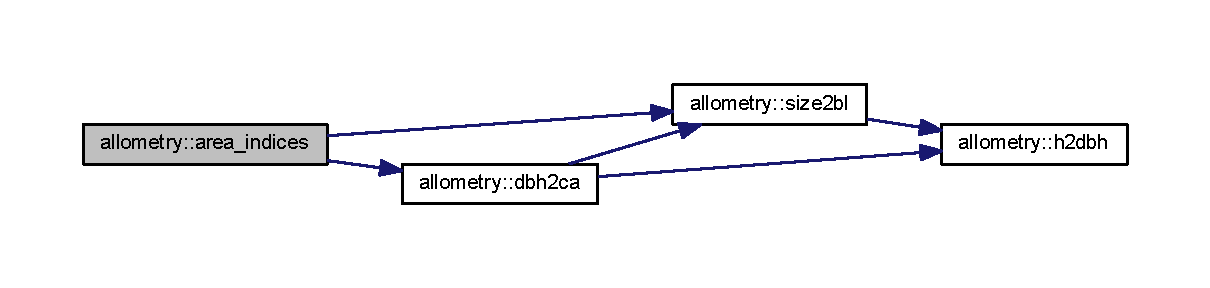
\includegraphics[width=350pt]{namespaceallometry_af723dc0f45a94b8812583457c53d4308_cgraph}
\end{center}
\end{figure}




Here is the caller graph for this function\+:\nopagebreak
\begin{figure}[H]
\begin{center}
\leavevmode
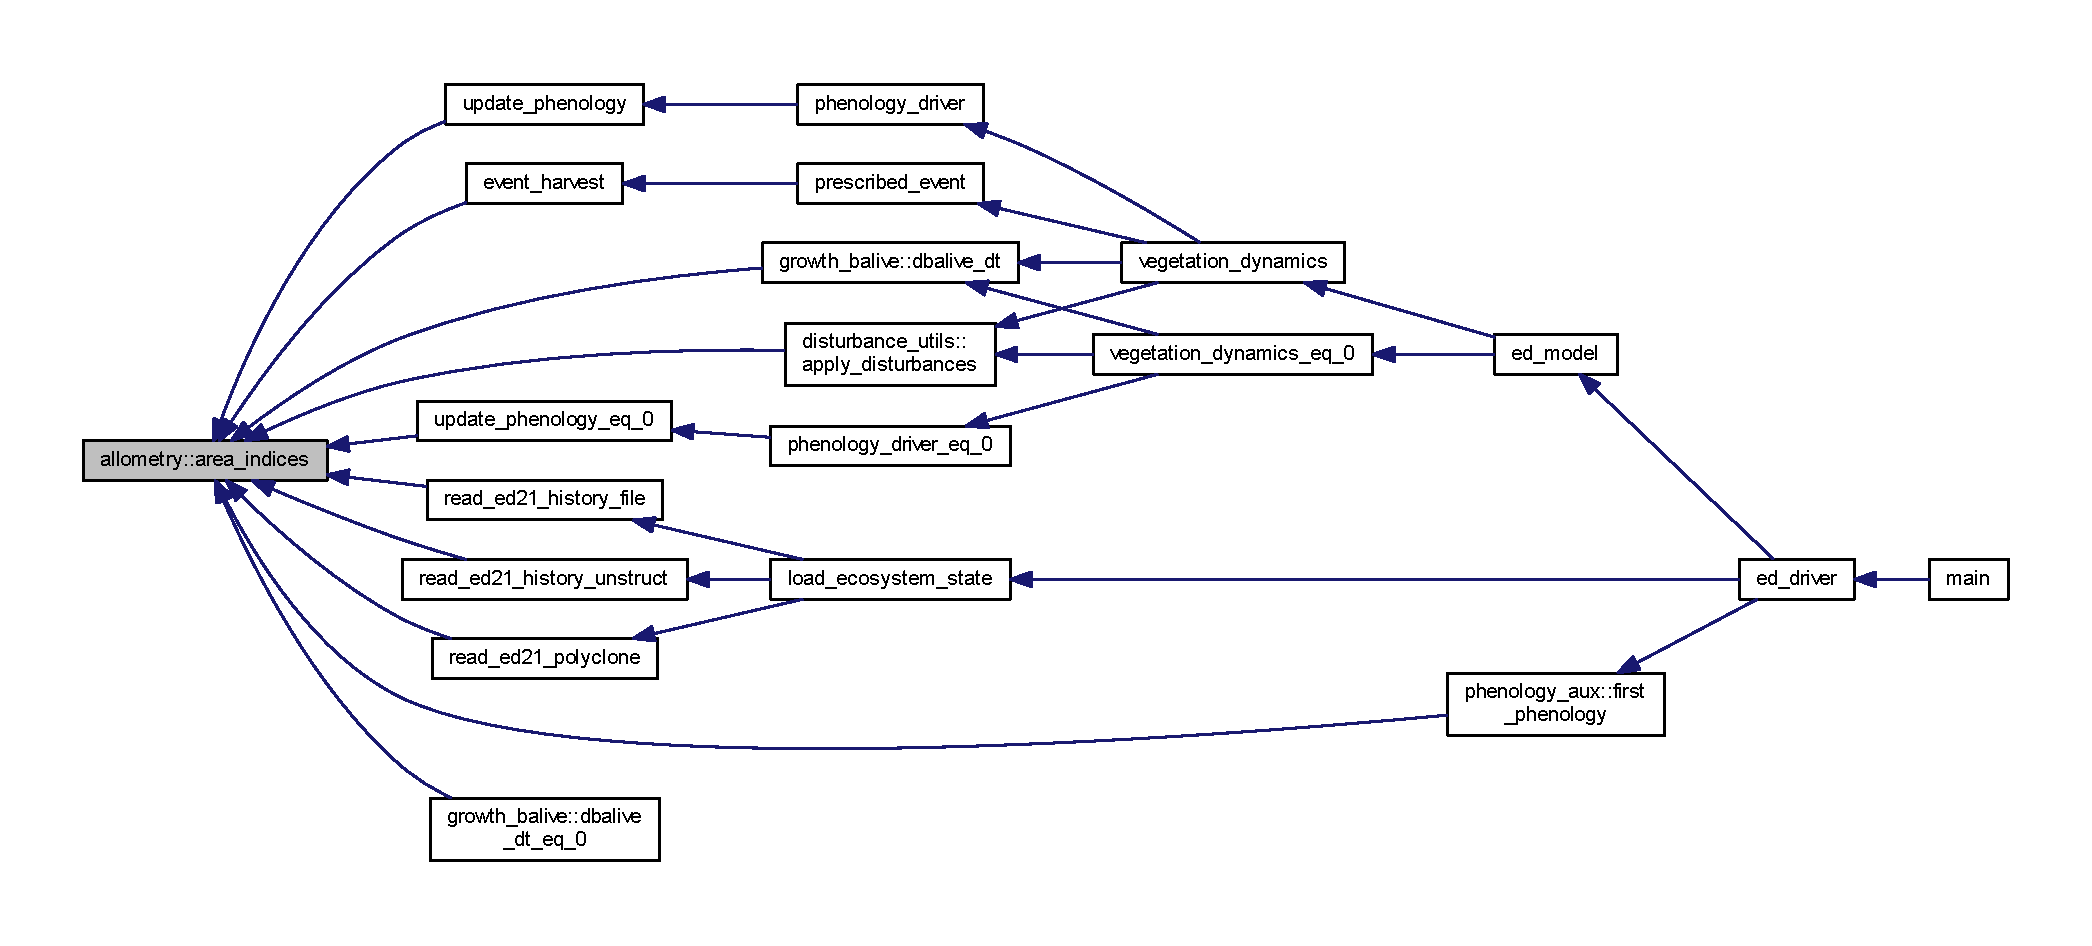
\includegraphics[width=350pt]{namespaceallometry_af723dc0f45a94b8812583457c53d4308_icgraph}
\end{center}
\end{figure}


\index{allometry@{allometry}!bd2dbh@{bd2dbh}}
\index{bd2dbh@{bd2dbh}!allometry@{allometry}}
\subsubsection[{\texorpdfstring{bd2dbh(ipft, bdead)}{bd2dbh(ipft, bdead)}}]{\setlength{\rightskip}{0pt plus 5cm}real function allometry\+::bd2dbh (
\begin{DoxyParamCaption}
\item[{integer, intent(in)}]{ipft, }
\item[{real, intent(in)}]{bdead}
\end{DoxyParamCaption}
)}\hypertarget{namespaceallometry_a50fedbee3a14eb5569a62abb4a36198f}{}\label{namespaceallometry_a50fedbee3a14eb5569a62abb4a36198f}


Here is the caller graph for this function\+:\nopagebreak
\begin{figure}[H]
\begin{center}
\leavevmode
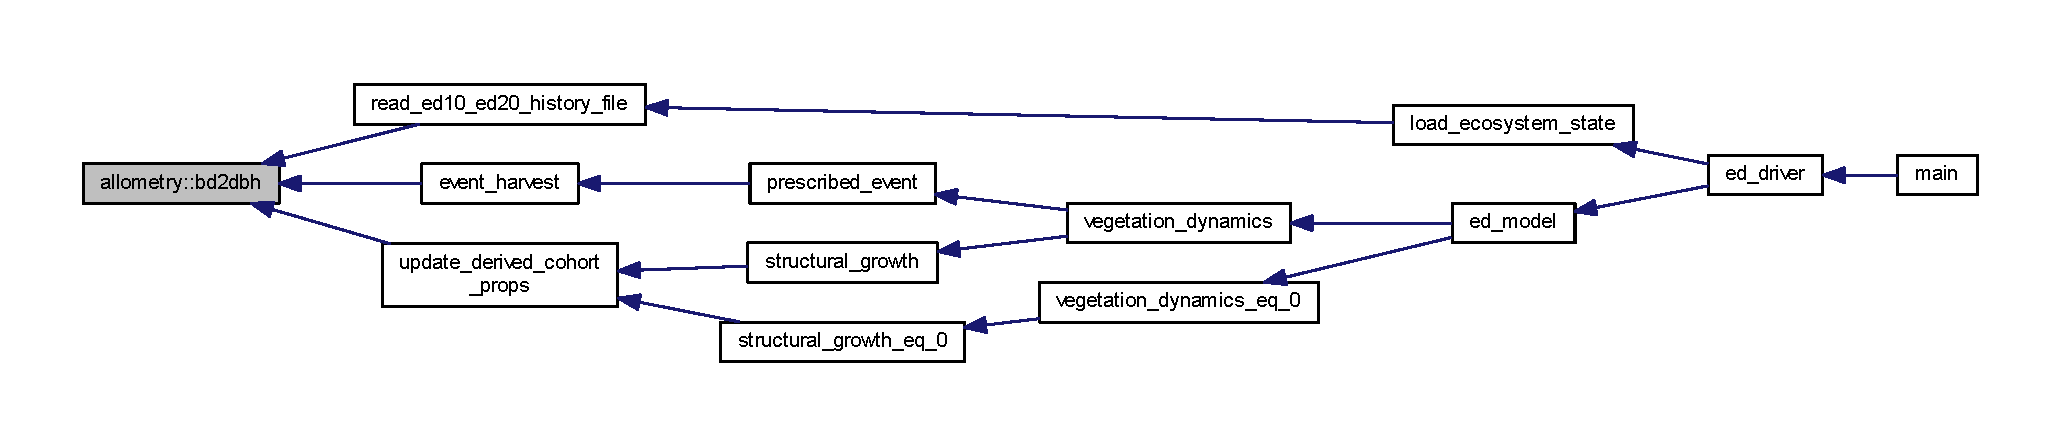
\includegraphics[width=350pt]{namespaceallometry_a50fedbee3a14eb5569a62abb4a36198f_icgraph}
\end{center}
\end{figure}


\index{allometry@{allometry}!bl2dbh@{bl2dbh}}
\index{bl2dbh@{bl2dbh}!allometry@{allometry}}
\subsubsection[{\texorpdfstring{bl2dbh(bleaf, ipft)}{bl2dbh(bleaf, ipft)}}]{\setlength{\rightskip}{0pt plus 5cm}real function allometry\+::bl2dbh (
\begin{DoxyParamCaption}
\item[{real, intent(in)}]{bleaf, }
\item[{integer, intent(in)}]{ipft}
\end{DoxyParamCaption}
)}\hypertarget{namespaceallometry_a3236375dc165a26aeea2d97c7e2c2685}{}\label{namespaceallometry_a3236375dc165a26aeea2d97c7e2c2685}


Here is the call graph for this function\+:\nopagebreak
\begin{figure}[H]
\begin{center}
\leavevmode
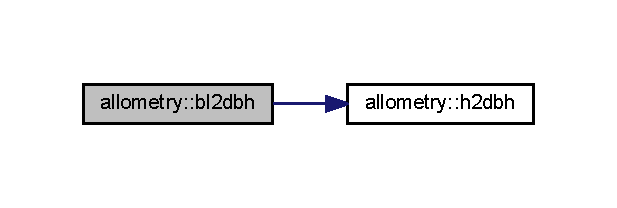
\includegraphics[width=296pt]{namespaceallometry_a3236375dc165a26aeea2d97c7e2c2685_cgraph}
\end{center}
\end{figure}




Here is the caller graph for this function\+:\nopagebreak
\begin{figure}[H]
\begin{center}
\leavevmode
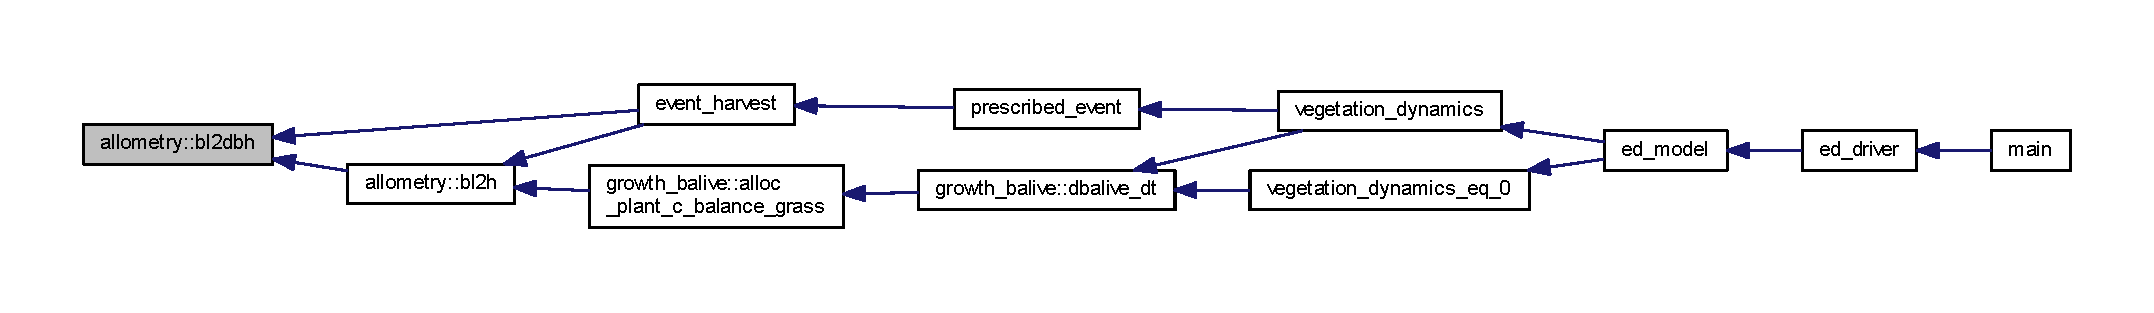
\includegraphics[width=350pt]{namespaceallometry_a3236375dc165a26aeea2d97c7e2c2685_icgraph}
\end{center}
\end{figure}


\index{allometry@{allometry}!bl2h@{bl2h}}
\index{bl2h@{bl2h}!allometry@{allometry}}
\subsubsection[{\texorpdfstring{bl2h(bleaf, ipft)}{bl2h(bleaf, ipft)}}]{\setlength{\rightskip}{0pt plus 5cm}real function allometry\+::bl2h (
\begin{DoxyParamCaption}
\item[{real, intent(in)}]{bleaf, }
\item[{integer, intent(in)}]{ipft}
\end{DoxyParamCaption}
)}\hypertarget{namespaceallometry_a59a1fc10140498dee62fce8a641da254}{}\label{namespaceallometry_a59a1fc10140498dee62fce8a641da254}


Here is the call graph for this function\+:\nopagebreak
\begin{figure}[H]
\begin{center}
\leavevmode
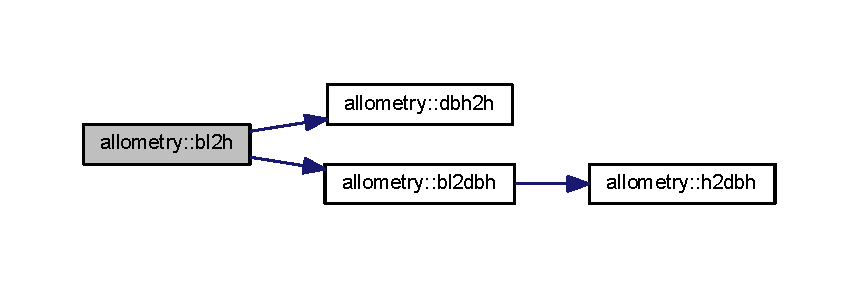
\includegraphics[width=350pt]{namespaceallometry_a59a1fc10140498dee62fce8a641da254_cgraph}
\end{center}
\end{figure}




Here is the caller graph for this function\+:\nopagebreak
\begin{figure}[H]
\begin{center}
\leavevmode
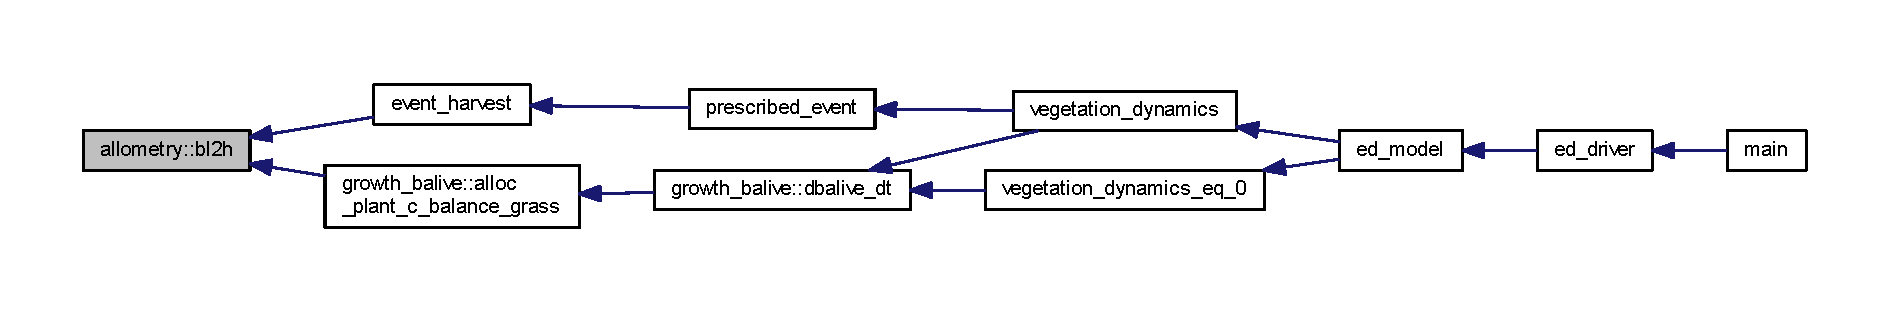
\includegraphics[width=350pt]{namespaceallometry_a59a1fc10140498dee62fce8a641da254_icgraph}
\end{center}
\end{figure}


\index{allometry@{allometry}!dbh2bd@{dbh2bd}}
\index{dbh2bd@{dbh2bd}!allometry@{allometry}}
\subsubsection[{\texorpdfstring{dbh2bd(dbh, ipft)}{dbh2bd(dbh, ipft)}}]{\setlength{\rightskip}{0pt plus 5cm}real function allometry\+::dbh2bd (
\begin{DoxyParamCaption}
\item[{real, intent(in)}]{dbh, }
\item[{integer, intent(in)}]{ipft}
\end{DoxyParamCaption}
)}\hypertarget{namespaceallometry_a76db2bc4aaa47db1e2656117ec476dba}{}\label{namespaceallometry_a76db2bc4aaa47db1e2656117ec476dba}


Here is the caller graph for this function\+:\nopagebreak
\begin{figure}[H]
\begin{center}
\leavevmode
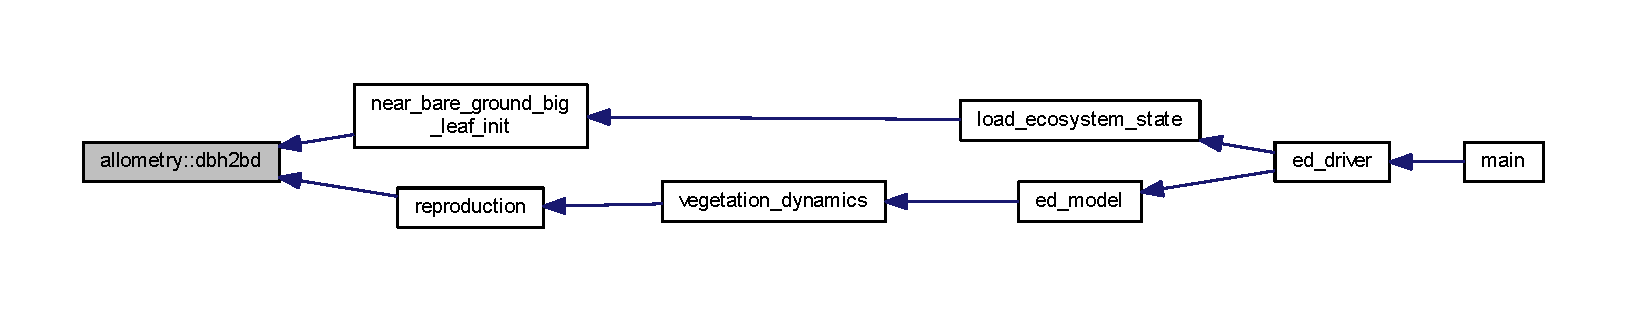
\includegraphics[width=350pt]{namespaceallometry_a76db2bc4aaa47db1e2656117ec476dba_icgraph}
\end{center}
\end{figure}


\index{allometry@{allometry}!dbh2ca@{dbh2ca}}
\index{dbh2ca@{dbh2ca}!allometry@{allometry}}
\subsubsection[{\texorpdfstring{dbh2ca(dbh, hite, sla, ipft)}{dbh2ca(dbh, hite, sla, ipft)}}]{\setlength{\rightskip}{0pt plus 5cm}real function allometry\+::dbh2ca (
\begin{DoxyParamCaption}
\item[{real, intent(in)}]{dbh, }
\item[{real, intent(in)}]{hite, }
\item[{real, intent(in)}]{sla, }
\item[{integer, intent(in)}]{ipft}
\end{DoxyParamCaption}
)}\hypertarget{namespaceallometry_abacdf8e8e585ce8d788a1fc2be133243}{}\label{namespaceallometry_abacdf8e8e585ce8d788a1fc2be133243}


Here is the call graph for this function\+:\nopagebreak
\begin{figure}[H]
\begin{center}
\leavevmode
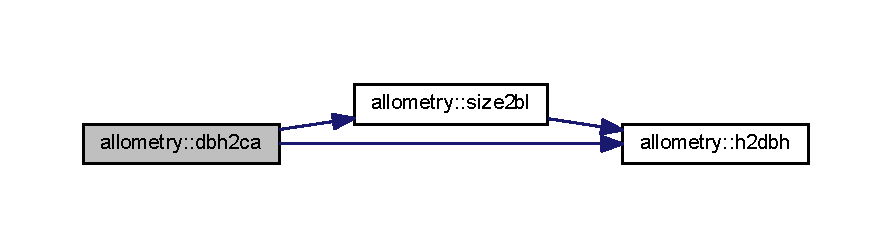
\includegraphics[width=350pt]{namespaceallometry_abacdf8e8e585ce8d788a1fc2be133243_cgraph}
\end{center}
\end{figure}




Here is the caller graph for this function\+:\nopagebreak
\begin{figure}[H]
\begin{center}
\leavevmode
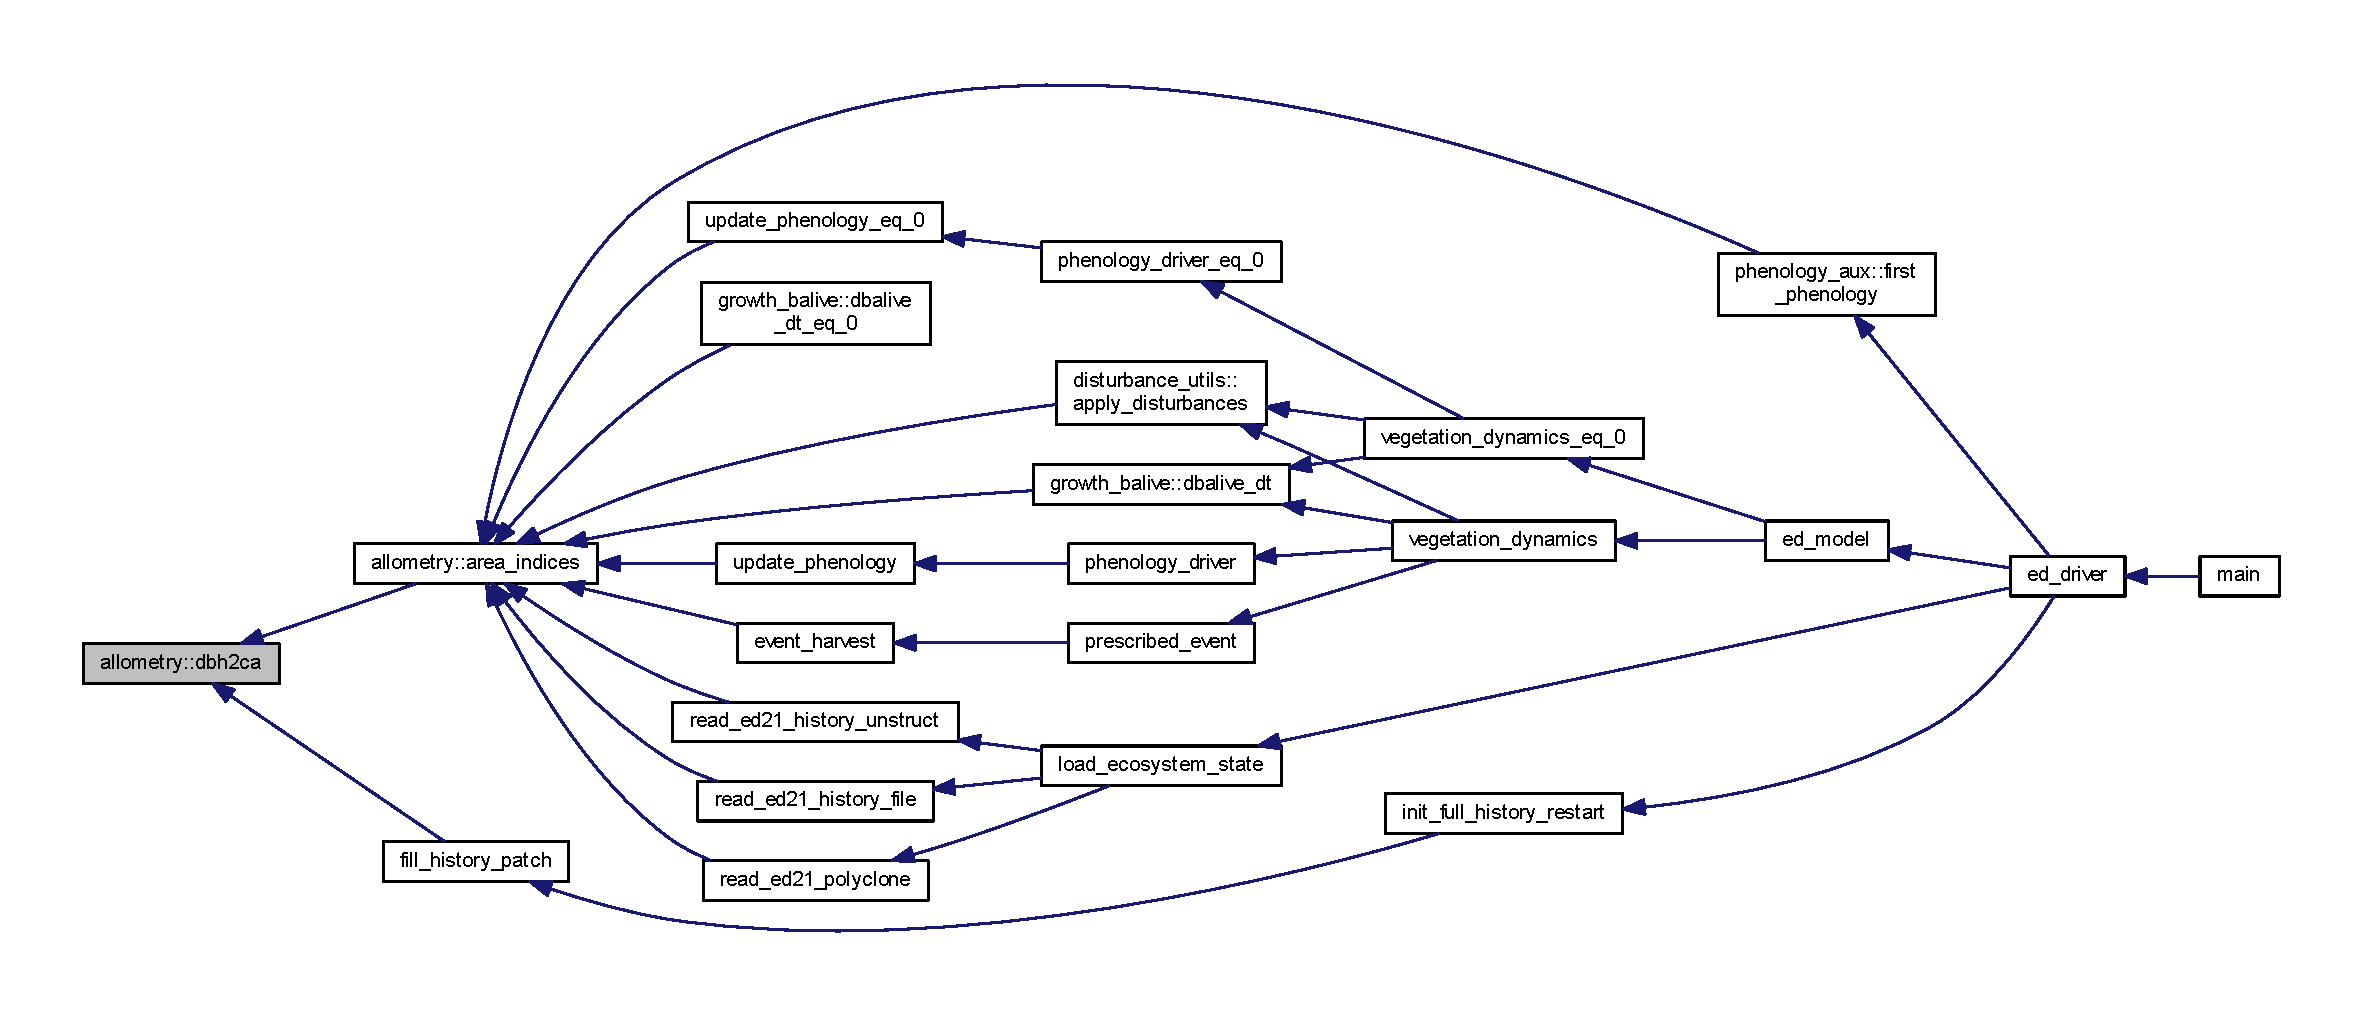
\includegraphics[width=350pt]{namespaceallometry_abacdf8e8e585ce8d788a1fc2be133243_icgraph}
\end{center}
\end{figure}


\index{allometry@{allometry}!dbh2h@{dbh2h}}
\index{dbh2h@{dbh2h}!allometry@{allometry}}
\subsubsection[{\texorpdfstring{dbh2h(ipft, dbh)}{dbh2h(ipft, dbh)}}]{\setlength{\rightskip}{0pt plus 5cm}real function allometry\+::dbh2h (
\begin{DoxyParamCaption}
\item[{integer, intent(in)}]{ipft, }
\item[{real, intent(in)}]{dbh}
\end{DoxyParamCaption}
)}\hypertarget{namespaceallometry_a56f11dc07da4d5e7114dc37d6cc5f2cc}{}\label{namespaceallometry_a56f11dc07da4d5e7114dc37d6cc5f2cc}


Here is the caller graph for this function\+:\nopagebreak
\begin{figure}[H]
\begin{center}
\leavevmode
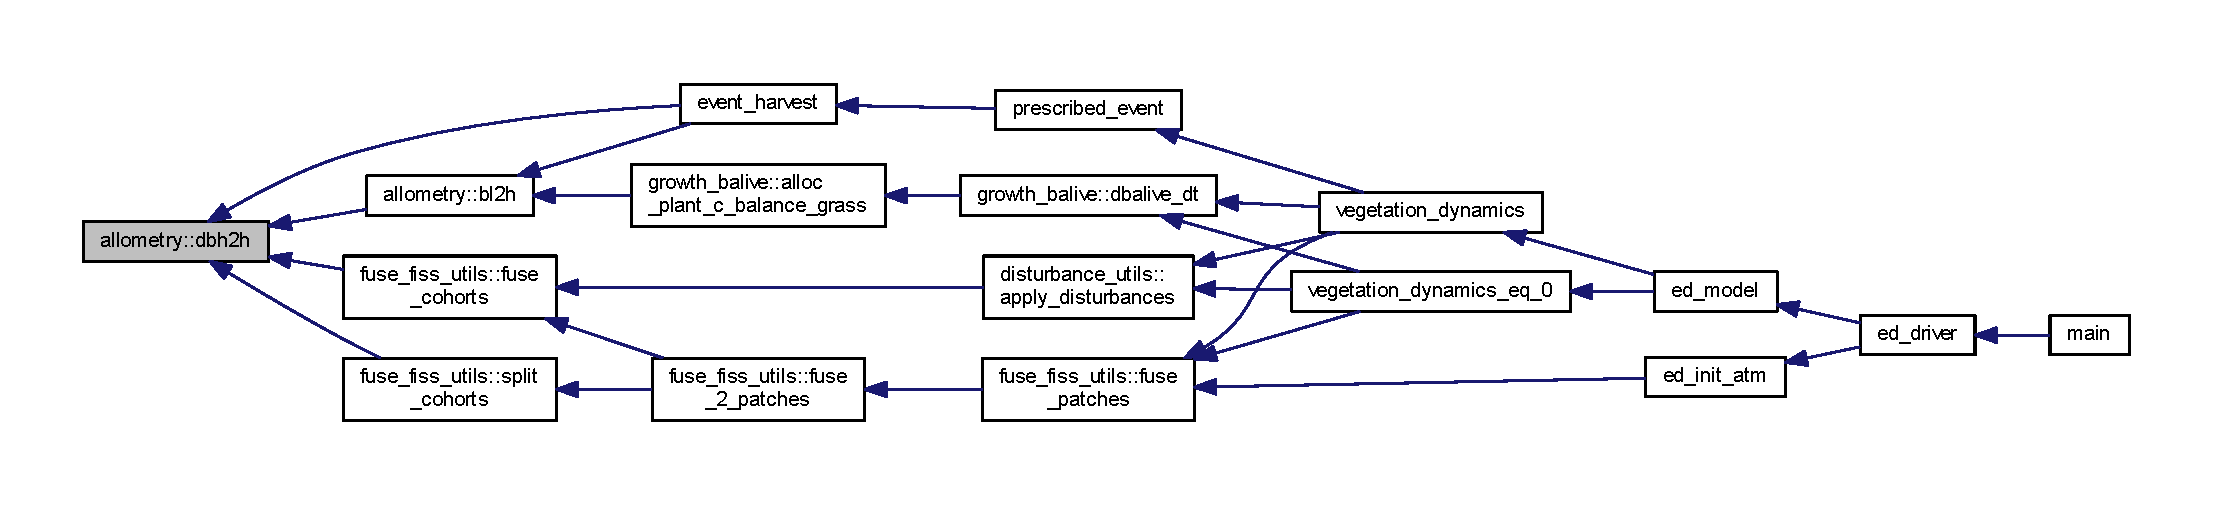
\includegraphics[width=350pt]{namespaceallometry_a56f11dc07da4d5e7114dc37d6cc5f2cc_icgraph}
\end{center}
\end{figure}


\index{allometry@{allometry}!dbh2krdepth@{dbh2krdepth}}
\index{dbh2krdepth@{dbh2krdepth}!allometry@{allometry}}
\subsubsection[{\texorpdfstring{dbh2krdepth(hite, dbh, ipft, lsl)}{dbh2krdepth(hite, dbh, ipft, lsl)}}]{\setlength{\rightskip}{0pt plus 5cm}integer function allometry\+::dbh2krdepth (
\begin{DoxyParamCaption}
\item[{real, intent(in)}]{hite, }
\item[{real, intent(in)}]{dbh, }
\item[{integer, intent(in)}]{ipft, }
\item[{integer, intent(in)}]{lsl}
\end{DoxyParamCaption}
)}\hypertarget{namespaceallometry_ac1523ea0e0ef8d2dd6a429f61a013c1c}{}\label{namespaceallometry_ac1523ea0e0ef8d2dd6a429f61a013c1c}


Here is the call graph for this function\+:\nopagebreak
\begin{figure}[H]
\begin{center}
\leavevmode
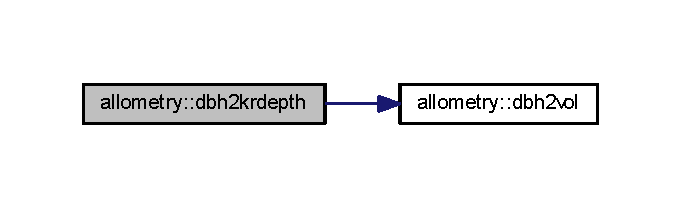
\includegraphics[width=327pt]{namespaceallometry_ac1523ea0e0ef8d2dd6a429f61a013c1c_cgraph}
\end{center}
\end{figure}




Here is the caller graph for this function\+:\nopagebreak
\begin{figure}[H]
\begin{center}
\leavevmode
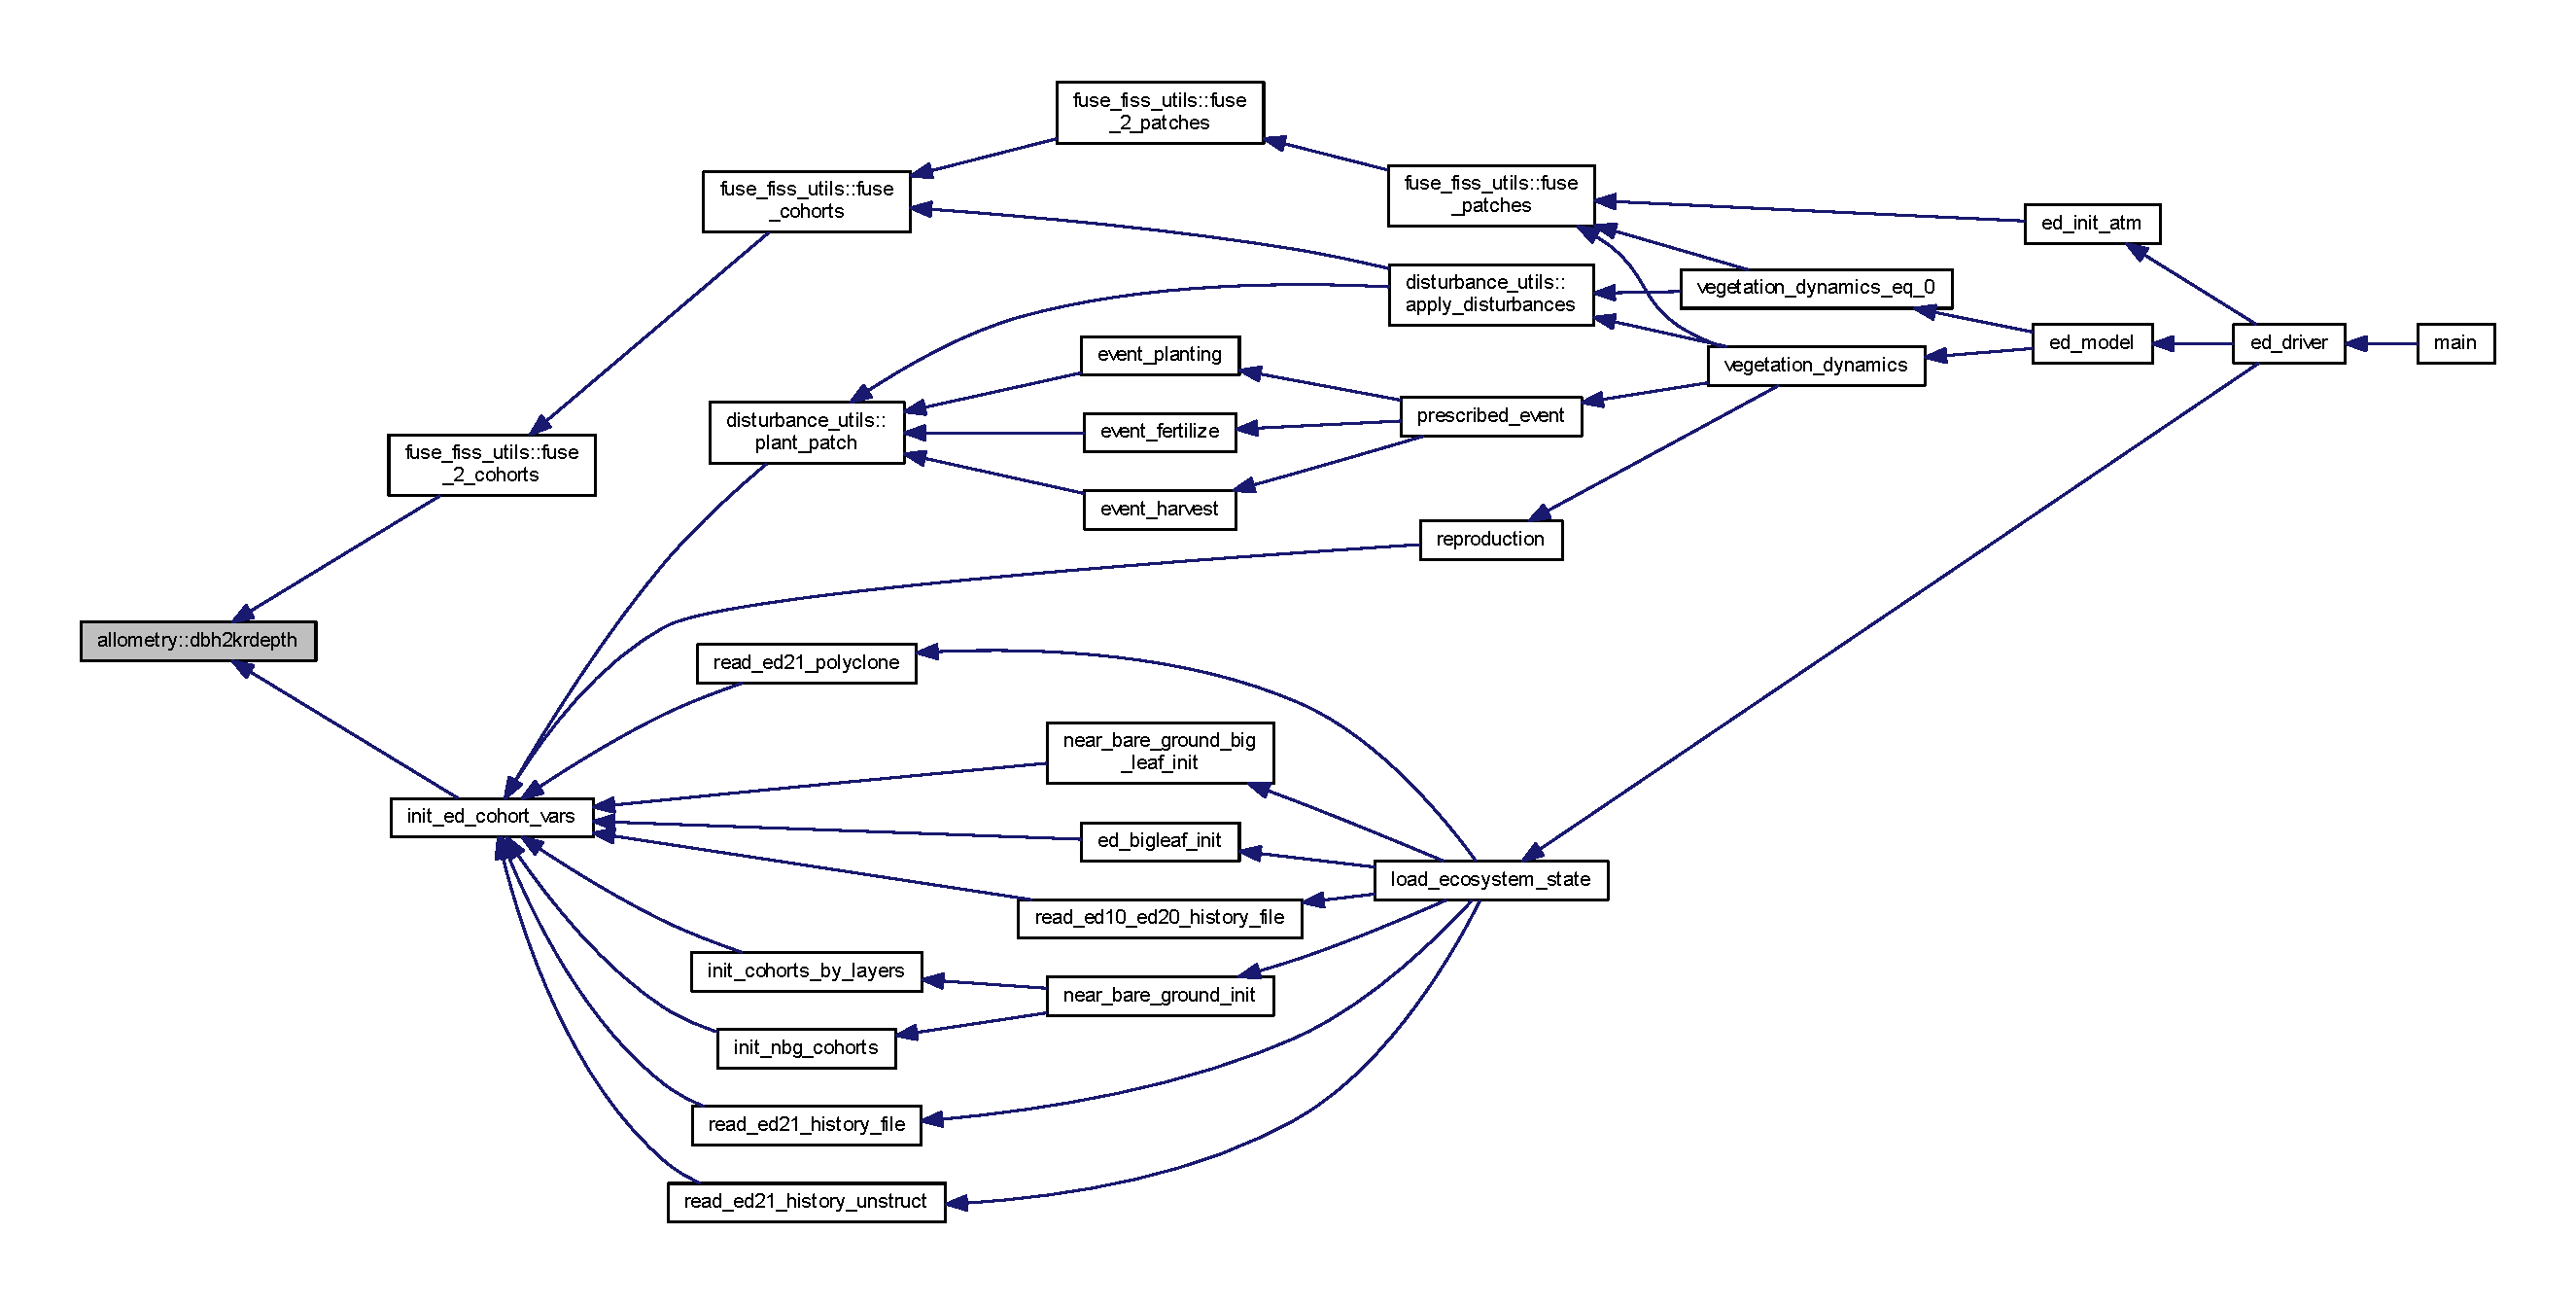
\includegraphics[width=350pt]{namespaceallometry_ac1523ea0e0ef8d2dd6a429f61a013c1c_icgraph}
\end{center}
\end{figure}


\index{allometry@{allometry}!dbh2vol@{dbh2vol}}
\index{dbh2vol@{dbh2vol}!allometry@{allometry}}
\subsubsection[{\texorpdfstring{dbh2vol(hgt, dbh, ipft)}{dbh2vol(hgt, dbh, ipft)}}]{\setlength{\rightskip}{0pt plus 5cm}real function allometry\+::dbh2vol (
\begin{DoxyParamCaption}
\item[{real, intent(in)}]{hgt, }
\item[{real, intent(in)}]{dbh, }
\item[{integer, intent(in)}]{ipft}
\end{DoxyParamCaption}
)}\hypertarget{namespaceallometry_aab2b2cee61cac31529246b043121c7de}{}\label{namespaceallometry_aab2b2cee61cac31529246b043121c7de}


Here is the caller graph for this function\+:\nopagebreak
\begin{figure}[H]
\begin{center}
\leavevmode
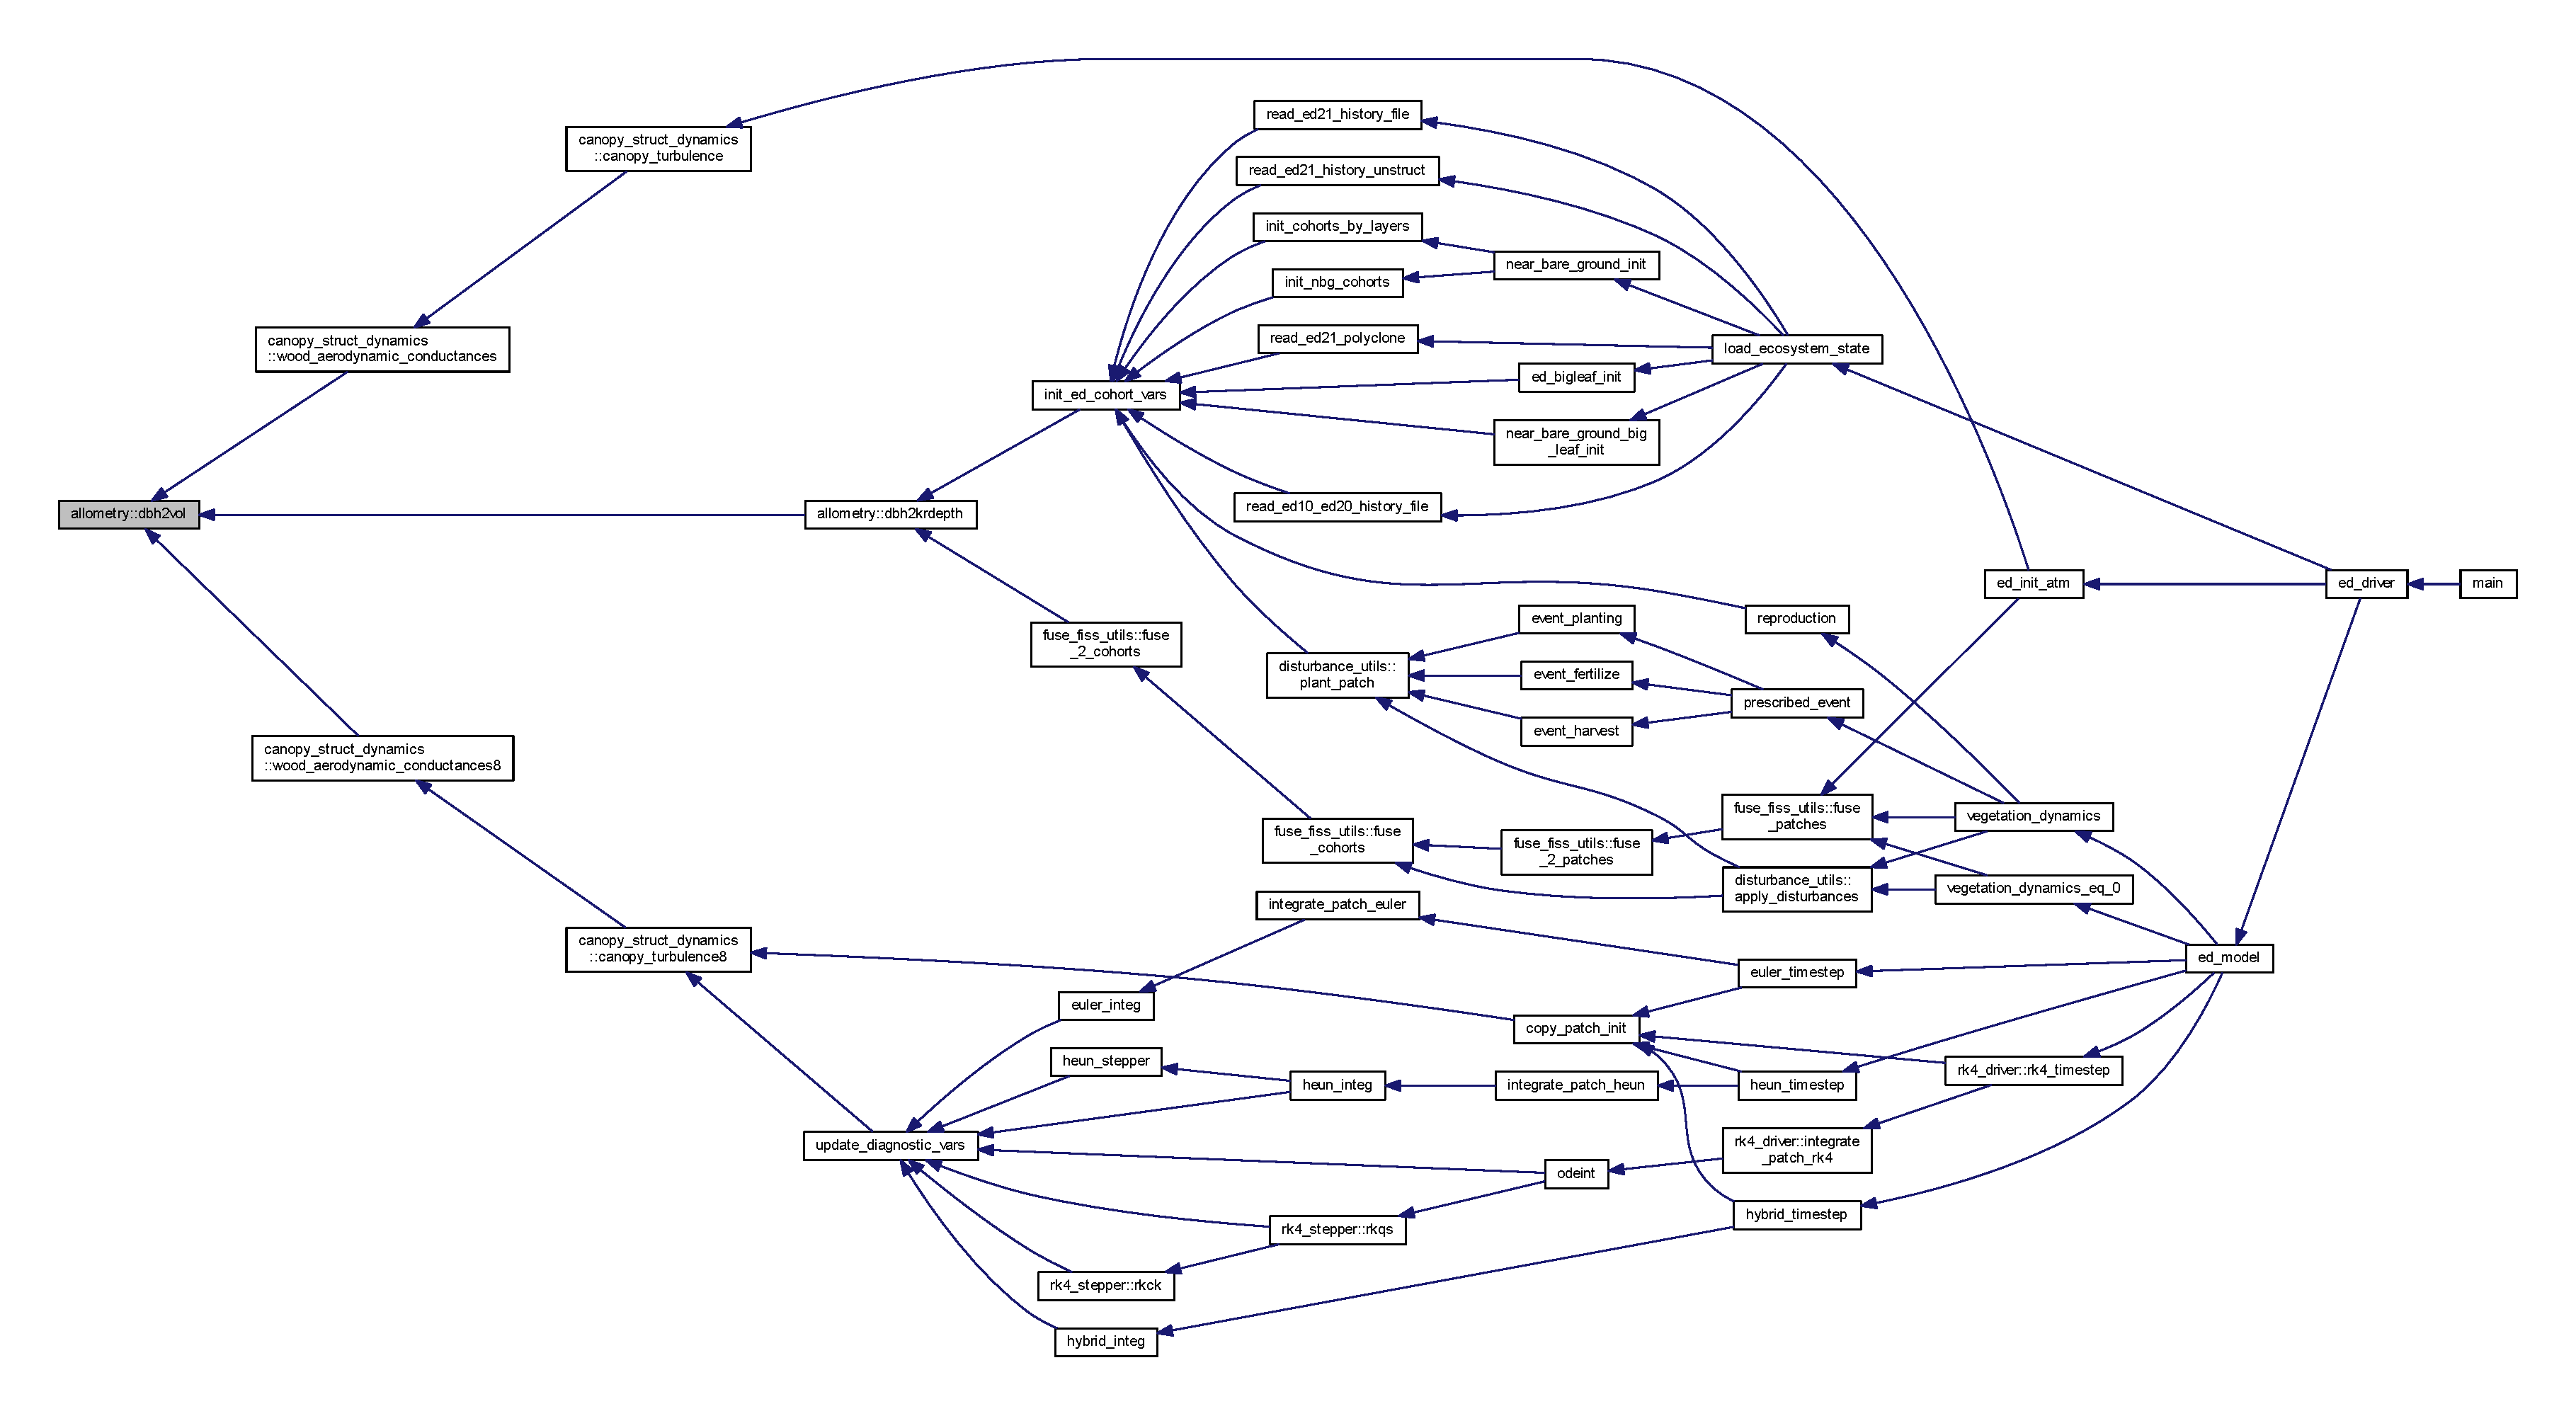
\includegraphics[width=350pt]{namespaceallometry_aab2b2cee61cac31529246b043121c7de_icgraph}
\end{center}
\end{figure}


\index{allometry@{allometry}!ed\+\_\+biomass@{ed\+\_\+biomass}}
\index{ed\+\_\+biomass@{ed\+\_\+biomass}!allometry@{allometry}}
\subsubsection[{\texorpdfstring{ed\+\_\+biomass(bdead, bleaf, bsapwooda, ipft)}{ed_biomass(bdead, bleaf, bsapwooda, ipft)}}]{\setlength{\rightskip}{0pt plus 5cm}real function allometry\+::ed\+\_\+biomass (
\begin{DoxyParamCaption}
\item[{real, intent(in)}]{bdead, }
\item[{real, intent(in)}]{bleaf, }
\item[{real, intent(in)}]{bsapwooda, }
\item[{integer, intent(in)}]{ipft}
\end{DoxyParamCaption}
)}\hypertarget{namespaceallometry_ab99b16f69dafaf5ff3e69c7514b9e7b6}{}\label{namespaceallometry_ab99b16f69dafaf5ff3e69c7514b9e7b6}


Here is the caller graph for this function\+:\nopagebreak
\begin{figure}[H]
\begin{center}
\leavevmode
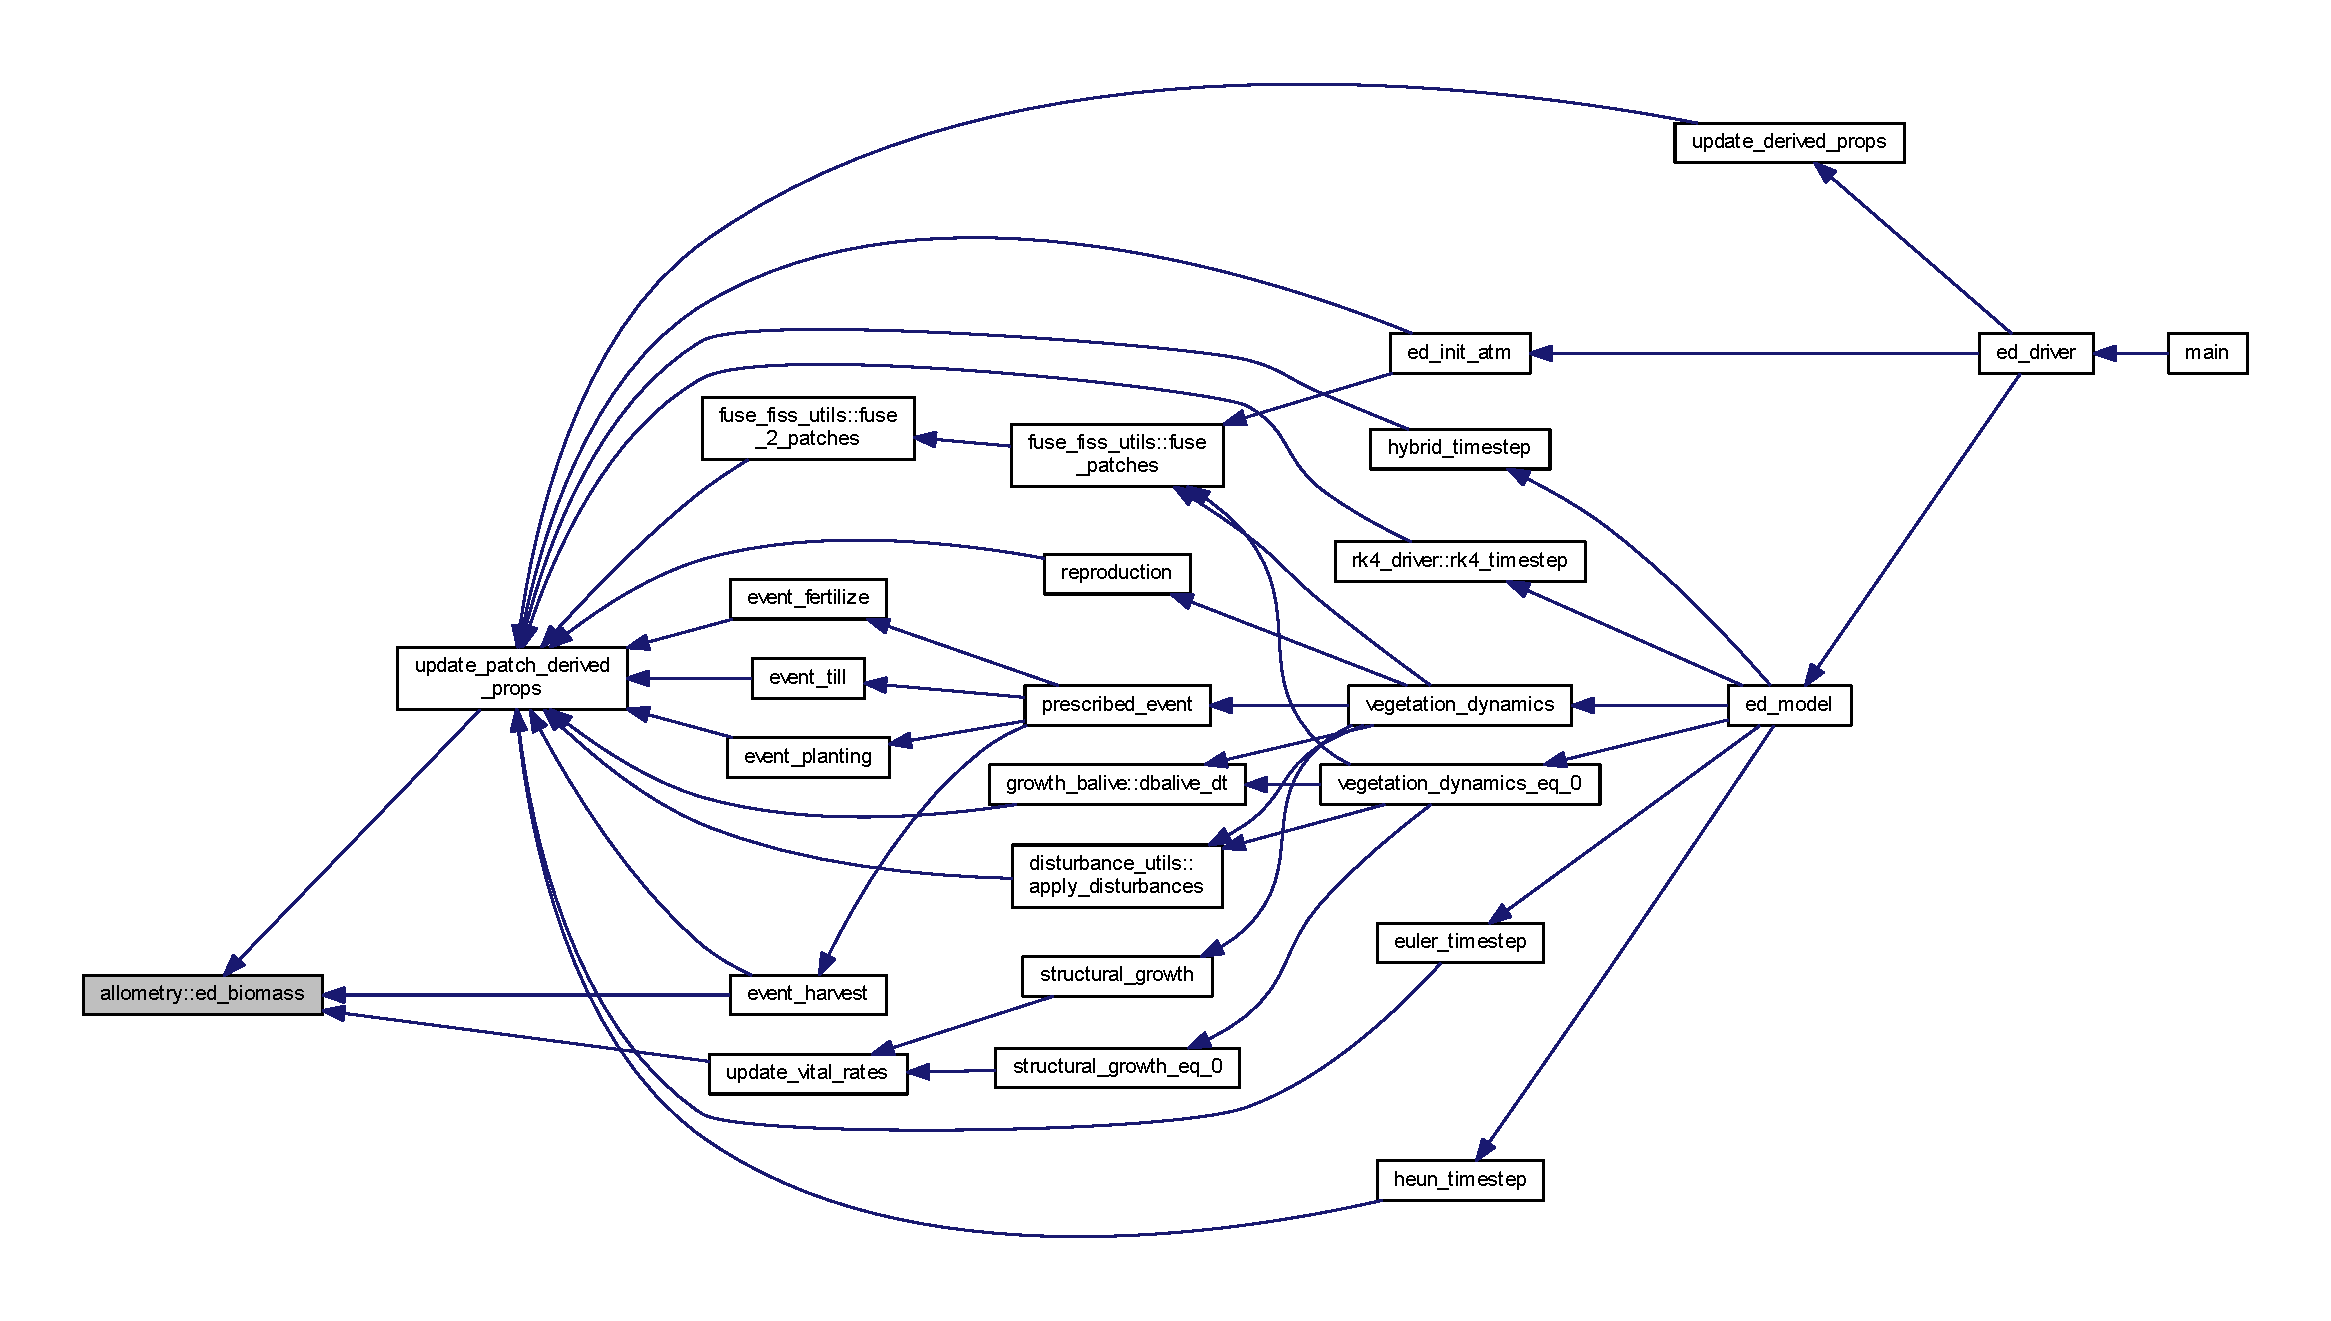
\includegraphics[width=350pt]{namespaceallometry_ab99b16f69dafaf5ff3e69c7514b9e7b6_icgraph}
\end{center}
\end{figure}


\index{allometry@{allometry}!h2crownbh@{h2crownbh}}
\index{h2crownbh@{h2crownbh}!allometry@{allometry}}
\subsubsection[{\texorpdfstring{h2crownbh(height, ipft)}{h2crownbh(height, ipft)}}]{\setlength{\rightskip}{0pt plus 5cm}real function allometry\+::h2crownbh (
\begin{DoxyParamCaption}
\item[{real, intent(in)}]{height, }
\item[{integer, intent(in)}]{ipft}
\end{DoxyParamCaption}
)}\hypertarget{namespaceallometry_a88949ed487fccc2f1dfd065399043b0d}{}\label{namespaceallometry_a88949ed487fccc2f1dfd065399043b0d}


Here is the caller graph for this function\+:\nopagebreak
\begin{figure}[H]
\begin{center}
\leavevmode
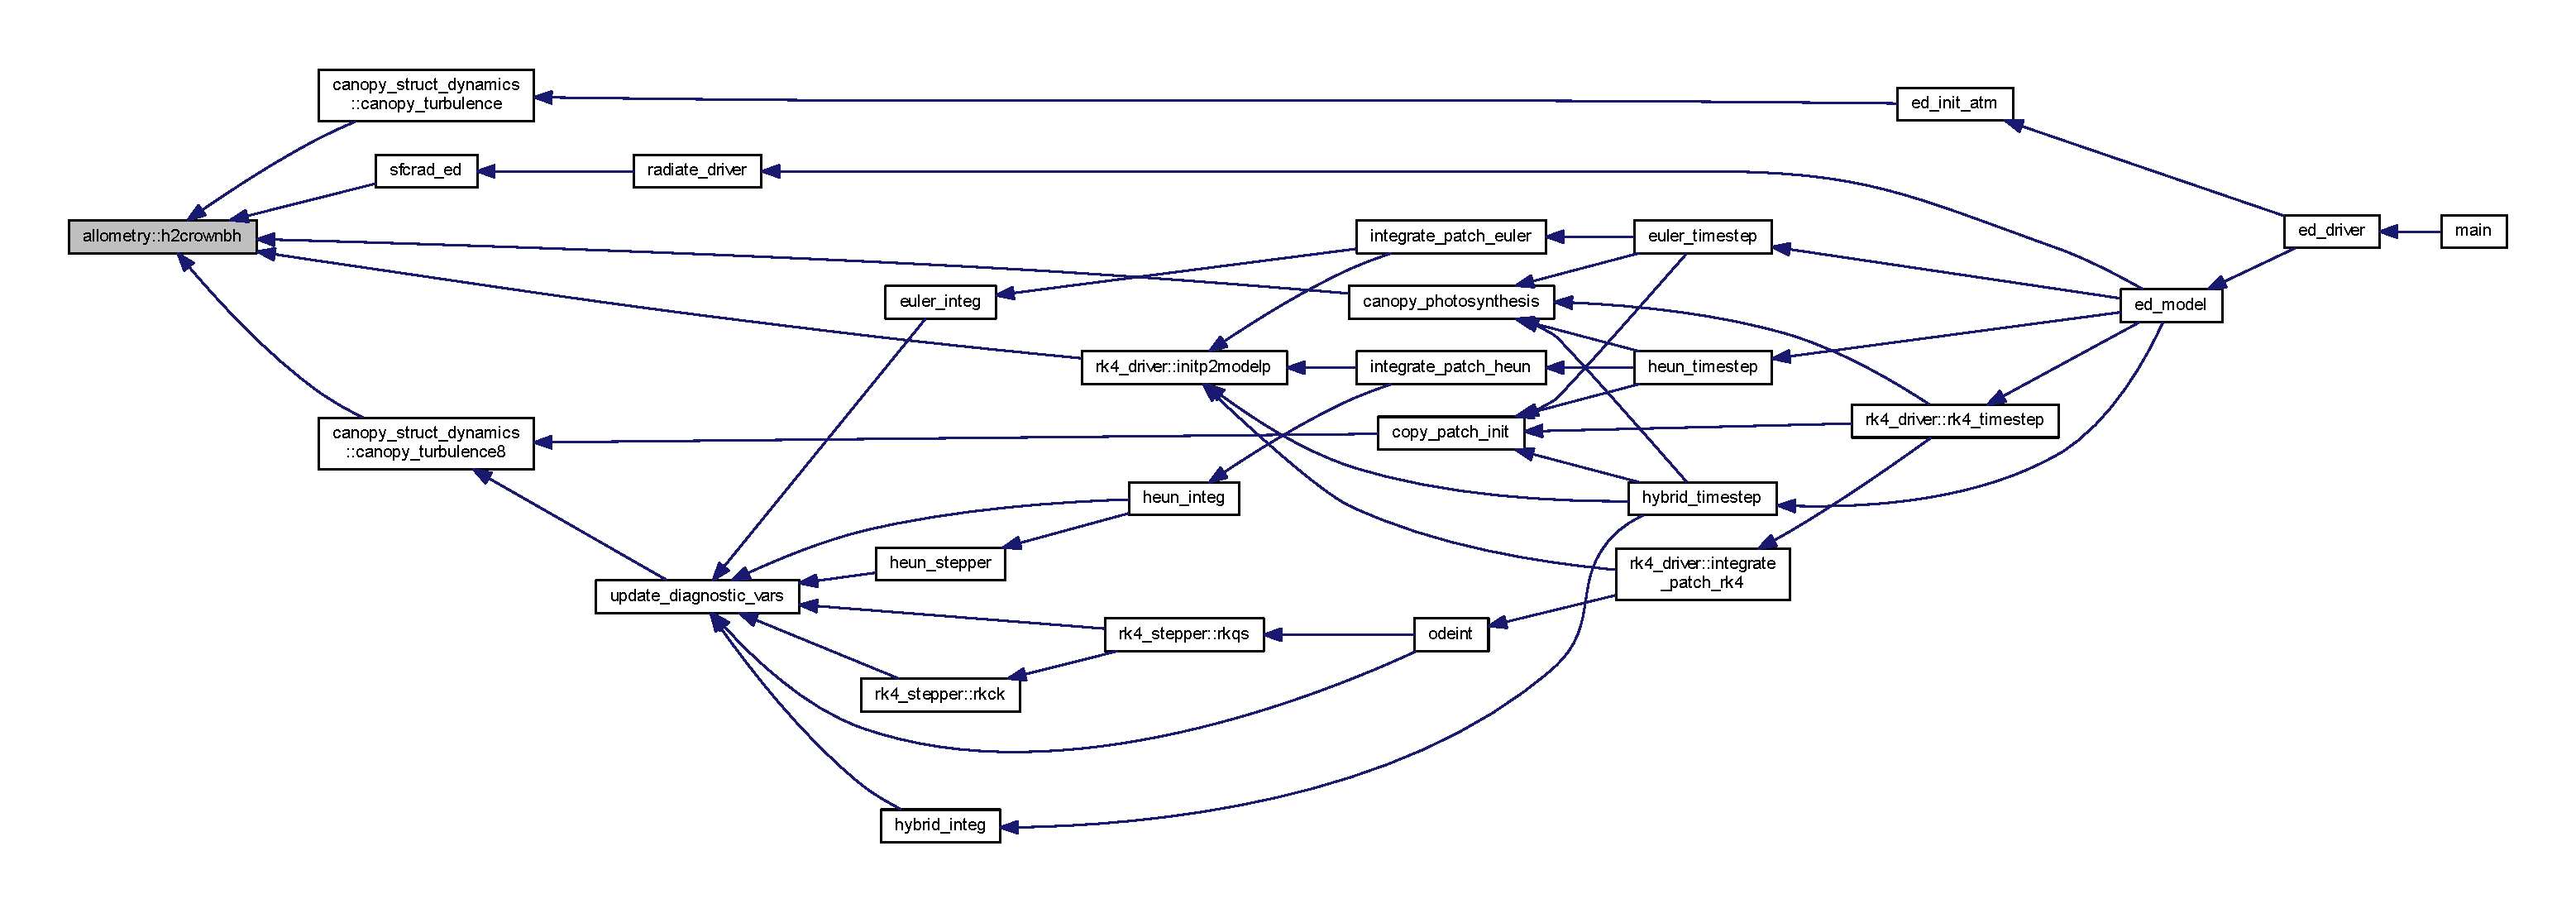
\includegraphics[width=350pt]{namespaceallometry_a88949ed487fccc2f1dfd065399043b0d_icgraph}
\end{center}
\end{figure}


\index{allometry@{allometry}!h2dbh@{h2dbh}}
\index{h2dbh@{h2dbh}!allometry@{allometry}}
\subsubsection[{\texorpdfstring{h2dbh(h, ipft)}{h2dbh(h, ipft)}}]{\setlength{\rightskip}{0pt plus 5cm}real function allometry\+::h2dbh (
\begin{DoxyParamCaption}
\item[{real, intent(in)}]{h, }
\item[{integer, intent(in)}]{ipft}
\end{DoxyParamCaption}
)}\hypertarget{namespaceallometry_a31aa8db06e86ec74efb5e692417399df}{}\label{namespaceallometry_a31aa8db06e86ec74efb5e692417399df}


Here is the caller graph for this function\+:\nopagebreak
\begin{figure}[H]
\begin{center}
\leavevmode
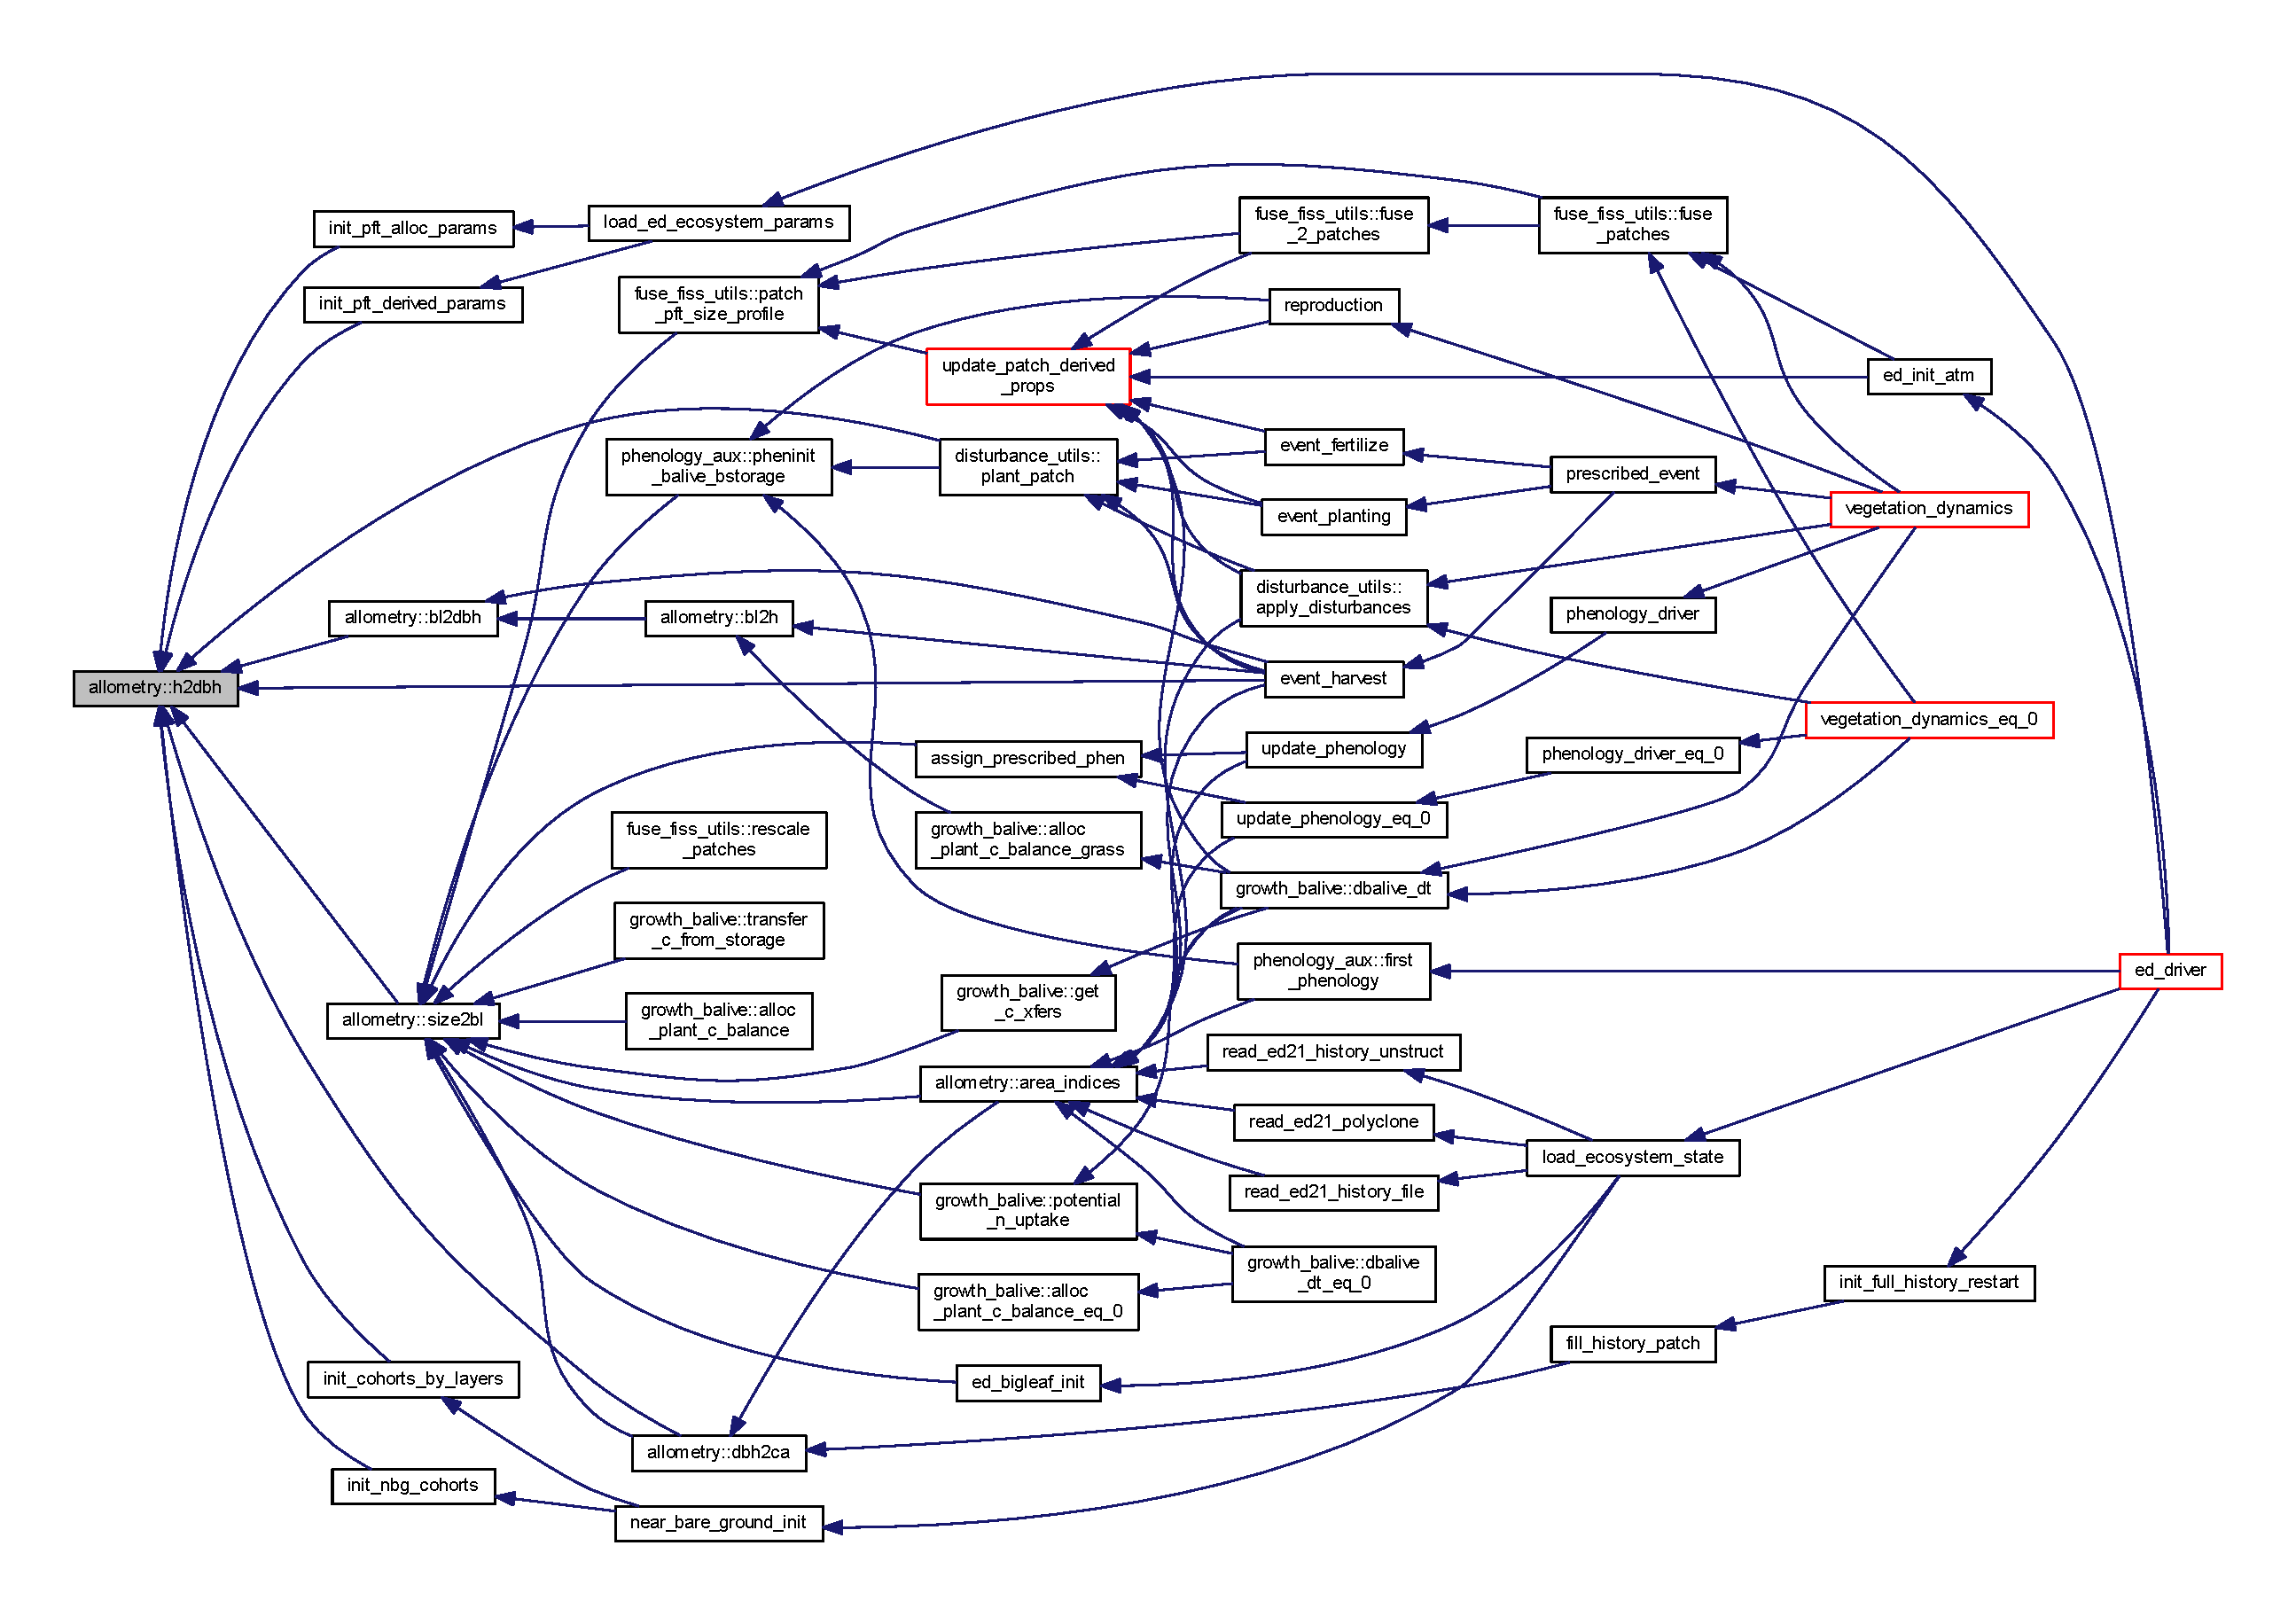
\includegraphics[width=350pt]{namespaceallometry_a31aa8db06e86ec74efb5e692417399df_icgraph}
\end{center}
\end{figure}


\index{allometry@{allometry}!size2bl@{size2bl}}
\index{size2bl@{size2bl}!allometry@{allometry}}
\subsubsection[{\texorpdfstring{size2bl(dbh, hite, ipft)}{size2bl(dbh, hite, ipft)}}]{\setlength{\rightskip}{0pt plus 5cm}real function allometry\+::size2bl (
\begin{DoxyParamCaption}
\item[{real, intent(in)}]{dbh, }
\item[{real, intent(in)}]{hite, }
\item[{integer, intent(in)}]{ipft}
\end{DoxyParamCaption}
)}\hypertarget{namespaceallometry_a45ced9bf9ccd03debe8def35b579f4bd}{}\label{namespaceallometry_a45ced9bf9ccd03debe8def35b579f4bd}


Here is the call graph for this function\+:\nopagebreak
\begin{figure}[H]
\begin{center}
\leavevmode
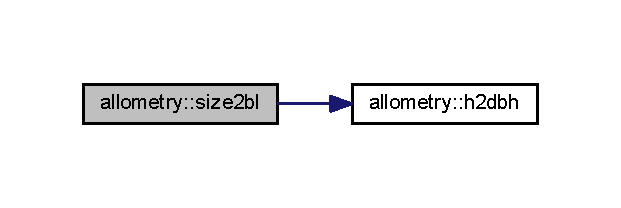
\includegraphics[width=298pt]{namespaceallometry_a45ced9bf9ccd03debe8def35b579f4bd_cgraph}
\end{center}
\end{figure}




Here is the caller graph for this function\+:\nopagebreak
\begin{figure}[H]
\begin{center}
\leavevmode
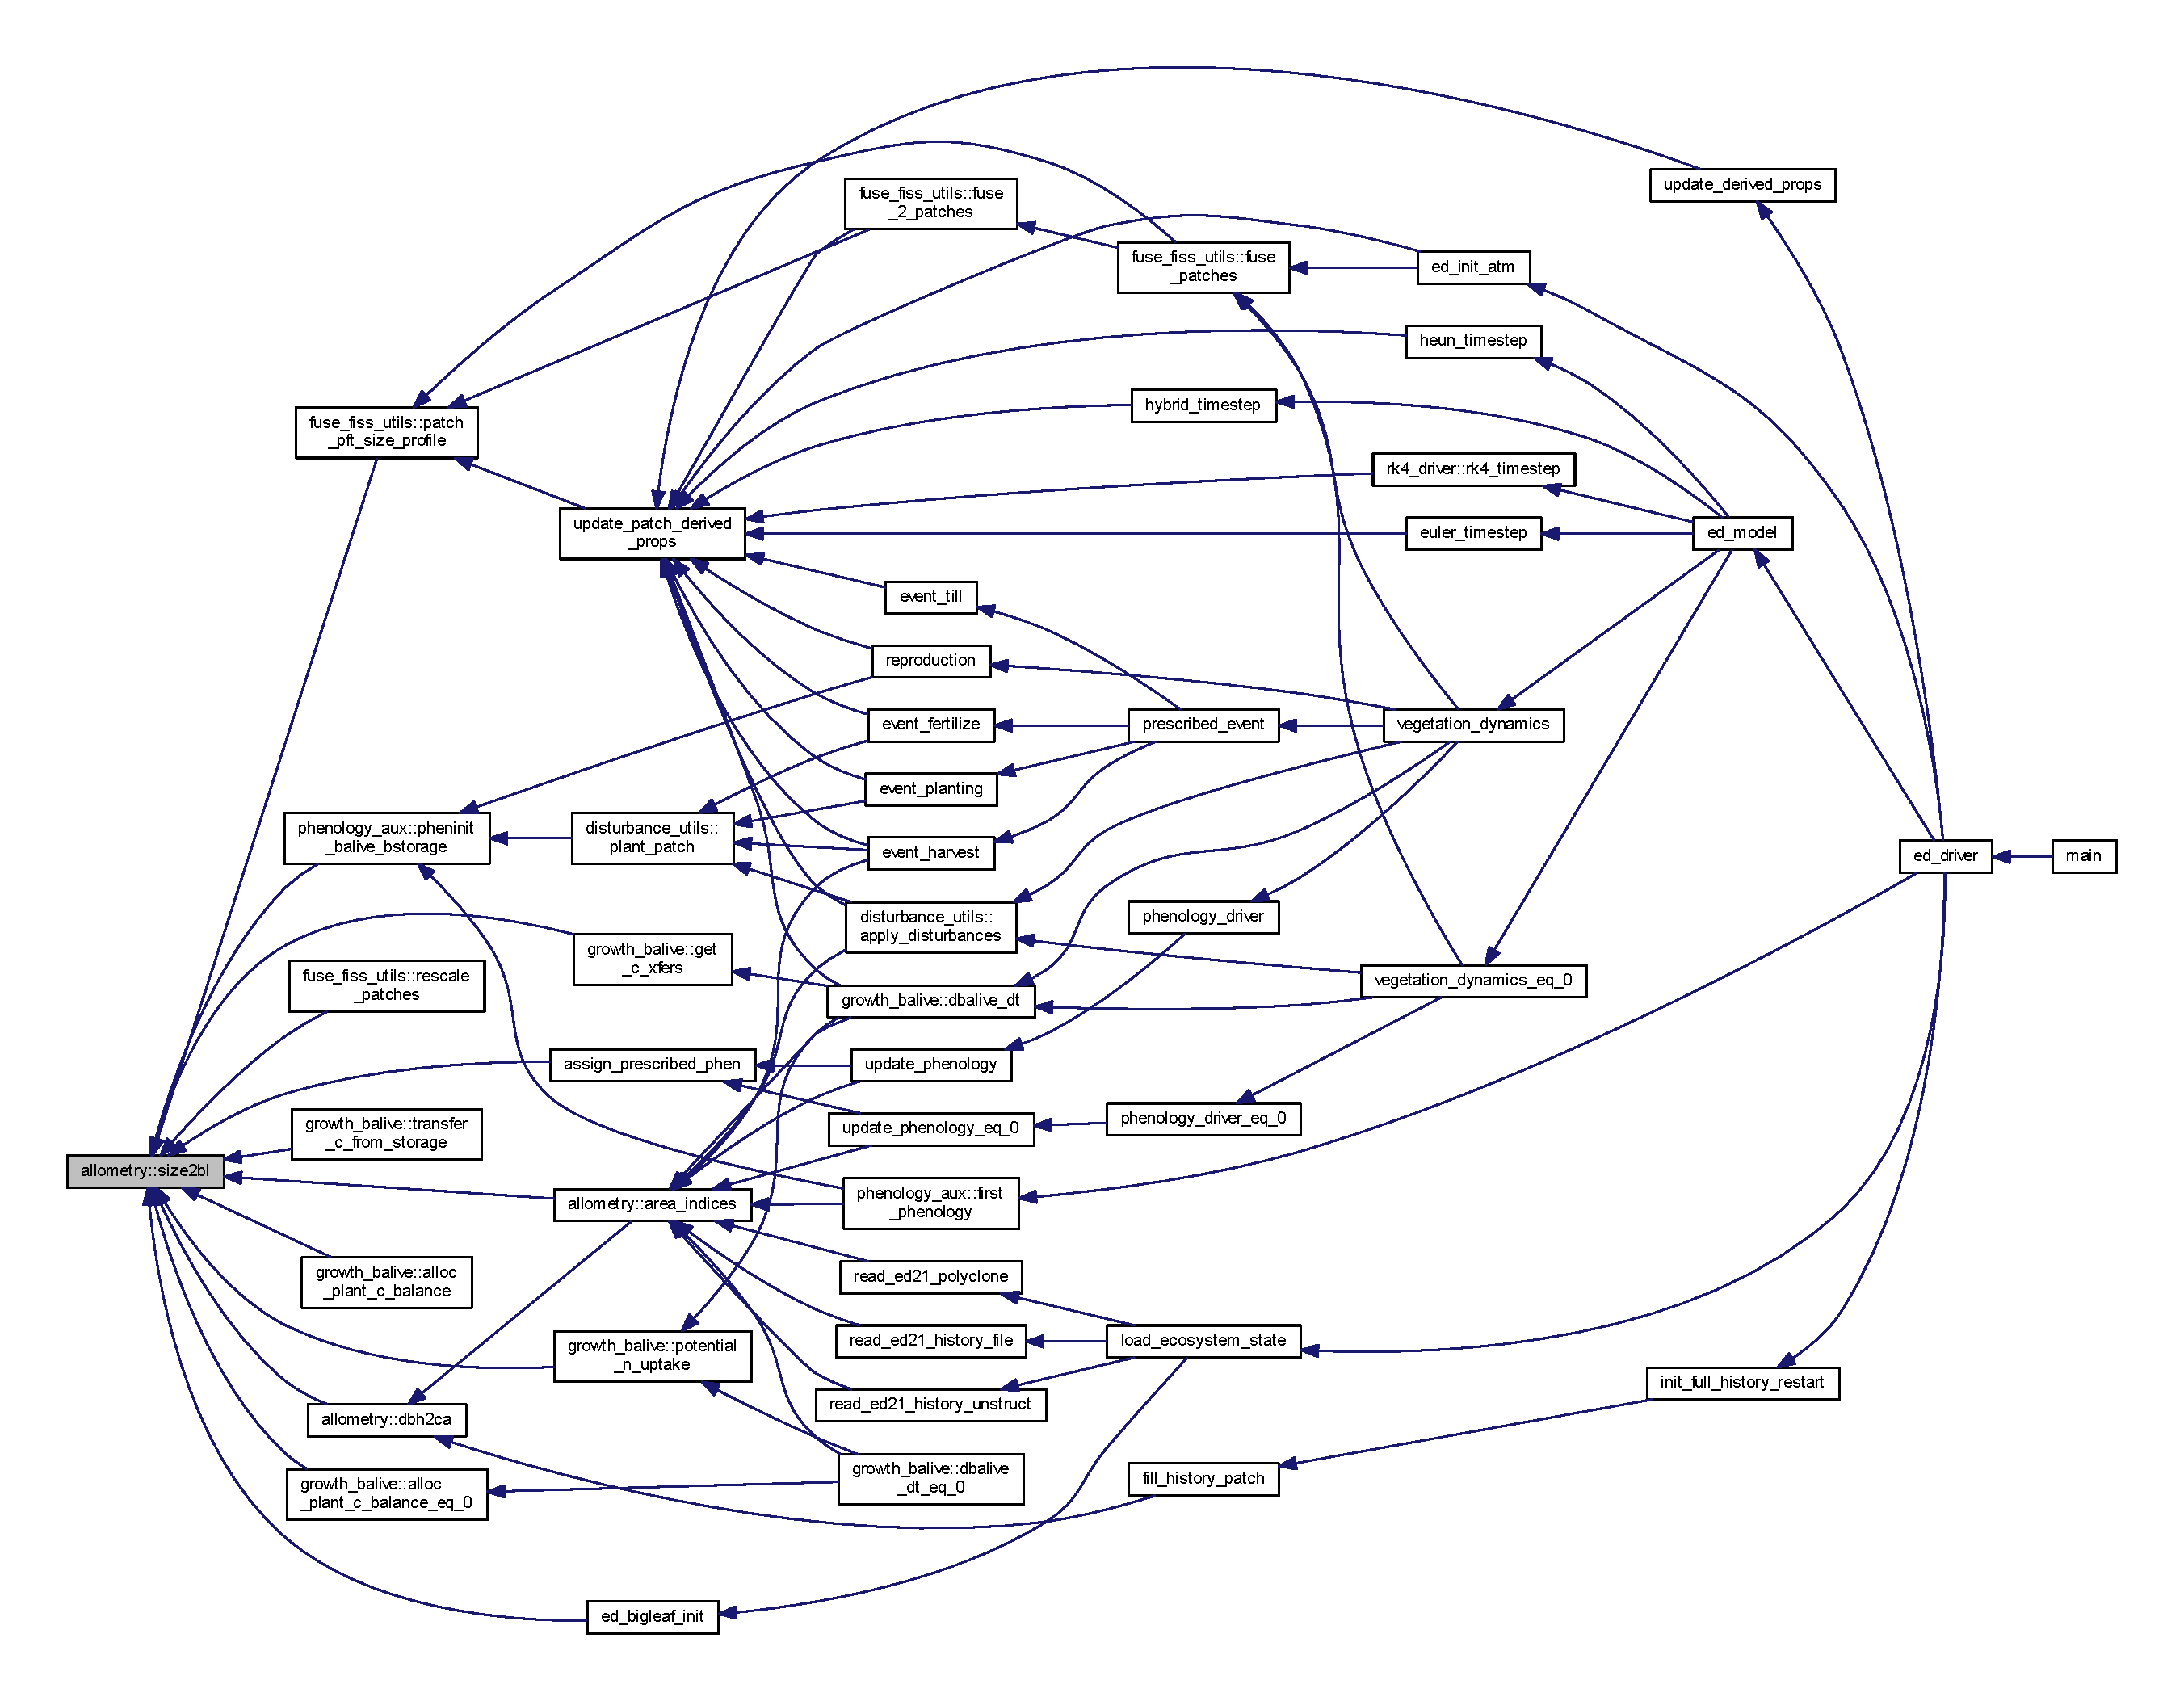
\includegraphics[width=350pt]{namespaceallometry_a45ced9bf9ccd03debe8def35b579f4bd_icgraph}
\end{center}
\end{figure}



\hypertarget{namespacean__header}{}\section{an\+\_\+header Module Reference}
\label{namespacean__header}\index{an\+\_\+header@{an\+\_\+header}}
\subsection*{Data Types}
\begin{DoxyCompactItemize}
\item 
type \hyperlink{structan__header_1_1head__table}{head\+\_\+table}
\end{DoxyCompactItemize}
\subsection*{Variables}
\begin{DoxyCompactItemize}
\item 
type(\hyperlink{structan__header_1_1head__table}{head\+\_\+table}), dimension(\+:), allocatable, save \hyperlink{namespacean__header_ae5d3cd005b4f936e39d8ca9572fad953}{anal\+\_\+table}
\item 
integer, save \hyperlink{namespacean__header_a1f6702c906713337344986a86e036d55}{nvbtab}
\end{DoxyCompactItemize}


\subsection{Variable Documentation}
\index{an\+\_\+header@{an\+\_\+header}!anal\+\_\+table@{anal\+\_\+table}}
\index{anal\+\_\+table@{anal\+\_\+table}!an\+\_\+header@{an\+\_\+header}}
\subsubsection[{\texorpdfstring{anal\+\_\+table}{anal_table}}]{\setlength{\rightskip}{0pt plus 5cm}type ({\bf head\+\_\+table}), dimension(\+:), allocatable, save an\+\_\+header\+::anal\+\_\+table}\hypertarget{namespacean__header_ae5d3cd005b4f936e39d8ca9572fad953}{}\label{namespacean__header_ae5d3cd005b4f936e39d8ca9572fad953}
\index{an\+\_\+header@{an\+\_\+header}!nvbtab@{nvbtab}}
\index{nvbtab@{nvbtab}!an\+\_\+header@{an\+\_\+header}}
\subsubsection[{\texorpdfstring{nvbtab}{nvbtab}}]{\setlength{\rightskip}{0pt plus 5cm}integer, save an\+\_\+header\+::nvbtab}\hypertarget{namespacean__header_a1f6702c906713337344986a86e036d55}{}\label{namespacean__header_a1f6702c906713337344986a86e036d55}

\hypertarget{namespaceaverage__utils}{}\section{average\+\_\+utils Module Reference}
\label{namespaceaverage__utils}\index{average\+\_\+utils@{average\+\_\+utils}}
\subsection*{Functions/\+Subroutines}
\begin{DoxyCompactItemize}
\item 
subroutine \hyperlink{namespaceaverage__utils_a90965230835c19a82d90127089235c76}{aggregate\+\_\+polygon\+\_\+fmean} (cgrid)
\item 
subroutine \hyperlink{namespaceaverage__utils_acf7868319b9242daa7eea553b25f2899}{integrate\+\_\+ed\+\_\+fmean\+\_\+met\+\_\+vars} (cgrid)
\item 
subroutine \hyperlink{namespaceaverage__utils_a662a31926be61beb22be003b5ec40343}{normalize\+\_\+ed\+\_\+fmean\+\_\+vars} (cgrid)
\item 
subroutine \hyperlink{namespaceaverage__utils_a40f7a4a46972fb6b9c0fe90fdc73a173}{zero\+\_\+ed\+\_\+fmean\+\_\+vars} (cgrid)
\item 
subroutine \hyperlink{namespaceaverage__utils_a985b401d85dd857f44371dd2c3e7c40c}{integrate\+\_\+ed\+\_\+dmean\+\_\+vars} (cgrid)
\item 
subroutine \hyperlink{namespaceaverage__utils_a538e2e59c7c2889ae624b6e1d2a9e5f2}{normalize\+\_\+ed\+\_\+today\+\_\+vars} (cgrid)
\item 
subroutine \hyperlink{namespaceaverage__utils_a446f9090fbbcf3eb12f4b9231d946e89}{normalize\+\_\+ed\+\_\+todaynpp\+\_\+vars} (cgrid)
\item 
subroutine \hyperlink{namespaceaverage__utils_a2203ebc403bfd01a55cf7aac61777819}{normalize\+\_\+ed\+\_\+dmean\+\_\+vars} (cgrid)
\item 
subroutine \hyperlink{namespaceaverage__utils_a6a92d00bf7112b127a596bd765cc12c6}{zero\+\_\+ed\+\_\+today\+\_\+vars} (cgrid)
\item 
subroutine \hyperlink{namespaceaverage__utils_af1a2224da3c590c5645db8efa5c16c9f}{zero\+\_\+ed\+\_\+dmean\+\_\+vars} (cgrid)
\item 
subroutine \hyperlink{namespaceaverage__utils_a24f0cd542ec9741c1bcc76e640498cd2}{integrate\+\_\+ed\+\_\+mmean\+\_\+vars} (cgrid)
\item 
subroutine \hyperlink{namespaceaverage__utils_afce18c59b2e9d5605d22e4d356934bdb}{normalize\+\_\+ed\+\_\+mmean\+\_\+vars} (cgrid)
\item 
subroutine \hyperlink{namespaceaverage__utils_aa5221fd3b377dfe424dbdcb81b83c378}{zero\+\_\+ed\+\_\+mmean\+\_\+vars} (cgrid)
\item 
subroutine \hyperlink{namespaceaverage__utils_af429d166f6097c18d6ab4ce05adbd31f}{integrate\+\_\+ed\+\_\+qmean\+\_\+vars} (cgrid)
\item 
subroutine \hyperlink{namespaceaverage__utils_ad7f232f9a24079c3430b005098729615}{normalize\+\_\+ed\+\_\+qmean\+\_\+vars} (cgrid)
\item 
subroutine \hyperlink{namespaceaverage__utils_a2e9cb2592327099345c147516b927f51}{zero\+\_\+ed\+\_\+qmean\+\_\+vars} (cgrid)
\item 
subroutine \hyperlink{namespaceaverage__utils_a81384775dd05dba144bf83e9731d5275}{update\+\_\+ed\+\_\+yearly\+\_\+vars} (cgrid)
\item 
subroutine \hyperlink{namespaceaverage__utils_a81df7cc84b1d62f7fb950e91d410abbd}{zero\+\_\+ed\+\_\+yearly\+\_\+vars} (cgrid)
\item 
real(kind=4) function \hyperlink{namespaceaverage__utils_ac90817fe39c27153ed7bbee2cb856611}{isqu\+\_\+ftz} (x)
\end{DoxyCompactItemize}


\subsection{Function/\+Subroutine Documentation}
\index{average\+\_\+utils@{average\+\_\+utils}!aggregate\+\_\+polygon\+\_\+fmean@{aggregate\+\_\+polygon\+\_\+fmean}}
\index{aggregate\+\_\+polygon\+\_\+fmean@{aggregate\+\_\+polygon\+\_\+fmean}!average\+\_\+utils@{average\+\_\+utils}}
\subsubsection[{\texorpdfstring{aggregate\+\_\+polygon\+\_\+fmean(cgrid)}{aggregate_polygon_fmean(cgrid)}}]{\setlength{\rightskip}{0pt plus 5cm}subroutine average\+\_\+utils\+::aggregate\+\_\+polygon\+\_\+fmean (
\begin{DoxyParamCaption}
\item[{type({\bf edtype}), target}]{cgrid}
\end{DoxyParamCaption}
)}\hypertarget{namespaceaverage__utils_a90965230835c19a82d90127089235c76}{}\label{namespaceaverage__utils_a90965230835c19a82d90127089235c76}


Here is the call graph for this function\+:\nopagebreak
\begin{figure}[H]
\begin{center}
\leavevmode
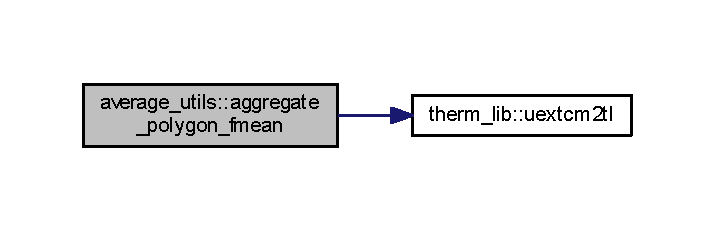
\includegraphics[width=343pt]{namespaceaverage__utils_a90965230835c19a82d90127089235c76_cgraph}
\end{center}
\end{figure}




Here is the caller graph for this function\+:\nopagebreak
\begin{figure}[H]
\begin{center}
\leavevmode
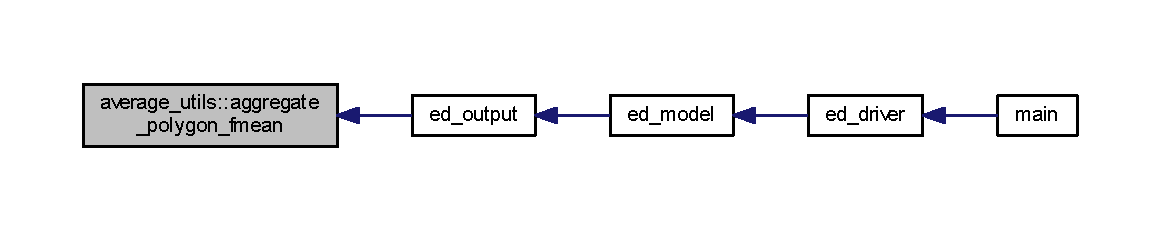
\includegraphics[width=350pt]{namespaceaverage__utils_a90965230835c19a82d90127089235c76_icgraph}
\end{center}
\end{figure}


\index{average\+\_\+utils@{average\+\_\+utils}!integrate\+\_\+ed\+\_\+dmean\+\_\+vars@{integrate\+\_\+ed\+\_\+dmean\+\_\+vars}}
\index{integrate\+\_\+ed\+\_\+dmean\+\_\+vars@{integrate\+\_\+ed\+\_\+dmean\+\_\+vars}!average\+\_\+utils@{average\+\_\+utils}}
\subsubsection[{\texorpdfstring{integrate\+\_\+ed\+\_\+dmean\+\_\+vars(cgrid)}{integrate_ed_dmean_vars(cgrid)}}]{\setlength{\rightskip}{0pt plus 5cm}subroutine average\+\_\+utils\+::integrate\+\_\+ed\+\_\+dmean\+\_\+vars (
\begin{DoxyParamCaption}
\item[{type({\bf edtype}), target}]{cgrid}
\end{DoxyParamCaption}
)}\hypertarget{namespaceaverage__utils_a985b401d85dd857f44371dd2c3e7c40c}{}\label{namespaceaverage__utils_a985b401d85dd857f44371dd2c3e7c40c}
\index{average\+\_\+utils@{average\+\_\+utils}!integrate\+\_\+ed\+\_\+fmean\+\_\+met\+\_\+vars@{integrate\+\_\+ed\+\_\+fmean\+\_\+met\+\_\+vars}}
\index{integrate\+\_\+ed\+\_\+fmean\+\_\+met\+\_\+vars@{integrate\+\_\+ed\+\_\+fmean\+\_\+met\+\_\+vars}!average\+\_\+utils@{average\+\_\+utils}}
\subsubsection[{\texorpdfstring{integrate\+\_\+ed\+\_\+fmean\+\_\+met\+\_\+vars(cgrid)}{integrate_ed_fmean_met_vars(cgrid)}}]{\setlength{\rightskip}{0pt plus 5cm}subroutine average\+\_\+utils\+::integrate\+\_\+ed\+\_\+fmean\+\_\+met\+\_\+vars (
\begin{DoxyParamCaption}
\item[{type({\bf edtype}), target}]{cgrid}
\end{DoxyParamCaption}
)}\hypertarget{namespaceaverage__utils_acf7868319b9242daa7eea553b25f2899}{}\label{namespaceaverage__utils_acf7868319b9242daa7eea553b25f2899}
\index{average\+\_\+utils@{average\+\_\+utils}!integrate\+\_\+ed\+\_\+mmean\+\_\+vars@{integrate\+\_\+ed\+\_\+mmean\+\_\+vars}}
\index{integrate\+\_\+ed\+\_\+mmean\+\_\+vars@{integrate\+\_\+ed\+\_\+mmean\+\_\+vars}!average\+\_\+utils@{average\+\_\+utils}}
\subsubsection[{\texorpdfstring{integrate\+\_\+ed\+\_\+mmean\+\_\+vars(cgrid)}{integrate_ed_mmean_vars(cgrid)}}]{\setlength{\rightskip}{0pt plus 5cm}subroutine average\+\_\+utils\+::integrate\+\_\+ed\+\_\+mmean\+\_\+vars (
\begin{DoxyParamCaption}
\item[{type({\bf edtype}), target}]{cgrid}
\end{DoxyParamCaption}
)}\hypertarget{namespaceaverage__utils_a24f0cd542ec9741c1bcc76e640498cd2}{}\label{namespaceaverage__utils_a24f0cd542ec9741c1bcc76e640498cd2}


Here is the call graph for this function\+:\nopagebreak
\begin{figure}[H]
\begin{center}
\leavevmode
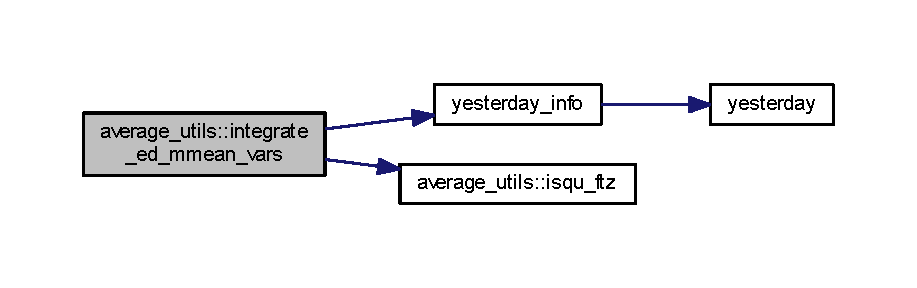
\includegraphics[width=350pt]{namespaceaverage__utils_a24f0cd542ec9741c1bcc76e640498cd2_cgraph}
\end{center}
\end{figure}


\index{average\+\_\+utils@{average\+\_\+utils}!integrate\+\_\+ed\+\_\+qmean\+\_\+vars@{integrate\+\_\+ed\+\_\+qmean\+\_\+vars}}
\index{integrate\+\_\+ed\+\_\+qmean\+\_\+vars@{integrate\+\_\+ed\+\_\+qmean\+\_\+vars}!average\+\_\+utils@{average\+\_\+utils}}
\subsubsection[{\texorpdfstring{integrate\+\_\+ed\+\_\+qmean\+\_\+vars(cgrid)}{integrate_ed_qmean_vars(cgrid)}}]{\setlength{\rightskip}{0pt plus 5cm}subroutine average\+\_\+utils\+::integrate\+\_\+ed\+\_\+qmean\+\_\+vars (
\begin{DoxyParamCaption}
\item[{type({\bf edtype}), target}]{cgrid}
\end{DoxyParamCaption}
)}\hypertarget{namespaceaverage__utils_af429d166f6097c18d6ab4ce05adbd31f}{}\label{namespaceaverage__utils_af429d166f6097c18d6ab4ce05adbd31f}


Here is the call graph for this function\+:\nopagebreak
\begin{figure}[H]
\begin{center}
\leavevmode
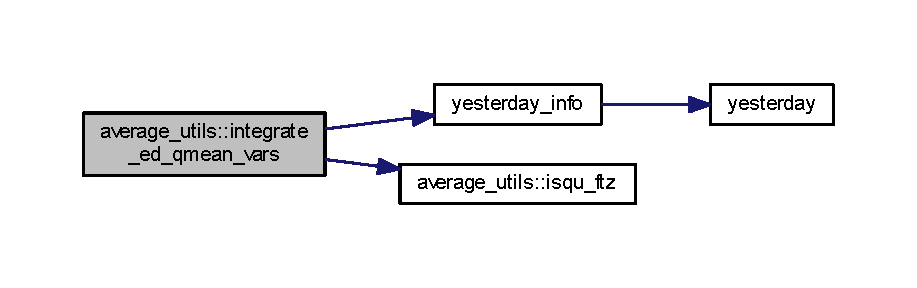
\includegraphics[width=350pt]{namespaceaverage__utils_af429d166f6097c18d6ab4ce05adbd31f_cgraph}
\end{center}
\end{figure}


\index{average\+\_\+utils@{average\+\_\+utils}!isqu\+\_\+ftz@{isqu\+\_\+ftz}}
\index{isqu\+\_\+ftz@{isqu\+\_\+ftz}!average\+\_\+utils@{average\+\_\+utils}}
\subsubsection[{\texorpdfstring{isqu\+\_\+ftz(x)}{isqu_ftz(x)}}]{\setlength{\rightskip}{0pt plus 5cm}real(kind=4) function average\+\_\+utils\+::isqu\+\_\+ftz (
\begin{DoxyParamCaption}
\item[{real(kind=4), intent(in)}]{x}
\end{DoxyParamCaption}
)}\hypertarget{namespaceaverage__utils_ac90817fe39c27153ed7bbee2cb856611}{}\label{namespaceaverage__utils_ac90817fe39c27153ed7bbee2cb856611}


Here is the caller graph for this function\+:\nopagebreak
\begin{figure}[H]
\begin{center}
\leavevmode
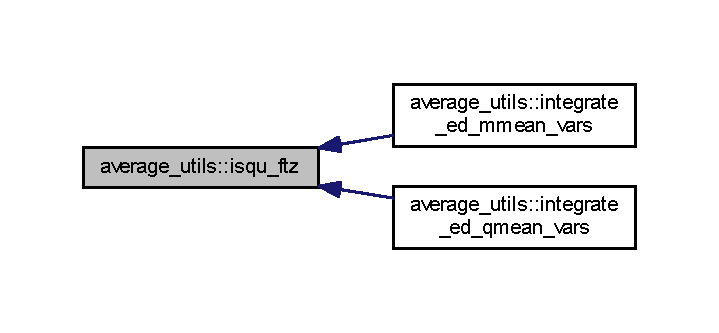
\includegraphics[width=345pt]{namespaceaverage__utils_ac90817fe39c27153ed7bbee2cb856611_icgraph}
\end{center}
\end{figure}


\index{average\+\_\+utils@{average\+\_\+utils}!normalize\+\_\+ed\+\_\+dmean\+\_\+vars@{normalize\+\_\+ed\+\_\+dmean\+\_\+vars}}
\index{normalize\+\_\+ed\+\_\+dmean\+\_\+vars@{normalize\+\_\+ed\+\_\+dmean\+\_\+vars}!average\+\_\+utils@{average\+\_\+utils}}
\subsubsection[{\texorpdfstring{normalize\+\_\+ed\+\_\+dmean\+\_\+vars(cgrid)}{normalize_ed_dmean_vars(cgrid)}}]{\setlength{\rightskip}{0pt plus 5cm}subroutine average\+\_\+utils\+::normalize\+\_\+ed\+\_\+dmean\+\_\+vars (
\begin{DoxyParamCaption}
\item[{type({\bf edtype}), target}]{cgrid}
\end{DoxyParamCaption}
)}\hypertarget{namespaceaverage__utils_a2203ebc403bfd01a55cf7aac61777819}{}\label{namespaceaverage__utils_a2203ebc403bfd01a55cf7aac61777819}


Here is the call graph for this function\+:\nopagebreak
\begin{figure}[H]
\begin{center}
\leavevmode
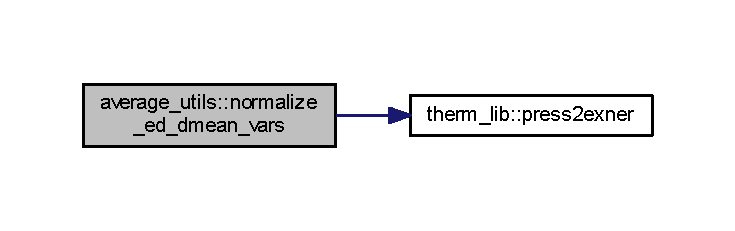
\includegraphics[width=350pt]{namespaceaverage__utils_a2203ebc403bfd01a55cf7aac61777819_cgraph}
\end{center}
\end{figure}


\index{average\+\_\+utils@{average\+\_\+utils}!normalize\+\_\+ed\+\_\+fmean\+\_\+vars@{normalize\+\_\+ed\+\_\+fmean\+\_\+vars}}
\index{normalize\+\_\+ed\+\_\+fmean\+\_\+vars@{normalize\+\_\+ed\+\_\+fmean\+\_\+vars}!average\+\_\+utils@{average\+\_\+utils}}
\subsubsection[{\texorpdfstring{normalize\+\_\+ed\+\_\+fmean\+\_\+vars(cgrid)}{normalize_ed_fmean_vars(cgrid)}}]{\setlength{\rightskip}{0pt plus 5cm}subroutine average\+\_\+utils\+::normalize\+\_\+ed\+\_\+fmean\+\_\+vars (
\begin{DoxyParamCaption}
\item[{type({\bf edtype}), target}]{cgrid}
\end{DoxyParamCaption}
)}\hypertarget{namespaceaverage__utils_a662a31926be61beb22be003b5ec40343}{}\label{namespaceaverage__utils_a662a31926be61beb22be003b5ec40343}


Here is the call graph for this function\+:\nopagebreak
\begin{figure}[H]
\begin{center}
\leavevmode
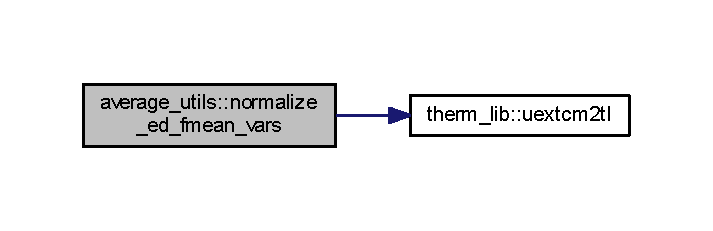
\includegraphics[width=342pt]{namespaceaverage__utils_a662a31926be61beb22be003b5ec40343_cgraph}
\end{center}
\end{figure}


\index{average\+\_\+utils@{average\+\_\+utils}!normalize\+\_\+ed\+\_\+mmean\+\_\+vars@{normalize\+\_\+ed\+\_\+mmean\+\_\+vars}}
\index{normalize\+\_\+ed\+\_\+mmean\+\_\+vars@{normalize\+\_\+ed\+\_\+mmean\+\_\+vars}!average\+\_\+utils@{average\+\_\+utils}}
\subsubsection[{\texorpdfstring{normalize\+\_\+ed\+\_\+mmean\+\_\+vars(cgrid)}{normalize_ed_mmean_vars(cgrid)}}]{\setlength{\rightskip}{0pt plus 5cm}subroutine average\+\_\+utils\+::normalize\+\_\+ed\+\_\+mmean\+\_\+vars (
\begin{DoxyParamCaption}
\item[{type({\bf edtype}), target}]{cgrid}
\end{DoxyParamCaption}
)}\hypertarget{namespaceaverage__utils_afce18c59b2e9d5605d22e4d356934bdb}{}\label{namespaceaverage__utils_afce18c59b2e9d5605d22e4d356934bdb}


Here is the call graph for this function\+:\nopagebreak
\begin{figure}[H]
\begin{center}
\leavevmode
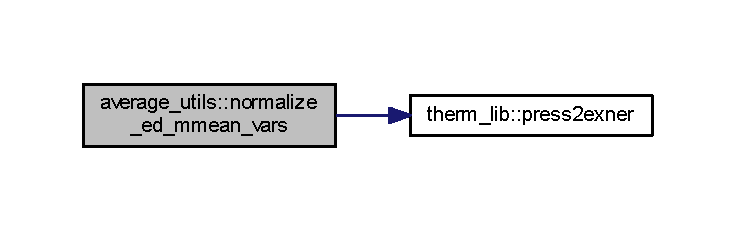
\includegraphics[width=350pt]{namespaceaverage__utils_afce18c59b2e9d5605d22e4d356934bdb_cgraph}
\end{center}
\end{figure}


\index{average\+\_\+utils@{average\+\_\+utils}!normalize\+\_\+ed\+\_\+qmean\+\_\+vars@{normalize\+\_\+ed\+\_\+qmean\+\_\+vars}}
\index{normalize\+\_\+ed\+\_\+qmean\+\_\+vars@{normalize\+\_\+ed\+\_\+qmean\+\_\+vars}!average\+\_\+utils@{average\+\_\+utils}}
\subsubsection[{\texorpdfstring{normalize\+\_\+ed\+\_\+qmean\+\_\+vars(cgrid)}{normalize_ed_qmean_vars(cgrid)}}]{\setlength{\rightskip}{0pt plus 5cm}subroutine average\+\_\+utils\+::normalize\+\_\+ed\+\_\+qmean\+\_\+vars (
\begin{DoxyParamCaption}
\item[{type({\bf edtype}), target}]{cgrid}
\end{DoxyParamCaption}
)}\hypertarget{namespaceaverage__utils_ad7f232f9a24079c3430b005098729615}{}\label{namespaceaverage__utils_ad7f232f9a24079c3430b005098729615}


Here is the call graph for this function\+:\nopagebreak
\begin{figure}[H]
\begin{center}
\leavevmode
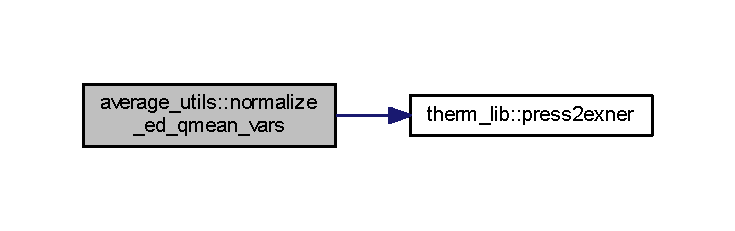
\includegraphics[width=350pt]{namespaceaverage__utils_ad7f232f9a24079c3430b005098729615_cgraph}
\end{center}
\end{figure}


\index{average\+\_\+utils@{average\+\_\+utils}!normalize\+\_\+ed\+\_\+today\+\_\+vars@{normalize\+\_\+ed\+\_\+today\+\_\+vars}}
\index{normalize\+\_\+ed\+\_\+today\+\_\+vars@{normalize\+\_\+ed\+\_\+today\+\_\+vars}!average\+\_\+utils@{average\+\_\+utils}}
\subsubsection[{\texorpdfstring{normalize\+\_\+ed\+\_\+today\+\_\+vars(cgrid)}{normalize_ed_today_vars(cgrid)}}]{\setlength{\rightskip}{0pt plus 5cm}subroutine average\+\_\+utils\+::normalize\+\_\+ed\+\_\+today\+\_\+vars (
\begin{DoxyParamCaption}
\item[{type({\bf edtype}), target}]{cgrid}
\end{DoxyParamCaption}
)}\hypertarget{namespaceaverage__utils_a538e2e59c7c2889ae624b6e1d2a9e5f2}{}\label{namespaceaverage__utils_a538e2e59c7c2889ae624b6e1d2a9e5f2}


Here is the caller graph for this function\+:\nopagebreak
\begin{figure}[H]
\begin{center}
\leavevmode
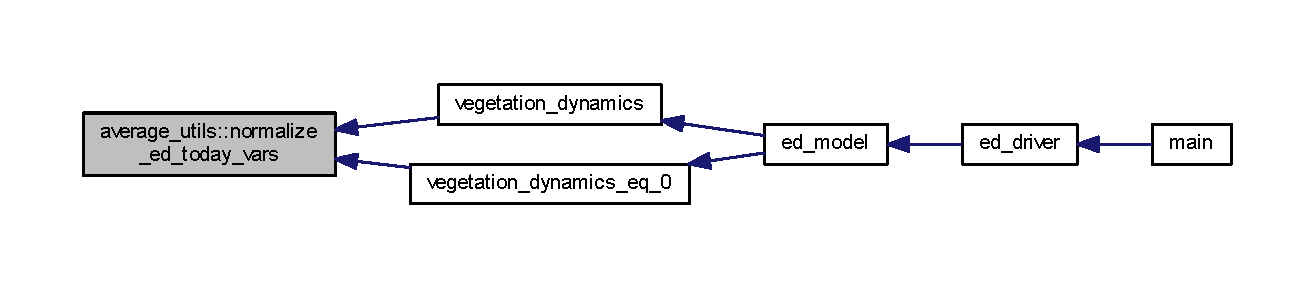
\includegraphics[width=350pt]{namespaceaverage__utils_a538e2e59c7c2889ae624b6e1d2a9e5f2_icgraph}
\end{center}
\end{figure}


\index{average\+\_\+utils@{average\+\_\+utils}!normalize\+\_\+ed\+\_\+todaynpp\+\_\+vars@{normalize\+\_\+ed\+\_\+todaynpp\+\_\+vars}}
\index{normalize\+\_\+ed\+\_\+todaynpp\+\_\+vars@{normalize\+\_\+ed\+\_\+todaynpp\+\_\+vars}!average\+\_\+utils@{average\+\_\+utils}}
\subsubsection[{\texorpdfstring{normalize\+\_\+ed\+\_\+todaynpp\+\_\+vars(cgrid)}{normalize_ed_todaynpp_vars(cgrid)}}]{\setlength{\rightskip}{0pt plus 5cm}subroutine average\+\_\+utils\+::normalize\+\_\+ed\+\_\+todaynpp\+\_\+vars (
\begin{DoxyParamCaption}
\item[{type({\bf edtype}), target}]{cgrid}
\end{DoxyParamCaption}
)}\hypertarget{namespaceaverage__utils_a446f9090fbbcf3eb12f4b9231d946e89}{}\label{namespaceaverage__utils_a446f9090fbbcf3eb12f4b9231d946e89}
\index{average\+\_\+utils@{average\+\_\+utils}!update\+\_\+ed\+\_\+yearly\+\_\+vars@{update\+\_\+ed\+\_\+yearly\+\_\+vars}}
\index{update\+\_\+ed\+\_\+yearly\+\_\+vars@{update\+\_\+ed\+\_\+yearly\+\_\+vars}!average\+\_\+utils@{average\+\_\+utils}}
\subsubsection[{\texorpdfstring{update\+\_\+ed\+\_\+yearly\+\_\+vars(cgrid)}{update_ed_yearly_vars(cgrid)}}]{\setlength{\rightskip}{0pt plus 5cm}subroutine average\+\_\+utils\+::update\+\_\+ed\+\_\+yearly\+\_\+vars (
\begin{DoxyParamCaption}
\item[{type({\bf edtype}), target}]{cgrid}
\end{DoxyParamCaption}
)}\hypertarget{namespaceaverage__utils_a81384775dd05dba144bf83e9731d5275}{}\label{namespaceaverage__utils_a81384775dd05dba144bf83e9731d5275}


Here is the caller graph for this function\+:\nopagebreak
\begin{figure}[H]
\begin{center}
\leavevmode
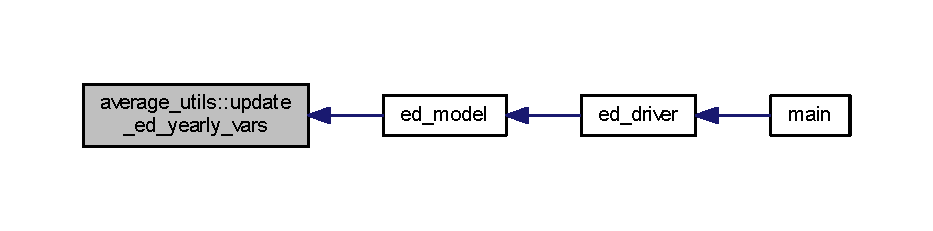
\includegraphics[width=350pt]{namespaceaverage__utils_a81384775dd05dba144bf83e9731d5275_icgraph}
\end{center}
\end{figure}


\index{average\+\_\+utils@{average\+\_\+utils}!zero\+\_\+ed\+\_\+dmean\+\_\+vars@{zero\+\_\+ed\+\_\+dmean\+\_\+vars}}
\index{zero\+\_\+ed\+\_\+dmean\+\_\+vars@{zero\+\_\+ed\+\_\+dmean\+\_\+vars}!average\+\_\+utils@{average\+\_\+utils}}
\subsubsection[{\texorpdfstring{zero\+\_\+ed\+\_\+dmean\+\_\+vars(cgrid)}{zero_ed_dmean_vars(cgrid)}}]{\setlength{\rightskip}{0pt plus 5cm}subroutine average\+\_\+utils\+::zero\+\_\+ed\+\_\+dmean\+\_\+vars (
\begin{DoxyParamCaption}
\item[{type({\bf edtype}), target}]{cgrid}
\end{DoxyParamCaption}
)}\hypertarget{namespaceaverage__utils_af1a2224da3c590c5645db8efa5c16c9f}{}\label{namespaceaverage__utils_af1a2224da3c590c5645db8efa5c16c9f}
\index{average\+\_\+utils@{average\+\_\+utils}!zero\+\_\+ed\+\_\+fmean\+\_\+vars@{zero\+\_\+ed\+\_\+fmean\+\_\+vars}}
\index{zero\+\_\+ed\+\_\+fmean\+\_\+vars@{zero\+\_\+ed\+\_\+fmean\+\_\+vars}!average\+\_\+utils@{average\+\_\+utils}}
\subsubsection[{\texorpdfstring{zero\+\_\+ed\+\_\+fmean\+\_\+vars(cgrid)}{zero_ed_fmean_vars(cgrid)}}]{\setlength{\rightskip}{0pt plus 5cm}subroutine average\+\_\+utils\+::zero\+\_\+ed\+\_\+fmean\+\_\+vars (
\begin{DoxyParamCaption}
\item[{type({\bf edtype}), target}]{cgrid}
\end{DoxyParamCaption}
)}\hypertarget{namespaceaverage__utils_a40f7a4a46972fb6b9c0fe90fdc73a173}{}\label{namespaceaverage__utils_a40f7a4a46972fb6b9c0fe90fdc73a173}
\index{average\+\_\+utils@{average\+\_\+utils}!zero\+\_\+ed\+\_\+mmean\+\_\+vars@{zero\+\_\+ed\+\_\+mmean\+\_\+vars}}
\index{zero\+\_\+ed\+\_\+mmean\+\_\+vars@{zero\+\_\+ed\+\_\+mmean\+\_\+vars}!average\+\_\+utils@{average\+\_\+utils}}
\subsubsection[{\texorpdfstring{zero\+\_\+ed\+\_\+mmean\+\_\+vars(cgrid)}{zero_ed_mmean_vars(cgrid)}}]{\setlength{\rightskip}{0pt plus 5cm}subroutine average\+\_\+utils\+::zero\+\_\+ed\+\_\+mmean\+\_\+vars (
\begin{DoxyParamCaption}
\item[{type({\bf edtype}), target}]{cgrid}
\end{DoxyParamCaption}
)}\hypertarget{namespaceaverage__utils_aa5221fd3b377dfe424dbdcb81b83c378}{}\label{namespaceaverage__utils_aa5221fd3b377dfe424dbdcb81b83c378}
\index{average\+\_\+utils@{average\+\_\+utils}!zero\+\_\+ed\+\_\+qmean\+\_\+vars@{zero\+\_\+ed\+\_\+qmean\+\_\+vars}}
\index{zero\+\_\+ed\+\_\+qmean\+\_\+vars@{zero\+\_\+ed\+\_\+qmean\+\_\+vars}!average\+\_\+utils@{average\+\_\+utils}}
\subsubsection[{\texorpdfstring{zero\+\_\+ed\+\_\+qmean\+\_\+vars(cgrid)}{zero_ed_qmean_vars(cgrid)}}]{\setlength{\rightskip}{0pt plus 5cm}subroutine average\+\_\+utils\+::zero\+\_\+ed\+\_\+qmean\+\_\+vars (
\begin{DoxyParamCaption}
\item[{type({\bf edtype}), target}]{cgrid}
\end{DoxyParamCaption}
)}\hypertarget{namespaceaverage__utils_a2e9cb2592327099345c147516b927f51}{}\label{namespaceaverage__utils_a2e9cb2592327099345c147516b927f51}
\index{average\+\_\+utils@{average\+\_\+utils}!zero\+\_\+ed\+\_\+today\+\_\+vars@{zero\+\_\+ed\+\_\+today\+\_\+vars}}
\index{zero\+\_\+ed\+\_\+today\+\_\+vars@{zero\+\_\+ed\+\_\+today\+\_\+vars}!average\+\_\+utils@{average\+\_\+utils}}
\subsubsection[{\texorpdfstring{zero\+\_\+ed\+\_\+today\+\_\+vars(cgrid)}{zero_ed_today_vars(cgrid)}}]{\setlength{\rightskip}{0pt plus 5cm}subroutine average\+\_\+utils\+::zero\+\_\+ed\+\_\+today\+\_\+vars (
\begin{DoxyParamCaption}
\item[{type({\bf edtype}), target}]{cgrid}
\end{DoxyParamCaption}
)}\hypertarget{namespaceaverage__utils_a6a92d00bf7112b127a596bd765cc12c6}{}\label{namespaceaverage__utils_a6a92d00bf7112b127a596bd765cc12c6}
\index{average\+\_\+utils@{average\+\_\+utils}!zero\+\_\+ed\+\_\+yearly\+\_\+vars@{zero\+\_\+ed\+\_\+yearly\+\_\+vars}}
\index{zero\+\_\+ed\+\_\+yearly\+\_\+vars@{zero\+\_\+ed\+\_\+yearly\+\_\+vars}!average\+\_\+utils@{average\+\_\+utils}}
\subsubsection[{\texorpdfstring{zero\+\_\+ed\+\_\+yearly\+\_\+vars(cgrid)}{zero_ed_yearly_vars(cgrid)}}]{\setlength{\rightskip}{0pt plus 5cm}subroutine average\+\_\+utils\+::zero\+\_\+ed\+\_\+yearly\+\_\+vars (
\begin{DoxyParamCaption}
\item[{type({\bf edtype}), target}]{cgrid}
\end{DoxyParamCaption}
)}\hypertarget{namespaceaverage__utils_a81df7cc84b1d62f7fb950e91d410abbd}{}\label{namespaceaverage__utils_a81df7cc84b1d62f7fb950e91d410abbd}

\hypertarget{namespacebudget__utils}{}\section{budget\+\_\+utils Module Reference}
\label{namespacebudget__utils}\index{budget\+\_\+utils@{budget\+\_\+utils}}
\subsection*{Functions/\+Subroutines}
\begin{DoxyCompactItemize}
\item 
subroutine \hyperlink{namespacebudget__utils_ad8835ee763cd964432b44e0a3d00e3da}{update\+\_\+budget} (csite, lsl, ipaa, ipaz)
\item 
subroutine \hyperlink{namespacebudget__utils_ade80ff8e17018f7bd86015ee5f20375e}{compute\+\_\+budget} (csite, lsl, pcpg, qpcpg, ipa, wcurr\+\_\+loss2atm, ecurr\+\_\+netrad                                                                                                                                               ,ecurr\+\_\+loss2atm, co2curr\+\_\+loss2atm, wcurr\+\_\+loss2drainage                                                                                                                                                   ,ecurr\+\_\+loss2drainage, wcurr\+\_\+loss2runoff, ecurr\+\_\+loss2runoff                                                                                                                                   ,site\+\_\+area, cbudget\+\_\+nep, old\+\_\+can\+\_\+enthalpy, old\+\_\+can\+\_\+shv                                                                                                                                                       ,old\+\_\+can\+\_\+co2, old\+\_\+can\+\_\+rhos, old\+\_\+can\+\_\+temp, old\+\_\+can\+\_\+prss)
\item 
real function \hyperlink{namespacebudget__utils_ad0c764047c557100b3a3cdcd836103a0}{compute\+\_\+water\+\_\+storage} (csite, lsl, ipa)
\item 
real function \hyperlink{namespacebudget__utils_a6111a1c211ecef562368c8635f64af45}{compute\+\_\+netrad} (csite, ipa)
\item 
real function \hyperlink{namespacebudget__utils_a319c5f7252c344bcebbd162593e25ec8}{compute\+\_\+energy\+\_\+storage} (csite, lsl, ipa)
\item 
subroutine \hyperlink{namespacebudget__utils_a117874382f22a7cb0883681d23606828}{sum\+\_\+plant\+\_\+cfluxes} (csite, ipa, gpp, leaf\+\_\+resp, root\+\_\+resp, leaf\+\_\+growth\+\_\+resp                                                                                                                                               ,root\+\_\+growth\+\_\+resp, sapa\+\_\+growth\+\_\+resp, sapb\+\_\+growth\+\_\+resp                                                                                                                                                       ,leaf\+\_\+storage\+\_\+resp, root\+\_\+storage\+\_\+resp, sapa\+\_\+storage\+\_\+resp                                                                                                                                           ,sapb\+\_\+storage\+\_\+resp)
\item 
real function \hyperlink{namespacebudget__utils_aa1c4f8466010b1673f2914f1bfe9b6ee}{compute\+\_\+co2\+\_\+storage} (csite, ipa)
\item 
real function \hyperlink{namespacebudget__utils_ae7ad8d90c28490b0b1c920e7a2656345}{ddens\+\_\+dt\+\_\+effect} (old\+\_\+rhos, new\+\_\+rhos, old\+\_\+prop, new\+\_\+prop, can\+\_\+depth, multi)
\end{DoxyCompactItemize}


\subsection{Function/\+Subroutine Documentation}
\index{budget\+\_\+utils@{budget\+\_\+utils}!compute\+\_\+budget@{compute\+\_\+budget}}
\index{compute\+\_\+budget@{compute\+\_\+budget}!budget\+\_\+utils@{budget\+\_\+utils}}
\subsubsection[{\texorpdfstring{compute\+\_\+budget(csite, lsl, pcpg, qpcpg, ipa, wcurr\+\_\+loss2atm, ecurr\+\_\+netrad                                                                                                                                               ,ecurr\+\_\+loss2atm, co2curr\+\_\+loss2atm, wcurr\+\_\+loss2drainage                                                                                                                                                   ,ecurr\+\_\+loss2drainage, wcurr\+\_\+loss2runoff, ecurr\+\_\+loss2runoff                                                                                                                                   ,site\+\_\+area, cbudget\+\_\+nep, old\+\_\+can\+\_\+enthalpy, old\+\_\+can\+\_\+shv                                                                                                                                                       ,old\+\_\+can\+\_\+co2, old\+\_\+can\+\_\+rhos, old\+\_\+can\+\_\+temp, old\+\_\+can\+\_\+prss)}{compute_budget(csite, lsl, pcpg, qpcpg, ipa, wcurr_loss2atm, ecurr_netrad                                                                                                                                               ,ecurr_loss2atm, co2curr_loss2atm, wcurr_loss2drainage                                                                                                                                                   ,ecurr_loss2drainage, wcurr_loss2runoff, ecurr_loss2runoff                                                                                                                                   ,site_area, cbudget_nep, old_can_enthalpy, old_can_shv                                                                                                                                                       ,old_can_co2, old_can_rhos, old_can_temp, old_can_prss)}}]{\setlength{\rightskip}{0pt plus 5cm}subroutine budget\+\_\+utils\+::compute\+\_\+budget (
\begin{DoxyParamCaption}
\item[{type({\bf sitetype}), target}]{csite, }
\item[{integer, intent(in)}]{lsl, }
\item[{real, intent(inout)}]{pcpg, }
\item[{real, intent(inout)}]{qpcpg, }
\item[{integer, intent(in)}]{ipa, }
\item[{real, intent(inout)}]{wcurr\+\_\+loss2atm, }
\item[{real, intent(inout)}]{ecurr\+\_\+netrad, }
\item[{real, intent(inout)}]{ecurr\+\_\+loss2atm, }
\item[{real, intent(inout)}]{co2curr\+\_\+loss2atm, }
\item[{real, intent(inout)}]{wcurr\+\_\+loss2drainage, }
\item[{real, intent(inout)}]{ecurr\+\_\+loss2drainage, }
\item[{real, intent(inout)}]{wcurr\+\_\+loss2runoff, }
\item[{real, intent(inout)}]{ecurr\+\_\+loss2runoff, }
\item[{real, intent(in)}]{site\+\_\+area, }
\item[{real, intent(inout)}]{cbudget\+\_\+nep, }
\item[{real, intent(in)}]{old\+\_\+can\+\_\+enthalpy, }
\item[{real, intent(in)}]{old\+\_\+can\+\_\+shv, }
\item[{real, intent(in)}]{old\+\_\+can\+\_\+co2, }
\item[{real, intent(in)}]{old\+\_\+can\+\_\+rhos, }
\item[{real, intent(in)}]{old\+\_\+can\+\_\+temp, }
\item[{real, intent(in)}]{old\+\_\+can\+\_\+prss}
\end{DoxyParamCaption}
)}\hypertarget{namespacebudget__utils_ade80ff8e17018f7bd86015ee5f20375e}{}\label{namespacebudget__utils_ade80ff8e17018f7bd86015ee5f20375e}


Here is the call graph for this function\+:\nopagebreak
\begin{figure}[H]
\begin{center}
\leavevmode
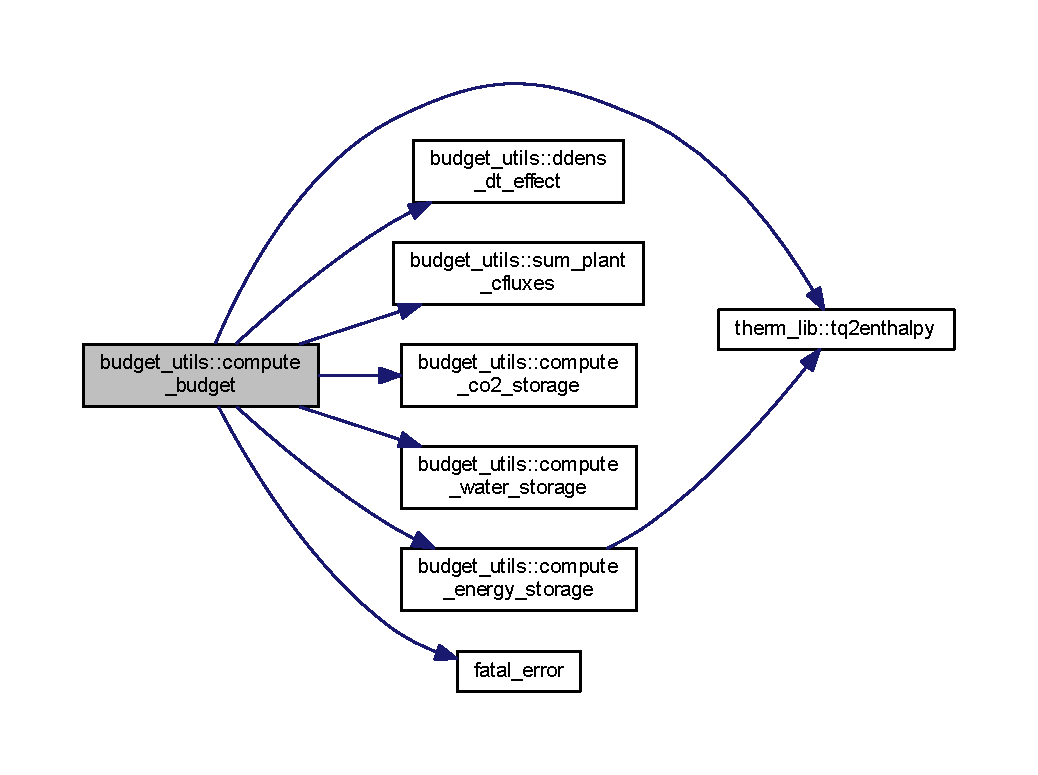
\includegraphics[width=350pt]{namespacebudget__utils_ade80ff8e17018f7bd86015ee5f20375e_cgraph}
\end{center}
\end{figure}


\index{budget\+\_\+utils@{budget\+\_\+utils}!compute\+\_\+co2\+\_\+storage@{compute\+\_\+co2\+\_\+storage}}
\index{compute\+\_\+co2\+\_\+storage@{compute\+\_\+co2\+\_\+storage}!budget\+\_\+utils@{budget\+\_\+utils}}
\subsubsection[{\texorpdfstring{compute\+\_\+co2\+\_\+storage(csite, ipa)}{compute_co2_storage(csite, ipa)}}]{\setlength{\rightskip}{0pt plus 5cm}real function budget\+\_\+utils\+::compute\+\_\+co2\+\_\+storage (
\begin{DoxyParamCaption}
\item[{type({\bf sitetype}), target}]{csite, }
\item[{integer, intent(in)}]{ipa}
\end{DoxyParamCaption}
)}\hypertarget{namespacebudget__utils_aa1c4f8466010b1673f2914f1bfe9b6ee}{}\label{namespacebudget__utils_aa1c4f8466010b1673f2914f1bfe9b6ee}


Here is the caller graph for this function\+:\nopagebreak
\begin{figure}[H]
\begin{center}
\leavevmode
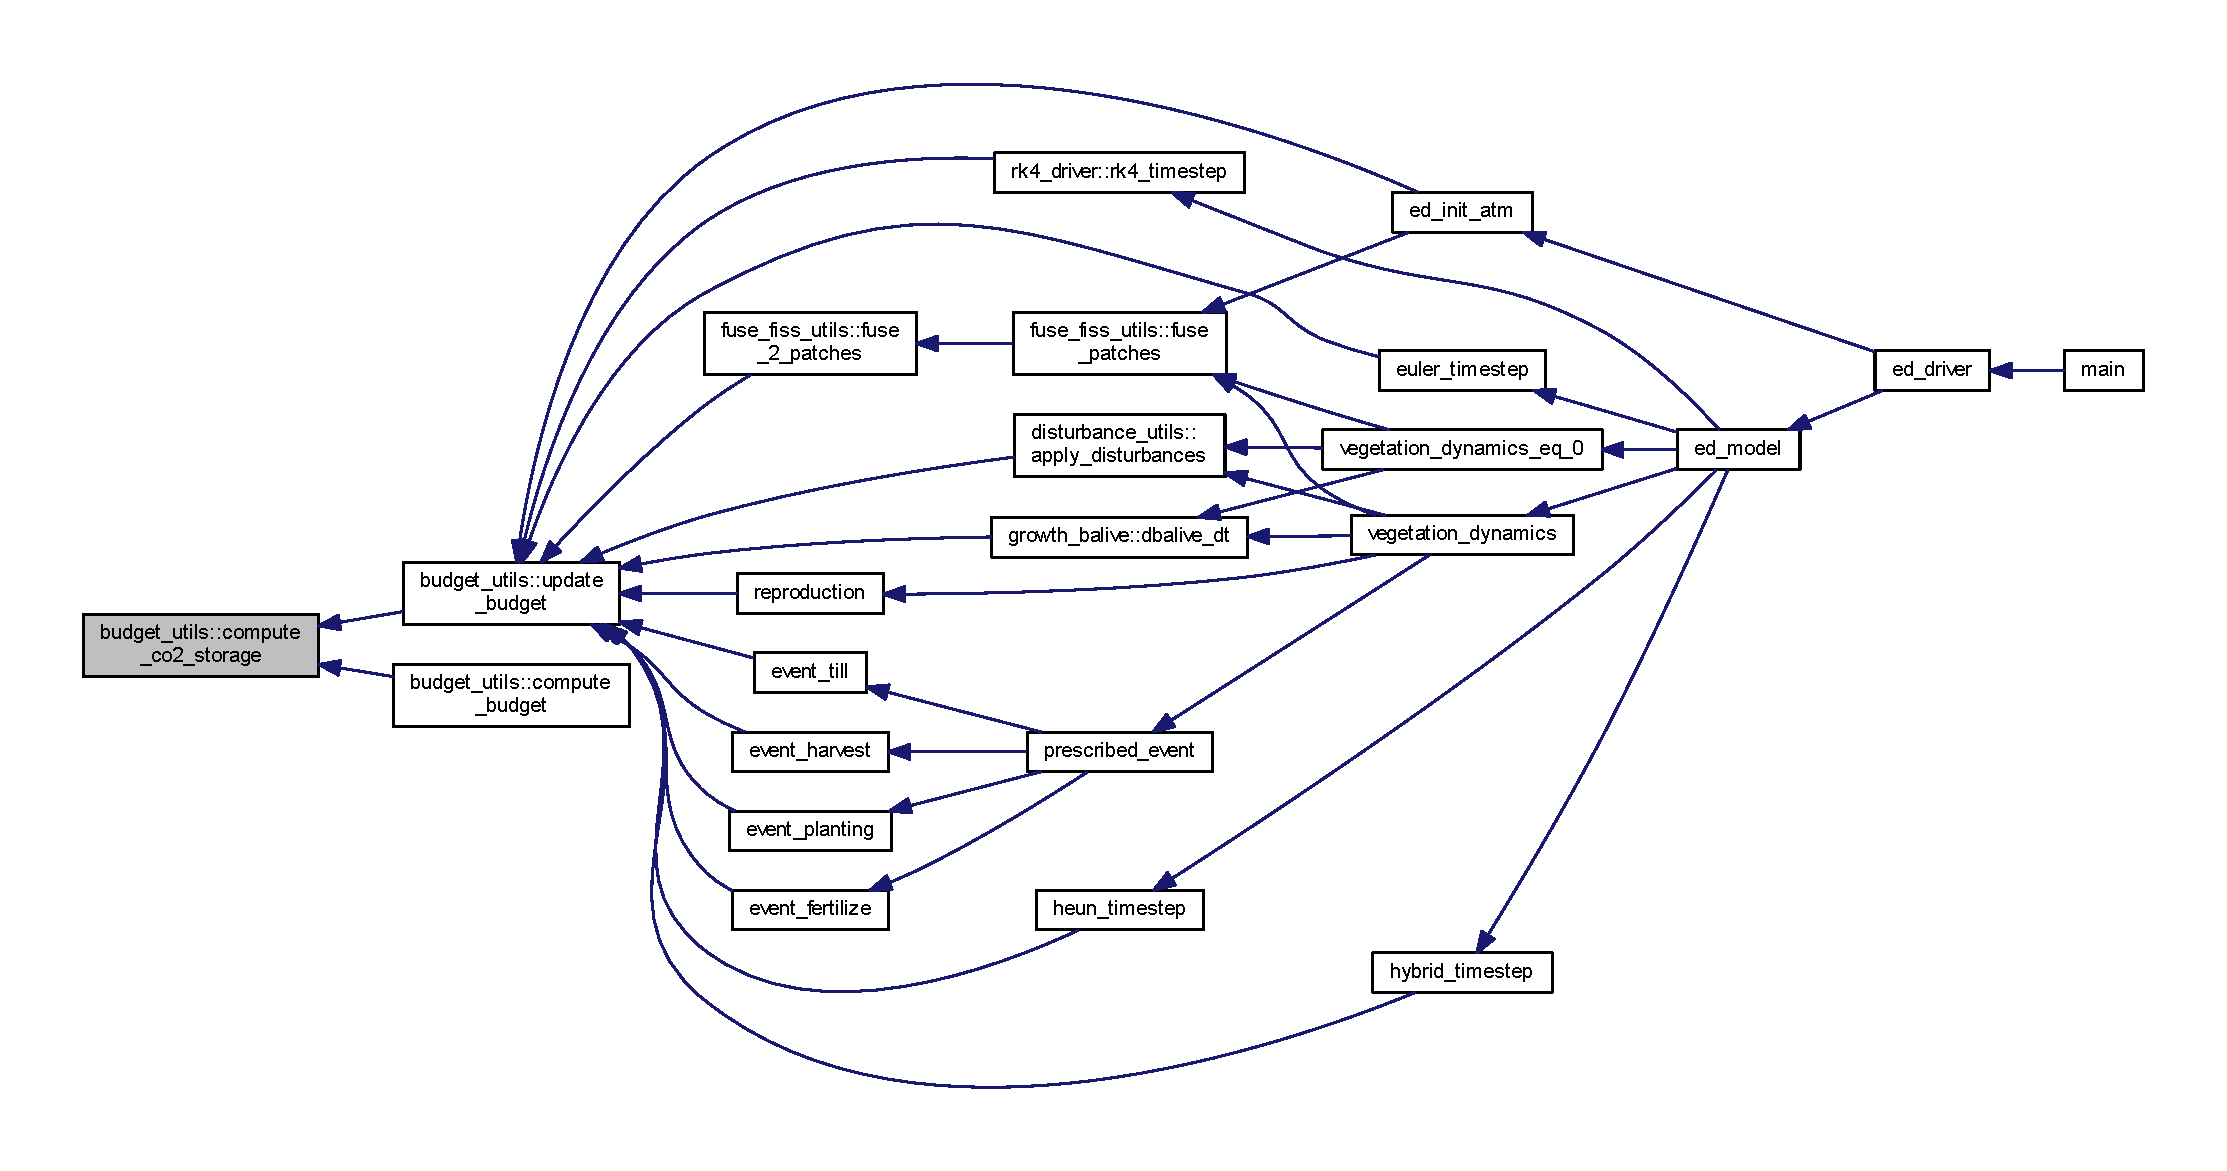
\includegraphics[width=350pt]{namespacebudget__utils_aa1c4f8466010b1673f2914f1bfe9b6ee_icgraph}
\end{center}
\end{figure}


\index{budget\+\_\+utils@{budget\+\_\+utils}!compute\+\_\+energy\+\_\+storage@{compute\+\_\+energy\+\_\+storage}}
\index{compute\+\_\+energy\+\_\+storage@{compute\+\_\+energy\+\_\+storage}!budget\+\_\+utils@{budget\+\_\+utils}}
\subsubsection[{\texorpdfstring{compute\+\_\+energy\+\_\+storage(csite, lsl, ipa)}{compute_energy_storage(csite, lsl, ipa)}}]{\setlength{\rightskip}{0pt plus 5cm}real function budget\+\_\+utils\+::compute\+\_\+energy\+\_\+storage (
\begin{DoxyParamCaption}
\item[{type({\bf sitetype}), target}]{csite, }
\item[{integer, intent(in)}]{lsl, }
\item[{integer, intent(in)}]{ipa}
\end{DoxyParamCaption}
)}\hypertarget{namespacebudget__utils_a319c5f7252c344bcebbd162593e25ec8}{}\label{namespacebudget__utils_a319c5f7252c344bcebbd162593e25ec8}


Here is the call graph for this function\+:\nopagebreak
\begin{figure}[H]
\begin{center}
\leavevmode
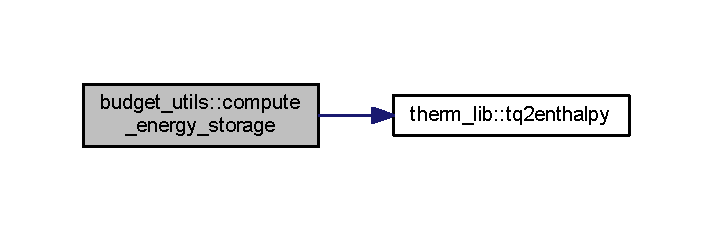
\includegraphics[width=342pt]{namespacebudget__utils_a319c5f7252c344bcebbd162593e25ec8_cgraph}
\end{center}
\end{figure}




Here is the caller graph for this function\+:\nopagebreak
\begin{figure}[H]
\begin{center}
\leavevmode
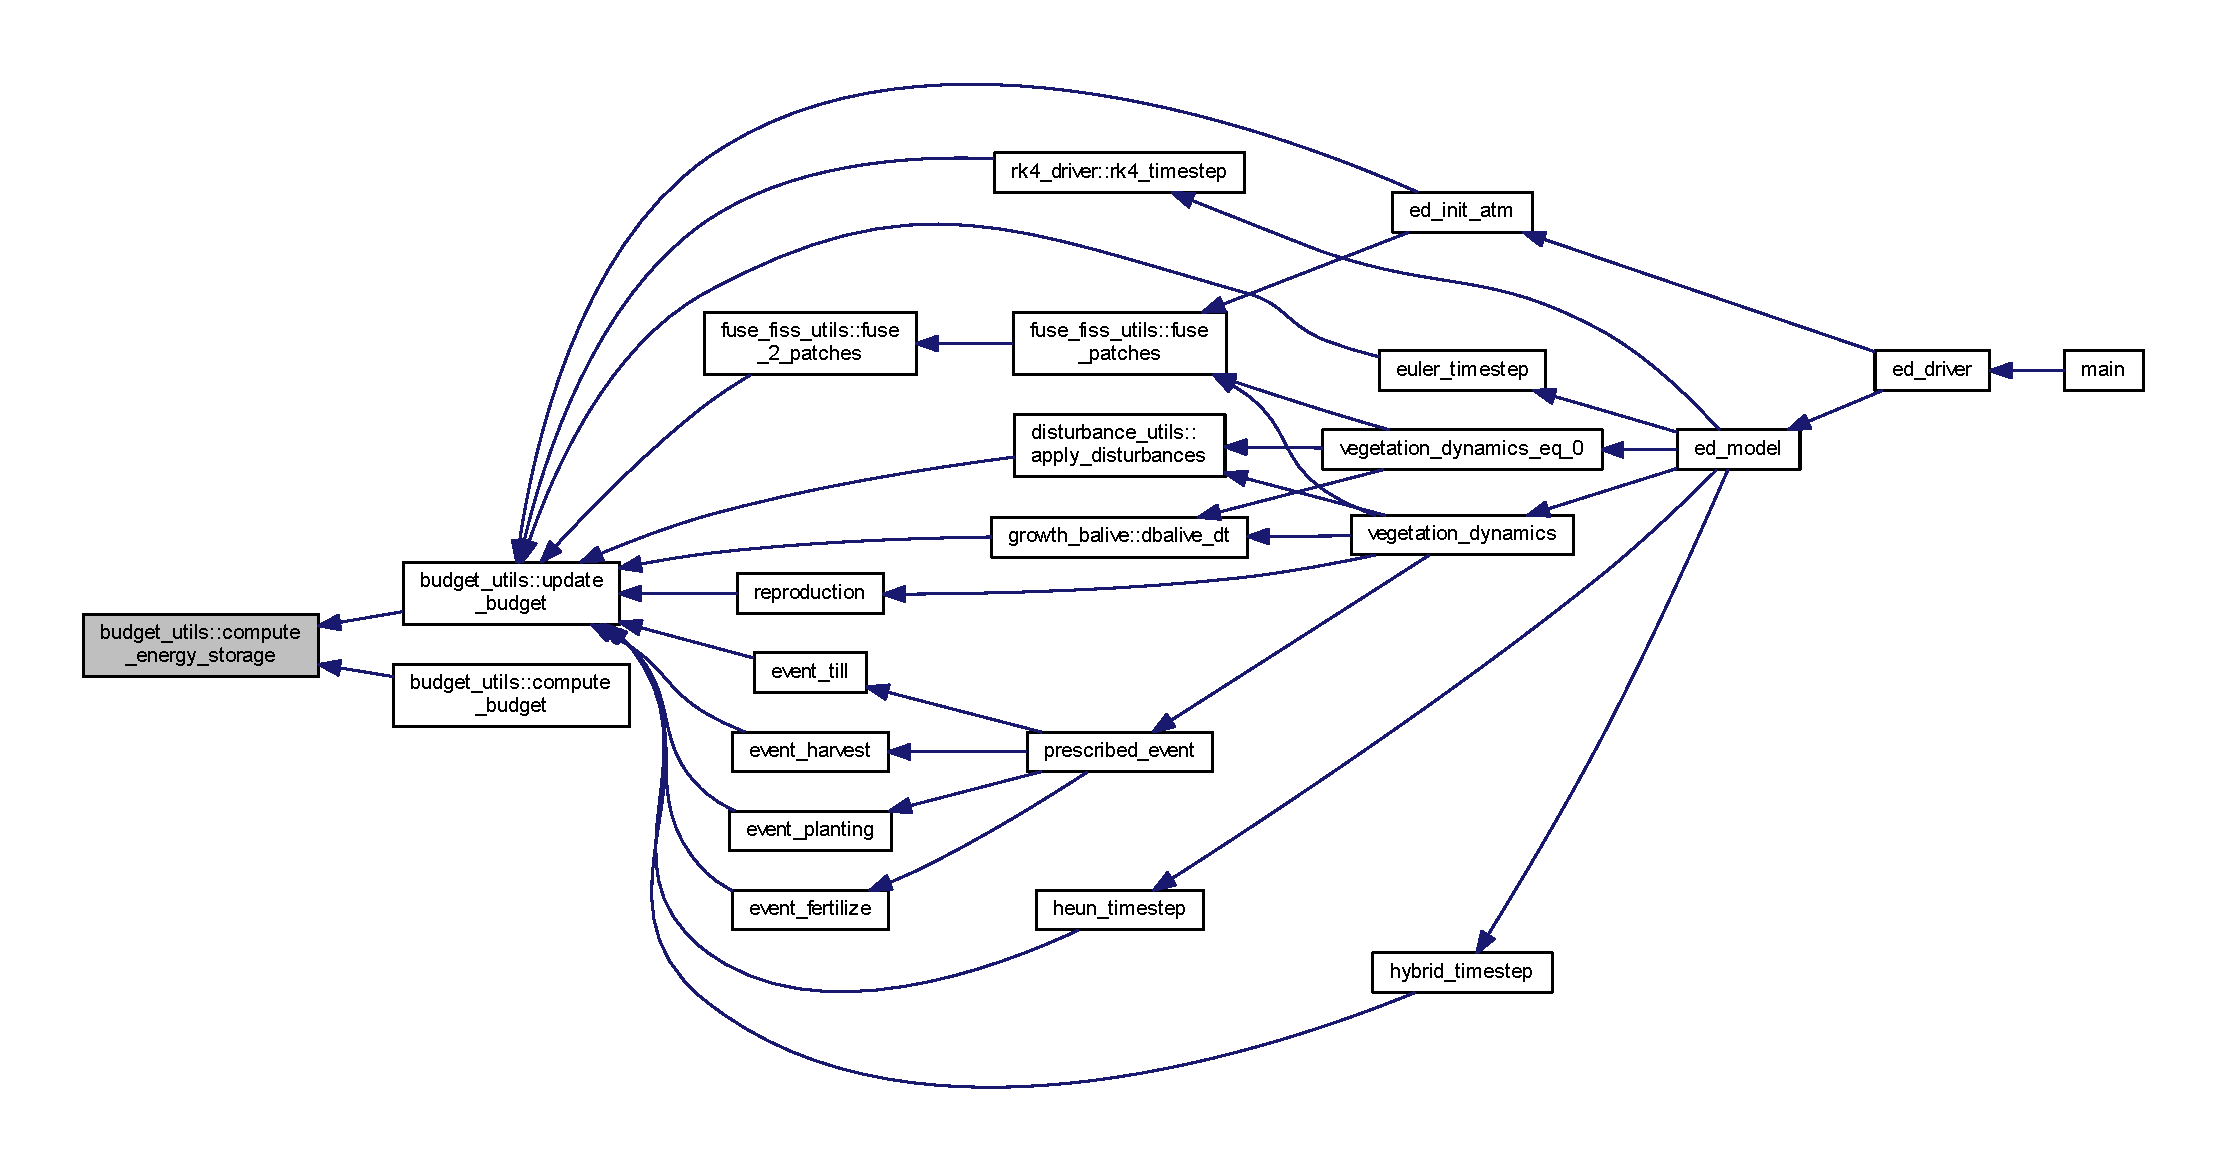
\includegraphics[width=350pt]{namespacebudget__utils_a319c5f7252c344bcebbd162593e25ec8_icgraph}
\end{center}
\end{figure}


\index{budget\+\_\+utils@{budget\+\_\+utils}!compute\+\_\+netrad@{compute\+\_\+netrad}}
\index{compute\+\_\+netrad@{compute\+\_\+netrad}!budget\+\_\+utils@{budget\+\_\+utils}}
\subsubsection[{\texorpdfstring{compute\+\_\+netrad(csite, ipa)}{compute_netrad(csite, ipa)}}]{\setlength{\rightskip}{0pt plus 5cm}real function budget\+\_\+utils\+::compute\+\_\+netrad (
\begin{DoxyParamCaption}
\item[{type({\bf sitetype}), target}]{csite, }
\item[{integer, intent(in)}]{ipa}
\end{DoxyParamCaption}
)}\hypertarget{namespacebudget__utils_a6111a1c211ecef562368c8635f64af45}{}\label{namespacebudget__utils_a6111a1c211ecef562368c8635f64af45}


Here is the caller graph for this function\+:\nopagebreak
\begin{figure}[H]
\begin{center}
\leavevmode
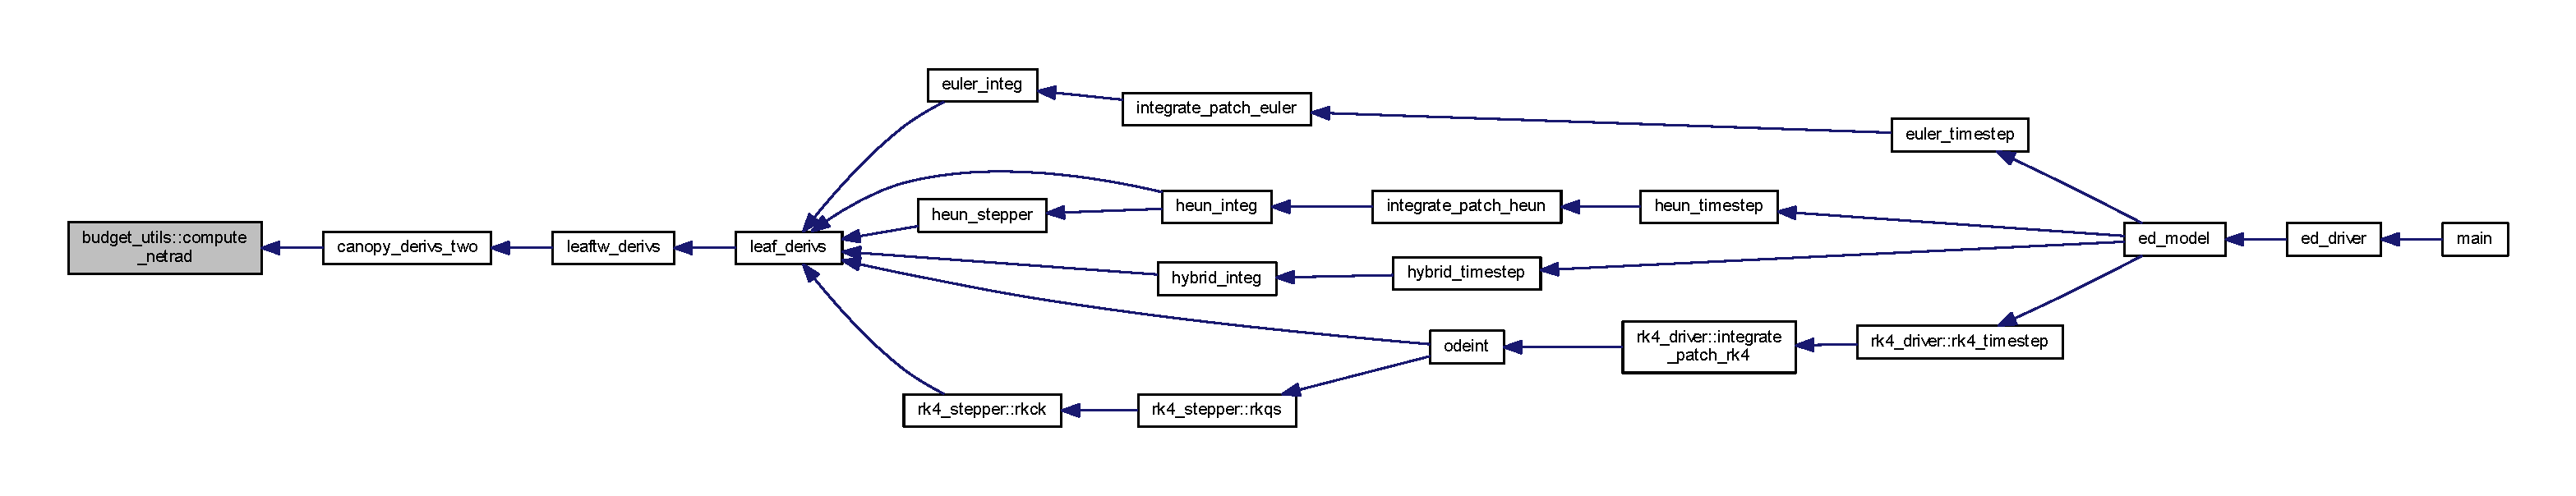
\includegraphics[width=350pt]{namespacebudget__utils_a6111a1c211ecef562368c8635f64af45_icgraph}
\end{center}
\end{figure}


\index{budget\+\_\+utils@{budget\+\_\+utils}!compute\+\_\+water\+\_\+storage@{compute\+\_\+water\+\_\+storage}}
\index{compute\+\_\+water\+\_\+storage@{compute\+\_\+water\+\_\+storage}!budget\+\_\+utils@{budget\+\_\+utils}}
\subsubsection[{\texorpdfstring{compute\+\_\+water\+\_\+storage(csite, lsl, ipa)}{compute_water_storage(csite, lsl, ipa)}}]{\setlength{\rightskip}{0pt plus 5cm}real function budget\+\_\+utils\+::compute\+\_\+water\+\_\+storage (
\begin{DoxyParamCaption}
\item[{type({\bf sitetype}), target}]{csite, }
\item[{integer, intent(in)}]{lsl, }
\item[{integer, intent(in)}]{ipa}
\end{DoxyParamCaption}
)}\hypertarget{namespacebudget__utils_ad0c764047c557100b3a3cdcd836103a0}{}\label{namespacebudget__utils_ad0c764047c557100b3a3cdcd836103a0}


Here is the caller graph for this function\+:\nopagebreak
\begin{figure}[H]
\begin{center}
\leavevmode
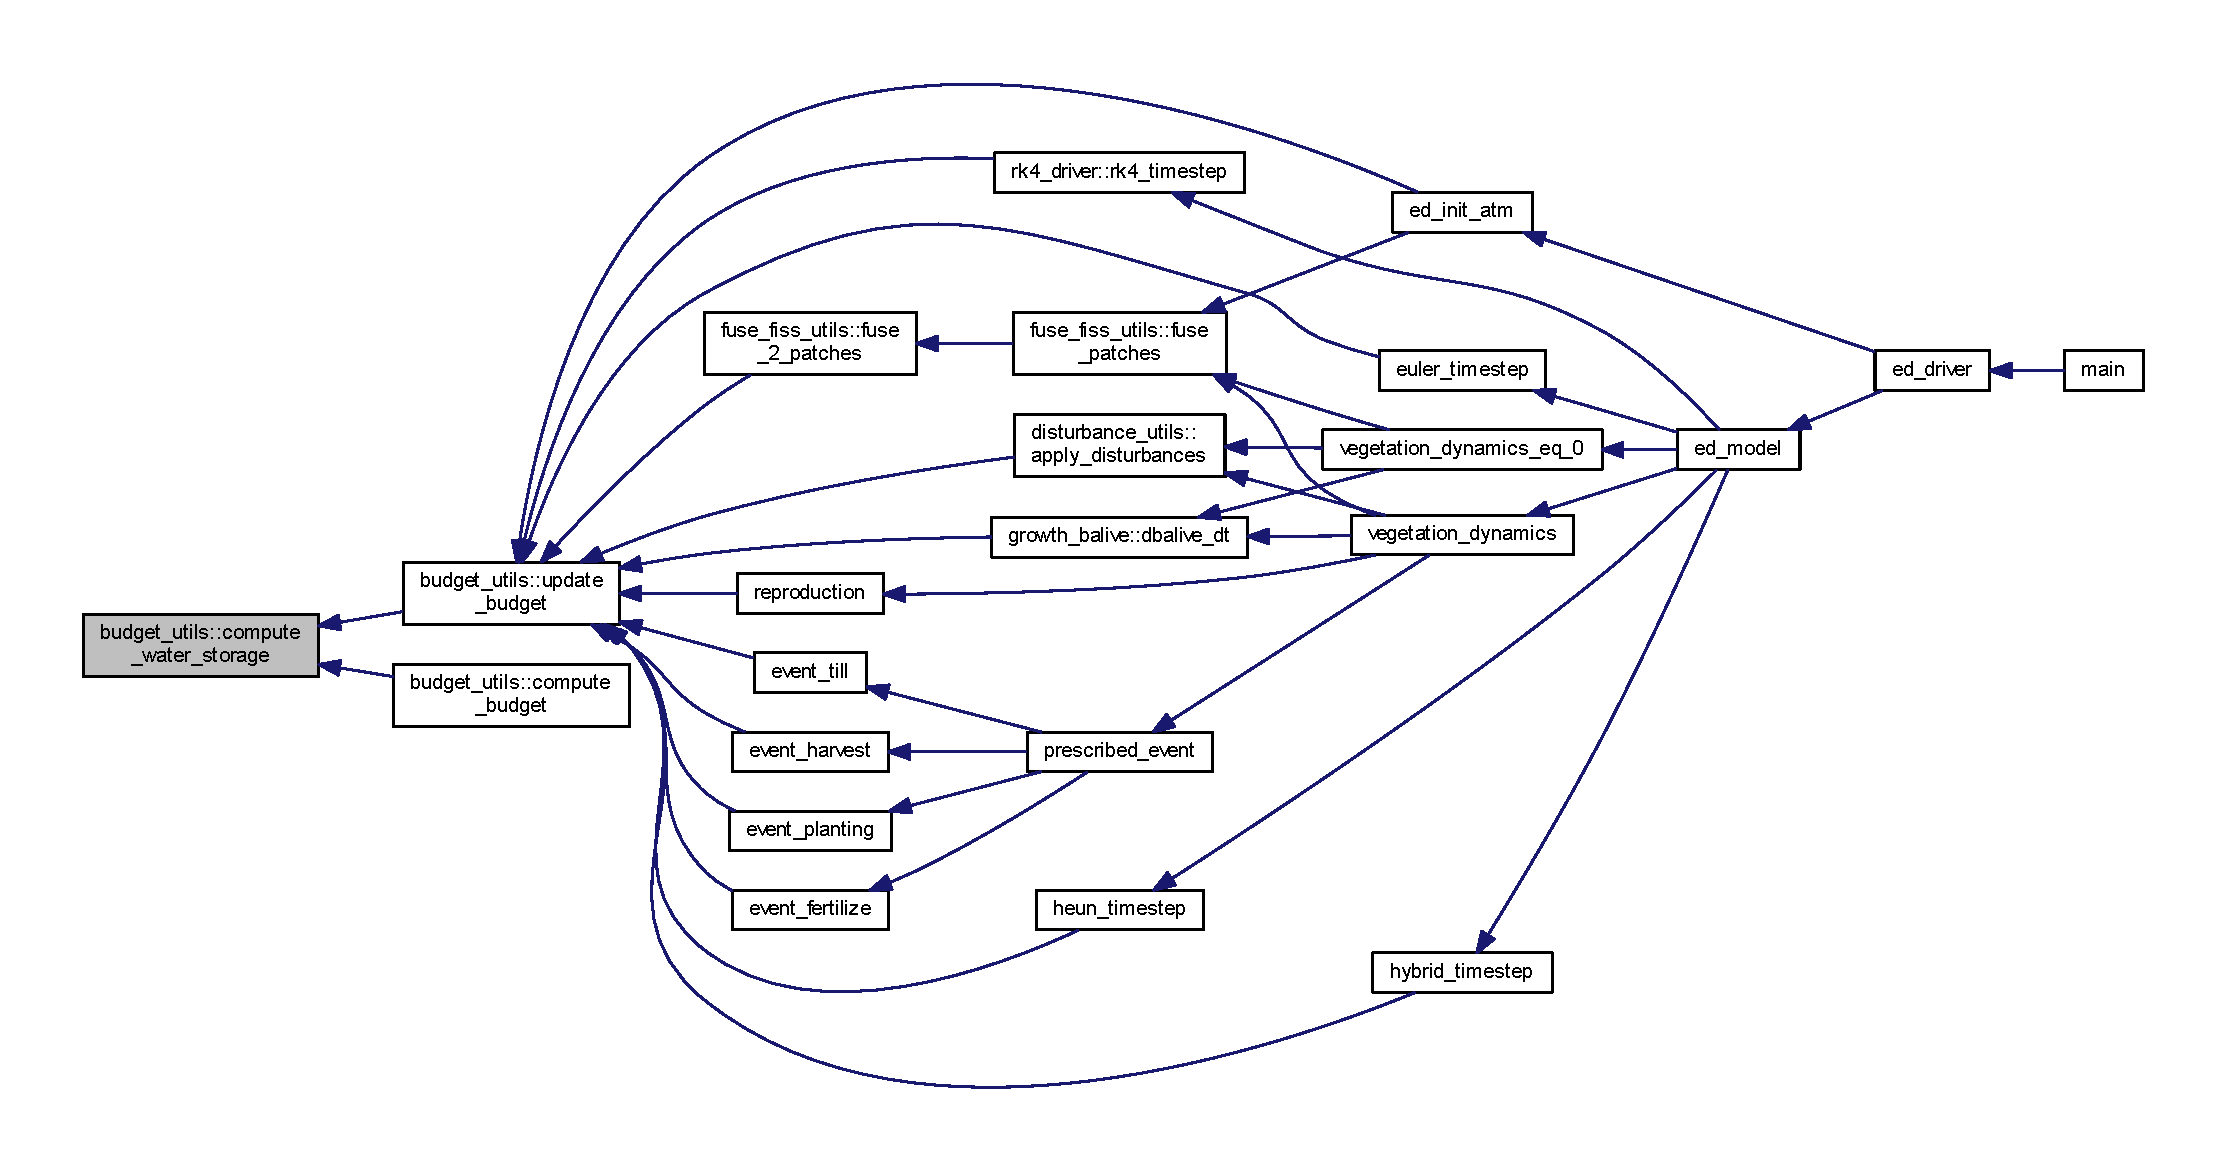
\includegraphics[width=350pt]{namespacebudget__utils_ad0c764047c557100b3a3cdcd836103a0_icgraph}
\end{center}
\end{figure}


\index{budget\+\_\+utils@{budget\+\_\+utils}!ddens\+\_\+dt\+\_\+effect@{ddens\+\_\+dt\+\_\+effect}}
\index{ddens\+\_\+dt\+\_\+effect@{ddens\+\_\+dt\+\_\+effect}!budget\+\_\+utils@{budget\+\_\+utils}}
\subsubsection[{\texorpdfstring{ddens\+\_\+dt\+\_\+effect(old\+\_\+rhos, new\+\_\+rhos, old\+\_\+prop, new\+\_\+prop, can\+\_\+depth, multi)}{ddens_dt_effect(old_rhos, new_rhos, old_prop, new_prop, can_depth, multi)}}]{\setlength{\rightskip}{0pt plus 5cm}real function budget\+\_\+utils\+::ddens\+\_\+dt\+\_\+effect (
\begin{DoxyParamCaption}
\item[{real, intent(in)}]{old\+\_\+rhos, }
\item[{real, intent(in)}]{new\+\_\+rhos, }
\item[{real, intent(in)}]{old\+\_\+prop, }
\item[{real, intent(in)}]{new\+\_\+prop, }
\item[{real, intent(in)}]{can\+\_\+depth, }
\item[{real, intent(in)}]{multi}
\end{DoxyParamCaption}
)}\hypertarget{namespacebudget__utils_ae7ad8d90c28490b0b1c920e7a2656345}{}\label{namespacebudget__utils_ae7ad8d90c28490b0b1c920e7a2656345}


Here is the caller graph for this function\+:\nopagebreak
\begin{figure}[H]
\begin{center}
\leavevmode
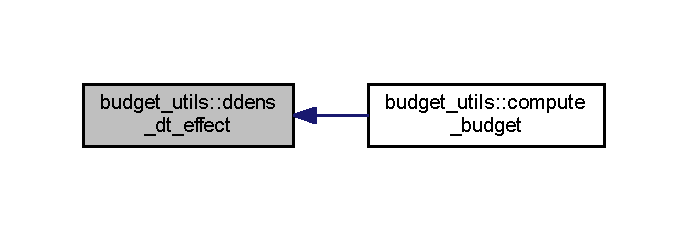
\includegraphics[width=330pt]{namespacebudget__utils_ae7ad8d90c28490b0b1c920e7a2656345_icgraph}
\end{center}
\end{figure}


\index{budget\+\_\+utils@{budget\+\_\+utils}!sum\+\_\+plant\+\_\+cfluxes@{sum\+\_\+plant\+\_\+cfluxes}}
\index{sum\+\_\+plant\+\_\+cfluxes@{sum\+\_\+plant\+\_\+cfluxes}!budget\+\_\+utils@{budget\+\_\+utils}}
\subsubsection[{\texorpdfstring{sum\+\_\+plant\+\_\+cfluxes(csite, ipa, gpp, leaf\+\_\+resp, root\+\_\+resp, leaf\+\_\+growth\+\_\+resp                                                                                                                                               ,root\+\_\+growth\+\_\+resp, sapa\+\_\+growth\+\_\+resp, sapb\+\_\+growth\+\_\+resp                                                                                                                                                       ,leaf\+\_\+storage\+\_\+resp, root\+\_\+storage\+\_\+resp, sapa\+\_\+storage\+\_\+resp                                                                                                                                           ,sapb\+\_\+storage\+\_\+resp)}{sum_plant_cfluxes(csite, ipa, gpp, leaf_resp, root_resp, leaf_growth_resp                                                                                                                                               ,root_growth_resp, sapa_growth_resp, sapb_growth_resp                                                                                                                                                       ,leaf_storage_resp, root_storage_resp, sapa_storage_resp                                                                                                                                           ,sapb_storage_resp)}}]{\setlength{\rightskip}{0pt plus 5cm}subroutine budget\+\_\+utils\+::sum\+\_\+plant\+\_\+cfluxes (
\begin{DoxyParamCaption}
\item[{type({\bf sitetype}), target}]{csite, }
\item[{integer, intent(in)}]{ipa, }
\item[{real, intent(out)}]{gpp, }
\item[{real, intent(out)}]{leaf\+\_\+resp, }
\item[{real, intent(out)}]{root\+\_\+resp, }
\item[{real, intent(out)}]{leaf\+\_\+growth\+\_\+resp, }
\item[{real, intent(out)}]{root\+\_\+growth\+\_\+resp, }
\item[{real, intent(out)}]{sapa\+\_\+growth\+\_\+resp, }
\item[{real, intent(out)}]{sapb\+\_\+growth\+\_\+resp, }
\item[{real, intent(out)}]{leaf\+\_\+storage\+\_\+resp, }
\item[{real, intent(out)}]{root\+\_\+storage\+\_\+resp, }
\item[{real, intent(out)}]{sapa\+\_\+storage\+\_\+resp, }
\item[{real, intent(out)}]{sapb\+\_\+storage\+\_\+resp}
\end{DoxyParamCaption}
)}\hypertarget{namespacebudget__utils_a117874382f22a7cb0883681d23606828}{}\label{namespacebudget__utils_a117874382f22a7cb0883681d23606828}


Here is the caller graph for this function\+:\nopagebreak
\begin{figure}[H]
\begin{center}
\leavevmode
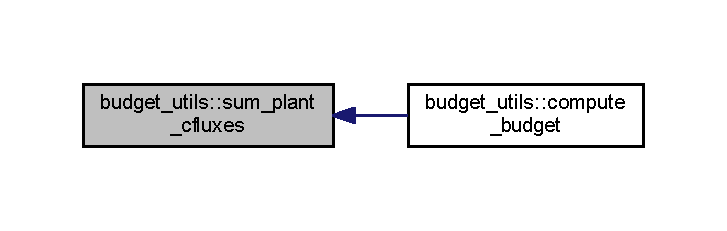
\includegraphics[width=349pt]{namespacebudget__utils_a117874382f22a7cb0883681d23606828_icgraph}
\end{center}
\end{figure}


\index{budget\+\_\+utils@{budget\+\_\+utils}!update\+\_\+budget@{update\+\_\+budget}}
\index{update\+\_\+budget@{update\+\_\+budget}!budget\+\_\+utils@{budget\+\_\+utils}}
\subsubsection[{\texorpdfstring{update\+\_\+budget(csite, lsl, ipaa, ipaz)}{update_budget(csite, lsl, ipaa, ipaz)}}]{\setlength{\rightskip}{0pt plus 5cm}subroutine budget\+\_\+utils\+::update\+\_\+budget (
\begin{DoxyParamCaption}
\item[{type({\bf sitetype}), target}]{csite, }
\item[{integer, intent(in)}]{lsl, }
\item[{integer, intent(in)}]{ipaa, }
\item[{integer, intent(in)}]{ipaz}
\end{DoxyParamCaption}
)}\hypertarget{namespacebudget__utils_ad8835ee763cd964432b44e0a3d00e3da}{}\label{namespacebudget__utils_ad8835ee763cd964432b44e0a3d00e3da}


Here is the call graph for this function\+:\nopagebreak
\begin{figure}[H]
\begin{center}
\leavevmode
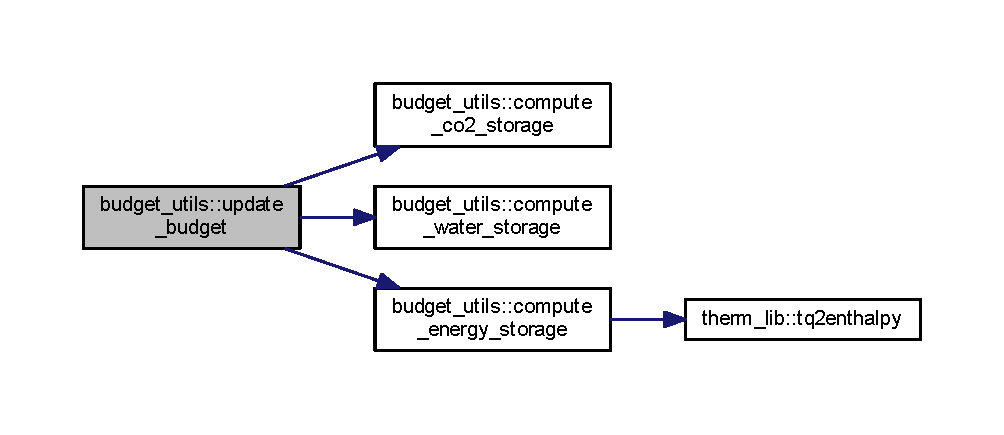
\includegraphics[width=350pt]{namespacebudget__utils_ad8835ee763cd964432b44e0a3d00e3da_cgraph}
\end{center}
\end{figure}




Here is the caller graph for this function\+:\nopagebreak
\begin{figure}[H]
\begin{center}
\leavevmode
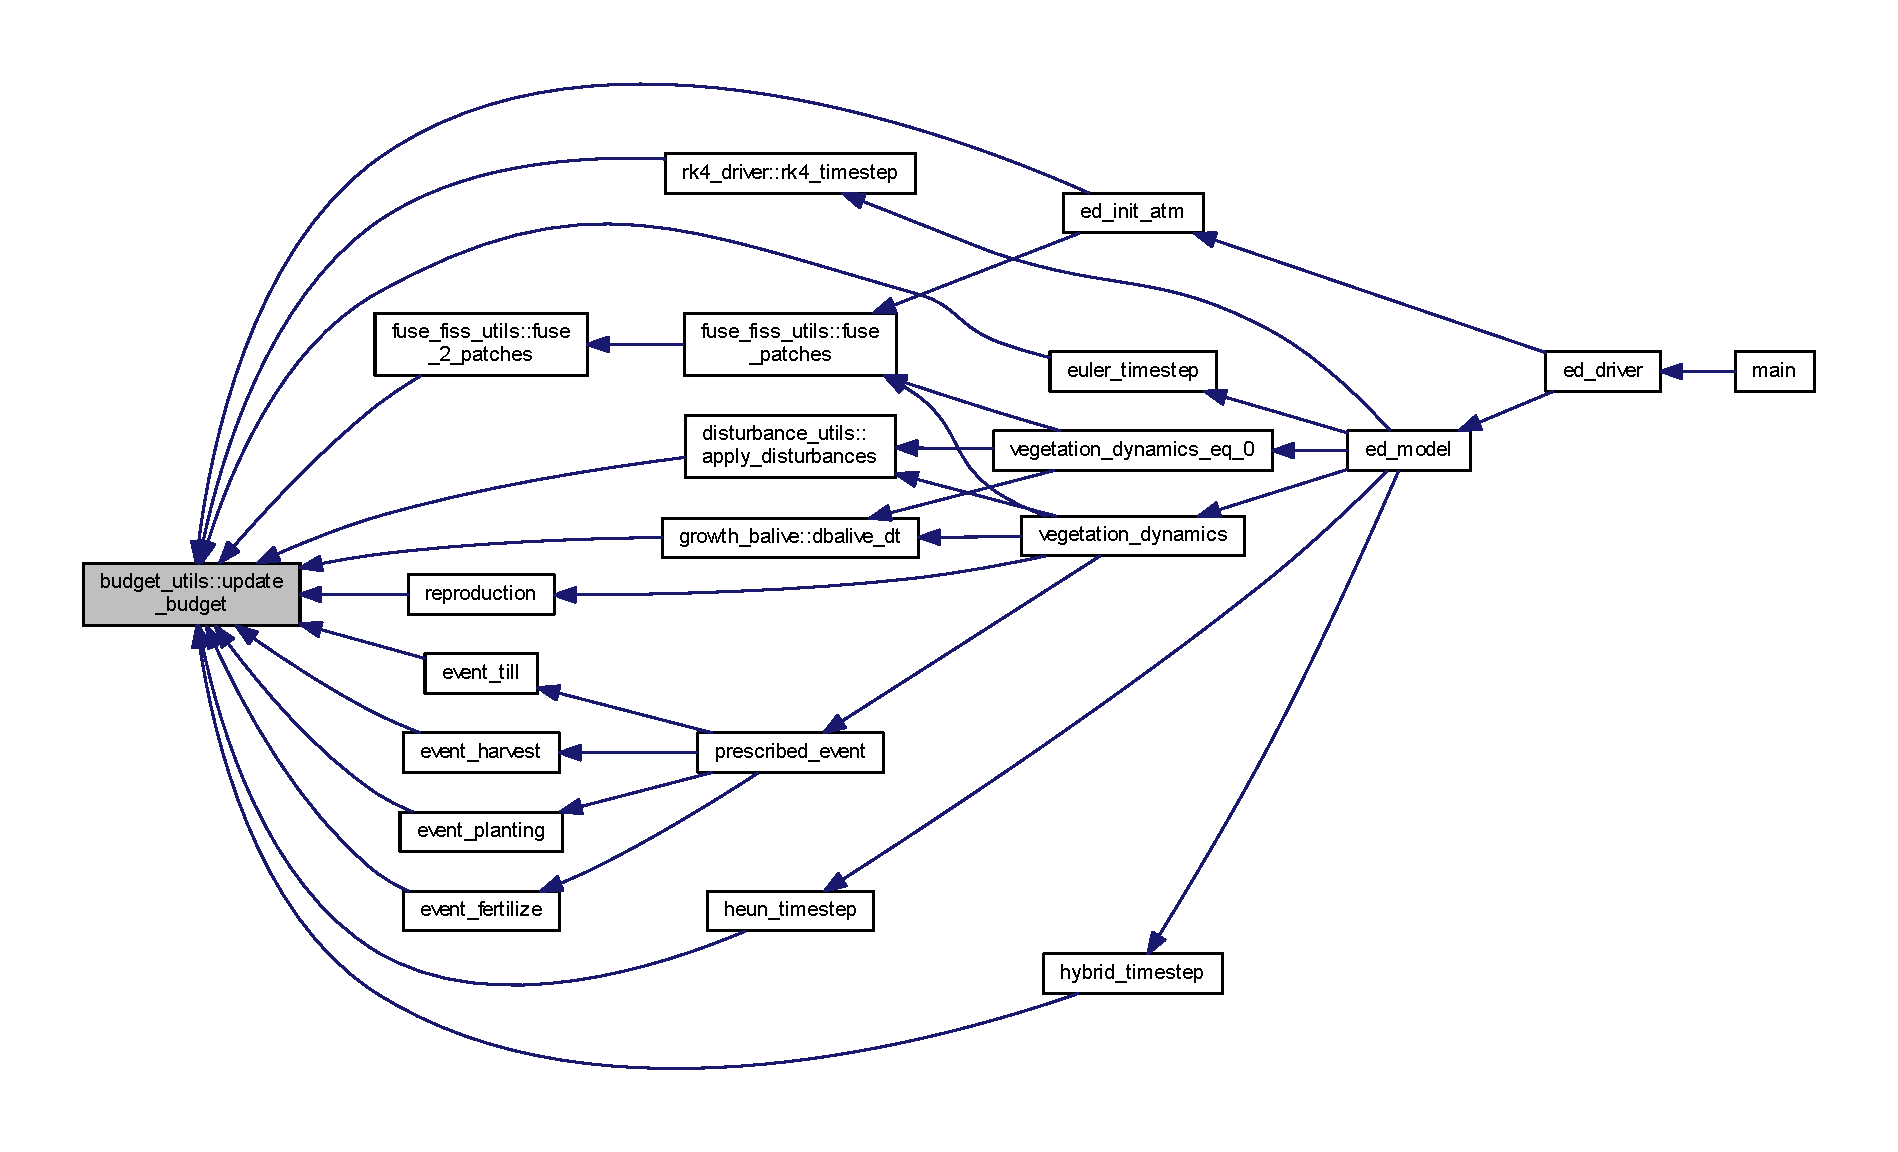
\includegraphics[width=350pt]{namespacebudget__utils_ad8835ee763cd964432b44e0a3d00e3da_icgraph}
\end{center}
\end{figure}



\hypertarget{namespacec34constants}{}\section{c34constants Module Reference}
\label{namespacec34constants}\index{c34constants@{c34constants}}
\subsection*{Data Types}
\begin{DoxyCompactItemize}
\item 
type \hyperlink{structc34constants_1_1carb__demand__vars}{carb\+\_\+demand\+\_\+vars}
\item 
type \hyperlink{structc34constants_1_1farq__consts}{farq\+\_\+consts}
\item 
type \hyperlink{structc34constants_1_1metinp__vars}{metinp\+\_\+vars}
\item 
type \hyperlink{structc34constants_1_1solution__vars}{solution\+\_\+vars}
\end{DoxyCompactItemize}
\subsection*{Functions/\+Subroutines}
\begin{DoxyCompactItemize}
\item 
subroutine \hyperlink{namespacec34constants_a2bf287654403f231d7936113aaeb9cf6}{copy\+\_\+solution} (source\+\_\+sol, target\+\_\+sol)
\end{DoxyCompactItemize}
\subsection*{Variables}
\begin{DoxyCompactItemize}
\item 
type(\hyperlink{structc34constants_1_1farq__consts}{farq\+\_\+consts}), dimension(\+:), pointer \hyperlink{namespacec34constants_a4a1314df0becf145f8a2365aa27d992d}{thispft}
\item 
type(\hyperlink{structc34constants_1_1metinp__vars}{metinp\+\_\+vars}), dimension(\+:), pointer \hyperlink{namespacec34constants_a6d1c98b7c360f24d485be8fc38bdd284}{met}
\item 
type(\hyperlink{structc34constants_1_1carb__demand__vars}{carb\+\_\+demand\+\_\+vars}), dimension(\+:), pointer \hyperlink{namespacec34constants_a844bf4288f019d9dcee7612f54d1e50c}{aparms}
\item 
type(\hyperlink{structc34constants_1_1solution__vars}{solution\+\_\+vars}), dimension(\+:), pointer \hyperlink{namespacec34constants_a5affd928720d3a40f01f1198b68b7fb3}{stopen}
\item 
type(\hyperlink{structc34constants_1_1solution__vars}{solution\+\_\+vars}), dimension(\+:), pointer \hyperlink{namespacec34constants_a083891d928147a7252ada72b49b240a3}{stclosed}
\item 
type(\hyperlink{structc34constants_1_1solution__vars}{solution\+\_\+vars}), dimension(\+:), pointer \hyperlink{namespacec34constants_a54cb2e4894b639d22e50b457b4208cfc}{rubiscolim}
\item 
type(\hyperlink{structc34constants_1_1solution__vars}{solution\+\_\+vars}), dimension(\+:), pointer \hyperlink{namespacec34constants_abed7f7ff7745473ac53005a45206f506}{co2lim}
\item 
type(\hyperlink{structc34constants_1_1solution__vars}{solution\+\_\+vars}), dimension(\+:), pointer \hyperlink{namespacec34constants_af66eea644957075da5a5285e735e143b}{lightlim}
\end{DoxyCompactItemize}


\subsection{Function/\+Subroutine Documentation}
\index{c34constants@{c34constants}!copy\+\_\+solution@{copy\+\_\+solution}}
\index{copy\+\_\+solution@{copy\+\_\+solution}!c34constants@{c34constants}}
\subsubsection[{\texorpdfstring{copy\+\_\+solution(source\+\_\+sol, target\+\_\+sol)}{copy_solution(source_sol, target_sol)}}]{\setlength{\rightskip}{0pt plus 5cm}subroutine c34constants\+::copy\+\_\+solution (
\begin{DoxyParamCaption}
\item[{type({\bf solution\+\_\+vars}), intent(in)}]{source\+\_\+sol, }
\item[{type({\bf solution\+\_\+vars}), intent(out)}]{target\+\_\+sol}
\end{DoxyParamCaption}
)}\hypertarget{namespacec34constants_a2bf287654403f231d7936113aaeb9cf6}{}\label{namespacec34constants_a2bf287654403f231d7936113aaeb9cf6}


\subsection{Variable Documentation}
\index{c34constants@{c34constants}!aparms@{aparms}}
\index{aparms@{aparms}!c34constants@{c34constants}}
\subsubsection[{\texorpdfstring{aparms}{aparms}}]{\setlength{\rightskip}{0pt plus 5cm}type({\bf carb\+\_\+demand\+\_\+vars}), dimension(\+:), pointer c34constants\+::aparms}\hypertarget{namespacec34constants_a844bf4288f019d9dcee7612f54d1e50c}{}\label{namespacec34constants_a844bf4288f019d9dcee7612f54d1e50c}
\index{c34constants@{c34constants}!co2lim@{co2lim}}
\index{co2lim@{co2lim}!c34constants@{c34constants}}
\subsubsection[{\texorpdfstring{co2lim}{co2lim}}]{\setlength{\rightskip}{0pt plus 5cm}type({\bf solution\+\_\+vars}), dimension(\+:), pointer c34constants\+::co2lim}\hypertarget{namespacec34constants_abed7f7ff7745473ac53005a45206f506}{}\label{namespacec34constants_abed7f7ff7745473ac53005a45206f506}
\index{c34constants@{c34constants}!lightlim@{lightlim}}
\index{lightlim@{lightlim}!c34constants@{c34constants}}
\subsubsection[{\texorpdfstring{lightlim}{lightlim}}]{\setlength{\rightskip}{0pt plus 5cm}type({\bf solution\+\_\+vars}), dimension(\+:), pointer c34constants\+::lightlim}\hypertarget{namespacec34constants_af66eea644957075da5a5285e735e143b}{}\label{namespacec34constants_af66eea644957075da5a5285e735e143b}
\index{c34constants@{c34constants}!met@{met}}
\index{met@{met}!c34constants@{c34constants}}
\subsubsection[{\texorpdfstring{met}{met}}]{\setlength{\rightskip}{0pt plus 5cm}type({\bf metinp\+\_\+vars} ), dimension(\+:), pointer c34constants\+::met}\hypertarget{namespacec34constants_a6d1c98b7c360f24d485be8fc38bdd284}{}\label{namespacec34constants_a6d1c98b7c360f24d485be8fc38bdd284}
\index{c34constants@{c34constants}!rubiscolim@{rubiscolim}}
\index{rubiscolim@{rubiscolim}!c34constants@{c34constants}}
\subsubsection[{\texorpdfstring{rubiscolim}{rubiscolim}}]{\setlength{\rightskip}{0pt plus 5cm}type({\bf solution\+\_\+vars}), dimension(\+:), pointer c34constants\+::rubiscolim}\hypertarget{namespacec34constants_a54cb2e4894b639d22e50b457b4208cfc}{}\label{namespacec34constants_a54cb2e4894b639d22e50b457b4208cfc}
\index{c34constants@{c34constants}!stclosed@{stclosed}}
\index{stclosed@{stclosed}!c34constants@{c34constants}}
\subsubsection[{\texorpdfstring{stclosed}{stclosed}}]{\setlength{\rightskip}{0pt plus 5cm}type({\bf solution\+\_\+vars}), dimension(\+:), pointer c34constants\+::stclosed}\hypertarget{namespacec34constants_a083891d928147a7252ada72b49b240a3}{}\label{namespacec34constants_a083891d928147a7252ada72b49b240a3}
\index{c34constants@{c34constants}!stopen@{stopen}}
\index{stopen@{stopen}!c34constants@{c34constants}}
\subsubsection[{\texorpdfstring{stopen}{stopen}}]{\setlength{\rightskip}{0pt plus 5cm}type({\bf solution\+\_\+vars}), dimension(\+:), pointer c34constants\+::stopen}\hypertarget{namespacec34constants_a5affd928720d3a40f01f1198b68b7fb3}{}\label{namespacec34constants_a5affd928720d3a40f01f1198b68b7fb3}
\index{c34constants@{c34constants}!thispft@{thispft}}
\index{thispft@{thispft}!c34constants@{c34constants}}
\subsubsection[{\texorpdfstring{thispft}{thispft}}]{\setlength{\rightskip}{0pt plus 5cm}type({\bf farq\+\_\+consts} ), dimension(\+:), pointer c34constants\+::thispft}\hypertarget{namespacec34constants_a4a1314df0becf145f8a2365aa27d992d}{}\label{namespacec34constants_a4a1314df0becf145f8a2365aa27d992d}

\hypertarget{namespacecanopy__air__coms}{}\section{canopy\+\_\+air\+\_\+coms Module Reference}
\label{namespacecanopy__air__coms}\index{canopy\+\_\+air\+\_\+coms@{canopy\+\_\+air\+\_\+coms}}
\subsection*{Functions/\+Subroutines}
\begin{DoxyCompactItemize}
\item 
real function \hyperlink{namespacecanopy__air__coms_ab103fa081460babbe04c9a5a4699be5f}{psim} (zeta, stable)
\item 
real function \hyperlink{namespacecanopy__air__coms_acedb0f66db4b79009a69e87c5fd3ed71}{psih} (zeta, stable)
\item 
real(kind=8) function \hyperlink{namespacecanopy__air__coms_aba7cbe776dbfa9815870ad3686949041}{psim8} (zeta, stable)
\item 
real(kind=8) function \hyperlink{namespacecanopy__air__coms_aef33f0eeea82151a8edb6dc38c4cc921}{psih8} (zeta, stable)
\item 
real function \hyperlink{namespacecanopy__air__coms_af8bc6f1d6999a4b614461cecb85c9b1b}{dpsimdzeta} (zeta, stable)
\item 
real function \hyperlink{namespacecanopy__air__coms_a64552e0380fcb36366b5eb0f624241a3}{dpsihdzeta} (zeta, stable)
\item 
real(kind=8) function \hyperlink{namespacecanopy__air__coms_a51b006ac118f9549aee23ddb61a1bf19}{dpsimdzeta8} (zeta, stable)
\item 
real(kind=8) function \hyperlink{namespacecanopy__air__coms_aa5f9649efc40a05ddc13e1450f30fad3}{dpsihdzeta8} (zeta, stable)
\item 
real function \hyperlink{namespacecanopy__air__coms_a6062471b3381c283205ea8b27383a5e0}{zoobukhov} (rib, zstar, rough, zoz0m, lnzoz0m, zoz0h, lnzoz0h, stable)
\item 
real(kind=8) function \hyperlink{namespacecanopy__air__coms_afef697305b4b30385c5206f48d9e787c}{zoobukhov8} (rib, zstar, rough, zoz0m, lnzoz0m, zoz0h, lnzoz0h, stable)
\item 
real function \hyperlink{namespacecanopy__air__coms_a5251266695c581c8f4058d98f6c86200}{zoobukhov\+\_\+ustar} (rib, zstar, rough, zoz0h, lnzoz0h, kuoustar, stable)
\item 
real(kind=8) function \hyperlink{namespacecanopy__air__coms_a6ef582f46fded1355973730e6a2289f2}{zoobukhov\+\_\+ustar8} (rib, zstar, rough, zoz0h, lnzoz0h, kuoustar, stable)
\end{DoxyCompactItemize}
\subsection*{Variables}
\begin{DoxyCompactItemize}
\item 
integer \hyperlink{namespacecanopy__air__coms_ad7c5174d5bc6bd090e9afff63a3428b4}{icanturb}
\item 
integer \hyperlink{namespacecanopy__air__coms_a25351371b3a5e30c3cabd058d1153399}{isfclyrm}
\item 
integer \hyperlink{namespacecanopy__air__coms_a1c11559607f1960e926e0e2adebdba1b}{ied\+\_\+grndvap}
\item 
real \hyperlink{namespacecanopy__air__coms_aaaf296c47691fcf3aaab5b8929b37368}{leaf\+\_\+maxwhc}
\item 
real \hyperlink{namespacecanopy__air__coms_ac8fd39daadba6dc58037eaf42f48700e}{ubmin}
\item 
real \hyperlink{namespacecanopy__air__coms_a593e8ef887b3317fb55545892af84c50}{ugbmin}
\item 
real \hyperlink{namespacecanopy__air__coms_a9a2322371ed4847814fa98174c092c12}{ustmin}
\item 
real \hyperlink{namespacecanopy__air__coms_abb236f0b21abecb4efde793fd6a1811d}{gamm}
\item 
real \hyperlink{namespacecanopy__air__coms_aec7b65c44519ebe9058cb6c4aa655e8c}{gamh}
\item 
real \hyperlink{namespacecanopy__air__coms_adafee179c1e8ba89437987bc4be9b781}{tprandtl}
\item 
real \hyperlink{namespacecanopy__air__coms_a2ac951854c77e1df16229f0fee8a70a6}{vh2vr}
\item 
real \hyperlink{namespacecanopy__air__coms_ab7f6f46003b1ddabed2345c0ed33372d}{vh2dh}
\item 
real \hyperlink{namespacecanopy__air__coms_a553bcc51d0af126ebd44094dae4cdeac}{ribmax}
\item 
real \hyperlink{namespacecanopy__air__coms_a7ec65e87cc2c74a4f55e05e67272a5c0}{exar}
\item 
real \hyperlink{namespacecanopy__air__coms_a8aa4d4dbd59143c45ab4c52fb326ecd6}{covr}
\item 
real \hyperlink{namespacecanopy__air__coms_a63a4c7242b97f72a903fa4c1213b37f0}{ez}
\item 
real(kind=8) \hyperlink{namespacecanopy__air__coms_ab6719dfbc2c9e8e2f9eddf3bf6f97237}{exar8}
\item 
real(kind=8) \hyperlink{namespacecanopy__air__coms_a4afb828f3fecdf23a54cd6276f714544}{ustmin8}
\item 
real(kind=8) \hyperlink{namespacecanopy__air__coms_a96ad2cd68341db7649720ebd90eab97f}{ugbmin8}
\item 
real(kind=8) \hyperlink{namespacecanopy__air__coms_a436ed31f3d8eafc708115bca8ee30d03}{ubmin8}
\item 
real(kind=8) \hyperlink{namespacecanopy__air__coms_a7899b1f4a3a40f367c48fbaa9b7f2ccd}{ez8}
\item 
real(kind=8) \hyperlink{namespacecanopy__air__coms_a5425e68f350bd521634e2dec3df419cc}{vh2vr8}
\item 
real(kind=8) \hyperlink{namespacecanopy__air__coms_aee89a61c55f84edfb62d0b236dea93c8}{vh2dh8}
\item 
real(kind=8) \hyperlink{namespacecanopy__air__coms_a867a9672f31a44b6def8fc0bdf4eb440}{rasveg\+\_\+min8}
\item 
real(kind=8) \hyperlink{namespacecanopy__air__coms_a3cb44bad4430d800393ec76b7a22a782}{taumin8}
\item 
real(kind=4) \hyperlink{namespacecanopy__air__coms_a768765793f4c4b91a6ccca6d5263ad04}{cdrag0}
\item 
real(kind=4) \hyperlink{namespacecanopy__air__coms_a7b44abfd8d12fe84db70aab86954129c}{cdrag1}
\item 
real(kind=4) \hyperlink{namespacecanopy__air__coms_a1b94794c69c4e42537d77c51167c842f}{cdrag2}
\item 
real(kind=4) \hyperlink{namespacecanopy__air__coms_abaac76316a5a249db322fc990489d388}{cdrag3}
\item 
real(kind=4) \hyperlink{namespacecanopy__air__coms_a11e1c7b747cfb7033e3bf75fe4cdd0bc}{pm0}
\item 
real(kind=4) \hyperlink{namespacecanopy__air__coms_a1f414808e85114a30c83bdf9bbc35af6}{c1\+\_\+m97}
\item 
real(kind=4) \hyperlink{namespacecanopy__air__coms_a47dcf89394a1ea827c110b9ceb601b79}{c2\+\_\+m97}
\item 
real(kind=4) \hyperlink{namespacecanopy__air__coms_a40fc08a843524cc8b4e05ba8766cb930}{c3\+\_\+m97}
\item 
real(kind=4) \hyperlink{namespacecanopy__air__coms_a54402456387b824df174f09157236866}{kvwake}
\item 
real(kind=4) \hyperlink{namespacecanopy__air__coms_ac16bf823a6fc81f0d671fa06ca5de7e7}{alpha\+\_\+m97}
\item 
real(kind=4) \hyperlink{namespacecanopy__air__coms_aee71b7396b4019638189e8d16f29d5bc}{alpha\+\_\+mw99}
\item 
real(kind=4), dimension(3) \hyperlink{namespacecanopy__air__coms_a80914f4f0e8ab35603807486ea39940e}{gamma\+\_\+mw99}
\item 
real(kind=4), dimension(3) \hyperlink{namespacecanopy__air__coms_aa50afa7c99107797c84ed294a6215584}{nu\+\_\+mw99}
\item 
real(kind=4) \hyperlink{namespacecanopy__air__coms_aaf5736b1a385a45d4fb74b566c63c036}{infunc}
\item 
real(kind=4) \hyperlink{namespacecanopy__air__coms_aa5644ca796e2926f845d04ce805b9d9c}{cs\+\_\+dense0}
\item 
real(kind=4) \hyperlink{namespacecanopy__air__coms_a5488ab681543df43e05f68b3647184ec}{gamma\+\_\+clm4}
\item 
real(kind=8) \hyperlink{namespacecanopy__air__coms_a651fd5632f3589ad9cd58b3f6eaf5bcc}{dz\+\_\+m978}
\item 
real(kind=8) \hyperlink{namespacecanopy__air__coms_af3d9254c2bae93060644975c43abb36c}{cdrag08}
\item 
real(kind=8) \hyperlink{namespacecanopy__air__coms_ac953582df4052a2a3539e145f2407c50}{cdrag18}
\item 
real(kind=8) \hyperlink{namespacecanopy__air__coms_ab8484a0111b4ddc92040d0c269e66f3a}{cdrag28}
\item 
real(kind=8) \hyperlink{namespacecanopy__air__coms_ab2603251a0323d37d22ea19a30371dbb}{cdrag38}
\item 
real(kind=8) \hyperlink{namespacecanopy__air__coms_aa4901dce15fa74bcece60c3ddfaf5a7e}{pm08}
\item 
real(kind=8) \hyperlink{namespacecanopy__air__coms_a767d679f796e74175138a9b4fad052df}{c1\+\_\+m978}
\item 
real(kind=8) \hyperlink{namespacecanopy__air__coms_a20b553578d5e2da23387a3c814f19229}{c2\+\_\+m978}
\item 
real(kind=8) \hyperlink{namespacecanopy__air__coms_a9be4a0dac0272c3475840eede662688d}{c3\+\_\+m978}
\item 
real(kind=8) \hyperlink{namespacecanopy__air__coms_aea31639861943125d6b07627648637cf}{kvwake8}
\item 
real(kind=8) \hyperlink{namespacecanopy__air__coms_aaca98abaf4f4ff986bd24a7e1ceea8a6}{alpha\+\_\+m97\+\_\+8}
\item 
real(kind=8) \hyperlink{namespacecanopy__air__coms_a0c11f06e8905d7442da34f32fd5a1f5d}{alpha\+\_\+mw99\+\_\+8}
\item 
real(kind=8), dimension(3) \hyperlink{namespacecanopy__air__coms_abfa660e21167dc9825089920687f3aae}{gamma\+\_\+mw99\+\_\+8}
\item 
real(kind=8), dimension(3) \hyperlink{namespacecanopy__air__coms_ae39097ce08183e89c3ed7ee9fba45cfb}{nu\+\_\+mw99\+\_\+8}
\item 
real(kind=8) \hyperlink{namespacecanopy__air__coms_a2b6e9200766e533bfa58ae0da840321e}{infunc\+\_\+8}
\item 
real(kind=8) \hyperlink{namespacecanopy__air__coms_a9f485b27a7dceff879db585b90660457}{cs\+\_\+dense08}
\item 
real(kind=8) \hyperlink{namespacecanopy__air__coms_ab14ce7f9e39fec25d950aa20ea6ca28b}{gamma\+\_\+clm48}
\item 
real(kind=4) \hyperlink{namespacecanopy__air__coms_a63aa3cee74a44dfccdad43b566c7149c}{aflat\+\_\+turb}
\item 
real(kind=4) \hyperlink{namespacecanopy__air__coms_a478fe27fc0f34c4b09208d0f99bae8e5}{aflat\+\_\+lami}
\item 
real(kind=4) \hyperlink{namespacecanopy__air__coms_a73459e396f65a6dd6e485d7ec6256a4c}{nflat\+\_\+turb}
\item 
real(kind=4) \hyperlink{namespacecanopy__air__coms_aebe2845272883354df889b85b1bad430}{nflat\+\_\+lami}
\item 
real(kind=4) \hyperlink{namespacecanopy__air__coms_a7af62fb9a2088fae5b7f939ead3b0d0f}{bflat\+\_\+turb}
\item 
real(kind=4) \hyperlink{namespacecanopy__air__coms_ac93abb13ce6ffe13f90e305450e3ae47}{bflat\+\_\+lami}
\item 
real(kind=4) \hyperlink{namespacecanopy__air__coms_ac97963c22db07629cd6f65bce4201a0b}{mflat\+\_\+turb}
\item 
real(kind=4) \hyperlink{namespacecanopy__air__coms_ae6457ac7f41cb8b0eead67da3f737a2e}{mflat\+\_\+lami}
\item 
real(kind=4) \hyperlink{namespacecanopy__air__coms_ad9c2e83605f784b3a5f68fc55b0d682d}{ocyli\+\_\+turb}
\item 
real(kind=4) \hyperlink{namespacecanopy__air__coms_aefa9b43396983e571ef5c4d1235b3884}{ocyli\+\_\+lami}
\item 
real(kind=4) \hyperlink{namespacecanopy__air__coms_a42c5385303996a52e2fce111d922eaf2}{acyli\+\_\+turb}
\item 
real(kind=4) \hyperlink{namespacecanopy__air__coms_a910e0e75420e6cd46075062c7da2b565}{acyli\+\_\+lami}
\item 
real(kind=4) \hyperlink{namespacecanopy__air__coms_a683ef393f66f3515c40cd7a3278eaff8}{ncyli\+\_\+turb}
\item 
real(kind=4) \hyperlink{namespacecanopy__air__coms_a4e37d8368e61b099d262a431a74acd3e}{ncyli\+\_\+lami}
\item 
real(kind=4) \hyperlink{namespacecanopy__air__coms_a3a47f10726cc2b08ff03868bcbbd4445}{bcyli\+\_\+turb}
\item 
real(kind=4) \hyperlink{namespacecanopy__air__coms_a5569cc0028fc90fc9c90e5148b2b6af3}{bcyli\+\_\+lami}
\item 
real(kind=4) \hyperlink{namespacecanopy__air__coms_acb919351d7e124fc10afbf6c0bd1e974}{mcyli\+\_\+turb}
\item 
real(kind=4) \hyperlink{namespacecanopy__air__coms_a9cef6c431c5209b9adb077d5cf7f3184}{mcyli\+\_\+lami}
\item 
real(kind=8) \hyperlink{namespacecanopy__air__coms_a74069fab7440b8c4adf33de11779b980}{aflat\+\_\+turb8}
\item 
real(kind=8) \hyperlink{namespacecanopy__air__coms_af642ae1aafe80d1c6e7fde278a2236df}{aflat\+\_\+lami8}
\item 
real(kind=8) \hyperlink{namespacecanopy__air__coms_afd3231b755fb237410e1c5996483b57e}{nflat\+\_\+turb8}
\item 
real(kind=8) \hyperlink{namespacecanopy__air__coms_af9e1b7d0da6156fb9ca9fc9ae5c8eadc}{nflat\+\_\+lami8}
\item 
real(kind=8) \hyperlink{namespacecanopy__air__coms_acb451ffb0cf75be9e6269398d5404f07}{bflat\+\_\+turb8}
\item 
real(kind=8) \hyperlink{namespacecanopy__air__coms_a81f50c2e4f31633b624d8c3682751b7f}{bflat\+\_\+lami8}
\item 
real(kind=8) \hyperlink{namespacecanopy__air__coms_a68b2e1b18a4e08daa7ddf8aa42b9958d}{mflat\+\_\+turb8}
\item 
real(kind=8) \hyperlink{namespacecanopy__air__coms_a5deb3fac84d48b1bc1dcb105eb01722d}{mflat\+\_\+lami8}
\item 
real(kind=8) \hyperlink{namespacecanopy__air__coms_ace22bf19aec35f5683446ad8de930257}{ocyli\+\_\+turb8}
\item 
real(kind=8) \hyperlink{namespacecanopy__air__coms_a6fe72df71f0ed3c59b06b99e7291d5f5}{ocyli\+\_\+lami8}
\item 
real(kind=8) \hyperlink{namespacecanopy__air__coms_a933920d4f406fd57c33f8cef1ca8bb83}{acyli\+\_\+turb8}
\item 
real(kind=8) \hyperlink{namespacecanopy__air__coms_a325f601d72eb729cc4301008156be76b}{acyli\+\_\+lami8}
\item 
real(kind=8) \hyperlink{namespacecanopy__air__coms_ad86960a7895c92e10af6d10cae324f82}{ncyli\+\_\+turb8}
\item 
real(kind=8) \hyperlink{namespacecanopy__air__coms_a6f097ca1a4dda12b169f6686939871c0}{ncyli\+\_\+lami8}
\item 
real(kind=8) \hyperlink{namespacecanopy__air__coms_a2f1fda0ccc380bdd8526ea6e1fecb924}{bcyli\+\_\+turb8}
\item 
real(kind=8) \hyperlink{namespacecanopy__air__coms_ad7c65a1b664eb04c6665e7d5a9fc5380}{bcyli\+\_\+lami8}
\item 
real(kind=8) \hyperlink{namespacecanopy__air__coms_ad1cdd46134a9b31835e735884f28e3d0}{mcyli\+\_\+turb8}
\item 
real(kind=8) \hyperlink{namespacecanopy__air__coms_a2c460170035d9a0e3fd4458a165411f2}{mcyli\+\_\+lami8}
\item 
real(kind=8) \hyperlink{namespacecanopy__air__coms_a9493ec4099bf6cd11334e808cd169e72}{beta\+\_\+lami8}
\item 
real(kind=8) \hyperlink{namespacecanopy__air__coms_a42dff1bd5a176d0269c6456ecbd1be1d}{beta\+\_\+turb8}
\item 
real \hyperlink{namespacecanopy__air__coms_ac5812d4be4754c78cd9f1aad023660ba}{bl79}
\item 
real \hyperlink{namespacecanopy__air__coms_a7f257392c2baec6b0f4fe27bd17f809d}{csm}
\item 
real \hyperlink{namespacecanopy__air__coms_aea71c9950d7caa44dcaae548a1d02058}{csh}
\item 
real \hyperlink{namespacecanopy__air__coms_a74b9e27e0f352ab01d8e4aaa567ad2ce}{dl79}
\item 
real \hyperlink{namespacecanopy__air__coms_a1b58671dba4d2fefd5790694e6563f7c}{beta\+\_\+s}
\item 
real \hyperlink{namespacecanopy__air__coms_a8943107817bd72a2ecf2c8ac35516efc}{abh91}
\item 
real \hyperlink{namespacecanopy__air__coms_a19448a094bac99003898bfd3170277e3}{bbh91}
\item 
real \hyperlink{namespacecanopy__air__coms_ae0cae45535d33e82cf2fe8547c1d8dc2}{cbh91}
\item 
real \hyperlink{namespacecanopy__air__coms_a1b28513486b59cf5dc849476f8a8fb8b}{dbh91}
\item 
real \hyperlink{namespacecanopy__air__coms_a3499170cfdc0dbef4966b323d442e71a}{ebh91}
\item 
real \hyperlink{namespacecanopy__air__coms_ac7b57b769f421b5bb07a3ec88e5c6883}{fbh91}
\item 
real \hyperlink{namespacecanopy__air__coms_adc430e44db14a933a4e8359ca834f454}{cod}
\item 
real \hyperlink{namespacecanopy__air__coms_a6a1bee0c06adf9bb369d6f4be822b553}{bcod}
\item 
real \hyperlink{namespacecanopy__air__coms_a41f3ccd2dbb2ccf460109a71a4f66d89}{fm1}
\item 
real \hyperlink{namespacecanopy__air__coms_ae25648cf7af6ad979525a213bc95b1b3}{ate}
\item 
real \hyperlink{namespacecanopy__air__coms_a5fa870deca6638beca69104f25090cc6}{atetf}
\item 
real \hyperlink{namespacecanopy__air__coms_a830ea7ede87dfca30dde16179c04172e}{z0moz0h}
\item 
real \hyperlink{namespacecanopy__air__coms_a8c832d21677dc5ff228d7717066c04b0}{z0hoz0m}
\item 
real \hyperlink{namespacecanopy__air__coms_ad363ff87eeee7cb190ebe28e9b682f9a}{beta\+\_\+vs}
\item 
real \hyperlink{namespacecanopy__air__coms_ac8d65859576c96d4d161e975d040b083}{chim}
\item 
real \hyperlink{namespacecanopy__air__coms_a3afe3afdcc5b2015a51b7072b67354d6}{chih}
\item 
real \hyperlink{namespacecanopy__air__coms_a336486cace202aa0ccad3309337c68f5}{zetac\+\_\+um}
\item 
real \hyperlink{namespacecanopy__air__coms_a22bb3e31261ca100bb41c7413b22c9bf}{zetac\+\_\+uh}
\item 
real \hyperlink{namespacecanopy__air__coms_a72a86a5fffac73ad56991aa0ca9827d4}{zetac\+\_\+sm}
\item 
real \hyperlink{namespacecanopy__air__coms_a11e1cdd8db228dc78ea7ddef9d6414d1}{zetac\+\_\+sh}
\item 
real \hyperlink{namespacecanopy__air__coms_abf9c0a3d2a8c55db802325a22226d5ad}{zetac\+\_\+umi}
\item 
real \hyperlink{namespacecanopy__air__coms_a99110673906c4d2b492c4655450479ba}{zetac\+\_\+uhi}
\item 
real \hyperlink{namespacecanopy__air__coms_ab653a7e7d40e6ec2598a29d6e9a3a50e}{zetac\+\_\+smi}
\item 
real \hyperlink{namespacecanopy__air__coms_a093aae0805de0a745265adb8868298c8}{zetac\+\_\+shi}
\item 
real \hyperlink{namespacecanopy__air__coms_a764636db2f86a1adc1905d691bde4360}{zetac\+\_\+umi16}
\item 
real \hyperlink{namespacecanopy__air__coms_a74f8e50cf094e01598a35c211c67b723}{zetac\+\_\+uhi13}
\item 
real \hyperlink{namespacecanopy__air__coms_abf26fb907b070d554b4addfe5435bc83}{psimc\+\_\+um}
\item 
real \hyperlink{namespacecanopy__air__coms_a09727ee189e0154ebee372935fe46050}{psihc\+\_\+uh}
\item 
real(kind=8) \hyperlink{namespacecanopy__air__coms_a01333749038884ef7c92a4c7d8cd5624}{bl798}
\item 
real(kind=8) \hyperlink{namespacecanopy__air__coms_ad2e5b49ff61f88df7dc7407537e425ec}{csm8}
\item 
real(kind=8) \hyperlink{namespacecanopy__air__coms_ab97ef4e59d76536ebab6373c5172a42a}{csh8}
\item 
real(kind=8) \hyperlink{namespacecanopy__air__coms_a2189f77c04ada55938a8fa86ae2e646b}{dl798}
\item 
real(kind=8) \hyperlink{namespacecanopy__air__coms_ac5096fb457a6903675b8a7f074324c9b}{beta\+\_\+s8}
\item 
real(kind=8) \hyperlink{namespacecanopy__air__coms_ac396999ab6a5fba728faf7262e98e4a2}{gamm8}
\item 
real(kind=8) \hyperlink{namespacecanopy__air__coms_a613c632cb4cf3fc45475360ceb6209ed}{gamh8}
\item 
real(kind=8) \hyperlink{namespacecanopy__air__coms_a17599291264aab3f8153d5d83afe7d1f}{ribmax8}
\item 
real(kind=8) \hyperlink{namespacecanopy__air__coms_a16694a76d0a909ef9415fbcaee7b9742}{tprandtl8}
\item 
real(kind=8) \hyperlink{namespacecanopy__air__coms_a7bbc194838f911d2e8b0948159f4d62e}{abh918}
\item 
real(kind=8) \hyperlink{namespacecanopy__air__coms_a9c6504ecba9e79e8a45ab651e4f333ac}{bbh918}
\item 
real(kind=8) \hyperlink{namespacecanopy__air__coms_af33e7b269902b3016162017330ae0669}{cbh918}
\item 
real(kind=8) \hyperlink{namespacecanopy__air__coms_a63eef048a3bf4e6509c0f27b4fc0ca29}{dbh918}
\item 
real(kind=8) \hyperlink{namespacecanopy__air__coms_a11043a7112de7f9908ed6b300f294de9}{ebh918}
\item 
real(kind=8) \hyperlink{namespacecanopy__air__coms_a47de2ab0746525613b12c27bd8a16fda}{fbh918}
\item 
real(kind=8) \hyperlink{namespacecanopy__air__coms_a552c0a665b038439b55822a43a5c15e2}{cod8}
\item 
real(kind=8) \hyperlink{namespacecanopy__air__coms_a7b5193455d7f0ba7668b3b2f1988f468}{bcod8}
\item 
real(kind=8) \hyperlink{namespacecanopy__air__coms_a544049d4f8f7a8a135df2f0d3105696a}{fm18}
\item 
real(kind=8) \hyperlink{namespacecanopy__air__coms_a896b380af341c4fda227104ec855c42f}{ate8}
\item 
real(kind=8) \hyperlink{namespacecanopy__air__coms_ac0a58110fa129fb929e126e046d2b6fd}{atetf8}
\item 
real(kind=8) \hyperlink{namespacecanopy__air__coms_afdd4c5b670411d96ba77803ed6e7820d}{z0moz0h8}
\item 
real(kind=8) \hyperlink{namespacecanopy__air__coms_ad12ca3c3ffdc40ca14f6a948d27d702a}{z0hoz0m8}
\item 
real(kind=8) \hyperlink{namespacecanopy__air__coms_aa2905dc30dae25c206e6b6a8c0b9fdf8}{beta\+\_\+vs8}
\item 
real(kind=8) \hyperlink{namespacecanopy__air__coms_a3f2a651b7e88c7013170fd87353d321a}{chim8}
\item 
real(kind=8) \hyperlink{namespacecanopy__air__coms_aa048cab087baff380bd240a8318ec8ea}{chih8}
\item 
real(kind=8) \hyperlink{namespacecanopy__air__coms_a0ca6faf34f131f616b83ef67fd4378f1}{zetac\+\_\+um8}
\item 
real(kind=8) \hyperlink{namespacecanopy__air__coms_adbe00f7d7b35e9b9c8fd089a3f43af6e}{zetac\+\_\+uh8}
\item 
real(kind=8) \hyperlink{namespacecanopy__air__coms_aa15239b3e11e62c0374d0baf2df69916}{zetac\+\_\+sm8}
\item 
real(kind=8) \hyperlink{namespacecanopy__air__coms_a7c5b672ade9a63cbf576713da8f3b93c}{zetac\+\_\+sh8}
\item 
real(kind=8) \hyperlink{namespacecanopy__air__coms_a0efff7cedb1c82920d87251dc41d2dbc}{zetac\+\_\+umi8}
\item 
real(kind=8) \hyperlink{namespacecanopy__air__coms_ade38033808e0a14fe6c57c6c0bca3830}{zetac\+\_\+uhi8}
\item 
real(kind=8) \hyperlink{namespacecanopy__air__coms_a926668c3d037ecfbb2d02ddb129f52b2}{zetac\+\_\+smi8}
\item 
real(kind=8) \hyperlink{namespacecanopy__air__coms_a0ae69e97c7743ff690c6554c17acb8ec}{zetac\+\_\+shi8}
\item 
real(kind=8) \hyperlink{namespacecanopy__air__coms_a9a1facba0961e590128989d12b63d4e9}{zetac\+\_\+umi168}
\item 
real(kind=8) \hyperlink{namespacecanopy__air__coms_ae957bcd38952302b378ebffb27d0172b}{zetac\+\_\+uhi138}
\item 
real(kind=8) \hyperlink{namespacecanopy__air__coms_a0c0c8fcefe0b43284cb9e1f33438460e}{psimc\+\_\+um8}
\item 
real(kind=8) \hyperlink{namespacecanopy__air__coms_a31831f12ac9b9a0c6c50fd454999572d}{psihc\+\_\+uh8}
\item 
real \hyperlink{namespacecanopy__air__coms_a325451bf2fb18b7f7ede855957b8a525}{leaf\+\_\+drywhc}
\item 
real \hyperlink{namespacecanopy__air__coms_abe79d14b93c9428f34d88610142bc148}{gbhmos\+\_\+min}
\item 
real(kind=8) \hyperlink{namespacecanopy__air__coms_af56b6b535e7f020cae8112c71a4f8a87}{gbhmos\+\_\+min8}
\item 
real \hyperlink{namespacecanopy__air__coms_ac23c06de9e56ff0ec7fe2ad917739b94}{veg\+\_\+height\+\_\+min}
\item 
real(kind=8) \hyperlink{namespacecanopy__air__coms_a95554424abccff80dcf9ccc3a20b89bf}{veg\+\_\+height\+\_\+min8}
\item 
real \hyperlink{namespacecanopy__air__coms_a99c058d51064878e734347335a373bf0}{minimum\+\_\+canopy\+\_\+depth}
\item 
real(kind=8) \hyperlink{namespacecanopy__air__coms_ad5c4f0e54114b54fefc1ad1b9908459a}{minimum\+\_\+canopy\+\_\+depth8}
\item 
real(kind=4) \hyperlink{namespacecanopy__air__coms_ac69a764f05bd0350e81b9b0dc1906fe6}{ggsoil0}
\item 
real(kind=4) \hyperlink{namespacecanopy__air__coms_aafc2da976dc3ee14efea2a73b6218d88}{kksoil}
\item 
real(kind=8) \hyperlink{namespacecanopy__air__coms_ace11cb0bb5a5d94330e33907db547ab1}{ggsoil08}
\item 
real(kind=8) \hyperlink{namespacecanopy__air__coms_a05ce085ac25979fd0664f46be52b547d}{kksoil8}
\end{DoxyCompactItemize}


\subsection{Function/\+Subroutine Documentation}
\index{canopy\+\_\+air\+\_\+coms@{canopy\+\_\+air\+\_\+coms}!dpsihdzeta@{dpsihdzeta}}
\index{dpsihdzeta@{dpsihdzeta}!canopy\+\_\+air\+\_\+coms@{canopy\+\_\+air\+\_\+coms}}
\subsubsection[{\texorpdfstring{dpsihdzeta(zeta, stable)}{dpsihdzeta(zeta, stable)}}]{\setlength{\rightskip}{0pt plus 5cm}real function canopy\+\_\+air\+\_\+coms\+::dpsihdzeta (
\begin{DoxyParamCaption}
\item[{real, intent(in)}]{zeta, }
\item[{logical, intent(in)}]{stable}
\end{DoxyParamCaption}
)}\hypertarget{namespacecanopy__air__coms_a64552e0380fcb36366b5eb0f624241a3}{}\label{namespacecanopy__air__coms_a64552e0380fcb36366b5eb0f624241a3}


Here is the caller graph for this function\+:\nopagebreak
\begin{figure}[H]
\begin{center}
\leavevmode
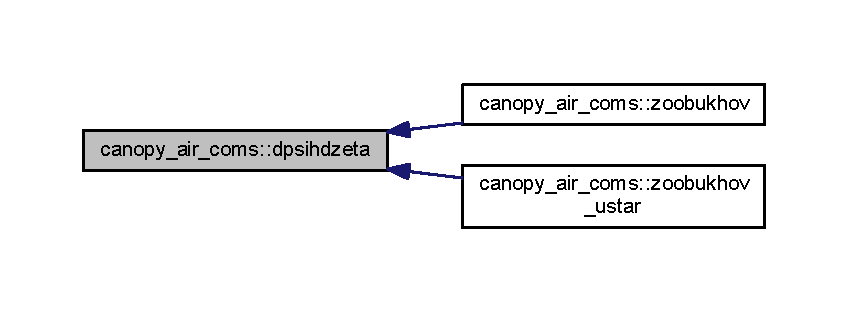
\includegraphics[width=350pt]{namespacecanopy__air__coms_a64552e0380fcb36366b5eb0f624241a3_icgraph}
\end{center}
\end{figure}


\index{canopy\+\_\+air\+\_\+coms@{canopy\+\_\+air\+\_\+coms}!dpsihdzeta8@{dpsihdzeta8}}
\index{dpsihdzeta8@{dpsihdzeta8}!canopy\+\_\+air\+\_\+coms@{canopy\+\_\+air\+\_\+coms}}
\subsubsection[{\texorpdfstring{dpsihdzeta8(zeta, stable)}{dpsihdzeta8(zeta, stable)}}]{\setlength{\rightskip}{0pt plus 5cm}real(kind=8) function canopy\+\_\+air\+\_\+coms\+::dpsihdzeta8 (
\begin{DoxyParamCaption}
\item[{real(kind=8), intent(in)}]{zeta, }
\item[{logical, intent(in)}]{stable}
\end{DoxyParamCaption}
)}\hypertarget{namespacecanopy__air__coms_aa5f9649efc40a05ddc13e1450f30fad3}{}\label{namespacecanopy__air__coms_aa5f9649efc40a05ddc13e1450f30fad3}


Here is the caller graph for this function\+:\nopagebreak
\begin{figure}[H]
\begin{center}
\leavevmode
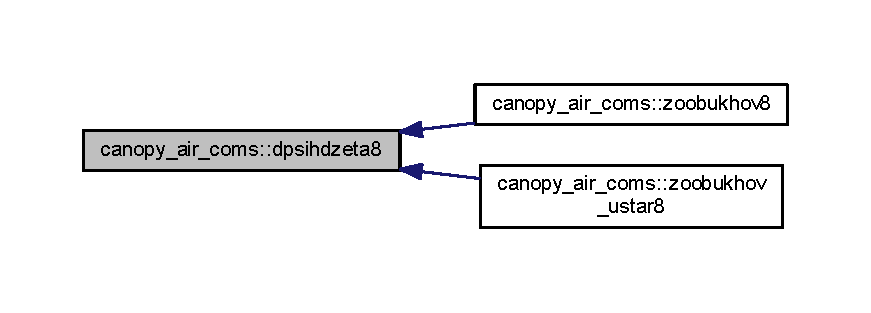
\includegraphics[width=350pt]{namespacecanopy__air__coms_aa5f9649efc40a05ddc13e1450f30fad3_icgraph}
\end{center}
\end{figure}


\index{canopy\+\_\+air\+\_\+coms@{canopy\+\_\+air\+\_\+coms}!dpsimdzeta@{dpsimdzeta}}
\index{dpsimdzeta@{dpsimdzeta}!canopy\+\_\+air\+\_\+coms@{canopy\+\_\+air\+\_\+coms}}
\subsubsection[{\texorpdfstring{dpsimdzeta(zeta, stable)}{dpsimdzeta(zeta, stable)}}]{\setlength{\rightskip}{0pt plus 5cm}real function canopy\+\_\+air\+\_\+coms\+::dpsimdzeta (
\begin{DoxyParamCaption}
\item[{real, intent(in)}]{zeta, }
\item[{logical, intent(in)}]{stable}
\end{DoxyParamCaption}
)}\hypertarget{namespacecanopy__air__coms_af8bc6f1d6999a4b614461cecb85c9b1b}{}\label{namespacecanopy__air__coms_af8bc6f1d6999a4b614461cecb85c9b1b}


Here is the caller graph for this function\+:\nopagebreak
\begin{figure}[H]
\begin{center}
\leavevmode
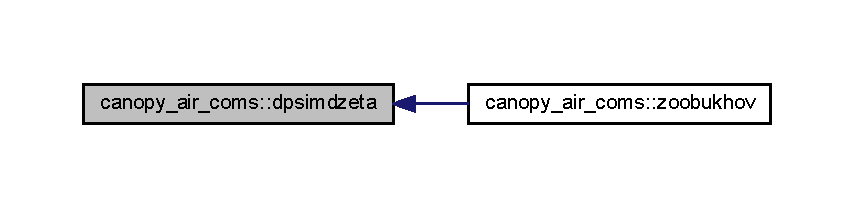
\includegraphics[width=350pt]{namespacecanopy__air__coms_af8bc6f1d6999a4b614461cecb85c9b1b_icgraph}
\end{center}
\end{figure}


\index{canopy\+\_\+air\+\_\+coms@{canopy\+\_\+air\+\_\+coms}!dpsimdzeta8@{dpsimdzeta8}}
\index{dpsimdzeta8@{dpsimdzeta8}!canopy\+\_\+air\+\_\+coms@{canopy\+\_\+air\+\_\+coms}}
\subsubsection[{\texorpdfstring{dpsimdzeta8(zeta, stable)}{dpsimdzeta8(zeta, stable)}}]{\setlength{\rightskip}{0pt plus 5cm}real(kind=8) function canopy\+\_\+air\+\_\+coms\+::dpsimdzeta8 (
\begin{DoxyParamCaption}
\item[{real(kind=8), intent(in)}]{zeta, }
\item[{logical, intent(in)}]{stable}
\end{DoxyParamCaption}
)}\hypertarget{namespacecanopy__air__coms_a51b006ac118f9549aee23ddb61a1bf19}{}\label{namespacecanopy__air__coms_a51b006ac118f9549aee23ddb61a1bf19}


Here is the caller graph for this function\+:\nopagebreak
\begin{figure}[H]
\begin{center}
\leavevmode
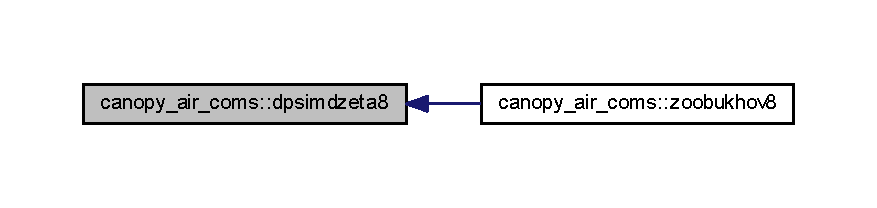
\includegraphics[width=350pt]{namespacecanopy__air__coms_a51b006ac118f9549aee23ddb61a1bf19_icgraph}
\end{center}
\end{figure}


\index{canopy\+\_\+air\+\_\+coms@{canopy\+\_\+air\+\_\+coms}!psih@{psih}}
\index{psih@{psih}!canopy\+\_\+air\+\_\+coms@{canopy\+\_\+air\+\_\+coms}}
\subsubsection[{\texorpdfstring{psih(zeta, stable)}{psih(zeta, stable)}}]{\setlength{\rightskip}{0pt plus 5cm}real function canopy\+\_\+air\+\_\+coms\+::psih (
\begin{DoxyParamCaption}
\item[{real, intent(in)}]{zeta, }
\item[{logical, intent(in)}]{stable}
\end{DoxyParamCaption}
)}\hypertarget{namespacecanopy__air__coms_acedb0f66db4b79009a69e87c5fd3ed71}{}\label{namespacecanopy__air__coms_acedb0f66db4b79009a69e87c5fd3ed71}


Here is the caller graph for this function\+:\nopagebreak
\begin{figure}[H]
\begin{center}
\leavevmode
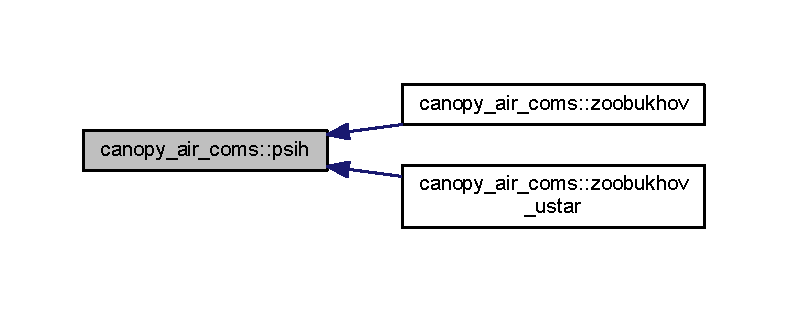
\includegraphics[width=350pt]{namespacecanopy__air__coms_acedb0f66db4b79009a69e87c5fd3ed71_icgraph}
\end{center}
\end{figure}


\index{canopy\+\_\+air\+\_\+coms@{canopy\+\_\+air\+\_\+coms}!psih8@{psih8}}
\index{psih8@{psih8}!canopy\+\_\+air\+\_\+coms@{canopy\+\_\+air\+\_\+coms}}
\subsubsection[{\texorpdfstring{psih8(zeta, stable)}{psih8(zeta, stable)}}]{\setlength{\rightskip}{0pt plus 5cm}real(kind=8) function canopy\+\_\+air\+\_\+coms\+::psih8 (
\begin{DoxyParamCaption}
\item[{real(kind=8), intent(in)}]{zeta, }
\item[{logical, intent(in)}]{stable}
\end{DoxyParamCaption}
)}\hypertarget{namespacecanopy__air__coms_aef33f0eeea82151a8edb6dc38c4cc921}{}\label{namespacecanopy__air__coms_aef33f0eeea82151a8edb6dc38c4cc921}


Here is the caller graph for this function\+:\nopagebreak
\begin{figure}[H]
\begin{center}
\leavevmode
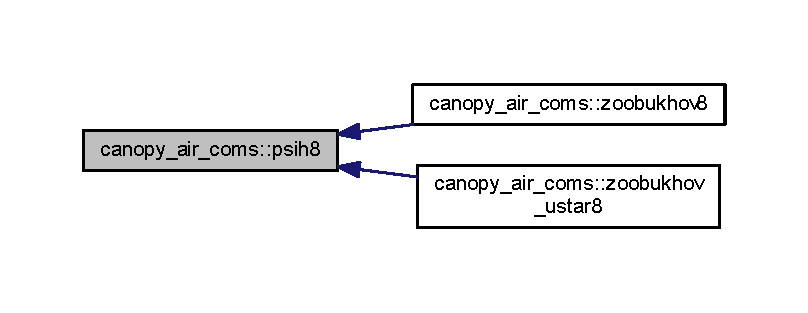
\includegraphics[width=350pt]{namespacecanopy__air__coms_aef33f0eeea82151a8edb6dc38c4cc921_icgraph}
\end{center}
\end{figure}


\index{canopy\+\_\+air\+\_\+coms@{canopy\+\_\+air\+\_\+coms}!psim@{psim}}
\index{psim@{psim}!canopy\+\_\+air\+\_\+coms@{canopy\+\_\+air\+\_\+coms}}
\subsubsection[{\texorpdfstring{psim(zeta, stable)}{psim(zeta, stable)}}]{\setlength{\rightskip}{0pt plus 5cm}real function canopy\+\_\+air\+\_\+coms\+::psim (
\begin{DoxyParamCaption}
\item[{real, intent(in)}]{zeta, }
\item[{logical, intent(in)}]{stable}
\end{DoxyParamCaption}
)}\hypertarget{namespacecanopy__air__coms_ab103fa081460babbe04c9a5a4699be5f}{}\label{namespacecanopy__air__coms_ab103fa081460babbe04c9a5a4699be5f}


Here is the caller graph for this function\+:\nopagebreak
\begin{figure}[H]
\begin{center}
\leavevmode
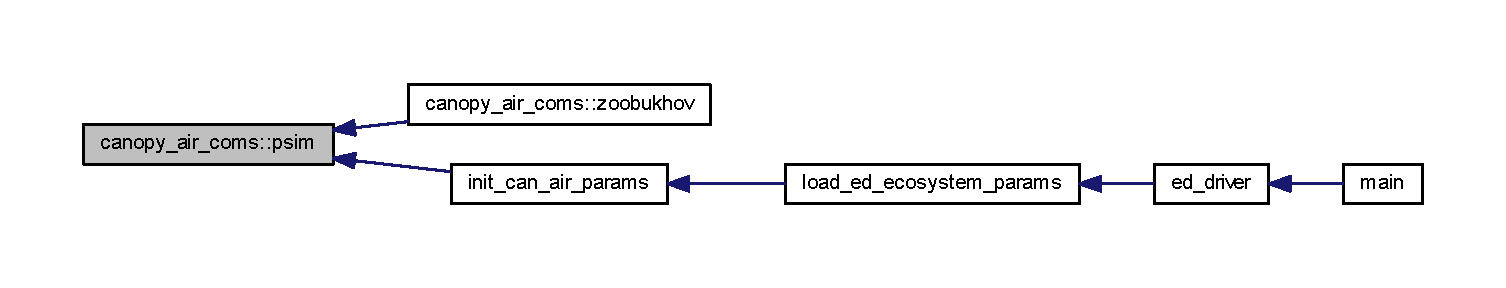
\includegraphics[width=350pt]{namespacecanopy__air__coms_ab103fa081460babbe04c9a5a4699be5f_icgraph}
\end{center}
\end{figure}


\index{canopy\+\_\+air\+\_\+coms@{canopy\+\_\+air\+\_\+coms}!psim8@{psim8}}
\index{psim8@{psim8}!canopy\+\_\+air\+\_\+coms@{canopy\+\_\+air\+\_\+coms}}
\subsubsection[{\texorpdfstring{psim8(zeta, stable)}{psim8(zeta, stable)}}]{\setlength{\rightskip}{0pt plus 5cm}real(kind=8) function canopy\+\_\+air\+\_\+coms\+::psim8 (
\begin{DoxyParamCaption}
\item[{real(kind=8), intent(in)}]{zeta, }
\item[{logical, intent(in)}]{stable}
\end{DoxyParamCaption}
)}\hypertarget{namespacecanopy__air__coms_aba7cbe776dbfa9815870ad3686949041}{}\label{namespacecanopy__air__coms_aba7cbe776dbfa9815870ad3686949041}


Here is the caller graph for this function\+:\nopagebreak
\begin{figure}[H]
\begin{center}
\leavevmode
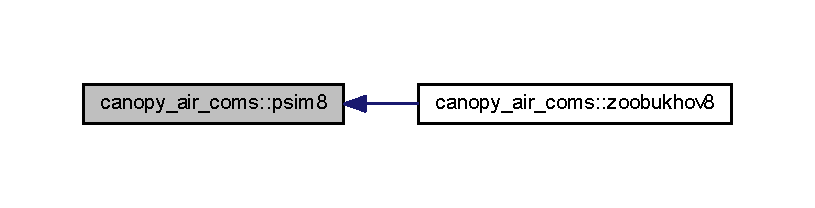
\includegraphics[width=350pt]{namespacecanopy__air__coms_aba7cbe776dbfa9815870ad3686949041_icgraph}
\end{center}
\end{figure}


\index{canopy\+\_\+air\+\_\+coms@{canopy\+\_\+air\+\_\+coms}!zoobukhov@{zoobukhov}}
\index{zoobukhov@{zoobukhov}!canopy\+\_\+air\+\_\+coms@{canopy\+\_\+air\+\_\+coms}}
\subsubsection[{\texorpdfstring{zoobukhov(rib, zstar, rough, zoz0m, lnzoz0m, zoz0h, lnzoz0h, stable)}{zoobukhov(rib, zstar, rough, zoz0m, lnzoz0m, zoz0h, lnzoz0h, stable)}}]{\setlength{\rightskip}{0pt plus 5cm}real function canopy\+\_\+air\+\_\+coms\+::zoobukhov (
\begin{DoxyParamCaption}
\item[{real, intent(in)}]{rib, }
\item[{real, intent(in)}]{zstar, }
\item[{real, intent(in)}]{rough, }
\item[{real, intent(in)}]{zoz0m, }
\item[{real, intent(in)}]{lnzoz0m, }
\item[{real, intent(in)}]{zoz0h, }
\item[{real, intent(in)}]{lnzoz0h, }
\item[{logical, intent(in)}]{stable}
\end{DoxyParamCaption}
)}\hypertarget{namespacecanopy__air__coms_a6062471b3381c283205ea8b27383a5e0}{}\label{namespacecanopy__air__coms_a6062471b3381c283205ea8b27383a5e0}
$<$$>$$<$$>$$<$$>$$<$$>$$<$$>$$<$$>$$<$$>$$<$$>$$<$$>$$<$$>$$<$$>$$<$$>$$<$$>$$<$$>$$<$$>$$<$$>$$<$$>$$<$$>$$<$$>$$<$$>$$<$$>$$<$$>$$<$$>$$<$$>$$<$$>$$<$$>$$<$$>$$<$$>$$<$$>$$<$$>$$<$$>$$<$$>$$<$$>$$<$$>$$<$$>$$<$$>$$<$$>$$<$$>$$<$$>$$<$$>$$<$$>$$<$!

$<$$>$$<$$>$$<$$>$$<$$>$$<$$>$$<$$>$$<$$>$$<$$>$$<$$>$$<$$>$$<$$>$$<$$>$$<$$>$$<$$>$$<$$>$$<$$>$$<$$>$$<$$>$$<$$>$$<$$>$$<$$>$$<$$>$$<$$>$$<$$>$$<$$>$$<$$>$$<$$>$$<$$>$$<$$>$$<$$>$$<$$>$$<$$>$$<$$>$$<$$>$$<$$>$$<$$>$$<$$>$$<$$>$$<$$>$$<$$>$$<$$>$$<$!

$<$$>$$<$$>$$<$$>$$<$$>$$<$$>$$<$$>$$<$$>$$<$$>$$<$$>$$<$$>$$<$$>$$<$$>$$<$$>$$<$$>$$<$$>$$<$$>$$<$$>$$<$$>$$<$$>$$<$$>$$<$$>$$<$$>$$<$$>$$<$$>$$<$$>$$<$$>$$<$$>$$<$$>$$<$$>$$<$$>$$<$$>$$<$$>$$<$$>$$<$$>$$<$$>$$<$$>$$<$$>$$<$$>$$<$$>$$<$$>$$<$$>$$<$!

$<$$>$$<$$>$$<$$>$$<$$>$$<$$>$$<$$>$$<$$>$$<$$>$$<$$>$$<$$>$$<$$>$$<$$>$$<$$>$$<$$>$$<$$>$$<$$>$$<$$>$$<$$>$$<$$>$$<$$>$$<$$>$$<$$>$$<$$>$$<$$>$$<$$>$$<$$>$$<$$>$$<$$>$$<$$>$$<$$>$$<$$>$$<$$>$$<$$>$$<$$>$$<$$>$$<$$>$$<$$>$$<$$>$$<$$>$$<$$>$$<$$>$$<$!

$<$$>$$<$$>$$<$$>$$<$$>$$<$$>$$<$$>$$<$$>$$<$$>$$<$$>$$<$$>$$<$$>$$<$$>$$<$$>$$<$$>$$<$$>$$<$$>$$<$$>$$<$$>$$<$$>$$<$$>$$<$$>$$<$$>$$<$$>$$<$$>$$<$$>$$<$$>$$<$$>$$<$$>$$<$$>$$<$$>$$<$$>$$<$$>$$<$$>$$<$$>$$<$$>$$<$$>$$<$$>$$<$$>$$<$$>$$<$$>$$<$$>$$<$!

$<$$>$$<$$>$$<$$>$$<$$>$$<$$>$$<$$>$$<$$>$$<$$>$$<$$>$$<$$>$$<$$>$$<$$>$$<$$>$$<$$>$$<$$>$$<$$>$$<$$>$$<$$>$$<$$>$$<$$>$$<$$>$$<$$>$$<$$>$$<$$>$$<$$>$$<$$>$$<$$>$$<$$>$$<$$>$$<$$>$$<$$>$$<$$>$$<$$>$$<$$>$$<$$>$$<$$>$$<$$>$$<$$>$$<$$>$$<$$>$$<$$>$$<$!

$<$$>$$<$$>$$<$$>$$<$$>$$<$$>$$<$$>$$<$$>$$<$$>$$<$$>$$<$$>$$<$$>$$<$$>$$<$$>$$<$$>$$<$$>$$<$$>$$<$$>$$<$$>$$<$$>$$<$$>$$<$$>$$<$$>$$<$$>$$<$$>$$<$$>$$<$$>$$<$$>$$<$$>$$<$$>$$<$$>$$<$$>$$<$$>$$<$$>$$<$$>$$<$$>$$<$$>$$<$$>$$<$$>$$<$!

$<$$>$$<$$>$$<$$>$$<$$>$$<$$>$$<$$>$$<$$>$$<$$>$$<$$>$$<$$>$$<$$>$$<$$>$$<$$>$$<$$>$$<$$>$$<$$>$$<$$>$$<$$>$$<$$>$$<$$>$$<$$>$$<$$>$$<$$>$$<$$>$$<$$>$$<$$>$$<$$>$$<$$>$$<$$>$$<$$>$$<$$>$$<$$>$$<$$>$$<$$>$$<$$>$$<$$>$$<$$>$$<$$>$$<$!

$<$$>$$<$$>$$<$$>$$<$$>$$<$$>$$<$$>$$<$$>$$<$$>$$<$$>$$<$$>$$<$$>$$<$$>$$<$$>$$<$$>$$<$$>$$<$$>$$<$$>$$<$$>$$<$$>$$<$$>$$<$$>$$<$$>$$<$$>$$<$$>$$<$$>$$<$$>$$<$$>$$<$$>$$<$$>$$<$$>$$<$$>$$<$$>$$<$$>$$<$$>$$<$$>$$<$$>$$<$$>$$<$$>$$<$$>$$<$$>$$<$$>$$<$!

$<$$>$$<$$>$$<$$>$$<$$>$$<$$>$$<$$>$$<$$>$$<$$>$$<$$>$$<$$>$$<$$>$$<$$>$$<$$>$$<$$>$$<$$>$$<$$>$$<$$>$$<$$>$$<$$>$$<$$>$$<$$>$$<$$>$$<$$>$$<$$>$$<$$>$$<$$>$$<$$>$$<$$>$$<$$>$$<$$>$$<$$>$$<$$>$$<$$>$$<$$>$$<$$>$$<$$>$$<$$>$$<$$>$$<$$>$$<$$>$$<$$>$$<$! 

Here is the call graph for this function\+:\nopagebreak
\begin{figure}[H]
\begin{center}
\leavevmode
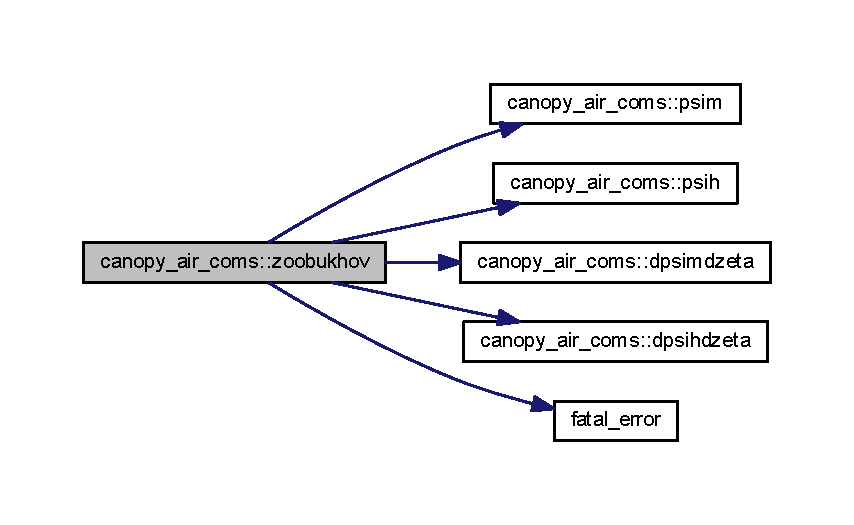
\includegraphics[width=350pt]{namespacecanopy__air__coms_a6062471b3381c283205ea8b27383a5e0_cgraph}
\end{center}
\end{figure}


\index{canopy\+\_\+air\+\_\+coms@{canopy\+\_\+air\+\_\+coms}!zoobukhov8@{zoobukhov8}}
\index{zoobukhov8@{zoobukhov8}!canopy\+\_\+air\+\_\+coms@{canopy\+\_\+air\+\_\+coms}}
\subsubsection[{\texorpdfstring{zoobukhov8(rib, zstar, rough, zoz0m, lnzoz0m, zoz0h, lnzoz0h, stable)}{zoobukhov8(rib, zstar, rough, zoz0m, lnzoz0m, zoz0h, lnzoz0h, stable)}}]{\setlength{\rightskip}{0pt plus 5cm}real(kind=8) function canopy\+\_\+air\+\_\+coms\+::zoobukhov8 (
\begin{DoxyParamCaption}
\item[{real(kind=8), intent(in)}]{rib, }
\item[{real(kind=8), intent(in)}]{zstar, }
\item[{real(kind=8), intent(in)}]{rough, }
\item[{real(kind=8), intent(in)}]{zoz0m, }
\item[{real(kind=8), intent(in)}]{lnzoz0m, }
\item[{real(kind=8), intent(in)}]{zoz0h, }
\item[{real(kind=8), intent(in)}]{lnzoz0h, }
\item[{logical, intent(in)}]{stable}
\end{DoxyParamCaption}
)}\hypertarget{namespacecanopy__air__coms_afef697305b4b30385c5206f48d9e787c}{}\label{namespacecanopy__air__coms_afef697305b4b30385c5206f48d9e787c}
$<$$>$$<$$>$$<$$>$$<$$>$$<$$>$$<$$>$$<$$>$$<$$>$$<$$>$$<$$>$$<$$>$$<$$>$$<$$>$$<$$>$$<$$>$$<$$>$$<$$>$$<$$>$$<$$>$$<$$>$$<$$>$$<$$>$$<$$>$$<$$>$$<$$>$$<$$>$$<$$>$$<$$>$$<$$>$$<$$>$$<$$>$$<$$>$$<$$>$$<$$>$$<$$>$$<$$>$$<$$>$$<$$>$$<$$>$$<$$>$$<$$>$$<$!

$<$$>$$<$$>$$<$$>$$<$$>$$<$$>$$<$$>$$<$$>$$<$$>$$<$$>$$<$$>$$<$$>$$<$$>$$<$$>$$<$$>$$<$$>$$<$$>$$<$$>$$<$$>$$<$$>$$<$$>$$<$$>$$<$$>$$<$$>$$<$$>$$<$$>$$<$$>$$<$$>$$<$$>$$<$$>$$<$$>$$<$$>$$<$$>$$<$$>$$<$$>$$<$$>$$<$$>$$<$$>$$<$$>$$<$$>$$<$$>$$<$$>$$<$!

$<$$>$$<$$>$$<$$>$$<$$>$$<$$>$$<$$>$$<$$>$$<$$>$$<$$>$$<$$>$$<$$>$$<$$>$$<$$>$$<$$>$$<$$>$$<$$>$$<$$>$$<$$>$$<$$>$$<$$>$$<$$>$$<$$>$$<$$>$$<$$>$$<$$>$$<$$>$$<$$>$$<$$>$$<$$>$$<$$>$$<$$>$$<$$>$$<$$>$$<$$>$$<$$>$$<$$>$$<$$>$$<$$>$$<$$>$$<$$>$$<$$>$$<$!

$<$$>$$<$$>$$<$$>$$<$$>$$<$$>$$<$$>$$<$$>$$<$$>$$<$$>$$<$$>$$<$$>$$<$$>$$<$$>$$<$$>$$<$$>$$<$$>$$<$$>$$<$$>$$<$$>$$<$$>$$<$$>$$<$$>$$<$$>$$<$$>$$<$$>$$<$$>$$<$$>$$<$$>$$<$$>$$<$$>$$<$$>$$<$$>$$<$$>$$<$$>$$<$$>$$<$$>$$<$$>$$<$$>$$<$$>$$<$$>$$<$$>$$<$!

$<$$>$$<$$>$$<$$>$$<$$>$$<$$>$$<$$>$$<$$>$$<$$>$$<$$>$$<$$>$$<$$>$$<$$>$$<$$>$$<$$>$$<$$>$$<$$>$$<$$>$$<$$>$$<$$>$$<$$>$$<$$>$$<$$>$$<$$>$$<$$>$$<$$>$$<$$>$$<$$>$$<$$>$$<$$>$$<$$>$$<$$>$$<$$>$$<$$>$$<$$>$$<$$>$$<$$>$$<$$>$$<$$>$$<$$>$$<$$>$$<$$>$$<$!

$<$$>$$<$$>$$<$$>$$<$$>$$<$$>$$<$$>$$<$$>$$<$$>$$<$$>$$<$$>$$<$$>$$<$$>$$<$$>$$<$$>$$<$$>$$<$$>$$<$$>$$<$$>$$<$$>$$<$$>$$<$$>$$<$$>$$<$$>$$<$$>$$<$$>$$<$$>$$<$$>$$<$$>$$<$$>$$<$$>$$<$$>$$<$$>$$<$$>$$<$$>$$<$$>$$<$$>$$<$$>$$<$$>$$<$$>$$<$$>$$<$$>$$<$!

$<$$>$$<$$>$$<$$>$$<$$>$$<$$>$$<$$>$$<$$>$$<$$>$$<$$>$$<$$>$$<$$>$$<$$>$$<$$>$$<$$>$$<$$>$$<$$>$$<$$>$$<$$>$$<$$>$$<$$>$$<$$>$$<$$>$$<$$>$$<$$>$$<$$>$$<$$>$$<$$>$$<$$>$$<$$>$$<$$>$$<$$>$$<$$>$$<$$>$$<$$>$$<$$>$$<$$>$$<$$>$$<$$>$$<$!

$<$$>$$<$$>$$<$$>$$<$$>$$<$$>$$<$$>$$<$$>$$<$$>$$<$$>$$<$$>$$<$$>$$<$$>$$<$$>$$<$$>$$<$$>$$<$$>$$<$$>$$<$$>$$<$$>$$<$$>$$<$$>$$<$$>$$<$$>$$<$$>$$<$$>$$<$$>$$<$$>$$<$$>$$<$$>$$<$$>$$<$$>$$<$$>$$<$$>$$<$$>$$<$$>$$<$$>$$<$$>$$<$$>$$<$!

$<$$>$$<$$>$$<$$>$$<$$>$$<$$>$$<$$>$$<$$>$$<$$>$$<$$>$$<$$>$$<$$>$$<$$>$$<$$>$$<$$>$$<$$>$$<$$>$$<$$>$$<$$>$$<$$>$$<$$>$$<$$>$$<$$>$$<$$>$$<$$>$$<$$>$$<$$>$$<$$>$$<$$>$$<$$>$$<$$>$$<$$>$$<$$>$$<$$>$$<$$>$$<$$>$$<$$>$$<$$>$$<$$>$$<$$>$$<$$>$$<$$>$$<$!

$<$$>$$<$$>$$<$$>$$<$$>$$<$$>$$<$$>$$<$$>$$<$$>$$<$$>$$<$$>$$<$$>$$<$$>$$<$$>$$<$$>$$<$$>$$<$$>$$<$$>$$<$$>$$<$$>$$<$$>$$<$$>$$<$$>$$<$$>$$<$$>$$<$$>$$<$$>$$<$$>$$<$$>$$<$$>$$<$$>$$<$$>$$<$$>$$<$$>$$<$$>$$<$$>$$<$$>$$<$$>$$<$$>$$<$$>$$<$$>$$<$$>$$<$! 

Here is the call graph for this function\+:\nopagebreak
\begin{figure}[H]
\begin{center}
\leavevmode
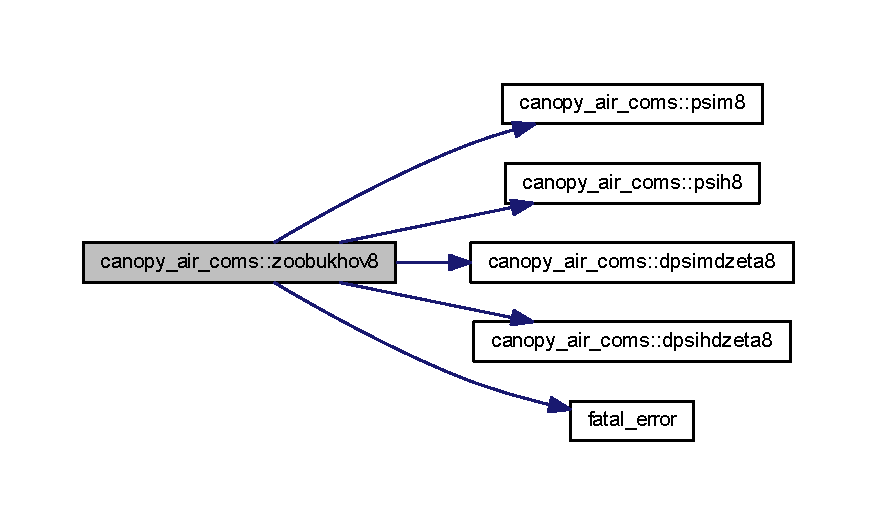
\includegraphics[width=350pt]{namespacecanopy__air__coms_afef697305b4b30385c5206f48d9e787c_cgraph}
\end{center}
\end{figure}


\index{canopy\+\_\+air\+\_\+coms@{canopy\+\_\+air\+\_\+coms}!zoobukhov\+\_\+ustar@{zoobukhov\+\_\+ustar}}
\index{zoobukhov\+\_\+ustar@{zoobukhov\+\_\+ustar}!canopy\+\_\+air\+\_\+coms@{canopy\+\_\+air\+\_\+coms}}
\subsubsection[{\texorpdfstring{zoobukhov\+\_\+ustar(rib, zstar, rough, zoz0h, lnzoz0h, kuoustar, stable)}{zoobukhov_ustar(rib, zstar, rough, zoz0h, lnzoz0h, kuoustar, stable)}}]{\setlength{\rightskip}{0pt plus 5cm}real function canopy\+\_\+air\+\_\+coms\+::zoobukhov\+\_\+ustar (
\begin{DoxyParamCaption}
\item[{real(kind=4), intent(in)}]{rib, }
\item[{real(kind=4), intent(in)}]{zstar, }
\item[{real(kind=4), intent(in)}]{rough, }
\item[{real(kind=4), intent(in)}]{zoz0h, }
\item[{real(kind=4), intent(in)}]{lnzoz0h, }
\item[{real(kind=4), intent(in)}]{kuoustar, }
\item[{logical, intent(in)}]{stable}
\end{DoxyParamCaption}
)}\hypertarget{namespacecanopy__air__coms_a5251266695c581c8f4058d98f6c86200}{}\label{namespacecanopy__air__coms_a5251266695c581c8f4058d98f6c86200}
$<$$>$$<$$>$$<$$>$$<$$>$$<$$>$$<$$>$$<$$>$$<$$>$$<$$>$$<$$>$$<$$>$$<$$>$$<$$>$$<$$>$$<$$>$$<$$>$$<$$>$$<$$>$$<$$>$$<$$>$$<$$>$$<$$>$$<$$>$$<$$>$$<$$>$$<$$>$$<$$>$$<$$>$$<$$>$$<$$>$$<$$>$$<$$>$$<$$>$$<$$>$$<$$>$$<$$>$$<$$>$$<$$>$$<$$>$$<$$>$$<$$>$$<$!

$<$$>$$<$$>$$<$$>$$<$$>$$<$$>$$<$$>$$<$$>$$<$$>$$<$$>$$<$$>$$<$$>$$<$$>$$<$$>$$<$$>$$<$$>$$<$$>$$<$$>$$<$$>$$<$$>$$<$$>$$<$$>$$<$$>$$<$$>$$<$$>$$<$$>$$<$$>$$<$$>$$<$$>$$<$$>$$<$$>$$<$$>$$<$$>$$<$$>$$<$$>$$<$$>$$<$$>$$<$$>$$<$$>$$<$$>$$<$$>$$<$$>$$<$!

$<$$>$$<$$>$$<$$>$$<$$>$$<$$>$$<$$>$$<$$>$$<$$>$$<$$>$$<$$>$$<$$>$$<$$>$$<$$>$$<$$>$$<$$>$$<$$>$$<$$>$$<$$>$$<$$>$$<$$>$$<$$>$$<$$>$$<$$>$$<$$>$$<$$>$$<$$>$$<$$>$$<$$>$$<$$>$$<$$>$$<$$>$$<$$>$$<$$>$$<$$>$$<$$>$$<$$>$$<$$>$$<$$>$$<$$>$$<$$>$$<$$>$$<$!

$<$$>$$<$$>$$<$$>$$<$$>$$<$$>$$<$$>$$<$$>$$<$$>$$<$$>$$<$$>$$<$$>$$<$$>$$<$$>$$<$$>$$<$$>$$<$$>$$<$$>$$<$$>$$<$$>$$<$$>$$<$$>$$<$$>$$<$$>$$<$$>$$<$$>$$<$$>$$<$$>$$<$$>$$<$$>$$<$$>$$<$$>$$<$$>$$<$$>$$<$$>$$<$$>$$<$$>$$<$$>$$<$$>$$<$$>$$<$$>$$<$$>$$<$!

$<$$>$$<$$>$$<$$>$$<$$>$$<$$>$$<$$>$$<$$>$$<$$>$$<$$>$$<$$>$$<$$>$$<$$>$$<$$>$$<$$>$$<$$>$$<$$>$$<$$>$$<$$>$$<$$>$$<$$>$$<$$>$$<$$>$$<$$>$$<$$>$$<$$>$$<$$>$$<$$>$$<$$>$$<$$>$$<$$>$$<$$>$$<$$>$$<$$>$$<$$>$$<$$>$$<$$>$$<$$>$$<$$>$$<$$>$$<$$>$$<$$>$$<$!

$<$$>$$<$$>$$<$$>$$<$$>$$<$$>$$<$$>$$<$$>$$<$$>$$<$$>$$<$$>$$<$$>$$<$$>$$<$$>$$<$$>$$<$$>$$<$$>$$<$$>$$<$$>$$<$$>$$<$$>$$<$$>$$<$$>$$<$$>$$<$$>$$<$$>$$<$$>$$<$$>$$<$$>$$<$$>$$<$$>$$<$$>$$<$$>$$<$$>$$<$$>$$<$$>$$<$$>$$<$$>$$<$$>$$<$$>$$<$$>$$<$$>$$<$!

$<$$>$$<$$>$$<$$>$$<$$>$$<$$>$$<$$>$$<$$>$$<$$>$$<$$>$$<$$>$$<$$>$$<$$>$$<$$>$$<$$>$$<$$>$$<$$>$$<$$>$$<$$>$$<$$>$$<$$>$$<$$>$$<$$>$$<$$>$$<$$>$$<$$>$$<$$>$$<$$>$$<$$>$$<$$>$$<$$>$$<$$>$$<$$>$$<$$>$$<$$>$$<$$>$$<$$>$$<$$>$$<$$>$$<$!

$<$$>$$<$$>$$<$$>$$<$$>$$<$$>$$<$$>$$<$$>$$<$$>$$<$$>$$<$$>$$<$$>$$<$$>$$<$$>$$<$$>$$<$$>$$<$$>$$<$$>$$<$$>$$<$$>$$<$$>$$<$$>$$<$$>$$<$$>$$<$$>$$<$$>$$<$$>$$<$$>$$<$$>$$<$$>$$<$$>$$<$$>$$<$$>$$<$$>$$<$$>$$<$$>$$<$$>$$<$$>$$<$$>$$<$!

$<$$>$$<$$>$$<$$>$$<$$>$$<$$>$$<$$>$$<$$>$$<$$>$$<$$>$$<$$>$$<$$>$$<$$>$$<$$>$$<$$>$$<$$>$$<$$>$$<$$>$$<$$>$$<$$>$$<$$>$$<$$>$$<$$>$$<$$>$$<$$>$$<$$>$$<$$>$$<$$>$$<$$>$$<$$>$$<$$>$$<$$>$$<$$>$$<$$>$$<$$>$$<$$>$$<$$>$$<$$>$$<$$>$$<$$>$$<$$>$$<$$>$$<$!

$<$$>$$<$$>$$<$$>$$<$$>$$<$$>$$<$$>$$<$$>$$<$$>$$<$$>$$<$$>$$<$$>$$<$$>$$<$$>$$<$$>$$<$$>$$<$$>$$<$$>$$<$$>$$<$$>$$<$$>$$<$$>$$<$$>$$<$$>$$<$$>$$<$$>$$<$$>$$<$$>$$<$$>$$<$$>$$<$$>$$<$$>$$<$$>$$<$$>$$<$$>$$<$$>$$<$$>$$<$$>$$<$$>$$<$$>$$<$$>$$<$$>$$<$! 

Here is the call graph for this function\+:\nopagebreak
\begin{figure}[H]
\begin{center}
\leavevmode
\includegraphics[width=350pt]{namespacecanopy__air__coms_a5251266695c581c8f4058d98f6c86200_cgraph}
\end{center}
\end{figure}


\index{canopy\+\_\+air\+\_\+coms@{canopy\+\_\+air\+\_\+coms}!zoobukhov\+\_\+ustar8@{zoobukhov\+\_\+ustar8}}
\index{zoobukhov\+\_\+ustar8@{zoobukhov\+\_\+ustar8}!canopy\+\_\+air\+\_\+coms@{canopy\+\_\+air\+\_\+coms}}
\subsubsection[{\texorpdfstring{zoobukhov\+\_\+ustar8(rib, zstar, rough, zoz0h, lnzoz0h, kuoustar, stable)}{zoobukhov_ustar8(rib, zstar, rough, zoz0h, lnzoz0h, kuoustar, stable)}}]{\setlength{\rightskip}{0pt plus 5cm}real(kind=8) function canopy\+\_\+air\+\_\+coms\+::zoobukhov\+\_\+ustar8 (
\begin{DoxyParamCaption}
\item[{real(kind=8), intent(in)}]{rib, }
\item[{real(kind=8), intent(in)}]{zstar, }
\item[{real(kind=8), intent(in)}]{rough, }
\item[{real(kind=8), intent(in)}]{zoz0h, }
\item[{real(kind=8), intent(in)}]{lnzoz0h, }
\item[{real(kind=8), intent(in)}]{kuoustar, }
\item[{logical, intent(in)}]{stable}
\end{DoxyParamCaption}
)}\hypertarget{namespacecanopy__air__coms_a6ef582f46fded1355973730e6a2289f2}{}\label{namespacecanopy__air__coms_a6ef582f46fded1355973730e6a2289f2}
$<$$>$$<$$>$$<$$>$$<$$>$$<$$>$$<$$>$$<$$>$$<$$>$$<$$>$$<$$>$$<$$>$$<$$>$$<$$>$$<$$>$$<$$>$$<$$>$$<$$>$$<$$>$$<$$>$$<$$>$$<$$>$$<$$>$$<$$>$$<$$>$$<$$>$$<$$>$$<$$>$$<$$>$$<$$>$$<$$>$$<$$>$$<$$>$$<$$>$$<$$>$$<$$>$$<$$>$$<$$>$$<$$>$$<$$>$$<$$>$$<$$>$$<$!

$<$$>$$<$$>$$<$$>$$<$$>$$<$$>$$<$$>$$<$$>$$<$$>$$<$$>$$<$$>$$<$$>$$<$$>$$<$$>$$<$$>$$<$$>$$<$$>$$<$$>$$<$$>$$<$$>$$<$$>$$<$$>$$<$$>$$<$$>$$<$$>$$<$$>$$<$$>$$<$$>$$<$$>$$<$$>$$<$$>$$<$$>$$<$$>$$<$$>$$<$$>$$<$$>$$<$$>$$<$$>$$<$$>$$<$$>$$<$$>$$<$$>$$<$!

$<$$>$$<$$>$$<$$>$$<$$>$$<$$>$$<$$>$$<$$>$$<$$>$$<$$>$$<$$>$$<$$>$$<$$>$$<$$>$$<$$>$$<$$>$$<$$>$$<$$>$$<$$>$$<$$>$$<$$>$$<$$>$$<$$>$$<$$>$$<$$>$$<$$>$$<$$>$$<$$>$$<$$>$$<$$>$$<$$>$$<$$>$$<$$>$$<$$>$$<$$>$$<$$>$$<$$>$$<$$>$$<$$>$$<$$>$$<$$>$$<$$>$$<$!

$<$$>$$<$$>$$<$$>$$<$$>$$<$$>$$<$$>$$<$$>$$<$$>$$<$$>$$<$$>$$<$$>$$<$$>$$<$$>$$<$$>$$<$$>$$<$$>$$<$$>$$<$$>$$<$$>$$<$$>$$<$$>$$<$$>$$<$$>$$<$$>$$<$$>$$<$$>$$<$$>$$<$$>$$<$$>$$<$$>$$<$$>$$<$$>$$<$$>$$<$$>$$<$$>$$<$$>$$<$$>$$<$$>$$<$$>$$<$$>$$<$$>$$<$!

$<$$>$$<$$>$$<$$>$$<$$>$$<$$>$$<$$>$$<$$>$$<$$>$$<$$>$$<$$>$$<$$>$$<$$>$$<$$>$$<$$>$$<$$>$$<$$>$$<$$>$$<$$>$$<$$>$$<$$>$$<$$>$$<$$>$$<$$>$$<$$>$$<$$>$$<$$>$$<$$>$$<$$>$$<$$>$$<$$>$$<$$>$$<$$>$$<$$>$$<$$>$$<$$>$$<$$>$$<$$>$$<$$>$$<$$>$$<$$>$!

$<$$>$$<$$>$$<$$>$$<$$>$$<$$>$$<$$>$$<$$>$$<$$>$$<$$>$$<$$>$$<$$>$$<$$>$$<$$>$$<$$>$$<$$>$$<$$>$$<$$>$$<$$>$$<$$>$$<$$>$$<$$>$$<$$>$$<$$>$$<$$>$$<$$>$$<$$>$$<$$>$$<$$>$$<$$>$$<$$>$$<$$>$$<$$>$$<$$>$$<$$>$$<$$>$$<$$>$$<$$>$$<$$>$$<$$>$$<$$>$!

$<$$>$$<$$>$$<$$>$$<$$>$$<$$>$$<$$>$$<$$>$$<$$>$$<$$>$$<$$>$$<$$>$$<$$>$$<$$>$$<$$>$$<$$>$$<$$>$$<$$>$$<$$>$$<$$>$$<$$>$$<$$>$$<$$>$$<$$>$$<$$>$$<$$>$$<$$>$$<$$>$$<$$>$$<$$>$$<$$>$$<$$>$$<$$>$$<$$>$$<$$>$$<$$>$$<$$>$$<$$>$$<$$>$$<$!

$<$$>$$<$$>$$<$$>$$<$$>$$<$$>$$<$$>$$<$$>$$<$$>$$<$$>$$<$$>$$<$$>$$<$$>$$<$$>$$<$$>$$<$$>$$<$$>$$<$$>$$<$$>$$<$$>$$<$$>$$<$$>$$<$$>$$<$$>$$<$$>$$<$$>$$<$$>$$<$$>$$<$$>$$<$$>$$<$$>$$<$$>$$<$$>$$<$$>$$<$$>$$<$$>$$<$$>$$<$$>$$<$$>$$<$!

$<$$>$$<$$>$$<$$>$$<$$>$$<$$>$$<$$>$$<$$>$$<$$>$$<$$>$$<$$>$$<$$>$$<$$>$$<$$>$$<$$>$$<$$>$$<$$>$$<$$>$$<$$>$$<$$>$$<$$>$$<$$>$$<$$>$$<$$>$$<$$>$$<$$>$$<$$>$$<$$>$$<$$>$$<$$>$$<$$>$$<$$>$$<$$>$$<$$>$$<$$>$$<$$>$$<$$>$$<$$>$$<$$>$$<$$>$$<$$>$!

$<$$>$$<$$>$$<$$>$$<$$>$$<$$>$$<$$>$$<$$>$$<$$>$$<$$>$$<$$>$$<$$>$$<$$>$$<$$>$$<$$>$$<$$>$$<$$>$$<$$>$$<$$>$$<$$>$$<$$>$$<$$>$$<$$>$$<$$>$$<$$>$$<$$>$$<$$>$$<$$>$$<$$>$$<$$>$$<$$>$$<$$>$$<$$>$$<$$>$$<$$>$$<$$>$$<$$>$$<$$>$$<$$>$$<$$>$$<$$>$!

$<$$>$$<$$>$$<$$>$$<$$>$$<$$>$$<$$>$$<$$>$$<$$>$$<$$>$$<$$>$$<$$>$$<$$>$$<$$>$$<$$>$$<$$>$$<$$>$$<$$>$$<$$>$$<$$>$$<$$>$$<$$>$$<$$>$$<$$>$$<$$>$$<$$>$$<$$>$$<$$>$$<$$>$$<$$>$$<$$>$$<$$>$$<$$>$$<$$>$$<$$>$$<$$>$$<$$>$$<$$>$$<$$>$$<$$>$$<$$>$!

$<$$>$$<$$>$$<$$>$$<$$>$$<$$>$$<$$>$$<$$>$$<$$>$$<$$>$$<$$>$$<$$>$$<$$>$$<$$>$$<$$>$$<$$>$$<$$>$$<$$>$$<$$>$$<$$>$$<$$>$$<$$>$$<$$>$$<$$>$$<$$>$$<$$>$$<$$>$$<$$>$$<$$>$$<$$>$$<$$>$$<$$>$$<$$>$$<$$>$$<$$>$$<$$>$$<$$>$$<$$>$$<$$>$$<$$>$$<$$>$! 

Here is the call graph for this function\+:\nopagebreak
\begin{figure}[H]
\begin{center}
\leavevmode
\includegraphics[width=350pt]{namespacecanopy__air__coms_a6ef582f46fded1355973730e6a2289f2_cgraph}
\end{center}
\end{figure}




\subsection{Variable Documentation}
\index{canopy\+\_\+air\+\_\+coms@{canopy\+\_\+air\+\_\+coms}!abh91@{abh91}}
\index{abh91@{abh91}!canopy\+\_\+air\+\_\+coms@{canopy\+\_\+air\+\_\+coms}}
\subsubsection[{\texorpdfstring{abh91}{abh91}}]{\setlength{\rightskip}{0pt plus 5cm}real canopy\+\_\+air\+\_\+coms\+::abh91}\hypertarget{namespacecanopy__air__coms_a8943107817bd72a2ecf2c8ac35516efc}{}\label{namespacecanopy__air__coms_a8943107817bd72a2ecf2c8ac35516efc}
\index{canopy\+\_\+air\+\_\+coms@{canopy\+\_\+air\+\_\+coms}!abh918@{abh918}}
\index{abh918@{abh918}!canopy\+\_\+air\+\_\+coms@{canopy\+\_\+air\+\_\+coms}}
\subsubsection[{\texorpdfstring{abh918}{abh918}}]{\setlength{\rightskip}{0pt plus 5cm}real(kind=8) canopy\+\_\+air\+\_\+coms\+::abh918}\hypertarget{namespacecanopy__air__coms_a7bbc194838f911d2e8b0948159f4d62e}{}\label{namespacecanopy__air__coms_a7bbc194838f911d2e8b0948159f4d62e}
\index{canopy\+\_\+air\+\_\+coms@{canopy\+\_\+air\+\_\+coms}!acyli\+\_\+lami@{acyli\+\_\+lami}}
\index{acyli\+\_\+lami@{acyli\+\_\+lami}!canopy\+\_\+air\+\_\+coms@{canopy\+\_\+air\+\_\+coms}}
\subsubsection[{\texorpdfstring{acyli\+\_\+lami}{acyli_lami}}]{\setlength{\rightskip}{0pt plus 5cm}real(kind=4) canopy\+\_\+air\+\_\+coms\+::acyli\+\_\+lami}\hypertarget{namespacecanopy__air__coms_a910e0e75420e6cd46075062c7da2b565}{}\label{namespacecanopy__air__coms_a910e0e75420e6cd46075062c7da2b565}
\index{canopy\+\_\+air\+\_\+coms@{canopy\+\_\+air\+\_\+coms}!acyli\+\_\+lami8@{acyli\+\_\+lami8}}
\index{acyli\+\_\+lami8@{acyli\+\_\+lami8}!canopy\+\_\+air\+\_\+coms@{canopy\+\_\+air\+\_\+coms}}
\subsubsection[{\texorpdfstring{acyli\+\_\+lami8}{acyli_lami8}}]{\setlength{\rightskip}{0pt plus 5cm}real(kind=8) canopy\+\_\+air\+\_\+coms\+::acyli\+\_\+lami8}\hypertarget{namespacecanopy__air__coms_a325f601d72eb729cc4301008156be76b}{}\label{namespacecanopy__air__coms_a325f601d72eb729cc4301008156be76b}
\index{canopy\+\_\+air\+\_\+coms@{canopy\+\_\+air\+\_\+coms}!acyli\+\_\+turb@{acyli\+\_\+turb}}
\index{acyli\+\_\+turb@{acyli\+\_\+turb}!canopy\+\_\+air\+\_\+coms@{canopy\+\_\+air\+\_\+coms}}
\subsubsection[{\texorpdfstring{acyli\+\_\+turb}{acyli_turb}}]{\setlength{\rightskip}{0pt plus 5cm}real(kind=4) canopy\+\_\+air\+\_\+coms\+::acyli\+\_\+turb}\hypertarget{namespacecanopy__air__coms_a42c5385303996a52e2fce111d922eaf2}{}\label{namespacecanopy__air__coms_a42c5385303996a52e2fce111d922eaf2}
\index{canopy\+\_\+air\+\_\+coms@{canopy\+\_\+air\+\_\+coms}!acyli\+\_\+turb8@{acyli\+\_\+turb8}}
\index{acyli\+\_\+turb8@{acyli\+\_\+turb8}!canopy\+\_\+air\+\_\+coms@{canopy\+\_\+air\+\_\+coms}}
\subsubsection[{\texorpdfstring{acyli\+\_\+turb8}{acyli_turb8}}]{\setlength{\rightskip}{0pt plus 5cm}real(kind=8) canopy\+\_\+air\+\_\+coms\+::acyli\+\_\+turb8}\hypertarget{namespacecanopy__air__coms_a933920d4f406fd57c33f8cef1ca8bb83}{}\label{namespacecanopy__air__coms_a933920d4f406fd57c33f8cef1ca8bb83}
\index{canopy\+\_\+air\+\_\+coms@{canopy\+\_\+air\+\_\+coms}!aflat\+\_\+lami@{aflat\+\_\+lami}}
\index{aflat\+\_\+lami@{aflat\+\_\+lami}!canopy\+\_\+air\+\_\+coms@{canopy\+\_\+air\+\_\+coms}}
\subsubsection[{\texorpdfstring{aflat\+\_\+lami}{aflat_lami}}]{\setlength{\rightskip}{0pt plus 5cm}real(kind=4) canopy\+\_\+air\+\_\+coms\+::aflat\+\_\+lami}\hypertarget{namespacecanopy__air__coms_a478fe27fc0f34c4b09208d0f99bae8e5}{}\label{namespacecanopy__air__coms_a478fe27fc0f34c4b09208d0f99bae8e5}
\index{canopy\+\_\+air\+\_\+coms@{canopy\+\_\+air\+\_\+coms}!aflat\+\_\+lami8@{aflat\+\_\+lami8}}
\index{aflat\+\_\+lami8@{aflat\+\_\+lami8}!canopy\+\_\+air\+\_\+coms@{canopy\+\_\+air\+\_\+coms}}
\subsubsection[{\texorpdfstring{aflat\+\_\+lami8}{aflat_lami8}}]{\setlength{\rightskip}{0pt plus 5cm}real(kind=8) canopy\+\_\+air\+\_\+coms\+::aflat\+\_\+lami8}\hypertarget{namespacecanopy__air__coms_af642ae1aafe80d1c6e7fde278a2236df}{}\label{namespacecanopy__air__coms_af642ae1aafe80d1c6e7fde278a2236df}
\index{canopy\+\_\+air\+\_\+coms@{canopy\+\_\+air\+\_\+coms}!aflat\+\_\+turb@{aflat\+\_\+turb}}
\index{aflat\+\_\+turb@{aflat\+\_\+turb}!canopy\+\_\+air\+\_\+coms@{canopy\+\_\+air\+\_\+coms}}
\subsubsection[{\texorpdfstring{aflat\+\_\+turb}{aflat_turb}}]{\setlength{\rightskip}{0pt plus 5cm}real(kind=4) canopy\+\_\+air\+\_\+coms\+::aflat\+\_\+turb}\hypertarget{namespacecanopy__air__coms_a63aa3cee74a44dfccdad43b566c7149c}{}\label{namespacecanopy__air__coms_a63aa3cee74a44dfccdad43b566c7149c}
\index{canopy\+\_\+air\+\_\+coms@{canopy\+\_\+air\+\_\+coms}!aflat\+\_\+turb8@{aflat\+\_\+turb8}}
\index{aflat\+\_\+turb8@{aflat\+\_\+turb8}!canopy\+\_\+air\+\_\+coms@{canopy\+\_\+air\+\_\+coms}}
\subsubsection[{\texorpdfstring{aflat\+\_\+turb8}{aflat_turb8}}]{\setlength{\rightskip}{0pt plus 5cm}real(kind=8) canopy\+\_\+air\+\_\+coms\+::aflat\+\_\+turb8}\hypertarget{namespacecanopy__air__coms_a74069fab7440b8c4adf33de11779b980}{}\label{namespacecanopy__air__coms_a74069fab7440b8c4adf33de11779b980}
\index{canopy\+\_\+air\+\_\+coms@{canopy\+\_\+air\+\_\+coms}!alpha\+\_\+m97@{alpha\+\_\+m97}}
\index{alpha\+\_\+m97@{alpha\+\_\+m97}!canopy\+\_\+air\+\_\+coms@{canopy\+\_\+air\+\_\+coms}}
\subsubsection[{\texorpdfstring{alpha\+\_\+m97}{alpha_m97}}]{\setlength{\rightskip}{0pt plus 5cm}real(kind=4) canopy\+\_\+air\+\_\+coms\+::alpha\+\_\+m97}\hypertarget{namespacecanopy__air__coms_ac16bf823a6fc81f0d671fa06ca5de7e7}{}\label{namespacecanopy__air__coms_ac16bf823a6fc81f0d671fa06ca5de7e7}
\index{canopy\+\_\+air\+\_\+coms@{canopy\+\_\+air\+\_\+coms}!alpha\+\_\+m97\+\_\+8@{alpha\+\_\+m97\+\_\+8}}
\index{alpha\+\_\+m97\+\_\+8@{alpha\+\_\+m97\+\_\+8}!canopy\+\_\+air\+\_\+coms@{canopy\+\_\+air\+\_\+coms}}
\subsubsection[{\texorpdfstring{alpha\+\_\+m97\+\_\+8}{alpha_m97_8}}]{\setlength{\rightskip}{0pt plus 5cm}real(kind=8) canopy\+\_\+air\+\_\+coms\+::alpha\+\_\+m97\+\_\+8}\hypertarget{namespacecanopy__air__coms_aaca98abaf4f4ff986bd24a7e1ceea8a6}{}\label{namespacecanopy__air__coms_aaca98abaf4f4ff986bd24a7e1ceea8a6}
\index{canopy\+\_\+air\+\_\+coms@{canopy\+\_\+air\+\_\+coms}!alpha\+\_\+mw99@{alpha\+\_\+mw99}}
\index{alpha\+\_\+mw99@{alpha\+\_\+mw99}!canopy\+\_\+air\+\_\+coms@{canopy\+\_\+air\+\_\+coms}}
\subsubsection[{\texorpdfstring{alpha\+\_\+mw99}{alpha_mw99}}]{\setlength{\rightskip}{0pt plus 5cm}real(kind=4) canopy\+\_\+air\+\_\+coms\+::alpha\+\_\+mw99}\hypertarget{namespacecanopy__air__coms_aee71b7396b4019638189e8d16f29d5bc}{}\label{namespacecanopy__air__coms_aee71b7396b4019638189e8d16f29d5bc}
\index{canopy\+\_\+air\+\_\+coms@{canopy\+\_\+air\+\_\+coms}!alpha\+\_\+mw99\+\_\+8@{alpha\+\_\+mw99\+\_\+8}}
\index{alpha\+\_\+mw99\+\_\+8@{alpha\+\_\+mw99\+\_\+8}!canopy\+\_\+air\+\_\+coms@{canopy\+\_\+air\+\_\+coms}}
\subsubsection[{\texorpdfstring{alpha\+\_\+mw99\+\_\+8}{alpha_mw99_8}}]{\setlength{\rightskip}{0pt plus 5cm}real(kind=8) canopy\+\_\+air\+\_\+coms\+::alpha\+\_\+mw99\+\_\+8}\hypertarget{namespacecanopy__air__coms_a0c11f06e8905d7442da34f32fd5a1f5d}{}\label{namespacecanopy__air__coms_a0c11f06e8905d7442da34f32fd5a1f5d}
\index{canopy\+\_\+air\+\_\+coms@{canopy\+\_\+air\+\_\+coms}!ate@{ate}}
\index{ate@{ate}!canopy\+\_\+air\+\_\+coms@{canopy\+\_\+air\+\_\+coms}}
\subsubsection[{\texorpdfstring{ate}{ate}}]{\setlength{\rightskip}{0pt plus 5cm}real canopy\+\_\+air\+\_\+coms\+::ate}\hypertarget{namespacecanopy__air__coms_ae25648cf7af6ad979525a213bc95b1b3}{}\label{namespacecanopy__air__coms_ae25648cf7af6ad979525a213bc95b1b3}
\index{canopy\+\_\+air\+\_\+coms@{canopy\+\_\+air\+\_\+coms}!ate8@{ate8}}
\index{ate8@{ate8}!canopy\+\_\+air\+\_\+coms@{canopy\+\_\+air\+\_\+coms}}
\subsubsection[{\texorpdfstring{ate8}{ate8}}]{\setlength{\rightskip}{0pt plus 5cm}real(kind=8) canopy\+\_\+air\+\_\+coms\+::ate8}\hypertarget{namespacecanopy__air__coms_a896b380af341c4fda227104ec855c42f}{}\label{namespacecanopy__air__coms_a896b380af341c4fda227104ec855c42f}
\index{canopy\+\_\+air\+\_\+coms@{canopy\+\_\+air\+\_\+coms}!atetf@{atetf}}
\index{atetf@{atetf}!canopy\+\_\+air\+\_\+coms@{canopy\+\_\+air\+\_\+coms}}
\subsubsection[{\texorpdfstring{atetf}{atetf}}]{\setlength{\rightskip}{0pt plus 5cm}real canopy\+\_\+air\+\_\+coms\+::atetf}\hypertarget{namespacecanopy__air__coms_a5fa870deca6638beca69104f25090cc6}{}\label{namespacecanopy__air__coms_a5fa870deca6638beca69104f25090cc6}
\index{canopy\+\_\+air\+\_\+coms@{canopy\+\_\+air\+\_\+coms}!atetf8@{atetf8}}
\index{atetf8@{atetf8}!canopy\+\_\+air\+\_\+coms@{canopy\+\_\+air\+\_\+coms}}
\subsubsection[{\texorpdfstring{atetf8}{atetf8}}]{\setlength{\rightskip}{0pt plus 5cm}real(kind=8) canopy\+\_\+air\+\_\+coms\+::atetf8}\hypertarget{namespacecanopy__air__coms_ac0a58110fa129fb929e126e046d2b6fd}{}\label{namespacecanopy__air__coms_ac0a58110fa129fb929e126e046d2b6fd}
\index{canopy\+\_\+air\+\_\+coms@{canopy\+\_\+air\+\_\+coms}!bbh91@{bbh91}}
\index{bbh91@{bbh91}!canopy\+\_\+air\+\_\+coms@{canopy\+\_\+air\+\_\+coms}}
\subsubsection[{\texorpdfstring{bbh91}{bbh91}}]{\setlength{\rightskip}{0pt plus 5cm}real canopy\+\_\+air\+\_\+coms\+::bbh91}\hypertarget{namespacecanopy__air__coms_a19448a094bac99003898bfd3170277e3}{}\label{namespacecanopy__air__coms_a19448a094bac99003898bfd3170277e3}
\index{canopy\+\_\+air\+\_\+coms@{canopy\+\_\+air\+\_\+coms}!bbh918@{bbh918}}
\index{bbh918@{bbh918}!canopy\+\_\+air\+\_\+coms@{canopy\+\_\+air\+\_\+coms}}
\subsubsection[{\texorpdfstring{bbh918}{bbh918}}]{\setlength{\rightskip}{0pt plus 5cm}real(kind=8) canopy\+\_\+air\+\_\+coms\+::bbh918}\hypertarget{namespacecanopy__air__coms_a9c6504ecba9e79e8a45ab651e4f333ac}{}\label{namespacecanopy__air__coms_a9c6504ecba9e79e8a45ab651e4f333ac}
\index{canopy\+\_\+air\+\_\+coms@{canopy\+\_\+air\+\_\+coms}!bcod@{bcod}}
\index{bcod@{bcod}!canopy\+\_\+air\+\_\+coms@{canopy\+\_\+air\+\_\+coms}}
\subsubsection[{\texorpdfstring{bcod}{bcod}}]{\setlength{\rightskip}{0pt plus 5cm}real canopy\+\_\+air\+\_\+coms\+::bcod}\hypertarget{namespacecanopy__air__coms_a6a1bee0c06adf9bb369d6f4be822b553}{}\label{namespacecanopy__air__coms_a6a1bee0c06adf9bb369d6f4be822b553}
\index{canopy\+\_\+air\+\_\+coms@{canopy\+\_\+air\+\_\+coms}!bcod8@{bcod8}}
\index{bcod8@{bcod8}!canopy\+\_\+air\+\_\+coms@{canopy\+\_\+air\+\_\+coms}}
\subsubsection[{\texorpdfstring{bcod8}{bcod8}}]{\setlength{\rightskip}{0pt plus 5cm}real(kind=8) canopy\+\_\+air\+\_\+coms\+::bcod8}\hypertarget{namespacecanopy__air__coms_a7b5193455d7f0ba7668b3b2f1988f468}{}\label{namespacecanopy__air__coms_a7b5193455d7f0ba7668b3b2f1988f468}
\index{canopy\+\_\+air\+\_\+coms@{canopy\+\_\+air\+\_\+coms}!bcyli\+\_\+lami@{bcyli\+\_\+lami}}
\index{bcyli\+\_\+lami@{bcyli\+\_\+lami}!canopy\+\_\+air\+\_\+coms@{canopy\+\_\+air\+\_\+coms}}
\subsubsection[{\texorpdfstring{bcyli\+\_\+lami}{bcyli_lami}}]{\setlength{\rightskip}{0pt plus 5cm}real(kind=4) canopy\+\_\+air\+\_\+coms\+::bcyli\+\_\+lami}\hypertarget{namespacecanopy__air__coms_a5569cc0028fc90fc9c90e5148b2b6af3}{}\label{namespacecanopy__air__coms_a5569cc0028fc90fc9c90e5148b2b6af3}
\index{canopy\+\_\+air\+\_\+coms@{canopy\+\_\+air\+\_\+coms}!bcyli\+\_\+lami8@{bcyli\+\_\+lami8}}
\index{bcyli\+\_\+lami8@{bcyli\+\_\+lami8}!canopy\+\_\+air\+\_\+coms@{canopy\+\_\+air\+\_\+coms}}
\subsubsection[{\texorpdfstring{bcyli\+\_\+lami8}{bcyli_lami8}}]{\setlength{\rightskip}{0pt plus 5cm}real(kind=8) canopy\+\_\+air\+\_\+coms\+::bcyli\+\_\+lami8}\hypertarget{namespacecanopy__air__coms_ad7c65a1b664eb04c6665e7d5a9fc5380}{}\label{namespacecanopy__air__coms_ad7c65a1b664eb04c6665e7d5a9fc5380}
\index{canopy\+\_\+air\+\_\+coms@{canopy\+\_\+air\+\_\+coms}!bcyli\+\_\+turb@{bcyli\+\_\+turb}}
\index{bcyli\+\_\+turb@{bcyli\+\_\+turb}!canopy\+\_\+air\+\_\+coms@{canopy\+\_\+air\+\_\+coms}}
\subsubsection[{\texorpdfstring{bcyli\+\_\+turb}{bcyli_turb}}]{\setlength{\rightskip}{0pt plus 5cm}real(kind=4) canopy\+\_\+air\+\_\+coms\+::bcyli\+\_\+turb}\hypertarget{namespacecanopy__air__coms_a3a47f10726cc2b08ff03868bcbbd4445}{}\label{namespacecanopy__air__coms_a3a47f10726cc2b08ff03868bcbbd4445}
\index{canopy\+\_\+air\+\_\+coms@{canopy\+\_\+air\+\_\+coms}!bcyli\+\_\+turb8@{bcyli\+\_\+turb8}}
\index{bcyli\+\_\+turb8@{bcyli\+\_\+turb8}!canopy\+\_\+air\+\_\+coms@{canopy\+\_\+air\+\_\+coms}}
\subsubsection[{\texorpdfstring{bcyli\+\_\+turb8}{bcyli_turb8}}]{\setlength{\rightskip}{0pt plus 5cm}real(kind=8) canopy\+\_\+air\+\_\+coms\+::bcyli\+\_\+turb8}\hypertarget{namespacecanopy__air__coms_a2f1fda0ccc380bdd8526ea6e1fecb924}{}\label{namespacecanopy__air__coms_a2f1fda0ccc380bdd8526ea6e1fecb924}
\index{canopy\+\_\+air\+\_\+coms@{canopy\+\_\+air\+\_\+coms}!beta\+\_\+lami8@{beta\+\_\+lami8}}
\index{beta\+\_\+lami8@{beta\+\_\+lami8}!canopy\+\_\+air\+\_\+coms@{canopy\+\_\+air\+\_\+coms}}
\subsubsection[{\texorpdfstring{beta\+\_\+lami8}{beta_lami8}}]{\setlength{\rightskip}{0pt plus 5cm}real(kind=8) canopy\+\_\+air\+\_\+coms\+::beta\+\_\+lami8}\hypertarget{namespacecanopy__air__coms_a9493ec4099bf6cd11334e808cd169e72}{}\label{namespacecanopy__air__coms_a9493ec4099bf6cd11334e808cd169e72}
\index{canopy\+\_\+air\+\_\+coms@{canopy\+\_\+air\+\_\+coms}!beta\+\_\+s@{beta\+\_\+s}}
\index{beta\+\_\+s@{beta\+\_\+s}!canopy\+\_\+air\+\_\+coms@{canopy\+\_\+air\+\_\+coms}}
\subsubsection[{\texorpdfstring{beta\+\_\+s}{beta_s}}]{\setlength{\rightskip}{0pt plus 5cm}real canopy\+\_\+air\+\_\+coms\+::beta\+\_\+s}\hypertarget{namespacecanopy__air__coms_a1b58671dba4d2fefd5790694e6563f7c}{}\label{namespacecanopy__air__coms_a1b58671dba4d2fefd5790694e6563f7c}
\index{canopy\+\_\+air\+\_\+coms@{canopy\+\_\+air\+\_\+coms}!beta\+\_\+s8@{beta\+\_\+s8}}
\index{beta\+\_\+s8@{beta\+\_\+s8}!canopy\+\_\+air\+\_\+coms@{canopy\+\_\+air\+\_\+coms}}
\subsubsection[{\texorpdfstring{beta\+\_\+s8}{beta_s8}}]{\setlength{\rightskip}{0pt plus 5cm}real(kind=8) canopy\+\_\+air\+\_\+coms\+::beta\+\_\+s8}\hypertarget{namespacecanopy__air__coms_ac5096fb457a6903675b8a7f074324c9b}{}\label{namespacecanopy__air__coms_ac5096fb457a6903675b8a7f074324c9b}
\index{canopy\+\_\+air\+\_\+coms@{canopy\+\_\+air\+\_\+coms}!beta\+\_\+turb8@{beta\+\_\+turb8}}
\index{beta\+\_\+turb8@{beta\+\_\+turb8}!canopy\+\_\+air\+\_\+coms@{canopy\+\_\+air\+\_\+coms}}
\subsubsection[{\texorpdfstring{beta\+\_\+turb8}{beta_turb8}}]{\setlength{\rightskip}{0pt plus 5cm}real(kind=8) canopy\+\_\+air\+\_\+coms\+::beta\+\_\+turb8}\hypertarget{namespacecanopy__air__coms_a42dff1bd5a176d0269c6456ecbd1be1d}{}\label{namespacecanopy__air__coms_a42dff1bd5a176d0269c6456ecbd1be1d}
\index{canopy\+\_\+air\+\_\+coms@{canopy\+\_\+air\+\_\+coms}!beta\+\_\+vs@{beta\+\_\+vs}}
\index{beta\+\_\+vs@{beta\+\_\+vs}!canopy\+\_\+air\+\_\+coms@{canopy\+\_\+air\+\_\+coms}}
\subsubsection[{\texorpdfstring{beta\+\_\+vs}{beta_vs}}]{\setlength{\rightskip}{0pt plus 5cm}real canopy\+\_\+air\+\_\+coms\+::beta\+\_\+vs}\hypertarget{namespacecanopy__air__coms_ad363ff87eeee7cb190ebe28e9b682f9a}{}\label{namespacecanopy__air__coms_ad363ff87eeee7cb190ebe28e9b682f9a}
\index{canopy\+\_\+air\+\_\+coms@{canopy\+\_\+air\+\_\+coms}!beta\+\_\+vs8@{beta\+\_\+vs8}}
\index{beta\+\_\+vs8@{beta\+\_\+vs8}!canopy\+\_\+air\+\_\+coms@{canopy\+\_\+air\+\_\+coms}}
\subsubsection[{\texorpdfstring{beta\+\_\+vs8}{beta_vs8}}]{\setlength{\rightskip}{0pt plus 5cm}real(kind=8) canopy\+\_\+air\+\_\+coms\+::beta\+\_\+vs8}\hypertarget{namespacecanopy__air__coms_aa2905dc30dae25c206e6b6a8c0b9fdf8}{}\label{namespacecanopy__air__coms_aa2905dc30dae25c206e6b6a8c0b9fdf8}
\index{canopy\+\_\+air\+\_\+coms@{canopy\+\_\+air\+\_\+coms}!bflat\+\_\+lami@{bflat\+\_\+lami}}
\index{bflat\+\_\+lami@{bflat\+\_\+lami}!canopy\+\_\+air\+\_\+coms@{canopy\+\_\+air\+\_\+coms}}
\subsubsection[{\texorpdfstring{bflat\+\_\+lami}{bflat_lami}}]{\setlength{\rightskip}{0pt plus 5cm}real(kind=4) canopy\+\_\+air\+\_\+coms\+::bflat\+\_\+lami}\hypertarget{namespacecanopy__air__coms_ac93abb13ce6ffe13f90e305450e3ae47}{}\label{namespacecanopy__air__coms_ac93abb13ce6ffe13f90e305450e3ae47}
\index{canopy\+\_\+air\+\_\+coms@{canopy\+\_\+air\+\_\+coms}!bflat\+\_\+lami8@{bflat\+\_\+lami8}}
\index{bflat\+\_\+lami8@{bflat\+\_\+lami8}!canopy\+\_\+air\+\_\+coms@{canopy\+\_\+air\+\_\+coms}}
\subsubsection[{\texorpdfstring{bflat\+\_\+lami8}{bflat_lami8}}]{\setlength{\rightskip}{0pt plus 5cm}real(kind=8) canopy\+\_\+air\+\_\+coms\+::bflat\+\_\+lami8}\hypertarget{namespacecanopy__air__coms_a81f50c2e4f31633b624d8c3682751b7f}{}\label{namespacecanopy__air__coms_a81f50c2e4f31633b624d8c3682751b7f}
\index{canopy\+\_\+air\+\_\+coms@{canopy\+\_\+air\+\_\+coms}!bflat\+\_\+turb@{bflat\+\_\+turb}}
\index{bflat\+\_\+turb@{bflat\+\_\+turb}!canopy\+\_\+air\+\_\+coms@{canopy\+\_\+air\+\_\+coms}}
\subsubsection[{\texorpdfstring{bflat\+\_\+turb}{bflat_turb}}]{\setlength{\rightskip}{0pt plus 5cm}real(kind=4) canopy\+\_\+air\+\_\+coms\+::bflat\+\_\+turb}\hypertarget{namespacecanopy__air__coms_a7af62fb9a2088fae5b7f939ead3b0d0f}{}\label{namespacecanopy__air__coms_a7af62fb9a2088fae5b7f939ead3b0d0f}
\index{canopy\+\_\+air\+\_\+coms@{canopy\+\_\+air\+\_\+coms}!bflat\+\_\+turb8@{bflat\+\_\+turb8}}
\index{bflat\+\_\+turb8@{bflat\+\_\+turb8}!canopy\+\_\+air\+\_\+coms@{canopy\+\_\+air\+\_\+coms}}
\subsubsection[{\texorpdfstring{bflat\+\_\+turb8}{bflat_turb8}}]{\setlength{\rightskip}{0pt plus 5cm}real(kind=8) canopy\+\_\+air\+\_\+coms\+::bflat\+\_\+turb8}\hypertarget{namespacecanopy__air__coms_acb451ffb0cf75be9e6269398d5404f07}{}\label{namespacecanopy__air__coms_acb451ffb0cf75be9e6269398d5404f07}
\index{canopy\+\_\+air\+\_\+coms@{canopy\+\_\+air\+\_\+coms}!bl79@{bl79}}
\index{bl79@{bl79}!canopy\+\_\+air\+\_\+coms@{canopy\+\_\+air\+\_\+coms}}
\subsubsection[{\texorpdfstring{bl79}{bl79}}]{\setlength{\rightskip}{0pt plus 5cm}real canopy\+\_\+air\+\_\+coms\+::bl79}\hypertarget{namespacecanopy__air__coms_ac5812d4be4754c78cd9f1aad023660ba}{}\label{namespacecanopy__air__coms_ac5812d4be4754c78cd9f1aad023660ba}
\index{canopy\+\_\+air\+\_\+coms@{canopy\+\_\+air\+\_\+coms}!bl798@{bl798}}
\index{bl798@{bl798}!canopy\+\_\+air\+\_\+coms@{canopy\+\_\+air\+\_\+coms}}
\subsubsection[{\texorpdfstring{bl798}{bl798}}]{\setlength{\rightskip}{0pt plus 5cm}real(kind=8) canopy\+\_\+air\+\_\+coms\+::bl798}\hypertarget{namespacecanopy__air__coms_a01333749038884ef7c92a4c7d8cd5624}{}\label{namespacecanopy__air__coms_a01333749038884ef7c92a4c7d8cd5624}
\index{canopy\+\_\+air\+\_\+coms@{canopy\+\_\+air\+\_\+coms}!c1\+\_\+m97@{c1\+\_\+m97}}
\index{c1\+\_\+m97@{c1\+\_\+m97}!canopy\+\_\+air\+\_\+coms@{canopy\+\_\+air\+\_\+coms}}
\subsubsection[{\texorpdfstring{c1\+\_\+m97}{c1_m97}}]{\setlength{\rightskip}{0pt plus 5cm}real(kind=4) canopy\+\_\+air\+\_\+coms\+::c1\+\_\+m97}\hypertarget{namespacecanopy__air__coms_a1f414808e85114a30c83bdf9bbc35af6}{}\label{namespacecanopy__air__coms_a1f414808e85114a30c83bdf9bbc35af6}
\index{canopy\+\_\+air\+\_\+coms@{canopy\+\_\+air\+\_\+coms}!c1\+\_\+m978@{c1\+\_\+m978}}
\index{c1\+\_\+m978@{c1\+\_\+m978}!canopy\+\_\+air\+\_\+coms@{canopy\+\_\+air\+\_\+coms}}
\subsubsection[{\texorpdfstring{c1\+\_\+m978}{c1_m978}}]{\setlength{\rightskip}{0pt plus 5cm}real(kind=8) canopy\+\_\+air\+\_\+coms\+::c1\+\_\+m978}\hypertarget{namespacecanopy__air__coms_a767d679f796e74175138a9b4fad052df}{}\label{namespacecanopy__air__coms_a767d679f796e74175138a9b4fad052df}
\index{canopy\+\_\+air\+\_\+coms@{canopy\+\_\+air\+\_\+coms}!c2\+\_\+m97@{c2\+\_\+m97}}
\index{c2\+\_\+m97@{c2\+\_\+m97}!canopy\+\_\+air\+\_\+coms@{canopy\+\_\+air\+\_\+coms}}
\subsubsection[{\texorpdfstring{c2\+\_\+m97}{c2_m97}}]{\setlength{\rightskip}{0pt plus 5cm}real(kind=4) canopy\+\_\+air\+\_\+coms\+::c2\+\_\+m97}\hypertarget{namespacecanopy__air__coms_a47dcf89394a1ea827c110b9ceb601b79}{}\label{namespacecanopy__air__coms_a47dcf89394a1ea827c110b9ceb601b79}
\index{canopy\+\_\+air\+\_\+coms@{canopy\+\_\+air\+\_\+coms}!c2\+\_\+m978@{c2\+\_\+m978}}
\index{c2\+\_\+m978@{c2\+\_\+m978}!canopy\+\_\+air\+\_\+coms@{canopy\+\_\+air\+\_\+coms}}
\subsubsection[{\texorpdfstring{c2\+\_\+m978}{c2_m978}}]{\setlength{\rightskip}{0pt plus 5cm}real(kind=8) canopy\+\_\+air\+\_\+coms\+::c2\+\_\+m978}\hypertarget{namespacecanopy__air__coms_a20b553578d5e2da23387a3c814f19229}{}\label{namespacecanopy__air__coms_a20b553578d5e2da23387a3c814f19229}
\index{canopy\+\_\+air\+\_\+coms@{canopy\+\_\+air\+\_\+coms}!c3\+\_\+m97@{c3\+\_\+m97}}
\index{c3\+\_\+m97@{c3\+\_\+m97}!canopy\+\_\+air\+\_\+coms@{canopy\+\_\+air\+\_\+coms}}
\subsubsection[{\texorpdfstring{c3\+\_\+m97}{c3_m97}}]{\setlength{\rightskip}{0pt plus 5cm}real(kind=4) canopy\+\_\+air\+\_\+coms\+::c3\+\_\+m97}\hypertarget{namespacecanopy__air__coms_a40fc08a843524cc8b4e05ba8766cb930}{}\label{namespacecanopy__air__coms_a40fc08a843524cc8b4e05ba8766cb930}
\index{canopy\+\_\+air\+\_\+coms@{canopy\+\_\+air\+\_\+coms}!c3\+\_\+m978@{c3\+\_\+m978}}
\index{c3\+\_\+m978@{c3\+\_\+m978}!canopy\+\_\+air\+\_\+coms@{canopy\+\_\+air\+\_\+coms}}
\subsubsection[{\texorpdfstring{c3\+\_\+m978}{c3_m978}}]{\setlength{\rightskip}{0pt plus 5cm}real(kind=8) canopy\+\_\+air\+\_\+coms\+::c3\+\_\+m978}\hypertarget{namespacecanopy__air__coms_a9be4a0dac0272c3475840eede662688d}{}\label{namespacecanopy__air__coms_a9be4a0dac0272c3475840eede662688d}
\index{canopy\+\_\+air\+\_\+coms@{canopy\+\_\+air\+\_\+coms}!cbh91@{cbh91}}
\index{cbh91@{cbh91}!canopy\+\_\+air\+\_\+coms@{canopy\+\_\+air\+\_\+coms}}
\subsubsection[{\texorpdfstring{cbh91}{cbh91}}]{\setlength{\rightskip}{0pt plus 5cm}real canopy\+\_\+air\+\_\+coms\+::cbh91}\hypertarget{namespacecanopy__air__coms_ae0cae45535d33e82cf2fe8547c1d8dc2}{}\label{namespacecanopy__air__coms_ae0cae45535d33e82cf2fe8547c1d8dc2}
\index{canopy\+\_\+air\+\_\+coms@{canopy\+\_\+air\+\_\+coms}!cbh918@{cbh918}}
\index{cbh918@{cbh918}!canopy\+\_\+air\+\_\+coms@{canopy\+\_\+air\+\_\+coms}}
\subsubsection[{\texorpdfstring{cbh918}{cbh918}}]{\setlength{\rightskip}{0pt plus 5cm}real(kind=8) canopy\+\_\+air\+\_\+coms\+::cbh918}\hypertarget{namespacecanopy__air__coms_af33e7b269902b3016162017330ae0669}{}\label{namespacecanopy__air__coms_af33e7b269902b3016162017330ae0669}
\index{canopy\+\_\+air\+\_\+coms@{canopy\+\_\+air\+\_\+coms}!cdrag0@{cdrag0}}
\index{cdrag0@{cdrag0}!canopy\+\_\+air\+\_\+coms@{canopy\+\_\+air\+\_\+coms}}
\subsubsection[{\texorpdfstring{cdrag0}{cdrag0}}]{\setlength{\rightskip}{0pt plus 5cm}real(kind=4) canopy\+\_\+air\+\_\+coms\+::cdrag0}\hypertarget{namespacecanopy__air__coms_a768765793f4c4b91a6ccca6d5263ad04}{}\label{namespacecanopy__air__coms_a768765793f4c4b91a6ccca6d5263ad04}
\index{canopy\+\_\+air\+\_\+coms@{canopy\+\_\+air\+\_\+coms}!cdrag08@{cdrag08}}
\index{cdrag08@{cdrag08}!canopy\+\_\+air\+\_\+coms@{canopy\+\_\+air\+\_\+coms}}
\subsubsection[{\texorpdfstring{cdrag08}{cdrag08}}]{\setlength{\rightskip}{0pt plus 5cm}real(kind=8) canopy\+\_\+air\+\_\+coms\+::cdrag08}\hypertarget{namespacecanopy__air__coms_af3d9254c2bae93060644975c43abb36c}{}\label{namespacecanopy__air__coms_af3d9254c2bae93060644975c43abb36c}
\index{canopy\+\_\+air\+\_\+coms@{canopy\+\_\+air\+\_\+coms}!cdrag1@{cdrag1}}
\index{cdrag1@{cdrag1}!canopy\+\_\+air\+\_\+coms@{canopy\+\_\+air\+\_\+coms}}
\subsubsection[{\texorpdfstring{cdrag1}{cdrag1}}]{\setlength{\rightskip}{0pt plus 5cm}real(kind=4) canopy\+\_\+air\+\_\+coms\+::cdrag1}\hypertarget{namespacecanopy__air__coms_a7b44abfd8d12fe84db70aab86954129c}{}\label{namespacecanopy__air__coms_a7b44abfd8d12fe84db70aab86954129c}
\index{canopy\+\_\+air\+\_\+coms@{canopy\+\_\+air\+\_\+coms}!cdrag18@{cdrag18}}
\index{cdrag18@{cdrag18}!canopy\+\_\+air\+\_\+coms@{canopy\+\_\+air\+\_\+coms}}
\subsubsection[{\texorpdfstring{cdrag18}{cdrag18}}]{\setlength{\rightskip}{0pt plus 5cm}real(kind=8) canopy\+\_\+air\+\_\+coms\+::cdrag18}\hypertarget{namespacecanopy__air__coms_ac953582df4052a2a3539e145f2407c50}{}\label{namespacecanopy__air__coms_ac953582df4052a2a3539e145f2407c50}
\index{canopy\+\_\+air\+\_\+coms@{canopy\+\_\+air\+\_\+coms}!cdrag2@{cdrag2}}
\index{cdrag2@{cdrag2}!canopy\+\_\+air\+\_\+coms@{canopy\+\_\+air\+\_\+coms}}
\subsubsection[{\texorpdfstring{cdrag2}{cdrag2}}]{\setlength{\rightskip}{0pt plus 5cm}real(kind=4) canopy\+\_\+air\+\_\+coms\+::cdrag2}\hypertarget{namespacecanopy__air__coms_a1b94794c69c4e42537d77c51167c842f}{}\label{namespacecanopy__air__coms_a1b94794c69c4e42537d77c51167c842f}
\index{canopy\+\_\+air\+\_\+coms@{canopy\+\_\+air\+\_\+coms}!cdrag28@{cdrag28}}
\index{cdrag28@{cdrag28}!canopy\+\_\+air\+\_\+coms@{canopy\+\_\+air\+\_\+coms}}
\subsubsection[{\texorpdfstring{cdrag28}{cdrag28}}]{\setlength{\rightskip}{0pt plus 5cm}real(kind=8) canopy\+\_\+air\+\_\+coms\+::cdrag28}\hypertarget{namespacecanopy__air__coms_ab8484a0111b4ddc92040d0c269e66f3a}{}\label{namespacecanopy__air__coms_ab8484a0111b4ddc92040d0c269e66f3a}
\index{canopy\+\_\+air\+\_\+coms@{canopy\+\_\+air\+\_\+coms}!cdrag3@{cdrag3}}
\index{cdrag3@{cdrag3}!canopy\+\_\+air\+\_\+coms@{canopy\+\_\+air\+\_\+coms}}
\subsubsection[{\texorpdfstring{cdrag3}{cdrag3}}]{\setlength{\rightskip}{0pt plus 5cm}real(kind=4) canopy\+\_\+air\+\_\+coms\+::cdrag3}\hypertarget{namespacecanopy__air__coms_abaac76316a5a249db322fc990489d388}{}\label{namespacecanopy__air__coms_abaac76316a5a249db322fc990489d388}
\index{canopy\+\_\+air\+\_\+coms@{canopy\+\_\+air\+\_\+coms}!cdrag38@{cdrag38}}
\index{cdrag38@{cdrag38}!canopy\+\_\+air\+\_\+coms@{canopy\+\_\+air\+\_\+coms}}
\subsubsection[{\texorpdfstring{cdrag38}{cdrag38}}]{\setlength{\rightskip}{0pt plus 5cm}real(kind=8) canopy\+\_\+air\+\_\+coms\+::cdrag38}\hypertarget{namespacecanopy__air__coms_ab2603251a0323d37d22ea19a30371dbb}{}\label{namespacecanopy__air__coms_ab2603251a0323d37d22ea19a30371dbb}
\index{canopy\+\_\+air\+\_\+coms@{canopy\+\_\+air\+\_\+coms}!chih@{chih}}
\index{chih@{chih}!canopy\+\_\+air\+\_\+coms@{canopy\+\_\+air\+\_\+coms}}
\subsubsection[{\texorpdfstring{chih}{chih}}]{\setlength{\rightskip}{0pt plus 5cm}real canopy\+\_\+air\+\_\+coms\+::chih}\hypertarget{namespacecanopy__air__coms_a3afe3afdcc5b2015a51b7072b67354d6}{}\label{namespacecanopy__air__coms_a3afe3afdcc5b2015a51b7072b67354d6}
\index{canopy\+\_\+air\+\_\+coms@{canopy\+\_\+air\+\_\+coms}!chih8@{chih8}}
\index{chih8@{chih8}!canopy\+\_\+air\+\_\+coms@{canopy\+\_\+air\+\_\+coms}}
\subsubsection[{\texorpdfstring{chih8}{chih8}}]{\setlength{\rightskip}{0pt plus 5cm}real(kind=8) canopy\+\_\+air\+\_\+coms\+::chih8}\hypertarget{namespacecanopy__air__coms_aa048cab087baff380bd240a8318ec8ea}{}\label{namespacecanopy__air__coms_aa048cab087baff380bd240a8318ec8ea}
\index{canopy\+\_\+air\+\_\+coms@{canopy\+\_\+air\+\_\+coms}!chim@{chim}}
\index{chim@{chim}!canopy\+\_\+air\+\_\+coms@{canopy\+\_\+air\+\_\+coms}}
\subsubsection[{\texorpdfstring{chim}{chim}}]{\setlength{\rightskip}{0pt plus 5cm}real canopy\+\_\+air\+\_\+coms\+::chim}\hypertarget{namespacecanopy__air__coms_ac8d65859576c96d4d161e975d040b083}{}\label{namespacecanopy__air__coms_ac8d65859576c96d4d161e975d040b083}
\index{canopy\+\_\+air\+\_\+coms@{canopy\+\_\+air\+\_\+coms}!chim8@{chim8}}
\index{chim8@{chim8}!canopy\+\_\+air\+\_\+coms@{canopy\+\_\+air\+\_\+coms}}
\subsubsection[{\texorpdfstring{chim8}{chim8}}]{\setlength{\rightskip}{0pt plus 5cm}real(kind=8) canopy\+\_\+air\+\_\+coms\+::chim8}\hypertarget{namespacecanopy__air__coms_a3f2a651b7e88c7013170fd87353d321a}{}\label{namespacecanopy__air__coms_a3f2a651b7e88c7013170fd87353d321a}
\index{canopy\+\_\+air\+\_\+coms@{canopy\+\_\+air\+\_\+coms}!cod@{cod}}
\index{cod@{cod}!canopy\+\_\+air\+\_\+coms@{canopy\+\_\+air\+\_\+coms}}
\subsubsection[{\texorpdfstring{cod}{cod}}]{\setlength{\rightskip}{0pt plus 5cm}real canopy\+\_\+air\+\_\+coms\+::cod}\hypertarget{namespacecanopy__air__coms_adc430e44db14a933a4e8359ca834f454}{}\label{namespacecanopy__air__coms_adc430e44db14a933a4e8359ca834f454}
\index{canopy\+\_\+air\+\_\+coms@{canopy\+\_\+air\+\_\+coms}!cod8@{cod8}}
\index{cod8@{cod8}!canopy\+\_\+air\+\_\+coms@{canopy\+\_\+air\+\_\+coms}}
\subsubsection[{\texorpdfstring{cod8}{cod8}}]{\setlength{\rightskip}{0pt plus 5cm}real(kind=8) canopy\+\_\+air\+\_\+coms\+::cod8}\hypertarget{namespacecanopy__air__coms_a552c0a665b038439b55822a43a5c15e2}{}\label{namespacecanopy__air__coms_a552c0a665b038439b55822a43a5c15e2}
\index{canopy\+\_\+air\+\_\+coms@{canopy\+\_\+air\+\_\+coms}!covr@{covr}}
\index{covr@{covr}!canopy\+\_\+air\+\_\+coms@{canopy\+\_\+air\+\_\+coms}}
\subsubsection[{\texorpdfstring{covr}{covr}}]{\setlength{\rightskip}{0pt plus 5cm}real canopy\+\_\+air\+\_\+coms\+::covr}\hypertarget{namespacecanopy__air__coms_a8aa4d4dbd59143c45ab4c52fb326ecd6}{}\label{namespacecanopy__air__coms_a8aa4d4dbd59143c45ab4c52fb326ecd6}
\index{canopy\+\_\+air\+\_\+coms@{canopy\+\_\+air\+\_\+coms}!cs\+\_\+dense0@{cs\+\_\+dense0}}
\index{cs\+\_\+dense0@{cs\+\_\+dense0}!canopy\+\_\+air\+\_\+coms@{canopy\+\_\+air\+\_\+coms}}
\subsubsection[{\texorpdfstring{cs\+\_\+dense0}{cs_dense0}}]{\setlength{\rightskip}{0pt plus 5cm}real(kind=4) canopy\+\_\+air\+\_\+coms\+::cs\+\_\+dense0}\hypertarget{namespacecanopy__air__coms_aa5644ca796e2926f845d04ce805b9d9c}{}\label{namespacecanopy__air__coms_aa5644ca796e2926f845d04ce805b9d9c}
\index{canopy\+\_\+air\+\_\+coms@{canopy\+\_\+air\+\_\+coms}!cs\+\_\+dense08@{cs\+\_\+dense08}}
\index{cs\+\_\+dense08@{cs\+\_\+dense08}!canopy\+\_\+air\+\_\+coms@{canopy\+\_\+air\+\_\+coms}}
\subsubsection[{\texorpdfstring{cs\+\_\+dense08}{cs_dense08}}]{\setlength{\rightskip}{0pt plus 5cm}real(kind=8) canopy\+\_\+air\+\_\+coms\+::cs\+\_\+dense08}\hypertarget{namespacecanopy__air__coms_a9f485b27a7dceff879db585b90660457}{}\label{namespacecanopy__air__coms_a9f485b27a7dceff879db585b90660457}
\index{canopy\+\_\+air\+\_\+coms@{canopy\+\_\+air\+\_\+coms}!csh@{csh}}
\index{csh@{csh}!canopy\+\_\+air\+\_\+coms@{canopy\+\_\+air\+\_\+coms}}
\subsubsection[{\texorpdfstring{csh}{csh}}]{\setlength{\rightskip}{0pt plus 5cm}real canopy\+\_\+air\+\_\+coms\+::csh}\hypertarget{namespacecanopy__air__coms_aea71c9950d7caa44dcaae548a1d02058}{}\label{namespacecanopy__air__coms_aea71c9950d7caa44dcaae548a1d02058}
\index{canopy\+\_\+air\+\_\+coms@{canopy\+\_\+air\+\_\+coms}!csh8@{csh8}}
\index{csh8@{csh8}!canopy\+\_\+air\+\_\+coms@{canopy\+\_\+air\+\_\+coms}}
\subsubsection[{\texorpdfstring{csh8}{csh8}}]{\setlength{\rightskip}{0pt plus 5cm}real(kind=8) canopy\+\_\+air\+\_\+coms\+::csh8}\hypertarget{namespacecanopy__air__coms_ab97ef4e59d76536ebab6373c5172a42a}{}\label{namespacecanopy__air__coms_ab97ef4e59d76536ebab6373c5172a42a}
\index{canopy\+\_\+air\+\_\+coms@{canopy\+\_\+air\+\_\+coms}!csm@{csm}}
\index{csm@{csm}!canopy\+\_\+air\+\_\+coms@{canopy\+\_\+air\+\_\+coms}}
\subsubsection[{\texorpdfstring{csm}{csm}}]{\setlength{\rightskip}{0pt plus 5cm}real canopy\+\_\+air\+\_\+coms\+::csm}\hypertarget{namespacecanopy__air__coms_a7f257392c2baec6b0f4fe27bd17f809d}{}\label{namespacecanopy__air__coms_a7f257392c2baec6b0f4fe27bd17f809d}
\index{canopy\+\_\+air\+\_\+coms@{canopy\+\_\+air\+\_\+coms}!csm8@{csm8}}
\index{csm8@{csm8}!canopy\+\_\+air\+\_\+coms@{canopy\+\_\+air\+\_\+coms}}
\subsubsection[{\texorpdfstring{csm8}{csm8}}]{\setlength{\rightskip}{0pt plus 5cm}real(kind=8) canopy\+\_\+air\+\_\+coms\+::csm8}\hypertarget{namespacecanopy__air__coms_ad2e5b49ff61f88df7dc7407537e425ec}{}\label{namespacecanopy__air__coms_ad2e5b49ff61f88df7dc7407537e425ec}
\index{canopy\+\_\+air\+\_\+coms@{canopy\+\_\+air\+\_\+coms}!dbh91@{dbh91}}
\index{dbh91@{dbh91}!canopy\+\_\+air\+\_\+coms@{canopy\+\_\+air\+\_\+coms}}
\subsubsection[{\texorpdfstring{dbh91}{dbh91}}]{\setlength{\rightskip}{0pt plus 5cm}real canopy\+\_\+air\+\_\+coms\+::dbh91}\hypertarget{namespacecanopy__air__coms_a1b28513486b59cf5dc849476f8a8fb8b}{}\label{namespacecanopy__air__coms_a1b28513486b59cf5dc849476f8a8fb8b}
\index{canopy\+\_\+air\+\_\+coms@{canopy\+\_\+air\+\_\+coms}!dbh918@{dbh918}}
\index{dbh918@{dbh918}!canopy\+\_\+air\+\_\+coms@{canopy\+\_\+air\+\_\+coms}}
\subsubsection[{\texorpdfstring{dbh918}{dbh918}}]{\setlength{\rightskip}{0pt plus 5cm}real(kind=8) canopy\+\_\+air\+\_\+coms\+::dbh918}\hypertarget{namespacecanopy__air__coms_a63eef048a3bf4e6509c0f27b4fc0ca29}{}\label{namespacecanopy__air__coms_a63eef048a3bf4e6509c0f27b4fc0ca29}
\index{canopy\+\_\+air\+\_\+coms@{canopy\+\_\+air\+\_\+coms}!dl79@{dl79}}
\index{dl79@{dl79}!canopy\+\_\+air\+\_\+coms@{canopy\+\_\+air\+\_\+coms}}
\subsubsection[{\texorpdfstring{dl79}{dl79}}]{\setlength{\rightskip}{0pt plus 5cm}real canopy\+\_\+air\+\_\+coms\+::dl79}\hypertarget{namespacecanopy__air__coms_a74b9e27e0f352ab01d8e4aaa567ad2ce}{}\label{namespacecanopy__air__coms_a74b9e27e0f352ab01d8e4aaa567ad2ce}
\index{canopy\+\_\+air\+\_\+coms@{canopy\+\_\+air\+\_\+coms}!dl798@{dl798}}
\index{dl798@{dl798}!canopy\+\_\+air\+\_\+coms@{canopy\+\_\+air\+\_\+coms}}
\subsubsection[{\texorpdfstring{dl798}{dl798}}]{\setlength{\rightskip}{0pt plus 5cm}real(kind=8) canopy\+\_\+air\+\_\+coms\+::dl798}\hypertarget{namespacecanopy__air__coms_a2189f77c04ada55938a8fa86ae2e646b}{}\label{namespacecanopy__air__coms_a2189f77c04ada55938a8fa86ae2e646b}
\index{canopy\+\_\+air\+\_\+coms@{canopy\+\_\+air\+\_\+coms}!dz\+\_\+m978@{dz\+\_\+m978}}
\index{dz\+\_\+m978@{dz\+\_\+m978}!canopy\+\_\+air\+\_\+coms@{canopy\+\_\+air\+\_\+coms}}
\subsubsection[{\texorpdfstring{dz\+\_\+m978}{dz_m978}}]{\setlength{\rightskip}{0pt plus 5cm}real(kind=8) canopy\+\_\+air\+\_\+coms\+::dz\+\_\+m978}\hypertarget{namespacecanopy__air__coms_a651fd5632f3589ad9cd58b3f6eaf5bcc}{}\label{namespacecanopy__air__coms_a651fd5632f3589ad9cd58b3f6eaf5bcc}
\index{canopy\+\_\+air\+\_\+coms@{canopy\+\_\+air\+\_\+coms}!ebh91@{ebh91}}
\index{ebh91@{ebh91}!canopy\+\_\+air\+\_\+coms@{canopy\+\_\+air\+\_\+coms}}
\subsubsection[{\texorpdfstring{ebh91}{ebh91}}]{\setlength{\rightskip}{0pt plus 5cm}real canopy\+\_\+air\+\_\+coms\+::ebh91}\hypertarget{namespacecanopy__air__coms_a3499170cfdc0dbef4966b323d442e71a}{}\label{namespacecanopy__air__coms_a3499170cfdc0dbef4966b323d442e71a}
\index{canopy\+\_\+air\+\_\+coms@{canopy\+\_\+air\+\_\+coms}!ebh918@{ebh918}}
\index{ebh918@{ebh918}!canopy\+\_\+air\+\_\+coms@{canopy\+\_\+air\+\_\+coms}}
\subsubsection[{\texorpdfstring{ebh918}{ebh918}}]{\setlength{\rightskip}{0pt plus 5cm}real(kind=8) canopy\+\_\+air\+\_\+coms\+::ebh918}\hypertarget{namespacecanopy__air__coms_a11043a7112de7f9908ed6b300f294de9}{}\label{namespacecanopy__air__coms_a11043a7112de7f9908ed6b300f294de9}
\index{canopy\+\_\+air\+\_\+coms@{canopy\+\_\+air\+\_\+coms}!exar@{exar}}
\index{exar@{exar}!canopy\+\_\+air\+\_\+coms@{canopy\+\_\+air\+\_\+coms}}
\subsubsection[{\texorpdfstring{exar}{exar}}]{\setlength{\rightskip}{0pt plus 5cm}real canopy\+\_\+air\+\_\+coms\+::exar}\hypertarget{namespacecanopy__air__coms_a7ec65e87cc2c74a4f55e05e67272a5c0}{}\label{namespacecanopy__air__coms_a7ec65e87cc2c74a4f55e05e67272a5c0}
\index{canopy\+\_\+air\+\_\+coms@{canopy\+\_\+air\+\_\+coms}!exar8@{exar8}}
\index{exar8@{exar8}!canopy\+\_\+air\+\_\+coms@{canopy\+\_\+air\+\_\+coms}}
\subsubsection[{\texorpdfstring{exar8}{exar8}}]{\setlength{\rightskip}{0pt plus 5cm}real(kind=8) canopy\+\_\+air\+\_\+coms\+::exar8}\hypertarget{namespacecanopy__air__coms_ab6719dfbc2c9e8e2f9eddf3bf6f97237}{}\label{namespacecanopy__air__coms_ab6719dfbc2c9e8e2f9eddf3bf6f97237}
\index{canopy\+\_\+air\+\_\+coms@{canopy\+\_\+air\+\_\+coms}!ez@{ez}}
\index{ez@{ez}!canopy\+\_\+air\+\_\+coms@{canopy\+\_\+air\+\_\+coms}}
\subsubsection[{\texorpdfstring{ez}{ez}}]{\setlength{\rightskip}{0pt plus 5cm}real canopy\+\_\+air\+\_\+coms\+::ez}\hypertarget{namespacecanopy__air__coms_a63a4c7242b97f72a903fa4c1213b37f0}{}\label{namespacecanopy__air__coms_a63a4c7242b97f72a903fa4c1213b37f0}
\index{canopy\+\_\+air\+\_\+coms@{canopy\+\_\+air\+\_\+coms}!ez8@{ez8}}
\index{ez8@{ez8}!canopy\+\_\+air\+\_\+coms@{canopy\+\_\+air\+\_\+coms}}
\subsubsection[{\texorpdfstring{ez8}{ez8}}]{\setlength{\rightskip}{0pt plus 5cm}real(kind=8) canopy\+\_\+air\+\_\+coms\+::ez8}\hypertarget{namespacecanopy__air__coms_a7899b1f4a3a40f367c48fbaa9b7f2ccd}{}\label{namespacecanopy__air__coms_a7899b1f4a3a40f367c48fbaa9b7f2ccd}
\index{canopy\+\_\+air\+\_\+coms@{canopy\+\_\+air\+\_\+coms}!fbh91@{fbh91}}
\index{fbh91@{fbh91}!canopy\+\_\+air\+\_\+coms@{canopy\+\_\+air\+\_\+coms}}
\subsubsection[{\texorpdfstring{fbh91}{fbh91}}]{\setlength{\rightskip}{0pt plus 5cm}real canopy\+\_\+air\+\_\+coms\+::fbh91}\hypertarget{namespacecanopy__air__coms_ac7b57b769f421b5bb07a3ec88e5c6883}{}\label{namespacecanopy__air__coms_ac7b57b769f421b5bb07a3ec88e5c6883}
\index{canopy\+\_\+air\+\_\+coms@{canopy\+\_\+air\+\_\+coms}!fbh918@{fbh918}}
\index{fbh918@{fbh918}!canopy\+\_\+air\+\_\+coms@{canopy\+\_\+air\+\_\+coms}}
\subsubsection[{\texorpdfstring{fbh918}{fbh918}}]{\setlength{\rightskip}{0pt plus 5cm}real(kind=8) canopy\+\_\+air\+\_\+coms\+::fbh918}\hypertarget{namespacecanopy__air__coms_a47de2ab0746525613b12c27bd8a16fda}{}\label{namespacecanopy__air__coms_a47de2ab0746525613b12c27bd8a16fda}
\index{canopy\+\_\+air\+\_\+coms@{canopy\+\_\+air\+\_\+coms}!fm1@{fm1}}
\index{fm1@{fm1}!canopy\+\_\+air\+\_\+coms@{canopy\+\_\+air\+\_\+coms}}
\subsubsection[{\texorpdfstring{fm1}{fm1}}]{\setlength{\rightskip}{0pt plus 5cm}real canopy\+\_\+air\+\_\+coms\+::fm1}\hypertarget{namespacecanopy__air__coms_a41f3ccd2dbb2ccf460109a71a4f66d89}{}\label{namespacecanopy__air__coms_a41f3ccd2dbb2ccf460109a71a4f66d89}
\index{canopy\+\_\+air\+\_\+coms@{canopy\+\_\+air\+\_\+coms}!fm18@{fm18}}
\index{fm18@{fm18}!canopy\+\_\+air\+\_\+coms@{canopy\+\_\+air\+\_\+coms}}
\subsubsection[{\texorpdfstring{fm18}{fm18}}]{\setlength{\rightskip}{0pt plus 5cm}real(kind=8) canopy\+\_\+air\+\_\+coms\+::fm18}\hypertarget{namespacecanopy__air__coms_a544049d4f8f7a8a135df2f0d3105696a}{}\label{namespacecanopy__air__coms_a544049d4f8f7a8a135df2f0d3105696a}
\index{canopy\+\_\+air\+\_\+coms@{canopy\+\_\+air\+\_\+coms}!gamh@{gamh}}
\index{gamh@{gamh}!canopy\+\_\+air\+\_\+coms@{canopy\+\_\+air\+\_\+coms}}
\subsubsection[{\texorpdfstring{gamh}{gamh}}]{\setlength{\rightskip}{0pt plus 5cm}real canopy\+\_\+air\+\_\+coms\+::gamh}\hypertarget{namespacecanopy__air__coms_aec7b65c44519ebe9058cb6c4aa655e8c}{}\label{namespacecanopy__air__coms_aec7b65c44519ebe9058cb6c4aa655e8c}
\index{canopy\+\_\+air\+\_\+coms@{canopy\+\_\+air\+\_\+coms}!gamh8@{gamh8}}
\index{gamh8@{gamh8}!canopy\+\_\+air\+\_\+coms@{canopy\+\_\+air\+\_\+coms}}
\subsubsection[{\texorpdfstring{gamh8}{gamh8}}]{\setlength{\rightskip}{0pt plus 5cm}real(kind=8) canopy\+\_\+air\+\_\+coms\+::gamh8}\hypertarget{namespacecanopy__air__coms_a613c632cb4cf3fc45475360ceb6209ed}{}\label{namespacecanopy__air__coms_a613c632cb4cf3fc45475360ceb6209ed}
\index{canopy\+\_\+air\+\_\+coms@{canopy\+\_\+air\+\_\+coms}!gamm@{gamm}}
\index{gamm@{gamm}!canopy\+\_\+air\+\_\+coms@{canopy\+\_\+air\+\_\+coms}}
\subsubsection[{\texorpdfstring{gamm}{gamm}}]{\setlength{\rightskip}{0pt plus 5cm}real canopy\+\_\+air\+\_\+coms\+::gamm}\hypertarget{namespacecanopy__air__coms_abb236f0b21abecb4efde793fd6a1811d}{}\label{namespacecanopy__air__coms_abb236f0b21abecb4efde793fd6a1811d}
\index{canopy\+\_\+air\+\_\+coms@{canopy\+\_\+air\+\_\+coms}!gamm8@{gamm8}}
\index{gamm8@{gamm8}!canopy\+\_\+air\+\_\+coms@{canopy\+\_\+air\+\_\+coms}}
\subsubsection[{\texorpdfstring{gamm8}{gamm8}}]{\setlength{\rightskip}{0pt plus 5cm}real(kind=8) canopy\+\_\+air\+\_\+coms\+::gamm8}\hypertarget{namespacecanopy__air__coms_ac396999ab6a5fba728faf7262e98e4a2}{}\label{namespacecanopy__air__coms_ac396999ab6a5fba728faf7262e98e4a2}
\index{canopy\+\_\+air\+\_\+coms@{canopy\+\_\+air\+\_\+coms}!gamma\+\_\+clm4@{gamma\+\_\+clm4}}
\index{gamma\+\_\+clm4@{gamma\+\_\+clm4}!canopy\+\_\+air\+\_\+coms@{canopy\+\_\+air\+\_\+coms}}
\subsubsection[{\texorpdfstring{gamma\+\_\+clm4}{gamma_clm4}}]{\setlength{\rightskip}{0pt plus 5cm}real(kind=4) canopy\+\_\+air\+\_\+coms\+::gamma\+\_\+clm4}\hypertarget{namespacecanopy__air__coms_a5488ab681543df43e05f68b3647184ec}{}\label{namespacecanopy__air__coms_a5488ab681543df43e05f68b3647184ec}
\index{canopy\+\_\+air\+\_\+coms@{canopy\+\_\+air\+\_\+coms}!gamma\+\_\+clm48@{gamma\+\_\+clm48}}
\index{gamma\+\_\+clm48@{gamma\+\_\+clm48}!canopy\+\_\+air\+\_\+coms@{canopy\+\_\+air\+\_\+coms}}
\subsubsection[{\texorpdfstring{gamma\+\_\+clm48}{gamma_clm48}}]{\setlength{\rightskip}{0pt plus 5cm}real(kind=8) canopy\+\_\+air\+\_\+coms\+::gamma\+\_\+clm48}\hypertarget{namespacecanopy__air__coms_ab14ce7f9e39fec25d950aa20ea6ca28b}{}\label{namespacecanopy__air__coms_ab14ce7f9e39fec25d950aa20ea6ca28b}
\index{canopy\+\_\+air\+\_\+coms@{canopy\+\_\+air\+\_\+coms}!gamma\+\_\+mw99@{gamma\+\_\+mw99}}
\index{gamma\+\_\+mw99@{gamma\+\_\+mw99}!canopy\+\_\+air\+\_\+coms@{canopy\+\_\+air\+\_\+coms}}
\subsubsection[{\texorpdfstring{gamma\+\_\+mw99}{gamma_mw99}}]{\setlength{\rightskip}{0pt plus 5cm}real(kind=4), dimension(3) canopy\+\_\+air\+\_\+coms\+::gamma\+\_\+mw99}\hypertarget{namespacecanopy__air__coms_a80914f4f0e8ab35603807486ea39940e}{}\label{namespacecanopy__air__coms_a80914f4f0e8ab35603807486ea39940e}
\index{canopy\+\_\+air\+\_\+coms@{canopy\+\_\+air\+\_\+coms}!gamma\+\_\+mw99\+\_\+8@{gamma\+\_\+mw99\+\_\+8}}
\index{gamma\+\_\+mw99\+\_\+8@{gamma\+\_\+mw99\+\_\+8}!canopy\+\_\+air\+\_\+coms@{canopy\+\_\+air\+\_\+coms}}
\subsubsection[{\texorpdfstring{gamma\+\_\+mw99\+\_\+8}{gamma_mw99_8}}]{\setlength{\rightskip}{0pt plus 5cm}real(kind=8), dimension(3) canopy\+\_\+air\+\_\+coms\+::gamma\+\_\+mw99\+\_\+8}\hypertarget{namespacecanopy__air__coms_abfa660e21167dc9825089920687f3aae}{}\label{namespacecanopy__air__coms_abfa660e21167dc9825089920687f3aae}
\index{canopy\+\_\+air\+\_\+coms@{canopy\+\_\+air\+\_\+coms}!gbhmos\+\_\+min@{gbhmos\+\_\+min}}
\index{gbhmos\+\_\+min@{gbhmos\+\_\+min}!canopy\+\_\+air\+\_\+coms@{canopy\+\_\+air\+\_\+coms}}
\subsubsection[{\texorpdfstring{gbhmos\+\_\+min}{gbhmos_min}}]{\setlength{\rightskip}{0pt plus 5cm}real canopy\+\_\+air\+\_\+coms\+::gbhmos\+\_\+min}\hypertarget{namespacecanopy__air__coms_abe79d14b93c9428f34d88610142bc148}{}\label{namespacecanopy__air__coms_abe79d14b93c9428f34d88610142bc148}
\index{canopy\+\_\+air\+\_\+coms@{canopy\+\_\+air\+\_\+coms}!gbhmos\+\_\+min8@{gbhmos\+\_\+min8}}
\index{gbhmos\+\_\+min8@{gbhmos\+\_\+min8}!canopy\+\_\+air\+\_\+coms@{canopy\+\_\+air\+\_\+coms}}
\subsubsection[{\texorpdfstring{gbhmos\+\_\+min8}{gbhmos_min8}}]{\setlength{\rightskip}{0pt plus 5cm}real(kind=8) canopy\+\_\+air\+\_\+coms\+::gbhmos\+\_\+min8}\hypertarget{namespacecanopy__air__coms_af56b6b535e7f020cae8112c71a4f8a87}{}\label{namespacecanopy__air__coms_af56b6b535e7f020cae8112c71a4f8a87}
\index{canopy\+\_\+air\+\_\+coms@{canopy\+\_\+air\+\_\+coms}!ggsoil0@{ggsoil0}}
\index{ggsoil0@{ggsoil0}!canopy\+\_\+air\+\_\+coms@{canopy\+\_\+air\+\_\+coms}}
\subsubsection[{\texorpdfstring{ggsoil0}{ggsoil0}}]{\setlength{\rightskip}{0pt plus 5cm}real(kind=4) canopy\+\_\+air\+\_\+coms\+::ggsoil0}\hypertarget{namespacecanopy__air__coms_ac69a764f05bd0350e81b9b0dc1906fe6}{}\label{namespacecanopy__air__coms_ac69a764f05bd0350e81b9b0dc1906fe6}
\index{canopy\+\_\+air\+\_\+coms@{canopy\+\_\+air\+\_\+coms}!ggsoil08@{ggsoil08}}
\index{ggsoil08@{ggsoil08}!canopy\+\_\+air\+\_\+coms@{canopy\+\_\+air\+\_\+coms}}
\subsubsection[{\texorpdfstring{ggsoil08}{ggsoil08}}]{\setlength{\rightskip}{0pt plus 5cm}real(kind=8) canopy\+\_\+air\+\_\+coms\+::ggsoil08}\hypertarget{namespacecanopy__air__coms_ace11cb0bb5a5d94330e33907db547ab1}{}\label{namespacecanopy__air__coms_ace11cb0bb5a5d94330e33907db547ab1}
\index{canopy\+\_\+air\+\_\+coms@{canopy\+\_\+air\+\_\+coms}!icanturb@{icanturb}}
\index{icanturb@{icanturb}!canopy\+\_\+air\+\_\+coms@{canopy\+\_\+air\+\_\+coms}}
\subsubsection[{\texorpdfstring{icanturb}{icanturb}}]{\setlength{\rightskip}{0pt plus 5cm}integer canopy\+\_\+air\+\_\+coms\+::icanturb}\hypertarget{namespacecanopy__air__coms_ad7c5174d5bc6bd090e9afff63a3428b4}{}\label{namespacecanopy__air__coms_ad7c5174d5bc6bd090e9afff63a3428b4}
\index{canopy\+\_\+air\+\_\+coms@{canopy\+\_\+air\+\_\+coms}!ied\+\_\+grndvap@{ied\+\_\+grndvap}}
\index{ied\+\_\+grndvap@{ied\+\_\+grndvap}!canopy\+\_\+air\+\_\+coms@{canopy\+\_\+air\+\_\+coms}}
\subsubsection[{\texorpdfstring{ied\+\_\+grndvap}{ied_grndvap}}]{\setlength{\rightskip}{0pt plus 5cm}integer canopy\+\_\+air\+\_\+coms\+::ied\+\_\+grndvap}\hypertarget{namespacecanopy__air__coms_a1c11559607f1960e926e0e2adebdba1b}{}\label{namespacecanopy__air__coms_a1c11559607f1960e926e0e2adebdba1b}
\index{canopy\+\_\+air\+\_\+coms@{canopy\+\_\+air\+\_\+coms}!infunc@{infunc}}
\index{infunc@{infunc}!canopy\+\_\+air\+\_\+coms@{canopy\+\_\+air\+\_\+coms}}
\subsubsection[{\texorpdfstring{infunc}{infunc}}]{\setlength{\rightskip}{0pt plus 5cm}real(kind=4) canopy\+\_\+air\+\_\+coms\+::infunc}\hypertarget{namespacecanopy__air__coms_aaf5736b1a385a45d4fb74b566c63c036}{}\label{namespacecanopy__air__coms_aaf5736b1a385a45d4fb74b566c63c036}
\index{canopy\+\_\+air\+\_\+coms@{canopy\+\_\+air\+\_\+coms}!infunc\+\_\+8@{infunc\+\_\+8}}
\index{infunc\+\_\+8@{infunc\+\_\+8}!canopy\+\_\+air\+\_\+coms@{canopy\+\_\+air\+\_\+coms}}
\subsubsection[{\texorpdfstring{infunc\+\_\+8}{infunc_8}}]{\setlength{\rightskip}{0pt plus 5cm}real(kind=8) canopy\+\_\+air\+\_\+coms\+::infunc\+\_\+8}\hypertarget{namespacecanopy__air__coms_a2b6e9200766e533bfa58ae0da840321e}{}\label{namespacecanopy__air__coms_a2b6e9200766e533bfa58ae0da840321e}
\index{canopy\+\_\+air\+\_\+coms@{canopy\+\_\+air\+\_\+coms}!isfclyrm@{isfclyrm}}
\index{isfclyrm@{isfclyrm}!canopy\+\_\+air\+\_\+coms@{canopy\+\_\+air\+\_\+coms}}
\subsubsection[{\texorpdfstring{isfclyrm}{isfclyrm}}]{\setlength{\rightskip}{0pt plus 5cm}integer canopy\+\_\+air\+\_\+coms\+::isfclyrm}\hypertarget{namespacecanopy__air__coms_a25351371b3a5e30c3cabd058d1153399}{}\label{namespacecanopy__air__coms_a25351371b3a5e30c3cabd058d1153399}
\index{canopy\+\_\+air\+\_\+coms@{canopy\+\_\+air\+\_\+coms}!kksoil@{kksoil}}
\index{kksoil@{kksoil}!canopy\+\_\+air\+\_\+coms@{canopy\+\_\+air\+\_\+coms}}
\subsubsection[{\texorpdfstring{kksoil}{kksoil}}]{\setlength{\rightskip}{0pt plus 5cm}real(kind=4) canopy\+\_\+air\+\_\+coms\+::kksoil}\hypertarget{namespacecanopy__air__coms_aafc2da976dc3ee14efea2a73b6218d88}{}\label{namespacecanopy__air__coms_aafc2da976dc3ee14efea2a73b6218d88}
\index{canopy\+\_\+air\+\_\+coms@{canopy\+\_\+air\+\_\+coms}!kksoil8@{kksoil8}}
\index{kksoil8@{kksoil8}!canopy\+\_\+air\+\_\+coms@{canopy\+\_\+air\+\_\+coms}}
\subsubsection[{\texorpdfstring{kksoil8}{kksoil8}}]{\setlength{\rightskip}{0pt plus 5cm}real(kind=8) canopy\+\_\+air\+\_\+coms\+::kksoil8}\hypertarget{namespacecanopy__air__coms_a05ce085ac25979fd0664f46be52b547d}{}\label{namespacecanopy__air__coms_a05ce085ac25979fd0664f46be52b547d}
\index{canopy\+\_\+air\+\_\+coms@{canopy\+\_\+air\+\_\+coms}!kvwake@{kvwake}}
\index{kvwake@{kvwake}!canopy\+\_\+air\+\_\+coms@{canopy\+\_\+air\+\_\+coms}}
\subsubsection[{\texorpdfstring{kvwake}{kvwake}}]{\setlength{\rightskip}{0pt plus 5cm}real(kind=4) canopy\+\_\+air\+\_\+coms\+::kvwake}\hypertarget{namespacecanopy__air__coms_a54402456387b824df174f09157236866}{}\label{namespacecanopy__air__coms_a54402456387b824df174f09157236866}
\index{canopy\+\_\+air\+\_\+coms@{canopy\+\_\+air\+\_\+coms}!kvwake8@{kvwake8}}
\index{kvwake8@{kvwake8}!canopy\+\_\+air\+\_\+coms@{canopy\+\_\+air\+\_\+coms}}
\subsubsection[{\texorpdfstring{kvwake8}{kvwake8}}]{\setlength{\rightskip}{0pt plus 5cm}real(kind=8) canopy\+\_\+air\+\_\+coms\+::kvwake8}\hypertarget{namespacecanopy__air__coms_aea31639861943125d6b07627648637cf}{}\label{namespacecanopy__air__coms_aea31639861943125d6b07627648637cf}
\index{canopy\+\_\+air\+\_\+coms@{canopy\+\_\+air\+\_\+coms}!leaf\+\_\+drywhc@{leaf\+\_\+drywhc}}
\index{leaf\+\_\+drywhc@{leaf\+\_\+drywhc}!canopy\+\_\+air\+\_\+coms@{canopy\+\_\+air\+\_\+coms}}
\subsubsection[{\texorpdfstring{leaf\+\_\+drywhc}{leaf_drywhc}}]{\setlength{\rightskip}{0pt plus 5cm}real canopy\+\_\+air\+\_\+coms\+::leaf\+\_\+drywhc}\hypertarget{namespacecanopy__air__coms_a325451bf2fb18b7f7ede855957b8a525}{}\label{namespacecanopy__air__coms_a325451bf2fb18b7f7ede855957b8a525}
\index{canopy\+\_\+air\+\_\+coms@{canopy\+\_\+air\+\_\+coms}!leaf\+\_\+maxwhc@{leaf\+\_\+maxwhc}}
\index{leaf\+\_\+maxwhc@{leaf\+\_\+maxwhc}!canopy\+\_\+air\+\_\+coms@{canopy\+\_\+air\+\_\+coms}}
\subsubsection[{\texorpdfstring{leaf\+\_\+maxwhc}{leaf_maxwhc}}]{\setlength{\rightskip}{0pt plus 5cm}real canopy\+\_\+air\+\_\+coms\+::leaf\+\_\+maxwhc}\hypertarget{namespacecanopy__air__coms_aaaf296c47691fcf3aaab5b8929b37368}{}\label{namespacecanopy__air__coms_aaaf296c47691fcf3aaab5b8929b37368}
\index{canopy\+\_\+air\+\_\+coms@{canopy\+\_\+air\+\_\+coms}!mcyli\+\_\+lami@{mcyli\+\_\+lami}}
\index{mcyli\+\_\+lami@{mcyli\+\_\+lami}!canopy\+\_\+air\+\_\+coms@{canopy\+\_\+air\+\_\+coms}}
\subsubsection[{\texorpdfstring{mcyli\+\_\+lami}{mcyli_lami}}]{\setlength{\rightskip}{0pt plus 5cm}real(kind=4) canopy\+\_\+air\+\_\+coms\+::mcyli\+\_\+lami}\hypertarget{namespacecanopy__air__coms_a9cef6c431c5209b9adb077d5cf7f3184}{}\label{namespacecanopy__air__coms_a9cef6c431c5209b9adb077d5cf7f3184}
\index{canopy\+\_\+air\+\_\+coms@{canopy\+\_\+air\+\_\+coms}!mcyli\+\_\+lami8@{mcyli\+\_\+lami8}}
\index{mcyli\+\_\+lami8@{mcyli\+\_\+lami8}!canopy\+\_\+air\+\_\+coms@{canopy\+\_\+air\+\_\+coms}}
\subsubsection[{\texorpdfstring{mcyli\+\_\+lami8}{mcyli_lami8}}]{\setlength{\rightskip}{0pt plus 5cm}real(kind=8) canopy\+\_\+air\+\_\+coms\+::mcyli\+\_\+lami8}\hypertarget{namespacecanopy__air__coms_a2c460170035d9a0e3fd4458a165411f2}{}\label{namespacecanopy__air__coms_a2c460170035d9a0e3fd4458a165411f2}
\index{canopy\+\_\+air\+\_\+coms@{canopy\+\_\+air\+\_\+coms}!mcyli\+\_\+turb@{mcyli\+\_\+turb}}
\index{mcyli\+\_\+turb@{mcyli\+\_\+turb}!canopy\+\_\+air\+\_\+coms@{canopy\+\_\+air\+\_\+coms}}
\subsubsection[{\texorpdfstring{mcyli\+\_\+turb}{mcyli_turb}}]{\setlength{\rightskip}{0pt plus 5cm}real(kind=4) canopy\+\_\+air\+\_\+coms\+::mcyli\+\_\+turb}\hypertarget{namespacecanopy__air__coms_acb919351d7e124fc10afbf6c0bd1e974}{}\label{namespacecanopy__air__coms_acb919351d7e124fc10afbf6c0bd1e974}
\index{canopy\+\_\+air\+\_\+coms@{canopy\+\_\+air\+\_\+coms}!mcyli\+\_\+turb8@{mcyli\+\_\+turb8}}
\index{mcyli\+\_\+turb8@{mcyli\+\_\+turb8}!canopy\+\_\+air\+\_\+coms@{canopy\+\_\+air\+\_\+coms}}
\subsubsection[{\texorpdfstring{mcyli\+\_\+turb8}{mcyli_turb8}}]{\setlength{\rightskip}{0pt plus 5cm}real(kind=8) canopy\+\_\+air\+\_\+coms\+::mcyli\+\_\+turb8}\hypertarget{namespacecanopy__air__coms_ad1cdd46134a9b31835e735884f28e3d0}{}\label{namespacecanopy__air__coms_ad1cdd46134a9b31835e735884f28e3d0}
\index{canopy\+\_\+air\+\_\+coms@{canopy\+\_\+air\+\_\+coms}!mflat\+\_\+lami@{mflat\+\_\+lami}}
\index{mflat\+\_\+lami@{mflat\+\_\+lami}!canopy\+\_\+air\+\_\+coms@{canopy\+\_\+air\+\_\+coms}}
\subsubsection[{\texorpdfstring{mflat\+\_\+lami}{mflat_lami}}]{\setlength{\rightskip}{0pt plus 5cm}real(kind=4) canopy\+\_\+air\+\_\+coms\+::mflat\+\_\+lami}\hypertarget{namespacecanopy__air__coms_ae6457ac7f41cb8b0eead67da3f737a2e}{}\label{namespacecanopy__air__coms_ae6457ac7f41cb8b0eead67da3f737a2e}
\index{canopy\+\_\+air\+\_\+coms@{canopy\+\_\+air\+\_\+coms}!mflat\+\_\+lami8@{mflat\+\_\+lami8}}
\index{mflat\+\_\+lami8@{mflat\+\_\+lami8}!canopy\+\_\+air\+\_\+coms@{canopy\+\_\+air\+\_\+coms}}
\subsubsection[{\texorpdfstring{mflat\+\_\+lami8}{mflat_lami8}}]{\setlength{\rightskip}{0pt plus 5cm}real(kind=8) canopy\+\_\+air\+\_\+coms\+::mflat\+\_\+lami8}\hypertarget{namespacecanopy__air__coms_a5deb3fac84d48b1bc1dcb105eb01722d}{}\label{namespacecanopy__air__coms_a5deb3fac84d48b1bc1dcb105eb01722d}
\index{canopy\+\_\+air\+\_\+coms@{canopy\+\_\+air\+\_\+coms}!mflat\+\_\+turb@{mflat\+\_\+turb}}
\index{mflat\+\_\+turb@{mflat\+\_\+turb}!canopy\+\_\+air\+\_\+coms@{canopy\+\_\+air\+\_\+coms}}
\subsubsection[{\texorpdfstring{mflat\+\_\+turb}{mflat_turb}}]{\setlength{\rightskip}{0pt plus 5cm}real(kind=4) canopy\+\_\+air\+\_\+coms\+::mflat\+\_\+turb}\hypertarget{namespacecanopy__air__coms_ac97963c22db07629cd6f65bce4201a0b}{}\label{namespacecanopy__air__coms_ac97963c22db07629cd6f65bce4201a0b}
\index{canopy\+\_\+air\+\_\+coms@{canopy\+\_\+air\+\_\+coms}!mflat\+\_\+turb8@{mflat\+\_\+turb8}}
\index{mflat\+\_\+turb8@{mflat\+\_\+turb8}!canopy\+\_\+air\+\_\+coms@{canopy\+\_\+air\+\_\+coms}}
\subsubsection[{\texorpdfstring{mflat\+\_\+turb8}{mflat_turb8}}]{\setlength{\rightskip}{0pt plus 5cm}real(kind=8) canopy\+\_\+air\+\_\+coms\+::mflat\+\_\+turb8}\hypertarget{namespacecanopy__air__coms_a68b2e1b18a4e08daa7ddf8aa42b9958d}{}\label{namespacecanopy__air__coms_a68b2e1b18a4e08daa7ddf8aa42b9958d}
\index{canopy\+\_\+air\+\_\+coms@{canopy\+\_\+air\+\_\+coms}!minimum\+\_\+canopy\+\_\+depth@{minimum\+\_\+canopy\+\_\+depth}}
\index{minimum\+\_\+canopy\+\_\+depth@{minimum\+\_\+canopy\+\_\+depth}!canopy\+\_\+air\+\_\+coms@{canopy\+\_\+air\+\_\+coms}}
\subsubsection[{\texorpdfstring{minimum\+\_\+canopy\+\_\+depth}{minimum_canopy_depth}}]{\setlength{\rightskip}{0pt plus 5cm}real canopy\+\_\+air\+\_\+coms\+::minimum\+\_\+canopy\+\_\+depth}\hypertarget{namespacecanopy__air__coms_a99c058d51064878e734347335a373bf0}{}\label{namespacecanopy__air__coms_a99c058d51064878e734347335a373bf0}
\index{canopy\+\_\+air\+\_\+coms@{canopy\+\_\+air\+\_\+coms}!minimum\+\_\+canopy\+\_\+depth8@{minimum\+\_\+canopy\+\_\+depth8}}
\index{minimum\+\_\+canopy\+\_\+depth8@{minimum\+\_\+canopy\+\_\+depth8}!canopy\+\_\+air\+\_\+coms@{canopy\+\_\+air\+\_\+coms}}
\subsubsection[{\texorpdfstring{minimum\+\_\+canopy\+\_\+depth8}{minimum_canopy_depth8}}]{\setlength{\rightskip}{0pt plus 5cm}real(kind=8) canopy\+\_\+air\+\_\+coms\+::minimum\+\_\+canopy\+\_\+depth8}\hypertarget{namespacecanopy__air__coms_ad5c4f0e54114b54fefc1ad1b9908459a}{}\label{namespacecanopy__air__coms_ad5c4f0e54114b54fefc1ad1b9908459a}
\index{canopy\+\_\+air\+\_\+coms@{canopy\+\_\+air\+\_\+coms}!ncyli\+\_\+lami@{ncyli\+\_\+lami}}
\index{ncyli\+\_\+lami@{ncyli\+\_\+lami}!canopy\+\_\+air\+\_\+coms@{canopy\+\_\+air\+\_\+coms}}
\subsubsection[{\texorpdfstring{ncyli\+\_\+lami}{ncyli_lami}}]{\setlength{\rightskip}{0pt plus 5cm}real(kind=4) canopy\+\_\+air\+\_\+coms\+::ncyli\+\_\+lami}\hypertarget{namespacecanopy__air__coms_a4e37d8368e61b099d262a431a74acd3e}{}\label{namespacecanopy__air__coms_a4e37d8368e61b099d262a431a74acd3e}
\index{canopy\+\_\+air\+\_\+coms@{canopy\+\_\+air\+\_\+coms}!ncyli\+\_\+lami8@{ncyli\+\_\+lami8}}
\index{ncyli\+\_\+lami8@{ncyli\+\_\+lami8}!canopy\+\_\+air\+\_\+coms@{canopy\+\_\+air\+\_\+coms}}
\subsubsection[{\texorpdfstring{ncyli\+\_\+lami8}{ncyli_lami8}}]{\setlength{\rightskip}{0pt plus 5cm}real(kind=8) canopy\+\_\+air\+\_\+coms\+::ncyli\+\_\+lami8}\hypertarget{namespacecanopy__air__coms_a6f097ca1a4dda12b169f6686939871c0}{}\label{namespacecanopy__air__coms_a6f097ca1a4dda12b169f6686939871c0}
\index{canopy\+\_\+air\+\_\+coms@{canopy\+\_\+air\+\_\+coms}!ncyli\+\_\+turb@{ncyli\+\_\+turb}}
\index{ncyli\+\_\+turb@{ncyli\+\_\+turb}!canopy\+\_\+air\+\_\+coms@{canopy\+\_\+air\+\_\+coms}}
\subsubsection[{\texorpdfstring{ncyli\+\_\+turb}{ncyli_turb}}]{\setlength{\rightskip}{0pt plus 5cm}real(kind=4) canopy\+\_\+air\+\_\+coms\+::ncyli\+\_\+turb}\hypertarget{namespacecanopy__air__coms_a683ef393f66f3515c40cd7a3278eaff8}{}\label{namespacecanopy__air__coms_a683ef393f66f3515c40cd7a3278eaff8}
\index{canopy\+\_\+air\+\_\+coms@{canopy\+\_\+air\+\_\+coms}!ncyli\+\_\+turb8@{ncyli\+\_\+turb8}}
\index{ncyli\+\_\+turb8@{ncyli\+\_\+turb8}!canopy\+\_\+air\+\_\+coms@{canopy\+\_\+air\+\_\+coms}}
\subsubsection[{\texorpdfstring{ncyli\+\_\+turb8}{ncyli_turb8}}]{\setlength{\rightskip}{0pt plus 5cm}real(kind=8) canopy\+\_\+air\+\_\+coms\+::ncyli\+\_\+turb8}\hypertarget{namespacecanopy__air__coms_ad86960a7895c92e10af6d10cae324f82}{}\label{namespacecanopy__air__coms_ad86960a7895c92e10af6d10cae324f82}
\index{canopy\+\_\+air\+\_\+coms@{canopy\+\_\+air\+\_\+coms}!nflat\+\_\+lami@{nflat\+\_\+lami}}
\index{nflat\+\_\+lami@{nflat\+\_\+lami}!canopy\+\_\+air\+\_\+coms@{canopy\+\_\+air\+\_\+coms}}
\subsubsection[{\texorpdfstring{nflat\+\_\+lami}{nflat_lami}}]{\setlength{\rightskip}{0pt plus 5cm}real(kind=4) canopy\+\_\+air\+\_\+coms\+::nflat\+\_\+lami}\hypertarget{namespacecanopy__air__coms_aebe2845272883354df889b85b1bad430}{}\label{namespacecanopy__air__coms_aebe2845272883354df889b85b1bad430}
\index{canopy\+\_\+air\+\_\+coms@{canopy\+\_\+air\+\_\+coms}!nflat\+\_\+lami8@{nflat\+\_\+lami8}}
\index{nflat\+\_\+lami8@{nflat\+\_\+lami8}!canopy\+\_\+air\+\_\+coms@{canopy\+\_\+air\+\_\+coms}}
\subsubsection[{\texorpdfstring{nflat\+\_\+lami8}{nflat_lami8}}]{\setlength{\rightskip}{0pt plus 5cm}real(kind=8) canopy\+\_\+air\+\_\+coms\+::nflat\+\_\+lami8}\hypertarget{namespacecanopy__air__coms_af9e1b7d0da6156fb9ca9fc9ae5c8eadc}{}\label{namespacecanopy__air__coms_af9e1b7d0da6156fb9ca9fc9ae5c8eadc}
\index{canopy\+\_\+air\+\_\+coms@{canopy\+\_\+air\+\_\+coms}!nflat\+\_\+turb@{nflat\+\_\+turb}}
\index{nflat\+\_\+turb@{nflat\+\_\+turb}!canopy\+\_\+air\+\_\+coms@{canopy\+\_\+air\+\_\+coms}}
\subsubsection[{\texorpdfstring{nflat\+\_\+turb}{nflat_turb}}]{\setlength{\rightskip}{0pt plus 5cm}real(kind=4) canopy\+\_\+air\+\_\+coms\+::nflat\+\_\+turb}\hypertarget{namespacecanopy__air__coms_a73459e396f65a6dd6e485d7ec6256a4c}{}\label{namespacecanopy__air__coms_a73459e396f65a6dd6e485d7ec6256a4c}
\index{canopy\+\_\+air\+\_\+coms@{canopy\+\_\+air\+\_\+coms}!nflat\+\_\+turb8@{nflat\+\_\+turb8}}
\index{nflat\+\_\+turb8@{nflat\+\_\+turb8}!canopy\+\_\+air\+\_\+coms@{canopy\+\_\+air\+\_\+coms}}
\subsubsection[{\texorpdfstring{nflat\+\_\+turb8}{nflat_turb8}}]{\setlength{\rightskip}{0pt plus 5cm}real(kind=8) canopy\+\_\+air\+\_\+coms\+::nflat\+\_\+turb8}\hypertarget{namespacecanopy__air__coms_afd3231b755fb237410e1c5996483b57e}{}\label{namespacecanopy__air__coms_afd3231b755fb237410e1c5996483b57e}
\index{canopy\+\_\+air\+\_\+coms@{canopy\+\_\+air\+\_\+coms}!nu\+\_\+mw99@{nu\+\_\+mw99}}
\index{nu\+\_\+mw99@{nu\+\_\+mw99}!canopy\+\_\+air\+\_\+coms@{canopy\+\_\+air\+\_\+coms}}
\subsubsection[{\texorpdfstring{nu\+\_\+mw99}{nu_mw99}}]{\setlength{\rightskip}{0pt plus 5cm}real(kind=4), dimension(3) canopy\+\_\+air\+\_\+coms\+::nu\+\_\+mw99}\hypertarget{namespacecanopy__air__coms_aa50afa7c99107797c84ed294a6215584}{}\label{namespacecanopy__air__coms_aa50afa7c99107797c84ed294a6215584}
\index{canopy\+\_\+air\+\_\+coms@{canopy\+\_\+air\+\_\+coms}!nu\+\_\+mw99\+\_\+8@{nu\+\_\+mw99\+\_\+8}}
\index{nu\+\_\+mw99\+\_\+8@{nu\+\_\+mw99\+\_\+8}!canopy\+\_\+air\+\_\+coms@{canopy\+\_\+air\+\_\+coms}}
\subsubsection[{\texorpdfstring{nu\+\_\+mw99\+\_\+8}{nu_mw99_8}}]{\setlength{\rightskip}{0pt plus 5cm}real(kind=8), dimension(3) canopy\+\_\+air\+\_\+coms\+::nu\+\_\+mw99\+\_\+8}\hypertarget{namespacecanopy__air__coms_ae39097ce08183e89c3ed7ee9fba45cfb}{}\label{namespacecanopy__air__coms_ae39097ce08183e89c3ed7ee9fba45cfb}
\index{canopy\+\_\+air\+\_\+coms@{canopy\+\_\+air\+\_\+coms}!ocyli\+\_\+lami@{ocyli\+\_\+lami}}
\index{ocyli\+\_\+lami@{ocyli\+\_\+lami}!canopy\+\_\+air\+\_\+coms@{canopy\+\_\+air\+\_\+coms}}
\subsubsection[{\texorpdfstring{ocyli\+\_\+lami}{ocyli_lami}}]{\setlength{\rightskip}{0pt plus 5cm}real(kind=4) canopy\+\_\+air\+\_\+coms\+::ocyli\+\_\+lami}\hypertarget{namespacecanopy__air__coms_aefa9b43396983e571ef5c4d1235b3884}{}\label{namespacecanopy__air__coms_aefa9b43396983e571ef5c4d1235b3884}
\index{canopy\+\_\+air\+\_\+coms@{canopy\+\_\+air\+\_\+coms}!ocyli\+\_\+lami8@{ocyli\+\_\+lami8}}
\index{ocyli\+\_\+lami8@{ocyli\+\_\+lami8}!canopy\+\_\+air\+\_\+coms@{canopy\+\_\+air\+\_\+coms}}
\subsubsection[{\texorpdfstring{ocyli\+\_\+lami8}{ocyli_lami8}}]{\setlength{\rightskip}{0pt plus 5cm}real(kind=8) canopy\+\_\+air\+\_\+coms\+::ocyli\+\_\+lami8}\hypertarget{namespacecanopy__air__coms_a6fe72df71f0ed3c59b06b99e7291d5f5}{}\label{namespacecanopy__air__coms_a6fe72df71f0ed3c59b06b99e7291d5f5}
\index{canopy\+\_\+air\+\_\+coms@{canopy\+\_\+air\+\_\+coms}!ocyli\+\_\+turb@{ocyli\+\_\+turb}}
\index{ocyli\+\_\+turb@{ocyli\+\_\+turb}!canopy\+\_\+air\+\_\+coms@{canopy\+\_\+air\+\_\+coms}}
\subsubsection[{\texorpdfstring{ocyli\+\_\+turb}{ocyli_turb}}]{\setlength{\rightskip}{0pt plus 5cm}real(kind=4) canopy\+\_\+air\+\_\+coms\+::ocyli\+\_\+turb}\hypertarget{namespacecanopy__air__coms_ad9c2e83605f784b3a5f68fc55b0d682d}{}\label{namespacecanopy__air__coms_ad9c2e83605f784b3a5f68fc55b0d682d}
\index{canopy\+\_\+air\+\_\+coms@{canopy\+\_\+air\+\_\+coms}!ocyli\+\_\+turb8@{ocyli\+\_\+turb8}}
\index{ocyli\+\_\+turb8@{ocyli\+\_\+turb8}!canopy\+\_\+air\+\_\+coms@{canopy\+\_\+air\+\_\+coms}}
\subsubsection[{\texorpdfstring{ocyli\+\_\+turb8}{ocyli_turb8}}]{\setlength{\rightskip}{0pt plus 5cm}real(kind=8) canopy\+\_\+air\+\_\+coms\+::ocyli\+\_\+turb8}\hypertarget{namespacecanopy__air__coms_ace22bf19aec35f5683446ad8de930257}{}\label{namespacecanopy__air__coms_ace22bf19aec35f5683446ad8de930257}
\index{canopy\+\_\+air\+\_\+coms@{canopy\+\_\+air\+\_\+coms}!pm0@{pm0}}
\index{pm0@{pm0}!canopy\+\_\+air\+\_\+coms@{canopy\+\_\+air\+\_\+coms}}
\subsubsection[{\texorpdfstring{pm0}{pm0}}]{\setlength{\rightskip}{0pt plus 5cm}real(kind=4) canopy\+\_\+air\+\_\+coms\+::pm0}\hypertarget{namespacecanopy__air__coms_a11e1c7b747cfb7033e3bf75fe4cdd0bc}{}\label{namespacecanopy__air__coms_a11e1c7b747cfb7033e3bf75fe4cdd0bc}
\index{canopy\+\_\+air\+\_\+coms@{canopy\+\_\+air\+\_\+coms}!pm08@{pm08}}
\index{pm08@{pm08}!canopy\+\_\+air\+\_\+coms@{canopy\+\_\+air\+\_\+coms}}
\subsubsection[{\texorpdfstring{pm08}{pm08}}]{\setlength{\rightskip}{0pt plus 5cm}real(kind=8) canopy\+\_\+air\+\_\+coms\+::pm08}\hypertarget{namespacecanopy__air__coms_aa4901dce15fa74bcece60c3ddfaf5a7e}{}\label{namespacecanopy__air__coms_aa4901dce15fa74bcece60c3ddfaf5a7e}
\index{canopy\+\_\+air\+\_\+coms@{canopy\+\_\+air\+\_\+coms}!psihc\+\_\+uh@{psihc\+\_\+uh}}
\index{psihc\+\_\+uh@{psihc\+\_\+uh}!canopy\+\_\+air\+\_\+coms@{canopy\+\_\+air\+\_\+coms}}
\subsubsection[{\texorpdfstring{psihc\+\_\+uh}{psihc_uh}}]{\setlength{\rightskip}{0pt plus 5cm}real canopy\+\_\+air\+\_\+coms\+::psihc\+\_\+uh}\hypertarget{namespacecanopy__air__coms_a09727ee189e0154ebee372935fe46050}{}\label{namespacecanopy__air__coms_a09727ee189e0154ebee372935fe46050}
\index{canopy\+\_\+air\+\_\+coms@{canopy\+\_\+air\+\_\+coms}!psihc\+\_\+uh8@{psihc\+\_\+uh8}}
\index{psihc\+\_\+uh8@{psihc\+\_\+uh8}!canopy\+\_\+air\+\_\+coms@{canopy\+\_\+air\+\_\+coms}}
\subsubsection[{\texorpdfstring{psihc\+\_\+uh8}{psihc_uh8}}]{\setlength{\rightskip}{0pt plus 5cm}real(kind=8) canopy\+\_\+air\+\_\+coms\+::psihc\+\_\+uh8}\hypertarget{namespacecanopy__air__coms_a31831f12ac9b9a0c6c50fd454999572d}{}\label{namespacecanopy__air__coms_a31831f12ac9b9a0c6c50fd454999572d}
\index{canopy\+\_\+air\+\_\+coms@{canopy\+\_\+air\+\_\+coms}!psimc\+\_\+um@{psimc\+\_\+um}}
\index{psimc\+\_\+um@{psimc\+\_\+um}!canopy\+\_\+air\+\_\+coms@{canopy\+\_\+air\+\_\+coms}}
\subsubsection[{\texorpdfstring{psimc\+\_\+um}{psimc_um}}]{\setlength{\rightskip}{0pt plus 5cm}real canopy\+\_\+air\+\_\+coms\+::psimc\+\_\+um}\hypertarget{namespacecanopy__air__coms_abf26fb907b070d554b4addfe5435bc83}{}\label{namespacecanopy__air__coms_abf26fb907b070d554b4addfe5435bc83}
\index{canopy\+\_\+air\+\_\+coms@{canopy\+\_\+air\+\_\+coms}!psimc\+\_\+um8@{psimc\+\_\+um8}}
\index{psimc\+\_\+um8@{psimc\+\_\+um8}!canopy\+\_\+air\+\_\+coms@{canopy\+\_\+air\+\_\+coms}}
\subsubsection[{\texorpdfstring{psimc\+\_\+um8}{psimc_um8}}]{\setlength{\rightskip}{0pt plus 5cm}real(kind=8) canopy\+\_\+air\+\_\+coms\+::psimc\+\_\+um8}\hypertarget{namespacecanopy__air__coms_a0c0c8fcefe0b43284cb9e1f33438460e}{}\label{namespacecanopy__air__coms_a0c0c8fcefe0b43284cb9e1f33438460e}
\index{canopy\+\_\+air\+\_\+coms@{canopy\+\_\+air\+\_\+coms}!rasveg\+\_\+min8@{rasveg\+\_\+min8}}
\index{rasveg\+\_\+min8@{rasveg\+\_\+min8}!canopy\+\_\+air\+\_\+coms@{canopy\+\_\+air\+\_\+coms}}
\subsubsection[{\texorpdfstring{rasveg\+\_\+min8}{rasveg_min8}}]{\setlength{\rightskip}{0pt plus 5cm}real(kind=8) canopy\+\_\+air\+\_\+coms\+::rasveg\+\_\+min8}\hypertarget{namespacecanopy__air__coms_a867a9672f31a44b6def8fc0bdf4eb440}{}\label{namespacecanopy__air__coms_a867a9672f31a44b6def8fc0bdf4eb440}
\index{canopy\+\_\+air\+\_\+coms@{canopy\+\_\+air\+\_\+coms}!ribmax@{ribmax}}
\index{ribmax@{ribmax}!canopy\+\_\+air\+\_\+coms@{canopy\+\_\+air\+\_\+coms}}
\subsubsection[{\texorpdfstring{ribmax}{ribmax}}]{\setlength{\rightskip}{0pt plus 5cm}real canopy\+\_\+air\+\_\+coms\+::ribmax}\hypertarget{namespacecanopy__air__coms_a553bcc51d0af126ebd44094dae4cdeac}{}\label{namespacecanopy__air__coms_a553bcc51d0af126ebd44094dae4cdeac}
\index{canopy\+\_\+air\+\_\+coms@{canopy\+\_\+air\+\_\+coms}!ribmax8@{ribmax8}}
\index{ribmax8@{ribmax8}!canopy\+\_\+air\+\_\+coms@{canopy\+\_\+air\+\_\+coms}}
\subsubsection[{\texorpdfstring{ribmax8}{ribmax8}}]{\setlength{\rightskip}{0pt plus 5cm}real(kind=8) canopy\+\_\+air\+\_\+coms\+::ribmax8}\hypertarget{namespacecanopy__air__coms_a17599291264aab3f8153d5d83afe7d1f}{}\label{namespacecanopy__air__coms_a17599291264aab3f8153d5d83afe7d1f}
\index{canopy\+\_\+air\+\_\+coms@{canopy\+\_\+air\+\_\+coms}!taumin8@{taumin8}}
\index{taumin8@{taumin8}!canopy\+\_\+air\+\_\+coms@{canopy\+\_\+air\+\_\+coms}}
\subsubsection[{\texorpdfstring{taumin8}{taumin8}}]{\setlength{\rightskip}{0pt plus 5cm}real(kind=8) canopy\+\_\+air\+\_\+coms\+::taumin8}\hypertarget{namespacecanopy__air__coms_a3cb44bad4430d800393ec76b7a22a782}{}\label{namespacecanopy__air__coms_a3cb44bad4430d800393ec76b7a22a782}
\index{canopy\+\_\+air\+\_\+coms@{canopy\+\_\+air\+\_\+coms}!tprandtl@{tprandtl}}
\index{tprandtl@{tprandtl}!canopy\+\_\+air\+\_\+coms@{canopy\+\_\+air\+\_\+coms}}
\subsubsection[{\texorpdfstring{tprandtl}{tprandtl}}]{\setlength{\rightskip}{0pt plus 5cm}real canopy\+\_\+air\+\_\+coms\+::tprandtl}\hypertarget{namespacecanopy__air__coms_adafee179c1e8ba89437987bc4be9b781}{}\label{namespacecanopy__air__coms_adafee179c1e8ba89437987bc4be9b781}
\index{canopy\+\_\+air\+\_\+coms@{canopy\+\_\+air\+\_\+coms}!tprandtl8@{tprandtl8}}
\index{tprandtl8@{tprandtl8}!canopy\+\_\+air\+\_\+coms@{canopy\+\_\+air\+\_\+coms}}
\subsubsection[{\texorpdfstring{tprandtl8}{tprandtl8}}]{\setlength{\rightskip}{0pt plus 5cm}real(kind=8) canopy\+\_\+air\+\_\+coms\+::tprandtl8}\hypertarget{namespacecanopy__air__coms_a16694a76d0a909ef9415fbcaee7b9742}{}\label{namespacecanopy__air__coms_a16694a76d0a909ef9415fbcaee7b9742}
\index{canopy\+\_\+air\+\_\+coms@{canopy\+\_\+air\+\_\+coms}!ubmin@{ubmin}}
\index{ubmin@{ubmin}!canopy\+\_\+air\+\_\+coms@{canopy\+\_\+air\+\_\+coms}}
\subsubsection[{\texorpdfstring{ubmin}{ubmin}}]{\setlength{\rightskip}{0pt plus 5cm}real canopy\+\_\+air\+\_\+coms\+::ubmin}\hypertarget{namespacecanopy__air__coms_ac8fd39daadba6dc58037eaf42f48700e}{}\label{namespacecanopy__air__coms_ac8fd39daadba6dc58037eaf42f48700e}
\index{canopy\+\_\+air\+\_\+coms@{canopy\+\_\+air\+\_\+coms}!ubmin8@{ubmin8}}
\index{ubmin8@{ubmin8}!canopy\+\_\+air\+\_\+coms@{canopy\+\_\+air\+\_\+coms}}
\subsubsection[{\texorpdfstring{ubmin8}{ubmin8}}]{\setlength{\rightskip}{0pt plus 5cm}real(kind=8) canopy\+\_\+air\+\_\+coms\+::ubmin8}\hypertarget{namespacecanopy__air__coms_a436ed31f3d8eafc708115bca8ee30d03}{}\label{namespacecanopy__air__coms_a436ed31f3d8eafc708115bca8ee30d03}
\index{canopy\+\_\+air\+\_\+coms@{canopy\+\_\+air\+\_\+coms}!ugbmin@{ugbmin}}
\index{ugbmin@{ugbmin}!canopy\+\_\+air\+\_\+coms@{canopy\+\_\+air\+\_\+coms}}
\subsubsection[{\texorpdfstring{ugbmin}{ugbmin}}]{\setlength{\rightskip}{0pt plus 5cm}real canopy\+\_\+air\+\_\+coms\+::ugbmin}\hypertarget{namespacecanopy__air__coms_a593e8ef887b3317fb55545892af84c50}{}\label{namespacecanopy__air__coms_a593e8ef887b3317fb55545892af84c50}
\index{canopy\+\_\+air\+\_\+coms@{canopy\+\_\+air\+\_\+coms}!ugbmin8@{ugbmin8}}
\index{ugbmin8@{ugbmin8}!canopy\+\_\+air\+\_\+coms@{canopy\+\_\+air\+\_\+coms}}
\subsubsection[{\texorpdfstring{ugbmin8}{ugbmin8}}]{\setlength{\rightskip}{0pt plus 5cm}real(kind=8) canopy\+\_\+air\+\_\+coms\+::ugbmin8}\hypertarget{namespacecanopy__air__coms_a96ad2cd68341db7649720ebd90eab97f}{}\label{namespacecanopy__air__coms_a96ad2cd68341db7649720ebd90eab97f}
\index{canopy\+\_\+air\+\_\+coms@{canopy\+\_\+air\+\_\+coms}!ustmin@{ustmin}}
\index{ustmin@{ustmin}!canopy\+\_\+air\+\_\+coms@{canopy\+\_\+air\+\_\+coms}}
\subsubsection[{\texorpdfstring{ustmin}{ustmin}}]{\setlength{\rightskip}{0pt plus 5cm}real canopy\+\_\+air\+\_\+coms\+::ustmin}\hypertarget{namespacecanopy__air__coms_a9a2322371ed4847814fa98174c092c12}{}\label{namespacecanopy__air__coms_a9a2322371ed4847814fa98174c092c12}
\index{canopy\+\_\+air\+\_\+coms@{canopy\+\_\+air\+\_\+coms}!ustmin8@{ustmin8}}
\index{ustmin8@{ustmin8}!canopy\+\_\+air\+\_\+coms@{canopy\+\_\+air\+\_\+coms}}
\subsubsection[{\texorpdfstring{ustmin8}{ustmin8}}]{\setlength{\rightskip}{0pt plus 5cm}real(kind=8) canopy\+\_\+air\+\_\+coms\+::ustmin8}\hypertarget{namespacecanopy__air__coms_a4afb828f3fecdf23a54cd6276f714544}{}\label{namespacecanopy__air__coms_a4afb828f3fecdf23a54cd6276f714544}
\index{canopy\+\_\+air\+\_\+coms@{canopy\+\_\+air\+\_\+coms}!veg\+\_\+height\+\_\+min@{veg\+\_\+height\+\_\+min}}
\index{veg\+\_\+height\+\_\+min@{veg\+\_\+height\+\_\+min}!canopy\+\_\+air\+\_\+coms@{canopy\+\_\+air\+\_\+coms}}
\subsubsection[{\texorpdfstring{veg\+\_\+height\+\_\+min}{veg_height_min}}]{\setlength{\rightskip}{0pt plus 5cm}real canopy\+\_\+air\+\_\+coms\+::veg\+\_\+height\+\_\+min}\hypertarget{namespacecanopy__air__coms_ac23c06de9e56ff0ec7fe2ad917739b94}{}\label{namespacecanopy__air__coms_ac23c06de9e56ff0ec7fe2ad917739b94}
\index{canopy\+\_\+air\+\_\+coms@{canopy\+\_\+air\+\_\+coms}!veg\+\_\+height\+\_\+min8@{veg\+\_\+height\+\_\+min8}}
\index{veg\+\_\+height\+\_\+min8@{veg\+\_\+height\+\_\+min8}!canopy\+\_\+air\+\_\+coms@{canopy\+\_\+air\+\_\+coms}}
\subsubsection[{\texorpdfstring{veg\+\_\+height\+\_\+min8}{veg_height_min8}}]{\setlength{\rightskip}{0pt plus 5cm}real(kind=8) canopy\+\_\+air\+\_\+coms\+::veg\+\_\+height\+\_\+min8}\hypertarget{namespacecanopy__air__coms_a95554424abccff80dcf9ccc3a20b89bf}{}\label{namespacecanopy__air__coms_a95554424abccff80dcf9ccc3a20b89bf}
\index{canopy\+\_\+air\+\_\+coms@{canopy\+\_\+air\+\_\+coms}!vh2dh@{vh2dh}}
\index{vh2dh@{vh2dh}!canopy\+\_\+air\+\_\+coms@{canopy\+\_\+air\+\_\+coms}}
\subsubsection[{\texorpdfstring{vh2dh}{vh2dh}}]{\setlength{\rightskip}{0pt plus 5cm}real canopy\+\_\+air\+\_\+coms\+::vh2dh}\hypertarget{namespacecanopy__air__coms_ab7f6f46003b1ddabed2345c0ed33372d}{}\label{namespacecanopy__air__coms_ab7f6f46003b1ddabed2345c0ed33372d}
\index{canopy\+\_\+air\+\_\+coms@{canopy\+\_\+air\+\_\+coms}!vh2dh8@{vh2dh8}}
\index{vh2dh8@{vh2dh8}!canopy\+\_\+air\+\_\+coms@{canopy\+\_\+air\+\_\+coms}}
\subsubsection[{\texorpdfstring{vh2dh8}{vh2dh8}}]{\setlength{\rightskip}{0pt plus 5cm}real(kind=8) canopy\+\_\+air\+\_\+coms\+::vh2dh8}\hypertarget{namespacecanopy__air__coms_aee89a61c55f84edfb62d0b236dea93c8}{}\label{namespacecanopy__air__coms_aee89a61c55f84edfb62d0b236dea93c8}
\index{canopy\+\_\+air\+\_\+coms@{canopy\+\_\+air\+\_\+coms}!vh2vr@{vh2vr}}
\index{vh2vr@{vh2vr}!canopy\+\_\+air\+\_\+coms@{canopy\+\_\+air\+\_\+coms}}
\subsubsection[{\texorpdfstring{vh2vr}{vh2vr}}]{\setlength{\rightskip}{0pt plus 5cm}real canopy\+\_\+air\+\_\+coms\+::vh2vr}\hypertarget{namespacecanopy__air__coms_a2ac951854c77e1df16229f0fee8a70a6}{}\label{namespacecanopy__air__coms_a2ac951854c77e1df16229f0fee8a70a6}
\index{canopy\+\_\+air\+\_\+coms@{canopy\+\_\+air\+\_\+coms}!vh2vr8@{vh2vr8}}
\index{vh2vr8@{vh2vr8}!canopy\+\_\+air\+\_\+coms@{canopy\+\_\+air\+\_\+coms}}
\subsubsection[{\texorpdfstring{vh2vr8}{vh2vr8}}]{\setlength{\rightskip}{0pt plus 5cm}real(kind=8) canopy\+\_\+air\+\_\+coms\+::vh2vr8}\hypertarget{namespacecanopy__air__coms_a5425e68f350bd521634e2dec3df419cc}{}\label{namespacecanopy__air__coms_a5425e68f350bd521634e2dec3df419cc}
\index{canopy\+\_\+air\+\_\+coms@{canopy\+\_\+air\+\_\+coms}!z0hoz0m@{z0hoz0m}}
\index{z0hoz0m@{z0hoz0m}!canopy\+\_\+air\+\_\+coms@{canopy\+\_\+air\+\_\+coms}}
\subsubsection[{\texorpdfstring{z0hoz0m}{z0hoz0m}}]{\setlength{\rightskip}{0pt plus 5cm}real canopy\+\_\+air\+\_\+coms\+::z0hoz0m}\hypertarget{namespacecanopy__air__coms_a8c832d21677dc5ff228d7717066c04b0}{}\label{namespacecanopy__air__coms_a8c832d21677dc5ff228d7717066c04b0}
\index{canopy\+\_\+air\+\_\+coms@{canopy\+\_\+air\+\_\+coms}!z0hoz0m8@{z0hoz0m8}}
\index{z0hoz0m8@{z0hoz0m8}!canopy\+\_\+air\+\_\+coms@{canopy\+\_\+air\+\_\+coms}}
\subsubsection[{\texorpdfstring{z0hoz0m8}{z0hoz0m8}}]{\setlength{\rightskip}{0pt plus 5cm}real(kind=8) canopy\+\_\+air\+\_\+coms\+::z0hoz0m8}\hypertarget{namespacecanopy__air__coms_ad12ca3c3ffdc40ca14f6a948d27d702a}{}\label{namespacecanopy__air__coms_ad12ca3c3ffdc40ca14f6a948d27d702a}
\index{canopy\+\_\+air\+\_\+coms@{canopy\+\_\+air\+\_\+coms}!z0moz0h@{z0moz0h}}
\index{z0moz0h@{z0moz0h}!canopy\+\_\+air\+\_\+coms@{canopy\+\_\+air\+\_\+coms}}
\subsubsection[{\texorpdfstring{z0moz0h}{z0moz0h}}]{\setlength{\rightskip}{0pt plus 5cm}real canopy\+\_\+air\+\_\+coms\+::z0moz0h}\hypertarget{namespacecanopy__air__coms_a830ea7ede87dfca30dde16179c04172e}{}\label{namespacecanopy__air__coms_a830ea7ede87dfca30dde16179c04172e}
\index{canopy\+\_\+air\+\_\+coms@{canopy\+\_\+air\+\_\+coms}!z0moz0h8@{z0moz0h8}}
\index{z0moz0h8@{z0moz0h8}!canopy\+\_\+air\+\_\+coms@{canopy\+\_\+air\+\_\+coms}}
\subsubsection[{\texorpdfstring{z0moz0h8}{z0moz0h8}}]{\setlength{\rightskip}{0pt plus 5cm}real(kind=8) canopy\+\_\+air\+\_\+coms\+::z0moz0h8}\hypertarget{namespacecanopy__air__coms_afdd4c5b670411d96ba77803ed6e7820d}{}\label{namespacecanopy__air__coms_afdd4c5b670411d96ba77803ed6e7820d}
\index{canopy\+\_\+air\+\_\+coms@{canopy\+\_\+air\+\_\+coms}!zetac\+\_\+sh@{zetac\+\_\+sh}}
\index{zetac\+\_\+sh@{zetac\+\_\+sh}!canopy\+\_\+air\+\_\+coms@{canopy\+\_\+air\+\_\+coms}}
\subsubsection[{\texorpdfstring{zetac\+\_\+sh}{zetac_sh}}]{\setlength{\rightskip}{0pt plus 5cm}real canopy\+\_\+air\+\_\+coms\+::zetac\+\_\+sh}\hypertarget{namespacecanopy__air__coms_a11e1cdd8db228dc78ea7ddef9d6414d1}{}\label{namespacecanopy__air__coms_a11e1cdd8db228dc78ea7ddef9d6414d1}
\index{canopy\+\_\+air\+\_\+coms@{canopy\+\_\+air\+\_\+coms}!zetac\+\_\+sh8@{zetac\+\_\+sh8}}
\index{zetac\+\_\+sh8@{zetac\+\_\+sh8}!canopy\+\_\+air\+\_\+coms@{canopy\+\_\+air\+\_\+coms}}
\subsubsection[{\texorpdfstring{zetac\+\_\+sh8}{zetac_sh8}}]{\setlength{\rightskip}{0pt plus 5cm}real(kind=8) canopy\+\_\+air\+\_\+coms\+::zetac\+\_\+sh8}\hypertarget{namespacecanopy__air__coms_a7c5b672ade9a63cbf576713da8f3b93c}{}\label{namespacecanopy__air__coms_a7c5b672ade9a63cbf576713da8f3b93c}
\index{canopy\+\_\+air\+\_\+coms@{canopy\+\_\+air\+\_\+coms}!zetac\+\_\+shi@{zetac\+\_\+shi}}
\index{zetac\+\_\+shi@{zetac\+\_\+shi}!canopy\+\_\+air\+\_\+coms@{canopy\+\_\+air\+\_\+coms}}
\subsubsection[{\texorpdfstring{zetac\+\_\+shi}{zetac_shi}}]{\setlength{\rightskip}{0pt plus 5cm}real canopy\+\_\+air\+\_\+coms\+::zetac\+\_\+shi}\hypertarget{namespacecanopy__air__coms_a093aae0805de0a745265adb8868298c8}{}\label{namespacecanopy__air__coms_a093aae0805de0a745265adb8868298c8}
\index{canopy\+\_\+air\+\_\+coms@{canopy\+\_\+air\+\_\+coms}!zetac\+\_\+shi8@{zetac\+\_\+shi8}}
\index{zetac\+\_\+shi8@{zetac\+\_\+shi8}!canopy\+\_\+air\+\_\+coms@{canopy\+\_\+air\+\_\+coms}}
\subsubsection[{\texorpdfstring{zetac\+\_\+shi8}{zetac_shi8}}]{\setlength{\rightskip}{0pt plus 5cm}real(kind=8) canopy\+\_\+air\+\_\+coms\+::zetac\+\_\+shi8}\hypertarget{namespacecanopy__air__coms_a0ae69e97c7743ff690c6554c17acb8ec}{}\label{namespacecanopy__air__coms_a0ae69e97c7743ff690c6554c17acb8ec}
\index{canopy\+\_\+air\+\_\+coms@{canopy\+\_\+air\+\_\+coms}!zetac\+\_\+sm@{zetac\+\_\+sm}}
\index{zetac\+\_\+sm@{zetac\+\_\+sm}!canopy\+\_\+air\+\_\+coms@{canopy\+\_\+air\+\_\+coms}}
\subsubsection[{\texorpdfstring{zetac\+\_\+sm}{zetac_sm}}]{\setlength{\rightskip}{0pt plus 5cm}real canopy\+\_\+air\+\_\+coms\+::zetac\+\_\+sm}\hypertarget{namespacecanopy__air__coms_a72a86a5fffac73ad56991aa0ca9827d4}{}\label{namespacecanopy__air__coms_a72a86a5fffac73ad56991aa0ca9827d4}
\index{canopy\+\_\+air\+\_\+coms@{canopy\+\_\+air\+\_\+coms}!zetac\+\_\+sm8@{zetac\+\_\+sm8}}
\index{zetac\+\_\+sm8@{zetac\+\_\+sm8}!canopy\+\_\+air\+\_\+coms@{canopy\+\_\+air\+\_\+coms}}
\subsubsection[{\texorpdfstring{zetac\+\_\+sm8}{zetac_sm8}}]{\setlength{\rightskip}{0pt plus 5cm}real(kind=8) canopy\+\_\+air\+\_\+coms\+::zetac\+\_\+sm8}\hypertarget{namespacecanopy__air__coms_aa15239b3e11e62c0374d0baf2df69916}{}\label{namespacecanopy__air__coms_aa15239b3e11e62c0374d0baf2df69916}
\index{canopy\+\_\+air\+\_\+coms@{canopy\+\_\+air\+\_\+coms}!zetac\+\_\+smi@{zetac\+\_\+smi}}
\index{zetac\+\_\+smi@{zetac\+\_\+smi}!canopy\+\_\+air\+\_\+coms@{canopy\+\_\+air\+\_\+coms}}
\subsubsection[{\texorpdfstring{zetac\+\_\+smi}{zetac_smi}}]{\setlength{\rightskip}{0pt plus 5cm}real canopy\+\_\+air\+\_\+coms\+::zetac\+\_\+smi}\hypertarget{namespacecanopy__air__coms_ab653a7e7d40e6ec2598a29d6e9a3a50e}{}\label{namespacecanopy__air__coms_ab653a7e7d40e6ec2598a29d6e9a3a50e}
\index{canopy\+\_\+air\+\_\+coms@{canopy\+\_\+air\+\_\+coms}!zetac\+\_\+smi8@{zetac\+\_\+smi8}}
\index{zetac\+\_\+smi8@{zetac\+\_\+smi8}!canopy\+\_\+air\+\_\+coms@{canopy\+\_\+air\+\_\+coms}}
\subsubsection[{\texorpdfstring{zetac\+\_\+smi8}{zetac_smi8}}]{\setlength{\rightskip}{0pt plus 5cm}real(kind=8) canopy\+\_\+air\+\_\+coms\+::zetac\+\_\+smi8}\hypertarget{namespacecanopy__air__coms_a926668c3d037ecfbb2d02ddb129f52b2}{}\label{namespacecanopy__air__coms_a926668c3d037ecfbb2d02ddb129f52b2}
\index{canopy\+\_\+air\+\_\+coms@{canopy\+\_\+air\+\_\+coms}!zetac\+\_\+uh@{zetac\+\_\+uh}}
\index{zetac\+\_\+uh@{zetac\+\_\+uh}!canopy\+\_\+air\+\_\+coms@{canopy\+\_\+air\+\_\+coms}}
\subsubsection[{\texorpdfstring{zetac\+\_\+uh}{zetac_uh}}]{\setlength{\rightskip}{0pt plus 5cm}real canopy\+\_\+air\+\_\+coms\+::zetac\+\_\+uh}\hypertarget{namespacecanopy__air__coms_a22bb3e31261ca100bb41c7413b22c9bf}{}\label{namespacecanopy__air__coms_a22bb3e31261ca100bb41c7413b22c9bf}
\index{canopy\+\_\+air\+\_\+coms@{canopy\+\_\+air\+\_\+coms}!zetac\+\_\+uh8@{zetac\+\_\+uh8}}
\index{zetac\+\_\+uh8@{zetac\+\_\+uh8}!canopy\+\_\+air\+\_\+coms@{canopy\+\_\+air\+\_\+coms}}
\subsubsection[{\texorpdfstring{zetac\+\_\+uh8}{zetac_uh8}}]{\setlength{\rightskip}{0pt plus 5cm}real(kind=8) canopy\+\_\+air\+\_\+coms\+::zetac\+\_\+uh8}\hypertarget{namespacecanopy__air__coms_adbe00f7d7b35e9b9c8fd089a3f43af6e}{}\label{namespacecanopy__air__coms_adbe00f7d7b35e9b9c8fd089a3f43af6e}
\index{canopy\+\_\+air\+\_\+coms@{canopy\+\_\+air\+\_\+coms}!zetac\+\_\+uhi@{zetac\+\_\+uhi}}
\index{zetac\+\_\+uhi@{zetac\+\_\+uhi}!canopy\+\_\+air\+\_\+coms@{canopy\+\_\+air\+\_\+coms}}
\subsubsection[{\texorpdfstring{zetac\+\_\+uhi}{zetac_uhi}}]{\setlength{\rightskip}{0pt plus 5cm}real canopy\+\_\+air\+\_\+coms\+::zetac\+\_\+uhi}\hypertarget{namespacecanopy__air__coms_a99110673906c4d2b492c4655450479ba}{}\label{namespacecanopy__air__coms_a99110673906c4d2b492c4655450479ba}
\index{canopy\+\_\+air\+\_\+coms@{canopy\+\_\+air\+\_\+coms}!zetac\+\_\+uhi13@{zetac\+\_\+uhi13}}
\index{zetac\+\_\+uhi13@{zetac\+\_\+uhi13}!canopy\+\_\+air\+\_\+coms@{canopy\+\_\+air\+\_\+coms}}
\subsubsection[{\texorpdfstring{zetac\+\_\+uhi13}{zetac_uhi13}}]{\setlength{\rightskip}{0pt plus 5cm}real canopy\+\_\+air\+\_\+coms\+::zetac\+\_\+uhi13}\hypertarget{namespacecanopy__air__coms_a74f8e50cf094e01598a35c211c67b723}{}\label{namespacecanopy__air__coms_a74f8e50cf094e01598a35c211c67b723}
\index{canopy\+\_\+air\+\_\+coms@{canopy\+\_\+air\+\_\+coms}!zetac\+\_\+uhi138@{zetac\+\_\+uhi138}}
\index{zetac\+\_\+uhi138@{zetac\+\_\+uhi138}!canopy\+\_\+air\+\_\+coms@{canopy\+\_\+air\+\_\+coms}}
\subsubsection[{\texorpdfstring{zetac\+\_\+uhi138}{zetac_uhi138}}]{\setlength{\rightskip}{0pt plus 5cm}real(kind=8) canopy\+\_\+air\+\_\+coms\+::zetac\+\_\+uhi138}\hypertarget{namespacecanopy__air__coms_ae957bcd38952302b378ebffb27d0172b}{}\label{namespacecanopy__air__coms_ae957bcd38952302b378ebffb27d0172b}
\index{canopy\+\_\+air\+\_\+coms@{canopy\+\_\+air\+\_\+coms}!zetac\+\_\+uhi8@{zetac\+\_\+uhi8}}
\index{zetac\+\_\+uhi8@{zetac\+\_\+uhi8}!canopy\+\_\+air\+\_\+coms@{canopy\+\_\+air\+\_\+coms}}
\subsubsection[{\texorpdfstring{zetac\+\_\+uhi8}{zetac_uhi8}}]{\setlength{\rightskip}{0pt plus 5cm}real(kind=8) canopy\+\_\+air\+\_\+coms\+::zetac\+\_\+uhi8}\hypertarget{namespacecanopy__air__coms_ade38033808e0a14fe6c57c6c0bca3830}{}\label{namespacecanopy__air__coms_ade38033808e0a14fe6c57c6c0bca3830}
\index{canopy\+\_\+air\+\_\+coms@{canopy\+\_\+air\+\_\+coms}!zetac\+\_\+um@{zetac\+\_\+um}}
\index{zetac\+\_\+um@{zetac\+\_\+um}!canopy\+\_\+air\+\_\+coms@{canopy\+\_\+air\+\_\+coms}}
\subsubsection[{\texorpdfstring{zetac\+\_\+um}{zetac_um}}]{\setlength{\rightskip}{0pt plus 5cm}real canopy\+\_\+air\+\_\+coms\+::zetac\+\_\+um}\hypertarget{namespacecanopy__air__coms_a336486cace202aa0ccad3309337c68f5}{}\label{namespacecanopy__air__coms_a336486cace202aa0ccad3309337c68f5}
\index{canopy\+\_\+air\+\_\+coms@{canopy\+\_\+air\+\_\+coms}!zetac\+\_\+um8@{zetac\+\_\+um8}}
\index{zetac\+\_\+um8@{zetac\+\_\+um8}!canopy\+\_\+air\+\_\+coms@{canopy\+\_\+air\+\_\+coms}}
\subsubsection[{\texorpdfstring{zetac\+\_\+um8}{zetac_um8}}]{\setlength{\rightskip}{0pt plus 5cm}real(kind=8) canopy\+\_\+air\+\_\+coms\+::zetac\+\_\+um8}\hypertarget{namespacecanopy__air__coms_a0ca6faf34f131f616b83ef67fd4378f1}{}\label{namespacecanopy__air__coms_a0ca6faf34f131f616b83ef67fd4378f1}
\index{canopy\+\_\+air\+\_\+coms@{canopy\+\_\+air\+\_\+coms}!zetac\+\_\+umi@{zetac\+\_\+umi}}
\index{zetac\+\_\+umi@{zetac\+\_\+umi}!canopy\+\_\+air\+\_\+coms@{canopy\+\_\+air\+\_\+coms}}
\subsubsection[{\texorpdfstring{zetac\+\_\+umi}{zetac_umi}}]{\setlength{\rightskip}{0pt plus 5cm}real canopy\+\_\+air\+\_\+coms\+::zetac\+\_\+umi}\hypertarget{namespacecanopy__air__coms_abf9c0a3d2a8c55db802325a22226d5ad}{}\label{namespacecanopy__air__coms_abf9c0a3d2a8c55db802325a22226d5ad}
\index{canopy\+\_\+air\+\_\+coms@{canopy\+\_\+air\+\_\+coms}!zetac\+\_\+umi16@{zetac\+\_\+umi16}}
\index{zetac\+\_\+umi16@{zetac\+\_\+umi16}!canopy\+\_\+air\+\_\+coms@{canopy\+\_\+air\+\_\+coms}}
\subsubsection[{\texorpdfstring{zetac\+\_\+umi16}{zetac_umi16}}]{\setlength{\rightskip}{0pt plus 5cm}real canopy\+\_\+air\+\_\+coms\+::zetac\+\_\+umi16}\hypertarget{namespacecanopy__air__coms_a764636db2f86a1adc1905d691bde4360}{}\label{namespacecanopy__air__coms_a764636db2f86a1adc1905d691bde4360}
\index{canopy\+\_\+air\+\_\+coms@{canopy\+\_\+air\+\_\+coms}!zetac\+\_\+umi168@{zetac\+\_\+umi168}}
\index{zetac\+\_\+umi168@{zetac\+\_\+umi168}!canopy\+\_\+air\+\_\+coms@{canopy\+\_\+air\+\_\+coms}}
\subsubsection[{\texorpdfstring{zetac\+\_\+umi168}{zetac_umi168}}]{\setlength{\rightskip}{0pt plus 5cm}real(kind=8) canopy\+\_\+air\+\_\+coms\+::zetac\+\_\+umi168}\hypertarget{namespacecanopy__air__coms_a9a1facba0961e590128989d12b63d4e9}{}\label{namespacecanopy__air__coms_a9a1facba0961e590128989d12b63d4e9}
\index{canopy\+\_\+air\+\_\+coms@{canopy\+\_\+air\+\_\+coms}!zetac\+\_\+umi8@{zetac\+\_\+umi8}}
\index{zetac\+\_\+umi8@{zetac\+\_\+umi8}!canopy\+\_\+air\+\_\+coms@{canopy\+\_\+air\+\_\+coms}}
\subsubsection[{\texorpdfstring{zetac\+\_\+umi8}{zetac_umi8}}]{\setlength{\rightskip}{0pt plus 5cm}real(kind=8) canopy\+\_\+air\+\_\+coms\+::zetac\+\_\+umi8}\hypertarget{namespacecanopy__air__coms_a0efff7cedb1c82920d87251dc41d2dbc}{}\label{namespacecanopy__air__coms_a0efff7cedb1c82920d87251dc41d2dbc}

\hypertarget{namespacecanopy__layer__coms}{}\section{canopy\+\_\+layer\+\_\+coms Module Reference}
\label{namespacecanopy__layer__coms}\index{canopy\+\_\+layer\+\_\+coms@{canopy\+\_\+layer\+\_\+coms}}
\subsection*{Data Types}
\begin{DoxyCompactItemize}
\item 
type \hyperlink{structcanopy__layer__coms_1_1canstrtype}{canstrtype}
\end{DoxyCompactItemize}
\subsection*{Functions/\+Subroutines}
\begin{DoxyCompactItemize}
\item 
subroutine \hyperlink{namespacecanopy__layer__coms_ae9d291b6afeedf9357cb7a2b6fa55c89}{alloc\+\_\+canopy\+\_\+layer\+\_\+mbs} (ccanstr)
\item 
subroutine \hyperlink{namespacecanopy__layer__coms_ab4c3f9e7c1af06ec442d70c76e66130b}{alloc\+\_\+canopy\+\_\+layer} ()
\item 
subroutine \hyperlink{namespacecanopy__layer__coms_a35bc9ed614af3affcdbfe5b81f97bb12}{zero\+\_\+canopy\+\_\+layer} (thiscall, ccanstr)
\end{DoxyCompactItemize}
\subsection*{Variables}
\begin{DoxyCompactItemize}
\item 
integer \hyperlink{namespacecanopy__layer__coms_a0a4553817f56ab7ff99a7dc9e6cec22b}{crown\+\_\+mod}
\item 
real \hyperlink{namespacecanopy__layer__coms_aba1a315d8e56fdcc8d7bfe67b7b46b50}{tai\+\_\+lyr\+\_\+max}
\item 
real(kind=4) \hyperlink{namespacecanopy__layer__coms_a4a9b49084021750115ba6985f759d65f}{zztop0}
\item 
real(kind=8) \hyperlink{namespacecanopy__layer__coms_aea39e98fc9395a5c732a1ff65490f332}{zztop08}
\item 
real(kind=4) \hyperlink{namespacecanopy__layer__coms_ab48b7d2c659df17ea27720c6864961cc}{zztop0i}
\item 
real(kind=8) \hyperlink{namespacecanopy__layer__coms_a87b13c528970235894f31da4d23f4573}{zztop0i8}
\item 
real(kind=4) \hyperlink{namespacecanopy__layer__coms_a6da88578161628f9096dbe2d61db4c3f}{ehgt}
\item 
real(kind=8) \hyperlink{namespacecanopy__layer__coms_a236bc18bf2479982046b7287875c3cb1}{ehgt8}
\item 
real(kind=4) \hyperlink{namespacecanopy__layer__coms_aab6d22966359c2d04261309e0241b5f4}{ehgti}
\item 
real(kind=8) \hyperlink{namespacecanopy__layer__coms_ab064ed626461df7d2504b5443346e926}{ehgti8}
\item 
integer \hyperlink{namespacecanopy__layer__coms_ac1e7268e66902ffe7c4c002efc1c9562}{ncanlyr}
\item 
integer \hyperlink{namespacecanopy__layer__coms_ac55175caed42184920cbf845db59561f}{ncanlyrp1}
\item 
integer \hyperlink{namespacecanopy__layer__coms_a50fbc95bdc5dacc9141c03786d3e48b7}{ncanlyrt2}
\item 
real(kind=4), dimension(\+:), allocatable \hyperlink{namespacecanopy__layer__coms_a93344c1b6866094b12e1eb38e47b5f1e}{zztop}
\item 
real(kind=4), dimension(\+:), allocatable \hyperlink{namespacecanopy__layer__coms_a708651b13f83ca19034c43fe5fef514f}{zzmid}
\item 
real(kind=4), dimension(\+:), allocatable \hyperlink{namespacecanopy__layer__coms_a4c8b994b7f3ea4ea983425f467310308}{zzbot}
\item 
real(kind=4), dimension(\+:), allocatable \hyperlink{namespacecanopy__layer__coms_ad1c041ca993f51ff5ea10ae260a4aa7c}{dzcan}
\item 
real(kind=8), dimension(\+:), allocatable \hyperlink{namespacecanopy__layer__coms_a365c61dc2bce371b5384ff2bbc4c2a9d}{zztop8}
\item 
real(kind=8), dimension(\+:), allocatable \hyperlink{namespacecanopy__layer__coms_a129061ed5b13a9746851e47fb6761d34}{zzmid8}
\item 
real(kind=8), dimension(\+:), allocatable \hyperlink{namespacecanopy__layer__coms_a7719283fbd377164b1912aaa64947f55}{zzbot8}
\item 
real(kind=8), dimension(\+:), allocatable \hyperlink{namespacecanopy__layer__coms_acb5c656adc50de1c62378239816dd7c8}{dzcan8}
\item 
type(\hyperlink{structcanopy__layer__coms_1_1canstrtype}{canstrtype}), dimension(\+:), pointer \hyperlink{namespacecanopy__layer__coms_a502cb30a5dce6c1049f734d995cf96b7}{canstr}
\item 
integer, dimension(\+:), allocatable \hyperlink{namespacecanopy__layer__coms_a05783dc93acf323347d52ae93a1b5857}{indx}
\item 
logical, dimension(\+:), allocatable \hyperlink{namespacecanopy__layer__coms_a3d5e7f8d5f502857b70216e005aebc74}{populated}
\item 
real(kind=8), dimension(\+:,\+:), allocatable \hyperlink{namespacecanopy__layer__coms_a4b24e2d8e68317659055ce1d96457a75}{matal}
\item 
real(kind=8), dimension(\+:,\+:), allocatable \hyperlink{namespacecanopy__layer__coms_aa115278bbf68142b924263dd467ad3e6}{mastermat}
\item 
real(kind=8), dimension(\+:,\+:), allocatable \hyperlink{namespacecanopy__layer__coms_a2953a9180b1d1c031bb78a840ae3ef74}{masmatcp}
\item 
real(kind=8), dimension(\+:), allocatable \hyperlink{namespacecanopy__layer__coms_a3c53cd13498b9f68d6bc94d7810845d3}{layer\+\_\+scatter}
\item 
real(kind=8), dimension(\+:), allocatable \hyperlink{namespacecanopy__layer__coms_a12455d67a7344d67667413f7a371ba7a}{layer\+\_\+backscatter}
\item 
real(kind=8), dimension(\+:), allocatable \hyperlink{namespacecanopy__layer__coms_a3bb08434b8bb97d6c0b52e6b39189730}{layer\+\_\+clumping}
\item 
real(kind=8), dimension(\+:), allocatable \hyperlink{namespacecanopy__layer__coms_a1759562df86795105d565baca407e299}{expkl\+\_\+top}
\item 
real(kind=8), dimension(\+:), allocatable \hyperlink{namespacecanopy__layer__coms_a97beb2506887f723e41a70d5f75b6a91}{expkl\+\_\+bot}
\item 
real(kind=8), dimension(\+:), allocatable \hyperlink{namespacecanopy__layer__coms_abb449a0f8ffd39c8d2e8f880f6e430ab}{expamk\+\_\+top}
\item 
real(kind=8), dimension(\+:), allocatable \hyperlink{namespacecanopy__layer__coms_a97f0e913b53dc4ee87bae6d9efe52192}{expamk\+\_\+bot}
\item 
real(kind=8), dimension(\+:), allocatable \hyperlink{namespacecanopy__layer__coms_afe005bb965214174ac674496f52449f8}{expapk\+\_\+top}
\item 
real(kind=8), dimension(\+:), allocatable \hyperlink{namespacecanopy__layer__coms_ab65f7a83a69f569d877187dabb799a7d}{expapk\+\_\+bot}
\item 
real(kind=8), dimension(\+:), allocatable \hyperlink{namespacecanopy__layer__coms_acef66a2794edd028cbebb25b81c94582}{a\+\_\+top}
\item 
real(kind=8), dimension(\+:), allocatable \hyperlink{namespacecanopy__layer__coms_a363ffecb6cfbea0e04ccff6048870913}{a\+\_\+bot}
\item 
real(kind=8), dimension(\+:), allocatable \hyperlink{namespacecanopy__layer__coms_af986529a5d36d7c69ccaf9af08e38d1c}{b\+\_\+top}
\item 
real(kind=8), dimension(\+:), allocatable \hyperlink{namespacecanopy__layer__coms_a6d1bef43490e88277ca78abdc845766c}{b\+\_\+bot}
\item 
real(kind=8), dimension(\+:), allocatable \hyperlink{namespacecanopy__layer__coms_a83e6e25d502c4ff6f389c2d353645e5d}{c\+\_\+top}
\item 
real(kind=8), dimension(\+:), allocatable \hyperlink{namespacecanopy__layer__coms_aa62cf8de84772d0d7f4985ccd01ad4c1}{c\+\_\+bot}
\item 
real(kind=8), dimension(\+:), allocatable \hyperlink{namespacecanopy__layer__coms_af3758ee93625e45577879452859992c8}{f\+\_\+top}
\item 
real(kind=8), dimension(\+:), allocatable \hyperlink{namespacecanopy__layer__coms_aa613df56338fc4f6a370134511c4bb50}{f\+\_\+bot}
\item 
real(kind=8), dimension(\+:), allocatable \hyperlink{namespacecanopy__layer__coms_aa7fbffea9917d60f4c6ca5262222c69a}{g\+\_\+top}
\item 
real(kind=8), dimension(\+:), allocatable \hyperlink{namespacecanopy__layer__coms_a29c0519f56906b6f06da139fc1ba16ec}{g\+\_\+bot}
\item 
real(kind=8), dimension(\+:), allocatable \hyperlink{namespacecanopy__layer__coms_a16fa644c3a2ec33a530019e5b5caf16c}{h\+\_\+top}
\item 
real(kind=8), dimension(\+:), allocatable \hyperlink{namespacecanopy__layer__coms_a0d074763380f49037306d0846a05a072}{h\+\_\+bot}
\item 
real(kind=8), dimension(\+:), allocatable \hyperlink{namespacecanopy__layer__coms_ac615341c5a6730cb3d29b27ed4109313}{beam\+\_\+bot}
\item 
real(kind=8), dimension(\+:), allocatable \hyperlink{namespacecanopy__layer__coms_a3e967ac0256075263e0833a70ec74b48}{beam\+\_\+mid}
\item 
real(kind=8), dimension(\+:), allocatable \hyperlink{namespacecanopy__layer__coms_a5930f10d661ed6a082683d2ab86f3d87}{beam\+\_\+bot\+\_\+crown}
\item 
real(kind=8), dimension(\+:), allocatable \hyperlink{namespacecanopy__layer__coms_af2f13bc441f2087ceba83cde5d17e7c8}{upward\+\_\+vis\+\_\+beam}
\item 
real(kind=8), dimension(\+:), allocatable \hyperlink{namespacecanopy__layer__coms_a8c51c8b265b6e659631e5012541c8479}{upward\+\_\+vis\+\_\+diffuse}
\item 
real(kind=8), dimension(\+:), allocatable \hyperlink{namespacecanopy__layer__coms_a87d36be7a31ec3b7987bb3d6229d351c}{upward\+\_\+nir\+\_\+beam}
\item 
real(kind=8), dimension(\+:), allocatable \hyperlink{namespacecanopy__layer__coms_a6d5e9951def0e14a6090ee63c3580188}{upward\+\_\+nir\+\_\+diffuse}
\item 
real(kind=8), dimension(\+:), allocatable \hyperlink{namespacecanopy__layer__coms_a32aa604fa9c594a9d4256b80bd3ebf29}{downward\+\_\+nir\+\_\+beam}
\item 
real(kind=8), dimension(\+:), allocatable \hyperlink{namespacecanopy__layer__coms_aca68716ee0d7012206db14db5e8efdf0}{downward\+\_\+nir\+\_\+diffuse}
\item 
real(kind=8), dimension(\+:), allocatable \hyperlink{namespacecanopy__layer__coms_ab664e3f1fcb600d0d80f4f2b20826118}{downward\+\_\+vis\+\_\+beam}
\item 
real(kind=8), dimension(\+:), allocatable \hyperlink{namespacecanopy__layer__coms_a3daf45d80c36a9b92a031d8865ceb5a8}{downward\+\_\+vis\+\_\+diffuse}
\item 
real(kind=8), dimension(\+:), allocatable \hyperlink{namespacecanopy__layer__coms_a0180ffcdf520f0876e1b0246cc2f97d0}{mastervec\+\_\+beam}
\item 
real(kind=8), dimension(\+:), allocatable \hyperlink{namespacecanopy__layer__coms_aa497d207474180b1a8215250f6286485}{masveccp\+\_\+beam}
\item 
real(kind=8), dimension(\+:), allocatable \hyperlink{namespacecanopy__layer__coms_a537b438ef5e2426f6492828a07cc39bf}{mastervec\+\_\+diffuse}
\item 
real(kind=8), dimension(\+:), allocatable \hyperlink{namespacecanopy__layer__coms_a5829c4d720040869057cadfcf66e9a7c}{masveccp\+\_\+diffuse}
\item 
real(kind=4), dimension(\+:), allocatable \hyperlink{namespacecanopy__layer__coms_ab82446f080b96462d61f0c057b74b0dc}{par\+\_\+beam\+\_\+layer}
\item 
real(kind=4), dimension(\+:), allocatable \hyperlink{namespacecanopy__layer__coms_ae8f5c50b386e8289dcc0bbe7e46713ab}{par\+\_\+diffuse\+\_\+layer}
\item 
real(kind=4), dimension(\+:), allocatable \hyperlink{namespacecanopy__layer__coms_a4b21c624d201e29290a77720b7147889}{sw\+\_\+abs\+\_\+beam\+\_\+layer}
\item 
real(kind=4), dimension(\+:), allocatable \hyperlink{namespacecanopy__layer__coms_ae4a19c01890d5696c625e6ec5c9f4760}{sw\+\_\+abs\+\_\+diffuse\+\_\+layer}
\item 
real(kind=8), dimension(\+:), allocatable \hyperlink{namespacecanopy__layer__coms_a2b048c0b2ff8eb8727cf9f8fe03106ce}{dzcanpop}
\item 
real(kind=8), dimension(\+:), allocatable \hyperlink{namespacecanopy__layer__coms_a8c414dd93e4a31f9c12fcd5f0dc58f98}{mastervec\+\_\+surf}
\item 
real(kind=8), dimension(\+:), allocatable \hyperlink{namespacecanopy__layer__coms_a591c2a154e305174ee01a6196c232957}{mastervec\+\_\+incid}
\item 
real(kind=8), dimension(\+:), allocatable \hyperlink{namespacecanopy__layer__coms_a483cdd99866eb34306b571c8a5929715}{layer\+\_\+emis}
\item 
real(kind=8), dimension(\+:), allocatable \hyperlink{namespacecanopy__layer__coms_a667b5b823a4ed89a6702be1e2589a645}{layer\+\_\+temp}
\item 
real(kind=8), dimension(\+:), allocatable \hyperlink{namespacecanopy__layer__coms_a5a321ac712c5b4936ce085767be7c552}{explai}
\item 
real(kind=8), dimension(\+:), allocatable \hyperlink{namespacecanopy__layer__coms_adf87d856a2233be223d80f826188f492}{exmlai}
\item 
real(kind=8), dimension(\+:), allocatable \hyperlink{namespacecanopy__layer__coms_a37049330a4fadfdf2eae9cbfcc91fe1b}{downward\+\_\+lw\+\_\+incid}
\item 
real(kind=8), dimension(\+:), allocatable \hyperlink{namespacecanopy__layer__coms_a496e9f59d415a923f750b48f0f099721}{downward\+\_\+lw\+\_\+surf}
\item 
real(kind=8), dimension(\+:), allocatable \hyperlink{namespacecanopy__layer__coms_ac0fbdef1967224d2069fe41c68ee8478}{upward\+\_\+lw\+\_\+incid}
\item 
real(kind=8), dimension(\+:), allocatable \hyperlink{namespacecanopy__layer__coms_ac46ee0cea4394729b21467637ff807d8}{upward\+\_\+lw\+\_\+surf}
\item 
real(kind=8), dimension(\+:), allocatable \hyperlink{namespacecanopy__layer__coms_acab9a0d2987be1eb3adf62b284d514f8}{source\+\_\+lw}
\item 
real(kind=8), dimension(\+:), allocatable \hyperlink{namespacecanopy__layer__coms_a456a3cd6ca31152aa6e000baf9ab668c}{forcing\+\_\+lw}
\item 
real(kind=8), dimension(\+:), allocatable \hyperlink{namespacecanopy__layer__coms_a2584d733078541cc3c82911c5178a352}{a\+\_\+dw}
\item 
real(kind=8), dimension(\+:), allocatable \hyperlink{namespacecanopy__layer__coms_a4a34e13a815b0c72c3ac6ab0e4cc3c42}{b\+\_\+dw}
\item 
real(kind=8), dimension(\+:), allocatable \hyperlink{namespacecanopy__layer__coms_ad0bcaad69c487152e827bca2f683297b}{c\+\_\+dw}
\item 
real(kind=8), dimension(\+:), allocatable \hyperlink{namespacecanopy__layer__coms_a59c98ff7aadc5fec828a1325cf3d05ba}{d\+\_\+dw}
\item 
real(kind=8), dimension(\+:), allocatable \hyperlink{namespacecanopy__layer__coms_a0aee7af32fcb60ed8f8935d4d74ea9db}{a\+\_\+uw}
\item 
real(kind=8), dimension(\+:), allocatable \hyperlink{namespacecanopy__layer__coms_ace887e140ffc0ef5ba218f09ce5dd6db}{b\+\_\+uw}
\item 
real(kind=8), dimension(\+:), allocatable \hyperlink{namespacecanopy__layer__coms_adb9b19c4fae670208f123d80f3913252}{c\+\_\+uw}
\item 
real(kind=8), dimension(\+:), allocatable \hyperlink{namespacecanopy__layer__coms_ab3513d3090f9936bbf406d57ff8dcd29}{d\+\_\+uw}
\item 
real(kind=8), dimension(\+:), allocatable \hyperlink{namespacecanopy__layer__coms_aa70ec83b3221ee7aee0beedb704c2b9f}{e\+\_\+uw}
\item 
real(kind=8), dimension(\+:), allocatable \hyperlink{namespacecanopy__layer__coms_ac42fff0528a6772261cedc0d1ddf51ed}{f\+\_\+uw}
\item 
real(kind=4), dimension(\+:), allocatable \hyperlink{namespacecanopy__layer__coms_afc08d9f0b2aac2484cb5ec912eaaa1c2}{lw\+\_\+v\+\_\+surf\+\_\+layer}
\item 
real(kind=4), dimension(\+:), allocatable \hyperlink{namespacecanopy__layer__coms_afc304625420857d7ec564e4598123446}{lw\+\_\+v\+\_\+incid\+\_\+layer}
\end{DoxyCompactItemize}


\subsection{Function/\+Subroutine Documentation}
\index{canopy\+\_\+layer\+\_\+coms@{canopy\+\_\+layer\+\_\+coms}!alloc\+\_\+canopy\+\_\+layer@{alloc\+\_\+canopy\+\_\+layer}}
\index{alloc\+\_\+canopy\+\_\+layer@{alloc\+\_\+canopy\+\_\+layer}!canopy\+\_\+layer\+\_\+coms@{canopy\+\_\+layer\+\_\+coms}}
\subsubsection[{\texorpdfstring{alloc\+\_\+canopy\+\_\+layer()}{alloc_canopy_layer()}}]{\setlength{\rightskip}{0pt plus 5cm}subroutine canopy\+\_\+layer\+\_\+coms\+::alloc\+\_\+canopy\+\_\+layer (
\begin{DoxyParamCaption}
{}
\end{DoxyParamCaption}
)}\hypertarget{namespacecanopy__layer__coms_ab4c3f9e7c1af06ec442d70c76e66130b}{}\label{namespacecanopy__layer__coms_ab4c3f9e7c1af06ec442d70c76e66130b}
\index{canopy\+\_\+layer\+\_\+coms@{canopy\+\_\+layer\+\_\+coms}!alloc\+\_\+canopy\+\_\+layer\+\_\+mbs@{alloc\+\_\+canopy\+\_\+layer\+\_\+mbs}}
\index{alloc\+\_\+canopy\+\_\+layer\+\_\+mbs@{alloc\+\_\+canopy\+\_\+layer\+\_\+mbs}!canopy\+\_\+layer\+\_\+coms@{canopy\+\_\+layer\+\_\+coms}}
\subsubsection[{\texorpdfstring{alloc\+\_\+canopy\+\_\+layer\+\_\+mbs(ccanstr)}{alloc_canopy_layer_mbs(ccanstr)}}]{\setlength{\rightskip}{0pt plus 5cm}subroutine canopy\+\_\+layer\+\_\+coms\+::alloc\+\_\+canopy\+\_\+layer\+\_\+mbs (
\begin{DoxyParamCaption}
\item[{type({\bf canstrtype}), target}]{ccanstr}
\end{DoxyParamCaption}
)}\hypertarget{namespacecanopy__layer__coms_ae9d291b6afeedf9357cb7a2b6fa55c89}{}\label{namespacecanopy__layer__coms_ae9d291b6afeedf9357cb7a2b6fa55c89}


Here is the caller graph for this function\+:\nopagebreak
\begin{figure}[H]
\begin{center}
\leavevmode
\includegraphics[width=350pt]{namespacecanopy__layer__coms_ae9d291b6afeedf9357cb7a2b6fa55c89_icgraph}
\end{center}
\end{figure}


\index{canopy\+\_\+layer\+\_\+coms@{canopy\+\_\+layer\+\_\+coms}!zero\+\_\+canopy\+\_\+layer@{zero\+\_\+canopy\+\_\+layer}}
\index{zero\+\_\+canopy\+\_\+layer@{zero\+\_\+canopy\+\_\+layer}!canopy\+\_\+layer\+\_\+coms@{canopy\+\_\+layer\+\_\+coms}}
\subsubsection[{\texorpdfstring{zero\+\_\+canopy\+\_\+layer(thiscall, ccanstr)}{zero_canopy_layer(thiscall, ccanstr)}}]{\setlength{\rightskip}{0pt plus 5cm}subroutine canopy\+\_\+layer\+\_\+coms\+::zero\+\_\+canopy\+\_\+layer (
\begin{DoxyParamCaption}
\item[{character(len=$\ast$), intent(in)}]{thiscall, }
\item[{type({\bf canstrtype}), target}]{ccanstr}
\end{DoxyParamCaption}
)}\hypertarget{namespacecanopy__layer__coms_a35bc9ed614af3affcdbfe5b81f97bb12}{}\label{namespacecanopy__layer__coms_a35bc9ed614af3affcdbfe5b81f97bb12}


\subsection{Variable Documentation}
\index{canopy\+\_\+layer\+\_\+coms@{canopy\+\_\+layer\+\_\+coms}!a\+\_\+bot@{a\+\_\+bot}}
\index{a\+\_\+bot@{a\+\_\+bot}!canopy\+\_\+layer\+\_\+coms@{canopy\+\_\+layer\+\_\+coms}}
\subsubsection[{\texorpdfstring{a\+\_\+bot}{a_bot}}]{\setlength{\rightskip}{0pt plus 5cm}real(kind=8), dimension(\+:), allocatable canopy\+\_\+layer\+\_\+coms\+::a\+\_\+bot}\hypertarget{namespacecanopy__layer__coms_a363ffecb6cfbea0e04ccff6048870913}{}\label{namespacecanopy__layer__coms_a363ffecb6cfbea0e04ccff6048870913}
\index{canopy\+\_\+layer\+\_\+coms@{canopy\+\_\+layer\+\_\+coms}!a\+\_\+dw@{a\+\_\+dw}}
\index{a\+\_\+dw@{a\+\_\+dw}!canopy\+\_\+layer\+\_\+coms@{canopy\+\_\+layer\+\_\+coms}}
\subsubsection[{\texorpdfstring{a\+\_\+dw}{a_dw}}]{\setlength{\rightskip}{0pt plus 5cm}real(kind=8), dimension(\+:), allocatable canopy\+\_\+layer\+\_\+coms\+::a\+\_\+dw}\hypertarget{namespacecanopy__layer__coms_a2584d733078541cc3c82911c5178a352}{}\label{namespacecanopy__layer__coms_a2584d733078541cc3c82911c5178a352}
\index{canopy\+\_\+layer\+\_\+coms@{canopy\+\_\+layer\+\_\+coms}!a\+\_\+top@{a\+\_\+top}}
\index{a\+\_\+top@{a\+\_\+top}!canopy\+\_\+layer\+\_\+coms@{canopy\+\_\+layer\+\_\+coms}}
\subsubsection[{\texorpdfstring{a\+\_\+top}{a_top}}]{\setlength{\rightskip}{0pt plus 5cm}real(kind=8), dimension(\+:), allocatable canopy\+\_\+layer\+\_\+coms\+::a\+\_\+top}\hypertarget{namespacecanopy__layer__coms_acef66a2794edd028cbebb25b81c94582}{}\label{namespacecanopy__layer__coms_acef66a2794edd028cbebb25b81c94582}
\index{canopy\+\_\+layer\+\_\+coms@{canopy\+\_\+layer\+\_\+coms}!a\+\_\+uw@{a\+\_\+uw}}
\index{a\+\_\+uw@{a\+\_\+uw}!canopy\+\_\+layer\+\_\+coms@{canopy\+\_\+layer\+\_\+coms}}
\subsubsection[{\texorpdfstring{a\+\_\+uw}{a_uw}}]{\setlength{\rightskip}{0pt plus 5cm}real(kind=8), dimension(\+:), allocatable canopy\+\_\+layer\+\_\+coms\+::a\+\_\+uw}\hypertarget{namespacecanopy__layer__coms_a0aee7af32fcb60ed8f8935d4d74ea9db}{}\label{namespacecanopy__layer__coms_a0aee7af32fcb60ed8f8935d4d74ea9db}
\index{canopy\+\_\+layer\+\_\+coms@{canopy\+\_\+layer\+\_\+coms}!b\+\_\+bot@{b\+\_\+bot}}
\index{b\+\_\+bot@{b\+\_\+bot}!canopy\+\_\+layer\+\_\+coms@{canopy\+\_\+layer\+\_\+coms}}
\subsubsection[{\texorpdfstring{b\+\_\+bot}{b_bot}}]{\setlength{\rightskip}{0pt plus 5cm}real(kind=8), dimension(\+:), allocatable canopy\+\_\+layer\+\_\+coms\+::b\+\_\+bot}\hypertarget{namespacecanopy__layer__coms_a6d1bef43490e88277ca78abdc845766c}{}\label{namespacecanopy__layer__coms_a6d1bef43490e88277ca78abdc845766c}
\index{canopy\+\_\+layer\+\_\+coms@{canopy\+\_\+layer\+\_\+coms}!b\+\_\+dw@{b\+\_\+dw}}
\index{b\+\_\+dw@{b\+\_\+dw}!canopy\+\_\+layer\+\_\+coms@{canopy\+\_\+layer\+\_\+coms}}
\subsubsection[{\texorpdfstring{b\+\_\+dw}{b_dw}}]{\setlength{\rightskip}{0pt plus 5cm}real(kind=8), dimension(\+:), allocatable canopy\+\_\+layer\+\_\+coms\+::b\+\_\+dw}\hypertarget{namespacecanopy__layer__coms_a4a34e13a815b0c72c3ac6ab0e4cc3c42}{}\label{namespacecanopy__layer__coms_a4a34e13a815b0c72c3ac6ab0e4cc3c42}
\index{canopy\+\_\+layer\+\_\+coms@{canopy\+\_\+layer\+\_\+coms}!b\+\_\+top@{b\+\_\+top}}
\index{b\+\_\+top@{b\+\_\+top}!canopy\+\_\+layer\+\_\+coms@{canopy\+\_\+layer\+\_\+coms}}
\subsubsection[{\texorpdfstring{b\+\_\+top}{b_top}}]{\setlength{\rightskip}{0pt plus 5cm}real(kind=8), dimension(\+:), allocatable canopy\+\_\+layer\+\_\+coms\+::b\+\_\+top}\hypertarget{namespacecanopy__layer__coms_af986529a5d36d7c69ccaf9af08e38d1c}{}\label{namespacecanopy__layer__coms_af986529a5d36d7c69ccaf9af08e38d1c}
\index{canopy\+\_\+layer\+\_\+coms@{canopy\+\_\+layer\+\_\+coms}!b\+\_\+uw@{b\+\_\+uw}}
\index{b\+\_\+uw@{b\+\_\+uw}!canopy\+\_\+layer\+\_\+coms@{canopy\+\_\+layer\+\_\+coms}}
\subsubsection[{\texorpdfstring{b\+\_\+uw}{b_uw}}]{\setlength{\rightskip}{0pt plus 5cm}real(kind=8), dimension(\+:), allocatable canopy\+\_\+layer\+\_\+coms\+::b\+\_\+uw}\hypertarget{namespacecanopy__layer__coms_ace887e140ffc0ef5ba218f09ce5dd6db}{}\label{namespacecanopy__layer__coms_ace887e140ffc0ef5ba218f09ce5dd6db}
\index{canopy\+\_\+layer\+\_\+coms@{canopy\+\_\+layer\+\_\+coms}!beam\+\_\+bot@{beam\+\_\+bot}}
\index{beam\+\_\+bot@{beam\+\_\+bot}!canopy\+\_\+layer\+\_\+coms@{canopy\+\_\+layer\+\_\+coms}}
\subsubsection[{\texorpdfstring{beam\+\_\+bot}{beam_bot}}]{\setlength{\rightskip}{0pt plus 5cm}real(kind=8), dimension(\+:), allocatable canopy\+\_\+layer\+\_\+coms\+::beam\+\_\+bot}\hypertarget{namespacecanopy__layer__coms_ac615341c5a6730cb3d29b27ed4109313}{}\label{namespacecanopy__layer__coms_ac615341c5a6730cb3d29b27ed4109313}
\index{canopy\+\_\+layer\+\_\+coms@{canopy\+\_\+layer\+\_\+coms}!beam\+\_\+bot\+\_\+crown@{beam\+\_\+bot\+\_\+crown}}
\index{beam\+\_\+bot\+\_\+crown@{beam\+\_\+bot\+\_\+crown}!canopy\+\_\+layer\+\_\+coms@{canopy\+\_\+layer\+\_\+coms}}
\subsubsection[{\texorpdfstring{beam\+\_\+bot\+\_\+crown}{beam_bot_crown}}]{\setlength{\rightskip}{0pt plus 5cm}real(kind=8), dimension(\+:), allocatable canopy\+\_\+layer\+\_\+coms\+::beam\+\_\+bot\+\_\+crown}\hypertarget{namespacecanopy__layer__coms_a5930f10d661ed6a082683d2ab86f3d87}{}\label{namespacecanopy__layer__coms_a5930f10d661ed6a082683d2ab86f3d87}
\index{canopy\+\_\+layer\+\_\+coms@{canopy\+\_\+layer\+\_\+coms}!beam\+\_\+mid@{beam\+\_\+mid}}
\index{beam\+\_\+mid@{beam\+\_\+mid}!canopy\+\_\+layer\+\_\+coms@{canopy\+\_\+layer\+\_\+coms}}
\subsubsection[{\texorpdfstring{beam\+\_\+mid}{beam_mid}}]{\setlength{\rightskip}{0pt plus 5cm}real(kind=8), dimension(\+:), allocatable canopy\+\_\+layer\+\_\+coms\+::beam\+\_\+mid}\hypertarget{namespacecanopy__layer__coms_a3e967ac0256075263e0833a70ec74b48}{}\label{namespacecanopy__layer__coms_a3e967ac0256075263e0833a70ec74b48}
\index{canopy\+\_\+layer\+\_\+coms@{canopy\+\_\+layer\+\_\+coms}!c\+\_\+bot@{c\+\_\+bot}}
\index{c\+\_\+bot@{c\+\_\+bot}!canopy\+\_\+layer\+\_\+coms@{canopy\+\_\+layer\+\_\+coms}}
\subsubsection[{\texorpdfstring{c\+\_\+bot}{c_bot}}]{\setlength{\rightskip}{0pt plus 5cm}real(kind=8), dimension(\+:), allocatable canopy\+\_\+layer\+\_\+coms\+::c\+\_\+bot}\hypertarget{namespacecanopy__layer__coms_aa62cf8de84772d0d7f4985ccd01ad4c1}{}\label{namespacecanopy__layer__coms_aa62cf8de84772d0d7f4985ccd01ad4c1}
\index{canopy\+\_\+layer\+\_\+coms@{canopy\+\_\+layer\+\_\+coms}!c\+\_\+dw@{c\+\_\+dw}}
\index{c\+\_\+dw@{c\+\_\+dw}!canopy\+\_\+layer\+\_\+coms@{canopy\+\_\+layer\+\_\+coms}}
\subsubsection[{\texorpdfstring{c\+\_\+dw}{c_dw}}]{\setlength{\rightskip}{0pt plus 5cm}real(kind=8), dimension(\+:), allocatable canopy\+\_\+layer\+\_\+coms\+::c\+\_\+dw}\hypertarget{namespacecanopy__layer__coms_ad0bcaad69c487152e827bca2f683297b}{}\label{namespacecanopy__layer__coms_ad0bcaad69c487152e827bca2f683297b}
\index{canopy\+\_\+layer\+\_\+coms@{canopy\+\_\+layer\+\_\+coms}!c\+\_\+top@{c\+\_\+top}}
\index{c\+\_\+top@{c\+\_\+top}!canopy\+\_\+layer\+\_\+coms@{canopy\+\_\+layer\+\_\+coms}}
\subsubsection[{\texorpdfstring{c\+\_\+top}{c_top}}]{\setlength{\rightskip}{0pt plus 5cm}real(kind=8), dimension(\+:), allocatable canopy\+\_\+layer\+\_\+coms\+::c\+\_\+top}\hypertarget{namespacecanopy__layer__coms_a83e6e25d502c4ff6f389c2d353645e5d}{}\label{namespacecanopy__layer__coms_a83e6e25d502c4ff6f389c2d353645e5d}
\index{canopy\+\_\+layer\+\_\+coms@{canopy\+\_\+layer\+\_\+coms}!c\+\_\+uw@{c\+\_\+uw}}
\index{c\+\_\+uw@{c\+\_\+uw}!canopy\+\_\+layer\+\_\+coms@{canopy\+\_\+layer\+\_\+coms}}
\subsubsection[{\texorpdfstring{c\+\_\+uw}{c_uw}}]{\setlength{\rightskip}{0pt plus 5cm}real(kind=8), dimension(\+:), allocatable canopy\+\_\+layer\+\_\+coms\+::c\+\_\+uw}\hypertarget{namespacecanopy__layer__coms_adb9b19c4fae670208f123d80f3913252}{}\label{namespacecanopy__layer__coms_adb9b19c4fae670208f123d80f3913252}
\index{canopy\+\_\+layer\+\_\+coms@{canopy\+\_\+layer\+\_\+coms}!canstr@{canstr}}
\index{canstr@{canstr}!canopy\+\_\+layer\+\_\+coms@{canopy\+\_\+layer\+\_\+coms}}
\subsubsection[{\texorpdfstring{canstr}{canstr}}]{\setlength{\rightskip}{0pt plus 5cm}type({\bf canstrtype}), dimension(\+:), pointer canopy\+\_\+layer\+\_\+coms\+::canstr}\hypertarget{namespacecanopy__layer__coms_a502cb30a5dce6c1049f734d995cf96b7}{}\label{namespacecanopy__layer__coms_a502cb30a5dce6c1049f734d995cf96b7}
\index{canopy\+\_\+layer\+\_\+coms@{canopy\+\_\+layer\+\_\+coms}!crown\+\_\+mod@{crown\+\_\+mod}}
\index{crown\+\_\+mod@{crown\+\_\+mod}!canopy\+\_\+layer\+\_\+coms@{canopy\+\_\+layer\+\_\+coms}}
\subsubsection[{\texorpdfstring{crown\+\_\+mod}{crown_mod}}]{\setlength{\rightskip}{0pt plus 5cm}integer canopy\+\_\+layer\+\_\+coms\+::crown\+\_\+mod}\hypertarget{namespacecanopy__layer__coms_a0a4553817f56ab7ff99a7dc9e6cec22b}{}\label{namespacecanopy__layer__coms_a0a4553817f56ab7ff99a7dc9e6cec22b}
\index{canopy\+\_\+layer\+\_\+coms@{canopy\+\_\+layer\+\_\+coms}!d\+\_\+dw@{d\+\_\+dw}}
\index{d\+\_\+dw@{d\+\_\+dw}!canopy\+\_\+layer\+\_\+coms@{canopy\+\_\+layer\+\_\+coms}}
\subsubsection[{\texorpdfstring{d\+\_\+dw}{d_dw}}]{\setlength{\rightskip}{0pt plus 5cm}real(kind=8), dimension(\+:), allocatable canopy\+\_\+layer\+\_\+coms\+::d\+\_\+dw}\hypertarget{namespacecanopy__layer__coms_a59c98ff7aadc5fec828a1325cf3d05ba}{}\label{namespacecanopy__layer__coms_a59c98ff7aadc5fec828a1325cf3d05ba}
\index{canopy\+\_\+layer\+\_\+coms@{canopy\+\_\+layer\+\_\+coms}!d\+\_\+uw@{d\+\_\+uw}}
\index{d\+\_\+uw@{d\+\_\+uw}!canopy\+\_\+layer\+\_\+coms@{canopy\+\_\+layer\+\_\+coms}}
\subsubsection[{\texorpdfstring{d\+\_\+uw}{d_uw}}]{\setlength{\rightskip}{0pt plus 5cm}real(kind=8), dimension(\+:), allocatable canopy\+\_\+layer\+\_\+coms\+::d\+\_\+uw}\hypertarget{namespacecanopy__layer__coms_ab3513d3090f9936bbf406d57ff8dcd29}{}\label{namespacecanopy__layer__coms_ab3513d3090f9936bbf406d57ff8dcd29}
\index{canopy\+\_\+layer\+\_\+coms@{canopy\+\_\+layer\+\_\+coms}!downward\+\_\+lw\+\_\+incid@{downward\+\_\+lw\+\_\+incid}}
\index{downward\+\_\+lw\+\_\+incid@{downward\+\_\+lw\+\_\+incid}!canopy\+\_\+layer\+\_\+coms@{canopy\+\_\+layer\+\_\+coms}}
\subsubsection[{\texorpdfstring{downward\+\_\+lw\+\_\+incid}{downward_lw_incid}}]{\setlength{\rightskip}{0pt plus 5cm}real(kind=8), dimension(\+:), allocatable canopy\+\_\+layer\+\_\+coms\+::downward\+\_\+lw\+\_\+incid}\hypertarget{namespacecanopy__layer__coms_a37049330a4fadfdf2eae9cbfcc91fe1b}{}\label{namespacecanopy__layer__coms_a37049330a4fadfdf2eae9cbfcc91fe1b}
\index{canopy\+\_\+layer\+\_\+coms@{canopy\+\_\+layer\+\_\+coms}!downward\+\_\+lw\+\_\+surf@{downward\+\_\+lw\+\_\+surf}}
\index{downward\+\_\+lw\+\_\+surf@{downward\+\_\+lw\+\_\+surf}!canopy\+\_\+layer\+\_\+coms@{canopy\+\_\+layer\+\_\+coms}}
\subsubsection[{\texorpdfstring{downward\+\_\+lw\+\_\+surf}{downward_lw_surf}}]{\setlength{\rightskip}{0pt plus 5cm}real(kind=8), dimension(\+:), allocatable canopy\+\_\+layer\+\_\+coms\+::downward\+\_\+lw\+\_\+surf}\hypertarget{namespacecanopy__layer__coms_a496e9f59d415a923f750b48f0f099721}{}\label{namespacecanopy__layer__coms_a496e9f59d415a923f750b48f0f099721}
\index{canopy\+\_\+layer\+\_\+coms@{canopy\+\_\+layer\+\_\+coms}!downward\+\_\+nir\+\_\+beam@{downward\+\_\+nir\+\_\+beam}}
\index{downward\+\_\+nir\+\_\+beam@{downward\+\_\+nir\+\_\+beam}!canopy\+\_\+layer\+\_\+coms@{canopy\+\_\+layer\+\_\+coms}}
\subsubsection[{\texorpdfstring{downward\+\_\+nir\+\_\+beam}{downward_nir_beam}}]{\setlength{\rightskip}{0pt plus 5cm}real(kind=8), dimension(\+:), allocatable canopy\+\_\+layer\+\_\+coms\+::downward\+\_\+nir\+\_\+beam}\hypertarget{namespacecanopy__layer__coms_a32aa604fa9c594a9d4256b80bd3ebf29}{}\label{namespacecanopy__layer__coms_a32aa604fa9c594a9d4256b80bd3ebf29}
\index{canopy\+\_\+layer\+\_\+coms@{canopy\+\_\+layer\+\_\+coms}!downward\+\_\+nir\+\_\+diffuse@{downward\+\_\+nir\+\_\+diffuse}}
\index{downward\+\_\+nir\+\_\+diffuse@{downward\+\_\+nir\+\_\+diffuse}!canopy\+\_\+layer\+\_\+coms@{canopy\+\_\+layer\+\_\+coms}}
\subsubsection[{\texorpdfstring{downward\+\_\+nir\+\_\+diffuse}{downward_nir_diffuse}}]{\setlength{\rightskip}{0pt plus 5cm}real(kind=8), dimension(\+:), allocatable canopy\+\_\+layer\+\_\+coms\+::downward\+\_\+nir\+\_\+diffuse}\hypertarget{namespacecanopy__layer__coms_aca68716ee0d7012206db14db5e8efdf0}{}\label{namespacecanopy__layer__coms_aca68716ee0d7012206db14db5e8efdf0}
\index{canopy\+\_\+layer\+\_\+coms@{canopy\+\_\+layer\+\_\+coms}!downward\+\_\+vis\+\_\+beam@{downward\+\_\+vis\+\_\+beam}}
\index{downward\+\_\+vis\+\_\+beam@{downward\+\_\+vis\+\_\+beam}!canopy\+\_\+layer\+\_\+coms@{canopy\+\_\+layer\+\_\+coms}}
\subsubsection[{\texorpdfstring{downward\+\_\+vis\+\_\+beam}{downward_vis_beam}}]{\setlength{\rightskip}{0pt plus 5cm}real(kind=8), dimension(\+:), allocatable canopy\+\_\+layer\+\_\+coms\+::downward\+\_\+vis\+\_\+beam}\hypertarget{namespacecanopy__layer__coms_ab664e3f1fcb600d0d80f4f2b20826118}{}\label{namespacecanopy__layer__coms_ab664e3f1fcb600d0d80f4f2b20826118}
\index{canopy\+\_\+layer\+\_\+coms@{canopy\+\_\+layer\+\_\+coms}!downward\+\_\+vis\+\_\+diffuse@{downward\+\_\+vis\+\_\+diffuse}}
\index{downward\+\_\+vis\+\_\+diffuse@{downward\+\_\+vis\+\_\+diffuse}!canopy\+\_\+layer\+\_\+coms@{canopy\+\_\+layer\+\_\+coms}}
\subsubsection[{\texorpdfstring{downward\+\_\+vis\+\_\+diffuse}{downward_vis_diffuse}}]{\setlength{\rightskip}{0pt plus 5cm}real(kind=8), dimension(\+:), allocatable canopy\+\_\+layer\+\_\+coms\+::downward\+\_\+vis\+\_\+diffuse}\hypertarget{namespacecanopy__layer__coms_a3daf45d80c36a9b92a031d8865ceb5a8}{}\label{namespacecanopy__layer__coms_a3daf45d80c36a9b92a031d8865ceb5a8}
\index{canopy\+\_\+layer\+\_\+coms@{canopy\+\_\+layer\+\_\+coms}!dzcan@{dzcan}}
\index{dzcan@{dzcan}!canopy\+\_\+layer\+\_\+coms@{canopy\+\_\+layer\+\_\+coms}}
\subsubsection[{\texorpdfstring{dzcan}{dzcan}}]{\setlength{\rightskip}{0pt plus 5cm}real(kind=4), dimension(\+:), allocatable canopy\+\_\+layer\+\_\+coms\+::dzcan}\hypertarget{namespacecanopy__layer__coms_ad1c041ca993f51ff5ea10ae260a4aa7c}{}\label{namespacecanopy__layer__coms_ad1c041ca993f51ff5ea10ae260a4aa7c}
\index{canopy\+\_\+layer\+\_\+coms@{canopy\+\_\+layer\+\_\+coms}!dzcan8@{dzcan8}}
\index{dzcan8@{dzcan8}!canopy\+\_\+layer\+\_\+coms@{canopy\+\_\+layer\+\_\+coms}}
\subsubsection[{\texorpdfstring{dzcan8}{dzcan8}}]{\setlength{\rightskip}{0pt plus 5cm}real(kind=8), dimension(\+:), allocatable canopy\+\_\+layer\+\_\+coms\+::dzcan8}\hypertarget{namespacecanopy__layer__coms_acb5c656adc50de1c62378239816dd7c8}{}\label{namespacecanopy__layer__coms_acb5c656adc50de1c62378239816dd7c8}
\index{canopy\+\_\+layer\+\_\+coms@{canopy\+\_\+layer\+\_\+coms}!dzcanpop@{dzcanpop}}
\index{dzcanpop@{dzcanpop}!canopy\+\_\+layer\+\_\+coms@{canopy\+\_\+layer\+\_\+coms}}
\subsubsection[{\texorpdfstring{dzcanpop}{dzcanpop}}]{\setlength{\rightskip}{0pt plus 5cm}real(kind=8), dimension(\+:), allocatable canopy\+\_\+layer\+\_\+coms\+::dzcanpop}\hypertarget{namespacecanopy__layer__coms_a2b048c0b2ff8eb8727cf9f8fe03106ce}{}\label{namespacecanopy__layer__coms_a2b048c0b2ff8eb8727cf9f8fe03106ce}
\index{canopy\+\_\+layer\+\_\+coms@{canopy\+\_\+layer\+\_\+coms}!e\+\_\+uw@{e\+\_\+uw}}
\index{e\+\_\+uw@{e\+\_\+uw}!canopy\+\_\+layer\+\_\+coms@{canopy\+\_\+layer\+\_\+coms}}
\subsubsection[{\texorpdfstring{e\+\_\+uw}{e_uw}}]{\setlength{\rightskip}{0pt plus 5cm}real(kind=8), dimension(\+:), allocatable canopy\+\_\+layer\+\_\+coms\+::e\+\_\+uw}\hypertarget{namespacecanopy__layer__coms_aa70ec83b3221ee7aee0beedb704c2b9f}{}\label{namespacecanopy__layer__coms_aa70ec83b3221ee7aee0beedb704c2b9f}
\index{canopy\+\_\+layer\+\_\+coms@{canopy\+\_\+layer\+\_\+coms}!ehgt@{ehgt}}
\index{ehgt@{ehgt}!canopy\+\_\+layer\+\_\+coms@{canopy\+\_\+layer\+\_\+coms}}
\subsubsection[{\texorpdfstring{ehgt}{ehgt}}]{\setlength{\rightskip}{0pt plus 5cm}real(kind=4) canopy\+\_\+layer\+\_\+coms\+::ehgt}\hypertarget{namespacecanopy__layer__coms_a6da88578161628f9096dbe2d61db4c3f}{}\label{namespacecanopy__layer__coms_a6da88578161628f9096dbe2d61db4c3f}
\index{canopy\+\_\+layer\+\_\+coms@{canopy\+\_\+layer\+\_\+coms}!ehgt8@{ehgt8}}
\index{ehgt8@{ehgt8}!canopy\+\_\+layer\+\_\+coms@{canopy\+\_\+layer\+\_\+coms}}
\subsubsection[{\texorpdfstring{ehgt8}{ehgt8}}]{\setlength{\rightskip}{0pt plus 5cm}real(kind=8) canopy\+\_\+layer\+\_\+coms\+::ehgt8}\hypertarget{namespacecanopy__layer__coms_a236bc18bf2479982046b7287875c3cb1}{}\label{namespacecanopy__layer__coms_a236bc18bf2479982046b7287875c3cb1}
\index{canopy\+\_\+layer\+\_\+coms@{canopy\+\_\+layer\+\_\+coms}!ehgti@{ehgti}}
\index{ehgti@{ehgti}!canopy\+\_\+layer\+\_\+coms@{canopy\+\_\+layer\+\_\+coms}}
\subsubsection[{\texorpdfstring{ehgti}{ehgti}}]{\setlength{\rightskip}{0pt plus 5cm}real(kind=4) canopy\+\_\+layer\+\_\+coms\+::ehgti}\hypertarget{namespacecanopy__layer__coms_aab6d22966359c2d04261309e0241b5f4}{}\label{namespacecanopy__layer__coms_aab6d22966359c2d04261309e0241b5f4}
\index{canopy\+\_\+layer\+\_\+coms@{canopy\+\_\+layer\+\_\+coms}!ehgti8@{ehgti8}}
\index{ehgti8@{ehgti8}!canopy\+\_\+layer\+\_\+coms@{canopy\+\_\+layer\+\_\+coms}}
\subsubsection[{\texorpdfstring{ehgti8}{ehgti8}}]{\setlength{\rightskip}{0pt plus 5cm}real(kind=8) canopy\+\_\+layer\+\_\+coms\+::ehgti8}\hypertarget{namespacecanopy__layer__coms_ab064ed626461df7d2504b5443346e926}{}\label{namespacecanopy__layer__coms_ab064ed626461df7d2504b5443346e926}
\index{canopy\+\_\+layer\+\_\+coms@{canopy\+\_\+layer\+\_\+coms}!exmlai@{exmlai}}
\index{exmlai@{exmlai}!canopy\+\_\+layer\+\_\+coms@{canopy\+\_\+layer\+\_\+coms}}
\subsubsection[{\texorpdfstring{exmlai}{exmlai}}]{\setlength{\rightskip}{0pt plus 5cm}real(kind=8), dimension(\+:), allocatable canopy\+\_\+layer\+\_\+coms\+::exmlai}\hypertarget{namespacecanopy__layer__coms_adf87d856a2233be223d80f826188f492}{}\label{namespacecanopy__layer__coms_adf87d856a2233be223d80f826188f492}
\index{canopy\+\_\+layer\+\_\+coms@{canopy\+\_\+layer\+\_\+coms}!expamk\+\_\+bot@{expamk\+\_\+bot}}
\index{expamk\+\_\+bot@{expamk\+\_\+bot}!canopy\+\_\+layer\+\_\+coms@{canopy\+\_\+layer\+\_\+coms}}
\subsubsection[{\texorpdfstring{expamk\+\_\+bot}{expamk_bot}}]{\setlength{\rightskip}{0pt plus 5cm}real(kind=8), dimension(\+:), allocatable canopy\+\_\+layer\+\_\+coms\+::expamk\+\_\+bot}\hypertarget{namespacecanopy__layer__coms_a97f0e913b53dc4ee87bae6d9efe52192}{}\label{namespacecanopy__layer__coms_a97f0e913b53dc4ee87bae6d9efe52192}
\index{canopy\+\_\+layer\+\_\+coms@{canopy\+\_\+layer\+\_\+coms}!expamk\+\_\+top@{expamk\+\_\+top}}
\index{expamk\+\_\+top@{expamk\+\_\+top}!canopy\+\_\+layer\+\_\+coms@{canopy\+\_\+layer\+\_\+coms}}
\subsubsection[{\texorpdfstring{expamk\+\_\+top}{expamk_top}}]{\setlength{\rightskip}{0pt plus 5cm}real(kind=8), dimension(\+:), allocatable canopy\+\_\+layer\+\_\+coms\+::expamk\+\_\+top}\hypertarget{namespacecanopy__layer__coms_abb449a0f8ffd39c8d2e8f880f6e430ab}{}\label{namespacecanopy__layer__coms_abb449a0f8ffd39c8d2e8f880f6e430ab}
\index{canopy\+\_\+layer\+\_\+coms@{canopy\+\_\+layer\+\_\+coms}!expapk\+\_\+bot@{expapk\+\_\+bot}}
\index{expapk\+\_\+bot@{expapk\+\_\+bot}!canopy\+\_\+layer\+\_\+coms@{canopy\+\_\+layer\+\_\+coms}}
\subsubsection[{\texorpdfstring{expapk\+\_\+bot}{expapk_bot}}]{\setlength{\rightskip}{0pt plus 5cm}real(kind=8), dimension(\+:), allocatable canopy\+\_\+layer\+\_\+coms\+::expapk\+\_\+bot}\hypertarget{namespacecanopy__layer__coms_ab65f7a83a69f569d877187dabb799a7d}{}\label{namespacecanopy__layer__coms_ab65f7a83a69f569d877187dabb799a7d}
\index{canopy\+\_\+layer\+\_\+coms@{canopy\+\_\+layer\+\_\+coms}!expapk\+\_\+top@{expapk\+\_\+top}}
\index{expapk\+\_\+top@{expapk\+\_\+top}!canopy\+\_\+layer\+\_\+coms@{canopy\+\_\+layer\+\_\+coms}}
\subsubsection[{\texorpdfstring{expapk\+\_\+top}{expapk_top}}]{\setlength{\rightskip}{0pt plus 5cm}real(kind=8), dimension(\+:), allocatable canopy\+\_\+layer\+\_\+coms\+::expapk\+\_\+top}\hypertarget{namespacecanopy__layer__coms_afe005bb965214174ac674496f52449f8}{}\label{namespacecanopy__layer__coms_afe005bb965214174ac674496f52449f8}
\index{canopy\+\_\+layer\+\_\+coms@{canopy\+\_\+layer\+\_\+coms}!expkl\+\_\+bot@{expkl\+\_\+bot}}
\index{expkl\+\_\+bot@{expkl\+\_\+bot}!canopy\+\_\+layer\+\_\+coms@{canopy\+\_\+layer\+\_\+coms}}
\subsubsection[{\texorpdfstring{expkl\+\_\+bot}{expkl_bot}}]{\setlength{\rightskip}{0pt plus 5cm}real(kind=8), dimension(\+:), allocatable canopy\+\_\+layer\+\_\+coms\+::expkl\+\_\+bot}\hypertarget{namespacecanopy__layer__coms_a97beb2506887f723e41a70d5f75b6a91}{}\label{namespacecanopy__layer__coms_a97beb2506887f723e41a70d5f75b6a91}
\index{canopy\+\_\+layer\+\_\+coms@{canopy\+\_\+layer\+\_\+coms}!expkl\+\_\+top@{expkl\+\_\+top}}
\index{expkl\+\_\+top@{expkl\+\_\+top}!canopy\+\_\+layer\+\_\+coms@{canopy\+\_\+layer\+\_\+coms}}
\subsubsection[{\texorpdfstring{expkl\+\_\+top}{expkl_top}}]{\setlength{\rightskip}{0pt plus 5cm}real(kind=8), dimension(\+:), allocatable canopy\+\_\+layer\+\_\+coms\+::expkl\+\_\+top}\hypertarget{namespacecanopy__layer__coms_a1759562df86795105d565baca407e299}{}\label{namespacecanopy__layer__coms_a1759562df86795105d565baca407e299}
\index{canopy\+\_\+layer\+\_\+coms@{canopy\+\_\+layer\+\_\+coms}!explai@{explai}}
\index{explai@{explai}!canopy\+\_\+layer\+\_\+coms@{canopy\+\_\+layer\+\_\+coms}}
\subsubsection[{\texorpdfstring{explai}{explai}}]{\setlength{\rightskip}{0pt plus 5cm}real(kind=8), dimension(\+:), allocatable canopy\+\_\+layer\+\_\+coms\+::explai}\hypertarget{namespacecanopy__layer__coms_a5a321ac712c5b4936ce085767be7c552}{}\label{namespacecanopy__layer__coms_a5a321ac712c5b4936ce085767be7c552}
\index{canopy\+\_\+layer\+\_\+coms@{canopy\+\_\+layer\+\_\+coms}!f\+\_\+bot@{f\+\_\+bot}}
\index{f\+\_\+bot@{f\+\_\+bot}!canopy\+\_\+layer\+\_\+coms@{canopy\+\_\+layer\+\_\+coms}}
\subsubsection[{\texorpdfstring{f\+\_\+bot}{f_bot}}]{\setlength{\rightskip}{0pt plus 5cm}real(kind=8), dimension(\+:), allocatable canopy\+\_\+layer\+\_\+coms\+::f\+\_\+bot}\hypertarget{namespacecanopy__layer__coms_aa613df56338fc4f6a370134511c4bb50}{}\label{namespacecanopy__layer__coms_aa613df56338fc4f6a370134511c4bb50}
\index{canopy\+\_\+layer\+\_\+coms@{canopy\+\_\+layer\+\_\+coms}!f\+\_\+top@{f\+\_\+top}}
\index{f\+\_\+top@{f\+\_\+top}!canopy\+\_\+layer\+\_\+coms@{canopy\+\_\+layer\+\_\+coms}}
\subsubsection[{\texorpdfstring{f\+\_\+top}{f_top}}]{\setlength{\rightskip}{0pt plus 5cm}real(kind=8), dimension(\+:), allocatable canopy\+\_\+layer\+\_\+coms\+::f\+\_\+top}\hypertarget{namespacecanopy__layer__coms_af3758ee93625e45577879452859992c8}{}\label{namespacecanopy__layer__coms_af3758ee93625e45577879452859992c8}
\index{canopy\+\_\+layer\+\_\+coms@{canopy\+\_\+layer\+\_\+coms}!f\+\_\+uw@{f\+\_\+uw}}
\index{f\+\_\+uw@{f\+\_\+uw}!canopy\+\_\+layer\+\_\+coms@{canopy\+\_\+layer\+\_\+coms}}
\subsubsection[{\texorpdfstring{f\+\_\+uw}{f_uw}}]{\setlength{\rightskip}{0pt plus 5cm}real(kind=8), dimension(\+:), allocatable canopy\+\_\+layer\+\_\+coms\+::f\+\_\+uw}\hypertarget{namespacecanopy__layer__coms_ac42fff0528a6772261cedc0d1ddf51ed}{}\label{namespacecanopy__layer__coms_ac42fff0528a6772261cedc0d1ddf51ed}
\index{canopy\+\_\+layer\+\_\+coms@{canopy\+\_\+layer\+\_\+coms}!forcing\+\_\+lw@{forcing\+\_\+lw}}
\index{forcing\+\_\+lw@{forcing\+\_\+lw}!canopy\+\_\+layer\+\_\+coms@{canopy\+\_\+layer\+\_\+coms}}
\subsubsection[{\texorpdfstring{forcing\+\_\+lw}{forcing_lw}}]{\setlength{\rightskip}{0pt plus 5cm}real(kind=8), dimension(\+:), allocatable canopy\+\_\+layer\+\_\+coms\+::forcing\+\_\+lw}\hypertarget{namespacecanopy__layer__coms_a456a3cd6ca31152aa6e000baf9ab668c}{}\label{namespacecanopy__layer__coms_a456a3cd6ca31152aa6e000baf9ab668c}
\index{canopy\+\_\+layer\+\_\+coms@{canopy\+\_\+layer\+\_\+coms}!g\+\_\+bot@{g\+\_\+bot}}
\index{g\+\_\+bot@{g\+\_\+bot}!canopy\+\_\+layer\+\_\+coms@{canopy\+\_\+layer\+\_\+coms}}
\subsubsection[{\texorpdfstring{g\+\_\+bot}{g_bot}}]{\setlength{\rightskip}{0pt plus 5cm}real(kind=8), dimension(\+:), allocatable canopy\+\_\+layer\+\_\+coms\+::g\+\_\+bot}\hypertarget{namespacecanopy__layer__coms_a29c0519f56906b6f06da139fc1ba16ec}{}\label{namespacecanopy__layer__coms_a29c0519f56906b6f06da139fc1ba16ec}
\index{canopy\+\_\+layer\+\_\+coms@{canopy\+\_\+layer\+\_\+coms}!g\+\_\+top@{g\+\_\+top}}
\index{g\+\_\+top@{g\+\_\+top}!canopy\+\_\+layer\+\_\+coms@{canopy\+\_\+layer\+\_\+coms}}
\subsubsection[{\texorpdfstring{g\+\_\+top}{g_top}}]{\setlength{\rightskip}{0pt plus 5cm}real(kind=8), dimension(\+:), allocatable canopy\+\_\+layer\+\_\+coms\+::g\+\_\+top}\hypertarget{namespacecanopy__layer__coms_aa7fbffea9917d60f4c6ca5262222c69a}{}\label{namespacecanopy__layer__coms_aa7fbffea9917d60f4c6ca5262222c69a}
\index{canopy\+\_\+layer\+\_\+coms@{canopy\+\_\+layer\+\_\+coms}!h\+\_\+bot@{h\+\_\+bot}}
\index{h\+\_\+bot@{h\+\_\+bot}!canopy\+\_\+layer\+\_\+coms@{canopy\+\_\+layer\+\_\+coms}}
\subsubsection[{\texorpdfstring{h\+\_\+bot}{h_bot}}]{\setlength{\rightskip}{0pt plus 5cm}real(kind=8), dimension(\+:), allocatable canopy\+\_\+layer\+\_\+coms\+::h\+\_\+bot}\hypertarget{namespacecanopy__layer__coms_a0d074763380f49037306d0846a05a072}{}\label{namespacecanopy__layer__coms_a0d074763380f49037306d0846a05a072}
\index{canopy\+\_\+layer\+\_\+coms@{canopy\+\_\+layer\+\_\+coms}!h\+\_\+top@{h\+\_\+top}}
\index{h\+\_\+top@{h\+\_\+top}!canopy\+\_\+layer\+\_\+coms@{canopy\+\_\+layer\+\_\+coms}}
\subsubsection[{\texorpdfstring{h\+\_\+top}{h_top}}]{\setlength{\rightskip}{0pt plus 5cm}real(kind=8), dimension(\+:), allocatable canopy\+\_\+layer\+\_\+coms\+::h\+\_\+top}\hypertarget{namespacecanopy__layer__coms_a16fa644c3a2ec33a530019e5b5caf16c}{}\label{namespacecanopy__layer__coms_a16fa644c3a2ec33a530019e5b5caf16c}
\index{canopy\+\_\+layer\+\_\+coms@{canopy\+\_\+layer\+\_\+coms}!indx@{indx}}
\index{indx@{indx}!canopy\+\_\+layer\+\_\+coms@{canopy\+\_\+layer\+\_\+coms}}
\subsubsection[{\texorpdfstring{indx}{indx}}]{\setlength{\rightskip}{0pt plus 5cm}integer, dimension(\+:), allocatable canopy\+\_\+layer\+\_\+coms\+::indx}\hypertarget{namespacecanopy__layer__coms_a05783dc93acf323347d52ae93a1b5857}{}\label{namespacecanopy__layer__coms_a05783dc93acf323347d52ae93a1b5857}
\index{canopy\+\_\+layer\+\_\+coms@{canopy\+\_\+layer\+\_\+coms}!layer\+\_\+backscatter@{layer\+\_\+backscatter}}
\index{layer\+\_\+backscatter@{layer\+\_\+backscatter}!canopy\+\_\+layer\+\_\+coms@{canopy\+\_\+layer\+\_\+coms}}
\subsubsection[{\texorpdfstring{layer\+\_\+backscatter}{layer_backscatter}}]{\setlength{\rightskip}{0pt plus 5cm}real(kind=8), dimension(\+:), allocatable canopy\+\_\+layer\+\_\+coms\+::layer\+\_\+backscatter}\hypertarget{namespacecanopy__layer__coms_a12455d67a7344d67667413f7a371ba7a}{}\label{namespacecanopy__layer__coms_a12455d67a7344d67667413f7a371ba7a}
\index{canopy\+\_\+layer\+\_\+coms@{canopy\+\_\+layer\+\_\+coms}!layer\+\_\+clumping@{layer\+\_\+clumping}}
\index{layer\+\_\+clumping@{layer\+\_\+clumping}!canopy\+\_\+layer\+\_\+coms@{canopy\+\_\+layer\+\_\+coms}}
\subsubsection[{\texorpdfstring{layer\+\_\+clumping}{layer_clumping}}]{\setlength{\rightskip}{0pt plus 5cm}real(kind=8), dimension(\+:), allocatable canopy\+\_\+layer\+\_\+coms\+::layer\+\_\+clumping}\hypertarget{namespacecanopy__layer__coms_a3bb08434b8bb97d6c0b52e6b39189730}{}\label{namespacecanopy__layer__coms_a3bb08434b8bb97d6c0b52e6b39189730}
\index{canopy\+\_\+layer\+\_\+coms@{canopy\+\_\+layer\+\_\+coms}!layer\+\_\+emis@{layer\+\_\+emis}}
\index{layer\+\_\+emis@{layer\+\_\+emis}!canopy\+\_\+layer\+\_\+coms@{canopy\+\_\+layer\+\_\+coms}}
\subsubsection[{\texorpdfstring{layer\+\_\+emis}{layer_emis}}]{\setlength{\rightskip}{0pt plus 5cm}real(kind=8), dimension(\+:), allocatable canopy\+\_\+layer\+\_\+coms\+::layer\+\_\+emis}\hypertarget{namespacecanopy__layer__coms_a483cdd99866eb34306b571c8a5929715}{}\label{namespacecanopy__layer__coms_a483cdd99866eb34306b571c8a5929715}
\index{canopy\+\_\+layer\+\_\+coms@{canopy\+\_\+layer\+\_\+coms}!layer\+\_\+scatter@{layer\+\_\+scatter}}
\index{layer\+\_\+scatter@{layer\+\_\+scatter}!canopy\+\_\+layer\+\_\+coms@{canopy\+\_\+layer\+\_\+coms}}
\subsubsection[{\texorpdfstring{layer\+\_\+scatter}{layer_scatter}}]{\setlength{\rightskip}{0pt plus 5cm}real(kind=8), dimension(\+:), allocatable canopy\+\_\+layer\+\_\+coms\+::layer\+\_\+scatter}\hypertarget{namespacecanopy__layer__coms_a3c53cd13498b9f68d6bc94d7810845d3}{}\label{namespacecanopy__layer__coms_a3c53cd13498b9f68d6bc94d7810845d3}
\index{canopy\+\_\+layer\+\_\+coms@{canopy\+\_\+layer\+\_\+coms}!layer\+\_\+temp@{layer\+\_\+temp}}
\index{layer\+\_\+temp@{layer\+\_\+temp}!canopy\+\_\+layer\+\_\+coms@{canopy\+\_\+layer\+\_\+coms}}
\subsubsection[{\texorpdfstring{layer\+\_\+temp}{layer_temp}}]{\setlength{\rightskip}{0pt plus 5cm}real(kind=8), dimension(\+:), allocatable canopy\+\_\+layer\+\_\+coms\+::layer\+\_\+temp}\hypertarget{namespacecanopy__layer__coms_a667b5b823a4ed89a6702be1e2589a645}{}\label{namespacecanopy__layer__coms_a667b5b823a4ed89a6702be1e2589a645}
\index{canopy\+\_\+layer\+\_\+coms@{canopy\+\_\+layer\+\_\+coms}!lw\+\_\+v\+\_\+incid\+\_\+layer@{lw\+\_\+v\+\_\+incid\+\_\+layer}}
\index{lw\+\_\+v\+\_\+incid\+\_\+layer@{lw\+\_\+v\+\_\+incid\+\_\+layer}!canopy\+\_\+layer\+\_\+coms@{canopy\+\_\+layer\+\_\+coms}}
\subsubsection[{\texorpdfstring{lw\+\_\+v\+\_\+incid\+\_\+layer}{lw_v_incid_layer}}]{\setlength{\rightskip}{0pt plus 5cm}real(kind=4), dimension(\+:), allocatable canopy\+\_\+layer\+\_\+coms\+::lw\+\_\+v\+\_\+incid\+\_\+layer}\hypertarget{namespacecanopy__layer__coms_afc304625420857d7ec564e4598123446}{}\label{namespacecanopy__layer__coms_afc304625420857d7ec564e4598123446}
\index{canopy\+\_\+layer\+\_\+coms@{canopy\+\_\+layer\+\_\+coms}!lw\+\_\+v\+\_\+surf\+\_\+layer@{lw\+\_\+v\+\_\+surf\+\_\+layer}}
\index{lw\+\_\+v\+\_\+surf\+\_\+layer@{lw\+\_\+v\+\_\+surf\+\_\+layer}!canopy\+\_\+layer\+\_\+coms@{canopy\+\_\+layer\+\_\+coms}}
\subsubsection[{\texorpdfstring{lw\+\_\+v\+\_\+surf\+\_\+layer}{lw_v_surf_layer}}]{\setlength{\rightskip}{0pt plus 5cm}real(kind=4), dimension(\+:), allocatable canopy\+\_\+layer\+\_\+coms\+::lw\+\_\+v\+\_\+surf\+\_\+layer}\hypertarget{namespacecanopy__layer__coms_afc08d9f0b2aac2484cb5ec912eaaa1c2}{}\label{namespacecanopy__layer__coms_afc08d9f0b2aac2484cb5ec912eaaa1c2}
\index{canopy\+\_\+layer\+\_\+coms@{canopy\+\_\+layer\+\_\+coms}!masmatcp@{masmatcp}}
\index{masmatcp@{masmatcp}!canopy\+\_\+layer\+\_\+coms@{canopy\+\_\+layer\+\_\+coms}}
\subsubsection[{\texorpdfstring{masmatcp}{masmatcp}}]{\setlength{\rightskip}{0pt plus 5cm}real(kind=8), dimension(\+:,\+:), allocatable canopy\+\_\+layer\+\_\+coms\+::masmatcp}\hypertarget{namespacecanopy__layer__coms_a2953a9180b1d1c031bb78a840ae3ef74}{}\label{namespacecanopy__layer__coms_a2953a9180b1d1c031bb78a840ae3ef74}
\index{canopy\+\_\+layer\+\_\+coms@{canopy\+\_\+layer\+\_\+coms}!mastermat@{mastermat}}
\index{mastermat@{mastermat}!canopy\+\_\+layer\+\_\+coms@{canopy\+\_\+layer\+\_\+coms}}
\subsubsection[{\texorpdfstring{mastermat}{mastermat}}]{\setlength{\rightskip}{0pt plus 5cm}real(kind=8), dimension(\+:,\+:), allocatable canopy\+\_\+layer\+\_\+coms\+::mastermat}\hypertarget{namespacecanopy__layer__coms_aa115278bbf68142b924263dd467ad3e6}{}\label{namespacecanopy__layer__coms_aa115278bbf68142b924263dd467ad3e6}
\index{canopy\+\_\+layer\+\_\+coms@{canopy\+\_\+layer\+\_\+coms}!mastervec\+\_\+beam@{mastervec\+\_\+beam}}
\index{mastervec\+\_\+beam@{mastervec\+\_\+beam}!canopy\+\_\+layer\+\_\+coms@{canopy\+\_\+layer\+\_\+coms}}
\subsubsection[{\texorpdfstring{mastervec\+\_\+beam}{mastervec_beam}}]{\setlength{\rightskip}{0pt plus 5cm}real(kind=8), dimension(\+:), allocatable canopy\+\_\+layer\+\_\+coms\+::mastervec\+\_\+beam}\hypertarget{namespacecanopy__layer__coms_a0180ffcdf520f0876e1b0246cc2f97d0}{}\label{namespacecanopy__layer__coms_a0180ffcdf520f0876e1b0246cc2f97d0}
\index{canopy\+\_\+layer\+\_\+coms@{canopy\+\_\+layer\+\_\+coms}!mastervec\+\_\+diffuse@{mastervec\+\_\+diffuse}}
\index{mastervec\+\_\+diffuse@{mastervec\+\_\+diffuse}!canopy\+\_\+layer\+\_\+coms@{canopy\+\_\+layer\+\_\+coms}}
\subsubsection[{\texorpdfstring{mastervec\+\_\+diffuse}{mastervec_diffuse}}]{\setlength{\rightskip}{0pt plus 5cm}real(kind=8), dimension(\+:), allocatable canopy\+\_\+layer\+\_\+coms\+::mastervec\+\_\+diffuse}\hypertarget{namespacecanopy__layer__coms_a537b438ef5e2426f6492828a07cc39bf}{}\label{namespacecanopy__layer__coms_a537b438ef5e2426f6492828a07cc39bf}
\index{canopy\+\_\+layer\+\_\+coms@{canopy\+\_\+layer\+\_\+coms}!mastervec\+\_\+incid@{mastervec\+\_\+incid}}
\index{mastervec\+\_\+incid@{mastervec\+\_\+incid}!canopy\+\_\+layer\+\_\+coms@{canopy\+\_\+layer\+\_\+coms}}
\subsubsection[{\texorpdfstring{mastervec\+\_\+incid}{mastervec_incid}}]{\setlength{\rightskip}{0pt plus 5cm}real(kind=8), dimension(\+:), allocatable canopy\+\_\+layer\+\_\+coms\+::mastervec\+\_\+incid}\hypertarget{namespacecanopy__layer__coms_a591c2a154e305174ee01a6196c232957}{}\label{namespacecanopy__layer__coms_a591c2a154e305174ee01a6196c232957}
\index{canopy\+\_\+layer\+\_\+coms@{canopy\+\_\+layer\+\_\+coms}!mastervec\+\_\+surf@{mastervec\+\_\+surf}}
\index{mastervec\+\_\+surf@{mastervec\+\_\+surf}!canopy\+\_\+layer\+\_\+coms@{canopy\+\_\+layer\+\_\+coms}}
\subsubsection[{\texorpdfstring{mastervec\+\_\+surf}{mastervec_surf}}]{\setlength{\rightskip}{0pt plus 5cm}real(kind=8), dimension(\+:), allocatable canopy\+\_\+layer\+\_\+coms\+::mastervec\+\_\+surf}\hypertarget{namespacecanopy__layer__coms_a8c414dd93e4a31f9c12fcd5f0dc58f98}{}\label{namespacecanopy__layer__coms_a8c414dd93e4a31f9c12fcd5f0dc58f98}
\index{canopy\+\_\+layer\+\_\+coms@{canopy\+\_\+layer\+\_\+coms}!masveccp\+\_\+beam@{masveccp\+\_\+beam}}
\index{masveccp\+\_\+beam@{masveccp\+\_\+beam}!canopy\+\_\+layer\+\_\+coms@{canopy\+\_\+layer\+\_\+coms}}
\subsubsection[{\texorpdfstring{masveccp\+\_\+beam}{masveccp_beam}}]{\setlength{\rightskip}{0pt plus 5cm}real(kind=8), dimension(\+:), allocatable canopy\+\_\+layer\+\_\+coms\+::masveccp\+\_\+beam}\hypertarget{namespacecanopy__layer__coms_aa497d207474180b1a8215250f6286485}{}\label{namespacecanopy__layer__coms_aa497d207474180b1a8215250f6286485}
\index{canopy\+\_\+layer\+\_\+coms@{canopy\+\_\+layer\+\_\+coms}!masveccp\+\_\+diffuse@{masveccp\+\_\+diffuse}}
\index{masveccp\+\_\+diffuse@{masveccp\+\_\+diffuse}!canopy\+\_\+layer\+\_\+coms@{canopy\+\_\+layer\+\_\+coms}}
\subsubsection[{\texorpdfstring{masveccp\+\_\+diffuse}{masveccp_diffuse}}]{\setlength{\rightskip}{0pt plus 5cm}real(kind=8), dimension(\+:), allocatable canopy\+\_\+layer\+\_\+coms\+::masveccp\+\_\+diffuse}\hypertarget{namespacecanopy__layer__coms_a5829c4d720040869057cadfcf66e9a7c}{}\label{namespacecanopy__layer__coms_a5829c4d720040869057cadfcf66e9a7c}
\index{canopy\+\_\+layer\+\_\+coms@{canopy\+\_\+layer\+\_\+coms}!matal@{matal}}
\index{matal@{matal}!canopy\+\_\+layer\+\_\+coms@{canopy\+\_\+layer\+\_\+coms}}
\subsubsection[{\texorpdfstring{matal}{matal}}]{\setlength{\rightskip}{0pt plus 5cm}real(kind=8), dimension(\+:,\+:), allocatable canopy\+\_\+layer\+\_\+coms\+::matal}\hypertarget{namespacecanopy__layer__coms_a4b24e2d8e68317659055ce1d96457a75}{}\label{namespacecanopy__layer__coms_a4b24e2d8e68317659055ce1d96457a75}
\index{canopy\+\_\+layer\+\_\+coms@{canopy\+\_\+layer\+\_\+coms}!ncanlyr@{ncanlyr}}
\index{ncanlyr@{ncanlyr}!canopy\+\_\+layer\+\_\+coms@{canopy\+\_\+layer\+\_\+coms}}
\subsubsection[{\texorpdfstring{ncanlyr}{ncanlyr}}]{\setlength{\rightskip}{0pt plus 5cm}integer canopy\+\_\+layer\+\_\+coms\+::ncanlyr}\hypertarget{namespacecanopy__layer__coms_ac1e7268e66902ffe7c4c002efc1c9562}{}\label{namespacecanopy__layer__coms_ac1e7268e66902ffe7c4c002efc1c9562}
\index{canopy\+\_\+layer\+\_\+coms@{canopy\+\_\+layer\+\_\+coms}!ncanlyrp1@{ncanlyrp1}}
\index{ncanlyrp1@{ncanlyrp1}!canopy\+\_\+layer\+\_\+coms@{canopy\+\_\+layer\+\_\+coms}}
\subsubsection[{\texorpdfstring{ncanlyrp1}{ncanlyrp1}}]{\setlength{\rightskip}{0pt plus 5cm}integer canopy\+\_\+layer\+\_\+coms\+::ncanlyrp1}\hypertarget{namespacecanopy__layer__coms_ac55175caed42184920cbf845db59561f}{}\label{namespacecanopy__layer__coms_ac55175caed42184920cbf845db59561f}
\index{canopy\+\_\+layer\+\_\+coms@{canopy\+\_\+layer\+\_\+coms}!ncanlyrt2@{ncanlyrt2}}
\index{ncanlyrt2@{ncanlyrt2}!canopy\+\_\+layer\+\_\+coms@{canopy\+\_\+layer\+\_\+coms}}
\subsubsection[{\texorpdfstring{ncanlyrt2}{ncanlyrt2}}]{\setlength{\rightskip}{0pt plus 5cm}integer canopy\+\_\+layer\+\_\+coms\+::ncanlyrt2}\hypertarget{namespacecanopy__layer__coms_a50fbc95bdc5dacc9141c03786d3e48b7}{}\label{namespacecanopy__layer__coms_a50fbc95bdc5dacc9141c03786d3e48b7}
\index{canopy\+\_\+layer\+\_\+coms@{canopy\+\_\+layer\+\_\+coms}!par\+\_\+beam\+\_\+layer@{par\+\_\+beam\+\_\+layer}}
\index{par\+\_\+beam\+\_\+layer@{par\+\_\+beam\+\_\+layer}!canopy\+\_\+layer\+\_\+coms@{canopy\+\_\+layer\+\_\+coms}}
\subsubsection[{\texorpdfstring{par\+\_\+beam\+\_\+layer}{par_beam_layer}}]{\setlength{\rightskip}{0pt plus 5cm}real(kind=4), dimension(\+:), allocatable canopy\+\_\+layer\+\_\+coms\+::par\+\_\+beam\+\_\+layer}\hypertarget{namespacecanopy__layer__coms_ab82446f080b96462d61f0c057b74b0dc}{}\label{namespacecanopy__layer__coms_ab82446f080b96462d61f0c057b74b0dc}
\index{canopy\+\_\+layer\+\_\+coms@{canopy\+\_\+layer\+\_\+coms}!par\+\_\+diffuse\+\_\+layer@{par\+\_\+diffuse\+\_\+layer}}
\index{par\+\_\+diffuse\+\_\+layer@{par\+\_\+diffuse\+\_\+layer}!canopy\+\_\+layer\+\_\+coms@{canopy\+\_\+layer\+\_\+coms}}
\subsubsection[{\texorpdfstring{par\+\_\+diffuse\+\_\+layer}{par_diffuse_layer}}]{\setlength{\rightskip}{0pt plus 5cm}real(kind=4), dimension(\+:), allocatable canopy\+\_\+layer\+\_\+coms\+::par\+\_\+diffuse\+\_\+layer}\hypertarget{namespacecanopy__layer__coms_ae8f5c50b386e8289dcc0bbe7e46713ab}{}\label{namespacecanopy__layer__coms_ae8f5c50b386e8289dcc0bbe7e46713ab}
\index{canopy\+\_\+layer\+\_\+coms@{canopy\+\_\+layer\+\_\+coms}!populated@{populated}}
\index{populated@{populated}!canopy\+\_\+layer\+\_\+coms@{canopy\+\_\+layer\+\_\+coms}}
\subsubsection[{\texorpdfstring{populated}{populated}}]{\setlength{\rightskip}{0pt plus 5cm}logical, dimension(\+:), allocatable canopy\+\_\+layer\+\_\+coms\+::populated}\hypertarget{namespacecanopy__layer__coms_a3d5e7f8d5f502857b70216e005aebc74}{}\label{namespacecanopy__layer__coms_a3d5e7f8d5f502857b70216e005aebc74}
\index{canopy\+\_\+layer\+\_\+coms@{canopy\+\_\+layer\+\_\+coms}!source\+\_\+lw@{source\+\_\+lw}}
\index{source\+\_\+lw@{source\+\_\+lw}!canopy\+\_\+layer\+\_\+coms@{canopy\+\_\+layer\+\_\+coms}}
\subsubsection[{\texorpdfstring{source\+\_\+lw}{source_lw}}]{\setlength{\rightskip}{0pt plus 5cm}real(kind=8), dimension(\+:), allocatable canopy\+\_\+layer\+\_\+coms\+::source\+\_\+lw}\hypertarget{namespacecanopy__layer__coms_acab9a0d2987be1eb3adf62b284d514f8}{}\label{namespacecanopy__layer__coms_acab9a0d2987be1eb3adf62b284d514f8}
\index{canopy\+\_\+layer\+\_\+coms@{canopy\+\_\+layer\+\_\+coms}!sw\+\_\+abs\+\_\+beam\+\_\+layer@{sw\+\_\+abs\+\_\+beam\+\_\+layer}}
\index{sw\+\_\+abs\+\_\+beam\+\_\+layer@{sw\+\_\+abs\+\_\+beam\+\_\+layer}!canopy\+\_\+layer\+\_\+coms@{canopy\+\_\+layer\+\_\+coms}}
\subsubsection[{\texorpdfstring{sw\+\_\+abs\+\_\+beam\+\_\+layer}{sw_abs_beam_layer}}]{\setlength{\rightskip}{0pt plus 5cm}real(kind=4), dimension(\+:), allocatable canopy\+\_\+layer\+\_\+coms\+::sw\+\_\+abs\+\_\+beam\+\_\+layer}\hypertarget{namespacecanopy__layer__coms_a4b21c624d201e29290a77720b7147889}{}\label{namespacecanopy__layer__coms_a4b21c624d201e29290a77720b7147889}
\index{canopy\+\_\+layer\+\_\+coms@{canopy\+\_\+layer\+\_\+coms}!sw\+\_\+abs\+\_\+diffuse\+\_\+layer@{sw\+\_\+abs\+\_\+diffuse\+\_\+layer}}
\index{sw\+\_\+abs\+\_\+diffuse\+\_\+layer@{sw\+\_\+abs\+\_\+diffuse\+\_\+layer}!canopy\+\_\+layer\+\_\+coms@{canopy\+\_\+layer\+\_\+coms}}
\subsubsection[{\texorpdfstring{sw\+\_\+abs\+\_\+diffuse\+\_\+layer}{sw_abs_diffuse_layer}}]{\setlength{\rightskip}{0pt plus 5cm}real(kind=4), dimension(\+:), allocatable canopy\+\_\+layer\+\_\+coms\+::sw\+\_\+abs\+\_\+diffuse\+\_\+layer}\hypertarget{namespacecanopy__layer__coms_ae4a19c01890d5696c625e6ec5c9f4760}{}\label{namespacecanopy__layer__coms_ae4a19c01890d5696c625e6ec5c9f4760}
\index{canopy\+\_\+layer\+\_\+coms@{canopy\+\_\+layer\+\_\+coms}!tai\+\_\+lyr\+\_\+max@{tai\+\_\+lyr\+\_\+max}}
\index{tai\+\_\+lyr\+\_\+max@{tai\+\_\+lyr\+\_\+max}!canopy\+\_\+layer\+\_\+coms@{canopy\+\_\+layer\+\_\+coms}}
\subsubsection[{\texorpdfstring{tai\+\_\+lyr\+\_\+max}{tai_lyr_max}}]{\setlength{\rightskip}{0pt plus 5cm}real canopy\+\_\+layer\+\_\+coms\+::tai\+\_\+lyr\+\_\+max}\hypertarget{namespacecanopy__layer__coms_aba1a315d8e56fdcc8d7bfe67b7b46b50}{}\label{namespacecanopy__layer__coms_aba1a315d8e56fdcc8d7bfe67b7b46b50}
\index{canopy\+\_\+layer\+\_\+coms@{canopy\+\_\+layer\+\_\+coms}!upward\+\_\+lw\+\_\+incid@{upward\+\_\+lw\+\_\+incid}}
\index{upward\+\_\+lw\+\_\+incid@{upward\+\_\+lw\+\_\+incid}!canopy\+\_\+layer\+\_\+coms@{canopy\+\_\+layer\+\_\+coms}}
\subsubsection[{\texorpdfstring{upward\+\_\+lw\+\_\+incid}{upward_lw_incid}}]{\setlength{\rightskip}{0pt plus 5cm}real(kind=8), dimension(\+:), allocatable canopy\+\_\+layer\+\_\+coms\+::upward\+\_\+lw\+\_\+incid}\hypertarget{namespacecanopy__layer__coms_ac0fbdef1967224d2069fe41c68ee8478}{}\label{namespacecanopy__layer__coms_ac0fbdef1967224d2069fe41c68ee8478}
\index{canopy\+\_\+layer\+\_\+coms@{canopy\+\_\+layer\+\_\+coms}!upward\+\_\+lw\+\_\+surf@{upward\+\_\+lw\+\_\+surf}}
\index{upward\+\_\+lw\+\_\+surf@{upward\+\_\+lw\+\_\+surf}!canopy\+\_\+layer\+\_\+coms@{canopy\+\_\+layer\+\_\+coms}}
\subsubsection[{\texorpdfstring{upward\+\_\+lw\+\_\+surf}{upward_lw_surf}}]{\setlength{\rightskip}{0pt plus 5cm}real(kind=8), dimension(\+:), allocatable canopy\+\_\+layer\+\_\+coms\+::upward\+\_\+lw\+\_\+surf}\hypertarget{namespacecanopy__layer__coms_ac46ee0cea4394729b21467637ff807d8}{}\label{namespacecanopy__layer__coms_ac46ee0cea4394729b21467637ff807d8}
\index{canopy\+\_\+layer\+\_\+coms@{canopy\+\_\+layer\+\_\+coms}!upward\+\_\+nir\+\_\+beam@{upward\+\_\+nir\+\_\+beam}}
\index{upward\+\_\+nir\+\_\+beam@{upward\+\_\+nir\+\_\+beam}!canopy\+\_\+layer\+\_\+coms@{canopy\+\_\+layer\+\_\+coms}}
\subsubsection[{\texorpdfstring{upward\+\_\+nir\+\_\+beam}{upward_nir_beam}}]{\setlength{\rightskip}{0pt plus 5cm}real(kind=8), dimension(\+:), allocatable canopy\+\_\+layer\+\_\+coms\+::upward\+\_\+nir\+\_\+beam}\hypertarget{namespacecanopy__layer__coms_a87d36be7a31ec3b7987bb3d6229d351c}{}\label{namespacecanopy__layer__coms_a87d36be7a31ec3b7987bb3d6229d351c}
\index{canopy\+\_\+layer\+\_\+coms@{canopy\+\_\+layer\+\_\+coms}!upward\+\_\+nir\+\_\+diffuse@{upward\+\_\+nir\+\_\+diffuse}}
\index{upward\+\_\+nir\+\_\+diffuse@{upward\+\_\+nir\+\_\+diffuse}!canopy\+\_\+layer\+\_\+coms@{canopy\+\_\+layer\+\_\+coms}}
\subsubsection[{\texorpdfstring{upward\+\_\+nir\+\_\+diffuse}{upward_nir_diffuse}}]{\setlength{\rightskip}{0pt plus 5cm}real(kind=8), dimension(\+:), allocatable canopy\+\_\+layer\+\_\+coms\+::upward\+\_\+nir\+\_\+diffuse}\hypertarget{namespacecanopy__layer__coms_a6d5e9951def0e14a6090ee63c3580188}{}\label{namespacecanopy__layer__coms_a6d5e9951def0e14a6090ee63c3580188}
\index{canopy\+\_\+layer\+\_\+coms@{canopy\+\_\+layer\+\_\+coms}!upward\+\_\+vis\+\_\+beam@{upward\+\_\+vis\+\_\+beam}}
\index{upward\+\_\+vis\+\_\+beam@{upward\+\_\+vis\+\_\+beam}!canopy\+\_\+layer\+\_\+coms@{canopy\+\_\+layer\+\_\+coms}}
\subsubsection[{\texorpdfstring{upward\+\_\+vis\+\_\+beam}{upward_vis_beam}}]{\setlength{\rightskip}{0pt plus 5cm}real(kind=8), dimension(\+:), allocatable canopy\+\_\+layer\+\_\+coms\+::upward\+\_\+vis\+\_\+beam}\hypertarget{namespacecanopy__layer__coms_af2f13bc441f2087ceba83cde5d17e7c8}{}\label{namespacecanopy__layer__coms_af2f13bc441f2087ceba83cde5d17e7c8}
\index{canopy\+\_\+layer\+\_\+coms@{canopy\+\_\+layer\+\_\+coms}!upward\+\_\+vis\+\_\+diffuse@{upward\+\_\+vis\+\_\+diffuse}}
\index{upward\+\_\+vis\+\_\+diffuse@{upward\+\_\+vis\+\_\+diffuse}!canopy\+\_\+layer\+\_\+coms@{canopy\+\_\+layer\+\_\+coms}}
\subsubsection[{\texorpdfstring{upward\+\_\+vis\+\_\+diffuse}{upward_vis_diffuse}}]{\setlength{\rightskip}{0pt plus 5cm}real(kind=8), dimension(\+:), allocatable canopy\+\_\+layer\+\_\+coms\+::upward\+\_\+vis\+\_\+diffuse}\hypertarget{namespacecanopy__layer__coms_a8c51c8b265b6e659631e5012541c8479}{}\label{namespacecanopy__layer__coms_a8c51c8b265b6e659631e5012541c8479}
\index{canopy\+\_\+layer\+\_\+coms@{canopy\+\_\+layer\+\_\+coms}!zzbot@{zzbot}}
\index{zzbot@{zzbot}!canopy\+\_\+layer\+\_\+coms@{canopy\+\_\+layer\+\_\+coms}}
\subsubsection[{\texorpdfstring{zzbot}{zzbot}}]{\setlength{\rightskip}{0pt plus 5cm}real(kind=4), dimension(\+:), allocatable canopy\+\_\+layer\+\_\+coms\+::zzbot}\hypertarget{namespacecanopy__layer__coms_a4c8b994b7f3ea4ea983425f467310308}{}\label{namespacecanopy__layer__coms_a4c8b994b7f3ea4ea983425f467310308}
\index{canopy\+\_\+layer\+\_\+coms@{canopy\+\_\+layer\+\_\+coms}!zzbot8@{zzbot8}}
\index{zzbot8@{zzbot8}!canopy\+\_\+layer\+\_\+coms@{canopy\+\_\+layer\+\_\+coms}}
\subsubsection[{\texorpdfstring{zzbot8}{zzbot8}}]{\setlength{\rightskip}{0pt plus 5cm}real(kind=8), dimension(\+:), allocatable canopy\+\_\+layer\+\_\+coms\+::zzbot8}\hypertarget{namespacecanopy__layer__coms_a7719283fbd377164b1912aaa64947f55}{}\label{namespacecanopy__layer__coms_a7719283fbd377164b1912aaa64947f55}
\index{canopy\+\_\+layer\+\_\+coms@{canopy\+\_\+layer\+\_\+coms}!zzmid@{zzmid}}
\index{zzmid@{zzmid}!canopy\+\_\+layer\+\_\+coms@{canopy\+\_\+layer\+\_\+coms}}
\subsubsection[{\texorpdfstring{zzmid}{zzmid}}]{\setlength{\rightskip}{0pt plus 5cm}real(kind=4), dimension(\+:), allocatable canopy\+\_\+layer\+\_\+coms\+::zzmid}\hypertarget{namespacecanopy__layer__coms_a708651b13f83ca19034c43fe5fef514f}{}\label{namespacecanopy__layer__coms_a708651b13f83ca19034c43fe5fef514f}
\index{canopy\+\_\+layer\+\_\+coms@{canopy\+\_\+layer\+\_\+coms}!zzmid8@{zzmid8}}
\index{zzmid8@{zzmid8}!canopy\+\_\+layer\+\_\+coms@{canopy\+\_\+layer\+\_\+coms}}
\subsubsection[{\texorpdfstring{zzmid8}{zzmid8}}]{\setlength{\rightskip}{0pt plus 5cm}real(kind=8), dimension(\+:), allocatable canopy\+\_\+layer\+\_\+coms\+::zzmid8}\hypertarget{namespacecanopy__layer__coms_a129061ed5b13a9746851e47fb6761d34}{}\label{namespacecanopy__layer__coms_a129061ed5b13a9746851e47fb6761d34}
\index{canopy\+\_\+layer\+\_\+coms@{canopy\+\_\+layer\+\_\+coms}!zztop@{zztop}}
\index{zztop@{zztop}!canopy\+\_\+layer\+\_\+coms@{canopy\+\_\+layer\+\_\+coms}}
\subsubsection[{\texorpdfstring{zztop}{zztop}}]{\setlength{\rightskip}{0pt plus 5cm}real(kind=4), dimension(\+:), allocatable canopy\+\_\+layer\+\_\+coms\+::zztop}\hypertarget{namespacecanopy__layer__coms_a93344c1b6866094b12e1eb38e47b5f1e}{}\label{namespacecanopy__layer__coms_a93344c1b6866094b12e1eb38e47b5f1e}
\index{canopy\+\_\+layer\+\_\+coms@{canopy\+\_\+layer\+\_\+coms}!zztop0@{zztop0}}
\index{zztop0@{zztop0}!canopy\+\_\+layer\+\_\+coms@{canopy\+\_\+layer\+\_\+coms}}
\subsubsection[{\texorpdfstring{zztop0}{zztop0}}]{\setlength{\rightskip}{0pt plus 5cm}real(kind=4) canopy\+\_\+layer\+\_\+coms\+::zztop0}\hypertarget{namespacecanopy__layer__coms_a4a9b49084021750115ba6985f759d65f}{}\label{namespacecanopy__layer__coms_a4a9b49084021750115ba6985f759d65f}
\index{canopy\+\_\+layer\+\_\+coms@{canopy\+\_\+layer\+\_\+coms}!zztop08@{zztop08}}
\index{zztop08@{zztop08}!canopy\+\_\+layer\+\_\+coms@{canopy\+\_\+layer\+\_\+coms}}
\subsubsection[{\texorpdfstring{zztop08}{zztop08}}]{\setlength{\rightskip}{0pt plus 5cm}real(kind=8) canopy\+\_\+layer\+\_\+coms\+::zztop08}\hypertarget{namespacecanopy__layer__coms_aea39e98fc9395a5c732a1ff65490f332}{}\label{namespacecanopy__layer__coms_aea39e98fc9395a5c732a1ff65490f332}
\index{canopy\+\_\+layer\+\_\+coms@{canopy\+\_\+layer\+\_\+coms}!zztop0i@{zztop0i}}
\index{zztop0i@{zztop0i}!canopy\+\_\+layer\+\_\+coms@{canopy\+\_\+layer\+\_\+coms}}
\subsubsection[{\texorpdfstring{zztop0i}{zztop0i}}]{\setlength{\rightskip}{0pt plus 5cm}real(kind=4) canopy\+\_\+layer\+\_\+coms\+::zztop0i}\hypertarget{namespacecanopy__layer__coms_ab48b7d2c659df17ea27720c6864961cc}{}\label{namespacecanopy__layer__coms_ab48b7d2c659df17ea27720c6864961cc}
\index{canopy\+\_\+layer\+\_\+coms@{canopy\+\_\+layer\+\_\+coms}!zztop0i8@{zztop0i8}}
\index{zztop0i8@{zztop0i8}!canopy\+\_\+layer\+\_\+coms@{canopy\+\_\+layer\+\_\+coms}}
\subsubsection[{\texorpdfstring{zztop0i8}{zztop0i8}}]{\setlength{\rightskip}{0pt plus 5cm}real(kind=8) canopy\+\_\+layer\+\_\+coms\+::zztop0i8}\hypertarget{namespacecanopy__layer__coms_a87b13c528970235894f31da4d23f4573}{}\label{namespacecanopy__layer__coms_a87b13c528970235894f31da4d23f4573}
\index{canopy\+\_\+layer\+\_\+coms@{canopy\+\_\+layer\+\_\+coms}!zztop8@{zztop8}}
\index{zztop8@{zztop8}!canopy\+\_\+layer\+\_\+coms@{canopy\+\_\+layer\+\_\+coms}}
\subsubsection[{\texorpdfstring{zztop8}{zztop8}}]{\setlength{\rightskip}{0pt plus 5cm}real(kind=8), dimension(\+:), allocatable canopy\+\_\+layer\+\_\+coms\+::zztop8}\hypertarget{namespacecanopy__layer__coms_a365c61dc2bce371b5384ff2bbc4c2a9d}{}\label{namespacecanopy__layer__coms_a365c61dc2bce371b5384ff2bbc4c2a9d}

\hypertarget{namespacecanopy__radiation__coms}{}\section{canopy\+\_\+radiation\+\_\+coms Module Reference}
\label{namespacecanopy__radiation__coms}\index{canopy\+\_\+radiation\+\_\+coms@{canopy\+\_\+radiation\+\_\+coms}}
\subsection*{Data Types}
\begin{DoxyCompactItemize}
\item 
type \hyperlink{structcanopy__radiation__coms_1_1radscrtype}{radscrtype}
\end{DoxyCompactItemize}
\subsection*{Functions/\+Subroutines}
\begin{DoxyCompactItemize}
\item 
subroutine \hyperlink{namespacecanopy__radiation__coms_abf436863eec6f51fbcad29f1a0ad8833}{alloc\+\_\+radscratch} (cradscr, maxcohort)
\item 
subroutine \hyperlink{namespacecanopy__radiation__coms_abbcda361926e277937b84aa18b779d72}{dealloc\+\_\+radscratch} (cradscr)
\item 
subroutine \hyperlink{namespacecanopy__radiation__coms_a5d6cfa703bca9703874fe55efaf4f05d}{nullify\+\_\+radscratch} (cradscr)
\end{DoxyCompactItemize}
\subsection*{Variables}
\begin{DoxyCompactItemize}
\item 
integer \hyperlink{namespacecanopy__radiation__coms_a14fc38d8fcab4e07489c6a98d0fa1ec0}{icanrad}
\item 
real \hyperlink{namespacecanopy__radiation__coms_a87104ccbd0550f1c136fa52e924b4757}{ltrans\+\_\+vis}
\item 
real \hyperlink{namespacecanopy__radiation__coms_af7cd19c8b528f9ad44a71f0a35c6ce1d}{ltrans\+\_\+nir}
\item 
real \hyperlink{namespacecanopy__radiation__coms_a93d73e57e54635c41e0ccffe6025ef2f}{lreflect\+\_\+vis}
\item 
real \hyperlink{namespacecanopy__radiation__coms_a10712ab8a7b1bfada454fdfaa9e4a919}{lreflect\+\_\+nir}
\item 
real \hyperlink{namespacecanopy__radiation__coms_a02f343f29bc50bd43ad7a47feca0aeb9}{orient\+\_\+tree}
\item 
real \hyperlink{namespacecanopy__radiation__coms_a9a05bcd1d22939f34bc3b6d2f4464f02}{orient\+\_\+grass}
\item 
real \hyperlink{namespacecanopy__radiation__coms_a56f3277cb77422d513a00732dec93b73}{clump\+\_\+tree}
\item 
real \hyperlink{namespacecanopy__radiation__coms_a4ab5b29df445f0f0c4e230192ad288ba}{clump\+\_\+grass}
\item 
real \hyperlink{namespacecanopy__radiation__coms_ac004366e46d368e0959443f710484ae0}{fvis\+\_\+beam\+\_\+def}
\item 
real \hyperlink{namespacecanopy__radiation__coms_a4b2b1be923f4d3c9c9a60e315391af77}{fvis\+\_\+diff\+\_\+def}
\item 
real \hyperlink{namespacecanopy__radiation__coms_a9cf9456a8e225d5d5cbeeb3c0a3c1d9f}{fnir\+\_\+beam\+\_\+def}
\item 
real \hyperlink{namespacecanopy__radiation__coms_a1d50899df57055efdbfa121479ac3710}{fnir\+\_\+diff\+\_\+def}
\item 
type(\hyperlink{structcanopy__radiation__coms_1_1radscrtype}{radscrtype}), dimension(\+:), pointer \hyperlink{namespacecanopy__radiation__coms_a77faeb46000116eff7d27da31a4ddfde}{radscr}
\item 
real(kind=8) \hyperlink{namespacecanopy__radiation__coms_a0a87e7dadcbbc1c05d9cfb08a7607c0d}{par\+\_\+beam\+\_\+norm}
\item 
real(kind=8) \hyperlink{namespacecanopy__radiation__coms_ab53bf5914c4dc3aa86dd2160e68069ba}{par\+\_\+diff\+\_\+norm}
\item 
real(kind=8) \hyperlink{namespacecanopy__radiation__coms_a9387757f090749999584c88841b2d58d}{nir\+\_\+beam\+\_\+norm}
\item 
real(kind=8) \hyperlink{namespacecanopy__radiation__coms_a0f8a87e695122729f76ac2044ee7dec7}{nir\+\_\+diff\+\_\+norm}
\item 
real(kind=8), dimension(n\+\_\+pft) \hyperlink{namespacecanopy__radiation__coms_a2fa961375137b621f360e2de7d57a2a9}{clumping\+\_\+factor}
\item 
real(kind=8), dimension(n\+\_\+pft) \hyperlink{namespacecanopy__radiation__coms_a15026d6621180461dc537b2a9ea8e012}{orient\+\_\+factor}
\item 
real(kind=8), dimension(n\+\_\+pft) \hyperlink{namespacecanopy__radiation__coms_a03002619fd623b8e11ded7e257d4579f}{phi1}
\item 
real(kind=8), dimension(n\+\_\+pft) \hyperlink{namespacecanopy__radiation__coms_a84f81efa08280199991186a9f501c053}{phi2}
\item 
real(kind=8), dimension(n\+\_\+pft) \hyperlink{namespacecanopy__radiation__coms_ad267188bb42ff06c3f69554fbe4c595e}{mu\+\_\+bar}
\item 
real(kind=8), dimension(n\+\_\+pft) \hyperlink{namespacecanopy__radiation__coms_a155b16acb09a1de77430d943c332d850}{leaf\+\_\+reflect\+\_\+vis}
\item 
real(kind=8), dimension(n\+\_\+pft) \hyperlink{namespacecanopy__radiation__coms_ae24039da794ebfb5ff7eb9db190a9a1e}{wood\+\_\+reflect\+\_\+vis}
\item 
real(kind=8), dimension(n\+\_\+pft) \hyperlink{namespacecanopy__radiation__coms_a4e4cdd2fcb0cf93d9c9521bde9362a30}{leaf\+\_\+reflect\+\_\+nir}
\item 
real(kind=8), dimension(n\+\_\+pft) \hyperlink{namespacecanopy__radiation__coms_af020f9ae454b2719750aca108226147e}{wood\+\_\+reflect\+\_\+nir}
\item 
real(kind=8), dimension(n\+\_\+pft) \hyperlink{namespacecanopy__radiation__coms_ab5495eba323c2fab375464eddc773362}{leaf\+\_\+trans\+\_\+vis}
\item 
real(kind=8), dimension(n\+\_\+pft) \hyperlink{namespacecanopy__radiation__coms_add3e4a271e770993c7867304bd138bf2}{wood\+\_\+trans\+\_\+vis}
\item 
real(kind=8), dimension(n\+\_\+pft) \hyperlink{namespacecanopy__radiation__coms_a83636a1072454a72163dea005f6695bf}{leaf\+\_\+trans\+\_\+nir}
\item 
real(kind=8), dimension(n\+\_\+pft) \hyperlink{namespacecanopy__radiation__coms_ac71bbd6b94c73251f3181441d9930d48}{wood\+\_\+trans\+\_\+nir}
\item 
real(kind=8), dimension(n\+\_\+pft) \hyperlink{namespacecanopy__radiation__coms_a248ba8c24adc6d99c25edf3176685c63}{leaf\+\_\+emiss\+\_\+tir}
\item 
real(kind=8), dimension(n\+\_\+pft) \hyperlink{namespacecanopy__radiation__coms_a0c1f3270236f47702572f6378dc5c27d}{wood\+\_\+emiss\+\_\+tir}
\item 
real(kind=8), dimension(n\+\_\+pft) \hyperlink{namespacecanopy__radiation__coms_abe59c68932814e1ebaf8c30137eec9bc}{leaf\+\_\+scatter\+\_\+vis}
\item 
real(kind=8), dimension(n\+\_\+pft) \hyperlink{namespacecanopy__radiation__coms_a9d7ea3e034dbcde978fae2353feae644}{wood\+\_\+scatter\+\_\+vis}
\item 
real(kind=8), dimension(n\+\_\+pft) \hyperlink{namespacecanopy__radiation__coms_a7f239d8adc86bab8014bb6f96dac2eb7}{leaf\+\_\+scatter\+\_\+nir}
\item 
real(kind=8), dimension(n\+\_\+pft) \hyperlink{namespacecanopy__radiation__coms_ab34f58c9789b2913a92e5c2d17b7fd6c}{wood\+\_\+scatter\+\_\+nir}
\item 
real(kind=8), dimension(n\+\_\+pft) \hyperlink{namespacecanopy__radiation__coms_a7574590f5e0778766955f748399b442b}{leaf\+\_\+scatter\+\_\+tir}
\item 
real(kind=8), dimension(n\+\_\+pft) \hyperlink{namespacecanopy__radiation__coms_a12d5a36e73bfb817a8e507e98b6e91ee}{wood\+\_\+scatter\+\_\+tir}
\item 
real(kind=8), dimension(n\+\_\+pft) \hyperlink{namespacecanopy__radiation__coms_a8cd51ee75d68dd0a955f06421a558c5d}{leaf\+\_\+backscatter\+\_\+vis}
\item 
real(kind=8), dimension(n\+\_\+pft) \hyperlink{namespacecanopy__radiation__coms_a8fa916f5cdac8472a33b13b73dfc2745}{wood\+\_\+backscatter\+\_\+vis}
\item 
real(kind=8), dimension(n\+\_\+pft) \hyperlink{namespacecanopy__radiation__coms_a75268e30022c7434bebd2e83c785e0ee}{leaf\+\_\+backscatter\+\_\+nir}
\item 
real(kind=8), dimension(n\+\_\+pft) \hyperlink{namespacecanopy__radiation__coms_af78ebf7d715955c43ea9bdf6dd48dd1d}{wood\+\_\+backscatter\+\_\+nir}
\item 
real(kind=8), dimension(n\+\_\+pft) \hyperlink{namespacecanopy__radiation__coms_a04c8cd0c8fb5db0488f313482b6f532d}{leaf\+\_\+backscatter\+\_\+tir}
\item 
real(kind=8), dimension(n\+\_\+pft) \hyperlink{namespacecanopy__radiation__coms_abd52ebed6eef6a200b0f0635d02910fe}{wood\+\_\+backscatter\+\_\+tir}
\item 
real(kind=4) \hyperlink{namespacecanopy__radiation__coms_a1cc8ec955321a89af09a5000f559027a}{snow\+\_\+albedo\+\_\+vis}
\item 
real(kind=4) \hyperlink{namespacecanopy__radiation__coms_a6e9ba20bb9e4cdec42f508154e237a0d}{snow\+\_\+albedo\+\_\+nir}
\item 
real(kind=4) \hyperlink{namespacecanopy__radiation__coms_ad1a9ec223aca622a0fd93fe20cf980d5}{snow\+\_\+emiss\+\_\+tir}
\item 
real(kind=4) \hyperlink{namespacecanopy__radiation__coms_a3a226b3cec6a97cda6b397806da31988}{rshort\+\_\+twilight\+\_\+min}
\item 
real(kind=4) \hyperlink{namespacecanopy__radiation__coms_a7bcf7a71dd9f42a8d1516a4dc0588317}{cosz\+\_\+min}
\item 
real(kind=8) \hyperlink{namespacecanopy__radiation__coms_ae2a63ff3c4f0ba6dfdb7efd1a865e63a}{cosz\+\_\+min8}
\end{DoxyCompactItemize}


\subsection{Function/\+Subroutine Documentation}
\index{canopy\+\_\+radiation\+\_\+coms@{canopy\+\_\+radiation\+\_\+coms}!alloc\+\_\+radscratch@{alloc\+\_\+radscratch}}
\index{alloc\+\_\+radscratch@{alloc\+\_\+radscratch}!canopy\+\_\+radiation\+\_\+coms@{canopy\+\_\+radiation\+\_\+coms}}
\subsubsection[{\texorpdfstring{alloc\+\_\+radscratch(cradscr, maxcohort)}{alloc_radscratch(cradscr, maxcohort)}}]{\setlength{\rightskip}{0pt plus 5cm}subroutine canopy\+\_\+radiation\+\_\+coms\+::alloc\+\_\+radscratch (
\begin{DoxyParamCaption}
\item[{type({\bf radscrtype}), target}]{cradscr, }
\item[{integer, intent(in)}]{maxcohort}
\end{DoxyParamCaption}
)}\hypertarget{namespacecanopy__radiation__coms_abf436863eec6f51fbcad29f1a0ad8833}{}\label{namespacecanopy__radiation__coms_abf436863eec6f51fbcad29f1a0ad8833}


Here is the call graph for this function\+:\nopagebreak
\begin{figure}[H]
\begin{center}
\leavevmode
\includegraphics[width=350pt]{namespacecanopy__radiation__coms_abf436863eec6f51fbcad29f1a0ad8833_cgraph}
\end{center}
\end{figure}




Here is the caller graph for this function\+:\nopagebreak
\begin{figure}[H]
\begin{center}
\leavevmode
\includegraphics[width=350pt]{namespacecanopy__radiation__coms_abf436863eec6f51fbcad29f1a0ad8833_icgraph}
\end{center}
\end{figure}


\index{canopy\+\_\+radiation\+\_\+coms@{canopy\+\_\+radiation\+\_\+coms}!dealloc\+\_\+radscratch@{dealloc\+\_\+radscratch}}
\index{dealloc\+\_\+radscratch@{dealloc\+\_\+radscratch}!canopy\+\_\+radiation\+\_\+coms@{canopy\+\_\+radiation\+\_\+coms}}
\subsubsection[{\texorpdfstring{dealloc\+\_\+radscratch(cradscr)}{dealloc_radscratch(cradscr)}}]{\setlength{\rightskip}{0pt plus 5cm}subroutine canopy\+\_\+radiation\+\_\+coms\+::dealloc\+\_\+radscratch (
\begin{DoxyParamCaption}
\item[{type({\bf radscrtype}), target}]{cradscr}
\end{DoxyParamCaption}
)}\hypertarget{namespacecanopy__radiation__coms_abbcda361926e277937b84aa18b779d72}{}\label{namespacecanopy__radiation__coms_abbcda361926e277937b84aa18b779d72}


Here is the caller graph for this function\+:\nopagebreak
\begin{figure}[H]
\begin{center}
\leavevmode
\includegraphics[width=350pt]{namespacecanopy__radiation__coms_abbcda361926e277937b84aa18b779d72_icgraph}
\end{center}
\end{figure}


\index{canopy\+\_\+radiation\+\_\+coms@{canopy\+\_\+radiation\+\_\+coms}!nullify\+\_\+radscratch@{nullify\+\_\+radscratch}}
\index{nullify\+\_\+radscratch@{nullify\+\_\+radscratch}!canopy\+\_\+radiation\+\_\+coms@{canopy\+\_\+radiation\+\_\+coms}}
\subsubsection[{\texorpdfstring{nullify\+\_\+radscratch(cradscr)}{nullify_radscratch(cradscr)}}]{\setlength{\rightskip}{0pt plus 5cm}subroutine canopy\+\_\+radiation\+\_\+coms\+::nullify\+\_\+radscratch (
\begin{DoxyParamCaption}
\item[{type({\bf radscrtype}), target}]{cradscr}
\end{DoxyParamCaption}
)}\hypertarget{namespacecanopy__radiation__coms_a5d6cfa703bca9703874fe55efaf4f05d}{}\label{namespacecanopy__radiation__coms_a5d6cfa703bca9703874fe55efaf4f05d}


Here is the caller graph for this function\+:\nopagebreak
\begin{figure}[H]
\begin{center}
\leavevmode
\includegraphics[width=350pt]{namespacecanopy__radiation__coms_a5d6cfa703bca9703874fe55efaf4f05d_icgraph}
\end{center}
\end{figure}




\subsection{Variable Documentation}
\index{canopy\+\_\+radiation\+\_\+coms@{canopy\+\_\+radiation\+\_\+coms}!clump\+\_\+grass@{clump\+\_\+grass}}
\index{clump\+\_\+grass@{clump\+\_\+grass}!canopy\+\_\+radiation\+\_\+coms@{canopy\+\_\+radiation\+\_\+coms}}
\subsubsection[{\texorpdfstring{clump\+\_\+grass}{clump_grass}}]{\setlength{\rightskip}{0pt plus 5cm}real canopy\+\_\+radiation\+\_\+coms\+::clump\+\_\+grass}\hypertarget{namespacecanopy__radiation__coms_a4ab5b29df445f0f0c4e230192ad288ba}{}\label{namespacecanopy__radiation__coms_a4ab5b29df445f0f0c4e230192ad288ba}
\index{canopy\+\_\+radiation\+\_\+coms@{canopy\+\_\+radiation\+\_\+coms}!clump\+\_\+tree@{clump\+\_\+tree}}
\index{clump\+\_\+tree@{clump\+\_\+tree}!canopy\+\_\+radiation\+\_\+coms@{canopy\+\_\+radiation\+\_\+coms}}
\subsubsection[{\texorpdfstring{clump\+\_\+tree}{clump_tree}}]{\setlength{\rightskip}{0pt plus 5cm}real canopy\+\_\+radiation\+\_\+coms\+::clump\+\_\+tree}\hypertarget{namespacecanopy__radiation__coms_a56f3277cb77422d513a00732dec93b73}{}\label{namespacecanopy__radiation__coms_a56f3277cb77422d513a00732dec93b73}
\index{canopy\+\_\+radiation\+\_\+coms@{canopy\+\_\+radiation\+\_\+coms}!clumping\+\_\+factor@{clumping\+\_\+factor}}
\index{clumping\+\_\+factor@{clumping\+\_\+factor}!canopy\+\_\+radiation\+\_\+coms@{canopy\+\_\+radiation\+\_\+coms}}
\subsubsection[{\texorpdfstring{clumping\+\_\+factor}{clumping_factor}}]{\setlength{\rightskip}{0pt plus 5cm}real(kind=8), dimension(n\+\_\+pft) canopy\+\_\+radiation\+\_\+coms\+::clumping\+\_\+factor}\hypertarget{namespacecanopy__radiation__coms_a2fa961375137b621f360e2de7d57a2a9}{}\label{namespacecanopy__radiation__coms_a2fa961375137b621f360e2de7d57a2a9}
\index{canopy\+\_\+radiation\+\_\+coms@{canopy\+\_\+radiation\+\_\+coms}!cosz\+\_\+min@{cosz\+\_\+min}}
\index{cosz\+\_\+min@{cosz\+\_\+min}!canopy\+\_\+radiation\+\_\+coms@{canopy\+\_\+radiation\+\_\+coms}}
\subsubsection[{\texorpdfstring{cosz\+\_\+min}{cosz_min}}]{\setlength{\rightskip}{0pt plus 5cm}real(kind=4) canopy\+\_\+radiation\+\_\+coms\+::cosz\+\_\+min}\hypertarget{namespacecanopy__radiation__coms_a7bcf7a71dd9f42a8d1516a4dc0588317}{}\label{namespacecanopy__radiation__coms_a7bcf7a71dd9f42a8d1516a4dc0588317}
\index{canopy\+\_\+radiation\+\_\+coms@{canopy\+\_\+radiation\+\_\+coms}!cosz\+\_\+min8@{cosz\+\_\+min8}}
\index{cosz\+\_\+min8@{cosz\+\_\+min8}!canopy\+\_\+radiation\+\_\+coms@{canopy\+\_\+radiation\+\_\+coms}}
\subsubsection[{\texorpdfstring{cosz\+\_\+min8}{cosz_min8}}]{\setlength{\rightskip}{0pt plus 5cm}real(kind=8) canopy\+\_\+radiation\+\_\+coms\+::cosz\+\_\+min8}\hypertarget{namespacecanopy__radiation__coms_ae2a63ff3c4f0ba6dfdb7efd1a865e63a}{}\label{namespacecanopy__radiation__coms_ae2a63ff3c4f0ba6dfdb7efd1a865e63a}
\index{canopy\+\_\+radiation\+\_\+coms@{canopy\+\_\+radiation\+\_\+coms}!fnir\+\_\+beam\+\_\+def@{fnir\+\_\+beam\+\_\+def}}
\index{fnir\+\_\+beam\+\_\+def@{fnir\+\_\+beam\+\_\+def}!canopy\+\_\+radiation\+\_\+coms@{canopy\+\_\+radiation\+\_\+coms}}
\subsubsection[{\texorpdfstring{fnir\+\_\+beam\+\_\+def}{fnir_beam_def}}]{\setlength{\rightskip}{0pt plus 5cm}real canopy\+\_\+radiation\+\_\+coms\+::fnir\+\_\+beam\+\_\+def}\hypertarget{namespacecanopy__radiation__coms_a9cf9456a8e225d5d5cbeeb3c0a3c1d9f}{}\label{namespacecanopy__radiation__coms_a9cf9456a8e225d5d5cbeeb3c0a3c1d9f}
\index{canopy\+\_\+radiation\+\_\+coms@{canopy\+\_\+radiation\+\_\+coms}!fnir\+\_\+diff\+\_\+def@{fnir\+\_\+diff\+\_\+def}}
\index{fnir\+\_\+diff\+\_\+def@{fnir\+\_\+diff\+\_\+def}!canopy\+\_\+radiation\+\_\+coms@{canopy\+\_\+radiation\+\_\+coms}}
\subsubsection[{\texorpdfstring{fnir\+\_\+diff\+\_\+def}{fnir_diff_def}}]{\setlength{\rightskip}{0pt plus 5cm}real canopy\+\_\+radiation\+\_\+coms\+::fnir\+\_\+diff\+\_\+def}\hypertarget{namespacecanopy__radiation__coms_a1d50899df57055efdbfa121479ac3710}{}\label{namespacecanopy__radiation__coms_a1d50899df57055efdbfa121479ac3710}
\index{canopy\+\_\+radiation\+\_\+coms@{canopy\+\_\+radiation\+\_\+coms}!fvis\+\_\+beam\+\_\+def@{fvis\+\_\+beam\+\_\+def}}
\index{fvis\+\_\+beam\+\_\+def@{fvis\+\_\+beam\+\_\+def}!canopy\+\_\+radiation\+\_\+coms@{canopy\+\_\+radiation\+\_\+coms}}
\subsubsection[{\texorpdfstring{fvis\+\_\+beam\+\_\+def}{fvis_beam_def}}]{\setlength{\rightskip}{0pt plus 5cm}real canopy\+\_\+radiation\+\_\+coms\+::fvis\+\_\+beam\+\_\+def}\hypertarget{namespacecanopy__radiation__coms_ac004366e46d368e0959443f710484ae0}{}\label{namespacecanopy__radiation__coms_ac004366e46d368e0959443f710484ae0}
\index{canopy\+\_\+radiation\+\_\+coms@{canopy\+\_\+radiation\+\_\+coms}!fvis\+\_\+diff\+\_\+def@{fvis\+\_\+diff\+\_\+def}}
\index{fvis\+\_\+diff\+\_\+def@{fvis\+\_\+diff\+\_\+def}!canopy\+\_\+radiation\+\_\+coms@{canopy\+\_\+radiation\+\_\+coms}}
\subsubsection[{\texorpdfstring{fvis\+\_\+diff\+\_\+def}{fvis_diff_def}}]{\setlength{\rightskip}{0pt plus 5cm}real canopy\+\_\+radiation\+\_\+coms\+::fvis\+\_\+diff\+\_\+def}\hypertarget{namespacecanopy__radiation__coms_a4b2b1be923f4d3c9c9a60e315391af77}{}\label{namespacecanopy__radiation__coms_a4b2b1be923f4d3c9c9a60e315391af77}
\index{canopy\+\_\+radiation\+\_\+coms@{canopy\+\_\+radiation\+\_\+coms}!icanrad@{icanrad}}
\index{icanrad@{icanrad}!canopy\+\_\+radiation\+\_\+coms@{canopy\+\_\+radiation\+\_\+coms}}
\subsubsection[{\texorpdfstring{icanrad}{icanrad}}]{\setlength{\rightskip}{0pt plus 5cm}integer canopy\+\_\+radiation\+\_\+coms\+::icanrad}\hypertarget{namespacecanopy__radiation__coms_a14fc38d8fcab4e07489c6a98d0fa1ec0}{}\label{namespacecanopy__radiation__coms_a14fc38d8fcab4e07489c6a98d0fa1ec0}
\index{canopy\+\_\+radiation\+\_\+coms@{canopy\+\_\+radiation\+\_\+coms}!leaf\+\_\+backscatter\+\_\+nir@{leaf\+\_\+backscatter\+\_\+nir}}
\index{leaf\+\_\+backscatter\+\_\+nir@{leaf\+\_\+backscatter\+\_\+nir}!canopy\+\_\+radiation\+\_\+coms@{canopy\+\_\+radiation\+\_\+coms}}
\subsubsection[{\texorpdfstring{leaf\+\_\+backscatter\+\_\+nir}{leaf_backscatter_nir}}]{\setlength{\rightskip}{0pt plus 5cm}real(kind=8), dimension(n\+\_\+pft) canopy\+\_\+radiation\+\_\+coms\+::leaf\+\_\+backscatter\+\_\+nir}\hypertarget{namespacecanopy__radiation__coms_a75268e30022c7434bebd2e83c785e0ee}{}\label{namespacecanopy__radiation__coms_a75268e30022c7434bebd2e83c785e0ee}
\index{canopy\+\_\+radiation\+\_\+coms@{canopy\+\_\+radiation\+\_\+coms}!leaf\+\_\+backscatter\+\_\+tir@{leaf\+\_\+backscatter\+\_\+tir}}
\index{leaf\+\_\+backscatter\+\_\+tir@{leaf\+\_\+backscatter\+\_\+tir}!canopy\+\_\+radiation\+\_\+coms@{canopy\+\_\+radiation\+\_\+coms}}
\subsubsection[{\texorpdfstring{leaf\+\_\+backscatter\+\_\+tir}{leaf_backscatter_tir}}]{\setlength{\rightskip}{0pt plus 5cm}real(kind=8), dimension(n\+\_\+pft) canopy\+\_\+radiation\+\_\+coms\+::leaf\+\_\+backscatter\+\_\+tir}\hypertarget{namespacecanopy__radiation__coms_a04c8cd0c8fb5db0488f313482b6f532d}{}\label{namespacecanopy__radiation__coms_a04c8cd0c8fb5db0488f313482b6f532d}
\index{canopy\+\_\+radiation\+\_\+coms@{canopy\+\_\+radiation\+\_\+coms}!leaf\+\_\+backscatter\+\_\+vis@{leaf\+\_\+backscatter\+\_\+vis}}
\index{leaf\+\_\+backscatter\+\_\+vis@{leaf\+\_\+backscatter\+\_\+vis}!canopy\+\_\+radiation\+\_\+coms@{canopy\+\_\+radiation\+\_\+coms}}
\subsubsection[{\texorpdfstring{leaf\+\_\+backscatter\+\_\+vis}{leaf_backscatter_vis}}]{\setlength{\rightskip}{0pt plus 5cm}real(kind=8), dimension(n\+\_\+pft) canopy\+\_\+radiation\+\_\+coms\+::leaf\+\_\+backscatter\+\_\+vis}\hypertarget{namespacecanopy__radiation__coms_a8cd51ee75d68dd0a955f06421a558c5d}{}\label{namespacecanopy__radiation__coms_a8cd51ee75d68dd0a955f06421a558c5d}
\index{canopy\+\_\+radiation\+\_\+coms@{canopy\+\_\+radiation\+\_\+coms}!leaf\+\_\+emiss\+\_\+tir@{leaf\+\_\+emiss\+\_\+tir}}
\index{leaf\+\_\+emiss\+\_\+tir@{leaf\+\_\+emiss\+\_\+tir}!canopy\+\_\+radiation\+\_\+coms@{canopy\+\_\+radiation\+\_\+coms}}
\subsubsection[{\texorpdfstring{leaf\+\_\+emiss\+\_\+tir}{leaf_emiss_tir}}]{\setlength{\rightskip}{0pt plus 5cm}real(kind=8), dimension(n\+\_\+pft) canopy\+\_\+radiation\+\_\+coms\+::leaf\+\_\+emiss\+\_\+tir}\hypertarget{namespacecanopy__radiation__coms_a248ba8c24adc6d99c25edf3176685c63}{}\label{namespacecanopy__radiation__coms_a248ba8c24adc6d99c25edf3176685c63}
\index{canopy\+\_\+radiation\+\_\+coms@{canopy\+\_\+radiation\+\_\+coms}!leaf\+\_\+reflect\+\_\+nir@{leaf\+\_\+reflect\+\_\+nir}}
\index{leaf\+\_\+reflect\+\_\+nir@{leaf\+\_\+reflect\+\_\+nir}!canopy\+\_\+radiation\+\_\+coms@{canopy\+\_\+radiation\+\_\+coms}}
\subsubsection[{\texorpdfstring{leaf\+\_\+reflect\+\_\+nir}{leaf_reflect_nir}}]{\setlength{\rightskip}{0pt plus 5cm}real(kind=8), dimension(n\+\_\+pft) canopy\+\_\+radiation\+\_\+coms\+::leaf\+\_\+reflect\+\_\+nir}\hypertarget{namespacecanopy__radiation__coms_a4e4cdd2fcb0cf93d9c9521bde9362a30}{}\label{namespacecanopy__radiation__coms_a4e4cdd2fcb0cf93d9c9521bde9362a30}
\index{canopy\+\_\+radiation\+\_\+coms@{canopy\+\_\+radiation\+\_\+coms}!leaf\+\_\+reflect\+\_\+vis@{leaf\+\_\+reflect\+\_\+vis}}
\index{leaf\+\_\+reflect\+\_\+vis@{leaf\+\_\+reflect\+\_\+vis}!canopy\+\_\+radiation\+\_\+coms@{canopy\+\_\+radiation\+\_\+coms}}
\subsubsection[{\texorpdfstring{leaf\+\_\+reflect\+\_\+vis}{leaf_reflect_vis}}]{\setlength{\rightskip}{0pt plus 5cm}real(kind=8), dimension(n\+\_\+pft) canopy\+\_\+radiation\+\_\+coms\+::leaf\+\_\+reflect\+\_\+vis}\hypertarget{namespacecanopy__radiation__coms_a155b16acb09a1de77430d943c332d850}{}\label{namespacecanopy__radiation__coms_a155b16acb09a1de77430d943c332d850}
\index{canopy\+\_\+radiation\+\_\+coms@{canopy\+\_\+radiation\+\_\+coms}!leaf\+\_\+scatter\+\_\+nir@{leaf\+\_\+scatter\+\_\+nir}}
\index{leaf\+\_\+scatter\+\_\+nir@{leaf\+\_\+scatter\+\_\+nir}!canopy\+\_\+radiation\+\_\+coms@{canopy\+\_\+radiation\+\_\+coms}}
\subsubsection[{\texorpdfstring{leaf\+\_\+scatter\+\_\+nir}{leaf_scatter_nir}}]{\setlength{\rightskip}{0pt plus 5cm}real(kind=8), dimension(n\+\_\+pft) canopy\+\_\+radiation\+\_\+coms\+::leaf\+\_\+scatter\+\_\+nir}\hypertarget{namespacecanopy__radiation__coms_a7f239d8adc86bab8014bb6f96dac2eb7}{}\label{namespacecanopy__radiation__coms_a7f239d8adc86bab8014bb6f96dac2eb7}
\index{canopy\+\_\+radiation\+\_\+coms@{canopy\+\_\+radiation\+\_\+coms}!leaf\+\_\+scatter\+\_\+tir@{leaf\+\_\+scatter\+\_\+tir}}
\index{leaf\+\_\+scatter\+\_\+tir@{leaf\+\_\+scatter\+\_\+tir}!canopy\+\_\+radiation\+\_\+coms@{canopy\+\_\+radiation\+\_\+coms}}
\subsubsection[{\texorpdfstring{leaf\+\_\+scatter\+\_\+tir}{leaf_scatter_tir}}]{\setlength{\rightskip}{0pt plus 5cm}real(kind=8), dimension(n\+\_\+pft) canopy\+\_\+radiation\+\_\+coms\+::leaf\+\_\+scatter\+\_\+tir}\hypertarget{namespacecanopy__radiation__coms_a7574590f5e0778766955f748399b442b}{}\label{namespacecanopy__radiation__coms_a7574590f5e0778766955f748399b442b}
\index{canopy\+\_\+radiation\+\_\+coms@{canopy\+\_\+radiation\+\_\+coms}!leaf\+\_\+scatter\+\_\+vis@{leaf\+\_\+scatter\+\_\+vis}}
\index{leaf\+\_\+scatter\+\_\+vis@{leaf\+\_\+scatter\+\_\+vis}!canopy\+\_\+radiation\+\_\+coms@{canopy\+\_\+radiation\+\_\+coms}}
\subsubsection[{\texorpdfstring{leaf\+\_\+scatter\+\_\+vis}{leaf_scatter_vis}}]{\setlength{\rightskip}{0pt plus 5cm}real(kind=8), dimension(n\+\_\+pft) canopy\+\_\+radiation\+\_\+coms\+::leaf\+\_\+scatter\+\_\+vis}\hypertarget{namespacecanopy__radiation__coms_abe59c68932814e1ebaf8c30137eec9bc}{}\label{namespacecanopy__radiation__coms_abe59c68932814e1ebaf8c30137eec9bc}
\index{canopy\+\_\+radiation\+\_\+coms@{canopy\+\_\+radiation\+\_\+coms}!leaf\+\_\+trans\+\_\+nir@{leaf\+\_\+trans\+\_\+nir}}
\index{leaf\+\_\+trans\+\_\+nir@{leaf\+\_\+trans\+\_\+nir}!canopy\+\_\+radiation\+\_\+coms@{canopy\+\_\+radiation\+\_\+coms}}
\subsubsection[{\texorpdfstring{leaf\+\_\+trans\+\_\+nir}{leaf_trans_nir}}]{\setlength{\rightskip}{0pt plus 5cm}real(kind=8), dimension(n\+\_\+pft) canopy\+\_\+radiation\+\_\+coms\+::leaf\+\_\+trans\+\_\+nir}\hypertarget{namespacecanopy__radiation__coms_a83636a1072454a72163dea005f6695bf}{}\label{namespacecanopy__radiation__coms_a83636a1072454a72163dea005f6695bf}
\index{canopy\+\_\+radiation\+\_\+coms@{canopy\+\_\+radiation\+\_\+coms}!leaf\+\_\+trans\+\_\+vis@{leaf\+\_\+trans\+\_\+vis}}
\index{leaf\+\_\+trans\+\_\+vis@{leaf\+\_\+trans\+\_\+vis}!canopy\+\_\+radiation\+\_\+coms@{canopy\+\_\+radiation\+\_\+coms}}
\subsubsection[{\texorpdfstring{leaf\+\_\+trans\+\_\+vis}{leaf_trans_vis}}]{\setlength{\rightskip}{0pt plus 5cm}real(kind=8), dimension(n\+\_\+pft) canopy\+\_\+radiation\+\_\+coms\+::leaf\+\_\+trans\+\_\+vis}\hypertarget{namespacecanopy__radiation__coms_ab5495eba323c2fab375464eddc773362}{}\label{namespacecanopy__radiation__coms_ab5495eba323c2fab375464eddc773362}
\index{canopy\+\_\+radiation\+\_\+coms@{canopy\+\_\+radiation\+\_\+coms}!lreflect\+\_\+nir@{lreflect\+\_\+nir}}
\index{lreflect\+\_\+nir@{lreflect\+\_\+nir}!canopy\+\_\+radiation\+\_\+coms@{canopy\+\_\+radiation\+\_\+coms}}
\subsubsection[{\texorpdfstring{lreflect\+\_\+nir}{lreflect_nir}}]{\setlength{\rightskip}{0pt plus 5cm}real canopy\+\_\+radiation\+\_\+coms\+::lreflect\+\_\+nir}\hypertarget{namespacecanopy__radiation__coms_a10712ab8a7b1bfada454fdfaa9e4a919}{}\label{namespacecanopy__radiation__coms_a10712ab8a7b1bfada454fdfaa9e4a919}
\index{canopy\+\_\+radiation\+\_\+coms@{canopy\+\_\+radiation\+\_\+coms}!lreflect\+\_\+vis@{lreflect\+\_\+vis}}
\index{lreflect\+\_\+vis@{lreflect\+\_\+vis}!canopy\+\_\+radiation\+\_\+coms@{canopy\+\_\+radiation\+\_\+coms}}
\subsubsection[{\texorpdfstring{lreflect\+\_\+vis}{lreflect_vis}}]{\setlength{\rightskip}{0pt plus 5cm}real canopy\+\_\+radiation\+\_\+coms\+::lreflect\+\_\+vis}\hypertarget{namespacecanopy__radiation__coms_a93d73e57e54635c41e0ccffe6025ef2f}{}\label{namespacecanopy__radiation__coms_a93d73e57e54635c41e0ccffe6025ef2f}
\index{canopy\+\_\+radiation\+\_\+coms@{canopy\+\_\+radiation\+\_\+coms}!ltrans\+\_\+nir@{ltrans\+\_\+nir}}
\index{ltrans\+\_\+nir@{ltrans\+\_\+nir}!canopy\+\_\+radiation\+\_\+coms@{canopy\+\_\+radiation\+\_\+coms}}
\subsubsection[{\texorpdfstring{ltrans\+\_\+nir}{ltrans_nir}}]{\setlength{\rightskip}{0pt plus 5cm}real canopy\+\_\+radiation\+\_\+coms\+::ltrans\+\_\+nir}\hypertarget{namespacecanopy__radiation__coms_af7cd19c8b528f9ad44a71f0a35c6ce1d}{}\label{namespacecanopy__radiation__coms_af7cd19c8b528f9ad44a71f0a35c6ce1d}
\index{canopy\+\_\+radiation\+\_\+coms@{canopy\+\_\+radiation\+\_\+coms}!ltrans\+\_\+vis@{ltrans\+\_\+vis}}
\index{ltrans\+\_\+vis@{ltrans\+\_\+vis}!canopy\+\_\+radiation\+\_\+coms@{canopy\+\_\+radiation\+\_\+coms}}
\subsubsection[{\texorpdfstring{ltrans\+\_\+vis}{ltrans_vis}}]{\setlength{\rightskip}{0pt plus 5cm}real canopy\+\_\+radiation\+\_\+coms\+::ltrans\+\_\+vis}\hypertarget{namespacecanopy__radiation__coms_a87104ccbd0550f1c136fa52e924b4757}{}\label{namespacecanopy__radiation__coms_a87104ccbd0550f1c136fa52e924b4757}
\index{canopy\+\_\+radiation\+\_\+coms@{canopy\+\_\+radiation\+\_\+coms}!mu\+\_\+bar@{mu\+\_\+bar}}
\index{mu\+\_\+bar@{mu\+\_\+bar}!canopy\+\_\+radiation\+\_\+coms@{canopy\+\_\+radiation\+\_\+coms}}
\subsubsection[{\texorpdfstring{mu\+\_\+bar}{mu_bar}}]{\setlength{\rightskip}{0pt plus 5cm}real(kind=8), dimension(n\+\_\+pft) canopy\+\_\+radiation\+\_\+coms\+::mu\+\_\+bar}\hypertarget{namespacecanopy__radiation__coms_ad267188bb42ff06c3f69554fbe4c595e}{}\label{namespacecanopy__radiation__coms_ad267188bb42ff06c3f69554fbe4c595e}
\index{canopy\+\_\+radiation\+\_\+coms@{canopy\+\_\+radiation\+\_\+coms}!nir\+\_\+beam\+\_\+norm@{nir\+\_\+beam\+\_\+norm}}
\index{nir\+\_\+beam\+\_\+norm@{nir\+\_\+beam\+\_\+norm}!canopy\+\_\+radiation\+\_\+coms@{canopy\+\_\+radiation\+\_\+coms}}
\subsubsection[{\texorpdfstring{nir\+\_\+beam\+\_\+norm}{nir_beam_norm}}]{\setlength{\rightskip}{0pt plus 5cm}real(kind=8) canopy\+\_\+radiation\+\_\+coms\+::nir\+\_\+beam\+\_\+norm}\hypertarget{namespacecanopy__radiation__coms_a9387757f090749999584c88841b2d58d}{}\label{namespacecanopy__radiation__coms_a9387757f090749999584c88841b2d58d}
\index{canopy\+\_\+radiation\+\_\+coms@{canopy\+\_\+radiation\+\_\+coms}!nir\+\_\+diff\+\_\+norm@{nir\+\_\+diff\+\_\+norm}}
\index{nir\+\_\+diff\+\_\+norm@{nir\+\_\+diff\+\_\+norm}!canopy\+\_\+radiation\+\_\+coms@{canopy\+\_\+radiation\+\_\+coms}}
\subsubsection[{\texorpdfstring{nir\+\_\+diff\+\_\+norm}{nir_diff_norm}}]{\setlength{\rightskip}{0pt plus 5cm}real(kind=8) canopy\+\_\+radiation\+\_\+coms\+::nir\+\_\+diff\+\_\+norm}\hypertarget{namespacecanopy__radiation__coms_a0f8a87e695122729f76ac2044ee7dec7}{}\label{namespacecanopy__radiation__coms_a0f8a87e695122729f76ac2044ee7dec7}
\index{canopy\+\_\+radiation\+\_\+coms@{canopy\+\_\+radiation\+\_\+coms}!orient\+\_\+factor@{orient\+\_\+factor}}
\index{orient\+\_\+factor@{orient\+\_\+factor}!canopy\+\_\+radiation\+\_\+coms@{canopy\+\_\+radiation\+\_\+coms}}
\subsubsection[{\texorpdfstring{orient\+\_\+factor}{orient_factor}}]{\setlength{\rightskip}{0pt plus 5cm}real(kind=8), dimension(n\+\_\+pft) canopy\+\_\+radiation\+\_\+coms\+::orient\+\_\+factor}\hypertarget{namespacecanopy__radiation__coms_a15026d6621180461dc537b2a9ea8e012}{}\label{namespacecanopy__radiation__coms_a15026d6621180461dc537b2a9ea8e012}
\index{canopy\+\_\+radiation\+\_\+coms@{canopy\+\_\+radiation\+\_\+coms}!orient\+\_\+grass@{orient\+\_\+grass}}
\index{orient\+\_\+grass@{orient\+\_\+grass}!canopy\+\_\+radiation\+\_\+coms@{canopy\+\_\+radiation\+\_\+coms}}
\subsubsection[{\texorpdfstring{orient\+\_\+grass}{orient_grass}}]{\setlength{\rightskip}{0pt plus 5cm}real canopy\+\_\+radiation\+\_\+coms\+::orient\+\_\+grass}\hypertarget{namespacecanopy__radiation__coms_a9a05bcd1d22939f34bc3b6d2f4464f02}{}\label{namespacecanopy__radiation__coms_a9a05bcd1d22939f34bc3b6d2f4464f02}
\index{canopy\+\_\+radiation\+\_\+coms@{canopy\+\_\+radiation\+\_\+coms}!orient\+\_\+tree@{orient\+\_\+tree}}
\index{orient\+\_\+tree@{orient\+\_\+tree}!canopy\+\_\+radiation\+\_\+coms@{canopy\+\_\+radiation\+\_\+coms}}
\subsubsection[{\texorpdfstring{orient\+\_\+tree}{orient_tree}}]{\setlength{\rightskip}{0pt plus 5cm}real canopy\+\_\+radiation\+\_\+coms\+::orient\+\_\+tree}\hypertarget{namespacecanopy__radiation__coms_a02f343f29bc50bd43ad7a47feca0aeb9}{}\label{namespacecanopy__radiation__coms_a02f343f29bc50bd43ad7a47feca0aeb9}
\index{canopy\+\_\+radiation\+\_\+coms@{canopy\+\_\+radiation\+\_\+coms}!par\+\_\+beam\+\_\+norm@{par\+\_\+beam\+\_\+norm}}
\index{par\+\_\+beam\+\_\+norm@{par\+\_\+beam\+\_\+norm}!canopy\+\_\+radiation\+\_\+coms@{canopy\+\_\+radiation\+\_\+coms}}
\subsubsection[{\texorpdfstring{par\+\_\+beam\+\_\+norm}{par_beam_norm}}]{\setlength{\rightskip}{0pt plus 5cm}real(kind=8) canopy\+\_\+radiation\+\_\+coms\+::par\+\_\+beam\+\_\+norm}\hypertarget{namespacecanopy__radiation__coms_a0a87e7dadcbbc1c05d9cfb08a7607c0d}{}\label{namespacecanopy__radiation__coms_a0a87e7dadcbbc1c05d9cfb08a7607c0d}
\index{canopy\+\_\+radiation\+\_\+coms@{canopy\+\_\+radiation\+\_\+coms}!par\+\_\+diff\+\_\+norm@{par\+\_\+diff\+\_\+norm}}
\index{par\+\_\+diff\+\_\+norm@{par\+\_\+diff\+\_\+norm}!canopy\+\_\+radiation\+\_\+coms@{canopy\+\_\+radiation\+\_\+coms}}
\subsubsection[{\texorpdfstring{par\+\_\+diff\+\_\+norm}{par_diff_norm}}]{\setlength{\rightskip}{0pt plus 5cm}real(kind=8) canopy\+\_\+radiation\+\_\+coms\+::par\+\_\+diff\+\_\+norm}\hypertarget{namespacecanopy__radiation__coms_ab53bf5914c4dc3aa86dd2160e68069ba}{}\label{namespacecanopy__radiation__coms_ab53bf5914c4dc3aa86dd2160e68069ba}
\index{canopy\+\_\+radiation\+\_\+coms@{canopy\+\_\+radiation\+\_\+coms}!phi1@{phi1}}
\index{phi1@{phi1}!canopy\+\_\+radiation\+\_\+coms@{canopy\+\_\+radiation\+\_\+coms}}
\subsubsection[{\texorpdfstring{phi1}{phi1}}]{\setlength{\rightskip}{0pt plus 5cm}real(kind=8), dimension(n\+\_\+pft) canopy\+\_\+radiation\+\_\+coms\+::phi1}\hypertarget{namespacecanopy__radiation__coms_a03002619fd623b8e11ded7e257d4579f}{}\label{namespacecanopy__radiation__coms_a03002619fd623b8e11ded7e257d4579f}
\index{canopy\+\_\+radiation\+\_\+coms@{canopy\+\_\+radiation\+\_\+coms}!phi2@{phi2}}
\index{phi2@{phi2}!canopy\+\_\+radiation\+\_\+coms@{canopy\+\_\+radiation\+\_\+coms}}
\subsubsection[{\texorpdfstring{phi2}{phi2}}]{\setlength{\rightskip}{0pt plus 5cm}real(kind=8), dimension(n\+\_\+pft) canopy\+\_\+radiation\+\_\+coms\+::phi2}\hypertarget{namespacecanopy__radiation__coms_a84f81efa08280199991186a9f501c053}{}\label{namespacecanopy__radiation__coms_a84f81efa08280199991186a9f501c053}
\index{canopy\+\_\+radiation\+\_\+coms@{canopy\+\_\+radiation\+\_\+coms}!radscr@{radscr}}
\index{radscr@{radscr}!canopy\+\_\+radiation\+\_\+coms@{canopy\+\_\+radiation\+\_\+coms}}
\subsubsection[{\texorpdfstring{radscr}{radscr}}]{\setlength{\rightskip}{0pt plus 5cm}type({\bf radscrtype}), dimension(\+:), pointer canopy\+\_\+radiation\+\_\+coms\+::radscr}\hypertarget{namespacecanopy__radiation__coms_a77faeb46000116eff7d27da31a4ddfde}{}\label{namespacecanopy__radiation__coms_a77faeb46000116eff7d27da31a4ddfde}
\index{canopy\+\_\+radiation\+\_\+coms@{canopy\+\_\+radiation\+\_\+coms}!rshort\+\_\+twilight\+\_\+min@{rshort\+\_\+twilight\+\_\+min}}
\index{rshort\+\_\+twilight\+\_\+min@{rshort\+\_\+twilight\+\_\+min}!canopy\+\_\+radiation\+\_\+coms@{canopy\+\_\+radiation\+\_\+coms}}
\subsubsection[{\texorpdfstring{rshort\+\_\+twilight\+\_\+min}{rshort_twilight_min}}]{\setlength{\rightskip}{0pt plus 5cm}real(kind=4) canopy\+\_\+radiation\+\_\+coms\+::rshort\+\_\+twilight\+\_\+min}\hypertarget{namespacecanopy__radiation__coms_a3a226b3cec6a97cda6b397806da31988}{}\label{namespacecanopy__radiation__coms_a3a226b3cec6a97cda6b397806da31988}
\index{canopy\+\_\+radiation\+\_\+coms@{canopy\+\_\+radiation\+\_\+coms}!snow\+\_\+albedo\+\_\+nir@{snow\+\_\+albedo\+\_\+nir}}
\index{snow\+\_\+albedo\+\_\+nir@{snow\+\_\+albedo\+\_\+nir}!canopy\+\_\+radiation\+\_\+coms@{canopy\+\_\+radiation\+\_\+coms}}
\subsubsection[{\texorpdfstring{snow\+\_\+albedo\+\_\+nir}{snow_albedo_nir}}]{\setlength{\rightskip}{0pt plus 5cm}real(kind=4) canopy\+\_\+radiation\+\_\+coms\+::snow\+\_\+albedo\+\_\+nir}\hypertarget{namespacecanopy__radiation__coms_a6e9ba20bb9e4cdec42f508154e237a0d}{}\label{namespacecanopy__radiation__coms_a6e9ba20bb9e4cdec42f508154e237a0d}
\index{canopy\+\_\+radiation\+\_\+coms@{canopy\+\_\+radiation\+\_\+coms}!snow\+\_\+albedo\+\_\+vis@{snow\+\_\+albedo\+\_\+vis}}
\index{snow\+\_\+albedo\+\_\+vis@{snow\+\_\+albedo\+\_\+vis}!canopy\+\_\+radiation\+\_\+coms@{canopy\+\_\+radiation\+\_\+coms}}
\subsubsection[{\texorpdfstring{snow\+\_\+albedo\+\_\+vis}{snow_albedo_vis}}]{\setlength{\rightskip}{0pt plus 5cm}real(kind=4) canopy\+\_\+radiation\+\_\+coms\+::snow\+\_\+albedo\+\_\+vis}\hypertarget{namespacecanopy__radiation__coms_a1cc8ec955321a89af09a5000f559027a}{}\label{namespacecanopy__radiation__coms_a1cc8ec955321a89af09a5000f559027a}
\index{canopy\+\_\+radiation\+\_\+coms@{canopy\+\_\+radiation\+\_\+coms}!snow\+\_\+emiss\+\_\+tir@{snow\+\_\+emiss\+\_\+tir}}
\index{snow\+\_\+emiss\+\_\+tir@{snow\+\_\+emiss\+\_\+tir}!canopy\+\_\+radiation\+\_\+coms@{canopy\+\_\+radiation\+\_\+coms}}
\subsubsection[{\texorpdfstring{snow\+\_\+emiss\+\_\+tir}{snow_emiss_tir}}]{\setlength{\rightskip}{0pt plus 5cm}real(kind=4) canopy\+\_\+radiation\+\_\+coms\+::snow\+\_\+emiss\+\_\+tir}\hypertarget{namespacecanopy__radiation__coms_ad1a9ec223aca622a0fd93fe20cf980d5}{}\label{namespacecanopy__radiation__coms_ad1a9ec223aca622a0fd93fe20cf980d5}
\index{canopy\+\_\+radiation\+\_\+coms@{canopy\+\_\+radiation\+\_\+coms}!wood\+\_\+backscatter\+\_\+nir@{wood\+\_\+backscatter\+\_\+nir}}
\index{wood\+\_\+backscatter\+\_\+nir@{wood\+\_\+backscatter\+\_\+nir}!canopy\+\_\+radiation\+\_\+coms@{canopy\+\_\+radiation\+\_\+coms}}
\subsubsection[{\texorpdfstring{wood\+\_\+backscatter\+\_\+nir}{wood_backscatter_nir}}]{\setlength{\rightskip}{0pt plus 5cm}real(kind=8), dimension(n\+\_\+pft) canopy\+\_\+radiation\+\_\+coms\+::wood\+\_\+backscatter\+\_\+nir}\hypertarget{namespacecanopy__radiation__coms_af78ebf7d715955c43ea9bdf6dd48dd1d}{}\label{namespacecanopy__radiation__coms_af78ebf7d715955c43ea9bdf6dd48dd1d}
\index{canopy\+\_\+radiation\+\_\+coms@{canopy\+\_\+radiation\+\_\+coms}!wood\+\_\+backscatter\+\_\+tir@{wood\+\_\+backscatter\+\_\+tir}}
\index{wood\+\_\+backscatter\+\_\+tir@{wood\+\_\+backscatter\+\_\+tir}!canopy\+\_\+radiation\+\_\+coms@{canopy\+\_\+radiation\+\_\+coms}}
\subsubsection[{\texorpdfstring{wood\+\_\+backscatter\+\_\+tir}{wood_backscatter_tir}}]{\setlength{\rightskip}{0pt plus 5cm}real(kind=8), dimension(n\+\_\+pft) canopy\+\_\+radiation\+\_\+coms\+::wood\+\_\+backscatter\+\_\+tir}\hypertarget{namespacecanopy__radiation__coms_abd52ebed6eef6a200b0f0635d02910fe}{}\label{namespacecanopy__radiation__coms_abd52ebed6eef6a200b0f0635d02910fe}
\index{canopy\+\_\+radiation\+\_\+coms@{canopy\+\_\+radiation\+\_\+coms}!wood\+\_\+backscatter\+\_\+vis@{wood\+\_\+backscatter\+\_\+vis}}
\index{wood\+\_\+backscatter\+\_\+vis@{wood\+\_\+backscatter\+\_\+vis}!canopy\+\_\+radiation\+\_\+coms@{canopy\+\_\+radiation\+\_\+coms}}
\subsubsection[{\texorpdfstring{wood\+\_\+backscatter\+\_\+vis}{wood_backscatter_vis}}]{\setlength{\rightskip}{0pt plus 5cm}real(kind=8), dimension(n\+\_\+pft) canopy\+\_\+radiation\+\_\+coms\+::wood\+\_\+backscatter\+\_\+vis}\hypertarget{namespacecanopy__radiation__coms_a8fa916f5cdac8472a33b13b73dfc2745}{}\label{namespacecanopy__radiation__coms_a8fa916f5cdac8472a33b13b73dfc2745}
\index{canopy\+\_\+radiation\+\_\+coms@{canopy\+\_\+radiation\+\_\+coms}!wood\+\_\+emiss\+\_\+tir@{wood\+\_\+emiss\+\_\+tir}}
\index{wood\+\_\+emiss\+\_\+tir@{wood\+\_\+emiss\+\_\+tir}!canopy\+\_\+radiation\+\_\+coms@{canopy\+\_\+radiation\+\_\+coms}}
\subsubsection[{\texorpdfstring{wood\+\_\+emiss\+\_\+tir}{wood_emiss_tir}}]{\setlength{\rightskip}{0pt plus 5cm}real(kind=8), dimension(n\+\_\+pft) canopy\+\_\+radiation\+\_\+coms\+::wood\+\_\+emiss\+\_\+tir}\hypertarget{namespacecanopy__radiation__coms_a0c1f3270236f47702572f6378dc5c27d}{}\label{namespacecanopy__radiation__coms_a0c1f3270236f47702572f6378dc5c27d}
\index{canopy\+\_\+radiation\+\_\+coms@{canopy\+\_\+radiation\+\_\+coms}!wood\+\_\+reflect\+\_\+nir@{wood\+\_\+reflect\+\_\+nir}}
\index{wood\+\_\+reflect\+\_\+nir@{wood\+\_\+reflect\+\_\+nir}!canopy\+\_\+radiation\+\_\+coms@{canopy\+\_\+radiation\+\_\+coms}}
\subsubsection[{\texorpdfstring{wood\+\_\+reflect\+\_\+nir}{wood_reflect_nir}}]{\setlength{\rightskip}{0pt plus 5cm}real(kind=8), dimension(n\+\_\+pft) canopy\+\_\+radiation\+\_\+coms\+::wood\+\_\+reflect\+\_\+nir}\hypertarget{namespacecanopy__radiation__coms_af020f9ae454b2719750aca108226147e}{}\label{namespacecanopy__radiation__coms_af020f9ae454b2719750aca108226147e}
\index{canopy\+\_\+radiation\+\_\+coms@{canopy\+\_\+radiation\+\_\+coms}!wood\+\_\+reflect\+\_\+vis@{wood\+\_\+reflect\+\_\+vis}}
\index{wood\+\_\+reflect\+\_\+vis@{wood\+\_\+reflect\+\_\+vis}!canopy\+\_\+radiation\+\_\+coms@{canopy\+\_\+radiation\+\_\+coms}}
\subsubsection[{\texorpdfstring{wood\+\_\+reflect\+\_\+vis}{wood_reflect_vis}}]{\setlength{\rightskip}{0pt plus 5cm}real(kind=8), dimension(n\+\_\+pft) canopy\+\_\+radiation\+\_\+coms\+::wood\+\_\+reflect\+\_\+vis}\hypertarget{namespacecanopy__radiation__coms_ae24039da794ebfb5ff7eb9db190a9a1e}{}\label{namespacecanopy__radiation__coms_ae24039da794ebfb5ff7eb9db190a9a1e}
\index{canopy\+\_\+radiation\+\_\+coms@{canopy\+\_\+radiation\+\_\+coms}!wood\+\_\+scatter\+\_\+nir@{wood\+\_\+scatter\+\_\+nir}}
\index{wood\+\_\+scatter\+\_\+nir@{wood\+\_\+scatter\+\_\+nir}!canopy\+\_\+radiation\+\_\+coms@{canopy\+\_\+radiation\+\_\+coms}}
\subsubsection[{\texorpdfstring{wood\+\_\+scatter\+\_\+nir}{wood_scatter_nir}}]{\setlength{\rightskip}{0pt plus 5cm}real(kind=8), dimension(n\+\_\+pft) canopy\+\_\+radiation\+\_\+coms\+::wood\+\_\+scatter\+\_\+nir}\hypertarget{namespacecanopy__radiation__coms_ab34f58c9789b2913a92e5c2d17b7fd6c}{}\label{namespacecanopy__radiation__coms_ab34f58c9789b2913a92e5c2d17b7fd6c}
\index{canopy\+\_\+radiation\+\_\+coms@{canopy\+\_\+radiation\+\_\+coms}!wood\+\_\+scatter\+\_\+tir@{wood\+\_\+scatter\+\_\+tir}}
\index{wood\+\_\+scatter\+\_\+tir@{wood\+\_\+scatter\+\_\+tir}!canopy\+\_\+radiation\+\_\+coms@{canopy\+\_\+radiation\+\_\+coms}}
\subsubsection[{\texorpdfstring{wood\+\_\+scatter\+\_\+tir}{wood_scatter_tir}}]{\setlength{\rightskip}{0pt plus 5cm}real(kind=8), dimension(n\+\_\+pft) canopy\+\_\+radiation\+\_\+coms\+::wood\+\_\+scatter\+\_\+tir}\hypertarget{namespacecanopy__radiation__coms_a12d5a36e73bfb817a8e507e98b6e91ee}{}\label{namespacecanopy__radiation__coms_a12d5a36e73bfb817a8e507e98b6e91ee}
\index{canopy\+\_\+radiation\+\_\+coms@{canopy\+\_\+radiation\+\_\+coms}!wood\+\_\+scatter\+\_\+vis@{wood\+\_\+scatter\+\_\+vis}}
\index{wood\+\_\+scatter\+\_\+vis@{wood\+\_\+scatter\+\_\+vis}!canopy\+\_\+radiation\+\_\+coms@{canopy\+\_\+radiation\+\_\+coms}}
\subsubsection[{\texorpdfstring{wood\+\_\+scatter\+\_\+vis}{wood_scatter_vis}}]{\setlength{\rightskip}{0pt plus 5cm}real(kind=8), dimension(n\+\_\+pft) canopy\+\_\+radiation\+\_\+coms\+::wood\+\_\+scatter\+\_\+vis}\hypertarget{namespacecanopy__radiation__coms_a9d7ea3e034dbcde978fae2353feae644}{}\label{namespacecanopy__radiation__coms_a9d7ea3e034dbcde978fae2353feae644}
\index{canopy\+\_\+radiation\+\_\+coms@{canopy\+\_\+radiation\+\_\+coms}!wood\+\_\+trans\+\_\+nir@{wood\+\_\+trans\+\_\+nir}}
\index{wood\+\_\+trans\+\_\+nir@{wood\+\_\+trans\+\_\+nir}!canopy\+\_\+radiation\+\_\+coms@{canopy\+\_\+radiation\+\_\+coms}}
\subsubsection[{\texorpdfstring{wood\+\_\+trans\+\_\+nir}{wood_trans_nir}}]{\setlength{\rightskip}{0pt plus 5cm}real(kind=8), dimension(n\+\_\+pft) canopy\+\_\+radiation\+\_\+coms\+::wood\+\_\+trans\+\_\+nir}\hypertarget{namespacecanopy__radiation__coms_ac71bbd6b94c73251f3181441d9930d48}{}\label{namespacecanopy__radiation__coms_ac71bbd6b94c73251f3181441d9930d48}
\index{canopy\+\_\+radiation\+\_\+coms@{canopy\+\_\+radiation\+\_\+coms}!wood\+\_\+trans\+\_\+vis@{wood\+\_\+trans\+\_\+vis}}
\index{wood\+\_\+trans\+\_\+vis@{wood\+\_\+trans\+\_\+vis}!canopy\+\_\+radiation\+\_\+coms@{canopy\+\_\+radiation\+\_\+coms}}
\subsubsection[{\texorpdfstring{wood\+\_\+trans\+\_\+vis}{wood_trans_vis}}]{\setlength{\rightskip}{0pt plus 5cm}real(kind=8), dimension(n\+\_\+pft) canopy\+\_\+radiation\+\_\+coms\+::wood\+\_\+trans\+\_\+vis}\hypertarget{namespacecanopy__radiation__coms_add3e4a271e770993c7867304bd138bf2}{}\label{namespacecanopy__radiation__coms_add3e4a271e770993c7867304bd138bf2}

\hypertarget{namespacecanopy__struct__dynamics}{}\section{canopy\+\_\+struct\+\_\+dynamics Module Reference}
\label{namespacecanopy__struct__dynamics}\index{canopy\+\_\+struct\+\_\+dynamics@{canopy\+\_\+struct\+\_\+dynamics}}
\subsection*{Functions/\+Subroutines}
\begin{DoxyCompactItemize}
\item 
subroutine \hyperlink{namespacecanopy__struct__dynamics_ac7eef4d24c3e07ccb461d418e32d466e}{canopy\+\_\+turbulence} (cpoly, isi, ipa)
\item 
subroutine \hyperlink{namespacecanopy__struct__dynamics_ab65e289b4069536fa3342bc3034db824}{canopy\+\_\+turbulence8} (csite, initp, ipa)
\item 
subroutine \hyperlink{namespacecanopy__struct__dynamics_aecb5209e48d8e43c4c1b214d31d3f7e2}{ed\+\_\+stars} (theta\+\_\+atm, enthalpy\+\_\+atm, shv\+\_\+atm, co2\+\_\+atm, theta\+\_\+can, enthalpy\+\_\+can                                                                                                           ,shv\+\_\+can, co2\+\_\+can, zref, dheight, atm\+\_\+ustar, uref, rough, ustar, tstar, estar                                                                                   ,qstar, cstar, zeta, rib, ggbare)
\item 
subroutine \hyperlink{namespacecanopy__struct__dynamics_a3a475e27ec763919f874021a412cf343}{ed\+\_\+stars8} (theta\+\_\+atm, enthalpy\+\_\+atm, shv\+\_\+atm, co2\+\_\+atm                                                                                                                                                                                                       ,theta\+\_\+can, enthalpy\+\_\+can, shv\+\_\+can, co2\+\_\+can                                                                                                                                                                                                       ,zref, dheight, atm\+\_\+ustar, uref, rough, ustar, tstar, estar, qstar, cstar                                                                                                   ,zeta, rib, ggbare)
\item 
real(kind=4) function \hyperlink{namespacecanopy__struct__dynamics_ae5504447c798d15053109bc4f8ff9346}{reduced\+\_\+wind} (ustar, zeta, rib, zref, dheight, height, rough)
\item 
real(kind=8) function \hyperlink{namespacecanopy__struct__dynamics_a4bfef6570fcebda5f22600fd0660ee0c}{reduced\+\_\+wind8} (ustar, zeta, rib, zref, dheight, height, rough)
\item 
real function \hyperlink{namespacecanopy__struct__dynamics_a126965a4161d05d71a5adbf82913401a}{vertical\+\_\+vel\+\_\+flux} (zeta, tstar, ustar)
\item 
real(kind=8) function \hyperlink{namespacecanopy__struct__dynamics_a146012cfe95a2719d6fbe6bf3589174d}{vertical\+\_\+vel\+\_\+flux8} (zeta, tstar, ustar)
\item 
subroutine \hyperlink{namespacecanopy__struct__dynamics_a21ac80bcc181629efe778e236edfa3b4}{can\+\_\+whccap} (can\+\_\+rhos, can\+\_\+depth, wcapcan, hcapcan, ccapcan                                                                                                                                                                                       ,wcapcani, hcapcani, ccapcani)
\item 
subroutine \hyperlink{namespacecanopy__struct__dynamics_aa8e69a84816d376ffc6d888df27932fe}{can\+\_\+whccap8} (can\+\_\+rhos, can\+\_\+depth, wcapcan, hcapcan, ccapcan                                                                                                                                                                                   ,wcapcani, hcapcani, ccapcani)
\item 
subroutine \hyperlink{namespacecanopy__struct__dynamics_a01dd30c6849ca1649aae28428c838730}{leaf\+\_\+aerodynamic\+\_\+conductances} (ipft, veg\+\_\+wind, leaf\+\_\+temp, can\+\_\+temp, can\+\_\+shv                                                                                                                                                                                               ,can\+\_\+rhos, can\+\_\+cp, leaf\+\_\+gbh, leaf\+\_\+gbw)
\item 
subroutine \hyperlink{namespacecanopy__struct__dynamics_a7cf5432807ae86932e2d3d6a0973a614}{leaf\+\_\+aerodynamic\+\_\+conductances8} (ipft, veg\+\_\+wind, leaf\+\_\+temp, can\+\_\+temp, can\+\_\+shv                                                                                                                                                                                               ,can\+\_\+rhos, can\+\_\+cp, leaf\+\_\+gbh, leaf\+\_\+gbw, reynolds                                                                                                                                                                                       ,grashof, nusselt\+\_\+free, nusselt\+\_\+forced)
\item 
subroutine \hyperlink{namespacecanopy__struct__dynamics_a6cab5b6e950a0bf9da7ef1bee0b5c4ad}{wood\+\_\+aerodynamic\+\_\+conductances} (ipft, dbh, height, veg\+\_\+wind, wood\+\_\+temp, can\+\_\+temp                                                                                                                                                                                   ,can\+\_\+shv, can\+\_\+rhos, can\+\_\+cp, wood\+\_\+gbh, wood\+\_\+gbw)
\item 
subroutine \hyperlink{namespacecanopy__struct__dynamics_ac0b8111bae6ded12c5757262b058d989}{wood\+\_\+aerodynamic\+\_\+conductances8} (ipft, dbh, height, veg\+\_\+wind, wood\+\_\+temp, can\+\_\+temp                                                                                                                                                                                   ,can\+\_\+shv, can\+\_\+rhos, can\+\_\+cp, wood\+\_\+gbh, wood\+\_\+gbw                                                                                                                                                                                           ,reynolds, grashof, nusselt\+\_\+free, nusselt\+\_\+forced)
\end{DoxyCompactItemize}


\subsection{Function/\+Subroutine Documentation}
\index{canopy\+\_\+struct\+\_\+dynamics@{canopy\+\_\+struct\+\_\+dynamics}!can\+\_\+whccap@{can\+\_\+whccap}}
\index{can\+\_\+whccap@{can\+\_\+whccap}!canopy\+\_\+struct\+\_\+dynamics@{canopy\+\_\+struct\+\_\+dynamics}}
\subsubsection[{\texorpdfstring{can\+\_\+whccap(can\+\_\+rhos, can\+\_\+depth, wcapcan, hcapcan, ccapcan                                                                                                                                                                                       ,wcapcani, hcapcani, ccapcani)}{can_whccap(can_rhos, can_depth, wcapcan, hcapcan, ccapcan                                                                                                                                                                                       ,wcapcani, hcapcani, ccapcani)}}]{\setlength{\rightskip}{0pt plus 5cm}subroutine canopy\+\_\+struct\+\_\+dynamics\+::can\+\_\+whccap (
\begin{DoxyParamCaption}
\item[{real(kind=4), intent(in)}]{can\+\_\+rhos, }
\item[{real(kind=4), intent(in)}]{can\+\_\+depth, }
\item[{real(kind=4), intent(out)}]{wcapcan, }
\item[{real(kind=4), intent(out)}]{hcapcan, }
\item[{real(kind=4), intent(out)}]{ccapcan, }
\item[{real(kind=4), intent(out)}]{wcapcani, }
\item[{real(kind=4), intent(out)}]{hcapcani, }
\item[{real(kind=4), intent(out)}]{ccapcani}
\end{DoxyParamCaption}
)}\hypertarget{namespacecanopy__struct__dynamics_a21ac80bcc181629efe778e236edfa3b4}{}\label{namespacecanopy__struct__dynamics_a21ac80bcc181629efe778e236edfa3b4}


Here is the caller graph for this function\+:\nopagebreak
\begin{figure}[H]
\begin{center}
\leavevmode
\includegraphics[width=350pt]{namespacecanopy__struct__dynamics_a21ac80bcc181629efe778e236edfa3b4_icgraph}
\end{center}
\end{figure}


\index{canopy\+\_\+struct\+\_\+dynamics@{canopy\+\_\+struct\+\_\+dynamics}!can\+\_\+whccap8@{can\+\_\+whccap8}}
\index{can\+\_\+whccap8@{can\+\_\+whccap8}!canopy\+\_\+struct\+\_\+dynamics@{canopy\+\_\+struct\+\_\+dynamics}}
\subsubsection[{\texorpdfstring{can\+\_\+whccap8(can\+\_\+rhos, can\+\_\+depth, wcapcan, hcapcan, ccapcan                                                                                                                                                                                   ,wcapcani, hcapcani, ccapcani)}{can_whccap8(can_rhos, can_depth, wcapcan, hcapcan, ccapcan                                                                                                                                                                                   ,wcapcani, hcapcani, ccapcani)}}]{\setlength{\rightskip}{0pt plus 5cm}subroutine canopy\+\_\+struct\+\_\+dynamics\+::can\+\_\+whccap8 (
\begin{DoxyParamCaption}
\item[{real(kind=8), intent(in)}]{can\+\_\+rhos, }
\item[{real(kind=8), intent(in)}]{can\+\_\+depth, }
\item[{real(kind=8), intent(out)}]{wcapcan, }
\item[{real(kind=8), intent(out)}]{hcapcan, }
\item[{real(kind=8), intent(out)}]{ccapcan, }
\item[{real(kind=8), intent(out)}]{wcapcani, }
\item[{real(kind=8), intent(out)}]{hcapcani, }
\item[{real(kind=8), intent(out)}]{ccapcani}
\end{DoxyParamCaption}
)}\hypertarget{namespacecanopy__struct__dynamics_aa8e69a84816d376ffc6d888df27932fe}{}\label{namespacecanopy__struct__dynamics_aa8e69a84816d376ffc6d888df27932fe}


Here is the caller graph for this function\+:\nopagebreak
\begin{figure}[H]
\begin{center}
\leavevmode
\includegraphics[width=350pt]{namespacecanopy__struct__dynamics_aa8e69a84816d376ffc6d888df27932fe_icgraph}
\end{center}
\end{figure}


\index{canopy\+\_\+struct\+\_\+dynamics@{canopy\+\_\+struct\+\_\+dynamics}!canopy\+\_\+turbulence@{canopy\+\_\+turbulence}}
\index{canopy\+\_\+turbulence@{canopy\+\_\+turbulence}!canopy\+\_\+struct\+\_\+dynamics@{canopy\+\_\+struct\+\_\+dynamics}}
\subsubsection[{\texorpdfstring{canopy\+\_\+turbulence(cpoly, isi, ipa)}{canopy_turbulence(cpoly, isi, ipa)}}]{\setlength{\rightskip}{0pt plus 5cm}subroutine canopy\+\_\+struct\+\_\+dynamics\+::canopy\+\_\+turbulence (
\begin{DoxyParamCaption}
\item[{type({\bf polygontype}), target}]{cpoly, }
\item[{integer, intent(in)}]{isi, }
\item[{integer, intent(in)}]{ipa}
\end{DoxyParamCaption}
)}\hypertarget{namespacecanopy__struct__dynamics_ac7eef4d24c3e07ccb461d418e32d466e}{}\label{namespacecanopy__struct__dynamics_ac7eef4d24c3e07ccb461d418e32d466e}


Here is the call graph for this function\+:\nopagebreak
\begin{figure}[H]
\begin{center}
\leavevmode
\includegraphics[width=350pt]{namespacecanopy__struct__dynamics_ac7eef4d24c3e07ccb461d418e32d466e_cgraph}
\end{center}
\end{figure}




Here is the caller graph for this function\+:\nopagebreak
\begin{figure}[H]
\begin{center}
\leavevmode
\includegraphics[width=350pt]{namespacecanopy__struct__dynamics_ac7eef4d24c3e07ccb461d418e32d466e_icgraph}
\end{center}
\end{figure}


\index{canopy\+\_\+struct\+\_\+dynamics@{canopy\+\_\+struct\+\_\+dynamics}!canopy\+\_\+turbulence8@{canopy\+\_\+turbulence8}}
\index{canopy\+\_\+turbulence8@{canopy\+\_\+turbulence8}!canopy\+\_\+struct\+\_\+dynamics@{canopy\+\_\+struct\+\_\+dynamics}}
\subsubsection[{\texorpdfstring{canopy\+\_\+turbulence8(csite, initp, ipa)}{canopy_turbulence8(csite, initp, ipa)}}]{\setlength{\rightskip}{0pt plus 5cm}subroutine canopy\+\_\+struct\+\_\+dynamics\+::canopy\+\_\+turbulence8 (
\begin{DoxyParamCaption}
\item[{type({\bf sitetype}), target}]{csite, }
\item[{type({\bf rk4patchtype}), target}]{initp, }
\item[{integer, intent(in)}]{ipa}
\end{DoxyParamCaption}
)}\hypertarget{namespacecanopy__struct__dynamics_ab65e289b4069536fa3342bc3034db824}{}\label{namespacecanopy__struct__dynamics_ab65e289b4069536fa3342bc3034db824}


Here is the call graph for this function\+:\nopagebreak
\begin{figure}[H]
\begin{center}
\leavevmode
\includegraphics[width=350pt]{namespacecanopy__struct__dynamics_ab65e289b4069536fa3342bc3034db824_cgraph}
\end{center}
\end{figure}




Here is the caller graph for this function\+:\nopagebreak
\begin{figure}[H]
\begin{center}
\leavevmode
\includegraphics[width=350pt]{namespacecanopy__struct__dynamics_ab65e289b4069536fa3342bc3034db824_icgraph}
\end{center}
\end{figure}


\index{canopy\+\_\+struct\+\_\+dynamics@{canopy\+\_\+struct\+\_\+dynamics}!ed\+\_\+stars@{ed\+\_\+stars}}
\index{ed\+\_\+stars@{ed\+\_\+stars}!canopy\+\_\+struct\+\_\+dynamics@{canopy\+\_\+struct\+\_\+dynamics}}
\subsubsection[{\texorpdfstring{ed\+\_\+stars(theta\+\_\+atm, enthalpy\+\_\+atm, shv\+\_\+atm, co2\+\_\+atm, theta\+\_\+can, enthalpy\+\_\+can                                                                                                           ,shv\+\_\+can, co2\+\_\+can, zref, dheight, atm\+\_\+ustar, uref, rough, ustar, tstar, estar                                                                                   ,qstar, cstar, zeta, rib, ggbare)}{ed_stars(theta_atm, enthalpy_atm, shv_atm, co2_atm, theta_can, enthalpy_can                                                                                                           ,shv_can, co2_can, zref, dheight, atm_ustar, uref, rough, ustar, tstar, estar                                                                                   ,qstar, cstar, zeta, rib, ggbare)}}]{\setlength{\rightskip}{0pt plus 5cm}subroutine canopy\+\_\+struct\+\_\+dynamics\+::ed\+\_\+stars (
\begin{DoxyParamCaption}
\item[{real(kind=4), intent(in)}]{theta\+\_\+atm, }
\item[{real(kind=4), intent(in)}]{enthalpy\+\_\+atm, }
\item[{real(kind=4), intent(in)}]{shv\+\_\+atm, }
\item[{real(kind=4), intent(in)}]{co2\+\_\+atm, }
\item[{real(kind=4), intent(in)}]{theta\+\_\+can, }
\item[{real(kind=4), intent(in)}]{enthalpy\+\_\+can, }
\item[{real(kind=4), intent(in)}]{shv\+\_\+can, }
\item[{real(kind=4), intent(in)}]{co2\+\_\+can, }
\item[{real(kind=4), intent(in)}]{zref, }
\item[{real(kind=4), intent(in)}]{dheight, }
\item[{real(kind=4), intent(in)}]{atm\+\_\+ustar, }
\item[{real(kind=4), intent(in)}]{uref, }
\item[{real(kind=4), intent(in)}]{rough, }
\item[{real(kind=4), intent(out)}]{ustar, }
\item[{real(kind=4), intent(out)}]{tstar, }
\item[{real(kind=4), intent(out)}]{estar, }
\item[{real(kind=4), intent(out)}]{qstar, }
\item[{real(kind=4), intent(out)}]{cstar, }
\item[{real(kind=4), intent(out)}]{zeta, }
\item[{real(kind=4), intent(out)}]{rib, }
\item[{real(kind=4), intent(out)}]{ggbare}
\end{DoxyParamCaption}
)}\hypertarget{namespacecanopy__struct__dynamics_aecb5209e48d8e43c4c1b214d31d3f7e2}{}\label{namespacecanopy__struct__dynamics_aecb5209e48d8e43c4c1b214d31d3f7e2}


Here is the call graph for this function\+:\nopagebreak
\begin{figure}[H]
\begin{center}
\leavevmode
\includegraphics[width=350pt]{namespacecanopy__struct__dynamics_aecb5209e48d8e43c4c1b214d31d3f7e2_cgraph}
\end{center}
\end{figure}




Here is the caller graph for this function\+:\nopagebreak
\begin{figure}[H]
\begin{center}
\leavevmode
\includegraphics[width=350pt]{namespacecanopy__struct__dynamics_aecb5209e48d8e43c4c1b214d31d3f7e2_icgraph}
\end{center}
\end{figure}


\index{canopy\+\_\+struct\+\_\+dynamics@{canopy\+\_\+struct\+\_\+dynamics}!ed\+\_\+stars8@{ed\+\_\+stars8}}
\index{ed\+\_\+stars8@{ed\+\_\+stars8}!canopy\+\_\+struct\+\_\+dynamics@{canopy\+\_\+struct\+\_\+dynamics}}
\subsubsection[{\texorpdfstring{ed\+\_\+stars8(theta\+\_\+atm, enthalpy\+\_\+atm, shv\+\_\+atm, co2\+\_\+atm                                                                                                                                                                                                       ,theta\+\_\+can, enthalpy\+\_\+can, shv\+\_\+can, co2\+\_\+can                                                                                                                                                                                                       ,zref, dheight, atm\+\_\+ustar, uref, rough, ustar, tstar, estar, qstar, cstar                                                                                                   ,zeta, rib, ggbare)}{ed_stars8(theta_atm, enthalpy_atm, shv_atm, co2_atm                                                                                                                                                                                                       ,theta_can, enthalpy_can, shv_can, co2_can                                                                                                                                                                                                       ,zref, dheight, atm_ustar, uref, rough, ustar, tstar, estar, qstar, cstar                                                                                                   ,zeta, rib, ggbare)}}]{\setlength{\rightskip}{0pt plus 5cm}subroutine canopy\+\_\+struct\+\_\+dynamics\+::ed\+\_\+stars8 (
\begin{DoxyParamCaption}
\item[{real(kind=8), intent(in)}]{theta\+\_\+atm, }
\item[{real(kind=8), intent(in)}]{enthalpy\+\_\+atm, }
\item[{real(kind=8), intent(in)}]{shv\+\_\+atm, }
\item[{real(kind=8), intent(in)}]{co2\+\_\+atm, }
\item[{real(kind=8), intent(in)}]{theta\+\_\+can, }
\item[{real(kind=8), intent(in)}]{enthalpy\+\_\+can, }
\item[{real(kind=8), intent(in)}]{shv\+\_\+can, }
\item[{real(kind=8), intent(in)}]{co2\+\_\+can, }
\item[{real(kind=8), intent(in)}]{zref, }
\item[{real(kind=8), intent(in)}]{dheight, }
\item[{real(kind=8), intent(in)}]{atm\+\_\+ustar, }
\item[{real(kind=8), intent(in)}]{uref, }
\item[{real(kind=8), intent(in)}]{rough, }
\item[{real(kind=8), intent(out)}]{ustar, }
\item[{real(kind=8), intent(out)}]{tstar, }
\item[{real(kind=8), intent(out)}]{estar, }
\item[{real(kind=8), intent(out)}]{qstar, }
\item[{real(kind=8), intent(out)}]{cstar, }
\item[{real(kind=8), intent(out)}]{zeta, }
\item[{real(kind=8), intent(out)}]{rib, }
\item[{real(kind=8), intent(out)}]{ggbare}
\end{DoxyParamCaption}
)}\hypertarget{namespacecanopy__struct__dynamics_a3a475e27ec763919f874021a412cf343}{}\label{namespacecanopy__struct__dynamics_a3a475e27ec763919f874021a412cf343}


Here is the call graph for this function\+:\nopagebreak
\begin{figure}[H]
\begin{center}
\leavevmode
\includegraphics[width=350pt]{namespacecanopy__struct__dynamics_a3a475e27ec763919f874021a412cf343_cgraph}
\end{center}
\end{figure}




Here is the caller graph for this function\+:\nopagebreak
\begin{figure}[H]
\begin{center}
\leavevmode
\includegraphics[width=350pt]{namespacecanopy__struct__dynamics_a3a475e27ec763919f874021a412cf343_icgraph}
\end{center}
\end{figure}


\index{canopy\+\_\+struct\+\_\+dynamics@{canopy\+\_\+struct\+\_\+dynamics}!leaf\+\_\+aerodynamic\+\_\+conductances@{leaf\+\_\+aerodynamic\+\_\+conductances}}
\index{leaf\+\_\+aerodynamic\+\_\+conductances@{leaf\+\_\+aerodynamic\+\_\+conductances}!canopy\+\_\+struct\+\_\+dynamics@{canopy\+\_\+struct\+\_\+dynamics}}
\subsubsection[{\texorpdfstring{leaf\+\_\+aerodynamic\+\_\+conductances(ipft, veg\+\_\+wind, leaf\+\_\+temp, can\+\_\+temp, can\+\_\+shv                                                                                                                                                                                               ,can\+\_\+rhos, can\+\_\+cp, leaf\+\_\+gbh, leaf\+\_\+gbw)}{leaf_aerodynamic_conductances(ipft, veg_wind, leaf_temp, can_temp, can_shv                                                                                                                                                                                               ,can_rhos, can_cp, leaf_gbh, leaf_gbw)}}]{\setlength{\rightskip}{0pt plus 5cm}subroutine canopy\+\_\+struct\+\_\+dynamics\+::leaf\+\_\+aerodynamic\+\_\+conductances (
\begin{DoxyParamCaption}
\item[{integer}]{ipft, }
\item[{real(kind=4), intent(in)}]{veg\+\_\+wind, }
\item[{real(kind=4), intent(in)}]{leaf\+\_\+temp, }
\item[{real(kind=4), intent(in)}]{can\+\_\+temp, }
\item[{real(kind=4), intent(in)}]{can\+\_\+shv, }
\item[{real(kind=4), intent(in)}]{can\+\_\+rhos, }
\item[{real(kind=4), intent(in)}]{can\+\_\+cp, }
\item[{real(kind=4), intent(out)}]{leaf\+\_\+gbh, }
\item[{real(kind=4), intent(out)}]{leaf\+\_\+gbw}
\end{DoxyParamCaption}
)}\hypertarget{namespacecanopy__struct__dynamics_a01dd30c6849ca1649aae28428c838730}{}\label{namespacecanopy__struct__dynamics_a01dd30c6849ca1649aae28428c838730}


Here is the caller graph for this function\+:\nopagebreak
\begin{figure}[H]
\begin{center}
\leavevmode
\includegraphics[width=350pt]{namespacecanopy__struct__dynamics_a01dd30c6849ca1649aae28428c838730_icgraph}
\end{center}
\end{figure}


\index{canopy\+\_\+struct\+\_\+dynamics@{canopy\+\_\+struct\+\_\+dynamics}!leaf\+\_\+aerodynamic\+\_\+conductances8@{leaf\+\_\+aerodynamic\+\_\+conductances8}}
\index{leaf\+\_\+aerodynamic\+\_\+conductances8@{leaf\+\_\+aerodynamic\+\_\+conductances8}!canopy\+\_\+struct\+\_\+dynamics@{canopy\+\_\+struct\+\_\+dynamics}}
\subsubsection[{\texorpdfstring{leaf\+\_\+aerodynamic\+\_\+conductances8(ipft, veg\+\_\+wind, leaf\+\_\+temp, can\+\_\+temp, can\+\_\+shv                                                                                                                                                                                               ,can\+\_\+rhos, can\+\_\+cp, leaf\+\_\+gbh, leaf\+\_\+gbw, reynolds                                                                                                                                                                                       ,grashof, nusselt\+\_\+free, nusselt\+\_\+forced)}{leaf_aerodynamic_conductances8(ipft, veg_wind, leaf_temp, can_temp, can_shv                                                                                                                                                                                               ,can_rhos, can_cp, leaf_gbh, leaf_gbw, reynolds                                                                                                                                                                                       ,grashof, nusselt_free, nusselt_forced)}}]{\setlength{\rightskip}{0pt plus 5cm}subroutine canopy\+\_\+struct\+\_\+dynamics\+::leaf\+\_\+aerodynamic\+\_\+conductances8 (
\begin{DoxyParamCaption}
\item[{integer}]{ipft, }
\item[{real(kind=8), intent(in)}]{veg\+\_\+wind, }
\item[{real(kind=8), intent(in)}]{leaf\+\_\+temp, }
\item[{real(kind=8), intent(in)}]{can\+\_\+temp, }
\item[{real(kind=8), intent(in)}]{can\+\_\+shv, }
\item[{real(kind=8), intent(in)}]{can\+\_\+rhos, }
\item[{real(kind=8), intent(in)}]{can\+\_\+cp, }
\item[{real(kind=8), intent(out)}]{leaf\+\_\+gbh, }
\item[{real(kind=8), intent(out)}]{leaf\+\_\+gbw, }
\item[{real(kind=8), intent(out)}]{reynolds, }
\item[{real(kind=8), intent(out)}]{grashof, }
\item[{real(kind=8), intent(out)}]{nusselt\+\_\+free, }
\item[{real(kind=8), intent(out)}]{nusselt\+\_\+forced}
\end{DoxyParamCaption}
)}\hypertarget{namespacecanopy__struct__dynamics_a7cf5432807ae86932e2d3d6a0973a614}{}\label{namespacecanopy__struct__dynamics_a7cf5432807ae86932e2d3d6a0973a614}


Here is the caller graph for this function\+:\nopagebreak
\begin{figure}[H]
\begin{center}
\leavevmode
\includegraphics[width=350pt]{namespacecanopy__struct__dynamics_a7cf5432807ae86932e2d3d6a0973a614_icgraph}
\end{center}
\end{figure}


\index{canopy\+\_\+struct\+\_\+dynamics@{canopy\+\_\+struct\+\_\+dynamics}!reduced\+\_\+wind@{reduced\+\_\+wind}}
\index{reduced\+\_\+wind@{reduced\+\_\+wind}!canopy\+\_\+struct\+\_\+dynamics@{canopy\+\_\+struct\+\_\+dynamics}}
\subsubsection[{\texorpdfstring{reduced\+\_\+wind(ustar, zeta, rib, zref, dheight, height, rough)}{reduced_wind(ustar, zeta, rib, zref, dheight, height, rough)}}]{\setlength{\rightskip}{0pt plus 5cm}real(kind=4) function canopy\+\_\+struct\+\_\+dynamics\+::reduced\+\_\+wind (
\begin{DoxyParamCaption}
\item[{real(kind=4), intent(in)}]{ustar, }
\item[{real(kind=4), intent(in)}]{zeta, }
\item[{real(kind=4), intent(in)}]{rib, }
\item[{real(kind=4), intent(in)}]{zref, }
\item[{real(kind=4), intent(in)}]{dheight, }
\item[{real(kind=4), intent(in)}]{height, }
\item[{real(kind=4), intent(in)}]{rough}
\end{DoxyParamCaption}
)}\hypertarget{namespacecanopy__struct__dynamics_ae5504447c798d15053109bc4f8ff9346}{}\label{namespacecanopy__struct__dynamics_ae5504447c798d15053109bc4f8ff9346}


Here is the caller graph for this function\+:\nopagebreak
\begin{figure}[H]
\begin{center}
\leavevmode
\includegraphics[width=350pt]{namespacecanopy__struct__dynamics_ae5504447c798d15053109bc4f8ff9346_icgraph}
\end{center}
\end{figure}


\index{canopy\+\_\+struct\+\_\+dynamics@{canopy\+\_\+struct\+\_\+dynamics}!reduced\+\_\+wind8@{reduced\+\_\+wind8}}
\index{reduced\+\_\+wind8@{reduced\+\_\+wind8}!canopy\+\_\+struct\+\_\+dynamics@{canopy\+\_\+struct\+\_\+dynamics}}
\subsubsection[{\texorpdfstring{reduced\+\_\+wind8(ustar, zeta, rib, zref, dheight, height, rough)}{reduced_wind8(ustar, zeta, rib, zref, dheight, height, rough)}}]{\setlength{\rightskip}{0pt plus 5cm}real(kind=8) function canopy\+\_\+struct\+\_\+dynamics\+::reduced\+\_\+wind8 (
\begin{DoxyParamCaption}
\item[{real(kind=8), intent(in)}]{ustar, }
\item[{real(kind=8), intent(in)}]{zeta, }
\item[{real(kind=8), intent(in)}]{rib, }
\item[{real(kind=8), intent(in)}]{zref, }
\item[{real(kind=8), intent(in)}]{dheight, }
\item[{real(kind=8), intent(in)}]{height, }
\item[{real(kind=8), intent(in)}]{rough}
\end{DoxyParamCaption}
)}\hypertarget{namespacecanopy__struct__dynamics_a4bfef6570fcebda5f22600fd0660ee0c}{}\label{namespacecanopy__struct__dynamics_a4bfef6570fcebda5f22600fd0660ee0c}


Here is the caller graph for this function\+:\nopagebreak
\begin{figure}[H]
\begin{center}
\leavevmode
\includegraphics[width=350pt]{namespacecanopy__struct__dynamics_a4bfef6570fcebda5f22600fd0660ee0c_icgraph}
\end{center}
\end{figure}


\index{canopy\+\_\+struct\+\_\+dynamics@{canopy\+\_\+struct\+\_\+dynamics}!vertical\+\_\+vel\+\_\+flux@{vertical\+\_\+vel\+\_\+flux}}
\index{vertical\+\_\+vel\+\_\+flux@{vertical\+\_\+vel\+\_\+flux}!canopy\+\_\+struct\+\_\+dynamics@{canopy\+\_\+struct\+\_\+dynamics}}
\subsubsection[{\texorpdfstring{vertical\+\_\+vel\+\_\+flux(zeta, tstar, ustar)}{vertical_vel_flux(zeta, tstar, ustar)}}]{\setlength{\rightskip}{0pt plus 5cm}real function canopy\+\_\+struct\+\_\+dynamics\+::vertical\+\_\+vel\+\_\+flux (
\begin{DoxyParamCaption}
\item[{real, intent(in)}]{zeta, }
\item[{real, intent(in)}]{tstar, }
\item[{real, intent(in)}]{ustar}
\end{DoxyParamCaption}
)}\hypertarget{namespacecanopy__struct__dynamics_a126965a4161d05d71a5adbf82913401a}{}\label{namespacecanopy__struct__dynamics_a126965a4161d05d71a5adbf82913401a}


Here is the caller graph for this function\+:\nopagebreak
\begin{figure}[H]
\begin{center}
\leavevmode
\includegraphics[width=350pt]{namespacecanopy__struct__dynamics_a126965a4161d05d71a5adbf82913401a_icgraph}
\end{center}
\end{figure}


\index{canopy\+\_\+struct\+\_\+dynamics@{canopy\+\_\+struct\+\_\+dynamics}!vertical\+\_\+vel\+\_\+flux8@{vertical\+\_\+vel\+\_\+flux8}}
\index{vertical\+\_\+vel\+\_\+flux8@{vertical\+\_\+vel\+\_\+flux8}!canopy\+\_\+struct\+\_\+dynamics@{canopy\+\_\+struct\+\_\+dynamics}}
\subsubsection[{\texorpdfstring{vertical\+\_\+vel\+\_\+flux8(zeta, tstar, ustar)}{vertical_vel_flux8(zeta, tstar, ustar)}}]{\setlength{\rightskip}{0pt plus 5cm}real(kind=8) function canopy\+\_\+struct\+\_\+dynamics\+::vertical\+\_\+vel\+\_\+flux8 (
\begin{DoxyParamCaption}
\item[{real(kind=8), intent(in)}]{zeta, }
\item[{real(kind=8), intent(in)}]{tstar, }
\item[{real(kind=8), intent(in)}]{ustar}
\end{DoxyParamCaption}
)}\hypertarget{namespacecanopy__struct__dynamics_a146012cfe95a2719d6fbe6bf3589174d}{}\label{namespacecanopy__struct__dynamics_a146012cfe95a2719d6fbe6bf3589174d}


Here is the caller graph for this function\+:\nopagebreak
\begin{figure}[H]
\begin{center}
\leavevmode
\includegraphics[width=350pt]{namespacecanopy__struct__dynamics_a146012cfe95a2719d6fbe6bf3589174d_icgraph}
\end{center}
\end{figure}


\index{canopy\+\_\+struct\+\_\+dynamics@{canopy\+\_\+struct\+\_\+dynamics}!wood\+\_\+aerodynamic\+\_\+conductances@{wood\+\_\+aerodynamic\+\_\+conductances}}
\index{wood\+\_\+aerodynamic\+\_\+conductances@{wood\+\_\+aerodynamic\+\_\+conductances}!canopy\+\_\+struct\+\_\+dynamics@{canopy\+\_\+struct\+\_\+dynamics}}
\subsubsection[{\texorpdfstring{wood\+\_\+aerodynamic\+\_\+conductances(ipft, dbh, height, veg\+\_\+wind, wood\+\_\+temp, can\+\_\+temp                                                                                                                                                                                   ,can\+\_\+shv, can\+\_\+rhos, can\+\_\+cp, wood\+\_\+gbh, wood\+\_\+gbw)}{wood_aerodynamic_conductances(ipft, dbh, height, veg_wind, wood_temp, can_temp                                                                                                                                                                                   ,can_shv, can_rhos, can_cp, wood_gbh, wood_gbw)}}]{\setlength{\rightskip}{0pt plus 5cm}subroutine canopy\+\_\+struct\+\_\+dynamics\+::wood\+\_\+aerodynamic\+\_\+conductances (
\begin{DoxyParamCaption}
\item[{integer}]{ipft, }
\item[{real(kind=4), intent(in)}]{dbh, }
\item[{real(kind=4), intent(in)}]{height, }
\item[{real(kind=4), intent(in)}]{veg\+\_\+wind, }
\item[{real(kind=4), intent(in)}]{wood\+\_\+temp, }
\item[{real(kind=4), intent(in)}]{can\+\_\+temp, }
\item[{real(kind=4), intent(in)}]{can\+\_\+shv, }
\item[{real(kind=4), intent(in)}]{can\+\_\+rhos, }
\item[{real(kind=4), intent(in)}]{can\+\_\+cp, }
\item[{real(kind=4), intent(out)}]{wood\+\_\+gbh, }
\item[{real(kind=4), intent(out)}]{wood\+\_\+gbw}
\end{DoxyParamCaption}
)}\hypertarget{namespacecanopy__struct__dynamics_a6cab5b6e950a0bf9da7ef1bee0b5c4ad}{}\label{namespacecanopy__struct__dynamics_a6cab5b6e950a0bf9da7ef1bee0b5c4ad}


Here is the call graph for this function\+:\nopagebreak
\begin{figure}[H]
\begin{center}
\leavevmode
\includegraphics[width=350pt]{namespacecanopy__struct__dynamics_a6cab5b6e950a0bf9da7ef1bee0b5c4ad_cgraph}
\end{center}
\end{figure}




Here is the caller graph for this function\+:\nopagebreak
\begin{figure}[H]
\begin{center}
\leavevmode
\includegraphics[width=350pt]{namespacecanopy__struct__dynamics_a6cab5b6e950a0bf9da7ef1bee0b5c4ad_icgraph}
\end{center}
\end{figure}


\index{canopy\+\_\+struct\+\_\+dynamics@{canopy\+\_\+struct\+\_\+dynamics}!wood\+\_\+aerodynamic\+\_\+conductances8@{wood\+\_\+aerodynamic\+\_\+conductances8}}
\index{wood\+\_\+aerodynamic\+\_\+conductances8@{wood\+\_\+aerodynamic\+\_\+conductances8}!canopy\+\_\+struct\+\_\+dynamics@{canopy\+\_\+struct\+\_\+dynamics}}
\subsubsection[{\texorpdfstring{wood\+\_\+aerodynamic\+\_\+conductances8(ipft, dbh, height, veg\+\_\+wind, wood\+\_\+temp, can\+\_\+temp                                                                                                                                                                                   ,can\+\_\+shv, can\+\_\+rhos, can\+\_\+cp, wood\+\_\+gbh, wood\+\_\+gbw                                                                                                                                                                                           ,reynolds, grashof, nusselt\+\_\+free, nusselt\+\_\+forced)}{wood_aerodynamic_conductances8(ipft, dbh, height, veg_wind, wood_temp, can_temp                                                                                                                                                                                   ,can_shv, can_rhos, can_cp, wood_gbh, wood_gbw                                                                                                                                                                                           ,reynolds, grashof, nusselt_free, nusselt_forced)}}]{\setlength{\rightskip}{0pt plus 5cm}subroutine canopy\+\_\+struct\+\_\+dynamics\+::wood\+\_\+aerodynamic\+\_\+conductances8 (
\begin{DoxyParamCaption}
\item[{integer}]{ipft, }
\item[{real(kind=4), intent(in)}]{dbh, }
\item[{real(kind=4), intent(in)}]{height, }
\item[{real(kind=8), intent(in)}]{veg\+\_\+wind, }
\item[{real(kind=8), intent(in)}]{wood\+\_\+temp, }
\item[{real(kind=8), intent(in)}]{can\+\_\+temp, }
\item[{real(kind=8), intent(in)}]{can\+\_\+shv, }
\item[{real(kind=8), intent(in)}]{can\+\_\+rhos, }
\item[{real(kind=8), intent(in)}]{can\+\_\+cp, }
\item[{real(kind=8), intent(out)}]{wood\+\_\+gbh, }
\item[{real(kind=8), intent(out)}]{wood\+\_\+gbw, }
\item[{real(kind=8), intent(out)}]{reynolds, }
\item[{real(kind=8), intent(out)}]{grashof, }
\item[{real(kind=8), intent(out)}]{nusselt\+\_\+free, }
\item[{real(kind=8), intent(out)}]{nusselt\+\_\+forced}
\end{DoxyParamCaption}
)}\hypertarget{namespacecanopy__struct__dynamics_ac0b8111bae6ded12c5757262b058d989}{}\label{namespacecanopy__struct__dynamics_ac0b8111bae6ded12c5757262b058d989}


Here is the call graph for this function\+:\nopagebreak
\begin{figure}[H]
\begin{center}
\leavevmode
\includegraphics[width=350pt]{namespacecanopy__struct__dynamics_ac0b8111bae6ded12c5757262b058d989_cgraph}
\end{center}
\end{figure}




Here is the caller graph for this function\+:\nopagebreak
\begin{figure}[H]
\begin{center}
\leavevmode
\includegraphics[width=350pt]{namespacecanopy__struct__dynamics_ac0b8111bae6ded12c5757262b058d989_icgraph}
\end{center}
\end{figure}



\hypertarget{namespaceconsts__coms}{}\section{consts\+\_\+coms Module Reference}
\label{namespaceconsts__coms}\index{consts\+\_\+coms@{consts\+\_\+coms}}
\subsection*{Variables}
\begin{DoxyCompactItemize}
\item 
real, parameter \hyperlink{namespaceconsts__coms_ae7b07ddab326c63b9c81a9c607cb79f8}{pi1} = 3.\+14159265358979
\item 
real, parameter \hyperlink{namespaceconsts__coms_abbda065eaf0f93e7f1f973705faf75ea}{halfpi} = \hyperlink{namespaceconsts__coms_ae7b07ddab326c63b9c81a9c607cb79f8}{pi1}/2
\item 
real, parameter \hyperlink{namespaceconsts__coms_a1e788efd80b24feef7cf49effb1c3106}{twopi} = \hyperlink{namespaceconsts__coms_ae7b07ddab326c63b9c81a9c607cb79f8}{pi1}$\ast$ 2.
\item 
real, parameter \hyperlink{namespaceconsts__coms_a7ccaba833293a307822d6d2e4e58b992}{sqrtpii} = 0.\+564189583547756
\item 
real, parameter \hyperlink{namespaceconsts__coms_a8b1886af4e49f971a141bf7eeb315fa6}{sqrthalfpi} = 1.\+2533141373155
\item 
real, parameter \hyperlink{namespaceconsts__coms_a7a26b6224c394bb825fefb5da925c95b}{sqrttwopi} = 2. $\ast$ \hyperlink{namespaceconsts__coms_a8b1886af4e49f971a141bf7eeb315fa6}{sqrthalfpi}
\item 
real, parameter \hyperlink{namespaceconsts__coms_a42c7511eb2987c443fbfb41d92142b8f}{pio180} = \hyperlink{namespaceconsts__coms_ae7b07ddab326c63b9c81a9c607cb79f8}{pi1}/ 180.
\item 
real, parameter \hyperlink{namespaceconsts__coms_a9ab90617058485a809d50b5bf043eda4}{pi4} = \hyperlink{namespaceconsts__coms_ae7b07ddab326c63b9c81a9c607cb79f8}{pi1} $\ast$ 4.
\item 
real, parameter \hyperlink{namespaceconsts__coms_a54e6b465d8b81b90409f351986d2a4de}{pio4} = \hyperlink{namespaceconsts__coms_ae7b07ddab326c63b9c81a9c607cb79f8}{pi1} /4.
\item 
real, parameter \hyperlink{namespaceconsts__coms_aba6e0fb8ee2b35386bc108bca41f91d4}{euler\+\_\+gam} = 0.\+577215664901533
\item 
real, parameter \hyperlink{namespaceconsts__coms_ad2093037aef885081f727f22fe6b2554}{srtwo} = 1.\+414213562373095
\item 
real, parameter \hyperlink{namespaceconsts__coms_a17913c8f0ccea4623bad63371995c51f}{srthree} = 1.\+732050807568877
\item 
real, parameter \hyperlink{namespaceconsts__coms_a21cd110a4618508e5aabb43b56aa56d6}{sqrt2o2} = 0.\+5 $\ast$ \hyperlink{namespaceconsts__coms_ad2093037aef885081f727f22fe6b2554}{srtwo}
\item 
real, parameter \hyperlink{namespaceconsts__coms_a1dbb872d0aae3243d72b9c43864ec88f}{srtwoi} = 1./\hyperlink{namespaceconsts__coms_ad2093037aef885081f727f22fe6b2554}{srtwo}
\item 
real, parameter \hyperlink{namespaceconsts__coms_a448722d61ca70f7d3d572048be47c1e5}{srthreei} = 1./\hyperlink{namespaceconsts__coms_a17913c8f0ccea4623bad63371995c51f}{srthree}
\item 
real, parameter \hyperlink{namespaceconsts__coms_a77951232affbc4dc54bd20a0dfe1244f}{onethird} = 1./3.
\item 
real, parameter \hyperlink{namespaceconsts__coms_a7ac856e6d8ab0454fcd39dce6cd2ea71}{twothirds} = 2./3.
\item 
real, parameter \hyperlink{namespaceconsts__coms_ada6e5b6811f533bff45549fe556966ee}{onesixth} = 1./6.
\item 
real, parameter \hyperlink{namespaceconsts__coms_af216e24a2bb718d85f4e5501f586634e}{stefan} = 5.\+6696e-\/8
\item 
real, parameter \hyperlink{namespaceconsts__coms_afc5519d22399e9054c914e08f4b03bc5}{boltzmann} = 1.\+3806503e-\/23
\item 
real, parameter \hyperlink{namespaceconsts__coms_afbc98a1338166b05d3a2d997c7b27259}{t00} = 273.\+15
\item 
real, parameter \hyperlink{namespaceconsts__coms_ada5d8a1334128cdd95a8a4e15c149599}{rmol} = 8.\+314510
\item 
real, parameter \hyperlink{namespaceconsts__coms_a2c08b6494703da0637aaf244befddfe2}{volmol} = 0.\+022710980
\item 
real, parameter \hyperlink{namespaceconsts__coms_a8931f8cd781a8b09d11212c651fec485}{volmoll} = \hyperlink{namespaceconsts__coms_a2c08b6494703da0637aaf244befddfe2}{volmol}$\ast$1e3
\item 
real, parameter \hyperlink{namespaceconsts__coms_a7aa35c23be3fddc9db2686245d45cda1}{mmdry} = 0.\+02897
\item 
real, parameter \hyperlink{namespaceconsts__coms_a5f6f1ee45767d7fcd7c397df0631feab}{mmo2} = 0.\+03199880
\item 
real, parameter \hyperlink{namespaceconsts__coms_a3d2db28ffe653e18e24973962ee92eb1}{mmo3} = 0.\+0479982
\item 
real, parameter \hyperlink{namespaceconsts__coms_a613dd19deda61e084a0a1c445c059339}{mmh2o} = 0.\+01801505
\item 
real, parameter \hyperlink{namespaceconsts__coms_ac39e12891c7cedb24326a132e7288337}{mmco2} = 0.\+0440095
\item 
real, parameter \hyperlink{namespaceconsts__coms_a59bb453864e15b4a294a2569058fca9d}{mmdoc} = \hyperlink{namespaceconsts__coms_a7aa35c23be3fddc9db2686245d45cda1}{mmdry}/\hyperlink{namespaceconsts__coms_ac39e12891c7cedb24326a132e7288337}{mmco2}
\item 
real, parameter \hyperlink{namespaceconsts__coms_a35f71d51e4282f3fc1150564317c3a97}{mmcod} = \hyperlink{namespaceconsts__coms_ac39e12891c7cedb24326a132e7288337}{mmco2}/\hyperlink{namespaceconsts__coms_a7aa35c23be3fddc9db2686245d45cda1}{mmdry}
\item 
real, parameter \hyperlink{namespaceconsts__coms_a17fe564075e4435419515e05d8a82022}{mmdry1000} = 1000.$\ast$\hyperlink{namespaceconsts__coms_a7aa35c23be3fddc9db2686245d45cda1}{mmdry}
\item 
real, parameter \hyperlink{namespaceconsts__coms_a25939fc53475af3a61a853e5adf1940c}{mmcod1em6} = \hyperlink{namespaceconsts__coms_a35f71d51e4282f3fc1150564317c3a97}{mmcod} $\ast$ 1.e-\/6
\item 
real, parameter \hyperlink{namespaceconsts__coms_a3a3fc200d63c11c0ae055b6b513fd309}{mmdryi} = 1./\hyperlink{namespaceconsts__coms_a7aa35c23be3fddc9db2686245d45cda1}{mmdry}
\item 
real, parameter \hyperlink{namespaceconsts__coms_ac580048533c43cb8473dcf3b620c9502}{mmh2oi} = 1./\hyperlink{namespaceconsts__coms_a613dd19deda61e084a0a1c445c059339}{mmh2o}
\item 
real, parameter \hyperlink{namespaceconsts__coms_a2df5d20d56bdc29d0d392c9ec513752a}{mmco2i} = 1./\hyperlink{namespaceconsts__coms_ac39e12891c7cedb24326a132e7288337}{mmco2}
\item 
real, parameter \hyperlink{namespaceconsts__coms_adad953349aafb445de8a82640081a357}{yr\+\_\+day} = 365.\+2425
\item 
real, parameter \hyperlink{namespaceconsts__coms_a3ff38434ac06e17e92b1929696b56611}{day\+\_\+sec} = 86400.
\item 
real, parameter \hyperlink{namespaceconsts__coms_a9cac2538090fb8cf04aaeaf9b1f92466}{day\+\_\+hr} = 24.
\item 
real, parameter \hyperlink{namespaceconsts__coms_acae5e7f232dc6e70cfdeaf44d9263406}{hr\+\_\+sec} = 3600.
\item 
real, parameter \hyperlink{namespaceconsts__coms_a34e3f5c2fd6493a836a9797220b50639}{min\+\_\+sec} = 60.
\item 
real, parameter \hyperlink{namespaceconsts__coms_a1ade40f36e0ba6beb80054d5963b2b23}{hr\+\_\+min} = 60.
\item 
real, parameter \hyperlink{namespaceconsts__coms_ae3a6000a33c9aa556d49b173b86f3b49}{yr\+\_\+sec} = \hyperlink{namespaceconsts__coms_adad953349aafb445de8a82640081a357}{yr\+\_\+day} $\ast$ \hyperlink{namespaceconsts__coms_a3ff38434ac06e17e92b1929696b56611}{day\+\_\+sec}
\item 
real, parameter \hyperlink{namespaceconsts__coms_ad66b0d002b8c2531bde3625010d94eac}{vonk} = 0.\+40
\item 
real, parameter \hyperlink{namespaceconsts__coms_ac1aae6e7087ffc22025cd1527c705e3e}{grav} = 9.\+80665
\item 
real, parameter \hyperlink{namespaceconsts__coms_a359b412a0b4b216f6f33e18264e25f1d}{erad} = 6370997.
\item 
real, parameter \hyperlink{namespaceconsts__coms_a81a49e39b11ce112f102ddd3dd2c4270}{erad2} = 2.$\ast$\hyperlink{namespaceconsts__coms_a359b412a0b4b216f6f33e18264e25f1d}{erad}
\item 
real, parameter \hyperlink{namespaceconsts__coms_a0f6603824548cc6136bef94ed0686ba1}{solar} = 1.\+3533e3
\item 
real, parameter \hyperlink{namespaceconsts__coms_a2e56fe1bdb69a647d3bdfd214a331e4a}{p00} = 1.e5
\item 
real, parameter \hyperlink{namespaceconsts__coms_af9c954288aafec990d48d4e1d52a3754}{prefsea} = 101325.
\item 
real, parameter \hyperlink{namespaceconsts__coms_aeaba287fa2285b85b6739b70bb76f165}{p00i} = 1. / \hyperlink{namespaceconsts__coms_a2e56fe1bdb69a647d3bdfd214a331e4a}{p00}
\item 
real, parameter \hyperlink{namespaceconsts__coms_ac33b326d1376f1dc4b743c9b7fef5cac}{p00k} = 26.\+870941
\item 
real, parameter \hyperlink{namespaceconsts__coms_a0bae1605acd44e8d9b1719c378b95acc}{p00ki} = 1. / \hyperlink{namespaceconsts__coms_ac33b326d1376f1dc4b743c9b7fef5cac}{p00k}
\item 
real, parameter \hyperlink{namespaceconsts__coms_a46eedb2769a2f899670b7245a8af4fa5}{th\+\_\+diff0} = 1.\+89e-\/5
\item 
real, parameter \hyperlink{namespaceconsts__coms_a3e11fe776d94f12ef432f8813a02e384}{dth\+\_\+diff} = 0.\+007
\item 
real, parameter \hyperlink{namespaceconsts__coms_acff2483efb6558e2a08c463ffc2fe19d}{kin\+\_\+visc0} = 1.\+33e-\/5
\item 
real, parameter \hyperlink{namespaceconsts__coms_a2599993b07c6660c7d40283df30bf850}{dkin\+\_\+visc} = 0.\+007
\item 
real, parameter \hyperlink{namespaceconsts__coms_a157c5f522f3f0ee63d28772673cc7584}{rdry} = \hyperlink{namespaceconsts__coms_ada5d8a1334128cdd95a8a4e15c149599}{rmol}/\hyperlink{namespaceconsts__coms_a7aa35c23be3fddc9db2686245d45cda1}{mmdry}
\item 
real, parameter \hyperlink{namespaceconsts__coms_a7c5ae815359cb881b6fb6dd1e6cc6b6b}{rdryi} = \hyperlink{namespaceconsts__coms_a7aa35c23be3fddc9db2686245d45cda1}{mmdry}/\hyperlink{namespaceconsts__coms_ada5d8a1334128cdd95a8a4e15c149599}{rmol}
\item 
real, parameter \hyperlink{namespaceconsts__coms_a1d31bf978b711e0b276c563e2bed88f0}{cpdry} = 3.\+5 $\ast$ \hyperlink{namespaceconsts__coms_a157c5f522f3f0ee63d28772673cc7584}{rdry}
\item 
real, parameter \hyperlink{namespaceconsts__coms_a7ed4bae72e857ae9a2dcad4061279ad0}{cvdry} = 2.\+5 $\ast$ \hyperlink{namespaceconsts__coms_a157c5f522f3f0ee63d28772673cc7584}{rdry}
\item 
real, parameter \hyperlink{namespaceconsts__coms_ad0da87258bfa78139a0358ed21b77d34}{cpog} = \hyperlink{namespaceconsts__coms_a1d31bf978b711e0b276c563e2bed88f0}{cpdry} /\hyperlink{namespaceconsts__coms_ac1aae6e7087ffc22025cd1527c705e3e}{grav}
\item 
real, parameter \hyperlink{namespaceconsts__coms_a6d1614e0bc215795946d72dd2dab1a16}{rocp} = \hyperlink{namespaceconsts__coms_a157c5f522f3f0ee63d28772673cc7584}{rdry} / \hyperlink{namespaceconsts__coms_a1d31bf978b711e0b276c563e2bed88f0}{cpdry}
\item 
real, parameter \hyperlink{namespaceconsts__coms_ac7edb2bbabc26e076bd858ad71bcb824}{rocv} = \hyperlink{namespaceconsts__coms_a157c5f522f3f0ee63d28772673cc7584}{rdry} / \hyperlink{namespaceconsts__coms_a7ed4bae72e857ae9a2dcad4061279ad0}{cvdry}
\item 
real, parameter \hyperlink{namespaceconsts__coms_a10b826bdb7e44b4a026e2a0cd1b1d8eb}{cpocv} = \hyperlink{namespaceconsts__coms_a1d31bf978b711e0b276c563e2bed88f0}{cpdry} / \hyperlink{namespaceconsts__coms_a7ed4bae72e857ae9a2dcad4061279ad0}{cvdry}
\item 
real, parameter \hyperlink{namespaceconsts__coms_aa70dadabd4c23c98f57b0d05afaf13b9}{cpor} = \hyperlink{namespaceconsts__coms_a1d31bf978b711e0b276c563e2bed88f0}{cpdry} / \hyperlink{namespaceconsts__coms_a157c5f522f3f0ee63d28772673cc7584}{rdry}
\item 
real, parameter \hyperlink{namespaceconsts__coms_a0460927d177fee178c656807e4611487}{cvor} = \hyperlink{namespaceconsts__coms_a7ed4bae72e857ae9a2dcad4061279ad0}{cvdry} / \hyperlink{namespaceconsts__coms_a157c5f522f3f0ee63d28772673cc7584}{rdry}
\item 
real, parameter \hyperlink{namespaceconsts__coms_ab3b9cff7d1f517cc66c515e4d796d481}{gocp} = \hyperlink{namespaceconsts__coms_ac1aae6e7087ffc22025cd1527c705e3e}{grav} / \hyperlink{namespaceconsts__coms_a1d31bf978b711e0b276c563e2bed88f0}{cpdry}
\item 
real, parameter \hyperlink{namespaceconsts__coms_aedafedbfca68fe674d2905ccca6b25b7}{gordry} = \hyperlink{namespaceconsts__coms_ac1aae6e7087ffc22025cd1527c705e3e}{grav} / \hyperlink{namespaceconsts__coms_a157c5f522f3f0ee63d28772673cc7584}{rdry}
\item 
real, parameter \hyperlink{namespaceconsts__coms_a10e4ab661d502a2925676615fcff8f53}{cpdryi} = 1. / \hyperlink{namespaceconsts__coms_a1d31bf978b711e0b276c563e2bed88f0}{cpdry}
\item 
real, parameter \hyperlink{namespaceconsts__coms_ab8bcfd7d3be31463cbbd8d4977ea747c}{cpdryi4} = 4. $\ast$ \hyperlink{namespaceconsts__coms_a10e4ab661d502a2925676615fcff8f53}{cpdryi}
\item 
real, parameter \hyperlink{namespaceconsts__coms_abd921b7231e57a62b37827f99d586965}{p00or} = \hyperlink{namespaceconsts__coms_a2e56fe1bdb69a647d3bdfd214a331e4a}{p00} / \hyperlink{namespaceconsts__coms_a157c5f522f3f0ee63d28772673cc7584}{rdry}
\item 
real, parameter \hyperlink{namespaceconsts__coms_ac3c72bd757c228e71a76062364a19c06}{rh2o} = \hyperlink{namespaceconsts__coms_ada5d8a1334128cdd95a8a4e15c149599}{rmol}/\hyperlink{namespaceconsts__coms_a613dd19deda61e084a0a1c445c059339}{mmh2o}
\item 
real, parameter \hyperlink{namespaceconsts__coms_ab6845975c5a7d568270b99fac73cecee}{cph2o} = 1859.
\item 
real, parameter \hyperlink{namespaceconsts__coms_a060b8a4312550437cd56f415d22df8a1}{cph2oi} = 1. / \hyperlink{namespaceconsts__coms_ab6845975c5a7d568270b99fac73cecee}{cph2o}
\item 
real, parameter \hyperlink{namespaceconsts__coms_ab682f9c81b6c22b86609a07c45d0d169}{cvh2o} = \hyperlink{namespaceconsts__coms_ab6845975c5a7d568270b99fac73cecee}{cph2o}-\/\hyperlink{namespaceconsts__coms_ac3c72bd757c228e71a76062364a19c06}{rh2o}
\item 
real, parameter \hyperlink{namespaceconsts__coms_a0c33752e08988561908066daaa3574b9}{gorh2o} = \hyperlink{namespaceconsts__coms_ac1aae6e7087ffc22025cd1527c705e3e}{grav} / \hyperlink{namespaceconsts__coms_ac3c72bd757c228e71a76062364a19c06}{rh2o}
\item 
real, parameter \hyperlink{namespaceconsts__coms_a7c4e3129334941133aea2f4408d79a4c}{ep} = \hyperlink{namespaceconsts__coms_a613dd19deda61e084a0a1c445c059339}{mmh2o}/\hyperlink{namespaceconsts__coms_a7aa35c23be3fddc9db2686245d45cda1}{mmdry}
\item 
real, parameter \hyperlink{namespaceconsts__coms_a907f95778dc27a8537377dbefeb43c0b}{epi} = \hyperlink{namespaceconsts__coms_a7aa35c23be3fddc9db2686245d45cda1}{mmdry}/\hyperlink{namespaceconsts__coms_a613dd19deda61e084a0a1c445c059339}{mmh2o}
\item 
real, parameter \hyperlink{namespaceconsts__coms_a6f3042daf66dcb46bfb170331add64bb}{epim1} = \hyperlink{namespaceconsts__coms_a907f95778dc27a8537377dbefeb43c0b}{epi}-\/1.
\item 
real, parameter \hyperlink{namespaceconsts__coms_a363a55ffb8996335aa3e826419496dd6}{toodry} = 1.e-\/8
\item 
real, parameter \hyperlink{namespaceconsts__coms_a2f92e5b6f096a28a59849a98a0cb18bf}{toowet} = 3.e-\/2
\item 
real, parameter \hyperlink{namespaceconsts__coms_a831ac48090426d5432c26edb7cbac367}{wdns} = 1.\+000e3
\item 
real, parameter \hyperlink{namespaceconsts__coms_a78d4f96ff3c5c11fd36ccb8ccc403232}{wdnsi} = 1./\hyperlink{namespaceconsts__coms_a831ac48090426d5432c26edb7cbac367}{wdns}
\item 
real, parameter \hyperlink{namespaceconsts__coms_a13d31490311637a98d90c0582964525a}{cliq} = 4.\+186e3
\item 
real, parameter \hyperlink{namespaceconsts__coms_aef968d7aee293bda6bc13f116d5b0de3}{cliqi} = 1./\hyperlink{namespaceconsts__coms_a13d31490311637a98d90c0582964525a}{cliq}
\item 
real, parameter \hyperlink{namespaceconsts__coms_aa7a06b5486b2b3e17aeb2bb7b0318e11}{idns} = 9.\+167e2
\item 
real, parameter \hyperlink{namespaceconsts__coms_a361a469660d9429305a43049e625c83a}{idnsi} = 1./\hyperlink{namespaceconsts__coms_aa7a06b5486b2b3e17aeb2bb7b0318e11}{idns}
\item 
real, parameter \hyperlink{namespaceconsts__coms_a410d70e87edda0633a3eae3390fb500e}{fdns} = 2.\+000e2
\item 
real, parameter \hyperlink{namespaceconsts__coms_ae51d569a4dc215678ec17d04f52645b4}{fdnsi} = 1./\hyperlink{namespaceconsts__coms_a410d70e87edda0633a3eae3390fb500e}{fdns}
\item 
real, parameter \hyperlink{namespaceconsts__coms_a2fcb787deb1df9a72dae0339dd8143a5}{fsdns} = 1.\+000e2
\item 
real, parameter \hyperlink{namespaceconsts__coms_a75c6813a29c7acfe89551da232b96078}{fsdnsi} = 1./\hyperlink{namespaceconsts__coms_a2fcb787deb1df9a72dae0339dd8143a5}{fsdns}
\item 
real, parameter \hyperlink{namespaceconsts__coms_ae49393979194289765ba196f2ac2e000}{cice} = 2.\+093e3
\item 
real, parameter \hyperlink{namespaceconsts__coms_a090b60028f7eece2f3e31fdafb782241}{cicei} = 1. / \hyperlink{namespaceconsts__coms_ae49393979194289765ba196f2ac2e000}{cice}
\item 
real, parameter \hyperlink{namespaceconsts__coms_aed2b23708875a89de5f372ecc4299dd4}{t3ple} = 273.\+16
\item 
real, parameter \hyperlink{namespaceconsts__coms_a091ec81cfeedd9148a6f44471936ab4f}{t3plei} = 1./\hyperlink{namespaceconsts__coms_aed2b23708875a89de5f372ecc4299dd4}{t3ple}
\item 
real, parameter \hyperlink{namespaceconsts__coms_acce85d2ba9f93e18b505d97bffd4a453}{es3ple} = 611.\+65685464
\item 
real, parameter \hyperlink{namespaceconsts__coms_ae5b40232ff74fe2d9258b854fe070dc6}{es3plei} = 1./\hyperlink{namespaceconsts__coms_acce85d2ba9f93e18b505d97bffd4a453}{es3ple}
\item 
real, parameter \hyperlink{namespaceconsts__coms_a12ac1017d17262aa7e40fa9a325273b9}{epes3ple} = \hyperlink{namespaceconsts__coms_a7c4e3129334941133aea2f4408d79a4c}{ep} $\ast$ \hyperlink{namespaceconsts__coms_acce85d2ba9f93e18b505d97bffd4a453}{es3ple}
\item 
real, parameter \hyperlink{namespaceconsts__coms_a59fef76536ae1c8cf0ed4067acdcebf4}{rh2ot3ple} = \hyperlink{namespaceconsts__coms_ac3c72bd757c228e71a76062364a19c06}{rh2o} $\ast$ \hyperlink{namespaceconsts__coms_aed2b23708875a89de5f372ecc4299dd4}{t3ple}
\item 
real, parameter \hyperlink{namespaceconsts__coms_aed7ce8242223a8b27f2052b3082e34d8}{alli} = 3.\+34e5
\item 
real, parameter \hyperlink{namespaceconsts__coms_a8458ca23e2c2f0ef6580474773afd4e8}{alvl3} = 2.\+50e6
\item 
real, parameter \hyperlink{namespaceconsts__coms_aa133e21cddffbe4c7673ae73771a15bb}{alvi3} = \hyperlink{namespaceconsts__coms_aed7ce8242223a8b27f2052b3082e34d8}{alli} + \hyperlink{namespaceconsts__coms_a8458ca23e2c2f0ef6580474773afd4e8}{alvl3}
\item 
real, parameter \hyperlink{namespaceconsts__coms_a4fd9b42d0269a2878dee9276cab091c5}{allii} = 1. / \hyperlink{namespaceconsts__coms_aed7ce8242223a8b27f2052b3082e34d8}{alli}
\item 
real, parameter \hyperlink{namespaceconsts__coms_a5f00cfbd5e6d86aeaafaddbda45f58d0}{aklv} = \hyperlink{namespaceconsts__coms_a8458ca23e2c2f0ef6580474773afd4e8}{alvl3} / \hyperlink{namespaceconsts__coms_a1d31bf978b711e0b276c563e2bed88f0}{cpdry}
\item 
real, parameter \hyperlink{namespaceconsts__coms_a59810df1b5b54dbe510de801eb433951}{akiv} = \hyperlink{namespaceconsts__coms_aa133e21cddffbe4c7673ae73771a15bb}{alvi3} / \hyperlink{namespaceconsts__coms_a1d31bf978b711e0b276c563e2bed88f0}{cpdry}
\item 
real, parameter \hyperlink{namespaceconsts__coms_ae611b04973a1008f366e8060a2a88777}{lvordry} = \hyperlink{namespaceconsts__coms_a8458ca23e2c2f0ef6580474773afd4e8}{alvl3} / \hyperlink{namespaceconsts__coms_a157c5f522f3f0ee63d28772673cc7584}{rdry}
\item 
real, parameter \hyperlink{namespaceconsts__coms_a6bb6a123479fd83c144d9fb138d78e6e}{lvorvap} = \hyperlink{namespaceconsts__coms_a8458ca23e2c2f0ef6580474773afd4e8}{alvl3} / \hyperlink{namespaceconsts__coms_ac3c72bd757c228e71a76062364a19c06}{rh2o}
\item 
real, parameter \hyperlink{namespaceconsts__coms_acc7a981d4dc90ba43c3f6fe6188ebc22}{lsorvap} = \hyperlink{namespaceconsts__coms_aa133e21cddffbe4c7673ae73771a15bb}{alvi3} / \hyperlink{namespaceconsts__coms_ac3c72bd757c228e71a76062364a19c06}{rh2o}
\item 
real, parameter \hyperlink{namespaceconsts__coms_a1726b872fa55bc57ee0c68f0e60221f0}{lvt3ple} = \hyperlink{namespaceconsts__coms_a8458ca23e2c2f0ef6580474773afd4e8}{alvl3} $\ast$ \hyperlink{namespaceconsts__coms_aed2b23708875a89de5f372ecc4299dd4}{t3ple}
\item 
real, parameter \hyperlink{namespaceconsts__coms_a24b93259012881571e8873572d0e6a93}{lst3ple} = \hyperlink{namespaceconsts__coms_aa133e21cddffbe4c7673ae73771a15bb}{alvi3} $\ast$ \hyperlink{namespaceconsts__coms_aed2b23708875a89de5f372ecc4299dd4}{t3ple}
\item 
real, parameter \hyperlink{namespaceconsts__coms_a4acdb50399e47f446b674d2ba133e667}{uiicet3} = \hyperlink{namespaceconsts__coms_ae49393979194289765ba196f2ac2e000}{cice} $\ast$ \hyperlink{namespaceconsts__coms_aed2b23708875a89de5f372ecc4299dd4}{t3ple}
\item 
real, parameter \hyperlink{namespaceconsts__coms_ab5c64cd18c9e5fddc92d34cbe5a75192}{uiliqt3} = \hyperlink{namespaceconsts__coms_a4acdb50399e47f446b674d2ba133e667}{uiicet3} + \hyperlink{namespaceconsts__coms_aed7ce8242223a8b27f2052b3082e34d8}{alli}
\item 
real, parameter \hyperlink{namespaceconsts__coms_a3d8b2bc618a2be7053f0eefeafff6646}{dcpvl} = \hyperlink{namespaceconsts__coms_ab6845975c5a7d568270b99fac73cecee}{cph2o} -\/ \hyperlink{namespaceconsts__coms_a13d31490311637a98d90c0582964525a}{cliq}
\item 
real, parameter \hyperlink{namespaceconsts__coms_a2469770a4505b267d92ea0c4c78ba886}{dcpvi} = \hyperlink{namespaceconsts__coms_ab6845975c5a7d568270b99fac73cecee}{cph2o} -\/ \hyperlink{namespaceconsts__coms_ae49393979194289765ba196f2ac2e000}{cice}
\item 
real, parameter \hyperlink{namespaceconsts__coms_a809ce773fd38a8add21891c21a9a5e97}{del\+\_\+alvl3} = \hyperlink{namespaceconsts__coms_a8458ca23e2c2f0ef6580474773afd4e8}{alvl3} -\/ \hyperlink{namespaceconsts__coms_a3d8b2bc618a2be7053f0eefeafff6646}{dcpvl} $\ast$ \hyperlink{namespaceconsts__coms_aed2b23708875a89de5f372ecc4299dd4}{t3ple}
\item 
real, parameter \hyperlink{namespaceconsts__coms_ac5a0f650b4707f552ab22cd6365257c2}{del\+\_\+alvi3} = \hyperlink{namespaceconsts__coms_aa133e21cddffbe4c7673ae73771a15bb}{alvi3} -\/ \hyperlink{namespaceconsts__coms_a2469770a4505b267d92ea0c4c78ba886}{dcpvi} $\ast$ \hyperlink{namespaceconsts__coms_aed2b23708875a89de5f372ecc4299dd4}{t3ple}
\item 
real, parameter \hyperlink{namespaceconsts__coms_ae511d0736cb1c546c00927c132cf9c9b}{tsupercool\+\_\+liq} = \hyperlink{namespaceconsts__coms_aed2b23708875a89de5f372ecc4299dd4}{t3ple} -\/ (\hyperlink{namespaceconsts__coms_a4acdb50399e47f446b674d2ba133e667}{uiicet3} + \hyperlink{namespaceconsts__coms_aed7ce8242223a8b27f2052b3082e34d8}{alli} ) $\ast$ \hyperlink{namespaceconsts__coms_aef968d7aee293bda6bc13f116d5b0de3}{cliqi}
\item 
real, parameter \hyperlink{namespaceconsts__coms_a3872bd8b82e199fef7eb05add79a9a17}{tsupercool\+\_\+vap} = \hyperlink{namespaceconsts__coms_aed2b23708875a89de5f372ecc4299dd4}{t3ple} -\/ (\hyperlink{namespaceconsts__coms_a4acdb50399e47f446b674d2ba133e667}{uiicet3} + \hyperlink{namespaceconsts__coms_aa133e21cddffbe4c7673ae73771a15bb}{alvi3}) $\ast$ \hyperlink{namespaceconsts__coms_a060b8a4312550437cd56f415d22df8a1}{cph2oi}
\item 
real, parameter \hyperlink{namespaceconsts__coms_a7a8253ab1b6ed9a65304dcabc61587dd}{ttripoli} = 253.
\item 
real, parameter \hyperlink{namespaceconsts__coms_a823cf4f0ac3ad6922988b3dd8cb809d2}{htripoli} = \hyperlink{namespaceconsts__coms_a1d31bf978b711e0b276c563e2bed88f0}{cpdry}$\ast$\hyperlink{namespaceconsts__coms_a7a8253ab1b6ed9a65304dcabc61587dd}{ttripoli}
\item 
real, parameter \hyperlink{namespaceconsts__coms_a5d4d8f013ab8c773c7a3c4417e67af03}{htripolii} = 1./\hyperlink{namespaceconsts__coms_a823cf4f0ac3ad6922988b3dd8cb809d2}{htripoli}
\item 
real, parameter \hyperlink{namespaceconsts__coms_a7593d016f6b5a649ea21585de53834f0}{lnexp\+\_\+min} = -\/38.
\item 
real, parameter \hyperlink{namespaceconsts__coms_aeb257212c54fabf595d8fb81170ef1d8}{lnexp\+\_\+max} = 38.
\item 
real, parameter \hyperlink{namespaceconsts__coms_a6a5c10fb375429bb6cbc12bb37617f31}{huge\+\_\+num} = 1.e+19
\item 
real, parameter \hyperlink{namespaceconsts__coms_a9dc9f1b4f076c19c09ba1adb961cddc3}{tiny\+\_\+num} = 1.e-\/19
\item 
real, parameter \hyperlink{namespaceconsts__coms_a68d9924e4ce2e95d25b3c4862bf895d8}{mol\+\_\+2\+\_\+umol} = 1.e6
\item 
real, parameter \hyperlink{namespaceconsts__coms_aba28d1403d413d9d638ca1bf165cdd7a}{umol\+\_\+2\+\_\+mol} = 1.e-\/6
\item 
real, parameter \hyperlink{namespaceconsts__coms_a756eff7bd58f33114bdbf059ce2c6726}{umol\+\_\+2\+\_\+kgc} = 1.\+20107e-\/8
\item 
real, parameter \hyperlink{namespaceconsts__coms_aa14064c869d9c4d8d2b81b03e660b7d0}{watts\+\_\+2\+\_\+ein} = 4.\+6e-\/6
\item 
real, parameter \hyperlink{namespaceconsts__coms_a6eb4fb188bbbc09a5b24e1ffa57e03aa}{ein\+\_\+2\+\_\+watts} = 1./Watts\+\_\+2\+\_\+\+Ein
\item 
real, parameter \hyperlink{namespaceconsts__coms_ac17190e203b566b6be141ddcd8344ae9}{kgc\+\_\+2\+\_\+umol} = 1. / umol\+\_\+2\+\_\+kgC
\item 
real, parameter \hyperlink{namespaceconsts__coms_a2061fb811f5d7c9f856e62b48d85c10c}{kgom2\+\_\+2\+\_\+tonoha} = 10.
\item 
real, parameter \hyperlink{namespaceconsts__coms_aa7675ead7f9ba61cbdd5778d0cf09f95}{tonoha\+\_\+2\+\_\+kgom2} = 0.\+1
\item 
real, parameter \hyperlink{namespaceconsts__coms_a80027bcbb9d21498f86d1dc0d0c856e9}{umols\+\_\+2\+\_\+kgcyr} = umol\+\_\+2\+\_\+kgC $\ast$ \hyperlink{namespaceconsts__coms_ae3a6000a33c9aa556d49b173b86f3b49}{yr\+\_\+sec}
\item 
real, parameter \hyperlink{namespaceconsts__coms_ac60998ed6a6470c03f18f773175c77f4}{kgcday\+\_\+2\+\_\+umols} = kg\+C\+\_\+2\+\_\+umol / \hyperlink{namespaceconsts__coms_a3ff38434ac06e17e92b1929696b56611}{day\+\_\+sec}
\item 
real(kind=8), parameter \hyperlink{namespaceconsts__coms_a5bd1925089f1e1e701a194a3cd46e231}{pi18} = dble(\hyperlink{namespaceconsts__coms_ae7b07ddab326c63b9c81a9c607cb79f8}{pi1} )
\item 
real(kind=8), parameter \hyperlink{namespaceconsts__coms_acf446d5c999d6f8574b77c92e6865da5}{halfpi8} = dble(\hyperlink{namespaceconsts__coms_abbda065eaf0f93e7f1f973705faf75ea}{halfpi} )
\item 
real(kind=8), parameter \hyperlink{namespaceconsts__coms_ab728c4b63f956137bc8a94c8ba42c675}{twopi8} = dble(\hyperlink{namespaceconsts__coms_a1e788efd80b24feef7cf49effb1c3106}{twopi} )
\item 
real(kind=8), parameter \hyperlink{namespaceconsts__coms_ac4df29a8f6a46e9631d4db71c20e8f7d}{sqrtpii8} = dble(\hyperlink{namespaceconsts__coms_a7ccaba833293a307822d6d2e4e58b992}{sqrtpii} )
\item 
real(kind=8), parameter \hyperlink{namespaceconsts__coms_a6ae896a14b40bb0f430a950730e58d8a}{pio1808} = dble(\hyperlink{namespaceconsts__coms_a42c7511eb2987c443fbfb41d92142b8f}{pio180} )
\item 
real(kind=8), parameter \hyperlink{namespaceconsts__coms_affa58f83c899d90c43e413c5ef490e2c}{pi48} = dble(\hyperlink{namespaceconsts__coms_a9ab90617058485a809d50b5bf043eda4}{pi4} )
\item 
real(kind=8), parameter \hyperlink{namespaceconsts__coms_abab446622b05b70fe152b8ce68c3d2ab}{pio48} = dble(\hyperlink{namespaceconsts__coms_a54e6b465d8b81b90409f351986d2a4de}{pio4} )
\item 
real(kind=8), parameter \hyperlink{namespaceconsts__coms_a3cc8958e1839e97fd0518a4597b913a8}{srtwo8} = dble(\hyperlink{namespaceconsts__coms_ad2093037aef885081f727f22fe6b2554}{srtwo} )
\item 
real(kind=8), parameter \hyperlink{namespaceconsts__coms_a8dbf0a0b3abb2d077c183c16821735b9}{srthree8} = dble(\hyperlink{namespaceconsts__coms_a17913c8f0ccea4623bad63371995c51f}{srthree} )
\item 
real(kind=8), parameter \hyperlink{namespaceconsts__coms_a48b8676172e0d996bb646f8bd0d01e26}{sqrt2o28} = dble(\hyperlink{namespaceconsts__coms_a21cd110a4618508e5aabb43b56aa56d6}{sqrt2o2} )
\item 
real(kind=8), parameter \hyperlink{namespaceconsts__coms_a3360764f696a099efdec0e23febe82d8}{srtwoi8} = dble(\hyperlink{namespaceconsts__coms_a1dbb872d0aae3243d72b9c43864ec88f}{srtwoi} )
\item 
real(kind=8), parameter \hyperlink{namespaceconsts__coms_a0b5dc83302d90a8e7fe30ffed222c517}{srthreei8} = dble(\hyperlink{namespaceconsts__coms_a448722d61ca70f7d3d572048be47c1e5}{srthreei} )
\item 
real(kind=8), parameter \hyperlink{namespaceconsts__coms_a56785c4a5099759491b652bdcd9439f0}{onethird8} = dble(\hyperlink{namespaceconsts__coms_a77951232affbc4dc54bd20a0dfe1244f}{onethird} )
\item 
real(kind=8), parameter \hyperlink{namespaceconsts__coms_a9e055a545c5ace049296c3a15aa12b83}{twothirds8} = dble(\hyperlink{namespaceconsts__coms_a7ac856e6d8ab0454fcd39dce6cd2ea71}{twothirds} )
\item 
real(kind=8), parameter \hyperlink{namespaceconsts__coms_a533ba43ea618917f7a64b64e74cac72e}{onesixth8} = dble(\hyperlink{namespaceconsts__coms_ada6e5b6811f533bff45549fe556966ee}{onesixth} )
\item 
real(kind=8), parameter \hyperlink{namespaceconsts__coms_a5f113af284d2f76449a49c827db77373}{stefan8} = dble(\hyperlink{namespaceconsts__coms_af216e24a2bb718d85f4e5501f586634e}{stefan} )
\item 
real(kind=8), parameter \hyperlink{namespaceconsts__coms_a46e0614f5166dcc3513d6447c2aa7212}{boltzmann8} = dble(\hyperlink{namespaceconsts__coms_afc5519d22399e9054c914e08f4b03bc5}{boltzmann} )
\item 
real(kind=8), parameter \hyperlink{namespaceconsts__coms_acba5e51574aed080f17d371bbcd3cb34}{t008} = dble(\hyperlink{namespaceconsts__coms_afbc98a1338166b05d3a2d997c7b27259}{t00} )
\item 
real(kind=8), parameter \hyperlink{namespaceconsts__coms_a3addc2c9f3482a3de83c7c18c2f462f4}{rmol8} = dble(\hyperlink{namespaceconsts__coms_ada5d8a1334128cdd95a8a4e15c149599}{rmol} )
\item 
real(kind=8), parameter \hyperlink{namespaceconsts__coms_a2f3906a20f2db696a3a274df51b36123}{volmol8} = dble(\hyperlink{namespaceconsts__coms_a2c08b6494703da0637aaf244befddfe2}{volmol} )
\item 
real(kind=8), parameter \hyperlink{namespaceconsts__coms_af1e0f2c4db823ba0978a94ea03eb9158}{volmoll8} = dble(\hyperlink{namespaceconsts__coms_a8931f8cd781a8b09d11212c651fec485}{volmoll} )
\item 
real(kind=8), parameter \hyperlink{namespaceconsts__coms_a2eec42ad330677699998e5de193f8de3}{mmdry8} = dble(\hyperlink{namespaceconsts__coms_a7aa35c23be3fddc9db2686245d45cda1}{mmdry} )
\item 
real(kind=8), parameter \hyperlink{namespaceconsts__coms_a16b37e1505a8cc5ff91964cc28d72346}{mmh2o8} = dble(\hyperlink{namespaceconsts__coms_a613dd19deda61e084a0a1c445c059339}{mmh2o} )
\item 
real(kind=8), parameter \hyperlink{namespaceconsts__coms_a737139f9eca5b72bd0b26f75910c55df}{mmo28} = dble(\hyperlink{namespaceconsts__coms_a5f6f1ee45767d7fcd7c397df0631feab}{mmo2} )
\item 
real(kind=8), parameter \hyperlink{namespaceconsts__coms_aea51cb10ed09215243c1e9b5499fc337}{mmo38} = dble(\hyperlink{namespaceconsts__coms_a3d2db28ffe653e18e24973962ee92eb1}{mmo3} )
\item 
real(kind=8), parameter \hyperlink{namespaceconsts__coms_a8b53e3487c484355ec731d35ae57186f}{mmco28} = dble(\hyperlink{namespaceconsts__coms_ac39e12891c7cedb24326a132e7288337}{mmco2} )
\item 
real(kind=8), parameter \hyperlink{namespaceconsts__coms_aaab14da3d986d797ca230301cd6b3826}{mmdoc8} = dble(\hyperlink{namespaceconsts__coms_a59bb453864e15b4a294a2569058fca9d}{mmdoc} )
\item 
real(kind=8), parameter \hyperlink{namespaceconsts__coms_aae7cdd0c3c7745c9fab0969b83f90eed}{mmcod8} = dble(\hyperlink{namespaceconsts__coms_a35f71d51e4282f3fc1150564317c3a97}{mmcod} )
\item 
real(kind=8), parameter \hyperlink{namespaceconsts__coms_a22496e0e01ad463e5cc3cd1b4527193f}{mmdry10008} = dble(\hyperlink{namespaceconsts__coms_a17fe564075e4435419515e05d8a82022}{mmdry1000} )
\item 
real(kind=8), parameter \hyperlink{namespaceconsts__coms_a22a9b2490e13490aeeeeaffa137cfc47}{mmcod1em68} = dble(\hyperlink{namespaceconsts__coms_a25939fc53475af3a61a853e5adf1940c}{mmcod1em6} )
\item 
real(kind=8), parameter \hyperlink{namespaceconsts__coms_a3c57cfb68a588ad22205f473b45b0473}{mmdryi8} = dble(\hyperlink{namespaceconsts__coms_a3a3fc200d63c11c0ae055b6b513fd309}{mmdryi} )
\item 
real(kind=8), parameter \hyperlink{namespaceconsts__coms_aab0676d97b330f74a5658cc5436518b2}{mmh2oi8} = dble(\hyperlink{namespaceconsts__coms_ac580048533c43cb8473dcf3b620c9502}{mmh2oi} )
\item 
real(kind=8), parameter \hyperlink{namespaceconsts__coms_a7a5da648279dbc405b51c92733fe9301}{mmco2i8} = dble(\hyperlink{namespaceconsts__coms_a2df5d20d56bdc29d0d392c9ec513752a}{mmco2i} )
\item 
real(kind=8), parameter \hyperlink{namespaceconsts__coms_af9fb6bb150a0bc07d04228a98616c962}{yr\+\_\+day8} = dble(\hyperlink{namespaceconsts__coms_adad953349aafb445de8a82640081a357}{yr\+\_\+day} )
\item 
real(kind=8), parameter \hyperlink{namespaceconsts__coms_a00c8967ff3769c4a31bd909961104e13}{day\+\_\+sec8} = dble(\hyperlink{namespaceconsts__coms_a3ff38434ac06e17e92b1929696b56611}{day\+\_\+sec} )
\item 
real(kind=8), parameter \hyperlink{namespaceconsts__coms_aa5f4f318d77a39b4f036f10c9d640211}{day\+\_\+hr8} = dble(\hyperlink{namespaceconsts__coms_a9cac2538090fb8cf04aaeaf9b1f92466}{day\+\_\+hr} )
\item 
real(kind=8), parameter \hyperlink{namespaceconsts__coms_ab0f214f79265c82988672d0e10e674cb}{hr\+\_\+sec8} = dble(\hyperlink{namespaceconsts__coms_acae5e7f232dc6e70cfdeaf44d9263406}{hr\+\_\+sec} )
\item 
real(kind=8), parameter \hyperlink{namespaceconsts__coms_a2b5ca6c06d8637515d08d6f29aa48060}{min\+\_\+sec8} = dble(\hyperlink{namespaceconsts__coms_a34e3f5c2fd6493a836a9797220b50639}{min\+\_\+sec} )
\item 
real(kind=8), parameter \hyperlink{namespaceconsts__coms_aba42a2e8791fbaccb96fdaec989bf033}{vonk8} = dble(\hyperlink{namespaceconsts__coms_ad66b0d002b8c2531bde3625010d94eac}{vonk} )
\item 
real(kind=8), parameter \hyperlink{namespaceconsts__coms_a61919bc434d4bb58d80ace52558d4404}{grav8} = dble(\hyperlink{namespaceconsts__coms_ac1aae6e7087ffc22025cd1527c705e3e}{grav} )
\item 
real(kind=8), parameter \hyperlink{namespaceconsts__coms_abf125d6324bae337a7f09903af9a804e}{erad8} = dble(\hyperlink{namespaceconsts__coms_a359b412a0b4b216f6f33e18264e25f1d}{erad} )
\item 
real(kind=8), parameter \hyperlink{namespaceconsts__coms_a57037c958a453744e08c3297a5718753}{erad28} = dble(\hyperlink{namespaceconsts__coms_a81a49e39b11ce112f102ddd3dd2c4270}{erad2} )
\item 
real(kind=8), parameter \hyperlink{namespaceconsts__coms_a9b5c692d7673876383486b7799a59d94}{p008} = dble(\hyperlink{namespaceconsts__coms_a2e56fe1bdb69a647d3bdfd214a331e4a}{p00} )
\item 
real(kind=8), parameter \hyperlink{namespaceconsts__coms_aced376c2b60cbe3cc01a37de719e2eef}{p00i8} = dble(\hyperlink{namespaceconsts__coms_aeaba287fa2285b85b6739b70bb76f165}{p00i} )
\item 
real(kind=8), parameter \hyperlink{namespaceconsts__coms_ab098055e26cfe6181b0ca724380c5b30}{p00k8} = dble(\hyperlink{namespaceconsts__coms_ac33b326d1376f1dc4b743c9b7fef5cac}{p00k} )
\item 
real(kind=8), parameter \hyperlink{namespaceconsts__coms_a3009dbfe507c1ca30000810af3f59930}{p00ki8} = dble(\hyperlink{namespaceconsts__coms_a0bae1605acd44e8d9b1719c378b95acc}{p00ki} )
\item 
real(kind=8), parameter \hyperlink{namespaceconsts__coms_a0614a35b298bde16b9052cb91ecdae5d}{rdry8} = dble(\hyperlink{namespaceconsts__coms_a157c5f522f3f0ee63d28772673cc7584}{rdry} )
\item 
real(kind=8), parameter \hyperlink{namespaceconsts__coms_a7556798541293b5d2af6de7efad9c79a}{rdryi8} = dble(\hyperlink{namespaceconsts__coms_a7c5ae815359cb881b6fb6dd1e6cc6b6b}{rdryi} )
\item 
real(kind=8), parameter \hyperlink{namespaceconsts__coms_a2bd3379eb46c1712c4f3d3a4d8cd2725}{cpdry8} = dble(\hyperlink{namespaceconsts__coms_a1d31bf978b711e0b276c563e2bed88f0}{cpdry} )
\item 
real(kind=8), parameter \hyperlink{namespaceconsts__coms_a8c9aee21be43c057704b21f857d05968}{cvdry8} = dble(\hyperlink{namespaceconsts__coms_a7ed4bae72e857ae9a2dcad4061279ad0}{cvdry} )
\item 
real(kind=8), parameter \hyperlink{namespaceconsts__coms_a9f05c57252e5f7783d8934d0888ac43e}{cpog8} = dble(\hyperlink{namespaceconsts__coms_ad0da87258bfa78139a0358ed21b77d34}{cpog} )
\item 
real(kind=8), parameter \hyperlink{namespaceconsts__coms_ac4ade9a3b8fe371cd399acb298f58675}{rocp8} = dble(\hyperlink{namespaceconsts__coms_a6d1614e0bc215795946d72dd2dab1a16}{rocp} )
\item 
real(kind=8), parameter \hyperlink{namespaceconsts__coms_a1897d51960a771bcbb6ee081645dcc58}{rocv8} = dble(\hyperlink{namespaceconsts__coms_ac7edb2bbabc26e076bd858ad71bcb824}{rocv} )
\item 
real(kind=8), parameter \hyperlink{namespaceconsts__coms_ad09967d9168fbeb34c7fa360442184b5}{cpocv8} = dble(\hyperlink{namespaceconsts__coms_a10b826bdb7e44b4a026e2a0cd1b1d8eb}{cpocv} )
\item 
real(kind=8), parameter \hyperlink{namespaceconsts__coms_adb9142a68880010b3ef32a291ad3e3d7}{cpor8} = dble(\hyperlink{namespaceconsts__coms_aa70dadabd4c23c98f57b0d05afaf13b9}{cpor} )
\item 
real(kind=8), parameter \hyperlink{namespaceconsts__coms_ad41aea4d8cdd1fc3ef22d6a0a846ead0}{cpdryi8} = dble(\hyperlink{namespaceconsts__coms_a10e4ab661d502a2925676615fcff8f53}{cpdryi} )
\item 
real(kind=8), parameter \hyperlink{namespaceconsts__coms_a1607f8f37a44679745422794546587ce}{cpdryi48} = dble(\hyperlink{namespaceconsts__coms_ab8bcfd7d3be31463cbbd8d4977ea747c}{cpdryi4} )
\item 
real(kind=8), parameter \hyperlink{namespaceconsts__coms_ad9681369cddf5955b3bac4ce765a6c61}{rh2o8} = dble(\hyperlink{namespaceconsts__coms_ac3c72bd757c228e71a76062364a19c06}{rh2o} )
\item 
real(kind=8), parameter \hyperlink{namespaceconsts__coms_a90db8cf818bbde30510ef7860ff55303}{cph2o8} = dble(\hyperlink{namespaceconsts__coms_ab6845975c5a7d568270b99fac73cecee}{cph2o} )
\item 
real(kind=8), parameter \hyperlink{namespaceconsts__coms_ab6e3f79e0fef1414f52ea43de9f00a3f}{cph2oi8} = dble(\hyperlink{namespaceconsts__coms_a060b8a4312550437cd56f415d22df8a1}{cph2oi} )
\item 
real(kind=8), parameter \hyperlink{namespaceconsts__coms_a164ea9d19363574220b5b326c8c7555f}{cvh2o8} = dble(\hyperlink{namespaceconsts__coms_ab682f9c81b6c22b86609a07c45d0d169}{cvh2o} )
\item 
real(kind=8), parameter \hyperlink{namespaceconsts__coms_a9ec374a4fc22a5bdf63ad6a718f91c40}{gorh2o8} = dble(\hyperlink{namespaceconsts__coms_a0c33752e08988561908066daaa3574b9}{gorh2o} )
\item 
real(kind=8), parameter \hyperlink{namespaceconsts__coms_ae3bc0b10058a229de8516c83c216041b}{ep8} = dble(\hyperlink{namespaceconsts__coms_a7c4e3129334941133aea2f4408d79a4c}{ep} )
\item 
real(kind=8), parameter \hyperlink{namespaceconsts__coms_ac4526dc6415ddf34fb8185c076fd5521}{epi8} = dble(\hyperlink{namespaceconsts__coms_a907f95778dc27a8537377dbefeb43c0b}{epi} )
\item 
real(kind=8), parameter \hyperlink{namespaceconsts__coms_a32f01e2fc04a575b499b3003989de443}{epim18} = dble(\hyperlink{namespaceconsts__coms_a6f3042daf66dcb46bfb170331add64bb}{epim1} )
\item 
real(kind=8), parameter \hyperlink{namespaceconsts__coms_a997a12f52740babd7a7fecce0c0d489b}{toodry8} = dble(\hyperlink{namespaceconsts__coms_a363a55ffb8996335aa3e826419496dd6}{toodry} )
\item 
real(kind=8), parameter \hyperlink{namespaceconsts__coms_a463ad608b496ab02211a70ecfb8ed002}{wdns8} = dble(\hyperlink{namespaceconsts__coms_a831ac48090426d5432c26edb7cbac367}{wdns} )
\item 
real(kind=8), parameter \hyperlink{namespaceconsts__coms_ab48d9b767c6f90fe96cddded773dc846}{wdnsi8} = dble(\hyperlink{namespaceconsts__coms_a78d4f96ff3c5c11fd36ccb8ccc403232}{wdnsi} )
\item 
real(kind=8), parameter \hyperlink{namespaceconsts__coms_a27eaa3711bac5d4a88b120716c62faef}{cliq8} = dble(\hyperlink{namespaceconsts__coms_a13d31490311637a98d90c0582964525a}{cliq} )
\item 
real(kind=8), parameter \hyperlink{namespaceconsts__coms_a176ea09f14460ae7d396f53f93d59b55}{cliqi8} = dble(\hyperlink{namespaceconsts__coms_aef968d7aee293bda6bc13f116d5b0de3}{cliqi} )
\item 
real(kind=8), parameter \hyperlink{namespaceconsts__coms_a8edbbaf553f3bb97c6aa36fd02c06cbd}{idns8} = dble(\hyperlink{namespaceconsts__coms_aa7a06b5486b2b3e17aeb2bb7b0318e11}{idns} )
\item 
real(kind=8), parameter \hyperlink{namespaceconsts__coms_a9bbee47456466f45fb26089844e13c9b}{idnsi8} = dble(\hyperlink{namespaceconsts__coms_a361a469660d9429305a43049e625c83a}{idnsi} )
\item 
real(kind=8), parameter \hyperlink{namespaceconsts__coms_ab8ff39ae2abc98414eb2bb5f536fd5a0}{fdns8} = dble(\hyperlink{namespaceconsts__coms_a410d70e87edda0633a3eae3390fb500e}{fdns} )
\item 
real(kind=8), parameter \hyperlink{namespaceconsts__coms_a04cf1d11e9425210216c51d7e79c9ecb}{fdnsi8} = dble(\hyperlink{namespaceconsts__coms_ae51d569a4dc215678ec17d04f52645b4}{fdnsi} )
\item 
real(kind=8), parameter \hyperlink{namespaceconsts__coms_aa54f1d2828bd67a238029a4f20458937}{fsdns8} = dble(\hyperlink{namespaceconsts__coms_a2fcb787deb1df9a72dae0339dd8143a5}{fsdns} )
\item 
real(kind=8), parameter \hyperlink{namespaceconsts__coms_a1d3aceb39f9cba756c3b95e2e6a81f6e}{fsdnsi8} = dble(\hyperlink{namespaceconsts__coms_a75c6813a29c7acfe89551da232b96078}{fsdnsi} )
\item 
real(kind=8), parameter \hyperlink{namespaceconsts__coms_a668f0c857a96c3f20e06c950a68910c0}{cice8} = dble(\hyperlink{namespaceconsts__coms_ae49393979194289765ba196f2ac2e000}{cice} )
\item 
real(kind=8), parameter \hyperlink{namespaceconsts__coms_aa60b50b0db15afc52c7ac27b9134ac7e}{cicei8} = dble(\hyperlink{namespaceconsts__coms_a090b60028f7eece2f3e31fdafb782241}{cicei} )
\item 
real(kind=8), parameter \hyperlink{namespaceconsts__coms_a8b9e935024ff53349885cfe5e3259de3}{t3ple8} = dble(\hyperlink{namespaceconsts__coms_aed2b23708875a89de5f372ecc4299dd4}{t3ple} )
\item 
real(kind=8), parameter \hyperlink{namespaceconsts__coms_a9a4f83fc2d002ec3752516d7626b28c7}{t3plei8} = dble(\hyperlink{namespaceconsts__coms_a091ec81cfeedd9148a6f44471936ab4f}{t3plei} )
\item 
real(kind=8), parameter \hyperlink{namespaceconsts__coms_a0296d1fa8ac9a5b8469ab8cc28dc0b1c}{es3ple8} = dble(\hyperlink{namespaceconsts__coms_acce85d2ba9f93e18b505d97bffd4a453}{es3ple} )
\item 
real(kind=8), parameter \hyperlink{namespaceconsts__coms_aca52530455d0c1b8063f2f30a3366291}{es3plei8} = dble(\hyperlink{namespaceconsts__coms_ae5b40232ff74fe2d9258b854fe070dc6}{es3plei} )
\item 
real(kind=8), parameter \hyperlink{namespaceconsts__coms_aab17990b5af5fd6746fc4465af9394ba}{epes3ple8} = dble(\hyperlink{namespaceconsts__coms_a12ac1017d17262aa7e40fa9a325273b9}{epes3ple} )
\item 
real(kind=8), parameter \hyperlink{namespaceconsts__coms_a975fb046d5ee7ab5b6b9cef9f840808d}{alvl38} = dble(\hyperlink{namespaceconsts__coms_a8458ca23e2c2f0ef6580474773afd4e8}{alvl3} )
\item 
real(kind=8), parameter \hyperlink{namespaceconsts__coms_a93d2577c7a09eea29f032257a759bef3}{alvi38} = dble(\hyperlink{namespaceconsts__coms_aa133e21cddffbe4c7673ae73771a15bb}{alvi3} )
\item 
real(kind=8), parameter \hyperlink{namespaceconsts__coms_acc1b8962e7dd43281926417aa95561f7}{alli8} = dble(\hyperlink{namespaceconsts__coms_aed7ce8242223a8b27f2052b3082e34d8}{alli} )
\item 
real(kind=8), parameter \hyperlink{namespaceconsts__coms_a0d860a9c3e3614a0129bb0eeb22387e6}{allii8} = dble(\hyperlink{namespaceconsts__coms_a4fd9b42d0269a2878dee9276cab091c5}{allii} )
\item 
real(kind=8), parameter \hyperlink{namespaceconsts__coms_a6a7209c2fd5f7e59d9dac0d61368fe74}{akiv8} = dble(\hyperlink{namespaceconsts__coms_a59810df1b5b54dbe510de801eb433951}{akiv} )
\item 
real(kind=8), parameter \hyperlink{namespaceconsts__coms_a03b5f451f4332f706d323b3de82210d9}{aklv8} = dble(\hyperlink{namespaceconsts__coms_a5f00cfbd5e6d86aeaafaddbda45f58d0}{aklv} )
\item 
real(kind=8), parameter \hyperlink{namespaceconsts__coms_a93bb3f6b23cdf15d90094bd2ba30ad8a}{uiicet38} = dble(\hyperlink{namespaceconsts__coms_a4acdb50399e47f446b674d2ba133e667}{uiicet3} )
\item 
real(kind=8), parameter \hyperlink{namespaceconsts__coms_a171bd610659557729762f52743c3af83}{uiliqt38} = dble(\hyperlink{namespaceconsts__coms_ab5c64cd18c9e5fddc92d34cbe5a75192}{uiliqt3} )
\item 
real(kind=8), parameter \hyperlink{namespaceconsts__coms_a4ec7b613e368deeeb7c1078b5d2f4cf1}{dcpvl8} = dble(\hyperlink{namespaceconsts__coms_a3d8b2bc618a2be7053f0eefeafff6646}{dcpvl} )
\item 
real(kind=8), parameter \hyperlink{namespaceconsts__coms_ae6c5bc2e2b10660ff626e4299ea10988}{dcpvi8} = dble(\hyperlink{namespaceconsts__coms_a2469770a4505b267d92ea0c4c78ba886}{dcpvi} )
\item 
real(kind=8), parameter \hyperlink{namespaceconsts__coms_a00a1e758e0133923e5be7fb331e8480f}{del\+\_\+alvl38} = dble(\hyperlink{namespaceconsts__coms_a809ce773fd38a8add21891c21a9a5e97}{del\+\_\+alvl3} )
\item 
real(kind=8), parameter \hyperlink{namespaceconsts__coms_ad9bb4be460a90b291f6e2a771e367880}{del\+\_\+alvi38} = dble(\hyperlink{namespaceconsts__coms_ac5a0f650b4707f552ab22cd6365257c2}{del\+\_\+alvi3} )
\item 
real(kind=8), parameter \hyperlink{namespaceconsts__coms_a2c9885214fcc467cea34fbde9e860607}{tsupercool\+\_\+liq8} = dble(\hyperlink{namespaceconsts__coms_ae511d0736cb1c546c00927c132cf9c9b}{tsupercool\+\_\+liq})
\item 
real(kind=8), parameter \hyperlink{namespaceconsts__coms_a60f7e49887cc212c75e63c51219699f1}{tsupercool\+\_\+vap8} = dble(\hyperlink{namespaceconsts__coms_a3872bd8b82e199fef7eb05add79a9a17}{tsupercool\+\_\+vap})
\item 
real(kind=8), parameter \hyperlink{namespaceconsts__coms_aa9842c494b90586e7930b5d2a86da71a}{ttripoli8} = dble(\hyperlink{namespaceconsts__coms_a7a8253ab1b6ed9a65304dcabc61587dd}{ttripoli} )
\item 
real(kind=8), parameter \hyperlink{namespaceconsts__coms_a75f7026b5529f3647a8f5787e0092c85}{htripoli8} = dble(\hyperlink{namespaceconsts__coms_a823cf4f0ac3ad6922988b3dd8cb809d2}{htripoli} )
\item 
real(kind=8), parameter \hyperlink{namespaceconsts__coms_a499d4c550c8f8a5e4f942f7def28d7cf}{htripolii8} = dble(\hyperlink{namespaceconsts__coms_a5d4d8f013ab8c773c7a3c4417e67af03}{htripolii} )
\item 
real(kind=8), parameter \hyperlink{namespaceconsts__coms_a26baa2bceffd0f1406090d5a3956fecb}{th\+\_\+diff08} = dble(\hyperlink{namespaceconsts__coms_a46eedb2769a2f899670b7245a8af4fa5}{th\+\_\+diff0} )
\item 
real(kind=8), parameter \hyperlink{namespaceconsts__coms_a6984abec74717e326619006a024c3fd8}{dth\+\_\+diff8} = dble(\hyperlink{namespaceconsts__coms_a3e11fe776d94f12ef432f8813a02e384}{dth\+\_\+diff} )
\item 
real(kind=8), parameter \hyperlink{namespaceconsts__coms_a412fde0c874abb8d51db37875fd0207d}{kin\+\_\+visc08} = dble(\hyperlink{namespaceconsts__coms_acff2483efb6558e2a08c463ffc2fe19d}{kin\+\_\+visc0} )
\item 
real(kind=8), parameter \hyperlink{namespaceconsts__coms_a1b2932c7fcf0fd58caa884160e4fb2e8}{dkin\+\_\+visc8} = dble(\hyperlink{namespaceconsts__coms_a2599993b07c6660c7d40283df30bf850}{dkin\+\_\+visc} )
\item 
real(kind=8), parameter \hyperlink{namespaceconsts__coms_a88b6625340c134995d6ce2ae8ad8f7b4}{lnexp\+\_\+min8} = dble(\hyperlink{namespaceconsts__coms_a7593d016f6b5a649ea21585de53834f0}{lnexp\+\_\+min} )
\item 
real(kind=8), parameter \hyperlink{namespaceconsts__coms_af97aceda250c3242870c60e2e5ad8f4c}{lnexp\+\_\+max8} = dble(\hyperlink{namespaceconsts__coms_aeb257212c54fabf595d8fb81170ef1d8}{lnexp\+\_\+max} )
\item 
real(kind=8), parameter \hyperlink{namespaceconsts__coms_ade7c97415ddfe86606e259317e709e8b}{huge\+\_\+num8} = dble(\hyperlink{namespaceconsts__coms_a6a5c10fb375429bb6cbc12bb37617f31}{huge\+\_\+num} )
\item 
real(kind=8), parameter \hyperlink{namespaceconsts__coms_a573c8ad925cab4a7c537ec6e2b20a7a3}{tiny\+\_\+num8} = dble(\hyperlink{namespaceconsts__coms_a9dc9f1b4f076c19c09ba1adb961cddc3}{tiny\+\_\+num} )
\item 
real(kind=8), parameter \hyperlink{namespaceconsts__coms_a61bc1f477f05d4493fec0947a2c52272}{euler\+\_\+gam8} = dble(\hyperlink{namespaceconsts__coms_aba6e0fb8ee2b35386bc108bca41f91d4}{euler\+\_\+gam} )
\item 
real(kind=8), parameter \hyperlink{namespaceconsts__coms_a667518325585dfb0f152a824bce1dcda}{mol\+\_\+2\+\_\+umol8} = dble(\hyperlink{namespaceconsts__coms_a68d9924e4ce2e95d25b3c4862bf895d8}{mol\+\_\+2\+\_\+umol} )
\item 
real(kind=8), parameter \hyperlink{namespaceconsts__coms_a1985bdf9dc2233ee0743d4c1f340d8ae}{umol\+\_\+2\+\_\+mol8} = dble(\hyperlink{namespaceconsts__coms_aba28d1403d413d9d638ca1bf165cdd7a}{umol\+\_\+2\+\_\+mol} )
\item 
real(kind=8), parameter \hyperlink{namespaceconsts__coms_a066d6cf149acd92238cbe2e623fcdf1c}{umol\+\_\+2\+\_\+kgc8} = dble(umol\+\_\+2\+\_\+kgC )
\item 
real(kind=8), parameter \hyperlink{namespaceconsts__coms_a58d5b3bd79a7637b140e4600eb27d5e9}{watts\+\_\+2\+\_\+ein8} = dble(Watts\+\_\+2\+\_\+\+Ein )
\item 
real(kind=8), parameter \hyperlink{namespaceconsts__coms_ad0b693d469a9252c873f9c2589d2dda9}{ein\+\_\+2\+\_\+watts8} = dble(Ein\+\_\+2\+\_\+\+Watts )
\end{DoxyCompactItemize}


\subsection{Variable Documentation}
\index{consts\+\_\+coms@{consts\+\_\+coms}!akiv@{akiv}}
\index{akiv@{akiv}!consts\+\_\+coms@{consts\+\_\+coms}}
\subsubsection[{\texorpdfstring{akiv}{akiv}}]{\setlength{\rightskip}{0pt plus 5cm}real, parameter consts\+\_\+coms\+::akiv = {\bf alvi3} / {\bf cpdry}}\hypertarget{namespaceconsts__coms_a59810df1b5b54dbe510de801eb433951}{}\label{namespaceconsts__coms_a59810df1b5b54dbe510de801eb433951}
\index{consts\+\_\+coms@{consts\+\_\+coms}!akiv8@{akiv8}}
\index{akiv8@{akiv8}!consts\+\_\+coms@{consts\+\_\+coms}}
\subsubsection[{\texorpdfstring{akiv8}{akiv8}}]{\setlength{\rightskip}{0pt plus 5cm}real(kind=8), parameter consts\+\_\+coms\+::akiv8 = dble({\bf akiv} )}\hypertarget{namespaceconsts__coms_a6a7209c2fd5f7e59d9dac0d61368fe74}{}\label{namespaceconsts__coms_a6a7209c2fd5f7e59d9dac0d61368fe74}
\index{consts\+\_\+coms@{consts\+\_\+coms}!aklv@{aklv}}
\index{aklv@{aklv}!consts\+\_\+coms@{consts\+\_\+coms}}
\subsubsection[{\texorpdfstring{aklv}{aklv}}]{\setlength{\rightskip}{0pt plus 5cm}real, parameter consts\+\_\+coms\+::aklv = {\bf alvl3} / {\bf cpdry}}\hypertarget{namespaceconsts__coms_a5f00cfbd5e6d86aeaafaddbda45f58d0}{}\label{namespaceconsts__coms_a5f00cfbd5e6d86aeaafaddbda45f58d0}
\index{consts\+\_\+coms@{consts\+\_\+coms}!aklv8@{aklv8}}
\index{aklv8@{aklv8}!consts\+\_\+coms@{consts\+\_\+coms}}
\subsubsection[{\texorpdfstring{aklv8}{aklv8}}]{\setlength{\rightskip}{0pt plus 5cm}real(kind=8), parameter consts\+\_\+coms\+::aklv8 = dble({\bf aklv} )}\hypertarget{namespaceconsts__coms_a03b5f451f4332f706d323b3de82210d9}{}\label{namespaceconsts__coms_a03b5f451f4332f706d323b3de82210d9}
\index{consts\+\_\+coms@{consts\+\_\+coms}!alli@{alli}}
\index{alli@{alli}!consts\+\_\+coms@{consts\+\_\+coms}}
\subsubsection[{\texorpdfstring{alli}{alli}}]{\setlength{\rightskip}{0pt plus 5cm}real, parameter consts\+\_\+coms\+::alli = 3.\+34e5}\hypertarget{namespaceconsts__coms_aed7ce8242223a8b27f2052b3082e34d8}{}\label{namespaceconsts__coms_aed7ce8242223a8b27f2052b3082e34d8}
\index{consts\+\_\+coms@{consts\+\_\+coms}!alli8@{alli8}}
\index{alli8@{alli8}!consts\+\_\+coms@{consts\+\_\+coms}}
\subsubsection[{\texorpdfstring{alli8}{alli8}}]{\setlength{\rightskip}{0pt plus 5cm}real(kind=8), parameter consts\+\_\+coms\+::alli8 = dble({\bf alli} )}\hypertarget{namespaceconsts__coms_acc1b8962e7dd43281926417aa95561f7}{}\label{namespaceconsts__coms_acc1b8962e7dd43281926417aa95561f7}
\index{consts\+\_\+coms@{consts\+\_\+coms}!allii@{allii}}
\index{allii@{allii}!consts\+\_\+coms@{consts\+\_\+coms}}
\subsubsection[{\texorpdfstring{allii}{allii}}]{\setlength{\rightskip}{0pt plus 5cm}real, parameter consts\+\_\+coms\+::allii = 1. / {\bf alli}}\hypertarget{namespaceconsts__coms_a4fd9b42d0269a2878dee9276cab091c5}{}\label{namespaceconsts__coms_a4fd9b42d0269a2878dee9276cab091c5}
\index{consts\+\_\+coms@{consts\+\_\+coms}!allii8@{allii8}}
\index{allii8@{allii8}!consts\+\_\+coms@{consts\+\_\+coms}}
\subsubsection[{\texorpdfstring{allii8}{allii8}}]{\setlength{\rightskip}{0pt plus 5cm}real(kind=8), parameter consts\+\_\+coms\+::allii8 = dble({\bf allii} )}\hypertarget{namespaceconsts__coms_a0d860a9c3e3614a0129bb0eeb22387e6}{}\label{namespaceconsts__coms_a0d860a9c3e3614a0129bb0eeb22387e6}
\index{consts\+\_\+coms@{consts\+\_\+coms}!alvi3@{alvi3}}
\index{alvi3@{alvi3}!consts\+\_\+coms@{consts\+\_\+coms}}
\subsubsection[{\texorpdfstring{alvi3}{alvi3}}]{\setlength{\rightskip}{0pt plus 5cm}real, parameter consts\+\_\+coms\+::alvi3 = {\bf alli} + {\bf alvl3}}\hypertarget{namespaceconsts__coms_aa133e21cddffbe4c7673ae73771a15bb}{}\label{namespaceconsts__coms_aa133e21cddffbe4c7673ae73771a15bb}
\index{consts\+\_\+coms@{consts\+\_\+coms}!alvi38@{alvi38}}
\index{alvi38@{alvi38}!consts\+\_\+coms@{consts\+\_\+coms}}
\subsubsection[{\texorpdfstring{alvi38}{alvi38}}]{\setlength{\rightskip}{0pt plus 5cm}real(kind=8), parameter consts\+\_\+coms\+::alvi38 = dble({\bf alvi3} )}\hypertarget{namespaceconsts__coms_a93d2577c7a09eea29f032257a759bef3}{}\label{namespaceconsts__coms_a93d2577c7a09eea29f032257a759bef3}
\index{consts\+\_\+coms@{consts\+\_\+coms}!alvl3@{alvl3}}
\index{alvl3@{alvl3}!consts\+\_\+coms@{consts\+\_\+coms}}
\subsubsection[{\texorpdfstring{alvl3}{alvl3}}]{\setlength{\rightskip}{0pt plus 5cm}real, parameter consts\+\_\+coms\+::alvl3 = 2.\+50e6}\hypertarget{namespaceconsts__coms_a8458ca23e2c2f0ef6580474773afd4e8}{}\label{namespaceconsts__coms_a8458ca23e2c2f0ef6580474773afd4e8}
\index{consts\+\_\+coms@{consts\+\_\+coms}!alvl38@{alvl38}}
\index{alvl38@{alvl38}!consts\+\_\+coms@{consts\+\_\+coms}}
\subsubsection[{\texorpdfstring{alvl38}{alvl38}}]{\setlength{\rightskip}{0pt plus 5cm}real(kind=8), parameter consts\+\_\+coms\+::alvl38 = dble({\bf alvl3} )}\hypertarget{namespaceconsts__coms_a975fb046d5ee7ab5b6b9cef9f840808d}{}\label{namespaceconsts__coms_a975fb046d5ee7ab5b6b9cef9f840808d}
\index{consts\+\_\+coms@{consts\+\_\+coms}!boltzmann@{boltzmann}}
\index{boltzmann@{boltzmann}!consts\+\_\+coms@{consts\+\_\+coms}}
\subsubsection[{\texorpdfstring{boltzmann}{boltzmann}}]{\setlength{\rightskip}{0pt plus 5cm}real, parameter consts\+\_\+coms\+::boltzmann = 1.\+3806503e-\/23}\hypertarget{namespaceconsts__coms_afc5519d22399e9054c914e08f4b03bc5}{}\label{namespaceconsts__coms_afc5519d22399e9054c914e08f4b03bc5}
\index{consts\+\_\+coms@{consts\+\_\+coms}!boltzmann8@{boltzmann8}}
\index{boltzmann8@{boltzmann8}!consts\+\_\+coms@{consts\+\_\+coms}}
\subsubsection[{\texorpdfstring{boltzmann8}{boltzmann8}}]{\setlength{\rightskip}{0pt plus 5cm}real(kind=8), parameter consts\+\_\+coms\+::boltzmann8 = dble({\bf boltzmann} )}\hypertarget{namespaceconsts__coms_a46e0614f5166dcc3513d6447c2aa7212}{}\label{namespaceconsts__coms_a46e0614f5166dcc3513d6447c2aa7212}
\index{consts\+\_\+coms@{consts\+\_\+coms}!cice@{cice}}
\index{cice@{cice}!consts\+\_\+coms@{consts\+\_\+coms}}
\subsubsection[{\texorpdfstring{cice}{cice}}]{\setlength{\rightskip}{0pt plus 5cm}real, parameter consts\+\_\+coms\+::cice = 2.\+093e3}\hypertarget{namespaceconsts__coms_ae49393979194289765ba196f2ac2e000}{}\label{namespaceconsts__coms_ae49393979194289765ba196f2ac2e000}
\index{consts\+\_\+coms@{consts\+\_\+coms}!cice8@{cice8}}
\index{cice8@{cice8}!consts\+\_\+coms@{consts\+\_\+coms}}
\subsubsection[{\texorpdfstring{cice8}{cice8}}]{\setlength{\rightskip}{0pt plus 5cm}real(kind=8), parameter consts\+\_\+coms\+::cice8 = dble({\bf cice} )}\hypertarget{namespaceconsts__coms_a668f0c857a96c3f20e06c950a68910c0}{}\label{namespaceconsts__coms_a668f0c857a96c3f20e06c950a68910c0}
\index{consts\+\_\+coms@{consts\+\_\+coms}!cicei@{cicei}}
\index{cicei@{cicei}!consts\+\_\+coms@{consts\+\_\+coms}}
\subsubsection[{\texorpdfstring{cicei}{cicei}}]{\setlength{\rightskip}{0pt plus 5cm}real, parameter consts\+\_\+coms\+::cicei = 1. / {\bf cice}}\hypertarget{namespaceconsts__coms_a090b60028f7eece2f3e31fdafb782241}{}\label{namespaceconsts__coms_a090b60028f7eece2f3e31fdafb782241}
\index{consts\+\_\+coms@{consts\+\_\+coms}!cicei8@{cicei8}}
\index{cicei8@{cicei8}!consts\+\_\+coms@{consts\+\_\+coms}}
\subsubsection[{\texorpdfstring{cicei8}{cicei8}}]{\setlength{\rightskip}{0pt plus 5cm}real(kind=8), parameter consts\+\_\+coms\+::cicei8 = dble({\bf cicei} )}\hypertarget{namespaceconsts__coms_aa60b50b0db15afc52c7ac27b9134ac7e}{}\label{namespaceconsts__coms_aa60b50b0db15afc52c7ac27b9134ac7e}
\index{consts\+\_\+coms@{consts\+\_\+coms}!cliq@{cliq}}
\index{cliq@{cliq}!consts\+\_\+coms@{consts\+\_\+coms}}
\subsubsection[{\texorpdfstring{cliq}{cliq}}]{\setlength{\rightskip}{0pt plus 5cm}real, parameter consts\+\_\+coms\+::cliq = 4.\+186e3}\hypertarget{namespaceconsts__coms_a13d31490311637a98d90c0582964525a}{}\label{namespaceconsts__coms_a13d31490311637a98d90c0582964525a}
\index{consts\+\_\+coms@{consts\+\_\+coms}!cliq8@{cliq8}}
\index{cliq8@{cliq8}!consts\+\_\+coms@{consts\+\_\+coms}}
\subsubsection[{\texorpdfstring{cliq8}{cliq8}}]{\setlength{\rightskip}{0pt plus 5cm}real(kind=8), parameter consts\+\_\+coms\+::cliq8 = dble({\bf cliq} )}\hypertarget{namespaceconsts__coms_a27eaa3711bac5d4a88b120716c62faef}{}\label{namespaceconsts__coms_a27eaa3711bac5d4a88b120716c62faef}
\index{consts\+\_\+coms@{consts\+\_\+coms}!cliqi@{cliqi}}
\index{cliqi@{cliqi}!consts\+\_\+coms@{consts\+\_\+coms}}
\subsubsection[{\texorpdfstring{cliqi}{cliqi}}]{\setlength{\rightskip}{0pt plus 5cm}real, parameter consts\+\_\+coms\+::cliqi = 1./{\bf cliq}}\hypertarget{namespaceconsts__coms_aef968d7aee293bda6bc13f116d5b0de3}{}\label{namespaceconsts__coms_aef968d7aee293bda6bc13f116d5b0de3}
\index{consts\+\_\+coms@{consts\+\_\+coms}!cliqi8@{cliqi8}}
\index{cliqi8@{cliqi8}!consts\+\_\+coms@{consts\+\_\+coms}}
\subsubsection[{\texorpdfstring{cliqi8}{cliqi8}}]{\setlength{\rightskip}{0pt plus 5cm}real(kind=8), parameter consts\+\_\+coms\+::cliqi8 = dble({\bf cliqi} )}\hypertarget{namespaceconsts__coms_a176ea09f14460ae7d396f53f93d59b55}{}\label{namespaceconsts__coms_a176ea09f14460ae7d396f53f93d59b55}
\index{consts\+\_\+coms@{consts\+\_\+coms}!cpdry@{cpdry}}
\index{cpdry@{cpdry}!consts\+\_\+coms@{consts\+\_\+coms}}
\subsubsection[{\texorpdfstring{cpdry}{cpdry}}]{\setlength{\rightskip}{0pt plus 5cm}real, parameter consts\+\_\+coms\+::cpdry = 3.\+5 $\ast$ {\bf rdry}}\hypertarget{namespaceconsts__coms_a1d31bf978b711e0b276c563e2bed88f0}{}\label{namespaceconsts__coms_a1d31bf978b711e0b276c563e2bed88f0}
\index{consts\+\_\+coms@{consts\+\_\+coms}!cpdry8@{cpdry8}}
\index{cpdry8@{cpdry8}!consts\+\_\+coms@{consts\+\_\+coms}}
\subsubsection[{\texorpdfstring{cpdry8}{cpdry8}}]{\setlength{\rightskip}{0pt plus 5cm}real(kind=8), parameter consts\+\_\+coms\+::cpdry8 = dble({\bf cpdry} )}\hypertarget{namespaceconsts__coms_a2bd3379eb46c1712c4f3d3a4d8cd2725}{}\label{namespaceconsts__coms_a2bd3379eb46c1712c4f3d3a4d8cd2725}
\index{consts\+\_\+coms@{consts\+\_\+coms}!cpdryi@{cpdryi}}
\index{cpdryi@{cpdryi}!consts\+\_\+coms@{consts\+\_\+coms}}
\subsubsection[{\texorpdfstring{cpdryi}{cpdryi}}]{\setlength{\rightskip}{0pt plus 5cm}real, parameter consts\+\_\+coms\+::cpdryi = 1. / {\bf cpdry}}\hypertarget{namespaceconsts__coms_a10e4ab661d502a2925676615fcff8f53}{}\label{namespaceconsts__coms_a10e4ab661d502a2925676615fcff8f53}
\index{consts\+\_\+coms@{consts\+\_\+coms}!cpdryi4@{cpdryi4}}
\index{cpdryi4@{cpdryi4}!consts\+\_\+coms@{consts\+\_\+coms}}
\subsubsection[{\texorpdfstring{cpdryi4}{cpdryi4}}]{\setlength{\rightskip}{0pt plus 5cm}real, parameter consts\+\_\+coms\+::cpdryi4 = 4. $\ast$ {\bf cpdryi}}\hypertarget{namespaceconsts__coms_ab8bcfd7d3be31463cbbd8d4977ea747c}{}\label{namespaceconsts__coms_ab8bcfd7d3be31463cbbd8d4977ea747c}
\index{consts\+\_\+coms@{consts\+\_\+coms}!cpdryi48@{cpdryi48}}
\index{cpdryi48@{cpdryi48}!consts\+\_\+coms@{consts\+\_\+coms}}
\subsubsection[{\texorpdfstring{cpdryi48}{cpdryi48}}]{\setlength{\rightskip}{0pt plus 5cm}real(kind=8), parameter consts\+\_\+coms\+::cpdryi48 = dble({\bf cpdryi4} )}\hypertarget{namespaceconsts__coms_a1607f8f37a44679745422794546587ce}{}\label{namespaceconsts__coms_a1607f8f37a44679745422794546587ce}
\index{consts\+\_\+coms@{consts\+\_\+coms}!cpdryi8@{cpdryi8}}
\index{cpdryi8@{cpdryi8}!consts\+\_\+coms@{consts\+\_\+coms}}
\subsubsection[{\texorpdfstring{cpdryi8}{cpdryi8}}]{\setlength{\rightskip}{0pt plus 5cm}real(kind=8), parameter consts\+\_\+coms\+::cpdryi8 = dble({\bf cpdryi} )}\hypertarget{namespaceconsts__coms_ad41aea4d8cdd1fc3ef22d6a0a846ead0}{}\label{namespaceconsts__coms_ad41aea4d8cdd1fc3ef22d6a0a846ead0}
\index{consts\+\_\+coms@{consts\+\_\+coms}!cph2o@{cph2o}}
\index{cph2o@{cph2o}!consts\+\_\+coms@{consts\+\_\+coms}}
\subsubsection[{\texorpdfstring{cph2o}{cph2o}}]{\setlength{\rightskip}{0pt plus 5cm}real, parameter consts\+\_\+coms\+::cph2o = 1859.}\hypertarget{namespaceconsts__coms_ab6845975c5a7d568270b99fac73cecee}{}\label{namespaceconsts__coms_ab6845975c5a7d568270b99fac73cecee}
\index{consts\+\_\+coms@{consts\+\_\+coms}!cph2o8@{cph2o8}}
\index{cph2o8@{cph2o8}!consts\+\_\+coms@{consts\+\_\+coms}}
\subsubsection[{\texorpdfstring{cph2o8}{cph2o8}}]{\setlength{\rightskip}{0pt plus 5cm}real(kind=8), parameter consts\+\_\+coms\+::cph2o8 = dble({\bf cph2o} )}\hypertarget{namespaceconsts__coms_a90db8cf818bbde30510ef7860ff55303}{}\label{namespaceconsts__coms_a90db8cf818bbde30510ef7860ff55303}
\index{consts\+\_\+coms@{consts\+\_\+coms}!cph2oi@{cph2oi}}
\index{cph2oi@{cph2oi}!consts\+\_\+coms@{consts\+\_\+coms}}
\subsubsection[{\texorpdfstring{cph2oi}{cph2oi}}]{\setlength{\rightskip}{0pt plus 5cm}real, parameter consts\+\_\+coms\+::cph2oi = 1. / {\bf cph2o}}\hypertarget{namespaceconsts__coms_a060b8a4312550437cd56f415d22df8a1}{}\label{namespaceconsts__coms_a060b8a4312550437cd56f415d22df8a1}
\index{consts\+\_\+coms@{consts\+\_\+coms}!cph2oi8@{cph2oi8}}
\index{cph2oi8@{cph2oi8}!consts\+\_\+coms@{consts\+\_\+coms}}
\subsubsection[{\texorpdfstring{cph2oi8}{cph2oi8}}]{\setlength{\rightskip}{0pt plus 5cm}real(kind=8), parameter consts\+\_\+coms\+::cph2oi8 = dble({\bf cph2oi} )}\hypertarget{namespaceconsts__coms_ab6e3f79e0fef1414f52ea43de9f00a3f}{}\label{namespaceconsts__coms_ab6e3f79e0fef1414f52ea43de9f00a3f}
\index{consts\+\_\+coms@{consts\+\_\+coms}!cpocv@{cpocv}}
\index{cpocv@{cpocv}!consts\+\_\+coms@{consts\+\_\+coms}}
\subsubsection[{\texorpdfstring{cpocv}{cpocv}}]{\setlength{\rightskip}{0pt plus 5cm}real, parameter consts\+\_\+coms\+::cpocv = {\bf cpdry} / {\bf cvdry}}\hypertarget{namespaceconsts__coms_a10b826bdb7e44b4a026e2a0cd1b1d8eb}{}\label{namespaceconsts__coms_a10b826bdb7e44b4a026e2a0cd1b1d8eb}
\index{consts\+\_\+coms@{consts\+\_\+coms}!cpocv8@{cpocv8}}
\index{cpocv8@{cpocv8}!consts\+\_\+coms@{consts\+\_\+coms}}
\subsubsection[{\texorpdfstring{cpocv8}{cpocv8}}]{\setlength{\rightskip}{0pt plus 5cm}real(kind=8), parameter consts\+\_\+coms\+::cpocv8 = dble({\bf cpocv} )}\hypertarget{namespaceconsts__coms_ad09967d9168fbeb34c7fa360442184b5}{}\label{namespaceconsts__coms_ad09967d9168fbeb34c7fa360442184b5}
\index{consts\+\_\+coms@{consts\+\_\+coms}!cpog@{cpog}}
\index{cpog@{cpog}!consts\+\_\+coms@{consts\+\_\+coms}}
\subsubsection[{\texorpdfstring{cpog}{cpog}}]{\setlength{\rightskip}{0pt plus 5cm}real, parameter consts\+\_\+coms\+::cpog = {\bf cpdry} /{\bf grav}}\hypertarget{namespaceconsts__coms_ad0da87258bfa78139a0358ed21b77d34}{}\label{namespaceconsts__coms_ad0da87258bfa78139a0358ed21b77d34}
\index{consts\+\_\+coms@{consts\+\_\+coms}!cpog8@{cpog8}}
\index{cpog8@{cpog8}!consts\+\_\+coms@{consts\+\_\+coms}}
\subsubsection[{\texorpdfstring{cpog8}{cpog8}}]{\setlength{\rightskip}{0pt plus 5cm}real(kind=8), parameter consts\+\_\+coms\+::cpog8 = dble({\bf cpog} )}\hypertarget{namespaceconsts__coms_a9f05c57252e5f7783d8934d0888ac43e}{}\label{namespaceconsts__coms_a9f05c57252e5f7783d8934d0888ac43e}
\index{consts\+\_\+coms@{consts\+\_\+coms}!cpor@{cpor}}
\index{cpor@{cpor}!consts\+\_\+coms@{consts\+\_\+coms}}
\subsubsection[{\texorpdfstring{cpor}{cpor}}]{\setlength{\rightskip}{0pt plus 5cm}real, parameter consts\+\_\+coms\+::cpor = {\bf cpdry} / {\bf rdry}}\hypertarget{namespaceconsts__coms_aa70dadabd4c23c98f57b0d05afaf13b9}{}\label{namespaceconsts__coms_aa70dadabd4c23c98f57b0d05afaf13b9}
\index{consts\+\_\+coms@{consts\+\_\+coms}!cpor8@{cpor8}}
\index{cpor8@{cpor8}!consts\+\_\+coms@{consts\+\_\+coms}}
\subsubsection[{\texorpdfstring{cpor8}{cpor8}}]{\setlength{\rightskip}{0pt plus 5cm}real(kind=8), parameter consts\+\_\+coms\+::cpor8 = dble({\bf cpor} )}\hypertarget{namespaceconsts__coms_adb9142a68880010b3ef32a291ad3e3d7}{}\label{namespaceconsts__coms_adb9142a68880010b3ef32a291ad3e3d7}
\index{consts\+\_\+coms@{consts\+\_\+coms}!cvdry@{cvdry}}
\index{cvdry@{cvdry}!consts\+\_\+coms@{consts\+\_\+coms}}
\subsubsection[{\texorpdfstring{cvdry}{cvdry}}]{\setlength{\rightskip}{0pt plus 5cm}real, parameter consts\+\_\+coms\+::cvdry = 2.\+5 $\ast$ {\bf rdry}}\hypertarget{namespaceconsts__coms_a7ed4bae72e857ae9a2dcad4061279ad0}{}\label{namespaceconsts__coms_a7ed4bae72e857ae9a2dcad4061279ad0}
\index{consts\+\_\+coms@{consts\+\_\+coms}!cvdry8@{cvdry8}}
\index{cvdry8@{cvdry8}!consts\+\_\+coms@{consts\+\_\+coms}}
\subsubsection[{\texorpdfstring{cvdry8}{cvdry8}}]{\setlength{\rightskip}{0pt plus 5cm}real(kind=8), parameter consts\+\_\+coms\+::cvdry8 = dble({\bf cvdry} )}\hypertarget{namespaceconsts__coms_a8c9aee21be43c057704b21f857d05968}{}\label{namespaceconsts__coms_a8c9aee21be43c057704b21f857d05968}
\index{consts\+\_\+coms@{consts\+\_\+coms}!cvh2o@{cvh2o}}
\index{cvh2o@{cvh2o}!consts\+\_\+coms@{consts\+\_\+coms}}
\subsubsection[{\texorpdfstring{cvh2o}{cvh2o}}]{\setlength{\rightskip}{0pt plus 5cm}real, parameter consts\+\_\+coms\+::cvh2o = {\bf cph2o}-\/{\bf rh2o}}\hypertarget{namespaceconsts__coms_ab682f9c81b6c22b86609a07c45d0d169}{}\label{namespaceconsts__coms_ab682f9c81b6c22b86609a07c45d0d169}
\index{consts\+\_\+coms@{consts\+\_\+coms}!cvh2o8@{cvh2o8}}
\index{cvh2o8@{cvh2o8}!consts\+\_\+coms@{consts\+\_\+coms}}
\subsubsection[{\texorpdfstring{cvh2o8}{cvh2o8}}]{\setlength{\rightskip}{0pt plus 5cm}real(kind=8), parameter consts\+\_\+coms\+::cvh2o8 = dble({\bf cvh2o} )}\hypertarget{namespaceconsts__coms_a164ea9d19363574220b5b326c8c7555f}{}\label{namespaceconsts__coms_a164ea9d19363574220b5b326c8c7555f}
\index{consts\+\_\+coms@{consts\+\_\+coms}!cvor@{cvor}}
\index{cvor@{cvor}!consts\+\_\+coms@{consts\+\_\+coms}}
\subsubsection[{\texorpdfstring{cvor}{cvor}}]{\setlength{\rightskip}{0pt plus 5cm}real, parameter consts\+\_\+coms\+::cvor = {\bf cvdry} / {\bf rdry}}\hypertarget{namespaceconsts__coms_a0460927d177fee178c656807e4611487}{}\label{namespaceconsts__coms_a0460927d177fee178c656807e4611487}
\index{consts\+\_\+coms@{consts\+\_\+coms}!day\+\_\+hr@{day\+\_\+hr}}
\index{day\+\_\+hr@{day\+\_\+hr}!consts\+\_\+coms@{consts\+\_\+coms}}
\subsubsection[{\texorpdfstring{day\+\_\+hr}{day_hr}}]{\setlength{\rightskip}{0pt plus 5cm}real, parameter consts\+\_\+coms\+::day\+\_\+hr = 24.}\hypertarget{namespaceconsts__coms_a9cac2538090fb8cf04aaeaf9b1f92466}{}\label{namespaceconsts__coms_a9cac2538090fb8cf04aaeaf9b1f92466}
\index{consts\+\_\+coms@{consts\+\_\+coms}!day\+\_\+hr8@{day\+\_\+hr8}}
\index{day\+\_\+hr8@{day\+\_\+hr8}!consts\+\_\+coms@{consts\+\_\+coms}}
\subsubsection[{\texorpdfstring{day\+\_\+hr8}{day_hr8}}]{\setlength{\rightskip}{0pt plus 5cm}real(kind=8), parameter consts\+\_\+coms\+::day\+\_\+hr8 = dble({\bf day\+\_\+hr} )}\hypertarget{namespaceconsts__coms_aa5f4f318d77a39b4f036f10c9d640211}{}\label{namespaceconsts__coms_aa5f4f318d77a39b4f036f10c9d640211}
\index{consts\+\_\+coms@{consts\+\_\+coms}!day\+\_\+sec@{day\+\_\+sec}}
\index{day\+\_\+sec@{day\+\_\+sec}!consts\+\_\+coms@{consts\+\_\+coms}}
\subsubsection[{\texorpdfstring{day\+\_\+sec}{day_sec}}]{\setlength{\rightskip}{0pt plus 5cm}real, parameter consts\+\_\+coms\+::day\+\_\+sec = 86400.}\hypertarget{namespaceconsts__coms_a3ff38434ac06e17e92b1929696b56611}{}\label{namespaceconsts__coms_a3ff38434ac06e17e92b1929696b56611}
\index{consts\+\_\+coms@{consts\+\_\+coms}!day\+\_\+sec8@{day\+\_\+sec8}}
\index{day\+\_\+sec8@{day\+\_\+sec8}!consts\+\_\+coms@{consts\+\_\+coms}}
\subsubsection[{\texorpdfstring{day\+\_\+sec8}{day_sec8}}]{\setlength{\rightskip}{0pt plus 5cm}real(kind=8), parameter consts\+\_\+coms\+::day\+\_\+sec8 = dble({\bf day\+\_\+sec} )}\hypertarget{namespaceconsts__coms_a00c8967ff3769c4a31bd909961104e13}{}\label{namespaceconsts__coms_a00c8967ff3769c4a31bd909961104e13}
\index{consts\+\_\+coms@{consts\+\_\+coms}!dcpvi@{dcpvi}}
\index{dcpvi@{dcpvi}!consts\+\_\+coms@{consts\+\_\+coms}}
\subsubsection[{\texorpdfstring{dcpvi}{dcpvi}}]{\setlength{\rightskip}{0pt plus 5cm}real, parameter consts\+\_\+coms\+::dcpvi = {\bf cph2o} -\/ {\bf cice}}\hypertarget{namespaceconsts__coms_a2469770a4505b267d92ea0c4c78ba886}{}\label{namespaceconsts__coms_a2469770a4505b267d92ea0c4c78ba886}
\index{consts\+\_\+coms@{consts\+\_\+coms}!dcpvi8@{dcpvi8}}
\index{dcpvi8@{dcpvi8}!consts\+\_\+coms@{consts\+\_\+coms}}
\subsubsection[{\texorpdfstring{dcpvi8}{dcpvi8}}]{\setlength{\rightskip}{0pt plus 5cm}real(kind=8), parameter consts\+\_\+coms\+::dcpvi8 = dble({\bf dcpvi} )}\hypertarget{namespaceconsts__coms_ae6c5bc2e2b10660ff626e4299ea10988}{}\label{namespaceconsts__coms_ae6c5bc2e2b10660ff626e4299ea10988}
\index{consts\+\_\+coms@{consts\+\_\+coms}!dcpvl@{dcpvl}}
\index{dcpvl@{dcpvl}!consts\+\_\+coms@{consts\+\_\+coms}}
\subsubsection[{\texorpdfstring{dcpvl}{dcpvl}}]{\setlength{\rightskip}{0pt plus 5cm}real, parameter consts\+\_\+coms\+::dcpvl = {\bf cph2o} -\/ {\bf cliq}}\hypertarget{namespaceconsts__coms_a3d8b2bc618a2be7053f0eefeafff6646}{}\label{namespaceconsts__coms_a3d8b2bc618a2be7053f0eefeafff6646}
\index{consts\+\_\+coms@{consts\+\_\+coms}!dcpvl8@{dcpvl8}}
\index{dcpvl8@{dcpvl8}!consts\+\_\+coms@{consts\+\_\+coms}}
\subsubsection[{\texorpdfstring{dcpvl8}{dcpvl8}}]{\setlength{\rightskip}{0pt plus 5cm}real(kind=8), parameter consts\+\_\+coms\+::dcpvl8 = dble({\bf dcpvl} )}\hypertarget{namespaceconsts__coms_a4ec7b613e368deeeb7c1078b5d2f4cf1}{}\label{namespaceconsts__coms_a4ec7b613e368deeeb7c1078b5d2f4cf1}
\index{consts\+\_\+coms@{consts\+\_\+coms}!del\+\_\+alvi3@{del\+\_\+alvi3}}
\index{del\+\_\+alvi3@{del\+\_\+alvi3}!consts\+\_\+coms@{consts\+\_\+coms}}
\subsubsection[{\texorpdfstring{del\+\_\+alvi3}{del_alvi3}}]{\setlength{\rightskip}{0pt plus 5cm}real, parameter consts\+\_\+coms\+::del\+\_\+alvi3 = {\bf alvi3} -\/ {\bf dcpvi} $\ast$ {\bf t3ple}}\hypertarget{namespaceconsts__coms_ac5a0f650b4707f552ab22cd6365257c2}{}\label{namespaceconsts__coms_ac5a0f650b4707f552ab22cd6365257c2}
\index{consts\+\_\+coms@{consts\+\_\+coms}!del\+\_\+alvi38@{del\+\_\+alvi38}}
\index{del\+\_\+alvi38@{del\+\_\+alvi38}!consts\+\_\+coms@{consts\+\_\+coms}}
\subsubsection[{\texorpdfstring{del\+\_\+alvi38}{del_alvi38}}]{\setlength{\rightskip}{0pt plus 5cm}real(kind=8), parameter consts\+\_\+coms\+::del\+\_\+alvi38 = dble({\bf del\+\_\+alvi3} )}\hypertarget{namespaceconsts__coms_ad9bb4be460a90b291f6e2a771e367880}{}\label{namespaceconsts__coms_ad9bb4be460a90b291f6e2a771e367880}
\index{consts\+\_\+coms@{consts\+\_\+coms}!del\+\_\+alvl3@{del\+\_\+alvl3}}
\index{del\+\_\+alvl3@{del\+\_\+alvl3}!consts\+\_\+coms@{consts\+\_\+coms}}
\subsubsection[{\texorpdfstring{del\+\_\+alvl3}{del_alvl3}}]{\setlength{\rightskip}{0pt plus 5cm}real, parameter consts\+\_\+coms\+::del\+\_\+alvl3 = {\bf alvl3} -\/ {\bf dcpvl} $\ast$ {\bf t3ple}}\hypertarget{namespaceconsts__coms_a809ce773fd38a8add21891c21a9a5e97}{}\label{namespaceconsts__coms_a809ce773fd38a8add21891c21a9a5e97}
\index{consts\+\_\+coms@{consts\+\_\+coms}!del\+\_\+alvl38@{del\+\_\+alvl38}}
\index{del\+\_\+alvl38@{del\+\_\+alvl38}!consts\+\_\+coms@{consts\+\_\+coms}}
\subsubsection[{\texorpdfstring{del\+\_\+alvl38}{del_alvl38}}]{\setlength{\rightskip}{0pt plus 5cm}real(kind=8), parameter consts\+\_\+coms\+::del\+\_\+alvl38 = dble({\bf del\+\_\+alvl3} )}\hypertarget{namespaceconsts__coms_a00a1e758e0133923e5be7fb331e8480f}{}\label{namespaceconsts__coms_a00a1e758e0133923e5be7fb331e8480f}
\index{consts\+\_\+coms@{consts\+\_\+coms}!dkin\+\_\+visc@{dkin\+\_\+visc}}
\index{dkin\+\_\+visc@{dkin\+\_\+visc}!consts\+\_\+coms@{consts\+\_\+coms}}
\subsubsection[{\texorpdfstring{dkin\+\_\+visc}{dkin_visc}}]{\setlength{\rightskip}{0pt plus 5cm}real, parameter consts\+\_\+coms\+::dkin\+\_\+visc = 0.\+007}\hypertarget{namespaceconsts__coms_a2599993b07c6660c7d40283df30bf850}{}\label{namespaceconsts__coms_a2599993b07c6660c7d40283df30bf850}
\index{consts\+\_\+coms@{consts\+\_\+coms}!dkin\+\_\+visc8@{dkin\+\_\+visc8}}
\index{dkin\+\_\+visc8@{dkin\+\_\+visc8}!consts\+\_\+coms@{consts\+\_\+coms}}
\subsubsection[{\texorpdfstring{dkin\+\_\+visc8}{dkin_visc8}}]{\setlength{\rightskip}{0pt plus 5cm}real(kind=8), parameter consts\+\_\+coms\+::dkin\+\_\+visc8 = dble({\bf dkin\+\_\+visc} )}\hypertarget{namespaceconsts__coms_a1b2932c7fcf0fd58caa884160e4fb2e8}{}\label{namespaceconsts__coms_a1b2932c7fcf0fd58caa884160e4fb2e8}
\index{consts\+\_\+coms@{consts\+\_\+coms}!dth\+\_\+diff@{dth\+\_\+diff}}
\index{dth\+\_\+diff@{dth\+\_\+diff}!consts\+\_\+coms@{consts\+\_\+coms}}
\subsubsection[{\texorpdfstring{dth\+\_\+diff}{dth_diff}}]{\setlength{\rightskip}{0pt plus 5cm}real, parameter consts\+\_\+coms\+::dth\+\_\+diff = 0.\+007}\hypertarget{namespaceconsts__coms_a3e11fe776d94f12ef432f8813a02e384}{}\label{namespaceconsts__coms_a3e11fe776d94f12ef432f8813a02e384}
\index{consts\+\_\+coms@{consts\+\_\+coms}!dth\+\_\+diff8@{dth\+\_\+diff8}}
\index{dth\+\_\+diff8@{dth\+\_\+diff8}!consts\+\_\+coms@{consts\+\_\+coms}}
\subsubsection[{\texorpdfstring{dth\+\_\+diff8}{dth_diff8}}]{\setlength{\rightskip}{0pt plus 5cm}real(kind=8), parameter consts\+\_\+coms\+::dth\+\_\+diff8 = dble({\bf dth\+\_\+diff} )}\hypertarget{namespaceconsts__coms_a6984abec74717e326619006a024c3fd8}{}\label{namespaceconsts__coms_a6984abec74717e326619006a024c3fd8}
\index{consts\+\_\+coms@{consts\+\_\+coms}!ein\+\_\+2\+\_\+watts@{ein\+\_\+2\+\_\+watts}}
\index{ein\+\_\+2\+\_\+watts@{ein\+\_\+2\+\_\+watts}!consts\+\_\+coms@{consts\+\_\+coms}}
\subsubsection[{\texorpdfstring{ein\+\_\+2\+\_\+watts}{ein_2_watts}}]{\setlength{\rightskip}{0pt plus 5cm}real, parameter consts\+\_\+coms\+::ein\+\_\+2\+\_\+watts = 1./Watts\+\_\+2\+\_\+\+Ein}\hypertarget{namespaceconsts__coms_a6eb4fb188bbbc09a5b24e1ffa57e03aa}{}\label{namespaceconsts__coms_a6eb4fb188bbbc09a5b24e1ffa57e03aa}
\index{consts\+\_\+coms@{consts\+\_\+coms}!ein\+\_\+2\+\_\+watts8@{ein\+\_\+2\+\_\+watts8}}
\index{ein\+\_\+2\+\_\+watts8@{ein\+\_\+2\+\_\+watts8}!consts\+\_\+coms@{consts\+\_\+coms}}
\subsubsection[{\texorpdfstring{ein\+\_\+2\+\_\+watts8}{ein_2_watts8}}]{\setlength{\rightskip}{0pt plus 5cm}real(kind=8), parameter consts\+\_\+coms\+::ein\+\_\+2\+\_\+watts8 = dble(Ein\+\_\+2\+\_\+\+Watts )}\hypertarget{namespaceconsts__coms_ad0b693d469a9252c873f9c2589d2dda9}{}\label{namespaceconsts__coms_ad0b693d469a9252c873f9c2589d2dda9}
\index{consts\+\_\+coms@{consts\+\_\+coms}!ep@{ep}}
\index{ep@{ep}!consts\+\_\+coms@{consts\+\_\+coms}}
\subsubsection[{\texorpdfstring{ep}{ep}}]{\setlength{\rightskip}{0pt plus 5cm}real, parameter consts\+\_\+coms\+::ep = {\bf mmh2o}/{\bf mmdry}}\hypertarget{namespaceconsts__coms_a7c4e3129334941133aea2f4408d79a4c}{}\label{namespaceconsts__coms_a7c4e3129334941133aea2f4408d79a4c}
\index{consts\+\_\+coms@{consts\+\_\+coms}!ep8@{ep8}}
\index{ep8@{ep8}!consts\+\_\+coms@{consts\+\_\+coms}}
\subsubsection[{\texorpdfstring{ep8}{ep8}}]{\setlength{\rightskip}{0pt plus 5cm}real(kind=8), parameter consts\+\_\+coms\+::ep8 = dble({\bf ep} )}\hypertarget{namespaceconsts__coms_ae3bc0b10058a229de8516c83c216041b}{}\label{namespaceconsts__coms_ae3bc0b10058a229de8516c83c216041b}
\index{consts\+\_\+coms@{consts\+\_\+coms}!epes3ple@{epes3ple}}
\index{epes3ple@{epes3ple}!consts\+\_\+coms@{consts\+\_\+coms}}
\subsubsection[{\texorpdfstring{epes3ple}{epes3ple}}]{\setlength{\rightskip}{0pt plus 5cm}real, parameter consts\+\_\+coms\+::epes3ple = {\bf ep} $\ast$ {\bf es3ple}}\hypertarget{namespaceconsts__coms_a12ac1017d17262aa7e40fa9a325273b9}{}\label{namespaceconsts__coms_a12ac1017d17262aa7e40fa9a325273b9}
\index{consts\+\_\+coms@{consts\+\_\+coms}!epes3ple8@{epes3ple8}}
\index{epes3ple8@{epes3ple8}!consts\+\_\+coms@{consts\+\_\+coms}}
\subsubsection[{\texorpdfstring{epes3ple8}{epes3ple8}}]{\setlength{\rightskip}{0pt plus 5cm}real(kind=8), parameter consts\+\_\+coms\+::epes3ple8 = dble({\bf epes3ple} )}\hypertarget{namespaceconsts__coms_aab17990b5af5fd6746fc4465af9394ba}{}\label{namespaceconsts__coms_aab17990b5af5fd6746fc4465af9394ba}
\index{consts\+\_\+coms@{consts\+\_\+coms}!epi@{epi}}
\index{epi@{epi}!consts\+\_\+coms@{consts\+\_\+coms}}
\subsubsection[{\texorpdfstring{epi}{epi}}]{\setlength{\rightskip}{0pt plus 5cm}real, parameter consts\+\_\+coms\+::epi = {\bf mmdry}/{\bf mmh2o}}\hypertarget{namespaceconsts__coms_a907f95778dc27a8537377dbefeb43c0b}{}\label{namespaceconsts__coms_a907f95778dc27a8537377dbefeb43c0b}
\index{consts\+\_\+coms@{consts\+\_\+coms}!epi8@{epi8}}
\index{epi8@{epi8}!consts\+\_\+coms@{consts\+\_\+coms}}
\subsubsection[{\texorpdfstring{epi8}{epi8}}]{\setlength{\rightskip}{0pt plus 5cm}real(kind=8), parameter consts\+\_\+coms\+::epi8 = dble({\bf epi} )}\hypertarget{namespaceconsts__coms_ac4526dc6415ddf34fb8185c076fd5521}{}\label{namespaceconsts__coms_ac4526dc6415ddf34fb8185c076fd5521}
\index{consts\+\_\+coms@{consts\+\_\+coms}!epim1@{epim1}}
\index{epim1@{epim1}!consts\+\_\+coms@{consts\+\_\+coms}}
\subsubsection[{\texorpdfstring{epim1}{epim1}}]{\setlength{\rightskip}{0pt plus 5cm}real, parameter consts\+\_\+coms\+::epim1 = {\bf epi}-\/1.}\hypertarget{namespaceconsts__coms_a6f3042daf66dcb46bfb170331add64bb}{}\label{namespaceconsts__coms_a6f3042daf66dcb46bfb170331add64bb}
\index{consts\+\_\+coms@{consts\+\_\+coms}!epim18@{epim18}}
\index{epim18@{epim18}!consts\+\_\+coms@{consts\+\_\+coms}}
\subsubsection[{\texorpdfstring{epim18}{epim18}}]{\setlength{\rightskip}{0pt plus 5cm}real(kind=8), parameter consts\+\_\+coms\+::epim18 = dble({\bf epim1} )}\hypertarget{namespaceconsts__coms_a32f01e2fc04a575b499b3003989de443}{}\label{namespaceconsts__coms_a32f01e2fc04a575b499b3003989de443}
\index{consts\+\_\+coms@{consts\+\_\+coms}!erad@{erad}}
\index{erad@{erad}!consts\+\_\+coms@{consts\+\_\+coms}}
\subsubsection[{\texorpdfstring{erad}{erad}}]{\setlength{\rightskip}{0pt plus 5cm}real, parameter consts\+\_\+coms\+::erad = 6370997.}\hypertarget{namespaceconsts__coms_a359b412a0b4b216f6f33e18264e25f1d}{}\label{namespaceconsts__coms_a359b412a0b4b216f6f33e18264e25f1d}
\index{consts\+\_\+coms@{consts\+\_\+coms}!erad2@{erad2}}
\index{erad2@{erad2}!consts\+\_\+coms@{consts\+\_\+coms}}
\subsubsection[{\texorpdfstring{erad2}{erad2}}]{\setlength{\rightskip}{0pt plus 5cm}real, parameter consts\+\_\+coms\+::erad2 = 2.$\ast${\bf erad}}\hypertarget{namespaceconsts__coms_a81a49e39b11ce112f102ddd3dd2c4270}{}\label{namespaceconsts__coms_a81a49e39b11ce112f102ddd3dd2c4270}
\index{consts\+\_\+coms@{consts\+\_\+coms}!erad28@{erad28}}
\index{erad28@{erad28}!consts\+\_\+coms@{consts\+\_\+coms}}
\subsubsection[{\texorpdfstring{erad28}{erad28}}]{\setlength{\rightskip}{0pt plus 5cm}real(kind=8), parameter consts\+\_\+coms\+::erad28 = dble({\bf erad2} )}\hypertarget{namespaceconsts__coms_a57037c958a453744e08c3297a5718753}{}\label{namespaceconsts__coms_a57037c958a453744e08c3297a5718753}
\index{consts\+\_\+coms@{consts\+\_\+coms}!erad8@{erad8}}
\index{erad8@{erad8}!consts\+\_\+coms@{consts\+\_\+coms}}
\subsubsection[{\texorpdfstring{erad8}{erad8}}]{\setlength{\rightskip}{0pt plus 5cm}real(kind=8), parameter consts\+\_\+coms\+::erad8 = dble({\bf erad} )}\hypertarget{namespaceconsts__coms_abf125d6324bae337a7f09903af9a804e}{}\label{namespaceconsts__coms_abf125d6324bae337a7f09903af9a804e}
\index{consts\+\_\+coms@{consts\+\_\+coms}!es3ple@{es3ple}}
\index{es3ple@{es3ple}!consts\+\_\+coms@{consts\+\_\+coms}}
\subsubsection[{\texorpdfstring{es3ple}{es3ple}}]{\setlength{\rightskip}{0pt plus 5cm}real, parameter consts\+\_\+coms\+::es3ple = 611.\+65685464}\hypertarget{namespaceconsts__coms_acce85d2ba9f93e18b505d97bffd4a453}{}\label{namespaceconsts__coms_acce85d2ba9f93e18b505d97bffd4a453}
\index{consts\+\_\+coms@{consts\+\_\+coms}!es3ple8@{es3ple8}}
\index{es3ple8@{es3ple8}!consts\+\_\+coms@{consts\+\_\+coms}}
\subsubsection[{\texorpdfstring{es3ple8}{es3ple8}}]{\setlength{\rightskip}{0pt plus 5cm}real(kind=8), parameter consts\+\_\+coms\+::es3ple8 = dble({\bf es3ple} )}\hypertarget{namespaceconsts__coms_a0296d1fa8ac9a5b8469ab8cc28dc0b1c}{}\label{namespaceconsts__coms_a0296d1fa8ac9a5b8469ab8cc28dc0b1c}
\index{consts\+\_\+coms@{consts\+\_\+coms}!es3plei@{es3plei}}
\index{es3plei@{es3plei}!consts\+\_\+coms@{consts\+\_\+coms}}
\subsubsection[{\texorpdfstring{es3plei}{es3plei}}]{\setlength{\rightskip}{0pt plus 5cm}real, parameter consts\+\_\+coms\+::es3plei = 1./{\bf es3ple}}\hypertarget{namespaceconsts__coms_ae5b40232ff74fe2d9258b854fe070dc6}{}\label{namespaceconsts__coms_ae5b40232ff74fe2d9258b854fe070dc6}
\index{consts\+\_\+coms@{consts\+\_\+coms}!es3plei8@{es3plei8}}
\index{es3plei8@{es3plei8}!consts\+\_\+coms@{consts\+\_\+coms}}
\subsubsection[{\texorpdfstring{es3plei8}{es3plei8}}]{\setlength{\rightskip}{0pt plus 5cm}real(kind=8), parameter consts\+\_\+coms\+::es3plei8 = dble({\bf es3plei} )}\hypertarget{namespaceconsts__coms_aca52530455d0c1b8063f2f30a3366291}{}\label{namespaceconsts__coms_aca52530455d0c1b8063f2f30a3366291}
\index{consts\+\_\+coms@{consts\+\_\+coms}!euler\+\_\+gam@{euler\+\_\+gam}}
\index{euler\+\_\+gam@{euler\+\_\+gam}!consts\+\_\+coms@{consts\+\_\+coms}}
\subsubsection[{\texorpdfstring{euler\+\_\+gam}{euler_gam}}]{\setlength{\rightskip}{0pt plus 5cm}real, parameter consts\+\_\+coms\+::euler\+\_\+gam = 0.\+577215664901533}\hypertarget{namespaceconsts__coms_aba6e0fb8ee2b35386bc108bca41f91d4}{}\label{namespaceconsts__coms_aba6e0fb8ee2b35386bc108bca41f91d4}
\index{consts\+\_\+coms@{consts\+\_\+coms}!euler\+\_\+gam8@{euler\+\_\+gam8}}
\index{euler\+\_\+gam8@{euler\+\_\+gam8}!consts\+\_\+coms@{consts\+\_\+coms}}
\subsubsection[{\texorpdfstring{euler\+\_\+gam8}{euler_gam8}}]{\setlength{\rightskip}{0pt plus 5cm}real(kind=8), parameter consts\+\_\+coms\+::euler\+\_\+gam8 = dble({\bf euler\+\_\+gam} )}\hypertarget{namespaceconsts__coms_a61bc1f477f05d4493fec0947a2c52272}{}\label{namespaceconsts__coms_a61bc1f477f05d4493fec0947a2c52272}
\index{consts\+\_\+coms@{consts\+\_\+coms}!fdns@{fdns}}
\index{fdns@{fdns}!consts\+\_\+coms@{consts\+\_\+coms}}
\subsubsection[{\texorpdfstring{fdns}{fdns}}]{\setlength{\rightskip}{0pt plus 5cm}real, parameter consts\+\_\+coms\+::fdns = 2.\+000e2}\hypertarget{namespaceconsts__coms_a410d70e87edda0633a3eae3390fb500e}{}\label{namespaceconsts__coms_a410d70e87edda0633a3eae3390fb500e}
\index{consts\+\_\+coms@{consts\+\_\+coms}!fdns8@{fdns8}}
\index{fdns8@{fdns8}!consts\+\_\+coms@{consts\+\_\+coms}}
\subsubsection[{\texorpdfstring{fdns8}{fdns8}}]{\setlength{\rightskip}{0pt plus 5cm}real(kind=8), parameter consts\+\_\+coms\+::fdns8 = dble({\bf fdns} )}\hypertarget{namespaceconsts__coms_ab8ff39ae2abc98414eb2bb5f536fd5a0}{}\label{namespaceconsts__coms_ab8ff39ae2abc98414eb2bb5f536fd5a0}
\index{consts\+\_\+coms@{consts\+\_\+coms}!fdnsi@{fdnsi}}
\index{fdnsi@{fdnsi}!consts\+\_\+coms@{consts\+\_\+coms}}
\subsubsection[{\texorpdfstring{fdnsi}{fdnsi}}]{\setlength{\rightskip}{0pt plus 5cm}real, parameter consts\+\_\+coms\+::fdnsi = 1./{\bf fdns}}\hypertarget{namespaceconsts__coms_ae51d569a4dc215678ec17d04f52645b4}{}\label{namespaceconsts__coms_ae51d569a4dc215678ec17d04f52645b4}
\index{consts\+\_\+coms@{consts\+\_\+coms}!fdnsi8@{fdnsi8}}
\index{fdnsi8@{fdnsi8}!consts\+\_\+coms@{consts\+\_\+coms}}
\subsubsection[{\texorpdfstring{fdnsi8}{fdnsi8}}]{\setlength{\rightskip}{0pt plus 5cm}real(kind=8), parameter consts\+\_\+coms\+::fdnsi8 = dble({\bf fdnsi} )}\hypertarget{namespaceconsts__coms_a04cf1d11e9425210216c51d7e79c9ecb}{}\label{namespaceconsts__coms_a04cf1d11e9425210216c51d7e79c9ecb}
\index{consts\+\_\+coms@{consts\+\_\+coms}!fsdns@{fsdns}}
\index{fsdns@{fsdns}!consts\+\_\+coms@{consts\+\_\+coms}}
\subsubsection[{\texorpdfstring{fsdns}{fsdns}}]{\setlength{\rightskip}{0pt plus 5cm}real, parameter consts\+\_\+coms\+::fsdns = 1.\+000e2}\hypertarget{namespaceconsts__coms_a2fcb787deb1df9a72dae0339dd8143a5}{}\label{namespaceconsts__coms_a2fcb787deb1df9a72dae0339dd8143a5}
\index{consts\+\_\+coms@{consts\+\_\+coms}!fsdns8@{fsdns8}}
\index{fsdns8@{fsdns8}!consts\+\_\+coms@{consts\+\_\+coms}}
\subsubsection[{\texorpdfstring{fsdns8}{fsdns8}}]{\setlength{\rightskip}{0pt plus 5cm}real(kind=8), parameter consts\+\_\+coms\+::fsdns8 = dble({\bf fsdns} )}\hypertarget{namespaceconsts__coms_aa54f1d2828bd67a238029a4f20458937}{}\label{namespaceconsts__coms_aa54f1d2828bd67a238029a4f20458937}
\index{consts\+\_\+coms@{consts\+\_\+coms}!fsdnsi@{fsdnsi}}
\index{fsdnsi@{fsdnsi}!consts\+\_\+coms@{consts\+\_\+coms}}
\subsubsection[{\texorpdfstring{fsdnsi}{fsdnsi}}]{\setlength{\rightskip}{0pt plus 5cm}real, parameter consts\+\_\+coms\+::fsdnsi = 1./{\bf fsdns}}\hypertarget{namespaceconsts__coms_a75c6813a29c7acfe89551da232b96078}{}\label{namespaceconsts__coms_a75c6813a29c7acfe89551da232b96078}
\index{consts\+\_\+coms@{consts\+\_\+coms}!fsdnsi8@{fsdnsi8}}
\index{fsdnsi8@{fsdnsi8}!consts\+\_\+coms@{consts\+\_\+coms}}
\subsubsection[{\texorpdfstring{fsdnsi8}{fsdnsi8}}]{\setlength{\rightskip}{0pt plus 5cm}real(kind=8), parameter consts\+\_\+coms\+::fsdnsi8 = dble({\bf fsdnsi} )}\hypertarget{namespaceconsts__coms_a1d3aceb39f9cba756c3b95e2e6a81f6e}{}\label{namespaceconsts__coms_a1d3aceb39f9cba756c3b95e2e6a81f6e}
\index{consts\+\_\+coms@{consts\+\_\+coms}!gocp@{gocp}}
\index{gocp@{gocp}!consts\+\_\+coms@{consts\+\_\+coms}}
\subsubsection[{\texorpdfstring{gocp}{gocp}}]{\setlength{\rightskip}{0pt plus 5cm}real, parameter consts\+\_\+coms\+::gocp = {\bf grav} / {\bf cpdry}}\hypertarget{namespaceconsts__coms_ab3b9cff7d1f517cc66c515e4d796d481}{}\label{namespaceconsts__coms_ab3b9cff7d1f517cc66c515e4d796d481}
\index{consts\+\_\+coms@{consts\+\_\+coms}!gordry@{gordry}}
\index{gordry@{gordry}!consts\+\_\+coms@{consts\+\_\+coms}}
\subsubsection[{\texorpdfstring{gordry}{gordry}}]{\setlength{\rightskip}{0pt plus 5cm}real, parameter consts\+\_\+coms\+::gordry = {\bf grav} / {\bf rdry}}\hypertarget{namespaceconsts__coms_aedafedbfca68fe674d2905ccca6b25b7}{}\label{namespaceconsts__coms_aedafedbfca68fe674d2905ccca6b25b7}
\index{consts\+\_\+coms@{consts\+\_\+coms}!gorh2o@{gorh2o}}
\index{gorh2o@{gorh2o}!consts\+\_\+coms@{consts\+\_\+coms}}
\subsubsection[{\texorpdfstring{gorh2o}{gorh2o}}]{\setlength{\rightskip}{0pt plus 5cm}real, parameter consts\+\_\+coms\+::gorh2o = {\bf grav} / {\bf rh2o}}\hypertarget{namespaceconsts__coms_a0c33752e08988561908066daaa3574b9}{}\label{namespaceconsts__coms_a0c33752e08988561908066daaa3574b9}
\index{consts\+\_\+coms@{consts\+\_\+coms}!gorh2o8@{gorh2o8}}
\index{gorh2o8@{gorh2o8}!consts\+\_\+coms@{consts\+\_\+coms}}
\subsubsection[{\texorpdfstring{gorh2o8}{gorh2o8}}]{\setlength{\rightskip}{0pt plus 5cm}real(kind=8), parameter consts\+\_\+coms\+::gorh2o8 = dble({\bf gorh2o} )}\hypertarget{namespaceconsts__coms_a9ec374a4fc22a5bdf63ad6a718f91c40}{}\label{namespaceconsts__coms_a9ec374a4fc22a5bdf63ad6a718f91c40}
\index{consts\+\_\+coms@{consts\+\_\+coms}!grav@{grav}}
\index{grav@{grav}!consts\+\_\+coms@{consts\+\_\+coms}}
\subsubsection[{\texorpdfstring{grav}{grav}}]{\setlength{\rightskip}{0pt plus 5cm}real, parameter consts\+\_\+coms\+::grav = 9.\+80665}\hypertarget{namespaceconsts__coms_ac1aae6e7087ffc22025cd1527c705e3e}{}\label{namespaceconsts__coms_ac1aae6e7087ffc22025cd1527c705e3e}
\index{consts\+\_\+coms@{consts\+\_\+coms}!grav8@{grav8}}
\index{grav8@{grav8}!consts\+\_\+coms@{consts\+\_\+coms}}
\subsubsection[{\texorpdfstring{grav8}{grav8}}]{\setlength{\rightskip}{0pt plus 5cm}real(kind=8), parameter consts\+\_\+coms\+::grav8 = dble({\bf grav} )}\hypertarget{namespaceconsts__coms_a61919bc434d4bb58d80ace52558d4404}{}\label{namespaceconsts__coms_a61919bc434d4bb58d80ace52558d4404}
\index{consts\+\_\+coms@{consts\+\_\+coms}!halfpi@{halfpi}}
\index{halfpi@{halfpi}!consts\+\_\+coms@{consts\+\_\+coms}}
\subsubsection[{\texorpdfstring{halfpi}{halfpi}}]{\setlength{\rightskip}{0pt plus 5cm}real, parameter consts\+\_\+coms\+::halfpi = {\bf pi1}/2}\hypertarget{namespaceconsts__coms_abbda065eaf0f93e7f1f973705faf75ea}{}\label{namespaceconsts__coms_abbda065eaf0f93e7f1f973705faf75ea}
\index{consts\+\_\+coms@{consts\+\_\+coms}!halfpi8@{halfpi8}}
\index{halfpi8@{halfpi8}!consts\+\_\+coms@{consts\+\_\+coms}}
\subsubsection[{\texorpdfstring{halfpi8}{halfpi8}}]{\setlength{\rightskip}{0pt plus 5cm}real(kind=8), parameter consts\+\_\+coms\+::halfpi8 = dble({\bf halfpi} )}\hypertarget{namespaceconsts__coms_acf446d5c999d6f8574b77c92e6865da5}{}\label{namespaceconsts__coms_acf446d5c999d6f8574b77c92e6865da5}
\index{consts\+\_\+coms@{consts\+\_\+coms}!hr\+\_\+min@{hr\+\_\+min}}
\index{hr\+\_\+min@{hr\+\_\+min}!consts\+\_\+coms@{consts\+\_\+coms}}
\subsubsection[{\texorpdfstring{hr\+\_\+min}{hr_min}}]{\setlength{\rightskip}{0pt plus 5cm}real, parameter consts\+\_\+coms\+::hr\+\_\+min = 60.}\hypertarget{namespaceconsts__coms_a1ade40f36e0ba6beb80054d5963b2b23}{}\label{namespaceconsts__coms_a1ade40f36e0ba6beb80054d5963b2b23}
\index{consts\+\_\+coms@{consts\+\_\+coms}!hr\+\_\+sec@{hr\+\_\+sec}}
\index{hr\+\_\+sec@{hr\+\_\+sec}!consts\+\_\+coms@{consts\+\_\+coms}}
\subsubsection[{\texorpdfstring{hr\+\_\+sec}{hr_sec}}]{\setlength{\rightskip}{0pt plus 5cm}real, parameter consts\+\_\+coms\+::hr\+\_\+sec = 3600.}\hypertarget{namespaceconsts__coms_acae5e7f232dc6e70cfdeaf44d9263406}{}\label{namespaceconsts__coms_acae5e7f232dc6e70cfdeaf44d9263406}
\index{consts\+\_\+coms@{consts\+\_\+coms}!hr\+\_\+sec8@{hr\+\_\+sec8}}
\index{hr\+\_\+sec8@{hr\+\_\+sec8}!consts\+\_\+coms@{consts\+\_\+coms}}
\subsubsection[{\texorpdfstring{hr\+\_\+sec8}{hr_sec8}}]{\setlength{\rightskip}{0pt plus 5cm}real(kind=8), parameter consts\+\_\+coms\+::hr\+\_\+sec8 = dble({\bf hr\+\_\+sec} )}\hypertarget{namespaceconsts__coms_ab0f214f79265c82988672d0e10e674cb}{}\label{namespaceconsts__coms_ab0f214f79265c82988672d0e10e674cb}
\index{consts\+\_\+coms@{consts\+\_\+coms}!htripoli@{htripoli}}
\index{htripoli@{htripoli}!consts\+\_\+coms@{consts\+\_\+coms}}
\subsubsection[{\texorpdfstring{htripoli}{htripoli}}]{\setlength{\rightskip}{0pt plus 5cm}real, parameter consts\+\_\+coms\+::htripoli = {\bf cpdry}$\ast${\bf ttripoli}}\hypertarget{namespaceconsts__coms_a823cf4f0ac3ad6922988b3dd8cb809d2}{}\label{namespaceconsts__coms_a823cf4f0ac3ad6922988b3dd8cb809d2}
\index{consts\+\_\+coms@{consts\+\_\+coms}!htripoli8@{htripoli8}}
\index{htripoli8@{htripoli8}!consts\+\_\+coms@{consts\+\_\+coms}}
\subsubsection[{\texorpdfstring{htripoli8}{htripoli8}}]{\setlength{\rightskip}{0pt plus 5cm}real(kind=8), parameter consts\+\_\+coms\+::htripoli8 = dble({\bf htripoli} )}\hypertarget{namespaceconsts__coms_a75f7026b5529f3647a8f5787e0092c85}{}\label{namespaceconsts__coms_a75f7026b5529f3647a8f5787e0092c85}
\index{consts\+\_\+coms@{consts\+\_\+coms}!htripolii@{htripolii}}
\index{htripolii@{htripolii}!consts\+\_\+coms@{consts\+\_\+coms}}
\subsubsection[{\texorpdfstring{htripolii}{htripolii}}]{\setlength{\rightskip}{0pt plus 5cm}real, parameter consts\+\_\+coms\+::htripolii = 1./{\bf htripoli}}\hypertarget{namespaceconsts__coms_a5d4d8f013ab8c773c7a3c4417e67af03}{}\label{namespaceconsts__coms_a5d4d8f013ab8c773c7a3c4417e67af03}
\index{consts\+\_\+coms@{consts\+\_\+coms}!htripolii8@{htripolii8}}
\index{htripolii8@{htripolii8}!consts\+\_\+coms@{consts\+\_\+coms}}
\subsubsection[{\texorpdfstring{htripolii8}{htripolii8}}]{\setlength{\rightskip}{0pt plus 5cm}real(kind=8), parameter consts\+\_\+coms\+::htripolii8 = dble({\bf htripolii} )}\hypertarget{namespaceconsts__coms_a499d4c550c8f8a5e4f942f7def28d7cf}{}\label{namespaceconsts__coms_a499d4c550c8f8a5e4f942f7def28d7cf}
\index{consts\+\_\+coms@{consts\+\_\+coms}!huge\+\_\+num@{huge\+\_\+num}}
\index{huge\+\_\+num@{huge\+\_\+num}!consts\+\_\+coms@{consts\+\_\+coms}}
\subsubsection[{\texorpdfstring{huge\+\_\+num}{huge_num}}]{\setlength{\rightskip}{0pt plus 5cm}real, parameter consts\+\_\+coms\+::huge\+\_\+num = 1.e+19}\hypertarget{namespaceconsts__coms_a6a5c10fb375429bb6cbc12bb37617f31}{}\label{namespaceconsts__coms_a6a5c10fb375429bb6cbc12bb37617f31}
\index{consts\+\_\+coms@{consts\+\_\+coms}!huge\+\_\+num8@{huge\+\_\+num8}}
\index{huge\+\_\+num8@{huge\+\_\+num8}!consts\+\_\+coms@{consts\+\_\+coms}}
\subsubsection[{\texorpdfstring{huge\+\_\+num8}{huge_num8}}]{\setlength{\rightskip}{0pt plus 5cm}real(kind=8), parameter consts\+\_\+coms\+::huge\+\_\+num8 = dble({\bf huge\+\_\+num} )}\hypertarget{namespaceconsts__coms_ade7c97415ddfe86606e259317e709e8b}{}\label{namespaceconsts__coms_ade7c97415ddfe86606e259317e709e8b}
\index{consts\+\_\+coms@{consts\+\_\+coms}!idns@{idns}}
\index{idns@{idns}!consts\+\_\+coms@{consts\+\_\+coms}}
\subsubsection[{\texorpdfstring{idns}{idns}}]{\setlength{\rightskip}{0pt plus 5cm}real, parameter consts\+\_\+coms\+::idns = 9.\+167e2}\hypertarget{namespaceconsts__coms_aa7a06b5486b2b3e17aeb2bb7b0318e11}{}\label{namespaceconsts__coms_aa7a06b5486b2b3e17aeb2bb7b0318e11}
\index{consts\+\_\+coms@{consts\+\_\+coms}!idns8@{idns8}}
\index{idns8@{idns8}!consts\+\_\+coms@{consts\+\_\+coms}}
\subsubsection[{\texorpdfstring{idns8}{idns8}}]{\setlength{\rightskip}{0pt plus 5cm}real(kind=8), parameter consts\+\_\+coms\+::idns8 = dble({\bf idns} )}\hypertarget{namespaceconsts__coms_a8edbbaf553f3bb97c6aa36fd02c06cbd}{}\label{namespaceconsts__coms_a8edbbaf553f3bb97c6aa36fd02c06cbd}
\index{consts\+\_\+coms@{consts\+\_\+coms}!idnsi@{idnsi}}
\index{idnsi@{idnsi}!consts\+\_\+coms@{consts\+\_\+coms}}
\subsubsection[{\texorpdfstring{idnsi}{idnsi}}]{\setlength{\rightskip}{0pt plus 5cm}real, parameter consts\+\_\+coms\+::idnsi = 1./{\bf idns}}\hypertarget{namespaceconsts__coms_a361a469660d9429305a43049e625c83a}{}\label{namespaceconsts__coms_a361a469660d9429305a43049e625c83a}
\index{consts\+\_\+coms@{consts\+\_\+coms}!idnsi8@{idnsi8}}
\index{idnsi8@{idnsi8}!consts\+\_\+coms@{consts\+\_\+coms}}
\subsubsection[{\texorpdfstring{idnsi8}{idnsi8}}]{\setlength{\rightskip}{0pt plus 5cm}real(kind=8), parameter consts\+\_\+coms\+::idnsi8 = dble({\bf idnsi} )}\hypertarget{namespaceconsts__coms_a9bbee47456466f45fb26089844e13c9b}{}\label{namespaceconsts__coms_a9bbee47456466f45fb26089844e13c9b}
\index{consts\+\_\+coms@{consts\+\_\+coms}!kgc\+\_\+2\+\_\+umol@{kgc\+\_\+2\+\_\+umol}}
\index{kgc\+\_\+2\+\_\+umol@{kgc\+\_\+2\+\_\+umol}!consts\+\_\+coms@{consts\+\_\+coms}}
\subsubsection[{\texorpdfstring{kgc\+\_\+2\+\_\+umol}{kgc_2_umol}}]{\setlength{\rightskip}{0pt plus 5cm}real, parameter consts\+\_\+coms\+::kgc\+\_\+2\+\_\+umol = 1. / umol\+\_\+2\+\_\+kgC}\hypertarget{namespaceconsts__coms_ac17190e203b566b6be141ddcd8344ae9}{}\label{namespaceconsts__coms_ac17190e203b566b6be141ddcd8344ae9}
\index{consts\+\_\+coms@{consts\+\_\+coms}!kgcday\+\_\+2\+\_\+umols@{kgcday\+\_\+2\+\_\+umols}}
\index{kgcday\+\_\+2\+\_\+umols@{kgcday\+\_\+2\+\_\+umols}!consts\+\_\+coms@{consts\+\_\+coms}}
\subsubsection[{\texorpdfstring{kgcday\+\_\+2\+\_\+umols}{kgcday_2_umols}}]{\setlength{\rightskip}{0pt plus 5cm}real, parameter consts\+\_\+coms\+::kgcday\+\_\+2\+\_\+umols = kg\+C\+\_\+2\+\_\+umol / {\bf day\+\_\+sec}}\hypertarget{namespaceconsts__coms_ac60998ed6a6470c03f18f773175c77f4}{}\label{namespaceconsts__coms_ac60998ed6a6470c03f18f773175c77f4}
\index{consts\+\_\+coms@{consts\+\_\+coms}!kgom2\+\_\+2\+\_\+tonoha@{kgom2\+\_\+2\+\_\+tonoha}}
\index{kgom2\+\_\+2\+\_\+tonoha@{kgom2\+\_\+2\+\_\+tonoha}!consts\+\_\+coms@{consts\+\_\+coms}}
\subsubsection[{\texorpdfstring{kgom2\+\_\+2\+\_\+tonoha}{kgom2_2_tonoha}}]{\setlength{\rightskip}{0pt plus 5cm}real, parameter consts\+\_\+coms\+::kgom2\+\_\+2\+\_\+tonoha = 10.}\hypertarget{namespaceconsts__coms_a2061fb811f5d7c9f856e62b48d85c10c}{}\label{namespaceconsts__coms_a2061fb811f5d7c9f856e62b48d85c10c}
\index{consts\+\_\+coms@{consts\+\_\+coms}!kin\+\_\+visc0@{kin\+\_\+visc0}}
\index{kin\+\_\+visc0@{kin\+\_\+visc0}!consts\+\_\+coms@{consts\+\_\+coms}}
\subsubsection[{\texorpdfstring{kin\+\_\+visc0}{kin_visc0}}]{\setlength{\rightskip}{0pt plus 5cm}real, parameter consts\+\_\+coms\+::kin\+\_\+visc0 = 1.\+33e-\/5}\hypertarget{namespaceconsts__coms_acff2483efb6558e2a08c463ffc2fe19d}{}\label{namespaceconsts__coms_acff2483efb6558e2a08c463ffc2fe19d}
\index{consts\+\_\+coms@{consts\+\_\+coms}!kin\+\_\+visc08@{kin\+\_\+visc08}}
\index{kin\+\_\+visc08@{kin\+\_\+visc08}!consts\+\_\+coms@{consts\+\_\+coms}}
\subsubsection[{\texorpdfstring{kin\+\_\+visc08}{kin_visc08}}]{\setlength{\rightskip}{0pt plus 5cm}real(kind=8), parameter consts\+\_\+coms\+::kin\+\_\+visc08 = dble({\bf kin\+\_\+visc0} )}\hypertarget{namespaceconsts__coms_a412fde0c874abb8d51db37875fd0207d}{}\label{namespaceconsts__coms_a412fde0c874abb8d51db37875fd0207d}
\index{consts\+\_\+coms@{consts\+\_\+coms}!lnexp\+\_\+max@{lnexp\+\_\+max}}
\index{lnexp\+\_\+max@{lnexp\+\_\+max}!consts\+\_\+coms@{consts\+\_\+coms}}
\subsubsection[{\texorpdfstring{lnexp\+\_\+max}{lnexp_max}}]{\setlength{\rightskip}{0pt plus 5cm}real, parameter consts\+\_\+coms\+::lnexp\+\_\+max = 38.}\hypertarget{namespaceconsts__coms_aeb257212c54fabf595d8fb81170ef1d8}{}\label{namespaceconsts__coms_aeb257212c54fabf595d8fb81170ef1d8}
\index{consts\+\_\+coms@{consts\+\_\+coms}!lnexp\+\_\+max8@{lnexp\+\_\+max8}}
\index{lnexp\+\_\+max8@{lnexp\+\_\+max8}!consts\+\_\+coms@{consts\+\_\+coms}}
\subsubsection[{\texorpdfstring{lnexp\+\_\+max8}{lnexp_max8}}]{\setlength{\rightskip}{0pt plus 5cm}real(kind=8), parameter consts\+\_\+coms\+::lnexp\+\_\+max8 = dble({\bf lnexp\+\_\+max} )}\hypertarget{namespaceconsts__coms_af97aceda250c3242870c60e2e5ad8f4c}{}\label{namespaceconsts__coms_af97aceda250c3242870c60e2e5ad8f4c}
\index{consts\+\_\+coms@{consts\+\_\+coms}!lnexp\+\_\+min@{lnexp\+\_\+min}}
\index{lnexp\+\_\+min@{lnexp\+\_\+min}!consts\+\_\+coms@{consts\+\_\+coms}}
\subsubsection[{\texorpdfstring{lnexp\+\_\+min}{lnexp_min}}]{\setlength{\rightskip}{0pt plus 5cm}real, parameter consts\+\_\+coms\+::lnexp\+\_\+min = -\/38.}\hypertarget{namespaceconsts__coms_a7593d016f6b5a649ea21585de53834f0}{}\label{namespaceconsts__coms_a7593d016f6b5a649ea21585de53834f0}
\index{consts\+\_\+coms@{consts\+\_\+coms}!lnexp\+\_\+min8@{lnexp\+\_\+min8}}
\index{lnexp\+\_\+min8@{lnexp\+\_\+min8}!consts\+\_\+coms@{consts\+\_\+coms}}
\subsubsection[{\texorpdfstring{lnexp\+\_\+min8}{lnexp_min8}}]{\setlength{\rightskip}{0pt plus 5cm}real(kind=8), parameter consts\+\_\+coms\+::lnexp\+\_\+min8 = dble({\bf lnexp\+\_\+min} )}\hypertarget{namespaceconsts__coms_a88b6625340c134995d6ce2ae8ad8f7b4}{}\label{namespaceconsts__coms_a88b6625340c134995d6ce2ae8ad8f7b4}
\index{consts\+\_\+coms@{consts\+\_\+coms}!lsorvap@{lsorvap}}
\index{lsorvap@{lsorvap}!consts\+\_\+coms@{consts\+\_\+coms}}
\subsubsection[{\texorpdfstring{lsorvap}{lsorvap}}]{\setlength{\rightskip}{0pt plus 5cm}real, parameter consts\+\_\+coms\+::lsorvap = {\bf alvi3} / {\bf rh2o}}\hypertarget{namespaceconsts__coms_acc7a981d4dc90ba43c3f6fe6188ebc22}{}\label{namespaceconsts__coms_acc7a981d4dc90ba43c3f6fe6188ebc22}
\index{consts\+\_\+coms@{consts\+\_\+coms}!lst3ple@{lst3ple}}
\index{lst3ple@{lst3ple}!consts\+\_\+coms@{consts\+\_\+coms}}
\subsubsection[{\texorpdfstring{lst3ple}{lst3ple}}]{\setlength{\rightskip}{0pt plus 5cm}real, parameter consts\+\_\+coms\+::lst3ple = {\bf alvi3} $\ast$ {\bf t3ple}}\hypertarget{namespaceconsts__coms_a24b93259012881571e8873572d0e6a93}{}\label{namespaceconsts__coms_a24b93259012881571e8873572d0e6a93}
\index{consts\+\_\+coms@{consts\+\_\+coms}!lvordry@{lvordry}}
\index{lvordry@{lvordry}!consts\+\_\+coms@{consts\+\_\+coms}}
\subsubsection[{\texorpdfstring{lvordry}{lvordry}}]{\setlength{\rightskip}{0pt plus 5cm}real, parameter consts\+\_\+coms\+::lvordry = {\bf alvl3} / {\bf rdry}}\hypertarget{namespaceconsts__coms_ae611b04973a1008f366e8060a2a88777}{}\label{namespaceconsts__coms_ae611b04973a1008f366e8060a2a88777}
\index{consts\+\_\+coms@{consts\+\_\+coms}!lvorvap@{lvorvap}}
\index{lvorvap@{lvorvap}!consts\+\_\+coms@{consts\+\_\+coms}}
\subsubsection[{\texorpdfstring{lvorvap}{lvorvap}}]{\setlength{\rightskip}{0pt plus 5cm}real, parameter consts\+\_\+coms\+::lvorvap = {\bf alvl3} / {\bf rh2o}}\hypertarget{namespaceconsts__coms_a6bb6a123479fd83c144d9fb138d78e6e}{}\label{namespaceconsts__coms_a6bb6a123479fd83c144d9fb138d78e6e}
\index{consts\+\_\+coms@{consts\+\_\+coms}!lvt3ple@{lvt3ple}}
\index{lvt3ple@{lvt3ple}!consts\+\_\+coms@{consts\+\_\+coms}}
\subsubsection[{\texorpdfstring{lvt3ple}{lvt3ple}}]{\setlength{\rightskip}{0pt plus 5cm}real, parameter consts\+\_\+coms\+::lvt3ple = {\bf alvl3} $\ast$ {\bf t3ple}}\hypertarget{namespaceconsts__coms_a1726b872fa55bc57ee0c68f0e60221f0}{}\label{namespaceconsts__coms_a1726b872fa55bc57ee0c68f0e60221f0}
\index{consts\+\_\+coms@{consts\+\_\+coms}!min\+\_\+sec@{min\+\_\+sec}}
\index{min\+\_\+sec@{min\+\_\+sec}!consts\+\_\+coms@{consts\+\_\+coms}}
\subsubsection[{\texorpdfstring{min\+\_\+sec}{min_sec}}]{\setlength{\rightskip}{0pt plus 5cm}real, parameter consts\+\_\+coms\+::min\+\_\+sec = 60.}\hypertarget{namespaceconsts__coms_a34e3f5c2fd6493a836a9797220b50639}{}\label{namespaceconsts__coms_a34e3f5c2fd6493a836a9797220b50639}
\index{consts\+\_\+coms@{consts\+\_\+coms}!min\+\_\+sec8@{min\+\_\+sec8}}
\index{min\+\_\+sec8@{min\+\_\+sec8}!consts\+\_\+coms@{consts\+\_\+coms}}
\subsubsection[{\texorpdfstring{min\+\_\+sec8}{min_sec8}}]{\setlength{\rightskip}{0pt plus 5cm}real(kind=8), parameter consts\+\_\+coms\+::min\+\_\+sec8 = dble({\bf min\+\_\+sec} )}\hypertarget{namespaceconsts__coms_a2b5ca6c06d8637515d08d6f29aa48060}{}\label{namespaceconsts__coms_a2b5ca6c06d8637515d08d6f29aa48060}
\index{consts\+\_\+coms@{consts\+\_\+coms}!mmco2@{mmco2}}
\index{mmco2@{mmco2}!consts\+\_\+coms@{consts\+\_\+coms}}
\subsubsection[{\texorpdfstring{mmco2}{mmco2}}]{\setlength{\rightskip}{0pt plus 5cm}real, parameter consts\+\_\+coms\+::mmco2 = 0.\+0440095}\hypertarget{namespaceconsts__coms_ac39e12891c7cedb24326a132e7288337}{}\label{namespaceconsts__coms_ac39e12891c7cedb24326a132e7288337}
\index{consts\+\_\+coms@{consts\+\_\+coms}!mmco28@{mmco28}}
\index{mmco28@{mmco28}!consts\+\_\+coms@{consts\+\_\+coms}}
\subsubsection[{\texorpdfstring{mmco28}{mmco28}}]{\setlength{\rightskip}{0pt plus 5cm}real(kind=8), parameter consts\+\_\+coms\+::mmco28 = dble({\bf mmco2} )}\hypertarget{namespaceconsts__coms_a8b53e3487c484355ec731d35ae57186f}{}\label{namespaceconsts__coms_a8b53e3487c484355ec731d35ae57186f}
\index{consts\+\_\+coms@{consts\+\_\+coms}!mmco2i@{mmco2i}}
\index{mmco2i@{mmco2i}!consts\+\_\+coms@{consts\+\_\+coms}}
\subsubsection[{\texorpdfstring{mmco2i}{mmco2i}}]{\setlength{\rightskip}{0pt plus 5cm}real, parameter consts\+\_\+coms\+::mmco2i = 1./{\bf mmco2}}\hypertarget{namespaceconsts__coms_a2df5d20d56bdc29d0d392c9ec513752a}{}\label{namespaceconsts__coms_a2df5d20d56bdc29d0d392c9ec513752a}
\index{consts\+\_\+coms@{consts\+\_\+coms}!mmco2i8@{mmco2i8}}
\index{mmco2i8@{mmco2i8}!consts\+\_\+coms@{consts\+\_\+coms}}
\subsubsection[{\texorpdfstring{mmco2i8}{mmco2i8}}]{\setlength{\rightskip}{0pt plus 5cm}real(kind=8), parameter consts\+\_\+coms\+::mmco2i8 = dble({\bf mmco2i} )}\hypertarget{namespaceconsts__coms_a7a5da648279dbc405b51c92733fe9301}{}\label{namespaceconsts__coms_a7a5da648279dbc405b51c92733fe9301}
\index{consts\+\_\+coms@{consts\+\_\+coms}!mmcod@{mmcod}}
\index{mmcod@{mmcod}!consts\+\_\+coms@{consts\+\_\+coms}}
\subsubsection[{\texorpdfstring{mmcod}{mmcod}}]{\setlength{\rightskip}{0pt plus 5cm}real, parameter consts\+\_\+coms\+::mmcod = {\bf mmco2}/{\bf mmdry}}\hypertarget{namespaceconsts__coms_a35f71d51e4282f3fc1150564317c3a97}{}\label{namespaceconsts__coms_a35f71d51e4282f3fc1150564317c3a97}
\index{consts\+\_\+coms@{consts\+\_\+coms}!mmcod1em6@{mmcod1em6}}
\index{mmcod1em6@{mmcod1em6}!consts\+\_\+coms@{consts\+\_\+coms}}
\subsubsection[{\texorpdfstring{mmcod1em6}{mmcod1em6}}]{\setlength{\rightskip}{0pt plus 5cm}real, parameter consts\+\_\+coms\+::mmcod1em6 = {\bf mmcod} $\ast$ 1.e-\/6}\hypertarget{namespaceconsts__coms_a25939fc53475af3a61a853e5adf1940c}{}\label{namespaceconsts__coms_a25939fc53475af3a61a853e5adf1940c}
\index{consts\+\_\+coms@{consts\+\_\+coms}!mmcod1em68@{mmcod1em68}}
\index{mmcod1em68@{mmcod1em68}!consts\+\_\+coms@{consts\+\_\+coms}}
\subsubsection[{\texorpdfstring{mmcod1em68}{mmcod1em68}}]{\setlength{\rightskip}{0pt plus 5cm}real(kind=8), parameter consts\+\_\+coms\+::mmcod1em68 = dble({\bf mmcod1em6} )}\hypertarget{namespaceconsts__coms_a22a9b2490e13490aeeeeaffa137cfc47}{}\label{namespaceconsts__coms_a22a9b2490e13490aeeeeaffa137cfc47}
\index{consts\+\_\+coms@{consts\+\_\+coms}!mmcod8@{mmcod8}}
\index{mmcod8@{mmcod8}!consts\+\_\+coms@{consts\+\_\+coms}}
\subsubsection[{\texorpdfstring{mmcod8}{mmcod8}}]{\setlength{\rightskip}{0pt plus 5cm}real(kind=8), parameter consts\+\_\+coms\+::mmcod8 = dble({\bf mmcod} )}\hypertarget{namespaceconsts__coms_aae7cdd0c3c7745c9fab0969b83f90eed}{}\label{namespaceconsts__coms_aae7cdd0c3c7745c9fab0969b83f90eed}
\index{consts\+\_\+coms@{consts\+\_\+coms}!mmdoc@{mmdoc}}
\index{mmdoc@{mmdoc}!consts\+\_\+coms@{consts\+\_\+coms}}
\subsubsection[{\texorpdfstring{mmdoc}{mmdoc}}]{\setlength{\rightskip}{0pt plus 5cm}real, parameter consts\+\_\+coms\+::mmdoc = {\bf mmdry}/{\bf mmco2}}\hypertarget{namespaceconsts__coms_a59bb453864e15b4a294a2569058fca9d}{}\label{namespaceconsts__coms_a59bb453864e15b4a294a2569058fca9d}
\index{consts\+\_\+coms@{consts\+\_\+coms}!mmdoc8@{mmdoc8}}
\index{mmdoc8@{mmdoc8}!consts\+\_\+coms@{consts\+\_\+coms}}
\subsubsection[{\texorpdfstring{mmdoc8}{mmdoc8}}]{\setlength{\rightskip}{0pt plus 5cm}real(kind=8), parameter consts\+\_\+coms\+::mmdoc8 = dble({\bf mmdoc} )}\hypertarget{namespaceconsts__coms_aaab14da3d986d797ca230301cd6b3826}{}\label{namespaceconsts__coms_aaab14da3d986d797ca230301cd6b3826}
\index{consts\+\_\+coms@{consts\+\_\+coms}!mmdry@{mmdry}}
\index{mmdry@{mmdry}!consts\+\_\+coms@{consts\+\_\+coms}}
\subsubsection[{\texorpdfstring{mmdry}{mmdry}}]{\setlength{\rightskip}{0pt plus 5cm}real, parameter consts\+\_\+coms\+::mmdry = 0.\+02897}\hypertarget{namespaceconsts__coms_a7aa35c23be3fddc9db2686245d45cda1}{}\label{namespaceconsts__coms_a7aa35c23be3fddc9db2686245d45cda1}
\index{consts\+\_\+coms@{consts\+\_\+coms}!mmdry1000@{mmdry1000}}
\index{mmdry1000@{mmdry1000}!consts\+\_\+coms@{consts\+\_\+coms}}
\subsubsection[{\texorpdfstring{mmdry1000}{mmdry1000}}]{\setlength{\rightskip}{0pt plus 5cm}real, parameter consts\+\_\+coms\+::mmdry1000 = 1000.$\ast${\bf mmdry}}\hypertarget{namespaceconsts__coms_a17fe564075e4435419515e05d8a82022}{}\label{namespaceconsts__coms_a17fe564075e4435419515e05d8a82022}
\index{consts\+\_\+coms@{consts\+\_\+coms}!mmdry10008@{mmdry10008}}
\index{mmdry10008@{mmdry10008}!consts\+\_\+coms@{consts\+\_\+coms}}
\subsubsection[{\texorpdfstring{mmdry10008}{mmdry10008}}]{\setlength{\rightskip}{0pt plus 5cm}real(kind=8), parameter consts\+\_\+coms\+::mmdry10008 = dble({\bf mmdry1000} )}\hypertarget{namespaceconsts__coms_a22496e0e01ad463e5cc3cd1b4527193f}{}\label{namespaceconsts__coms_a22496e0e01ad463e5cc3cd1b4527193f}
\index{consts\+\_\+coms@{consts\+\_\+coms}!mmdry8@{mmdry8}}
\index{mmdry8@{mmdry8}!consts\+\_\+coms@{consts\+\_\+coms}}
\subsubsection[{\texorpdfstring{mmdry8}{mmdry8}}]{\setlength{\rightskip}{0pt plus 5cm}real(kind=8), parameter consts\+\_\+coms\+::mmdry8 = dble({\bf mmdry} )}\hypertarget{namespaceconsts__coms_a2eec42ad330677699998e5de193f8de3}{}\label{namespaceconsts__coms_a2eec42ad330677699998e5de193f8de3}
\index{consts\+\_\+coms@{consts\+\_\+coms}!mmdryi@{mmdryi}}
\index{mmdryi@{mmdryi}!consts\+\_\+coms@{consts\+\_\+coms}}
\subsubsection[{\texorpdfstring{mmdryi}{mmdryi}}]{\setlength{\rightskip}{0pt plus 5cm}real, parameter consts\+\_\+coms\+::mmdryi = 1./{\bf mmdry}}\hypertarget{namespaceconsts__coms_a3a3fc200d63c11c0ae055b6b513fd309}{}\label{namespaceconsts__coms_a3a3fc200d63c11c0ae055b6b513fd309}
\index{consts\+\_\+coms@{consts\+\_\+coms}!mmdryi8@{mmdryi8}}
\index{mmdryi8@{mmdryi8}!consts\+\_\+coms@{consts\+\_\+coms}}
\subsubsection[{\texorpdfstring{mmdryi8}{mmdryi8}}]{\setlength{\rightskip}{0pt plus 5cm}real(kind=8), parameter consts\+\_\+coms\+::mmdryi8 = dble({\bf mmdryi} )}\hypertarget{namespaceconsts__coms_a3c57cfb68a588ad22205f473b45b0473}{}\label{namespaceconsts__coms_a3c57cfb68a588ad22205f473b45b0473}
\index{consts\+\_\+coms@{consts\+\_\+coms}!mmh2o@{mmh2o}}
\index{mmh2o@{mmh2o}!consts\+\_\+coms@{consts\+\_\+coms}}
\subsubsection[{\texorpdfstring{mmh2o}{mmh2o}}]{\setlength{\rightskip}{0pt plus 5cm}real, parameter consts\+\_\+coms\+::mmh2o = 0.\+01801505}\hypertarget{namespaceconsts__coms_a613dd19deda61e084a0a1c445c059339}{}\label{namespaceconsts__coms_a613dd19deda61e084a0a1c445c059339}
\index{consts\+\_\+coms@{consts\+\_\+coms}!mmh2o8@{mmh2o8}}
\index{mmh2o8@{mmh2o8}!consts\+\_\+coms@{consts\+\_\+coms}}
\subsubsection[{\texorpdfstring{mmh2o8}{mmh2o8}}]{\setlength{\rightskip}{0pt plus 5cm}real(kind=8), parameter consts\+\_\+coms\+::mmh2o8 = dble({\bf mmh2o} )}\hypertarget{namespaceconsts__coms_a16b37e1505a8cc5ff91964cc28d72346}{}\label{namespaceconsts__coms_a16b37e1505a8cc5ff91964cc28d72346}
\index{consts\+\_\+coms@{consts\+\_\+coms}!mmh2oi@{mmh2oi}}
\index{mmh2oi@{mmh2oi}!consts\+\_\+coms@{consts\+\_\+coms}}
\subsubsection[{\texorpdfstring{mmh2oi}{mmh2oi}}]{\setlength{\rightskip}{0pt plus 5cm}real, parameter consts\+\_\+coms\+::mmh2oi = 1./{\bf mmh2o}}\hypertarget{namespaceconsts__coms_ac580048533c43cb8473dcf3b620c9502}{}\label{namespaceconsts__coms_ac580048533c43cb8473dcf3b620c9502}
\index{consts\+\_\+coms@{consts\+\_\+coms}!mmh2oi8@{mmh2oi8}}
\index{mmh2oi8@{mmh2oi8}!consts\+\_\+coms@{consts\+\_\+coms}}
\subsubsection[{\texorpdfstring{mmh2oi8}{mmh2oi8}}]{\setlength{\rightskip}{0pt plus 5cm}real(kind=8), parameter consts\+\_\+coms\+::mmh2oi8 = dble({\bf mmh2oi} )}\hypertarget{namespaceconsts__coms_aab0676d97b330f74a5658cc5436518b2}{}\label{namespaceconsts__coms_aab0676d97b330f74a5658cc5436518b2}
\index{consts\+\_\+coms@{consts\+\_\+coms}!mmo2@{mmo2}}
\index{mmo2@{mmo2}!consts\+\_\+coms@{consts\+\_\+coms}}
\subsubsection[{\texorpdfstring{mmo2}{mmo2}}]{\setlength{\rightskip}{0pt plus 5cm}real, parameter consts\+\_\+coms\+::mmo2 = 0.\+03199880}\hypertarget{namespaceconsts__coms_a5f6f1ee45767d7fcd7c397df0631feab}{}\label{namespaceconsts__coms_a5f6f1ee45767d7fcd7c397df0631feab}
\index{consts\+\_\+coms@{consts\+\_\+coms}!mmo28@{mmo28}}
\index{mmo28@{mmo28}!consts\+\_\+coms@{consts\+\_\+coms}}
\subsubsection[{\texorpdfstring{mmo28}{mmo28}}]{\setlength{\rightskip}{0pt plus 5cm}real(kind=8), parameter consts\+\_\+coms\+::mmo28 = dble({\bf mmo2} )}\hypertarget{namespaceconsts__coms_a737139f9eca5b72bd0b26f75910c55df}{}\label{namespaceconsts__coms_a737139f9eca5b72bd0b26f75910c55df}
\index{consts\+\_\+coms@{consts\+\_\+coms}!mmo3@{mmo3}}
\index{mmo3@{mmo3}!consts\+\_\+coms@{consts\+\_\+coms}}
\subsubsection[{\texorpdfstring{mmo3}{mmo3}}]{\setlength{\rightskip}{0pt plus 5cm}real, parameter consts\+\_\+coms\+::mmo3 = 0.\+0479982}\hypertarget{namespaceconsts__coms_a3d2db28ffe653e18e24973962ee92eb1}{}\label{namespaceconsts__coms_a3d2db28ffe653e18e24973962ee92eb1}
\index{consts\+\_\+coms@{consts\+\_\+coms}!mmo38@{mmo38}}
\index{mmo38@{mmo38}!consts\+\_\+coms@{consts\+\_\+coms}}
\subsubsection[{\texorpdfstring{mmo38}{mmo38}}]{\setlength{\rightskip}{0pt plus 5cm}real(kind=8), parameter consts\+\_\+coms\+::mmo38 = dble({\bf mmo3} )}\hypertarget{namespaceconsts__coms_aea51cb10ed09215243c1e9b5499fc337}{}\label{namespaceconsts__coms_aea51cb10ed09215243c1e9b5499fc337}
\index{consts\+\_\+coms@{consts\+\_\+coms}!mol\+\_\+2\+\_\+umol@{mol\+\_\+2\+\_\+umol}}
\index{mol\+\_\+2\+\_\+umol@{mol\+\_\+2\+\_\+umol}!consts\+\_\+coms@{consts\+\_\+coms}}
\subsubsection[{\texorpdfstring{mol\+\_\+2\+\_\+umol}{mol_2_umol}}]{\setlength{\rightskip}{0pt plus 5cm}real, parameter consts\+\_\+coms\+::mol\+\_\+2\+\_\+umol = 1.e6}\hypertarget{namespaceconsts__coms_a68d9924e4ce2e95d25b3c4862bf895d8}{}\label{namespaceconsts__coms_a68d9924e4ce2e95d25b3c4862bf895d8}
\index{consts\+\_\+coms@{consts\+\_\+coms}!mol\+\_\+2\+\_\+umol8@{mol\+\_\+2\+\_\+umol8}}
\index{mol\+\_\+2\+\_\+umol8@{mol\+\_\+2\+\_\+umol8}!consts\+\_\+coms@{consts\+\_\+coms}}
\subsubsection[{\texorpdfstring{mol\+\_\+2\+\_\+umol8}{mol_2_umol8}}]{\setlength{\rightskip}{0pt plus 5cm}real(kind=8), parameter consts\+\_\+coms\+::mol\+\_\+2\+\_\+umol8 = dble({\bf mol\+\_\+2\+\_\+umol} )}\hypertarget{namespaceconsts__coms_a667518325585dfb0f152a824bce1dcda}{}\label{namespaceconsts__coms_a667518325585dfb0f152a824bce1dcda}
\index{consts\+\_\+coms@{consts\+\_\+coms}!onesixth@{onesixth}}
\index{onesixth@{onesixth}!consts\+\_\+coms@{consts\+\_\+coms}}
\subsubsection[{\texorpdfstring{onesixth}{onesixth}}]{\setlength{\rightskip}{0pt plus 5cm}real, parameter consts\+\_\+coms\+::onesixth = 1./6.}\hypertarget{namespaceconsts__coms_ada6e5b6811f533bff45549fe556966ee}{}\label{namespaceconsts__coms_ada6e5b6811f533bff45549fe556966ee}
\index{consts\+\_\+coms@{consts\+\_\+coms}!onesixth8@{onesixth8}}
\index{onesixth8@{onesixth8}!consts\+\_\+coms@{consts\+\_\+coms}}
\subsubsection[{\texorpdfstring{onesixth8}{onesixth8}}]{\setlength{\rightskip}{0pt plus 5cm}real(kind=8), parameter consts\+\_\+coms\+::onesixth8 = dble({\bf onesixth} )}\hypertarget{namespaceconsts__coms_a533ba43ea618917f7a64b64e74cac72e}{}\label{namespaceconsts__coms_a533ba43ea618917f7a64b64e74cac72e}
\index{consts\+\_\+coms@{consts\+\_\+coms}!onethird@{onethird}}
\index{onethird@{onethird}!consts\+\_\+coms@{consts\+\_\+coms}}
\subsubsection[{\texorpdfstring{onethird}{onethird}}]{\setlength{\rightskip}{0pt plus 5cm}real, parameter consts\+\_\+coms\+::onethird = 1./3.}\hypertarget{namespaceconsts__coms_a77951232affbc4dc54bd20a0dfe1244f}{}\label{namespaceconsts__coms_a77951232affbc4dc54bd20a0dfe1244f}
\index{consts\+\_\+coms@{consts\+\_\+coms}!onethird8@{onethird8}}
\index{onethird8@{onethird8}!consts\+\_\+coms@{consts\+\_\+coms}}
\subsubsection[{\texorpdfstring{onethird8}{onethird8}}]{\setlength{\rightskip}{0pt plus 5cm}real(kind=8), parameter consts\+\_\+coms\+::onethird8 = dble({\bf onethird} )}\hypertarget{namespaceconsts__coms_a56785c4a5099759491b652bdcd9439f0}{}\label{namespaceconsts__coms_a56785c4a5099759491b652bdcd9439f0}
\index{consts\+\_\+coms@{consts\+\_\+coms}!p00@{p00}}
\index{p00@{p00}!consts\+\_\+coms@{consts\+\_\+coms}}
\subsubsection[{\texorpdfstring{p00}{p00}}]{\setlength{\rightskip}{0pt plus 5cm}real, parameter consts\+\_\+coms\+::p00 = 1.e5}\hypertarget{namespaceconsts__coms_a2e56fe1bdb69a647d3bdfd214a331e4a}{}\label{namespaceconsts__coms_a2e56fe1bdb69a647d3bdfd214a331e4a}
\index{consts\+\_\+coms@{consts\+\_\+coms}!p008@{p008}}
\index{p008@{p008}!consts\+\_\+coms@{consts\+\_\+coms}}
\subsubsection[{\texorpdfstring{p008}{p008}}]{\setlength{\rightskip}{0pt plus 5cm}real(kind=8), parameter consts\+\_\+coms\+::p008 = dble({\bf p00} )}\hypertarget{namespaceconsts__coms_a9b5c692d7673876383486b7799a59d94}{}\label{namespaceconsts__coms_a9b5c692d7673876383486b7799a59d94}
\index{consts\+\_\+coms@{consts\+\_\+coms}!p00i@{p00i}}
\index{p00i@{p00i}!consts\+\_\+coms@{consts\+\_\+coms}}
\subsubsection[{\texorpdfstring{p00i}{p00i}}]{\setlength{\rightskip}{0pt plus 5cm}real, parameter consts\+\_\+coms\+::p00i = 1. / {\bf p00}}\hypertarget{namespaceconsts__coms_aeaba287fa2285b85b6739b70bb76f165}{}\label{namespaceconsts__coms_aeaba287fa2285b85b6739b70bb76f165}
\index{consts\+\_\+coms@{consts\+\_\+coms}!p00i8@{p00i8}}
\index{p00i8@{p00i8}!consts\+\_\+coms@{consts\+\_\+coms}}
\subsubsection[{\texorpdfstring{p00i8}{p00i8}}]{\setlength{\rightskip}{0pt plus 5cm}real(kind=8), parameter consts\+\_\+coms\+::p00i8 = dble({\bf p00i} )}\hypertarget{namespaceconsts__coms_aced376c2b60cbe3cc01a37de719e2eef}{}\label{namespaceconsts__coms_aced376c2b60cbe3cc01a37de719e2eef}
\index{consts\+\_\+coms@{consts\+\_\+coms}!p00k@{p00k}}
\index{p00k@{p00k}!consts\+\_\+coms@{consts\+\_\+coms}}
\subsubsection[{\texorpdfstring{p00k}{p00k}}]{\setlength{\rightskip}{0pt plus 5cm}real, parameter consts\+\_\+coms\+::p00k = 26.\+870941}\hypertarget{namespaceconsts__coms_ac33b326d1376f1dc4b743c9b7fef5cac}{}\label{namespaceconsts__coms_ac33b326d1376f1dc4b743c9b7fef5cac}
\index{consts\+\_\+coms@{consts\+\_\+coms}!p00k8@{p00k8}}
\index{p00k8@{p00k8}!consts\+\_\+coms@{consts\+\_\+coms}}
\subsubsection[{\texorpdfstring{p00k8}{p00k8}}]{\setlength{\rightskip}{0pt plus 5cm}real(kind=8), parameter consts\+\_\+coms\+::p00k8 = dble({\bf p00k} )}\hypertarget{namespaceconsts__coms_ab098055e26cfe6181b0ca724380c5b30}{}\label{namespaceconsts__coms_ab098055e26cfe6181b0ca724380c5b30}
\index{consts\+\_\+coms@{consts\+\_\+coms}!p00ki@{p00ki}}
\index{p00ki@{p00ki}!consts\+\_\+coms@{consts\+\_\+coms}}
\subsubsection[{\texorpdfstring{p00ki}{p00ki}}]{\setlength{\rightskip}{0pt plus 5cm}real, parameter consts\+\_\+coms\+::p00ki = 1. / {\bf p00k}}\hypertarget{namespaceconsts__coms_a0bae1605acd44e8d9b1719c378b95acc}{}\label{namespaceconsts__coms_a0bae1605acd44e8d9b1719c378b95acc}
\index{consts\+\_\+coms@{consts\+\_\+coms}!p00ki8@{p00ki8}}
\index{p00ki8@{p00ki8}!consts\+\_\+coms@{consts\+\_\+coms}}
\subsubsection[{\texorpdfstring{p00ki8}{p00ki8}}]{\setlength{\rightskip}{0pt plus 5cm}real(kind=8), parameter consts\+\_\+coms\+::p00ki8 = dble({\bf p00ki} )}\hypertarget{namespaceconsts__coms_a3009dbfe507c1ca30000810af3f59930}{}\label{namespaceconsts__coms_a3009dbfe507c1ca30000810af3f59930}
\index{consts\+\_\+coms@{consts\+\_\+coms}!p00or@{p00or}}
\index{p00or@{p00or}!consts\+\_\+coms@{consts\+\_\+coms}}
\subsubsection[{\texorpdfstring{p00or}{p00or}}]{\setlength{\rightskip}{0pt plus 5cm}real, parameter consts\+\_\+coms\+::p00or = {\bf p00} / {\bf rdry}}\hypertarget{namespaceconsts__coms_abd921b7231e57a62b37827f99d586965}{}\label{namespaceconsts__coms_abd921b7231e57a62b37827f99d586965}
\index{consts\+\_\+coms@{consts\+\_\+coms}!pi1@{pi1}}
\index{pi1@{pi1}!consts\+\_\+coms@{consts\+\_\+coms}}
\subsubsection[{\texorpdfstring{pi1}{pi1}}]{\setlength{\rightskip}{0pt plus 5cm}real, parameter consts\+\_\+coms\+::pi1 = 3.\+14159265358979}\hypertarget{namespaceconsts__coms_ae7b07ddab326c63b9c81a9c607cb79f8}{}\label{namespaceconsts__coms_ae7b07ddab326c63b9c81a9c607cb79f8}
\index{consts\+\_\+coms@{consts\+\_\+coms}!pi18@{pi18}}
\index{pi18@{pi18}!consts\+\_\+coms@{consts\+\_\+coms}}
\subsubsection[{\texorpdfstring{pi18}{pi18}}]{\setlength{\rightskip}{0pt plus 5cm}real(kind=8), parameter consts\+\_\+coms\+::pi18 = dble({\bf pi1} )}\hypertarget{namespaceconsts__coms_a5bd1925089f1e1e701a194a3cd46e231}{}\label{namespaceconsts__coms_a5bd1925089f1e1e701a194a3cd46e231}
\index{consts\+\_\+coms@{consts\+\_\+coms}!pi4@{pi4}}
\index{pi4@{pi4}!consts\+\_\+coms@{consts\+\_\+coms}}
\subsubsection[{\texorpdfstring{pi4}{pi4}}]{\setlength{\rightskip}{0pt plus 5cm}real, parameter consts\+\_\+coms\+::pi4 = {\bf pi1} $\ast$ 4.}\hypertarget{namespaceconsts__coms_a9ab90617058485a809d50b5bf043eda4}{}\label{namespaceconsts__coms_a9ab90617058485a809d50b5bf043eda4}
\index{consts\+\_\+coms@{consts\+\_\+coms}!pi48@{pi48}}
\index{pi48@{pi48}!consts\+\_\+coms@{consts\+\_\+coms}}
\subsubsection[{\texorpdfstring{pi48}{pi48}}]{\setlength{\rightskip}{0pt plus 5cm}real(kind=8), parameter consts\+\_\+coms\+::pi48 = dble({\bf pi4} )}\hypertarget{namespaceconsts__coms_affa58f83c899d90c43e413c5ef490e2c}{}\label{namespaceconsts__coms_affa58f83c899d90c43e413c5ef490e2c}
\index{consts\+\_\+coms@{consts\+\_\+coms}!pio180@{pio180}}
\index{pio180@{pio180}!consts\+\_\+coms@{consts\+\_\+coms}}
\subsubsection[{\texorpdfstring{pio180}{pio180}}]{\setlength{\rightskip}{0pt plus 5cm}real, parameter consts\+\_\+coms\+::pio180 = {\bf pi1}/ 180.}\hypertarget{namespaceconsts__coms_a42c7511eb2987c443fbfb41d92142b8f}{}\label{namespaceconsts__coms_a42c7511eb2987c443fbfb41d92142b8f}
\index{consts\+\_\+coms@{consts\+\_\+coms}!pio1808@{pio1808}}
\index{pio1808@{pio1808}!consts\+\_\+coms@{consts\+\_\+coms}}
\subsubsection[{\texorpdfstring{pio1808}{pio1808}}]{\setlength{\rightskip}{0pt plus 5cm}real(kind=8), parameter consts\+\_\+coms\+::pio1808 = dble({\bf pio180} )}\hypertarget{namespaceconsts__coms_a6ae896a14b40bb0f430a950730e58d8a}{}\label{namespaceconsts__coms_a6ae896a14b40bb0f430a950730e58d8a}
\index{consts\+\_\+coms@{consts\+\_\+coms}!pio4@{pio4}}
\index{pio4@{pio4}!consts\+\_\+coms@{consts\+\_\+coms}}
\subsubsection[{\texorpdfstring{pio4}{pio4}}]{\setlength{\rightskip}{0pt plus 5cm}real, parameter consts\+\_\+coms\+::pio4 = {\bf pi1} /4.}\hypertarget{namespaceconsts__coms_a54e6b465d8b81b90409f351986d2a4de}{}\label{namespaceconsts__coms_a54e6b465d8b81b90409f351986d2a4de}
\index{consts\+\_\+coms@{consts\+\_\+coms}!pio48@{pio48}}
\index{pio48@{pio48}!consts\+\_\+coms@{consts\+\_\+coms}}
\subsubsection[{\texorpdfstring{pio48}{pio48}}]{\setlength{\rightskip}{0pt plus 5cm}real(kind=8), parameter consts\+\_\+coms\+::pio48 = dble({\bf pio4} )}\hypertarget{namespaceconsts__coms_abab446622b05b70fe152b8ce68c3d2ab}{}\label{namespaceconsts__coms_abab446622b05b70fe152b8ce68c3d2ab}
\index{consts\+\_\+coms@{consts\+\_\+coms}!prefsea@{prefsea}}
\index{prefsea@{prefsea}!consts\+\_\+coms@{consts\+\_\+coms}}
\subsubsection[{\texorpdfstring{prefsea}{prefsea}}]{\setlength{\rightskip}{0pt plus 5cm}real, parameter consts\+\_\+coms\+::prefsea = 101325.}\hypertarget{namespaceconsts__coms_af9c954288aafec990d48d4e1d52a3754}{}\label{namespaceconsts__coms_af9c954288aafec990d48d4e1d52a3754}
\index{consts\+\_\+coms@{consts\+\_\+coms}!rdry@{rdry}}
\index{rdry@{rdry}!consts\+\_\+coms@{consts\+\_\+coms}}
\subsubsection[{\texorpdfstring{rdry}{rdry}}]{\setlength{\rightskip}{0pt plus 5cm}real, parameter consts\+\_\+coms\+::rdry = {\bf rmol}/{\bf mmdry}}\hypertarget{namespaceconsts__coms_a157c5f522f3f0ee63d28772673cc7584}{}\label{namespaceconsts__coms_a157c5f522f3f0ee63d28772673cc7584}
\index{consts\+\_\+coms@{consts\+\_\+coms}!rdry8@{rdry8}}
\index{rdry8@{rdry8}!consts\+\_\+coms@{consts\+\_\+coms}}
\subsubsection[{\texorpdfstring{rdry8}{rdry8}}]{\setlength{\rightskip}{0pt plus 5cm}real(kind=8), parameter consts\+\_\+coms\+::rdry8 = dble({\bf rdry} )}\hypertarget{namespaceconsts__coms_a0614a35b298bde16b9052cb91ecdae5d}{}\label{namespaceconsts__coms_a0614a35b298bde16b9052cb91ecdae5d}
\index{consts\+\_\+coms@{consts\+\_\+coms}!rdryi@{rdryi}}
\index{rdryi@{rdryi}!consts\+\_\+coms@{consts\+\_\+coms}}
\subsubsection[{\texorpdfstring{rdryi}{rdryi}}]{\setlength{\rightskip}{0pt plus 5cm}real, parameter consts\+\_\+coms\+::rdryi = {\bf mmdry}/{\bf rmol}}\hypertarget{namespaceconsts__coms_a7c5ae815359cb881b6fb6dd1e6cc6b6b}{}\label{namespaceconsts__coms_a7c5ae815359cb881b6fb6dd1e6cc6b6b}
\index{consts\+\_\+coms@{consts\+\_\+coms}!rdryi8@{rdryi8}}
\index{rdryi8@{rdryi8}!consts\+\_\+coms@{consts\+\_\+coms}}
\subsubsection[{\texorpdfstring{rdryi8}{rdryi8}}]{\setlength{\rightskip}{0pt plus 5cm}real(kind=8), parameter consts\+\_\+coms\+::rdryi8 = dble({\bf rdryi} )}\hypertarget{namespaceconsts__coms_a7556798541293b5d2af6de7efad9c79a}{}\label{namespaceconsts__coms_a7556798541293b5d2af6de7efad9c79a}
\index{consts\+\_\+coms@{consts\+\_\+coms}!rh2o@{rh2o}}
\index{rh2o@{rh2o}!consts\+\_\+coms@{consts\+\_\+coms}}
\subsubsection[{\texorpdfstring{rh2o}{rh2o}}]{\setlength{\rightskip}{0pt plus 5cm}real, parameter consts\+\_\+coms\+::rh2o = {\bf rmol}/{\bf mmh2o}}\hypertarget{namespaceconsts__coms_ac3c72bd757c228e71a76062364a19c06}{}\label{namespaceconsts__coms_ac3c72bd757c228e71a76062364a19c06}
\index{consts\+\_\+coms@{consts\+\_\+coms}!rh2o8@{rh2o8}}
\index{rh2o8@{rh2o8}!consts\+\_\+coms@{consts\+\_\+coms}}
\subsubsection[{\texorpdfstring{rh2o8}{rh2o8}}]{\setlength{\rightskip}{0pt plus 5cm}real(kind=8), parameter consts\+\_\+coms\+::rh2o8 = dble({\bf rh2o} )}\hypertarget{namespaceconsts__coms_ad9681369cddf5955b3bac4ce765a6c61}{}\label{namespaceconsts__coms_ad9681369cddf5955b3bac4ce765a6c61}
\index{consts\+\_\+coms@{consts\+\_\+coms}!rh2ot3ple@{rh2ot3ple}}
\index{rh2ot3ple@{rh2ot3ple}!consts\+\_\+coms@{consts\+\_\+coms}}
\subsubsection[{\texorpdfstring{rh2ot3ple}{rh2ot3ple}}]{\setlength{\rightskip}{0pt plus 5cm}real, parameter consts\+\_\+coms\+::rh2ot3ple = {\bf rh2o} $\ast$ {\bf t3ple}}\hypertarget{namespaceconsts__coms_a59fef76536ae1c8cf0ed4067acdcebf4}{}\label{namespaceconsts__coms_a59fef76536ae1c8cf0ed4067acdcebf4}
\index{consts\+\_\+coms@{consts\+\_\+coms}!rmol@{rmol}}
\index{rmol@{rmol}!consts\+\_\+coms@{consts\+\_\+coms}}
\subsubsection[{\texorpdfstring{rmol}{rmol}}]{\setlength{\rightskip}{0pt plus 5cm}real, parameter consts\+\_\+coms\+::rmol = 8.\+314510}\hypertarget{namespaceconsts__coms_ada5d8a1334128cdd95a8a4e15c149599}{}\label{namespaceconsts__coms_ada5d8a1334128cdd95a8a4e15c149599}
\index{consts\+\_\+coms@{consts\+\_\+coms}!rmol8@{rmol8}}
\index{rmol8@{rmol8}!consts\+\_\+coms@{consts\+\_\+coms}}
\subsubsection[{\texorpdfstring{rmol8}{rmol8}}]{\setlength{\rightskip}{0pt plus 5cm}real(kind=8), parameter consts\+\_\+coms\+::rmol8 = dble({\bf rmol} )}\hypertarget{namespaceconsts__coms_a3addc2c9f3482a3de83c7c18c2f462f4}{}\label{namespaceconsts__coms_a3addc2c9f3482a3de83c7c18c2f462f4}
\index{consts\+\_\+coms@{consts\+\_\+coms}!rocp@{rocp}}
\index{rocp@{rocp}!consts\+\_\+coms@{consts\+\_\+coms}}
\subsubsection[{\texorpdfstring{rocp}{rocp}}]{\setlength{\rightskip}{0pt plus 5cm}real, parameter consts\+\_\+coms\+::rocp = {\bf rdry} / {\bf cpdry}}\hypertarget{namespaceconsts__coms_a6d1614e0bc215795946d72dd2dab1a16}{}\label{namespaceconsts__coms_a6d1614e0bc215795946d72dd2dab1a16}
\index{consts\+\_\+coms@{consts\+\_\+coms}!rocp8@{rocp8}}
\index{rocp8@{rocp8}!consts\+\_\+coms@{consts\+\_\+coms}}
\subsubsection[{\texorpdfstring{rocp8}{rocp8}}]{\setlength{\rightskip}{0pt plus 5cm}real(kind=8), parameter consts\+\_\+coms\+::rocp8 = dble({\bf rocp} )}\hypertarget{namespaceconsts__coms_ac4ade9a3b8fe371cd399acb298f58675}{}\label{namespaceconsts__coms_ac4ade9a3b8fe371cd399acb298f58675}
\index{consts\+\_\+coms@{consts\+\_\+coms}!rocv@{rocv}}
\index{rocv@{rocv}!consts\+\_\+coms@{consts\+\_\+coms}}
\subsubsection[{\texorpdfstring{rocv}{rocv}}]{\setlength{\rightskip}{0pt plus 5cm}real, parameter consts\+\_\+coms\+::rocv = {\bf rdry} / {\bf cvdry}}\hypertarget{namespaceconsts__coms_ac7edb2bbabc26e076bd858ad71bcb824}{}\label{namespaceconsts__coms_ac7edb2bbabc26e076bd858ad71bcb824}
\index{consts\+\_\+coms@{consts\+\_\+coms}!rocv8@{rocv8}}
\index{rocv8@{rocv8}!consts\+\_\+coms@{consts\+\_\+coms}}
\subsubsection[{\texorpdfstring{rocv8}{rocv8}}]{\setlength{\rightskip}{0pt plus 5cm}real(kind=8), parameter consts\+\_\+coms\+::rocv8 = dble({\bf rocv} )}\hypertarget{namespaceconsts__coms_a1897d51960a771bcbb6ee081645dcc58}{}\label{namespaceconsts__coms_a1897d51960a771bcbb6ee081645dcc58}
\index{consts\+\_\+coms@{consts\+\_\+coms}!solar@{solar}}
\index{solar@{solar}!consts\+\_\+coms@{consts\+\_\+coms}}
\subsubsection[{\texorpdfstring{solar}{solar}}]{\setlength{\rightskip}{0pt plus 5cm}real, parameter consts\+\_\+coms\+::solar = 1.\+3533e3}\hypertarget{namespaceconsts__coms_a0f6603824548cc6136bef94ed0686ba1}{}\label{namespaceconsts__coms_a0f6603824548cc6136bef94ed0686ba1}
\index{consts\+\_\+coms@{consts\+\_\+coms}!sqrt2o2@{sqrt2o2}}
\index{sqrt2o2@{sqrt2o2}!consts\+\_\+coms@{consts\+\_\+coms}}
\subsubsection[{\texorpdfstring{sqrt2o2}{sqrt2o2}}]{\setlength{\rightskip}{0pt plus 5cm}real, parameter consts\+\_\+coms\+::sqrt2o2 = 0.\+5 $\ast$ {\bf srtwo}}\hypertarget{namespaceconsts__coms_a21cd110a4618508e5aabb43b56aa56d6}{}\label{namespaceconsts__coms_a21cd110a4618508e5aabb43b56aa56d6}
\index{consts\+\_\+coms@{consts\+\_\+coms}!sqrt2o28@{sqrt2o28}}
\index{sqrt2o28@{sqrt2o28}!consts\+\_\+coms@{consts\+\_\+coms}}
\subsubsection[{\texorpdfstring{sqrt2o28}{sqrt2o28}}]{\setlength{\rightskip}{0pt plus 5cm}real(kind=8), parameter consts\+\_\+coms\+::sqrt2o28 = dble({\bf sqrt2o2} )}\hypertarget{namespaceconsts__coms_a48b8676172e0d996bb646f8bd0d01e26}{}\label{namespaceconsts__coms_a48b8676172e0d996bb646f8bd0d01e26}
\index{consts\+\_\+coms@{consts\+\_\+coms}!sqrthalfpi@{sqrthalfpi}}
\index{sqrthalfpi@{sqrthalfpi}!consts\+\_\+coms@{consts\+\_\+coms}}
\subsubsection[{\texorpdfstring{sqrthalfpi}{sqrthalfpi}}]{\setlength{\rightskip}{0pt plus 5cm}real, parameter consts\+\_\+coms\+::sqrthalfpi = 1.\+2533141373155}\hypertarget{namespaceconsts__coms_a8b1886af4e49f971a141bf7eeb315fa6}{}\label{namespaceconsts__coms_a8b1886af4e49f971a141bf7eeb315fa6}
\index{consts\+\_\+coms@{consts\+\_\+coms}!sqrtpii@{sqrtpii}}
\index{sqrtpii@{sqrtpii}!consts\+\_\+coms@{consts\+\_\+coms}}
\subsubsection[{\texorpdfstring{sqrtpii}{sqrtpii}}]{\setlength{\rightskip}{0pt plus 5cm}real, parameter consts\+\_\+coms\+::sqrtpii = 0.\+564189583547756}\hypertarget{namespaceconsts__coms_a7ccaba833293a307822d6d2e4e58b992}{}\label{namespaceconsts__coms_a7ccaba833293a307822d6d2e4e58b992}
\index{consts\+\_\+coms@{consts\+\_\+coms}!sqrtpii8@{sqrtpii8}}
\index{sqrtpii8@{sqrtpii8}!consts\+\_\+coms@{consts\+\_\+coms}}
\subsubsection[{\texorpdfstring{sqrtpii8}{sqrtpii8}}]{\setlength{\rightskip}{0pt plus 5cm}real(kind=8), parameter consts\+\_\+coms\+::sqrtpii8 = dble({\bf sqrtpii} )}\hypertarget{namespaceconsts__coms_ac4df29a8f6a46e9631d4db71c20e8f7d}{}\label{namespaceconsts__coms_ac4df29a8f6a46e9631d4db71c20e8f7d}
\index{consts\+\_\+coms@{consts\+\_\+coms}!sqrttwopi@{sqrttwopi}}
\index{sqrttwopi@{sqrttwopi}!consts\+\_\+coms@{consts\+\_\+coms}}
\subsubsection[{\texorpdfstring{sqrttwopi}{sqrttwopi}}]{\setlength{\rightskip}{0pt plus 5cm}real, parameter consts\+\_\+coms\+::sqrttwopi = 2. $\ast$ {\bf sqrthalfpi}}\hypertarget{namespaceconsts__coms_a7a26b6224c394bb825fefb5da925c95b}{}\label{namespaceconsts__coms_a7a26b6224c394bb825fefb5da925c95b}
\index{consts\+\_\+coms@{consts\+\_\+coms}!srthree@{srthree}}
\index{srthree@{srthree}!consts\+\_\+coms@{consts\+\_\+coms}}
\subsubsection[{\texorpdfstring{srthree}{srthree}}]{\setlength{\rightskip}{0pt plus 5cm}real, parameter consts\+\_\+coms\+::srthree = 1.\+732050807568877}\hypertarget{namespaceconsts__coms_a17913c8f0ccea4623bad63371995c51f}{}\label{namespaceconsts__coms_a17913c8f0ccea4623bad63371995c51f}
\index{consts\+\_\+coms@{consts\+\_\+coms}!srthree8@{srthree8}}
\index{srthree8@{srthree8}!consts\+\_\+coms@{consts\+\_\+coms}}
\subsubsection[{\texorpdfstring{srthree8}{srthree8}}]{\setlength{\rightskip}{0pt plus 5cm}real(kind=8), parameter consts\+\_\+coms\+::srthree8 = dble({\bf srthree} )}\hypertarget{namespaceconsts__coms_a8dbf0a0b3abb2d077c183c16821735b9}{}\label{namespaceconsts__coms_a8dbf0a0b3abb2d077c183c16821735b9}
\index{consts\+\_\+coms@{consts\+\_\+coms}!srthreei@{srthreei}}
\index{srthreei@{srthreei}!consts\+\_\+coms@{consts\+\_\+coms}}
\subsubsection[{\texorpdfstring{srthreei}{srthreei}}]{\setlength{\rightskip}{0pt plus 5cm}real, parameter consts\+\_\+coms\+::srthreei = 1./{\bf srthree}}\hypertarget{namespaceconsts__coms_a448722d61ca70f7d3d572048be47c1e5}{}\label{namespaceconsts__coms_a448722d61ca70f7d3d572048be47c1e5}
\index{consts\+\_\+coms@{consts\+\_\+coms}!srthreei8@{srthreei8}}
\index{srthreei8@{srthreei8}!consts\+\_\+coms@{consts\+\_\+coms}}
\subsubsection[{\texorpdfstring{srthreei8}{srthreei8}}]{\setlength{\rightskip}{0pt plus 5cm}real(kind=8), parameter consts\+\_\+coms\+::srthreei8 = dble({\bf srthreei} )}\hypertarget{namespaceconsts__coms_a0b5dc83302d90a8e7fe30ffed222c517}{}\label{namespaceconsts__coms_a0b5dc83302d90a8e7fe30ffed222c517}
\index{consts\+\_\+coms@{consts\+\_\+coms}!srtwo@{srtwo}}
\index{srtwo@{srtwo}!consts\+\_\+coms@{consts\+\_\+coms}}
\subsubsection[{\texorpdfstring{srtwo}{srtwo}}]{\setlength{\rightskip}{0pt plus 5cm}real, parameter consts\+\_\+coms\+::srtwo = 1.\+414213562373095}\hypertarget{namespaceconsts__coms_ad2093037aef885081f727f22fe6b2554}{}\label{namespaceconsts__coms_ad2093037aef885081f727f22fe6b2554}
\index{consts\+\_\+coms@{consts\+\_\+coms}!srtwo8@{srtwo8}}
\index{srtwo8@{srtwo8}!consts\+\_\+coms@{consts\+\_\+coms}}
\subsubsection[{\texorpdfstring{srtwo8}{srtwo8}}]{\setlength{\rightskip}{0pt plus 5cm}real(kind=8), parameter consts\+\_\+coms\+::srtwo8 = dble({\bf srtwo} )}\hypertarget{namespaceconsts__coms_a3cc8958e1839e97fd0518a4597b913a8}{}\label{namespaceconsts__coms_a3cc8958e1839e97fd0518a4597b913a8}
\index{consts\+\_\+coms@{consts\+\_\+coms}!srtwoi@{srtwoi}}
\index{srtwoi@{srtwoi}!consts\+\_\+coms@{consts\+\_\+coms}}
\subsubsection[{\texorpdfstring{srtwoi}{srtwoi}}]{\setlength{\rightskip}{0pt plus 5cm}real, parameter consts\+\_\+coms\+::srtwoi = 1./{\bf srtwo}}\hypertarget{namespaceconsts__coms_a1dbb872d0aae3243d72b9c43864ec88f}{}\label{namespaceconsts__coms_a1dbb872d0aae3243d72b9c43864ec88f}
\index{consts\+\_\+coms@{consts\+\_\+coms}!srtwoi8@{srtwoi8}}
\index{srtwoi8@{srtwoi8}!consts\+\_\+coms@{consts\+\_\+coms}}
\subsubsection[{\texorpdfstring{srtwoi8}{srtwoi8}}]{\setlength{\rightskip}{0pt plus 5cm}real(kind=8), parameter consts\+\_\+coms\+::srtwoi8 = dble({\bf srtwoi} )}\hypertarget{namespaceconsts__coms_a3360764f696a099efdec0e23febe82d8}{}\label{namespaceconsts__coms_a3360764f696a099efdec0e23febe82d8}
\index{consts\+\_\+coms@{consts\+\_\+coms}!stefan@{stefan}}
\index{stefan@{stefan}!consts\+\_\+coms@{consts\+\_\+coms}}
\subsubsection[{\texorpdfstring{stefan}{stefan}}]{\setlength{\rightskip}{0pt plus 5cm}real, parameter consts\+\_\+coms\+::stefan = 5.\+6696e-\/8}\hypertarget{namespaceconsts__coms_af216e24a2bb718d85f4e5501f586634e}{}\label{namespaceconsts__coms_af216e24a2bb718d85f4e5501f586634e}
\index{consts\+\_\+coms@{consts\+\_\+coms}!stefan8@{stefan8}}
\index{stefan8@{stefan8}!consts\+\_\+coms@{consts\+\_\+coms}}
\subsubsection[{\texorpdfstring{stefan8}{stefan8}}]{\setlength{\rightskip}{0pt plus 5cm}real(kind=8), parameter consts\+\_\+coms\+::stefan8 = dble({\bf stefan} )}\hypertarget{namespaceconsts__coms_a5f113af284d2f76449a49c827db77373}{}\label{namespaceconsts__coms_a5f113af284d2f76449a49c827db77373}
\index{consts\+\_\+coms@{consts\+\_\+coms}!t00@{t00}}
\index{t00@{t00}!consts\+\_\+coms@{consts\+\_\+coms}}
\subsubsection[{\texorpdfstring{t00}{t00}}]{\setlength{\rightskip}{0pt plus 5cm}real, parameter consts\+\_\+coms\+::t00 = 273.\+15}\hypertarget{namespaceconsts__coms_afbc98a1338166b05d3a2d997c7b27259}{}\label{namespaceconsts__coms_afbc98a1338166b05d3a2d997c7b27259}
\index{consts\+\_\+coms@{consts\+\_\+coms}!t008@{t008}}
\index{t008@{t008}!consts\+\_\+coms@{consts\+\_\+coms}}
\subsubsection[{\texorpdfstring{t008}{t008}}]{\setlength{\rightskip}{0pt plus 5cm}real(kind=8), parameter consts\+\_\+coms\+::t008 = dble({\bf t00} )}\hypertarget{namespaceconsts__coms_acba5e51574aed080f17d371bbcd3cb34}{}\label{namespaceconsts__coms_acba5e51574aed080f17d371bbcd3cb34}
\index{consts\+\_\+coms@{consts\+\_\+coms}!t3ple@{t3ple}}
\index{t3ple@{t3ple}!consts\+\_\+coms@{consts\+\_\+coms}}
\subsubsection[{\texorpdfstring{t3ple}{t3ple}}]{\setlength{\rightskip}{0pt plus 5cm}real, parameter consts\+\_\+coms\+::t3ple = 273.\+16}\hypertarget{namespaceconsts__coms_aed2b23708875a89de5f372ecc4299dd4}{}\label{namespaceconsts__coms_aed2b23708875a89de5f372ecc4299dd4}
\index{consts\+\_\+coms@{consts\+\_\+coms}!t3ple8@{t3ple8}}
\index{t3ple8@{t3ple8}!consts\+\_\+coms@{consts\+\_\+coms}}
\subsubsection[{\texorpdfstring{t3ple8}{t3ple8}}]{\setlength{\rightskip}{0pt plus 5cm}real(kind=8), parameter consts\+\_\+coms\+::t3ple8 = dble({\bf t3ple} )}\hypertarget{namespaceconsts__coms_a8b9e935024ff53349885cfe5e3259de3}{}\label{namespaceconsts__coms_a8b9e935024ff53349885cfe5e3259de3}
\index{consts\+\_\+coms@{consts\+\_\+coms}!t3plei@{t3plei}}
\index{t3plei@{t3plei}!consts\+\_\+coms@{consts\+\_\+coms}}
\subsubsection[{\texorpdfstring{t3plei}{t3plei}}]{\setlength{\rightskip}{0pt plus 5cm}real, parameter consts\+\_\+coms\+::t3plei = 1./{\bf t3ple}}\hypertarget{namespaceconsts__coms_a091ec81cfeedd9148a6f44471936ab4f}{}\label{namespaceconsts__coms_a091ec81cfeedd9148a6f44471936ab4f}
\index{consts\+\_\+coms@{consts\+\_\+coms}!t3plei8@{t3plei8}}
\index{t3plei8@{t3plei8}!consts\+\_\+coms@{consts\+\_\+coms}}
\subsubsection[{\texorpdfstring{t3plei8}{t3plei8}}]{\setlength{\rightskip}{0pt plus 5cm}real(kind=8), parameter consts\+\_\+coms\+::t3plei8 = dble({\bf t3plei} )}\hypertarget{namespaceconsts__coms_a9a4f83fc2d002ec3752516d7626b28c7}{}\label{namespaceconsts__coms_a9a4f83fc2d002ec3752516d7626b28c7}
\index{consts\+\_\+coms@{consts\+\_\+coms}!th\+\_\+diff0@{th\+\_\+diff0}}
\index{th\+\_\+diff0@{th\+\_\+diff0}!consts\+\_\+coms@{consts\+\_\+coms}}
\subsubsection[{\texorpdfstring{th\+\_\+diff0}{th_diff0}}]{\setlength{\rightskip}{0pt plus 5cm}real, parameter consts\+\_\+coms\+::th\+\_\+diff0 = 1.\+89e-\/5}\hypertarget{namespaceconsts__coms_a46eedb2769a2f899670b7245a8af4fa5}{}\label{namespaceconsts__coms_a46eedb2769a2f899670b7245a8af4fa5}
\index{consts\+\_\+coms@{consts\+\_\+coms}!th\+\_\+diff08@{th\+\_\+diff08}}
\index{th\+\_\+diff08@{th\+\_\+diff08}!consts\+\_\+coms@{consts\+\_\+coms}}
\subsubsection[{\texorpdfstring{th\+\_\+diff08}{th_diff08}}]{\setlength{\rightskip}{0pt plus 5cm}real(kind=8), parameter consts\+\_\+coms\+::th\+\_\+diff08 = dble({\bf th\+\_\+diff0} )}\hypertarget{namespaceconsts__coms_a26baa2bceffd0f1406090d5a3956fecb}{}\label{namespaceconsts__coms_a26baa2bceffd0f1406090d5a3956fecb}
\index{consts\+\_\+coms@{consts\+\_\+coms}!tiny\+\_\+num@{tiny\+\_\+num}}
\index{tiny\+\_\+num@{tiny\+\_\+num}!consts\+\_\+coms@{consts\+\_\+coms}}
\subsubsection[{\texorpdfstring{tiny\+\_\+num}{tiny_num}}]{\setlength{\rightskip}{0pt plus 5cm}real, parameter consts\+\_\+coms\+::tiny\+\_\+num = 1.e-\/19}\hypertarget{namespaceconsts__coms_a9dc9f1b4f076c19c09ba1adb961cddc3}{}\label{namespaceconsts__coms_a9dc9f1b4f076c19c09ba1adb961cddc3}
\index{consts\+\_\+coms@{consts\+\_\+coms}!tiny\+\_\+num8@{tiny\+\_\+num8}}
\index{tiny\+\_\+num8@{tiny\+\_\+num8}!consts\+\_\+coms@{consts\+\_\+coms}}
\subsubsection[{\texorpdfstring{tiny\+\_\+num8}{tiny_num8}}]{\setlength{\rightskip}{0pt plus 5cm}real(kind=8), parameter consts\+\_\+coms\+::tiny\+\_\+num8 = dble({\bf tiny\+\_\+num} )}\hypertarget{namespaceconsts__coms_a573c8ad925cab4a7c537ec6e2b20a7a3}{}\label{namespaceconsts__coms_a573c8ad925cab4a7c537ec6e2b20a7a3}
\index{consts\+\_\+coms@{consts\+\_\+coms}!tonoha\+\_\+2\+\_\+kgom2@{tonoha\+\_\+2\+\_\+kgom2}}
\index{tonoha\+\_\+2\+\_\+kgom2@{tonoha\+\_\+2\+\_\+kgom2}!consts\+\_\+coms@{consts\+\_\+coms}}
\subsubsection[{\texorpdfstring{tonoha\+\_\+2\+\_\+kgom2}{tonoha_2_kgom2}}]{\setlength{\rightskip}{0pt plus 5cm}real, parameter consts\+\_\+coms\+::tonoha\+\_\+2\+\_\+kgom2 = 0.\+1}\hypertarget{namespaceconsts__coms_aa7675ead7f9ba61cbdd5778d0cf09f95}{}\label{namespaceconsts__coms_aa7675ead7f9ba61cbdd5778d0cf09f95}
\index{consts\+\_\+coms@{consts\+\_\+coms}!toodry@{toodry}}
\index{toodry@{toodry}!consts\+\_\+coms@{consts\+\_\+coms}}
\subsubsection[{\texorpdfstring{toodry}{toodry}}]{\setlength{\rightskip}{0pt plus 5cm}real, parameter consts\+\_\+coms\+::toodry = 1.e-\/8}\hypertarget{namespaceconsts__coms_a363a55ffb8996335aa3e826419496dd6}{}\label{namespaceconsts__coms_a363a55ffb8996335aa3e826419496dd6}
\index{consts\+\_\+coms@{consts\+\_\+coms}!toodry8@{toodry8}}
\index{toodry8@{toodry8}!consts\+\_\+coms@{consts\+\_\+coms}}
\subsubsection[{\texorpdfstring{toodry8}{toodry8}}]{\setlength{\rightskip}{0pt plus 5cm}real(kind=8), parameter consts\+\_\+coms\+::toodry8 = dble({\bf toodry} )}\hypertarget{namespaceconsts__coms_a997a12f52740babd7a7fecce0c0d489b}{}\label{namespaceconsts__coms_a997a12f52740babd7a7fecce0c0d489b}
\index{consts\+\_\+coms@{consts\+\_\+coms}!toowet@{toowet}}
\index{toowet@{toowet}!consts\+\_\+coms@{consts\+\_\+coms}}
\subsubsection[{\texorpdfstring{toowet}{toowet}}]{\setlength{\rightskip}{0pt plus 5cm}real, parameter consts\+\_\+coms\+::toowet = 3.e-\/2}\hypertarget{namespaceconsts__coms_a2f92e5b6f096a28a59849a98a0cb18bf}{}\label{namespaceconsts__coms_a2f92e5b6f096a28a59849a98a0cb18bf}
\index{consts\+\_\+coms@{consts\+\_\+coms}!tsupercool\+\_\+liq@{tsupercool\+\_\+liq}}
\index{tsupercool\+\_\+liq@{tsupercool\+\_\+liq}!consts\+\_\+coms@{consts\+\_\+coms}}
\subsubsection[{\texorpdfstring{tsupercool\+\_\+liq}{tsupercool_liq}}]{\setlength{\rightskip}{0pt plus 5cm}real, parameter consts\+\_\+coms\+::tsupercool\+\_\+liq = {\bf t3ple} -\/ ({\bf uiicet3} + {\bf alli} ) $\ast$ {\bf cliqi}}\hypertarget{namespaceconsts__coms_ae511d0736cb1c546c00927c132cf9c9b}{}\label{namespaceconsts__coms_ae511d0736cb1c546c00927c132cf9c9b}
\index{consts\+\_\+coms@{consts\+\_\+coms}!tsupercool\+\_\+liq8@{tsupercool\+\_\+liq8}}
\index{tsupercool\+\_\+liq8@{tsupercool\+\_\+liq8}!consts\+\_\+coms@{consts\+\_\+coms}}
\subsubsection[{\texorpdfstring{tsupercool\+\_\+liq8}{tsupercool_liq8}}]{\setlength{\rightskip}{0pt plus 5cm}real(kind=8), parameter consts\+\_\+coms\+::tsupercool\+\_\+liq8 = dble({\bf tsupercool\+\_\+liq})}\hypertarget{namespaceconsts__coms_a2c9885214fcc467cea34fbde9e860607}{}\label{namespaceconsts__coms_a2c9885214fcc467cea34fbde9e860607}
\index{consts\+\_\+coms@{consts\+\_\+coms}!tsupercool\+\_\+vap@{tsupercool\+\_\+vap}}
\index{tsupercool\+\_\+vap@{tsupercool\+\_\+vap}!consts\+\_\+coms@{consts\+\_\+coms}}
\subsubsection[{\texorpdfstring{tsupercool\+\_\+vap}{tsupercool_vap}}]{\setlength{\rightskip}{0pt plus 5cm}real, parameter consts\+\_\+coms\+::tsupercool\+\_\+vap = {\bf t3ple} -\/ ({\bf uiicet3} + {\bf alvi3}) $\ast$ {\bf cph2oi}}\hypertarget{namespaceconsts__coms_a3872bd8b82e199fef7eb05add79a9a17}{}\label{namespaceconsts__coms_a3872bd8b82e199fef7eb05add79a9a17}
\index{consts\+\_\+coms@{consts\+\_\+coms}!tsupercool\+\_\+vap8@{tsupercool\+\_\+vap8}}
\index{tsupercool\+\_\+vap8@{tsupercool\+\_\+vap8}!consts\+\_\+coms@{consts\+\_\+coms}}
\subsubsection[{\texorpdfstring{tsupercool\+\_\+vap8}{tsupercool_vap8}}]{\setlength{\rightskip}{0pt plus 5cm}real(kind=8), parameter consts\+\_\+coms\+::tsupercool\+\_\+vap8 = dble({\bf tsupercool\+\_\+vap})}\hypertarget{namespaceconsts__coms_a60f7e49887cc212c75e63c51219699f1}{}\label{namespaceconsts__coms_a60f7e49887cc212c75e63c51219699f1}
\index{consts\+\_\+coms@{consts\+\_\+coms}!ttripoli@{ttripoli}}
\index{ttripoli@{ttripoli}!consts\+\_\+coms@{consts\+\_\+coms}}
\subsubsection[{\texorpdfstring{ttripoli}{ttripoli}}]{\setlength{\rightskip}{0pt plus 5cm}real, parameter consts\+\_\+coms\+::ttripoli = 253.}\hypertarget{namespaceconsts__coms_a7a8253ab1b6ed9a65304dcabc61587dd}{}\label{namespaceconsts__coms_a7a8253ab1b6ed9a65304dcabc61587dd}
\index{consts\+\_\+coms@{consts\+\_\+coms}!ttripoli8@{ttripoli8}}
\index{ttripoli8@{ttripoli8}!consts\+\_\+coms@{consts\+\_\+coms}}
\subsubsection[{\texorpdfstring{ttripoli8}{ttripoli8}}]{\setlength{\rightskip}{0pt plus 5cm}real(kind=8), parameter consts\+\_\+coms\+::ttripoli8 = dble({\bf ttripoli} )}\hypertarget{namespaceconsts__coms_aa9842c494b90586e7930b5d2a86da71a}{}\label{namespaceconsts__coms_aa9842c494b90586e7930b5d2a86da71a}
\index{consts\+\_\+coms@{consts\+\_\+coms}!twopi@{twopi}}
\index{twopi@{twopi}!consts\+\_\+coms@{consts\+\_\+coms}}
\subsubsection[{\texorpdfstring{twopi}{twopi}}]{\setlength{\rightskip}{0pt plus 5cm}real, parameter consts\+\_\+coms\+::twopi = {\bf pi1}$\ast$ 2.}\hypertarget{namespaceconsts__coms_a1e788efd80b24feef7cf49effb1c3106}{}\label{namespaceconsts__coms_a1e788efd80b24feef7cf49effb1c3106}
\index{consts\+\_\+coms@{consts\+\_\+coms}!twopi8@{twopi8}}
\index{twopi8@{twopi8}!consts\+\_\+coms@{consts\+\_\+coms}}
\subsubsection[{\texorpdfstring{twopi8}{twopi8}}]{\setlength{\rightskip}{0pt plus 5cm}real(kind=8), parameter consts\+\_\+coms\+::twopi8 = dble({\bf twopi} )}\hypertarget{namespaceconsts__coms_ab728c4b63f956137bc8a94c8ba42c675}{}\label{namespaceconsts__coms_ab728c4b63f956137bc8a94c8ba42c675}
\index{consts\+\_\+coms@{consts\+\_\+coms}!twothirds@{twothirds}}
\index{twothirds@{twothirds}!consts\+\_\+coms@{consts\+\_\+coms}}
\subsubsection[{\texorpdfstring{twothirds}{twothirds}}]{\setlength{\rightskip}{0pt plus 5cm}real, parameter consts\+\_\+coms\+::twothirds = 2./3.}\hypertarget{namespaceconsts__coms_a7ac856e6d8ab0454fcd39dce6cd2ea71}{}\label{namespaceconsts__coms_a7ac856e6d8ab0454fcd39dce6cd2ea71}
\index{consts\+\_\+coms@{consts\+\_\+coms}!twothirds8@{twothirds8}}
\index{twothirds8@{twothirds8}!consts\+\_\+coms@{consts\+\_\+coms}}
\subsubsection[{\texorpdfstring{twothirds8}{twothirds8}}]{\setlength{\rightskip}{0pt plus 5cm}real(kind=8), parameter consts\+\_\+coms\+::twothirds8 = dble({\bf twothirds} )}\hypertarget{namespaceconsts__coms_a9e055a545c5ace049296c3a15aa12b83}{}\label{namespaceconsts__coms_a9e055a545c5ace049296c3a15aa12b83}
\index{consts\+\_\+coms@{consts\+\_\+coms}!uiicet3@{uiicet3}}
\index{uiicet3@{uiicet3}!consts\+\_\+coms@{consts\+\_\+coms}}
\subsubsection[{\texorpdfstring{uiicet3}{uiicet3}}]{\setlength{\rightskip}{0pt plus 5cm}real, parameter consts\+\_\+coms\+::uiicet3 = {\bf cice} $\ast$ {\bf t3ple}}\hypertarget{namespaceconsts__coms_a4acdb50399e47f446b674d2ba133e667}{}\label{namespaceconsts__coms_a4acdb50399e47f446b674d2ba133e667}
\index{consts\+\_\+coms@{consts\+\_\+coms}!uiicet38@{uiicet38}}
\index{uiicet38@{uiicet38}!consts\+\_\+coms@{consts\+\_\+coms}}
\subsubsection[{\texorpdfstring{uiicet38}{uiicet38}}]{\setlength{\rightskip}{0pt plus 5cm}real(kind=8), parameter consts\+\_\+coms\+::uiicet38 = dble({\bf uiicet3} )}\hypertarget{namespaceconsts__coms_a93bb3f6b23cdf15d90094bd2ba30ad8a}{}\label{namespaceconsts__coms_a93bb3f6b23cdf15d90094bd2ba30ad8a}
\index{consts\+\_\+coms@{consts\+\_\+coms}!uiliqt3@{uiliqt3}}
\index{uiliqt3@{uiliqt3}!consts\+\_\+coms@{consts\+\_\+coms}}
\subsubsection[{\texorpdfstring{uiliqt3}{uiliqt3}}]{\setlength{\rightskip}{0pt plus 5cm}real, parameter consts\+\_\+coms\+::uiliqt3 = {\bf uiicet3} + {\bf alli}}\hypertarget{namespaceconsts__coms_ab5c64cd18c9e5fddc92d34cbe5a75192}{}\label{namespaceconsts__coms_ab5c64cd18c9e5fddc92d34cbe5a75192}
\index{consts\+\_\+coms@{consts\+\_\+coms}!uiliqt38@{uiliqt38}}
\index{uiliqt38@{uiliqt38}!consts\+\_\+coms@{consts\+\_\+coms}}
\subsubsection[{\texorpdfstring{uiliqt38}{uiliqt38}}]{\setlength{\rightskip}{0pt plus 5cm}real(kind=8), parameter consts\+\_\+coms\+::uiliqt38 = dble({\bf uiliqt3} )}\hypertarget{namespaceconsts__coms_a171bd610659557729762f52743c3af83}{}\label{namespaceconsts__coms_a171bd610659557729762f52743c3af83}
\index{consts\+\_\+coms@{consts\+\_\+coms}!umol\+\_\+2\+\_\+kgc@{umol\+\_\+2\+\_\+kgc}}
\index{umol\+\_\+2\+\_\+kgc@{umol\+\_\+2\+\_\+kgc}!consts\+\_\+coms@{consts\+\_\+coms}}
\subsubsection[{\texorpdfstring{umol\+\_\+2\+\_\+kgc}{umol_2_kgc}}]{\setlength{\rightskip}{0pt plus 5cm}real, parameter consts\+\_\+coms\+::umol\+\_\+2\+\_\+kgc = 1.\+20107e-\/8}\hypertarget{namespaceconsts__coms_a756eff7bd58f33114bdbf059ce2c6726}{}\label{namespaceconsts__coms_a756eff7bd58f33114bdbf059ce2c6726}
\index{consts\+\_\+coms@{consts\+\_\+coms}!umol\+\_\+2\+\_\+kgc8@{umol\+\_\+2\+\_\+kgc8}}
\index{umol\+\_\+2\+\_\+kgc8@{umol\+\_\+2\+\_\+kgc8}!consts\+\_\+coms@{consts\+\_\+coms}}
\subsubsection[{\texorpdfstring{umol\+\_\+2\+\_\+kgc8}{umol_2_kgc8}}]{\setlength{\rightskip}{0pt plus 5cm}real(kind=8), parameter consts\+\_\+coms\+::umol\+\_\+2\+\_\+kgc8 = dble(umol\+\_\+2\+\_\+kgC )}\hypertarget{namespaceconsts__coms_a066d6cf149acd92238cbe2e623fcdf1c}{}\label{namespaceconsts__coms_a066d6cf149acd92238cbe2e623fcdf1c}
\index{consts\+\_\+coms@{consts\+\_\+coms}!umol\+\_\+2\+\_\+mol@{umol\+\_\+2\+\_\+mol}}
\index{umol\+\_\+2\+\_\+mol@{umol\+\_\+2\+\_\+mol}!consts\+\_\+coms@{consts\+\_\+coms}}
\subsubsection[{\texorpdfstring{umol\+\_\+2\+\_\+mol}{umol_2_mol}}]{\setlength{\rightskip}{0pt plus 5cm}real, parameter consts\+\_\+coms\+::umol\+\_\+2\+\_\+mol = 1.e-\/6}\hypertarget{namespaceconsts__coms_aba28d1403d413d9d638ca1bf165cdd7a}{}\label{namespaceconsts__coms_aba28d1403d413d9d638ca1bf165cdd7a}
\index{consts\+\_\+coms@{consts\+\_\+coms}!umol\+\_\+2\+\_\+mol8@{umol\+\_\+2\+\_\+mol8}}
\index{umol\+\_\+2\+\_\+mol8@{umol\+\_\+2\+\_\+mol8}!consts\+\_\+coms@{consts\+\_\+coms}}
\subsubsection[{\texorpdfstring{umol\+\_\+2\+\_\+mol8}{umol_2_mol8}}]{\setlength{\rightskip}{0pt plus 5cm}real(kind=8), parameter consts\+\_\+coms\+::umol\+\_\+2\+\_\+mol8 = dble({\bf umol\+\_\+2\+\_\+mol} )}\hypertarget{namespaceconsts__coms_a1985bdf9dc2233ee0743d4c1f340d8ae}{}\label{namespaceconsts__coms_a1985bdf9dc2233ee0743d4c1f340d8ae}
\index{consts\+\_\+coms@{consts\+\_\+coms}!umols\+\_\+2\+\_\+kgcyr@{umols\+\_\+2\+\_\+kgcyr}}
\index{umols\+\_\+2\+\_\+kgcyr@{umols\+\_\+2\+\_\+kgcyr}!consts\+\_\+coms@{consts\+\_\+coms}}
\subsubsection[{\texorpdfstring{umols\+\_\+2\+\_\+kgcyr}{umols_2_kgcyr}}]{\setlength{\rightskip}{0pt plus 5cm}real, parameter consts\+\_\+coms\+::umols\+\_\+2\+\_\+kgcyr = umol\+\_\+2\+\_\+kgC $\ast$ {\bf yr\+\_\+sec}}\hypertarget{namespaceconsts__coms_a80027bcbb9d21498f86d1dc0d0c856e9}{}\label{namespaceconsts__coms_a80027bcbb9d21498f86d1dc0d0c856e9}
\index{consts\+\_\+coms@{consts\+\_\+coms}!volmol@{volmol}}
\index{volmol@{volmol}!consts\+\_\+coms@{consts\+\_\+coms}}
\subsubsection[{\texorpdfstring{volmol}{volmol}}]{\setlength{\rightskip}{0pt plus 5cm}real, parameter consts\+\_\+coms\+::volmol = 0.\+022710980}\hypertarget{namespaceconsts__coms_a2c08b6494703da0637aaf244befddfe2}{}\label{namespaceconsts__coms_a2c08b6494703da0637aaf244befddfe2}
\index{consts\+\_\+coms@{consts\+\_\+coms}!volmol8@{volmol8}}
\index{volmol8@{volmol8}!consts\+\_\+coms@{consts\+\_\+coms}}
\subsubsection[{\texorpdfstring{volmol8}{volmol8}}]{\setlength{\rightskip}{0pt plus 5cm}real(kind=8), parameter consts\+\_\+coms\+::volmol8 = dble({\bf volmol} )}\hypertarget{namespaceconsts__coms_a2f3906a20f2db696a3a274df51b36123}{}\label{namespaceconsts__coms_a2f3906a20f2db696a3a274df51b36123}
\index{consts\+\_\+coms@{consts\+\_\+coms}!volmoll@{volmoll}}
\index{volmoll@{volmoll}!consts\+\_\+coms@{consts\+\_\+coms}}
\subsubsection[{\texorpdfstring{volmoll}{volmoll}}]{\setlength{\rightskip}{0pt plus 5cm}real, parameter consts\+\_\+coms\+::volmoll = {\bf volmol}$\ast$1e3}\hypertarget{namespaceconsts__coms_a8931f8cd781a8b09d11212c651fec485}{}\label{namespaceconsts__coms_a8931f8cd781a8b09d11212c651fec485}
\index{consts\+\_\+coms@{consts\+\_\+coms}!volmoll8@{volmoll8}}
\index{volmoll8@{volmoll8}!consts\+\_\+coms@{consts\+\_\+coms}}
\subsubsection[{\texorpdfstring{volmoll8}{volmoll8}}]{\setlength{\rightskip}{0pt plus 5cm}real(kind=8), parameter consts\+\_\+coms\+::volmoll8 = dble({\bf volmoll} )}\hypertarget{namespaceconsts__coms_af1e0f2c4db823ba0978a94ea03eb9158}{}\label{namespaceconsts__coms_af1e0f2c4db823ba0978a94ea03eb9158}
\index{consts\+\_\+coms@{consts\+\_\+coms}!vonk@{vonk}}
\index{vonk@{vonk}!consts\+\_\+coms@{consts\+\_\+coms}}
\subsubsection[{\texorpdfstring{vonk}{vonk}}]{\setlength{\rightskip}{0pt plus 5cm}real, parameter consts\+\_\+coms\+::vonk = 0.\+40}\hypertarget{namespaceconsts__coms_ad66b0d002b8c2531bde3625010d94eac}{}\label{namespaceconsts__coms_ad66b0d002b8c2531bde3625010d94eac}
\index{consts\+\_\+coms@{consts\+\_\+coms}!vonk8@{vonk8}}
\index{vonk8@{vonk8}!consts\+\_\+coms@{consts\+\_\+coms}}
\subsubsection[{\texorpdfstring{vonk8}{vonk8}}]{\setlength{\rightskip}{0pt plus 5cm}real(kind=8), parameter consts\+\_\+coms\+::vonk8 = dble({\bf vonk} )}\hypertarget{namespaceconsts__coms_aba42a2e8791fbaccb96fdaec989bf033}{}\label{namespaceconsts__coms_aba42a2e8791fbaccb96fdaec989bf033}
\index{consts\+\_\+coms@{consts\+\_\+coms}!watts\+\_\+2\+\_\+ein@{watts\+\_\+2\+\_\+ein}}
\index{watts\+\_\+2\+\_\+ein@{watts\+\_\+2\+\_\+ein}!consts\+\_\+coms@{consts\+\_\+coms}}
\subsubsection[{\texorpdfstring{watts\+\_\+2\+\_\+ein}{watts_2_ein}}]{\setlength{\rightskip}{0pt plus 5cm}real, parameter consts\+\_\+coms\+::watts\+\_\+2\+\_\+ein = 4.\+6e-\/6}\hypertarget{namespaceconsts__coms_aa14064c869d9c4d8d2b81b03e660b7d0}{}\label{namespaceconsts__coms_aa14064c869d9c4d8d2b81b03e660b7d0}
\index{consts\+\_\+coms@{consts\+\_\+coms}!watts\+\_\+2\+\_\+ein8@{watts\+\_\+2\+\_\+ein8}}
\index{watts\+\_\+2\+\_\+ein8@{watts\+\_\+2\+\_\+ein8}!consts\+\_\+coms@{consts\+\_\+coms}}
\subsubsection[{\texorpdfstring{watts\+\_\+2\+\_\+ein8}{watts_2_ein8}}]{\setlength{\rightskip}{0pt plus 5cm}real(kind=8), parameter consts\+\_\+coms\+::watts\+\_\+2\+\_\+ein8 = dble(Watts\+\_\+2\+\_\+\+Ein )}\hypertarget{namespaceconsts__coms_a58d5b3bd79a7637b140e4600eb27d5e9}{}\label{namespaceconsts__coms_a58d5b3bd79a7637b140e4600eb27d5e9}
\index{consts\+\_\+coms@{consts\+\_\+coms}!wdns@{wdns}}
\index{wdns@{wdns}!consts\+\_\+coms@{consts\+\_\+coms}}
\subsubsection[{\texorpdfstring{wdns}{wdns}}]{\setlength{\rightskip}{0pt plus 5cm}real, parameter consts\+\_\+coms\+::wdns = 1.\+000e3}\hypertarget{namespaceconsts__coms_a831ac48090426d5432c26edb7cbac367}{}\label{namespaceconsts__coms_a831ac48090426d5432c26edb7cbac367}
\index{consts\+\_\+coms@{consts\+\_\+coms}!wdns8@{wdns8}}
\index{wdns8@{wdns8}!consts\+\_\+coms@{consts\+\_\+coms}}
\subsubsection[{\texorpdfstring{wdns8}{wdns8}}]{\setlength{\rightskip}{0pt plus 5cm}real(kind=8), parameter consts\+\_\+coms\+::wdns8 = dble({\bf wdns} )}\hypertarget{namespaceconsts__coms_a463ad608b496ab02211a70ecfb8ed002}{}\label{namespaceconsts__coms_a463ad608b496ab02211a70ecfb8ed002}
\index{consts\+\_\+coms@{consts\+\_\+coms}!wdnsi@{wdnsi}}
\index{wdnsi@{wdnsi}!consts\+\_\+coms@{consts\+\_\+coms}}
\subsubsection[{\texorpdfstring{wdnsi}{wdnsi}}]{\setlength{\rightskip}{0pt plus 5cm}real, parameter consts\+\_\+coms\+::wdnsi = 1./{\bf wdns}}\hypertarget{namespaceconsts__coms_a78d4f96ff3c5c11fd36ccb8ccc403232}{}\label{namespaceconsts__coms_a78d4f96ff3c5c11fd36ccb8ccc403232}
\index{consts\+\_\+coms@{consts\+\_\+coms}!wdnsi8@{wdnsi8}}
\index{wdnsi8@{wdnsi8}!consts\+\_\+coms@{consts\+\_\+coms}}
\subsubsection[{\texorpdfstring{wdnsi8}{wdnsi8}}]{\setlength{\rightskip}{0pt plus 5cm}real(kind=8), parameter consts\+\_\+coms\+::wdnsi8 = dble({\bf wdnsi} )}\hypertarget{namespaceconsts__coms_ab48d9b767c6f90fe96cddded773dc846}{}\label{namespaceconsts__coms_ab48d9b767c6f90fe96cddded773dc846}
\index{consts\+\_\+coms@{consts\+\_\+coms}!yr\+\_\+day@{yr\+\_\+day}}
\index{yr\+\_\+day@{yr\+\_\+day}!consts\+\_\+coms@{consts\+\_\+coms}}
\subsubsection[{\texorpdfstring{yr\+\_\+day}{yr_day}}]{\setlength{\rightskip}{0pt plus 5cm}real, parameter consts\+\_\+coms\+::yr\+\_\+day = 365.\+2425}\hypertarget{namespaceconsts__coms_adad953349aafb445de8a82640081a357}{}\label{namespaceconsts__coms_adad953349aafb445de8a82640081a357}
\index{consts\+\_\+coms@{consts\+\_\+coms}!yr\+\_\+day8@{yr\+\_\+day8}}
\index{yr\+\_\+day8@{yr\+\_\+day8}!consts\+\_\+coms@{consts\+\_\+coms}}
\subsubsection[{\texorpdfstring{yr\+\_\+day8}{yr_day8}}]{\setlength{\rightskip}{0pt plus 5cm}real(kind=8), parameter consts\+\_\+coms\+::yr\+\_\+day8 = dble({\bf yr\+\_\+day} )}\hypertarget{namespaceconsts__coms_af9fb6bb150a0bc07d04228a98616c962}{}\label{namespaceconsts__coms_af9fb6bb150a0bc07d04228a98616c962}
\index{consts\+\_\+coms@{consts\+\_\+coms}!yr\+\_\+sec@{yr\+\_\+sec}}
\index{yr\+\_\+sec@{yr\+\_\+sec}!consts\+\_\+coms@{consts\+\_\+coms}}
\subsubsection[{\texorpdfstring{yr\+\_\+sec}{yr_sec}}]{\setlength{\rightskip}{0pt plus 5cm}real, parameter consts\+\_\+coms\+::yr\+\_\+sec = {\bf yr\+\_\+day} $\ast$ {\bf day\+\_\+sec}}\hypertarget{namespaceconsts__coms_ae3a6000a33c9aa556d49b173b86f3b49}{}\label{namespaceconsts__coms_ae3a6000a33c9aa556d49b173b86f3b49}

\hypertarget{namespacedecomp__coms}{}\section{decomp\+\_\+coms Module Reference}
\label{namespacedecomp__coms}\index{decomp\+\_\+coms@{decomp\+\_\+coms}}
\subsection*{Variables}
\begin{DoxyCompactItemize}
\item 
integer \hyperlink{namespacedecomp__coms_acc16e9b621eb378551411054e0eccd19}{n\+\_\+decomp\+\_\+lim}
\item 
integer \hyperlink{namespacedecomp__coms_a45f7f700d58a695c51acb5b70ad8df7a}{decomp\+\_\+scheme}
\item 
real \hyperlink{namespacedecomp__coms_a742e53482284fcb3d56bad3f0e9a6ce6}{resp\+\_\+opt\+\_\+water}
\item 
real \hyperlink{namespacedecomp__coms_ad0a89d5c04a58d5d856f23bf2a6fc673}{resp\+\_\+water\+\_\+below\+\_\+opt}
\item 
real \hyperlink{namespacedecomp__coms_ae65f5918ea1fd8476ba6fe08ba75338a}{resp\+\_\+water\+\_\+above\+\_\+opt}
\item 
real \hyperlink{namespacedecomp__coms_af7580578ade80e2ff8a83237e4bec847}{resp\+\_\+temperature\+\_\+increase}
\item 
real \hyperlink{namespacedecomp__coms_a2775159bda84d12f2b4da2e95e8fb433}{rh\+\_\+lloyd\+\_\+1}
\item 
real \hyperlink{namespacedecomp__coms_ac5243babb339349c2d5663277c119dca}{rh\+\_\+lloyd\+\_\+2}
\item 
real \hyperlink{namespacedecomp__coms_a73d41d57b6ba219cd24ba95523178524}{rh\+\_\+lloyd\+\_\+3}
\item 
real \hyperlink{namespacedecomp__coms_a15da861431aeb575ca7b53fb4ba7972f}{rh\+\_\+decay\+\_\+low}
\item 
real \hyperlink{namespacedecomp__coms_a5306d3c9f7c12a69c48bf826d4b7bc31}{rh\+\_\+decay\+\_\+high}
\item 
real \hyperlink{namespacedecomp__coms_ac6c93f8adee77514ac222dd1f44f155b}{rh\+\_\+low\+\_\+temp}
\item 
real \hyperlink{namespacedecomp__coms_af9b557ce9c8f5946841c90f3c7e34ed9}{rh\+\_\+high\+\_\+temp}
\item 
real \hyperlink{namespacedecomp__coms_a861b2bcf03601249e52a185ebd1b8978}{rh\+\_\+decay\+\_\+dry}
\item 
real \hyperlink{namespacedecomp__coms_a49939319c35a32768b1106977d01b956}{rh\+\_\+decay\+\_\+wet}
\item 
real \hyperlink{namespacedecomp__coms_a376a5f59af3fff1df41ee2526e12d770}{rh\+\_\+dry\+\_\+smoist}
\item 
real \hyperlink{namespacedecomp__coms_a44a77512c0fb885ba9e4466402acd9c7}{rh\+\_\+wet\+\_\+smoist}
\item 
real \hyperlink{namespacedecomp__coms_a341e2649f9bd1e218c98505c0b7ce787}{rh\+\_\+active\+\_\+depth}
\item 
integer \hyperlink{namespacedecomp__coms_ad0a2f36f4bb43093696721e09df4a9e9}{k\+\_\+rh\+\_\+active}
\item 
real \hyperlink{namespacedecomp__coms_a75e582cc925b90448eed4ff7320fce15}{n\+\_\+immobil\+\_\+supply\+\_\+scale}
\item 
real \hyperlink{namespacedecomp__coms_a98eb32e300e06da7e5f6f8c75cdf1b01}{cwd\+\_\+frac}
\item 
real \hyperlink{namespacedecomp__coms_a0bef042050b97eeb7d14266674efd4fd}{r\+\_\+fsc}
\item 
real \hyperlink{namespacedecomp__coms_a632207b6b921ec9332d72826f6f92425}{r\+\_\+stsc}
\item 
real \hyperlink{namespacedecomp__coms_a039995e3414a2ec7fbabdb27f801425b}{r\+\_\+ssc}
\item 
real \hyperlink{namespacedecomp__coms_a6e61ed0b816c5e67c3163a235644aa5f}{decay\+\_\+rate\+\_\+stsc}
\item 
real \hyperlink{namespacedecomp__coms_afb3b626ea1538ffe9fda37c6be99fd2e}{decay\+\_\+rate\+\_\+fsc}
\item 
real \hyperlink{namespacedecomp__coms_a4f019556e7a13ea97a848a68f8aea865}{decay\+\_\+rate\+\_\+ssc}
\item 
real, dimension(n\+\_\+pft) \hyperlink{namespacedecomp__coms_a073b9f7c8ba7d2817a8b7fb32737d871}{f\+\_\+labile}
\end{DoxyCompactItemize}


\subsection{Variable Documentation}
\index{decomp\+\_\+coms@{decomp\+\_\+coms}!cwd\+\_\+frac@{cwd\+\_\+frac}}
\index{cwd\+\_\+frac@{cwd\+\_\+frac}!decomp\+\_\+coms@{decomp\+\_\+coms}}
\subsubsection[{\texorpdfstring{cwd\+\_\+frac}{cwd_frac}}]{\setlength{\rightskip}{0pt plus 5cm}real decomp\+\_\+coms\+::cwd\+\_\+frac}\hypertarget{namespacedecomp__coms_a98eb32e300e06da7e5f6f8c75cdf1b01}{}\label{namespacedecomp__coms_a98eb32e300e06da7e5f6f8c75cdf1b01}
\index{decomp\+\_\+coms@{decomp\+\_\+coms}!decay\+\_\+rate\+\_\+fsc@{decay\+\_\+rate\+\_\+fsc}}
\index{decay\+\_\+rate\+\_\+fsc@{decay\+\_\+rate\+\_\+fsc}!decomp\+\_\+coms@{decomp\+\_\+coms}}
\subsubsection[{\texorpdfstring{decay\+\_\+rate\+\_\+fsc}{decay_rate_fsc}}]{\setlength{\rightskip}{0pt plus 5cm}real decomp\+\_\+coms\+::decay\+\_\+rate\+\_\+fsc}\hypertarget{namespacedecomp__coms_afb3b626ea1538ffe9fda37c6be99fd2e}{}\label{namespacedecomp__coms_afb3b626ea1538ffe9fda37c6be99fd2e}
\index{decomp\+\_\+coms@{decomp\+\_\+coms}!decay\+\_\+rate\+\_\+ssc@{decay\+\_\+rate\+\_\+ssc}}
\index{decay\+\_\+rate\+\_\+ssc@{decay\+\_\+rate\+\_\+ssc}!decomp\+\_\+coms@{decomp\+\_\+coms}}
\subsubsection[{\texorpdfstring{decay\+\_\+rate\+\_\+ssc}{decay_rate_ssc}}]{\setlength{\rightskip}{0pt plus 5cm}real decomp\+\_\+coms\+::decay\+\_\+rate\+\_\+ssc}\hypertarget{namespacedecomp__coms_a4f019556e7a13ea97a848a68f8aea865}{}\label{namespacedecomp__coms_a4f019556e7a13ea97a848a68f8aea865}
\index{decomp\+\_\+coms@{decomp\+\_\+coms}!decay\+\_\+rate\+\_\+stsc@{decay\+\_\+rate\+\_\+stsc}}
\index{decay\+\_\+rate\+\_\+stsc@{decay\+\_\+rate\+\_\+stsc}!decomp\+\_\+coms@{decomp\+\_\+coms}}
\subsubsection[{\texorpdfstring{decay\+\_\+rate\+\_\+stsc}{decay_rate_stsc}}]{\setlength{\rightskip}{0pt plus 5cm}real decomp\+\_\+coms\+::decay\+\_\+rate\+\_\+stsc}\hypertarget{namespacedecomp__coms_a6e61ed0b816c5e67c3163a235644aa5f}{}\label{namespacedecomp__coms_a6e61ed0b816c5e67c3163a235644aa5f}
\index{decomp\+\_\+coms@{decomp\+\_\+coms}!decomp\+\_\+scheme@{decomp\+\_\+scheme}}
\index{decomp\+\_\+scheme@{decomp\+\_\+scheme}!decomp\+\_\+coms@{decomp\+\_\+coms}}
\subsubsection[{\texorpdfstring{decomp\+\_\+scheme}{decomp_scheme}}]{\setlength{\rightskip}{0pt plus 5cm}integer decomp\+\_\+coms\+::decomp\+\_\+scheme}\hypertarget{namespacedecomp__coms_a45f7f700d58a695c51acb5b70ad8df7a}{}\label{namespacedecomp__coms_a45f7f700d58a695c51acb5b70ad8df7a}
\index{decomp\+\_\+coms@{decomp\+\_\+coms}!f\+\_\+labile@{f\+\_\+labile}}
\index{f\+\_\+labile@{f\+\_\+labile}!decomp\+\_\+coms@{decomp\+\_\+coms}}
\subsubsection[{\texorpdfstring{f\+\_\+labile}{f_labile}}]{\setlength{\rightskip}{0pt plus 5cm}real, dimension(n\+\_\+pft) decomp\+\_\+coms\+::f\+\_\+labile}\hypertarget{namespacedecomp__coms_a073b9f7c8ba7d2817a8b7fb32737d871}{}\label{namespacedecomp__coms_a073b9f7c8ba7d2817a8b7fb32737d871}
\index{decomp\+\_\+coms@{decomp\+\_\+coms}!k\+\_\+rh\+\_\+active@{k\+\_\+rh\+\_\+active}}
\index{k\+\_\+rh\+\_\+active@{k\+\_\+rh\+\_\+active}!decomp\+\_\+coms@{decomp\+\_\+coms}}
\subsubsection[{\texorpdfstring{k\+\_\+rh\+\_\+active}{k_rh_active}}]{\setlength{\rightskip}{0pt plus 5cm}integer decomp\+\_\+coms\+::k\+\_\+rh\+\_\+active}\hypertarget{namespacedecomp__coms_ad0a2f36f4bb43093696721e09df4a9e9}{}\label{namespacedecomp__coms_ad0a2f36f4bb43093696721e09df4a9e9}
\index{decomp\+\_\+coms@{decomp\+\_\+coms}!n\+\_\+decomp\+\_\+lim@{n\+\_\+decomp\+\_\+lim}}
\index{n\+\_\+decomp\+\_\+lim@{n\+\_\+decomp\+\_\+lim}!decomp\+\_\+coms@{decomp\+\_\+coms}}
\subsubsection[{\texorpdfstring{n\+\_\+decomp\+\_\+lim}{n_decomp_lim}}]{\setlength{\rightskip}{0pt plus 5cm}integer decomp\+\_\+coms\+::n\+\_\+decomp\+\_\+lim}\hypertarget{namespacedecomp__coms_acc16e9b621eb378551411054e0eccd19}{}\label{namespacedecomp__coms_acc16e9b621eb378551411054e0eccd19}
\index{decomp\+\_\+coms@{decomp\+\_\+coms}!n\+\_\+immobil\+\_\+supply\+\_\+scale@{n\+\_\+immobil\+\_\+supply\+\_\+scale}}
\index{n\+\_\+immobil\+\_\+supply\+\_\+scale@{n\+\_\+immobil\+\_\+supply\+\_\+scale}!decomp\+\_\+coms@{decomp\+\_\+coms}}
\subsubsection[{\texorpdfstring{n\+\_\+immobil\+\_\+supply\+\_\+scale}{n_immobil_supply_scale}}]{\setlength{\rightskip}{0pt plus 5cm}real decomp\+\_\+coms\+::n\+\_\+immobil\+\_\+supply\+\_\+scale}\hypertarget{namespacedecomp__coms_a75e582cc925b90448eed4ff7320fce15}{}\label{namespacedecomp__coms_a75e582cc925b90448eed4ff7320fce15}
\index{decomp\+\_\+coms@{decomp\+\_\+coms}!r\+\_\+fsc@{r\+\_\+fsc}}
\index{r\+\_\+fsc@{r\+\_\+fsc}!decomp\+\_\+coms@{decomp\+\_\+coms}}
\subsubsection[{\texorpdfstring{r\+\_\+fsc}{r_fsc}}]{\setlength{\rightskip}{0pt plus 5cm}real decomp\+\_\+coms\+::r\+\_\+fsc}\hypertarget{namespacedecomp__coms_a0bef042050b97eeb7d14266674efd4fd}{}\label{namespacedecomp__coms_a0bef042050b97eeb7d14266674efd4fd}
\index{decomp\+\_\+coms@{decomp\+\_\+coms}!r\+\_\+ssc@{r\+\_\+ssc}}
\index{r\+\_\+ssc@{r\+\_\+ssc}!decomp\+\_\+coms@{decomp\+\_\+coms}}
\subsubsection[{\texorpdfstring{r\+\_\+ssc}{r_ssc}}]{\setlength{\rightskip}{0pt plus 5cm}real decomp\+\_\+coms\+::r\+\_\+ssc}\hypertarget{namespacedecomp__coms_a039995e3414a2ec7fbabdb27f801425b}{}\label{namespacedecomp__coms_a039995e3414a2ec7fbabdb27f801425b}
\index{decomp\+\_\+coms@{decomp\+\_\+coms}!r\+\_\+stsc@{r\+\_\+stsc}}
\index{r\+\_\+stsc@{r\+\_\+stsc}!decomp\+\_\+coms@{decomp\+\_\+coms}}
\subsubsection[{\texorpdfstring{r\+\_\+stsc}{r_stsc}}]{\setlength{\rightskip}{0pt plus 5cm}real decomp\+\_\+coms\+::r\+\_\+stsc}\hypertarget{namespacedecomp__coms_a632207b6b921ec9332d72826f6f92425}{}\label{namespacedecomp__coms_a632207b6b921ec9332d72826f6f92425}
\index{decomp\+\_\+coms@{decomp\+\_\+coms}!resp\+\_\+opt\+\_\+water@{resp\+\_\+opt\+\_\+water}}
\index{resp\+\_\+opt\+\_\+water@{resp\+\_\+opt\+\_\+water}!decomp\+\_\+coms@{decomp\+\_\+coms}}
\subsubsection[{\texorpdfstring{resp\+\_\+opt\+\_\+water}{resp_opt_water}}]{\setlength{\rightskip}{0pt plus 5cm}real decomp\+\_\+coms\+::resp\+\_\+opt\+\_\+water}\hypertarget{namespacedecomp__coms_a742e53482284fcb3d56bad3f0e9a6ce6}{}\label{namespacedecomp__coms_a742e53482284fcb3d56bad3f0e9a6ce6}
\index{decomp\+\_\+coms@{decomp\+\_\+coms}!resp\+\_\+temperature\+\_\+increase@{resp\+\_\+temperature\+\_\+increase}}
\index{resp\+\_\+temperature\+\_\+increase@{resp\+\_\+temperature\+\_\+increase}!decomp\+\_\+coms@{decomp\+\_\+coms}}
\subsubsection[{\texorpdfstring{resp\+\_\+temperature\+\_\+increase}{resp_temperature_increase}}]{\setlength{\rightskip}{0pt plus 5cm}real decomp\+\_\+coms\+::resp\+\_\+temperature\+\_\+increase}\hypertarget{namespacedecomp__coms_af7580578ade80e2ff8a83237e4bec847}{}\label{namespacedecomp__coms_af7580578ade80e2ff8a83237e4bec847}
\index{decomp\+\_\+coms@{decomp\+\_\+coms}!resp\+\_\+water\+\_\+above\+\_\+opt@{resp\+\_\+water\+\_\+above\+\_\+opt}}
\index{resp\+\_\+water\+\_\+above\+\_\+opt@{resp\+\_\+water\+\_\+above\+\_\+opt}!decomp\+\_\+coms@{decomp\+\_\+coms}}
\subsubsection[{\texorpdfstring{resp\+\_\+water\+\_\+above\+\_\+opt}{resp_water_above_opt}}]{\setlength{\rightskip}{0pt plus 5cm}real decomp\+\_\+coms\+::resp\+\_\+water\+\_\+above\+\_\+opt}\hypertarget{namespacedecomp__coms_ae65f5918ea1fd8476ba6fe08ba75338a}{}\label{namespacedecomp__coms_ae65f5918ea1fd8476ba6fe08ba75338a}
\index{decomp\+\_\+coms@{decomp\+\_\+coms}!resp\+\_\+water\+\_\+below\+\_\+opt@{resp\+\_\+water\+\_\+below\+\_\+opt}}
\index{resp\+\_\+water\+\_\+below\+\_\+opt@{resp\+\_\+water\+\_\+below\+\_\+opt}!decomp\+\_\+coms@{decomp\+\_\+coms}}
\subsubsection[{\texorpdfstring{resp\+\_\+water\+\_\+below\+\_\+opt}{resp_water_below_opt}}]{\setlength{\rightskip}{0pt plus 5cm}real decomp\+\_\+coms\+::resp\+\_\+water\+\_\+below\+\_\+opt}\hypertarget{namespacedecomp__coms_ad0a89d5c04a58d5d856f23bf2a6fc673}{}\label{namespacedecomp__coms_ad0a89d5c04a58d5d856f23bf2a6fc673}
\index{decomp\+\_\+coms@{decomp\+\_\+coms}!rh\+\_\+active\+\_\+depth@{rh\+\_\+active\+\_\+depth}}
\index{rh\+\_\+active\+\_\+depth@{rh\+\_\+active\+\_\+depth}!decomp\+\_\+coms@{decomp\+\_\+coms}}
\subsubsection[{\texorpdfstring{rh\+\_\+active\+\_\+depth}{rh_active_depth}}]{\setlength{\rightskip}{0pt plus 5cm}real decomp\+\_\+coms\+::rh\+\_\+active\+\_\+depth}\hypertarget{namespacedecomp__coms_a341e2649f9bd1e218c98505c0b7ce787}{}\label{namespacedecomp__coms_a341e2649f9bd1e218c98505c0b7ce787}
\index{decomp\+\_\+coms@{decomp\+\_\+coms}!rh\+\_\+decay\+\_\+dry@{rh\+\_\+decay\+\_\+dry}}
\index{rh\+\_\+decay\+\_\+dry@{rh\+\_\+decay\+\_\+dry}!decomp\+\_\+coms@{decomp\+\_\+coms}}
\subsubsection[{\texorpdfstring{rh\+\_\+decay\+\_\+dry}{rh_decay_dry}}]{\setlength{\rightskip}{0pt plus 5cm}real decomp\+\_\+coms\+::rh\+\_\+decay\+\_\+dry}\hypertarget{namespacedecomp__coms_a861b2bcf03601249e52a185ebd1b8978}{}\label{namespacedecomp__coms_a861b2bcf03601249e52a185ebd1b8978}
\index{decomp\+\_\+coms@{decomp\+\_\+coms}!rh\+\_\+decay\+\_\+high@{rh\+\_\+decay\+\_\+high}}
\index{rh\+\_\+decay\+\_\+high@{rh\+\_\+decay\+\_\+high}!decomp\+\_\+coms@{decomp\+\_\+coms}}
\subsubsection[{\texorpdfstring{rh\+\_\+decay\+\_\+high}{rh_decay_high}}]{\setlength{\rightskip}{0pt plus 5cm}real decomp\+\_\+coms\+::rh\+\_\+decay\+\_\+high}\hypertarget{namespacedecomp__coms_a5306d3c9f7c12a69c48bf826d4b7bc31}{}\label{namespacedecomp__coms_a5306d3c9f7c12a69c48bf826d4b7bc31}
\index{decomp\+\_\+coms@{decomp\+\_\+coms}!rh\+\_\+decay\+\_\+low@{rh\+\_\+decay\+\_\+low}}
\index{rh\+\_\+decay\+\_\+low@{rh\+\_\+decay\+\_\+low}!decomp\+\_\+coms@{decomp\+\_\+coms}}
\subsubsection[{\texorpdfstring{rh\+\_\+decay\+\_\+low}{rh_decay_low}}]{\setlength{\rightskip}{0pt plus 5cm}real decomp\+\_\+coms\+::rh\+\_\+decay\+\_\+low}\hypertarget{namespacedecomp__coms_a15da861431aeb575ca7b53fb4ba7972f}{}\label{namespacedecomp__coms_a15da861431aeb575ca7b53fb4ba7972f}
\index{decomp\+\_\+coms@{decomp\+\_\+coms}!rh\+\_\+decay\+\_\+wet@{rh\+\_\+decay\+\_\+wet}}
\index{rh\+\_\+decay\+\_\+wet@{rh\+\_\+decay\+\_\+wet}!decomp\+\_\+coms@{decomp\+\_\+coms}}
\subsubsection[{\texorpdfstring{rh\+\_\+decay\+\_\+wet}{rh_decay_wet}}]{\setlength{\rightskip}{0pt plus 5cm}real decomp\+\_\+coms\+::rh\+\_\+decay\+\_\+wet}\hypertarget{namespacedecomp__coms_a49939319c35a32768b1106977d01b956}{}\label{namespacedecomp__coms_a49939319c35a32768b1106977d01b956}
\index{decomp\+\_\+coms@{decomp\+\_\+coms}!rh\+\_\+dry\+\_\+smoist@{rh\+\_\+dry\+\_\+smoist}}
\index{rh\+\_\+dry\+\_\+smoist@{rh\+\_\+dry\+\_\+smoist}!decomp\+\_\+coms@{decomp\+\_\+coms}}
\subsubsection[{\texorpdfstring{rh\+\_\+dry\+\_\+smoist}{rh_dry_smoist}}]{\setlength{\rightskip}{0pt plus 5cm}real decomp\+\_\+coms\+::rh\+\_\+dry\+\_\+smoist}\hypertarget{namespacedecomp__coms_a376a5f59af3fff1df41ee2526e12d770}{}\label{namespacedecomp__coms_a376a5f59af3fff1df41ee2526e12d770}
\index{decomp\+\_\+coms@{decomp\+\_\+coms}!rh\+\_\+high\+\_\+temp@{rh\+\_\+high\+\_\+temp}}
\index{rh\+\_\+high\+\_\+temp@{rh\+\_\+high\+\_\+temp}!decomp\+\_\+coms@{decomp\+\_\+coms}}
\subsubsection[{\texorpdfstring{rh\+\_\+high\+\_\+temp}{rh_high_temp}}]{\setlength{\rightskip}{0pt plus 5cm}real decomp\+\_\+coms\+::rh\+\_\+high\+\_\+temp}\hypertarget{namespacedecomp__coms_af9b557ce9c8f5946841c90f3c7e34ed9}{}\label{namespacedecomp__coms_af9b557ce9c8f5946841c90f3c7e34ed9}
\index{decomp\+\_\+coms@{decomp\+\_\+coms}!rh\+\_\+lloyd\+\_\+1@{rh\+\_\+lloyd\+\_\+1}}
\index{rh\+\_\+lloyd\+\_\+1@{rh\+\_\+lloyd\+\_\+1}!decomp\+\_\+coms@{decomp\+\_\+coms}}
\subsubsection[{\texorpdfstring{rh\+\_\+lloyd\+\_\+1}{rh_lloyd_1}}]{\setlength{\rightskip}{0pt plus 5cm}real decomp\+\_\+coms\+::rh\+\_\+lloyd\+\_\+1}\hypertarget{namespacedecomp__coms_a2775159bda84d12f2b4da2e95e8fb433}{}\label{namespacedecomp__coms_a2775159bda84d12f2b4da2e95e8fb433}
\index{decomp\+\_\+coms@{decomp\+\_\+coms}!rh\+\_\+lloyd\+\_\+2@{rh\+\_\+lloyd\+\_\+2}}
\index{rh\+\_\+lloyd\+\_\+2@{rh\+\_\+lloyd\+\_\+2}!decomp\+\_\+coms@{decomp\+\_\+coms}}
\subsubsection[{\texorpdfstring{rh\+\_\+lloyd\+\_\+2}{rh_lloyd_2}}]{\setlength{\rightskip}{0pt plus 5cm}real decomp\+\_\+coms\+::rh\+\_\+lloyd\+\_\+2}\hypertarget{namespacedecomp__coms_ac5243babb339349c2d5663277c119dca}{}\label{namespacedecomp__coms_ac5243babb339349c2d5663277c119dca}
\index{decomp\+\_\+coms@{decomp\+\_\+coms}!rh\+\_\+lloyd\+\_\+3@{rh\+\_\+lloyd\+\_\+3}}
\index{rh\+\_\+lloyd\+\_\+3@{rh\+\_\+lloyd\+\_\+3}!decomp\+\_\+coms@{decomp\+\_\+coms}}
\subsubsection[{\texorpdfstring{rh\+\_\+lloyd\+\_\+3}{rh_lloyd_3}}]{\setlength{\rightskip}{0pt plus 5cm}real decomp\+\_\+coms\+::rh\+\_\+lloyd\+\_\+3}\hypertarget{namespacedecomp__coms_a73d41d57b6ba219cd24ba95523178524}{}\label{namespacedecomp__coms_a73d41d57b6ba219cd24ba95523178524}
\index{decomp\+\_\+coms@{decomp\+\_\+coms}!rh\+\_\+low\+\_\+temp@{rh\+\_\+low\+\_\+temp}}
\index{rh\+\_\+low\+\_\+temp@{rh\+\_\+low\+\_\+temp}!decomp\+\_\+coms@{decomp\+\_\+coms}}
\subsubsection[{\texorpdfstring{rh\+\_\+low\+\_\+temp}{rh_low_temp}}]{\setlength{\rightskip}{0pt plus 5cm}real decomp\+\_\+coms\+::rh\+\_\+low\+\_\+temp}\hypertarget{namespacedecomp__coms_ac6c93f8adee77514ac222dd1f44f155b}{}\label{namespacedecomp__coms_ac6c93f8adee77514ac222dd1f44f155b}
\index{decomp\+\_\+coms@{decomp\+\_\+coms}!rh\+\_\+wet\+\_\+smoist@{rh\+\_\+wet\+\_\+smoist}}
\index{rh\+\_\+wet\+\_\+smoist@{rh\+\_\+wet\+\_\+smoist}!decomp\+\_\+coms@{decomp\+\_\+coms}}
\subsubsection[{\texorpdfstring{rh\+\_\+wet\+\_\+smoist}{rh_wet_smoist}}]{\setlength{\rightskip}{0pt plus 5cm}real decomp\+\_\+coms\+::rh\+\_\+wet\+\_\+smoist}\hypertarget{namespacedecomp__coms_a44a77512c0fb885ba9e4466402acd9c7}{}\label{namespacedecomp__coms_a44a77512c0fb885ba9e4466402acd9c7}

\hypertarget{namespacedetailed__coms}{}\section{detailed\+\_\+coms Module Reference}
\label{namespacedetailed__coms}\index{detailed\+\_\+coms@{detailed\+\_\+coms}}
\subsection*{Variables}
\begin{DoxyCompactItemize}
\item 
integer \hyperlink{namespacedetailed__coms_a5d3b59a9d43ec5865a4be92ffdde1982}{dt\+\_\+census}
\item 
integer \hyperlink{namespacedetailed__coms_ad52c2a6c02170c71e22316df2c842b91}{yr1st\+\_\+census}
\item 
integer \hyperlink{namespacedetailed__coms_a7101fa67abae725580d0c44df3fd9845}{mon1st\+\_\+census}
\item 
real \hyperlink{namespacedetailed__coms_af27afe5cb99befa2f9c910987d214757}{min\+\_\+recruit\+\_\+dbh}
\item 
integer \hyperlink{namespacedetailed__coms_a600c197b688f861519c7fc669706c166}{idetailed}
\item 
integer \hyperlink{namespacedetailed__coms_a6541b50f2722b8a83448571dc25934aa}{patch\+\_\+keep}
\end{DoxyCompactItemize}


\subsection{Variable Documentation}
\index{detailed\+\_\+coms@{detailed\+\_\+coms}!dt\+\_\+census@{dt\+\_\+census}}
\index{dt\+\_\+census@{dt\+\_\+census}!detailed\+\_\+coms@{detailed\+\_\+coms}}
\subsubsection[{\texorpdfstring{dt\+\_\+census}{dt_census}}]{\setlength{\rightskip}{0pt plus 5cm}integer detailed\+\_\+coms\+::dt\+\_\+census}\hypertarget{namespacedetailed__coms_a5d3b59a9d43ec5865a4be92ffdde1982}{}\label{namespacedetailed__coms_a5d3b59a9d43ec5865a4be92ffdde1982}
\index{detailed\+\_\+coms@{detailed\+\_\+coms}!idetailed@{idetailed}}
\index{idetailed@{idetailed}!detailed\+\_\+coms@{detailed\+\_\+coms}}
\subsubsection[{\texorpdfstring{idetailed}{idetailed}}]{\setlength{\rightskip}{0pt plus 5cm}integer detailed\+\_\+coms\+::idetailed}\hypertarget{namespacedetailed__coms_a600c197b688f861519c7fc669706c166}{}\label{namespacedetailed__coms_a600c197b688f861519c7fc669706c166}
\index{detailed\+\_\+coms@{detailed\+\_\+coms}!min\+\_\+recruit\+\_\+dbh@{min\+\_\+recruit\+\_\+dbh}}
\index{min\+\_\+recruit\+\_\+dbh@{min\+\_\+recruit\+\_\+dbh}!detailed\+\_\+coms@{detailed\+\_\+coms}}
\subsubsection[{\texorpdfstring{min\+\_\+recruit\+\_\+dbh}{min_recruit_dbh}}]{\setlength{\rightskip}{0pt plus 5cm}real detailed\+\_\+coms\+::min\+\_\+recruit\+\_\+dbh}\hypertarget{namespacedetailed__coms_af27afe5cb99befa2f9c910987d214757}{}\label{namespacedetailed__coms_af27afe5cb99befa2f9c910987d214757}
\index{detailed\+\_\+coms@{detailed\+\_\+coms}!mon1st\+\_\+census@{mon1st\+\_\+census}}
\index{mon1st\+\_\+census@{mon1st\+\_\+census}!detailed\+\_\+coms@{detailed\+\_\+coms}}
\subsubsection[{\texorpdfstring{mon1st\+\_\+census}{mon1st_census}}]{\setlength{\rightskip}{0pt plus 5cm}integer detailed\+\_\+coms\+::mon1st\+\_\+census}\hypertarget{namespacedetailed__coms_a7101fa67abae725580d0c44df3fd9845}{}\label{namespacedetailed__coms_a7101fa67abae725580d0c44df3fd9845}
\index{detailed\+\_\+coms@{detailed\+\_\+coms}!patch\+\_\+keep@{patch\+\_\+keep}}
\index{patch\+\_\+keep@{patch\+\_\+keep}!detailed\+\_\+coms@{detailed\+\_\+coms}}
\subsubsection[{\texorpdfstring{patch\+\_\+keep}{patch_keep}}]{\setlength{\rightskip}{0pt plus 5cm}integer detailed\+\_\+coms\+::patch\+\_\+keep}\hypertarget{namespacedetailed__coms_a6541b50f2722b8a83448571dc25934aa}{}\label{namespacedetailed__coms_a6541b50f2722b8a83448571dc25934aa}
\index{detailed\+\_\+coms@{detailed\+\_\+coms}!yr1st\+\_\+census@{yr1st\+\_\+census}}
\index{yr1st\+\_\+census@{yr1st\+\_\+census}!detailed\+\_\+coms@{detailed\+\_\+coms}}
\subsubsection[{\texorpdfstring{yr1st\+\_\+census}{yr1st_census}}]{\setlength{\rightskip}{0pt plus 5cm}integer detailed\+\_\+coms\+::yr1st\+\_\+census}\hypertarget{namespacedetailed__coms_ad52c2a6c02170c71e22316df2c842b91}{}\label{namespacedetailed__coms_ad52c2a6c02170c71e22316df2c842b91}

\hypertarget{namespacedisturb__coms}{}\section{disturb\+\_\+coms Module Reference}
\label{namespacedisturb__coms}\index{disturb\+\_\+coms@{disturb\+\_\+coms}}
\subsection*{Data Types}
\begin{DoxyCompactItemize}
\item 
type \hyperlink{structdisturb__coms_1_1lutime}{lutime}
\end{DoxyCompactItemize}
\subsection*{Variables}
\begin{DoxyCompactItemize}
\item 
integer, parameter \hyperlink{namespacedisturb__coms_ac39535da2e75c569a86d8f91379d75d9}{num\+\_\+lu\+\_\+trans} = 19
\item 
integer, parameter \hyperlink{namespacedisturb__coms_af76000b5f155f76ed0e8fd62ef9873e5}{max\+\_\+lu\+\_\+years} = 1000
\item 
integer \hyperlink{namespacedisturb__coms_a06107f7321a3d53a2c6c5d5accffdb86}{include\+\_\+fire}
\item 
real \hyperlink{namespacedisturb__coms_a2c64507b16785f128382bbaedda43397}{fire\+\_\+parameter}
\item 
integer \hyperlink{namespacedisturb__coms_af07d8f3335cce355394feb232ad87468}{ianth\+\_\+disturb}
\item 
real \hyperlink{namespacedisturb__coms_ab4604255008b23efcdf5edc4d3fbdabe}{treefall\+\_\+disturbance\+\_\+rate}
\item 
real \hyperlink{namespacedisturb__coms_abbe69bdb8568232491820307dfa0e8a2}{time2canopy}
\item 
real \hyperlink{namespacedisturb__coms_aae4a074357ca036d5e9c30996499aef1}{min\+\_\+patch\+\_\+area}
\item 
character(len=str\+\_\+len), dimension(maxgrds) \hyperlink{namespacedisturb__coms_accab313ae8921e27e72f8b4b78f9fc2b}{lu\+\_\+database}
\item 
character(len=str\+\_\+len), dimension(maxgrds) \hyperlink{namespacedisturb__coms_ac1b7ac7c81566618705267bc595476bf}{plantation\+\_\+file}
\item 
character(len=str\+\_\+len), dimension(maxgrds) \hyperlink{namespacedisturb__coms_ae23e33ce9008eba7d28598e7609b1ecd}{lu\+\_\+rescale\+\_\+file}
\item 
real \hyperlink{namespacedisturb__coms_a5073d33199400f190150b8f2d364bf72}{treefall\+\_\+hite\+\_\+threshold}
\item 
real \hyperlink{namespacedisturb__coms_afc2f848dc7eaa0f53d0b71df027ded1c}{fire\+\_\+hite\+\_\+threshold}
\item 
integer \hyperlink{namespacedisturb__coms_ad62faf6cb6e68427671e51537fb9ef1f}{forestry\+\_\+on}
\item 
integer \hyperlink{namespacedisturb__coms_a42942f09e1f80adbb629f5bc82d36127}{agriculture\+\_\+on}
\item 
integer \hyperlink{namespacedisturb__coms_af5965ee4c60a64646fdce9039c4e8aa8}{plantation\+\_\+year}
\item 
real \hyperlink{namespacedisturb__coms_a376a3a991d013bb7fc01f11392b85e71}{plantation\+\_\+rotation}
\item 
real \hyperlink{namespacedisturb__coms_af53cc051638d63f8646b4e46eef9366a}{mature\+\_\+harvest\+\_\+age}
\item 
real \hyperlink{namespacedisturb__coms_a05d657ee432105896bdb7fce6388217a}{min\+\_\+plantation\+\_\+frac}
\item 
real \hyperlink{namespacedisturb__coms_ab882a91f3ed60ed6a1532793d166e34d}{min\+\_\+harvest\+\_\+biomass}
\item 
real \hyperlink{namespacedisturb__coms_a0591e026b4cc3e583767cc06fe811531}{max\+\_\+plantation\+\_\+dist}
\item 
real \hyperlink{namespacedisturb__coms_ac6b6e373955307b8433f33253ca71d3d}{fire\+\_\+dryness\+\_\+threshold}
\item 
real \hyperlink{namespacedisturb__coms_a78e160b31b155e0e0dbddbe1c6614c1c}{sm\+\_\+fire}
\item 
real \hyperlink{namespacedisturb__coms_a62195251813b8226366eb5ae407dd196}{fire\+\_\+smoist\+\_\+depth}
\item 
integer \hyperlink{namespacedisturb__coms_a867cc15822253a03763c6890d6bdabc9}{k\+\_\+fire\+\_\+first}
\end{DoxyCompactItemize}


\subsection{Variable Documentation}
\index{disturb\+\_\+coms@{disturb\+\_\+coms}!agriculture\+\_\+on@{agriculture\+\_\+on}}
\index{agriculture\+\_\+on@{agriculture\+\_\+on}!disturb\+\_\+coms@{disturb\+\_\+coms}}
\subsubsection[{\texorpdfstring{agriculture\+\_\+on}{agriculture_on}}]{\setlength{\rightskip}{0pt plus 5cm}integer disturb\+\_\+coms\+::agriculture\+\_\+on}\hypertarget{namespacedisturb__coms_a42942f09e1f80adbb629f5bc82d36127}{}\label{namespacedisturb__coms_a42942f09e1f80adbb629f5bc82d36127}
\index{disturb\+\_\+coms@{disturb\+\_\+coms}!fire\+\_\+dryness\+\_\+threshold@{fire\+\_\+dryness\+\_\+threshold}}
\index{fire\+\_\+dryness\+\_\+threshold@{fire\+\_\+dryness\+\_\+threshold}!disturb\+\_\+coms@{disturb\+\_\+coms}}
\subsubsection[{\texorpdfstring{fire\+\_\+dryness\+\_\+threshold}{fire_dryness_threshold}}]{\setlength{\rightskip}{0pt plus 5cm}real disturb\+\_\+coms\+::fire\+\_\+dryness\+\_\+threshold}\hypertarget{namespacedisturb__coms_ac6b6e373955307b8433f33253ca71d3d}{}\label{namespacedisturb__coms_ac6b6e373955307b8433f33253ca71d3d}
\index{disturb\+\_\+coms@{disturb\+\_\+coms}!fire\+\_\+hite\+\_\+threshold@{fire\+\_\+hite\+\_\+threshold}}
\index{fire\+\_\+hite\+\_\+threshold@{fire\+\_\+hite\+\_\+threshold}!disturb\+\_\+coms@{disturb\+\_\+coms}}
\subsubsection[{\texorpdfstring{fire\+\_\+hite\+\_\+threshold}{fire_hite_threshold}}]{\setlength{\rightskip}{0pt plus 5cm}real disturb\+\_\+coms\+::fire\+\_\+hite\+\_\+threshold}\hypertarget{namespacedisturb__coms_afc2f848dc7eaa0f53d0b71df027ded1c}{}\label{namespacedisturb__coms_afc2f848dc7eaa0f53d0b71df027ded1c}
\index{disturb\+\_\+coms@{disturb\+\_\+coms}!fire\+\_\+parameter@{fire\+\_\+parameter}}
\index{fire\+\_\+parameter@{fire\+\_\+parameter}!disturb\+\_\+coms@{disturb\+\_\+coms}}
\subsubsection[{\texorpdfstring{fire\+\_\+parameter}{fire_parameter}}]{\setlength{\rightskip}{0pt plus 5cm}real disturb\+\_\+coms\+::fire\+\_\+parameter}\hypertarget{namespacedisturb__coms_a2c64507b16785f128382bbaedda43397}{}\label{namespacedisturb__coms_a2c64507b16785f128382bbaedda43397}
\index{disturb\+\_\+coms@{disturb\+\_\+coms}!fire\+\_\+smoist\+\_\+depth@{fire\+\_\+smoist\+\_\+depth}}
\index{fire\+\_\+smoist\+\_\+depth@{fire\+\_\+smoist\+\_\+depth}!disturb\+\_\+coms@{disturb\+\_\+coms}}
\subsubsection[{\texorpdfstring{fire\+\_\+smoist\+\_\+depth}{fire_smoist_depth}}]{\setlength{\rightskip}{0pt plus 5cm}real disturb\+\_\+coms\+::fire\+\_\+smoist\+\_\+depth}\hypertarget{namespacedisturb__coms_a62195251813b8226366eb5ae407dd196}{}\label{namespacedisturb__coms_a62195251813b8226366eb5ae407dd196}
\index{disturb\+\_\+coms@{disturb\+\_\+coms}!forestry\+\_\+on@{forestry\+\_\+on}}
\index{forestry\+\_\+on@{forestry\+\_\+on}!disturb\+\_\+coms@{disturb\+\_\+coms}}
\subsubsection[{\texorpdfstring{forestry\+\_\+on}{forestry_on}}]{\setlength{\rightskip}{0pt plus 5cm}integer disturb\+\_\+coms\+::forestry\+\_\+on}\hypertarget{namespacedisturb__coms_ad62faf6cb6e68427671e51537fb9ef1f}{}\label{namespacedisturb__coms_ad62faf6cb6e68427671e51537fb9ef1f}
\index{disturb\+\_\+coms@{disturb\+\_\+coms}!ianth\+\_\+disturb@{ianth\+\_\+disturb}}
\index{ianth\+\_\+disturb@{ianth\+\_\+disturb}!disturb\+\_\+coms@{disturb\+\_\+coms}}
\subsubsection[{\texorpdfstring{ianth\+\_\+disturb}{ianth_disturb}}]{\setlength{\rightskip}{0pt plus 5cm}integer disturb\+\_\+coms\+::ianth\+\_\+disturb}\hypertarget{namespacedisturb__coms_af07d8f3335cce355394feb232ad87468}{}\label{namespacedisturb__coms_af07d8f3335cce355394feb232ad87468}
\index{disturb\+\_\+coms@{disturb\+\_\+coms}!include\+\_\+fire@{include\+\_\+fire}}
\index{include\+\_\+fire@{include\+\_\+fire}!disturb\+\_\+coms@{disturb\+\_\+coms}}
\subsubsection[{\texorpdfstring{include\+\_\+fire}{include_fire}}]{\setlength{\rightskip}{0pt plus 5cm}integer disturb\+\_\+coms\+::include\+\_\+fire}\hypertarget{namespacedisturb__coms_a06107f7321a3d53a2c6c5d5accffdb86}{}\label{namespacedisturb__coms_a06107f7321a3d53a2c6c5d5accffdb86}
\index{disturb\+\_\+coms@{disturb\+\_\+coms}!k\+\_\+fire\+\_\+first@{k\+\_\+fire\+\_\+first}}
\index{k\+\_\+fire\+\_\+first@{k\+\_\+fire\+\_\+first}!disturb\+\_\+coms@{disturb\+\_\+coms}}
\subsubsection[{\texorpdfstring{k\+\_\+fire\+\_\+first}{k_fire_first}}]{\setlength{\rightskip}{0pt plus 5cm}integer disturb\+\_\+coms\+::k\+\_\+fire\+\_\+first}\hypertarget{namespacedisturb__coms_a867cc15822253a03763c6890d6bdabc9}{}\label{namespacedisturb__coms_a867cc15822253a03763c6890d6bdabc9}
\index{disturb\+\_\+coms@{disturb\+\_\+coms}!lu\+\_\+database@{lu\+\_\+database}}
\index{lu\+\_\+database@{lu\+\_\+database}!disturb\+\_\+coms@{disturb\+\_\+coms}}
\subsubsection[{\texorpdfstring{lu\+\_\+database}{lu_database}}]{\setlength{\rightskip}{0pt plus 5cm}character(len=str\+\_\+len), dimension(maxgrds) disturb\+\_\+coms\+::lu\+\_\+database}\hypertarget{namespacedisturb__coms_accab313ae8921e27e72f8b4b78f9fc2b}{}\label{namespacedisturb__coms_accab313ae8921e27e72f8b4b78f9fc2b}
\index{disturb\+\_\+coms@{disturb\+\_\+coms}!lu\+\_\+rescale\+\_\+file@{lu\+\_\+rescale\+\_\+file}}
\index{lu\+\_\+rescale\+\_\+file@{lu\+\_\+rescale\+\_\+file}!disturb\+\_\+coms@{disturb\+\_\+coms}}
\subsubsection[{\texorpdfstring{lu\+\_\+rescale\+\_\+file}{lu_rescale_file}}]{\setlength{\rightskip}{0pt plus 5cm}character(len=str\+\_\+len), dimension(maxgrds) disturb\+\_\+coms\+::lu\+\_\+rescale\+\_\+file}\hypertarget{namespacedisturb__coms_ae23e33ce9008eba7d28598e7609b1ecd}{}\label{namespacedisturb__coms_ae23e33ce9008eba7d28598e7609b1ecd}
\index{disturb\+\_\+coms@{disturb\+\_\+coms}!mature\+\_\+harvest\+\_\+age@{mature\+\_\+harvest\+\_\+age}}
\index{mature\+\_\+harvest\+\_\+age@{mature\+\_\+harvest\+\_\+age}!disturb\+\_\+coms@{disturb\+\_\+coms}}
\subsubsection[{\texorpdfstring{mature\+\_\+harvest\+\_\+age}{mature_harvest_age}}]{\setlength{\rightskip}{0pt plus 5cm}real disturb\+\_\+coms\+::mature\+\_\+harvest\+\_\+age}\hypertarget{namespacedisturb__coms_af53cc051638d63f8646b4e46eef9366a}{}\label{namespacedisturb__coms_af53cc051638d63f8646b4e46eef9366a}
\index{disturb\+\_\+coms@{disturb\+\_\+coms}!max\+\_\+lu\+\_\+years@{max\+\_\+lu\+\_\+years}}
\index{max\+\_\+lu\+\_\+years@{max\+\_\+lu\+\_\+years}!disturb\+\_\+coms@{disturb\+\_\+coms}}
\subsubsection[{\texorpdfstring{max\+\_\+lu\+\_\+years}{max_lu_years}}]{\setlength{\rightskip}{0pt plus 5cm}integer, parameter disturb\+\_\+coms\+::max\+\_\+lu\+\_\+years = 1000}\hypertarget{namespacedisturb__coms_af76000b5f155f76ed0e8fd62ef9873e5}{}\label{namespacedisturb__coms_af76000b5f155f76ed0e8fd62ef9873e5}
\index{disturb\+\_\+coms@{disturb\+\_\+coms}!max\+\_\+plantation\+\_\+dist@{max\+\_\+plantation\+\_\+dist}}
\index{max\+\_\+plantation\+\_\+dist@{max\+\_\+plantation\+\_\+dist}!disturb\+\_\+coms@{disturb\+\_\+coms}}
\subsubsection[{\texorpdfstring{max\+\_\+plantation\+\_\+dist}{max_plantation_dist}}]{\setlength{\rightskip}{0pt plus 5cm}real disturb\+\_\+coms\+::max\+\_\+plantation\+\_\+dist}\hypertarget{namespacedisturb__coms_a0591e026b4cc3e583767cc06fe811531}{}\label{namespacedisturb__coms_a0591e026b4cc3e583767cc06fe811531}
\index{disturb\+\_\+coms@{disturb\+\_\+coms}!min\+\_\+harvest\+\_\+biomass@{min\+\_\+harvest\+\_\+biomass}}
\index{min\+\_\+harvest\+\_\+biomass@{min\+\_\+harvest\+\_\+biomass}!disturb\+\_\+coms@{disturb\+\_\+coms}}
\subsubsection[{\texorpdfstring{min\+\_\+harvest\+\_\+biomass}{min_harvest_biomass}}]{\setlength{\rightskip}{0pt plus 5cm}real disturb\+\_\+coms\+::min\+\_\+harvest\+\_\+biomass}\hypertarget{namespacedisturb__coms_ab882a91f3ed60ed6a1532793d166e34d}{}\label{namespacedisturb__coms_ab882a91f3ed60ed6a1532793d166e34d}
\index{disturb\+\_\+coms@{disturb\+\_\+coms}!min\+\_\+patch\+\_\+area@{min\+\_\+patch\+\_\+area}}
\index{min\+\_\+patch\+\_\+area@{min\+\_\+patch\+\_\+area}!disturb\+\_\+coms@{disturb\+\_\+coms}}
\subsubsection[{\texorpdfstring{min\+\_\+patch\+\_\+area}{min_patch_area}}]{\setlength{\rightskip}{0pt plus 5cm}real disturb\+\_\+coms\+::min\+\_\+patch\+\_\+area}\hypertarget{namespacedisturb__coms_aae4a074357ca036d5e9c30996499aef1}{}\label{namespacedisturb__coms_aae4a074357ca036d5e9c30996499aef1}
\index{disturb\+\_\+coms@{disturb\+\_\+coms}!min\+\_\+plantation\+\_\+frac@{min\+\_\+plantation\+\_\+frac}}
\index{min\+\_\+plantation\+\_\+frac@{min\+\_\+plantation\+\_\+frac}!disturb\+\_\+coms@{disturb\+\_\+coms}}
\subsubsection[{\texorpdfstring{min\+\_\+plantation\+\_\+frac}{min_plantation_frac}}]{\setlength{\rightskip}{0pt plus 5cm}real disturb\+\_\+coms\+::min\+\_\+plantation\+\_\+frac}\hypertarget{namespacedisturb__coms_a05d657ee432105896bdb7fce6388217a}{}\label{namespacedisturb__coms_a05d657ee432105896bdb7fce6388217a}
\index{disturb\+\_\+coms@{disturb\+\_\+coms}!num\+\_\+lu\+\_\+trans@{num\+\_\+lu\+\_\+trans}}
\index{num\+\_\+lu\+\_\+trans@{num\+\_\+lu\+\_\+trans}!disturb\+\_\+coms@{disturb\+\_\+coms}}
\subsubsection[{\texorpdfstring{num\+\_\+lu\+\_\+trans}{num_lu_trans}}]{\setlength{\rightskip}{0pt plus 5cm}integer, parameter disturb\+\_\+coms\+::num\+\_\+lu\+\_\+trans = 19}\hypertarget{namespacedisturb__coms_ac39535da2e75c569a86d8f91379d75d9}{}\label{namespacedisturb__coms_ac39535da2e75c569a86d8f91379d75d9}
\index{disturb\+\_\+coms@{disturb\+\_\+coms}!plantation\+\_\+file@{plantation\+\_\+file}}
\index{plantation\+\_\+file@{plantation\+\_\+file}!disturb\+\_\+coms@{disturb\+\_\+coms}}
\subsubsection[{\texorpdfstring{plantation\+\_\+file}{plantation_file}}]{\setlength{\rightskip}{0pt plus 5cm}character(len=str\+\_\+len), dimension(maxgrds) disturb\+\_\+coms\+::plantation\+\_\+file}\hypertarget{namespacedisturb__coms_ac1b7ac7c81566618705267bc595476bf}{}\label{namespacedisturb__coms_ac1b7ac7c81566618705267bc595476bf}
\index{disturb\+\_\+coms@{disturb\+\_\+coms}!plantation\+\_\+rotation@{plantation\+\_\+rotation}}
\index{plantation\+\_\+rotation@{plantation\+\_\+rotation}!disturb\+\_\+coms@{disturb\+\_\+coms}}
\subsubsection[{\texorpdfstring{plantation\+\_\+rotation}{plantation_rotation}}]{\setlength{\rightskip}{0pt plus 5cm}real disturb\+\_\+coms\+::plantation\+\_\+rotation}\hypertarget{namespacedisturb__coms_a376a3a991d013bb7fc01f11392b85e71}{}\label{namespacedisturb__coms_a376a3a991d013bb7fc01f11392b85e71}
\index{disturb\+\_\+coms@{disturb\+\_\+coms}!plantation\+\_\+year@{plantation\+\_\+year}}
\index{plantation\+\_\+year@{plantation\+\_\+year}!disturb\+\_\+coms@{disturb\+\_\+coms}}
\subsubsection[{\texorpdfstring{plantation\+\_\+year}{plantation_year}}]{\setlength{\rightskip}{0pt plus 5cm}integer disturb\+\_\+coms\+::plantation\+\_\+year}\hypertarget{namespacedisturb__coms_af5965ee4c60a64646fdce9039c4e8aa8}{}\label{namespacedisturb__coms_af5965ee4c60a64646fdce9039c4e8aa8}
\index{disturb\+\_\+coms@{disturb\+\_\+coms}!sm\+\_\+fire@{sm\+\_\+fire}}
\index{sm\+\_\+fire@{sm\+\_\+fire}!disturb\+\_\+coms@{disturb\+\_\+coms}}
\subsubsection[{\texorpdfstring{sm\+\_\+fire}{sm_fire}}]{\setlength{\rightskip}{0pt plus 5cm}real disturb\+\_\+coms\+::sm\+\_\+fire}\hypertarget{namespacedisturb__coms_a78e160b31b155e0e0dbddbe1c6614c1c}{}\label{namespacedisturb__coms_a78e160b31b155e0e0dbddbe1c6614c1c}
\index{disturb\+\_\+coms@{disturb\+\_\+coms}!time2canopy@{time2canopy}}
\index{time2canopy@{time2canopy}!disturb\+\_\+coms@{disturb\+\_\+coms}}
\subsubsection[{\texorpdfstring{time2canopy}{time2canopy}}]{\setlength{\rightskip}{0pt plus 5cm}real disturb\+\_\+coms\+::time2canopy}\hypertarget{namespacedisturb__coms_abbe69bdb8568232491820307dfa0e8a2}{}\label{namespacedisturb__coms_abbe69bdb8568232491820307dfa0e8a2}
\index{disturb\+\_\+coms@{disturb\+\_\+coms}!treefall\+\_\+disturbance\+\_\+rate@{treefall\+\_\+disturbance\+\_\+rate}}
\index{treefall\+\_\+disturbance\+\_\+rate@{treefall\+\_\+disturbance\+\_\+rate}!disturb\+\_\+coms@{disturb\+\_\+coms}}
\subsubsection[{\texorpdfstring{treefall\+\_\+disturbance\+\_\+rate}{treefall_disturbance_rate}}]{\setlength{\rightskip}{0pt plus 5cm}real disturb\+\_\+coms\+::treefall\+\_\+disturbance\+\_\+rate}\hypertarget{namespacedisturb__coms_ab4604255008b23efcdf5edc4d3fbdabe}{}\label{namespacedisturb__coms_ab4604255008b23efcdf5edc4d3fbdabe}
\index{disturb\+\_\+coms@{disturb\+\_\+coms}!treefall\+\_\+hite\+\_\+threshold@{treefall\+\_\+hite\+\_\+threshold}}
\index{treefall\+\_\+hite\+\_\+threshold@{treefall\+\_\+hite\+\_\+threshold}!disturb\+\_\+coms@{disturb\+\_\+coms}}
\subsubsection[{\texorpdfstring{treefall\+\_\+hite\+\_\+threshold}{treefall_hite_threshold}}]{\setlength{\rightskip}{0pt plus 5cm}real disturb\+\_\+coms\+::treefall\+\_\+hite\+\_\+threshold}\hypertarget{namespacedisturb__coms_a5073d33199400f190150b8f2d364bf72}{}\label{namespacedisturb__coms_a5073d33199400f190150b8f2d364bf72}

\hypertarget{namespacedisturbance__utils}{}\section{disturbance\+\_\+utils Module Reference}
\label{namespacedisturbance__utils}\index{disturbance\+\_\+utils@{disturbance\+\_\+utils}}
\subsection*{Functions/\+Subroutines}
\begin{DoxyCompactItemize}
\item 
subroutine \hyperlink{namespacedisturbance__utils_a29d6db4e94463404643e5c3666c67767}{apply\+\_\+disturbances} (cgrid)
\item 
subroutine \hyperlink{namespacedisturbance__utils_a9045765ed99ce8acf000838b2c532deb}{site\+\_\+disturbance\+\_\+rates} (year, cgrid)
\item 
subroutine \hyperlink{namespacedisturbance__utils_a31b6105dc67086438d6827bbffaf4bc4}{initialize\+\_\+disturbed\+\_\+patch} (csite, atm\+\_\+tmp, np, lsl)
\item 
subroutine \hyperlink{namespacedisturbance__utils_ae56e66a56b934ca784a19bd3c0bc2796}{normal\+\_\+patch\+\_\+vars} (csite, ipa, area\+\_\+fac)
\item 
subroutine \hyperlink{namespacedisturbance__utils_a60d031d31fcde31370f73cebaaaadb24}{increment\+\_\+patch\+\_\+vars} (csite, np, cp, area\+\_\+fac)
\item 
subroutine \hyperlink{namespacedisturbance__utils_ac25d6a408136dff3bccca56269ca858f}{insert\+\_\+survivors} (csite, np, cp, new\+\_\+lu, area\+\_\+fac, dist\+\_\+path, mindbh\+\_\+harvest)
\item 
subroutine \hyperlink{namespacedisturbance__utils_a5e78ef6d3bd2f31c0abfaf8e86045187}{accum\+\_\+dist\+\_\+litt} (csite, np, cp, new\+\_\+lu, area\+\_\+fac, dist\+\_\+path, mindbh\+\_\+harvest)
\item 
subroutine \hyperlink{namespacedisturbance__utils_a9fc5ab9ef8e1fa7eb1798412d868db50}{plant\+\_\+patch} (csite, np, mzg, pft, density, ntext\+\_\+soil, green\+\_\+leaf\+\_\+factor                                                                                                                                           ,height\+\_\+factor, lsl)
\end{DoxyCompactItemize}


\subsection{Function/\+Subroutine Documentation}
\index{disturbance\+\_\+utils@{disturbance\+\_\+utils}!accum\+\_\+dist\+\_\+litt@{accum\+\_\+dist\+\_\+litt}}
\index{accum\+\_\+dist\+\_\+litt@{accum\+\_\+dist\+\_\+litt}!disturbance\+\_\+utils@{disturbance\+\_\+utils}}
\subsubsection[{\texorpdfstring{accum\+\_\+dist\+\_\+litt(csite, np, cp, new\+\_\+lu, area\+\_\+fac, dist\+\_\+path, mindbh\+\_\+harvest)}{accum_dist_litt(csite, np, cp, new_lu, area_fac, dist_path, mindbh_harvest)}}]{\setlength{\rightskip}{0pt plus 5cm}subroutine disturbance\+\_\+utils\+::accum\+\_\+dist\+\_\+litt (
\begin{DoxyParamCaption}
\item[{type({\bf sitetype}), target}]{csite, }
\item[{integer, intent(in)}]{np, }
\item[{integer, intent(in)}]{cp, }
\item[{integer, intent(in)}]{new\+\_\+lu, }
\item[{real, intent(in)}]{area\+\_\+fac, }
\item[{integer, intent(in)}]{dist\+\_\+path, }
\item[{real, dimension(n\+\_\+pft), intent(in)}]{mindbh\+\_\+harvest}
\end{DoxyParamCaption}
)}\hypertarget{namespacedisturbance__utils_a5e78ef6d3bd2f31c0abfaf8e86045187}{}\label{namespacedisturbance__utils_a5e78ef6d3bd2f31c0abfaf8e86045187}


Here is the call graph for this function\+:\nopagebreak
\begin{figure}[H]
\begin{center}
\leavevmode
\includegraphics[width=322pt]{namespacedisturbance__utils_a5e78ef6d3bd2f31c0abfaf8e86045187_cgraph}
\end{center}
\end{figure}




Here is the caller graph for this function\+:\nopagebreak
\begin{figure}[H]
\begin{center}
\leavevmode
\includegraphics[width=350pt]{namespacedisturbance__utils_a5e78ef6d3bd2f31c0abfaf8e86045187_icgraph}
\end{center}
\end{figure}


\index{disturbance\+\_\+utils@{disturbance\+\_\+utils}!apply\+\_\+disturbances@{apply\+\_\+disturbances}}
\index{apply\+\_\+disturbances@{apply\+\_\+disturbances}!disturbance\+\_\+utils@{disturbance\+\_\+utils}}
\subsubsection[{\texorpdfstring{apply\+\_\+disturbances(cgrid)}{apply_disturbances(cgrid)}}]{\setlength{\rightskip}{0pt plus 5cm}subroutine disturbance\+\_\+utils\+::apply\+\_\+disturbances (
\begin{DoxyParamCaption}
\item[{type({\bf edtype}), target}]{cgrid}
\end{DoxyParamCaption}
)}\hypertarget{namespacedisturbance__utils_a29d6db4e94463404643e5c3666c67767}{}\label{namespacedisturbance__utils_a29d6db4e94463404643e5c3666c67767}


Here is the call graph for this function\+:\nopagebreak
\begin{figure}[H]
\begin{center}
\leavevmode
\includegraphics[width=350pt]{namespacedisturbance__utils_a29d6db4e94463404643e5c3666c67767_cgraph}
\end{center}
\end{figure}




Here is the caller graph for this function\+:\nopagebreak
\begin{figure}[H]
\begin{center}
\leavevmode
\includegraphics[width=350pt]{namespacedisturbance__utils_a29d6db4e94463404643e5c3666c67767_icgraph}
\end{center}
\end{figure}


\index{disturbance\+\_\+utils@{disturbance\+\_\+utils}!increment\+\_\+patch\+\_\+vars@{increment\+\_\+patch\+\_\+vars}}
\index{increment\+\_\+patch\+\_\+vars@{increment\+\_\+patch\+\_\+vars}!disturbance\+\_\+utils@{disturbance\+\_\+utils}}
\subsubsection[{\texorpdfstring{increment\+\_\+patch\+\_\+vars(csite, np, cp, area\+\_\+fac)}{increment_patch_vars(csite, np, cp, area_fac)}}]{\setlength{\rightskip}{0pt plus 5cm}subroutine disturbance\+\_\+utils\+::increment\+\_\+patch\+\_\+vars (
\begin{DoxyParamCaption}
\item[{type({\bf sitetype}), target}]{csite, }
\item[{integer, intent(in)}]{np, }
\item[{integer, intent(in)}]{cp, }
\item[{real, intent(in)}]{area\+\_\+fac}
\end{DoxyParamCaption}
)}\hypertarget{namespacedisturbance__utils_a60d031d31fcde31370f73cebaaaadb24}{}\label{namespacedisturbance__utils_a60d031d31fcde31370f73cebaaaadb24}


Here is the caller graph for this function\+:\nopagebreak
\begin{figure}[H]
\begin{center}
\leavevmode
\includegraphics[width=350pt]{namespacedisturbance__utils_a60d031d31fcde31370f73cebaaaadb24_icgraph}
\end{center}
\end{figure}


\index{disturbance\+\_\+utils@{disturbance\+\_\+utils}!initialize\+\_\+disturbed\+\_\+patch@{initialize\+\_\+disturbed\+\_\+patch}}
\index{initialize\+\_\+disturbed\+\_\+patch@{initialize\+\_\+disturbed\+\_\+patch}!disturbance\+\_\+utils@{disturbance\+\_\+utils}}
\subsubsection[{\texorpdfstring{initialize\+\_\+disturbed\+\_\+patch(csite, atm\+\_\+tmp, np, lsl)}{initialize_disturbed_patch(csite, atm_tmp, np, lsl)}}]{\setlength{\rightskip}{0pt plus 5cm}subroutine disturbance\+\_\+utils\+::initialize\+\_\+disturbed\+\_\+patch (
\begin{DoxyParamCaption}
\item[{type({\bf sitetype}), target}]{csite, }
\item[{real, intent(in)}]{atm\+\_\+tmp, }
\item[{integer, intent(in)}]{np, }
\item[{integer, intent(in)}]{lsl}
\end{DoxyParamCaption}
)}\hypertarget{namespacedisturbance__utils_a31b6105dc67086438d6827bbffaf4bc4}{}\label{namespacedisturbance__utils_a31b6105dc67086438d6827bbffaf4bc4}


Here is the call graph for this function\+:\nopagebreak
\begin{figure}[H]
\begin{center}
\leavevmode
\includegraphics[width=339pt]{namespacedisturbance__utils_a31b6105dc67086438d6827bbffaf4bc4_cgraph}
\end{center}
\end{figure}




Here is the caller graph for this function\+:\nopagebreak
\begin{figure}[H]
\begin{center}
\leavevmode
\includegraphics[width=350pt]{namespacedisturbance__utils_a31b6105dc67086438d6827bbffaf4bc4_icgraph}
\end{center}
\end{figure}


\index{disturbance\+\_\+utils@{disturbance\+\_\+utils}!insert\+\_\+survivors@{insert\+\_\+survivors}}
\index{insert\+\_\+survivors@{insert\+\_\+survivors}!disturbance\+\_\+utils@{disturbance\+\_\+utils}}
\subsubsection[{\texorpdfstring{insert\+\_\+survivors(csite, np, cp, new\+\_\+lu, area\+\_\+fac, dist\+\_\+path, mindbh\+\_\+harvest)}{insert_survivors(csite, np, cp, new_lu, area_fac, dist_path, mindbh_harvest)}}]{\setlength{\rightskip}{0pt plus 5cm}subroutine disturbance\+\_\+utils\+::insert\+\_\+survivors (
\begin{DoxyParamCaption}
\item[{type({\bf sitetype}), target}]{csite, }
\item[{integer, intent(in)}]{np, }
\item[{integer, intent(in)}]{cp, }
\item[{integer, intent(in)}]{new\+\_\+lu, }
\item[{real, intent(in)}]{area\+\_\+fac, }
\item[{integer, intent(in)}]{dist\+\_\+path, }
\item[{real, dimension(n\+\_\+pft), intent(in)}]{mindbh\+\_\+harvest}
\end{DoxyParamCaption}
)}\hypertarget{namespacedisturbance__utils_ac25d6a408136dff3bccca56269ca858f}{}\label{namespacedisturbance__utils_ac25d6a408136dff3bccca56269ca858f}


Here is the call graph for this function\+:\nopagebreak
\begin{figure}[H]
\begin{center}
\leavevmode
\includegraphics[width=336pt]{namespacedisturbance__utils_ac25d6a408136dff3bccca56269ca858f_cgraph}
\end{center}
\end{figure}




Here is the caller graph for this function\+:\nopagebreak
\begin{figure}[H]
\begin{center}
\leavevmode
\includegraphics[width=350pt]{namespacedisturbance__utils_ac25d6a408136dff3bccca56269ca858f_icgraph}
\end{center}
\end{figure}


\index{disturbance\+\_\+utils@{disturbance\+\_\+utils}!normal\+\_\+patch\+\_\+vars@{normal\+\_\+patch\+\_\+vars}}
\index{normal\+\_\+patch\+\_\+vars@{normal\+\_\+patch\+\_\+vars}!disturbance\+\_\+utils@{disturbance\+\_\+utils}}
\subsubsection[{\texorpdfstring{normal\+\_\+patch\+\_\+vars(csite, ipa, area\+\_\+fac)}{normal_patch_vars(csite, ipa, area_fac)}}]{\setlength{\rightskip}{0pt plus 5cm}subroutine disturbance\+\_\+utils\+::normal\+\_\+patch\+\_\+vars (
\begin{DoxyParamCaption}
\item[{type({\bf sitetype}), target}]{csite, }
\item[{integer, intent(in)}]{ipa, }
\item[{real, intent(in)}]{area\+\_\+fac}
\end{DoxyParamCaption}
)}\hypertarget{namespacedisturbance__utils_ae56e66a56b934ca784a19bd3c0bc2796}{}\label{namespacedisturbance__utils_ae56e66a56b934ca784a19bd3c0bc2796}
\index{disturbance\+\_\+utils@{disturbance\+\_\+utils}!plant\+\_\+patch@{plant\+\_\+patch}}
\index{plant\+\_\+patch@{plant\+\_\+patch}!disturbance\+\_\+utils@{disturbance\+\_\+utils}}
\subsubsection[{\texorpdfstring{plant\+\_\+patch(csite, np, mzg, pft, density, ntext\+\_\+soil, green\+\_\+leaf\+\_\+factor                                                                                                                                           ,height\+\_\+factor, lsl)}{plant_patch(csite, np, mzg, pft, density, ntext_soil, green_leaf_factor                                                                                                                                           ,height_factor, lsl)}}]{\setlength{\rightskip}{0pt plus 5cm}subroutine disturbance\+\_\+utils\+::plant\+\_\+patch (
\begin{DoxyParamCaption}
\item[{type({\bf sitetype}), target}]{csite, }
\item[{integer, intent(in)}]{np, }
\item[{integer, intent(in)}]{mzg, }
\item[{integer, intent(in)}]{pft, }
\item[{real, intent(in)}]{density, }
\item[{integer, dimension(mzg), intent(in)}]{ntext\+\_\+soil, }
\item[{real, dimension(n\+\_\+pft), intent(in)}]{green\+\_\+leaf\+\_\+factor, }
\item[{real, intent(in)}]{height\+\_\+factor, }
\item[{integer, intent(in)}]{lsl}
\end{DoxyParamCaption}
)}\hypertarget{namespacedisturbance__utils_a9fc5ab9ef8e1fa7eb1798412d868db50}{}\label{namespacedisturbance__utils_a9fc5ab9ef8e1fa7eb1798412d868db50}


Here is the call graph for this function\+:\nopagebreak
\begin{figure}[H]
\begin{center}
\leavevmode
\includegraphics[width=350pt]{namespacedisturbance__utils_a9fc5ab9ef8e1fa7eb1798412d868db50_cgraph}
\end{center}
\end{figure}




Here is the caller graph for this function\+:\nopagebreak
\begin{figure}[H]
\begin{center}
\leavevmode
\includegraphics[width=350pt]{namespacedisturbance__utils_a9fc5ab9ef8e1fa7eb1798412d868db50_icgraph}
\end{center}
\end{figure}


\index{disturbance\+\_\+utils@{disturbance\+\_\+utils}!site\+\_\+disturbance\+\_\+rates@{site\+\_\+disturbance\+\_\+rates}}
\index{site\+\_\+disturbance\+\_\+rates@{site\+\_\+disturbance\+\_\+rates}!disturbance\+\_\+utils@{disturbance\+\_\+utils}}
\subsubsection[{\texorpdfstring{site\+\_\+disturbance\+\_\+rates(year, cgrid)}{site_disturbance_rates(year, cgrid)}}]{\setlength{\rightskip}{0pt plus 5cm}subroutine disturbance\+\_\+utils\+::site\+\_\+disturbance\+\_\+rates (
\begin{DoxyParamCaption}
\item[{integer, intent(in)}]{year, }
\item[{type({\bf edtype}), target}]{cgrid}
\end{DoxyParamCaption}
)}\hypertarget{namespacedisturbance__utils_a9045765ed99ce8acf000838b2c532deb}{}\label{namespacedisturbance__utils_a9045765ed99ce8acf000838b2c532deb}

\hypertarget{namespaceed__max__dims}{}\section{ed\+\_\+max\+\_\+dims Module Reference}
\label{namespaceed__max__dims}\index{ed\+\_\+max\+\_\+dims@{ed\+\_\+max\+\_\+dims}}
\subsection*{Variables}
\begin{DoxyCompactItemize}
\item 
integer, parameter \hyperlink{namespaceed__max__dims_a76506f11ab040bb342f7eeeda2609717}{maxgrds} = 10
\item 
integer, parameter \hyperlink{namespaceed__max__dims_a916d08772a2cdff90b033432f7c043dd}{nxpmax} = 666
\item 
integer, parameter \hyperlink{namespaceed__max__dims_a70351cc508b47a5bfa506ba83bf41523}{nypmax} = 666
\item 
integer, parameter \hyperlink{namespaceed__max__dims_af7442061eb579be9e9fa573af2fae0d0}{nzpmax} = 132
\item 
integer, parameter \hyperlink{namespaceed__max__dims_ab4473c9ce607be530183213a2b990ba5}{nzgmax} = 100
\item 
integer, parameter \hyperlink{namespaceed__max__dims_a9939d6b90ae112d873f844ddf07a6544}{maxdim} = 666
\item 
integer, parameter \hyperlink{namespaceed__max__dims_a203a83a4c06e8a68f13e469a976083d4}{maxdimp} = \hyperlink{namespaceed__max__dims_a9939d6b90ae112d873f844ddf07a6544}{maxdim} + 2
\item 
integer, parameter \hyperlink{namespaceed__max__dims_a1a2dbf06e020c31e81f4f1b3537e7111}{nxyzpm} = \hyperlink{namespaceed__max__dims_af7442061eb579be9e9fa573af2fae0d0}{nzpmax} $\ast$ \hyperlink{namespaceed__max__dims_a916d08772a2cdff90b033432f7c043dd}{nxpmax} $\ast$ \hyperlink{namespaceed__max__dims_a70351cc508b47a5bfa506ba83bf41523}{nypmax}
\item 
integer, parameter \hyperlink{namespaceed__max__dims_a499b4b6352c44f2e900d47d4a1c96bb9}{maxmach} = 3000
\item 
integer, parameter \hyperlink{namespaceed__max__dims_a9ae5c1b79b953a335b3038d4fd3b206b}{nzsmax} =10
\item 
integer, parameter \hyperlink{namespaceed__max__dims_a4a66ae8729df41bb66a806d56f685ada}{max\+\_\+poi} = 10
\item 
integer, parameter \hyperlink{namespaceed__max__dims_a046576e3650edec35f14647030a0ad7e}{max\+\_\+ed\+\_\+regions} = 10
\item 
integer, parameter \hyperlink{namespaceed__max__dims_a9546595c14761003135ceaea096141e0}{ed\+\_\+maxatm} = 625
\item 
integer, parameter \hyperlink{namespaceed__max__dims_a2d9d6df2bb657ed6455ccdf411863dd9}{str\+\_\+len} = 300
\item 
integer, parameter \hyperlink{namespaceed__max__dims_aa0b83676744833979e6ea1e266859852}{str\+\_\+len\+\_\+short} =32
\item 
integer, parameter \hyperlink{namespaceed__max__dims_a4f9df14847da037dc8ff6f9c85086a62}{max\+\_\+site} = 1
\item 
integer, parameter \hyperlink{namespaceed__max__dims_ade9d322dcecc058458fce6b2093d5890}{n\+\_\+pft} = 17
\item 
integer, parameter \hyperlink{namespaceed__max__dims_a380455bae103b42e1281c4398372a696}{n\+\_\+dbh} = 11
\item 
integer, parameter \hyperlink{namespaceed__max__dims_a84ccb51c1637971b5b4b87c83b2b24ae}{n\+\_\+age} = 21
\item 
integer, parameter \hyperlink{namespaceed__max__dims_a7a8205408259fcb297b0cb04f549fe44}{n\+\_\+dist\+\_\+types} = 6
\item 
integer, parameter \hyperlink{namespaceed__max__dims_a8e6b880e0c740346e2450c60e80b8a09}{n\+\_\+mort} = 5
\item 
integer, parameter \hyperlink{namespaceed__max__dims_a33cf3454a80e938f8951d733d40b53d7}{n\+\_\+radprof} = 10
\item 
integer, parameter \hyperlink{namespaceed__max__dims_ad51de8cc1effd1c544a3987c0a6f4390}{max\+\_\+met\+\_\+vars} = 22
\item 
integer, parameter \hyperlink{namespaceed__max__dims_ab29e324be8290f305576594fd41c905a}{huge\+\_\+polygon} = \hyperlink{namespaceed__max__dims_a916d08772a2cdff90b033432f7c043dd}{nxpmax} $\ast$ \hyperlink{namespaceed__max__dims_a70351cc508b47a5bfa506ba83bf41523}{nypmax}
\item 
integer, parameter \hyperlink{namespaceed__max__dims_a968dc04fd98ac746c6750e3540d49535}{huge\+\_\+patch} = 3600
\item 
integer, parameter \hyperlink{namespaceed__max__dims_a156b1cc088e31e7dc095c2cf33f775a0}{huge\+\_\+cohort} = 150000
\item 
integer, parameter \hyperlink{namespaceed__max__dims_a840d831a08084a2e9f939e28ef803b9a}{max\+\_\+water} = 100
\item 
integer, parameter \hyperlink{namespaceed__max__dims_a02ea3f49de6c06d652845010cf25c58b}{huge\+\_\+lu} = 99999
\item 
integer, parameter \hyperlink{namespaceed__max__dims_a8a123eff9f71a8d57c2b6d7cec1d3c5b}{maxpvars} = 50
\item 
integer, parameter \hyperlink{namespaceed__max__dims_a45e43025f8cc741156429739b0501e1e}{maxfiles} = 99999
\item 
integer, parameter \hyperlink{namespaceed__max__dims_a044088d546c2e93b93de0b814f696be7}{maxlist} = 3 $\ast$ \hyperlink{namespaceed__max__dims_a45e43025f8cc741156429739b0501e1e}{maxfiles}
\item 
real, parameter \hyperlink{namespaceed__max__dims_aef3aefdf7aea5b758051bfc525dc719d}{undef\+\_\+real} = -\/999.\+9
\item 
real(kind=8), parameter \hyperlink{namespaceed__max__dims_afb7d078e8eb6e8094ff979414b2500cf}{undef\+\_\+dble} = -\/9.\+999d2
\item 
integer, parameter \hyperlink{namespaceed__max__dims_a5cb1206cd6171b2aac2b47b056fcde4b}{undef\+\_\+integer} = -\/999
\item 
character(len=\hyperlink{namespaceed__max__dims_a2d9d6df2bb657ed6455ccdf411863dd9}{str\+\_\+len}), parameter \hyperlink{namespaceed__max__dims_ae43730f1b622bf8a25fe78b4e8a8dd8f}{undef\+\_\+character} = \textquotesingle{}nothing\textquotesingle{}
\item 
character(len=\hyperlink{namespaceed__max__dims_a2d9d6df2bb657ed6455ccdf411863dd9}{str\+\_\+len}), parameter \hyperlink{namespaceed__max__dims_ab42483146ea3e3c0eba8d1de6e746691}{undef\+\_\+path} = \textquotesingle{}/nowhere\textquotesingle{}
\item 
logical, parameter \hyperlink{namespaceed__max__dims_afc1309671c882a76723979195b5fc607}{undef\+\_\+logical} = .false.
\end{DoxyCompactItemize}


\subsection{Variable Documentation}
\index{ed\+\_\+max\+\_\+dims@{ed\+\_\+max\+\_\+dims}!ed\+\_\+maxatm@{ed\+\_\+maxatm}}
\index{ed\+\_\+maxatm@{ed\+\_\+maxatm}!ed\+\_\+max\+\_\+dims@{ed\+\_\+max\+\_\+dims}}
\subsubsection[{\texorpdfstring{ed\+\_\+maxatm}{ed_maxatm}}]{\setlength{\rightskip}{0pt plus 5cm}integer, parameter ed\+\_\+max\+\_\+dims\+::ed\+\_\+maxatm = 625}\hypertarget{namespaceed__max__dims_a9546595c14761003135ceaea096141e0}{}\label{namespaceed__max__dims_a9546595c14761003135ceaea096141e0}
\index{ed\+\_\+max\+\_\+dims@{ed\+\_\+max\+\_\+dims}!huge\+\_\+cohort@{huge\+\_\+cohort}}
\index{huge\+\_\+cohort@{huge\+\_\+cohort}!ed\+\_\+max\+\_\+dims@{ed\+\_\+max\+\_\+dims}}
\subsubsection[{\texorpdfstring{huge\+\_\+cohort}{huge_cohort}}]{\setlength{\rightskip}{0pt plus 5cm}integer, parameter ed\+\_\+max\+\_\+dims\+::huge\+\_\+cohort = 150000}\hypertarget{namespaceed__max__dims_a156b1cc088e31e7dc095c2cf33f775a0}{}\label{namespaceed__max__dims_a156b1cc088e31e7dc095c2cf33f775a0}
\index{ed\+\_\+max\+\_\+dims@{ed\+\_\+max\+\_\+dims}!huge\+\_\+lu@{huge\+\_\+lu}}
\index{huge\+\_\+lu@{huge\+\_\+lu}!ed\+\_\+max\+\_\+dims@{ed\+\_\+max\+\_\+dims}}
\subsubsection[{\texorpdfstring{huge\+\_\+lu}{huge_lu}}]{\setlength{\rightskip}{0pt plus 5cm}integer, parameter ed\+\_\+max\+\_\+dims\+::huge\+\_\+lu = 99999}\hypertarget{namespaceed__max__dims_a02ea3f49de6c06d652845010cf25c58b}{}\label{namespaceed__max__dims_a02ea3f49de6c06d652845010cf25c58b}
\index{ed\+\_\+max\+\_\+dims@{ed\+\_\+max\+\_\+dims}!huge\+\_\+patch@{huge\+\_\+patch}}
\index{huge\+\_\+patch@{huge\+\_\+patch}!ed\+\_\+max\+\_\+dims@{ed\+\_\+max\+\_\+dims}}
\subsubsection[{\texorpdfstring{huge\+\_\+patch}{huge_patch}}]{\setlength{\rightskip}{0pt plus 5cm}integer, parameter ed\+\_\+max\+\_\+dims\+::huge\+\_\+patch = 3600}\hypertarget{namespaceed__max__dims_a968dc04fd98ac746c6750e3540d49535}{}\label{namespaceed__max__dims_a968dc04fd98ac746c6750e3540d49535}
\index{ed\+\_\+max\+\_\+dims@{ed\+\_\+max\+\_\+dims}!huge\+\_\+polygon@{huge\+\_\+polygon}}
\index{huge\+\_\+polygon@{huge\+\_\+polygon}!ed\+\_\+max\+\_\+dims@{ed\+\_\+max\+\_\+dims}}
\subsubsection[{\texorpdfstring{huge\+\_\+polygon}{huge_polygon}}]{\setlength{\rightskip}{0pt plus 5cm}integer, parameter ed\+\_\+max\+\_\+dims\+::huge\+\_\+polygon = {\bf nxpmax} $\ast$ {\bf nypmax}}\hypertarget{namespaceed__max__dims_ab29e324be8290f305576594fd41c905a}{}\label{namespaceed__max__dims_ab29e324be8290f305576594fd41c905a}
\index{ed\+\_\+max\+\_\+dims@{ed\+\_\+max\+\_\+dims}!max\+\_\+ed\+\_\+regions@{max\+\_\+ed\+\_\+regions}}
\index{max\+\_\+ed\+\_\+regions@{max\+\_\+ed\+\_\+regions}!ed\+\_\+max\+\_\+dims@{ed\+\_\+max\+\_\+dims}}
\subsubsection[{\texorpdfstring{max\+\_\+ed\+\_\+regions}{max_ed_regions}}]{\setlength{\rightskip}{0pt plus 5cm}integer, parameter ed\+\_\+max\+\_\+dims\+::max\+\_\+ed\+\_\+regions = 10}\hypertarget{namespaceed__max__dims_a046576e3650edec35f14647030a0ad7e}{}\label{namespaceed__max__dims_a046576e3650edec35f14647030a0ad7e}
\index{ed\+\_\+max\+\_\+dims@{ed\+\_\+max\+\_\+dims}!max\+\_\+met\+\_\+vars@{max\+\_\+met\+\_\+vars}}
\index{max\+\_\+met\+\_\+vars@{max\+\_\+met\+\_\+vars}!ed\+\_\+max\+\_\+dims@{ed\+\_\+max\+\_\+dims}}
\subsubsection[{\texorpdfstring{max\+\_\+met\+\_\+vars}{max_met_vars}}]{\setlength{\rightskip}{0pt plus 5cm}integer, parameter ed\+\_\+max\+\_\+dims\+::max\+\_\+met\+\_\+vars = 22}\hypertarget{namespaceed__max__dims_ad51de8cc1effd1c544a3987c0a6f4390}{}\label{namespaceed__max__dims_ad51de8cc1effd1c544a3987c0a6f4390}
\index{ed\+\_\+max\+\_\+dims@{ed\+\_\+max\+\_\+dims}!max\+\_\+poi@{max\+\_\+poi}}
\index{max\+\_\+poi@{max\+\_\+poi}!ed\+\_\+max\+\_\+dims@{ed\+\_\+max\+\_\+dims}}
\subsubsection[{\texorpdfstring{max\+\_\+poi}{max_poi}}]{\setlength{\rightskip}{0pt plus 5cm}integer, parameter ed\+\_\+max\+\_\+dims\+::max\+\_\+poi = 10}\hypertarget{namespaceed__max__dims_a4a66ae8729df41bb66a806d56f685ada}{}\label{namespaceed__max__dims_a4a66ae8729df41bb66a806d56f685ada}
\index{ed\+\_\+max\+\_\+dims@{ed\+\_\+max\+\_\+dims}!max\+\_\+site@{max\+\_\+site}}
\index{max\+\_\+site@{max\+\_\+site}!ed\+\_\+max\+\_\+dims@{ed\+\_\+max\+\_\+dims}}
\subsubsection[{\texorpdfstring{max\+\_\+site}{max_site}}]{\setlength{\rightskip}{0pt plus 5cm}integer, parameter ed\+\_\+max\+\_\+dims\+::max\+\_\+site = 1}\hypertarget{namespaceed__max__dims_a4f9df14847da037dc8ff6f9c85086a62}{}\label{namespaceed__max__dims_a4f9df14847da037dc8ff6f9c85086a62}
\index{ed\+\_\+max\+\_\+dims@{ed\+\_\+max\+\_\+dims}!max\+\_\+water@{max\+\_\+water}}
\index{max\+\_\+water@{max\+\_\+water}!ed\+\_\+max\+\_\+dims@{ed\+\_\+max\+\_\+dims}}
\subsubsection[{\texorpdfstring{max\+\_\+water}{max_water}}]{\setlength{\rightskip}{0pt plus 5cm}integer, parameter ed\+\_\+max\+\_\+dims\+::max\+\_\+water = 100}\hypertarget{namespaceed__max__dims_a840d831a08084a2e9f939e28ef803b9a}{}\label{namespaceed__max__dims_a840d831a08084a2e9f939e28ef803b9a}
\index{ed\+\_\+max\+\_\+dims@{ed\+\_\+max\+\_\+dims}!maxdim@{maxdim}}
\index{maxdim@{maxdim}!ed\+\_\+max\+\_\+dims@{ed\+\_\+max\+\_\+dims}}
\subsubsection[{\texorpdfstring{maxdim}{maxdim}}]{\setlength{\rightskip}{0pt plus 5cm}integer, parameter ed\+\_\+max\+\_\+dims\+::maxdim = 666}\hypertarget{namespaceed__max__dims_a9939d6b90ae112d873f844ddf07a6544}{}\label{namespaceed__max__dims_a9939d6b90ae112d873f844ddf07a6544}
\index{ed\+\_\+max\+\_\+dims@{ed\+\_\+max\+\_\+dims}!maxdimp@{maxdimp}}
\index{maxdimp@{maxdimp}!ed\+\_\+max\+\_\+dims@{ed\+\_\+max\+\_\+dims}}
\subsubsection[{\texorpdfstring{maxdimp}{maxdimp}}]{\setlength{\rightskip}{0pt plus 5cm}integer, parameter ed\+\_\+max\+\_\+dims\+::maxdimp = {\bf maxdim} + 2}\hypertarget{namespaceed__max__dims_a203a83a4c06e8a68f13e469a976083d4}{}\label{namespaceed__max__dims_a203a83a4c06e8a68f13e469a976083d4}
\index{ed\+\_\+max\+\_\+dims@{ed\+\_\+max\+\_\+dims}!maxfiles@{maxfiles}}
\index{maxfiles@{maxfiles}!ed\+\_\+max\+\_\+dims@{ed\+\_\+max\+\_\+dims}}
\subsubsection[{\texorpdfstring{maxfiles}{maxfiles}}]{\setlength{\rightskip}{0pt plus 5cm}integer, parameter ed\+\_\+max\+\_\+dims\+::maxfiles = 99999}\hypertarget{namespaceed__max__dims_a45e43025f8cc741156429739b0501e1e}{}\label{namespaceed__max__dims_a45e43025f8cc741156429739b0501e1e}
\index{ed\+\_\+max\+\_\+dims@{ed\+\_\+max\+\_\+dims}!maxgrds@{maxgrds}}
\index{maxgrds@{maxgrds}!ed\+\_\+max\+\_\+dims@{ed\+\_\+max\+\_\+dims}}
\subsubsection[{\texorpdfstring{maxgrds}{maxgrds}}]{\setlength{\rightskip}{0pt plus 5cm}integer, parameter ed\+\_\+max\+\_\+dims\+::maxgrds = 10}\hypertarget{namespaceed__max__dims_a76506f11ab040bb342f7eeeda2609717}{}\label{namespaceed__max__dims_a76506f11ab040bb342f7eeeda2609717}
\index{ed\+\_\+max\+\_\+dims@{ed\+\_\+max\+\_\+dims}!maxlist@{maxlist}}
\index{maxlist@{maxlist}!ed\+\_\+max\+\_\+dims@{ed\+\_\+max\+\_\+dims}}
\subsubsection[{\texorpdfstring{maxlist}{maxlist}}]{\setlength{\rightskip}{0pt plus 5cm}integer, parameter ed\+\_\+max\+\_\+dims\+::maxlist = 3 $\ast$ {\bf maxfiles}}\hypertarget{namespaceed__max__dims_a044088d546c2e93b93de0b814f696be7}{}\label{namespaceed__max__dims_a044088d546c2e93b93de0b814f696be7}
\index{ed\+\_\+max\+\_\+dims@{ed\+\_\+max\+\_\+dims}!maxmach@{maxmach}}
\index{maxmach@{maxmach}!ed\+\_\+max\+\_\+dims@{ed\+\_\+max\+\_\+dims}}
\subsubsection[{\texorpdfstring{maxmach}{maxmach}}]{\setlength{\rightskip}{0pt plus 5cm}integer, parameter ed\+\_\+max\+\_\+dims\+::maxmach = 3000}\hypertarget{namespaceed__max__dims_a499b4b6352c44f2e900d47d4a1c96bb9}{}\label{namespaceed__max__dims_a499b4b6352c44f2e900d47d4a1c96bb9}
\index{ed\+\_\+max\+\_\+dims@{ed\+\_\+max\+\_\+dims}!maxpvars@{maxpvars}}
\index{maxpvars@{maxpvars}!ed\+\_\+max\+\_\+dims@{ed\+\_\+max\+\_\+dims}}
\subsubsection[{\texorpdfstring{maxpvars}{maxpvars}}]{\setlength{\rightskip}{0pt plus 5cm}integer, parameter ed\+\_\+max\+\_\+dims\+::maxpvars = 50}\hypertarget{namespaceed__max__dims_a8a123eff9f71a8d57c2b6d7cec1d3c5b}{}\label{namespaceed__max__dims_a8a123eff9f71a8d57c2b6d7cec1d3c5b}
\index{ed\+\_\+max\+\_\+dims@{ed\+\_\+max\+\_\+dims}!n\+\_\+age@{n\+\_\+age}}
\index{n\+\_\+age@{n\+\_\+age}!ed\+\_\+max\+\_\+dims@{ed\+\_\+max\+\_\+dims}}
\subsubsection[{\texorpdfstring{n\+\_\+age}{n_age}}]{\setlength{\rightskip}{0pt plus 5cm}integer, parameter ed\+\_\+max\+\_\+dims\+::n\+\_\+age = 21}\hypertarget{namespaceed__max__dims_a84ccb51c1637971b5b4b87c83b2b24ae}{}\label{namespaceed__max__dims_a84ccb51c1637971b5b4b87c83b2b24ae}
\index{ed\+\_\+max\+\_\+dims@{ed\+\_\+max\+\_\+dims}!n\+\_\+dbh@{n\+\_\+dbh}}
\index{n\+\_\+dbh@{n\+\_\+dbh}!ed\+\_\+max\+\_\+dims@{ed\+\_\+max\+\_\+dims}}
\subsubsection[{\texorpdfstring{n\+\_\+dbh}{n_dbh}}]{\setlength{\rightskip}{0pt plus 5cm}integer, parameter ed\+\_\+max\+\_\+dims\+::n\+\_\+dbh = 11}\hypertarget{namespaceed__max__dims_a380455bae103b42e1281c4398372a696}{}\label{namespaceed__max__dims_a380455bae103b42e1281c4398372a696}
\index{ed\+\_\+max\+\_\+dims@{ed\+\_\+max\+\_\+dims}!n\+\_\+dist\+\_\+types@{n\+\_\+dist\+\_\+types}}
\index{n\+\_\+dist\+\_\+types@{n\+\_\+dist\+\_\+types}!ed\+\_\+max\+\_\+dims@{ed\+\_\+max\+\_\+dims}}
\subsubsection[{\texorpdfstring{n\+\_\+dist\+\_\+types}{n_dist_types}}]{\setlength{\rightskip}{0pt plus 5cm}integer, parameter ed\+\_\+max\+\_\+dims\+::n\+\_\+dist\+\_\+types = 6}\hypertarget{namespaceed__max__dims_a7a8205408259fcb297b0cb04f549fe44}{}\label{namespaceed__max__dims_a7a8205408259fcb297b0cb04f549fe44}
\index{ed\+\_\+max\+\_\+dims@{ed\+\_\+max\+\_\+dims}!n\+\_\+mort@{n\+\_\+mort}}
\index{n\+\_\+mort@{n\+\_\+mort}!ed\+\_\+max\+\_\+dims@{ed\+\_\+max\+\_\+dims}}
\subsubsection[{\texorpdfstring{n\+\_\+mort}{n_mort}}]{\setlength{\rightskip}{0pt plus 5cm}integer, parameter ed\+\_\+max\+\_\+dims\+::n\+\_\+mort = 5}\hypertarget{namespaceed__max__dims_a8e6b880e0c740346e2450c60e80b8a09}{}\label{namespaceed__max__dims_a8e6b880e0c740346e2450c60e80b8a09}
\index{ed\+\_\+max\+\_\+dims@{ed\+\_\+max\+\_\+dims}!n\+\_\+pft@{n\+\_\+pft}}
\index{n\+\_\+pft@{n\+\_\+pft}!ed\+\_\+max\+\_\+dims@{ed\+\_\+max\+\_\+dims}}
\subsubsection[{\texorpdfstring{n\+\_\+pft}{n_pft}}]{\setlength{\rightskip}{0pt plus 5cm}integer, parameter ed\+\_\+max\+\_\+dims\+::n\+\_\+pft = 17}\hypertarget{namespaceed__max__dims_ade9d322dcecc058458fce6b2093d5890}{}\label{namespaceed__max__dims_ade9d322dcecc058458fce6b2093d5890}
\index{ed\+\_\+max\+\_\+dims@{ed\+\_\+max\+\_\+dims}!n\+\_\+radprof@{n\+\_\+radprof}}
\index{n\+\_\+radprof@{n\+\_\+radprof}!ed\+\_\+max\+\_\+dims@{ed\+\_\+max\+\_\+dims}}
\subsubsection[{\texorpdfstring{n\+\_\+radprof}{n_radprof}}]{\setlength{\rightskip}{0pt plus 5cm}integer, parameter ed\+\_\+max\+\_\+dims\+::n\+\_\+radprof = 10}\hypertarget{namespaceed__max__dims_a33cf3454a80e938f8951d733d40b53d7}{}\label{namespaceed__max__dims_a33cf3454a80e938f8951d733d40b53d7}
\index{ed\+\_\+max\+\_\+dims@{ed\+\_\+max\+\_\+dims}!nxpmax@{nxpmax}}
\index{nxpmax@{nxpmax}!ed\+\_\+max\+\_\+dims@{ed\+\_\+max\+\_\+dims}}
\subsubsection[{\texorpdfstring{nxpmax}{nxpmax}}]{\setlength{\rightskip}{0pt plus 5cm}integer, parameter ed\+\_\+max\+\_\+dims\+::nxpmax = 666}\hypertarget{namespaceed__max__dims_a916d08772a2cdff90b033432f7c043dd}{}\label{namespaceed__max__dims_a916d08772a2cdff90b033432f7c043dd}
\index{ed\+\_\+max\+\_\+dims@{ed\+\_\+max\+\_\+dims}!nxyzpm@{nxyzpm}}
\index{nxyzpm@{nxyzpm}!ed\+\_\+max\+\_\+dims@{ed\+\_\+max\+\_\+dims}}
\subsubsection[{\texorpdfstring{nxyzpm}{nxyzpm}}]{\setlength{\rightskip}{0pt plus 5cm}integer, parameter ed\+\_\+max\+\_\+dims\+::nxyzpm = {\bf nzpmax} $\ast$ {\bf nxpmax} $\ast$ {\bf nypmax}}\hypertarget{namespaceed__max__dims_a1a2dbf06e020c31e81f4f1b3537e7111}{}\label{namespaceed__max__dims_a1a2dbf06e020c31e81f4f1b3537e7111}
\index{ed\+\_\+max\+\_\+dims@{ed\+\_\+max\+\_\+dims}!nypmax@{nypmax}}
\index{nypmax@{nypmax}!ed\+\_\+max\+\_\+dims@{ed\+\_\+max\+\_\+dims}}
\subsubsection[{\texorpdfstring{nypmax}{nypmax}}]{\setlength{\rightskip}{0pt plus 5cm}integer, parameter ed\+\_\+max\+\_\+dims\+::nypmax = 666}\hypertarget{namespaceed__max__dims_a70351cc508b47a5bfa506ba83bf41523}{}\label{namespaceed__max__dims_a70351cc508b47a5bfa506ba83bf41523}
\index{ed\+\_\+max\+\_\+dims@{ed\+\_\+max\+\_\+dims}!nzgmax@{nzgmax}}
\index{nzgmax@{nzgmax}!ed\+\_\+max\+\_\+dims@{ed\+\_\+max\+\_\+dims}}
\subsubsection[{\texorpdfstring{nzgmax}{nzgmax}}]{\setlength{\rightskip}{0pt plus 5cm}integer, parameter ed\+\_\+max\+\_\+dims\+::nzgmax = 100}\hypertarget{namespaceed__max__dims_ab4473c9ce607be530183213a2b990ba5}{}\label{namespaceed__max__dims_ab4473c9ce607be530183213a2b990ba5}
\index{ed\+\_\+max\+\_\+dims@{ed\+\_\+max\+\_\+dims}!nzpmax@{nzpmax}}
\index{nzpmax@{nzpmax}!ed\+\_\+max\+\_\+dims@{ed\+\_\+max\+\_\+dims}}
\subsubsection[{\texorpdfstring{nzpmax}{nzpmax}}]{\setlength{\rightskip}{0pt plus 5cm}integer, parameter ed\+\_\+max\+\_\+dims\+::nzpmax = 132}\hypertarget{namespaceed__max__dims_af7442061eb579be9e9fa573af2fae0d0}{}\label{namespaceed__max__dims_af7442061eb579be9e9fa573af2fae0d0}
\index{ed\+\_\+max\+\_\+dims@{ed\+\_\+max\+\_\+dims}!nzsmax@{nzsmax}}
\index{nzsmax@{nzsmax}!ed\+\_\+max\+\_\+dims@{ed\+\_\+max\+\_\+dims}}
\subsubsection[{\texorpdfstring{nzsmax}{nzsmax}}]{\setlength{\rightskip}{0pt plus 5cm}integer, parameter ed\+\_\+max\+\_\+dims\+::nzsmax =10}\hypertarget{namespaceed__max__dims_a9ae5c1b79b953a335b3038d4fd3b206b}{}\label{namespaceed__max__dims_a9ae5c1b79b953a335b3038d4fd3b206b}
\index{ed\+\_\+max\+\_\+dims@{ed\+\_\+max\+\_\+dims}!str\+\_\+len@{str\+\_\+len}}
\index{str\+\_\+len@{str\+\_\+len}!ed\+\_\+max\+\_\+dims@{ed\+\_\+max\+\_\+dims}}
\subsubsection[{\texorpdfstring{str\+\_\+len}{str_len}}]{\setlength{\rightskip}{0pt plus 5cm}integer, parameter ed\+\_\+max\+\_\+dims\+::str\+\_\+len = 300}\hypertarget{namespaceed__max__dims_a2d9d6df2bb657ed6455ccdf411863dd9}{}\label{namespaceed__max__dims_a2d9d6df2bb657ed6455ccdf411863dd9}
\index{ed\+\_\+max\+\_\+dims@{ed\+\_\+max\+\_\+dims}!str\+\_\+len\+\_\+short@{str\+\_\+len\+\_\+short}}
\index{str\+\_\+len\+\_\+short@{str\+\_\+len\+\_\+short}!ed\+\_\+max\+\_\+dims@{ed\+\_\+max\+\_\+dims}}
\subsubsection[{\texorpdfstring{str\+\_\+len\+\_\+short}{str_len_short}}]{\setlength{\rightskip}{0pt plus 5cm}integer, parameter ed\+\_\+max\+\_\+dims\+::str\+\_\+len\+\_\+short =32}\hypertarget{namespaceed__max__dims_aa0b83676744833979e6ea1e266859852}{}\label{namespaceed__max__dims_aa0b83676744833979e6ea1e266859852}
\index{ed\+\_\+max\+\_\+dims@{ed\+\_\+max\+\_\+dims}!undef\+\_\+character@{undef\+\_\+character}}
\index{undef\+\_\+character@{undef\+\_\+character}!ed\+\_\+max\+\_\+dims@{ed\+\_\+max\+\_\+dims}}
\subsubsection[{\texorpdfstring{undef\+\_\+character}{undef_character}}]{\setlength{\rightskip}{0pt plus 5cm}character(len={\bf str\+\_\+len}), parameter ed\+\_\+max\+\_\+dims\+::undef\+\_\+character = \textquotesingle{}nothing\textquotesingle{}}\hypertarget{namespaceed__max__dims_ae43730f1b622bf8a25fe78b4e8a8dd8f}{}\label{namespaceed__max__dims_ae43730f1b622bf8a25fe78b4e8a8dd8f}
\index{ed\+\_\+max\+\_\+dims@{ed\+\_\+max\+\_\+dims}!undef\+\_\+dble@{undef\+\_\+dble}}
\index{undef\+\_\+dble@{undef\+\_\+dble}!ed\+\_\+max\+\_\+dims@{ed\+\_\+max\+\_\+dims}}
\subsubsection[{\texorpdfstring{undef\+\_\+dble}{undef_dble}}]{\setlength{\rightskip}{0pt plus 5cm}real(kind=8), parameter ed\+\_\+max\+\_\+dims\+::undef\+\_\+dble = -\/9.\+999d2}\hypertarget{namespaceed__max__dims_afb7d078e8eb6e8094ff979414b2500cf}{}\label{namespaceed__max__dims_afb7d078e8eb6e8094ff979414b2500cf}
\index{ed\+\_\+max\+\_\+dims@{ed\+\_\+max\+\_\+dims}!undef\+\_\+integer@{undef\+\_\+integer}}
\index{undef\+\_\+integer@{undef\+\_\+integer}!ed\+\_\+max\+\_\+dims@{ed\+\_\+max\+\_\+dims}}
\subsubsection[{\texorpdfstring{undef\+\_\+integer}{undef_integer}}]{\setlength{\rightskip}{0pt plus 5cm}integer, parameter ed\+\_\+max\+\_\+dims\+::undef\+\_\+integer = -\/999}\hypertarget{namespaceed__max__dims_a5cb1206cd6171b2aac2b47b056fcde4b}{}\label{namespaceed__max__dims_a5cb1206cd6171b2aac2b47b056fcde4b}
\index{ed\+\_\+max\+\_\+dims@{ed\+\_\+max\+\_\+dims}!undef\+\_\+logical@{undef\+\_\+logical}}
\index{undef\+\_\+logical@{undef\+\_\+logical}!ed\+\_\+max\+\_\+dims@{ed\+\_\+max\+\_\+dims}}
\subsubsection[{\texorpdfstring{undef\+\_\+logical}{undef_logical}}]{\setlength{\rightskip}{0pt plus 5cm}logical, parameter ed\+\_\+max\+\_\+dims\+::undef\+\_\+logical = .false.}\hypertarget{namespaceed__max__dims_afc1309671c882a76723979195b5fc607}{}\label{namespaceed__max__dims_afc1309671c882a76723979195b5fc607}
\index{ed\+\_\+max\+\_\+dims@{ed\+\_\+max\+\_\+dims}!undef\+\_\+path@{undef\+\_\+path}}
\index{undef\+\_\+path@{undef\+\_\+path}!ed\+\_\+max\+\_\+dims@{ed\+\_\+max\+\_\+dims}}
\subsubsection[{\texorpdfstring{undef\+\_\+path}{undef_path}}]{\setlength{\rightskip}{0pt plus 5cm}character(len={\bf str\+\_\+len}), parameter ed\+\_\+max\+\_\+dims\+::undef\+\_\+path = \textquotesingle{}/nowhere\textquotesingle{}}\hypertarget{namespaceed__max__dims_ab42483146ea3e3c0eba8d1de6e746691}{}\label{namespaceed__max__dims_ab42483146ea3e3c0eba8d1de6e746691}
\index{ed\+\_\+max\+\_\+dims@{ed\+\_\+max\+\_\+dims}!undef\+\_\+real@{undef\+\_\+real}}
\index{undef\+\_\+real@{undef\+\_\+real}!ed\+\_\+max\+\_\+dims@{ed\+\_\+max\+\_\+dims}}
\subsubsection[{\texorpdfstring{undef\+\_\+real}{undef_real}}]{\setlength{\rightskip}{0pt plus 5cm}real, parameter ed\+\_\+max\+\_\+dims\+::undef\+\_\+real = -\/999.\+9}\hypertarget{namespaceed__max__dims_aef3aefdf7aea5b758051bfc525dc719d}{}\label{namespaceed__max__dims_aef3aefdf7aea5b758051bfc525dc719d}

\hypertarget{namespaceed__mem__alloc}{}\section{ed\+\_\+mem\+\_\+alloc Module Reference}
\label{namespaceed__mem__alloc}\index{ed\+\_\+mem\+\_\+alloc@{ed\+\_\+mem\+\_\+alloc}}
\subsection*{Functions/\+Subroutines}
\begin{DoxyCompactItemize}
\item 
subroutine \hyperlink{namespaceed__mem__alloc_a410d759cf4e13ea20ace04982d91d9bb}{ed\+\_\+memory\+\_\+allocation} (proc\+\_\+type)
\end{DoxyCompactItemize}


\subsection{Function/\+Subroutine Documentation}
\index{ed\+\_\+mem\+\_\+alloc@{ed\+\_\+mem\+\_\+alloc}!ed\+\_\+memory\+\_\+allocation@{ed\+\_\+memory\+\_\+allocation}}
\index{ed\+\_\+memory\+\_\+allocation@{ed\+\_\+memory\+\_\+allocation}!ed\+\_\+mem\+\_\+alloc@{ed\+\_\+mem\+\_\+alloc}}
\subsubsection[{\texorpdfstring{ed\+\_\+memory\+\_\+allocation(proc\+\_\+type)}{ed_memory_allocation(proc_type)}}]{\setlength{\rightskip}{0pt plus 5cm}subroutine ed\+\_\+mem\+\_\+alloc\+::ed\+\_\+memory\+\_\+allocation (
\begin{DoxyParamCaption}
\item[{integer, intent(in)}]{proc\+\_\+type}
\end{DoxyParamCaption}
)}\hypertarget{namespaceed__mem__alloc_a410d759cf4e13ea20ace04982d91d9bb}{}\label{namespaceed__mem__alloc_a410d759cf4e13ea20ace04982d91d9bb}


Here is the call graph for this function\+:\nopagebreak
\begin{figure}[H]
\begin{center}
\leavevmode
\includegraphics[width=350pt]{namespaceed__mem__alloc_a410d759cf4e13ea20ace04982d91d9bb_cgraph}
\end{center}
\end{figure}




Here is the caller graph for this function\+:\nopagebreak
\begin{figure}[H]
\begin{center}
\leavevmode
\includegraphics[width=350pt]{namespaceed__mem__alloc_a410d759cf4e13ea20ace04982d91d9bb_icgraph}
\end{center}
\end{figure}



\hypertarget{namespaceed__mem__grid__dim__defs}{}\section{ed\+\_\+mem\+\_\+grid\+\_\+dim\+\_\+defs Module Reference}
\label{namespaceed__mem__grid__dim__defs}\index{ed\+\_\+mem\+\_\+grid\+\_\+dim\+\_\+defs@{ed\+\_\+mem\+\_\+grid\+\_\+dim\+\_\+defs}}
\subsection*{Functions/\+Subroutines}
\begin{DoxyCompactItemize}
\item 
subroutine \hyperlink{namespaceed__mem__grid__dim__defs_ad239d701d9000451504dc71a6a3b538a}{define\+\_\+grid\+\_\+dim\+\_\+pointer} (proc\+\_\+type, ngrids, maxgrds,                               nnxp, nnyp, mmxp, mmyp)
\end{DoxyCompactItemize}
\subsection*{Variables}
\begin{DoxyCompactItemize}
\item 
integer, dimension(\+:), pointer \hyperlink{namespaceed__mem__grid__dim__defs_a1922a1169c2a61922996eb3cb1571231}{nmzp}
\item 
integer, dimension(\+:), pointer \hyperlink{namespaceed__mem__grid__dim__defs_a57ab8eb1467e9e968a109f132aef7382}{nmxp}
\item 
integer, dimension(\+:), pointer \hyperlink{namespaceed__mem__grid__dim__defs_a05d50362fba68ca90db983160e8a5213}{nmyp}
\item 
integer \hyperlink{namespaceed__mem__grid__dim__defs_aff75646038b2a6839b9d2a9faa7672d8}{maxz}
\item 
integer \hyperlink{namespaceed__mem__grid__dim__defs_a53ce5ed3feaad0ea89bb77b8fc3fa220}{maxx}
\item 
integer \hyperlink{namespaceed__mem__grid__dim__defs_a83f50efdee1a0d683634a441b608b988}{maxy}
\end{DoxyCompactItemize}


\subsection{Function/\+Subroutine Documentation}
\index{ed\+\_\+mem\+\_\+grid\+\_\+dim\+\_\+defs@{ed\+\_\+mem\+\_\+grid\+\_\+dim\+\_\+defs}!define\+\_\+grid\+\_\+dim\+\_\+pointer@{define\+\_\+grid\+\_\+dim\+\_\+pointer}}
\index{define\+\_\+grid\+\_\+dim\+\_\+pointer@{define\+\_\+grid\+\_\+dim\+\_\+pointer}!ed\+\_\+mem\+\_\+grid\+\_\+dim\+\_\+defs@{ed\+\_\+mem\+\_\+grid\+\_\+dim\+\_\+defs}}
\subsubsection[{\texorpdfstring{define\+\_\+grid\+\_\+dim\+\_\+pointer(proc\+\_\+type, ngrids, maxgrds,                               nnxp, nnyp, mmxp, mmyp)}{define_grid_dim_pointer(proc_type, ngrids, maxgrds,                               nnxp, nnyp, mmxp, mmyp)}}]{\setlength{\rightskip}{0pt plus 5cm}subroutine ed\+\_\+mem\+\_\+grid\+\_\+dim\+\_\+defs\+::define\+\_\+grid\+\_\+dim\+\_\+pointer (
\begin{DoxyParamCaption}
\item[{integer, intent(in)}]{proc\+\_\+type, }
\item[{integer, intent(in)}]{ngrids, }
\item[{integer, intent(in)}]{maxgrds, }
\item[{integer, dimension(maxgrds), intent(in), target}]{nnxp, }
\item[{integer, dimension(maxgrds), intent(in), target}]{nnyp, }
\item[{integer, dimension(maxgrds), intent(in), target}]{mmxp, }
\item[{integer, dimension(maxgrds), intent(in), target}]{mmyp}
\end{DoxyParamCaption}
)}\hypertarget{namespaceed__mem__grid__dim__defs_ad239d701d9000451504dc71a6a3b538a}{}\label{namespaceed__mem__grid__dim__defs_ad239d701d9000451504dc71a6a3b538a}


Here is the caller graph for this function\+:\nopagebreak
\begin{figure}[H]
\begin{center}
\leavevmode
\includegraphics[width=350pt]{namespaceed__mem__grid__dim__defs_ad239d701d9000451504dc71a6a3b538a_icgraph}
\end{center}
\end{figure}




\subsection{Variable Documentation}
\index{ed\+\_\+mem\+\_\+grid\+\_\+dim\+\_\+defs@{ed\+\_\+mem\+\_\+grid\+\_\+dim\+\_\+defs}!maxx@{maxx}}
\index{maxx@{maxx}!ed\+\_\+mem\+\_\+grid\+\_\+dim\+\_\+defs@{ed\+\_\+mem\+\_\+grid\+\_\+dim\+\_\+defs}}
\subsubsection[{\texorpdfstring{maxx}{maxx}}]{\setlength{\rightskip}{0pt plus 5cm}integer ed\+\_\+mem\+\_\+grid\+\_\+dim\+\_\+defs\+::maxx}\hypertarget{namespaceed__mem__grid__dim__defs_a53ce5ed3feaad0ea89bb77b8fc3fa220}{}\label{namespaceed__mem__grid__dim__defs_a53ce5ed3feaad0ea89bb77b8fc3fa220}
\index{ed\+\_\+mem\+\_\+grid\+\_\+dim\+\_\+defs@{ed\+\_\+mem\+\_\+grid\+\_\+dim\+\_\+defs}!maxy@{maxy}}
\index{maxy@{maxy}!ed\+\_\+mem\+\_\+grid\+\_\+dim\+\_\+defs@{ed\+\_\+mem\+\_\+grid\+\_\+dim\+\_\+defs}}
\subsubsection[{\texorpdfstring{maxy}{maxy}}]{\setlength{\rightskip}{0pt plus 5cm}integer ed\+\_\+mem\+\_\+grid\+\_\+dim\+\_\+defs\+::maxy}\hypertarget{namespaceed__mem__grid__dim__defs_a83f50efdee1a0d683634a441b608b988}{}\label{namespaceed__mem__grid__dim__defs_a83f50efdee1a0d683634a441b608b988}
\index{ed\+\_\+mem\+\_\+grid\+\_\+dim\+\_\+defs@{ed\+\_\+mem\+\_\+grid\+\_\+dim\+\_\+defs}!maxz@{maxz}}
\index{maxz@{maxz}!ed\+\_\+mem\+\_\+grid\+\_\+dim\+\_\+defs@{ed\+\_\+mem\+\_\+grid\+\_\+dim\+\_\+defs}}
\subsubsection[{\texorpdfstring{maxz}{maxz}}]{\setlength{\rightskip}{0pt plus 5cm}integer ed\+\_\+mem\+\_\+grid\+\_\+dim\+\_\+defs\+::maxz}\hypertarget{namespaceed__mem__grid__dim__defs_aff75646038b2a6839b9d2a9faa7672d8}{}\label{namespaceed__mem__grid__dim__defs_aff75646038b2a6839b9d2a9faa7672d8}
\index{ed\+\_\+mem\+\_\+grid\+\_\+dim\+\_\+defs@{ed\+\_\+mem\+\_\+grid\+\_\+dim\+\_\+defs}!nmxp@{nmxp}}
\index{nmxp@{nmxp}!ed\+\_\+mem\+\_\+grid\+\_\+dim\+\_\+defs@{ed\+\_\+mem\+\_\+grid\+\_\+dim\+\_\+defs}}
\subsubsection[{\texorpdfstring{nmxp}{nmxp}}]{\setlength{\rightskip}{0pt plus 5cm}integer, dimension(\+:), pointer ed\+\_\+mem\+\_\+grid\+\_\+dim\+\_\+defs\+::nmxp}\hypertarget{namespaceed__mem__grid__dim__defs_a57ab8eb1467e9e968a109f132aef7382}{}\label{namespaceed__mem__grid__dim__defs_a57ab8eb1467e9e968a109f132aef7382}
\index{ed\+\_\+mem\+\_\+grid\+\_\+dim\+\_\+defs@{ed\+\_\+mem\+\_\+grid\+\_\+dim\+\_\+defs}!nmyp@{nmyp}}
\index{nmyp@{nmyp}!ed\+\_\+mem\+\_\+grid\+\_\+dim\+\_\+defs@{ed\+\_\+mem\+\_\+grid\+\_\+dim\+\_\+defs}}
\subsubsection[{\texorpdfstring{nmyp}{nmyp}}]{\setlength{\rightskip}{0pt plus 5cm}integer, dimension(\+:), pointer ed\+\_\+mem\+\_\+grid\+\_\+dim\+\_\+defs\+::nmyp}\hypertarget{namespaceed__mem__grid__dim__defs_a05d50362fba68ca90db983160e8a5213}{}\label{namespaceed__mem__grid__dim__defs_a05d50362fba68ca90db983160e8a5213}
\index{ed\+\_\+mem\+\_\+grid\+\_\+dim\+\_\+defs@{ed\+\_\+mem\+\_\+grid\+\_\+dim\+\_\+defs}!nmzp@{nmzp}}
\index{nmzp@{nmzp}!ed\+\_\+mem\+\_\+grid\+\_\+dim\+\_\+defs@{ed\+\_\+mem\+\_\+grid\+\_\+dim\+\_\+defs}}
\subsubsection[{\texorpdfstring{nmzp}{nmzp}}]{\setlength{\rightskip}{0pt plus 5cm}integer, dimension(\+:), pointer ed\+\_\+mem\+\_\+grid\+\_\+dim\+\_\+defs\+::nmzp}\hypertarget{namespaceed__mem__grid__dim__defs_a1922a1169c2a61922996eb3cb1571231}{}\label{namespaceed__mem__grid__dim__defs_a1922a1169c2a61922996eb3cb1571231}

\hypertarget{namespaceed__misc__coms}{}\section{ed\+\_\+misc\+\_\+coms Module Reference}
\label{namespaceed__misc__coms}\index{ed\+\_\+misc\+\_\+coms@{ed\+\_\+misc\+\_\+coms}}
\subsection*{Data Types}
\begin{DoxyCompactItemize}
\item 
type \hyperlink{structed__misc__coms_1_1simtime}{simtime}
\end{DoxyCompactItemize}
\subsection*{Variables}
\begin{DoxyCompactItemize}
\item 
type(\hyperlink{structed__misc__coms_1_1simtime}{simtime}) \hyperlink{namespaceed__misc__coms_a74892b22b952f148c3ba1bfb0f150692}{current\+\_\+time}
\item 
type(\hyperlink{structed__misc__coms_1_1simtime}{simtime}) \hyperlink{namespaceed__misc__coms_a6b19c4e99a003ac8f1dbda410dd35599}{end\+\_\+time}
\item 
character(len=str\+\_\+len) \hyperlink{namespaceed__misc__coms_a0ce8ecbb164c2b948efa6fca900dd9d0}{expnme}
\item 
character(len=str\+\_\+len) \hyperlink{namespaceed__misc__coms_ac6069e59fcce057c13f934284b112682}{runtype}
\item 
integer \hyperlink{namespaceed__misc__coms_a7861e694d07384bd17925c3f4607b525}{itimea}
\item 
integer \hyperlink{namespaceed__misc__coms_acd0b7adb20595807c690a5e091d4adab}{iyeara}
\item 
integer \hyperlink{namespaceed__misc__coms_a77a981fafd63a7d95ae3c331a43383dd}{imontha}
\item 
integer \hyperlink{namespaceed__misc__coms_a5f114c94d8dae7a612c2a74dd15cf9e8}{idatea}
\item 
integer \hyperlink{namespaceed__misc__coms_a52d1c4a5cf64ff5aeded21a7cf0583b3}{itimez}
\item 
integer \hyperlink{namespaceed__misc__coms_ad090bb31c332e954cdd55abd938fed1d}{iyearz}
\item 
integer \hyperlink{namespaceed__misc__coms_a21c190fb313ac537f9025274d8e8075e}{imonthz}
\item 
integer \hyperlink{namespaceed__misc__coms_a05d9796c9d0896819a7a79828f8272ab}{idatez}
\item 
integer \hyperlink{namespaceed__misc__coms_a8a7adcff3ecba9c5b71afd58481a9b7b}{itimeh}
\item 
integer \hyperlink{namespaceed__misc__coms_a837450f62eb3c1e01ddace809d123883}{iyearh}
\item 
integer \hyperlink{namespaceed__misc__coms_acd8c94d7731ef2f85c4c39dea743ba84}{imonthh}
\item 
integer \hyperlink{namespaceed__misc__coms_a7f0ac337a2c6f52fc1e034d5e0bfeb6b}{idateh}
\item 
real \hyperlink{namespaceed__misc__coms_ae6a9bf60ef97f576201d615634834480}{dtlsm}
\item 
real \hyperlink{namespaceed__misc__coms_aa6d6705e0925a134d7918ff8ac88f6f4}{radfrq}
\item 
integer \hyperlink{namespaceed__misc__coms_a046bda1132eb5f39c1fe39ca6508b1ca}{ifoutput}
\item 
integer \hyperlink{namespaceed__misc__coms_ac22da5c21a601d71d683d07a3b732986}{idoutput}
\item 
integer \hyperlink{namespaceed__misc__coms_ac5c1b423c2cba321743173b47a45e456}{imoutput}
\item 
integer \hyperlink{namespaceed__misc__coms_a789850d6ec992a19b7f4b55a9a4e6a31}{iqoutput}
\item 
integer \hyperlink{namespaceed__misc__coms_ae5af5b7b96575dae64449b7cbfbd1b3f}{iyoutput}
\item 
integer \hyperlink{namespaceed__misc__coms_a7076a7e73ecdf51253a8b73c0079b723}{itoutput}
\item 
integer \hyperlink{namespaceed__misc__coms_ab282b2d1c8f6c839d29c674a1555a416}{isoutput}
\item 
integer \hyperlink{namespaceed__misc__coms_a0b50bf271a33820e2e49a4c73569359a}{iclobber}
\item 
integer \hyperlink{namespaceed__misc__coms_a173b15b7afdca1ac04fd16722535f46c}{iadd\+\_\+site\+\_\+means}
\item 
integer \hyperlink{namespaceed__misc__coms_a3ed7fe49d1b72bafa30e2c6ab9fdb104}{iadd\+\_\+patch\+\_\+means}
\item 
integer \hyperlink{namespaceed__misc__coms_ab418543f9bf77ba4d91179475d255a35}{iadd\+\_\+cohort\+\_\+means}
\item 
integer \hyperlink{namespaceed__misc__coms_a201ad3ab376db2b9861c473fa72f4ca4}{unitfast}
\item 
integer \hyperlink{namespaceed__misc__coms_a5018c6cb5f287c675aba66d451e25afc}{unitstate}
\item 
real \hyperlink{namespaceed__misc__coms_a652a6c85394c61d1c898c9c24115df34}{frqstate}
\item 
real \hyperlink{namespaceed__misc__coms_a6e6858a379b23c07604b4cadc2911eb3}{frqfast}
\item 
real \hyperlink{namespaceed__misc__coms_aa14020d7aeaff94be9333b65b7d18523}{frqsum}
\item 
real \hyperlink{namespaceed__misc__coms_ae530849702ef966f40e0afc4f65b1375}{outstate}
\item 
real \hyperlink{namespaceed__misc__coms_ae09f2e8832d84578b31d14be102b09a0}{outfast}
\item 
integer \hyperlink{namespaceed__misc__coms_ae250ef87c34b07475db0c314b6244148}{ndcycle}
\item 
integer \hyperlink{namespaceed__misc__coms_af0a95649338517093c6e6b84fb85d554}{nrec\+\_\+fast}
\item 
integer \hyperlink{namespaceed__misc__coms_a0c4b723dc3751cb2127ac65f3f46e472}{nrec\+\_\+state}
\item 
integer \hyperlink{namespaceed__misc__coms_aebcf01a69f10935f86df08aca7c5df80}{irec\+\_\+fast}
\item 
integer \hyperlink{namespaceed__misc__coms_ae918e21c6b7922bf0aa710e426b9afda}{irec\+\_\+state}
\item 
type(\hyperlink{structed__misc__coms_1_1simtime}{simtime}) \hyperlink{namespaceed__misc__coms_a245a1864e1393cbcc92a46204879ecd2}{out\+\_\+time\+\_\+fast}
\item 
type(\hyperlink{structed__misc__coms_1_1simtime}{simtime}) \hyperlink{namespaceed__misc__coms_a059beda609f2c3781308158d625e4207}{out\+\_\+time\+\_\+state}
\item 
character(len=str\+\_\+len), dimension(maxgrds) \hyperlink{namespaceed__misc__coms_af344c2e548c776e4b89658593bd13c30}{sfilin}
\item 
character(len=str\+\_\+len) \hyperlink{namespaceed__misc__coms_ac69f1e0ad2683b268d73b442b9d4701e}{ffilout}
\item 
character(len=str\+\_\+len) \hyperlink{namespaceed__misc__coms_a91ddea30ce69d87c8c41200312f5cf89}{sfilout}
\item 
integer \hyperlink{namespaceed__misc__coms_a3fe966618b90f36dbd7502084aa70ea4}{ied\+\_\+init\+\_\+mode}
\item 
character(len=str\+\_\+len) \hyperlink{namespaceed__misc__coms_a2c12061ad27449088c196919983f9223}{thsums\+\_\+database}
\item 
integer \hyperlink{namespaceed__misc__coms_a2f9e6633548e93a1f2048a735a869e64}{growth\+\_\+resp\+\_\+scheme}
\item 
integer \hyperlink{namespaceed__misc__coms_adfd6a78f48460401459b4ead628dcd5e}{storage\+\_\+resp\+\_\+scheme}
\item 
real \hyperlink{namespaceed__misc__coms_abbfd8a19f7457ca2dac25ee1b7320698}{max\+\_\+thsums\+\_\+dist}
\item 
real \hyperlink{namespaceed__misc__coms_abc96ae7c134acec3af4ad1d3f5fb0c93}{max\+\_\+poi99\+\_\+dist}
\item 
real \hyperlink{namespaceed__misc__coms_a901f08dcd64adce4205961137790e4ce}{max\+\_\+poihist\+\_\+dist}
\item 
integer \hyperlink{namespaceed__misc__coms_a21dc5569efa9865127c3085e8560e46d}{ivegt\+\_\+dynamics}
\item 
integer \hyperlink{namespaceed__misc__coms_a1ae8a451acc598f43489c44b8eb16d4d}{ibigleaf}
\item 
integer \hyperlink{namespaceed__misc__coms_ab8951beb1912e4b3c3fc4be49b315cf1}{integration\+\_\+scheme}
\item 
integer \hyperlink{namespaceed__misc__coms_af706beac09d172fc210941e0f536ec8f}{iprintpolys}
\item 
integer \hyperlink{namespaceed__misc__coms_a6dcd08f6c29a21f22660d1dcb7897ab7}{npvars}
\item 
character(len=str\+\_\+len), dimension(maxpvars) \hyperlink{namespaceed__misc__coms_abeda9131f5dae12b63b8d2521319f87d}{printvars}
\item 
character(len=str\+\_\+len), dimension(maxpvars) \hyperlink{namespaceed__misc__coms_aed54f9188bbb97c53b47547c92b42e8c}{pfmtstr}
\item 
integer \hyperlink{namespaceed__misc__coms_a36b003939acbea3d21a3c5bcba10e01d}{ipmin}
\item 
integer \hyperlink{namespaceed__misc__coms_af80ae2bbe024585e70d98c52bc5036bd}{ipmax}
\item 
character(len=str\+\_\+len) \hyperlink{namespaceed__misc__coms_af3a616393e9f54c5d4f173675475e3bf}{iedcnfgf}
\item 
character(len=str\+\_\+len) \hyperlink{namespaceed__misc__coms_ab72c19aca546884ef6b4a1b38aa52500}{event\+\_\+file}
\item 
integer \hyperlink{namespaceed__misc__coms_a9b554bb456be251df521579a073ec34d}{burnin}
\item 
integer \hyperlink{namespaceed__misc__coms_a748c85614a28e87c39dc53fa6ab1b9a0}{outputmonth}
\item 
integer \hyperlink{namespaceed__misc__coms_ad370e6ac01b25fa7a3e25026a738f75a}{restart\+\_\+target\+\_\+year}
\item 
integer \hyperlink{namespaceed__misc__coms_ae4a76d724faf120b2006204ff0ef23c1}{use\+\_\+target\+\_\+year}
\item 
integer \hyperlink{namespaceed__misc__coms_ab21ac81aaca643770273c9cd7459fdf4}{vary\+\_\+elev}
\item 
integer \hyperlink{namespaceed__misc__coms_a27e42c090b331a3e77fe6dc919f92ef9}{vary\+\_\+rad}
\item 
integer \hyperlink{namespaceed__misc__coms_aeaa438f9adddfed7efc7723a54a0c4c1}{vary\+\_\+hyd}
\item 
real \hyperlink{namespaceed__misc__coms_a33e58e5288ad2fa889ed0de0fcdef094}{init\+\_\+fsc}
\item 
real \hyperlink{namespaceed__misc__coms_affd94ce76afe2ead9503ecc470cf57de}{init\+\_\+stsc}
\item 
real \hyperlink{namespaceed__misc__coms_a543b6b3e043f146ae1f4f4b304ff17f3}{init\+\_\+ssc}
\item 
real \hyperlink{namespaceed__misc__coms_a6ce016d3998f978606f35bc3671ca744}{init\+\_\+stsl}
\item 
real \hyperlink{namespaceed__misc__coms_a9ee49c841b107680ad86ba9c04a768b0}{init\+\_\+fsn}
\item 
real \hyperlink{namespaceed__misc__coms_af130adee8fc32b35d48f85e53e4fa5d1}{init\+\_\+msn}
\item 
logical \hyperlink{namespaceed__misc__coms_a6129d62392dbee90f1cec41a4b29395b}{fast\+\_\+diagnostics}
\item 
logical \hyperlink{namespaceed__misc__coms_a764eed5843c91ba68cb8453f201a5ba1}{writing\+\_\+dail}
\item 
logical \hyperlink{namespaceed__misc__coms_ae91dab0d5d9e096bc630d164c0cf3aca}{writing\+\_\+mont}
\item 
logical \hyperlink{namespaceed__misc__coms_aa4e455b013ba15da273c561474bc6118}{writing\+\_\+dcyc}
\item 
logical \hyperlink{namespaceed__misc__coms_a4a877b72d09710032e8e261e36fdf9d8}{writing\+\_\+year}
\item 
logical \hyperlink{namespaceed__misc__coms_a4e9b25f178cff889c0a1f7c6cc3b0f8c}{writing\+\_\+eorq}
\item 
logical \hyperlink{namespaceed__misc__coms_a907b21c9fa6b3ae894b1fb49d8089935}{writing\+\_\+long}
\item 
logical \hyperlink{namespaceed__misc__coms_acb498f82b7899320d942df34d73ec0ba}{history\+\_\+fast}
\item 
logical \hyperlink{namespaceed__misc__coms_a1f98996eedfb5e2b3f0934e331a17583}{history\+\_\+dail}
\item 
logical \hyperlink{namespaceed__misc__coms_a57aea3af751f0f655977bdd275392f94}{history\+\_\+eorq}
\item 
integer \hyperlink{namespaceed__misc__coms_afb7de717ec53503d518604da7c021e1a}{attach\+\_\+metadata}
\item 
real \hyperlink{namespaceed__misc__coms_a7e0fabd988ab576a04f8e607605cb4d7}{maxdbh}
\item 
real \hyperlink{namespaceed__misc__coms_a33103582327db251ac53c37169379421}{maxage}
\item 
real \hyperlink{namespaceed__misc__coms_addd21c151c013090994c5471206d6595}{ddbhi}
\item 
real \hyperlink{namespaceed__misc__coms_a6dedccb6bd1fa55c04ad14eee4ddb95e}{dagei}
\item 
real \hyperlink{namespaceed__misc__coms_ab0d2bac6650ffb4e0fefdb6380ae1c38}{min\+\_\+site\+\_\+area}
\item 
integer \hyperlink{namespaceed__misc__coms_a63c098b4f6d8333d0ce468bc75088832}{iallom}
\item 
integer \hyperlink{namespaceed__misc__coms_a6494bf5748198e80e5a1af43ec3f497f}{igrass}
\item 
logical \hyperlink{namespaceed__misc__coms_ac658bfc9ea442f9905a0a857e1a82f96}{suppress\+\_\+h5\+\_\+warnings}
\end{DoxyCompactItemize}


\subsection{Variable Documentation}
\index{ed\+\_\+misc\+\_\+coms@{ed\+\_\+misc\+\_\+coms}!attach\+\_\+metadata@{attach\+\_\+metadata}}
\index{attach\+\_\+metadata@{attach\+\_\+metadata}!ed\+\_\+misc\+\_\+coms@{ed\+\_\+misc\+\_\+coms}}
\subsubsection[{\texorpdfstring{attach\+\_\+metadata}{attach_metadata}}]{\setlength{\rightskip}{0pt plus 5cm}integer ed\+\_\+misc\+\_\+coms\+::attach\+\_\+metadata}\hypertarget{namespaceed__misc__coms_afb7de717ec53503d518604da7c021e1a}{}\label{namespaceed__misc__coms_afb7de717ec53503d518604da7c021e1a}
\index{ed\+\_\+misc\+\_\+coms@{ed\+\_\+misc\+\_\+coms}!burnin@{burnin}}
\index{burnin@{burnin}!ed\+\_\+misc\+\_\+coms@{ed\+\_\+misc\+\_\+coms}}
\subsubsection[{\texorpdfstring{burnin}{burnin}}]{\setlength{\rightskip}{0pt plus 5cm}integer ed\+\_\+misc\+\_\+coms\+::burnin}\hypertarget{namespaceed__misc__coms_a9b554bb456be251df521579a073ec34d}{}\label{namespaceed__misc__coms_a9b554bb456be251df521579a073ec34d}
\index{ed\+\_\+misc\+\_\+coms@{ed\+\_\+misc\+\_\+coms}!current\+\_\+time@{current\+\_\+time}}
\index{current\+\_\+time@{current\+\_\+time}!ed\+\_\+misc\+\_\+coms@{ed\+\_\+misc\+\_\+coms}}
\subsubsection[{\texorpdfstring{current\+\_\+time}{current_time}}]{\setlength{\rightskip}{0pt plus 5cm}type({\bf simtime}) ed\+\_\+misc\+\_\+coms\+::current\+\_\+time}\hypertarget{namespaceed__misc__coms_a74892b22b952f148c3ba1bfb0f150692}{}\label{namespaceed__misc__coms_a74892b22b952f148c3ba1bfb0f150692}
\index{ed\+\_\+misc\+\_\+coms@{ed\+\_\+misc\+\_\+coms}!dagei@{dagei}}
\index{dagei@{dagei}!ed\+\_\+misc\+\_\+coms@{ed\+\_\+misc\+\_\+coms}}
\subsubsection[{\texorpdfstring{dagei}{dagei}}]{\setlength{\rightskip}{0pt plus 5cm}real ed\+\_\+misc\+\_\+coms\+::dagei}\hypertarget{namespaceed__misc__coms_a6dedccb6bd1fa55c04ad14eee4ddb95e}{}\label{namespaceed__misc__coms_a6dedccb6bd1fa55c04ad14eee4ddb95e}
\index{ed\+\_\+misc\+\_\+coms@{ed\+\_\+misc\+\_\+coms}!ddbhi@{ddbhi}}
\index{ddbhi@{ddbhi}!ed\+\_\+misc\+\_\+coms@{ed\+\_\+misc\+\_\+coms}}
\subsubsection[{\texorpdfstring{ddbhi}{ddbhi}}]{\setlength{\rightskip}{0pt plus 5cm}real ed\+\_\+misc\+\_\+coms\+::ddbhi}\hypertarget{namespaceed__misc__coms_addd21c151c013090994c5471206d6595}{}\label{namespaceed__misc__coms_addd21c151c013090994c5471206d6595}
\index{ed\+\_\+misc\+\_\+coms@{ed\+\_\+misc\+\_\+coms}!dtlsm@{dtlsm}}
\index{dtlsm@{dtlsm}!ed\+\_\+misc\+\_\+coms@{ed\+\_\+misc\+\_\+coms}}
\subsubsection[{\texorpdfstring{dtlsm}{dtlsm}}]{\setlength{\rightskip}{0pt plus 5cm}real ed\+\_\+misc\+\_\+coms\+::dtlsm}\hypertarget{namespaceed__misc__coms_ae6a9bf60ef97f576201d615634834480}{}\label{namespaceed__misc__coms_ae6a9bf60ef97f576201d615634834480}
\index{ed\+\_\+misc\+\_\+coms@{ed\+\_\+misc\+\_\+coms}!end\+\_\+time@{end\+\_\+time}}
\index{end\+\_\+time@{end\+\_\+time}!ed\+\_\+misc\+\_\+coms@{ed\+\_\+misc\+\_\+coms}}
\subsubsection[{\texorpdfstring{end\+\_\+time}{end_time}}]{\setlength{\rightskip}{0pt plus 5cm}type({\bf simtime}) ed\+\_\+misc\+\_\+coms\+::end\+\_\+time}\hypertarget{namespaceed__misc__coms_a6b19c4e99a003ac8f1dbda410dd35599}{}\label{namespaceed__misc__coms_a6b19c4e99a003ac8f1dbda410dd35599}
\index{ed\+\_\+misc\+\_\+coms@{ed\+\_\+misc\+\_\+coms}!event\+\_\+file@{event\+\_\+file}}
\index{event\+\_\+file@{event\+\_\+file}!ed\+\_\+misc\+\_\+coms@{ed\+\_\+misc\+\_\+coms}}
\subsubsection[{\texorpdfstring{event\+\_\+file}{event_file}}]{\setlength{\rightskip}{0pt plus 5cm}character(len=str\+\_\+len) ed\+\_\+misc\+\_\+coms\+::event\+\_\+file}\hypertarget{namespaceed__misc__coms_ab72c19aca546884ef6b4a1b38aa52500}{}\label{namespaceed__misc__coms_ab72c19aca546884ef6b4a1b38aa52500}
\index{ed\+\_\+misc\+\_\+coms@{ed\+\_\+misc\+\_\+coms}!expnme@{expnme}}
\index{expnme@{expnme}!ed\+\_\+misc\+\_\+coms@{ed\+\_\+misc\+\_\+coms}}
\subsubsection[{\texorpdfstring{expnme}{expnme}}]{\setlength{\rightskip}{0pt plus 5cm}character(len=str\+\_\+len) ed\+\_\+misc\+\_\+coms\+::expnme}\hypertarget{namespaceed__misc__coms_a0ce8ecbb164c2b948efa6fca900dd9d0}{}\label{namespaceed__misc__coms_a0ce8ecbb164c2b948efa6fca900dd9d0}
\index{ed\+\_\+misc\+\_\+coms@{ed\+\_\+misc\+\_\+coms}!fast\+\_\+diagnostics@{fast\+\_\+diagnostics}}
\index{fast\+\_\+diagnostics@{fast\+\_\+diagnostics}!ed\+\_\+misc\+\_\+coms@{ed\+\_\+misc\+\_\+coms}}
\subsubsection[{\texorpdfstring{fast\+\_\+diagnostics}{fast_diagnostics}}]{\setlength{\rightskip}{0pt plus 5cm}logical ed\+\_\+misc\+\_\+coms\+::fast\+\_\+diagnostics}\hypertarget{namespaceed__misc__coms_a6129d62392dbee90f1cec41a4b29395b}{}\label{namespaceed__misc__coms_a6129d62392dbee90f1cec41a4b29395b}
\index{ed\+\_\+misc\+\_\+coms@{ed\+\_\+misc\+\_\+coms}!ffilout@{ffilout}}
\index{ffilout@{ffilout}!ed\+\_\+misc\+\_\+coms@{ed\+\_\+misc\+\_\+coms}}
\subsubsection[{\texorpdfstring{ffilout}{ffilout}}]{\setlength{\rightskip}{0pt plus 5cm}character(len=str\+\_\+len) ed\+\_\+misc\+\_\+coms\+::ffilout}\hypertarget{namespaceed__misc__coms_ac69f1e0ad2683b268d73b442b9d4701e}{}\label{namespaceed__misc__coms_ac69f1e0ad2683b268d73b442b9d4701e}
\index{ed\+\_\+misc\+\_\+coms@{ed\+\_\+misc\+\_\+coms}!frqfast@{frqfast}}
\index{frqfast@{frqfast}!ed\+\_\+misc\+\_\+coms@{ed\+\_\+misc\+\_\+coms}}
\subsubsection[{\texorpdfstring{frqfast}{frqfast}}]{\setlength{\rightskip}{0pt plus 5cm}real ed\+\_\+misc\+\_\+coms\+::frqfast}\hypertarget{namespaceed__misc__coms_a6e6858a379b23c07604b4cadc2911eb3}{}\label{namespaceed__misc__coms_a6e6858a379b23c07604b4cadc2911eb3}
\index{ed\+\_\+misc\+\_\+coms@{ed\+\_\+misc\+\_\+coms}!frqstate@{frqstate}}
\index{frqstate@{frqstate}!ed\+\_\+misc\+\_\+coms@{ed\+\_\+misc\+\_\+coms}}
\subsubsection[{\texorpdfstring{frqstate}{frqstate}}]{\setlength{\rightskip}{0pt plus 5cm}real ed\+\_\+misc\+\_\+coms\+::frqstate}\hypertarget{namespaceed__misc__coms_a652a6c85394c61d1c898c9c24115df34}{}\label{namespaceed__misc__coms_a652a6c85394c61d1c898c9c24115df34}
\index{ed\+\_\+misc\+\_\+coms@{ed\+\_\+misc\+\_\+coms}!frqsum@{frqsum}}
\index{frqsum@{frqsum}!ed\+\_\+misc\+\_\+coms@{ed\+\_\+misc\+\_\+coms}}
\subsubsection[{\texorpdfstring{frqsum}{frqsum}}]{\setlength{\rightskip}{0pt plus 5cm}real ed\+\_\+misc\+\_\+coms\+::frqsum}\hypertarget{namespaceed__misc__coms_aa14020d7aeaff94be9333b65b7d18523}{}\label{namespaceed__misc__coms_aa14020d7aeaff94be9333b65b7d18523}
\index{ed\+\_\+misc\+\_\+coms@{ed\+\_\+misc\+\_\+coms}!growth\+\_\+resp\+\_\+scheme@{growth\+\_\+resp\+\_\+scheme}}
\index{growth\+\_\+resp\+\_\+scheme@{growth\+\_\+resp\+\_\+scheme}!ed\+\_\+misc\+\_\+coms@{ed\+\_\+misc\+\_\+coms}}
\subsubsection[{\texorpdfstring{growth\+\_\+resp\+\_\+scheme}{growth_resp_scheme}}]{\setlength{\rightskip}{0pt plus 5cm}integer ed\+\_\+misc\+\_\+coms\+::growth\+\_\+resp\+\_\+scheme}\hypertarget{namespaceed__misc__coms_a2f9e6633548e93a1f2048a735a869e64}{}\label{namespaceed__misc__coms_a2f9e6633548e93a1f2048a735a869e64}
\index{ed\+\_\+misc\+\_\+coms@{ed\+\_\+misc\+\_\+coms}!history\+\_\+dail@{history\+\_\+dail}}
\index{history\+\_\+dail@{history\+\_\+dail}!ed\+\_\+misc\+\_\+coms@{ed\+\_\+misc\+\_\+coms}}
\subsubsection[{\texorpdfstring{history\+\_\+dail}{history_dail}}]{\setlength{\rightskip}{0pt plus 5cm}logical ed\+\_\+misc\+\_\+coms\+::history\+\_\+dail}\hypertarget{namespaceed__misc__coms_a1f98996eedfb5e2b3f0934e331a17583}{}\label{namespaceed__misc__coms_a1f98996eedfb5e2b3f0934e331a17583}
\index{ed\+\_\+misc\+\_\+coms@{ed\+\_\+misc\+\_\+coms}!history\+\_\+eorq@{history\+\_\+eorq}}
\index{history\+\_\+eorq@{history\+\_\+eorq}!ed\+\_\+misc\+\_\+coms@{ed\+\_\+misc\+\_\+coms}}
\subsubsection[{\texorpdfstring{history\+\_\+eorq}{history_eorq}}]{\setlength{\rightskip}{0pt plus 5cm}logical ed\+\_\+misc\+\_\+coms\+::history\+\_\+eorq}\hypertarget{namespaceed__misc__coms_a57aea3af751f0f655977bdd275392f94}{}\label{namespaceed__misc__coms_a57aea3af751f0f655977bdd275392f94}
\index{ed\+\_\+misc\+\_\+coms@{ed\+\_\+misc\+\_\+coms}!history\+\_\+fast@{history\+\_\+fast}}
\index{history\+\_\+fast@{history\+\_\+fast}!ed\+\_\+misc\+\_\+coms@{ed\+\_\+misc\+\_\+coms}}
\subsubsection[{\texorpdfstring{history\+\_\+fast}{history_fast}}]{\setlength{\rightskip}{0pt plus 5cm}logical ed\+\_\+misc\+\_\+coms\+::history\+\_\+fast}\hypertarget{namespaceed__misc__coms_acb498f82b7899320d942df34d73ec0ba}{}\label{namespaceed__misc__coms_acb498f82b7899320d942df34d73ec0ba}
\index{ed\+\_\+misc\+\_\+coms@{ed\+\_\+misc\+\_\+coms}!iadd\+\_\+cohort\+\_\+means@{iadd\+\_\+cohort\+\_\+means}}
\index{iadd\+\_\+cohort\+\_\+means@{iadd\+\_\+cohort\+\_\+means}!ed\+\_\+misc\+\_\+coms@{ed\+\_\+misc\+\_\+coms}}
\subsubsection[{\texorpdfstring{iadd\+\_\+cohort\+\_\+means}{iadd_cohort_means}}]{\setlength{\rightskip}{0pt plus 5cm}integer ed\+\_\+misc\+\_\+coms\+::iadd\+\_\+cohort\+\_\+means}\hypertarget{namespaceed__misc__coms_ab418543f9bf77ba4d91179475d255a35}{}\label{namespaceed__misc__coms_ab418543f9bf77ba4d91179475d255a35}
\index{ed\+\_\+misc\+\_\+coms@{ed\+\_\+misc\+\_\+coms}!iadd\+\_\+patch\+\_\+means@{iadd\+\_\+patch\+\_\+means}}
\index{iadd\+\_\+patch\+\_\+means@{iadd\+\_\+patch\+\_\+means}!ed\+\_\+misc\+\_\+coms@{ed\+\_\+misc\+\_\+coms}}
\subsubsection[{\texorpdfstring{iadd\+\_\+patch\+\_\+means}{iadd_patch_means}}]{\setlength{\rightskip}{0pt plus 5cm}integer ed\+\_\+misc\+\_\+coms\+::iadd\+\_\+patch\+\_\+means}\hypertarget{namespaceed__misc__coms_a3ed7fe49d1b72bafa30e2c6ab9fdb104}{}\label{namespaceed__misc__coms_a3ed7fe49d1b72bafa30e2c6ab9fdb104}
\index{ed\+\_\+misc\+\_\+coms@{ed\+\_\+misc\+\_\+coms}!iadd\+\_\+site\+\_\+means@{iadd\+\_\+site\+\_\+means}}
\index{iadd\+\_\+site\+\_\+means@{iadd\+\_\+site\+\_\+means}!ed\+\_\+misc\+\_\+coms@{ed\+\_\+misc\+\_\+coms}}
\subsubsection[{\texorpdfstring{iadd\+\_\+site\+\_\+means}{iadd_site_means}}]{\setlength{\rightskip}{0pt plus 5cm}integer ed\+\_\+misc\+\_\+coms\+::iadd\+\_\+site\+\_\+means}\hypertarget{namespaceed__misc__coms_a173b15b7afdca1ac04fd16722535f46c}{}\label{namespaceed__misc__coms_a173b15b7afdca1ac04fd16722535f46c}
\index{ed\+\_\+misc\+\_\+coms@{ed\+\_\+misc\+\_\+coms}!iallom@{iallom}}
\index{iallom@{iallom}!ed\+\_\+misc\+\_\+coms@{ed\+\_\+misc\+\_\+coms}}
\subsubsection[{\texorpdfstring{iallom}{iallom}}]{\setlength{\rightskip}{0pt plus 5cm}integer ed\+\_\+misc\+\_\+coms\+::iallom}\hypertarget{namespaceed__misc__coms_a63c098b4f6d8333d0ce468bc75088832}{}\label{namespaceed__misc__coms_a63c098b4f6d8333d0ce468bc75088832}
\index{ed\+\_\+misc\+\_\+coms@{ed\+\_\+misc\+\_\+coms}!ibigleaf@{ibigleaf}}
\index{ibigleaf@{ibigleaf}!ed\+\_\+misc\+\_\+coms@{ed\+\_\+misc\+\_\+coms}}
\subsubsection[{\texorpdfstring{ibigleaf}{ibigleaf}}]{\setlength{\rightskip}{0pt plus 5cm}integer ed\+\_\+misc\+\_\+coms\+::ibigleaf}\hypertarget{namespaceed__misc__coms_a1ae8a451acc598f43489c44b8eb16d4d}{}\label{namespaceed__misc__coms_a1ae8a451acc598f43489c44b8eb16d4d}
\index{ed\+\_\+misc\+\_\+coms@{ed\+\_\+misc\+\_\+coms}!iclobber@{iclobber}}
\index{iclobber@{iclobber}!ed\+\_\+misc\+\_\+coms@{ed\+\_\+misc\+\_\+coms}}
\subsubsection[{\texorpdfstring{iclobber}{iclobber}}]{\setlength{\rightskip}{0pt plus 5cm}integer ed\+\_\+misc\+\_\+coms\+::iclobber}\hypertarget{namespaceed__misc__coms_a0b50bf271a33820e2e49a4c73569359a}{}\label{namespaceed__misc__coms_a0b50bf271a33820e2e49a4c73569359a}
\index{ed\+\_\+misc\+\_\+coms@{ed\+\_\+misc\+\_\+coms}!idatea@{idatea}}
\index{idatea@{idatea}!ed\+\_\+misc\+\_\+coms@{ed\+\_\+misc\+\_\+coms}}
\subsubsection[{\texorpdfstring{idatea}{idatea}}]{\setlength{\rightskip}{0pt plus 5cm}integer ed\+\_\+misc\+\_\+coms\+::idatea}\hypertarget{namespaceed__misc__coms_a5f114c94d8dae7a612c2a74dd15cf9e8}{}\label{namespaceed__misc__coms_a5f114c94d8dae7a612c2a74dd15cf9e8}
\index{ed\+\_\+misc\+\_\+coms@{ed\+\_\+misc\+\_\+coms}!idateh@{idateh}}
\index{idateh@{idateh}!ed\+\_\+misc\+\_\+coms@{ed\+\_\+misc\+\_\+coms}}
\subsubsection[{\texorpdfstring{idateh}{idateh}}]{\setlength{\rightskip}{0pt plus 5cm}integer ed\+\_\+misc\+\_\+coms\+::idateh}\hypertarget{namespaceed__misc__coms_a7f0ac337a2c6f52fc1e034d5e0bfeb6b}{}\label{namespaceed__misc__coms_a7f0ac337a2c6f52fc1e034d5e0bfeb6b}
\index{ed\+\_\+misc\+\_\+coms@{ed\+\_\+misc\+\_\+coms}!idatez@{idatez}}
\index{idatez@{idatez}!ed\+\_\+misc\+\_\+coms@{ed\+\_\+misc\+\_\+coms}}
\subsubsection[{\texorpdfstring{idatez}{idatez}}]{\setlength{\rightskip}{0pt plus 5cm}integer ed\+\_\+misc\+\_\+coms\+::idatez}\hypertarget{namespaceed__misc__coms_a05d9796c9d0896819a7a79828f8272ab}{}\label{namespaceed__misc__coms_a05d9796c9d0896819a7a79828f8272ab}
\index{ed\+\_\+misc\+\_\+coms@{ed\+\_\+misc\+\_\+coms}!idoutput@{idoutput}}
\index{idoutput@{idoutput}!ed\+\_\+misc\+\_\+coms@{ed\+\_\+misc\+\_\+coms}}
\subsubsection[{\texorpdfstring{idoutput}{idoutput}}]{\setlength{\rightskip}{0pt plus 5cm}integer ed\+\_\+misc\+\_\+coms\+::idoutput}\hypertarget{namespaceed__misc__coms_ac22da5c21a601d71d683d07a3b732986}{}\label{namespaceed__misc__coms_ac22da5c21a601d71d683d07a3b732986}
\index{ed\+\_\+misc\+\_\+coms@{ed\+\_\+misc\+\_\+coms}!ied\+\_\+init\+\_\+mode@{ied\+\_\+init\+\_\+mode}}
\index{ied\+\_\+init\+\_\+mode@{ied\+\_\+init\+\_\+mode}!ed\+\_\+misc\+\_\+coms@{ed\+\_\+misc\+\_\+coms}}
\subsubsection[{\texorpdfstring{ied\+\_\+init\+\_\+mode}{ied_init_mode}}]{\setlength{\rightskip}{0pt plus 5cm}integer ed\+\_\+misc\+\_\+coms\+::ied\+\_\+init\+\_\+mode}\hypertarget{namespaceed__misc__coms_a3fe966618b90f36dbd7502084aa70ea4}{}\label{namespaceed__misc__coms_a3fe966618b90f36dbd7502084aa70ea4}
\index{ed\+\_\+misc\+\_\+coms@{ed\+\_\+misc\+\_\+coms}!iedcnfgf@{iedcnfgf}}
\index{iedcnfgf@{iedcnfgf}!ed\+\_\+misc\+\_\+coms@{ed\+\_\+misc\+\_\+coms}}
\subsubsection[{\texorpdfstring{iedcnfgf}{iedcnfgf}}]{\setlength{\rightskip}{0pt plus 5cm}character(len=str\+\_\+len) ed\+\_\+misc\+\_\+coms\+::iedcnfgf}\hypertarget{namespaceed__misc__coms_af3a616393e9f54c5d4f173675475e3bf}{}\label{namespaceed__misc__coms_af3a616393e9f54c5d4f173675475e3bf}
\index{ed\+\_\+misc\+\_\+coms@{ed\+\_\+misc\+\_\+coms}!ifoutput@{ifoutput}}
\index{ifoutput@{ifoutput}!ed\+\_\+misc\+\_\+coms@{ed\+\_\+misc\+\_\+coms}}
\subsubsection[{\texorpdfstring{ifoutput}{ifoutput}}]{\setlength{\rightskip}{0pt plus 5cm}integer ed\+\_\+misc\+\_\+coms\+::ifoutput}\hypertarget{namespaceed__misc__coms_a046bda1132eb5f39c1fe39ca6508b1ca}{}\label{namespaceed__misc__coms_a046bda1132eb5f39c1fe39ca6508b1ca}
\index{ed\+\_\+misc\+\_\+coms@{ed\+\_\+misc\+\_\+coms}!igrass@{igrass}}
\index{igrass@{igrass}!ed\+\_\+misc\+\_\+coms@{ed\+\_\+misc\+\_\+coms}}
\subsubsection[{\texorpdfstring{igrass}{igrass}}]{\setlength{\rightskip}{0pt plus 5cm}integer ed\+\_\+misc\+\_\+coms\+::igrass}\hypertarget{namespaceed__misc__coms_a6494bf5748198e80e5a1af43ec3f497f}{}\label{namespaceed__misc__coms_a6494bf5748198e80e5a1af43ec3f497f}
\index{ed\+\_\+misc\+\_\+coms@{ed\+\_\+misc\+\_\+coms}!imontha@{imontha}}
\index{imontha@{imontha}!ed\+\_\+misc\+\_\+coms@{ed\+\_\+misc\+\_\+coms}}
\subsubsection[{\texorpdfstring{imontha}{imontha}}]{\setlength{\rightskip}{0pt plus 5cm}integer ed\+\_\+misc\+\_\+coms\+::imontha}\hypertarget{namespaceed__misc__coms_a77a981fafd63a7d95ae3c331a43383dd}{}\label{namespaceed__misc__coms_a77a981fafd63a7d95ae3c331a43383dd}
\index{ed\+\_\+misc\+\_\+coms@{ed\+\_\+misc\+\_\+coms}!imonthh@{imonthh}}
\index{imonthh@{imonthh}!ed\+\_\+misc\+\_\+coms@{ed\+\_\+misc\+\_\+coms}}
\subsubsection[{\texorpdfstring{imonthh}{imonthh}}]{\setlength{\rightskip}{0pt plus 5cm}integer ed\+\_\+misc\+\_\+coms\+::imonthh}\hypertarget{namespaceed__misc__coms_acd8c94d7731ef2f85c4c39dea743ba84}{}\label{namespaceed__misc__coms_acd8c94d7731ef2f85c4c39dea743ba84}
\index{ed\+\_\+misc\+\_\+coms@{ed\+\_\+misc\+\_\+coms}!imonthz@{imonthz}}
\index{imonthz@{imonthz}!ed\+\_\+misc\+\_\+coms@{ed\+\_\+misc\+\_\+coms}}
\subsubsection[{\texorpdfstring{imonthz}{imonthz}}]{\setlength{\rightskip}{0pt plus 5cm}integer ed\+\_\+misc\+\_\+coms\+::imonthz}\hypertarget{namespaceed__misc__coms_a21c190fb313ac537f9025274d8e8075e}{}\label{namespaceed__misc__coms_a21c190fb313ac537f9025274d8e8075e}
\index{ed\+\_\+misc\+\_\+coms@{ed\+\_\+misc\+\_\+coms}!imoutput@{imoutput}}
\index{imoutput@{imoutput}!ed\+\_\+misc\+\_\+coms@{ed\+\_\+misc\+\_\+coms}}
\subsubsection[{\texorpdfstring{imoutput}{imoutput}}]{\setlength{\rightskip}{0pt plus 5cm}integer ed\+\_\+misc\+\_\+coms\+::imoutput}\hypertarget{namespaceed__misc__coms_ac5c1b423c2cba321743173b47a45e456}{}\label{namespaceed__misc__coms_ac5c1b423c2cba321743173b47a45e456}
\index{ed\+\_\+misc\+\_\+coms@{ed\+\_\+misc\+\_\+coms}!init\+\_\+fsc@{init\+\_\+fsc}}
\index{init\+\_\+fsc@{init\+\_\+fsc}!ed\+\_\+misc\+\_\+coms@{ed\+\_\+misc\+\_\+coms}}
\subsubsection[{\texorpdfstring{init\+\_\+fsc}{init_fsc}}]{\setlength{\rightskip}{0pt plus 5cm}real ed\+\_\+misc\+\_\+coms\+::init\+\_\+fsc}\hypertarget{namespaceed__misc__coms_a33e58e5288ad2fa889ed0de0fcdef094}{}\label{namespaceed__misc__coms_a33e58e5288ad2fa889ed0de0fcdef094}
\index{ed\+\_\+misc\+\_\+coms@{ed\+\_\+misc\+\_\+coms}!init\+\_\+fsn@{init\+\_\+fsn}}
\index{init\+\_\+fsn@{init\+\_\+fsn}!ed\+\_\+misc\+\_\+coms@{ed\+\_\+misc\+\_\+coms}}
\subsubsection[{\texorpdfstring{init\+\_\+fsn}{init_fsn}}]{\setlength{\rightskip}{0pt plus 5cm}real ed\+\_\+misc\+\_\+coms\+::init\+\_\+fsn}\hypertarget{namespaceed__misc__coms_a9ee49c841b107680ad86ba9c04a768b0}{}\label{namespaceed__misc__coms_a9ee49c841b107680ad86ba9c04a768b0}
\index{ed\+\_\+misc\+\_\+coms@{ed\+\_\+misc\+\_\+coms}!init\+\_\+msn@{init\+\_\+msn}}
\index{init\+\_\+msn@{init\+\_\+msn}!ed\+\_\+misc\+\_\+coms@{ed\+\_\+misc\+\_\+coms}}
\subsubsection[{\texorpdfstring{init\+\_\+msn}{init_msn}}]{\setlength{\rightskip}{0pt plus 5cm}real ed\+\_\+misc\+\_\+coms\+::init\+\_\+msn}\hypertarget{namespaceed__misc__coms_af130adee8fc32b35d48f85e53e4fa5d1}{}\label{namespaceed__misc__coms_af130adee8fc32b35d48f85e53e4fa5d1}
\index{ed\+\_\+misc\+\_\+coms@{ed\+\_\+misc\+\_\+coms}!init\+\_\+ssc@{init\+\_\+ssc}}
\index{init\+\_\+ssc@{init\+\_\+ssc}!ed\+\_\+misc\+\_\+coms@{ed\+\_\+misc\+\_\+coms}}
\subsubsection[{\texorpdfstring{init\+\_\+ssc}{init_ssc}}]{\setlength{\rightskip}{0pt plus 5cm}real ed\+\_\+misc\+\_\+coms\+::init\+\_\+ssc}\hypertarget{namespaceed__misc__coms_a543b6b3e043f146ae1f4f4b304ff17f3}{}\label{namespaceed__misc__coms_a543b6b3e043f146ae1f4f4b304ff17f3}
\index{ed\+\_\+misc\+\_\+coms@{ed\+\_\+misc\+\_\+coms}!init\+\_\+stsc@{init\+\_\+stsc}}
\index{init\+\_\+stsc@{init\+\_\+stsc}!ed\+\_\+misc\+\_\+coms@{ed\+\_\+misc\+\_\+coms}}
\subsubsection[{\texorpdfstring{init\+\_\+stsc}{init_stsc}}]{\setlength{\rightskip}{0pt plus 5cm}real ed\+\_\+misc\+\_\+coms\+::init\+\_\+stsc}\hypertarget{namespaceed__misc__coms_affd94ce76afe2ead9503ecc470cf57de}{}\label{namespaceed__misc__coms_affd94ce76afe2ead9503ecc470cf57de}
\index{ed\+\_\+misc\+\_\+coms@{ed\+\_\+misc\+\_\+coms}!init\+\_\+stsl@{init\+\_\+stsl}}
\index{init\+\_\+stsl@{init\+\_\+stsl}!ed\+\_\+misc\+\_\+coms@{ed\+\_\+misc\+\_\+coms}}
\subsubsection[{\texorpdfstring{init\+\_\+stsl}{init_stsl}}]{\setlength{\rightskip}{0pt plus 5cm}real ed\+\_\+misc\+\_\+coms\+::init\+\_\+stsl}\hypertarget{namespaceed__misc__coms_a6ce016d3998f978606f35bc3671ca744}{}\label{namespaceed__misc__coms_a6ce016d3998f978606f35bc3671ca744}
\index{ed\+\_\+misc\+\_\+coms@{ed\+\_\+misc\+\_\+coms}!integration\+\_\+scheme@{integration\+\_\+scheme}}
\index{integration\+\_\+scheme@{integration\+\_\+scheme}!ed\+\_\+misc\+\_\+coms@{ed\+\_\+misc\+\_\+coms}}
\subsubsection[{\texorpdfstring{integration\+\_\+scheme}{integration_scheme}}]{\setlength{\rightskip}{0pt plus 5cm}integer ed\+\_\+misc\+\_\+coms\+::integration\+\_\+scheme}\hypertarget{namespaceed__misc__coms_ab8951beb1912e4b3c3fc4be49b315cf1}{}\label{namespaceed__misc__coms_ab8951beb1912e4b3c3fc4be49b315cf1}
\index{ed\+\_\+misc\+\_\+coms@{ed\+\_\+misc\+\_\+coms}!ipmax@{ipmax}}
\index{ipmax@{ipmax}!ed\+\_\+misc\+\_\+coms@{ed\+\_\+misc\+\_\+coms}}
\subsubsection[{\texorpdfstring{ipmax}{ipmax}}]{\setlength{\rightskip}{0pt plus 5cm}integer ed\+\_\+misc\+\_\+coms\+::ipmax}\hypertarget{namespaceed__misc__coms_af80ae2bbe024585e70d98c52bc5036bd}{}\label{namespaceed__misc__coms_af80ae2bbe024585e70d98c52bc5036bd}
\index{ed\+\_\+misc\+\_\+coms@{ed\+\_\+misc\+\_\+coms}!ipmin@{ipmin}}
\index{ipmin@{ipmin}!ed\+\_\+misc\+\_\+coms@{ed\+\_\+misc\+\_\+coms}}
\subsubsection[{\texorpdfstring{ipmin}{ipmin}}]{\setlength{\rightskip}{0pt plus 5cm}integer ed\+\_\+misc\+\_\+coms\+::ipmin}\hypertarget{namespaceed__misc__coms_a36b003939acbea3d21a3c5bcba10e01d}{}\label{namespaceed__misc__coms_a36b003939acbea3d21a3c5bcba10e01d}
\index{ed\+\_\+misc\+\_\+coms@{ed\+\_\+misc\+\_\+coms}!iprintpolys@{iprintpolys}}
\index{iprintpolys@{iprintpolys}!ed\+\_\+misc\+\_\+coms@{ed\+\_\+misc\+\_\+coms}}
\subsubsection[{\texorpdfstring{iprintpolys}{iprintpolys}}]{\setlength{\rightskip}{0pt plus 5cm}integer ed\+\_\+misc\+\_\+coms\+::iprintpolys}\hypertarget{namespaceed__misc__coms_af706beac09d172fc210941e0f536ec8f}{}\label{namespaceed__misc__coms_af706beac09d172fc210941e0f536ec8f}
\index{ed\+\_\+misc\+\_\+coms@{ed\+\_\+misc\+\_\+coms}!iqoutput@{iqoutput}}
\index{iqoutput@{iqoutput}!ed\+\_\+misc\+\_\+coms@{ed\+\_\+misc\+\_\+coms}}
\subsubsection[{\texorpdfstring{iqoutput}{iqoutput}}]{\setlength{\rightskip}{0pt plus 5cm}integer ed\+\_\+misc\+\_\+coms\+::iqoutput}\hypertarget{namespaceed__misc__coms_a789850d6ec992a19b7f4b55a9a4e6a31}{}\label{namespaceed__misc__coms_a789850d6ec992a19b7f4b55a9a4e6a31}
\index{ed\+\_\+misc\+\_\+coms@{ed\+\_\+misc\+\_\+coms}!irec\+\_\+fast@{irec\+\_\+fast}}
\index{irec\+\_\+fast@{irec\+\_\+fast}!ed\+\_\+misc\+\_\+coms@{ed\+\_\+misc\+\_\+coms}}
\subsubsection[{\texorpdfstring{irec\+\_\+fast}{irec_fast}}]{\setlength{\rightskip}{0pt plus 5cm}integer ed\+\_\+misc\+\_\+coms\+::irec\+\_\+fast}\hypertarget{namespaceed__misc__coms_aebcf01a69f10935f86df08aca7c5df80}{}\label{namespaceed__misc__coms_aebcf01a69f10935f86df08aca7c5df80}
\index{ed\+\_\+misc\+\_\+coms@{ed\+\_\+misc\+\_\+coms}!irec\+\_\+state@{irec\+\_\+state}}
\index{irec\+\_\+state@{irec\+\_\+state}!ed\+\_\+misc\+\_\+coms@{ed\+\_\+misc\+\_\+coms}}
\subsubsection[{\texorpdfstring{irec\+\_\+state}{irec_state}}]{\setlength{\rightskip}{0pt plus 5cm}integer ed\+\_\+misc\+\_\+coms\+::irec\+\_\+state}\hypertarget{namespaceed__misc__coms_ae918e21c6b7922bf0aa710e426b9afda}{}\label{namespaceed__misc__coms_ae918e21c6b7922bf0aa710e426b9afda}
\index{ed\+\_\+misc\+\_\+coms@{ed\+\_\+misc\+\_\+coms}!isoutput@{isoutput}}
\index{isoutput@{isoutput}!ed\+\_\+misc\+\_\+coms@{ed\+\_\+misc\+\_\+coms}}
\subsubsection[{\texorpdfstring{isoutput}{isoutput}}]{\setlength{\rightskip}{0pt plus 5cm}integer ed\+\_\+misc\+\_\+coms\+::isoutput}\hypertarget{namespaceed__misc__coms_ab282b2d1c8f6c839d29c674a1555a416}{}\label{namespaceed__misc__coms_ab282b2d1c8f6c839d29c674a1555a416}
\index{ed\+\_\+misc\+\_\+coms@{ed\+\_\+misc\+\_\+coms}!itimea@{itimea}}
\index{itimea@{itimea}!ed\+\_\+misc\+\_\+coms@{ed\+\_\+misc\+\_\+coms}}
\subsubsection[{\texorpdfstring{itimea}{itimea}}]{\setlength{\rightskip}{0pt plus 5cm}integer ed\+\_\+misc\+\_\+coms\+::itimea}\hypertarget{namespaceed__misc__coms_a7861e694d07384bd17925c3f4607b525}{}\label{namespaceed__misc__coms_a7861e694d07384bd17925c3f4607b525}
\index{ed\+\_\+misc\+\_\+coms@{ed\+\_\+misc\+\_\+coms}!itimeh@{itimeh}}
\index{itimeh@{itimeh}!ed\+\_\+misc\+\_\+coms@{ed\+\_\+misc\+\_\+coms}}
\subsubsection[{\texorpdfstring{itimeh}{itimeh}}]{\setlength{\rightskip}{0pt plus 5cm}integer ed\+\_\+misc\+\_\+coms\+::itimeh}\hypertarget{namespaceed__misc__coms_a8a7adcff3ecba9c5b71afd58481a9b7b}{}\label{namespaceed__misc__coms_a8a7adcff3ecba9c5b71afd58481a9b7b}
\index{ed\+\_\+misc\+\_\+coms@{ed\+\_\+misc\+\_\+coms}!itimez@{itimez}}
\index{itimez@{itimez}!ed\+\_\+misc\+\_\+coms@{ed\+\_\+misc\+\_\+coms}}
\subsubsection[{\texorpdfstring{itimez}{itimez}}]{\setlength{\rightskip}{0pt plus 5cm}integer ed\+\_\+misc\+\_\+coms\+::itimez}\hypertarget{namespaceed__misc__coms_a52d1c4a5cf64ff5aeded21a7cf0583b3}{}\label{namespaceed__misc__coms_a52d1c4a5cf64ff5aeded21a7cf0583b3}
\index{ed\+\_\+misc\+\_\+coms@{ed\+\_\+misc\+\_\+coms}!itoutput@{itoutput}}
\index{itoutput@{itoutput}!ed\+\_\+misc\+\_\+coms@{ed\+\_\+misc\+\_\+coms}}
\subsubsection[{\texorpdfstring{itoutput}{itoutput}}]{\setlength{\rightskip}{0pt plus 5cm}integer ed\+\_\+misc\+\_\+coms\+::itoutput}\hypertarget{namespaceed__misc__coms_a7076a7e73ecdf51253a8b73c0079b723}{}\label{namespaceed__misc__coms_a7076a7e73ecdf51253a8b73c0079b723}
\index{ed\+\_\+misc\+\_\+coms@{ed\+\_\+misc\+\_\+coms}!ivegt\+\_\+dynamics@{ivegt\+\_\+dynamics}}
\index{ivegt\+\_\+dynamics@{ivegt\+\_\+dynamics}!ed\+\_\+misc\+\_\+coms@{ed\+\_\+misc\+\_\+coms}}
\subsubsection[{\texorpdfstring{ivegt\+\_\+dynamics}{ivegt_dynamics}}]{\setlength{\rightskip}{0pt plus 5cm}integer ed\+\_\+misc\+\_\+coms\+::ivegt\+\_\+dynamics}\hypertarget{namespaceed__misc__coms_a21dc5569efa9865127c3085e8560e46d}{}\label{namespaceed__misc__coms_a21dc5569efa9865127c3085e8560e46d}
\index{ed\+\_\+misc\+\_\+coms@{ed\+\_\+misc\+\_\+coms}!iyeara@{iyeara}}
\index{iyeara@{iyeara}!ed\+\_\+misc\+\_\+coms@{ed\+\_\+misc\+\_\+coms}}
\subsubsection[{\texorpdfstring{iyeara}{iyeara}}]{\setlength{\rightskip}{0pt plus 5cm}integer ed\+\_\+misc\+\_\+coms\+::iyeara}\hypertarget{namespaceed__misc__coms_acd0b7adb20595807c690a5e091d4adab}{}\label{namespaceed__misc__coms_acd0b7adb20595807c690a5e091d4adab}
\index{ed\+\_\+misc\+\_\+coms@{ed\+\_\+misc\+\_\+coms}!iyearh@{iyearh}}
\index{iyearh@{iyearh}!ed\+\_\+misc\+\_\+coms@{ed\+\_\+misc\+\_\+coms}}
\subsubsection[{\texorpdfstring{iyearh}{iyearh}}]{\setlength{\rightskip}{0pt plus 5cm}integer ed\+\_\+misc\+\_\+coms\+::iyearh}\hypertarget{namespaceed__misc__coms_a837450f62eb3c1e01ddace809d123883}{}\label{namespaceed__misc__coms_a837450f62eb3c1e01ddace809d123883}
\index{ed\+\_\+misc\+\_\+coms@{ed\+\_\+misc\+\_\+coms}!iyearz@{iyearz}}
\index{iyearz@{iyearz}!ed\+\_\+misc\+\_\+coms@{ed\+\_\+misc\+\_\+coms}}
\subsubsection[{\texorpdfstring{iyearz}{iyearz}}]{\setlength{\rightskip}{0pt plus 5cm}integer ed\+\_\+misc\+\_\+coms\+::iyearz}\hypertarget{namespaceed__misc__coms_ad090bb31c332e954cdd55abd938fed1d}{}\label{namespaceed__misc__coms_ad090bb31c332e954cdd55abd938fed1d}
\index{ed\+\_\+misc\+\_\+coms@{ed\+\_\+misc\+\_\+coms}!iyoutput@{iyoutput}}
\index{iyoutput@{iyoutput}!ed\+\_\+misc\+\_\+coms@{ed\+\_\+misc\+\_\+coms}}
\subsubsection[{\texorpdfstring{iyoutput}{iyoutput}}]{\setlength{\rightskip}{0pt plus 5cm}integer ed\+\_\+misc\+\_\+coms\+::iyoutput}\hypertarget{namespaceed__misc__coms_ae5af5b7b96575dae64449b7cbfbd1b3f}{}\label{namespaceed__misc__coms_ae5af5b7b96575dae64449b7cbfbd1b3f}
\index{ed\+\_\+misc\+\_\+coms@{ed\+\_\+misc\+\_\+coms}!max\+\_\+poi99\+\_\+dist@{max\+\_\+poi99\+\_\+dist}}
\index{max\+\_\+poi99\+\_\+dist@{max\+\_\+poi99\+\_\+dist}!ed\+\_\+misc\+\_\+coms@{ed\+\_\+misc\+\_\+coms}}
\subsubsection[{\texorpdfstring{max\+\_\+poi99\+\_\+dist}{max_poi99_dist}}]{\setlength{\rightskip}{0pt plus 5cm}real ed\+\_\+misc\+\_\+coms\+::max\+\_\+poi99\+\_\+dist}\hypertarget{namespaceed__misc__coms_abc96ae7c134acec3af4ad1d3f5fb0c93}{}\label{namespaceed__misc__coms_abc96ae7c134acec3af4ad1d3f5fb0c93}
\index{ed\+\_\+misc\+\_\+coms@{ed\+\_\+misc\+\_\+coms}!max\+\_\+poihist\+\_\+dist@{max\+\_\+poihist\+\_\+dist}}
\index{max\+\_\+poihist\+\_\+dist@{max\+\_\+poihist\+\_\+dist}!ed\+\_\+misc\+\_\+coms@{ed\+\_\+misc\+\_\+coms}}
\subsubsection[{\texorpdfstring{max\+\_\+poihist\+\_\+dist}{max_poihist_dist}}]{\setlength{\rightskip}{0pt plus 5cm}real ed\+\_\+misc\+\_\+coms\+::max\+\_\+poihist\+\_\+dist}\hypertarget{namespaceed__misc__coms_a901f08dcd64adce4205961137790e4ce}{}\label{namespaceed__misc__coms_a901f08dcd64adce4205961137790e4ce}
\index{ed\+\_\+misc\+\_\+coms@{ed\+\_\+misc\+\_\+coms}!max\+\_\+thsums\+\_\+dist@{max\+\_\+thsums\+\_\+dist}}
\index{max\+\_\+thsums\+\_\+dist@{max\+\_\+thsums\+\_\+dist}!ed\+\_\+misc\+\_\+coms@{ed\+\_\+misc\+\_\+coms}}
\subsubsection[{\texorpdfstring{max\+\_\+thsums\+\_\+dist}{max_thsums_dist}}]{\setlength{\rightskip}{0pt plus 5cm}real ed\+\_\+misc\+\_\+coms\+::max\+\_\+thsums\+\_\+dist}\hypertarget{namespaceed__misc__coms_abbfd8a19f7457ca2dac25ee1b7320698}{}\label{namespaceed__misc__coms_abbfd8a19f7457ca2dac25ee1b7320698}
\index{ed\+\_\+misc\+\_\+coms@{ed\+\_\+misc\+\_\+coms}!maxage@{maxage}}
\index{maxage@{maxage}!ed\+\_\+misc\+\_\+coms@{ed\+\_\+misc\+\_\+coms}}
\subsubsection[{\texorpdfstring{maxage}{maxage}}]{\setlength{\rightskip}{0pt plus 5cm}real ed\+\_\+misc\+\_\+coms\+::maxage}\hypertarget{namespaceed__misc__coms_a33103582327db251ac53c37169379421}{}\label{namespaceed__misc__coms_a33103582327db251ac53c37169379421}
\index{ed\+\_\+misc\+\_\+coms@{ed\+\_\+misc\+\_\+coms}!maxdbh@{maxdbh}}
\index{maxdbh@{maxdbh}!ed\+\_\+misc\+\_\+coms@{ed\+\_\+misc\+\_\+coms}}
\subsubsection[{\texorpdfstring{maxdbh}{maxdbh}}]{\setlength{\rightskip}{0pt plus 5cm}real ed\+\_\+misc\+\_\+coms\+::maxdbh}\hypertarget{namespaceed__misc__coms_a7e0fabd988ab576a04f8e607605cb4d7}{}\label{namespaceed__misc__coms_a7e0fabd988ab576a04f8e607605cb4d7}
\index{ed\+\_\+misc\+\_\+coms@{ed\+\_\+misc\+\_\+coms}!min\+\_\+site\+\_\+area@{min\+\_\+site\+\_\+area}}
\index{min\+\_\+site\+\_\+area@{min\+\_\+site\+\_\+area}!ed\+\_\+misc\+\_\+coms@{ed\+\_\+misc\+\_\+coms}}
\subsubsection[{\texorpdfstring{min\+\_\+site\+\_\+area}{min_site_area}}]{\setlength{\rightskip}{0pt plus 5cm}real ed\+\_\+misc\+\_\+coms\+::min\+\_\+site\+\_\+area}\hypertarget{namespaceed__misc__coms_ab0d2bac6650ffb4e0fefdb6380ae1c38}{}\label{namespaceed__misc__coms_ab0d2bac6650ffb4e0fefdb6380ae1c38}
\index{ed\+\_\+misc\+\_\+coms@{ed\+\_\+misc\+\_\+coms}!ndcycle@{ndcycle}}
\index{ndcycle@{ndcycle}!ed\+\_\+misc\+\_\+coms@{ed\+\_\+misc\+\_\+coms}}
\subsubsection[{\texorpdfstring{ndcycle}{ndcycle}}]{\setlength{\rightskip}{0pt plus 5cm}integer ed\+\_\+misc\+\_\+coms\+::ndcycle}\hypertarget{namespaceed__misc__coms_ae250ef87c34b07475db0c314b6244148}{}\label{namespaceed__misc__coms_ae250ef87c34b07475db0c314b6244148}
\index{ed\+\_\+misc\+\_\+coms@{ed\+\_\+misc\+\_\+coms}!npvars@{npvars}}
\index{npvars@{npvars}!ed\+\_\+misc\+\_\+coms@{ed\+\_\+misc\+\_\+coms}}
\subsubsection[{\texorpdfstring{npvars}{npvars}}]{\setlength{\rightskip}{0pt plus 5cm}integer ed\+\_\+misc\+\_\+coms\+::npvars}\hypertarget{namespaceed__misc__coms_a6dcd08f6c29a21f22660d1dcb7897ab7}{}\label{namespaceed__misc__coms_a6dcd08f6c29a21f22660d1dcb7897ab7}
\index{ed\+\_\+misc\+\_\+coms@{ed\+\_\+misc\+\_\+coms}!nrec\+\_\+fast@{nrec\+\_\+fast}}
\index{nrec\+\_\+fast@{nrec\+\_\+fast}!ed\+\_\+misc\+\_\+coms@{ed\+\_\+misc\+\_\+coms}}
\subsubsection[{\texorpdfstring{nrec\+\_\+fast}{nrec_fast}}]{\setlength{\rightskip}{0pt plus 5cm}integer ed\+\_\+misc\+\_\+coms\+::nrec\+\_\+fast}\hypertarget{namespaceed__misc__coms_af0a95649338517093c6e6b84fb85d554}{}\label{namespaceed__misc__coms_af0a95649338517093c6e6b84fb85d554}
\index{ed\+\_\+misc\+\_\+coms@{ed\+\_\+misc\+\_\+coms}!nrec\+\_\+state@{nrec\+\_\+state}}
\index{nrec\+\_\+state@{nrec\+\_\+state}!ed\+\_\+misc\+\_\+coms@{ed\+\_\+misc\+\_\+coms}}
\subsubsection[{\texorpdfstring{nrec\+\_\+state}{nrec_state}}]{\setlength{\rightskip}{0pt plus 5cm}integer ed\+\_\+misc\+\_\+coms\+::nrec\+\_\+state}\hypertarget{namespaceed__misc__coms_a0c4b723dc3751cb2127ac65f3f46e472}{}\label{namespaceed__misc__coms_a0c4b723dc3751cb2127ac65f3f46e472}
\index{ed\+\_\+misc\+\_\+coms@{ed\+\_\+misc\+\_\+coms}!out\+\_\+time\+\_\+fast@{out\+\_\+time\+\_\+fast}}
\index{out\+\_\+time\+\_\+fast@{out\+\_\+time\+\_\+fast}!ed\+\_\+misc\+\_\+coms@{ed\+\_\+misc\+\_\+coms}}
\subsubsection[{\texorpdfstring{out\+\_\+time\+\_\+fast}{out_time_fast}}]{\setlength{\rightskip}{0pt plus 5cm}type({\bf simtime}) ed\+\_\+misc\+\_\+coms\+::out\+\_\+time\+\_\+fast}\hypertarget{namespaceed__misc__coms_a245a1864e1393cbcc92a46204879ecd2}{}\label{namespaceed__misc__coms_a245a1864e1393cbcc92a46204879ecd2}
\index{ed\+\_\+misc\+\_\+coms@{ed\+\_\+misc\+\_\+coms}!out\+\_\+time\+\_\+state@{out\+\_\+time\+\_\+state}}
\index{out\+\_\+time\+\_\+state@{out\+\_\+time\+\_\+state}!ed\+\_\+misc\+\_\+coms@{ed\+\_\+misc\+\_\+coms}}
\subsubsection[{\texorpdfstring{out\+\_\+time\+\_\+state}{out_time_state}}]{\setlength{\rightskip}{0pt plus 5cm}type({\bf simtime}) ed\+\_\+misc\+\_\+coms\+::out\+\_\+time\+\_\+state}\hypertarget{namespaceed__misc__coms_a059beda609f2c3781308158d625e4207}{}\label{namespaceed__misc__coms_a059beda609f2c3781308158d625e4207}
\index{ed\+\_\+misc\+\_\+coms@{ed\+\_\+misc\+\_\+coms}!outfast@{outfast}}
\index{outfast@{outfast}!ed\+\_\+misc\+\_\+coms@{ed\+\_\+misc\+\_\+coms}}
\subsubsection[{\texorpdfstring{outfast}{outfast}}]{\setlength{\rightskip}{0pt plus 5cm}real ed\+\_\+misc\+\_\+coms\+::outfast}\hypertarget{namespaceed__misc__coms_ae09f2e8832d84578b31d14be102b09a0}{}\label{namespaceed__misc__coms_ae09f2e8832d84578b31d14be102b09a0}
\index{ed\+\_\+misc\+\_\+coms@{ed\+\_\+misc\+\_\+coms}!outputmonth@{outputmonth}}
\index{outputmonth@{outputmonth}!ed\+\_\+misc\+\_\+coms@{ed\+\_\+misc\+\_\+coms}}
\subsubsection[{\texorpdfstring{outputmonth}{outputmonth}}]{\setlength{\rightskip}{0pt plus 5cm}integer ed\+\_\+misc\+\_\+coms\+::outputmonth}\hypertarget{namespaceed__misc__coms_a748c85614a28e87c39dc53fa6ab1b9a0}{}\label{namespaceed__misc__coms_a748c85614a28e87c39dc53fa6ab1b9a0}
\index{ed\+\_\+misc\+\_\+coms@{ed\+\_\+misc\+\_\+coms}!outstate@{outstate}}
\index{outstate@{outstate}!ed\+\_\+misc\+\_\+coms@{ed\+\_\+misc\+\_\+coms}}
\subsubsection[{\texorpdfstring{outstate}{outstate}}]{\setlength{\rightskip}{0pt plus 5cm}real ed\+\_\+misc\+\_\+coms\+::outstate}\hypertarget{namespaceed__misc__coms_ae530849702ef966f40e0afc4f65b1375}{}\label{namespaceed__misc__coms_ae530849702ef966f40e0afc4f65b1375}
\index{ed\+\_\+misc\+\_\+coms@{ed\+\_\+misc\+\_\+coms}!pfmtstr@{pfmtstr}}
\index{pfmtstr@{pfmtstr}!ed\+\_\+misc\+\_\+coms@{ed\+\_\+misc\+\_\+coms}}
\subsubsection[{\texorpdfstring{pfmtstr}{pfmtstr}}]{\setlength{\rightskip}{0pt plus 5cm}character(len=str\+\_\+len), dimension(maxpvars) ed\+\_\+misc\+\_\+coms\+::pfmtstr}\hypertarget{namespaceed__misc__coms_aed54f9188bbb97c53b47547c92b42e8c}{}\label{namespaceed__misc__coms_aed54f9188bbb97c53b47547c92b42e8c}
\index{ed\+\_\+misc\+\_\+coms@{ed\+\_\+misc\+\_\+coms}!printvars@{printvars}}
\index{printvars@{printvars}!ed\+\_\+misc\+\_\+coms@{ed\+\_\+misc\+\_\+coms}}
\subsubsection[{\texorpdfstring{printvars}{printvars}}]{\setlength{\rightskip}{0pt plus 5cm}character(len=str\+\_\+len), dimension(maxpvars) ed\+\_\+misc\+\_\+coms\+::printvars}\hypertarget{namespaceed__misc__coms_abeda9131f5dae12b63b8d2521319f87d}{}\label{namespaceed__misc__coms_abeda9131f5dae12b63b8d2521319f87d}
\index{ed\+\_\+misc\+\_\+coms@{ed\+\_\+misc\+\_\+coms}!radfrq@{radfrq}}
\index{radfrq@{radfrq}!ed\+\_\+misc\+\_\+coms@{ed\+\_\+misc\+\_\+coms}}
\subsubsection[{\texorpdfstring{radfrq}{radfrq}}]{\setlength{\rightskip}{0pt plus 5cm}real ed\+\_\+misc\+\_\+coms\+::radfrq}\hypertarget{namespaceed__misc__coms_aa6d6705e0925a134d7918ff8ac88f6f4}{}\label{namespaceed__misc__coms_aa6d6705e0925a134d7918ff8ac88f6f4}
\index{ed\+\_\+misc\+\_\+coms@{ed\+\_\+misc\+\_\+coms}!restart\+\_\+target\+\_\+year@{restart\+\_\+target\+\_\+year}}
\index{restart\+\_\+target\+\_\+year@{restart\+\_\+target\+\_\+year}!ed\+\_\+misc\+\_\+coms@{ed\+\_\+misc\+\_\+coms}}
\subsubsection[{\texorpdfstring{restart\+\_\+target\+\_\+year}{restart_target_year}}]{\setlength{\rightskip}{0pt plus 5cm}integer ed\+\_\+misc\+\_\+coms\+::restart\+\_\+target\+\_\+year}\hypertarget{namespaceed__misc__coms_ad370e6ac01b25fa7a3e25026a738f75a}{}\label{namespaceed__misc__coms_ad370e6ac01b25fa7a3e25026a738f75a}
\index{ed\+\_\+misc\+\_\+coms@{ed\+\_\+misc\+\_\+coms}!runtype@{runtype}}
\index{runtype@{runtype}!ed\+\_\+misc\+\_\+coms@{ed\+\_\+misc\+\_\+coms}}
\subsubsection[{\texorpdfstring{runtype}{runtype}}]{\setlength{\rightskip}{0pt plus 5cm}character(len=str\+\_\+len) ed\+\_\+misc\+\_\+coms\+::runtype}\hypertarget{namespaceed__misc__coms_ac6069e59fcce057c13f934284b112682}{}\label{namespaceed__misc__coms_ac6069e59fcce057c13f934284b112682}
\index{ed\+\_\+misc\+\_\+coms@{ed\+\_\+misc\+\_\+coms}!sfilin@{sfilin}}
\index{sfilin@{sfilin}!ed\+\_\+misc\+\_\+coms@{ed\+\_\+misc\+\_\+coms}}
\subsubsection[{\texorpdfstring{sfilin}{sfilin}}]{\setlength{\rightskip}{0pt plus 5cm}character(len=str\+\_\+len), dimension(maxgrds) ed\+\_\+misc\+\_\+coms\+::sfilin}\hypertarget{namespaceed__misc__coms_af344c2e548c776e4b89658593bd13c30}{}\label{namespaceed__misc__coms_af344c2e548c776e4b89658593bd13c30}
\index{ed\+\_\+misc\+\_\+coms@{ed\+\_\+misc\+\_\+coms}!sfilout@{sfilout}}
\index{sfilout@{sfilout}!ed\+\_\+misc\+\_\+coms@{ed\+\_\+misc\+\_\+coms}}
\subsubsection[{\texorpdfstring{sfilout}{sfilout}}]{\setlength{\rightskip}{0pt plus 5cm}character(len=str\+\_\+len) ed\+\_\+misc\+\_\+coms\+::sfilout}\hypertarget{namespaceed__misc__coms_a91ddea30ce69d87c8c41200312f5cf89}{}\label{namespaceed__misc__coms_a91ddea30ce69d87c8c41200312f5cf89}
\index{ed\+\_\+misc\+\_\+coms@{ed\+\_\+misc\+\_\+coms}!storage\+\_\+resp\+\_\+scheme@{storage\+\_\+resp\+\_\+scheme}}
\index{storage\+\_\+resp\+\_\+scheme@{storage\+\_\+resp\+\_\+scheme}!ed\+\_\+misc\+\_\+coms@{ed\+\_\+misc\+\_\+coms}}
\subsubsection[{\texorpdfstring{storage\+\_\+resp\+\_\+scheme}{storage_resp_scheme}}]{\setlength{\rightskip}{0pt plus 5cm}integer ed\+\_\+misc\+\_\+coms\+::storage\+\_\+resp\+\_\+scheme}\hypertarget{namespaceed__misc__coms_adfd6a78f48460401459b4ead628dcd5e}{}\label{namespaceed__misc__coms_adfd6a78f48460401459b4ead628dcd5e}
\index{ed\+\_\+misc\+\_\+coms@{ed\+\_\+misc\+\_\+coms}!suppress\+\_\+h5\+\_\+warnings@{suppress\+\_\+h5\+\_\+warnings}}
\index{suppress\+\_\+h5\+\_\+warnings@{suppress\+\_\+h5\+\_\+warnings}!ed\+\_\+misc\+\_\+coms@{ed\+\_\+misc\+\_\+coms}}
\subsubsection[{\texorpdfstring{suppress\+\_\+h5\+\_\+warnings}{suppress_h5_warnings}}]{\setlength{\rightskip}{0pt plus 5cm}logical ed\+\_\+misc\+\_\+coms\+::suppress\+\_\+h5\+\_\+warnings}\hypertarget{namespaceed__misc__coms_ac658bfc9ea442f9905a0a857e1a82f96}{}\label{namespaceed__misc__coms_ac658bfc9ea442f9905a0a857e1a82f96}
\index{ed\+\_\+misc\+\_\+coms@{ed\+\_\+misc\+\_\+coms}!thsums\+\_\+database@{thsums\+\_\+database}}
\index{thsums\+\_\+database@{thsums\+\_\+database}!ed\+\_\+misc\+\_\+coms@{ed\+\_\+misc\+\_\+coms}}
\subsubsection[{\texorpdfstring{thsums\+\_\+database}{thsums_database}}]{\setlength{\rightskip}{0pt plus 5cm}character(len=str\+\_\+len) ed\+\_\+misc\+\_\+coms\+::thsums\+\_\+database}\hypertarget{namespaceed__misc__coms_a2c12061ad27449088c196919983f9223}{}\label{namespaceed__misc__coms_a2c12061ad27449088c196919983f9223}
\index{ed\+\_\+misc\+\_\+coms@{ed\+\_\+misc\+\_\+coms}!unitfast@{unitfast}}
\index{unitfast@{unitfast}!ed\+\_\+misc\+\_\+coms@{ed\+\_\+misc\+\_\+coms}}
\subsubsection[{\texorpdfstring{unitfast}{unitfast}}]{\setlength{\rightskip}{0pt plus 5cm}integer ed\+\_\+misc\+\_\+coms\+::unitfast}\hypertarget{namespaceed__misc__coms_a201ad3ab376db2b9861c473fa72f4ca4}{}\label{namespaceed__misc__coms_a201ad3ab376db2b9861c473fa72f4ca4}
\index{ed\+\_\+misc\+\_\+coms@{ed\+\_\+misc\+\_\+coms}!unitstate@{unitstate}}
\index{unitstate@{unitstate}!ed\+\_\+misc\+\_\+coms@{ed\+\_\+misc\+\_\+coms}}
\subsubsection[{\texorpdfstring{unitstate}{unitstate}}]{\setlength{\rightskip}{0pt plus 5cm}integer ed\+\_\+misc\+\_\+coms\+::unitstate}\hypertarget{namespaceed__misc__coms_a5018c6cb5f287c675aba66d451e25afc}{}\label{namespaceed__misc__coms_a5018c6cb5f287c675aba66d451e25afc}
\index{ed\+\_\+misc\+\_\+coms@{ed\+\_\+misc\+\_\+coms}!use\+\_\+target\+\_\+year@{use\+\_\+target\+\_\+year}}
\index{use\+\_\+target\+\_\+year@{use\+\_\+target\+\_\+year}!ed\+\_\+misc\+\_\+coms@{ed\+\_\+misc\+\_\+coms}}
\subsubsection[{\texorpdfstring{use\+\_\+target\+\_\+year}{use_target_year}}]{\setlength{\rightskip}{0pt plus 5cm}integer ed\+\_\+misc\+\_\+coms\+::use\+\_\+target\+\_\+year}\hypertarget{namespaceed__misc__coms_ae4a76d724faf120b2006204ff0ef23c1}{}\label{namespaceed__misc__coms_ae4a76d724faf120b2006204ff0ef23c1}
\index{ed\+\_\+misc\+\_\+coms@{ed\+\_\+misc\+\_\+coms}!vary\+\_\+elev@{vary\+\_\+elev}}
\index{vary\+\_\+elev@{vary\+\_\+elev}!ed\+\_\+misc\+\_\+coms@{ed\+\_\+misc\+\_\+coms}}
\subsubsection[{\texorpdfstring{vary\+\_\+elev}{vary_elev}}]{\setlength{\rightskip}{0pt plus 5cm}integer ed\+\_\+misc\+\_\+coms\+::vary\+\_\+elev}\hypertarget{namespaceed__misc__coms_ab21ac81aaca643770273c9cd7459fdf4}{}\label{namespaceed__misc__coms_ab21ac81aaca643770273c9cd7459fdf4}
\index{ed\+\_\+misc\+\_\+coms@{ed\+\_\+misc\+\_\+coms}!vary\+\_\+hyd@{vary\+\_\+hyd}}
\index{vary\+\_\+hyd@{vary\+\_\+hyd}!ed\+\_\+misc\+\_\+coms@{ed\+\_\+misc\+\_\+coms}}
\subsubsection[{\texorpdfstring{vary\+\_\+hyd}{vary_hyd}}]{\setlength{\rightskip}{0pt plus 5cm}integer ed\+\_\+misc\+\_\+coms\+::vary\+\_\+hyd}\hypertarget{namespaceed__misc__coms_aeaa438f9adddfed7efc7723a54a0c4c1}{}\label{namespaceed__misc__coms_aeaa438f9adddfed7efc7723a54a0c4c1}
\index{ed\+\_\+misc\+\_\+coms@{ed\+\_\+misc\+\_\+coms}!vary\+\_\+rad@{vary\+\_\+rad}}
\index{vary\+\_\+rad@{vary\+\_\+rad}!ed\+\_\+misc\+\_\+coms@{ed\+\_\+misc\+\_\+coms}}
\subsubsection[{\texorpdfstring{vary\+\_\+rad}{vary_rad}}]{\setlength{\rightskip}{0pt plus 5cm}integer ed\+\_\+misc\+\_\+coms\+::vary\+\_\+rad}\hypertarget{namespaceed__misc__coms_a27e42c090b331a3e77fe6dc919f92ef9}{}\label{namespaceed__misc__coms_a27e42c090b331a3e77fe6dc919f92ef9}
\index{ed\+\_\+misc\+\_\+coms@{ed\+\_\+misc\+\_\+coms}!writing\+\_\+dail@{writing\+\_\+dail}}
\index{writing\+\_\+dail@{writing\+\_\+dail}!ed\+\_\+misc\+\_\+coms@{ed\+\_\+misc\+\_\+coms}}
\subsubsection[{\texorpdfstring{writing\+\_\+dail}{writing_dail}}]{\setlength{\rightskip}{0pt plus 5cm}logical ed\+\_\+misc\+\_\+coms\+::writing\+\_\+dail}\hypertarget{namespaceed__misc__coms_a764eed5843c91ba68cb8453f201a5ba1}{}\label{namespaceed__misc__coms_a764eed5843c91ba68cb8453f201a5ba1}
\index{ed\+\_\+misc\+\_\+coms@{ed\+\_\+misc\+\_\+coms}!writing\+\_\+dcyc@{writing\+\_\+dcyc}}
\index{writing\+\_\+dcyc@{writing\+\_\+dcyc}!ed\+\_\+misc\+\_\+coms@{ed\+\_\+misc\+\_\+coms}}
\subsubsection[{\texorpdfstring{writing\+\_\+dcyc}{writing_dcyc}}]{\setlength{\rightskip}{0pt plus 5cm}logical ed\+\_\+misc\+\_\+coms\+::writing\+\_\+dcyc}\hypertarget{namespaceed__misc__coms_aa4e455b013ba15da273c561474bc6118}{}\label{namespaceed__misc__coms_aa4e455b013ba15da273c561474bc6118}
\index{ed\+\_\+misc\+\_\+coms@{ed\+\_\+misc\+\_\+coms}!writing\+\_\+eorq@{writing\+\_\+eorq}}
\index{writing\+\_\+eorq@{writing\+\_\+eorq}!ed\+\_\+misc\+\_\+coms@{ed\+\_\+misc\+\_\+coms}}
\subsubsection[{\texorpdfstring{writing\+\_\+eorq}{writing_eorq}}]{\setlength{\rightskip}{0pt plus 5cm}logical ed\+\_\+misc\+\_\+coms\+::writing\+\_\+eorq}\hypertarget{namespaceed__misc__coms_a4e9b25f178cff889c0a1f7c6cc3b0f8c}{}\label{namespaceed__misc__coms_a4e9b25f178cff889c0a1f7c6cc3b0f8c}
\index{ed\+\_\+misc\+\_\+coms@{ed\+\_\+misc\+\_\+coms}!writing\+\_\+long@{writing\+\_\+long}}
\index{writing\+\_\+long@{writing\+\_\+long}!ed\+\_\+misc\+\_\+coms@{ed\+\_\+misc\+\_\+coms}}
\subsubsection[{\texorpdfstring{writing\+\_\+long}{writing_long}}]{\setlength{\rightskip}{0pt plus 5cm}logical ed\+\_\+misc\+\_\+coms\+::writing\+\_\+long}\hypertarget{namespaceed__misc__coms_a907b21c9fa6b3ae894b1fb49d8089935}{}\label{namespaceed__misc__coms_a907b21c9fa6b3ae894b1fb49d8089935}
\index{ed\+\_\+misc\+\_\+coms@{ed\+\_\+misc\+\_\+coms}!writing\+\_\+mont@{writing\+\_\+mont}}
\index{writing\+\_\+mont@{writing\+\_\+mont}!ed\+\_\+misc\+\_\+coms@{ed\+\_\+misc\+\_\+coms}}
\subsubsection[{\texorpdfstring{writing\+\_\+mont}{writing_mont}}]{\setlength{\rightskip}{0pt plus 5cm}logical ed\+\_\+misc\+\_\+coms\+::writing\+\_\+mont}\hypertarget{namespaceed__misc__coms_ae91dab0d5d9e096bc630d164c0cf3aca}{}\label{namespaceed__misc__coms_ae91dab0d5d9e096bc630d164c0cf3aca}
\index{ed\+\_\+misc\+\_\+coms@{ed\+\_\+misc\+\_\+coms}!writing\+\_\+year@{writing\+\_\+year}}
\index{writing\+\_\+year@{writing\+\_\+year}!ed\+\_\+misc\+\_\+coms@{ed\+\_\+misc\+\_\+coms}}
\subsubsection[{\texorpdfstring{writing\+\_\+year}{writing_year}}]{\setlength{\rightskip}{0pt plus 5cm}logical ed\+\_\+misc\+\_\+coms\+::writing\+\_\+year}\hypertarget{namespaceed__misc__coms_a4a877b72d09710032e8e261e36fdf9d8}{}\label{namespaceed__misc__coms_a4a877b72d09710032e8e261e36fdf9d8}

\hypertarget{namespaceed__node__coms}{}\section{ed\+\_\+node\+\_\+coms Module Reference}
\label{namespaceed__node__coms}\index{ed\+\_\+node\+\_\+coms@{ed\+\_\+node\+\_\+coms}}
\subsection*{Variables}
\begin{DoxyCompactItemize}
\item 
integer \hyperlink{namespaceed__node__coms_aafd80e646c35b816ee0f00fabe97cc03}{mxp}
\item 
integer \hyperlink{namespaceed__node__coms_a23d910277f538c44e6429f09fa8bcd55}{myp}
\item 
integer \hyperlink{namespaceed__node__coms_a028141a8eb07c83d3f5f8075fbe1d236}{mzp}
\item 
integer \hyperlink{namespaceed__node__coms_a78402c54439b56822a5a8e6812a3ad90}{ia}
\item 
integer \hyperlink{namespaceed__node__coms_a29c92ad4b60b88059dac8a8291b4553b}{iz}
\item 
integer \hyperlink{namespaceed__node__coms_a49471084e0370630b07db902c46c2ea8}{ja}
\item 
integer \hyperlink{namespaceed__node__coms_a58a0ce85c36bbb54b835b48d62281519}{jz}
\item 
integer \hyperlink{namespaceed__node__coms_a6326a182f11b478fe044adfb8a29573f}{i0}
\item 
integer \hyperlink{namespaceed__node__coms_a1767484e9dd38f3c6b443cd2202283a0}{j0}
\item 
integer \hyperlink{namespaceed__node__coms_a07ddd50e92be990673b9c78656aaade5}{master\+\_\+num}
\item 
integer \hyperlink{namespaceed__node__coms_a6eaf5989fc4f739cb5003064f0355966}{mchnum}
\item 
integer \hyperlink{namespaceed__node__coms_a15c70a911fbe3be8baecfaa2c78e5340}{ibcon}
\item 
integer \hyperlink{namespaceed__node__coms_a6b574c65e348d02c2d74df596965828a}{ipara}
\item 
integer \hyperlink{namespaceed__node__coms_a2248da5b8f20480c3d693062b51a186b}{mynum}
\item 
integer \hyperlink{namespaceed__node__coms_ac61164ac357567b425c4b2102af970fb}{sendnum}
\item 
integer \hyperlink{namespaceed__node__coms_ae516cc09ceda6c63673e5972aa6a6963}{recvnum}
\item 
integer, dimension(maxgrds), target \hyperlink{namespaceed__node__coms_a0a26786e048c93181d52c25d73142af6}{mmxp}
\item 
integer, dimension(maxgrds), target \hyperlink{namespaceed__node__coms_a79783fa824eaca254de5ceb5273f1ff2}{mmyp}
\item 
integer, dimension(maxgrds), target \hyperlink{namespaceed__node__coms_a9384e8659a53635a2fbec99d3b3ca02f}{mmzp}
\item 
integer, dimension(maxgrds) \hyperlink{namespaceed__node__coms_aa872e042de37a4d54f239c536576fa3a}{mia}
\item 
integer, dimension(maxgrds) \hyperlink{namespaceed__node__coms_a84a2e967ef52e0e39e711d4eef30683e}{miz}
\item 
integer, dimension(maxgrds) \hyperlink{namespaceed__node__coms_a7c23d30331ab985adf33e7e0abaca9d7}{mja}
\item 
integer, dimension(maxgrds) \hyperlink{namespaceed__node__coms_aa271449af5bbb67875d63c1c3a974905}{mjz}
\item 
integer, dimension(maxgrds) \hyperlink{namespaceed__node__coms_ac0ed536bf855d993b1468e7313b63c56}{mi0}
\item 
integer, dimension(maxgrds) \hyperlink{namespaceed__node__coms_ad774b942f26ad9d0946e2b3be5e69851}{mj0}
\item 
integer, dimension(maxgrds) \hyperlink{namespaceed__node__coms_af8cf428b242766c5d3114bd5053ce26d}{mibcon}
\item 
integer, dimension(maxgrds) \hyperlink{namespaceed__node__coms_a9c6d2d73db66ee337e0d7a9b213b05d2}{mnestflg}
\item 
integer, dimension(maxgrds) \hyperlink{namespaceed__node__coms_a5de467657a345cda5f1b8bdd83cb8cb4}{mfeednode}
\item 
integer, dimension(maxgrds) \hyperlink{namespaceed__node__coms_a799bc57708f0eade1e7c33bfed33deea}{iwest}
\item 
integer, dimension(maxgrds) \hyperlink{namespaceed__node__coms_a6aa981e6ec7f7d2b2aea7f3b372fadc9}{ieast}
\item 
integer, dimension(maxgrds) \hyperlink{namespaceed__node__coms_aa0b58de3ae40a5b1f807eeb1183579f9}{iskip}
\item 
integer, dimension(maxgrds) \hyperlink{namespaceed__node__coms_a1c7e45eb29343f70f7789155ffb43673}{jsouth}
\item 
integer, dimension(maxgrds) \hyperlink{namespaceed__node__coms_afd254e42e760f8e20809b89c6862f940}{jnorth}
\item 
integer, dimension(maxgrds) \hyperlink{namespaceed__node__coms_a9427f37c650ec53e118b58d7e64e5aee}{jskip}
\item 
integer \hyperlink{namespaceed__node__coms_a9427aedda304b49d26b906085ca6afec}{nmachs}
\item 
integer \hyperlink{namespaceed__node__coms_a5c636bae6669416499eb51f9ac0e8ca2}{nnodetot}
\item 
integer, dimension(maxmach) \hyperlink{namespaceed__node__coms_ad169e35de47cf7f3b0f522cec093e003}{machs}
\item 
integer, dimension(maxmach, maxgrds) \hyperlink{namespaceed__node__coms_a5fdf4fa217cc15fdab945bf67190a545}{nodemxp}
\item 
integer, dimension(maxmach, maxgrds) \hyperlink{namespaceed__node__coms_ad31a7ed8c12f8db5df56c78b9682dc23}{nodemyp}
\item 
integer, dimension(maxmach, maxgrds) \hyperlink{namespaceed__node__coms_aa2430afe20235a8503a91fe9824f1d6b}{nodemzp}
\item 
integer, dimension(maxmach, maxgrds) \hyperlink{namespaceed__node__coms_a829855ba74deed2626857b865e7408da}{nodeia}
\item 
integer, dimension(maxmach, maxgrds) \hyperlink{namespaceed__node__coms_ac7587c43282c2cc903564724b117098b}{nodeiz}
\item 
integer, dimension(maxmach, maxgrds) \hyperlink{namespaceed__node__coms_a116c403afd361d69151547dc435f4fbb}{nodeja}
\item 
integer, dimension(maxmach, maxgrds) \hyperlink{namespaceed__node__coms_ae1f44d8dd2031c7740623b475928d5f2}{nodejz}
\item 
integer, dimension(maxmach, maxgrds) \hyperlink{namespaceed__node__coms_a1c7fca6c0b4e16a6c824966437383262}{nodei0}
\item 
integer, dimension(maxmach, maxgrds) \hyperlink{namespaceed__node__coms_a8cb55126a161c5cf71f938898292cf77}{nodej0}
\item 
integer, dimension(maxmach, maxgrds) \hyperlink{namespaceed__node__coms_acbb4bfd87dc840f6823b6a5ae9753040}{nodeibcon}
\end{DoxyCompactItemize}


\subsection{Variable Documentation}
\index{ed\+\_\+node\+\_\+coms@{ed\+\_\+node\+\_\+coms}!i0@{i0}}
\index{i0@{i0}!ed\+\_\+node\+\_\+coms@{ed\+\_\+node\+\_\+coms}}
\subsubsection[{\texorpdfstring{i0}{i0}}]{\setlength{\rightskip}{0pt plus 5cm}integer ed\+\_\+node\+\_\+coms\+::i0}\hypertarget{namespaceed__node__coms_a6326a182f11b478fe044adfb8a29573f}{}\label{namespaceed__node__coms_a6326a182f11b478fe044adfb8a29573f}
\index{ed\+\_\+node\+\_\+coms@{ed\+\_\+node\+\_\+coms}!ia@{ia}}
\index{ia@{ia}!ed\+\_\+node\+\_\+coms@{ed\+\_\+node\+\_\+coms}}
\subsubsection[{\texorpdfstring{ia}{ia}}]{\setlength{\rightskip}{0pt plus 5cm}integer ed\+\_\+node\+\_\+coms\+::ia}\hypertarget{namespaceed__node__coms_a78402c54439b56822a5a8e6812a3ad90}{}\label{namespaceed__node__coms_a78402c54439b56822a5a8e6812a3ad90}
\index{ed\+\_\+node\+\_\+coms@{ed\+\_\+node\+\_\+coms}!ibcon@{ibcon}}
\index{ibcon@{ibcon}!ed\+\_\+node\+\_\+coms@{ed\+\_\+node\+\_\+coms}}
\subsubsection[{\texorpdfstring{ibcon}{ibcon}}]{\setlength{\rightskip}{0pt plus 5cm}integer ed\+\_\+node\+\_\+coms\+::ibcon}\hypertarget{namespaceed__node__coms_a15c70a911fbe3be8baecfaa2c78e5340}{}\label{namespaceed__node__coms_a15c70a911fbe3be8baecfaa2c78e5340}
\index{ed\+\_\+node\+\_\+coms@{ed\+\_\+node\+\_\+coms}!ieast@{ieast}}
\index{ieast@{ieast}!ed\+\_\+node\+\_\+coms@{ed\+\_\+node\+\_\+coms}}
\subsubsection[{\texorpdfstring{ieast}{ieast}}]{\setlength{\rightskip}{0pt plus 5cm}integer, dimension(maxgrds) ed\+\_\+node\+\_\+coms\+::ieast}\hypertarget{namespaceed__node__coms_a6aa981e6ec7f7d2b2aea7f3b372fadc9}{}\label{namespaceed__node__coms_a6aa981e6ec7f7d2b2aea7f3b372fadc9}
\index{ed\+\_\+node\+\_\+coms@{ed\+\_\+node\+\_\+coms}!ipara@{ipara}}
\index{ipara@{ipara}!ed\+\_\+node\+\_\+coms@{ed\+\_\+node\+\_\+coms}}
\subsubsection[{\texorpdfstring{ipara}{ipara}}]{\setlength{\rightskip}{0pt plus 5cm}integer ed\+\_\+node\+\_\+coms\+::ipara}\hypertarget{namespaceed__node__coms_a6b574c65e348d02c2d74df596965828a}{}\label{namespaceed__node__coms_a6b574c65e348d02c2d74df596965828a}
\index{ed\+\_\+node\+\_\+coms@{ed\+\_\+node\+\_\+coms}!iskip@{iskip}}
\index{iskip@{iskip}!ed\+\_\+node\+\_\+coms@{ed\+\_\+node\+\_\+coms}}
\subsubsection[{\texorpdfstring{iskip}{iskip}}]{\setlength{\rightskip}{0pt plus 5cm}integer, dimension(maxgrds) ed\+\_\+node\+\_\+coms\+::iskip}\hypertarget{namespaceed__node__coms_aa0b58de3ae40a5b1f807eeb1183579f9}{}\label{namespaceed__node__coms_aa0b58de3ae40a5b1f807eeb1183579f9}
\index{ed\+\_\+node\+\_\+coms@{ed\+\_\+node\+\_\+coms}!iwest@{iwest}}
\index{iwest@{iwest}!ed\+\_\+node\+\_\+coms@{ed\+\_\+node\+\_\+coms}}
\subsubsection[{\texorpdfstring{iwest}{iwest}}]{\setlength{\rightskip}{0pt plus 5cm}integer, dimension(maxgrds) ed\+\_\+node\+\_\+coms\+::iwest}\hypertarget{namespaceed__node__coms_a799bc57708f0eade1e7c33bfed33deea}{}\label{namespaceed__node__coms_a799bc57708f0eade1e7c33bfed33deea}
\index{ed\+\_\+node\+\_\+coms@{ed\+\_\+node\+\_\+coms}!iz@{iz}}
\index{iz@{iz}!ed\+\_\+node\+\_\+coms@{ed\+\_\+node\+\_\+coms}}
\subsubsection[{\texorpdfstring{iz}{iz}}]{\setlength{\rightskip}{0pt plus 5cm}integer ed\+\_\+node\+\_\+coms\+::iz}\hypertarget{namespaceed__node__coms_a29c92ad4b60b88059dac8a8291b4553b}{}\label{namespaceed__node__coms_a29c92ad4b60b88059dac8a8291b4553b}
\index{ed\+\_\+node\+\_\+coms@{ed\+\_\+node\+\_\+coms}!j0@{j0}}
\index{j0@{j0}!ed\+\_\+node\+\_\+coms@{ed\+\_\+node\+\_\+coms}}
\subsubsection[{\texorpdfstring{j0}{j0}}]{\setlength{\rightskip}{0pt plus 5cm}integer ed\+\_\+node\+\_\+coms\+::j0}\hypertarget{namespaceed__node__coms_a1767484e9dd38f3c6b443cd2202283a0}{}\label{namespaceed__node__coms_a1767484e9dd38f3c6b443cd2202283a0}
\index{ed\+\_\+node\+\_\+coms@{ed\+\_\+node\+\_\+coms}!ja@{ja}}
\index{ja@{ja}!ed\+\_\+node\+\_\+coms@{ed\+\_\+node\+\_\+coms}}
\subsubsection[{\texorpdfstring{ja}{ja}}]{\setlength{\rightskip}{0pt plus 5cm}integer ed\+\_\+node\+\_\+coms\+::ja}\hypertarget{namespaceed__node__coms_a49471084e0370630b07db902c46c2ea8}{}\label{namespaceed__node__coms_a49471084e0370630b07db902c46c2ea8}
\index{ed\+\_\+node\+\_\+coms@{ed\+\_\+node\+\_\+coms}!jnorth@{jnorth}}
\index{jnorth@{jnorth}!ed\+\_\+node\+\_\+coms@{ed\+\_\+node\+\_\+coms}}
\subsubsection[{\texorpdfstring{jnorth}{jnorth}}]{\setlength{\rightskip}{0pt plus 5cm}integer, dimension(maxgrds) ed\+\_\+node\+\_\+coms\+::jnorth}\hypertarget{namespaceed__node__coms_afd254e42e760f8e20809b89c6862f940}{}\label{namespaceed__node__coms_afd254e42e760f8e20809b89c6862f940}
\index{ed\+\_\+node\+\_\+coms@{ed\+\_\+node\+\_\+coms}!jskip@{jskip}}
\index{jskip@{jskip}!ed\+\_\+node\+\_\+coms@{ed\+\_\+node\+\_\+coms}}
\subsubsection[{\texorpdfstring{jskip}{jskip}}]{\setlength{\rightskip}{0pt plus 5cm}integer, dimension(maxgrds) ed\+\_\+node\+\_\+coms\+::jskip}\hypertarget{namespaceed__node__coms_a9427f37c650ec53e118b58d7e64e5aee}{}\label{namespaceed__node__coms_a9427f37c650ec53e118b58d7e64e5aee}
\index{ed\+\_\+node\+\_\+coms@{ed\+\_\+node\+\_\+coms}!jsouth@{jsouth}}
\index{jsouth@{jsouth}!ed\+\_\+node\+\_\+coms@{ed\+\_\+node\+\_\+coms}}
\subsubsection[{\texorpdfstring{jsouth}{jsouth}}]{\setlength{\rightskip}{0pt plus 5cm}integer, dimension(maxgrds) ed\+\_\+node\+\_\+coms\+::jsouth}\hypertarget{namespaceed__node__coms_a1c7e45eb29343f70f7789155ffb43673}{}\label{namespaceed__node__coms_a1c7e45eb29343f70f7789155ffb43673}
\index{ed\+\_\+node\+\_\+coms@{ed\+\_\+node\+\_\+coms}!jz@{jz}}
\index{jz@{jz}!ed\+\_\+node\+\_\+coms@{ed\+\_\+node\+\_\+coms}}
\subsubsection[{\texorpdfstring{jz}{jz}}]{\setlength{\rightskip}{0pt plus 5cm}integer ed\+\_\+node\+\_\+coms\+::jz}\hypertarget{namespaceed__node__coms_a58a0ce85c36bbb54b835b48d62281519}{}\label{namespaceed__node__coms_a58a0ce85c36bbb54b835b48d62281519}
\index{ed\+\_\+node\+\_\+coms@{ed\+\_\+node\+\_\+coms}!machs@{machs}}
\index{machs@{machs}!ed\+\_\+node\+\_\+coms@{ed\+\_\+node\+\_\+coms}}
\subsubsection[{\texorpdfstring{machs}{machs}}]{\setlength{\rightskip}{0pt plus 5cm}integer, dimension(maxmach) ed\+\_\+node\+\_\+coms\+::machs}\hypertarget{namespaceed__node__coms_ad169e35de47cf7f3b0f522cec093e003}{}\label{namespaceed__node__coms_ad169e35de47cf7f3b0f522cec093e003}
\index{ed\+\_\+node\+\_\+coms@{ed\+\_\+node\+\_\+coms}!master\+\_\+num@{master\+\_\+num}}
\index{master\+\_\+num@{master\+\_\+num}!ed\+\_\+node\+\_\+coms@{ed\+\_\+node\+\_\+coms}}
\subsubsection[{\texorpdfstring{master\+\_\+num}{master_num}}]{\setlength{\rightskip}{0pt plus 5cm}integer ed\+\_\+node\+\_\+coms\+::master\+\_\+num}\hypertarget{namespaceed__node__coms_a07ddd50e92be990673b9c78656aaade5}{}\label{namespaceed__node__coms_a07ddd50e92be990673b9c78656aaade5}
\index{ed\+\_\+node\+\_\+coms@{ed\+\_\+node\+\_\+coms}!mchnum@{mchnum}}
\index{mchnum@{mchnum}!ed\+\_\+node\+\_\+coms@{ed\+\_\+node\+\_\+coms}}
\subsubsection[{\texorpdfstring{mchnum}{mchnum}}]{\setlength{\rightskip}{0pt plus 5cm}integer ed\+\_\+node\+\_\+coms\+::mchnum}\hypertarget{namespaceed__node__coms_a6eaf5989fc4f739cb5003064f0355966}{}\label{namespaceed__node__coms_a6eaf5989fc4f739cb5003064f0355966}
\index{ed\+\_\+node\+\_\+coms@{ed\+\_\+node\+\_\+coms}!mfeednode@{mfeednode}}
\index{mfeednode@{mfeednode}!ed\+\_\+node\+\_\+coms@{ed\+\_\+node\+\_\+coms}}
\subsubsection[{\texorpdfstring{mfeednode}{mfeednode}}]{\setlength{\rightskip}{0pt plus 5cm}integer, dimension(maxgrds) ed\+\_\+node\+\_\+coms\+::mfeednode}\hypertarget{namespaceed__node__coms_a5de467657a345cda5f1b8bdd83cb8cb4}{}\label{namespaceed__node__coms_a5de467657a345cda5f1b8bdd83cb8cb4}
\index{ed\+\_\+node\+\_\+coms@{ed\+\_\+node\+\_\+coms}!mi0@{mi0}}
\index{mi0@{mi0}!ed\+\_\+node\+\_\+coms@{ed\+\_\+node\+\_\+coms}}
\subsubsection[{\texorpdfstring{mi0}{mi0}}]{\setlength{\rightskip}{0pt plus 5cm}integer, dimension(maxgrds) ed\+\_\+node\+\_\+coms\+::mi0}\hypertarget{namespaceed__node__coms_ac0ed536bf855d993b1468e7313b63c56}{}\label{namespaceed__node__coms_ac0ed536bf855d993b1468e7313b63c56}
\index{ed\+\_\+node\+\_\+coms@{ed\+\_\+node\+\_\+coms}!mia@{mia}}
\index{mia@{mia}!ed\+\_\+node\+\_\+coms@{ed\+\_\+node\+\_\+coms}}
\subsubsection[{\texorpdfstring{mia}{mia}}]{\setlength{\rightskip}{0pt plus 5cm}integer, dimension(maxgrds) ed\+\_\+node\+\_\+coms\+::mia}\hypertarget{namespaceed__node__coms_aa872e042de37a4d54f239c536576fa3a}{}\label{namespaceed__node__coms_aa872e042de37a4d54f239c536576fa3a}
\index{ed\+\_\+node\+\_\+coms@{ed\+\_\+node\+\_\+coms}!mibcon@{mibcon}}
\index{mibcon@{mibcon}!ed\+\_\+node\+\_\+coms@{ed\+\_\+node\+\_\+coms}}
\subsubsection[{\texorpdfstring{mibcon}{mibcon}}]{\setlength{\rightskip}{0pt plus 5cm}integer, dimension(maxgrds) ed\+\_\+node\+\_\+coms\+::mibcon}\hypertarget{namespaceed__node__coms_af8cf428b242766c5d3114bd5053ce26d}{}\label{namespaceed__node__coms_af8cf428b242766c5d3114bd5053ce26d}
\index{ed\+\_\+node\+\_\+coms@{ed\+\_\+node\+\_\+coms}!miz@{miz}}
\index{miz@{miz}!ed\+\_\+node\+\_\+coms@{ed\+\_\+node\+\_\+coms}}
\subsubsection[{\texorpdfstring{miz}{miz}}]{\setlength{\rightskip}{0pt plus 5cm}integer, dimension(maxgrds) ed\+\_\+node\+\_\+coms\+::miz}\hypertarget{namespaceed__node__coms_a84a2e967ef52e0e39e711d4eef30683e}{}\label{namespaceed__node__coms_a84a2e967ef52e0e39e711d4eef30683e}
\index{ed\+\_\+node\+\_\+coms@{ed\+\_\+node\+\_\+coms}!mj0@{mj0}}
\index{mj0@{mj0}!ed\+\_\+node\+\_\+coms@{ed\+\_\+node\+\_\+coms}}
\subsubsection[{\texorpdfstring{mj0}{mj0}}]{\setlength{\rightskip}{0pt plus 5cm}integer, dimension(maxgrds) ed\+\_\+node\+\_\+coms\+::mj0}\hypertarget{namespaceed__node__coms_ad774b942f26ad9d0946e2b3be5e69851}{}\label{namespaceed__node__coms_ad774b942f26ad9d0946e2b3be5e69851}
\index{ed\+\_\+node\+\_\+coms@{ed\+\_\+node\+\_\+coms}!mja@{mja}}
\index{mja@{mja}!ed\+\_\+node\+\_\+coms@{ed\+\_\+node\+\_\+coms}}
\subsubsection[{\texorpdfstring{mja}{mja}}]{\setlength{\rightskip}{0pt plus 5cm}integer, dimension(maxgrds) ed\+\_\+node\+\_\+coms\+::mja}\hypertarget{namespaceed__node__coms_a7c23d30331ab985adf33e7e0abaca9d7}{}\label{namespaceed__node__coms_a7c23d30331ab985adf33e7e0abaca9d7}
\index{ed\+\_\+node\+\_\+coms@{ed\+\_\+node\+\_\+coms}!mjz@{mjz}}
\index{mjz@{mjz}!ed\+\_\+node\+\_\+coms@{ed\+\_\+node\+\_\+coms}}
\subsubsection[{\texorpdfstring{mjz}{mjz}}]{\setlength{\rightskip}{0pt plus 5cm}integer, dimension(maxgrds) ed\+\_\+node\+\_\+coms\+::mjz}\hypertarget{namespaceed__node__coms_aa271449af5bbb67875d63c1c3a974905}{}\label{namespaceed__node__coms_aa271449af5bbb67875d63c1c3a974905}
\index{ed\+\_\+node\+\_\+coms@{ed\+\_\+node\+\_\+coms}!mmxp@{mmxp}}
\index{mmxp@{mmxp}!ed\+\_\+node\+\_\+coms@{ed\+\_\+node\+\_\+coms}}
\subsubsection[{\texorpdfstring{mmxp}{mmxp}}]{\setlength{\rightskip}{0pt plus 5cm}integer, dimension(maxgrds), target ed\+\_\+node\+\_\+coms\+::mmxp}\hypertarget{namespaceed__node__coms_a0a26786e048c93181d52c25d73142af6}{}\label{namespaceed__node__coms_a0a26786e048c93181d52c25d73142af6}
\index{ed\+\_\+node\+\_\+coms@{ed\+\_\+node\+\_\+coms}!mmyp@{mmyp}}
\index{mmyp@{mmyp}!ed\+\_\+node\+\_\+coms@{ed\+\_\+node\+\_\+coms}}
\subsubsection[{\texorpdfstring{mmyp}{mmyp}}]{\setlength{\rightskip}{0pt plus 5cm}integer, dimension(maxgrds), target ed\+\_\+node\+\_\+coms\+::mmyp}\hypertarget{namespaceed__node__coms_a79783fa824eaca254de5ceb5273f1ff2}{}\label{namespaceed__node__coms_a79783fa824eaca254de5ceb5273f1ff2}
\index{ed\+\_\+node\+\_\+coms@{ed\+\_\+node\+\_\+coms}!mmzp@{mmzp}}
\index{mmzp@{mmzp}!ed\+\_\+node\+\_\+coms@{ed\+\_\+node\+\_\+coms}}
\subsubsection[{\texorpdfstring{mmzp}{mmzp}}]{\setlength{\rightskip}{0pt plus 5cm}integer, dimension(maxgrds), target ed\+\_\+node\+\_\+coms\+::mmzp}\hypertarget{namespaceed__node__coms_a9384e8659a53635a2fbec99d3b3ca02f}{}\label{namespaceed__node__coms_a9384e8659a53635a2fbec99d3b3ca02f}
\index{ed\+\_\+node\+\_\+coms@{ed\+\_\+node\+\_\+coms}!mnestflg@{mnestflg}}
\index{mnestflg@{mnestflg}!ed\+\_\+node\+\_\+coms@{ed\+\_\+node\+\_\+coms}}
\subsubsection[{\texorpdfstring{mnestflg}{mnestflg}}]{\setlength{\rightskip}{0pt plus 5cm}integer, dimension(maxgrds) ed\+\_\+node\+\_\+coms\+::mnestflg}\hypertarget{namespaceed__node__coms_a9c6d2d73db66ee337e0d7a9b213b05d2}{}\label{namespaceed__node__coms_a9c6d2d73db66ee337e0d7a9b213b05d2}
\index{ed\+\_\+node\+\_\+coms@{ed\+\_\+node\+\_\+coms}!mxp@{mxp}}
\index{mxp@{mxp}!ed\+\_\+node\+\_\+coms@{ed\+\_\+node\+\_\+coms}}
\subsubsection[{\texorpdfstring{mxp}{mxp}}]{\setlength{\rightskip}{0pt plus 5cm}integer ed\+\_\+node\+\_\+coms\+::mxp}\hypertarget{namespaceed__node__coms_aafd80e646c35b816ee0f00fabe97cc03}{}\label{namespaceed__node__coms_aafd80e646c35b816ee0f00fabe97cc03}
\index{ed\+\_\+node\+\_\+coms@{ed\+\_\+node\+\_\+coms}!mynum@{mynum}}
\index{mynum@{mynum}!ed\+\_\+node\+\_\+coms@{ed\+\_\+node\+\_\+coms}}
\subsubsection[{\texorpdfstring{mynum}{mynum}}]{\setlength{\rightskip}{0pt plus 5cm}integer ed\+\_\+node\+\_\+coms\+::mynum}\hypertarget{namespaceed__node__coms_a2248da5b8f20480c3d693062b51a186b}{}\label{namespaceed__node__coms_a2248da5b8f20480c3d693062b51a186b}
\index{ed\+\_\+node\+\_\+coms@{ed\+\_\+node\+\_\+coms}!myp@{myp}}
\index{myp@{myp}!ed\+\_\+node\+\_\+coms@{ed\+\_\+node\+\_\+coms}}
\subsubsection[{\texorpdfstring{myp}{myp}}]{\setlength{\rightskip}{0pt plus 5cm}integer ed\+\_\+node\+\_\+coms\+::myp}\hypertarget{namespaceed__node__coms_a23d910277f538c44e6429f09fa8bcd55}{}\label{namespaceed__node__coms_a23d910277f538c44e6429f09fa8bcd55}
\index{ed\+\_\+node\+\_\+coms@{ed\+\_\+node\+\_\+coms}!mzp@{mzp}}
\index{mzp@{mzp}!ed\+\_\+node\+\_\+coms@{ed\+\_\+node\+\_\+coms}}
\subsubsection[{\texorpdfstring{mzp}{mzp}}]{\setlength{\rightskip}{0pt plus 5cm}integer ed\+\_\+node\+\_\+coms\+::mzp}\hypertarget{namespaceed__node__coms_a028141a8eb07c83d3f5f8075fbe1d236}{}\label{namespaceed__node__coms_a028141a8eb07c83d3f5f8075fbe1d236}
\index{ed\+\_\+node\+\_\+coms@{ed\+\_\+node\+\_\+coms}!nmachs@{nmachs}}
\index{nmachs@{nmachs}!ed\+\_\+node\+\_\+coms@{ed\+\_\+node\+\_\+coms}}
\subsubsection[{\texorpdfstring{nmachs}{nmachs}}]{\setlength{\rightskip}{0pt plus 5cm}integer ed\+\_\+node\+\_\+coms\+::nmachs}\hypertarget{namespaceed__node__coms_a9427aedda304b49d26b906085ca6afec}{}\label{namespaceed__node__coms_a9427aedda304b49d26b906085ca6afec}
\index{ed\+\_\+node\+\_\+coms@{ed\+\_\+node\+\_\+coms}!nnodetot@{nnodetot}}
\index{nnodetot@{nnodetot}!ed\+\_\+node\+\_\+coms@{ed\+\_\+node\+\_\+coms}}
\subsubsection[{\texorpdfstring{nnodetot}{nnodetot}}]{\setlength{\rightskip}{0pt plus 5cm}integer ed\+\_\+node\+\_\+coms\+::nnodetot}\hypertarget{namespaceed__node__coms_a5c636bae6669416499eb51f9ac0e8ca2}{}\label{namespaceed__node__coms_a5c636bae6669416499eb51f9ac0e8ca2}
\index{ed\+\_\+node\+\_\+coms@{ed\+\_\+node\+\_\+coms}!nodei0@{nodei0}}
\index{nodei0@{nodei0}!ed\+\_\+node\+\_\+coms@{ed\+\_\+node\+\_\+coms}}
\subsubsection[{\texorpdfstring{nodei0}{nodei0}}]{\setlength{\rightskip}{0pt plus 5cm}integer, dimension(maxmach,maxgrds) ed\+\_\+node\+\_\+coms\+::nodei0}\hypertarget{namespaceed__node__coms_a1c7fca6c0b4e16a6c824966437383262}{}\label{namespaceed__node__coms_a1c7fca6c0b4e16a6c824966437383262}
\index{ed\+\_\+node\+\_\+coms@{ed\+\_\+node\+\_\+coms}!nodeia@{nodeia}}
\index{nodeia@{nodeia}!ed\+\_\+node\+\_\+coms@{ed\+\_\+node\+\_\+coms}}
\subsubsection[{\texorpdfstring{nodeia}{nodeia}}]{\setlength{\rightskip}{0pt plus 5cm}integer, dimension(maxmach,maxgrds) ed\+\_\+node\+\_\+coms\+::nodeia}\hypertarget{namespaceed__node__coms_a829855ba74deed2626857b865e7408da}{}\label{namespaceed__node__coms_a829855ba74deed2626857b865e7408da}
\index{ed\+\_\+node\+\_\+coms@{ed\+\_\+node\+\_\+coms}!nodeibcon@{nodeibcon}}
\index{nodeibcon@{nodeibcon}!ed\+\_\+node\+\_\+coms@{ed\+\_\+node\+\_\+coms}}
\subsubsection[{\texorpdfstring{nodeibcon}{nodeibcon}}]{\setlength{\rightskip}{0pt plus 5cm}integer, dimension(maxmach,maxgrds) ed\+\_\+node\+\_\+coms\+::nodeibcon}\hypertarget{namespaceed__node__coms_acbb4bfd87dc840f6823b6a5ae9753040}{}\label{namespaceed__node__coms_acbb4bfd87dc840f6823b6a5ae9753040}
\index{ed\+\_\+node\+\_\+coms@{ed\+\_\+node\+\_\+coms}!nodeiz@{nodeiz}}
\index{nodeiz@{nodeiz}!ed\+\_\+node\+\_\+coms@{ed\+\_\+node\+\_\+coms}}
\subsubsection[{\texorpdfstring{nodeiz}{nodeiz}}]{\setlength{\rightskip}{0pt plus 5cm}integer, dimension(maxmach,maxgrds) ed\+\_\+node\+\_\+coms\+::nodeiz}\hypertarget{namespaceed__node__coms_ac7587c43282c2cc903564724b117098b}{}\label{namespaceed__node__coms_ac7587c43282c2cc903564724b117098b}
\index{ed\+\_\+node\+\_\+coms@{ed\+\_\+node\+\_\+coms}!nodej0@{nodej0}}
\index{nodej0@{nodej0}!ed\+\_\+node\+\_\+coms@{ed\+\_\+node\+\_\+coms}}
\subsubsection[{\texorpdfstring{nodej0}{nodej0}}]{\setlength{\rightskip}{0pt plus 5cm}integer, dimension(maxmach,maxgrds) ed\+\_\+node\+\_\+coms\+::nodej0}\hypertarget{namespaceed__node__coms_a8cb55126a161c5cf71f938898292cf77}{}\label{namespaceed__node__coms_a8cb55126a161c5cf71f938898292cf77}
\index{ed\+\_\+node\+\_\+coms@{ed\+\_\+node\+\_\+coms}!nodeja@{nodeja}}
\index{nodeja@{nodeja}!ed\+\_\+node\+\_\+coms@{ed\+\_\+node\+\_\+coms}}
\subsubsection[{\texorpdfstring{nodeja}{nodeja}}]{\setlength{\rightskip}{0pt plus 5cm}integer, dimension(maxmach,maxgrds) ed\+\_\+node\+\_\+coms\+::nodeja}\hypertarget{namespaceed__node__coms_a116c403afd361d69151547dc435f4fbb}{}\label{namespaceed__node__coms_a116c403afd361d69151547dc435f4fbb}
\index{ed\+\_\+node\+\_\+coms@{ed\+\_\+node\+\_\+coms}!nodejz@{nodejz}}
\index{nodejz@{nodejz}!ed\+\_\+node\+\_\+coms@{ed\+\_\+node\+\_\+coms}}
\subsubsection[{\texorpdfstring{nodejz}{nodejz}}]{\setlength{\rightskip}{0pt plus 5cm}integer, dimension(maxmach,maxgrds) ed\+\_\+node\+\_\+coms\+::nodejz}\hypertarget{namespaceed__node__coms_ae1f44d8dd2031c7740623b475928d5f2}{}\label{namespaceed__node__coms_ae1f44d8dd2031c7740623b475928d5f2}
\index{ed\+\_\+node\+\_\+coms@{ed\+\_\+node\+\_\+coms}!nodemxp@{nodemxp}}
\index{nodemxp@{nodemxp}!ed\+\_\+node\+\_\+coms@{ed\+\_\+node\+\_\+coms}}
\subsubsection[{\texorpdfstring{nodemxp}{nodemxp}}]{\setlength{\rightskip}{0pt plus 5cm}integer, dimension(maxmach,maxgrds) ed\+\_\+node\+\_\+coms\+::nodemxp}\hypertarget{namespaceed__node__coms_a5fdf4fa217cc15fdab945bf67190a545}{}\label{namespaceed__node__coms_a5fdf4fa217cc15fdab945bf67190a545}
\index{ed\+\_\+node\+\_\+coms@{ed\+\_\+node\+\_\+coms}!nodemyp@{nodemyp}}
\index{nodemyp@{nodemyp}!ed\+\_\+node\+\_\+coms@{ed\+\_\+node\+\_\+coms}}
\subsubsection[{\texorpdfstring{nodemyp}{nodemyp}}]{\setlength{\rightskip}{0pt plus 5cm}integer, dimension(maxmach,maxgrds) ed\+\_\+node\+\_\+coms\+::nodemyp}\hypertarget{namespaceed__node__coms_ad31a7ed8c12f8db5df56c78b9682dc23}{}\label{namespaceed__node__coms_ad31a7ed8c12f8db5df56c78b9682dc23}
\index{ed\+\_\+node\+\_\+coms@{ed\+\_\+node\+\_\+coms}!nodemzp@{nodemzp}}
\index{nodemzp@{nodemzp}!ed\+\_\+node\+\_\+coms@{ed\+\_\+node\+\_\+coms}}
\subsubsection[{\texorpdfstring{nodemzp}{nodemzp}}]{\setlength{\rightskip}{0pt plus 5cm}integer, dimension(maxmach,maxgrds) ed\+\_\+node\+\_\+coms\+::nodemzp}\hypertarget{namespaceed__node__coms_aa2430afe20235a8503a91fe9824f1d6b}{}\label{namespaceed__node__coms_aa2430afe20235a8503a91fe9824f1d6b}
\index{ed\+\_\+node\+\_\+coms@{ed\+\_\+node\+\_\+coms}!recvnum@{recvnum}}
\index{recvnum@{recvnum}!ed\+\_\+node\+\_\+coms@{ed\+\_\+node\+\_\+coms}}
\subsubsection[{\texorpdfstring{recvnum}{recvnum}}]{\setlength{\rightskip}{0pt plus 5cm}integer ed\+\_\+node\+\_\+coms\+::recvnum}\hypertarget{namespaceed__node__coms_ae516cc09ceda6c63673e5972aa6a6963}{}\label{namespaceed__node__coms_ae516cc09ceda6c63673e5972aa6a6963}
\index{ed\+\_\+node\+\_\+coms@{ed\+\_\+node\+\_\+coms}!sendnum@{sendnum}}
\index{sendnum@{sendnum}!ed\+\_\+node\+\_\+coms@{ed\+\_\+node\+\_\+coms}}
\subsubsection[{\texorpdfstring{sendnum}{sendnum}}]{\setlength{\rightskip}{0pt plus 5cm}integer ed\+\_\+node\+\_\+coms\+::sendnum}\hypertarget{namespaceed__node__coms_ac61164ac357567b425c4b2102af970fb}{}\label{namespaceed__node__coms_ac61164ac357567b425c4b2102af970fb}

\hypertarget{namespaceed__para__coms}{}\section{ed\+\_\+para\+\_\+coms Module Reference}
\label{namespaceed__para__coms}\index{ed\+\_\+para\+\_\+coms@{ed\+\_\+para\+\_\+coms}}
\subsection*{Variables}
\begin{DoxyCompactItemize}
\item 
integer \hyperlink{namespaceed__para__coms_a1a6297adee3ed24d243e8acdc8a47ea9}{mainnum}
\item 
integer \hyperlink{namespaceed__para__coms_a19b6021232603bcc102754344756972d}{nmachs}
\item 
integer \hyperlink{namespaceed__para__coms_a86ef5c2ee27a88377558d7bce3256066}{iparallel}
\item 
integer \hyperlink{namespaceed__para__coms_ac54b6ab59f73c004e11f26ed942382c6}{machsize}
\item 
integer, dimension(maxmach) \hyperlink{namespaceed__para__coms_a38ed61f526634d9930f8f93a6a65cba4}{machnum}
\item 
integer \hyperlink{namespaceed__para__coms_a3ad2033c27d55eca30c6ce0e80c50274}{loadmeth}
\end{DoxyCompactItemize}


\subsection{Variable Documentation}
\index{ed\+\_\+para\+\_\+coms@{ed\+\_\+para\+\_\+coms}!iparallel@{iparallel}}
\index{iparallel@{iparallel}!ed\+\_\+para\+\_\+coms@{ed\+\_\+para\+\_\+coms}}
\subsubsection[{\texorpdfstring{iparallel}{iparallel}}]{\setlength{\rightskip}{0pt plus 5cm}integer ed\+\_\+para\+\_\+coms\+::iparallel}\hypertarget{namespaceed__para__coms_a86ef5c2ee27a88377558d7bce3256066}{}\label{namespaceed__para__coms_a86ef5c2ee27a88377558d7bce3256066}
\index{ed\+\_\+para\+\_\+coms@{ed\+\_\+para\+\_\+coms}!loadmeth@{loadmeth}}
\index{loadmeth@{loadmeth}!ed\+\_\+para\+\_\+coms@{ed\+\_\+para\+\_\+coms}}
\subsubsection[{\texorpdfstring{loadmeth}{loadmeth}}]{\setlength{\rightskip}{0pt plus 5cm}integer ed\+\_\+para\+\_\+coms\+::loadmeth}\hypertarget{namespaceed__para__coms_a3ad2033c27d55eca30c6ce0e80c50274}{}\label{namespaceed__para__coms_a3ad2033c27d55eca30c6ce0e80c50274}
\index{ed\+\_\+para\+\_\+coms@{ed\+\_\+para\+\_\+coms}!machnum@{machnum}}
\index{machnum@{machnum}!ed\+\_\+para\+\_\+coms@{ed\+\_\+para\+\_\+coms}}
\subsubsection[{\texorpdfstring{machnum}{machnum}}]{\setlength{\rightskip}{0pt plus 5cm}integer, dimension(maxmach) ed\+\_\+para\+\_\+coms\+::machnum}\hypertarget{namespaceed__para__coms_a38ed61f526634d9930f8f93a6a65cba4}{}\label{namespaceed__para__coms_a38ed61f526634d9930f8f93a6a65cba4}
\index{ed\+\_\+para\+\_\+coms@{ed\+\_\+para\+\_\+coms}!machsize@{machsize}}
\index{machsize@{machsize}!ed\+\_\+para\+\_\+coms@{ed\+\_\+para\+\_\+coms}}
\subsubsection[{\texorpdfstring{machsize}{machsize}}]{\setlength{\rightskip}{0pt plus 5cm}integer ed\+\_\+para\+\_\+coms\+::machsize}\hypertarget{namespaceed__para__coms_ac54b6ab59f73c004e11f26ed942382c6}{}\label{namespaceed__para__coms_ac54b6ab59f73c004e11f26ed942382c6}
\index{ed\+\_\+para\+\_\+coms@{ed\+\_\+para\+\_\+coms}!mainnum@{mainnum}}
\index{mainnum@{mainnum}!ed\+\_\+para\+\_\+coms@{ed\+\_\+para\+\_\+coms}}
\subsubsection[{\texorpdfstring{mainnum}{mainnum}}]{\setlength{\rightskip}{0pt plus 5cm}integer ed\+\_\+para\+\_\+coms\+::mainnum}\hypertarget{namespaceed__para__coms_a1a6297adee3ed24d243e8acdc8a47ea9}{}\label{namespaceed__para__coms_a1a6297adee3ed24d243e8acdc8a47ea9}
\index{ed\+\_\+para\+\_\+coms@{ed\+\_\+para\+\_\+coms}!nmachs@{nmachs}}
\index{nmachs@{nmachs}!ed\+\_\+para\+\_\+coms@{ed\+\_\+para\+\_\+coms}}
\subsubsection[{\texorpdfstring{nmachs}{nmachs}}]{\setlength{\rightskip}{0pt plus 5cm}integer ed\+\_\+para\+\_\+coms\+::nmachs}\hypertarget{namespaceed__para__coms_a19b6021232603bcc102754344756972d}{}\label{namespaceed__para__coms_a19b6021232603bcc102754344756972d}

\hypertarget{namespaceed__state__vars}{}\section{ed\+\_\+state\+\_\+vars Module Reference}
\label{namespaceed__state__vars}\index{ed\+\_\+state\+\_\+vars@{ed\+\_\+state\+\_\+vars}}
\subsection*{Data Types}
\begin{DoxyCompactItemize}
\item 
type \hyperlink{structed__state__vars_1_1edtype}{edtype}
\item 
type \hyperlink{structed__state__vars_1_1patchtype}{patchtype}
\item 
type \hyperlink{structed__state__vars_1_1polygontype}{polygontype}
\item 
type \hyperlink{structed__state__vars_1_1sitetype}{sitetype}
\end{DoxyCompactItemize}
\subsection*{Functions/\+Subroutines}
\begin{DoxyCompactItemize}
\item 
subroutine \hyperlink{namespaceed__state__vars_a01c02fd632892eb11eaac0daacc106d2}{allocate\+\_\+edglobals} (ngrids)
\item 
subroutine \hyperlink{namespaceed__state__vars_aa47dd5e1964efcbfa0844f75d1763ce5}{allocate\+\_\+edtype} (cgrid, npolygons)
\item 
subroutine \hyperlink{namespaceed__state__vars_ad14e882e6c902118f0e369dd846eeedf}{allocate\+\_\+polygontype} (cpoly, nsites)
\item 
subroutine \hyperlink{namespaceed__state__vars_ac3b987ebbdc7c8cd956eb2634010edb9}{allocate\+\_\+sitetype} (csite, npatches)
\item 
subroutine \hyperlink{namespaceed__state__vars_a4837fc010e19721a127c9a8b04874594}{allocate\+\_\+patchtype} (cpatch, ncohorts)
\item 
subroutine \hyperlink{namespaceed__state__vars_a0df5f674bdb76d915f34b1c6987f6815}{nullify\+\_\+edtype} (cgrid)
\item 
subroutine \hyperlink{namespaceed__state__vars_ade6f2776a02bd9a26ee31fe75cda6170}{nullify\+\_\+polygontype} (cpoly)
\item 
subroutine \hyperlink{namespaceed__state__vars_aa13b6faa5a0031bd5df50581ac0db0ff}{nullify\+\_\+sitetype} (csite)
\item 
subroutine \hyperlink{namespaceed__state__vars_af1a07724c13a8dceb6ba2d3dab21b899}{nullify\+\_\+patchtype} (cpatch)
\item 
subroutine \hyperlink{namespaceed__state__vars_a1d9621375d0d298946b3cd93b47980b9}{deallocate\+\_\+edtype} (cgrid)
\item 
subroutine \hyperlink{namespaceed__state__vars_abea5ee3b5bbe881d86ca62b4de939db3}{deallocate\+\_\+polygontype} (cpoly)
\item 
subroutine \hyperlink{namespaceed__state__vars_a29881891f67226b191026267f094beb9}{deallocate\+\_\+sitetype} (csite)
\item 
subroutine \hyperlink{namespaceed__state__vars_a2845fb7d7264ed3c00651e9e46a16ed8}{deallocate\+\_\+patchtype} (cpatch)
\item 
subroutine \hyperlink{namespaceed__state__vars_a3bf78091394d79aec34dd97e18ff16db}{copy\+\_\+sitetype} (isite, osite, ipaa, ipaz, opaa, opaz)
\item 
subroutine \hyperlink{namespaceed__state__vars_abd0a1c636db86530367e9d24e386ec22}{copy\+\_\+sitetype\+\_\+mask} (isite, osite, lmask, isize, osize)
\item 
subroutine \hyperlink{namespaceed__state__vars_a1df5eb7cbed41bfe98b1c6ac5686b8cb}{copy\+\_\+sitetype\+\_\+mask\+\_\+inst} (isite, osite, z, lmask, isize, osize)
\item 
subroutine \hyperlink{namespaceed__state__vars_aa441ba026af189af30a9464c62ad25d3}{copy\+\_\+sitetype\+\_\+mask\+\_\+fmean} (isite, osite, z, lmask, isize, osize)
\item 
subroutine \hyperlink{namespaceed__state__vars_a1589be18b91e5861e128f61854e408a6}{copy\+\_\+sitetype\+\_\+mask\+\_\+dmean} (isite, osite, z, lmask, isize, osize)
\item 
subroutine \hyperlink{namespaceed__state__vars_a37a6591c81160dba788b7db2a66003d1}{copy\+\_\+sitetype\+\_\+mask\+\_\+mmean} (isite, osite, z, lmask, isize, osize)
\item 
subroutine \hyperlink{namespaceed__state__vars_a3cf450bc1662a96c51b849a2b95f4d97}{copy\+\_\+sitetype\+\_\+mask\+\_\+qmean} (isite, osite, z, lmask, isize, osize)
\item 
subroutine \hyperlink{namespaceed__state__vars_accd794e0e8d71ba375c3669097ae5c8d}{copy\+\_\+patchtype} (ipatch, opatch, icoa, icoz, ocoa, ocoz)
\item 
subroutine \hyperlink{namespaceed__state__vars_a8d1f42b1112652da9f1e05929cdb29a1}{copy\+\_\+patchtype\+\_\+mask} (ipatch, opatch, lmask, isize, osize)
\item 
subroutine \hyperlink{namespaceed__state__vars_aa9c50f14b3b7cdf0b27019486921c8dd}{copy\+\_\+patchtype\+\_\+mask\+\_\+inst} (ipatch, opatch, z, lmask, isize, osize)
\item 
subroutine \hyperlink{namespaceed__state__vars_a1b0d514260b90af76ca01eb35453722a}{copy\+\_\+patchtype\+\_\+mask\+\_\+fmean} (ipatch, opatch, z, lmask, isize, osize)
\item 
subroutine \hyperlink{namespaceed__state__vars_afdb52860e9dff4bb1917d54009d84d68}{copy\+\_\+patchtype\+\_\+mask\+\_\+dmean} (ipatch, opatch, z, lmask, isize, osize)
\item 
subroutine \hyperlink{namespaceed__state__vars_a35a0142a5bd5bfb026012c1e9c38dbf5}{copy\+\_\+patchtype\+\_\+mask\+\_\+mmean} (ipatch, opatch, z, lmask, isize, osize)
\item 
subroutine \hyperlink{namespaceed__state__vars_a4fb10d3b10b1c5d40c2c36d89c8121ee}{copy\+\_\+patchtype\+\_\+mask\+\_\+qmean} (ipatch, opatch, z, lmask, isize, osize)
\item 
subroutine \hyperlink{namespaceed__state__vars_afdc01451213108f52d4c3ac14a804f74}{filltab\+\_\+alltypes}
\item 
subroutine \hyperlink{namespaceed__state__vars_ac479c3704655d44e4b6b87b703c488a1}{filltab\+\_\+globtype} (igr)
\item 
subroutine \hyperlink{namespaceed__state__vars_a31b9d7889efe4b92ff8dc064eb655d4e}{filltab\+\_\+edtype} (igr, init)
\item 
subroutine \hyperlink{namespaceed__state__vars_abb260c56b27f849e311a4ff12439a2d6}{filltab\+\_\+edtype\+\_\+p10} (cgrid, igr, init, var\+\_\+len, var\+\_\+len\+\_\+global, max\+\_\+ptrs, nvar)
\item 
subroutine \hyperlink{namespaceed__state__vars_a256581db31438ac1eab6658d8eed7e6d}{filltab\+\_\+edtype\+\_\+p11inst} (cgrid, igr, init, var\+\_\+len, var\+\_\+len\+\_\+global, max\+\_\+ptrs, nvar)
\item 
subroutine \hyperlink{namespaceed__state__vars_a6d7159b5099487f658877739e29f3f40}{filltab\+\_\+edtype\+\_\+p11fmean} (cgrid, igr, init, var\+\_\+len, var\+\_\+len\+\_\+global, max\+\_\+ptrs, nvar)
\item 
subroutine \hyperlink{namespaceed__state__vars_a7ed69aec83eaa248927d38ddd7a67daa}{filltab\+\_\+edtype\+\_\+p11dmean} (cgrid, igr, init, var\+\_\+len, var\+\_\+len\+\_\+global, max\+\_\+ptrs, nvar)
\item 
subroutine \hyperlink{namespaceed__state__vars_a714397c35a6eb326065670c98745d2ee}{filltab\+\_\+edtype\+\_\+p11mmean} (cgrid, igr, init, var\+\_\+len, var\+\_\+len\+\_\+global, max\+\_\+ptrs, nvar)
\item 
subroutine \hyperlink{namespaceed__state__vars_ab9eaf06f12f8739d511341e99dad51eb}{filltab\+\_\+edtype\+\_\+m11} (cgrid, igr, init, var\+\_\+len, var\+\_\+len\+\_\+global, max\+\_\+ptrs, nvar)
\item 
subroutine \hyperlink{namespaceed__state__vars_a78f2d3db9b379cbde2178f6366ebdd06}{filltab\+\_\+edtype\+\_\+p12} (cgrid, igr, init, var\+\_\+len, var\+\_\+len\+\_\+global, max\+\_\+ptrs, nvar)
\item 
subroutine \hyperlink{namespaceed__state__vars_a4834dc1fa685230019880cc6c9cf4ed0}{filltab\+\_\+edtype\+\_\+m12} (cgrid, igr, init, var\+\_\+len, var\+\_\+len\+\_\+global, max\+\_\+ptrs, nvar)
\item 
subroutine \hyperlink{namespaceed__state__vars_a6265fcb655ce420fb53d9d9a70a676c7}{filltab\+\_\+edtype\+\_\+p19} (cgrid, igr, init, var\+\_\+len, var\+\_\+len\+\_\+global, max\+\_\+ptrs, nvar)
\item 
subroutine \hyperlink{namespaceed__state__vars_a973191c14021cf533e4643205c6623d8}{filltab\+\_\+edtype\+\_\+p146} (cgrid, igr, init, var\+\_\+len, var\+\_\+len\+\_\+global, max\+\_\+ptrs, nvar)
\item 
subroutine \hyperlink{namespaceed__state__vars_a241cb06b937cbad37050f035e6305788}{filltab\+\_\+edtype\+\_\+p199} (cgrid, igr, init, var\+\_\+len, var\+\_\+len\+\_\+global, max\+\_\+ptrs, nvar)
\item 
subroutine \hyperlink{namespaceed__state__vars_a5059d40682c2653017de524077b8dae5}{filltab\+\_\+polygontype} (igr, ipy, init)
\item 
subroutine \hyperlink{namespaceed__state__vars_a246e5298a265c587bd0f78db320e29c5}{filltab\+\_\+polygontype\+\_\+p20} (cpoly, igr, init, var\+\_\+len, var\+\_\+len\+\_\+global, max\+\_\+ptrs, nvar)
\item 
subroutine \hyperlink{namespaceed__state__vars_a64d47c7d852aa23bca56c7de34683c9d}{filltab\+\_\+polygontype\+\_\+p21inst} (cpoly, igr, init, var\+\_\+len, var\+\_\+len\+\_\+global, max\+\_\+ptrs                                                                                                                                                                       ,nvar)
\item 
subroutine \hyperlink{namespaceed__state__vars_af19ecf7678627fccba6adcca82feb553}{filltab\+\_\+polygontype\+\_\+p21fmean} (cpoly, igr, init, var\+\_\+len, var\+\_\+len\+\_\+global, max\+\_\+ptrs                                                                                                                                                                   ,nvar)
\item 
subroutine \hyperlink{namespaceed__state__vars_ade2d35b3ad1ba1f23c8f0a694824064a}{filltab\+\_\+polygontype\+\_\+p21dmean} (cpoly, igr, init, var\+\_\+len, var\+\_\+len\+\_\+global, max\+\_\+ptrs                                                                                                                                                                   ,nvar)
\item 
subroutine \hyperlink{namespaceed__state__vars_a9c13af78d563782f9b8d4427488f73b8}{filltab\+\_\+polygontype\+\_\+p21mmean} (cpoly, igr, init, var\+\_\+len, var\+\_\+len\+\_\+global, max\+\_\+ptrs                                                                                                                                                                   ,nvar)
\item 
subroutine \hyperlink{namespaceed__state__vars_a7d921b75e21a0601c4dac488c4d1aa01}{filltab\+\_\+polygontype\+\_\+p220} (cpoly, igr, init, var\+\_\+len, var\+\_\+len\+\_\+global, max\+\_\+ptrs, nvar)
\item 
subroutine \hyperlink{namespaceed__state__vars_afabb5f55cd27b2d47fc19be14314ee61}{filltab\+\_\+polygontype\+\_\+p24} (cpoly, igr, init, var\+\_\+len, var\+\_\+len\+\_\+global, max\+\_\+ptrs, nvar)
\item 
subroutine \hyperlink{namespaceed__state__vars_ada572b0a43655456a132bf574b33ed7f}{filltab\+\_\+polygontype\+\_\+m21} (cpoly, igr, init, var\+\_\+len, var\+\_\+len\+\_\+global, max\+\_\+ptrs, nvar)
\item 
subroutine \hyperlink{namespaceed__state__vars_a63083121712f3f902667c53218987e46}{filltab\+\_\+polygontype\+\_\+p29} (cpoly, igr, init, var\+\_\+len, var\+\_\+len\+\_\+global, max\+\_\+ptrs, nvar)
\item 
subroutine \hyperlink{namespaceed__state__vars_a767e7b3c2632bb5bae2c57b3d5671780}{filltab\+\_\+polygontype\+\_\+p246} (cpoly, igr, init, var\+\_\+len, var\+\_\+len\+\_\+global, max\+\_\+ptrs, nvar)
\item 
subroutine \hyperlink{namespaceed__state__vars_af1a7d7f50a0d28613072bb4a1832c3e3}{filltab\+\_\+polygontype\+\_\+p255} (cpoly, igr, init, var\+\_\+len, var\+\_\+len\+\_\+global, max\+\_\+ptrs, nvar)
\item 
subroutine \hyperlink{namespaceed__state__vars_adfda51c18d9eb4eab6a5f2d479eccd29}{filltab\+\_\+sitetype} (igr, ipy, isi, init)
\item 
subroutine \hyperlink{namespaceed__state__vars_a556ff3dcf4b87ae8fe4e3319e1196d27}{filltab\+\_\+sitetype\+\_\+p30} (csite, igr, init, var\+\_\+len, var\+\_\+len\+\_\+global, max\+\_\+ptrs, nvar)
\item 
subroutine \hyperlink{namespaceed__state__vars_a8bc8b68929a7a916f6b7935bb29a633a}{filltab\+\_\+sitetype\+\_\+p31inst} (csite, igr, init, var\+\_\+len, var\+\_\+len\+\_\+global, max\+\_\+ptrs, nvar)
\item 
subroutine \hyperlink{namespaceed__state__vars_a195c33fe08578b92692e488eb565861d}{filltab\+\_\+sitetype\+\_\+p31fmean} (csite, igr, init, var\+\_\+len, var\+\_\+len\+\_\+global, max\+\_\+ptrs, nvar)
\item 
subroutine \hyperlink{namespaceed__state__vars_ab7a9ec8185269ed2dda4bf9538a21416}{filltab\+\_\+sitetype\+\_\+p31dmean} (csite, igr, init, var\+\_\+len, var\+\_\+len\+\_\+global, max\+\_\+ptrs, nvar)
\item 
subroutine \hyperlink{namespaceed__state__vars_a89840a7049b8ec0e90010deda231bcdc}{filltab\+\_\+sitetype\+\_\+p31mmean} (csite, igr, init, var\+\_\+len, var\+\_\+len\+\_\+global, max\+\_\+ptrs, nvar)
\item 
subroutine \hyperlink{namespaceed__state__vars_aeda801ceb00e5700d0dc3175a0937d16}{filltab\+\_\+sitetype\+\_\+m31} (csite, igr, init, var\+\_\+len, var\+\_\+len\+\_\+global, max\+\_\+ptrs, nvar)
\item 
subroutine \hyperlink{namespaceed__state__vars_a42452cec3810c62dd8c72e2d58476bcd}{filltab\+\_\+sitetype\+\_\+p32} (csite, igr, init, var\+\_\+len, var\+\_\+len\+\_\+global, max\+\_\+ptrs, nvar)
\item 
subroutine \hyperlink{namespaceed__state__vars_a6f5ed492902141d24d2bd008dd7b68c1}{filltab\+\_\+sitetype\+\_\+m32} (csite, igr, init, var\+\_\+len, var\+\_\+len\+\_\+global, max\+\_\+ptrs, nvar)
\item 
subroutine \hyperlink{namespaceed__state__vars_ae53d37359e4395c526fd65a95f76c428}{filltab\+\_\+sitetype\+\_\+p33} (csite, igr, init, var\+\_\+len, var\+\_\+len\+\_\+global, max\+\_\+ptrs, nvar)
\item 
subroutine \hyperlink{namespaceed__state__vars_acf64db19aff9106beb2c20eecbe6afa9}{filltab\+\_\+sitetype\+\_\+p34} (csite, igr, init, var\+\_\+len, var\+\_\+len\+\_\+global, max\+\_\+ptrs, nvar)
\item 
subroutine \hyperlink{namespaceed__state__vars_ad66c156887d39c17d4cb4b0895e5fe24}{filltab\+\_\+sitetype\+\_\+p346} (csite, igr, init, var\+\_\+len, var\+\_\+len\+\_\+global, max\+\_\+ptrs, nvar)
\item 
subroutine \hyperlink{namespaceed__state__vars_ac37a860383b752e5263aa945c99824a9}{filltab\+\_\+patchtype} (igr, ipy, isi, ipa, init)
\item 
subroutine \hyperlink{namespaceed__state__vars_a83c0921d462c47a37c8d6f97dbdb9d72}{filltab\+\_\+patchtype\+\_\+p40} (cpatch, igr, init, var\+\_\+len, var\+\_\+len\+\_\+global, max\+\_\+ptrs, nvar)
\item 
subroutine \hyperlink{namespaceed__state__vars_aaabc9ebf2bd84a36b30887405edca948}{filltab\+\_\+patchtype\+\_\+p41inst} (cpatch, igr, init, var\+\_\+len, var\+\_\+len\+\_\+global, max\+\_\+ptrs                                                                                                                                                                   ,nvar)
\item 
subroutine \hyperlink{namespaceed__state__vars_a308bf007a232ca65383f36dd6fbd0084}{filltab\+\_\+patchtype\+\_\+p41fmean} (cpatch, igr, init, var\+\_\+len, var\+\_\+len\+\_\+global, max\+\_\+ptrs                                                                                                                                                                   ,nvar)
\item 
subroutine \hyperlink{namespaceed__state__vars_a951f992e438684b78a72bd758f70730e}{filltab\+\_\+patchtype\+\_\+p41dmean} (cpatch, igr, init, var\+\_\+len, var\+\_\+len\+\_\+global, max\+\_\+ptrs                                                                                                                                                                   ,nvar)
\item 
subroutine \hyperlink{namespaceed__state__vars_aac151ba29df61cb8a458cb9601ba74a3}{filltab\+\_\+patchtype\+\_\+p41mmean} (cpatch, igr, init, var\+\_\+len, var\+\_\+len\+\_\+global, max\+\_\+ptrs                                                                                                                                                                   ,nvar)
\item 
subroutine \hyperlink{namespaceed__state__vars_a326b7df2068b9faa5fc1ea535c86efe2}{filltab\+\_\+patchtype\+\_\+m41} (cpatch, igr, init, var\+\_\+len, var\+\_\+len\+\_\+global, max\+\_\+ptrs, nvar)
\item 
subroutine \hyperlink{namespaceed__state__vars_a5d63e58eeaff5d95d688b551f909aff4}{filltab\+\_\+patchtype\+\_\+p48} (cpatch, igr, init, var\+\_\+len, var\+\_\+len\+\_\+global, max\+\_\+ptrs, nvar)
\item 
subroutine \hyperlink{namespaceed__state__vars_aacba61eceab235a0ea8a293671b4d340}{filltab\+\_\+patchtype\+\_\+p49} (cpatch, igr, init, var\+\_\+len, var\+\_\+len\+\_\+global, max\+\_\+ptrs, nvar)
\item 
subroutine \hyperlink{namespaceed__state__vars_afa3fe02474e668980d731221824ae0ab}{filltab\+\_\+patchtype\+\_\+p411} (cpatch, igr, init, var\+\_\+len, var\+\_\+len\+\_\+global, max\+\_\+ptrs, nvar)
\item 
subroutine \hyperlink{namespaceed__state__vars_ad37021d612198bd02a104790ed58446c}{filltab\+\_\+patchtype\+\_\+m411} (cpatch, igr, init, var\+\_\+len, var\+\_\+len\+\_\+global, max\+\_\+ptrs, nvar)
\item 
integer function \hyperlink{namespaceed__state__vars_a71180ecf4c468babd534e14d280a688b}{get\+\_\+nsites} (cgrid)
\item 
integer function \hyperlink{namespaceed__state__vars_a87bcc335f1f8acbb6c87d33101c60e61}{get\+\_\+npatches} (cgrid)
\item 
integer function \hyperlink{namespaceed__state__vars_a3bec61b0abda2eb04c29f131b1130f37}{get\+\_\+ncohorts} (cgrid)
\end{DoxyCompactItemize}
\subsection*{Variables}
\begin{DoxyCompactItemize}
\item 
integer, dimension(maxmach, maxgrds) \hyperlink{namespaceed__state__vars_aac712f975ee36c66ad91c4b4687cdf71}{gdpy}
\item 
integer, dimension(maxmach, maxgrds) \hyperlink{namespaceed__state__vars_a77208cdb17b6a08bcdd07c476d5c6139}{gdsi}
\item 
integer, dimension(maxmach, maxgrds) \hyperlink{namespaceed__state__vars_ad2a53bb636997523d8bdacfaa6f1b9b9}{gdpa}
\item 
integer, dimension(maxmach, maxgrds) \hyperlink{namespaceed__state__vars_a4fc7c00baa15ee35e1703f12faa7fae2}{gdco}
\item 
integer, dimension(maxmach, maxgrds) \hyperlink{namespaceed__state__vars_a7ebd94319455148e1487107c339113ca}{py\+\_\+off}
\item 
integer, dimension(maxmach, maxgrds) \hyperlink{namespaceed__state__vars_a40e5ef082020264b3ac022cbf41351e1}{si\+\_\+off}
\item 
integer, dimension(maxmach, maxgrds) \hyperlink{namespaceed__state__vars_a5d1fee7506efe5c3d326478d44f97e42}{pa\+\_\+off}
\item 
integer, dimension(maxmach, maxgrds) \hyperlink{namespaceed__state__vars_abb0498b9e5f1a7195d6260a97973b89f}{co\+\_\+off}
\item 
type(\hyperlink{structed__state__vars_1_1edtype}{edtype}), dimension(\+:), pointer \hyperlink{namespaceed__state__vars_a1ad47f9c446f02cad8b7a7a2bce06c8a}{edgrid\+\_\+g}
\item 
type(\hyperlink{structed__state__vars_1_1edtype}{edtype}) \hyperlink{namespaceed__state__vars_a42ec67e3b97c2e4abb244b7ec1e7f4c2}{edswap\+\_\+g}
\item 
type(\hyperlink{structed__state__vars_1_1polygontype}{polygontype}) \hyperlink{namespaceed__state__vars_ae193a761d3f04f8bb0bf11c6e624f7b7}{polyswap\+\_\+g}
\item 
type(\hyperlink{structed__state__vars_1_1sitetype}{sitetype}) \hyperlink{namespaceed__state__vars_ae55643d7022454835dc2a4b11c4a2b04}{siteswap\+\_\+g}
\item 
type(\hyperlink{structed__state__vars_1_1patchtype}{patchtype}) \hyperlink{namespaceed__state__vars_ad11390031b4401ce635598920fc0523a}{patchswap\+\_\+g}
\item 
integer \hyperlink{namespaceed__state__vars_ad27fcaec6a546cf46df5c40ddbf1bde1}{nioglobal}
\item 
integer \hyperlink{namespaceed__state__vars_ad3c5095a2e6e68fda8c698372a614a6e}{niogrid}
\item 
integer \hyperlink{namespaceed__state__vars_acc17e1323f7365a8a43c74ceb839eb10}{niopoly}
\item 
integer \hyperlink{namespaceed__state__vars_ad692c1e699708ecf209c08544c730efd}{niosite}
\item 
logical \hyperlink{namespaceed__state__vars_a5f3e4a557e76387c621a3dddd988ff01}{filltables}
\end{DoxyCompactItemize}


\subsection{Function/\+Subroutine Documentation}
\index{ed\+\_\+state\+\_\+vars@{ed\+\_\+state\+\_\+vars}!allocate\+\_\+edglobals@{allocate\+\_\+edglobals}}
\index{allocate\+\_\+edglobals@{allocate\+\_\+edglobals}!ed\+\_\+state\+\_\+vars@{ed\+\_\+state\+\_\+vars}}
\subsubsection[{\texorpdfstring{allocate\+\_\+edglobals(ngrids)}{allocate_edglobals(ngrids)}}]{\setlength{\rightskip}{0pt plus 5cm}subroutine ed\+\_\+state\+\_\+vars\+::allocate\+\_\+edglobals (
\begin{DoxyParamCaption}
\item[{integer}]{ngrids}
\end{DoxyParamCaption}
)}\hypertarget{namespaceed__state__vars_a01c02fd632892eb11eaac0daacc106d2}{}\label{namespaceed__state__vars_a01c02fd632892eb11eaac0daacc106d2}


Here is the call graph for this function\+:\nopagebreak
\begin{figure}[H]
\begin{center}
\leavevmode
\includegraphics[width=291pt]{namespaceed__state__vars_a01c02fd632892eb11eaac0daacc106d2_cgraph}
\end{center}
\end{figure}




Here is the caller graph for this function\+:\nopagebreak
\begin{figure}[H]
\begin{center}
\leavevmode
\includegraphics[width=350pt]{namespaceed__state__vars_a01c02fd632892eb11eaac0daacc106d2_icgraph}
\end{center}
\end{figure}


\index{ed\+\_\+state\+\_\+vars@{ed\+\_\+state\+\_\+vars}!allocate\+\_\+edtype@{allocate\+\_\+edtype}}
\index{allocate\+\_\+edtype@{allocate\+\_\+edtype}!ed\+\_\+state\+\_\+vars@{ed\+\_\+state\+\_\+vars}}
\subsubsection[{\texorpdfstring{allocate\+\_\+edtype(cgrid, npolygons)}{allocate_edtype(cgrid, npolygons)}}]{\setlength{\rightskip}{0pt plus 5cm}subroutine ed\+\_\+state\+\_\+vars\+::allocate\+\_\+edtype (
\begin{DoxyParamCaption}
\item[{type({\bf edtype}), target}]{cgrid, }
\item[{integer, intent(in)}]{npolygons}
\end{DoxyParamCaption}
)}\hypertarget{namespaceed__state__vars_aa47dd5e1964efcbfa0844f75d1763ce5}{}\label{namespaceed__state__vars_aa47dd5e1964efcbfa0844f75d1763ce5}


Here is the call graph for this function\+:\nopagebreak
\begin{figure}[H]
\begin{center}
\leavevmode
\includegraphics[width=339pt]{namespaceed__state__vars_aa47dd5e1964efcbfa0844f75d1763ce5_cgraph}
\end{center}
\end{figure}


\index{ed\+\_\+state\+\_\+vars@{ed\+\_\+state\+\_\+vars}!allocate\+\_\+patchtype@{allocate\+\_\+patchtype}}
\index{allocate\+\_\+patchtype@{allocate\+\_\+patchtype}!ed\+\_\+state\+\_\+vars@{ed\+\_\+state\+\_\+vars}}
\subsubsection[{\texorpdfstring{allocate\+\_\+patchtype(cpatch, ncohorts)}{allocate_patchtype(cpatch, ncohorts)}}]{\setlength{\rightskip}{0pt plus 5cm}subroutine ed\+\_\+state\+\_\+vars\+::allocate\+\_\+patchtype (
\begin{DoxyParamCaption}
\item[{type({\bf patchtype}), target}]{cpatch, }
\item[{integer, intent(in)}]{ncohorts}
\end{DoxyParamCaption}
)}\hypertarget{namespaceed__state__vars_a4837fc010e19721a127c9a8b04874594}{}\label{namespaceed__state__vars_a4837fc010e19721a127c9a8b04874594}


Here is the call graph for this function\+:\nopagebreak
\begin{figure}[H]
\begin{center}
\leavevmode
\includegraphics[width=339pt]{namespaceed__state__vars_a4837fc010e19721a127c9a8b04874594_cgraph}
\end{center}
\end{figure}




Here is the caller graph for this function\+:\nopagebreak
\begin{figure}[H]
\begin{center}
\leavevmode
\includegraphics[width=350pt]{namespaceed__state__vars_a4837fc010e19721a127c9a8b04874594_icgraph}
\end{center}
\end{figure}


\index{ed\+\_\+state\+\_\+vars@{ed\+\_\+state\+\_\+vars}!allocate\+\_\+polygontype@{allocate\+\_\+polygontype}}
\index{allocate\+\_\+polygontype@{allocate\+\_\+polygontype}!ed\+\_\+state\+\_\+vars@{ed\+\_\+state\+\_\+vars}}
\subsubsection[{\texorpdfstring{allocate\+\_\+polygontype(cpoly, nsites)}{allocate_polygontype(cpoly, nsites)}}]{\setlength{\rightskip}{0pt plus 5cm}subroutine ed\+\_\+state\+\_\+vars\+::allocate\+\_\+polygontype (
\begin{DoxyParamCaption}
\item[{type({\bf polygontype}), target}]{cpoly, }
\item[{integer, intent(in)}]{nsites}
\end{DoxyParamCaption}
)}\hypertarget{namespaceed__state__vars_ad14e882e6c902118f0e369dd846eeedf}{}\label{namespaceed__state__vars_ad14e882e6c902118f0e369dd846eeedf}


Here is the call graph for this function\+:\nopagebreak
\begin{figure}[H]
\begin{center}
\leavevmode
\includegraphics[width=339pt]{namespaceed__state__vars_ad14e882e6c902118f0e369dd846eeedf_cgraph}
\end{center}
\end{figure}




Here is the caller graph for this function\+:\nopagebreak
\begin{figure}[H]
\begin{center}
\leavevmode
\includegraphics[width=350pt]{namespaceed__state__vars_ad14e882e6c902118f0e369dd846eeedf_icgraph}
\end{center}
\end{figure}


\index{ed\+\_\+state\+\_\+vars@{ed\+\_\+state\+\_\+vars}!allocate\+\_\+sitetype@{allocate\+\_\+sitetype}}
\index{allocate\+\_\+sitetype@{allocate\+\_\+sitetype}!ed\+\_\+state\+\_\+vars@{ed\+\_\+state\+\_\+vars}}
\subsubsection[{\texorpdfstring{allocate\+\_\+sitetype(csite, npatches)}{allocate_sitetype(csite, npatches)}}]{\setlength{\rightskip}{0pt plus 5cm}subroutine ed\+\_\+state\+\_\+vars\+::allocate\+\_\+sitetype (
\begin{DoxyParamCaption}
\item[{type({\bf sitetype}), target}]{csite, }
\item[{integer, intent(in)}]{npatches}
\end{DoxyParamCaption}
)}\hypertarget{namespaceed__state__vars_ac3b987ebbdc7c8cd956eb2634010edb9}{}\label{namespaceed__state__vars_ac3b987ebbdc7c8cd956eb2634010edb9}


Here is the call graph for this function\+:\nopagebreak
\begin{figure}[H]
\begin{center}
\leavevmode
\includegraphics[width=339pt]{namespaceed__state__vars_ac3b987ebbdc7c8cd956eb2634010edb9_cgraph}
\end{center}
\end{figure}


\index{ed\+\_\+state\+\_\+vars@{ed\+\_\+state\+\_\+vars}!copy\+\_\+patchtype@{copy\+\_\+patchtype}}
\index{copy\+\_\+patchtype@{copy\+\_\+patchtype}!ed\+\_\+state\+\_\+vars@{ed\+\_\+state\+\_\+vars}}
\subsubsection[{\texorpdfstring{copy\+\_\+patchtype(ipatch, opatch, icoa, icoz, ocoa, ocoz)}{copy_patchtype(ipatch, opatch, icoa, icoz, ocoa, ocoz)}}]{\setlength{\rightskip}{0pt plus 5cm}subroutine ed\+\_\+state\+\_\+vars\+::copy\+\_\+patchtype (
\begin{DoxyParamCaption}
\item[{type({\bf patchtype}), target}]{ipatch, }
\item[{type({\bf patchtype}), target}]{opatch, }
\item[{integer, intent(in)}]{icoa, }
\item[{integer, intent(in)}]{icoz, }
\item[{integer, intent(in)}]{ocoa, }
\item[{integer, intent(in)}]{ocoz}
\end{DoxyParamCaption}
)}\hypertarget{namespaceed__state__vars_accd794e0e8d71ba375c3669097ae5c8d}{}\label{namespaceed__state__vars_accd794e0e8d71ba375c3669097ae5c8d}


Here is the call graph for this function\+:\nopagebreak
\begin{figure}[H]
\begin{center}
\leavevmode
\includegraphics[width=279pt]{namespaceed__state__vars_accd794e0e8d71ba375c3669097ae5c8d_cgraph}
\end{center}
\end{figure}




Here is the caller graph for this function\+:\nopagebreak
\begin{figure}[H]
\begin{center}
\leavevmode
\includegraphics[width=350pt]{namespaceed__state__vars_accd794e0e8d71ba375c3669097ae5c8d_icgraph}
\end{center}
\end{figure}


\index{ed\+\_\+state\+\_\+vars@{ed\+\_\+state\+\_\+vars}!copy\+\_\+patchtype\+\_\+mask@{copy\+\_\+patchtype\+\_\+mask}}
\index{copy\+\_\+patchtype\+\_\+mask@{copy\+\_\+patchtype\+\_\+mask}!ed\+\_\+state\+\_\+vars@{ed\+\_\+state\+\_\+vars}}
\subsubsection[{\texorpdfstring{copy\+\_\+patchtype\+\_\+mask(ipatch, opatch, lmask, isize, osize)}{copy_patchtype_mask(ipatch, opatch, lmask, isize, osize)}}]{\setlength{\rightskip}{0pt plus 5cm}subroutine ed\+\_\+state\+\_\+vars\+::copy\+\_\+patchtype\+\_\+mask (
\begin{DoxyParamCaption}
\item[{type({\bf patchtype}), target}]{ipatch, }
\item[{type({\bf patchtype}), target}]{opatch, }
\item[{logical, dimension(isize), intent(in)}]{lmask, }
\item[{integer, intent(in)}]{isize, }
\item[{integer, intent(in)}]{osize}
\end{DoxyParamCaption}
)}\hypertarget{namespaceed__state__vars_a8d1f42b1112652da9f1e05929cdb29a1}{}\label{namespaceed__state__vars_a8d1f42b1112652da9f1e05929cdb29a1}


Here is the call graph for this function\+:\nopagebreak
\begin{figure}[H]
\begin{center}
\leavevmode
\includegraphics[width=350pt]{namespaceed__state__vars_a8d1f42b1112652da9f1e05929cdb29a1_cgraph}
\end{center}
\end{figure}


\index{ed\+\_\+state\+\_\+vars@{ed\+\_\+state\+\_\+vars}!copy\+\_\+patchtype\+\_\+mask\+\_\+dmean@{copy\+\_\+patchtype\+\_\+mask\+\_\+dmean}}
\index{copy\+\_\+patchtype\+\_\+mask\+\_\+dmean@{copy\+\_\+patchtype\+\_\+mask\+\_\+dmean}!ed\+\_\+state\+\_\+vars@{ed\+\_\+state\+\_\+vars}}
\subsubsection[{\texorpdfstring{copy\+\_\+patchtype\+\_\+mask\+\_\+dmean(ipatch, opatch, z, lmask, isize, osize)}{copy_patchtype_mask_dmean(ipatch, opatch, z, lmask, isize, osize)}}]{\setlength{\rightskip}{0pt plus 5cm}subroutine ed\+\_\+state\+\_\+vars\+::copy\+\_\+patchtype\+\_\+mask\+\_\+dmean (
\begin{DoxyParamCaption}
\item[{type({\bf patchtype}), target}]{ipatch, }
\item[{type({\bf patchtype}), target}]{opatch, }
\item[{integer, intent(in)}]{z, }
\item[{logical, dimension(isize), intent(in)}]{lmask, }
\item[{integer, intent(in)}]{isize, }
\item[{integer, intent(in)}]{osize}
\end{DoxyParamCaption}
)}\hypertarget{namespaceed__state__vars_afdb52860e9dff4bb1917d54009d84d68}{}\label{namespaceed__state__vars_afdb52860e9dff4bb1917d54009d84d68}


Here is the caller graph for this function\+:\nopagebreak
\begin{figure}[H]
\begin{center}
\leavevmode
\includegraphics[width=348pt]{namespaceed__state__vars_afdb52860e9dff4bb1917d54009d84d68_icgraph}
\end{center}
\end{figure}


\index{ed\+\_\+state\+\_\+vars@{ed\+\_\+state\+\_\+vars}!copy\+\_\+patchtype\+\_\+mask\+\_\+fmean@{copy\+\_\+patchtype\+\_\+mask\+\_\+fmean}}
\index{copy\+\_\+patchtype\+\_\+mask\+\_\+fmean@{copy\+\_\+patchtype\+\_\+mask\+\_\+fmean}!ed\+\_\+state\+\_\+vars@{ed\+\_\+state\+\_\+vars}}
\subsubsection[{\texorpdfstring{copy\+\_\+patchtype\+\_\+mask\+\_\+fmean(ipatch, opatch, z, lmask, isize, osize)}{copy_patchtype_mask_fmean(ipatch, opatch, z, lmask, isize, osize)}}]{\setlength{\rightskip}{0pt plus 5cm}subroutine ed\+\_\+state\+\_\+vars\+::copy\+\_\+patchtype\+\_\+mask\+\_\+fmean (
\begin{DoxyParamCaption}
\item[{type({\bf patchtype}), target}]{ipatch, }
\item[{type({\bf patchtype}), target}]{opatch, }
\item[{integer, intent(in)}]{z, }
\item[{logical, dimension(isize), intent(in)}]{lmask, }
\item[{integer, intent(in)}]{isize, }
\item[{integer, intent(in)}]{osize}
\end{DoxyParamCaption}
)}\hypertarget{namespaceed__state__vars_a1b0d514260b90af76ca01eb35453722a}{}\label{namespaceed__state__vars_a1b0d514260b90af76ca01eb35453722a}


Here is the caller graph for this function\+:\nopagebreak
\begin{figure}[H]
\begin{center}
\leavevmode
\includegraphics[width=345pt]{namespaceed__state__vars_a1b0d514260b90af76ca01eb35453722a_icgraph}
\end{center}
\end{figure}


\index{ed\+\_\+state\+\_\+vars@{ed\+\_\+state\+\_\+vars}!copy\+\_\+patchtype\+\_\+mask\+\_\+inst@{copy\+\_\+patchtype\+\_\+mask\+\_\+inst}}
\index{copy\+\_\+patchtype\+\_\+mask\+\_\+inst@{copy\+\_\+patchtype\+\_\+mask\+\_\+inst}!ed\+\_\+state\+\_\+vars@{ed\+\_\+state\+\_\+vars}}
\subsubsection[{\texorpdfstring{copy\+\_\+patchtype\+\_\+mask\+\_\+inst(ipatch, opatch, z, lmask, isize, osize)}{copy_patchtype_mask_inst(ipatch, opatch, z, lmask, isize, osize)}}]{\setlength{\rightskip}{0pt plus 5cm}subroutine ed\+\_\+state\+\_\+vars\+::copy\+\_\+patchtype\+\_\+mask\+\_\+inst (
\begin{DoxyParamCaption}
\item[{type({\bf patchtype}), target}]{ipatch, }
\item[{type({\bf patchtype}), target}]{opatch, }
\item[{integer, intent(in)}]{z, }
\item[{logical, dimension(isize), intent(in)}]{lmask, }
\item[{integer, intent(in)}]{isize, }
\item[{integer, intent(in)}]{osize}
\end{DoxyParamCaption}
)}\hypertarget{namespaceed__state__vars_aa9c50f14b3b7cdf0b27019486921c8dd}{}\label{namespaceed__state__vars_aa9c50f14b3b7cdf0b27019486921c8dd}


Here is the caller graph for this function\+:\nopagebreak
\begin{figure}[H]
\begin{center}
\leavevmode
\includegraphics[width=335pt]{namespaceed__state__vars_aa9c50f14b3b7cdf0b27019486921c8dd_icgraph}
\end{center}
\end{figure}


\index{ed\+\_\+state\+\_\+vars@{ed\+\_\+state\+\_\+vars}!copy\+\_\+patchtype\+\_\+mask\+\_\+mmean@{copy\+\_\+patchtype\+\_\+mask\+\_\+mmean}}
\index{copy\+\_\+patchtype\+\_\+mask\+\_\+mmean@{copy\+\_\+patchtype\+\_\+mask\+\_\+mmean}!ed\+\_\+state\+\_\+vars@{ed\+\_\+state\+\_\+vars}}
\subsubsection[{\texorpdfstring{copy\+\_\+patchtype\+\_\+mask\+\_\+mmean(ipatch, opatch, z, lmask, isize, osize)}{copy_patchtype_mask_mmean(ipatch, opatch, z, lmask, isize, osize)}}]{\setlength{\rightskip}{0pt plus 5cm}subroutine ed\+\_\+state\+\_\+vars\+::copy\+\_\+patchtype\+\_\+mask\+\_\+mmean (
\begin{DoxyParamCaption}
\item[{type({\bf patchtype}), target}]{ipatch, }
\item[{type({\bf patchtype}), target}]{opatch, }
\item[{integer, intent(in)}]{z, }
\item[{logical, dimension(isize), intent(in)}]{lmask, }
\item[{integer, intent(in)}]{isize, }
\item[{integer, intent(in)}]{osize}
\end{DoxyParamCaption}
)}\hypertarget{namespaceed__state__vars_a35a0142a5bd5bfb026012c1e9c38dbf5}{}\label{namespaceed__state__vars_a35a0142a5bd5bfb026012c1e9c38dbf5}


Here is the caller graph for this function\+:\nopagebreak
\begin{figure}[H]
\begin{center}
\leavevmode
\includegraphics[width=350pt]{namespaceed__state__vars_a35a0142a5bd5bfb026012c1e9c38dbf5_icgraph}
\end{center}
\end{figure}


\index{ed\+\_\+state\+\_\+vars@{ed\+\_\+state\+\_\+vars}!copy\+\_\+patchtype\+\_\+mask\+\_\+qmean@{copy\+\_\+patchtype\+\_\+mask\+\_\+qmean}}
\index{copy\+\_\+patchtype\+\_\+mask\+\_\+qmean@{copy\+\_\+patchtype\+\_\+mask\+\_\+qmean}!ed\+\_\+state\+\_\+vars@{ed\+\_\+state\+\_\+vars}}
\subsubsection[{\texorpdfstring{copy\+\_\+patchtype\+\_\+mask\+\_\+qmean(ipatch, opatch, z, lmask, isize, osize)}{copy_patchtype_mask_qmean(ipatch, opatch, z, lmask, isize, osize)}}]{\setlength{\rightskip}{0pt plus 5cm}subroutine ed\+\_\+state\+\_\+vars\+::copy\+\_\+patchtype\+\_\+mask\+\_\+qmean (
\begin{DoxyParamCaption}
\item[{type({\bf patchtype}), target}]{ipatch, }
\item[{type({\bf patchtype}), target}]{opatch, }
\item[{integer, intent(in)}]{z, }
\item[{logical, dimension(isize), intent(in)}]{lmask, }
\item[{integer, intent(in)}]{isize, }
\item[{integer, intent(in)}]{osize}
\end{DoxyParamCaption}
)}\hypertarget{namespaceed__state__vars_a4fb10d3b10b1c5d40c2c36d89c8121ee}{}\label{namespaceed__state__vars_a4fb10d3b10b1c5d40c2c36d89c8121ee}


Here is the caller graph for this function\+:\nopagebreak
\begin{figure}[H]
\begin{center}
\leavevmode
\includegraphics[width=348pt]{namespaceed__state__vars_a4fb10d3b10b1c5d40c2c36d89c8121ee_icgraph}
\end{center}
\end{figure}


\index{ed\+\_\+state\+\_\+vars@{ed\+\_\+state\+\_\+vars}!copy\+\_\+sitetype@{copy\+\_\+sitetype}}
\index{copy\+\_\+sitetype@{copy\+\_\+sitetype}!ed\+\_\+state\+\_\+vars@{ed\+\_\+state\+\_\+vars}}
\subsubsection[{\texorpdfstring{copy\+\_\+sitetype(isite, osite, ipaa, ipaz, opaa, opaz)}{copy_sitetype(isite, osite, ipaa, ipaz, opaa, opaz)}}]{\setlength{\rightskip}{0pt plus 5cm}subroutine ed\+\_\+state\+\_\+vars\+::copy\+\_\+sitetype (
\begin{DoxyParamCaption}
\item[{type({\bf sitetype}), target}]{isite, }
\item[{type({\bf sitetype}), target}]{osite, }
\item[{integer, intent(in)}]{ipaa, }
\item[{integer, intent(in)}]{ipaz, }
\item[{integer, intent(in)}]{opaa, }
\item[{integer, intent(in)}]{opaz}
\end{DoxyParamCaption}
)}\hypertarget{namespaceed__state__vars_a3bf78091394d79aec34dd97e18ff16db}{}\label{namespaceed__state__vars_a3bf78091394d79aec34dd97e18ff16db}


Here is the call graph for this function\+:\nopagebreak
\begin{figure}[H]
\begin{center}
\leavevmode
\includegraphics[width=350pt]{namespaceed__state__vars_a3bf78091394d79aec34dd97e18ff16db_cgraph}
\end{center}
\end{figure}


\index{ed\+\_\+state\+\_\+vars@{ed\+\_\+state\+\_\+vars}!copy\+\_\+sitetype\+\_\+mask@{copy\+\_\+sitetype\+\_\+mask}}
\index{copy\+\_\+sitetype\+\_\+mask@{copy\+\_\+sitetype\+\_\+mask}!ed\+\_\+state\+\_\+vars@{ed\+\_\+state\+\_\+vars}}
\subsubsection[{\texorpdfstring{copy\+\_\+sitetype\+\_\+mask(isite, osite, lmask, isize, osize)}{copy_sitetype_mask(isite, osite, lmask, isize, osize)}}]{\setlength{\rightskip}{0pt plus 5cm}subroutine ed\+\_\+state\+\_\+vars\+::copy\+\_\+sitetype\+\_\+mask (
\begin{DoxyParamCaption}
\item[{type({\bf sitetype}), target}]{isite, }
\item[{type({\bf sitetype}), target}]{osite, }
\item[{logical, dimension(isize), intent(in)}]{lmask, }
\item[{integer, intent(in)}]{isize, }
\item[{integer, intent(in)}]{osize}
\end{DoxyParamCaption}
)}\hypertarget{namespaceed__state__vars_abd0a1c636db86530367e9d24e386ec22}{}\label{namespaceed__state__vars_abd0a1c636db86530367e9d24e386ec22}


Here is the call graph for this function\+:\nopagebreak
\begin{figure}[H]
\begin{center}
\leavevmode
\includegraphics[width=350pt]{namespaceed__state__vars_abd0a1c636db86530367e9d24e386ec22_cgraph}
\end{center}
\end{figure}


\index{ed\+\_\+state\+\_\+vars@{ed\+\_\+state\+\_\+vars}!copy\+\_\+sitetype\+\_\+mask\+\_\+dmean@{copy\+\_\+sitetype\+\_\+mask\+\_\+dmean}}
\index{copy\+\_\+sitetype\+\_\+mask\+\_\+dmean@{copy\+\_\+sitetype\+\_\+mask\+\_\+dmean}!ed\+\_\+state\+\_\+vars@{ed\+\_\+state\+\_\+vars}}
\subsubsection[{\texorpdfstring{copy\+\_\+sitetype\+\_\+mask\+\_\+dmean(isite, osite, z, lmask, isize, osize)}{copy_sitetype_mask_dmean(isite, osite, z, lmask, isize, osize)}}]{\setlength{\rightskip}{0pt plus 5cm}subroutine ed\+\_\+state\+\_\+vars\+::copy\+\_\+sitetype\+\_\+mask\+\_\+dmean (
\begin{DoxyParamCaption}
\item[{type({\bf sitetype}), target}]{isite, }
\item[{type({\bf sitetype}), target}]{osite, }
\item[{integer, intent(in)}]{z, }
\item[{logical, dimension(isize), intent(in)}]{lmask, }
\item[{integer, intent(in)}]{isize, }
\item[{integer, intent(in)}]{osize}
\end{DoxyParamCaption}
)}\hypertarget{namespaceed__state__vars_a1589be18b91e5861e128f61854e408a6}{}\label{namespaceed__state__vars_a1589be18b91e5861e128f61854e408a6}


Here is the caller graph for this function\+:\nopagebreak
\begin{figure}[H]
\begin{center}
\leavevmode
\includegraphics[width=340pt]{namespaceed__state__vars_a1589be18b91e5861e128f61854e408a6_icgraph}
\end{center}
\end{figure}


\index{ed\+\_\+state\+\_\+vars@{ed\+\_\+state\+\_\+vars}!copy\+\_\+sitetype\+\_\+mask\+\_\+fmean@{copy\+\_\+sitetype\+\_\+mask\+\_\+fmean}}
\index{copy\+\_\+sitetype\+\_\+mask\+\_\+fmean@{copy\+\_\+sitetype\+\_\+mask\+\_\+fmean}!ed\+\_\+state\+\_\+vars@{ed\+\_\+state\+\_\+vars}}
\subsubsection[{\texorpdfstring{copy\+\_\+sitetype\+\_\+mask\+\_\+fmean(isite, osite, z, lmask, isize, osize)}{copy_sitetype_mask_fmean(isite, osite, z, lmask, isize, osize)}}]{\setlength{\rightskip}{0pt plus 5cm}subroutine ed\+\_\+state\+\_\+vars\+::copy\+\_\+sitetype\+\_\+mask\+\_\+fmean (
\begin{DoxyParamCaption}
\item[{type({\bf sitetype}), target}]{isite, }
\item[{type({\bf sitetype}), target}]{osite, }
\item[{integer, intent(in)}]{z, }
\item[{logical, dimension(isize), intent(in)}]{lmask, }
\item[{integer, intent(in)}]{isize, }
\item[{integer, intent(in)}]{osize}
\end{DoxyParamCaption}
)}\hypertarget{namespaceed__state__vars_aa441ba026af189af30a9464c62ad25d3}{}\label{namespaceed__state__vars_aa441ba026af189af30a9464c62ad25d3}


Here is the caller graph for this function\+:\nopagebreak
\begin{figure}[H]
\begin{center}
\leavevmode
\includegraphics[width=337pt]{namespaceed__state__vars_aa441ba026af189af30a9464c62ad25d3_icgraph}
\end{center}
\end{figure}


\index{ed\+\_\+state\+\_\+vars@{ed\+\_\+state\+\_\+vars}!copy\+\_\+sitetype\+\_\+mask\+\_\+inst@{copy\+\_\+sitetype\+\_\+mask\+\_\+inst}}
\index{copy\+\_\+sitetype\+\_\+mask\+\_\+inst@{copy\+\_\+sitetype\+\_\+mask\+\_\+inst}!ed\+\_\+state\+\_\+vars@{ed\+\_\+state\+\_\+vars}}
\subsubsection[{\texorpdfstring{copy\+\_\+sitetype\+\_\+mask\+\_\+inst(isite, osite, z, lmask, isize, osize)}{copy_sitetype_mask_inst(isite, osite, z, lmask, isize, osize)}}]{\setlength{\rightskip}{0pt plus 5cm}subroutine ed\+\_\+state\+\_\+vars\+::copy\+\_\+sitetype\+\_\+mask\+\_\+inst (
\begin{DoxyParamCaption}
\item[{type({\bf sitetype}), target}]{isite, }
\item[{type({\bf sitetype}), target}]{osite, }
\item[{integer, intent(in)}]{z, }
\item[{logical, dimension(isize), intent(in)}]{lmask, }
\item[{integer, intent(in)}]{isize, }
\item[{integer, intent(in)}]{osize}
\end{DoxyParamCaption}
)}\hypertarget{namespaceed__state__vars_a1df5eb7cbed41bfe98b1c6ac5686b8cb}{}\label{namespaceed__state__vars_a1df5eb7cbed41bfe98b1c6ac5686b8cb}


Here is the caller graph for this function\+:\nopagebreak
\begin{figure}[H]
\begin{center}
\leavevmode
\includegraphics[width=327pt]{namespaceed__state__vars_a1df5eb7cbed41bfe98b1c6ac5686b8cb_icgraph}
\end{center}
\end{figure}


\index{ed\+\_\+state\+\_\+vars@{ed\+\_\+state\+\_\+vars}!copy\+\_\+sitetype\+\_\+mask\+\_\+mmean@{copy\+\_\+sitetype\+\_\+mask\+\_\+mmean}}
\index{copy\+\_\+sitetype\+\_\+mask\+\_\+mmean@{copy\+\_\+sitetype\+\_\+mask\+\_\+mmean}!ed\+\_\+state\+\_\+vars@{ed\+\_\+state\+\_\+vars}}
\subsubsection[{\texorpdfstring{copy\+\_\+sitetype\+\_\+mask\+\_\+mmean(isite, osite, z, lmask, isize, osize)}{copy_sitetype_mask_mmean(isite, osite, z, lmask, isize, osize)}}]{\setlength{\rightskip}{0pt plus 5cm}subroutine ed\+\_\+state\+\_\+vars\+::copy\+\_\+sitetype\+\_\+mask\+\_\+mmean (
\begin{DoxyParamCaption}
\item[{type({\bf sitetype}), target}]{isite, }
\item[{type({\bf sitetype}), target}]{osite, }
\item[{integer, intent(in)}]{z, }
\item[{logical, dimension(isize), intent(in)}]{lmask, }
\item[{integer, intent(in)}]{isize, }
\item[{integer, intent(in)}]{osize}
\end{DoxyParamCaption}
)}\hypertarget{namespaceed__state__vars_a37a6591c81160dba788b7db2a66003d1}{}\label{namespaceed__state__vars_a37a6591c81160dba788b7db2a66003d1}


Here is the caller graph for this function\+:\nopagebreak
\begin{figure}[H]
\begin{center}
\leavevmode
\includegraphics[width=343pt]{namespaceed__state__vars_a37a6591c81160dba788b7db2a66003d1_icgraph}
\end{center}
\end{figure}


\index{ed\+\_\+state\+\_\+vars@{ed\+\_\+state\+\_\+vars}!copy\+\_\+sitetype\+\_\+mask\+\_\+qmean@{copy\+\_\+sitetype\+\_\+mask\+\_\+qmean}}
\index{copy\+\_\+sitetype\+\_\+mask\+\_\+qmean@{copy\+\_\+sitetype\+\_\+mask\+\_\+qmean}!ed\+\_\+state\+\_\+vars@{ed\+\_\+state\+\_\+vars}}
\subsubsection[{\texorpdfstring{copy\+\_\+sitetype\+\_\+mask\+\_\+qmean(isite, osite, z, lmask, isize, osize)}{copy_sitetype_mask_qmean(isite, osite, z, lmask, isize, osize)}}]{\setlength{\rightskip}{0pt plus 5cm}subroutine ed\+\_\+state\+\_\+vars\+::copy\+\_\+sitetype\+\_\+mask\+\_\+qmean (
\begin{DoxyParamCaption}
\item[{type({\bf sitetype}), target}]{isite, }
\item[{type({\bf sitetype}), target}]{osite, }
\item[{integer, intent(in)}]{z, }
\item[{logical, dimension(isize), intent(in)}]{lmask, }
\item[{integer, intent(in)}]{isize, }
\item[{integer, intent(in)}]{osize}
\end{DoxyParamCaption}
)}\hypertarget{namespaceed__state__vars_a3cf450bc1662a96c51b849a2b95f4d97}{}\label{namespaceed__state__vars_a3cf450bc1662a96c51b849a2b95f4d97}


Here is the caller graph for this function\+:\nopagebreak
\begin{figure}[H]
\begin{center}
\leavevmode
\includegraphics[width=340pt]{namespaceed__state__vars_a3cf450bc1662a96c51b849a2b95f4d97_icgraph}
\end{center}
\end{figure}


\index{ed\+\_\+state\+\_\+vars@{ed\+\_\+state\+\_\+vars}!deallocate\+\_\+edtype@{deallocate\+\_\+edtype}}
\index{deallocate\+\_\+edtype@{deallocate\+\_\+edtype}!ed\+\_\+state\+\_\+vars@{ed\+\_\+state\+\_\+vars}}
\subsubsection[{\texorpdfstring{deallocate\+\_\+edtype(cgrid)}{deallocate_edtype(cgrid)}}]{\setlength{\rightskip}{0pt plus 5cm}subroutine ed\+\_\+state\+\_\+vars\+::deallocate\+\_\+edtype (
\begin{DoxyParamCaption}
\item[{type({\bf edtype}), target}]{cgrid}
\end{DoxyParamCaption}
)}\hypertarget{namespaceed__state__vars_a1d9621375d0d298946b3cd93b47980b9}{}\label{namespaceed__state__vars_a1d9621375d0d298946b3cd93b47980b9}


Here is the call graph for this function\+:\nopagebreak
\begin{figure}[H]
\begin{center}
\leavevmode
\includegraphics[width=350pt]{namespaceed__state__vars_a1d9621375d0d298946b3cd93b47980b9_cgraph}
\end{center}
\end{figure}


\index{ed\+\_\+state\+\_\+vars@{ed\+\_\+state\+\_\+vars}!deallocate\+\_\+patchtype@{deallocate\+\_\+patchtype}}
\index{deallocate\+\_\+patchtype@{deallocate\+\_\+patchtype}!ed\+\_\+state\+\_\+vars@{ed\+\_\+state\+\_\+vars}}
\subsubsection[{\texorpdfstring{deallocate\+\_\+patchtype(cpatch)}{deallocate_patchtype(cpatch)}}]{\setlength{\rightskip}{0pt plus 5cm}subroutine ed\+\_\+state\+\_\+vars\+::deallocate\+\_\+patchtype (
\begin{DoxyParamCaption}
\item[{type({\bf patchtype}), target}]{cpatch}
\end{DoxyParamCaption}
)}\hypertarget{namespaceed__state__vars_a2845fb7d7264ed3c00651e9e46a16ed8}{}\label{namespaceed__state__vars_a2845fb7d7264ed3c00651e9e46a16ed8}


Here is the caller graph for this function\+:\nopagebreak
\begin{figure}[H]
\begin{center}
\leavevmode
\includegraphics[width=350pt]{namespaceed__state__vars_a2845fb7d7264ed3c00651e9e46a16ed8_icgraph}
\end{center}
\end{figure}


\index{ed\+\_\+state\+\_\+vars@{ed\+\_\+state\+\_\+vars}!deallocate\+\_\+polygontype@{deallocate\+\_\+polygontype}}
\index{deallocate\+\_\+polygontype@{deallocate\+\_\+polygontype}!ed\+\_\+state\+\_\+vars@{ed\+\_\+state\+\_\+vars}}
\subsubsection[{\texorpdfstring{deallocate\+\_\+polygontype(cpoly)}{deallocate_polygontype(cpoly)}}]{\setlength{\rightskip}{0pt plus 5cm}subroutine ed\+\_\+state\+\_\+vars\+::deallocate\+\_\+polygontype (
\begin{DoxyParamCaption}
\item[{type({\bf polygontype}), target}]{cpoly}
\end{DoxyParamCaption}
)}\hypertarget{namespaceed__state__vars_abea5ee3b5bbe881d86ca62b4de939db3}{}\label{namespaceed__state__vars_abea5ee3b5bbe881d86ca62b4de939db3}


Here is the call graph for this function\+:\nopagebreak
\begin{figure}[H]
\begin{center}
\leavevmode
\includegraphics[width=350pt]{namespaceed__state__vars_abea5ee3b5bbe881d86ca62b4de939db3_cgraph}
\end{center}
\end{figure}




Here is the caller graph for this function\+:\nopagebreak
\begin{figure}[H]
\begin{center}
\leavevmode
\includegraphics[width=350pt]{namespaceed__state__vars_abea5ee3b5bbe881d86ca62b4de939db3_icgraph}
\end{center}
\end{figure}


\index{ed\+\_\+state\+\_\+vars@{ed\+\_\+state\+\_\+vars}!deallocate\+\_\+sitetype@{deallocate\+\_\+sitetype}}
\index{deallocate\+\_\+sitetype@{deallocate\+\_\+sitetype}!ed\+\_\+state\+\_\+vars@{ed\+\_\+state\+\_\+vars}}
\subsubsection[{\texorpdfstring{deallocate\+\_\+sitetype(csite)}{deallocate_sitetype(csite)}}]{\setlength{\rightskip}{0pt plus 5cm}subroutine ed\+\_\+state\+\_\+vars\+::deallocate\+\_\+sitetype (
\begin{DoxyParamCaption}
\item[{type({\bf sitetype}), target}]{csite}
\end{DoxyParamCaption}
)}\hypertarget{namespaceed__state__vars_a29881891f67226b191026267f094beb9}{}\label{namespaceed__state__vars_a29881891f67226b191026267f094beb9}


Here is the call graph for this function\+:\nopagebreak
\begin{figure}[H]
\begin{center}
\leavevmode
\includegraphics[width=350pt]{namespaceed__state__vars_a29881891f67226b191026267f094beb9_cgraph}
\end{center}
\end{figure}




Here is the caller graph for this function\+:\nopagebreak
\begin{figure}[H]
\begin{center}
\leavevmode
\includegraphics[width=350pt]{namespaceed__state__vars_a29881891f67226b191026267f094beb9_icgraph}
\end{center}
\end{figure}


\index{ed\+\_\+state\+\_\+vars@{ed\+\_\+state\+\_\+vars}!filltab\+\_\+alltypes@{filltab\+\_\+alltypes}}
\index{filltab\+\_\+alltypes@{filltab\+\_\+alltypes}!ed\+\_\+state\+\_\+vars@{ed\+\_\+state\+\_\+vars}}
\subsubsection[{\texorpdfstring{filltab\+\_\+alltypes}{filltab_alltypes}}]{\setlength{\rightskip}{0pt plus 5cm}subroutine ed\+\_\+state\+\_\+vars\+::filltab\+\_\+alltypes (
\begin{DoxyParamCaption}
{}
\end{DoxyParamCaption}
)}\hypertarget{namespaceed__state__vars_afdc01451213108f52d4c3ac14a804f74}{}\label{namespaceed__state__vars_afdc01451213108f52d4c3ac14a804f74}


Here is the call graph for this function\+:\nopagebreak
\begin{figure}[H]
\begin{center}
\leavevmode
\includegraphics[height=550pt]{namespaceed__state__vars_afdc01451213108f52d4c3ac14a804f74_cgraph}
\end{center}
\end{figure}




Here is the caller graph for this function\+:\nopagebreak
\begin{figure}[H]
\begin{center}
\leavevmode
\includegraphics[width=350pt]{namespaceed__state__vars_afdc01451213108f52d4c3ac14a804f74_icgraph}
\end{center}
\end{figure}


\index{ed\+\_\+state\+\_\+vars@{ed\+\_\+state\+\_\+vars}!filltab\+\_\+edtype@{filltab\+\_\+edtype}}
\index{filltab\+\_\+edtype@{filltab\+\_\+edtype}!ed\+\_\+state\+\_\+vars@{ed\+\_\+state\+\_\+vars}}
\subsubsection[{\texorpdfstring{filltab\+\_\+edtype(igr, init)}{filltab_edtype(igr, init)}}]{\setlength{\rightskip}{0pt plus 5cm}subroutine ed\+\_\+state\+\_\+vars\+::filltab\+\_\+edtype (
\begin{DoxyParamCaption}
\item[{integer, intent(in)}]{igr, }
\item[{integer, intent(in)}]{init}
\end{DoxyParamCaption}
)}\hypertarget{namespaceed__state__vars_a31b9d7889efe4b92ff8dc064eb655d4e}{}\label{namespaceed__state__vars_a31b9d7889efe4b92ff8dc064eb655d4e}


Here is the call graph for this function\+:\nopagebreak
\begin{figure}[H]
\begin{center}
\leavevmode
\includegraphics[width=350pt]{namespaceed__state__vars_a31b9d7889efe4b92ff8dc064eb655d4e_cgraph}
\end{center}
\end{figure}




Here is the caller graph for this function\+:\nopagebreak
\begin{figure}[H]
\begin{center}
\leavevmode
\includegraphics[width=350pt]{namespaceed__state__vars_a31b9d7889efe4b92ff8dc064eb655d4e_icgraph}
\end{center}
\end{figure}


\index{ed\+\_\+state\+\_\+vars@{ed\+\_\+state\+\_\+vars}!filltab\+\_\+edtype\+\_\+m11@{filltab\+\_\+edtype\+\_\+m11}}
\index{filltab\+\_\+edtype\+\_\+m11@{filltab\+\_\+edtype\+\_\+m11}!ed\+\_\+state\+\_\+vars@{ed\+\_\+state\+\_\+vars}}
\subsubsection[{\texorpdfstring{filltab\+\_\+edtype\+\_\+m11(cgrid, igr, init, var\+\_\+len, var\+\_\+len\+\_\+global, max\+\_\+ptrs, nvar)}{filltab_edtype_m11(cgrid, igr, init, var_len, var_len_global, max_ptrs, nvar)}}]{\setlength{\rightskip}{0pt plus 5cm}subroutine ed\+\_\+state\+\_\+vars\+::filltab\+\_\+edtype\+\_\+m11 (
\begin{DoxyParamCaption}
\item[{type({\bf edtype}), target}]{cgrid, }
\item[{integer, intent(in)}]{igr, }
\item[{integer, intent(in)}]{init, }
\item[{integer, intent(in)}]{var\+\_\+len, }
\item[{integer, intent(in)}]{var\+\_\+len\+\_\+global, }
\item[{integer, intent(in)}]{max\+\_\+ptrs, }
\item[{integer, intent(inout)}]{nvar}
\end{DoxyParamCaption}
)}\hypertarget{namespaceed__state__vars_ab9eaf06f12f8739d511341e99dad51eb}{}\label{namespaceed__state__vars_ab9eaf06f12f8739d511341e99dad51eb}


Here is the call graph for this function\+:\nopagebreak
\begin{figure}[H]
\begin{center}
\leavevmode
\includegraphics[width=350pt]{namespaceed__state__vars_ab9eaf06f12f8739d511341e99dad51eb_cgraph}
\end{center}
\end{figure}




Here is the caller graph for this function\+:\nopagebreak
\begin{figure}[H]
\begin{center}
\leavevmode
\includegraphics[width=350pt]{namespaceed__state__vars_ab9eaf06f12f8739d511341e99dad51eb_icgraph}
\end{center}
\end{figure}


\index{ed\+\_\+state\+\_\+vars@{ed\+\_\+state\+\_\+vars}!filltab\+\_\+edtype\+\_\+m12@{filltab\+\_\+edtype\+\_\+m12}}
\index{filltab\+\_\+edtype\+\_\+m12@{filltab\+\_\+edtype\+\_\+m12}!ed\+\_\+state\+\_\+vars@{ed\+\_\+state\+\_\+vars}}
\subsubsection[{\texorpdfstring{filltab\+\_\+edtype\+\_\+m12(cgrid, igr, init, var\+\_\+len, var\+\_\+len\+\_\+global, max\+\_\+ptrs, nvar)}{filltab_edtype_m12(cgrid, igr, init, var_len, var_len_global, max_ptrs, nvar)}}]{\setlength{\rightskip}{0pt plus 5cm}subroutine ed\+\_\+state\+\_\+vars\+::filltab\+\_\+edtype\+\_\+m12 (
\begin{DoxyParamCaption}
\item[{type({\bf edtype}), target}]{cgrid, }
\item[{integer, intent(in)}]{igr, }
\item[{integer, intent(in)}]{init, }
\item[{integer, intent(in)}]{var\+\_\+len, }
\item[{integer, intent(in)}]{var\+\_\+len\+\_\+global, }
\item[{integer, intent(in)}]{max\+\_\+ptrs, }
\item[{integer, intent(inout)}]{nvar}
\end{DoxyParamCaption}
)}\hypertarget{namespaceed__state__vars_a4834dc1fa685230019880cc6c9cf4ed0}{}\label{namespaceed__state__vars_a4834dc1fa685230019880cc6c9cf4ed0}


Here is the call graph for this function\+:\nopagebreak
\begin{figure}[H]
\begin{center}
\leavevmode
\includegraphics[width=350pt]{namespaceed__state__vars_a4834dc1fa685230019880cc6c9cf4ed0_cgraph}
\end{center}
\end{figure}




Here is the caller graph for this function\+:\nopagebreak
\begin{figure}[H]
\begin{center}
\leavevmode
\includegraphics[width=350pt]{namespaceed__state__vars_a4834dc1fa685230019880cc6c9cf4ed0_icgraph}
\end{center}
\end{figure}


\index{ed\+\_\+state\+\_\+vars@{ed\+\_\+state\+\_\+vars}!filltab\+\_\+edtype\+\_\+p10@{filltab\+\_\+edtype\+\_\+p10}}
\index{filltab\+\_\+edtype\+\_\+p10@{filltab\+\_\+edtype\+\_\+p10}!ed\+\_\+state\+\_\+vars@{ed\+\_\+state\+\_\+vars}}
\subsubsection[{\texorpdfstring{filltab\+\_\+edtype\+\_\+p10(cgrid, igr, init, var\+\_\+len, var\+\_\+len\+\_\+global, max\+\_\+ptrs, nvar)}{filltab_edtype_p10(cgrid, igr, init, var_len, var_len_global, max_ptrs, nvar)}}]{\setlength{\rightskip}{0pt plus 5cm}subroutine ed\+\_\+state\+\_\+vars\+::filltab\+\_\+edtype\+\_\+p10 (
\begin{DoxyParamCaption}
\item[{type({\bf edtype}), target}]{cgrid, }
\item[{integer, intent(in)}]{igr, }
\item[{integer, intent(in)}]{init, }
\item[{integer, intent(in)}]{var\+\_\+len, }
\item[{integer, intent(in)}]{var\+\_\+len\+\_\+global, }
\item[{integer, intent(in)}]{max\+\_\+ptrs, }
\item[{integer, intent(inout)}]{nvar}
\end{DoxyParamCaption}
)}\hypertarget{namespaceed__state__vars_abb260c56b27f849e311a4ff12439a2d6}{}\label{namespaceed__state__vars_abb260c56b27f849e311a4ff12439a2d6}


Here is the call graph for this function\+:\nopagebreak
\begin{figure}[H]
\begin{center}
\leavevmode
\includegraphics[width=350pt]{namespaceed__state__vars_abb260c56b27f849e311a4ff12439a2d6_cgraph}
\end{center}
\end{figure}




Here is the caller graph for this function\+:\nopagebreak
\begin{figure}[H]
\begin{center}
\leavevmode
\includegraphics[width=350pt]{namespaceed__state__vars_abb260c56b27f849e311a4ff12439a2d6_icgraph}
\end{center}
\end{figure}


\index{ed\+\_\+state\+\_\+vars@{ed\+\_\+state\+\_\+vars}!filltab\+\_\+edtype\+\_\+p11dmean@{filltab\+\_\+edtype\+\_\+p11dmean}}
\index{filltab\+\_\+edtype\+\_\+p11dmean@{filltab\+\_\+edtype\+\_\+p11dmean}!ed\+\_\+state\+\_\+vars@{ed\+\_\+state\+\_\+vars}}
\subsubsection[{\texorpdfstring{filltab\+\_\+edtype\+\_\+p11dmean(cgrid, igr, init, var\+\_\+len, var\+\_\+len\+\_\+global, max\+\_\+ptrs, nvar)}{filltab_edtype_p11dmean(cgrid, igr, init, var_len, var_len_global, max_ptrs, nvar)}}]{\setlength{\rightskip}{0pt plus 5cm}subroutine ed\+\_\+state\+\_\+vars\+::filltab\+\_\+edtype\+\_\+p11dmean (
\begin{DoxyParamCaption}
\item[{type({\bf edtype}), target}]{cgrid, }
\item[{integer, intent(in)}]{igr, }
\item[{integer, intent(in)}]{init, }
\item[{integer, intent(in)}]{var\+\_\+len, }
\item[{integer, intent(in)}]{var\+\_\+len\+\_\+global, }
\item[{integer, intent(in)}]{max\+\_\+ptrs, }
\item[{integer, intent(inout)}]{nvar}
\end{DoxyParamCaption}
)}\hypertarget{namespaceed__state__vars_a7ed69aec83eaa248927d38ddd7a67daa}{}\label{namespaceed__state__vars_a7ed69aec83eaa248927d38ddd7a67daa}


Here is the call graph for this function\+:\nopagebreak
\begin{figure}[H]
\begin{center}
\leavevmode
\includegraphics[width=350pt]{namespaceed__state__vars_a7ed69aec83eaa248927d38ddd7a67daa_cgraph}
\end{center}
\end{figure}




Here is the caller graph for this function\+:\nopagebreak
\begin{figure}[H]
\begin{center}
\leavevmode
\includegraphics[width=350pt]{namespaceed__state__vars_a7ed69aec83eaa248927d38ddd7a67daa_icgraph}
\end{center}
\end{figure}


\index{ed\+\_\+state\+\_\+vars@{ed\+\_\+state\+\_\+vars}!filltab\+\_\+edtype\+\_\+p11fmean@{filltab\+\_\+edtype\+\_\+p11fmean}}
\index{filltab\+\_\+edtype\+\_\+p11fmean@{filltab\+\_\+edtype\+\_\+p11fmean}!ed\+\_\+state\+\_\+vars@{ed\+\_\+state\+\_\+vars}}
\subsubsection[{\texorpdfstring{filltab\+\_\+edtype\+\_\+p11fmean(cgrid, igr, init, var\+\_\+len, var\+\_\+len\+\_\+global, max\+\_\+ptrs, nvar)}{filltab_edtype_p11fmean(cgrid, igr, init, var_len, var_len_global, max_ptrs, nvar)}}]{\setlength{\rightskip}{0pt plus 5cm}subroutine ed\+\_\+state\+\_\+vars\+::filltab\+\_\+edtype\+\_\+p11fmean (
\begin{DoxyParamCaption}
\item[{type({\bf edtype}), target}]{cgrid, }
\item[{integer, intent(in)}]{igr, }
\item[{integer, intent(in)}]{init, }
\item[{integer, intent(in)}]{var\+\_\+len, }
\item[{integer, intent(in)}]{var\+\_\+len\+\_\+global, }
\item[{integer, intent(in)}]{max\+\_\+ptrs, }
\item[{integer, intent(inout)}]{nvar}
\end{DoxyParamCaption}
)}\hypertarget{namespaceed__state__vars_a6d7159b5099487f658877739e29f3f40}{}\label{namespaceed__state__vars_a6d7159b5099487f658877739e29f3f40}


Here is the call graph for this function\+:\nopagebreak
\begin{figure}[H]
\begin{center}
\leavevmode
\includegraphics[width=350pt]{namespaceed__state__vars_a6d7159b5099487f658877739e29f3f40_cgraph}
\end{center}
\end{figure}




Here is the caller graph for this function\+:\nopagebreak
\begin{figure}[H]
\begin{center}
\leavevmode
\includegraphics[width=350pt]{namespaceed__state__vars_a6d7159b5099487f658877739e29f3f40_icgraph}
\end{center}
\end{figure}


\index{ed\+\_\+state\+\_\+vars@{ed\+\_\+state\+\_\+vars}!filltab\+\_\+edtype\+\_\+p11inst@{filltab\+\_\+edtype\+\_\+p11inst}}
\index{filltab\+\_\+edtype\+\_\+p11inst@{filltab\+\_\+edtype\+\_\+p11inst}!ed\+\_\+state\+\_\+vars@{ed\+\_\+state\+\_\+vars}}
\subsubsection[{\texorpdfstring{filltab\+\_\+edtype\+\_\+p11inst(cgrid, igr, init, var\+\_\+len, var\+\_\+len\+\_\+global, max\+\_\+ptrs, nvar)}{filltab_edtype_p11inst(cgrid, igr, init, var_len, var_len_global, max_ptrs, nvar)}}]{\setlength{\rightskip}{0pt plus 5cm}subroutine ed\+\_\+state\+\_\+vars\+::filltab\+\_\+edtype\+\_\+p11inst (
\begin{DoxyParamCaption}
\item[{type({\bf edtype}), target}]{cgrid, }
\item[{integer, intent(in)}]{igr, }
\item[{integer, intent(in)}]{init, }
\item[{integer, intent(in)}]{var\+\_\+len, }
\item[{integer, intent(in)}]{var\+\_\+len\+\_\+global, }
\item[{integer, intent(in)}]{max\+\_\+ptrs, }
\item[{integer, intent(inout)}]{nvar}
\end{DoxyParamCaption}
)}\hypertarget{namespaceed__state__vars_a256581db31438ac1eab6658d8eed7e6d}{}\label{namespaceed__state__vars_a256581db31438ac1eab6658d8eed7e6d}


Here is the call graph for this function\+:\nopagebreak
\begin{figure}[H]
\begin{center}
\leavevmode
\includegraphics[width=350pt]{namespaceed__state__vars_a256581db31438ac1eab6658d8eed7e6d_cgraph}
\end{center}
\end{figure}




Here is the caller graph for this function\+:\nopagebreak
\begin{figure}[H]
\begin{center}
\leavevmode
\includegraphics[width=350pt]{namespaceed__state__vars_a256581db31438ac1eab6658d8eed7e6d_icgraph}
\end{center}
\end{figure}


\index{ed\+\_\+state\+\_\+vars@{ed\+\_\+state\+\_\+vars}!filltab\+\_\+edtype\+\_\+p11mmean@{filltab\+\_\+edtype\+\_\+p11mmean}}
\index{filltab\+\_\+edtype\+\_\+p11mmean@{filltab\+\_\+edtype\+\_\+p11mmean}!ed\+\_\+state\+\_\+vars@{ed\+\_\+state\+\_\+vars}}
\subsubsection[{\texorpdfstring{filltab\+\_\+edtype\+\_\+p11mmean(cgrid, igr, init, var\+\_\+len, var\+\_\+len\+\_\+global, max\+\_\+ptrs, nvar)}{filltab_edtype_p11mmean(cgrid, igr, init, var_len, var_len_global, max_ptrs, nvar)}}]{\setlength{\rightskip}{0pt plus 5cm}subroutine ed\+\_\+state\+\_\+vars\+::filltab\+\_\+edtype\+\_\+p11mmean (
\begin{DoxyParamCaption}
\item[{type({\bf edtype}), target}]{cgrid, }
\item[{integer, intent(in)}]{igr, }
\item[{integer, intent(in)}]{init, }
\item[{integer, intent(in)}]{var\+\_\+len, }
\item[{integer, intent(in)}]{var\+\_\+len\+\_\+global, }
\item[{integer, intent(in)}]{max\+\_\+ptrs, }
\item[{integer, intent(inout)}]{nvar}
\end{DoxyParamCaption}
)}\hypertarget{namespaceed__state__vars_a714397c35a6eb326065670c98745d2ee}{}\label{namespaceed__state__vars_a714397c35a6eb326065670c98745d2ee}


Here is the call graph for this function\+:\nopagebreak
\begin{figure}[H]
\begin{center}
\leavevmode
\includegraphics[width=350pt]{namespaceed__state__vars_a714397c35a6eb326065670c98745d2ee_cgraph}
\end{center}
\end{figure}




Here is the caller graph for this function\+:\nopagebreak
\begin{figure}[H]
\begin{center}
\leavevmode
\includegraphics[width=350pt]{namespaceed__state__vars_a714397c35a6eb326065670c98745d2ee_icgraph}
\end{center}
\end{figure}


\index{ed\+\_\+state\+\_\+vars@{ed\+\_\+state\+\_\+vars}!filltab\+\_\+edtype\+\_\+p12@{filltab\+\_\+edtype\+\_\+p12}}
\index{filltab\+\_\+edtype\+\_\+p12@{filltab\+\_\+edtype\+\_\+p12}!ed\+\_\+state\+\_\+vars@{ed\+\_\+state\+\_\+vars}}
\subsubsection[{\texorpdfstring{filltab\+\_\+edtype\+\_\+p12(cgrid, igr, init, var\+\_\+len, var\+\_\+len\+\_\+global, max\+\_\+ptrs, nvar)}{filltab_edtype_p12(cgrid, igr, init, var_len, var_len_global, max_ptrs, nvar)}}]{\setlength{\rightskip}{0pt plus 5cm}subroutine ed\+\_\+state\+\_\+vars\+::filltab\+\_\+edtype\+\_\+p12 (
\begin{DoxyParamCaption}
\item[{type({\bf edtype}), target}]{cgrid, }
\item[{integer, intent(in)}]{igr, }
\item[{integer, intent(in)}]{init, }
\item[{integer, intent(in)}]{var\+\_\+len, }
\item[{integer, intent(in)}]{var\+\_\+len\+\_\+global, }
\item[{integer, intent(in)}]{max\+\_\+ptrs, }
\item[{integer, intent(inout)}]{nvar}
\end{DoxyParamCaption}
)}\hypertarget{namespaceed__state__vars_a78f2d3db9b379cbde2178f6366ebdd06}{}\label{namespaceed__state__vars_a78f2d3db9b379cbde2178f6366ebdd06}


Here is the call graph for this function\+:\nopagebreak
\begin{figure}[H]
\begin{center}
\leavevmode
\includegraphics[width=350pt]{namespaceed__state__vars_a78f2d3db9b379cbde2178f6366ebdd06_cgraph}
\end{center}
\end{figure}




Here is the caller graph for this function\+:\nopagebreak
\begin{figure}[H]
\begin{center}
\leavevmode
\includegraphics[width=350pt]{namespaceed__state__vars_a78f2d3db9b379cbde2178f6366ebdd06_icgraph}
\end{center}
\end{figure}


\index{ed\+\_\+state\+\_\+vars@{ed\+\_\+state\+\_\+vars}!filltab\+\_\+edtype\+\_\+p146@{filltab\+\_\+edtype\+\_\+p146}}
\index{filltab\+\_\+edtype\+\_\+p146@{filltab\+\_\+edtype\+\_\+p146}!ed\+\_\+state\+\_\+vars@{ed\+\_\+state\+\_\+vars}}
\subsubsection[{\texorpdfstring{filltab\+\_\+edtype\+\_\+p146(cgrid, igr, init, var\+\_\+len, var\+\_\+len\+\_\+global, max\+\_\+ptrs, nvar)}{filltab_edtype_p146(cgrid, igr, init, var_len, var_len_global, max_ptrs, nvar)}}]{\setlength{\rightskip}{0pt plus 5cm}subroutine ed\+\_\+state\+\_\+vars\+::filltab\+\_\+edtype\+\_\+p146 (
\begin{DoxyParamCaption}
\item[{type({\bf edtype}), target}]{cgrid, }
\item[{integer, intent(in)}]{igr, }
\item[{integer, intent(in)}]{init, }
\item[{integer, intent(in)}]{var\+\_\+len, }
\item[{integer, intent(in)}]{var\+\_\+len\+\_\+global, }
\item[{integer, intent(in)}]{max\+\_\+ptrs, }
\item[{integer, intent(inout)}]{nvar}
\end{DoxyParamCaption}
)}\hypertarget{namespaceed__state__vars_a973191c14021cf533e4643205c6623d8}{}\label{namespaceed__state__vars_a973191c14021cf533e4643205c6623d8}


Here is the call graph for this function\+:\nopagebreak
\begin{figure}[H]
\begin{center}
\leavevmode
\includegraphics[width=350pt]{namespaceed__state__vars_a973191c14021cf533e4643205c6623d8_cgraph}
\end{center}
\end{figure}




Here is the caller graph for this function\+:\nopagebreak
\begin{figure}[H]
\begin{center}
\leavevmode
\includegraphics[width=350pt]{namespaceed__state__vars_a973191c14021cf533e4643205c6623d8_icgraph}
\end{center}
\end{figure}


\index{ed\+\_\+state\+\_\+vars@{ed\+\_\+state\+\_\+vars}!filltab\+\_\+edtype\+\_\+p19@{filltab\+\_\+edtype\+\_\+p19}}
\index{filltab\+\_\+edtype\+\_\+p19@{filltab\+\_\+edtype\+\_\+p19}!ed\+\_\+state\+\_\+vars@{ed\+\_\+state\+\_\+vars}}
\subsubsection[{\texorpdfstring{filltab\+\_\+edtype\+\_\+p19(cgrid, igr, init, var\+\_\+len, var\+\_\+len\+\_\+global, max\+\_\+ptrs, nvar)}{filltab_edtype_p19(cgrid, igr, init, var_len, var_len_global, max_ptrs, nvar)}}]{\setlength{\rightskip}{0pt plus 5cm}subroutine ed\+\_\+state\+\_\+vars\+::filltab\+\_\+edtype\+\_\+p19 (
\begin{DoxyParamCaption}
\item[{type({\bf edtype}), target}]{cgrid, }
\item[{integer, intent(in)}]{igr, }
\item[{integer, intent(in)}]{init, }
\item[{integer, intent(in)}]{var\+\_\+len, }
\item[{integer, intent(in)}]{var\+\_\+len\+\_\+global, }
\item[{integer, intent(in)}]{max\+\_\+ptrs, }
\item[{integer, intent(inout)}]{nvar}
\end{DoxyParamCaption}
)}\hypertarget{namespaceed__state__vars_a6265fcb655ce420fb53d9d9a70a676c7}{}\label{namespaceed__state__vars_a6265fcb655ce420fb53d9d9a70a676c7}


Here is the call graph for this function\+:\nopagebreak
\begin{figure}[H]
\begin{center}
\leavevmode
\includegraphics[width=350pt]{namespaceed__state__vars_a6265fcb655ce420fb53d9d9a70a676c7_cgraph}
\end{center}
\end{figure}




Here is the caller graph for this function\+:\nopagebreak
\begin{figure}[H]
\begin{center}
\leavevmode
\includegraphics[width=350pt]{namespaceed__state__vars_a6265fcb655ce420fb53d9d9a70a676c7_icgraph}
\end{center}
\end{figure}


\index{ed\+\_\+state\+\_\+vars@{ed\+\_\+state\+\_\+vars}!filltab\+\_\+edtype\+\_\+p199@{filltab\+\_\+edtype\+\_\+p199}}
\index{filltab\+\_\+edtype\+\_\+p199@{filltab\+\_\+edtype\+\_\+p199}!ed\+\_\+state\+\_\+vars@{ed\+\_\+state\+\_\+vars}}
\subsubsection[{\texorpdfstring{filltab\+\_\+edtype\+\_\+p199(cgrid, igr, init, var\+\_\+len, var\+\_\+len\+\_\+global, max\+\_\+ptrs, nvar)}{filltab_edtype_p199(cgrid, igr, init, var_len, var_len_global, max_ptrs, nvar)}}]{\setlength{\rightskip}{0pt plus 5cm}subroutine ed\+\_\+state\+\_\+vars\+::filltab\+\_\+edtype\+\_\+p199 (
\begin{DoxyParamCaption}
\item[{type({\bf edtype}), target}]{cgrid, }
\item[{integer, intent(in)}]{igr, }
\item[{integer, intent(in)}]{init, }
\item[{integer, intent(in)}]{var\+\_\+len, }
\item[{integer, intent(in)}]{var\+\_\+len\+\_\+global, }
\item[{integer, intent(in)}]{max\+\_\+ptrs, }
\item[{integer, intent(inout)}]{nvar}
\end{DoxyParamCaption}
)}\hypertarget{namespaceed__state__vars_a241cb06b937cbad37050f035e6305788}{}\label{namespaceed__state__vars_a241cb06b937cbad37050f035e6305788}


Here is the call graph for this function\+:\nopagebreak
\begin{figure}[H]
\begin{center}
\leavevmode
\includegraphics[width=350pt]{namespaceed__state__vars_a241cb06b937cbad37050f035e6305788_cgraph}
\end{center}
\end{figure}




Here is the caller graph for this function\+:\nopagebreak
\begin{figure}[H]
\begin{center}
\leavevmode
\includegraphics[width=350pt]{namespaceed__state__vars_a241cb06b937cbad37050f035e6305788_icgraph}
\end{center}
\end{figure}


\index{ed\+\_\+state\+\_\+vars@{ed\+\_\+state\+\_\+vars}!filltab\+\_\+globtype@{filltab\+\_\+globtype}}
\index{filltab\+\_\+globtype@{filltab\+\_\+globtype}!ed\+\_\+state\+\_\+vars@{ed\+\_\+state\+\_\+vars}}
\subsubsection[{\texorpdfstring{filltab\+\_\+globtype(igr)}{filltab_globtype(igr)}}]{\setlength{\rightskip}{0pt plus 5cm}subroutine ed\+\_\+state\+\_\+vars\+::filltab\+\_\+globtype (
\begin{DoxyParamCaption}
\item[{integer, intent(in)}]{igr}
\end{DoxyParamCaption}
)}\hypertarget{namespaceed__state__vars_ac479c3704655d44e4b6b87b703c488a1}{}\label{namespaceed__state__vars_ac479c3704655d44e4b6b87b703c488a1}


Here is the call graph for this function\+:\nopagebreak
\begin{figure}[H]
\begin{center}
\leavevmode
\includegraphics[width=350pt]{namespaceed__state__vars_ac479c3704655d44e4b6b87b703c488a1_cgraph}
\end{center}
\end{figure}




Here is the caller graph for this function\+:\nopagebreak
\begin{figure}[H]
\begin{center}
\leavevmode
\includegraphics[width=350pt]{namespaceed__state__vars_ac479c3704655d44e4b6b87b703c488a1_icgraph}
\end{center}
\end{figure}


\index{ed\+\_\+state\+\_\+vars@{ed\+\_\+state\+\_\+vars}!filltab\+\_\+patchtype@{filltab\+\_\+patchtype}}
\index{filltab\+\_\+patchtype@{filltab\+\_\+patchtype}!ed\+\_\+state\+\_\+vars@{ed\+\_\+state\+\_\+vars}}
\subsubsection[{\texorpdfstring{filltab\+\_\+patchtype(igr, ipy, isi, ipa, init)}{filltab_patchtype(igr, ipy, isi, ipa, init)}}]{\setlength{\rightskip}{0pt plus 5cm}subroutine ed\+\_\+state\+\_\+vars\+::filltab\+\_\+patchtype (
\begin{DoxyParamCaption}
\item[{integer, intent(in)}]{igr, }
\item[{integer, intent(in)}]{ipy, }
\item[{integer, intent(in)}]{isi, }
\item[{integer, intent(in)}]{ipa, }
\item[{integer, intent(in)}]{init}
\end{DoxyParamCaption}
)}\hypertarget{namespaceed__state__vars_ac37a860383b752e5263aa945c99824a9}{}\label{namespaceed__state__vars_ac37a860383b752e5263aa945c99824a9}


Here is the call graph for this function\+:\nopagebreak
\begin{figure}[H]
\begin{center}
\leavevmode
\includegraphics[width=350pt]{namespaceed__state__vars_ac37a860383b752e5263aa945c99824a9_cgraph}
\end{center}
\end{figure}




Here is the caller graph for this function\+:\nopagebreak
\begin{figure}[H]
\begin{center}
\leavevmode
\includegraphics[width=350pt]{namespaceed__state__vars_ac37a860383b752e5263aa945c99824a9_icgraph}
\end{center}
\end{figure}


\index{ed\+\_\+state\+\_\+vars@{ed\+\_\+state\+\_\+vars}!filltab\+\_\+patchtype\+\_\+m41@{filltab\+\_\+patchtype\+\_\+m41}}
\index{filltab\+\_\+patchtype\+\_\+m41@{filltab\+\_\+patchtype\+\_\+m41}!ed\+\_\+state\+\_\+vars@{ed\+\_\+state\+\_\+vars}}
\subsubsection[{\texorpdfstring{filltab\+\_\+patchtype\+\_\+m41(cpatch, igr, init, var\+\_\+len, var\+\_\+len\+\_\+global, max\+\_\+ptrs, nvar)}{filltab_patchtype_m41(cpatch, igr, init, var_len, var_len_global, max_ptrs, nvar)}}]{\setlength{\rightskip}{0pt plus 5cm}subroutine ed\+\_\+state\+\_\+vars\+::filltab\+\_\+patchtype\+\_\+m41 (
\begin{DoxyParamCaption}
\item[{type({\bf patchtype}), target}]{cpatch, }
\item[{integer, intent(in)}]{igr, }
\item[{integer, intent(in)}]{init, }
\item[{integer, intent(in)}]{var\+\_\+len, }
\item[{integer, intent(in)}]{var\+\_\+len\+\_\+global, }
\item[{integer, intent(in)}]{max\+\_\+ptrs, }
\item[{integer, intent(inout)}]{nvar}
\end{DoxyParamCaption}
)}\hypertarget{namespaceed__state__vars_a326b7df2068b9faa5fc1ea535c86efe2}{}\label{namespaceed__state__vars_a326b7df2068b9faa5fc1ea535c86efe2}


Here is the call graph for this function\+:\nopagebreak
\begin{figure}[H]
\begin{center}
\leavevmode
\includegraphics[width=350pt]{namespaceed__state__vars_a326b7df2068b9faa5fc1ea535c86efe2_cgraph}
\end{center}
\end{figure}




Here is the caller graph for this function\+:\nopagebreak
\begin{figure}[H]
\begin{center}
\leavevmode
\includegraphics[width=350pt]{namespaceed__state__vars_a326b7df2068b9faa5fc1ea535c86efe2_icgraph}
\end{center}
\end{figure}


\index{ed\+\_\+state\+\_\+vars@{ed\+\_\+state\+\_\+vars}!filltab\+\_\+patchtype\+\_\+m411@{filltab\+\_\+patchtype\+\_\+m411}}
\index{filltab\+\_\+patchtype\+\_\+m411@{filltab\+\_\+patchtype\+\_\+m411}!ed\+\_\+state\+\_\+vars@{ed\+\_\+state\+\_\+vars}}
\subsubsection[{\texorpdfstring{filltab\+\_\+patchtype\+\_\+m411(cpatch, igr, init, var\+\_\+len, var\+\_\+len\+\_\+global, max\+\_\+ptrs, nvar)}{filltab_patchtype_m411(cpatch, igr, init, var_len, var_len_global, max_ptrs, nvar)}}]{\setlength{\rightskip}{0pt plus 5cm}subroutine ed\+\_\+state\+\_\+vars\+::filltab\+\_\+patchtype\+\_\+m411 (
\begin{DoxyParamCaption}
\item[{type({\bf patchtype}), target}]{cpatch, }
\item[{integer, intent(in)}]{igr, }
\item[{integer, intent(in)}]{init, }
\item[{integer, intent(in)}]{var\+\_\+len, }
\item[{integer, intent(in)}]{var\+\_\+len\+\_\+global, }
\item[{integer, intent(in)}]{max\+\_\+ptrs, }
\item[{integer, intent(inout)}]{nvar}
\end{DoxyParamCaption}
)}\hypertarget{namespaceed__state__vars_ad37021d612198bd02a104790ed58446c}{}\label{namespaceed__state__vars_ad37021d612198bd02a104790ed58446c}


Here is the call graph for this function\+:\nopagebreak
\begin{figure}[H]
\begin{center}
\leavevmode
\includegraphics[width=350pt]{namespaceed__state__vars_ad37021d612198bd02a104790ed58446c_cgraph}
\end{center}
\end{figure}




Here is the caller graph for this function\+:\nopagebreak
\begin{figure}[H]
\begin{center}
\leavevmode
\includegraphics[width=350pt]{namespaceed__state__vars_ad37021d612198bd02a104790ed58446c_icgraph}
\end{center}
\end{figure}


\index{ed\+\_\+state\+\_\+vars@{ed\+\_\+state\+\_\+vars}!filltab\+\_\+patchtype\+\_\+p40@{filltab\+\_\+patchtype\+\_\+p40}}
\index{filltab\+\_\+patchtype\+\_\+p40@{filltab\+\_\+patchtype\+\_\+p40}!ed\+\_\+state\+\_\+vars@{ed\+\_\+state\+\_\+vars}}
\subsubsection[{\texorpdfstring{filltab\+\_\+patchtype\+\_\+p40(cpatch, igr, init, var\+\_\+len, var\+\_\+len\+\_\+global, max\+\_\+ptrs, nvar)}{filltab_patchtype_p40(cpatch, igr, init, var_len, var_len_global, max_ptrs, nvar)}}]{\setlength{\rightskip}{0pt plus 5cm}subroutine ed\+\_\+state\+\_\+vars\+::filltab\+\_\+patchtype\+\_\+p40 (
\begin{DoxyParamCaption}
\item[{type({\bf patchtype}), target}]{cpatch, }
\item[{integer, intent(in)}]{igr, }
\item[{integer, intent(in)}]{init, }
\item[{integer, intent(in)}]{var\+\_\+len, }
\item[{integer, intent(in)}]{var\+\_\+len\+\_\+global, }
\item[{integer, intent(in)}]{max\+\_\+ptrs, }
\item[{integer, intent(inout)}]{nvar}
\end{DoxyParamCaption}
)}\hypertarget{namespaceed__state__vars_a83c0921d462c47a37c8d6f97dbdb9d72}{}\label{namespaceed__state__vars_a83c0921d462c47a37c8d6f97dbdb9d72}


Here is the call graph for this function\+:\nopagebreak
\begin{figure}[H]
\begin{center}
\leavevmode
\includegraphics[width=350pt]{namespaceed__state__vars_a83c0921d462c47a37c8d6f97dbdb9d72_cgraph}
\end{center}
\end{figure}




Here is the caller graph for this function\+:\nopagebreak
\begin{figure}[H]
\begin{center}
\leavevmode
\includegraphics[width=350pt]{namespaceed__state__vars_a83c0921d462c47a37c8d6f97dbdb9d72_icgraph}
\end{center}
\end{figure}


\index{ed\+\_\+state\+\_\+vars@{ed\+\_\+state\+\_\+vars}!filltab\+\_\+patchtype\+\_\+p411@{filltab\+\_\+patchtype\+\_\+p411}}
\index{filltab\+\_\+patchtype\+\_\+p411@{filltab\+\_\+patchtype\+\_\+p411}!ed\+\_\+state\+\_\+vars@{ed\+\_\+state\+\_\+vars}}
\subsubsection[{\texorpdfstring{filltab\+\_\+patchtype\+\_\+p411(cpatch, igr, init, var\+\_\+len, var\+\_\+len\+\_\+global, max\+\_\+ptrs, nvar)}{filltab_patchtype_p411(cpatch, igr, init, var_len, var_len_global, max_ptrs, nvar)}}]{\setlength{\rightskip}{0pt plus 5cm}subroutine ed\+\_\+state\+\_\+vars\+::filltab\+\_\+patchtype\+\_\+p411 (
\begin{DoxyParamCaption}
\item[{type({\bf patchtype}), target}]{cpatch, }
\item[{integer, intent(in)}]{igr, }
\item[{integer, intent(in)}]{init, }
\item[{integer, intent(in)}]{var\+\_\+len, }
\item[{integer, intent(in)}]{var\+\_\+len\+\_\+global, }
\item[{integer, intent(in)}]{max\+\_\+ptrs, }
\item[{integer, intent(inout)}]{nvar}
\end{DoxyParamCaption}
)}\hypertarget{namespaceed__state__vars_afa3fe02474e668980d731221824ae0ab}{}\label{namespaceed__state__vars_afa3fe02474e668980d731221824ae0ab}


Here is the call graph for this function\+:\nopagebreak
\begin{figure}[H]
\begin{center}
\leavevmode
\includegraphics[width=350pt]{namespaceed__state__vars_afa3fe02474e668980d731221824ae0ab_cgraph}
\end{center}
\end{figure}




Here is the caller graph for this function\+:\nopagebreak
\begin{figure}[H]
\begin{center}
\leavevmode
\includegraphics[width=350pt]{namespaceed__state__vars_afa3fe02474e668980d731221824ae0ab_icgraph}
\end{center}
\end{figure}


\index{ed\+\_\+state\+\_\+vars@{ed\+\_\+state\+\_\+vars}!filltab\+\_\+patchtype\+\_\+p41dmean@{filltab\+\_\+patchtype\+\_\+p41dmean}}
\index{filltab\+\_\+patchtype\+\_\+p41dmean@{filltab\+\_\+patchtype\+\_\+p41dmean}!ed\+\_\+state\+\_\+vars@{ed\+\_\+state\+\_\+vars}}
\subsubsection[{\texorpdfstring{filltab\+\_\+patchtype\+\_\+p41dmean(cpatch, igr, init, var\+\_\+len, var\+\_\+len\+\_\+global, max\+\_\+ptrs                                                                                                                                                                   ,nvar)}{filltab_patchtype_p41dmean(cpatch, igr, init, var_len, var_len_global, max_ptrs                                                                                                                                                                   ,nvar)}}]{\setlength{\rightskip}{0pt plus 5cm}subroutine ed\+\_\+state\+\_\+vars\+::filltab\+\_\+patchtype\+\_\+p41dmean (
\begin{DoxyParamCaption}
\item[{type({\bf patchtype}), target}]{cpatch, }
\item[{integer, intent(in)}]{igr, }
\item[{integer, intent(in)}]{init, }
\item[{integer, intent(in)}]{var\+\_\+len, }
\item[{integer, intent(in)}]{var\+\_\+len\+\_\+global, }
\item[{integer, intent(in)}]{max\+\_\+ptrs, }
\item[{integer, intent(inout)}]{nvar}
\end{DoxyParamCaption}
)}\hypertarget{namespaceed__state__vars_a951f992e438684b78a72bd758f70730e}{}\label{namespaceed__state__vars_a951f992e438684b78a72bd758f70730e}


Here is the call graph for this function\+:\nopagebreak
\begin{figure}[H]
\begin{center}
\leavevmode
\includegraphics[width=350pt]{namespaceed__state__vars_a951f992e438684b78a72bd758f70730e_cgraph}
\end{center}
\end{figure}




Here is the caller graph for this function\+:\nopagebreak
\begin{figure}[H]
\begin{center}
\leavevmode
\includegraphics[width=350pt]{namespaceed__state__vars_a951f992e438684b78a72bd758f70730e_icgraph}
\end{center}
\end{figure}


\index{ed\+\_\+state\+\_\+vars@{ed\+\_\+state\+\_\+vars}!filltab\+\_\+patchtype\+\_\+p41fmean@{filltab\+\_\+patchtype\+\_\+p41fmean}}
\index{filltab\+\_\+patchtype\+\_\+p41fmean@{filltab\+\_\+patchtype\+\_\+p41fmean}!ed\+\_\+state\+\_\+vars@{ed\+\_\+state\+\_\+vars}}
\subsubsection[{\texorpdfstring{filltab\+\_\+patchtype\+\_\+p41fmean(cpatch, igr, init, var\+\_\+len, var\+\_\+len\+\_\+global, max\+\_\+ptrs                                                                                                                                                                   ,nvar)}{filltab_patchtype_p41fmean(cpatch, igr, init, var_len, var_len_global, max_ptrs                                                                                                                                                                   ,nvar)}}]{\setlength{\rightskip}{0pt plus 5cm}subroutine ed\+\_\+state\+\_\+vars\+::filltab\+\_\+patchtype\+\_\+p41fmean (
\begin{DoxyParamCaption}
\item[{type({\bf patchtype}), target}]{cpatch, }
\item[{integer, intent(in)}]{igr, }
\item[{integer, intent(in)}]{init, }
\item[{integer, intent(in)}]{var\+\_\+len, }
\item[{integer, intent(in)}]{var\+\_\+len\+\_\+global, }
\item[{integer, intent(in)}]{max\+\_\+ptrs, }
\item[{integer, intent(inout)}]{nvar}
\end{DoxyParamCaption}
)}\hypertarget{namespaceed__state__vars_a308bf007a232ca65383f36dd6fbd0084}{}\label{namespaceed__state__vars_a308bf007a232ca65383f36dd6fbd0084}


Here is the call graph for this function\+:\nopagebreak
\begin{figure}[H]
\begin{center}
\leavevmode
\includegraphics[width=350pt]{namespaceed__state__vars_a308bf007a232ca65383f36dd6fbd0084_cgraph}
\end{center}
\end{figure}




Here is the caller graph for this function\+:\nopagebreak
\begin{figure}[H]
\begin{center}
\leavevmode
\includegraphics[width=350pt]{namespaceed__state__vars_a308bf007a232ca65383f36dd6fbd0084_icgraph}
\end{center}
\end{figure}


\index{ed\+\_\+state\+\_\+vars@{ed\+\_\+state\+\_\+vars}!filltab\+\_\+patchtype\+\_\+p41inst@{filltab\+\_\+patchtype\+\_\+p41inst}}
\index{filltab\+\_\+patchtype\+\_\+p41inst@{filltab\+\_\+patchtype\+\_\+p41inst}!ed\+\_\+state\+\_\+vars@{ed\+\_\+state\+\_\+vars}}
\subsubsection[{\texorpdfstring{filltab\+\_\+patchtype\+\_\+p41inst(cpatch, igr, init, var\+\_\+len, var\+\_\+len\+\_\+global, max\+\_\+ptrs                                                                                                                                                                   ,nvar)}{filltab_patchtype_p41inst(cpatch, igr, init, var_len, var_len_global, max_ptrs                                                                                                                                                                   ,nvar)}}]{\setlength{\rightskip}{0pt plus 5cm}subroutine ed\+\_\+state\+\_\+vars\+::filltab\+\_\+patchtype\+\_\+p41inst (
\begin{DoxyParamCaption}
\item[{type({\bf patchtype}), target}]{cpatch, }
\item[{integer, intent(in)}]{igr, }
\item[{integer, intent(in)}]{init, }
\item[{integer, intent(in)}]{var\+\_\+len, }
\item[{integer, intent(in)}]{var\+\_\+len\+\_\+global, }
\item[{integer, intent(in)}]{max\+\_\+ptrs, }
\item[{integer, intent(inout)}]{nvar}
\end{DoxyParamCaption}
)}\hypertarget{namespaceed__state__vars_aaabc9ebf2bd84a36b30887405edca948}{}\label{namespaceed__state__vars_aaabc9ebf2bd84a36b30887405edca948}


Here is the call graph for this function\+:\nopagebreak
\begin{figure}[H]
\begin{center}
\leavevmode
\includegraphics[width=350pt]{namespaceed__state__vars_aaabc9ebf2bd84a36b30887405edca948_cgraph}
\end{center}
\end{figure}




Here is the caller graph for this function\+:\nopagebreak
\begin{figure}[H]
\begin{center}
\leavevmode
\includegraphics[width=350pt]{namespaceed__state__vars_aaabc9ebf2bd84a36b30887405edca948_icgraph}
\end{center}
\end{figure}


\index{ed\+\_\+state\+\_\+vars@{ed\+\_\+state\+\_\+vars}!filltab\+\_\+patchtype\+\_\+p41mmean@{filltab\+\_\+patchtype\+\_\+p41mmean}}
\index{filltab\+\_\+patchtype\+\_\+p41mmean@{filltab\+\_\+patchtype\+\_\+p41mmean}!ed\+\_\+state\+\_\+vars@{ed\+\_\+state\+\_\+vars}}
\subsubsection[{\texorpdfstring{filltab\+\_\+patchtype\+\_\+p41mmean(cpatch, igr, init, var\+\_\+len, var\+\_\+len\+\_\+global, max\+\_\+ptrs                                                                                                                                                                   ,nvar)}{filltab_patchtype_p41mmean(cpatch, igr, init, var_len, var_len_global, max_ptrs                                                                                                                                                                   ,nvar)}}]{\setlength{\rightskip}{0pt plus 5cm}subroutine ed\+\_\+state\+\_\+vars\+::filltab\+\_\+patchtype\+\_\+p41mmean (
\begin{DoxyParamCaption}
\item[{type({\bf patchtype}), target}]{cpatch, }
\item[{integer, intent(in)}]{igr, }
\item[{integer, intent(in)}]{init, }
\item[{integer, intent(in)}]{var\+\_\+len, }
\item[{integer, intent(in)}]{var\+\_\+len\+\_\+global, }
\item[{integer, intent(in)}]{max\+\_\+ptrs, }
\item[{integer, intent(inout)}]{nvar}
\end{DoxyParamCaption}
)}\hypertarget{namespaceed__state__vars_aac151ba29df61cb8a458cb9601ba74a3}{}\label{namespaceed__state__vars_aac151ba29df61cb8a458cb9601ba74a3}


Here is the call graph for this function\+:\nopagebreak
\begin{figure}[H]
\begin{center}
\leavevmode
\includegraphics[width=350pt]{namespaceed__state__vars_aac151ba29df61cb8a458cb9601ba74a3_cgraph}
\end{center}
\end{figure}




Here is the caller graph for this function\+:\nopagebreak
\begin{figure}[H]
\begin{center}
\leavevmode
\includegraphics[width=350pt]{namespaceed__state__vars_aac151ba29df61cb8a458cb9601ba74a3_icgraph}
\end{center}
\end{figure}


\index{ed\+\_\+state\+\_\+vars@{ed\+\_\+state\+\_\+vars}!filltab\+\_\+patchtype\+\_\+p48@{filltab\+\_\+patchtype\+\_\+p48}}
\index{filltab\+\_\+patchtype\+\_\+p48@{filltab\+\_\+patchtype\+\_\+p48}!ed\+\_\+state\+\_\+vars@{ed\+\_\+state\+\_\+vars}}
\subsubsection[{\texorpdfstring{filltab\+\_\+patchtype\+\_\+p48(cpatch, igr, init, var\+\_\+len, var\+\_\+len\+\_\+global, max\+\_\+ptrs, nvar)}{filltab_patchtype_p48(cpatch, igr, init, var_len, var_len_global, max_ptrs, nvar)}}]{\setlength{\rightskip}{0pt plus 5cm}subroutine ed\+\_\+state\+\_\+vars\+::filltab\+\_\+patchtype\+\_\+p48 (
\begin{DoxyParamCaption}
\item[{type({\bf patchtype}), target}]{cpatch, }
\item[{integer, intent(in)}]{igr, }
\item[{integer, intent(in)}]{init, }
\item[{integer, intent(in)}]{var\+\_\+len, }
\item[{integer, intent(in)}]{var\+\_\+len\+\_\+global, }
\item[{integer, intent(in)}]{max\+\_\+ptrs, }
\item[{integer, intent(inout)}]{nvar}
\end{DoxyParamCaption}
)}\hypertarget{namespaceed__state__vars_a5d63e58eeaff5d95d688b551f909aff4}{}\label{namespaceed__state__vars_a5d63e58eeaff5d95d688b551f909aff4}


Here is the call graph for this function\+:\nopagebreak
\begin{figure}[H]
\begin{center}
\leavevmode
\includegraphics[width=350pt]{namespaceed__state__vars_a5d63e58eeaff5d95d688b551f909aff4_cgraph}
\end{center}
\end{figure}




Here is the caller graph for this function\+:\nopagebreak
\begin{figure}[H]
\begin{center}
\leavevmode
\includegraphics[width=350pt]{namespaceed__state__vars_a5d63e58eeaff5d95d688b551f909aff4_icgraph}
\end{center}
\end{figure}


\index{ed\+\_\+state\+\_\+vars@{ed\+\_\+state\+\_\+vars}!filltab\+\_\+patchtype\+\_\+p49@{filltab\+\_\+patchtype\+\_\+p49}}
\index{filltab\+\_\+patchtype\+\_\+p49@{filltab\+\_\+patchtype\+\_\+p49}!ed\+\_\+state\+\_\+vars@{ed\+\_\+state\+\_\+vars}}
\subsubsection[{\texorpdfstring{filltab\+\_\+patchtype\+\_\+p49(cpatch, igr, init, var\+\_\+len, var\+\_\+len\+\_\+global, max\+\_\+ptrs, nvar)}{filltab_patchtype_p49(cpatch, igr, init, var_len, var_len_global, max_ptrs, nvar)}}]{\setlength{\rightskip}{0pt plus 5cm}subroutine ed\+\_\+state\+\_\+vars\+::filltab\+\_\+patchtype\+\_\+p49 (
\begin{DoxyParamCaption}
\item[{type({\bf patchtype}), target}]{cpatch, }
\item[{integer, intent(in)}]{igr, }
\item[{integer, intent(in)}]{init, }
\item[{integer, intent(in)}]{var\+\_\+len, }
\item[{integer, intent(in)}]{var\+\_\+len\+\_\+global, }
\item[{integer, intent(in)}]{max\+\_\+ptrs, }
\item[{integer, intent(inout)}]{nvar}
\end{DoxyParamCaption}
)}\hypertarget{namespaceed__state__vars_aacba61eceab235a0ea8a293671b4d340}{}\label{namespaceed__state__vars_aacba61eceab235a0ea8a293671b4d340}


Here is the call graph for this function\+:\nopagebreak
\begin{figure}[H]
\begin{center}
\leavevmode
\includegraphics[width=350pt]{namespaceed__state__vars_aacba61eceab235a0ea8a293671b4d340_cgraph}
\end{center}
\end{figure}




Here is the caller graph for this function\+:\nopagebreak
\begin{figure}[H]
\begin{center}
\leavevmode
\includegraphics[width=350pt]{namespaceed__state__vars_aacba61eceab235a0ea8a293671b4d340_icgraph}
\end{center}
\end{figure}


\index{ed\+\_\+state\+\_\+vars@{ed\+\_\+state\+\_\+vars}!filltab\+\_\+polygontype@{filltab\+\_\+polygontype}}
\index{filltab\+\_\+polygontype@{filltab\+\_\+polygontype}!ed\+\_\+state\+\_\+vars@{ed\+\_\+state\+\_\+vars}}
\subsubsection[{\texorpdfstring{filltab\+\_\+polygontype(igr, ipy, init)}{filltab_polygontype(igr, ipy, init)}}]{\setlength{\rightskip}{0pt plus 5cm}subroutine ed\+\_\+state\+\_\+vars\+::filltab\+\_\+polygontype (
\begin{DoxyParamCaption}
\item[{integer, intent(in)}]{igr, }
\item[{integer, intent(in)}]{ipy, }
\item[{integer, intent(in)}]{init}
\end{DoxyParamCaption}
)}\hypertarget{namespaceed__state__vars_a5059d40682c2653017de524077b8dae5}{}\label{namespaceed__state__vars_a5059d40682c2653017de524077b8dae5}


Here is the call graph for this function\+:\nopagebreak
\begin{figure}[H]
\begin{center}
\leavevmode
\includegraphics[width=350pt]{namespaceed__state__vars_a5059d40682c2653017de524077b8dae5_cgraph}
\end{center}
\end{figure}




Here is the caller graph for this function\+:\nopagebreak
\begin{figure}[H]
\begin{center}
\leavevmode
\includegraphics[width=350pt]{namespaceed__state__vars_a5059d40682c2653017de524077b8dae5_icgraph}
\end{center}
\end{figure}


\index{ed\+\_\+state\+\_\+vars@{ed\+\_\+state\+\_\+vars}!filltab\+\_\+polygontype\+\_\+m21@{filltab\+\_\+polygontype\+\_\+m21}}
\index{filltab\+\_\+polygontype\+\_\+m21@{filltab\+\_\+polygontype\+\_\+m21}!ed\+\_\+state\+\_\+vars@{ed\+\_\+state\+\_\+vars}}
\subsubsection[{\texorpdfstring{filltab\+\_\+polygontype\+\_\+m21(cpoly, igr, init, var\+\_\+len, var\+\_\+len\+\_\+global, max\+\_\+ptrs, nvar)}{filltab_polygontype_m21(cpoly, igr, init, var_len, var_len_global, max_ptrs, nvar)}}]{\setlength{\rightskip}{0pt plus 5cm}subroutine ed\+\_\+state\+\_\+vars\+::filltab\+\_\+polygontype\+\_\+m21 (
\begin{DoxyParamCaption}
\item[{type({\bf polygontype}), target}]{cpoly, }
\item[{integer, intent(in)}]{igr, }
\item[{integer, intent(in)}]{init, }
\item[{integer, intent(in)}]{var\+\_\+len, }
\item[{integer, intent(in)}]{var\+\_\+len\+\_\+global, }
\item[{integer, intent(in)}]{max\+\_\+ptrs, }
\item[{integer, intent(inout)}]{nvar}
\end{DoxyParamCaption}
)}\hypertarget{namespaceed__state__vars_ada572b0a43655456a132bf574b33ed7f}{}\label{namespaceed__state__vars_ada572b0a43655456a132bf574b33ed7f}


Here is the call graph for this function\+:\nopagebreak
\begin{figure}[H]
\begin{center}
\leavevmode
\includegraphics[width=350pt]{namespaceed__state__vars_ada572b0a43655456a132bf574b33ed7f_cgraph}
\end{center}
\end{figure}




Here is the caller graph for this function\+:\nopagebreak
\begin{figure}[H]
\begin{center}
\leavevmode
\includegraphics[width=350pt]{namespaceed__state__vars_ada572b0a43655456a132bf574b33ed7f_icgraph}
\end{center}
\end{figure}


\index{ed\+\_\+state\+\_\+vars@{ed\+\_\+state\+\_\+vars}!filltab\+\_\+polygontype\+\_\+p20@{filltab\+\_\+polygontype\+\_\+p20}}
\index{filltab\+\_\+polygontype\+\_\+p20@{filltab\+\_\+polygontype\+\_\+p20}!ed\+\_\+state\+\_\+vars@{ed\+\_\+state\+\_\+vars}}
\subsubsection[{\texorpdfstring{filltab\+\_\+polygontype\+\_\+p20(cpoly, igr, init, var\+\_\+len, var\+\_\+len\+\_\+global, max\+\_\+ptrs, nvar)}{filltab_polygontype_p20(cpoly, igr, init, var_len, var_len_global, max_ptrs, nvar)}}]{\setlength{\rightskip}{0pt plus 5cm}subroutine ed\+\_\+state\+\_\+vars\+::filltab\+\_\+polygontype\+\_\+p20 (
\begin{DoxyParamCaption}
\item[{type({\bf polygontype}), target}]{cpoly, }
\item[{integer, intent(in)}]{igr, }
\item[{integer, intent(in)}]{init, }
\item[{integer, intent(in)}]{var\+\_\+len, }
\item[{integer, intent(in)}]{var\+\_\+len\+\_\+global, }
\item[{integer, intent(in)}]{max\+\_\+ptrs, }
\item[{integer, intent(inout)}]{nvar}
\end{DoxyParamCaption}
)}\hypertarget{namespaceed__state__vars_a246e5298a265c587bd0f78db320e29c5}{}\label{namespaceed__state__vars_a246e5298a265c587bd0f78db320e29c5}


Here is the call graph for this function\+:\nopagebreak
\begin{figure}[H]
\begin{center}
\leavevmode
\includegraphics[width=350pt]{namespaceed__state__vars_a246e5298a265c587bd0f78db320e29c5_cgraph}
\end{center}
\end{figure}




Here is the caller graph for this function\+:\nopagebreak
\begin{figure}[H]
\begin{center}
\leavevmode
\includegraphics[width=350pt]{namespaceed__state__vars_a246e5298a265c587bd0f78db320e29c5_icgraph}
\end{center}
\end{figure}


\index{ed\+\_\+state\+\_\+vars@{ed\+\_\+state\+\_\+vars}!filltab\+\_\+polygontype\+\_\+p21dmean@{filltab\+\_\+polygontype\+\_\+p21dmean}}
\index{filltab\+\_\+polygontype\+\_\+p21dmean@{filltab\+\_\+polygontype\+\_\+p21dmean}!ed\+\_\+state\+\_\+vars@{ed\+\_\+state\+\_\+vars}}
\subsubsection[{\texorpdfstring{filltab\+\_\+polygontype\+\_\+p21dmean(cpoly, igr, init, var\+\_\+len, var\+\_\+len\+\_\+global, max\+\_\+ptrs                                                                                                                                                                   ,nvar)}{filltab_polygontype_p21dmean(cpoly, igr, init, var_len, var_len_global, max_ptrs                                                                                                                                                                   ,nvar)}}]{\setlength{\rightskip}{0pt plus 5cm}subroutine ed\+\_\+state\+\_\+vars\+::filltab\+\_\+polygontype\+\_\+p21dmean (
\begin{DoxyParamCaption}
\item[{type({\bf polygontype}), target}]{cpoly, }
\item[{integer, intent(in)}]{igr, }
\item[{integer, intent(in)}]{init, }
\item[{integer, intent(in)}]{var\+\_\+len, }
\item[{integer, intent(in)}]{var\+\_\+len\+\_\+global, }
\item[{integer, intent(in)}]{max\+\_\+ptrs, }
\item[{integer, intent(inout)}]{nvar}
\end{DoxyParamCaption}
)}\hypertarget{namespaceed__state__vars_ade2d35b3ad1ba1f23c8f0a694824064a}{}\label{namespaceed__state__vars_ade2d35b3ad1ba1f23c8f0a694824064a}


Here is the call graph for this function\+:\nopagebreak
\begin{figure}[H]
\begin{center}
\leavevmode
\includegraphics[width=350pt]{namespaceed__state__vars_ade2d35b3ad1ba1f23c8f0a694824064a_cgraph}
\end{center}
\end{figure}




Here is the caller graph for this function\+:\nopagebreak
\begin{figure}[H]
\begin{center}
\leavevmode
\includegraphics[width=350pt]{namespaceed__state__vars_ade2d35b3ad1ba1f23c8f0a694824064a_icgraph}
\end{center}
\end{figure}


\index{ed\+\_\+state\+\_\+vars@{ed\+\_\+state\+\_\+vars}!filltab\+\_\+polygontype\+\_\+p21fmean@{filltab\+\_\+polygontype\+\_\+p21fmean}}
\index{filltab\+\_\+polygontype\+\_\+p21fmean@{filltab\+\_\+polygontype\+\_\+p21fmean}!ed\+\_\+state\+\_\+vars@{ed\+\_\+state\+\_\+vars}}
\subsubsection[{\texorpdfstring{filltab\+\_\+polygontype\+\_\+p21fmean(cpoly, igr, init, var\+\_\+len, var\+\_\+len\+\_\+global, max\+\_\+ptrs                                                                                                                                                                   ,nvar)}{filltab_polygontype_p21fmean(cpoly, igr, init, var_len, var_len_global, max_ptrs                                                                                                                                                                   ,nvar)}}]{\setlength{\rightskip}{0pt plus 5cm}subroutine ed\+\_\+state\+\_\+vars\+::filltab\+\_\+polygontype\+\_\+p21fmean (
\begin{DoxyParamCaption}
\item[{type({\bf polygontype}), target}]{cpoly, }
\item[{integer, intent(in)}]{igr, }
\item[{integer, intent(in)}]{init, }
\item[{integer, intent(in)}]{var\+\_\+len, }
\item[{integer, intent(in)}]{var\+\_\+len\+\_\+global, }
\item[{integer, intent(in)}]{max\+\_\+ptrs, }
\item[{integer, intent(inout)}]{nvar}
\end{DoxyParamCaption}
)}\hypertarget{namespaceed__state__vars_af19ecf7678627fccba6adcca82feb553}{}\label{namespaceed__state__vars_af19ecf7678627fccba6adcca82feb553}


Here is the call graph for this function\+:\nopagebreak
\begin{figure}[H]
\begin{center}
\leavevmode
\includegraphics[width=350pt]{namespaceed__state__vars_af19ecf7678627fccba6adcca82feb553_cgraph}
\end{center}
\end{figure}




Here is the caller graph for this function\+:\nopagebreak
\begin{figure}[H]
\begin{center}
\leavevmode
\includegraphics[width=350pt]{namespaceed__state__vars_af19ecf7678627fccba6adcca82feb553_icgraph}
\end{center}
\end{figure}


\index{ed\+\_\+state\+\_\+vars@{ed\+\_\+state\+\_\+vars}!filltab\+\_\+polygontype\+\_\+p21inst@{filltab\+\_\+polygontype\+\_\+p21inst}}
\index{filltab\+\_\+polygontype\+\_\+p21inst@{filltab\+\_\+polygontype\+\_\+p21inst}!ed\+\_\+state\+\_\+vars@{ed\+\_\+state\+\_\+vars}}
\subsubsection[{\texorpdfstring{filltab\+\_\+polygontype\+\_\+p21inst(cpoly, igr, init, var\+\_\+len, var\+\_\+len\+\_\+global, max\+\_\+ptrs                                                                                                                                                                       ,nvar)}{filltab_polygontype_p21inst(cpoly, igr, init, var_len, var_len_global, max_ptrs                                                                                                                                                                       ,nvar)}}]{\setlength{\rightskip}{0pt plus 5cm}subroutine ed\+\_\+state\+\_\+vars\+::filltab\+\_\+polygontype\+\_\+p21inst (
\begin{DoxyParamCaption}
\item[{type({\bf polygontype}), target}]{cpoly, }
\item[{integer, intent(in)}]{igr, }
\item[{integer, intent(in)}]{init, }
\item[{integer, intent(in)}]{var\+\_\+len, }
\item[{integer, intent(in)}]{var\+\_\+len\+\_\+global, }
\item[{integer, intent(in)}]{max\+\_\+ptrs, }
\item[{integer, intent(inout)}]{nvar}
\end{DoxyParamCaption}
)}\hypertarget{namespaceed__state__vars_a64d47c7d852aa23bca56c7de34683c9d}{}\label{namespaceed__state__vars_a64d47c7d852aa23bca56c7de34683c9d}


Here is the call graph for this function\+:\nopagebreak
\begin{figure}[H]
\begin{center}
\leavevmode
\includegraphics[width=350pt]{namespaceed__state__vars_a64d47c7d852aa23bca56c7de34683c9d_cgraph}
\end{center}
\end{figure}




Here is the caller graph for this function\+:\nopagebreak
\begin{figure}[H]
\begin{center}
\leavevmode
\includegraphics[width=350pt]{namespaceed__state__vars_a64d47c7d852aa23bca56c7de34683c9d_icgraph}
\end{center}
\end{figure}


\index{ed\+\_\+state\+\_\+vars@{ed\+\_\+state\+\_\+vars}!filltab\+\_\+polygontype\+\_\+p21mmean@{filltab\+\_\+polygontype\+\_\+p21mmean}}
\index{filltab\+\_\+polygontype\+\_\+p21mmean@{filltab\+\_\+polygontype\+\_\+p21mmean}!ed\+\_\+state\+\_\+vars@{ed\+\_\+state\+\_\+vars}}
\subsubsection[{\texorpdfstring{filltab\+\_\+polygontype\+\_\+p21mmean(cpoly, igr, init, var\+\_\+len, var\+\_\+len\+\_\+global, max\+\_\+ptrs                                                                                                                                                                   ,nvar)}{filltab_polygontype_p21mmean(cpoly, igr, init, var_len, var_len_global, max_ptrs                                                                                                                                                                   ,nvar)}}]{\setlength{\rightskip}{0pt plus 5cm}subroutine ed\+\_\+state\+\_\+vars\+::filltab\+\_\+polygontype\+\_\+p21mmean (
\begin{DoxyParamCaption}
\item[{type({\bf polygontype}), target}]{cpoly, }
\item[{integer, intent(in)}]{igr, }
\item[{integer, intent(in)}]{init, }
\item[{integer, intent(in)}]{var\+\_\+len, }
\item[{integer, intent(in)}]{var\+\_\+len\+\_\+global, }
\item[{integer, intent(in)}]{max\+\_\+ptrs, }
\item[{integer, intent(inout)}]{nvar}
\end{DoxyParamCaption}
)}\hypertarget{namespaceed__state__vars_a9c13af78d563782f9b8d4427488f73b8}{}\label{namespaceed__state__vars_a9c13af78d563782f9b8d4427488f73b8}


Here is the call graph for this function\+:\nopagebreak
\begin{figure}[H]
\begin{center}
\leavevmode
\includegraphics[width=350pt]{namespaceed__state__vars_a9c13af78d563782f9b8d4427488f73b8_cgraph}
\end{center}
\end{figure}




Here is the caller graph for this function\+:\nopagebreak
\begin{figure}[H]
\begin{center}
\leavevmode
\includegraphics[width=350pt]{namespaceed__state__vars_a9c13af78d563782f9b8d4427488f73b8_icgraph}
\end{center}
\end{figure}


\index{ed\+\_\+state\+\_\+vars@{ed\+\_\+state\+\_\+vars}!filltab\+\_\+polygontype\+\_\+p220@{filltab\+\_\+polygontype\+\_\+p220}}
\index{filltab\+\_\+polygontype\+\_\+p220@{filltab\+\_\+polygontype\+\_\+p220}!ed\+\_\+state\+\_\+vars@{ed\+\_\+state\+\_\+vars}}
\subsubsection[{\texorpdfstring{filltab\+\_\+polygontype\+\_\+p220(cpoly, igr, init, var\+\_\+len, var\+\_\+len\+\_\+global, max\+\_\+ptrs, nvar)}{filltab_polygontype_p220(cpoly, igr, init, var_len, var_len_global, max_ptrs, nvar)}}]{\setlength{\rightskip}{0pt plus 5cm}subroutine ed\+\_\+state\+\_\+vars\+::filltab\+\_\+polygontype\+\_\+p220 (
\begin{DoxyParamCaption}
\item[{type({\bf polygontype}), target}]{cpoly, }
\item[{integer, intent(in)}]{igr, }
\item[{integer, intent(in)}]{init, }
\item[{integer, intent(in)}]{var\+\_\+len, }
\item[{integer, intent(in)}]{var\+\_\+len\+\_\+global, }
\item[{integer, intent(in)}]{max\+\_\+ptrs, }
\item[{integer, intent(inout)}]{nvar}
\end{DoxyParamCaption}
)}\hypertarget{namespaceed__state__vars_a7d921b75e21a0601c4dac488c4d1aa01}{}\label{namespaceed__state__vars_a7d921b75e21a0601c4dac488c4d1aa01}


Here is the call graph for this function\+:\nopagebreak
\begin{figure}[H]
\begin{center}
\leavevmode
\includegraphics[width=350pt]{namespaceed__state__vars_a7d921b75e21a0601c4dac488c4d1aa01_cgraph}
\end{center}
\end{figure}




Here is the caller graph for this function\+:\nopagebreak
\begin{figure}[H]
\begin{center}
\leavevmode
\includegraphics[width=350pt]{namespaceed__state__vars_a7d921b75e21a0601c4dac488c4d1aa01_icgraph}
\end{center}
\end{figure}


\index{ed\+\_\+state\+\_\+vars@{ed\+\_\+state\+\_\+vars}!filltab\+\_\+polygontype\+\_\+p24@{filltab\+\_\+polygontype\+\_\+p24}}
\index{filltab\+\_\+polygontype\+\_\+p24@{filltab\+\_\+polygontype\+\_\+p24}!ed\+\_\+state\+\_\+vars@{ed\+\_\+state\+\_\+vars}}
\subsubsection[{\texorpdfstring{filltab\+\_\+polygontype\+\_\+p24(cpoly, igr, init, var\+\_\+len, var\+\_\+len\+\_\+global, max\+\_\+ptrs, nvar)}{filltab_polygontype_p24(cpoly, igr, init, var_len, var_len_global, max_ptrs, nvar)}}]{\setlength{\rightskip}{0pt plus 5cm}subroutine ed\+\_\+state\+\_\+vars\+::filltab\+\_\+polygontype\+\_\+p24 (
\begin{DoxyParamCaption}
\item[{type({\bf polygontype}), target}]{cpoly, }
\item[{integer, intent(in)}]{igr, }
\item[{integer, intent(in)}]{init, }
\item[{integer, intent(in)}]{var\+\_\+len, }
\item[{integer, intent(in)}]{var\+\_\+len\+\_\+global, }
\item[{integer, intent(in)}]{max\+\_\+ptrs, }
\item[{integer, intent(inout)}]{nvar}
\end{DoxyParamCaption}
)}\hypertarget{namespaceed__state__vars_afabb5f55cd27b2d47fc19be14314ee61}{}\label{namespaceed__state__vars_afabb5f55cd27b2d47fc19be14314ee61}


Here is the call graph for this function\+:\nopagebreak
\begin{figure}[H]
\begin{center}
\leavevmode
\includegraphics[width=350pt]{namespaceed__state__vars_afabb5f55cd27b2d47fc19be14314ee61_cgraph}
\end{center}
\end{figure}




Here is the caller graph for this function\+:\nopagebreak
\begin{figure}[H]
\begin{center}
\leavevmode
\includegraphics[width=350pt]{namespaceed__state__vars_afabb5f55cd27b2d47fc19be14314ee61_icgraph}
\end{center}
\end{figure}


\index{ed\+\_\+state\+\_\+vars@{ed\+\_\+state\+\_\+vars}!filltab\+\_\+polygontype\+\_\+p246@{filltab\+\_\+polygontype\+\_\+p246}}
\index{filltab\+\_\+polygontype\+\_\+p246@{filltab\+\_\+polygontype\+\_\+p246}!ed\+\_\+state\+\_\+vars@{ed\+\_\+state\+\_\+vars}}
\subsubsection[{\texorpdfstring{filltab\+\_\+polygontype\+\_\+p246(cpoly, igr, init, var\+\_\+len, var\+\_\+len\+\_\+global, max\+\_\+ptrs, nvar)}{filltab_polygontype_p246(cpoly, igr, init, var_len, var_len_global, max_ptrs, nvar)}}]{\setlength{\rightskip}{0pt plus 5cm}subroutine ed\+\_\+state\+\_\+vars\+::filltab\+\_\+polygontype\+\_\+p246 (
\begin{DoxyParamCaption}
\item[{type({\bf polygontype}), target}]{cpoly, }
\item[{integer, intent(in)}]{igr, }
\item[{integer, intent(in)}]{init, }
\item[{integer, intent(in)}]{var\+\_\+len, }
\item[{integer, intent(in)}]{var\+\_\+len\+\_\+global, }
\item[{integer, intent(in)}]{max\+\_\+ptrs, }
\item[{integer, intent(inout)}]{nvar}
\end{DoxyParamCaption}
)}\hypertarget{namespaceed__state__vars_a767e7b3c2632bb5bae2c57b3d5671780}{}\label{namespaceed__state__vars_a767e7b3c2632bb5bae2c57b3d5671780}


Here is the call graph for this function\+:\nopagebreak
\begin{figure}[H]
\begin{center}
\leavevmode
\includegraphics[width=350pt]{namespaceed__state__vars_a767e7b3c2632bb5bae2c57b3d5671780_cgraph}
\end{center}
\end{figure}




Here is the caller graph for this function\+:\nopagebreak
\begin{figure}[H]
\begin{center}
\leavevmode
\includegraphics[width=350pt]{namespaceed__state__vars_a767e7b3c2632bb5bae2c57b3d5671780_icgraph}
\end{center}
\end{figure}


\index{ed\+\_\+state\+\_\+vars@{ed\+\_\+state\+\_\+vars}!filltab\+\_\+polygontype\+\_\+p255@{filltab\+\_\+polygontype\+\_\+p255}}
\index{filltab\+\_\+polygontype\+\_\+p255@{filltab\+\_\+polygontype\+\_\+p255}!ed\+\_\+state\+\_\+vars@{ed\+\_\+state\+\_\+vars}}
\subsubsection[{\texorpdfstring{filltab\+\_\+polygontype\+\_\+p255(cpoly, igr, init, var\+\_\+len, var\+\_\+len\+\_\+global, max\+\_\+ptrs, nvar)}{filltab_polygontype_p255(cpoly, igr, init, var_len, var_len_global, max_ptrs, nvar)}}]{\setlength{\rightskip}{0pt plus 5cm}subroutine ed\+\_\+state\+\_\+vars\+::filltab\+\_\+polygontype\+\_\+p255 (
\begin{DoxyParamCaption}
\item[{type({\bf polygontype}), target}]{cpoly, }
\item[{integer, intent(in)}]{igr, }
\item[{integer, intent(in)}]{init, }
\item[{integer, intent(in)}]{var\+\_\+len, }
\item[{integer, intent(in)}]{var\+\_\+len\+\_\+global, }
\item[{integer, intent(in)}]{max\+\_\+ptrs, }
\item[{integer, intent(inout)}]{nvar}
\end{DoxyParamCaption}
)}\hypertarget{namespaceed__state__vars_af1a7d7f50a0d28613072bb4a1832c3e3}{}\label{namespaceed__state__vars_af1a7d7f50a0d28613072bb4a1832c3e3}


Here is the call graph for this function\+:\nopagebreak
\begin{figure}[H]
\begin{center}
\leavevmode
\includegraphics[width=350pt]{namespaceed__state__vars_af1a7d7f50a0d28613072bb4a1832c3e3_cgraph}
\end{center}
\end{figure}




Here is the caller graph for this function\+:\nopagebreak
\begin{figure}[H]
\begin{center}
\leavevmode
\includegraphics[width=350pt]{namespaceed__state__vars_af1a7d7f50a0d28613072bb4a1832c3e3_icgraph}
\end{center}
\end{figure}


\index{ed\+\_\+state\+\_\+vars@{ed\+\_\+state\+\_\+vars}!filltab\+\_\+polygontype\+\_\+p29@{filltab\+\_\+polygontype\+\_\+p29}}
\index{filltab\+\_\+polygontype\+\_\+p29@{filltab\+\_\+polygontype\+\_\+p29}!ed\+\_\+state\+\_\+vars@{ed\+\_\+state\+\_\+vars}}
\subsubsection[{\texorpdfstring{filltab\+\_\+polygontype\+\_\+p29(cpoly, igr, init, var\+\_\+len, var\+\_\+len\+\_\+global, max\+\_\+ptrs, nvar)}{filltab_polygontype_p29(cpoly, igr, init, var_len, var_len_global, max_ptrs, nvar)}}]{\setlength{\rightskip}{0pt plus 5cm}subroutine ed\+\_\+state\+\_\+vars\+::filltab\+\_\+polygontype\+\_\+p29 (
\begin{DoxyParamCaption}
\item[{type({\bf polygontype}), target}]{cpoly, }
\item[{integer, intent(in)}]{igr, }
\item[{integer, intent(in)}]{init, }
\item[{integer, intent(in)}]{var\+\_\+len, }
\item[{integer, intent(in)}]{var\+\_\+len\+\_\+global, }
\item[{integer, intent(in)}]{max\+\_\+ptrs, }
\item[{integer, intent(inout)}]{nvar}
\end{DoxyParamCaption}
)}\hypertarget{namespaceed__state__vars_a63083121712f3f902667c53218987e46}{}\label{namespaceed__state__vars_a63083121712f3f902667c53218987e46}


Here is the call graph for this function\+:\nopagebreak
\begin{figure}[H]
\begin{center}
\leavevmode
\includegraphics[width=350pt]{namespaceed__state__vars_a63083121712f3f902667c53218987e46_cgraph}
\end{center}
\end{figure}




Here is the caller graph for this function\+:\nopagebreak
\begin{figure}[H]
\begin{center}
\leavevmode
\includegraphics[width=350pt]{namespaceed__state__vars_a63083121712f3f902667c53218987e46_icgraph}
\end{center}
\end{figure}


\index{ed\+\_\+state\+\_\+vars@{ed\+\_\+state\+\_\+vars}!filltab\+\_\+sitetype@{filltab\+\_\+sitetype}}
\index{filltab\+\_\+sitetype@{filltab\+\_\+sitetype}!ed\+\_\+state\+\_\+vars@{ed\+\_\+state\+\_\+vars}}
\subsubsection[{\texorpdfstring{filltab\+\_\+sitetype(igr, ipy, isi, init)}{filltab_sitetype(igr, ipy, isi, init)}}]{\setlength{\rightskip}{0pt plus 5cm}subroutine ed\+\_\+state\+\_\+vars\+::filltab\+\_\+sitetype (
\begin{DoxyParamCaption}
\item[{integer, intent(in)}]{igr, }
\item[{integer, intent(in)}]{ipy, }
\item[{integer, intent(in)}]{isi, }
\item[{integer, intent(in)}]{init}
\end{DoxyParamCaption}
)}\hypertarget{namespaceed__state__vars_adfda51c18d9eb4eab6a5f2d479eccd29}{}\label{namespaceed__state__vars_adfda51c18d9eb4eab6a5f2d479eccd29}


Here is the call graph for this function\+:\nopagebreak
\begin{figure}[H]
\begin{center}
\leavevmode
\includegraphics[width=350pt]{namespaceed__state__vars_adfda51c18d9eb4eab6a5f2d479eccd29_cgraph}
\end{center}
\end{figure}




Here is the caller graph for this function\+:\nopagebreak
\begin{figure}[H]
\begin{center}
\leavevmode
\includegraphics[width=350pt]{namespaceed__state__vars_adfda51c18d9eb4eab6a5f2d479eccd29_icgraph}
\end{center}
\end{figure}


\index{ed\+\_\+state\+\_\+vars@{ed\+\_\+state\+\_\+vars}!filltab\+\_\+sitetype\+\_\+m31@{filltab\+\_\+sitetype\+\_\+m31}}
\index{filltab\+\_\+sitetype\+\_\+m31@{filltab\+\_\+sitetype\+\_\+m31}!ed\+\_\+state\+\_\+vars@{ed\+\_\+state\+\_\+vars}}
\subsubsection[{\texorpdfstring{filltab\+\_\+sitetype\+\_\+m31(csite, igr, init, var\+\_\+len, var\+\_\+len\+\_\+global, max\+\_\+ptrs, nvar)}{filltab_sitetype_m31(csite, igr, init, var_len, var_len_global, max_ptrs, nvar)}}]{\setlength{\rightskip}{0pt plus 5cm}subroutine ed\+\_\+state\+\_\+vars\+::filltab\+\_\+sitetype\+\_\+m31 (
\begin{DoxyParamCaption}
\item[{type({\bf sitetype}), target}]{csite, }
\item[{integer, intent(in)}]{igr, }
\item[{integer, intent(in)}]{init, }
\item[{integer, intent(in)}]{var\+\_\+len, }
\item[{integer, intent(in)}]{var\+\_\+len\+\_\+global, }
\item[{integer, intent(in)}]{max\+\_\+ptrs, }
\item[{integer, intent(inout)}]{nvar}
\end{DoxyParamCaption}
)}\hypertarget{namespaceed__state__vars_aeda801ceb00e5700d0dc3175a0937d16}{}\label{namespaceed__state__vars_aeda801ceb00e5700d0dc3175a0937d16}


Here is the call graph for this function\+:\nopagebreak
\begin{figure}[H]
\begin{center}
\leavevmode
\includegraphics[width=350pt]{namespaceed__state__vars_aeda801ceb00e5700d0dc3175a0937d16_cgraph}
\end{center}
\end{figure}




Here is the caller graph for this function\+:\nopagebreak
\begin{figure}[H]
\begin{center}
\leavevmode
\includegraphics[width=350pt]{namespaceed__state__vars_aeda801ceb00e5700d0dc3175a0937d16_icgraph}
\end{center}
\end{figure}


\index{ed\+\_\+state\+\_\+vars@{ed\+\_\+state\+\_\+vars}!filltab\+\_\+sitetype\+\_\+m32@{filltab\+\_\+sitetype\+\_\+m32}}
\index{filltab\+\_\+sitetype\+\_\+m32@{filltab\+\_\+sitetype\+\_\+m32}!ed\+\_\+state\+\_\+vars@{ed\+\_\+state\+\_\+vars}}
\subsubsection[{\texorpdfstring{filltab\+\_\+sitetype\+\_\+m32(csite, igr, init, var\+\_\+len, var\+\_\+len\+\_\+global, max\+\_\+ptrs, nvar)}{filltab_sitetype_m32(csite, igr, init, var_len, var_len_global, max_ptrs, nvar)}}]{\setlength{\rightskip}{0pt plus 5cm}subroutine ed\+\_\+state\+\_\+vars\+::filltab\+\_\+sitetype\+\_\+m32 (
\begin{DoxyParamCaption}
\item[{type({\bf sitetype}), target}]{csite, }
\item[{integer, intent(in)}]{igr, }
\item[{integer, intent(in)}]{init, }
\item[{integer, intent(in)}]{var\+\_\+len, }
\item[{integer, intent(in)}]{var\+\_\+len\+\_\+global, }
\item[{integer, intent(in)}]{max\+\_\+ptrs, }
\item[{integer, intent(inout)}]{nvar}
\end{DoxyParamCaption}
)}\hypertarget{namespaceed__state__vars_a6f5ed492902141d24d2bd008dd7b68c1}{}\label{namespaceed__state__vars_a6f5ed492902141d24d2bd008dd7b68c1}


Here is the call graph for this function\+:\nopagebreak
\begin{figure}[H]
\begin{center}
\leavevmode
\includegraphics[width=350pt]{namespaceed__state__vars_a6f5ed492902141d24d2bd008dd7b68c1_cgraph}
\end{center}
\end{figure}


\index{ed\+\_\+state\+\_\+vars@{ed\+\_\+state\+\_\+vars}!filltab\+\_\+sitetype\+\_\+p30@{filltab\+\_\+sitetype\+\_\+p30}}
\index{filltab\+\_\+sitetype\+\_\+p30@{filltab\+\_\+sitetype\+\_\+p30}!ed\+\_\+state\+\_\+vars@{ed\+\_\+state\+\_\+vars}}
\subsubsection[{\texorpdfstring{filltab\+\_\+sitetype\+\_\+p30(csite, igr, init, var\+\_\+len, var\+\_\+len\+\_\+global, max\+\_\+ptrs, nvar)}{filltab_sitetype_p30(csite, igr, init, var_len, var_len_global, max_ptrs, nvar)}}]{\setlength{\rightskip}{0pt plus 5cm}subroutine ed\+\_\+state\+\_\+vars\+::filltab\+\_\+sitetype\+\_\+p30 (
\begin{DoxyParamCaption}
\item[{type({\bf sitetype}), target}]{csite, }
\item[{integer, intent(in)}]{igr, }
\item[{integer, intent(in)}]{init, }
\item[{integer, intent(in)}]{var\+\_\+len, }
\item[{integer, intent(in)}]{var\+\_\+len\+\_\+global, }
\item[{integer, intent(in)}]{max\+\_\+ptrs, }
\item[{integer, intent(inout)}]{nvar}
\end{DoxyParamCaption}
)}\hypertarget{namespaceed__state__vars_a556ff3dcf4b87ae8fe4e3319e1196d27}{}\label{namespaceed__state__vars_a556ff3dcf4b87ae8fe4e3319e1196d27}


Here is the call graph for this function\+:\nopagebreak
\begin{figure}[H]
\begin{center}
\leavevmode
\includegraphics[width=350pt]{namespaceed__state__vars_a556ff3dcf4b87ae8fe4e3319e1196d27_cgraph}
\end{center}
\end{figure}




Here is the caller graph for this function\+:\nopagebreak
\begin{figure}[H]
\begin{center}
\leavevmode
\includegraphics[width=350pt]{namespaceed__state__vars_a556ff3dcf4b87ae8fe4e3319e1196d27_icgraph}
\end{center}
\end{figure}


\index{ed\+\_\+state\+\_\+vars@{ed\+\_\+state\+\_\+vars}!filltab\+\_\+sitetype\+\_\+p31dmean@{filltab\+\_\+sitetype\+\_\+p31dmean}}
\index{filltab\+\_\+sitetype\+\_\+p31dmean@{filltab\+\_\+sitetype\+\_\+p31dmean}!ed\+\_\+state\+\_\+vars@{ed\+\_\+state\+\_\+vars}}
\subsubsection[{\texorpdfstring{filltab\+\_\+sitetype\+\_\+p31dmean(csite, igr, init, var\+\_\+len, var\+\_\+len\+\_\+global, max\+\_\+ptrs, nvar)}{filltab_sitetype_p31dmean(csite, igr, init, var_len, var_len_global, max_ptrs, nvar)}}]{\setlength{\rightskip}{0pt plus 5cm}subroutine ed\+\_\+state\+\_\+vars\+::filltab\+\_\+sitetype\+\_\+p31dmean (
\begin{DoxyParamCaption}
\item[{type({\bf sitetype}), target}]{csite, }
\item[{integer, intent(in)}]{igr, }
\item[{integer, intent(in)}]{init, }
\item[{integer, intent(in)}]{var\+\_\+len, }
\item[{integer, intent(in)}]{var\+\_\+len\+\_\+global, }
\item[{integer, intent(in)}]{max\+\_\+ptrs, }
\item[{integer, intent(inout)}]{nvar}
\end{DoxyParamCaption}
)}\hypertarget{namespaceed__state__vars_ab7a9ec8185269ed2dda4bf9538a21416}{}\label{namespaceed__state__vars_ab7a9ec8185269ed2dda4bf9538a21416}


Here is the call graph for this function\+:\nopagebreak
\begin{figure}[H]
\begin{center}
\leavevmode
\includegraphics[width=350pt]{namespaceed__state__vars_ab7a9ec8185269ed2dda4bf9538a21416_cgraph}
\end{center}
\end{figure}




Here is the caller graph for this function\+:\nopagebreak
\begin{figure}[H]
\begin{center}
\leavevmode
\includegraphics[width=350pt]{namespaceed__state__vars_ab7a9ec8185269ed2dda4bf9538a21416_icgraph}
\end{center}
\end{figure}


\index{ed\+\_\+state\+\_\+vars@{ed\+\_\+state\+\_\+vars}!filltab\+\_\+sitetype\+\_\+p31fmean@{filltab\+\_\+sitetype\+\_\+p31fmean}}
\index{filltab\+\_\+sitetype\+\_\+p31fmean@{filltab\+\_\+sitetype\+\_\+p31fmean}!ed\+\_\+state\+\_\+vars@{ed\+\_\+state\+\_\+vars}}
\subsubsection[{\texorpdfstring{filltab\+\_\+sitetype\+\_\+p31fmean(csite, igr, init, var\+\_\+len, var\+\_\+len\+\_\+global, max\+\_\+ptrs, nvar)}{filltab_sitetype_p31fmean(csite, igr, init, var_len, var_len_global, max_ptrs, nvar)}}]{\setlength{\rightskip}{0pt plus 5cm}subroutine ed\+\_\+state\+\_\+vars\+::filltab\+\_\+sitetype\+\_\+p31fmean (
\begin{DoxyParamCaption}
\item[{type({\bf sitetype}), target}]{csite, }
\item[{integer, intent(in)}]{igr, }
\item[{integer, intent(in)}]{init, }
\item[{integer, intent(in)}]{var\+\_\+len, }
\item[{integer, intent(in)}]{var\+\_\+len\+\_\+global, }
\item[{integer, intent(in)}]{max\+\_\+ptrs, }
\item[{integer, intent(inout)}]{nvar}
\end{DoxyParamCaption}
)}\hypertarget{namespaceed__state__vars_a195c33fe08578b92692e488eb565861d}{}\label{namespaceed__state__vars_a195c33fe08578b92692e488eb565861d}


Here is the call graph for this function\+:\nopagebreak
\begin{figure}[H]
\begin{center}
\leavevmode
\includegraphics[width=350pt]{namespaceed__state__vars_a195c33fe08578b92692e488eb565861d_cgraph}
\end{center}
\end{figure}




Here is the caller graph for this function\+:\nopagebreak
\begin{figure}[H]
\begin{center}
\leavevmode
\includegraphics[width=350pt]{namespaceed__state__vars_a195c33fe08578b92692e488eb565861d_icgraph}
\end{center}
\end{figure}


\index{ed\+\_\+state\+\_\+vars@{ed\+\_\+state\+\_\+vars}!filltab\+\_\+sitetype\+\_\+p31inst@{filltab\+\_\+sitetype\+\_\+p31inst}}
\index{filltab\+\_\+sitetype\+\_\+p31inst@{filltab\+\_\+sitetype\+\_\+p31inst}!ed\+\_\+state\+\_\+vars@{ed\+\_\+state\+\_\+vars}}
\subsubsection[{\texorpdfstring{filltab\+\_\+sitetype\+\_\+p31inst(csite, igr, init, var\+\_\+len, var\+\_\+len\+\_\+global, max\+\_\+ptrs, nvar)}{filltab_sitetype_p31inst(csite, igr, init, var_len, var_len_global, max_ptrs, nvar)}}]{\setlength{\rightskip}{0pt plus 5cm}subroutine ed\+\_\+state\+\_\+vars\+::filltab\+\_\+sitetype\+\_\+p31inst (
\begin{DoxyParamCaption}
\item[{type({\bf sitetype}), target}]{csite, }
\item[{integer, intent(in)}]{igr, }
\item[{integer, intent(in)}]{init, }
\item[{integer, intent(in)}]{var\+\_\+len, }
\item[{integer, intent(in)}]{var\+\_\+len\+\_\+global, }
\item[{integer, intent(in)}]{max\+\_\+ptrs, }
\item[{integer, intent(inout)}]{nvar}
\end{DoxyParamCaption}
)}\hypertarget{namespaceed__state__vars_a8bc8b68929a7a916f6b7935bb29a633a}{}\label{namespaceed__state__vars_a8bc8b68929a7a916f6b7935bb29a633a}


Here is the call graph for this function\+:\nopagebreak
\begin{figure}[H]
\begin{center}
\leavevmode
\includegraphics[width=350pt]{namespaceed__state__vars_a8bc8b68929a7a916f6b7935bb29a633a_cgraph}
\end{center}
\end{figure}




Here is the caller graph for this function\+:\nopagebreak
\begin{figure}[H]
\begin{center}
\leavevmode
\includegraphics[width=350pt]{namespaceed__state__vars_a8bc8b68929a7a916f6b7935bb29a633a_icgraph}
\end{center}
\end{figure}


\index{ed\+\_\+state\+\_\+vars@{ed\+\_\+state\+\_\+vars}!filltab\+\_\+sitetype\+\_\+p31mmean@{filltab\+\_\+sitetype\+\_\+p31mmean}}
\index{filltab\+\_\+sitetype\+\_\+p31mmean@{filltab\+\_\+sitetype\+\_\+p31mmean}!ed\+\_\+state\+\_\+vars@{ed\+\_\+state\+\_\+vars}}
\subsubsection[{\texorpdfstring{filltab\+\_\+sitetype\+\_\+p31mmean(csite, igr, init, var\+\_\+len, var\+\_\+len\+\_\+global, max\+\_\+ptrs, nvar)}{filltab_sitetype_p31mmean(csite, igr, init, var_len, var_len_global, max_ptrs, nvar)}}]{\setlength{\rightskip}{0pt plus 5cm}subroutine ed\+\_\+state\+\_\+vars\+::filltab\+\_\+sitetype\+\_\+p31mmean (
\begin{DoxyParamCaption}
\item[{type({\bf sitetype}), target}]{csite, }
\item[{integer, intent(in)}]{igr, }
\item[{integer, intent(in)}]{init, }
\item[{integer, intent(in)}]{var\+\_\+len, }
\item[{integer, intent(in)}]{var\+\_\+len\+\_\+global, }
\item[{integer, intent(in)}]{max\+\_\+ptrs, }
\item[{integer, intent(inout)}]{nvar}
\end{DoxyParamCaption}
)}\hypertarget{namespaceed__state__vars_a89840a7049b8ec0e90010deda231bcdc}{}\label{namespaceed__state__vars_a89840a7049b8ec0e90010deda231bcdc}


Here is the call graph for this function\+:\nopagebreak
\begin{figure}[H]
\begin{center}
\leavevmode
\includegraphics[width=350pt]{namespaceed__state__vars_a89840a7049b8ec0e90010deda231bcdc_cgraph}
\end{center}
\end{figure}




Here is the caller graph for this function\+:\nopagebreak
\begin{figure}[H]
\begin{center}
\leavevmode
\includegraphics[width=350pt]{namespaceed__state__vars_a89840a7049b8ec0e90010deda231bcdc_icgraph}
\end{center}
\end{figure}


\index{ed\+\_\+state\+\_\+vars@{ed\+\_\+state\+\_\+vars}!filltab\+\_\+sitetype\+\_\+p32@{filltab\+\_\+sitetype\+\_\+p32}}
\index{filltab\+\_\+sitetype\+\_\+p32@{filltab\+\_\+sitetype\+\_\+p32}!ed\+\_\+state\+\_\+vars@{ed\+\_\+state\+\_\+vars}}
\subsubsection[{\texorpdfstring{filltab\+\_\+sitetype\+\_\+p32(csite, igr, init, var\+\_\+len, var\+\_\+len\+\_\+global, max\+\_\+ptrs, nvar)}{filltab_sitetype_p32(csite, igr, init, var_len, var_len_global, max_ptrs, nvar)}}]{\setlength{\rightskip}{0pt plus 5cm}subroutine ed\+\_\+state\+\_\+vars\+::filltab\+\_\+sitetype\+\_\+p32 (
\begin{DoxyParamCaption}
\item[{type({\bf sitetype}), target}]{csite, }
\item[{integer, intent(in)}]{igr, }
\item[{integer, intent(in)}]{init, }
\item[{integer, intent(in)}]{var\+\_\+len, }
\item[{integer, intent(in)}]{var\+\_\+len\+\_\+global, }
\item[{integer, intent(in)}]{max\+\_\+ptrs, }
\item[{integer, intent(inout)}]{nvar}
\end{DoxyParamCaption}
)}\hypertarget{namespaceed__state__vars_a42452cec3810c62dd8c72e2d58476bcd}{}\label{namespaceed__state__vars_a42452cec3810c62dd8c72e2d58476bcd}


Here is the call graph for this function\+:\nopagebreak
\begin{figure}[H]
\begin{center}
\leavevmode
\includegraphics[width=350pt]{namespaceed__state__vars_a42452cec3810c62dd8c72e2d58476bcd_cgraph}
\end{center}
\end{figure}




Here is the caller graph for this function\+:\nopagebreak
\begin{figure}[H]
\begin{center}
\leavevmode
\includegraphics[width=350pt]{namespaceed__state__vars_a42452cec3810c62dd8c72e2d58476bcd_icgraph}
\end{center}
\end{figure}


\index{ed\+\_\+state\+\_\+vars@{ed\+\_\+state\+\_\+vars}!filltab\+\_\+sitetype\+\_\+p33@{filltab\+\_\+sitetype\+\_\+p33}}
\index{filltab\+\_\+sitetype\+\_\+p33@{filltab\+\_\+sitetype\+\_\+p33}!ed\+\_\+state\+\_\+vars@{ed\+\_\+state\+\_\+vars}}
\subsubsection[{\texorpdfstring{filltab\+\_\+sitetype\+\_\+p33(csite, igr, init, var\+\_\+len, var\+\_\+len\+\_\+global, max\+\_\+ptrs, nvar)}{filltab_sitetype_p33(csite, igr, init, var_len, var_len_global, max_ptrs, nvar)}}]{\setlength{\rightskip}{0pt plus 5cm}subroutine ed\+\_\+state\+\_\+vars\+::filltab\+\_\+sitetype\+\_\+p33 (
\begin{DoxyParamCaption}
\item[{type({\bf sitetype}), target}]{csite, }
\item[{integer, intent(in)}]{igr, }
\item[{integer, intent(in)}]{init, }
\item[{integer, intent(in)}]{var\+\_\+len, }
\item[{integer, intent(in)}]{var\+\_\+len\+\_\+global, }
\item[{integer, intent(in)}]{max\+\_\+ptrs, }
\item[{integer, intent(inout)}]{nvar}
\end{DoxyParamCaption}
)}\hypertarget{namespaceed__state__vars_ae53d37359e4395c526fd65a95f76c428}{}\label{namespaceed__state__vars_ae53d37359e4395c526fd65a95f76c428}


Here is the call graph for this function\+:\nopagebreak
\begin{figure}[H]
\begin{center}
\leavevmode
\includegraphics[width=350pt]{namespaceed__state__vars_ae53d37359e4395c526fd65a95f76c428_cgraph}
\end{center}
\end{figure}




Here is the caller graph for this function\+:\nopagebreak
\begin{figure}[H]
\begin{center}
\leavevmode
\includegraphics[width=350pt]{namespaceed__state__vars_ae53d37359e4395c526fd65a95f76c428_icgraph}
\end{center}
\end{figure}


\index{ed\+\_\+state\+\_\+vars@{ed\+\_\+state\+\_\+vars}!filltab\+\_\+sitetype\+\_\+p34@{filltab\+\_\+sitetype\+\_\+p34}}
\index{filltab\+\_\+sitetype\+\_\+p34@{filltab\+\_\+sitetype\+\_\+p34}!ed\+\_\+state\+\_\+vars@{ed\+\_\+state\+\_\+vars}}
\subsubsection[{\texorpdfstring{filltab\+\_\+sitetype\+\_\+p34(csite, igr, init, var\+\_\+len, var\+\_\+len\+\_\+global, max\+\_\+ptrs, nvar)}{filltab_sitetype_p34(csite, igr, init, var_len, var_len_global, max_ptrs, nvar)}}]{\setlength{\rightskip}{0pt plus 5cm}subroutine ed\+\_\+state\+\_\+vars\+::filltab\+\_\+sitetype\+\_\+p34 (
\begin{DoxyParamCaption}
\item[{type({\bf sitetype}), target}]{csite, }
\item[{integer, intent(in)}]{igr, }
\item[{integer, intent(in)}]{init, }
\item[{integer, intent(in)}]{var\+\_\+len, }
\item[{integer, intent(in)}]{var\+\_\+len\+\_\+global, }
\item[{integer, intent(in)}]{max\+\_\+ptrs, }
\item[{integer, intent(inout)}]{nvar}
\end{DoxyParamCaption}
)}\hypertarget{namespaceed__state__vars_acf64db19aff9106beb2c20eecbe6afa9}{}\label{namespaceed__state__vars_acf64db19aff9106beb2c20eecbe6afa9}


Here is the call graph for this function\+:\nopagebreak
\begin{figure}[H]
\begin{center}
\leavevmode
\includegraphics[width=350pt]{namespaceed__state__vars_acf64db19aff9106beb2c20eecbe6afa9_cgraph}
\end{center}
\end{figure}




Here is the caller graph for this function\+:\nopagebreak
\begin{figure}[H]
\begin{center}
\leavevmode
\includegraphics[width=350pt]{namespaceed__state__vars_acf64db19aff9106beb2c20eecbe6afa9_icgraph}
\end{center}
\end{figure}


\index{ed\+\_\+state\+\_\+vars@{ed\+\_\+state\+\_\+vars}!filltab\+\_\+sitetype\+\_\+p346@{filltab\+\_\+sitetype\+\_\+p346}}
\index{filltab\+\_\+sitetype\+\_\+p346@{filltab\+\_\+sitetype\+\_\+p346}!ed\+\_\+state\+\_\+vars@{ed\+\_\+state\+\_\+vars}}
\subsubsection[{\texorpdfstring{filltab\+\_\+sitetype\+\_\+p346(csite, igr, init, var\+\_\+len, var\+\_\+len\+\_\+global, max\+\_\+ptrs, nvar)}{filltab_sitetype_p346(csite, igr, init, var_len, var_len_global, max_ptrs, nvar)}}]{\setlength{\rightskip}{0pt plus 5cm}subroutine ed\+\_\+state\+\_\+vars\+::filltab\+\_\+sitetype\+\_\+p346 (
\begin{DoxyParamCaption}
\item[{type({\bf sitetype}), target}]{csite, }
\item[{integer, intent(in)}]{igr, }
\item[{integer, intent(in)}]{init, }
\item[{integer, intent(in)}]{var\+\_\+len, }
\item[{integer, intent(in)}]{var\+\_\+len\+\_\+global, }
\item[{integer, intent(in)}]{max\+\_\+ptrs, }
\item[{integer, intent(inout)}]{nvar}
\end{DoxyParamCaption}
)}\hypertarget{namespaceed__state__vars_ad66c156887d39c17d4cb4b0895e5fe24}{}\label{namespaceed__state__vars_ad66c156887d39c17d4cb4b0895e5fe24}


Here is the call graph for this function\+:\nopagebreak
\begin{figure}[H]
\begin{center}
\leavevmode
\includegraphics[width=350pt]{namespaceed__state__vars_ad66c156887d39c17d4cb4b0895e5fe24_cgraph}
\end{center}
\end{figure}




Here is the caller graph for this function\+:\nopagebreak
\begin{figure}[H]
\begin{center}
\leavevmode
\includegraphics[width=350pt]{namespaceed__state__vars_ad66c156887d39c17d4cb4b0895e5fe24_icgraph}
\end{center}
\end{figure}


\index{ed\+\_\+state\+\_\+vars@{ed\+\_\+state\+\_\+vars}!get\+\_\+ncohorts@{get\+\_\+ncohorts}}
\index{get\+\_\+ncohorts@{get\+\_\+ncohorts}!ed\+\_\+state\+\_\+vars@{ed\+\_\+state\+\_\+vars}}
\subsubsection[{\texorpdfstring{get\+\_\+ncohorts(cgrid)}{get_ncohorts(cgrid)}}]{\setlength{\rightskip}{0pt plus 5cm}integer function ed\+\_\+state\+\_\+vars\+::get\+\_\+ncohorts (
\begin{DoxyParamCaption}
\item[{type({\bf edtype}), target}]{cgrid}
\end{DoxyParamCaption}
)}\hypertarget{namespaceed__state__vars_a3bec61b0abda2eb04c29f131b1130f37}{}\label{namespaceed__state__vars_a3bec61b0abda2eb04c29f131b1130f37}


Here is the caller graph for this function\+:\nopagebreak
\begin{figure}[H]
\begin{center}
\leavevmode
\includegraphics[width=350pt]{namespaceed__state__vars_a3bec61b0abda2eb04c29f131b1130f37_icgraph}
\end{center}
\end{figure}


\index{ed\+\_\+state\+\_\+vars@{ed\+\_\+state\+\_\+vars}!get\+\_\+npatches@{get\+\_\+npatches}}
\index{get\+\_\+npatches@{get\+\_\+npatches}!ed\+\_\+state\+\_\+vars@{ed\+\_\+state\+\_\+vars}}
\subsubsection[{\texorpdfstring{get\+\_\+npatches(cgrid)}{get_npatches(cgrid)}}]{\setlength{\rightskip}{0pt plus 5cm}integer function ed\+\_\+state\+\_\+vars\+::get\+\_\+npatches (
\begin{DoxyParamCaption}
\item[{type({\bf edtype}), target}]{cgrid}
\end{DoxyParamCaption}
)}\hypertarget{namespaceed__state__vars_a87bcc335f1f8acbb6c87d33101c60e61}{}\label{namespaceed__state__vars_a87bcc335f1f8acbb6c87d33101c60e61}


Here is the caller graph for this function\+:\nopagebreak
\begin{figure}[H]
\begin{center}
\leavevmode
\includegraphics[width=350pt]{namespaceed__state__vars_a87bcc335f1f8acbb6c87d33101c60e61_icgraph}
\end{center}
\end{figure}


\index{ed\+\_\+state\+\_\+vars@{ed\+\_\+state\+\_\+vars}!get\+\_\+nsites@{get\+\_\+nsites}}
\index{get\+\_\+nsites@{get\+\_\+nsites}!ed\+\_\+state\+\_\+vars@{ed\+\_\+state\+\_\+vars}}
\subsubsection[{\texorpdfstring{get\+\_\+nsites(cgrid)}{get_nsites(cgrid)}}]{\setlength{\rightskip}{0pt plus 5cm}integer function ed\+\_\+state\+\_\+vars\+::get\+\_\+nsites (
\begin{DoxyParamCaption}
\item[{type({\bf edtype}), target}]{cgrid}
\end{DoxyParamCaption}
)}\hypertarget{namespaceed__state__vars_a71180ecf4c468babd534e14d280a688b}{}\label{namespaceed__state__vars_a71180ecf4c468babd534e14d280a688b}


Here is the caller graph for this function\+:\nopagebreak
\begin{figure}[H]
\begin{center}
\leavevmode
\includegraphics[width=350pt]{namespaceed__state__vars_a71180ecf4c468babd534e14d280a688b_icgraph}
\end{center}
\end{figure}


\index{ed\+\_\+state\+\_\+vars@{ed\+\_\+state\+\_\+vars}!nullify\+\_\+edtype@{nullify\+\_\+edtype}}
\index{nullify\+\_\+edtype@{nullify\+\_\+edtype}!ed\+\_\+state\+\_\+vars@{ed\+\_\+state\+\_\+vars}}
\subsubsection[{\texorpdfstring{nullify\+\_\+edtype(cgrid)}{nullify_edtype(cgrid)}}]{\setlength{\rightskip}{0pt plus 5cm}subroutine ed\+\_\+state\+\_\+vars\+::nullify\+\_\+edtype (
\begin{DoxyParamCaption}
\item[{type({\bf edtype}), target}]{cgrid}
\end{DoxyParamCaption}
)}\hypertarget{namespaceed__state__vars_a0df5f674bdb76d915f34b1c6987f6815}{}\label{namespaceed__state__vars_a0df5f674bdb76d915f34b1c6987f6815}


Here is the caller graph for this function\+:\nopagebreak
\begin{figure}[H]
\begin{center}
\leavevmode
\includegraphics[width=339pt]{namespaceed__state__vars_a0df5f674bdb76d915f34b1c6987f6815_icgraph}
\end{center}
\end{figure}


\index{ed\+\_\+state\+\_\+vars@{ed\+\_\+state\+\_\+vars}!nullify\+\_\+patchtype@{nullify\+\_\+patchtype}}
\index{nullify\+\_\+patchtype@{nullify\+\_\+patchtype}!ed\+\_\+state\+\_\+vars@{ed\+\_\+state\+\_\+vars}}
\subsubsection[{\texorpdfstring{nullify\+\_\+patchtype(cpatch)}{nullify_patchtype(cpatch)}}]{\setlength{\rightskip}{0pt plus 5cm}subroutine ed\+\_\+state\+\_\+vars\+::nullify\+\_\+patchtype (
\begin{DoxyParamCaption}
\item[{type({\bf patchtype}), target}]{cpatch}
\end{DoxyParamCaption}
)}\hypertarget{namespaceed__state__vars_af1a07724c13a8dceb6ba2d3dab21b899}{}\label{namespaceed__state__vars_af1a07724c13a8dceb6ba2d3dab21b899}


Here is the caller graph for this function\+:\nopagebreak
\begin{figure}[H]
\begin{center}
\leavevmode
\includegraphics[width=350pt]{namespaceed__state__vars_af1a07724c13a8dceb6ba2d3dab21b899_icgraph}
\end{center}
\end{figure}


\index{ed\+\_\+state\+\_\+vars@{ed\+\_\+state\+\_\+vars}!nullify\+\_\+polygontype@{nullify\+\_\+polygontype}}
\index{nullify\+\_\+polygontype@{nullify\+\_\+polygontype}!ed\+\_\+state\+\_\+vars@{ed\+\_\+state\+\_\+vars}}
\subsubsection[{\texorpdfstring{nullify\+\_\+polygontype(cpoly)}{nullify_polygontype(cpoly)}}]{\setlength{\rightskip}{0pt plus 5cm}subroutine ed\+\_\+state\+\_\+vars\+::nullify\+\_\+polygontype (
\begin{DoxyParamCaption}
\item[{type({\bf polygontype}), target}]{cpoly}
\end{DoxyParamCaption}
)}\hypertarget{namespaceed__state__vars_ade6f2776a02bd9a26ee31fe75cda6170}{}\label{namespaceed__state__vars_ade6f2776a02bd9a26ee31fe75cda6170}


Here is the caller graph for this function\+:\nopagebreak
\begin{figure}[H]
\begin{center}
\leavevmode
\includegraphics[width=350pt]{namespaceed__state__vars_ade6f2776a02bd9a26ee31fe75cda6170_icgraph}
\end{center}
\end{figure}


\index{ed\+\_\+state\+\_\+vars@{ed\+\_\+state\+\_\+vars}!nullify\+\_\+sitetype@{nullify\+\_\+sitetype}}
\index{nullify\+\_\+sitetype@{nullify\+\_\+sitetype}!ed\+\_\+state\+\_\+vars@{ed\+\_\+state\+\_\+vars}}
\subsubsection[{\texorpdfstring{nullify\+\_\+sitetype(csite)}{nullify_sitetype(csite)}}]{\setlength{\rightskip}{0pt plus 5cm}subroutine ed\+\_\+state\+\_\+vars\+::nullify\+\_\+sitetype (
\begin{DoxyParamCaption}
\item[{type({\bf sitetype}), target}]{csite}
\end{DoxyParamCaption}
)}\hypertarget{namespaceed__state__vars_aa13b6faa5a0031bd5df50581ac0db0ff}{}\label{namespaceed__state__vars_aa13b6faa5a0031bd5df50581ac0db0ff}


Here is the caller graph for this function\+:\nopagebreak
\begin{figure}[H]
\begin{center}
\leavevmode
\includegraphics[width=339pt]{namespaceed__state__vars_aa13b6faa5a0031bd5df50581ac0db0ff_icgraph}
\end{center}
\end{figure}




\subsection{Variable Documentation}
\index{ed\+\_\+state\+\_\+vars@{ed\+\_\+state\+\_\+vars}!co\+\_\+off@{co\+\_\+off}}
\index{co\+\_\+off@{co\+\_\+off}!ed\+\_\+state\+\_\+vars@{ed\+\_\+state\+\_\+vars}}
\subsubsection[{\texorpdfstring{co\+\_\+off}{co_off}}]{\setlength{\rightskip}{0pt plus 5cm}integer, dimension(maxmach,maxgrds) ed\+\_\+state\+\_\+vars\+::co\+\_\+off}\hypertarget{namespaceed__state__vars_abb0498b9e5f1a7195d6260a97973b89f}{}\label{namespaceed__state__vars_abb0498b9e5f1a7195d6260a97973b89f}
\index{ed\+\_\+state\+\_\+vars@{ed\+\_\+state\+\_\+vars}!edgrid\+\_\+g@{edgrid\+\_\+g}}
\index{edgrid\+\_\+g@{edgrid\+\_\+g}!ed\+\_\+state\+\_\+vars@{ed\+\_\+state\+\_\+vars}}
\subsubsection[{\texorpdfstring{edgrid\+\_\+g}{edgrid_g}}]{\setlength{\rightskip}{0pt plus 5cm}type({\bf edtype}), dimension(\+:), pointer ed\+\_\+state\+\_\+vars\+::edgrid\+\_\+g}\hypertarget{namespaceed__state__vars_a1ad47f9c446f02cad8b7a7a2bce06c8a}{}\label{namespaceed__state__vars_a1ad47f9c446f02cad8b7a7a2bce06c8a}
\index{ed\+\_\+state\+\_\+vars@{ed\+\_\+state\+\_\+vars}!edswap\+\_\+g@{edswap\+\_\+g}}
\index{edswap\+\_\+g@{edswap\+\_\+g}!ed\+\_\+state\+\_\+vars@{ed\+\_\+state\+\_\+vars}}
\subsubsection[{\texorpdfstring{edswap\+\_\+g}{edswap_g}}]{\setlength{\rightskip}{0pt plus 5cm}type({\bf edtype}) ed\+\_\+state\+\_\+vars\+::edswap\+\_\+g}\hypertarget{namespaceed__state__vars_a42ec67e3b97c2e4abb244b7ec1e7f4c2}{}\label{namespaceed__state__vars_a42ec67e3b97c2e4abb244b7ec1e7f4c2}
\index{ed\+\_\+state\+\_\+vars@{ed\+\_\+state\+\_\+vars}!filltables@{filltables}}
\index{filltables@{filltables}!ed\+\_\+state\+\_\+vars@{ed\+\_\+state\+\_\+vars}}
\subsubsection[{\texorpdfstring{filltables}{filltables}}]{\setlength{\rightskip}{0pt plus 5cm}logical ed\+\_\+state\+\_\+vars\+::filltables}\hypertarget{namespaceed__state__vars_a5f3e4a557e76387c621a3dddd988ff01}{}\label{namespaceed__state__vars_a5f3e4a557e76387c621a3dddd988ff01}
\index{ed\+\_\+state\+\_\+vars@{ed\+\_\+state\+\_\+vars}!gdco@{gdco}}
\index{gdco@{gdco}!ed\+\_\+state\+\_\+vars@{ed\+\_\+state\+\_\+vars}}
\subsubsection[{\texorpdfstring{gdco}{gdco}}]{\setlength{\rightskip}{0pt plus 5cm}integer, dimension(maxmach,maxgrds) ed\+\_\+state\+\_\+vars\+::gdco}\hypertarget{namespaceed__state__vars_a4fc7c00baa15ee35e1703f12faa7fae2}{}\label{namespaceed__state__vars_a4fc7c00baa15ee35e1703f12faa7fae2}
\index{ed\+\_\+state\+\_\+vars@{ed\+\_\+state\+\_\+vars}!gdpa@{gdpa}}
\index{gdpa@{gdpa}!ed\+\_\+state\+\_\+vars@{ed\+\_\+state\+\_\+vars}}
\subsubsection[{\texorpdfstring{gdpa}{gdpa}}]{\setlength{\rightskip}{0pt plus 5cm}integer, dimension(maxmach,maxgrds) ed\+\_\+state\+\_\+vars\+::gdpa}\hypertarget{namespaceed__state__vars_ad2a53bb636997523d8bdacfaa6f1b9b9}{}\label{namespaceed__state__vars_ad2a53bb636997523d8bdacfaa6f1b9b9}
\index{ed\+\_\+state\+\_\+vars@{ed\+\_\+state\+\_\+vars}!gdpy@{gdpy}}
\index{gdpy@{gdpy}!ed\+\_\+state\+\_\+vars@{ed\+\_\+state\+\_\+vars}}
\subsubsection[{\texorpdfstring{gdpy}{gdpy}}]{\setlength{\rightskip}{0pt plus 5cm}integer, dimension(maxmach,maxgrds) ed\+\_\+state\+\_\+vars\+::gdpy}\hypertarget{namespaceed__state__vars_aac712f975ee36c66ad91c4b4687cdf71}{}\label{namespaceed__state__vars_aac712f975ee36c66ad91c4b4687cdf71}
\index{ed\+\_\+state\+\_\+vars@{ed\+\_\+state\+\_\+vars}!gdsi@{gdsi}}
\index{gdsi@{gdsi}!ed\+\_\+state\+\_\+vars@{ed\+\_\+state\+\_\+vars}}
\subsubsection[{\texorpdfstring{gdsi}{gdsi}}]{\setlength{\rightskip}{0pt plus 5cm}integer, dimension(maxmach,maxgrds) ed\+\_\+state\+\_\+vars\+::gdsi}\hypertarget{namespaceed__state__vars_a77208cdb17b6a08bcdd07c476d5c6139}{}\label{namespaceed__state__vars_a77208cdb17b6a08bcdd07c476d5c6139}
\index{ed\+\_\+state\+\_\+vars@{ed\+\_\+state\+\_\+vars}!nioglobal@{nioglobal}}
\index{nioglobal@{nioglobal}!ed\+\_\+state\+\_\+vars@{ed\+\_\+state\+\_\+vars}}
\subsubsection[{\texorpdfstring{nioglobal}{nioglobal}}]{\setlength{\rightskip}{0pt plus 5cm}integer ed\+\_\+state\+\_\+vars\+::nioglobal}\hypertarget{namespaceed__state__vars_ad27fcaec6a546cf46df5c40ddbf1bde1}{}\label{namespaceed__state__vars_ad27fcaec6a546cf46df5c40ddbf1bde1}
\index{ed\+\_\+state\+\_\+vars@{ed\+\_\+state\+\_\+vars}!niogrid@{niogrid}}
\index{niogrid@{niogrid}!ed\+\_\+state\+\_\+vars@{ed\+\_\+state\+\_\+vars}}
\subsubsection[{\texorpdfstring{niogrid}{niogrid}}]{\setlength{\rightskip}{0pt plus 5cm}integer ed\+\_\+state\+\_\+vars\+::niogrid}\hypertarget{namespaceed__state__vars_ad3c5095a2e6e68fda8c698372a614a6e}{}\label{namespaceed__state__vars_ad3c5095a2e6e68fda8c698372a614a6e}
\index{ed\+\_\+state\+\_\+vars@{ed\+\_\+state\+\_\+vars}!niopoly@{niopoly}}
\index{niopoly@{niopoly}!ed\+\_\+state\+\_\+vars@{ed\+\_\+state\+\_\+vars}}
\subsubsection[{\texorpdfstring{niopoly}{niopoly}}]{\setlength{\rightskip}{0pt plus 5cm}integer ed\+\_\+state\+\_\+vars\+::niopoly}\hypertarget{namespaceed__state__vars_acc17e1323f7365a8a43c74ceb839eb10}{}\label{namespaceed__state__vars_acc17e1323f7365a8a43c74ceb839eb10}
\index{ed\+\_\+state\+\_\+vars@{ed\+\_\+state\+\_\+vars}!niosite@{niosite}}
\index{niosite@{niosite}!ed\+\_\+state\+\_\+vars@{ed\+\_\+state\+\_\+vars}}
\subsubsection[{\texorpdfstring{niosite}{niosite}}]{\setlength{\rightskip}{0pt plus 5cm}integer ed\+\_\+state\+\_\+vars\+::niosite}\hypertarget{namespaceed__state__vars_ad692c1e699708ecf209c08544c730efd}{}\label{namespaceed__state__vars_ad692c1e699708ecf209c08544c730efd}
\index{ed\+\_\+state\+\_\+vars@{ed\+\_\+state\+\_\+vars}!pa\+\_\+off@{pa\+\_\+off}}
\index{pa\+\_\+off@{pa\+\_\+off}!ed\+\_\+state\+\_\+vars@{ed\+\_\+state\+\_\+vars}}
\subsubsection[{\texorpdfstring{pa\+\_\+off}{pa_off}}]{\setlength{\rightskip}{0pt plus 5cm}integer, dimension(maxmach,maxgrds) ed\+\_\+state\+\_\+vars\+::pa\+\_\+off}\hypertarget{namespaceed__state__vars_a5d1fee7506efe5c3d326478d44f97e42}{}\label{namespaceed__state__vars_a5d1fee7506efe5c3d326478d44f97e42}
\index{ed\+\_\+state\+\_\+vars@{ed\+\_\+state\+\_\+vars}!patchswap\+\_\+g@{patchswap\+\_\+g}}
\index{patchswap\+\_\+g@{patchswap\+\_\+g}!ed\+\_\+state\+\_\+vars@{ed\+\_\+state\+\_\+vars}}
\subsubsection[{\texorpdfstring{patchswap\+\_\+g}{patchswap_g}}]{\setlength{\rightskip}{0pt plus 5cm}type({\bf patchtype}) ed\+\_\+state\+\_\+vars\+::patchswap\+\_\+g}\hypertarget{namespaceed__state__vars_ad11390031b4401ce635598920fc0523a}{}\label{namespaceed__state__vars_ad11390031b4401ce635598920fc0523a}
\index{ed\+\_\+state\+\_\+vars@{ed\+\_\+state\+\_\+vars}!polyswap\+\_\+g@{polyswap\+\_\+g}}
\index{polyswap\+\_\+g@{polyswap\+\_\+g}!ed\+\_\+state\+\_\+vars@{ed\+\_\+state\+\_\+vars}}
\subsubsection[{\texorpdfstring{polyswap\+\_\+g}{polyswap_g}}]{\setlength{\rightskip}{0pt plus 5cm}type({\bf polygontype}) ed\+\_\+state\+\_\+vars\+::polyswap\+\_\+g}\hypertarget{namespaceed__state__vars_ae193a761d3f04f8bb0bf11c6e624f7b7}{}\label{namespaceed__state__vars_ae193a761d3f04f8bb0bf11c6e624f7b7}
\index{ed\+\_\+state\+\_\+vars@{ed\+\_\+state\+\_\+vars}!py\+\_\+off@{py\+\_\+off}}
\index{py\+\_\+off@{py\+\_\+off}!ed\+\_\+state\+\_\+vars@{ed\+\_\+state\+\_\+vars}}
\subsubsection[{\texorpdfstring{py\+\_\+off}{py_off}}]{\setlength{\rightskip}{0pt plus 5cm}integer, dimension(maxmach,maxgrds) ed\+\_\+state\+\_\+vars\+::py\+\_\+off}\hypertarget{namespaceed__state__vars_a7ebd94319455148e1487107c339113ca}{}\label{namespaceed__state__vars_a7ebd94319455148e1487107c339113ca}
\index{ed\+\_\+state\+\_\+vars@{ed\+\_\+state\+\_\+vars}!si\+\_\+off@{si\+\_\+off}}
\index{si\+\_\+off@{si\+\_\+off}!ed\+\_\+state\+\_\+vars@{ed\+\_\+state\+\_\+vars}}
\subsubsection[{\texorpdfstring{si\+\_\+off}{si_off}}]{\setlength{\rightskip}{0pt plus 5cm}integer, dimension(maxmach,maxgrds) ed\+\_\+state\+\_\+vars\+::si\+\_\+off}\hypertarget{namespaceed__state__vars_a40e5ef082020264b3ac022cbf41351e1}{}\label{namespaceed__state__vars_a40e5ef082020264b3ac022cbf41351e1}
\index{ed\+\_\+state\+\_\+vars@{ed\+\_\+state\+\_\+vars}!siteswap\+\_\+g@{siteswap\+\_\+g}}
\index{siteswap\+\_\+g@{siteswap\+\_\+g}!ed\+\_\+state\+\_\+vars@{ed\+\_\+state\+\_\+vars}}
\subsubsection[{\texorpdfstring{siteswap\+\_\+g}{siteswap_g}}]{\setlength{\rightskip}{0pt plus 5cm}type({\bf sitetype}) ed\+\_\+state\+\_\+vars\+::siteswap\+\_\+g}\hypertarget{namespaceed__state__vars_ae55643d7022454835dc2a4b11c4a2b04}{}\label{namespaceed__state__vars_ae55643d7022454835dc2a4b11c4a2b04}

\hypertarget{namespaceed__therm__lib}{}\section{ed\+\_\+therm\+\_\+lib Module Reference}
\label{namespaceed__therm__lib}\index{ed\+\_\+therm\+\_\+lib@{ed\+\_\+therm\+\_\+lib}}
\subsection*{Functions/\+Subroutines}
\begin{DoxyCompactItemize}
\item 
subroutine \hyperlink{namespaceed__therm__lib_a882f2cd5f4a75f8c01d2167f45afebb7}{calc\+\_\+veg\+\_\+hcap} (bleaf, bdead, bsapwooda, nplant, pft, leaf\+\_\+hcap, wood\+\_\+hcap)
\item 
subroutine \hyperlink{namespaceed__therm__lib_ae2a805729a52bf5814d2c3a0d84f6fe8}{update\+\_\+veg\+\_\+energy\+\_\+cweh} (csite, ipa, ico, old\+\_\+leaf\+\_\+hcap, old\+\_\+wood\+\_\+hcap)
\item 
subroutine \hyperlink{namespaceed__therm__lib_ad7497e216325854214ab9dd57a26f6ee}{ed\+\_\+grndvap} (ksn, nsoil, topsoil\+\_\+water, topsoil\+\_\+temp, topsoil\+\_\+fliq, sfcwater\+\_\+temp                                                                                                   ,sfcwater\+\_\+fliq, sfcwater\+\_\+frac, can\+\_\+prss, can\+\_\+shv, ground\+\_\+shv                                                                                                                                   ,ground\+\_\+ssh, ground\+\_\+temp, ground\+\_\+fliq, ggsoil)
\item 
subroutine \hyperlink{namespaceed__therm__lib_aeb9ec19b3f02291df9155b6204fecf9e}{ed\+\_\+grndvap8} (ksn, topsoil\+\_\+water, topsoil\+\_\+temp, topsoil\+\_\+fliq, sfcwater\+\_\+temp                                                                                                                           ,sfcwater\+\_\+fliq, sfcwater\+\_\+frac, can\+\_\+prss, can\+\_\+shv, ground\+\_\+shv                                                                                                                                   ,ground\+\_\+ssh, ground\+\_\+temp, ground\+\_\+fliq, ggsoil)
\end{DoxyCompactItemize}


\subsection{Function/\+Subroutine Documentation}
\index{ed\+\_\+therm\+\_\+lib@{ed\+\_\+therm\+\_\+lib}!calc\+\_\+veg\+\_\+hcap@{calc\+\_\+veg\+\_\+hcap}}
\index{calc\+\_\+veg\+\_\+hcap@{calc\+\_\+veg\+\_\+hcap}!ed\+\_\+therm\+\_\+lib@{ed\+\_\+therm\+\_\+lib}}
\subsubsection[{\texorpdfstring{calc\+\_\+veg\+\_\+hcap(bleaf, bdead, bsapwooda, nplant, pft, leaf\+\_\+hcap, wood\+\_\+hcap)}{calc_veg_hcap(bleaf, bdead, bsapwooda, nplant, pft, leaf_hcap, wood_hcap)}}]{\setlength{\rightskip}{0pt plus 5cm}subroutine ed\+\_\+therm\+\_\+lib\+::calc\+\_\+veg\+\_\+hcap (
\begin{DoxyParamCaption}
\item[{real, intent(in)}]{bleaf, }
\item[{real, intent(in)}]{bdead, }
\item[{real, intent(in)}]{bsapwooda, }
\item[{real, intent(in)}]{nplant, }
\item[{integer, intent(in)}]{pft, }
\item[{real, intent(out)}]{leaf\+\_\+hcap, }
\item[{real, intent(out)}]{wood\+\_\+hcap}
\end{DoxyParamCaption}
)}\hypertarget{namespaceed__therm__lib_a882f2cd5f4a75f8c01d2167f45afebb7}{}\label{namespaceed__therm__lib_a882f2cd5f4a75f8c01d2167f45afebb7}


Here is the caller graph for this function\+:\nopagebreak
\begin{figure}[H]
\begin{center}
\leavevmode
\includegraphics[width=350pt]{namespaceed__therm__lib_a882f2cd5f4a75f8c01d2167f45afebb7_icgraph}
\end{center}
\end{figure}


\index{ed\+\_\+therm\+\_\+lib@{ed\+\_\+therm\+\_\+lib}!ed\+\_\+grndvap@{ed\+\_\+grndvap}}
\index{ed\+\_\+grndvap@{ed\+\_\+grndvap}!ed\+\_\+therm\+\_\+lib@{ed\+\_\+therm\+\_\+lib}}
\subsubsection[{\texorpdfstring{ed\+\_\+grndvap(ksn, nsoil, topsoil\+\_\+water, topsoil\+\_\+temp, topsoil\+\_\+fliq, sfcwater\+\_\+temp                                                                                                   ,sfcwater\+\_\+fliq, sfcwater\+\_\+frac, can\+\_\+prss, can\+\_\+shv, ground\+\_\+shv                                                                                                                                   ,ground\+\_\+ssh, ground\+\_\+temp, ground\+\_\+fliq, ggsoil)}{ed_grndvap(ksn, nsoil, topsoil_water, topsoil_temp, topsoil_fliq, sfcwater_temp                                                                                                   ,sfcwater_fliq, sfcwater_frac, can_prss, can_shv, ground_shv                                                                                                                                   ,ground_ssh, ground_temp, ground_fliq, ggsoil)}}]{\setlength{\rightskip}{0pt plus 5cm}subroutine ed\+\_\+therm\+\_\+lib\+::ed\+\_\+grndvap (
\begin{DoxyParamCaption}
\item[{integer, intent(in)}]{ksn, }
\item[{integer, intent(in)}]{nsoil, }
\item[{real(kind=4), intent(in)}]{topsoil\+\_\+water, }
\item[{real(kind=4), intent(in)}]{topsoil\+\_\+temp, }
\item[{real(kind=4), intent(in)}]{topsoil\+\_\+fliq, }
\item[{real(kind=4), intent(in)}]{sfcwater\+\_\+temp, }
\item[{real(kind=4), intent(in)}]{sfcwater\+\_\+fliq, }
\item[{real(kind=4), intent(in)}]{sfcwater\+\_\+frac, }
\item[{real(kind=4), intent(in)}]{can\+\_\+prss, }
\item[{real(kind=4), intent(in)}]{can\+\_\+shv, }
\item[{real(kind=4), intent(out)}]{ground\+\_\+shv, }
\item[{real(kind=4), intent(out)}]{ground\+\_\+ssh, }
\item[{real(kind=4), intent(out)}]{ground\+\_\+temp, }
\item[{real(kind=4), intent(out)}]{ground\+\_\+fliq, }
\item[{real(kind=4), intent(out)}]{ggsoil}
\end{DoxyParamCaption}
)}\hypertarget{namespaceed__therm__lib_ad7497e216325854214ab9dd57a26f6ee}{}\label{namespaceed__therm__lib_ad7497e216325854214ab9dd57a26f6ee}


Here is the call graph for this function\+:\nopagebreak
\begin{figure}[H]
\begin{center}
\leavevmode
\includegraphics[width=350pt]{namespaceed__therm__lib_ad7497e216325854214ab9dd57a26f6ee_cgraph}
\end{center}
\end{figure}




Here is the caller graph for this function\+:\nopagebreak
\begin{figure}[H]
\begin{center}
\leavevmode
\includegraphics[width=350pt]{namespaceed__therm__lib_ad7497e216325854214ab9dd57a26f6ee_icgraph}
\end{center}
\end{figure}


\index{ed\+\_\+therm\+\_\+lib@{ed\+\_\+therm\+\_\+lib}!ed\+\_\+grndvap8@{ed\+\_\+grndvap8}}
\index{ed\+\_\+grndvap8@{ed\+\_\+grndvap8}!ed\+\_\+therm\+\_\+lib@{ed\+\_\+therm\+\_\+lib}}
\subsubsection[{\texorpdfstring{ed\+\_\+grndvap8(ksn, topsoil\+\_\+water, topsoil\+\_\+temp, topsoil\+\_\+fliq, sfcwater\+\_\+temp                                                                                                                           ,sfcwater\+\_\+fliq, sfcwater\+\_\+frac, can\+\_\+prss, can\+\_\+shv, ground\+\_\+shv                                                                                                                                   ,ground\+\_\+ssh, ground\+\_\+temp, ground\+\_\+fliq, ggsoil)}{ed_grndvap8(ksn, topsoil_water, topsoil_temp, topsoil_fliq, sfcwater_temp                                                                                                                           ,sfcwater_fliq, sfcwater_frac, can_prss, can_shv, ground_shv                                                                                                                                   ,ground_ssh, ground_temp, ground_fliq, ggsoil)}}]{\setlength{\rightskip}{0pt plus 5cm}subroutine ed\+\_\+therm\+\_\+lib\+::ed\+\_\+grndvap8 (
\begin{DoxyParamCaption}
\item[{integer, intent(in)}]{ksn, }
\item[{real(kind=8), intent(in)}]{topsoil\+\_\+water, }
\item[{real(kind=8), intent(in)}]{topsoil\+\_\+temp, }
\item[{real(kind=8), intent(in)}]{topsoil\+\_\+fliq, }
\item[{real(kind=8), intent(in)}]{sfcwater\+\_\+temp, }
\item[{real(kind=8), intent(in)}]{sfcwater\+\_\+fliq, }
\item[{real(kind=8), intent(in)}]{sfcwater\+\_\+frac, }
\item[{real(kind=8), intent(in)}]{can\+\_\+prss, }
\item[{real(kind=8), intent(in)}]{can\+\_\+shv, }
\item[{real(kind=8), intent(out)}]{ground\+\_\+shv, }
\item[{real(kind=8), intent(out)}]{ground\+\_\+ssh, }
\item[{real(kind=8), intent(out)}]{ground\+\_\+temp, }
\item[{real(kind=8), intent(out)}]{ground\+\_\+fliq, }
\item[{real(kind=8), intent(out)}]{ggsoil}
\end{DoxyParamCaption}
)}\hypertarget{namespaceed__therm__lib_aeb9ec19b3f02291df9155b6204fecf9e}{}\label{namespaceed__therm__lib_aeb9ec19b3f02291df9155b6204fecf9e}


Here is the call graph for this function\+:\nopagebreak
\begin{figure}[H]
\begin{center}
\leavevmode
\includegraphics[width=350pt]{namespaceed__therm__lib_aeb9ec19b3f02291df9155b6204fecf9e_cgraph}
\end{center}
\end{figure}




Here is the caller graph for this function\+:\nopagebreak
\begin{figure}[H]
\begin{center}
\leavevmode
\includegraphics[width=350pt]{namespaceed__therm__lib_aeb9ec19b3f02291df9155b6204fecf9e_icgraph}
\end{center}
\end{figure}


\index{ed\+\_\+therm\+\_\+lib@{ed\+\_\+therm\+\_\+lib}!update\+\_\+veg\+\_\+energy\+\_\+cweh@{update\+\_\+veg\+\_\+energy\+\_\+cweh}}
\index{update\+\_\+veg\+\_\+energy\+\_\+cweh@{update\+\_\+veg\+\_\+energy\+\_\+cweh}!ed\+\_\+therm\+\_\+lib@{ed\+\_\+therm\+\_\+lib}}
\subsubsection[{\texorpdfstring{update\+\_\+veg\+\_\+energy\+\_\+cweh(csite, ipa, ico, old\+\_\+leaf\+\_\+hcap, old\+\_\+wood\+\_\+hcap)}{update_veg_energy_cweh(csite, ipa, ico, old_leaf_hcap, old_wood_hcap)}}]{\setlength{\rightskip}{0pt plus 5cm}subroutine ed\+\_\+therm\+\_\+lib\+::update\+\_\+veg\+\_\+energy\+\_\+cweh (
\begin{DoxyParamCaption}
\item[{type({\bf sitetype}), target}]{csite, }
\item[{integer, intent(in)}]{ipa, }
\item[{integer, intent(in)}]{ico, }
\item[{real, intent(in)}]{old\+\_\+leaf\+\_\+hcap, }
\item[{real, intent(in)}]{old\+\_\+wood\+\_\+hcap}
\end{DoxyParamCaption}
)}\hypertarget{namespaceed__therm__lib_ae2a805729a52bf5814d2c3a0d84f6fe8}{}\label{namespaceed__therm__lib_ae2a805729a52bf5814d2c3a0d84f6fe8}


Here is the call graph for this function\+:\nopagebreak
\begin{figure}[H]
\begin{center}
\leavevmode
\includegraphics[width=328pt]{namespaceed__therm__lib_ae2a805729a52bf5814d2c3a0d84f6fe8_cgraph}
\end{center}
\end{figure}




Here is the caller graph for this function\+:\nopagebreak
\begin{figure}[H]
\begin{center}
\leavevmode
\includegraphics[width=350pt]{namespaceed__therm__lib_ae2a805729a52bf5814d2c3a0d84f6fe8_icgraph}
\end{center}
\end{figure}



\hypertarget{namespaceed__var__tables}{}\section{ed\+\_\+var\+\_\+tables Module Reference}
\label{namespaceed__var__tables}\index{ed\+\_\+var\+\_\+tables@{ed\+\_\+var\+\_\+tables}}
\subsection*{Data Types}
\begin{DoxyCompactItemize}
\item 
type \hyperlink{structed__var__tables_1_1var__table}{var\+\_\+table}
\item 
type \hyperlink{structed__var__tables_1_1var__table__vector}{var\+\_\+table\+\_\+vector}
\end{DoxyCompactItemize}
\subsection*{Functions/\+Subroutines}
\begin{DoxyCompactItemize}
\item 
recursive subroutine \hyperlink{namespaceed__var__tables_a36d6819fcfd324eb837656868073559d}{vtable\+\_\+edio\+\_\+r} (npts, var, nv, igr, init, glob\+\_\+id, var\+\_\+len, var\+\_\+len\+\_\+global                                                                                                                                                   ,max\+\_\+ptrs, tabstr)
\item 
recursive subroutine \hyperlink{namespaceed__var__tables_a2d5460567ac0681fd8910275ab986334}{vtable\+\_\+edio\+\_\+d} (npts, var, nv, igr, init, glob\+\_\+id, var\+\_\+len, var\+\_\+len\+\_\+global                                                                                                                                                   ,max\+\_\+ptrs, tabstr)
\item 
recursive subroutine \hyperlink{namespaceed__var__tables_aee69080af76c9fa42c7ed981b68e5ce5}{vtable\+\_\+edio\+\_\+i} (npts, var, nv, igr, init, glob\+\_\+id, var\+\_\+len, var\+\_\+len\+\_\+global                                                                                                                                                   ,max\+\_\+ptrs, tabstr)
\item 
recursive subroutine \hyperlink{namespaceed__var__tables_aaac5e1ef08aa7ccf93e7916d12ce9c37}{vtable\+\_\+edio\+\_\+c} (npts, var, nv, igr, init, glob\+\_\+id, var\+\_\+len, var\+\_\+len\+\_\+global                                                                                                                                                   ,max\+\_\+ptrs, tabstr)
\item 
recursive subroutine \hyperlink{namespaceed__var__tables_a204fa52552675c94e71b2a23cb5d2d63}{vtable\+\_\+edio\+\_\+r\+\_\+sca} (var, nv, igr, init, glob\+\_\+id, var\+\_\+len, var\+\_\+len\+\_\+global                                                                                                                                                                       ,max\+\_\+ptrs, tabstr)
\item 
recursive subroutine \hyperlink{namespaceed__var__tables_a6d6f4602657a7fd22ab760b6be0ab061}{vtable\+\_\+edio\+\_\+d\+\_\+sca} (var, nv, igr, init, glob\+\_\+id, var\+\_\+len, var\+\_\+len\+\_\+global                                                                                                                                                                       ,max\+\_\+ptrs, tabstr)
\item 
recursive subroutine \hyperlink{namespaceed__var__tables_a9729653cf659295bb68d54f3979f7615}{vtable\+\_\+edio\+\_\+i\+\_\+sca} (var, nv, igr, init, glob\+\_\+id, var\+\_\+len, var\+\_\+len\+\_\+global                                                                                                                                                                       ,max\+\_\+ptrs, tabstr)
\item 
recursive subroutine \hyperlink{namespaceed__var__tables_a9bcc45986b101b7495287ad999e5d52e}{vtable\+\_\+edio\+\_\+c\+\_\+sca} (var, nv, igr, init, glob\+\_\+id, var\+\_\+len, var\+\_\+len\+\_\+global                                                                                                                                                                       ,max\+\_\+ptrs, tabstr)
\item 
subroutine \hyperlink{namespaceed__var__tables_a163fc43f01ed02a236a290d4b1d9575b}{metadata\+\_\+edio} (nv, igr, lname, units, dimstr)
\item 
subroutine \hyperlink{namespaceed__var__tables_aed76c1293872b5f6cf4c39c0747d2bb4}{reset\+\_\+vt\+\_\+vector\+\_\+pointers} (vt)
\end{DoxyCompactItemize}
\subsection*{Variables}
\begin{DoxyCompactItemize}
\item 
integer, parameter \hyperlink{namespaceed__var__tables_a932cd6738531dd3348d40636bd8a20ae}{maxvars} = 1800
\item 
type(\hyperlink{structed__var__tables_1_1var__table}{var\+\_\+table}), dimension(\+:,\+:), allocatable \hyperlink{namespaceed__var__tables_a949fa9110a835bd59e16bd0a5e153498}{vt\+\_\+info}
\item 
integer, dimension(\+:), allocatable \hyperlink{namespaceed__var__tables_ae879757190201e461d3bc09131321a64}{num\+\_\+var}
\end{DoxyCompactItemize}


\subsection{Function/\+Subroutine Documentation}
\index{ed\+\_\+var\+\_\+tables@{ed\+\_\+var\+\_\+tables}!metadata\+\_\+edio@{metadata\+\_\+edio}}
\index{metadata\+\_\+edio@{metadata\+\_\+edio}!ed\+\_\+var\+\_\+tables@{ed\+\_\+var\+\_\+tables}}
\subsubsection[{\texorpdfstring{metadata\+\_\+edio(nv, igr, lname, units, dimstr)}{metadata_edio(nv, igr, lname, units, dimstr)}}]{\setlength{\rightskip}{0pt plus 5cm}subroutine ed\+\_\+var\+\_\+tables\+::metadata\+\_\+edio (
\begin{DoxyParamCaption}
\item[{integer}]{nv, }
\item[{integer}]{igr, }
\item[{character (len=$\ast$)}]{lname, }
\item[{character (len=$\ast$)}]{units, }
\item[{character (len=$\ast$)}]{dimstr}
\end{DoxyParamCaption}
)}\hypertarget{namespaceed__var__tables_a163fc43f01ed02a236a290d4b1d9575b}{}\label{namespaceed__var__tables_a163fc43f01ed02a236a290d4b1d9575b}
\index{ed\+\_\+var\+\_\+tables@{ed\+\_\+var\+\_\+tables}!reset\+\_\+vt\+\_\+vector\+\_\+pointers@{reset\+\_\+vt\+\_\+vector\+\_\+pointers}}
\index{reset\+\_\+vt\+\_\+vector\+\_\+pointers@{reset\+\_\+vt\+\_\+vector\+\_\+pointers}!ed\+\_\+var\+\_\+tables@{ed\+\_\+var\+\_\+tables}}
\subsubsection[{\texorpdfstring{reset\+\_\+vt\+\_\+vector\+\_\+pointers(vt)}{reset_vt_vector_pointers(vt)}}]{\setlength{\rightskip}{0pt plus 5cm}subroutine ed\+\_\+var\+\_\+tables\+::reset\+\_\+vt\+\_\+vector\+\_\+pointers (
\begin{DoxyParamCaption}
\item[{type({\bf var\+\_\+table}), intent(inout)}]{vt}
\end{DoxyParamCaption}
)}\hypertarget{namespaceed__var__tables_aed76c1293872b5f6cf4c39c0747d2bb4}{}\label{namespaceed__var__tables_aed76c1293872b5f6cf4c39c0747d2bb4}


Here is the caller graph for this function\+:\nopagebreak
\begin{figure}[H]
\begin{center}
\leavevmode
\includegraphics[height=550pt]{namespaceed__var__tables_aed76c1293872b5f6cf4c39c0747d2bb4_icgraph}
\end{center}
\end{figure}


\index{ed\+\_\+var\+\_\+tables@{ed\+\_\+var\+\_\+tables}!vtable\+\_\+edio\+\_\+c@{vtable\+\_\+edio\+\_\+c}}
\index{vtable\+\_\+edio\+\_\+c@{vtable\+\_\+edio\+\_\+c}!ed\+\_\+var\+\_\+tables@{ed\+\_\+var\+\_\+tables}}
\subsubsection[{\texorpdfstring{vtable\+\_\+edio\+\_\+c(npts, var, nv, igr, init, glob\+\_\+id, var\+\_\+len, var\+\_\+len\+\_\+global                                                                                                                                                   ,max\+\_\+ptrs, tabstr)}{vtable_edio_c(npts, var, nv, igr, init, glob_id, var_len, var_len_global                                                                                                                                                   ,max_ptrs, tabstr)}}]{\setlength{\rightskip}{0pt plus 5cm}recursive subroutine ed\+\_\+var\+\_\+tables\+::vtable\+\_\+edio\+\_\+c (
\begin{DoxyParamCaption}
\item[{integer, intent(in)}]{npts, }
\item[{character(len=str\+\_\+len), dimension(npts), target}]{var, }
\item[{integer, intent(in)}]{nv, }
\item[{integer, intent(in)}]{igr, }
\item[{integer, intent(in)}]{init, }
\item[{integer, intent(in)}]{glob\+\_\+id, }
\item[{integer, intent(in)}]{var\+\_\+len, }
\item[{integer, intent(in)}]{var\+\_\+len\+\_\+global, }
\item[{integer, intent(in)}]{max\+\_\+ptrs, }
\item[{character (len=$\ast$), intent(in)}]{tabstr}
\end{DoxyParamCaption}
)}\hypertarget{namespaceed__var__tables_aaac5e1ef08aa7ccf93e7916d12ce9c37}{}\label{namespaceed__var__tables_aaac5e1ef08aa7ccf93e7916d12ce9c37}


Here is the call graph for this function\+:\nopagebreak
\begin{figure}[H]
\begin{center}
\leavevmode
\includegraphics[width=350pt]{namespaceed__var__tables_aaac5e1ef08aa7ccf93e7916d12ce9c37_cgraph}
\end{center}
\end{figure}


\index{ed\+\_\+var\+\_\+tables@{ed\+\_\+var\+\_\+tables}!vtable\+\_\+edio\+\_\+c\+\_\+sca@{vtable\+\_\+edio\+\_\+c\+\_\+sca}}
\index{vtable\+\_\+edio\+\_\+c\+\_\+sca@{vtable\+\_\+edio\+\_\+c\+\_\+sca}!ed\+\_\+var\+\_\+tables@{ed\+\_\+var\+\_\+tables}}
\subsubsection[{\texorpdfstring{vtable\+\_\+edio\+\_\+c\+\_\+sca(var, nv, igr, init, glob\+\_\+id, var\+\_\+len, var\+\_\+len\+\_\+global                                                                                                                                                                       ,max\+\_\+ptrs, tabstr)}{vtable_edio_c_sca(var, nv, igr, init, glob_id, var_len, var_len_global                                                                                                                                                                       ,max_ptrs, tabstr)}}]{\setlength{\rightskip}{0pt plus 5cm}recursive subroutine ed\+\_\+var\+\_\+tables\+::vtable\+\_\+edio\+\_\+c\+\_\+sca (
\begin{DoxyParamCaption}
\item[{character(len=str\+\_\+len), target}]{var, }
\item[{integer, intent(in)}]{nv, }
\item[{integer, intent(in)}]{igr, }
\item[{integer, intent(in)}]{init, }
\item[{integer, intent(in)}]{glob\+\_\+id, }
\item[{integer, intent(in)}]{var\+\_\+len, }
\item[{integer, intent(in)}]{var\+\_\+len\+\_\+global, }
\item[{integer, intent(in)}]{max\+\_\+ptrs, }
\item[{character (len=$\ast$), intent(in)}]{tabstr}
\end{DoxyParamCaption}
)}\hypertarget{namespaceed__var__tables_a9bcc45986b101b7495287ad999e5d52e}{}\label{namespaceed__var__tables_a9bcc45986b101b7495287ad999e5d52e}


Here is the call graph for this function\+:\nopagebreak
\begin{figure}[H]
\begin{center}
\leavevmode
\includegraphics[width=350pt]{namespaceed__var__tables_a9bcc45986b101b7495287ad999e5d52e_cgraph}
\end{center}
\end{figure}


\index{ed\+\_\+var\+\_\+tables@{ed\+\_\+var\+\_\+tables}!vtable\+\_\+edio\+\_\+d@{vtable\+\_\+edio\+\_\+d}}
\index{vtable\+\_\+edio\+\_\+d@{vtable\+\_\+edio\+\_\+d}!ed\+\_\+var\+\_\+tables@{ed\+\_\+var\+\_\+tables}}
\subsubsection[{\texorpdfstring{vtable\+\_\+edio\+\_\+d(npts, var, nv, igr, init, glob\+\_\+id, var\+\_\+len, var\+\_\+len\+\_\+global                                                                                                                                                   ,max\+\_\+ptrs, tabstr)}{vtable_edio_d(npts, var, nv, igr, init, glob_id, var_len, var_len_global                                                                                                                                                   ,max_ptrs, tabstr)}}]{\setlength{\rightskip}{0pt plus 5cm}recursive subroutine ed\+\_\+var\+\_\+tables\+::vtable\+\_\+edio\+\_\+d (
\begin{DoxyParamCaption}
\item[{integer, intent(in)}]{npts, }
\item[{real(kind=8), dimension(npts), target}]{var, }
\item[{integer, intent(in)}]{nv, }
\item[{integer, intent(in)}]{igr, }
\item[{integer, intent(in)}]{init, }
\item[{integer, intent(in)}]{glob\+\_\+id, }
\item[{integer, intent(in)}]{var\+\_\+len, }
\item[{integer, intent(in)}]{var\+\_\+len\+\_\+global, }
\item[{integer, intent(in)}]{max\+\_\+ptrs, }
\item[{character (len=$\ast$), intent(in)}]{tabstr}
\end{DoxyParamCaption}
)}\hypertarget{namespaceed__var__tables_a2d5460567ac0681fd8910275ab986334}{}\label{namespaceed__var__tables_a2d5460567ac0681fd8910275ab986334}


Here is the call graph for this function\+:\nopagebreak
\begin{figure}[H]
\begin{center}
\leavevmode
\includegraphics[width=350pt]{namespaceed__var__tables_a2d5460567ac0681fd8910275ab986334_cgraph}
\end{center}
\end{figure}


\index{ed\+\_\+var\+\_\+tables@{ed\+\_\+var\+\_\+tables}!vtable\+\_\+edio\+\_\+d\+\_\+sca@{vtable\+\_\+edio\+\_\+d\+\_\+sca}}
\index{vtable\+\_\+edio\+\_\+d\+\_\+sca@{vtable\+\_\+edio\+\_\+d\+\_\+sca}!ed\+\_\+var\+\_\+tables@{ed\+\_\+var\+\_\+tables}}
\subsubsection[{\texorpdfstring{vtable\+\_\+edio\+\_\+d\+\_\+sca(var, nv, igr, init, glob\+\_\+id, var\+\_\+len, var\+\_\+len\+\_\+global                                                                                                                                                                       ,max\+\_\+ptrs, tabstr)}{vtable_edio_d_sca(var, nv, igr, init, glob_id, var_len, var_len_global                                                                                                                                                                       ,max_ptrs, tabstr)}}]{\setlength{\rightskip}{0pt plus 5cm}recursive subroutine ed\+\_\+var\+\_\+tables\+::vtable\+\_\+edio\+\_\+d\+\_\+sca (
\begin{DoxyParamCaption}
\item[{real(kind=8), target}]{var, }
\item[{integer, intent(in)}]{nv, }
\item[{integer, intent(in)}]{igr, }
\item[{integer, intent(in)}]{init, }
\item[{integer, intent(in)}]{glob\+\_\+id, }
\item[{integer, intent(in)}]{var\+\_\+len, }
\item[{integer, intent(in)}]{var\+\_\+len\+\_\+global, }
\item[{integer, intent(in)}]{max\+\_\+ptrs, }
\item[{character (len=$\ast$), intent(in)}]{tabstr}
\end{DoxyParamCaption}
)}\hypertarget{namespaceed__var__tables_a6d6f4602657a7fd22ab760b6be0ab061}{}\label{namespaceed__var__tables_a6d6f4602657a7fd22ab760b6be0ab061}


Here is the call graph for this function\+:\nopagebreak
\begin{figure}[H]
\begin{center}
\leavevmode
\includegraphics[width=350pt]{namespaceed__var__tables_a6d6f4602657a7fd22ab760b6be0ab061_cgraph}
\end{center}
\end{figure}


\index{ed\+\_\+var\+\_\+tables@{ed\+\_\+var\+\_\+tables}!vtable\+\_\+edio\+\_\+i@{vtable\+\_\+edio\+\_\+i}}
\index{vtable\+\_\+edio\+\_\+i@{vtable\+\_\+edio\+\_\+i}!ed\+\_\+var\+\_\+tables@{ed\+\_\+var\+\_\+tables}}
\subsubsection[{\texorpdfstring{vtable\+\_\+edio\+\_\+i(npts, var, nv, igr, init, glob\+\_\+id, var\+\_\+len, var\+\_\+len\+\_\+global                                                                                                                                                   ,max\+\_\+ptrs, tabstr)}{vtable_edio_i(npts, var, nv, igr, init, glob_id, var_len, var_len_global                                                                                                                                                   ,max_ptrs, tabstr)}}]{\setlength{\rightskip}{0pt plus 5cm}recursive subroutine ed\+\_\+var\+\_\+tables\+::vtable\+\_\+edio\+\_\+i (
\begin{DoxyParamCaption}
\item[{integer, intent(in)}]{npts, }
\item[{integer, dimension(npts), target}]{var, }
\item[{integer, intent(in)}]{nv, }
\item[{integer, intent(in)}]{igr, }
\item[{integer, intent(in)}]{init, }
\item[{integer, intent(in)}]{glob\+\_\+id, }
\item[{integer, intent(in)}]{var\+\_\+len, }
\item[{integer, intent(in)}]{var\+\_\+len\+\_\+global, }
\item[{integer, intent(in)}]{max\+\_\+ptrs, }
\item[{character (len=$\ast$), intent(in)}]{tabstr}
\end{DoxyParamCaption}
)}\hypertarget{namespaceed__var__tables_aee69080af76c9fa42c7ed981b68e5ce5}{}\label{namespaceed__var__tables_aee69080af76c9fa42c7ed981b68e5ce5}


Here is the call graph for this function\+:\nopagebreak
\begin{figure}[H]
\begin{center}
\leavevmode
\includegraphics[width=350pt]{namespaceed__var__tables_aee69080af76c9fa42c7ed981b68e5ce5_cgraph}
\end{center}
\end{figure}




Here is the caller graph for this function\+:\nopagebreak
\begin{figure}[H]
\begin{center}
\leavevmode
\includegraphics[width=350pt]{namespaceed__var__tables_aee69080af76c9fa42c7ed981b68e5ce5_icgraph}
\end{center}
\end{figure}


\index{ed\+\_\+var\+\_\+tables@{ed\+\_\+var\+\_\+tables}!vtable\+\_\+edio\+\_\+i\+\_\+sca@{vtable\+\_\+edio\+\_\+i\+\_\+sca}}
\index{vtable\+\_\+edio\+\_\+i\+\_\+sca@{vtable\+\_\+edio\+\_\+i\+\_\+sca}!ed\+\_\+var\+\_\+tables@{ed\+\_\+var\+\_\+tables}}
\subsubsection[{\texorpdfstring{vtable\+\_\+edio\+\_\+i\+\_\+sca(var, nv, igr, init, glob\+\_\+id, var\+\_\+len, var\+\_\+len\+\_\+global                                                                                                                                                                       ,max\+\_\+ptrs, tabstr)}{vtable_edio_i_sca(var, nv, igr, init, glob_id, var_len, var_len_global                                                                                                                                                                       ,max_ptrs, tabstr)}}]{\setlength{\rightskip}{0pt plus 5cm}recursive subroutine ed\+\_\+var\+\_\+tables\+::vtable\+\_\+edio\+\_\+i\+\_\+sca (
\begin{DoxyParamCaption}
\item[{integer, target}]{var, }
\item[{integer, intent(in)}]{nv, }
\item[{integer, intent(in)}]{igr, }
\item[{integer, intent(in)}]{init, }
\item[{integer, intent(in)}]{glob\+\_\+id, }
\item[{integer, intent(in)}]{var\+\_\+len, }
\item[{integer, intent(in)}]{var\+\_\+len\+\_\+global, }
\item[{integer, intent(in)}]{max\+\_\+ptrs, }
\item[{character (len=$\ast$), intent(in)}]{tabstr}
\end{DoxyParamCaption}
)}\hypertarget{namespaceed__var__tables_a9729653cf659295bb68d54f3979f7615}{}\label{namespaceed__var__tables_a9729653cf659295bb68d54f3979f7615}


Here is the call graph for this function\+:\nopagebreak
\begin{figure}[H]
\begin{center}
\leavevmode
\includegraphics[width=350pt]{namespaceed__var__tables_a9729653cf659295bb68d54f3979f7615_cgraph}
\end{center}
\end{figure}


\index{ed\+\_\+var\+\_\+tables@{ed\+\_\+var\+\_\+tables}!vtable\+\_\+edio\+\_\+r@{vtable\+\_\+edio\+\_\+r}}
\index{vtable\+\_\+edio\+\_\+r@{vtable\+\_\+edio\+\_\+r}!ed\+\_\+var\+\_\+tables@{ed\+\_\+var\+\_\+tables}}
\subsubsection[{\texorpdfstring{vtable\+\_\+edio\+\_\+r(npts, var, nv, igr, init, glob\+\_\+id, var\+\_\+len, var\+\_\+len\+\_\+global                                                                                                                                                   ,max\+\_\+ptrs, tabstr)}{vtable_edio_r(npts, var, nv, igr, init, glob_id, var_len, var_len_global                                                                                                                                                   ,max_ptrs, tabstr)}}]{\setlength{\rightskip}{0pt plus 5cm}recursive subroutine ed\+\_\+var\+\_\+tables\+::vtable\+\_\+edio\+\_\+r (
\begin{DoxyParamCaption}
\item[{integer, intent(in)}]{npts, }
\item[{real(kind=4), dimension(npts), target}]{var, }
\item[{integer, intent(in)}]{nv, }
\item[{integer, intent(in)}]{igr, }
\item[{integer, intent(in)}]{init, }
\item[{integer, intent(in)}]{glob\+\_\+id, }
\item[{integer, intent(in)}]{var\+\_\+len, }
\item[{integer, intent(in)}]{var\+\_\+len\+\_\+global, }
\item[{integer, intent(in)}]{max\+\_\+ptrs, }
\item[{character (len=$\ast$), intent(in)}]{tabstr}
\end{DoxyParamCaption}
)}\hypertarget{namespaceed__var__tables_a36d6819fcfd324eb837656868073559d}{}\label{namespaceed__var__tables_a36d6819fcfd324eb837656868073559d}


Here is the call graph for this function\+:\nopagebreak
\begin{figure}[H]
\begin{center}
\leavevmode
\includegraphics[width=350pt]{namespaceed__var__tables_a36d6819fcfd324eb837656868073559d_cgraph}
\end{center}
\end{figure}




Here is the caller graph for this function\+:\nopagebreak
\begin{figure}[H]
\begin{center}
\leavevmode
\includegraphics[height=550pt]{namespaceed__var__tables_a36d6819fcfd324eb837656868073559d_icgraph}
\end{center}
\end{figure}


\index{ed\+\_\+var\+\_\+tables@{ed\+\_\+var\+\_\+tables}!vtable\+\_\+edio\+\_\+r\+\_\+sca@{vtable\+\_\+edio\+\_\+r\+\_\+sca}}
\index{vtable\+\_\+edio\+\_\+r\+\_\+sca@{vtable\+\_\+edio\+\_\+r\+\_\+sca}!ed\+\_\+var\+\_\+tables@{ed\+\_\+var\+\_\+tables}}
\subsubsection[{\texorpdfstring{vtable\+\_\+edio\+\_\+r\+\_\+sca(var, nv, igr, init, glob\+\_\+id, var\+\_\+len, var\+\_\+len\+\_\+global                                                                                                                                                                       ,max\+\_\+ptrs, tabstr)}{vtable_edio_r_sca(var, nv, igr, init, glob_id, var_len, var_len_global                                                                                                                                                                       ,max_ptrs, tabstr)}}]{\setlength{\rightskip}{0pt plus 5cm}recursive subroutine ed\+\_\+var\+\_\+tables\+::vtable\+\_\+edio\+\_\+r\+\_\+sca (
\begin{DoxyParamCaption}
\item[{real(kind=4), target}]{var, }
\item[{integer, intent(in)}]{nv, }
\item[{integer, intent(in)}]{igr, }
\item[{integer, intent(in)}]{init, }
\item[{integer, intent(in)}]{glob\+\_\+id, }
\item[{integer, intent(in)}]{var\+\_\+len, }
\item[{integer, intent(in)}]{var\+\_\+len\+\_\+global, }
\item[{integer, intent(in)}]{max\+\_\+ptrs, }
\item[{character (len=$\ast$), intent(in)}]{tabstr}
\end{DoxyParamCaption}
)}\hypertarget{namespaceed__var__tables_a204fa52552675c94e71b2a23cb5d2d63}{}\label{namespaceed__var__tables_a204fa52552675c94e71b2a23cb5d2d63}


Here is the call graph for this function\+:\nopagebreak
\begin{figure}[H]
\begin{center}
\leavevmode
\includegraphics[width=350pt]{namespaceed__var__tables_a204fa52552675c94e71b2a23cb5d2d63_cgraph}
\end{center}
\end{figure}




\subsection{Variable Documentation}
\index{ed\+\_\+var\+\_\+tables@{ed\+\_\+var\+\_\+tables}!maxvars@{maxvars}}
\index{maxvars@{maxvars}!ed\+\_\+var\+\_\+tables@{ed\+\_\+var\+\_\+tables}}
\subsubsection[{\texorpdfstring{maxvars}{maxvars}}]{\setlength{\rightskip}{0pt plus 5cm}integer, parameter ed\+\_\+var\+\_\+tables\+::maxvars = 1800}\hypertarget{namespaceed__var__tables_a932cd6738531dd3348d40636bd8a20ae}{}\label{namespaceed__var__tables_a932cd6738531dd3348d40636bd8a20ae}
\index{ed\+\_\+var\+\_\+tables@{ed\+\_\+var\+\_\+tables}!num\+\_\+var@{num\+\_\+var}}
\index{num\+\_\+var@{num\+\_\+var}!ed\+\_\+var\+\_\+tables@{ed\+\_\+var\+\_\+tables}}
\subsubsection[{\texorpdfstring{num\+\_\+var}{num_var}}]{\setlength{\rightskip}{0pt plus 5cm}integer, dimension(\+:), allocatable ed\+\_\+var\+\_\+tables\+::num\+\_\+var}\hypertarget{namespaceed__var__tables_ae879757190201e461d3bc09131321a64}{}\label{namespaceed__var__tables_ae879757190201e461d3bc09131321a64}
\index{ed\+\_\+var\+\_\+tables@{ed\+\_\+var\+\_\+tables}!vt\+\_\+info@{vt\+\_\+info}}
\index{vt\+\_\+info@{vt\+\_\+info}!ed\+\_\+var\+\_\+tables@{ed\+\_\+var\+\_\+tables}}
\subsubsection[{\texorpdfstring{vt\+\_\+info}{vt_info}}]{\setlength{\rightskip}{0pt plus 5cm}type({\bf var\+\_\+table}), dimension(\+:,\+:), allocatable ed\+\_\+var\+\_\+tables\+::vt\+\_\+info}\hypertarget{namespaceed__var__tables_a949fa9110a835bd59e16bd0a5e153498}{}\label{namespaceed__var__tables_a949fa9110a835bd59e16bd0a5e153498}

\hypertarget{namespaceed__work__vars}{}\section{ed\+\_\+work\+\_\+vars Module Reference}
\label{namespaceed__work__vars}\index{ed\+\_\+work\+\_\+vars@{ed\+\_\+work\+\_\+vars}}
\subsection*{Data Types}
\begin{DoxyCompactItemize}
\item 
type \hyperlink{structed__work__vars_1_1work__vars}{work\+\_\+vars}
\item 
type \hyperlink{structed__work__vars_1_1work__vecs}{work\+\_\+vecs}
\end{DoxyCompactItemize}
\subsection*{Functions/\+Subroutines}
\begin{DoxyCompactItemize}
\item 
subroutine \hyperlink{namespaceed__work__vars_a01ba1ac60fb7fc6120b2caa0044b3c21}{ed\+\_\+alloc\+\_\+work} (worke, n2, n3, nsite)
\item 
subroutine \hyperlink{namespaceed__work__vars_aa1df64125c17b7fc7f50eda82c32e805}{ed\+\_\+nullify\+\_\+work} (worke)
\item 
subroutine \hyperlink{namespaceed__work__vars_afa61eb802d72e14002f44379afceea9d}{ed\+\_\+dealloc\+\_\+work} (worke)
\item 
subroutine \hyperlink{namespaceed__work__vars_a5df6efe6c5b192d365161ad999858f25}{ed\+\_\+alloc\+\_\+work\+\_\+vec} (workv, npolys, nsite)
\item 
subroutine \hyperlink{namespaceed__work__vars_a328d5a0e766e58bd6e2b015fa91ad8db}{ed\+\_\+nullify\+\_\+work\+\_\+vec} (workv)
\item 
subroutine \hyperlink{namespaceed__work__vars_a61bfa6695e1a8ac94e02b917a83aabea}{ed\+\_\+dealloc\+\_\+work\+\_\+vec} (workv)
\end{DoxyCompactItemize}
\subsection*{Variables}
\begin{DoxyCompactItemize}
\item 
type(\hyperlink{structed__work__vars_1_1work__vars}{work\+\_\+vars}), dimension(\+:), allocatable \hyperlink{namespaceed__work__vars_a9587eaf2a297aea9337288fbd4697cde}{work\+\_\+e}
\item 
type(\hyperlink{structed__work__vars_1_1work__vecs}{work\+\_\+vecs}), dimension(\+:), allocatable \hyperlink{namespaceed__work__vars_aad831dc3295b5ee4dbd0b01c0fe47e37}{work\+\_\+v}
\item 
integer, dimension(maxgrds) \hyperlink{namespaceed__work__vars_aeed3989f9c97cab11bdf68227df4b75d}{npolys\+\_\+run}
\end{DoxyCompactItemize}


\subsection{Function/\+Subroutine Documentation}
\index{ed\+\_\+work\+\_\+vars@{ed\+\_\+work\+\_\+vars}!ed\+\_\+alloc\+\_\+work@{ed\+\_\+alloc\+\_\+work}}
\index{ed\+\_\+alloc\+\_\+work@{ed\+\_\+alloc\+\_\+work}!ed\+\_\+work\+\_\+vars@{ed\+\_\+work\+\_\+vars}}
\subsubsection[{\texorpdfstring{ed\+\_\+alloc\+\_\+work(worke, n2, n3, nsite)}{ed_alloc_work(worke, n2, n3, nsite)}}]{\setlength{\rightskip}{0pt plus 5cm}subroutine ed\+\_\+work\+\_\+vars\+::ed\+\_\+alloc\+\_\+work (
\begin{DoxyParamCaption}
\item[{type ({\bf work\+\_\+vars}), intent(inout)}]{worke, }
\item[{integer, intent(in)}]{n2, }
\item[{integer, intent(in)}]{n3, }
\item[{integer, intent(in)}]{nsite}
\end{DoxyParamCaption}
)}\hypertarget{namespaceed__work__vars_a01ba1ac60fb7fc6120b2caa0044b3c21}{}\label{namespaceed__work__vars_a01ba1ac60fb7fc6120b2caa0044b3c21}
\index{ed\+\_\+work\+\_\+vars@{ed\+\_\+work\+\_\+vars}!ed\+\_\+alloc\+\_\+work\+\_\+vec@{ed\+\_\+alloc\+\_\+work\+\_\+vec}}
\index{ed\+\_\+alloc\+\_\+work\+\_\+vec@{ed\+\_\+alloc\+\_\+work\+\_\+vec}!ed\+\_\+work\+\_\+vars@{ed\+\_\+work\+\_\+vars}}
\subsubsection[{\texorpdfstring{ed\+\_\+alloc\+\_\+work\+\_\+vec(workv, npolys, nsite)}{ed_alloc_work_vec(workv, npolys, nsite)}}]{\setlength{\rightskip}{0pt plus 5cm}subroutine ed\+\_\+work\+\_\+vars\+::ed\+\_\+alloc\+\_\+work\+\_\+vec (
\begin{DoxyParamCaption}
\item[{type ({\bf work\+\_\+vecs}), intent(inout)}]{workv, }
\item[{integer, intent(in)}]{npolys, }
\item[{integer, intent(in)}]{nsite}
\end{DoxyParamCaption}
)}\hypertarget{namespaceed__work__vars_a5df6efe6c5b192d365161ad999858f25}{}\label{namespaceed__work__vars_a5df6efe6c5b192d365161ad999858f25}
\index{ed\+\_\+work\+\_\+vars@{ed\+\_\+work\+\_\+vars}!ed\+\_\+dealloc\+\_\+work@{ed\+\_\+dealloc\+\_\+work}}
\index{ed\+\_\+dealloc\+\_\+work@{ed\+\_\+dealloc\+\_\+work}!ed\+\_\+work\+\_\+vars@{ed\+\_\+work\+\_\+vars}}
\subsubsection[{\texorpdfstring{ed\+\_\+dealloc\+\_\+work(worke)}{ed_dealloc_work(worke)}}]{\setlength{\rightskip}{0pt plus 5cm}subroutine ed\+\_\+work\+\_\+vars\+::ed\+\_\+dealloc\+\_\+work (
\begin{DoxyParamCaption}
\item[{type ({\bf work\+\_\+vars})}]{worke}
\end{DoxyParamCaption}
)}\hypertarget{namespaceed__work__vars_afa61eb802d72e14002f44379afceea9d}{}\label{namespaceed__work__vars_afa61eb802d72e14002f44379afceea9d}
\index{ed\+\_\+work\+\_\+vars@{ed\+\_\+work\+\_\+vars}!ed\+\_\+dealloc\+\_\+work\+\_\+vec@{ed\+\_\+dealloc\+\_\+work\+\_\+vec}}
\index{ed\+\_\+dealloc\+\_\+work\+\_\+vec@{ed\+\_\+dealloc\+\_\+work\+\_\+vec}!ed\+\_\+work\+\_\+vars@{ed\+\_\+work\+\_\+vars}}
\subsubsection[{\texorpdfstring{ed\+\_\+dealloc\+\_\+work\+\_\+vec(workv)}{ed_dealloc_work_vec(workv)}}]{\setlength{\rightskip}{0pt plus 5cm}subroutine ed\+\_\+work\+\_\+vars\+::ed\+\_\+dealloc\+\_\+work\+\_\+vec (
\begin{DoxyParamCaption}
\item[{type ({\bf work\+\_\+vecs})}]{workv}
\end{DoxyParamCaption}
)}\hypertarget{namespaceed__work__vars_a61bfa6695e1a8ac94e02b917a83aabea}{}\label{namespaceed__work__vars_a61bfa6695e1a8ac94e02b917a83aabea}
\index{ed\+\_\+work\+\_\+vars@{ed\+\_\+work\+\_\+vars}!ed\+\_\+nullify\+\_\+work@{ed\+\_\+nullify\+\_\+work}}
\index{ed\+\_\+nullify\+\_\+work@{ed\+\_\+nullify\+\_\+work}!ed\+\_\+work\+\_\+vars@{ed\+\_\+work\+\_\+vars}}
\subsubsection[{\texorpdfstring{ed\+\_\+nullify\+\_\+work(worke)}{ed_nullify_work(worke)}}]{\setlength{\rightskip}{0pt plus 5cm}subroutine ed\+\_\+work\+\_\+vars\+::ed\+\_\+nullify\+\_\+work (
\begin{DoxyParamCaption}
\item[{type ({\bf work\+\_\+vars})}]{worke}
\end{DoxyParamCaption}
)}\hypertarget{namespaceed__work__vars_aa1df64125c17b7fc7f50eda82c32e805}{}\label{namespaceed__work__vars_aa1df64125c17b7fc7f50eda82c32e805}
\index{ed\+\_\+work\+\_\+vars@{ed\+\_\+work\+\_\+vars}!ed\+\_\+nullify\+\_\+work\+\_\+vec@{ed\+\_\+nullify\+\_\+work\+\_\+vec}}
\index{ed\+\_\+nullify\+\_\+work\+\_\+vec@{ed\+\_\+nullify\+\_\+work\+\_\+vec}!ed\+\_\+work\+\_\+vars@{ed\+\_\+work\+\_\+vars}}
\subsubsection[{\texorpdfstring{ed\+\_\+nullify\+\_\+work\+\_\+vec(workv)}{ed_nullify_work_vec(workv)}}]{\setlength{\rightskip}{0pt plus 5cm}subroutine ed\+\_\+work\+\_\+vars\+::ed\+\_\+nullify\+\_\+work\+\_\+vec (
\begin{DoxyParamCaption}
\item[{type ({\bf work\+\_\+vecs})}]{workv}
\end{DoxyParamCaption}
)}\hypertarget{namespaceed__work__vars_a328d5a0e766e58bd6e2b015fa91ad8db}{}\label{namespaceed__work__vars_a328d5a0e766e58bd6e2b015fa91ad8db}


\subsection{Variable Documentation}
\index{ed\+\_\+work\+\_\+vars@{ed\+\_\+work\+\_\+vars}!npolys\+\_\+run@{npolys\+\_\+run}}
\index{npolys\+\_\+run@{npolys\+\_\+run}!ed\+\_\+work\+\_\+vars@{ed\+\_\+work\+\_\+vars}}
\subsubsection[{\texorpdfstring{npolys\+\_\+run}{npolys_run}}]{\setlength{\rightskip}{0pt plus 5cm}integer, dimension(maxgrds) ed\+\_\+work\+\_\+vars\+::npolys\+\_\+run}\hypertarget{namespaceed__work__vars_aeed3989f9c97cab11bdf68227df4b75d}{}\label{namespaceed__work__vars_aeed3989f9c97cab11bdf68227df4b75d}
\index{ed\+\_\+work\+\_\+vars@{ed\+\_\+work\+\_\+vars}!work\+\_\+e@{work\+\_\+e}}
\index{work\+\_\+e@{work\+\_\+e}!ed\+\_\+work\+\_\+vars@{ed\+\_\+work\+\_\+vars}}
\subsubsection[{\texorpdfstring{work\+\_\+e}{work_e}}]{\setlength{\rightskip}{0pt plus 5cm}type ({\bf work\+\_\+vars}), dimension(\+:), allocatable ed\+\_\+work\+\_\+vars\+::work\+\_\+e}\hypertarget{namespaceed__work__vars_a9587eaf2a297aea9337288fbd4697cde}{}\label{namespaceed__work__vars_a9587eaf2a297aea9337288fbd4697cde}
\index{ed\+\_\+work\+\_\+vars@{ed\+\_\+work\+\_\+vars}!work\+\_\+v@{work\+\_\+v}}
\index{work\+\_\+v@{work\+\_\+v}!ed\+\_\+work\+\_\+vars@{ed\+\_\+work\+\_\+vars}}
\subsubsection[{\texorpdfstring{work\+\_\+v}{work_v}}]{\setlength{\rightskip}{0pt plus 5cm}type ({\bf work\+\_\+vecs}), dimension(\+:), allocatable ed\+\_\+work\+\_\+vars\+::work\+\_\+v}\hypertarget{namespaceed__work__vars_aad831dc3295b5ee4dbd0b01c0fe47e37}{}\label{namespaceed__work__vars_aad831dc3295b5ee4dbd0b01c0fe47e37}

\hypertarget{namespaceename__coms}{}\section{ename\+\_\+coms Module Reference}
\label{namespaceename__coms}\index{ename\+\_\+coms@{ename\+\_\+coms}}
\subsection*{Data Types}
\begin{DoxyCompactItemize}
\item 
type \hyperlink{structename__coms_1_1ename__vars}{ename\+\_\+vars}
\end{DoxyCompactItemize}
\subsection*{Functions/\+Subroutines}
\begin{DoxyCompactItemize}
\item 
subroutine \hyperlink{namespaceename__coms_af7ad337997a039b5535379ab67b5f371}{init\+\_\+ename\+\_\+vars} (enl)
\end{DoxyCompactItemize}
\subsection*{Variables}
\begin{DoxyCompactItemize}
\item 
type(\hyperlink{structename__coms_1_1ename__vars}{ename\+\_\+vars}), save \hyperlink{namespaceename__coms_a87d8817dfc69ff263d0afc7954d7dbc0}{nl}
\end{DoxyCompactItemize}


\subsection{Function/\+Subroutine Documentation}
\index{ename\+\_\+coms@{ename\+\_\+coms}!init\+\_\+ename\+\_\+vars@{init\+\_\+ename\+\_\+vars}}
\index{init\+\_\+ename\+\_\+vars@{init\+\_\+ename\+\_\+vars}!ename\+\_\+coms@{ename\+\_\+coms}}
\subsubsection[{\texorpdfstring{init\+\_\+ename\+\_\+vars(enl)}{init_ename_vars(enl)}}]{\setlength{\rightskip}{0pt plus 5cm}subroutine ename\+\_\+coms\+::init\+\_\+ename\+\_\+vars (
\begin{DoxyParamCaption}
\item[{type({\bf ename\+\_\+vars}), intent(out)}]{enl}
\end{DoxyParamCaption}
)}\hypertarget{namespaceename__coms_af7ad337997a039b5535379ab67b5f371}{}\label{namespaceename__coms_af7ad337997a039b5535379ab67b5f371}


\subsection{Variable Documentation}
\index{ename\+\_\+coms@{ename\+\_\+coms}!nl@{nl}}
\index{nl@{nl}!ename\+\_\+coms@{ename\+\_\+coms}}
\subsubsection[{\texorpdfstring{nl}{nl}}]{\setlength{\rightskip}{0pt plus 5cm}type({\bf ename\+\_\+vars}), save ename\+\_\+coms\+::nl}\hypertarget{namespaceename__coms_a87d8817dfc69ff263d0afc7954d7dbc0}{}\label{namespaceename__coms_a87d8817dfc69ff263d0afc7954d7dbc0}

\hypertarget{namespacefarq__leuning}{}\section{farq\+\_\+leuning Module Reference}
\label{namespacefarq__leuning}\index{farq\+\_\+leuning@{farq\+\_\+leuning}}
\subsection*{Functions/\+Subroutines}
\begin{DoxyCompactItemize}
\item 
subroutine \hyperlink{namespacefarq__leuning_a93499fd595f405b9df3bf88c5be1569e}{lphysiol\+\_\+full} (can\+\_\+prss, can\+\_\+rhos, can\+\_\+shv, can\+\_\+co2, ipft, leaf\+\_\+par, leaf\+\_\+temp                                                                                                                           ,lint\+\_\+shv, green\+\_\+leaf\+\_\+factor, leaf\+\_\+aging\+\_\+factor, llspan, vm\+\_\+bar                                                                                                                       ,leaf\+\_\+gbw, A\+\_\+open, A\+\_\+closed, A\+\_\+light, A\+\_\+rubp, A\+\_\+co2, gsw\+\_\+open                                                                                                                                       ,gsw\+\_\+closed, lsfc\+\_\+shv\+\_\+open, lsfc\+\_\+shv\+\_\+closed, lsfc\+\_\+co2\+\_\+open                                                                                                                                       ,lsfc\+\_\+co2\+\_\+closed, lint\+\_\+co2\+\_\+open, lint\+\_\+co2\+\_\+closed, leaf\+\_\+resp, vmout                                                                                                           ,comppout, limit\+\_\+flag)
\item 
subroutine \hyperlink{namespacefarq__leuning_a9b3b89dd90573241f7a95685e0c416f6}{comp\+\_\+photo\+\_\+tempfun} (leaf\+\_\+aging\+\_\+factor, green\+\_\+leaf\+\_\+factor)
\item 
subroutine \hyperlink{namespacefarq__leuning_a874ab59c974d12da5a8ea01c48dd089c}{photosynthesis\+\_\+exact\+\_\+solver} (limit\+\_\+flag)
\item 
subroutine \hyperlink{namespacefarq__leuning_a8dbd2dbff6eba13ef68535d94a06a569}{solve\+\_\+aofixed\+\_\+case} (answer, success)
\item 
subroutine \hyperlink{namespacefarq__leuning_a88f53f468e321e185e87a1fa9f890116}{solve\+\_\+iterative\+\_\+case} (answer, converged)
\item 
subroutine \hyperlink{namespacefarq__leuning_a7a8d111e1aa61a24fdbd7e96f67967e0}{set\+\_\+co2\+\_\+demand\+\_\+params} (whichlim)
\item 
subroutine \hyperlink{namespacefarq__leuning_a0aaa5d6b54e5a9a9549d2c43bfbecf06}{iter\+\_\+solver\+\_\+step} (newton, lint\+\_\+co2, fun, deriv)
\item 
real(kind=8) function \hyperlink{namespacefarq__leuning_adcca2c24ca270f8fc0509c5e71906eff}{calc\+\_\+co2\+\_\+demand} (lint\+\_\+co2)
\item 
real(kind=8) function \hyperlink{namespacefarq__leuning_a4ea88f530f197b5a15c695c83e15e1a1}{calc\+\_\+co2\+\_\+demand\+\_\+prime} (lint\+\_\+co2, co2\+\_\+demand)
\item 
real(kind=8) function \hyperlink{namespacefarq__leuning_ae3bd8aaff5c63ef30cb1004d8a5c9639}{calc\+\_\+stom\+\_\+cond\+\_\+h2o} (lint\+\_\+co2, co2\+\_\+demand)
\item 
real(kind=8) function \hyperlink{namespacefarq__leuning_a08bfe77c4f0f53d4e8973f289ebbba77}{calc\+\_\+stom\+\_\+cond\+\_\+h2o\+\_\+prime} (lint\+\_\+co2, stom\+\_\+cond\+\_\+h2o, co2\+\_\+demand                                                                                                                                                                                                                           ,co2\+\_\+demand\+\_\+prime)
\item 
subroutine \hyperlink{namespacefarq__leuning_a7f904e78bc57baa0ad78b38d7455e710}{find\+\_\+lint\+\_\+co2\+\_\+bounds} (cimin, cimax, bounded)
\item 
real(kind=8) function \hyperlink{namespacefarq__leuning_a6d031c781aa0a5b3a55dd340813a2c33}{arrhenius} (temp, refval, hor)
\item 
real(kind=8) function \hyperlink{namespacefarq__leuning_ab284bec4bd11bda7c190c6ae2de979fb}{collatz} (temp, refval, q10)
\item 
real(kind=8) function \hyperlink{namespacefarq__leuning_a2a73acc8f131feea39acb9830fadc1cc}{find\+\_\+twilight\+\_\+min} ()
\end{DoxyCompactItemize}
\subsection*{Variables}
\begin{DoxyCompactItemize}
\item 
real(kind=8), parameter \hyperlink{namespacefarq__leuning_a31a2c362c8646a0912470a61a19135b2}{discard} = huge(1.d0)
\item 
real(kind=8), parameter \hyperlink{namespacefarq__leuning_a544a9b3986d12bf60c748eff03f49665}{tolerfl8} = toler8
\item 
integer, parameter \hyperlink{namespacefarq__leuning_ae18ccfcc4ad61a2d80f126c65258fffd}{maxfpofl} = 320
\end{DoxyCompactItemize}


\subsection{Function/\+Subroutine Documentation}
\index{farq\+\_\+leuning@{farq\+\_\+leuning}!arrhenius@{arrhenius}}
\index{arrhenius@{arrhenius}!farq\+\_\+leuning@{farq\+\_\+leuning}}
\subsubsection[{\texorpdfstring{arrhenius(temp, refval, hor)}{arrhenius(temp, refval, hor)}}]{\setlength{\rightskip}{0pt plus 5cm}real(kind=8) function farq\+\_\+leuning\+::arrhenius (
\begin{DoxyParamCaption}
\item[{real(kind=8), intent(in)}]{temp, }
\item[{real(kind=8), intent(in)}]{refval, }
\item[{real(kind=8), intent(in)}]{hor}
\end{DoxyParamCaption}
)}\hypertarget{namespacefarq__leuning_a6d031c781aa0a5b3a55dd340813a2c33}{}\label{namespacefarq__leuning_a6d031c781aa0a5b3a55dd340813a2c33}


Here is the caller graph for this function\+:\nopagebreak
\begin{figure}[H]
\begin{center}
\leavevmode
\includegraphics[width=350pt]{namespacefarq__leuning_a6d031c781aa0a5b3a55dd340813a2c33_icgraph}
\end{center}
\end{figure}


\index{farq\+\_\+leuning@{farq\+\_\+leuning}!calc\+\_\+co2\+\_\+demand@{calc\+\_\+co2\+\_\+demand}}
\index{calc\+\_\+co2\+\_\+demand@{calc\+\_\+co2\+\_\+demand}!farq\+\_\+leuning@{farq\+\_\+leuning}}
\subsubsection[{\texorpdfstring{calc\+\_\+co2\+\_\+demand(lint\+\_\+co2)}{calc_co2_demand(lint_co2)}}]{\setlength{\rightskip}{0pt plus 5cm}real(kind=8) function farq\+\_\+leuning\+::calc\+\_\+co2\+\_\+demand (
\begin{DoxyParamCaption}
\item[{real(kind=8), intent(in)}]{lint\+\_\+co2}
\end{DoxyParamCaption}
)}\hypertarget{namespacefarq__leuning_adcca2c24ca270f8fc0509c5e71906eff}{}\label{namespacefarq__leuning_adcca2c24ca270f8fc0509c5e71906eff}


Here is the caller graph for this function\+:\nopagebreak
\begin{figure}[H]
\begin{center}
\leavevmode
\includegraphics[width=350pt]{namespacefarq__leuning_adcca2c24ca270f8fc0509c5e71906eff_icgraph}
\end{center}
\end{figure}


\index{farq\+\_\+leuning@{farq\+\_\+leuning}!calc\+\_\+co2\+\_\+demand\+\_\+prime@{calc\+\_\+co2\+\_\+demand\+\_\+prime}}
\index{calc\+\_\+co2\+\_\+demand\+\_\+prime@{calc\+\_\+co2\+\_\+demand\+\_\+prime}!farq\+\_\+leuning@{farq\+\_\+leuning}}
\subsubsection[{\texorpdfstring{calc\+\_\+co2\+\_\+demand\+\_\+prime(lint\+\_\+co2, co2\+\_\+demand)}{calc_co2_demand_prime(lint_co2, co2_demand)}}]{\setlength{\rightskip}{0pt plus 5cm}real(kind=8) function farq\+\_\+leuning\+::calc\+\_\+co2\+\_\+demand\+\_\+prime (
\begin{DoxyParamCaption}
\item[{real(kind=8), intent(in)}]{lint\+\_\+co2, }
\item[{real(kind=8), intent(in)}]{co2\+\_\+demand}
\end{DoxyParamCaption}
)}\hypertarget{namespacefarq__leuning_a4ea88f530f197b5a15c695c83e15e1a1}{}\label{namespacefarq__leuning_a4ea88f530f197b5a15c695c83e15e1a1}


Here is the caller graph for this function\+:\nopagebreak
\begin{figure}[H]
\begin{center}
\leavevmode
\includegraphics[width=350pt]{namespacefarq__leuning_a4ea88f530f197b5a15c695c83e15e1a1_icgraph}
\end{center}
\end{figure}


\index{farq\+\_\+leuning@{farq\+\_\+leuning}!calc\+\_\+stom\+\_\+cond\+\_\+h2o@{calc\+\_\+stom\+\_\+cond\+\_\+h2o}}
\index{calc\+\_\+stom\+\_\+cond\+\_\+h2o@{calc\+\_\+stom\+\_\+cond\+\_\+h2o}!farq\+\_\+leuning@{farq\+\_\+leuning}}
\subsubsection[{\texorpdfstring{calc\+\_\+stom\+\_\+cond\+\_\+h2o(lint\+\_\+co2, co2\+\_\+demand)}{calc_stom_cond_h2o(lint_co2, co2_demand)}}]{\setlength{\rightskip}{0pt plus 5cm}real(kind=8) function farq\+\_\+leuning\+::calc\+\_\+stom\+\_\+cond\+\_\+h2o (
\begin{DoxyParamCaption}
\item[{real(kind=8), intent(in)}]{lint\+\_\+co2, }
\item[{real(kind=8), intent(in)}]{co2\+\_\+demand}
\end{DoxyParamCaption}
)}\hypertarget{namespacefarq__leuning_ae3bd8aaff5c63ef30cb1004d8a5c9639}{}\label{namespacefarq__leuning_ae3bd8aaff5c63ef30cb1004d8a5c9639}


Here is the caller graph for this function\+:\nopagebreak
\begin{figure}[H]
\begin{center}
\leavevmode
\includegraphics[width=350pt]{namespacefarq__leuning_ae3bd8aaff5c63ef30cb1004d8a5c9639_icgraph}
\end{center}
\end{figure}


\index{farq\+\_\+leuning@{farq\+\_\+leuning}!calc\+\_\+stom\+\_\+cond\+\_\+h2o\+\_\+prime@{calc\+\_\+stom\+\_\+cond\+\_\+h2o\+\_\+prime}}
\index{calc\+\_\+stom\+\_\+cond\+\_\+h2o\+\_\+prime@{calc\+\_\+stom\+\_\+cond\+\_\+h2o\+\_\+prime}!farq\+\_\+leuning@{farq\+\_\+leuning}}
\subsubsection[{\texorpdfstring{calc\+\_\+stom\+\_\+cond\+\_\+h2o\+\_\+prime(lint\+\_\+co2, stom\+\_\+cond\+\_\+h2o, co2\+\_\+demand                                                                                                                                                                                                                           ,co2\+\_\+demand\+\_\+prime)}{calc_stom_cond_h2o_prime(lint_co2, stom_cond_h2o, co2_demand                                                                                                                                                                                                                           ,co2_demand_prime)}}]{\setlength{\rightskip}{0pt plus 5cm}real(kind=8) function farq\+\_\+leuning\+::calc\+\_\+stom\+\_\+cond\+\_\+h2o\+\_\+prime (
\begin{DoxyParamCaption}
\item[{real(kind=8), intent(in)}]{lint\+\_\+co2, }
\item[{real(kind=8), intent(in)}]{stom\+\_\+cond\+\_\+h2o, }
\item[{real(kind=8), intent(in)}]{co2\+\_\+demand, }
\item[{real(kind=8), intent(in)}]{co2\+\_\+demand\+\_\+prime}
\end{DoxyParamCaption}
)}\hypertarget{namespacefarq__leuning_a08bfe77c4f0f53d4e8973f289ebbba77}{}\label{namespacefarq__leuning_a08bfe77c4f0f53d4e8973f289ebbba77}


Here is the caller graph for this function\+:\nopagebreak
\begin{figure}[H]
\begin{center}
\leavevmode
\includegraphics[width=350pt]{namespacefarq__leuning_a08bfe77c4f0f53d4e8973f289ebbba77_icgraph}
\end{center}
\end{figure}


\index{farq\+\_\+leuning@{farq\+\_\+leuning}!collatz@{collatz}}
\index{collatz@{collatz}!farq\+\_\+leuning@{farq\+\_\+leuning}}
\subsubsection[{\texorpdfstring{collatz(temp, refval, q10)}{collatz(temp, refval, q10)}}]{\setlength{\rightskip}{0pt plus 5cm}real(kind=8) function farq\+\_\+leuning\+::collatz (
\begin{DoxyParamCaption}
\item[{real(kind=8), intent(in)}]{temp, }
\item[{real(kind=8), intent(in)}]{refval, }
\item[{real(kind=8), intent(in)}]{q10}
\end{DoxyParamCaption}
)}\hypertarget{namespacefarq__leuning_ab284bec4bd11bda7c190c6ae2de979fb}{}\label{namespacefarq__leuning_ab284bec4bd11bda7c190c6ae2de979fb}


Here is the caller graph for this function\+:\nopagebreak
\begin{figure}[H]
\begin{center}
\leavevmode
\includegraphics[width=350pt]{namespacefarq__leuning_ab284bec4bd11bda7c190c6ae2de979fb_icgraph}
\end{center}
\end{figure}


\index{farq\+\_\+leuning@{farq\+\_\+leuning}!comp\+\_\+photo\+\_\+tempfun@{comp\+\_\+photo\+\_\+tempfun}}
\index{comp\+\_\+photo\+\_\+tempfun@{comp\+\_\+photo\+\_\+tempfun}!farq\+\_\+leuning@{farq\+\_\+leuning}}
\subsubsection[{\texorpdfstring{comp\+\_\+photo\+\_\+tempfun(leaf\+\_\+aging\+\_\+factor, green\+\_\+leaf\+\_\+factor)}{comp_photo_tempfun(leaf_aging_factor, green_leaf_factor)}}]{\setlength{\rightskip}{0pt plus 5cm}subroutine farq\+\_\+leuning\+::comp\+\_\+photo\+\_\+tempfun (
\begin{DoxyParamCaption}
\item[{real(kind=4), intent(in)}]{leaf\+\_\+aging\+\_\+factor, }
\item[{real(kind=4), intent(in)}]{green\+\_\+leaf\+\_\+factor}
\end{DoxyParamCaption}
)}\hypertarget{namespacefarq__leuning_a9b3b89dd90573241f7a95685e0c416f6}{}\label{namespacefarq__leuning_a9b3b89dd90573241f7a95685e0c416f6}


Here is the call graph for this function\+:\nopagebreak
\begin{figure}[H]
\begin{center}
\leavevmode
\includegraphics[width=328pt]{namespacefarq__leuning_a9b3b89dd90573241f7a95685e0c416f6_cgraph}
\end{center}
\end{figure}




Here is the caller graph for this function\+:\nopagebreak
\begin{figure}[H]
\begin{center}
\leavevmode
\includegraphics[width=350pt]{namespacefarq__leuning_a9b3b89dd90573241f7a95685e0c416f6_icgraph}
\end{center}
\end{figure}


\index{farq\+\_\+leuning@{farq\+\_\+leuning}!find\+\_\+lint\+\_\+co2\+\_\+bounds@{find\+\_\+lint\+\_\+co2\+\_\+bounds}}
\index{find\+\_\+lint\+\_\+co2\+\_\+bounds@{find\+\_\+lint\+\_\+co2\+\_\+bounds}!farq\+\_\+leuning@{farq\+\_\+leuning}}
\subsubsection[{\texorpdfstring{find\+\_\+lint\+\_\+co2\+\_\+bounds(cimin, cimax, bounded)}{find_lint_co2_bounds(cimin, cimax, bounded)}}]{\setlength{\rightskip}{0pt plus 5cm}subroutine farq\+\_\+leuning\+::find\+\_\+lint\+\_\+co2\+\_\+bounds (
\begin{DoxyParamCaption}
\item[{real(kind=8), intent(out)}]{cimin, }
\item[{real(kind=8), intent(out)}]{cimax, }
\item[{logical, intent(out)}]{bounded}
\end{DoxyParamCaption}
)}\hypertarget{namespacefarq__leuning_a7f904e78bc57baa0ad78b38d7455e710}{}\label{namespacefarq__leuning_a7f904e78bc57baa0ad78b38d7455e710}


Here is the caller graph for this function\+:\nopagebreak
\begin{figure}[H]
\begin{center}
\leavevmode
\includegraphics[width=350pt]{namespacefarq__leuning_a7f904e78bc57baa0ad78b38d7455e710_icgraph}
\end{center}
\end{figure}


\index{farq\+\_\+leuning@{farq\+\_\+leuning}!find\+\_\+twilight\+\_\+min@{find\+\_\+twilight\+\_\+min}}
\index{find\+\_\+twilight\+\_\+min@{find\+\_\+twilight\+\_\+min}!farq\+\_\+leuning@{farq\+\_\+leuning}}
\subsubsection[{\texorpdfstring{find\+\_\+twilight\+\_\+min()}{find_twilight_min()}}]{\setlength{\rightskip}{0pt plus 5cm}real(kind=8) function farq\+\_\+leuning\+::find\+\_\+twilight\+\_\+min (
\begin{DoxyParamCaption}
{}
\end{DoxyParamCaption}
)}\hypertarget{namespacefarq__leuning_a2a73acc8f131feea39acb9830fadc1cc}{}\label{namespacefarq__leuning_a2a73acc8f131feea39acb9830fadc1cc}


Here is the caller graph for this function\+:\nopagebreak
\begin{figure}[H]
\begin{center}
\leavevmode
\includegraphics[width=350pt]{namespacefarq__leuning_a2a73acc8f131feea39acb9830fadc1cc_icgraph}
\end{center}
\end{figure}


\index{farq\+\_\+leuning@{farq\+\_\+leuning}!iter\+\_\+solver\+\_\+step@{iter\+\_\+solver\+\_\+step}}
\index{iter\+\_\+solver\+\_\+step@{iter\+\_\+solver\+\_\+step}!farq\+\_\+leuning@{farq\+\_\+leuning}}
\subsubsection[{\texorpdfstring{iter\+\_\+solver\+\_\+step(newton, lint\+\_\+co2, fun, deriv)}{iter_solver_step(newton, lint_co2, fun, deriv)}}]{\setlength{\rightskip}{0pt plus 5cm}subroutine farq\+\_\+leuning\+::iter\+\_\+solver\+\_\+step (
\begin{DoxyParamCaption}
\item[{logical, intent(in)}]{newton, }
\item[{real(kind=8), intent(in)}]{lint\+\_\+co2, }
\item[{real(kind=8), intent(out)}]{fun, }
\item[{real(kind=8), intent(out)}]{deriv}
\end{DoxyParamCaption}
)}\hypertarget{namespacefarq__leuning_a0aaa5d6b54e5a9a9549d2c43bfbecf06}{}\label{namespacefarq__leuning_a0aaa5d6b54e5a9a9549d2c43bfbecf06}


Here is the call graph for this function\+:\nopagebreak
\begin{figure}[H]
\begin{center}
\leavevmode
\includegraphics[width=324pt]{namespacefarq__leuning_a0aaa5d6b54e5a9a9549d2c43bfbecf06_cgraph}
\end{center}
\end{figure}




Here is the caller graph for this function\+:\nopagebreak
\begin{figure}[H]
\begin{center}
\leavevmode
\includegraphics[width=350pt]{namespacefarq__leuning_a0aaa5d6b54e5a9a9549d2c43bfbecf06_icgraph}
\end{center}
\end{figure}


\index{farq\+\_\+leuning@{farq\+\_\+leuning}!lphysiol\+\_\+full@{lphysiol\+\_\+full}}
\index{lphysiol\+\_\+full@{lphysiol\+\_\+full}!farq\+\_\+leuning@{farq\+\_\+leuning}}
\subsubsection[{\texorpdfstring{lphysiol\+\_\+full(can\+\_\+prss, can\+\_\+rhos, can\+\_\+shv, can\+\_\+co2, ipft, leaf\+\_\+par, leaf\+\_\+temp                                                                                                                           ,lint\+\_\+shv, green\+\_\+leaf\+\_\+factor, leaf\+\_\+aging\+\_\+factor, llspan, vm\+\_\+bar                                                                                                                       ,leaf\+\_\+gbw, A\+\_\+open, A\+\_\+closed, A\+\_\+light, A\+\_\+rubp, A\+\_\+co2, gsw\+\_\+open                                                                                                                                       ,gsw\+\_\+closed, lsfc\+\_\+shv\+\_\+open, lsfc\+\_\+shv\+\_\+closed, lsfc\+\_\+co2\+\_\+open                                                                                                                                       ,lsfc\+\_\+co2\+\_\+closed, lint\+\_\+co2\+\_\+open, lint\+\_\+co2\+\_\+closed, leaf\+\_\+resp, vmout                                                                                                           ,comppout, limit\+\_\+flag)}{lphysiol_full(can_prss, can_rhos, can_shv, can_co2, ipft, leaf_par, leaf_temp                                                                                                                           ,lint_shv, green_leaf_factor, leaf_aging_factor, llspan, vm_bar                                                                                                                       ,leaf_gbw, A_open, A_closed, A_light, A_rubp, A_co2, gsw_open                                                                                                                                       ,gsw_closed, lsfc_shv_open, lsfc_shv_closed, lsfc_co2_open                                                                                                                                       ,lsfc_co2_closed, lint_co2_open, lint_co2_closed, leaf_resp, vmout                                                                                                           ,comppout, limit_flag)}}]{\setlength{\rightskip}{0pt plus 5cm}subroutine farq\+\_\+leuning\+::lphysiol\+\_\+full (
\begin{DoxyParamCaption}
\item[{real(kind=4), intent(in)}]{can\+\_\+prss, }
\item[{real(kind=4), intent(in)}]{can\+\_\+rhos, }
\item[{real(kind=4), intent(in)}]{can\+\_\+shv, }
\item[{real(kind=4), intent(in)}]{can\+\_\+co2, }
\item[{integer, intent(in)}]{ipft, }
\item[{real(kind=4), intent(in)}]{leaf\+\_\+par, }
\item[{real(kind=4), intent(in)}]{leaf\+\_\+temp, }
\item[{real(kind=4), intent(in)}]{lint\+\_\+shv, }
\item[{real(kind=4), intent(in)}]{green\+\_\+leaf\+\_\+factor, }
\item[{real(kind=4), intent(in)}]{leaf\+\_\+aging\+\_\+factor, }
\item[{real(kind=4), intent(in)}]{llspan, }
\item[{real(kind=4), intent(in)}]{vm\+\_\+bar, }
\item[{real(kind=4), intent(in)}]{leaf\+\_\+gbw, }
\item[{real(kind=4), intent(out)}]{A\+\_\+open, }
\item[{real(kind=4), intent(out)}]{A\+\_\+closed, }
\item[{real(kind=4), intent(out)}]{A\+\_\+light, }
\item[{real(kind=4), intent(out)}]{A\+\_\+rubp, }
\item[{real(kind=4), intent(out)}]{A\+\_\+co2, }
\item[{real(kind=4), intent(out)}]{gsw\+\_\+open, }
\item[{real(kind=4), intent(out)}]{gsw\+\_\+closed, }
\item[{real(kind=4), intent(out)}]{lsfc\+\_\+shv\+\_\+open, }
\item[{real(kind=4), intent(out)}]{lsfc\+\_\+shv\+\_\+closed, }
\item[{real(kind=4), intent(out)}]{lsfc\+\_\+co2\+\_\+open, }
\item[{real(kind=4), intent(out)}]{lsfc\+\_\+co2\+\_\+closed, }
\item[{real(kind=4), intent(out)}]{lint\+\_\+co2\+\_\+open, }
\item[{real(kind=4), intent(out)}]{lint\+\_\+co2\+\_\+closed, }
\item[{real(kind=4), intent(out)}]{leaf\+\_\+resp, }
\item[{real(kind=4), intent(out)}]{vmout, }
\item[{real(kind=4), intent(out)}]{comppout, }
\item[{integer, intent(out)}]{limit\+\_\+flag}
\end{DoxyParamCaption}
)}\hypertarget{namespacefarq__leuning_a93499fd595f405b9df3bf88c5be1569e}{}\label{namespacefarq__leuning_a93499fd595f405b9df3bf88c5be1569e}


Here is the call graph for this function\+:\nopagebreak
\begin{figure}[H]
\begin{center}
\leavevmode
\includegraphics[width=350pt]{namespacefarq__leuning_a93499fd595f405b9df3bf88c5be1569e_cgraph}
\end{center}
\end{figure}




Here is the caller graph for this function\+:\nopagebreak
\begin{figure}[H]
\begin{center}
\leavevmode
\includegraphics[width=350pt]{namespacefarq__leuning_a93499fd595f405b9df3bf88c5be1569e_icgraph}
\end{center}
\end{figure}


\index{farq\+\_\+leuning@{farq\+\_\+leuning}!photosynthesis\+\_\+exact\+\_\+solver@{photosynthesis\+\_\+exact\+\_\+solver}}
\index{photosynthesis\+\_\+exact\+\_\+solver@{photosynthesis\+\_\+exact\+\_\+solver}!farq\+\_\+leuning@{farq\+\_\+leuning}}
\subsubsection[{\texorpdfstring{photosynthesis\+\_\+exact\+\_\+solver(limit\+\_\+flag)}{photosynthesis_exact_solver(limit_flag)}}]{\setlength{\rightskip}{0pt plus 5cm}subroutine farq\+\_\+leuning\+::photosynthesis\+\_\+exact\+\_\+solver (
\begin{DoxyParamCaption}
\item[{integer, intent(out)}]{limit\+\_\+flag}
\end{DoxyParamCaption}
)}\hypertarget{namespacefarq__leuning_a874ab59c974d12da5a8ea01c48dd089c}{}\label{namespacefarq__leuning_a874ab59c974d12da5a8ea01c48dd089c}


Here is the call graph for this function\+:\nopagebreak
\begin{figure}[H]
\begin{center}
\leavevmode
\includegraphics[width=350pt]{namespacefarq__leuning_a874ab59c974d12da5a8ea01c48dd089c_cgraph}
\end{center}
\end{figure}




Here is the caller graph for this function\+:\nopagebreak
\begin{figure}[H]
\begin{center}
\leavevmode
\includegraphics[width=350pt]{namespacefarq__leuning_a874ab59c974d12da5a8ea01c48dd089c_icgraph}
\end{center}
\end{figure}


\index{farq\+\_\+leuning@{farq\+\_\+leuning}!set\+\_\+co2\+\_\+demand\+\_\+params@{set\+\_\+co2\+\_\+demand\+\_\+params}}
\index{set\+\_\+co2\+\_\+demand\+\_\+params@{set\+\_\+co2\+\_\+demand\+\_\+params}!farq\+\_\+leuning@{farq\+\_\+leuning}}
\subsubsection[{\texorpdfstring{set\+\_\+co2\+\_\+demand\+\_\+params(whichlim)}{set_co2_demand_params(whichlim)}}]{\setlength{\rightskip}{0pt plus 5cm}subroutine farq\+\_\+leuning\+::set\+\_\+co2\+\_\+demand\+\_\+params (
\begin{DoxyParamCaption}
\item[{character(len=$\ast$), intent(in)}]{whichlim}
\end{DoxyParamCaption}
)}\hypertarget{namespacefarq__leuning_a7a8d111e1aa61a24fdbd7e96f67967e0}{}\label{namespacefarq__leuning_a7a8d111e1aa61a24fdbd7e96f67967e0}


Here is the caller graph for this function\+:\nopagebreak
\begin{figure}[H]
\begin{center}
\leavevmode
\includegraphics[width=350pt]{namespacefarq__leuning_a7a8d111e1aa61a24fdbd7e96f67967e0_icgraph}
\end{center}
\end{figure}


\index{farq\+\_\+leuning@{farq\+\_\+leuning}!solve\+\_\+aofixed\+\_\+case@{solve\+\_\+aofixed\+\_\+case}}
\index{solve\+\_\+aofixed\+\_\+case@{solve\+\_\+aofixed\+\_\+case}!farq\+\_\+leuning@{farq\+\_\+leuning}}
\subsubsection[{\texorpdfstring{solve\+\_\+aofixed\+\_\+case(answer, success)}{solve_aofixed_case(answer, success)}}]{\setlength{\rightskip}{0pt plus 5cm}subroutine farq\+\_\+leuning\+::solve\+\_\+aofixed\+\_\+case (
\begin{DoxyParamCaption}
\item[{type({\bf solution\+\_\+vars}), intent(out)}]{answer, }
\item[{logical, intent(out)}]{success}
\end{DoxyParamCaption}
)}\hypertarget{namespacefarq__leuning_a8dbd2dbff6eba13ef68535d94a06a569}{}\label{namespacefarq__leuning_a8dbd2dbff6eba13ef68535d94a06a569}


Here is the call graph for this function\+:\nopagebreak
\begin{figure}[H]
\begin{center}
\leavevmode
\includegraphics[width=304pt]{namespacefarq__leuning_a8dbd2dbff6eba13ef68535d94a06a569_cgraph}
\end{center}
\end{figure}




Here is the caller graph for this function\+:\nopagebreak
\begin{figure}[H]
\begin{center}
\leavevmode
\includegraphics[width=350pt]{namespacefarq__leuning_a8dbd2dbff6eba13ef68535d94a06a569_icgraph}
\end{center}
\end{figure}


\index{farq\+\_\+leuning@{farq\+\_\+leuning}!solve\+\_\+iterative\+\_\+case@{solve\+\_\+iterative\+\_\+case}}
\index{solve\+\_\+iterative\+\_\+case@{solve\+\_\+iterative\+\_\+case}!farq\+\_\+leuning@{farq\+\_\+leuning}}
\subsubsection[{\texorpdfstring{solve\+\_\+iterative\+\_\+case(answer, converged)}{solve_iterative_case(answer, converged)}}]{\setlength{\rightskip}{0pt plus 5cm}subroutine farq\+\_\+leuning\+::solve\+\_\+iterative\+\_\+case (
\begin{DoxyParamCaption}
\item[{type({\bf solution\+\_\+vars}), intent(out)}]{answer, }
\item[{logical, intent(out)}]{converged}
\end{DoxyParamCaption}
)}\hypertarget{namespacefarq__leuning_a88f53f468e321e185e87a1fa9f890116}{}\label{namespacefarq__leuning_a88f53f468e321e185e87a1fa9f890116}


Here is the call graph for this function\+:\nopagebreak
\begin{figure}[H]
\begin{center}
\leavevmode
\includegraphics[width=350pt]{namespacefarq__leuning_a88f53f468e321e185e87a1fa9f890116_cgraph}
\end{center}
\end{figure}




Here is the caller graph for this function\+:\nopagebreak
\begin{figure}[H]
\begin{center}
\leavevmode
\includegraphics[width=350pt]{namespacefarq__leuning_a88f53f468e321e185e87a1fa9f890116_icgraph}
\end{center}
\end{figure}




\subsection{Variable Documentation}
\index{farq\+\_\+leuning@{farq\+\_\+leuning}!discard@{discard}}
\index{discard@{discard}!farq\+\_\+leuning@{farq\+\_\+leuning}}
\subsubsection[{\texorpdfstring{discard}{discard}}]{\setlength{\rightskip}{0pt plus 5cm}real(kind=8), parameter farq\+\_\+leuning\+::discard = huge(1.d0)}\hypertarget{namespacefarq__leuning_a31a2c362c8646a0912470a61a19135b2}{}\label{namespacefarq__leuning_a31a2c362c8646a0912470a61a19135b2}
\index{farq\+\_\+leuning@{farq\+\_\+leuning}!maxfpofl@{maxfpofl}}
\index{maxfpofl@{maxfpofl}!farq\+\_\+leuning@{farq\+\_\+leuning}}
\subsubsection[{\texorpdfstring{maxfpofl}{maxfpofl}}]{\setlength{\rightskip}{0pt plus 5cm}integer, parameter farq\+\_\+leuning\+::maxfpofl = 320}\hypertarget{namespacefarq__leuning_ae18ccfcc4ad61a2d80f126c65258fffd}{}\label{namespacefarq__leuning_ae18ccfcc4ad61a2d80f126c65258fffd}
\index{farq\+\_\+leuning@{farq\+\_\+leuning}!tolerfl8@{tolerfl8}}
\index{tolerfl8@{tolerfl8}!farq\+\_\+leuning@{farq\+\_\+leuning}}
\subsubsection[{\texorpdfstring{tolerfl8}{tolerfl8}}]{\setlength{\rightskip}{0pt plus 5cm}real(kind=8), parameter farq\+\_\+leuning\+::tolerfl8 = toler8}\hypertarget{namespacefarq__leuning_a544a9b3986d12bf60c748eff03f49665}{}\label{namespacefarq__leuning_a544a9b3986d12bf60c748eff03f49665}

\hypertarget{namespacefuse__fiss__utils}{}\section{fuse\+\_\+fiss\+\_\+utils Module Reference}
\label{namespacefuse__fiss__utils}\index{fuse\+\_\+fiss\+\_\+utils@{fuse\+\_\+fiss\+\_\+utils}}
\subsection*{Functions/\+Subroutines}
\begin{DoxyCompactItemize}
\item 
subroutine \hyperlink{namespacefuse__fiss__utils_a31e4835d2465d1400c7cbbb51976b341}{sort\+\_\+cohorts} (cpatch)
\item 
subroutine \hyperlink{namespacefuse__fiss__utils_a5dc8f0ad95ff159ac69570ac55856524}{terminate\+\_\+cohorts} (csite, ipa, elim\+\_\+nplant, elim\+\_\+lai)
\item 
subroutine \hyperlink{namespacefuse__fiss__utils_a480df748f946b24daa940c15d72abfe2}{terminate\+\_\+patches} (csite)
\item 
subroutine \hyperlink{namespacefuse__fiss__utils_ab3b0eeed8a63cc2f4b866ac243e25ec6}{rescale\+\_\+patches} (csite)
\item 
subroutine \hyperlink{namespacefuse__fiss__utils_adebb5663823fc54b5e7f28ce1e365afe}{fuse\+\_\+cohorts} (csite, ipa, green\+\_\+leaf\+\_\+factor, lsl, fuse\+\_\+initial)
\item 
subroutine \hyperlink{namespacefuse__fiss__utils_a57242703afe9eb00a9aa836ff925bffc}{split\+\_\+cohorts} (cpatch, green\+\_\+leaf\+\_\+factor, lsl)
\item 
subroutine \hyperlink{namespacefuse__fiss__utils_ad49d6cf9affbac930e3d5be9c8baae39}{fuse\+\_\+2\+\_\+cohorts} (cpatch, donc, recc, newn, green\+\_\+leaf\+\_\+factor, can\+\_\+prss, can\+\_\+shv, lsl                                                                                                           ,fuse\+\_\+initial)
\item 
subroutine \hyperlink{namespacefuse__fiss__utils_a546d7beff2f991a07c8fbba91921ce5f}{sort\+\_\+patches} (csite)
\item 
subroutine \hyperlink{namespacefuse__fiss__utils_aee30640ff825246fb4c9f5f1f41470be}{fuse\+\_\+patches} (cgrid, ifm, fuse\+\_\+initial)
\item 
subroutine \hyperlink{namespacefuse__fiss__utils_ac265957681eedff0e33bd5c3cdeca31d}{fuse\+\_\+2\+\_\+patches} (csite, donp, recp, mzg, mzs, prss, lsl, ntext\+\_\+soil, green\+\_\+leaf\+\_\+factor                                                                                                           ,fuse\+\_\+initial, elim\+\_\+nplant, elim\+\_\+lai)
\item 
subroutine \hyperlink{namespacefuse__fiss__utils_ac7660eaa2d7565040ef120ac454ef406}{patch\+\_\+pft\+\_\+size\+\_\+profile} (csite, ipa)
\item 
real(kind=4) function \hyperlink{namespacefuse__fiss__utils_aae52213c98fe3ffb3ecde24d8ffc6e03}{fuse\+\_\+msqu} (xmean, xmsqu, xwght, ymean, ymsqu, ywght, r\+\_\+xy, extensive)
\end{DoxyCompactItemize}


\subsection{Function/\+Subroutine Documentation}
\index{fuse\+\_\+fiss\+\_\+utils@{fuse\+\_\+fiss\+\_\+utils}!fuse\+\_\+2\+\_\+cohorts@{fuse\+\_\+2\+\_\+cohorts}}
\index{fuse\+\_\+2\+\_\+cohorts@{fuse\+\_\+2\+\_\+cohorts}!fuse\+\_\+fiss\+\_\+utils@{fuse\+\_\+fiss\+\_\+utils}}
\subsubsection[{\texorpdfstring{fuse\+\_\+2\+\_\+cohorts(cpatch, donc, recc, newn, green\+\_\+leaf\+\_\+factor, can\+\_\+prss, can\+\_\+shv, lsl                                                                                                           ,fuse\+\_\+initial)}{fuse_2_cohorts(cpatch, donc, recc, newn, green_leaf_factor, can_prss, can_shv, lsl                                                                                                           ,fuse_initial)}}]{\setlength{\rightskip}{0pt plus 5cm}subroutine fuse\+\_\+fiss\+\_\+utils\+::fuse\+\_\+2\+\_\+cohorts (
\begin{DoxyParamCaption}
\item[{type({\bf patchtype}), target}]{cpatch, }
\item[{integer}]{donc, }
\item[{integer}]{recc, }
\item[{real, intent(in)}]{newn, }
\item[{real, intent(in)}]{green\+\_\+leaf\+\_\+factor, }
\item[{real, intent(in)}]{can\+\_\+prss, }
\item[{real, intent(in)}]{can\+\_\+shv, }
\item[{integer, intent(in)}]{lsl, }
\item[{logical, intent(in)}]{fuse\+\_\+initial}
\end{DoxyParamCaption}
)}\hypertarget{namespacefuse__fiss__utils_ad49d6cf9affbac930e3d5be9c8baae39}{}\label{namespacefuse__fiss__utils_ad49d6cf9affbac930e3d5be9c8baae39}


Here is the call graph for this function\+:\nopagebreak
\begin{figure}[H]
\begin{center}
\leavevmode
\includegraphics[width=350pt]{namespacefuse__fiss__utils_ad49d6cf9affbac930e3d5be9c8baae39_cgraph}
\end{center}
\end{figure}




Here is the caller graph for this function\+:\nopagebreak
\begin{figure}[H]
\begin{center}
\leavevmode
\includegraphics[width=350pt]{namespacefuse__fiss__utils_ad49d6cf9affbac930e3d5be9c8baae39_icgraph}
\end{center}
\end{figure}


\index{fuse\+\_\+fiss\+\_\+utils@{fuse\+\_\+fiss\+\_\+utils}!fuse\+\_\+2\+\_\+patches@{fuse\+\_\+2\+\_\+patches}}
\index{fuse\+\_\+2\+\_\+patches@{fuse\+\_\+2\+\_\+patches}!fuse\+\_\+fiss\+\_\+utils@{fuse\+\_\+fiss\+\_\+utils}}
\subsubsection[{\texorpdfstring{fuse\+\_\+2\+\_\+patches(csite, donp, recp, mzg, mzs, prss, lsl, ntext\+\_\+soil, green\+\_\+leaf\+\_\+factor                                                                                                           ,fuse\+\_\+initial, elim\+\_\+nplant, elim\+\_\+lai)}{fuse_2_patches(csite, donp, recp, mzg, mzs, prss, lsl, ntext_soil, green_leaf_factor                                                                                                           ,fuse_initial, elim_nplant, elim_lai)}}]{\setlength{\rightskip}{0pt plus 5cm}subroutine fuse\+\_\+fiss\+\_\+utils\+::fuse\+\_\+2\+\_\+patches (
\begin{DoxyParamCaption}
\item[{type({\bf sitetype}), target}]{csite, }
\item[{integer, intent(in)}]{donp, }
\item[{integer, intent(in)}]{recp, }
\item[{integer, intent(in)}]{mzg, }
\item[{integer, intent(in)}]{mzs, }
\item[{real, intent(in)}]{prss, }
\item[{integer, intent(in)}]{lsl, }
\item[{integer, dimension(mzg), intent(in)}]{ntext\+\_\+soil, }
\item[{real, dimension(n\+\_\+pft), intent(in)}]{green\+\_\+leaf\+\_\+factor, }
\item[{logical, intent(in)}]{fuse\+\_\+initial, }
\item[{real, intent(out)}]{elim\+\_\+nplant, }
\item[{real, intent(out)}]{elim\+\_\+lai}
\end{DoxyParamCaption}
)}\hypertarget{namespacefuse__fiss__utils_ac265957681eedff0e33bd5c3cdeca31d}{}\label{namespacefuse__fiss__utils_ac265957681eedff0e33bd5c3cdeca31d}


Here is the call graph for this function\+:\nopagebreak
\begin{figure}[H]
\begin{center}
\leavevmode
\includegraphics[width=350pt]{namespacefuse__fiss__utils_ac265957681eedff0e33bd5c3cdeca31d_cgraph}
\end{center}
\end{figure}




Here is the caller graph for this function\+:\nopagebreak
\begin{figure}[H]
\begin{center}
\leavevmode
\includegraphics[width=350pt]{namespacefuse__fiss__utils_ac265957681eedff0e33bd5c3cdeca31d_icgraph}
\end{center}
\end{figure}


\index{fuse\+\_\+fiss\+\_\+utils@{fuse\+\_\+fiss\+\_\+utils}!fuse\+\_\+cohorts@{fuse\+\_\+cohorts}}
\index{fuse\+\_\+cohorts@{fuse\+\_\+cohorts}!fuse\+\_\+fiss\+\_\+utils@{fuse\+\_\+fiss\+\_\+utils}}
\subsubsection[{\texorpdfstring{fuse\+\_\+cohorts(csite, ipa, green\+\_\+leaf\+\_\+factor, lsl, fuse\+\_\+initial)}{fuse_cohorts(csite, ipa, green_leaf_factor, lsl, fuse_initial)}}]{\setlength{\rightskip}{0pt plus 5cm}subroutine fuse\+\_\+fiss\+\_\+utils\+::fuse\+\_\+cohorts (
\begin{DoxyParamCaption}
\item[{type({\bf sitetype}), target}]{csite, }
\item[{integer, intent(in)}]{ipa, }
\item[{real, dimension(n\+\_\+pft), intent(in)}]{green\+\_\+leaf\+\_\+factor, }
\item[{integer, intent(in)}]{lsl, }
\item[{logical, intent(in)}]{fuse\+\_\+initial}
\end{DoxyParamCaption}
)}\hypertarget{namespacefuse__fiss__utils_adebb5663823fc54b5e7f28ce1e365afe}{}\label{namespacefuse__fiss__utils_adebb5663823fc54b5e7f28ce1e365afe}


Here is the call graph for this function\+:\nopagebreak
\begin{figure}[H]
\begin{center}
\leavevmode
\includegraphics[width=350pt]{namespacefuse__fiss__utils_adebb5663823fc54b5e7f28ce1e365afe_cgraph}
\end{center}
\end{figure}




Here is the caller graph for this function\+:\nopagebreak
\begin{figure}[H]
\begin{center}
\leavevmode
\includegraphics[width=350pt]{namespacefuse__fiss__utils_adebb5663823fc54b5e7f28ce1e365afe_icgraph}
\end{center}
\end{figure}


\index{fuse\+\_\+fiss\+\_\+utils@{fuse\+\_\+fiss\+\_\+utils}!fuse\+\_\+msqu@{fuse\+\_\+msqu}}
\index{fuse\+\_\+msqu@{fuse\+\_\+msqu}!fuse\+\_\+fiss\+\_\+utils@{fuse\+\_\+fiss\+\_\+utils}}
\subsubsection[{\texorpdfstring{fuse\+\_\+msqu(xmean, xmsqu, xwght, ymean, ymsqu, ywght, r\+\_\+xy, extensive)}{fuse_msqu(xmean, xmsqu, xwght, ymean, ymsqu, ywght, r_xy, extensive)}}]{\setlength{\rightskip}{0pt plus 5cm}real(kind=4) function fuse\+\_\+fiss\+\_\+utils\+::fuse\+\_\+msqu (
\begin{DoxyParamCaption}
\item[{real(kind=4), intent(in)}]{xmean, }
\item[{real(kind=4), intent(in)}]{xmsqu, }
\item[{real(kind=4), intent(in)}]{xwght, }
\item[{real(kind=4), intent(in)}]{ymean, }
\item[{real(kind=4), intent(in)}]{ymsqu, }
\item[{real(kind=4), intent(in)}]{ywght, }
\item[{real(kind=4), intent(in)}]{r\+\_\+xy, }
\item[{logical, intent(in)}]{extensive}
\end{DoxyParamCaption}
)}\hypertarget{namespacefuse__fiss__utils_aae52213c98fe3ffb3ecde24d8ffc6e03}{}\label{namespacefuse__fiss__utils_aae52213c98fe3ffb3ecde24d8ffc6e03}


Here is the caller graph for this function\+:\nopagebreak
\begin{figure}[H]
\begin{center}
\leavevmode
\includegraphics[width=350pt]{namespacefuse__fiss__utils_aae52213c98fe3ffb3ecde24d8ffc6e03_icgraph}
\end{center}
\end{figure}


\index{fuse\+\_\+fiss\+\_\+utils@{fuse\+\_\+fiss\+\_\+utils}!fuse\+\_\+patches@{fuse\+\_\+patches}}
\index{fuse\+\_\+patches@{fuse\+\_\+patches}!fuse\+\_\+fiss\+\_\+utils@{fuse\+\_\+fiss\+\_\+utils}}
\subsubsection[{\texorpdfstring{fuse\+\_\+patches(cgrid, ifm, fuse\+\_\+initial)}{fuse_patches(cgrid, ifm, fuse_initial)}}]{\setlength{\rightskip}{0pt plus 5cm}subroutine fuse\+\_\+fiss\+\_\+utils\+::fuse\+\_\+patches (
\begin{DoxyParamCaption}
\item[{type({\bf edtype}), target}]{cgrid, }
\item[{integer, intent(in)}]{ifm, }
\item[{logical, intent(in)}]{fuse\+\_\+initial}
\end{DoxyParamCaption}
)}\hypertarget{namespacefuse__fiss__utils_aee30640ff825246fb4c9f5f1f41470be}{}\label{namespacefuse__fiss__utils_aee30640ff825246fb4c9f5f1f41470be}


Here is the call graph for this function\+:\nopagebreak
\begin{figure}[H]
\begin{center}
\leavevmode
\includegraphics[width=350pt]{namespacefuse__fiss__utils_aee30640ff825246fb4c9f5f1f41470be_cgraph}
\end{center}
\end{figure}




Here is the caller graph for this function\+:\nopagebreak
\begin{figure}[H]
\begin{center}
\leavevmode
\includegraphics[width=350pt]{namespacefuse__fiss__utils_aee30640ff825246fb4c9f5f1f41470be_icgraph}
\end{center}
\end{figure}


\index{fuse\+\_\+fiss\+\_\+utils@{fuse\+\_\+fiss\+\_\+utils}!patch\+\_\+pft\+\_\+size\+\_\+profile@{patch\+\_\+pft\+\_\+size\+\_\+profile}}
\index{patch\+\_\+pft\+\_\+size\+\_\+profile@{patch\+\_\+pft\+\_\+size\+\_\+profile}!fuse\+\_\+fiss\+\_\+utils@{fuse\+\_\+fiss\+\_\+utils}}
\subsubsection[{\texorpdfstring{patch\+\_\+pft\+\_\+size\+\_\+profile(csite, ipa)}{patch_pft_size_profile(csite, ipa)}}]{\setlength{\rightskip}{0pt plus 5cm}subroutine fuse\+\_\+fiss\+\_\+utils\+::patch\+\_\+pft\+\_\+size\+\_\+profile (
\begin{DoxyParamCaption}
\item[{type({\bf sitetype}), target}]{csite, }
\item[{integer, intent(in)}]{ipa}
\end{DoxyParamCaption}
)}\hypertarget{namespacefuse__fiss__utils_ac7660eaa2d7565040ef120ac454ef406}{}\label{namespacefuse__fiss__utils_ac7660eaa2d7565040ef120ac454ef406}


Here is the call graph for this function\+:\nopagebreak
\begin{figure}[H]
\begin{center}
\leavevmode
\includegraphics[width=350pt]{namespacefuse__fiss__utils_ac7660eaa2d7565040ef120ac454ef406_cgraph}
\end{center}
\end{figure}




Here is the caller graph for this function\+:\nopagebreak
\begin{figure}[H]
\begin{center}
\leavevmode
\includegraphics[width=350pt]{namespacefuse__fiss__utils_ac7660eaa2d7565040ef120ac454ef406_icgraph}
\end{center}
\end{figure}


\index{fuse\+\_\+fiss\+\_\+utils@{fuse\+\_\+fiss\+\_\+utils}!rescale\+\_\+patches@{rescale\+\_\+patches}}
\index{rescale\+\_\+patches@{rescale\+\_\+patches}!fuse\+\_\+fiss\+\_\+utils@{fuse\+\_\+fiss\+\_\+utils}}
\subsubsection[{\texorpdfstring{rescale\+\_\+patches(csite)}{rescale_patches(csite)}}]{\setlength{\rightskip}{0pt plus 5cm}subroutine fuse\+\_\+fiss\+\_\+utils\+::rescale\+\_\+patches (
\begin{DoxyParamCaption}
\item[{type({\bf sitetype}), target}]{csite}
\end{DoxyParamCaption}
)}\hypertarget{namespacefuse__fiss__utils_ab3b0eeed8a63cc2f4b866ac243e25ec6}{}\label{namespacefuse__fiss__utils_ab3b0eeed8a63cc2f4b866ac243e25ec6}


Here is the call graph for this function\+:\nopagebreak
\begin{figure}[H]
\begin{center}
\leavevmode
\includegraphics[width=350pt]{namespacefuse__fiss__utils_ab3b0eeed8a63cc2f4b866ac243e25ec6_cgraph}
\end{center}
\end{figure}


\index{fuse\+\_\+fiss\+\_\+utils@{fuse\+\_\+fiss\+\_\+utils}!sort\+\_\+cohorts@{sort\+\_\+cohorts}}
\index{sort\+\_\+cohorts@{sort\+\_\+cohorts}!fuse\+\_\+fiss\+\_\+utils@{fuse\+\_\+fiss\+\_\+utils}}
\subsubsection[{\texorpdfstring{sort\+\_\+cohorts(cpatch)}{sort_cohorts(cpatch)}}]{\setlength{\rightskip}{0pt plus 5cm}subroutine fuse\+\_\+fiss\+\_\+utils\+::sort\+\_\+cohorts (
\begin{DoxyParamCaption}
\item[{type({\bf patchtype}), target}]{cpatch}
\end{DoxyParamCaption}
)}\hypertarget{namespacefuse__fiss__utils_a31e4835d2465d1400c7cbbb51976b341}{}\label{namespacefuse__fiss__utils_a31e4835d2465d1400c7cbbb51976b341}


Here is the caller graph for this function\+:\nopagebreak
\begin{figure}[H]
\begin{center}
\leavevmode
\includegraphics[width=350pt]{namespacefuse__fiss__utils_a31e4835d2465d1400c7cbbb51976b341_icgraph}
\end{center}
\end{figure}


\index{fuse\+\_\+fiss\+\_\+utils@{fuse\+\_\+fiss\+\_\+utils}!sort\+\_\+patches@{sort\+\_\+patches}}
\index{sort\+\_\+patches@{sort\+\_\+patches}!fuse\+\_\+fiss\+\_\+utils@{fuse\+\_\+fiss\+\_\+utils}}
\subsubsection[{\texorpdfstring{sort\+\_\+patches(csite)}{sort_patches(csite)}}]{\setlength{\rightskip}{0pt plus 5cm}subroutine fuse\+\_\+fiss\+\_\+utils\+::sort\+\_\+patches (
\begin{DoxyParamCaption}
\item[{type({\bf sitetype}), target}]{csite}
\end{DoxyParamCaption}
)}\hypertarget{namespacefuse__fiss__utils_a546d7beff2f991a07c8fbba91921ce5f}{}\label{namespacefuse__fiss__utils_a546d7beff2f991a07c8fbba91921ce5f}


Here is the caller graph for this function\+:\nopagebreak
\begin{figure}[H]
\begin{center}
\leavevmode
\includegraphics[width=350pt]{namespacefuse__fiss__utils_a546d7beff2f991a07c8fbba91921ce5f_icgraph}
\end{center}
\end{figure}


\index{fuse\+\_\+fiss\+\_\+utils@{fuse\+\_\+fiss\+\_\+utils}!split\+\_\+cohorts@{split\+\_\+cohorts}}
\index{split\+\_\+cohorts@{split\+\_\+cohorts}!fuse\+\_\+fiss\+\_\+utils@{fuse\+\_\+fiss\+\_\+utils}}
\subsubsection[{\texorpdfstring{split\+\_\+cohorts(cpatch, green\+\_\+leaf\+\_\+factor, lsl)}{split_cohorts(cpatch, green_leaf_factor, lsl)}}]{\setlength{\rightskip}{0pt plus 5cm}subroutine fuse\+\_\+fiss\+\_\+utils\+::split\+\_\+cohorts (
\begin{DoxyParamCaption}
\item[{type({\bf patchtype}), target}]{cpatch, }
\item[{real, dimension(n\+\_\+pft), intent(in)}]{green\+\_\+leaf\+\_\+factor, }
\item[{integer, intent(in)}]{lsl}
\end{DoxyParamCaption}
)}\hypertarget{namespacefuse__fiss__utils_a57242703afe9eb00a9aa836ff925bffc}{}\label{namespacefuse__fiss__utils_a57242703afe9eb00a9aa836ff925bffc}


Here is the call graph for this function\+:\nopagebreak
\begin{figure}[H]
\begin{center}
\leavevmode
\includegraphics[width=342pt]{namespacefuse__fiss__utils_a57242703afe9eb00a9aa836ff925bffc_cgraph}
\end{center}
\end{figure}




Here is the caller graph for this function\+:\nopagebreak
\begin{figure}[H]
\begin{center}
\leavevmode
\includegraphics[width=350pt]{namespacefuse__fiss__utils_a57242703afe9eb00a9aa836ff925bffc_icgraph}
\end{center}
\end{figure}


\index{fuse\+\_\+fiss\+\_\+utils@{fuse\+\_\+fiss\+\_\+utils}!terminate\+\_\+cohorts@{terminate\+\_\+cohorts}}
\index{terminate\+\_\+cohorts@{terminate\+\_\+cohorts}!fuse\+\_\+fiss\+\_\+utils@{fuse\+\_\+fiss\+\_\+utils}}
\subsubsection[{\texorpdfstring{terminate\+\_\+cohorts(csite, ipa, elim\+\_\+nplant, elim\+\_\+lai)}{terminate_cohorts(csite, ipa, elim_nplant, elim_lai)}}]{\setlength{\rightskip}{0pt plus 5cm}subroutine fuse\+\_\+fiss\+\_\+utils\+::terminate\+\_\+cohorts (
\begin{DoxyParamCaption}
\item[{type({\bf sitetype}), target}]{csite, }
\item[{integer, intent(in)}]{ipa, }
\item[{real, intent(out)}]{elim\+\_\+nplant, }
\item[{real, intent(out)}]{elim\+\_\+lai}
\end{DoxyParamCaption}
)}\hypertarget{namespacefuse__fiss__utils_a5dc8f0ad95ff159ac69570ac55856524}{}\label{namespacefuse__fiss__utils_a5dc8f0ad95ff159ac69570ac55856524}


Here is the call graph for this function\+:\nopagebreak
\begin{figure}[H]
\begin{center}
\leavevmode
\includegraphics[width=342pt]{namespacefuse__fiss__utils_a5dc8f0ad95ff159ac69570ac55856524_cgraph}
\end{center}
\end{figure}




Here is the caller graph for this function\+:\nopagebreak
\begin{figure}[H]
\begin{center}
\leavevmode
\includegraphics[width=350pt]{namespacefuse__fiss__utils_a5dc8f0ad95ff159ac69570ac55856524_icgraph}
\end{center}
\end{figure}


\index{fuse\+\_\+fiss\+\_\+utils@{fuse\+\_\+fiss\+\_\+utils}!terminate\+\_\+patches@{terminate\+\_\+patches}}
\index{terminate\+\_\+patches@{terminate\+\_\+patches}!fuse\+\_\+fiss\+\_\+utils@{fuse\+\_\+fiss\+\_\+utils}}
\subsubsection[{\texorpdfstring{terminate\+\_\+patches(csite)}{terminate_patches(csite)}}]{\setlength{\rightskip}{0pt plus 5cm}subroutine fuse\+\_\+fiss\+\_\+utils\+::terminate\+\_\+patches (
\begin{DoxyParamCaption}
\item[{type({\bf sitetype}), target}]{csite}
\end{DoxyParamCaption}
)}\hypertarget{namespacefuse__fiss__utils_a480df748f946b24daa940c15d72abfe2}{}\label{namespacefuse__fiss__utils_a480df748f946b24daa940c15d72abfe2}


Here is the call graph for this function\+:\nopagebreak
\begin{figure}[H]
\begin{center}
\leavevmode
\includegraphics[width=300pt]{namespacefuse__fiss__utils_a480df748f946b24daa940c15d72abfe2_cgraph}
\end{center}
\end{figure}




Here is the caller graph for this function\+:\nopagebreak
\begin{figure}[H]
\begin{center}
\leavevmode
\includegraphics[width=350pt]{namespacefuse__fiss__utils_a480df748f946b24daa940c15d72abfe2_icgraph}
\end{center}
\end{figure}



\hypertarget{namespacefusion__fission__coms}{}\section{fusion\+\_\+fission\+\_\+coms Module Reference}
\label{namespacefusion__fission__coms}\index{fusion\+\_\+fission\+\_\+coms@{fusion\+\_\+fission\+\_\+coms}}
\subsection*{Variables}
\begin{DoxyCompactItemize}
\item 
integer \hyperlink{namespacefusion__fission__coms_a08e50e0002f567a0ba2065dcec007a5d}{niter\+\_\+patfus}
\item 
real, dimension(\+:), allocatable \hyperlink{namespacefusion__fission__coms_ae764a0782d428f619f8699436f781b6a}{hgt\+\_\+class}
\item 
integer \hyperlink{namespacefusion__fission__coms_a70870869c112cab58081fe3db61c9dc7}{ff\+\_\+nhgt}
\item 
real \hyperlink{namespacefusion__fission__coms_ab21fc53bfafeb048e8f02a26cd204b02}{fusetol}
\item 
real \hyperlink{namespacefusion__fission__coms_a19463812b3be234c086b50080c6431cf}{fusetol\+\_\+h}
\item 
real \hyperlink{namespacefusion__fission__coms_ab1cef63eced987708359ace3d7c8405d}{lai\+\_\+fuse\+\_\+tol}
\item 
real \hyperlink{namespacefusion__fission__coms_ad01836d622d3d9ece106127c598eb0d5}{lai\+\_\+tol}
\item 
real \hyperlink{namespacefusion__fission__coms_a26b067f4070a314e0e5d2c52088aa6d9}{coh\+\_\+tolerance\+\_\+max}
\item 
real \hyperlink{namespacefusion__fission__coms_a8f814b477d6953f5b8f16e71d0014d64}{dark\+\_\+cumlai\+\_\+min}
\item 
real \hyperlink{namespacefusion__fission__coms_a750dd18910894531bd08cc5449849759}{dark\+\_\+cumlai\+\_\+max}
\item 
real \hyperlink{namespacefusion__fission__coms_af9d1927c4edb9281fb1ee94b3cf43820}{sunny\+\_\+cumlai\+\_\+min}
\item 
real \hyperlink{namespacefusion__fission__coms_a9eadfcde9b06a4ed1c36ffa027a98c80}{sunny\+\_\+cumlai\+\_\+max}
\item 
real \hyperlink{namespacefusion__fission__coms_a858c59d63500c90bf2d5aa0d9304597f}{dark\+\_\+cumlai\+\_\+mult}
\item 
real \hyperlink{namespacefusion__fission__coms_a75dd3af0dafb1c866f6b29f647227a79}{sunny\+\_\+cumlai\+\_\+mult}
\item 
real \hyperlink{namespacefusion__fission__coms_a18de7d0363e629bf717866e1be6d6784}{light\+\_\+toler\+\_\+min}
\item 
real \hyperlink{namespacefusion__fission__coms_a35ae334e26d06d11e6d7373a538694b9}{light\+\_\+toler\+\_\+max}
\item 
real \hyperlink{namespacefusion__fission__coms_aa0ffb9883c43635481ab9abb79b66de3}{light\+\_\+toler\+\_\+mult}
\item 
logical \hyperlink{namespacefusion__fission__coms_ae3996cd91b27f9b130517df7870d5869}{fuse\+\_\+relax}
\item 
real \hyperlink{namespacefusion__fission__coms_aa480a4503cfdfdbfc8c76fa5570672d1}{corr\+\_\+patch}
\item 
real \hyperlink{namespacefusion__fission__coms_ae94ecd34b091879520d758e554ec9efc}{corr\+\_\+cohort}
\item 
real, dimension(n\+\_\+dist\+\_\+types) \hyperlink{namespacefusion__fission__coms_a9cf3e613ab7d8869809784220ab99b1b}{min\+\_\+oldgrowth}
\item 
logical \hyperlink{namespacefusion__fission__coms_afaa756efb130d43d617b625105e6efc3}{print\+\_\+fuse\+\_\+details}
\item 
character(len=str\+\_\+len) \hyperlink{namespacefusion__fission__coms_a459ec82605ae0362d2556be00084a964}{fuse\+\_\+prefix}
\end{DoxyCompactItemize}


\subsection{Variable Documentation}
\index{fusion\+\_\+fission\+\_\+coms@{fusion\+\_\+fission\+\_\+coms}!coh\+\_\+tolerance\+\_\+max@{coh\+\_\+tolerance\+\_\+max}}
\index{coh\+\_\+tolerance\+\_\+max@{coh\+\_\+tolerance\+\_\+max}!fusion\+\_\+fission\+\_\+coms@{fusion\+\_\+fission\+\_\+coms}}
\subsubsection[{\texorpdfstring{coh\+\_\+tolerance\+\_\+max}{coh_tolerance_max}}]{\setlength{\rightskip}{0pt plus 5cm}real fusion\+\_\+fission\+\_\+coms\+::coh\+\_\+tolerance\+\_\+max}\hypertarget{namespacefusion__fission__coms_a26b067f4070a314e0e5d2c52088aa6d9}{}\label{namespacefusion__fission__coms_a26b067f4070a314e0e5d2c52088aa6d9}
\index{fusion\+\_\+fission\+\_\+coms@{fusion\+\_\+fission\+\_\+coms}!corr\+\_\+cohort@{corr\+\_\+cohort}}
\index{corr\+\_\+cohort@{corr\+\_\+cohort}!fusion\+\_\+fission\+\_\+coms@{fusion\+\_\+fission\+\_\+coms}}
\subsubsection[{\texorpdfstring{corr\+\_\+cohort}{corr_cohort}}]{\setlength{\rightskip}{0pt plus 5cm}real fusion\+\_\+fission\+\_\+coms\+::corr\+\_\+cohort}\hypertarget{namespacefusion__fission__coms_ae94ecd34b091879520d758e554ec9efc}{}\label{namespacefusion__fission__coms_ae94ecd34b091879520d758e554ec9efc}
\index{fusion\+\_\+fission\+\_\+coms@{fusion\+\_\+fission\+\_\+coms}!corr\+\_\+patch@{corr\+\_\+patch}}
\index{corr\+\_\+patch@{corr\+\_\+patch}!fusion\+\_\+fission\+\_\+coms@{fusion\+\_\+fission\+\_\+coms}}
\subsubsection[{\texorpdfstring{corr\+\_\+patch}{corr_patch}}]{\setlength{\rightskip}{0pt plus 5cm}real fusion\+\_\+fission\+\_\+coms\+::corr\+\_\+patch}\hypertarget{namespacefusion__fission__coms_aa480a4503cfdfdbfc8c76fa5570672d1}{}\label{namespacefusion__fission__coms_aa480a4503cfdfdbfc8c76fa5570672d1}
\index{fusion\+\_\+fission\+\_\+coms@{fusion\+\_\+fission\+\_\+coms}!dark\+\_\+cumlai\+\_\+max@{dark\+\_\+cumlai\+\_\+max}}
\index{dark\+\_\+cumlai\+\_\+max@{dark\+\_\+cumlai\+\_\+max}!fusion\+\_\+fission\+\_\+coms@{fusion\+\_\+fission\+\_\+coms}}
\subsubsection[{\texorpdfstring{dark\+\_\+cumlai\+\_\+max}{dark_cumlai_max}}]{\setlength{\rightskip}{0pt plus 5cm}real fusion\+\_\+fission\+\_\+coms\+::dark\+\_\+cumlai\+\_\+max}\hypertarget{namespacefusion__fission__coms_a750dd18910894531bd08cc5449849759}{}\label{namespacefusion__fission__coms_a750dd18910894531bd08cc5449849759}
\index{fusion\+\_\+fission\+\_\+coms@{fusion\+\_\+fission\+\_\+coms}!dark\+\_\+cumlai\+\_\+min@{dark\+\_\+cumlai\+\_\+min}}
\index{dark\+\_\+cumlai\+\_\+min@{dark\+\_\+cumlai\+\_\+min}!fusion\+\_\+fission\+\_\+coms@{fusion\+\_\+fission\+\_\+coms}}
\subsubsection[{\texorpdfstring{dark\+\_\+cumlai\+\_\+min}{dark_cumlai_min}}]{\setlength{\rightskip}{0pt plus 5cm}real fusion\+\_\+fission\+\_\+coms\+::dark\+\_\+cumlai\+\_\+min}\hypertarget{namespacefusion__fission__coms_a8f814b477d6953f5b8f16e71d0014d64}{}\label{namespacefusion__fission__coms_a8f814b477d6953f5b8f16e71d0014d64}
\index{fusion\+\_\+fission\+\_\+coms@{fusion\+\_\+fission\+\_\+coms}!dark\+\_\+cumlai\+\_\+mult@{dark\+\_\+cumlai\+\_\+mult}}
\index{dark\+\_\+cumlai\+\_\+mult@{dark\+\_\+cumlai\+\_\+mult}!fusion\+\_\+fission\+\_\+coms@{fusion\+\_\+fission\+\_\+coms}}
\subsubsection[{\texorpdfstring{dark\+\_\+cumlai\+\_\+mult}{dark_cumlai_mult}}]{\setlength{\rightskip}{0pt plus 5cm}real fusion\+\_\+fission\+\_\+coms\+::dark\+\_\+cumlai\+\_\+mult}\hypertarget{namespacefusion__fission__coms_a858c59d63500c90bf2d5aa0d9304597f}{}\label{namespacefusion__fission__coms_a858c59d63500c90bf2d5aa0d9304597f}
\index{fusion\+\_\+fission\+\_\+coms@{fusion\+\_\+fission\+\_\+coms}!ff\+\_\+nhgt@{ff\+\_\+nhgt}}
\index{ff\+\_\+nhgt@{ff\+\_\+nhgt}!fusion\+\_\+fission\+\_\+coms@{fusion\+\_\+fission\+\_\+coms}}
\subsubsection[{\texorpdfstring{ff\+\_\+nhgt}{ff_nhgt}}]{\setlength{\rightskip}{0pt plus 5cm}integer fusion\+\_\+fission\+\_\+coms\+::ff\+\_\+nhgt}\hypertarget{namespacefusion__fission__coms_a70870869c112cab58081fe3db61c9dc7}{}\label{namespacefusion__fission__coms_a70870869c112cab58081fe3db61c9dc7}
\index{fusion\+\_\+fission\+\_\+coms@{fusion\+\_\+fission\+\_\+coms}!fuse\+\_\+prefix@{fuse\+\_\+prefix}}
\index{fuse\+\_\+prefix@{fuse\+\_\+prefix}!fusion\+\_\+fission\+\_\+coms@{fusion\+\_\+fission\+\_\+coms}}
\subsubsection[{\texorpdfstring{fuse\+\_\+prefix}{fuse_prefix}}]{\setlength{\rightskip}{0pt plus 5cm}character(len=str\+\_\+len) fusion\+\_\+fission\+\_\+coms\+::fuse\+\_\+prefix}\hypertarget{namespacefusion__fission__coms_a459ec82605ae0362d2556be00084a964}{}\label{namespacefusion__fission__coms_a459ec82605ae0362d2556be00084a964}
\index{fusion\+\_\+fission\+\_\+coms@{fusion\+\_\+fission\+\_\+coms}!fuse\+\_\+relax@{fuse\+\_\+relax}}
\index{fuse\+\_\+relax@{fuse\+\_\+relax}!fusion\+\_\+fission\+\_\+coms@{fusion\+\_\+fission\+\_\+coms}}
\subsubsection[{\texorpdfstring{fuse\+\_\+relax}{fuse_relax}}]{\setlength{\rightskip}{0pt plus 5cm}logical fusion\+\_\+fission\+\_\+coms\+::fuse\+\_\+relax}\hypertarget{namespacefusion__fission__coms_ae3996cd91b27f9b130517df7870d5869}{}\label{namespacefusion__fission__coms_ae3996cd91b27f9b130517df7870d5869}
\index{fusion\+\_\+fission\+\_\+coms@{fusion\+\_\+fission\+\_\+coms}!fusetol@{fusetol}}
\index{fusetol@{fusetol}!fusion\+\_\+fission\+\_\+coms@{fusion\+\_\+fission\+\_\+coms}}
\subsubsection[{\texorpdfstring{fusetol}{fusetol}}]{\setlength{\rightskip}{0pt plus 5cm}real fusion\+\_\+fission\+\_\+coms\+::fusetol}\hypertarget{namespacefusion__fission__coms_ab21fc53bfafeb048e8f02a26cd204b02}{}\label{namespacefusion__fission__coms_ab21fc53bfafeb048e8f02a26cd204b02}
\index{fusion\+\_\+fission\+\_\+coms@{fusion\+\_\+fission\+\_\+coms}!fusetol\+\_\+h@{fusetol\+\_\+h}}
\index{fusetol\+\_\+h@{fusetol\+\_\+h}!fusion\+\_\+fission\+\_\+coms@{fusion\+\_\+fission\+\_\+coms}}
\subsubsection[{\texorpdfstring{fusetol\+\_\+h}{fusetol_h}}]{\setlength{\rightskip}{0pt plus 5cm}real fusion\+\_\+fission\+\_\+coms\+::fusetol\+\_\+h}\hypertarget{namespacefusion__fission__coms_a19463812b3be234c086b50080c6431cf}{}\label{namespacefusion__fission__coms_a19463812b3be234c086b50080c6431cf}
\index{fusion\+\_\+fission\+\_\+coms@{fusion\+\_\+fission\+\_\+coms}!hgt\+\_\+class@{hgt\+\_\+class}}
\index{hgt\+\_\+class@{hgt\+\_\+class}!fusion\+\_\+fission\+\_\+coms@{fusion\+\_\+fission\+\_\+coms}}
\subsubsection[{\texorpdfstring{hgt\+\_\+class}{hgt_class}}]{\setlength{\rightskip}{0pt plus 5cm}real, dimension(\+:), allocatable fusion\+\_\+fission\+\_\+coms\+::hgt\+\_\+class}\hypertarget{namespacefusion__fission__coms_ae764a0782d428f619f8699436f781b6a}{}\label{namespacefusion__fission__coms_ae764a0782d428f619f8699436f781b6a}
\index{fusion\+\_\+fission\+\_\+coms@{fusion\+\_\+fission\+\_\+coms}!lai\+\_\+fuse\+\_\+tol@{lai\+\_\+fuse\+\_\+tol}}
\index{lai\+\_\+fuse\+\_\+tol@{lai\+\_\+fuse\+\_\+tol}!fusion\+\_\+fission\+\_\+coms@{fusion\+\_\+fission\+\_\+coms}}
\subsubsection[{\texorpdfstring{lai\+\_\+fuse\+\_\+tol}{lai_fuse_tol}}]{\setlength{\rightskip}{0pt plus 5cm}real fusion\+\_\+fission\+\_\+coms\+::lai\+\_\+fuse\+\_\+tol}\hypertarget{namespacefusion__fission__coms_ab1cef63eced987708359ace3d7c8405d}{}\label{namespacefusion__fission__coms_ab1cef63eced987708359ace3d7c8405d}
\index{fusion\+\_\+fission\+\_\+coms@{fusion\+\_\+fission\+\_\+coms}!lai\+\_\+tol@{lai\+\_\+tol}}
\index{lai\+\_\+tol@{lai\+\_\+tol}!fusion\+\_\+fission\+\_\+coms@{fusion\+\_\+fission\+\_\+coms}}
\subsubsection[{\texorpdfstring{lai\+\_\+tol}{lai_tol}}]{\setlength{\rightskip}{0pt plus 5cm}real fusion\+\_\+fission\+\_\+coms\+::lai\+\_\+tol}\hypertarget{namespacefusion__fission__coms_ad01836d622d3d9ece106127c598eb0d5}{}\label{namespacefusion__fission__coms_ad01836d622d3d9ece106127c598eb0d5}
\index{fusion\+\_\+fission\+\_\+coms@{fusion\+\_\+fission\+\_\+coms}!light\+\_\+toler\+\_\+max@{light\+\_\+toler\+\_\+max}}
\index{light\+\_\+toler\+\_\+max@{light\+\_\+toler\+\_\+max}!fusion\+\_\+fission\+\_\+coms@{fusion\+\_\+fission\+\_\+coms}}
\subsubsection[{\texorpdfstring{light\+\_\+toler\+\_\+max}{light_toler_max}}]{\setlength{\rightskip}{0pt plus 5cm}real fusion\+\_\+fission\+\_\+coms\+::light\+\_\+toler\+\_\+max}\hypertarget{namespacefusion__fission__coms_a35ae334e26d06d11e6d7373a538694b9}{}\label{namespacefusion__fission__coms_a35ae334e26d06d11e6d7373a538694b9}
\index{fusion\+\_\+fission\+\_\+coms@{fusion\+\_\+fission\+\_\+coms}!light\+\_\+toler\+\_\+min@{light\+\_\+toler\+\_\+min}}
\index{light\+\_\+toler\+\_\+min@{light\+\_\+toler\+\_\+min}!fusion\+\_\+fission\+\_\+coms@{fusion\+\_\+fission\+\_\+coms}}
\subsubsection[{\texorpdfstring{light\+\_\+toler\+\_\+min}{light_toler_min}}]{\setlength{\rightskip}{0pt plus 5cm}real fusion\+\_\+fission\+\_\+coms\+::light\+\_\+toler\+\_\+min}\hypertarget{namespacefusion__fission__coms_a18de7d0363e629bf717866e1be6d6784}{}\label{namespacefusion__fission__coms_a18de7d0363e629bf717866e1be6d6784}
\index{fusion\+\_\+fission\+\_\+coms@{fusion\+\_\+fission\+\_\+coms}!light\+\_\+toler\+\_\+mult@{light\+\_\+toler\+\_\+mult}}
\index{light\+\_\+toler\+\_\+mult@{light\+\_\+toler\+\_\+mult}!fusion\+\_\+fission\+\_\+coms@{fusion\+\_\+fission\+\_\+coms}}
\subsubsection[{\texorpdfstring{light\+\_\+toler\+\_\+mult}{light_toler_mult}}]{\setlength{\rightskip}{0pt plus 5cm}real fusion\+\_\+fission\+\_\+coms\+::light\+\_\+toler\+\_\+mult}\hypertarget{namespacefusion__fission__coms_aa0ffb9883c43635481ab9abb79b66de3}{}\label{namespacefusion__fission__coms_aa0ffb9883c43635481ab9abb79b66de3}
\index{fusion\+\_\+fission\+\_\+coms@{fusion\+\_\+fission\+\_\+coms}!min\+\_\+oldgrowth@{min\+\_\+oldgrowth}}
\index{min\+\_\+oldgrowth@{min\+\_\+oldgrowth}!fusion\+\_\+fission\+\_\+coms@{fusion\+\_\+fission\+\_\+coms}}
\subsubsection[{\texorpdfstring{min\+\_\+oldgrowth}{min_oldgrowth}}]{\setlength{\rightskip}{0pt plus 5cm}real, dimension(n\+\_\+dist\+\_\+types) fusion\+\_\+fission\+\_\+coms\+::min\+\_\+oldgrowth}\hypertarget{namespacefusion__fission__coms_a9cf3e613ab7d8869809784220ab99b1b}{}\label{namespacefusion__fission__coms_a9cf3e613ab7d8869809784220ab99b1b}
\index{fusion\+\_\+fission\+\_\+coms@{fusion\+\_\+fission\+\_\+coms}!niter\+\_\+patfus@{niter\+\_\+patfus}}
\index{niter\+\_\+patfus@{niter\+\_\+patfus}!fusion\+\_\+fission\+\_\+coms@{fusion\+\_\+fission\+\_\+coms}}
\subsubsection[{\texorpdfstring{niter\+\_\+patfus}{niter_patfus}}]{\setlength{\rightskip}{0pt plus 5cm}integer fusion\+\_\+fission\+\_\+coms\+::niter\+\_\+patfus}\hypertarget{namespacefusion__fission__coms_a08e50e0002f567a0ba2065dcec007a5d}{}\label{namespacefusion__fission__coms_a08e50e0002f567a0ba2065dcec007a5d}
\index{fusion\+\_\+fission\+\_\+coms@{fusion\+\_\+fission\+\_\+coms}!print\+\_\+fuse\+\_\+details@{print\+\_\+fuse\+\_\+details}}
\index{print\+\_\+fuse\+\_\+details@{print\+\_\+fuse\+\_\+details}!fusion\+\_\+fission\+\_\+coms@{fusion\+\_\+fission\+\_\+coms}}
\subsubsection[{\texorpdfstring{print\+\_\+fuse\+\_\+details}{print_fuse_details}}]{\setlength{\rightskip}{0pt plus 5cm}logical fusion\+\_\+fission\+\_\+coms\+::print\+\_\+fuse\+\_\+details}\hypertarget{namespacefusion__fission__coms_afaa756efb130d43d617b625105e6efc3}{}\label{namespacefusion__fission__coms_afaa756efb130d43d617b625105e6efc3}
\index{fusion\+\_\+fission\+\_\+coms@{fusion\+\_\+fission\+\_\+coms}!sunny\+\_\+cumlai\+\_\+max@{sunny\+\_\+cumlai\+\_\+max}}
\index{sunny\+\_\+cumlai\+\_\+max@{sunny\+\_\+cumlai\+\_\+max}!fusion\+\_\+fission\+\_\+coms@{fusion\+\_\+fission\+\_\+coms}}
\subsubsection[{\texorpdfstring{sunny\+\_\+cumlai\+\_\+max}{sunny_cumlai_max}}]{\setlength{\rightskip}{0pt plus 5cm}real fusion\+\_\+fission\+\_\+coms\+::sunny\+\_\+cumlai\+\_\+max}\hypertarget{namespacefusion__fission__coms_a9eadfcde9b06a4ed1c36ffa027a98c80}{}\label{namespacefusion__fission__coms_a9eadfcde9b06a4ed1c36ffa027a98c80}
\index{fusion\+\_\+fission\+\_\+coms@{fusion\+\_\+fission\+\_\+coms}!sunny\+\_\+cumlai\+\_\+min@{sunny\+\_\+cumlai\+\_\+min}}
\index{sunny\+\_\+cumlai\+\_\+min@{sunny\+\_\+cumlai\+\_\+min}!fusion\+\_\+fission\+\_\+coms@{fusion\+\_\+fission\+\_\+coms}}
\subsubsection[{\texorpdfstring{sunny\+\_\+cumlai\+\_\+min}{sunny_cumlai_min}}]{\setlength{\rightskip}{0pt plus 5cm}real fusion\+\_\+fission\+\_\+coms\+::sunny\+\_\+cumlai\+\_\+min}\hypertarget{namespacefusion__fission__coms_af9d1927c4edb9281fb1ee94b3cf43820}{}\label{namespacefusion__fission__coms_af9d1927c4edb9281fb1ee94b3cf43820}
\index{fusion\+\_\+fission\+\_\+coms@{fusion\+\_\+fission\+\_\+coms}!sunny\+\_\+cumlai\+\_\+mult@{sunny\+\_\+cumlai\+\_\+mult}}
\index{sunny\+\_\+cumlai\+\_\+mult@{sunny\+\_\+cumlai\+\_\+mult}!fusion\+\_\+fission\+\_\+coms@{fusion\+\_\+fission\+\_\+coms}}
\subsubsection[{\texorpdfstring{sunny\+\_\+cumlai\+\_\+mult}{sunny_cumlai_mult}}]{\setlength{\rightskip}{0pt plus 5cm}real fusion\+\_\+fission\+\_\+coms\+::sunny\+\_\+cumlai\+\_\+mult}\hypertarget{namespacefusion__fission__coms_a75dd3af0dafb1c866f6b29f647227a79}{}\label{namespacefusion__fission__coms_a75dd3af0dafb1c866f6b29f647227a79}

\hypertarget{namespacegrid__coms}{}\section{grid\+\_\+coms Module Reference}
\label{namespacegrid__coms}\index{grid\+\_\+coms@{grid\+\_\+coms}}
\subsection*{Variables}
\begin{DoxyCompactItemize}
\item 
real(kind=8) \hyperlink{namespacegrid__coms_a620c7c9f9699aec60464ae63865bd8bc}{time}
\item 
real(kind=8) \hyperlink{namespacegrid__coms_a0d5d3c6d496f754a977e81e980b57006}{timmax}
\item 
integer \hyperlink{namespacegrid__coms_ae4989ce85dc7d8d012ce238bcdc5946d}{ngrids}
\item 
integer \hyperlink{namespacegrid__coms_a142d9d74c03f8fa05eda4634bfbe0b83}{nzg}
\item 
integer \hyperlink{namespacegrid__coms_a760d4b670328e4c3a0a7accfdac64c19}{nzs}
\item 
integer, dimension(maxgrds) \hyperlink{namespacegrid__coms_a3a74d4b8ff65bb4d8f8eb2f22a91c68d}{nxtnest}
\item 
integer, dimension(maxgrds), target \hyperlink{namespacegrid__coms_a94ce46153415e535023e58d322bcaa98}{nnxp}
\item 
integer, dimension(maxgrds) \hyperlink{namespacegrid__coms_a319d9e19581f63cae8b605b8c8a6ab85}{nstratx}
\item 
real, dimension(maxgrds) \hyperlink{namespacegrid__coms_a6adc70cd69fe9f3ba2d1f5c8ebb9ab74}{deltaxn}
\item 
real, dimension(nxpmax, maxgrds) \hyperlink{namespacegrid__coms_ac434d86587ed3416352d2ee40a8a542f}{xtn}
\item 
real, dimension(nxpmax, maxgrds) \hyperlink{namespacegrid__coms_aedf16bdd9f6805d93904a372e5f5ac32}{xmn}
\item 
integer, dimension(maxgrds) \hyperlink{namespacegrid__coms_aed0f3b9fcb2b4db297ffcea4d0bb1450}{ninest}
\item 
integer \hyperlink{namespacegrid__coms_abf2dd76ce141fe111aca84a224e4df29}{istp}
\item 
integer, dimension(maxgrds), target \hyperlink{namespacegrid__coms_a5776874c241f87f4651671b401170756}{nnyp}
\item 
integer, dimension(maxgrds) \hyperlink{namespacegrid__coms_a2886e23677c5f71657725bda33ccaba8}{nstraty}
\item 
real, dimension(maxgrds) \hyperlink{namespacegrid__coms_a9223404a2c92ad4c68494e9200f2d604}{deltayn}
\item 
real, dimension(nypmax, maxgrds) \hyperlink{namespacegrid__coms_aa853f8064bf96a5159ba89902bf37efb}{ytn}
\item 
real, dimension(nypmax, maxgrds) \hyperlink{namespacegrid__coms_ac86adbc4cb710451d5b9ae53178a756b}{ymn}
\item 
integer, dimension(maxgrds) \hyperlink{namespacegrid__coms_a98e39448e926de9a2fa2de1ad700e7ae}{njnest}
\item 
real \hyperlink{namespacegrid__coms_a332ff2495f60062e9fa9f90035dc8cd3}{polelat}
\item 
real \hyperlink{namespacegrid__coms_ad1ae0e93c1ba39b88b6e957547176e8a}{polelon}
\item 
real, dimension(maxgrds) \hyperlink{namespacegrid__coms_adeea6f966fb6ad97de70d6d4f27e273c}{platn}
\item 
real, dimension(maxgrds) \hyperlink{namespacegrid__coms_aeb6e6ef8eced0c1e67af7b80cead352c}{plonn}
\item 
real, dimension(maxgrds) \hyperlink{namespacegrid__coms_a88baeaebc7ead79b3b400cfa34392384}{centlat}
\item 
real, dimension(maxgrds) \hyperlink{namespacegrid__coms_a249d1ce34222c741969c77af125d21ba}{centlon}
\item 
integer, parameter \hyperlink{namespacegrid__coms_ae52c617003c61ec2de61c4615fd9c707}{jdim} =1
\item 
integer \hyperlink{namespacegrid__coms_a40741410645b943eedf06a7c11a6197d}{ngrid}
\item 
integer \hyperlink{namespacegrid__coms_aff2c702052cc543c317c4feea0dbb76a}{nxp}
\item 
integer \hyperlink{namespacegrid__coms_af5bde1fabbca5ebe3e44f565781fc950}{nyp}
\item 
real \hyperlink{namespacegrid__coms_aefac306f17fd9da10ae08206490c1d96}{deltax}
\item 
real \hyperlink{namespacegrid__coms_a80d44caaab6b380ba782f2e41e9c00a8}{deltay}
\item 
real, dimension(nxpmax) \hyperlink{namespacegrid__coms_ab408e5eee5cb44c67ad1321c400c71ec}{xt}
\item 
real, dimension(nxpmax) \hyperlink{namespacegrid__coms_afa5dc0abd71433f8c1e1e42ed0f3f485}{xm}
\item 
real, dimension(nypmax) \hyperlink{namespacegrid__coms_a24ff2ae7949aa76dc0d798ef5baa5aab}{yt}
\item 
real, dimension(nypmax) \hyperlink{namespacegrid__coms_a4e0c01da9f5b650af168d526fc6161e6}{ym}
\end{DoxyCompactItemize}


\subsection{Variable Documentation}
\index{grid\+\_\+coms@{grid\+\_\+coms}!centlat@{centlat}}
\index{centlat@{centlat}!grid\+\_\+coms@{grid\+\_\+coms}}
\subsubsection[{\texorpdfstring{centlat}{centlat}}]{\setlength{\rightskip}{0pt plus 5cm}real, dimension(maxgrds) grid\+\_\+coms\+::centlat}\hypertarget{namespacegrid__coms_a88baeaebc7ead79b3b400cfa34392384}{}\label{namespacegrid__coms_a88baeaebc7ead79b3b400cfa34392384}
\index{grid\+\_\+coms@{grid\+\_\+coms}!centlon@{centlon}}
\index{centlon@{centlon}!grid\+\_\+coms@{grid\+\_\+coms}}
\subsubsection[{\texorpdfstring{centlon}{centlon}}]{\setlength{\rightskip}{0pt plus 5cm}real, dimension(maxgrds) grid\+\_\+coms\+::centlon}\hypertarget{namespacegrid__coms_a249d1ce34222c741969c77af125d21ba}{}\label{namespacegrid__coms_a249d1ce34222c741969c77af125d21ba}
\index{grid\+\_\+coms@{grid\+\_\+coms}!deltax@{deltax}}
\index{deltax@{deltax}!grid\+\_\+coms@{grid\+\_\+coms}}
\subsubsection[{\texorpdfstring{deltax}{deltax}}]{\setlength{\rightskip}{0pt plus 5cm}real grid\+\_\+coms\+::deltax}\hypertarget{namespacegrid__coms_aefac306f17fd9da10ae08206490c1d96}{}\label{namespacegrid__coms_aefac306f17fd9da10ae08206490c1d96}
\index{grid\+\_\+coms@{grid\+\_\+coms}!deltaxn@{deltaxn}}
\index{deltaxn@{deltaxn}!grid\+\_\+coms@{grid\+\_\+coms}}
\subsubsection[{\texorpdfstring{deltaxn}{deltaxn}}]{\setlength{\rightskip}{0pt plus 5cm}real, dimension(maxgrds) grid\+\_\+coms\+::deltaxn}\hypertarget{namespacegrid__coms_a6adc70cd69fe9f3ba2d1f5c8ebb9ab74}{}\label{namespacegrid__coms_a6adc70cd69fe9f3ba2d1f5c8ebb9ab74}
\index{grid\+\_\+coms@{grid\+\_\+coms}!deltay@{deltay}}
\index{deltay@{deltay}!grid\+\_\+coms@{grid\+\_\+coms}}
\subsubsection[{\texorpdfstring{deltay}{deltay}}]{\setlength{\rightskip}{0pt plus 5cm}real grid\+\_\+coms\+::deltay}\hypertarget{namespacegrid__coms_a80d44caaab6b380ba782f2e41e9c00a8}{}\label{namespacegrid__coms_a80d44caaab6b380ba782f2e41e9c00a8}
\index{grid\+\_\+coms@{grid\+\_\+coms}!deltayn@{deltayn}}
\index{deltayn@{deltayn}!grid\+\_\+coms@{grid\+\_\+coms}}
\subsubsection[{\texorpdfstring{deltayn}{deltayn}}]{\setlength{\rightskip}{0pt plus 5cm}real, dimension(maxgrds) grid\+\_\+coms\+::deltayn}\hypertarget{namespacegrid__coms_a9223404a2c92ad4c68494e9200f2d604}{}\label{namespacegrid__coms_a9223404a2c92ad4c68494e9200f2d604}
\index{grid\+\_\+coms@{grid\+\_\+coms}!istp@{istp}}
\index{istp@{istp}!grid\+\_\+coms@{grid\+\_\+coms}}
\subsubsection[{\texorpdfstring{istp}{istp}}]{\setlength{\rightskip}{0pt plus 5cm}integer grid\+\_\+coms\+::istp}\hypertarget{namespacegrid__coms_abf2dd76ce141fe111aca84a224e4df29}{}\label{namespacegrid__coms_abf2dd76ce141fe111aca84a224e4df29}
\index{grid\+\_\+coms@{grid\+\_\+coms}!jdim@{jdim}}
\index{jdim@{jdim}!grid\+\_\+coms@{grid\+\_\+coms}}
\subsubsection[{\texorpdfstring{jdim}{jdim}}]{\setlength{\rightskip}{0pt plus 5cm}integer, parameter grid\+\_\+coms\+::jdim =1}\hypertarget{namespacegrid__coms_ae52c617003c61ec2de61c4615fd9c707}{}\label{namespacegrid__coms_ae52c617003c61ec2de61c4615fd9c707}
\index{grid\+\_\+coms@{grid\+\_\+coms}!ngrid@{ngrid}}
\index{ngrid@{ngrid}!grid\+\_\+coms@{grid\+\_\+coms}}
\subsubsection[{\texorpdfstring{ngrid}{ngrid}}]{\setlength{\rightskip}{0pt plus 5cm}integer grid\+\_\+coms\+::ngrid}\hypertarget{namespacegrid__coms_a40741410645b943eedf06a7c11a6197d}{}\label{namespacegrid__coms_a40741410645b943eedf06a7c11a6197d}
\index{grid\+\_\+coms@{grid\+\_\+coms}!ngrids@{ngrids}}
\index{ngrids@{ngrids}!grid\+\_\+coms@{grid\+\_\+coms}}
\subsubsection[{\texorpdfstring{ngrids}{ngrids}}]{\setlength{\rightskip}{0pt plus 5cm}integer grid\+\_\+coms\+::ngrids}\hypertarget{namespacegrid__coms_ae4989ce85dc7d8d012ce238bcdc5946d}{}\label{namespacegrid__coms_ae4989ce85dc7d8d012ce238bcdc5946d}
\index{grid\+\_\+coms@{grid\+\_\+coms}!ninest@{ninest}}
\index{ninest@{ninest}!grid\+\_\+coms@{grid\+\_\+coms}}
\subsubsection[{\texorpdfstring{ninest}{ninest}}]{\setlength{\rightskip}{0pt plus 5cm}integer, dimension(maxgrds) grid\+\_\+coms\+::ninest}\hypertarget{namespacegrid__coms_aed0f3b9fcb2b4db297ffcea4d0bb1450}{}\label{namespacegrid__coms_aed0f3b9fcb2b4db297ffcea4d0bb1450}
\index{grid\+\_\+coms@{grid\+\_\+coms}!njnest@{njnest}}
\index{njnest@{njnest}!grid\+\_\+coms@{grid\+\_\+coms}}
\subsubsection[{\texorpdfstring{njnest}{njnest}}]{\setlength{\rightskip}{0pt plus 5cm}integer, dimension(maxgrds) grid\+\_\+coms\+::njnest}\hypertarget{namespacegrid__coms_a98e39448e926de9a2fa2de1ad700e7ae}{}\label{namespacegrid__coms_a98e39448e926de9a2fa2de1ad700e7ae}
\index{grid\+\_\+coms@{grid\+\_\+coms}!nnxp@{nnxp}}
\index{nnxp@{nnxp}!grid\+\_\+coms@{grid\+\_\+coms}}
\subsubsection[{\texorpdfstring{nnxp}{nnxp}}]{\setlength{\rightskip}{0pt plus 5cm}integer, dimension(maxgrds), target grid\+\_\+coms\+::nnxp}\hypertarget{namespacegrid__coms_a94ce46153415e535023e58d322bcaa98}{}\label{namespacegrid__coms_a94ce46153415e535023e58d322bcaa98}
\index{grid\+\_\+coms@{grid\+\_\+coms}!nnyp@{nnyp}}
\index{nnyp@{nnyp}!grid\+\_\+coms@{grid\+\_\+coms}}
\subsubsection[{\texorpdfstring{nnyp}{nnyp}}]{\setlength{\rightskip}{0pt plus 5cm}integer, dimension(maxgrds), target grid\+\_\+coms\+::nnyp}\hypertarget{namespacegrid__coms_a5776874c241f87f4651671b401170756}{}\label{namespacegrid__coms_a5776874c241f87f4651671b401170756}
\index{grid\+\_\+coms@{grid\+\_\+coms}!nstratx@{nstratx}}
\index{nstratx@{nstratx}!grid\+\_\+coms@{grid\+\_\+coms}}
\subsubsection[{\texorpdfstring{nstratx}{nstratx}}]{\setlength{\rightskip}{0pt plus 5cm}integer, dimension(maxgrds) grid\+\_\+coms\+::nstratx}\hypertarget{namespacegrid__coms_a319d9e19581f63cae8b605b8c8a6ab85}{}\label{namespacegrid__coms_a319d9e19581f63cae8b605b8c8a6ab85}
\index{grid\+\_\+coms@{grid\+\_\+coms}!nstraty@{nstraty}}
\index{nstraty@{nstraty}!grid\+\_\+coms@{grid\+\_\+coms}}
\subsubsection[{\texorpdfstring{nstraty}{nstraty}}]{\setlength{\rightskip}{0pt plus 5cm}integer, dimension(maxgrds) grid\+\_\+coms\+::nstraty}\hypertarget{namespacegrid__coms_a2886e23677c5f71657725bda33ccaba8}{}\label{namespacegrid__coms_a2886e23677c5f71657725bda33ccaba8}
\index{grid\+\_\+coms@{grid\+\_\+coms}!nxp@{nxp}}
\index{nxp@{nxp}!grid\+\_\+coms@{grid\+\_\+coms}}
\subsubsection[{\texorpdfstring{nxp}{nxp}}]{\setlength{\rightskip}{0pt plus 5cm}integer grid\+\_\+coms\+::nxp}\hypertarget{namespacegrid__coms_aff2c702052cc543c317c4feea0dbb76a}{}\label{namespacegrid__coms_aff2c702052cc543c317c4feea0dbb76a}
\index{grid\+\_\+coms@{grid\+\_\+coms}!nxtnest@{nxtnest}}
\index{nxtnest@{nxtnest}!grid\+\_\+coms@{grid\+\_\+coms}}
\subsubsection[{\texorpdfstring{nxtnest}{nxtnest}}]{\setlength{\rightskip}{0pt plus 5cm}integer, dimension(maxgrds) grid\+\_\+coms\+::nxtnest}\hypertarget{namespacegrid__coms_a3a74d4b8ff65bb4d8f8eb2f22a91c68d}{}\label{namespacegrid__coms_a3a74d4b8ff65bb4d8f8eb2f22a91c68d}
\index{grid\+\_\+coms@{grid\+\_\+coms}!nyp@{nyp}}
\index{nyp@{nyp}!grid\+\_\+coms@{grid\+\_\+coms}}
\subsubsection[{\texorpdfstring{nyp}{nyp}}]{\setlength{\rightskip}{0pt plus 5cm}integer grid\+\_\+coms\+::nyp}\hypertarget{namespacegrid__coms_af5bde1fabbca5ebe3e44f565781fc950}{}\label{namespacegrid__coms_af5bde1fabbca5ebe3e44f565781fc950}
\index{grid\+\_\+coms@{grid\+\_\+coms}!nzg@{nzg}}
\index{nzg@{nzg}!grid\+\_\+coms@{grid\+\_\+coms}}
\subsubsection[{\texorpdfstring{nzg}{nzg}}]{\setlength{\rightskip}{0pt plus 5cm}integer grid\+\_\+coms\+::nzg}\hypertarget{namespacegrid__coms_a142d9d74c03f8fa05eda4634bfbe0b83}{}\label{namespacegrid__coms_a142d9d74c03f8fa05eda4634bfbe0b83}
\index{grid\+\_\+coms@{grid\+\_\+coms}!nzs@{nzs}}
\index{nzs@{nzs}!grid\+\_\+coms@{grid\+\_\+coms}}
\subsubsection[{\texorpdfstring{nzs}{nzs}}]{\setlength{\rightskip}{0pt plus 5cm}integer grid\+\_\+coms\+::nzs}\hypertarget{namespacegrid__coms_a760d4b670328e4c3a0a7accfdac64c19}{}\label{namespacegrid__coms_a760d4b670328e4c3a0a7accfdac64c19}
\index{grid\+\_\+coms@{grid\+\_\+coms}!platn@{platn}}
\index{platn@{platn}!grid\+\_\+coms@{grid\+\_\+coms}}
\subsubsection[{\texorpdfstring{platn}{platn}}]{\setlength{\rightskip}{0pt plus 5cm}real, dimension(maxgrds) grid\+\_\+coms\+::platn}\hypertarget{namespacegrid__coms_adeea6f966fb6ad97de70d6d4f27e273c}{}\label{namespacegrid__coms_adeea6f966fb6ad97de70d6d4f27e273c}
\index{grid\+\_\+coms@{grid\+\_\+coms}!plonn@{plonn}}
\index{plonn@{plonn}!grid\+\_\+coms@{grid\+\_\+coms}}
\subsubsection[{\texorpdfstring{plonn}{plonn}}]{\setlength{\rightskip}{0pt plus 5cm}real, dimension(maxgrds) grid\+\_\+coms\+::plonn}\hypertarget{namespacegrid__coms_aeb6e6ef8eced0c1e67af7b80cead352c}{}\label{namespacegrid__coms_aeb6e6ef8eced0c1e67af7b80cead352c}
\index{grid\+\_\+coms@{grid\+\_\+coms}!polelat@{polelat}}
\index{polelat@{polelat}!grid\+\_\+coms@{grid\+\_\+coms}}
\subsubsection[{\texorpdfstring{polelat}{polelat}}]{\setlength{\rightskip}{0pt plus 5cm}real grid\+\_\+coms\+::polelat}\hypertarget{namespacegrid__coms_a332ff2495f60062e9fa9f90035dc8cd3}{}\label{namespacegrid__coms_a332ff2495f60062e9fa9f90035dc8cd3}
\index{grid\+\_\+coms@{grid\+\_\+coms}!polelon@{polelon}}
\index{polelon@{polelon}!grid\+\_\+coms@{grid\+\_\+coms}}
\subsubsection[{\texorpdfstring{polelon}{polelon}}]{\setlength{\rightskip}{0pt plus 5cm}real grid\+\_\+coms\+::polelon}\hypertarget{namespacegrid__coms_ad1ae0e93c1ba39b88b6e957547176e8a}{}\label{namespacegrid__coms_ad1ae0e93c1ba39b88b6e957547176e8a}
\index{grid\+\_\+coms@{grid\+\_\+coms}!time@{time}}
\index{time@{time}!grid\+\_\+coms@{grid\+\_\+coms}}
\subsubsection[{\texorpdfstring{time}{time}}]{\setlength{\rightskip}{0pt plus 5cm}real(kind=8) grid\+\_\+coms\+::time}\hypertarget{namespacegrid__coms_a620c7c9f9699aec60464ae63865bd8bc}{}\label{namespacegrid__coms_a620c7c9f9699aec60464ae63865bd8bc}
\index{grid\+\_\+coms@{grid\+\_\+coms}!timmax@{timmax}}
\index{timmax@{timmax}!grid\+\_\+coms@{grid\+\_\+coms}}
\subsubsection[{\texorpdfstring{timmax}{timmax}}]{\setlength{\rightskip}{0pt plus 5cm}real(kind=8) grid\+\_\+coms\+::timmax}\hypertarget{namespacegrid__coms_a0d5d3c6d496f754a977e81e980b57006}{}\label{namespacegrid__coms_a0d5d3c6d496f754a977e81e980b57006}
\index{grid\+\_\+coms@{grid\+\_\+coms}!xm@{xm}}
\index{xm@{xm}!grid\+\_\+coms@{grid\+\_\+coms}}
\subsubsection[{\texorpdfstring{xm}{xm}}]{\setlength{\rightskip}{0pt plus 5cm}real, dimension(nxpmax) grid\+\_\+coms\+::xm}\hypertarget{namespacegrid__coms_afa5dc0abd71433f8c1e1e42ed0f3f485}{}\label{namespacegrid__coms_afa5dc0abd71433f8c1e1e42ed0f3f485}
\index{grid\+\_\+coms@{grid\+\_\+coms}!xmn@{xmn}}
\index{xmn@{xmn}!grid\+\_\+coms@{grid\+\_\+coms}}
\subsubsection[{\texorpdfstring{xmn}{xmn}}]{\setlength{\rightskip}{0pt plus 5cm}real, dimension(nxpmax,maxgrds) grid\+\_\+coms\+::xmn}\hypertarget{namespacegrid__coms_aedf16bdd9f6805d93904a372e5f5ac32}{}\label{namespacegrid__coms_aedf16bdd9f6805d93904a372e5f5ac32}
\index{grid\+\_\+coms@{grid\+\_\+coms}!xt@{xt}}
\index{xt@{xt}!grid\+\_\+coms@{grid\+\_\+coms}}
\subsubsection[{\texorpdfstring{xt}{xt}}]{\setlength{\rightskip}{0pt plus 5cm}real, dimension(nxpmax) grid\+\_\+coms\+::xt}\hypertarget{namespacegrid__coms_ab408e5eee5cb44c67ad1321c400c71ec}{}\label{namespacegrid__coms_ab408e5eee5cb44c67ad1321c400c71ec}
\index{grid\+\_\+coms@{grid\+\_\+coms}!xtn@{xtn}}
\index{xtn@{xtn}!grid\+\_\+coms@{grid\+\_\+coms}}
\subsubsection[{\texorpdfstring{xtn}{xtn}}]{\setlength{\rightskip}{0pt plus 5cm}real, dimension(nxpmax,maxgrds) grid\+\_\+coms\+::xtn}\hypertarget{namespacegrid__coms_ac434d86587ed3416352d2ee40a8a542f}{}\label{namespacegrid__coms_ac434d86587ed3416352d2ee40a8a542f}
\index{grid\+\_\+coms@{grid\+\_\+coms}!ym@{ym}}
\index{ym@{ym}!grid\+\_\+coms@{grid\+\_\+coms}}
\subsubsection[{\texorpdfstring{ym}{ym}}]{\setlength{\rightskip}{0pt plus 5cm}real, dimension(nypmax) grid\+\_\+coms\+::ym}\hypertarget{namespacegrid__coms_a4e0c01da9f5b650af168d526fc6161e6}{}\label{namespacegrid__coms_a4e0c01da9f5b650af168d526fc6161e6}
\index{grid\+\_\+coms@{grid\+\_\+coms}!ymn@{ymn}}
\index{ymn@{ymn}!grid\+\_\+coms@{grid\+\_\+coms}}
\subsubsection[{\texorpdfstring{ymn}{ymn}}]{\setlength{\rightskip}{0pt plus 5cm}real, dimension(nypmax,maxgrds) grid\+\_\+coms\+::ymn}\hypertarget{namespacegrid__coms_ac86adbc4cb710451d5b9ae53178a756b}{}\label{namespacegrid__coms_ac86adbc4cb710451d5b9ae53178a756b}
\index{grid\+\_\+coms@{grid\+\_\+coms}!yt@{yt}}
\index{yt@{yt}!grid\+\_\+coms@{grid\+\_\+coms}}
\subsubsection[{\texorpdfstring{yt}{yt}}]{\setlength{\rightskip}{0pt plus 5cm}real, dimension(nypmax) grid\+\_\+coms\+::yt}\hypertarget{namespacegrid__coms_a24ff2ae7949aa76dc0d798ef5baa5aab}{}\label{namespacegrid__coms_a24ff2ae7949aa76dc0d798ef5baa5aab}
\index{grid\+\_\+coms@{grid\+\_\+coms}!ytn@{ytn}}
\index{ytn@{ytn}!grid\+\_\+coms@{grid\+\_\+coms}}
\subsubsection[{\texorpdfstring{ytn}{ytn}}]{\setlength{\rightskip}{0pt plus 5cm}real, dimension(nypmax,maxgrds) grid\+\_\+coms\+::ytn}\hypertarget{namespacegrid__coms_aa853f8064bf96a5159ba89902bf37efb}{}\label{namespacegrid__coms_aa853f8064bf96a5159ba89902bf37efb}

\hypertarget{namespacegrowth__balive}{}\section{growth\+\_\+balive Module Reference}
\label{namespacegrowth__balive}\index{growth\+\_\+balive@{growth\+\_\+balive}}


Various routines handling plant C and N use given size and allometry.  


\subsection*{Functions/\+Subroutines}
\begin{DoxyCompactItemize}
\item 
subroutine \hyperlink{namespacegrowth__balive_a7781ae229b2399c90d50858382665ee8}{dbalive\+\_\+dt} (cgrid, tfact)
\begin{DoxyCompactList}\small\item\em Updates living biomass. \end{DoxyCompactList}\item 
subroutine \hyperlink{namespacegrowth__balive_a15cba39e9b70b8dd6a1e2d0cbdd5cc2e}{dbalive\+\_\+dt\+\_\+eq\+\_\+0} (cgrid, tfact)
\item 
subroutine \hyperlink{namespacegrowth__balive_add847b3fe5a1425632aea7c8a578d84f}{transfer\+\_\+c\+\_\+from\+\_\+storage} (cpatch, ico, salloc, salloci, nitrogen\+\_\+uptake                                                                                                                                                                                           ,N\+\_\+uptake\+\_\+pot)
\item 
subroutine \hyperlink{namespacegrowth__balive_ac2f667372e6f2a5fc7329466cc958a6c}{get\+\_\+maintenance} (cpatch, ico, tfact, tempk)
\item 
subroutine \hyperlink{namespacegrowth__balive_a692030d19fe1844dd9d9b676a9475e64}{apply\+\_\+maintenance} (cpatch, ico, tfact, cb\+\_\+decrement)
\item 
subroutine \hyperlink{namespacegrowth__balive_ad43c7e3fcb88db17077ed58aeab8fe2d}{get\+\_\+daily\+\_\+c\+\_\+gain} (cpatch, ico, daily\+\_\+\+C\+\_\+gain)
\item 
subroutine \hyperlink{namespacegrowth__balive_ac4ca7901eed6321044f171f6f1b8d7d6}{update\+\_\+cb} (cpatch, ico, cb\+\_\+decrement)
\item 
subroutine \hyperlink{namespacegrowth__balive_a2bc138f187a465304da86a27fb804f45}{update\+\_\+today\+\_\+npp\+\_\+vars} (cpatch, ico, tr\+\_\+bleaf, tr\+\_\+broot, tr\+\_\+bsapwooda, tr\+\_\+bsapwoodb                                                                                                                                       ,carbon\+\_\+balance)
\item 
subroutine \hyperlink{namespacegrowth__balive_a555ad92da5ad088f7161ea46d6ec8152}{update\+\_\+nitrogen} (flushing, ipft, carbon\+\_\+balance, nplant, tr\+\_\+bleaf, tr\+\_\+broot                                                                                                                                               ,tr\+\_\+bstorage, nitrogen\+\_\+uptake, fsn\+\_\+in)
\item 
subroutine \hyperlink{namespacegrowth__balive_a2308a9254122e6c26aaf642a88815ca3}{get\+\_\+c\+\_\+xfers} (csite, ipa, ico, carbon\+\_\+balance, green\+\_\+leaf\+\_\+factor, tr\+\_\+bleaf, tr\+\_\+broot                                                                                               ,tr\+\_\+bsapwooda, tr\+\_\+bsapwoodb, tr\+\_\+bstorage, carbon\+\_\+debt, flushing                                                                                                                       ,balive\+\_\+aim)
\begin{DoxyCompactList}\small\item\em Calculates plant-\/internal C transfers for growth and maintainance. \end{DoxyCompactList}\item 
subroutine \hyperlink{namespacegrowth__balive_a35d46b7fc86c4cecfe31abbc36713da2}{apply\+\_\+c\+\_\+xfers} (cpatch, ico, carbon\+\_\+balance, tr\+\_\+bleaf, tr\+\_\+broot, tr\+\_\+bsapwooda                                                                                                                               ,tr\+\_\+bsapwoodb, tr\+\_\+bstorage)
\item 
subroutine \hyperlink{namespacegrowth__balive_af977e6b599dfde9155a3ab3cb7175f16}{plant\+\_\+maintenance} (cpatch, ico, br, bl, tfact, daily\+\_\+\+C\+\_\+gain, tempk)
\item 
subroutine \hyperlink{namespacegrowth__balive_a9b1459d871399785ed2a6ec35e083b17}{plant\+\_\+carbon\+\_\+balances} (cpatch, ipa, ico, daily\+\_\+\+C\+\_\+gain, carbon\+\_\+balance                                                                                                                                                                                       ,carbon\+\_\+balance\+\_\+pot, carbon\+\_\+balance\+\_\+lightmax                                                                                                                                                                                       ,carbon\+\_\+balance\+\_\+moistmax, carbon\+\_\+balance\+\_\+mlmax)
\item 
subroutine \hyperlink{namespacegrowth__balive_aa34feeb938e58aab6d26db893e10aff3}{alloc\+\_\+plant\+\_\+c\+\_\+balance} (csite, ipa, ico, salloc, salloci, carbon\+\_\+balance                                                                                                                                                                                   ,nitrogen\+\_\+uptake, green\+\_\+leaf\+\_\+factor)
\item 
subroutine \hyperlink{namespacegrowth__balive_ab77d0ec4f42b787f4ea60352eb81e7ef}{alloc\+\_\+plant\+\_\+c\+\_\+balance\+\_\+grass} (csite, ipa, ico, salloc, salloci, carbon\+\_\+balance                                                                                                                                                           ,nitrogen\+\_\+uptake, green\+\_\+leaf\+\_\+factor)
\item 
subroutine \hyperlink{namespacegrowth__balive_a1990f1f2512a5c36c291f32fb7cc8669}{alloc\+\_\+plant\+\_\+c\+\_\+balance\+\_\+eq\+\_\+0} (csite, ipa, ico, salloc, salloci, carbon\+\_\+balance                                                                                                                                                                                   ,nitrogen\+\_\+uptake, green\+\_\+leaf\+\_\+factor)
\item 
subroutine \hyperlink{namespacegrowth__balive_a4e594938a177edfffccb92437a01074f}{potential\+\_\+n\+\_\+uptake} (cpatch, ico, salloc, salloci, balive\+\_\+in, carbon\+\_\+balance\+\_\+pot                                                                                                                                       ,N\+\_\+uptake\+\_\+pot, green\+\_\+leaf\+\_\+factor)
\item 
subroutine \hyperlink{namespacegrowth__balive_affc86c9f292d8fa6d67dfe1d0df69337}{litter} (csite, ipa)
\end{DoxyCompactItemize}


\subsection{Detailed Description}
Various routines handling plant C and N use given size and allometry. 

Essentially, this file contains dbalive\+\_\+dt\mbox{[}\+\_\+eq0\mbox{]} and their libraries of fns. \begin{DoxyAuthor}{Author}
Translated from E\+D1 by Ryan Knox and Marcos Longo 

31 Aug 2015 -\/ Big refactoring in commit b8fb585, Daniel Scott 
\end{DoxyAuthor}


\subsection{Function/\+Subroutine Documentation}
\index{growth\+\_\+balive@{growth\+\_\+balive}!alloc\+\_\+plant\+\_\+c\+\_\+balance@{alloc\+\_\+plant\+\_\+c\+\_\+balance}}
\index{alloc\+\_\+plant\+\_\+c\+\_\+balance@{alloc\+\_\+plant\+\_\+c\+\_\+balance}!growth\+\_\+balive@{growth\+\_\+balive}}
\subsubsection[{\texorpdfstring{alloc\+\_\+plant\+\_\+c\+\_\+balance(csite, ipa, ico, salloc, salloci, carbon\+\_\+balance                                                                                                                                                                                   ,nitrogen\+\_\+uptake, green\+\_\+leaf\+\_\+factor)}{alloc_plant_c_balance(csite, ipa, ico, salloc, salloci, carbon_balance                                                                                                                                                                                   ,nitrogen_uptake, green_leaf_factor)}}]{\setlength{\rightskip}{0pt plus 5cm}subroutine growth\+\_\+balive\+::alloc\+\_\+plant\+\_\+c\+\_\+balance (
\begin{DoxyParamCaption}
\item[{type({\bf sitetype}), target}]{csite, }
\item[{integer, intent(in)}]{ipa, }
\item[{integer, intent(in)}]{ico, }
\item[{real, intent(in)}]{salloc, }
\item[{real, intent(in)}]{salloci, }
\item[{real, intent(in)}]{carbon\+\_\+balance, }
\item[{real, intent(inout)}]{nitrogen\+\_\+uptake, }
\item[{real, intent(in)}]{green\+\_\+leaf\+\_\+factor}
\end{DoxyParamCaption}
)}\hypertarget{namespacegrowth__balive_aa34feeb938e58aab6d26db893e10aff3}{}\label{namespacegrowth__balive_aa34feeb938e58aab6d26db893e10aff3}


Here is the call graph for this function\+:\nopagebreak
\begin{figure}[H]
\begin{center}
\leavevmode
\includegraphics[width=350pt]{namespacegrowth__balive_aa34feeb938e58aab6d26db893e10aff3_cgraph}
\end{center}
\end{figure}


\index{growth\+\_\+balive@{growth\+\_\+balive}!alloc\+\_\+plant\+\_\+c\+\_\+balance\+\_\+eq\+\_\+0@{alloc\+\_\+plant\+\_\+c\+\_\+balance\+\_\+eq\+\_\+0}}
\index{alloc\+\_\+plant\+\_\+c\+\_\+balance\+\_\+eq\+\_\+0@{alloc\+\_\+plant\+\_\+c\+\_\+balance\+\_\+eq\+\_\+0}!growth\+\_\+balive@{growth\+\_\+balive}}
\subsubsection[{\texorpdfstring{alloc\+\_\+plant\+\_\+c\+\_\+balance\+\_\+eq\+\_\+0(csite, ipa, ico, salloc, salloci, carbon\+\_\+balance                                                                                                                                                                                   ,nitrogen\+\_\+uptake, green\+\_\+leaf\+\_\+factor)}{alloc_plant_c_balance_eq_0(csite, ipa, ico, salloc, salloci, carbon_balance                                                                                                                                                                                   ,nitrogen_uptake, green_leaf_factor)}}]{\setlength{\rightskip}{0pt plus 5cm}subroutine growth\+\_\+balive\+::alloc\+\_\+plant\+\_\+c\+\_\+balance\+\_\+eq\+\_\+0 (
\begin{DoxyParamCaption}
\item[{type({\bf sitetype}), target}]{csite, }
\item[{integer, intent(in)}]{ipa, }
\item[{integer, intent(in)}]{ico, }
\item[{real, intent(in)}]{salloc, }
\item[{real, intent(in)}]{salloci, }
\item[{real, intent(in)}]{carbon\+\_\+balance, }
\item[{real, intent(inout)}]{nitrogen\+\_\+uptake, }
\item[{real, intent(in)}]{green\+\_\+leaf\+\_\+factor}
\end{DoxyParamCaption}
)}\hypertarget{namespacegrowth__balive_a1990f1f2512a5c36c291f32fb7cc8669}{}\label{namespacegrowth__balive_a1990f1f2512a5c36c291f32fb7cc8669}


Here is the call graph for this function\+:\nopagebreak
\begin{figure}[H]
\begin{center}
\leavevmode
\includegraphics[width=350pt]{namespacegrowth__balive_a1990f1f2512a5c36c291f32fb7cc8669_cgraph}
\end{center}
\end{figure}




Here is the caller graph for this function\+:\nopagebreak
\begin{figure}[H]
\begin{center}
\leavevmode
\includegraphics[width=345pt]{namespacegrowth__balive_a1990f1f2512a5c36c291f32fb7cc8669_icgraph}
\end{center}
\end{figure}


\index{growth\+\_\+balive@{growth\+\_\+balive}!alloc\+\_\+plant\+\_\+c\+\_\+balance\+\_\+grass@{alloc\+\_\+plant\+\_\+c\+\_\+balance\+\_\+grass}}
\index{alloc\+\_\+plant\+\_\+c\+\_\+balance\+\_\+grass@{alloc\+\_\+plant\+\_\+c\+\_\+balance\+\_\+grass}!growth\+\_\+balive@{growth\+\_\+balive}}
\subsubsection[{\texorpdfstring{alloc\+\_\+plant\+\_\+c\+\_\+balance\+\_\+grass(csite, ipa, ico, salloc, salloci, carbon\+\_\+balance                                                                                                                                                           ,nitrogen\+\_\+uptake, green\+\_\+leaf\+\_\+factor)}{alloc_plant_c_balance_grass(csite, ipa, ico, salloc, salloci, carbon_balance                                                                                                                                                           ,nitrogen_uptake, green_leaf_factor)}}]{\setlength{\rightskip}{0pt plus 5cm}subroutine growth\+\_\+balive\+::alloc\+\_\+plant\+\_\+c\+\_\+balance\+\_\+grass (
\begin{DoxyParamCaption}
\item[{type({\bf sitetype}), target}]{csite, }
\item[{integer, intent(in)}]{ipa, }
\item[{integer, intent(in)}]{ico, }
\item[{real, intent(in)}]{salloc, }
\item[{real, intent(in)}]{salloci, }
\item[{real, intent(in)}]{carbon\+\_\+balance, }
\item[{real, intent(inout)}]{nitrogen\+\_\+uptake, }
\item[{real, intent(in)}]{green\+\_\+leaf\+\_\+factor}
\end{DoxyParamCaption}
)}\hypertarget{namespacegrowth__balive_ab77d0ec4f42b787f4ea60352eb81e7ef}{}\label{namespacegrowth__balive_ab77d0ec4f42b787f4ea60352eb81e7ef}


Here is the call graph for this function\+:\nopagebreak
\begin{figure}[H]
\begin{center}
\leavevmode
\includegraphics[width=350pt]{namespacegrowth__balive_ab77d0ec4f42b787f4ea60352eb81e7ef_cgraph}
\end{center}
\end{figure}




Here is the caller graph for this function\+:\nopagebreak
\begin{figure}[H]
\begin{center}
\leavevmode
\includegraphics[width=350pt]{namespacegrowth__balive_ab77d0ec4f42b787f4ea60352eb81e7ef_icgraph}
\end{center}
\end{figure}


\index{growth\+\_\+balive@{growth\+\_\+balive}!apply\+\_\+c\+\_\+xfers@{apply\+\_\+c\+\_\+xfers}}
\index{apply\+\_\+c\+\_\+xfers@{apply\+\_\+c\+\_\+xfers}!growth\+\_\+balive@{growth\+\_\+balive}}
\subsubsection[{\texorpdfstring{apply\+\_\+c\+\_\+xfers(cpatch, ico, carbon\+\_\+balance, tr\+\_\+bleaf, tr\+\_\+broot, tr\+\_\+bsapwooda                                                                                                                               ,tr\+\_\+bsapwoodb, tr\+\_\+bstorage)}{apply_c_xfers(cpatch, ico, carbon_balance, tr_bleaf, tr_broot, tr_bsapwooda                                                                                                                               ,tr_bsapwoodb, tr_bstorage)}}]{\setlength{\rightskip}{0pt plus 5cm}subroutine growth\+\_\+balive\+::apply\+\_\+c\+\_\+xfers (
\begin{DoxyParamCaption}
\item[{type({\bf patchtype}), target}]{cpatch, }
\item[{integer, intent(in)}]{ico, }
\item[{real, intent(in)}]{carbon\+\_\+balance, }
\item[{real, intent(in)}]{tr\+\_\+bleaf, }
\item[{real, intent(in)}]{tr\+\_\+broot, }
\item[{real, intent(in)}]{tr\+\_\+bsapwooda, }
\item[{real, intent(in)}]{tr\+\_\+bsapwoodb, }
\item[{real, intent(in)}]{tr\+\_\+bstorage}
\end{DoxyParamCaption}
)}\hypertarget{namespacegrowth__balive_a35d46b7fc86c4cecfe31abbc36713da2}{}\label{namespacegrowth__balive_a35d46b7fc86c4cecfe31abbc36713da2}


Here is the caller graph for this function\+:\nopagebreak
\begin{figure}[H]
\begin{center}
\leavevmode
\includegraphics[width=350pt]{namespacegrowth__balive_a35d46b7fc86c4cecfe31abbc36713da2_icgraph}
\end{center}
\end{figure}


\index{growth\+\_\+balive@{growth\+\_\+balive}!apply\+\_\+maintenance@{apply\+\_\+maintenance}}
\index{apply\+\_\+maintenance@{apply\+\_\+maintenance}!growth\+\_\+balive@{growth\+\_\+balive}}
\subsubsection[{\texorpdfstring{apply\+\_\+maintenance(cpatch, ico, tfact, cb\+\_\+decrement)}{apply_maintenance(cpatch, ico, tfact, cb_decrement)}}]{\setlength{\rightskip}{0pt plus 5cm}subroutine growth\+\_\+balive\+::apply\+\_\+maintenance (
\begin{DoxyParamCaption}
\item[{type({\bf patchtype}), target}]{cpatch, }
\item[{integer, intent(in)}]{ico, }
\item[{real, intent(in)}]{tfact, }
\item[{real, intent(out)}]{cb\+\_\+decrement}
\end{DoxyParamCaption}
)}\hypertarget{namespacegrowth__balive_a692030d19fe1844dd9d9b676a9475e64}{}\label{namespacegrowth__balive_a692030d19fe1844dd9d9b676a9475e64}


Here is the caller graph for this function\+:\nopagebreak
\begin{figure}[H]
\begin{center}
\leavevmode
\includegraphics[width=350pt]{namespacegrowth__balive_a692030d19fe1844dd9d9b676a9475e64_icgraph}
\end{center}
\end{figure}


\index{growth\+\_\+balive@{growth\+\_\+balive}!dbalive\+\_\+dt@{dbalive\+\_\+dt}}
\index{dbalive\+\_\+dt@{dbalive\+\_\+dt}!growth\+\_\+balive@{growth\+\_\+balive}}
\subsubsection[{\texorpdfstring{dbalive\+\_\+dt(cgrid, tfact)}{dbalive_dt(cgrid, tfact)}}]{\setlength{\rightskip}{0pt plus 5cm}subroutine growth\+\_\+balive\+::dbalive\+\_\+dt (
\begin{DoxyParamCaption}
\item[{type({\bf edtype}), target}]{cgrid, }
\item[{real, intent(in)}]{tfact}
\end{DoxyParamCaption}
)}\hypertarget{namespacegrowth__balive_a7781ae229b2399c90d50858382665ee8}{}\label{namespacegrowth__balive_a7781ae229b2399c90d50858382665ee8}


Updates living biomass. 

Calls a variety of subroutines controlling plant carbon balances, C and N xfers among plant pools, updating of storage and growth respiration, leaf maintenance,and update mortality rates. \begin{DoxyAuthor}{Author}
Translated from E\+D1 by Ryan Knox and Marcos Longo 

31 Aug 2015 -\/ Big refactoring in commit b8fb585, Daniel Scott 
\end{DoxyAuthor}
\begin{DoxyWarning}{Warning}
The order of the operations here affect the C/N budgets, so don\textquotesingle{}t change it unless you really know what you are doing.
\end{DoxyWarning}

\begin{DoxyParams}[1]{Parameters}
 & {\em cgrid} & the ed grid\\
\hline
\mbox{\tt in}  & {\em tfact} & \char`\"{}time factor\char`\"{} i.\+e. call frequency \\
\hline
\end{DoxyParams}


Here is the call graph for this function\+:\nopagebreak
\begin{figure}[H]
\begin{center}
\leavevmode
\includegraphics[width=350pt]{namespacegrowth__balive_a7781ae229b2399c90d50858382665ee8_cgraph}
\end{center}
\end{figure}




Here is the caller graph for this function\+:\nopagebreak
\begin{figure}[H]
\begin{center}
\leavevmode
\includegraphics[width=350pt]{namespacegrowth__balive_a7781ae229b2399c90d50858382665ee8_icgraph}
\end{center}
\end{figure}


\index{growth\+\_\+balive@{growth\+\_\+balive}!dbalive\+\_\+dt\+\_\+eq\+\_\+0@{dbalive\+\_\+dt\+\_\+eq\+\_\+0}}
\index{dbalive\+\_\+dt\+\_\+eq\+\_\+0@{dbalive\+\_\+dt\+\_\+eq\+\_\+0}!growth\+\_\+balive@{growth\+\_\+balive}}
\subsubsection[{\texorpdfstring{dbalive\+\_\+dt\+\_\+eq\+\_\+0(cgrid, tfact)}{dbalive_dt_eq_0(cgrid, tfact)}}]{\setlength{\rightskip}{0pt plus 5cm}subroutine growth\+\_\+balive\+::dbalive\+\_\+dt\+\_\+eq\+\_\+0 (
\begin{DoxyParamCaption}
\item[{type({\bf edtype}), target}]{cgrid, }
\item[{real, intent(in)}]{tfact}
\end{DoxyParamCaption}
)}\hypertarget{namespacegrowth__balive_a15cba39e9b70b8dd6a1e2d0cbdd5cc2e}{}\label{namespacegrowth__balive_a15cba39e9b70b8dd6a1e2d0cbdd5cc2e}


Here is the call graph for this function\+:\nopagebreak
\begin{figure}[H]
\begin{center}
\leavevmode
\includegraphics[width=350pt]{namespacegrowth__balive_a15cba39e9b70b8dd6a1e2d0cbdd5cc2e_cgraph}
\end{center}
\end{figure}


\index{growth\+\_\+balive@{growth\+\_\+balive}!get\+\_\+c\+\_\+xfers@{get\+\_\+c\+\_\+xfers}}
\index{get\+\_\+c\+\_\+xfers@{get\+\_\+c\+\_\+xfers}!growth\+\_\+balive@{growth\+\_\+balive}}
\subsubsection[{\texorpdfstring{get\+\_\+c\+\_\+xfers(csite, ipa, ico, carbon\+\_\+balance, green\+\_\+leaf\+\_\+factor, tr\+\_\+bleaf, tr\+\_\+broot                                                                                               ,tr\+\_\+bsapwooda, tr\+\_\+bsapwoodb, tr\+\_\+bstorage, carbon\+\_\+debt, flushing                                                                                                                       ,balive\+\_\+aim)}{get_c_xfers(csite, ipa, ico, carbon_balance, green_leaf_factor, tr_bleaf, tr_broot                                                                                               ,tr_bsapwooda, tr_bsapwoodb, tr_bstorage, carbon_debt, flushing                                                                                                                       ,balive_aim)}}]{\setlength{\rightskip}{0pt plus 5cm}subroutine growth\+\_\+balive\+::get\+\_\+c\+\_\+xfers (
\begin{DoxyParamCaption}
\item[{type({\bf sitetype}), target}]{csite, }
\item[{integer, intent(in)}]{ipa, }
\item[{integer, intent(in)}]{ico, }
\item[{real, intent(in)}]{carbon\+\_\+balance, }
\item[{real, intent(in)}]{green\+\_\+leaf\+\_\+factor, }
\item[{real, intent(out)}]{tr\+\_\+bleaf, }
\item[{real, intent(out)}]{tr\+\_\+broot, }
\item[{real, intent(out)}]{tr\+\_\+bsapwooda, }
\item[{real, intent(out)}]{tr\+\_\+bsapwoodb, }
\item[{real, intent(out)}]{tr\+\_\+bstorage, }
\item[{real, intent(out)}]{carbon\+\_\+debt, }
\item[{logical, intent(out)}]{flushing, }
\item[{real, intent(out)}]{balive\+\_\+aim}
\end{DoxyParamCaption}
)}\hypertarget{namespacegrowth__balive_a2308a9254122e6c26aaf642a88815ca3}{}\label{namespacegrowth__balive_a2308a9254122e6c26aaf642a88815ca3}


Calculates plant-\/internal C transfers for growth and maintainance. 

Uses phenology, allometry, carbon balance, and current C pool sizes to determine (signed) transfers to leaf, root, sapwooda, sapwoodb, and storage. \begin{DoxyWarning}{Warning}
The order of the operations here affect the C/N budgets, so don\textquotesingle{}t change it unless you really know what you are doing.
\end{DoxyWarning}

\begin{DoxyParams}[1]{Parameters}
 & {\em csite} & Current Site\\
\hline
\mbox{\tt in}  & {\em ipa} & Loop-\/\+Current Patch\\
\hline
\mbox{\tt in}  & {\em ico} & Loop-\/\+Current Cohort\\
\hline
\mbox{\tt in}  & {\em carbon\+\_\+balance} & Plant net carbon uptake\\
\hline
\mbox{\tt in}  & {\em green\+\_\+leaf\+\_\+factor} & Cohort leaf-\/age param.\\
\hline
\mbox{\tt out}  & {\em tr\+\_\+bleaf} & Transfer to leaf C pool\\
\hline
\mbox{\tt out}  & {\em tr\+\_\+broot} & Transfer to root C pool\\
\hline
\mbox{\tt out}  & {\em tr\+\_\+bsapwooda} & Transfer to sapwooda C pool\\
\hline
\mbox{\tt out}  & {\em tr\+\_\+bsapwoodb} & Transfer to sapwoodb C pool\\
\hline
\mbox{\tt out}  & {\em tr\+\_\+bstorage} & Transfer to storage C pool\\
\hline
\mbox{\tt out}  & {\em carbon\+\_\+debt} & Net cohort carbon uptake\\
\hline
\mbox{\tt out}  & {\em flushing} & Flag for leaf flush\\
\hline
\mbox{\tt out}  & {\em balive\+\_\+aim} & Desired cohort balive value \\
\hline
\end{DoxyParams}


Here is the call graph for this function\+:\nopagebreak
\begin{figure}[H]
\begin{center}
\leavevmode
\includegraphics[width=350pt]{namespacegrowth__balive_a2308a9254122e6c26aaf642a88815ca3_cgraph}
\end{center}
\end{figure}




Here is the caller graph for this function\+:\nopagebreak
\begin{figure}[H]
\begin{center}
\leavevmode
\includegraphics[width=350pt]{namespacegrowth__balive_a2308a9254122e6c26aaf642a88815ca3_icgraph}
\end{center}
\end{figure}


\index{growth\+\_\+balive@{growth\+\_\+balive}!get\+\_\+daily\+\_\+c\+\_\+gain@{get\+\_\+daily\+\_\+c\+\_\+gain}}
\index{get\+\_\+daily\+\_\+c\+\_\+gain@{get\+\_\+daily\+\_\+c\+\_\+gain}!growth\+\_\+balive@{growth\+\_\+balive}}
\subsubsection[{\texorpdfstring{get\+\_\+daily\+\_\+c\+\_\+gain(cpatch, ico, daily\+\_\+\+C\+\_\+gain)}{get_daily_c_gain(cpatch, ico, daily_C_gain)}}]{\setlength{\rightskip}{0pt plus 5cm}subroutine growth\+\_\+balive\+::get\+\_\+daily\+\_\+c\+\_\+gain (
\begin{DoxyParamCaption}
\item[{type({\bf patchtype}), target}]{cpatch, }
\item[{integer, intent(in)}]{ico, }
\item[{real, intent(out)}]{daily\+\_\+\+C\+\_\+gain}
\end{DoxyParamCaption}
)}\hypertarget{namespacegrowth__balive_ad43c7e3fcb88db17077ed58aeab8fe2d}{}\label{namespacegrowth__balive_ad43c7e3fcb88db17077ed58aeab8fe2d}


Here is the caller graph for this function\+:\nopagebreak
\begin{figure}[H]
\begin{center}
\leavevmode
\includegraphics[width=350pt]{namespacegrowth__balive_ad43c7e3fcb88db17077ed58aeab8fe2d_icgraph}
\end{center}
\end{figure}


\index{growth\+\_\+balive@{growth\+\_\+balive}!get\+\_\+maintenance@{get\+\_\+maintenance}}
\index{get\+\_\+maintenance@{get\+\_\+maintenance}!growth\+\_\+balive@{growth\+\_\+balive}}
\subsubsection[{\texorpdfstring{get\+\_\+maintenance(cpatch, ico, tfact, tempk)}{get_maintenance(cpatch, ico, tfact, tempk)}}]{\setlength{\rightskip}{0pt plus 5cm}subroutine growth\+\_\+balive\+::get\+\_\+maintenance (
\begin{DoxyParamCaption}
\item[{type({\bf patchtype}), target}]{cpatch, }
\item[{integer, intent(in)}]{ico, }
\item[{real, intent(in)}]{tfact, }
\item[{real, intent(in)}]{tempk}
\end{DoxyParamCaption}
)}\hypertarget{namespacegrowth__balive_ac2f667372e6f2a5fc7329466cc958a6c}{}\label{namespacegrowth__balive_ac2f667372e6f2a5fc7329466cc958a6c}


Here is the caller graph for this function\+:\nopagebreak
\begin{figure}[H]
\begin{center}
\leavevmode
\includegraphics[width=350pt]{namespacegrowth__balive_ac2f667372e6f2a5fc7329466cc958a6c_icgraph}
\end{center}
\end{figure}


\index{growth\+\_\+balive@{growth\+\_\+balive}!litter@{litter}}
\index{litter@{litter}!growth\+\_\+balive@{growth\+\_\+balive}}
\subsubsection[{\texorpdfstring{litter(csite, ipa)}{litter(csite, ipa)}}]{\setlength{\rightskip}{0pt plus 5cm}subroutine growth\+\_\+balive\+::litter (
\begin{DoxyParamCaption}
\item[{type({\bf sitetype}), target}]{csite, }
\item[{integer, intent(in)}]{ipa}
\end{DoxyParamCaption}
)}\hypertarget{namespacegrowth__balive_affc86c9f292d8fa6d67dfe1d0df69337}{}\label{namespacegrowth__balive_affc86c9f292d8fa6d67dfe1d0df69337}


Here is the caller graph for this function\+:\nopagebreak
\begin{figure}[H]
\begin{center}
\leavevmode
\includegraphics[width=350pt]{namespacegrowth__balive_affc86c9f292d8fa6d67dfe1d0df69337_icgraph}
\end{center}
\end{figure}


\index{growth\+\_\+balive@{growth\+\_\+balive}!plant\+\_\+carbon\+\_\+balances@{plant\+\_\+carbon\+\_\+balances}}
\index{plant\+\_\+carbon\+\_\+balances@{plant\+\_\+carbon\+\_\+balances}!growth\+\_\+balive@{growth\+\_\+balive}}
\subsubsection[{\texorpdfstring{plant\+\_\+carbon\+\_\+balances(cpatch, ipa, ico, daily\+\_\+\+C\+\_\+gain, carbon\+\_\+balance                                                                                                                                                                                       ,carbon\+\_\+balance\+\_\+pot, carbon\+\_\+balance\+\_\+lightmax                                                                                                                                                                                       ,carbon\+\_\+balance\+\_\+moistmax, carbon\+\_\+balance\+\_\+mlmax)}{plant_carbon_balances(cpatch, ipa, ico, daily_C_gain, carbon_balance                                                                                                                                                                                       ,carbon_balance_pot, carbon_balance_lightmax                                                                                                                                                                                       ,carbon_balance_moistmax, carbon_balance_mlmax)}}]{\setlength{\rightskip}{0pt plus 5cm}subroutine growth\+\_\+balive\+::plant\+\_\+carbon\+\_\+balances (
\begin{DoxyParamCaption}
\item[{type({\bf patchtype}), target}]{cpatch, }
\item[{integer, intent(in)}]{ipa, }
\item[{integer, intent(in)}]{ico, }
\item[{real, intent(in)}]{daily\+\_\+\+C\+\_\+gain, }
\item[{real, intent(out)}]{carbon\+\_\+balance, }
\item[{real, intent(out)}]{carbon\+\_\+balance\+\_\+pot, }
\item[{real, intent(out)}]{carbon\+\_\+balance\+\_\+lightmax, }
\item[{real, intent(out)}]{carbon\+\_\+balance\+\_\+moistmax, }
\item[{real, intent(out)}]{carbon\+\_\+balance\+\_\+mlmax}
\end{DoxyParamCaption}
)}\hypertarget{namespacegrowth__balive_a9b1459d871399785ed2a6ec35e083b17}{}\label{namespacegrowth__balive_a9b1459d871399785ed2a6ec35e083b17}


Here is the caller graph for this function\+:\nopagebreak
\begin{figure}[H]
\begin{center}
\leavevmode
\includegraphics[width=350pt]{namespacegrowth__balive_a9b1459d871399785ed2a6ec35e083b17_icgraph}
\end{center}
\end{figure}


\index{growth\+\_\+balive@{growth\+\_\+balive}!plant\+\_\+maintenance@{plant\+\_\+maintenance}}
\index{plant\+\_\+maintenance@{plant\+\_\+maintenance}!growth\+\_\+balive@{growth\+\_\+balive}}
\subsubsection[{\texorpdfstring{plant\+\_\+maintenance(cpatch, ico, br, bl, tfact, daily\+\_\+\+C\+\_\+gain, tempk)}{plant_maintenance(cpatch, ico, br, bl, tfact, daily_C_gain, tempk)}}]{\setlength{\rightskip}{0pt plus 5cm}subroutine growth\+\_\+balive\+::plant\+\_\+maintenance (
\begin{DoxyParamCaption}
\item[{type({\bf patchtype}), target}]{cpatch, }
\item[{integer, intent(in)}]{ico, }
\item[{real, intent(in)}]{br, }
\item[{real, intent(in)}]{bl, }
\item[{real, intent(in)}]{tfact, }
\item[{real, intent(out)}]{daily\+\_\+\+C\+\_\+gain, }
\item[{real, intent(in)}]{tempk}
\end{DoxyParamCaption}
)}\hypertarget{namespacegrowth__balive_af977e6b599dfde9155a3ab3cb7175f16}{}\label{namespacegrowth__balive_af977e6b599dfde9155a3ab3cb7175f16}


Here is the caller graph for this function\+:\nopagebreak
\begin{figure}[H]
\begin{center}
\leavevmode
\includegraphics[width=327pt]{namespacegrowth__balive_af977e6b599dfde9155a3ab3cb7175f16_icgraph}
\end{center}
\end{figure}


\index{growth\+\_\+balive@{growth\+\_\+balive}!potential\+\_\+n\+\_\+uptake@{potential\+\_\+n\+\_\+uptake}}
\index{potential\+\_\+n\+\_\+uptake@{potential\+\_\+n\+\_\+uptake}!growth\+\_\+balive@{growth\+\_\+balive}}
\subsubsection[{\texorpdfstring{potential\+\_\+n\+\_\+uptake(cpatch, ico, salloc, salloci, balive\+\_\+in, carbon\+\_\+balance\+\_\+pot                                                                                                                                       ,\+N\+\_\+uptake\+\_\+pot, green\+\_\+leaf\+\_\+factor)}{potential_n_uptake(cpatch, ico, salloc, salloci, balive_in, carbon_balance_pot                                                                                                                                       ,N_uptake_pot, green_leaf_factor)}}]{\setlength{\rightskip}{0pt plus 5cm}subroutine growth\+\_\+balive\+::potential\+\_\+n\+\_\+uptake (
\begin{DoxyParamCaption}
\item[{type({\bf patchtype}), target}]{cpatch, }
\item[{integer, intent(in)}]{ico, }
\item[{real, intent(in)}]{salloc, }
\item[{real, intent(in)}]{salloci, }
\item[{real, intent(in)}]{balive\+\_\+in, }
\item[{real, intent(in)}]{carbon\+\_\+balance\+\_\+pot, }
\item[{real, intent(inout)}]{N\+\_\+uptake\+\_\+pot, }
\item[{real, intent(in)}]{green\+\_\+leaf\+\_\+factor}
\end{DoxyParamCaption}
)}\hypertarget{namespacegrowth__balive_a4e594938a177edfffccb92437a01074f}{}\label{namespacegrowth__balive_a4e594938a177edfffccb92437a01074f}


Here is the call graph for this function\+:\nopagebreak
\begin{figure}[H]
\begin{center}
\leavevmode
\includegraphics[width=350pt]{namespacegrowth__balive_a4e594938a177edfffccb92437a01074f_cgraph}
\end{center}
\end{figure}




Here is the caller graph for this function\+:\nopagebreak
\begin{figure}[H]
\begin{center}
\leavevmode
\includegraphics[width=350pt]{namespacegrowth__balive_a4e594938a177edfffccb92437a01074f_icgraph}
\end{center}
\end{figure}


\index{growth\+\_\+balive@{growth\+\_\+balive}!transfer\+\_\+c\+\_\+from\+\_\+storage@{transfer\+\_\+c\+\_\+from\+\_\+storage}}
\index{transfer\+\_\+c\+\_\+from\+\_\+storage@{transfer\+\_\+c\+\_\+from\+\_\+storage}!growth\+\_\+balive@{growth\+\_\+balive}}
\subsubsection[{\texorpdfstring{transfer\+\_\+c\+\_\+from\+\_\+storage(cpatch, ico, salloc, salloci, nitrogen\+\_\+uptake                                                                                                                                                                                           ,\+N\+\_\+uptake\+\_\+pot)}{transfer_c_from_storage(cpatch, ico, salloc, salloci, nitrogen_uptake                                                                                                                                                                                           ,N_uptake_pot)}}]{\setlength{\rightskip}{0pt plus 5cm}subroutine growth\+\_\+balive\+::transfer\+\_\+c\+\_\+from\+\_\+storage (
\begin{DoxyParamCaption}
\item[{type({\bf patchtype}), target}]{cpatch, }
\item[{integer, intent(in)}]{ico, }
\item[{real, intent(in)}]{salloc, }
\item[{real, intent(in)}]{salloci, }
\item[{real, intent(inout)}]{nitrogen\+\_\+uptake, }
\item[{real, intent(inout)}]{N\+\_\+uptake\+\_\+pot}
\end{DoxyParamCaption}
)}\hypertarget{namespacegrowth__balive_add847b3fe5a1425632aea7c8a578d84f}{}\label{namespacegrowth__balive_add847b3fe5a1425632aea7c8a578d84f}


Here is the call graph for this function\+:\nopagebreak
\begin{figure}[H]
\begin{center}
\leavevmode
\includegraphics[width=350pt]{namespacegrowth__balive_add847b3fe5a1425632aea7c8a578d84f_cgraph}
\end{center}
\end{figure}


\index{growth\+\_\+balive@{growth\+\_\+balive}!update\+\_\+cb@{update\+\_\+cb}}
\index{update\+\_\+cb@{update\+\_\+cb}!growth\+\_\+balive@{growth\+\_\+balive}}
\subsubsection[{\texorpdfstring{update\+\_\+cb(cpatch, ico, cb\+\_\+decrement)}{update_cb(cpatch, ico, cb_decrement)}}]{\setlength{\rightskip}{0pt plus 5cm}subroutine growth\+\_\+balive\+::update\+\_\+cb (
\begin{DoxyParamCaption}
\item[{type({\bf patchtype}), target}]{cpatch, }
\item[{integer, intent(in)}]{ico, }
\item[{real, intent(in)}]{cb\+\_\+decrement}
\end{DoxyParamCaption}
)}\hypertarget{namespacegrowth__balive_ac4ca7901eed6321044f171f6f1b8d7d6}{}\label{namespacegrowth__balive_ac4ca7901eed6321044f171f6f1b8d7d6}


Here is the caller graph for this function\+:\nopagebreak
\begin{figure}[H]
\begin{center}
\leavevmode
\includegraphics[width=350pt]{namespacegrowth__balive_ac4ca7901eed6321044f171f6f1b8d7d6_icgraph}
\end{center}
\end{figure}


\index{growth\+\_\+balive@{growth\+\_\+balive}!update\+\_\+nitrogen@{update\+\_\+nitrogen}}
\index{update\+\_\+nitrogen@{update\+\_\+nitrogen}!growth\+\_\+balive@{growth\+\_\+balive}}
\subsubsection[{\texorpdfstring{update\+\_\+nitrogen(flushing, ipft, carbon\+\_\+balance, nplant, tr\+\_\+bleaf, tr\+\_\+broot                                                                                                                                               ,tr\+\_\+bstorage, nitrogen\+\_\+uptake, fsn\+\_\+in)}{update_nitrogen(flushing, ipft, carbon_balance, nplant, tr_bleaf, tr_broot                                                                                                                                               ,tr_bstorage, nitrogen_uptake, fsn_in)}}]{\setlength{\rightskip}{0pt plus 5cm}subroutine growth\+\_\+balive\+::update\+\_\+nitrogen (
\begin{DoxyParamCaption}
\item[{logical, intent(in)}]{flushing, }
\item[{integer, intent(in)}]{ipft, }
\item[{real, intent(in)}]{carbon\+\_\+balance, }
\item[{real, intent(in)}]{nplant, }
\item[{real, intent(in)}]{tr\+\_\+bleaf, }
\item[{real, intent(in)}]{tr\+\_\+broot, }
\item[{real, intent(in)}]{tr\+\_\+bstorage, }
\item[{real, intent(inout)}]{nitrogen\+\_\+uptake, }
\item[{real, intent(inout)}]{fsn\+\_\+in}
\end{DoxyParamCaption}
)}\hypertarget{namespacegrowth__balive_a555ad92da5ad088f7161ea46d6ec8152}{}\label{namespacegrowth__balive_a555ad92da5ad088f7161ea46d6ec8152}


Here is the caller graph for this function\+:\nopagebreak
\begin{figure}[H]
\begin{center}
\leavevmode
\includegraphics[width=350pt]{namespacegrowth__balive_a555ad92da5ad088f7161ea46d6ec8152_icgraph}
\end{center}
\end{figure}


\index{growth\+\_\+balive@{growth\+\_\+balive}!update\+\_\+today\+\_\+npp\+\_\+vars@{update\+\_\+today\+\_\+npp\+\_\+vars}}
\index{update\+\_\+today\+\_\+npp\+\_\+vars@{update\+\_\+today\+\_\+npp\+\_\+vars}!growth\+\_\+balive@{growth\+\_\+balive}}
\subsubsection[{\texorpdfstring{update\+\_\+today\+\_\+npp\+\_\+vars(cpatch, ico, tr\+\_\+bleaf, tr\+\_\+broot, tr\+\_\+bsapwooda, tr\+\_\+bsapwoodb                                                                                                                                       ,carbon\+\_\+balance)}{update_today_npp_vars(cpatch, ico, tr_bleaf, tr_broot, tr_bsapwooda, tr_bsapwoodb                                                                                                                                       ,carbon_balance)}}]{\setlength{\rightskip}{0pt plus 5cm}subroutine growth\+\_\+balive\+::update\+\_\+today\+\_\+npp\+\_\+vars (
\begin{DoxyParamCaption}
\item[{type({\bf patchtype}), target}]{cpatch, }
\item[{integer, intent(in)}]{ico, }
\item[{real, intent(in)}]{tr\+\_\+bleaf, }
\item[{real, intent(in)}]{tr\+\_\+broot, }
\item[{real, intent(in)}]{tr\+\_\+bsapwooda, }
\item[{real, intent(in)}]{tr\+\_\+bsapwoodb, }
\item[{real, intent(in)}]{carbon\+\_\+balance}
\end{DoxyParamCaption}
)}\hypertarget{namespacegrowth__balive_a2bc138f187a465304da86a27fb804f45}{}\label{namespacegrowth__balive_a2bc138f187a465304da86a27fb804f45}


Here is the caller graph for this function\+:\nopagebreak
\begin{figure}[H]
\begin{center}
\leavevmode
\includegraphics[width=350pt]{namespacegrowth__balive_a2bc138f187a465304da86a27fb804f45_icgraph}
\end{center}
\end{figure}



\hypertarget{namespacehdf5__coms}{}\section{hdf5\+\_\+coms Module Reference}
\label{namespacehdf5__coms}\index{hdf5\+\_\+coms@{hdf5\+\_\+coms}}
\subsection*{Variables}
\begin{DoxyCompactItemize}
\item 
integer(hid\+\_\+t) \hyperlink{namespacehdf5__coms_a31611e38319474913c7422e2cf240a25}{dsetid\+\_\+f}
\item 
integer(hid\+\_\+t) \hyperlink{namespacehdf5__coms_ad7b71a5a383dba57521ae99e69fe792c}{dspaceid\+\_\+f}
\item 
integer(hid\+\_\+t) \hyperlink{namespacehdf5__coms_a5bdf3f7a13856c782dc68d5c2bffccb4}{fileid\+\_\+f}
\item 
integer(hid\+\_\+t) \hyperlink{namespacehdf5__coms_a84009e52b52f9347b40c3e5d71cb1eb0}{prpid\+\_\+f}
\end{DoxyCompactItemize}


\subsection{Variable Documentation}
\index{hdf5\+\_\+coms@{hdf5\+\_\+coms}!dsetid\+\_\+f@{dsetid\+\_\+f}}
\index{dsetid\+\_\+f@{dsetid\+\_\+f}!hdf5\+\_\+coms@{hdf5\+\_\+coms}}
\subsubsection[{\texorpdfstring{dsetid\+\_\+f}{dsetid_f}}]{\setlength{\rightskip}{0pt plus 5cm}integer(hid\+\_\+t) hdf5\+\_\+coms\+::dsetid\+\_\+f}\hypertarget{namespacehdf5__coms_a31611e38319474913c7422e2cf240a25}{}\label{namespacehdf5__coms_a31611e38319474913c7422e2cf240a25}
\index{hdf5\+\_\+coms@{hdf5\+\_\+coms}!dspaceid\+\_\+f@{dspaceid\+\_\+f}}
\index{dspaceid\+\_\+f@{dspaceid\+\_\+f}!hdf5\+\_\+coms@{hdf5\+\_\+coms}}
\subsubsection[{\texorpdfstring{dspaceid\+\_\+f}{dspaceid_f}}]{\setlength{\rightskip}{0pt plus 5cm}integer(hid\+\_\+t) hdf5\+\_\+coms\+::dspaceid\+\_\+f}\hypertarget{namespacehdf5__coms_ad7b71a5a383dba57521ae99e69fe792c}{}\label{namespacehdf5__coms_ad7b71a5a383dba57521ae99e69fe792c}
\index{hdf5\+\_\+coms@{hdf5\+\_\+coms}!fileid\+\_\+f@{fileid\+\_\+f}}
\index{fileid\+\_\+f@{fileid\+\_\+f}!hdf5\+\_\+coms@{hdf5\+\_\+coms}}
\subsubsection[{\texorpdfstring{fileid\+\_\+f}{fileid_f}}]{\setlength{\rightskip}{0pt plus 5cm}integer(hid\+\_\+t) hdf5\+\_\+coms\+::fileid\+\_\+f}\hypertarget{namespacehdf5__coms_a5bdf3f7a13856c782dc68d5c2bffccb4}{}\label{namespacehdf5__coms_a5bdf3f7a13856c782dc68d5c2bffccb4}
\index{hdf5\+\_\+coms@{hdf5\+\_\+coms}!prpid\+\_\+f@{prpid\+\_\+f}}
\index{prpid\+\_\+f@{prpid\+\_\+f}!hdf5\+\_\+coms@{hdf5\+\_\+coms}}
\subsubsection[{\texorpdfstring{prpid\+\_\+f}{prpid_f}}]{\setlength{\rightskip}{0pt plus 5cm}integer(hid\+\_\+t) hdf5\+\_\+coms\+::prpid\+\_\+f}\hypertarget{namespacehdf5__coms_a84009e52b52f9347b40c3e5d71cb1eb0}{}\label{namespacehdf5__coms_a84009e52b52f9347b40c3e5d71cb1eb0}

\hypertarget{namespacehdf5__utils}{}\section{hdf5\+\_\+utils Module Reference}
\label{namespacehdf5__utils}\index{hdf5\+\_\+utils@{hdf5\+\_\+utils}}
\subsection*{Functions/\+Subroutines}
\begin{DoxyCompactItemize}
\item 
subroutine \hyperlink{namespacehdf5__utils_a8324e53f06756f48c91f3735f9d26640}{shdf5\+\_\+open} (locfn, access, idelete)
\item 
subroutine \hyperlink{namespacehdf5__utils_a5dbfd8881a533f6a96e2fe24a26b41e7}{shdf5\+\_\+info} (dsetname, ndims, dims)
\item 
subroutine \hyperlink{namespacehdf5__utils_a5ac4831db37043197944d11e350994cf}{shdf5\+\_\+orec} (ndims, dims, dsetname, ivara, rvara, cvara, dvara, lvara                                                                                                                                                                   ,ivars, rvars, cvars, dvars, lvars)
\item 
subroutine \hyperlink{namespacehdf5__utils_a3d95236f5d68305d35c4c0cf93daac70}{shdf5\+\_\+irec} (ndims, dims, dsetname, ivara, rvara, cvara, dvara, lvara                                                                                                                                                                   ,ivars, rvars, cvars, dvars, lvars)
\item 
subroutine \hyperlink{namespacehdf5__utils_ac2a5ad4876fe382625c40cd9964ca3c1}{shdf5\+\_\+close} ()
\item 
subroutine \hyperlink{namespacehdf5__utils_a5149c551d73478f502b8660e3bdbd5b8}{shdf5\+\_\+info\+\_\+f} (dsetname, ndims, dims)
\item 
subroutine \hyperlink{namespacehdf5__utils_ab16be1368bf81b1ead660310e178c07e}{shdf5\+\_\+io} (action, ndims, dims, dsetname, ivara, rvara, cvara, dvara, lvara                                                                                                                                                                                       ,ivars, rvars, cvars, dvars, lvars)
\item 
subroutine \hyperlink{namespacehdf5__utils_ab621eee22271edfd3bf37b44d5b657e6}{shdf5\+\_\+open\+\_\+f} (locfn, access, idelete)
\item 
subroutine \hyperlink{namespacehdf5__utils_a891a04f6033e6bcf3a91697ca1ab207b}{shdf5\+\_\+orec\+\_\+f} (ndims, dims, dsetname, ivara, rvara, cvara, dvara, lvara                                                                                                                                                                   ,ivars, rvars, cvars, dvars, lvars)
\item 
subroutine \hyperlink{namespacehdf5__utils_a468d6b6ee8d5f6b95c49d383e6661ef6}{shdf5\+\_\+irec\+\_\+f} (ndims, dims, dsetname, ivara, rvara, cvara, dvara, lvara                                                                                                                                                                   ,ivars, rvars, cvars, dvars, lvars)
\item 
subroutine \hyperlink{namespacehdf5__utils_aced9a0b34d2b1e59a1867be622a7c8a4}{shdf5\+\_\+close\+\_\+f} ()
\item 
subroutine \hyperlink{namespacehdf5__utils_a9a97906ff616832a39ef05421cab83bb}{init\+\_\+hdf5\+\_\+env} ()
\end{DoxyCompactItemize}


\subsection{Function/\+Subroutine Documentation}
\index{hdf5\+\_\+utils@{hdf5\+\_\+utils}!init\+\_\+hdf5\+\_\+env@{init\+\_\+hdf5\+\_\+env}}
\index{init\+\_\+hdf5\+\_\+env@{init\+\_\+hdf5\+\_\+env}!hdf5\+\_\+utils@{hdf5\+\_\+utils}}
\subsubsection[{\texorpdfstring{init\+\_\+hdf5\+\_\+env()}{init_hdf5_env()}}]{\setlength{\rightskip}{0pt plus 5cm}subroutine hdf5\+\_\+utils\+::init\+\_\+hdf5\+\_\+env (
\begin{DoxyParamCaption}
{}
\end{DoxyParamCaption}
)}\hypertarget{namespacehdf5__utils_a9a97906ff616832a39ef05421cab83bb}{}\label{namespacehdf5__utils_a9a97906ff616832a39ef05421cab83bb}


Here is the call graph for this function\+:\nopagebreak
\begin{figure}[H]
\begin{center}
\leavevmode
\includegraphics[width=350pt]{namespacehdf5__utils_a9a97906ff616832a39ef05421cab83bb_cgraph}
\end{center}
\end{figure}


\index{hdf5\+\_\+utils@{hdf5\+\_\+utils}!shdf5\+\_\+close@{shdf5\+\_\+close}}
\index{shdf5\+\_\+close@{shdf5\+\_\+close}!hdf5\+\_\+utils@{hdf5\+\_\+utils}}
\subsubsection[{\texorpdfstring{shdf5\+\_\+close()}{shdf5_close()}}]{\setlength{\rightskip}{0pt plus 5cm}subroutine hdf5\+\_\+utils\+::shdf5\+\_\+close (
\begin{DoxyParamCaption}
{}
\end{DoxyParamCaption}
)}\hypertarget{namespacehdf5__utils_ac2a5ad4876fe382625c40cd9964ca3c1}{}\label{namespacehdf5__utils_ac2a5ad4876fe382625c40cd9964ca3c1}
\index{hdf5\+\_\+utils@{hdf5\+\_\+utils}!shdf5\+\_\+close\+\_\+f@{shdf5\+\_\+close\+\_\+f}}
\index{shdf5\+\_\+close\+\_\+f@{shdf5\+\_\+close\+\_\+f}!hdf5\+\_\+utils@{hdf5\+\_\+utils}}
\subsubsection[{\texorpdfstring{shdf5\+\_\+close\+\_\+f()}{shdf5_close_f()}}]{\setlength{\rightskip}{0pt plus 5cm}subroutine hdf5\+\_\+utils\+::shdf5\+\_\+close\+\_\+f (
\begin{DoxyParamCaption}
{}
\end{DoxyParamCaption}
)}\hypertarget{namespacehdf5__utils_aced9a0b34d2b1e59a1867be622a7c8a4}{}\label{namespacehdf5__utils_aced9a0b34d2b1e59a1867be622a7c8a4}


Here is the caller graph for this function\+:\nopagebreak
\begin{figure}[H]
\begin{center}
\leavevmode
\includegraphics[width=350pt]{namespacehdf5__utils_aced9a0b34d2b1e59a1867be622a7c8a4_icgraph}
\end{center}
\end{figure}


\index{hdf5\+\_\+utils@{hdf5\+\_\+utils}!shdf5\+\_\+info@{shdf5\+\_\+info}}
\index{shdf5\+\_\+info@{shdf5\+\_\+info}!hdf5\+\_\+utils@{hdf5\+\_\+utils}}
\subsubsection[{\texorpdfstring{shdf5\+\_\+info(dsetname, ndims, dims)}{shdf5_info(dsetname, ndims, dims)}}]{\setlength{\rightskip}{0pt plus 5cm}subroutine hdf5\+\_\+utils\+::shdf5\+\_\+info (
\begin{DoxyParamCaption}
\item[{character(len=$\ast$)}]{dsetname, }
\item[{integer}]{ndims, }
\item[{integer, dimension($\ast$)}]{dims}
\end{DoxyParamCaption}
)}\hypertarget{namespacehdf5__utils_a5dbfd8881a533f6a96e2fe24a26b41e7}{}\label{namespacehdf5__utils_a5dbfd8881a533f6a96e2fe24a26b41e7}
\index{hdf5\+\_\+utils@{hdf5\+\_\+utils}!shdf5\+\_\+info\+\_\+f@{shdf5\+\_\+info\+\_\+f}}
\index{shdf5\+\_\+info\+\_\+f@{shdf5\+\_\+info\+\_\+f}!hdf5\+\_\+utils@{hdf5\+\_\+utils}}
\subsubsection[{\texorpdfstring{shdf5\+\_\+info\+\_\+f(dsetname, ndims, dims)}{shdf5_info_f(dsetname, ndims, dims)}}]{\setlength{\rightskip}{0pt plus 5cm}subroutine hdf5\+\_\+utils\+::shdf5\+\_\+info\+\_\+f (
\begin{DoxyParamCaption}
\item[{character(len=$\ast$)}]{dsetname, }
\item[{integer}]{ndims, }
\item[{integer, dimension($\ast$)}]{dims}
\end{DoxyParamCaption}
)}\hypertarget{namespacehdf5__utils_a5149c551d73478f502b8660e3bdbd5b8}{}\label{namespacehdf5__utils_a5149c551d73478f502b8660e3bdbd5b8}


Here is the caller graph for this function\+:\nopagebreak
\begin{figure}[H]
\begin{center}
\leavevmode
\includegraphics[width=350pt]{namespacehdf5__utils_a5149c551d73478f502b8660e3bdbd5b8_icgraph}
\end{center}
\end{figure}


\index{hdf5\+\_\+utils@{hdf5\+\_\+utils}!shdf5\+\_\+io@{shdf5\+\_\+io}}
\index{shdf5\+\_\+io@{shdf5\+\_\+io}!hdf5\+\_\+utils@{hdf5\+\_\+utils}}
\subsubsection[{\texorpdfstring{shdf5\+\_\+io(action, ndims, dims, dsetname, ivara, rvara, cvara, dvara, lvara                                                                                                                                                                                       ,ivars, rvars, cvars, dvars, lvars)}{shdf5_io(action, ndims, dims, dsetname, ivara, rvara, cvara, dvara, lvara                                                                                                                                                                                       ,ivars, rvars, cvars, dvars, lvars)}}]{\setlength{\rightskip}{0pt plus 5cm}subroutine hdf5\+\_\+utils\+::shdf5\+\_\+io (
\begin{DoxyParamCaption}
\item[{character(len=$\ast$)}]{action, }
\item[{integer}]{ndims, }
\item[{integer, dimension($\ast$)}]{dims, }
\item[{character(len=$\ast$)}]{dsetname, }
\item[{integer, dimension($\ast$), optional}]{ivara, }
\item[{real, dimension($\ast$), optional}]{rvara, }
\item[{character(len=$\ast$), dimension($\ast$), optional}]{cvara, }
\item[{real(kind=8), dimension($\ast$), optional}]{dvara, }
\item[{logical, dimension($\ast$), optional}]{lvara, }
\item[{integer, optional}]{ivars, }
\item[{real, optional}]{rvars, }
\item[{character(len=$\ast$), optional}]{cvars, }
\item[{real(kind=8), optional}]{dvars, }
\item[{logical, optional}]{lvars}
\end{DoxyParamCaption}
)}\hypertarget{namespacehdf5__utils_ab16be1368bf81b1ead660310e178c07e}{}\label{namespacehdf5__utils_ab16be1368bf81b1ead660310e178c07e}


Here is the call graph for this function\+:\nopagebreak
\begin{figure}[H]
\begin{center}
\leavevmode
\includegraphics[width=335pt]{namespacehdf5__utils_ab16be1368bf81b1ead660310e178c07e_cgraph}
\end{center}
\end{figure}


\index{hdf5\+\_\+utils@{hdf5\+\_\+utils}!shdf5\+\_\+irec@{shdf5\+\_\+irec}}
\index{shdf5\+\_\+irec@{shdf5\+\_\+irec}!hdf5\+\_\+utils@{hdf5\+\_\+utils}}
\subsubsection[{\texorpdfstring{shdf5\+\_\+irec(ndims, dims, dsetname, ivara, rvara, cvara, dvara, lvara                                                                                                                                                                   ,ivars, rvars, cvars, dvars, lvars)}{shdf5_irec(ndims, dims, dsetname, ivara, rvara, cvara, dvara, lvara                                                                                                                                                                   ,ivars, rvars, cvars, dvars, lvars)}}]{\setlength{\rightskip}{0pt plus 5cm}subroutine hdf5\+\_\+utils\+::shdf5\+\_\+irec (
\begin{DoxyParamCaption}
\item[{integer}]{ndims, }
\item[{integer, dimension($\ast$)}]{dims, }
\item[{character(len=$\ast$)}]{dsetname, }
\item[{integer, dimension($\ast$), optional}]{ivara, }
\item[{real, dimension($\ast$), optional}]{rvara, }
\item[{character(len=$\ast$), dimension($\ast$), optional}]{cvara, }
\item[{real(kind=8), dimension($\ast$), optional}]{dvara, }
\item[{logical, dimension($\ast$), optional}]{lvara, }
\item[{integer, optional}]{ivars, }
\item[{real, optional}]{rvars, }
\item[{character(len=$\ast$), optional}]{cvars, }
\item[{real(kind=8), optional}]{dvars, }
\item[{logical, optional}]{lvars}
\end{DoxyParamCaption}
)}\hypertarget{namespacehdf5__utils_a3d95236f5d68305d35c4c0cf93daac70}{}\label{namespacehdf5__utils_a3d95236f5d68305d35c4c0cf93daac70}
\index{hdf5\+\_\+utils@{hdf5\+\_\+utils}!shdf5\+\_\+irec\+\_\+f@{shdf5\+\_\+irec\+\_\+f}}
\index{shdf5\+\_\+irec\+\_\+f@{shdf5\+\_\+irec\+\_\+f}!hdf5\+\_\+utils@{hdf5\+\_\+utils}}
\subsubsection[{\texorpdfstring{shdf5\+\_\+irec\+\_\+f(ndims, dims, dsetname, ivara, rvara, cvara, dvara, lvara                                                                                                                                                                   ,ivars, rvars, cvars, dvars, lvars)}{shdf5_irec_f(ndims, dims, dsetname, ivara, rvara, cvara, dvara, lvara                                                                                                                                                                   ,ivars, rvars, cvars, dvars, lvars)}}]{\setlength{\rightskip}{0pt plus 5cm}subroutine hdf5\+\_\+utils\+::shdf5\+\_\+irec\+\_\+f (
\begin{DoxyParamCaption}
\item[{integer}]{ndims, }
\item[{integer, dimension($\ast$)}]{dims, }
\item[{character(len=$\ast$)}]{dsetname, }
\item[{integer, dimension($\ast$), optional}]{ivara, }
\item[{real, dimension($\ast$), optional}]{rvara, }
\item[{character(len=$\ast$), dimension($\ast$), optional}]{cvara, }
\item[{real(kind=8), dimension($\ast$), optional}]{dvara, }
\item[{logical, dimension($\ast$), optional}]{lvara, }
\item[{integer, optional}]{ivars, }
\item[{real, optional}]{rvars, }
\item[{character(len=$\ast$), optional}]{cvars, }
\item[{real(kind=8), optional}]{dvars, }
\item[{logical, optional}]{lvars}
\end{DoxyParamCaption}
)}\hypertarget{namespacehdf5__utils_a468d6b6ee8d5f6b95c49d383e6661ef6}{}\label{namespacehdf5__utils_a468d6b6ee8d5f6b95c49d383e6661ef6}


Here is the caller graph for this function\+:\nopagebreak
\begin{figure}[H]
\begin{center}
\leavevmode
\includegraphics[width=350pt]{namespacehdf5__utils_a468d6b6ee8d5f6b95c49d383e6661ef6_icgraph}
\end{center}
\end{figure}


\index{hdf5\+\_\+utils@{hdf5\+\_\+utils}!shdf5\+\_\+open@{shdf5\+\_\+open}}
\index{shdf5\+\_\+open@{shdf5\+\_\+open}!hdf5\+\_\+utils@{hdf5\+\_\+utils}}
\subsubsection[{\texorpdfstring{shdf5\+\_\+open(locfn, access, idelete)}{shdf5_open(locfn, access, idelete)}}]{\setlength{\rightskip}{0pt plus 5cm}subroutine hdf5\+\_\+utils\+::shdf5\+\_\+open (
\begin{DoxyParamCaption}
\item[{character(len=$\ast$)}]{locfn, }
\item[{character(len=$\ast$)}]{access, }
\item[{integer, optional}]{idelete}
\end{DoxyParamCaption}
)}\hypertarget{namespacehdf5__utils_a8324e53f06756f48c91f3735f9d26640}{}\label{namespacehdf5__utils_a8324e53f06756f48c91f3735f9d26640}
\index{hdf5\+\_\+utils@{hdf5\+\_\+utils}!shdf5\+\_\+open\+\_\+f@{shdf5\+\_\+open\+\_\+f}}
\index{shdf5\+\_\+open\+\_\+f@{shdf5\+\_\+open\+\_\+f}!hdf5\+\_\+utils@{hdf5\+\_\+utils}}
\subsubsection[{\texorpdfstring{shdf5\+\_\+open\+\_\+f(locfn, access, idelete)}{shdf5_open_f(locfn, access, idelete)}}]{\setlength{\rightskip}{0pt plus 5cm}subroutine hdf5\+\_\+utils\+::shdf5\+\_\+open\+\_\+f (
\begin{DoxyParamCaption}
\item[{character(len=$\ast$)}]{locfn, }
\item[{character(len=$\ast$)}]{access, }
\item[{integer, optional}]{idelete}
\end{DoxyParamCaption}
)}\hypertarget{namespacehdf5__utils_ab621eee22271edfd3bf37b44d5b657e6}{}\label{namespacehdf5__utils_ab621eee22271edfd3bf37b44d5b657e6}


Here is the caller graph for this function\+:\nopagebreak
\begin{figure}[H]
\begin{center}
\leavevmode
\includegraphics[width=350pt]{namespacehdf5__utils_ab621eee22271edfd3bf37b44d5b657e6_icgraph}
\end{center}
\end{figure}


\index{hdf5\+\_\+utils@{hdf5\+\_\+utils}!shdf5\+\_\+orec@{shdf5\+\_\+orec}}
\index{shdf5\+\_\+orec@{shdf5\+\_\+orec}!hdf5\+\_\+utils@{hdf5\+\_\+utils}}
\subsubsection[{\texorpdfstring{shdf5\+\_\+orec(ndims, dims, dsetname, ivara, rvara, cvara, dvara, lvara                                                                                                                                                                   ,ivars, rvars, cvars, dvars, lvars)}{shdf5_orec(ndims, dims, dsetname, ivara, rvara, cvara, dvara, lvara                                                                                                                                                                   ,ivars, rvars, cvars, dvars, lvars)}}]{\setlength{\rightskip}{0pt plus 5cm}subroutine hdf5\+\_\+utils\+::shdf5\+\_\+orec (
\begin{DoxyParamCaption}
\item[{integer}]{ndims, }
\item[{integer, dimension($\ast$)}]{dims, }
\item[{character(len=$\ast$)}]{dsetname, }
\item[{integer, dimension($\ast$), optional}]{ivara, }
\item[{real, dimension($\ast$), optional}]{rvara, }
\item[{character(len=$\ast$), dimension($\ast$), optional}]{cvara, }
\item[{real(kind=8), dimension($\ast$), optional}]{dvara, }
\item[{logical, dimension($\ast$), optional}]{lvara, }
\item[{integer, optional}]{ivars, }
\item[{real, optional}]{rvars, }
\item[{character(len=$\ast$), optional}]{cvars, }
\item[{real(kind=8), optional}]{dvars, }
\item[{logical, optional}]{lvars}
\end{DoxyParamCaption}
)}\hypertarget{namespacehdf5__utils_a5ac4831db37043197944d11e350994cf}{}\label{namespacehdf5__utils_a5ac4831db37043197944d11e350994cf}
\index{hdf5\+\_\+utils@{hdf5\+\_\+utils}!shdf5\+\_\+orec\+\_\+f@{shdf5\+\_\+orec\+\_\+f}}
\index{shdf5\+\_\+orec\+\_\+f@{shdf5\+\_\+orec\+\_\+f}!hdf5\+\_\+utils@{hdf5\+\_\+utils}}
\subsubsection[{\texorpdfstring{shdf5\+\_\+orec\+\_\+f(ndims, dims, dsetname, ivara, rvara, cvara, dvara, lvara                                                                                                                                                                   ,ivars, rvars, cvars, dvars, lvars)}{shdf5_orec_f(ndims, dims, dsetname, ivara, rvara, cvara, dvara, lvara                                                                                                                                                                   ,ivars, rvars, cvars, dvars, lvars)}}]{\setlength{\rightskip}{0pt plus 5cm}subroutine hdf5\+\_\+utils\+::shdf5\+\_\+orec\+\_\+f (
\begin{DoxyParamCaption}
\item[{integer}]{ndims, }
\item[{integer, dimension($\ast$)}]{dims, }
\item[{character(len=$\ast$)}]{dsetname, }
\item[{integer, dimension($\ast$), optional}]{ivara, }
\item[{real, dimension($\ast$), optional}]{rvara, }
\item[{character(len=$\ast$), dimension($\ast$), optional}]{cvara, }
\item[{real(kind=8), dimension($\ast$), optional}]{dvara, }
\item[{logical, dimension($\ast$), optional}]{lvara, }
\item[{integer, optional}]{ivars, }
\item[{real, optional}]{rvars, }
\item[{character(len=$\ast$), optional}]{cvars, }
\item[{real(kind=8), optional}]{dvars, }
\item[{logical, optional}]{lvars}
\end{DoxyParamCaption}
)}\hypertarget{namespacehdf5__utils_a891a04f6033e6bcf3a91697ca1ab207b}{}\label{namespacehdf5__utils_a891a04f6033e6bcf3a91697ca1ab207b}


Here is the caller graph for this function\+:\nopagebreak
\begin{figure}[H]
\begin{center}
\leavevmode
\includegraphics[width=350pt]{namespacehdf5__utils_a891a04f6033e6bcf3a91697ca1ab207b_icgraph}
\end{center}
\end{figure}



\hypertarget{namespacehydrology__coms}{}\section{hydrology\+\_\+coms Module Reference}
\label{namespacehydrology__coms}\index{hydrology\+\_\+coms@{hydrology\+\_\+coms}}
\subsection*{Variables}
\begin{DoxyCompactItemize}
\item 
integer \hyperlink{namespacehydrology__coms_a072b19b9aec29e8e63c2ad3786bbf6b5}{userunoff}
\item 
integer \hyperlink{namespacehydrology__coms_a20c98af9cfbbd7e0d75c0d2a421fbec7}{usetopmodel}
\item 
integer \hyperlink{namespacehydrology__coms_a348ebb6cbfa8e8217dca91c1e910a611}{hydrooutputperiod}
\item 
real \hyperlink{namespacehydrology__coms_a65f54a2e7ea5015b08a837fd9ffce040}{moistratetuning}
\item 
real \hyperlink{namespacehydrology__coms_a9d7e7e6a1aef383c309cba9b4670a677}{moistsatthresh}
\item 
real \hyperlink{namespacehydrology__coms_aa462c5cf44e4b6d6514539ea959dc840}{moist\+\_\+dwt}
\item 
real \hyperlink{namespacehydrology__coms_a4b086e4a697e284b38cf48df23d29c65}{fracliqrunoff}
\item 
real \hyperlink{namespacehydrology__coms_aa205de3a162ef0ad0200c32e36714a60}{runoff\+\_\+vmax}
\item 
real \hyperlink{namespacehydrology__coms_ab41659cd5c15da7c08da30a343a71d89}{grasslaimax}
\item 
real \hyperlink{namespacehydrology__coms_a1bb2a2286d85f992ccf8dd104ba036a3}{inverse\+\_\+runoff\+\_\+time}
\end{DoxyCompactItemize}


\subsection{Variable Documentation}
\index{hydrology\+\_\+coms@{hydrology\+\_\+coms}!fracliqrunoff@{fracliqrunoff}}
\index{fracliqrunoff@{fracliqrunoff}!hydrology\+\_\+coms@{hydrology\+\_\+coms}}
\subsubsection[{\texorpdfstring{fracliqrunoff}{fracliqrunoff}}]{\setlength{\rightskip}{0pt plus 5cm}real hydrology\+\_\+coms\+::fracliqrunoff}\hypertarget{namespacehydrology__coms_a4b086e4a697e284b38cf48df23d29c65}{}\label{namespacehydrology__coms_a4b086e4a697e284b38cf48df23d29c65}
\index{hydrology\+\_\+coms@{hydrology\+\_\+coms}!grasslaimax@{grasslaimax}}
\index{grasslaimax@{grasslaimax}!hydrology\+\_\+coms@{hydrology\+\_\+coms}}
\subsubsection[{\texorpdfstring{grasslaimax}{grasslaimax}}]{\setlength{\rightskip}{0pt plus 5cm}real hydrology\+\_\+coms\+::grasslaimax}\hypertarget{namespacehydrology__coms_ab41659cd5c15da7c08da30a343a71d89}{}\label{namespacehydrology__coms_ab41659cd5c15da7c08da30a343a71d89}
\index{hydrology\+\_\+coms@{hydrology\+\_\+coms}!hydrooutputperiod@{hydrooutputperiod}}
\index{hydrooutputperiod@{hydrooutputperiod}!hydrology\+\_\+coms@{hydrology\+\_\+coms}}
\subsubsection[{\texorpdfstring{hydrooutputperiod}{hydrooutputperiod}}]{\setlength{\rightskip}{0pt plus 5cm}integer hydrology\+\_\+coms\+::hydrooutputperiod}\hypertarget{namespacehydrology__coms_a348ebb6cbfa8e8217dca91c1e910a611}{}\label{namespacehydrology__coms_a348ebb6cbfa8e8217dca91c1e910a611}
\index{hydrology\+\_\+coms@{hydrology\+\_\+coms}!inverse\+\_\+runoff\+\_\+time@{inverse\+\_\+runoff\+\_\+time}}
\index{inverse\+\_\+runoff\+\_\+time@{inverse\+\_\+runoff\+\_\+time}!hydrology\+\_\+coms@{hydrology\+\_\+coms}}
\subsubsection[{\texorpdfstring{inverse\+\_\+runoff\+\_\+time}{inverse_runoff_time}}]{\setlength{\rightskip}{0pt plus 5cm}real hydrology\+\_\+coms\+::inverse\+\_\+runoff\+\_\+time}\hypertarget{namespacehydrology__coms_a1bb2a2286d85f992ccf8dd104ba036a3}{}\label{namespacehydrology__coms_a1bb2a2286d85f992ccf8dd104ba036a3}
\index{hydrology\+\_\+coms@{hydrology\+\_\+coms}!moist\+\_\+dwt@{moist\+\_\+dwt}}
\index{moist\+\_\+dwt@{moist\+\_\+dwt}!hydrology\+\_\+coms@{hydrology\+\_\+coms}}
\subsubsection[{\texorpdfstring{moist\+\_\+dwt}{moist_dwt}}]{\setlength{\rightskip}{0pt plus 5cm}real hydrology\+\_\+coms\+::moist\+\_\+dwt}\hypertarget{namespacehydrology__coms_aa462c5cf44e4b6d6514539ea959dc840}{}\label{namespacehydrology__coms_aa462c5cf44e4b6d6514539ea959dc840}
\index{hydrology\+\_\+coms@{hydrology\+\_\+coms}!moistratetuning@{moistratetuning}}
\index{moistratetuning@{moistratetuning}!hydrology\+\_\+coms@{hydrology\+\_\+coms}}
\subsubsection[{\texorpdfstring{moistratetuning}{moistratetuning}}]{\setlength{\rightskip}{0pt plus 5cm}real hydrology\+\_\+coms\+::moistratetuning}\hypertarget{namespacehydrology__coms_a65f54a2e7ea5015b08a837fd9ffce040}{}\label{namespacehydrology__coms_a65f54a2e7ea5015b08a837fd9ffce040}
\index{hydrology\+\_\+coms@{hydrology\+\_\+coms}!moistsatthresh@{moistsatthresh}}
\index{moistsatthresh@{moistsatthresh}!hydrology\+\_\+coms@{hydrology\+\_\+coms}}
\subsubsection[{\texorpdfstring{moistsatthresh}{moistsatthresh}}]{\setlength{\rightskip}{0pt plus 5cm}real hydrology\+\_\+coms\+::moistsatthresh}\hypertarget{namespacehydrology__coms_a9d7e7e6a1aef383c309cba9b4670a677}{}\label{namespacehydrology__coms_a9d7e7e6a1aef383c309cba9b4670a677}
\index{hydrology\+\_\+coms@{hydrology\+\_\+coms}!runoff\+\_\+vmax@{runoff\+\_\+vmax}}
\index{runoff\+\_\+vmax@{runoff\+\_\+vmax}!hydrology\+\_\+coms@{hydrology\+\_\+coms}}
\subsubsection[{\texorpdfstring{runoff\+\_\+vmax}{runoff_vmax}}]{\setlength{\rightskip}{0pt plus 5cm}real hydrology\+\_\+coms\+::runoff\+\_\+vmax}\hypertarget{namespacehydrology__coms_aa205de3a162ef0ad0200c32e36714a60}{}\label{namespacehydrology__coms_aa205de3a162ef0ad0200c32e36714a60}
\index{hydrology\+\_\+coms@{hydrology\+\_\+coms}!userunoff@{userunoff}}
\index{userunoff@{userunoff}!hydrology\+\_\+coms@{hydrology\+\_\+coms}}
\subsubsection[{\texorpdfstring{userunoff}{userunoff}}]{\setlength{\rightskip}{0pt plus 5cm}integer hydrology\+\_\+coms\+::userunoff}\hypertarget{namespacehydrology__coms_a072b19b9aec29e8e63c2ad3786bbf6b5}{}\label{namespacehydrology__coms_a072b19b9aec29e8e63c2ad3786bbf6b5}
\index{hydrology\+\_\+coms@{hydrology\+\_\+coms}!usetopmodel@{usetopmodel}}
\index{usetopmodel@{usetopmodel}!hydrology\+\_\+coms@{hydrology\+\_\+coms}}
\subsubsection[{\texorpdfstring{usetopmodel}{usetopmodel}}]{\setlength{\rightskip}{0pt plus 5cm}integer hydrology\+\_\+coms\+::usetopmodel}\hypertarget{namespacehydrology__coms_a20c98af9cfbbd7e0d75c0d2a421fbec7}{}\label{namespacehydrology__coms_a20c98af9cfbbd7e0d75c0d2a421fbec7}

\hypertarget{namespacehydrology__constants}{}\section{hydrology\+\_\+constants Module Reference}
\label{namespacehydrology__constants}\index{hydrology\+\_\+constants@{hydrology\+\_\+constants}}
\subsection*{Variables}
\begin{DoxyCompactItemize}
\item 
real, parameter \hyperlink{namespacehydrology__constants_ab490db8c3db1149de2c3a999ca405462}{m2f} = 3.\+2808399
\item 
real, parameter \hyperlink{namespacehydrology__constants_aab37efe722e2cb3021d692662a4f71be}{c1} = 21.\+5
\item 
real, parameter \hyperlink{namespacehydrology__constants_af41d19dbcc0f506fe98fcd9d081ee8d9}{c2} = 3.\+54
\item 
real, dimension(\+:,\+:,\+:), allocatable \hyperlink{namespacehydrology__constants_a4a968142e8621f39c2e739983340bb25}{qw4out}
\item 
real, dimension(\+:,\+:,\+:), allocatable \hyperlink{namespacehydrology__constants_aab3e1ed337a2f4bb8ac1ae647b9ebd65}{qh4out}
\end{DoxyCompactItemize}


\subsection{Variable Documentation}
\index{hydrology\+\_\+constants@{hydrology\+\_\+constants}!c1@{c1}}
\index{c1@{c1}!hydrology\+\_\+constants@{hydrology\+\_\+constants}}
\subsubsection[{\texorpdfstring{c1}{c1}}]{\setlength{\rightskip}{0pt plus 5cm}real, parameter hydrology\+\_\+constants\+::c1 = 21.\+5}\hypertarget{namespacehydrology__constants_aab37efe722e2cb3021d692662a4f71be}{}\label{namespacehydrology__constants_aab37efe722e2cb3021d692662a4f71be}
\index{hydrology\+\_\+constants@{hydrology\+\_\+constants}!c2@{c2}}
\index{c2@{c2}!hydrology\+\_\+constants@{hydrology\+\_\+constants}}
\subsubsection[{\texorpdfstring{c2}{c2}}]{\setlength{\rightskip}{0pt plus 5cm}real, parameter hydrology\+\_\+constants\+::c2 = 3.\+54}\hypertarget{namespacehydrology__constants_af41d19dbcc0f506fe98fcd9d081ee8d9}{}\label{namespacehydrology__constants_af41d19dbcc0f506fe98fcd9d081ee8d9}
\index{hydrology\+\_\+constants@{hydrology\+\_\+constants}!m2f@{m2f}}
\index{m2f@{m2f}!hydrology\+\_\+constants@{hydrology\+\_\+constants}}
\subsubsection[{\texorpdfstring{m2f}{m2f}}]{\setlength{\rightskip}{0pt plus 5cm}real, parameter hydrology\+\_\+constants\+::m2f = 3.\+2808399}\hypertarget{namespacehydrology__constants_ab490db8c3db1149de2c3a999ca405462}{}\label{namespacehydrology__constants_ab490db8c3db1149de2c3a999ca405462}
\index{hydrology\+\_\+constants@{hydrology\+\_\+constants}!qh4out@{qh4out}}
\index{qh4out@{qh4out}!hydrology\+\_\+constants@{hydrology\+\_\+constants}}
\subsubsection[{\texorpdfstring{qh4out}{qh4out}}]{\setlength{\rightskip}{0pt plus 5cm}real, dimension(\+:,\+:,\+:), allocatable hydrology\+\_\+constants\+::qh4out}\hypertarget{namespacehydrology__constants_aab3e1ed337a2f4bb8ac1ae647b9ebd65}{}\label{namespacehydrology__constants_aab3e1ed337a2f4bb8ac1ae647b9ebd65}
\index{hydrology\+\_\+constants@{hydrology\+\_\+constants}!qw4out@{qw4out}}
\index{qw4out@{qw4out}!hydrology\+\_\+constants@{hydrology\+\_\+constants}}
\subsubsection[{\texorpdfstring{qw4out}{qw4out}}]{\setlength{\rightskip}{0pt plus 5cm}real, dimension(\+:,\+:,\+:), allocatable hydrology\+\_\+constants\+::qw4out}\hypertarget{namespacehydrology__constants_a4a968142e8621f39c2e739983340bb25}{}\label{namespacehydrology__constants_a4a968142e8621f39c2e739983340bb25}

\hypertarget{namespacelibxml2f90__interface__module}{}\section{libxml2f90\+\_\+interface\+\_\+module Module Reference}
\label{namespacelibxml2f90__interface__module}\index{libxml2f90\+\_\+interface\+\_\+module@{libxml2f90\+\_\+interface\+\_\+module}}
\subsection*{Data Types}
\begin{DoxyCompactItemize}
\item 
interface \hyperlink{interfacelibxml2f90__interface__module_1_1libxml2f90____addid}{libxml2f90\+\_\+\+\_\+addid}
\item 
interface \hyperlink{interfacelibxml2f90__interface__module_1_1libxml2f90____getid}{libxml2f90\+\_\+\+\_\+getid}
\item 
interface \hyperlink{interfacelibxml2f90__interface__module_1_1libxml2f90____getpid}{libxml2f90\+\_\+\+\_\+getpid}
\end{DoxyCompactItemize}
\subsection*{Functions/\+Subroutines}
\begin{DoxyCompactItemize}
\item 
subroutine \hyperlink{namespacelibxml2f90__interface__module_a74e6744ce3a60bdf75d94db9e9683fa8}{libxml2f90\+\_\+ll\+\_\+addidr8} (id, value)
\item 
subroutine \hyperlink{namespacelibxml2f90__interface__module_a2532faf7ac758a77d95784b4bf95e13d}{libxml2f90\+\_\+ll\+\_\+addidr8a} (id, n, value)
\item 
subroutine \hyperlink{namespacelibxml2f90__interface__module_a3bfde8cab194dab3ca706c4363bd4cf2}{libxml2f90\+\_\+ll\+\_\+addidc8} (id, value)
\end{DoxyCompactItemize}


\subsection{Function/\+Subroutine Documentation}
\index{libxml2f90\+\_\+interface\+\_\+module@{libxml2f90\+\_\+interface\+\_\+module}!libxml2f90\+\_\+ll\+\_\+addidc8@{libxml2f90\+\_\+ll\+\_\+addidc8}}
\index{libxml2f90\+\_\+ll\+\_\+addidc8@{libxml2f90\+\_\+ll\+\_\+addidc8}!libxml2f90\+\_\+interface\+\_\+module@{libxml2f90\+\_\+interface\+\_\+module}}
\subsubsection[{\texorpdfstring{libxml2f90\+\_\+ll\+\_\+addidc8(id, value)}{libxml2f90_ll_addidc8(id, value)}}]{\setlength{\rightskip}{0pt plus 5cm}subroutine libxml2f90\+\_\+interface\+\_\+module\+::libxml2f90\+\_\+ll\+\_\+addidc8 (
\begin{DoxyParamCaption}
\item[{character($\ast$), intent(in)}]{id, }
\item[{complex(8), intent(in)}]{value}
\end{DoxyParamCaption}
)}\hypertarget{namespacelibxml2f90__interface__module_a3bfde8cab194dab3ca706c4363bd4cf2}{}\label{namespacelibxml2f90__interface__module_a3bfde8cab194dab3ca706c4363bd4cf2}
\index{libxml2f90\+\_\+interface\+\_\+module@{libxml2f90\+\_\+interface\+\_\+module}!libxml2f90\+\_\+ll\+\_\+addidr8@{libxml2f90\+\_\+ll\+\_\+addidr8}}
\index{libxml2f90\+\_\+ll\+\_\+addidr8@{libxml2f90\+\_\+ll\+\_\+addidr8}!libxml2f90\+\_\+interface\+\_\+module@{libxml2f90\+\_\+interface\+\_\+module}}
\subsubsection[{\texorpdfstring{libxml2f90\+\_\+ll\+\_\+addidr8(id, value)}{libxml2f90_ll_addidr8(id, value)}}]{\setlength{\rightskip}{0pt plus 5cm}subroutine libxml2f90\+\_\+interface\+\_\+module\+::libxml2f90\+\_\+ll\+\_\+addidr8 (
\begin{DoxyParamCaption}
\item[{character($\ast$), intent(in)}]{id, }
\item[{real(8), intent(in)}]{value}
\end{DoxyParamCaption}
)}\hypertarget{namespacelibxml2f90__interface__module_a74e6744ce3a60bdf75d94db9e9683fa8}{}\label{namespacelibxml2f90__interface__module_a74e6744ce3a60bdf75d94db9e9683fa8}


Here is the call graph for this function\+:\nopagebreak
\begin{figure}[H]
\begin{center}
\leavevmode
\includegraphics[width=350pt]{namespacelibxml2f90__interface__module_a74e6744ce3a60bdf75d94db9e9683fa8_cgraph}
\end{center}
\end{figure}


\index{libxml2f90\+\_\+interface\+\_\+module@{libxml2f90\+\_\+interface\+\_\+module}!libxml2f90\+\_\+ll\+\_\+addidr8a@{libxml2f90\+\_\+ll\+\_\+addidr8a}}
\index{libxml2f90\+\_\+ll\+\_\+addidr8a@{libxml2f90\+\_\+ll\+\_\+addidr8a}!libxml2f90\+\_\+interface\+\_\+module@{libxml2f90\+\_\+interface\+\_\+module}}
\subsubsection[{\texorpdfstring{libxml2f90\+\_\+ll\+\_\+addidr8a(id, n, value)}{libxml2f90_ll_addidr8a(id, n, value)}}]{\setlength{\rightskip}{0pt plus 5cm}subroutine libxml2f90\+\_\+interface\+\_\+module\+::libxml2f90\+\_\+ll\+\_\+addidr8a (
\begin{DoxyParamCaption}
\item[{character($\ast$), intent(in)}]{id, }
\item[{integer(4), intent(in)}]{n, }
\item[{real(8), dimension(n), intent(in)}]{value}
\end{DoxyParamCaption}
)}\hypertarget{namespacelibxml2f90__interface__module_a2532faf7ac758a77d95784b4bf95e13d}{}\label{namespacelibxml2f90__interface__module_a2532faf7ac758a77d95784b4bf95e13d}


Here is the call graph for this function\+:\nopagebreak
\begin{figure}[H]
\begin{center}
\leavevmode
\includegraphics[width=350pt]{namespacelibxml2f90__interface__module_a2532faf7ac758a77d95784b4bf95e13d_cgraph}
\end{center}
\end{figure}



\hypertarget{namespacelibxml2f90__module}{}\section{libxml2f90\+\_\+module Module Reference}
\label{namespacelibxml2f90__module}\index{libxml2f90\+\_\+module@{libxml2f90\+\_\+module}}
\subsection*{Variables}
\begin{DoxyCompactItemize}
\item 
integer(4) \hyperlink{namespacelibxml2f90__module_ae803c4d10ecfbdc0b6624c004764524e}{nfilmax} =424242
\item 
integer(4) \hyperlink{namespacelibxml2f90__module_a76bbe7c27297a807f15421a654d7ca6b}{nfilstart} =4242
\item 
integer(4) \hyperlink{namespacelibxml2f90__module_a217fb75c146107a9cf2983b658274832}{nfilmaxused} =4242
\item 
character(256), dimension(\+:), allocatable \hyperlink{namespacelibxml2f90__module_ab661dc207b668f91bdee9a3efea3dd49}{stringa}
\item 
character(1), dimension(\+:), allocatable \hyperlink{namespacelibxml2f90__module_a791c6344181b9375ed7fc4470f4554aa}{readstring}
\item 
character(1), dimension(\+:), allocatable \hyperlink{namespacelibxml2f90__module_a55e059defbab12f54d54b8f44ad84777}{tempstringa}
\item 
integer(4) \hyperlink{namespacelibxml2f90__module_a63c8792c8a009d1875c66340984b0879}{filelines}
\item 
integer(4) \hyperlink{namespacelibxml2f90__module_a958e698155df02283f763fc986f1785f}{lbact}
\item 
character(1024) \hyperlink{namespacelibxml2f90__module_a2dc8e61fe0a8b9c60b5197984e7b30ae}{default\+\_\+llid} =\textquotesingle{}C\+N\+TL\textquotesingle{}
\item 
integer(4) \hyperlink{namespacelibxml2f90__module_a6e7d9498a3938eb57c8ff2020118098e}{xmlformat} =3
\item 
integer(4) \hyperlink{namespacelibxml2f90__module_a03a53e403791ec1e112a71f5f2831522}{arraystep} =2000
\item 
integer(4) \hyperlink{namespacelibxml2f90__module_aef9ff21f71177c723fbac94eeafcb733}{indstep} =2
\item 
integer(4), dimension(\+:), allocatable \hyperlink{namespacelibxml2f90__module_ad86b3bf7c2ae6ea6856befb154df888f}{lineposa}
\item 
logical(4) \hyperlink{namespacelibxml2f90__module_a57a7bbf9cf74f527371bfb5496135bdf}{ttransform\+\_\+paw} =.false.
\item 
logical(4) \hyperlink{namespacelibxml2f90__module_aaa46bc31e8406d83b035ff8b620563a8}{tpaw} =.false.
\item 
logical(4) \hyperlink{namespacelibxml2f90__module_aaba636a60c116ce3dfa158403414d3b1}{twrite\+\_\+paw} =.false.
\item 
logical(4) \hyperlink{namespacelibxml2f90__module_aa7358595240bdca537fc1e126fb8f6a8}{trmquotes} =.false.
\item 
logical(4) \hyperlink{namespacelibxml2f90__module_a01eddf97a14bcc393835cd086f78dfdf}{trmcomma} =.false.
\end{DoxyCompactItemize}


\subsection{Variable Documentation}
\index{libxml2f90\+\_\+module@{libxml2f90\+\_\+module}!arraystep@{arraystep}}
\index{arraystep@{arraystep}!libxml2f90\+\_\+module@{libxml2f90\+\_\+module}}
\subsubsection[{\texorpdfstring{arraystep}{arraystep}}]{\setlength{\rightskip}{0pt plus 5cm}integer(4) libxml2f90\+\_\+module\+::arraystep =2000}\hypertarget{namespacelibxml2f90__module_a03a53e403791ec1e112a71f5f2831522}{}\label{namespacelibxml2f90__module_a03a53e403791ec1e112a71f5f2831522}
\index{libxml2f90\+\_\+module@{libxml2f90\+\_\+module}!default\+\_\+llid@{default\+\_\+llid}}
\index{default\+\_\+llid@{default\+\_\+llid}!libxml2f90\+\_\+module@{libxml2f90\+\_\+module}}
\subsubsection[{\texorpdfstring{default\+\_\+llid}{default_llid}}]{\setlength{\rightskip}{0pt plus 5cm}character(1024) libxml2f90\+\_\+module\+::default\+\_\+llid =\textquotesingle{}C\+N\+TL\textquotesingle{}}\hypertarget{namespacelibxml2f90__module_a2dc8e61fe0a8b9c60b5197984e7b30ae}{}\label{namespacelibxml2f90__module_a2dc8e61fe0a8b9c60b5197984e7b30ae}
\index{libxml2f90\+\_\+module@{libxml2f90\+\_\+module}!filelines@{filelines}}
\index{filelines@{filelines}!libxml2f90\+\_\+module@{libxml2f90\+\_\+module}}
\subsubsection[{\texorpdfstring{filelines}{filelines}}]{\setlength{\rightskip}{0pt plus 5cm}integer(4) libxml2f90\+\_\+module\+::filelines}\hypertarget{namespacelibxml2f90__module_a63c8792c8a009d1875c66340984b0879}{}\label{namespacelibxml2f90__module_a63c8792c8a009d1875c66340984b0879}
\index{libxml2f90\+\_\+module@{libxml2f90\+\_\+module}!indstep@{indstep}}
\index{indstep@{indstep}!libxml2f90\+\_\+module@{libxml2f90\+\_\+module}}
\subsubsection[{\texorpdfstring{indstep}{indstep}}]{\setlength{\rightskip}{0pt plus 5cm}integer(4) libxml2f90\+\_\+module\+::indstep =2}\hypertarget{namespacelibxml2f90__module_aef9ff21f71177c723fbac94eeafcb733}{}\label{namespacelibxml2f90__module_aef9ff21f71177c723fbac94eeafcb733}
\index{libxml2f90\+\_\+module@{libxml2f90\+\_\+module}!lbact@{lbact}}
\index{lbact@{lbact}!libxml2f90\+\_\+module@{libxml2f90\+\_\+module}}
\subsubsection[{\texorpdfstring{lbact}{lbact}}]{\setlength{\rightskip}{0pt plus 5cm}integer(4) libxml2f90\+\_\+module\+::lbact}\hypertarget{namespacelibxml2f90__module_a958e698155df02283f763fc986f1785f}{}\label{namespacelibxml2f90__module_a958e698155df02283f763fc986f1785f}
\index{libxml2f90\+\_\+module@{libxml2f90\+\_\+module}!lineposa@{lineposa}}
\index{lineposa@{lineposa}!libxml2f90\+\_\+module@{libxml2f90\+\_\+module}}
\subsubsection[{\texorpdfstring{lineposa}{lineposa}}]{\setlength{\rightskip}{0pt plus 5cm}integer(4), dimension(\+:), allocatable libxml2f90\+\_\+module\+::lineposa}\hypertarget{namespacelibxml2f90__module_ad86b3bf7c2ae6ea6856befb154df888f}{}\label{namespacelibxml2f90__module_ad86b3bf7c2ae6ea6856befb154df888f}
\index{libxml2f90\+\_\+module@{libxml2f90\+\_\+module}!nfilmax@{nfilmax}}
\index{nfilmax@{nfilmax}!libxml2f90\+\_\+module@{libxml2f90\+\_\+module}}
\subsubsection[{\texorpdfstring{nfilmax}{nfilmax}}]{\setlength{\rightskip}{0pt plus 5cm}integer(4) libxml2f90\+\_\+module\+::nfilmax =424242}\hypertarget{namespacelibxml2f90__module_ae803c4d10ecfbdc0b6624c004764524e}{}\label{namespacelibxml2f90__module_ae803c4d10ecfbdc0b6624c004764524e}
\index{libxml2f90\+\_\+module@{libxml2f90\+\_\+module}!nfilmaxused@{nfilmaxused}}
\index{nfilmaxused@{nfilmaxused}!libxml2f90\+\_\+module@{libxml2f90\+\_\+module}}
\subsubsection[{\texorpdfstring{nfilmaxused}{nfilmaxused}}]{\setlength{\rightskip}{0pt plus 5cm}integer(4) libxml2f90\+\_\+module\+::nfilmaxused =4242}\hypertarget{namespacelibxml2f90__module_a217fb75c146107a9cf2983b658274832}{}\label{namespacelibxml2f90__module_a217fb75c146107a9cf2983b658274832}
\index{libxml2f90\+\_\+module@{libxml2f90\+\_\+module}!nfilstart@{nfilstart}}
\index{nfilstart@{nfilstart}!libxml2f90\+\_\+module@{libxml2f90\+\_\+module}}
\subsubsection[{\texorpdfstring{nfilstart}{nfilstart}}]{\setlength{\rightskip}{0pt plus 5cm}integer(4) libxml2f90\+\_\+module\+::nfilstart =4242}\hypertarget{namespacelibxml2f90__module_a76bbe7c27297a807f15421a654d7ca6b}{}\label{namespacelibxml2f90__module_a76bbe7c27297a807f15421a654d7ca6b}
\index{libxml2f90\+\_\+module@{libxml2f90\+\_\+module}!readstring@{readstring}}
\index{readstring@{readstring}!libxml2f90\+\_\+module@{libxml2f90\+\_\+module}}
\subsubsection[{\texorpdfstring{readstring}{readstring}}]{\setlength{\rightskip}{0pt plus 5cm}character(1), dimension(\+:), allocatable libxml2f90\+\_\+module\+::readstring}\hypertarget{namespacelibxml2f90__module_a791c6344181b9375ed7fc4470f4554aa}{}\label{namespacelibxml2f90__module_a791c6344181b9375ed7fc4470f4554aa}
\index{libxml2f90\+\_\+module@{libxml2f90\+\_\+module}!stringa@{stringa}}
\index{stringa@{stringa}!libxml2f90\+\_\+module@{libxml2f90\+\_\+module}}
\subsubsection[{\texorpdfstring{stringa}{stringa}}]{\setlength{\rightskip}{0pt plus 5cm}character(256), dimension(\+:), allocatable libxml2f90\+\_\+module\+::stringa}\hypertarget{namespacelibxml2f90__module_ab661dc207b668f91bdee9a3efea3dd49}{}\label{namespacelibxml2f90__module_ab661dc207b668f91bdee9a3efea3dd49}
\index{libxml2f90\+\_\+module@{libxml2f90\+\_\+module}!tempstringa@{tempstringa}}
\index{tempstringa@{tempstringa}!libxml2f90\+\_\+module@{libxml2f90\+\_\+module}}
\subsubsection[{\texorpdfstring{tempstringa}{tempstringa}}]{\setlength{\rightskip}{0pt plus 5cm}character(1), dimension(\+:), allocatable libxml2f90\+\_\+module\+::tempstringa}\hypertarget{namespacelibxml2f90__module_a55e059defbab12f54d54b8f44ad84777}{}\label{namespacelibxml2f90__module_a55e059defbab12f54d54b8f44ad84777}
\index{libxml2f90\+\_\+module@{libxml2f90\+\_\+module}!tpaw@{tpaw}}
\index{tpaw@{tpaw}!libxml2f90\+\_\+module@{libxml2f90\+\_\+module}}
\subsubsection[{\texorpdfstring{tpaw}{tpaw}}]{\setlength{\rightskip}{0pt plus 5cm}logical(4) libxml2f90\+\_\+module\+::tpaw =.false.}\hypertarget{namespacelibxml2f90__module_aaa46bc31e8406d83b035ff8b620563a8}{}\label{namespacelibxml2f90__module_aaa46bc31e8406d83b035ff8b620563a8}
\index{libxml2f90\+\_\+module@{libxml2f90\+\_\+module}!trmcomma@{trmcomma}}
\index{trmcomma@{trmcomma}!libxml2f90\+\_\+module@{libxml2f90\+\_\+module}}
\subsubsection[{\texorpdfstring{trmcomma}{trmcomma}}]{\setlength{\rightskip}{0pt plus 5cm}logical(4) libxml2f90\+\_\+module\+::trmcomma =.false.}\hypertarget{namespacelibxml2f90__module_a01eddf97a14bcc393835cd086f78dfdf}{}\label{namespacelibxml2f90__module_a01eddf97a14bcc393835cd086f78dfdf}
\index{libxml2f90\+\_\+module@{libxml2f90\+\_\+module}!trmquotes@{trmquotes}}
\index{trmquotes@{trmquotes}!libxml2f90\+\_\+module@{libxml2f90\+\_\+module}}
\subsubsection[{\texorpdfstring{trmquotes}{trmquotes}}]{\setlength{\rightskip}{0pt plus 5cm}logical(4) libxml2f90\+\_\+module\+::trmquotes =.false.}\hypertarget{namespacelibxml2f90__module_aa7358595240bdca537fc1e126fb8f6a8}{}\label{namespacelibxml2f90__module_aa7358595240bdca537fc1e126fb8f6a8}
\index{libxml2f90\+\_\+module@{libxml2f90\+\_\+module}!ttransform\+\_\+paw@{ttransform\+\_\+paw}}
\index{ttransform\+\_\+paw@{ttransform\+\_\+paw}!libxml2f90\+\_\+module@{libxml2f90\+\_\+module}}
\subsubsection[{\texorpdfstring{ttransform\+\_\+paw}{ttransform_paw}}]{\setlength{\rightskip}{0pt plus 5cm}logical(4) libxml2f90\+\_\+module\+::ttransform\+\_\+paw =.false.}\hypertarget{namespacelibxml2f90__module_a57a7bbf9cf74f527371bfb5496135bdf}{}\label{namespacelibxml2f90__module_a57a7bbf9cf74f527371bfb5496135bdf}
\index{libxml2f90\+\_\+module@{libxml2f90\+\_\+module}!twrite\+\_\+paw@{twrite\+\_\+paw}}
\index{twrite\+\_\+paw@{twrite\+\_\+paw}!libxml2f90\+\_\+module@{libxml2f90\+\_\+module}}
\subsubsection[{\texorpdfstring{twrite\+\_\+paw}{twrite_paw}}]{\setlength{\rightskip}{0pt plus 5cm}logical(4) libxml2f90\+\_\+module\+::twrite\+\_\+paw =.false.}\hypertarget{namespacelibxml2f90__module_aaba636a60c116ce3dfa158403414d3b1}{}\label{namespacelibxml2f90__module_aaba636a60c116ce3dfa158403414d3b1}
\index{libxml2f90\+\_\+module@{libxml2f90\+\_\+module}!xmlformat@{xmlformat}}
\index{xmlformat@{xmlformat}!libxml2f90\+\_\+module@{libxml2f90\+\_\+module}}
\subsubsection[{\texorpdfstring{xmlformat}{xmlformat}}]{\setlength{\rightskip}{0pt plus 5cm}integer(4) libxml2f90\+\_\+module\+::xmlformat =3}\hypertarget{namespacelibxml2f90__module_a6e7d9498a3938eb57c8ff2020118098e}{}\label{namespacelibxml2f90__module_a6e7d9498a3938eb57c8ff2020118098e}

\hypertarget{namespacelibxml2f90__strings__module}{}\section{libxml2f90\+\_\+strings\+\_\+module Module Reference}
\label{namespacelibxml2f90__strings__module}\index{libxml2f90\+\_\+strings\+\_\+module@{libxml2f90\+\_\+strings\+\_\+module}}
\subsection*{Data Types}
\begin{DoxyCompactItemize}
\item 
interface \hyperlink{interfacelibxml2f90__strings__module_1_1operator_07_09_08}{operator(+)}
\item 
interface \hyperlink{interfacelibxml2f90__strings__module_1_1operator_07-_08}{operator(-\/)}
\item 
interface \hyperlink{interfacelibxml2f90__strings__module_1_1operator_07_8itos_8_08}{operator(.\+itos.)}
\item 
interface \hyperlink{interfacelibxml2f90__strings__module_1_1operator_07_8rtos_8_08}{operator(.\+rtos.)}
\end{DoxyCompactItemize}
\subsection*{Functions/\+Subroutines}
\begin{DoxyCompactItemize}
\item 
character(len(old)) function \hyperlink{namespacelibxml2f90__strings__module_a4e91e2d759dc3546b64d31ee3d35e2e7}{lowercase} (old)
\item 
character(len(old)) function \hyperlink{namespacelibxml2f90__strings__module_a9793dff5114e7403d7f95c0b8f493e1d}{uppercase} (old)
\item 
character(256) function \hyperlink{namespacelibxml2f90__strings__module_a1ae9fdac593cf7dfb1239930b06f7151}{i\+\_\+2\+\_\+s} (i)
\item 
character(256) function \hyperlink{namespacelibxml2f90__strings__module_a3e162b5f18f39c8769659ce67d2357a4}{r\+\_\+2\+\_\+s} (i)
\end{DoxyCompactItemize}


\subsection{Function/\+Subroutine Documentation}
\index{libxml2f90\+\_\+strings\+\_\+module@{libxml2f90\+\_\+strings\+\_\+module}!i\+\_\+2\+\_\+s@{i\+\_\+2\+\_\+s}}
\index{i\+\_\+2\+\_\+s@{i\+\_\+2\+\_\+s}!libxml2f90\+\_\+strings\+\_\+module@{libxml2f90\+\_\+strings\+\_\+module}}
\subsubsection[{\texorpdfstring{i\+\_\+2\+\_\+s(i)}{i_2_s(i)}}]{\setlength{\rightskip}{0pt plus 5cm}character(256) function libxml2f90\+\_\+strings\+\_\+module\+::i\+\_\+2\+\_\+s (
\begin{DoxyParamCaption}
\item[{integer(4), intent(in)}]{i}
\end{DoxyParamCaption}
)}\hypertarget{namespacelibxml2f90__strings__module_a1ae9fdac593cf7dfb1239930b06f7151}{}\label{namespacelibxml2f90__strings__module_a1ae9fdac593cf7dfb1239930b06f7151}
\index{libxml2f90\+\_\+strings\+\_\+module@{libxml2f90\+\_\+strings\+\_\+module}!lowercase@{lowercase}}
\index{lowercase@{lowercase}!libxml2f90\+\_\+strings\+\_\+module@{libxml2f90\+\_\+strings\+\_\+module}}
\subsubsection[{\texorpdfstring{lowercase(old)}{lowercase(old)}}]{\setlength{\rightskip}{0pt plus 5cm}character(len(old)) function libxml2f90\+\_\+strings\+\_\+module\+::lowercase (
\begin{DoxyParamCaption}
\item[{character($\ast$), intent(in)}]{old}
\end{DoxyParamCaption}
)}\hypertarget{namespacelibxml2f90__strings__module_a4e91e2d759dc3546b64d31ee3d35e2e7}{}\label{namespacelibxml2f90__strings__module_a4e91e2d759dc3546b64d31ee3d35e2e7}
\index{libxml2f90\+\_\+strings\+\_\+module@{libxml2f90\+\_\+strings\+\_\+module}!r\+\_\+2\+\_\+s@{r\+\_\+2\+\_\+s}}
\index{r\+\_\+2\+\_\+s@{r\+\_\+2\+\_\+s}!libxml2f90\+\_\+strings\+\_\+module@{libxml2f90\+\_\+strings\+\_\+module}}
\subsubsection[{\texorpdfstring{r\+\_\+2\+\_\+s(i)}{r_2_s(i)}}]{\setlength{\rightskip}{0pt plus 5cm}character(256) function libxml2f90\+\_\+strings\+\_\+module\+::r\+\_\+2\+\_\+s (
\begin{DoxyParamCaption}
\item[{real(8), intent(in)}]{i}
\end{DoxyParamCaption}
)}\hypertarget{namespacelibxml2f90__strings__module_a3e162b5f18f39c8769659ce67d2357a4}{}\label{namespacelibxml2f90__strings__module_a3e162b5f18f39c8769659ce67d2357a4}


Here is the caller graph for this function\+:\nopagebreak
\begin{figure}[H]
\begin{center}
\leavevmode
\includegraphics[width=324pt]{namespacelibxml2f90__strings__module_a3e162b5f18f39c8769659ce67d2357a4_icgraph}
\end{center}
\end{figure}


\index{libxml2f90\+\_\+strings\+\_\+module@{libxml2f90\+\_\+strings\+\_\+module}!uppercase@{uppercase}}
\index{uppercase@{uppercase}!libxml2f90\+\_\+strings\+\_\+module@{libxml2f90\+\_\+strings\+\_\+module}}
\subsubsection[{\texorpdfstring{uppercase(old)}{uppercase(old)}}]{\setlength{\rightskip}{0pt plus 5cm}character(len(old)) function libxml2f90\+\_\+strings\+\_\+module\+::uppercase (
\begin{DoxyParamCaption}
\item[{character($\ast$), intent(in)}]{old}
\end{DoxyParamCaption}
)}\hypertarget{namespacelibxml2f90__strings__module_a9793dff5114e7403d7f95c0b8f493e1d}{}\label{namespacelibxml2f90__strings__module_a9793dff5114e7403d7f95c0b8f493e1d}


Here is the caller graph for this function\+:\nopagebreak
\begin{figure}[H]
\begin{center}
\leavevmode
\includegraphics[width=350pt]{namespacelibxml2f90__strings__module_a9793dff5114e7403d7f95c0b8f493e1d_icgraph}
\end{center}
\end{figure}



\hypertarget{namespacell__module}{}\section{ll\+\_\+module Module Reference}
\label{namespacell__module}\index{ll\+\_\+module@{ll\+\_\+module}}
\subsection*{Data Types}
\begin{DoxyCompactItemize}
\item 
type \hyperlink{structll__module_1_1ll__type}{ll\+\_\+type}
\item 
interface \hyperlink{interfacell__module_1_1operator_07_8xmleq_8_08}{operator(.\+xmleq.)}
\end{DoxyCompactItemize}
\subsection*{Functions/\+Subroutines}
\begin{DoxyCompactItemize}
\item 
logical(4) function \hyperlink{namespacell__module_a974bd171cab1f518654379cd52246d25}{xmlequals} (string1, string2)
\end{DoxyCompactItemize}
\subsection*{Variables}
\begin{DoxyCompactItemize}
\item 
type(\hyperlink{structll__module_1_1ll__type}{ll\+\_\+type}), pointer \hyperlink{namespacell__module_a5db1c240e6150f92ef1d67eaf85eef32}{ll\+\_\+root}
\item 
type(\hyperlink{structll__module_1_1ll__type}{ll\+\_\+type}), pointer \hyperlink{namespacell__module_a783da1e4daa9a59c867f3b4c7bcc4c40}{this}
\item 
type(\hyperlink{structll__module_1_1ll__type}{ll\+\_\+type}), pointer \hyperlink{namespacell__module_abbd7e613a1a01cdf243759df306a5c74}{thistemp}
\item 
type(\hyperlink{structll__module_1_1ll__type}{ll\+\_\+type}), pointer \hyperlink{namespacell__module_adff084d143c069989dfc42f647ae5d4a}{thistmp1}
\item 
logical(4) \hyperlink{namespacell__module_ae0a96b836378f392f389fe10174abc92}{initialized} =.false.
\item 
logical(4) \hyperlink{namespacell__module_a162ab75decc0d5fc590e2bebe645c50f}{tcasesensitive} =.true.
\end{DoxyCompactItemize}


\subsection{Function/\+Subroutine Documentation}
\index{ll\+\_\+module@{ll\+\_\+module}!xmlequals@{xmlequals}}
\index{xmlequals@{xmlequals}!ll\+\_\+module@{ll\+\_\+module}}
\subsubsection[{\texorpdfstring{xmlequals(string1, string2)}{xmlequals(string1, string2)}}]{\setlength{\rightskip}{0pt plus 5cm}logical(4) function ll\+\_\+module\+::xmlequals (
\begin{DoxyParamCaption}
\item[{character($\ast$), intent(in)}]{string1, }
\item[{character($\ast$), intent(in)}]{string2}
\end{DoxyParamCaption}
)}\hypertarget{namespacell__module_a974bd171cab1f518654379cd52246d25}{}\label{namespacell__module_a974bd171cab1f518654379cd52246d25}


\subsection{Variable Documentation}
\index{ll\+\_\+module@{ll\+\_\+module}!initialized@{initialized}}
\index{initialized@{initialized}!ll\+\_\+module@{ll\+\_\+module}}
\subsubsection[{\texorpdfstring{initialized}{initialized}}]{\setlength{\rightskip}{0pt plus 5cm}logical(4) ll\+\_\+module\+::initialized =.false.}\hypertarget{namespacell__module_ae0a96b836378f392f389fe10174abc92}{}\label{namespacell__module_ae0a96b836378f392f389fe10174abc92}
\index{ll\+\_\+module@{ll\+\_\+module}!ll\+\_\+root@{ll\+\_\+root}}
\index{ll\+\_\+root@{ll\+\_\+root}!ll\+\_\+module@{ll\+\_\+module}}
\subsubsection[{\texorpdfstring{ll\+\_\+root}{ll_root}}]{\setlength{\rightskip}{0pt plus 5cm}type({\bf ll\+\_\+type}), pointer ll\+\_\+module\+::ll\+\_\+root}\hypertarget{namespacell__module_a5db1c240e6150f92ef1d67eaf85eef32}{}\label{namespacell__module_a5db1c240e6150f92ef1d67eaf85eef32}
\index{ll\+\_\+module@{ll\+\_\+module}!tcasesensitive@{tcasesensitive}}
\index{tcasesensitive@{tcasesensitive}!ll\+\_\+module@{ll\+\_\+module}}
\subsubsection[{\texorpdfstring{tcasesensitive}{tcasesensitive}}]{\setlength{\rightskip}{0pt plus 5cm}logical(4) ll\+\_\+module\+::tcasesensitive =.true.}\hypertarget{namespacell__module_a162ab75decc0d5fc590e2bebe645c50f}{}\label{namespacell__module_a162ab75decc0d5fc590e2bebe645c50f}
\index{ll\+\_\+module@{ll\+\_\+module}!this@{this}}
\index{this@{this}!ll\+\_\+module@{ll\+\_\+module}}
\subsubsection[{\texorpdfstring{this}{this}}]{\setlength{\rightskip}{0pt plus 5cm}type({\bf ll\+\_\+type}), pointer ll\+\_\+module\+::this}\hypertarget{namespacell__module_a783da1e4daa9a59c867f3b4c7bcc4c40}{}\label{namespacell__module_a783da1e4daa9a59c867f3b4c7bcc4c40}
\index{ll\+\_\+module@{ll\+\_\+module}!thistemp@{thistemp}}
\index{thistemp@{thistemp}!ll\+\_\+module@{ll\+\_\+module}}
\subsubsection[{\texorpdfstring{thistemp}{thistemp}}]{\setlength{\rightskip}{0pt plus 5cm}type({\bf ll\+\_\+type}), pointer ll\+\_\+module\+::thistemp}\hypertarget{namespacell__module_abbd7e613a1a01cdf243759df306a5c74}{}\label{namespacell__module_abbd7e613a1a01cdf243759df306a5c74}
\index{ll\+\_\+module@{ll\+\_\+module}!thistmp1@{thistmp1}}
\index{thistmp1@{thistmp1}!ll\+\_\+module@{ll\+\_\+module}}
\subsubsection[{\texorpdfstring{thistmp1}{thistmp1}}]{\setlength{\rightskip}{0pt plus 5cm}type({\bf ll\+\_\+type}), pointer ll\+\_\+module\+::thistmp1}\hypertarget{namespacell__module_adff084d143c069989dfc42f647ae5d4a}{}\label{namespacell__module_adff084d143c069989dfc42f647ae5d4a}

\hypertarget{namespacemem__polygons}{}\section{mem\+\_\+polygons Module Reference}
\label{namespacemem__polygons}\index{mem\+\_\+polygons@{mem\+\_\+polygons}}
\subsection*{Variables}
\begin{DoxyCompactItemize}
\item 
integer \hyperlink{namespacemem__polygons_a40cfdce95dfd1bde88dfdc7e2aa9c667}{n\+\_\+poi}
\item 
real, dimension(max\+\_\+poi) \hyperlink{namespacemem__polygons_acf0a86c4cebdaacd2344c2af339605a3}{poi\+\_\+lat}
\item 
real, dimension(max\+\_\+poi) \hyperlink{namespacemem__polygons_aa70b00dd2ead0ce3911b4d7bed6e5212}{poi\+\_\+lon}
\item 
integer \hyperlink{namespacemem__polygons_aff9e65847e5c49e661181c4eaeee87f9}{n\+\_\+ed\+\_\+region}
\item 
real, dimension(max\+\_\+ed\+\_\+regions) \hyperlink{namespacemem__polygons_ab616081d94da98469edf2f12dd30dfa9}{ed\+\_\+reg\+\_\+latmin}
\item 
real, dimension(max\+\_\+ed\+\_\+regions) \hyperlink{namespacemem__polygons_afef0110728dd37e2b92f68741ed5d74a}{ed\+\_\+reg\+\_\+latmax}
\item 
real, dimension(max\+\_\+ed\+\_\+regions) \hyperlink{namespacemem__polygons_ad6aad9f40e9c8b83f5e606b80a765189}{ed\+\_\+reg\+\_\+lonmin}
\item 
real, dimension(max\+\_\+ed\+\_\+regions) \hyperlink{namespacemem__polygons_a333a8ea32bddc741bc03c089a0159e8d}{ed\+\_\+reg\+\_\+lonmax}
\item 
real \hyperlink{namespacemem__polygons_a8e7ef3eae774f6608d51a357e9fb36c0}{grid\+\_\+res}
\item 
integer \hyperlink{namespacemem__polygons_a277c4afc75feb5def72f823129129b2b}{grid\+\_\+type}
\item 
real, dimension(max\+\_\+poi) \hyperlink{namespacemem__polygons_abc1cd4ebde7513a27a637c90ac77477a}{poi\+\_\+res}
\item 
real \hyperlink{namespacemem__polygons_a73d1841f5ed2548669ab194d7c34a6e9}{edres}
\item 
integer \hyperlink{namespacemem__polygons_a6ea7e4cae77c3cdabf5313950a022aa1}{maxsite}
\item 
integer \hyperlink{namespacemem__polygons_a5ae9a33638a3c06042a5de43390a9f76}{maxpatch}
\item 
integer \hyperlink{namespacemem__polygons_a687ac81b378f4f880e80ce0b186bc6c5}{maxcohort}
\end{DoxyCompactItemize}


\subsection{Variable Documentation}
\index{mem\+\_\+polygons@{mem\+\_\+polygons}!ed\+\_\+reg\+\_\+latmax@{ed\+\_\+reg\+\_\+latmax}}
\index{ed\+\_\+reg\+\_\+latmax@{ed\+\_\+reg\+\_\+latmax}!mem\+\_\+polygons@{mem\+\_\+polygons}}
\subsubsection[{\texorpdfstring{ed\+\_\+reg\+\_\+latmax}{ed_reg_latmax}}]{\setlength{\rightskip}{0pt plus 5cm}real, dimension(max\+\_\+ed\+\_\+regions) mem\+\_\+polygons\+::ed\+\_\+reg\+\_\+latmax}\hypertarget{namespacemem__polygons_afef0110728dd37e2b92f68741ed5d74a}{}\label{namespacemem__polygons_afef0110728dd37e2b92f68741ed5d74a}
\index{mem\+\_\+polygons@{mem\+\_\+polygons}!ed\+\_\+reg\+\_\+latmin@{ed\+\_\+reg\+\_\+latmin}}
\index{ed\+\_\+reg\+\_\+latmin@{ed\+\_\+reg\+\_\+latmin}!mem\+\_\+polygons@{mem\+\_\+polygons}}
\subsubsection[{\texorpdfstring{ed\+\_\+reg\+\_\+latmin}{ed_reg_latmin}}]{\setlength{\rightskip}{0pt plus 5cm}real, dimension(max\+\_\+ed\+\_\+regions) mem\+\_\+polygons\+::ed\+\_\+reg\+\_\+latmin}\hypertarget{namespacemem__polygons_ab616081d94da98469edf2f12dd30dfa9}{}\label{namespacemem__polygons_ab616081d94da98469edf2f12dd30dfa9}
\index{mem\+\_\+polygons@{mem\+\_\+polygons}!ed\+\_\+reg\+\_\+lonmax@{ed\+\_\+reg\+\_\+lonmax}}
\index{ed\+\_\+reg\+\_\+lonmax@{ed\+\_\+reg\+\_\+lonmax}!mem\+\_\+polygons@{mem\+\_\+polygons}}
\subsubsection[{\texorpdfstring{ed\+\_\+reg\+\_\+lonmax}{ed_reg_lonmax}}]{\setlength{\rightskip}{0pt plus 5cm}real, dimension(max\+\_\+ed\+\_\+regions) mem\+\_\+polygons\+::ed\+\_\+reg\+\_\+lonmax}\hypertarget{namespacemem__polygons_a333a8ea32bddc741bc03c089a0159e8d}{}\label{namespacemem__polygons_a333a8ea32bddc741bc03c089a0159e8d}
\index{mem\+\_\+polygons@{mem\+\_\+polygons}!ed\+\_\+reg\+\_\+lonmin@{ed\+\_\+reg\+\_\+lonmin}}
\index{ed\+\_\+reg\+\_\+lonmin@{ed\+\_\+reg\+\_\+lonmin}!mem\+\_\+polygons@{mem\+\_\+polygons}}
\subsubsection[{\texorpdfstring{ed\+\_\+reg\+\_\+lonmin}{ed_reg_lonmin}}]{\setlength{\rightskip}{0pt plus 5cm}real, dimension(max\+\_\+ed\+\_\+regions) mem\+\_\+polygons\+::ed\+\_\+reg\+\_\+lonmin}\hypertarget{namespacemem__polygons_ad6aad9f40e9c8b83f5e606b80a765189}{}\label{namespacemem__polygons_ad6aad9f40e9c8b83f5e606b80a765189}
\index{mem\+\_\+polygons@{mem\+\_\+polygons}!edres@{edres}}
\index{edres@{edres}!mem\+\_\+polygons@{mem\+\_\+polygons}}
\subsubsection[{\texorpdfstring{edres}{edres}}]{\setlength{\rightskip}{0pt plus 5cm}real mem\+\_\+polygons\+::edres}\hypertarget{namespacemem__polygons_a73d1841f5ed2548669ab194d7c34a6e9}{}\label{namespacemem__polygons_a73d1841f5ed2548669ab194d7c34a6e9}
\index{mem\+\_\+polygons@{mem\+\_\+polygons}!grid\+\_\+res@{grid\+\_\+res}}
\index{grid\+\_\+res@{grid\+\_\+res}!mem\+\_\+polygons@{mem\+\_\+polygons}}
\subsubsection[{\texorpdfstring{grid\+\_\+res}{grid_res}}]{\setlength{\rightskip}{0pt plus 5cm}real mem\+\_\+polygons\+::grid\+\_\+res}\hypertarget{namespacemem__polygons_a8e7ef3eae774f6608d51a357e9fb36c0}{}\label{namespacemem__polygons_a8e7ef3eae774f6608d51a357e9fb36c0}
\index{mem\+\_\+polygons@{mem\+\_\+polygons}!grid\+\_\+type@{grid\+\_\+type}}
\index{grid\+\_\+type@{grid\+\_\+type}!mem\+\_\+polygons@{mem\+\_\+polygons}}
\subsubsection[{\texorpdfstring{grid\+\_\+type}{grid_type}}]{\setlength{\rightskip}{0pt plus 5cm}integer mem\+\_\+polygons\+::grid\+\_\+type}\hypertarget{namespacemem__polygons_a277c4afc75feb5def72f823129129b2b}{}\label{namespacemem__polygons_a277c4afc75feb5def72f823129129b2b}
\index{mem\+\_\+polygons@{mem\+\_\+polygons}!maxcohort@{maxcohort}}
\index{maxcohort@{maxcohort}!mem\+\_\+polygons@{mem\+\_\+polygons}}
\subsubsection[{\texorpdfstring{maxcohort}{maxcohort}}]{\setlength{\rightskip}{0pt plus 5cm}integer mem\+\_\+polygons\+::maxcohort}\hypertarget{namespacemem__polygons_a687ac81b378f4f880e80ce0b186bc6c5}{}\label{namespacemem__polygons_a687ac81b378f4f880e80ce0b186bc6c5}
\index{mem\+\_\+polygons@{mem\+\_\+polygons}!maxpatch@{maxpatch}}
\index{maxpatch@{maxpatch}!mem\+\_\+polygons@{mem\+\_\+polygons}}
\subsubsection[{\texorpdfstring{maxpatch}{maxpatch}}]{\setlength{\rightskip}{0pt plus 5cm}integer mem\+\_\+polygons\+::maxpatch}\hypertarget{namespacemem__polygons_a5ae9a33638a3c06042a5de43390a9f76}{}\label{namespacemem__polygons_a5ae9a33638a3c06042a5de43390a9f76}
\index{mem\+\_\+polygons@{mem\+\_\+polygons}!maxsite@{maxsite}}
\index{maxsite@{maxsite}!mem\+\_\+polygons@{mem\+\_\+polygons}}
\subsubsection[{\texorpdfstring{maxsite}{maxsite}}]{\setlength{\rightskip}{0pt plus 5cm}integer mem\+\_\+polygons\+::maxsite}\hypertarget{namespacemem__polygons_a6ea7e4cae77c3cdabf5313950a022aa1}{}\label{namespacemem__polygons_a6ea7e4cae77c3cdabf5313950a022aa1}
\index{mem\+\_\+polygons@{mem\+\_\+polygons}!n\+\_\+ed\+\_\+region@{n\+\_\+ed\+\_\+region}}
\index{n\+\_\+ed\+\_\+region@{n\+\_\+ed\+\_\+region}!mem\+\_\+polygons@{mem\+\_\+polygons}}
\subsubsection[{\texorpdfstring{n\+\_\+ed\+\_\+region}{n_ed_region}}]{\setlength{\rightskip}{0pt plus 5cm}integer mem\+\_\+polygons\+::n\+\_\+ed\+\_\+region}\hypertarget{namespacemem__polygons_aff9e65847e5c49e661181c4eaeee87f9}{}\label{namespacemem__polygons_aff9e65847e5c49e661181c4eaeee87f9}
\index{mem\+\_\+polygons@{mem\+\_\+polygons}!n\+\_\+poi@{n\+\_\+poi}}
\index{n\+\_\+poi@{n\+\_\+poi}!mem\+\_\+polygons@{mem\+\_\+polygons}}
\subsubsection[{\texorpdfstring{n\+\_\+poi}{n_poi}}]{\setlength{\rightskip}{0pt plus 5cm}integer mem\+\_\+polygons\+::n\+\_\+poi}\hypertarget{namespacemem__polygons_a40cfdce95dfd1bde88dfdc7e2aa9c667}{}\label{namespacemem__polygons_a40cfdce95dfd1bde88dfdc7e2aa9c667}
\index{mem\+\_\+polygons@{mem\+\_\+polygons}!poi\+\_\+lat@{poi\+\_\+lat}}
\index{poi\+\_\+lat@{poi\+\_\+lat}!mem\+\_\+polygons@{mem\+\_\+polygons}}
\subsubsection[{\texorpdfstring{poi\+\_\+lat}{poi_lat}}]{\setlength{\rightskip}{0pt plus 5cm}real, dimension(max\+\_\+poi) mem\+\_\+polygons\+::poi\+\_\+lat}\hypertarget{namespacemem__polygons_acf0a86c4cebdaacd2344c2af339605a3}{}\label{namespacemem__polygons_acf0a86c4cebdaacd2344c2af339605a3}
\index{mem\+\_\+polygons@{mem\+\_\+polygons}!poi\+\_\+lon@{poi\+\_\+lon}}
\index{poi\+\_\+lon@{poi\+\_\+lon}!mem\+\_\+polygons@{mem\+\_\+polygons}}
\subsubsection[{\texorpdfstring{poi\+\_\+lon}{poi_lon}}]{\setlength{\rightskip}{0pt plus 5cm}real, dimension(max\+\_\+poi) mem\+\_\+polygons\+::poi\+\_\+lon}\hypertarget{namespacemem__polygons_aa70b00dd2ead0ce3911b4d7bed6e5212}{}\label{namespacemem__polygons_aa70b00dd2ead0ce3911b4d7bed6e5212}
\index{mem\+\_\+polygons@{mem\+\_\+polygons}!poi\+\_\+res@{poi\+\_\+res}}
\index{poi\+\_\+res@{poi\+\_\+res}!mem\+\_\+polygons@{mem\+\_\+polygons}}
\subsubsection[{\texorpdfstring{poi\+\_\+res}{poi_res}}]{\setlength{\rightskip}{0pt plus 5cm}real, dimension(max\+\_\+poi) mem\+\_\+polygons\+::poi\+\_\+res}\hypertarget{namespacemem__polygons_abc1cd4ebde7513a27a637c90ac77477a}{}\label{namespacemem__polygons_abc1cd4ebde7513a27a637c90ac77477a}

\hypertarget{namespacemet__driver__coms}{}\section{met\+\_\+driver\+\_\+coms Module Reference}
\label{namespacemet__driver__coms}\index{met\+\_\+driver\+\_\+coms@{met\+\_\+driver\+\_\+coms}}
\subsection*{Data Types}
\begin{DoxyCompactItemize}
\item 
type \hyperlink{structmet__driver__coms_1_1met__driv__data}{met\+\_\+driv\+\_\+data}
\item 
type \hyperlink{structmet__driver__coms_1_1met__driv__state}{met\+\_\+driv\+\_\+state}
\end{DoxyCompactItemize}
\subsection*{Variables}
\begin{DoxyCompactItemize}
\item 
character(len=str\+\_\+len) \hyperlink{namespacemet__driver__coms_a6d4b4339194ba7e2d390472721730670}{ed\+\_\+met\+\_\+driver\+\_\+db}
\item 
integer \hyperlink{namespacemet__driver__coms_af5accdb5c0675336f8ddabee3bace10d}{imettype}
\item 
integer \hyperlink{namespacemet__driver__coms_a1bdb4a13bac006468d76ccc158d7d3e1}{metcyc1}
\item 
integer \hyperlink{namespacemet__driver__coms_a9a06bc94d2fbf01d6d9ef295ba9f3887}{metcycf}
\item 
integer \hyperlink{namespacemet__driver__coms_a2ce26de7e6f46dc8cd0da3bfe754ee30}{ishuffle}
\item 
integer \hyperlink{namespacemet__driver__coms_a0660a4efaebadf28bdab54bf9951a37a}{imetavg}
\item 
integer \hyperlink{namespacemet__driver__coms_ab7529fe9e7b6343182886ee340c1e7a2}{imetrad}
\item 
integer, parameter \hyperlink{namespacemet__driver__coms_a8dc2e2ece34bf7b8bd355e602f477c66}{metname\+\_\+len} = 128
\item 
integer, parameter \hyperlink{namespacemet__driver__coms_af6adda2378b0db677d6ea2016d8cf4b3}{metvars\+\_\+len} = 16
\item 
logical \hyperlink{namespacemet__driver__coms_a2e3ba81bddf15bc81564998b3b1ca34d}{has\+\_\+co2}
\item 
logical \hyperlink{namespacemet__driver__coms_adda4be70af136683fcaaf3a8db47aff6}{has\+\_\+ustar}
\item 
real \hyperlink{namespacemet__driver__coms_a7c852a1288bd8e6ada039b1272bb2dee}{initial\+\_\+co2}
\item 
integer \hyperlink{namespacemet__driver__coms_ae37a372059ee47809fc1211fac945fd9}{lapse\+\_\+scheme}
\item 
real \hyperlink{namespacemet__driver__coms_a7fbebdfb60d0f28a7a8bb5985b016015}{dt\+\_\+radinterp}
\item 
real \hyperlink{namespacemet__driver__coms_a2de0be53549400d64a282d3855baab65}{atm\+\_\+tmp\+\_\+intercept}
\item 
real \hyperlink{namespacemet__driver__coms_ab3817d72cc9b0c3aa3448963c86030a0}{atm\+\_\+tmp\+\_\+slope}
\item 
real \hyperlink{namespacemet__driver__coms_a274fef5f44b832144db4ea49b63fc125}{prec\+\_\+intercept}
\item 
real \hyperlink{namespacemet__driver__coms_a3ef2c9529b9897ae7c7d1d595e0e60a5}{prec\+\_\+slope}
\item 
integer \hyperlink{namespacemet__driver__coms_a3c0f07127c6ae40ccab056c9a8a2685b}{humid\+\_\+scenario}
\item 
integer \hyperlink{namespacemet__driver__coms_abe5693ed3bf2168167db941bc9f61eb2}{nformats}
\item 
character(len=\hyperlink{namespacemet__driver__coms_a8dc2e2ece34bf7b8bd355e602f477c66}{metname\+\_\+len}), dimension(\+:), allocatable \hyperlink{namespacemet__driver__coms_ad156536306a276f36f80dcdaa8cc5858}{met\+\_\+names}
\item 
character(len=\hyperlink{namespacemet__driver__coms_af6adda2378b0db677d6ea2016d8cf4b3}{metvars\+\_\+len}), dimension(\+:,\+:), allocatable \hyperlink{namespacemet__driver__coms_ac06aba05a287b0335168be56f48121ab}{met\+\_\+vars}
\item 
integer, dimension(\+:), allocatable \hyperlink{namespacemet__driver__coms_aff461244978aff6f00517c80972b0f23}{met\+\_\+nlon}
\item 
integer, dimension(\+:), allocatable \hyperlink{namespacemet__driver__coms_a6e01457f55b0c5e2a590116d6ce16ee0}{met\+\_\+nlat}
\item 
real, dimension(\+:), allocatable \hyperlink{namespacemet__driver__coms_a668ed875098df886a584635cacc54975}{met\+\_\+dx}
\item 
real, dimension(\+:), allocatable \hyperlink{namespacemet__driver__coms_aef439931abb5d16ef45ab6a678c931a6}{met\+\_\+dy}
\item 
real, dimension(\+:), allocatable \hyperlink{namespacemet__driver__coms_a8575ea044c0d18d0281c955f3446f606}{met\+\_\+xmin}
\item 
real, dimension(\+:), allocatable \hyperlink{namespacemet__driver__coms_af9ef42e3bc6984aedb394f464c861d2a}{met\+\_\+ymin}
\item 
integer, dimension(\+:), allocatable \hyperlink{namespacemet__driver__coms_ad177e131d2e207ace5152559e6a81e50}{met\+\_\+nv}
\item 
real, dimension(\+:,\+:), allocatable \hyperlink{namespacemet__driver__coms_ab40b47c4228b3048c656a3c9b6040a16}{met\+\_\+frq}
\item 
integer, dimension(\+:,\+:), allocatable \hyperlink{namespacemet__driver__coms_a191cf5c1e76eb2c2a3327598a5edcd8a}{met\+\_\+interp}
\item 
integer, dimension(\+:), allocatable \hyperlink{namespacemet__driver__coms_af128086aff438c098cbb171df11b5b50}{metyears}
\item 
logical, dimension(\+:), allocatable \hyperlink{namespacemet__driver__coms_a593e5e00920bf69cc5606914b9af1441}{no\+\_\+ll}
\item 
real, dimension(\+:,\+:), allocatable \hyperlink{namespacemet__driver__coms_ad4ba08a0bb7a7d239acca24ad643df43}{lat2d}
\item 
real, dimension(\+:,\+:), allocatable \hyperlink{namespacemet__driver__coms_a86a7d638d5a38f95de4804d9e6b72f86}{lon2d}
\item 
type(\hyperlink{structmet__driver__coms_1_1met__driv__state}{met\+\_\+driv\+\_\+state}) \hyperlink{namespacemet__driver__coms_a685acd690e0892bcfd7a506c166c17a2}{lapse}
\item 
real \hyperlink{namespacemet__driver__coms_a013356bcc8073da8ae3d49d5976638ea}{rshort\+\_\+min}
\item 
real \hyperlink{namespacemet__driver__coms_a219937d69ab4b750cfc581131fcb919d}{rshort\+\_\+max}
\item 
real \hyperlink{namespacemet__driver__coms_a3b4038f5f9bd27b10804eb3708f59eee}{rlong\+\_\+min}
\item 
real \hyperlink{namespacemet__driver__coms_aae1dfc2e08ed7190ca55f26184c58808}{rlong\+\_\+max}
\item 
real \hyperlink{namespacemet__driver__coms_a3012153d59cb39b7b6b7d2cb707960f1}{atm\+\_\+tmp\+\_\+min}
\item 
real \hyperlink{namespacemet__driver__coms_a672d84e38ae3a305d1b2b616cc40fd65}{atm\+\_\+tmp\+\_\+max}
\item 
real \hyperlink{namespacemet__driver__coms_a013a5b6c2883c734ae9c54853b87d061}{atm\+\_\+shv\+\_\+min}
\item 
real \hyperlink{namespacemet__driver__coms_af5f857e4fab7c7d10c849dfce549c5bb}{atm\+\_\+shv\+\_\+max}
\item 
real \hyperlink{namespacemet__driver__coms_a0a0fdcc78995f5627a278a0ad970279b}{atm\+\_\+rhv\+\_\+min}
\item 
real \hyperlink{namespacemet__driver__coms_a2e9657af0efaad7d0e12e6a42cc8df71}{atm\+\_\+rhv\+\_\+max}
\item 
real \hyperlink{namespacemet__driver__coms_ae3e4146e8ca9281e8ba30db39ece0e43}{atm\+\_\+co2\+\_\+min}
\item 
real \hyperlink{namespacemet__driver__coms_aec2e25a82647949db4d9bbaafb62220c}{atm\+\_\+co2\+\_\+max}
\item 
real \hyperlink{namespacemet__driver__coms_a2ce8ae5dcf47b145fe6e4e73111f583a}{prss\+\_\+min}
\item 
real \hyperlink{namespacemet__driver__coms_ad1eb689e5f4208a3cb8c1565220b7f2f}{prss\+\_\+max}
\item 
real \hyperlink{namespacemet__driver__coms_ad1841d1a071652e80742e648d0eed3e8}{pcpg\+\_\+min}
\item 
real \hyperlink{namespacemet__driver__coms_adb27c5034caa99a0fcc4d3b42ef1d2e3}{pcpg\+\_\+max}
\item 
real \hyperlink{namespacemet__driver__coms_ac3d38fa5850b9e27104cf9949d2b5c15}{vels\+\_\+min}
\item 
real \hyperlink{namespacemet__driver__coms_a95bff007e6bff6167b2a89758d76fc2e}{vels\+\_\+max}
\item 
real \hyperlink{namespacemet__driver__coms_a2662a56fa4062bd473b19c649fa43b95}{geoht\+\_\+min}
\item 
real \hyperlink{namespacemet__driver__coms_aa1669f7b7ef87420b77b82855f067517}{geoht\+\_\+max}
\item 
logical \hyperlink{namespacemet__driver__coms_a12635d011e458fe5603d8af326faa956}{print\+\_\+radinterp}
\item 
character(len=str\+\_\+len) \hyperlink{namespacemet__driver__coms_a5077cb97033c5b4e610edbe044ce890e}{vbdsf\+\_\+file}
\item 
character(len=str\+\_\+len) \hyperlink{namespacemet__driver__coms_aeb25a3a4ea0b2fd649a7bab6b694d8be}{vddsf\+\_\+file}
\item 
character(len=str\+\_\+len) \hyperlink{namespacemet__driver__coms_a8f3d2674e75157c654a61aa253ba5ac7}{nbdsf\+\_\+file}
\item 
character(len=str\+\_\+len) \hyperlink{namespacemet__driver__coms_a8adb3cddd748a6ba29fb75dd69ca54c7}{nddsf\+\_\+file}
\end{DoxyCompactItemize}


\subsection{Variable Documentation}
\index{met\+\_\+driver\+\_\+coms@{met\+\_\+driver\+\_\+coms}!atm\+\_\+co2\+\_\+max@{atm\+\_\+co2\+\_\+max}}
\index{atm\+\_\+co2\+\_\+max@{atm\+\_\+co2\+\_\+max}!met\+\_\+driver\+\_\+coms@{met\+\_\+driver\+\_\+coms}}
\subsubsection[{\texorpdfstring{atm\+\_\+co2\+\_\+max}{atm_co2_max}}]{\setlength{\rightskip}{0pt plus 5cm}real met\+\_\+driver\+\_\+coms\+::atm\+\_\+co2\+\_\+max}\hypertarget{namespacemet__driver__coms_aec2e25a82647949db4d9bbaafb62220c}{}\label{namespacemet__driver__coms_aec2e25a82647949db4d9bbaafb62220c}
\index{met\+\_\+driver\+\_\+coms@{met\+\_\+driver\+\_\+coms}!atm\+\_\+co2\+\_\+min@{atm\+\_\+co2\+\_\+min}}
\index{atm\+\_\+co2\+\_\+min@{atm\+\_\+co2\+\_\+min}!met\+\_\+driver\+\_\+coms@{met\+\_\+driver\+\_\+coms}}
\subsubsection[{\texorpdfstring{atm\+\_\+co2\+\_\+min}{atm_co2_min}}]{\setlength{\rightskip}{0pt plus 5cm}real met\+\_\+driver\+\_\+coms\+::atm\+\_\+co2\+\_\+min}\hypertarget{namespacemet__driver__coms_ae3e4146e8ca9281e8ba30db39ece0e43}{}\label{namespacemet__driver__coms_ae3e4146e8ca9281e8ba30db39ece0e43}
\index{met\+\_\+driver\+\_\+coms@{met\+\_\+driver\+\_\+coms}!atm\+\_\+rhv\+\_\+max@{atm\+\_\+rhv\+\_\+max}}
\index{atm\+\_\+rhv\+\_\+max@{atm\+\_\+rhv\+\_\+max}!met\+\_\+driver\+\_\+coms@{met\+\_\+driver\+\_\+coms}}
\subsubsection[{\texorpdfstring{atm\+\_\+rhv\+\_\+max}{atm_rhv_max}}]{\setlength{\rightskip}{0pt plus 5cm}real met\+\_\+driver\+\_\+coms\+::atm\+\_\+rhv\+\_\+max}\hypertarget{namespacemet__driver__coms_a2e9657af0efaad7d0e12e6a42cc8df71}{}\label{namespacemet__driver__coms_a2e9657af0efaad7d0e12e6a42cc8df71}
\index{met\+\_\+driver\+\_\+coms@{met\+\_\+driver\+\_\+coms}!atm\+\_\+rhv\+\_\+min@{atm\+\_\+rhv\+\_\+min}}
\index{atm\+\_\+rhv\+\_\+min@{atm\+\_\+rhv\+\_\+min}!met\+\_\+driver\+\_\+coms@{met\+\_\+driver\+\_\+coms}}
\subsubsection[{\texorpdfstring{atm\+\_\+rhv\+\_\+min}{atm_rhv_min}}]{\setlength{\rightskip}{0pt plus 5cm}real met\+\_\+driver\+\_\+coms\+::atm\+\_\+rhv\+\_\+min}\hypertarget{namespacemet__driver__coms_a0a0fdcc78995f5627a278a0ad970279b}{}\label{namespacemet__driver__coms_a0a0fdcc78995f5627a278a0ad970279b}
\index{met\+\_\+driver\+\_\+coms@{met\+\_\+driver\+\_\+coms}!atm\+\_\+shv\+\_\+max@{atm\+\_\+shv\+\_\+max}}
\index{atm\+\_\+shv\+\_\+max@{atm\+\_\+shv\+\_\+max}!met\+\_\+driver\+\_\+coms@{met\+\_\+driver\+\_\+coms}}
\subsubsection[{\texorpdfstring{atm\+\_\+shv\+\_\+max}{atm_shv_max}}]{\setlength{\rightskip}{0pt plus 5cm}real met\+\_\+driver\+\_\+coms\+::atm\+\_\+shv\+\_\+max}\hypertarget{namespacemet__driver__coms_af5f857e4fab7c7d10c849dfce549c5bb}{}\label{namespacemet__driver__coms_af5f857e4fab7c7d10c849dfce549c5bb}
\index{met\+\_\+driver\+\_\+coms@{met\+\_\+driver\+\_\+coms}!atm\+\_\+shv\+\_\+min@{atm\+\_\+shv\+\_\+min}}
\index{atm\+\_\+shv\+\_\+min@{atm\+\_\+shv\+\_\+min}!met\+\_\+driver\+\_\+coms@{met\+\_\+driver\+\_\+coms}}
\subsubsection[{\texorpdfstring{atm\+\_\+shv\+\_\+min}{atm_shv_min}}]{\setlength{\rightskip}{0pt plus 5cm}real met\+\_\+driver\+\_\+coms\+::atm\+\_\+shv\+\_\+min}\hypertarget{namespacemet__driver__coms_a013a5b6c2883c734ae9c54853b87d061}{}\label{namespacemet__driver__coms_a013a5b6c2883c734ae9c54853b87d061}
\index{met\+\_\+driver\+\_\+coms@{met\+\_\+driver\+\_\+coms}!atm\+\_\+tmp\+\_\+intercept@{atm\+\_\+tmp\+\_\+intercept}}
\index{atm\+\_\+tmp\+\_\+intercept@{atm\+\_\+tmp\+\_\+intercept}!met\+\_\+driver\+\_\+coms@{met\+\_\+driver\+\_\+coms}}
\subsubsection[{\texorpdfstring{atm\+\_\+tmp\+\_\+intercept}{atm_tmp_intercept}}]{\setlength{\rightskip}{0pt plus 5cm}real met\+\_\+driver\+\_\+coms\+::atm\+\_\+tmp\+\_\+intercept}\hypertarget{namespacemet__driver__coms_a2de0be53549400d64a282d3855baab65}{}\label{namespacemet__driver__coms_a2de0be53549400d64a282d3855baab65}
\index{met\+\_\+driver\+\_\+coms@{met\+\_\+driver\+\_\+coms}!atm\+\_\+tmp\+\_\+max@{atm\+\_\+tmp\+\_\+max}}
\index{atm\+\_\+tmp\+\_\+max@{atm\+\_\+tmp\+\_\+max}!met\+\_\+driver\+\_\+coms@{met\+\_\+driver\+\_\+coms}}
\subsubsection[{\texorpdfstring{atm\+\_\+tmp\+\_\+max}{atm_tmp_max}}]{\setlength{\rightskip}{0pt plus 5cm}real met\+\_\+driver\+\_\+coms\+::atm\+\_\+tmp\+\_\+max}\hypertarget{namespacemet__driver__coms_a672d84e38ae3a305d1b2b616cc40fd65}{}\label{namespacemet__driver__coms_a672d84e38ae3a305d1b2b616cc40fd65}
\index{met\+\_\+driver\+\_\+coms@{met\+\_\+driver\+\_\+coms}!atm\+\_\+tmp\+\_\+min@{atm\+\_\+tmp\+\_\+min}}
\index{atm\+\_\+tmp\+\_\+min@{atm\+\_\+tmp\+\_\+min}!met\+\_\+driver\+\_\+coms@{met\+\_\+driver\+\_\+coms}}
\subsubsection[{\texorpdfstring{atm\+\_\+tmp\+\_\+min}{atm_tmp_min}}]{\setlength{\rightskip}{0pt plus 5cm}real met\+\_\+driver\+\_\+coms\+::atm\+\_\+tmp\+\_\+min}\hypertarget{namespacemet__driver__coms_a3012153d59cb39b7b6b7d2cb707960f1}{}\label{namespacemet__driver__coms_a3012153d59cb39b7b6b7d2cb707960f1}
\index{met\+\_\+driver\+\_\+coms@{met\+\_\+driver\+\_\+coms}!atm\+\_\+tmp\+\_\+slope@{atm\+\_\+tmp\+\_\+slope}}
\index{atm\+\_\+tmp\+\_\+slope@{atm\+\_\+tmp\+\_\+slope}!met\+\_\+driver\+\_\+coms@{met\+\_\+driver\+\_\+coms}}
\subsubsection[{\texorpdfstring{atm\+\_\+tmp\+\_\+slope}{atm_tmp_slope}}]{\setlength{\rightskip}{0pt plus 5cm}real met\+\_\+driver\+\_\+coms\+::atm\+\_\+tmp\+\_\+slope}\hypertarget{namespacemet__driver__coms_ab3817d72cc9b0c3aa3448963c86030a0}{}\label{namespacemet__driver__coms_ab3817d72cc9b0c3aa3448963c86030a0}
\index{met\+\_\+driver\+\_\+coms@{met\+\_\+driver\+\_\+coms}!dt\+\_\+radinterp@{dt\+\_\+radinterp}}
\index{dt\+\_\+radinterp@{dt\+\_\+radinterp}!met\+\_\+driver\+\_\+coms@{met\+\_\+driver\+\_\+coms}}
\subsubsection[{\texorpdfstring{dt\+\_\+radinterp}{dt_radinterp}}]{\setlength{\rightskip}{0pt plus 5cm}real met\+\_\+driver\+\_\+coms\+::dt\+\_\+radinterp}\hypertarget{namespacemet__driver__coms_a7fbebdfb60d0f28a7a8bb5985b016015}{}\label{namespacemet__driver__coms_a7fbebdfb60d0f28a7a8bb5985b016015}
\index{met\+\_\+driver\+\_\+coms@{met\+\_\+driver\+\_\+coms}!ed\+\_\+met\+\_\+driver\+\_\+db@{ed\+\_\+met\+\_\+driver\+\_\+db}}
\index{ed\+\_\+met\+\_\+driver\+\_\+db@{ed\+\_\+met\+\_\+driver\+\_\+db}!met\+\_\+driver\+\_\+coms@{met\+\_\+driver\+\_\+coms}}
\subsubsection[{\texorpdfstring{ed\+\_\+met\+\_\+driver\+\_\+db}{ed_met_driver_db}}]{\setlength{\rightskip}{0pt plus 5cm}character(len=str\+\_\+len) met\+\_\+driver\+\_\+coms\+::ed\+\_\+met\+\_\+driver\+\_\+db}\hypertarget{namespacemet__driver__coms_a6d4b4339194ba7e2d390472721730670}{}\label{namespacemet__driver__coms_a6d4b4339194ba7e2d390472721730670}
\index{met\+\_\+driver\+\_\+coms@{met\+\_\+driver\+\_\+coms}!geoht\+\_\+max@{geoht\+\_\+max}}
\index{geoht\+\_\+max@{geoht\+\_\+max}!met\+\_\+driver\+\_\+coms@{met\+\_\+driver\+\_\+coms}}
\subsubsection[{\texorpdfstring{geoht\+\_\+max}{geoht_max}}]{\setlength{\rightskip}{0pt plus 5cm}real met\+\_\+driver\+\_\+coms\+::geoht\+\_\+max}\hypertarget{namespacemet__driver__coms_aa1669f7b7ef87420b77b82855f067517}{}\label{namespacemet__driver__coms_aa1669f7b7ef87420b77b82855f067517}
\index{met\+\_\+driver\+\_\+coms@{met\+\_\+driver\+\_\+coms}!geoht\+\_\+min@{geoht\+\_\+min}}
\index{geoht\+\_\+min@{geoht\+\_\+min}!met\+\_\+driver\+\_\+coms@{met\+\_\+driver\+\_\+coms}}
\subsubsection[{\texorpdfstring{geoht\+\_\+min}{geoht_min}}]{\setlength{\rightskip}{0pt plus 5cm}real met\+\_\+driver\+\_\+coms\+::geoht\+\_\+min}\hypertarget{namespacemet__driver__coms_a2662a56fa4062bd473b19c649fa43b95}{}\label{namespacemet__driver__coms_a2662a56fa4062bd473b19c649fa43b95}
\index{met\+\_\+driver\+\_\+coms@{met\+\_\+driver\+\_\+coms}!has\+\_\+co2@{has\+\_\+co2}}
\index{has\+\_\+co2@{has\+\_\+co2}!met\+\_\+driver\+\_\+coms@{met\+\_\+driver\+\_\+coms}}
\subsubsection[{\texorpdfstring{has\+\_\+co2}{has_co2}}]{\setlength{\rightskip}{0pt plus 5cm}logical met\+\_\+driver\+\_\+coms\+::has\+\_\+co2}\hypertarget{namespacemet__driver__coms_a2e3ba81bddf15bc81564998b3b1ca34d}{}\label{namespacemet__driver__coms_a2e3ba81bddf15bc81564998b3b1ca34d}
\index{met\+\_\+driver\+\_\+coms@{met\+\_\+driver\+\_\+coms}!has\+\_\+ustar@{has\+\_\+ustar}}
\index{has\+\_\+ustar@{has\+\_\+ustar}!met\+\_\+driver\+\_\+coms@{met\+\_\+driver\+\_\+coms}}
\subsubsection[{\texorpdfstring{has\+\_\+ustar}{has_ustar}}]{\setlength{\rightskip}{0pt plus 5cm}logical met\+\_\+driver\+\_\+coms\+::has\+\_\+ustar}\hypertarget{namespacemet__driver__coms_adda4be70af136683fcaaf3a8db47aff6}{}\label{namespacemet__driver__coms_adda4be70af136683fcaaf3a8db47aff6}
\index{met\+\_\+driver\+\_\+coms@{met\+\_\+driver\+\_\+coms}!humid\+\_\+scenario@{humid\+\_\+scenario}}
\index{humid\+\_\+scenario@{humid\+\_\+scenario}!met\+\_\+driver\+\_\+coms@{met\+\_\+driver\+\_\+coms}}
\subsubsection[{\texorpdfstring{humid\+\_\+scenario}{humid_scenario}}]{\setlength{\rightskip}{0pt plus 5cm}integer met\+\_\+driver\+\_\+coms\+::humid\+\_\+scenario}\hypertarget{namespacemet__driver__coms_a3c0f07127c6ae40ccab056c9a8a2685b}{}\label{namespacemet__driver__coms_a3c0f07127c6ae40ccab056c9a8a2685b}
\index{met\+\_\+driver\+\_\+coms@{met\+\_\+driver\+\_\+coms}!imetavg@{imetavg}}
\index{imetavg@{imetavg}!met\+\_\+driver\+\_\+coms@{met\+\_\+driver\+\_\+coms}}
\subsubsection[{\texorpdfstring{imetavg}{imetavg}}]{\setlength{\rightskip}{0pt plus 5cm}integer met\+\_\+driver\+\_\+coms\+::imetavg}\hypertarget{namespacemet__driver__coms_a0660a4efaebadf28bdab54bf9951a37a}{}\label{namespacemet__driver__coms_a0660a4efaebadf28bdab54bf9951a37a}
\index{met\+\_\+driver\+\_\+coms@{met\+\_\+driver\+\_\+coms}!imetrad@{imetrad}}
\index{imetrad@{imetrad}!met\+\_\+driver\+\_\+coms@{met\+\_\+driver\+\_\+coms}}
\subsubsection[{\texorpdfstring{imetrad}{imetrad}}]{\setlength{\rightskip}{0pt plus 5cm}integer met\+\_\+driver\+\_\+coms\+::imetrad}\hypertarget{namespacemet__driver__coms_ab7529fe9e7b6343182886ee340c1e7a2}{}\label{namespacemet__driver__coms_ab7529fe9e7b6343182886ee340c1e7a2}
\index{met\+\_\+driver\+\_\+coms@{met\+\_\+driver\+\_\+coms}!imettype@{imettype}}
\index{imettype@{imettype}!met\+\_\+driver\+\_\+coms@{met\+\_\+driver\+\_\+coms}}
\subsubsection[{\texorpdfstring{imettype}{imettype}}]{\setlength{\rightskip}{0pt plus 5cm}integer met\+\_\+driver\+\_\+coms\+::imettype}\hypertarget{namespacemet__driver__coms_af5accdb5c0675336f8ddabee3bace10d}{}\label{namespacemet__driver__coms_af5accdb5c0675336f8ddabee3bace10d}
\index{met\+\_\+driver\+\_\+coms@{met\+\_\+driver\+\_\+coms}!initial\+\_\+co2@{initial\+\_\+co2}}
\index{initial\+\_\+co2@{initial\+\_\+co2}!met\+\_\+driver\+\_\+coms@{met\+\_\+driver\+\_\+coms}}
\subsubsection[{\texorpdfstring{initial\+\_\+co2}{initial_co2}}]{\setlength{\rightskip}{0pt plus 5cm}real met\+\_\+driver\+\_\+coms\+::initial\+\_\+co2}\hypertarget{namespacemet__driver__coms_a7c852a1288bd8e6ada039b1272bb2dee}{}\label{namespacemet__driver__coms_a7c852a1288bd8e6ada039b1272bb2dee}
\index{met\+\_\+driver\+\_\+coms@{met\+\_\+driver\+\_\+coms}!ishuffle@{ishuffle}}
\index{ishuffle@{ishuffle}!met\+\_\+driver\+\_\+coms@{met\+\_\+driver\+\_\+coms}}
\subsubsection[{\texorpdfstring{ishuffle}{ishuffle}}]{\setlength{\rightskip}{0pt plus 5cm}integer met\+\_\+driver\+\_\+coms\+::ishuffle}\hypertarget{namespacemet__driver__coms_a2ce26de7e6f46dc8cd0da3bfe754ee30}{}\label{namespacemet__driver__coms_a2ce26de7e6f46dc8cd0da3bfe754ee30}
\index{met\+\_\+driver\+\_\+coms@{met\+\_\+driver\+\_\+coms}!lapse@{lapse}}
\index{lapse@{lapse}!met\+\_\+driver\+\_\+coms@{met\+\_\+driver\+\_\+coms}}
\subsubsection[{\texorpdfstring{lapse}{lapse}}]{\setlength{\rightskip}{0pt plus 5cm}type({\bf met\+\_\+driv\+\_\+state}) met\+\_\+driver\+\_\+coms\+::lapse}\hypertarget{namespacemet__driver__coms_a685acd690e0892bcfd7a506c166c17a2}{}\label{namespacemet__driver__coms_a685acd690e0892bcfd7a506c166c17a2}
\index{met\+\_\+driver\+\_\+coms@{met\+\_\+driver\+\_\+coms}!lapse\+\_\+scheme@{lapse\+\_\+scheme}}
\index{lapse\+\_\+scheme@{lapse\+\_\+scheme}!met\+\_\+driver\+\_\+coms@{met\+\_\+driver\+\_\+coms}}
\subsubsection[{\texorpdfstring{lapse\+\_\+scheme}{lapse_scheme}}]{\setlength{\rightskip}{0pt plus 5cm}integer met\+\_\+driver\+\_\+coms\+::lapse\+\_\+scheme}\hypertarget{namespacemet__driver__coms_ae37a372059ee47809fc1211fac945fd9}{}\label{namespacemet__driver__coms_ae37a372059ee47809fc1211fac945fd9}
\index{met\+\_\+driver\+\_\+coms@{met\+\_\+driver\+\_\+coms}!lat2d@{lat2d}}
\index{lat2d@{lat2d}!met\+\_\+driver\+\_\+coms@{met\+\_\+driver\+\_\+coms}}
\subsubsection[{\texorpdfstring{lat2d}{lat2d}}]{\setlength{\rightskip}{0pt plus 5cm}real, dimension(\+:,\+:), allocatable met\+\_\+driver\+\_\+coms\+::lat2d}\hypertarget{namespacemet__driver__coms_ad4ba08a0bb7a7d239acca24ad643df43}{}\label{namespacemet__driver__coms_ad4ba08a0bb7a7d239acca24ad643df43}
\index{met\+\_\+driver\+\_\+coms@{met\+\_\+driver\+\_\+coms}!lon2d@{lon2d}}
\index{lon2d@{lon2d}!met\+\_\+driver\+\_\+coms@{met\+\_\+driver\+\_\+coms}}
\subsubsection[{\texorpdfstring{lon2d}{lon2d}}]{\setlength{\rightskip}{0pt plus 5cm}real, dimension(\+:,\+:), allocatable met\+\_\+driver\+\_\+coms\+::lon2d}\hypertarget{namespacemet__driver__coms_a86a7d638d5a38f95de4804d9e6b72f86}{}\label{namespacemet__driver__coms_a86a7d638d5a38f95de4804d9e6b72f86}
\index{met\+\_\+driver\+\_\+coms@{met\+\_\+driver\+\_\+coms}!met\+\_\+dx@{met\+\_\+dx}}
\index{met\+\_\+dx@{met\+\_\+dx}!met\+\_\+driver\+\_\+coms@{met\+\_\+driver\+\_\+coms}}
\subsubsection[{\texorpdfstring{met\+\_\+dx}{met_dx}}]{\setlength{\rightskip}{0pt plus 5cm}real, dimension(\+:), allocatable met\+\_\+driver\+\_\+coms\+::met\+\_\+dx}\hypertarget{namespacemet__driver__coms_a668ed875098df886a584635cacc54975}{}\label{namespacemet__driver__coms_a668ed875098df886a584635cacc54975}
\index{met\+\_\+driver\+\_\+coms@{met\+\_\+driver\+\_\+coms}!met\+\_\+dy@{met\+\_\+dy}}
\index{met\+\_\+dy@{met\+\_\+dy}!met\+\_\+driver\+\_\+coms@{met\+\_\+driver\+\_\+coms}}
\subsubsection[{\texorpdfstring{met\+\_\+dy}{met_dy}}]{\setlength{\rightskip}{0pt plus 5cm}real, dimension(\+:), allocatable met\+\_\+driver\+\_\+coms\+::met\+\_\+dy}\hypertarget{namespacemet__driver__coms_aef439931abb5d16ef45ab6a678c931a6}{}\label{namespacemet__driver__coms_aef439931abb5d16ef45ab6a678c931a6}
\index{met\+\_\+driver\+\_\+coms@{met\+\_\+driver\+\_\+coms}!met\+\_\+frq@{met\+\_\+frq}}
\index{met\+\_\+frq@{met\+\_\+frq}!met\+\_\+driver\+\_\+coms@{met\+\_\+driver\+\_\+coms}}
\subsubsection[{\texorpdfstring{met\+\_\+frq}{met_frq}}]{\setlength{\rightskip}{0pt plus 5cm}real, dimension(\+:,\+:), allocatable met\+\_\+driver\+\_\+coms\+::met\+\_\+frq}\hypertarget{namespacemet__driver__coms_ab40b47c4228b3048c656a3c9b6040a16}{}\label{namespacemet__driver__coms_ab40b47c4228b3048c656a3c9b6040a16}
\index{met\+\_\+driver\+\_\+coms@{met\+\_\+driver\+\_\+coms}!met\+\_\+interp@{met\+\_\+interp}}
\index{met\+\_\+interp@{met\+\_\+interp}!met\+\_\+driver\+\_\+coms@{met\+\_\+driver\+\_\+coms}}
\subsubsection[{\texorpdfstring{met\+\_\+interp}{met_interp}}]{\setlength{\rightskip}{0pt plus 5cm}integer, dimension(\+:,\+:), allocatable met\+\_\+driver\+\_\+coms\+::met\+\_\+interp}\hypertarget{namespacemet__driver__coms_a191cf5c1e76eb2c2a3327598a5edcd8a}{}\label{namespacemet__driver__coms_a191cf5c1e76eb2c2a3327598a5edcd8a}
\index{met\+\_\+driver\+\_\+coms@{met\+\_\+driver\+\_\+coms}!met\+\_\+names@{met\+\_\+names}}
\index{met\+\_\+names@{met\+\_\+names}!met\+\_\+driver\+\_\+coms@{met\+\_\+driver\+\_\+coms}}
\subsubsection[{\texorpdfstring{met\+\_\+names}{met_names}}]{\setlength{\rightskip}{0pt plus 5cm}character(len={\bf metname\+\_\+len}), dimension(\+:), allocatable met\+\_\+driver\+\_\+coms\+::met\+\_\+names}\hypertarget{namespacemet__driver__coms_ad156536306a276f36f80dcdaa8cc5858}{}\label{namespacemet__driver__coms_ad156536306a276f36f80dcdaa8cc5858}
\index{met\+\_\+driver\+\_\+coms@{met\+\_\+driver\+\_\+coms}!met\+\_\+nlat@{met\+\_\+nlat}}
\index{met\+\_\+nlat@{met\+\_\+nlat}!met\+\_\+driver\+\_\+coms@{met\+\_\+driver\+\_\+coms}}
\subsubsection[{\texorpdfstring{met\+\_\+nlat}{met_nlat}}]{\setlength{\rightskip}{0pt plus 5cm}integer, dimension(\+:), allocatable met\+\_\+driver\+\_\+coms\+::met\+\_\+nlat}\hypertarget{namespacemet__driver__coms_a6e01457f55b0c5e2a590116d6ce16ee0}{}\label{namespacemet__driver__coms_a6e01457f55b0c5e2a590116d6ce16ee0}
\index{met\+\_\+driver\+\_\+coms@{met\+\_\+driver\+\_\+coms}!met\+\_\+nlon@{met\+\_\+nlon}}
\index{met\+\_\+nlon@{met\+\_\+nlon}!met\+\_\+driver\+\_\+coms@{met\+\_\+driver\+\_\+coms}}
\subsubsection[{\texorpdfstring{met\+\_\+nlon}{met_nlon}}]{\setlength{\rightskip}{0pt plus 5cm}integer, dimension(\+:), allocatable met\+\_\+driver\+\_\+coms\+::met\+\_\+nlon}\hypertarget{namespacemet__driver__coms_aff461244978aff6f00517c80972b0f23}{}\label{namespacemet__driver__coms_aff461244978aff6f00517c80972b0f23}
\index{met\+\_\+driver\+\_\+coms@{met\+\_\+driver\+\_\+coms}!met\+\_\+nv@{met\+\_\+nv}}
\index{met\+\_\+nv@{met\+\_\+nv}!met\+\_\+driver\+\_\+coms@{met\+\_\+driver\+\_\+coms}}
\subsubsection[{\texorpdfstring{met\+\_\+nv}{met_nv}}]{\setlength{\rightskip}{0pt plus 5cm}integer, dimension(\+:), allocatable met\+\_\+driver\+\_\+coms\+::met\+\_\+nv}\hypertarget{namespacemet__driver__coms_ad177e131d2e207ace5152559e6a81e50}{}\label{namespacemet__driver__coms_ad177e131d2e207ace5152559e6a81e50}
\index{met\+\_\+driver\+\_\+coms@{met\+\_\+driver\+\_\+coms}!met\+\_\+vars@{met\+\_\+vars}}
\index{met\+\_\+vars@{met\+\_\+vars}!met\+\_\+driver\+\_\+coms@{met\+\_\+driver\+\_\+coms}}
\subsubsection[{\texorpdfstring{met\+\_\+vars}{met_vars}}]{\setlength{\rightskip}{0pt plus 5cm}character(len={\bf metvars\+\_\+len}), dimension(\+:,\+:), allocatable met\+\_\+driver\+\_\+coms\+::met\+\_\+vars}\hypertarget{namespacemet__driver__coms_ac06aba05a287b0335168be56f48121ab}{}\label{namespacemet__driver__coms_ac06aba05a287b0335168be56f48121ab}
\index{met\+\_\+driver\+\_\+coms@{met\+\_\+driver\+\_\+coms}!met\+\_\+xmin@{met\+\_\+xmin}}
\index{met\+\_\+xmin@{met\+\_\+xmin}!met\+\_\+driver\+\_\+coms@{met\+\_\+driver\+\_\+coms}}
\subsubsection[{\texorpdfstring{met\+\_\+xmin}{met_xmin}}]{\setlength{\rightskip}{0pt plus 5cm}real, dimension(\+:), allocatable met\+\_\+driver\+\_\+coms\+::met\+\_\+xmin}\hypertarget{namespacemet__driver__coms_a8575ea044c0d18d0281c955f3446f606}{}\label{namespacemet__driver__coms_a8575ea044c0d18d0281c955f3446f606}
\index{met\+\_\+driver\+\_\+coms@{met\+\_\+driver\+\_\+coms}!met\+\_\+ymin@{met\+\_\+ymin}}
\index{met\+\_\+ymin@{met\+\_\+ymin}!met\+\_\+driver\+\_\+coms@{met\+\_\+driver\+\_\+coms}}
\subsubsection[{\texorpdfstring{met\+\_\+ymin}{met_ymin}}]{\setlength{\rightskip}{0pt plus 5cm}real, dimension(\+:), allocatable met\+\_\+driver\+\_\+coms\+::met\+\_\+ymin}\hypertarget{namespacemet__driver__coms_af9ef42e3bc6984aedb394f464c861d2a}{}\label{namespacemet__driver__coms_af9ef42e3bc6984aedb394f464c861d2a}
\index{met\+\_\+driver\+\_\+coms@{met\+\_\+driver\+\_\+coms}!metcyc1@{metcyc1}}
\index{metcyc1@{metcyc1}!met\+\_\+driver\+\_\+coms@{met\+\_\+driver\+\_\+coms}}
\subsubsection[{\texorpdfstring{metcyc1}{metcyc1}}]{\setlength{\rightskip}{0pt plus 5cm}integer met\+\_\+driver\+\_\+coms\+::metcyc1}\hypertarget{namespacemet__driver__coms_a1bdb4a13bac006468d76ccc158d7d3e1}{}\label{namespacemet__driver__coms_a1bdb4a13bac006468d76ccc158d7d3e1}
\index{met\+\_\+driver\+\_\+coms@{met\+\_\+driver\+\_\+coms}!metcycf@{metcycf}}
\index{metcycf@{metcycf}!met\+\_\+driver\+\_\+coms@{met\+\_\+driver\+\_\+coms}}
\subsubsection[{\texorpdfstring{metcycf}{metcycf}}]{\setlength{\rightskip}{0pt plus 5cm}integer met\+\_\+driver\+\_\+coms\+::metcycf}\hypertarget{namespacemet__driver__coms_a9a06bc94d2fbf01d6d9ef295ba9f3887}{}\label{namespacemet__driver__coms_a9a06bc94d2fbf01d6d9ef295ba9f3887}
\index{met\+\_\+driver\+\_\+coms@{met\+\_\+driver\+\_\+coms}!metname\+\_\+len@{metname\+\_\+len}}
\index{metname\+\_\+len@{metname\+\_\+len}!met\+\_\+driver\+\_\+coms@{met\+\_\+driver\+\_\+coms}}
\subsubsection[{\texorpdfstring{metname\+\_\+len}{metname_len}}]{\setlength{\rightskip}{0pt plus 5cm}integer, parameter met\+\_\+driver\+\_\+coms\+::metname\+\_\+len = 128}\hypertarget{namespacemet__driver__coms_a8dc2e2ece34bf7b8bd355e602f477c66}{}\label{namespacemet__driver__coms_a8dc2e2ece34bf7b8bd355e602f477c66}
\index{met\+\_\+driver\+\_\+coms@{met\+\_\+driver\+\_\+coms}!metvars\+\_\+len@{metvars\+\_\+len}}
\index{metvars\+\_\+len@{metvars\+\_\+len}!met\+\_\+driver\+\_\+coms@{met\+\_\+driver\+\_\+coms}}
\subsubsection[{\texorpdfstring{metvars\+\_\+len}{metvars_len}}]{\setlength{\rightskip}{0pt plus 5cm}integer, parameter met\+\_\+driver\+\_\+coms\+::metvars\+\_\+len = 16}\hypertarget{namespacemet__driver__coms_af6adda2378b0db677d6ea2016d8cf4b3}{}\label{namespacemet__driver__coms_af6adda2378b0db677d6ea2016d8cf4b3}
\index{met\+\_\+driver\+\_\+coms@{met\+\_\+driver\+\_\+coms}!metyears@{metyears}}
\index{metyears@{metyears}!met\+\_\+driver\+\_\+coms@{met\+\_\+driver\+\_\+coms}}
\subsubsection[{\texorpdfstring{metyears}{metyears}}]{\setlength{\rightskip}{0pt plus 5cm}integer, dimension(\+:), allocatable met\+\_\+driver\+\_\+coms\+::metyears}\hypertarget{namespacemet__driver__coms_af128086aff438c098cbb171df11b5b50}{}\label{namespacemet__driver__coms_af128086aff438c098cbb171df11b5b50}
\index{met\+\_\+driver\+\_\+coms@{met\+\_\+driver\+\_\+coms}!nbdsf\+\_\+file@{nbdsf\+\_\+file}}
\index{nbdsf\+\_\+file@{nbdsf\+\_\+file}!met\+\_\+driver\+\_\+coms@{met\+\_\+driver\+\_\+coms}}
\subsubsection[{\texorpdfstring{nbdsf\+\_\+file}{nbdsf_file}}]{\setlength{\rightskip}{0pt plus 5cm}character(len=str\+\_\+len) met\+\_\+driver\+\_\+coms\+::nbdsf\+\_\+file}\hypertarget{namespacemet__driver__coms_a8f3d2674e75157c654a61aa253ba5ac7}{}\label{namespacemet__driver__coms_a8f3d2674e75157c654a61aa253ba5ac7}
\index{met\+\_\+driver\+\_\+coms@{met\+\_\+driver\+\_\+coms}!nddsf\+\_\+file@{nddsf\+\_\+file}}
\index{nddsf\+\_\+file@{nddsf\+\_\+file}!met\+\_\+driver\+\_\+coms@{met\+\_\+driver\+\_\+coms}}
\subsubsection[{\texorpdfstring{nddsf\+\_\+file}{nddsf_file}}]{\setlength{\rightskip}{0pt plus 5cm}character(len=str\+\_\+len) met\+\_\+driver\+\_\+coms\+::nddsf\+\_\+file}\hypertarget{namespacemet__driver__coms_a8adb3cddd748a6ba29fb75dd69ca54c7}{}\label{namespacemet__driver__coms_a8adb3cddd748a6ba29fb75dd69ca54c7}
\index{met\+\_\+driver\+\_\+coms@{met\+\_\+driver\+\_\+coms}!nformats@{nformats}}
\index{nformats@{nformats}!met\+\_\+driver\+\_\+coms@{met\+\_\+driver\+\_\+coms}}
\subsubsection[{\texorpdfstring{nformats}{nformats}}]{\setlength{\rightskip}{0pt plus 5cm}integer met\+\_\+driver\+\_\+coms\+::nformats}\hypertarget{namespacemet__driver__coms_abe5693ed3bf2168167db941bc9f61eb2}{}\label{namespacemet__driver__coms_abe5693ed3bf2168167db941bc9f61eb2}
\index{met\+\_\+driver\+\_\+coms@{met\+\_\+driver\+\_\+coms}!no\+\_\+ll@{no\+\_\+ll}}
\index{no\+\_\+ll@{no\+\_\+ll}!met\+\_\+driver\+\_\+coms@{met\+\_\+driver\+\_\+coms}}
\subsubsection[{\texorpdfstring{no\+\_\+ll}{no_ll}}]{\setlength{\rightskip}{0pt plus 5cm}logical, dimension(\+:), allocatable met\+\_\+driver\+\_\+coms\+::no\+\_\+ll}\hypertarget{namespacemet__driver__coms_a593e5e00920bf69cc5606914b9af1441}{}\label{namespacemet__driver__coms_a593e5e00920bf69cc5606914b9af1441}
\index{met\+\_\+driver\+\_\+coms@{met\+\_\+driver\+\_\+coms}!pcpg\+\_\+max@{pcpg\+\_\+max}}
\index{pcpg\+\_\+max@{pcpg\+\_\+max}!met\+\_\+driver\+\_\+coms@{met\+\_\+driver\+\_\+coms}}
\subsubsection[{\texorpdfstring{pcpg\+\_\+max}{pcpg_max}}]{\setlength{\rightskip}{0pt plus 5cm}real met\+\_\+driver\+\_\+coms\+::pcpg\+\_\+max}\hypertarget{namespacemet__driver__coms_adb27c5034caa99a0fcc4d3b42ef1d2e3}{}\label{namespacemet__driver__coms_adb27c5034caa99a0fcc4d3b42ef1d2e3}
\index{met\+\_\+driver\+\_\+coms@{met\+\_\+driver\+\_\+coms}!pcpg\+\_\+min@{pcpg\+\_\+min}}
\index{pcpg\+\_\+min@{pcpg\+\_\+min}!met\+\_\+driver\+\_\+coms@{met\+\_\+driver\+\_\+coms}}
\subsubsection[{\texorpdfstring{pcpg\+\_\+min}{pcpg_min}}]{\setlength{\rightskip}{0pt plus 5cm}real met\+\_\+driver\+\_\+coms\+::pcpg\+\_\+min}\hypertarget{namespacemet__driver__coms_ad1841d1a071652e80742e648d0eed3e8}{}\label{namespacemet__driver__coms_ad1841d1a071652e80742e648d0eed3e8}
\index{met\+\_\+driver\+\_\+coms@{met\+\_\+driver\+\_\+coms}!prec\+\_\+intercept@{prec\+\_\+intercept}}
\index{prec\+\_\+intercept@{prec\+\_\+intercept}!met\+\_\+driver\+\_\+coms@{met\+\_\+driver\+\_\+coms}}
\subsubsection[{\texorpdfstring{prec\+\_\+intercept}{prec_intercept}}]{\setlength{\rightskip}{0pt plus 5cm}real met\+\_\+driver\+\_\+coms\+::prec\+\_\+intercept}\hypertarget{namespacemet__driver__coms_a274fef5f44b832144db4ea49b63fc125}{}\label{namespacemet__driver__coms_a274fef5f44b832144db4ea49b63fc125}
\index{met\+\_\+driver\+\_\+coms@{met\+\_\+driver\+\_\+coms}!prec\+\_\+slope@{prec\+\_\+slope}}
\index{prec\+\_\+slope@{prec\+\_\+slope}!met\+\_\+driver\+\_\+coms@{met\+\_\+driver\+\_\+coms}}
\subsubsection[{\texorpdfstring{prec\+\_\+slope}{prec_slope}}]{\setlength{\rightskip}{0pt plus 5cm}real met\+\_\+driver\+\_\+coms\+::prec\+\_\+slope}\hypertarget{namespacemet__driver__coms_a3ef2c9529b9897ae7c7d1d595e0e60a5}{}\label{namespacemet__driver__coms_a3ef2c9529b9897ae7c7d1d595e0e60a5}
\index{met\+\_\+driver\+\_\+coms@{met\+\_\+driver\+\_\+coms}!print\+\_\+radinterp@{print\+\_\+radinterp}}
\index{print\+\_\+radinterp@{print\+\_\+radinterp}!met\+\_\+driver\+\_\+coms@{met\+\_\+driver\+\_\+coms}}
\subsubsection[{\texorpdfstring{print\+\_\+radinterp}{print_radinterp}}]{\setlength{\rightskip}{0pt plus 5cm}logical met\+\_\+driver\+\_\+coms\+::print\+\_\+radinterp}\hypertarget{namespacemet__driver__coms_a12635d011e458fe5603d8af326faa956}{}\label{namespacemet__driver__coms_a12635d011e458fe5603d8af326faa956}
\index{met\+\_\+driver\+\_\+coms@{met\+\_\+driver\+\_\+coms}!prss\+\_\+max@{prss\+\_\+max}}
\index{prss\+\_\+max@{prss\+\_\+max}!met\+\_\+driver\+\_\+coms@{met\+\_\+driver\+\_\+coms}}
\subsubsection[{\texorpdfstring{prss\+\_\+max}{prss_max}}]{\setlength{\rightskip}{0pt plus 5cm}real met\+\_\+driver\+\_\+coms\+::prss\+\_\+max}\hypertarget{namespacemet__driver__coms_ad1eb689e5f4208a3cb8c1565220b7f2f}{}\label{namespacemet__driver__coms_ad1eb689e5f4208a3cb8c1565220b7f2f}
\index{met\+\_\+driver\+\_\+coms@{met\+\_\+driver\+\_\+coms}!prss\+\_\+min@{prss\+\_\+min}}
\index{prss\+\_\+min@{prss\+\_\+min}!met\+\_\+driver\+\_\+coms@{met\+\_\+driver\+\_\+coms}}
\subsubsection[{\texorpdfstring{prss\+\_\+min}{prss_min}}]{\setlength{\rightskip}{0pt plus 5cm}real met\+\_\+driver\+\_\+coms\+::prss\+\_\+min}\hypertarget{namespacemet__driver__coms_a2ce8ae5dcf47b145fe6e4e73111f583a}{}\label{namespacemet__driver__coms_a2ce8ae5dcf47b145fe6e4e73111f583a}
\index{met\+\_\+driver\+\_\+coms@{met\+\_\+driver\+\_\+coms}!rlong\+\_\+max@{rlong\+\_\+max}}
\index{rlong\+\_\+max@{rlong\+\_\+max}!met\+\_\+driver\+\_\+coms@{met\+\_\+driver\+\_\+coms}}
\subsubsection[{\texorpdfstring{rlong\+\_\+max}{rlong_max}}]{\setlength{\rightskip}{0pt plus 5cm}real met\+\_\+driver\+\_\+coms\+::rlong\+\_\+max}\hypertarget{namespacemet__driver__coms_aae1dfc2e08ed7190ca55f26184c58808}{}\label{namespacemet__driver__coms_aae1dfc2e08ed7190ca55f26184c58808}
\index{met\+\_\+driver\+\_\+coms@{met\+\_\+driver\+\_\+coms}!rlong\+\_\+min@{rlong\+\_\+min}}
\index{rlong\+\_\+min@{rlong\+\_\+min}!met\+\_\+driver\+\_\+coms@{met\+\_\+driver\+\_\+coms}}
\subsubsection[{\texorpdfstring{rlong\+\_\+min}{rlong_min}}]{\setlength{\rightskip}{0pt plus 5cm}real met\+\_\+driver\+\_\+coms\+::rlong\+\_\+min}\hypertarget{namespacemet__driver__coms_a3b4038f5f9bd27b10804eb3708f59eee}{}\label{namespacemet__driver__coms_a3b4038f5f9bd27b10804eb3708f59eee}
\index{met\+\_\+driver\+\_\+coms@{met\+\_\+driver\+\_\+coms}!rshort\+\_\+max@{rshort\+\_\+max}}
\index{rshort\+\_\+max@{rshort\+\_\+max}!met\+\_\+driver\+\_\+coms@{met\+\_\+driver\+\_\+coms}}
\subsubsection[{\texorpdfstring{rshort\+\_\+max}{rshort_max}}]{\setlength{\rightskip}{0pt plus 5cm}real met\+\_\+driver\+\_\+coms\+::rshort\+\_\+max}\hypertarget{namespacemet__driver__coms_a219937d69ab4b750cfc581131fcb919d}{}\label{namespacemet__driver__coms_a219937d69ab4b750cfc581131fcb919d}
\index{met\+\_\+driver\+\_\+coms@{met\+\_\+driver\+\_\+coms}!rshort\+\_\+min@{rshort\+\_\+min}}
\index{rshort\+\_\+min@{rshort\+\_\+min}!met\+\_\+driver\+\_\+coms@{met\+\_\+driver\+\_\+coms}}
\subsubsection[{\texorpdfstring{rshort\+\_\+min}{rshort_min}}]{\setlength{\rightskip}{0pt plus 5cm}real met\+\_\+driver\+\_\+coms\+::rshort\+\_\+min}\hypertarget{namespacemet__driver__coms_a013356bcc8073da8ae3d49d5976638ea}{}\label{namespacemet__driver__coms_a013356bcc8073da8ae3d49d5976638ea}
\index{met\+\_\+driver\+\_\+coms@{met\+\_\+driver\+\_\+coms}!vbdsf\+\_\+file@{vbdsf\+\_\+file}}
\index{vbdsf\+\_\+file@{vbdsf\+\_\+file}!met\+\_\+driver\+\_\+coms@{met\+\_\+driver\+\_\+coms}}
\subsubsection[{\texorpdfstring{vbdsf\+\_\+file}{vbdsf_file}}]{\setlength{\rightskip}{0pt plus 5cm}character(len=str\+\_\+len) met\+\_\+driver\+\_\+coms\+::vbdsf\+\_\+file}\hypertarget{namespacemet__driver__coms_a5077cb97033c5b4e610edbe044ce890e}{}\label{namespacemet__driver__coms_a5077cb97033c5b4e610edbe044ce890e}
\index{met\+\_\+driver\+\_\+coms@{met\+\_\+driver\+\_\+coms}!vddsf\+\_\+file@{vddsf\+\_\+file}}
\index{vddsf\+\_\+file@{vddsf\+\_\+file}!met\+\_\+driver\+\_\+coms@{met\+\_\+driver\+\_\+coms}}
\subsubsection[{\texorpdfstring{vddsf\+\_\+file}{vddsf_file}}]{\setlength{\rightskip}{0pt plus 5cm}character(len=str\+\_\+len) met\+\_\+driver\+\_\+coms\+::vddsf\+\_\+file}\hypertarget{namespacemet__driver__coms_aeb25a3a4ea0b2fd649a7bab6b694d8be}{}\label{namespacemet__driver__coms_aeb25a3a4ea0b2fd649a7bab6b694d8be}
\index{met\+\_\+driver\+\_\+coms@{met\+\_\+driver\+\_\+coms}!vels\+\_\+max@{vels\+\_\+max}}
\index{vels\+\_\+max@{vels\+\_\+max}!met\+\_\+driver\+\_\+coms@{met\+\_\+driver\+\_\+coms}}
\subsubsection[{\texorpdfstring{vels\+\_\+max}{vels_max}}]{\setlength{\rightskip}{0pt plus 5cm}real met\+\_\+driver\+\_\+coms\+::vels\+\_\+max}\hypertarget{namespacemet__driver__coms_a95bff007e6bff6167b2a89758d76fc2e}{}\label{namespacemet__driver__coms_a95bff007e6bff6167b2a89758d76fc2e}
\index{met\+\_\+driver\+\_\+coms@{met\+\_\+driver\+\_\+coms}!vels\+\_\+min@{vels\+\_\+min}}
\index{vels\+\_\+min@{vels\+\_\+min}!met\+\_\+driver\+\_\+coms@{met\+\_\+driver\+\_\+coms}}
\subsubsection[{\texorpdfstring{vels\+\_\+min}{vels_min}}]{\setlength{\rightskip}{0pt plus 5cm}real met\+\_\+driver\+\_\+coms\+::vels\+\_\+min}\hypertarget{namespacemet__driver__coms_ac3d38fa5850b9e27104cf9949d2b5c15}{}\label{namespacemet__driver__coms_ac3d38fa5850b9e27104cf9949d2b5c15}

\hypertarget{namespacemortality}{}\section{mortality Module Reference}
\label{namespacemortality}\index{mortality@{mortality}}
\subsection*{Functions/\+Subroutines}
\begin{DoxyCompactItemize}
\item 
subroutine \hyperlink{namespacemortality_af7ebabdd3dd650224f2a5ddfac2f888e}{mortality\+\_\+rates} (cpatch, ico, avg\+\_\+daily\+\_\+temp, patch\+\_\+age)
\item 
subroutine \hyperlink{namespacemortality_aaa157cb2fd70d8ed380faf7ea77a1fd3}{disturbance\+\_\+mortality} (csite, ipa, disturbance\+\_\+rate, new\+\_\+lu, dist\+\_\+path                                                                                                                                                                                   ,mindbh\+\_\+harvest)
\item 
real function \hyperlink{namespacemortality_aae8b4072e1f5c7c59cc76370de99d271}{survivorship} (new\+\_\+lu, dist\+\_\+path, mindbh\+\_\+harvest, cpatch, ico)
\end{DoxyCompactItemize}


\subsection{Function/\+Subroutine Documentation}
\index{mortality@{mortality}!disturbance\+\_\+mortality@{disturbance\+\_\+mortality}}
\index{disturbance\+\_\+mortality@{disturbance\+\_\+mortality}!mortality@{mortality}}
\subsubsection[{\texorpdfstring{disturbance\+\_\+mortality(csite, ipa, disturbance\+\_\+rate, new\+\_\+lu, dist\+\_\+path                                                                                                                                                                                   ,mindbh\+\_\+harvest)}{disturbance_mortality(csite, ipa, disturbance_rate, new_lu, dist_path                                                                                                                                                                                   ,mindbh_harvest)}}]{\setlength{\rightskip}{0pt plus 5cm}subroutine mortality\+::disturbance\+\_\+mortality (
\begin{DoxyParamCaption}
\item[{type({\bf sitetype}), target}]{csite, }
\item[{integer, intent(in)}]{ipa, }
\item[{real, intent(in)}]{disturbance\+\_\+rate, }
\item[{integer, intent(in)}]{new\+\_\+lu, }
\item[{integer, intent(in)}]{dist\+\_\+path, }
\item[{real, dimension(n\+\_\+pft), intent(in)}]{mindbh\+\_\+harvest}
\end{DoxyParamCaption}
)}\hypertarget{namespacemortality_aaa157cb2fd70d8ed380faf7ea77a1fd3}{}\label{namespacemortality_aaa157cb2fd70d8ed380faf7ea77a1fd3}


Here is the call graph for this function\+:\nopagebreak
\begin{figure}[H]
\begin{center}
\leavevmode
\includegraphics[width=336pt]{namespacemortality_aaa157cb2fd70d8ed380faf7ea77a1fd3_cgraph}
\end{center}
\end{figure}




Here is the caller graph for this function\+:\nopagebreak
\begin{figure}[H]
\begin{center}
\leavevmode
\includegraphics[width=350pt]{namespacemortality_aaa157cb2fd70d8ed380faf7ea77a1fd3_icgraph}
\end{center}
\end{figure}


\index{mortality@{mortality}!mortality\+\_\+rates@{mortality\+\_\+rates}}
\index{mortality\+\_\+rates@{mortality\+\_\+rates}!mortality@{mortality}}
\subsubsection[{\texorpdfstring{mortality\+\_\+rates(cpatch, ico, avg\+\_\+daily\+\_\+temp, patch\+\_\+age)}{mortality_rates(cpatch, ico, avg_daily_temp, patch_age)}}]{\setlength{\rightskip}{0pt plus 5cm}subroutine mortality\+::mortality\+\_\+rates (
\begin{DoxyParamCaption}
\item[{type({\bf patchtype}), target}]{cpatch, }
\item[{integer, intent(in)}]{ico, }
\item[{real, intent(in)}]{avg\+\_\+daily\+\_\+temp, }
\item[{real, intent(in)}]{patch\+\_\+age}
\end{DoxyParamCaption}
)}\hypertarget{namespacemortality_af7ebabdd3dd650224f2a5ddfac2f888e}{}\label{namespacemortality_af7ebabdd3dd650224f2a5ddfac2f888e}


Here is the caller graph for this function\+:\nopagebreak
\begin{figure}[H]
\begin{center}
\leavevmode
\includegraphics[width=350pt]{namespacemortality_af7ebabdd3dd650224f2a5ddfac2f888e_icgraph}
\end{center}
\end{figure}


\index{mortality@{mortality}!survivorship@{survivorship}}
\index{survivorship@{survivorship}!mortality@{mortality}}
\subsubsection[{\texorpdfstring{survivorship(new\+\_\+lu, dist\+\_\+path, mindbh\+\_\+harvest, cpatch, ico)}{survivorship(new_lu, dist_path, mindbh_harvest, cpatch, ico)}}]{\setlength{\rightskip}{0pt plus 5cm}real function mortality\+::survivorship (
\begin{DoxyParamCaption}
\item[{integer, intent(in)}]{new\+\_\+lu, }
\item[{integer, intent(in)}]{dist\+\_\+path, }
\item[{real, dimension(n\+\_\+pft), intent(in)}]{mindbh\+\_\+harvest, }
\item[{type({\bf patchtype}), target}]{cpatch, }
\item[{integer, intent(in)}]{ico}
\end{DoxyParamCaption}
)}\hypertarget{namespacemortality_aae8b4072e1f5c7c59cc76370de99d271}{}\label{namespacemortality_aae8b4072e1f5c7c59cc76370de99d271}


Here is the caller graph for this function\+:\nopagebreak
\begin{figure}[H]
\begin{center}
\leavevmode
\includegraphics[width=350pt]{namespacemortality_aae8b4072e1f5c7c59cc76370de99d271_icgraph}
\end{center}
\end{figure}



\hypertarget{namespaceoptimiz__coms}{}\section{optimiz\+\_\+coms Module Reference}
\label{namespaceoptimiz__coms}\index{optimiz\+\_\+coms@{optimiz\+\_\+coms}}
\subsection*{Variables}
\begin{DoxyCompactItemize}
\item 
character(len=str\+\_\+len) \hyperlink{namespaceoptimiz__coms_a237b5bc7b92d46fc8943bc78fa9a3b5f}{ioptinpt}
\end{DoxyCompactItemize}


\subsection{Variable Documentation}
\index{optimiz\+\_\+coms@{optimiz\+\_\+coms}!ioptinpt@{ioptinpt}}
\index{ioptinpt@{ioptinpt}!optimiz\+\_\+coms@{optimiz\+\_\+coms}}
\subsubsection[{\texorpdfstring{ioptinpt}{ioptinpt}}]{\setlength{\rightskip}{0pt plus 5cm}character(len=str\+\_\+len) optimiz\+\_\+coms\+::ioptinpt}\hypertarget{namespaceoptimiz__coms_a237b5bc7b92d46fc8943bc78fa9a3b5f}{}\label{namespaceoptimiz__coms_a237b5bc7b92d46fc8943bc78fa9a3b5f}

\hypertarget{namespacepft__coms}{}\section{pft\+\_\+coms Module Reference}
\label{namespacepft__coms}\index{pft\+\_\+coms@{pft\+\_\+coms}}
\subsection*{Data Types}
\begin{DoxyCompactItemize}
\item 
type \hyperlink{structpft__coms_1_1recruittype}{recruittype}
\end{DoxyCompactItemize}
\subsection*{Functions/\+Subroutines}
\begin{DoxyCompactItemize}
\item 
subroutine \hyperlink{namespacepft__coms_ab4e136720b91ff7a1087e0f0163dfacd}{zero\+\_\+recruit} (maxp, recruit)
\item 
subroutine \hyperlink{namespacepft__coms_a7d92f11102baa7fd26b952a5c9ea83fc}{copy\+\_\+recruit} (recsource, rectarget)
\end{DoxyCompactItemize}
\subsection*{Variables}
\begin{DoxyCompactItemize}
\item 
integer, dimension(n\+\_\+pft) \hyperlink{namespacepft__coms_a7ab2f215846d8f15e70deeb77fa8802e}{include\+\_\+these\+\_\+pft}
\item 
integer \hyperlink{namespacepft__coms_a46f15da0b9bf81a4f8bdba850efff1c8}{pft\+\_\+1st\+\_\+check}
\item 
integer \hyperlink{namespacepft__coms_afa924efff5f6897a77ef72109bfb8811}{agri\+\_\+stock}
\item 
integer \hyperlink{namespacepft__coms_abade08057c8846615ec5ff4ff9d3ffa2}{plantation\+\_\+stock}
\item 
real \hyperlink{namespacepft__coms_a2613e7dd1fa05af83d058d81f92946ec}{c2b}
\item 
real \hyperlink{namespacepft__coms_a1ba9e47e49347dca3d82a5d2a694136d}{sla\+\_\+scale}
\item 
real \hyperlink{namespacepft__coms_a7f2175fb500b1a4a0558108744ef6da8}{sla\+\_\+inter}
\item 
real \hyperlink{namespacepft__coms_abac97f719f7239eac0e2ad92dc9a8bef}{sla\+\_\+slope}
\item 
logical, dimension(n\+\_\+pft) \hyperlink{namespacepft__coms_a01416a40237dfc9b75e2205ff91ef2be}{include\+\_\+pft}
\item 
logical, dimension(n\+\_\+pft) \hyperlink{namespacepft__coms_a39d76f589c044b393db74ff7392193c7}{include\+\_\+pft\+\_\+ag}
\item 
logical, dimension(n\+\_\+pft) \hyperlink{namespacepft__coms_adc76e53cf81aef56357b589214fd3700}{include\+\_\+pft\+\_\+fp}
\item 
logical, dimension(n\+\_\+pft) \hyperlink{namespacepft__coms_ae26d357a418f5441d136c81e335cd633}{is\+\_\+tropical}
\item 
logical, dimension(n\+\_\+pft) \hyperlink{namespacepft__coms_a74313e4ba2eb3134ae662a573ee862e4}{is\+\_\+grass}
\item 
real, dimension(n\+\_\+pft) \hyperlink{namespacepft__coms_aafd962aec98e7e8c1cfefd6543409bd5}{d0}
\item 
real, dimension(n\+\_\+pft) \hyperlink{namespacepft__coms_abc805ab81f6ae61cf4ccfb36fd352fdc}{vm\+\_\+low\+\_\+temp}
\item 
real, dimension(n\+\_\+pft) \hyperlink{namespacepft__coms_a847c455daab9b125944dd2057d418b6c}{vm\+\_\+high\+\_\+temp}
\item 
real, dimension(n\+\_\+pft) \hyperlink{namespacepft__coms_a05c121e99b033c3fa874fc7ffd66fad3}{vm\+\_\+decay\+\_\+e}
\item 
real, dimension(n\+\_\+pft) \hyperlink{namespacepft__coms_a80a6462c48a36d9c1ab7bcf0b6296702}{vm0}
\item 
real, dimension(n\+\_\+pft) \hyperlink{namespacepft__coms_a1424943ac59ffe1e85af3d7eeca315bb}{vm\+\_\+hor}
\item 
real, dimension(n\+\_\+pft) \hyperlink{namespacepft__coms_a47018d91ecb1fe0c547ec131348e5fdd}{vm\+\_\+q10}
\item 
real, dimension(n\+\_\+pft) \hyperlink{namespacepft__coms_a2c9cb0165d22f8653900869b77019f4d}{vm\+\_\+decay\+\_\+a}
\item 
real, dimension(n\+\_\+pft) \hyperlink{namespacepft__coms_a21f9c00aea9610811aae2469b5070c1b}{vm\+\_\+decay\+\_\+b}
\item 
real, dimension(n\+\_\+pft) \hyperlink{namespacepft__coms_ad26dff15166122932a2a576c592451ba}{rd\+\_\+low\+\_\+temp}
\item 
real, dimension(n\+\_\+pft) \hyperlink{namespacepft__coms_a1bcf4f8ef5012e5ea47b2e5deb6dae4a}{rd\+\_\+high\+\_\+temp}
\item 
real, dimension(n\+\_\+pft) \hyperlink{namespacepft__coms_abc5e92f122fd2ebab52069105e512fa5}{rd\+\_\+decay\+\_\+e}
\item 
real, dimension(n\+\_\+pft) \hyperlink{namespacepft__coms_a52c1f01cac447b99de69af116c709b08}{rd0}
\item 
real, dimension(n\+\_\+pft) \hyperlink{namespacepft__coms_aa082b314a2092d3ee2b63f30cd1fc8be}{rd\+\_\+hor}
\item 
real, dimension(n\+\_\+pft) \hyperlink{namespacepft__coms_ac49f4aa4c8e6b1ab0c02f40ac0c443bd}{rd\+\_\+q10}
\item 
real, dimension(n\+\_\+pft) \hyperlink{namespacepft__coms_a36d072c9dc75fed2a29770bb892c0c8d}{stomatal\+\_\+slope}
\item 
real, dimension(n\+\_\+pft) \hyperlink{namespacepft__coms_a123da989ae706b508ed48db4a138ff8e}{cuticular\+\_\+cond}
\item 
real, dimension(n\+\_\+pft) \hyperlink{namespacepft__coms_ad1cdaf379a14e627f176105d6d744edb}{quantum\+\_\+efficiency}
\item 
integer, dimension(n\+\_\+pft) \hyperlink{namespacepft__coms_a697c05e70b11e609bd5316b8eed821ed}{photosyn\+\_\+pathway}
\item 
real, dimension(n\+\_\+pft) \hyperlink{namespacepft__coms_ae299a7616ce4a71415041f39e6e55d6c}{growth\+\_\+resp\+\_\+factor}
\item 
real, dimension(n\+\_\+pft) \hyperlink{namespacepft__coms_a3c2cfe5a5095b3617d6ef0eda3088d07}{leaf\+\_\+turnover\+\_\+rate}
\item 
real, dimension(n\+\_\+pft) \hyperlink{namespacepft__coms_a99860b135721c9298c4a28c8eeaab425}{root\+\_\+turnover\+\_\+rate}
\item 
real, dimension(n\+\_\+pft) \hyperlink{namespacepft__coms_acd493e3e4371571956c651698a6462b9}{dark\+\_\+respiration\+\_\+factor}
\item 
real, dimension(n\+\_\+pft) \hyperlink{namespacepft__coms_ac6e0048b175e1bdd410e60c25eddd828}{storage\+\_\+turnover\+\_\+rate}
\item 
real, dimension(n\+\_\+pft) \hyperlink{namespacepft__coms_a3bc4fe17b80e40b1224d3e46d9699a66}{root\+\_\+respiration\+\_\+factor}
\item 
real, dimension(n\+\_\+pft) \hyperlink{namespacepft__coms_a87bba89213b158e2aed4dac23565b3d6}{rrf\+\_\+low\+\_\+temp}
\item 
real, dimension(n\+\_\+pft) \hyperlink{namespacepft__coms_ae05300b2ffecef7671154f099c69e0bb}{rrf\+\_\+high\+\_\+temp}
\item 
real, dimension(n\+\_\+pft) \hyperlink{namespacepft__coms_a2087ec09afb37705591b08017b2bcb27}{rrf\+\_\+decay\+\_\+e}
\item 
real, dimension(n\+\_\+pft) \hyperlink{namespacepft__coms_a5fc24fd1652202216904fe39f1a2f318}{rrf\+\_\+hor}
\item 
real, dimension(n\+\_\+pft) \hyperlink{namespacepft__coms_aadcb3d9b31b09de0ee92c5c0d549ce28}{rrf\+\_\+q10}
\item 
real, dimension(n\+\_\+pft) \hyperlink{namespacepft__coms_a1e68af5e117a86b34f515771b0aa4b37}{strf\+\_\+low\+\_\+temp}
\item 
real, dimension(n\+\_\+pft) \hyperlink{namespacepft__coms_a065e5f350ad9ac77d9a66c7486268fb8}{strf\+\_\+high\+\_\+temp}
\item 
real, dimension(n\+\_\+pft) \hyperlink{namespacepft__coms_a5cfdb0129f160897b6cc37536a67cfc5}{strf\+\_\+decay\+\_\+e}
\item 
real, dimension(n\+\_\+pft) \hyperlink{namespacepft__coms_a7ef86f21ed213453006c76ac60401a75}{strf\+\_\+hor}
\item 
real, dimension(n\+\_\+pft) \hyperlink{namespacepft__coms_ab74ac70bc631850f0b352ce40c565acb}{strf\+\_\+q10}
\item 
real, dimension(n\+\_\+pft) \hyperlink{namespacepft__coms_a70607e766522bb0ddd5329aa60d6b5e7}{mort0}
\item 
real, dimension(n\+\_\+pft) \hyperlink{namespacepft__coms_a8a99e260a7d72b81ec6887289e4e8172}{mort1}
\item 
real, dimension(n\+\_\+pft) \hyperlink{namespacepft__coms_a869ad0792b73ae5285eeab0a57534f34}{mort2}
\item 
real, dimension(n\+\_\+pft) \hyperlink{namespacepft__coms_a20a7ffd42484a2150383fd540cd97641}{mort3}
\item 
real, dimension(n\+\_\+pft) \hyperlink{namespacepft__coms_a1a1f98514e1c80f9ab10a76eacb4f7eb}{mort3\+\_\+pft\+\_\+init}
\item 
real \hyperlink{namespacepft__coms_ad41cac7d6fa0b8d962cf3acd1d4b1587}{m3\+\_\+scale}
\item 
real \hyperlink{namespacepft__coms_a27553d075979c77be9aceaf78a289109}{m3\+\_\+slope}
\item 
real, dimension(n\+\_\+pft) \hyperlink{namespacepft__coms_aefc2c80125aa55f81fae3724cb4d5339}{cbr\+\_\+severe\+\_\+stress}
\item 
real, dimension(n\+\_\+pft) \hyperlink{namespacepft__coms_a744036814ca3b450807de9613e918153}{frost\+\_\+mort}
\item 
real, dimension(n\+\_\+pft) \hyperlink{namespacepft__coms_a0fe258b3674104f09d7226f87f39fc0b}{seedling\+\_\+mortality}
\item 
real, dimension(n\+\_\+pft) \hyperlink{namespacepft__coms_a0dde76d7d9a1502fb5b2095ac6ea30fb}{treefall\+\_\+s\+\_\+gtht}
\item 
real, dimension(n\+\_\+pft) \hyperlink{namespacepft__coms_af905b11e7eb1e1a30875d6b583839e92}{treefall\+\_\+s\+\_\+ltht}
\item 
real, dimension(n\+\_\+pft) \hyperlink{namespacepft__coms_a41960519e8244a038e84c2fe44b9a752}{fire\+\_\+s\+\_\+gtht}
\item 
real, dimension(n\+\_\+pft) \hyperlink{namespacepft__coms_ac154348fc689309b47112ac66a6df99d}{fire\+\_\+s\+\_\+ltht}
\item 
real, dimension(n\+\_\+pft) \hyperlink{namespacepft__coms_ae13d0f409c782cf00abbc9f09f55a5a8}{plant\+\_\+min\+\_\+temp}
\item 
real \hyperlink{namespacepft__coms_a4cd2632f30c0c38883e4191eb65e352b}{c2n\+\_\+slow}
\item 
real \hyperlink{namespacepft__coms_a8ff9ca7160d6ae9774adc3a314d8accd}{c2n\+\_\+structural}
\item 
real \hyperlink{namespacepft__coms_a2bdc4c753d41f0e863f3e00b13c8393f}{c2n\+\_\+storage}
\item 
real, dimension(n\+\_\+pft) \hyperlink{namespacepft__coms_a45821066c1cdf886389c40c7ddbefa7f}{c2n\+\_\+stem}
\item 
real \hyperlink{namespacepft__coms_aadbb3423514f8f93b48b2a626d4b000d}{l2n\+\_\+stem}
\item 
real, dimension(n\+\_\+pft) \hyperlink{namespacepft__coms_a62386599b26b4cf8d478b513f813d974}{c2n\+\_\+leaf}
\item 
real, dimension(n\+\_\+pft) \hyperlink{namespacepft__coms_ad105c123dc17ca1fb99476b476e035a4}{c2n\+\_\+recruit}
\item 
real, dimension(n\+\_\+pft) \hyperlink{namespacepft__coms_a9d509e7c71beaa9054f49d583f01f433}{agf\+\_\+bs}
\item 
real, dimension(n\+\_\+pft) \hyperlink{namespacepft__coms_aad5b7cd93696f04e149139562ce0f7be}{brf\+\_\+wd}
\item 
real \hyperlink{namespacepft__coms_a519f5d42172d290ddad951a2744c5a20}{plant\+\_\+n\+\_\+supply\+\_\+scale}
\item 
real, dimension(n\+\_\+pft) \hyperlink{namespacepft__coms_a57b4aabb4896e59800ec2159c64d06b3}{water\+\_\+conductance}
\item 
real, dimension(n\+\_\+pft) \hyperlink{namespacepft__coms_aec4095886699dcf26ce469d85c675ed5}{rho}
\item 
real, dimension(n\+\_\+pft) \hyperlink{namespacepft__coms_ad1aabb01620d2b7320709e93cfe784f8}{sla}
\item 
real, dimension(n\+\_\+pft) \hyperlink{namespacepft__coms_a535eacb23669b894d3f37596a40673e2}{sla\+\_\+pft\+\_\+init}
\item 
real, dimension(n\+\_\+pft) \hyperlink{namespacepft__coms_a94feb354a8416167ef0ff2690843ebcd}{q}
\item 
real, dimension(n\+\_\+pft) \hyperlink{namespacepft__coms_a646ad26118949294d5b8007435e7d33d}{qsw}
\item 
real, dimension(n\+\_\+pft) \hyperlink{namespacepft__coms_ad00617b976d68174e6d5fb6227be9d90}{sapwood\+\_\+ratio}
\item 
real, dimension(n\+\_\+pft) \hyperlink{namespacepft__coms_a00f748893c4f7254524515d560a16eee}{b1ht}
\item 
real, dimension(n\+\_\+pft) \hyperlink{namespacepft__coms_a5c7b374e94930d3266444e1ef0539447}{b2ht}
\item 
real, dimension(n\+\_\+pft) \hyperlink{namespacepft__coms_a8cc0c7c9a26d749fd17c1ddc8633ea8a}{hgt\+\_\+ref}
\item 
real, dimension(n\+\_\+pft) \hyperlink{namespacepft__coms_a9a7ea1fec116893e64d9d8ace1c14e0c}{b1bs\+\_\+small}
\item 
real, dimension(n\+\_\+pft) \hyperlink{namespacepft__coms_a184732d6139803d34ee55b42fb921695}{b2bs\+\_\+small}
\item 
real, dimension(n\+\_\+pft) \hyperlink{namespacepft__coms_a5a61d97876e834a3e2618c85a2310bba}{b1bs\+\_\+large}
\item 
real, dimension(n\+\_\+pft) \hyperlink{namespacepft__coms_aed3d2b057ee3fbf66a115868344eaa33}{b2bs\+\_\+large}
\item 
real, dimension(n\+\_\+pft) \hyperlink{namespacepft__coms_acec323ee151ee47b0173bc85ef816453}{b1bl\+\_\+small}
\item 
real, dimension(n\+\_\+pft) \hyperlink{namespacepft__coms_ab0d33f3125e1ddd008763f955beceb8d}{b2bl\+\_\+small}
\item 
real, dimension(n\+\_\+pft) \hyperlink{namespacepft__coms_a214f419aed39937155b3b0e22ef55437}{b1bl\+\_\+large}
\item 
real, dimension(n\+\_\+pft) \hyperlink{namespacepft__coms_a3047801affde1c1d10ddb8ceed1e6cb7}{b2bl\+\_\+large}
\item 
real, dimension(n\+\_\+pft) \hyperlink{namespacepft__coms_a56ccfd1fc49345702eb25a9a9f4a5756}{b1ca}
\item 
real, dimension(n\+\_\+pft) \hyperlink{namespacepft__coms_a2380072ccb1b4557283c4f7d44398c9c}{b2ca}
\item 
real, dimension(n\+\_\+pft) \hyperlink{namespacepft__coms_ad8ddc641c836a1062e3157400b675217}{b1wai}
\item 
real, dimension(n\+\_\+pft) \hyperlink{namespacepft__coms_a31ab705538ba69a865a41647d0bd5d63}{b2wai}
\item 
real, dimension(n\+\_\+pft) \hyperlink{namespacepft__coms_a6290d41cd79d6f8ac7819f9bf06cad60}{min\+\_\+dbh}
\item 
real, dimension(n\+\_\+pft) \hyperlink{namespacepft__coms_a39e1c4892ebafc9be2ac78b48d954d5c}{dbh\+\_\+crit}
\item 
real, dimension(n\+\_\+pft) \hyperlink{namespacepft__coms_a86747c6ee955a89a55612d189bf255f8}{dbh\+\_\+bigleaf}
\item 
real, dimension(n\+\_\+pft) \hyperlink{namespacepft__coms_af689fc3f0c233590c72175bf99d1c8f6}{min\+\_\+bdead}
\item 
real, dimension(n\+\_\+pft) \hyperlink{namespacepft__coms_a321291df889682b63b1a09ff1affff18}{bdead\+\_\+crit}
\item 
real, dimension(n\+\_\+pft) \hyperlink{namespacepft__coms_a5dbaccf1767dc343b4dca7f5e25f358b}{dbh\+\_\+adult}
\item 
real, dimension(n\+\_\+pft) \hyperlink{namespacepft__coms_a032c88698720a94f7bdeff271ae39844}{bleaf\+\_\+adult}
\item 
integer, dimension(n\+\_\+pft) \hyperlink{namespacepft__coms_a5a3bbf23e4825378c0f3c8bd788c6c68}{phenology}
\item 
real, dimension(n\+\_\+pft) \hyperlink{namespacepft__coms_ac9aba7609beabf8387afac8a12a89d5c}{leaf\+\_\+width}
\item 
real, dimension(n\+\_\+pft) \hyperlink{namespacepft__coms_ad31da22766c6db6bf3f24498eab8d22d}{b1cl}
\item 
real, dimension(n\+\_\+pft) \hyperlink{namespacepft__coms_a382f054406a23a234b101ebf06ff6d5c}{b2cl}
\item 
real, dimension(n\+\_\+pft) \hyperlink{namespacepft__coms_a44136dea8d02d3eba884e01b192a6895}{b1vol}
\item 
real, dimension(n\+\_\+pft) \hyperlink{namespacepft__coms_a54ac66449833305ba8a3c3415044856d}{b2vol}
\item 
real, dimension(n\+\_\+pft) \hyperlink{namespacepft__coms_a012ba0e0102bf2d9db7ef42b187326d5}{b1rd}
\item 
real, dimension(n\+\_\+pft) \hyperlink{namespacepft__coms_abfac20b7a9e8b92da039ecc3b59dfdc3}{b2rd}
\item 
real, dimension(n\+\_\+pft) \hyperlink{namespacepft__coms_a8727392237e76b0ac668b40267b5db14}{horiz\+\_\+branch}
\item 
real, dimension(n\+\_\+pft) \hyperlink{namespacepft__coms_a07a700fcd19f741c23db148885753d33}{c\+\_\+grn\+\_\+leaf\+\_\+dry}
\item 
real, dimension(n\+\_\+pft) \hyperlink{namespacepft__coms_a59778cca6e42ffcda34a2b44b31c0d80}{c\+\_\+ngrn\+\_\+biom\+\_\+dry}
\item 
real, dimension(n\+\_\+pft) \hyperlink{namespacepft__coms_a93b820778e953be06816231daa419ca5}{wat\+\_\+dry\+\_\+ratio\+\_\+grn}
\item 
real, dimension(n\+\_\+pft) \hyperlink{namespacepft__coms_a4228db82826a9e2afbe3646586c0c4ac}{wat\+\_\+dry\+\_\+ratio\+\_\+ngrn}
\item 
real, dimension(n\+\_\+pft) \hyperlink{namespacepft__coms_af5eccca1ecf526e4e6ece4c5e47d2bf8}{delta\+\_\+c}
\item 
real, dimension(n\+\_\+pft) \hyperlink{namespacepft__coms_aad950f9e3b7c51796f0c72acbf85198d}{init\+\_\+density}
\item 
real, dimension(n\+\_\+pft) \hyperlink{namespacepft__coms_aee1c14f39841cdf40c9655ae6eab2e85}{init\+\_\+laimax}
\item 
real, dimension(n\+\_\+pft) \hyperlink{namespacepft__coms_aab740dc3cca80fdd00440b412f111a74}{hgt\+\_\+min}
\item 
real, dimension(n\+\_\+pft) \hyperlink{namespacepft__coms_a81703797d07f20bd129277ed6a78e30e}{hgt\+\_\+max}
\item 
real, dimension(n\+\_\+pft) \hyperlink{namespacepft__coms_a4a008038dd34f2531f2ca7637c6e74b0}{min\+\_\+recruit\+\_\+size}
\item 
real, dimension(n\+\_\+pft) \hyperlink{namespacepft__coms_a584bfab014a9ec5b4a5d7ed9e458df9f}{one\+\_\+plant\+\_\+c}
\item 
real, dimension(n\+\_\+pft) \hyperlink{namespacepft__coms_a24d6f9401bfd2a1127dbc4b957a6d94e}{st\+\_\+fract}
\item 
real, dimension(n\+\_\+pft) \hyperlink{namespacepft__coms_a588d74ddc11417f923b20d000e0740aa}{r\+\_\+fract}
\item 
real, dimension(n\+\_\+pft) \hyperlink{namespacepft__coms_a9e5f0badf00a834a699115fc8974d9f2}{seed\+\_\+rain}
\item 
real, dimension(n\+\_\+pft) \hyperlink{namespacepft__coms_ab4b143dec3e017f4e90ee99ca12bb329}{nonlocal\+\_\+dispersal}
\item 
real, dimension(n\+\_\+pft) \hyperlink{namespacepft__coms_a30fe0a0ce90033d81e78cc82c9b70017}{repro\+\_\+min\+\_\+h}
\item 
real, dimension(n\+\_\+pft) \hyperlink{namespacepft__coms_ae271b74cd105b2cf539a630a97cfc185}{min\+\_\+cohort\+\_\+size}
\item 
real, dimension(n\+\_\+pft) \hyperlink{namespacepft__coms_a35da186f9b0c1860742f4496333703a7}{negligible\+\_\+nplant}
\item 
real, dimension(n\+\_\+pft) \hyperlink{namespacepft__coms_a0bc569727ea7f49b70751189cb07d8fc}{veg\+\_\+hcap\+\_\+min}
\item 
character(len=16), dimension(n\+\_\+pft) \hyperlink{namespacepft__coms_abbfea830303582f918e1630cb7009694}{pft\+\_\+name16}
\end{DoxyCompactItemize}


\subsection{Function/\+Subroutine Documentation}
\index{pft\+\_\+coms@{pft\+\_\+coms}!copy\+\_\+recruit@{copy\+\_\+recruit}}
\index{copy\+\_\+recruit@{copy\+\_\+recruit}!pft\+\_\+coms@{pft\+\_\+coms}}
\subsubsection[{\texorpdfstring{copy\+\_\+recruit(recsource, rectarget)}{copy_recruit(recsource, rectarget)}}]{\setlength{\rightskip}{0pt plus 5cm}subroutine pft\+\_\+coms\+::copy\+\_\+recruit (
\begin{DoxyParamCaption}
\item[{type({\bf recruittype}), intent(in)}]{recsource, }
\item[{type({\bf recruittype}), intent(out)}]{rectarget}
\end{DoxyParamCaption}
)}\hypertarget{namespacepft__coms_a7d92f11102baa7fd26b952a5c9ea83fc}{}\label{namespacepft__coms_a7d92f11102baa7fd26b952a5c9ea83fc}
\index{pft\+\_\+coms@{pft\+\_\+coms}!zero\+\_\+recruit@{zero\+\_\+recruit}}
\index{zero\+\_\+recruit@{zero\+\_\+recruit}!pft\+\_\+coms@{pft\+\_\+coms}}
\subsubsection[{\texorpdfstring{zero\+\_\+recruit(maxp, recruit)}{zero_recruit(maxp, recruit)}}]{\setlength{\rightskip}{0pt plus 5cm}subroutine pft\+\_\+coms\+::zero\+\_\+recruit (
\begin{DoxyParamCaption}
\item[{integer, intent(in)}]{maxp, }
\item[{type({\bf recruittype}), dimension(maxp), intent(out)}]{recruit}
\end{DoxyParamCaption}
)}\hypertarget{namespacepft__coms_ab4e136720b91ff7a1087e0f0163dfacd}{}\label{namespacepft__coms_ab4e136720b91ff7a1087e0f0163dfacd}


\subsection{Variable Documentation}
\index{pft\+\_\+coms@{pft\+\_\+coms}!agf\+\_\+bs@{agf\+\_\+bs}}
\index{agf\+\_\+bs@{agf\+\_\+bs}!pft\+\_\+coms@{pft\+\_\+coms}}
\subsubsection[{\texorpdfstring{agf\+\_\+bs}{agf_bs}}]{\setlength{\rightskip}{0pt plus 5cm}real, dimension(n\+\_\+pft) pft\+\_\+coms\+::agf\+\_\+bs}\hypertarget{namespacepft__coms_a9d509e7c71beaa9054f49d583f01f433}{}\label{namespacepft__coms_a9d509e7c71beaa9054f49d583f01f433}
\index{pft\+\_\+coms@{pft\+\_\+coms}!agri\+\_\+stock@{agri\+\_\+stock}}
\index{agri\+\_\+stock@{agri\+\_\+stock}!pft\+\_\+coms@{pft\+\_\+coms}}
\subsubsection[{\texorpdfstring{agri\+\_\+stock}{agri_stock}}]{\setlength{\rightskip}{0pt plus 5cm}integer pft\+\_\+coms\+::agri\+\_\+stock}\hypertarget{namespacepft__coms_afa924efff5f6897a77ef72109bfb8811}{}\label{namespacepft__coms_afa924efff5f6897a77ef72109bfb8811}
\index{pft\+\_\+coms@{pft\+\_\+coms}!b1bl\+\_\+large@{b1bl\+\_\+large}}
\index{b1bl\+\_\+large@{b1bl\+\_\+large}!pft\+\_\+coms@{pft\+\_\+coms}}
\subsubsection[{\texorpdfstring{b1bl\+\_\+large}{b1bl_large}}]{\setlength{\rightskip}{0pt plus 5cm}real, dimension(n\+\_\+pft) pft\+\_\+coms\+::b1bl\+\_\+large}\hypertarget{namespacepft__coms_a214f419aed39937155b3b0e22ef55437}{}\label{namespacepft__coms_a214f419aed39937155b3b0e22ef55437}
\index{pft\+\_\+coms@{pft\+\_\+coms}!b1bl\+\_\+small@{b1bl\+\_\+small}}
\index{b1bl\+\_\+small@{b1bl\+\_\+small}!pft\+\_\+coms@{pft\+\_\+coms}}
\subsubsection[{\texorpdfstring{b1bl\+\_\+small}{b1bl_small}}]{\setlength{\rightskip}{0pt plus 5cm}real, dimension(n\+\_\+pft) pft\+\_\+coms\+::b1bl\+\_\+small}\hypertarget{namespacepft__coms_acec323ee151ee47b0173bc85ef816453}{}\label{namespacepft__coms_acec323ee151ee47b0173bc85ef816453}
\index{pft\+\_\+coms@{pft\+\_\+coms}!b1bs\+\_\+large@{b1bs\+\_\+large}}
\index{b1bs\+\_\+large@{b1bs\+\_\+large}!pft\+\_\+coms@{pft\+\_\+coms}}
\subsubsection[{\texorpdfstring{b1bs\+\_\+large}{b1bs_large}}]{\setlength{\rightskip}{0pt plus 5cm}real, dimension(n\+\_\+pft) pft\+\_\+coms\+::b1bs\+\_\+large}\hypertarget{namespacepft__coms_a5a61d97876e834a3e2618c85a2310bba}{}\label{namespacepft__coms_a5a61d97876e834a3e2618c85a2310bba}
\index{pft\+\_\+coms@{pft\+\_\+coms}!b1bs\+\_\+small@{b1bs\+\_\+small}}
\index{b1bs\+\_\+small@{b1bs\+\_\+small}!pft\+\_\+coms@{pft\+\_\+coms}}
\subsubsection[{\texorpdfstring{b1bs\+\_\+small}{b1bs_small}}]{\setlength{\rightskip}{0pt plus 5cm}real, dimension(n\+\_\+pft) pft\+\_\+coms\+::b1bs\+\_\+small}\hypertarget{namespacepft__coms_a9a7ea1fec116893e64d9d8ace1c14e0c}{}\label{namespacepft__coms_a9a7ea1fec116893e64d9d8ace1c14e0c}
\index{pft\+\_\+coms@{pft\+\_\+coms}!b1ca@{b1ca}}
\index{b1ca@{b1ca}!pft\+\_\+coms@{pft\+\_\+coms}}
\subsubsection[{\texorpdfstring{b1ca}{b1ca}}]{\setlength{\rightskip}{0pt plus 5cm}real, dimension(n\+\_\+pft) pft\+\_\+coms\+::b1ca}\hypertarget{namespacepft__coms_a56ccfd1fc49345702eb25a9a9f4a5756}{}\label{namespacepft__coms_a56ccfd1fc49345702eb25a9a9f4a5756}
\index{pft\+\_\+coms@{pft\+\_\+coms}!b1cl@{b1cl}}
\index{b1cl@{b1cl}!pft\+\_\+coms@{pft\+\_\+coms}}
\subsubsection[{\texorpdfstring{b1cl}{b1cl}}]{\setlength{\rightskip}{0pt plus 5cm}real, dimension(n\+\_\+pft) pft\+\_\+coms\+::b1cl}\hypertarget{namespacepft__coms_ad31da22766c6db6bf3f24498eab8d22d}{}\label{namespacepft__coms_ad31da22766c6db6bf3f24498eab8d22d}
\index{pft\+\_\+coms@{pft\+\_\+coms}!b1ht@{b1ht}}
\index{b1ht@{b1ht}!pft\+\_\+coms@{pft\+\_\+coms}}
\subsubsection[{\texorpdfstring{b1ht}{b1ht}}]{\setlength{\rightskip}{0pt plus 5cm}real, dimension(n\+\_\+pft) pft\+\_\+coms\+::b1ht}\hypertarget{namespacepft__coms_a00f748893c4f7254524515d560a16eee}{}\label{namespacepft__coms_a00f748893c4f7254524515d560a16eee}
\index{pft\+\_\+coms@{pft\+\_\+coms}!b1rd@{b1rd}}
\index{b1rd@{b1rd}!pft\+\_\+coms@{pft\+\_\+coms}}
\subsubsection[{\texorpdfstring{b1rd}{b1rd}}]{\setlength{\rightskip}{0pt plus 5cm}real, dimension(n\+\_\+pft) pft\+\_\+coms\+::b1rd}\hypertarget{namespacepft__coms_a012ba0e0102bf2d9db7ef42b187326d5}{}\label{namespacepft__coms_a012ba0e0102bf2d9db7ef42b187326d5}
\index{pft\+\_\+coms@{pft\+\_\+coms}!b1vol@{b1vol}}
\index{b1vol@{b1vol}!pft\+\_\+coms@{pft\+\_\+coms}}
\subsubsection[{\texorpdfstring{b1vol}{b1vol}}]{\setlength{\rightskip}{0pt plus 5cm}real, dimension(n\+\_\+pft) pft\+\_\+coms\+::b1vol}\hypertarget{namespacepft__coms_a44136dea8d02d3eba884e01b192a6895}{}\label{namespacepft__coms_a44136dea8d02d3eba884e01b192a6895}
\index{pft\+\_\+coms@{pft\+\_\+coms}!b1wai@{b1wai}}
\index{b1wai@{b1wai}!pft\+\_\+coms@{pft\+\_\+coms}}
\subsubsection[{\texorpdfstring{b1wai}{b1wai}}]{\setlength{\rightskip}{0pt plus 5cm}real, dimension(n\+\_\+pft) pft\+\_\+coms\+::b1wai}\hypertarget{namespacepft__coms_ad8ddc641c836a1062e3157400b675217}{}\label{namespacepft__coms_ad8ddc641c836a1062e3157400b675217}
\index{pft\+\_\+coms@{pft\+\_\+coms}!b2bl\+\_\+large@{b2bl\+\_\+large}}
\index{b2bl\+\_\+large@{b2bl\+\_\+large}!pft\+\_\+coms@{pft\+\_\+coms}}
\subsubsection[{\texorpdfstring{b2bl\+\_\+large}{b2bl_large}}]{\setlength{\rightskip}{0pt plus 5cm}real, dimension(n\+\_\+pft) pft\+\_\+coms\+::b2bl\+\_\+large}\hypertarget{namespacepft__coms_a3047801affde1c1d10ddb8ceed1e6cb7}{}\label{namespacepft__coms_a3047801affde1c1d10ddb8ceed1e6cb7}
\index{pft\+\_\+coms@{pft\+\_\+coms}!b2bl\+\_\+small@{b2bl\+\_\+small}}
\index{b2bl\+\_\+small@{b2bl\+\_\+small}!pft\+\_\+coms@{pft\+\_\+coms}}
\subsubsection[{\texorpdfstring{b2bl\+\_\+small}{b2bl_small}}]{\setlength{\rightskip}{0pt plus 5cm}real, dimension(n\+\_\+pft) pft\+\_\+coms\+::b2bl\+\_\+small}\hypertarget{namespacepft__coms_ab0d33f3125e1ddd008763f955beceb8d}{}\label{namespacepft__coms_ab0d33f3125e1ddd008763f955beceb8d}
\index{pft\+\_\+coms@{pft\+\_\+coms}!b2bs\+\_\+large@{b2bs\+\_\+large}}
\index{b2bs\+\_\+large@{b2bs\+\_\+large}!pft\+\_\+coms@{pft\+\_\+coms}}
\subsubsection[{\texorpdfstring{b2bs\+\_\+large}{b2bs_large}}]{\setlength{\rightskip}{0pt plus 5cm}real, dimension(n\+\_\+pft) pft\+\_\+coms\+::b2bs\+\_\+large}\hypertarget{namespacepft__coms_aed3d2b057ee3fbf66a115868344eaa33}{}\label{namespacepft__coms_aed3d2b057ee3fbf66a115868344eaa33}
\index{pft\+\_\+coms@{pft\+\_\+coms}!b2bs\+\_\+small@{b2bs\+\_\+small}}
\index{b2bs\+\_\+small@{b2bs\+\_\+small}!pft\+\_\+coms@{pft\+\_\+coms}}
\subsubsection[{\texorpdfstring{b2bs\+\_\+small}{b2bs_small}}]{\setlength{\rightskip}{0pt plus 5cm}real, dimension(n\+\_\+pft) pft\+\_\+coms\+::b2bs\+\_\+small}\hypertarget{namespacepft__coms_a184732d6139803d34ee55b42fb921695}{}\label{namespacepft__coms_a184732d6139803d34ee55b42fb921695}
\index{pft\+\_\+coms@{pft\+\_\+coms}!b2ca@{b2ca}}
\index{b2ca@{b2ca}!pft\+\_\+coms@{pft\+\_\+coms}}
\subsubsection[{\texorpdfstring{b2ca}{b2ca}}]{\setlength{\rightskip}{0pt plus 5cm}real, dimension(n\+\_\+pft) pft\+\_\+coms\+::b2ca}\hypertarget{namespacepft__coms_a2380072ccb1b4557283c4f7d44398c9c}{}\label{namespacepft__coms_a2380072ccb1b4557283c4f7d44398c9c}
\index{pft\+\_\+coms@{pft\+\_\+coms}!b2cl@{b2cl}}
\index{b2cl@{b2cl}!pft\+\_\+coms@{pft\+\_\+coms}}
\subsubsection[{\texorpdfstring{b2cl}{b2cl}}]{\setlength{\rightskip}{0pt plus 5cm}real, dimension(n\+\_\+pft) pft\+\_\+coms\+::b2cl}\hypertarget{namespacepft__coms_a382f054406a23a234b101ebf06ff6d5c}{}\label{namespacepft__coms_a382f054406a23a234b101ebf06ff6d5c}
\index{pft\+\_\+coms@{pft\+\_\+coms}!b2ht@{b2ht}}
\index{b2ht@{b2ht}!pft\+\_\+coms@{pft\+\_\+coms}}
\subsubsection[{\texorpdfstring{b2ht}{b2ht}}]{\setlength{\rightskip}{0pt plus 5cm}real, dimension(n\+\_\+pft) pft\+\_\+coms\+::b2ht}\hypertarget{namespacepft__coms_a5c7b374e94930d3266444e1ef0539447}{}\label{namespacepft__coms_a5c7b374e94930d3266444e1ef0539447}
\index{pft\+\_\+coms@{pft\+\_\+coms}!b2rd@{b2rd}}
\index{b2rd@{b2rd}!pft\+\_\+coms@{pft\+\_\+coms}}
\subsubsection[{\texorpdfstring{b2rd}{b2rd}}]{\setlength{\rightskip}{0pt plus 5cm}real, dimension(n\+\_\+pft) pft\+\_\+coms\+::b2rd}\hypertarget{namespacepft__coms_abfac20b7a9e8b92da039ecc3b59dfdc3}{}\label{namespacepft__coms_abfac20b7a9e8b92da039ecc3b59dfdc3}
\index{pft\+\_\+coms@{pft\+\_\+coms}!b2vol@{b2vol}}
\index{b2vol@{b2vol}!pft\+\_\+coms@{pft\+\_\+coms}}
\subsubsection[{\texorpdfstring{b2vol}{b2vol}}]{\setlength{\rightskip}{0pt plus 5cm}real, dimension(n\+\_\+pft) pft\+\_\+coms\+::b2vol}\hypertarget{namespacepft__coms_a54ac66449833305ba8a3c3415044856d}{}\label{namespacepft__coms_a54ac66449833305ba8a3c3415044856d}
\index{pft\+\_\+coms@{pft\+\_\+coms}!b2wai@{b2wai}}
\index{b2wai@{b2wai}!pft\+\_\+coms@{pft\+\_\+coms}}
\subsubsection[{\texorpdfstring{b2wai}{b2wai}}]{\setlength{\rightskip}{0pt plus 5cm}real, dimension(n\+\_\+pft) pft\+\_\+coms\+::b2wai}\hypertarget{namespacepft__coms_a31ab705538ba69a865a41647d0bd5d63}{}\label{namespacepft__coms_a31ab705538ba69a865a41647d0bd5d63}
\index{pft\+\_\+coms@{pft\+\_\+coms}!bdead\+\_\+crit@{bdead\+\_\+crit}}
\index{bdead\+\_\+crit@{bdead\+\_\+crit}!pft\+\_\+coms@{pft\+\_\+coms}}
\subsubsection[{\texorpdfstring{bdead\+\_\+crit}{bdead_crit}}]{\setlength{\rightskip}{0pt plus 5cm}real, dimension(n\+\_\+pft) pft\+\_\+coms\+::bdead\+\_\+crit}\hypertarget{namespacepft__coms_a321291df889682b63b1a09ff1affff18}{}\label{namespacepft__coms_a321291df889682b63b1a09ff1affff18}
\index{pft\+\_\+coms@{pft\+\_\+coms}!bleaf\+\_\+adult@{bleaf\+\_\+adult}}
\index{bleaf\+\_\+adult@{bleaf\+\_\+adult}!pft\+\_\+coms@{pft\+\_\+coms}}
\subsubsection[{\texorpdfstring{bleaf\+\_\+adult}{bleaf_adult}}]{\setlength{\rightskip}{0pt plus 5cm}real, dimension(n\+\_\+pft) pft\+\_\+coms\+::bleaf\+\_\+adult}\hypertarget{namespacepft__coms_a032c88698720a94f7bdeff271ae39844}{}\label{namespacepft__coms_a032c88698720a94f7bdeff271ae39844}
\index{pft\+\_\+coms@{pft\+\_\+coms}!brf\+\_\+wd@{brf\+\_\+wd}}
\index{brf\+\_\+wd@{brf\+\_\+wd}!pft\+\_\+coms@{pft\+\_\+coms}}
\subsubsection[{\texorpdfstring{brf\+\_\+wd}{brf_wd}}]{\setlength{\rightskip}{0pt plus 5cm}real, dimension(n\+\_\+pft) pft\+\_\+coms\+::brf\+\_\+wd}\hypertarget{namespacepft__coms_aad5b7cd93696f04e149139562ce0f7be}{}\label{namespacepft__coms_aad5b7cd93696f04e149139562ce0f7be}
\index{pft\+\_\+coms@{pft\+\_\+coms}!c2b@{c2b}}
\index{c2b@{c2b}!pft\+\_\+coms@{pft\+\_\+coms}}
\subsubsection[{\texorpdfstring{c2b}{c2b}}]{\setlength{\rightskip}{0pt plus 5cm}real pft\+\_\+coms\+::c2b}\hypertarget{namespacepft__coms_a2613e7dd1fa05af83d058d81f92946ec}{}\label{namespacepft__coms_a2613e7dd1fa05af83d058d81f92946ec}
\index{pft\+\_\+coms@{pft\+\_\+coms}!c2n\+\_\+leaf@{c2n\+\_\+leaf}}
\index{c2n\+\_\+leaf@{c2n\+\_\+leaf}!pft\+\_\+coms@{pft\+\_\+coms}}
\subsubsection[{\texorpdfstring{c2n\+\_\+leaf}{c2n_leaf}}]{\setlength{\rightskip}{0pt plus 5cm}real, dimension(n\+\_\+pft) pft\+\_\+coms\+::c2n\+\_\+leaf}\hypertarget{namespacepft__coms_a62386599b26b4cf8d478b513f813d974}{}\label{namespacepft__coms_a62386599b26b4cf8d478b513f813d974}
\index{pft\+\_\+coms@{pft\+\_\+coms}!c2n\+\_\+recruit@{c2n\+\_\+recruit}}
\index{c2n\+\_\+recruit@{c2n\+\_\+recruit}!pft\+\_\+coms@{pft\+\_\+coms}}
\subsubsection[{\texorpdfstring{c2n\+\_\+recruit}{c2n_recruit}}]{\setlength{\rightskip}{0pt plus 5cm}real, dimension(n\+\_\+pft) pft\+\_\+coms\+::c2n\+\_\+recruit}\hypertarget{namespacepft__coms_ad105c123dc17ca1fb99476b476e035a4}{}\label{namespacepft__coms_ad105c123dc17ca1fb99476b476e035a4}
\index{pft\+\_\+coms@{pft\+\_\+coms}!c2n\+\_\+slow@{c2n\+\_\+slow}}
\index{c2n\+\_\+slow@{c2n\+\_\+slow}!pft\+\_\+coms@{pft\+\_\+coms}}
\subsubsection[{\texorpdfstring{c2n\+\_\+slow}{c2n_slow}}]{\setlength{\rightskip}{0pt plus 5cm}real pft\+\_\+coms\+::c2n\+\_\+slow}\hypertarget{namespacepft__coms_a4cd2632f30c0c38883e4191eb65e352b}{}\label{namespacepft__coms_a4cd2632f30c0c38883e4191eb65e352b}
\index{pft\+\_\+coms@{pft\+\_\+coms}!c2n\+\_\+stem@{c2n\+\_\+stem}}
\index{c2n\+\_\+stem@{c2n\+\_\+stem}!pft\+\_\+coms@{pft\+\_\+coms}}
\subsubsection[{\texorpdfstring{c2n\+\_\+stem}{c2n_stem}}]{\setlength{\rightskip}{0pt plus 5cm}real, dimension(n\+\_\+pft) pft\+\_\+coms\+::c2n\+\_\+stem}\hypertarget{namespacepft__coms_a45821066c1cdf886389c40c7ddbefa7f}{}\label{namespacepft__coms_a45821066c1cdf886389c40c7ddbefa7f}
\index{pft\+\_\+coms@{pft\+\_\+coms}!c2n\+\_\+storage@{c2n\+\_\+storage}}
\index{c2n\+\_\+storage@{c2n\+\_\+storage}!pft\+\_\+coms@{pft\+\_\+coms}}
\subsubsection[{\texorpdfstring{c2n\+\_\+storage}{c2n_storage}}]{\setlength{\rightskip}{0pt plus 5cm}real pft\+\_\+coms\+::c2n\+\_\+storage}\hypertarget{namespacepft__coms_a2bdc4c753d41f0e863f3e00b13c8393f}{}\label{namespacepft__coms_a2bdc4c753d41f0e863f3e00b13c8393f}
\index{pft\+\_\+coms@{pft\+\_\+coms}!c2n\+\_\+structural@{c2n\+\_\+structural}}
\index{c2n\+\_\+structural@{c2n\+\_\+structural}!pft\+\_\+coms@{pft\+\_\+coms}}
\subsubsection[{\texorpdfstring{c2n\+\_\+structural}{c2n_structural}}]{\setlength{\rightskip}{0pt plus 5cm}real pft\+\_\+coms\+::c2n\+\_\+structural}\hypertarget{namespacepft__coms_a8ff9ca7160d6ae9774adc3a314d8accd}{}\label{namespacepft__coms_a8ff9ca7160d6ae9774adc3a314d8accd}
\index{pft\+\_\+coms@{pft\+\_\+coms}!c\+\_\+grn\+\_\+leaf\+\_\+dry@{c\+\_\+grn\+\_\+leaf\+\_\+dry}}
\index{c\+\_\+grn\+\_\+leaf\+\_\+dry@{c\+\_\+grn\+\_\+leaf\+\_\+dry}!pft\+\_\+coms@{pft\+\_\+coms}}
\subsubsection[{\texorpdfstring{c\+\_\+grn\+\_\+leaf\+\_\+dry}{c_grn_leaf_dry}}]{\setlength{\rightskip}{0pt plus 5cm}real, dimension(n\+\_\+pft) pft\+\_\+coms\+::c\+\_\+grn\+\_\+leaf\+\_\+dry}\hypertarget{namespacepft__coms_a07a700fcd19f741c23db148885753d33}{}\label{namespacepft__coms_a07a700fcd19f741c23db148885753d33}
\index{pft\+\_\+coms@{pft\+\_\+coms}!c\+\_\+ngrn\+\_\+biom\+\_\+dry@{c\+\_\+ngrn\+\_\+biom\+\_\+dry}}
\index{c\+\_\+ngrn\+\_\+biom\+\_\+dry@{c\+\_\+ngrn\+\_\+biom\+\_\+dry}!pft\+\_\+coms@{pft\+\_\+coms}}
\subsubsection[{\texorpdfstring{c\+\_\+ngrn\+\_\+biom\+\_\+dry}{c_ngrn_biom_dry}}]{\setlength{\rightskip}{0pt plus 5cm}real, dimension(n\+\_\+pft) pft\+\_\+coms\+::c\+\_\+ngrn\+\_\+biom\+\_\+dry}\hypertarget{namespacepft__coms_a59778cca6e42ffcda34a2b44b31c0d80}{}\label{namespacepft__coms_a59778cca6e42ffcda34a2b44b31c0d80}
\index{pft\+\_\+coms@{pft\+\_\+coms}!cbr\+\_\+severe\+\_\+stress@{cbr\+\_\+severe\+\_\+stress}}
\index{cbr\+\_\+severe\+\_\+stress@{cbr\+\_\+severe\+\_\+stress}!pft\+\_\+coms@{pft\+\_\+coms}}
\subsubsection[{\texorpdfstring{cbr\+\_\+severe\+\_\+stress}{cbr_severe_stress}}]{\setlength{\rightskip}{0pt plus 5cm}real, dimension(n\+\_\+pft) pft\+\_\+coms\+::cbr\+\_\+severe\+\_\+stress}\hypertarget{namespacepft__coms_aefc2c80125aa55f81fae3724cb4d5339}{}\label{namespacepft__coms_aefc2c80125aa55f81fae3724cb4d5339}
\index{pft\+\_\+coms@{pft\+\_\+coms}!cuticular\+\_\+cond@{cuticular\+\_\+cond}}
\index{cuticular\+\_\+cond@{cuticular\+\_\+cond}!pft\+\_\+coms@{pft\+\_\+coms}}
\subsubsection[{\texorpdfstring{cuticular\+\_\+cond}{cuticular_cond}}]{\setlength{\rightskip}{0pt plus 5cm}real, dimension(n\+\_\+pft) pft\+\_\+coms\+::cuticular\+\_\+cond}\hypertarget{namespacepft__coms_a123da989ae706b508ed48db4a138ff8e}{}\label{namespacepft__coms_a123da989ae706b508ed48db4a138ff8e}
\index{pft\+\_\+coms@{pft\+\_\+coms}!d0@{d0}}
\index{d0@{d0}!pft\+\_\+coms@{pft\+\_\+coms}}
\subsubsection[{\texorpdfstring{d0}{d0}}]{\setlength{\rightskip}{0pt plus 5cm}real, dimension(n\+\_\+pft) pft\+\_\+coms\+::d0}\hypertarget{namespacepft__coms_aafd962aec98e7e8c1cfefd6543409bd5}{}\label{namespacepft__coms_aafd962aec98e7e8c1cfefd6543409bd5}
\index{pft\+\_\+coms@{pft\+\_\+coms}!dark\+\_\+respiration\+\_\+factor@{dark\+\_\+respiration\+\_\+factor}}
\index{dark\+\_\+respiration\+\_\+factor@{dark\+\_\+respiration\+\_\+factor}!pft\+\_\+coms@{pft\+\_\+coms}}
\subsubsection[{\texorpdfstring{dark\+\_\+respiration\+\_\+factor}{dark_respiration_factor}}]{\setlength{\rightskip}{0pt plus 5cm}real, dimension(n\+\_\+pft) pft\+\_\+coms\+::dark\+\_\+respiration\+\_\+factor}\hypertarget{namespacepft__coms_acd493e3e4371571956c651698a6462b9}{}\label{namespacepft__coms_acd493e3e4371571956c651698a6462b9}
\index{pft\+\_\+coms@{pft\+\_\+coms}!dbh\+\_\+adult@{dbh\+\_\+adult}}
\index{dbh\+\_\+adult@{dbh\+\_\+adult}!pft\+\_\+coms@{pft\+\_\+coms}}
\subsubsection[{\texorpdfstring{dbh\+\_\+adult}{dbh_adult}}]{\setlength{\rightskip}{0pt plus 5cm}real, dimension(n\+\_\+pft) pft\+\_\+coms\+::dbh\+\_\+adult}\hypertarget{namespacepft__coms_a5dbaccf1767dc343b4dca7f5e25f358b}{}\label{namespacepft__coms_a5dbaccf1767dc343b4dca7f5e25f358b}
\index{pft\+\_\+coms@{pft\+\_\+coms}!dbh\+\_\+bigleaf@{dbh\+\_\+bigleaf}}
\index{dbh\+\_\+bigleaf@{dbh\+\_\+bigleaf}!pft\+\_\+coms@{pft\+\_\+coms}}
\subsubsection[{\texorpdfstring{dbh\+\_\+bigleaf}{dbh_bigleaf}}]{\setlength{\rightskip}{0pt plus 5cm}real, dimension(n\+\_\+pft) pft\+\_\+coms\+::dbh\+\_\+bigleaf}\hypertarget{namespacepft__coms_a86747c6ee955a89a55612d189bf255f8}{}\label{namespacepft__coms_a86747c6ee955a89a55612d189bf255f8}
\index{pft\+\_\+coms@{pft\+\_\+coms}!dbh\+\_\+crit@{dbh\+\_\+crit}}
\index{dbh\+\_\+crit@{dbh\+\_\+crit}!pft\+\_\+coms@{pft\+\_\+coms}}
\subsubsection[{\texorpdfstring{dbh\+\_\+crit}{dbh_crit}}]{\setlength{\rightskip}{0pt plus 5cm}real, dimension(n\+\_\+pft) pft\+\_\+coms\+::dbh\+\_\+crit}\hypertarget{namespacepft__coms_a39e1c4892ebafc9be2ac78b48d954d5c}{}\label{namespacepft__coms_a39e1c4892ebafc9be2ac78b48d954d5c}
\index{pft\+\_\+coms@{pft\+\_\+coms}!delta\+\_\+c@{delta\+\_\+c}}
\index{delta\+\_\+c@{delta\+\_\+c}!pft\+\_\+coms@{pft\+\_\+coms}}
\subsubsection[{\texorpdfstring{delta\+\_\+c}{delta_c}}]{\setlength{\rightskip}{0pt plus 5cm}real, dimension(n\+\_\+pft) pft\+\_\+coms\+::delta\+\_\+c}\hypertarget{namespacepft__coms_af5eccca1ecf526e4e6ece4c5e47d2bf8}{}\label{namespacepft__coms_af5eccca1ecf526e4e6ece4c5e47d2bf8}
\index{pft\+\_\+coms@{pft\+\_\+coms}!fire\+\_\+s\+\_\+gtht@{fire\+\_\+s\+\_\+gtht}}
\index{fire\+\_\+s\+\_\+gtht@{fire\+\_\+s\+\_\+gtht}!pft\+\_\+coms@{pft\+\_\+coms}}
\subsubsection[{\texorpdfstring{fire\+\_\+s\+\_\+gtht}{fire_s_gtht}}]{\setlength{\rightskip}{0pt plus 5cm}real, dimension(n\+\_\+pft) pft\+\_\+coms\+::fire\+\_\+s\+\_\+gtht}\hypertarget{namespacepft__coms_a41960519e8244a038e84c2fe44b9a752}{}\label{namespacepft__coms_a41960519e8244a038e84c2fe44b9a752}
\index{pft\+\_\+coms@{pft\+\_\+coms}!fire\+\_\+s\+\_\+ltht@{fire\+\_\+s\+\_\+ltht}}
\index{fire\+\_\+s\+\_\+ltht@{fire\+\_\+s\+\_\+ltht}!pft\+\_\+coms@{pft\+\_\+coms}}
\subsubsection[{\texorpdfstring{fire\+\_\+s\+\_\+ltht}{fire_s_ltht}}]{\setlength{\rightskip}{0pt plus 5cm}real, dimension(n\+\_\+pft) pft\+\_\+coms\+::fire\+\_\+s\+\_\+ltht}\hypertarget{namespacepft__coms_ac154348fc689309b47112ac66a6df99d}{}\label{namespacepft__coms_ac154348fc689309b47112ac66a6df99d}
\index{pft\+\_\+coms@{pft\+\_\+coms}!frost\+\_\+mort@{frost\+\_\+mort}}
\index{frost\+\_\+mort@{frost\+\_\+mort}!pft\+\_\+coms@{pft\+\_\+coms}}
\subsubsection[{\texorpdfstring{frost\+\_\+mort}{frost_mort}}]{\setlength{\rightskip}{0pt plus 5cm}real, dimension(n\+\_\+pft) pft\+\_\+coms\+::frost\+\_\+mort}\hypertarget{namespacepft__coms_a744036814ca3b450807de9613e918153}{}\label{namespacepft__coms_a744036814ca3b450807de9613e918153}
\index{pft\+\_\+coms@{pft\+\_\+coms}!growth\+\_\+resp\+\_\+factor@{growth\+\_\+resp\+\_\+factor}}
\index{growth\+\_\+resp\+\_\+factor@{growth\+\_\+resp\+\_\+factor}!pft\+\_\+coms@{pft\+\_\+coms}}
\subsubsection[{\texorpdfstring{growth\+\_\+resp\+\_\+factor}{growth_resp_factor}}]{\setlength{\rightskip}{0pt plus 5cm}real, dimension(n\+\_\+pft) pft\+\_\+coms\+::growth\+\_\+resp\+\_\+factor}\hypertarget{namespacepft__coms_ae299a7616ce4a71415041f39e6e55d6c}{}\label{namespacepft__coms_ae299a7616ce4a71415041f39e6e55d6c}
\index{pft\+\_\+coms@{pft\+\_\+coms}!hgt\+\_\+max@{hgt\+\_\+max}}
\index{hgt\+\_\+max@{hgt\+\_\+max}!pft\+\_\+coms@{pft\+\_\+coms}}
\subsubsection[{\texorpdfstring{hgt\+\_\+max}{hgt_max}}]{\setlength{\rightskip}{0pt plus 5cm}real, dimension(n\+\_\+pft) pft\+\_\+coms\+::hgt\+\_\+max}\hypertarget{namespacepft__coms_a81703797d07f20bd129277ed6a78e30e}{}\label{namespacepft__coms_a81703797d07f20bd129277ed6a78e30e}
\index{pft\+\_\+coms@{pft\+\_\+coms}!hgt\+\_\+min@{hgt\+\_\+min}}
\index{hgt\+\_\+min@{hgt\+\_\+min}!pft\+\_\+coms@{pft\+\_\+coms}}
\subsubsection[{\texorpdfstring{hgt\+\_\+min}{hgt_min}}]{\setlength{\rightskip}{0pt plus 5cm}real, dimension(n\+\_\+pft) pft\+\_\+coms\+::hgt\+\_\+min}\hypertarget{namespacepft__coms_aab740dc3cca80fdd00440b412f111a74}{}\label{namespacepft__coms_aab740dc3cca80fdd00440b412f111a74}
\index{pft\+\_\+coms@{pft\+\_\+coms}!hgt\+\_\+ref@{hgt\+\_\+ref}}
\index{hgt\+\_\+ref@{hgt\+\_\+ref}!pft\+\_\+coms@{pft\+\_\+coms}}
\subsubsection[{\texorpdfstring{hgt\+\_\+ref}{hgt_ref}}]{\setlength{\rightskip}{0pt plus 5cm}real, dimension(n\+\_\+pft) pft\+\_\+coms\+::hgt\+\_\+ref}\hypertarget{namespacepft__coms_a8cc0c7c9a26d749fd17c1ddc8633ea8a}{}\label{namespacepft__coms_a8cc0c7c9a26d749fd17c1ddc8633ea8a}
\index{pft\+\_\+coms@{pft\+\_\+coms}!horiz\+\_\+branch@{horiz\+\_\+branch}}
\index{horiz\+\_\+branch@{horiz\+\_\+branch}!pft\+\_\+coms@{pft\+\_\+coms}}
\subsubsection[{\texorpdfstring{horiz\+\_\+branch}{horiz_branch}}]{\setlength{\rightskip}{0pt plus 5cm}real, dimension(n\+\_\+pft) pft\+\_\+coms\+::horiz\+\_\+branch}\hypertarget{namespacepft__coms_a8727392237e76b0ac668b40267b5db14}{}\label{namespacepft__coms_a8727392237e76b0ac668b40267b5db14}
\index{pft\+\_\+coms@{pft\+\_\+coms}!include\+\_\+pft@{include\+\_\+pft}}
\index{include\+\_\+pft@{include\+\_\+pft}!pft\+\_\+coms@{pft\+\_\+coms}}
\subsubsection[{\texorpdfstring{include\+\_\+pft}{include_pft}}]{\setlength{\rightskip}{0pt plus 5cm}logical, dimension(n\+\_\+pft) pft\+\_\+coms\+::include\+\_\+pft}\hypertarget{namespacepft__coms_a01416a40237dfc9b75e2205ff91ef2be}{}\label{namespacepft__coms_a01416a40237dfc9b75e2205ff91ef2be}
\index{pft\+\_\+coms@{pft\+\_\+coms}!include\+\_\+pft\+\_\+ag@{include\+\_\+pft\+\_\+ag}}
\index{include\+\_\+pft\+\_\+ag@{include\+\_\+pft\+\_\+ag}!pft\+\_\+coms@{pft\+\_\+coms}}
\subsubsection[{\texorpdfstring{include\+\_\+pft\+\_\+ag}{include_pft_ag}}]{\setlength{\rightskip}{0pt plus 5cm}logical, dimension(n\+\_\+pft) pft\+\_\+coms\+::include\+\_\+pft\+\_\+ag}\hypertarget{namespacepft__coms_a39d76f589c044b393db74ff7392193c7}{}\label{namespacepft__coms_a39d76f589c044b393db74ff7392193c7}
\index{pft\+\_\+coms@{pft\+\_\+coms}!include\+\_\+pft\+\_\+fp@{include\+\_\+pft\+\_\+fp}}
\index{include\+\_\+pft\+\_\+fp@{include\+\_\+pft\+\_\+fp}!pft\+\_\+coms@{pft\+\_\+coms}}
\subsubsection[{\texorpdfstring{include\+\_\+pft\+\_\+fp}{include_pft_fp}}]{\setlength{\rightskip}{0pt plus 5cm}logical, dimension(n\+\_\+pft) pft\+\_\+coms\+::include\+\_\+pft\+\_\+fp}\hypertarget{namespacepft__coms_adc76e53cf81aef56357b589214fd3700}{}\label{namespacepft__coms_adc76e53cf81aef56357b589214fd3700}
\index{pft\+\_\+coms@{pft\+\_\+coms}!include\+\_\+these\+\_\+pft@{include\+\_\+these\+\_\+pft}}
\index{include\+\_\+these\+\_\+pft@{include\+\_\+these\+\_\+pft}!pft\+\_\+coms@{pft\+\_\+coms}}
\subsubsection[{\texorpdfstring{include\+\_\+these\+\_\+pft}{include_these_pft}}]{\setlength{\rightskip}{0pt plus 5cm}integer, dimension(n\+\_\+pft) pft\+\_\+coms\+::include\+\_\+these\+\_\+pft}\hypertarget{namespacepft__coms_a7ab2f215846d8f15e70deeb77fa8802e}{}\label{namespacepft__coms_a7ab2f215846d8f15e70deeb77fa8802e}
\index{pft\+\_\+coms@{pft\+\_\+coms}!init\+\_\+density@{init\+\_\+density}}
\index{init\+\_\+density@{init\+\_\+density}!pft\+\_\+coms@{pft\+\_\+coms}}
\subsubsection[{\texorpdfstring{init\+\_\+density}{init_density}}]{\setlength{\rightskip}{0pt plus 5cm}real, dimension(n\+\_\+pft) pft\+\_\+coms\+::init\+\_\+density}\hypertarget{namespacepft__coms_aad950f9e3b7c51796f0c72acbf85198d}{}\label{namespacepft__coms_aad950f9e3b7c51796f0c72acbf85198d}
\index{pft\+\_\+coms@{pft\+\_\+coms}!init\+\_\+laimax@{init\+\_\+laimax}}
\index{init\+\_\+laimax@{init\+\_\+laimax}!pft\+\_\+coms@{pft\+\_\+coms}}
\subsubsection[{\texorpdfstring{init\+\_\+laimax}{init_laimax}}]{\setlength{\rightskip}{0pt plus 5cm}real, dimension(n\+\_\+pft) pft\+\_\+coms\+::init\+\_\+laimax}\hypertarget{namespacepft__coms_aee1c14f39841cdf40c9655ae6eab2e85}{}\label{namespacepft__coms_aee1c14f39841cdf40c9655ae6eab2e85}
\index{pft\+\_\+coms@{pft\+\_\+coms}!is\+\_\+grass@{is\+\_\+grass}}
\index{is\+\_\+grass@{is\+\_\+grass}!pft\+\_\+coms@{pft\+\_\+coms}}
\subsubsection[{\texorpdfstring{is\+\_\+grass}{is_grass}}]{\setlength{\rightskip}{0pt plus 5cm}logical, dimension(n\+\_\+pft) pft\+\_\+coms\+::is\+\_\+grass}\hypertarget{namespacepft__coms_a74313e4ba2eb3134ae662a573ee862e4}{}\label{namespacepft__coms_a74313e4ba2eb3134ae662a573ee862e4}
\index{pft\+\_\+coms@{pft\+\_\+coms}!is\+\_\+tropical@{is\+\_\+tropical}}
\index{is\+\_\+tropical@{is\+\_\+tropical}!pft\+\_\+coms@{pft\+\_\+coms}}
\subsubsection[{\texorpdfstring{is\+\_\+tropical}{is_tropical}}]{\setlength{\rightskip}{0pt plus 5cm}logical, dimension(n\+\_\+pft) pft\+\_\+coms\+::is\+\_\+tropical}\hypertarget{namespacepft__coms_ae26d357a418f5441d136c81e335cd633}{}\label{namespacepft__coms_ae26d357a418f5441d136c81e335cd633}
\index{pft\+\_\+coms@{pft\+\_\+coms}!l2n\+\_\+stem@{l2n\+\_\+stem}}
\index{l2n\+\_\+stem@{l2n\+\_\+stem}!pft\+\_\+coms@{pft\+\_\+coms}}
\subsubsection[{\texorpdfstring{l2n\+\_\+stem}{l2n_stem}}]{\setlength{\rightskip}{0pt plus 5cm}real pft\+\_\+coms\+::l2n\+\_\+stem}\hypertarget{namespacepft__coms_aadbb3423514f8f93b48b2a626d4b000d}{}\label{namespacepft__coms_aadbb3423514f8f93b48b2a626d4b000d}
\index{pft\+\_\+coms@{pft\+\_\+coms}!leaf\+\_\+turnover\+\_\+rate@{leaf\+\_\+turnover\+\_\+rate}}
\index{leaf\+\_\+turnover\+\_\+rate@{leaf\+\_\+turnover\+\_\+rate}!pft\+\_\+coms@{pft\+\_\+coms}}
\subsubsection[{\texorpdfstring{leaf\+\_\+turnover\+\_\+rate}{leaf_turnover_rate}}]{\setlength{\rightskip}{0pt plus 5cm}real, dimension(n\+\_\+pft) pft\+\_\+coms\+::leaf\+\_\+turnover\+\_\+rate}\hypertarget{namespacepft__coms_a3c2cfe5a5095b3617d6ef0eda3088d07}{}\label{namespacepft__coms_a3c2cfe5a5095b3617d6ef0eda3088d07}
\index{pft\+\_\+coms@{pft\+\_\+coms}!leaf\+\_\+width@{leaf\+\_\+width}}
\index{leaf\+\_\+width@{leaf\+\_\+width}!pft\+\_\+coms@{pft\+\_\+coms}}
\subsubsection[{\texorpdfstring{leaf\+\_\+width}{leaf_width}}]{\setlength{\rightskip}{0pt plus 5cm}real, dimension(n\+\_\+pft) pft\+\_\+coms\+::leaf\+\_\+width}\hypertarget{namespacepft__coms_ac9aba7609beabf8387afac8a12a89d5c}{}\label{namespacepft__coms_ac9aba7609beabf8387afac8a12a89d5c}
\index{pft\+\_\+coms@{pft\+\_\+coms}!m3\+\_\+scale@{m3\+\_\+scale}}
\index{m3\+\_\+scale@{m3\+\_\+scale}!pft\+\_\+coms@{pft\+\_\+coms}}
\subsubsection[{\texorpdfstring{m3\+\_\+scale}{m3_scale}}]{\setlength{\rightskip}{0pt plus 5cm}real pft\+\_\+coms\+::m3\+\_\+scale}\hypertarget{namespacepft__coms_ad41cac7d6fa0b8d962cf3acd1d4b1587}{}\label{namespacepft__coms_ad41cac7d6fa0b8d962cf3acd1d4b1587}
\index{pft\+\_\+coms@{pft\+\_\+coms}!m3\+\_\+slope@{m3\+\_\+slope}}
\index{m3\+\_\+slope@{m3\+\_\+slope}!pft\+\_\+coms@{pft\+\_\+coms}}
\subsubsection[{\texorpdfstring{m3\+\_\+slope}{m3_slope}}]{\setlength{\rightskip}{0pt plus 5cm}real pft\+\_\+coms\+::m3\+\_\+slope}\hypertarget{namespacepft__coms_a27553d075979c77be9aceaf78a289109}{}\label{namespacepft__coms_a27553d075979c77be9aceaf78a289109}
\index{pft\+\_\+coms@{pft\+\_\+coms}!min\+\_\+bdead@{min\+\_\+bdead}}
\index{min\+\_\+bdead@{min\+\_\+bdead}!pft\+\_\+coms@{pft\+\_\+coms}}
\subsubsection[{\texorpdfstring{min\+\_\+bdead}{min_bdead}}]{\setlength{\rightskip}{0pt plus 5cm}real, dimension(n\+\_\+pft) pft\+\_\+coms\+::min\+\_\+bdead}\hypertarget{namespacepft__coms_af689fc3f0c233590c72175bf99d1c8f6}{}\label{namespacepft__coms_af689fc3f0c233590c72175bf99d1c8f6}
\index{pft\+\_\+coms@{pft\+\_\+coms}!min\+\_\+cohort\+\_\+size@{min\+\_\+cohort\+\_\+size}}
\index{min\+\_\+cohort\+\_\+size@{min\+\_\+cohort\+\_\+size}!pft\+\_\+coms@{pft\+\_\+coms}}
\subsubsection[{\texorpdfstring{min\+\_\+cohort\+\_\+size}{min_cohort_size}}]{\setlength{\rightskip}{0pt plus 5cm}real, dimension(n\+\_\+pft) pft\+\_\+coms\+::min\+\_\+cohort\+\_\+size}\hypertarget{namespacepft__coms_ae271b74cd105b2cf539a630a97cfc185}{}\label{namespacepft__coms_ae271b74cd105b2cf539a630a97cfc185}
\index{pft\+\_\+coms@{pft\+\_\+coms}!min\+\_\+dbh@{min\+\_\+dbh}}
\index{min\+\_\+dbh@{min\+\_\+dbh}!pft\+\_\+coms@{pft\+\_\+coms}}
\subsubsection[{\texorpdfstring{min\+\_\+dbh}{min_dbh}}]{\setlength{\rightskip}{0pt plus 5cm}real, dimension(n\+\_\+pft) pft\+\_\+coms\+::min\+\_\+dbh}\hypertarget{namespacepft__coms_a6290d41cd79d6f8ac7819f9bf06cad60}{}\label{namespacepft__coms_a6290d41cd79d6f8ac7819f9bf06cad60}
\index{pft\+\_\+coms@{pft\+\_\+coms}!min\+\_\+recruit\+\_\+size@{min\+\_\+recruit\+\_\+size}}
\index{min\+\_\+recruit\+\_\+size@{min\+\_\+recruit\+\_\+size}!pft\+\_\+coms@{pft\+\_\+coms}}
\subsubsection[{\texorpdfstring{min\+\_\+recruit\+\_\+size}{min_recruit_size}}]{\setlength{\rightskip}{0pt plus 5cm}real, dimension(n\+\_\+pft) pft\+\_\+coms\+::min\+\_\+recruit\+\_\+size}\hypertarget{namespacepft__coms_a4a008038dd34f2531f2ca7637c6e74b0}{}\label{namespacepft__coms_a4a008038dd34f2531f2ca7637c6e74b0}
\index{pft\+\_\+coms@{pft\+\_\+coms}!mort0@{mort0}}
\index{mort0@{mort0}!pft\+\_\+coms@{pft\+\_\+coms}}
\subsubsection[{\texorpdfstring{mort0}{mort0}}]{\setlength{\rightskip}{0pt plus 5cm}real, dimension(n\+\_\+pft) pft\+\_\+coms\+::mort0}\hypertarget{namespacepft__coms_a70607e766522bb0ddd5329aa60d6b5e7}{}\label{namespacepft__coms_a70607e766522bb0ddd5329aa60d6b5e7}
\index{pft\+\_\+coms@{pft\+\_\+coms}!mort1@{mort1}}
\index{mort1@{mort1}!pft\+\_\+coms@{pft\+\_\+coms}}
\subsubsection[{\texorpdfstring{mort1}{mort1}}]{\setlength{\rightskip}{0pt plus 5cm}real, dimension(n\+\_\+pft) pft\+\_\+coms\+::mort1}\hypertarget{namespacepft__coms_a8a99e260a7d72b81ec6887289e4e8172}{}\label{namespacepft__coms_a8a99e260a7d72b81ec6887289e4e8172}
\index{pft\+\_\+coms@{pft\+\_\+coms}!mort2@{mort2}}
\index{mort2@{mort2}!pft\+\_\+coms@{pft\+\_\+coms}}
\subsubsection[{\texorpdfstring{mort2}{mort2}}]{\setlength{\rightskip}{0pt plus 5cm}real, dimension(n\+\_\+pft) pft\+\_\+coms\+::mort2}\hypertarget{namespacepft__coms_a869ad0792b73ae5285eeab0a57534f34}{}\label{namespacepft__coms_a869ad0792b73ae5285eeab0a57534f34}
\index{pft\+\_\+coms@{pft\+\_\+coms}!mort3@{mort3}}
\index{mort3@{mort3}!pft\+\_\+coms@{pft\+\_\+coms}}
\subsubsection[{\texorpdfstring{mort3}{mort3}}]{\setlength{\rightskip}{0pt plus 5cm}real, dimension(n\+\_\+pft) pft\+\_\+coms\+::mort3}\hypertarget{namespacepft__coms_a20a7ffd42484a2150383fd540cd97641}{}\label{namespacepft__coms_a20a7ffd42484a2150383fd540cd97641}
\index{pft\+\_\+coms@{pft\+\_\+coms}!mort3\+\_\+pft\+\_\+init@{mort3\+\_\+pft\+\_\+init}}
\index{mort3\+\_\+pft\+\_\+init@{mort3\+\_\+pft\+\_\+init}!pft\+\_\+coms@{pft\+\_\+coms}}
\subsubsection[{\texorpdfstring{mort3\+\_\+pft\+\_\+init}{mort3_pft_init}}]{\setlength{\rightskip}{0pt plus 5cm}real, dimension(n\+\_\+pft) pft\+\_\+coms\+::mort3\+\_\+pft\+\_\+init}\hypertarget{namespacepft__coms_a1a1f98514e1c80f9ab10a76eacb4f7eb}{}\label{namespacepft__coms_a1a1f98514e1c80f9ab10a76eacb4f7eb}
\index{pft\+\_\+coms@{pft\+\_\+coms}!negligible\+\_\+nplant@{negligible\+\_\+nplant}}
\index{negligible\+\_\+nplant@{negligible\+\_\+nplant}!pft\+\_\+coms@{pft\+\_\+coms}}
\subsubsection[{\texorpdfstring{negligible\+\_\+nplant}{negligible_nplant}}]{\setlength{\rightskip}{0pt plus 5cm}real, dimension(n\+\_\+pft) pft\+\_\+coms\+::negligible\+\_\+nplant}\hypertarget{namespacepft__coms_a35da186f9b0c1860742f4496333703a7}{}\label{namespacepft__coms_a35da186f9b0c1860742f4496333703a7}
\index{pft\+\_\+coms@{pft\+\_\+coms}!nonlocal\+\_\+dispersal@{nonlocal\+\_\+dispersal}}
\index{nonlocal\+\_\+dispersal@{nonlocal\+\_\+dispersal}!pft\+\_\+coms@{pft\+\_\+coms}}
\subsubsection[{\texorpdfstring{nonlocal\+\_\+dispersal}{nonlocal_dispersal}}]{\setlength{\rightskip}{0pt plus 5cm}real, dimension(n\+\_\+pft) pft\+\_\+coms\+::nonlocal\+\_\+dispersal}\hypertarget{namespacepft__coms_ab4b143dec3e017f4e90ee99ca12bb329}{}\label{namespacepft__coms_ab4b143dec3e017f4e90ee99ca12bb329}
\index{pft\+\_\+coms@{pft\+\_\+coms}!one\+\_\+plant\+\_\+c@{one\+\_\+plant\+\_\+c}}
\index{one\+\_\+plant\+\_\+c@{one\+\_\+plant\+\_\+c}!pft\+\_\+coms@{pft\+\_\+coms}}
\subsubsection[{\texorpdfstring{one\+\_\+plant\+\_\+c}{one_plant_c}}]{\setlength{\rightskip}{0pt plus 5cm}real, dimension(n\+\_\+pft) pft\+\_\+coms\+::one\+\_\+plant\+\_\+c}\hypertarget{namespacepft__coms_a584bfab014a9ec5b4a5d7ed9e458df9f}{}\label{namespacepft__coms_a584bfab014a9ec5b4a5d7ed9e458df9f}
\index{pft\+\_\+coms@{pft\+\_\+coms}!pft\+\_\+1st\+\_\+check@{pft\+\_\+1st\+\_\+check}}
\index{pft\+\_\+1st\+\_\+check@{pft\+\_\+1st\+\_\+check}!pft\+\_\+coms@{pft\+\_\+coms}}
\subsubsection[{\texorpdfstring{pft\+\_\+1st\+\_\+check}{pft_1st_check}}]{\setlength{\rightskip}{0pt plus 5cm}integer pft\+\_\+coms\+::pft\+\_\+1st\+\_\+check}\hypertarget{namespacepft__coms_a46f15da0b9bf81a4f8bdba850efff1c8}{}\label{namespacepft__coms_a46f15da0b9bf81a4f8bdba850efff1c8}
\index{pft\+\_\+coms@{pft\+\_\+coms}!pft\+\_\+name16@{pft\+\_\+name16}}
\index{pft\+\_\+name16@{pft\+\_\+name16}!pft\+\_\+coms@{pft\+\_\+coms}}
\subsubsection[{\texorpdfstring{pft\+\_\+name16}{pft_name16}}]{\setlength{\rightskip}{0pt plus 5cm}character(len=16), dimension(n\+\_\+pft) pft\+\_\+coms\+::pft\+\_\+name16}\hypertarget{namespacepft__coms_abbfea830303582f918e1630cb7009694}{}\label{namespacepft__coms_abbfea830303582f918e1630cb7009694}
\index{pft\+\_\+coms@{pft\+\_\+coms}!phenology@{phenology}}
\index{phenology@{phenology}!pft\+\_\+coms@{pft\+\_\+coms}}
\subsubsection[{\texorpdfstring{phenology}{phenology}}]{\setlength{\rightskip}{0pt plus 5cm}integer, dimension(n\+\_\+pft) pft\+\_\+coms\+::phenology}\hypertarget{namespacepft__coms_a5a3bbf23e4825378c0f3c8bd788c6c68}{}\label{namespacepft__coms_a5a3bbf23e4825378c0f3c8bd788c6c68}
\index{pft\+\_\+coms@{pft\+\_\+coms}!photosyn\+\_\+pathway@{photosyn\+\_\+pathway}}
\index{photosyn\+\_\+pathway@{photosyn\+\_\+pathway}!pft\+\_\+coms@{pft\+\_\+coms}}
\subsubsection[{\texorpdfstring{photosyn\+\_\+pathway}{photosyn_pathway}}]{\setlength{\rightskip}{0pt plus 5cm}integer, dimension(n\+\_\+pft) pft\+\_\+coms\+::photosyn\+\_\+pathway}\hypertarget{namespacepft__coms_a697c05e70b11e609bd5316b8eed821ed}{}\label{namespacepft__coms_a697c05e70b11e609bd5316b8eed821ed}
\index{pft\+\_\+coms@{pft\+\_\+coms}!plant\+\_\+min\+\_\+temp@{plant\+\_\+min\+\_\+temp}}
\index{plant\+\_\+min\+\_\+temp@{plant\+\_\+min\+\_\+temp}!pft\+\_\+coms@{pft\+\_\+coms}}
\subsubsection[{\texorpdfstring{plant\+\_\+min\+\_\+temp}{plant_min_temp}}]{\setlength{\rightskip}{0pt plus 5cm}real, dimension(n\+\_\+pft) pft\+\_\+coms\+::plant\+\_\+min\+\_\+temp}\hypertarget{namespacepft__coms_ae13d0f409c782cf00abbc9f09f55a5a8}{}\label{namespacepft__coms_ae13d0f409c782cf00abbc9f09f55a5a8}
\index{pft\+\_\+coms@{pft\+\_\+coms}!plant\+\_\+n\+\_\+supply\+\_\+scale@{plant\+\_\+n\+\_\+supply\+\_\+scale}}
\index{plant\+\_\+n\+\_\+supply\+\_\+scale@{plant\+\_\+n\+\_\+supply\+\_\+scale}!pft\+\_\+coms@{pft\+\_\+coms}}
\subsubsection[{\texorpdfstring{plant\+\_\+n\+\_\+supply\+\_\+scale}{plant_n_supply_scale}}]{\setlength{\rightskip}{0pt plus 5cm}real pft\+\_\+coms\+::plant\+\_\+n\+\_\+supply\+\_\+scale}\hypertarget{namespacepft__coms_a519f5d42172d290ddad951a2744c5a20}{}\label{namespacepft__coms_a519f5d42172d290ddad951a2744c5a20}
\index{pft\+\_\+coms@{pft\+\_\+coms}!plantation\+\_\+stock@{plantation\+\_\+stock}}
\index{plantation\+\_\+stock@{plantation\+\_\+stock}!pft\+\_\+coms@{pft\+\_\+coms}}
\subsubsection[{\texorpdfstring{plantation\+\_\+stock}{plantation_stock}}]{\setlength{\rightskip}{0pt plus 5cm}integer pft\+\_\+coms\+::plantation\+\_\+stock}\hypertarget{namespacepft__coms_abade08057c8846615ec5ff4ff9d3ffa2}{}\label{namespacepft__coms_abade08057c8846615ec5ff4ff9d3ffa2}
\index{pft\+\_\+coms@{pft\+\_\+coms}!q@{q}}
\index{q@{q}!pft\+\_\+coms@{pft\+\_\+coms}}
\subsubsection[{\texorpdfstring{q}{q}}]{\setlength{\rightskip}{0pt plus 5cm}real, dimension(n\+\_\+pft) pft\+\_\+coms\+::q}\hypertarget{namespacepft__coms_a94feb354a8416167ef0ff2690843ebcd}{}\label{namespacepft__coms_a94feb354a8416167ef0ff2690843ebcd}
\index{pft\+\_\+coms@{pft\+\_\+coms}!qsw@{qsw}}
\index{qsw@{qsw}!pft\+\_\+coms@{pft\+\_\+coms}}
\subsubsection[{\texorpdfstring{qsw}{qsw}}]{\setlength{\rightskip}{0pt plus 5cm}real, dimension(n\+\_\+pft) pft\+\_\+coms\+::qsw}\hypertarget{namespacepft__coms_a646ad26118949294d5b8007435e7d33d}{}\label{namespacepft__coms_a646ad26118949294d5b8007435e7d33d}
\index{pft\+\_\+coms@{pft\+\_\+coms}!quantum\+\_\+efficiency@{quantum\+\_\+efficiency}}
\index{quantum\+\_\+efficiency@{quantum\+\_\+efficiency}!pft\+\_\+coms@{pft\+\_\+coms}}
\subsubsection[{\texorpdfstring{quantum\+\_\+efficiency}{quantum_efficiency}}]{\setlength{\rightskip}{0pt plus 5cm}real, dimension(n\+\_\+pft) pft\+\_\+coms\+::quantum\+\_\+efficiency}\hypertarget{namespacepft__coms_ad1cdaf379a14e627f176105d6d744edb}{}\label{namespacepft__coms_ad1cdaf379a14e627f176105d6d744edb}
\index{pft\+\_\+coms@{pft\+\_\+coms}!r\+\_\+fract@{r\+\_\+fract}}
\index{r\+\_\+fract@{r\+\_\+fract}!pft\+\_\+coms@{pft\+\_\+coms}}
\subsubsection[{\texorpdfstring{r\+\_\+fract}{r_fract}}]{\setlength{\rightskip}{0pt plus 5cm}real, dimension(n\+\_\+pft) pft\+\_\+coms\+::r\+\_\+fract}\hypertarget{namespacepft__coms_a588d74ddc11417f923b20d000e0740aa}{}\label{namespacepft__coms_a588d74ddc11417f923b20d000e0740aa}
\index{pft\+\_\+coms@{pft\+\_\+coms}!rd0@{rd0}}
\index{rd0@{rd0}!pft\+\_\+coms@{pft\+\_\+coms}}
\subsubsection[{\texorpdfstring{rd0}{rd0}}]{\setlength{\rightskip}{0pt plus 5cm}real, dimension(n\+\_\+pft) pft\+\_\+coms\+::rd0}\hypertarget{namespacepft__coms_a52c1f01cac447b99de69af116c709b08}{}\label{namespacepft__coms_a52c1f01cac447b99de69af116c709b08}
\index{pft\+\_\+coms@{pft\+\_\+coms}!rd\+\_\+decay\+\_\+e@{rd\+\_\+decay\+\_\+e}}
\index{rd\+\_\+decay\+\_\+e@{rd\+\_\+decay\+\_\+e}!pft\+\_\+coms@{pft\+\_\+coms}}
\subsubsection[{\texorpdfstring{rd\+\_\+decay\+\_\+e}{rd_decay_e}}]{\setlength{\rightskip}{0pt plus 5cm}real, dimension(n\+\_\+pft) pft\+\_\+coms\+::rd\+\_\+decay\+\_\+e}\hypertarget{namespacepft__coms_abc5e92f122fd2ebab52069105e512fa5}{}\label{namespacepft__coms_abc5e92f122fd2ebab52069105e512fa5}
\index{pft\+\_\+coms@{pft\+\_\+coms}!rd\+\_\+high\+\_\+temp@{rd\+\_\+high\+\_\+temp}}
\index{rd\+\_\+high\+\_\+temp@{rd\+\_\+high\+\_\+temp}!pft\+\_\+coms@{pft\+\_\+coms}}
\subsubsection[{\texorpdfstring{rd\+\_\+high\+\_\+temp}{rd_high_temp}}]{\setlength{\rightskip}{0pt plus 5cm}real, dimension(n\+\_\+pft) pft\+\_\+coms\+::rd\+\_\+high\+\_\+temp}\hypertarget{namespacepft__coms_a1bcf4f8ef5012e5ea47b2e5deb6dae4a}{}\label{namespacepft__coms_a1bcf4f8ef5012e5ea47b2e5deb6dae4a}
\index{pft\+\_\+coms@{pft\+\_\+coms}!rd\+\_\+hor@{rd\+\_\+hor}}
\index{rd\+\_\+hor@{rd\+\_\+hor}!pft\+\_\+coms@{pft\+\_\+coms}}
\subsubsection[{\texorpdfstring{rd\+\_\+hor}{rd_hor}}]{\setlength{\rightskip}{0pt plus 5cm}real, dimension(n\+\_\+pft) pft\+\_\+coms\+::rd\+\_\+hor}\hypertarget{namespacepft__coms_aa082b314a2092d3ee2b63f30cd1fc8be}{}\label{namespacepft__coms_aa082b314a2092d3ee2b63f30cd1fc8be}
\index{pft\+\_\+coms@{pft\+\_\+coms}!rd\+\_\+low\+\_\+temp@{rd\+\_\+low\+\_\+temp}}
\index{rd\+\_\+low\+\_\+temp@{rd\+\_\+low\+\_\+temp}!pft\+\_\+coms@{pft\+\_\+coms}}
\subsubsection[{\texorpdfstring{rd\+\_\+low\+\_\+temp}{rd_low_temp}}]{\setlength{\rightskip}{0pt plus 5cm}real, dimension(n\+\_\+pft) pft\+\_\+coms\+::rd\+\_\+low\+\_\+temp}\hypertarget{namespacepft__coms_ad26dff15166122932a2a576c592451ba}{}\label{namespacepft__coms_ad26dff15166122932a2a576c592451ba}
\index{pft\+\_\+coms@{pft\+\_\+coms}!rd\+\_\+q10@{rd\+\_\+q10}}
\index{rd\+\_\+q10@{rd\+\_\+q10}!pft\+\_\+coms@{pft\+\_\+coms}}
\subsubsection[{\texorpdfstring{rd\+\_\+q10}{rd_q10}}]{\setlength{\rightskip}{0pt plus 5cm}real, dimension(n\+\_\+pft) pft\+\_\+coms\+::rd\+\_\+q10}\hypertarget{namespacepft__coms_ac49f4aa4c8e6b1ab0c02f40ac0c443bd}{}\label{namespacepft__coms_ac49f4aa4c8e6b1ab0c02f40ac0c443bd}
\index{pft\+\_\+coms@{pft\+\_\+coms}!repro\+\_\+min\+\_\+h@{repro\+\_\+min\+\_\+h}}
\index{repro\+\_\+min\+\_\+h@{repro\+\_\+min\+\_\+h}!pft\+\_\+coms@{pft\+\_\+coms}}
\subsubsection[{\texorpdfstring{repro\+\_\+min\+\_\+h}{repro_min_h}}]{\setlength{\rightskip}{0pt plus 5cm}real, dimension(n\+\_\+pft) pft\+\_\+coms\+::repro\+\_\+min\+\_\+h}\hypertarget{namespacepft__coms_a30fe0a0ce90033d81e78cc82c9b70017}{}\label{namespacepft__coms_a30fe0a0ce90033d81e78cc82c9b70017}
\index{pft\+\_\+coms@{pft\+\_\+coms}!rho@{rho}}
\index{rho@{rho}!pft\+\_\+coms@{pft\+\_\+coms}}
\subsubsection[{\texorpdfstring{rho}{rho}}]{\setlength{\rightskip}{0pt plus 5cm}real, dimension(n\+\_\+pft) pft\+\_\+coms\+::rho}\hypertarget{namespacepft__coms_aec4095886699dcf26ce469d85c675ed5}{}\label{namespacepft__coms_aec4095886699dcf26ce469d85c675ed5}
\index{pft\+\_\+coms@{pft\+\_\+coms}!root\+\_\+respiration\+\_\+factor@{root\+\_\+respiration\+\_\+factor}}
\index{root\+\_\+respiration\+\_\+factor@{root\+\_\+respiration\+\_\+factor}!pft\+\_\+coms@{pft\+\_\+coms}}
\subsubsection[{\texorpdfstring{root\+\_\+respiration\+\_\+factor}{root_respiration_factor}}]{\setlength{\rightskip}{0pt plus 5cm}real, dimension(n\+\_\+pft) pft\+\_\+coms\+::root\+\_\+respiration\+\_\+factor}\hypertarget{namespacepft__coms_a3bc4fe17b80e40b1224d3e46d9699a66}{}\label{namespacepft__coms_a3bc4fe17b80e40b1224d3e46d9699a66}
\index{pft\+\_\+coms@{pft\+\_\+coms}!root\+\_\+turnover\+\_\+rate@{root\+\_\+turnover\+\_\+rate}}
\index{root\+\_\+turnover\+\_\+rate@{root\+\_\+turnover\+\_\+rate}!pft\+\_\+coms@{pft\+\_\+coms}}
\subsubsection[{\texorpdfstring{root\+\_\+turnover\+\_\+rate}{root_turnover_rate}}]{\setlength{\rightskip}{0pt plus 5cm}real, dimension(n\+\_\+pft) pft\+\_\+coms\+::root\+\_\+turnover\+\_\+rate}\hypertarget{namespacepft__coms_a99860b135721c9298c4a28c8eeaab425}{}\label{namespacepft__coms_a99860b135721c9298c4a28c8eeaab425}
\index{pft\+\_\+coms@{pft\+\_\+coms}!rrf\+\_\+decay\+\_\+e@{rrf\+\_\+decay\+\_\+e}}
\index{rrf\+\_\+decay\+\_\+e@{rrf\+\_\+decay\+\_\+e}!pft\+\_\+coms@{pft\+\_\+coms}}
\subsubsection[{\texorpdfstring{rrf\+\_\+decay\+\_\+e}{rrf_decay_e}}]{\setlength{\rightskip}{0pt plus 5cm}real, dimension(n\+\_\+pft) pft\+\_\+coms\+::rrf\+\_\+decay\+\_\+e}\hypertarget{namespacepft__coms_a2087ec09afb37705591b08017b2bcb27}{}\label{namespacepft__coms_a2087ec09afb37705591b08017b2bcb27}
\index{pft\+\_\+coms@{pft\+\_\+coms}!rrf\+\_\+high\+\_\+temp@{rrf\+\_\+high\+\_\+temp}}
\index{rrf\+\_\+high\+\_\+temp@{rrf\+\_\+high\+\_\+temp}!pft\+\_\+coms@{pft\+\_\+coms}}
\subsubsection[{\texorpdfstring{rrf\+\_\+high\+\_\+temp}{rrf_high_temp}}]{\setlength{\rightskip}{0pt plus 5cm}real, dimension(n\+\_\+pft) pft\+\_\+coms\+::rrf\+\_\+high\+\_\+temp}\hypertarget{namespacepft__coms_ae05300b2ffecef7671154f099c69e0bb}{}\label{namespacepft__coms_ae05300b2ffecef7671154f099c69e0bb}
\index{pft\+\_\+coms@{pft\+\_\+coms}!rrf\+\_\+hor@{rrf\+\_\+hor}}
\index{rrf\+\_\+hor@{rrf\+\_\+hor}!pft\+\_\+coms@{pft\+\_\+coms}}
\subsubsection[{\texorpdfstring{rrf\+\_\+hor}{rrf_hor}}]{\setlength{\rightskip}{0pt plus 5cm}real, dimension(n\+\_\+pft) pft\+\_\+coms\+::rrf\+\_\+hor}\hypertarget{namespacepft__coms_a5fc24fd1652202216904fe39f1a2f318}{}\label{namespacepft__coms_a5fc24fd1652202216904fe39f1a2f318}
\index{pft\+\_\+coms@{pft\+\_\+coms}!rrf\+\_\+low\+\_\+temp@{rrf\+\_\+low\+\_\+temp}}
\index{rrf\+\_\+low\+\_\+temp@{rrf\+\_\+low\+\_\+temp}!pft\+\_\+coms@{pft\+\_\+coms}}
\subsubsection[{\texorpdfstring{rrf\+\_\+low\+\_\+temp}{rrf_low_temp}}]{\setlength{\rightskip}{0pt plus 5cm}real, dimension(n\+\_\+pft) pft\+\_\+coms\+::rrf\+\_\+low\+\_\+temp}\hypertarget{namespacepft__coms_a87bba89213b158e2aed4dac23565b3d6}{}\label{namespacepft__coms_a87bba89213b158e2aed4dac23565b3d6}
\index{pft\+\_\+coms@{pft\+\_\+coms}!rrf\+\_\+q10@{rrf\+\_\+q10}}
\index{rrf\+\_\+q10@{rrf\+\_\+q10}!pft\+\_\+coms@{pft\+\_\+coms}}
\subsubsection[{\texorpdfstring{rrf\+\_\+q10}{rrf_q10}}]{\setlength{\rightskip}{0pt plus 5cm}real, dimension(n\+\_\+pft) pft\+\_\+coms\+::rrf\+\_\+q10}\hypertarget{namespacepft__coms_aadcb3d9b31b09de0ee92c5c0d549ce28}{}\label{namespacepft__coms_aadcb3d9b31b09de0ee92c5c0d549ce28}
\index{pft\+\_\+coms@{pft\+\_\+coms}!sapwood\+\_\+ratio@{sapwood\+\_\+ratio}}
\index{sapwood\+\_\+ratio@{sapwood\+\_\+ratio}!pft\+\_\+coms@{pft\+\_\+coms}}
\subsubsection[{\texorpdfstring{sapwood\+\_\+ratio}{sapwood_ratio}}]{\setlength{\rightskip}{0pt plus 5cm}real, dimension(n\+\_\+pft) pft\+\_\+coms\+::sapwood\+\_\+ratio}\hypertarget{namespacepft__coms_ad00617b976d68174e6d5fb6227be9d90}{}\label{namespacepft__coms_ad00617b976d68174e6d5fb6227be9d90}
\index{pft\+\_\+coms@{pft\+\_\+coms}!seed\+\_\+rain@{seed\+\_\+rain}}
\index{seed\+\_\+rain@{seed\+\_\+rain}!pft\+\_\+coms@{pft\+\_\+coms}}
\subsubsection[{\texorpdfstring{seed\+\_\+rain}{seed_rain}}]{\setlength{\rightskip}{0pt plus 5cm}real, dimension(n\+\_\+pft) pft\+\_\+coms\+::seed\+\_\+rain}\hypertarget{namespacepft__coms_a9e5f0badf00a834a699115fc8974d9f2}{}\label{namespacepft__coms_a9e5f0badf00a834a699115fc8974d9f2}
\index{pft\+\_\+coms@{pft\+\_\+coms}!seedling\+\_\+mortality@{seedling\+\_\+mortality}}
\index{seedling\+\_\+mortality@{seedling\+\_\+mortality}!pft\+\_\+coms@{pft\+\_\+coms}}
\subsubsection[{\texorpdfstring{seedling\+\_\+mortality}{seedling_mortality}}]{\setlength{\rightskip}{0pt plus 5cm}real, dimension(n\+\_\+pft) pft\+\_\+coms\+::seedling\+\_\+mortality}\hypertarget{namespacepft__coms_a0fe258b3674104f09d7226f87f39fc0b}{}\label{namespacepft__coms_a0fe258b3674104f09d7226f87f39fc0b}
\index{pft\+\_\+coms@{pft\+\_\+coms}!sla@{sla}}
\index{sla@{sla}!pft\+\_\+coms@{pft\+\_\+coms}}
\subsubsection[{\texorpdfstring{sla}{sla}}]{\setlength{\rightskip}{0pt plus 5cm}real, dimension(n\+\_\+pft) pft\+\_\+coms\+::sla}\hypertarget{namespacepft__coms_ad1aabb01620d2b7320709e93cfe784f8}{}\label{namespacepft__coms_ad1aabb01620d2b7320709e93cfe784f8}
\index{pft\+\_\+coms@{pft\+\_\+coms}!sla\+\_\+inter@{sla\+\_\+inter}}
\index{sla\+\_\+inter@{sla\+\_\+inter}!pft\+\_\+coms@{pft\+\_\+coms}}
\subsubsection[{\texorpdfstring{sla\+\_\+inter}{sla_inter}}]{\setlength{\rightskip}{0pt plus 5cm}real pft\+\_\+coms\+::sla\+\_\+inter}\hypertarget{namespacepft__coms_a7f2175fb500b1a4a0558108744ef6da8}{}\label{namespacepft__coms_a7f2175fb500b1a4a0558108744ef6da8}
\index{pft\+\_\+coms@{pft\+\_\+coms}!sla\+\_\+pft\+\_\+init@{sla\+\_\+pft\+\_\+init}}
\index{sla\+\_\+pft\+\_\+init@{sla\+\_\+pft\+\_\+init}!pft\+\_\+coms@{pft\+\_\+coms}}
\subsubsection[{\texorpdfstring{sla\+\_\+pft\+\_\+init}{sla_pft_init}}]{\setlength{\rightskip}{0pt plus 5cm}real, dimension(n\+\_\+pft) pft\+\_\+coms\+::sla\+\_\+pft\+\_\+init}\hypertarget{namespacepft__coms_a535eacb23669b894d3f37596a40673e2}{}\label{namespacepft__coms_a535eacb23669b894d3f37596a40673e2}
\index{pft\+\_\+coms@{pft\+\_\+coms}!sla\+\_\+scale@{sla\+\_\+scale}}
\index{sla\+\_\+scale@{sla\+\_\+scale}!pft\+\_\+coms@{pft\+\_\+coms}}
\subsubsection[{\texorpdfstring{sla\+\_\+scale}{sla_scale}}]{\setlength{\rightskip}{0pt plus 5cm}real pft\+\_\+coms\+::sla\+\_\+scale}\hypertarget{namespacepft__coms_a1ba9e47e49347dca3d82a5d2a694136d}{}\label{namespacepft__coms_a1ba9e47e49347dca3d82a5d2a694136d}
\index{pft\+\_\+coms@{pft\+\_\+coms}!sla\+\_\+slope@{sla\+\_\+slope}}
\index{sla\+\_\+slope@{sla\+\_\+slope}!pft\+\_\+coms@{pft\+\_\+coms}}
\subsubsection[{\texorpdfstring{sla\+\_\+slope}{sla_slope}}]{\setlength{\rightskip}{0pt plus 5cm}real pft\+\_\+coms\+::sla\+\_\+slope}\hypertarget{namespacepft__coms_abac97f719f7239eac0e2ad92dc9a8bef}{}\label{namespacepft__coms_abac97f719f7239eac0e2ad92dc9a8bef}
\index{pft\+\_\+coms@{pft\+\_\+coms}!st\+\_\+fract@{st\+\_\+fract}}
\index{st\+\_\+fract@{st\+\_\+fract}!pft\+\_\+coms@{pft\+\_\+coms}}
\subsubsection[{\texorpdfstring{st\+\_\+fract}{st_fract}}]{\setlength{\rightskip}{0pt plus 5cm}real, dimension(n\+\_\+pft) pft\+\_\+coms\+::st\+\_\+fract}\hypertarget{namespacepft__coms_a24d6f9401bfd2a1127dbc4b957a6d94e}{}\label{namespacepft__coms_a24d6f9401bfd2a1127dbc4b957a6d94e}
\index{pft\+\_\+coms@{pft\+\_\+coms}!stomatal\+\_\+slope@{stomatal\+\_\+slope}}
\index{stomatal\+\_\+slope@{stomatal\+\_\+slope}!pft\+\_\+coms@{pft\+\_\+coms}}
\subsubsection[{\texorpdfstring{stomatal\+\_\+slope}{stomatal_slope}}]{\setlength{\rightskip}{0pt plus 5cm}real, dimension(n\+\_\+pft) pft\+\_\+coms\+::stomatal\+\_\+slope}\hypertarget{namespacepft__coms_a36d072c9dc75fed2a29770bb892c0c8d}{}\label{namespacepft__coms_a36d072c9dc75fed2a29770bb892c0c8d}
\index{pft\+\_\+coms@{pft\+\_\+coms}!storage\+\_\+turnover\+\_\+rate@{storage\+\_\+turnover\+\_\+rate}}
\index{storage\+\_\+turnover\+\_\+rate@{storage\+\_\+turnover\+\_\+rate}!pft\+\_\+coms@{pft\+\_\+coms}}
\subsubsection[{\texorpdfstring{storage\+\_\+turnover\+\_\+rate}{storage_turnover_rate}}]{\setlength{\rightskip}{0pt plus 5cm}real, dimension(n\+\_\+pft) pft\+\_\+coms\+::storage\+\_\+turnover\+\_\+rate}\hypertarget{namespacepft__coms_ac6e0048b175e1bdd410e60c25eddd828}{}\label{namespacepft__coms_ac6e0048b175e1bdd410e60c25eddd828}
\index{pft\+\_\+coms@{pft\+\_\+coms}!strf\+\_\+decay\+\_\+e@{strf\+\_\+decay\+\_\+e}}
\index{strf\+\_\+decay\+\_\+e@{strf\+\_\+decay\+\_\+e}!pft\+\_\+coms@{pft\+\_\+coms}}
\subsubsection[{\texorpdfstring{strf\+\_\+decay\+\_\+e}{strf_decay_e}}]{\setlength{\rightskip}{0pt plus 5cm}real, dimension(n\+\_\+pft) pft\+\_\+coms\+::strf\+\_\+decay\+\_\+e}\hypertarget{namespacepft__coms_a5cfdb0129f160897b6cc37536a67cfc5}{}\label{namespacepft__coms_a5cfdb0129f160897b6cc37536a67cfc5}
\index{pft\+\_\+coms@{pft\+\_\+coms}!strf\+\_\+high\+\_\+temp@{strf\+\_\+high\+\_\+temp}}
\index{strf\+\_\+high\+\_\+temp@{strf\+\_\+high\+\_\+temp}!pft\+\_\+coms@{pft\+\_\+coms}}
\subsubsection[{\texorpdfstring{strf\+\_\+high\+\_\+temp}{strf_high_temp}}]{\setlength{\rightskip}{0pt plus 5cm}real, dimension(n\+\_\+pft) pft\+\_\+coms\+::strf\+\_\+high\+\_\+temp}\hypertarget{namespacepft__coms_a065e5f350ad9ac77d9a66c7486268fb8}{}\label{namespacepft__coms_a065e5f350ad9ac77d9a66c7486268fb8}
\index{pft\+\_\+coms@{pft\+\_\+coms}!strf\+\_\+hor@{strf\+\_\+hor}}
\index{strf\+\_\+hor@{strf\+\_\+hor}!pft\+\_\+coms@{pft\+\_\+coms}}
\subsubsection[{\texorpdfstring{strf\+\_\+hor}{strf_hor}}]{\setlength{\rightskip}{0pt plus 5cm}real, dimension(n\+\_\+pft) pft\+\_\+coms\+::strf\+\_\+hor}\hypertarget{namespacepft__coms_a7ef86f21ed213453006c76ac60401a75}{}\label{namespacepft__coms_a7ef86f21ed213453006c76ac60401a75}
\index{pft\+\_\+coms@{pft\+\_\+coms}!strf\+\_\+low\+\_\+temp@{strf\+\_\+low\+\_\+temp}}
\index{strf\+\_\+low\+\_\+temp@{strf\+\_\+low\+\_\+temp}!pft\+\_\+coms@{pft\+\_\+coms}}
\subsubsection[{\texorpdfstring{strf\+\_\+low\+\_\+temp}{strf_low_temp}}]{\setlength{\rightskip}{0pt plus 5cm}real, dimension(n\+\_\+pft) pft\+\_\+coms\+::strf\+\_\+low\+\_\+temp}\hypertarget{namespacepft__coms_a1e68af5e117a86b34f515771b0aa4b37}{}\label{namespacepft__coms_a1e68af5e117a86b34f515771b0aa4b37}
\index{pft\+\_\+coms@{pft\+\_\+coms}!strf\+\_\+q10@{strf\+\_\+q10}}
\index{strf\+\_\+q10@{strf\+\_\+q10}!pft\+\_\+coms@{pft\+\_\+coms}}
\subsubsection[{\texorpdfstring{strf\+\_\+q10}{strf_q10}}]{\setlength{\rightskip}{0pt plus 5cm}real, dimension(n\+\_\+pft) pft\+\_\+coms\+::strf\+\_\+q10}\hypertarget{namespacepft__coms_ab74ac70bc631850f0b352ce40c565acb}{}\label{namespacepft__coms_ab74ac70bc631850f0b352ce40c565acb}
\index{pft\+\_\+coms@{pft\+\_\+coms}!treefall\+\_\+s\+\_\+gtht@{treefall\+\_\+s\+\_\+gtht}}
\index{treefall\+\_\+s\+\_\+gtht@{treefall\+\_\+s\+\_\+gtht}!pft\+\_\+coms@{pft\+\_\+coms}}
\subsubsection[{\texorpdfstring{treefall\+\_\+s\+\_\+gtht}{treefall_s_gtht}}]{\setlength{\rightskip}{0pt plus 5cm}real, dimension(n\+\_\+pft) pft\+\_\+coms\+::treefall\+\_\+s\+\_\+gtht}\hypertarget{namespacepft__coms_a0dde76d7d9a1502fb5b2095ac6ea30fb}{}\label{namespacepft__coms_a0dde76d7d9a1502fb5b2095ac6ea30fb}
\index{pft\+\_\+coms@{pft\+\_\+coms}!treefall\+\_\+s\+\_\+ltht@{treefall\+\_\+s\+\_\+ltht}}
\index{treefall\+\_\+s\+\_\+ltht@{treefall\+\_\+s\+\_\+ltht}!pft\+\_\+coms@{pft\+\_\+coms}}
\subsubsection[{\texorpdfstring{treefall\+\_\+s\+\_\+ltht}{treefall_s_ltht}}]{\setlength{\rightskip}{0pt plus 5cm}real, dimension(n\+\_\+pft) pft\+\_\+coms\+::treefall\+\_\+s\+\_\+ltht}\hypertarget{namespacepft__coms_af905b11e7eb1e1a30875d6b583839e92}{}\label{namespacepft__coms_af905b11e7eb1e1a30875d6b583839e92}
\index{pft\+\_\+coms@{pft\+\_\+coms}!veg\+\_\+hcap\+\_\+min@{veg\+\_\+hcap\+\_\+min}}
\index{veg\+\_\+hcap\+\_\+min@{veg\+\_\+hcap\+\_\+min}!pft\+\_\+coms@{pft\+\_\+coms}}
\subsubsection[{\texorpdfstring{veg\+\_\+hcap\+\_\+min}{veg_hcap_min}}]{\setlength{\rightskip}{0pt plus 5cm}real, dimension(n\+\_\+pft) pft\+\_\+coms\+::veg\+\_\+hcap\+\_\+min}\hypertarget{namespacepft__coms_a0bc569727ea7f49b70751189cb07d8fc}{}\label{namespacepft__coms_a0bc569727ea7f49b70751189cb07d8fc}
\index{pft\+\_\+coms@{pft\+\_\+coms}!vm0@{vm0}}
\index{vm0@{vm0}!pft\+\_\+coms@{pft\+\_\+coms}}
\subsubsection[{\texorpdfstring{vm0}{vm0}}]{\setlength{\rightskip}{0pt plus 5cm}real, dimension(n\+\_\+pft) pft\+\_\+coms\+::vm0}\hypertarget{namespacepft__coms_a80a6462c48a36d9c1ab7bcf0b6296702}{}\label{namespacepft__coms_a80a6462c48a36d9c1ab7bcf0b6296702}
\index{pft\+\_\+coms@{pft\+\_\+coms}!vm\+\_\+decay\+\_\+a@{vm\+\_\+decay\+\_\+a}}
\index{vm\+\_\+decay\+\_\+a@{vm\+\_\+decay\+\_\+a}!pft\+\_\+coms@{pft\+\_\+coms}}
\subsubsection[{\texorpdfstring{vm\+\_\+decay\+\_\+a}{vm_decay_a}}]{\setlength{\rightskip}{0pt plus 5cm}real, dimension(n\+\_\+pft) pft\+\_\+coms\+::vm\+\_\+decay\+\_\+a}\hypertarget{namespacepft__coms_a2c9cb0165d22f8653900869b77019f4d}{}\label{namespacepft__coms_a2c9cb0165d22f8653900869b77019f4d}
\index{pft\+\_\+coms@{pft\+\_\+coms}!vm\+\_\+decay\+\_\+b@{vm\+\_\+decay\+\_\+b}}
\index{vm\+\_\+decay\+\_\+b@{vm\+\_\+decay\+\_\+b}!pft\+\_\+coms@{pft\+\_\+coms}}
\subsubsection[{\texorpdfstring{vm\+\_\+decay\+\_\+b}{vm_decay_b}}]{\setlength{\rightskip}{0pt plus 5cm}real, dimension(n\+\_\+pft) pft\+\_\+coms\+::vm\+\_\+decay\+\_\+b}\hypertarget{namespacepft__coms_a21f9c00aea9610811aae2469b5070c1b}{}\label{namespacepft__coms_a21f9c00aea9610811aae2469b5070c1b}
\index{pft\+\_\+coms@{pft\+\_\+coms}!vm\+\_\+decay\+\_\+e@{vm\+\_\+decay\+\_\+e}}
\index{vm\+\_\+decay\+\_\+e@{vm\+\_\+decay\+\_\+e}!pft\+\_\+coms@{pft\+\_\+coms}}
\subsubsection[{\texorpdfstring{vm\+\_\+decay\+\_\+e}{vm_decay_e}}]{\setlength{\rightskip}{0pt plus 5cm}real, dimension(n\+\_\+pft) pft\+\_\+coms\+::vm\+\_\+decay\+\_\+e}\hypertarget{namespacepft__coms_a05c121e99b033c3fa874fc7ffd66fad3}{}\label{namespacepft__coms_a05c121e99b033c3fa874fc7ffd66fad3}
\index{pft\+\_\+coms@{pft\+\_\+coms}!vm\+\_\+high\+\_\+temp@{vm\+\_\+high\+\_\+temp}}
\index{vm\+\_\+high\+\_\+temp@{vm\+\_\+high\+\_\+temp}!pft\+\_\+coms@{pft\+\_\+coms}}
\subsubsection[{\texorpdfstring{vm\+\_\+high\+\_\+temp}{vm_high_temp}}]{\setlength{\rightskip}{0pt plus 5cm}real, dimension(n\+\_\+pft) pft\+\_\+coms\+::vm\+\_\+high\+\_\+temp}\hypertarget{namespacepft__coms_a847c455daab9b125944dd2057d418b6c}{}\label{namespacepft__coms_a847c455daab9b125944dd2057d418b6c}
\index{pft\+\_\+coms@{pft\+\_\+coms}!vm\+\_\+hor@{vm\+\_\+hor}}
\index{vm\+\_\+hor@{vm\+\_\+hor}!pft\+\_\+coms@{pft\+\_\+coms}}
\subsubsection[{\texorpdfstring{vm\+\_\+hor}{vm_hor}}]{\setlength{\rightskip}{0pt plus 5cm}real, dimension(n\+\_\+pft) pft\+\_\+coms\+::vm\+\_\+hor}\hypertarget{namespacepft__coms_a1424943ac59ffe1e85af3d7eeca315bb}{}\label{namespacepft__coms_a1424943ac59ffe1e85af3d7eeca315bb}
\index{pft\+\_\+coms@{pft\+\_\+coms}!vm\+\_\+low\+\_\+temp@{vm\+\_\+low\+\_\+temp}}
\index{vm\+\_\+low\+\_\+temp@{vm\+\_\+low\+\_\+temp}!pft\+\_\+coms@{pft\+\_\+coms}}
\subsubsection[{\texorpdfstring{vm\+\_\+low\+\_\+temp}{vm_low_temp}}]{\setlength{\rightskip}{0pt plus 5cm}real, dimension(n\+\_\+pft) pft\+\_\+coms\+::vm\+\_\+low\+\_\+temp}\hypertarget{namespacepft__coms_abc805ab81f6ae61cf4ccfb36fd352fdc}{}\label{namespacepft__coms_abc805ab81f6ae61cf4ccfb36fd352fdc}
\index{pft\+\_\+coms@{pft\+\_\+coms}!vm\+\_\+q10@{vm\+\_\+q10}}
\index{vm\+\_\+q10@{vm\+\_\+q10}!pft\+\_\+coms@{pft\+\_\+coms}}
\subsubsection[{\texorpdfstring{vm\+\_\+q10}{vm_q10}}]{\setlength{\rightskip}{0pt plus 5cm}real, dimension(n\+\_\+pft) pft\+\_\+coms\+::vm\+\_\+q10}\hypertarget{namespacepft__coms_a47018d91ecb1fe0c547ec131348e5fdd}{}\label{namespacepft__coms_a47018d91ecb1fe0c547ec131348e5fdd}
\index{pft\+\_\+coms@{pft\+\_\+coms}!wat\+\_\+dry\+\_\+ratio\+\_\+grn@{wat\+\_\+dry\+\_\+ratio\+\_\+grn}}
\index{wat\+\_\+dry\+\_\+ratio\+\_\+grn@{wat\+\_\+dry\+\_\+ratio\+\_\+grn}!pft\+\_\+coms@{pft\+\_\+coms}}
\subsubsection[{\texorpdfstring{wat\+\_\+dry\+\_\+ratio\+\_\+grn}{wat_dry_ratio_grn}}]{\setlength{\rightskip}{0pt plus 5cm}real, dimension(n\+\_\+pft) pft\+\_\+coms\+::wat\+\_\+dry\+\_\+ratio\+\_\+grn}\hypertarget{namespacepft__coms_a93b820778e953be06816231daa419ca5}{}\label{namespacepft__coms_a93b820778e953be06816231daa419ca5}
\index{pft\+\_\+coms@{pft\+\_\+coms}!wat\+\_\+dry\+\_\+ratio\+\_\+ngrn@{wat\+\_\+dry\+\_\+ratio\+\_\+ngrn}}
\index{wat\+\_\+dry\+\_\+ratio\+\_\+ngrn@{wat\+\_\+dry\+\_\+ratio\+\_\+ngrn}!pft\+\_\+coms@{pft\+\_\+coms}}
\subsubsection[{\texorpdfstring{wat\+\_\+dry\+\_\+ratio\+\_\+ngrn}{wat_dry_ratio_ngrn}}]{\setlength{\rightskip}{0pt plus 5cm}real, dimension(n\+\_\+pft) pft\+\_\+coms\+::wat\+\_\+dry\+\_\+ratio\+\_\+ngrn}\hypertarget{namespacepft__coms_a4228db82826a9e2afbe3646586c0c4ac}{}\label{namespacepft__coms_a4228db82826a9e2afbe3646586c0c4ac}
\index{pft\+\_\+coms@{pft\+\_\+coms}!water\+\_\+conductance@{water\+\_\+conductance}}
\index{water\+\_\+conductance@{water\+\_\+conductance}!pft\+\_\+coms@{pft\+\_\+coms}}
\subsubsection[{\texorpdfstring{water\+\_\+conductance}{water_conductance}}]{\setlength{\rightskip}{0pt plus 5cm}real, dimension(n\+\_\+pft) pft\+\_\+coms\+::water\+\_\+conductance}\hypertarget{namespacepft__coms_a57b4aabb4896e59800ec2159c64d06b3}{}\label{namespacepft__coms_a57b4aabb4896e59800ec2159c64d06b3}

\hypertarget{namespacephenology__aux}{}\section{phenology\+\_\+aux Module Reference}
\label{namespacephenology__aux}\index{phenology\+\_\+aux@{phenology\+\_\+aux}}
\subsection*{Functions/\+Subroutines}
\begin{DoxyCompactItemize}
\item 
subroutine \hyperlink{namespacephenology__aux_ac2a698e44f1d2308f845a66ad92600e1}{prescribed\+\_\+leaf\+\_\+state} (lat, imonth, iyear, doy, green\+\_\+leaf\+\_\+factor                                                                                                                                                                                                       ,leaf\+\_\+aging\+\_\+factor, phen\+\_\+pars)
\item 
subroutine \hyperlink{namespacephenology__aux_a227cf46507f7976ea4dd53e724e157c0}{update\+\_\+thermal\+\_\+sums} (month, cpoly, isi, lat)
\item 
subroutine \hyperlink{namespacephenology__aux_a7a199ed988a720b2e56c3b5e1407995a}{update\+\_\+turnover} (cpoly, isi)
\item 
subroutine \hyperlink{namespacephenology__aux_ac9c11ddf83cd16439262bc9c7c72bf2e}{first\+\_\+phenology} (cgrid)
\item 
subroutine \hyperlink{namespacephenology__aux_a678dc0aeea995ed48f816c0588d15965}{pheninit\+\_\+balive\+\_\+bstorage} (mzg, ipft, kroot, height, dbh, soil\+\_\+water, ntext\+\_\+soil                                                                                                                                                                   ,green\+\_\+leaf\+\_\+factor, paw\+\_\+avg, elongf, phenology\+\_\+status                                                                                                                                                           ,bleaf, broot, bsapwooda, bsapwoodb, balive, bstorage)
\item 
real function \hyperlink{namespacephenology__aux_a6fd36340ae7c75f11750adbf09d700d9}{daylength} (lat, doy)
\end{DoxyCompactItemize}


\subsection{Function/\+Subroutine Documentation}
\index{phenology\+\_\+aux@{phenology\+\_\+aux}!daylength@{daylength}}
\index{daylength@{daylength}!phenology\+\_\+aux@{phenology\+\_\+aux}}
\subsubsection[{\texorpdfstring{daylength(lat, doy)}{daylength(lat, doy)}}]{\setlength{\rightskip}{0pt plus 5cm}real function phenology\+\_\+aux\+::daylength (
\begin{DoxyParamCaption}
\item[{real, intent(in)}]{lat, }
\item[{integer, intent(in)}]{doy}
\end{DoxyParamCaption}
)}\hypertarget{namespacephenology__aux_a6fd36340ae7c75f11750adbf09d700d9}{}\label{namespacephenology__aux_a6fd36340ae7c75f11750adbf09d700d9}


Here is the caller graph for this function\+:\nopagebreak
\begin{figure}[H]
\begin{center}
\leavevmode
\includegraphics[width=350pt]{namespacephenology__aux_a6fd36340ae7c75f11750adbf09d700d9_icgraph}
\end{center}
\end{figure}


\index{phenology\+\_\+aux@{phenology\+\_\+aux}!first\+\_\+phenology@{first\+\_\+phenology}}
\index{first\+\_\+phenology@{first\+\_\+phenology}!phenology\+\_\+aux@{phenology\+\_\+aux}}
\subsubsection[{\texorpdfstring{first\+\_\+phenology(cgrid)}{first_phenology(cgrid)}}]{\setlength{\rightskip}{0pt plus 5cm}subroutine phenology\+\_\+aux\+::first\+\_\+phenology (
\begin{DoxyParamCaption}
\item[{type({\bf edtype}), target}]{cgrid}
\end{DoxyParamCaption}
)}\hypertarget{namespacephenology__aux_ac9c11ddf83cd16439262bc9c7c72bf2e}{}\label{namespacephenology__aux_ac9c11ddf83cd16439262bc9c7c72bf2e}


Here is the call graph for this function\+:\nopagebreak
\begin{figure}[H]
\begin{center}
\leavevmode
\includegraphics[width=350pt]{namespacephenology__aux_ac9c11ddf83cd16439262bc9c7c72bf2e_cgraph}
\end{center}
\end{figure}




Here is the caller graph for this function\+:\nopagebreak
\begin{figure}[H]
\begin{center}
\leavevmode
\includegraphics[width=349pt]{namespacephenology__aux_ac9c11ddf83cd16439262bc9c7c72bf2e_icgraph}
\end{center}
\end{figure}


\index{phenology\+\_\+aux@{phenology\+\_\+aux}!pheninit\+\_\+balive\+\_\+bstorage@{pheninit\+\_\+balive\+\_\+bstorage}}
\index{pheninit\+\_\+balive\+\_\+bstorage@{pheninit\+\_\+balive\+\_\+bstorage}!phenology\+\_\+aux@{phenology\+\_\+aux}}
\subsubsection[{\texorpdfstring{pheninit\+\_\+balive\+\_\+bstorage(mzg, ipft, kroot, height, dbh, soil\+\_\+water, ntext\+\_\+soil                                                                                                                                                                   ,green\+\_\+leaf\+\_\+factor, paw\+\_\+avg, elongf, phenology\+\_\+status                                                                                                                                                           ,bleaf, broot, bsapwooda, bsapwoodb, balive, bstorage)}{pheninit_balive_bstorage(mzg, ipft, kroot, height, dbh, soil_water, ntext_soil                                                                                                                                                                   ,green_leaf_factor, paw_avg, elongf, phenology_status                                                                                                                                                           ,bleaf, broot, bsapwooda, bsapwoodb, balive, bstorage)}}]{\setlength{\rightskip}{0pt plus 5cm}subroutine phenology\+\_\+aux\+::pheninit\+\_\+balive\+\_\+bstorage (
\begin{DoxyParamCaption}
\item[{integer, intent(in)}]{mzg, }
\item[{integer, intent(in)}]{ipft, }
\item[{integer, intent(in)}]{kroot, }
\item[{real, intent(in)}]{height, }
\item[{real, intent(in)}]{dbh, }
\item[{real, dimension(mzg), intent(in)}]{soil\+\_\+water, }
\item[{integer, dimension(mzg), intent(in)}]{ntext\+\_\+soil, }
\item[{real, dimension(n\+\_\+pft), intent(in)}]{green\+\_\+leaf\+\_\+factor, }
\item[{real, intent(out)}]{paw\+\_\+avg, }
\item[{real, intent(out)}]{elongf, }
\item[{integer, intent(out)}]{phenology\+\_\+status, }
\item[{real, intent(out)}]{bleaf, }
\item[{real, intent(out)}]{broot, }
\item[{real, intent(out)}]{bsapwooda, }
\item[{real, intent(out)}]{bsapwoodb, }
\item[{real, intent(out)}]{balive, }
\item[{real, intent(out)}]{bstorage}
\end{DoxyParamCaption}
)}\hypertarget{namespacephenology__aux_a678dc0aeea995ed48f816c0588d15965}{}\label{namespacephenology__aux_a678dc0aeea995ed48f816c0588d15965}


Here is the call graph for this function\+:\nopagebreak
\begin{figure}[H]
\begin{center}
\leavevmode
\includegraphics[width=350pt]{namespacephenology__aux_a678dc0aeea995ed48f816c0588d15965_cgraph}
\end{center}
\end{figure}




Here is the caller graph for this function\+:\nopagebreak
\begin{figure}[H]
\begin{center}
\leavevmode
\includegraphics[width=350pt]{namespacephenology__aux_a678dc0aeea995ed48f816c0588d15965_icgraph}
\end{center}
\end{figure}


\index{phenology\+\_\+aux@{phenology\+\_\+aux}!prescribed\+\_\+leaf\+\_\+state@{prescribed\+\_\+leaf\+\_\+state}}
\index{prescribed\+\_\+leaf\+\_\+state@{prescribed\+\_\+leaf\+\_\+state}!phenology\+\_\+aux@{phenology\+\_\+aux}}
\subsubsection[{\texorpdfstring{prescribed\+\_\+leaf\+\_\+state(lat, imonth, iyear, doy, green\+\_\+leaf\+\_\+factor                                                                                                                                                                                                       ,leaf\+\_\+aging\+\_\+factor, phen\+\_\+pars)}{prescribed_leaf_state(lat, imonth, iyear, doy, green_leaf_factor                                                                                                                                                                                                       ,leaf_aging_factor, phen_pars)}}]{\setlength{\rightskip}{0pt plus 5cm}subroutine phenology\+\_\+aux\+::prescribed\+\_\+leaf\+\_\+state (
\begin{DoxyParamCaption}
\item[{real, intent(in)}]{lat, }
\item[{integer, intent(in)}]{imonth, }
\item[{integer, intent(in)}]{iyear, }
\item[{integer, intent(in)}]{doy, }
\item[{real, dimension(n\+\_\+pft), intent(out)}]{green\+\_\+leaf\+\_\+factor, }
\item[{real, dimension(n\+\_\+pft), intent(out)}]{leaf\+\_\+aging\+\_\+factor, }
\item[{type({\bf prescribed\+\_\+phen}), intent(in)}]{phen\+\_\+pars}
\end{DoxyParamCaption}
)}\hypertarget{namespacephenology__aux_ac2a698e44f1d2308f845a66ad92600e1}{}\label{namespacephenology__aux_ac2a698e44f1d2308f845a66ad92600e1}


Here is the caller graph for this function\+:\nopagebreak
\begin{figure}[H]
\begin{center}
\leavevmode
\includegraphics[width=350pt]{namespacephenology__aux_ac2a698e44f1d2308f845a66ad92600e1_icgraph}
\end{center}
\end{figure}


\index{phenology\+\_\+aux@{phenology\+\_\+aux}!update\+\_\+thermal\+\_\+sums@{update\+\_\+thermal\+\_\+sums}}
\index{update\+\_\+thermal\+\_\+sums@{update\+\_\+thermal\+\_\+sums}!phenology\+\_\+aux@{phenology\+\_\+aux}}
\subsubsection[{\texorpdfstring{update\+\_\+thermal\+\_\+sums(month, cpoly, isi, lat)}{update_thermal_sums(month, cpoly, isi, lat)}}]{\setlength{\rightskip}{0pt plus 5cm}subroutine phenology\+\_\+aux\+::update\+\_\+thermal\+\_\+sums (
\begin{DoxyParamCaption}
\item[{integer, intent(in)}]{month, }
\item[{type({\bf polygontype}), target}]{cpoly, }
\item[{integer, intent(in)}]{isi, }
\item[{real, intent(in)}]{lat}
\end{DoxyParamCaption}
)}\hypertarget{namespacephenology__aux_a227cf46507f7976ea4dd53e724e157c0}{}\label{namespacephenology__aux_a227cf46507f7976ea4dd53e724e157c0}
\index{phenology\+\_\+aux@{phenology\+\_\+aux}!update\+\_\+turnover@{update\+\_\+turnover}}
\index{update\+\_\+turnover@{update\+\_\+turnover}!phenology\+\_\+aux@{phenology\+\_\+aux}}
\subsubsection[{\texorpdfstring{update\+\_\+turnover(cpoly, isi)}{update_turnover(cpoly, isi)}}]{\setlength{\rightskip}{0pt plus 5cm}subroutine phenology\+\_\+aux\+::update\+\_\+turnover (
\begin{DoxyParamCaption}
\item[{type({\bf polygontype}), target}]{cpoly, }
\item[{integer, intent(in)}]{isi}
\end{DoxyParamCaption}
)}\hypertarget{namespacephenology__aux_a7a199ed988a720b2e56c3b5e1407995a}{}\label{namespacephenology__aux_a7a199ed988a720b2e56c3b5e1407995a}

\hypertarget{namespacephenology__coms}{}\section{phenology\+\_\+coms Module Reference}
\label{namespacephenology__coms}\index{phenology\+\_\+coms@{phenology\+\_\+coms}}
\subsection*{Data Types}
\begin{DoxyCompactItemize}
\item 
type \hyperlink{structphenology__coms_1_1prescribed__phen}{prescribed\+\_\+phen}
\end{DoxyCompactItemize}
\subsection*{Variables}
\begin{DoxyCompactItemize}
\item 
integer \hyperlink{namespacephenology__coms_a2ca32a4c957a13b3cda3244a0e726b9d}{iphen\+\_\+scheme}
\item 
integer \hyperlink{namespacephenology__coms_a1dcc0357eda3944d616e4ad9fab478c3}{repro\+\_\+scheme}
\item 
real \hyperlink{namespacephenology__coms_ac20b1ab903494138d73ddf0f1f0f4199}{thetacrit}
\item 
integer \hyperlink{namespacephenology__coms_aba2182caf031b818a58393da9d560986}{iphenys1}
\item 
integer \hyperlink{namespacephenology__coms_aaa5096d4b301c2ff2aee8ab606a666aa}{iphenysf}
\item 
integer \hyperlink{namespacephenology__coms_a623dc6984b539a7d43116e4ff97a19d3}{iphenyf1}
\item 
integer \hyperlink{namespacephenology__coms_a3cc397a234dd51493f3055e0e257737f}{iphenyff}
\item 
character(len=str\+\_\+len) \hyperlink{namespacephenology__coms_a533c334911241cc02bef0ae05f5e1adc}{phenpath}
\item 
real \hyperlink{namespacephenology__coms_aa7a0cd40eeb581ef9fd19cb3d4307482}{radint}
\item 
real \hyperlink{namespacephenology__coms_a90c70299bd2648e86392527bef4e132b}{radslp}
\item 
real \hyperlink{namespacephenology__coms_acc1fb86c65678f27282e7b01f99de998}{retained\+\_\+carbon\+\_\+fraction}
\item 
logical \hyperlink{namespacephenology__coms_ab745230c697d6ab4ef13d73bd14ae10c}{spot\+\_\+phen}
\item 
real \hyperlink{namespacephenology__coms_adc8fcd1ff7a762be61c01194ccfb81df}{elongf\+\_\+min}
\item 
real \hyperlink{namespacephenology__coms_adc22aefd17157caf3c2402946b4b135b}{elongf\+\_\+flush}
\item 
real \hyperlink{namespacephenology__coms_ac1225f64f8baed73ba5216809bc4d867}{dl\+\_\+tr}
\item 
real \hyperlink{namespacephenology__coms_a5c001b38efaaf1a409368ebdef81ff3f}{st\+\_\+tr1}
\item 
real \hyperlink{namespacephenology__coms_a0f83a1b2d886e1d4979eece0617b48bd}{st\+\_\+tr2}
\item 
real \hyperlink{namespacephenology__coms_a68b65a488b28872a9aca9fed46ba4eaf}{phen\+\_\+a}
\item 
real \hyperlink{namespacephenology__coms_add9263a2bb7374fee2ecef8d4ec4f53c}{phen\+\_\+b}
\item 
real \hyperlink{namespacephenology__coms_a8aee741f7b4cfd7e550ca881a5b4e7fc}{phen\+\_\+c}
\item 
real \hyperlink{namespacephenology__coms_a4a4912109f533ba9809ceef7779a7f8f}{max\+\_\+phenology\+\_\+dist}
\item 
real \hyperlink{namespacephenology__coms_aecd43b018bd6d97e1f0cd1035425ef70}{turnamp\+\_\+window}
\item 
real \hyperlink{namespacephenology__coms_a74da3350aa535ec8435c893d39cf6d3e}{turnamp\+\_\+wgt}
\item 
real \hyperlink{namespacephenology__coms_a297e142977c3850943f8004c4b2e628a}{turnamp\+\_\+min}
\item 
real \hyperlink{namespacephenology__coms_acc24a16f84bb52f7afcd9bd34d0ea4b1}{turnamp\+\_\+max}
\item 
real \hyperlink{namespacephenology__coms_a25085ef20a0cb8bb667f6e76ddf4445d}{radto\+\_\+min}
\item 
real \hyperlink{namespacephenology__coms_a7c53ccd64544ccd13e9bd239afd17efb}{radto\+\_\+max}
\item 
real \hyperlink{namespacephenology__coms_a0f473ccc54ccda95e91258f1fa8ca7f5}{llspan\+\_\+window}
\item 
real \hyperlink{namespacephenology__coms_a2c1ffd80335f4c1fc91d2c191ef3ac54}{llspan\+\_\+wgt}
\item 
real \hyperlink{namespacephenology__coms_a716e4a155d793c6a9c915a89152bc4d5}{llspan\+\_\+min}
\item 
real \hyperlink{namespacephenology__coms_a382ead59b03576ca7a302bbf12b8209c}{llspan\+\_\+max}
\item 
real \hyperlink{namespacephenology__coms_ae7c68f51eddeab6a2c016f296c4aeaba}{llspan\+\_\+inf}
\item 
real \hyperlink{namespacephenology__coms_a3b059a9f40578445e857c7fcfc27b249}{vm0\+\_\+window}
\item 
real \hyperlink{namespacephenology__coms_ac445b422671842a19092485ee7b6ea62}{vm0\+\_\+wgt}
\item 
real \hyperlink{namespacephenology__coms_af787e4d677bce2e896156b099a081662}{vm0\+\_\+tran}
\item 
real \hyperlink{namespacephenology__coms_a6eb68bfc2f600cc011376c42a6d005a8}{vm0\+\_\+slope}
\item 
real \hyperlink{namespacephenology__coms_a6f4263a7594e8eec3ea9d87a813fcab4}{vm0\+\_\+amp}
\item 
real \hyperlink{namespacephenology__coms_aa38ce138ee3ecc2631538336aad47054}{vm0\+\_\+min}
\end{DoxyCompactItemize}


\subsection{Variable Documentation}
\index{phenology\+\_\+coms@{phenology\+\_\+coms}!dl\+\_\+tr@{dl\+\_\+tr}}
\index{dl\+\_\+tr@{dl\+\_\+tr}!phenology\+\_\+coms@{phenology\+\_\+coms}}
\subsubsection[{\texorpdfstring{dl\+\_\+tr}{dl_tr}}]{\setlength{\rightskip}{0pt plus 5cm}real phenology\+\_\+coms\+::dl\+\_\+tr}\hypertarget{namespacephenology__coms_ac1225f64f8baed73ba5216809bc4d867}{}\label{namespacephenology__coms_ac1225f64f8baed73ba5216809bc4d867}
\index{phenology\+\_\+coms@{phenology\+\_\+coms}!elongf\+\_\+flush@{elongf\+\_\+flush}}
\index{elongf\+\_\+flush@{elongf\+\_\+flush}!phenology\+\_\+coms@{phenology\+\_\+coms}}
\subsubsection[{\texorpdfstring{elongf\+\_\+flush}{elongf_flush}}]{\setlength{\rightskip}{0pt plus 5cm}real phenology\+\_\+coms\+::elongf\+\_\+flush}\hypertarget{namespacephenology__coms_adc22aefd17157caf3c2402946b4b135b}{}\label{namespacephenology__coms_adc22aefd17157caf3c2402946b4b135b}
\index{phenology\+\_\+coms@{phenology\+\_\+coms}!elongf\+\_\+min@{elongf\+\_\+min}}
\index{elongf\+\_\+min@{elongf\+\_\+min}!phenology\+\_\+coms@{phenology\+\_\+coms}}
\subsubsection[{\texorpdfstring{elongf\+\_\+min}{elongf_min}}]{\setlength{\rightskip}{0pt plus 5cm}real phenology\+\_\+coms\+::elongf\+\_\+min}\hypertarget{namespacephenology__coms_adc8fcd1ff7a762be61c01194ccfb81df}{}\label{namespacephenology__coms_adc8fcd1ff7a762be61c01194ccfb81df}
\index{phenology\+\_\+coms@{phenology\+\_\+coms}!iphen\+\_\+scheme@{iphen\+\_\+scheme}}
\index{iphen\+\_\+scheme@{iphen\+\_\+scheme}!phenology\+\_\+coms@{phenology\+\_\+coms}}
\subsubsection[{\texorpdfstring{iphen\+\_\+scheme}{iphen_scheme}}]{\setlength{\rightskip}{0pt plus 5cm}integer phenology\+\_\+coms\+::iphen\+\_\+scheme}\hypertarget{namespacephenology__coms_a2ca32a4c957a13b3cda3244a0e726b9d}{}\label{namespacephenology__coms_a2ca32a4c957a13b3cda3244a0e726b9d}
\index{phenology\+\_\+coms@{phenology\+\_\+coms}!iphenyf1@{iphenyf1}}
\index{iphenyf1@{iphenyf1}!phenology\+\_\+coms@{phenology\+\_\+coms}}
\subsubsection[{\texorpdfstring{iphenyf1}{iphenyf1}}]{\setlength{\rightskip}{0pt plus 5cm}integer phenology\+\_\+coms\+::iphenyf1}\hypertarget{namespacephenology__coms_a623dc6984b539a7d43116e4ff97a19d3}{}\label{namespacephenology__coms_a623dc6984b539a7d43116e4ff97a19d3}
\index{phenology\+\_\+coms@{phenology\+\_\+coms}!iphenyff@{iphenyff}}
\index{iphenyff@{iphenyff}!phenology\+\_\+coms@{phenology\+\_\+coms}}
\subsubsection[{\texorpdfstring{iphenyff}{iphenyff}}]{\setlength{\rightskip}{0pt plus 5cm}integer phenology\+\_\+coms\+::iphenyff}\hypertarget{namespacephenology__coms_a3cc397a234dd51493f3055e0e257737f}{}\label{namespacephenology__coms_a3cc397a234dd51493f3055e0e257737f}
\index{phenology\+\_\+coms@{phenology\+\_\+coms}!iphenys1@{iphenys1}}
\index{iphenys1@{iphenys1}!phenology\+\_\+coms@{phenology\+\_\+coms}}
\subsubsection[{\texorpdfstring{iphenys1}{iphenys1}}]{\setlength{\rightskip}{0pt plus 5cm}integer phenology\+\_\+coms\+::iphenys1}\hypertarget{namespacephenology__coms_aba2182caf031b818a58393da9d560986}{}\label{namespacephenology__coms_aba2182caf031b818a58393da9d560986}
\index{phenology\+\_\+coms@{phenology\+\_\+coms}!iphenysf@{iphenysf}}
\index{iphenysf@{iphenysf}!phenology\+\_\+coms@{phenology\+\_\+coms}}
\subsubsection[{\texorpdfstring{iphenysf}{iphenysf}}]{\setlength{\rightskip}{0pt plus 5cm}integer phenology\+\_\+coms\+::iphenysf}\hypertarget{namespacephenology__coms_aaa5096d4b301c2ff2aee8ab606a666aa}{}\label{namespacephenology__coms_aaa5096d4b301c2ff2aee8ab606a666aa}
\index{phenology\+\_\+coms@{phenology\+\_\+coms}!llspan\+\_\+inf@{llspan\+\_\+inf}}
\index{llspan\+\_\+inf@{llspan\+\_\+inf}!phenology\+\_\+coms@{phenology\+\_\+coms}}
\subsubsection[{\texorpdfstring{llspan\+\_\+inf}{llspan_inf}}]{\setlength{\rightskip}{0pt plus 5cm}real phenology\+\_\+coms\+::llspan\+\_\+inf}\hypertarget{namespacephenology__coms_ae7c68f51eddeab6a2c016f296c4aeaba}{}\label{namespacephenology__coms_ae7c68f51eddeab6a2c016f296c4aeaba}
\index{phenology\+\_\+coms@{phenology\+\_\+coms}!llspan\+\_\+max@{llspan\+\_\+max}}
\index{llspan\+\_\+max@{llspan\+\_\+max}!phenology\+\_\+coms@{phenology\+\_\+coms}}
\subsubsection[{\texorpdfstring{llspan\+\_\+max}{llspan_max}}]{\setlength{\rightskip}{0pt plus 5cm}real phenology\+\_\+coms\+::llspan\+\_\+max}\hypertarget{namespacephenology__coms_a382ead59b03576ca7a302bbf12b8209c}{}\label{namespacephenology__coms_a382ead59b03576ca7a302bbf12b8209c}
\index{phenology\+\_\+coms@{phenology\+\_\+coms}!llspan\+\_\+min@{llspan\+\_\+min}}
\index{llspan\+\_\+min@{llspan\+\_\+min}!phenology\+\_\+coms@{phenology\+\_\+coms}}
\subsubsection[{\texorpdfstring{llspan\+\_\+min}{llspan_min}}]{\setlength{\rightskip}{0pt plus 5cm}real phenology\+\_\+coms\+::llspan\+\_\+min}\hypertarget{namespacephenology__coms_a716e4a155d793c6a9c915a89152bc4d5}{}\label{namespacephenology__coms_a716e4a155d793c6a9c915a89152bc4d5}
\index{phenology\+\_\+coms@{phenology\+\_\+coms}!llspan\+\_\+wgt@{llspan\+\_\+wgt}}
\index{llspan\+\_\+wgt@{llspan\+\_\+wgt}!phenology\+\_\+coms@{phenology\+\_\+coms}}
\subsubsection[{\texorpdfstring{llspan\+\_\+wgt}{llspan_wgt}}]{\setlength{\rightskip}{0pt plus 5cm}real phenology\+\_\+coms\+::llspan\+\_\+wgt}\hypertarget{namespacephenology__coms_a2c1ffd80335f4c1fc91d2c191ef3ac54}{}\label{namespacephenology__coms_a2c1ffd80335f4c1fc91d2c191ef3ac54}
\index{phenology\+\_\+coms@{phenology\+\_\+coms}!llspan\+\_\+window@{llspan\+\_\+window}}
\index{llspan\+\_\+window@{llspan\+\_\+window}!phenology\+\_\+coms@{phenology\+\_\+coms}}
\subsubsection[{\texorpdfstring{llspan\+\_\+window}{llspan_window}}]{\setlength{\rightskip}{0pt plus 5cm}real phenology\+\_\+coms\+::llspan\+\_\+window}\hypertarget{namespacephenology__coms_a0f473ccc54ccda95e91258f1fa8ca7f5}{}\label{namespacephenology__coms_a0f473ccc54ccda95e91258f1fa8ca7f5}
\index{phenology\+\_\+coms@{phenology\+\_\+coms}!max\+\_\+phenology\+\_\+dist@{max\+\_\+phenology\+\_\+dist}}
\index{max\+\_\+phenology\+\_\+dist@{max\+\_\+phenology\+\_\+dist}!phenology\+\_\+coms@{phenology\+\_\+coms}}
\subsubsection[{\texorpdfstring{max\+\_\+phenology\+\_\+dist}{max_phenology_dist}}]{\setlength{\rightskip}{0pt plus 5cm}real phenology\+\_\+coms\+::max\+\_\+phenology\+\_\+dist}\hypertarget{namespacephenology__coms_a4a4912109f533ba9809ceef7779a7f8f}{}\label{namespacephenology__coms_a4a4912109f533ba9809ceef7779a7f8f}
\index{phenology\+\_\+coms@{phenology\+\_\+coms}!phen\+\_\+a@{phen\+\_\+a}}
\index{phen\+\_\+a@{phen\+\_\+a}!phenology\+\_\+coms@{phenology\+\_\+coms}}
\subsubsection[{\texorpdfstring{phen\+\_\+a}{phen_a}}]{\setlength{\rightskip}{0pt plus 5cm}real phenology\+\_\+coms\+::phen\+\_\+a}\hypertarget{namespacephenology__coms_a68b65a488b28872a9aca9fed46ba4eaf}{}\label{namespacephenology__coms_a68b65a488b28872a9aca9fed46ba4eaf}
\index{phenology\+\_\+coms@{phenology\+\_\+coms}!phen\+\_\+b@{phen\+\_\+b}}
\index{phen\+\_\+b@{phen\+\_\+b}!phenology\+\_\+coms@{phenology\+\_\+coms}}
\subsubsection[{\texorpdfstring{phen\+\_\+b}{phen_b}}]{\setlength{\rightskip}{0pt plus 5cm}real phenology\+\_\+coms\+::phen\+\_\+b}\hypertarget{namespacephenology__coms_add9263a2bb7374fee2ecef8d4ec4f53c}{}\label{namespacephenology__coms_add9263a2bb7374fee2ecef8d4ec4f53c}
\index{phenology\+\_\+coms@{phenology\+\_\+coms}!phen\+\_\+c@{phen\+\_\+c}}
\index{phen\+\_\+c@{phen\+\_\+c}!phenology\+\_\+coms@{phenology\+\_\+coms}}
\subsubsection[{\texorpdfstring{phen\+\_\+c}{phen_c}}]{\setlength{\rightskip}{0pt plus 5cm}real phenology\+\_\+coms\+::phen\+\_\+c}\hypertarget{namespacephenology__coms_a8aee741f7b4cfd7e550ca881a5b4e7fc}{}\label{namespacephenology__coms_a8aee741f7b4cfd7e550ca881a5b4e7fc}
\index{phenology\+\_\+coms@{phenology\+\_\+coms}!phenpath@{phenpath}}
\index{phenpath@{phenpath}!phenology\+\_\+coms@{phenology\+\_\+coms}}
\subsubsection[{\texorpdfstring{phenpath}{phenpath}}]{\setlength{\rightskip}{0pt plus 5cm}character(len=str\+\_\+len) phenology\+\_\+coms\+::phenpath}\hypertarget{namespacephenology__coms_a533c334911241cc02bef0ae05f5e1adc}{}\label{namespacephenology__coms_a533c334911241cc02bef0ae05f5e1adc}
\index{phenology\+\_\+coms@{phenology\+\_\+coms}!radint@{radint}}
\index{radint@{radint}!phenology\+\_\+coms@{phenology\+\_\+coms}}
\subsubsection[{\texorpdfstring{radint}{radint}}]{\setlength{\rightskip}{0pt plus 5cm}real phenology\+\_\+coms\+::radint}\hypertarget{namespacephenology__coms_aa7a0cd40eeb581ef9fd19cb3d4307482}{}\label{namespacephenology__coms_aa7a0cd40eeb581ef9fd19cb3d4307482}
\index{phenology\+\_\+coms@{phenology\+\_\+coms}!radslp@{radslp}}
\index{radslp@{radslp}!phenology\+\_\+coms@{phenology\+\_\+coms}}
\subsubsection[{\texorpdfstring{radslp}{radslp}}]{\setlength{\rightskip}{0pt plus 5cm}real phenology\+\_\+coms\+::radslp}\hypertarget{namespacephenology__coms_a90c70299bd2648e86392527bef4e132b}{}\label{namespacephenology__coms_a90c70299bd2648e86392527bef4e132b}
\index{phenology\+\_\+coms@{phenology\+\_\+coms}!radto\+\_\+max@{radto\+\_\+max}}
\index{radto\+\_\+max@{radto\+\_\+max}!phenology\+\_\+coms@{phenology\+\_\+coms}}
\subsubsection[{\texorpdfstring{radto\+\_\+max}{radto_max}}]{\setlength{\rightskip}{0pt plus 5cm}real phenology\+\_\+coms\+::radto\+\_\+max}\hypertarget{namespacephenology__coms_a7c53ccd64544ccd13e9bd239afd17efb}{}\label{namespacephenology__coms_a7c53ccd64544ccd13e9bd239afd17efb}
\index{phenology\+\_\+coms@{phenology\+\_\+coms}!radto\+\_\+min@{radto\+\_\+min}}
\index{radto\+\_\+min@{radto\+\_\+min}!phenology\+\_\+coms@{phenology\+\_\+coms}}
\subsubsection[{\texorpdfstring{radto\+\_\+min}{radto_min}}]{\setlength{\rightskip}{0pt plus 5cm}real phenology\+\_\+coms\+::radto\+\_\+min}\hypertarget{namespacephenology__coms_a25085ef20a0cb8bb667f6e76ddf4445d}{}\label{namespacephenology__coms_a25085ef20a0cb8bb667f6e76ddf4445d}
\index{phenology\+\_\+coms@{phenology\+\_\+coms}!repro\+\_\+scheme@{repro\+\_\+scheme}}
\index{repro\+\_\+scheme@{repro\+\_\+scheme}!phenology\+\_\+coms@{phenology\+\_\+coms}}
\subsubsection[{\texorpdfstring{repro\+\_\+scheme}{repro_scheme}}]{\setlength{\rightskip}{0pt plus 5cm}integer phenology\+\_\+coms\+::repro\+\_\+scheme}\hypertarget{namespacephenology__coms_a1dcc0357eda3944d616e4ad9fab478c3}{}\label{namespacephenology__coms_a1dcc0357eda3944d616e4ad9fab478c3}
\index{phenology\+\_\+coms@{phenology\+\_\+coms}!retained\+\_\+carbon\+\_\+fraction@{retained\+\_\+carbon\+\_\+fraction}}
\index{retained\+\_\+carbon\+\_\+fraction@{retained\+\_\+carbon\+\_\+fraction}!phenology\+\_\+coms@{phenology\+\_\+coms}}
\subsubsection[{\texorpdfstring{retained\+\_\+carbon\+\_\+fraction}{retained_carbon_fraction}}]{\setlength{\rightskip}{0pt plus 5cm}real phenology\+\_\+coms\+::retained\+\_\+carbon\+\_\+fraction}\hypertarget{namespacephenology__coms_acc1fb86c65678f27282e7b01f99de998}{}\label{namespacephenology__coms_acc1fb86c65678f27282e7b01f99de998}
\index{phenology\+\_\+coms@{phenology\+\_\+coms}!spot\+\_\+phen@{spot\+\_\+phen}}
\index{spot\+\_\+phen@{spot\+\_\+phen}!phenology\+\_\+coms@{phenology\+\_\+coms}}
\subsubsection[{\texorpdfstring{spot\+\_\+phen}{spot_phen}}]{\setlength{\rightskip}{0pt plus 5cm}logical phenology\+\_\+coms\+::spot\+\_\+phen}\hypertarget{namespacephenology__coms_ab745230c697d6ab4ef13d73bd14ae10c}{}\label{namespacephenology__coms_ab745230c697d6ab4ef13d73bd14ae10c}
\index{phenology\+\_\+coms@{phenology\+\_\+coms}!st\+\_\+tr1@{st\+\_\+tr1}}
\index{st\+\_\+tr1@{st\+\_\+tr1}!phenology\+\_\+coms@{phenology\+\_\+coms}}
\subsubsection[{\texorpdfstring{st\+\_\+tr1}{st_tr1}}]{\setlength{\rightskip}{0pt plus 5cm}real phenology\+\_\+coms\+::st\+\_\+tr1}\hypertarget{namespacephenology__coms_a5c001b38efaaf1a409368ebdef81ff3f}{}\label{namespacephenology__coms_a5c001b38efaaf1a409368ebdef81ff3f}
\index{phenology\+\_\+coms@{phenology\+\_\+coms}!st\+\_\+tr2@{st\+\_\+tr2}}
\index{st\+\_\+tr2@{st\+\_\+tr2}!phenology\+\_\+coms@{phenology\+\_\+coms}}
\subsubsection[{\texorpdfstring{st\+\_\+tr2}{st_tr2}}]{\setlength{\rightskip}{0pt plus 5cm}real phenology\+\_\+coms\+::st\+\_\+tr2}\hypertarget{namespacephenology__coms_a0f83a1b2d886e1d4979eece0617b48bd}{}\label{namespacephenology__coms_a0f83a1b2d886e1d4979eece0617b48bd}
\index{phenology\+\_\+coms@{phenology\+\_\+coms}!thetacrit@{thetacrit}}
\index{thetacrit@{thetacrit}!phenology\+\_\+coms@{phenology\+\_\+coms}}
\subsubsection[{\texorpdfstring{thetacrit}{thetacrit}}]{\setlength{\rightskip}{0pt plus 5cm}real phenology\+\_\+coms\+::thetacrit}\hypertarget{namespacephenology__coms_ac20b1ab903494138d73ddf0f1f0f4199}{}\label{namespacephenology__coms_ac20b1ab903494138d73ddf0f1f0f4199}
\index{phenology\+\_\+coms@{phenology\+\_\+coms}!turnamp\+\_\+max@{turnamp\+\_\+max}}
\index{turnamp\+\_\+max@{turnamp\+\_\+max}!phenology\+\_\+coms@{phenology\+\_\+coms}}
\subsubsection[{\texorpdfstring{turnamp\+\_\+max}{turnamp_max}}]{\setlength{\rightskip}{0pt plus 5cm}real phenology\+\_\+coms\+::turnamp\+\_\+max}\hypertarget{namespacephenology__coms_acc24a16f84bb52f7afcd9bd34d0ea4b1}{}\label{namespacephenology__coms_acc24a16f84bb52f7afcd9bd34d0ea4b1}
\index{phenology\+\_\+coms@{phenology\+\_\+coms}!turnamp\+\_\+min@{turnamp\+\_\+min}}
\index{turnamp\+\_\+min@{turnamp\+\_\+min}!phenology\+\_\+coms@{phenology\+\_\+coms}}
\subsubsection[{\texorpdfstring{turnamp\+\_\+min}{turnamp_min}}]{\setlength{\rightskip}{0pt plus 5cm}real phenology\+\_\+coms\+::turnamp\+\_\+min}\hypertarget{namespacephenology__coms_a297e142977c3850943f8004c4b2e628a}{}\label{namespacephenology__coms_a297e142977c3850943f8004c4b2e628a}
\index{phenology\+\_\+coms@{phenology\+\_\+coms}!turnamp\+\_\+wgt@{turnamp\+\_\+wgt}}
\index{turnamp\+\_\+wgt@{turnamp\+\_\+wgt}!phenology\+\_\+coms@{phenology\+\_\+coms}}
\subsubsection[{\texorpdfstring{turnamp\+\_\+wgt}{turnamp_wgt}}]{\setlength{\rightskip}{0pt plus 5cm}real phenology\+\_\+coms\+::turnamp\+\_\+wgt}\hypertarget{namespacephenology__coms_a74da3350aa535ec8435c893d39cf6d3e}{}\label{namespacephenology__coms_a74da3350aa535ec8435c893d39cf6d3e}
\index{phenology\+\_\+coms@{phenology\+\_\+coms}!turnamp\+\_\+window@{turnamp\+\_\+window}}
\index{turnamp\+\_\+window@{turnamp\+\_\+window}!phenology\+\_\+coms@{phenology\+\_\+coms}}
\subsubsection[{\texorpdfstring{turnamp\+\_\+window}{turnamp_window}}]{\setlength{\rightskip}{0pt plus 5cm}real phenology\+\_\+coms\+::turnamp\+\_\+window}\hypertarget{namespacephenology__coms_aecd43b018bd6d97e1f0cd1035425ef70}{}\label{namespacephenology__coms_aecd43b018bd6d97e1f0cd1035425ef70}
\index{phenology\+\_\+coms@{phenology\+\_\+coms}!vm0\+\_\+amp@{vm0\+\_\+amp}}
\index{vm0\+\_\+amp@{vm0\+\_\+amp}!phenology\+\_\+coms@{phenology\+\_\+coms}}
\subsubsection[{\texorpdfstring{vm0\+\_\+amp}{vm0_amp}}]{\setlength{\rightskip}{0pt plus 5cm}real phenology\+\_\+coms\+::vm0\+\_\+amp}\hypertarget{namespacephenology__coms_a6f4263a7594e8eec3ea9d87a813fcab4}{}\label{namespacephenology__coms_a6f4263a7594e8eec3ea9d87a813fcab4}
\index{phenology\+\_\+coms@{phenology\+\_\+coms}!vm0\+\_\+min@{vm0\+\_\+min}}
\index{vm0\+\_\+min@{vm0\+\_\+min}!phenology\+\_\+coms@{phenology\+\_\+coms}}
\subsubsection[{\texorpdfstring{vm0\+\_\+min}{vm0_min}}]{\setlength{\rightskip}{0pt plus 5cm}real phenology\+\_\+coms\+::vm0\+\_\+min}\hypertarget{namespacephenology__coms_aa38ce138ee3ecc2631538336aad47054}{}\label{namespacephenology__coms_aa38ce138ee3ecc2631538336aad47054}
\index{phenology\+\_\+coms@{phenology\+\_\+coms}!vm0\+\_\+slope@{vm0\+\_\+slope}}
\index{vm0\+\_\+slope@{vm0\+\_\+slope}!phenology\+\_\+coms@{phenology\+\_\+coms}}
\subsubsection[{\texorpdfstring{vm0\+\_\+slope}{vm0_slope}}]{\setlength{\rightskip}{0pt plus 5cm}real phenology\+\_\+coms\+::vm0\+\_\+slope}\hypertarget{namespacephenology__coms_a6eb68bfc2f600cc011376c42a6d005a8}{}\label{namespacephenology__coms_a6eb68bfc2f600cc011376c42a6d005a8}
\index{phenology\+\_\+coms@{phenology\+\_\+coms}!vm0\+\_\+tran@{vm0\+\_\+tran}}
\index{vm0\+\_\+tran@{vm0\+\_\+tran}!phenology\+\_\+coms@{phenology\+\_\+coms}}
\subsubsection[{\texorpdfstring{vm0\+\_\+tran}{vm0_tran}}]{\setlength{\rightskip}{0pt plus 5cm}real phenology\+\_\+coms\+::vm0\+\_\+tran}\hypertarget{namespacephenology__coms_af787e4d677bce2e896156b099a081662}{}\label{namespacephenology__coms_af787e4d677bce2e896156b099a081662}
\index{phenology\+\_\+coms@{phenology\+\_\+coms}!vm0\+\_\+wgt@{vm0\+\_\+wgt}}
\index{vm0\+\_\+wgt@{vm0\+\_\+wgt}!phenology\+\_\+coms@{phenology\+\_\+coms}}
\subsubsection[{\texorpdfstring{vm0\+\_\+wgt}{vm0_wgt}}]{\setlength{\rightskip}{0pt plus 5cm}real phenology\+\_\+coms\+::vm0\+\_\+wgt}\hypertarget{namespacephenology__coms_ac445b422671842a19092485ee7b6ea62}{}\label{namespacephenology__coms_ac445b422671842a19092485ee7b6ea62}
\index{phenology\+\_\+coms@{phenology\+\_\+coms}!vm0\+\_\+window@{vm0\+\_\+window}}
\index{vm0\+\_\+window@{vm0\+\_\+window}!phenology\+\_\+coms@{phenology\+\_\+coms}}
\subsubsection[{\texorpdfstring{vm0\+\_\+window}{vm0_window}}]{\setlength{\rightskip}{0pt plus 5cm}real phenology\+\_\+coms\+::vm0\+\_\+window}\hypertarget{namespacephenology__coms_a3b059a9f40578445e857c7fcfc27b249}{}\label{namespacephenology__coms_a3b059a9f40578445e857c7fcfc27b249}

\hypertarget{namespacephenology__startup}{}\section{phenology\+\_\+startup Module Reference}
\label{namespacephenology__startup}\index{phenology\+\_\+startup@{phenology\+\_\+startup}}
\subsection*{Functions/\+Subroutines}
\begin{DoxyCompactItemize}
\item 
subroutine \hyperlink{namespacephenology__startup_abebba7585ef5aec3dd00f7cfa0b56067}{phenology\+\_\+init}
\item 
subroutine \hyperlink{namespacephenology__startup_aca2b4422c059ad87aee0f7aa7f7c8964}{read\+\_\+thermal\+\_\+sums}
\item 
subroutine \hyperlink{namespacephenology__startup_a7e3ac783d1459d2f3ac41c2af6d761c9}{fill\+\_\+thermal\+\_\+sums} (csite, lat, imontha, therm\+\_\+sums)
\item 
subroutine \hyperlink{namespacephenology__startup_aa83586e75a022d6fcb5816972361282d}{read\+\_\+prescribed\+\_\+phenology}
\end{DoxyCompactItemize}


\subsection{Function/\+Subroutine Documentation}
\index{phenology\+\_\+startup@{phenology\+\_\+startup}!fill\+\_\+thermal\+\_\+sums@{fill\+\_\+thermal\+\_\+sums}}
\index{fill\+\_\+thermal\+\_\+sums@{fill\+\_\+thermal\+\_\+sums}!phenology\+\_\+startup@{phenology\+\_\+startup}}
\subsubsection[{\texorpdfstring{fill\+\_\+thermal\+\_\+sums(csite, lat, imontha, therm\+\_\+sums)}{fill_thermal_sums(csite, lat, imontha, therm_sums)}}]{\setlength{\rightskip}{0pt plus 5cm}subroutine phenology\+\_\+startup\+::fill\+\_\+thermal\+\_\+sums (
\begin{DoxyParamCaption}
\item[{type({\bf sitetype}), target}]{csite, }
\item[{real, intent(in)}]{lat, }
\item[{integer, intent(in)}]{imontha, }
\item[{real, dimension(2,12), intent(in)}]{therm\+\_\+sums}
\end{DoxyParamCaption}
)}\hypertarget{namespacephenology__startup_a7e3ac783d1459d2f3ac41c2af6d761c9}{}\label{namespacephenology__startup_a7e3ac783d1459d2f3ac41c2af6d761c9}


Here is the caller graph for this function\+:\nopagebreak
\begin{figure}[H]
\begin{center}
\leavevmode
\includegraphics[width=350pt]{namespacephenology__startup_a7e3ac783d1459d2f3ac41c2af6d761c9_icgraph}
\end{center}
\end{figure}


\index{phenology\+\_\+startup@{phenology\+\_\+startup}!phenology\+\_\+init@{phenology\+\_\+init}}
\index{phenology\+\_\+init@{phenology\+\_\+init}!phenology\+\_\+startup@{phenology\+\_\+startup}}
\subsubsection[{\texorpdfstring{phenology\+\_\+init}{phenology_init}}]{\setlength{\rightskip}{0pt plus 5cm}subroutine phenology\+\_\+startup\+::phenology\+\_\+init (
\begin{DoxyParamCaption}
{}
\end{DoxyParamCaption}
)}\hypertarget{namespacephenology__startup_abebba7585ef5aec3dd00f7cfa0b56067}{}\label{namespacephenology__startup_abebba7585ef5aec3dd00f7cfa0b56067}


Here is the call graph for this function\+:\nopagebreak
\begin{figure}[H]
\begin{center}
\leavevmode
\includegraphics[width=350pt]{namespacephenology__startup_abebba7585ef5aec3dd00f7cfa0b56067_cgraph}
\end{center}
\end{figure}




Here is the caller graph for this function\+:\nopagebreak
\begin{figure}[H]
\begin{center}
\leavevmode
\includegraphics[width=350pt]{namespacephenology__startup_abebba7585ef5aec3dd00f7cfa0b56067_icgraph}
\end{center}
\end{figure}


\index{phenology\+\_\+startup@{phenology\+\_\+startup}!read\+\_\+prescribed\+\_\+phenology@{read\+\_\+prescribed\+\_\+phenology}}
\index{read\+\_\+prescribed\+\_\+phenology@{read\+\_\+prescribed\+\_\+phenology}!phenology\+\_\+startup@{phenology\+\_\+startup}}
\subsubsection[{\texorpdfstring{read\+\_\+prescribed\+\_\+phenology}{read_prescribed_phenology}}]{\setlength{\rightskip}{0pt plus 5cm}subroutine phenology\+\_\+startup\+::read\+\_\+prescribed\+\_\+phenology (
\begin{DoxyParamCaption}
{}
\end{DoxyParamCaption}
)}\hypertarget{namespacephenology__startup_aa83586e75a022d6fcb5816972361282d}{}\label{namespacephenology__startup_aa83586e75a022d6fcb5816972361282d}


Here is the call graph for this function\+:\nopagebreak
\begin{figure}[H]
\begin{center}
\leavevmode
\includegraphics[width=350pt]{namespacephenology__startup_aa83586e75a022d6fcb5816972361282d_cgraph}
\end{center}
\end{figure}




Here is the caller graph for this function\+:\nopagebreak
\begin{figure}[H]
\begin{center}
\leavevmode
\includegraphics[width=350pt]{namespacephenology__startup_aa83586e75a022d6fcb5816972361282d_icgraph}
\end{center}
\end{figure}


\index{phenology\+\_\+startup@{phenology\+\_\+startup}!read\+\_\+thermal\+\_\+sums@{read\+\_\+thermal\+\_\+sums}}
\index{read\+\_\+thermal\+\_\+sums@{read\+\_\+thermal\+\_\+sums}!phenology\+\_\+startup@{phenology\+\_\+startup}}
\subsubsection[{\texorpdfstring{read\+\_\+thermal\+\_\+sums}{read_thermal_sums}}]{\setlength{\rightskip}{0pt plus 5cm}subroutine phenology\+\_\+startup\+::read\+\_\+thermal\+\_\+sums (
\begin{DoxyParamCaption}
{}
\end{DoxyParamCaption}
)}\hypertarget{namespacephenology__startup_aca2b4422c059ad87aee0f7aa7f7c8964}{}\label{namespacephenology__startup_aca2b4422c059ad87aee0f7aa7f7c8964}


Here is the call graph for this function\+:\nopagebreak
\begin{figure}[H]
\begin{center}
\leavevmode
\includegraphics[width=320pt]{namespacephenology__startup_aca2b4422c059ad87aee0f7aa7f7c8964_cgraph}
\end{center}
\end{figure}




Here is the caller graph for this function\+:\nopagebreak
\begin{figure}[H]
\begin{center}
\leavevmode
\includegraphics[width=350pt]{namespacephenology__startup_aca2b4422c059ad87aee0f7aa7f7c8964_icgraph}
\end{center}
\end{figure}



\hypertarget{namespacephysiology__coms}{}\section{physiology\+\_\+coms Module Reference}
\label{namespacephysiology__coms}\index{physiology\+\_\+coms@{physiology\+\_\+coms}}
\subsection*{Variables}
\begin{DoxyCompactItemize}
\item 
integer \hyperlink{namespacephysiology__coms_ae3ae55cb0b3b3e4ac3fad3829d422940}{iphysiol}
\item 
integer \hyperlink{namespacephysiology__coms_ae25a0a523887f680c687728a8b285400}{n\+\_\+plant\+\_\+lim}
\item 
integer \hyperlink{namespacephysiology__coms_a9762f60703c45a15a967cb86431ffff3}{h2o\+\_\+plant\+\_\+lim}
\item 
integer \hyperlink{namespacephysiology__coms_a2933521a1d1ea3626c77432b305b9f16}{iddmort\+\_\+scheme}
\item 
real \hyperlink{namespacephysiology__coms_a4f1ff928c4e75edf5caea5bf68deecf6}{ddmort\+\_\+const}
\item 
integer \hyperlink{namespacephysiology__coms_a95059b30f39e01aae14790e04a2bee65}{cbr\+\_\+scheme}
\item 
real(kind=4) \hyperlink{namespacephysiology__coms_a07128356874806c751549ba416793e1f}{vmfact\+\_\+c3}
\item 
real(kind=4) \hyperlink{namespacephysiology__coms_aee570c0398d070cf6c07ee3146b77c05}{vmfact\+\_\+c4}
\item 
real(kind=4) \hyperlink{namespacephysiology__coms_a3dfbe191e81a908c50c593e9a147469a}{mphoto\+\_\+trc3}
\item 
real(kind=4) \hyperlink{namespacephysiology__coms_a10f9a3f8b0759641e8f9997d77f01fa8}{mphoto\+\_\+tec3}
\item 
real(kind=4) \hyperlink{namespacephysiology__coms_a08c8e567e9ac2f38e5386c00b1069335}{mphoto\+\_\+c4}
\item 
real(kind=4) \hyperlink{namespacephysiology__coms_af223ea7d50d62345508e6ab92ee4dafc}{bphoto\+\_\+blc3}
\item 
real(kind=4) \hyperlink{namespacephysiology__coms_a08a6a0d248f95a16dd7a7206ec807fd4}{bphoto\+\_\+nlc3}
\item 
real(kind=4) \hyperlink{namespacephysiology__coms_a4f00e884edf8cdf98d03e6384afed7f4}{bphoto\+\_\+c4}
\item 
real(kind=4) \hyperlink{namespacephysiology__coms_a5851785d443262ca4a05d4a8ba0668c9}{kw\+\_\+grass}
\item 
real(kind=4) \hyperlink{namespacephysiology__coms_a840f4a14063bfd729e0882aa41a6196b}{kw\+\_\+tree}
\item 
real(kind=4) \hyperlink{namespacephysiology__coms_a1047d70553211a06c4db8b3b91ac9a5a}{gamma\+\_\+c3}
\item 
real(kind=4) \hyperlink{namespacephysiology__coms_a0fb188e6eb592e66650e7469f3526a2e}{gamma\+\_\+c4}
\item 
real(kind=4) \hyperlink{namespacephysiology__coms_a8bb7a49b5a368f444b440a6878908c54}{d0\+\_\+grass}
\item 
real(kind=4) \hyperlink{namespacephysiology__coms_af966fde8e82305bfc1939ab7548ba424}{d0\+\_\+tree}
\item 
real(kind=4) \hyperlink{namespacephysiology__coms_a3fa7397dce5d85afa000532d34a4f7e1}{alpha\+\_\+c3}
\item 
real(kind=4) \hyperlink{namespacephysiology__coms_a5b916ce98d80dbff5597fd7e218d35f7}{alpha\+\_\+c4}
\item 
real(kind=4) \hyperlink{namespacephysiology__coms_ae6137ce76e93cc9c6986bd1641276b83}{klowco2in}
\item 
real(kind=4) \hyperlink{namespacephysiology__coms_a0cce0fce32e96abbe4ab367ae4fd4578}{rrffact}
\item 
real(kind=4) \hyperlink{namespacephysiology__coms_a5575f4930196b79858fdc164b6d0bd21}{growthresp}
\item 
real(kind=4) \hyperlink{namespacephysiology__coms_aa11c93814b8de74595fe8516e0d901c1}{lwidth\+\_\+grass}
\item 
real(kind=4) \hyperlink{namespacephysiology__coms_a3f61c909c2342759478b025ea41f3125}{lwidth\+\_\+bltree}
\item 
real(kind=4) \hyperlink{namespacephysiology__coms_ac742bd74ce70f657609660f309eb9853}{lwidth\+\_\+nltree}
\item 
real(kind=4) \hyperlink{namespacephysiology__coms_aebfbdd7137fa93ba69de3a2ea7936c50}{q10\+\_\+c3}
\item 
real(kind=4) \hyperlink{namespacephysiology__coms_a58329d760ae671f7fa6b1b1854bd3bce}{q10\+\_\+c4}
\item 
integer \hyperlink{namespacephysiology__coms_acc7c98056c927d22975df63295e7d8eb}{quantum\+\_\+efficiency\+\_\+t}
\item 
real(kind=4) \hyperlink{namespacephysiology__coms_aff3389c10c3252e32b514150d2d601ee}{c34smin\+\_\+lint\+\_\+co2}
\item 
real(kind=4) \hyperlink{namespacephysiology__coms_a62fb9fb182c231b4376b0b879ff34699}{c34smax\+\_\+lint\+\_\+co2}
\item 
real(kind=4) \hyperlink{namespacephysiology__coms_af33f3bc89a2177f836b4ae9013e35bef}{c34smax\+\_\+gsw}
\item 
real(kind=4) \hyperlink{namespacephysiology__coms_a1c3d183c463f09e3e18b16a2bac5c887}{par\+\_\+twilight\+\_\+min}
\item 
logical \hyperlink{namespacephysiology__coms_afdf6c3084ba85f92a6ac66ac88ec7591}{print\+\_\+photo\+\_\+debug}
\item 
character(len=str\+\_\+len) \hyperlink{namespacephysiology__coms_a2c980690ad445a3f111aded7d288008c}{photo\+\_\+prefix}
\item 
real(kind=4) \hyperlink{namespacephysiology__coms_aa4949b861f6e1bce2fc1e5967a92724f}{gbh\+\_\+2\+\_\+gbw}
\item 
real(kind=4) \hyperlink{namespacephysiology__coms_adfbb266baf2d2adc77509b82f4271ac8}{gbw\+\_\+2\+\_\+gbc}
\item 
real(kind=4) \hyperlink{namespacephysiology__coms_adf37725d15d69bf28dee128f9712dd62}{gsw\+\_\+2\+\_\+gsc}
\item 
real(kind=4) \hyperlink{namespacephysiology__coms_a2d716763934e1b78fb7be2d3080663c6}{gsc\+\_\+2\+\_\+gsw}
\item 
real(kind=4) \hyperlink{namespacephysiology__coms_a141a8141098b73d902febd2617e1eb35}{kookc}
\item 
real(kind=4) \hyperlink{namespacephysiology__coms_a1ddecfcd801722fae0a28e4495a8b58f}{tphysref}
\item 
real(kind=4) \hyperlink{namespacephysiology__coms_a2ab9832e0895c53fecec95dd004f9a6c}{tphysrefi}
\item 
real(kind=4) \hyperlink{namespacephysiology__coms_a27a1df432bb5efa255a5dc1eb52539ec}{fcoll}
\item 
real(kind=4) \hyperlink{namespacephysiology__coms_a040ae8708ee3f595e037d5ecd862b9cb}{compp\+\_\+refval}
\item 
real(kind=4) \hyperlink{namespacephysiology__coms_a95a3966dda3b047ea282410207b0fd19}{compp\+\_\+hor}
\item 
real(kind=4) \hyperlink{namespacephysiology__coms_aae7373d82d49b0ce76e9a3261df920ea}{compp\+\_\+q10}
\item 
real(kind=4) \hyperlink{namespacephysiology__coms_ae8c6d3c5ceb1841e173110fb665913f3}{kco2\+\_\+refval}
\item 
real(kind=4) \hyperlink{namespacephysiology__coms_ab83efab85c46032bd663e0c7432b289a}{kco2\+\_\+hor}
\item 
real(kind=4) \hyperlink{namespacephysiology__coms_ac829c2e631b34d9949024fb1bdf3bcb9}{kco2\+\_\+q10}
\item 
real(kind=4) \hyperlink{namespacephysiology__coms_a373b2932120fa360997d160b021af1f5}{ko2\+\_\+refval}
\item 
real(kind=4) \hyperlink{namespacephysiology__coms_a108de5f1d1e5553e2bb64cb194edb76a}{ko2\+\_\+hor}
\item 
real(kind=4) \hyperlink{namespacephysiology__coms_a76dd69909f43d9ff11fab25a03dc5492}{ko2\+\_\+q10}
\item 
real(kind=4) \hyperlink{namespacephysiology__coms_abd19969f43ab2ed5e943e0f26da846cd}{klowco2}
\item 
real(kind=4) \hyperlink{namespacephysiology__coms_a9d23c454c914eb013dcb434bc476a11f}{o2\+\_\+ref}
\item 
real(kind=4) \hyperlink{namespacephysiology__coms_ab7e24ce5122fda9b17878fb18470092a}{qyield0}
\item 
real(kind=4) \hyperlink{namespacephysiology__coms_a47d2f31280dea551cf4c2cd53aff5fc2}{qyield1}
\item 
real(kind=4) \hyperlink{namespacephysiology__coms_a5c1b8d75f0dfc7666093dded3d7ea12a}{qyield2}
\item 
real(kind=4) \hyperlink{namespacephysiology__coms_a95034e71d1d9e03d7872fbe31293a312}{ehleringer\+\_\+alpha0c}
\item 
real(kind=8) \hyperlink{namespacephysiology__coms_a3eacccacc558754ca9fd092a3f19c4f7}{c34smin\+\_\+lint\+\_\+co28}
\item 
real(kind=8) \hyperlink{namespacephysiology__coms_a5737cc18585ebecb1f7ece2f7ec958b8}{c34smax\+\_\+lint\+\_\+co28}
\item 
real(kind=8) \hyperlink{namespacephysiology__coms_a0b21762b30a4dd9c6ca8216a7715c201}{c34smax\+\_\+gsw8}
\item 
real(kind=8) \hyperlink{namespacephysiology__coms_a8033820f67ad5288fa97726389f23458}{gbh\+\_\+2\+\_\+gbw8}
\item 
real(kind=8) \hyperlink{namespacephysiology__coms_a77738c2bf4d08792c7282d50bcc53e3b}{gbw\+\_\+2\+\_\+gbc8}
\item 
real(kind=8) \hyperlink{namespacephysiology__coms_a2771271aa4821d7ed40fc8f23355493f}{gsw\+\_\+2\+\_\+gsc8}
\item 
real(kind=8) \hyperlink{namespacephysiology__coms_af804dfc5ca14c4ad970da65bbca13da1}{gsc\+\_\+2\+\_\+gsw8}
\item 
real(kind=8) \hyperlink{namespacephysiology__coms_a284346103ccac25fdc1838c75b54b8e9}{kookc8}
\item 
real(kind=8) \hyperlink{namespacephysiology__coms_aa0924691938da817d9f145194aee16df}{tphysref8}
\item 
real(kind=8) \hyperlink{namespacephysiology__coms_aedf008fa411936b174aa5146e5191596}{tphysrefi8}
\item 
real(kind=8) \hyperlink{namespacephysiology__coms_a2a54f0b36ae44053e7e2d10471c8d70e}{fcoll8}
\item 
real(kind=8) \hyperlink{namespacephysiology__coms_aa9a6bcd403111bab8c6e39fa15502d08}{compp\+\_\+refval8}
\item 
real(kind=8) \hyperlink{namespacephysiology__coms_a557bf385ff4d0c1e66bbfe91c48d61a9}{compp\+\_\+hor8}
\item 
real(kind=8) \hyperlink{namespacephysiology__coms_ad3ea019b7bf4d9cc4e80e993726b56dc}{compp\+\_\+q108}
\item 
real(kind=8) \hyperlink{namespacephysiology__coms_a58bf1152a5e8f0a3a8943f94d9fdb462}{kco2\+\_\+refval8}
\item 
real(kind=8) \hyperlink{namespacephysiology__coms_a14104de29446380b41c6de1e3960e1b1}{kco2\+\_\+hor8}
\item 
real(kind=8) \hyperlink{namespacephysiology__coms_a23fd1186e97b29a505ccd16242869515}{kco2\+\_\+q108}
\item 
real(kind=8) \hyperlink{namespacephysiology__coms_ad58b3f543afd8c67c4166bf4475103de}{ko2\+\_\+refval8}
\item 
real(kind=8) \hyperlink{namespacephysiology__coms_adc6797a0fabd4a5c58f32153b03c1840}{ko2\+\_\+hor8}
\item 
real(kind=8) \hyperlink{namespacephysiology__coms_ae76b821edd73bb3355c6bbf4b22788c3}{ko2\+\_\+q108}
\item 
real(kind=8) \hyperlink{namespacephysiology__coms_a7ff06f574deb37ab9eff43f9be9da49d}{klowco28}
\item 
real(kind=8) \hyperlink{namespacephysiology__coms_aa75eca5a501c6a496939ae3d5c2eb1eb}{par\+\_\+twilight\+\_\+min8}
\item 
real(kind=8) \hyperlink{namespacephysiology__coms_a9f53be8313be66d3616cf393d3efc2de}{o2\+\_\+ref8}
\item 
real(kind=8) \hyperlink{namespacephysiology__coms_afb47d1e2c5bcf37ef401c8a6f3fd1bdf}{qyield08}
\item 
real(kind=8) \hyperlink{namespacephysiology__coms_ae8f2c4b5c0c426c0cda6a7fcfaed4fe2}{qyield18}
\item 
real(kind=8) \hyperlink{namespacephysiology__coms_ade005515e6099db96931eefbd5b36657}{qyield28}
\item 
real(kind=8) \hyperlink{namespacephysiology__coms_ac1a3c756943ad554e5a63c0f4ed23b07}{ehleringer\+\_\+alpha0c8}
\end{DoxyCompactItemize}


\subsection{Variable Documentation}
\index{physiology\+\_\+coms@{physiology\+\_\+coms}!alpha\+\_\+c3@{alpha\+\_\+c3}}
\index{alpha\+\_\+c3@{alpha\+\_\+c3}!physiology\+\_\+coms@{physiology\+\_\+coms}}
\subsubsection[{\texorpdfstring{alpha\+\_\+c3}{alpha_c3}}]{\setlength{\rightskip}{0pt plus 5cm}real(kind=4) physiology\+\_\+coms\+::alpha\+\_\+c3}\hypertarget{namespacephysiology__coms_a3fa7397dce5d85afa000532d34a4f7e1}{}\label{namespacephysiology__coms_a3fa7397dce5d85afa000532d34a4f7e1}
\index{physiology\+\_\+coms@{physiology\+\_\+coms}!alpha\+\_\+c4@{alpha\+\_\+c4}}
\index{alpha\+\_\+c4@{alpha\+\_\+c4}!physiology\+\_\+coms@{physiology\+\_\+coms}}
\subsubsection[{\texorpdfstring{alpha\+\_\+c4}{alpha_c4}}]{\setlength{\rightskip}{0pt plus 5cm}real(kind=4) physiology\+\_\+coms\+::alpha\+\_\+c4}\hypertarget{namespacephysiology__coms_a5b916ce98d80dbff5597fd7e218d35f7}{}\label{namespacephysiology__coms_a5b916ce98d80dbff5597fd7e218d35f7}
\index{physiology\+\_\+coms@{physiology\+\_\+coms}!bphoto\+\_\+blc3@{bphoto\+\_\+blc3}}
\index{bphoto\+\_\+blc3@{bphoto\+\_\+blc3}!physiology\+\_\+coms@{physiology\+\_\+coms}}
\subsubsection[{\texorpdfstring{bphoto\+\_\+blc3}{bphoto_blc3}}]{\setlength{\rightskip}{0pt plus 5cm}real(kind=4) physiology\+\_\+coms\+::bphoto\+\_\+blc3}\hypertarget{namespacephysiology__coms_af223ea7d50d62345508e6ab92ee4dafc}{}\label{namespacephysiology__coms_af223ea7d50d62345508e6ab92ee4dafc}
\index{physiology\+\_\+coms@{physiology\+\_\+coms}!bphoto\+\_\+c4@{bphoto\+\_\+c4}}
\index{bphoto\+\_\+c4@{bphoto\+\_\+c4}!physiology\+\_\+coms@{physiology\+\_\+coms}}
\subsubsection[{\texorpdfstring{bphoto\+\_\+c4}{bphoto_c4}}]{\setlength{\rightskip}{0pt plus 5cm}real(kind=4) physiology\+\_\+coms\+::bphoto\+\_\+c4}\hypertarget{namespacephysiology__coms_a4f00e884edf8cdf98d03e6384afed7f4}{}\label{namespacephysiology__coms_a4f00e884edf8cdf98d03e6384afed7f4}
\index{physiology\+\_\+coms@{physiology\+\_\+coms}!bphoto\+\_\+nlc3@{bphoto\+\_\+nlc3}}
\index{bphoto\+\_\+nlc3@{bphoto\+\_\+nlc3}!physiology\+\_\+coms@{physiology\+\_\+coms}}
\subsubsection[{\texorpdfstring{bphoto\+\_\+nlc3}{bphoto_nlc3}}]{\setlength{\rightskip}{0pt plus 5cm}real(kind=4) physiology\+\_\+coms\+::bphoto\+\_\+nlc3}\hypertarget{namespacephysiology__coms_a08a6a0d248f95a16dd7a7206ec807fd4}{}\label{namespacephysiology__coms_a08a6a0d248f95a16dd7a7206ec807fd4}
\index{physiology\+\_\+coms@{physiology\+\_\+coms}!c34smax\+\_\+gsw@{c34smax\+\_\+gsw}}
\index{c34smax\+\_\+gsw@{c34smax\+\_\+gsw}!physiology\+\_\+coms@{physiology\+\_\+coms}}
\subsubsection[{\texorpdfstring{c34smax\+\_\+gsw}{c34smax_gsw}}]{\setlength{\rightskip}{0pt plus 5cm}real(kind=4) physiology\+\_\+coms\+::c34smax\+\_\+gsw}\hypertarget{namespacephysiology__coms_af33f3bc89a2177f836b4ae9013e35bef}{}\label{namespacephysiology__coms_af33f3bc89a2177f836b4ae9013e35bef}
\index{physiology\+\_\+coms@{physiology\+\_\+coms}!c34smax\+\_\+gsw8@{c34smax\+\_\+gsw8}}
\index{c34smax\+\_\+gsw8@{c34smax\+\_\+gsw8}!physiology\+\_\+coms@{physiology\+\_\+coms}}
\subsubsection[{\texorpdfstring{c34smax\+\_\+gsw8}{c34smax_gsw8}}]{\setlength{\rightskip}{0pt plus 5cm}real(kind=8) physiology\+\_\+coms\+::c34smax\+\_\+gsw8}\hypertarget{namespacephysiology__coms_a0b21762b30a4dd9c6ca8216a7715c201}{}\label{namespacephysiology__coms_a0b21762b30a4dd9c6ca8216a7715c201}
\index{physiology\+\_\+coms@{physiology\+\_\+coms}!c34smax\+\_\+lint\+\_\+co2@{c34smax\+\_\+lint\+\_\+co2}}
\index{c34smax\+\_\+lint\+\_\+co2@{c34smax\+\_\+lint\+\_\+co2}!physiology\+\_\+coms@{physiology\+\_\+coms}}
\subsubsection[{\texorpdfstring{c34smax\+\_\+lint\+\_\+co2}{c34smax_lint_co2}}]{\setlength{\rightskip}{0pt plus 5cm}real(kind=4) physiology\+\_\+coms\+::c34smax\+\_\+lint\+\_\+co2}\hypertarget{namespacephysiology__coms_a62fb9fb182c231b4376b0b879ff34699}{}\label{namespacephysiology__coms_a62fb9fb182c231b4376b0b879ff34699}
\index{physiology\+\_\+coms@{physiology\+\_\+coms}!c34smax\+\_\+lint\+\_\+co28@{c34smax\+\_\+lint\+\_\+co28}}
\index{c34smax\+\_\+lint\+\_\+co28@{c34smax\+\_\+lint\+\_\+co28}!physiology\+\_\+coms@{physiology\+\_\+coms}}
\subsubsection[{\texorpdfstring{c34smax\+\_\+lint\+\_\+co28}{c34smax_lint_co28}}]{\setlength{\rightskip}{0pt plus 5cm}real(kind=8) physiology\+\_\+coms\+::c34smax\+\_\+lint\+\_\+co28}\hypertarget{namespacephysiology__coms_a5737cc18585ebecb1f7ece2f7ec958b8}{}\label{namespacephysiology__coms_a5737cc18585ebecb1f7ece2f7ec958b8}
\index{physiology\+\_\+coms@{physiology\+\_\+coms}!c34smin\+\_\+lint\+\_\+co2@{c34smin\+\_\+lint\+\_\+co2}}
\index{c34smin\+\_\+lint\+\_\+co2@{c34smin\+\_\+lint\+\_\+co2}!physiology\+\_\+coms@{physiology\+\_\+coms}}
\subsubsection[{\texorpdfstring{c34smin\+\_\+lint\+\_\+co2}{c34smin_lint_co2}}]{\setlength{\rightskip}{0pt plus 5cm}real(kind=4) physiology\+\_\+coms\+::c34smin\+\_\+lint\+\_\+co2}\hypertarget{namespacephysiology__coms_aff3389c10c3252e32b514150d2d601ee}{}\label{namespacephysiology__coms_aff3389c10c3252e32b514150d2d601ee}
\index{physiology\+\_\+coms@{physiology\+\_\+coms}!c34smin\+\_\+lint\+\_\+co28@{c34smin\+\_\+lint\+\_\+co28}}
\index{c34smin\+\_\+lint\+\_\+co28@{c34smin\+\_\+lint\+\_\+co28}!physiology\+\_\+coms@{physiology\+\_\+coms}}
\subsubsection[{\texorpdfstring{c34smin\+\_\+lint\+\_\+co28}{c34smin_lint_co28}}]{\setlength{\rightskip}{0pt plus 5cm}real(kind=8) physiology\+\_\+coms\+::c34smin\+\_\+lint\+\_\+co28}\hypertarget{namespacephysiology__coms_a3eacccacc558754ca9fd092a3f19c4f7}{}\label{namespacephysiology__coms_a3eacccacc558754ca9fd092a3f19c4f7}
\index{physiology\+\_\+coms@{physiology\+\_\+coms}!cbr\+\_\+scheme@{cbr\+\_\+scheme}}
\index{cbr\+\_\+scheme@{cbr\+\_\+scheme}!physiology\+\_\+coms@{physiology\+\_\+coms}}
\subsubsection[{\texorpdfstring{cbr\+\_\+scheme}{cbr_scheme}}]{\setlength{\rightskip}{0pt plus 5cm}integer physiology\+\_\+coms\+::cbr\+\_\+scheme}\hypertarget{namespacephysiology__coms_a95059b30f39e01aae14790e04a2bee65}{}\label{namespacephysiology__coms_a95059b30f39e01aae14790e04a2bee65}
\index{physiology\+\_\+coms@{physiology\+\_\+coms}!compp\+\_\+hor@{compp\+\_\+hor}}
\index{compp\+\_\+hor@{compp\+\_\+hor}!physiology\+\_\+coms@{physiology\+\_\+coms}}
\subsubsection[{\texorpdfstring{compp\+\_\+hor}{compp_hor}}]{\setlength{\rightskip}{0pt plus 5cm}real(kind=4) physiology\+\_\+coms\+::compp\+\_\+hor}\hypertarget{namespacephysiology__coms_a95a3966dda3b047ea282410207b0fd19}{}\label{namespacephysiology__coms_a95a3966dda3b047ea282410207b0fd19}
\index{physiology\+\_\+coms@{physiology\+\_\+coms}!compp\+\_\+hor8@{compp\+\_\+hor8}}
\index{compp\+\_\+hor8@{compp\+\_\+hor8}!physiology\+\_\+coms@{physiology\+\_\+coms}}
\subsubsection[{\texorpdfstring{compp\+\_\+hor8}{compp_hor8}}]{\setlength{\rightskip}{0pt plus 5cm}real(kind=8) physiology\+\_\+coms\+::compp\+\_\+hor8}\hypertarget{namespacephysiology__coms_a557bf385ff4d0c1e66bbfe91c48d61a9}{}\label{namespacephysiology__coms_a557bf385ff4d0c1e66bbfe91c48d61a9}
\index{physiology\+\_\+coms@{physiology\+\_\+coms}!compp\+\_\+q10@{compp\+\_\+q10}}
\index{compp\+\_\+q10@{compp\+\_\+q10}!physiology\+\_\+coms@{physiology\+\_\+coms}}
\subsubsection[{\texorpdfstring{compp\+\_\+q10}{compp_q10}}]{\setlength{\rightskip}{0pt plus 5cm}real(kind=4) physiology\+\_\+coms\+::compp\+\_\+q10}\hypertarget{namespacephysiology__coms_aae7373d82d49b0ce76e9a3261df920ea}{}\label{namespacephysiology__coms_aae7373d82d49b0ce76e9a3261df920ea}
\index{physiology\+\_\+coms@{physiology\+\_\+coms}!compp\+\_\+q108@{compp\+\_\+q108}}
\index{compp\+\_\+q108@{compp\+\_\+q108}!physiology\+\_\+coms@{physiology\+\_\+coms}}
\subsubsection[{\texorpdfstring{compp\+\_\+q108}{compp_q108}}]{\setlength{\rightskip}{0pt plus 5cm}real(kind=8) physiology\+\_\+coms\+::compp\+\_\+q108}\hypertarget{namespacephysiology__coms_ad3ea019b7bf4d9cc4e80e993726b56dc}{}\label{namespacephysiology__coms_ad3ea019b7bf4d9cc4e80e993726b56dc}
\index{physiology\+\_\+coms@{physiology\+\_\+coms}!compp\+\_\+refval@{compp\+\_\+refval}}
\index{compp\+\_\+refval@{compp\+\_\+refval}!physiology\+\_\+coms@{physiology\+\_\+coms}}
\subsubsection[{\texorpdfstring{compp\+\_\+refval}{compp_refval}}]{\setlength{\rightskip}{0pt plus 5cm}real(kind=4) physiology\+\_\+coms\+::compp\+\_\+refval}\hypertarget{namespacephysiology__coms_a040ae8708ee3f595e037d5ecd862b9cb}{}\label{namespacephysiology__coms_a040ae8708ee3f595e037d5ecd862b9cb}
\index{physiology\+\_\+coms@{physiology\+\_\+coms}!compp\+\_\+refval8@{compp\+\_\+refval8}}
\index{compp\+\_\+refval8@{compp\+\_\+refval8}!physiology\+\_\+coms@{physiology\+\_\+coms}}
\subsubsection[{\texorpdfstring{compp\+\_\+refval8}{compp_refval8}}]{\setlength{\rightskip}{0pt plus 5cm}real(kind=8) physiology\+\_\+coms\+::compp\+\_\+refval8}\hypertarget{namespacephysiology__coms_aa9a6bcd403111bab8c6e39fa15502d08}{}\label{namespacephysiology__coms_aa9a6bcd403111bab8c6e39fa15502d08}
\index{physiology\+\_\+coms@{physiology\+\_\+coms}!d0\+\_\+grass@{d0\+\_\+grass}}
\index{d0\+\_\+grass@{d0\+\_\+grass}!physiology\+\_\+coms@{physiology\+\_\+coms}}
\subsubsection[{\texorpdfstring{d0\+\_\+grass}{d0_grass}}]{\setlength{\rightskip}{0pt plus 5cm}real(kind=4) physiology\+\_\+coms\+::d0\+\_\+grass}\hypertarget{namespacephysiology__coms_a8bb7a49b5a368f444b440a6878908c54}{}\label{namespacephysiology__coms_a8bb7a49b5a368f444b440a6878908c54}
\index{physiology\+\_\+coms@{physiology\+\_\+coms}!d0\+\_\+tree@{d0\+\_\+tree}}
\index{d0\+\_\+tree@{d0\+\_\+tree}!physiology\+\_\+coms@{physiology\+\_\+coms}}
\subsubsection[{\texorpdfstring{d0\+\_\+tree}{d0_tree}}]{\setlength{\rightskip}{0pt plus 5cm}real(kind=4) physiology\+\_\+coms\+::d0\+\_\+tree}\hypertarget{namespacephysiology__coms_af966fde8e82305bfc1939ab7548ba424}{}\label{namespacephysiology__coms_af966fde8e82305bfc1939ab7548ba424}
\index{physiology\+\_\+coms@{physiology\+\_\+coms}!ddmort\+\_\+const@{ddmort\+\_\+const}}
\index{ddmort\+\_\+const@{ddmort\+\_\+const}!physiology\+\_\+coms@{physiology\+\_\+coms}}
\subsubsection[{\texorpdfstring{ddmort\+\_\+const}{ddmort_const}}]{\setlength{\rightskip}{0pt plus 5cm}real physiology\+\_\+coms\+::ddmort\+\_\+const}\hypertarget{namespacephysiology__coms_a4f1ff928c4e75edf5caea5bf68deecf6}{}\label{namespacephysiology__coms_a4f1ff928c4e75edf5caea5bf68deecf6}
\index{physiology\+\_\+coms@{physiology\+\_\+coms}!ehleringer\+\_\+alpha0c@{ehleringer\+\_\+alpha0c}}
\index{ehleringer\+\_\+alpha0c@{ehleringer\+\_\+alpha0c}!physiology\+\_\+coms@{physiology\+\_\+coms}}
\subsubsection[{\texorpdfstring{ehleringer\+\_\+alpha0c}{ehleringer_alpha0c}}]{\setlength{\rightskip}{0pt plus 5cm}real(kind=4) physiology\+\_\+coms\+::ehleringer\+\_\+alpha0c}\hypertarget{namespacephysiology__coms_a95034e71d1d9e03d7872fbe31293a312}{}\label{namespacephysiology__coms_a95034e71d1d9e03d7872fbe31293a312}
\index{physiology\+\_\+coms@{physiology\+\_\+coms}!ehleringer\+\_\+alpha0c8@{ehleringer\+\_\+alpha0c8}}
\index{ehleringer\+\_\+alpha0c8@{ehleringer\+\_\+alpha0c8}!physiology\+\_\+coms@{physiology\+\_\+coms}}
\subsubsection[{\texorpdfstring{ehleringer\+\_\+alpha0c8}{ehleringer_alpha0c8}}]{\setlength{\rightskip}{0pt plus 5cm}real(kind=8) physiology\+\_\+coms\+::ehleringer\+\_\+alpha0c8}\hypertarget{namespacephysiology__coms_ac1a3c756943ad554e5a63c0f4ed23b07}{}\label{namespacephysiology__coms_ac1a3c756943ad554e5a63c0f4ed23b07}
\index{physiology\+\_\+coms@{physiology\+\_\+coms}!fcoll@{fcoll}}
\index{fcoll@{fcoll}!physiology\+\_\+coms@{physiology\+\_\+coms}}
\subsubsection[{\texorpdfstring{fcoll}{fcoll}}]{\setlength{\rightskip}{0pt plus 5cm}real(kind=4) physiology\+\_\+coms\+::fcoll}\hypertarget{namespacephysiology__coms_a27a1df432bb5efa255a5dc1eb52539ec}{}\label{namespacephysiology__coms_a27a1df432bb5efa255a5dc1eb52539ec}
\index{physiology\+\_\+coms@{physiology\+\_\+coms}!fcoll8@{fcoll8}}
\index{fcoll8@{fcoll8}!physiology\+\_\+coms@{physiology\+\_\+coms}}
\subsubsection[{\texorpdfstring{fcoll8}{fcoll8}}]{\setlength{\rightskip}{0pt plus 5cm}real(kind=8) physiology\+\_\+coms\+::fcoll8}\hypertarget{namespacephysiology__coms_a2a54f0b36ae44053e7e2d10471c8d70e}{}\label{namespacephysiology__coms_a2a54f0b36ae44053e7e2d10471c8d70e}
\index{physiology\+\_\+coms@{physiology\+\_\+coms}!gamma\+\_\+c3@{gamma\+\_\+c3}}
\index{gamma\+\_\+c3@{gamma\+\_\+c3}!physiology\+\_\+coms@{physiology\+\_\+coms}}
\subsubsection[{\texorpdfstring{gamma\+\_\+c3}{gamma_c3}}]{\setlength{\rightskip}{0pt plus 5cm}real(kind=4) physiology\+\_\+coms\+::gamma\+\_\+c3}\hypertarget{namespacephysiology__coms_a1047d70553211a06c4db8b3b91ac9a5a}{}\label{namespacephysiology__coms_a1047d70553211a06c4db8b3b91ac9a5a}
\index{physiology\+\_\+coms@{physiology\+\_\+coms}!gamma\+\_\+c4@{gamma\+\_\+c4}}
\index{gamma\+\_\+c4@{gamma\+\_\+c4}!physiology\+\_\+coms@{physiology\+\_\+coms}}
\subsubsection[{\texorpdfstring{gamma\+\_\+c4}{gamma_c4}}]{\setlength{\rightskip}{0pt plus 5cm}real(kind=4) physiology\+\_\+coms\+::gamma\+\_\+c4}\hypertarget{namespacephysiology__coms_a0fb188e6eb592e66650e7469f3526a2e}{}\label{namespacephysiology__coms_a0fb188e6eb592e66650e7469f3526a2e}
\index{physiology\+\_\+coms@{physiology\+\_\+coms}!gbh\+\_\+2\+\_\+gbw@{gbh\+\_\+2\+\_\+gbw}}
\index{gbh\+\_\+2\+\_\+gbw@{gbh\+\_\+2\+\_\+gbw}!physiology\+\_\+coms@{physiology\+\_\+coms}}
\subsubsection[{\texorpdfstring{gbh\+\_\+2\+\_\+gbw}{gbh_2_gbw}}]{\setlength{\rightskip}{0pt plus 5cm}real(kind=4) physiology\+\_\+coms\+::gbh\+\_\+2\+\_\+gbw}\hypertarget{namespacephysiology__coms_aa4949b861f6e1bce2fc1e5967a92724f}{}\label{namespacephysiology__coms_aa4949b861f6e1bce2fc1e5967a92724f}
\index{physiology\+\_\+coms@{physiology\+\_\+coms}!gbh\+\_\+2\+\_\+gbw8@{gbh\+\_\+2\+\_\+gbw8}}
\index{gbh\+\_\+2\+\_\+gbw8@{gbh\+\_\+2\+\_\+gbw8}!physiology\+\_\+coms@{physiology\+\_\+coms}}
\subsubsection[{\texorpdfstring{gbh\+\_\+2\+\_\+gbw8}{gbh_2_gbw8}}]{\setlength{\rightskip}{0pt plus 5cm}real(kind=8) physiology\+\_\+coms\+::gbh\+\_\+2\+\_\+gbw8}\hypertarget{namespacephysiology__coms_a8033820f67ad5288fa97726389f23458}{}\label{namespacephysiology__coms_a8033820f67ad5288fa97726389f23458}
\index{physiology\+\_\+coms@{physiology\+\_\+coms}!gbw\+\_\+2\+\_\+gbc@{gbw\+\_\+2\+\_\+gbc}}
\index{gbw\+\_\+2\+\_\+gbc@{gbw\+\_\+2\+\_\+gbc}!physiology\+\_\+coms@{physiology\+\_\+coms}}
\subsubsection[{\texorpdfstring{gbw\+\_\+2\+\_\+gbc}{gbw_2_gbc}}]{\setlength{\rightskip}{0pt plus 5cm}real(kind=4) physiology\+\_\+coms\+::gbw\+\_\+2\+\_\+gbc}\hypertarget{namespacephysiology__coms_adfbb266baf2d2adc77509b82f4271ac8}{}\label{namespacephysiology__coms_adfbb266baf2d2adc77509b82f4271ac8}
\index{physiology\+\_\+coms@{physiology\+\_\+coms}!gbw\+\_\+2\+\_\+gbc8@{gbw\+\_\+2\+\_\+gbc8}}
\index{gbw\+\_\+2\+\_\+gbc8@{gbw\+\_\+2\+\_\+gbc8}!physiology\+\_\+coms@{physiology\+\_\+coms}}
\subsubsection[{\texorpdfstring{gbw\+\_\+2\+\_\+gbc8}{gbw_2_gbc8}}]{\setlength{\rightskip}{0pt plus 5cm}real(kind=8) physiology\+\_\+coms\+::gbw\+\_\+2\+\_\+gbc8}\hypertarget{namespacephysiology__coms_a77738c2bf4d08792c7282d50bcc53e3b}{}\label{namespacephysiology__coms_a77738c2bf4d08792c7282d50bcc53e3b}
\index{physiology\+\_\+coms@{physiology\+\_\+coms}!growthresp@{growthresp}}
\index{growthresp@{growthresp}!physiology\+\_\+coms@{physiology\+\_\+coms}}
\subsubsection[{\texorpdfstring{growthresp}{growthresp}}]{\setlength{\rightskip}{0pt plus 5cm}real(kind=4) physiology\+\_\+coms\+::growthresp}\hypertarget{namespacephysiology__coms_a5575f4930196b79858fdc164b6d0bd21}{}\label{namespacephysiology__coms_a5575f4930196b79858fdc164b6d0bd21}
\index{physiology\+\_\+coms@{physiology\+\_\+coms}!gsc\+\_\+2\+\_\+gsw@{gsc\+\_\+2\+\_\+gsw}}
\index{gsc\+\_\+2\+\_\+gsw@{gsc\+\_\+2\+\_\+gsw}!physiology\+\_\+coms@{physiology\+\_\+coms}}
\subsubsection[{\texorpdfstring{gsc\+\_\+2\+\_\+gsw}{gsc_2_gsw}}]{\setlength{\rightskip}{0pt plus 5cm}real(kind=4) physiology\+\_\+coms\+::gsc\+\_\+2\+\_\+gsw}\hypertarget{namespacephysiology__coms_a2d716763934e1b78fb7be2d3080663c6}{}\label{namespacephysiology__coms_a2d716763934e1b78fb7be2d3080663c6}
\index{physiology\+\_\+coms@{physiology\+\_\+coms}!gsc\+\_\+2\+\_\+gsw8@{gsc\+\_\+2\+\_\+gsw8}}
\index{gsc\+\_\+2\+\_\+gsw8@{gsc\+\_\+2\+\_\+gsw8}!physiology\+\_\+coms@{physiology\+\_\+coms}}
\subsubsection[{\texorpdfstring{gsc\+\_\+2\+\_\+gsw8}{gsc_2_gsw8}}]{\setlength{\rightskip}{0pt plus 5cm}real(kind=8) physiology\+\_\+coms\+::gsc\+\_\+2\+\_\+gsw8}\hypertarget{namespacephysiology__coms_af804dfc5ca14c4ad970da65bbca13da1}{}\label{namespacephysiology__coms_af804dfc5ca14c4ad970da65bbca13da1}
\index{physiology\+\_\+coms@{physiology\+\_\+coms}!gsw\+\_\+2\+\_\+gsc@{gsw\+\_\+2\+\_\+gsc}}
\index{gsw\+\_\+2\+\_\+gsc@{gsw\+\_\+2\+\_\+gsc}!physiology\+\_\+coms@{physiology\+\_\+coms}}
\subsubsection[{\texorpdfstring{gsw\+\_\+2\+\_\+gsc}{gsw_2_gsc}}]{\setlength{\rightskip}{0pt plus 5cm}real(kind=4) physiology\+\_\+coms\+::gsw\+\_\+2\+\_\+gsc}\hypertarget{namespacephysiology__coms_adf37725d15d69bf28dee128f9712dd62}{}\label{namespacephysiology__coms_adf37725d15d69bf28dee128f9712dd62}
\index{physiology\+\_\+coms@{physiology\+\_\+coms}!gsw\+\_\+2\+\_\+gsc8@{gsw\+\_\+2\+\_\+gsc8}}
\index{gsw\+\_\+2\+\_\+gsc8@{gsw\+\_\+2\+\_\+gsc8}!physiology\+\_\+coms@{physiology\+\_\+coms}}
\subsubsection[{\texorpdfstring{gsw\+\_\+2\+\_\+gsc8}{gsw_2_gsc8}}]{\setlength{\rightskip}{0pt plus 5cm}real(kind=8) physiology\+\_\+coms\+::gsw\+\_\+2\+\_\+gsc8}\hypertarget{namespacephysiology__coms_a2771271aa4821d7ed40fc8f23355493f}{}\label{namespacephysiology__coms_a2771271aa4821d7ed40fc8f23355493f}
\index{physiology\+\_\+coms@{physiology\+\_\+coms}!h2o\+\_\+plant\+\_\+lim@{h2o\+\_\+plant\+\_\+lim}}
\index{h2o\+\_\+plant\+\_\+lim@{h2o\+\_\+plant\+\_\+lim}!physiology\+\_\+coms@{physiology\+\_\+coms}}
\subsubsection[{\texorpdfstring{h2o\+\_\+plant\+\_\+lim}{h2o_plant_lim}}]{\setlength{\rightskip}{0pt plus 5cm}integer physiology\+\_\+coms\+::h2o\+\_\+plant\+\_\+lim}\hypertarget{namespacephysiology__coms_a9762f60703c45a15a967cb86431ffff3}{}\label{namespacephysiology__coms_a9762f60703c45a15a967cb86431ffff3}
\index{physiology\+\_\+coms@{physiology\+\_\+coms}!iddmort\+\_\+scheme@{iddmort\+\_\+scheme}}
\index{iddmort\+\_\+scheme@{iddmort\+\_\+scheme}!physiology\+\_\+coms@{physiology\+\_\+coms}}
\subsubsection[{\texorpdfstring{iddmort\+\_\+scheme}{iddmort_scheme}}]{\setlength{\rightskip}{0pt plus 5cm}integer physiology\+\_\+coms\+::iddmort\+\_\+scheme}\hypertarget{namespacephysiology__coms_a2933521a1d1ea3626c77432b305b9f16}{}\label{namespacephysiology__coms_a2933521a1d1ea3626c77432b305b9f16}
\index{physiology\+\_\+coms@{physiology\+\_\+coms}!iphysiol@{iphysiol}}
\index{iphysiol@{iphysiol}!physiology\+\_\+coms@{physiology\+\_\+coms}}
\subsubsection[{\texorpdfstring{iphysiol}{iphysiol}}]{\setlength{\rightskip}{0pt plus 5cm}integer physiology\+\_\+coms\+::iphysiol}\hypertarget{namespacephysiology__coms_ae3ae55cb0b3b3e4ac3fad3829d422940}{}\label{namespacephysiology__coms_ae3ae55cb0b3b3e4ac3fad3829d422940}
\index{physiology\+\_\+coms@{physiology\+\_\+coms}!kco2\+\_\+hor@{kco2\+\_\+hor}}
\index{kco2\+\_\+hor@{kco2\+\_\+hor}!physiology\+\_\+coms@{physiology\+\_\+coms}}
\subsubsection[{\texorpdfstring{kco2\+\_\+hor}{kco2_hor}}]{\setlength{\rightskip}{0pt plus 5cm}real(kind=4) physiology\+\_\+coms\+::kco2\+\_\+hor}\hypertarget{namespacephysiology__coms_ab83efab85c46032bd663e0c7432b289a}{}\label{namespacephysiology__coms_ab83efab85c46032bd663e0c7432b289a}
\index{physiology\+\_\+coms@{physiology\+\_\+coms}!kco2\+\_\+hor8@{kco2\+\_\+hor8}}
\index{kco2\+\_\+hor8@{kco2\+\_\+hor8}!physiology\+\_\+coms@{physiology\+\_\+coms}}
\subsubsection[{\texorpdfstring{kco2\+\_\+hor8}{kco2_hor8}}]{\setlength{\rightskip}{0pt plus 5cm}real(kind=8) physiology\+\_\+coms\+::kco2\+\_\+hor8}\hypertarget{namespacephysiology__coms_a14104de29446380b41c6de1e3960e1b1}{}\label{namespacephysiology__coms_a14104de29446380b41c6de1e3960e1b1}
\index{physiology\+\_\+coms@{physiology\+\_\+coms}!kco2\+\_\+q10@{kco2\+\_\+q10}}
\index{kco2\+\_\+q10@{kco2\+\_\+q10}!physiology\+\_\+coms@{physiology\+\_\+coms}}
\subsubsection[{\texorpdfstring{kco2\+\_\+q10}{kco2_q10}}]{\setlength{\rightskip}{0pt plus 5cm}real(kind=4) physiology\+\_\+coms\+::kco2\+\_\+q10}\hypertarget{namespacephysiology__coms_ac829c2e631b34d9949024fb1bdf3bcb9}{}\label{namespacephysiology__coms_ac829c2e631b34d9949024fb1bdf3bcb9}
\index{physiology\+\_\+coms@{physiology\+\_\+coms}!kco2\+\_\+q108@{kco2\+\_\+q108}}
\index{kco2\+\_\+q108@{kco2\+\_\+q108}!physiology\+\_\+coms@{physiology\+\_\+coms}}
\subsubsection[{\texorpdfstring{kco2\+\_\+q108}{kco2_q108}}]{\setlength{\rightskip}{0pt plus 5cm}real(kind=8) physiology\+\_\+coms\+::kco2\+\_\+q108}\hypertarget{namespacephysiology__coms_a23fd1186e97b29a505ccd16242869515}{}\label{namespacephysiology__coms_a23fd1186e97b29a505ccd16242869515}
\index{physiology\+\_\+coms@{physiology\+\_\+coms}!kco2\+\_\+refval@{kco2\+\_\+refval}}
\index{kco2\+\_\+refval@{kco2\+\_\+refval}!physiology\+\_\+coms@{physiology\+\_\+coms}}
\subsubsection[{\texorpdfstring{kco2\+\_\+refval}{kco2_refval}}]{\setlength{\rightskip}{0pt plus 5cm}real(kind=4) physiology\+\_\+coms\+::kco2\+\_\+refval}\hypertarget{namespacephysiology__coms_ae8c6d3c5ceb1841e173110fb665913f3}{}\label{namespacephysiology__coms_ae8c6d3c5ceb1841e173110fb665913f3}
\index{physiology\+\_\+coms@{physiology\+\_\+coms}!kco2\+\_\+refval8@{kco2\+\_\+refval8}}
\index{kco2\+\_\+refval8@{kco2\+\_\+refval8}!physiology\+\_\+coms@{physiology\+\_\+coms}}
\subsubsection[{\texorpdfstring{kco2\+\_\+refval8}{kco2_refval8}}]{\setlength{\rightskip}{0pt plus 5cm}real(kind=8) physiology\+\_\+coms\+::kco2\+\_\+refval8}\hypertarget{namespacephysiology__coms_a58bf1152a5e8f0a3a8943f94d9fdb462}{}\label{namespacephysiology__coms_a58bf1152a5e8f0a3a8943f94d9fdb462}
\index{physiology\+\_\+coms@{physiology\+\_\+coms}!klowco2@{klowco2}}
\index{klowco2@{klowco2}!physiology\+\_\+coms@{physiology\+\_\+coms}}
\subsubsection[{\texorpdfstring{klowco2}{klowco2}}]{\setlength{\rightskip}{0pt plus 5cm}real(kind=4) physiology\+\_\+coms\+::klowco2}\hypertarget{namespacephysiology__coms_abd19969f43ab2ed5e943e0f26da846cd}{}\label{namespacephysiology__coms_abd19969f43ab2ed5e943e0f26da846cd}
\index{physiology\+\_\+coms@{physiology\+\_\+coms}!klowco28@{klowco28}}
\index{klowco28@{klowco28}!physiology\+\_\+coms@{physiology\+\_\+coms}}
\subsubsection[{\texorpdfstring{klowco28}{klowco28}}]{\setlength{\rightskip}{0pt plus 5cm}real(kind=8) physiology\+\_\+coms\+::klowco28}\hypertarget{namespacephysiology__coms_a7ff06f574deb37ab9eff43f9be9da49d}{}\label{namespacephysiology__coms_a7ff06f574deb37ab9eff43f9be9da49d}
\index{physiology\+\_\+coms@{physiology\+\_\+coms}!klowco2in@{klowco2in}}
\index{klowco2in@{klowco2in}!physiology\+\_\+coms@{physiology\+\_\+coms}}
\subsubsection[{\texorpdfstring{klowco2in}{klowco2in}}]{\setlength{\rightskip}{0pt plus 5cm}real(kind=4) physiology\+\_\+coms\+::klowco2in}\hypertarget{namespacephysiology__coms_ae6137ce76e93cc9c6986bd1641276b83}{}\label{namespacephysiology__coms_ae6137ce76e93cc9c6986bd1641276b83}
\index{physiology\+\_\+coms@{physiology\+\_\+coms}!ko2\+\_\+hor@{ko2\+\_\+hor}}
\index{ko2\+\_\+hor@{ko2\+\_\+hor}!physiology\+\_\+coms@{physiology\+\_\+coms}}
\subsubsection[{\texorpdfstring{ko2\+\_\+hor}{ko2_hor}}]{\setlength{\rightskip}{0pt plus 5cm}real(kind=4) physiology\+\_\+coms\+::ko2\+\_\+hor}\hypertarget{namespacephysiology__coms_a108de5f1d1e5553e2bb64cb194edb76a}{}\label{namespacephysiology__coms_a108de5f1d1e5553e2bb64cb194edb76a}
\index{physiology\+\_\+coms@{physiology\+\_\+coms}!ko2\+\_\+hor8@{ko2\+\_\+hor8}}
\index{ko2\+\_\+hor8@{ko2\+\_\+hor8}!physiology\+\_\+coms@{physiology\+\_\+coms}}
\subsubsection[{\texorpdfstring{ko2\+\_\+hor8}{ko2_hor8}}]{\setlength{\rightskip}{0pt plus 5cm}real(kind=8) physiology\+\_\+coms\+::ko2\+\_\+hor8}\hypertarget{namespacephysiology__coms_adc6797a0fabd4a5c58f32153b03c1840}{}\label{namespacephysiology__coms_adc6797a0fabd4a5c58f32153b03c1840}
\index{physiology\+\_\+coms@{physiology\+\_\+coms}!ko2\+\_\+q10@{ko2\+\_\+q10}}
\index{ko2\+\_\+q10@{ko2\+\_\+q10}!physiology\+\_\+coms@{physiology\+\_\+coms}}
\subsubsection[{\texorpdfstring{ko2\+\_\+q10}{ko2_q10}}]{\setlength{\rightskip}{0pt plus 5cm}real(kind=4) physiology\+\_\+coms\+::ko2\+\_\+q10}\hypertarget{namespacephysiology__coms_a76dd69909f43d9ff11fab25a03dc5492}{}\label{namespacephysiology__coms_a76dd69909f43d9ff11fab25a03dc5492}
\index{physiology\+\_\+coms@{physiology\+\_\+coms}!ko2\+\_\+q108@{ko2\+\_\+q108}}
\index{ko2\+\_\+q108@{ko2\+\_\+q108}!physiology\+\_\+coms@{physiology\+\_\+coms}}
\subsubsection[{\texorpdfstring{ko2\+\_\+q108}{ko2_q108}}]{\setlength{\rightskip}{0pt plus 5cm}real(kind=8) physiology\+\_\+coms\+::ko2\+\_\+q108}\hypertarget{namespacephysiology__coms_ae76b821edd73bb3355c6bbf4b22788c3}{}\label{namespacephysiology__coms_ae76b821edd73bb3355c6bbf4b22788c3}
\index{physiology\+\_\+coms@{physiology\+\_\+coms}!ko2\+\_\+refval@{ko2\+\_\+refval}}
\index{ko2\+\_\+refval@{ko2\+\_\+refval}!physiology\+\_\+coms@{physiology\+\_\+coms}}
\subsubsection[{\texorpdfstring{ko2\+\_\+refval}{ko2_refval}}]{\setlength{\rightskip}{0pt plus 5cm}real(kind=4) physiology\+\_\+coms\+::ko2\+\_\+refval}\hypertarget{namespacephysiology__coms_a373b2932120fa360997d160b021af1f5}{}\label{namespacephysiology__coms_a373b2932120fa360997d160b021af1f5}
\index{physiology\+\_\+coms@{physiology\+\_\+coms}!ko2\+\_\+refval8@{ko2\+\_\+refval8}}
\index{ko2\+\_\+refval8@{ko2\+\_\+refval8}!physiology\+\_\+coms@{physiology\+\_\+coms}}
\subsubsection[{\texorpdfstring{ko2\+\_\+refval8}{ko2_refval8}}]{\setlength{\rightskip}{0pt plus 5cm}real(kind=8) physiology\+\_\+coms\+::ko2\+\_\+refval8}\hypertarget{namespacephysiology__coms_ad58b3f543afd8c67c4166bf4475103de}{}\label{namespacephysiology__coms_ad58b3f543afd8c67c4166bf4475103de}
\index{physiology\+\_\+coms@{physiology\+\_\+coms}!kookc@{kookc}}
\index{kookc@{kookc}!physiology\+\_\+coms@{physiology\+\_\+coms}}
\subsubsection[{\texorpdfstring{kookc}{kookc}}]{\setlength{\rightskip}{0pt plus 5cm}real(kind=4) physiology\+\_\+coms\+::kookc}\hypertarget{namespacephysiology__coms_a141a8141098b73d902febd2617e1eb35}{}\label{namespacephysiology__coms_a141a8141098b73d902febd2617e1eb35}
\index{physiology\+\_\+coms@{physiology\+\_\+coms}!kookc8@{kookc8}}
\index{kookc8@{kookc8}!physiology\+\_\+coms@{physiology\+\_\+coms}}
\subsubsection[{\texorpdfstring{kookc8}{kookc8}}]{\setlength{\rightskip}{0pt plus 5cm}real(kind=8) physiology\+\_\+coms\+::kookc8}\hypertarget{namespacephysiology__coms_a284346103ccac25fdc1838c75b54b8e9}{}\label{namespacephysiology__coms_a284346103ccac25fdc1838c75b54b8e9}
\index{physiology\+\_\+coms@{physiology\+\_\+coms}!kw\+\_\+grass@{kw\+\_\+grass}}
\index{kw\+\_\+grass@{kw\+\_\+grass}!physiology\+\_\+coms@{physiology\+\_\+coms}}
\subsubsection[{\texorpdfstring{kw\+\_\+grass}{kw_grass}}]{\setlength{\rightskip}{0pt plus 5cm}real(kind=4) physiology\+\_\+coms\+::kw\+\_\+grass}\hypertarget{namespacephysiology__coms_a5851785d443262ca4a05d4a8ba0668c9}{}\label{namespacephysiology__coms_a5851785d443262ca4a05d4a8ba0668c9}
\index{physiology\+\_\+coms@{physiology\+\_\+coms}!kw\+\_\+tree@{kw\+\_\+tree}}
\index{kw\+\_\+tree@{kw\+\_\+tree}!physiology\+\_\+coms@{physiology\+\_\+coms}}
\subsubsection[{\texorpdfstring{kw\+\_\+tree}{kw_tree}}]{\setlength{\rightskip}{0pt plus 5cm}real(kind=4) physiology\+\_\+coms\+::kw\+\_\+tree}\hypertarget{namespacephysiology__coms_a840f4a14063bfd729e0882aa41a6196b}{}\label{namespacephysiology__coms_a840f4a14063bfd729e0882aa41a6196b}
\index{physiology\+\_\+coms@{physiology\+\_\+coms}!lwidth\+\_\+bltree@{lwidth\+\_\+bltree}}
\index{lwidth\+\_\+bltree@{lwidth\+\_\+bltree}!physiology\+\_\+coms@{physiology\+\_\+coms}}
\subsubsection[{\texorpdfstring{lwidth\+\_\+bltree}{lwidth_bltree}}]{\setlength{\rightskip}{0pt plus 5cm}real(kind=4) physiology\+\_\+coms\+::lwidth\+\_\+bltree}\hypertarget{namespacephysiology__coms_a3f61c909c2342759478b025ea41f3125}{}\label{namespacephysiology__coms_a3f61c909c2342759478b025ea41f3125}
\index{physiology\+\_\+coms@{physiology\+\_\+coms}!lwidth\+\_\+grass@{lwidth\+\_\+grass}}
\index{lwidth\+\_\+grass@{lwidth\+\_\+grass}!physiology\+\_\+coms@{physiology\+\_\+coms}}
\subsubsection[{\texorpdfstring{lwidth\+\_\+grass}{lwidth_grass}}]{\setlength{\rightskip}{0pt plus 5cm}real(kind=4) physiology\+\_\+coms\+::lwidth\+\_\+grass}\hypertarget{namespacephysiology__coms_aa11c93814b8de74595fe8516e0d901c1}{}\label{namespacephysiology__coms_aa11c93814b8de74595fe8516e0d901c1}
\index{physiology\+\_\+coms@{physiology\+\_\+coms}!lwidth\+\_\+nltree@{lwidth\+\_\+nltree}}
\index{lwidth\+\_\+nltree@{lwidth\+\_\+nltree}!physiology\+\_\+coms@{physiology\+\_\+coms}}
\subsubsection[{\texorpdfstring{lwidth\+\_\+nltree}{lwidth_nltree}}]{\setlength{\rightskip}{0pt plus 5cm}real(kind=4) physiology\+\_\+coms\+::lwidth\+\_\+nltree}\hypertarget{namespacephysiology__coms_ac742bd74ce70f657609660f309eb9853}{}\label{namespacephysiology__coms_ac742bd74ce70f657609660f309eb9853}
\index{physiology\+\_\+coms@{physiology\+\_\+coms}!mphoto\+\_\+c4@{mphoto\+\_\+c4}}
\index{mphoto\+\_\+c4@{mphoto\+\_\+c4}!physiology\+\_\+coms@{physiology\+\_\+coms}}
\subsubsection[{\texorpdfstring{mphoto\+\_\+c4}{mphoto_c4}}]{\setlength{\rightskip}{0pt plus 5cm}real(kind=4) physiology\+\_\+coms\+::mphoto\+\_\+c4}\hypertarget{namespacephysiology__coms_a08c8e567e9ac2f38e5386c00b1069335}{}\label{namespacephysiology__coms_a08c8e567e9ac2f38e5386c00b1069335}
\index{physiology\+\_\+coms@{physiology\+\_\+coms}!mphoto\+\_\+tec3@{mphoto\+\_\+tec3}}
\index{mphoto\+\_\+tec3@{mphoto\+\_\+tec3}!physiology\+\_\+coms@{physiology\+\_\+coms}}
\subsubsection[{\texorpdfstring{mphoto\+\_\+tec3}{mphoto_tec3}}]{\setlength{\rightskip}{0pt plus 5cm}real(kind=4) physiology\+\_\+coms\+::mphoto\+\_\+tec3}\hypertarget{namespacephysiology__coms_a10f9a3f8b0759641e8f9997d77f01fa8}{}\label{namespacephysiology__coms_a10f9a3f8b0759641e8f9997d77f01fa8}
\index{physiology\+\_\+coms@{physiology\+\_\+coms}!mphoto\+\_\+trc3@{mphoto\+\_\+trc3}}
\index{mphoto\+\_\+trc3@{mphoto\+\_\+trc3}!physiology\+\_\+coms@{physiology\+\_\+coms}}
\subsubsection[{\texorpdfstring{mphoto\+\_\+trc3}{mphoto_trc3}}]{\setlength{\rightskip}{0pt plus 5cm}real(kind=4) physiology\+\_\+coms\+::mphoto\+\_\+trc3}\hypertarget{namespacephysiology__coms_a3dfbe191e81a908c50c593e9a147469a}{}\label{namespacephysiology__coms_a3dfbe191e81a908c50c593e9a147469a}
\index{physiology\+\_\+coms@{physiology\+\_\+coms}!n\+\_\+plant\+\_\+lim@{n\+\_\+plant\+\_\+lim}}
\index{n\+\_\+plant\+\_\+lim@{n\+\_\+plant\+\_\+lim}!physiology\+\_\+coms@{physiology\+\_\+coms}}
\subsubsection[{\texorpdfstring{n\+\_\+plant\+\_\+lim}{n_plant_lim}}]{\setlength{\rightskip}{0pt plus 5cm}integer physiology\+\_\+coms\+::n\+\_\+plant\+\_\+lim}\hypertarget{namespacephysiology__coms_ae25a0a523887f680c687728a8b285400}{}\label{namespacephysiology__coms_ae25a0a523887f680c687728a8b285400}
\index{physiology\+\_\+coms@{physiology\+\_\+coms}!o2\+\_\+ref@{o2\+\_\+ref}}
\index{o2\+\_\+ref@{o2\+\_\+ref}!physiology\+\_\+coms@{physiology\+\_\+coms}}
\subsubsection[{\texorpdfstring{o2\+\_\+ref}{o2_ref}}]{\setlength{\rightskip}{0pt plus 5cm}real(kind=4) physiology\+\_\+coms\+::o2\+\_\+ref}\hypertarget{namespacephysiology__coms_a9d23c454c914eb013dcb434bc476a11f}{}\label{namespacephysiology__coms_a9d23c454c914eb013dcb434bc476a11f}
\index{physiology\+\_\+coms@{physiology\+\_\+coms}!o2\+\_\+ref8@{o2\+\_\+ref8}}
\index{o2\+\_\+ref8@{o2\+\_\+ref8}!physiology\+\_\+coms@{physiology\+\_\+coms}}
\subsubsection[{\texorpdfstring{o2\+\_\+ref8}{o2_ref8}}]{\setlength{\rightskip}{0pt plus 5cm}real(kind=8) physiology\+\_\+coms\+::o2\+\_\+ref8}\hypertarget{namespacephysiology__coms_a9f53be8313be66d3616cf393d3efc2de}{}\label{namespacephysiology__coms_a9f53be8313be66d3616cf393d3efc2de}
\index{physiology\+\_\+coms@{physiology\+\_\+coms}!par\+\_\+twilight\+\_\+min@{par\+\_\+twilight\+\_\+min}}
\index{par\+\_\+twilight\+\_\+min@{par\+\_\+twilight\+\_\+min}!physiology\+\_\+coms@{physiology\+\_\+coms}}
\subsubsection[{\texorpdfstring{par\+\_\+twilight\+\_\+min}{par_twilight_min}}]{\setlength{\rightskip}{0pt plus 5cm}real(kind=4) physiology\+\_\+coms\+::par\+\_\+twilight\+\_\+min}\hypertarget{namespacephysiology__coms_a1c3d183c463f09e3e18b16a2bac5c887}{}\label{namespacephysiology__coms_a1c3d183c463f09e3e18b16a2bac5c887}
\index{physiology\+\_\+coms@{physiology\+\_\+coms}!par\+\_\+twilight\+\_\+min8@{par\+\_\+twilight\+\_\+min8}}
\index{par\+\_\+twilight\+\_\+min8@{par\+\_\+twilight\+\_\+min8}!physiology\+\_\+coms@{physiology\+\_\+coms}}
\subsubsection[{\texorpdfstring{par\+\_\+twilight\+\_\+min8}{par_twilight_min8}}]{\setlength{\rightskip}{0pt plus 5cm}real(kind=8) physiology\+\_\+coms\+::par\+\_\+twilight\+\_\+min8}\hypertarget{namespacephysiology__coms_aa75eca5a501c6a496939ae3d5c2eb1eb}{}\label{namespacephysiology__coms_aa75eca5a501c6a496939ae3d5c2eb1eb}
\index{physiology\+\_\+coms@{physiology\+\_\+coms}!photo\+\_\+prefix@{photo\+\_\+prefix}}
\index{photo\+\_\+prefix@{photo\+\_\+prefix}!physiology\+\_\+coms@{physiology\+\_\+coms}}
\subsubsection[{\texorpdfstring{photo\+\_\+prefix}{photo_prefix}}]{\setlength{\rightskip}{0pt plus 5cm}character(len=str\+\_\+len) physiology\+\_\+coms\+::photo\+\_\+prefix}\hypertarget{namespacephysiology__coms_a2c980690ad445a3f111aded7d288008c}{}\label{namespacephysiology__coms_a2c980690ad445a3f111aded7d288008c}
\index{physiology\+\_\+coms@{physiology\+\_\+coms}!print\+\_\+photo\+\_\+debug@{print\+\_\+photo\+\_\+debug}}
\index{print\+\_\+photo\+\_\+debug@{print\+\_\+photo\+\_\+debug}!physiology\+\_\+coms@{physiology\+\_\+coms}}
\subsubsection[{\texorpdfstring{print\+\_\+photo\+\_\+debug}{print_photo_debug}}]{\setlength{\rightskip}{0pt plus 5cm}logical physiology\+\_\+coms\+::print\+\_\+photo\+\_\+debug}\hypertarget{namespacephysiology__coms_afdf6c3084ba85f92a6ac66ac88ec7591}{}\label{namespacephysiology__coms_afdf6c3084ba85f92a6ac66ac88ec7591}
\index{physiology\+\_\+coms@{physiology\+\_\+coms}!q10\+\_\+c3@{q10\+\_\+c3}}
\index{q10\+\_\+c3@{q10\+\_\+c3}!physiology\+\_\+coms@{physiology\+\_\+coms}}
\subsubsection[{\texorpdfstring{q10\+\_\+c3}{q10_c3}}]{\setlength{\rightskip}{0pt plus 5cm}real(kind=4) physiology\+\_\+coms\+::q10\+\_\+c3}\hypertarget{namespacephysiology__coms_aebfbdd7137fa93ba69de3a2ea7936c50}{}\label{namespacephysiology__coms_aebfbdd7137fa93ba69de3a2ea7936c50}
\index{physiology\+\_\+coms@{physiology\+\_\+coms}!q10\+\_\+c4@{q10\+\_\+c4}}
\index{q10\+\_\+c4@{q10\+\_\+c4}!physiology\+\_\+coms@{physiology\+\_\+coms}}
\subsubsection[{\texorpdfstring{q10\+\_\+c4}{q10_c4}}]{\setlength{\rightskip}{0pt plus 5cm}real(kind=4) physiology\+\_\+coms\+::q10\+\_\+c4}\hypertarget{namespacephysiology__coms_a58329d760ae671f7fa6b1b1854bd3bce}{}\label{namespacephysiology__coms_a58329d760ae671f7fa6b1b1854bd3bce}
\index{physiology\+\_\+coms@{physiology\+\_\+coms}!quantum\+\_\+efficiency\+\_\+t@{quantum\+\_\+efficiency\+\_\+t}}
\index{quantum\+\_\+efficiency\+\_\+t@{quantum\+\_\+efficiency\+\_\+t}!physiology\+\_\+coms@{physiology\+\_\+coms}}
\subsubsection[{\texorpdfstring{quantum\+\_\+efficiency\+\_\+t}{quantum_efficiency_t}}]{\setlength{\rightskip}{0pt plus 5cm}integer physiology\+\_\+coms\+::quantum\+\_\+efficiency\+\_\+t}\hypertarget{namespacephysiology__coms_acc7c98056c927d22975df63295e7d8eb}{}\label{namespacephysiology__coms_acc7c98056c927d22975df63295e7d8eb}
\index{physiology\+\_\+coms@{physiology\+\_\+coms}!qyield0@{qyield0}}
\index{qyield0@{qyield0}!physiology\+\_\+coms@{physiology\+\_\+coms}}
\subsubsection[{\texorpdfstring{qyield0}{qyield0}}]{\setlength{\rightskip}{0pt plus 5cm}real(kind=4) physiology\+\_\+coms\+::qyield0}\hypertarget{namespacephysiology__coms_ab7e24ce5122fda9b17878fb18470092a}{}\label{namespacephysiology__coms_ab7e24ce5122fda9b17878fb18470092a}
\index{physiology\+\_\+coms@{physiology\+\_\+coms}!qyield08@{qyield08}}
\index{qyield08@{qyield08}!physiology\+\_\+coms@{physiology\+\_\+coms}}
\subsubsection[{\texorpdfstring{qyield08}{qyield08}}]{\setlength{\rightskip}{0pt plus 5cm}real(kind=8) physiology\+\_\+coms\+::qyield08}\hypertarget{namespacephysiology__coms_afb47d1e2c5bcf37ef401c8a6f3fd1bdf}{}\label{namespacephysiology__coms_afb47d1e2c5bcf37ef401c8a6f3fd1bdf}
\index{physiology\+\_\+coms@{physiology\+\_\+coms}!qyield1@{qyield1}}
\index{qyield1@{qyield1}!physiology\+\_\+coms@{physiology\+\_\+coms}}
\subsubsection[{\texorpdfstring{qyield1}{qyield1}}]{\setlength{\rightskip}{0pt plus 5cm}real(kind=4) physiology\+\_\+coms\+::qyield1}\hypertarget{namespacephysiology__coms_a47d2f31280dea551cf4c2cd53aff5fc2}{}\label{namespacephysiology__coms_a47d2f31280dea551cf4c2cd53aff5fc2}
\index{physiology\+\_\+coms@{physiology\+\_\+coms}!qyield18@{qyield18}}
\index{qyield18@{qyield18}!physiology\+\_\+coms@{physiology\+\_\+coms}}
\subsubsection[{\texorpdfstring{qyield18}{qyield18}}]{\setlength{\rightskip}{0pt plus 5cm}real(kind=8) physiology\+\_\+coms\+::qyield18}\hypertarget{namespacephysiology__coms_ae8f2c4b5c0c426c0cda6a7fcfaed4fe2}{}\label{namespacephysiology__coms_ae8f2c4b5c0c426c0cda6a7fcfaed4fe2}
\index{physiology\+\_\+coms@{physiology\+\_\+coms}!qyield2@{qyield2}}
\index{qyield2@{qyield2}!physiology\+\_\+coms@{physiology\+\_\+coms}}
\subsubsection[{\texorpdfstring{qyield2}{qyield2}}]{\setlength{\rightskip}{0pt plus 5cm}real(kind=4) physiology\+\_\+coms\+::qyield2}\hypertarget{namespacephysiology__coms_a5c1b8d75f0dfc7666093dded3d7ea12a}{}\label{namespacephysiology__coms_a5c1b8d75f0dfc7666093dded3d7ea12a}
\index{physiology\+\_\+coms@{physiology\+\_\+coms}!qyield28@{qyield28}}
\index{qyield28@{qyield28}!physiology\+\_\+coms@{physiology\+\_\+coms}}
\subsubsection[{\texorpdfstring{qyield28}{qyield28}}]{\setlength{\rightskip}{0pt plus 5cm}real(kind=8) physiology\+\_\+coms\+::qyield28}\hypertarget{namespacephysiology__coms_ade005515e6099db96931eefbd5b36657}{}\label{namespacephysiology__coms_ade005515e6099db96931eefbd5b36657}
\index{physiology\+\_\+coms@{physiology\+\_\+coms}!rrffact@{rrffact}}
\index{rrffact@{rrffact}!physiology\+\_\+coms@{physiology\+\_\+coms}}
\subsubsection[{\texorpdfstring{rrffact}{rrffact}}]{\setlength{\rightskip}{0pt plus 5cm}real(kind=4) physiology\+\_\+coms\+::rrffact}\hypertarget{namespacephysiology__coms_a0cce0fce32e96abbe4ab367ae4fd4578}{}\label{namespacephysiology__coms_a0cce0fce32e96abbe4ab367ae4fd4578}
\index{physiology\+\_\+coms@{physiology\+\_\+coms}!tphysref@{tphysref}}
\index{tphysref@{tphysref}!physiology\+\_\+coms@{physiology\+\_\+coms}}
\subsubsection[{\texorpdfstring{tphysref}{tphysref}}]{\setlength{\rightskip}{0pt plus 5cm}real(kind=4) physiology\+\_\+coms\+::tphysref}\hypertarget{namespacephysiology__coms_a1ddecfcd801722fae0a28e4495a8b58f}{}\label{namespacephysiology__coms_a1ddecfcd801722fae0a28e4495a8b58f}
\index{physiology\+\_\+coms@{physiology\+\_\+coms}!tphysref8@{tphysref8}}
\index{tphysref8@{tphysref8}!physiology\+\_\+coms@{physiology\+\_\+coms}}
\subsubsection[{\texorpdfstring{tphysref8}{tphysref8}}]{\setlength{\rightskip}{0pt plus 5cm}real(kind=8) physiology\+\_\+coms\+::tphysref8}\hypertarget{namespacephysiology__coms_aa0924691938da817d9f145194aee16df}{}\label{namespacephysiology__coms_aa0924691938da817d9f145194aee16df}
\index{physiology\+\_\+coms@{physiology\+\_\+coms}!tphysrefi@{tphysrefi}}
\index{tphysrefi@{tphysrefi}!physiology\+\_\+coms@{physiology\+\_\+coms}}
\subsubsection[{\texorpdfstring{tphysrefi}{tphysrefi}}]{\setlength{\rightskip}{0pt plus 5cm}real(kind=4) physiology\+\_\+coms\+::tphysrefi}\hypertarget{namespacephysiology__coms_a2ab9832e0895c53fecec95dd004f9a6c}{}\label{namespacephysiology__coms_a2ab9832e0895c53fecec95dd004f9a6c}
\index{physiology\+\_\+coms@{physiology\+\_\+coms}!tphysrefi8@{tphysrefi8}}
\index{tphysrefi8@{tphysrefi8}!physiology\+\_\+coms@{physiology\+\_\+coms}}
\subsubsection[{\texorpdfstring{tphysrefi8}{tphysrefi8}}]{\setlength{\rightskip}{0pt plus 5cm}real(kind=8) physiology\+\_\+coms\+::tphysrefi8}\hypertarget{namespacephysiology__coms_aedf008fa411936b174aa5146e5191596}{}\label{namespacephysiology__coms_aedf008fa411936b174aa5146e5191596}
\index{physiology\+\_\+coms@{physiology\+\_\+coms}!vmfact\+\_\+c3@{vmfact\+\_\+c3}}
\index{vmfact\+\_\+c3@{vmfact\+\_\+c3}!physiology\+\_\+coms@{physiology\+\_\+coms}}
\subsubsection[{\texorpdfstring{vmfact\+\_\+c3}{vmfact_c3}}]{\setlength{\rightskip}{0pt plus 5cm}real(kind=4) physiology\+\_\+coms\+::vmfact\+\_\+c3}\hypertarget{namespacephysiology__coms_a07128356874806c751549ba416793e1f}{}\label{namespacephysiology__coms_a07128356874806c751549ba416793e1f}
\index{physiology\+\_\+coms@{physiology\+\_\+coms}!vmfact\+\_\+c4@{vmfact\+\_\+c4}}
\index{vmfact\+\_\+c4@{vmfact\+\_\+c4}!physiology\+\_\+coms@{physiology\+\_\+coms}}
\subsubsection[{\texorpdfstring{vmfact\+\_\+c4}{vmfact_c4}}]{\setlength{\rightskip}{0pt plus 5cm}real(kind=4) physiology\+\_\+coms\+::vmfact\+\_\+c4}\hypertarget{namespacephysiology__coms_aee570c0398d070cf6c07ee3146b77c05}{}\label{namespacephysiology__coms_aee570c0398d070cf6c07ee3146b77c05}

\hypertarget{namespacerk4__coms}{}\section{rk4\+\_\+coms Module Reference}
\label{namespacerk4__coms}\index{rk4\+\_\+coms@{rk4\+\_\+coms}}
\subsection*{Data Types}
\begin{DoxyCompactItemize}
\item 
type \hyperlink{structrk4__coms_1_1bdf2patchtype}{bdf2patchtype}
\item 
type \hyperlink{structrk4__coms_1_1integration__vars}{integration\+\_\+vars}
\item 
type \hyperlink{structrk4__coms_1_1rk4auxtype}{rk4auxtype}
\item 
type \hyperlink{structrk4__coms_1_1rk4patchtype}{rk4patchtype}
\item 
type \hyperlink{structrk4__coms_1_1rk4sitetype}{rk4sitetype}
\end{DoxyCompactItemize}
\subsection*{Functions/\+Subroutines}
\begin{DoxyCompactItemize}
\item 
subroutine \hyperlink{namespacerk4__coms_a292fa2f7c65668f516015eff1a3b74e2}{allocate\+\_\+bdf2\+\_\+patch} (y, maxcohort)
\item 
subroutine \hyperlink{namespacerk4__coms_a38274254cb16401c20124f7620f64ab2}{deallocate\+\_\+bdf2\+\_\+patch} (y)
\item 
subroutine \hyperlink{namespacerk4__coms_a22f63b46db00ae302b1ae688abecc22d}{nullify\+\_\+bdf2\+\_\+patch} (y)
\item 
subroutine \hyperlink{namespacerk4__coms_a52256ca0348235c95a467581d6067dac}{allocate\+\_\+rk4\+\_\+patch} (y)
\item 
subroutine \hyperlink{namespacerk4__coms_a34a6a346af3d032c14f416435801598a}{nullify\+\_\+rk4\+\_\+patch} (y)
\item 
subroutine \hyperlink{namespacerk4__coms_a4dc0257365f3ec4614c2e41451517e28}{zero\+\_\+bdf2\+\_\+patch} (y)
\item 
subroutine \hyperlink{namespacerk4__coms_a4206f404f555c50ee6570211356bd537}{zero\+\_\+rk4\+\_\+patch} (y)
\item 
subroutine \hyperlink{namespacerk4__coms_ad2699a814198d0d9a0133d1eb579542c}{deallocate\+\_\+rk4\+\_\+patch} (y)
\item 
subroutine \hyperlink{namespacerk4__coms_ac355c3cf81ffef1c269338cf8b07c4bc}{allocate\+\_\+rk4\+\_\+coh} (maxcohort, y)
\item 
subroutine \hyperlink{namespacerk4__coms_afe54efd0ad9ab38983314ca0d2557e26}{nullify\+\_\+rk4\+\_\+cohort} (y)
\item 
subroutine \hyperlink{namespacerk4__coms_a1053434edb41147cb74257d6339eab8f}{zero\+\_\+rk4\+\_\+cohort} (y)
\item 
subroutine \hyperlink{namespacerk4__coms_a56a9eb1fd462e81374c5993b69d3d05c}{deallocate\+\_\+rk4\+\_\+coh} (y)
\item 
subroutine \hyperlink{namespacerk4__coms_a02aeb5f0e99479e6eef3029472a79781}{reset\+\_\+rk4\+\_\+fluxes} (y)
\item 
subroutine \hyperlink{namespacerk4__coms_ad9cf07917e6000f8f46e84428647b494}{norm\+\_\+rk4\+\_\+fluxes} (y, hdid)
\item 
subroutine \hyperlink{namespacerk4__coms_afe1de3958c4ca4c64d5fb2160fced95f}{allocate\+\_\+rk4\+\_\+aux} (crk4aux, mzg, mzs, mcoh)
\item 
subroutine \hyperlink{namespacerk4__coms_a306ba21ba388b2e51767aa9f5d76eda0}{nullify\+\_\+rk4\+\_\+aux} (crk4aux)
\item 
subroutine \hyperlink{namespacerk4__coms_a0af8d3f6d5452c98c81c5230f3b22343}{zero\+\_\+rk4\+\_\+aux} (crk4aux)
\item 
subroutine \hyperlink{namespacerk4__coms_a5af13b35af38a83aed0e367f7053ffc3}{deallocate\+\_\+rk4\+\_\+aux} (crk4aux)
\item 
subroutine \hyperlink{namespacerk4__coms_a8266a2612a37eea2fc3106633e25f954}{alloc\+\_\+integ\+\_\+err} ()
\item 
subroutine \hyperlink{namespacerk4__coms_aa58f2e011f087e610d94022bed90be7a}{reset\+\_\+integ\+\_\+err} ()
\item 
subroutine \hyperlink{namespacerk4__coms_ae49c70a18c8dfa81befa51bc5244ab8c}{assign\+\_\+err\+\_\+label} ()
\item 
subroutine \hyperlink{namespacerk4__coms_ae622426587059dbf68f96f24c502091a}{find\+\_\+derived\+\_\+thbounds} (can\+\_\+rhos, can\+\_\+theta, can\+\_\+temp,                                                                                                                                                                                                                                                   can\+\_\+shv, can\+\_\+prss, can\+\_\+depth)
\end{DoxyCompactItemize}
\subsection*{Variables}
\begin{DoxyCompactItemize}
\item 
type(\hyperlink{structrk4__coms_1_1integration__vars}{integration\+\_\+vars}), dimension(\+:), pointer \hyperlink{namespacerk4__coms_a3c62cf3b7294822d789a72c33ed42538}{integration\+\_\+buff}
\item 
type(\hyperlink{structrk4__coms_1_1rk4sitetype}{rk4sitetype}) \hyperlink{namespacerk4__coms_a3b1e8e5ff59d681b92bc9f477f91a111}{rk4site}
\item 
type(\hyperlink{structrk4__coms_1_1rk4auxtype}{rk4auxtype}), dimension(\+:), pointer \hyperlink{namespacerk4__coms_af06182f853d5a71c46e249e55fe5a678}{rk4aux}
\item 
integer \hyperlink{namespacerk4__coms_a33cf51cec0937e19a61030894187ddbc}{ibranch\+\_\+thermo}
\item 
real \hyperlink{namespacerk4__coms_ab839ff31cd3abc7dd1fd40e4d3983a31}{rk4\+\_\+tolerance}
\item 
integer \hyperlink{namespacerk4__coms_a49c5428026d0aece9bcf4f9a87c7b823}{ipercol}
\item 
real(kind=8), parameter \hyperlink{namespacerk4__coms_a3d0ca14edbf0ca895d40d7a9c49e75da}{tiny\+\_\+offset} = 1.d-\/20
\item 
real(kind=8), parameter \hyperlink{namespacerk4__coms_a09bb1518d1ed93891ef24fa73feb7cbe}{huge\+\_\+offset} = 1.d30
\item 
real(kind=8), parameter \hyperlink{namespacerk4__coms_aaccaa3d4ec955eecd38ce2c8c8813cf9}{rk4\+\_\+a2} = 2.d-\/1
\item 
real(kind=8), parameter \hyperlink{namespacerk4__coms_aaa2167ee06ad594c46793e7280b248f7}{rk4\+\_\+a3} = 3.d-\/1
\item 
real(kind=8), parameter \hyperlink{namespacerk4__coms_aaa712c298024351472a4f80d5020e7fc}{rk4\+\_\+a4} = 6.d-\/1
\item 
real(kind=8), parameter \hyperlink{namespacerk4__coms_ac364eca74fa5b87b0821f6e547e30368}{rk4\+\_\+a5} = 1.d0
\item 
real(kind=8), parameter \hyperlink{namespacerk4__coms_a572359022b68f636423b3dde68f9c34a}{rk4\+\_\+a6} = 8.\+75d-\/1
\item 
real(kind=8), parameter \hyperlink{namespacerk4__coms_a34abdb75b43eceb865d986e7874e03d7}{rk4\+\_\+b21} = 2.d-\/1
\item 
real(kind=8), parameter \hyperlink{namespacerk4__coms_a25fefbdc031aa0c923082df76e233542}{rk4\+\_\+b31} = 3.d0/4.d1
\item 
real(kind=8), parameter \hyperlink{namespacerk4__coms_aeadece49a8e779db69ab3c866d710851}{rk4\+\_\+b32} = 9.d0/4.d1
\item 
real(kind=8), parameter \hyperlink{namespacerk4__coms_a027909c6e9575ba7ea384f530f1fea8c}{rk4\+\_\+b41} = 3.d-\/1
\item 
real(kind=8), parameter \hyperlink{namespacerk4__coms_a8e97d0778db0718264f454af0d04e0da}{rk4\+\_\+b42} = -\/9.d-\/1
\item 
real(kind=8), parameter \hyperlink{namespacerk4__coms_a5c0f66631b902af266e04130bea41001}{rk4\+\_\+b43} = 1.\+2d0
\item 
real(kind=8), parameter \hyperlink{namespacerk4__coms_a0667d689a2690f395681dd54718dd9b0}{rk4\+\_\+b51} = -\/1.\+1d1/5.\+4d1
\item 
real(kind=8), parameter \hyperlink{namespacerk4__coms_a08136775ca79aa4cfb6e2bc844bfb689}{rk4\+\_\+b52} = 2.\+5d0
\item 
real(kind=8), parameter \hyperlink{namespacerk4__coms_adedd306e0a9a351610026b3a12d2e5ce}{rk4\+\_\+b53} = -\/7.d1/2.\+7d1
\item 
real(kind=8), parameter \hyperlink{namespacerk4__coms_a3d702309397c009b9a62c0900da4a7c5}{rk4\+\_\+b54} = 3.\+5d1/2.\+7d1
\item 
real(kind=8), parameter \hyperlink{namespacerk4__coms_a69b8b27ac5165b14e52efd1d57e3247d}{rk4\+\_\+b61} = 1.\+631d3/5.\+52960d4
\item 
real(kind=8), parameter \hyperlink{namespacerk4__coms_a1424e7b77cc58817b30146a6ed80c076}{rk4\+\_\+b62} = 1.\+750d2/5.\+120d2
\item 
real(kind=8), parameter \hyperlink{namespacerk4__coms_a2943f8989d0d72c6913d114141dcfe5d}{rk4\+\_\+b63} = 5.\+750d2/1.\+38240d4
\item 
real(kind=8), parameter \hyperlink{namespacerk4__coms_a6738b7b2098994211bfcafa79e4cc584}{rk4\+\_\+b64} = 4.\+42750d4/1.\+105920d5
\item 
real(kind=8), parameter \hyperlink{namespacerk4__coms_a5635aa326f6d3f256b21cb6aaf2d4ed0}{rk4\+\_\+b65} = 2.\+530d2/4.\+0960d3
\item 
real(kind=8), parameter \hyperlink{namespacerk4__coms_a1dd142bdfa35986937ac4396a759dda0}{rk4\+\_\+c1} = 3.\+70d1/3.\+780d2
\item 
real(kind=8), parameter \hyperlink{namespacerk4__coms_a94a604a5d0d271bf875f0fd3338fef3e}{rk4\+\_\+c3} = 2.\+500d2/6.\+210d2
\item 
real(kind=8), parameter \hyperlink{namespacerk4__coms_ae29e60a0912723f4124b219bb67135d8}{rk4\+\_\+c4} = 1.\+250d2/5.\+940d2
\item 
real(kind=8), parameter \hyperlink{namespacerk4__coms_a50aa680b806d041ad4b2d83b838ce6e4}{rk4\+\_\+c6} = 5.\+120d2/1.\+7710d3
\item 
real(kind=8), parameter \hyperlink{namespacerk4__coms_aa2ab2d5fa0e976ca56e10da08c4409a6}{rk4\+\_\+dc5} = -\/2.\+770d2/1.\+43360d4
\item 
real(kind=8), parameter \hyperlink{namespacerk4__coms_a8f2ecc1ddfd20579092c340f3cde39b4}{rk4\+\_\+dc1} = \hyperlink{namespacerk4__coms_a1dd142bdfa35986937ac4396a759dda0}{rk4\+\_\+c1}-\/2.\+8250d3/2.\+76480d4
\item 
real(kind=8), parameter \hyperlink{namespacerk4__coms_ad50fbfa221dd0da30f0c1f4bbc5d4f3e}{rk4\+\_\+dc3} = \hyperlink{namespacerk4__coms_a94a604a5d0d271bf875f0fd3338fef3e}{rk4\+\_\+c3}-\/1.\+85750d4/4.\+83840d4
\item 
real(kind=8), parameter \hyperlink{namespacerk4__coms_a1bb5b9bcaddfd294bf37a8ea838adf3f}{rk4\+\_\+dc4} = \hyperlink{namespacerk4__coms_ae29e60a0912723f4124b219bb67135d8}{rk4\+\_\+c4}-\/1.\+35250d4/5.\+52960d4
\item 
real(kind=8), parameter \hyperlink{namespacerk4__coms_abf3a30685db4e4c9f6cd9f903eb1a2fd}{rk4\+\_\+dc6} = \hyperlink{namespacerk4__coms_a50aa680b806d041ad4b2d83b838ce6e4}{rk4\+\_\+c6}-\/2.\+5d-\/1
\item 
real(kind=8), parameter \hyperlink{namespacerk4__coms_a87d69315c8ce5a8eece7631c044e56e5}{heun\+\_\+a2} = 1.d0
\item 
real(kind=8), parameter \hyperlink{namespacerk4__coms_ae8d76c010784094c3299f39f54d015c1}{heun\+\_\+b21} = 1.d0
\item 
real(kind=8), parameter \hyperlink{namespacerk4__coms_aacfe35ff98522754e71ad11a44b521b4}{heun\+\_\+c1} = 5.d-\/1
\item 
real(kind=8), parameter \hyperlink{namespacerk4__coms_afad602ec1632d28447fa784393dd4777}{heun\+\_\+c2} = 5.d-\/1
\item 
real(kind=8), parameter \hyperlink{namespacerk4__coms_aeea9fe3a451738a304eacef0dfa174a1}{heun\+\_\+dc1} = \hyperlink{namespacerk4__coms_aacfe35ff98522754e71ad11a44b521b4}{heun\+\_\+c1} -\/ 1.d0
\item 
real(kind=8), parameter \hyperlink{namespacerk4__coms_ad638286586253a3741b0fd05bd2456a3}{heun\+\_\+dc2} = \hyperlink{namespacerk4__coms_afad602ec1632d28447fa784393dd4777}{heun\+\_\+c2} -\/ 0.d0
\item 
real(kind=8), parameter \hyperlink{namespacerk4__coms_ab0aa0551adf0417c09a0a0e4f4bcb934}{safety} = 9.d-\/1
\item 
real(kind=8), parameter \hyperlink{namespacerk4__coms_a796865569153ec93dae2cc10d6dd7909}{pgrow} = -\/2.d-\/1
\item 
real(kind=8), parameter \hyperlink{namespacerk4__coms_a83a7b5210aa05ed67147b0b6e4250f46}{pshrnk} = -\/2.\+5d-\/1
\item 
real(kind=8), parameter \hyperlink{namespacerk4__coms_a5b9d4d10eb75a3f0b44f3876ade2c3eb}{errcon} = 1.\+89d-\/4
\item 
integer \hyperlink{namespacerk4__coms_a9fc78b38e070c62f9669f9db9d966784}{maxstp}
\item 
real(kind=8) \hyperlink{namespacerk4__coms_aa154e17784b65f05a89af9b4f86bb879}{rk4eps}
\item 
real(kind=8) \hyperlink{namespacerk4__coms_a2d6ae9880c44662592dc0e0d238c3229}{rk4epsi}
\item 
real(kind=8) \hyperlink{namespacerk4__coms_a2b1484b3befa3c0d446279fa4001a56d}{rk4eps2}
\item 
real(kind=8) \hyperlink{namespacerk4__coms_a5bf08e5e23fca150f09adc446272b7fb}{hmin}
\item 
logical \hyperlink{namespacerk4__coms_a45d06376c0007b5db575b229cc2d11b1}{print\+\_\+diags}
\item 
logical \hyperlink{namespacerk4__coms_a9b8354d59e352fedb78f49d2195a9d7a}{checkbudget}
\item 
logical \hyperlink{namespacerk4__coms_a8758ba5171a32f83e20dd93601fa21d6}{record\+\_\+err}
\item 
logical \hyperlink{namespacerk4__coms_a9b7ff048a348436a9163405f31d72e29}{print\+\_\+detailed}
\item 
logical \hyperlink{namespacerk4__coms_ad87029f758f9a6906b3aea2205873427}{print\+\_\+thbnd}
\item 
logical \hyperlink{namespacerk4__coms_a062e3f5a857cb1364f87fda6223f2259}{print\+\_\+budget}
\item 
logical \hyperlink{namespacerk4__coms_a304419c7dc18d710be779d2d1a1378e7}{supersat\+\_\+ok}
\item 
logical \hyperlink{namespacerk4__coms_ab6eb51e1fa8b861cc6fb6359631bdec3}{leaf\+\_\+intercept}
\item 
logical \hyperlink{namespacerk4__coms_a5abb49d2a6e86524f3c3bf3f67468c21}{debug}
\item 
real(kind=8) \hyperlink{namespacerk4__coms_ac687fa7b7b3d3a5b1d3bd179e62c8052}{toocold}
\item 
real(kind=8) \hyperlink{namespacerk4__coms_a759040e06196aa6e44844e731b1140ba}{toohot}
\item 
real(kind=8) \hyperlink{namespacerk4__coms_a5af034bb3daf3fd270550fe26a843ced}{lai\+\_\+to\+\_\+cover}
\item 
real(kind=8) \hyperlink{namespacerk4__coms_a5896e577e06a78e013f72e048e907250}{rk4min\+\_\+can\+\_\+temp}
\item 
real(kind=8) \hyperlink{namespacerk4__coms_a6eed732a4c1930bb16dbe70b959bb270}{rk4max\+\_\+can\+\_\+temp}
\item 
real(kind=8) \hyperlink{namespacerk4__coms_a0f723d7acf2f73c4f997825e4b79eb66}{rk4min\+\_\+can\+\_\+shv}
\item 
real(kind=8) \hyperlink{namespacerk4__coms_a8f00e104965b6c83b49b597f34d8432a}{rk4max\+\_\+can\+\_\+shv}
\item 
real(kind=8) \hyperlink{namespacerk4__coms_aea541e4460a2030f1873fb118b1b3341}{rk4min\+\_\+can\+\_\+rhv}
\item 
real(kind=8) \hyperlink{namespacerk4__coms_addc14b5fd10ebce828e187eb2e0c8101}{rk4max\+\_\+can\+\_\+rhv}
\item 
real(kind=8) \hyperlink{namespacerk4__coms_ab56f9190507acf74210f49d44165dd57}{rk4min\+\_\+can\+\_\+co2}
\item 
real(kind=8) \hyperlink{namespacerk4__coms_ab0d46d8c6ddc6f99dd0a0800217b712e}{rk4max\+\_\+can\+\_\+co2}
\item 
real(kind=8) \hyperlink{namespacerk4__coms_a4995d06d19518eaad240d240ce72ebf3}{rk4min\+\_\+soil\+\_\+temp}
\item 
real(kind=8) \hyperlink{namespacerk4__coms_ae58a286e741a74a2ef97b1b9c1244efd}{rk4max\+\_\+soil\+\_\+temp}
\item 
real(kind=8) \hyperlink{namespacerk4__coms_a47c8d9b57e934ed14af1cbf674ac8121}{rk4min\+\_\+veg\+\_\+temp}
\item 
real(kind=8) \hyperlink{namespacerk4__coms_a98bd8400baa088828a1aef2e4ecb1c65}{rk4max\+\_\+veg\+\_\+temp}
\item 
real(kind=8) \hyperlink{namespacerk4__coms_af9e3e44bc9f58496638933f7d9594172}{rk4min\+\_\+sfcw\+\_\+temp}
\item 
real(kind=8) \hyperlink{namespacerk4__coms_ad4588558a29ea0d798ee7146b3d2d403}{rk4max\+\_\+sfcw\+\_\+temp}
\item 
real(kind=8) \hyperlink{namespacerk4__coms_a72cb854b5fc4d3e198b318f596828d90}{rk4min\+\_\+veg\+\_\+lwater}
\item 
real(kind=8) \hyperlink{namespacerk4__coms_a6a0da8f33fe6255b50d37269cc4c5696}{rk4min\+\_\+sfcw\+\_\+moist}
\item 
real(kind=8) \hyperlink{namespacerk4__coms_a7de60af9cd3a8a43651da0ed30f0d878}{rk4min\+\_\+virt\+\_\+moist}
\item 
real(kind=8) \hyperlink{namespacerk4__coms_a59856872bd14cf839fe440bfe839560f}{rk4min\+\_\+sfcw\+\_\+mass}
\item 
real(kind=8) \hyperlink{namespacerk4__coms_a06cc5f6b7afaa313576b32bc56bf80d9}{rk4min\+\_\+virt\+\_\+water}
\item 
real(kind=8) \hyperlink{namespacerk4__coms_a546ef5b5ec1d1def51dcae82893eb2bc}{rk4tiny\+\_\+sfcw\+\_\+mass}
\item 
real(kind=8) \hyperlink{namespacerk4__coms_a9a7486e4755f548d744d266af9052d4f}{rk4water\+\_\+stab\+\_\+thresh}
\item 
real(kind=8) \hyperlink{namespacerk4__coms_a8d12416210875d4e246328901524e941}{rk4snowmin}
\item 
real(kind=8) \hyperlink{namespacerk4__coms_a3f7465768e9a9783cb2c7633da03acd6}{rk4leaf\+\_\+drywhc}
\item 
real(kind=8) \hyperlink{namespacerk4__coms_ac35950b114c389050144c9293d9a4e8a}{rk4leaf\+\_\+maxwhc}
\item 
real(kind=8) \hyperlink{namespacerk4__coms_a91e4907e16271a89cb5b965a061e20e2}{rk4tiny\+\_\+sfcw\+\_\+depth}
\item 
real(kind=8) \hyperlink{namespacerk4__coms_a9b09c4fc7f09c642c1115df229cedb1e}{tbeg}
\item 
real(kind=8) \hyperlink{namespacerk4__coms_a489d1f63edd639eb7a5c248163b59f9b}{tend}
\item 
real(kind=8) \hyperlink{namespacerk4__coms_affa4e03ec127e7def8035b8b32bdb5b8}{dtrk4}
\item 
real(kind=8) \hyperlink{namespacerk4__coms_a987c7ccf90cfcf40c2a925b2c1057404}{dtrk4i}
\item 
real(kind=8) \hyperlink{namespacerk4__coms_af575cfc8fb0e2063e1d3a08be26aea3a}{effarea\+\_\+heat}
\item 
real(kind=8) \hyperlink{namespacerk4__coms_aae531dd6ba4cf10a03c3fad2b61071bb}{effarea\+\_\+evap}
\item 
real(kind=8), dimension(n\+\_\+pft) \hyperlink{namespacerk4__coms_aa9b9a7fcec09aad8a6d3423c30c3b1de}{effarea\+\_\+transp}
\item 
integer, parameter \hyperlink{namespacerk4__coms_a8f0596202fc6dc04e70e600a544ae155}{nerrfix} = 21
\item 
integer \hyperlink{namespacerk4__coms_a8e2fcadf9c0fe34be391e95bd3caa31c}{nerr}
\item 
character(len=str\+\_\+len) \hyperlink{namespacerk4__coms_af90527ec55879335bb58710234142b14}{errmax\+\_\+fout}
\item 
character(len=str\+\_\+len) \hyperlink{namespacerk4__coms_a673279a49daaa7f21ade0992c6fe0c0d}{sanity\+\_\+fout}
\item 
character(len=str\+\_\+len) \hyperlink{namespacerk4__coms_ab106d324ed571335ee763dd190e7430d}{thbnds\+\_\+fout}
\item 
character(len=str\+\_\+len) \hyperlink{namespacerk4__coms_acd58047348a9b1ff25ec1afda9163705}{detail\+\_\+pref}
\item 
character(len=str\+\_\+len) \hyperlink{namespacerk4__coms_a2da1f732b9648b485c93d62814060cf2}{budget\+\_\+pref}
\item 
integer(kind=8), dimension(\+:,\+:), allocatable \hyperlink{namespacerk4__coms_aecab6dfff0aaea0938b5c59d550860bc}{integ\+\_\+err}
\item 
character(len=13), dimension(\+:), allocatable \hyperlink{namespacerk4__coms_a4f5c8dc79c821a459a356f283b4831c8}{integ\+\_\+lab}
\item 
integer \hyperlink{namespacerk4__coms_ac28f34645e6cd2065bc8c458ae43f642}{osow}
\item 
integer \hyperlink{namespacerk4__coms_a62d65ed745bfd02b36c79be5861b7cee}{osoe}
\item 
integer \hyperlink{namespacerk4__coms_ae9733bb77416a4d137c65ddd1adc5c23}{oswe}
\item 
integer \hyperlink{namespacerk4__coms_a588b443c0107fd03a7642394a2df5cc9}{oswm}
\end{DoxyCompactItemize}


\subsection{Function/\+Subroutine Documentation}
\index{rk4\+\_\+coms@{rk4\+\_\+coms}!alloc\+\_\+integ\+\_\+err@{alloc\+\_\+integ\+\_\+err}}
\index{alloc\+\_\+integ\+\_\+err@{alloc\+\_\+integ\+\_\+err}!rk4\+\_\+coms@{rk4\+\_\+coms}}
\subsubsection[{\texorpdfstring{alloc\+\_\+integ\+\_\+err()}{alloc_integ_err()}}]{\setlength{\rightskip}{0pt plus 5cm}subroutine rk4\+\_\+coms\+::alloc\+\_\+integ\+\_\+err (
\begin{DoxyParamCaption}
{}
\end{DoxyParamCaption}
)}\hypertarget{namespacerk4__coms_a8266a2612a37eea2fc3106633e25f954}{}\label{namespacerk4__coms_a8266a2612a37eea2fc3106633e25f954}
\index{rk4\+\_\+coms@{rk4\+\_\+coms}!allocate\+\_\+bdf2\+\_\+patch@{allocate\+\_\+bdf2\+\_\+patch}}
\index{allocate\+\_\+bdf2\+\_\+patch@{allocate\+\_\+bdf2\+\_\+patch}!rk4\+\_\+coms@{rk4\+\_\+coms}}
\subsubsection[{\texorpdfstring{allocate\+\_\+bdf2\+\_\+patch(y, maxcohort)}{allocate_bdf2_patch(y, maxcohort)}}]{\setlength{\rightskip}{0pt plus 5cm}subroutine rk4\+\_\+coms\+::allocate\+\_\+bdf2\+\_\+patch (
\begin{DoxyParamCaption}
\item[{type({\bf bdf2patchtype}), target}]{y, }
\item[{integer}]{maxcohort}
\end{DoxyParamCaption}
)}\hypertarget{namespacerk4__coms_a292fa2f7c65668f516015eff1a3b74e2}{}\label{namespacerk4__coms_a292fa2f7c65668f516015eff1a3b74e2}
\index{rk4\+\_\+coms@{rk4\+\_\+coms}!allocate\+\_\+rk4\+\_\+aux@{allocate\+\_\+rk4\+\_\+aux}}
\index{allocate\+\_\+rk4\+\_\+aux@{allocate\+\_\+rk4\+\_\+aux}!rk4\+\_\+coms@{rk4\+\_\+coms}}
\subsubsection[{\texorpdfstring{allocate\+\_\+rk4\+\_\+aux(crk4aux, mzg, mzs, mcoh)}{allocate_rk4_aux(crk4aux, mzg, mzs, mcoh)}}]{\setlength{\rightskip}{0pt plus 5cm}subroutine rk4\+\_\+coms\+::allocate\+\_\+rk4\+\_\+aux (
\begin{DoxyParamCaption}
\item[{type({\bf rk4auxtype}), target}]{crk4aux, }
\item[{integer, intent(in)}]{mzg, }
\item[{integer, intent(in)}]{mzs, }
\item[{integer, intent(in)}]{mcoh}
\end{DoxyParamCaption}
)}\hypertarget{namespacerk4__coms_afe1de3958c4ca4c64d5fb2160fced95f}{}\label{namespacerk4__coms_afe1de3958c4ca4c64d5fb2160fced95f}


Here is the call graph for this function\+:\nopagebreak
\begin{figure}[H]
\begin{center}
\leavevmode
\includegraphics[width=345pt]{namespacerk4__coms_afe1de3958c4ca4c64d5fb2160fced95f_cgraph}
\end{center}
\end{figure}


\index{rk4\+\_\+coms@{rk4\+\_\+coms}!allocate\+\_\+rk4\+\_\+coh@{allocate\+\_\+rk4\+\_\+coh}}
\index{allocate\+\_\+rk4\+\_\+coh@{allocate\+\_\+rk4\+\_\+coh}!rk4\+\_\+coms@{rk4\+\_\+coms}}
\subsubsection[{\texorpdfstring{allocate\+\_\+rk4\+\_\+coh(maxcohort, y)}{allocate_rk4_coh(maxcohort, y)}}]{\setlength{\rightskip}{0pt plus 5cm}subroutine rk4\+\_\+coms\+::allocate\+\_\+rk4\+\_\+coh (
\begin{DoxyParamCaption}
\item[{integer, intent(in)}]{maxcohort, }
\item[{type({\bf rk4patchtype}), target}]{y}
\end{DoxyParamCaption}
)}\hypertarget{namespacerk4__coms_ac355c3cf81ffef1c269338cf8b07c4bc}{}\label{namespacerk4__coms_ac355c3cf81ffef1c269338cf8b07c4bc}


Here is the call graph for this function\+:\nopagebreak
\begin{figure}[H]
\begin{center}
\leavevmode
\includegraphics[width=324pt]{namespacerk4__coms_ac355c3cf81ffef1c269338cf8b07c4bc_cgraph}
\end{center}
\end{figure}


\index{rk4\+\_\+coms@{rk4\+\_\+coms}!allocate\+\_\+rk4\+\_\+patch@{allocate\+\_\+rk4\+\_\+patch}}
\index{allocate\+\_\+rk4\+\_\+patch@{allocate\+\_\+rk4\+\_\+patch}!rk4\+\_\+coms@{rk4\+\_\+coms}}
\subsubsection[{\texorpdfstring{allocate\+\_\+rk4\+\_\+patch(y)}{allocate_rk4_patch(y)}}]{\setlength{\rightskip}{0pt plus 5cm}subroutine rk4\+\_\+coms\+::allocate\+\_\+rk4\+\_\+patch (
\begin{DoxyParamCaption}
\item[{type({\bf rk4patchtype}), target}]{y}
\end{DoxyParamCaption}
)}\hypertarget{namespacerk4__coms_a52256ca0348235c95a467581d6067dac}{}\label{namespacerk4__coms_a52256ca0348235c95a467581d6067dac}


Here is the call graph for this function\+:\nopagebreak
\begin{figure}[H]
\begin{center}
\leavevmode
\includegraphics[width=324pt]{namespacerk4__coms_a52256ca0348235c95a467581d6067dac_cgraph}
\end{center}
\end{figure}


\index{rk4\+\_\+coms@{rk4\+\_\+coms}!assign\+\_\+err\+\_\+label@{assign\+\_\+err\+\_\+label}}
\index{assign\+\_\+err\+\_\+label@{assign\+\_\+err\+\_\+label}!rk4\+\_\+coms@{rk4\+\_\+coms}}
\subsubsection[{\texorpdfstring{assign\+\_\+err\+\_\+label()}{assign_err_label()}}]{\setlength{\rightskip}{0pt plus 5cm}subroutine rk4\+\_\+coms\+::assign\+\_\+err\+\_\+label (
\begin{DoxyParamCaption}
{}
\end{DoxyParamCaption}
)}\hypertarget{namespacerk4__coms_ae49c70a18c8dfa81befa51bc5244ab8c}{}\label{namespacerk4__coms_ae49c70a18c8dfa81befa51bc5244ab8c}
\index{rk4\+\_\+coms@{rk4\+\_\+coms}!deallocate\+\_\+bdf2\+\_\+patch@{deallocate\+\_\+bdf2\+\_\+patch}}
\index{deallocate\+\_\+bdf2\+\_\+patch@{deallocate\+\_\+bdf2\+\_\+patch}!rk4\+\_\+coms@{rk4\+\_\+coms}}
\subsubsection[{\texorpdfstring{deallocate\+\_\+bdf2\+\_\+patch(y)}{deallocate_bdf2_patch(y)}}]{\setlength{\rightskip}{0pt plus 5cm}subroutine rk4\+\_\+coms\+::deallocate\+\_\+bdf2\+\_\+patch (
\begin{DoxyParamCaption}
\item[{type({\bf bdf2patchtype}), target}]{y}
\end{DoxyParamCaption}
)}\hypertarget{namespacerk4__coms_a38274254cb16401c20124f7620f64ab2}{}\label{namespacerk4__coms_a38274254cb16401c20124f7620f64ab2}
\index{rk4\+\_\+coms@{rk4\+\_\+coms}!deallocate\+\_\+rk4\+\_\+aux@{deallocate\+\_\+rk4\+\_\+aux}}
\index{deallocate\+\_\+rk4\+\_\+aux@{deallocate\+\_\+rk4\+\_\+aux}!rk4\+\_\+coms@{rk4\+\_\+coms}}
\subsubsection[{\texorpdfstring{deallocate\+\_\+rk4\+\_\+aux(crk4aux)}{deallocate_rk4_aux(crk4aux)}}]{\setlength{\rightskip}{0pt plus 5cm}subroutine rk4\+\_\+coms\+::deallocate\+\_\+rk4\+\_\+aux (
\begin{DoxyParamCaption}
\item[{type({\bf rk4auxtype}), target}]{crk4aux}
\end{DoxyParamCaption}
)}\hypertarget{namespacerk4__coms_a5af13b35af38a83aed0e367f7053ffc3}{}\label{namespacerk4__coms_a5af13b35af38a83aed0e367f7053ffc3}
\index{rk4\+\_\+coms@{rk4\+\_\+coms}!deallocate\+\_\+rk4\+\_\+coh@{deallocate\+\_\+rk4\+\_\+coh}}
\index{deallocate\+\_\+rk4\+\_\+coh@{deallocate\+\_\+rk4\+\_\+coh}!rk4\+\_\+coms@{rk4\+\_\+coms}}
\subsubsection[{\texorpdfstring{deallocate\+\_\+rk4\+\_\+coh(y)}{deallocate_rk4_coh(y)}}]{\setlength{\rightskip}{0pt plus 5cm}subroutine rk4\+\_\+coms\+::deallocate\+\_\+rk4\+\_\+coh (
\begin{DoxyParamCaption}
\item[{type({\bf rk4patchtype}), target}]{y}
\end{DoxyParamCaption}
)}\hypertarget{namespacerk4__coms_a56a9eb1fd462e81374c5993b69d3d05c}{}\label{namespacerk4__coms_a56a9eb1fd462e81374c5993b69d3d05c}
\index{rk4\+\_\+coms@{rk4\+\_\+coms}!deallocate\+\_\+rk4\+\_\+patch@{deallocate\+\_\+rk4\+\_\+patch}}
\index{deallocate\+\_\+rk4\+\_\+patch@{deallocate\+\_\+rk4\+\_\+patch}!rk4\+\_\+coms@{rk4\+\_\+coms}}
\subsubsection[{\texorpdfstring{deallocate\+\_\+rk4\+\_\+patch(y)}{deallocate_rk4_patch(y)}}]{\setlength{\rightskip}{0pt plus 5cm}subroutine rk4\+\_\+coms\+::deallocate\+\_\+rk4\+\_\+patch (
\begin{DoxyParamCaption}
\item[{type({\bf rk4patchtype}), target}]{y}
\end{DoxyParamCaption}
)}\hypertarget{namespacerk4__coms_ad2699a814198d0d9a0133d1eb579542c}{}\label{namespacerk4__coms_ad2699a814198d0d9a0133d1eb579542c}
\index{rk4\+\_\+coms@{rk4\+\_\+coms}!find\+\_\+derived\+\_\+thbounds@{find\+\_\+derived\+\_\+thbounds}}
\index{find\+\_\+derived\+\_\+thbounds@{find\+\_\+derived\+\_\+thbounds}!rk4\+\_\+coms@{rk4\+\_\+coms}}
\subsubsection[{\texorpdfstring{find\+\_\+derived\+\_\+thbounds(can\+\_\+rhos, can\+\_\+theta, can\+\_\+temp,                                                                                                                                                                                                                                                   can\+\_\+shv, can\+\_\+prss, can\+\_\+depth)}{find_derived_thbounds(can_rhos, can_theta, can_temp,                                                                                                                                                                                                                                                   can_shv, can_prss, can_depth)}}]{\setlength{\rightskip}{0pt plus 5cm}subroutine rk4\+\_\+coms\+::find\+\_\+derived\+\_\+thbounds (
\begin{DoxyParamCaption}
\item[{real(kind=8), intent(in)}]{can\+\_\+rhos, }
\item[{real(kind=8), intent(in)}]{can\+\_\+theta, }
\item[{real(kind=8), intent(in)}]{can\+\_\+temp, }
\item[{real(kind=8), intent(in)}]{can\+\_\+shv, }
\item[{real(kind=8), intent(in)}]{can\+\_\+prss, }
\item[{real(kind=8), intent(in)}]{can\+\_\+depth}
\end{DoxyParamCaption}
)}\hypertarget{namespacerk4__coms_ae622426587059dbf68f96f24c502091a}{}\label{namespacerk4__coms_ae622426587059dbf68f96f24c502091a}


Here is the call graph for this function\+:\nopagebreak
\begin{figure}[H]
\begin{center}
\leavevmode
\includegraphics[width=350pt]{namespacerk4__coms_ae622426587059dbf68f96f24c502091a_cgraph}
\end{center}
\end{figure}


\index{rk4\+\_\+coms@{rk4\+\_\+coms}!norm\+\_\+rk4\+\_\+fluxes@{norm\+\_\+rk4\+\_\+fluxes}}
\index{norm\+\_\+rk4\+\_\+fluxes@{norm\+\_\+rk4\+\_\+fluxes}!rk4\+\_\+coms@{rk4\+\_\+coms}}
\subsubsection[{\texorpdfstring{norm\+\_\+rk4\+\_\+fluxes(y, hdid)}{norm_rk4_fluxes(y, hdid)}}]{\setlength{\rightskip}{0pt plus 5cm}subroutine rk4\+\_\+coms\+::norm\+\_\+rk4\+\_\+fluxes (
\begin{DoxyParamCaption}
\item[{type({\bf rk4patchtype}), target}]{y, }
\item[{real(kind=8), intent(in)}]{hdid}
\end{DoxyParamCaption}
)}\hypertarget{namespacerk4__coms_ad9cf07917e6000f8f46e84428647b494}{}\label{namespacerk4__coms_ad9cf07917e6000f8f46e84428647b494}
\index{rk4\+\_\+coms@{rk4\+\_\+coms}!nullify\+\_\+bdf2\+\_\+patch@{nullify\+\_\+bdf2\+\_\+patch}}
\index{nullify\+\_\+bdf2\+\_\+patch@{nullify\+\_\+bdf2\+\_\+patch}!rk4\+\_\+coms@{rk4\+\_\+coms}}
\subsubsection[{\texorpdfstring{nullify\+\_\+bdf2\+\_\+patch(y)}{nullify_bdf2_patch(y)}}]{\setlength{\rightskip}{0pt plus 5cm}subroutine rk4\+\_\+coms\+::nullify\+\_\+bdf2\+\_\+patch (
\begin{DoxyParamCaption}
\item[{type({\bf bdf2patchtype}), target}]{y}
\end{DoxyParamCaption}
)}\hypertarget{namespacerk4__coms_a22f63b46db00ae302b1ae688abecc22d}{}\label{namespacerk4__coms_a22f63b46db00ae302b1ae688abecc22d}
\index{rk4\+\_\+coms@{rk4\+\_\+coms}!nullify\+\_\+rk4\+\_\+aux@{nullify\+\_\+rk4\+\_\+aux}}
\index{nullify\+\_\+rk4\+\_\+aux@{nullify\+\_\+rk4\+\_\+aux}!rk4\+\_\+coms@{rk4\+\_\+coms}}
\subsubsection[{\texorpdfstring{nullify\+\_\+rk4\+\_\+aux(crk4aux)}{nullify_rk4_aux(crk4aux)}}]{\setlength{\rightskip}{0pt plus 5cm}subroutine rk4\+\_\+coms\+::nullify\+\_\+rk4\+\_\+aux (
\begin{DoxyParamCaption}
\item[{type({\bf rk4auxtype}), target}]{crk4aux}
\end{DoxyParamCaption}
)}\hypertarget{namespacerk4__coms_a306ba21ba388b2e51767aa9f5d76eda0}{}\label{namespacerk4__coms_a306ba21ba388b2e51767aa9f5d76eda0}


Here is the caller graph for this function\+:\nopagebreak
\begin{figure}[H]
\begin{center}
\leavevmode
\includegraphics[width=345pt]{namespacerk4__coms_a306ba21ba388b2e51767aa9f5d76eda0_icgraph}
\end{center}
\end{figure}


\index{rk4\+\_\+coms@{rk4\+\_\+coms}!nullify\+\_\+rk4\+\_\+cohort@{nullify\+\_\+rk4\+\_\+cohort}}
\index{nullify\+\_\+rk4\+\_\+cohort@{nullify\+\_\+rk4\+\_\+cohort}!rk4\+\_\+coms@{rk4\+\_\+coms}}
\subsubsection[{\texorpdfstring{nullify\+\_\+rk4\+\_\+cohort(y)}{nullify_rk4_cohort(y)}}]{\setlength{\rightskip}{0pt plus 5cm}subroutine rk4\+\_\+coms\+::nullify\+\_\+rk4\+\_\+cohort (
\begin{DoxyParamCaption}
\item[{type({\bf rk4patchtype}), target}]{y}
\end{DoxyParamCaption}
)}\hypertarget{namespacerk4__coms_afe54efd0ad9ab38983314ca0d2557e26}{}\label{namespacerk4__coms_afe54efd0ad9ab38983314ca0d2557e26}


Here is the caller graph for this function\+:\nopagebreak
\begin{figure}[H]
\begin{center}
\leavevmode
\includegraphics[width=324pt]{namespacerk4__coms_afe54efd0ad9ab38983314ca0d2557e26_icgraph}
\end{center}
\end{figure}


\index{rk4\+\_\+coms@{rk4\+\_\+coms}!nullify\+\_\+rk4\+\_\+patch@{nullify\+\_\+rk4\+\_\+patch}}
\index{nullify\+\_\+rk4\+\_\+patch@{nullify\+\_\+rk4\+\_\+patch}!rk4\+\_\+coms@{rk4\+\_\+coms}}
\subsubsection[{\texorpdfstring{nullify\+\_\+rk4\+\_\+patch(y)}{nullify_rk4_patch(y)}}]{\setlength{\rightskip}{0pt plus 5cm}subroutine rk4\+\_\+coms\+::nullify\+\_\+rk4\+\_\+patch (
\begin{DoxyParamCaption}
\item[{type({\bf rk4patchtype}), target}]{y}
\end{DoxyParamCaption}
)}\hypertarget{namespacerk4__coms_a34a6a346af3d032c14f416435801598a}{}\label{namespacerk4__coms_a34a6a346af3d032c14f416435801598a}


Here is the caller graph for this function\+:\nopagebreak
\begin{figure}[H]
\begin{center}
\leavevmode
\includegraphics[width=324pt]{namespacerk4__coms_a34a6a346af3d032c14f416435801598a_icgraph}
\end{center}
\end{figure}


\index{rk4\+\_\+coms@{rk4\+\_\+coms}!reset\+\_\+integ\+\_\+err@{reset\+\_\+integ\+\_\+err}}
\index{reset\+\_\+integ\+\_\+err@{reset\+\_\+integ\+\_\+err}!rk4\+\_\+coms@{rk4\+\_\+coms}}
\subsubsection[{\texorpdfstring{reset\+\_\+integ\+\_\+err()}{reset_integ_err()}}]{\setlength{\rightskip}{0pt plus 5cm}subroutine rk4\+\_\+coms\+::reset\+\_\+integ\+\_\+err (
\begin{DoxyParamCaption}
{}
\end{DoxyParamCaption}
)}\hypertarget{namespacerk4__coms_aa58f2e011f087e610d94022bed90be7a}{}\label{namespacerk4__coms_aa58f2e011f087e610d94022bed90be7a}
\index{rk4\+\_\+coms@{rk4\+\_\+coms}!reset\+\_\+rk4\+\_\+fluxes@{reset\+\_\+rk4\+\_\+fluxes}}
\index{reset\+\_\+rk4\+\_\+fluxes@{reset\+\_\+rk4\+\_\+fluxes}!rk4\+\_\+coms@{rk4\+\_\+coms}}
\subsubsection[{\texorpdfstring{reset\+\_\+rk4\+\_\+fluxes(y)}{reset_rk4_fluxes(y)}}]{\setlength{\rightskip}{0pt plus 5cm}subroutine rk4\+\_\+coms\+::reset\+\_\+rk4\+\_\+fluxes (
\begin{DoxyParamCaption}
\item[{type({\bf rk4patchtype}), target}]{y}
\end{DoxyParamCaption}
)}\hypertarget{namespacerk4__coms_a02aeb5f0e99479e6eef3029472a79781}{}\label{namespacerk4__coms_a02aeb5f0e99479e6eef3029472a79781}
\index{rk4\+\_\+coms@{rk4\+\_\+coms}!zero\+\_\+bdf2\+\_\+patch@{zero\+\_\+bdf2\+\_\+patch}}
\index{zero\+\_\+bdf2\+\_\+patch@{zero\+\_\+bdf2\+\_\+patch}!rk4\+\_\+coms@{rk4\+\_\+coms}}
\subsubsection[{\texorpdfstring{zero\+\_\+bdf2\+\_\+patch(y)}{zero_bdf2_patch(y)}}]{\setlength{\rightskip}{0pt plus 5cm}subroutine rk4\+\_\+coms\+::zero\+\_\+bdf2\+\_\+patch (
\begin{DoxyParamCaption}
\item[{type({\bf bdf2patchtype}), target}]{y}
\end{DoxyParamCaption}
)}\hypertarget{namespacerk4__coms_a4dc0257365f3ec4614c2e41451517e28}{}\label{namespacerk4__coms_a4dc0257365f3ec4614c2e41451517e28}
\index{rk4\+\_\+coms@{rk4\+\_\+coms}!zero\+\_\+rk4\+\_\+aux@{zero\+\_\+rk4\+\_\+aux}}
\index{zero\+\_\+rk4\+\_\+aux@{zero\+\_\+rk4\+\_\+aux}!rk4\+\_\+coms@{rk4\+\_\+coms}}
\subsubsection[{\texorpdfstring{zero\+\_\+rk4\+\_\+aux(crk4aux)}{zero_rk4_aux(crk4aux)}}]{\setlength{\rightskip}{0pt plus 5cm}subroutine rk4\+\_\+coms\+::zero\+\_\+rk4\+\_\+aux (
\begin{DoxyParamCaption}
\item[{type({\bf rk4auxtype}), target}]{crk4aux}
\end{DoxyParamCaption}
)}\hypertarget{namespacerk4__coms_a0af8d3f6d5452c98c81c5230f3b22343}{}\label{namespacerk4__coms_a0af8d3f6d5452c98c81c5230f3b22343}


Here is the caller graph for this function\+:\nopagebreak
\begin{figure}[H]
\begin{center}
\leavevmode
\includegraphics[width=339pt]{namespacerk4__coms_a0af8d3f6d5452c98c81c5230f3b22343_icgraph}
\end{center}
\end{figure}


\index{rk4\+\_\+coms@{rk4\+\_\+coms}!zero\+\_\+rk4\+\_\+cohort@{zero\+\_\+rk4\+\_\+cohort}}
\index{zero\+\_\+rk4\+\_\+cohort@{zero\+\_\+rk4\+\_\+cohort}!rk4\+\_\+coms@{rk4\+\_\+coms}}
\subsubsection[{\texorpdfstring{zero\+\_\+rk4\+\_\+cohort(y)}{zero_rk4_cohort(y)}}]{\setlength{\rightskip}{0pt plus 5cm}subroutine rk4\+\_\+coms\+::zero\+\_\+rk4\+\_\+cohort (
\begin{DoxyParamCaption}
\item[{type({\bf rk4patchtype}), target}]{y}
\end{DoxyParamCaption}
)}\hypertarget{namespacerk4__coms_a1053434edb41147cb74257d6339eab8f}{}\label{namespacerk4__coms_a1053434edb41147cb74257d6339eab8f}


Here is the caller graph for this function\+:\nopagebreak
\begin{figure}[H]
\begin{center}
\leavevmode
\includegraphics[width=318pt]{namespacerk4__coms_a1053434edb41147cb74257d6339eab8f_icgraph}
\end{center}
\end{figure}


\index{rk4\+\_\+coms@{rk4\+\_\+coms}!zero\+\_\+rk4\+\_\+patch@{zero\+\_\+rk4\+\_\+patch}}
\index{zero\+\_\+rk4\+\_\+patch@{zero\+\_\+rk4\+\_\+patch}!rk4\+\_\+coms@{rk4\+\_\+coms}}
\subsubsection[{\texorpdfstring{zero\+\_\+rk4\+\_\+patch(y)}{zero_rk4_patch(y)}}]{\setlength{\rightskip}{0pt plus 5cm}subroutine rk4\+\_\+coms\+::zero\+\_\+rk4\+\_\+patch (
\begin{DoxyParamCaption}
\item[{type({\bf rk4patchtype}), target}]{y}
\end{DoxyParamCaption}
)}\hypertarget{namespacerk4__coms_a4206f404f555c50ee6570211356bd537}{}\label{namespacerk4__coms_a4206f404f555c50ee6570211356bd537}


Here is the caller graph for this function\+:\nopagebreak
\begin{figure}[H]
\begin{center}
\leavevmode
\includegraphics[width=318pt]{namespacerk4__coms_a4206f404f555c50ee6570211356bd537_icgraph}
\end{center}
\end{figure}




\subsection{Variable Documentation}
\index{rk4\+\_\+coms@{rk4\+\_\+coms}!budget\+\_\+pref@{budget\+\_\+pref}}
\index{budget\+\_\+pref@{budget\+\_\+pref}!rk4\+\_\+coms@{rk4\+\_\+coms}}
\subsubsection[{\texorpdfstring{budget\+\_\+pref}{budget_pref}}]{\setlength{\rightskip}{0pt plus 5cm}character(len=str\+\_\+len) rk4\+\_\+coms\+::budget\+\_\+pref}\hypertarget{namespacerk4__coms_a2da1f732b9648b485c93d62814060cf2}{}\label{namespacerk4__coms_a2da1f732b9648b485c93d62814060cf2}
\index{rk4\+\_\+coms@{rk4\+\_\+coms}!checkbudget@{checkbudget}}
\index{checkbudget@{checkbudget}!rk4\+\_\+coms@{rk4\+\_\+coms}}
\subsubsection[{\texorpdfstring{checkbudget}{checkbudget}}]{\setlength{\rightskip}{0pt plus 5cm}logical rk4\+\_\+coms\+::checkbudget}\hypertarget{namespacerk4__coms_a9b8354d59e352fedb78f49d2195a9d7a}{}\label{namespacerk4__coms_a9b8354d59e352fedb78f49d2195a9d7a}
\index{rk4\+\_\+coms@{rk4\+\_\+coms}!debug@{debug}}
\index{debug@{debug}!rk4\+\_\+coms@{rk4\+\_\+coms}}
\subsubsection[{\texorpdfstring{debug}{debug}}]{\setlength{\rightskip}{0pt plus 5cm}logical rk4\+\_\+coms\+::debug}\hypertarget{namespacerk4__coms_a5abb49d2a6e86524f3c3bf3f67468c21}{}\label{namespacerk4__coms_a5abb49d2a6e86524f3c3bf3f67468c21}
\index{rk4\+\_\+coms@{rk4\+\_\+coms}!detail\+\_\+pref@{detail\+\_\+pref}}
\index{detail\+\_\+pref@{detail\+\_\+pref}!rk4\+\_\+coms@{rk4\+\_\+coms}}
\subsubsection[{\texorpdfstring{detail\+\_\+pref}{detail_pref}}]{\setlength{\rightskip}{0pt plus 5cm}character(len=str\+\_\+len) rk4\+\_\+coms\+::detail\+\_\+pref}\hypertarget{namespacerk4__coms_acd58047348a9b1ff25ec1afda9163705}{}\label{namespacerk4__coms_acd58047348a9b1ff25ec1afda9163705}
\index{rk4\+\_\+coms@{rk4\+\_\+coms}!dtrk4@{dtrk4}}
\index{dtrk4@{dtrk4}!rk4\+\_\+coms@{rk4\+\_\+coms}}
\subsubsection[{\texorpdfstring{dtrk4}{dtrk4}}]{\setlength{\rightskip}{0pt plus 5cm}real(kind=8) rk4\+\_\+coms\+::dtrk4}\hypertarget{namespacerk4__coms_affa4e03ec127e7def8035b8b32bdb5b8}{}\label{namespacerk4__coms_affa4e03ec127e7def8035b8b32bdb5b8}
\index{rk4\+\_\+coms@{rk4\+\_\+coms}!dtrk4i@{dtrk4i}}
\index{dtrk4i@{dtrk4i}!rk4\+\_\+coms@{rk4\+\_\+coms}}
\subsubsection[{\texorpdfstring{dtrk4i}{dtrk4i}}]{\setlength{\rightskip}{0pt plus 5cm}real(kind=8) rk4\+\_\+coms\+::dtrk4i}\hypertarget{namespacerk4__coms_a987c7ccf90cfcf40c2a925b2c1057404}{}\label{namespacerk4__coms_a987c7ccf90cfcf40c2a925b2c1057404}
\index{rk4\+\_\+coms@{rk4\+\_\+coms}!effarea\+\_\+evap@{effarea\+\_\+evap}}
\index{effarea\+\_\+evap@{effarea\+\_\+evap}!rk4\+\_\+coms@{rk4\+\_\+coms}}
\subsubsection[{\texorpdfstring{effarea\+\_\+evap}{effarea_evap}}]{\setlength{\rightskip}{0pt plus 5cm}real(kind=8) rk4\+\_\+coms\+::effarea\+\_\+evap}\hypertarget{namespacerk4__coms_aae531dd6ba4cf10a03c3fad2b61071bb}{}\label{namespacerk4__coms_aae531dd6ba4cf10a03c3fad2b61071bb}
\index{rk4\+\_\+coms@{rk4\+\_\+coms}!effarea\+\_\+heat@{effarea\+\_\+heat}}
\index{effarea\+\_\+heat@{effarea\+\_\+heat}!rk4\+\_\+coms@{rk4\+\_\+coms}}
\subsubsection[{\texorpdfstring{effarea\+\_\+heat}{effarea_heat}}]{\setlength{\rightskip}{0pt plus 5cm}real(kind=8) rk4\+\_\+coms\+::effarea\+\_\+heat}\hypertarget{namespacerk4__coms_af575cfc8fb0e2063e1d3a08be26aea3a}{}\label{namespacerk4__coms_af575cfc8fb0e2063e1d3a08be26aea3a}
\index{rk4\+\_\+coms@{rk4\+\_\+coms}!effarea\+\_\+transp@{effarea\+\_\+transp}}
\index{effarea\+\_\+transp@{effarea\+\_\+transp}!rk4\+\_\+coms@{rk4\+\_\+coms}}
\subsubsection[{\texorpdfstring{effarea\+\_\+transp}{effarea_transp}}]{\setlength{\rightskip}{0pt plus 5cm}real(kind=8), dimension(n\+\_\+pft) rk4\+\_\+coms\+::effarea\+\_\+transp}\hypertarget{namespacerk4__coms_aa9b9a7fcec09aad8a6d3423c30c3b1de}{}\label{namespacerk4__coms_aa9b9a7fcec09aad8a6d3423c30c3b1de}
\index{rk4\+\_\+coms@{rk4\+\_\+coms}!errcon@{errcon}}
\index{errcon@{errcon}!rk4\+\_\+coms@{rk4\+\_\+coms}}
\subsubsection[{\texorpdfstring{errcon}{errcon}}]{\setlength{\rightskip}{0pt plus 5cm}real(kind=8), parameter rk4\+\_\+coms\+::errcon = 1.\+89d-\/4}\hypertarget{namespacerk4__coms_a5b9d4d10eb75a3f0b44f3876ade2c3eb}{}\label{namespacerk4__coms_a5b9d4d10eb75a3f0b44f3876ade2c3eb}
\index{rk4\+\_\+coms@{rk4\+\_\+coms}!errmax\+\_\+fout@{errmax\+\_\+fout}}
\index{errmax\+\_\+fout@{errmax\+\_\+fout}!rk4\+\_\+coms@{rk4\+\_\+coms}}
\subsubsection[{\texorpdfstring{errmax\+\_\+fout}{errmax_fout}}]{\setlength{\rightskip}{0pt plus 5cm}character(len=str\+\_\+len) rk4\+\_\+coms\+::errmax\+\_\+fout}\hypertarget{namespacerk4__coms_af90527ec55879335bb58710234142b14}{}\label{namespacerk4__coms_af90527ec55879335bb58710234142b14}
\index{rk4\+\_\+coms@{rk4\+\_\+coms}!heun\+\_\+a2@{heun\+\_\+a2}}
\index{heun\+\_\+a2@{heun\+\_\+a2}!rk4\+\_\+coms@{rk4\+\_\+coms}}
\subsubsection[{\texorpdfstring{heun\+\_\+a2}{heun_a2}}]{\setlength{\rightskip}{0pt plus 5cm}real(kind=8), parameter rk4\+\_\+coms\+::heun\+\_\+a2 = 1.d0}\hypertarget{namespacerk4__coms_a87d69315c8ce5a8eece7631c044e56e5}{}\label{namespacerk4__coms_a87d69315c8ce5a8eece7631c044e56e5}
\index{rk4\+\_\+coms@{rk4\+\_\+coms}!heun\+\_\+b21@{heun\+\_\+b21}}
\index{heun\+\_\+b21@{heun\+\_\+b21}!rk4\+\_\+coms@{rk4\+\_\+coms}}
\subsubsection[{\texorpdfstring{heun\+\_\+b21}{heun_b21}}]{\setlength{\rightskip}{0pt plus 5cm}real(kind=8), parameter rk4\+\_\+coms\+::heun\+\_\+b21 = 1.d0}\hypertarget{namespacerk4__coms_ae8d76c010784094c3299f39f54d015c1}{}\label{namespacerk4__coms_ae8d76c010784094c3299f39f54d015c1}
\index{rk4\+\_\+coms@{rk4\+\_\+coms}!heun\+\_\+c1@{heun\+\_\+c1}}
\index{heun\+\_\+c1@{heun\+\_\+c1}!rk4\+\_\+coms@{rk4\+\_\+coms}}
\subsubsection[{\texorpdfstring{heun\+\_\+c1}{heun_c1}}]{\setlength{\rightskip}{0pt plus 5cm}real(kind=8), parameter rk4\+\_\+coms\+::heun\+\_\+c1 = 5.d-\/1}\hypertarget{namespacerk4__coms_aacfe35ff98522754e71ad11a44b521b4}{}\label{namespacerk4__coms_aacfe35ff98522754e71ad11a44b521b4}
\index{rk4\+\_\+coms@{rk4\+\_\+coms}!heun\+\_\+c2@{heun\+\_\+c2}}
\index{heun\+\_\+c2@{heun\+\_\+c2}!rk4\+\_\+coms@{rk4\+\_\+coms}}
\subsubsection[{\texorpdfstring{heun\+\_\+c2}{heun_c2}}]{\setlength{\rightskip}{0pt plus 5cm}real(kind=8), parameter rk4\+\_\+coms\+::heun\+\_\+c2 = 5.d-\/1}\hypertarget{namespacerk4__coms_afad602ec1632d28447fa784393dd4777}{}\label{namespacerk4__coms_afad602ec1632d28447fa784393dd4777}
\index{rk4\+\_\+coms@{rk4\+\_\+coms}!heun\+\_\+dc1@{heun\+\_\+dc1}}
\index{heun\+\_\+dc1@{heun\+\_\+dc1}!rk4\+\_\+coms@{rk4\+\_\+coms}}
\subsubsection[{\texorpdfstring{heun\+\_\+dc1}{heun_dc1}}]{\setlength{\rightskip}{0pt plus 5cm}real(kind=8), parameter rk4\+\_\+coms\+::heun\+\_\+dc1 = {\bf heun\+\_\+c1} -\/ 1.d0}\hypertarget{namespacerk4__coms_aeea9fe3a451738a304eacef0dfa174a1}{}\label{namespacerk4__coms_aeea9fe3a451738a304eacef0dfa174a1}
\index{rk4\+\_\+coms@{rk4\+\_\+coms}!heun\+\_\+dc2@{heun\+\_\+dc2}}
\index{heun\+\_\+dc2@{heun\+\_\+dc2}!rk4\+\_\+coms@{rk4\+\_\+coms}}
\subsubsection[{\texorpdfstring{heun\+\_\+dc2}{heun_dc2}}]{\setlength{\rightskip}{0pt plus 5cm}real(kind=8), parameter rk4\+\_\+coms\+::heun\+\_\+dc2 = {\bf heun\+\_\+c2} -\/ 0.d0}\hypertarget{namespacerk4__coms_ad638286586253a3741b0fd05bd2456a3}{}\label{namespacerk4__coms_ad638286586253a3741b0fd05bd2456a3}
\index{rk4\+\_\+coms@{rk4\+\_\+coms}!hmin@{hmin}}
\index{hmin@{hmin}!rk4\+\_\+coms@{rk4\+\_\+coms}}
\subsubsection[{\texorpdfstring{hmin}{hmin}}]{\setlength{\rightskip}{0pt plus 5cm}real(kind=8) rk4\+\_\+coms\+::hmin}\hypertarget{namespacerk4__coms_a5bf08e5e23fca150f09adc446272b7fb}{}\label{namespacerk4__coms_a5bf08e5e23fca150f09adc446272b7fb}
\index{rk4\+\_\+coms@{rk4\+\_\+coms}!huge\+\_\+offset@{huge\+\_\+offset}}
\index{huge\+\_\+offset@{huge\+\_\+offset}!rk4\+\_\+coms@{rk4\+\_\+coms}}
\subsubsection[{\texorpdfstring{huge\+\_\+offset}{huge_offset}}]{\setlength{\rightskip}{0pt plus 5cm}real(kind=8), parameter rk4\+\_\+coms\+::huge\+\_\+offset = 1.d30}\hypertarget{namespacerk4__coms_a09bb1518d1ed93891ef24fa73feb7cbe}{}\label{namespacerk4__coms_a09bb1518d1ed93891ef24fa73feb7cbe}
\index{rk4\+\_\+coms@{rk4\+\_\+coms}!ibranch\+\_\+thermo@{ibranch\+\_\+thermo}}
\index{ibranch\+\_\+thermo@{ibranch\+\_\+thermo}!rk4\+\_\+coms@{rk4\+\_\+coms}}
\subsubsection[{\texorpdfstring{ibranch\+\_\+thermo}{ibranch_thermo}}]{\setlength{\rightskip}{0pt plus 5cm}integer rk4\+\_\+coms\+::ibranch\+\_\+thermo}\hypertarget{namespacerk4__coms_a33cf51cec0937e19a61030894187ddbc}{}\label{namespacerk4__coms_a33cf51cec0937e19a61030894187ddbc}
\index{rk4\+\_\+coms@{rk4\+\_\+coms}!integ\+\_\+err@{integ\+\_\+err}}
\index{integ\+\_\+err@{integ\+\_\+err}!rk4\+\_\+coms@{rk4\+\_\+coms}}
\subsubsection[{\texorpdfstring{integ\+\_\+err}{integ_err}}]{\setlength{\rightskip}{0pt plus 5cm}integer(kind=8), dimension(\+:,\+:), allocatable rk4\+\_\+coms\+::integ\+\_\+err}\hypertarget{namespacerk4__coms_aecab6dfff0aaea0938b5c59d550860bc}{}\label{namespacerk4__coms_aecab6dfff0aaea0938b5c59d550860bc}
\index{rk4\+\_\+coms@{rk4\+\_\+coms}!integ\+\_\+lab@{integ\+\_\+lab}}
\index{integ\+\_\+lab@{integ\+\_\+lab}!rk4\+\_\+coms@{rk4\+\_\+coms}}
\subsubsection[{\texorpdfstring{integ\+\_\+lab}{integ_lab}}]{\setlength{\rightskip}{0pt plus 5cm}character(len=13), dimension(\+:), allocatable rk4\+\_\+coms\+::integ\+\_\+lab}\hypertarget{namespacerk4__coms_a4f5c8dc79c821a459a356f283b4831c8}{}\label{namespacerk4__coms_a4f5c8dc79c821a459a356f283b4831c8}
\index{rk4\+\_\+coms@{rk4\+\_\+coms}!integration\+\_\+buff@{integration\+\_\+buff}}
\index{integration\+\_\+buff@{integration\+\_\+buff}!rk4\+\_\+coms@{rk4\+\_\+coms}}
\subsubsection[{\texorpdfstring{integration\+\_\+buff}{integration_buff}}]{\setlength{\rightskip}{0pt plus 5cm}type({\bf integration\+\_\+vars}), dimension(\+:), pointer rk4\+\_\+coms\+::integration\+\_\+buff}\hypertarget{namespacerk4__coms_a3c62cf3b7294822d789a72c33ed42538}{}\label{namespacerk4__coms_a3c62cf3b7294822d789a72c33ed42538}
\index{rk4\+\_\+coms@{rk4\+\_\+coms}!ipercol@{ipercol}}
\index{ipercol@{ipercol}!rk4\+\_\+coms@{rk4\+\_\+coms}}
\subsubsection[{\texorpdfstring{ipercol}{ipercol}}]{\setlength{\rightskip}{0pt plus 5cm}integer rk4\+\_\+coms\+::ipercol}\hypertarget{namespacerk4__coms_a49c5428026d0aece9bcf4f9a87c7b823}{}\label{namespacerk4__coms_a49c5428026d0aece9bcf4f9a87c7b823}
\index{rk4\+\_\+coms@{rk4\+\_\+coms}!lai\+\_\+to\+\_\+cover@{lai\+\_\+to\+\_\+cover}}
\index{lai\+\_\+to\+\_\+cover@{lai\+\_\+to\+\_\+cover}!rk4\+\_\+coms@{rk4\+\_\+coms}}
\subsubsection[{\texorpdfstring{lai\+\_\+to\+\_\+cover}{lai_to_cover}}]{\setlength{\rightskip}{0pt plus 5cm}real(kind=8) rk4\+\_\+coms\+::lai\+\_\+to\+\_\+cover}\hypertarget{namespacerk4__coms_a5af034bb3daf3fd270550fe26a843ced}{}\label{namespacerk4__coms_a5af034bb3daf3fd270550fe26a843ced}
\index{rk4\+\_\+coms@{rk4\+\_\+coms}!leaf\+\_\+intercept@{leaf\+\_\+intercept}}
\index{leaf\+\_\+intercept@{leaf\+\_\+intercept}!rk4\+\_\+coms@{rk4\+\_\+coms}}
\subsubsection[{\texorpdfstring{leaf\+\_\+intercept}{leaf_intercept}}]{\setlength{\rightskip}{0pt plus 5cm}logical rk4\+\_\+coms\+::leaf\+\_\+intercept}\hypertarget{namespacerk4__coms_ab6eb51e1fa8b861cc6fb6359631bdec3}{}\label{namespacerk4__coms_ab6eb51e1fa8b861cc6fb6359631bdec3}
\index{rk4\+\_\+coms@{rk4\+\_\+coms}!maxstp@{maxstp}}
\index{maxstp@{maxstp}!rk4\+\_\+coms@{rk4\+\_\+coms}}
\subsubsection[{\texorpdfstring{maxstp}{maxstp}}]{\setlength{\rightskip}{0pt plus 5cm}integer rk4\+\_\+coms\+::maxstp}\hypertarget{namespacerk4__coms_a9fc78b38e070c62f9669f9db9d966784}{}\label{namespacerk4__coms_a9fc78b38e070c62f9669f9db9d966784}
\index{rk4\+\_\+coms@{rk4\+\_\+coms}!nerr@{nerr}}
\index{nerr@{nerr}!rk4\+\_\+coms@{rk4\+\_\+coms}}
\subsubsection[{\texorpdfstring{nerr}{nerr}}]{\setlength{\rightskip}{0pt plus 5cm}integer rk4\+\_\+coms\+::nerr}\hypertarget{namespacerk4__coms_a8e2fcadf9c0fe34be391e95bd3caa31c}{}\label{namespacerk4__coms_a8e2fcadf9c0fe34be391e95bd3caa31c}
\index{rk4\+\_\+coms@{rk4\+\_\+coms}!nerrfix@{nerrfix}}
\index{nerrfix@{nerrfix}!rk4\+\_\+coms@{rk4\+\_\+coms}}
\subsubsection[{\texorpdfstring{nerrfix}{nerrfix}}]{\setlength{\rightskip}{0pt plus 5cm}integer, parameter rk4\+\_\+coms\+::nerrfix = 21}\hypertarget{namespacerk4__coms_a8f0596202fc6dc04e70e600a544ae155}{}\label{namespacerk4__coms_a8f0596202fc6dc04e70e600a544ae155}
\index{rk4\+\_\+coms@{rk4\+\_\+coms}!osoe@{osoe}}
\index{osoe@{osoe}!rk4\+\_\+coms@{rk4\+\_\+coms}}
\subsubsection[{\texorpdfstring{osoe}{osoe}}]{\setlength{\rightskip}{0pt plus 5cm}integer rk4\+\_\+coms\+::osoe}\hypertarget{namespacerk4__coms_a62d65ed745bfd02b36c79be5861b7cee}{}\label{namespacerk4__coms_a62d65ed745bfd02b36c79be5861b7cee}
\index{rk4\+\_\+coms@{rk4\+\_\+coms}!osow@{osow}}
\index{osow@{osow}!rk4\+\_\+coms@{rk4\+\_\+coms}}
\subsubsection[{\texorpdfstring{osow}{osow}}]{\setlength{\rightskip}{0pt plus 5cm}integer rk4\+\_\+coms\+::osow}\hypertarget{namespacerk4__coms_ac28f34645e6cd2065bc8c458ae43f642}{}\label{namespacerk4__coms_ac28f34645e6cd2065bc8c458ae43f642}
\index{rk4\+\_\+coms@{rk4\+\_\+coms}!oswe@{oswe}}
\index{oswe@{oswe}!rk4\+\_\+coms@{rk4\+\_\+coms}}
\subsubsection[{\texorpdfstring{oswe}{oswe}}]{\setlength{\rightskip}{0pt plus 5cm}integer rk4\+\_\+coms\+::oswe}\hypertarget{namespacerk4__coms_ae9733bb77416a4d137c65ddd1adc5c23}{}\label{namespacerk4__coms_ae9733bb77416a4d137c65ddd1adc5c23}
\index{rk4\+\_\+coms@{rk4\+\_\+coms}!oswm@{oswm}}
\index{oswm@{oswm}!rk4\+\_\+coms@{rk4\+\_\+coms}}
\subsubsection[{\texorpdfstring{oswm}{oswm}}]{\setlength{\rightskip}{0pt plus 5cm}integer rk4\+\_\+coms\+::oswm}\hypertarget{namespacerk4__coms_a588b443c0107fd03a7642394a2df5cc9}{}\label{namespacerk4__coms_a588b443c0107fd03a7642394a2df5cc9}
\index{rk4\+\_\+coms@{rk4\+\_\+coms}!pgrow@{pgrow}}
\index{pgrow@{pgrow}!rk4\+\_\+coms@{rk4\+\_\+coms}}
\subsubsection[{\texorpdfstring{pgrow}{pgrow}}]{\setlength{\rightskip}{0pt plus 5cm}real(kind=8), parameter rk4\+\_\+coms\+::pgrow = -\/2.d-\/1}\hypertarget{namespacerk4__coms_a796865569153ec93dae2cc10d6dd7909}{}\label{namespacerk4__coms_a796865569153ec93dae2cc10d6dd7909}
\index{rk4\+\_\+coms@{rk4\+\_\+coms}!print\+\_\+budget@{print\+\_\+budget}}
\index{print\+\_\+budget@{print\+\_\+budget}!rk4\+\_\+coms@{rk4\+\_\+coms}}
\subsubsection[{\texorpdfstring{print\+\_\+budget}{print_budget}}]{\setlength{\rightskip}{0pt plus 5cm}logical rk4\+\_\+coms\+::print\+\_\+budget}\hypertarget{namespacerk4__coms_a062e3f5a857cb1364f87fda6223f2259}{}\label{namespacerk4__coms_a062e3f5a857cb1364f87fda6223f2259}
\index{rk4\+\_\+coms@{rk4\+\_\+coms}!print\+\_\+detailed@{print\+\_\+detailed}}
\index{print\+\_\+detailed@{print\+\_\+detailed}!rk4\+\_\+coms@{rk4\+\_\+coms}}
\subsubsection[{\texorpdfstring{print\+\_\+detailed}{print_detailed}}]{\setlength{\rightskip}{0pt plus 5cm}logical rk4\+\_\+coms\+::print\+\_\+detailed}\hypertarget{namespacerk4__coms_a9b7ff048a348436a9163405f31d72e29}{}\label{namespacerk4__coms_a9b7ff048a348436a9163405f31d72e29}
\index{rk4\+\_\+coms@{rk4\+\_\+coms}!print\+\_\+diags@{print\+\_\+diags}}
\index{print\+\_\+diags@{print\+\_\+diags}!rk4\+\_\+coms@{rk4\+\_\+coms}}
\subsubsection[{\texorpdfstring{print\+\_\+diags}{print_diags}}]{\setlength{\rightskip}{0pt plus 5cm}logical rk4\+\_\+coms\+::print\+\_\+diags}\hypertarget{namespacerk4__coms_a45d06376c0007b5db575b229cc2d11b1}{}\label{namespacerk4__coms_a45d06376c0007b5db575b229cc2d11b1}
\index{rk4\+\_\+coms@{rk4\+\_\+coms}!print\+\_\+thbnd@{print\+\_\+thbnd}}
\index{print\+\_\+thbnd@{print\+\_\+thbnd}!rk4\+\_\+coms@{rk4\+\_\+coms}}
\subsubsection[{\texorpdfstring{print\+\_\+thbnd}{print_thbnd}}]{\setlength{\rightskip}{0pt plus 5cm}logical rk4\+\_\+coms\+::print\+\_\+thbnd}\hypertarget{namespacerk4__coms_ad87029f758f9a6906b3aea2205873427}{}\label{namespacerk4__coms_ad87029f758f9a6906b3aea2205873427}
\index{rk4\+\_\+coms@{rk4\+\_\+coms}!pshrnk@{pshrnk}}
\index{pshrnk@{pshrnk}!rk4\+\_\+coms@{rk4\+\_\+coms}}
\subsubsection[{\texorpdfstring{pshrnk}{pshrnk}}]{\setlength{\rightskip}{0pt plus 5cm}real(kind=8), parameter rk4\+\_\+coms\+::pshrnk = -\/2.\+5d-\/1}\hypertarget{namespacerk4__coms_a83a7b5210aa05ed67147b0b6e4250f46}{}\label{namespacerk4__coms_a83a7b5210aa05ed67147b0b6e4250f46}
\index{rk4\+\_\+coms@{rk4\+\_\+coms}!record\+\_\+err@{record\+\_\+err}}
\index{record\+\_\+err@{record\+\_\+err}!rk4\+\_\+coms@{rk4\+\_\+coms}}
\subsubsection[{\texorpdfstring{record\+\_\+err}{record_err}}]{\setlength{\rightskip}{0pt plus 5cm}logical rk4\+\_\+coms\+::record\+\_\+err}\hypertarget{namespacerk4__coms_a8758ba5171a32f83e20dd93601fa21d6}{}\label{namespacerk4__coms_a8758ba5171a32f83e20dd93601fa21d6}
\index{rk4\+\_\+coms@{rk4\+\_\+coms}!rk4\+\_\+a2@{rk4\+\_\+a2}}
\index{rk4\+\_\+a2@{rk4\+\_\+a2}!rk4\+\_\+coms@{rk4\+\_\+coms}}
\subsubsection[{\texorpdfstring{rk4\+\_\+a2}{rk4_a2}}]{\setlength{\rightskip}{0pt plus 5cm}real(kind=8), parameter rk4\+\_\+coms\+::rk4\+\_\+a2 = 2.d-\/1}\hypertarget{namespacerk4__coms_aaccaa3d4ec955eecd38ce2c8c8813cf9}{}\label{namespacerk4__coms_aaccaa3d4ec955eecd38ce2c8c8813cf9}
\index{rk4\+\_\+coms@{rk4\+\_\+coms}!rk4\+\_\+a3@{rk4\+\_\+a3}}
\index{rk4\+\_\+a3@{rk4\+\_\+a3}!rk4\+\_\+coms@{rk4\+\_\+coms}}
\subsubsection[{\texorpdfstring{rk4\+\_\+a3}{rk4_a3}}]{\setlength{\rightskip}{0pt plus 5cm}real(kind=8), parameter rk4\+\_\+coms\+::rk4\+\_\+a3 = 3.d-\/1}\hypertarget{namespacerk4__coms_aaa2167ee06ad594c46793e7280b248f7}{}\label{namespacerk4__coms_aaa2167ee06ad594c46793e7280b248f7}
\index{rk4\+\_\+coms@{rk4\+\_\+coms}!rk4\+\_\+a4@{rk4\+\_\+a4}}
\index{rk4\+\_\+a4@{rk4\+\_\+a4}!rk4\+\_\+coms@{rk4\+\_\+coms}}
\subsubsection[{\texorpdfstring{rk4\+\_\+a4}{rk4_a4}}]{\setlength{\rightskip}{0pt plus 5cm}real(kind=8), parameter rk4\+\_\+coms\+::rk4\+\_\+a4 = 6.d-\/1}\hypertarget{namespacerk4__coms_aaa712c298024351472a4f80d5020e7fc}{}\label{namespacerk4__coms_aaa712c298024351472a4f80d5020e7fc}
\index{rk4\+\_\+coms@{rk4\+\_\+coms}!rk4\+\_\+a5@{rk4\+\_\+a5}}
\index{rk4\+\_\+a5@{rk4\+\_\+a5}!rk4\+\_\+coms@{rk4\+\_\+coms}}
\subsubsection[{\texorpdfstring{rk4\+\_\+a5}{rk4_a5}}]{\setlength{\rightskip}{0pt plus 5cm}real(kind=8), parameter rk4\+\_\+coms\+::rk4\+\_\+a5 = 1.d0}\hypertarget{namespacerk4__coms_ac364eca74fa5b87b0821f6e547e30368}{}\label{namespacerk4__coms_ac364eca74fa5b87b0821f6e547e30368}
\index{rk4\+\_\+coms@{rk4\+\_\+coms}!rk4\+\_\+a6@{rk4\+\_\+a6}}
\index{rk4\+\_\+a6@{rk4\+\_\+a6}!rk4\+\_\+coms@{rk4\+\_\+coms}}
\subsubsection[{\texorpdfstring{rk4\+\_\+a6}{rk4_a6}}]{\setlength{\rightskip}{0pt plus 5cm}real(kind=8), parameter rk4\+\_\+coms\+::rk4\+\_\+a6 = 8.\+75d-\/1}\hypertarget{namespacerk4__coms_a572359022b68f636423b3dde68f9c34a}{}\label{namespacerk4__coms_a572359022b68f636423b3dde68f9c34a}
\index{rk4\+\_\+coms@{rk4\+\_\+coms}!rk4\+\_\+b21@{rk4\+\_\+b21}}
\index{rk4\+\_\+b21@{rk4\+\_\+b21}!rk4\+\_\+coms@{rk4\+\_\+coms}}
\subsubsection[{\texorpdfstring{rk4\+\_\+b21}{rk4_b21}}]{\setlength{\rightskip}{0pt plus 5cm}real(kind=8), parameter rk4\+\_\+coms\+::rk4\+\_\+b21 = 2.d-\/1}\hypertarget{namespacerk4__coms_a34abdb75b43eceb865d986e7874e03d7}{}\label{namespacerk4__coms_a34abdb75b43eceb865d986e7874e03d7}
\index{rk4\+\_\+coms@{rk4\+\_\+coms}!rk4\+\_\+b31@{rk4\+\_\+b31}}
\index{rk4\+\_\+b31@{rk4\+\_\+b31}!rk4\+\_\+coms@{rk4\+\_\+coms}}
\subsubsection[{\texorpdfstring{rk4\+\_\+b31}{rk4_b31}}]{\setlength{\rightskip}{0pt plus 5cm}real(kind=8), parameter rk4\+\_\+coms\+::rk4\+\_\+b31 = 3.d0/4.d1}\hypertarget{namespacerk4__coms_a25fefbdc031aa0c923082df76e233542}{}\label{namespacerk4__coms_a25fefbdc031aa0c923082df76e233542}
\index{rk4\+\_\+coms@{rk4\+\_\+coms}!rk4\+\_\+b32@{rk4\+\_\+b32}}
\index{rk4\+\_\+b32@{rk4\+\_\+b32}!rk4\+\_\+coms@{rk4\+\_\+coms}}
\subsubsection[{\texorpdfstring{rk4\+\_\+b32}{rk4_b32}}]{\setlength{\rightskip}{0pt plus 5cm}real(kind=8), parameter rk4\+\_\+coms\+::rk4\+\_\+b32 = 9.d0/4.d1}\hypertarget{namespacerk4__coms_aeadece49a8e779db69ab3c866d710851}{}\label{namespacerk4__coms_aeadece49a8e779db69ab3c866d710851}
\index{rk4\+\_\+coms@{rk4\+\_\+coms}!rk4\+\_\+b41@{rk4\+\_\+b41}}
\index{rk4\+\_\+b41@{rk4\+\_\+b41}!rk4\+\_\+coms@{rk4\+\_\+coms}}
\subsubsection[{\texorpdfstring{rk4\+\_\+b41}{rk4_b41}}]{\setlength{\rightskip}{0pt plus 5cm}real(kind=8), parameter rk4\+\_\+coms\+::rk4\+\_\+b41 = 3.d-\/1}\hypertarget{namespacerk4__coms_a027909c6e9575ba7ea384f530f1fea8c}{}\label{namespacerk4__coms_a027909c6e9575ba7ea384f530f1fea8c}
\index{rk4\+\_\+coms@{rk4\+\_\+coms}!rk4\+\_\+b42@{rk4\+\_\+b42}}
\index{rk4\+\_\+b42@{rk4\+\_\+b42}!rk4\+\_\+coms@{rk4\+\_\+coms}}
\subsubsection[{\texorpdfstring{rk4\+\_\+b42}{rk4_b42}}]{\setlength{\rightskip}{0pt plus 5cm}real(kind=8), parameter rk4\+\_\+coms\+::rk4\+\_\+b42 = -\/9.d-\/1}\hypertarget{namespacerk4__coms_a8e97d0778db0718264f454af0d04e0da}{}\label{namespacerk4__coms_a8e97d0778db0718264f454af0d04e0da}
\index{rk4\+\_\+coms@{rk4\+\_\+coms}!rk4\+\_\+b43@{rk4\+\_\+b43}}
\index{rk4\+\_\+b43@{rk4\+\_\+b43}!rk4\+\_\+coms@{rk4\+\_\+coms}}
\subsubsection[{\texorpdfstring{rk4\+\_\+b43}{rk4_b43}}]{\setlength{\rightskip}{0pt plus 5cm}real(kind=8), parameter rk4\+\_\+coms\+::rk4\+\_\+b43 = 1.\+2d0}\hypertarget{namespacerk4__coms_a5c0f66631b902af266e04130bea41001}{}\label{namespacerk4__coms_a5c0f66631b902af266e04130bea41001}
\index{rk4\+\_\+coms@{rk4\+\_\+coms}!rk4\+\_\+b51@{rk4\+\_\+b51}}
\index{rk4\+\_\+b51@{rk4\+\_\+b51}!rk4\+\_\+coms@{rk4\+\_\+coms}}
\subsubsection[{\texorpdfstring{rk4\+\_\+b51}{rk4_b51}}]{\setlength{\rightskip}{0pt plus 5cm}real(kind=8), parameter rk4\+\_\+coms\+::rk4\+\_\+b51 = -\/1.\+1d1/5.\+4d1}\hypertarget{namespacerk4__coms_a0667d689a2690f395681dd54718dd9b0}{}\label{namespacerk4__coms_a0667d689a2690f395681dd54718dd9b0}
\index{rk4\+\_\+coms@{rk4\+\_\+coms}!rk4\+\_\+b52@{rk4\+\_\+b52}}
\index{rk4\+\_\+b52@{rk4\+\_\+b52}!rk4\+\_\+coms@{rk4\+\_\+coms}}
\subsubsection[{\texorpdfstring{rk4\+\_\+b52}{rk4_b52}}]{\setlength{\rightskip}{0pt plus 5cm}real(kind=8), parameter rk4\+\_\+coms\+::rk4\+\_\+b52 = 2.\+5d0}\hypertarget{namespacerk4__coms_a08136775ca79aa4cfb6e2bc844bfb689}{}\label{namespacerk4__coms_a08136775ca79aa4cfb6e2bc844bfb689}
\index{rk4\+\_\+coms@{rk4\+\_\+coms}!rk4\+\_\+b53@{rk4\+\_\+b53}}
\index{rk4\+\_\+b53@{rk4\+\_\+b53}!rk4\+\_\+coms@{rk4\+\_\+coms}}
\subsubsection[{\texorpdfstring{rk4\+\_\+b53}{rk4_b53}}]{\setlength{\rightskip}{0pt plus 5cm}real(kind=8), parameter rk4\+\_\+coms\+::rk4\+\_\+b53 = -\/7.d1/2.\+7d1}\hypertarget{namespacerk4__coms_adedd306e0a9a351610026b3a12d2e5ce}{}\label{namespacerk4__coms_adedd306e0a9a351610026b3a12d2e5ce}
\index{rk4\+\_\+coms@{rk4\+\_\+coms}!rk4\+\_\+b54@{rk4\+\_\+b54}}
\index{rk4\+\_\+b54@{rk4\+\_\+b54}!rk4\+\_\+coms@{rk4\+\_\+coms}}
\subsubsection[{\texorpdfstring{rk4\+\_\+b54}{rk4_b54}}]{\setlength{\rightskip}{0pt plus 5cm}real(kind=8), parameter rk4\+\_\+coms\+::rk4\+\_\+b54 = 3.\+5d1/2.\+7d1}\hypertarget{namespacerk4__coms_a3d702309397c009b9a62c0900da4a7c5}{}\label{namespacerk4__coms_a3d702309397c009b9a62c0900da4a7c5}
\index{rk4\+\_\+coms@{rk4\+\_\+coms}!rk4\+\_\+b61@{rk4\+\_\+b61}}
\index{rk4\+\_\+b61@{rk4\+\_\+b61}!rk4\+\_\+coms@{rk4\+\_\+coms}}
\subsubsection[{\texorpdfstring{rk4\+\_\+b61}{rk4_b61}}]{\setlength{\rightskip}{0pt plus 5cm}real(kind=8), parameter rk4\+\_\+coms\+::rk4\+\_\+b61 = 1.\+631d3/5.\+52960d4}\hypertarget{namespacerk4__coms_a69b8b27ac5165b14e52efd1d57e3247d}{}\label{namespacerk4__coms_a69b8b27ac5165b14e52efd1d57e3247d}
\index{rk4\+\_\+coms@{rk4\+\_\+coms}!rk4\+\_\+b62@{rk4\+\_\+b62}}
\index{rk4\+\_\+b62@{rk4\+\_\+b62}!rk4\+\_\+coms@{rk4\+\_\+coms}}
\subsubsection[{\texorpdfstring{rk4\+\_\+b62}{rk4_b62}}]{\setlength{\rightskip}{0pt plus 5cm}real(kind=8), parameter rk4\+\_\+coms\+::rk4\+\_\+b62 = 1.\+750d2/5.\+120d2}\hypertarget{namespacerk4__coms_a1424e7b77cc58817b30146a6ed80c076}{}\label{namespacerk4__coms_a1424e7b77cc58817b30146a6ed80c076}
\index{rk4\+\_\+coms@{rk4\+\_\+coms}!rk4\+\_\+b63@{rk4\+\_\+b63}}
\index{rk4\+\_\+b63@{rk4\+\_\+b63}!rk4\+\_\+coms@{rk4\+\_\+coms}}
\subsubsection[{\texorpdfstring{rk4\+\_\+b63}{rk4_b63}}]{\setlength{\rightskip}{0pt plus 5cm}real(kind=8), parameter rk4\+\_\+coms\+::rk4\+\_\+b63 = 5.\+750d2/1.\+38240d4}\hypertarget{namespacerk4__coms_a2943f8989d0d72c6913d114141dcfe5d}{}\label{namespacerk4__coms_a2943f8989d0d72c6913d114141dcfe5d}
\index{rk4\+\_\+coms@{rk4\+\_\+coms}!rk4\+\_\+b64@{rk4\+\_\+b64}}
\index{rk4\+\_\+b64@{rk4\+\_\+b64}!rk4\+\_\+coms@{rk4\+\_\+coms}}
\subsubsection[{\texorpdfstring{rk4\+\_\+b64}{rk4_b64}}]{\setlength{\rightskip}{0pt plus 5cm}real(kind=8), parameter rk4\+\_\+coms\+::rk4\+\_\+b64 = 4.\+42750d4/1.\+105920d5}\hypertarget{namespacerk4__coms_a6738b7b2098994211bfcafa79e4cc584}{}\label{namespacerk4__coms_a6738b7b2098994211bfcafa79e4cc584}
\index{rk4\+\_\+coms@{rk4\+\_\+coms}!rk4\+\_\+b65@{rk4\+\_\+b65}}
\index{rk4\+\_\+b65@{rk4\+\_\+b65}!rk4\+\_\+coms@{rk4\+\_\+coms}}
\subsubsection[{\texorpdfstring{rk4\+\_\+b65}{rk4_b65}}]{\setlength{\rightskip}{0pt plus 5cm}real(kind=8), parameter rk4\+\_\+coms\+::rk4\+\_\+b65 = 2.\+530d2/4.\+0960d3}\hypertarget{namespacerk4__coms_a5635aa326f6d3f256b21cb6aaf2d4ed0}{}\label{namespacerk4__coms_a5635aa326f6d3f256b21cb6aaf2d4ed0}
\index{rk4\+\_\+coms@{rk4\+\_\+coms}!rk4\+\_\+c1@{rk4\+\_\+c1}}
\index{rk4\+\_\+c1@{rk4\+\_\+c1}!rk4\+\_\+coms@{rk4\+\_\+coms}}
\subsubsection[{\texorpdfstring{rk4\+\_\+c1}{rk4_c1}}]{\setlength{\rightskip}{0pt plus 5cm}real(kind=8), parameter rk4\+\_\+coms\+::rk4\+\_\+c1 = 3.\+70d1/3.\+780d2}\hypertarget{namespacerk4__coms_a1dd142bdfa35986937ac4396a759dda0}{}\label{namespacerk4__coms_a1dd142bdfa35986937ac4396a759dda0}
\index{rk4\+\_\+coms@{rk4\+\_\+coms}!rk4\+\_\+c3@{rk4\+\_\+c3}}
\index{rk4\+\_\+c3@{rk4\+\_\+c3}!rk4\+\_\+coms@{rk4\+\_\+coms}}
\subsubsection[{\texorpdfstring{rk4\+\_\+c3}{rk4_c3}}]{\setlength{\rightskip}{0pt plus 5cm}real(kind=8), parameter rk4\+\_\+coms\+::rk4\+\_\+c3 = 2.\+500d2/6.\+210d2}\hypertarget{namespacerk4__coms_a94a604a5d0d271bf875f0fd3338fef3e}{}\label{namespacerk4__coms_a94a604a5d0d271bf875f0fd3338fef3e}
\index{rk4\+\_\+coms@{rk4\+\_\+coms}!rk4\+\_\+c4@{rk4\+\_\+c4}}
\index{rk4\+\_\+c4@{rk4\+\_\+c4}!rk4\+\_\+coms@{rk4\+\_\+coms}}
\subsubsection[{\texorpdfstring{rk4\+\_\+c4}{rk4_c4}}]{\setlength{\rightskip}{0pt plus 5cm}real(kind=8), parameter rk4\+\_\+coms\+::rk4\+\_\+c4 = 1.\+250d2/5.\+940d2}\hypertarget{namespacerk4__coms_ae29e60a0912723f4124b219bb67135d8}{}\label{namespacerk4__coms_ae29e60a0912723f4124b219bb67135d8}
\index{rk4\+\_\+coms@{rk4\+\_\+coms}!rk4\+\_\+c6@{rk4\+\_\+c6}}
\index{rk4\+\_\+c6@{rk4\+\_\+c6}!rk4\+\_\+coms@{rk4\+\_\+coms}}
\subsubsection[{\texorpdfstring{rk4\+\_\+c6}{rk4_c6}}]{\setlength{\rightskip}{0pt plus 5cm}real(kind=8), parameter rk4\+\_\+coms\+::rk4\+\_\+c6 = 5.\+120d2/1.\+7710d3}\hypertarget{namespacerk4__coms_a50aa680b806d041ad4b2d83b838ce6e4}{}\label{namespacerk4__coms_a50aa680b806d041ad4b2d83b838ce6e4}
\index{rk4\+\_\+coms@{rk4\+\_\+coms}!rk4\+\_\+dc1@{rk4\+\_\+dc1}}
\index{rk4\+\_\+dc1@{rk4\+\_\+dc1}!rk4\+\_\+coms@{rk4\+\_\+coms}}
\subsubsection[{\texorpdfstring{rk4\+\_\+dc1}{rk4_dc1}}]{\setlength{\rightskip}{0pt plus 5cm}real(kind=8), parameter rk4\+\_\+coms\+::rk4\+\_\+dc1 = {\bf rk4\+\_\+c1}-\/2.\+8250d3/2.\+76480d4}\hypertarget{namespacerk4__coms_a8f2ecc1ddfd20579092c340f3cde39b4}{}\label{namespacerk4__coms_a8f2ecc1ddfd20579092c340f3cde39b4}
\index{rk4\+\_\+coms@{rk4\+\_\+coms}!rk4\+\_\+dc3@{rk4\+\_\+dc3}}
\index{rk4\+\_\+dc3@{rk4\+\_\+dc3}!rk4\+\_\+coms@{rk4\+\_\+coms}}
\subsubsection[{\texorpdfstring{rk4\+\_\+dc3}{rk4_dc3}}]{\setlength{\rightskip}{0pt plus 5cm}real(kind=8), parameter rk4\+\_\+coms\+::rk4\+\_\+dc3 = {\bf rk4\+\_\+c3}-\/1.\+85750d4/4.\+83840d4}\hypertarget{namespacerk4__coms_ad50fbfa221dd0da30f0c1f4bbc5d4f3e}{}\label{namespacerk4__coms_ad50fbfa221dd0da30f0c1f4bbc5d4f3e}
\index{rk4\+\_\+coms@{rk4\+\_\+coms}!rk4\+\_\+dc4@{rk4\+\_\+dc4}}
\index{rk4\+\_\+dc4@{rk4\+\_\+dc4}!rk4\+\_\+coms@{rk4\+\_\+coms}}
\subsubsection[{\texorpdfstring{rk4\+\_\+dc4}{rk4_dc4}}]{\setlength{\rightskip}{0pt plus 5cm}real(kind=8), parameter rk4\+\_\+coms\+::rk4\+\_\+dc4 = {\bf rk4\+\_\+c4}-\/1.\+35250d4/5.\+52960d4}\hypertarget{namespacerk4__coms_a1bb5b9bcaddfd294bf37a8ea838adf3f}{}\label{namespacerk4__coms_a1bb5b9bcaddfd294bf37a8ea838adf3f}
\index{rk4\+\_\+coms@{rk4\+\_\+coms}!rk4\+\_\+dc5@{rk4\+\_\+dc5}}
\index{rk4\+\_\+dc5@{rk4\+\_\+dc5}!rk4\+\_\+coms@{rk4\+\_\+coms}}
\subsubsection[{\texorpdfstring{rk4\+\_\+dc5}{rk4_dc5}}]{\setlength{\rightskip}{0pt plus 5cm}real(kind=8), parameter rk4\+\_\+coms\+::rk4\+\_\+dc5 = -\/2.\+770d2/1.\+43360d4}\hypertarget{namespacerk4__coms_aa2ab2d5fa0e976ca56e10da08c4409a6}{}\label{namespacerk4__coms_aa2ab2d5fa0e976ca56e10da08c4409a6}
\index{rk4\+\_\+coms@{rk4\+\_\+coms}!rk4\+\_\+dc6@{rk4\+\_\+dc6}}
\index{rk4\+\_\+dc6@{rk4\+\_\+dc6}!rk4\+\_\+coms@{rk4\+\_\+coms}}
\subsubsection[{\texorpdfstring{rk4\+\_\+dc6}{rk4_dc6}}]{\setlength{\rightskip}{0pt plus 5cm}real(kind=8), parameter rk4\+\_\+coms\+::rk4\+\_\+dc6 = {\bf rk4\+\_\+c6}-\/2.\+5d-\/1}\hypertarget{namespacerk4__coms_abf3a30685db4e4c9f6cd9f903eb1a2fd}{}\label{namespacerk4__coms_abf3a30685db4e4c9f6cd9f903eb1a2fd}
\index{rk4\+\_\+coms@{rk4\+\_\+coms}!rk4\+\_\+tolerance@{rk4\+\_\+tolerance}}
\index{rk4\+\_\+tolerance@{rk4\+\_\+tolerance}!rk4\+\_\+coms@{rk4\+\_\+coms}}
\subsubsection[{\texorpdfstring{rk4\+\_\+tolerance}{rk4_tolerance}}]{\setlength{\rightskip}{0pt plus 5cm}real rk4\+\_\+coms\+::rk4\+\_\+tolerance}\hypertarget{namespacerk4__coms_ab839ff31cd3abc7dd1fd40e4d3983a31}{}\label{namespacerk4__coms_ab839ff31cd3abc7dd1fd40e4d3983a31}
\index{rk4\+\_\+coms@{rk4\+\_\+coms}!rk4aux@{rk4aux}}
\index{rk4aux@{rk4aux}!rk4\+\_\+coms@{rk4\+\_\+coms}}
\subsubsection[{\texorpdfstring{rk4aux}{rk4aux}}]{\setlength{\rightskip}{0pt plus 5cm}type({\bf rk4auxtype}), dimension(\+:), pointer rk4\+\_\+coms\+::rk4aux}\hypertarget{namespacerk4__coms_af06182f853d5a71c46e249e55fe5a678}{}\label{namespacerk4__coms_af06182f853d5a71c46e249e55fe5a678}
\index{rk4\+\_\+coms@{rk4\+\_\+coms}!rk4eps@{rk4eps}}
\index{rk4eps@{rk4eps}!rk4\+\_\+coms@{rk4\+\_\+coms}}
\subsubsection[{\texorpdfstring{rk4eps}{rk4eps}}]{\setlength{\rightskip}{0pt plus 5cm}real(kind=8) rk4\+\_\+coms\+::rk4eps}\hypertarget{namespacerk4__coms_aa154e17784b65f05a89af9b4f86bb879}{}\label{namespacerk4__coms_aa154e17784b65f05a89af9b4f86bb879}
\index{rk4\+\_\+coms@{rk4\+\_\+coms}!rk4eps2@{rk4eps2}}
\index{rk4eps2@{rk4eps2}!rk4\+\_\+coms@{rk4\+\_\+coms}}
\subsubsection[{\texorpdfstring{rk4eps2}{rk4eps2}}]{\setlength{\rightskip}{0pt plus 5cm}real(kind=8) rk4\+\_\+coms\+::rk4eps2}\hypertarget{namespacerk4__coms_a2b1484b3befa3c0d446279fa4001a56d}{}\label{namespacerk4__coms_a2b1484b3befa3c0d446279fa4001a56d}
\index{rk4\+\_\+coms@{rk4\+\_\+coms}!rk4epsi@{rk4epsi}}
\index{rk4epsi@{rk4epsi}!rk4\+\_\+coms@{rk4\+\_\+coms}}
\subsubsection[{\texorpdfstring{rk4epsi}{rk4epsi}}]{\setlength{\rightskip}{0pt plus 5cm}real(kind=8) rk4\+\_\+coms\+::rk4epsi}\hypertarget{namespacerk4__coms_a2d6ae9880c44662592dc0e0d238c3229}{}\label{namespacerk4__coms_a2d6ae9880c44662592dc0e0d238c3229}
\index{rk4\+\_\+coms@{rk4\+\_\+coms}!rk4leaf\+\_\+drywhc@{rk4leaf\+\_\+drywhc}}
\index{rk4leaf\+\_\+drywhc@{rk4leaf\+\_\+drywhc}!rk4\+\_\+coms@{rk4\+\_\+coms}}
\subsubsection[{\texorpdfstring{rk4leaf\+\_\+drywhc}{rk4leaf_drywhc}}]{\setlength{\rightskip}{0pt plus 5cm}real(kind=8) rk4\+\_\+coms\+::rk4leaf\+\_\+drywhc}\hypertarget{namespacerk4__coms_a3f7465768e9a9783cb2c7633da03acd6}{}\label{namespacerk4__coms_a3f7465768e9a9783cb2c7633da03acd6}
\index{rk4\+\_\+coms@{rk4\+\_\+coms}!rk4leaf\+\_\+maxwhc@{rk4leaf\+\_\+maxwhc}}
\index{rk4leaf\+\_\+maxwhc@{rk4leaf\+\_\+maxwhc}!rk4\+\_\+coms@{rk4\+\_\+coms}}
\subsubsection[{\texorpdfstring{rk4leaf\+\_\+maxwhc}{rk4leaf_maxwhc}}]{\setlength{\rightskip}{0pt plus 5cm}real(kind=8) rk4\+\_\+coms\+::rk4leaf\+\_\+maxwhc}\hypertarget{namespacerk4__coms_ac35950b114c389050144c9293d9a4e8a}{}\label{namespacerk4__coms_ac35950b114c389050144c9293d9a4e8a}
\index{rk4\+\_\+coms@{rk4\+\_\+coms}!rk4max\+\_\+can\+\_\+co2@{rk4max\+\_\+can\+\_\+co2}}
\index{rk4max\+\_\+can\+\_\+co2@{rk4max\+\_\+can\+\_\+co2}!rk4\+\_\+coms@{rk4\+\_\+coms}}
\subsubsection[{\texorpdfstring{rk4max\+\_\+can\+\_\+co2}{rk4max_can_co2}}]{\setlength{\rightskip}{0pt plus 5cm}real(kind=8) rk4\+\_\+coms\+::rk4max\+\_\+can\+\_\+co2}\hypertarget{namespacerk4__coms_ab0d46d8c6ddc6f99dd0a0800217b712e}{}\label{namespacerk4__coms_ab0d46d8c6ddc6f99dd0a0800217b712e}
\index{rk4\+\_\+coms@{rk4\+\_\+coms}!rk4max\+\_\+can\+\_\+rhv@{rk4max\+\_\+can\+\_\+rhv}}
\index{rk4max\+\_\+can\+\_\+rhv@{rk4max\+\_\+can\+\_\+rhv}!rk4\+\_\+coms@{rk4\+\_\+coms}}
\subsubsection[{\texorpdfstring{rk4max\+\_\+can\+\_\+rhv}{rk4max_can_rhv}}]{\setlength{\rightskip}{0pt plus 5cm}real(kind=8) rk4\+\_\+coms\+::rk4max\+\_\+can\+\_\+rhv}\hypertarget{namespacerk4__coms_addc14b5fd10ebce828e187eb2e0c8101}{}\label{namespacerk4__coms_addc14b5fd10ebce828e187eb2e0c8101}
\index{rk4\+\_\+coms@{rk4\+\_\+coms}!rk4max\+\_\+can\+\_\+shv@{rk4max\+\_\+can\+\_\+shv}}
\index{rk4max\+\_\+can\+\_\+shv@{rk4max\+\_\+can\+\_\+shv}!rk4\+\_\+coms@{rk4\+\_\+coms}}
\subsubsection[{\texorpdfstring{rk4max\+\_\+can\+\_\+shv}{rk4max_can_shv}}]{\setlength{\rightskip}{0pt plus 5cm}real(kind=8) rk4\+\_\+coms\+::rk4max\+\_\+can\+\_\+shv}\hypertarget{namespacerk4__coms_a8f00e104965b6c83b49b597f34d8432a}{}\label{namespacerk4__coms_a8f00e104965b6c83b49b597f34d8432a}
\index{rk4\+\_\+coms@{rk4\+\_\+coms}!rk4max\+\_\+can\+\_\+temp@{rk4max\+\_\+can\+\_\+temp}}
\index{rk4max\+\_\+can\+\_\+temp@{rk4max\+\_\+can\+\_\+temp}!rk4\+\_\+coms@{rk4\+\_\+coms}}
\subsubsection[{\texorpdfstring{rk4max\+\_\+can\+\_\+temp}{rk4max_can_temp}}]{\setlength{\rightskip}{0pt plus 5cm}real(kind=8) rk4\+\_\+coms\+::rk4max\+\_\+can\+\_\+temp}\hypertarget{namespacerk4__coms_a6eed732a4c1930bb16dbe70b959bb270}{}\label{namespacerk4__coms_a6eed732a4c1930bb16dbe70b959bb270}
\index{rk4\+\_\+coms@{rk4\+\_\+coms}!rk4max\+\_\+sfcw\+\_\+temp@{rk4max\+\_\+sfcw\+\_\+temp}}
\index{rk4max\+\_\+sfcw\+\_\+temp@{rk4max\+\_\+sfcw\+\_\+temp}!rk4\+\_\+coms@{rk4\+\_\+coms}}
\subsubsection[{\texorpdfstring{rk4max\+\_\+sfcw\+\_\+temp}{rk4max_sfcw_temp}}]{\setlength{\rightskip}{0pt plus 5cm}real(kind=8) rk4\+\_\+coms\+::rk4max\+\_\+sfcw\+\_\+temp}\hypertarget{namespacerk4__coms_ad4588558a29ea0d798ee7146b3d2d403}{}\label{namespacerk4__coms_ad4588558a29ea0d798ee7146b3d2d403}
\index{rk4\+\_\+coms@{rk4\+\_\+coms}!rk4max\+\_\+soil\+\_\+temp@{rk4max\+\_\+soil\+\_\+temp}}
\index{rk4max\+\_\+soil\+\_\+temp@{rk4max\+\_\+soil\+\_\+temp}!rk4\+\_\+coms@{rk4\+\_\+coms}}
\subsubsection[{\texorpdfstring{rk4max\+\_\+soil\+\_\+temp}{rk4max_soil_temp}}]{\setlength{\rightskip}{0pt plus 5cm}real(kind=8) rk4\+\_\+coms\+::rk4max\+\_\+soil\+\_\+temp}\hypertarget{namespacerk4__coms_ae58a286e741a74a2ef97b1b9c1244efd}{}\label{namespacerk4__coms_ae58a286e741a74a2ef97b1b9c1244efd}
\index{rk4\+\_\+coms@{rk4\+\_\+coms}!rk4max\+\_\+veg\+\_\+temp@{rk4max\+\_\+veg\+\_\+temp}}
\index{rk4max\+\_\+veg\+\_\+temp@{rk4max\+\_\+veg\+\_\+temp}!rk4\+\_\+coms@{rk4\+\_\+coms}}
\subsubsection[{\texorpdfstring{rk4max\+\_\+veg\+\_\+temp}{rk4max_veg_temp}}]{\setlength{\rightskip}{0pt plus 5cm}real(kind=8) rk4\+\_\+coms\+::rk4max\+\_\+veg\+\_\+temp}\hypertarget{namespacerk4__coms_a98bd8400baa088828a1aef2e4ecb1c65}{}\label{namespacerk4__coms_a98bd8400baa088828a1aef2e4ecb1c65}
\index{rk4\+\_\+coms@{rk4\+\_\+coms}!rk4min\+\_\+can\+\_\+co2@{rk4min\+\_\+can\+\_\+co2}}
\index{rk4min\+\_\+can\+\_\+co2@{rk4min\+\_\+can\+\_\+co2}!rk4\+\_\+coms@{rk4\+\_\+coms}}
\subsubsection[{\texorpdfstring{rk4min\+\_\+can\+\_\+co2}{rk4min_can_co2}}]{\setlength{\rightskip}{0pt plus 5cm}real(kind=8) rk4\+\_\+coms\+::rk4min\+\_\+can\+\_\+co2}\hypertarget{namespacerk4__coms_ab56f9190507acf74210f49d44165dd57}{}\label{namespacerk4__coms_ab56f9190507acf74210f49d44165dd57}
\index{rk4\+\_\+coms@{rk4\+\_\+coms}!rk4min\+\_\+can\+\_\+rhv@{rk4min\+\_\+can\+\_\+rhv}}
\index{rk4min\+\_\+can\+\_\+rhv@{rk4min\+\_\+can\+\_\+rhv}!rk4\+\_\+coms@{rk4\+\_\+coms}}
\subsubsection[{\texorpdfstring{rk4min\+\_\+can\+\_\+rhv}{rk4min_can_rhv}}]{\setlength{\rightskip}{0pt plus 5cm}real(kind=8) rk4\+\_\+coms\+::rk4min\+\_\+can\+\_\+rhv}\hypertarget{namespacerk4__coms_aea541e4460a2030f1873fb118b1b3341}{}\label{namespacerk4__coms_aea541e4460a2030f1873fb118b1b3341}
\index{rk4\+\_\+coms@{rk4\+\_\+coms}!rk4min\+\_\+can\+\_\+shv@{rk4min\+\_\+can\+\_\+shv}}
\index{rk4min\+\_\+can\+\_\+shv@{rk4min\+\_\+can\+\_\+shv}!rk4\+\_\+coms@{rk4\+\_\+coms}}
\subsubsection[{\texorpdfstring{rk4min\+\_\+can\+\_\+shv}{rk4min_can_shv}}]{\setlength{\rightskip}{0pt plus 5cm}real(kind=8) rk4\+\_\+coms\+::rk4min\+\_\+can\+\_\+shv}\hypertarget{namespacerk4__coms_a0f723d7acf2f73c4f997825e4b79eb66}{}\label{namespacerk4__coms_a0f723d7acf2f73c4f997825e4b79eb66}
\index{rk4\+\_\+coms@{rk4\+\_\+coms}!rk4min\+\_\+can\+\_\+temp@{rk4min\+\_\+can\+\_\+temp}}
\index{rk4min\+\_\+can\+\_\+temp@{rk4min\+\_\+can\+\_\+temp}!rk4\+\_\+coms@{rk4\+\_\+coms}}
\subsubsection[{\texorpdfstring{rk4min\+\_\+can\+\_\+temp}{rk4min_can_temp}}]{\setlength{\rightskip}{0pt plus 5cm}real(kind=8) rk4\+\_\+coms\+::rk4min\+\_\+can\+\_\+temp}\hypertarget{namespacerk4__coms_a5896e577e06a78e013f72e048e907250}{}\label{namespacerk4__coms_a5896e577e06a78e013f72e048e907250}
\index{rk4\+\_\+coms@{rk4\+\_\+coms}!rk4min\+\_\+sfcw\+\_\+mass@{rk4min\+\_\+sfcw\+\_\+mass}}
\index{rk4min\+\_\+sfcw\+\_\+mass@{rk4min\+\_\+sfcw\+\_\+mass}!rk4\+\_\+coms@{rk4\+\_\+coms}}
\subsubsection[{\texorpdfstring{rk4min\+\_\+sfcw\+\_\+mass}{rk4min_sfcw_mass}}]{\setlength{\rightskip}{0pt plus 5cm}real(kind=8) rk4\+\_\+coms\+::rk4min\+\_\+sfcw\+\_\+mass}\hypertarget{namespacerk4__coms_a59856872bd14cf839fe440bfe839560f}{}\label{namespacerk4__coms_a59856872bd14cf839fe440bfe839560f}
\index{rk4\+\_\+coms@{rk4\+\_\+coms}!rk4min\+\_\+sfcw\+\_\+moist@{rk4min\+\_\+sfcw\+\_\+moist}}
\index{rk4min\+\_\+sfcw\+\_\+moist@{rk4min\+\_\+sfcw\+\_\+moist}!rk4\+\_\+coms@{rk4\+\_\+coms}}
\subsubsection[{\texorpdfstring{rk4min\+\_\+sfcw\+\_\+moist}{rk4min_sfcw_moist}}]{\setlength{\rightskip}{0pt plus 5cm}real(kind=8) rk4\+\_\+coms\+::rk4min\+\_\+sfcw\+\_\+moist}\hypertarget{namespacerk4__coms_a6a0da8f33fe6255b50d37269cc4c5696}{}\label{namespacerk4__coms_a6a0da8f33fe6255b50d37269cc4c5696}
\index{rk4\+\_\+coms@{rk4\+\_\+coms}!rk4min\+\_\+sfcw\+\_\+temp@{rk4min\+\_\+sfcw\+\_\+temp}}
\index{rk4min\+\_\+sfcw\+\_\+temp@{rk4min\+\_\+sfcw\+\_\+temp}!rk4\+\_\+coms@{rk4\+\_\+coms}}
\subsubsection[{\texorpdfstring{rk4min\+\_\+sfcw\+\_\+temp}{rk4min_sfcw_temp}}]{\setlength{\rightskip}{0pt plus 5cm}real(kind=8) rk4\+\_\+coms\+::rk4min\+\_\+sfcw\+\_\+temp}\hypertarget{namespacerk4__coms_af9e3e44bc9f58496638933f7d9594172}{}\label{namespacerk4__coms_af9e3e44bc9f58496638933f7d9594172}
\index{rk4\+\_\+coms@{rk4\+\_\+coms}!rk4min\+\_\+soil\+\_\+temp@{rk4min\+\_\+soil\+\_\+temp}}
\index{rk4min\+\_\+soil\+\_\+temp@{rk4min\+\_\+soil\+\_\+temp}!rk4\+\_\+coms@{rk4\+\_\+coms}}
\subsubsection[{\texorpdfstring{rk4min\+\_\+soil\+\_\+temp}{rk4min_soil_temp}}]{\setlength{\rightskip}{0pt plus 5cm}real(kind=8) rk4\+\_\+coms\+::rk4min\+\_\+soil\+\_\+temp}\hypertarget{namespacerk4__coms_a4995d06d19518eaad240d240ce72ebf3}{}\label{namespacerk4__coms_a4995d06d19518eaad240d240ce72ebf3}
\index{rk4\+\_\+coms@{rk4\+\_\+coms}!rk4min\+\_\+veg\+\_\+lwater@{rk4min\+\_\+veg\+\_\+lwater}}
\index{rk4min\+\_\+veg\+\_\+lwater@{rk4min\+\_\+veg\+\_\+lwater}!rk4\+\_\+coms@{rk4\+\_\+coms}}
\subsubsection[{\texorpdfstring{rk4min\+\_\+veg\+\_\+lwater}{rk4min_veg_lwater}}]{\setlength{\rightskip}{0pt plus 5cm}real(kind=8) rk4\+\_\+coms\+::rk4min\+\_\+veg\+\_\+lwater}\hypertarget{namespacerk4__coms_a72cb854b5fc4d3e198b318f596828d90}{}\label{namespacerk4__coms_a72cb854b5fc4d3e198b318f596828d90}
\index{rk4\+\_\+coms@{rk4\+\_\+coms}!rk4min\+\_\+veg\+\_\+temp@{rk4min\+\_\+veg\+\_\+temp}}
\index{rk4min\+\_\+veg\+\_\+temp@{rk4min\+\_\+veg\+\_\+temp}!rk4\+\_\+coms@{rk4\+\_\+coms}}
\subsubsection[{\texorpdfstring{rk4min\+\_\+veg\+\_\+temp}{rk4min_veg_temp}}]{\setlength{\rightskip}{0pt plus 5cm}real(kind=8) rk4\+\_\+coms\+::rk4min\+\_\+veg\+\_\+temp}\hypertarget{namespacerk4__coms_a47c8d9b57e934ed14af1cbf674ac8121}{}\label{namespacerk4__coms_a47c8d9b57e934ed14af1cbf674ac8121}
\index{rk4\+\_\+coms@{rk4\+\_\+coms}!rk4min\+\_\+virt\+\_\+moist@{rk4min\+\_\+virt\+\_\+moist}}
\index{rk4min\+\_\+virt\+\_\+moist@{rk4min\+\_\+virt\+\_\+moist}!rk4\+\_\+coms@{rk4\+\_\+coms}}
\subsubsection[{\texorpdfstring{rk4min\+\_\+virt\+\_\+moist}{rk4min_virt_moist}}]{\setlength{\rightskip}{0pt plus 5cm}real(kind=8) rk4\+\_\+coms\+::rk4min\+\_\+virt\+\_\+moist}\hypertarget{namespacerk4__coms_a7de60af9cd3a8a43651da0ed30f0d878}{}\label{namespacerk4__coms_a7de60af9cd3a8a43651da0ed30f0d878}
\index{rk4\+\_\+coms@{rk4\+\_\+coms}!rk4min\+\_\+virt\+\_\+water@{rk4min\+\_\+virt\+\_\+water}}
\index{rk4min\+\_\+virt\+\_\+water@{rk4min\+\_\+virt\+\_\+water}!rk4\+\_\+coms@{rk4\+\_\+coms}}
\subsubsection[{\texorpdfstring{rk4min\+\_\+virt\+\_\+water}{rk4min_virt_water}}]{\setlength{\rightskip}{0pt plus 5cm}real(kind=8) rk4\+\_\+coms\+::rk4min\+\_\+virt\+\_\+water}\hypertarget{namespacerk4__coms_a06cc5f6b7afaa313576b32bc56bf80d9}{}\label{namespacerk4__coms_a06cc5f6b7afaa313576b32bc56bf80d9}
\index{rk4\+\_\+coms@{rk4\+\_\+coms}!rk4site@{rk4site}}
\index{rk4site@{rk4site}!rk4\+\_\+coms@{rk4\+\_\+coms}}
\subsubsection[{\texorpdfstring{rk4site}{rk4site}}]{\setlength{\rightskip}{0pt plus 5cm}type({\bf rk4sitetype}) rk4\+\_\+coms\+::rk4site}\hypertarget{namespacerk4__coms_a3b1e8e5ff59d681b92bc9f477f91a111}{}\label{namespacerk4__coms_a3b1e8e5ff59d681b92bc9f477f91a111}
\index{rk4\+\_\+coms@{rk4\+\_\+coms}!rk4snowmin@{rk4snowmin}}
\index{rk4snowmin@{rk4snowmin}!rk4\+\_\+coms@{rk4\+\_\+coms}}
\subsubsection[{\texorpdfstring{rk4snowmin}{rk4snowmin}}]{\setlength{\rightskip}{0pt plus 5cm}real(kind=8) rk4\+\_\+coms\+::rk4snowmin}\hypertarget{namespacerk4__coms_a8d12416210875d4e246328901524e941}{}\label{namespacerk4__coms_a8d12416210875d4e246328901524e941}
\index{rk4\+\_\+coms@{rk4\+\_\+coms}!rk4tiny\+\_\+sfcw\+\_\+depth@{rk4tiny\+\_\+sfcw\+\_\+depth}}
\index{rk4tiny\+\_\+sfcw\+\_\+depth@{rk4tiny\+\_\+sfcw\+\_\+depth}!rk4\+\_\+coms@{rk4\+\_\+coms}}
\subsubsection[{\texorpdfstring{rk4tiny\+\_\+sfcw\+\_\+depth}{rk4tiny_sfcw_depth}}]{\setlength{\rightskip}{0pt plus 5cm}real(kind=8) rk4\+\_\+coms\+::rk4tiny\+\_\+sfcw\+\_\+depth}\hypertarget{namespacerk4__coms_a91e4907e16271a89cb5b965a061e20e2}{}\label{namespacerk4__coms_a91e4907e16271a89cb5b965a061e20e2}
\index{rk4\+\_\+coms@{rk4\+\_\+coms}!rk4tiny\+\_\+sfcw\+\_\+mass@{rk4tiny\+\_\+sfcw\+\_\+mass}}
\index{rk4tiny\+\_\+sfcw\+\_\+mass@{rk4tiny\+\_\+sfcw\+\_\+mass}!rk4\+\_\+coms@{rk4\+\_\+coms}}
\subsubsection[{\texorpdfstring{rk4tiny\+\_\+sfcw\+\_\+mass}{rk4tiny_sfcw_mass}}]{\setlength{\rightskip}{0pt plus 5cm}real(kind=8) rk4\+\_\+coms\+::rk4tiny\+\_\+sfcw\+\_\+mass}\hypertarget{namespacerk4__coms_a546ef5b5ec1d1def51dcae82893eb2bc}{}\label{namespacerk4__coms_a546ef5b5ec1d1def51dcae82893eb2bc}
\index{rk4\+\_\+coms@{rk4\+\_\+coms}!rk4water\+\_\+stab\+\_\+thresh@{rk4water\+\_\+stab\+\_\+thresh}}
\index{rk4water\+\_\+stab\+\_\+thresh@{rk4water\+\_\+stab\+\_\+thresh}!rk4\+\_\+coms@{rk4\+\_\+coms}}
\subsubsection[{\texorpdfstring{rk4water\+\_\+stab\+\_\+thresh}{rk4water_stab_thresh}}]{\setlength{\rightskip}{0pt plus 5cm}real(kind=8) rk4\+\_\+coms\+::rk4water\+\_\+stab\+\_\+thresh}\hypertarget{namespacerk4__coms_a9a7486e4755f548d744d266af9052d4f}{}\label{namespacerk4__coms_a9a7486e4755f548d744d266af9052d4f}
\index{rk4\+\_\+coms@{rk4\+\_\+coms}!safety@{safety}}
\index{safety@{safety}!rk4\+\_\+coms@{rk4\+\_\+coms}}
\subsubsection[{\texorpdfstring{safety}{safety}}]{\setlength{\rightskip}{0pt plus 5cm}real(kind=8), parameter rk4\+\_\+coms\+::safety = 9.d-\/1}\hypertarget{namespacerk4__coms_ab0aa0551adf0417c09a0a0e4f4bcb934}{}\label{namespacerk4__coms_ab0aa0551adf0417c09a0a0e4f4bcb934}
\index{rk4\+\_\+coms@{rk4\+\_\+coms}!sanity\+\_\+fout@{sanity\+\_\+fout}}
\index{sanity\+\_\+fout@{sanity\+\_\+fout}!rk4\+\_\+coms@{rk4\+\_\+coms}}
\subsubsection[{\texorpdfstring{sanity\+\_\+fout}{sanity_fout}}]{\setlength{\rightskip}{0pt plus 5cm}character(len=str\+\_\+len) rk4\+\_\+coms\+::sanity\+\_\+fout}\hypertarget{namespacerk4__coms_a673279a49daaa7f21ade0992c6fe0c0d}{}\label{namespacerk4__coms_a673279a49daaa7f21ade0992c6fe0c0d}
\index{rk4\+\_\+coms@{rk4\+\_\+coms}!supersat\+\_\+ok@{supersat\+\_\+ok}}
\index{supersat\+\_\+ok@{supersat\+\_\+ok}!rk4\+\_\+coms@{rk4\+\_\+coms}}
\subsubsection[{\texorpdfstring{supersat\+\_\+ok}{supersat_ok}}]{\setlength{\rightskip}{0pt plus 5cm}logical rk4\+\_\+coms\+::supersat\+\_\+ok}\hypertarget{namespacerk4__coms_a304419c7dc18d710be779d2d1a1378e7}{}\label{namespacerk4__coms_a304419c7dc18d710be779d2d1a1378e7}
\index{rk4\+\_\+coms@{rk4\+\_\+coms}!tbeg@{tbeg}}
\index{tbeg@{tbeg}!rk4\+\_\+coms@{rk4\+\_\+coms}}
\subsubsection[{\texorpdfstring{tbeg}{tbeg}}]{\setlength{\rightskip}{0pt plus 5cm}real(kind=8) rk4\+\_\+coms\+::tbeg}\hypertarget{namespacerk4__coms_a9b09c4fc7f09c642c1115df229cedb1e}{}\label{namespacerk4__coms_a9b09c4fc7f09c642c1115df229cedb1e}
\index{rk4\+\_\+coms@{rk4\+\_\+coms}!tend@{tend}}
\index{tend@{tend}!rk4\+\_\+coms@{rk4\+\_\+coms}}
\subsubsection[{\texorpdfstring{tend}{tend}}]{\setlength{\rightskip}{0pt plus 5cm}real(kind=8) rk4\+\_\+coms\+::tend}\hypertarget{namespacerk4__coms_a489d1f63edd639eb7a5c248163b59f9b}{}\label{namespacerk4__coms_a489d1f63edd639eb7a5c248163b59f9b}
\index{rk4\+\_\+coms@{rk4\+\_\+coms}!thbnds\+\_\+fout@{thbnds\+\_\+fout}}
\index{thbnds\+\_\+fout@{thbnds\+\_\+fout}!rk4\+\_\+coms@{rk4\+\_\+coms}}
\subsubsection[{\texorpdfstring{thbnds\+\_\+fout}{thbnds_fout}}]{\setlength{\rightskip}{0pt plus 5cm}character(len=str\+\_\+len) rk4\+\_\+coms\+::thbnds\+\_\+fout}\hypertarget{namespacerk4__coms_ab106d324ed571335ee763dd190e7430d}{}\label{namespacerk4__coms_ab106d324ed571335ee763dd190e7430d}
\index{rk4\+\_\+coms@{rk4\+\_\+coms}!tiny\+\_\+offset@{tiny\+\_\+offset}}
\index{tiny\+\_\+offset@{tiny\+\_\+offset}!rk4\+\_\+coms@{rk4\+\_\+coms}}
\subsubsection[{\texorpdfstring{tiny\+\_\+offset}{tiny_offset}}]{\setlength{\rightskip}{0pt plus 5cm}real(kind=8), parameter rk4\+\_\+coms\+::tiny\+\_\+offset = 1.d-\/20}\hypertarget{namespacerk4__coms_a3d0ca14edbf0ca895d40d7a9c49e75da}{}\label{namespacerk4__coms_a3d0ca14edbf0ca895d40d7a9c49e75da}
\index{rk4\+\_\+coms@{rk4\+\_\+coms}!toocold@{toocold}}
\index{toocold@{toocold}!rk4\+\_\+coms@{rk4\+\_\+coms}}
\subsubsection[{\texorpdfstring{toocold}{toocold}}]{\setlength{\rightskip}{0pt plus 5cm}real(kind=8) rk4\+\_\+coms\+::toocold}\hypertarget{namespacerk4__coms_ac687fa7b7b3d3a5b1d3bd179e62c8052}{}\label{namespacerk4__coms_ac687fa7b7b3d3a5b1d3bd179e62c8052}
\index{rk4\+\_\+coms@{rk4\+\_\+coms}!toohot@{toohot}}
\index{toohot@{toohot}!rk4\+\_\+coms@{rk4\+\_\+coms}}
\subsubsection[{\texorpdfstring{toohot}{toohot}}]{\setlength{\rightskip}{0pt plus 5cm}real(kind=8) rk4\+\_\+coms\+::toohot}\hypertarget{namespacerk4__coms_a759040e06196aa6e44844e731b1140ba}{}\label{namespacerk4__coms_a759040e06196aa6e44844e731b1140ba}

\hypertarget{namespacerk4__driver}{}\section{rk4\+\_\+driver Module Reference}
\label{namespacerk4__driver}\index{rk4\+\_\+driver@{rk4\+\_\+driver}}
\subsection*{Functions/\+Subroutines}
\begin{DoxyCompactItemize}
\item 
subroutine \hyperlink{namespacerk4__driver_abf8bd20405c7ed6a7bab3bdb18d8de87}{rk4\+\_\+timestep} (cgrid)
\item 
subroutine \hyperlink{namespacerk4__driver_a673e029fcdae29e8babb8af8b47fe412}{integrate\+\_\+patch\+\_\+rk4} (csite, initp, ipa, isi, nighttime, wcurr\+\_\+loss2atm                                                                                                                                                                               ,ecurr\+\_\+netrad, ecurr\+\_\+loss2atm, co2curr\+\_\+loss2atm                                                                                                                                                                               ,wcurr\+\_\+loss2drainage, ecurr\+\_\+loss2drainage                                                                                                                                                                                                   ,wcurr\+\_\+loss2runoff, ecurr\+\_\+loss2runoff, nsteps)
\item 
subroutine \hyperlink{namespacerk4__driver_ade74d4c727e71886d8b603f09b8708d9}{initp2modelp} (hdid, initp, csite, ipa, nighttime, wbudget\+\_\+loss2atm, ebudget\+\_\+netrad                                                                                                       ,ebudget\+\_\+loss2atm, co2budget\+\_\+loss2atm, wbudget\+\_\+loss2drainage                                                                                                                           ,ebudget\+\_\+loss2drainage, wbudget\+\_\+loss2runoff, ebudget\+\_\+loss2runoff)
\end{DoxyCompactItemize}


\subsection{Function/\+Subroutine Documentation}
\index{rk4\+\_\+driver@{rk4\+\_\+driver}!initp2modelp@{initp2modelp}}
\index{initp2modelp@{initp2modelp}!rk4\+\_\+driver@{rk4\+\_\+driver}}
\subsubsection[{\texorpdfstring{initp2modelp(hdid, initp, csite, ipa, nighttime, wbudget\+\_\+loss2atm, ebudget\+\_\+netrad                                                                                                       ,ebudget\+\_\+loss2atm, co2budget\+\_\+loss2atm, wbudget\+\_\+loss2drainage                                                                                                                           ,ebudget\+\_\+loss2drainage, wbudget\+\_\+loss2runoff, ebudget\+\_\+loss2runoff)}{initp2modelp(hdid, initp, csite, ipa, nighttime, wbudget_loss2atm, ebudget_netrad                                                                                                       ,ebudget_loss2atm, co2budget_loss2atm, wbudget_loss2drainage                                                                                                                           ,ebudget_loss2drainage, wbudget_loss2runoff, ebudget_loss2runoff)}}]{\setlength{\rightskip}{0pt plus 5cm}subroutine rk4\+\_\+driver\+::initp2modelp (
\begin{DoxyParamCaption}
\item[{real(kind=8), intent(in)}]{hdid, }
\item[{type({\bf rk4patchtype}), target}]{initp, }
\item[{type({\bf sitetype}), target}]{csite, }
\item[{integer, intent(in)}]{ipa, }
\item[{logical, intent(in)}]{nighttime, }
\item[{real, intent(out)}]{wbudget\+\_\+loss2atm, }
\item[{real, intent(out)}]{ebudget\+\_\+netrad, }
\item[{real, intent(out)}]{ebudget\+\_\+loss2atm, }
\item[{real, intent(out)}]{co2budget\+\_\+loss2atm, }
\item[{real, intent(out)}]{wbudget\+\_\+loss2drainage, }
\item[{real, intent(out)}]{ebudget\+\_\+loss2drainage, }
\item[{real, intent(out)}]{wbudget\+\_\+loss2runoff, }
\item[{real, intent(out)}]{ebudget\+\_\+loss2runoff}
\end{DoxyParamCaption}
)}\hypertarget{namespacerk4__driver_ade74d4c727e71886d8b603f09b8708d9}{}\label{namespacerk4__driver_ade74d4c727e71886d8b603f09b8708d9}


Here is the call graph for this function\+:\nopagebreak
\begin{figure}[H]
\begin{center}
\leavevmode
\includegraphics[width=350pt]{namespacerk4__driver_ade74d4c727e71886d8b603f09b8708d9_cgraph}
\end{center}
\end{figure}




Here is the caller graph for this function\+:\nopagebreak
\begin{figure}[H]
\begin{center}
\leavevmode
\includegraphics[width=350pt]{namespacerk4__driver_ade74d4c727e71886d8b603f09b8708d9_icgraph}
\end{center}
\end{figure}


\index{rk4\+\_\+driver@{rk4\+\_\+driver}!integrate\+\_\+patch\+\_\+rk4@{integrate\+\_\+patch\+\_\+rk4}}
\index{integrate\+\_\+patch\+\_\+rk4@{integrate\+\_\+patch\+\_\+rk4}!rk4\+\_\+driver@{rk4\+\_\+driver}}
\subsubsection[{\texorpdfstring{integrate\+\_\+patch\+\_\+rk4(csite, initp, ipa, isi, nighttime, wcurr\+\_\+loss2atm                                                                                                                                                                               ,ecurr\+\_\+netrad, ecurr\+\_\+loss2atm, co2curr\+\_\+loss2atm                                                                                                                                                                               ,wcurr\+\_\+loss2drainage, ecurr\+\_\+loss2drainage                                                                                                                                                                                                   ,wcurr\+\_\+loss2runoff, ecurr\+\_\+loss2runoff, nsteps)}{integrate_patch_rk4(csite, initp, ipa, isi, nighttime, wcurr_loss2atm                                                                                                                                                                               ,ecurr_netrad, ecurr_loss2atm, co2curr_loss2atm                                                                                                                                                                               ,wcurr_loss2drainage, ecurr_loss2drainage                                                                                                                                                                                                   ,wcurr_loss2runoff, ecurr_loss2runoff, nsteps)}}]{\setlength{\rightskip}{0pt plus 5cm}subroutine rk4\+\_\+driver\+::integrate\+\_\+patch\+\_\+rk4 (
\begin{DoxyParamCaption}
\item[{type({\bf sitetype}), target}]{csite, }
\item[{type({\bf rk4patchtype}), target}]{initp, }
\item[{integer, intent(in)}]{ipa, }
\item[{integer, intent(in)}]{isi, }
\item[{logical, intent(in)}]{nighttime, }
\item[{real, intent(out)}]{wcurr\+\_\+loss2atm, }
\item[{real, intent(out)}]{ecurr\+\_\+netrad, }
\item[{real, intent(out)}]{ecurr\+\_\+loss2atm, }
\item[{real, intent(out)}]{co2curr\+\_\+loss2atm, }
\item[{real, intent(out)}]{wcurr\+\_\+loss2drainage, }
\item[{real, intent(out)}]{ecurr\+\_\+loss2drainage, }
\item[{real, intent(out)}]{wcurr\+\_\+loss2runoff, }
\item[{real, intent(out)}]{ecurr\+\_\+loss2runoff, }
\item[{integer, intent(out)}]{nsteps}
\end{DoxyParamCaption}
)}\hypertarget{namespacerk4__driver_a673e029fcdae29e8babb8af8b47fe412}{}\label{namespacerk4__driver_a673e029fcdae29e8babb8af8b47fe412}


Here is the call graph for this function\+:\nopagebreak
\begin{figure}[H]
\begin{center}
\leavevmode
\includegraphics[width=350pt]{namespacerk4__driver_a673e029fcdae29e8babb8af8b47fe412_cgraph}
\end{center}
\end{figure}




Here is the caller graph for this function\+:\nopagebreak
\begin{figure}[H]
\begin{center}
\leavevmode
\includegraphics[width=350pt]{namespacerk4__driver_a673e029fcdae29e8babb8af8b47fe412_icgraph}
\end{center}
\end{figure}


\index{rk4\+\_\+driver@{rk4\+\_\+driver}!rk4\+\_\+timestep@{rk4\+\_\+timestep}}
\index{rk4\+\_\+timestep@{rk4\+\_\+timestep}!rk4\+\_\+driver@{rk4\+\_\+driver}}
\subsubsection[{\texorpdfstring{rk4\+\_\+timestep(cgrid)}{rk4_timestep(cgrid)}}]{\setlength{\rightskip}{0pt plus 5cm}subroutine rk4\+\_\+driver\+::rk4\+\_\+timestep (
\begin{DoxyParamCaption}
\item[{type({\bf edtype}), target}]{cgrid}
\end{DoxyParamCaption}
)}\hypertarget{namespacerk4__driver_abf8bd20405c7ed6a7bab3bdb18d8de87}{}\label{namespacerk4__driver_abf8bd20405c7ed6a7bab3bdb18d8de87}


Here is the call graph for this function\+:\nopagebreak
\begin{figure}[H]
\begin{center}
\leavevmode
\includegraphics[width=350pt]{namespacerk4__driver_abf8bd20405c7ed6a7bab3bdb18d8de87_cgraph}
\end{center}
\end{figure}




Here is the caller graph for this function\+:\nopagebreak
\begin{figure}[H]
\begin{center}
\leavevmode
\includegraphics[width=350pt]{namespacerk4__driver_abf8bd20405c7ed6a7bab3bdb18d8de87_icgraph}
\end{center}
\end{figure}



\hypertarget{namespacerk4__stepper}{}\section{rk4\+\_\+stepper Module Reference}
\label{namespacerk4__stepper}\index{rk4\+\_\+stepper@{rk4\+\_\+stepper}}
\subsection*{Functions/\+Subroutines}
\begin{DoxyCompactItemize}
\item 
subroutine \hyperlink{namespacerk4__stepper_ab28f1256ce6f961126864e466f40ae22}{rkqs} (x, htry, hdid, hnext, csite, ipa, isi)
\item 
subroutine \hyperlink{namespacerk4__stepper_a675958c59d7eeb060efc582670029a53}{rkck} (y, dydx, yout, yerr, ak2, ak3, ak4, ak5, ak6, ak7, x, h, csite, ipa                                                                                                                                       ,reject\+\_\+step, reject\+\_\+result)
\item 
subroutine \hyperlink{namespacerk4__stepper_aabcab1b72aafe97081bad7f79084c79e}{rk4\+\_\+sanity\+\_\+check} (y, reject\+\_\+step, csite, ipa, dydx, h, print\+\_\+problems)
\item 
subroutine \hyperlink{namespacerk4__stepper_a99e0aff479fdaaf90f598fd8bc4a7c33}{print\+\_\+sanity\+\_\+check} (y, csite, ipa)
\end{DoxyCompactItemize}


\subsection{Function/\+Subroutine Documentation}
\index{rk4\+\_\+stepper@{rk4\+\_\+stepper}!print\+\_\+sanity\+\_\+check@{print\+\_\+sanity\+\_\+check}}
\index{print\+\_\+sanity\+\_\+check@{print\+\_\+sanity\+\_\+check}!rk4\+\_\+stepper@{rk4\+\_\+stepper}}
\subsubsection[{\texorpdfstring{print\+\_\+sanity\+\_\+check(y, csite, ipa)}{print_sanity_check(y, csite, ipa)}}]{\setlength{\rightskip}{0pt plus 5cm}subroutine rk4\+\_\+stepper\+::print\+\_\+sanity\+\_\+check (
\begin{DoxyParamCaption}
\item[{type({\bf rk4patchtype}), target}]{y, }
\item[{type({\bf sitetype}), target}]{csite, }
\item[{integer, intent(in)}]{ipa}
\end{DoxyParamCaption}
)}\hypertarget{namespacerk4__stepper_a99e0aff479fdaaf90f598fd8bc4a7c33}{}\label{namespacerk4__stepper_a99e0aff479fdaaf90f598fd8bc4a7c33}


Here is the caller graph for this function\+:\nopagebreak
\begin{figure}[H]
\begin{center}
\leavevmode
\includegraphics[width=350pt]{namespacerk4__stepper_a99e0aff479fdaaf90f598fd8bc4a7c33_icgraph}
\end{center}
\end{figure}


\index{rk4\+\_\+stepper@{rk4\+\_\+stepper}!rk4\+\_\+sanity\+\_\+check@{rk4\+\_\+sanity\+\_\+check}}
\index{rk4\+\_\+sanity\+\_\+check@{rk4\+\_\+sanity\+\_\+check}!rk4\+\_\+stepper@{rk4\+\_\+stepper}}
\subsubsection[{\texorpdfstring{rk4\+\_\+sanity\+\_\+check(y, reject\+\_\+step, csite, ipa, dydx, h, print\+\_\+problems)}{rk4_sanity_check(y, reject_step, csite, ipa, dydx, h, print_problems)}}]{\setlength{\rightskip}{0pt plus 5cm}subroutine rk4\+\_\+stepper\+::rk4\+\_\+sanity\+\_\+check (
\begin{DoxyParamCaption}
\item[{type({\bf rk4patchtype}), target}]{y, }
\item[{logical, intent(out)}]{reject\+\_\+step, }
\item[{type({\bf sitetype}), target}]{csite, }
\item[{integer}]{ipa, }
\item[{type({\bf rk4patchtype}), target}]{dydx, }
\item[{real(kind=8), intent(in)}]{h, }
\item[{logical, intent(in)}]{print\+\_\+problems}
\end{DoxyParamCaption}
)}\hypertarget{namespacerk4__stepper_aabcab1b72aafe97081bad7f79084c79e}{}\label{namespacerk4__stepper_aabcab1b72aafe97081bad7f79084c79e}


Here is the caller graph for this function\+:\nopagebreak
\begin{figure}[H]
\begin{center}
\leavevmode
\includegraphics[width=350pt]{namespacerk4__stepper_aabcab1b72aafe97081bad7f79084c79e_icgraph}
\end{center}
\end{figure}


\index{rk4\+\_\+stepper@{rk4\+\_\+stepper}!rkck@{rkck}}
\index{rkck@{rkck}!rk4\+\_\+stepper@{rk4\+\_\+stepper}}
\subsubsection[{\texorpdfstring{rkck(y, dydx, yout, yerr, ak2, ak3, ak4, ak5, ak6, ak7, x, h, csite, ipa                                                                                                                                       ,reject\+\_\+step, reject\+\_\+result)}{rkck(y, dydx, yout, yerr, ak2, ak3, ak4, ak5, ak6, ak7, x, h, csite, ipa                                                                                                                                       ,reject_step, reject_result)}}]{\setlength{\rightskip}{0pt plus 5cm}subroutine rk4\+\_\+stepper\+::rkck (
\begin{DoxyParamCaption}
\item[{type({\bf rk4patchtype}), target}]{y, }
\item[{type({\bf rk4patchtype}), target}]{dydx, }
\item[{type({\bf rk4patchtype}), target}]{yout, }
\item[{type({\bf rk4patchtype}), target}]{yerr, }
\item[{type({\bf rk4patchtype}), target}]{ak2, }
\item[{type({\bf rk4patchtype}), target}]{ak3, }
\item[{type({\bf rk4patchtype}), target}]{ak4, }
\item[{type({\bf rk4patchtype}), target}]{ak5, }
\item[{type({\bf rk4patchtype}), target}]{ak6, }
\item[{type({\bf rk4patchtype}), target}]{ak7, }
\item[{real(kind=8), intent(in)}]{x, }
\item[{real(kind=8), intent(in)}]{h, }
\item[{type({\bf sitetype}), target}]{csite, }
\item[{integer, intent(in)}]{ipa, }
\item[{logical, intent(out)}]{reject\+\_\+step, }
\item[{logical, intent(out)}]{reject\+\_\+result}
\end{DoxyParamCaption}
)}\hypertarget{namespacerk4__stepper_a675958c59d7eeb060efc582670029a53}{}\label{namespacerk4__stepper_a675958c59d7eeb060efc582670029a53}


Here is the call graph for this function\+:\nopagebreak
\begin{figure}[H]
\begin{center}
\leavevmode
\includegraphics[width=350pt]{namespacerk4__stepper_a675958c59d7eeb060efc582670029a53_cgraph}
\end{center}
\end{figure}




Here is the caller graph for this function\+:\nopagebreak
\begin{figure}[H]
\begin{center}
\leavevmode
\includegraphics[width=350pt]{namespacerk4__stepper_a675958c59d7eeb060efc582670029a53_icgraph}
\end{center}
\end{figure}


\index{rk4\+\_\+stepper@{rk4\+\_\+stepper}!rkqs@{rkqs}}
\index{rkqs@{rkqs}!rk4\+\_\+stepper@{rk4\+\_\+stepper}}
\subsubsection[{\texorpdfstring{rkqs(x, htry, hdid, hnext, csite, ipa, isi)}{rkqs(x, htry, hdid, hnext, csite, ipa, isi)}}]{\setlength{\rightskip}{0pt plus 5cm}subroutine rk4\+\_\+stepper\+::rkqs (
\begin{DoxyParamCaption}
\item[{real(kind=8), intent(inout)}]{x, }
\item[{real(kind=8), intent(in)}]{htry, }
\item[{real(kind=8), intent(out)}]{hdid, }
\item[{real(kind=8), intent(out)}]{hnext, }
\item[{type({\bf sitetype}), target}]{csite, }
\item[{integer, intent(in)}]{ipa, }
\item[{integer, intent(in)}]{isi}
\end{DoxyParamCaption}
)}\hypertarget{namespacerk4__stepper_ab28f1256ce6f961126864e466f40ae22}{}\label{namespacerk4__stepper_ab28f1256ce6f961126864e466f40ae22}


Here is the call graph for this function\+:\nopagebreak
\begin{figure}[H]
\begin{center}
\leavevmode
\includegraphics[width=350pt]{namespacerk4__stepper_ab28f1256ce6f961126864e466f40ae22_cgraph}
\end{center}
\end{figure}




Here is the caller graph for this function\+:\nopagebreak
\begin{figure}[H]
\begin{center}
\leavevmode
\includegraphics[width=350pt]{namespacerk4__stepper_ab28f1256ce6f961126864e466f40ae22_icgraph}
\end{center}
\end{figure}



\hypertarget{namespacesoil__coms}{}\section{soil\+\_\+coms Module Reference}
\label{namespacesoil__coms}\index{soil\+\_\+coms@{soil\+\_\+coms}}
\subsection*{Data Types}
\begin{DoxyCompactItemize}
\item 
type \hyperlink{structsoil__coms_1_1soil__class}{soil\+\_\+class}
\item 
type \hyperlink{structsoil__coms_1_1soil__class8}{soil\+\_\+class8}
\item 
type \hyperlink{structsoil__coms_1_1soilcol__class}{soilcol\+\_\+class}
\item 
type \hyperlink{structsoil__coms_1_1veg__class}{veg\+\_\+class}
\end{DoxyCompactItemize}
\subsection*{Functions/\+Subroutines}
\begin{DoxyCompactItemize}
\item 
subroutine \hyperlink{namespacesoil__coms_ad616d97c9e0bec81cd93be86cd178216}{alloc\+\_\+soilgrid} ()
\item 
integer function \hyperlink{namespacesoil__coms_af8e155e8412b0de0b7b1aa35463611e6}{find\+\_\+soil\+\_\+class} (sandfrac, clayfrac)
\item 
real(kind=4) function \hyperlink{namespacesoil__coms_af338b81aceade9a67dff90cf850e5cc6}{ed\+\_\+soil\+\_\+idx2water} (soil\+\_\+index, ntext)
\item 
real(kind=4) function \hyperlink{namespacesoil__coms_ac656cda53ab267fd2e927c65359524fd}{matric\+\_\+potential} (nsoil, soil\+\_\+water)
\item 
real(kind=8) function \hyperlink{namespacesoil__coms_a7c1fb8a910aaa86ed2ec34257db6e5e3}{matric\+\_\+potential8} (nsoil, soil\+\_\+water)
\item 
real(kind=4) function \hyperlink{namespacesoil__coms_a465d9c7443ba25dad5afd0f2fe6d8cae}{hydr\+\_\+conduct} (k, nsoil, soil\+\_\+water, soil\+\_\+fracliq)
\item 
real(kind=8) function \hyperlink{namespacesoil__coms_aa4131e33c26dc4f026bca85034eba1b9}{hydr\+\_\+conduct8} (k, nsoil, soil\+\_\+water, soil\+\_\+fracliq)
\end{DoxyCompactItemize}
\subsection*{Variables}
\begin{DoxyCompactItemize}
\item 
integer, parameter \hyperlink{namespacesoil__coms_a354035bf03f4bb65c1636100aa6737e8}{ed\+\_\+nstyp} = 17
\item 
integer, parameter \hyperlink{namespacesoil__coms_a359b4988ce0556dd6f2138752c38d3dc}{ed\+\_\+nscol} = 21
\item 
integer, parameter \hyperlink{namespacesoil__coms_a8cb5da734a6673c4b75b841d0b4221aa}{ed\+\_\+nvtyp} = 21
\item 
integer \hyperlink{namespacesoil__coms_aaaf0d1eb40467ca926f9c31a296885bc}{isoilbc}
\item 
real \hyperlink{namespacesoil__coms_af1b6a6b86baeaad4354a141fdf9cfb04}{sldrain}
\item 
real(kind=8) \hyperlink{namespacesoil__coms_aa7685a29e0e9621f0cde33dfcca345cc}{sldrain8}
\item 
real \hyperlink{namespacesoil__coms_a7162076a5aaec83255f06fe55f799e31}{sin\+\_\+sldrain}
\item 
real(kind=8) \hyperlink{namespacesoil__coms_a29640d5396281a106cd29a5433cc4896}{sin\+\_\+sldrain8}
\item 
integer, dimension(maxgrds) \hyperlink{namespacesoil__coms_af246f6fbfc228e2eb7f079f811c1f3da}{isoilflg}
\item 
integer \hyperlink{namespacesoil__coms_a461eb2939beb7809ce27cce9b68cb38f}{nslcon}
\item 
integer \hyperlink{namespacesoil__coms_aa4458d218daa96cebe1a8c8a63cbf72f}{isoilcol}
\item 
real \hyperlink{namespacesoil__coms_a148f65826100f4c235d31e4dbc2c9b1e}{slxclay}
\item 
real \hyperlink{namespacesoil__coms_a4efc340287b7aa303bb409d4c537e55a}{slxsand}
\item 
real \hyperlink{namespacesoil__coms_ae83360d4f03ca2a56ab9de2732d47533}{zrough}
\item 
real, dimension(nzgmax) \hyperlink{namespacesoil__coms_aa22f925477a7c574761c66d5f157cc7d}{slz}
\item 
real, dimension(nzgmax) \hyperlink{namespacesoil__coms_a6a020a30c4f8a882edc28462a83e55ba}{slmstr}
\item 
real, dimension(nzgmax) \hyperlink{namespacesoil__coms_abe490ee71d5f063358005df47f9dee38}{stgoff}
\item 
character(len=str\+\_\+len), dimension(maxgrds) \hyperlink{namespacesoil__coms_a635e352f4923b8060b939ac82c23dbef}{veg\+\_\+database}
\item 
character(len=str\+\_\+len), dimension(maxgrds) \hyperlink{namespacesoil__coms_a194bdfd0c85724271f3424bb0674755f}{soil\+\_\+database}
\item 
character(len=str\+\_\+len) \hyperlink{namespacesoil__coms_a7a54852974f4d42c4e4bfbd1145a3e44}{soilstate\+\_\+db}
\item 
character(len=str\+\_\+len) \hyperlink{namespacesoil__coms_a5d607eec910da5341af027871e06a16e}{soildepth\+\_\+db}
\item 
integer \hyperlink{namespacesoil__coms_a947d75e4045f6ba45a69e5334f834222}{isoilstateinit}
\item 
integer \hyperlink{namespacesoil__coms_a8495256902c21d8ea298192d9e9a9f60}{isoildepthflg}
\item 
real \hyperlink{namespacesoil__coms_a4560c15d785323d98ca7f84a60e07fd2}{runoff\+\_\+time}
\item 
real \hyperlink{namespacesoil__coms_abbda4cf2bb85860666afd7f70310f519}{runoff\+\_\+time\+\_\+i}
\item 
logical \hyperlink{namespacesoil__coms_ae8cfc7c2c5c0a303067e834b6ba03694}{simplerunoff}
\item 
real(kind=4) \hyperlink{namespacesoil__coms_a2bcc1e9ab626c4a0ac76283c272805c6}{soil\+\_\+rough}
\item 
real(kind=4) \hyperlink{namespacesoil__coms_a42917920add793523d269a722a3cfa3b}{snow\+\_\+rough}
\item 
real(kind=4) \hyperlink{namespacesoil__coms_aabd4871bca5e3dfef69f79324610f998}{ny07\+\_\+eq04\+\_\+a}
\item 
real(kind=4) \hyperlink{namespacesoil__coms_a881853a16ef7d613c94c38cc5f56f4c0}{ny07\+\_\+eq04\+\_\+m}
\item 
real(kind=8) \hyperlink{namespacesoil__coms_a33d9bb430514fde199b526e39479b7a4}{soil\+\_\+rough8}
\item 
real(kind=8) \hyperlink{namespacesoil__coms_a205c07f5f6550972f802f9444dfc934c}{snow\+\_\+rough8}
\item 
real(kind=8) \hyperlink{namespacesoil__coms_a559c28af94beb8a91e67184ebcb73c6e}{ny07\+\_\+eq04\+\_\+a8}
\item 
real(kind=8) \hyperlink{namespacesoil__coms_a07f28ceeca19ec2e550501c1bc0fc39d}{ny07\+\_\+eq04\+\_\+m8}
\item 
real(kind=4) \hyperlink{namespacesoil__coms_a633ce5532050eb5cf840d24a6da41ca1}{dewmax}
\item 
real(kind=4) \hyperlink{namespacesoil__coms_ab3465a7eaa76b6f27830280b15c20d68}{water\+\_\+stab\+\_\+thresh}
\item 
real(kind=4) \hyperlink{namespacesoil__coms_a15a18b26140182f9af4a448864b04663}{tiny\+\_\+sfcwater\+\_\+mass}
\item 
real(kind=4) \hyperlink{namespacesoil__coms_adad6557f24a788e2cc72fabaa3baa968}{snowmin}
\item 
integer \hyperlink{namespacesoil__coms_a2e92f050d04249187d11251e58727a56}{infiltration\+\_\+method}
\item 
real(kind=4) \hyperlink{namespacesoil__coms_ad286e8223fbc4a8830c8f87bdbe2b459}{freezecoef}
\item 
real(kind=8) \hyperlink{namespacesoil__coms_a091312b8a88f238d1f6b75ade71f41d2}{freezecoef8}
\item 
integer, parameter \hyperlink{namespacesoil__coms_af53befc38b94519f45c1037eefe15e1c}{pctlcon} = 1
\item 
integer, parameter \hyperlink{namespacesoil__coms_aae84e5a9fa25d15c1b11e7e3e9c8c35d}{nvgcon} = 7
\item 
real(kind=8), dimension(6), parameter \hyperlink{namespacesoil__coms_a39d9ab50ccb8cb1642f28ba113c2719e}{ss} = (/ 1.\+093d-\/3, 2.\+800d-\/2, 3.\+000d-\/2 , 3.\+030d-\/4,-\/1.\+770d-\/7, 2.\+250d-\/9 /)
\item 
real, dimension(\hyperlink{namespacesoil__coms_a354035bf03f4bb65c1636100aa6737e8}{ed\+\_\+nstyp}) \hyperlink{namespacesoil__coms_ab18d5a835f6246621b56d3023dd721da}{slden}
\item 
real, dimension(\hyperlink{namespacesoil__coms_a354035bf03f4bb65c1636100aa6737e8}{ed\+\_\+nstyp}) \hyperlink{namespacesoil__coms_a89f3eedbb5e476acda53f258a75756c6}{fhydraul}
\item 
integer, dimension(\hyperlink{namespacesoil__coms_a8cb5da734a6673c4b75b841d0b4221aa}{ed\+\_\+nvtyp}) \hyperlink{namespacesoil__coms_aeec7623ed3fca9e7fce1f7f599a2b1b1}{kroot}
\item 
real, dimension(nzgmax, \hyperlink{namespacesoil__coms_a8cb5da734a6673c4b75b841d0b4221aa}{ed\+\_\+nvtyp}) \hyperlink{namespacesoil__coms_a22f6f63238ed3e10355d0dcc258d2441}{root}
\item 
real, dimension(\+:,\+:), allocatable \hyperlink{namespacesoil__coms_a0550c5c548dbfde659a2d622a91b26f5}{slcons1}
\item 
real, dimension(\+:), allocatable \hyperlink{namespacesoil__coms_a5e8ee111d9295bf4b74579a88285b613}{dslz}
\item 
real, dimension(\+:), allocatable \hyperlink{namespacesoil__coms_af12370b1017ccb30ff0d20906aa4a45d}{dslzo2}
\item 
real, dimension(\+:), allocatable \hyperlink{namespacesoil__coms_af2b544726d6dd9705d4b8c7c5714d92d}{dslzi}
\item 
real, dimension(\+:), allocatable \hyperlink{namespacesoil__coms_a4b61cf24c813f2846a39570dd4ea05a8}{dslzidt}
\item 
real, dimension(\+:), allocatable \hyperlink{namespacesoil__coms_a2a9957b4fa1ef14eea11a18d85ba6e3d}{slzt}
\item 
real, dimension(\+:), allocatable \hyperlink{namespacesoil__coms_a94ad39e6d9d5ff44b58fc26edd54e28d}{dslzt}
\item 
real, dimension(\+:), allocatable \hyperlink{namespacesoil__coms_af5edf2523e90d608f848782aad517da2}{dslzti}
\item 
real, dimension(\+:), allocatable \hyperlink{namespacesoil__coms_a40f71a36860d25e091b99e5ecead9cbe}{dslztidt}
\item 
real(kind=8), dimension(\+:), allocatable \hyperlink{namespacesoil__coms_ad701b5cd7609d6ffbd1b800df6a04bb5}{slz8}
\item 
real(kind=8), dimension(\+:,\+:), allocatable \hyperlink{namespacesoil__coms_ade6e1d0e2d355c5f3a340352163128d9}{slcons18}
\item 
real(kind=8), dimension(\+:), allocatable \hyperlink{namespacesoil__coms_ac6e349c53a31e55f1966a12b2b609523}{dslz8}
\item 
real(kind=8), dimension(\+:), allocatable \hyperlink{namespacesoil__coms_af39809572006ef58a973b409d4dc013e}{dslzo28}
\item 
real(kind=8), dimension(\+:), allocatable \hyperlink{namespacesoil__coms_ad8684255b655da1970dfa6f829724dce}{dslzi8}
\item 
real(kind=8), dimension(\+:), allocatable \hyperlink{namespacesoil__coms_ab5f252a1d4e385eaa66e06a4e7de7bc9}{dslzidt8}
\item 
real(kind=8), dimension(\+:), allocatable \hyperlink{namespacesoil__coms_a93fd7b06c92beb4d98c9c197b1d7b445}{slzt8}
\item 
real(kind=8), dimension(\+:), allocatable \hyperlink{namespacesoil__coms_a7b1c34644ae733852ef371e7764e23d1}{dslzt8}
\item 
real(kind=8), dimension(\+:), allocatable \hyperlink{namespacesoil__coms_ad8c0bc69f2eebddc89763e0789953239}{dslzti8}
\item 
real(kind=8), dimension(\+:), allocatable \hyperlink{namespacesoil__coms_aed792678a3757670fef365202ee15c39}{dslztidt8}
\item 
real(kind=8), dimension(20) \hyperlink{namespacesoil__coms_a82fb9ea0980b1bf483abde43cb04cbd3}{thicknet}
\item 
real(kind=8), dimension(20, 20) \hyperlink{namespacesoil__coms_a5e41e535957c9e40c2836496d007477f}{thick}
\item 
integer, parameter \hyperlink{namespacesoil__coms_a8430352c5e4200574649e445fbe0e682}{nlon\+\_\+lyr} =360
\item 
integer, parameter \hyperlink{namespacesoil__coms_ab0f3f3665b8b408861fcded1094fa91c}{nlat\+\_\+lyr} =180
\item 
integer, dimension(\+:,\+:), allocatable \hyperlink{namespacesoil__coms_a09e8408810b16557b7bcc84cd165645a}{layer\+\_\+index}
\item 
type(\hyperlink{structsoil__coms_1_1soil__class8}{soil\+\_\+class8}), dimension(\hyperlink{namespacesoil__coms_a354035bf03f4bb65c1636100aa6737e8}{ed\+\_\+nstyp}) \hyperlink{namespacesoil__coms_a5d71d43e3458fde6c6f89d29af5225c8}{soil8}
\item 
type(\hyperlink{structsoil__coms_1_1soil__class}{soil\+\_\+class}), dimension(\hyperlink{namespacesoil__coms_a354035bf03f4bb65c1636100aa6737e8}{ed\+\_\+nstyp}) \hyperlink{namespacesoil__coms_a18bef58fe90e83fad032983a8e079a60}{soil}
\item 
type(\hyperlink{structsoil__coms_1_1soilcol__class}{soilcol\+\_\+class}), dimension(\hyperlink{namespacesoil__coms_a359b4988ce0556dd6f2138752c38d3dc}{ed\+\_\+nscol}) \hyperlink{namespacesoil__coms_a90e160d33d6fa2c289ce1742bc852139}{soilcol}
\item 
type(\hyperlink{structsoil__coms_1_1veg__class}{veg\+\_\+class}), dimension(0\+:\hyperlink{namespacesoil__coms_a8cb5da734a6673c4b75b841d0b4221aa}{ed\+\_\+nvtyp}), parameter \hyperlink{namespacesoil__coms_abc30de75cb7efc15f13116fb03fff8bc}{veget} =(/ \hyperlink{structsoil__coms_1_1veg__class}{veg\+\_\+class}(.\+14, .\+99, 0.\+0, 0.\+0, .\+00, .\+00, .\+00, 0.\+1, .\+0 ) , \hyperlink{structsoil__coms_1_1veg__class}{veg\+\_\+class}(.\+14, .\+99, 0.\+0, 0.\+0, .\+00, .\+00, .\+00, 0.\+1, .\+0 ) , \hyperlink{structsoil__coms_1_1veg__class}{veg\+\_\+class}(.\+40, .\+82, 0.\+0, 0.\+0, .\+00, .\+00, .\+01, 0.\+1, .\+0 ) , \hyperlink{structsoil__coms_1_1veg__class}{veg\+\_\+class}(.\+30, .\+86, 0.\+0, 0.\+0, .\+00, .\+00, .\+05, .\+1, 1.\+0 ) , \hyperlink{structsoil__coms_1_1veg__class}{veg\+\_\+class}(.\+10, .\+97, 6.\+0, 1.\+0, .\+80, .\+10, 1.\+00, 15.\+0, 1.\+5 ) , \hyperlink{structsoil__coms_1_1veg__class}{veg\+\_\+class}(.\+10, .\+95, 6.\+0, 5.\+0, .\+80, .\+30, 1.\+00, 20.\+0, 1.\+5 ) , \hyperlink{structsoil__coms_1_1veg__class}{veg\+\_\+class}(.\+20, .\+95, 6.\+0, 5.\+0, .\+80, .\+30, .\+80, 15.\+0, 2.\+0 ) , \hyperlink{structsoil__coms_1_1veg__class}{veg\+\_\+class}(.\+15, .\+95, 6.\+0, 1.\+0, .\+90, .\+50, 2.\+00, 20.\+0, 3.\+0 ) , \hyperlink{structsoil__coms_1_1veg__class}{veg\+\_\+class}(.\+26, .\+96, 2.\+0, 1.\+5, .\+80, .\+10, .\+02, .\+2, 1.\+0 ) , \hyperlink{structsoil__coms_1_1veg__class}{veg\+\_\+class}(.\+16, .\+96, 6.\+0, 5.\+5, .\+80, .\+30, .\+10, 1.\+0, 1.\+0 ) , \hyperlink{structsoil__coms_1_1veg__class}{veg\+\_\+class}(.\+25, .\+96, 6.\+0, 5.\+5, .\+10, .\+10, .\+10, .\+5, 1.\+0 ) , \hyperlink{structsoil__coms_1_1veg__class}{veg\+\_\+class}(.\+20, .\+95, 6.\+0, 5.\+5, .\+60, .\+20, .\+04, .\+1, 1.\+0 ) , \hyperlink{structsoil__coms_1_1veg__class}{veg\+\_\+class}(.\+10, .\+97, 6.\+0, 1.\+0, .\+80, .\+20, .\+10, 1.\+0, 1.\+0 ) , \hyperlink{structsoil__coms_1_1veg__class}{veg\+\_\+class}(.\+20, .\+97, 6.\+0, 5.\+0, .\+80, .\+30, .\+10, 1.\+0, 1.\+0 ) , \hyperlink{structsoil__coms_1_1veg__class}{veg\+\_\+class}(.\+15, .\+96, 6.\+0, 3.\+0, .\+80, .\+20, .\+80, 20.\+0, 2.\+0 ) , \hyperlink{structsoil__coms_1_1veg__class}{veg\+\_\+class}(.\+20, .\+95, 6.\+0, 5.\+5, .\+85, .\+60, .\+06, .\+7, 1.\+0 ) , \hyperlink{structsoil__coms_1_1veg__class}{veg\+\_\+class}(.\+18, .\+95, 6.\+0, 5.\+5, .\+80, .\+60, .\+06, .\+7, 1.\+0 ) , \hyperlink{structsoil__coms_1_1veg__class}{veg\+\_\+class}(.\+12, .\+98, 6.\+0, 5.\+5, .\+80, .\+40, .\+03, 1.\+0, 1.\+0 ) , \hyperlink{structsoil__coms_1_1veg__class}{veg\+\_\+class}(.\+18, .\+96, 5.\+0, 4.\+0, .\+80, .\+20, .\+51, 3.\+6, 1.\+0 ) , \hyperlink{structsoil__coms_1_1veg__class}{veg\+\_\+class}(.\+15, .\+90, 4.\+8, 3.\+6, .\+74, .\+31, .\+80, 1.\+1, .\+8 ) , \hyperlink{structsoil__coms_1_1veg__class}{veg\+\_\+class}(.\+21, .\+95, 6.\+0, 0.\+8, .\+90, .\+50, 2.\+00, 20.\+0, 3.\+0 ) , \hyperlink{structsoil__coms_1_1veg__class}{veg\+\_\+class}(.\+15, .\+96, 4.\+8, 3.\+6, .\+10, .\+05, 1.\+40, 1.\+1, .\+8 ) /)
\end{DoxyCompactItemize}


\subsection{Function/\+Subroutine Documentation}
\index{soil\+\_\+coms@{soil\+\_\+coms}!alloc\+\_\+soilgrid@{alloc\+\_\+soilgrid}}
\index{alloc\+\_\+soilgrid@{alloc\+\_\+soilgrid}!soil\+\_\+coms@{soil\+\_\+coms}}
\subsubsection[{\texorpdfstring{alloc\+\_\+soilgrid()}{alloc_soilgrid()}}]{\setlength{\rightskip}{0pt plus 5cm}subroutine soil\+\_\+coms\+::alloc\+\_\+soilgrid (
\begin{DoxyParamCaption}
{}
\end{DoxyParamCaption}
)}\hypertarget{namespacesoil__coms_ad616d97c9e0bec81cd93be86cd178216}{}\label{namespacesoil__coms_ad616d97c9e0bec81cd93be86cd178216}


Here is the caller graph for this function\+:\nopagebreak
\begin{figure}[H]
\begin{center}
\leavevmode
\includegraphics[width=350pt]{namespacesoil__coms_ad616d97c9e0bec81cd93be86cd178216_icgraph}
\end{center}
\end{figure}


\index{soil\+\_\+coms@{soil\+\_\+coms}!ed\+\_\+soil\+\_\+idx2water@{ed\+\_\+soil\+\_\+idx2water}}
\index{ed\+\_\+soil\+\_\+idx2water@{ed\+\_\+soil\+\_\+idx2water}!soil\+\_\+coms@{soil\+\_\+coms}}
\subsubsection[{\texorpdfstring{ed\+\_\+soil\+\_\+idx2water(soil\+\_\+index, ntext)}{ed_soil_idx2water(soil_index, ntext)}}]{\setlength{\rightskip}{0pt plus 5cm}real(kind=4) function soil\+\_\+coms\+::ed\+\_\+soil\+\_\+idx2water (
\begin{DoxyParamCaption}
\item[{real(kind=4), intent(in)}]{soil\+\_\+index, }
\item[{integer, intent(in)}]{ntext}
\end{DoxyParamCaption}
)}\hypertarget{namespacesoil__coms_af338b81aceade9a67dff90cf850e5cc6}{}\label{namespacesoil__coms_af338b81aceade9a67dff90cf850e5cc6}
\index{soil\+\_\+coms@{soil\+\_\+coms}!find\+\_\+soil\+\_\+class@{find\+\_\+soil\+\_\+class}}
\index{find\+\_\+soil\+\_\+class@{find\+\_\+soil\+\_\+class}!soil\+\_\+coms@{soil\+\_\+coms}}
\subsubsection[{\texorpdfstring{find\+\_\+soil\+\_\+class(sandfrac, clayfrac)}{find_soil_class(sandfrac, clayfrac)}}]{\setlength{\rightskip}{0pt plus 5cm}integer function soil\+\_\+coms\+::find\+\_\+soil\+\_\+class (
\begin{DoxyParamCaption}
\item[{real, intent(in)}]{sandfrac, }
\item[{real, intent(in)}]{clayfrac}
\end{DoxyParamCaption}
)}\hypertarget{namespacesoil__coms_af8e155e8412b0de0b7b1aa35463611e6}{}\label{namespacesoil__coms_af8e155e8412b0de0b7b1aa35463611e6}


Here is the call graph for this function\+:\nopagebreak
\begin{figure}[H]
\begin{center}
\leavevmode
\includegraphics[width=277pt]{namespacesoil__coms_af8e155e8412b0de0b7b1aa35463611e6_cgraph}
\end{center}
\end{figure}




Here is the caller graph for this function\+:\nopagebreak
\begin{figure}[H]
\begin{center}
\leavevmode
\includegraphics[width=350pt]{namespacesoil__coms_af8e155e8412b0de0b7b1aa35463611e6_icgraph}
\end{center}
\end{figure}


\index{soil\+\_\+coms@{soil\+\_\+coms}!hydr\+\_\+conduct@{hydr\+\_\+conduct}}
\index{hydr\+\_\+conduct@{hydr\+\_\+conduct}!soil\+\_\+coms@{soil\+\_\+coms}}
\subsubsection[{\texorpdfstring{hydr\+\_\+conduct(k, nsoil, soil\+\_\+water, soil\+\_\+fracliq)}{hydr_conduct(k, nsoil, soil_water, soil_fracliq)}}]{\setlength{\rightskip}{0pt plus 5cm}real(kind=4) function soil\+\_\+coms\+::hydr\+\_\+conduct (
\begin{DoxyParamCaption}
\item[{integer, intent(in)}]{k, }
\item[{integer, intent(in)}]{nsoil, }
\item[{real(kind=4), intent(in)}]{soil\+\_\+water, }
\item[{real(kind=4), intent(in)}]{soil\+\_\+fracliq}
\end{DoxyParamCaption}
)}\hypertarget{namespacesoil__coms_a465d9c7443ba25dad5afd0f2fe6d8cae}{}\label{namespacesoil__coms_a465d9c7443ba25dad5afd0f2fe6d8cae}
\index{soil\+\_\+coms@{soil\+\_\+coms}!hydr\+\_\+conduct8@{hydr\+\_\+conduct8}}
\index{hydr\+\_\+conduct8@{hydr\+\_\+conduct8}!soil\+\_\+coms@{soil\+\_\+coms}}
\subsubsection[{\texorpdfstring{hydr\+\_\+conduct8(k, nsoil, soil\+\_\+water, soil\+\_\+fracliq)}{hydr_conduct8(k, nsoil, soil_water, soil_fracliq)}}]{\setlength{\rightskip}{0pt plus 5cm}real(kind=8) function soil\+\_\+coms\+::hydr\+\_\+conduct8 (
\begin{DoxyParamCaption}
\item[{integer, intent(in)}]{k, }
\item[{integer, intent(in)}]{nsoil, }
\item[{real(kind=8), intent(in)}]{soil\+\_\+water, }
\item[{real(kind=8), intent(in)}]{soil\+\_\+fracliq}
\end{DoxyParamCaption}
)}\hypertarget{namespacesoil__coms_aa4131e33c26dc4f026bca85034eba1b9}{}\label{namespacesoil__coms_aa4131e33c26dc4f026bca85034eba1b9}
\index{soil\+\_\+coms@{soil\+\_\+coms}!matric\+\_\+potential@{matric\+\_\+potential}}
\index{matric\+\_\+potential@{matric\+\_\+potential}!soil\+\_\+coms@{soil\+\_\+coms}}
\subsubsection[{\texorpdfstring{matric\+\_\+potential(nsoil, soil\+\_\+water)}{matric_potential(nsoil, soil_water)}}]{\setlength{\rightskip}{0pt plus 5cm}real(kind=4) function soil\+\_\+coms\+::matric\+\_\+potential (
\begin{DoxyParamCaption}
\item[{integer, intent(in)}]{nsoil, }
\item[{real(kind=4), intent(in)}]{soil\+\_\+water}
\end{DoxyParamCaption}
)}\hypertarget{namespacesoil__coms_ac656cda53ab267fd2e927c65359524fd}{}\label{namespacesoil__coms_ac656cda53ab267fd2e927c65359524fd}
\index{soil\+\_\+coms@{soil\+\_\+coms}!matric\+\_\+potential8@{matric\+\_\+potential8}}
\index{matric\+\_\+potential8@{matric\+\_\+potential8}!soil\+\_\+coms@{soil\+\_\+coms}}
\subsubsection[{\texorpdfstring{matric\+\_\+potential8(nsoil, soil\+\_\+water)}{matric_potential8(nsoil, soil_water)}}]{\setlength{\rightskip}{0pt plus 5cm}real(kind=8) function soil\+\_\+coms\+::matric\+\_\+potential8 (
\begin{DoxyParamCaption}
\item[{integer, intent(in)}]{nsoil, }
\item[{real(kind=8), intent(in)}]{soil\+\_\+water}
\end{DoxyParamCaption}
)}\hypertarget{namespacesoil__coms_a7c1fb8a910aaa86ed2ec34257db6e5e3}{}\label{namespacesoil__coms_a7c1fb8a910aaa86ed2ec34257db6e5e3}


\subsection{Variable Documentation}
\index{soil\+\_\+coms@{soil\+\_\+coms}!dewmax@{dewmax}}
\index{dewmax@{dewmax}!soil\+\_\+coms@{soil\+\_\+coms}}
\subsubsection[{\texorpdfstring{dewmax}{dewmax}}]{\setlength{\rightskip}{0pt plus 5cm}real(kind=4) soil\+\_\+coms\+::dewmax}\hypertarget{namespacesoil__coms_a633ce5532050eb5cf840d24a6da41ca1}{}\label{namespacesoil__coms_a633ce5532050eb5cf840d24a6da41ca1}
\index{soil\+\_\+coms@{soil\+\_\+coms}!dslz@{dslz}}
\index{dslz@{dslz}!soil\+\_\+coms@{soil\+\_\+coms}}
\subsubsection[{\texorpdfstring{dslz}{dslz}}]{\setlength{\rightskip}{0pt plus 5cm}real, dimension(\+:), allocatable soil\+\_\+coms\+::dslz}\hypertarget{namespacesoil__coms_a5e8ee111d9295bf4b74579a88285b613}{}\label{namespacesoil__coms_a5e8ee111d9295bf4b74579a88285b613}
\index{soil\+\_\+coms@{soil\+\_\+coms}!dslz8@{dslz8}}
\index{dslz8@{dslz8}!soil\+\_\+coms@{soil\+\_\+coms}}
\subsubsection[{\texorpdfstring{dslz8}{dslz8}}]{\setlength{\rightskip}{0pt plus 5cm}real(kind=8), dimension(\+:), allocatable soil\+\_\+coms\+::dslz8}\hypertarget{namespacesoil__coms_ac6e349c53a31e55f1966a12b2b609523}{}\label{namespacesoil__coms_ac6e349c53a31e55f1966a12b2b609523}
\index{soil\+\_\+coms@{soil\+\_\+coms}!dslzi@{dslzi}}
\index{dslzi@{dslzi}!soil\+\_\+coms@{soil\+\_\+coms}}
\subsubsection[{\texorpdfstring{dslzi}{dslzi}}]{\setlength{\rightskip}{0pt plus 5cm}real, dimension(\+:), allocatable soil\+\_\+coms\+::dslzi}\hypertarget{namespacesoil__coms_af2b544726d6dd9705d4b8c7c5714d92d}{}\label{namespacesoil__coms_af2b544726d6dd9705d4b8c7c5714d92d}
\index{soil\+\_\+coms@{soil\+\_\+coms}!dslzi8@{dslzi8}}
\index{dslzi8@{dslzi8}!soil\+\_\+coms@{soil\+\_\+coms}}
\subsubsection[{\texorpdfstring{dslzi8}{dslzi8}}]{\setlength{\rightskip}{0pt plus 5cm}real(kind=8), dimension(\+:), allocatable soil\+\_\+coms\+::dslzi8}\hypertarget{namespacesoil__coms_ad8684255b655da1970dfa6f829724dce}{}\label{namespacesoil__coms_ad8684255b655da1970dfa6f829724dce}
\index{soil\+\_\+coms@{soil\+\_\+coms}!dslzidt@{dslzidt}}
\index{dslzidt@{dslzidt}!soil\+\_\+coms@{soil\+\_\+coms}}
\subsubsection[{\texorpdfstring{dslzidt}{dslzidt}}]{\setlength{\rightskip}{0pt plus 5cm}real, dimension(\+:), allocatable soil\+\_\+coms\+::dslzidt}\hypertarget{namespacesoil__coms_a4b61cf24c813f2846a39570dd4ea05a8}{}\label{namespacesoil__coms_a4b61cf24c813f2846a39570dd4ea05a8}
\index{soil\+\_\+coms@{soil\+\_\+coms}!dslzidt8@{dslzidt8}}
\index{dslzidt8@{dslzidt8}!soil\+\_\+coms@{soil\+\_\+coms}}
\subsubsection[{\texorpdfstring{dslzidt8}{dslzidt8}}]{\setlength{\rightskip}{0pt plus 5cm}real(kind=8), dimension(\+:), allocatable soil\+\_\+coms\+::dslzidt8}\hypertarget{namespacesoil__coms_ab5f252a1d4e385eaa66e06a4e7de7bc9}{}\label{namespacesoil__coms_ab5f252a1d4e385eaa66e06a4e7de7bc9}
\index{soil\+\_\+coms@{soil\+\_\+coms}!dslzo2@{dslzo2}}
\index{dslzo2@{dslzo2}!soil\+\_\+coms@{soil\+\_\+coms}}
\subsubsection[{\texorpdfstring{dslzo2}{dslzo2}}]{\setlength{\rightskip}{0pt plus 5cm}real, dimension(\+:), allocatable soil\+\_\+coms\+::dslzo2}\hypertarget{namespacesoil__coms_af12370b1017ccb30ff0d20906aa4a45d}{}\label{namespacesoil__coms_af12370b1017ccb30ff0d20906aa4a45d}
\index{soil\+\_\+coms@{soil\+\_\+coms}!dslzo28@{dslzo28}}
\index{dslzo28@{dslzo28}!soil\+\_\+coms@{soil\+\_\+coms}}
\subsubsection[{\texorpdfstring{dslzo28}{dslzo28}}]{\setlength{\rightskip}{0pt plus 5cm}real(kind=8), dimension(\+:), allocatable soil\+\_\+coms\+::dslzo28}\hypertarget{namespacesoil__coms_af39809572006ef58a973b409d4dc013e}{}\label{namespacesoil__coms_af39809572006ef58a973b409d4dc013e}
\index{soil\+\_\+coms@{soil\+\_\+coms}!dslzt@{dslzt}}
\index{dslzt@{dslzt}!soil\+\_\+coms@{soil\+\_\+coms}}
\subsubsection[{\texorpdfstring{dslzt}{dslzt}}]{\setlength{\rightskip}{0pt plus 5cm}real, dimension(\+:), allocatable soil\+\_\+coms\+::dslzt}\hypertarget{namespacesoil__coms_a94ad39e6d9d5ff44b58fc26edd54e28d}{}\label{namespacesoil__coms_a94ad39e6d9d5ff44b58fc26edd54e28d}
\index{soil\+\_\+coms@{soil\+\_\+coms}!dslzt8@{dslzt8}}
\index{dslzt8@{dslzt8}!soil\+\_\+coms@{soil\+\_\+coms}}
\subsubsection[{\texorpdfstring{dslzt8}{dslzt8}}]{\setlength{\rightskip}{0pt plus 5cm}real(kind=8), dimension(\+:), allocatable soil\+\_\+coms\+::dslzt8}\hypertarget{namespacesoil__coms_a7b1c34644ae733852ef371e7764e23d1}{}\label{namespacesoil__coms_a7b1c34644ae733852ef371e7764e23d1}
\index{soil\+\_\+coms@{soil\+\_\+coms}!dslzti@{dslzti}}
\index{dslzti@{dslzti}!soil\+\_\+coms@{soil\+\_\+coms}}
\subsubsection[{\texorpdfstring{dslzti}{dslzti}}]{\setlength{\rightskip}{0pt plus 5cm}real, dimension(\+:), allocatable soil\+\_\+coms\+::dslzti}\hypertarget{namespacesoil__coms_af5edf2523e90d608f848782aad517da2}{}\label{namespacesoil__coms_af5edf2523e90d608f848782aad517da2}
\index{soil\+\_\+coms@{soil\+\_\+coms}!dslzti8@{dslzti8}}
\index{dslzti8@{dslzti8}!soil\+\_\+coms@{soil\+\_\+coms}}
\subsubsection[{\texorpdfstring{dslzti8}{dslzti8}}]{\setlength{\rightskip}{0pt plus 5cm}real(kind=8), dimension(\+:), allocatable soil\+\_\+coms\+::dslzti8}\hypertarget{namespacesoil__coms_ad8c0bc69f2eebddc89763e0789953239}{}\label{namespacesoil__coms_ad8c0bc69f2eebddc89763e0789953239}
\index{soil\+\_\+coms@{soil\+\_\+coms}!dslztidt@{dslztidt}}
\index{dslztidt@{dslztidt}!soil\+\_\+coms@{soil\+\_\+coms}}
\subsubsection[{\texorpdfstring{dslztidt}{dslztidt}}]{\setlength{\rightskip}{0pt plus 5cm}real, dimension(\+:), allocatable soil\+\_\+coms\+::dslztidt}\hypertarget{namespacesoil__coms_a40f71a36860d25e091b99e5ecead9cbe}{}\label{namespacesoil__coms_a40f71a36860d25e091b99e5ecead9cbe}
\index{soil\+\_\+coms@{soil\+\_\+coms}!dslztidt8@{dslztidt8}}
\index{dslztidt8@{dslztidt8}!soil\+\_\+coms@{soil\+\_\+coms}}
\subsubsection[{\texorpdfstring{dslztidt8}{dslztidt8}}]{\setlength{\rightskip}{0pt plus 5cm}real(kind=8), dimension(\+:), allocatable soil\+\_\+coms\+::dslztidt8}\hypertarget{namespacesoil__coms_aed792678a3757670fef365202ee15c39}{}\label{namespacesoil__coms_aed792678a3757670fef365202ee15c39}
\index{soil\+\_\+coms@{soil\+\_\+coms}!ed\+\_\+nscol@{ed\+\_\+nscol}}
\index{ed\+\_\+nscol@{ed\+\_\+nscol}!soil\+\_\+coms@{soil\+\_\+coms}}
\subsubsection[{\texorpdfstring{ed\+\_\+nscol}{ed_nscol}}]{\setlength{\rightskip}{0pt plus 5cm}integer, parameter soil\+\_\+coms\+::ed\+\_\+nscol = 21}\hypertarget{namespacesoil__coms_a359b4988ce0556dd6f2138752c38d3dc}{}\label{namespacesoil__coms_a359b4988ce0556dd6f2138752c38d3dc}
\index{soil\+\_\+coms@{soil\+\_\+coms}!ed\+\_\+nstyp@{ed\+\_\+nstyp}}
\index{ed\+\_\+nstyp@{ed\+\_\+nstyp}!soil\+\_\+coms@{soil\+\_\+coms}}
\subsubsection[{\texorpdfstring{ed\+\_\+nstyp}{ed_nstyp}}]{\setlength{\rightskip}{0pt plus 5cm}integer, parameter soil\+\_\+coms\+::ed\+\_\+nstyp = 17}\hypertarget{namespacesoil__coms_a354035bf03f4bb65c1636100aa6737e8}{}\label{namespacesoil__coms_a354035bf03f4bb65c1636100aa6737e8}
\index{soil\+\_\+coms@{soil\+\_\+coms}!ed\+\_\+nvtyp@{ed\+\_\+nvtyp}}
\index{ed\+\_\+nvtyp@{ed\+\_\+nvtyp}!soil\+\_\+coms@{soil\+\_\+coms}}
\subsubsection[{\texorpdfstring{ed\+\_\+nvtyp}{ed_nvtyp}}]{\setlength{\rightskip}{0pt plus 5cm}integer, parameter soil\+\_\+coms\+::ed\+\_\+nvtyp = 21}\hypertarget{namespacesoil__coms_a8cb5da734a6673c4b75b841d0b4221aa}{}\label{namespacesoil__coms_a8cb5da734a6673c4b75b841d0b4221aa}
\index{soil\+\_\+coms@{soil\+\_\+coms}!fhydraul@{fhydraul}}
\index{fhydraul@{fhydraul}!soil\+\_\+coms@{soil\+\_\+coms}}
\subsubsection[{\texorpdfstring{fhydraul}{fhydraul}}]{\setlength{\rightskip}{0pt plus 5cm}real, dimension({\bf ed\+\_\+nstyp}) soil\+\_\+coms\+::fhydraul}\hypertarget{namespacesoil__coms_a89f3eedbb5e476acda53f258a75756c6}{}\label{namespacesoil__coms_a89f3eedbb5e476acda53f258a75756c6}
\index{soil\+\_\+coms@{soil\+\_\+coms}!freezecoef@{freezecoef}}
\index{freezecoef@{freezecoef}!soil\+\_\+coms@{soil\+\_\+coms}}
\subsubsection[{\texorpdfstring{freezecoef}{freezecoef}}]{\setlength{\rightskip}{0pt plus 5cm}real(kind=4) soil\+\_\+coms\+::freezecoef}\hypertarget{namespacesoil__coms_ad286e8223fbc4a8830c8f87bdbe2b459}{}\label{namespacesoil__coms_ad286e8223fbc4a8830c8f87bdbe2b459}
\index{soil\+\_\+coms@{soil\+\_\+coms}!freezecoef8@{freezecoef8}}
\index{freezecoef8@{freezecoef8}!soil\+\_\+coms@{soil\+\_\+coms}}
\subsubsection[{\texorpdfstring{freezecoef8}{freezecoef8}}]{\setlength{\rightskip}{0pt plus 5cm}real(kind=8) soil\+\_\+coms\+::freezecoef8}\hypertarget{namespacesoil__coms_a091312b8a88f238d1f6b75ade71f41d2}{}\label{namespacesoil__coms_a091312b8a88f238d1f6b75ade71f41d2}
\index{soil\+\_\+coms@{soil\+\_\+coms}!infiltration\+\_\+method@{infiltration\+\_\+method}}
\index{infiltration\+\_\+method@{infiltration\+\_\+method}!soil\+\_\+coms@{soil\+\_\+coms}}
\subsubsection[{\texorpdfstring{infiltration\+\_\+method}{infiltration_method}}]{\setlength{\rightskip}{0pt plus 5cm}integer soil\+\_\+coms\+::infiltration\+\_\+method}\hypertarget{namespacesoil__coms_a2e92f050d04249187d11251e58727a56}{}\label{namespacesoil__coms_a2e92f050d04249187d11251e58727a56}
\index{soil\+\_\+coms@{soil\+\_\+coms}!isoilbc@{isoilbc}}
\index{isoilbc@{isoilbc}!soil\+\_\+coms@{soil\+\_\+coms}}
\subsubsection[{\texorpdfstring{isoilbc}{isoilbc}}]{\setlength{\rightskip}{0pt plus 5cm}integer soil\+\_\+coms\+::isoilbc}\hypertarget{namespacesoil__coms_aaaf0d1eb40467ca926f9c31a296885bc}{}\label{namespacesoil__coms_aaaf0d1eb40467ca926f9c31a296885bc}
\index{soil\+\_\+coms@{soil\+\_\+coms}!isoilcol@{isoilcol}}
\index{isoilcol@{isoilcol}!soil\+\_\+coms@{soil\+\_\+coms}}
\subsubsection[{\texorpdfstring{isoilcol}{isoilcol}}]{\setlength{\rightskip}{0pt plus 5cm}integer soil\+\_\+coms\+::isoilcol}\hypertarget{namespacesoil__coms_aa4458d218daa96cebe1a8c8a63cbf72f}{}\label{namespacesoil__coms_aa4458d218daa96cebe1a8c8a63cbf72f}
\index{soil\+\_\+coms@{soil\+\_\+coms}!isoildepthflg@{isoildepthflg}}
\index{isoildepthflg@{isoildepthflg}!soil\+\_\+coms@{soil\+\_\+coms}}
\subsubsection[{\texorpdfstring{isoildepthflg}{isoildepthflg}}]{\setlength{\rightskip}{0pt plus 5cm}integer soil\+\_\+coms\+::isoildepthflg}\hypertarget{namespacesoil__coms_a8495256902c21d8ea298192d9e9a9f60}{}\label{namespacesoil__coms_a8495256902c21d8ea298192d9e9a9f60}
\index{soil\+\_\+coms@{soil\+\_\+coms}!isoilflg@{isoilflg}}
\index{isoilflg@{isoilflg}!soil\+\_\+coms@{soil\+\_\+coms}}
\subsubsection[{\texorpdfstring{isoilflg}{isoilflg}}]{\setlength{\rightskip}{0pt plus 5cm}integer, dimension(maxgrds) soil\+\_\+coms\+::isoilflg}\hypertarget{namespacesoil__coms_af246f6fbfc228e2eb7f079f811c1f3da}{}\label{namespacesoil__coms_af246f6fbfc228e2eb7f079f811c1f3da}
\index{soil\+\_\+coms@{soil\+\_\+coms}!isoilstateinit@{isoilstateinit}}
\index{isoilstateinit@{isoilstateinit}!soil\+\_\+coms@{soil\+\_\+coms}}
\subsubsection[{\texorpdfstring{isoilstateinit}{isoilstateinit}}]{\setlength{\rightskip}{0pt plus 5cm}integer soil\+\_\+coms\+::isoilstateinit}\hypertarget{namespacesoil__coms_a947d75e4045f6ba45a69e5334f834222}{}\label{namespacesoil__coms_a947d75e4045f6ba45a69e5334f834222}
\index{soil\+\_\+coms@{soil\+\_\+coms}!kroot@{kroot}}
\index{kroot@{kroot}!soil\+\_\+coms@{soil\+\_\+coms}}
\subsubsection[{\texorpdfstring{kroot}{kroot}}]{\setlength{\rightskip}{0pt plus 5cm}integer, dimension({\bf ed\+\_\+nvtyp}) soil\+\_\+coms\+::kroot}\hypertarget{namespacesoil__coms_aeec7623ed3fca9e7fce1f7f599a2b1b1}{}\label{namespacesoil__coms_aeec7623ed3fca9e7fce1f7f599a2b1b1}
\index{soil\+\_\+coms@{soil\+\_\+coms}!layer\+\_\+index@{layer\+\_\+index}}
\index{layer\+\_\+index@{layer\+\_\+index}!soil\+\_\+coms@{soil\+\_\+coms}}
\subsubsection[{\texorpdfstring{layer\+\_\+index}{layer_index}}]{\setlength{\rightskip}{0pt plus 5cm}integer, dimension(\+:,\+:), allocatable soil\+\_\+coms\+::layer\+\_\+index}\hypertarget{namespacesoil__coms_a09e8408810b16557b7bcc84cd165645a}{}\label{namespacesoil__coms_a09e8408810b16557b7bcc84cd165645a}
\index{soil\+\_\+coms@{soil\+\_\+coms}!nlat\+\_\+lyr@{nlat\+\_\+lyr}}
\index{nlat\+\_\+lyr@{nlat\+\_\+lyr}!soil\+\_\+coms@{soil\+\_\+coms}}
\subsubsection[{\texorpdfstring{nlat\+\_\+lyr}{nlat_lyr}}]{\setlength{\rightskip}{0pt plus 5cm}integer, parameter soil\+\_\+coms\+::nlat\+\_\+lyr =180}\hypertarget{namespacesoil__coms_ab0f3f3665b8b408861fcded1094fa91c}{}\label{namespacesoil__coms_ab0f3f3665b8b408861fcded1094fa91c}
\index{soil\+\_\+coms@{soil\+\_\+coms}!nlon\+\_\+lyr@{nlon\+\_\+lyr}}
\index{nlon\+\_\+lyr@{nlon\+\_\+lyr}!soil\+\_\+coms@{soil\+\_\+coms}}
\subsubsection[{\texorpdfstring{nlon\+\_\+lyr}{nlon_lyr}}]{\setlength{\rightskip}{0pt plus 5cm}integer, parameter soil\+\_\+coms\+::nlon\+\_\+lyr =360}\hypertarget{namespacesoil__coms_a8430352c5e4200574649e445fbe0e682}{}\label{namespacesoil__coms_a8430352c5e4200574649e445fbe0e682}
\index{soil\+\_\+coms@{soil\+\_\+coms}!nslcon@{nslcon}}
\index{nslcon@{nslcon}!soil\+\_\+coms@{soil\+\_\+coms}}
\subsubsection[{\texorpdfstring{nslcon}{nslcon}}]{\setlength{\rightskip}{0pt plus 5cm}integer soil\+\_\+coms\+::nslcon}\hypertarget{namespacesoil__coms_a461eb2939beb7809ce27cce9b68cb38f}{}\label{namespacesoil__coms_a461eb2939beb7809ce27cce9b68cb38f}
\index{soil\+\_\+coms@{soil\+\_\+coms}!nvgcon@{nvgcon}}
\index{nvgcon@{nvgcon}!soil\+\_\+coms@{soil\+\_\+coms}}
\subsubsection[{\texorpdfstring{nvgcon}{nvgcon}}]{\setlength{\rightskip}{0pt plus 5cm}integer, parameter soil\+\_\+coms\+::nvgcon = 7}\hypertarget{namespacesoil__coms_aae84e5a9fa25d15c1b11e7e3e9c8c35d}{}\label{namespacesoil__coms_aae84e5a9fa25d15c1b11e7e3e9c8c35d}
\index{soil\+\_\+coms@{soil\+\_\+coms}!ny07\+\_\+eq04\+\_\+a@{ny07\+\_\+eq04\+\_\+a}}
\index{ny07\+\_\+eq04\+\_\+a@{ny07\+\_\+eq04\+\_\+a}!soil\+\_\+coms@{soil\+\_\+coms}}
\subsubsection[{\texorpdfstring{ny07\+\_\+eq04\+\_\+a}{ny07_eq04_a}}]{\setlength{\rightskip}{0pt plus 5cm}real(kind=4) soil\+\_\+coms\+::ny07\+\_\+eq04\+\_\+a}\hypertarget{namespacesoil__coms_aabd4871bca5e3dfef69f79324610f998}{}\label{namespacesoil__coms_aabd4871bca5e3dfef69f79324610f998}
\index{soil\+\_\+coms@{soil\+\_\+coms}!ny07\+\_\+eq04\+\_\+a8@{ny07\+\_\+eq04\+\_\+a8}}
\index{ny07\+\_\+eq04\+\_\+a8@{ny07\+\_\+eq04\+\_\+a8}!soil\+\_\+coms@{soil\+\_\+coms}}
\subsubsection[{\texorpdfstring{ny07\+\_\+eq04\+\_\+a8}{ny07_eq04_a8}}]{\setlength{\rightskip}{0pt plus 5cm}real(kind=8) soil\+\_\+coms\+::ny07\+\_\+eq04\+\_\+a8}\hypertarget{namespacesoil__coms_a559c28af94beb8a91e67184ebcb73c6e}{}\label{namespacesoil__coms_a559c28af94beb8a91e67184ebcb73c6e}
\index{soil\+\_\+coms@{soil\+\_\+coms}!ny07\+\_\+eq04\+\_\+m@{ny07\+\_\+eq04\+\_\+m}}
\index{ny07\+\_\+eq04\+\_\+m@{ny07\+\_\+eq04\+\_\+m}!soil\+\_\+coms@{soil\+\_\+coms}}
\subsubsection[{\texorpdfstring{ny07\+\_\+eq04\+\_\+m}{ny07_eq04_m}}]{\setlength{\rightskip}{0pt plus 5cm}real(kind=4) soil\+\_\+coms\+::ny07\+\_\+eq04\+\_\+m}\hypertarget{namespacesoil__coms_a881853a16ef7d613c94c38cc5f56f4c0}{}\label{namespacesoil__coms_a881853a16ef7d613c94c38cc5f56f4c0}
\index{soil\+\_\+coms@{soil\+\_\+coms}!ny07\+\_\+eq04\+\_\+m8@{ny07\+\_\+eq04\+\_\+m8}}
\index{ny07\+\_\+eq04\+\_\+m8@{ny07\+\_\+eq04\+\_\+m8}!soil\+\_\+coms@{soil\+\_\+coms}}
\subsubsection[{\texorpdfstring{ny07\+\_\+eq04\+\_\+m8}{ny07_eq04_m8}}]{\setlength{\rightskip}{0pt plus 5cm}real(kind=8) soil\+\_\+coms\+::ny07\+\_\+eq04\+\_\+m8}\hypertarget{namespacesoil__coms_a07f28ceeca19ec2e550501c1bc0fc39d}{}\label{namespacesoil__coms_a07f28ceeca19ec2e550501c1bc0fc39d}
\index{soil\+\_\+coms@{soil\+\_\+coms}!pctlcon@{pctlcon}}
\index{pctlcon@{pctlcon}!soil\+\_\+coms@{soil\+\_\+coms}}
\subsubsection[{\texorpdfstring{pctlcon}{pctlcon}}]{\setlength{\rightskip}{0pt plus 5cm}integer, parameter soil\+\_\+coms\+::pctlcon = 1}\hypertarget{namespacesoil__coms_af53befc38b94519f45c1037eefe15e1c}{}\label{namespacesoil__coms_af53befc38b94519f45c1037eefe15e1c}
\index{soil\+\_\+coms@{soil\+\_\+coms}!root@{root}}
\index{root@{root}!soil\+\_\+coms@{soil\+\_\+coms}}
\subsubsection[{\texorpdfstring{root}{root}}]{\setlength{\rightskip}{0pt plus 5cm}real, dimension(nzgmax,{\bf ed\+\_\+nvtyp}) soil\+\_\+coms\+::root}\hypertarget{namespacesoil__coms_a22f6f63238ed3e10355d0dcc258d2441}{}\label{namespacesoil__coms_a22f6f63238ed3e10355d0dcc258d2441}
\index{soil\+\_\+coms@{soil\+\_\+coms}!runoff\+\_\+time@{runoff\+\_\+time}}
\index{runoff\+\_\+time@{runoff\+\_\+time}!soil\+\_\+coms@{soil\+\_\+coms}}
\subsubsection[{\texorpdfstring{runoff\+\_\+time}{runoff_time}}]{\setlength{\rightskip}{0pt plus 5cm}real soil\+\_\+coms\+::runoff\+\_\+time}\hypertarget{namespacesoil__coms_a4560c15d785323d98ca7f84a60e07fd2}{}\label{namespacesoil__coms_a4560c15d785323d98ca7f84a60e07fd2}
\index{soil\+\_\+coms@{soil\+\_\+coms}!runoff\+\_\+time\+\_\+i@{runoff\+\_\+time\+\_\+i}}
\index{runoff\+\_\+time\+\_\+i@{runoff\+\_\+time\+\_\+i}!soil\+\_\+coms@{soil\+\_\+coms}}
\subsubsection[{\texorpdfstring{runoff\+\_\+time\+\_\+i}{runoff_time_i}}]{\setlength{\rightskip}{0pt plus 5cm}real soil\+\_\+coms\+::runoff\+\_\+time\+\_\+i}\hypertarget{namespacesoil__coms_abbda4cf2bb85860666afd7f70310f519}{}\label{namespacesoil__coms_abbda4cf2bb85860666afd7f70310f519}
\index{soil\+\_\+coms@{soil\+\_\+coms}!simplerunoff@{simplerunoff}}
\index{simplerunoff@{simplerunoff}!soil\+\_\+coms@{soil\+\_\+coms}}
\subsubsection[{\texorpdfstring{simplerunoff}{simplerunoff}}]{\setlength{\rightskip}{0pt plus 5cm}logical soil\+\_\+coms\+::simplerunoff}\hypertarget{namespacesoil__coms_ae8cfc7c2c5c0a303067e834b6ba03694}{}\label{namespacesoil__coms_ae8cfc7c2c5c0a303067e834b6ba03694}
\index{soil\+\_\+coms@{soil\+\_\+coms}!sin\+\_\+sldrain@{sin\+\_\+sldrain}}
\index{sin\+\_\+sldrain@{sin\+\_\+sldrain}!soil\+\_\+coms@{soil\+\_\+coms}}
\subsubsection[{\texorpdfstring{sin\+\_\+sldrain}{sin_sldrain}}]{\setlength{\rightskip}{0pt plus 5cm}real soil\+\_\+coms\+::sin\+\_\+sldrain}\hypertarget{namespacesoil__coms_a7162076a5aaec83255f06fe55f799e31}{}\label{namespacesoil__coms_a7162076a5aaec83255f06fe55f799e31}
\index{soil\+\_\+coms@{soil\+\_\+coms}!sin\+\_\+sldrain8@{sin\+\_\+sldrain8}}
\index{sin\+\_\+sldrain8@{sin\+\_\+sldrain8}!soil\+\_\+coms@{soil\+\_\+coms}}
\subsubsection[{\texorpdfstring{sin\+\_\+sldrain8}{sin_sldrain8}}]{\setlength{\rightskip}{0pt plus 5cm}real(kind=8) soil\+\_\+coms\+::sin\+\_\+sldrain8}\hypertarget{namespacesoil__coms_a29640d5396281a106cd29a5433cc4896}{}\label{namespacesoil__coms_a29640d5396281a106cd29a5433cc4896}
\index{soil\+\_\+coms@{soil\+\_\+coms}!slcons1@{slcons1}}
\index{slcons1@{slcons1}!soil\+\_\+coms@{soil\+\_\+coms}}
\subsubsection[{\texorpdfstring{slcons1}{slcons1}}]{\setlength{\rightskip}{0pt plus 5cm}real, dimension(\+:,\+:), allocatable soil\+\_\+coms\+::slcons1}\hypertarget{namespacesoil__coms_a0550c5c548dbfde659a2d622a91b26f5}{}\label{namespacesoil__coms_a0550c5c548dbfde659a2d622a91b26f5}
\index{soil\+\_\+coms@{soil\+\_\+coms}!slcons18@{slcons18}}
\index{slcons18@{slcons18}!soil\+\_\+coms@{soil\+\_\+coms}}
\subsubsection[{\texorpdfstring{slcons18}{slcons18}}]{\setlength{\rightskip}{0pt plus 5cm}real(kind=8), dimension(\+:,\+:), allocatable soil\+\_\+coms\+::slcons18}\hypertarget{namespacesoil__coms_ade6e1d0e2d355c5f3a340352163128d9}{}\label{namespacesoil__coms_ade6e1d0e2d355c5f3a340352163128d9}
\index{soil\+\_\+coms@{soil\+\_\+coms}!slden@{slden}}
\index{slden@{slden}!soil\+\_\+coms@{soil\+\_\+coms}}
\subsubsection[{\texorpdfstring{slden}{slden}}]{\setlength{\rightskip}{0pt plus 5cm}real, dimension({\bf ed\+\_\+nstyp}) soil\+\_\+coms\+::slden}\hypertarget{namespacesoil__coms_ab18d5a835f6246621b56d3023dd721da}{}\label{namespacesoil__coms_ab18d5a835f6246621b56d3023dd721da}
\index{soil\+\_\+coms@{soil\+\_\+coms}!sldrain@{sldrain}}
\index{sldrain@{sldrain}!soil\+\_\+coms@{soil\+\_\+coms}}
\subsubsection[{\texorpdfstring{sldrain}{sldrain}}]{\setlength{\rightskip}{0pt plus 5cm}real soil\+\_\+coms\+::sldrain}\hypertarget{namespacesoil__coms_af1b6a6b86baeaad4354a141fdf9cfb04}{}\label{namespacesoil__coms_af1b6a6b86baeaad4354a141fdf9cfb04}
\index{soil\+\_\+coms@{soil\+\_\+coms}!sldrain8@{sldrain8}}
\index{sldrain8@{sldrain8}!soil\+\_\+coms@{soil\+\_\+coms}}
\subsubsection[{\texorpdfstring{sldrain8}{sldrain8}}]{\setlength{\rightskip}{0pt plus 5cm}real(kind=8) soil\+\_\+coms\+::sldrain8}\hypertarget{namespacesoil__coms_aa7685a29e0e9621f0cde33dfcca345cc}{}\label{namespacesoil__coms_aa7685a29e0e9621f0cde33dfcca345cc}
\index{soil\+\_\+coms@{soil\+\_\+coms}!slmstr@{slmstr}}
\index{slmstr@{slmstr}!soil\+\_\+coms@{soil\+\_\+coms}}
\subsubsection[{\texorpdfstring{slmstr}{slmstr}}]{\setlength{\rightskip}{0pt plus 5cm}real, dimension(nzgmax) soil\+\_\+coms\+::slmstr}\hypertarget{namespacesoil__coms_a6a020a30c4f8a882edc28462a83e55ba}{}\label{namespacesoil__coms_a6a020a30c4f8a882edc28462a83e55ba}
\index{soil\+\_\+coms@{soil\+\_\+coms}!slxclay@{slxclay}}
\index{slxclay@{slxclay}!soil\+\_\+coms@{soil\+\_\+coms}}
\subsubsection[{\texorpdfstring{slxclay}{slxclay}}]{\setlength{\rightskip}{0pt plus 5cm}real soil\+\_\+coms\+::slxclay}\hypertarget{namespacesoil__coms_a148f65826100f4c235d31e4dbc2c9b1e}{}\label{namespacesoil__coms_a148f65826100f4c235d31e4dbc2c9b1e}
\index{soil\+\_\+coms@{soil\+\_\+coms}!slxsand@{slxsand}}
\index{slxsand@{slxsand}!soil\+\_\+coms@{soil\+\_\+coms}}
\subsubsection[{\texorpdfstring{slxsand}{slxsand}}]{\setlength{\rightskip}{0pt plus 5cm}real soil\+\_\+coms\+::slxsand}\hypertarget{namespacesoil__coms_a4efc340287b7aa303bb409d4c537e55a}{}\label{namespacesoil__coms_a4efc340287b7aa303bb409d4c537e55a}
\index{soil\+\_\+coms@{soil\+\_\+coms}!slz@{slz}}
\index{slz@{slz}!soil\+\_\+coms@{soil\+\_\+coms}}
\subsubsection[{\texorpdfstring{slz}{slz}}]{\setlength{\rightskip}{0pt plus 5cm}real, dimension(nzgmax) soil\+\_\+coms\+::slz}\hypertarget{namespacesoil__coms_aa22f925477a7c574761c66d5f157cc7d}{}\label{namespacesoil__coms_aa22f925477a7c574761c66d5f157cc7d}
\index{soil\+\_\+coms@{soil\+\_\+coms}!slz8@{slz8}}
\index{slz8@{slz8}!soil\+\_\+coms@{soil\+\_\+coms}}
\subsubsection[{\texorpdfstring{slz8}{slz8}}]{\setlength{\rightskip}{0pt plus 5cm}real(kind=8), dimension(\+:), allocatable soil\+\_\+coms\+::slz8}\hypertarget{namespacesoil__coms_ad701b5cd7609d6ffbd1b800df6a04bb5}{}\label{namespacesoil__coms_ad701b5cd7609d6ffbd1b800df6a04bb5}
\index{soil\+\_\+coms@{soil\+\_\+coms}!slzt@{slzt}}
\index{slzt@{slzt}!soil\+\_\+coms@{soil\+\_\+coms}}
\subsubsection[{\texorpdfstring{slzt}{slzt}}]{\setlength{\rightskip}{0pt plus 5cm}real, dimension(\+:), allocatable soil\+\_\+coms\+::slzt}\hypertarget{namespacesoil__coms_a2a9957b4fa1ef14eea11a18d85ba6e3d}{}\label{namespacesoil__coms_a2a9957b4fa1ef14eea11a18d85ba6e3d}
\index{soil\+\_\+coms@{soil\+\_\+coms}!slzt8@{slzt8}}
\index{slzt8@{slzt8}!soil\+\_\+coms@{soil\+\_\+coms}}
\subsubsection[{\texorpdfstring{slzt8}{slzt8}}]{\setlength{\rightskip}{0pt plus 5cm}real(kind=8), dimension(\+:), allocatable soil\+\_\+coms\+::slzt8}\hypertarget{namespacesoil__coms_a93fd7b06c92beb4d98c9c197b1d7b445}{}\label{namespacesoil__coms_a93fd7b06c92beb4d98c9c197b1d7b445}
\index{soil\+\_\+coms@{soil\+\_\+coms}!snow\+\_\+rough@{snow\+\_\+rough}}
\index{snow\+\_\+rough@{snow\+\_\+rough}!soil\+\_\+coms@{soil\+\_\+coms}}
\subsubsection[{\texorpdfstring{snow\+\_\+rough}{snow_rough}}]{\setlength{\rightskip}{0pt plus 5cm}real(kind=4) soil\+\_\+coms\+::snow\+\_\+rough}\hypertarget{namespacesoil__coms_a42917920add793523d269a722a3cfa3b}{}\label{namespacesoil__coms_a42917920add793523d269a722a3cfa3b}
\index{soil\+\_\+coms@{soil\+\_\+coms}!snow\+\_\+rough8@{snow\+\_\+rough8}}
\index{snow\+\_\+rough8@{snow\+\_\+rough8}!soil\+\_\+coms@{soil\+\_\+coms}}
\subsubsection[{\texorpdfstring{snow\+\_\+rough8}{snow_rough8}}]{\setlength{\rightskip}{0pt plus 5cm}real(kind=8) soil\+\_\+coms\+::snow\+\_\+rough8}\hypertarget{namespacesoil__coms_a205c07f5f6550972f802f9444dfc934c}{}\label{namespacesoil__coms_a205c07f5f6550972f802f9444dfc934c}
\index{soil\+\_\+coms@{soil\+\_\+coms}!snowmin@{snowmin}}
\index{snowmin@{snowmin}!soil\+\_\+coms@{soil\+\_\+coms}}
\subsubsection[{\texorpdfstring{snowmin}{snowmin}}]{\setlength{\rightskip}{0pt plus 5cm}real(kind=4) soil\+\_\+coms\+::snowmin}\hypertarget{namespacesoil__coms_adad6557f24a788e2cc72fabaa3baa968}{}\label{namespacesoil__coms_adad6557f24a788e2cc72fabaa3baa968}
\index{soil\+\_\+coms@{soil\+\_\+coms}!soil@{soil}}
\index{soil@{soil}!soil\+\_\+coms@{soil\+\_\+coms}}
\subsubsection[{\texorpdfstring{soil}{soil}}]{\setlength{\rightskip}{0pt plus 5cm}type({\bf soil\+\_\+class}), dimension({\bf ed\+\_\+nstyp}) soil\+\_\+coms\+::soil}\hypertarget{namespacesoil__coms_a18bef58fe90e83fad032983a8e079a60}{}\label{namespacesoil__coms_a18bef58fe90e83fad032983a8e079a60}
\index{soil\+\_\+coms@{soil\+\_\+coms}!soil8@{soil8}}
\index{soil8@{soil8}!soil\+\_\+coms@{soil\+\_\+coms}}
\subsubsection[{\texorpdfstring{soil8}{soil8}}]{\setlength{\rightskip}{0pt plus 5cm}type({\bf soil\+\_\+class8}), dimension({\bf ed\+\_\+nstyp}) soil\+\_\+coms\+::soil8}\hypertarget{namespacesoil__coms_a5d71d43e3458fde6c6f89d29af5225c8}{}\label{namespacesoil__coms_a5d71d43e3458fde6c6f89d29af5225c8}
\index{soil\+\_\+coms@{soil\+\_\+coms}!soil\+\_\+database@{soil\+\_\+database}}
\index{soil\+\_\+database@{soil\+\_\+database}!soil\+\_\+coms@{soil\+\_\+coms}}
\subsubsection[{\texorpdfstring{soil\+\_\+database}{soil_database}}]{\setlength{\rightskip}{0pt plus 5cm}character(len=str\+\_\+len), dimension(maxgrds) soil\+\_\+coms\+::soil\+\_\+database}\hypertarget{namespacesoil__coms_a194bdfd0c85724271f3424bb0674755f}{}\label{namespacesoil__coms_a194bdfd0c85724271f3424bb0674755f}
\index{soil\+\_\+coms@{soil\+\_\+coms}!soil\+\_\+rough@{soil\+\_\+rough}}
\index{soil\+\_\+rough@{soil\+\_\+rough}!soil\+\_\+coms@{soil\+\_\+coms}}
\subsubsection[{\texorpdfstring{soil\+\_\+rough}{soil_rough}}]{\setlength{\rightskip}{0pt plus 5cm}real(kind=4) soil\+\_\+coms\+::soil\+\_\+rough}\hypertarget{namespacesoil__coms_a2bcc1e9ab626c4a0ac76283c272805c6}{}\label{namespacesoil__coms_a2bcc1e9ab626c4a0ac76283c272805c6}
\index{soil\+\_\+coms@{soil\+\_\+coms}!soil\+\_\+rough8@{soil\+\_\+rough8}}
\index{soil\+\_\+rough8@{soil\+\_\+rough8}!soil\+\_\+coms@{soil\+\_\+coms}}
\subsubsection[{\texorpdfstring{soil\+\_\+rough8}{soil_rough8}}]{\setlength{\rightskip}{0pt plus 5cm}real(kind=8) soil\+\_\+coms\+::soil\+\_\+rough8}\hypertarget{namespacesoil__coms_a33d9bb430514fde199b526e39479b7a4}{}\label{namespacesoil__coms_a33d9bb430514fde199b526e39479b7a4}
\index{soil\+\_\+coms@{soil\+\_\+coms}!soilcol@{soilcol}}
\index{soilcol@{soilcol}!soil\+\_\+coms@{soil\+\_\+coms}}
\subsubsection[{\texorpdfstring{soilcol}{soilcol}}]{\setlength{\rightskip}{0pt plus 5cm}type({\bf soilcol\+\_\+class}), dimension({\bf ed\+\_\+nscol}) soil\+\_\+coms\+::soilcol}\hypertarget{namespacesoil__coms_a90e160d33d6fa2c289ce1742bc852139}{}\label{namespacesoil__coms_a90e160d33d6fa2c289ce1742bc852139}
\index{soil\+\_\+coms@{soil\+\_\+coms}!soildepth\+\_\+db@{soildepth\+\_\+db}}
\index{soildepth\+\_\+db@{soildepth\+\_\+db}!soil\+\_\+coms@{soil\+\_\+coms}}
\subsubsection[{\texorpdfstring{soildepth\+\_\+db}{soildepth_db}}]{\setlength{\rightskip}{0pt plus 5cm}character(len=str\+\_\+len) soil\+\_\+coms\+::soildepth\+\_\+db}\hypertarget{namespacesoil__coms_a5d607eec910da5341af027871e06a16e}{}\label{namespacesoil__coms_a5d607eec910da5341af027871e06a16e}
\index{soil\+\_\+coms@{soil\+\_\+coms}!soilstate\+\_\+db@{soilstate\+\_\+db}}
\index{soilstate\+\_\+db@{soilstate\+\_\+db}!soil\+\_\+coms@{soil\+\_\+coms}}
\subsubsection[{\texorpdfstring{soilstate\+\_\+db}{soilstate_db}}]{\setlength{\rightskip}{0pt plus 5cm}character(len=str\+\_\+len) soil\+\_\+coms\+::soilstate\+\_\+db}\hypertarget{namespacesoil__coms_a7a54852974f4d42c4e4bfbd1145a3e44}{}\label{namespacesoil__coms_a7a54852974f4d42c4e4bfbd1145a3e44}
\index{soil\+\_\+coms@{soil\+\_\+coms}!ss@{ss}}
\index{ss@{ss}!soil\+\_\+coms@{soil\+\_\+coms}}
\subsubsection[{\texorpdfstring{ss}{ss}}]{\setlength{\rightskip}{0pt plus 5cm}real(kind=8), dimension(6), parameter soil\+\_\+coms\+::ss = (/ 1.\+093d-\/3, 2.\+800d-\/2, 3.\+000d-\/2 , 3.\+030d-\/4,-\/1.\+770d-\/7, 2.\+250d-\/9 /)}\hypertarget{namespacesoil__coms_a39d9ab50ccb8cb1642f28ba113c2719e}{}\label{namespacesoil__coms_a39d9ab50ccb8cb1642f28ba113c2719e}
\index{soil\+\_\+coms@{soil\+\_\+coms}!stgoff@{stgoff}}
\index{stgoff@{stgoff}!soil\+\_\+coms@{soil\+\_\+coms}}
\subsubsection[{\texorpdfstring{stgoff}{stgoff}}]{\setlength{\rightskip}{0pt plus 5cm}real, dimension(nzgmax) soil\+\_\+coms\+::stgoff}\hypertarget{namespacesoil__coms_abe490ee71d5f063358005df47f9dee38}{}\label{namespacesoil__coms_abe490ee71d5f063358005df47f9dee38}
\index{soil\+\_\+coms@{soil\+\_\+coms}!thick@{thick}}
\index{thick@{thick}!soil\+\_\+coms@{soil\+\_\+coms}}
\subsubsection[{\texorpdfstring{thick}{thick}}]{\setlength{\rightskip}{0pt plus 5cm}real(kind=8), dimension(20,20) soil\+\_\+coms\+::thick}\hypertarget{namespacesoil__coms_a5e41e535957c9e40c2836496d007477f}{}\label{namespacesoil__coms_a5e41e535957c9e40c2836496d007477f}
\index{soil\+\_\+coms@{soil\+\_\+coms}!thicknet@{thicknet}}
\index{thicknet@{thicknet}!soil\+\_\+coms@{soil\+\_\+coms}}
\subsubsection[{\texorpdfstring{thicknet}{thicknet}}]{\setlength{\rightskip}{0pt plus 5cm}real(kind=8), dimension(20) soil\+\_\+coms\+::thicknet}\hypertarget{namespacesoil__coms_a82fb9ea0980b1bf483abde43cb04cbd3}{}\label{namespacesoil__coms_a82fb9ea0980b1bf483abde43cb04cbd3}
\index{soil\+\_\+coms@{soil\+\_\+coms}!tiny\+\_\+sfcwater\+\_\+mass@{tiny\+\_\+sfcwater\+\_\+mass}}
\index{tiny\+\_\+sfcwater\+\_\+mass@{tiny\+\_\+sfcwater\+\_\+mass}!soil\+\_\+coms@{soil\+\_\+coms}}
\subsubsection[{\texorpdfstring{tiny\+\_\+sfcwater\+\_\+mass}{tiny_sfcwater_mass}}]{\setlength{\rightskip}{0pt plus 5cm}real(kind=4) soil\+\_\+coms\+::tiny\+\_\+sfcwater\+\_\+mass}\hypertarget{namespacesoil__coms_a15a18b26140182f9af4a448864b04663}{}\label{namespacesoil__coms_a15a18b26140182f9af4a448864b04663}
\index{soil\+\_\+coms@{soil\+\_\+coms}!veg\+\_\+database@{veg\+\_\+database}}
\index{veg\+\_\+database@{veg\+\_\+database}!soil\+\_\+coms@{soil\+\_\+coms}}
\subsubsection[{\texorpdfstring{veg\+\_\+database}{veg_database}}]{\setlength{\rightskip}{0pt plus 5cm}character(len=str\+\_\+len), dimension(maxgrds) soil\+\_\+coms\+::veg\+\_\+database}\hypertarget{namespacesoil__coms_a635e352f4923b8060b939ac82c23dbef}{}\label{namespacesoil__coms_a635e352f4923b8060b939ac82c23dbef}
\index{soil\+\_\+coms@{soil\+\_\+coms}!veget@{veget}}
\index{veget@{veget}!soil\+\_\+coms@{soil\+\_\+coms}}
\subsubsection[{\texorpdfstring{veget}{veget}}]{\setlength{\rightskip}{0pt plus 5cm}type({\bf veg\+\_\+class}), dimension(0\+:{\bf ed\+\_\+nvtyp}), parameter soil\+\_\+coms\+::veget =(/ {\bf veg\+\_\+class}(.\+14, .\+99, 0.\+0, 0.\+0, .\+00, .\+00, .\+00, 0.\+1, .\+0 ) , {\bf veg\+\_\+class}(.\+14, .\+99, 0.\+0, 0.\+0, .\+00, .\+00, .\+00, 0.\+1, .\+0 ) , {\bf veg\+\_\+class}(.\+40, .\+82, 0.\+0, 0.\+0, .\+00, .\+00, .\+01, 0.\+1, .\+0 ) , {\bf veg\+\_\+class}(.\+30, .\+86, 0.\+0, 0.\+0, .\+00, .\+00, .\+05, .\+1, 1.\+0 ) , {\bf veg\+\_\+class}(.\+10, .\+97, 6.\+0, 1.\+0, .\+80, .\+10, 1.\+00, 15.\+0, 1.\+5 ) , {\bf veg\+\_\+class}(.\+10, .\+95, 6.\+0, 5.\+0, .\+80, .\+30, 1.\+00, 20.\+0, 1.\+5 ) , {\bf veg\+\_\+class}(.\+20, .\+95, 6.\+0, 5.\+0, .\+80, .\+30, .\+80, 15.\+0, 2.\+0 ) , {\bf veg\+\_\+class}(.\+15, .\+95, 6.\+0, 1.\+0, .\+90, .\+50, 2.\+00, 20.\+0, 3.\+0 ) , {\bf veg\+\_\+class}(.\+26, .\+96, 2.\+0, 1.\+5, .\+80, .\+10, .\+02, .\+2, 1.\+0 ) , {\bf veg\+\_\+class}(.\+16, .\+96, 6.\+0, 5.\+5, .\+80, .\+30, .\+10, 1.\+0, 1.\+0 ) , {\bf veg\+\_\+class}(.\+25, .\+96, 6.\+0, 5.\+5, .\+10, .\+10, .\+10, .\+5, 1.\+0 ) , {\bf veg\+\_\+class}(.\+20, .\+95, 6.\+0, 5.\+5, .\+60, .\+20, .\+04, .\+1, 1.\+0 ) , {\bf veg\+\_\+class}(.\+10, .\+97, 6.\+0, 1.\+0, .\+80, .\+20, .\+10, 1.\+0, 1.\+0 ) , {\bf veg\+\_\+class}(.\+20, .\+97, 6.\+0, 5.\+0, .\+80, .\+30, .\+10, 1.\+0, 1.\+0 ) , {\bf veg\+\_\+class}(.\+15, .\+96, 6.\+0, 3.\+0, .\+80, .\+20, .\+80, 20.\+0, 2.\+0 ) , {\bf veg\+\_\+class}(.\+20, .\+95, 6.\+0, 5.\+5, .\+85, .\+60, .\+06, .\+7, 1.\+0 ) , {\bf veg\+\_\+class}(.\+18, .\+95, 6.\+0, 5.\+5, .\+80, .\+60, .\+06, .\+7, 1.\+0 ) , {\bf veg\+\_\+class}(.\+12, .\+98, 6.\+0, 5.\+5, .\+80, .\+40, .\+03, 1.\+0, 1.\+0 ) , {\bf veg\+\_\+class}(.\+18, .\+96, 5.\+0, 4.\+0, .\+80, .\+20, .\+51, 3.\+6, 1.\+0 ) , {\bf veg\+\_\+class}(.\+15, .\+90, 4.\+8, 3.\+6, .\+74, .\+31, .\+80, 1.\+1, .\+8 ) , {\bf veg\+\_\+class}(.\+21, .\+95, 6.\+0, 0.\+8, .\+90, .\+50, 2.\+00, 20.\+0, 3.\+0 ) , {\bf veg\+\_\+class}(.\+15, .\+96, 4.\+8, 3.\+6, .\+10, .\+05, 1.\+40, 1.\+1, .\+8 ) /)}\hypertarget{namespacesoil__coms_abc30de75cb7efc15f13116fb03fff8bc}{}\label{namespacesoil__coms_abc30de75cb7efc15f13116fb03fff8bc}
\index{soil\+\_\+coms@{soil\+\_\+coms}!water\+\_\+stab\+\_\+thresh@{water\+\_\+stab\+\_\+thresh}}
\index{water\+\_\+stab\+\_\+thresh@{water\+\_\+stab\+\_\+thresh}!soil\+\_\+coms@{soil\+\_\+coms}}
\subsubsection[{\texorpdfstring{water\+\_\+stab\+\_\+thresh}{water_stab_thresh}}]{\setlength{\rightskip}{0pt plus 5cm}real(kind=4) soil\+\_\+coms\+::water\+\_\+stab\+\_\+thresh}\hypertarget{namespacesoil__coms_ab3465a7eaa76b6f27830280b15c20d68}{}\label{namespacesoil__coms_ab3465a7eaa76b6f27830280b15c20d68}
\index{soil\+\_\+coms@{soil\+\_\+coms}!zrough@{zrough}}
\index{zrough@{zrough}!soil\+\_\+coms@{soil\+\_\+coms}}
\subsubsection[{\texorpdfstring{zrough}{zrough}}]{\setlength{\rightskip}{0pt plus 5cm}real soil\+\_\+coms\+::zrough}\hypertarget{namespacesoil__coms_ae83360d4f03ca2a56ab9de2732d47533}{}\label{namespacesoil__coms_ae83360d4f03ca2a56ab9de2732d47533}

\hypertarget{namespacetherm__lib}{}\section{therm\+\_\+lib Module Reference}
\label{namespacetherm__lib}\index{therm\+\_\+lib@{therm\+\_\+lib}}
\subsection*{Functions/\+Subroutines}
\begin{DoxyCompactItemize}
\item 
real(kind=4) function \hyperlink{namespacetherm__lib_a82ae02323247d6435153002a309552fb}{eslf} (temp, l1funout, l2funout, ttfunout)
\item 
real(kind=4) function \hyperlink{namespacetherm__lib_a109004866b1542dfcfa1da1e5130d3c9}{esif} (temp, iifunout)
\item 
real(kind=4) function \hyperlink{namespacetherm__lib_a5cebdf07920a9af5a0cbc49bafbc30b4}{eslif} (temp, useice)
\item 
real(kind=4) function \hyperlink{namespacetherm__lib_abd775a071488452f724ab50c60cebe4b}{rslf} (pres, temp)
\item 
real(kind=4) function \hyperlink{namespacetherm__lib_a16031b6116a46111467e9923e566dd49}{rsif} (pres, temp)
\item 
real(kind=4) function \hyperlink{namespacetherm__lib_acc637bbfa1fdd9b523e2b1cf3dce2926}{rslif} (pres, temp, useice)
\item 
real(kind=4) function \hyperlink{namespacetherm__lib_a383a9c98cdc308ddc74f774336a68c70}{qslf} (pres, temp)
\item 
real(kind=4) function \hyperlink{namespacetherm__lib_a4c010ed765cc5d45d55e2fb76cb3ec89}{qsif} (pres, temp)
\item 
real(kind=4) function \hyperlink{namespacetherm__lib_a44ab3a68e6060bf4afbfc504e3a8c633}{qslif} (pres, temp, useice)
\item 
real(kind=4) function \hyperlink{namespacetherm__lib_ade00ab1323488985b9569ba9a5dcde44}{rhovsl} (temp)
\item 
real(kind=4) function \hyperlink{namespacetherm__lib_a1fbd9c44eee7d212c59b884df5f03718}{rhovsi} (temp)
\item 
real(kind=4) function \hyperlink{namespacetherm__lib_a981917e8b19e34bc9f094d6aa4416c26}{rhovsil} (temp, useice)
\item 
real(kind=4) function \hyperlink{namespacetherm__lib_a4339cfce3e15e3410bcc7ba6a7d6ba06}{eslfp} (temp)
\item 
real(kind=4) function \hyperlink{namespacetherm__lib_a4c1f51941fe39db465e2fba15c887667}{esifp} (temp)
\item 
real(kind=4) function \hyperlink{namespacetherm__lib_ac882ac1ca8840594af71761fc7c42306}{eslifp} (temp, useice)
\item 
real(kind=4) function \hyperlink{namespacetherm__lib_ae0635cd1cd9e80dafd1cb89243c41e02}{rslfp} (pres, temp)
\item 
real(kind=4) function \hyperlink{namespacetherm__lib_a55d327a08b380623cd2b036cecdef9f2}{rsifp} (pres, temp)
\item 
real(kind=4) function \hyperlink{namespacetherm__lib_a3ba8735d59b87e78d614f76ed778b639}{rslifp} (pres, temp, useice)
\item 
real(kind=4) function \hyperlink{namespacetherm__lib_a47c1103775af2f781f2fabf678217375}{rhovslp} (temp)
\item 
real(kind=4) function \hyperlink{namespacetherm__lib_a6bc712cfc32b1dcebed47c8a0942b92f}{rhovsip} (temp)
\item 
real(kind=4) function \hyperlink{namespacetherm__lib_a0d35dbf53cc9ae9c3f1b5a5d21126bd8}{rhovsilp} (temp, useice)
\item 
real(kind=4) function \hyperlink{namespacetherm__lib_af4ba481a98f65fb3f1e2ff6fb30ace23}{tslf} (pvap)
\item 
real(kind=4) function \hyperlink{namespacetherm__lib_a45fb7d736264472e118c794a243911fe}{tsif} (pvap)
\item 
real(kind=4) function \hyperlink{namespacetherm__lib_a7448671da269afe05b39189c581f790b}{tslif} (pvap, useice)
\item 
real(kind=4) function \hyperlink{namespacetherm__lib_a4a7268a45c9e0384a7711ec8b1d2b24e}{dewpoint} (pres, rsat)
\item 
real(kind=4) function \hyperlink{namespacetherm__lib_aa7fff31ade0f9d6070e4bc986e0f5e24}{frostpoint} (pres, rsat)
\item 
real(kind=4) function \hyperlink{namespacetherm__lib_a0611d2fb3b39f0af58f3417bd88c43f0}{dewfrostpoint} (pres, rsat, useice)
\item 
real(kind=4) function \hyperlink{namespacetherm__lib_a31b5123d35b5fab2d91701e148b5ac1d}{ptrh2rvapl} (relh, pres, temp, out\+\_\+shv)
\item 
real(kind=4) function \hyperlink{namespacetherm__lib_ac6a566c85228fe3eb44352086e7b22e2}{ptrh2rvapi} (relh, pres, temp, out\+\_\+shv)
\item 
real(kind=4) function \hyperlink{namespacetherm__lib_a0b228d623c4a7506f51e5ffb0af0652f}{ptrh2rvapil} (relh, pres, temp, out\+\_\+shv, useice)
\item 
real(kind=4) function \hyperlink{namespacetherm__lib_a28012fb3e93800daaed6b23dc389937c}{rehul} (pres, temp, humi, is\+\_\+shv)
\item 
real(kind=4) function \hyperlink{namespacetherm__lib_a897c8c9126106d615513b59bf83c2dca}{rehui} (pres, temp, humi, is\+\_\+shv)
\item 
real(kind=4) function \hyperlink{namespacetherm__lib_a41cd91c2aa39b6b956a791e3260e27e2}{rehuil} (pres, temp, humi, is\+\_\+shv, useice)
\item 
real(kind=4) function \hyperlink{namespacetherm__lib_a6f84a6e1d410eb7f89dd59a9f6a13f3b}{vpdefl} (pres, temp, humi, is\+\_\+shv)
\item 
real(kind=4) function \hyperlink{namespacetherm__lib_a638ed06adfde6beea4477cb9bddc699f}{vpdefi} (pres, temp, humi, is\+\_\+shv)
\item 
real(kind=4) function \hyperlink{namespacetherm__lib_af6ca165844a5da4f2d21a37aa3fff081}{vpdefil} (pres, temp, humi, is\+\_\+shv, useice)
\item 
real(kind=4) function \hyperlink{namespacetherm__lib_a0ac9a85555ff45eb6d4de4ca94045eb8}{tv2temp} (tvir, rvap, rtot)
\item 
real(kind=4) function \hyperlink{namespacetherm__lib_adfb18489c8037340578e62f5643197f7}{virtt} (temp, rvap, rtot)
\item 
real(kind=4) function \hyperlink{namespacetherm__lib_a5a9775d62adebc1ad0473596c7f51649}{idealdens} (pres, temp, rvap, rtot)
\item 
real(kind=4) function \hyperlink{namespacetherm__lib_a60b714e3ae5457604df59afaf6904acd}{idealdenssh} (pres, temp, qvpr, qtot)
\item 
real(kind=4) function \hyperlink{namespacetherm__lib_ad37c9d26367d1a2678cd1875d21f05fd}{reducedpress} (pres, thetaref, shvref, zref, thetacan, shvcan, zcan)
\item 
real(kind=4) function \hyperlink{namespacetherm__lib_a4e2091a1a5d89a568a252369122ecb39}{press2exner} (pres)
\item 
real(kind=4) function \hyperlink{namespacetherm__lib_ae8677da076662844975419a4a4c74919}{exner2press} (exner)
\item 
real(kind=4) function \hyperlink{namespacetherm__lib_a547dc1767e5cae792b356d615db3ea09}{extemp2theta} (exner, temp)
\item 
real(kind=4) function \hyperlink{namespacetherm__lib_a04fbafe4252bacbd01867388f45d8104}{extheta2temp} (exner, theta)
\item 
real(kind=4) function \hyperlink{namespacetherm__lib_a3ad59a4037ed8ed57532b8ea630a7df1}{tl2uint} (temp, fliq)
\item 
real(kind=4) function \hyperlink{namespacetherm__lib_a2db60e1f300fadcd09ef451059aa571b}{cmtl2uext} (dryhcap, wmass, temp, fliq)
\item 
real(kind=4) function \hyperlink{namespacetherm__lib_addd05382298a8487d09d7f6e2664dd62}{tq2enthalpy} (temp, humi, is\+\_\+shv)
\item 
real(kind=4) function \hyperlink{namespacetherm__lib_ad10129810640ad98a16dde22a0c244b8}{hq2temp} (enthalpy, humi, is\+\_\+shv)
\item 
real(kind=4) function \hyperlink{namespacetherm__lib_a543f4c6ab155d99ad9a5002a8143a654}{alvl} (temp)
\item 
real(kind=4) function \hyperlink{namespacetherm__lib_a4fbc9bf6cc7bc66ef4c68393149d7288}{alvi} (temp)
\item 
real(kind=4) function \hyperlink{namespacetherm__lib_a15a79fc7dd2aaabe7bc7da287e531324}{theta\+\_\+iceliq} (exner, temp, rliq, rice)
\item 
real(kind=4) function \hyperlink{namespacetherm__lib_a75e26a63ab4d3f6ea5f45315bf30f91b}{dthetail\+\_\+dt} (condconst, thil, exner, pres, temp, rliq, ricein)
\item 
real(kind=4) function \hyperlink{namespacetherm__lib_ac1f38c4afbbc3cf5a540d4e87c8b22c8}{thil2temp} (thil, exner, pres, rliq, rice, t1stguess)
\item 
real(kind=4) function \hyperlink{namespacetherm__lib_a98f9f548762461093dfbe7604fcc5601}{dtempdrs} (exner, thil, temp, rliq, rice, rconmin)
\item 
real(kind=4) function \hyperlink{namespacetherm__lib_a2523d158beee975faaed4552724aae65}{thetaeiv} (thil, pres, temp, rvap, rtot, useice)
\item 
real(kind=4) function \hyperlink{namespacetherm__lib_a46f478124e2b8b34a4f64e13df4a9713}{dthetaeiv\+\_\+dtlcl} (theiv, tlcl, rtot, eslcl, useice)
\item 
real(kind=4) function \hyperlink{namespacetherm__lib_a59bae4be9ba9f862c7b58953f37a9be2}{thetaeivs} (thil, temp, rsat, rliq, rice)
\item 
real(kind=4) function \hyperlink{namespacetherm__lib_a2c2d9dff6ab1ea0e1385b7f94e322c26}{dthetaeivs\+\_\+dt} (theivs, temp, pres, rsat, useice)
\item 
real(kind=4) function \hyperlink{namespacetherm__lib_a567e8e6a001cab2a0991a88f7b7fc28f}{thetaeiv2thil} (theiv, pres, rtot, useice)
\item 
subroutine \hyperlink{namespacetherm__lib_a8067ee37cd0529f1940178817b175cbc}{thetaeivs2temp} (theivs, pres, theta, temp, rsat, useice)
\item 
subroutine \hyperlink{namespacetherm__lib_a0b1c333335dfb4af1c56bc56a0e45440}{lcl\+\_\+il} (thil, pres, temp, rtot, rvap, tlcl, plcl, dzlcl, useice)
\item 
subroutine \hyperlink{namespacetherm__lib_a8fda8004633d91addcf1c6004df3bd88}{thil2tqall} (thil, exner, pres, rtot, rliq, rice, temp, rvap, rsat)
\item 
subroutine \hyperlink{namespacetherm__lib_a0285be7469fbc289302f23bd321fce36}{thil2tqliq} (thil, exner, pres, rtot, rliq, temp, rvap, rsat)
\item 
subroutine \hyperlink{namespacetherm__lib_a6ded17767672913967afa919fef33015}{uint2tl} (uint, temp, fliq)
\item 
subroutine \hyperlink{namespacetherm__lib_ac588ab0dc1c0c52c4c41b847be134ee9}{uextcm2tl} (uext, wmass, dryhcap, temp, fliq)
\end{DoxyCompactItemize}
\subsection*{Variables}
\begin{DoxyCompactItemize}
\item 
real(kind=4), parameter \hyperlink{namespacetherm__lib_a4855f01e51a3fcf9e35d4f7d17156819}{toler} = 10.$\ast$ epsilon(1.)
\item 
integer, parameter \hyperlink{namespacetherm__lib_a726eec5f615e82a7ab9542aad323ff6b}{maxfpo} = 60
\item 
integer, parameter \hyperlink{namespacetherm__lib_af55ed6ff22d96d8e9778f1b9711a5f29}{maxit} = 150
\item 
integer, parameter \hyperlink{namespacetherm__lib_a4369cbefc67fc26498b97b24ca760dcd}{maxlev} = 16
\item 
logical, parameter \hyperlink{namespacetherm__lib_ac36c121987554589b16d515ddc351939}{newthermo} = .true.
\item 
integer, parameter \hyperlink{namespacetherm__lib_ace5c9fdd5940d4602568d9d3df5c930f}{level} = 3
\item 
logical, parameter \hyperlink{namespacetherm__lib_a7c4a4113d6d2548dd389c9eefce0396e}{vapour\+\_\+on} = .true.
\item 
logical, parameter \hyperlink{namespacetherm__lib_a7761745573e57bcf109498771693bc48}{cloud\+\_\+on} = .true.
\item 
logical, parameter \hyperlink{namespacetherm__lib_a74e34c886f54fe2ca038c4f301d31beb}{bulk\+\_\+on} = .true.
\item 
real(kind=4), dimension(0\+:3), parameter \hyperlink{namespacetherm__lib_af62776bc58906738f54b9b6be6b672d6}{iii\+\_\+7} = (/ 9.\+550426, -\/5723.\+265 , 3.\+530680, -\/0.\+00728332 /)
\item 
real(kind=4), dimension(0\+:3), parameter \hyperlink{namespacetherm__lib_a32ef1fd4d35773be9ba1f5a7dbc13b6e}{l01\+\_\+10} = (/ 54.\+842763, -\/6763.\+220 , -\/4.\+210 , 0.\+000367 /)
\item 
real(kind=4), dimension(0\+:3), parameter \hyperlink{namespacetherm__lib_adaf6c70605ef5072ebc0a71bb1189d99}{l02\+\_\+10} = (/ 53.\+878 , -\/1331.\+22 , -\/9.\+44523 , 0.\+014025 /)
\item 
real(kind=4), dimension(2), parameter \hyperlink{namespacetherm__lib_afb689f706983009dfc62f3f4d0f85dc7}{ttt\+\_\+10} = (/ 0.\+0415 , 218.\+80 /)
\item 
real(kind=4), dimension(0\+:8), parameter \hyperlink{namespacetherm__lib_a0fd2184c73856d805e115f4a13068150}{cll} = (/ .\+6105851e+03, .\+4440316e+02 , .\+1430341e+01, .\+2641412e-\/01 , .\+2995057e-\/03, .\+2031998e-\/05 , .\+6936113e-\/08, .\+2564861e-\/11 , -\/.\+3704404e-\/13 /)
\item 
real(kind=4), dimension(0\+:8), parameter \hyperlink{namespacetherm__lib_a80e96618552a9428c5819e0f9fcbc242}{cii} = (/ .\+6114327e+03, .\+5027041e+02 , .\+1875982e+01, .\+4158303e-\/01 , .\+5992408e-\/03, .\+5743775e-\/05 , .\+3566847e-\/07, .\+1306802e-\/09 , .\+2152144e-\/12 /)
\item 
real(kind=4), dimension(0\+:8), parameter \hyperlink{namespacetherm__lib_acfbfc8c511318be0ac3c435bec00f876}{dll} = (/ .\+4443216e+02, .\+2861503e+01 , .\+7943347e-\/01, .\+1209650e-\/02 , .\+1036937e-\/04, .\+4058663e-\/07 , -\/.\+5805342e-\/10, -\/.\+1159088e-\/11 , -\/.\+3189651e-\/14 /)
\item 
real(kind=4), dimension(0\+:8), parameter \hyperlink{namespacetherm__lib_ac6f7b02070a3ef627b731ecd1b7afb1a}{dii} = (/ .\+5036342e+02, .\+3775758e+01 , .\+1269736e+00, .\+2503052e-\/02 , .\+3163761e-\/04, .\+2623881e-\/06 , .\+1392546e-\/08, .\+4315126e-\/11 , .\+5961476e-\/14 /)
\end{DoxyCompactItemize}


\subsection{Function/\+Subroutine Documentation}
\index{therm\+\_\+lib@{therm\+\_\+lib}!alvi@{alvi}}
\index{alvi@{alvi}!therm\+\_\+lib@{therm\+\_\+lib}}
\subsubsection[{\texorpdfstring{alvi(temp)}{alvi(temp)}}]{\setlength{\rightskip}{0pt plus 5cm}real(kind=4) function therm\+\_\+lib\+::alvi (
\begin{DoxyParamCaption}
\item[{real(kind=4), intent(in)}]{temp}
\end{DoxyParamCaption}
)}\hypertarget{namespacetherm__lib_a4fbc9bf6cc7bc66ef4c68393149d7288}{}\label{namespacetherm__lib_a4fbc9bf6cc7bc66ef4c68393149d7288}


Here is the caller graph for this function\+:\nopagebreak
\begin{figure}[H]
\begin{center}
\leavevmode
\includegraphics[width=350pt]{namespacetherm__lib_a4fbc9bf6cc7bc66ef4c68393149d7288_icgraph}
\end{center}
\end{figure}


\index{therm\+\_\+lib@{therm\+\_\+lib}!alvl@{alvl}}
\index{alvl@{alvl}!therm\+\_\+lib@{therm\+\_\+lib}}
\subsubsection[{\texorpdfstring{alvl(temp)}{alvl(temp)}}]{\setlength{\rightskip}{0pt plus 5cm}real(kind=4) function therm\+\_\+lib\+::alvl (
\begin{DoxyParamCaption}
\item[{real(kind=4), intent(in)}]{temp}
\end{DoxyParamCaption}
)}\hypertarget{namespacetherm__lib_a543f4c6ab155d99ad9a5002a8143a654}{}\label{namespacetherm__lib_a543f4c6ab155d99ad9a5002a8143a654}


Here is the caller graph for this function\+:\nopagebreak
\begin{figure}[H]
\begin{center}
\leavevmode
\includegraphics[width=350pt]{namespacetherm__lib_a543f4c6ab155d99ad9a5002a8143a654_icgraph}
\end{center}
\end{figure}


\index{therm\+\_\+lib@{therm\+\_\+lib}!cmtl2uext@{cmtl2uext}}
\index{cmtl2uext@{cmtl2uext}!therm\+\_\+lib@{therm\+\_\+lib}}
\subsubsection[{\texorpdfstring{cmtl2uext(dryhcap, wmass, temp, fliq)}{cmtl2uext(dryhcap, wmass, temp, fliq)}}]{\setlength{\rightskip}{0pt plus 5cm}real(kind=4) function therm\+\_\+lib\+::cmtl2uext (
\begin{DoxyParamCaption}
\item[{real(kind=4), intent(in)}]{dryhcap, }
\item[{real(kind=4), intent(in)}]{wmass, }
\item[{real(kind=4), intent(in)}]{temp, }
\item[{real(kind=4), intent(in)}]{fliq}
\end{DoxyParamCaption}
)}\hypertarget{namespacetherm__lib_a2db60e1f300fadcd09ef451059aa571b}{}\label{namespacetherm__lib_a2db60e1f300fadcd09ef451059aa571b}


Here is the caller graph for this function\+:\nopagebreak
\begin{figure}[H]
\begin{center}
\leavevmode
\includegraphics[width=350pt]{namespacetherm__lib_a2db60e1f300fadcd09ef451059aa571b_icgraph}
\end{center}
\end{figure}


\index{therm\+\_\+lib@{therm\+\_\+lib}!dewfrostpoint@{dewfrostpoint}}
\index{dewfrostpoint@{dewfrostpoint}!therm\+\_\+lib@{therm\+\_\+lib}}
\subsubsection[{\texorpdfstring{dewfrostpoint(pres, rsat, useice)}{dewfrostpoint(pres, rsat, useice)}}]{\setlength{\rightskip}{0pt plus 5cm}real(kind=4) function therm\+\_\+lib\+::dewfrostpoint (
\begin{DoxyParamCaption}
\item[{real(kind=4), intent(in)}]{pres, }
\item[{real(kind=4), intent(in)}]{rsat, }
\item[{logical, intent(in), optional}]{useice}
\end{DoxyParamCaption}
)}\hypertarget{namespacetherm__lib_a0611d2fb3b39f0af58f3417bd88c43f0}{}\label{namespacetherm__lib_a0611d2fb3b39f0af58f3417bd88c43f0}


Here is the call graph for this function\+:\nopagebreak
\begin{figure}[H]
\begin{center}
\leavevmode
\includegraphics[width=350pt]{namespacetherm__lib_a0611d2fb3b39f0af58f3417bd88c43f0_cgraph}
\end{center}
\end{figure}


\index{therm\+\_\+lib@{therm\+\_\+lib}!dewpoint@{dewpoint}}
\index{dewpoint@{dewpoint}!therm\+\_\+lib@{therm\+\_\+lib}}
\subsubsection[{\texorpdfstring{dewpoint(pres, rsat)}{dewpoint(pres, rsat)}}]{\setlength{\rightskip}{0pt plus 5cm}real(kind=4) function therm\+\_\+lib\+::dewpoint (
\begin{DoxyParamCaption}
\item[{real(kind=4), intent(in)}]{pres, }
\item[{real(kind=4), intent(in)}]{rsat}
\end{DoxyParamCaption}
)}\hypertarget{namespacetherm__lib_a4a7268a45c9e0384a7711ec8b1d2b24e}{}\label{namespacetherm__lib_a4a7268a45c9e0384a7711ec8b1d2b24e}


Here is the call graph for this function\+:\nopagebreak
\begin{figure}[H]
\begin{center}
\leavevmode
\includegraphics[width=350pt]{namespacetherm__lib_a4a7268a45c9e0384a7711ec8b1d2b24e_cgraph}
\end{center}
\end{figure}


\index{therm\+\_\+lib@{therm\+\_\+lib}!dtempdrs@{dtempdrs}}
\index{dtempdrs@{dtempdrs}!therm\+\_\+lib@{therm\+\_\+lib}}
\subsubsection[{\texorpdfstring{dtempdrs(exner, thil, temp, rliq, rice, rconmin)}{dtempdrs(exner, thil, temp, rliq, rice, rconmin)}}]{\setlength{\rightskip}{0pt plus 5cm}real(kind=4) function therm\+\_\+lib\+::dtempdrs (
\begin{DoxyParamCaption}
\item[{real(kind=4), intent(in)}]{exner, }
\item[{real(kind=4), intent(in)}]{thil, }
\item[{real(kind=4), intent(in)}]{temp, }
\item[{real(kind=4), intent(in)}]{rliq, }
\item[{real(kind=4), intent(in)}]{rice, }
\item[{real(kind=4), intent(in)}]{rconmin}
\end{DoxyParamCaption}
)}\hypertarget{namespacetherm__lib_a98f9f548762461093dfbe7604fcc5601}{}\label{namespacetherm__lib_a98f9f548762461093dfbe7604fcc5601}


Here is the call graph for this function\+:\nopagebreak
\begin{figure}[H]
\begin{center}
\leavevmode
\includegraphics[width=295pt]{namespacetherm__lib_a98f9f548762461093dfbe7604fcc5601_cgraph}
\end{center}
\end{figure}


\index{therm\+\_\+lib@{therm\+\_\+lib}!dthetaeiv\+\_\+dtlcl@{dthetaeiv\+\_\+dtlcl}}
\index{dthetaeiv\+\_\+dtlcl@{dthetaeiv\+\_\+dtlcl}!therm\+\_\+lib@{therm\+\_\+lib}}
\subsubsection[{\texorpdfstring{dthetaeiv\+\_\+dtlcl(theiv, tlcl, rtot, eslcl, useice)}{dthetaeiv_dtlcl(theiv, tlcl, rtot, eslcl, useice)}}]{\setlength{\rightskip}{0pt plus 5cm}real(kind=4) function therm\+\_\+lib\+::dthetaeiv\+\_\+dtlcl (
\begin{DoxyParamCaption}
\item[{real(kind=4), intent(in)}]{theiv, }
\item[{real(kind=4), intent(in)}]{tlcl, }
\item[{real(kind=4), intent(in)}]{rtot, }
\item[{real(kind=4), intent(in)}]{eslcl, }
\item[{logical, intent(in), optional}]{useice}
\end{DoxyParamCaption}
)}\hypertarget{namespacetherm__lib_a46f478124e2b8b34a4f64e13df4a9713}{}\label{namespacetherm__lib_a46f478124e2b8b34a4f64e13df4a9713}


Here is the call graph for this function\+:\nopagebreak
\begin{figure}[H]
\begin{center}
\leavevmode
\includegraphics[width=350pt]{namespacetherm__lib_a46f478124e2b8b34a4f64e13df4a9713_cgraph}
\end{center}
\end{figure}




Here is the caller graph for this function\+:\nopagebreak
\begin{figure}[H]
\begin{center}
\leavevmode
\includegraphics[width=330pt]{namespacetherm__lib_a46f478124e2b8b34a4f64e13df4a9713_icgraph}
\end{center}
\end{figure}


\index{therm\+\_\+lib@{therm\+\_\+lib}!dthetaeivs\+\_\+dt@{dthetaeivs\+\_\+dt}}
\index{dthetaeivs\+\_\+dt@{dthetaeivs\+\_\+dt}!therm\+\_\+lib@{therm\+\_\+lib}}
\subsubsection[{\texorpdfstring{dthetaeivs\+\_\+dt(theivs, temp, pres, rsat, useice)}{dthetaeivs_dt(theivs, temp, pres, rsat, useice)}}]{\setlength{\rightskip}{0pt plus 5cm}real(kind=4) function therm\+\_\+lib\+::dthetaeivs\+\_\+dt (
\begin{DoxyParamCaption}
\item[{real(kind=4), intent(in)}]{theivs, }
\item[{real(kind=4), intent(in)}]{temp, }
\item[{real(kind=4), intent(in)}]{pres, }
\item[{real(kind=4), intent(in)}]{rsat, }
\item[{logical, intent(in), optional}]{useice}
\end{DoxyParamCaption}
)}\hypertarget{namespacetherm__lib_a2c2d9dff6ab1ea0e1385b7f94e322c26}{}\label{namespacetherm__lib_a2c2d9dff6ab1ea0e1385b7f94e322c26}


Here is the call graph for this function\+:\nopagebreak
\begin{figure}[H]
\begin{center}
\leavevmode
\includegraphics[width=350pt]{namespacetherm__lib_a2c2d9dff6ab1ea0e1385b7f94e322c26_cgraph}
\end{center}
\end{figure}




Here is the caller graph for this function\+:\nopagebreak
\begin{figure}[H]
\begin{center}
\leavevmode
\includegraphics[width=350pt]{namespacetherm__lib_a2c2d9dff6ab1ea0e1385b7f94e322c26_icgraph}
\end{center}
\end{figure}


\index{therm\+\_\+lib@{therm\+\_\+lib}!dthetail\+\_\+dt@{dthetail\+\_\+dt}}
\index{dthetail\+\_\+dt@{dthetail\+\_\+dt}!therm\+\_\+lib@{therm\+\_\+lib}}
\subsubsection[{\texorpdfstring{dthetail\+\_\+dt(condconst, thil, exner, pres, temp, rliq, ricein)}{dthetail_dt(condconst, thil, exner, pres, temp, rliq, ricein)}}]{\setlength{\rightskip}{0pt plus 5cm}real(kind=4) function therm\+\_\+lib\+::dthetail\+\_\+dt (
\begin{DoxyParamCaption}
\item[{logical, intent(in)}]{condconst, }
\item[{real(kind=4), intent(in)}]{thil, }
\item[{real(kind=4), intent(in)}]{exner, }
\item[{real(kind=4), intent(in)}]{pres, }
\item[{real(kind=4), intent(in)}]{temp, }
\item[{real(kind=4), intent(in)}]{rliq, }
\item[{real(kind=4), intent(in), optional}]{ricein}
\end{DoxyParamCaption}
)}\hypertarget{namespacetherm__lib_a75e26a63ab4d3f6ea5f45315bf30f91b}{}\label{namespacetherm__lib_a75e26a63ab4d3f6ea5f45315bf30f91b}


Here is the call graph for this function\+:\nopagebreak
\begin{figure}[H]
\begin{center}
\leavevmode
\includegraphics[width=350pt]{namespacetherm__lib_a75e26a63ab4d3f6ea5f45315bf30f91b_cgraph}
\end{center}
\end{figure}




Here is the caller graph for this function\+:\nopagebreak
\begin{figure}[H]
\begin{center}
\leavevmode
\includegraphics[width=325pt]{namespacetherm__lib_a75e26a63ab4d3f6ea5f45315bf30f91b_icgraph}
\end{center}
\end{figure}


\index{therm\+\_\+lib@{therm\+\_\+lib}!esif@{esif}}
\index{esif@{esif}!therm\+\_\+lib@{therm\+\_\+lib}}
\subsubsection[{\texorpdfstring{esif(temp, iifunout)}{esif(temp, iifunout)}}]{\setlength{\rightskip}{0pt plus 5cm}real(kind=4) function therm\+\_\+lib\+::esif (
\begin{DoxyParamCaption}
\item[{real(kind=4), intent(in)}]{temp, }
\item[{real(kind=4), intent(out), optional}]{iifunout}
\end{DoxyParamCaption}
)}\hypertarget{namespacetherm__lib_a109004866b1542dfcfa1da1e5130d3c9}{}\label{namespacetherm__lib_a109004866b1542dfcfa1da1e5130d3c9}


Here is the caller graph for this function\+:\nopagebreak
\begin{figure}[H]
\begin{center}
\leavevmode
\includegraphics[width=350pt]{namespacetherm__lib_a109004866b1542dfcfa1da1e5130d3c9_icgraph}
\end{center}
\end{figure}


\index{therm\+\_\+lib@{therm\+\_\+lib}!esifp@{esifp}}
\index{esifp@{esifp}!therm\+\_\+lib@{therm\+\_\+lib}}
\subsubsection[{\texorpdfstring{esifp(temp)}{esifp(temp)}}]{\setlength{\rightskip}{0pt plus 5cm}real(kind=4) function therm\+\_\+lib\+::esifp (
\begin{DoxyParamCaption}
\item[{real(kind=4), intent(in)}]{temp}
\end{DoxyParamCaption}
)}\hypertarget{namespacetherm__lib_a4c1f51941fe39db465e2fba15c887667}{}\label{namespacetherm__lib_a4c1f51941fe39db465e2fba15c887667}


Here is the call graph for this function\+:\nopagebreak
\begin{figure}[H]
\begin{center}
\leavevmode
\includegraphics[width=276pt]{namespacetherm__lib_a4c1f51941fe39db465e2fba15c887667_cgraph}
\end{center}
\end{figure}




Here is the caller graph for this function\+:\nopagebreak
\begin{figure}[H]
\begin{center}
\leavevmode
\includegraphics[width=350pt]{namespacetherm__lib_a4c1f51941fe39db465e2fba15c887667_icgraph}
\end{center}
\end{figure}


\index{therm\+\_\+lib@{therm\+\_\+lib}!eslf@{eslf}}
\index{eslf@{eslf}!therm\+\_\+lib@{therm\+\_\+lib}}
\subsubsection[{\texorpdfstring{eslf(temp, l1funout, l2funout, ttfunout)}{eslf(temp, l1funout, l2funout, ttfunout)}}]{\setlength{\rightskip}{0pt plus 5cm}real(kind=4) function therm\+\_\+lib\+::eslf (
\begin{DoxyParamCaption}
\item[{real(kind=4), intent(in)}]{temp, }
\item[{real(kind=4), intent(out), optional}]{l1funout, }
\item[{real(kind=4), intent(out), optional}]{l2funout, }
\item[{real(kind=4), intent(out), optional}]{ttfunout}
\end{DoxyParamCaption}
)}\hypertarget{namespacetherm__lib_a82ae02323247d6435153002a309552fb}{}\label{namespacetherm__lib_a82ae02323247d6435153002a309552fb}


Here is the caller graph for this function\+:\nopagebreak
\begin{figure}[H]
\begin{center}
\leavevmode
\includegraphics[width=350pt]{namespacetherm__lib_a82ae02323247d6435153002a309552fb_icgraph}
\end{center}
\end{figure}


\index{therm\+\_\+lib@{therm\+\_\+lib}!eslfp@{eslfp}}
\index{eslfp@{eslfp}!therm\+\_\+lib@{therm\+\_\+lib}}
\subsubsection[{\texorpdfstring{eslfp(temp)}{eslfp(temp)}}]{\setlength{\rightskip}{0pt plus 5cm}real(kind=4) function therm\+\_\+lib\+::eslfp (
\begin{DoxyParamCaption}
\item[{real(kind=4), intent(in)}]{temp}
\end{DoxyParamCaption}
)}\hypertarget{namespacetherm__lib_a4339cfce3e15e3410bcc7ba6a7d6ba06}{}\label{namespacetherm__lib_a4339cfce3e15e3410bcc7ba6a7d6ba06}


Here is the call graph for this function\+:\nopagebreak
\begin{figure}[H]
\begin{center}
\leavevmode
\includegraphics[width=276pt]{namespacetherm__lib_a4339cfce3e15e3410bcc7ba6a7d6ba06_cgraph}
\end{center}
\end{figure}




Here is the caller graph for this function\+:\nopagebreak
\begin{figure}[H]
\begin{center}
\leavevmode
\includegraphics[width=350pt]{namespacetherm__lib_a4339cfce3e15e3410bcc7ba6a7d6ba06_icgraph}
\end{center}
\end{figure}


\index{therm\+\_\+lib@{therm\+\_\+lib}!eslif@{eslif}}
\index{eslif@{eslif}!therm\+\_\+lib@{therm\+\_\+lib}}
\subsubsection[{\texorpdfstring{eslif(temp, useice)}{eslif(temp, useice)}}]{\setlength{\rightskip}{0pt plus 5cm}real(kind=4) function therm\+\_\+lib\+::eslif (
\begin{DoxyParamCaption}
\item[{real(kind=4), intent(in)}]{temp, }
\item[{logical, intent(in), optional}]{useice}
\end{DoxyParamCaption}
)}\hypertarget{namespacetherm__lib_a5cebdf07920a9af5a0cbc49bafbc30b4}{}\label{namespacetherm__lib_a5cebdf07920a9af5a0cbc49bafbc30b4}


Here is the call graph for this function\+:\nopagebreak
\begin{figure}[H]
\begin{center}
\leavevmode
\includegraphics[width=273pt]{namespacetherm__lib_a5cebdf07920a9af5a0cbc49bafbc30b4_cgraph}
\end{center}
\end{figure}




Here is the caller graph for this function\+:\nopagebreak
\begin{figure}[H]
\begin{center}
\leavevmode
\includegraphics[width=350pt]{namespacetherm__lib_a5cebdf07920a9af5a0cbc49bafbc30b4_icgraph}
\end{center}
\end{figure}


\index{therm\+\_\+lib@{therm\+\_\+lib}!eslifp@{eslifp}}
\index{eslifp@{eslifp}!therm\+\_\+lib@{therm\+\_\+lib}}
\subsubsection[{\texorpdfstring{eslifp(temp, useice)}{eslifp(temp, useice)}}]{\setlength{\rightskip}{0pt plus 5cm}real(kind=4) function therm\+\_\+lib\+::eslifp (
\begin{DoxyParamCaption}
\item[{real(kind=4), intent(in)}]{temp, }
\item[{logical, intent(in), optional}]{useice}
\end{DoxyParamCaption}
)}\hypertarget{namespacetherm__lib_ac882ac1ca8840594af71761fc7c42306}{}\label{namespacetherm__lib_ac882ac1ca8840594af71761fc7c42306}


Here is the call graph for this function\+:\nopagebreak
\begin{figure}[H]
\begin{center}
\leavevmode
\includegraphics[width=350pt]{namespacetherm__lib_ac882ac1ca8840594af71761fc7c42306_cgraph}
\end{center}
\end{figure}




Here is the caller graph for this function\+:\nopagebreak
\begin{figure}[H]
\begin{center}
\leavevmode
\includegraphics[width=350pt]{namespacetherm__lib_ac882ac1ca8840594af71761fc7c42306_icgraph}
\end{center}
\end{figure}


\index{therm\+\_\+lib@{therm\+\_\+lib}!exner2press@{exner2press}}
\index{exner2press@{exner2press}!therm\+\_\+lib@{therm\+\_\+lib}}
\subsubsection[{\texorpdfstring{exner2press(exner)}{exner2press(exner)}}]{\setlength{\rightskip}{0pt plus 5cm}real(kind=4) function therm\+\_\+lib\+::exner2press (
\begin{DoxyParamCaption}
\item[{real(kind=4), intent(in)}]{exner}
\end{DoxyParamCaption}
)}\hypertarget{namespacetherm__lib_ae8677da076662844975419a4a4c74919}{}\label{namespacetherm__lib_ae8677da076662844975419a4a4c74919}
\index{therm\+\_\+lib@{therm\+\_\+lib}!extemp2theta@{extemp2theta}}
\index{extemp2theta@{extemp2theta}!therm\+\_\+lib@{therm\+\_\+lib}}
\subsubsection[{\texorpdfstring{extemp2theta(exner, temp)}{extemp2theta(exner, temp)}}]{\setlength{\rightskip}{0pt plus 5cm}real(kind=4) function therm\+\_\+lib\+::extemp2theta (
\begin{DoxyParamCaption}
\item[{real(kind=4), intent(in)}]{exner, }
\item[{real(kind=4), intent(in)}]{temp}
\end{DoxyParamCaption}
)}\hypertarget{namespacetherm__lib_a547dc1767e5cae792b356d615db3ea09}{}\label{namespacetherm__lib_a547dc1767e5cae792b356d615db3ea09}
\index{therm\+\_\+lib@{therm\+\_\+lib}!extheta2temp@{extheta2temp}}
\index{extheta2temp@{extheta2temp}!therm\+\_\+lib@{therm\+\_\+lib}}
\subsubsection[{\texorpdfstring{extheta2temp(exner, theta)}{extheta2temp(exner, theta)}}]{\setlength{\rightskip}{0pt plus 5cm}real(kind=4) function therm\+\_\+lib\+::extheta2temp (
\begin{DoxyParamCaption}
\item[{real(kind=4), intent(in)}]{exner, }
\item[{real(kind=4), intent(in)}]{theta}
\end{DoxyParamCaption}
)}\hypertarget{namespacetherm__lib_a04fbafe4252bacbd01867388f45d8104}{}\label{namespacetherm__lib_a04fbafe4252bacbd01867388f45d8104}
\index{therm\+\_\+lib@{therm\+\_\+lib}!frostpoint@{frostpoint}}
\index{frostpoint@{frostpoint}!therm\+\_\+lib@{therm\+\_\+lib}}
\subsubsection[{\texorpdfstring{frostpoint(pres, rsat)}{frostpoint(pres, rsat)}}]{\setlength{\rightskip}{0pt plus 5cm}real(kind=4) function therm\+\_\+lib\+::frostpoint (
\begin{DoxyParamCaption}
\item[{real(kind=4), intent(in)}]{pres, }
\item[{real(kind=4), intent(in)}]{rsat}
\end{DoxyParamCaption}
)}\hypertarget{namespacetherm__lib_aa7fff31ade0f9d6070e4bc986e0f5e24}{}\label{namespacetherm__lib_aa7fff31ade0f9d6070e4bc986e0f5e24}


Here is the call graph for this function\+:\nopagebreak
\begin{figure}[H]
\begin{center}
\leavevmode
\includegraphics[width=350pt]{namespacetherm__lib_aa7fff31ade0f9d6070e4bc986e0f5e24_cgraph}
\end{center}
\end{figure}


\index{therm\+\_\+lib@{therm\+\_\+lib}!hq2temp@{hq2temp}}
\index{hq2temp@{hq2temp}!therm\+\_\+lib@{therm\+\_\+lib}}
\subsubsection[{\texorpdfstring{hq2temp(enthalpy, humi, is\+\_\+shv)}{hq2temp(enthalpy, humi, is_shv)}}]{\setlength{\rightskip}{0pt plus 5cm}real(kind=4) function therm\+\_\+lib\+::hq2temp (
\begin{DoxyParamCaption}
\item[{real(kind=4), intent(in)}]{enthalpy, }
\item[{real(kind=4), intent(in)}]{humi, }
\item[{logical, intent(in)}]{is\+\_\+shv}
\end{DoxyParamCaption}
)}\hypertarget{namespacetherm__lib_ad10129810640ad98a16dde22a0c244b8}{}\label{namespacetherm__lib_ad10129810640ad98a16dde22a0c244b8}
\index{therm\+\_\+lib@{therm\+\_\+lib}!idealdens@{idealdens}}
\index{idealdens@{idealdens}!therm\+\_\+lib@{therm\+\_\+lib}}
\subsubsection[{\texorpdfstring{idealdens(pres, temp, rvap, rtot)}{idealdens(pres, temp, rvap, rtot)}}]{\setlength{\rightskip}{0pt plus 5cm}real(kind=4) function therm\+\_\+lib\+::idealdens (
\begin{DoxyParamCaption}
\item[{real(kind=4), intent(in)}]{pres, }
\item[{real(kind=4), intent(in)}]{temp, }
\item[{real(kind=4), intent(in)}]{rvap, }
\item[{real(kind=4), intent(in), optional}]{rtot}
\end{DoxyParamCaption}
)}\hypertarget{namespacetherm__lib_a5a9775d62adebc1ad0473596c7f51649}{}\label{namespacetherm__lib_a5a9775d62adebc1ad0473596c7f51649}


Here is the call graph for this function\+:\nopagebreak
\begin{figure}[H]
\begin{center}
\leavevmode
\includegraphics[width=297pt]{namespacetherm__lib_a5a9775d62adebc1ad0473596c7f51649_cgraph}
\end{center}
\end{figure}


\index{therm\+\_\+lib@{therm\+\_\+lib}!idealdenssh@{idealdenssh}}
\index{idealdenssh@{idealdenssh}!therm\+\_\+lib@{therm\+\_\+lib}}
\subsubsection[{\texorpdfstring{idealdenssh(pres, temp, qvpr, qtot)}{idealdenssh(pres, temp, qvpr, qtot)}}]{\setlength{\rightskip}{0pt plus 5cm}real(kind=4) function therm\+\_\+lib\+::idealdenssh (
\begin{DoxyParamCaption}
\item[{real(kind=4), intent(in)}]{pres, }
\item[{real(kind=4), intent(in)}]{temp, }
\item[{real(kind=4), intent(in)}]{qvpr, }
\item[{real(kind=4), intent(in), optional}]{qtot}
\end{DoxyParamCaption}
)}\hypertarget{namespacetherm__lib_a60b714e3ae5457604df59afaf6904acd}{}\label{namespacetherm__lib_a60b714e3ae5457604df59afaf6904acd}


Here is the caller graph for this function\+:\nopagebreak
\begin{figure}[H]
\begin{center}
\leavevmode
\includegraphics[width=350pt]{namespacetherm__lib_a60b714e3ae5457604df59afaf6904acd_icgraph}
\end{center}
\end{figure}


\index{therm\+\_\+lib@{therm\+\_\+lib}!lcl\+\_\+il@{lcl\+\_\+il}}
\index{lcl\+\_\+il@{lcl\+\_\+il}!therm\+\_\+lib@{therm\+\_\+lib}}
\subsubsection[{\texorpdfstring{lcl\+\_\+il(thil, pres, temp, rtot, rvap, tlcl, plcl, dzlcl, useice)}{lcl_il(thil, pres, temp, rtot, rvap, tlcl, plcl, dzlcl, useice)}}]{\setlength{\rightskip}{0pt plus 5cm}subroutine therm\+\_\+lib\+::lcl\+\_\+il (
\begin{DoxyParamCaption}
\item[{real(kind=4), intent(in)}]{thil, }
\item[{real(kind=4), intent(in)}]{pres, }
\item[{real(kind=4), intent(in)}]{temp, }
\item[{real(kind=4), intent(in)}]{rtot, }
\item[{real(kind=4), intent(in)}]{rvap, }
\item[{real(kind=4), intent(out)}]{tlcl, }
\item[{real(kind=4), intent(out)}]{plcl, }
\item[{real(kind=4), intent(out)}]{dzlcl, }
\item[{logical, intent(in), optional}]{useice}
\end{DoxyParamCaption}
)}\hypertarget{namespacetherm__lib_a0b1c333335dfb4af1c56bc56a0e45440}{}\label{namespacetherm__lib_a0b1c333335dfb4af1c56bc56a0e45440}
$<$$>$$<$$>$$<$$>$$<$$>$$<$$>$$<$$>$$<$$>$$<$$>$$<$$>$$<$$>$$<$$>$$<$$>$$<$$>$$<$$>$$<$$>$$<$$>$$<$$>$$<$$>$$<$$>$$<$$>$$<$$>$$<$$>$$<$$>$$<$$>$$<$$>$$<$$>$$<$$>$$<$$>$$<$$>$$<$$>$$<$$>$$<$$>$$<$$>$$<$$>$$<$$>$$<$$>$$<$$>$$<$$>$$<$$>$$<$$>$$<$$>$$<$!

$<$$>$$<$$>$$<$$>$$<$$>$$<$$>$$<$$>$$<$$>$$<$$>$$<$$>$$<$$>$$<$$>$$<$$>$$<$$>$$<$$>$$<$$>$$<$$>$$<$$>$$<$$>$$<$$>$$<$$>$$<$$>$$<$$>$$<$$>$$<$$>$$<$$>$$<$$>$$<$$>$$<$$>$$<$$>$$<$$>$$<$$>$$<$$>$$<$$>$$<$$>$$<$$>$$<$$>$$<$$>$$<$$>$$<$$>$$<$$>$$<$$>$$<$!

$<$$>$$<$$>$$<$$>$$<$$>$$<$$>$$<$$>$$<$$>$$<$$>$$<$$>$$<$$>$$<$$>$$<$$>$$<$$>$$<$$>$$<$$>$$<$$>$$<$$>$$<$$>$$<$$>$$<$$>$$<$$>$$<$$>$$<$$>$$<$$>$$<$$>$$<$$>$$<$$>$$<$$>$$<$$>$$<$$>$$<$$>$$<$$>$$<$$>$$<$$>$$<$$>$$<$$>$$<$$>$$<$$>$$<$$>$$<$$>$$<$$>$$<$!

$<$$>$$<$$>$$<$$>$$<$$>$$<$$>$$<$$>$$<$$>$$<$$>$$<$$>$$<$$>$$<$$>$$<$$>$$<$$>$$<$$>$$<$$>$$<$$>$$<$$>$$<$$>$$<$$>$$<$$>$$<$$>$$<$$>$$<$$>$$<$$>$$<$$>$$<$$>$$<$$>$$<$$>$$<$$>$$<$$>$$<$$>$$<$$>$$<$$>$$<$$>$$<$$>$$<$$>$$<$$>$$<$$>$$<$$>$$<$$>$$<$$>$$<$!

$<$$>$$<$$>$$<$$>$$<$$>$$<$$>$$<$$>$$<$$>$$<$$>$$<$$>$$<$$>$$<$$>$$<$$>$$<$$>$$<$$>$$<$$>$$<$$>$$<$$>$$<$$>$$<$$>$$<$$>$$<$$>$$<$$>$$<$$>$$<$$>$$<$$>$$<$$>$$<$$>$$<$$>$$<$$>$$<$$>$$<$$>$$<$$>$$<$$>$$<$$>$$<$$>$$<$$>$$<$$>$$<$$>$$<$$>$$<$$>$!

$<$$>$$<$$>$$<$$>$$<$$>$$<$$>$$<$$>$$<$$>$$<$$>$$<$$>$$<$$>$$<$$>$$<$$>$$<$$>$$<$$>$$<$$>$$<$$>$$<$$>$$<$$>$$<$$>$$<$$>$$<$$>$$<$$>$$<$$>$$<$$>$$<$$>$$<$$>$$<$$>$$<$$>$$<$$>$$<$$>$$<$$>$$<$$>$$<$$>$$<$$>$$<$$>$$<$$>$$<$$>$$<$$>$$<$$>$$<$$>$!

$<$$>$$<$$>$$<$$>$$<$$>$$<$$>$$<$$>$$<$$>$$<$$>$$<$$>$$<$$>$$<$$>$$<$$>$$<$$>$$<$$>$$<$$>$$<$$>$$<$$>$$<$$>$$<$$>$$<$$>$$<$$>$$<$$>$$<$$>$$<$$>$$<$$>$$<$$>$$<$$>$$<$$>$$<$$>$$<$$>$$<$$>$$<$$>$$<$$>$$<$$>$$<$$>$$<$$>$$<$$>$$<$$>$$<$!

$<$$>$$<$$>$$<$$>$$<$$>$$<$$>$$<$$>$$<$$>$$<$$>$$<$$>$$<$$>$$<$$>$$<$$>$$<$$>$$<$$>$$<$$>$$<$$>$$<$$>$$<$$>$$<$$>$$<$$>$$<$$>$$<$$>$$<$$>$$<$$>$$<$$>$$<$$>$$<$$>$$<$$>$$<$$>$$<$$>$$<$$>$$<$$>$$<$$>$$<$$>$$<$$>$$<$$>$$<$$>$$<$$>$$<$!

$<$$>$$<$$>$$<$$>$$<$$>$$<$$>$$<$$>$$<$$>$$<$$>$$<$$>$$<$$>$$<$$>$$<$$>$$<$$>$$<$$>$$<$$>$$<$$>$$<$$>$$<$$>$$<$$>$$<$$>$$<$$>$$<$$>$$<$$>$$<$$>$$<$$>$$<$$>$$<$$>$$<$$>$$<$$>$$<$$>$$<$$>$$<$$>$$<$$>$$<$$>$$<$$>$$<$$>$$<$$>$!

$<$$>$$<$$>$$<$$>$$<$$>$$<$$>$$<$$>$$<$$>$$<$$>$$<$$>$$<$$>$$<$$>$$<$$>$$<$$>$$<$$>$$<$$>$$<$$>$$<$$>$$<$$>$$<$$>$$<$$>$$<$$>$$<$$>$$<$$>$$<$$>$$<$$>$$<$$>$$<$$>$$<$$>$$<$$>$$<$$>$$<$$>$$<$$>$$<$$>$$<$$>$$<$$>$$<$$>$$<$$>$!

$<$$>$$<$$>$$<$$>$$<$$>$$<$$>$$<$$>$$<$$>$$<$$>$$<$$>$$<$$>$$<$$>$$<$$>$$<$$>$$<$$>$$<$$>$$<$$>$$<$$>$$<$$>$$<$$>$$<$$>$$<$$>$$<$$>$$<$$>$$<$$>$$<$$>$$<$$>$$<$$>$$<$$>$$<$$>$$<$$>$$<$$>$$<$$>$$<$$>$$<$$>$$<$$>$$<$$>$$<$$>$$<$$>$$<$!

$<$$>$$<$$>$$<$$>$$<$$>$$<$$>$$<$$>$$<$$>$$<$$>$$<$$>$$<$$>$$<$$>$$<$$>$$<$$>$$<$$>$$<$$>$$<$$>$$<$$>$$<$$>$$<$$>$$<$$>$$<$$>$$<$$>$$<$$>$$<$$>$$<$$>$$<$$>$$<$$>$$<$$>$$<$$>$$<$$>$$<$$>$$<$$>$$<$$>$$<$$>$$<$$>$$<$$>$$<$$>$$<$$>$$<$!

$<$$>$$<$$>$$<$$>$$<$$>$$<$$>$$<$$>$$<$$>$$<$$>$$<$$>$$<$$>$$<$$>$$<$$>$$<$$>$$<$$>$$<$$>$$<$$>$$<$$>$$<$$>$$<$$>$$<$$>$$<$$>$$<$$>$$<$$>$$<$$>$$<$$>$$<$$>$$<$$>$$<$$>$$<$$>$$<$$>$$<$$>$$<$$>$$<$$>$$<$$>$$<$$>$$<$$>$$<$$>$$<$$>$$<$$>$$<$$>$!

$<$$>$$<$$>$$<$$>$$<$$>$$<$$>$$<$$>$$<$$>$$<$$>$$<$$>$$<$$>$$<$$>$$<$$>$$<$$>$$<$$>$$<$$>$$<$$>$$<$$>$$<$$>$$<$$>$$<$$>$$<$$>$$<$$>$$<$$>$$<$$>$$<$$>$$<$$>$$<$$>$$<$$>$$<$$>$$<$$>$$<$$>$$<$$>$$<$$>$$<$$>$$<$$>$$<$$>$$<$$>$$<$$>$$<$$>$$<$$>$! 

Here is the call graph for this function\+:\nopagebreak
\begin{figure}[H]
\begin{center}
\leavevmode
\includegraphics[width=350pt]{namespacetherm__lib_a0b1c333335dfb4af1c56bc56a0e45440_cgraph}
\end{center}
\end{figure}




Here is the caller graph for this function\+:\nopagebreak
\begin{figure}[H]
\begin{center}
\leavevmode
\includegraphics[width=350pt]{namespacetherm__lib_a0b1c333335dfb4af1c56bc56a0e45440_icgraph}
\end{center}
\end{figure}


\index{therm\+\_\+lib@{therm\+\_\+lib}!press2exner@{press2exner}}
\index{press2exner@{press2exner}!therm\+\_\+lib@{therm\+\_\+lib}}
\subsubsection[{\texorpdfstring{press2exner(pres)}{press2exner(pres)}}]{\setlength{\rightskip}{0pt plus 5cm}real(kind=4) function therm\+\_\+lib\+::press2exner (
\begin{DoxyParamCaption}
\item[{real(kind=4), intent(in)}]{pres}
\end{DoxyParamCaption}
)}\hypertarget{namespacetherm__lib_a4e2091a1a5d89a568a252369122ecb39}{}\label{namespacetherm__lib_a4e2091a1a5d89a568a252369122ecb39}


Here is the caller graph for this function\+:\nopagebreak
\begin{figure}[H]
\begin{center}
\leavevmode
\includegraphics[width=350pt]{namespacetherm__lib_a4e2091a1a5d89a568a252369122ecb39_icgraph}
\end{center}
\end{figure}


\index{therm\+\_\+lib@{therm\+\_\+lib}!ptrh2rvapi@{ptrh2rvapi}}
\index{ptrh2rvapi@{ptrh2rvapi}!therm\+\_\+lib@{therm\+\_\+lib}}
\subsubsection[{\texorpdfstring{ptrh2rvapi(relh, pres, temp, out\+\_\+shv)}{ptrh2rvapi(relh, pres, temp, out_shv)}}]{\setlength{\rightskip}{0pt plus 5cm}real(kind=4) function therm\+\_\+lib\+::ptrh2rvapi (
\begin{DoxyParamCaption}
\item[{real(kind=4), intent(in)}]{relh, }
\item[{real(kind=4), intent(in)}]{pres, }
\item[{real(kind=4), intent(in)}]{temp, }
\item[{logical, intent(in)}]{out\+\_\+shv}
\end{DoxyParamCaption}
)}\hypertarget{namespacetherm__lib_ac6a566c85228fe3eb44352086e7b22e2}{}\label{namespacetherm__lib_ac6a566c85228fe3eb44352086e7b22e2}


Here is the call graph for this function\+:\nopagebreak
\begin{figure}[H]
\begin{center}
\leavevmode
\includegraphics[width=297pt]{namespacetherm__lib_ac6a566c85228fe3eb44352086e7b22e2_cgraph}
\end{center}
\end{figure}


\index{therm\+\_\+lib@{therm\+\_\+lib}!ptrh2rvapil@{ptrh2rvapil}}
\index{ptrh2rvapil@{ptrh2rvapil}!therm\+\_\+lib@{therm\+\_\+lib}}
\subsubsection[{\texorpdfstring{ptrh2rvapil(relh, pres, temp, out\+\_\+shv, useice)}{ptrh2rvapil(relh, pres, temp, out_shv, useice)}}]{\setlength{\rightskip}{0pt plus 5cm}real(kind=4) function therm\+\_\+lib\+::ptrh2rvapil (
\begin{DoxyParamCaption}
\item[{real(kind=4), intent(in)}]{relh, }
\item[{real(kind=4), intent(in)}]{pres, }
\item[{real(kind=4), intent(in)}]{temp, }
\item[{logical, intent(in)}]{out\+\_\+shv, }
\item[{logical, intent(in), optional}]{useice}
\end{DoxyParamCaption}
)}\hypertarget{namespacetherm__lib_a0b228d623c4a7506f51e5ffb0af0652f}{}\label{namespacetherm__lib_a0b228d623c4a7506f51e5ffb0af0652f}


Here is the call graph for this function\+:\nopagebreak
\begin{figure}[H]
\begin{center}
\leavevmode
\includegraphics[width=299pt]{namespacetherm__lib_a0b228d623c4a7506f51e5ffb0af0652f_cgraph}
\end{center}
\end{figure}


\index{therm\+\_\+lib@{therm\+\_\+lib}!ptrh2rvapl@{ptrh2rvapl}}
\index{ptrh2rvapl@{ptrh2rvapl}!therm\+\_\+lib@{therm\+\_\+lib}}
\subsubsection[{\texorpdfstring{ptrh2rvapl(relh, pres, temp, out\+\_\+shv)}{ptrh2rvapl(relh, pres, temp, out_shv)}}]{\setlength{\rightskip}{0pt plus 5cm}real(kind=4) function therm\+\_\+lib\+::ptrh2rvapl (
\begin{DoxyParamCaption}
\item[{real(kind=4), intent(in)}]{relh, }
\item[{real(kind=4), intent(in)}]{pres, }
\item[{real(kind=4), intent(in)}]{temp, }
\item[{logical, intent(in)}]{out\+\_\+shv}
\end{DoxyParamCaption}
)}\hypertarget{namespacetherm__lib_a31b5123d35b5fab2d91701e148b5ac1d}{}\label{namespacetherm__lib_a31b5123d35b5fab2d91701e148b5ac1d}


Here is the call graph for this function\+:\nopagebreak
\begin{figure}[H]
\begin{center}
\leavevmode
\includegraphics[width=297pt]{namespacetherm__lib_a31b5123d35b5fab2d91701e148b5ac1d_cgraph}
\end{center}
\end{figure}


\index{therm\+\_\+lib@{therm\+\_\+lib}!qsif@{qsif}}
\index{qsif@{qsif}!therm\+\_\+lib@{therm\+\_\+lib}}
\subsubsection[{\texorpdfstring{qsif(pres, temp)}{qsif(pres, temp)}}]{\setlength{\rightskip}{0pt plus 5cm}real(kind=4) function therm\+\_\+lib\+::qsif (
\begin{DoxyParamCaption}
\item[{real(kind=4), intent(in)}]{pres, }
\item[{real(kind=4), intent(in)}]{temp}
\end{DoxyParamCaption}
)}\hypertarget{namespacetherm__lib_a4c010ed765cc5d45d55e2fb76cb3ec89}{}\label{namespacetherm__lib_a4c010ed765cc5d45d55e2fb76cb3ec89}


Here is the call graph for this function\+:\nopagebreak
\begin{figure}[H]
\begin{center}
\leavevmode
\includegraphics[width=270pt]{namespacetherm__lib_a4c010ed765cc5d45d55e2fb76cb3ec89_cgraph}
\end{center}
\end{figure}


\index{therm\+\_\+lib@{therm\+\_\+lib}!qslf@{qslf}}
\index{qslf@{qslf}!therm\+\_\+lib@{therm\+\_\+lib}}
\subsubsection[{\texorpdfstring{qslf(pres, temp)}{qslf(pres, temp)}}]{\setlength{\rightskip}{0pt plus 5cm}real(kind=4) function therm\+\_\+lib\+::qslf (
\begin{DoxyParamCaption}
\item[{real(kind=4), intent(in)}]{pres, }
\item[{real(kind=4), intent(in)}]{temp}
\end{DoxyParamCaption}
)}\hypertarget{namespacetherm__lib_a383a9c98cdc308ddc74f774336a68c70}{}\label{namespacetherm__lib_a383a9c98cdc308ddc74f774336a68c70}


Here is the call graph for this function\+:\nopagebreak
\begin{figure}[H]
\begin{center}
\leavevmode
\includegraphics[width=270pt]{namespacetherm__lib_a383a9c98cdc308ddc74f774336a68c70_cgraph}
\end{center}
\end{figure}


\index{therm\+\_\+lib@{therm\+\_\+lib}!qslif@{qslif}}
\index{qslif@{qslif}!therm\+\_\+lib@{therm\+\_\+lib}}
\subsubsection[{\texorpdfstring{qslif(pres, temp, useice)}{qslif(pres, temp, useice)}}]{\setlength{\rightskip}{0pt plus 5cm}real(kind=4) function therm\+\_\+lib\+::qslif (
\begin{DoxyParamCaption}
\item[{real(kind=4), intent(in)}]{pres, }
\item[{real(kind=4), intent(in)}]{temp, }
\item[{logical, intent(in), optional}]{useice}
\end{DoxyParamCaption}
)}\hypertarget{namespacetherm__lib_a44ab3a68e6060bf4afbfc504e3a8c633}{}\label{namespacetherm__lib_a44ab3a68e6060bf4afbfc504e3a8c633}


Here is the call graph for this function\+:\nopagebreak
\begin{figure}[H]
\begin{center}
\leavevmode
\includegraphics[width=273pt]{namespacetherm__lib_a44ab3a68e6060bf4afbfc504e3a8c633_cgraph}
\end{center}
\end{figure}




Here is the caller graph for this function\+:\nopagebreak
\begin{figure}[H]
\begin{center}
\leavevmode
\includegraphics[width=350pt]{namespacetherm__lib_a44ab3a68e6060bf4afbfc504e3a8c633_icgraph}
\end{center}
\end{figure}


\index{therm\+\_\+lib@{therm\+\_\+lib}!reducedpress@{reducedpress}}
\index{reducedpress@{reducedpress}!therm\+\_\+lib@{therm\+\_\+lib}}
\subsubsection[{\texorpdfstring{reducedpress(pres, thetaref, shvref, zref, thetacan, shvcan, zcan)}{reducedpress(pres, thetaref, shvref, zref, thetacan, shvcan, zcan)}}]{\setlength{\rightskip}{0pt plus 5cm}real(kind=4) function therm\+\_\+lib\+::reducedpress (
\begin{DoxyParamCaption}
\item[{real(kind=4), intent(in)}]{pres, }
\item[{real(kind=4), intent(in)}]{thetaref, }
\item[{real(kind=4), intent(in)}]{shvref, }
\item[{real(kind=4), intent(in)}]{zref, }
\item[{real(kind=4), intent(in)}]{thetacan, }
\item[{real(kind=4), intent(in)}]{shvcan, }
\item[{real(kind=4), intent(in)}]{zcan}
\end{DoxyParamCaption}
)}\hypertarget{namespacetherm__lib_ad37c9d26367d1a2678cd1875d21f05fd}{}\label{namespacetherm__lib_ad37c9d26367d1a2678cd1875d21f05fd}
\index{therm\+\_\+lib@{therm\+\_\+lib}!rehui@{rehui}}
\index{rehui@{rehui}!therm\+\_\+lib@{therm\+\_\+lib}}
\subsubsection[{\texorpdfstring{rehui(pres, temp, humi, is\+\_\+shv)}{rehui(pres, temp, humi, is_shv)}}]{\setlength{\rightskip}{0pt plus 5cm}real(kind=4) function therm\+\_\+lib\+::rehui (
\begin{DoxyParamCaption}
\item[{real(kind=4), intent(in)}]{pres, }
\item[{real(kind=4), intent(in)}]{temp, }
\item[{real(kind=4), intent(in)}]{humi, }
\item[{logical, intent(in)}]{is\+\_\+shv}
\end{DoxyParamCaption}
)}\hypertarget{namespacetherm__lib_a897c8c9126106d615513b59bf83c2dca}{}\label{namespacetherm__lib_a897c8c9126106d615513b59bf83c2dca}


Here is the call graph for this function\+:\nopagebreak
\begin{figure}[H]
\begin{center}
\leavevmode
\includegraphics[width=276pt]{namespacetherm__lib_a897c8c9126106d615513b59bf83c2dca_cgraph}
\end{center}
\end{figure}


\index{therm\+\_\+lib@{therm\+\_\+lib}!rehuil@{rehuil}}
\index{rehuil@{rehuil}!therm\+\_\+lib@{therm\+\_\+lib}}
\subsubsection[{\texorpdfstring{rehuil(pres, temp, humi, is\+\_\+shv, useice)}{rehuil(pres, temp, humi, is_shv, useice)}}]{\setlength{\rightskip}{0pt plus 5cm}real(kind=4) function therm\+\_\+lib\+::rehuil (
\begin{DoxyParamCaption}
\item[{real(kind=4), intent(in)}]{pres, }
\item[{real(kind=4), intent(in)}]{temp, }
\item[{real(kind=4), intent(in)}]{humi, }
\item[{logical, intent(in)}]{is\+\_\+shv, }
\item[{logical, intent(in), optional}]{useice}
\end{DoxyParamCaption}
)}\hypertarget{namespacetherm__lib_a41cd91c2aa39b6b956a791e3260e27e2}{}\label{namespacetherm__lib_a41cd91c2aa39b6b956a791e3260e27e2}


Here is the call graph for this function\+:\nopagebreak
\begin{figure}[H]
\begin{center}
\leavevmode
\includegraphics[width=279pt]{namespacetherm__lib_a41cd91c2aa39b6b956a791e3260e27e2_cgraph}
\end{center}
\end{figure}


\index{therm\+\_\+lib@{therm\+\_\+lib}!rehul@{rehul}}
\index{rehul@{rehul}!therm\+\_\+lib@{therm\+\_\+lib}}
\subsubsection[{\texorpdfstring{rehul(pres, temp, humi, is\+\_\+shv)}{rehul(pres, temp, humi, is_shv)}}]{\setlength{\rightskip}{0pt plus 5cm}real(kind=4) function therm\+\_\+lib\+::rehul (
\begin{DoxyParamCaption}
\item[{real(kind=4), intent(in)}]{pres, }
\item[{real(kind=4), intent(in)}]{temp, }
\item[{real(kind=4), intent(in)}]{humi, }
\item[{logical, intent(in)}]{is\+\_\+shv}
\end{DoxyParamCaption}
)}\hypertarget{namespacetherm__lib_a28012fb3e93800daaed6b23dc389937c}{}\label{namespacetherm__lib_a28012fb3e93800daaed6b23dc389937c}


Here is the call graph for this function\+:\nopagebreak
\begin{figure}[H]
\begin{center}
\leavevmode
\includegraphics[width=276pt]{namespacetherm__lib_a28012fb3e93800daaed6b23dc389937c_cgraph}
\end{center}
\end{figure}


\index{therm\+\_\+lib@{therm\+\_\+lib}!rhovsi@{rhovsi}}
\index{rhovsi@{rhovsi}!therm\+\_\+lib@{therm\+\_\+lib}}
\subsubsection[{\texorpdfstring{rhovsi(temp)}{rhovsi(temp)}}]{\setlength{\rightskip}{0pt plus 5cm}real(kind=4) function therm\+\_\+lib\+::rhovsi (
\begin{DoxyParamCaption}
\item[{real(kind=4), intent(in)}]{temp}
\end{DoxyParamCaption}
)}\hypertarget{namespacetherm__lib_a1fbd9c44eee7d212c59b884df5f03718}{}\label{namespacetherm__lib_a1fbd9c44eee7d212c59b884df5f03718}


Here is the call graph for this function\+:\nopagebreak
\begin{figure}[H]
\begin{center}
\leavevmode
\includegraphics[width=280pt]{namespacetherm__lib_a1fbd9c44eee7d212c59b884df5f03718_cgraph}
\end{center}
\end{figure}


\index{therm\+\_\+lib@{therm\+\_\+lib}!rhovsil@{rhovsil}}
\index{rhovsil@{rhovsil}!therm\+\_\+lib@{therm\+\_\+lib}}
\subsubsection[{\texorpdfstring{rhovsil(temp, useice)}{rhovsil(temp, useice)}}]{\setlength{\rightskip}{0pt plus 5cm}real(kind=4) function therm\+\_\+lib\+::rhovsil (
\begin{DoxyParamCaption}
\item[{real(kind=4), intent(in)}]{temp, }
\item[{logical, intent(in), optional}]{useice}
\end{DoxyParamCaption}
)}\hypertarget{namespacetherm__lib_a981917e8b19e34bc9f094d6aa4416c26}{}\label{namespacetherm__lib_a981917e8b19e34bc9f094d6aa4416c26}


Here is the call graph for this function\+:\nopagebreak
\begin{figure}[H]
\begin{center}
\leavevmode
\includegraphics[width=350pt]{namespacetherm__lib_a981917e8b19e34bc9f094d6aa4416c26_cgraph}
\end{center}
\end{figure}


\index{therm\+\_\+lib@{therm\+\_\+lib}!rhovsilp@{rhovsilp}}
\index{rhovsilp@{rhovsilp}!therm\+\_\+lib@{therm\+\_\+lib}}
\subsubsection[{\texorpdfstring{rhovsilp(temp, useice)}{rhovsilp(temp, useice)}}]{\setlength{\rightskip}{0pt plus 5cm}real(kind=4) function therm\+\_\+lib\+::rhovsilp (
\begin{DoxyParamCaption}
\item[{real(kind=4), intent(in)}]{temp, }
\item[{logical, intent(in), optional}]{useice}
\end{DoxyParamCaption}
)}\hypertarget{namespacetherm__lib_a0d35dbf53cc9ae9c3f1b5a5d21126bd8}{}\label{namespacetherm__lib_a0d35dbf53cc9ae9c3f1b5a5d21126bd8}


Here is the call graph for this function\+:\nopagebreak
\begin{figure}[H]
\begin{center}
\leavevmode
\includegraphics[width=350pt]{namespacetherm__lib_a0d35dbf53cc9ae9c3f1b5a5d21126bd8_cgraph}
\end{center}
\end{figure}


\index{therm\+\_\+lib@{therm\+\_\+lib}!rhovsip@{rhovsip}}
\index{rhovsip@{rhovsip}!therm\+\_\+lib@{therm\+\_\+lib}}
\subsubsection[{\texorpdfstring{rhovsip(temp)}{rhovsip(temp)}}]{\setlength{\rightskip}{0pt plus 5cm}real(kind=4) function therm\+\_\+lib\+::rhovsip (
\begin{DoxyParamCaption}
\item[{real(kind=4), intent(in)}]{temp}
\end{DoxyParamCaption}
)}\hypertarget{namespacetherm__lib_a6bc712cfc32b1dcebed47c8a0942b92f}{}\label{namespacetherm__lib_a6bc712cfc32b1dcebed47c8a0942b92f}


Here is the call graph for this function\+:\nopagebreak
\begin{figure}[H]
\begin{center}
\leavevmode
\includegraphics[width=350pt]{namespacetherm__lib_a6bc712cfc32b1dcebed47c8a0942b92f_cgraph}
\end{center}
\end{figure}




Here is the caller graph for this function\+:\nopagebreak
\begin{figure}[H]
\begin{center}
\leavevmode
\includegraphics[width=303pt]{namespacetherm__lib_a6bc712cfc32b1dcebed47c8a0942b92f_icgraph}
\end{center}
\end{figure}


\index{therm\+\_\+lib@{therm\+\_\+lib}!rhovsl@{rhovsl}}
\index{rhovsl@{rhovsl}!therm\+\_\+lib@{therm\+\_\+lib}}
\subsubsection[{\texorpdfstring{rhovsl(temp)}{rhovsl(temp)}}]{\setlength{\rightskip}{0pt plus 5cm}real(kind=4) function therm\+\_\+lib\+::rhovsl (
\begin{DoxyParamCaption}
\item[{real(kind=4), intent(in)}]{temp}
\end{DoxyParamCaption}
)}\hypertarget{namespacetherm__lib_ade00ab1323488985b9569ba9a5dcde44}{}\label{namespacetherm__lib_ade00ab1323488985b9569ba9a5dcde44}


Here is the call graph for this function\+:\nopagebreak
\begin{figure}[H]
\begin{center}
\leavevmode
\includegraphics[width=280pt]{namespacetherm__lib_ade00ab1323488985b9569ba9a5dcde44_cgraph}
\end{center}
\end{figure}


\index{therm\+\_\+lib@{therm\+\_\+lib}!rhovslp@{rhovslp}}
\index{rhovslp@{rhovslp}!therm\+\_\+lib@{therm\+\_\+lib}}
\subsubsection[{\texorpdfstring{rhovslp(temp)}{rhovslp(temp)}}]{\setlength{\rightskip}{0pt plus 5cm}real(kind=4) function therm\+\_\+lib\+::rhovslp (
\begin{DoxyParamCaption}
\item[{real(kind=4), intent(in)}]{temp}
\end{DoxyParamCaption}
)}\hypertarget{namespacetherm__lib_a47c1103775af2f781f2fabf678217375}{}\label{namespacetherm__lib_a47c1103775af2f781f2fabf678217375}


Here is the call graph for this function\+:\nopagebreak
\begin{figure}[H]
\begin{center}
\leavevmode
\includegraphics[width=350pt]{namespacetherm__lib_a47c1103775af2f781f2fabf678217375_cgraph}
\end{center}
\end{figure}




Here is the caller graph for this function\+:\nopagebreak
\begin{figure}[H]
\begin{center}
\leavevmode
\includegraphics[width=303pt]{namespacetherm__lib_a47c1103775af2f781f2fabf678217375_icgraph}
\end{center}
\end{figure}


\index{therm\+\_\+lib@{therm\+\_\+lib}!rsif@{rsif}}
\index{rsif@{rsif}!therm\+\_\+lib@{therm\+\_\+lib}}
\subsubsection[{\texorpdfstring{rsif(pres, temp)}{rsif(pres, temp)}}]{\setlength{\rightskip}{0pt plus 5cm}real(kind=4) function therm\+\_\+lib\+::rsif (
\begin{DoxyParamCaption}
\item[{real(kind=4), intent(in)}]{pres, }
\item[{real(kind=4), intent(in)}]{temp}
\end{DoxyParamCaption}
)}\hypertarget{namespacetherm__lib_a16031b6116a46111467e9923e566dd49}{}\label{namespacetherm__lib_a16031b6116a46111467e9923e566dd49}


Here is the call graph for this function\+:\nopagebreak
\begin{figure}[H]
\begin{center}
\leavevmode
\includegraphics[width=268pt]{namespacetherm__lib_a16031b6116a46111467e9923e566dd49_cgraph}
\end{center}
\end{figure}


\index{therm\+\_\+lib@{therm\+\_\+lib}!rsifp@{rsifp}}
\index{rsifp@{rsifp}!therm\+\_\+lib@{therm\+\_\+lib}}
\subsubsection[{\texorpdfstring{rsifp(pres, temp)}{rsifp(pres, temp)}}]{\setlength{\rightskip}{0pt plus 5cm}real(kind=4) function therm\+\_\+lib\+::rsifp (
\begin{DoxyParamCaption}
\item[{real(kind=4), intent(in)}]{pres, }
\item[{real(kind=4), intent(in)}]{temp}
\end{DoxyParamCaption}
)}\hypertarget{namespacetherm__lib_a55d327a08b380623cd2b036cecdef9f2}{}\label{namespacetherm__lib_a55d327a08b380623cd2b036cecdef9f2}


Here is the call graph for this function\+:\nopagebreak
\begin{figure}[H]
\begin{center}
\leavevmode
\includegraphics[width=350pt]{namespacetherm__lib_a55d327a08b380623cd2b036cecdef9f2_cgraph}
\end{center}
\end{figure}




Here is the caller graph for this function\+:\nopagebreak
\begin{figure}[H]
\begin{center}
\leavevmode
\includegraphics[width=350pt]{namespacetherm__lib_a55d327a08b380623cd2b036cecdef9f2_icgraph}
\end{center}
\end{figure}


\index{therm\+\_\+lib@{therm\+\_\+lib}!rslf@{rslf}}
\index{rslf@{rslf}!therm\+\_\+lib@{therm\+\_\+lib}}
\subsubsection[{\texorpdfstring{rslf(pres, temp)}{rslf(pres, temp)}}]{\setlength{\rightskip}{0pt plus 5cm}real(kind=4) function therm\+\_\+lib\+::rslf (
\begin{DoxyParamCaption}
\item[{real(kind=4), intent(in)}]{pres, }
\item[{real(kind=4), intent(in)}]{temp}
\end{DoxyParamCaption}
)}\hypertarget{namespacetherm__lib_abd775a071488452f724ab50c60cebe4b}{}\label{namespacetherm__lib_abd775a071488452f724ab50c60cebe4b}


Here is the call graph for this function\+:\nopagebreak
\begin{figure}[H]
\begin{center}
\leavevmode
\includegraphics[width=268pt]{namespacetherm__lib_abd775a071488452f724ab50c60cebe4b_cgraph}
\end{center}
\end{figure}




Here is the caller graph for this function\+:\nopagebreak
\begin{figure}[H]
\begin{center}
\leavevmode
\includegraphics[width=289pt]{namespacetherm__lib_abd775a071488452f724ab50c60cebe4b_icgraph}
\end{center}
\end{figure}


\index{therm\+\_\+lib@{therm\+\_\+lib}!rslfp@{rslfp}}
\index{rslfp@{rslfp}!therm\+\_\+lib@{therm\+\_\+lib}}
\subsubsection[{\texorpdfstring{rslfp(pres, temp)}{rslfp(pres, temp)}}]{\setlength{\rightskip}{0pt plus 5cm}real(kind=4) function therm\+\_\+lib\+::rslfp (
\begin{DoxyParamCaption}
\item[{real(kind=4), intent(in)}]{pres, }
\item[{real(kind=4), intent(in)}]{temp}
\end{DoxyParamCaption}
)}\hypertarget{namespacetherm__lib_ae0635cd1cd9e80dafd1cb89243c41e02}{}\label{namespacetherm__lib_ae0635cd1cd9e80dafd1cb89243c41e02}


Here is the call graph for this function\+:\nopagebreak
\begin{figure}[H]
\begin{center}
\leavevmode
\includegraphics[width=350pt]{namespacetherm__lib_ae0635cd1cd9e80dafd1cb89243c41e02_cgraph}
\end{center}
\end{figure}




Here is the caller graph for this function\+:\nopagebreak
\begin{figure}[H]
\begin{center}
\leavevmode
\includegraphics[width=350pt]{namespacetherm__lib_ae0635cd1cd9e80dafd1cb89243c41e02_icgraph}
\end{center}
\end{figure}


\index{therm\+\_\+lib@{therm\+\_\+lib}!rslif@{rslif}}
\index{rslif@{rslif}!therm\+\_\+lib@{therm\+\_\+lib}}
\subsubsection[{\texorpdfstring{rslif(pres, temp, useice)}{rslif(pres, temp, useice)}}]{\setlength{\rightskip}{0pt plus 5cm}real(kind=4) function therm\+\_\+lib\+::rslif (
\begin{DoxyParamCaption}
\item[{real(kind=4), intent(in)}]{pres, }
\item[{real(kind=4), intent(in)}]{temp, }
\item[{logical, intent(in), optional}]{useice}
\end{DoxyParamCaption}
)}\hypertarget{namespacetherm__lib_acc637bbfa1fdd9b523e2b1cf3dce2926}{}\label{namespacetherm__lib_acc637bbfa1fdd9b523e2b1cf3dce2926}


Here is the call graph for this function\+:\nopagebreak
\begin{figure}[H]
\begin{center}
\leavevmode
\includegraphics[width=270pt]{namespacetherm__lib_acc637bbfa1fdd9b523e2b1cf3dce2926_cgraph}
\end{center}
\end{figure}




Here is the caller graph for this function\+:\nopagebreak
\begin{figure}[H]
\begin{center}
\leavevmode
\includegraphics[width=321pt]{namespacetherm__lib_acc637bbfa1fdd9b523e2b1cf3dce2926_icgraph}
\end{center}
\end{figure}


\index{therm\+\_\+lib@{therm\+\_\+lib}!rslifp@{rslifp}}
\index{rslifp@{rslifp}!therm\+\_\+lib@{therm\+\_\+lib}}
\subsubsection[{\texorpdfstring{rslifp(pres, temp, useice)}{rslifp(pres, temp, useice)}}]{\setlength{\rightskip}{0pt plus 5cm}real(kind=4) function therm\+\_\+lib\+::rslifp (
\begin{DoxyParamCaption}
\item[{real(kind=4), intent(in)}]{pres, }
\item[{real(kind=4), intent(in)}]{temp, }
\item[{logical, intent(in), optional}]{useice}
\end{DoxyParamCaption}
)}\hypertarget{namespacetherm__lib_a3ba8735d59b87e78d614f76ed778b639}{}\label{namespacetherm__lib_a3ba8735d59b87e78d614f76ed778b639}


Here is the call graph for this function\+:\nopagebreak
\begin{figure}[H]
\begin{center}
\leavevmode
\includegraphics[width=350pt]{namespacetherm__lib_a3ba8735d59b87e78d614f76ed778b639_cgraph}
\end{center}
\end{figure}




Here is the caller graph for this function\+:\nopagebreak
\begin{figure}[H]
\begin{center}
\leavevmode
\includegraphics[width=350pt]{namespacetherm__lib_a3ba8735d59b87e78d614f76ed778b639_icgraph}
\end{center}
\end{figure}


\index{therm\+\_\+lib@{therm\+\_\+lib}!theta\+\_\+iceliq@{theta\+\_\+iceliq}}
\index{theta\+\_\+iceliq@{theta\+\_\+iceliq}!therm\+\_\+lib@{therm\+\_\+lib}}
\subsubsection[{\texorpdfstring{theta\+\_\+iceliq(exner, temp, rliq, rice)}{theta_iceliq(exner, temp, rliq, rice)}}]{\setlength{\rightskip}{0pt plus 5cm}real(kind=4) function therm\+\_\+lib\+::theta\+\_\+iceliq (
\begin{DoxyParamCaption}
\item[{real(kind=4), intent(in)}]{exner, }
\item[{real(kind=4), intent(in)}]{temp, }
\item[{real(kind=4), intent(in)}]{rliq, }
\item[{real(kind=4), intent(in)}]{rice}
\end{DoxyParamCaption}
)}\hypertarget{namespacetherm__lib_a15a79fc7dd2aaabe7bc7da287e531324}{}\label{namespacetherm__lib_a15a79fc7dd2aaabe7bc7da287e531324}


Here is the call graph for this function\+:\nopagebreak
\begin{figure}[H]
\begin{center}
\leavevmode
\includegraphics[width=304pt]{namespacetherm__lib_a15a79fc7dd2aaabe7bc7da287e531324_cgraph}
\end{center}
\end{figure}




Here is the caller graph for this function\+:\nopagebreak
\begin{figure}[H]
\begin{center}
\leavevmode
\includegraphics[width=330pt]{namespacetherm__lib_a15a79fc7dd2aaabe7bc7da287e531324_icgraph}
\end{center}
\end{figure}


\index{therm\+\_\+lib@{therm\+\_\+lib}!thetaeiv@{thetaeiv}}
\index{thetaeiv@{thetaeiv}!therm\+\_\+lib@{therm\+\_\+lib}}
\subsubsection[{\texorpdfstring{thetaeiv(thil, pres, temp, rvap, rtot, useice)}{thetaeiv(thil, pres, temp, rvap, rtot, useice)}}]{\setlength{\rightskip}{0pt plus 5cm}real(kind=4) function therm\+\_\+lib\+::thetaeiv (
\begin{DoxyParamCaption}
\item[{real(kind=4), intent(in)}]{thil, }
\item[{real(kind=4), intent(in)}]{pres, }
\item[{real(kind=4), intent(in)}]{temp, }
\item[{real(kind=4), intent(in)}]{rvap, }
\item[{real(kind=4), intent(in)}]{rtot, }
\item[{logical, intent(in), optional}]{useice}
\end{DoxyParamCaption}
)}\hypertarget{namespacetherm__lib_a2523d158beee975faaed4552724aae65}{}\label{namespacetherm__lib_a2523d158beee975faaed4552724aae65}


Here is the call graph for this function\+:\nopagebreak
\begin{figure}[H]
\begin{center}
\leavevmode
\includegraphics[width=350pt]{namespacetherm__lib_a2523d158beee975faaed4552724aae65_cgraph}
\end{center}
\end{figure}




Here is the caller graph for this function\+:\nopagebreak
\begin{figure}[H]
\begin{center}
\leavevmode
\includegraphics[width=350pt]{namespacetherm__lib_a2523d158beee975faaed4552724aae65_icgraph}
\end{center}
\end{figure}


\index{therm\+\_\+lib@{therm\+\_\+lib}!thetaeiv2thil@{thetaeiv2thil}}
\index{thetaeiv2thil@{thetaeiv2thil}!therm\+\_\+lib@{therm\+\_\+lib}}
\subsubsection[{\texorpdfstring{thetaeiv2thil(theiv, pres, rtot, useice)}{thetaeiv2thil(theiv, pres, rtot, useice)}}]{\setlength{\rightskip}{0pt plus 5cm}real(kind=4) function therm\+\_\+lib\+::thetaeiv2thil (
\begin{DoxyParamCaption}
\item[{real(kind=4), intent(in)}]{theiv, }
\item[{real(kind=4), intent(in)}]{pres, }
\item[{real(kind=4), intent(in)}]{rtot, }
\item[{logical, intent(in), optional}]{useice}
\end{DoxyParamCaption}
)}\hypertarget{namespacetherm__lib_a567e8e6a001cab2a0991a88f7b7fc28f}{}\label{namespacetherm__lib_a567e8e6a001cab2a0991a88f7b7fc28f}
$<$$>$$<$$>$$<$$>$$<$$>$$<$$>$$<$$>$$<$$>$$<$$>$$<$$>$$<$$>$$<$$>$$<$$>$$<$$>$$<$$>$$<$$>$$<$$>$$<$$>$$<$$>$$<$$>$$<$$>$$<$$>$$<$$>$$<$$>$$<$$>$$<$$>$$<$$>$$<$$>$$<$$>$$<$$>$$<$$>$$<$$>$$<$$>$$<$$>$$<$$>$$<$$>$$<$$>$$<$$>$$<$$>$$<$$>$$<$$>$$<$$>$$<$!

$<$$>$$<$$>$$<$$>$$<$$>$$<$$>$$<$$>$$<$$>$$<$$>$$<$$>$$<$$>$$<$$>$$<$$>$$<$$>$$<$$>$$<$$>$$<$$>$$<$$>$$<$$>$$<$$>$$<$$>$$<$$>$$<$$>$$<$$>$$<$$>$$<$$>$$<$$>$$<$$>$$<$$>$$<$$>$$<$$>$$<$$>$$<$$>$$<$$>$$<$$>$$<$$>$$<$$>$$<$$>$$<$$>$$<$$>$$<$$>$$<$$>$$<$!

$<$$>$$<$$>$$<$$>$$<$$>$$<$$>$$<$$>$$<$$>$$<$$>$$<$$>$$<$$>$$<$$>$$<$$>$$<$$>$$<$$>$$<$$>$$<$$>$$<$$>$$<$$>$$<$$>$$<$$>$$<$$>$$<$$>$$<$$>$$<$$>$$<$$>$$<$$>$$<$$>$$<$$>$$<$$>$$<$$>$$<$$>$$<$$>$$<$$>$$<$$>$$<$$>$$<$$>$$<$$>$$<$$>$$<$$>$$<$$>$$<$$>$$<$!

$<$$>$$<$$>$$<$$>$$<$$>$$<$$>$$<$$>$$<$$>$$<$$>$$<$$>$$<$$>$$<$$>$$<$$>$$<$$>$$<$$>$$<$$>$$<$$>$$<$$>$$<$$>$$<$$>$$<$$>$$<$$>$$<$$>$$<$$>$$<$$>$$<$$>$$<$$>$$<$$>$$<$$>$$<$$>$$<$$>$$<$$>$$<$$>$$<$$>$$<$$>$$<$$>$$<$$>$$<$$>$$<$$>$$<$$>$$<$$>$$<$$>$$<$!

$<$$>$$<$$>$$<$$>$$<$$>$$<$$>$$<$$>$$<$$>$$<$$>$$<$$>$$<$$>$$<$$>$$<$$>$$<$$>$$<$$>$$<$$>$$<$$>$$<$$>$$<$$>$$<$$>$$<$$>$$<$$>$$<$$>$$<$$>$$<$$>$$<$$>$$<$$>$$<$$>$$<$$>$$<$$>$$<$$>$$<$$>$$<$$>$$<$$>$$<$$>$$<$$>$$<$$>$$<$$>$$<$$>$$<$$>$$<$$>$!

$<$$>$$<$$>$$<$$>$$<$$>$$<$$>$$<$$>$$<$$>$$<$$>$$<$$>$$<$$>$$<$$>$$<$$>$$<$$>$$<$$>$$<$$>$$<$$>$$<$$>$$<$$>$$<$$>$$<$$>$$<$$>$$<$$>$$<$$>$$<$$>$$<$$>$$<$$>$$<$$>$$<$$>$$<$$>$$<$$>$$<$$>$$<$$>$$<$$>$$<$$>$$<$$>$$<$$>$$<$$>$$<$$>$$<$$>$$<$$>$!

$<$$>$$<$$>$$<$$>$$<$$>$$<$$>$$<$$>$$<$$>$$<$$>$$<$$>$$<$$>$$<$$>$$<$$>$$<$$>$$<$$>$$<$$>$$<$$>$$<$$>$$<$$>$$<$$>$$<$$>$$<$$>$$<$$>$$<$$>$$<$$>$$<$$>$$<$$>$$<$$>$$<$$>$$<$$>$$<$$>$$<$$>$$<$$>$$<$$>$$<$$>$$<$$>$$<$$>$$<$$>$$<$$>$$<$!

$<$$>$$<$$>$$<$$>$$<$$>$$<$$>$$<$$>$$<$$>$$<$$>$$<$$>$$<$$>$$<$$>$$<$$>$$<$$>$$<$$>$$<$$>$$<$$>$$<$$>$$<$$>$$<$$>$$<$$>$$<$$>$$<$$>$$<$$>$$<$$>$$<$$>$$<$$>$$<$$>$$<$$>$$<$$>$$<$$>$$<$$>$$<$$>$$<$$>$$<$$>$$<$$>$$<$$>$$<$$>$$<$$>$$<$!

$<$$>$$<$$>$$<$$>$$<$$>$$<$$>$$<$$>$$<$$>$$<$$>$$<$$>$$<$$>$$<$$>$$<$$>$$<$$>$$<$$>$$<$$>$$<$$>$$<$$>$$<$$>$$<$$>$$<$$>$$<$$>$$<$$>$$<$$>$$<$$>$$<$$>$$<$$>$$<$$>$$<$$>$$<$$>$$<$$>$$<$$>$$<$$>$$<$$>$$<$$>$$<$$>$$<$$>$$<$$>$!

$<$$>$$<$$>$$<$$>$$<$$>$$<$$>$$<$$>$$<$$>$$<$$>$$<$$>$$<$$>$$<$$>$$<$$>$$<$$>$$<$$>$$<$$>$$<$$>$$<$$>$$<$$>$$<$$>$$<$$>$$<$$>$$<$$>$$<$$>$$<$$>$$<$$>$$<$$>$$<$$>$$<$$>$$<$$>$$<$$>$$<$$>$$<$$>$$<$$>$$<$$>$$<$$>$$<$$>$$<$$>$!

$<$$>$$<$$>$$<$$>$$<$$>$$<$$>$$<$$>$$<$$>$$<$$>$$<$$>$$<$$>$$<$$>$$<$$>$$<$$>$$<$$>$$<$$>$$<$$>$$<$$>$$<$$>$$<$$>$$<$$>$$<$$>$$<$$>$$<$$>$$<$$>$$<$$>$$<$$>$$<$$>$$<$$>$$<$$>$$<$$>$$<$$>$$<$$>$$<$$>$$<$$>$$<$$>$$<$$>$$<$$>$$<$$>$$<$!

$<$$>$$<$$>$$<$$>$$<$$>$$<$$>$$<$$>$$<$$>$$<$$>$$<$$>$$<$$>$$<$$>$$<$$>$$<$$>$$<$$>$$<$$>$$<$$>$$<$$>$$<$$>$$<$$>$$<$$>$$<$$>$$<$$>$$<$$>$$<$$>$$<$$>$$<$$>$$<$$>$$<$$>$$<$$>$$<$$>$$<$$>$$<$$>$$<$$>$$<$$>$$<$$>$$<$$>$$<$$>$$<$$>$$<$!

$<$$>$$<$$>$$<$$>$$<$$>$$<$$>$$<$$>$$<$$>$$<$$>$$<$$>$$<$$>$$<$$>$$<$$>$$<$$>$$<$$>$$<$$>$$<$$>$$<$$>$$<$$>$$<$$>$$<$$>$$<$$>$$<$$>$$<$$>$$<$$>$$<$$>$$<$$>$$<$$>$$<$$>$$<$$>$$<$$>$$<$$>$$<$$>$$<$$>$$<$$>$$<$$>$$<$$>$$<$$>$$<$$>$$<$$>$$<$$>$!

$<$$>$$<$$>$$<$$>$$<$$>$$<$$>$$<$$>$$<$$>$$<$$>$$<$$>$$<$$>$$<$$>$$<$$>$$<$$>$$<$$>$$<$$>$$<$$>$$<$$>$$<$$>$$<$$>$$<$$>$$<$$>$$<$$>$$<$$>$$<$$>$$<$$>$$<$$>$$<$$>$$<$$>$$<$$>$$<$$>$$<$$>$$<$$>$$<$$>$$<$$>$$<$$>$$<$$>$$<$$>$$<$$>$$<$$>$$<$$>$! 

Here is the call graph for this function\+:\nopagebreak
\begin{figure}[H]
\begin{center}
\leavevmode
\includegraphics[width=350pt]{namespacetherm__lib_a567e8e6a001cab2a0991a88f7b7fc28f_cgraph}
\end{center}
\end{figure}


\index{therm\+\_\+lib@{therm\+\_\+lib}!thetaeivs@{thetaeivs}}
\index{thetaeivs@{thetaeivs}!therm\+\_\+lib@{therm\+\_\+lib}}
\subsubsection[{\texorpdfstring{thetaeivs(thil, temp, rsat, rliq, rice)}{thetaeivs(thil, temp, rsat, rliq, rice)}}]{\setlength{\rightskip}{0pt plus 5cm}real(kind=4) function therm\+\_\+lib\+::thetaeivs (
\begin{DoxyParamCaption}
\item[{real(kind=4), intent(in)}]{thil, }
\item[{real(kind=4), intent(in)}]{temp, }
\item[{real(kind=4), intent(in)}]{rsat, }
\item[{real(kind=4), intent(in)}]{rliq, }
\item[{real(kind=4), intent(in)}]{rice}
\end{DoxyParamCaption}
)}\hypertarget{namespacetherm__lib_a59bae4be9ba9f862c7b58953f37a9be2}{}\label{namespacetherm__lib_a59bae4be9ba9f862c7b58953f37a9be2}


Here is the call graph for this function\+:\nopagebreak
\begin{figure}[H]
\begin{center}
\leavevmode
\includegraphics[width=293pt]{namespacetherm__lib_a59bae4be9ba9f862c7b58953f37a9be2_cgraph}
\end{center}
\end{figure}




Here is the caller graph for this function\+:\nopagebreak
\begin{figure}[H]
\begin{center}
\leavevmode
\includegraphics[width=350pt]{namespacetherm__lib_a59bae4be9ba9f862c7b58953f37a9be2_icgraph}
\end{center}
\end{figure}


\index{therm\+\_\+lib@{therm\+\_\+lib}!thetaeivs2temp@{thetaeivs2temp}}
\index{thetaeivs2temp@{thetaeivs2temp}!therm\+\_\+lib@{therm\+\_\+lib}}
\subsubsection[{\texorpdfstring{thetaeivs2temp(theivs, pres, theta, temp, rsat, useice)}{thetaeivs2temp(theivs, pres, theta, temp, rsat, useice)}}]{\setlength{\rightskip}{0pt plus 5cm}subroutine therm\+\_\+lib\+::thetaeivs2temp (
\begin{DoxyParamCaption}
\item[{real(kind=4), intent(in)}]{theivs, }
\item[{real(kind=4), intent(in)}]{pres, }
\item[{real(kind=4), intent(out)}]{theta, }
\item[{real(kind=4), intent(out)}]{temp, }
\item[{real(kind=4), intent(out)}]{rsat, }
\item[{logical, intent(in), optional}]{useice}
\end{DoxyParamCaption}
)}\hypertarget{namespacetherm__lib_a8067ee37cd0529f1940178817b175cbc}{}\label{namespacetherm__lib_a8067ee37cd0529f1940178817b175cbc}


Here is the call graph for this function\+:\nopagebreak
\begin{figure}[H]
\begin{center}
\leavevmode
\includegraphics[width=350pt]{namespacetherm__lib_a8067ee37cd0529f1940178817b175cbc_cgraph}
\end{center}
\end{figure}


\index{therm\+\_\+lib@{therm\+\_\+lib}!thil2temp@{thil2temp}}
\index{thil2temp@{thil2temp}!therm\+\_\+lib@{therm\+\_\+lib}}
\subsubsection[{\texorpdfstring{thil2temp(thil, exner, pres, rliq, rice, t1stguess)}{thil2temp(thil, exner, pres, rliq, rice, t1stguess)}}]{\setlength{\rightskip}{0pt plus 5cm}real(kind=4) function therm\+\_\+lib\+::thil2temp (
\begin{DoxyParamCaption}
\item[{real(kind=4), intent(in)}]{thil, }
\item[{real(kind=4), intent(in)}]{exner, }
\item[{real(kind=4), intent(in)}]{pres, }
\item[{real(kind=4), intent(in)}]{rliq, }
\item[{real(kind=4), intent(in)}]{rice, }
\item[{real(kind=4), intent(in)}]{t1stguess}
\end{DoxyParamCaption}
)}\hypertarget{namespacetherm__lib_ac1f38c4afbbc3cf5a540d4e87c8b22c8}{}\label{namespacetherm__lib_ac1f38c4afbbc3cf5a540d4e87c8b22c8}
$<$$>$$<$$>$$<$$>$$<$$>$$<$$>$$<$$>$$<$$>$$<$$>$$<$$>$$<$$>$$<$$>$$<$$>$$<$$>$$<$$>$$<$$>$$<$$>$$<$$>$$<$$>$$<$$>$$<$$>$$<$$>$$<$$>$$<$$>$$<$$>$$<$$>$$<$$>$$<$$>$$<$$>$$<$$>$$<$$>$$<$$>$$<$$>$$<$$>$$<$$>$$<$$>$$<$$>$$<$$>$$<$$>$$<$$>$$<$$>$$<$$>$$<$!

$<$$>$$<$$>$$<$$>$$<$$>$$<$$>$$<$$>$$<$$>$$<$$>$$<$$>$$<$$>$$<$$>$$<$$>$$<$$>$$<$$>$$<$$>$$<$$>$$<$$>$$<$$>$$<$$>$$<$$>$$<$$>$$<$$>$$<$$>$$<$$>$$<$$>$$<$$>$$<$$>$$<$$>$$<$$>$$<$$>$$<$$>$$<$$>$$<$$>$$<$$>$$<$$>$$<$$>$$<$$>$$<$$>$$<$$>$$<$$>$$<$$>$$<$!

$<$$>$$<$$>$$<$$>$$<$$>$$<$$>$$<$$>$$<$$>$$<$$>$$<$$>$$<$$>$$<$$>$$<$$>$$<$$>$$<$$>$$<$$>$$<$$>$$<$$>$$<$$>$$<$$>$$<$$>$$<$$>$$<$$>$$<$$>$$<$$>$$<$$>$$<$$>$$<$$>$$<$$>$$<$$>$$<$$>$$<$$>$$<$$>$$<$$>$$<$$>$$<$$>$$<$$>$$<$$>$$<$$>$$<$$>$$<$$>$$<$$>$$<$!

$<$$>$$<$$>$$<$$>$$<$$>$$<$$>$$<$$>$$<$$>$$<$$>$$<$$>$$<$$>$$<$$>$$<$$>$$<$$>$$<$$>$$<$$>$$<$$>$$<$$>$$<$$>$$<$$>$$<$$>$$<$$>$$<$$>$$<$$>$$<$$>$$<$$>$$<$$>$$<$$>$$<$$>$$<$$>$$<$$>$$<$$>$$<$$>$$<$$>$$<$$>$$<$$>$$<$$>$$<$$>$$<$$>$$<$$>$$<$$>$$<$$>$$<$!

$<$$>$$<$$>$$<$$>$$<$$>$$<$$>$$<$$>$$<$$>$$<$$>$$<$$>$$<$$>$$<$$>$$<$$>$$<$$>$$<$$>$$<$$>$$<$$>$$<$$>$$<$$>$$<$$>$$<$$>$$<$$>$$<$$>$$<$$>$$<$$>$$<$$>$$<$$>$$<$$>$$<$$>$$<$$>$$<$$>$$<$$>$$<$$>$$<$$>$$<$$>$$<$$>$$<$$>$$<$$>$$<$$>$$<$$>$$<$$>$!

$<$$>$$<$$>$$<$$>$$<$$>$$<$$>$$<$$>$$<$$>$$<$$>$$<$$>$$<$$>$$<$$>$$<$$>$$<$$>$$<$$>$$<$$>$$<$$>$$<$$>$$<$$>$$<$$>$$<$$>$$<$$>$$<$$>$$<$$>$$<$$>$$<$$>$$<$$>$$<$$>$$<$$>$$<$$>$$<$$>$$<$$>$$<$$>$$<$$>$$<$$>$$<$$>$$<$$>$$<$$>$$<$$>$$<$$>$$<$$>$!

$<$$>$$<$$>$$<$$>$$<$$>$$<$$>$$<$$>$$<$$>$$<$$>$$<$$>$$<$$>$$<$$>$$<$$>$$<$$>$$<$$>$$<$$>$$<$$>$$<$$>$$<$$>$$<$$>$$<$$>$$<$$>$$<$$>$$<$$>$$<$$>$$<$$>$$<$$>$$<$$>$$<$$>$$<$$>$$<$$>$$<$$>$$<$$>$$<$$>$$<$$>$$<$$>$$<$$>$$<$$>$$<$$>$$<$$>$$<$$>$!

$<$$>$$<$$>$$<$$>$$<$$>$$<$$>$$<$$>$$<$$>$$<$$>$$<$$>$$<$$>$$<$$>$$<$$>$$<$$>$$<$$>$$<$$>$$<$$>$$<$$>$$<$$>$$<$$>$$<$$>$$<$$>$$<$$>$$<$$>$$<$$>$$<$$>$$<$$>$$<$$>$$<$$>$$<$$>$$<$$>$$<$$>$$<$$>$$<$$>$$<$$>$$<$$>$$<$$>$$<$$>$$<$$>$$<$$>$$<$$>$!

$<$$>$$<$$>$$<$$>$$<$$>$$<$$>$$<$$>$$<$$>$$<$$>$$<$$>$$<$$>$$<$$>$$<$$>$$<$$>$$<$$>$$<$$>$$<$$>$$<$$>$$<$$>$$<$$>$$<$$>$$<$$>$$<$$>$$<$$>$$<$$>$$<$$>$$<$$>$$<$$>$$<$$>$$<$$>$$<$$>$$<$$>$$<$$>$$<$$>$$<$$>$$<$$>$$<$$>$$<$$>$$<$$>$$<$$>$$<$$>$$<$$>$$<$!

$<$$>$$<$$>$$<$$>$$<$$>$$<$$>$$<$$>$$<$$>$$<$$>$$<$$>$$<$$>$$<$$>$$<$$>$$<$$>$$<$$>$$<$$>$$<$$>$$<$$>$$<$$>$$<$$>$$<$$>$$<$$>$$<$$>$$<$$>$$<$$>$$<$$>$$<$$>$$<$$>$$<$$>$$<$$>$$<$$>$$<$$>$$<$$>$$<$$>$$<$$>$$<$$>$$<$$>$$<$$>$$<$$>$$<$$>$$<$$>$$<$$>$$<$! 

Here is the call graph for this function\+:\nopagebreak
\begin{figure}[H]
\begin{center}
\leavevmode
\includegraphics[width=350pt]{namespacetherm__lib_ac1f38c4afbbc3cf5a540d4e87c8b22c8_cgraph}
\end{center}
\end{figure}


\index{therm\+\_\+lib@{therm\+\_\+lib}!thil2tqall@{thil2tqall}}
\index{thil2tqall@{thil2tqall}!therm\+\_\+lib@{therm\+\_\+lib}}
\subsubsection[{\texorpdfstring{thil2tqall(thil, exner, pres, rtot, rliq, rice, temp, rvap, rsat)}{thil2tqall(thil, exner, pres, rtot, rliq, rice, temp, rvap, rsat)}}]{\setlength{\rightskip}{0pt plus 5cm}subroutine therm\+\_\+lib\+::thil2tqall (
\begin{DoxyParamCaption}
\item[{real(kind=4), intent(in)}]{thil, }
\item[{real(kind=4), intent(in)}]{exner, }
\item[{real(kind=4), intent(in)}]{pres, }
\item[{real(kind=4), intent(in)}]{rtot, }
\item[{real(kind=4), intent(out)}]{rliq, }
\item[{real(kind=4), intent(out)}]{rice, }
\item[{real(kind=4), intent(inout)}]{temp, }
\item[{real(kind=4), intent(out)}]{rvap, }
\item[{real(kind=4), intent(out)}]{rsat}
\end{DoxyParamCaption}
)}\hypertarget{namespacetherm__lib_a8fda8004633d91addcf1c6004df3bd88}{}\label{namespacetherm__lib_a8fda8004633d91addcf1c6004df3bd88}
$<$$>$$<$$>$$<$$>$$<$$>$$<$$>$$<$$>$$<$$>$$<$$>$$<$$>$$<$$>$$<$$>$$<$$>$$<$$>$$<$$>$$<$$>$$<$$>$$<$$>$$<$$>$$<$$>$$<$$>$$<$$>$$<$$>$$<$$>$$<$$>$$<$$>$$<$$>$$<$$>$$<$$>$$<$$>$$<$$>$$<$$>$$<$$>$$<$$>$$<$$>$$<$$>$$<$$>$$<$$>$$<$$>$$<$$>$$<$$>$$<$$>$$<$!

$<$$>$$<$$>$$<$$>$$<$$>$$<$$>$$<$$>$$<$$>$$<$$>$$<$$>$$<$$>$$<$$>$$<$$>$$<$$>$$<$$>$$<$$>$$<$$>$$<$$>$$<$$>$$<$$>$$<$$>$$<$$>$$<$$>$$<$$>$$<$$>$$<$$>$$<$$>$$<$$>$$<$$>$$<$$>$$<$$>$$<$$>$$<$$>$$<$$>$$<$$>$$<$$>$$<$$>$$<$$>$$<$$>$$<$$>$$<$$>$$<$$>$$<$!

$<$$>$$<$$>$$<$$>$$<$$>$$<$$>$$<$$>$$<$$>$$<$$>$$<$$>$$<$$>$$<$$>$$<$$>$$<$$>$$<$$>$$<$$>$$<$$>$$<$$>$$<$$>$$<$$>$$<$$>$$<$$>$$<$$>$$<$$>$$<$$>$$<$$>$$<$$>$$<$$>$$<$$>$$<$$>$$<$$>$$<$$>$$<$$>$$<$$>$$<$$>$$<$$>$$<$$>$$<$$>$$<$$>$$<$$>$$<$$>$$<$$>$$<$!

$<$$>$$<$$>$$<$$>$$<$$>$$<$$>$$<$$>$$<$$>$$<$$>$$<$$>$$<$$>$$<$$>$$<$$>$$<$$>$$<$$>$$<$$>$$<$$>$$<$$>$$<$$>$$<$$>$$<$$>$$<$$>$$<$$>$$<$$>$$<$$>$$<$$>$$<$$>$$<$$>$$<$$>$$<$$>$$<$$>$$<$$>$$<$$>$$<$$>$$<$$>$$<$$>$$<$$>$$<$$>$$<$$>$$<$$>$$<$$>$$<$$>$$<$!

$<$$>$$<$$>$$<$$>$$<$$>$$<$$>$$<$$>$$<$$>$$<$$>$$<$$>$$<$$>$$<$$>$$<$$>$$<$$>$$<$$>$$<$$>$$<$$>$$<$$>$$<$$>$$<$$>$$<$$>$$<$$>$$<$$>$$<$$>$$<$$>$$<$$>$$<$$>$$<$$>$$<$$>$$<$$>$$<$$>$$<$$>$$<$$>$$<$$>$$<$$>$$<$$>$$<$$>$$<$$>$$<$$>$$<$$>$$<$$>$!

$<$$>$$<$$>$$<$$>$$<$$>$$<$$>$$<$$>$$<$$>$$<$$>$$<$$>$$<$$>$$<$$>$$<$$>$$<$$>$$<$$>$$<$$>$$<$$>$$<$$>$$<$$>$$<$$>$$<$$>$$<$$>$$<$$>$$<$$>$$<$$>$$<$$>$$<$$>$$<$$>$$<$$>$$<$$>$$<$$>$$<$$>$$<$$>$$<$$>$$<$$>$$<$$>$$<$$>$$<$$>$$<$$>$$<$$>$$<$$>$!

$<$$>$$<$$>$$<$$>$$<$$>$$<$$>$$<$$>$$<$$>$$<$$>$$<$$>$$<$$>$$<$$>$$<$$>$$<$$>$$<$$>$$<$$>$$<$$>$$<$$>$$<$$>$$<$$>$$<$$>$$<$$>$$<$$>$$<$$>$$<$$>$$<$$>$$<$$>$$<$$>$$<$$>$$<$$>$$<$$>$$<$$>$$<$$>$$<$$>$$<$$>$$<$$>$$<$$>$$<$$>$$<$$>$$<$!

$<$$>$$<$$>$$<$$>$$<$$>$$<$$>$$<$$>$$<$$>$$<$$>$$<$$>$$<$$>$$<$$>$$<$$>$$<$$>$$<$$>$$<$$>$$<$$>$$<$$>$$<$$>$$<$$>$$<$$>$$<$$>$$<$$>$$<$$>$$<$$>$$<$$>$$<$$>$$<$$>$$<$$>$$<$$>$$<$$>$$<$$>$$<$$>$$<$$>$$<$$>$$<$$>$$<$$>$$<$$>$$<$$>$$<$!

$<$$>$$<$$>$$<$$>$$<$$>$$<$$>$$<$$>$$<$$>$$<$$>$$<$$>$$<$$>$$<$$>$$<$$>$$<$$>$$<$$>$$<$$>$$<$$>$$<$$>$$<$$>$$<$$>$$<$$>$$<$$>$$<$$>$$<$$>$$<$$>$$<$$>$$<$$>$$<$$>$$<$$>$$<$$>$$<$$>$$<$$>$$<$$>$$<$$>$$<$$>$$<$$>$$<$$>$$<$$>$$<$$>$$<$$>$$<$$>$$<$$>$$<$!

$<$$>$$<$$>$$<$$>$$<$$>$$<$$>$$<$$>$$<$$>$$<$$>$$<$$>$$<$$>$$<$$>$$<$$>$$<$$>$$<$$>$$<$$>$$<$$>$$<$$>$$<$$>$$<$$>$$<$$>$$<$$>$$<$$>$$<$$>$$<$$>$$<$$>$$<$$>$$<$$>$$<$$>$$<$$>$$<$$>$$<$$>$$<$$>$$<$$>$$<$$>$$<$$>$$<$$>$$<$$>$$<$$>$$<$$>$$<$$>$$<$$>$$<$! 

Here is the call graph for this function\+:\nopagebreak
\begin{figure}[H]
\begin{center}
\leavevmode
\includegraphics[width=350pt]{namespacetherm__lib_a8fda8004633d91addcf1c6004df3bd88_cgraph}
\end{center}
\end{figure}


\index{therm\+\_\+lib@{therm\+\_\+lib}!thil2tqliq@{thil2tqliq}}
\index{thil2tqliq@{thil2tqliq}!therm\+\_\+lib@{therm\+\_\+lib}}
\subsubsection[{\texorpdfstring{thil2tqliq(thil, exner, pres, rtot, rliq, temp, rvap, rsat)}{thil2tqliq(thil, exner, pres, rtot, rliq, temp, rvap, rsat)}}]{\setlength{\rightskip}{0pt plus 5cm}subroutine therm\+\_\+lib\+::thil2tqliq (
\begin{DoxyParamCaption}
\item[{real(kind=4), intent(in)}]{thil, }
\item[{real(kind=4), intent(in)}]{exner, }
\item[{real(kind=4), intent(in)}]{pres, }
\item[{real(kind=4), intent(in)}]{rtot, }
\item[{real(kind=4), intent(out)}]{rliq, }
\item[{real(kind=4), intent(inout)}]{temp, }
\item[{real(kind=4), intent(out)}]{rvap, }
\item[{real(kind=4), intent(out)}]{rsat}
\end{DoxyParamCaption}
)}\hypertarget{namespacetherm__lib_a0285be7469fbc289302f23bd321fce36}{}\label{namespacetherm__lib_a0285be7469fbc289302f23bd321fce36}


Here is the call graph for this function\+:\nopagebreak
\begin{figure}[H]
\begin{center}
\leavevmode
\includegraphics[width=350pt]{namespacetherm__lib_a0285be7469fbc289302f23bd321fce36_cgraph}
\end{center}
\end{figure}


\index{therm\+\_\+lib@{therm\+\_\+lib}!tl2uint@{tl2uint}}
\index{tl2uint@{tl2uint}!therm\+\_\+lib@{therm\+\_\+lib}}
\subsubsection[{\texorpdfstring{tl2uint(temp, fliq)}{tl2uint(temp, fliq)}}]{\setlength{\rightskip}{0pt plus 5cm}real(kind=4) function therm\+\_\+lib\+::tl2uint (
\begin{DoxyParamCaption}
\item[{real(kind=4), intent(in)}]{temp, }
\item[{real(kind=4), intent(in)}]{fliq}
\end{DoxyParamCaption}
)}\hypertarget{namespacetherm__lib_a3ad59a4037ed8ed57532b8ea630a7df1}{}\label{namespacetherm__lib_a3ad59a4037ed8ed57532b8ea630a7df1}


Here is the caller graph for this function\+:\nopagebreak
\begin{figure}[H]
\begin{center}
\leavevmode
\includegraphics[width=350pt]{namespacetherm__lib_a3ad59a4037ed8ed57532b8ea630a7df1_icgraph}
\end{center}
\end{figure}


\index{therm\+\_\+lib@{therm\+\_\+lib}!tq2enthalpy@{tq2enthalpy}}
\index{tq2enthalpy@{tq2enthalpy}!therm\+\_\+lib@{therm\+\_\+lib}}
\subsubsection[{\texorpdfstring{tq2enthalpy(temp, humi, is\+\_\+shv)}{tq2enthalpy(temp, humi, is_shv)}}]{\setlength{\rightskip}{0pt plus 5cm}real(kind=4) function therm\+\_\+lib\+::tq2enthalpy (
\begin{DoxyParamCaption}
\item[{real(kind=4), intent(in)}]{temp, }
\item[{real(kind=4), intent(in)}]{humi, }
\item[{logical, intent(in)}]{is\+\_\+shv}
\end{DoxyParamCaption}
)}\hypertarget{namespacetherm__lib_addd05382298a8487d09d7f6e2664dd62}{}\label{namespacetherm__lib_addd05382298a8487d09d7f6e2664dd62}


Here is the caller graph for this function\+:\nopagebreak
\begin{figure}[H]
\begin{center}
\leavevmode
\includegraphics[width=350pt]{namespacetherm__lib_addd05382298a8487d09d7f6e2664dd62_icgraph}
\end{center}
\end{figure}


\index{therm\+\_\+lib@{therm\+\_\+lib}!tsif@{tsif}}
\index{tsif@{tsif}!therm\+\_\+lib@{therm\+\_\+lib}}
\subsubsection[{\texorpdfstring{tsif(pvap)}{tsif(pvap)}}]{\setlength{\rightskip}{0pt plus 5cm}real(kind=4) function therm\+\_\+lib\+::tsif (
\begin{DoxyParamCaption}
\item[{real(kind=4), intent(in)}]{pvap}
\end{DoxyParamCaption}
)}\hypertarget{namespacetherm__lib_a45fb7d736264472e118c794a243911fe}{}\label{namespacetherm__lib_a45fb7d736264472e118c794a243911fe}


Here is the call graph for this function\+:\nopagebreak
\begin{figure}[H]
\begin{center}
\leavevmode
\includegraphics[width=350pt]{namespacetherm__lib_a45fb7d736264472e118c794a243911fe_cgraph}
\end{center}
\end{figure}




Here is the caller graph for this function\+:\nopagebreak
\begin{figure}[H]
\begin{center}
\leavevmode
\includegraphics[width=350pt]{namespacetherm__lib_a45fb7d736264472e118c794a243911fe_icgraph}
\end{center}
\end{figure}


\index{therm\+\_\+lib@{therm\+\_\+lib}!tslf@{tslf}}
\index{tslf@{tslf}!therm\+\_\+lib@{therm\+\_\+lib}}
\subsubsection[{\texorpdfstring{tslf(pvap)}{tslf(pvap)}}]{\setlength{\rightskip}{0pt plus 5cm}real(kind=4) function therm\+\_\+lib\+::tslf (
\begin{DoxyParamCaption}
\item[{real(kind=4), intent(in)}]{pvap}
\end{DoxyParamCaption}
)}\hypertarget{namespacetherm__lib_af4ba481a98f65fb3f1e2ff6fb30ace23}{}\label{namespacetherm__lib_af4ba481a98f65fb3f1e2ff6fb30ace23}


Here is the call graph for this function\+:\nopagebreak
\begin{figure}[H]
\begin{center}
\leavevmode
\includegraphics[width=350pt]{namespacetherm__lib_af4ba481a98f65fb3f1e2ff6fb30ace23_cgraph}
\end{center}
\end{figure}




Here is the caller graph for this function\+:\nopagebreak
\begin{figure}[H]
\begin{center}
\leavevmode
\includegraphics[width=350pt]{namespacetherm__lib_af4ba481a98f65fb3f1e2ff6fb30ace23_icgraph}
\end{center}
\end{figure}


\index{therm\+\_\+lib@{therm\+\_\+lib}!tslif@{tslif}}
\index{tslif@{tslif}!therm\+\_\+lib@{therm\+\_\+lib}}
\subsubsection[{\texorpdfstring{tslif(pvap, useice)}{tslif(pvap, useice)}}]{\setlength{\rightskip}{0pt plus 5cm}real(kind=4) function therm\+\_\+lib\+::tslif (
\begin{DoxyParamCaption}
\item[{real(kind=4), intent(in)}]{pvap, }
\item[{logical, intent(in), optional}]{useice}
\end{DoxyParamCaption}
)}\hypertarget{namespacetherm__lib_a7448671da269afe05b39189c581f790b}{}\label{namespacetherm__lib_a7448671da269afe05b39189c581f790b}


Here is the call graph for this function\+:\nopagebreak
\begin{figure}[H]
\begin{center}
\leavevmode
\includegraphics[width=350pt]{namespacetherm__lib_a7448671da269afe05b39189c581f790b_cgraph}
\end{center}
\end{figure}




Here is the caller graph for this function\+:\nopagebreak
\begin{figure}[H]
\begin{center}
\leavevmode
\includegraphics[width=312pt]{namespacetherm__lib_a7448671da269afe05b39189c581f790b_icgraph}
\end{center}
\end{figure}


\index{therm\+\_\+lib@{therm\+\_\+lib}!tv2temp@{tv2temp}}
\index{tv2temp@{tv2temp}!therm\+\_\+lib@{therm\+\_\+lib}}
\subsubsection[{\texorpdfstring{tv2temp(tvir, rvap, rtot)}{tv2temp(tvir, rvap, rtot)}}]{\setlength{\rightskip}{0pt plus 5cm}real(kind=4) function therm\+\_\+lib\+::tv2temp (
\begin{DoxyParamCaption}
\item[{real(kind=4), intent(in)}]{tvir, }
\item[{real(kind=4), intent(in)}]{rvap, }
\item[{real(kind=4), intent(in), optional}]{rtot}
\end{DoxyParamCaption}
)}\hypertarget{namespacetherm__lib_a0ac9a85555ff45eb6d4de4ca94045eb8}{}\label{namespacetherm__lib_a0ac9a85555ff45eb6d4de4ca94045eb8}
\index{therm\+\_\+lib@{therm\+\_\+lib}!uextcm2tl@{uextcm2tl}}
\index{uextcm2tl@{uextcm2tl}!therm\+\_\+lib@{therm\+\_\+lib}}
\subsubsection[{\texorpdfstring{uextcm2tl(uext, wmass, dryhcap, temp, fliq)}{uextcm2tl(uext, wmass, dryhcap, temp, fliq)}}]{\setlength{\rightskip}{0pt plus 5cm}subroutine therm\+\_\+lib\+::uextcm2tl (
\begin{DoxyParamCaption}
\item[{real(kind=4), intent(in)}]{uext, }
\item[{real(kind=4), intent(in)}]{wmass, }
\item[{real(kind=4), intent(in)}]{dryhcap, }
\item[{real(kind=4), intent(out)}]{temp, }
\item[{real(kind=4), intent(out)}]{fliq}
\end{DoxyParamCaption}
)}\hypertarget{namespacetherm__lib_ac588ab0dc1c0c52c4c41b847be134ee9}{}\label{namespacetherm__lib_ac588ab0dc1c0c52c4c41b847be134ee9}


Here is the caller graph for this function\+:\nopagebreak
\begin{figure}[H]
\begin{center}
\leavevmode
\includegraphics[width=350pt]{namespacetherm__lib_ac588ab0dc1c0c52c4c41b847be134ee9_icgraph}
\end{center}
\end{figure}


\index{therm\+\_\+lib@{therm\+\_\+lib}!uint2tl@{uint2tl}}
\index{uint2tl@{uint2tl}!therm\+\_\+lib@{therm\+\_\+lib}}
\subsubsection[{\texorpdfstring{uint2tl(uint, temp, fliq)}{uint2tl(uint, temp, fliq)}}]{\setlength{\rightskip}{0pt plus 5cm}subroutine therm\+\_\+lib\+::uint2tl (
\begin{DoxyParamCaption}
\item[{real(kind=4), intent(in)}]{uint, }
\item[{real(kind=4), intent(out)}]{temp, }
\item[{real(kind=4), intent(out)}]{fliq}
\end{DoxyParamCaption}
)}\hypertarget{namespacetherm__lib_a6ded17767672913967afa919fef33015}{}\label{namespacetherm__lib_a6ded17767672913967afa919fef33015}


Here is the caller graph for this function\+:\nopagebreak
\begin{figure}[H]
\begin{center}
\leavevmode
\includegraphics[width=350pt]{namespacetherm__lib_a6ded17767672913967afa919fef33015_icgraph}
\end{center}
\end{figure}


\index{therm\+\_\+lib@{therm\+\_\+lib}!virtt@{virtt}}
\index{virtt@{virtt}!therm\+\_\+lib@{therm\+\_\+lib}}
\subsubsection[{\texorpdfstring{virtt(temp, rvap, rtot)}{virtt(temp, rvap, rtot)}}]{\setlength{\rightskip}{0pt plus 5cm}real(kind=4) function therm\+\_\+lib\+::virtt (
\begin{DoxyParamCaption}
\item[{real(kind=4), intent(in)}]{temp, }
\item[{real(kind=4), intent(in)}]{rvap, }
\item[{real(kind=4), intent(in), optional}]{rtot}
\end{DoxyParamCaption}
)}\hypertarget{namespacetherm__lib_adfb18489c8037340578e62f5643197f7}{}\label{namespacetherm__lib_adfb18489c8037340578e62f5643197f7}


Here is the caller graph for this function\+:\nopagebreak
\begin{figure}[H]
\begin{center}
\leavevmode
\includegraphics[width=297pt]{namespacetherm__lib_adfb18489c8037340578e62f5643197f7_icgraph}
\end{center}
\end{figure}


\index{therm\+\_\+lib@{therm\+\_\+lib}!vpdefi@{vpdefi}}
\index{vpdefi@{vpdefi}!therm\+\_\+lib@{therm\+\_\+lib}}
\subsubsection[{\texorpdfstring{vpdefi(pres, temp, humi, is\+\_\+shv)}{vpdefi(pres, temp, humi, is_shv)}}]{\setlength{\rightskip}{0pt plus 5cm}real(kind=4) function therm\+\_\+lib\+::vpdefi (
\begin{DoxyParamCaption}
\item[{real(kind=4), intent(in)}]{pres, }
\item[{real(kind=4), intent(in)}]{temp, }
\item[{real(kind=4), intent(in)}]{humi, }
\item[{logical, intent(in)}]{is\+\_\+shv}
\end{DoxyParamCaption}
)}\hypertarget{namespacetherm__lib_a638ed06adfde6beea4477cb9bddc699f}{}\label{namespacetherm__lib_a638ed06adfde6beea4477cb9bddc699f}


Here is the call graph for this function\+:\nopagebreak
\begin{figure}[H]
\begin{center}
\leavevmode
\includegraphics[width=279pt]{namespacetherm__lib_a638ed06adfde6beea4477cb9bddc699f_cgraph}
\end{center}
\end{figure}


\index{therm\+\_\+lib@{therm\+\_\+lib}!vpdefil@{vpdefil}}
\index{vpdefil@{vpdefil}!therm\+\_\+lib@{therm\+\_\+lib}}
\subsubsection[{\texorpdfstring{vpdefil(pres, temp, humi, is\+\_\+shv, useice)}{vpdefil(pres, temp, humi, is_shv, useice)}}]{\setlength{\rightskip}{0pt plus 5cm}real(kind=4) function therm\+\_\+lib\+::vpdefil (
\begin{DoxyParamCaption}
\item[{real(kind=4), intent(in)}]{pres, }
\item[{real(kind=4), intent(in)}]{temp, }
\item[{real(kind=4), intent(in)}]{humi, }
\item[{logical, intent(in)}]{is\+\_\+shv, }
\item[{logical, intent(in), optional}]{useice}
\end{DoxyParamCaption}
)}\hypertarget{namespacetherm__lib_af6ca165844a5da4f2d21a37aa3fff081}{}\label{namespacetherm__lib_af6ca165844a5da4f2d21a37aa3fff081}


Here is the call graph for this function\+:\nopagebreak
\begin{figure}[H]
\begin{center}
\leavevmode
\includegraphics[width=282pt]{namespacetherm__lib_af6ca165844a5da4f2d21a37aa3fff081_cgraph}
\end{center}
\end{figure}


\index{therm\+\_\+lib@{therm\+\_\+lib}!vpdefl@{vpdefl}}
\index{vpdefl@{vpdefl}!therm\+\_\+lib@{therm\+\_\+lib}}
\subsubsection[{\texorpdfstring{vpdefl(pres, temp, humi, is\+\_\+shv)}{vpdefl(pres, temp, humi, is_shv)}}]{\setlength{\rightskip}{0pt plus 5cm}real(kind=4) function therm\+\_\+lib\+::vpdefl (
\begin{DoxyParamCaption}
\item[{real(kind=4), intent(in)}]{pres, }
\item[{real(kind=4), intent(in)}]{temp, }
\item[{real(kind=4), intent(in)}]{humi, }
\item[{logical, intent(in)}]{is\+\_\+shv}
\end{DoxyParamCaption}
)}\hypertarget{namespacetherm__lib_a6f84a6e1d410eb7f89dd59a9f6a13f3b}{}\label{namespacetherm__lib_a6f84a6e1d410eb7f89dd59a9f6a13f3b}


Here is the call graph for this function\+:\nopagebreak
\begin{figure}[H]
\begin{center}
\leavevmode
\includegraphics[width=279pt]{namespacetherm__lib_a6f84a6e1d410eb7f89dd59a9f6a13f3b_cgraph}
\end{center}
\end{figure}




\subsection{Variable Documentation}
\index{therm\+\_\+lib@{therm\+\_\+lib}!bulk\+\_\+on@{bulk\+\_\+on}}
\index{bulk\+\_\+on@{bulk\+\_\+on}!therm\+\_\+lib@{therm\+\_\+lib}}
\subsubsection[{\texorpdfstring{bulk\+\_\+on}{bulk_on}}]{\setlength{\rightskip}{0pt plus 5cm}logical, parameter therm\+\_\+lib\+::bulk\+\_\+on = .true.}\hypertarget{namespacetherm__lib_a74e34c886f54fe2ca038c4f301d31beb}{}\label{namespacetherm__lib_a74e34c886f54fe2ca038c4f301d31beb}
\index{therm\+\_\+lib@{therm\+\_\+lib}!cii@{cii}}
\index{cii@{cii}!therm\+\_\+lib@{therm\+\_\+lib}}
\subsubsection[{\texorpdfstring{cii}{cii}}]{\setlength{\rightskip}{0pt plus 5cm}real(kind=4), dimension(0\+:8), parameter therm\+\_\+lib\+::cii = (/ .\+6114327e+03, .\+5027041e+02 , .\+1875982e+01, .\+4158303e-\/01 , .\+5992408e-\/03, .\+5743775e-\/05 , .\+3566847e-\/07, .\+1306802e-\/09 , .\+2152144e-\/12 /)}\hypertarget{namespacetherm__lib_a80e96618552a9428c5819e0f9fcbc242}{}\label{namespacetherm__lib_a80e96618552a9428c5819e0f9fcbc242}
\index{therm\+\_\+lib@{therm\+\_\+lib}!cll@{cll}}
\index{cll@{cll}!therm\+\_\+lib@{therm\+\_\+lib}}
\subsubsection[{\texorpdfstring{cll}{cll}}]{\setlength{\rightskip}{0pt plus 5cm}real(kind=4), dimension(0\+:8), parameter therm\+\_\+lib\+::cll = (/ .\+6105851e+03, .\+4440316e+02 , .\+1430341e+01, .\+2641412e-\/01 , .\+2995057e-\/03, .\+2031998e-\/05 , .\+6936113e-\/08, .\+2564861e-\/11 , -\/.\+3704404e-\/13 /)}\hypertarget{namespacetherm__lib_a0fd2184c73856d805e115f4a13068150}{}\label{namespacetherm__lib_a0fd2184c73856d805e115f4a13068150}
\index{therm\+\_\+lib@{therm\+\_\+lib}!cloud\+\_\+on@{cloud\+\_\+on}}
\index{cloud\+\_\+on@{cloud\+\_\+on}!therm\+\_\+lib@{therm\+\_\+lib}}
\subsubsection[{\texorpdfstring{cloud\+\_\+on}{cloud_on}}]{\setlength{\rightskip}{0pt plus 5cm}logical, parameter therm\+\_\+lib\+::cloud\+\_\+on = .true.}\hypertarget{namespacetherm__lib_a7761745573e57bcf109498771693bc48}{}\label{namespacetherm__lib_a7761745573e57bcf109498771693bc48}
\index{therm\+\_\+lib@{therm\+\_\+lib}!dii@{dii}}
\index{dii@{dii}!therm\+\_\+lib@{therm\+\_\+lib}}
\subsubsection[{\texorpdfstring{dii}{dii}}]{\setlength{\rightskip}{0pt plus 5cm}real(kind=4), dimension(0\+:8), parameter therm\+\_\+lib\+::dii = (/ .\+5036342e+02, .\+3775758e+01 , .\+1269736e+00, .\+2503052e-\/02 , .\+3163761e-\/04, .\+2623881e-\/06 , .\+1392546e-\/08, .\+4315126e-\/11 , .\+5961476e-\/14 /)}\hypertarget{namespacetherm__lib_ac6f7b02070a3ef627b731ecd1b7afb1a}{}\label{namespacetherm__lib_ac6f7b02070a3ef627b731ecd1b7afb1a}
\index{therm\+\_\+lib@{therm\+\_\+lib}!dll@{dll}}
\index{dll@{dll}!therm\+\_\+lib@{therm\+\_\+lib}}
\subsubsection[{\texorpdfstring{dll}{dll}}]{\setlength{\rightskip}{0pt plus 5cm}real(kind=4), dimension(0\+:8), parameter therm\+\_\+lib\+::dll = (/ .\+4443216e+02, .\+2861503e+01 , .\+7943347e-\/01, .\+1209650e-\/02 , .\+1036937e-\/04, .\+4058663e-\/07 , -\/.\+5805342e-\/10, -\/.\+1159088e-\/11 , -\/.\+3189651e-\/14 /)}\hypertarget{namespacetherm__lib_acfbfc8c511318be0ac3c435bec00f876}{}\label{namespacetherm__lib_acfbfc8c511318be0ac3c435bec00f876}
\index{therm\+\_\+lib@{therm\+\_\+lib}!iii\+\_\+7@{iii\+\_\+7}}
\index{iii\+\_\+7@{iii\+\_\+7}!therm\+\_\+lib@{therm\+\_\+lib}}
\subsubsection[{\texorpdfstring{iii\+\_\+7}{iii_7}}]{\setlength{\rightskip}{0pt plus 5cm}real(kind=4), dimension(0\+:3), parameter therm\+\_\+lib\+::iii\+\_\+7 = (/ 9.\+550426, -\/5723.\+265 , 3.\+530680, -\/0.\+00728332 /)}\hypertarget{namespacetherm__lib_af62776bc58906738f54b9b6be6b672d6}{}\label{namespacetherm__lib_af62776bc58906738f54b9b6be6b672d6}
\index{therm\+\_\+lib@{therm\+\_\+lib}!l01\+\_\+10@{l01\+\_\+10}}
\index{l01\+\_\+10@{l01\+\_\+10}!therm\+\_\+lib@{therm\+\_\+lib}}
\subsubsection[{\texorpdfstring{l01\+\_\+10}{l01_10}}]{\setlength{\rightskip}{0pt plus 5cm}real(kind=4), dimension(0\+:3), parameter therm\+\_\+lib\+::l01\+\_\+10 = (/ 54.\+842763, -\/6763.\+220 , -\/4.\+210 , 0.\+000367 /)}\hypertarget{namespacetherm__lib_a32ef1fd4d35773be9ba1f5a7dbc13b6e}{}\label{namespacetherm__lib_a32ef1fd4d35773be9ba1f5a7dbc13b6e}
\index{therm\+\_\+lib@{therm\+\_\+lib}!l02\+\_\+10@{l02\+\_\+10}}
\index{l02\+\_\+10@{l02\+\_\+10}!therm\+\_\+lib@{therm\+\_\+lib}}
\subsubsection[{\texorpdfstring{l02\+\_\+10}{l02_10}}]{\setlength{\rightskip}{0pt plus 5cm}real(kind=4), dimension(0\+:3), parameter therm\+\_\+lib\+::l02\+\_\+10 = (/ 53.\+878 , -\/1331.\+22 , -\/9.\+44523 , 0.\+014025 /)}\hypertarget{namespacetherm__lib_adaf6c70605ef5072ebc0a71bb1189d99}{}\label{namespacetherm__lib_adaf6c70605ef5072ebc0a71bb1189d99}
\index{therm\+\_\+lib@{therm\+\_\+lib}!level@{level}}
\index{level@{level}!therm\+\_\+lib@{therm\+\_\+lib}}
\subsubsection[{\texorpdfstring{level}{level}}]{\setlength{\rightskip}{0pt plus 5cm}integer, parameter therm\+\_\+lib\+::level = 3}\hypertarget{namespacetherm__lib_ace5c9fdd5940d4602568d9d3df5c930f}{}\label{namespacetherm__lib_ace5c9fdd5940d4602568d9d3df5c930f}
\index{therm\+\_\+lib@{therm\+\_\+lib}!maxfpo@{maxfpo}}
\index{maxfpo@{maxfpo}!therm\+\_\+lib@{therm\+\_\+lib}}
\subsubsection[{\texorpdfstring{maxfpo}{maxfpo}}]{\setlength{\rightskip}{0pt plus 5cm}integer, parameter therm\+\_\+lib\+::maxfpo = 60}\hypertarget{namespacetherm__lib_a726eec5f615e82a7ab9542aad323ff6b}{}\label{namespacetherm__lib_a726eec5f615e82a7ab9542aad323ff6b}
\index{therm\+\_\+lib@{therm\+\_\+lib}!maxit@{maxit}}
\index{maxit@{maxit}!therm\+\_\+lib@{therm\+\_\+lib}}
\subsubsection[{\texorpdfstring{maxit}{maxit}}]{\setlength{\rightskip}{0pt plus 5cm}integer, parameter therm\+\_\+lib\+::maxit = 150}\hypertarget{namespacetherm__lib_af55ed6ff22d96d8e9778f1b9711a5f29}{}\label{namespacetherm__lib_af55ed6ff22d96d8e9778f1b9711a5f29}
\index{therm\+\_\+lib@{therm\+\_\+lib}!maxlev@{maxlev}}
\index{maxlev@{maxlev}!therm\+\_\+lib@{therm\+\_\+lib}}
\subsubsection[{\texorpdfstring{maxlev}{maxlev}}]{\setlength{\rightskip}{0pt plus 5cm}integer, parameter therm\+\_\+lib\+::maxlev = 16}\hypertarget{namespacetherm__lib_a4369cbefc67fc26498b97b24ca760dcd}{}\label{namespacetherm__lib_a4369cbefc67fc26498b97b24ca760dcd}
\index{therm\+\_\+lib@{therm\+\_\+lib}!newthermo@{newthermo}}
\index{newthermo@{newthermo}!therm\+\_\+lib@{therm\+\_\+lib}}
\subsubsection[{\texorpdfstring{newthermo}{newthermo}}]{\setlength{\rightskip}{0pt plus 5cm}logical, parameter therm\+\_\+lib\+::newthermo = .true.}\hypertarget{namespacetherm__lib_ac36c121987554589b16d515ddc351939}{}\label{namespacetherm__lib_ac36c121987554589b16d515ddc351939}
\index{therm\+\_\+lib@{therm\+\_\+lib}!toler@{toler}}
\index{toler@{toler}!therm\+\_\+lib@{therm\+\_\+lib}}
\subsubsection[{\texorpdfstring{toler}{toler}}]{\setlength{\rightskip}{0pt plus 5cm}real(kind=4), parameter therm\+\_\+lib\+::toler = 10.$\ast$ epsilon(1.)}\hypertarget{namespacetherm__lib_a4855f01e51a3fcf9e35d4f7d17156819}{}\label{namespacetherm__lib_a4855f01e51a3fcf9e35d4f7d17156819}
\index{therm\+\_\+lib@{therm\+\_\+lib}!ttt\+\_\+10@{ttt\+\_\+10}}
\index{ttt\+\_\+10@{ttt\+\_\+10}!therm\+\_\+lib@{therm\+\_\+lib}}
\subsubsection[{\texorpdfstring{ttt\+\_\+10}{ttt_10}}]{\setlength{\rightskip}{0pt plus 5cm}real(kind=4), dimension(2), parameter therm\+\_\+lib\+::ttt\+\_\+10 = (/ 0.\+0415 , 218.\+80 /)}\hypertarget{namespacetherm__lib_afb689f706983009dfc62f3f4d0f85dc7}{}\label{namespacetherm__lib_afb689f706983009dfc62f3f4d0f85dc7}
\index{therm\+\_\+lib@{therm\+\_\+lib}!vapour\+\_\+on@{vapour\+\_\+on}}
\index{vapour\+\_\+on@{vapour\+\_\+on}!therm\+\_\+lib@{therm\+\_\+lib}}
\subsubsection[{\texorpdfstring{vapour\+\_\+on}{vapour_on}}]{\setlength{\rightskip}{0pt plus 5cm}logical, parameter therm\+\_\+lib\+::vapour\+\_\+on = .true.}\hypertarget{namespacetherm__lib_a7c4a4113d6d2548dd389c9eefce0396e}{}\label{namespacetherm__lib_a7c4a4113d6d2548dd389c9eefce0396e}

\hypertarget{namespacetherm__lib8}{}\section{therm\+\_\+lib8 Module Reference}
\label{namespacetherm__lib8}\index{therm\+\_\+lib8@{therm\+\_\+lib8}}
\subsection*{Functions/\+Subroutines}
\begin{DoxyCompactItemize}
\item 
real(kind=8) function \hyperlink{namespacetherm__lib8_aa7a527bdf772238306801f7f86e6db58}{eslf8} (temp, l1funout, l2funout, ttfunout)
\item 
real(kind=8) function \hyperlink{namespacetherm__lib8_a4c2e61543813926681cd581b4c72f0a9}{esif8} (temp, iifunout)
\item 
real(kind=8) function \hyperlink{namespacetherm__lib8_a1b4385a0130e311cf955294b6ae00f7a}{eslif8} (temp, useice)
\item 
real(kind=8) function \hyperlink{namespacetherm__lib8_ae2428f5fab9f3796e437eee297f7972b}{rslf8} (pres, temp)
\item 
real(kind=8) function \hyperlink{namespacetherm__lib8_a07814f1748b78bb1eb6f7cf12c6e2244}{rsif8} (pres, temp)
\item 
real(kind=8) function \hyperlink{namespacetherm__lib8_a0f62e29f88493f7bc240060f337ade98}{rslif8} (pres, temp, useice)
\item 
real(kind=8) function \hyperlink{namespacetherm__lib8_a91c0c02e09a53dfba149bcb4b83d13f6}{qslf8} (pres, temp)
\item 
real(kind=8) function \hyperlink{namespacetherm__lib8_a7b40fbdb54ace8154fe028b1c730dd72}{qsif8} (pres, temp)
\item 
real(kind=8) function \hyperlink{namespacetherm__lib8_aa9d6ede67f0021ccc80049f582b3177b}{qslif8} (pres, temp, useice)
\item 
real(kind=8) function \hyperlink{namespacetherm__lib8_a7637ae750048c15021f04db2db524ed9}{rhovsl8} (temp)
\item 
real(kind=8) function \hyperlink{namespacetherm__lib8_ab68e2d396a76f6b21291816fcfcc73a2}{rhovsi8} (temp)
\item 
real(kind=8) function \hyperlink{namespacetherm__lib8_ac356df009ed9ba07965dde7292121e0c}{rhovsil8} (temp, useice)
\item 
real(kind=8) function \hyperlink{namespacetherm__lib8_a3f44aca95e1fb010823bb94ede3d19ca}{eslfp8} (temp)
\item 
real(kind=8) function \hyperlink{namespacetherm__lib8_a73a640719683dd2b05aba5a87822aa22}{esifp8} (temp)
\item 
real(kind=8) function \hyperlink{namespacetherm__lib8_ae0d53f4e0871d19461d34b59cc932516}{eslifp8} (temp, useice)
\item 
real(kind=8) function \hyperlink{namespacetherm__lib8_a73403657254241b151da2ab205ab477f}{rslfp8} (pres, temp)
\item 
real(kind=8) function \hyperlink{namespacetherm__lib8_ad59e6dc4fe8995e92cdae7dd3a340efc}{rsifp8} (pres, temp)
\item 
real(kind=8) function \hyperlink{namespacetherm__lib8_ab015aacbfd2ec939e27197d7477f09a7}{rslifp8} (pres, temp, useice)
\item 
real(kind=8) function \hyperlink{namespacetherm__lib8_a8f1e9b7f94a457d1972dc10825caefe3}{rhovslp8} (temp)
\item 
real(kind=8) function \hyperlink{namespacetherm__lib8_a9ad0dba1a5ff870a6a36cd06835e8e15}{rhovsip8} (temp)
\item 
real(kind=8) function \hyperlink{namespacetherm__lib8_a3700047f1dd386e992cb13e626018656}{rhovsilp8} (temp, useice)
\item 
real(kind=8) function \hyperlink{namespacetherm__lib8_ad5b9924474672841007e9b1542a87b4e}{tslf8} (pvap)
\item 
real(kind=8) function \hyperlink{namespacetherm__lib8_a80b5a2ebc2ce135a214004173c06cb4e}{tsif8} (pvap)
\item 
real(kind=8) function \hyperlink{namespacetherm__lib8_ada59a10b18f64fb7eba657201813da06}{tslif8} (pvap, useice)
\item 
real(kind=8) function \hyperlink{namespacetherm__lib8_a0d84f87a60357ce93e4c39dde6795068}{dewpoint8} (pres, rsat)
\item 
real(kind=8) function \hyperlink{namespacetherm__lib8_a137ef754961bd0772247f311c22e160f}{frostpoint8} (pres, rsat)
\item 
real(kind=8) function \hyperlink{namespacetherm__lib8_a028fa9eb09650fbaa2b7c0b6b8a2fd8c}{dewfrostpoint8} (pres, rsat, useice)
\item 
real(kind=8) function \hyperlink{namespacetherm__lib8_a1369aae8fe00b751c008902b167f212b}{ptrh2rvapl8} (relh, pres, temp, out\+\_\+shv)
\item 
real(kind=8) function \hyperlink{namespacetherm__lib8_a7cf8c625372462c063600af8050c6639}{ptrh2rvapi8} (relh, pres, temp, out\+\_\+shv)
\item 
real(kind=8) function \hyperlink{namespacetherm__lib8_a8ad59ba9abc05562f0c90d7ef6a8bca8}{ptrh2rvapil8} (relh, pres, temp, out\+\_\+shv, useice)
\item 
real(kind=8) function \hyperlink{namespacetherm__lib8_a00df68c843939c4d08f0e8ef99ad4fba}{rehul8} (pres, temp, humi, is\+\_\+shv)
\item 
real(kind=8) function \hyperlink{namespacetherm__lib8_aab9071671edac02a14988c3f5724aa51}{rehui8} (pres, temp, humi, is\+\_\+shv)
\item 
real(kind=8) function \hyperlink{namespacetherm__lib8_a51fbba130b3fc3a6cc1744aeb76a2b81}{rehuil8} (pres, temp, humi, is\+\_\+shv, useice)
\item 
real(kind=8) function \hyperlink{namespacetherm__lib8_ab166c98ec9b055545b3545d1816fd9bc}{vpdefl8} (pres, temp, humi, is\+\_\+shv)
\item 
real(kind=8) function \hyperlink{namespacetherm__lib8_a1f7ea92fca9ac1740028a6781997e12f}{vpdefi8} (pres, temp, humi, is\+\_\+shv)
\item 
real(kind=8) function \hyperlink{namespacetherm__lib8_a11c93be5459d6b6a5501cbd52977e6ab}{vpdefil8} (pres, temp, humi, is\+\_\+shv, useice)
\item 
real(kind=8) function \hyperlink{namespacetherm__lib8_ae028e7a977aa12e130948694af49c31d}{tv2temp8} (tvir, rvap, rtot)
\item 
real(kind=8) function \hyperlink{namespacetherm__lib8_a84cb0b0932922178e82afb8a5f9627ad}{virtt8} (temp, rvap, rtot)
\item 
real(kind=8) function \hyperlink{namespacetherm__lib8_a18ba1889218ff1cf51e4b8ec9c612f02}{idealdens8} (pres, temp, rvap, rtot)
\item 
real(kind=8) function \hyperlink{namespacetherm__lib8_a71a3a8a71ff6e3d11c6b604f495e5240}{idealdenssh8} (pres, temp, qvpr, qtot)
\item 
real(kind=8) function \hyperlink{namespacetherm__lib8_ad325dbfaa9ff36bd492b23150ffd2dc0}{reducedpress8} (pres, thetaref, shvref, zref, thetacan, shvcan, zcan)
\item 
real(kind=8) function \hyperlink{namespacetherm__lib8_affcedde7d4e3f1d858091ea47c58186f}{press2exner8} (pres)
\item 
real(kind=8) function \hyperlink{namespacetherm__lib8_a790e9ad68221393de29c2383a301da8e}{exner2press8} (exner)
\item 
real(kind=8) function \hyperlink{namespacetherm__lib8_a309e38d181bfb3eea47d3f220e44b923}{extemp2theta8} (exner, temp)
\item 
real(kind=8) function \hyperlink{namespacetherm__lib8_ac210423ab55881e57a525b8f13593fa3}{extheta2temp8} (exner, theta)
\item 
real(kind=8) function \hyperlink{namespacetherm__lib8_afb21e6b55b53bbc124c228e01ccc60cb}{tl2uint8} (temp, fliq)
\item 
real(kind=8) function \hyperlink{namespacetherm__lib8_af5c7259346e1ee029458410d49100d77}{cmtl2uext8} (dryhcap, wmass, temp, fliq)
\item 
real(kind=8) function \hyperlink{namespacetherm__lib8_abc11d3a9518a513fd0b3b97e6fc0e68e}{tq2enthalpy8} (temp, humi, is\+\_\+shv)
\item 
real(kind=8) function \hyperlink{namespacetherm__lib8_a1ffd2b0e4437b77b168fa1df97e641ca}{hq2temp8} (enthalpy, humi, is\+\_\+shv)
\item 
real(kind=8) function \hyperlink{namespacetherm__lib8_a8dfe9d6c06c19f28e388354ce1001ec2}{alvl8} (temp)
\item 
real(kind=8) function \hyperlink{namespacetherm__lib8_a3b1992f0fffee3a316b79819cac27382}{alvi8} (temp)
\item 
real(kind=8) function \hyperlink{namespacetherm__lib8_a7d5573528d5f5adeb9beb594eead7f4f}{theta\+\_\+iceliq8} (exner, temp, rliq, rice)
\item 
real(kind=8) function \hyperlink{namespacetherm__lib8_a88d5c007e6cd1a34788af6ac891d6c01}{dthetail\+\_\+dt8} (condconst, thil, exner, pres, temp, rliq, ricein)
\item 
real(kind=8) function \hyperlink{namespacetherm__lib8_a7d009d0d3507e656b58c9eb70c747598}{thil2temp8} (thil, exner, pres, rliq, rice, t1stguess)
\item 
real(kind=8) function \hyperlink{namespacetherm__lib8_af3b110a715728849ed26074d4675f0e8}{dtempdrs8} (exner, thil, temp, rliq, rice, rconmin)
\item 
real(kind=8) function \hyperlink{namespacetherm__lib8_aca0eeff24415eab272c13efcba42ebd5}{thetaeiv8} (thil, pres, temp, rvap, rtot, useice)
\item 
real(kind=8) function \hyperlink{namespacetherm__lib8_ac2831ca558c25b3522c21e3cab5ce230}{dthetaeiv\+\_\+dtlcl8} (theiv, tlcl, rtot, eslcl, useice)
\item 
real(kind=8) function \hyperlink{namespacetherm__lib8_a43786e4d4bcf61f6d8fb66fa5a925df9}{thetaeivs8} (thil, temp, rsat, rliq, rice)
\item 
real(kind=8) function \hyperlink{namespacetherm__lib8_a6f2144435a34b9e51e60dcab30877216}{dthetaeivs\+\_\+dt8} (theivs, temp, pres, rsat, useice)
\item 
real(kind=8) function \hyperlink{namespacetherm__lib8_aeb2f84da15d0d99455778580d72dbde5}{thetaeiv2thil8} (theiv, pres, rtot, useice)
\item 
subroutine \hyperlink{namespacetherm__lib8_a3a5271057d229a35bd188bd8cff5571b}{thetaeivs2temp8} (theivs, pres, theta, temp, rsat, useice)
\item 
subroutine \hyperlink{namespacetherm__lib8_a0f6906696662a832ed73b03f8f97e449}{lcl\+\_\+il8} (thil, pres, temp, rtot, rvap, tlcl, plcl, dzlcl, useice)
\item 
subroutine \hyperlink{namespacetherm__lib8_ac25af6f3203cd6cbf1e3933ae25eaeca}{thil2tqall8} (thil, exner, pres, rtot, rliq, rice, temp, rvap, rsat)
\item 
subroutine \hyperlink{namespacetherm__lib8_aec7ba278ae89d43e89ab00a29a825416}{thil2tqliq8} (thil, exner, pres, rtot, rliq, temp, rvap, rsat)
\item 
subroutine \hyperlink{namespacetherm__lib8_a25d3d7f68a7ddbdf3c13eac03b1bb780}{uint2tl8} (uint, temp, fliq)
\item 
subroutine \hyperlink{namespacetherm__lib8_af00b031b94385eb06e81a837246715bd}{uextcm2tl8} (uext, wmass, dryhcap, temp, fliq)
\end{DoxyCompactItemize}
\subsection*{Variables}
\begin{DoxyCompactItemize}
\item 
real(kind=8), parameter \hyperlink{namespacetherm__lib8_a8b637ec830ea211fe50a2365a9a5d1e2}{toler8} = dble(toler4)
\item 
integer, parameter \hyperlink{namespacetherm__lib8_ae43667eb586a48e36ec5508be0a58153}{maxfpo} = maxfpo4
\item 
integer, parameter \hyperlink{namespacetherm__lib8_a1fff65e6f008a88c6c8ebecbc85f518c}{maxit} = maxit4
\item 
integer, parameter \hyperlink{namespacetherm__lib8_a8608aff039402524592e0c7b6cdeac27}{maxlev} = maxlev4
\item 
logical, parameter \hyperlink{namespacetherm__lib8_acf7c73667b035fd1eb6ab1d3924e941e}{newthermo} = newthermo4
\item 
integer, parameter \hyperlink{namespacetherm__lib8_a5aa70fb6d66e28229c98896efb7d03d9}{level} = level4
\item 
logical, parameter \hyperlink{namespacetherm__lib8_a8dcf3ae8ee8dc104aaded77571f2be33}{vapour\+\_\+on} = vapour\+\_\+on4
\item 
logical, parameter \hyperlink{namespacetherm__lib8_a826524c63660fd35bee5d07fa43c19e0}{cloud\+\_\+on} = cloud\+\_\+on4
\item 
logical, parameter \hyperlink{namespacetherm__lib8_aa2d5118204fcd26e0603d47b2bd1a48c}{bulk\+\_\+on} = bulk\+\_\+on4
\item 
real(kind=8), dimension(0\+:3), parameter \hyperlink{namespacetherm__lib8_ae4acd61a7c0e6a8e640771554e879769}{iii\+\_\+78} = (/ 9.\+550426d0, -\/5.\+723265d3 , 3.\+53068d0, -\/7.\+28332d-\/3 /)
\item 
real(kind=8), dimension(0\+:3), parameter \hyperlink{namespacetherm__lib8_a2874cfd6a2661d95f8a2b827ebbd1d5d}{l01\+\_\+108} = (/ 5.\+4842763d1,-\/6.\+76322d3 ,-\/4.\+210d0 , 3.\+67d-\/4 /)
\item 
real(kind=8), dimension(0\+:3), parameter \hyperlink{namespacetherm__lib8_ab6c640a78c761844912d94aac7c317b8}{l02\+\_\+108} = (/ 5.\+3878d1 ,-\/1.\+33122d3 ,-\/9.\+44523d0 , 1.\+4025d-\/2 /)
\item 
real(kind=8), dimension(2), parameter \hyperlink{namespacetherm__lib8_a5879d4524f2706a75384614d311d91c7}{ttt\+\_\+108} = (/4.\+15d-\/2 , 2.\+188d2 /)
\item 
real(kind=8), dimension(0\+:8), parameter \hyperlink{namespacetherm__lib8_a1f1e0a0dd53bbaf4515bc58ada29dba7}{cll8} = (/ .\+6105851d+03, .\+4440316d+02 , .\+1430341d+01, .\+2641412d-\/01 , .\+2995057d-\/03, .\+2031998d-\/05 , .\+6936113d-\/08, .\+2564861d-\/11 , -\/.\+3704404d-\/13 /)
\item 
real(kind=8), dimension(0\+:8), parameter \hyperlink{namespacetherm__lib8_aa9cd8b30beb20347cc9a45f40fd72baa}{cii8} = (/ .\+6114327d+03, .\+5027041d+02 , .\+1875982d+01, .\+4158303d-\/01 , .\+5992408d-\/03, .\+5743775d-\/05 , .\+3566847d-\/07, .\+1306802d-\/09 , .\+2152144d-\/12 /)
\item 
real(kind=8), dimension(0\+:8), parameter \hyperlink{namespacetherm__lib8_adbebbc1cdfb1af05d0cf1f50b2f0df90}{dll8} = (/ .\+4443216d+02, .\+2861503d+01 , .\+7943347d-\/01, .\+1209650d-\/02 , .\+1036937d-\/04, .\+4058663d-\/07 , -\/.\+5805342d-\/10, -\/.\+1159088d-\/11 , -\/.\+3189651d-\/14 /)
\item 
real(kind=8), dimension(0\+:8), parameter \hyperlink{namespacetherm__lib8_a3bfe64ca1b1761eb7fddc3aa544df182}{dii8} = (/ .\+5036342d+02, .\+3775758d+01 , .\+1269736d+00, .\+2503052d-\/02 , .\+3163761d-\/04, .\+2623881d-\/06 , .\+1392546d-\/08, .\+4315126d-\/11 , .\+5961476d-\/14 /)
\end{DoxyCompactItemize}


\subsection{Function/\+Subroutine Documentation}
\index{therm\+\_\+lib8@{therm\+\_\+lib8}!alvi8@{alvi8}}
\index{alvi8@{alvi8}!therm\+\_\+lib8@{therm\+\_\+lib8}}
\subsubsection[{\texorpdfstring{alvi8(temp)}{alvi8(temp)}}]{\setlength{\rightskip}{0pt plus 5cm}real(kind=8) function therm\+\_\+lib8\+::alvi8 (
\begin{DoxyParamCaption}
\item[{real(kind=8), intent(in)}]{temp}
\end{DoxyParamCaption}
)}\hypertarget{namespacetherm__lib8_a3b1992f0fffee3a316b79819cac27382}{}\label{namespacetherm__lib8_a3b1992f0fffee3a316b79819cac27382}


Here is the caller graph for this function\+:\nopagebreak
\begin{figure}[H]
\begin{center}
\leavevmode
\includegraphics[width=350pt]{namespacetherm__lib8_a3b1992f0fffee3a316b79819cac27382_icgraph}
\end{center}
\end{figure}


\index{therm\+\_\+lib8@{therm\+\_\+lib8}!alvl8@{alvl8}}
\index{alvl8@{alvl8}!therm\+\_\+lib8@{therm\+\_\+lib8}}
\subsubsection[{\texorpdfstring{alvl8(temp)}{alvl8(temp)}}]{\setlength{\rightskip}{0pt plus 5cm}real(kind=8) function therm\+\_\+lib8\+::alvl8 (
\begin{DoxyParamCaption}
\item[{real(kind=8), intent(in)}]{temp}
\end{DoxyParamCaption}
)}\hypertarget{namespacetherm__lib8_a8dfe9d6c06c19f28e388354ce1001ec2}{}\label{namespacetherm__lib8_a8dfe9d6c06c19f28e388354ce1001ec2}


Here is the caller graph for this function\+:\nopagebreak
\begin{figure}[H]
\begin{center}
\leavevmode
\includegraphics[width=350pt]{namespacetherm__lib8_a8dfe9d6c06c19f28e388354ce1001ec2_icgraph}
\end{center}
\end{figure}


\index{therm\+\_\+lib8@{therm\+\_\+lib8}!cmtl2uext8@{cmtl2uext8}}
\index{cmtl2uext8@{cmtl2uext8}!therm\+\_\+lib8@{therm\+\_\+lib8}}
\subsubsection[{\texorpdfstring{cmtl2uext8(dryhcap, wmass, temp, fliq)}{cmtl2uext8(dryhcap, wmass, temp, fliq)}}]{\setlength{\rightskip}{0pt plus 5cm}real(kind=8) function therm\+\_\+lib8\+::cmtl2uext8 (
\begin{DoxyParamCaption}
\item[{real(kind=8), intent(in)}]{dryhcap, }
\item[{real(kind=8), intent(in)}]{wmass, }
\item[{real(kind=8), intent(in)}]{temp, }
\item[{real(kind=8), intent(in)}]{fliq}
\end{DoxyParamCaption}
)}\hypertarget{namespacetherm__lib8_af5c7259346e1ee029458410d49100d77}{}\label{namespacetherm__lib8_af5c7259346e1ee029458410d49100d77}


Here is the caller graph for this function\+:\nopagebreak
\begin{figure}[H]
\begin{center}
\leavevmode
\includegraphics[width=350pt]{namespacetherm__lib8_af5c7259346e1ee029458410d49100d77_icgraph}
\end{center}
\end{figure}


\index{therm\+\_\+lib8@{therm\+\_\+lib8}!dewfrostpoint8@{dewfrostpoint8}}
\index{dewfrostpoint8@{dewfrostpoint8}!therm\+\_\+lib8@{therm\+\_\+lib8}}
\subsubsection[{\texorpdfstring{dewfrostpoint8(pres, rsat, useice)}{dewfrostpoint8(pres, rsat, useice)}}]{\setlength{\rightskip}{0pt plus 5cm}real(kind=8) function therm\+\_\+lib8\+::dewfrostpoint8 (
\begin{DoxyParamCaption}
\item[{real(kind=8), intent(in)}]{pres, }
\item[{real(kind=8), intent(in)}]{rsat, }
\item[{logical, intent(in), optional}]{useice}
\end{DoxyParamCaption}
)}\hypertarget{namespacetherm__lib8_a028fa9eb09650fbaa2b7c0b6b8a2fd8c}{}\label{namespacetherm__lib8_a028fa9eb09650fbaa2b7c0b6b8a2fd8c}


Here is the call graph for this function\+:\nopagebreak
\begin{figure}[H]
\begin{center}
\leavevmode
\includegraphics[width=350pt]{namespacetherm__lib8_a028fa9eb09650fbaa2b7c0b6b8a2fd8c_cgraph}
\end{center}
\end{figure}


\index{therm\+\_\+lib8@{therm\+\_\+lib8}!dewpoint8@{dewpoint8}}
\index{dewpoint8@{dewpoint8}!therm\+\_\+lib8@{therm\+\_\+lib8}}
\subsubsection[{\texorpdfstring{dewpoint8(pres, rsat)}{dewpoint8(pres, rsat)}}]{\setlength{\rightskip}{0pt plus 5cm}real(kind=8) function therm\+\_\+lib8\+::dewpoint8 (
\begin{DoxyParamCaption}
\item[{real(kind=8), intent(in)}]{pres, }
\item[{real(kind=8), intent(in)}]{rsat}
\end{DoxyParamCaption}
)}\hypertarget{namespacetherm__lib8_a0d84f87a60357ce93e4c39dde6795068}{}\label{namespacetherm__lib8_a0d84f87a60357ce93e4c39dde6795068}


Here is the call graph for this function\+:\nopagebreak
\begin{figure}[H]
\begin{center}
\leavevmode
\includegraphics[width=350pt]{namespacetherm__lib8_a0d84f87a60357ce93e4c39dde6795068_cgraph}
\end{center}
\end{figure}


\index{therm\+\_\+lib8@{therm\+\_\+lib8}!dtempdrs8@{dtempdrs8}}
\index{dtempdrs8@{dtempdrs8}!therm\+\_\+lib8@{therm\+\_\+lib8}}
\subsubsection[{\texorpdfstring{dtempdrs8(exner, thil, temp, rliq, rice, rconmin)}{dtempdrs8(exner, thil, temp, rliq, rice, rconmin)}}]{\setlength{\rightskip}{0pt plus 5cm}real(kind=8) function therm\+\_\+lib8\+::dtempdrs8 (
\begin{DoxyParamCaption}
\item[{real(kind=8), intent(in)}]{exner, }
\item[{real(kind=8), intent(in)}]{thil, }
\item[{real(kind=8), intent(in)}]{temp, }
\item[{real(kind=8), intent(in)}]{rliq, }
\item[{real(kind=8), intent(in)}]{rice, }
\item[{real(kind=8), intent(in)}]{rconmin}
\end{DoxyParamCaption}
)}\hypertarget{namespacetherm__lib8_af3b110a715728849ed26074d4675f0e8}{}\label{namespacetherm__lib8_af3b110a715728849ed26074d4675f0e8}


Here is the call graph for this function\+:\nopagebreak
\begin{figure}[H]
\begin{center}
\leavevmode
\includegraphics[width=315pt]{namespacetherm__lib8_af3b110a715728849ed26074d4675f0e8_cgraph}
\end{center}
\end{figure}


\index{therm\+\_\+lib8@{therm\+\_\+lib8}!dthetaeiv\+\_\+dtlcl8@{dthetaeiv\+\_\+dtlcl8}}
\index{dthetaeiv\+\_\+dtlcl8@{dthetaeiv\+\_\+dtlcl8}!therm\+\_\+lib8@{therm\+\_\+lib8}}
\subsubsection[{\texorpdfstring{dthetaeiv\+\_\+dtlcl8(theiv, tlcl, rtot, eslcl, useice)}{dthetaeiv_dtlcl8(theiv, tlcl, rtot, eslcl, useice)}}]{\setlength{\rightskip}{0pt plus 5cm}real(kind=8) function therm\+\_\+lib8\+::dthetaeiv\+\_\+dtlcl8 (
\begin{DoxyParamCaption}
\item[{real(kind=8), intent(in)}]{theiv, }
\item[{real(kind=8), intent(in)}]{tlcl, }
\item[{real(kind=8), intent(in)}]{rtot, }
\item[{real(kind=8), intent(in)}]{eslcl, }
\item[{logical, intent(in), optional}]{useice}
\end{DoxyParamCaption}
)}\hypertarget{namespacetherm__lib8_ac2831ca558c25b3522c21e3cab5ce230}{}\label{namespacetherm__lib8_ac2831ca558c25b3522c21e3cab5ce230}


Here is the call graph for this function\+:\nopagebreak
\begin{figure}[H]
\begin{center}
\leavevmode
\includegraphics[width=350pt]{namespacetherm__lib8_ac2831ca558c25b3522c21e3cab5ce230_cgraph}
\end{center}
\end{figure}




Here is the caller graph for this function\+:\nopagebreak
\begin{figure}[H]
\begin{center}
\leavevmode
\includegraphics[width=346pt]{namespacetherm__lib8_ac2831ca558c25b3522c21e3cab5ce230_icgraph}
\end{center}
\end{figure}


\index{therm\+\_\+lib8@{therm\+\_\+lib8}!dthetaeivs\+\_\+dt8@{dthetaeivs\+\_\+dt8}}
\index{dthetaeivs\+\_\+dt8@{dthetaeivs\+\_\+dt8}!therm\+\_\+lib8@{therm\+\_\+lib8}}
\subsubsection[{\texorpdfstring{dthetaeivs\+\_\+dt8(theivs, temp, pres, rsat, useice)}{dthetaeivs_dt8(theivs, temp, pres, rsat, useice)}}]{\setlength{\rightskip}{0pt plus 5cm}real(kind=8) function therm\+\_\+lib8\+::dthetaeivs\+\_\+dt8 (
\begin{DoxyParamCaption}
\item[{real(kind=8), intent(in)}]{theivs, }
\item[{real(kind=8), intent(in)}]{temp, }
\item[{real(kind=8), intent(in)}]{pres, }
\item[{real(kind=8), intent(in)}]{rsat, }
\item[{logical, intent(in), optional}]{useice}
\end{DoxyParamCaption}
)}\hypertarget{namespacetherm__lib8_a6f2144435a34b9e51e60dcab30877216}{}\label{namespacetherm__lib8_a6f2144435a34b9e51e60dcab30877216}


Here is the call graph for this function\+:\nopagebreak
\begin{figure}[H]
\begin{center}
\leavevmode
\includegraphics[width=350pt]{namespacetherm__lib8_a6f2144435a34b9e51e60dcab30877216_cgraph}
\end{center}
\end{figure}




Here is the caller graph for this function\+:\nopagebreak
\begin{figure}[H]
\begin{center}
\leavevmode
\includegraphics[width=350pt]{namespacetherm__lib8_a6f2144435a34b9e51e60dcab30877216_icgraph}
\end{center}
\end{figure}


\index{therm\+\_\+lib8@{therm\+\_\+lib8}!dthetail\+\_\+dt8@{dthetail\+\_\+dt8}}
\index{dthetail\+\_\+dt8@{dthetail\+\_\+dt8}!therm\+\_\+lib8@{therm\+\_\+lib8}}
\subsubsection[{\texorpdfstring{dthetail\+\_\+dt8(condconst, thil, exner, pres, temp, rliq, ricein)}{dthetail_dt8(condconst, thil, exner, pres, temp, rliq, ricein)}}]{\setlength{\rightskip}{0pt plus 5cm}real(kind=8) function therm\+\_\+lib8\+::dthetail\+\_\+dt8 (
\begin{DoxyParamCaption}
\item[{logical, intent(in)}]{condconst, }
\item[{real(kind=8), intent(in)}]{thil, }
\item[{real(kind=8), intent(in)}]{exner, }
\item[{real(kind=8), intent(in)}]{pres, }
\item[{real(kind=8), intent(in)}]{temp, }
\item[{real(kind=8), intent(in)}]{rliq, }
\item[{real(kind=8), intent(in), optional}]{ricein}
\end{DoxyParamCaption}
)}\hypertarget{namespacetherm__lib8_a88d5c007e6cd1a34788af6ac891d6c01}{}\label{namespacetherm__lib8_a88d5c007e6cd1a34788af6ac891d6c01}


Here is the call graph for this function\+:\nopagebreak
\begin{figure}[H]
\begin{center}
\leavevmode
\includegraphics[width=350pt]{namespacetherm__lib8_a88d5c007e6cd1a34788af6ac891d6c01_cgraph}
\end{center}
\end{figure}




Here is the caller graph for this function\+:\nopagebreak
\begin{figure}[H]
\begin{center}
\leavevmode
\includegraphics[width=347pt]{namespacetherm__lib8_a88d5c007e6cd1a34788af6ac891d6c01_icgraph}
\end{center}
\end{figure}


\index{therm\+\_\+lib8@{therm\+\_\+lib8}!esif8@{esif8}}
\index{esif8@{esif8}!therm\+\_\+lib8@{therm\+\_\+lib8}}
\subsubsection[{\texorpdfstring{esif8(temp, iifunout)}{esif8(temp, iifunout)}}]{\setlength{\rightskip}{0pt plus 5cm}real(kind=8) function therm\+\_\+lib8\+::esif8 (
\begin{DoxyParamCaption}
\item[{real(kind=8), intent(in)}]{temp, }
\item[{real(kind=8), intent(out), optional}]{iifunout}
\end{DoxyParamCaption}
)}\hypertarget{namespacetherm__lib8_a4c2e61543813926681cd581b4c72f0a9}{}\label{namespacetherm__lib8_a4c2e61543813926681cd581b4c72f0a9}


Here is the caller graph for this function\+:\nopagebreak
\begin{figure}[H]
\begin{center}
\leavevmode
\includegraphics[width=350pt]{namespacetherm__lib8_a4c2e61543813926681cd581b4c72f0a9_icgraph}
\end{center}
\end{figure}


\index{therm\+\_\+lib8@{therm\+\_\+lib8}!esifp8@{esifp8}}
\index{esifp8@{esifp8}!therm\+\_\+lib8@{therm\+\_\+lib8}}
\subsubsection[{\texorpdfstring{esifp8(temp)}{esifp8(temp)}}]{\setlength{\rightskip}{0pt plus 5cm}real(kind=8) function therm\+\_\+lib8\+::esifp8 (
\begin{DoxyParamCaption}
\item[{real(kind=8), intent(in)}]{temp}
\end{DoxyParamCaption}
)}\hypertarget{namespacetherm__lib8_a73a640719683dd2b05aba5a87822aa22}{}\label{namespacetherm__lib8_a73a640719683dd2b05aba5a87822aa22}


Here is the call graph for this function\+:\nopagebreak
\begin{figure}[H]
\begin{center}
\leavevmode
\includegraphics[width=297pt]{namespacetherm__lib8_a73a640719683dd2b05aba5a87822aa22_cgraph}
\end{center}
\end{figure}




Here is the caller graph for this function\+:\nopagebreak
\begin{figure}[H]
\begin{center}
\leavevmode
\includegraphics[width=350pt]{namespacetherm__lib8_a73a640719683dd2b05aba5a87822aa22_icgraph}
\end{center}
\end{figure}


\index{therm\+\_\+lib8@{therm\+\_\+lib8}!eslf8@{eslf8}}
\index{eslf8@{eslf8}!therm\+\_\+lib8@{therm\+\_\+lib8}}
\subsubsection[{\texorpdfstring{eslf8(temp, l1funout, l2funout, ttfunout)}{eslf8(temp, l1funout, l2funout, ttfunout)}}]{\setlength{\rightskip}{0pt plus 5cm}real(kind=8) function therm\+\_\+lib8\+::eslf8 (
\begin{DoxyParamCaption}
\item[{real(kind=8), intent(in)}]{temp, }
\item[{real(kind=8), intent(out), optional}]{l1funout, }
\item[{real(kind=8), intent(out), optional}]{l2funout, }
\item[{real(kind=8), intent(out), optional}]{ttfunout}
\end{DoxyParamCaption}
)}\hypertarget{namespacetherm__lib8_aa7a527bdf772238306801f7f86e6db58}{}\label{namespacetherm__lib8_aa7a527bdf772238306801f7f86e6db58}


Here is the caller graph for this function\+:\nopagebreak
\begin{figure}[H]
\begin{center}
\leavevmode
\includegraphics[width=350pt]{namespacetherm__lib8_aa7a527bdf772238306801f7f86e6db58_icgraph}
\end{center}
\end{figure}


\index{therm\+\_\+lib8@{therm\+\_\+lib8}!eslfp8@{eslfp8}}
\index{eslfp8@{eslfp8}!therm\+\_\+lib8@{therm\+\_\+lib8}}
\subsubsection[{\texorpdfstring{eslfp8(temp)}{eslfp8(temp)}}]{\setlength{\rightskip}{0pt plus 5cm}real(kind=8) function therm\+\_\+lib8\+::eslfp8 (
\begin{DoxyParamCaption}
\item[{real(kind=8), intent(in)}]{temp}
\end{DoxyParamCaption}
)}\hypertarget{namespacetherm__lib8_a3f44aca95e1fb010823bb94ede3d19ca}{}\label{namespacetherm__lib8_a3f44aca95e1fb010823bb94ede3d19ca}


Here is the call graph for this function\+:\nopagebreak
\begin{figure}[H]
\begin{center}
\leavevmode
\includegraphics[width=297pt]{namespacetherm__lib8_a3f44aca95e1fb010823bb94ede3d19ca_cgraph}
\end{center}
\end{figure}




Here is the caller graph for this function\+:\nopagebreak
\begin{figure}[H]
\begin{center}
\leavevmode
\includegraphics[width=350pt]{namespacetherm__lib8_a3f44aca95e1fb010823bb94ede3d19ca_icgraph}
\end{center}
\end{figure}


\index{therm\+\_\+lib8@{therm\+\_\+lib8}!eslif8@{eslif8}}
\index{eslif8@{eslif8}!therm\+\_\+lib8@{therm\+\_\+lib8}}
\subsubsection[{\texorpdfstring{eslif8(temp, useice)}{eslif8(temp, useice)}}]{\setlength{\rightskip}{0pt plus 5cm}real(kind=8) function therm\+\_\+lib8\+::eslif8 (
\begin{DoxyParamCaption}
\item[{real(kind=8), intent(in)}]{temp, }
\item[{logical, intent(in), optional}]{useice}
\end{DoxyParamCaption}
)}\hypertarget{namespacetherm__lib8_a1b4385a0130e311cf955294b6ae00f7a}{}\label{namespacetherm__lib8_a1b4385a0130e311cf955294b6ae00f7a}


Here is the call graph for this function\+:\nopagebreak
\begin{figure}[H]
\begin{center}
\leavevmode
\includegraphics[width=294pt]{namespacetherm__lib8_a1b4385a0130e311cf955294b6ae00f7a_cgraph}
\end{center}
\end{figure}




Here is the caller graph for this function\+:\nopagebreak
\begin{figure}[H]
\begin{center}
\leavevmode
\includegraphics[width=350pt]{namespacetherm__lib8_a1b4385a0130e311cf955294b6ae00f7a_icgraph}
\end{center}
\end{figure}


\index{therm\+\_\+lib8@{therm\+\_\+lib8}!eslifp8@{eslifp8}}
\index{eslifp8@{eslifp8}!therm\+\_\+lib8@{therm\+\_\+lib8}}
\subsubsection[{\texorpdfstring{eslifp8(temp, useice)}{eslifp8(temp, useice)}}]{\setlength{\rightskip}{0pt plus 5cm}real(kind=8) function therm\+\_\+lib8\+::eslifp8 (
\begin{DoxyParamCaption}
\item[{real(kind=8), intent(in)}]{temp, }
\item[{logical, intent(in), optional}]{useice}
\end{DoxyParamCaption}
)}\hypertarget{namespacetherm__lib8_ae0d53f4e0871d19461d34b59cc932516}{}\label{namespacetherm__lib8_ae0d53f4e0871d19461d34b59cc932516}


Here is the call graph for this function\+:\nopagebreak
\begin{figure}[H]
\begin{center}
\leavevmode
\includegraphics[width=350pt]{namespacetherm__lib8_ae0d53f4e0871d19461d34b59cc932516_cgraph}
\end{center}
\end{figure}




Here is the caller graph for this function\+:\nopagebreak
\begin{figure}[H]
\begin{center}
\leavevmode
\includegraphics[width=350pt]{namespacetherm__lib8_ae0d53f4e0871d19461d34b59cc932516_icgraph}
\end{center}
\end{figure}


\index{therm\+\_\+lib8@{therm\+\_\+lib8}!exner2press8@{exner2press8}}
\index{exner2press8@{exner2press8}!therm\+\_\+lib8@{therm\+\_\+lib8}}
\subsubsection[{\texorpdfstring{exner2press8(exner)}{exner2press8(exner)}}]{\setlength{\rightskip}{0pt plus 5cm}real(kind=8) function therm\+\_\+lib8\+::exner2press8 (
\begin{DoxyParamCaption}
\item[{real(kind=8), intent(in)}]{exner}
\end{DoxyParamCaption}
)}\hypertarget{namespacetherm__lib8_a790e9ad68221393de29c2383a301da8e}{}\label{namespacetherm__lib8_a790e9ad68221393de29c2383a301da8e}
\index{therm\+\_\+lib8@{therm\+\_\+lib8}!extemp2theta8@{extemp2theta8}}
\index{extemp2theta8@{extemp2theta8}!therm\+\_\+lib8@{therm\+\_\+lib8}}
\subsubsection[{\texorpdfstring{extemp2theta8(exner, temp)}{extemp2theta8(exner, temp)}}]{\setlength{\rightskip}{0pt plus 5cm}real(kind=8) function therm\+\_\+lib8\+::extemp2theta8 (
\begin{DoxyParamCaption}
\item[{real(kind=8), intent(in)}]{exner, }
\item[{real(kind=8), intent(in)}]{temp}
\end{DoxyParamCaption}
)}\hypertarget{namespacetherm__lib8_a309e38d181bfb3eea47d3f220e44b923}{}\label{namespacetherm__lib8_a309e38d181bfb3eea47d3f220e44b923}
\index{therm\+\_\+lib8@{therm\+\_\+lib8}!extheta2temp8@{extheta2temp8}}
\index{extheta2temp8@{extheta2temp8}!therm\+\_\+lib8@{therm\+\_\+lib8}}
\subsubsection[{\texorpdfstring{extheta2temp8(exner, theta)}{extheta2temp8(exner, theta)}}]{\setlength{\rightskip}{0pt plus 5cm}real(kind=8) function therm\+\_\+lib8\+::extheta2temp8 (
\begin{DoxyParamCaption}
\item[{real(kind=8), intent(in)}]{exner, }
\item[{real(kind=8), intent(in)}]{theta}
\end{DoxyParamCaption}
)}\hypertarget{namespacetherm__lib8_ac210423ab55881e57a525b8f13593fa3}{}\label{namespacetherm__lib8_ac210423ab55881e57a525b8f13593fa3}
\index{therm\+\_\+lib8@{therm\+\_\+lib8}!frostpoint8@{frostpoint8}}
\index{frostpoint8@{frostpoint8}!therm\+\_\+lib8@{therm\+\_\+lib8}}
\subsubsection[{\texorpdfstring{frostpoint8(pres, rsat)}{frostpoint8(pres, rsat)}}]{\setlength{\rightskip}{0pt plus 5cm}real(kind=8) function therm\+\_\+lib8\+::frostpoint8 (
\begin{DoxyParamCaption}
\item[{real(kind=8), intent(in)}]{pres, }
\item[{real(kind=8), intent(in)}]{rsat}
\end{DoxyParamCaption}
)}\hypertarget{namespacetherm__lib8_a137ef754961bd0772247f311c22e160f}{}\label{namespacetherm__lib8_a137ef754961bd0772247f311c22e160f}


Here is the call graph for this function\+:\nopagebreak
\begin{figure}[H]
\begin{center}
\leavevmode
\includegraphics[width=350pt]{namespacetherm__lib8_a137ef754961bd0772247f311c22e160f_cgraph}
\end{center}
\end{figure}


\index{therm\+\_\+lib8@{therm\+\_\+lib8}!hq2temp8@{hq2temp8}}
\index{hq2temp8@{hq2temp8}!therm\+\_\+lib8@{therm\+\_\+lib8}}
\subsubsection[{\texorpdfstring{hq2temp8(enthalpy, humi, is\+\_\+shv)}{hq2temp8(enthalpy, humi, is_shv)}}]{\setlength{\rightskip}{0pt plus 5cm}real(kind=8) function therm\+\_\+lib8\+::hq2temp8 (
\begin{DoxyParamCaption}
\item[{real(kind=8), intent(in)}]{enthalpy, }
\item[{real(kind=8), intent(in)}]{humi, }
\item[{logical, intent(in)}]{is\+\_\+shv}
\end{DoxyParamCaption}
)}\hypertarget{namespacetherm__lib8_a1ffd2b0e4437b77b168fa1df97e641ca}{}\label{namespacetherm__lib8_a1ffd2b0e4437b77b168fa1df97e641ca}
\index{therm\+\_\+lib8@{therm\+\_\+lib8}!idealdens8@{idealdens8}}
\index{idealdens8@{idealdens8}!therm\+\_\+lib8@{therm\+\_\+lib8}}
\subsubsection[{\texorpdfstring{idealdens8(pres, temp, rvap, rtot)}{idealdens8(pres, temp, rvap, rtot)}}]{\setlength{\rightskip}{0pt plus 5cm}real(kind=8) function therm\+\_\+lib8\+::idealdens8 (
\begin{DoxyParamCaption}
\item[{real(kind=8), intent(in)}]{pres, }
\item[{real(kind=8), intent(in)}]{temp, }
\item[{real(kind=8), intent(in)}]{rvap, }
\item[{real(kind=8), intent(in), optional}]{rtot}
\end{DoxyParamCaption}
)}\hypertarget{namespacetherm__lib8_a18ba1889218ff1cf51e4b8ec9c612f02}{}\label{namespacetherm__lib8_a18ba1889218ff1cf51e4b8ec9c612f02}


Here is the call graph for this function\+:\nopagebreak
\begin{figure}[H]
\begin{center}
\leavevmode
\includegraphics[width=318pt]{namespacetherm__lib8_a18ba1889218ff1cf51e4b8ec9c612f02_cgraph}
\end{center}
\end{figure}


\index{therm\+\_\+lib8@{therm\+\_\+lib8}!idealdenssh8@{idealdenssh8}}
\index{idealdenssh8@{idealdenssh8}!therm\+\_\+lib8@{therm\+\_\+lib8}}
\subsubsection[{\texorpdfstring{idealdenssh8(pres, temp, qvpr, qtot)}{idealdenssh8(pres, temp, qvpr, qtot)}}]{\setlength{\rightskip}{0pt plus 5cm}real(kind=8) function therm\+\_\+lib8\+::idealdenssh8 (
\begin{DoxyParamCaption}
\item[{real(kind=8), intent(in)}]{pres, }
\item[{real(kind=8), intent(in)}]{temp, }
\item[{real(kind=8), intent(in)}]{qvpr, }
\item[{real(kind=8), intent(in), optional}]{qtot}
\end{DoxyParamCaption}
)}\hypertarget{namespacetherm__lib8_a71a3a8a71ff6e3d11c6b604f495e5240}{}\label{namespacetherm__lib8_a71a3a8a71ff6e3d11c6b604f495e5240}


Here is the caller graph for this function\+:\nopagebreak
\begin{figure}[H]
\begin{center}
\leavevmode
\includegraphics[width=350pt]{namespacetherm__lib8_a71a3a8a71ff6e3d11c6b604f495e5240_icgraph}
\end{center}
\end{figure}


\index{therm\+\_\+lib8@{therm\+\_\+lib8}!lcl\+\_\+il8@{lcl\+\_\+il8}}
\index{lcl\+\_\+il8@{lcl\+\_\+il8}!therm\+\_\+lib8@{therm\+\_\+lib8}}
\subsubsection[{\texorpdfstring{lcl\+\_\+il8(thil, pres, temp, rtot, rvap, tlcl, plcl, dzlcl, useice)}{lcl_il8(thil, pres, temp, rtot, rvap, tlcl, plcl, dzlcl, useice)}}]{\setlength{\rightskip}{0pt plus 5cm}subroutine therm\+\_\+lib8\+::lcl\+\_\+il8 (
\begin{DoxyParamCaption}
\item[{real(kind=8), intent(in)}]{thil, }
\item[{real(kind=8), intent(in)}]{pres, }
\item[{real(kind=8), intent(in)}]{temp, }
\item[{real(kind=8), intent(in)}]{rtot, }
\item[{real(kind=8), intent(in)}]{rvap, }
\item[{real(kind=8), intent(out)}]{tlcl, }
\item[{real(kind=8), intent(out)}]{plcl, }
\item[{real(kind=8), intent(out)}]{dzlcl, }
\item[{logical, intent(in), optional}]{useice}
\end{DoxyParamCaption}
)}\hypertarget{namespacetherm__lib8_a0f6906696662a832ed73b03f8f97e449}{}\label{namespacetherm__lib8_a0f6906696662a832ed73b03f8f97e449}
$<$$>$$<$$>$$<$$>$$<$$>$$<$$>$$<$$>$$<$$>$$<$$>$$<$$>$$<$$>$$<$$>$$<$$>$$<$$>$$<$$>$$<$$>$$<$$>$$<$$>$$<$$>$$<$$>$$<$$>$$<$$>$$<$$>$$<$$>$$<$$>$$<$$>$$<$$>$$<$$>$$<$$>$$<$$>$$<$$>$$<$$>$$<$$>$$<$$>$$<$$>$$<$$>$$<$$>$$<$$>$$<$$>$$<$$>$$<$$>$$<$$>$$<$!

$<$$>$$<$$>$$<$$>$$<$$>$$<$$>$$<$$>$$<$$>$$<$$>$$<$$>$$<$$>$$<$$>$$<$$>$$<$$>$$<$$>$$<$$>$$<$$>$$<$$>$$<$$>$$<$$>$$<$$>$$<$$>$$<$$>$$<$$>$$<$$>$$<$$>$$<$$>$$<$$>$$<$$>$$<$$>$$<$$>$$<$$>$$<$$>$$<$$>$$<$$>$$<$$>$$<$$>$$<$$>$$<$$>$$<$$>$$<$$>$$<$$>$$<$!

$<$$>$$<$$>$$<$$>$$<$$>$$<$$>$$<$$>$$<$$>$$<$$>$$<$$>$$<$$>$$<$$>$$<$$>$$<$$>$$<$$>$$<$$>$$<$$>$$<$$>$$<$$>$$<$$>$$<$$>$$<$$>$$<$$>$$<$$>$$<$$>$$<$$>$$<$$>$$<$$>$$<$$>$$<$$>$$<$$>$$<$$>$$<$$>$$<$$>$$<$$>$$<$$>$$<$$>$$<$$>$$<$$>$$<$$>$$<$$>$$<$$>$$<$!

$<$$>$$<$$>$$<$$>$$<$$>$$<$$>$$<$$>$$<$$>$$<$$>$$<$$>$$<$$>$$<$$>$$<$$>$$<$$>$$<$$>$$<$$>$$<$$>$$<$$>$$<$$>$$<$$>$$<$$>$$<$$>$$<$$>$$<$$>$$<$$>$$<$$>$$<$$>$$<$$>$$<$$>$$<$$>$$<$$>$$<$$>$$<$$>$$<$$>$$<$$>$$<$$>$$<$$>$$<$$>$$<$$>$$<$$>$$<$$>$$<$$>$$<$!

$<$$>$$<$$>$$<$$>$$<$$>$$<$$>$$<$$>$$<$$>$$<$$>$$<$$>$$<$$>$$<$$>$$<$$>$$<$$>$$<$$>$$<$$>$$<$$>$$<$$>$$<$$>$$<$$>$$<$$>$$<$$>$$<$$>$$<$$>$$<$$>$$<$$>$$<$$>$$<$$>$$<$$>$$<$$>$$<$$>$$<$$>$$<$$>$$<$$>$$<$$>$$<$$>$$<$$>$$<$$>$$<$$>$$<$$>$$<$$>$!

$<$$>$$<$$>$$<$$>$$<$$>$$<$$>$$<$$>$$<$$>$$<$$>$$<$$>$$<$$>$$<$$>$$<$$>$$<$$>$$<$$>$$<$$>$$<$$>$$<$$>$$<$$>$$<$$>$$<$$>$$<$$>$$<$$>$$<$$>$$<$$>$$<$$>$$<$$>$$<$$>$$<$$>$$<$$>$$<$$>$$<$$>$$<$$>$$<$$>$$<$$>$$<$$>$$<$$>$$<$$>$$<$$>$$<$$>$$<$$>$!

$<$$>$$<$$>$$<$$>$$<$$>$$<$$>$$<$$>$$<$$>$$<$$>$$<$$>$$<$$>$$<$$>$$<$$>$$<$$>$$<$$>$$<$$>$$<$$>$$<$$>$$<$$>$$<$$>$$<$$>$$<$$>$$<$$>$$<$$>$$<$$>$$<$$>$$<$$>$$<$$>$$<$$>$$<$$>$$<$$>$$<$$>$$<$$>$$<$$>$$<$$>$$<$$>$$<$$>$$<$$>$$<$$>$$<$!

$<$$>$$<$$>$$<$$>$$<$$>$$<$$>$$<$$>$$<$$>$$<$$>$$<$$>$$<$$>$$<$$>$$<$$>$$<$$>$$<$$>$$<$$>$$<$$>$$<$$>$$<$$>$$<$$>$$<$$>$$<$$>$$<$$>$$<$$>$$<$$>$$<$$>$$<$$>$$<$$>$$<$$>$$<$$>$$<$$>$$<$$>$$<$$>$$<$$>$$<$$>$$<$$>$$<$$>$$<$$>$$<$$>$$<$!

$<$$>$$<$$>$$<$$>$$<$$>$$<$$>$$<$$>$$<$$>$$<$$>$$<$$>$$<$$>$$<$$>$$<$$>$$<$$>$$<$$>$$<$$>$$<$$>$$<$$>$$<$$>$$<$$>$$<$$>$$<$$>$$<$$>$$<$$>$$<$$>$$<$$>$$<$$>$$<$$>$$<$$>$$<$$>$$<$$>$$<$$>$$<$$>$$<$$>$$<$$>$$<$$>$$<$$>$$<$$>$!

$<$$>$$<$$>$$<$$>$$<$$>$$<$$>$$<$$>$$<$$>$$<$$>$$<$$>$$<$$>$$<$$>$$<$$>$$<$$>$$<$$>$$<$$>$$<$$>$$<$$>$$<$$>$$<$$>$$<$$>$$<$$>$$<$$>$$<$$>$$<$$>$$<$$>$$<$$>$$<$$>$$<$$>$$<$$>$$<$$>$$<$$>$$<$$>$$<$$>$$<$$>$$<$$>$$<$$>$$<$$>$!

$<$$>$$<$$>$$<$$>$$<$$>$$<$$>$$<$$>$$<$$>$$<$$>$$<$$>$$<$$>$$<$$>$$<$$>$$<$$>$$<$$>$$<$$>$$<$$>$$<$$>$$<$$>$$<$$>$$<$$>$$<$$>$$<$$>$$<$$>$$<$$>$$<$$>$$<$$>$$<$$>$$<$$>$$<$$>$$<$$>$$<$$>$$<$$>$$<$$>$$<$$>$$<$$>$$<$$>$$<$$>$$<$$>$$<$!

$<$$>$$<$$>$$<$$>$$<$$>$$<$$>$$<$$>$$<$$>$$<$$>$$<$$>$$<$$>$$<$$>$$<$$>$$<$$>$$<$$>$$<$$>$$<$$>$$<$$>$$<$$>$$<$$>$$<$$>$$<$$>$$<$$>$$<$$>$$<$$>$$<$$>$$<$$>$$<$$>$$<$$>$$<$$>$$<$$>$$<$$>$$<$$>$$<$$>$$<$$>$$<$$>$$<$$>$$<$$>$$<$$>$$<$!

$<$$>$$<$$>$$<$$>$$<$$>$$<$$>$$<$$>$$<$$>$$<$$>$$<$$>$$<$$>$$<$$>$$<$$>$$<$$>$$<$$>$$<$$>$$<$$>$$<$$>$$<$$>$$<$$>$$<$$>$$<$$>$$<$$>$$<$$>$$<$$>$$<$$>$$<$$>$$<$$>$$<$$>$$<$$>$$<$$>$$<$$>$$<$$>$$<$$>$$<$$>$$<$$>$$<$$>$$<$$>$$<$$>$$<$$>$$<$$>$!

$<$$>$$<$$>$$<$$>$$<$$>$$<$$>$$<$$>$$<$$>$$<$$>$$<$$>$$<$$>$$<$$>$$<$$>$$<$$>$$<$$>$$<$$>$$<$$>$$<$$>$$<$$>$$<$$>$$<$$>$$<$$>$$<$$>$$<$$>$$<$$>$$<$$>$$<$$>$$<$$>$$<$$>$$<$$>$$<$$>$$<$$>$$<$$>$$<$$>$$<$$>$$<$$>$$<$$>$$<$$>$$<$$>$$<$$>$$<$$>$! 

Here is the call graph for this function\+:\nopagebreak
\begin{figure}[H]
\begin{center}
\leavevmode
\includegraphics[width=350pt]{namespacetherm__lib8_a0f6906696662a832ed73b03f8f97e449_cgraph}
\end{center}
\end{figure}




Here is the caller graph for this function\+:\nopagebreak
\begin{figure}[H]
\begin{center}
\leavevmode
\includegraphics[width=350pt]{namespacetherm__lib8_a0f6906696662a832ed73b03f8f97e449_icgraph}
\end{center}
\end{figure}


\index{therm\+\_\+lib8@{therm\+\_\+lib8}!press2exner8@{press2exner8}}
\index{press2exner8@{press2exner8}!therm\+\_\+lib8@{therm\+\_\+lib8}}
\subsubsection[{\texorpdfstring{press2exner8(pres)}{press2exner8(pres)}}]{\setlength{\rightskip}{0pt plus 5cm}real(kind=8) function therm\+\_\+lib8\+::press2exner8 (
\begin{DoxyParamCaption}
\item[{real(kind=8), intent(in)}]{pres}
\end{DoxyParamCaption}
)}\hypertarget{namespacetherm__lib8_affcedde7d4e3f1d858091ea47c58186f}{}\label{namespacetherm__lib8_affcedde7d4e3f1d858091ea47c58186f}


Here is the caller graph for this function\+:\nopagebreak
\begin{figure}[H]
\begin{center}
\leavevmode
\includegraphics[width=350pt]{namespacetherm__lib8_affcedde7d4e3f1d858091ea47c58186f_icgraph}
\end{center}
\end{figure}


\index{therm\+\_\+lib8@{therm\+\_\+lib8}!ptrh2rvapi8@{ptrh2rvapi8}}
\index{ptrh2rvapi8@{ptrh2rvapi8}!therm\+\_\+lib8@{therm\+\_\+lib8}}
\subsubsection[{\texorpdfstring{ptrh2rvapi8(relh, pres, temp, out\+\_\+shv)}{ptrh2rvapi8(relh, pres, temp, out_shv)}}]{\setlength{\rightskip}{0pt plus 5cm}real(kind=8) function therm\+\_\+lib8\+::ptrh2rvapi8 (
\begin{DoxyParamCaption}
\item[{real(kind=8), intent(in)}]{relh, }
\item[{real(kind=8), intent(in)}]{pres, }
\item[{real(kind=8), intent(in)}]{temp, }
\item[{logical, intent(in)}]{out\+\_\+shv}
\end{DoxyParamCaption}
)}\hypertarget{namespacetherm__lib8_a7cf8c625372462c063600af8050c6639}{}\label{namespacetherm__lib8_a7cf8c625372462c063600af8050c6639}


Here is the call graph for this function\+:\nopagebreak
\begin{figure}[H]
\begin{center}
\leavevmode
\includegraphics[width=318pt]{namespacetherm__lib8_a7cf8c625372462c063600af8050c6639_cgraph}
\end{center}
\end{figure}


\index{therm\+\_\+lib8@{therm\+\_\+lib8}!ptrh2rvapil8@{ptrh2rvapil8}}
\index{ptrh2rvapil8@{ptrh2rvapil8}!therm\+\_\+lib8@{therm\+\_\+lib8}}
\subsubsection[{\texorpdfstring{ptrh2rvapil8(relh, pres, temp, out\+\_\+shv, useice)}{ptrh2rvapil8(relh, pres, temp, out_shv, useice)}}]{\setlength{\rightskip}{0pt plus 5cm}real(kind=8) function therm\+\_\+lib8\+::ptrh2rvapil8 (
\begin{DoxyParamCaption}
\item[{real(kind=8), intent(in)}]{relh, }
\item[{real(kind=8), intent(in)}]{pres, }
\item[{real(kind=8), intent(in)}]{temp, }
\item[{logical, intent(in)}]{out\+\_\+shv, }
\item[{logical, intent(in), optional}]{useice}
\end{DoxyParamCaption}
)}\hypertarget{namespacetherm__lib8_a8ad59ba9abc05562f0c90d7ef6a8bca8}{}\label{namespacetherm__lib8_a8ad59ba9abc05562f0c90d7ef6a8bca8}


Here is the call graph for this function\+:\nopagebreak
\begin{figure}[H]
\begin{center}
\leavevmode
\includegraphics[width=320pt]{namespacetherm__lib8_a8ad59ba9abc05562f0c90d7ef6a8bca8_cgraph}
\end{center}
\end{figure}


\index{therm\+\_\+lib8@{therm\+\_\+lib8}!ptrh2rvapl8@{ptrh2rvapl8}}
\index{ptrh2rvapl8@{ptrh2rvapl8}!therm\+\_\+lib8@{therm\+\_\+lib8}}
\subsubsection[{\texorpdfstring{ptrh2rvapl8(relh, pres, temp, out\+\_\+shv)}{ptrh2rvapl8(relh, pres, temp, out_shv)}}]{\setlength{\rightskip}{0pt plus 5cm}real(kind=8) function therm\+\_\+lib8\+::ptrh2rvapl8 (
\begin{DoxyParamCaption}
\item[{real(kind=8), intent(in)}]{relh, }
\item[{real(kind=8), intent(in)}]{pres, }
\item[{real(kind=8), intent(in)}]{temp, }
\item[{logical, intent(in)}]{out\+\_\+shv}
\end{DoxyParamCaption}
)}\hypertarget{namespacetherm__lib8_a1369aae8fe00b751c008902b167f212b}{}\label{namespacetherm__lib8_a1369aae8fe00b751c008902b167f212b}


Here is the call graph for this function\+:\nopagebreak
\begin{figure}[H]
\begin{center}
\leavevmode
\includegraphics[width=318pt]{namespacetherm__lib8_a1369aae8fe00b751c008902b167f212b_cgraph}
\end{center}
\end{figure}


\index{therm\+\_\+lib8@{therm\+\_\+lib8}!qsif8@{qsif8}}
\index{qsif8@{qsif8}!therm\+\_\+lib8@{therm\+\_\+lib8}}
\subsubsection[{\texorpdfstring{qsif8(pres, temp)}{qsif8(pres, temp)}}]{\setlength{\rightskip}{0pt plus 5cm}real(kind=8) function therm\+\_\+lib8\+::qsif8 (
\begin{DoxyParamCaption}
\item[{real(kind=8), intent(in)}]{pres, }
\item[{real(kind=8), intent(in)}]{temp}
\end{DoxyParamCaption}
)}\hypertarget{namespacetherm__lib8_a7b40fbdb54ace8154fe028b1c730dd72}{}\label{namespacetherm__lib8_a7b40fbdb54ace8154fe028b1c730dd72}


Here is the call graph for this function\+:\nopagebreak
\begin{figure}[H]
\begin{center}
\leavevmode
\includegraphics[width=292pt]{namespacetherm__lib8_a7b40fbdb54ace8154fe028b1c730dd72_cgraph}
\end{center}
\end{figure}


\index{therm\+\_\+lib8@{therm\+\_\+lib8}!qslf8@{qslf8}}
\index{qslf8@{qslf8}!therm\+\_\+lib8@{therm\+\_\+lib8}}
\subsubsection[{\texorpdfstring{qslf8(pres, temp)}{qslf8(pres, temp)}}]{\setlength{\rightskip}{0pt plus 5cm}real(kind=8) function therm\+\_\+lib8\+::qslf8 (
\begin{DoxyParamCaption}
\item[{real(kind=8), intent(in)}]{pres, }
\item[{real(kind=8), intent(in)}]{temp}
\end{DoxyParamCaption}
)}\hypertarget{namespacetherm__lib8_a91c0c02e09a53dfba149bcb4b83d13f6}{}\label{namespacetherm__lib8_a91c0c02e09a53dfba149bcb4b83d13f6}


Here is the call graph for this function\+:\nopagebreak
\begin{figure}[H]
\begin{center}
\leavevmode
\includegraphics[width=292pt]{namespacetherm__lib8_a91c0c02e09a53dfba149bcb4b83d13f6_cgraph}
\end{center}
\end{figure}


\index{therm\+\_\+lib8@{therm\+\_\+lib8}!qslif8@{qslif8}}
\index{qslif8@{qslif8}!therm\+\_\+lib8@{therm\+\_\+lib8}}
\subsubsection[{\texorpdfstring{qslif8(pres, temp, useice)}{qslif8(pres, temp, useice)}}]{\setlength{\rightskip}{0pt plus 5cm}real(kind=8) function therm\+\_\+lib8\+::qslif8 (
\begin{DoxyParamCaption}
\item[{real(kind=8), intent(in)}]{pres, }
\item[{real(kind=8), intent(in)}]{temp, }
\item[{logical, intent(in), optional}]{useice}
\end{DoxyParamCaption}
)}\hypertarget{namespacetherm__lib8_aa9d6ede67f0021ccc80049f582b3177b}{}\label{namespacetherm__lib8_aa9d6ede67f0021ccc80049f582b3177b}


Here is the call graph for this function\+:\nopagebreak
\begin{figure}[H]
\begin{center}
\leavevmode
\includegraphics[width=294pt]{namespacetherm__lib8_aa9d6ede67f0021ccc80049f582b3177b_cgraph}
\end{center}
\end{figure}




Here is the caller graph for this function\+:\nopagebreak
\begin{figure}[H]
\begin{center}
\leavevmode
\includegraphics[width=350pt]{namespacetherm__lib8_aa9d6ede67f0021ccc80049f582b3177b_icgraph}
\end{center}
\end{figure}


\index{therm\+\_\+lib8@{therm\+\_\+lib8}!reducedpress8@{reducedpress8}}
\index{reducedpress8@{reducedpress8}!therm\+\_\+lib8@{therm\+\_\+lib8}}
\subsubsection[{\texorpdfstring{reducedpress8(pres, thetaref, shvref, zref, thetacan, shvcan, zcan)}{reducedpress8(pres, thetaref, shvref, zref, thetacan, shvcan, zcan)}}]{\setlength{\rightskip}{0pt plus 5cm}real(kind=8) function therm\+\_\+lib8\+::reducedpress8 (
\begin{DoxyParamCaption}
\item[{real(kind=8), intent(in)}]{pres, }
\item[{real(kind=8), intent(in)}]{thetaref, }
\item[{real(kind=8), intent(in)}]{shvref, }
\item[{real(kind=8), intent(in)}]{zref, }
\item[{real(kind=8), intent(in)}]{thetacan, }
\item[{real(kind=8), intent(in)}]{shvcan, }
\item[{real(kind=8), intent(in)}]{zcan}
\end{DoxyParamCaption}
)}\hypertarget{namespacetherm__lib8_ad325dbfaa9ff36bd492b23150ffd2dc0}{}\label{namespacetherm__lib8_ad325dbfaa9ff36bd492b23150ffd2dc0}


Here is the caller graph for this function\+:\nopagebreak
\begin{figure}[H]
\begin{center}
\leavevmode
\includegraphics[width=350pt]{namespacetherm__lib8_ad325dbfaa9ff36bd492b23150ffd2dc0_icgraph}
\end{center}
\end{figure}


\index{therm\+\_\+lib8@{therm\+\_\+lib8}!rehui8@{rehui8}}
\index{rehui8@{rehui8}!therm\+\_\+lib8@{therm\+\_\+lib8}}
\subsubsection[{\texorpdfstring{rehui8(pres, temp, humi, is\+\_\+shv)}{rehui8(pres, temp, humi, is_shv)}}]{\setlength{\rightskip}{0pt plus 5cm}real(kind=8) function therm\+\_\+lib8\+::rehui8 (
\begin{DoxyParamCaption}
\item[{real(kind=8), intent(in)}]{pres, }
\item[{real(kind=8), intent(in)}]{temp, }
\item[{real(kind=8), intent(in)}]{humi, }
\item[{logical, intent(in)}]{is\+\_\+shv}
\end{DoxyParamCaption}
)}\hypertarget{namespacetherm__lib8_aab9071671edac02a14988c3f5724aa51}{}\label{namespacetherm__lib8_aab9071671edac02a14988c3f5724aa51}


Here is the call graph for this function\+:\nopagebreak
\begin{figure}[H]
\begin{center}
\leavevmode
\includegraphics[width=298pt]{namespacetherm__lib8_aab9071671edac02a14988c3f5724aa51_cgraph}
\end{center}
\end{figure}


\index{therm\+\_\+lib8@{therm\+\_\+lib8}!rehuil8@{rehuil8}}
\index{rehuil8@{rehuil8}!therm\+\_\+lib8@{therm\+\_\+lib8}}
\subsubsection[{\texorpdfstring{rehuil8(pres, temp, humi, is\+\_\+shv, useice)}{rehuil8(pres, temp, humi, is_shv, useice)}}]{\setlength{\rightskip}{0pt plus 5cm}real(kind=8) function therm\+\_\+lib8\+::rehuil8 (
\begin{DoxyParamCaption}
\item[{real(kind=8), intent(in)}]{pres, }
\item[{real(kind=8), intent(in)}]{temp, }
\item[{real(kind=8), intent(in)}]{humi, }
\item[{logical, intent(in)}]{is\+\_\+shv, }
\item[{logical, intent(in), optional}]{useice}
\end{DoxyParamCaption}
)}\hypertarget{namespacetherm__lib8_a51fbba130b3fc3a6cc1744aeb76a2b81}{}\label{namespacetherm__lib8_a51fbba130b3fc3a6cc1744aeb76a2b81}


Here is the call graph for this function\+:\nopagebreak
\begin{figure}[H]
\begin{center}
\leavevmode
\includegraphics[width=300pt]{namespacetherm__lib8_a51fbba130b3fc3a6cc1744aeb76a2b81_cgraph}
\end{center}
\end{figure}




Here is the caller graph for this function\+:\nopagebreak
\begin{figure}[H]
\begin{center}
\leavevmode
\includegraphics[width=350pt]{namespacetherm__lib8_a51fbba130b3fc3a6cc1744aeb76a2b81_icgraph}
\end{center}
\end{figure}


\index{therm\+\_\+lib8@{therm\+\_\+lib8}!rehul8@{rehul8}}
\index{rehul8@{rehul8}!therm\+\_\+lib8@{therm\+\_\+lib8}}
\subsubsection[{\texorpdfstring{rehul8(pres, temp, humi, is\+\_\+shv)}{rehul8(pres, temp, humi, is_shv)}}]{\setlength{\rightskip}{0pt plus 5cm}real(kind=8) function therm\+\_\+lib8\+::rehul8 (
\begin{DoxyParamCaption}
\item[{real(kind=8), intent(in)}]{pres, }
\item[{real(kind=8), intent(in)}]{temp, }
\item[{real(kind=8), intent(in)}]{humi, }
\item[{logical, intent(in)}]{is\+\_\+shv}
\end{DoxyParamCaption}
)}\hypertarget{namespacetherm__lib8_a00df68c843939c4d08f0e8ef99ad4fba}{}\label{namespacetherm__lib8_a00df68c843939c4d08f0e8ef99ad4fba}


Here is the call graph for this function\+:\nopagebreak
\begin{figure}[H]
\begin{center}
\leavevmode
\includegraphics[width=298pt]{namespacetherm__lib8_a00df68c843939c4d08f0e8ef99ad4fba_cgraph}
\end{center}
\end{figure}


\index{therm\+\_\+lib8@{therm\+\_\+lib8}!rhovsi8@{rhovsi8}}
\index{rhovsi8@{rhovsi8}!therm\+\_\+lib8@{therm\+\_\+lib8}}
\subsubsection[{\texorpdfstring{rhovsi8(temp)}{rhovsi8(temp)}}]{\setlength{\rightskip}{0pt plus 5cm}real(kind=8) function therm\+\_\+lib8\+::rhovsi8 (
\begin{DoxyParamCaption}
\item[{real(kind=8), intent(in)}]{temp}
\end{DoxyParamCaption}
)}\hypertarget{namespacetherm__lib8_ab68e2d396a76f6b21291816fcfcc73a2}{}\label{namespacetherm__lib8_ab68e2d396a76f6b21291816fcfcc73a2}


Here is the call graph for this function\+:\nopagebreak
\begin{figure}[H]
\begin{center}
\leavevmode
\includegraphics[width=302pt]{namespacetherm__lib8_ab68e2d396a76f6b21291816fcfcc73a2_cgraph}
\end{center}
\end{figure}


\index{therm\+\_\+lib8@{therm\+\_\+lib8}!rhovsil8@{rhovsil8}}
\index{rhovsil8@{rhovsil8}!therm\+\_\+lib8@{therm\+\_\+lib8}}
\subsubsection[{\texorpdfstring{rhovsil8(temp, useice)}{rhovsil8(temp, useice)}}]{\setlength{\rightskip}{0pt plus 5cm}real(kind=8) function therm\+\_\+lib8\+::rhovsil8 (
\begin{DoxyParamCaption}
\item[{real(kind=8), intent(in)}]{temp, }
\item[{logical, intent(in), optional}]{useice}
\end{DoxyParamCaption}
)}\hypertarget{namespacetherm__lib8_ac356df009ed9ba07965dde7292121e0c}{}\label{namespacetherm__lib8_ac356df009ed9ba07965dde7292121e0c}


Here is the call graph for this function\+:\nopagebreak
\begin{figure}[H]
\begin{center}
\leavevmode
\includegraphics[width=350pt]{namespacetherm__lib8_ac356df009ed9ba07965dde7292121e0c_cgraph}
\end{center}
\end{figure}


\index{therm\+\_\+lib8@{therm\+\_\+lib8}!rhovsilp8@{rhovsilp8}}
\index{rhovsilp8@{rhovsilp8}!therm\+\_\+lib8@{therm\+\_\+lib8}}
\subsubsection[{\texorpdfstring{rhovsilp8(temp, useice)}{rhovsilp8(temp, useice)}}]{\setlength{\rightskip}{0pt plus 5cm}real(kind=8) function therm\+\_\+lib8\+::rhovsilp8 (
\begin{DoxyParamCaption}
\item[{real(kind=8), intent(in)}]{temp, }
\item[{logical, intent(in), optional}]{useice}
\end{DoxyParamCaption}
)}\hypertarget{namespacetherm__lib8_a3700047f1dd386e992cb13e626018656}{}\label{namespacetherm__lib8_a3700047f1dd386e992cb13e626018656}


Here is the call graph for this function\+:\nopagebreak
\begin{figure}[H]
\begin{center}
\leavevmode
\includegraphics[width=350pt]{namespacetherm__lib8_a3700047f1dd386e992cb13e626018656_cgraph}
\end{center}
\end{figure}


\index{therm\+\_\+lib8@{therm\+\_\+lib8}!rhovsip8@{rhovsip8}}
\index{rhovsip8@{rhovsip8}!therm\+\_\+lib8@{therm\+\_\+lib8}}
\subsubsection[{\texorpdfstring{rhovsip8(temp)}{rhovsip8(temp)}}]{\setlength{\rightskip}{0pt plus 5cm}real(kind=8) function therm\+\_\+lib8\+::rhovsip8 (
\begin{DoxyParamCaption}
\item[{real(kind=8), intent(in)}]{temp}
\end{DoxyParamCaption}
)}\hypertarget{namespacetherm__lib8_a9ad0dba1a5ff870a6a36cd06835e8e15}{}\label{namespacetherm__lib8_a9ad0dba1a5ff870a6a36cd06835e8e15}


Here is the call graph for this function\+:\nopagebreak
\begin{figure}[H]
\begin{center}
\leavevmode
\includegraphics[width=350pt]{namespacetherm__lib8_a9ad0dba1a5ff870a6a36cd06835e8e15_cgraph}
\end{center}
\end{figure}




Here is the caller graph for this function\+:\nopagebreak
\begin{figure}[H]
\begin{center}
\leavevmode
\includegraphics[width=324pt]{namespacetherm__lib8_a9ad0dba1a5ff870a6a36cd06835e8e15_icgraph}
\end{center}
\end{figure}


\index{therm\+\_\+lib8@{therm\+\_\+lib8}!rhovsl8@{rhovsl8}}
\index{rhovsl8@{rhovsl8}!therm\+\_\+lib8@{therm\+\_\+lib8}}
\subsubsection[{\texorpdfstring{rhovsl8(temp)}{rhovsl8(temp)}}]{\setlength{\rightskip}{0pt plus 5cm}real(kind=8) function therm\+\_\+lib8\+::rhovsl8 (
\begin{DoxyParamCaption}
\item[{real(kind=8), intent(in)}]{temp}
\end{DoxyParamCaption}
)}\hypertarget{namespacetherm__lib8_a7637ae750048c15021f04db2db524ed9}{}\label{namespacetherm__lib8_a7637ae750048c15021f04db2db524ed9}


Here is the call graph for this function\+:\nopagebreak
\begin{figure}[H]
\begin{center}
\leavevmode
\includegraphics[width=302pt]{namespacetherm__lib8_a7637ae750048c15021f04db2db524ed9_cgraph}
\end{center}
\end{figure}


\index{therm\+\_\+lib8@{therm\+\_\+lib8}!rhovslp8@{rhovslp8}}
\index{rhovslp8@{rhovslp8}!therm\+\_\+lib8@{therm\+\_\+lib8}}
\subsubsection[{\texorpdfstring{rhovslp8(temp)}{rhovslp8(temp)}}]{\setlength{\rightskip}{0pt plus 5cm}real(kind=8) function therm\+\_\+lib8\+::rhovslp8 (
\begin{DoxyParamCaption}
\item[{real(kind=8), intent(in)}]{temp}
\end{DoxyParamCaption}
)}\hypertarget{namespacetherm__lib8_a8f1e9b7f94a457d1972dc10825caefe3}{}\label{namespacetherm__lib8_a8f1e9b7f94a457d1972dc10825caefe3}


Here is the call graph for this function\+:\nopagebreak
\begin{figure}[H]
\begin{center}
\leavevmode
\includegraphics[width=350pt]{namespacetherm__lib8_a8f1e9b7f94a457d1972dc10825caefe3_cgraph}
\end{center}
\end{figure}




Here is the caller graph for this function\+:\nopagebreak
\begin{figure}[H]
\begin{center}
\leavevmode
\includegraphics[width=324pt]{namespacetherm__lib8_a8f1e9b7f94a457d1972dc10825caefe3_icgraph}
\end{center}
\end{figure}


\index{therm\+\_\+lib8@{therm\+\_\+lib8}!rsif8@{rsif8}}
\index{rsif8@{rsif8}!therm\+\_\+lib8@{therm\+\_\+lib8}}
\subsubsection[{\texorpdfstring{rsif8(pres, temp)}{rsif8(pres, temp)}}]{\setlength{\rightskip}{0pt plus 5cm}real(kind=8) function therm\+\_\+lib8\+::rsif8 (
\begin{DoxyParamCaption}
\item[{real(kind=8), intent(in)}]{pres, }
\item[{real(kind=8), intent(in)}]{temp}
\end{DoxyParamCaption}
)}\hypertarget{namespacetherm__lib8_a07814f1748b78bb1eb6f7cf12c6e2244}{}\label{namespacetherm__lib8_a07814f1748b78bb1eb6f7cf12c6e2244}


Here is the call graph for this function\+:\nopagebreak
\begin{figure}[H]
\begin{center}
\leavevmode
\includegraphics[width=290pt]{namespacetherm__lib8_a07814f1748b78bb1eb6f7cf12c6e2244_cgraph}
\end{center}
\end{figure}


\index{therm\+\_\+lib8@{therm\+\_\+lib8}!rsifp8@{rsifp8}}
\index{rsifp8@{rsifp8}!therm\+\_\+lib8@{therm\+\_\+lib8}}
\subsubsection[{\texorpdfstring{rsifp8(pres, temp)}{rsifp8(pres, temp)}}]{\setlength{\rightskip}{0pt plus 5cm}real(kind=8) function therm\+\_\+lib8\+::rsifp8 (
\begin{DoxyParamCaption}
\item[{real(kind=8), intent(in)}]{pres, }
\item[{real(kind=8), intent(in)}]{temp}
\end{DoxyParamCaption}
)}\hypertarget{namespacetherm__lib8_ad59e6dc4fe8995e92cdae7dd3a340efc}{}\label{namespacetherm__lib8_ad59e6dc4fe8995e92cdae7dd3a340efc}


Here is the call graph for this function\+:\nopagebreak
\begin{figure}[H]
\begin{center}
\leavevmode
\includegraphics[width=350pt]{namespacetherm__lib8_ad59e6dc4fe8995e92cdae7dd3a340efc_cgraph}
\end{center}
\end{figure}




Here is the caller graph for this function\+:\nopagebreak
\begin{figure}[H]
\begin{center}
\leavevmode
\includegraphics[width=350pt]{namespacetherm__lib8_ad59e6dc4fe8995e92cdae7dd3a340efc_icgraph}
\end{center}
\end{figure}


\index{therm\+\_\+lib8@{therm\+\_\+lib8}!rslf8@{rslf8}}
\index{rslf8@{rslf8}!therm\+\_\+lib8@{therm\+\_\+lib8}}
\subsubsection[{\texorpdfstring{rslf8(pres, temp)}{rslf8(pres, temp)}}]{\setlength{\rightskip}{0pt plus 5cm}real(kind=8) function therm\+\_\+lib8\+::rslf8 (
\begin{DoxyParamCaption}
\item[{real(kind=8), intent(in)}]{pres, }
\item[{real(kind=8), intent(in)}]{temp}
\end{DoxyParamCaption}
)}\hypertarget{namespacetherm__lib8_ae2428f5fab9f3796e437eee297f7972b}{}\label{namespacetherm__lib8_ae2428f5fab9f3796e437eee297f7972b}


Here is the call graph for this function\+:\nopagebreak
\begin{figure}[H]
\begin{center}
\leavevmode
\includegraphics[width=290pt]{namespacetherm__lib8_ae2428f5fab9f3796e437eee297f7972b_cgraph}
\end{center}
\end{figure}




Here is the caller graph for this function\+:\nopagebreak
\begin{figure}[H]
\begin{center}
\leavevmode
\includegraphics[width=311pt]{namespacetherm__lib8_ae2428f5fab9f3796e437eee297f7972b_icgraph}
\end{center}
\end{figure}


\index{therm\+\_\+lib8@{therm\+\_\+lib8}!rslfp8@{rslfp8}}
\index{rslfp8@{rslfp8}!therm\+\_\+lib8@{therm\+\_\+lib8}}
\subsubsection[{\texorpdfstring{rslfp8(pres, temp)}{rslfp8(pres, temp)}}]{\setlength{\rightskip}{0pt plus 5cm}real(kind=8) function therm\+\_\+lib8\+::rslfp8 (
\begin{DoxyParamCaption}
\item[{real(kind=8), intent(in)}]{pres, }
\item[{real(kind=8), intent(in)}]{temp}
\end{DoxyParamCaption}
)}\hypertarget{namespacetherm__lib8_a73403657254241b151da2ab205ab477f}{}\label{namespacetherm__lib8_a73403657254241b151da2ab205ab477f}


Here is the call graph for this function\+:\nopagebreak
\begin{figure}[H]
\begin{center}
\leavevmode
\includegraphics[width=350pt]{namespacetherm__lib8_a73403657254241b151da2ab205ab477f_cgraph}
\end{center}
\end{figure}




Here is the caller graph for this function\+:\nopagebreak
\begin{figure}[H]
\begin{center}
\leavevmode
\includegraphics[width=350pt]{namespacetherm__lib8_a73403657254241b151da2ab205ab477f_icgraph}
\end{center}
\end{figure}


\index{therm\+\_\+lib8@{therm\+\_\+lib8}!rslif8@{rslif8}}
\index{rslif8@{rslif8}!therm\+\_\+lib8@{therm\+\_\+lib8}}
\subsubsection[{\texorpdfstring{rslif8(pres, temp, useice)}{rslif8(pres, temp, useice)}}]{\setlength{\rightskip}{0pt plus 5cm}real(kind=8) function therm\+\_\+lib8\+::rslif8 (
\begin{DoxyParamCaption}
\item[{real(kind=8), intent(in)}]{pres, }
\item[{real(kind=8), intent(in)}]{temp, }
\item[{logical, intent(in), optional}]{useice}
\end{DoxyParamCaption}
)}\hypertarget{namespacetherm__lib8_a0f62e29f88493f7bc240060f337ade98}{}\label{namespacetherm__lib8_a0f62e29f88493f7bc240060f337ade98}


Here is the call graph for this function\+:\nopagebreak
\begin{figure}[H]
\begin{center}
\leavevmode
\includegraphics[width=292pt]{namespacetherm__lib8_a0f62e29f88493f7bc240060f337ade98_cgraph}
\end{center}
\end{figure}




Here is the caller graph for this function\+:\nopagebreak
\begin{figure}[H]
\begin{center}
\leavevmode
\includegraphics[width=342pt]{namespacetherm__lib8_a0f62e29f88493f7bc240060f337ade98_icgraph}
\end{center}
\end{figure}


\index{therm\+\_\+lib8@{therm\+\_\+lib8}!rslifp8@{rslifp8}}
\index{rslifp8@{rslifp8}!therm\+\_\+lib8@{therm\+\_\+lib8}}
\subsubsection[{\texorpdfstring{rslifp8(pres, temp, useice)}{rslifp8(pres, temp, useice)}}]{\setlength{\rightskip}{0pt plus 5cm}real(kind=8) function therm\+\_\+lib8\+::rslifp8 (
\begin{DoxyParamCaption}
\item[{real(kind=8), intent(in)}]{pres, }
\item[{real(kind=8), intent(in)}]{temp, }
\item[{logical, intent(in), optional}]{useice}
\end{DoxyParamCaption}
)}\hypertarget{namespacetherm__lib8_ab015aacbfd2ec939e27197d7477f09a7}{}\label{namespacetherm__lib8_ab015aacbfd2ec939e27197d7477f09a7}


Here is the call graph for this function\+:\nopagebreak
\begin{figure}[H]
\begin{center}
\leavevmode
\includegraphics[width=350pt]{namespacetherm__lib8_ab015aacbfd2ec939e27197d7477f09a7_cgraph}
\end{center}
\end{figure}




Here is the caller graph for this function\+:\nopagebreak
\begin{figure}[H]
\begin{center}
\leavevmode
\includegraphics[width=350pt]{namespacetherm__lib8_ab015aacbfd2ec939e27197d7477f09a7_icgraph}
\end{center}
\end{figure}


\index{therm\+\_\+lib8@{therm\+\_\+lib8}!theta\+\_\+iceliq8@{theta\+\_\+iceliq8}}
\index{theta\+\_\+iceliq8@{theta\+\_\+iceliq8}!therm\+\_\+lib8@{therm\+\_\+lib8}}
\subsubsection[{\texorpdfstring{theta\+\_\+iceliq8(exner, temp, rliq, rice)}{theta_iceliq8(exner, temp, rliq, rice)}}]{\setlength{\rightskip}{0pt plus 5cm}real(kind=8) function therm\+\_\+lib8\+::theta\+\_\+iceliq8 (
\begin{DoxyParamCaption}
\item[{real(kind=8), intent(in)}]{exner, }
\item[{real(kind=8), intent(in)}]{temp, }
\item[{real(kind=8), intent(in)}]{rliq, }
\item[{real(kind=8), intent(in)}]{rice}
\end{DoxyParamCaption}
)}\hypertarget{namespacetherm__lib8_a7d5573528d5f5adeb9beb594eead7f4f}{}\label{namespacetherm__lib8_a7d5573528d5f5adeb9beb594eead7f4f}


Here is the call graph for this function\+:\nopagebreak
\begin{figure}[H]
\begin{center}
\leavevmode
\includegraphics[width=324pt]{namespacetherm__lib8_a7d5573528d5f5adeb9beb594eead7f4f_cgraph}
\end{center}
\end{figure}




Here is the caller graph for this function\+:\nopagebreak
\begin{figure}[H]
\begin{center}
\leavevmode
\includegraphics[width=350pt]{namespacetherm__lib8_a7d5573528d5f5adeb9beb594eead7f4f_icgraph}
\end{center}
\end{figure}


\index{therm\+\_\+lib8@{therm\+\_\+lib8}!thetaeiv2thil8@{thetaeiv2thil8}}
\index{thetaeiv2thil8@{thetaeiv2thil8}!therm\+\_\+lib8@{therm\+\_\+lib8}}
\subsubsection[{\texorpdfstring{thetaeiv2thil8(theiv, pres, rtot, useice)}{thetaeiv2thil8(theiv, pres, rtot, useice)}}]{\setlength{\rightskip}{0pt plus 5cm}real(kind=8) function therm\+\_\+lib8\+::thetaeiv2thil8 (
\begin{DoxyParamCaption}
\item[{real(kind=8), intent(in)}]{theiv, }
\item[{real(kind=8), intent(in)}]{pres, }
\item[{real(kind=8), intent(in)}]{rtot, }
\item[{logical, intent(in), optional}]{useice}
\end{DoxyParamCaption}
)}\hypertarget{namespacetherm__lib8_aeb2f84da15d0d99455778580d72dbde5}{}\label{namespacetherm__lib8_aeb2f84da15d0d99455778580d72dbde5}
$<$$>$$<$$>$$<$$>$$<$$>$$<$$>$$<$$>$$<$$>$$<$$>$$<$$>$$<$$>$$<$$>$$<$$>$$<$$>$$<$$>$$<$$>$$<$$>$$<$$>$$<$$>$$<$$>$$<$$>$$<$$>$$<$$>$$<$$>$$<$$>$$<$$>$$<$$>$$<$$>$$<$$>$$<$$>$$<$$>$$<$$>$$<$$>$$<$$>$$<$$>$$<$$>$$<$$>$$<$$>$$<$$>$$<$$>$$<$$>$$<$$>$$<$!

$<$$>$$<$$>$$<$$>$$<$$>$$<$$>$$<$$>$$<$$>$$<$$>$$<$$>$$<$$>$$<$$>$$<$$>$$<$$>$$<$$>$$<$$>$$<$$>$$<$$>$$<$$>$$<$$>$$<$$>$$<$$>$$<$$>$$<$$>$$<$$>$$<$$>$$<$$>$$<$$>$$<$$>$$<$$>$$<$$>$$<$$>$$<$$>$$<$$>$$<$$>$$<$$>$$<$$>$$<$$>$$<$$>$$<$$>$$<$$>$$<$$>$$<$!

$<$$>$$<$$>$$<$$>$$<$$>$$<$$>$$<$$>$$<$$>$$<$$>$$<$$>$$<$$>$$<$$>$$<$$>$$<$$>$$<$$>$$<$$>$$<$$>$$<$$>$$<$$>$$<$$>$$<$$>$$<$$>$$<$$>$$<$$>$$<$$>$$<$$>$$<$$>$$<$$>$$<$$>$$<$$>$$<$$>$$<$$>$$<$$>$$<$$>$$<$$>$$<$$>$$<$$>$$<$$>$$<$$>$$<$$>$$<$$>$$<$$>$$<$!

$<$$>$$<$$>$$<$$>$$<$$>$$<$$>$$<$$>$$<$$>$$<$$>$$<$$>$$<$$>$$<$$>$$<$$>$$<$$>$$<$$>$$<$$>$$<$$>$$<$$>$$<$$>$$<$$>$$<$$>$$<$$>$$<$$>$$<$$>$$<$$>$$<$$>$$<$$>$$<$$>$$<$$>$$<$$>$$<$$>$$<$$>$$<$$>$$<$$>$$<$$>$$<$$>$$<$$>$$<$$>$$<$$>$$<$$>$$<$$>$$<$$>$$<$!

$<$$>$$<$$>$$<$$>$$<$$>$$<$$>$$<$$>$$<$$>$$<$$>$$<$$>$$<$$>$$<$$>$$<$$>$$<$$>$$<$$>$$<$$>$$<$$>$$<$$>$$<$$>$$<$$>$$<$$>$$<$$>$$<$$>$$<$$>$$<$$>$$<$$>$$<$$>$$<$$>$$<$$>$$<$$>$$<$$>$$<$$>$$<$$>$$<$$>$$<$$>$$<$$>$$<$$>$$<$$>$$<$$>$$<$$>$$<$$>$!

$<$$>$$<$$>$$<$$>$$<$$>$$<$$>$$<$$>$$<$$>$$<$$>$$<$$>$$<$$>$$<$$>$$<$$>$$<$$>$$<$$>$$<$$>$$<$$>$$<$$>$$<$$>$$<$$>$$<$$>$$<$$>$$<$$>$$<$$>$$<$$>$$<$$>$$<$$>$$<$$>$$<$$>$$<$$>$$<$$>$$<$$>$$<$$>$$<$$>$$<$$>$$<$$>$$<$$>$$<$$>$$<$$>$$<$$>$$<$$>$!

$<$$>$$<$$>$$<$$>$$<$$>$$<$$>$$<$$>$$<$$>$$<$$>$$<$$>$$<$$>$$<$$>$$<$$>$$<$$>$$<$$>$$<$$>$$<$$>$$<$$>$$<$$>$$<$$>$$<$$>$$<$$>$$<$$>$$<$$>$$<$$>$$<$$>$$<$$>$$<$$>$$<$$>$$<$$>$$<$$>$$<$$>$$<$$>$$<$$>$$<$$>$$<$$>$$<$$>$$<$$>$$<$$>$$<$!

$<$$>$$<$$>$$<$$>$$<$$>$$<$$>$$<$$>$$<$$>$$<$$>$$<$$>$$<$$>$$<$$>$$<$$>$$<$$>$$<$$>$$<$$>$$<$$>$$<$$>$$<$$>$$<$$>$$<$$>$$<$$>$$<$$>$$<$$>$$<$$>$$<$$>$$<$$>$$<$$>$$<$$>$$<$$>$$<$$>$$<$$>$$<$$>$$<$$>$$<$$>$$<$$>$$<$$>$$<$$>$$<$$>$$<$!

$<$$>$$<$$>$$<$$>$$<$$>$$<$$>$$<$$>$$<$$>$$<$$>$$<$$>$$<$$>$$<$$>$$<$$>$$<$$>$$<$$>$$<$$>$$<$$>$$<$$>$$<$$>$$<$$>$$<$$>$$<$$>$$<$$>$$<$$>$$<$$>$$<$$>$$<$$>$$<$$>$$<$$>$$<$$>$$<$$>$$<$$>$$<$$>$$<$$>$$<$$>$$<$$>$$<$$>$$<$$>$!

$<$$>$$<$$>$$<$$>$$<$$>$$<$$>$$<$$>$$<$$>$$<$$>$$<$$>$$<$$>$$<$$>$$<$$>$$<$$>$$<$$>$$<$$>$$<$$>$$<$$>$$<$$>$$<$$>$$<$$>$$<$$>$$<$$>$$<$$>$$<$$>$$<$$>$$<$$>$$<$$>$$<$$>$$<$$>$$<$$>$$<$$>$$<$$>$$<$$>$$<$$>$$<$$>$$<$$>$$<$$>$!

$<$$>$$<$$>$$<$$>$$<$$>$$<$$>$$<$$>$$<$$>$$<$$>$$<$$>$$<$$>$$<$$>$$<$$>$$<$$>$$<$$>$$<$$>$$<$$>$$<$$>$$<$$>$$<$$>$$<$$>$$<$$>$$<$$>$$<$$>$$<$$>$$<$$>$$<$$>$$<$$>$$<$$>$$<$$>$$<$$>$$<$$>$$<$$>$$<$$>$$<$$>$$<$$>$$<$$>$$<$$>$$<$$>$$<$!

$<$$>$$<$$>$$<$$>$$<$$>$$<$$>$$<$$>$$<$$>$$<$$>$$<$$>$$<$$>$$<$$>$$<$$>$$<$$>$$<$$>$$<$$>$$<$$>$$<$$>$$<$$>$$<$$>$$<$$>$$<$$>$$<$$>$$<$$>$$<$$>$$<$$>$$<$$>$$<$$>$$<$$>$$<$$>$$<$$>$$<$$>$$<$$>$$<$$>$$<$$>$$<$$>$$<$$>$$<$$>$$<$$>$$<$!

$<$$>$$<$$>$$<$$>$$<$$>$$<$$>$$<$$>$$<$$>$$<$$>$$<$$>$$<$$>$$<$$>$$<$$>$$<$$>$$<$$>$$<$$>$$<$$>$$<$$>$$<$$>$$<$$>$$<$$>$$<$$>$$<$$>$$<$$>$$<$$>$$<$$>$$<$$>$$<$$>$$<$$>$$<$$>$$<$$>$$<$$>$$<$$>$$<$$>$$<$$>$$<$$>$$<$$>$$<$$>$$<$$>$$<$$>$$<$$>$!

$<$$>$$<$$>$$<$$>$$<$$>$$<$$>$$<$$>$$<$$>$$<$$>$$<$$>$$<$$>$$<$$>$$<$$>$$<$$>$$<$$>$$<$$>$$<$$>$$<$$>$$<$$>$$<$$>$$<$$>$$<$$>$$<$$>$$<$$>$$<$$>$$<$$>$$<$$>$$<$$>$$<$$>$$<$$>$$<$$>$$<$$>$$<$$>$$<$$>$$<$$>$$<$$>$$<$$>$$<$$>$$<$$>$$<$$>$$<$$>$! 

Here is the call graph for this function\+:\nopagebreak
\begin{figure}[H]
\begin{center}
\leavevmode
\includegraphics[width=350pt]{namespacetherm__lib8_aeb2f84da15d0d99455778580d72dbde5_cgraph}
\end{center}
\end{figure}


\index{therm\+\_\+lib8@{therm\+\_\+lib8}!thetaeiv8@{thetaeiv8}}
\index{thetaeiv8@{thetaeiv8}!therm\+\_\+lib8@{therm\+\_\+lib8}}
\subsubsection[{\texorpdfstring{thetaeiv8(thil, pres, temp, rvap, rtot, useice)}{thetaeiv8(thil, pres, temp, rvap, rtot, useice)}}]{\setlength{\rightskip}{0pt plus 5cm}real(kind=8) function therm\+\_\+lib8\+::thetaeiv8 (
\begin{DoxyParamCaption}
\item[{real(kind=8), intent(in)}]{thil, }
\item[{real(kind=8), intent(in)}]{pres, }
\item[{real(kind=8), intent(in)}]{temp, }
\item[{real(kind=8), intent(in)}]{rvap, }
\item[{real(kind=8), intent(in)}]{rtot, }
\item[{logical, intent(in), optional}]{useice}
\end{DoxyParamCaption}
)}\hypertarget{namespacetherm__lib8_aca0eeff24415eab272c13efcba42ebd5}{}\label{namespacetherm__lib8_aca0eeff24415eab272c13efcba42ebd5}


Here is the call graph for this function\+:\nopagebreak
\begin{figure}[H]
\begin{center}
\leavevmode
\includegraphics[width=350pt]{namespacetherm__lib8_aca0eeff24415eab272c13efcba42ebd5_cgraph}
\end{center}
\end{figure}




Here is the caller graph for this function\+:\nopagebreak
\begin{figure}[H]
\begin{center}
\leavevmode
\includegraphics[width=350pt]{namespacetherm__lib8_aca0eeff24415eab272c13efcba42ebd5_icgraph}
\end{center}
\end{figure}


\index{therm\+\_\+lib8@{therm\+\_\+lib8}!thetaeivs2temp8@{thetaeivs2temp8}}
\index{thetaeivs2temp8@{thetaeivs2temp8}!therm\+\_\+lib8@{therm\+\_\+lib8}}
\subsubsection[{\texorpdfstring{thetaeivs2temp8(theivs, pres, theta, temp, rsat, useice)}{thetaeivs2temp8(theivs, pres, theta, temp, rsat, useice)}}]{\setlength{\rightskip}{0pt plus 5cm}subroutine therm\+\_\+lib8\+::thetaeivs2temp8 (
\begin{DoxyParamCaption}
\item[{real(kind=8), intent(in)}]{theivs, }
\item[{real(kind=8), intent(in)}]{pres, }
\item[{real(kind=8), intent(out)}]{theta, }
\item[{real(kind=8), intent(out)}]{temp, }
\item[{real(kind=8), intent(out)}]{rsat, }
\item[{logical, intent(in), optional}]{useice}
\end{DoxyParamCaption}
)}\hypertarget{namespacetherm__lib8_a3a5271057d229a35bd188bd8cff5571b}{}\label{namespacetherm__lib8_a3a5271057d229a35bd188bd8cff5571b}


Here is the call graph for this function\+:\nopagebreak
\begin{figure}[H]
\begin{center}
\leavevmode
\includegraphics[width=350pt]{namespacetherm__lib8_a3a5271057d229a35bd188bd8cff5571b_cgraph}
\end{center}
\end{figure}


\index{therm\+\_\+lib8@{therm\+\_\+lib8}!thetaeivs8@{thetaeivs8}}
\index{thetaeivs8@{thetaeivs8}!therm\+\_\+lib8@{therm\+\_\+lib8}}
\subsubsection[{\texorpdfstring{thetaeivs8(thil, temp, rsat, rliq, rice)}{thetaeivs8(thil, temp, rsat, rliq, rice)}}]{\setlength{\rightskip}{0pt plus 5cm}real(kind=8) function therm\+\_\+lib8\+::thetaeivs8 (
\begin{DoxyParamCaption}
\item[{real(kind=8), intent(in)}]{thil, }
\item[{real(kind=8), intent(in)}]{temp, }
\item[{real(kind=8), intent(in)}]{rsat, }
\item[{real(kind=8), intent(in)}]{rliq, }
\item[{real(kind=8), intent(in)}]{rice}
\end{DoxyParamCaption}
)}\hypertarget{namespacetherm__lib8_a43786e4d4bcf61f6d8fb66fa5a925df9}{}\label{namespacetherm__lib8_a43786e4d4bcf61f6d8fb66fa5a925df9}


Here is the call graph for this function\+:\nopagebreak
\begin{figure}[H]
\begin{center}
\leavevmode
\includegraphics[width=313pt]{namespacetherm__lib8_a43786e4d4bcf61f6d8fb66fa5a925df9_cgraph}
\end{center}
\end{figure}




Here is the caller graph for this function\+:\nopagebreak
\begin{figure}[H]
\begin{center}
\leavevmode
\includegraphics[width=350pt]{namespacetherm__lib8_a43786e4d4bcf61f6d8fb66fa5a925df9_icgraph}
\end{center}
\end{figure}


\index{therm\+\_\+lib8@{therm\+\_\+lib8}!thil2temp8@{thil2temp8}}
\index{thil2temp8@{thil2temp8}!therm\+\_\+lib8@{therm\+\_\+lib8}}
\subsubsection[{\texorpdfstring{thil2temp8(thil, exner, pres, rliq, rice, t1stguess)}{thil2temp8(thil, exner, pres, rliq, rice, t1stguess)}}]{\setlength{\rightskip}{0pt plus 5cm}real(kind=8) function therm\+\_\+lib8\+::thil2temp8 (
\begin{DoxyParamCaption}
\item[{real(kind=8), intent(in)}]{thil, }
\item[{real(kind=8), intent(in)}]{exner, }
\item[{real(kind=8), intent(in)}]{pres, }
\item[{real(kind=8), intent(in)}]{rliq, }
\item[{real(kind=8), intent(in)}]{rice, }
\item[{real(kind=8), intent(in)}]{t1stguess}
\end{DoxyParamCaption}
)}\hypertarget{namespacetherm__lib8_a7d009d0d3507e656b58c9eb70c747598}{}\label{namespacetherm__lib8_a7d009d0d3507e656b58c9eb70c747598}
$<$$>$$<$$>$$<$$>$$<$$>$$<$$>$$<$$>$$<$$>$$<$$>$$<$$>$$<$$>$$<$$>$$<$$>$$<$$>$$<$$>$$<$$>$$<$$>$$<$$>$$<$$>$$<$$>$$<$$>$$<$$>$$<$$>$$<$$>$$<$$>$$<$$>$$<$$>$$<$$>$$<$$>$$<$$>$$<$$>$$<$$>$$<$$>$$<$$>$$<$$>$$<$$>$$<$$>$$<$$>$$<$$>$$<$$>$$<$$>$$<$$>$$<$!

$<$$>$$<$$>$$<$$>$$<$$>$$<$$>$$<$$>$$<$$>$$<$$>$$<$$>$$<$$>$$<$$>$$<$$>$$<$$>$$<$$>$$<$$>$$<$$>$$<$$>$$<$$>$$<$$>$$<$$>$$<$$>$$<$$>$$<$$>$$<$$>$$<$$>$$<$$>$$<$$>$$<$$>$$<$$>$$<$$>$$<$$>$$<$$>$$<$$>$$<$$>$$<$$>$$<$$>$$<$$>$$<$$>$$<$$>$$<$$>$$<$$>$$<$!

$<$$>$$<$$>$$<$$>$$<$$>$$<$$>$$<$$>$$<$$>$$<$$>$$<$$>$$<$$>$$<$$>$$<$$>$$<$$>$$<$$>$$<$$>$$<$$>$$<$$>$$<$$>$$<$$>$$<$$>$$<$$>$$<$$>$$<$$>$$<$$>$$<$$>$$<$$>$$<$$>$$<$$>$$<$$>$$<$$>$$<$$>$$<$$>$$<$$>$$<$$>$$<$$>$$<$$>$$<$$>$$<$$>$$<$$>$$<$$>$$<$$>$$<$!

$<$$>$$<$$>$$<$$>$$<$$>$$<$$>$$<$$>$$<$$>$$<$$>$$<$$>$$<$$>$$<$$>$$<$$>$$<$$>$$<$$>$$<$$>$$<$$>$$<$$>$$<$$>$$<$$>$$<$$>$$<$$>$$<$$>$$<$$>$$<$$>$$<$$>$$<$$>$$<$$>$$<$$>$$<$$>$$<$$>$$<$$>$$<$$>$$<$$>$$<$$>$$<$$>$$<$$>$$<$$>$$<$$>$$<$$>$$<$$>$$<$$>$$<$!

$<$$>$$<$$>$$<$$>$$<$$>$$<$$>$$<$$>$$<$$>$$<$$>$$<$$>$$<$$>$$<$$>$$<$$>$$<$$>$$<$$>$$<$$>$$<$$>$$<$$>$$<$$>$$<$$>$$<$$>$$<$$>$$<$$>$$<$$>$$<$$>$$<$$>$$<$$>$$<$$>$$<$$>$$<$$>$$<$$>$$<$$>$$<$$>$$<$$>$$<$$>$$<$$>$$<$$>$$<$$>$$<$$>$$<$$>$$<$$>$!

$<$$>$$<$$>$$<$$>$$<$$>$$<$$>$$<$$>$$<$$>$$<$$>$$<$$>$$<$$>$$<$$>$$<$$>$$<$$>$$<$$>$$<$$>$$<$$>$$<$$>$$<$$>$$<$$>$$<$$>$$<$$>$$<$$>$$<$$>$$<$$>$$<$$>$$<$$>$$<$$>$$<$$>$$<$$>$$<$$>$$<$$>$$<$$>$$<$$>$$<$$>$$<$$>$$<$$>$$<$$>$$<$$>$$<$$>$$<$$>$!

$<$$>$$<$$>$$<$$>$$<$$>$$<$$>$$<$$>$$<$$>$$<$$>$$<$$>$$<$$>$$<$$>$$<$$>$$<$$>$$<$$>$$<$$>$$<$$>$$<$$>$$<$$>$$<$$>$$<$$>$$<$$>$$<$$>$$<$$>$$<$$>$$<$$>$$<$$>$$<$$>$$<$$>$$<$$>$$<$$>$$<$$>$$<$$>$$<$$>$$<$$>$$<$$>$$<$$>$$<$$>$$<$$>$$<$$>$$<$$>$!

$<$$>$$<$$>$$<$$>$$<$$>$$<$$>$$<$$>$$<$$>$$<$$>$$<$$>$$<$$>$$<$$>$$<$$>$$<$$>$$<$$>$$<$$>$$<$$>$$<$$>$$<$$>$$<$$>$$<$$>$$<$$>$$<$$>$$<$$>$$<$$>$$<$$>$$<$$>$$<$$>$$<$$>$$<$$>$$<$$>$$<$$>$$<$$>$$<$$>$$<$$>$$<$$>$$<$$>$$<$$>$$<$$>$$<$$>$$<$$>$!

$<$$>$$<$$>$$<$$>$$<$$>$$<$$>$$<$$>$$<$$>$$<$$>$$<$$>$$<$$>$$<$$>$$<$$>$$<$$>$$<$$>$$<$$>$$<$$>$$<$$>$$<$$>$$<$$>$$<$$>$$<$$>$$<$$>$$<$$>$$<$$>$$<$$>$$<$$>$$<$$>$$<$$>$$<$$>$$<$$>$$<$$>$$<$$>$$<$$>$$<$$>$$<$$>$$<$$>$$<$$>$$<$$>$$<$$>$$<$$>$$<$$>$$<$!

$<$$>$$<$$>$$<$$>$$<$$>$$<$$>$$<$$>$$<$$>$$<$$>$$<$$>$$<$$>$$<$$>$$<$$>$$<$$>$$<$$>$$<$$>$$<$$>$$<$$>$$<$$>$$<$$>$$<$$>$$<$$>$$<$$>$$<$$>$$<$$>$$<$$>$$<$$>$$<$$>$$<$$>$$<$$>$$<$$>$$<$$>$$<$$>$$<$$>$$<$$>$$<$$>$$<$$>$$<$$>$$<$$>$$<$$>$$<$$>$$<$$>$$<$! 

Here is the call graph for this function\+:\nopagebreak
\begin{figure}[H]
\begin{center}
\leavevmode
\includegraphics[width=350pt]{namespacetherm__lib8_a7d009d0d3507e656b58c9eb70c747598_cgraph}
\end{center}
\end{figure}


\index{therm\+\_\+lib8@{therm\+\_\+lib8}!thil2tqall8@{thil2tqall8}}
\index{thil2tqall8@{thil2tqall8}!therm\+\_\+lib8@{therm\+\_\+lib8}}
\subsubsection[{\texorpdfstring{thil2tqall8(thil, exner, pres, rtot, rliq, rice, temp, rvap, rsat)}{thil2tqall8(thil, exner, pres, rtot, rliq, rice, temp, rvap, rsat)}}]{\setlength{\rightskip}{0pt plus 5cm}subroutine therm\+\_\+lib8\+::thil2tqall8 (
\begin{DoxyParamCaption}
\item[{real(kind=8), intent(in)}]{thil, }
\item[{real(kind=8), intent(in)}]{exner, }
\item[{real(kind=8), intent(in)}]{pres, }
\item[{real(kind=8), intent(in)}]{rtot, }
\item[{real(kind=8), intent(out)}]{rliq, }
\item[{real(kind=8), intent(out)}]{rice, }
\item[{real(kind=8), intent(inout)}]{temp, }
\item[{real(kind=8), intent(out)}]{rvap, }
\item[{real(kind=8), intent(out)}]{rsat}
\end{DoxyParamCaption}
)}\hypertarget{namespacetherm__lib8_ac25af6f3203cd6cbf1e3933ae25eaeca}{}\label{namespacetherm__lib8_ac25af6f3203cd6cbf1e3933ae25eaeca}
$<$$>$$<$$>$$<$$>$$<$$>$$<$$>$$<$$>$$<$$>$$<$$>$$<$$>$$<$$>$$<$$>$$<$$>$$<$$>$$<$$>$$<$$>$$<$$>$$<$$>$$<$$>$$<$$>$$<$$>$$<$$>$$<$$>$$<$$>$$<$$>$$<$$>$$<$$>$$<$$>$$<$$>$$<$$>$$<$$>$$<$$>$$<$$>$$<$$>$$<$$>$$<$$>$$<$$>$$<$$>$$<$$>$$<$$>$$<$$>$$<$$>$$<$!

$<$$>$$<$$>$$<$$>$$<$$>$$<$$>$$<$$>$$<$$>$$<$$>$$<$$>$$<$$>$$<$$>$$<$$>$$<$$>$$<$$>$$<$$>$$<$$>$$<$$>$$<$$>$$<$$>$$<$$>$$<$$>$$<$$>$$<$$>$$<$$>$$<$$>$$<$$>$$<$$>$$<$$>$$<$$>$$<$$>$$<$$>$$<$$>$$<$$>$$<$$>$$<$$>$$<$$>$$<$$>$$<$$>$$<$$>$$<$$>$$<$$>$$<$!

$<$$>$$<$$>$$<$$>$$<$$>$$<$$>$$<$$>$$<$$>$$<$$>$$<$$>$$<$$>$$<$$>$$<$$>$$<$$>$$<$$>$$<$$>$$<$$>$$<$$>$$<$$>$$<$$>$$<$$>$$<$$>$$<$$>$$<$$>$$<$$>$$<$$>$$<$$>$$<$$>$$<$$>$$<$$>$$<$$>$$<$$>$$<$$>$$<$$>$$<$$>$$<$$>$$<$$>$$<$$>$$<$$>$$<$$>$$<$$>$$<$$>$$<$!

$<$$>$$<$$>$$<$$>$$<$$>$$<$$>$$<$$>$$<$$>$$<$$>$$<$$>$$<$$>$$<$$>$$<$$>$$<$$>$$<$$>$$<$$>$$<$$>$$<$$>$$<$$>$$<$$>$$<$$>$$<$$>$$<$$>$$<$$>$$<$$>$$<$$>$$<$$>$$<$$>$$<$$>$$<$$>$$<$$>$$<$$>$$<$$>$$<$$>$$<$$>$$<$$>$$<$$>$$<$$>$$<$$>$$<$$>$$<$$>$$<$$>$$<$!

$<$$>$$<$$>$$<$$>$$<$$>$$<$$>$$<$$>$$<$$>$$<$$>$$<$$>$$<$$>$$<$$>$$<$$>$$<$$>$$<$$>$$<$$>$$<$$>$$<$$>$$<$$>$$<$$>$$<$$>$$<$$>$$<$$>$$<$$>$$<$$>$$<$$>$$<$$>$$<$$>$$<$$>$$<$$>$$<$$>$$<$$>$$<$$>$$<$$>$$<$$>$$<$$>$$<$$>$$<$$>$$<$$>$$<$$>$$<$$>$!

$<$$>$$<$$>$$<$$>$$<$$>$$<$$>$$<$$>$$<$$>$$<$$>$$<$$>$$<$$>$$<$$>$$<$$>$$<$$>$$<$$>$$<$$>$$<$$>$$<$$>$$<$$>$$<$$>$$<$$>$$<$$>$$<$$>$$<$$>$$<$$>$$<$$>$$<$$>$$<$$>$$<$$>$$<$$>$$<$$>$$<$$>$$<$$>$$<$$>$$<$$>$$<$$>$$<$$>$$<$$>$$<$$>$$<$$>$$<$$>$!

$<$$>$$<$$>$$<$$>$$<$$>$$<$$>$$<$$>$$<$$>$$<$$>$$<$$>$$<$$>$$<$$>$$<$$>$$<$$>$$<$$>$$<$$>$$<$$>$$<$$>$$<$$>$$<$$>$$<$$>$$<$$>$$<$$>$$<$$>$$<$$>$$<$$>$$<$$>$$<$$>$$<$$>$$<$$>$$<$$>$$<$$>$$<$$>$$<$$>$$<$$>$$<$$>$$<$$>$$<$$>$$<$$>$$<$!

$<$$>$$<$$>$$<$$>$$<$$>$$<$$>$$<$$>$$<$$>$$<$$>$$<$$>$$<$$>$$<$$>$$<$$>$$<$$>$$<$$>$$<$$>$$<$$>$$<$$>$$<$$>$$<$$>$$<$$>$$<$$>$$<$$>$$<$$>$$<$$>$$<$$>$$<$$>$$<$$>$$<$$>$$<$$>$$<$$>$$<$$>$$<$$>$$<$$>$$<$$>$$<$$>$$<$$>$$<$$>$$<$$>$$<$!

$<$$>$$<$$>$$<$$>$$<$$>$$<$$>$$<$$>$$<$$>$$<$$>$$<$$>$$<$$>$$<$$>$$<$$>$$<$$>$$<$$>$$<$$>$$<$$>$$<$$>$$<$$>$$<$$>$$<$$>$$<$$>$$<$$>$$<$$>$$<$$>$$<$$>$$<$$>$$<$$>$$<$$>$$<$$>$$<$$>$$<$$>$$<$$>$$<$$>$$<$$>$$<$$>$$<$$>$$<$$>$$<$$>$$<$$>$$<$$>$$<$$>$$<$!

$<$$>$$<$$>$$<$$>$$<$$>$$<$$>$$<$$>$$<$$>$$<$$>$$<$$>$$<$$>$$<$$>$$<$$>$$<$$>$$<$$>$$<$$>$$<$$>$$<$$>$$<$$>$$<$$>$$<$$>$$<$$>$$<$$>$$<$$>$$<$$>$$<$$>$$<$$>$$<$$>$$<$$>$$<$$>$$<$$>$$<$$>$$<$$>$$<$$>$$<$$>$$<$$>$$<$$>$$<$$>$$<$$>$$<$$>$$<$$>$$<$$>$$<$! 

Here is the call graph for this function\+:\nopagebreak
\begin{figure}[H]
\begin{center}
\leavevmode
\includegraphics[width=350pt]{namespacetherm__lib8_ac25af6f3203cd6cbf1e3933ae25eaeca_cgraph}
\end{center}
\end{figure}


\index{therm\+\_\+lib8@{therm\+\_\+lib8}!thil2tqliq8@{thil2tqliq8}}
\index{thil2tqliq8@{thil2tqliq8}!therm\+\_\+lib8@{therm\+\_\+lib8}}
\subsubsection[{\texorpdfstring{thil2tqliq8(thil, exner, pres, rtot, rliq, temp, rvap, rsat)}{thil2tqliq8(thil, exner, pres, rtot, rliq, temp, rvap, rsat)}}]{\setlength{\rightskip}{0pt plus 5cm}subroutine therm\+\_\+lib8\+::thil2tqliq8 (
\begin{DoxyParamCaption}
\item[{real(kind=8), intent(in)}]{thil, }
\item[{real(kind=8), intent(in)}]{exner, }
\item[{real(kind=8), intent(in)}]{pres, }
\item[{real(kind=8), intent(in)}]{rtot, }
\item[{real(kind=8), intent(out)}]{rliq, }
\item[{real(kind=8), intent(inout)}]{temp, }
\item[{real(kind=8), intent(out)}]{rvap, }
\item[{real(kind=8), intent(out)}]{rsat}
\end{DoxyParamCaption}
)}\hypertarget{namespacetherm__lib8_aec7ba278ae89d43e89ab00a29a825416}{}\label{namespacetherm__lib8_aec7ba278ae89d43e89ab00a29a825416}


Here is the call graph for this function\+:\nopagebreak
\begin{figure}[H]
\begin{center}
\leavevmode
\includegraphics[width=350pt]{namespacetherm__lib8_aec7ba278ae89d43e89ab00a29a825416_cgraph}
\end{center}
\end{figure}


\index{therm\+\_\+lib8@{therm\+\_\+lib8}!tl2uint8@{tl2uint8}}
\index{tl2uint8@{tl2uint8}!therm\+\_\+lib8@{therm\+\_\+lib8}}
\subsubsection[{\texorpdfstring{tl2uint8(temp, fliq)}{tl2uint8(temp, fliq)}}]{\setlength{\rightskip}{0pt plus 5cm}real(kind=8) function therm\+\_\+lib8\+::tl2uint8 (
\begin{DoxyParamCaption}
\item[{real(kind=8), intent(in)}]{temp, }
\item[{real(kind=8), intent(in)}]{fliq}
\end{DoxyParamCaption}
)}\hypertarget{namespacetherm__lib8_afb21e6b55b53bbc124c228e01ccc60cb}{}\label{namespacetherm__lib8_afb21e6b55b53bbc124c228e01ccc60cb}


Here is the caller graph for this function\+:\nopagebreak
\begin{figure}[H]
\begin{center}
\leavevmode
\includegraphics[width=350pt]{namespacetherm__lib8_afb21e6b55b53bbc124c228e01ccc60cb_icgraph}
\end{center}
\end{figure}


\index{therm\+\_\+lib8@{therm\+\_\+lib8}!tq2enthalpy8@{tq2enthalpy8}}
\index{tq2enthalpy8@{tq2enthalpy8}!therm\+\_\+lib8@{therm\+\_\+lib8}}
\subsubsection[{\texorpdfstring{tq2enthalpy8(temp, humi, is\+\_\+shv)}{tq2enthalpy8(temp, humi, is_shv)}}]{\setlength{\rightskip}{0pt plus 5cm}real(kind=8) function therm\+\_\+lib8\+::tq2enthalpy8 (
\begin{DoxyParamCaption}
\item[{real(kind=8), intent(in)}]{temp, }
\item[{real(kind=8), intent(in)}]{humi, }
\item[{logical, intent(in)}]{is\+\_\+shv}
\end{DoxyParamCaption}
)}\hypertarget{namespacetherm__lib8_abc11d3a9518a513fd0b3b97e6fc0e68e}{}\label{namespacetherm__lib8_abc11d3a9518a513fd0b3b97e6fc0e68e}


Here is the caller graph for this function\+:\nopagebreak
\begin{figure}[H]
\begin{center}
\leavevmode
\includegraphics[width=350pt]{namespacetherm__lib8_abc11d3a9518a513fd0b3b97e6fc0e68e_icgraph}
\end{center}
\end{figure}


\index{therm\+\_\+lib8@{therm\+\_\+lib8}!tsif8@{tsif8}}
\index{tsif8@{tsif8}!therm\+\_\+lib8@{therm\+\_\+lib8}}
\subsubsection[{\texorpdfstring{tsif8(pvap)}{tsif8(pvap)}}]{\setlength{\rightskip}{0pt plus 5cm}real(kind=8) function therm\+\_\+lib8\+::tsif8 (
\begin{DoxyParamCaption}
\item[{real(kind=8), intent(in)}]{pvap}
\end{DoxyParamCaption}
)}\hypertarget{namespacetherm__lib8_a80b5a2ebc2ce135a214004173c06cb4e}{}\label{namespacetherm__lib8_a80b5a2ebc2ce135a214004173c06cb4e}


Here is the call graph for this function\+:\nopagebreak
\begin{figure}[H]
\begin{center}
\leavevmode
\includegraphics[width=350pt]{namespacetherm__lib8_a80b5a2ebc2ce135a214004173c06cb4e_cgraph}
\end{center}
\end{figure}




Here is the caller graph for this function\+:\nopagebreak
\begin{figure}[H]
\begin{center}
\leavevmode
\includegraphics[width=350pt]{namespacetherm__lib8_a80b5a2ebc2ce135a214004173c06cb4e_icgraph}
\end{center}
\end{figure}


\index{therm\+\_\+lib8@{therm\+\_\+lib8}!tslf8@{tslf8}}
\index{tslf8@{tslf8}!therm\+\_\+lib8@{therm\+\_\+lib8}}
\subsubsection[{\texorpdfstring{tslf8(pvap)}{tslf8(pvap)}}]{\setlength{\rightskip}{0pt plus 5cm}real(kind=8) function therm\+\_\+lib8\+::tslf8 (
\begin{DoxyParamCaption}
\item[{real(kind=8), intent(in)}]{pvap}
\end{DoxyParamCaption}
)}\hypertarget{namespacetherm__lib8_ad5b9924474672841007e9b1542a87b4e}{}\label{namespacetherm__lib8_ad5b9924474672841007e9b1542a87b4e}


Here is the call graph for this function\+:\nopagebreak
\begin{figure}[H]
\begin{center}
\leavevmode
\includegraphics[width=350pt]{namespacetherm__lib8_ad5b9924474672841007e9b1542a87b4e_cgraph}
\end{center}
\end{figure}




Here is the caller graph for this function\+:\nopagebreak
\begin{figure}[H]
\begin{center}
\leavevmode
\includegraphics[width=350pt]{namespacetherm__lib8_ad5b9924474672841007e9b1542a87b4e_icgraph}
\end{center}
\end{figure}


\index{therm\+\_\+lib8@{therm\+\_\+lib8}!tslif8@{tslif8}}
\index{tslif8@{tslif8}!therm\+\_\+lib8@{therm\+\_\+lib8}}
\subsubsection[{\texorpdfstring{tslif8(pvap, useice)}{tslif8(pvap, useice)}}]{\setlength{\rightskip}{0pt plus 5cm}real(kind=8) function therm\+\_\+lib8\+::tslif8 (
\begin{DoxyParamCaption}
\item[{real(kind=8), intent(in)}]{pvap, }
\item[{logical, intent(in), optional}]{useice}
\end{DoxyParamCaption}
)}\hypertarget{namespacetherm__lib8_ada59a10b18f64fb7eba657201813da06}{}\label{namespacetherm__lib8_ada59a10b18f64fb7eba657201813da06}


Here is the call graph for this function\+:\nopagebreak
\begin{figure}[H]
\begin{center}
\leavevmode
\includegraphics[width=350pt]{namespacetherm__lib8_ada59a10b18f64fb7eba657201813da06_cgraph}
\end{center}
\end{figure}




Here is the caller graph for this function\+:\nopagebreak
\begin{figure}[H]
\begin{center}
\leavevmode
\includegraphics[width=334pt]{namespacetherm__lib8_ada59a10b18f64fb7eba657201813da06_icgraph}
\end{center}
\end{figure}


\index{therm\+\_\+lib8@{therm\+\_\+lib8}!tv2temp8@{tv2temp8}}
\index{tv2temp8@{tv2temp8}!therm\+\_\+lib8@{therm\+\_\+lib8}}
\subsubsection[{\texorpdfstring{tv2temp8(tvir, rvap, rtot)}{tv2temp8(tvir, rvap, rtot)}}]{\setlength{\rightskip}{0pt plus 5cm}real(kind=8) function therm\+\_\+lib8\+::tv2temp8 (
\begin{DoxyParamCaption}
\item[{real(kind=8), intent(in)}]{tvir, }
\item[{real(kind=8), intent(in)}]{rvap, }
\item[{real(kind=8), intent(in), optional}]{rtot}
\end{DoxyParamCaption}
)}\hypertarget{namespacetherm__lib8_ae028e7a977aa12e130948694af49c31d}{}\label{namespacetherm__lib8_ae028e7a977aa12e130948694af49c31d}
\index{therm\+\_\+lib8@{therm\+\_\+lib8}!uextcm2tl8@{uextcm2tl8}}
\index{uextcm2tl8@{uextcm2tl8}!therm\+\_\+lib8@{therm\+\_\+lib8}}
\subsubsection[{\texorpdfstring{uextcm2tl8(uext, wmass, dryhcap, temp, fliq)}{uextcm2tl8(uext, wmass, dryhcap, temp, fliq)}}]{\setlength{\rightskip}{0pt plus 5cm}subroutine therm\+\_\+lib8\+::uextcm2tl8 (
\begin{DoxyParamCaption}
\item[{real(kind=8), intent(in)}]{uext, }
\item[{real(kind=8), intent(in)}]{wmass, }
\item[{real(kind=8), intent(in)}]{dryhcap, }
\item[{real(kind=8), intent(out)}]{temp, }
\item[{real(kind=8), intent(out)}]{fliq}
\end{DoxyParamCaption}
)}\hypertarget{namespacetherm__lib8_af00b031b94385eb06e81a837246715bd}{}\label{namespacetherm__lib8_af00b031b94385eb06e81a837246715bd}


Here is the caller graph for this function\+:\nopagebreak
\begin{figure}[H]
\begin{center}
\leavevmode
\includegraphics[width=350pt]{namespacetherm__lib8_af00b031b94385eb06e81a837246715bd_icgraph}
\end{center}
\end{figure}


\index{therm\+\_\+lib8@{therm\+\_\+lib8}!uint2tl8@{uint2tl8}}
\index{uint2tl8@{uint2tl8}!therm\+\_\+lib8@{therm\+\_\+lib8}}
\subsubsection[{\texorpdfstring{uint2tl8(uint, temp, fliq)}{uint2tl8(uint, temp, fliq)}}]{\setlength{\rightskip}{0pt plus 5cm}subroutine therm\+\_\+lib8\+::uint2tl8 (
\begin{DoxyParamCaption}
\item[{real(kind=8), intent(in)}]{uint, }
\item[{real(kind=8), intent(out)}]{temp, }
\item[{real(kind=8), intent(out)}]{fliq}
\end{DoxyParamCaption}
)}\hypertarget{namespacetherm__lib8_a25d3d7f68a7ddbdf3c13eac03b1bb780}{}\label{namespacetherm__lib8_a25d3d7f68a7ddbdf3c13eac03b1bb780}


Here is the caller graph for this function\+:\nopagebreak
\begin{figure}[H]
\begin{center}
\leavevmode
\includegraphics[width=350pt]{namespacetherm__lib8_a25d3d7f68a7ddbdf3c13eac03b1bb780_icgraph}
\end{center}
\end{figure}


\index{therm\+\_\+lib8@{therm\+\_\+lib8}!virtt8@{virtt8}}
\index{virtt8@{virtt8}!therm\+\_\+lib8@{therm\+\_\+lib8}}
\subsubsection[{\texorpdfstring{virtt8(temp, rvap, rtot)}{virtt8(temp, rvap, rtot)}}]{\setlength{\rightskip}{0pt plus 5cm}real(kind=8) function therm\+\_\+lib8\+::virtt8 (
\begin{DoxyParamCaption}
\item[{real(kind=8), intent(in)}]{temp, }
\item[{real(kind=8), intent(in)}]{rvap, }
\item[{real(kind=8), intent(in), optional}]{rtot}
\end{DoxyParamCaption}
)}\hypertarget{namespacetherm__lib8_a84cb0b0932922178e82afb8a5f9627ad}{}\label{namespacetherm__lib8_a84cb0b0932922178e82afb8a5f9627ad}


Here is the caller graph for this function\+:\nopagebreak
\begin{figure}[H]
\begin{center}
\leavevmode
\includegraphics[width=318pt]{namespacetherm__lib8_a84cb0b0932922178e82afb8a5f9627ad_icgraph}
\end{center}
\end{figure}


\index{therm\+\_\+lib8@{therm\+\_\+lib8}!vpdefi8@{vpdefi8}}
\index{vpdefi8@{vpdefi8}!therm\+\_\+lib8@{therm\+\_\+lib8}}
\subsubsection[{\texorpdfstring{vpdefi8(pres, temp, humi, is\+\_\+shv)}{vpdefi8(pres, temp, humi, is_shv)}}]{\setlength{\rightskip}{0pt plus 5cm}real(kind=8) function therm\+\_\+lib8\+::vpdefi8 (
\begin{DoxyParamCaption}
\item[{real(kind=8), intent(in)}]{pres, }
\item[{real(kind=8), intent(in)}]{temp, }
\item[{real(kind=8), intent(in)}]{humi, }
\item[{logical, intent(in)}]{is\+\_\+shv}
\end{DoxyParamCaption}
)}\hypertarget{namespacetherm__lib8_a1f7ea92fca9ac1740028a6781997e12f}{}\label{namespacetherm__lib8_a1f7ea92fca9ac1740028a6781997e12f}


Here is the call graph for this function\+:\nopagebreak
\begin{figure}[H]
\begin{center}
\leavevmode
\includegraphics[width=301pt]{namespacetherm__lib8_a1f7ea92fca9ac1740028a6781997e12f_cgraph}
\end{center}
\end{figure}


\index{therm\+\_\+lib8@{therm\+\_\+lib8}!vpdefil8@{vpdefil8}}
\index{vpdefil8@{vpdefil8}!therm\+\_\+lib8@{therm\+\_\+lib8}}
\subsubsection[{\texorpdfstring{vpdefil8(pres, temp, humi, is\+\_\+shv, useice)}{vpdefil8(pres, temp, humi, is_shv, useice)}}]{\setlength{\rightskip}{0pt plus 5cm}real(kind=8) function therm\+\_\+lib8\+::vpdefil8 (
\begin{DoxyParamCaption}
\item[{real(kind=8), intent(in)}]{pres, }
\item[{real(kind=8), intent(in)}]{temp, }
\item[{real(kind=8), intent(in)}]{humi, }
\item[{logical, intent(in)}]{is\+\_\+shv, }
\item[{logical, intent(in), optional}]{useice}
\end{DoxyParamCaption}
)}\hypertarget{namespacetherm__lib8_a11c93be5459d6b6a5501cbd52977e6ab}{}\label{namespacetherm__lib8_a11c93be5459d6b6a5501cbd52977e6ab}


Here is the call graph for this function\+:\nopagebreak
\begin{figure}[H]
\begin{center}
\leavevmode
\includegraphics[width=303pt]{namespacetherm__lib8_a11c93be5459d6b6a5501cbd52977e6ab_cgraph}
\end{center}
\end{figure}


\index{therm\+\_\+lib8@{therm\+\_\+lib8}!vpdefl8@{vpdefl8}}
\index{vpdefl8@{vpdefl8}!therm\+\_\+lib8@{therm\+\_\+lib8}}
\subsubsection[{\texorpdfstring{vpdefl8(pres, temp, humi, is\+\_\+shv)}{vpdefl8(pres, temp, humi, is_shv)}}]{\setlength{\rightskip}{0pt plus 5cm}real(kind=8) function therm\+\_\+lib8\+::vpdefl8 (
\begin{DoxyParamCaption}
\item[{real(kind=8), intent(in)}]{pres, }
\item[{real(kind=8), intent(in)}]{temp, }
\item[{real(kind=8), intent(in)}]{humi, }
\item[{logical, intent(in)}]{is\+\_\+shv}
\end{DoxyParamCaption}
)}\hypertarget{namespacetherm__lib8_ab166c98ec9b055545b3545d1816fd9bc}{}\label{namespacetherm__lib8_ab166c98ec9b055545b3545d1816fd9bc}


Here is the call graph for this function\+:\nopagebreak
\begin{figure}[H]
\begin{center}
\leavevmode
\includegraphics[width=301pt]{namespacetherm__lib8_ab166c98ec9b055545b3545d1816fd9bc_cgraph}
\end{center}
\end{figure}




\subsection{Variable Documentation}
\index{therm\+\_\+lib8@{therm\+\_\+lib8}!bulk\+\_\+on@{bulk\+\_\+on}}
\index{bulk\+\_\+on@{bulk\+\_\+on}!therm\+\_\+lib8@{therm\+\_\+lib8}}
\subsubsection[{\texorpdfstring{bulk\+\_\+on}{bulk_on}}]{\setlength{\rightskip}{0pt plus 5cm}logical, parameter therm\+\_\+lib8\+::bulk\+\_\+on = bulk\+\_\+on4}\hypertarget{namespacetherm__lib8_aa2d5118204fcd26e0603d47b2bd1a48c}{}\label{namespacetherm__lib8_aa2d5118204fcd26e0603d47b2bd1a48c}
\index{therm\+\_\+lib8@{therm\+\_\+lib8}!cii8@{cii8}}
\index{cii8@{cii8}!therm\+\_\+lib8@{therm\+\_\+lib8}}
\subsubsection[{\texorpdfstring{cii8}{cii8}}]{\setlength{\rightskip}{0pt plus 5cm}real(kind=8), dimension(0\+:8), parameter therm\+\_\+lib8\+::cii8 = (/ .\+6114327d+03, .\+5027041d+02 , .\+1875982d+01, .\+4158303d-\/01 , .\+5992408d-\/03, .\+5743775d-\/05 , .\+3566847d-\/07, .\+1306802d-\/09 , .\+2152144d-\/12 /)}\hypertarget{namespacetherm__lib8_aa9cd8b30beb20347cc9a45f40fd72baa}{}\label{namespacetherm__lib8_aa9cd8b30beb20347cc9a45f40fd72baa}
\index{therm\+\_\+lib8@{therm\+\_\+lib8}!cll8@{cll8}}
\index{cll8@{cll8}!therm\+\_\+lib8@{therm\+\_\+lib8}}
\subsubsection[{\texorpdfstring{cll8}{cll8}}]{\setlength{\rightskip}{0pt plus 5cm}real(kind=8), dimension(0\+:8), parameter therm\+\_\+lib8\+::cll8 = (/ .\+6105851d+03, .\+4440316d+02 , .\+1430341d+01, .\+2641412d-\/01 , .\+2995057d-\/03, .\+2031998d-\/05 , .\+6936113d-\/08, .\+2564861d-\/11 , -\/.\+3704404d-\/13 /)}\hypertarget{namespacetherm__lib8_a1f1e0a0dd53bbaf4515bc58ada29dba7}{}\label{namespacetherm__lib8_a1f1e0a0dd53bbaf4515bc58ada29dba7}
\index{therm\+\_\+lib8@{therm\+\_\+lib8}!cloud\+\_\+on@{cloud\+\_\+on}}
\index{cloud\+\_\+on@{cloud\+\_\+on}!therm\+\_\+lib8@{therm\+\_\+lib8}}
\subsubsection[{\texorpdfstring{cloud\+\_\+on}{cloud_on}}]{\setlength{\rightskip}{0pt plus 5cm}logical, parameter therm\+\_\+lib8\+::cloud\+\_\+on = cloud\+\_\+on4}\hypertarget{namespacetherm__lib8_a826524c63660fd35bee5d07fa43c19e0}{}\label{namespacetherm__lib8_a826524c63660fd35bee5d07fa43c19e0}
\index{therm\+\_\+lib8@{therm\+\_\+lib8}!dii8@{dii8}}
\index{dii8@{dii8}!therm\+\_\+lib8@{therm\+\_\+lib8}}
\subsubsection[{\texorpdfstring{dii8}{dii8}}]{\setlength{\rightskip}{0pt plus 5cm}real(kind=8), dimension(0\+:8), parameter therm\+\_\+lib8\+::dii8 = (/ .\+5036342d+02, .\+3775758d+01 , .\+1269736d+00, .\+2503052d-\/02 , .\+3163761d-\/04, .\+2623881d-\/06 , .\+1392546d-\/08, .\+4315126d-\/11 , .\+5961476d-\/14 /)}\hypertarget{namespacetherm__lib8_a3bfe64ca1b1761eb7fddc3aa544df182}{}\label{namespacetherm__lib8_a3bfe64ca1b1761eb7fddc3aa544df182}
\index{therm\+\_\+lib8@{therm\+\_\+lib8}!dll8@{dll8}}
\index{dll8@{dll8}!therm\+\_\+lib8@{therm\+\_\+lib8}}
\subsubsection[{\texorpdfstring{dll8}{dll8}}]{\setlength{\rightskip}{0pt plus 5cm}real(kind=8), dimension(0\+:8), parameter therm\+\_\+lib8\+::dll8 = (/ .\+4443216d+02, .\+2861503d+01 , .\+7943347d-\/01, .\+1209650d-\/02 , .\+1036937d-\/04, .\+4058663d-\/07 , -\/.\+5805342d-\/10, -\/.\+1159088d-\/11 , -\/.\+3189651d-\/14 /)}\hypertarget{namespacetherm__lib8_adbebbc1cdfb1af05d0cf1f50b2f0df90}{}\label{namespacetherm__lib8_adbebbc1cdfb1af05d0cf1f50b2f0df90}
\index{therm\+\_\+lib8@{therm\+\_\+lib8}!iii\+\_\+78@{iii\+\_\+78}}
\index{iii\+\_\+78@{iii\+\_\+78}!therm\+\_\+lib8@{therm\+\_\+lib8}}
\subsubsection[{\texorpdfstring{iii\+\_\+78}{iii_78}}]{\setlength{\rightskip}{0pt plus 5cm}real(kind=8), dimension(0\+:3), parameter therm\+\_\+lib8\+::iii\+\_\+78 = (/ 9.\+550426d0, -\/5.\+723265d3 , 3.\+53068d0, -\/7.\+28332d-\/3 /)}\hypertarget{namespacetherm__lib8_ae4acd61a7c0e6a8e640771554e879769}{}\label{namespacetherm__lib8_ae4acd61a7c0e6a8e640771554e879769}
\index{therm\+\_\+lib8@{therm\+\_\+lib8}!l01\+\_\+108@{l01\+\_\+108}}
\index{l01\+\_\+108@{l01\+\_\+108}!therm\+\_\+lib8@{therm\+\_\+lib8}}
\subsubsection[{\texorpdfstring{l01\+\_\+108}{l01_108}}]{\setlength{\rightskip}{0pt plus 5cm}real(kind=8), dimension(0\+:3), parameter therm\+\_\+lib8\+::l01\+\_\+108 = (/ 5.\+4842763d1,-\/6.\+76322d3 ,-\/4.\+210d0 , 3.\+67d-\/4 /)}\hypertarget{namespacetherm__lib8_a2874cfd6a2661d95f8a2b827ebbd1d5d}{}\label{namespacetherm__lib8_a2874cfd6a2661d95f8a2b827ebbd1d5d}
\index{therm\+\_\+lib8@{therm\+\_\+lib8}!l02\+\_\+108@{l02\+\_\+108}}
\index{l02\+\_\+108@{l02\+\_\+108}!therm\+\_\+lib8@{therm\+\_\+lib8}}
\subsubsection[{\texorpdfstring{l02\+\_\+108}{l02_108}}]{\setlength{\rightskip}{0pt plus 5cm}real(kind=8), dimension(0\+:3), parameter therm\+\_\+lib8\+::l02\+\_\+108 = (/ 5.\+3878d1 ,-\/1.\+33122d3 ,-\/9.\+44523d0 , 1.\+4025d-\/2 /)}\hypertarget{namespacetherm__lib8_ab6c640a78c761844912d94aac7c317b8}{}\label{namespacetherm__lib8_ab6c640a78c761844912d94aac7c317b8}
\index{therm\+\_\+lib8@{therm\+\_\+lib8}!level@{level}}
\index{level@{level}!therm\+\_\+lib8@{therm\+\_\+lib8}}
\subsubsection[{\texorpdfstring{level}{level}}]{\setlength{\rightskip}{0pt plus 5cm}integer, parameter therm\+\_\+lib8\+::level = level4}\hypertarget{namespacetherm__lib8_a5aa70fb6d66e28229c98896efb7d03d9}{}\label{namespacetherm__lib8_a5aa70fb6d66e28229c98896efb7d03d9}
\index{therm\+\_\+lib8@{therm\+\_\+lib8}!maxfpo@{maxfpo}}
\index{maxfpo@{maxfpo}!therm\+\_\+lib8@{therm\+\_\+lib8}}
\subsubsection[{\texorpdfstring{maxfpo}{maxfpo}}]{\setlength{\rightskip}{0pt plus 5cm}integer, parameter therm\+\_\+lib8\+::maxfpo = maxfpo4}\hypertarget{namespacetherm__lib8_ae43667eb586a48e36ec5508be0a58153}{}\label{namespacetherm__lib8_ae43667eb586a48e36ec5508be0a58153}
\index{therm\+\_\+lib8@{therm\+\_\+lib8}!maxit@{maxit}}
\index{maxit@{maxit}!therm\+\_\+lib8@{therm\+\_\+lib8}}
\subsubsection[{\texorpdfstring{maxit}{maxit}}]{\setlength{\rightskip}{0pt plus 5cm}integer, parameter therm\+\_\+lib8\+::maxit = maxit4}\hypertarget{namespacetherm__lib8_a1fff65e6f008a88c6c8ebecbc85f518c}{}\label{namespacetherm__lib8_a1fff65e6f008a88c6c8ebecbc85f518c}
\index{therm\+\_\+lib8@{therm\+\_\+lib8}!maxlev@{maxlev}}
\index{maxlev@{maxlev}!therm\+\_\+lib8@{therm\+\_\+lib8}}
\subsubsection[{\texorpdfstring{maxlev}{maxlev}}]{\setlength{\rightskip}{0pt plus 5cm}integer, parameter therm\+\_\+lib8\+::maxlev = maxlev4}\hypertarget{namespacetherm__lib8_a8608aff039402524592e0c7b6cdeac27}{}\label{namespacetherm__lib8_a8608aff039402524592e0c7b6cdeac27}
\index{therm\+\_\+lib8@{therm\+\_\+lib8}!newthermo@{newthermo}}
\index{newthermo@{newthermo}!therm\+\_\+lib8@{therm\+\_\+lib8}}
\subsubsection[{\texorpdfstring{newthermo}{newthermo}}]{\setlength{\rightskip}{0pt plus 5cm}logical, parameter therm\+\_\+lib8\+::newthermo = newthermo4}\hypertarget{namespacetherm__lib8_acf7c73667b035fd1eb6ab1d3924e941e}{}\label{namespacetherm__lib8_acf7c73667b035fd1eb6ab1d3924e941e}
\index{therm\+\_\+lib8@{therm\+\_\+lib8}!toler8@{toler8}}
\index{toler8@{toler8}!therm\+\_\+lib8@{therm\+\_\+lib8}}
\subsubsection[{\texorpdfstring{toler8}{toler8}}]{\setlength{\rightskip}{0pt plus 5cm}real(kind=8), parameter therm\+\_\+lib8\+::toler8 = dble(toler4)}\hypertarget{namespacetherm__lib8_a8b637ec830ea211fe50a2365a9a5d1e2}{}\label{namespacetherm__lib8_a8b637ec830ea211fe50a2365a9a5d1e2}
\index{therm\+\_\+lib8@{therm\+\_\+lib8}!ttt\+\_\+108@{ttt\+\_\+108}}
\index{ttt\+\_\+108@{ttt\+\_\+108}!therm\+\_\+lib8@{therm\+\_\+lib8}}
\subsubsection[{\texorpdfstring{ttt\+\_\+108}{ttt_108}}]{\setlength{\rightskip}{0pt plus 5cm}real(kind=8), dimension(2), parameter therm\+\_\+lib8\+::ttt\+\_\+108 = (/4.\+15d-\/2 , 2.\+188d2 /)}\hypertarget{namespacetherm__lib8_a5879d4524f2706a75384614d311d91c7}{}\label{namespacetherm__lib8_a5879d4524f2706a75384614d311d91c7}
\index{therm\+\_\+lib8@{therm\+\_\+lib8}!vapour\+\_\+on@{vapour\+\_\+on}}
\index{vapour\+\_\+on@{vapour\+\_\+on}!therm\+\_\+lib8@{therm\+\_\+lib8}}
\subsubsection[{\texorpdfstring{vapour\+\_\+on}{vapour_on}}]{\setlength{\rightskip}{0pt plus 5cm}logical, parameter therm\+\_\+lib8\+::vapour\+\_\+on = vapour\+\_\+on4}\hypertarget{namespacetherm__lib8_a8dcf3ae8ee8dc104aaded77571f2be33}{}\label{namespacetherm__lib8_a8dcf3ae8ee8dc104aaded77571f2be33}

\chapter{Data Type Documentation}
\hypertarget{structrk4__coms_1_1bdf2patchtype}{}\section{rk4\+\_\+coms\+:\+:bdf2patchtype Type Reference}
\label{structrk4__coms_1_1bdf2patchtype}\index{rk4\+\_\+coms\+::bdf2patchtype@{rk4\+\_\+coms\+::bdf2patchtype}}
\subsection*{Public Attributes}
\begin{DoxyCompactItemize}
\item 
real(kind=8) \hyperlink{structrk4__coms_1_1bdf2patchtype_aec0aed9409122068c64242b3110a943d}{can\+\_\+temp}
\item 
real(kind=8), dimension(\+:), pointer \hyperlink{structrk4__coms_1_1bdf2patchtype_a3bfd89d8aeb7e32b951eb9a8cb16f61e}{leaf\+\_\+temp}
\item 
real(kind=8), dimension(\+:), pointer \hyperlink{structrk4__coms_1_1bdf2patchtype_a760e813763073c0ebbcc9768d2d85b92}{wood\+\_\+temp}
\end{DoxyCompactItemize}


\subsection{Member Data Documentation}
\index{rk4\+\_\+coms\+::bdf2patchtype@{rk4\+\_\+coms\+::bdf2patchtype}!can\+\_\+temp@{can\+\_\+temp}}
\index{can\+\_\+temp@{can\+\_\+temp}!rk4\+\_\+coms\+::bdf2patchtype@{rk4\+\_\+coms\+::bdf2patchtype}}
\subsubsection[{\texorpdfstring{can\+\_\+temp}{can_temp}}]{\setlength{\rightskip}{0pt plus 5cm}real(kind=8) rk4\+\_\+coms\+::bdf2patchtype\+::can\+\_\+temp}\hypertarget{structrk4__coms_1_1bdf2patchtype_aec0aed9409122068c64242b3110a943d}{}\label{structrk4__coms_1_1bdf2patchtype_aec0aed9409122068c64242b3110a943d}
\index{rk4\+\_\+coms\+::bdf2patchtype@{rk4\+\_\+coms\+::bdf2patchtype}!leaf\+\_\+temp@{leaf\+\_\+temp}}
\index{leaf\+\_\+temp@{leaf\+\_\+temp}!rk4\+\_\+coms\+::bdf2patchtype@{rk4\+\_\+coms\+::bdf2patchtype}}
\subsubsection[{\texorpdfstring{leaf\+\_\+temp}{leaf_temp}}]{\setlength{\rightskip}{0pt plus 5cm}real(kind=8), dimension(\+:), pointer rk4\+\_\+coms\+::bdf2patchtype\+::leaf\+\_\+temp}\hypertarget{structrk4__coms_1_1bdf2patchtype_a3bfd89d8aeb7e32b951eb9a8cb16f61e}{}\label{structrk4__coms_1_1bdf2patchtype_a3bfd89d8aeb7e32b951eb9a8cb16f61e}
\index{rk4\+\_\+coms\+::bdf2patchtype@{rk4\+\_\+coms\+::bdf2patchtype}!wood\+\_\+temp@{wood\+\_\+temp}}
\index{wood\+\_\+temp@{wood\+\_\+temp}!rk4\+\_\+coms\+::bdf2patchtype@{rk4\+\_\+coms\+::bdf2patchtype}}
\subsubsection[{\texorpdfstring{wood\+\_\+temp}{wood_temp}}]{\setlength{\rightskip}{0pt plus 5cm}real(kind=8), dimension(\+:), pointer rk4\+\_\+coms\+::bdf2patchtype\+::wood\+\_\+temp}\hypertarget{structrk4__coms_1_1bdf2patchtype_a760e813763073c0ebbcc9768d2d85b92}{}\label{structrk4__coms_1_1bdf2patchtype_a760e813763073c0ebbcc9768d2d85b92}


The documentation for this type was generated from the following file\+:\begin{DoxyCompactItemize}
\item 
\hyperlink{rk4__coms_8f90}{rk4\+\_\+coms.\+f90}\end{DoxyCompactItemize}

\hypertarget{structcanopy__layer__coms_1_1canstrtype}{
\section{canopy\_\-layer\_\-coms::canstrtype Struct Reference}
\label{structcanopy__layer__coms_1_1canstrtype}\index{canopy\_\-layer\_\-coms::canstrtype@{canopy\_\-layer\_\-coms::canstrtype}}
}
\subsection*{Public Attributes}
\begin{DoxyCompactItemize}
\item 
\hypertarget{structcanopy__layer__coms_1_1canstrtype_a00c2943136956504e1c10e851fc91fe5}{
real(kind=4), dimension(:), allocatable {\bfseries lad}}
\label{structcanopy__layer__coms_1_1canstrtype_a00c2943136956504e1c10e851fc91fe5}

\item 
\hypertarget{structcanopy__layer__coms_1_1canstrtype_a597059963066776d1f9a636da2cd7287}{
real(kind=4), dimension(:), allocatable {\bfseries cdrag}}
\label{structcanopy__layer__coms_1_1canstrtype_a597059963066776d1f9a636da2cd7287}

\item 
\hypertarget{structcanopy__layer__coms_1_1canstrtype_acc44959bacce563db7acbd76e34cd65b}{
real(kind=4), dimension(:), allocatable {\bfseries pshelter}}
\label{structcanopy__layer__coms_1_1canstrtype_acc44959bacce563db7acbd76e34cd65b}

\item 
\hypertarget{structcanopy__layer__coms_1_1canstrtype_a6938b77bbc62543428ee22bebe2d9b8d}{
real(kind=4), dimension(:), allocatable {\bfseries cumldrag}}
\label{structcanopy__layer__coms_1_1canstrtype_a6938b77bbc62543428ee22bebe2d9b8d}

\item 
\hypertarget{structcanopy__layer__coms_1_1canstrtype_a6e72b98ba90b8c970c01b5ec241eee0e}{
real(kind=4), dimension(:), allocatable {\bfseries windlyr}}
\label{structcanopy__layer__coms_1_1canstrtype_a6e72b98ba90b8c970c01b5ec241eee0e}

\item 
\hypertarget{structcanopy__layer__coms_1_1canstrtype_ab2abc894aff596b13cc0e1f8fcc14e6e}{
real(kind=4), dimension(:), allocatable {\bfseries windext\_\-full}}
\label{structcanopy__layer__coms_1_1canstrtype_ab2abc894aff596b13cc0e1f8fcc14e6e}

\item 
\hypertarget{structcanopy__layer__coms_1_1canstrtype_ab518da82682184f8f0dd912e2aedefb2}{
real(kind=4), dimension(:), allocatable {\bfseries windext\_\-half}}
\label{structcanopy__layer__coms_1_1canstrtype_ab518da82682184f8f0dd912e2aedefb2}

\item 
\hypertarget{structcanopy__layer__coms_1_1canstrtype_adcd95b883ed0c616cb9d4731361e6cba}{
real(kind=8), dimension(:), allocatable {\bfseries lad8}}
\label{structcanopy__layer__coms_1_1canstrtype_adcd95b883ed0c616cb9d4731361e6cba}

\item 
\hypertarget{structcanopy__layer__coms_1_1canstrtype_a439412f31d35b01e0782d547adcda250}{
real(kind=8), dimension(:), allocatable {\bfseries cdrag8}}
\label{structcanopy__layer__coms_1_1canstrtype_a439412f31d35b01e0782d547adcda250}

\item 
\hypertarget{structcanopy__layer__coms_1_1canstrtype_abc9d713378fcbb3bcd518e3fd322ab34}{
real(kind=8), dimension(:), allocatable {\bfseries pshelter8}}
\label{structcanopy__layer__coms_1_1canstrtype_abc9d713378fcbb3bcd518e3fd322ab34}

\item 
\hypertarget{structcanopy__layer__coms_1_1canstrtype_aed182c3485aae66f3b2d468d6b341ccf}{
real(kind=8), dimension(:), allocatable {\bfseries cumldrag8}}
\label{structcanopy__layer__coms_1_1canstrtype_aed182c3485aae66f3b2d468d6b341ccf}

\item 
\hypertarget{structcanopy__layer__coms_1_1canstrtype_a0736c5241dd85c30395d0de320db57b2}{
real(kind=8), dimension(:), allocatable {\bfseries windlyr8}}
\label{structcanopy__layer__coms_1_1canstrtype_a0736c5241dd85c30395d0de320db57b2}

\item 
\hypertarget{structcanopy__layer__coms_1_1canstrtype_adfe83a82883d570422a0b85470338150}{
real(kind=8), dimension(:), allocatable {\bfseries windext\_\-full8}}
\label{structcanopy__layer__coms_1_1canstrtype_adfe83a82883d570422a0b85470338150}

\item 
\hypertarget{structcanopy__layer__coms_1_1canstrtype_a7efcd9b09e3e4da23bf77ee2fdc41016}{
real(kind=8), dimension(:), allocatable {\bfseries windext\_\-half8}}
\label{structcanopy__layer__coms_1_1canstrtype_a7efcd9b09e3e4da23bf77ee2fdc41016}

\end{DoxyCompactItemize}


The documentation for this struct was generated from the following file:\begin{DoxyCompactItemize}
\item 
memory/canopy\_\-layer\_\-coms.f90\end{DoxyCompactItemize}

\hypertarget{structc34constants_1_1carb__demand__vars}{
\section{c34constants::carb\_\-demand\_\-vars Struct Reference}
\label{structc34constants_1_1carb__demand__vars}\index{c34constants::carb\_\-demand\_\-vars@{c34constants::carb\_\-demand\_\-vars}}
}
\subsection*{Public Attributes}
\begin{DoxyCompactItemize}
\item 
\hypertarget{structc34constants_1_1carb__demand__vars_a22fe45e5faa286e313276efe694f9d23}{
real(kind=8) {\bfseries alpha}}
\label{structc34constants_1_1carb__demand__vars_a22fe45e5faa286e313276efe694f9d23}

\item 
\hypertarget{structc34constants_1_1carb__demand__vars_a64dcbcdfb1d4617b3a9c99f1657ec258}{
real(kind=8) {\bfseries vm}}
\label{structc34constants_1_1carb__demand__vars_a64dcbcdfb1d4617b3a9c99f1657ec258}

\item 
\hypertarget{structc34constants_1_1carb__demand__vars_acddd9256c273f3ac4d62582e1cc453b3}{
real(kind=8) {\bfseries compp}}
\label{structc34constants_1_1carb__demand__vars_acddd9256c273f3ac4d62582e1cc453b3}

\item 
\hypertarget{structc34constants_1_1carb__demand__vars_af11d38026ea671e5c8521203c9052776}{
real(kind=8) {\bfseries kco2}}
\label{structc34constants_1_1carb__demand__vars_af11d38026ea671e5c8521203c9052776}

\item 
\hypertarget{structc34constants_1_1carb__demand__vars_aae44690da99deccb62eac8ed24ebebbd}{
real(kind=8) {\bfseries ko2}}
\label{structc34constants_1_1carb__demand__vars_aae44690da99deccb62eac8ed24ebebbd}

\item 
\hypertarget{structc34constants_1_1carb__demand__vars_ac54f73f855d51ecbc90f86761f40556f}{
real(kind=8) {\bfseries leaf\_\-resp}}
\label{structc34constants_1_1carb__demand__vars_ac54f73f855d51ecbc90f86761f40556f}

\item 
\hypertarget{structc34constants_1_1carb__demand__vars_a57ece5483dad8b476f1a19c47df8a317}{
real(kind=8) {\bfseries sigma}}
\label{structc34constants_1_1carb__demand__vars_a57ece5483dad8b476f1a19c47df8a317}

\item 
\hypertarget{structc34constants_1_1carb__demand__vars_a2fbe8c308b0f1f84630d24916b5cb406}{
real(kind=8) {\bfseries rho}}
\label{structc34constants_1_1carb__demand__vars_a2fbe8c308b0f1f84630d24916b5cb406}

\item 
\hypertarget{structc34constants_1_1carb__demand__vars_afc5690ea0d855cce412210903bf987d7}{
real(kind=8) {\bfseries xi}}
\label{structc34constants_1_1carb__demand__vars_afc5690ea0d855cce412210903bf987d7}

\item 
\hypertarget{structc34constants_1_1carb__demand__vars_ae138efc2c2eea80bf2149de470db7558}{
real(kind=8) {\bfseries tau}}
\label{structc34constants_1_1carb__demand__vars_ae138efc2c2eea80bf2149de470db7558}

\item 
\hypertarget{structc34constants_1_1carb__demand__vars_a4a732886ed67f4bc1ec0f890a10da023}{
real(kind=8) {\bfseries nu}}
\label{structc34constants_1_1carb__demand__vars_a4a732886ed67f4bc1ec0f890a10da023}

\end{DoxyCompactItemize}


The documentation for this struct was generated from the following file:\begin{DoxyCompactItemize}
\item 
memory/c34constants.f90\end{DoxyCompactItemize}

\hypertarget{structed__state__vars_1_1edtype}{
\section{ed\_\-state\_\-vars::edtype Struct Reference}
\label{structed__state__vars_1_1edtype}\index{ed\_\-state\_\-vars::edtype@{ed\_\-state\_\-vars::edtype}}
}
\subsection*{Public Attributes}
\begin{DoxyCompactItemize}
\item 
\hypertarget{structed__state__vars_1_1edtype_a2c9a6eb0f55ef25763cf967357195ca2}{
integer {\bfseries npolygons\_\-global}}
\label{structed__state__vars_1_1edtype_a2c9a6eb0f55ef25763cf967357195ca2}

\item 
\hypertarget{structed__state__vars_1_1edtype_ada7b964660b48ec6ff1927bac0a01cd8}{
integer {\bfseries nsites\_\-global}}
\label{structed__state__vars_1_1edtype_ada7b964660b48ec6ff1927bac0a01cd8}

\item 
\hypertarget{structed__state__vars_1_1edtype_a95115e0bd4e31a2349c5e225a52bcc49}{
integer {\bfseries npatches\_\-global}}
\label{structed__state__vars_1_1edtype_a95115e0bd4e31a2349c5e225a52bcc49}

\item 
\hypertarget{structed__state__vars_1_1edtype_a3218809e78c5790be2aa3832b803b10c}{
integer {\bfseries ncohorts\_\-global}}
\label{structed__state__vars_1_1edtype_a3218809e78c5790be2aa3832b803b10c}

\item 
\hypertarget{structed__state__vars_1_1edtype_aaaf033dcc09ae1494f79c4872c6f6b85}{
integer {\bfseries mach\_\-cohort\_\-offset\_\-index}}
\label{structed__state__vars_1_1edtype_aaaf033dcc09ae1494f79c4872c6f6b85}

\item 
\hypertarget{structed__state__vars_1_1edtype_a5f04b25303ad67acc6b8f55bff6a2b9f}{
integer {\bfseries mach\_\-patch\_\-offset\_\-index}}
\label{structed__state__vars_1_1edtype_a5f04b25303ad67acc6b8f55bff6a2b9f}

\item 
\hypertarget{structed__state__vars_1_1edtype_aeb238f3203ef1ea2aeb8fa1281c534a2}{
integer {\bfseries mach\_\-site\_\-offset\_\-index}}
\label{structed__state__vars_1_1edtype_aeb238f3203ef1ea2aeb8fa1281c534a2}

\item 
\hypertarget{structed__state__vars_1_1edtype_a4ea7cd200dcb086603b0dff1e166a841}{
integer {\bfseries mach\_\-polygon\_\-offset\_\-index}}
\label{structed__state__vars_1_1edtype_a4ea7cd200dcb086603b0dff1e166a841}

\item 
\hypertarget{structed__state__vars_1_1edtype_a8f64fc796269777fbbea1b14a869d04b}{
integer {\bfseries npolygons}}
\label{structed__state__vars_1_1edtype_a8f64fc796269777fbbea1b14a869d04b}

\item 
\hypertarget{structed__state__vars_1_1edtype_aaa7ca99e178071659c352d9e2a64720f}{
integer {\bfseries pyglob\_\-id}}
\label{structed__state__vars_1_1edtype_aaa7ca99e178071659c352d9e2a64720f}

\item 
\hypertarget{structed__state__vars_1_1edtype_a6c8bdadd74032f10c84d0e916b5df993}{
type(\hyperlink{structed__state__vars_1_1polygontype}{polygontype}), dimension(:), pointer {\bfseries polygon}}
\label{structed__state__vars_1_1edtype_a6c8bdadd74032f10c84d0e916b5df993}

\item 
\hypertarget{structed__state__vars_1_1edtype_ab09cf49c7304a83c73107bcb3d3e04bf}{
integer, dimension(:), pointer {\bfseries pysi\_\-id}}
\label{structed__state__vars_1_1edtype_ab09cf49c7304a83c73107bcb3d3e04bf}

\item 
\hypertarget{structed__state__vars_1_1edtype_a5ba23725bf3814138b28bdd3f6587900}{
integer, dimension(:), pointer {\bfseries pysi\_\-n}}
\label{structed__state__vars_1_1edtype_a5ba23725bf3814138b28bdd3f6587900}

\item 
\hypertarget{structed__state__vars_1_1edtype_a0ed7acd72c67ab3f2d775c06d9e3c351}{
real(kind=8), dimension(:), pointer {\bfseries walltime\_\-py}}
\label{structed__state__vars_1_1edtype_a0ed7acd72c67ab3f2d775c06d9e3c351}

\item 
\hypertarget{structed__state__vars_1_1edtype_ab00718ce6f20b73590da503b56cb9a84}{
real, dimension(:), pointer {\bfseries lon}}
\label{structed__state__vars_1_1edtype_ab00718ce6f20b73590da503b56cb9a84}

\item 
\hypertarget{structed__state__vars_1_1edtype_af9806b563936108ec97094c17c903ca5}{
real, dimension(:), pointer {\bfseries lat}}
\label{structed__state__vars_1_1edtype_af9806b563936108ec97094c17c903ca5}

\item 
\hypertarget{structed__state__vars_1_1edtype_a0a7f8145497b814c8dcc7475f7dc79f0}{
integer, dimension(:), pointer {\bfseries xatm}}
\label{structed__state__vars_1_1edtype_a0a7f8145497b814c8dcc7475f7dc79f0}

\item 
\hypertarget{structed__state__vars_1_1edtype_ac6848eabbc332b19eb248e0695e5cf95}{
integer, dimension(:), pointer {\bfseries yatm}}
\label{structed__state__vars_1_1edtype_ac6848eabbc332b19eb248e0695e5cf95}

\item 
\hypertarget{structed__state__vars_1_1edtype_a897d768ea89316964fd974760b131e6a}{
real, dimension(:,:,:), pointer {\bfseries site\_\-adjacency}}
\label{structed__state__vars_1_1edtype_a897d768ea89316964fd974760b131e6a}

\item 
\hypertarget{structed__state__vars_1_1edtype_ab0f045130767d4d48e5e71777ce687c9}{
real, dimension(:), pointer {\bfseries wbar}}
\label{structed__state__vars_1_1edtype_ab0f045130767d4d48e5e71777ce687c9}

\item 
\hypertarget{structed__state__vars_1_1edtype_a60504c24d8accf2273e27d170115c536}{
real, dimension(:), pointer {\bfseries Te}}
\label{structed__state__vars_1_1edtype_a60504c24d8accf2273e27d170115c536}

\item 
\hypertarget{structed__state__vars_1_1edtype_a8bd71703669e7ef46ee4dde6425dc5ef}{
real, dimension(:), pointer {\bfseries zbar}}
\label{structed__state__vars_1_1edtype_a8bd71703669e7ef46ee4dde6425dc5ef}

\item 
\hypertarget{structed__state__vars_1_1edtype_aaa63ed13553044664c750a8df8ccf8e8}{
real, dimension(:), pointer {\bfseries tau}}
\label{structed__state__vars_1_1edtype_aaa63ed13553044664c750a8df8ccf8e8}

\item 
\hypertarget{structed__state__vars_1_1edtype_a7911380983c22a932fa2f6445cb38ddc}{
real, dimension(:), pointer {\bfseries sheat}}
\label{structed__state__vars_1_1edtype_a7911380983c22a932fa2f6445cb38ddc}

\item 
\hypertarget{structed__state__vars_1_1edtype_a23e60f3b541dd3661a6448c218db3c4a}{
real, dimension(:), pointer {\bfseries baseflow}}
\label{structed__state__vars_1_1edtype_a23e60f3b541dd3661a6448c218db3c4a}

\item 
\hypertarget{structed__state__vars_1_1edtype_ae569cd752d4de985409fcc12f1e0ee14}{
real, dimension(:), pointer {\bfseries runoff}}
\label{structed__state__vars_1_1edtype_ae569cd752d4de985409fcc12f1e0ee14}

\item 
\hypertarget{structed__state__vars_1_1edtype_a8b8e10d080b3e24ace01c1c1c4463281}{
real, dimension(:), pointer {\bfseries qrunoff}}
\label{structed__state__vars_1_1edtype_a8b8e10d080b3e24ace01c1c1c4463281}

\item 
\hypertarget{structed__state__vars_1_1edtype_a0e4b13a4e39d9e1478754e5109dd0d48}{
real, dimension(:), pointer {\bfseries swliq}}
\label{structed__state__vars_1_1edtype_a0e4b13a4e39d9e1478754e5109dd0d48}

\item 
\hypertarget{structed__state__vars_1_1edtype_ab4ee69d456508627463cf90c63c37c0f}{
integer, dimension(:), pointer {\bfseries ilon}}
\label{structed__state__vars_1_1edtype_ab4ee69d456508627463cf90c63c37c0f}

\item 
\hypertarget{structed__state__vars_1_1edtype_a09efc1669f097f9d353320c0cd793b9a}{
integer, dimension(:), pointer {\bfseries ilat}}
\label{structed__state__vars_1_1edtype_a09efc1669f097f9d353320c0cd793b9a}

\item 
\hypertarget{structed__state__vars_1_1edtype_ab1c545704554359660e213dd2638a320}{
real, dimension(:,:), pointer {\bfseries workload}}
\label{structed__state__vars_1_1edtype_ab1c545704554359660e213dd2638a320}

\item 
\hypertarget{structed__state__vars_1_1edtype_a2adee8886e4981cf1bf0f6cdd3d5c777}{
real, dimension(:), pointer {\bfseries total\_\-agb}}
\label{structed__state__vars_1_1edtype_a2adee8886e4981cf1bf0f6cdd3d5c777}

\item 
\hypertarget{structed__state__vars_1_1edtype_aefc31477306ccd4940d71af7f344b43a}{
real, dimension(:), pointer {\bfseries total\_\-basal\_\-area}}
\label{structed__state__vars_1_1edtype_aefc31477306ccd4940d71af7f344b43a}

\item 
\hypertarget{structed__state__vars_1_1edtype_a0c9eeecc44eb0f71a2f3adfd81c8f4d9}{
real, dimension(:), pointer {\bfseries total\_\-agb\_\-growth}}
\label{structed__state__vars_1_1edtype_a0c9eeecc44eb0f71a2f3adfd81c8f4d9}

\item 
\hypertarget{structed__state__vars_1_1edtype_ae5714f7fd8d2db8b5a9487b7b77f53b7}{
real, dimension(:), pointer {\bfseries total\_\-agb\_\-mort}}
\label{structed__state__vars_1_1edtype_ae5714f7fd8d2db8b5a9487b7b77f53b7}

\item 
\hypertarget{structed__state__vars_1_1edtype_a551f812aa8bd6debc688863698d9cb92}{
real, dimension(:), pointer {\bfseries total\_\-agb\_\-recruit}}
\label{structed__state__vars_1_1edtype_a551f812aa8bd6debc688863698d9cb92}

\item 
\hypertarget{structed__state__vars_1_1edtype_abe5c6cdc1e2af3f2274e2bc0010025ec}{
real, dimension(:), pointer {\bfseries total\_\-basal\_\-area\_\-growth}}
\label{structed__state__vars_1_1edtype_abe5c6cdc1e2af3f2274e2bc0010025ec}

\item 
\hypertarget{structed__state__vars_1_1edtype_adee028cbf99464428f52e959dad4db6e}{
real, dimension(:), pointer {\bfseries total\_\-basal\_\-area\_\-mort}}
\label{structed__state__vars_1_1edtype_adee028cbf99464428f52e959dad4db6e}

\item 
\hypertarget{structed__state__vars_1_1edtype_a5a97c672ecc796920deb697f143fa16a}{
real, dimension(:), pointer {\bfseries total\_\-basal\_\-area\_\-recruit}}
\label{structed__state__vars_1_1edtype_a5a97c672ecc796920deb697f143fa16a}

\item 
\hypertarget{structed__state__vars_1_1edtype_aff6419cc579a89670113274fda53a267}{
integer, dimension(:), pointer {\bfseries nsites}}
\label{structed__state__vars_1_1edtype_aff6419cc579a89670113274fda53a267}

\item 
\hypertarget{structed__state__vars_1_1edtype_a5acd321a7c65ab1af15ddbc69227d951}{
integer, dimension(:,:), pointer {\bfseries sitenums}}
\label{structed__state__vars_1_1edtype_a5acd321a7c65ab1af15ddbc69227d951}

\item 
\hypertarget{structed__state__vars_1_1edtype_a6b147fe2967d0895fb12f6ae20708633}{
integer, dimension(:), pointer {\bfseries load\_\-adjacency}}
\label{structed__state__vars_1_1edtype_a6b147fe2967d0895fb12f6ae20708633}

\item 
\hypertarget{structed__state__vars_1_1edtype_a07b38ba395b1062ddc787ca921f33c4b}{
type(\hyperlink{structmet__driver__coms_1_1met__driv__data}{met\_\-driv\_\-data}), dimension(:), pointer {\bfseries metinput}}
\label{structed__state__vars_1_1edtype_a07b38ba395b1062ddc787ca921f33c4b}

\item 
\hypertarget{structed__state__vars_1_1edtype_a6e88c20dfbe1602e1eb389c6dd3aa8ab}{
type(\hyperlink{structmet__driver__coms_1_1met__driv__state}{met\_\-driv\_\-state}), dimension(:), pointer {\bfseries met}}
\label{structed__state__vars_1_1edtype_a6e88c20dfbe1602e1eb389c6dd3aa8ab}

\item 
\hypertarget{structed__state__vars_1_1edtype_a83af5913aec88975f67aa6a94c2aeb06}{
type(\hyperlink{structmet__driver__coms_1_1met__driv__state}{met\_\-driv\_\-state}), dimension(:), pointer {\bfseries lapse}}
\label{structed__state__vars_1_1edtype_a83af5913aec88975f67aa6a94c2aeb06}

\item 
\hypertarget{structed__state__vars_1_1edtype_afec545257aa9370c2a3996510a69a22c}{
real, dimension(:), pointer {\bfseries cosz}}
\label{structed__state__vars_1_1edtype_afec545257aa9370c2a3996510a69a22c}

\item 
\hypertarget{structed__state__vars_1_1edtype_a0e70a0b0bd33512d41c36db03cc9644a}{
real, dimension(:), pointer {\bfseries cbudget\_\-initialstorage}}
\label{structed__state__vars_1_1edtype_a0e70a0b0bd33512d41c36db03cc9644a}

\item 
\hypertarget{structed__state__vars_1_1edtype_aca27ebdd33cd9b0f471e1033032a6e98}{
real, dimension(:), pointer {\bfseries cbudget\_\-nep}}
\label{structed__state__vars_1_1edtype_aca27ebdd33cd9b0f471e1033032a6e98}

\item 
\hypertarget{structed__state__vars_1_1edtype_ad1aeec17942557cfd2aca82c12424387}{
real, dimension(:), pointer {\bfseries nbudget\_\-initialstorage}}
\label{structed__state__vars_1_1edtype_ad1aeec17942557cfd2aca82c12424387}

\item 
\hypertarget{structed__state__vars_1_1edtype_ac6c09e172b59f3fb3b94a3442c2bcaaa}{
real, dimension(:), pointer {\bfseries max\_\-leaf\_\-temp}}
\label{structed__state__vars_1_1edtype_ac6c09e172b59f3fb3b94a3442c2bcaaa}

\item 
\hypertarget{structed__state__vars_1_1edtype_a912b31fa57450bcbdc0e6f532c60bc78}{
real, dimension(:), pointer {\bfseries min\_\-leaf\_\-temp}}
\label{structed__state__vars_1_1edtype_a912b31fa57450bcbdc0e6f532c60bc78}

\item 
\hypertarget{structed__state__vars_1_1edtype_a8f19aae1a3caa9d29a977133da474328}{
real, dimension(:), pointer {\bfseries max\_\-wood\_\-temp}}
\label{structed__state__vars_1_1edtype_a8f19aae1a3caa9d29a977133da474328}

\item 
\hypertarget{structed__state__vars_1_1edtype_a6c8336c05c7610e4c455494a7450695b}{
real, dimension(:), pointer {\bfseries min\_\-wood\_\-temp}}
\label{structed__state__vars_1_1edtype_a6c8336c05c7610e4c455494a7450695b}

\item 
\hypertarget{structed__state__vars_1_1edtype_aa130fba2e4ee85d0db56b8699be32bc4}{
real, dimension(:), pointer {\bfseries max\_\-soil\_\-temp}}
\label{structed__state__vars_1_1edtype_aa130fba2e4ee85d0db56b8699be32bc4}

\item 
\hypertarget{structed__state__vars_1_1edtype_a763fe3e60a4081cbcbc7823723115423}{
real, dimension(:), pointer {\bfseries min\_\-soil\_\-temp}}
\label{structed__state__vars_1_1edtype_a763fe3e60a4081cbcbc7823723115423}

\item 
\hypertarget{structed__state__vars_1_1edtype_a006f2883f80f5f21ccb6fdcbc2b9f935}{
real, dimension(:,:,:), pointer {\bfseries nplant}}
\label{structed__state__vars_1_1edtype_a006f2883f80f5f21ccb6fdcbc2b9f935}

\item 
\hypertarget{structed__state__vars_1_1edtype_ab7d101226859f73f915f9a6a22643834}{
real, dimension(:,:,:), pointer {\bfseries agb}}
\label{structed__state__vars_1_1edtype_ab7d101226859f73f915f9a6a22643834}

\item 
\hypertarget{structed__state__vars_1_1edtype_af3d5f2883437cf6d58122a189f1c091d}{
real, dimension(:,:,:), pointer {\bfseries lai}}
\label{structed__state__vars_1_1edtype_af3d5f2883437cf6d58122a189f1c091d}

\item 
\hypertarget{structed__state__vars_1_1edtype_a597d66d964bb24a2bdc925e7552f0e6d}{
real, dimension(:,:,:), pointer {\bfseries wai}}
\label{structed__state__vars_1_1edtype_a597d66d964bb24a2bdc925e7552f0e6d}

\item 
\hypertarget{structed__state__vars_1_1edtype_a5a35a460c62435cc1843ccc2143e0ba8}{
real, dimension(:,:,:), pointer {\bfseries basal\_\-area}}
\label{structed__state__vars_1_1edtype_a5a35a460c62435cc1843ccc2143e0ba8}

\item 
\hypertarget{structed__state__vars_1_1edtype_a8c38493ade491a42bc5742771f95bd6f}{
real, dimension(:,:,:), pointer {\bfseries bdead}}
\label{structed__state__vars_1_1edtype_a8c38493ade491a42bc5742771f95bd6f}

\item 
\hypertarget{structed__state__vars_1_1edtype_a13988f5f648dec5aaef7e595ac8fbc29}{
real, dimension(:,:,:), pointer {\bfseries balive}}
\label{structed__state__vars_1_1edtype_a13988f5f648dec5aaef7e595ac8fbc29}

\item 
\hypertarget{structed__state__vars_1_1edtype_a73185c797f6303cb32c3570984f5e134}{
real, dimension(:,:,:), pointer {\bfseries bleaf}}
\label{structed__state__vars_1_1edtype_a73185c797f6303cb32c3570984f5e134}

\item 
\hypertarget{structed__state__vars_1_1edtype_a4dea381be30ed3f293f205918ab74086}{
real, dimension(:,:,:), pointer {\bfseries broot}}
\label{structed__state__vars_1_1edtype_a4dea381be30ed3f293f205918ab74086}

\item 
\hypertarget{structed__state__vars_1_1edtype_aadd1c7e40a105cd12fda326fe3deff27}{
real, dimension(:,:,:), pointer {\bfseries bsapwooda}}
\label{structed__state__vars_1_1edtype_aadd1c7e40a105cd12fda326fe3deff27}

\item 
\hypertarget{structed__state__vars_1_1edtype_ada28eeebcbebc305a0852c7cba884f6c}{
real, dimension(:,:,:), pointer {\bfseries bsapwoodb}}
\label{structed__state__vars_1_1edtype_ada28eeebcbebc305a0852c7cba884f6c}

\item 
\hypertarget{structed__state__vars_1_1edtype_acd4486cce1487fed52ac2e2732bfc3dc}{
real, dimension(:,:,:), pointer {\bfseries bseeds}}
\label{structed__state__vars_1_1edtype_acd4486cce1487fed52ac2e2732bfc3dc}

\item 
\hypertarget{structed__state__vars_1_1edtype_acb76b6a6c6854704c8b26f5635669375}{
real, dimension(:,:,:), pointer {\bfseries bstorage}}
\label{structed__state__vars_1_1edtype_acb76b6a6c6854704c8b26f5635669375}

\item 
\hypertarget{structed__state__vars_1_1edtype_ad63eb4068c9378c0feeaa5d6b1f39a40}{
real, dimension(:,:,:), pointer {\bfseries bdead\_\-n}}
\label{structed__state__vars_1_1edtype_ad63eb4068c9378c0feeaa5d6b1f39a40}

\item 
\hypertarget{structed__state__vars_1_1edtype_ad891f108fffb01d9e7b5bd5fd29748c9}{
real, dimension(:,:,:), pointer {\bfseries balive\_\-n}}
\label{structed__state__vars_1_1edtype_ad891f108fffb01d9e7b5bd5fd29748c9}

\item 
\hypertarget{structed__state__vars_1_1edtype_a9ff41e463023be28cc1c919a8fca55a2}{
real, dimension(:,:,:), pointer {\bfseries bleaf\_\-n}}
\label{structed__state__vars_1_1edtype_a9ff41e463023be28cc1c919a8fca55a2}

\item 
\hypertarget{structed__state__vars_1_1edtype_a85fa12f8611ab065a90913bd0e68bd2d}{
real, dimension(:,:,:), pointer {\bfseries broot\_\-n}}
\label{structed__state__vars_1_1edtype_a85fa12f8611ab065a90913bd0e68bd2d}

\item 
\hypertarget{structed__state__vars_1_1edtype_a2695a55b539dec8e911ad1a036426b59}{
real, dimension(:,:,:), pointer {\bfseries bsapwooda\_\-n}}
\label{structed__state__vars_1_1edtype_a2695a55b539dec8e911ad1a036426b59}

\item 
\hypertarget{structed__state__vars_1_1edtype_a800a2be943b54bcd36cf9fa691dd2dfb}{
real, dimension(:,:,:), pointer {\bfseries bsapwoodb\_\-n}}
\label{structed__state__vars_1_1edtype_a800a2be943b54bcd36cf9fa691dd2dfb}

\item 
\hypertarget{structed__state__vars_1_1edtype_a6049a59926e2afa451a1a471271afbd2}{
real, dimension(:,:,:), pointer {\bfseries bseeds\_\-n}}
\label{structed__state__vars_1_1edtype_a6049a59926e2afa451a1a471271afbd2}

\item 
\hypertarget{structed__state__vars_1_1edtype_aa2e54ca731aad6b1a4dd420c84642aa9}{
real, dimension(:,:,:), pointer {\bfseries bstorage\_\-n}}
\label{structed__state__vars_1_1edtype_aa2e54ca731aad6b1a4dd420c84642aa9}

\item 
\hypertarget{structed__state__vars_1_1edtype_a13a05214f13ee4d79ed535c485618373}{
real, dimension(:,:,:), pointer {\bfseries leaf\_\-maintenance}}
\label{structed__state__vars_1_1edtype_a13a05214f13ee4d79ed535c485618373}

\item 
\hypertarget{structed__state__vars_1_1edtype_a2328860a89e765efe2845b907f1ad07a}{
real, dimension(:,:,:), pointer {\bfseries root\_\-maintenance}}
\label{structed__state__vars_1_1edtype_a2328860a89e765efe2845b907f1ad07a}

\item 
\hypertarget{structed__state__vars_1_1edtype_a676372eea4628626963da6e6be5cb266}{
real, dimension(:,:,:), pointer {\bfseries leaf\_\-drop}}
\label{structed__state__vars_1_1edtype_a676372eea4628626963da6e6be5cb266}

\item 
\hypertarget{structed__state__vars_1_1edtype_a027e30e1a5cb9c5231dbfab42ee468b9}{
real, dimension(:), pointer {\bfseries fast\_\-soil\_\-c}}
\label{structed__state__vars_1_1edtype_a027e30e1a5cb9c5231dbfab42ee468b9}

\item 
\hypertarget{structed__state__vars_1_1edtype_a91533658fcae2f4a0fc1f5e33c40007e}{
real, dimension(:), pointer {\bfseries slow\_\-soil\_\-c}}
\label{structed__state__vars_1_1edtype_a91533658fcae2f4a0fc1f5e33c40007e}

\item 
\hypertarget{structed__state__vars_1_1edtype_ac5bf2c61e2e7f53d85c8290f61d3d192}{
real, dimension(:), pointer {\bfseries struct\_\-soil\_\-c}}
\label{structed__state__vars_1_1edtype_ac5bf2c61e2e7f53d85c8290f61d3d192}

\item 
\hypertarget{structed__state__vars_1_1edtype_a6bdbe3d3a3ca8963b679e54f5671560c}{
real, dimension(:), pointer {\bfseries struct\_\-soil\_\-l}}
\label{structed__state__vars_1_1edtype_a6bdbe3d3a3ca8963b679e54f5671560c}

\item 
\hypertarget{structed__state__vars_1_1edtype_af535b0754a6cbafa46b14212875358f0}{
real, dimension(:), pointer {\bfseries cwd\_\-c}}
\label{structed__state__vars_1_1edtype_af535b0754a6cbafa46b14212875358f0}

\item 
\hypertarget{structed__state__vars_1_1edtype_a176410e07a3d33e3b904910e422b995c}{
real, dimension(:), pointer {\bfseries fast\_\-soil\_\-n}}
\label{structed__state__vars_1_1edtype_a176410e07a3d33e3b904910e422b995c}

\item 
\hypertarget{structed__state__vars_1_1edtype_a617b7158eaf5e074413e3ac0c52ac10b}{
real, dimension(:), pointer {\bfseries mineral\_\-soil\_\-n}}
\label{structed__state__vars_1_1edtype_a617b7158eaf5e074413e3ac0c52ac10b}

\item 
\hypertarget{structed__state__vars_1_1edtype_a875b0f1760757bb1d27fcaa561d38194}{
real, dimension(:), pointer {\bfseries cwd\_\-n}}
\label{structed__state__vars_1_1edtype_a875b0f1760757bb1d27fcaa561d38194}

\item 
\hypertarget{structed__state__vars_1_1edtype_ae3b5196cfb03a57c8d4ab6755eb9ac1e}{
real, dimension(:), pointer {\bfseries Cleaf\_\-grow}}
\label{structed__state__vars_1_1edtype_ae3b5196cfb03a57c8d4ab6755eb9ac1e}

\item 
\hypertarget{structed__state__vars_1_1edtype_aecd5672c209ffb27a94ff813910ad90b}{
real, dimension(:), pointer {\bfseries Croot\_\-grow}}
\label{structed__state__vars_1_1edtype_aecd5672c209ffb27a94ff813910ad90b}

\item 
\hypertarget{structed__state__vars_1_1edtype_a29f9f117d6d64238729669b662a5f689}{
real, dimension(:), pointer {\bfseries Cdead\_\-grow}}
\label{structed__state__vars_1_1edtype_a29f9f117d6d64238729669b662a5f689}

\item 
\hypertarget{structed__state__vars_1_1edtype_a0391deef12a4515da67df9d7eb94f906}{
real, dimension(:), pointer {\bfseries Cstore\_\-grow}}
\label{structed__state__vars_1_1edtype_a0391deef12a4515da67df9d7eb94f906}

\item 
\hypertarget{structed__state__vars_1_1edtype_ac3b6cbedab1376545a7951bf4aa3d230}{
real, dimension(:), pointer {\bfseries Cleaf\_\-litter\_\-flux}}
\label{structed__state__vars_1_1edtype_ac3b6cbedab1376545a7951bf4aa3d230}

\item 
\hypertarget{structed__state__vars_1_1edtype_abec6b23ff1b4dbd47c96f3fb03a30ef4}{
real, dimension(:), pointer {\bfseries Croot\_\-litter\_\-flux}}
\label{structed__state__vars_1_1edtype_abec6b23ff1b4dbd47c96f3fb03a30ef4}

\item 
\hypertarget{structed__state__vars_1_1edtype_a9d7e25cd55dda963b6dc60c254c2c254}{
real, dimension(:), pointer {\bfseries Ccwd\_\-flux}}
\label{structed__state__vars_1_1edtype_a9d7e25cd55dda963b6dc60c254c2c254}

\item 
\hypertarget{structed__state__vars_1_1edtype_aa61912ddc78b64819261857dd6bb1678}{
real, dimension(:), pointer {\bfseries Nleaf\_\-grow}}
\label{structed__state__vars_1_1edtype_aa61912ddc78b64819261857dd6bb1678}

\item 
\hypertarget{structed__state__vars_1_1edtype_a693c8468db13ebe105c64abc5d87449b}{
real, dimension(:), pointer {\bfseries Ndead\_\-grow}}
\label{structed__state__vars_1_1edtype_a693c8468db13ebe105c64abc5d87449b}

\item 
\hypertarget{structed__state__vars_1_1edtype_a6a345c155f7cbe95d3bc69a0aaa36456}{
real, dimension(:), pointer {\bfseries Nroot\_\-grow}}
\label{structed__state__vars_1_1edtype_a6a345c155f7cbe95d3bc69a0aaa36456}

\item 
\hypertarget{structed__state__vars_1_1edtype_a45857b212ffede98ce03b1c3ad6c6d41}{
real, dimension(:), pointer {\bfseries Nstore\_\-grow}}
\label{structed__state__vars_1_1edtype_a45857b212ffede98ce03b1c3ad6c6d41}

\item 
\hypertarget{structed__state__vars_1_1edtype_ad4d1d40db31d77175f5732bc5420761d}{
real, dimension(:), pointer {\bfseries Nleaf\_\-litter\_\-flux}}
\label{structed__state__vars_1_1edtype_ad4d1d40db31d77175f5732bc5420761d}

\item 
\hypertarget{structed__state__vars_1_1edtype_a6c96a9205c7cdfff497c7a1641cdb989}{
real, dimension(:), pointer {\bfseries Nroot\_\-litter\_\-flux}}
\label{structed__state__vars_1_1edtype_a6c96a9205c7cdfff497c7a1641cdb989}

\item 
\hypertarget{structed__state__vars_1_1edtype_a5e1a550dcd65739829d6f8952556db80}{
real, dimension(:), pointer {\bfseries Ncwd\_\-flux}}
\label{structed__state__vars_1_1edtype_a5e1a550dcd65739829d6f8952556db80}

\item 
\hypertarget{structed__state__vars_1_1edtype_a319bbeb0048e8e05525ebe6e342d4fd2}{
real, dimension(:), pointer {\bfseries Nbiomass\_\-uptake}}
\label{structed__state__vars_1_1edtype_a319bbeb0048e8e05525ebe6e342d4fd2}

\item 
\hypertarget{structed__state__vars_1_1edtype_a531dae27beec61c97cf0c5c4e60a0934}{
real, dimension(:), pointer {\bfseries Ngross\_\-min}}
\label{structed__state__vars_1_1edtype_a531dae27beec61c97cf0c5c4e60a0934}

\item 
\hypertarget{structed__state__vars_1_1edtype_a1c4f56f53ba2c311a488995ffe05d1c0}{
real, dimension(:), pointer {\bfseries Nnet\_\-min}}
\label{structed__state__vars_1_1edtype_a1c4f56f53ba2c311a488995ffe05d1c0}

\item 
\hypertarget{structed__state__vars_1_1edtype_a354bb307277c6efb419423921dab3f4e}{
real, dimension(:,:,:), pointer {\bfseries avg\_\-lai\_\-ebalvars}}
\label{structed__state__vars_1_1edtype_a354bb307277c6efb419423921dab3f4e}

\item 
\hypertarget{structed__state__vars_1_1edtype_a707551d06fc672ca87e6e52ecda83895}{
real, dimension(:), pointer {\bfseries fmean\_\-gpp}}
\label{structed__state__vars_1_1edtype_a707551d06fc672ca87e6e52ecda83895}

\item 
\hypertarget{structed__state__vars_1_1edtype_ac6d5c69e255e0c40c6d1937d2432f607}{
real, dimension(:), pointer {\bfseries fmean\_\-npp}}
\label{structed__state__vars_1_1edtype_ac6d5c69e255e0c40c6d1937d2432f607}

\item 
\hypertarget{structed__state__vars_1_1edtype_aa47efd104626eecc0b62fa3f11cdca04}{
real, dimension(:), pointer {\bfseries fmean\_\-leaf\_\-resp}}
\label{structed__state__vars_1_1edtype_aa47efd104626eecc0b62fa3f11cdca04}

\item 
\hypertarget{structed__state__vars_1_1edtype_a80d0e20c25cc1e7a84b1e0d9fb9a97d0}{
real, dimension(:), pointer {\bfseries fmean\_\-root\_\-resp}}
\label{structed__state__vars_1_1edtype_a80d0e20c25cc1e7a84b1e0d9fb9a97d0}

\item 
\hypertarget{structed__state__vars_1_1edtype_a0cd747742a3e84ef86adaded57d34e17}{
real, dimension(:), pointer {\bfseries fmean\_\-leaf\_\-growth\_\-resp}}
\label{structed__state__vars_1_1edtype_a0cd747742a3e84ef86adaded57d34e17}

\item 
\hypertarget{structed__state__vars_1_1edtype_ae389543ab0169536abbab19ef8e222e1}{
real, dimension(:), pointer {\bfseries fmean\_\-root\_\-growth\_\-resp}}
\label{structed__state__vars_1_1edtype_ae389543ab0169536abbab19ef8e222e1}

\item 
\hypertarget{structed__state__vars_1_1edtype_a28a474a74005aab43107270c93b186c4}{
real, dimension(:), pointer {\bfseries fmean\_\-sapa\_\-growth\_\-resp}}
\label{structed__state__vars_1_1edtype_a28a474a74005aab43107270c93b186c4}

\item 
\hypertarget{structed__state__vars_1_1edtype_a9ab0e2f6d814f8165d3bbe89edcc7663}{
real, dimension(:), pointer {\bfseries fmean\_\-sapb\_\-growth\_\-resp}}
\label{structed__state__vars_1_1edtype_a9ab0e2f6d814f8165d3bbe89edcc7663}

\item 
\hypertarget{structed__state__vars_1_1edtype_aa53ba8c2dae6517d7fe7e4edd7beab90}{
real, dimension(:), pointer {\bfseries fmean\_\-leaf\_\-storage\_\-resp}}
\label{structed__state__vars_1_1edtype_aa53ba8c2dae6517d7fe7e4edd7beab90}

\item 
\hypertarget{structed__state__vars_1_1edtype_a54b19c909ba22f1ad779990434a0403c}{
real, dimension(:), pointer {\bfseries fmean\_\-root\_\-storage\_\-resp}}
\label{structed__state__vars_1_1edtype_a54b19c909ba22f1ad779990434a0403c}

\item 
\hypertarget{structed__state__vars_1_1edtype_aecf4bfaaafa6a068d1f8a00539e92e21}{
real, dimension(:), pointer {\bfseries fmean\_\-sapa\_\-storage\_\-resp}}
\label{structed__state__vars_1_1edtype_aecf4bfaaafa6a068d1f8a00539e92e21}

\item 
\hypertarget{structed__state__vars_1_1edtype_abf400855a6eeaa999ad6b0b5060a7876}{
real, dimension(:), pointer {\bfseries fmean\_\-sapb\_\-storage\_\-resp}}
\label{structed__state__vars_1_1edtype_abf400855a6eeaa999ad6b0b5060a7876}

\item 
\hypertarget{structed__state__vars_1_1edtype_a4290a8962f6a8d2fb085a9a24591a3a3}{
real, dimension(:), pointer {\bfseries fmean\_\-plresp}}
\label{structed__state__vars_1_1edtype_a4290a8962f6a8d2fb085a9a24591a3a3}

\item 
\hypertarget{structed__state__vars_1_1edtype_adb72e5bc264da7bcd5c25290ae7fe541}{
real, dimension(:), pointer {\bfseries fmean\_\-leaf\_\-energy}}
\label{structed__state__vars_1_1edtype_adb72e5bc264da7bcd5c25290ae7fe541}

\item 
\hypertarget{structed__state__vars_1_1edtype_a67d466bd020971a65b48739e6a48e6ec}{
real, dimension(:), pointer {\bfseries fmean\_\-leaf\_\-water}}
\label{structed__state__vars_1_1edtype_a67d466bd020971a65b48739e6a48e6ec}

\item 
\hypertarget{structed__state__vars_1_1edtype_a3c6920a3c015d3ab2c9ec26f1ba1f1da}{
real, dimension(:), pointer {\bfseries fmean\_\-leaf\_\-hcap}}
\label{structed__state__vars_1_1edtype_a3c6920a3c015d3ab2c9ec26f1ba1f1da}

\item 
\hypertarget{structed__state__vars_1_1edtype_ac87185e44bc6bcab520f50b885cda455}{
real, dimension(:), pointer {\bfseries fmean\_\-leaf\_\-vpdef}}
\label{structed__state__vars_1_1edtype_ac87185e44bc6bcab520f50b885cda455}

\item 
\hypertarget{structed__state__vars_1_1edtype_ac560778fc06b6e25ea666f5499c185c1}{
real, dimension(:), pointer {\bfseries fmean\_\-leaf\_\-temp}}
\label{structed__state__vars_1_1edtype_ac560778fc06b6e25ea666f5499c185c1}

\item 
\hypertarget{structed__state__vars_1_1edtype_a5f687c3f605f02faf636bc1ce92b3de7}{
real, dimension(:), pointer {\bfseries fmean\_\-leaf\_\-fliq}}
\label{structed__state__vars_1_1edtype_a5f687c3f605f02faf636bc1ce92b3de7}

\item 
\hypertarget{structed__state__vars_1_1edtype_a0f556c13c2dd7bf3eca16a84c13ca7ad}{
real, dimension(:), pointer {\bfseries fmean\_\-leaf\_\-gsw}}
\label{structed__state__vars_1_1edtype_a0f556c13c2dd7bf3eca16a84c13ca7ad}

\item 
\hypertarget{structed__state__vars_1_1edtype_a317f356c5677c1432e9d2a37aae0c28f}{
real, dimension(:), pointer {\bfseries fmean\_\-leaf\_\-gbw}}
\label{structed__state__vars_1_1edtype_a317f356c5677c1432e9d2a37aae0c28f}

\item 
\hypertarget{structed__state__vars_1_1edtype_a8f2b4c2f6a08e032b386a74e6291da82}{
real, dimension(:), pointer {\bfseries fmean\_\-wood\_\-energy}}
\label{structed__state__vars_1_1edtype_a8f2b4c2f6a08e032b386a74e6291da82}

\item 
\hypertarget{structed__state__vars_1_1edtype_ab34e5ec0697c4c550af59d483915a75e}{
real, dimension(:), pointer {\bfseries fmean\_\-wood\_\-water}}
\label{structed__state__vars_1_1edtype_ab34e5ec0697c4c550af59d483915a75e}

\item 
\hypertarget{structed__state__vars_1_1edtype_a525854222cee9704bd728fabb768cb78}{
real, dimension(:), pointer {\bfseries fmean\_\-wood\_\-hcap}}
\label{structed__state__vars_1_1edtype_a525854222cee9704bd728fabb768cb78}

\item 
\hypertarget{structed__state__vars_1_1edtype_a9408033ba0cf80f49fd39e3833a2c5b5}{
real, dimension(:), pointer {\bfseries fmean\_\-wood\_\-temp}}
\label{structed__state__vars_1_1edtype_a9408033ba0cf80f49fd39e3833a2c5b5}

\item 
\hypertarget{structed__state__vars_1_1edtype_a078a8a59a187472a51f7a307ffd991b7}{
real, dimension(:), pointer {\bfseries fmean\_\-wood\_\-fliq}}
\label{structed__state__vars_1_1edtype_a078a8a59a187472a51f7a307ffd991b7}

\item 
\hypertarget{structed__state__vars_1_1edtype_ac4a86c32624d8f2ad79d82de3123d510}{
real, dimension(:), pointer {\bfseries fmean\_\-wood\_\-gbw}}
\label{structed__state__vars_1_1edtype_ac4a86c32624d8f2ad79d82de3123d510}

\item 
\hypertarget{structed__state__vars_1_1edtype_a512256e05503e67ef92b37c0780dc715}{
real, dimension(:), pointer {\bfseries fmean\_\-fs\_\-open}}
\label{structed__state__vars_1_1edtype_a512256e05503e67ef92b37c0780dc715}

\item 
\hypertarget{structed__state__vars_1_1edtype_ae57966b74d0a57a1c14181f1004008ab}{
real, dimension(:), pointer {\bfseries fmean\_\-fsw}}
\label{structed__state__vars_1_1edtype_ae57966b74d0a57a1c14181f1004008ab}

\item 
\hypertarget{structed__state__vars_1_1edtype_a0b5eac126bd798dd36d0bcc83c8f9c65}{
real, dimension(:), pointer {\bfseries fmean\_\-fsn}}
\label{structed__state__vars_1_1edtype_a0b5eac126bd798dd36d0bcc83c8f9c65}

\item 
\hypertarget{structed__state__vars_1_1edtype_a8350f6d54dafb6d3ebcf32752fb9b604}{
real, dimension(:), pointer {\bfseries fmean\_\-a\_\-open}}
\label{structed__state__vars_1_1edtype_a8350f6d54dafb6d3ebcf32752fb9b604}

\item 
\hypertarget{structed__state__vars_1_1edtype_a593f0824f12fdfd71c093f663bdaac58}{
real, dimension(:), pointer {\bfseries fmean\_\-a\_\-closed}}
\label{structed__state__vars_1_1edtype_a593f0824f12fdfd71c093f663bdaac58}

\item 
\hypertarget{structed__state__vars_1_1edtype_acf89685ac1cdfb0af48252d5ddbf7398}{
real, dimension(:), pointer {\bfseries fmean\_\-a\_\-net}}
\label{structed__state__vars_1_1edtype_acf89685ac1cdfb0af48252d5ddbf7398}

\item 
\hypertarget{structed__state__vars_1_1edtype_a09a716fe0d0b6bd9228f92b7da5350de}{
real, dimension(:), pointer {\bfseries fmean\_\-a\_\-light}}
\label{structed__state__vars_1_1edtype_a09a716fe0d0b6bd9228f92b7da5350de}

\item 
\hypertarget{structed__state__vars_1_1edtype_abbb5f0dca36178b9d0fa9d5e6be92357}{
real, dimension(:), pointer {\bfseries fmean\_\-a\_\-rubp}}
\label{structed__state__vars_1_1edtype_abbb5f0dca36178b9d0fa9d5e6be92357}

\item 
\hypertarget{structed__state__vars_1_1edtype_ad5c0a8dc1dbc0cce02e510ad88305f89}{
real, dimension(:), pointer {\bfseries fmean\_\-a\_\-co2}}
\label{structed__state__vars_1_1edtype_ad5c0a8dc1dbc0cce02e510ad88305f89}

\item 
\hypertarget{structed__state__vars_1_1edtype_a3a2a82bad8ad9e649c6c30e188c74809}{
real, dimension(:), pointer {\bfseries fmean\_\-psi\_\-open}}
\label{structed__state__vars_1_1edtype_a3a2a82bad8ad9e649c6c30e188c74809}

\item 
\hypertarget{structed__state__vars_1_1edtype_a67ef2e5cbc6e5c0401684942455a8fb6}{
real, dimension(:), pointer {\bfseries fmean\_\-psi\_\-closed}}
\label{structed__state__vars_1_1edtype_a67ef2e5cbc6e5c0401684942455a8fb6}

\item 
\hypertarget{structed__state__vars_1_1edtype_af18c0100b30a07bfa8f9a9eb8ddd4eb1}{
real, dimension(:), pointer {\bfseries fmean\_\-water\_\-supply}}
\label{structed__state__vars_1_1edtype_af18c0100b30a07bfa8f9a9eb8ddd4eb1}

\item 
\hypertarget{structed__state__vars_1_1edtype_acd836f26ef2969e31715a9f5c065e3b7}{
real, dimension(:), pointer {\bfseries fmean\_\-par\_\-l}}
\label{structed__state__vars_1_1edtype_acd836f26ef2969e31715a9f5c065e3b7}

\item 
\hypertarget{structed__state__vars_1_1edtype_a2a6c8010c253ea18fd63b1854bbbca51}{
real, dimension(:), pointer {\bfseries fmean\_\-par\_\-l\_\-beam}}
\label{structed__state__vars_1_1edtype_a2a6c8010c253ea18fd63b1854bbbca51}

\item 
\hypertarget{structed__state__vars_1_1edtype_a9c974974517920e30b5c9565ec96f1fb}{
real, dimension(:), pointer {\bfseries fmean\_\-par\_\-l\_\-diff}}
\label{structed__state__vars_1_1edtype_a9c974974517920e30b5c9565ec96f1fb}

\item 
\hypertarget{structed__state__vars_1_1edtype_aa00843e61f436ad54eb3d1bd27f799f0}{
real, dimension(:), pointer {\bfseries fmean\_\-rshort\_\-l}}
\label{structed__state__vars_1_1edtype_aa00843e61f436ad54eb3d1bd27f799f0}

\item 
\hypertarget{structed__state__vars_1_1edtype_ae942f4562d203e477580f5019293586b}{
real, dimension(:), pointer {\bfseries fmean\_\-rlong\_\-l}}
\label{structed__state__vars_1_1edtype_ae942f4562d203e477580f5019293586b}

\item 
\hypertarget{structed__state__vars_1_1edtype_af555e283c473a46579c41a556acf32ed}{
real, dimension(:), pointer {\bfseries fmean\_\-sensible\_\-lc}}
\label{structed__state__vars_1_1edtype_af555e283c473a46579c41a556acf32ed}

\item 
\hypertarget{structed__state__vars_1_1edtype_a6f33fa3bb037bfbd2c31e943ab76a005}{
real, dimension(:), pointer {\bfseries fmean\_\-vapor\_\-lc}}
\label{structed__state__vars_1_1edtype_a6f33fa3bb037bfbd2c31e943ab76a005}

\item 
\hypertarget{structed__state__vars_1_1edtype_a925d6433c41708117b659415606b5fef}{
real, dimension(:), pointer {\bfseries fmean\_\-transp}}
\label{structed__state__vars_1_1edtype_a925d6433c41708117b659415606b5fef}

\item 
\hypertarget{structed__state__vars_1_1edtype_a8bf075e70c22487f16e8d62a0ccc8d87}{
real, dimension(:), pointer {\bfseries fmean\_\-intercepted\_\-al}}
\label{structed__state__vars_1_1edtype_a8bf075e70c22487f16e8d62a0ccc8d87}

\item 
\hypertarget{structed__state__vars_1_1edtype_a3757f609d0a830d92cad3b2f9a3aa50a}{
real, dimension(:), pointer {\bfseries fmean\_\-wshed\_\-lg}}
\label{structed__state__vars_1_1edtype_a3757f609d0a830d92cad3b2f9a3aa50a}

\item 
\hypertarget{structed__state__vars_1_1edtype_ae12911b9529822af93a0d624c1fc5f20}{
real, dimension(:), pointer {\bfseries fmean\_\-rshort\_\-w}}
\label{structed__state__vars_1_1edtype_ae12911b9529822af93a0d624c1fc5f20}

\item 
\hypertarget{structed__state__vars_1_1edtype_a09cc75ff4ff0d98fd2da83c04f3ca4e7}{
real, dimension(:), pointer {\bfseries fmean\_\-rlong\_\-w}}
\label{structed__state__vars_1_1edtype_a09cc75ff4ff0d98fd2da83c04f3ca4e7}

\item 
\hypertarget{structed__state__vars_1_1edtype_a247c1731c44536c6209e54027f6e2b94}{
real, dimension(:), pointer {\bfseries fmean\_\-sensible\_\-wc}}
\label{structed__state__vars_1_1edtype_a247c1731c44536c6209e54027f6e2b94}

\item 
\hypertarget{structed__state__vars_1_1edtype_a92823d801572af4b7d96a219275f1d65}{
real, dimension(:), pointer {\bfseries fmean\_\-vapor\_\-wc}}
\label{structed__state__vars_1_1edtype_a92823d801572af4b7d96a219275f1d65}

\item 
\hypertarget{structed__state__vars_1_1edtype_a76c439774dd0c4d8c783d716bde5b0fe}{
real, dimension(:), pointer {\bfseries fmean\_\-intercepted\_\-aw}}
\label{structed__state__vars_1_1edtype_a76c439774dd0c4d8c783d716bde5b0fe}

\item 
\hypertarget{structed__state__vars_1_1edtype_a5f78d84f950725d8b07f70e4b269798d}{
real, dimension(:), pointer {\bfseries fmean\_\-wshed\_\-wg}}
\label{structed__state__vars_1_1edtype_a5f78d84f950725d8b07f70e4b269798d}

\item 
\hypertarget{structed__state__vars_1_1edtype_a5bc940fdb7de43635d45667886a16327}{
real, dimension(:), pointer {\bfseries fmean\_\-rh}}
\label{structed__state__vars_1_1edtype_a5bc940fdb7de43635d45667886a16327}

\item 
\hypertarget{structed__state__vars_1_1edtype_acc3a8ef8039b46dade5d14f79cac5eec}{
real, dimension(:), pointer {\bfseries fmean\_\-cwd\_\-rh}}
\label{structed__state__vars_1_1edtype_acc3a8ef8039b46dade5d14f79cac5eec}

\item 
\hypertarget{structed__state__vars_1_1edtype_a7474949a66f15ae57381c16754bf95e7}{
real, dimension(:), pointer {\bfseries fmean\_\-nep}}
\label{structed__state__vars_1_1edtype_a7474949a66f15ae57381c16754bf95e7}

\item 
\hypertarget{structed__state__vars_1_1edtype_aaecf4b2c0c3e8e54a4b0c323b0e953ee}{
real, dimension(:), pointer {\bfseries fmean\_\-rk4step}}
\label{structed__state__vars_1_1edtype_aaecf4b2c0c3e8e54a4b0c323b0e953ee}

\item 
\hypertarget{structed__state__vars_1_1edtype_ad684478427395cf64835d1e037af2b65}{
real, dimension(:), pointer {\bfseries fmean\_\-available\_\-water}}
\label{structed__state__vars_1_1edtype_ad684478427395cf64835d1e037af2b65}

\item 
\hypertarget{structed__state__vars_1_1edtype_ac34b4d52d4583b3ef414f43f35bdcb24}{
real, dimension(:), pointer {\bfseries fmean\_\-can\_\-theiv}}
\label{structed__state__vars_1_1edtype_ac34b4d52d4583b3ef414f43f35bdcb24}

\item 
\hypertarget{structed__state__vars_1_1edtype_ac0f5e5729c55c176d9ac1bd4844ae6a2}{
real, dimension(:), pointer {\bfseries fmean\_\-can\_\-theta}}
\label{structed__state__vars_1_1edtype_ac0f5e5729c55c176d9ac1bd4844ae6a2}

\item 
\hypertarget{structed__state__vars_1_1edtype_a3a9af606c6f878323b485c2fd473c6ec}{
real, dimension(:), pointer {\bfseries fmean\_\-can\_\-vpdef}}
\label{structed__state__vars_1_1edtype_a3a9af606c6f878323b485c2fd473c6ec}

\item 
\hypertarget{structed__state__vars_1_1edtype_aec47f978d286b03298708f9f0abdf6a7}{
real, dimension(:), pointer {\bfseries fmean\_\-can\_\-temp}}
\label{structed__state__vars_1_1edtype_aec47f978d286b03298708f9f0abdf6a7}

\item 
\hypertarget{structed__state__vars_1_1edtype_a3ed90851008f291a04c5373202ebbd80}{
real, dimension(:), pointer {\bfseries fmean\_\-can\_\-shv}}
\label{structed__state__vars_1_1edtype_a3ed90851008f291a04c5373202ebbd80}

\item 
\hypertarget{structed__state__vars_1_1edtype_a43844f77f7d484427c3e372b101a47e4}{
real, dimension(:), pointer {\bfseries fmean\_\-can\_\-co2}}
\label{structed__state__vars_1_1edtype_a43844f77f7d484427c3e372b101a47e4}

\item 
\hypertarget{structed__state__vars_1_1edtype_a86048b92a5463e82925f54b63852cd4d}{
real, dimension(:), pointer {\bfseries fmean\_\-can\_\-rhos}}
\label{structed__state__vars_1_1edtype_a86048b92a5463e82925f54b63852cd4d}

\item 
\hypertarget{structed__state__vars_1_1edtype_a8621be0153196b7ac9a974246d81aa3a}{
real, dimension(:), pointer {\bfseries fmean\_\-can\_\-prss}}
\label{structed__state__vars_1_1edtype_a8621be0153196b7ac9a974246d81aa3a}

\item 
\hypertarget{structed__state__vars_1_1edtype_ac6b4655695bf70ef2622e7f3c0d6d28c}{
real, dimension(:), pointer {\bfseries fmean\_\-gnd\_\-temp}}
\label{structed__state__vars_1_1edtype_ac6b4655695bf70ef2622e7f3c0d6d28c}

\item 
\hypertarget{structed__state__vars_1_1edtype_ac56c91b56045868597fc343a762d1c7b}{
real, dimension(:), pointer {\bfseries fmean\_\-gnd\_\-shv}}
\label{structed__state__vars_1_1edtype_ac56c91b56045868597fc343a762d1c7b}

\item 
\hypertarget{structed__state__vars_1_1edtype_a245f5b0ad9bcdc1b60f8dd76fef1c3cd}{
real, dimension(:), pointer {\bfseries fmean\_\-can\_\-ggnd}}
\label{structed__state__vars_1_1edtype_a245f5b0ad9bcdc1b60f8dd76fef1c3cd}

\item 
\hypertarget{structed__state__vars_1_1edtype_a2b3bbec7a54a9fb8a5e80e3352143877}{
real, dimension(:), pointer {\bfseries fmean\_\-sfcw\_\-depth}}
\label{structed__state__vars_1_1edtype_a2b3bbec7a54a9fb8a5e80e3352143877}

\item 
\hypertarget{structed__state__vars_1_1edtype_ad69c7c0ff41b3051c4be3a501cc6c8b7}{
real, dimension(:), pointer {\bfseries fmean\_\-sfcw\_\-energy}}
\label{structed__state__vars_1_1edtype_ad69c7c0ff41b3051c4be3a501cc6c8b7}

\item 
\hypertarget{structed__state__vars_1_1edtype_ae07be348fc5ebb7a70507895cdef5f30}{
real, dimension(:), pointer {\bfseries fmean\_\-sfcw\_\-mass}}
\label{structed__state__vars_1_1edtype_ae07be348fc5ebb7a70507895cdef5f30}

\item 
\hypertarget{structed__state__vars_1_1edtype_a2f6b2cd703fc29e99ac6cb18a7821879}{
real, dimension(:), pointer {\bfseries fmean\_\-sfcw\_\-temp}}
\label{structed__state__vars_1_1edtype_a2f6b2cd703fc29e99ac6cb18a7821879}

\item 
\hypertarget{structed__state__vars_1_1edtype_a31fad3af4f284c96927850d974381291}{
real, dimension(:), pointer {\bfseries fmean\_\-sfcw\_\-fliq}}
\label{structed__state__vars_1_1edtype_a31fad3af4f284c96927850d974381291}

\item 
\hypertarget{structed__state__vars_1_1edtype_a5c412099bfb6574f524fe6bd9e0b933e}{
real, dimension(:,:), pointer {\bfseries fmean\_\-soil\_\-energy}}
\label{structed__state__vars_1_1edtype_a5c412099bfb6574f524fe6bd9e0b933e}

\item 
\hypertarget{structed__state__vars_1_1edtype_acedce4d394e2f29c98addb7b4113358c}{
real, dimension(:,:), pointer {\bfseries fmean\_\-soil\_\-mstpot}}
\label{structed__state__vars_1_1edtype_acedce4d394e2f29c98addb7b4113358c}

\item 
\hypertarget{structed__state__vars_1_1edtype_a1da44a4101ee95231009e113c61bdfa1}{
real, dimension(:,:), pointer {\bfseries fmean\_\-soil\_\-water}}
\label{structed__state__vars_1_1edtype_a1da44a4101ee95231009e113c61bdfa1}

\item 
\hypertarget{structed__state__vars_1_1edtype_ac4e35a2cdd08776fd1347f6185526f12}{
real, dimension(:,:), pointer {\bfseries fmean\_\-soil\_\-temp}}
\label{structed__state__vars_1_1edtype_ac4e35a2cdd08776fd1347f6185526f12}

\item 
\hypertarget{structed__state__vars_1_1edtype_a8cecff01a0f8c27406d5cd7f9d26aa4f}{
real, dimension(:,:), pointer {\bfseries fmean\_\-soil\_\-fliq}}
\label{structed__state__vars_1_1edtype_a8cecff01a0f8c27406d5cd7f9d26aa4f}

\item 
\hypertarget{structed__state__vars_1_1edtype_ae1b2f0fffd2a347b7e7bc3c60c027b11}{
real, dimension(:), pointer {\bfseries fmean\_\-rshort\_\-gnd}}
\label{structed__state__vars_1_1edtype_ae1b2f0fffd2a347b7e7bc3c60c027b11}

\item 
\hypertarget{structed__state__vars_1_1edtype_a178c84eb950a5d66fafe613b57ddb8fc}{
real, dimension(:), pointer {\bfseries fmean\_\-par\_\-gnd}}
\label{structed__state__vars_1_1edtype_a178c84eb950a5d66fafe613b57ddb8fc}

\item 
\hypertarget{structed__state__vars_1_1edtype_a8530fd4a512ea7bb47bdf9dde77a474b}{
real, dimension(:), pointer {\bfseries fmean\_\-rlong\_\-gnd}}
\label{structed__state__vars_1_1edtype_a8530fd4a512ea7bb47bdf9dde77a474b}

\item 
\hypertarget{structed__state__vars_1_1edtype_aeec8e432abfdedf9e9cb9d7b15038beb}{
real, dimension(:), pointer {\bfseries fmean\_\-rlongup}}
\label{structed__state__vars_1_1edtype_aeec8e432abfdedf9e9cb9d7b15038beb}

\item 
\hypertarget{structed__state__vars_1_1edtype_ad5b3509d105835c5be5a63375928ed19}{
real, dimension(:), pointer {\bfseries fmean\_\-parup}}
\label{structed__state__vars_1_1edtype_ad5b3509d105835c5be5a63375928ed19}

\item 
\hypertarget{structed__state__vars_1_1edtype_ac2581e082d3716e8270135c5c7d2e40d}{
real, dimension(:), pointer {\bfseries fmean\_\-nirup}}
\label{structed__state__vars_1_1edtype_ac2581e082d3716e8270135c5c7d2e40d}

\item 
\hypertarget{structed__state__vars_1_1edtype_a38ce6a196f17d4d5a0bd045990263081}{
real, dimension(:), pointer {\bfseries fmean\_\-rshortup}}
\label{structed__state__vars_1_1edtype_a38ce6a196f17d4d5a0bd045990263081}

\item 
\hypertarget{structed__state__vars_1_1edtype_aef66dea597c0b0e07005c4c60101452b}{
real, dimension(:), pointer {\bfseries fmean\_\-rnet}}
\label{structed__state__vars_1_1edtype_aef66dea597c0b0e07005c4c60101452b}

\item 
\hypertarget{structed__state__vars_1_1edtype_ab6aef1872ff6b9b59dd06ff5ff960f86}{
real, dimension(:), pointer {\bfseries fmean\_\-albedo}}
\label{structed__state__vars_1_1edtype_ab6aef1872ff6b9b59dd06ff5ff960f86}

\item 
\hypertarget{structed__state__vars_1_1edtype_a1e3994e037c812322a6a9af7ebcbbcf7}{
real, dimension(:), pointer {\bfseries fmean\_\-albedo\_\-par}}
\label{structed__state__vars_1_1edtype_a1e3994e037c812322a6a9af7ebcbbcf7}

\item 
\hypertarget{structed__state__vars_1_1edtype_a42c2e47dbc874333ba691aef0b9c5e98}{
real, dimension(:), pointer {\bfseries fmean\_\-albedo\_\-nir}}
\label{structed__state__vars_1_1edtype_a42c2e47dbc874333ba691aef0b9c5e98}

\item 
\hypertarget{structed__state__vars_1_1edtype_aa97e95393db26793f330cdac963fd7f3}{
real, dimension(:), pointer {\bfseries fmean\_\-rlong\_\-albedo}}
\label{structed__state__vars_1_1edtype_aa97e95393db26793f330cdac963fd7f3}

\item 
\hypertarget{structed__state__vars_1_1edtype_a1de6091fbd4e03e61a179ef2d24b6d2a}{
real, dimension(:), pointer {\bfseries fmean\_\-ustar}}
\label{structed__state__vars_1_1edtype_a1de6091fbd4e03e61a179ef2d24b6d2a}

\item 
\hypertarget{structed__state__vars_1_1edtype_a4671e12e98b525e0d74e8d00b1b3e7cb}{
real, dimension(:), pointer {\bfseries fmean\_\-tstar}}
\label{structed__state__vars_1_1edtype_a4671e12e98b525e0d74e8d00b1b3e7cb}

\item 
\hypertarget{structed__state__vars_1_1edtype_af8d741ecce4c00e68ebd8ab80511adf6}{
real, dimension(:), pointer {\bfseries fmean\_\-qstar}}
\label{structed__state__vars_1_1edtype_af8d741ecce4c00e68ebd8ab80511adf6}

\item 
\hypertarget{structed__state__vars_1_1edtype_a9da2ae3b7d3fc35e5100a871e69a4d0c}{
real, dimension(:), pointer {\bfseries fmean\_\-cstar}}
\label{structed__state__vars_1_1edtype_a9da2ae3b7d3fc35e5100a871e69a4d0c}

\item 
\hypertarget{structed__state__vars_1_1edtype_a517c9de8042b262c6ab24c94ffe7b98f}{
real, dimension(:), pointer {\bfseries fmean\_\-carbon\_\-ac}}
\label{structed__state__vars_1_1edtype_a517c9de8042b262c6ab24c94ffe7b98f}

\item 
\hypertarget{structed__state__vars_1_1edtype_a47e21b99fbdbe6dfcf38292ddc946f9d}{
real, dimension(:), pointer {\bfseries fmean\_\-carbon\_\-st}}
\label{structed__state__vars_1_1edtype_a47e21b99fbdbe6dfcf38292ddc946f9d}

\item 
\hypertarget{structed__state__vars_1_1edtype_a2d57c48cac4fa56c71147205fac8d1af}{
real, dimension(:), pointer {\bfseries fmean\_\-vapor\_\-gc}}
\label{structed__state__vars_1_1edtype_a2d57c48cac4fa56c71147205fac8d1af}

\item 
\hypertarget{structed__state__vars_1_1edtype_afec74784e174a6438454dcd8bf9a6edf}{
real, dimension(:), pointer {\bfseries fmean\_\-vapor\_\-ac}}
\label{structed__state__vars_1_1edtype_afec74784e174a6438454dcd8bf9a6edf}

\item 
\hypertarget{structed__state__vars_1_1edtype_a065516e0f1a71a96d8a4bca50ebc8534}{
real, dimension(:,:), pointer {\bfseries fmean\_\-smoist\_\-gg}}
\label{structed__state__vars_1_1edtype_a065516e0f1a71a96d8a4bca50ebc8534}

\item 
\hypertarget{structed__state__vars_1_1edtype_aa49c5752f925d8a1b146afaec1e4be1a}{
real, dimension(:), pointer {\bfseries fmean\_\-throughfall}}
\label{structed__state__vars_1_1edtype_aa49c5752f925d8a1b146afaec1e4be1a}

\item 
\hypertarget{structed__state__vars_1_1edtype_a19b60ce8a23ca170e74ed4203ad2e6db}{
real, dimension(:,:), pointer {\bfseries fmean\_\-transloss}}
\label{structed__state__vars_1_1edtype_a19b60ce8a23ca170e74ed4203ad2e6db}

\item 
\hypertarget{structed__state__vars_1_1edtype_a168c55d342e6ba198c978b8016f19e2e}{
real, dimension(:), pointer {\bfseries fmean\_\-runoff}}
\label{structed__state__vars_1_1edtype_a168c55d342e6ba198c978b8016f19e2e}

\item 
\hypertarget{structed__state__vars_1_1edtype_ad187c14a5455b5ba7b159d45825693c3}{
real, dimension(:), pointer {\bfseries fmean\_\-drainage}}
\label{structed__state__vars_1_1edtype_ad187c14a5455b5ba7b159d45825693c3}

\item 
\hypertarget{structed__state__vars_1_1edtype_af93b67b38fa5eee4c49144fbda2da13d}{
real, dimension(:), pointer {\bfseries fmean\_\-sensible\_\-gc}}
\label{structed__state__vars_1_1edtype_af93b67b38fa5eee4c49144fbda2da13d}

\item 
\hypertarget{structed__state__vars_1_1edtype_a65034ea0c70aa6d4d765b72fa5ced76e}{
real, dimension(:), pointer {\bfseries fmean\_\-sensible\_\-ac}}
\label{structed__state__vars_1_1edtype_a65034ea0c70aa6d4d765b72fa5ced76e}

\item 
\hypertarget{structed__state__vars_1_1edtype_a48bd4fabba94caf1d24b621bdc164237}{
real, dimension(:,:), pointer {\bfseries fmean\_\-sensible\_\-gg}}
\label{structed__state__vars_1_1edtype_a48bd4fabba94caf1d24b621bdc164237}

\item 
\hypertarget{structed__state__vars_1_1edtype_a540460ede31df867a608766d37292d79}{
real, dimension(:), pointer {\bfseries fmean\_\-qthroughfall}}
\label{structed__state__vars_1_1edtype_a540460ede31df867a608766d37292d79}

\item 
\hypertarget{structed__state__vars_1_1edtype_adc973bd7734bee4a6a4d357ecc9d1a42}{
real, dimension(:), pointer {\bfseries fmean\_\-qrunoff}}
\label{structed__state__vars_1_1edtype_adc973bd7734bee4a6a4d357ecc9d1a42}

\item 
\hypertarget{structed__state__vars_1_1edtype_a088d81f3c486bc10025eee98bb3fd078}{
real, dimension(:), pointer {\bfseries fmean\_\-qdrainage}}
\label{structed__state__vars_1_1edtype_a088d81f3c486bc10025eee98bb3fd078}

\item 
\hypertarget{structed__state__vars_1_1edtype_a7ee687510c190095df284d2004251f88}{
real, dimension(:), pointer {\bfseries fmean\_\-atm\_\-theiv}}
\label{structed__state__vars_1_1edtype_a7ee687510c190095df284d2004251f88}

\item 
\hypertarget{structed__state__vars_1_1edtype_a5dd638027a54cbb4ca626f51cccead81}{
real, dimension(:), pointer {\bfseries fmean\_\-atm\_\-theta}}
\label{structed__state__vars_1_1edtype_a5dd638027a54cbb4ca626f51cccead81}

\item 
\hypertarget{structed__state__vars_1_1edtype_a4bbaa45f1f9295f6ef94d65d35a1ced2}{
real, dimension(:), pointer {\bfseries fmean\_\-atm\_\-temp}}
\label{structed__state__vars_1_1edtype_a4bbaa45f1f9295f6ef94d65d35a1ced2}

\item 
\hypertarget{structed__state__vars_1_1edtype_a1fab8e2e11ff7dd092995a1939b11004}{
real, dimension(:), pointer {\bfseries fmean\_\-atm\_\-vpdef}}
\label{structed__state__vars_1_1edtype_a1fab8e2e11ff7dd092995a1939b11004}

\item 
\hypertarget{structed__state__vars_1_1edtype_aa2d341eef51dce0ba63007a133eb6177}{
real, dimension(:), pointer {\bfseries fmean\_\-atm\_\-shv}}
\label{structed__state__vars_1_1edtype_aa2d341eef51dce0ba63007a133eb6177}

\item 
\hypertarget{structed__state__vars_1_1edtype_acf85db16ff9e3c348320340206734ac4}{
real, dimension(:), pointer {\bfseries fmean\_\-atm\_\-rshort}}
\label{structed__state__vars_1_1edtype_acf85db16ff9e3c348320340206734ac4}

\item 
\hypertarget{structed__state__vars_1_1edtype_a45b87d8855837436f9dbb67af4d33404}{
real, dimension(:), pointer {\bfseries fmean\_\-atm\_\-rshort\_\-diff}}
\label{structed__state__vars_1_1edtype_a45b87d8855837436f9dbb67af4d33404}

\item 
\hypertarget{structed__state__vars_1_1edtype_ae42348331464051a1cb4a38fcc809f61}{
real, dimension(:), pointer {\bfseries fmean\_\-atm\_\-par}}
\label{structed__state__vars_1_1edtype_ae42348331464051a1cb4a38fcc809f61}

\item 
\hypertarget{structed__state__vars_1_1edtype_aaac226fe8da25b95d6cb9c02f25701c0}{
real, dimension(:), pointer {\bfseries fmean\_\-atm\_\-par\_\-diff}}
\label{structed__state__vars_1_1edtype_aaac226fe8da25b95d6cb9c02f25701c0}

\item 
\hypertarget{structed__state__vars_1_1edtype_ae37207764a706370927cfbefbe16d311}{
real, dimension(:), pointer {\bfseries fmean\_\-atm\_\-rlong}}
\label{structed__state__vars_1_1edtype_ae37207764a706370927cfbefbe16d311}

\item 
\hypertarget{structed__state__vars_1_1edtype_a48cd9c4f8b2b7250ca08e6f8dc9dbe67}{
real, dimension(:), pointer {\bfseries fmean\_\-atm\_\-vels}}
\label{structed__state__vars_1_1edtype_a48cd9c4f8b2b7250ca08e6f8dc9dbe67}

\item 
\hypertarget{structed__state__vars_1_1edtype_aaa6b5654ff1bce2b3ca8988cf8be34f8}{
real, dimension(:), pointer {\bfseries fmean\_\-atm\_\-rhos}}
\label{structed__state__vars_1_1edtype_aaa6b5654ff1bce2b3ca8988cf8be34f8}

\item 
\hypertarget{structed__state__vars_1_1edtype_ad74322ee1a7ed969c04fdb40ad6b20ce}{
real, dimension(:), pointer {\bfseries fmean\_\-atm\_\-prss}}
\label{structed__state__vars_1_1edtype_ad74322ee1a7ed969c04fdb40ad6b20ce}

\item 
\hypertarget{structed__state__vars_1_1edtype_a9d39f7b176b0108081cdb7a916d5e918}{
real, dimension(:), pointer {\bfseries fmean\_\-atm\_\-co2}}
\label{structed__state__vars_1_1edtype_a9d39f7b176b0108081cdb7a916d5e918}

\item 
\hypertarget{structed__state__vars_1_1edtype_adc3b5592e4137053ff88bba54beca7b0}{
real, dimension(:), pointer {\bfseries fmean\_\-pcpg}}
\label{structed__state__vars_1_1edtype_adc3b5592e4137053ff88bba54beca7b0}

\item 
\hypertarget{structed__state__vars_1_1edtype_a5b5b5d1aaf3ef41811de93e778d42455}{
real, dimension(:), pointer {\bfseries fmean\_\-qpcpg}}
\label{structed__state__vars_1_1edtype_a5b5b5d1aaf3ef41811de93e778d42455}

\item 
\hypertarget{structed__state__vars_1_1edtype_a53c426d1156e065455fb00ba1678736a}{
real, dimension(:), pointer {\bfseries fmean\_\-dpcpg}}
\label{structed__state__vars_1_1edtype_a53c426d1156e065455fb00ba1678736a}

\item 
\hypertarget{structed__state__vars_1_1edtype_a5cef0277f97f298092d51230460f9182}{
real, dimension(:), pointer {\bfseries fmean\_\-soil\_\-wetness}}
\label{structed__state__vars_1_1edtype_a5cef0277f97f298092d51230460f9182}

\item 
\hypertarget{structed__state__vars_1_1edtype_a4887beced7c2c259d0d3d33e2f0fd80c}{
real, dimension(:), pointer {\bfseries fmean\_\-skin\_\-temp}}
\label{structed__state__vars_1_1edtype_a4887beced7c2c259d0d3d33e2f0fd80c}

\item 
\hypertarget{structed__state__vars_1_1edtype_ad5095d300a03ccbde9e5d3ae97ad1ebd}{
real, dimension(:), pointer {\bfseries fmean\_\-lai}}
\label{structed__state__vars_1_1edtype_ad5095d300a03ccbde9e5d3ae97ad1ebd}

\item 
\hypertarget{structed__state__vars_1_1edtype_a22c8690defccfc7220ed605549d53d62}{
real, dimension(:), pointer {\bfseries fmean\_\-bdead}}
\label{structed__state__vars_1_1edtype_a22c8690defccfc7220ed605549d53d62}

\item 
\hypertarget{structed__state__vars_1_1edtype_af19aaeb31ee9ab3448d20a9ca2b5c640}{
real, dimension(:), pointer {\bfseries dmean\_\-nppleaf}}
\label{structed__state__vars_1_1edtype_af19aaeb31ee9ab3448d20a9ca2b5c640}

\item 
\hypertarget{structed__state__vars_1_1edtype_a6602f0e327e056bf6a1389384b128147}{
real, dimension(:), pointer {\bfseries dmean\_\-nppfroot}}
\label{structed__state__vars_1_1edtype_a6602f0e327e056bf6a1389384b128147}

\item 
\hypertarget{structed__state__vars_1_1edtype_aab9cd91a95e0bb82909959b921b97795}{
real, dimension(:), pointer {\bfseries dmean\_\-nppsapwood}}
\label{structed__state__vars_1_1edtype_aab9cd91a95e0bb82909959b921b97795}

\item 
\hypertarget{structed__state__vars_1_1edtype_ab0774dfc38cb8b0a2e7c72ab25620189}{
real, dimension(:), pointer {\bfseries dmean\_\-nppcroot}}
\label{structed__state__vars_1_1edtype_ab0774dfc38cb8b0a2e7c72ab25620189}

\item 
\hypertarget{structed__state__vars_1_1edtype_ad3c35a09cce69d99f73bcbc3574f872b}{
real, dimension(:), pointer {\bfseries dmean\_\-nppseeds}}
\label{structed__state__vars_1_1edtype_ad3c35a09cce69d99f73bcbc3574f872b}

\item 
\hypertarget{structed__state__vars_1_1edtype_ac0eb2a08f0f2bc15cc24ad5065dd4df2}{
real, dimension(:), pointer {\bfseries dmean\_\-nppwood}}
\label{structed__state__vars_1_1edtype_ac0eb2a08f0f2bc15cc24ad5065dd4df2}

\item 
\hypertarget{structed__state__vars_1_1edtype_a18a1e14d6481f94b067b57c61847c64b}{
real, dimension(:), pointer {\bfseries dmean\_\-nppdaily}}
\label{structed__state__vars_1_1edtype_a18a1e14d6481f94b067b57c61847c64b}

\item 
\hypertarget{structed__state__vars_1_1edtype_a73e9475501ae5d82d5f1254ba75c853f}{
real, dimension(:), pointer {\bfseries dmean\_\-A\_\-decomp}}
\label{structed__state__vars_1_1edtype_a73e9475501ae5d82d5f1254ba75c853f}

\item 
\hypertarget{structed__state__vars_1_1edtype_a6fd1c4ba426800149c2902208c9a9c78}{
real, dimension(:), pointer {\bfseries dmean\_\-Af\_\-decomp}}
\label{structed__state__vars_1_1edtype_a6fd1c4ba426800149c2902208c9a9c78}

\item 
\hypertarget{structed__state__vars_1_1edtype_ac5b56eb3cf615641cfecc8b7843769e3}{
real, dimension(:), pointer {\bfseries dmean\_\-co2\_\-residual}}
\label{structed__state__vars_1_1edtype_ac5b56eb3cf615641cfecc8b7843769e3}

\item 
\hypertarget{structed__state__vars_1_1edtype_a17af35a1784cc6c6ba387ab444a35532}{
real, dimension(:), pointer {\bfseries dmean\_\-energy\_\-residual}}
\label{structed__state__vars_1_1edtype_a17af35a1784cc6c6ba387ab444a35532}

\item 
\hypertarget{structed__state__vars_1_1edtype_a599704f3048d056a6ac6364d2284c447}{
real, dimension(:), pointer {\bfseries dmean\_\-water\_\-residual}}
\label{structed__state__vars_1_1edtype_a599704f3048d056a6ac6364d2284c447}

\item 
\hypertarget{structed__state__vars_1_1edtype_aadd0be54801881b9b75af88643c71c14}{
real, dimension(:,:,:), pointer {\bfseries mmean\_\-lai}}
\label{structed__state__vars_1_1edtype_aadd0be54801881b9b75af88643c71c14}

\item 
\hypertarget{structed__state__vars_1_1edtype_a49cf16d4638a442fe09d436c710ebc7e}{
real, dimension(:,:,:), pointer {\bfseries mmean\_\-bleaf}}
\label{structed__state__vars_1_1edtype_a49cf16d4638a442fe09d436c710ebc7e}

\item 
\hypertarget{structed__state__vars_1_1edtype_a0de17beefe71f88e364c28af26c64f90}{
real, dimension(:,:,:), pointer {\bfseries mmean\_\-broot}}
\label{structed__state__vars_1_1edtype_a0de17beefe71f88e364c28af26c64f90}

\item 
\hypertarget{structed__state__vars_1_1edtype_a9504991f65785f46231478db7a118e2b}{
real, dimension(:,:,:), pointer {\bfseries mmean\_\-bstorage}}
\label{structed__state__vars_1_1edtype_a9504991f65785f46231478db7a118e2b}

\item 
\hypertarget{structed__state__vars_1_1edtype_a7ec2e6927f66091a7a0cd0ae1465b226}{
real, dimension(:,:,:), pointer {\bfseries mmean\_\-bleaf\_\-n}}
\label{structed__state__vars_1_1edtype_a7ec2e6927f66091a7a0cd0ae1465b226}

\item 
\hypertarget{structed__state__vars_1_1edtype_ab9067a857598a211f7dadcf3e7a5536a}{
real, dimension(:,:,:), pointer {\bfseries mmean\_\-broot\_\-n}}
\label{structed__state__vars_1_1edtype_ab9067a857598a211f7dadcf3e7a5536a}

\item 
\hypertarget{structed__state__vars_1_1edtype_ab83a9df761c59e4b2ebfb60c488bc8ea}{
real, dimension(:,:,:), pointer {\bfseries mmean\_\-bstorage\_\-n}}
\label{structed__state__vars_1_1edtype_ab83a9df761c59e4b2ebfb60c488bc8ea}

\item 
\hypertarget{structed__state__vars_1_1edtype_acbb752fe055524dd821129efcde7f416}{
real, dimension(:,:,:), pointer {\bfseries mmean\_\-leaf\_\-maintenance}}
\label{structed__state__vars_1_1edtype_acbb752fe055524dd821129efcde7f416}

\item 
\hypertarget{structed__state__vars_1_1edtype_a4749c58ba46b39ab31eaa952dbc55953}{
real, dimension(:,:,:), pointer {\bfseries mmean\_\-root\_\-maintenance}}
\label{structed__state__vars_1_1edtype_a4749c58ba46b39ab31eaa952dbc55953}

\item 
\hypertarget{structed__state__vars_1_1edtype_a90912042f200584a7e2712d89e6a5229}{
real, dimension(:,:,:), pointer {\bfseries mmean\_\-leaf\_\-drop}}
\label{structed__state__vars_1_1edtype_a90912042f200584a7e2712d89e6a5229}

\item 
\hypertarget{structed__state__vars_1_1edtype_a4547159a5d96ac2fcc686813bbf4a26e}{
real, dimension(:), pointer {\bfseries mmean\_\-fast\_\-soil\_\-c}}
\label{structed__state__vars_1_1edtype_a4547159a5d96ac2fcc686813bbf4a26e}

\item 
\hypertarget{structed__state__vars_1_1edtype_a573a4050d81898038eaf38a9dcaf8354}{
real, dimension(:), pointer {\bfseries mmean\_\-slow\_\-soil\_\-c}}
\label{structed__state__vars_1_1edtype_a573a4050d81898038eaf38a9dcaf8354}

\item 
\hypertarget{structed__state__vars_1_1edtype_a5f5657027ce639bc9f9a7d0d8817ff63}{
real, dimension(:), pointer {\bfseries mmean\_\-struct\_\-soil\_\-c}}
\label{structed__state__vars_1_1edtype_a5f5657027ce639bc9f9a7d0d8817ff63}

\item 
\hypertarget{structed__state__vars_1_1edtype_a22d7caa62de52daefb2d9c44cb6e2b5b}{
real, dimension(:), pointer {\bfseries mmean\_\-struct\_\-soil\_\-l}}
\label{structed__state__vars_1_1edtype_a22d7caa62de52daefb2d9c44cb6e2b5b}

\item 
\hypertarget{structed__state__vars_1_1edtype_ae9119414b7bd2f8ad1e6b5ff0f4c27dc}{
real, dimension(:), pointer {\bfseries mmean\_\-cwd\_\-c}}
\label{structed__state__vars_1_1edtype_ae9119414b7bd2f8ad1e6b5ff0f4c27dc}

\item 
\hypertarget{structed__state__vars_1_1edtype_a614f7bc0c1768f44cd8f0343b48d774d}{
real, dimension(:), pointer {\bfseries mmean\_\-fast\_\-soil\_\-n}}
\label{structed__state__vars_1_1edtype_a614f7bc0c1768f44cd8f0343b48d774d}

\item 
\hypertarget{structed__state__vars_1_1edtype_a7a7ccfdfdf088d9b5e1ecb8f7a7934d3}{
real, dimension(:), pointer {\bfseries mmean\_\-mineral\_\-soil\_\-n}}
\label{structed__state__vars_1_1edtype_a7a7ccfdfdf088d9b5e1ecb8f7a7934d3}

\item 
\hypertarget{structed__state__vars_1_1edtype_a47febb5e5fabed81dc4959b67c2a0375}{
real, dimension(:), pointer {\bfseries mmean\_\-cwd\_\-n}}
\label{structed__state__vars_1_1edtype_a47febb5e5fabed81dc4959b67c2a0375}

\item 
\hypertarget{structed__state__vars_1_1edtype_a8d06c60770478ccb70f23c3e16b8a430}{
real, dimension(:), pointer {\bfseries dmean\_\-gpp}}
\label{structed__state__vars_1_1edtype_a8d06c60770478ccb70f23c3e16b8a430}

\item 
\hypertarget{structed__state__vars_1_1edtype_ae3d2d143c5578744c46da1881c5d67ee}{
real, dimension(:), pointer {\bfseries dmean\_\-npp}}
\label{structed__state__vars_1_1edtype_ae3d2d143c5578744c46da1881c5d67ee}

\item 
\hypertarget{structed__state__vars_1_1edtype_aa2c95d2f0c76495778557734a4a295c1}{
real, dimension(:), pointer {\bfseries dmean\_\-leaf\_\-resp}}
\label{structed__state__vars_1_1edtype_aa2c95d2f0c76495778557734a4a295c1}

\item 
\hypertarget{structed__state__vars_1_1edtype_aff32e5f06c1a6c12f9ac1baee46d26ab}{
real, dimension(:), pointer {\bfseries dmean\_\-root\_\-resp}}
\label{structed__state__vars_1_1edtype_aff32e5f06c1a6c12f9ac1baee46d26ab}

\item 
\hypertarget{structed__state__vars_1_1edtype_adaf0840644acd888dc353447df753198}{
real, dimension(:), pointer {\bfseries dmean\_\-leaf\_\-growth\_\-resp}}
\label{structed__state__vars_1_1edtype_adaf0840644acd888dc353447df753198}

\item 
\hypertarget{structed__state__vars_1_1edtype_ad5194574c9bb9690de0bae4c141128f6}{
real, dimension(:), pointer {\bfseries dmean\_\-root\_\-growth\_\-resp}}
\label{structed__state__vars_1_1edtype_ad5194574c9bb9690de0bae4c141128f6}

\item 
\hypertarget{structed__state__vars_1_1edtype_a6aeb55eb089484ca77d4455da7445519}{
real, dimension(:), pointer {\bfseries dmean\_\-sapa\_\-growth\_\-resp}}
\label{structed__state__vars_1_1edtype_a6aeb55eb089484ca77d4455da7445519}

\item 
\hypertarget{structed__state__vars_1_1edtype_a2beb18f4d82570278b206d6cde0ca87b}{
real, dimension(:), pointer {\bfseries dmean\_\-sapb\_\-growth\_\-resp}}
\label{structed__state__vars_1_1edtype_a2beb18f4d82570278b206d6cde0ca87b}

\item 
\hypertarget{structed__state__vars_1_1edtype_a77d3464539727dfe3dc588d71b166967}{
real, dimension(:), pointer {\bfseries dmean\_\-leaf\_\-storage\_\-resp}}
\label{structed__state__vars_1_1edtype_a77d3464539727dfe3dc588d71b166967}

\item 
\hypertarget{structed__state__vars_1_1edtype_a5255bc6b6362c27140ed98c3a2fa1810}{
real, dimension(:), pointer {\bfseries dmean\_\-root\_\-storage\_\-resp}}
\label{structed__state__vars_1_1edtype_a5255bc6b6362c27140ed98c3a2fa1810}

\item 
\hypertarget{structed__state__vars_1_1edtype_a46662f85e39680c05d938cab5438ed79}{
real, dimension(:), pointer {\bfseries dmean\_\-sapa\_\-storage\_\-resp}}
\label{structed__state__vars_1_1edtype_a46662f85e39680c05d938cab5438ed79}

\item 
\hypertarget{structed__state__vars_1_1edtype_a07d302d586b30cf5252725de48f7d6b8}{
real, dimension(:), pointer {\bfseries dmean\_\-sapb\_\-storage\_\-resp}}
\label{structed__state__vars_1_1edtype_a07d302d586b30cf5252725de48f7d6b8}

\item 
\hypertarget{structed__state__vars_1_1edtype_a8772151b05fa8bdec8e4dfb5249edd82}{
real, dimension(:), pointer {\bfseries dmean\_\-plresp}}
\label{structed__state__vars_1_1edtype_a8772151b05fa8bdec8e4dfb5249edd82}

\item 
\hypertarget{structed__state__vars_1_1edtype_a91f58e02b66d62aa0dd02e1fc21d17ee}{
real, dimension(:), pointer {\bfseries dmean\_\-leaf\_\-energy}}
\label{structed__state__vars_1_1edtype_a91f58e02b66d62aa0dd02e1fc21d17ee}

\item 
\hypertarget{structed__state__vars_1_1edtype_af54182eed345197ab67e8b131e0df833}{
real, dimension(:), pointer {\bfseries dmean\_\-leaf\_\-water}}
\label{structed__state__vars_1_1edtype_af54182eed345197ab67e8b131e0df833}

\item 
\hypertarget{structed__state__vars_1_1edtype_a363f7d5776c8910396624c88d1302207}{
real, dimension(:), pointer {\bfseries dmean\_\-leaf\_\-hcap}}
\label{structed__state__vars_1_1edtype_a363f7d5776c8910396624c88d1302207}

\item 
\hypertarget{structed__state__vars_1_1edtype_adfbdd7e98b099e6c24dc3beffc31c8fe}{
real, dimension(:), pointer {\bfseries dmean\_\-leaf\_\-vpdef}}
\label{structed__state__vars_1_1edtype_adfbdd7e98b099e6c24dc3beffc31c8fe}

\item 
\hypertarget{structed__state__vars_1_1edtype_af4e90c4b4c0e6cf5ffa07f76f34da94e}{
real, dimension(:), pointer {\bfseries dmean\_\-leaf\_\-temp}}
\label{structed__state__vars_1_1edtype_af4e90c4b4c0e6cf5ffa07f76f34da94e}

\item 
\hypertarget{structed__state__vars_1_1edtype_a969c4c3c74f86155a9fe9fe182dd6539}{
real, dimension(:), pointer {\bfseries dmean\_\-leaf\_\-fliq}}
\label{structed__state__vars_1_1edtype_a969c4c3c74f86155a9fe9fe182dd6539}

\item 
\hypertarget{structed__state__vars_1_1edtype_a4e0d967b0d5bf333aa57da65b7ec3644}{
real, dimension(:), pointer {\bfseries dmean\_\-leaf\_\-gsw}}
\label{structed__state__vars_1_1edtype_a4e0d967b0d5bf333aa57da65b7ec3644}

\item 
\hypertarget{structed__state__vars_1_1edtype_a2733927a9707e10e7c02c9d7159b9f35}{
real, dimension(:), pointer {\bfseries dmean\_\-leaf\_\-gbw}}
\label{structed__state__vars_1_1edtype_a2733927a9707e10e7c02c9d7159b9f35}

\item 
\hypertarget{structed__state__vars_1_1edtype_a4e12a2a3cb3fc292b42adc621f634f3b}{
real, dimension(:), pointer {\bfseries dmean\_\-wood\_\-energy}}
\label{structed__state__vars_1_1edtype_a4e12a2a3cb3fc292b42adc621f634f3b}

\item 
\hypertarget{structed__state__vars_1_1edtype_adafd77488f11831f24faff34fd699561}{
real, dimension(:), pointer {\bfseries dmean\_\-wood\_\-water}}
\label{structed__state__vars_1_1edtype_adafd77488f11831f24faff34fd699561}

\item 
\hypertarget{structed__state__vars_1_1edtype_aa94ee6c617c26448c067c47298e0e6b0}{
real, dimension(:), pointer {\bfseries dmean\_\-wood\_\-hcap}}
\label{structed__state__vars_1_1edtype_aa94ee6c617c26448c067c47298e0e6b0}

\item 
\hypertarget{structed__state__vars_1_1edtype_a63430d346a5bb2bda5ad4dfd2eabb454}{
real, dimension(:), pointer {\bfseries dmean\_\-wood\_\-temp}}
\label{structed__state__vars_1_1edtype_a63430d346a5bb2bda5ad4dfd2eabb454}

\item 
\hypertarget{structed__state__vars_1_1edtype_a854fa1fcdd461d9dd86a96e08ef80bdb}{
real, dimension(:), pointer {\bfseries dmean\_\-wood\_\-fliq}}
\label{structed__state__vars_1_1edtype_a854fa1fcdd461d9dd86a96e08ef80bdb}

\item 
\hypertarget{structed__state__vars_1_1edtype_a84b01d26b6fdf8dd0710264a4019c2a8}{
real, dimension(:), pointer {\bfseries dmean\_\-wood\_\-gbw}}
\label{structed__state__vars_1_1edtype_a84b01d26b6fdf8dd0710264a4019c2a8}

\item 
\hypertarget{structed__state__vars_1_1edtype_ae45ddbde59e509f2b6a5fa461d4b53f5}{
real, dimension(:), pointer {\bfseries dmean\_\-fs\_\-open}}
\label{structed__state__vars_1_1edtype_ae45ddbde59e509f2b6a5fa461d4b53f5}

\item 
\hypertarget{structed__state__vars_1_1edtype_ac3e3043545eb48c3afd6fbc3586b504a}{
real, dimension(:), pointer {\bfseries dmean\_\-fsw}}
\label{structed__state__vars_1_1edtype_ac3e3043545eb48c3afd6fbc3586b504a}

\item 
\hypertarget{structed__state__vars_1_1edtype_ad506759b830d2859cc5a824ae15d4319}{
real, dimension(:), pointer {\bfseries dmean\_\-fsn}}
\label{structed__state__vars_1_1edtype_ad506759b830d2859cc5a824ae15d4319}

\item 
\hypertarget{structed__state__vars_1_1edtype_adf7a59f8d2344f8041aed8f9dab1c00b}{
real, dimension(:), pointer {\bfseries dmean\_\-a\_\-open}}
\label{structed__state__vars_1_1edtype_adf7a59f8d2344f8041aed8f9dab1c00b}

\item 
\hypertarget{structed__state__vars_1_1edtype_a4a9e4473c26e1c0387de015ddfe42a1d}{
real, dimension(:), pointer {\bfseries dmean\_\-a\_\-closed}}
\label{structed__state__vars_1_1edtype_a4a9e4473c26e1c0387de015ddfe42a1d}

\item 
\hypertarget{structed__state__vars_1_1edtype_a2532b83ec0aba1557ba9203e2b676f8b}{
real, dimension(:), pointer {\bfseries dmean\_\-a\_\-net}}
\label{structed__state__vars_1_1edtype_a2532b83ec0aba1557ba9203e2b676f8b}

\item 
\hypertarget{structed__state__vars_1_1edtype_ab181da94c114ac31280e0c3999a8cc1a}{
real, dimension(:), pointer {\bfseries dmean\_\-a\_\-light}}
\label{structed__state__vars_1_1edtype_ab181da94c114ac31280e0c3999a8cc1a}

\item 
\hypertarget{structed__state__vars_1_1edtype_a2f420790925f34eaf28954807553d81f}{
real, dimension(:), pointer {\bfseries dmean\_\-a\_\-rubp}}
\label{structed__state__vars_1_1edtype_a2f420790925f34eaf28954807553d81f}

\item 
\hypertarget{structed__state__vars_1_1edtype_ad362d17551949df74c21eb7f88be9cac}{
real, dimension(:), pointer {\bfseries dmean\_\-a\_\-co2}}
\label{structed__state__vars_1_1edtype_ad362d17551949df74c21eb7f88be9cac}

\item 
\hypertarget{structed__state__vars_1_1edtype_a2e7c3e4d59465b4287a53a2ebc7ad951}{
real, dimension(:), pointer {\bfseries dmean\_\-psi\_\-open}}
\label{structed__state__vars_1_1edtype_a2e7c3e4d59465b4287a53a2ebc7ad951}

\item 
\hypertarget{structed__state__vars_1_1edtype_a347bb03155c7a65982c3165b23ba35f3}{
real, dimension(:), pointer {\bfseries dmean\_\-psi\_\-closed}}
\label{structed__state__vars_1_1edtype_a347bb03155c7a65982c3165b23ba35f3}

\item 
\hypertarget{structed__state__vars_1_1edtype_ac54c8e31e26e5bec1200414048a3eb8f}{
real, dimension(:), pointer {\bfseries dmean\_\-water\_\-supply}}
\label{structed__state__vars_1_1edtype_ac54c8e31e26e5bec1200414048a3eb8f}

\item 
\hypertarget{structed__state__vars_1_1edtype_a1cd97bcfc7b65f56642447e5af72a84a}{
real, dimension(:), pointer {\bfseries dmean\_\-par\_\-l}}
\label{structed__state__vars_1_1edtype_a1cd97bcfc7b65f56642447e5af72a84a}

\item 
\hypertarget{structed__state__vars_1_1edtype_ad1762fae2e28505b2bda24d93c311b13}{
real, dimension(:), pointer {\bfseries dmean\_\-par\_\-l\_\-beam}}
\label{structed__state__vars_1_1edtype_ad1762fae2e28505b2bda24d93c311b13}

\item 
\hypertarget{structed__state__vars_1_1edtype_a78333c2528dfad266cd636af202157a8}{
real, dimension(:), pointer {\bfseries dmean\_\-par\_\-l\_\-diff}}
\label{structed__state__vars_1_1edtype_a78333c2528dfad266cd636af202157a8}

\item 
\hypertarget{structed__state__vars_1_1edtype_a8e07bd716f9e3c9e92b7d9983a0e56b5}{
real, dimension(:), pointer {\bfseries dmean\_\-rshort\_\-l}}
\label{structed__state__vars_1_1edtype_a8e07bd716f9e3c9e92b7d9983a0e56b5}

\item 
\hypertarget{structed__state__vars_1_1edtype_a5534512747d113bc859d94bae2449d0b}{
real, dimension(:), pointer {\bfseries dmean\_\-rlong\_\-l}}
\label{structed__state__vars_1_1edtype_a5534512747d113bc859d94bae2449d0b}

\item 
\hypertarget{structed__state__vars_1_1edtype_a69d0a9fe9f04b9345f80fdebdb606521}{
real, dimension(:), pointer {\bfseries dmean\_\-sensible\_\-lc}}
\label{structed__state__vars_1_1edtype_a69d0a9fe9f04b9345f80fdebdb606521}

\item 
\hypertarget{structed__state__vars_1_1edtype_ae5dd65bc27d6b2cc4ea78377564ab71f}{
real, dimension(:), pointer {\bfseries dmean\_\-vapor\_\-lc}}
\label{structed__state__vars_1_1edtype_ae5dd65bc27d6b2cc4ea78377564ab71f}

\item 
\hypertarget{structed__state__vars_1_1edtype_a53f259f3e86f4c01e73a116a9e9c95ca}{
real, dimension(:), pointer {\bfseries dmean\_\-transp}}
\label{structed__state__vars_1_1edtype_a53f259f3e86f4c01e73a116a9e9c95ca}

\item 
\hypertarget{structed__state__vars_1_1edtype_ab2b05cf8c1d9463649f5c35fab8554ee}{
real, dimension(:), pointer {\bfseries dmean\_\-intercepted\_\-al}}
\label{structed__state__vars_1_1edtype_ab2b05cf8c1d9463649f5c35fab8554ee}

\item 
\hypertarget{structed__state__vars_1_1edtype_a57f47bfa130bde663cf25e728e7e4246}{
real, dimension(:), pointer {\bfseries dmean\_\-wshed\_\-lg}}
\label{structed__state__vars_1_1edtype_a57f47bfa130bde663cf25e728e7e4246}

\item 
\hypertarget{structed__state__vars_1_1edtype_a4df6cc8aafb1376da269d644c65db186}{
real, dimension(:), pointer {\bfseries dmean\_\-rshort\_\-w}}
\label{structed__state__vars_1_1edtype_a4df6cc8aafb1376da269d644c65db186}

\item 
\hypertarget{structed__state__vars_1_1edtype_aecb24297f296d54c1b86a445d8a962f5}{
real, dimension(:), pointer {\bfseries dmean\_\-rlong\_\-w}}
\label{structed__state__vars_1_1edtype_aecb24297f296d54c1b86a445d8a962f5}

\item 
\hypertarget{structed__state__vars_1_1edtype_ad4eb8584d97ad7f3539bebc473b91b03}{
real, dimension(:), pointer {\bfseries dmean\_\-sensible\_\-wc}}
\label{structed__state__vars_1_1edtype_ad4eb8584d97ad7f3539bebc473b91b03}

\item 
\hypertarget{structed__state__vars_1_1edtype_a9027e4538411dbfb65d72ae6f4222f0d}{
real, dimension(:), pointer {\bfseries dmean\_\-vapor\_\-wc}}
\label{structed__state__vars_1_1edtype_a9027e4538411dbfb65d72ae6f4222f0d}

\item 
\hypertarget{structed__state__vars_1_1edtype_a54a27b0e80f9900323ed4ec1f0404940}{
real, dimension(:), pointer {\bfseries dmean\_\-intercepted\_\-aw}}
\label{structed__state__vars_1_1edtype_a54a27b0e80f9900323ed4ec1f0404940}

\item 
\hypertarget{structed__state__vars_1_1edtype_adb7acfbb19af665157ad695416d17b2d}{
real, dimension(:), pointer {\bfseries dmean\_\-wshed\_\-wg}}
\label{structed__state__vars_1_1edtype_adb7acfbb19af665157ad695416d17b2d}

\item 
\hypertarget{structed__state__vars_1_1edtype_a98bebefba53b1dc77db0b402a20a1364}{
real, dimension(:), pointer {\bfseries dmean\_\-rh}}
\label{structed__state__vars_1_1edtype_a98bebefba53b1dc77db0b402a20a1364}

\item 
\hypertarget{structed__state__vars_1_1edtype_a2c85164a90fb9e2ed1d31263913c297f}{
real, dimension(:), pointer {\bfseries dmean\_\-cwd\_\-rh}}
\label{structed__state__vars_1_1edtype_a2c85164a90fb9e2ed1d31263913c297f}

\item 
\hypertarget{structed__state__vars_1_1edtype_a4ed6fc7b2aa812f304f4c3f078fac5ff}{
real, dimension(:), pointer {\bfseries dmean\_\-nep}}
\label{structed__state__vars_1_1edtype_a4ed6fc7b2aa812f304f4c3f078fac5ff}

\item 
\hypertarget{structed__state__vars_1_1edtype_a8173c770e44b73b86835452bb6a6f834}{
real, dimension(:), pointer {\bfseries dmean\_\-rk4step}}
\label{structed__state__vars_1_1edtype_a8173c770e44b73b86835452bb6a6f834}

\item 
\hypertarget{structed__state__vars_1_1edtype_a176b37c4ec4115107a1c1861c678ca91}{
real, dimension(:), pointer {\bfseries dmean\_\-available\_\-water}}
\label{structed__state__vars_1_1edtype_a176b37c4ec4115107a1c1861c678ca91}

\item 
\hypertarget{structed__state__vars_1_1edtype_a93922139b3fadf04b4df441f45ef8b66}{
real, dimension(:), pointer {\bfseries dmean\_\-can\_\-theiv}}
\label{structed__state__vars_1_1edtype_a93922139b3fadf04b4df441f45ef8b66}

\item 
\hypertarget{structed__state__vars_1_1edtype_a3c253077c3091b04f673b7f54f969f86}{
real, dimension(:), pointer {\bfseries dmean\_\-can\_\-theta}}
\label{structed__state__vars_1_1edtype_a3c253077c3091b04f673b7f54f969f86}

\item 
\hypertarget{structed__state__vars_1_1edtype_a2fcf15d3a0aa0ac9efaa519c3c54d2dd}{
real, dimension(:), pointer {\bfseries dmean\_\-can\_\-vpdef}}
\label{structed__state__vars_1_1edtype_a2fcf15d3a0aa0ac9efaa519c3c54d2dd}

\item 
\hypertarget{structed__state__vars_1_1edtype_ad47f7ef3a648da0d0551ff638fd5c683}{
real, dimension(:), pointer {\bfseries dmean\_\-can\_\-temp}}
\label{structed__state__vars_1_1edtype_ad47f7ef3a648da0d0551ff638fd5c683}

\item 
\hypertarget{structed__state__vars_1_1edtype_a94520f80714231433ce2d47120e69446}{
real, dimension(:), pointer {\bfseries dmean\_\-can\_\-shv}}
\label{structed__state__vars_1_1edtype_a94520f80714231433ce2d47120e69446}

\item 
\hypertarget{structed__state__vars_1_1edtype_a6c5ec21d52efedda801145b62a07ff62}{
real, dimension(:), pointer {\bfseries dmean\_\-can\_\-co2}}
\label{structed__state__vars_1_1edtype_a6c5ec21d52efedda801145b62a07ff62}

\item 
\hypertarget{structed__state__vars_1_1edtype_ab56646441aa869a1da1f7186718ae2b0}{
real, dimension(:), pointer {\bfseries dmean\_\-can\_\-rhos}}
\label{structed__state__vars_1_1edtype_ab56646441aa869a1da1f7186718ae2b0}

\item 
\hypertarget{structed__state__vars_1_1edtype_a75943456f7cc947019855e687f015530}{
real, dimension(:), pointer {\bfseries dmean\_\-can\_\-prss}}
\label{structed__state__vars_1_1edtype_a75943456f7cc947019855e687f015530}

\item 
\hypertarget{structed__state__vars_1_1edtype_aabedadfa3b2a363a0335305b07dc31d1}{
real, dimension(:), pointer {\bfseries dmean\_\-gnd\_\-temp}}
\label{structed__state__vars_1_1edtype_aabedadfa3b2a363a0335305b07dc31d1}

\item 
\hypertarget{structed__state__vars_1_1edtype_a830df540da580c9dc19868647fb4d51a}{
real, dimension(:), pointer {\bfseries dmean\_\-gnd\_\-shv}}
\label{structed__state__vars_1_1edtype_a830df540da580c9dc19868647fb4d51a}

\item 
\hypertarget{structed__state__vars_1_1edtype_ae921183f2c402436d8809b902551aad2}{
real, dimension(:), pointer {\bfseries dmean\_\-can\_\-ggnd}}
\label{structed__state__vars_1_1edtype_ae921183f2c402436d8809b902551aad2}

\item 
\hypertarget{structed__state__vars_1_1edtype_a5a3ef33ee7c167c271401d07c7508261}{
real, dimension(:), pointer {\bfseries dmean\_\-sfcw\_\-depth}}
\label{structed__state__vars_1_1edtype_a5a3ef33ee7c167c271401d07c7508261}

\item 
\hypertarget{structed__state__vars_1_1edtype_a07d61c33e0c27a40fd335f81132e33ff}{
real, dimension(:), pointer {\bfseries dmean\_\-sfcw\_\-energy}}
\label{structed__state__vars_1_1edtype_a07d61c33e0c27a40fd335f81132e33ff}

\item 
\hypertarget{structed__state__vars_1_1edtype_a84fc42ecaeb758b52c9baaa6fa30eeb4}{
real, dimension(:), pointer {\bfseries dmean\_\-sfcw\_\-mass}}
\label{structed__state__vars_1_1edtype_a84fc42ecaeb758b52c9baaa6fa30eeb4}

\item 
\hypertarget{structed__state__vars_1_1edtype_ad31ddfcd86e3470b2f6e89844ee783b6}{
real, dimension(:), pointer {\bfseries dmean\_\-sfcw\_\-temp}}
\label{structed__state__vars_1_1edtype_ad31ddfcd86e3470b2f6e89844ee783b6}

\item 
\hypertarget{structed__state__vars_1_1edtype_aa2954481d37a66f1f5b3ac81204a6425}{
real, dimension(:), pointer {\bfseries dmean\_\-sfcw\_\-fliq}}
\label{structed__state__vars_1_1edtype_aa2954481d37a66f1f5b3ac81204a6425}

\item 
\hypertarget{structed__state__vars_1_1edtype_a29810c442cb2c86a5c559455e8c22ebd}{
real, dimension(:,:), pointer {\bfseries dmean\_\-soil\_\-energy}}
\label{structed__state__vars_1_1edtype_a29810c442cb2c86a5c559455e8c22ebd}

\item 
\hypertarget{structed__state__vars_1_1edtype_a888c94735416e7de6edb64cff8ddaa01}{
real, dimension(:,:), pointer {\bfseries dmean\_\-soil\_\-mstpot}}
\label{structed__state__vars_1_1edtype_a888c94735416e7de6edb64cff8ddaa01}

\item 
\hypertarget{structed__state__vars_1_1edtype_a11926375cacfd2d02a88300d599aba7a}{
real, dimension(:,:), pointer {\bfseries dmean\_\-soil\_\-water}}
\label{structed__state__vars_1_1edtype_a11926375cacfd2d02a88300d599aba7a}

\item 
\hypertarget{structed__state__vars_1_1edtype_aec75808adae5fffe9ec6b14a503d2e69}{
real, dimension(:,:), pointer {\bfseries dmean\_\-soil\_\-temp}}
\label{structed__state__vars_1_1edtype_aec75808adae5fffe9ec6b14a503d2e69}

\item 
\hypertarget{structed__state__vars_1_1edtype_a7d855606e400dbd1bdc3b00e376d36a9}{
real, dimension(:,:), pointer {\bfseries dmean\_\-soil\_\-fliq}}
\label{structed__state__vars_1_1edtype_a7d855606e400dbd1bdc3b00e376d36a9}

\item 
\hypertarget{structed__state__vars_1_1edtype_a3562eee572fb28afa6cec0e8f69d2fcd}{
real, dimension(:), pointer {\bfseries dmean\_\-rshort\_\-gnd}}
\label{structed__state__vars_1_1edtype_a3562eee572fb28afa6cec0e8f69d2fcd}

\item 
\hypertarget{structed__state__vars_1_1edtype_a0ae048727a6c09b84cf399106baa5ef9}{
real, dimension(:), pointer {\bfseries dmean\_\-par\_\-gnd}}
\label{structed__state__vars_1_1edtype_a0ae048727a6c09b84cf399106baa5ef9}

\item 
\hypertarget{structed__state__vars_1_1edtype_a45522d47e977b6d22730b10724853c2e}{
real, dimension(:), pointer {\bfseries dmean\_\-rlong\_\-gnd}}
\label{structed__state__vars_1_1edtype_a45522d47e977b6d22730b10724853c2e}

\item 
\hypertarget{structed__state__vars_1_1edtype_a01e5870f704a93220dd33f066aae6f94}{
real, dimension(:), pointer {\bfseries dmean\_\-rlongup}}
\label{structed__state__vars_1_1edtype_a01e5870f704a93220dd33f066aae6f94}

\item 
\hypertarget{structed__state__vars_1_1edtype_a5d483e0b6fdbb594571b5df11db0fbd1}{
real, dimension(:), pointer {\bfseries dmean\_\-parup}}
\label{structed__state__vars_1_1edtype_a5d483e0b6fdbb594571b5df11db0fbd1}

\item 
\hypertarget{structed__state__vars_1_1edtype_a5465a30845cd24f111f648955577ff85}{
real, dimension(:), pointer {\bfseries dmean\_\-nirup}}
\label{structed__state__vars_1_1edtype_a5465a30845cd24f111f648955577ff85}

\item 
\hypertarget{structed__state__vars_1_1edtype_a1b898d18df9ebc660b3e9379ef059629}{
real, dimension(:), pointer {\bfseries dmean\_\-rshortup}}
\label{structed__state__vars_1_1edtype_a1b898d18df9ebc660b3e9379ef059629}

\item 
\hypertarget{structed__state__vars_1_1edtype_ae585636edb5f9cce20c4fc4a6a6138dc}{
real, dimension(:), pointer {\bfseries dmean\_\-rnet}}
\label{structed__state__vars_1_1edtype_ae585636edb5f9cce20c4fc4a6a6138dc}

\item 
\hypertarget{structed__state__vars_1_1edtype_a5f06e45628dedb1bf69649708c13c852}{
real, dimension(:), pointer {\bfseries dmean\_\-albedo}}
\label{structed__state__vars_1_1edtype_a5f06e45628dedb1bf69649708c13c852}

\item 
\hypertarget{structed__state__vars_1_1edtype_ad9979f50ed8511bd44d6edc9e206a6dd}{
real, dimension(:), pointer {\bfseries dmean\_\-albedo\_\-par}}
\label{structed__state__vars_1_1edtype_ad9979f50ed8511bd44d6edc9e206a6dd}

\item 
\hypertarget{structed__state__vars_1_1edtype_acf05ad860d467b1a880d6f9c1782eef0}{
real, dimension(:), pointer {\bfseries dmean\_\-albedo\_\-nir}}
\label{structed__state__vars_1_1edtype_acf05ad860d467b1a880d6f9c1782eef0}

\item 
\hypertarget{structed__state__vars_1_1edtype_ae58d63dacc9cb5808ee9afc3c91a75e0}{
real, dimension(:), pointer {\bfseries dmean\_\-rlong\_\-albedo}}
\label{structed__state__vars_1_1edtype_ae58d63dacc9cb5808ee9afc3c91a75e0}

\item 
\hypertarget{structed__state__vars_1_1edtype_a87ae56a34b8946c4f989c2b087f30efb}{
real, dimension(:), pointer {\bfseries dmean\_\-ustar}}
\label{structed__state__vars_1_1edtype_a87ae56a34b8946c4f989c2b087f30efb}

\item 
\hypertarget{structed__state__vars_1_1edtype_aeb76113fb93d3f2dadc620ea28ad3547}{
real, dimension(:), pointer {\bfseries dmean\_\-tstar}}
\label{structed__state__vars_1_1edtype_aeb76113fb93d3f2dadc620ea28ad3547}

\item 
\hypertarget{structed__state__vars_1_1edtype_a5e68f922810f628d85ecf16d8c412dfb}{
real, dimension(:), pointer {\bfseries dmean\_\-qstar}}
\label{structed__state__vars_1_1edtype_a5e68f922810f628d85ecf16d8c412dfb}

\item 
\hypertarget{structed__state__vars_1_1edtype_a67a14b4f805996ca40233b32518f6f50}{
real, dimension(:), pointer {\bfseries dmean\_\-cstar}}
\label{structed__state__vars_1_1edtype_a67a14b4f805996ca40233b32518f6f50}

\item 
\hypertarget{structed__state__vars_1_1edtype_ace14b96dde393de2791b0a8c4617b259}{
real, dimension(:), pointer {\bfseries dmean\_\-carbon\_\-ac}}
\label{structed__state__vars_1_1edtype_ace14b96dde393de2791b0a8c4617b259}

\item 
\hypertarget{structed__state__vars_1_1edtype_ad08d366e08f423318aae61b5a9b0747e}{
real, dimension(:), pointer {\bfseries dmean\_\-carbon\_\-st}}
\label{structed__state__vars_1_1edtype_ad08d366e08f423318aae61b5a9b0747e}

\item 
\hypertarget{structed__state__vars_1_1edtype_add010c4ba801d3f490e18d074f85ff24}{
real, dimension(:), pointer {\bfseries dmean\_\-vapor\_\-gc}}
\label{structed__state__vars_1_1edtype_add010c4ba801d3f490e18d074f85ff24}

\item 
\hypertarget{structed__state__vars_1_1edtype_a5edfa8a3f5078f9a838d8c626f10bc59}{
real, dimension(:), pointer {\bfseries dmean\_\-vapor\_\-ac}}
\label{structed__state__vars_1_1edtype_a5edfa8a3f5078f9a838d8c626f10bc59}

\item 
\hypertarget{structed__state__vars_1_1edtype_aa846b1d55208e5d4cf5573210e845fec}{
real, dimension(:,:), pointer {\bfseries dmean\_\-smoist\_\-gg}}
\label{structed__state__vars_1_1edtype_aa846b1d55208e5d4cf5573210e845fec}

\item 
\hypertarget{structed__state__vars_1_1edtype_af6fdbc1959a2b52a168388c64054f4ed}{
real, dimension(:), pointer {\bfseries dmean\_\-throughfall}}
\label{structed__state__vars_1_1edtype_af6fdbc1959a2b52a168388c64054f4ed}

\item 
\hypertarget{structed__state__vars_1_1edtype_a752c5e7c9252bb5f184ae660dd062500}{
real, dimension(:,:), pointer {\bfseries dmean\_\-transloss}}
\label{structed__state__vars_1_1edtype_a752c5e7c9252bb5f184ae660dd062500}

\item 
\hypertarget{structed__state__vars_1_1edtype_a6f90aa23c28be7729f256e7bb047bc68}{
real, dimension(:), pointer {\bfseries dmean\_\-runoff}}
\label{structed__state__vars_1_1edtype_a6f90aa23c28be7729f256e7bb047bc68}

\item 
\hypertarget{structed__state__vars_1_1edtype_a2c2d708a2ddb5dc6f7a67f310b06cf75}{
real, dimension(:), pointer {\bfseries dmean\_\-drainage}}
\label{structed__state__vars_1_1edtype_a2c2d708a2ddb5dc6f7a67f310b06cf75}

\item 
\hypertarget{structed__state__vars_1_1edtype_ac84eeb3603682aa37ad3c9c1d27dc5ea}{
real, dimension(:), pointer {\bfseries dmean\_\-sensible\_\-gc}}
\label{structed__state__vars_1_1edtype_ac84eeb3603682aa37ad3c9c1d27dc5ea}

\item 
\hypertarget{structed__state__vars_1_1edtype_a3a6c443d5dd822c381f2b934ab2f2a1a}{
real, dimension(:), pointer {\bfseries dmean\_\-sensible\_\-ac}}
\label{structed__state__vars_1_1edtype_a3a6c443d5dd822c381f2b934ab2f2a1a}

\item 
\hypertarget{structed__state__vars_1_1edtype_aa664f2d2ed522657ff375c7e02310ab7}{
real, dimension(:,:), pointer {\bfseries dmean\_\-sensible\_\-gg}}
\label{structed__state__vars_1_1edtype_aa664f2d2ed522657ff375c7e02310ab7}

\item 
\hypertarget{structed__state__vars_1_1edtype_aa4fbfd2bc4e525a9412e5e486bee8649}{
real, dimension(:), pointer {\bfseries dmean\_\-qthroughfall}}
\label{structed__state__vars_1_1edtype_aa4fbfd2bc4e525a9412e5e486bee8649}

\item 
\hypertarget{structed__state__vars_1_1edtype_a873c617a9c4eda0e2863e3a016a14b62}{
real, dimension(:), pointer {\bfseries dmean\_\-qrunoff}}
\label{structed__state__vars_1_1edtype_a873c617a9c4eda0e2863e3a016a14b62}

\item 
\hypertarget{structed__state__vars_1_1edtype_a9d3da0715dc08e64f2ce5a174dba7e95}{
real, dimension(:), pointer {\bfseries dmean\_\-qdrainage}}
\label{structed__state__vars_1_1edtype_a9d3da0715dc08e64f2ce5a174dba7e95}

\item 
\hypertarget{structed__state__vars_1_1edtype_a2ba8c18638914164a00df6812c0e148b}{
real, dimension(:), pointer {\bfseries dmean\_\-atm\_\-theiv}}
\label{structed__state__vars_1_1edtype_a2ba8c18638914164a00df6812c0e148b}

\item 
\hypertarget{structed__state__vars_1_1edtype_ae8549e62312b1e78020c4b406a1fd9db}{
real, dimension(:), pointer {\bfseries dmean\_\-atm\_\-theta}}
\label{structed__state__vars_1_1edtype_ae8549e62312b1e78020c4b406a1fd9db}

\item 
\hypertarget{structed__state__vars_1_1edtype_a10b3d1b4d6da97de467b4fc14b19c3f1}{
real, dimension(:), pointer {\bfseries dmean\_\-atm\_\-temp}}
\label{structed__state__vars_1_1edtype_a10b3d1b4d6da97de467b4fc14b19c3f1}

\item 
\hypertarget{structed__state__vars_1_1edtype_a241ff9ba9b2fbc5981c961575c5f8358}{
real, dimension(:), pointer {\bfseries dmean\_\-atm\_\-vpdef}}
\label{structed__state__vars_1_1edtype_a241ff9ba9b2fbc5981c961575c5f8358}

\item 
\hypertarget{structed__state__vars_1_1edtype_a77cee1f9d7b6ea40ec843d6ec43cf2af}{
real, dimension(:), pointer {\bfseries dmean\_\-atm\_\-shv}}
\label{structed__state__vars_1_1edtype_a77cee1f9d7b6ea40ec843d6ec43cf2af}

\item 
\hypertarget{structed__state__vars_1_1edtype_a44fa85f25d89034409186e35bee5a3de}{
real, dimension(:), pointer {\bfseries dmean\_\-atm\_\-rshort}}
\label{structed__state__vars_1_1edtype_a44fa85f25d89034409186e35bee5a3de}

\item 
\hypertarget{structed__state__vars_1_1edtype_a95dd0bee8d80546e2ba7eec787b20727}{
real, dimension(:), pointer {\bfseries dmean\_\-atm\_\-rshort\_\-diff}}
\label{structed__state__vars_1_1edtype_a95dd0bee8d80546e2ba7eec787b20727}

\item 
\hypertarget{structed__state__vars_1_1edtype_af430a8951c7a457834827bcdc959c021}{
real, dimension(:), pointer {\bfseries dmean\_\-atm\_\-par}}
\label{structed__state__vars_1_1edtype_af430a8951c7a457834827bcdc959c021}

\item 
\hypertarget{structed__state__vars_1_1edtype_a6fa16fdb195a1e29d3bfccc8346a8031}{
real, dimension(:), pointer {\bfseries dmean\_\-atm\_\-par\_\-diff}}
\label{structed__state__vars_1_1edtype_a6fa16fdb195a1e29d3bfccc8346a8031}

\item 
\hypertarget{structed__state__vars_1_1edtype_a783a094ae0941634e83a758fd8a8c9d2}{
real, dimension(:), pointer {\bfseries dmean\_\-atm\_\-rlong}}
\label{structed__state__vars_1_1edtype_a783a094ae0941634e83a758fd8a8c9d2}

\item 
\hypertarget{structed__state__vars_1_1edtype_a3cca5eb6c6b603b575e01ed4e6e87715}{
real, dimension(:), pointer {\bfseries dmean\_\-atm\_\-vels}}
\label{structed__state__vars_1_1edtype_a3cca5eb6c6b603b575e01ed4e6e87715}

\item 
\hypertarget{structed__state__vars_1_1edtype_a6985ca4ddee6ba83b0f0af73e42b2142}{
real, dimension(:), pointer {\bfseries dmean\_\-atm\_\-rhos}}
\label{structed__state__vars_1_1edtype_a6985ca4ddee6ba83b0f0af73e42b2142}

\item 
\hypertarget{structed__state__vars_1_1edtype_ae776c18bb40fc52e878a1a2e70dc9eb1}{
real, dimension(:), pointer {\bfseries dmean\_\-atm\_\-prss}}
\label{structed__state__vars_1_1edtype_ae776c18bb40fc52e878a1a2e70dc9eb1}

\item 
\hypertarget{structed__state__vars_1_1edtype_a1004f8c79a509470ec4cbd82b3307db5}{
real, dimension(:), pointer {\bfseries dmean\_\-atm\_\-co2}}
\label{structed__state__vars_1_1edtype_a1004f8c79a509470ec4cbd82b3307db5}

\item 
\hypertarget{structed__state__vars_1_1edtype_a4192a59c971541ffaf7f0a584f634380}{
real, dimension(:), pointer {\bfseries dmean\_\-pcpg}}
\label{structed__state__vars_1_1edtype_a4192a59c971541ffaf7f0a584f634380}

\item 
\hypertarget{structed__state__vars_1_1edtype_a10ece8c01e0b5bf6b50c3179c65a45aa}{
real, dimension(:), pointer {\bfseries dmean\_\-qpcpg}}
\label{structed__state__vars_1_1edtype_a10ece8c01e0b5bf6b50c3179c65a45aa}

\item 
\hypertarget{structed__state__vars_1_1edtype_a8100bc01a148a412fdcbaf4872ed8bc4}{
real, dimension(:), pointer {\bfseries dmean\_\-dpcpg}}
\label{structed__state__vars_1_1edtype_a8100bc01a148a412fdcbaf4872ed8bc4}

\item 
\hypertarget{structed__state__vars_1_1edtype_ac11d8c3c3fc67c0da1ae170bd529bc51}{
real, dimension(:), pointer {\bfseries mmean\_\-gpp}}
\label{structed__state__vars_1_1edtype_ac11d8c3c3fc67c0da1ae170bd529bc51}

\item 
\hypertarget{structed__state__vars_1_1edtype_a6da732a8b31a9e807a469728e9d3d21e}{
real, dimension(:), pointer {\bfseries mmean\_\-npp}}
\label{structed__state__vars_1_1edtype_a6da732a8b31a9e807a469728e9d3d21e}

\item 
\hypertarget{structed__state__vars_1_1edtype_a637d91e4d2480509776250a900a81ba5}{
real, dimension(:), pointer {\bfseries mmean\_\-leaf\_\-resp}}
\label{structed__state__vars_1_1edtype_a637d91e4d2480509776250a900a81ba5}

\item 
\hypertarget{structed__state__vars_1_1edtype_a031e7cad8546eff73effdbed0456d960}{
real, dimension(:), pointer {\bfseries mmean\_\-root\_\-resp}}
\label{structed__state__vars_1_1edtype_a031e7cad8546eff73effdbed0456d960}

\item 
\hypertarget{structed__state__vars_1_1edtype_af96d087230ce5ec2df4cc9d430682049}{
real, dimension(:), pointer {\bfseries mmean\_\-leaf\_\-growth\_\-resp}}
\label{structed__state__vars_1_1edtype_af96d087230ce5ec2df4cc9d430682049}

\item 
\hypertarget{structed__state__vars_1_1edtype_ac1baeb51d3a4b8e43e917c5528af725a}{
real, dimension(:), pointer {\bfseries mmean\_\-root\_\-growth\_\-resp}}
\label{structed__state__vars_1_1edtype_ac1baeb51d3a4b8e43e917c5528af725a}

\item 
\hypertarget{structed__state__vars_1_1edtype_aaf2bfbd250a49488bc94686c35f0ca07}{
real, dimension(:), pointer {\bfseries mmean\_\-sapa\_\-growth\_\-resp}}
\label{structed__state__vars_1_1edtype_aaf2bfbd250a49488bc94686c35f0ca07}

\item 
\hypertarget{structed__state__vars_1_1edtype_a6b392b8541419fcb4c4eb2136fcdaaea}{
real, dimension(:), pointer {\bfseries mmean\_\-sapb\_\-growth\_\-resp}}
\label{structed__state__vars_1_1edtype_a6b392b8541419fcb4c4eb2136fcdaaea}

\item 
\hypertarget{structed__state__vars_1_1edtype_ad205e5cc8eadc35ebea23a7622e7983e}{
real, dimension(:), pointer {\bfseries mmean\_\-leaf\_\-storage\_\-resp}}
\label{structed__state__vars_1_1edtype_ad205e5cc8eadc35ebea23a7622e7983e}

\item 
\hypertarget{structed__state__vars_1_1edtype_a699bd39b046cfef1884dffd2d3fa0b48}{
real, dimension(:), pointer {\bfseries mmean\_\-root\_\-storage\_\-resp}}
\label{structed__state__vars_1_1edtype_a699bd39b046cfef1884dffd2d3fa0b48}

\item 
\hypertarget{structed__state__vars_1_1edtype_afd6482e68523e4c184aea7f290bb72b0}{
real, dimension(:), pointer {\bfseries mmean\_\-sapa\_\-storage\_\-resp}}
\label{structed__state__vars_1_1edtype_afd6482e68523e4c184aea7f290bb72b0}

\item 
\hypertarget{structed__state__vars_1_1edtype_ab4d86be15ad1c8b1577374bcccbf5ffa}{
real, dimension(:), pointer {\bfseries mmean\_\-sapb\_\-storage\_\-resp}}
\label{structed__state__vars_1_1edtype_ab4d86be15ad1c8b1577374bcccbf5ffa}

\item 
\hypertarget{structed__state__vars_1_1edtype_a3cca83cb88a2a724163428254cd04697}{
real, dimension(:), pointer {\bfseries mmean\_\-plresp}}
\label{structed__state__vars_1_1edtype_a3cca83cb88a2a724163428254cd04697}

\item 
\hypertarget{structed__state__vars_1_1edtype_a41ac7eac798d111ebbbe043c543aba8b}{
real, dimension(:), pointer {\bfseries mmean\_\-leaf\_\-energy}}
\label{structed__state__vars_1_1edtype_a41ac7eac798d111ebbbe043c543aba8b}

\item 
\hypertarget{structed__state__vars_1_1edtype_a70be05d4fac1347af68a9a00a913b0a0}{
real, dimension(:), pointer {\bfseries mmean\_\-leaf\_\-water}}
\label{structed__state__vars_1_1edtype_a70be05d4fac1347af68a9a00a913b0a0}

\item 
\hypertarget{structed__state__vars_1_1edtype_abf242e5a48cca2d527f7953ee1e6f41a}{
real, dimension(:), pointer {\bfseries mmean\_\-leaf\_\-hcap}}
\label{structed__state__vars_1_1edtype_abf242e5a48cca2d527f7953ee1e6f41a}

\item 
\hypertarget{structed__state__vars_1_1edtype_adbc334b1540edfc18a1cd4cfcabc21b3}{
real, dimension(:), pointer {\bfseries mmean\_\-leaf\_\-vpdef}}
\label{structed__state__vars_1_1edtype_adbc334b1540edfc18a1cd4cfcabc21b3}

\item 
\hypertarget{structed__state__vars_1_1edtype_ac9b09e6d45ab5e161b83d44e726e26e1}{
real, dimension(:), pointer {\bfseries mmean\_\-leaf\_\-temp}}
\label{structed__state__vars_1_1edtype_ac9b09e6d45ab5e161b83d44e726e26e1}

\item 
\hypertarget{structed__state__vars_1_1edtype_afbbadc4ba14f1205dfc9a81ccd1a806b}{
real, dimension(:), pointer {\bfseries mmean\_\-leaf\_\-fliq}}
\label{structed__state__vars_1_1edtype_afbbadc4ba14f1205dfc9a81ccd1a806b}

\item 
\hypertarget{structed__state__vars_1_1edtype_af42c1ac64c224fbab689b51c51a34e23}{
real, dimension(:), pointer {\bfseries mmean\_\-leaf\_\-gsw}}
\label{structed__state__vars_1_1edtype_af42c1ac64c224fbab689b51c51a34e23}

\item 
\hypertarget{structed__state__vars_1_1edtype_ac78c926230a472aa56ac3db0e3382670}{
real, dimension(:), pointer {\bfseries mmean\_\-leaf\_\-gbw}}
\label{structed__state__vars_1_1edtype_ac78c926230a472aa56ac3db0e3382670}

\item 
\hypertarget{structed__state__vars_1_1edtype_a8e1819290b1e9df0f4ec13dfa307431e}{
real, dimension(:), pointer {\bfseries mmean\_\-wood\_\-energy}}
\label{structed__state__vars_1_1edtype_a8e1819290b1e9df0f4ec13dfa307431e}

\item 
\hypertarget{structed__state__vars_1_1edtype_a8edc8f8b09e484764b48251a6c36d584}{
real, dimension(:), pointer {\bfseries mmean\_\-wood\_\-water}}
\label{structed__state__vars_1_1edtype_a8edc8f8b09e484764b48251a6c36d584}

\item 
\hypertarget{structed__state__vars_1_1edtype_a184702d9499371f6f8ec425abeb28b57}{
real, dimension(:), pointer {\bfseries mmean\_\-wood\_\-hcap}}
\label{structed__state__vars_1_1edtype_a184702d9499371f6f8ec425abeb28b57}

\item 
\hypertarget{structed__state__vars_1_1edtype_a5b66cd238df96bcf4bb9815fb1f7a0af}{
real, dimension(:), pointer {\bfseries mmean\_\-wood\_\-temp}}
\label{structed__state__vars_1_1edtype_a5b66cd238df96bcf4bb9815fb1f7a0af}

\item 
\hypertarget{structed__state__vars_1_1edtype_ac9641f79acac9812a516f7ec61523042}{
real, dimension(:), pointer {\bfseries mmean\_\-wood\_\-fliq}}
\label{structed__state__vars_1_1edtype_ac9641f79acac9812a516f7ec61523042}

\item 
\hypertarget{structed__state__vars_1_1edtype_aa6427ad2e19f0c676efbc3fd7ac82d14}{
real, dimension(:), pointer {\bfseries mmean\_\-wood\_\-gbw}}
\label{structed__state__vars_1_1edtype_aa6427ad2e19f0c676efbc3fd7ac82d14}

\item 
\hypertarget{structed__state__vars_1_1edtype_a8e4553a1646f50f42c5415dd8ce85ab6}{
real, dimension(:), pointer {\bfseries mmean\_\-fs\_\-open}}
\label{structed__state__vars_1_1edtype_a8e4553a1646f50f42c5415dd8ce85ab6}

\item 
\hypertarget{structed__state__vars_1_1edtype_a55db44c403e98252172e1e4635838f1e}{
real, dimension(:), pointer {\bfseries mmean\_\-fsw}}
\label{structed__state__vars_1_1edtype_a55db44c403e98252172e1e4635838f1e}

\item 
\hypertarget{structed__state__vars_1_1edtype_ab0db324c7db334a6062ba3f896c84091}{
real, dimension(:), pointer {\bfseries mmean\_\-fsn}}
\label{structed__state__vars_1_1edtype_ab0db324c7db334a6062ba3f896c84091}

\item 
\hypertarget{structed__state__vars_1_1edtype_af1485910e830087f16f04f62366b44ae}{
real, dimension(:), pointer {\bfseries mmean\_\-a\_\-open}}
\label{structed__state__vars_1_1edtype_af1485910e830087f16f04f62366b44ae}

\item 
\hypertarget{structed__state__vars_1_1edtype_aad9cbb90806b7d781197307cd1b0bb45}{
real, dimension(:), pointer {\bfseries mmean\_\-a\_\-closed}}
\label{structed__state__vars_1_1edtype_aad9cbb90806b7d781197307cd1b0bb45}

\item 
\hypertarget{structed__state__vars_1_1edtype_af721a71004649cf3df86b25bfc1d9e26}{
real, dimension(:), pointer {\bfseries mmean\_\-a\_\-net}}
\label{structed__state__vars_1_1edtype_af721a71004649cf3df86b25bfc1d9e26}

\item 
\hypertarget{structed__state__vars_1_1edtype_aef2eba8c3739fe207985b0e85fcc0e30}{
real, dimension(:), pointer {\bfseries mmean\_\-a\_\-light}}
\label{structed__state__vars_1_1edtype_aef2eba8c3739fe207985b0e85fcc0e30}

\item 
\hypertarget{structed__state__vars_1_1edtype_a4fad6f0c2c459c0d3065931db1f7fe03}{
real, dimension(:), pointer {\bfseries mmean\_\-a\_\-rubp}}
\label{structed__state__vars_1_1edtype_a4fad6f0c2c459c0d3065931db1f7fe03}

\item 
\hypertarget{structed__state__vars_1_1edtype_af4239c67c1b3775ded6018907c8d1f88}{
real, dimension(:), pointer {\bfseries mmean\_\-a\_\-co2}}
\label{structed__state__vars_1_1edtype_af4239c67c1b3775ded6018907c8d1f88}

\item 
\hypertarget{structed__state__vars_1_1edtype_a67aac6cc5f111759557a439c91a330c1}{
real, dimension(:), pointer {\bfseries mmean\_\-psi\_\-open}}
\label{structed__state__vars_1_1edtype_a67aac6cc5f111759557a439c91a330c1}

\item 
\hypertarget{structed__state__vars_1_1edtype_af9edb2a9d063920d769fa928202aafb7}{
real, dimension(:), pointer {\bfseries mmean\_\-psi\_\-closed}}
\label{structed__state__vars_1_1edtype_af9edb2a9d063920d769fa928202aafb7}

\item 
\hypertarget{structed__state__vars_1_1edtype_a57c069a30a7b9f83f5aa662650a6a669}{
real, dimension(:), pointer {\bfseries mmean\_\-water\_\-supply}}
\label{structed__state__vars_1_1edtype_a57c069a30a7b9f83f5aa662650a6a669}

\item 
\hypertarget{structed__state__vars_1_1edtype_ae934e877fc6eb250163ca967d13cb531}{
real, dimension(:), pointer {\bfseries mmean\_\-par\_\-l}}
\label{structed__state__vars_1_1edtype_ae934e877fc6eb250163ca967d13cb531}

\item 
\hypertarget{structed__state__vars_1_1edtype_a496b7e37542b596e7de76d405657730a}{
real, dimension(:), pointer {\bfseries mmean\_\-par\_\-l\_\-beam}}
\label{structed__state__vars_1_1edtype_a496b7e37542b596e7de76d405657730a}

\item 
\hypertarget{structed__state__vars_1_1edtype_a409e49bad7947530df2cb7d4b47466e6}{
real, dimension(:), pointer {\bfseries mmean\_\-par\_\-l\_\-diff}}
\label{structed__state__vars_1_1edtype_a409e49bad7947530df2cb7d4b47466e6}

\item 
\hypertarget{structed__state__vars_1_1edtype_a3c84be7d7b11ba2ccd2f7c6f4f7b79d8}{
real, dimension(:), pointer {\bfseries mmean\_\-rshort\_\-l}}
\label{structed__state__vars_1_1edtype_a3c84be7d7b11ba2ccd2f7c6f4f7b79d8}

\item 
\hypertarget{structed__state__vars_1_1edtype_a0b121f5a4573e375c29ce84505891fb6}{
real, dimension(:), pointer {\bfseries mmean\_\-rlong\_\-l}}
\label{structed__state__vars_1_1edtype_a0b121f5a4573e375c29ce84505891fb6}

\item 
\hypertarget{structed__state__vars_1_1edtype_aaaa9c5cbd280ad7457d7a375d3bb6374}{
real, dimension(:), pointer {\bfseries mmean\_\-sensible\_\-lc}}
\label{structed__state__vars_1_1edtype_aaaa9c5cbd280ad7457d7a375d3bb6374}

\item 
\hypertarget{structed__state__vars_1_1edtype_a76da4a5d1628ac2f16cc8a459d3719a6}{
real, dimension(:), pointer {\bfseries mmean\_\-vapor\_\-lc}}
\label{structed__state__vars_1_1edtype_a76da4a5d1628ac2f16cc8a459d3719a6}

\item 
\hypertarget{structed__state__vars_1_1edtype_af0b1ec6d3158da745cdcd04a1b89ddd5}{
real, dimension(:), pointer {\bfseries mmean\_\-transp}}
\label{structed__state__vars_1_1edtype_af0b1ec6d3158da745cdcd04a1b89ddd5}

\item 
\hypertarget{structed__state__vars_1_1edtype_adf54e15c0260de1eb6f857a3e5cd26cd}{
real, dimension(:), pointer {\bfseries mmean\_\-intercepted\_\-al}}
\label{structed__state__vars_1_1edtype_adf54e15c0260de1eb6f857a3e5cd26cd}

\item 
\hypertarget{structed__state__vars_1_1edtype_a6338bc622212e2cbf2c844a5d0865b31}{
real, dimension(:), pointer {\bfseries mmean\_\-wshed\_\-lg}}
\label{structed__state__vars_1_1edtype_a6338bc622212e2cbf2c844a5d0865b31}

\item 
\hypertarget{structed__state__vars_1_1edtype_a12991d55feba8ff4c418571262bc9a61}{
real, dimension(:), pointer {\bfseries mmean\_\-rshort\_\-w}}
\label{structed__state__vars_1_1edtype_a12991d55feba8ff4c418571262bc9a61}

\item 
\hypertarget{structed__state__vars_1_1edtype_a04635e5c9cbfb518793474fc9d232a5c}{
real, dimension(:), pointer {\bfseries mmean\_\-rlong\_\-w}}
\label{structed__state__vars_1_1edtype_a04635e5c9cbfb518793474fc9d232a5c}

\item 
\hypertarget{structed__state__vars_1_1edtype_a94c4facd241291f4f6988742b005ab41}{
real, dimension(:), pointer {\bfseries mmean\_\-sensible\_\-wc}}
\label{structed__state__vars_1_1edtype_a94c4facd241291f4f6988742b005ab41}

\item 
\hypertarget{structed__state__vars_1_1edtype_a7bc303b33b05fe5e7c7e0c99934c24fc}{
real, dimension(:), pointer {\bfseries mmean\_\-vapor\_\-wc}}
\label{structed__state__vars_1_1edtype_a7bc303b33b05fe5e7c7e0c99934c24fc}

\item 
\hypertarget{structed__state__vars_1_1edtype_a48d861a325778f41872d1d531aa3750f}{
real, dimension(:), pointer {\bfseries mmean\_\-intercepted\_\-aw}}
\label{structed__state__vars_1_1edtype_a48d861a325778f41872d1d531aa3750f}

\item 
\hypertarget{structed__state__vars_1_1edtype_ab6a8bf72fddefdf0de0792fa1ce3cf9a}{
real, dimension(:), pointer {\bfseries mmean\_\-wshed\_\-wg}}
\label{structed__state__vars_1_1edtype_ab6a8bf72fddefdf0de0792fa1ce3cf9a}

\item 
\hypertarget{structed__state__vars_1_1edtype_a09caa8ddfb5abed24325393cc14fc25a}{
real, dimension(:), pointer {\bfseries mmean\_\-rh}}
\label{structed__state__vars_1_1edtype_a09caa8ddfb5abed24325393cc14fc25a}

\item 
\hypertarget{structed__state__vars_1_1edtype_a1d2275cbdde0a9af02f5a1b7c7c32a74}{
real, dimension(:), pointer {\bfseries mmean\_\-cwd\_\-rh}}
\label{structed__state__vars_1_1edtype_a1d2275cbdde0a9af02f5a1b7c7c32a74}

\item 
\hypertarget{structed__state__vars_1_1edtype_a3d97a588615d109e6d6203f7d946fd37}{
real, dimension(:), pointer {\bfseries mmean\_\-nep}}
\label{structed__state__vars_1_1edtype_a3d97a588615d109e6d6203f7d946fd37}

\item 
\hypertarget{structed__state__vars_1_1edtype_a9508616b12d018f9af438e7481061140}{
real, dimension(:), pointer {\bfseries mmean\_\-rk4step}}
\label{structed__state__vars_1_1edtype_a9508616b12d018f9af438e7481061140}

\item 
\hypertarget{structed__state__vars_1_1edtype_a115854a543a4d9fbc98b5e237d85035a}{
real, dimension(:), pointer {\bfseries mmean\_\-available\_\-water}}
\label{structed__state__vars_1_1edtype_a115854a543a4d9fbc98b5e237d85035a}

\item 
\hypertarget{structed__state__vars_1_1edtype_a789617b39922290cebb2ccccd8c04250}{
real, dimension(:), pointer {\bfseries mmean\_\-can\_\-theiv}}
\label{structed__state__vars_1_1edtype_a789617b39922290cebb2ccccd8c04250}

\item 
\hypertarget{structed__state__vars_1_1edtype_aab2dac9ad7b8c431910520f858370fed}{
real, dimension(:), pointer {\bfseries mmean\_\-can\_\-theta}}
\label{structed__state__vars_1_1edtype_aab2dac9ad7b8c431910520f858370fed}

\item 
\hypertarget{structed__state__vars_1_1edtype_a2e878ce174c07ba534363e9757da10b8}{
real, dimension(:), pointer {\bfseries mmean\_\-can\_\-vpdef}}
\label{structed__state__vars_1_1edtype_a2e878ce174c07ba534363e9757da10b8}

\item 
\hypertarget{structed__state__vars_1_1edtype_ab0f62422f3cea889dee35ead28899c38}{
real, dimension(:), pointer {\bfseries mmean\_\-can\_\-temp}}
\label{structed__state__vars_1_1edtype_ab0f62422f3cea889dee35ead28899c38}

\item 
\hypertarget{structed__state__vars_1_1edtype_aa58e2a8161e13b84f5bf0f373533d8b5}{
real, dimension(:), pointer {\bfseries mmean\_\-can\_\-shv}}
\label{structed__state__vars_1_1edtype_aa58e2a8161e13b84f5bf0f373533d8b5}

\item 
\hypertarget{structed__state__vars_1_1edtype_a931a6fa2c43b5d4777a684905646d8a2}{
real, dimension(:), pointer {\bfseries mmean\_\-can\_\-co2}}
\label{structed__state__vars_1_1edtype_a931a6fa2c43b5d4777a684905646d8a2}

\item 
\hypertarget{structed__state__vars_1_1edtype_a5f30e8a59d2481874c76b722d8501e96}{
real, dimension(:), pointer {\bfseries mmean\_\-can\_\-rhos}}
\label{structed__state__vars_1_1edtype_a5f30e8a59d2481874c76b722d8501e96}

\item 
\hypertarget{structed__state__vars_1_1edtype_a1d28c4d358ffacbe6b4f8a7b63d24374}{
real, dimension(:), pointer {\bfseries mmean\_\-can\_\-prss}}
\label{structed__state__vars_1_1edtype_a1d28c4d358ffacbe6b4f8a7b63d24374}

\item 
\hypertarget{structed__state__vars_1_1edtype_ae2d9b23c2ab40b0f34238f5d7404ebac}{
real, dimension(:), pointer {\bfseries mmean\_\-gnd\_\-temp}}
\label{structed__state__vars_1_1edtype_ae2d9b23c2ab40b0f34238f5d7404ebac}

\item 
\hypertarget{structed__state__vars_1_1edtype_a175dc4d7dbe08e8b32c2240dd0b3599b}{
real, dimension(:), pointer {\bfseries mmean\_\-gnd\_\-shv}}
\label{structed__state__vars_1_1edtype_a175dc4d7dbe08e8b32c2240dd0b3599b}

\item 
\hypertarget{structed__state__vars_1_1edtype_a3dbd79776e65a025240ff500716f5d3c}{
real, dimension(:), pointer {\bfseries mmean\_\-can\_\-ggnd}}
\label{structed__state__vars_1_1edtype_a3dbd79776e65a025240ff500716f5d3c}

\item 
\hypertarget{structed__state__vars_1_1edtype_a6d7ad1587782e10f567fdb649ef74b56}{
real, dimension(:), pointer {\bfseries mmean\_\-sfcw\_\-depth}}
\label{structed__state__vars_1_1edtype_a6d7ad1587782e10f567fdb649ef74b56}

\item 
\hypertarget{structed__state__vars_1_1edtype_a7f5f4187e5ee327b261f76d7ca7512af}{
real, dimension(:), pointer {\bfseries mmean\_\-sfcw\_\-energy}}
\label{structed__state__vars_1_1edtype_a7f5f4187e5ee327b261f76d7ca7512af}

\item 
\hypertarget{structed__state__vars_1_1edtype_af363def3b01b28b7067b972c5981803b}{
real, dimension(:), pointer {\bfseries mmean\_\-sfcw\_\-mass}}
\label{structed__state__vars_1_1edtype_af363def3b01b28b7067b972c5981803b}

\item 
\hypertarget{structed__state__vars_1_1edtype_a5bf8a4e9ff98c3c6aeea46ebaef9bcb6}{
real, dimension(:), pointer {\bfseries mmean\_\-sfcw\_\-temp}}
\label{structed__state__vars_1_1edtype_a5bf8a4e9ff98c3c6aeea46ebaef9bcb6}

\item 
\hypertarget{structed__state__vars_1_1edtype_ade02a7cb9352cd1263e4efcc0a5f2b69}{
real, dimension(:), pointer {\bfseries mmean\_\-sfcw\_\-fliq}}
\label{structed__state__vars_1_1edtype_ade02a7cb9352cd1263e4efcc0a5f2b69}

\item 
\hypertarget{structed__state__vars_1_1edtype_a1706c0ac784d161eb567596dec278109}{
real, dimension(:,:), pointer {\bfseries mmean\_\-soil\_\-energy}}
\label{structed__state__vars_1_1edtype_a1706c0ac784d161eb567596dec278109}

\item 
\hypertarget{structed__state__vars_1_1edtype_ab3f005da9d9069507117b57f38cea1ae}{
real, dimension(:,:), pointer {\bfseries mmean\_\-soil\_\-mstpot}}
\label{structed__state__vars_1_1edtype_ab3f005da9d9069507117b57f38cea1ae}

\item 
\hypertarget{structed__state__vars_1_1edtype_a2c6e76a904c5949401e6b39fef30de46}{
real, dimension(:,:), pointer {\bfseries mmean\_\-soil\_\-water}}
\label{structed__state__vars_1_1edtype_a2c6e76a904c5949401e6b39fef30de46}

\item 
\hypertarget{structed__state__vars_1_1edtype_a18781c8afe82b4a964d3dfb938f2e787}{
real, dimension(:,:), pointer {\bfseries mmean\_\-soil\_\-temp}}
\label{structed__state__vars_1_1edtype_a18781c8afe82b4a964d3dfb938f2e787}

\item 
\hypertarget{structed__state__vars_1_1edtype_a3daa9d1e0ba31ccc2cee619f75ff1e37}{
real, dimension(:,:), pointer {\bfseries mmean\_\-soil\_\-fliq}}
\label{structed__state__vars_1_1edtype_a3daa9d1e0ba31ccc2cee619f75ff1e37}

\item 
\hypertarget{structed__state__vars_1_1edtype_aa5acec69e9c859ca92e79d785594eca7}{
real, dimension(:), pointer {\bfseries mmean\_\-rshort\_\-gnd}}
\label{structed__state__vars_1_1edtype_aa5acec69e9c859ca92e79d785594eca7}

\item 
\hypertarget{structed__state__vars_1_1edtype_a227d95f891ce296a660359915f6c70bd}{
real, dimension(:), pointer {\bfseries mmean\_\-par\_\-gnd}}
\label{structed__state__vars_1_1edtype_a227d95f891ce296a660359915f6c70bd}

\item 
\hypertarget{structed__state__vars_1_1edtype_a2a36a7737b8c6bbc32f2e5cf78985ba7}{
real, dimension(:), pointer {\bfseries mmean\_\-rlong\_\-gnd}}
\label{structed__state__vars_1_1edtype_a2a36a7737b8c6bbc32f2e5cf78985ba7}

\item 
\hypertarget{structed__state__vars_1_1edtype_a48ab34c86b7163f936d022d99251af26}{
real, dimension(:), pointer {\bfseries mmean\_\-rlongup}}
\label{structed__state__vars_1_1edtype_a48ab34c86b7163f936d022d99251af26}

\item 
\hypertarget{structed__state__vars_1_1edtype_a3b9d90202de0bcc384686014ee7b5b24}{
real, dimension(:), pointer {\bfseries mmean\_\-parup}}
\label{structed__state__vars_1_1edtype_a3b9d90202de0bcc384686014ee7b5b24}

\item 
\hypertarget{structed__state__vars_1_1edtype_a5bc42a542bdd8c3db822a1f649858308}{
real, dimension(:), pointer {\bfseries mmean\_\-nirup}}
\label{structed__state__vars_1_1edtype_a5bc42a542bdd8c3db822a1f649858308}

\item 
\hypertarget{structed__state__vars_1_1edtype_a7412083507918f0f42bcadb520e29ba7}{
real, dimension(:), pointer {\bfseries mmean\_\-rshortup}}
\label{structed__state__vars_1_1edtype_a7412083507918f0f42bcadb520e29ba7}

\item 
\hypertarget{structed__state__vars_1_1edtype_a2ff179e296d4730aa79b29717d808c2f}{
real, dimension(:), pointer {\bfseries mmean\_\-rnet}}
\label{structed__state__vars_1_1edtype_a2ff179e296d4730aa79b29717d808c2f}

\item 
\hypertarget{structed__state__vars_1_1edtype_a6f8f58d23b00f74430500feac5b9001d}{
real, dimension(:), pointer {\bfseries mmean\_\-albedo}}
\label{structed__state__vars_1_1edtype_a6f8f58d23b00f74430500feac5b9001d}

\item 
\hypertarget{structed__state__vars_1_1edtype_acf7feb7647378cd95a3c4a7c0d02cfbd}{
real, dimension(:), pointer {\bfseries mmean\_\-albedo\_\-par}}
\label{structed__state__vars_1_1edtype_acf7feb7647378cd95a3c4a7c0d02cfbd}

\item 
\hypertarget{structed__state__vars_1_1edtype_ac7aa518e4becd330984fd40f04e7c7f2}{
real, dimension(:), pointer {\bfseries mmean\_\-albedo\_\-nir}}
\label{structed__state__vars_1_1edtype_ac7aa518e4becd330984fd40f04e7c7f2}

\item 
\hypertarget{structed__state__vars_1_1edtype_a11df2f8af086c1420a35c767d42482cd}{
real, dimension(:), pointer {\bfseries mmean\_\-rlong\_\-albedo}}
\label{structed__state__vars_1_1edtype_a11df2f8af086c1420a35c767d42482cd}

\item 
\hypertarget{structed__state__vars_1_1edtype_a066e1c74b17817c81b26dfcd221e7bfa}{
real, dimension(:), pointer {\bfseries mmean\_\-ustar}}
\label{structed__state__vars_1_1edtype_a066e1c74b17817c81b26dfcd221e7bfa}

\item 
\hypertarget{structed__state__vars_1_1edtype_a78f65a023582eaea8cbee189a114eac4}{
real, dimension(:), pointer {\bfseries mmean\_\-tstar}}
\label{structed__state__vars_1_1edtype_a78f65a023582eaea8cbee189a114eac4}

\item 
\hypertarget{structed__state__vars_1_1edtype_a633dd91fe3a5975a9ed39c0aed446f0b}{
real, dimension(:), pointer {\bfseries mmean\_\-qstar}}
\label{structed__state__vars_1_1edtype_a633dd91fe3a5975a9ed39c0aed446f0b}

\item 
\hypertarget{structed__state__vars_1_1edtype_aea963730dfe59b22a9e8f634c0019606}{
real, dimension(:), pointer {\bfseries mmean\_\-cstar}}
\label{structed__state__vars_1_1edtype_aea963730dfe59b22a9e8f634c0019606}

\item 
\hypertarget{structed__state__vars_1_1edtype_afb9a3eb79e81c6b1bf2ae18cdca86216}{
real, dimension(:), pointer {\bfseries mmean\_\-carbon\_\-ac}}
\label{structed__state__vars_1_1edtype_afb9a3eb79e81c6b1bf2ae18cdca86216}

\item 
\hypertarget{structed__state__vars_1_1edtype_a6ad4271c7f320970d0e9aab54f414dbf}{
real, dimension(:), pointer {\bfseries mmean\_\-carbon\_\-st}}
\label{structed__state__vars_1_1edtype_a6ad4271c7f320970d0e9aab54f414dbf}

\item 
\hypertarget{structed__state__vars_1_1edtype_a1d70d42158a3239a3c42182f48e194b3}{
real, dimension(:), pointer {\bfseries mmean\_\-vapor\_\-gc}}
\label{structed__state__vars_1_1edtype_a1d70d42158a3239a3c42182f48e194b3}

\item 
\hypertarget{structed__state__vars_1_1edtype_a65b7f57fbb448253c669393ee652ab30}{
real, dimension(:), pointer {\bfseries mmean\_\-vapor\_\-ac}}
\label{structed__state__vars_1_1edtype_a65b7f57fbb448253c669393ee652ab30}

\item 
\hypertarget{structed__state__vars_1_1edtype_a386e5638ad09554f3f98d2ea574128f7}{
real, dimension(:,:), pointer {\bfseries mmean\_\-smoist\_\-gg}}
\label{structed__state__vars_1_1edtype_a386e5638ad09554f3f98d2ea574128f7}

\item 
\hypertarget{structed__state__vars_1_1edtype_a0bce17d3f33fa6c37b4928df95530fd0}{
real, dimension(:), pointer {\bfseries mmean\_\-throughfall}}
\label{structed__state__vars_1_1edtype_a0bce17d3f33fa6c37b4928df95530fd0}

\item 
\hypertarget{structed__state__vars_1_1edtype_ac7f45a245986120d873b907b51e86556}{
real, dimension(:,:), pointer {\bfseries mmean\_\-transloss}}
\label{structed__state__vars_1_1edtype_ac7f45a245986120d873b907b51e86556}

\item 
\hypertarget{structed__state__vars_1_1edtype_a0f7df4e6b1974c4640970a2621db0cef}{
real, dimension(:), pointer {\bfseries mmean\_\-runoff}}
\label{structed__state__vars_1_1edtype_a0f7df4e6b1974c4640970a2621db0cef}

\item 
\hypertarget{structed__state__vars_1_1edtype_a8847c09057ece058102ba95af750c3de}{
real, dimension(:), pointer {\bfseries mmean\_\-drainage}}
\label{structed__state__vars_1_1edtype_a8847c09057ece058102ba95af750c3de}

\item 
\hypertarget{structed__state__vars_1_1edtype_ae5a13dfafde583b72daf01527366e4fb}{
real, dimension(:), pointer {\bfseries mmean\_\-sensible\_\-gc}}
\label{structed__state__vars_1_1edtype_ae5a13dfafde583b72daf01527366e4fb}

\item 
\hypertarget{structed__state__vars_1_1edtype_af9e0ec4d69ba3810dfe1e2514785ec30}{
real, dimension(:), pointer {\bfseries mmean\_\-sensible\_\-ac}}
\label{structed__state__vars_1_1edtype_af9e0ec4d69ba3810dfe1e2514785ec30}

\item 
\hypertarget{structed__state__vars_1_1edtype_a57bfd04e03a6fd76a1d76d4cf04cb9a8}{
real, dimension(:,:), pointer {\bfseries mmean\_\-sensible\_\-gg}}
\label{structed__state__vars_1_1edtype_a57bfd04e03a6fd76a1d76d4cf04cb9a8}

\item 
\hypertarget{structed__state__vars_1_1edtype_a7ed159dc8d522f2b68caf9326a874d21}{
real, dimension(:), pointer {\bfseries mmean\_\-qthroughfall}}
\label{structed__state__vars_1_1edtype_a7ed159dc8d522f2b68caf9326a874d21}

\item 
\hypertarget{structed__state__vars_1_1edtype_ac38b7123bf9b3eab6e8ece0b104cc8c1}{
real, dimension(:), pointer {\bfseries mmean\_\-qrunoff}}
\label{structed__state__vars_1_1edtype_ac38b7123bf9b3eab6e8ece0b104cc8c1}

\item 
\hypertarget{structed__state__vars_1_1edtype_a711b2225e46ed9cd6f24ee2311d35fa5}{
real, dimension(:), pointer {\bfseries mmean\_\-qdrainage}}
\label{structed__state__vars_1_1edtype_a711b2225e46ed9cd6f24ee2311d35fa5}

\item 
\hypertarget{structed__state__vars_1_1edtype_a6b044e91a3b05cfec01fbf3e64931a6c}{
real, dimension(:), pointer {\bfseries mmean\_\-nppleaf}}
\label{structed__state__vars_1_1edtype_a6b044e91a3b05cfec01fbf3e64931a6c}

\item 
\hypertarget{structed__state__vars_1_1edtype_a6ef3e0852374875a4bd6473a1018dd11}{
real, dimension(:), pointer {\bfseries mmean\_\-nppfroot}}
\label{structed__state__vars_1_1edtype_a6ef3e0852374875a4bd6473a1018dd11}

\item 
\hypertarget{structed__state__vars_1_1edtype_a541ac079d1cbd91857a8d97fcda942c9}{
real, dimension(:), pointer {\bfseries mmean\_\-nppsapwood}}
\label{structed__state__vars_1_1edtype_a541ac079d1cbd91857a8d97fcda942c9}

\item 
\hypertarget{structed__state__vars_1_1edtype_ae7154540e1f0879c7e5d55c7300ad8b5}{
real, dimension(:), pointer {\bfseries mmean\_\-nppcroot}}
\label{structed__state__vars_1_1edtype_ae7154540e1f0879c7e5d55c7300ad8b5}

\item 
\hypertarget{structed__state__vars_1_1edtype_afa55c9e4a4f41d2c864b2f4b502d8172}{
real, dimension(:), pointer {\bfseries mmean\_\-nppseeds}}
\label{structed__state__vars_1_1edtype_afa55c9e4a4f41d2c864b2f4b502d8172}

\item 
\hypertarget{structed__state__vars_1_1edtype_a2556a2b50bcbb1f5a15367bf077036b9}{
real, dimension(:), pointer {\bfseries mmean\_\-nppwood}}
\label{structed__state__vars_1_1edtype_a2556a2b50bcbb1f5a15367bf077036b9}

\item 
\hypertarget{structed__state__vars_1_1edtype_a7d17644a538b240fa3fab89a8742b5fc}{
real, dimension(:), pointer {\bfseries mmean\_\-nppdaily}}
\label{structed__state__vars_1_1edtype_a7d17644a538b240fa3fab89a8742b5fc}

\item 
\hypertarget{structed__state__vars_1_1edtype_abe12c45267f195908151c4b947c8b704}{
real, dimension(:), pointer {\bfseries mmean\_\-A\_\-decomp}}
\label{structed__state__vars_1_1edtype_abe12c45267f195908151c4b947c8b704}

\item 
\hypertarget{structed__state__vars_1_1edtype_aa583b62e5a2964107bc29ed6291e725a}{
real, dimension(:), pointer {\bfseries mmean\_\-Af\_\-decomp}}
\label{structed__state__vars_1_1edtype_aa583b62e5a2964107bc29ed6291e725a}

\item 
\hypertarget{structed__state__vars_1_1edtype_a7e790fcd89cf98b63a97f8ebeffe05b6}{
real, dimension(:), pointer {\bfseries mmean\_\-co2\_\-residual}}
\label{structed__state__vars_1_1edtype_a7e790fcd89cf98b63a97f8ebeffe05b6}

\item 
\hypertarget{structed__state__vars_1_1edtype_a9bcce4ed07be4c70fb0dcfecaca4bb36}{
real, dimension(:), pointer {\bfseries mmean\_\-energy\_\-residual}}
\label{structed__state__vars_1_1edtype_a9bcce4ed07be4c70fb0dcfecaca4bb36}

\item 
\hypertarget{structed__state__vars_1_1edtype_a0f6df0cd88569160d0b2ad7703c4c0dc}{
real, dimension(:), pointer {\bfseries mmean\_\-water\_\-residual}}
\label{structed__state__vars_1_1edtype_a0f6df0cd88569160d0b2ad7703c4c0dc}

\item 
\hypertarget{structed__state__vars_1_1edtype_a156105b161dda1187e8594b2bf0517f0}{
real, dimension(:), pointer {\bfseries mmean\_\-atm\_\-theiv}}
\label{structed__state__vars_1_1edtype_a156105b161dda1187e8594b2bf0517f0}

\item 
\hypertarget{structed__state__vars_1_1edtype_ac88f31ccbc5bb38bb1027da2c550b864}{
real, dimension(:), pointer {\bfseries mmean\_\-atm\_\-theta}}
\label{structed__state__vars_1_1edtype_ac88f31ccbc5bb38bb1027da2c550b864}

\item 
\hypertarget{structed__state__vars_1_1edtype_acfdcf40a37c17aaf4cb3a0e5e7f6dd3d}{
real, dimension(:), pointer {\bfseries mmean\_\-atm\_\-temp}}
\label{structed__state__vars_1_1edtype_acfdcf40a37c17aaf4cb3a0e5e7f6dd3d}

\item 
\hypertarget{structed__state__vars_1_1edtype_a15a38df34eba86be5434692adb2999c8}{
real, dimension(:), pointer {\bfseries mmean\_\-atm\_\-vpdef}}
\label{structed__state__vars_1_1edtype_a15a38df34eba86be5434692adb2999c8}

\item 
\hypertarget{structed__state__vars_1_1edtype_a1cda07411c2151491434df1b9d0a8d77}{
real, dimension(:), pointer {\bfseries mmean\_\-atm\_\-shv}}
\label{structed__state__vars_1_1edtype_a1cda07411c2151491434df1b9d0a8d77}

\item 
\hypertarget{structed__state__vars_1_1edtype_a2075ed6941a628ac7e5b728712099931}{
real, dimension(:), pointer {\bfseries mmean\_\-atm\_\-rshort}}
\label{structed__state__vars_1_1edtype_a2075ed6941a628ac7e5b728712099931}

\item 
\hypertarget{structed__state__vars_1_1edtype_a41daa87e4b812e9279b22fc8700c8204}{
real, dimension(:), pointer {\bfseries mmean\_\-atm\_\-rshort\_\-diff}}
\label{structed__state__vars_1_1edtype_a41daa87e4b812e9279b22fc8700c8204}

\item 
\hypertarget{structed__state__vars_1_1edtype_a16f9dd29aa4a022c4db0c688ec9cd4f5}{
real, dimension(:), pointer {\bfseries mmean\_\-atm\_\-par}}
\label{structed__state__vars_1_1edtype_a16f9dd29aa4a022c4db0c688ec9cd4f5}

\item 
\hypertarget{structed__state__vars_1_1edtype_a7804cd3246fb998e0a17c5186ab1f77f}{
real, dimension(:), pointer {\bfseries mmean\_\-atm\_\-par\_\-diff}}
\label{structed__state__vars_1_1edtype_a7804cd3246fb998e0a17c5186ab1f77f}

\item 
\hypertarget{structed__state__vars_1_1edtype_ae3dfd889166bc899538ac83a0069baf9}{
real, dimension(:), pointer {\bfseries mmean\_\-atm\_\-rlong}}
\label{structed__state__vars_1_1edtype_ae3dfd889166bc899538ac83a0069baf9}

\item 
\hypertarget{structed__state__vars_1_1edtype_ab6805a663e99d2e9c87ada2e10b4998a}{
real, dimension(:), pointer {\bfseries mmean\_\-atm\_\-vels}}
\label{structed__state__vars_1_1edtype_ab6805a663e99d2e9c87ada2e10b4998a}

\item 
\hypertarget{structed__state__vars_1_1edtype_aa4f6d1149e2445f4dd6a0f891e5d36d8}{
real, dimension(:), pointer {\bfseries mmean\_\-atm\_\-rhos}}
\label{structed__state__vars_1_1edtype_aa4f6d1149e2445f4dd6a0f891e5d36d8}

\item 
\hypertarget{structed__state__vars_1_1edtype_a322e984347eac1236c38561da15541d2}{
real, dimension(:), pointer {\bfseries mmean\_\-atm\_\-prss}}
\label{structed__state__vars_1_1edtype_a322e984347eac1236c38561da15541d2}

\item 
\hypertarget{structed__state__vars_1_1edtype_a8773fa5dceb14c13f8d51890f29dc4b8}{
real, dimension(:), pointer {\bfseries mmean\_\-atm\_\-co2}}
\label{structed__state__vars_1_1edtype_a8773fa5dceb14c13f8d51890f29dc4b8}

\item 
\hypertarget{structed__state__vars_1_1edtype_a1483108fa53f5a7f370a6fffbcb8e4af}{
real, dimension(:), pointer {\bfseries mmean\_\-pcpg}}
\label{structed__state__vars_1_1edtype_a1483108fa53f5a7f370a6fffbcb8e4af}

\item 
\hypertarget{structed__state__vars_1_1edtype_a2de1acb1bb84215e7f580366d4ebc098}{
real, dimension(:), pointer {\bfseries mmean\_\-qpcpg}}
\label{structed__state__vars_1_1edtype_a2de1acb1bb84215e7f580366d4ebc098}

\item 
\hypertarget{structed__state__vars_1_1edtype_a37eee7bf185f5f3401051df11dee817a}{
real, dimension(:), pointer {\bfseries mmean\_\-dpcpg}}
\label{structed__state__vars_1_1edtype_a37eee7bf185f5f3401051df11dee817a}

\item 
\hypertarget{structed__state__vars_1_1edtype_a2dac03a8662e7321d0bf4031dcaf07e3}{
real, dimension(:), pointer {\bfseries mmsqu\_\-gpp}}
\label{structed__state__vars_1_1edtype_a2dac03a8662e7321d0bf4031dcaf07e3}

\item 
\hypertarget{structed__state__vars_1_1edtype_a7cd8dc18afd1e42c3241ce3eef4d40cc}{
real, dimension(:), pointer {\bfseries mmsqu\_\-npp}}
\label{structed__state__vars_1_1edtype_a7cd8dc18afd1e42c3241ce3eef4d40cc}

\item 
\hypertarget{structed__state__vars_1_1edtype_a9de9bc4676e0c852082414d9e918dae6}{
real, dimension(:), pointer {\bfseries mmsqu\_\-plresp}}
\label{structed__state__vars_1_1edtype_a9de9bc4676e0c852082414d9e918dae6}

\item 
\hypertarget{structed__state__vars_1_1edtype_a2d9817397d8ade9c958c9477053c9656}{
real, dimension(:), pointer {\bfseries mmsqu\_\-sensible\_\-lc}}
\label{structed__state__vars_1_1edtype_a2d9817397d8ade9c958c9477053c9656}

\item 
\hypertarget{structed__state__vars_1_1edtype_aa5d80ff348f0d9b8031866c5c5b2a7fa}{
real, dimension(:), pointer {\bfseries mmsqu\_\-vapor\_\-lc}}
\label{structed__state__vars_1_1edtype_aa5d80ff348f0d9b8031866c5c5b2a7fa}

\item 
\hypertarget{structed__state__vars_1_1edtype_abd54288708fc96117f1fd1bc445d42ee}{
real, dimension(:), pointer {\bfseries mmsqu\_\-transp}}
\label{structed__state__vars_1_1edtype_abd54288708fc96117f1fd1bc445d42ee}

\item 
\hypertarget{structed__state__vars_1_1edtype_ada7341a555aaed4f27db58e5763948d2}{
real, dimension(:), pointer {\bfseries mmsqu\_\-sensible\_\-wc}}
\label{structed__state__vars_1_1edtype_ada7341a555aaed4f27db58e5763948d2}

\item 
\hypertarget{structed__state__vars_1_1edtype_a0dee807ac4450662c1df1ab5ce4d1ee7}{
real, dimension(:), pointer {\bfseries mmsqu\_\-vapor\_\-wc}}
\label{structed__state__vars_1_1edtype_a0dee807ac4450662c1df1ab5ce4d1ee7}

\item 
\hypertarget{structed__state__vars_1_1edtype_a0d71e15e40277bc0f92e6fba403b7bf5}{
real, dimension(:), pointer {\bfseries mmsqu\_\-rh}}
\label{structed__state__vars_1_1edtype_a0d71e15e40277bc0f92e6fba403b7bf5}

\item 
\hypertarget{structed__state__vars_1_1edtype_a3d3d52176f4357bde3960782d59370f7}{
real, dimension(:), pointer {\bfseries mmsqu\_\-cwd\_\-rh}}
\label{structed__state__vars_1_1edtype_a3d3d52176f4357bde3960782d59370f7}

\item 
\hypertarget{structed__state__vars_1_1edtype_a71db4f0084b390801a694647f5ef413f}{
real, dimension(:), pointer {\bfseries mmsqu\_\-nep}}
\label{structed__state__vars_1_1edtype_a71db4f0084b390801a694647f5ef413f}

\item 
\hypertarget{structed__state__vars_1_1edtype_a50a99c44d329293e89ba1b4abc1052e4}{
real, dimension(:), pointer {\bfseries mmsqu\_\-rlongup}}
\label{structed__state__vars_1_1edtype_a50a99c44d329293e89ba1b4abc1052e4}

\item 
\hypertarget{structed__state__vars_1_1edtype_a3fa2c63ee3434e7b6f1ab28cd44654a1}{
real, dimension(:), pointer {\bfseries mmsqu\_\-parup}}
\label{structed__state__vars_1_1edtype_a3fa2c63ee3434e7b6f1ab28cd44654a1}

\item 
\hypertarget{structed__state__vars_1_1edtype_a9bb639f3989e0b74ce43d8abbef0d985}{
real, dimension(:), pointer {\bfseries mmsqu\_\-nirup}}
\label{structed__state__vars_1_1edtype_a9bb639f3989e0b74ce43d8abbef0d985}

\item 
\hypertarget{structed__state__vars_1_1edtype_ac3e533af87efb6a31269117d404c2bb4}{
real, dimension(:), pointer {\bfseries mmsqu\_\-rshortup}}
\label{structed__state__vars_1_1edtype_ac3e533af87efb6a31269117d404c2bb4}

\item 
\hypertarget{structed__state__vars_1_1edtype_aa448461addcb9b8a18e354ac9275ac02}{
real, dimension(:), pointer {\bfseries mmsqu\_\-rnet}}
\label{structed__state__vars_1_1edtype_aa448461addcb9b8a18e354ac9275ac02}

\item 
\hypertarget{structed__state__vars_1_1edtype_a16e86b3aee034c0cf4e32b7e045677f5}{
real, dimension(:), pointer {\bfseries mmsqu\_\-albedo}}
\label{structed__state__vars_1_1edtype_a16e86b3aee034c0cf4e32b7e045677f5}

\item 
\hypertarget{structed__state__vars_1_1edtype_a30d1673872a5271118c1049646db148a}{
real, dimension(:), pointer {\bfseries mmsqu\_\-ustar}}
\label{structed__state__vars_1_1edtype_a30d1673872a5271118c1049646db148a}

\item 
\hypertarget{structed__state__vars_1_1edtype_a35cd55dd022a48a42031227471c12d8c}{
real, dimension(:), pointer {\bfseries mmsqu\_\-carbon\_\-ac}}
\label{structed__state__vars_1_1edtype_a35cd55dd022a48a42031227471c12d8c}

\item 
\hypertarget{structed__state__vars_1_1edtype_a347cd3c4541087584cbcbb695c480c88}{
real, dimension(:), pointer {\bfseries mmsqu\_\-carbon\_\-st}}
\label{structed__state__vars_1_1edtype_a347cd3c4541087584cbcbb695c480c88}

\item 
\hypertarget{structed__state__vars_1_1edtype_ab2a9d7928141052075fa9d702654b121}{
real, dimension(:), pointer {\bfseries mmsqu\_\-vapor\_\-gc}}
\label{structed__state__vars_1_1edtype_ab2a9d7928141052075fa9d702654b121}

\item 
\hypertarget{structed__state__vars_1_1edtype_a61f39a6442fed6c30d4221b7b51eca3b}{
real, dimension(:), pointer {\bfseries mmsqu\_\-vapor\_\-ac}}
\label{structed__state__vars_1_1edtype_a61f39a6442fed6c30d4221b7b51eca3b}

\item 
\hypertarget{structed__state__vars_1_1edtype_ad18476396634f07853f51ccecbdc2f18}{
real, dimension(:), pointer {\bfseries mmsqu\_\-sensible\_\-gc}}
\label{structed__state__vars_1_1edtype_ad18476396634f07853f51ccecbdc2f18}

\item 
\hypertarget{structed__state__vars_1_1edtype_a924a9a78c956e7359a28daf5a1a7827e}{
real, dimension(:), pointer {\bfseries mmsqu\_\-sensible\_\-ac}}
\label{structed__state__vars_1_1edtype_a924a9a78c956e7359a28daf5a1a7827e}

\item 
\hypertarget{structed__state__vars_1_1edtype_a197095ca28121e09fb9645d9059b1f0f}{
real, dimension(:,:), pointer {\bfseries qmean\_\-gpp}}
\label{structed__state__vars_1_1edtype_a197095ca28121e09fb9645d9059b1f0f}

\item 
\hypertarget{structed__state__vars_1_1edtype_a07f9d5c49bc3040f0b969d1119945681}{
real, dimension(:,:), pointer {\bfseries qmean\_\-npp}}
\label{structed__state__vars_1_1edtype_a07f9d5c49bc3040f0b969d1119945681}

\item 
\hypertarget{structed__state__vars_1_1edtype_a19c14214e7dd325ddd1f2d1ac0727847}{
real, dimension(:,:), pointer {\bfseries qmean\_\-leaf\_\-resp}}
\label{structed__state__vars_1_1edtype_a19c14214e7dd325ddd1f2d1ac0727847}

\item 
\hypertarget{structed__state__vars_1_1edtype_a36efc0ff857a55694e44515a0187cad0}{
real, dimension(:,:), pointer {\bfseries qmean\_\-root\_\-resp}}
\label{structed__state__vars_1_1edtype_a36efc0ff857a55694e44515a0187cad0}

\item 
\hypertarget{structed__state__vars_1_1edtype_a71ae90fc844c8f68c49b188c48eddeaf}{
real, dimension(:,:), pointer {\bfseries qmean\_\-leaf\_\-growth\_\-resp}}
\label{structed__state__vars_1_1edtype_a71ae90fc844c8f68c49b188c48eddeaf}

\item 
\hypertarget{structed__state__vars_1_1edtype_a7293a2374ef991ae032fda5311ba8667}{
real, dimension(:,:), pointer {\bfseries qmean\_\-root\_\-growth\_\-resp}}
\label{structed__state__vars_1_1edtype_a7293a2374ef991ae032fda5311ba8667}

\item 
\hypertarget{structed__state__vars_1_1edtype_aa3ee22588a63003d1021cf1cd81289cc}{
real, dimension(:,:), pointer {\bfseries qmean\_\-sapa\_\-growth\_\-resp}}
\label{structed__state__vars_1_1edtype_aa3ee22588a63003d1021cf1cd81289cc}

\item 
\hypertarget{structed__state__vars_1_1edtype_adeb98446f979a5980458e1d7327cfb53}{
real, dimension(:,:), pointer {\bfseries qmean\_\-sapb\_\-growth\_\-resp}}
\label{structed__state__vars_1_1edtype_adeb98446f979a5980458e1d7327cfb53}

\item 
\hypertarget{structed__state__vars_1_1edtype_a45d2fc881d6afdee487fa8f28db33453}{
real, dimension(:,:), pointer {\bfseries qmean\_\-leaf\_\-storage\_\-resp}}
\label{structed__state__vars_1_1edtype_a45d2fc881d6afdee487fa8f28db33453}

\item 
\hypertarget{structed__state__vars_1_1edtype_a72a8f4ba444e084978a0bab723aca9a6}{
real, dimension(:,:), pointer {\bfseries qmean\_\-root\_\-storage\_\-resp}}
\label{structed__state__vars_1_1edtype_a72a8f4ba444e084978a0bab723aca9a6}

\item 
\hypertarget{structed__state__vars_1_1edtype_a8f0236b8e03a1055401171aa86c3952b}{
real, dimension(:,:), pointer {\bfseries qmean\_\-sapa\_\-storage\_\-resp}}
\label{structed__state__vars_1_1edtype_a8f0236b8e03a1055401171aa86c3952b}

\item 
\hypertarget{structed__state__vars_1_1edtype_ac7403e28eb56c21628a248139d51d760}{
real, dimension(:,:), pointer {\bfseries qmean\_\-sapb\_\-storage\_\-resp}}
\label{structed__state__vars_1_1edtype_ac7403e28eb56c21628a248139d51d760}

\item 
\hypertarget{structed__state__vars_1_1edtype_a6104591fbb07328f8a156518ae7b5a00}{
real, dimension(:,:), pointer {\bfseries qmean\_\-plresp}}
\label{structed__state__vars_1_1edtype_a6104591fbb07328f8a156518ae7b5a00}

\item 
\hypertarget{structed__state__vars_1_1edtype_a1359c1fb84c53f74476995efeba4f985}{
real, dimension(:,:), pointer {\bfseries qmean\_\-leaf\_\-energy}}
\label{structed__state__vars_1_1edtype_a1359c1fb84c53f74476995efeba4f985}

\item 
\hypertarget{structed__state__vars_1_1edtype_ae04ae54efc8f47d83bbd7ada1123c79e}{
real, dimension(:,:), pointer {\bfseries qmean\_\-leaf\_\-water}}
\label{structed__state__vars_1_1edtype_ae04ae54efc8f47d83bbd7ada1123c79e}

\item 
\hypertarget{structed__state__vars_1_1edtype_a4c0c1b2972b55a119c369ca5c704c16d}{
real, dimension(:,:), pointer {\bfseries qmean\_\-leaf\_\-hcap}}
\label{structed__state__vars_1_1edtype_a4c0c1b2972b55a119c369ca5c704c16d}

\item 
\hypertarget{structed__state__vars_1_1edtype_a5154aab52a56256f9bb148c9fa477992}{
real, dimension(:,:), pointer {\bfseries qmean\_\-leaf\_\-vpdef}}
\label{structed__state__vars_1_1edtype_a5154aab52a56256f9bb148c9fa477992}

\item 
\hypertarget{structed__state__vars_1_1edtype_acc275ab04a5bb768940cce81e17057df}{
real, dimension(:,:), pointer {\bfseries qmean\_\-leaf\_\-temp}}
\label{structed__state__vars_1_1edtype_acc275ab04a5bb768940cce81e17057df}

\item 
\hypertarget{structed__state__vars_1_1edtype_a18d57e19ebe502db974ad6702979c79e}{
real, dimension(:,:), pointer {\bfseries qmean\_\-leaf\_\-fliq}}
\label{structed__state__vars_1_1edtype_a18d57e19ebe502db974ad6702979c79e}

\item 
\hypertarget{structed__state__vars_1_1edtype_ae9b1f774e3b829e15ee2f9bc6961fe07}{
real, dimension(:,:), pointer {\bfseries qmean\_\-leaf\_\-gsw}}
\label{structed__state__vars_1_1edtype_ae9b1f774e3b829e15ee2f9bc6961fe07}

\item 
\hypertarget{structed__state__vars_1_1edtype_a03411ba21f78c2dfc0475c099f162e29}{
real, dimension(:,:), pointer {\bfseries qmean\_\-leaf\_\-gbw}}
\label{structed__state__vars_1_1edtype_a03411ba21f78c2dfc0475c099f162e29}

\item 
\hypertarget{structed__state__vars_1_1edtype_a94825240f7aa4e4a38e1e9a6b2dcba62}{
real, dimension(:,:), pointer {\bfseries qmean\_\-wood\_\-energy}}
\label{structed__state__vars_1_1edtype_a94825240f7aa4e4a38e1e9a6b2dcba62}

\item 
\hypertarget{structed__state__vars_1_1edtype_aaccd2476f744ce01e9dd91e29bdec342}{
real, dimension(:,:), pointer {\bfseries qmean\_\-wood\_\-water}}
\label{structed__state__vars_1_1edtype_aaccd2476f744ce01e9dd91e29bdec342}

\item 
\hypertarget{structed__state__vars_1_1edtype_a4e6d1000ea843397a5ad137fda9d6ca7}{
real, dimension(:,:), pointer {\bfseries qmean\_\-wood\_\-hcap}}
\label{structed__state__vars_1_1edtype_a4e6d1000ea843397a5ad137fda9d6ca7}

\item 
\hypertarget{structed__state__vars_1_1edtype_a43a51b7383283f5de124deab615de077}{
real, dimension(:,:), pointer {\bfseries qmean\_\-wood\_\-temp}}
\label{structed__state__vars_1_1edtype_a43a51b7383283f5de124deab615de077}

\item 
\hypertarget{structed__state__vars_1_1edtype_a294896e684474191bdb69781011e5a91}{
real, dimension(:,:), pointer {\bfseries qmean\_\-wood\_\-fliq}}
\label{structed__state__vars_1_1edtype_a294896e684474191bdb69781011e5a91}

\item 
\hypertarget{structed__state__vars_1_1edtype_af6865e82b555d047d59bf17e43ad88f2}{
real, dimension(:,:), pointer {\bfseries qmean\_\-wood\_\-gbw}}
\label{structed__state__vars_1_1edtype_af6865e82b555d047d59bf17e43ad88f2}

\item 
\hypertarget{structed__state__vars_1_1edtype_a0ac84018810ba768e39833210d14235a}{
real, dimension(:,:), pointer {\bfseries qmean\_\-fs\_\-open}}
\label{structed__state__vars_1_1edtype_a0ac84018810ba768e39833210d14235a}

\item 
\hypertarget{structed__state__vars_1_1edtype_a3bb7260432b9fb2fa4e9d7715f70bbae}{
real, dimension(:,:), pointer {\bfseries qmean\_\-fsw}}
\label{structed__state__vars_1_1edtype_a3bb7260432b9fb2fa4e9d7715f70bbae}

\item 
\hypertarget{structed__state__vars_1_1edtype_af6fbbbfefc41d809ca692f396783b2f7}{
real, dimension(:,:), pointer {\bfseries qmean\_\-fsn}}
\label{structed__state__vars_1_1edtype_af6fbbbfefc41d809ca692f396783b2f7}

\item 
\hypertarget{structed__state__vars_1_1edtype_a7ba46c9f6f3ad6075998128b82dff1d5}{
real, dimension(:,:), pointer {\bfseries qmean\_\-a\_\-open}}
\label{structed__state__vars_1_1edtype_a7ba46c9f6f3ad6075998128b82dff1d5}

\item 
\hypertarget{structed__state__vars_1_1edtype_ae2f2d94c4527f56ebc34b34c09158d15}{
real, dimension(:,:), pointer {\bfseries qmean\_\-a\_\-closed}}
\label{structed__state__vars_1_1edtype_ae2f2d94c4527f56ebc34b34c09158d15}

\item 
\hypertarget{structed__state__vars_1_1edtype_a83e11115ad959ca5810d9dae8af7f93b}{
real, dimension(:,:), pointer {\bfseries qmean\_\-a\_\-net}}
\label{structed__state__vars_1_1edtype_a83e11115ad959ca5810d9dae8af7f93b}

\item 
\hypertarget{structed__state__vars_1_1edtype_aef1573e62b697ea715c4938507b78d5c}{
real, dimension(:,:), pointer {\bfseries qmean\_\-a\_\-light}}
\label{structed__state__vars_1_1edtype_aef1573e62b697ea715c4938507b78d5c}

\item 
\hypertarget{structed__state__vars_1_1edtype_a7095331afae5a55ec3c78426a04f1476}{
real, dimension(:,:), pointer {\bfseries qmean\_\-a\_\-rubp}}
\label{structed__state__vars_1_1edtype_a7095331afae5a55ec3c78426a04f1476}

\item 
\hypertarget{structed__state__vars_1_1edtype_a76055dc571678892179e6a505db27447}{
real, dimension(:,:), pointer {\bfseries qmean\_\-a\_\-co2}}
\label{structed__state__vars_1_1edtype_a76055dc571678892179e6a505db27447}

\item 
\hypertarget{structed__state__vars_1_1edtype_a1111fdb16dc8690a24cb2acf22493b11}{
real, dimension(:,:), pointer {\bfseries qmean\_\-psi\_\-open}}
\label{structed__state__vars_1_1edtype_a1111fdb16dc8690a24cb2acf22493b11}

\item 
\hypertarget{structed__state__vars_1_1edtype_a133b6ef2e91099c3d9a23f1e23463761}{
real, dimension(:,:), pointer {\bfseries qmean\_\-psi\_\-closed}}
\label{structed__state__vars_1_1edtype_a133b6ef2e91099c3d9a23f1e23463761}

\item 
\hypertarget{structed__state__vars_1_1edtype_aaa4551aa9b55c5bfb7e14ec89c03fa98}{
real, dimension(:,:), pointer {\bfseries qmean\_\-water\_\-supply}}
\label{structed__state__vars_1_1edtype_aaa4551aa9b55c5bfb7e14ec89c03fa98}

\item 
\hypertarget{structed__state__vars_1_1edtype_a148cbb29f33e5260cc5cf85cdf2fe6a9}{
real, dimension(:,:), pointer {\bfseries qmean\_\-par\_\-l}}
\label{structed__state__vars_1_1edtype_a148cbb29f33e5260cc5cf85cdf2fe6a9}

\item 
\hypertarget{structed__state__vars_1_1edtype_a6ce11cdf81e6528868f9b188dbfe4b45}{
real, dimension(:,:), pointer {\bfseries qmean\_\-par\_\-l\_\-beam}}
\label{structed__state__vars_1_1edtype_a6ce11cdf81e6528868f9b188dbfe4b45}

\item 
\hypertarget{structed__state__vars_1_1edtype_a5bb7b5f0eb34ced772bb104c7001bc03}{
real, dimension(:,:), pointer {\bfseries qmean\_\-par\_\-l\_\-diff}}
\label{structed__state__vars_1_1edtype_a5bb7b5f0eb34ced772bb104c7001bc03}

\item 
\hypertarget{structed__state__vars_1_1edtype_ae1976c9e2ac1d7fa7725e8e258bd788b}{
real, dimension(:,:), pointer {\bfseries qmean\_\-rshort\_\-l}}
\label{structed__state__vars_1_1edtype_ae1976c9e2ac1d7fa7725e8e258bd788b}

\item 
\hypertarget{structed__state__vars_1_1edtype_a009eec50d251421254c2a6cbec7407cc}{
real, dimension(:,:), pointer {\bfseries qmean\_\-rlong\_\-l}}
\label{structed__state__vars_1_1edtype_a009eec50d251421254c2a6cbec7407cc}

\item 
\hypertarget{structed__state__vars_1_1edtype_a306229439ac507f9ca385eff53ded56c}{
real, dimension(:,:), pointer {\bfseries qmean\_\-sensible\_\-lc}}
\label{structed__state__vars_1_1edtype_a306229439ac507f9ca385eff53ded56c}

\item 
\hypertarget{structed__state__vars_1_1edtype_aadeecc6e38a40eb81c1506d4bc337dfc}{
real, dimension(:,:), pointer {\bfseries qmean\_\-vapor\_\-lc}}
\label{structed__state__vars_1_1edtype_aadeecc6e38a40eb81c1506d4bc337dfc}

\item 
\hypertarget{structed__state__vars_1_1edtype_a02db97637a05f7685d51c1b2c278d451}{
real, dimension(:,:), pointer {\bfseries qmean\_\-transp}}
\label{structed__state__vars_1_1edtype_a02db97637a05f7685d51c1b2c278d451}

\item 
\hypertarget{structed__state__vars_1_1edtype_a673a821cb03c974416e66291b3793db0}{
real, dimension(:,:), pointer {\bfseries qmean\_\-intercepted\_\-al}}
\label{structed__state__vars_1_1edtype_a673a821cb03c974416e66291b3793db0}

\item 
\hypertarget{structed__state__vars_1_1edtype_a22da0a3f516a9288fcd4990cf5655492}{
real, dimension(:,:), pointer {\bfseries qmean\_\-wshed\_\-lg}}
\label{structed__state__vars_1_1edtype_a22da0a3f516a9288fcd4990cf5655492}

\item 
\hypertarget{structed__state__vars_1_1edtype_acdc5ec1f3d9af7aaaa9cddaaef7aa260}{
real, dimension(:,:), pointer {\bfseries qmean\_\-rshort\_\-w}}
\label{structed__state__vars_1_1edtype_acdc5ec1f3d9af7aaaa9cddaaef7aa260}

\item 
\hypertarget{structed__state__vars_1_1edtype_a40c728c9d9c93ec98e8923ad3a51b741}{
real, dimension(:,:), pointer {\bfseries qmean\_\-rlong\_\-w}}
\label{structed__state__vars_1_1edtype_a40c728c9d9c93ec98e8923ad3a51b741}

\item 
\hypertarget{structed__state__vars_1_1edtype_a606b2c9f27d5d12ff43103539b415b38}{
real, dimension(:,:), pointer {\bfseries qmean\_\-sensible\_\-wc}}
\label{structed__state__vars_1_1edtype_a606b2c9f27d5d12ff43103539b415b38}

\item 
\hypertarget{structed__state__vars_1_1edtype_ac978430cd7a69089044ad9ea27097132}{
real, dimension(:,:), pointer {\bfseries qmean\_\-vapor\_\-wc}}
\label{structed__state__vars_1_1edtype_ac978430cd7a69089044ad9ea27097132}

\item 
\hypertarget{structed__state__vars_1_1edtype_aef8927658b6bfe501894523920305c8f}{
real, dimension(:,:), pointer {\bfseries qmean\_\-intercepted\_\-aw}}
\label{structed__state__vars_1_1edtype_aef8927658b6bfe501894523920305c8f}

\item 
\hypertarget{structed__state__vars_1_1edtype_a2bc0674b95f7248fc68fb042a1aa78b2}{
real, dimension(:,:), pointer {\bfseries qmean\_\-wshed\_\-wg}}
\label{structed__state__vars_1_1edtype_a2bc0674b95f7248fc68fb042a1aa78b2}

\item 
\hypertarget{structed__state__vars_1_1edtype_a9d02fd527e08d2d6cf3ce5d955aed9ce}{
real, dimension(:,:), pointer {\bfseries qmean\_\-rh}}
\label{structed__state__vars_1_1edtype_a9d02fd527e08d2d6cf3ce5d955aed9ce}

\item 
\hypertarget{structed__state__vars_1_1edtype_a9527e8c062da4671b30f3e3ab986b5e2}{
real, dimension(:,:), pointer {\bfseries qmean\_\-cwd\_\-rh}}
\label{structed__state__vars_1_1edtype_a9527e8c062da4671b30f3e3ab986b5e2}

\item 
\hypertarget{structed__state__vars_1_1edtype_a9c44d755a13ef6a58e5769c5d719bf5c}{
real, dimension(:,:), pointer {\bfseries qmean\_\-nep}}
\label{structed__state__vars_1_1edtype_a9c44d755a13ef6a58e5769c5d719bf5c}

\item 
\hypertarget{structed__state__vars_1_1edtype_aef2fa4a731475e05ce8e05dd6e33f572}{
real, dimension(:,:), pointer {\bfseries qmean\_\-rk4step}}
\label{structed__state__vars_1_1edtype_aef2fa4a731475e05ce8e05dd6e33f572}

\item 
\hypertarget{structed__state__vars_1_1edtype_aae0031e5fcd7dc588d9b356153626abb}{
real, dimension(:,:), pointer {\bfseries qmean\_\-available\_\-water}}
\label{structed__state__vars_1_1edtype_aae0031e5fcd7dc588d9b356153626abb}

\item 
\hypertarget{structed__state__vars_1_1edtype_a6d77f480c359f81957782f0d8c6fb96d}{
real, dimension(:,:), pointer {\bfseries qmean\_\-can\_\-theiv}}
\label{structed__state__vars_1_1edtype_a6d77f480c359f81957782f0d8c6fb96d}

\item 
\hypertarget{structed__state__vars_1_1edtype_a056dd72f942f7362e88c0a9014b4ae8d}{
real, dimension(:,:), pointer {\bfseries qmean\_\-can\_\-theta}}
\label{structed__state__vars_1_1edtype_a056dd72f942f7362e88c0a9014b4ae8d}

\item 
\hypertarget{structed__state__vars_1_1edtype_ac7885f57bf0c89733b825ebe3be241bb}{
real, dimension(:,:), pointer {\bfseries qmean\_\-can\_\-vpdef}}
\label{structed__state__vars_1_1edtype_ac7885f57bf0c89733b825ebe3be241bb}

\item 
\hypertarget{structed__state__vars_1_1edtype_a8b2012173deb948cc3533ad267d22057}{
real, dimension(:,:), pointer {\bfseries qmean\_\-can\_\-temp}}
\label{structed__state__vars_1_1edtype_a8b2012173deb948cc3533ad267d22057}

\item 
\hypertarget{structed__state__vars_1_1edtype_ad791c99714d82c22d77820dc4b94b04e}{
real, dimension(:,:), pointer {\bfseries qmean\_\-can\_\-shv}}
\label{structed__state__vars_1_1edtype_ad791c99714d82c22d77820dc4b94b04e}

\item 
\hypertarget{structed__state__vars_1_1edtype_a5ecd735791e794c368c35357bbba16e8}{
real, dimension(:,:), pointer {\bfseries qmean\_\-can\_\-co2}}
\label{structed__state__vars_1_1edtype_a5ecd735791e794c368c35357bbba16e8}

\item 
\hypertarget{structed__state__vars_1_1edtype_ac7e285fc67250eeba31c4b48348b1326}{
real, dimension(:,:), pointer {\bfseries qmean\_\-can\_\-rhos}}
\label{structed__state__vars_1_1edtype_ac7e285fc67250eeba31c4b48348b1326}

\item 
\hypertarget{structed__state__vars_1_1edtype_ac8df241f19df9ba12dabe3558b14702f}{
real, dimension(:,:), pointer {\bfseries qmean\_\-can\_\-prss}}
\label{structed__state__vars_1_1edtype_ac8df241f19df9ba12dabe3558b14702f}

\item 
\hypertarget{structed__state__vars_1_1edtype_a9270a7d87de90b87b2e30f66a0a38ad3}{
real, dimension(:,:), pointer {\bfseries qmean\_\-gnd\_\-temp}}
\label{structed__state__vars_1_1edtype_a9270a7d87de90b87b2e30f66a0a38ad3}

\item 
\hypertarget{structed__state__vars_1_1edtype_a81d753033b393454400d0c8483717b4e}{
real, dimension(:,:), pointer {\bfseries qmean\_\-gnd\_\-shv}}
\label{structed__state__vars_1_1edtype_a81d753033b393454400d0c8483717b4e}

\item 
\hypertarget{structed__state__vars_1_1edtype_a613f1c6f329d510691f18a2c34e49632}{
real, dimension(:,:), pointer {\bfseries qmean\_\-can\_\-ggnd}}
\label{structed__state__vars_1_1edtype_a613f1c6f329d510691f18a2c34e49632}

\item 
\hypertarget{structed__state__vars_1_1edtype_a53e0806baf5989eefb20142a6a827b7b}{
real, dimension(:,:), pointer {\bfseries qmean\_\-sfcw\_\-depth}}
\label{structed__state__vars_1_1edtype_a53e0806baf5989eefb20142a6a827b7b}

\item 
\hypertarget{structed__state__vars_1_1edtype_add256e9ca7a10196baea56eb8201a9d8}{
real, dimension(:,:), pointer {\bfseries qmean\_\-sfcw\_\-energy}}
\label{structed__state__vars_1_1edtype_add256e9ca7a10196baea56eb8201a9d8}

\item 
\hypertarget{structed__state__vars_1_1edtype_acee99b7ed4e7f4f6f77e0ddf792e6621}{
real, dimension(:,:), pointer {\bfseries qmean\_\-sfcw\_\-mass}}
\label{structed__state__vars_1_1edtype_acee99b7ed4e7f4f6f77e0ddf792e6621}

\item 
\hypertarget{structed__state__vars_1_1edtype_a6b33883c2fe51305960c2644e5249635}{
real, dimension(:,:), pointer {\bfseries qmean\_\-sfcw\_\-temp}}
\label{structed__state__vars_1_1edtype_a6b33883c2fe51305960c2644e5249635}

\item 
\hypertarget{structed__state__vars_1_1edtype_a5498b0e0047b484837f4adee8ab39968}{
real, dimension(:,:), pointer {\bfseries qmean\_\-sfcw\_\-fliq}}
\label{structed__state__vars_1_1edtype_a5498b0e0047b484837f4adee8ab39968}

\item 
\hypertarget{structed__state__vars_1_1edtype_ac2bfb0c84c6533be4c803196f545b648}{
real, dimension(:,:,:), pointer {\bfseries qmean\_\-soil\_\-energy}}
\label{structed__state__vars_1_1edtype_ac2bfb0c84c6533be4c803196f545b648}

\item 
\hypertarget{structed__state__vars_1_1edtype_aa044ec2c64cc8def0251b58768f6bb77}{
real, dimension(:,:,:), pointer {\bfseries qmean\_\-soil\_\-mstpot}}
\label{structed__state__vars_1_1edtype_aa044ec2c64cc8def0251b58768f6bb77}

\item 
\hypertarget{structed__state__vars_1_1edtype_a1a11488b5c0ba60b0ea440bc415e3fbc}{
real, dimension(:,:,:), pointer {\bfseries qmean\_\-soil\_\-water}}
\label{structed__state__vars_1_1edtype_a1a11488b5c0ba60b0ea440bc415e3fbc}

\item 
\hypertarget{structed__state__vars_1_1edtype_a61717c4ac1db22492c33c073cdc9f132}{
real, dimension(:,:,:), pointer {\bfseries qmean\_\-soil\_\-temp}}
\label{structed__state__vars_1_1edtype_a61717c4ac1db22492c33c073cdc9f132}

\item 
\hypertarget{structed__state__vars_1_1edtype_a9471954a2dd94acfc20bd054ac061c8a}{
real, dimension(:,:,:), pointer {\bfseries qmean\_\-soil\_\-fliq}}
\label{structed__state__vars_1_1edtype_a9471954a2dd94acfc20bd054ac061c8a}

\item 
\hypertarget{structed__state__vars_1_1edtype_aa1afc4bf6b907764a7eef11a02bac9b4}{
real, dimension(:,:), pointer {\bfseries qmean\_\-rshort\_\-gnd}}
\label{structed__state__vars_1_1edtype_aa1afc4bf6b907764a7eef11a02bac9b4}

\item 
\hypertarget{structed__state__vars_1_1edtype_afe9fb68348a14ab7ffdcb22288638b27}{
real, dimension(:,:), pointer {\bfseries qmean\_\-par\_\-gnd}}
\label{structed__state__vars_1_1edtype_afe9fb68348a14ab7ffdcb22288638b27}

\item 
\hypertarget{structed__state__vars_1_1edtype_a7b9464aff6494317189c9f3b3e777007}{
real, dimension(:,:), pointer {\bfseries qmean\_\-rlong\_\-gnd}}
\label{structed__state__vars_1_1edtype_a7b9464aff6494317189c9f3b3e777007}

\item 
\hypertarget{structed__state__vars_1_1edtype_abbf352b7630ce9c56c472011619db896}{
real, dimension(:,:), pointer {\bfseries qmean\_\-rlongup}}
\label{structed__state__vars_1_1edtype_abbf352b7630ce9c56c472011619db896}

\item 
\hypertarget{structed__state__vars_1_1edtype_a2f597d42ca5ba617448ece3299aa8f0f}{
real, dimension(:,:), pointer {\bfseries qmean\_\-parup}}
\label{structed__state__vars_1_1edtype_a2f597d42ca5ba617448ece3299aa8f0f}

\item 
\hypertarget{structed__state__vars_1_1edtype_a3cfb39bb761b4e150e4951049ba7e6f8}{
real, dimension(:,:), pointer {\bfseries qmean\_\-nirup}}
\label{structed__state__vars_1_1edtype_a3cfb39bb761b4e150e4951049ba7e6f8}

\item 
\hypertarget{structed__state__vars_1_1edtype_a0d4c8d80951bd842a561b5ee2f521f09}{
real, dimension(:,:), pointer {\bfseries qmean\_\-rshortup}}
\label{structed__state__vars_1_1edtype_a0d4c8d80951bd842a561b5ee2f521f09}

\item 
\hypertarget{structed__state__vars_1_1edtype_a4875467eb62d28c9ab4fad6e17fd078c}{
real, dimension(:,:), pointer {\bfseries qmean\_\-rnet}}
\label{structed__state__vars_1_1edtype_a4875467eb62d28c9ab4fad6e17fd078c}

\item 
\hypertarget{structed__state__vars_1_1edtype_a3ae9a25894439128e8b03fa8f832980f}{
real, dimension(:,:), pointer {\bfseries qmean\_\-albedo}}
\label{structed__state__vars_1_1edtype_a3ae9a25894439128e8b03fa8f832980f}

\item 
\hypertarget{structed__state__vars_1_1edtype_acfeb3f96bbc7b0d343777bc8e6741df6}{
real, dimension(:,:), pointer {\bfseries qmean\_\-albedo\_\-par}}
\label{structed__state__vars_1_1edtype_acfeb3f96bbc7b0d343777bc8e6741df6}

\item 
\hypertarget{structed__state__vars_1_1edtype_a9c94b36bac1b0177ca10fe2c724a52b6}{
real, dimension(:,:), pointer {\bfseries qmean\_\-albedo\_\-nir}}
\label{structed__state__vars_1_1edtype_a9c94b36bac1b0177ca10fe2c724a52b6}

\item 
\hypertarget{structed__state__vars_1_1edtype_a6ce37186a00bd00d76d1e19c335a0ffe}{
real, dimension(:,:), pointer {\bfseries qmean\_\-rlong\_\-albedo}}
\label{structed__state__vars_1_1edtype_a6ce37186a00bd00d76d1e19c335a0ffe}

\item 
\hypertarget{structed__state__vars_1_1edtype_a42061153d77bde42db9ae6e1fdf847d0}{
real, dimension(:,:), pointer {\bfseries qmean\_\-ustar}}
\label{structed__state__vars_1_1edtype_a42061153d77bde42db9ae6e1fdf847d0}

\item 
\hypertarget{structed__state__vars_1_1edtype_a0bdfe7d26458fc945ee5c49457d47f6a}{
real, dimension(:,:), pointer {\bfseries qmean\_\-tstar}}
\label{structed__state__vars_1_1edtype_a0bdfe7d26458fc945ee5c49457d47f6a}

\item 
\hypertarget{structed__state__vars_1_1edtype_a82a5e336ea148303fb4ff8e86b815722}{
real, dimension(:,:), pointer {\bfseries qmean\_\-qstar}}
\label{structed__state__vars_1_1edtype_a82a5e336ea148303fb4ff8e86b815722}

\item 
\hypertarget{structed__state__vars_1_1edtype_a9528f55e1ebc45f93a6602ce49bfc0e9}{
real, dimension(:,:), pointer {\bfseries qmean\_\-cstar}}
\label{structed__state__vars_1_1edtype_a9528f55e1ebc45f93a6602ce49bfc0e9}

\item 
\hypertarget{structed__state__vars_1_1edtype_a080261c0cbceaa220ebfdf1ed5b7504d}{
real, dimension(:,:), pointer {\bfseries qmean\_\-carbon\_\-ac}}
\label{structed__state__vars_1_1edtype_a080261c0cbceaa220ebfdf1ed5b7504d}

\item 
\hypertarget{structed__state__vars_1_1edtype_acdd3164aecc7be462ac68af9b7491f8e}{
real, dimension(:,:), pointer {\bfseries qmean\_\-carbon\_\-st}}
\label{structed__state__vars_1_1edtype_acdd3164aecc7be462ac68af9b7491f8e}

\item 
\hypertarget{structed__state__vars_1_1edtype_ac484172635bcbeb621303b97d167b0e1}{
real, dimension(:,:), pointer {\bfseries qmean\_\-vapor\_\-gc}}
\label{structed__state__vars_1_1edtype_ac484172635bcbeb621303b97d167b0e1}

\item 
\hypertarget{structed__state__vars_1_1edtype_ae88ebf09ab9e8f53b6281d16ebd050cf}{
real, dimension(:,:), pointer {\bfseries qmean\_\-vapor\_\-ac}}
\label{structed__state__vars_1_1edtype_ae88ebf09ab9e8f53b6281d16ebd050cf}

\item 
\hypertarget{structed__state__vars_1_1edtype_a9beb235efdb41cd6d0b159892f51c750}{
real, dimension(:,:,:), pointer {\bfseries qmean\_\-smoist\_\-gg}}
\label{structed__state__vars_1_1edtype_a9beb235efdb41cd6d0b159892f51c750}

\item 
\hypertarget{structed__state__vars_1_1edtype_acc1fb4216662a673bf762ffd384d7a67}{
real, dimension(:,:), pointer {\bfseries qmean\_\-throughfall}}
\label{structed__state__vars_1_1edtype_acc1fb4216662a673bf762ffd384d7a67}

\item 
\hypertarget{structed__state__vars_1_1edtype_a8db71be1b6ebd6542bece006f9cd0d43}{
real, dimension(:,:,:), pointer {\bfseries qmean\_\-transloss}}
\label{structed__state__vars_1_1edtype_a8db71be1b6ebd6542bece006f9cd0d43}

\item 
\hypertarget{structed__state__vars_1_1edtype_aca3c939c9ae1e7e2641565febd819e09}{
real, dimension(:,:), pointer {\bfseries qmean\_\-runoff}}
\label{structed__state__vars_1_1edtype_aca3c939c9ae1e7e2641565febd819e09}

\item 
\hypertarget{structed__state__vars_1_1edtype_a4f7c48bf0e67f4f69d43c049771ec728}{
real, dimension(:,:), pointer {\bfseries qmean\_\-drainage}}
\label{structed__state__vars_1_1edtype_a4f7c48bf0e67f4f69d43c049771ec728}

\item 
\hypertarget{structed__state__vars_1_1edtype_acc65131f90dd2b0451903ed50bfda52e}{
real, dimension(:,:), pointer {\bfseries qmean\_\-sensible\_\-gc}}
\label{structed__state__vars_1_1edtype_acc65131f90dd2b0451903ed50bfda52e}

\item 
\hypertarget{structed__state__vars_1_1edtype_ab887aabf1e38000e856447dbe4172686}{
real, dimension(:,:), pointer {\bfseries qmean\_\-sensible\_\-ac}}
\label{structed__state__vars_1_1edtype_ab887aabf1e38000e856447dbe4172686}

\item 
\hypertarget{structed__state__vars_1_1edtype_ad8df60d869b4042527c714c74fb39186}{
real, dimension(:,:,:), pointer {\bfseries qmean\_\-sensible\_\-gg}}
\label{structed__state__vars_1_1edtype_ad8df60d869b4042527c714c74fb39186}

\item 
\hypertarget{structed__state__vars_1_1edtype_affaf37ae4c2c64d5f27d7b6ab68abc79}{
real, dimension(:,:), pointer {\bfseries qmean\_\-qthroughfall}}
\label{structed__state__vars_1_1edtype_affaf37ae4c2c64d5f27d7b6ab68abc79}

\item 
\hypertarget{structed__state__vars_1_1edtype_ab4c734228fcd8aa005f7ffd35c71d018}{
real, dimension(:,:), pointer {\bfseries qmean\_\-qrunoff}}
\label{structed__state__vars_1_1edtype_ab4c734228fcd8aa005f7ffd35c71d018}

\item 
\hypertarget{structed__state__vars_1_1edtype_a4dd9c6fc70183ff37938f4cb4d692342}{
real, dimension(:,:), pointer {\bfseries qmean\_\-qdrainage}}
\label{structed__state__vars_1_1edtype_a4dd9c6fc70183ff37938f4cb4d692342}

\item 
\hypertarget{structed__state__vars_1_1edtype_a84d4d6f79923d7111d31502a68bc6f92}{
real, dimension(:,:), pointer {\bfseries qmean\_\-atm\_\-theiv}}
\label{structed__state__vars_1_1edtype_a84d4d6f79923d7111d31502a68bc6f92}

\item 
\hypertarget{structed__state__vars_1_1edtype_a9b027110a91ecd7b46a8fe935c9f4cad}{
real, dimension(:,:), pointer {\bfseries qmean\_\-atm\_\-theta}}
\label{structed__state__vars_1_1edtype_a9b027110a91ecd7b46a8fe935c9f4cad}

\item 
\hypertarget{structed__state__vars_1_1edtype_a5a605436b890c36372f0c12ff478b4ec}{
real, dimension(:,:), pointer {\bfseries qmean\_\-atm\_\-temp}}
\label{structed__state__vars_1_1edtype_a5a605436b890c36372f0c12ff478b4ec}

\item 
\hypertarget{structed__state__vars_1_1edtype_a903e9b6b5fb74c2e20011e1be7f9bda4}{
real, dimension(:,:), pointer {\bfseries qmean\_\-atm\_\-vpdef}}
\label{structed__state__vars_1_1edtype_a903e9b6b5fb74c2e20011e1be7f9bda4}

\item 
\hypertarget{structed__state__vars_1_1edtype_ae0e77dd531f0a1fdba2a5426316bb280}{
real, dimension(:,:), pointer {\bfseries qmean\_\-atm\_\-shv}}
\label{structed__state__vars_1_1edtype_ae0e77dd531f0a1fdba2a5426316bb280}

\item 
\hypertarget{structed__state__vars_1_1edtype_a4c3c93461efe4ba4505533a190f1f4ef}{
real, dimension(:,:), pointer {\bfseries qmean\_\-atm\_\-rshort}}
\label{structed__state__vars_1_1edtype_a4c3c93461efe4ba4505533a190f1f4ef}

\item 
\hypertarget{structed__state__vars_1_1edtype_a872c58639b88237ebca09c3c3d516fb6}{
real, dimension(:,:), pointer {\bfseries qmean\_\-atm\_\-rshort\_\-diff}}
\label{structed__state__vars_1_1edtype_a872c58639b88237ebca09c3c3d516fb6}

\item 
\hypertarget{structed__state__vars_1_1edtype_a8abe9a4f9c1974d43b0b3658d46ef2b5}{
real, dimension(:,:), pointer {\bfseries qmean\_\-atm\_\-par}}
\label{structed__state__vars_1_1edtype_a8abe9a4f9c1974d43b0b3658d46ef2b5}

\item 
\hypertarget{structed__state__vars_1_1edtype_a729f347831047888a173f91b1528e802}{
real, dimension(:,:), pointer {\bfseries qmean\_\-atm\_\-par\_\-diff}}
\label{structed__state__vars_1_1edtype_a729f347831047888a173f91b1528e802}

\item 
\hypertarget{structed__state__vars_1_1edtype_a7e1ef6fca94d18cf62099af6605ae610}{
real, dimension(:,:), pointer {\bfseries qmean\_\-atm\_\-rlong}}
\label{structed__state__vars_1_1edtype_a7e1ef6fca94d18cf62099af6605ae610}

\item 
\hypertarget{structed__state__vars_1_1edtype_a9226049075f34228b2ad9645bfea5906}{
real, dimension(:,:), pointer {\bfseries qmean\_\-atm\_\-vels}}
\label{structed__state__vars_1_1edtype_a9226049075f34228b2ad9645bfea5906}

\item 
\hypertarget{structed__state__vars_1_1edtype_ad917102325828e0f6bf2cff74c19977e}{
real, dimension(:,:), pointer {\bfseries qmean\_\-atm\_\-rhos}}
\label{structed__state__vars_1_1edtype_ad917102325828e0f6bf2cff74c19977e}

\item 
\hypertarget{structed__state__vars_1_1edtype_add7427e055e0cc736ab6741161d65353}{
real, dimension(:,:), pointer {\bfseries qmean\_\-atm\_\-prss}}
\label{structed__state__vars_1_1edtype_add7427e055e0cc736ab6741161d65353}

\item 
\hypertarget{structed__state__vars_1_1edtype_a5c92ef6430ff924198b4d042e7a106f0}{
real, dimension(:,:), pointer {\bfseries qmean\_\-atm\_\-co2}}
\label{structed__state__vars_1_1edtype_a5c92ef6430ff924198b4d042e7a106f0}

\item 
\hypertarget{structed__state__vars_1_1edtype_a13d1211cf08cb42e7eb997ce59f8e4c1}{
real, dimension(:,:), pointer {\bfseries qmean\_\-pcpg}}
\label{structed__state__vars_1_1edtype_a13d1211cf08cb42e7eb997ce59f8e4c1}

\item 
\hypertarget{structed__state__vars_1_1edtype_a8bbdb1113831033d8522c339ddd8e46a}{
real, dimension(:,:), pointer {\bfseries qmean\_\-qpcpg}}
\label{structed__state__vars_1_1edtype_a8bbdb1113831033d8522c339ddd8e46a}

\item 
\hypertarget{structed__state__vars_1_1edtype_a020870b86d6e5d3cc03363cdc0fc0679}{
real, dimension(:,:), pointer {\bfseries qmean\_\-dpcpg}}
\label{structed__state__vars_1_1edtype_a020870b86d6e5d3cc03363cdc0fc0679}

\item 
\hypertarget{structed__state__vars_1_1edtype_aa54068512f075ab7bb0f3e8fc7647de8}{
real, dimension(:,:), pointer {\bfseries qmsqu\_\-gpp}}
\label{structed__state__vars_1_1edtype_aa54068512f075ab7bb0f3e8fc7647de8}

\item 
\hypertarget{structed__state__vars_1_1edtype_a25f8aa3537db57b71b6b723da5270705}{
real, dimension(:,:), pointer {\bfseries qmsqu\_\-npp}}
\label{structed__state__vars_1_1edtype_a25f8aa3537db57b71b6b723da5270705}

\item 
\hypertarget{structed__state__vars_1_1edtype_a9b09e7b2e69f1f89c7d56cbaefbc7a10}{
real, dimension(:,:), pointer {\bfseries qmsqu\_\-plresp}}
\label{structed__state__vars_1_1edtype_a9b09e7b2e69f1f89c7d56cbaefbc7a10}

\item 
\hypertarget{structed__state__vars_1_1edtype_ad142648e1141fe466be576a6a27a7296}{
real, dimension(:,:), pointer {\bfseries qmsqu\_\-sensible\_\-lc}}
\label{structed__state__vars_1_1edtype_ad142648e1141fe466be576a6a27a7296}

\item 
\hypertarget{structed__state__vars_1_1edtype_acfb648f18b4687cc29b635bc00f77292}{
real, dimension(:,:), pointer {\bfseries qmsqu\_\-vapor\_\-lc}}
\label{structed__state__vars_1_1edtype_acfb648f18b4687cc29b635bc00f77292}

\item 
\hypertarget{structed__state__vars_1_1edtype_a356b56e064bb40766411b4e549ce468d}{
real, dimension(:,:), pointer {\bfseries qmsqu\_\-transp}}
\label{structed__state__vars_1_1edtype_a356b56e064bb40766411b4e549ce468d}

\item 
\hypertarget{structed__state__vars_1_1edtype_a82bc2af4341cf825bb8e201e3af9356a}{
real, dimension(:,:), pointer {\bfseries qmsqu\_\-sensible\_\-wc}}
\label{structed__state__vars_1_1edtype_a82bc2af4341cf825bb8e201e3af9356a}

\item 
\hypertarget{structed__state__vars_1_1edtype_a63d5b18cc2907a0e6a5676e16ffed5dd}{
real, dimension(:,:), pointer {\bfseries qmsqu\_\-vapor\_\-wc}}
\label{structed__state__vars_1_1edtype_a63d5b18cc2907a0e6a5676e16ffed5dd}

\item 
\hypertarget{structed__state__vars_1_1edtype_a43360a831dfd2d74bb5ac2f4ff1b1cd5}{
real, dimension(:,:), pointer {\bfseries qmsqu\_\-rh}}
\label{structed__state__vars_1_1edtype_a43360a831dfd2d74bb5ac2f4ff1b1cd5}

\item 
\hypertarget{structed__state__vars_1_1edtype_a5e03e37986b5130f95f1457d7a74895e}{
real, dimension(:,:), pointer {\bfseries qmsqu\_\-cwd\_\-rh}}
\label{structed__state__vars_1_1edtype_a5e03e37986b5130f95f1457d7a74895e}

\item 
\hypertarget{structed__state__vars_1_1edtype_a21a0c129bd14404829f5d22be2932892}{
real, dimension(:,:), pointer {\bfseries qmsqu\_\-nep}}
\label{structed__state__vars_1_1edtype_a21a0c129bd14404829f5d22be2932892}

\item 
\hypertarget{structed__state__vars_1_1edtype_aad41a3fd011549605080c22441dec2b1}{
real, dimension(:,:), pointer {\bfseries qmsqu\_\-rlongup}}
\label{structed__state__vars_1_1edtype_aad41a3fd011549605080c22441dec2b1}

\item 
\hypertarget{structed__state__vars_1_1edtype_adbf70378a6a915c2f5f7d5e783123b81}{
real, dimension(:,:), pointer {\bfseries qmsqu\_\-parup}}
\label{structed__state__vars_1_1edtype_adbf70378a6a915c2f5f7d5e783123b81}

\item 
\hypertarget{structed__state__vars_1_1edtype_a9106438add380a895aeb77321a8acad7}{
real, dimension(:,:), pointer {\bfseries qmsqu\_\-nirup}}
\label{structed__state__vars_1_1edtype_a9106438add380a895aeb77321a8acad7}

\item 
\hypertarget{structed__state__vars_1_1edtype_afbbda2ea314bce8ca4862c1eda21f998}{
real, dimension(:,:), pointer {\bfseries qmsqu\_\-rshortup}}
\label{structed__state__vars_1_1edtype_afbbda2ea314bce8ca4862c1eda21f998}

\item 
\hypertarget{structed__state__vars_1_1edtype_a50eb873b5f97853a1ab7fa10482ec825}{
real, dimension(:,:), pointer {\bfseries qmsqu\_\-rnet}}
\label{structed__state__vars_1_1edtype_a50eb873b5f97853a1ab7fa10482ec825}

\item 
\hypertarget{structed__state__vars_1_1edtype_af40fa95db461f7c185103c6c51442799}{
real, dimension(:,:), pointer {\bfseries qmsqu\_\-albedo}}
\label{structed__state__vars_1_1edtype_af40fa95db461f7c185103c6c51442799}

\item 
\hypertarget{structed__state__vars_1_1edtype_a497e72d46e844221e32f4733fedd12e4}{
real, dimension(:,:), pointer {\bfseries qmsqu\_\-ustar}}
\label{structed__state__vars_1_1edtype_a497e72d46e844221e32f4733fedd12e4}

\item 
\hypertarget{structed__state__vars_1_1edtype_ad0c3248f9d08ca42066aa03c1813941a}{
real, dimension(:,:), pointer {\bfseries qmsqu\_\-carbon\_\-ac}}
\label{structed__state__vars_1_1edtype_ad0c3248f9d08ca42066aa03c1813941a}

\item 
\hypertarget{structed__state__vars_1_1edtype_afd85a59bb6fbf4c5a7fc77fc58649322}{
real, dimension(:,:), pointer {\bfseries qmsqu\_\-carbon\_\-st}}
\label{structed__state__vars_1_1edtype_afd85a59bb6fbf4c5a7fc77fc58649322}

\item 
\hypertarget{structed__state__vars_1_1edtype_a6576b1be8bdcee715111976a89e690e3}{
real, dimension(:,:), pointer {\bfseries qmsqu\_\-vapor\_\-gc}}
\label{structed__state__vars_1_1edtype_a6576b1be8bdcee715111976a89e690e3}

\item 
\hypertarget{structed__state__vars_1_1edtype_ab60ae02b3b8428413f541844a5d2725c}{
real, dimension(:,:), pointer {\bfseries qmsqu\_\-vapor\_\-ac}}
\label{structed__state__vars_1_1edtype_ab60ae02b3b8428413f541844a5d2725c}

\item 
\hypertarget{structed__state__vars_1_1edtype_ad56d42766c8f828efc719ccbe14cfdd1}{
real, dimension(:,:), pointer {\bfseries qmsqu\_\-sensible\_\-gc}}
\label{structed__state__vars_1_1edtype_ad56d42766c8f828efc719ccbe14cfdd1}

\item 
\hypertarget{structed__state__vars_1_1edtype_a480e09a0a9b19ac035f047f68278bd2e}{
real, dimension(:,:), pointer {\bfseries qmsqu\_\-sensible\_\-ac}}
\label{structed__state__vars_1_1edtype_a480e09a0a9b19ac035f047f68278bd2e}

\end{DoxyCompactItemize}


The documentation for this struct was generated from the following file:\begin{DoxyCompactItemize}
\item 
memory/ed\_\-state\_\-vars.F90\end{DoxyCompactItemize}

\hypertarget{structename__coms_1_1ename__vars}{
\section{ename\_\-coms::ename\_\-vars Struct Reference}
\label{structename__coms_1_1ename__vars}\index{ename\_\-coms::ename\_\-vars@{ename\_\-coms::ename\_\-vars}}
}
\subsection*{Public Attributes}
\begin{DoxyCompactItemize}
\item 
\hypertarget{structename__coms_1_1ename__vars_a970bc05935c2ee24f02591aa0ca5457a}{
character(len=str\_\-len) {\bfseries expnme}}
\label{structename__coms_1_1ename__vars_a970bc05935c2ee24f02591aa0ca5457a}

\item 
\hypertarget{structename__coms_1_1ename__vars_ac621d47b49d6ebf3a550bde26b79cb7a}{
character(len=str\_\-len) {\bfseries runtype}}
\label{structename__coms_1_1ename__vars_ac621d47b49d6ebf3a550bde26b79cb7a}

\item 
\hypertarget{structename__coms_1_1ename__vars_a5a627b7bee8641965c4634543124baee}{
integer {\bfseries loadmeth}}
\label{structename__coms_1_1ename__vars_a5a627b7bee8641965c4634543124baee}

\item 
\hypertarget{structename__coms_1_1ename__vars_ab6598af99bba785d39e12ec80258deb7}{
integer {\bfseries itimea}}
\label{structename__coms_1_1ename__vars_ab6598af99bba785d39e12ec80258deb7}

\item 
\hypertarget{structename__coms_1_1ename__vars_a5b5b94083eead564a2ee1c26d85d1f91}{
integer {\bfseries idatea}}
\label{structename__coms_1_1ename__vars_a5b5b94083eead564a2ee1c26d85d1f91}

\item 
\hypertarget{structename__coms_1_1ename__vars_ac6472e55ef8ab1e7120d3f8f0852e31b}{
integer {\bfseries imontha}}
\label{structename__coms_1_1ename__vars_ac6472e55ef8ab1e7120d3f8f0852e31b}

\item 
\hypertarget{structename__coms_1_1ename__vars_af845d0d3822083d1e7f6a177f0a0907a}{
integer {\bfseries iyeara}}
\label{structename__coms_1_1ename__vars_af845d0d3822083d1e7f6a177f0a0907a}

\item 
\hypertarget{structename__coms_1_1ename__vars_a573c1b058bf40a8e399099048da26899}{
integer {\bfseries itimez}}
\label{structename__coms_1_1ename__vars_a573c1b058bf40a8e399099048da26899}

\item 
\hypertarget{structename__coms_1_1ename__vars_a61075da196b2ab7a9caf2d8f2f9fe312}{
integer {\bfseries idatez}}
\label{structename__coms_1_1ename__vars_a61075da196b2ab7a9caf2d8f2f9fe312}

\item 
\hypertarget{structename__coms_1_1ename__vars_a1d8d5e815b5635c16b2c1d4b97c94820}{
integer {\bfseries imonthz}}
\label{structename__coms_1_1ename__vars_a1d8d5e815b5635c16b2c1d4b97c94820}

\item 
\hypertarget{structename__coms_1_1ename__vars_a24cd4a3c73b19d652c6fb506d4266e77}{
integer {\bfseries iyearz}}
\label{structename__coms_1_1ename__vars_a24cd4a3c73b19d652c6fb506d4266e77}

\item 
\hypertarget{structename__coms_1_1ename__vars_a6f1d7d2a35d8468688c1ce5f5ca479c7}{
real {\bfseries dtlsm}}
\label{structename__coms_1_1ename__vars_a6f1d7d2a35d8468688c1ce5f5ca479c7}

\item 
\hypertarget{structename__coms_1_1ename__vars_a8b31894418e581a19afed977dec99947}{
real {\bfseries radfrq}}
\label{structename__coms_1_1ename__vars_a8b31894418e581a19afed977dec99947}

\item 
\hypertarget{structename__coms_1_1ename__vars_a5fc249720f7fb1da5c7d565e8b39deaf}{
integer {\bfseries ifoutput}}
\label{structename__coms_1_1ename__vars_a5fc249720f7fb1da5c7d565e8b39deaf}

\item 
\hypertarget{structename__coms_1_1ename__vars_a98576cf06ad449dd23b2c8dc236a978f}{
integer {\bfseries idoutput}}
\label{structename__coms_1_1ename__vars_a98576cf06ad449dd23b2c8dc236a978f}

\item 
\hypertarget{structename__coms_1_1ename__vars_a01ff10c23585f9843bf07ff9d5785af0}{
integer {\bfseries imoutput}}
\label{structename__coms_1_1ename__vars_a01ff10c23585f9843bf07ff9d5785af0}

\item 
\hypertarget{structename__coms_1_1ename__vars_a0ecbeea4cf98e94d1e76b1b7e6642e8a}{
integer {\bfseries iqoutput}}
\label{structename__coms_1_1ename__vars_a0ecbeea4cf98e94d1e76b1b7e6642e8a}

\item 
\hypertarget{structename__coms_1_1ename__vars_ab00dd5a2b1950194883e0dd9915cf78d}{
integer {\bfseries iyoutput}}
\label{structename__coms_1_1ename__vars_ab00dd5a2b1950194883e0dd9915cf78d}

\item 
\hypertarget{structename__coms_1_1ename__vars_a69bdaa648e6301919377750c9f97cac0}{
integer {\bfseries itoutput}}
\label{structename__coms_1_1ename__vars_a69bdaa648e6301919377750c9f97cac0}

\item 
\hypertarget{structename__coms_1_1ename__vars_a167b9eee65e2c1ada2d17e6b7c0b9386}{
integer {\bfseries isoutput}}
\label{structename__coms_1_1ename__vars_a167b9eee65e2c1ada2d17e6b7c0b9386}

\item 
\hypertarget{structename__coms_1_1ename__vars_a727695c96698d53e388864da9b31f6b2}{
integer {\bfseries iadd\_\-site\_\-means}}
\label{structename__coms_1_1ename__vars_a727695c96698d53e388864da9b31f6b2}

\item 
\hypertarget{structename__coms_1_1ename__vars_a40e04867d5d246e9b820bd5d6d3571fc}{
integer {\bfseries iadd\_\-patch\_\-means}}
\label{structename__coms_1_1ename__vars_a40e04867d5d246e9b820bd5d6d3571fc}

\item 
\hypertarget{structename__coms_1_1ename__vars_a9a4dbe4c8d772460eaba77150978cf5c}{
integer {\bfseries iadd\_\-cohort\_\-means}}
\label{structename__coms_1_1ename__vars_a9a4dbe4c8d772460eaba77150978cf5c}

\item 
\hypertarget{structename__coms_1_1ename__vars_a9cf2efc142f6cb76c780352ffa1d2ab0}{
integer {\bfseries attach\_\-metadata}}
\label{structename__coms_1_1ename__vars_a9cf2efc142f6cb76c780352ffa1d2ab0}

\item 
\hypertarget{structename__coms_1_1ename__vars_a1f6499ec43d8aed5f03786218dfe8006}{
integer {\bfseries iclobber}}
\label{structename__coms_1_1ename__vars_a1f6499ec43d8aed5f03786218dfe8006}

\item 
\hypertarget{structename__coms_1_1ename__vars_a678ebe9563aaedd6ff1b25d02010be30}{
integer {\bfseries unitfast}}
\label{structename__coms_1_1ename__vars_a678ebe9563aaedd6ff1b25d02010be30}

\item 
\hypertarget{structename__coms_1_1ename__vars_abf5ccb57bb90cec04cce963ba5a50c43}{
integer {\bfseries unitstate}}
\label{structename__coms_1_1ename__vars_abf5ccb57bb90cec04cce963ba5a50c43}

\item 
\hypertarget{structename__coms_1_1ename__vars_ad9d6fa879751b6ac9c7c6f9d4c61d32b}{
real {\bfseries frqfast}}
\label{structename__coms_1_1ename__vars_ad9d6fa879751b6ac9c7c6f9d4c61d32b}

\item 
\hypertarget{structename__coms_1_1ename__vars_ac253aad0f5ce409e905ec9fa0e502ece}{
real {\bfseries frqstate}}
\label{structename__coms_1_1ename__vars_ac253aad0f5ce409e905ec9fa0e502ece}

\item 
\hypertarget{structename__coms_1_1ename__vars_a077ce688efd456c87c6c795cc22a7740}{
real {\bfseries outfast}}
\label{structename__coms_1_1ename__vars_a077ce688efd456c87c6c795cc22a7740}

\item 
\hypertarget{structename__coms_1_1ename__vars_aa50950a646209be585ff2938fde9edcf}{
real {\bfseries outstate}}
\label{structename__coms_1_1ename__vars_aa50950a646209be585ff2938fde9edcf}

\item 
\hypertarget{structename__coms_1_1ename__vars_a435668b7df87c4c3b26a91c32f46a781}{
character(len=str\_\-len) {\bfseries ffilout}}
\label{structename__coms_1_1ename__vars_a435668b7df87c4c3b26a91c32f46a781}

\item 
\hypertarget{structename__coms_1_1ename__vars_aab79eabd9208f4c84290572f7ee4c1e9}{
integer {\bfseries ied\_\-init\_\-mode}}
\label{structename__coms_1_1ename__vars_aab79eabd9208f4c84290572f7ee4c1e9}

\item 
\hypertarget{structename__coms_1_1ename__vars_a7d118d70c31a2b62ba30943989d9d832}{
character(len=str\_\-len), dimension(maxgrds) {\bfseries sfilin}}
\label{structename__coms_1_1ename__vars_a7d118d70c31a2b62ba30943989d9d832}

\item 
\hypertarget{structename__coms_1_1ename__vars_a88267d1c2a655cba72220200c9309fec}{
character(len=str\_\-len) {\bfseries sfilout}}
\label{structename__coms_1_1ename__vars_a88267d1c2a655cba72220200c9309fec}

\item 
\hypertarget{structename__coms_1_1ename__vars_aeb4babbd3641a5db49f5cedd66ab75f1}{
integer {\bfseries itimeh}}
\label{structename__coms_1_1ename__vars_aeb4babbd3641a5db49f5cedd66ab75f1}

\item 
\hypertarget{structename__coms_1_1ename__vars_ab762a13a2d0d886ecb90c48121b426e1}{
integer {\bfseries idateh}}
\label{structename__coms_1_1ename__vars_ab762a13a2d0d886ecb90c48121b426e1}

\item 
\hypertarget{structename__coms_1_1ename__vars_a8e815c0fae64b7126baceed75ce5684c}{
integer {\bfseries imonthh}}
\label{structename__coms_1_1ename__vars_a8e815c0fae64b7126baceed75ce5684c}

\item 
\hypertarget{structename__coms_1_1ename__vars_af59e57bb629047fdc4a9c1d20aa25190}{
integer {\bfseries iyearh}}
\label{structename__coms_1_1ename__vars_af59e57bb629047fdc4a9c1d20aa25190}

\item 
\hypertarget{structename__coms_1_1ename__vars_a188ee24153c0efbff513b111a2974702}{
integer {\bfseries ngrids}}
\label{structename__coms_1_1ename__vars_a188ee24153c0efbff513b111a2974702}

\item 
\hypertarget{structename__coms_1_1ename__vars_ac62b3488b1d9b5785457af57c62f062c}{
integer, dimension(maxgrds) {\bfseries nnxp}}
\label{structename__coms_1_1ename__vars_ac62b3488b1d9b5785457af57c62f062c}

\item 
\hypertarget{structename__coms_1_1ename__vars_a1335642498ce40a5fb848380480b6dc6}{
integer, dimension(maxgrds) {\bfseries nnyp}}
\label{structename__coms_1_1ename__vars_a1335642498ce40a5fb848380480b6dc6}

\item 
\hypertarget{structename__coms_1_1ename__vars_aade9f56710b26698a81600b5721bbdfb}{
real {\bfseries deltay}}
\label{structename__coms_1_1ename__vars_aade9f56710b26698a81600b5721bbdfb}

\item 
\hypertarget{structename__coms_1_1ename__vars_a96e49869b2faab6b636d98578c53e31e}{
real {\bfseries deltax}}
\label{structename__coms_1_1ename__vars_a96e49869b2faab6b636d98578c53e31e}

\item 
\hypertarget{structename__coms_1_1ename__vars_a101b41273c657b6b940e3196531ce139}{
integer, dimension(maxgrds) {\bfseries nstratx}}
\label{structename__coms_1_1ename__vars_a101b41273c657b6b940e3196531ce139}

\item 
\hypertarget{structename__coms_1_1ename__vars_ac38b79a520a9782e4cd1268f1635c63d}{
integer, dimension(maxgrds) {\bfseries nstraty}}
\label{structename__coms_1_1ename__vars_ac38b79a520a9782e4cd1268f1635c63d}

\item 
\hypertarget{structename__coms_1_1ename__vars_ada075e015603fe6386286ca72d596535}{
real {\bfseries polelat}}
\label{structename__coms_1_1ename__vars_ada075e015603fe6386286ca72d596535}

\item 
\hypertarget{structename__coms_1_1ename__vars_a7a3b394535aede3766a81f6637761114}{
real {\bfseries polelon}}
\label{structename__coms_1_1ename__vars_a7a3b394535aede3766a81f6637761114}

\item 
\hypertarget{structename__coms_1_1ename__vars_a88cb99bb6ef8a5e820155ef0cf97e32e}{
real, dimension(maxgrds) {\bfseries centlat}}
\label{structename__coms_1_1ename__vars_a88cb99bb6ef8a5e820155ef0cf97e32e}

\item 
\hypertarget{structename__coms_1_1ename__vars_ad761290d11d6fa1a360563bbb6611147}{
real, dimension(maxgrds) {\bfseries centlon}}
\label{structename__coms_1_1ename__vars_ad761290d11d6fa1a360563bbb6611147}

\item 
\hypertarget{structename__coms_1_1ename__vars_ac82327437d2a17defc4465c9f7a2184a}{
integer, dimension(maxgrds) {\bfseries ninest}}
\label{structename__coms_1_1ename__vars_ac82327437d2a17defc4465c9f7a2184a}

\item 
\hypertarget{structename__coms_1_1ename__vars_af39632f4bd0b087f06d5476bb73d6cf6}{
integer, dimension(maxgrds) {\bfseries njnest}}
\label{structename__coms_1_1ename__vars_af39632f4bd0b087f06d5476bb73d6cf6}

\item 
\hypertarget{structename__coms_1_1ename__vars_aa0fb9c4b4747cac48b6ee79e91963c09}{
integer {\bfseries nzg}}
\label{structename__coms_1_1ename__vars_aa0fb9c4b4747cac48b6ee79e91963c09}

\item 
\hypertarget{structename__coms_1_1ename__vars_af650ba7e706e27ad6b66852cf1a79829}{
integer {\bfseries nzs}}
\label{structename__coms_1_1ename__vars_af650ba7e706e27ad6b66852cf1a79829}

\item 
\hypertarget{structename__coms_1_1ename__vars_a521570296e0f54c7d5e8d2dd6dfa0daf}{
integer, dimension(maxgrds) {\bfseries isoilflg}}
\label{structename__coms_1_1ename__vars_a521570296e0f54c7d5e8d2dd6dfa0daf}

\item 
\hypertarget{structename__coms_1_1ename__vars_a1008680d504c847f8ff853514fa57e48}{
integer {\bfseries nslcon}}
\label{structename__coms_1_1ename__vars_a1008680d504c847f8ff853514fa57e48}

\item 
\hypertarget{structename__coms_1_1ename__vars_a2c81e8a5830ea20e736843f7ba33c885}{
integer {\bfseries isoilcol}}
\label{structename__coms_1_1ename__vars_a2c81e8a5830ea20e736843f7ba33c885}

\item 
\hypertarget{structename__coms_1_1ename__vars_aade69ff20bf0c14c294929031d608b5f}{
real {\bfseries slxclay}}
\label{structename__coms_1_1ename__vars_aade69ff20bf0c14c294929031d608b5f}

\item 
\hypertarget{structename__coms_1_1ename__vars_ac34a8405a0f8069fb33aa33f0a187d06}{
real {\bfseries slxsand}}
\label{structename__coms_1_1ename__vars_ac34a8405a0f8069fb33aa33f0a187d06}

\item 
\hypertarget{structename__coms_1_1ename__vars_a609c3cc8648b91e091d29c69f61e3e8c}{
integer {\bfseries isoilstateinit}}
\label{structename__coms_1_1ename__vars_a609c3cc8648b91e091d29c69f61e3e8c}

\item 
\hypertarget{structename__coms_1_1ename__vars_a15a2756e69c304646aa12c0b02e671a3}{
integer {\bfseries isoildepthflg}}
\label{structename__coms_1_1ename__vars_a15a2756e69c304646aa12c0b02e671a3}

\item 
\hypertarget{structename__coms_1_1ename__vars_affad1c641c88e3f3a7905fd2bde0ea38}{
integer {\bfseries isoilbc}}
\label{structename__coms_1_1ename__vars_affad1c641c88e3f3a7905fd2bde0ea38}

\item 
\hypertarget{structename__coms_1_1ename__vars_ad009cf792cd522fa579bc576db307ddd}{
real {\bfseries sldrain}}
\label{structename__coms_1_1ename__vars_ad009cf792cd522fa579bc576db307ddd}

\item 
\hypertarget{structename__coms_1_1ename__vars_a6115f1d05c7c4cc438b7037cb3a68cfd}{
real, dimension(nzgmax) {\bfseries slz}}
\label{structename__coms_1_1ename__vars_a6115f1d05c7c4cc438b7037cb3a68cfd}

\item 
\hypertarget{structename__coms_1_1ename__vars_aafcab773d7884f235c9cc46275907a92}{
real, dimension(nzgmax) {\bfseries slmstr}}
\label{structename__coms_1_1ename__vars_aafcab773d7884f235c9cc46275907a92}

\item 
\hypertarget{structename__coms_1_1ename__vars_a6b98651227ce361afed4f82c6b3e2b24}{
real, dimension(nzgmax) {\bfseries stgoff}}
\label{structename__coms_1_1ename__vars_a6b98651227ce361afed4f82c6b3e2b24}

\item 
\hypertarget{structename__coms_1_1ename__vars_a5745ac497e5bcd6881160758bfabc47a}{
character(len=str\_\-len), dimension(maxgrds) {\bfseries soil\_\-database}}
\label{structename__coms_1_1ename__vars_a5745ac497e5bcd6881160758bfabc47a}

\item 
\hypertarget{structename__coms_1_1ename__vars_af47e7119f94e7e25e6e2efa1a5473ac4}{
character(len=str\_\-len), dimension(maxgrds) {\bfseries veg\_\-database}}
\label{structename__coms_1_1ename__vars_af47e7119f94e7e25e6e2efa1a5473ac4}

\item 
\hypertarget{structename__coms_1_1ename__vars_a3fb91e3fdb87e79663119588ca1ae734}{
character(len=str\_\-len), dimension(maxgrds) {\bfseries lu\_\-database}}
\label{structename__coms_1_1ename__vars_a3fb91e3fdb87e79663119588ca1ae734}

\item 
\hypertarget{structename__coms_1_1ename__vars_af91e753f58bfbf557f1753585e6b708a}{
character(len=str\_\-len), dimension(maxgrds) {\bfseries plantation\_\-file}}
\label{structename__coms_1_1ename__vars_af91e753f58bfbf557f1753585e6b708a}

\item 
\hypertarget{structename__coms_1_1ename__vars_a60d1f9d75f3042414a5e1781400f4252}{
character(len=str\_\-len), dimension(maxgrds) {\bfseries lu\_\-rescale\_\-file}}
\label{structename__coms_1_1ename__vars_a60d1f9d75f3042414a5e1781400f4252}

\item 
\hypertarget{structename__coms_1_1ename__vars_a8a629b50c4a3d00b1eb1deea3b239a6d}{
character(len=str\_\-len) {\bfseries thsums\_\-database}}
\label{structename__coms_1_1ename__vars_a8a629b50c4a3d00b1eb1deea3b239a6d}

\item 
\hypertarget{structename__coms_1_1ename__vars_ab3b1aab371445e20968cec38fb70740b}{
character(len=str\_\-len) {\bfseries soilstate\_\-db}}
\label{structename__coms_1_1ename__vars_ab3b1aab371445e20968cec38fb70740b}

\item 
\hypertarget{structename__coms_1_1ename__vars_a7f495f9cd365ad7e341ee2bb4174715f}{
character(len=str\_\-len) {\bfseries soildepth\_\-db}}
\label{structename__coms_1_1ename__vars_a7f495f9cd365ad7e341ee2bb4174715f}

\item 
\hypertarget{structename__coms_1_1ename__vars_ab8a19cfd0805eb6cc59b1e4e9eda03f8}{
character(len=str\_\-len) {\bfseries ed\_\-met\_\-driver\_\-db}}
\label{structename__coms_1_1ename__vars_ab8a19cfd0805eb6cc59b1e4e9eda03f8}

\item 
\hypertarget{structename__coms_1_1ename__vars_afa96104dce8e3f44f3d792ff6ea5aa5d}{
integer {\bfseries n\_\-poi}}
\label{structename__coms_1_1ename__vars_afa96104dce8e3f44f3d792ff6ea5aa5d}

\item 
\hypertarget{structename__coms_1_1ename__vars_a0da37279c338a3a9c74a700f56ae9557}{
integer {\bfseries n\_\-ed\_\-region}}
\label{structename__coms_1_1ename__vars_a0da37279c338a3a9c74a700f56ae9557}

\item 
\hypertarget{structename__coms_1_1ename__vars_aaae042470167d9e8c1e6a8685bb3193d}{
integer {\bfseries grid\_\-type}}
\label{structename__coms_1_1ename__vars_aaae042470167d9e8c1e6a8685bb3193d}

\item 
\hypertarget{structename__coms_1_1ename__vars_a3844568a87246202c0f3195a036dd962}{
real {\bfseries grid\_\-res}}
\label{structename__coms_1_1ename__vars_a3844568a87246202c0f3195a036dd962}

\item 
\hypertarget{structename__coms_1_1ename__vars_acad48a76aebd6d115f399dc5002d7d72}{
real, dimension(max\_\-poi) {\bfseries poi\_\-lat}}
\label{structename__coms_1_1ename__vars_acad48a76aebd6d115f399dc5002d7d72}

\item 
\hypertarget{structename__coms_1_1ename__vars_a17e8ce1874db385a6c8ed7c2c719754c}{
real, dimension(max\_\-poi) {\bfseries poi\_\-lon}}
\label{structename__coms_1_1ename__vars_a17e8ce1874db385a6c8ed7c2c719754c}

\item 
\hypertarget{structename__coms_1_1ename__vars_a5af4b29c2ee8be83ad3870f237560370}{
real, dimension(max\_\-poi) {\bfseries poi\_\-res}}
\label{structename__coms_1_1ename__vars_a5af4b29c2ee8be83ad3870f237560370}

\item 
\hypertarget{structename__coms_1_1ename__vars_a6779037f98b9666e341cac86c12a8316}{
real, dimension(max\_\-ed\_\-regions) {\bfseries ed\_\-reg\_\-latmin}}
\label{structename__coms_1_1ename__vars_a6779037f98b9666e341cac86c12a8316}

\item 
\hypertarget{structename__coms_1_1ename__vars_a8f718c96c31a196f6ead70ba6023f11c}{
real, dimension(max\_\-ed\_\-regions) {\bfseries ed\_\-reg\_\-latmax}}
\label{structename__coms_1_1ename__vars_a8f718c96c31a196f6ead70ba6023f11c}

\item 
\hypertarget{structename__coms_1_1ename__vars_a51cc402ef672323f6f7bc6b937be69a4}{
real, dimension(max\_\-ed\_\-regions) {\bfseries ed\_\-reg\_\-lonmin}}
\label{structename__coms_1_1ename__vars_a51cc402ef672323f6f7bc6b937be69a4}

\item 
\hypertarget{structename__coms_1_1ename__vars_aaa85410d038e504fb688cdceb0b30f68}{
real, dimension(max\_\-ed\_\-regions) {\bfseries ed\_\-reg\_\-lonmax}}
\label{structename__coms_1_1ename__vars_aaa85410d038e504fb688cdceb0b30f68}

\item 
\hypertarget{structename__coms_1_1ename__vars_a77d3edca4c3263b115cd477e8685567f}{
integer {\bfseries ivegt\_\-dynamics}}
\label{structename__coms_1_1ename__vars_a77d3edca4c3263b115cd477e8685567f}

\item 
\hypertarget{structename__coms_1_1ename__vars_a665f6826b104e44b914c166e537cb908}{
integer {\bfseries ibigleaf}}
\label{structename__coms_1_1ename__vars_a665f6826b104e44b914c166e537cb908}

\item 
\hypertarget{structename__coms_1_1ename__vars_a811a254960c1881a7d6f16ac2d5ef8bf}{
integer {\bfseries integration\_\-scheme}}
\label{structename__coms_1_1ename__vars_a811a254960c1881a7d6f16ac2d5ef8bf}

\item 
\hypertarget{structename__coms_1_1ename__vars_af02bfe53731b8ca56832a0ed00650245}{
integer {\bfseries growth\_\-resp\_\-scheme}}
\label{structename__coms_1_1ename__vars_af02bfe53731b8ca56832a0ed00650245}

\item 
\hypertarget{structename__coms_1_1ename__vars_a872a3e1b6e31ec87cbeefc9a7f907950}{
integer {\bfseries storage\_\-resp\_\-scheme}}
\label{structename__coms_1_1ename__vars_a872a3e1b6e31ec87cbeefc9a7f907950}

\item 
\hypertarget{structename__coms_1_1ename__vars_aae63f7803d4d5a73cf22dccea7627df1}{
real {\bfseries rk4\_\-tolerance}}
\label{structename__coms_1_1ename__vars_aae63f7803d4d5a73cf22dccea7627df1}

\item 
\hypertarget{structename__coms_1_1ename__vars_a38c739425e2f3e54a9cd5f8eb537059d}{
integer {\bfseries ibranch\_\-thermo}}
\label{structename__coms_1_1ename__vars_a38c739425e2f3e54a9cd5f8eb537059d}

\item 
\hypertarget{structename__coms_1_1ename__vars_aacdc7472a91c186374aa3056ca6643ab}{
integer {\bfseries iphysiol}}
\label{structename__coms_1_1ename__vars_aacdc7472a91c186374aa3056ca6643ab}

\item 
\hypertarget{structename__coms_1_1ename__vars_a34cfcb0dfeced998d963db40d137df19}{
integer {\bfseries iallom}}
\label{structename__coms_1_1ename__vars_a34cfcb0dfeced998d963db40d137df19}

\item 
\hypertarget{structename__coms_1_1ename__vars_a8f90db2093118dc494132c1beb6f12b5}{
integer {\bfseries igrass}}
\label{structename__coms_1_1ename__vars_a8f90db2093118dc494132c1beb6f12b5}

\item 
\hypertarget{structename__coms_1_1ename__vars_a910fe9226616c88e0ef243f817d6556e}{
integer {\bfseries iphen\_\-scheme}}
\label{structename__coms_1_1ename__vars_a910fe9226616c88e0ef243f817d6556e}

\item 
\hypertarget{structename__coms_1_1ename__vars_ae98c0083c4b37be6b91a7e1fc2237591}{
integer {\bfseries repro\_\-scheme}}
\label{structename__coms_1_1ename__vars_ae98c0083c4b37be6b91a7e1fc2237591}

\item 
\hypertarget{structename__coms_1_1ename__vars_a0eba66c49617006e18128906fd6f67a2}{
integer {\bfseries lapse\_\-scheme}}
\label{structename__coms_1_1ename__vars_a0eba66c49617006e18128906fd6f67a2}

\item 
\hypertarget{structename__coms_1_1ename__vars_a58c87ae48d40aeee5d14c66d860b1806}{
integer {\bfseries crown\_\-mod}}
\label{structename__coms_1_1ename__vars_a58c87ae48d40aeee5d14c66d860b1806}

\item 
\hypertarget{structename__coms_1_1ename__vars_a57302355a527893f058ddb0b3720279a}{
integer {\bfseries icanrad}}
\label{structename__coms_1_1ename__vars_a57302355a527893f058ddb0b3720279a}

\item 
\hypertarget{structename__coms_1_1ename__vars_a2d04844b5dada78fe889ed5c22a7dcf7}{
real {\bfseries ltrans\_\-vis}}
\label{structename__coms_1_1ename__vars_a2d04844b5dada78fe889ed5c22a7dcf7}

\item 
\hypertarget{structename__coms_1_1ename__vars_a32f0cd6c80465307a6917165d1fff1ef}{
real {\bfseries ltrans\_\-nir}}
\label{structename__coms_1_1ename__vars_a32f0cd6c80465307a6917165d1fff1ef}

\item 
\hypertarget{structename__coms_1_1ename__vars_a0d35a96e4daec1a464e00f11bade25a6}{
real {\bfseries lreflect\_\-vis}}
\label{structename__coms_1_1ename__vars_a0d35a96e4daec1a464e00f11bade25a6}

\item 
\hypertarget{structename__coms_1_1ename__vars_a754f9d5509575c5d1a14549fcfd8549e}{
real {\bfseries lreflect\_\-nir}}
\label{structename__coms_1_1ename__vars_a754f9d5509575c5d1a14549fcfd8549e}

\item 
\hypertarget{structename__coms_1_1ename__vars_a91e00c074b3bf9b772303748a969b345}{
real {\bfseries orient\_\-tree}}
\label{structename__coms_1_1ename__vars_a91e00c074b3bf9b772303748a969b345}

\item 
\hypertarget{structename__coms_1_1ename__vars_aa4f05a19aab14f9420eeba211f99c825}{
real {\bfseries orient\_\-grass}}
\label{structename__coms_1_1ename__vars_aa4f05a19aab14f9420eeba211f99c825}

\item 
\hypertarget{structename__coms_1_1ename__vars_a8a516278fcc6b53d8a08d9c527cccf1f}{
real {\bfseries clump\_\-tree}}
\label{structename__coms_1_1ename__vars_a8a516278fcc6b53d8a08d9c527cccf1f}

\item 
\hypertarget{structename__coms_1_1ename__vars_aadac0a14412f0f1bd1eb276b5a4fd9ed}{
real {\bfseries clump\_\-grass}}
\label{structename__coms_1_1ename__vars_aadac0a14412f0f1bd1eb276b5a4fd9ed}

\item 
\hypertarget{structename__coms_1_1ename__vars_abaa1414c56338c4ede0b94ba291e3ef0}{
integer {\bfseries h2o\_\-plant\_\-lim}}
\label{structename__coms_1_1ename__vars_abaa1414c56338c4ede0b94ba291e3ef0}

\item 
\hypertarget{structename__coms_1_1ename__vars_aba4ea4fe46476acb7a80b29ec44e6dfd}{
integer {\bfseries iddmort\_\-scheme}}
\label{structename__coms_1_1ename__vars_aba4ea4fe46476acb7a80b29ec44e6dfd}

\item 
\hypertarget{structename__coms_1_1ename__vars_a523fed3cc330ce833b0778a13349f832}{
integer {\bfseries cbr\_\-scheme}}
\label{structename__coms_1_1ename__vars_a523fed3cc330ce833b0778a13349f832}

\item 
\hypertarget{structename__coms_1_1ename__vars_a77b547475fb9f18985e6075af13514bc}{
real {\bfseries ddmort\_\-const}}
\label{structename__coms_1_1ename__vars_a77b547475fb9f18985e6075af13514bc}

\item 
\hypertarget{structename__coms_1_1ename__vars_a824d9752aa9667789e0e9b25c1565790}{
real {\bfseries vmfact\_\-c3}}
\label{structename__coms_1_1ename__vars_a824d9752aa9667789e0e9b25c1565790}

\item 
\hypertarget{structename__coms_1_1ename__vars_a2f01234a00dc942fb411cb76aede6b9b}{
real {\bfseries vmfact\_\-c4}}
\label{structename__coms_1_1ename__vars_a2f01234a00dc942fb411cb76aede6b9b}

\item 
\hypertarget{structename__coms_1_1ename__vars_af8c77a6709812eae30c4e3412f716a84}{
real {\bfseries mphoto\_\-trc3}}
\label{structename__coms_1_1ename__vars_af8c77a6709812eae30c4e3412f716a84}

\item 
\hypertarget{structename__coms_1_1ename__vars_a5a63b2425eb22ed2898e1f58a610418b}{
real {\bfseries mphoto\_\-tec3}}
\label{structename__coms_1_1ename__vars_a5a63b2425eb22ed2898e1f58a610418b}

\item 
\hypertarget{structename__coms_1_1ename__vars_a72030927f4f668372301358888527739}{
real {\bfseries mphoto\_\-c4}}
\label{structename__coms_1_1ename__vars_a72030927f4f668372301358888527739}

\item 
\hypertarget{structename__coms_1_1ename__vars_afe646b539369747c5939d3ab725ca0f8}{
real {\bfseries bphoto\_\-blc3}}
\label{structename__coms_1_1ename__vars_afe646b539369747c5939d3ab725ca0f8}

\item 
\hypertarget{structename__coms_1_1ename__vars_af77e8f0f1ba3c9728a1a1e3dcc1f748a}{
real {\bfseries bphoto\_\-nlc3}}
\label{structename__coms_1_1ename__vars_af77e8f0f1ba3c9728a1a1e3dcc1f748a}

\item 
\hypertarget{structename__coms_1_1ename__vars_a10d29389eb41f1dd8f4b83eb1fbb454a}{
real {\bfseries bphoto\_\-c4}}
\label{structename__coms_1_1ename__vars_a10d29389eb41f1dd8f4b83eb1fbb454a}

\item 
\hypertarget{structename__coms_1_1ename__vars_aa8e7ce166716114379a707597dbc51e7}{
real {\bfseries kw\_\-grass}}
\label{structename__coms_1_1ename__vars_aa8e7ce166716114379a707597dbc51e7}

\item 
\hypertarget{structename__coms_1_1ename__vars_ad2f91ed456c4b0378fdf45253ed51a17}{
real {\bfseries kw\_\-tree}}
\label{structename__coms_1_1ename__vars_ad2f91ed456c4b0378fdf45253ed51a17}

\item 
\hypertarget{structename__coms_1_1ename__vars_a484b5e8e6e6d01dc9adccf7fbee3e48f}{
real {\bfseries gamma\_\-c3}}
\label{structename__coms_1_1ename__vars_a484b5e8e6e6d01dc9adccf7fbee3e48f}

\item 
\hypertarget{structename__coms_1_1ename__vars_adf25d52f9ec50ee9e50a0beee09f3ac0}{
real {\bfseries gamma\_\-c4}}
\label{structename__coms_1_1ename__vars_adf25d52f9ec50ee9e50a0beee09f3ac0}

\item 
\hypertarget{structename__coms_1_1ename__vars_a5b26272bf20e3faf3ae18282a4165b7b}{
real {\bfseries d0\_\-grass}}
\label{structename__coms_1_1ename__vars_a5b26272bf20e3faf3ae18282a4165b7b}

\item 
\hypertarget{structename__coms_1_1ename__vars_adca2c96cbf1d4f517be96f0e3110ce2e}{
real {\bfseries d0\_\-tree}}
\label{structename__coms_1_1ename__vars_adca2c96cbf1d4f517be96f0e3110ce2e}

\item 
\hypertarget{structename__coms_1_1ename__vars_a4fa8a214fb12cf52fa9320529f3e5edb}{
real {\bfseries alpha\_\-c3}}
\label{structename__coms_1_1ename__vars_a4fa8a214fb12cf52fa9320529f3e5edb}

\item 
\hypertarget{structename__coms_1_1ename__vars_a5e431f9e7a458748310c2a46dac77a90}{
real {\bfseries alpha\_\-c4}}
\label{structename__coms_1_1ename__vars_a5e431f9e7a458748310c2a46dac77a90}

\item 
\hypertarget{structename__coms_1_1ename__vars_a313788b5c74285babac35bef148890da}{
real {\bfseries klowco2in}}
\label{structename__coms_1_1ename__vars_a313788b5c74285babac35bef148890da}

\item 
\hypertarget{structename__coms_1_1ename__vars_a397c3333debe6d9820a060dbcea0e08d}{
real {\bfseries rrffact}}
\label{structename__coms_1_1ename__vars_a397c3333debe6d9820a060dbcea0e08d}

\item 
\hypertarget{structename__coms_1_1ename__vars_aae7147e6aed5f8b979a80117e8c6af83}{
real {\bfseries growthresp}}
\label{structename__coms_1_1ename__vars_aae7147e6aed5f8b979a80117e8c6af83}

\item 
\hypertarget{structename__coms_1_1ename__vars_a3e54d001a1db225642cd47599f72995c}{
real {\bfseries lwidth\_\-grass}}
\label{structename__coms_1_1ename__vars_a3e54d001a1db225642cd47599f72995c}

\item 
\hypertarget{structename__coms_1_1ename__vars_a19257a61ce3504e753c763390d85951c}{
real {\bfseries lwidth\_\-bltree}}
\label{structename__coms_1_1ename__vars_a19257a61ce3504e753c763390d85951c}

\item 
\hypertarget{structename__coms_1_1ename__vars_a5f2ed244b34b149113ed4fa361debb5c}{
real {\bfseries lwidth\_\-nltree}}
\label{structename__coms_1_1ename__vars_a5f2ed244b34b149113ed4fa361debb5c}

\item 
\hypertarget{structename__coms_1_1ename__vars_a05df3f3fa31a41ce152ee67cc6a6b05f}{
real {\bfseries q10\_\-c3}}
\label{structename__coms_1_1ename__vars_a05df3f3fa31a41ce152ee67cc6a6b05f}

\item 
\hypertarget{structename__coms_1_1ename__vars_a668429a0b249ac68b8862593ad170f18}{
real {\bfseries q10\_\-c4}}
\label{structename__coms_1_1ename__vars_a668429a0b249ac68b8862593ad170f18}

\item 
\hypertarget{structename__coms_1_1ename__vars_af1ae876f6fd3bc5fe5bcb0224c5e075c}{
real {\bfseries thetacrit}}
\label{structename__coms_1_1ename__vars_af1ae876f6fd3bc5fe5bcb0224c5e075c}

\item 
\hypertarget{structename__coms_1_1ename__vars_a8b7917be75a6fd8b81843961b73a3921}{
integer {\bfseries quantum\_\-efficiency\_\-T}}
\label{structename__coms_1_1ename__vars_a8b7917be75a6fd8b81843961b73a3921}

\item 
\hypertarget{structename__coms_1_1ename__vars_aae19392e8d873f00b632fac383dba2f6}{
integer {\bfseries n\_\-plant\_\-lim}}
\label{structename__coms_1_1ename__vars_aae19392e8d873f00b632fac383dba2f6}

\item 
\hypertarget{structename__coms_1_1ename__vars_a2b597d5e16a9bdbbf5adb01cba2735d8}{
integer {\bfseries n\_\-decomp\_\-lim}}
\label{structename__coms_1_1ename__vars_a2b597d5e16a9bdbbf5adb01cba2735d8}

\item 
\hypertarget{structename__coms_1_1ename__vars_a909bb2f7741a968ef768f714570fb5d0}{
integer {\bfseries decomp\_\-scheme}}
\label{structename__coms_1_1ename__vars_a909bb2f7741a968ef768f714570fb5d0}

\item 
\hypertarget{structename__coms_1_1ename__vars_a5f358fe88bb2b9dc160d193adec5a09b}{
integer {\bfseries include\_\-fire}}
\label{structename__coms_1_1ename__vars_a5f358fe88bb2b9dc160d193adec5a09b}

\item 
\hypertarget{structename__coms_1_1ename__vars_a0831ab587bf2c0ec6fb379c0710ae8c2}{
real {\bfseries fire\_\-parameter}}
\label{structename__coms_1_1ename__vars_a0831ab587bf2c0ec6fb379c0710ae8c2}

\item 
\hypertarget{structename__coms_1_1ename__vars_a14c833ccd73674a103a9163c607420cc}{
real {\bfseries sm\_\-fire}}
\label{structename__coms_1_1ename__vars_a14c833ccd73674a103a9163c607420cc}

\item 
\hypertarget{structename__coms_1_1ename__vars_a6d60cf5c6ad5d3a2118adb39e0d56702}{
integer {\bfseries ianth\_\-disturb}}
\label{structename__coms_1_1ename__vars_a6d60cf5c6ad5d3a2118adb39e0d56702}

\item 
\hypertarget{structename__coms_1_1ename__vars_ab4714df83ca3c2287d90a37ecad70224}{
integer {\bfseries icanturb}}
\label{structename__coms_1_1ename__vars_ab4714df83ca3c2287d90a37ecad70224}

\item 
\hypertarget{structename__coms_1_1ename__vars_a1377d0f7585ac7ad79a339e984ceae8f}{
integer {\bfseries isfclyrm}}
\label{structename__coms_1_1ename__vars_a1377d0f7585ac7ad79a339e984ceae8f}

\item 
\hypertarget{structename__coms_1_1ename__vars_a8581155b5265ff836367e5df3df4275c}{
integer {\bfseries ied\_\-grndvap}}
\label{structename__coms_1_1ename__vars_a8581155b5265ff836367e5df3df4275c}

\item 
\hypertarget{structename__coms_1_1ename__vars_a58d5105fef5f1529ef1d031b20995147}{
integer {\bfseries ipercol}}
\label{structename__coms_1_1ename__vars_a58d5105fef5f1529ef1d031b20995147}

\item 
\hypertarget{structename__coms_1_1ename__vars_a63f1da400b83b97c8b830f3c629271d5}{
integer, dimension(n\_\-pft) {\bfseries include\_\-these\_\-pft}}
\label{structename__coms_1_1ename__vars_a63f1da400b83b97c8b830f3c629271d5}

\item 
\hypertarget{structename__coms_1_1ename__vars_a7a77bc951dacf24a3ac1538b524e9c1d}{
integer {\bfseries agri\_\-stock}}
\label{structename__coms_1_1ename__vars_a7a77bc951dacf24a3ac1538b524e9c1d}

\item 
\hypertarget{structename__coms_1_1ename__vars_a3722272c39c92fba801c8c80d4edf1ad}{
integer {\bfseries plantation\_\-stock}}
\label{structename__coms_1_1ename__vars_a3722272c39c92fba801c8c80d4edf1ad}

\item 
\hypertarget{structename__coms_1_1ename__vars_abfe25a7b4b698d0f161a9d63003a531d}{
integer {\bfseries pft\_\-1st\_\-check}}
\label{structename__coms_1_1ename__vars_abfe25a7b4b698d0f161a9d63003a531d}

\item 
\hypertarget{structename__coms_1_1ename__vars_a61bcf5b6ae099342995ce09bc5238daa}{
real {\bfseries treefall\_\-disturbance\_\-rate}}
\label{structename__coms_1_1ename__vars_a61bcf5b6ae099342995ce09bc5238daa}

\item 
\hypertarget{structename__coms_1_1ename__vars_abbefec393e8f948631196d9516078618}{
real {\bfseries Time2Canopy}}
\label{structename__coms_1_1ename__vars_abbefec393e8f948631196d9516078618}

\item 
\hypertarget{structename__coms_1_1ename__vars_aef08f776f2ef7d50653644b9eaf37fe7}{
real {\bfseries runoff\_\-time}}
\label{structename__coms_1_1ename__vars_aef08f776f2ef7d50653644b9eaf37fe7}

\item 
\hypertarget{structename__coms_1_1ename__vars_ac54fc029defd28d1d8fedb78cd98d619}{
real {\bfseries ubmin}}
\label{structename__coms_1_1ename__vars_ac54fc029defd28d1d8fedb78cd98d619}

\item 
\hypertarget{structename__coms_1_1ename__vars_ae126c0ced025c9a41f0734a69b5b0035}{
real {\bfseries ugbmin}}
\label{structename__coms_1_1ename__vars_ae126c0ced025c9a41f0734a69b5b0035}

\item 
\hypertarget{structename__coms_1_1ename__vars_a9690b1934cac1530df860302829aa820}{
real {\bfseries ustmin}}
\label{structename__coms_1_1ename__vars_a9690b1934cac1530df860302829aa820}

\item 
\hypertarget{structename__coms_1_1ename__vars_aee0fd01490f97880409afe6f3c99c9e9}{
real {\bfseries gamm}}
\label{structename__coms_1_1ename__vars_aee0fd01490f97880409afe6f3c99c9e9}

\item 
\hypertarget{structename__coms_1_1ename__vars_a4c90193243d7bcbffe51f92616c16be0}{
real {\bfseries gamh}}
\label{structename__coms_1_1ename__vars_a4c90193243d7bcbffe51f92616c16be0}

\item 
\hypertarget{structename__coms_1_1ename__vars_a34be383e3743fdc5e13b84d8389adff7}{
real {\bfseries tprandtl}}
\label{structename__coms_1_1ename__vars_a34be383e3743fdc5e13b84d8389adff7}

\item 
\hypertarget{structename__coms_1_1ename__vars_a46cfd5226d39262585d702cf5c8c7855}{
real {\bfseries ribmax}}
\label{structename__coms_1_1ename__vars_a46cfd5226d39262585d702cf5c8c7855}

\item 
\hypertarget{structename__coms_1_1ename__vars_a9b0702e9d40e182190028928ce9cef0a}{
real {\bfseries leaf\_\-maxwhc}}
\label{structename__coms_1_1ename__vars_a9b0702e9d40e182190028928ce9cef0a}

\item 
\hypertarget{structename__coms_1_1ename__vars_a8154efb28ea808886484db3cef32bc28}{
integer {\bfseries iprintpolys}}
\label{structename__coms_1_1ename__vars_a8154efb28ea808886484db3cef32bc28}

\item 
\hypertarget{structename__coms_1_1ename__vars_a062ee82d7e7fb82721a1be11a9c572f3}{
integer {\bfseries npvars}}
\label{structename__coms_1_1ename__vars_a062ee82d7e7fb82721a1be11a9c572f3}

\item 
\hypertarget{structename__coms_1_1ename__vars_af02e5325ae6e189564c610b68e5ff5f3}{
character(len=str\_\-len), dimension(maxpvars) {\bfseries printvars}}
\label{structename__coms_1_1ename__vars_af02e5325ae6e189564c610b68e5ff5f3}

\item 
\hypertarget{structename__coms_1_1ename__vars_a155e2d245c8c53af7718aad9e3de8415}{
character(len=str\_\-len), dimension(maxpvars) {\bfseries pfmtstr}}
\label{structename__coms_1_1ename__vars_a155e2d245c8c53af7718aad9e3de8415}

\item 
\hypertarget{structename__coms_1_1ename__vars_addfc503eff7fcf2bc1ef284085010a32}{
integer {\bfseries ipmin}}
\label{structename__coms_1_1ename__vars_addfc503eff7fcf2bc1ef284085010a32}

\item 
\hypertarget{structename__coms_1_1ename__vars_a930c2b966704a455b099c6a3fb969827}{
integer {\bfseries ipmax}}
\label{structename__coms_1_1ename__vars_a930c2b966704a455b099c6a3fb969827}

\item 
\hypertarget{structename__coms_1_1ename__vars_a9bde2e318f0115de72aff2bf59d67621}{
integer {\bfseries imettype}}
\label{structename__coms_1_1ename__vars_a9bde2e318f0115de72aff2bf59d67621}

\item 
\hypertarget{structename__coms_1_1ename__vars_a3ec1970fe6cd75be8ad23ae87ca669b7}{
integer {\bfseries ishuffle}}
\label{structename__coms_1_1ename__vars_a3ec1970fe6cd75be8ad23ae87ca669b7}

\item 
\hypertarget{structename__coms_1_1ename__vars_ac0b6769415708da8c61e4e365b2c8209}{
integer {\bfseries metcyc1}}
\label{structename__coms_1_1ename__vars_ac0b6769415708da8c61e4e365b2c8209}

\item 
\hypertarget{structename__coms_1_1ename__vars_a03cab977c22736e0ed58fa340e228844}{
integer {\bfseries metcycf}}
\label{structename__coms_1_1ename__vars_a03cab977c22736e0ed58fa340e228844}

\item 
\hypertarget{structename__coms_1_1ename__vars_a91b36cf7375007bf0351e2301c23756d}{
integer {\bfseries imetavg}}
\label{structename__coms_1_1ename__vars_a91b36cf7375007bf0351e2301c23756d}

\item 
\hypertarget{structename__coms_1_1ename__vars_a0117297a1b806712a2f0e0ac4e3e1c6a}{
integer {\bfseries imetrad}}
\label{structename__coms_1_1ename__vars_a0117297a1b806712a2f0e0ac4e3e1c6a}

\item 
\hypertarget{structename__coms_1_1ename__vars_a70321cc1ab2d45a54a13c563bb690bd1}{
real {\bfseries initial\_\-co2}}
\label{structename__coms_1_1ename__vars_a70321cc1ab2d45a54a13c563bb690bd1}

\item 
\hypertarget{structename__coms_1_1ename__vars_a342e09da2bf680ce75590217da9816b6}{
integer {\bfseries iphenys1}}
\label{structename__coms_1_1ename__vars_a342e09da2bf680ce75590217da9816b6}

\item 
\hypertarget{structename__coms_1_1ename__vars_a7620b597e7a8a5960bdcfefdda5af4b1}{
integer {\bfseries iphenysf}}
\label{structename__coms_1_1ename__vars_a7620b597e7a8a5960bdcfefdda5af4b1}

\item 
\hypertarget{structename__coms_1_1ename__vars_a644ecb44951fd4ea5202e801dfa44a62}{
integer {\bfseries iphenyf1}}
\label{structename__coms_1_1ename__vars_a644ecb44951fd4ea5202e801dfa44a62}

\item 
\hypertarget{structename__coms_1_1ename__vars_a03ffbf246f44edc90811379dd343f629}{
integer {\bfseries iphenyff}}
\label{structename__coms_1_1ename__vars_a03ffbf246f44edc90811379dd343f629}

\item 
\hypertarget{structename__coms_1_1ename__vars_a6c492cf91d3ce8206919a372da7409ef}{
real {\bfseries radint}}
\label{structename__coms_1_1ename__vars_a6c492cf91d3ce8206919a372da7409ef}

\item 
\hypertarget{structename__coms_1_1ename__vars_a6533bf9c921fa9e850d914e6d75439f3}{
real {\bfseries radslp}}
\label{structename__coms_1_1ename__vars_a6533bf9c921fa9e850d914e6d75439f3}

\item 
\hypertarget{structename__coms_1_1ename__vars_a68990b5aabd2cfb67e6d9c479f9d9212}{
character(len=str\_\-len) {\bfseries iedcnfgf}}
\label{structename__coms_1_1ename__vars_a68990b5aabd2cfb67e6d9c479f9d9212}

\item 
\hypertarget{structename__coms_1_1ename__vars_a3cd7a9b820dac3238181ea9791a817c7}{
character(len=str\_\-len) {\bfseries phenpath}}
\label{structename__coms_1_1ename__vars_a3cd7a9b820dac3238181ea9791a817c7}

\item 
\hypertarget{structename__coms_1_1ename__vars_a02891d892272c9dee04feae31b7858aa}{
character(len=str\_\-len) {\bfseries event\_\-file}}
\label{structename__coms_1_1ename__vars_a02891d892272c9dee04feae31b7858aa}

\item 
\hypertarget{structename__coms_1_1ename__vars_acd4adb0912926306cac73aa6abd71d16}{
integer {\bfseries dt\_\-census}}
\label{structename__coms_1_1ename__vars_acd4adb0912926306cac73aa6abd71d16}

\item 
\hypertarget{structename__coms_1_1ename__vars_af95f646dffc7bafbdef282c1e0a0b915}{
integer {\bfseries yr1st\_\-census}}
\label{structename__coms_1_1ename__vars_af95f646dffc7bafbdef282c1e0a0b915}

\item 
\hypertarget{structename__coms_1_1ename__vars_ae40cd69d3cc0356ef74b6601983a7117}{
integer {\bfseries mon1st\_\-census}}
\label{structename__coms_1_1ename__vars_ae40cd69d3cc0356ef74b6601983a7117}

\item 
\hypertarget{structename__coms_1_1ename__vars_a37fb5aa022f4e56a4ef81c559ef4e9de}{
real {\bfseries min\_\-recruit\_\-dbh}}
\label{structename__coms_1_1ename__vars_a37fb5aa022f4e56a4ef81c559ef4e9de}

\item 
\hypertarget{structename__coms_1_1ename__vars_a357ee72a65ad802f0b513dc1268da08b}{
integer {\bfseries idetailed}}
\label{structename__coms_1_1ename__vars_a357ee72a65ad802f0b513dc1268da08b}

\item 
\hypertarget{structename__coms_1_1ename__vars_a294ad8776f6d095b807d079865c0a54d}{
integer {\bfseries patch\_\-keep}}
\label{structename__coms_1_1ename__vars_a294ad8776f6d095b807d079865c0a54d}

\item 
\hypertarget{structename__coms_1_1ename__vars_a99fff9e51d613657edd955243887f482}{
integer {\bfseries maxsite}}
\label{structename__coms_1_1ename__vars_a99fff9e51d613657edd955243887f482}

\item 
\hypertarget{structename__coms_1_1ename__vars_a01e1c83c95742bf3eaefd9ae4ccfa2e6}{
integer {\bfseries maxpatch}}
\label{structename__coms_1_1ename__vars_a01e1c83c95742bf3eaefd9ae4ccfa2e6}

\item 
\hypertarget{structename__coms_1_1ename__vars_aac6b1a6dacad31908a45c14d43a78b26}{
integer {\bfseries maxcohort}}
\label{structename__coms_1_1ename__vars_aac6b1a6dacad31908a45c14d43a78b26}

\item 
\hypertarget{structename__coms_1_1ename__vars_ac833ed6581d85c10f8317a93d40cc9b8}{
real {\bfseries min\_\-site\_\-area}}
\label{structename__coms_1_1ename__vars_ac833ed6581d85c10f8317a93d40cc9b8}

\item 
\hypertarget{structename__coms_1_1ename__vars_a273f97fba1fc90af65c28ee6d7f525d7}{
real {\bfseries min\_\-patch\_\-area}}
\label{structename__coms_1_1ename__vars_a273f97fba1fc90af65c28ee6d7f525d7}

\item 
\hypertarget{structename__coms_1_1ename__vars_a3d58740a12137c047498e7ea2e9482d7}{
real {\bfseries zrough}}
\label{structename__coms_1_1ename__vars_a3d58740a12137c047498e7ea2e9482d7}

\item 
\hypertarget{structename__coms_1_1ename__vars_ad0785dccc376081a8249a9d2f4ddc43d}{
real {\bfseries edres}}
\label{structename__coms_1_1ename__vars_ad0785dccc376081a8249a9d2f4ddc43d}

\end{DoxyCompactItemize}


The documentation for this struct was generated from the following file:\begin{DoxyCompactItemize}
\item 
memory/ename\_\-coms.f90\end{DoxyCompactItemize}

\hypertarget{structc34constants_1_1farq__consts}{}\section{c34constants\+:\+:farq\+\_\+consts Type Reference}
\label{structc34constants_1_1farq__consts}\index{c34constants\+::farq\+\_\+consts@{c34constants\+::farq\+\_\+consts}}
\subsection*{Public Attributes}
\begin{DoxyCompactItemize}
\item 
integer \hyperlink{structc34constants_1_1farq__consts_a825851b4b540d13a80d9cdbc876bc58a}{photo\+\_\+pathway}
\item 
real(kind=8) \hyperlink{structc34constants_1_1farq__consts_ae8edb029d2bb0b51d6321d09650b5cf4}{d0}
\item 
real(kind=8) \hyperlink{structc34constants_1_1farq__consts_a0e4e6c0cf8894cafd7865d87fd6777a5}{m}
\item 
real(kind=8) \hyperlink{structc34constants_1_1farq__consts_a02ff4801f693aa83da862b00607461d3}{b}
\item 
real(kind=8) \hyperlink{structc34constants_1_1farq__consts_ac07e1eade4d8432242f00aafbbc04b32}{alpha0}
\item 
real(kind=8) \hyperlink{structc34constants_1_1farq__consts_a293191bda2ddf1bfb5259b559ed677d5}{vm0}
\item 
real(kind=8) \hyperlink{structc34constants_1_1farq__consts_aa0c49273cd30fbedcbcb5a82328dff15}{vm\+\_\+low\+\_\+temp}
\item 
real(kind=8) \hyperlink{structc34constants_1_1farq__consts_a0c4fb6c3e47624e7f62af6a74398c4ac}{vm\+\_\+high\+\_\+temp}
\item 
real(kind=8) \hyperlink{structc34constants_1_1farq__consts_a6124314ecc5a20b117ede014aebb6169}{vm\+\_\+hor}
\item 
real(kind=8) \hyperlink{structc34constants_1_1farq__consts_a6f62b2ef08a8e18c71f2af508abeb173}{vm\+\_\+q10}
\item 
real(kind=8) \hyperlink{structc34constants_1_1farq__consts_abcf0963ea16192612125b2d732039319}{vm\+\_\+decay\+\_\+a}
\item 
real(kind=8) \hyperlink{structc34constants_1_1farq__consts_a160803b73b3b156097b502bf2c2542aa}{vm\+\_\+decay\+\_\+b}
\item 
real(kind=8) \hyperlink{structc34constants_1_1farq__consts_adca5c806eb6c77c4e126e644acc7269b}{vm\+\_\+decay\+\_\+e}
\item 
real(kind=8) \hyperlink{structc34constants_1_1farq__consts_a69a48d8df8477c75ca42fa00fc9b7f4e}{rd0}
\item 
real(kind=8) \hyperlink{structc34constants_1_1farq__consts_aed622c485dc8a91b7c7ec180a6a905b3}{rd\+\_\+low\+\_\+temp}
\item 
real(kind=8) \hyperlink{structc34constants_1_1farq__consts_aead3f1dc90f03eca3990e692d2cceb05}{rd\+\_\+high\+\_\+temp}
\item 
real(kind=8) \hyperlink{structc34constants_1_1farq__consts_aed74b55c0daee2fe235e1f948dac1a93}{rd\+\_\+hor}
\item 
real(kind=8) \hyperlink{structc34constants_1_1farq__consts_a4bb81d3f16d5f934ce4c07c1a47ad13f}{rd\+\_\+q10}
\item 
real(kind=8) \hyperlink{structc34constants_1_1farq__consts_a3ff8dd1a8307cc3da9f1e082c0abd2f7}{rd\+\_\+decay\+\_\+e}
\end{DoxyCompactItemize}


\subsection{Member Data Documentation}
\index{c34constants\+::farq\+\_\+consts@{c34constants\+::farq\+\_\+consts}!alpha0@{alpha0}}
\index{alpha0@{alpha0}!c34constants\+::farq\+\_\+consts@{c34constants\+::farq\+\_\+consts}}
\subsubsection[{\texorpdfstring{alpha0}{alpha0}}]{\setlength{\rightskip}{0pt plus 5cm}real(kind=8) c34constants\+::farq\+\_\+consts\+::alpha0}\hypertarget{structc34constants_1_1farq__consts_ac07e1eade4d8432242f00aafbbc04b32}{}\label{structc34constants_1_1farq__consts_ac07e1eade4d8432242f00aafbbc04b32}
\index{c34constants\+::farq\+\_\+consts@{c34constants\+::farq\+\_\+consts}!b@{b}}
\index{b@{b}!c34constants\+::farq\+\_\+consts@{c34constants\+::farq\+\_\+consts}}
\subsubsection[{\texorpdfstring{b}{b}}]{\setlength{\rightskip}{0pt plus 5cm}real(kind=8) c34constants\+::farq\+\_\+consts\+::b}\hypertarget{structc34constants_1_1farq__consts_a02ff4801f693aa83da862b00607461d3}{}\label{structc34constants_1_1farq__consts_a02ff4801f693aa83da862b00607461d3}
\index{c34constants\+::farq\+\_\+consts@{c34constants\+::farq\+\_\+consts}!d0@{d0}}
\index{d0@{d0}!c34constants\+::farq\+\_\+consts@{c34constants\+::farq\+\_\+consts}}
\subsubsection[{\texorpdfstring{d0}{d0}}]{\setlength{\rightskip}{0pt plus 5cm}real(kind=8) c34constants\+::farq\+\_\+consts\+::d0}\hypertarget{structc34constants_1_1farq__consts_ae8edb029d2bb0b51d6321d09650b5cf4}{}\label{structc34constants_1_1farq__consts_ae8edb029d2bb0b51d6321d09650b5cf4}
\index{c34constants\+::farq\+\_\+consts@{c34constants\+::farq\+\_\+consts}!m@{m}}
\index{m@{m}!c34constants\+::farq\+\_\+consts@{c34constants\+::farq\+\_\+consts}}
\subsubsection[{\texorpdfstring{m}{m}}]{\setlength{\rightskip}{0pt plus 5cm}real(kind=8) c34constants\+::farq\+\_\+consts\+::m}\hypertarget{structc34constants_1_1farq__consts_a0e4e6c0cf8894cafd7865d87fd6777a5}{}\label{structc34constants_1_1farq__consts_a0e4e6c0cf8894cafd7865d87fd6777a5}
\index{c34constants\+::farq\+\_\+consts@{c34constants\+::farq\+\_\+consts}!photo\+\_\+pathway@{photo\+\_\+pathway}}
\index{photo\+\_\+pathway@{photo\+\_\+pathway}!c34constants\+::farq\+\_\+consts@{c34constants\+::farq\+\_\+consts}}
\subsubsection[{\texorpdfstring{photo\+\_\+pathway}{photo_pathway}}]{\setlength{\rightskip}{0pt plus 5cm}integer c34constants\+::farq\+\_\+consts\+::photo\+\_\+pathway}\hypertarget{structc34constants_1_1farq__consts_a825851b4b540d13a80d9cdbc876bc58a}{}\label{structc34constants_1_1farq__consts_a825851b4b540d13a80d9cdbc876bc58a}
\index{c34constants\+::farq\+\_\+consts@{c34constants\+::farq\+\_\+consts}!rd0@{rd0}}
\index{rd0@{rd0}!c34constants\+::farq\+\_\+consts@{c34constants\+::farq\+\_\+consts}}
\subsubsection[{\texorpdfstring{rd0}{rd0}}]{\setlength{\rightskip}{0pt plus 5cm}real(kind=8) c34constants\+::farq\+\_\+consts\+::rd0}\hypertarget{structc34constants_1_1farq__consts_a69a48d8df8477c75ca42fa00fc9b7f4e}{}\label{structc34constants_1_1farq__consts_a69a48d8df8477c75ca42fa00fc9b7f4e}
\index{c34constants\+::farq\+\_\+consts@{c34constants\+::farq\+\_\+consts}!rd\+\_\+decay\+\_\+e@{rd\+\_\+decay\+\_\+e}}
\index{rd\+\_\+decay\+\_\+e@{rd\+\_\+decay\+\_\+e}!c34constants\+::farq\+\_\+consts@{c34constants\+::farq\+\_\+consts}}
\subsubsection[{\texorpdfstring{rd\+\_\+decay\+\_\+e}{rd_decay_e}}]{\setlength{\rightskip}{0pt plus 5cm}real(kind=8) c34constants\+::farq\+\_\+consts\+::rd\+\_\+decay\+\_\+e}\hypertarget{structc34constants_1_1farq__consts_a3ff8dd1a8307cc3da9f1e082c0abd2f7}{}\label{structc34constants_1_1farq__consts_a3ff8dd1a8307cc3da9f1e082c0abd2f7}
\index{c34constants\+::farq\+\_\+consts@{c34constants\+::farq\+\_\+consts}!rd\+\_\+high\+\_\+temp@{rd\+\_\+high\+\_\+temp}}
\index{rd\+\_\+high\+\_\+temp@{rd\+\_\+high\+\_\+temp}!c34constants\+::farq\+\_\+consts@{c34constants\+::farq\+\_\+consts}}
\subsubsection[{\texorpdfstring{rd\+\_\+high\+\_\+temp}{rd_high_temp}}]{\setlength{\rightskip}{0pt plus 5cm}real(kind=8) c34constants\+::farq\+\_\+consts\+::rd\+\_\+high\+\_\+temp}\hypertarget{structc34constants_1_1farq__consts_aead3f1dc90f03eca3990e692d2cceb05}{}\label{structc34constants_1_1farq__consts_aead3f1dc90f03eca3990e692d2cceb05}
\index{c34constants\+::farq\+\_\+consts@{c34constants\+::farq\+\_\+consts}!rd\+\_\+hor@{rd\+\_\+hor}}
\index{rd\+\_\+hor@{rd\+\_\+hor}!c34constants\+::farq\+\_\+consts@{c34constants\+::farq\+\_\+consts}}
\subsubsection[{\texorpdfstring{rd\+\_\+hor}{rd_hor}}]{\setlength{\rightskip}{0pt plus 5cm}real(kind=8) c34constants\+::farq\+\_\+consts\+::rd\+\_\+hor}\hypertarget{structc34constants_1_1farq__consts_aed74b55c0daee2fe235e1f948dac1a93}{}\label{structc34constants_1_1farq__consts_aed74b55c0daee2fe235e1f948dac1a93}
\index{c34constants\+::farq\+\_\+consts@{c34constants\+::farq\+\_\+consts}!rd\+\_\+low\+\_\+temp@{rd\+\_\+low\+\_\+temp}}
\index{rd\+\_\+low\+\_\+temp@{rd\+\_\+low\+\_\+temp}!c34constants\+::farq\+\_\+consts@{c34constants\+::farq\+\_\+consts}}
\subsubsection[{\texorpdfstring{rd\+\_\+low\+\_\+temp}{rd_low_temp}}]{\setlength{\rightskip}{0pt plus 5cm}real(kind=8) c34constants\+::farq\+\_\+consts\+::rd\+\_\+low\+\_\+temp}\hypertarget{structc34constants_1_1farq__consts_aed622c485dc8a91b7c7ec180a6a905b3}{}\label{structc34constants_1_1farq__consts_aed622c485dc8a91b7c7ec180a6a905b3}
\index{c34constants\+::farq\+\_\+consts@{c34constants\+::farq\+\_\+consts}!rd\+\_\+q10@{rd\+\_\+q10}}
\index{rd\+\_\+q10@{rd\+\_\+q10}!c34constants\+::farq\+\_\+consts@{c34constants\+::farq\+\_\+consts}}
\subsubsection[{\texorpdfstring{rd\+\_\+q10}{rd_q10}}]{\setlength{\rightskip}{0pt plus 5cm}real(kind=8) c34constants\+::farq\+\_\+consts\+::rd\+\_\+q10}\hypertarget{structc34constants_1_1farq__consts_a4bb81d3f16d5f934ce4c07c1a47ad13f}{}\label{structc34constants_1_1farq__consts_a4bb81d3f16d5f934ce4c07c1a47ad13f}
\index{c34constants\+::farq\+\_\+consts@{c34constants\+::farq\+\_\+consts}!vm0@{vm0}}
\index{vm0@{vm0}!c34constants\+::farq\+\_\+consts@{c34constants\+::farq\+\_\+consts}}
\subsubsection[{\texorpdfstring{vm0}{vm0}}]{\setlength{\rightskip}{0pt plus 5cm}real(kind=8) c34constants\+::farq\+\_\+consts\+::vm0}\hypertarget{structc34constants_1_1farq__consts_a293191bda2ddf1bfb5259b559ed677d5}{}\label{structc34constants_1_1farq__consts_a293191bda2ddf1bfb5259b559ed677d5}
\index{c34constants\+::farq\+\_\+consts@{c34constants\+::farq\+\_\+consts}!vm\+\_\+decay\+\_\+a@{vm\+\_\+decay\+\_\+a}}
\index{vm\+\_\+decay\+\_\+a@{vm\+\_\+decay\+\_\+a}!c34constants\+::farq\+\_\+consts@{c34constants\+::farq\+\_\+consts}}
\subsubsection[{\texorpdfstring{vm\+\_\+decay\+\_\+a}{vm_decay_a}}]{\setlength{\rightskip}{0pt plus 5cm}real(kind=8) c34constants\+::farq\+\_\+consts\+::vm\+\_\+decay\+\_\+a}\hypertarget{structc34constants_1_1farq__consts_abcf0963ea16192612125b2d732039319}{}\label{structc34constants_1_1farq__consts_abcf0963ea16192612125b2d732039319}
\index{c34constants\+::farq\+\_\+consts@{c34constants\+::farq\+\_\+consts}!vm\+\_\+decay\+\_\+b@{vm\+\_\+decay\+\_\+b}}
\index{vm\+\_\+decay\+\_\+b@{vm\+\_\+decay\+\_\+b}!c34constants\+::farq\+\_\+consts@{c34constants\+::farq\+\_\+consts}}
\subsubsection[{\texorpdfstring{vm\+\_\+decay\+\_\+b}{vm_decay_b}}]{\setlength{\rightskip}{0pt plus 5cm}real(kind=8) c34constants\+::farq\+\_\+consts\+::vm\+\_\+decay\+\_\+b}\hypertarget{structc34constants_1_1farq__consts_a160803b73b3b156097b502bf2c2542aa}{}\label{structc34constants_1_1farq__consts_a160803b73b3b156097b502bf2c2542aa}
\index{c34constants\+::farq\+\_\+consts@{c34constants\+::farq\+\_\+consts}!vm\+\_\+decay\+\_\+e@{vm\+\_\+decay\+\_\+e}}
\index{vm\+\_\+decay\+\_\+e@{vm\+\_\+decay\+\_\+e}!c34constants\+::farq\+\_\+consts@{c34constants\+::farq\+\_\+consts}}
\subsubsection[{\texorpdfstring{vm\+\_\+decay\+\_\+e}{vm_decay_e}}]{\setlength{\rightskip}{0pt plus 5cm}real(kind=8) c34constants\+::farq\+\_\+consts\+::vm\+\_\+decay\+\_\+e}\hypertarget{structc34constants_1_1farq__consts_adca5c806eb6c77c4e126e644acc7269b}{}\label{structc34constants_1_1farq__consts_adca5c806eb6c77c4e126e644acc7269b}
\index{c34constants\+::farq\+\_\+consts@{c34constants\+::farq\+\_\+consts}!vm\+\_\+high\+\_\+temp@{vm\+\_\+high\+\_\+temp}}
\index{vm\+\_\+high\+\_\+temp@{vm\+\_\+high\+\_\+temp}!c34constants\+::farq\+\_\+consts@{c34constants\+::farq\+\_\+consts}}
\subsubsection[{\texorpdfstring{vm\+\_\+high\+\_\+temp}{vm_high_temp}}]{\setlength{\rightskip}{0pt plus 5cm}real(kind=8) c34constants\+::farq\+\_\+consts\+::vm\+\_\+high\+\_\+temp}\hypertarget{structc34constants_1_1farq__consts_a0c4fb6c3e47624e7f62af6a74398c4ac}{}\label{structc34constants_1_1farq__consts_a0c4fb6c3e47624e7f62af6a74398c4ac}
\index{c34constants\+::farq\+\_\+consts@{c34constants\+::farq\+\_\+consts}!vm\+\_\+hor@{vm\+\_\+hor}}
\index{vm\+\_\+hor@{vm\+\_\+hor}!c34constants\+::farq\+\_\+consts@{c34constants\+::farq\+\_\+consts}}
\subsubsection[{\texorpdfstring{vm\+\_\+hor}{vm_hor}}]{\setlength{\rightskip}{0pt plus 5cm}real(kind=8) c34constants\+::farq\+\_\+consts\+::vm\+\_\+hor}\hypertarget{structc34constants_1_1farq__consts_a6124314ecc5a20b117ede014aebb6169}{}\label{structc34constants_1_1farq__consts_a6124314ecc5a20b117ede014aebb6169}
\index{c34constants\+::farq\+\_\+consts@{c34constants\+::farq\+\_\+consts}!vm\+\_\+low\+\_\+temp@{vm\+\_\+low\+\_\+temp}}
\index{vm\+\_\+low\+\_\+temp@{vm\+\_\+low\+\_\+temp}!c34constants\+::farq\+\_\+consts@{c34constants\+::farq\+\_\+consts}}
\subsubsection[{\texorpdfstring{vm\+\_\+low\+\_\+temp}{vm_low_temp}}]{\setlength{\rightskip}{0pt plus 5cm}real(kind=8) c34constants\+::farq\+\_\+consts\+::vm\+\_\+low\+\_\+temp}\hypertarget{structc34constants_1_1farq__consts_aa0c49273cd30fbedcbcb5a82328dff15}{}\label{structc34constants_1_1farq__consts_aa0c49273cd30fbedcbcb5a82328dff15}
\index{c34constants\+::farq\+\_\+consts@{c34constants\+::farq\+\_\+consts}!vm\+\_\+q10@{vm\+\_\+q10}}
\index{vm\+\_\+q10@{vm\+\_\+q10}!c34constants\+::farq\+\_\+consts@{c34constants\+::farq\+\_\+consts}}
\subsubsection[{\texorpdfstring{vm\+\_\+q10}{vm_q10}}]{\setlength{\rightskip}{0pt plus 5cm}real(kind=8) c34constants\+::farq\+\_\+consts\+::vm\+\_\+q10}\hypertarget{structc34constants_1_1farq__consts_a6f62b2ef08a8e18c71f2af508abeb173}{}\label{structc34constants_1_1farq__consts_a6f62b2ef08a8e18c71f2af508abeb173}


The documentation for this type was generated from the following file\+:\begin{DoxyCompactItemize}
\item 
\hyperlink{c34constants_8f90}{c34constants.\+f90}\end{DoxyCompactItemize}

\hypertarget{structan__header_1_1head__table}{
\section{an\_\-header::head\_\-table Struct Reference}
\label{structan__header_1_1head__table}\index{an\_\-header::head\_\-table@{an\_\-header::head\_\-table}}
}
\subsection*{Public Attributes}
\begin{DoxyCompactItemize}
\item 
\hypertarget{structan__header_1_1head__table_a1be9d5f56131baf037a9da190f74189e}{
character(len=16) {\bfseries string}}
\label{structan__header_1_1head__table_a1be9d5f56131baf037a9da190f74189e}

\item 
\hypertarget{structan__header_1_1head__table_ad73cf9ac7e4131420e4303aa425b183f}{
integer {\bfseries npointer}}
\label{structan__header_1_1head__table_ad73cf9ac7e4131420e4303aa425b183f}

\item 
\hypertarget{structan__header_1_1head__table_a2c0e5e1896dce4260004d928663c8861}{
integer {\bfseries idim\_\-type}}
\label{structan__header_1_1head__table_a2c0e5e1896dce4260004d928663c8861}

\item 
\hypertarget{structan__header_1_1head__table_acc79dab7891f45424b13bf4f0f179585}{
integer {\bfseries ngrid}}
\label{structan__header_1_1head__table_acc79dab7891f45424b13bf4f0f179585}

\item 
\hypertarget{structan__header_1_1head__table_a75d0ca98f45425fdb8df177b5c2458e5}{
integer {\bfseries nvalues}}
\label{structan__header_1_1head__table_a75d0ca98f45425fdb8df177b5c2458e5}

\end{DoxyCompactItemize}


The documentation for this struct was generated from the following file:\begin{DoxyCompactItemize}
\item 
io/an\_\-header.f90\end{DoxyCompactItemize}

\hypertarget{structrk4__coms_1_1integration__vars}{
\section{rk4\_\-coms::integration\_\-vars Struct Reference}
\label{structrk4__coms_1_1integration__vars}\index{rk4\_\-coms::integration\_\-vars@{rk4\_\-coms::integration\_\-vars}}
}
\subsection*{Public Attributes}
\begin{DoxyCompactItemize}
\item 
\hypertarget{structrk4__coms_1_1integration__vars_a576780cef5c5b2a2246411f702aa34ec}{
type(\hyperlink{structrk4__coms_1_1rk4patchtype}{rk4patchtype}), pointer {\bfseries initp}}
\label{structrk4__coms_1_1integration__vars_a576780cef5c5b2a2246411f702aa34ec}

\item 
\hypertarget{structrk4__coms_1_1integration__vars_a0b24a18bfd926b661e0e078613d09ef8}{
type(\hyperlink{structrk4__coms_1_1rk4patchtype}{rk4patchtype}), pointer {\bfseries dinitp}}
\label{structrk4__coms_1_1integration__vars_a0b24a18bfd926b661e0e078613d09ef8}

\item 
\hypertarget{structrk4__coms_1_1integration__vars_aafcb66484fbb21ee45b489b5e741e084}{
type(\hyperlink{structrk4__coms_1_1rk4patchtype}{rk4patchtype}), pointer {\bfseries yscal}}
\label{structrk4__coms_1_1integration__vars_aafcb66484fbb21ee45b489b5e741e084}

\item 
\hypertarget{structrk4__coms_1_1integration__vars_a4f0249b69a4c0969918d9662789df63b}{
type(\hyperlink{structrk4__coms_1_1rk4patchtype}{rk4patchtype}), pointer {\bfseries y}}
\label{structrk4__coms_1_1integration__vars_a4f0249b69a4c0969918d9662789df63b}

\item 
\hypertarget{structrk4__coms_1_1integration__vars_aaffa6e3b5d0ed6ca8baa869f87aa882c}{
type(\hyperlink{structrk4__coms_1_1rk4patchtype}{rk4patchtype}), pointer {\bfseries dydx}}
\label{structrk4__coms_1_1integration__vars_aaffa6e3b5d0ed6ca8baa869f87aa882c}

\item 
\hypertarget{structrk4__coms_1_1integration__vars_a0adb02d04ccda23eb1a2786e8427822e}{
type(\hyperlink{structrk4__coms_1_1rk4patchtype}{rk4patchtype}), pointer {\bfseries yerr}}
\label{structrk4__coms_1_1integration__vars_a0adb02d04ccda23eb1a2786e8427822e}

\item 
\hypertarget{structrk4__coms_1_1integration__vars_af184f4d350ba697fdbde06218eefac3a}{
type(\hyperlink{structrk4__coms_1_1rk4patchtype}{rk4patchtype}), pointer {\bfseries ytemp}}
\label{structrk4__coms_1_1integration__vars_af184f4d350ba697fdbde06218eefac3a}

\item 
\hypertarget{structrk4__coms_1_1integration__vars_ac21192bd18b6cf605b53524e29f9db2c}{
type(\hyperlink{structrk4__coms_1_1rk4patchtype}{rk4patchtype}), pointer {\bfseries ak2}}
\label{structrk4__coms_1_1integration__vars_ac21192bd18b6cf605b53524e29f9db2c}

\item 
\hypertarget{structrk4__coms_1_1integration__vars_afabcfae946138b55240c7c55d5efc672}{
type(\hyperlink{structrk4__coms_1_1rk4patchtype}{rk4patchtype}), pointer {\bfseries ak3}}
\label{structrk4__coms_1_1integration__vars_afabcfae946138b55240c7c55d5efc672}

\item 
\hypertarget{structrk4__coms_1_1integration__vars_a7c7aefeddd002d69422192287461e937}{
type(\hyperlink{structrk4__coms_1_1rk4patchtype}{rk4patchtype}), pointer {\bfseries ak4}}
\label{structrk4__coms_1_1integration__vars_a7c7aefeddd002d69422192287461e937}

\item 
\hypertarget{structrk4__coms_1_1integration__vars_abbc93ed3dd43079a1c744b84c3abd456}{
type(\hyperlink{structrk4__coms_1_1rk4patchtype}{rk4patchtype}), pointer {\bfseries ak5}}
\label{structrk4__coms_1_1integration__vars_abbc93ed3dd43079a1c744b84c3abd456}

\item 
\hypertarget{structrk4__coms_1_1integration__vars_ad99f48736ebabe9fac7a971e2562d0ed}{
type(\hyperlink{structrk4__coms_1_1rk4patchtype}{rk4patchtype}), pointer {\bfseries ak6}}
\label{structrk4__coms_1_1integration__vars_ad99f48736ebabe9fac7a971e2562d0ed}

\item 
\hypertarget{structrk4__coms_1_1integration__vars_ab442dbee309ffa0745b216e58b47fcd8}{
type(\hyperlink{structrk4__coms_1_1rk4patchtype}{rk4patchtype}), pointer {\bfseries ak7}}
\label{structrk4__coms_1_1integration__vars_ab442dbee309ffa0745b216e58b47fcd8}

\item 
\hypertarget{structrk4__coms_1_1integration__vars_a8900a16e14927612163115ae930d1373}{
type(\hyperlink{structrk4__coms_1_1bdf2patchtype}{bdf2patchtype}), pointer {\bfseries yprev}}
\label{structrk4__coms_1_1integration__vars_a8900a16e14927612163115ae930d1373}

\end{DoxyCompactItemize}


The documentation for this struct was generated from the following file:\begin{DoxyCompactItemize}
\item 
memory/rk4\_\-coms.f90\end{DoxyCompactItemize}

\hypertarget{interfacelibxml2f90__interface__module_1_1libxml2f90____addid}{
\section{libxml2f90\_\-interface\_\-module::libxml2f90\_\-\_\-addid Interface Reference}
\label{interfacelibxml2f90__interface__module_1_1libxml2f90____addid}\index{libxml2f90\_\-interface\_\-module::libxml2f90\_\-\_\-addid@{libxml2f90\_\-interface\_\-module::libxml2f90\_\-\_\-addid}}
}
\subsection*{Public Member Functions}
\begin{DoxyCompactItemize}
\item 
\hypertarget{interfacelibxml2f90__interface__module_1_1libxml2f90____addid_acecc86afe5b5de9df74cfb9d4baf129a}{
subroutine {\bfseries libxml2f90\_\-ll\_\-addidr8} (id, value)}
\label{interfacelibxml2f90__interface__module_1_1libxml2f90____addid_acecc86afe5b5de9df74cfb9d4baf129a}

\item 
\hypertarget{interfacelibxml2f90__interface__module_1_1libxml2f90____addid_abb6ee1f76f80fab72d6b6e6c9ed66a66}{
subroutine {\bfseries libxml2f90\_\-ll\_\-addidr8a} (id, n, value)}
\label{interfacelibxml2f90__interface__module_1_1libxml2f90____addid_abb6ee1f76f80fab72d6b6e6c9ed66a66}

\end{DoxyCompactItemize}


The documentation for this interface was generated from the following file:\begin{DoxyCompactItemize}
\item 
utils/libxml2f90.f90\_\-pp.f90\end{DoxyCompactItemize}

\hypertarget{interfacelibxml2f90__interface__module_1_1libxml2f90____getid}{
\section{libxml2f90\_\-interface\_\-module::libxml2f90\_\-\_\-getid Interface Reference}
\label{interfacelibxml2f90__interface__module_1_1libxml2f90____getid}\index{libxml2f90\_\-interface\_\-module::libxml2f90\_\-\_\-getid@{libxml2f90\_\-interface\_\-module::libxml2f90\_\-\_\-getid}}
}
\subsection*{Public Member Functions}
\begin{DoxyCompactItemize}
\item 
\hypertarget{interfacelibxml2f90__interface__module_1_1libxml2f90____getid_a90184cbc2223f83811ff517939872f6c}{
subroutine {\bfseries libxml2f90\_\-\_\-ll\_\-getr8} (id, size\_\-, val)}
\label{interfacelibxml2f90__interface__module_1_1libxml2f90____getid_a90184cbc2223f83811ff517939872f6c}

\item 
\hypertarget{interfacelibxml2f90__interface__module_1_1libxml2f90____getid_ab2ba4178858481e2205e5e3ae25ffff5}{
subroutine {\bfseries libxml2f90\_\-\_\-ll\_\-getr8\_\-} (id, val)}
\label{interfacelibxml2f90__interface__module_1_1libxml2f90____getid_ab2ba4178858481e2205e5e3ae25ffff5}

\item 
\hypertarget{interfacelibxml2f90__interface__module_1_1libxml2f90____getid_a17544d6ab6b7ad80326168cd5c491188}{
subroutine {\bfseries libxml2f90\_\-\_\-ll\_\-getc8} (id, size\_\-, val)}
\label{interfacelibxml2f90__interface__module_1_1libxml2f90____getid_a17544d6ab6b7ad80326168cd5c491188}

\item 
\hypertarget{interfacelibxml2f90__interface__module_1_1libxml2f90____getid_a77c23dfe5d971b6c13266a7911e19a58}{
subroutine {\bfseries libxml2f90\_\-\_\-ll\_\-getc8\_\-} (id, val)}
\label{interfacelibxml2f90__interface__module_1_1libxml2f90____getid_a77c23dfe5d971b6c13266a7911e19a58}

\item 
\hypertarget{interfacelibxml2f90__interface__module_1_1libxml2f90____getid_ac27030a8c987e2a8b2ecbd17d196048e}{
subroutine {\bfseries libxml2f90\_\-\_\-ll\_\-geti4} (id, size\_\-, val)}
\label{interfacelibxml2f90__interface__module_1_1libxml2f90____getid_ac27030a8c987e2a8b2ecbd17d196048e}

\item 
\hypertarget{interfacelibxml2f90__interface__module_1_1libxml2f90____getid_a4e3e55b3dc72d0b237e9c6800f3fc146}{
subroutine {\bfseries libxml2f90\_\-\_\-ll\_\-geti4\_\-} (id, val)}
\label{interfacelibxml2f90__interface__module_1_1libxml2f90____getid_a4e3e55b3dc72d0b237e9c6800f3fc146}

\item 
\hypertarget{interfacelibxml2f90__interface__module_1_1libxml2f90____getid_ac8ee9f5b40986b39fdcbdd3704d38f36}{
subroutine {\bfseries libxml2f90\_\-\_\-ll\_\-getl4} (id, size\_\-, val)}
\label{interfacelibxml2f90__interface__module_1_1libxml2f90____getid_ac8ee9f5b40986b39fdcbdd3704d38f36}

\item 
\hypertarget{interfacelibxml2f90__interface__module_1_1libxml2f90____getid_a3ff3898453a4c3d066cde17b28c3782e}{
subroutine {\bfseries libxml2f90\_\-\_\-ll\_\-getl4\_\-} (id, val)}
\label{interfacelibxml2f90__interface__module_1_1libxml2f90____getid_a3ff3898453a4c3d066cde17b28c3782e}

\item 
\hypertarget{interfacelibxml2f90__interface__module_1_1libxml2f90____getid_adb9b74ac9863918c373410e0def71d25}{
subroutine {\bfseries libxml2f90\_\-\_\-ll\_\-getstring} (id, size\_\-, val)}
\label{interfacelibxml2f90__interface__module_1_1libxml2f90____getid_adb9b74ac9863918c373410e0def71d25}

\item 
\hypertarget{interfacelibxml2f90__interface__module_1_1libxml2f90____getid_ab52962d986e6297e30e2df5d6bce0817}{
subroutine {\bfseries libxml2f90\_\-\_\-ll\_\-getstring\_\-} (id, val)}
\label{interfacelibxml2f90__interface__module_1_1libxml2f90____getid_ab52962d986e6297e30e2df5d6bce0817}

\end{DoxyCompactItemize}


The documentation for this interface was generated from the following file:\begin{DoxyCompactItemize}
\item 
utils/libxml2f90.f90\_\-pp.f90\end{DoxyCompactItemize}

\hypertarget{interfacelibxml2f90__interface__module_1_1libxml2f90____getpid}{
\section{libxml2f90\_\-interface\_\-module::libxml2f90\_\-\_\-getpid Interface Reference}
\label{interfacelibxml2f90__interface__module_1_1libxml2f90____getpid}\index{libxml2f90\_\-interface\_\-module::libxml2f90\_\-\_\-getpid@{libxml2f90\_\-interface\_\-module::libxml2f90\_\-\_\-getpid}}
}
\subsection*{Public Member Functions}
\begin{DoxyCompactItemize}
\item 
\hypertarget{interfacelibxml2f90__interface__module_1_1libxml2f90____getpid_af474b6255026bbfa4b963fc19747c9aa}{
subroutine {\bfseries libxml2f90\_\-\_\-ll\_\-getpr8} (id, size\_\-, val)}
\label{interfacelibxml2f90__interface__module_1_1libxml2f90____getpid_af474b6255026bbfa4b963fc19747c9aa}

\item 
\hypertarget{interfacelibxml2f90__interface__module_1_1libxml2f90____getpid_a3dbeb5a3b2d86deea3579d7f6d93477e}{
subroutine {\bfseries libxml2f90\_\-\_\-ll\_\-getpr8\_\-} (id, val)}
\label{interfacelibxml2f90__interface__module_1_1libxml2f90____getpid_a3dbeb5a3b2d86deea3579d7f6d93477e}

\item 
\hypertarget{interfacelibxml2f90__interface__module_1_1libxml2f90____getpid_a3a871a325c073963ca30129eaede902c}{
subroutine {\bfseries libxml2f90\_\-\_\-ll\_\-getpc8} (id, size\_\-, val)}
\label{interfacelibxml2f90__interface__module_1_1libxml2f90____getpid_a3a871a325c073963ca30129eaede902c}

\item 
\hypertarget{interfacelibxml2f90__interface__module_1_1libxml2f90____getpid_a3d468e8c1914f323a909681e19c25d58}{
subroutine {\bfseries libxml2f90\_\-\_\-ll\_\-getpc8\_\-} (id, val)}
\label{interfacelibxml2f90__interface__module_1_1libxml2f90____getpid_a3d468e8c1914f323a909681e19c25d58}

\item 
\hypertarget{interfacelibxml2f90__interface__module_1_1libxml2f90____getpid_a85aca6d7ce7d8055d238d1f0b1174458}{
subroutine {\bfseries libxml2f90\_\-\_\-ll\_\-getpi4} (id, size\_\-, val)}
\label{interfacelibxml2f90__interface__module_1_1libxml2f90____getpid_a85aca6d7ce7d8055d238d1f0b1174458}

\item 
\hypertarget{interfacelibxml2f90__interface__module_1_1libxml2f90____getpid_a349175643652c5565972552050185a27}{
subroutine {\bfseries libxml2f90\_\-\_\-ll\_\-getpi4\_\-} (id, val)}
\label{interfacelibxml2f90__interface__module_1_1libxml2f90____getpid_a349175643652c5565972552050185a27}

\item 
\hypertarget{interfacelibxml2f90__interface__module_1_1libxml2f90____getpid_a748e0f1d1f15acf61515e4babc1fcb36}{
subroutine {\bfseries libxml2f90\_\-\_\-ll\_\-getpl4} (id, size\_\-, val)}
\label{interfacelibxml2f90__interface__module_1_1libxml2f90____getpid_a748e0f1d1f15acf61515e4babc1fcb36}

\item 
\hypertarget{interfacelibxml2f90__interface__module_1_1libxml2f90____getpid_a149bf2528e9e1834306990ff22d6f1e9}{
subroutine {\bfseries libxml2f90\_\-\_\-ll\_\-getpl4\_\-} (id, val)}
\label{interfacelibxml2f90__interface__module_1_1libxml2f90____getpid_a149bf2528e9e1834306990ff22d6f1e9}

\item 
\hypertarget{interfacelibxml2f90__interface__module_1_1libxml2f90____getpid_ab2a74ea42737dfc0388e8b2e3211a251}{
subroutine {\bfseries libxml2f90\_\-\_\-ll\_\-getpstring} (id, size\_\-, val)}
\label{interfacelibxml2f90__interface__module_1_1libxml2f90____getpid_ab2a74ea42737dfc0388e8b2e3211a251}

\item 
\hypertarget{interfacelibxml2f90__interface__module_1_1libxml2f90____getpid_ab7c0ca8e53607453ec3e7c244ca9588d}{
subroutine {\bfseries libxml2f90\_\-\_\-ll\_\-getpstring\_\-} (id, val)}
\label{interfacelibxml2f90__interface__module_1_1libxml2f90____getpid_ab7c0ca8e53607453ec3e7c244ca9588d}

\end{DoxyCompactItemize}


The documentation for this interface was generated from the following file:\begin{DoxyCompactItemize}
\item 
utils/libxml2f90.f90\_\-pp.f90\end{DoxyCompactItemize}

\hypertarget{structll__module_1_1ll__type}{
\section{ll\_\-module::ll\_\-type Struct Reference}
\label{structll__module_1_1ll__type}\index{ll\_\-module::ll\_\-type@{ll\_\-module::ll\_\-type}}
}
\subsection*{Public Attributes}
\begin{DoxyCompactItemize}
\item 
\hypertarget{structll__module_1_1ll__type_ab41ae5438b336cf921f22e2debc16ddc}{
character(1024) {\bfseries LL\_\-ID}}
\label{structll__module_1_1ll__type_ab41ae5438b336cf921f22e2debc16ddc}

\item 
\hypertarget{structll__module_1_1ll__type_a8707b4595b631153bd62317af472bd8c}{
character(32) {\bfseries TAG}}
\label{structll__module_1_1ll__type_a8707b4595b631153bd62317af472bd8c}

\item 
\hypertarget{structll__module_1_1ll__type_aa03b37bc0ebd7bd0fe46a38d88db0f6c}{
character(32) {\bfseries ID}}
\label{structll__module_1_1ll__type_aa03b37bc0ebd7bd0fe46a38d88db0f6c}

\item 
\hypertarget{structll__module_1_1ll__type_a804094732066d4c80b2e945c1e076114}{
character(1), dimension(:), pointer {\bfseries VALUE}}
\label{structll__module_1_1ll__type_a804094732066d4c80b2e945c1e076114}

\item 
\hypertarget{structll__module_1_1ll__type_a2a608e80978703de682f1f9dd99bcddb}{
type(\hyperlink{structll__module_1_1ll__type}{ll\_\-type}), pointer {\bfseries NEXT\_\-LL}}
\label{structll__module_1_1ll__type_a2a608e80978703de682f1f9dd99bcddb}

\item 
\hypertarget{structll__module_1_1ll__type_a0b48f7ee7f3bfed75e43da6622dc587f}{
type(\hyperlink{structll__module_1_1ll__type}{ll\_\-type}), pointer {\bfseries FIRST\_\-TAG}}
\label{structll__module_1_1ll__type_a0b48f7ee7f3bfed75e43da6622dc587f}

\item 
\hypertarget{structll__module_1_1ll__type_ad8dcb7075a087e3683a2e99646c9db76}{
type(\hyperlink{structll__module_1_1ll__type}{ll\_\-type}), pointer {\bfseries NEXT\_\-TAG}}
\label{structll__module_1_1ll__type_ad8dcb7075a087e3683a2e99646c9db76}

\item 
\hypertarget{structll__module_1_1ll__type_a8a04031e8076069f38d86ddef1425d19}{
type(\hyperlink{structll__module_1_1ll__type}{ll\_\-type}), pointer {\bfseries UP\_\-TAG}}
\label{structll__module_1_1ll__type_a8a04031e8076069f38d86ddef1425d19}

\item 
\hypertarget{structll__module_1_1ll__type_a0c7964dc7f40436ba3dc30c2924cfad5}{
type(\hyperlink{structll__module_1_1ll__type}{ll\_\-type}), pointer {\bfseries DOWN\_\-TAG}}
\label{structll__module_1_1ll__type_a0c7964dc7f40436ba3dc30c2924cfad5}

\item 
\hypertarget{structll__module_1_1ll__type_ac26fdff6857507fed709f381a7094bad}{
type(\hyperlink{structll__module_1_1ll__type}{ll\_\-type}), pointer {\bfseries FIRST\_\-ID}}
\label{structll__module_1_1ll__type_ac26fdff6857507fed709f381a7094bad}

\item 
\hypertarget{structll__module_1_1ll__type_a8b462185ac7ffff94e52389bcc8e2a73}{
type(\hyperlink{structll__module_1_1ll__type}{ll\_\-type}), pointer {\bfseries NEXT\_\-ID}}
\label{structll__module_1_1ll__type_a8b462185ac7ffff94e52389bcc8e2a73}

\item 
\hypertarget{structll__module_1_1ll__type_ad07bd413dd11be1de39331e8e90987fb}{
type(\hyperlink{structll__module_1_1ll__type}{ll\_\-type}), pointer {\bfseries NEXT\_\-PID}}
\label{structll__module_1_1ll__type_ad07bd413dd11be1de39331e8e90987fb}

\end{DoxyCompactItemize}


The documentation for this struct was generated from the following file:\begin{DoxyCompactItemize}
\item 
utils/libxml2f90.f90\_\-pp.f90\end{DoxyCompactItemize}

\hypertarget{structdisturb__coms_1_1lutime}{
\section{disturb\_\-coms::lutime Struct Reference}
\label{structdisturb__coms_1_1lutime}\index{disturb\_\-coms::lutime@{disturb\_\-coms::lutime}}
}
\subsection*{Public Attributes}
\begin{DoxyCompactItemize}
\item 
\hypertarget{structdisturb__coms_1_1lutime_afba2fbf3ca04baa3beedb424ebb51022}{
integer {\bfseries landuse\_\-year}}
\label{structdisturb__coms_1_1lutime_afba2fbf3ca04baa3beedb424ebb51022}

\item 
\hypertarget{structdisturb__coms_1_1lutime_a4e8bdfe0c9e37d7ac1e9673d7d261754}{
real, dimension(num\_\-lu\_\-trans) {\bfseries landuse}}
\label{structdisturb__coms_1_1lutime_a4e8bdfe0c9e37d7ac1e9673d7d261754}

\end{DoxyCompactItemize}


The documentation for this struct was generated from the following file:\begin{DoxyCompactItemize}
\item 
memory/disturb\_\-coms.f90\end{DoxyCompactItemize}

\hypertarget{structmet__driver__coms_1_1met__driv__data}{}\section{met\+\_\+driver\+\_\+coms\+:\+:met\+\_\+driv\+\_\+data Type Reference}
\label{structmet__driver__coms_1_1met__driv__data}\index{met\+\_\+driver\+\_\+coms\+::met\+\_\+driv\+\_\+data@{met\+\_\+driver\+\_\+coms\+::met\+\_\+driv\+\_\+data}}
\subsection*{Public Attributes}
\begin{DoxyCompactItemize}
\item 
real, dimension(\+:), pointer \hyperlink{structmet__driver__coms_1_1met__driv__data_a73eb1c63118c9f747dd518a5480cbf69}{nbdsf}
\item 
real, dimension(\+:), pointer \hyperlink{structmet__driver__coms_1_1met__driv__data_ae65706723939937d71a4b680bbf197c8}{nddsf}
\item 
real, dimension(\+:), pointer \hyperlink{structmet__driver__coms_1_1met__driv__data_a076a15466aba5e50972a1cee79503844}{vbdsf}
\item 
real, dimension(\+:), pointer \hyperlink{structmet__driver__coms_1_1met__driv__data_aadd9f7e24cc74f369724dd6443717e69}{vddsf}
\item 
real, dimension(\+:), pointer \hyperlink{structmet__driver__coms_1_1met__driv__data_ae96d5a2cd9b187b30975049a255c7236}{prate}
\item 
real, dimension(\+:), pointer \hyperlink{structmet__driver__coms_1_1met__driv__data_ad3c9308148b50e46d2ee0bde96c24981}{dlwrf}
\item 
real, dimension(\+:), pointer \hyperlink{structmet__driver__coms_1_1met__driv__data_a9b25ac3ba9616b7e619c2258b843c32c}{pres}
\item 
real, dimension(\+:), pointer \hyperlink{structmet__driver__coms_1_1met__driv__data_a0232ce1349247fd6e018ed35a4211b7a}{hgt}
\item 
real, dimension(\+:), pointer \hyperlink{structmet__driver__coms_1_1met__driv__data_a903c5d0a30902ac4e81d1f75b24393e1}{ugrd}
\item 
real, dimension(\+:), pointer \hyperlink{structmet__driver__coms_1_1met__driv__data_a1bdf2521eb3332db96d2127a7d5a0294}{vgrd}
\item 
real, dimension(\+:), pointer \hyperlink{structmet__driver__coms_1_1met__driv__data_a708a35b2868575ec15ae8bd334e15843}{atm\+\_\+ustar}
\item 
real, dimension(\+:), pointer \hyperlink{structmet__driver__coms_1_1met__driv__data_a9d5d32f397dfb3e613b94882460d831f}{sh}
\item 
real, dimension(\+:), pointer \hyperlink{structmet__driver__coms_1_1met__driv__data_a877bc78ad597380113113ebb57a2a31e}{tmp}
\item 
real, dimension(\+:), pointer \hyperlink{structmet__driver__coms_1_1met__driv__data_aaf679214b07f53c71389a680c08511e5}{co2}
\end{DoxyCompactItemize}


\subsection{Member Data Documentation}
\index{met\+\_\+driver\+\_\+coms\+::met\+\_\+driv\+\_\+data@{met\+\_\+driver\+\_\+coms\+::met\+\_\+driv\+\_\+data}!atm\+\_\+ustar@{atm\+\_\+ustar}}
\index{atm\+\_\+ustar@{atm\+\_\+ustar}!met\+\_\+driver\+\_\+coms\+::met\+\_\+driv\+\_\+data@{met\+\_\+driver\+\_\+coms\+::met\+\_\+driv\+\_\+data}}
\subsubsection[{\texorpdfstring{atm\+\_\+ustar}{atm_ustar}}]{\setlength{\rightskip}{0pt plus 5cm}real, dimension(\+:), pointer met\+\_\+driver\+\_\+coms\+::met\+\_\+driv\+\_\+data\+::atm\+\_\+ustar}\hypertarget{structmet__driver__coms_1_1met__driv__data_a708a35b2868575ec15ae8bd334e15843}{}\label{structmet__driver__coms_1_1met__driv__data_a708a35b2868575ec15ae8bd334e15843}
\index{met\+\_\+driver\+\_\+coms\+::met\+\_\+driv\+\_\+data@{met\+\_\+driver\+\_\+coms\+::met\+\_\+driv\+\_\+data}!co2@{co2}}
\index{co2@{co2}!met\+\_\+driver\+\_\+coms\+::met\+\_\+driv\+\_\+data@{met\+\_\+driver\+\_\+coms\+::met\+\_\+driv\+\_\+data}}
\subsubsection[{\texorpdfstring{co2}{co2}}]{\setlength{\rightskip}{0pt plus 5cm}real, dimension(\+:), pointer met\+\_\+driver\+\_\+coms\+::met\+\_\+driv\+\_\+data\+::co2}\hypertarget{structmet__driver__coms_1_1met__driv__data_aaf679214b07f53c71389a680c08511e5}{}\label{structmet__driver__coms_1_1met__driv__data_aaf679214b07f53c71389a680c08511e5}
\index{met\+\_\+driver\+\_\+coms\+::met\+\_\+driv\+\_\+data@{met\+\_\+driver\+\_\+coms\+::met\+\_\+driv\+\_\+data}!dlwrf@{dlwrf}}
\index{dlwrf@{dlwrf}!met\+\_\+driver\+\_\+coms\+::met\+\_\+driv\+\_\+data@{met\+\_\+driver\+\_\+coms\+::met\+\_\+driv\+\_\+data}}
\subsubsection[{\texorpdfstring{dlwrf}{dlwrf}}]{\setlength{\rightskip}{0pt plus 5cm}real, dimension(\+:), pointer met\+\_\+driver\+\_\+coms\+::met\+\_\+driv\+\_\+data\+::dlwrf}\hypertarget{structmet__driver__coms_1_1met__driv__data_ad3c9308148b50e46d2ee0bde96c24981}{}\label{structmet__driver__coms_1_1met__driv__data_ad3c9308148b50e46d2ee0bde96c24981}
\index{met\+\_\+driver\+\_\+coms\+::met\+\_\+driv\+\_\+data@{met\+\_\+driver\+\_\+coms\+::met\+\_\+driv\+\_\+data}!hgt@{hgt}}
\index{hgt@{hgt}!met\+\_\+driver\+\_\+coms\+::met\+\_\+driv\+\_\+data@{met\+\_\+driver\+\_\+coms\+::met\+\_\+driv\+\_\+data}}
\subsubsection[{\texorpdfstring{hgt}{hgt}}]{\setlength{\rightskip}{0pt plus 5cm}real, dimension(\+:), pointer met\+\_\+driver\+\_\+coms\+::met\+\_\+driv\+\_\+data\+::hgt}\hypertarget{structmet__driver__coms_1_1met__driv__data_a0232ce1349247fd6e018ed35a4211b7a}{}\label{structmet__driver__coms_1_1met__driv__data_a0232ce1349247fd6e018ed35a4211b7a}
\index{met\+\_\+driver\+\_\+coms\+::met\+\_\+driv\+\_\+data@{met\+\_\+driver\+\_\+coms\+::met\+\_\+driv\+\_\+data}!nbdsf@{nbdsf}}
\index{nbdsf@{nbdsf}!met\+\_\+driver\+\_\+coms\+::met\+\_\+driv\+\_\+data@{met\+\_\+driver\+\_\+coms\+::met\+\_\+driv\+\_\+data}}
\subsubsection[{\texorpdfstring{nbdsf}{nbdsf}}]{\setlength{\rightskip}{0pt plus 5cm}real, dimension(\+:), pointer met\+\_\+driver\+\_\+coms\+::met\+\_\+driv\+\_\+data\+::nbdsf}\hypertarget{structmet__driver__coms_1_1met__driv__data_a73eb1c63118c9f747dd518a5480cbf69}{}\label{structmet__driver__coms_1_1met__driv__data_a73eb1c63118c9f747dd518a5480cbf69}
\index{met\+\_\+driver\+\_\+coms\+::met\+\_\+driv\+\_\+data@{met\+\_\+driver\+\_\+coms\+::met\+\_\+driv\+\_\+data}!nddsf@{nddsf}}
\index{nddsf@{nddsf}!met\+\_\+driver\+\_\+coms\+::met\+\_\+driv\+\_\+data@{met\+\_\+driver\+\_\+coms\+::met\+\_\+driv\+\_\+data}}
\subsubsection[{\texorpdfstring{nddsf}{nddsf}}]{\setlength{\rightskip}{0pt plus 5cm}real, dimension(\+:), pointer met\+\_\+driver\+\_\+coms\+::met\+\_\+driv\+\_\+data\+::nddsf}\hypertarget{structmet__driver__coms_1_1met__driv__data_ae65706723939937d71a4b680bbf197c8}{}\label{structmet__driver__coms_1_1met__driv__data_ae65706723939937d71a4b680bbf197c8}
\index{met\+\_\+driver\+\_\+coms\+::met\+\_\+driv\+\_\+data@{met\+\_\+driver\+\_\+coms\+::met\+\_\+driv\+\_\+data}!prate@{prate}}
\index{prate@{prate}!met\+\_\+driver\+\_\+coms\+::met\+\_\+driv\+\_\+data@{met\+\_\+driver\+\_\+coms\+::met\+\_\+driv\+\_\+data}}
\subsubsection[{\texorpdfstring{prate}{prate}}]{\setlength{\rightskip}{0pt plus 5cm}real, dimension(\+:), pointer met\+\_\+driver\+\_\+coms\+::met\+\_\+driv\+\_\+data\+::prate}\hypertarget{structmet__driver__coms_1_1met__driv__data_ae96d5a2cd9b187b30975049a255c7236}{}\label{structmet__driver__coms_1_1met__driv__data_ae96d5a2cd9b187b30975049a255c7236}
\index{met\+\_\+driver\+\_\+coms\+::met\+\_\+driv\+\_\+data@{met\+\_\+driver\+\_\+coms\+::met\+\_\+driv\+\_\+data}!pres@{pres}}
\index{pres@{pres}!met\+\_\+driver\+\_\+coms\+::met\+\_\+driv\+\_\+data@{met\+\_\+driver\+\_\+coms\+::met\+\_\+driv\+\_\+data}}
\subsubsection[{\texorpdfstring{pres}{pres}}]{\setlength{\rightskip}{0pt plus 5cm}real, dimension(\+:), pointer met\+\_\+driver\+\_\+coms\+::met\+\_\+driv\+\_\+data\+::pres}\hypertarget{structmet__driver__coms_1_1met__driv__data_a9b25ac3ba9616b7e619c2258b843c32c}{}\label{structmet__driver__coms_1_1met__driv__data_a9b25ac3ba9616b7e619c2258b843c32c}
\index{met\+\_\+driver\+\_\+coms\+::met\+\_\+driv\+\_\+data@{met\+\_\+driver\+\_\+coms\+::met\+\_\+driv\+\_\+data}!sh@{sh}}
\index{sh@{sh}!met\+\_\+driver\+\_\+coms\+::met\+\_\+driv\+\_\+data@{met\+\_\+driver\+\_\+coms\+::met\+\_\+driv\+\_\+data}}
\subsubsection[{\texorpdfstring{sh}{sh}}]{\setlength{\rightskip}{0pt plus 5cm}real, dimension(\+:), pointer met\+\_\+driver\+\_\+coms\+::met\+\_\+driv\+\_\+data\+::sh}\hypertarget{structmet__driver__coms_1_1met__driv__data_a9d5d32f397dfb3e613b94882460d831f}{}\label{structmet__driver__coms_1_1met__driv__data_a9d5d32f397dfb3e613b94882460d831f}
\index{met\+\_\+driver\+\_\+coms\+::met\+\_\+driv\+\_\+data@{met\+\_\+driver\+\_\+coms\+::met\+\_\+driv\+\_\+data}!tmp@{tmp}}
\index{tmp@{tmp}!met\+\_\+driver\+\_\+coms\+::met\+\_\+driv\+\_\+data@{met\+\_\+driver\+\_\+coms\+::met\+\_\+driv\+\_\+data}}
\subsubsection[{\texorpdfstring{tmp}{tmp}}]{\setlength{\rightskip}{0pt plus 5cm}real, dimension(\+:), pointer met\+\_\+driver\+\_\+coms\+::met\+\_\+driv\+\_\+data\+::tmp}\hypertarget{structmet__driver__coms_1_1met__driv__data_a877bc78ad597380113113ebb57a2a31e}{}\label{structmet__driver__coms_1_1met__driv__data_a877bc78ad597380113113ebb57a2a31e}
\index{met\+\_\+driver\+\_\+coms\+::met\+\_\+driv\+\_\+data@{met\+\_\+driver\+\_\+coms\+::met\+\_\+driv\+\_\+data}!ugrd@{ugrd}}
\index{ugrd@{ugrd}!met\+\_\+driver\+\_\+coms\+::met\+\_\+driv\+\_\+data@{met\+\_\+driver\+\_\+coms\+::met\+\_\+driv\+\_\+data}}
\subsubsection[{\texorpdfstring{ugrd}{ugrd}}]{\setlength{\rightskip}{0pt plus 5cm}real, dimension(\+:), pointer met\+\_\+driver\+\_\+coms\+::met\+\_\+driv\+\_\+data\+::ugrd}\hypertarget{structmet__driver__coms_1_1met__driv__data_a903c5d0a30902ac4e81d1f75b24393e1}{}\label{structmet__driver__coms_1_1met__driv__data_a903c5d0a30902ac4e81d1f75b24393e1}
\index{met\+\_\+driver\+\_\+coms\+::met\+\_\+driv\+\_\+data@{met\+\_\+driver\+\_\+coms\+::met\+\_\+driv\+\_\+data}!vbdsf@{vbdsf}}
\index{vbdsf@{vbdsf}!met\+\_\+driver\+\_\+coms\+::met\+\_\+driv\+\_\+data@{met\+\_\+driver\+\_\+coms\+::met\+\_\+driv\+\_\+data}}
\subsubsection[{\texorpdfstring{vbdsf}{vbdsf}}]{\setlength{\rightskip}{0pt plus 5cm}real, dimension(\+:), pointer met\+\_\+driver\+\_\+coms\+::met\+\_\+driv\+\_\+data\+::vbdsf}\hypertarget{structmet__driver__coms_1_1met__driv__data_a076a15466aba5e50972a1cee79503844}{}\label{structmet__driver__coms_1_1met__driv__data_a076a15466aba5e50972a1cee79503844}
\index{met\+\_\+driver\+\_\+coms\+::met\+\_\+driv\+\_\+data@{met\+\_\+driver\+\_\+coms\+::met\+\_\+driv\+\_\+data}!vddsf@{vddsf}}
\index{vddsf@{vddsf}!met\+\_\+driver\+\_\+coms\+::met\+\_\+driv\+\_\+data@{met\+\_\+driver\+\_\+coms\+::met\+\_\+driv\+\_\+data}}
\subsubsection[{\texorpdfstring{vddsf}{vddsf}}]{\setlength{\rightskip}{0pt plus 5cm}real, dimension(\+:), pointer met\+\_\+driver\+\_\+coms\+::met\+\_\+driv\+\_\+data\+::vddsf}\hypertarget{structmet__driver__coms_1_1met__driv__data_aadd9f7e24cc74f369724dd6443717e69}{}\label{structmet__driver__coms_1_1met__driv__data_aadd9f7e24cc74f369724dd6443717e69}
\index{met\+\_\+driver\+\_\+coms\+::met\+\_\+driv\+\_\+data@{met\+\_\+driver\+\_\+coms\+::met\+\_\+driv\+\_\+data}!vgrd@{vgrd}}
\index{vgrd@{vgrd}!met\+\_\+driver\+\_\+coms\+::met\+\_\+driv\+\_\+data@{met\+\_\+driver\+\_\+coms\+::met\+\_\+driv\+\_\+data}}
\subsubsection[{\texorpdfstring{vgrd}{vgrd}}]{\setlength{\rightskip}{0pt plus 5cm}real, dimension(\+:), pointer met\+\_\+driver\+\_\+coms\+::met\+\_\+driv\+\_\+data\+::vgrd}\hypertarget{structmet__driver__coms_1_1met__driv__data_a1bdf2521eb3332db96d2127a7d5a0294}{}\label{structmet__driver__coms_1_1met__driv__data_a1bdf2521eb3332db96d2127a7d5a0294}


The documentation for this type was generated from the following file\+:\begin{DoxyCompactItemize}
\item 
\hyperlink{met__driver__coms_8f90}{met\+\_\+driver\+\_\+coms.\+f90}\end{DoxyCompactItemize}

\hypertarget{structmet__driver__coms_1_1met__driv__state}{
\section{met\_\-driver\_\-coms::met\_\-driv\_\-state Struct Reference}
\label{structmet__driver__coms_1_1met__driv__state}\index{met\_\-driver\_\-coms::met\_\-driv\_\-state@{met\_\-driver\_\-coms::met\_\-driv\_\-state}}
}
\subsection*{Public Attributes}
\begin{DoxyCompactItemize}
\item 
\hypertarget{structmet__driver__coms_1_1met__driv__state_a94e16c4badc7e431bdb2fd9c7b67a542}{
real {\bfseries nir\_\-beam}}
\label{structmet__driver__coms_1_1met__driv__state_a94e16c4badc7e431bdb2fd9c7b67a542}

\item 
\hypertarget{structmet__driver__coms_1_1met__driv__state_aa6d71598746399cda26f69f9b132fe65}{
real {\bfseries nir\_\-diffuse}}
\label{structmet__driver__coms_1_1met__driv__state_aa6d71598746399cda26f69f9b132fe65}

\item 
\hypertarget{structmet__driver__coms_1_1met__driv__state_a2b50238d52991de8f4f06e9fb892d836}{
real {\bfseries par\_\-beam}}
\label{structmet__driver__coms_1_1met__driv__state_a2b50238d52991de8f4f06e9fb892d836}

\item 
\hypertarget{structmet__driver__coms_1_1met__driv__state_aee767e923de4d1f4ad21c22a96c25a87}{
real {\bfseries par\_\-diffuse}}
\label{structmet__driver__coms_1_1met__driv__state_aee767e923de4d1f4ad21c22a96c25a87}

\item 
\hypertarget{structmet__driver__coms_1_1met__driv__state_a6a1fcf8b9ea2b8d6b2ea94b49a10b6d6}{
real {\bfseries atm\_\-tmp}}
\label{structmet__driver__coms_1_1met__driv__state_a6a1fcf8b9ea2b8d6b2ea94b49a10b6d6}

\item 
\hypertarget{structmet__driver__coms_1_1met__driv__state_a9b1442c39d5321c185589c7c544c888d}{
real {\bfseries atm\_\-theta}}
\label{structmet__driver__coms_1_1met__driv__state_a9b1442c39d5321c185589c7c544c888d}

\item 
\hypertarget{structmet__driver__coms_1_1met__driv__state_a7c14953269b6f284ac234253ef333665}{
real {\bfseries atm\_\-theiv}}
\label{structmet__driver__coms_1_1met__driv__state_a7c14953269b6f284ac234253ef333665}

\item 
\hypertarget{structmet__driver__coms_1_1met__driv__state_afca30d8e71347214cdd6fc66d58ac200}{
real {\bfseries atm\_\-vpdef}}
\label{structmet__driver__coms_1_1met__driv__state_afca30d8e71347214cdd6fc66d58ac200}

\item 
\hypertarget{structmet__driver__coms_1_1met__driv__state_a1236602d5c5582518d16c8bae639d894}{
real {\bfseries atm\_\-shv}}
\label{structmet__driver__coms_1_1met__driv__state_a1236602d5c5582518d16c8bae639d894}

\item 
\hypertarget{structmet__driver__coms_1_1met__driv__state_a0c7da64fc0aa6f6d0a87a7722a4bfcf6}{
real {\bfseries theta}}
\label{structmet__driver__coms_1_1met__driv__state_a0c7da64fc0aa6f6d0a87a7722a4bfcf6}

\item 
\hypertarget{structmet__driver__coms_1_1met__driv__state_a330ba8bfdce03630d75a2362f51a96ff}{
real {\bfseries rshort}}
\label{structmet__driver__coms_1_1met__driv__state_a330ba8bfdce03630d75a2362f51a96ff}

\item 
\hypertarget{structmet__driver__coms_1_1met__driv__state_a44cec1066fb4d1309dd79dd8922109bc}{
real {\bfseries rshort\_\-diffuse}}
\label{structmet__driver__coms_1_1met__driv__state_a44cec1066fb4d1309dd79dd8922109bc}

\item 
\hypertarget{structmet__driver__coms_1_1met__driv__state_a97b5a0d3e0d91625cc9f7ce5466250d3}{
real {\bfseries rlong}}
\label{structmet__driver__coms_1_1met__driv__state_a97b5a0d3e0d91625cc9f7ce5466250d3}

\item 
\hypertarget{structmet__driver__coms_1_1met__driv__state_a6743d2024c42fd16c0bb66a27aee7dab}{
real {\bfseries pcpg}}
\label{structmet__driver__coms_1_1met__driv__state_a6743d2024c42fd16c0bb66a27aee7dab}

\item 
\hypertarget{structmet__driver__coms_1_1met__driv__state_af1d92bf111e5ecc9504425bb9b686510}{
real {\bfseries qpcpg}}
\label{structmet__driver__coms_1_1met__driv__state_af1d92bf111e5ecc9504425bb9b686510}

\item 
\hypertarget{structmet__driver__coms_1_1met__driv__state_a89b39d6539ca58bb0d67f72f0a9cca3a}{
real {\bfseries dpcpg}}
\label{structmet__driver__coms_1_1met__driv__state_a89b39d6539ca58bb0d67f72f0a9cca3a}

\item 
\hypertarget{structmet__driver__coms_1_1met__driv__state_a2f1468290cf4c5191ff3305516f403b4}{
real {\bfseries vels}}
\label{structmet__driver__coms_1_1met__driv__state_a2f1468290cf4c5191ff3305516f403b4}

\item 
\hypertarget{structmet__driver__coms_1_1met__driv__state_aea2f12c370f025cc899515c9043dbdb9}{
real {\bfseries vels\_\-stab}}
\label{structmet__driver__coms_1_1met__driv__state_aea2f12c370f025cc899515c9043dbdb9}

\item 
\hypertarget{structmet__driver__coms_1_1met__driv__state_a5237ae89349cfee1060065ed728b8bb1}{
real {\bfseries vels\_\-unstab}}
\label{structmet__driver__coms_1_1met__driv__state_a5237ae89349cfee1060065ed728b8bb1}

\item 
\hypertarget{structmet__driver__coms_1_1met__driv__state_a2ae1bf578a610d259dc6312cfe52bd6c}{
real {\bfseries atm\_\-ustar}}
\label{structmet__driver__coms_1_1met__driv__state_a2ae1bf578a610d259dc6312cfe52bd6c}

\item 
\hypertarget{structmet__driver__coms_1_1met__driv__state_a06b520bcea3424567bf379011fe40e73}{
real {\bfseries prss}}
\label{structmet__driver__coms_1_1met__driv__state_a06b520bcea3424567bf379011fe40e73}

\item 
\hypertarget{structmet__driver__coms_1_1met__driv__state_ac473e9c3fd6e4d935a49ba24ef15d26b}{
real {\bfseries exner}}
\label{structmet__driver__coms_1_1met__driv__state_ac473e9c3fd6e4d935a49ba24ef15d26b}

\item 
\hypertarget{structmet__driver__coms_1_1met__driv__state_a511aa6dfb471f836dbe7e0e0e6124d3e}{
real {\bfseries geoht}}
\label{structmet__driver__coms_1_1met__driv__state_a511aa6dfb471f836dbe7e0e0e6124d3e}

\item 
\hypertarget{structmet__driver__coms_1_1met__driv__state_ab05d25010c91731e9503dbd6a618dd95}{
real {\bfseries atm\_\-co2}}
\label{structmet__driver__coms_1_1met__driv__state_ab05d25010c91731e9503dbd6a618dd95}

\item 
\hypertarget{structmet__driver__coms_1_1met__driv__state_a940ce4816665900d5de54bd07c5b87ec}{
real {\bfseries pptnorm}}
\label{structmet__driver__coms_1_1met__driv__state_a940ce4816665900d5de54bd07c5b87ec}

\end{DoxyCompactItemize}


The documentation for this struct was generated from the following file:\begin{DoxyCompactItemize}
\item 
memory/met\_\-driver\_\-coms.f90\end{DoxyCompactItemize}

\hypertarget{structc34constants_1_1metinp__vars}{
\section{c34constants::metinp\_\-vars Struct Reference}
\label{structc34constants_1_1metinp__vars}\index{c34constants::metinp\_\-vars@{c34constants::metinp\_\-vars}}
}
\subsection*{Public Attributes}
\begin{DoxyCompactItemize}
\item 
\hypertarget{structc34constants_1_1metinp__vars_ac4ff3f7bf3ce91dc2d4250ab555e6491}{
real(kind=8) {\bfseries can\_\-o2}}
\label{structc34constants_1_1metinp__vars_ac4ff3f7bf3ce91dc2d4250ab555e6491}

\item 
\hypertarget{structc34constants_1_1metinp__vars_af69429266c9ab7915856e51f4a811b21}{
real(kind=8) {\bfseries can\_\-shv}}
\label{structc34constants_1_1metinp__vars_af69429266c9ab7915856e51f4a811b21}

\item 
\hypertarget{structc34constants_1_1metinp__vars_a0f79ddb283843b188571754a2a9c229c}{
real(kind=8) {\bfseries can\_\-co2}}
\label{structc34constants_1_1metinp__vars_a0f79ddb283843b188571754a2a9c229c}

\item 
\hypertarget{structc34constants_1_1metinp__vars_a43b1a25b694a4e45600dfeeba8ae7f72}{
real(kind=8) {\bfseries can\_\-rhos}}
\label{structc34constants_1_1metinp__vars_a43b1a25b694a4e45600dfeeba8ae7f72}

\item 
\hypertarget{structc34constants_1_1metinp__vars_a654811c688c8046b0e2f8703aeb9da8c}{
real(kind=8) {\bfseries can\_\-prss}}
\label{structc34constants_1_1metinp__vars_a654811c688c8046b0e2f8703aeb9da8c}

\item 
\hypertarget{structc34constants_1_1metinp__vars_a5f66f6fa515fcee3a5a00b323cd60a76}{
real(kind=8) {\bfseries leaf\_\-temp}}
\label{structc34constants_1_1metinp__vars_a5f66f6fa515fcee3a5a00b323cd60a76}

\item 
\hypertarget{structc34constants_1_1metinp__vars_a8cf66324715d983f7b618d876099090c}{
real(kind=8) {\bfseries lint\_\-shv}}
\label{structc34constants_1_1metinp__vars_a8cf66324715d983f7b618d876099090c}

\item 
\hypertarget{structc34constants_1_1metinp__vars_a5d75984acca70974ff8c6bd53628f1d0}{
real(kind=8) {\bfseries par}}
\label{structc34constants_1_1metinp__vars_a5d75984acca70974ff8c6bd53628f1d0}

\item 
\hypertarget{structc34constants_1_1metinp__vars_ae63f70b21c3fef8d5391bc83cfde59ef}{
real(kind=8) {\bfseries blyr\_\-cond\_\-co2}}
\label{structc34constants_1_1metinp__vars_ae63f70b21c3fef8d5391bc83cfde59ef}

\item 
\hypertarget{structc34constants_1_1metinp__vars_a7ed34576d79e934624129cd706e52283}{
real(kind=8) {\bfseries blyr\_\-cond\_\-h2o}}
\label{structc34constants_1_1metinp__vars_a7ed34576d79e934624129cd706e52283}

\end{DoxyCompactItemize}


The documentation for this struct was generated from the following file:\begin{DoxyCompactItemize}
\item 
memory/c34constants.f90\end{DoxyCompactItemize}

\hypertarget{interfacelibxml2f90__strings__module_1_1operator_07_09_08}{}\section{libxml2f90\+\_\+strings\+\_\+module\+:\+:operator(+) Interface Reference}
\label{interfacelibxml2f90__strings__module_1_1operator_07_09_08}\index{libxml2f90\+\_\+strings\+\_\+module\+::operator(+)@{libxml2f90\+\_\+strings\+\_\+module\+::operator(+)}}
\subsection*{Public Member Functions}
\begin{DoxyCompactItemize}
\item 
character(len(old)) function \hyperlink{interfacelibxml2f90__strings__module_1_1operator_07_09_08_ac098da20c920dfd5e8445ec61cdc20dc}{uppercase} (old)
\end{DoxyCompactItemize}


\subsection{Member Function/\+Subroutine Documentation}
\index{libxml2f90\+\_\+strings\+\_\+module\+::operator(+)@{libxml2f90\+\_\+strings\+\_\+module\+::operator(+)}!uppercase@{uppercase}}
\index{uppercase@{uppercase}!libxml2f90\+\_\+strings\+\_\+module\+::operator(+)@{libxml2f90\+\_\+strings\+\_\+module\+::operator(+)}}
\subsubsection[{\texorpdfstring{uppercase(old)}{uppercase(old)}}]{\setlength{\rightskip}{0pt plus 5cm}character(len(old)) function libxml2f90\+\_\+strings\+\_\+module\+::operator(+)\+::uppercase (
\begin{DoxyParamCaption}
\item[{character($\ast$), intent(in)}]{old}
\end{DoxyParamCaption}
)}\hypertarget{interfacelibxml2f90__strings__module_1_1operator_07_09_08_ac098da20c920dfd5e8445ec61cdc20dc}{}\label{interfacelibxml2f90__strings__module_1_1operator_07_09_08_ac098da20c920dfd5e8445ec61cdc20dc}


The documentation for this interface was generated from the following file\+:\begin{DoxyCompactItemize}
\item 
\hyperlink{libxml2f90_8f90__pp_8f90}{libxml2f90.\+f90\+\_\+pp.\+f90}\end{DoxyCompactItemize}

\hypertarget{interfacelibxml2f90__strings__module_1_1operator_07-_08}{}\section{libxml2f90\+\_\+strings\+\_\+module\+:\+:operator(-\/) Interface Reference}
\label{interfacelibxml2f90__strings__module_1_1operator_07-_08}\index{libxml2f90\+\_\+strings\+\_\+module\+::operator(-\/)@{libxml2f90\+\_\+strings\+\_\+module\+::operator(-\/)}}
\subsection*{Public Member Functions}
\begin{DoxyCompactItemize}
\item 
character(len(old)) function \hyperlink{interfacelibxml2f90__strings__module_1_1operator_07-_08_ac329f36ef2cb0ad129ab731971dd0a86}{lowercase} (old)
\end{DoxyCompactItemize}


\subsection{Member Function/\+Subroutine Documentation}
\index{libxml2f90\+\_\+strings\+\_\+module\+::operator(-\/)@{libxml2f90\+\_\+strings\+\_\+module\+::operator(-\/)}!lowercase@{lowercase}}
\index{lowercase@{lowercase}!libxml2f90\+\_\+strings\+\_\+module\+::operator(-\/)@{libxml2f90\+\_\+strings\+\_\+module\+::operator(-\/)}}
\subsubsection[{\texorpdfstring{lowercase(old)}{lowercase(old)}}]{\setlength{\rightskip}{0pt plus 5cm}character(len(old)) function libxml2f90\+\_\+strings\+\_\+module\+::operator(-\/)\+::lowercase (
\begin{DoxyParamCaption}
\item[{character($\ast$), intent(in)}]{old}
\end{DoxyParamCaption}
)}\hypertarget{interfacelibxml2f90__strings__module_1_1operator_07-_08_ac329f36ef2cb0ad129ab731971dd0a86}{}\label{interfacelibxml2f90__strings__module_1_1operator_07-_08_ac329f36ef2cb0ad129ab731971dd0a86}


The documentation for this interface was generated from the following file\+:\begin{DoxyCompactItemize}
\item 
\hyperlink{libxml2f90_8f90__pp_8f90}{libxml2f90.\+f90\+\_\+pp.\+f90}\end{DoxyCompactItemize}

\hypertarget{interfacelibxml2f90__strings__module_1_1operator_07_8itos_8_08}{}\section{libxml2f90\+\_\+strings\+\_\+module\+:\+:operator(.itos.) Interface Reference}
\label{interfacelibxml2f90__strings__module_1_1operator_07_8itos_8_08}\index{libxml2f90\+\_\+strings\+\_\+module\+::operator(.\+itos.)@{libxml2f90\+\_\+strings\+\_\+module\+::operator(.\+itos.)}}
\subsection*{Public Member Functions}
\begin{DoxyCompactItemize}
\item 
character(256) function \hyperlink{interfacelibxml2f90__strings__module_1_1operator_07_8itos_8_08_ab70ef7b4f44f1adf98cce7b7805f4381}{i\+\_\+2\+\_\+s} (i)
\end{DoxyCompactItemize}


\subsection{Member Function/\+Subroutine Documentation}
\index{libxml2f90\+\_\+strings\+\_\+module\+::operator(.\+itos.)@{libxml2f90\+\_\+strings\+\_\+module\+::operator(.\+itos.)}!i\+\_\+2\+\_\+s@{i\+\_\+2\+\_\+s}}
\index{i\+\_\+2\+\_\+s@{i\+\_\+2\+\_\+s}!libxml2f90\+\_\+strings\+\_\+module\+::operator(.\+itos.)@{libxml2f90\+\_\+strings\+\_\+module\+::operator(.\+itos.)}}
\subsubsection[{\texorpdfstring{i\+\_\+2\+\_\+s(i)}{i_2_s(i)}}]{\setlength{\rightskip}{0pt plus 5cm}character(256) function libxml2f90\+\_\+strings\+\_\+module\+::operator(.itos.)\+::i\+\_\+2\+\_\+s (
\begin{DoxyParamCaption}
\item[{integer(4), intent(in)}]{i}
\end{DoxyParamCaption}
)}\hypertarget{interfacelibxml2f90__strings__module_1_1operator_07_8itos_8_08_ab70ef7b4f44f1adf98cce7b7805f4381}{}\label{interfacelibxml2f90__strings__module_1_1operator_07_8itos_8_08_ab70ef7b4f44f1adf98cce7b7805f4381}


The documentation for this interface was generated from the following file\+:\begin{DoxyCompactItemize}
\item 
\hyperlink{libxml2f90_8f90__pp_8f90}{libxml2f90.\+f90\+\_\+pp.\+f90}\end{DoxyCompactItemize}

\hypertarget{interfacelibxml2f90__strings__module_1_1operator_07_8rtos_8_08}{}\section{libxml2f90\+\_\+strings\+\_\+module\+:\+:operator(.rtos.) Interface Reference}
\label{interfacelibxml2f90__strings__module_1_1operator_07_8rtos_8_08}\index{libxml2f90\+\_\+strings\+\_\+module\+::operator(.\+rtos.)@{libxml2f90\+\_\+strings\+\_\+module\+::operator(.\+rtos.)}}
\subsection*{Public Member Functions}
\begin{DoxyCompactItemize}
\item 
character(256) function \hyperlink{interfacelibxml2f90__strings__module_1_1operator_07_8rtos_8_08_a273ad373e7e149b8f74811d9f22401a4}{r\+\_\+2\+\_\+s} (i)
\end{DoxyCompactItemize}


\subsection{Member Function/\+Subroutine Documentation}
\index{libxml2f90\+\_\+strings\+\_\+module\+::operator(.\+rtos.)@{libxml2f90\+\_\+strings\+\_\+module\+::operator(.\+rtos.)}!r\+\_\+2\+\_\+s@{r\+\_\+2\+\_\+s}}
\index{r\+\_\+2\+\_\+s@{r\+\_\+2\+\_\+s}!libxml2f90\+\_\+strings\+\_\+module\+::operator(.\+rtos.)@{libxml2f90\+\_\+strings\+\_\+module\+::operator(.\+rtos.)}}
\subsubsection[{\texorpdfstring{r\+\_\+2\+\_\+s(i)}{r_2_s(i)}}]{\setlength{\rightskip}{0pt plus 5cm}character(256) function libxml2f90\+\_\+strings\+\_\+module\+::operator(.rtos.)\+::r\+\_\+2\+\_\+s (
\begin{DoxyParamCaption}
\item[{real(8), intent(in)}]{i}
\end{DoxyParamCaption}
)}\hypertarget{interfacelibxml2f90__strings__module_1_1operator_07_8rtos_8_08_a273ad373e7e149b8f74811d9f22401a4}{}\label{interfacelibxml2f90__strings__module_1_1operator_07_8rtos_8_08_a273ad373e7e149b8f74811d9f22401a4}


The documentation for this interface was generated from the following file\+:\begin{DoxyCompactItemize}
\item 
\hyperlink{libxml2f90_8f90__pp_8f90}{libxml2f90.\+f90\+\_\+pp.\+f90}\end{DoxyCompactItemize}

\hypertarget{interfacell__module_1_1operator_07_8xmleq_8_08}{}\section{ll\+\_\+module\+:\+:operator(.xmleq.) Interface Reference}
\label{interfacell__module_1_1operator_07_8xmleq_8_08}\index{ll\+\_\+module\+::operator(.\+xmleq.)@{ll\+\_\+module\+::operator(.\+xmleq.)}}
\subsection*{Public Member Functions}
\begin{DoxyCompactItemize}
\item 
logical(4) function \hyperlink{interfacell__module_1_1operator_07_8xmleq_8_08_a11731a3d71532a883810fc979ffaea0a}{xmlequals} (string1, string2)
\end{DoxyCompactItemize}


\subsection{Member Function/\+Subroutine Documentation}
\index{ll\+\_\+module\+::operator(.\+xmleq.)@{ll\+\_\+module\+::operator(.\+xmleq.)}!xmlequals@{xmlequals}}
\index{xmlequals@{xmlequals}!ll\+\_\+module\+::operator(.\+xmleq.)@{ll\+\_\+module\+::operator(.\+xmleq.)}}
\subsubsection[{\texorpdfstring{xmlequals(string1, string2)}{xmlequals(string1, string2)}}]{\setlength{\rightskip}{0pt plus 5cm}logical(4) function ll\+\_\+module\+::operator(.xmleq.)\+::xmlequals (
\begin{DoxyParamCaption}
\item[{character($\ast$), intent(in)}]{string1, }
\item[{character($\ast$), intent(in)}]{string2}
\end{DoxyParamCaption}
)}\hypertarget{interfacell__module_1_1operator_07_8xmleq_8_08_a11731a3d71532a883810fc979ffaea0a}{}\label{interfacell__module_1_1operator_07_8xmleq_8_08_a11731a3d71532a883810fc979ffaea0a}


The documentation for this interface was generated from the following file\+:\begin{DoxyCompactItemize}
\item 
\hyperlink{libxml2f90_8f90__pp_8f90}{libxml2f90.\+f90\+\_\+pp.\+f90}\end{DoxyCompactItemize}

\hypertarget{structed__state__vars_1_1patchtype}{
\section{ed\_\-state\_\-vars::patchtype Struct Reference}
\label{structed__state__vars_1_1patchtype}\index{ed\_\-state\_\-vars::patchtype@{ed\_\-state\_\-vars::patchtype}}
}
\subsection*{Public Attributes}
\begin{DoxyCompactItemize}
\item 
\hypertarget{structed__state__vars_1_1patchtype_a51030f0f55bb8f4360d8afaf5aea4538}{
integer {\bfseries ncohorts}}
\label{structed__state__vars_1_1patchtype_a51030f0f55bb8f4360d8afaf5aea4538}

\item 
\hypertarget{structed__state__vars_1_1patchtype_aa5ca4eed5f3c8cfc04783b235d4b25c7}{
integer {\bfseries coglob\_\-id}}
\label{structed__state__vars_1_1patchtype_aa5ca4eed5f3c8cfc04783b235d4b25c7}

\item 
\hypertarget{structed__state__vars_1_1patchtype_a79cf86108efdd6ae6c30ca6e1733b5de}{
integer, dimension(:), pointer {\bfseries pft}}
\label{structed__state__vars_1_1patchtype_a79cf86108efdd6ae6c30ca6e1733b5de}

\item 
\hypertarget{structed__state__vars_1_1patchtype_a3dcac4da0edef06f8c23781dd17d14a4}{
real, dimension(:), pointer {\bfseries nplant}}
\label{structed__state__vars_1_1patchtype_a3dcac4da0edef06f8c23781dd17d14a4}

\item 
\hypertarget{structed__state__vars_1_1patchtype_a20a93dd203f8127e217e688706322e90}{
integer, dimension(:), pointer {\bfseries phenology\_\-status}}
\label{structed__state__vars_1_1patchtype_a20a93dd203f8127e217e688706322e90}

\item 
\hypertarget{structed__state__vars_1_1patchtype_a524fa533b9ea331f0d5ba35498f0cda7}{
integer, dimension(:), pointer {\bfseries recruit\_\-dbh}}
\label{structed__state__vars_1_1patchtype_a524fa533b9ea331f0d5ba35498f0cda7}

\item 
\hypertarget{structed__state__vars_1_1patchtype_a4c3e9ecdde9d23eb71d0a51709a5f610}{
integer, dimension(:), pointer {\bfseries census\_\-status}}
\label{structed__state__vars_1_1patchtype_a4c3e9ecdde9d23eb71d0a51709a5f610}

\item 
\hypertarget{structed__state__vars_1_1patchtype_a20f6296a1b6cab0b706dd7db6df245bf}{
real, dimension(:), pointer {\bfseries hite}}
\label{structed__state__vars_1_1patchtype_a20f6296a1b6cab0b706dd7db6df245bf}

\item 
\hypertarget{structed__state__vars_1_1patchtype_aedaac1e48966669642523c439d10c350}{
real, dimension(:), pointer {\bfseries agb}}
\label{structed__state__vars_1_1patchtype_aedaac1e48966669642523c439d10c350}

\item 
\hypertarget{structed__state__vars_1_1patchtype_a638560c5ee295061872bb277b48bfce2}{
real, dimension(:), pointer {\bfseries basarea}}
\label{structed__state__vars_1_1patchtype_a638560c5ee295061872bb277b48bfce2}

\item 
\hypertarget{structed__state__vars_1_1patchtype_a59abbf08debc7335662527fcd54d7fde}{
real, dimension(:), pointer {\bfseries dagb\_\-dt}}
\label{structed__state__vars_1_1patchtype_a59abbf08debc7335662527fcd54d7fde}

\item 
\hypertarget{structed__state__vars_1_1patchtype_a1efbf5aa3d3f6f0c0e3bec123c23bb5e}{
real, dimension(:), pointer {\bfseries dlnagb\_\-dt}}
\label{structed__state__vars_1_1patchtype_a1efbf5aa3d3f6f0c0e3bec123c23bb5e}

\item 
\hypertarget{structed__state__vars_1_1patchtype_ab592ebbbb92380790b08839f94ecb3ca}{
real, dimension(:), pointer {\bfseries dba\_\-dt}}
\label{structed__state__vars_1_1patchtype_ab592ebbbb92380790b08839f94ecb3ca}

\item 
\hypertarget{structed__state__vars_1_1patchtype_a1c2fa482ac1ce3405398bfc1e4458b92}{
real, dimension(:), pointer {\bfseries dlnba\_\-dt}}
\label{structed__state__vars_1_1patchtype_a1c2fa482ac1ce3405398bfc1e4458b92}

\item 
\hypertarget{structed__state__vars_1_1patchtype_aff4d01cb66c59a39d6f719d5511428b5}{
real, dimension(:), pointer {\bfseries ddbh\_\-dt}}
\label{structed__state__vars_1_1patchtype_aff4d01cb66c59a39d6f719d5511428b5}

\item 
\hypertarget{structed__state__vars_1_1patchtype_a70f4fa7853c58e7c74d50e992e45447f}{
real, dimension(:), pointer {\bfseries dlndbh\_\-dt}}
\label{structed__state__vars_1_1patchtype_a70f4fa7853c58e7c74d50e992e45447f}

\item 
\hypertarget{structed__state__vars_1_1patchtype_a8c56260dc2abceb5ebca6b9d1678c4ea}{
real, dimension(:), pointer {\bfseries dbh}}
\label{structed__state__vars_1_1patchtype_a8c56260dc2abceb5ebca6b9d1678c4ea}

\item 
\hypertarget{structed__state__vars_1_1patchtype_a4964501ef4f6af6949fd5d44cf5188dc}{
real, dimension(:), pointer {\bfseries bdead}}
\label{structed__state__vars_1_1patchtype_a4964501ef4f6af6949fd5d44cf5188dc}

\item 
\hypertarget{structed__state__vars_1_1patchtype_adb0c7c8b9383b3def6ff1f6f40c61678}{
real, dimension(:), pointer {\bfseries bleaf}}
\label{structed__state__vars_1_1patchtype_adb0c7c8b9383b3def6ff1f6f40c61678}

\item 
\hypertarget{structed__state__vars_1_1patchtype_a67ef2df19d8393fa6f612425b1e329f8}{
real, dimension(:), pointer {\bfseries balive}}
\label{structed__state__vars_1_1patchtype_a67ef2df19d8393fa6f612425b1e329f8}

\item 
\hypertarget{structed__state__vars_1_1patchtype_a3f8679c244215ce39626b74350ae9fb4}{
real, dimension(:), pointer {\bfseries broot}}
\label{structed__state__vars_1_1patchtype_a3f8679c244215ce39626b74350ae9fb4}

\item 
\hypertarget{structed__state__vars_1_1patchtype_a2a402d79b60630ef500e7db8ded2b724}{
real, dimension(:), pointer {\bfseries bsapwooda}}
\label{structed__state__vars_1_1patchtype_a2a402d79b60630ef500e7db8ded2b724}

\item 
\hypertarget{structed__state__vars_1_1patchtype_aa2086ecbc4eac61902489129b5ddcbf6}{
real, dimension(:), pointer {\bfseries bsapwoodb}}
\label{structed__state__vars_1_1patchtype_aa2086ecbc4eac61902489129b5ddcbf6}

\item 
\hypertarget{structed__state__vars_1_1patchtype_aa308c9821440648a0c40a83f425e1172}{
real, dimension(:), pointer {\bfseries bstorage}}
\label{structed__state__vars_1_1patchtype_aa308c9821440648a0c40a83f425e1172}

\item 
\hypertarget{structed__state__vars_1_1patchtype_a6b603cf24e64c3aa58ca8d3cf3bb2b71}{
real, dimension(:), pointer {\bfseries bseeds}}
\label{structed__state__vars_1_1patchtype_a6b603cf24e64c3aa58ca8d3cf3bb2b71}

\item 
\hypertarget{structed__state__vars_1_1patchtype_a44806d3c0e1488c091691533111d4057}{
real, dimension(:), pointer {\bfseries lai}}
\label{structed__state__vars_1_1patchtype_a44806d3c0e1488c091691533111d4057}

\item 
\hypertarget{structed__state__vars_1_1patchtype_a152bd93f6008495f1ab3f4e54511bc64}{
real, dimension(:), pointer {\bfseries wai}}
\label{structed__state__vars_1_1patchtype_a152bd93f6008495f1ab3f4e54511bc64}

\item 
\hypertarget{structed__state__vars_1_1patchtype_aeb602b51b740e67a26e8772cf823e37b}{
real, dimension(:), pointer {\bfseries crown\_\-area}}
\label{structed__state__vars_1_1patchtype_aeb602b51b740e67a26e8772cf823e37b}

\item 
\hypertarget{structed__state__vars_1_1patchtype_ac0c63159d4371089f48b33052c169e1d}{
logical, dimension(:), pointer {\bfseries leaf\_\-resolvable}}
\label{structed__state__vars_1_1patchtype_ac0c63159d4371089f48b33052c169e1d}

\item 
\hypertarget{structed__state__vars_1_1patchtype_a368f8c1f1c8fce1ee1e7facbc7993733}{
logical, dimension(:), pointer {\bfseries wood\_\-resolvable}}
\label{structed__state__vars_1_1patchtype_a368f8c1f1c8fce1ee1e7facbc7993733}

\item 
\hypertarget{structed__state__vars_1_1patchtype_a074e2f10b1ee9ceada79005367b39be2}{
real, dimension(:,:), pointer {\bfseries cb}}
\label{structed__state__vars_1_1patchtype_a074e2f10b1ee9ceada79005367b39be2}

\item 
\hypertarget{structed__state__vars_1_1patchtype_af4633ef85f96b814fe77ea534a9c8e75}{
real, dimension(:,:), pointer {\bfseries cb\_\-lightmax}}
\label{structed__state__vars_1_1patchtype_af4633ef85f96b814fe77ea534a9c8e75}

\item 
\hypertarget{structed__state__vars_1_1patchtype_a52caf2411d46c892b924052c75268014}{
real, dimension(:,:), pointer {\bfseries cb\_\-moistmax}}
\label{structed__state__vars_1_1patchtype_a52caf2411d46c892b924052c75268014}

\item 
\hypertarget{structed__state__vars_1_1patchtype_ac7732b22bd3747e654433fadadcfb7dc}{
real, dimension(:,:), pointer {\bfseries cb\_\-mlmax}}
\label{structed__state__vars_1_1patchtype_ac7732b22bd3747e654433fadadcfb7dc}

\item 
\hypertarget{structed__state__vars_1_1patchtype_afa557a383c6f7cce35d09ec6a9792312}{
real, dimension(:), pointer {\bfseries cbr\_\-bar}}
\label{structed__state__vars_1_1patchtype_afa557a383c6f7cce35d09ec6a9792312}

\item 
\hypertarget{structed__state__vars_1_1patchtype_aaaf0babdd3cdebd553b5e9d3e6ca3362}{
real, dimension(:), pointer {\bfseries leaf\_\-energy}}
\label{structed__state__vars_1_1patchtype_aaaf0babdd3cdebd553b5e9d3e6ca3362}

\item 
\hypertarget{structed__state__vars_1_1patchtype_ae9be9bae35fc93680620acb2b5e778cb}{
real, dimension(:), pointer {\bfseries leaf\_\-temp}}
\label{structed__state__vars_1_1patchtype_ae9be9bae35fc93680620acb2b5e778cb}

\item 
\hypertarget{structed__state__vars_1_1patchtype_aa1bca50f850ba8ef7180ac202c5eabcf}{
real, dimension(:), pointer {\bfseries leaf\_\-vpdef}}
\label{structed__state__vars_1_1patchtype_aa1bca50f850ba8ef7180ac202c5eabcf}

\item 
\hypertarget{structed__state__vars_1_1patchtype_a9fb9df5b3dfbb7139c258d8a73b1d37d}{
real, dimension(:), pointer {\bfseries leaf\_\-temp\_\-pv}}
\label{structed__state__vars_1_1patchtype_a9fb9df5b3dfbb7139c258d8a73b1d37d}

\item 
\hypertarget{structed__state__vars_1_1patchtype_abe6a4934fccf8e38408016eeafc348d7}{
real, dimension(:), pointer {\bfseries leaf\_\-fliq}}
\label{structed__state__vars_1_1patchtype_abe6a4934fccf8e38408016eeafc348d7}

\item 
\hypertarget{structed__state__vars_1_1patchtype_a168b8c22b90f5df1664e833aa4c07951}{
real, dimension(:), pointer {\bfseries leaf\_\-water}}
\label{structed__state__vars_1_1patchtype_a168b8c22b90f5df1664e833aa4c07951}

\item 
\hypertarget{structed__state__vars_1_1patchtype_a88935a6836e42e6d444aa7094851179f}{
real, dimension(:), pointer {\bfseries leaf\_\-hcap}}
\label{structed__state__vars_1_1patchtype_a88935a6836e42e6d444aa7094851179f}

\item 
\hypertarget{structed__state__vars_1_1patchtype_a8eb32f6cc63aa619ceb4d1a2384cad6c}{
real, dimension(:), pointer {\bfseries wood\_\-energy}}
\label{structed__state__vars_1_1patchtype_a8eb32f6cc63aa619ceb4d1a2384cad6c}

\item 
\hypertarget{structed__state__vars_1_1patchtype_a6835c1e1e65b5d75d95b682e7843876e}{
real, dimension(:), pointer {\bfseries wood\_\-temp}}
\label{structed__state__vars_1_1patchtype_a6835c1e1e65b5d75d95b682e7843876e}

\item 
\hypertarget{structed__state__vars_1_1patchtype_a2178670f79784b678d97554c35dbb7c6}{
real, dimension(:), pointer {\bfseries wood\_\-temp\_\-pv}}
\label{structed__state__vars_1_1patchtype_a2178670f79784b678d97554c35dbb7c6}

\item 
\hypertarget{structed__state__vars_1_1patchtype_aabd13b5ac73e4e313079003b6e2782d6}{
real, dimension(:), pointer {\bfseries wood\_\-fliq}}
\label{structed__state__vars_1_1patchtype_aabd13b5ac73e4e313079003b6e2782d6}

\item 
\hypertarget{structed__state__vars_1_1patchtype_a8960a673ae94ac8c9325326d03179b15}{
real, dimension(:), pointer {\bfseries wood\_\-water}}
\label{structed__state__vars_1_1patchtype_a8960a673ae94ac8c9325326d03179b15}

\item 
\hypertarget{structed__state__vars_1_1patchtype_aaff6546af28a37f652c8e41cdc03b76d}{
real, dimension(:), pointer {\bfseries wood\_\-hcap}}
\label{structed__state__vars_1_1patchtype_aaff6546af28a37f652c8e41cdc03b76d}

\item 
\hypertarget{structed__state__vars_1_1patchtype_ac9084f1344fb768e080fbe9292edcb6e}{
real, dimension(:), pointer {\bfseries veg\_\-wind}}
\label{structed__state__vars_1_1patchtype_ac9084f1344fb768e080fbe9292edcb6e}

\item 
\hypertarget{structed__state__vars_1_1patchtype_ab44815ee4992c20c7f8b5752bd5f4851}{
real, dimension(:), pointer {\bfseries lsfc\_\-shv\_\-open}}
\label{structed__state__vars_1_1patchtype_ab44815ee4992c20c7f8b5752bd5f4851}

\item 
\hypertarget{structed__state__vars_1_1patchtype_ac146a12b852bbc886875f98c199c1736}{
real, dimension(:), pointer {\bfseries lsfc\_\-shv\_\-closed}}
\label{structed__state__vars_1_1patchtype_ac146a12b852bbc886875f98c199c1736}

\item 
\hypertarget{structed__state__vars_1_1patchtype_a53d4e3fa66566c63559e11de9f1c875a}{
real, dimension(:), pointer {\bfseries lsfc\_\-co2\_\-open}}
\label{structed__state__vars_1_1patchtype_a53d4e3fa66566c63559e11de9f1c875a}

\item 
\hypertarget{structed__state__vars_1_1patchtype_a203b8e583bffb1807cdd4fb8d4748c39}{
real, dimension(:), pointer {\bfseries lsfc\_\-co2\_\-closed}}
\label{structed__state__vars_1_1patchtype_a203b8e583bffb1807cdd4fb8d4748c39}

\item 
\hypertarget{structed__state__vars_1_1patchtype_abc34c4c3f5d839e9fbbc8a013049686e}{
real, dimension(:), pointer {\bfseries lint\_\-shv}}
\label{structed__state__vars_1_1patchtype_abc34c4c3f5d839e9fbbc8a013049686e}

\item 
\hypertarget{structed__state__vars_1_1patchtype_a4704f4b647c23efe073e27b45b3a9967}{
real, dimension(:), pointer {\bfseries lint\_\-co2\_\-open}}
\label{structed__state__vars_1_1patchtype_a4704f4b647c23efe073e27b45b3a9967}

\item 
\hypertarget{structed__state__vars_1_1patchtype_a0c43329d7e00a3e89e36ad29a5c1c980}{
real, dimension(:), pointer {\bfseries lint\_\-co2\_\-closed}}
\label{structed__state__vars_1_1patchtype_a0c43329d7e00a3e89e36ad29a5c1c980}

\item 
\hypertarget{structed__state__vars_1_1patchtype_afe6b8605ad4e99d5dbd56a3dc28ffa04}{
real, dimension(:), pointer {\bfseries today\_\-leaf\_\-resp}}
\label{structed__state__vars_1_1patchtype_afe6b8605ad4e99d5dbd56a3dc28ffa04}

\item 
\hypertarget{structed__state__vars_1_1patchtype_a5a83f60708b4be9bb04bb0baacd37c8a}{
real, dimension(:), pointer {\bfseries today\_\-root\_\-resp}}
\label{structed__state__vars_1_1patchtype_a5a83f60708b4be9bb04bb0baacd37c8a}

\item 
\hypertarget{structed__state__vars_1_1patchtype_a0f5311c2421352bafc2076c43e56e1cd}{
real, dimension(:), pointer {\bfseries today\_\-gpp}}
\label{structed__state__vars_1_1patchtype_a0f5311c2421352bafc2076c43e56e1cd}

\item 
\hypertarget{structed__state__vars_1_1patchtype_a37b634d30846126d009221a04ac0e7e8}{
real, dimension(:), pointer {\bfseries today\_\-gpp\_\-pot}}
\label{structed__state__vars_1_1patchtype_a37b634d30846126d009221a04ac0e7e8}

\item 
\hypertarget{structed__state__vars_1_1patchtype_a8f590d316b1971aff715811dc187d905}{
real, dimension(:), pointer {\bfseries today\_\-gpp\_\-lightmax}}
\label{structed__state__vars_1_1patchtype_a8f590d316b1971aff715811dc187d905}

\item 
\hypertarget{structed__state__vars_1_1patchtype_ab39a07cc26405fda3d073a88a2338397}{
real, dimension(:), pointer {\bfseries today\_\-gpp\_\-moistmax}}
\label{structed__state__vars_1_1patchtype_ab39a07cc26405fda3d073a88a2338397}

\item 
\hypertarget{structed__state__vars_1_1patchtype_a54b550c509c0a470389538ecb8e84c2f}{
real, dimension(:), pointer {\bfseries today\_\-gpp\_\-mlmax}}
\label{structed__state__vars_1_1patchtype_a54b550c509c0a470389538ecb8e84c2f}

\item 
\hypertarget{structed__state__vars_1_1patchtype_a24f78595989f02edc4816fd94034b73c}{
real, dimension(:), pointer {\bfseries today\_\-nppleaf}}
\label{structed__state__vars_1_1patchtype_a24f78595989f02edc4816fd94034b73c}

\item 
\hypertarget{structed__state__vars_1_1patchtype_a636d2caf471319c4ce75ec7f81183092}{
real, dimension(:), pointer {\bfseries today\_\-nppfroot}}
\label{structed__state__vars_1_1patchtype_a636d2caf471319c4ce75ec7f81183092}

\item 
\hypertarget{structed__state__vars_1_1patchtype_a4febc3e13a5f5b36b9b59870ce357a79}{
real, dimension(:), pointer {\bfseries today\_\-nppsapwood}}
\label{structed__state__vars_1_1patchtype_a4febc3e13a5f5b36b9b59870ce357a79}

\item 
\hypertarget{structed__state__vars_1_1patchtype_a2860fb068eba202d796cc3c2036a113b}{
real, dimension(:), pointer {\bfseries today\_\-nppcroot}}
\label{structed__state__vars_1_1patchtype_a2860fb068eba202d796cc3c2036a113b}

\item 
\hypertarget{structed__state__vars_1_1patchtype_a2dfc0860174a2d7498ee60fb5a07232c}{
real, dimension(:), pointer {\bfseries today\_\-nppseeds}}
\label{structed__state__vars_1_1patchtype_a2dfc0860174a2d7498ee60fb5a07232c}

\item 
\hypertarget{structed__state__vars_1_1patchtype_aef3be62633f93939dddbe119d1654b9d}{
real, dimension(:), pointer {\bfseries today\_\-nppwood}}
\label{structed__state__vars_1_1patchtype_aef3be62633f93939dddbe119d1654b9d}

\item 
\hypertarget{structed__state__vars_1_1patchtype_a7659ef0de923b977e0d4d903731f5465}{
real, dimension(:), pointer {\bfseries today\_\-nppdaily}}
\label{structed__state__vars_1_1patchtype_a7659ef0de923b977e0d4d903731f5465}

\item 
\hypertarget{structed__state__vars_1_1patchtype_a00a9fa3bfc84b89091105733fd3b956e}{
real, dimension(:), pointer {\bfseries leaf\_\-growth\_\-resp}}
\label{structed__state__vars_1_1patchtype_a00a9fa3bfc84b89091105733fd3b956e}

\item 
\hypertarget{structed__state__vars_1_1patchtype_aed84b712bc06367be7595975c525ac60}{
real, dimension(:), pointer {\bfseries root\_\-growth\_\-resp}}
\label{structed__state__vars_1_1patchtype_aed84b712bc06367be7595975c525ac60}

\item 
\hypertarget{structed__state__vars_1_1patchtype_aa5bf5324327839649d39dc7181134596}{
real, dimension(:), pointer {\bfseries sapa\_\-growth\_\-resp}}
\label{structed__state__vars_1_1patchtype_aa5bf5324327839649d39dc7181134596}

\item 
\hypertarget{structed__state__vars_1_1patchtype_a2026c16a06434e143a9da04197133f33}{
real, dimension(:), pointer {\bfseries sapb\_\-growth\_\-resp}}
\label{structed__state__vars_1_1patchtype_a2026c16a06434e143a9da04197133f33}

\item 
\hypertarget{structed__state__vars_1_1patchtype_a704e0f38e60d4f526347ea0c4347d7de}{
real, dimension(:), pointer {\bfseries leaf\_\-storage\_\-resp}}
\label{structed__state__vars_1_1patchtype_a704e0f38e60d4f526347ea0c4347d7de}

\item 
\hypertarget{structed__state__vars_1_1patchtype_acbdef09af5b039266d8725d5042b06c6}{
real, dimension(:), pointer {\bfseries root\_\-storage\_\-resp}}
\label{structed__state__vars_1_1patchtype_acbdef09af5b039266d8725d5042b06c6}

\item 
\hypertarget{structed__state__vars_1_1patchtype_ac93d5088e6456135333fdb4221e2837e}{
real, dimension(:), pointer {\bfseries sapa\_\-storage\_\-resp}}
\label{structed__state__vars_1_1patchtype_ac93d5088e6456135333fdb4221e2837e}

\item 
\hypertarget{structed__state__vars_1_1patchtype_a0215a195d3cb2e9b736f0a28b777dae6}{
real, dimension(:), pointer {\bfseries sapb\_\-storage\_\-resp}}
\label{structed__state__vars_1_1patchtype_a0215a195d3cb2e9b736f0a28b777dae6}

\item 
\hypertarget{structed__state__vars_1_1patchtype_a293eee093708e503e7c60bcc97b31a6d}{
real, dimension(:), pointer {\bfseries monthly\_\-dndt}}
\label{structed__state__vars_1_1patchtype_a293eee093708e503e7c60bcc97b31a6d}

\item 
\hypertarget{structed__state__vars_1_1patchtype_a85c0c19cc6e9ee6c30c6f35f65a7b958}{
real, dimension(:), pointer {\bfseries monthly\_\-dlnndt}}
\label{structed__state__vars_1_1patchtype_a85c0c19cc6e9ee6c30c6f35f65a7b958}

\item 
\hypertarget{structed__state__vars_1_1patchtype_a5e81d706021e4b978a6cdcde11276fb6}{
real, dimension(:,:), pointer {\bfseries mort\_\-rate}}
\label{structed__state__vars_1_1patchtype_a5e81d706021e4b978a6cdcde11276fb6}

\item 
\hypertarget{structed__state__vars_1_1patchtype_a9853a5bfc1472084946f32ac53e3cd8a}{
integer, dimension(:), pointer {\bfseries krdepth}}
\label{structed__state__vars_1_1patchtype_a9853a5bfc1472084946f32ac53e3cd8a}

\item 
\hypertarget{structed__state__vars_1_1patchtype_a1bbcf4afc32d15f1a49edaabcfae5f3c}{
integer, dimension(:), pointer {\bfseries first\_\-census}}
\label{structed__state__vars_1_1patchtype_a1bbcf4afc32d15f1a49edaabcfae5f3c}

\item 
\hypertarget{structed__state__vars_1_1patchtype_a5594c48068306ae902b43008b478a8cc}{
integer, dimension(:), pointer {\bfseries new\_\-recruit\_\-flag}}
\label{structed__state__vars_1_1patchtype_a5594c48068306ae902b43008b478a8cc}

\item 
\hypertarget{structed__state__vars_1_1patchtype_a745782c1dcbb1bd5911a69a53d15aeb6}{
real, dimension(:), pointer {\bfseries light\_\-level}}
\label{structed__state__vars_1_1patchtype_a745782c1dcbb1bd5911a69a53d15aeb6}

\item 
\hypertarget{structed__state__vars_1_1patchtype_a1428d098dd1e6f96de05cd39e269e596}{
real, dimension(:), pointer {\bfseries light\_\-level\_\-beam}}
\label{structed__state__vars_1_1patchtype_a1428d098dd1e6f96de05cd39e269e596}

\item 
\hypertarget{structed__state__vars_1_1patchtype_a7733ceca0e26fc37e64f24b94955f24c}{
real, dimension(:), pointer {\bfseries light\_\-level\_\-diff}}
\label{structed__state__vars_1_1patchtype_a7733ceca0e26fc37e64f24b94955f24c}

\item 
\hypertarget{structed__state__vars_1_1patchtype_ab933d94109a290b7adbefac7048e7631}{
real, dimension(:), pointer {\bfseries par\_\-level\_\-beam}}
\label{structed__state__vars_1_1patchtype_ab933d94109a290b7adbefac7048e7631}

\item 
\hypertarget{structed__state__vars_1_1patchtype_a569b1d690a6324440e1beed6ad752768}{
real, dimension(:), pointer {\bfseries par\_\-level\_\-diffu}}
\label{structed__state__vars_1_1patchtype_a569b1d690a6324440e1beed6ad752768}

\item 
\hypertarget{structed__state__vars_1_1patchtype_a9ae1e0a811d8d0dacf12f45f5bbdf40a}{
real, dimension(:), pointer {\bfseries par\_\-level\_\-diffd}}
\label{structed__state__vars_1_1patchtype_a9ae1e0a811d8d0dacf12f45f5bbdf40a}

\item 
\hypertarget{structed__state__vars_1_1patchtype_ac1e84dfc429cdd3fedab2bcd72a567be}{
real, dimension(:), pointer {\bfseries par\_\-l}}
\label{structed__state__vars_1_1patchtype_ac1e84dfc429cdd3fedab2bcd72a567be}

\item 
\hypertarget{structed__state__vars_1_1patchtype_a11e3224766de264699baf7c6544ef8b1}{
real, dimension(:), pointer {\bfseries par\_\-l\_\-beam}}
\label{structed__state__vars_1_1patchtype_a11e3224766de264699baf7c6544ef8b1}

\item 
\hypertarget{structed__state__vars_1_1patchtype_a75852282fe99b5b83d39ae357f925c94}{
real, dimension(:), pointer {\bfseries par\_\-l\_\-diffuse}}
\label{structed__state__vars_1_1patchtype_a75852282fe99b5b83d39ae357f925c94}

\item 
\hypertarget{structed__state__vars_1_1patchtype_aef407d5e930debaa18a7a9425d44ebc2}{
real, dimension(:), pointer {\bfseries rshort\_\-l}}
\label{structed__state__vars_1_1patchtype_aef407d5e930debaa18a7a9425d44ebc2}

\item 
\hypertarget{structed__state__vars_1_1patchtype_a58f59f2ed6f4038324df15086144edec}{
real, dimension(:), pointer {\bfseries rshort\_\-l\_\-beam}}
\label{structed__state__vars_1_1patchtype_a58f59f2ed6f4038324df15086144edec}

\item 
\hypertarget{structed__state__vars_1_1patchtype_a60ba4db70ee34bef4d75cba3762ff057}{
real, dimension(:), pointer {\bfseries rshort\_\-l\_\-diffuse}}
\label{structed__state__vars_1_1patchtype_a60ba4db70ee34bef4d75cba3762ff057}

\item 
\hypertarget{structed__state__vars_1_1patchtype_a746d62bd395f437ca1242f8402c30311}{
real, dimension(:), pointer {\bfseries rlong\_\-l}}
\label{structed__state__vars_1_1patchtype_a746d62bd395f437ca1242f8402c30311}

\item 
\hypertarget{structed__state__vars_1_1patchtype_aeebda5aa1f3e45fab78fe058f23c4d4c}{
real, dimension(:), pointer {\bfseries rshort\_\-w}}
\label{structed__state__vars_1_1patchtype_aeebda5aa1f3e45fab78fe058f23c4d4c}

\item 
\hypertarget{structed__state__vars_1_1patchtype_a15f77bf040860f2b609d4ae271b156d1}{
real, dimension(:), pointer {\bfseries rshort\_\-w\_\-beam}}
\label{structed__state__vars_1_1patchtype_a15f77bf040860f2b609d4ae271b156d1}

\item 
\hypertarget{structed__state__vars_1_1patchtype_abe3658db839fd84c47e4cd5198cef1c3}{
real, dimension(:), pointer {\bfseries rshort\_\-w\_\-diffuse}}
\label{structed__state__vars_1_1patchtype_abe3658db839fd84c47e4cd5198cef1c3}

\item 
\hypertarget{structed__state__vars_1_1patchtype_aec01d9fb2e5ae3b715cc9215038b4223}{
real, dimension(:), pointer {\bfseries rlong\_\-w}}
\label{structed__state__vars_1_1patchtype_aec01d9fb2e5ae3b715cc9215038b4223}

\item 
\hypertarget{structed__state__vars_1_1patchtype_a3d899ba3c76e5e71ab518c2553461f81}{
real, dimension(:,:), pointer {\bfseries rad\_\-profile}}
\label{structed__state__vars_1_1patchtype_a3d899ba3c76e5e71ab518c2553461f81}

\item 
\hypertarget{structed__state__vars_1_1patchtype_a08bebb8b5eb84f8c1ac0969b9899954b}{
real, dimension(:), pointer {\bfseries leaf\_\-gbh}}
\label{structed__state__vars_1_1patchtype_a08bebb8b5eb84f8c1ac0969b9899954b}

\item 
\hypertarget{structed__state__vars_1_1patchtype_a8eca82a9d43b3f695d0371a5b4f7804d}{
real, dimension(:), pointer {\bfseries leaf\_\-gbw}}
\label{structed__state__vars_1_1patchtype_a8eca82a9d43b3f695d0371a5b4f7804d}

\item 
\hypertarget{structed__state__vars_1_1patchtype_a1981800ec9e7b9ff7df47eb648982047}{
real, dimension(:), pointer {\bfseries wood\_\-gbh}}
\label{structed__state__vars_1_1patchtype_a1981800ec9e7b9ff7df47eb648982047}

\item 
\hypertarget{structed__state__vars_1_1patchtype_a34721d82fdd816e20bafffb3eabef7a3}{
real, dimension(:), pointer {\bfseries wood\_\-gbw}}
\label{structed__state__vars_1_1patchtype_a34721d82fdd816e20bafffb3eabef7a3}

\item 
\hypertarget{structed__state__vars_1_1patchtype_a4874cfff89d3f2c393f7b4a5cbd5a3c9}{
real, dimension(:), pointer {\bfseries A\_\-open}}
\label{structed__state__vars_1_1patchtype_a4874cfff89d3f2c393f7b4a5cbd5a3c9}

\item 
\hypertarget{structed__state__vars_1_1patchtype_ad439c4800a714e3d9ae6f7102a226211}{
real, dimension(:), pointer {\bfseries A\_\-closed}}
\label{structed__state__vars_1_1patchtype_ad439c4800a714e3d9ae6f7102a226211}

\item 
\hypertarget{structed__state__vars_1_1patchtype_ae09b7587a83d12ac9446c64da3cb55b4}{
real, dimension(:), pointer {\bfseries A\_\-light}}
\label{structed__state__vars_1_1patchtype_ae09b7587a83d12ac9446c64da3cb55b4}

\item 
\hypertarget{structed__state__vars_1_1patchtype_a57e14e9fe8cea0ff84ea4cd58fb9c6ea}{
real, dimension(:), pointer {\bfseries A\_\-rubp}}
\label{structed__state__vars_1_1patchtype_a57e14e9fe8cea0ff84ea4cd58fb9c6ea}

\item 
\hypertarget{structed__state__vars_1_1patchtype_a7f0c80eae32ab30bc34f5ce4ad713fdb}{
real, dimension(:), pointer {\bfseries A\_\-co2}}
\label{structed__state__vars_1_1patchtype_a7f0c80eae32ab30bc34f5ce4ad713fdb}

\item 
\hypertarget{structed__state__vars_1_1patchtype_abb67c858ae6da355b208a2d9376dea93}{
real, dimension(:), pointer {\bfseries psi\_\-open}}
\label{structed__state__vars_1_1patchtype_abb67c858ae6da355b208a2d9376dea93}

\item 
\hypertarget{structed__state__vars_1_1patchtype_aa0efedd9f061c1625b0ac6b3c9bc958c}{
real, dimension(:), pointer {\bfseries psi\_\-closed}}
\label{structed__state__vars_1_1patchtype_aa0efedd9f061c1625b0ac6b3c9bc958c}

\item 
\hypertarget{structed__state__vars_1_1patchtype_a9ccf09877155dd3ea1842c78dc72639c}{
real, dimension(:), pointer {\bfseries gsw\_\-open}}
\label{structed__state__vars_1_1patchtype_a9ccf09877155dd3ea1842c78dc72639c}

\item 
\hypertarget{structed__state__vars_1_1patchtype_ab408fd4a9fbcd9a10928519fa53fd67e}{
real, dimension(:), pointer {\bfseries gsw\_\-closed}}
\label{structed__state__vars_1_1patchtype_ab408fd4a9fbcd9a10928519fa53fd67e}

\item 
\hypertarget{structed__state__vars_1_1patchtype_a0f9b5a714edf150cfe0580d16e76e4c3}{
real, dimension(:), pointer {\bfseries leaf\_\-gsw}}
\label{structed__state__vars_1_1patchtype_a0f9b5a714edf150cfe0580d16e76e4c3}

\item 
\hypertarget{structed__state__vars_1_1patchtype_a54476f4f695c5981b2ccc5ec142db2d9}{
real, dimension(:), pointer {\bfseries fsw}}
\label{structed__state__vars_1_1patchtype_a54476f4f695c5981b2ccc5ec142db2d9}

\item 
\hypertarget{structed__state__vars_1_1patchtype_a2e26d07410bb9b9044820bdd7d3a0a66}{
real, dimension(:), pointer {\bfseries fsn}}
\label{structed__state__vars_1_1patchtype_a2e26d07410bb9b9044820bdd7d3a0a66}

\item 
\hypertarget{structed__state__vars_1_1patchtype_aa22bf44e2bf00ea5a05eac484a8e5b37}{
real, dimension(:), pointer {\bfseries fs\_\-open}}
\label{structed__state__vars_1_1patchtype_aa22bf44e2bf00ea5a05eac484a8e5b37}

\item 
\hypertarget{structed__state__vars_1_1patchtype_ae597e8d5fee82267c7bed58ca1f8f7d1}{
real, dimension(:), pointer {\bfseries water\_\-supply}}
\label{structed__state__vars_1_1patchtype_ae597e8d5fee82267c7bed58ca1f8f7d1}

\item 
\hypertarget{structed__state__vars_1_1patchtype_a099bcd843f4bfdb6e33a2339f093242f}{
real, dimension(:), pointer {\bfseries leaf\_\-maintenance}}
\label{structed__state__vars_1_1patchtype_a099bcd843f4bfdb6e33a2339f093242f}

\item 
\hypertarget{structed__state__vars_1_1patchtype_a64f9b2834cf1a9021c47da8d7e5f5e90}{
real, dimension(:), pointer {\bfseries root\_\-maintenance}}
\label{structed__state__vars_1_1patchtype_a64f9b2834cf1a9021c47da8d7e5f5e90}

\item 
\hypertarget{structed__state__vars_1_1patchtype_aa01be9c284d363d807d1b67d072d2b33}{
real, dimension(:), pointer {\bfseries leaf\_\-drop}}
\label{structed__state__vars_1_1patchtype_aa01be9c284d363d807d1b67d072d2b33}

\item 
\hypertarget{structed__state__vars_1_1patchtype_a9eecfb50fb3aee76543137356663aee9}{
real, dimension(:), pointer {\bfseries leaf\_\-respiration}}
\label{structed__state__vars_1_1patchtype_a9eecfb50fb3aee76543137356663aee9}

\item 
\hypertarget{structed__state__vars_1_1patchtype_ac377f18a436f6789223039ce2910a0f8}{
real, dimension(:), pointer {\bfseries root\_\-respiration}}
\label{structed__state__vars_1_1patchtype_ac377f18a436f6789223039ce2910a0f8}

\item 
\hypertarget{structed__state__vars_1_1patchtype_aee958428eb60a97dd7794ec50134975b}{
real, dimension(:), pointer {\bfseries gpp}}
\label{structed__state__vars_1_1patchtype_aee958428eb60a97dd7794ec50134975b}

\item 
\hypertarget{structed__state__vars_1_1patchtype_ab6e5060a919b5bc0f0e54d38520c30e0}{
real, dimension(:), pointer {\bfseries paw\_\-avg}}
\label{structed__state__vars_1_1patchtype_ab6e5060a919b5bc0f0e54d38520c30e0}

\item 
\hypertarget{structed__state__vars_1_1patchtype_a432c8c198782825c4d26e3cb7e3fbfdb}{
real, dimension(:), pointer {\bfseries elongf}}
\label{structed__state__vars_1_1patchtype_a432c8c198782825c4d26e3cb7e3fbfdb}

\item 
\hypertarget{structed__state__vars_1_1patchtype_add4921d7bf0be027622fb8db3a574ec9}{
real, dimension(:), pointer {\bfseries turnover\_\-amp}}
\label{structed__state__vars_1_1patchtype_add4921d7bf0be027622fb8db3a574ec9}

\item 
\hypertarget{structed__state__vars_1_1patchtype_adf951266b96e53de68d5562cc3e1b916}{
real, dimension(:), pointer {\bfseries llspan}}
\label{structed__state__vars_1_1patchtype_adf951266b96e53de68d5562cc3e1b916}

\item 
\hypertarget{structed__state__vars_1_1patchtype_afac9469040647feab9e22e24270c1398}{
real, dimension(:), pointer {\bfseries vm\_\-bar}}
\label{structed__state__vars_1_1patchtype_afac9469040647feab9e22e24270c1398}

\item 
\hypertarget{structed__state__vars_1_1patchtype_ab0c56e5a6854a19e0ede6fcd4ebab355}{
real, dimension(:), pointer {\bfseries sla}}
\label{structed__state__vars_1_1patchtype_ab0c56e5a6854a19e0ede6fcd4ebab355}

\item 
\hypertarget{structed__state__vars_1_1patchtype_ab5c632badc0c307f7f2851a71190dcd1}{
real, dimension(:), pointer {\bfseries fmean\_\-gpp}}
\label{structed__state__vars_1_1patchtype_ab5c632badc0c307f7f2851a71190dcd1}

\item 
\hypertarget{structed__state__vars_1_1patchtype_ac9d2c6dff7b536fe22bcd2e9808e5df7}{
real, dimension(:), pointer {\bfseries fmean\_\-npp}}
\label{structed__state__vars_1_1patchtype_ac9d2c6dff7b536fe22bcd2e9808e5df7}

\item 
\hypertarget{structed__state__vars_1_1patchtype_a3552158aea6ab3a9e047c3e208e68796}{
real, dimension(:), pointer {\bfseries fmean\_\-leaf\_\-resp}}
\label{structed__state__vars_1_1patchtype_a3552158aea6ab3a9e047c3e208e68796}

\item 
\hypertarget{structed__state__vars_1_1patchtype_a195fdf94098f3ff643a9bb653cc5545f}{
real, dimension(:), pointer {\bfseries fmean\_\-root\_\-resp}}
\label{structed__state__vars_1_1patchtype_a195fdf94098f3ff643a9bb653cc5545f}

\item 
\hypertarget{structed__state__vars_1_1patchtype_af8d319d999797848c4ab510889f436cd}{
real, dimension(:), pointer {\bfseries fmean\_\-leaf\_\-growth\_\-resp}}
\label{structed__state__vars_1_1patchtype_af8d319d999797848c4ab510889f436cd}

\item 
\hypertarget{structed__state__vars_1_1patchtype_ad3494772dd3ccc1f8545375d070ada28}{
real, dimension(:), pointer {\bfseries fmean\_\-root\_\-growth\_\-resp}}
\label{structed__state__vars_1_1patchtype_ad3494772dd3ccc1f8545375d070ada28}

\item 
\hypertarget{structed__state__vars_1_1patchtype_a9c002495f6e485bc92cb7ad3cef2fe18}{
real, dimension(:), pointer {\bfseries fmean\_\-sapa\_\-growth\_\-resp}}
\label{structed__state__vars_1_1patchtype_a9c002495f6e485bc92cb7ad3cef2fe18}

\item 
\hypertarget{structed__state__vars_1_1patchtype_a233534268877202bed16c6552a8e7b9d}{
real, dimension(:), pointer {\bfseries fmean\_\-sapb\_\-growth\_\-resp}}
\label{structed__state__vars_1_1patchtype_a233534268877202bed16c6552a8e7b9d}

\item 
\hypertarget{structed__state__vars_1_1patchtype_a6e064aee7bb0590fafe6e4809c782aff}{
real, dimension(:), pointer {\bfseries fmean\_\-leaf\_\-storage\_\-resp}}
\label{structed__state__vars_1_1patchtype_a6e064aee7bb0590fafe6e4809c782aff}

\item 
\hypertarget{structed__state__vars_1_1patchtype_a8718e22822175d92b21188d6142c7137}{
real, dimension(:), pointer {\bfseries fmean\_\-root\_\-storage\_\-resp}}
\label{structed__state__vars_1_1patchtype_a8718e22822175d92b21188d6142c7137}

\item 
\hypertarget{structed__state__vars_1_1patchtype_aa3b8a60afbb0eba277ff8a53ffd5059b}{
real, dimension(:), pointer {\bfseries fmean\_\-sapa\_\-storage\_\-resp}}
\label{structed__state__vars_1_1patchtype_aa3b8a60afbb0eba277ff8a53ffd5059b}

\item 
\hypertarget{structed__state__vars_1_1patchtype_aec3dfd1d9f7f9ef2b1109faf97e1be67}{
real, dimension(:), pointer {\bfseries fmean\_\-sapb\_\-storage\_\-resp}}
\label{structed__state__vars_1_1patchtype_aec3dfd1d9f7f9ef2b1109faf97e1be67}

\item 
\hypertarget{structed__state__vars_1_1patchtype_a7f53d4ffc6c0a0b2ca8f14575a375c67}{
real, dimension(:), pointer {\bfseries fmean\_\-plresp}}
\label{structed__state__vars_1_1patchtype_a7f53d4ffc6c0a0b2ca8f14575a375c67}

\item 
\hypertarget{structed__state__vars_1_1patchtype_ae2af1c571459b7e3c837231a21b788e4}{
real, dimension(:), pointer {\bfseries fmean\_\-leaf\_\-energy}}
\label{structed__state__vars_1_1patchtype_ae2af1c571459b7e3c837231a21b788e4}

\item 
\hypertarget{structed__state__vars_1_1patchtype_a7b2dfe197d6370bfd09bf196dc24ce4c}{
real, dimension(:), pointer {\bfseries fmean\_\-leaf\_\-water}}
\label{structed__state__vars_1_1patchtype_a7b2dfe197d6370bfd09bf196dc24ce4c}

\item 
\hypertarget{structed__state__vars_1_1patchtype_a110e59329ff885afb4d0bba262d71e52}{
real, dimension(:), pointer {\bfseries fmean\_\-leaf\_\-hcap}}
\label{structed__state__vars_1_1patchtype_a110e59329ff885afb4d0bba262d71e52}

\item 
\hypertarget{structed__state__vars_1_1patchtype_ad816e97c8b93f8574f78d1e60b182ee6}{
real, dimension(:), pointer {\bfseries fmean\_\-leaf\_\-vpdef}}
\label{structed__state__vars_1_1patchtype_ad816e97c8b93f8574f78d1e60b182ee6}

\item 
\hypertarget{structed__state__vars_1_1patchtype_a4e37517c71202ec581aeb117e6286a71}{
real, dimension(:), pointer {\bfseries fmean\_\-leaf\_\-temp}}
\label{structed__state__vars_1_1patchtype_a4e37517c71202ec581aeb117e6286a71}

\item 
\hypertarget{structed__state__vars_1_1patchtype_ae3cd71ed2413b0e13a691d224b2eb9c6}{
real, dimension(:), pointer {\bfseries fmean\_\-leaf\_\-fliq}}
\label{structed__state__vars_1_1patchtype_ae3cd71ed2413b0e13a691d224b2eb9c6}

\item 
\hypertarget{structed__state__vars_1_1patchtype_a666b2cafaec1f1b5c08f32d8ec9d219c}{
real, dimension(:), pointer {\bfseries fmean\_\-leaf\_\-gsw}}
\label{structed__state__vars_1_1patchtype_a666b2cafaec1f1b5c08f32d8ec9d219c}

\item 
\hypertarget{structed__state__vars_1_1patchtype_a1ae5e5836845894d53ecccdccacd7978}{
real, dimension(:), pointer {\bfseries fmean\_\-leaf\_\-gbw}}
\label{structed__state__vars_1_1patchtype_a1ae5e5836845894d53ecccdccacd7978}

\item 
\hypertarget{structed__state__vars_1_1patchtype_a4fd8cdb3c1c3a50126ed7b5049d676a4}{
real, dimension(:), pointer {\bfseries fmean\_\-wood\_\-energy}}
\label{structed__state__vars_1_1patchtype_a4fd8cdb3c1c3a50126ed7b5049d676a4}

\item 
\hypertarget{structed__state__vars_1_1patchtype_a1bb6a4e834b084f53232b51902732ade}{
real, dimension(:), pointer {\bfseries fmean\_\-wood\_\-water}}
\label{structed__state__vars_1_1patchtype_a1bb6a4e834b084f53232b51902732ade}

\item 
\hypertarget{structed__state__vars_1_1patchtype_af4257d1d05123aa472acc32fcb18c4b1}{
real, dimension(:), pointer {\bfseries fmean\_\-wood\_\-hcap}}
\label{structed__state__vars_1_1patchtype_af4257d1d05123aa472acc32fcb18c4b1}

\item 
\hypertarget{structed__state__vars_1_1patchtype_a1f5ed99efd85ce0990c30eafadb6693f}{
real, dimension(:), pointer {\bfseries fmean\_\-wood\_\-temp}}
\label{structed__state__vars_1_1patchtype_a1f5ed99efd85ce0990c30eafadb6693f}

\item 
\hypertarget{structed__state__vars_1_1patchtype_abcae7f70c8bf348c3731b03ad676c3ce}{
real, dimension(:), pointer {\bfseries fmean\_\-wood\_\-fliq}}
\label{structed__state__vars_1_1patchtype_abcae7f70c8bf348c3731b03ad676c3ce}

\item 
\hypertarget{structed__state__vars_1_1patchtype_a9bcec530c822d403100da410390009d5}{
real, dimension(:), pointer {\bfseries fmean\_\-wood\_\-gbw}}
\label{structed__state__vars_1_1patchtype_a9bcec530c822d403100da410390009d5}

\item 
\hypertarget{structed__state__vars_1_1patchtype_af85531ac723d66a25ea1a220b73bd166}{
real, dimension(:), pointer {\bfseries fmean\_\-fs\_\-open}}
\label{structed__state__vars_1_1patchtype_af85531ac723d66a25ea1a220b73bd166}

\item 
\hypertarget{structed__state__vars_1_1patchtype_a1268a51bf4fef66781663161983ccd6b}{
real, dimension(:), pointer {\bfseries fmean\_\-fsw}}
\label{structed__state__vars_1_1patchtype_a1268a51bf4fef66781663161983ccd6b}

\item 
\hypertarget{structed__state__vars_1_1patchtype_a70be0fa041984e4a3dc8462d4674bb7b}{
real, dimension(:), pointer {\bfseries fmean\_\-fsn}}
\label{structed__state__vars_1_1patchtype_a70be0fa041984e4a3dc8462d4674bb7b}

\item 
\hypertarget{structed__state__vars_1_1patchtype_af8696a876fbabe3847f29bde9ab0b68c}{
real, dimension(:), pointer {\bfseries fmean\_\-a\_\-open}}
\label{structed__state__vars_1_1patchtype_af8696a876fbabe3847f29bde9ab0b68c}

\item 
\hypertarget{structed__state__vars_1_1patchtype_a3d50c2aa3495738ceca12e996cf0866f}{
real, dimension(:), pointer {\bfseries fmean\_\-a\_\-closed}}
\label{structed__state__vars_1_1patchtype_a3d50c2aa3495738ceca12e996cf0866f}

\item 
\hypertarget{structed__state__vars_1_1patchtype_aea843eb91e540c5d880ec4c5570706c3}{
real, dimension(:), pointer {\bfseries fmean\_\-a\_\-net}}
\label{structed__state__vars_1_1patchtype_aea843eb91e540c5d880ec4c5570706c3}

\item 
\hypertarget{structed__state__vars_1_1patchtype_aee4f035d809f553885422d2055d3b40d}{
real, dimension(:), pointer {\bfseries fmean\_\-a\_\-light}}
\label{structed__state__vars_1_1patchtype_aee4f035d809f553885422d2055d3b40d}

\item 
\hypertarget{structed__state__vars_1_1patchtype_a860333da2a11d55b302278013cd7d0f2}{
real, dimension(:), pointer {\bfseries fmean\_\-a\_\-rubp}}
\label{structed__state__vars_1_1patchtype_a860333da2a11d55b302278013cd7d0f2}

\item 
\hypertarget{structed__state__vars_1_1patchtype_af02e528010eeaa83b6e5ca7095312b6e}{
real, dimension(:), pointer {\bfseries fmean\_\-a\_\-co2}}
\label{structed__state__vars_1_1patchtype_af02e528010eeaa83b6e5ca7095312b6e}

\item 
\hypertarget{structed__state__vars_1_1patchtype_a24c745e4de657879cec80cd5b6e44692}{
real, dimension(:), pointer {\bfseries fmean\_\-psi\_\-open}}
\label{structed__state__vars_1_1patchtype_a24c745e4de657879cec80cd5b6e44692}

\item 
\hypertarget{structed__state__vars_1_1patchtype_a62992b58c34405c226f473a2b1449331}{
real, dimension(:), pointer {\bfseries fmean\_\-psi\_\-closed}}
\label{structed__state__vars_1_1patchtype_a62992b58c34405c226f473a2b1449331}

\item 
\hypertarget{structed__state__vars_1_1patchtype_a577108395eb3bea533b38f0481bc5f18}{
real, dimension(:), pointer {\bfseries fmean\_\-water\_\-supply}}
\label{structed__state__vars_1_1patchtype_a577108395eb3bea533b38f0481bc5f18}

\item 
\hypertarget{structed__state__vars_1_1patchtype_a9a5a3e30753908fc8394676ad7fff759}{
real, dimension(:), pointer {\bfseries fmean\_\-light\_\-level}}
\label{structed__state__vars_1_1patchtype_a9a5a3e30753908fc8394676ad7fff759}

\item 
\hypertarget{structed__state__vars_1_1patchtype_ad0d98676be20882b6d828dd8a2719b5a}{
real, dimension(:), pointer {\bfseries fmean\_\-light\_\-level\_\-beam}}
\label{structed__state__vars_1_1patchtype_ad0d98676be20882b6d828dd8a2719b5a}

\item 
\hypertarget{structed__state__vars_1_1patchtype_aa4258b03b05531ac63482e1860311658}{
real, dimension(:), pointer {\bfseries fmean\_\-light\_\-level\_\-diff}}
\label{structed__state__vars_1_1patchtype_aa4258b03b05531ac63482e1860311658}

\item 
\hypertarget{structed__state__vars_1_1patchtype_aa594a0657c7c3f5774e285a3597d5431}{
real, dimension(:), pointer {\bfseries fmean\_\-par\_\-level\_\-beam}}
\label{structed__state__vars_1_1patchtype_aa594a0657c7c3f5774e285a3597d5431}

\item 
\hypertarget{structed__state__vars_1_1patchtype_a97af6fcc9ac6785bf2fb67cdf914bcdc}{
real, dimension(:), pointer {\bfseries fmean\_\-par\_\-level\_\-diffu}}
\label{structed__state__vars_1_1patchtype_a97af6fcc9ac6785bf2fb67cdf914bcdc}

\item 
\hypertarget{structed__state__vars_1_1patchtype_ae67d57e7053b2351c031e74247bccdbb}{
real, dimension(:), pointer {\bfseries fmean\_\-par\_\-level\_\-diffd}}
\label{structed__state__vars_1_1patchtype_ae67d57e7053b2351c031e74247bccdbb}

\item 
\hypertarget{structed__state__vars_1_1patchtype_a52efdb83df76efd3ba2eaf256f306ec5}{
real, dimension(:), pointer {\bfseries fmean\_\-par\_\-l}}
\label{structed__state__vars_1_1patchtype_a52efdb83df76efd3ba2eaf256f306ec5}

\item 
\hypertarget{structed__state__vars_1_1patchtype_a71bdbf89dcfc3f560603a0306c727b30}{
real, dimension(:), pointer {\bfseries fmean\_\-par\_\-l\_\-beam}}
\label{structed__state__vars_1_1patchtype_a71bdbf89dcfc3f560603a0306c727b30}

\item 
\hypertarget{structed__state__vars_1_1patchtype_a519668a27cc0e70350851269a9571196}{
real, dimension(:), pointer {\bfseries fmean\_\-par\_\-l\_\-diff}}
\label{structed__state__vars_1_1patchtype_a519668a27cc0e70350851269a9571196}

\item 
\hypertarget{structed__state__vars_1_1patchtype_a2b5514d1c33eff665bbbe208b0359b1e}{
real, dimension(:), pointer {\bfseries fmean\_\-rshort\_\-l}}
\label{structed__state__vars_1_1patchtype_a2b5514d1c33eff665bbbe208b0359b1e}

\item 
\hypertarget{structed__state__vars_1_1patchtype_aea0d05565ae7d9d3152981bac94f7bdc}{
real, dimension(:), pointer {\bfseries fmean\_\-rlong\_\-l}}
\label{structed__state__vars_1_1patchtype_aea0d05565ae7d9d3152981bac94f7bdc}

\item 
\hypertarget{structed__state__vars_1_1patchtype_a1539b30161216c1bcacc2cfec4e26ad3}{
real, dimension(:), pointer {\bfseries fmean\_\-sensible\_\-lc}}
\label{structed__state__vars_1_1patchtype_a1539b30161216c1bcacc2cfec4e26ad3}

\item 
\hypertarget{structed__state__vars_1_1patchtype_a210e061d3c5517d565e59ba8d16c6ea1}{
real, dimension(:), pointer {\bfseries fmean\_\-vapor\_\-lc}}
\label{structed__state__vars_1_1patchtype_a210e061d3c5517d565e59ba8d16c6ea1}

\item 
\hypertarget{structed__state__vars_1_1patchtype_a3a3cb0a3a615ea647297e22971b7615d}{
real, dimension(:), pointer {\bfseries fmean\_\-transp}}
\label{structed__state__vars_1_1patchtype_a3a3cb0a3a615ea647297e22971b7615d}

\item 
\hypertarget{structed__state__vars_1_1patchtype_a5202e21b919917d861affc7d53ea6853}{
real, dimension(:), pointer {\bfseries fmean\_\-intercepted\_\-al}}
\label{structed__state__vars_1_1patchtype_a5202e21b919917d861affc7d53ea6853}

\item 
\hypertarget{structed__state__vars_1_1patchtype_a445eed08d945ddbea67e176c0c6535f4}{
real, dimension(:), pointer {\bfseries fmean\_\-wshed\_\-lg}}
\label{structed__state__vars_1_1patchtype_a445eed08d945ddbea67e176c0c6535f4}

\item 
\hypertarget{structed__state__vars_1_1patchtype_a2d057340503b967146bc0a99dac66b72}{
real, dimension(:), pointer {\bfseries fmean\_\-rshort\_\-w}}
\label{structed__state__vars_1_1patchtype_a2d057340503b967146bc0a99dac66b72}

\item 
\hypertarget{structed__state__vars_1_1patchtype_a36134424b57aec4a32a711a0cc0c2b14}{
real, dimension(:), pointer {\bfseries fmean\_\-rlong\_\-w}}
\label{structed__state__vars_1_1patchtype_a36134424b57aec4a32a711a0cc0c2b14}

\item 
\hypertarget{structed__state__vars_1_1patchtype_af48a36a4deebbf7b62f6571083ab8c77}{
real, dimension(:,:), pointer {\bfseries fmean\_\-rad\_\-profile}}
\label{structed__state__vars_1_1patchtype_af48a36a4deebbf7b62f6571083ab8c77}

\item 
\hypertarget{structed__state__vars_1_1patchtype_a2ac7bacb26aaf9fce3cebbfee8c7edb7}{
real, dimension(:), pointer {\bfseries fmean\_\-sensible\_\-wc}}
\label{structed__state__vars_1_1patchtype_a2ac7bacb26aaf9fce3cebbfee8c7edb7}

\item 
\hypertarget{structed__state__vars_1_1patchtype_ac2c911919876e1f6205b4190201cf420}{
real, dimension(:), pointer {\bfseries fmean\_\-vapor\_\-wc}}
\label{structed__state__vars_1_1patchtype_ac2c911919876e1f6205b4190201cf420}

\item 
\hypertarget{structed__state__vars_1_1patchtype_af9fadbaf4814b5dbcf206a64996e1f52}{
real, dimension(:), pointer {\bfseries fmean\_\-intercepted\_\-aw}}
\label{structed__state__vars_1_1patchtype_af9fadbaf4814b5dbcf206a64996e1f52}

\item 
\hypertarget{structed__state__vars_1_1patchtype_ab2b1ffe4b14ce2567eefcdd135443b83}{
real, dimension(:), pointer {\bfseries fmean\_\-wshed\_\-wg}}
\label{structed__state__vars_1_1patchtype_ab2b1ffe4b14ce2567eefcdd135443b83}

\item 
\hypertarget{structed__state__vars_1_1patchtype_ac86b59b359b4fb774b95726cc059bccf}{
real, dimension(:), pointer {\bfseries fmean\_\-lai}}
\label{structed__state__vars_1_1patchtype_ac86b59b359b4fb774b95726cc059bccf}

\item 
\hypertarget{structed__state__vars_1_1patchtype_a569076fef06450510faa96211435f298}{
real, dimension(:), pointer {\bfseries fmean\_\-bdead}}
\label{structed__state__vars_1_1patchtype_a569076fef06450510faa96211435f298}

\item 
\hypertarget{structed__state__vars_1_1patchtype_a91fa46b54d2c05af896dbd61437a73b6}{
real, dimension(:), pointer {\bfseries dmean\_\-nppleaf}}
\label{structed__state__vars_1_1patchtype_a91fa46b54d2c05af896dbd61437a73b6}

\item 
\hypertarget{structed__state__vars_1_1patchtype_a4e00707315a9dfcf478f09434dc9ab7f}{
real, dimension(:), pointer {\bfseries dmean\_\-nppfroot}}
\label{structed__state__vars_1_1patchtype_a4e00707315a9dfcf478f09434dc9ab7f}

\item 
\hypertarget{structed__state__vars_1_1patchtype_aebc036d656f4add24d155fd21b89d59e}{
real, dimension(:), pointer {\bfseries dmean\_\-nppsapwood}}
\label{structed__state__vars_1_1patchtype_aebc036d656f4add24d155fd21b89d59e}

\item 
\hypertarget{structed__state__vars_1_1patchtype_aa377c283baffd1a3b3bef1658782da7d}{
real, dimension(:), pointer {\bfseries dmean\_\-nppcroot}}
\label{structed__state__vars_1_1patchtype_aa377c283baffd1a3b3bef1658782da7d}

\item 
\hypertarget{structed__state__vars_1_1patchtype_aa20b7453b39c3221cfead03cd7906d5c}{
real, dimension(:), pointer {\bfseries dmean\_\-nppseeds}}
\label{structed__state__vars_1_1patchtype_aa20b7453b39c3221cfead03cd7906d5c}

\item 
\hypertarget{structed__state__vars_1_1patchtype_a920d3f21c362dfed097e67d1300dc09d}{
real, dimension(:), pointer {\bfseries dmean\_\-nppwood}}
\label{structed__state__vars_1_1patchtype_a920d3f21c362dfed097e67d1300dc09d}

\item 
\hypertarget{structed__state__vars_1_1patchtype_a3eb14f5e03177e8f7a2d5df73409981f}{
real, dimension(:), pointer {\bfseries dmean\_\-nppdaily}}
\label{structed__state__vars_1_1patchtype_a3eb14f5e03177e8f7a2d5df73409981f}

\item 
\hypertarget{structed__state__vars_1_1patchtype_a7823102d47fba1bec0e081cb4c5519f4}{
real, dimension(:), pointer {\bfseries mmean\_\-lai}}
\label{structed__state__vars_1_1patchtype_a7823102d47fba1bec0e081cb4c5519f4}

\item 
\hypertarget{structed__state__vars_1_1patchtype_a9fa2cf2fde6ac458ea708c0012bc5133}{
real, dimension(:), pointer {\bfseries mmean\_\-bleaf}}
\label{structed__state__vars_1_1patchtype_a9fa2cf2fde6ac458ea708c0012bc5133}

\item 
\hypertarget{structed__state__vars_1_1patchtype_a2a013a023ec71e2b554bc514fd9c9282}{
real, dimension(:), pointer {\bfseries mmean\_\-broot}}
\label{structed__state__vars_1_1patchtype_a2a013a023ec71e2b554bc514fd9c9282}

\item 
\hypertarget{structed__state__vars_1_1patchtype_a48dab77395ad823cafe89d0a52bda8e7}{
real, dimension(:), pointer {\bfseries mmean\_\-bstorage}}
\label{structed__state__vars_1_1patchtype_a48dab77395ad823cafe89d0a52bda8e7}

\item 
\hypertarget{structed__state__vars_1_1patchtype_a3a541c28f0a48ca5abe5ce2f834b38d2}{
real, dimension(:,:), pointer {\bfseries mmean\_\-mort\_\-rate}}
\label{structed__state__vars_1_1patchtype_a3a541c28f0a48ca5abe5ce2f834b38d2}

\item 
\hypertarget{structed__state__vars_1_1patchtype_aee9e218835a8e270ae3adbb804ff0c3a}{
real, dimension(:), pointer {\bfseries mmean\_\-leaf\_\-maintenance}}
\label{structed__state__vars_1_1patchtype_aee9e218835a8e270ae3adbb804ff0c3a}

\item 
\hypertarget{structed__state__vars_1_1patchtype_a7b9f536ab813fd34f2f90733b2f02f10}{
real, dimension(:), pointer {\bfseries mmean\_\-root\_\-maintenance}}
\label{structed__state__vars_1_1patchtype_a7b9f536ab813fd34f2f90733b2f02f10}

\item 
\hypertarget{structed__state__vars_1_1patchtype_aebd13813e9b9fe96817c90b298065ad0}{
real, dimension(:), pointer {\bfseries mmean\_\-leaf\_\-drop}}
\label{structed__state__vars_1_1patchtype_aebd13813e9b9fe96817c90b298065ad0}

\item 
\hypertarget{structed__state__vars_1_1patchtype_afe32b2161ec15c269a55fa110a7abf6f}{
real, dimension(:), pointer {\bfseries mmean\_\-cb}}
\label{structed__state__vars_1_1patchtype_afe32b2161ec15c269a55fa110a7abf6f}

\item 
\hypertarget{structed__state__vars_1_1patchtype_a46e98a1693cbdc4a6bd2c3f577ecaa23}{
real, dimension(:), pointer {\bfseries dmean\_\-gpp}}
\label{structed__state__vars_1_1patchtype_a46e98a1693cbdc4a6bd2c3f577ecaa23}

\item 
\hypertarget{structed__state__vars_1_1patchtype_ae1f7a0cd3fcad868986f67c2b73b7c66}{
real, dimension(:), pointer {\bfseries dmean\_\-npp}}
\label{structed__state__vars_1_1patchtype_ae1f7a0cd3fcad868986f67c2b73b7c66}

\item 
\hypertarget{structed__state__vars_1_1patchtype_afa1f29828e77469183c0fb2abf0deec8}{
real, dimension(:), pointer {\bfseries dmean\_\-leaf\_\-resp}}
\label{structed__state__vars_1_1patchtype_afa1f29828e77469183c0fb2abf0deec8}

\item 
\hypertarget{structed__state__vars_1_1patchtype_ab958feeda24559b2c49a1c97bad32b8f}{
real, dimension(:), pointer {\bfseries dmean\_\-root\_\-resp}}
\label{structed__state__vars_1_1patchtype_ab958feeda24559b2c49a1c97bad32b8f}

\item 
\hypertarget{structed__state__vars_1_1patchtype_a40269910bb17cd3d39bc05d74a166ef5}{
real, dimension(:), pointer {\bfseries dmean\_\-leaf\_\-growth\_\-resp}}
\label{structed__state__vars_1_1patchtype_a40269910bb17cd3d39bc05d74a166ef5}

\item 
\hypertarget{structed__state__vars_1_1patchtype_a92d6e4ce99d0206ebc8b662287a7939e}{
real, dimension(:), pointer {\bfseries dmean\_\-root\_\-growth\_\-resp}}
\label{structed__state__vars_1_1patchtype_a92d6e4ce99d0206ebc8b662287a7939e}

\item 
\hypertarget{structed__state__vars_1_1patchtype_a73954472ece5d34ee78b3dd50d5c0dfd}{
real, dimension(:), pointer {\bfseries dmean\_\-sapa\_\-growth\_\-resp}}
\label{structed__state__vars_1_1patchtype_a73954472ece5d34ee78b3dd50d5c0dfd}

\item 
\hypertarget{structed__state__vars_1_1patchtype_a75f28e14eb4f0384a17e04e736ce9be1}{
real, dimension(:), pointer {\bfseries dmean\_\-sapb\_\-growth\_\-resp}}
\label{structed__state__vars_1_1patchtype_a75f28e14eb4f0384a17e04e736ce9be1}

\item 
\hypertarget{structed__state__vars_1_1patchtype_aecae390e34203449522a8c803826db75}{
real, dimension(:), pointer {\bfseries dmean\_\-leaf\_\-storage\_\-resp}}
\label{structed__state__vars_1_1patchtype_aecae390e34203449522a8c803826db75}

\item 
\hypertarget{structed__state__vars_1_1patchtype_a205418e46d3b65dc50e831a5733a3f03}{
real, dimension(:), pointer {\bfseries dmean\_\-root\_\-storage\_\-resp}}
\label{structed__state__vars_1_1patchtype_a205418e46d3b65dc50e831a5733a3f03}

\item 
\hypertarget{structed__state__vars_1_1patchtype_a422f37f1ad9470ecbf1e78e6578fd4f4}{
real, dimension(:), pointer {\bfseries dmean\_\-sapa\_\-storage\_\-resp}}
\label{structed__state__vars_1_1patchtype_a422f37f1ad9470ecbf1e78e6578fd4f4}

\item 
\hypertarget{structed__state__vars_1_1patchtype_a90b792abcb9c9ad44a76b4f70d97f69e}{
real, dimension(:), pointer {\bfseries dmean\_\-sapb\_\-storage\_\-resp}}
\label{structed__state__vars_1_1patchtype_a90b792abcb9c9ad44a76b4f70d97f69e}

\item 
\hypertarget{structed__state__vars_1_1patchtype_a279eabea353b741c6ab240b4c990dbe0}{
real, dimension(:), pointer {\bfseries dmean\_\-plresp}}
\label{structed__state__vars_1_1patchtype_a279eabea353b741c6ab240b4c990dbe0}

\item 
\hypertarget{structed__state__vars_1_1patchtype_a552d8225bcadd698144fe6df87d533fc}{
real, dimension(:), pointer {\bfseries dmean\_\-leaf\_\-energy}}
\label{structed__state__vars_1_1patchtype_a552d8225bcadd698144fe6df87d533fc}

\item 
\hypertarget{structed__state__vars_1_1patchtype_a8d5cd7e519ffcce302dee599df7969be}{
real, dimension(:), pointer {\bfseries dmean\_\-leaf\_\-water}}
\label{structed__state__vars_1_1patchtype_a8d5cd7e519ffcce302dee599df7969be}

\item 
\hypertarget{structed__state__vars_1_1patchtype_a99d85f0f0a33a2608b7967971462f854}{
real, dimension(:), pointer {\bfseries dmean\_\-leaf\_\-hcap}}
\label{structed__state__vars_1_1patchtype_a99d85f0f0a33a2608b7967971462f854}

\item 
\hypertarget{structed__state__vars_1_1patchtype_a762210ebb60d92955d6ac13dabac2483}{
real, dimension(:), pointer {\bfseries dmean\_\-leaf\_\-vpdef}}
\label{structed__state__vars_1_1patchtype_a762210ebb60d92955d6ac13dabac2483}

\item 
\hypertarget{structed__state__vars_1_1patchtype_a30298a6cf9236b13abb4cbc3c07f6fd8}{
real, dimension(:), pointer {\bfseries dmean\_\-leaf\_\-temp}}
\label{structed__state__vars_1_1patchtype_a30298a6cf9236b13abb4cbc3c07f6fd8}

\item 
\hypertarget{structed__state__vars_1_1patchtype_a71578240e5d141118c540070f09fa628}{
real, dimension(:), pointer {\bfseries dmean\_\-leaf\_\-fliq}}
\label{structed__state__vars_1_1patchtype_a71578240e5d141118c540070f09fa628}

\item 
\hypertarget{structed__state__vars_1_1patchtype_a14928a04480e3416d4321243302b7c6e}{
real, dimension(:), pointer {\bfseries dmean\_\-leaf\_\-gsw}}
\label{structed__state__vars_1_1patchtype_a14928a04480e3416d4321243302b7c6e}

\item 
\hypertarget{structed__state__vars_1_1patchtype_a067a0388b46b644797459c865c01b098}{
real, dimension(:), pointer {\bfseries dmean\_\-leaf\_\-gbw}}
\label{structed__state__vars_1_1patchtype_a067a0388b46b644797459c865c01b098}

\item 
\hypertarget{structed__state__vars_1_1patchtype_af87e2ebe0f8315eba70e89706e0d4169}{
real, dimension(:), pointer {\bfseries dmean\_\-wood\_\-energy}}
\label{structed__state__vars_1_1patchtype_af87e2ebe0f8315eba70e89706e0d4169}

\item 
\hypertarget{structed__state__vars_1_1patchtype_a116ef5d45cbc752a064b438cba80e6ac}{
real, dimension(:), pointer {\bfseries dmean\_\-wood\_\-water}}
\label{structed__state__vars_1_1patchtype_a116ef5d45cbc752a064b438cba80e6ac}

\item 
\hypertarget{structed__state__vars_1_1patchtype_a6d8740061704af67ef402a5b493df32e}{
real, dimension(:), pointer {\bfseries dmean\_\-wood\_\-hcap}}
\label{structed__state__vars_1_1patchtype_a6d8740061704af67ef402a5b493df32e}

\item 
\hypertarget{structed__state__vars_1_1patchtype_a798f79518360837a71228f61ffdeee8c}{
real, dimension(:), pointer {\bfseries dmean\_\-wood\_\-temp}}
\label{structed__state__vars_1_1patchtype_a798f79518360837a71228f61ffdeee8c}

\item 
\hypertarget{structed__state__vars_1_1patchtype_a2df5b520a42e251f395ec8a2c2a1861d}{
real, dimension(:), pointer {\bfseries dmean\_\-wood\_\-fliq}}
\label{structed__state__vars_1_1patchtype_a2df5b520a42e251f395ec8a2c2a1861d}

\item 
\hypertarget{structed__state__vars_1_1patchtype_a309c0b933ef85fc4641b28a5473fc99d}{
real, dimension(:), pointer {\bfseries dmean\_\-wood\_\-gbw}}
\label{structed__state__vars_1_1patchtype_a309c0b933ef85fc4641b28a5473fc99d}

\item 
\hypertarget{structed__state__vars_1_1patchtype_a88077c061660bd9c9598bf90ea0f0582}{
real, dimension(:), pointer {\bfseries dmean\_\-fs\_\-open}}
\label{structed__state__vars_1_1patchtype_a88077c061660bd9c9598bf90ea0f0582}

\item 
\hypertarget{structed__state__vars_1_1patchtype_a3c4663ae98cf7f855ccc9a4579b393a7}{
real, dimension(:), pointer {\bfseries dmean\_\-fsw}}
\label{structed__state__vars_1_1patchtype_a3c4663ae98cf7f855ccc9a4579b393a7}

\item 
\hypertarget{structed__state__vars_1_1patchtype_a897ee7ec08b5c66b1155b6bf600a0020}{
real, dimension(:), pointer {\bfseries dmean\_\-fsn}}
\label{structed__state__vars_1_1patchtype_a897ee7ec08b5c66b1155b6bf600a0020}

\item 
\hypertarget{structed__state__vars_1_1patchtype_abd5440b083894eae5b0cf80692e910fe}{
real, dimension(:), pointer {\bfseries dmean\_\-a\_\-open}}
\label{structed__state__vars_1_1patchtype_abd5440b083894eae5b0cf80692e910fe}

\item 
\hypertarget{structed__state__vars_1_1patchtype_a7646782d53314b8a3a2526ffe5579e83}{
real, dimension(:), pointer {\bfseries dmean\_\-a\_\-closed}}
\label{structed__state__vars_1_1patchtype_a7646782d53314b8a3a2526ffe5579e83}

\item 
\hypertarget{structed__state__vars_1_1patchtype_af09302ec1dd7da75c3c773ef34b98159}{
real, dimension(:), pointer {\bfseries dmean\_\-a\_\-net}}
\label{structed__state__vars_1_1patchtype_af09302ec1dd7da75c3c773ef34b98159}

\item 
\hypertarget{structed__state__vars_1_1patchtype_a01c4fb14c9e8b8026e7608cbec521efe}{
real, dimension(:), pointer {\bfseries dmean\_\-a\_\-light}}
\label{structed__state__vars_1_1patchtype_a01c4fb14c9e8b8026e7608cbec521efe}

\item 
\hypertarget{structed__state__vars_1_1patchtype_a294662a4c2f155add9034d83a5d9d155}{
real, dimension(:), pointer {\bfseries dmean\_\-a\_\-rubp}}
\label{structed__state__vars_1_1patchtype_a294662a4c2f155add9034d83a5d9d155}

\item 
\hypertarget{structed__state__vars_1_1patchtype_adbca1a533da4359d84a1393457792e85}{
real, dimension(:), pointer {\bfseries dmean\_\-a\_\-co2}}
\label{structed__state__vars_1_1patchtype_adbca1a533da4359d84a1393457792e85}

\item 
\hypertarget{structed__state__vars_1_1patchtype_a7a9d8b4abbcaa786b4034992573770c6}{
real, dimension(:), pointer {\bfseries dmean\_\-psi\_\-open}}
\label{structed__state__vars_1_1patchtype_a7a9d8b4abbcaa786b4034992573770c6}

\item 
\hypertarget{structed__state__vars_1_1patchtype_aa779c1e5decbd158fe8ac3c9739faa74}{
real, dimension(:), pointer {\bfseries dmean\_\-psi\_\-closed}}
\label{structed__state__vars_1_1patchtype_aa779c1e5decbd158fe8ac3c9739faa74}

\item 
\hypertarget{structed__state__vars_1_1patchtype_ac41f4180c8a27056541314fdf7bd980e}{
real, dimension(:), pointer {\bfseries dmean\_\-water\_\-supply}}
\label{structed__state__vars_1_1patchtype_ac41f4180c8a27056541314fdf7bd980e}

\item 
\hypertarget{structed__state__vars_1_1patchtype_ae50e2c1de5eb48ebeb4ca5f4ef471f93}{
real, dimension(:), pointer {\bfseries dmean\_\-light\_\-level}}
\label{structed__state__vars_1_1patchtype_ae50e2c1de5eb48ebeb4ca5f4ef471f93}

\item 
\hypertarget{structed__state__vars_1_1patchtype_ae72eeccface4ded662481178fd72b8ab}{
real, dimension(:), pointer {\bfseries dmean\_\-light\_\-level\_\-beam}}
\label{structed__state__vars_1_1patchtype_ae72eeccface4ded662481178fd72b8ab}

\item 
\hypertarget{structed__state__vars_1_1patchtype_af5a62ae45c91e48d027aca70a98b1a79}{
real, dimension(:), pointer {\bfseries dmean\_\-light\_\-level\_\-diff}}
\label{structed__state__vars_1_1patchtype_af5a62ae45c91e48d027aca70a98b1a79}

\item 
\hypertarget{structed__state__vars_1_1patchtype_a7d1949f93a5f8c568173867241ae91dc}{
real, dimension(:), pointer {\bfseries dmean\_\-par\_\-level\_\-beam}}
\label{structed__state__vars_1_1patchtype_a7d1949f93a5f8c568173867241ae91dc}

\item 
\hypertarget{structed__state__vars_1_1patchtype_a1385d17242395b2289bec7863f1e56ab}{
real, dimension(:), pointer {\bfseries dmean\_\-par\_\-level\_\-diffu}}
\label{structed__state__vars_1_1patchtype_a1385d17242395b2289bec7863f1e56ab}

\item 
\hypertarget{structed__state__vars_1_1patchtype_a549102e314d47f66702c97f39631fbc7}{
real, dimension(:), pointer {\bfseries dmean\_\-par\_\-level\_\-diffd}}
\label{structed__state__vars_1_1patchtype_a549102e314d47f66702c97f39631fbc7}

\item 
\hypertarget{structed__state__vars_1_1patchtype_a6777a80ad5c5241d86e959abb50963da}{
real, dimension(:), pointer {\bfseries dmean\_\-par\_\-l}}
\label{structed__state__vars_1_1patchtype_a6777a80ad5c5241d86e959abb50963da}

\item 
\hypertarget{structed__state__vars_1_1patchtype_a8c34717900c9584cbcb1e46d5ed8698e}{
real, dimension(:), pointer {\bfseries dmean\_\-par\_\-l\_\-beam}}
\label{structed__state__vars_1_1patchtype_a8c34717900c9584cbcb1e46d5ed8698e}

\item 
\hypertarget{structed__state__vars_1_1patchtype_a1bbdb24a9f24ef41cb7f4abf1e5b3a3c}{
real, dimension(:), pointer {\bfseries dmean\_\-par\_\-l\_\-diff}}
\label{structed__state__vars_1_1patchtype_a1bbdb24a9f24ef41cb7f4abf1e5b3a3c}

\item 
\hypertarget{structed__state__vars_1_1patchtype_ab9ae451c9fcae72212b0c1d5e2536848}{
real, dimension(:), pointer {\bfseries dmean\_\-rshort\_\-l}}
\label{structed__state__vars_1_1patchtype_ab9ae451c9fcae72212b0c1d5e2536848}

\item 
\hypertarget{structed__state__vars_1_1patchtype_a71570d52d797fb5ead7ab90d5dc5271b}{
real, dimension(:), pointer {\bfseries dmean\_\-rlong\_\-l}}
\label{structed__state__vars_1_1patchtype_a71570d52d797fb5ead7ab90d5dc5271b}

\item 
\hypertarget{structed__state__vars_1_1patchtype_a9409ad474c79ad13358a618fbb737091}{
real, dimension(:), pointer {\bfseries dmean\_\-sensible\_\-lc}}
\label{structed__state__vars_1_1patchtype_a9409ad474c79ad13358a618fbb737091}

\item 
\hypertarget{structed__state__vars_1_1patchtype_ad6518592a063eb156cd012fb43f02715}{
real, dimension(:), pointer {\bfseries dmean\_\-vapor\_\-lc}}
\label{structed__state__vars_1_1patchtype_ad6518592a063eb156cd012fb43f02715}

\item 
\hypertarget{structed__state__vars_1_1patchtype_a26878a10febe1ac07714ab44d75ac5cc}{
real, dimension(:), pointer {\bfseries dmean\_\-transp}}
\label{structed__state__vars_1_1patchtype_a26878a10febe1ac07714ab44d75ac5cc}

\item 
\hypertarget{structed__state__vars_1_1patchtype_ae31cf0b70517e2210488902ee0413c48}{
real, dimension(:), pointer {\bfseries dmean\_\-intercepted\_\-al}}
\label{structed__state__vars_1_1patchtype_ae31cf0b70517e2210488902ee0413c48}

\item 
\hypertarget{structed__state__vars_1_1patchtype_a4112a2cf43f2921ad6171091e60f1bfa}{
real, dimension(:), pointer {\bfseries dmean\_\-wshed\_\-lg}}
\label{structed__state__vars_1_1patchtype_a4112a2cf43f2921ad6171091e60f1bfa}

\item 
\hypertarget{structed__state__vars_1_1patchtype_a7fa8b45e48255c195f09c88d3db6847e}{
real, dimension(:), pointer {\bfseries dmean\_\-rshort\_\-w}}
\label{structed__state__vars_1_1patchtype_a7fa8b45e48255c195f09c88d3db6847e}

\item 
\hypertarget{structed__state__vars_1_1patchtype_a73e3af88e0e7f2ea7361e1b08a872157}{
real, dimension(:), pointer {\bfseries dmean\_\-rlong\_\-w}}
\label{structed__state__vars_1_1patchtype_a73e3af88e0e7f2ea7361e1b08a872157}

\item 
\hypertarget{structed__state__vars_1_1patchtype_a093ad4bafff96bccbe0b11a0d3959cb8}{
real, dimension(:,:), pointer {\bfseries dmean\_\-rad\_\-profile}}
\label{structed__state__vars_1_1patchtype_a093ad4bafff96bccbe0b11a0d3959cb8}

\item 
\hypertarget{structed__state__vars_1_1patchtype_a8f25120d668efbeffd603b84c3d746cb}{
real, dimension(:), pointer {\bfseries dmean\_\-sensible\_\-wc}}
\label{structed__state__vars_1_1patchtype_a8f25120d668efbeffd603b84c3d746cb}

\item 
\hypertarget{structed__state__vars_1_1patchtype_a30b4fd21bf5e2532a5f15e5c234ad516}{
real, dimension(:), pointer {\bfseries dmean\_\-vapor\_\-wc}}
\label{structed__state__vars_1_1patchtype_a30b4fd21bf5e2532a5f15e5c234ad516}

\item 
\hypertarget{structed__state__vars_1_1patchtype_ae38f0ad3ea0d4af9e685e616150de3ce}{
real, dimension(:), pointer {\bfseries dmean\_\-intercepted\_\-aw}}
\label{structed__state__vars_1_1patchtype_ae38f0ad3ea0d4af9e685e616150de3ce}

\item 
\hypertarget{structed__state__vars_1_1patchtype_af8a086db67677ab7c3e64744c41073bd}{
real, dimension(:), pointer {\bfseries dmean\_\-wshed\_\-wg}}
\label{structed__state__vars_1_1patchtype_af8a086db67677ab7c3e64744c41073bd}

\item 
\hypertarget{structed__state__vars_1_1patchtype_ab9c81b922422623e40e3f2ab5669a7cd}{
real, dimension(:), pointer {\bfseries mmean\_\-gpp}}
\label{structed__state__vars_1_1patchtype_ab9c81b922422623e40e3f2ab5669a7cd}

\item 
\hypertarget{structed__state__vars_1_1patchtype_a5e4c4f1ca8e995f27947e817c1ef9fec}{
real, dimension(:), pointer {\bfseries mmean\_\-npp}}
\label{structed__state__vars_1_1patchtype_a5e4c4f1ca8e995f27947e817c1ef9fec}

\item 
\hypertarget{structed__state__vars_1_1patchtype_a345e8834bd5538d6c5c85c7c39c67a9b}{
real, dimension(:), pointer {\bfseries mmean\_\-leaf\_\-resp}}
\label{structed__state__vars_1_1patchtype_a345e8834bd5538d6c5c85c7c39c67a9b}

\item 
\hypertarget{structed__state__vars_1_1patchtype_afa1c4f685b614432a1d7417c5340f8c6}{
real, dimension(:), pointer {\bfseries mmean\_\-root\_\-resp}}
\label{structed__state__vars_1_1patchtype_afa1c4f685b614432a1d7417c5340f8c6}

\item 
\hypertarget{structed__state__vars_1_1patchtype_a82d70a7a740ea32e12d4a0ca01c450ae}{
real, dimension(:), pointer {\bfseries mmean\_\-leaf\_\-growth\_\-resp}}
\label{structed__state__vars_1_1patchtype_a82d70a7a740ea32e12d4a0ca01c450ae}

\item 
\hypertarget{structed__state__vars_1_1patchtype_a4b70628a0cdcb790745e1474670597ee}{
real, dimension(:), pointer {\bfseries mmean\_\-root\_\-growth\_\-resp}}
\label{structed__state__vars_1_1patchtype_a4b70628a0cdcb790745e1474670597ee}

\item 
\hypertarget{structed__state__vars_1_1patchtype_a4d02cef2c8afc1c6a00365ea9f3a49bb}{
real, dimension(:), pointer {\bfseries mmean\_\-sapa\_\-growth\_\-resp}}
\label{structed__state__vars_1_1patchtype_a4d02cef2c8afc1c6a00365ea9f3a49bb}

\item 
\hypertarget{structed__state__vars_1_1patchtype_a3e3238db3a3adc0a6202fb1656fc6521}{
real, dimension(:), pointer {\bfseries mmean\_\-sapb\_\-growth\_\-resp}}
\label{structed__state__vars_1_1patchtype_a3e3238db3a3adc0a6202fb1656fc6521}

\item 
\hypertarget{structed__state__vars_1_1patchtype_a0b8469bf4471bc30deea3b8a6c4daa49}{
real, dimension(:), pointer {\bfseries mmean\_\-leaf\_\-storage\_\-resp}}
\label{structed__state__vars_1_1patchtype_a0b8469bf4471bc30deea3b8a6c4daa49}

\item 
\hypertarget{structed__state__vars_1_1patchtype_aa1dfa6a394acae48a3f65407bad5394c}{
real, dimension(:), pointer {\bfseries mmean\_\-root\_\-storage\_\-resp}}
\label{structed__state__vars_1_1patchtype_aa1dfa6a394acae48a3f65407bad5394c}

\item 
\hypertarget{structed__state__vars_1_1patchtype_a1ec5e0a90385dcda53f65eecbfa437a7}{
real, dimension(:), pointer {\bfseries mmean\_\-sapa\_\-storage\_\-resp}}
\label{structed__state__vars_1_1patchtype_a1ec5e0a90385dcda53f65eecbfa437a7}

\item 
\hypertarget{structed__state__vars_1_1patchtype_a39cb17379be410dba3255dd0427f0b12}{
real, dimension(:), pointer {\bfseries mmean\_\-sapb\_\-storage\_\-resp}}
\label{structed__state__vars_1_1patchtype_a39cb17379be410dba3255dd0427f0b12}

\item 
\hypertarget{structed__state__vars_1_1patchtype_af15b26bcfc3230a275e82cb100fd681b}{
real, dimension(:), pointer {\bfseries mmean\_\-plresp}}
\label{structed__state__vars_1_1patchtype_af15b26bcfc3230a275e82cb100fd681b}

\item 
\hypertarget{structed__state__vars_1_1patchtype_a5afe840c471033daca52d24f8fc6165e}{
real, dimension(:), pointer {\bfseries mmean\_\-leaf\_\-energy}}
\label{structed__state__vars_1_1patchtype_a5afe840c471033daca52d24f8fc6165e}

\item 
\hypertarget{structed__state__vars_1_1patchtype_a98882ca09fff0645a099045a08476456}{
real, dimension(:), pointer {\bfseries mmean\_\-leaf\_\-water}}
\label{structed__state__vars_1_1patchtype_a98882ca09fff0645a099045a08476456}

\item 
\hypertarget{structed__state__vars_1_1patchtype_aa58fc1be15eea93508cfc013bb13b070}{
real, dimension(:), pointer {\bfseries mmean\_\-leaf\_\-hcap}}
\label{structed__state__vars_1_1patchtype_aa58fc1be15eea93508cfc013bb13b070}

\item 
\hypertarget{structed__state__vars_1_1patchtype_a74cc56130cc22ea12a2c4613d05be315}{
real, dimension(:), pointer {\bfseries mmean\_\-leaf\_\-vpdef}}
\label{structed__state__vars_1_1patchtype_a74cc56130cc22ea12a2c4613d05be315}

\item 
\hypertarget{structed__state__vars_1_1patchtype_af9082d9ecac4ec87dd06dd67166f4b17}{
real, dimension(:), pointer {\bfseries mmean\_\-leaf\_\-temp}}
\label{structed__state__vars_1_1patchtype_af9082d9ecac4ec87dd06dd67166f4b17}

\item 
\hypertarget{structed__state__vars_1_1patchtype_a94538bd0bcd51bef5e38e0c9638c489f}{
real, dimension(:), pointer {\bfseries mmean\_\-leaf\_\-fliq}}
\label{structed__state__vars_1_1patchtype_a94538bd0bcd51bef5e38e0c9638c489f}

\item 
\hypertarget{structed__state__vars_1_1patchtype_af3482b723fe6850db7aff041d79a7ec0}{
real, dimension(:), pointer {\bfseries mmean\_\-leaf\_\-gsw}}
\label{structed__state__vars_1_1patchtype_af3482b723fe6850db7aff041d79a7ec0}

\item 
\hypertarget{structed__state__vars_1_1patchtype_a6349c4d38d2fb03f21e5eda34b4d9967}{
real, dimension(:), pointer {\bfseries mmean\_\-leaf\_\-gbw}}
\label{structed__state__vars_1_1patchtype_a6349c4d38d2fb03f21e5eda34b4d9967}

\item 
\hypertarget{structed__state__vars_1_1patchtype_aa4771731d2d329293106ce64962d6568}{
real, dimension(:), pointer {\bfseries mmean\_\-wood\_\-energy}}
\label{structed__state__vars_1_1patchtype_aa4771731d2d329293106ce64962d6568}

\item 
\hypertarget{structed__state__vars_1_1patchtype_a14563636accbfdc98188c9598c663a17}{
real, dimension(:), pointer {\bfseries mmean\_\-wood\_\-water}}
\label{structed__state__vars_1_1patchtype_a14563636accbfdc98188c9598c663a17}

\item 
\hypertarget{structed__state__vars_1_1patchtype_a79a5fc772e6e3bdc889146e5a0bbec57}{
real, dimension(:), pointer {\bfseries mmean\_\-wood\_\-hcap}}
\label{structed__state__vars_1_1patchtype_a79a5fc772e6e3bdc889146e5a0bbec57}

\item 
\hypertarget{structed__state__vars_1_1patchtype_ac1f6f9ad1d37771e52fac466595ae1e1}{
real, dimension(:), pointer {\bfseries mmean\_\-wood\_\-temp}}
\label{structed__state__vars_1_1patchtype_ac1f6f9ad1d37771e52fac466595ae1e1}

\item 
\hypertarget{structed__state__vars_1_1patchtype_ab1829c1b6e1c866935e30837b978d17b}{
real, dimension(:), pointer {\bfseries mmean\_\-wood\_\-fliq}}
\label{structed__state__vars_1_1patchtype_ab1829c1b6e1c866935e30837b978d17b}

\item 
\hypertarget{structed__state__vars_1_1patchtype_a351814ee047aa41a542ff189e0452bd8}{
real, dimension(:), pointer {\bfseries mmean\_\-wood\_\-gbw}}
\label{structed__state__vars_1_1patchtype_a351814ee047aa41a542ff189e0452bd8}

\item 
\hypertarget{structed__state__vars_1_1patchtype_a9af952bb4cda06abfeb0bd24f75aac4e}{
real, dimension(:), pointer {\bfseries mmean\_\-fs\_\-open}}
\label{structed__state__vars_1_1patchtype_a9af952bb4cda06abfeb0bd24f75aac4e}

\item 
\hypertarget{structed__state__vars_1_1patchtype_a37665da8158986d056af2afd82008c44}{
real, dimension(:), pointer {\bfseries mmean\_\-fsw}}
\label{structed__state__vars_1_1patchtype_a37665da8158986d056af2afd82008c44}

\item 
\hypertarget{structed__state__vars_1_1patchtype_aff6dd41d7fd95ba6d1e2baa33588c864}{
real, dimension(:), pointer {\bfseries mmean\_\-fsn}}
\label{structed__state__vars_1_1patchtype_aff6dd41d7fd95ba6d1e2baa33588c864}

\item 
\hypertarget{structed__state__vars_1_1patchtype_a33704a1aef9e6202a83725ac09801700}{
real, dimension(:), pointer {\bfseries mmean\_\-a\_\-open}}
\label{structed__state__vars_1_1patchtype_a33704a1aef9e6202a83725ac09801700}

\item 
\hypertarget{structed__state__vars_1_1patchtype_a362956b84de7eb3d04721f32925c69f3}{
real, dimension(:), pointer {\bfseries mmean\_\-a\_\-closed}}
\label{structed__state__vars_1_1patchtype_a362956b84de7eb3d04721f32925c69f3}

\item 
\hypertarget{structed__state__vars_1_1patchtype_a2db1123d9aed8bc8b0b177a6b741e2b4}{
real, dimension(:), pointer {\bfseries mmean\_\-a\_\-net}}
\label{structed__state__vars_1_1patchtype_a2db1123d9aed8bc8b0b177a6b741e2b4}

\item 
\hypertarget{structed__state__vars_1_1patchtype_a628a632fa664e45fd7cd382885ca82b2}{
real, dimension(:), pointer {\bfseries mmean\_\-a\_\-light}}
\label{structed__state__vars_1_1patchtype_a628a632fa664e45fd7cd382885ca82b2}

\item 
\hypertarget{structed__state__vars_1_1patchtype_aff3eb018aae9e165b147aa94aec23bfa}{
real, dimension(:), pointer {\bfseries mmean\_\-a\_\-rubp}}
\label{structed__state__vars_1_1patchtype_aff3eb018aae9e165b147aa94aec23bfa}

\item 
\hypertarget{structed__state__vars_1_1patchtype_a900f990350cb5c43a87a8eb91f17bb8b}{
real, dimension(:), pointer {\bfseries mmean\_\-a\_\-co2}}
\label{structed__state__vars_1_1patchtype_a900f990350cb5c43a87a8eb91f17bb8b}

\item 
\hypertarget{structed__state__vars_1_1patchtype_acc83a1618e43d847f631a3f80d430358}{
real, dimension(:), pointer {\bfseries mmean\_\-psi\_\-open}}
\label{structed__state__vars_1_1patchtype_acc83a1618e43d847f631a3f80d430358}

\item 
\hypertarget{structed__state__vars_1_1patchtype_aa376631a8b1685fa9fecd820e0cf1053}{
real, dimension(:), pointer {\bfseries mmean\_\-psi\_\-closed}}
\label{structed__state__vars_1_1patchtype_aa376631a8b1685fa9fecd820e0cf1053}

\item 
\hypertarget{structed__state__vars_1_1patchtype_a33e6b96f277ed3b80b424e1a82a0e4df}{
real, dimension(:), pointer {\bfseries mmean\_\-water\_\-supply}}
\label{structed__state__vars_1_1patchtype_a33e6b96f277ed3b80b424e1a82a0e4df}

\item 
\hypertarget{structed__state__vars_1_1patchtype_aa77778deaa21611a50a0db633d0d7e7a}{
real, dimension(:), pointer {\bfseries mmean\_\-light\_\-level}}
\label{structed__state__vars_1_1patchtype_aa77778deaa21611a50a0db633d0d7e7a}

\item 
\hypertarget{structed__state__vars_1_1patchtype_a4a29b274bd6ad11643e35c500a3ac2f5}{
real, dimension(:), pointer {\bfseries mmean\_\-light\_\-level\_\-beam}}
\label{structed__state__vars_1_1patchtype_a4a29b274bd6ad11643e35c500a3ac2f5}

\item 
\hypertarget{structed__state__vars_1_1patchtype_a30b7ae2d813ec9fe76e7ec84914ae3e5}{
real, dimension(:), pointer {\bfseries mmean\_\-light\_\-level\_\-diff}}
\label{structed__state__vars_1_1patchtype_a30b7ae2d813ec9fe76e7ec84914ae3e5}

\item 
\hypertarget{structed__state__vars_1_1patchtype_a4adeb47c699fb09475734ea166c480ff}{
real, dimension(:), pointer {\bfseries mmean\_\-par\_\-level\_\-beam}}
\label{structed__state__vars_1_1patchtype_a4adeb47c699fb09475734ea166c480ff}

\item 
\hypertarget{structed__state__vars_1_1patchtype_ac557cfc9df4fe69ac5a757af73464397}{
real, dimension(:), pointer {\bfseries mmean\_\-par\_\-level\_\-diffu}}
\label{structed__state__vars_1_1patchtype_ac557cfc9df4fe69ac5a757af73464397}

\item 
\hypertarget{structed__state__vars_1_1patchtype_a91c7f055b2fec5865d29c7de61043810}{
real, dimension(:), pointer {\bfseries mmean\_\-par\_\-level\_\-diffd}}
\label{structed__state__vars_1_1patchtype_a91c7f055b2fec5865d29c7de61043810}

\item 
\hypertarget{structed__state__vars_1_1patchtype_a032eac86140db9327302c8d73d601641}{
real, dimension(:), pointer {\bfseries mmean\_\-par\_\-l}}
\label{structed__state__vars_1_1patchtype_a032eac86140db9327302c8d73d601641}

\item 
\hypertarget{structed__state__vars_1_1patchtype_acb5e050b67529decf39ca464e124cfe9}{
real, dimension(:), pointer {\bfseries mmean\_\-par\_\-l\_\-beam}}
\label{structed__state__vars_1_1patchtype_acb5e050b67529decf39ca464e124cfe9}

\item 
\hypertarget{structed__state__vars_1_1patchtype_aeecbcfcb4b6be42ae1b34d82c6dc1b81}{
real, dimension(:), pointer {\bfseries mmean\_\-par\_\-l\_\-diff}}
\label{structed__state__vars_1_1patchtype_aeecbcfcb4b6be42ae1b34d82c6dc1b81}

\item 
\hypertarget{structed__state__vars_1_1patchtype_a15dc4ec2e377c4d807adc8b96d69ca24}{
real, dimension(:), pointer {\bfseries mmean\_\-rshort\_\-l}}
\label{structed__state__vars_1_1patchtype_a15dc4ec2e377c4d807adc8b96d69ca24}

\item 
\hypertarget{structed__state__vars_1_1patchtype_aa4181915ffbab15173024f38627b4372}{
real, dimension(:), pointer {\bfseries mmean\_\-rlong\_\-l}}
\label{structed__state__vars_1_1patchtype_aa4181915ffbab15173024f38627b4372}

\item 
\hypertarget{structed__state__vars_1_1patchtype_a0624c9cfd551d4a76372a87839cf3fa8}{
real, dimension(:), pointer {\bfseries mmean\_\-sensible\_\-lc}}
\label{structed__state__vars_1_1patchtype_a0624c9cfd551d4a76372a87839cf3fa8}

\item 
\hypertarget{structed__state__vars_1_1patchtype_a0b3c19b969c985ab6437446578e6662f}{
real, dimension(:), pointer {\bfseries mmean\_\-vapor\_\-lc}}
\label{structed__state__vars_1_1patchtype_a0b3c19b969c985ab6437446578e6662f}

\item 
\hypertarget{structed__state__vars_1_1patchtype_acefdb54fa3cd0cd73f8ff7b237b70caa}{
real, dimension(:), pointer {\bfseries mmean\_\-transp}}
\label{structed__state__vars_1_1patchtype_acefdb54fa3cd0cd73f8ff7b237b70caa}

\item 
\hypertarget{structed__state__vars_1_1patchtype_a597e84caca0b130a856c3e38a591e77e}{
real, dimension(:), pointer {\bfseries mmean\_\-intercepted\_\-al}}
\label{structed__state__vars_1_1patchtype_a597e84caca0b130a856c3e38a591e77e}

\item 
\hypertarget{structed__state__vars_1_1patchtype_ae80410c6159bc6845f618daa8483bc66}{
real, dimension(:), pointer {\bfseries mmean\_\-wshed\_\-lg}}
\label{structed__state__vars_1_1patchtype_ae80410c6159bc6845f618daa8483bc66}

\item 
\hypertarget{structed__state__vars_1_1patchtype_a982216e08564d2d853ddf386a6e553e3}{
real, dimension(:), pointer {\bfseries mmean\_\-rshort\_\-w}}
\label{structed__state__vars_1_1patchtype_a982216e08564d2d853ddf386a6e553e3}

\item 
\hypertarget{structed__state__vars_1_1patchtype_a866a15ffab9daee5a9735cd13f8cea35}{
real, dimension(:), pointer {\bfseries mmean\_\-rlong\_\-w}}
\label{structed__state__vars_1_1patchtype_a866a15ffab9daee5a9735cd13f8cea35}

\item 
\hypertarget{structed__state__vars_1_1patchtype_a1509f517e41bcd961164dd99e693f378}{
real, dimension(:,:), pointer {\bfseries mmean\_\-rad\_\-profile}}
\label{structed__state__vars_1_1patchtype_a1509f517e41bcd961164dd99e693f378}

\item 
\hypertarget{structed__state__vars_1_1patchtype_addcc1795db3e5f181486786b610925f4}{
real, dimension(:), pointer {\bfseries mmean\_\-sensible\_\-wc}}
\label{structed__state__vars_1_1patchtype_addcc1795db3e5f181486786b610925f4}

\item 
\hypertarget{structed__state__vars_1_1patchtype_ae2ec9b6f88e03015992e66146d3fe201}{
real, dimension(:), pointer {\bfseries mmean\_\-vapor\_\-wc}}
\label{structed__state__vars_1_1patchtype_ae2ec9b6f88e03015992e66146d3fe201}

\item 
\hypertarget{structed__state__vars_1_1patchtype_a10fa9110601f1f34760dae1630683dd5}{
real, dimension(:), pointer {\bfseries mmean\_\-intercepted\_\-aw}}
\label{structed__state__vars_1_1patchtype_a10fa9110601f1f34760dae1630683dd5}

\item 
\hypertarget{structed__state__vars_1_1patchtype_afdeaab39a36a4442fbd99f5a61de4532}{
real, dimension(:), pointer {\bfseries mmean\_\-wshed\_\-wg}}
\label{structed__state__vars_1_1patchtype_afdeaab39a36a4442fbd99f5a61de4532}

\item 
\hypertarget{structed__state__vars_1_1patchtype_af4bba58093698416d80243fe2359a8f5}{
real, dimension(:), pointer {\bfseries mmean\_\-nppleaf}}
\label{structed__state__vars_1_1patchtype_af4bba58093698416d80243fe2359a8f5}

\item 
\hypertarget{structed__state__vars_1_1patchtype_a8595411ce159acc154c02e5f36218239}{
real, dimension(:), pointer {\bfseries mmean\_\-nppfroot}}
\label{structed__state__vars_1_1patchtype_a8595411ce159acc154c02e5f36218239}

\item 
\hypertarget{structed__state__vars_1_1patchtype_a2bacb27562cd4d8df589623d2d83c188}{
real, dimension(:), pointer {\bfseries mmean\_\-nppsapwood}}
\label{structed__state__vars_1_1patchtype_a2bacb27562cd4d8df589623d2d83c188}

\item 
\hypertarget{structed__state__vars_1_1patchtype_a7df20629313bd9ae0878f8c8c82d8c38}{
real, dimension(:), pointer {\bfseries mmean\_\-nppcroot}}
\label{structed__state__vars_1_1patchtype_a7df20629313bd9ae0878f8c8c82d8c38}

\item 
\hypertarget{structed__state__vars_1_1patchtype_a97eaa55968febc467d0ca3af13c280ff}{
real, dimension(:), pointer {\bfseries mmean\_\-nppseeds}}
\label{structed__state__vars_1_1patchtype_a97eaa55968febc467d0ca3af13c280ff}

\item 
\hypertarget{structed__state__vars_1_1patchtype_aa1bbd89182785c43f121fdc0d8d701ab}{
real, dimension(:), pointer {\bfseries mmean\_\-nppwood}}
\label{structed__state__vars_1_1patchtype_aa1bbd89182785c43f121fdc0d8d701ab}

\item 
\hypertarget{structed__state__vars_1_1patchtype_a9f87bb02b219be556d6da50d48d0f05f}{
real, dimension(:), pointer {\bfseries mmean\_\-nppdaily}}
\label{structed__state__vars_1_1patchtype_a9f87bb02b219be556d6da50d48d0f05f}

\item 
\hypertarget{structed__state__vars_1_1patchtype_a781b655f1f46414b24855a66bb8c0503}{
real, dimension(:), pointer {\bfseries mmsqu\_\-gpp}}
\label{structed__state__vars_1_1patchtype_a781b655f1f46414b24855a66bb8c0503}

\item 
\hypertarget{structed__state__vars_1_1patchtype_aa56c16b1d542bac1bb5cd44cc230f32c}{
real, dimension(:), pointer {\bfseries mmsqu\_\-npp}}
\label{structed__state__vars_1_1patchtype_aa56c16b1d542bac1bb5cd44cc230f32c}

\item 
\hypertarget{structed__state__vars_1_1patchtype_a1824496b1d15d47dfd73a4a4428dee47}{
real, dimension(:), pointer {\bfseries mmsqu\_\-plresp}}
\label{structed__state__vars_1_1patchtype_a1824496b1d15d47dfd73a4a4428dee47}

\item 
\hypertarget{structed__state__vars_1_1patchtype_a573a37d254a6d48d11c7208575779bff}{
real, dimension(:), pointer {\bfseries mmsqu\_\-sensible\_\-lc}}
\label{structed__state__vars_1_1patchtype_a573a37d254a6d48d11c7208575779bff}

\item 
\hypertarget{structed__state__vars_1_1patchtype_a63579872b2c78fce82b1e2ced3db251e}{
real, dimension(:), pointer {\bfseries mmsqu\_\-vapor\_\-lc}}
\label{structed__state__vars_1_1patchtype_a63579872b2c78fce82b1e2ced3db251e}

\item 
\hypertarget{structed__state__vars_1_1patchtype_a80656f4826994479069764439db239ea}{
real, dimension(:), pointer {\bfseries mmsqu\_\-transp}}
\label{structed__state__vars_1_1patchtype_a80656f4826994479069764439db239ea}

\item 
\hypertarget{structed__state__vars_1_1patchtype_a44fbdd74f353ead65b3e826ad82fc1e7}{
real, dimension(:), pointer {\bfseries mmsqu\_\-sensible\_\-wc}}
\label{structed__state__vars_1_1patchtype_a44fbdd74f353ead65b3e826ad82fc1e7}

\item 
\hypertarget{structed__state__vars_1_1patchtype_a7b4691bbc3e40181dce7f83e270026c5}{
real, dimension(:), pointer {\bfseries mmsqu\_\-vapor\_\-wc}}
\label{structed__state__vars_1_1patchtype_a7b4691bbc3e40181dce7f83e270026c5}

\item 
\hypertarget{structed__state__vars_1_1patchtype_a8510cec7ca4e820044e79ff1ed068f52}{
real, dimension(:,:), pointer {\bfseries qmean\_\-gpp}}
\label{structed__state__vars_1_1patchtype_a8510cec7ca4e820044e79ff1ed068f52}

\item 
\hypertarget{structed__state__vars_1_1patchtype_a5ac42b8beb673e030d9e4cfae750656e}{
real, dimension(:,:), pointer {\bfseries qmean\_\-npp}}
\label{structed__state__vars_1_1patchtype_a5ac42b8beb673e030d9e4cfae750656e}

\item 
\hypertarget{structed__state__vars_1_1patchtype_afb6555595b15dec523eac228851440b9}{
real, dimension(:,:), pointer {\bfseries qmean\_\-leaf\_\-resp}}
\label{structed__state__vars_1_1patchtype_afb6555595b15dec523eac228851440b9}

\item 
\hypertarget{structed__state__vars_1_1patchtype_ae7fdb41a932f23c6788d3652633618f2}{
real, dimension(:,:), pointer {\bfseries qmean\_\-root\_\-resp}}
\label{structed__state__vars_1_1patchtype_ae7fdb41a932f23c6788d3652633618f2}

\item 
\hypertarget{structed__state__vars_1_1patchtype_a8a0ab7d999d151c18e05ba3d85e93edf}{
real, dimension(:,:), pointer {\bfseries qmean\_\-leaf\_\-growth\_\-resp}}
\label{structed__state__vars_1_1patchtype_a8a0ab7d999d151c18e05ba3d85e93edf}

\item 
\hypertarget{structed__state__vars_1_1patchtype_af2c16c4aa90bafb0de93e9414f7b2ae6}{
real, dimension(:,:), pointer {\bfseries qmean\_\-root\_\-growth\_\-resp}}
\label{structed__state__vars_1_1patchtype_af2c16c4aa90bafb0de93e9414f7b2ae6}

\item 
\hypertarget{structed__state__vars_1_1patchtype_a6eae471b732e41b0e386bb73ef43b85d}{
real, dimension(:,:), pointer {\bfseries qmean\_\-sapa\_\-growth\_\-resp}}
\label{structed__state__vars_1_1patchtype_a6eae471b732e41b0e386bb73ef43b85d}

\item 
\hypertarget{structed__state__vars_1_1patchtype_a364187d8b442535d936940988c313d50}{
real, dimension(:,:), pointer {\bfseries qmean\_\-sapb\_\-growth\_\-resp}}
\label{structed__state__vars_1_1patchtype_a364187d8b442535d936940988c313d50}

\item 
\hypertarget{structed__state__vars_1_1patchtype_af787d5519e09fca69e3fe4b01bacbcf3}{
real, dimension(:,:), pointer {\bfseries qmean\_\-leaf\_\-storage\_\-resp}}
\label{structed__state__vars_1_1patchtype_af787d5519e09fca69e3fe4b01bacbcf3}

\item 
\hypertarget{structed__state__vars_1_1patchtype_ad8f1b6d5f4c8db484f2df0c65d8877d2}{
real, dimension(:,:), pointer {\bfseries qmean\_\-root\_\-storage\_\-resp}}
\label{structed__state__vars_1_1patchtype_ad8f1b6d5f4c8db484f2df0c65d8877d2}

\item 
\hypertarget{structed__state__vars_1_1patchtype_a17db1b63978c30f65ba0b5d4ab90b2db}{
real, dimension(:,:), pointer {\bfseries qmean\_\-sapa\_\-storage\_\-resp}}
\label{structed__state__vars_1_1patchtype_a17db1b63978c30f65ba0b5d4ab90b2db}

\item 
\hypertarget{structed__state__vars_1_1patchtype_aab712f9a283d73d3c50f82573ed64142}{
real, dimension(:,:), pointer {\bfseries qmean\_\-sapb\_\-storage\_\-resp}}
\label{structed__state__vars_1_1patchtype_aab712f9a283d73d3c50f82573ed64142}

\item 
\hypertarget{structed__state__vars_1_1patchtype_a084780b2b9276719b05de4daf4d8bcb0}{
real, dimension(:,:), pointer {\bfseries qmean\_\-plresp}}
\label{structed__state__vars_1_1patchtype_a084780b2b9276719b05de4daf4d8bcb0}

\item 
\hypertarget{structed__state__vars_1_1patchtype_a90eb3b39cfa870d8489216f270d9f6b9}{
real, dimension(:,:), pointer {\bfseries qmean\_\-leaf\_\-energy}}
\label{structed__state__vars_1_1patchtype_a90eb3b39cfa870d8489216f270d9f6b9}

\item 
\hypertarget{structed__state__vars_1_1patchtype_a1620d3546977d1c380966050bb3bdd60}{
real, dimension(:,:), pointer {\bfseries qmean\_\-leaf\_\-water}}
\label{structed__state__vars_1_1patchtype_a1620d3546977d1c380966050bb3bdd60}

\item 
\hypertarget{structed__state__vars_1_1patchtype_a1b75faa21f1eb066a1f5f8d2b830cef1}{
real, dimension(:,:), pointer {\bfseries qmean\_\-leaf\_\-hcap}}
\label{structed__state__vars_1_1patchtype_a1b75faa21f1eb066a1f5f8d2b830cef1}

\item 
\hypertarget{structed__state__vars_1_1patchtype_a6c2edcb59a29280405f0dd32a82ee457}{
real, dimension(:,:), pointer {\bfseries qmean\_\-leaf\_\-vpdef}}
\label{structed__state__vars_1_1patchtype_a6c2edcb59a29280405f0dd32a82ee457}

\item 
\hypertarget{structed__state__vars_1_1patchtype_a604174403dcdf3a6ec257201489d385e}{
real, dimension(:,:), pointer {\bfseries qmean\_\-leaf\_\-temp}}
\label{structed__state__vars_1_1patchtype_a604174403dcdf3a6ec257201489d385e}

\item 
\hypertarget{structed__state__vars_1_1patchtype_ae2ddf8db0c623c56bb60f9838188780e}{
real, dimension(:,:), pointer {\bfseries qmean\_\-leaf\_\-fliq}}
\label{structed__state__vars_1_1patchtype_ae2ddf8db0c623c56bb60f9838188780e}

\item 
\hypertarget{structed__state__vars_1_1patchtype_adbd09980e57de7e4dc00653aaa78bf95}{
real, dimension(:,:), pointer {\bfseries qmean\_\-leaf\_\-gsw}}
\label{structed__state__vars_1_1patchtype_adbd09980e57de7e4dc00653aaa78bf95}

\item 
\hypertarget{structed__state__vars_1_1patchtype_abe360fa29863fa548607fd5243cc481b}{
real, dimension(:,:), pointer {\bfseries qmean\_\-leaf\_\-gbw}}
\label{structed__state__vars_1_1patchtype_abe360fa29863fa548607fd5243cc481b}

\item 
\hypertarget{structed__state__vars_1_1patchtype_ab7ef384ac640dc6d6cf7a242179d10e1}{
real, dimension(:,:), pointer {\bfseries qmean\_\-wood\_\-energy}}
\label{structed__state__vars_1_1patchtype_ab7ef384ac640dc6d6cf7a242179d10e1}

\item 
\hypertarget{structed__state__vars_1_1patchtype_a79c9699aa920b10c1ecb53bfb5d977c0}{
real, dimension(:,:), pointer {\bfseries qmean\_\-wood\_\-water}}
\label{structed__state__vars_1_1patchtype_a79c9699aa920b10c1ecb53bfb5d977c0}

\item 
\hypertarget{structed__state__vars_1_1patchtype_a16c45acbf2f498752c30b0e9d8fbc60a}{
real, dimension(:,:), pointer {\bfseries qmean\_\-wood\_\-hcap}}
\label{structed__state__vars_1_1patchtype_a16c45acbf2f498752c30b0e9d8fbc60a}

\item 
\hypertarget{structed__state__vars_1_1patchtype_a289be1ede6b034a5ae98fc34de8adbb3}{
real, dimension(:,:), pointer {\bfseries qmean\_\-wood\_\-temp}}
\label{structed__state__vars_1_1patchtype_a289be1ede6b034a5ae98fc34de8adbb3}

\item 
\hypertarget{structed__state__vars_1_1patchtype_a44f7dbc7fc89c29a4da2145a89c93880}{
real, dimension(:,:), pointer {\bfseries qmean\_\-wood\_\-fliq}}
\label{structed__state__vars_1_1patchtype_a44f7dbc7fc89c29a4da2145a89c93880}

\item 
\hypertarget{structed__state__vars_1_1patchtype_a589e60fba86a6a450fcb947fe33c1031}{
real, dimension(:,:), pointer {\bfseries qmean\_\-wood\_\-gbw}}
\label{structed__state__vars_1_1patchtype_a589e60fba86a6a450fcb947fe33c1031}

\item 
\hypertarget{structed__state__vars_1_1patchtype_a7549ca7a12019fa0bc7ec978103a3f37}{
real, dimension(:,:), pointer {\bfseries qmean\_\-fs\_\-open}}
\label{structed__state__vars_1_1patchtype_a7549ca7a12019fa0bc7ec978103a3f37}

\item 
\hypertarget{structed__state__vars_1_1patchtype_a7d16d3bd31fac55b67cfbfb61e7cb35e}{
real, dimension(:,:), pointer {\bfseries qmean\_\-fsw}}
\label{structed__state__vars_1_1patchtype_a7d16d3bd31fac55b67cfbfb61e7cb35e}

\item 
\hypertarget{structed__state__vars_1_1patchtype_a089e34d39989117a170cc9ab00ff028a}{
real, dimension(:,:), pointer {\bfseries qmean\_\-fsn}}
\label{structed__state__vars_1_1patchtype_a089e34d39989117a170cc9ab00ff028a}

\item 
\hypertarget{structed__state__vars_1_1patchtype_a59bfc4af6699e24c7c738acc1a5a4ef2}{
real, dimension(:,:), pointer {\bfseries qmean\_\-a\_\-open}}
\label{structed__state__vars_1_1patchtype_a59bfc4af6699e24c7c738acc1a5a4ef2}

\item 
\hypertarget{structed__state__vars_1_1patchtype_a721123b5c7d641f77af593c3933d919b}{
real, dimension(:,:), pointer {\bfseries qmean\_\-a\_\-closed}}
\label{structed__state__vars_1_1patchtype_a721123b5c7d641f77af593c3933d919b}

\item 
\hypertarget{structed__state__vars_1_1patchtype_af0faece119c75dc6d4176b04220556a1}{
real, dimension(:,:), pointer {\bfseries qmean\_\-a\_\-net}}
\label{structed__state__vars_1_1patchtype_af0faece119c75dc6d4176b04220556a1}

\item 
\hypertarget{structed__state__vars_1_1patchtype_a9b565ae997526ecdd2348923703b6133}{
real, dimension(:,:), pointer {\bfseries qmean\_\-a\_\-light}}
\label{structed__state__vars_1_1patchtype_a9b565ae997526ecdd2348923703b6133}

\item 
\hypertarget{structed__state__vars_1_1patchtype_aa08494c7d33b9eaba4ef693592bde13e}{
real, dimension(:,:), pointer {\bfseries qmean\_\-a\_\-rubp}}
\label{structed__state__vars_1_1patchtype_aa08494c7d33b9eaba4ef693592bde13e}

\item 
\hypertarget{structed__state__vars_1_1patchtype_a523d514ee73d49f6e17ea8c3317ada9c}{
real, dimension(:,:), pointer {\bfseries qmean\_\-a\_\-co2}}
\label{structed__state__vars_1_1patchtype_a523d514ee73d49f6e17ea8c3317ada9c}

\item 
\hypertarget{structed__state__vars_1_1patchtype_a20d788613b5642d5feb6efec2308d5df}{
real, dimension(:,:), pointer {\bfseries qmean\_\-psi\_\-open}}
\label{structed__state__vars_1_1patchtype_a20d788613b5642d5feb6efec2308d5df}

\item 
\hypertarget{structed__state__vars_1_1patchtype_acc22edc71864c04f6e28d3e2bcfb569f}{
real, dimension(:,:), pointer {\bfseries qmean\_\-psi\_\-closed}}
\label{structed__state__vars_1_1patchtype_acc22edc71864c04f6e28d3e2bcfb569f}

\item 
\hypertarget{structed__state__vars_1_1patchtype_a4e5383559bf6fb73502301d1c0d33f1a}{
real, dimension(:,:), pointer {\bfseries qmean\_\-water\_\-supply}}
\label{structed__state__vars_1_1patchtype_a4e5383559bf6fb73502301d1c0d33f1a}

\item 
\hypertarget{structed__state__vars_1_1patchtype_a7bdb71d8260599394fdf6a8b4872d501}{
real, dimension(:,:), pointer {\bfseries qmean\_\-light\_\-level}}
\label{structed__state__vars_1_1patchtype_a7bdb71d8260599394fdf6a8b4872d501}

\item 
\hypertarget{structed__state__vars_1_1patchtype_a6ee25dbce96be774d86693080248a97f}{
real, dimension(:,:), pointer {\bfseries qmean\_\-light\_\-level\_\-beam}}
\label{structed__state__vars_1_1patchtype_a6ee25dbce96be774d86693080248a97f}

\item 
\hypertarget{structed__state__vars_1_1patchtype_a18aa1fdc8ed1ab0353d9bd5a44cf8647}{
real, dimension(:,:), pointer {\bfseries qmean\_\-light\_\-level\_\-diff}}
\label{structed__state__vars_1_1patchtype_a18aa1fdc8ed1ab0353d9bd5a44cf8647}

\item 
\hypertarget{structed__state__vars_1_1patchtype_aee9b2a34cf9d5a295462c5b2a20ccaa6}{
real, dimension(:,:), pointer {\bfseries qmean\_\-par\_\-level\_\-beam}}
\label{structed__state__vars_1_1patchtype_aee9b2a34cf9d5a295462c5b2a20ccaa6}

\item 
\hypertarget{structed__state__vars_1_1patchtype_a8a34642cb88773b6dc881817cff3e090}{
real, dimension(:,:), pointer {\bfseries qmean\_\-par\_\-level\_\-diffu}}
\label{structed__state__vars_1_1patchtype_a8a34642cb88773b6dc881817cff3e090}

\item 
\hypertarget{structed__state__vars_1_1patchtype_a3b96b0bf9ff70c6b8e9d912f76525133}{
real, dimension(:,:), pointer {\bfseries qmean\_\-par\_\-level\_\-diffd}}
\label{structed__state__vars_1_1patchtype_a3b96b0bf9ff70c6b8e9d912f76525133}

\item 
\hypertarget{structed__state__vars_1_1patchtype_af726d9c97770339f55add394451671a8}{
real, dimension(:,:), pointer {\bfseries qmean\_\-par\_\-l}}
\label{structed__state__vars_1_1patchtype_af726d9c97770339f55add394451671a8}

\item 
\hypertarget{structed__state__vars_1_1patchtype_aac0c299169e73474d9755cea593f4db4}{
real, dimension(:,:), pointer {\bfseries qmean\_\-par\_\-l\_\-beam}}
\label{structed__state__vars_1_1patchtype_aac0c299169e73474d9755cea593f4db4}

\item 
\hypertarget{structed__state__vars_1_1patchtype_ad68a44b4373ff849b09822832e38ace6}{
real, dimension(:,:), pointer {\bfseries qmean\_\-par\_\-l\_\-diff}}
\label{structed__state__vars_1_1patchtype_ad68a44b4373ff849b09822832e38ace6}

\item 
\hypertarget{structed__state__vars_1_1patchtype_a6b9be6e96fcbb8f190f782cf55dedcd7}{
real, dimension(:,:), pointer {\bfseries qmean\_\-rshort\_\-l}}
\label{structed__state__vars_1_1patchtype_a6b9be6e96fcbb8f190f782cf55dedcd7}

\item 
\hypertarget{structed__state__vars_1_1patchtype_a7db9591cbb01b6fe0ae4a13865a676b9}{
real, dimension(:,:), pointer {\bfseries qmean\_\-rlong\_\-l}}
\label{structed__state__vars_1_1patchtype_a7db9591cbb01b6fe0ae4a13865a676b9}

\item 
\hypertarget{structed__state__vars_1_1patchtype_a8ae80c01d8b719a9c890972eabf83c78}{
real, dimension(:,:), pointer {\bfseries qmean\_\-sensible\_\-lc}}
\label{structed__state__vars_1_1patchtype_a8ae80c01d8b719a9c890972eabf83c78}

\item 
\hypertarget{structed__state__vars_1_1patchtype_a15cfd46244b92e151b6ab7be06491758}{
real, dimension(:,:), pointer {\bfseries qmean\_\-vapor\_\-lc}}
\label{structed__state__vars_1_1patchtype_a15cfd46244b92e151b6ab7be06491758}

\item 
\hypertarget{structed__state__vars_1_1patchtype_a98cced5e8f9d0009abf01ac60745e595}{
real, dimension(:,:), pointer {\bfseries qmean\_\-transp}}
\label{structed__state__vars_1_1patchtype_a98cced5e8f9d0009abf01ac60745e595}

\item 
\hypertarget{structed__state__vars_1_1patchtype_a2119e43f0db0ec2316cec9ddf9203bc1}{
real, dimension(:,:), pointer {\bfseries qmean\_\-intercepted\_\-al}}
\label{structed__state__vars_1_1patchtype_a2119e43f0db0ec2316cec9ddf9203bc1}

\item 
\hypertarget{structed__state__vars_1_1patchtype_aa2f03cd6a77a7610b589a29f2aaa1cf5}{
real, dimension(:,:), pointer {\bfseries qmean\_\-wshed\_\-lg}}
\label{structed__state__vars_1_1patchtype_aa2f03cd6a77a7610b589a29f2aaa1cf5}

\item 
\hypertarget{structed__state__vars_1_1patchtype_a496dd667ba490fe24db64a82bb2628ba}{
real, dimension(:,:), pointer {\bfseries qmean\_\-rshort\_\-w}}
\label{structed__state__vars_1_1patchtype_a496dd667ba490fe24db64a82bb2628ba}

\item 
\hypertarget{structed__state__vars_1_1patchtype_a184bfbbf2779752ad2504de21d356b0d}{
real, dimension(:,:), pointer {\bfseries qmean\_\-rlong\_\-w}}
\label{structed__state__vars_1_1patchtype_a184bfbbf2779752ad2504de21d356b0d}

\item 
\hypertarget{structed__state__vars_1_1patchtype_a9d785caa421d5e4b7d4bf1c33c79de2d}{
real, dimension(:,:,:), pointer {\bfseries qmean\_\-rad\_\-profile}}
\label{structed__state__vars_1_1patchtype_a9d785caa421d5e4b7d4bf1c33c79de2d}

\item 
\hypertarget{structed__state__vars_1_1patchtype_a4ff25590c7519a595359d20b665da4f4}{
real, dimension(:,:), pointer {\bfseries qmean\_\-sensible\_\-wc}}
\label{structed__state__vars_1_1patchtype_a4ff25590c7519a595359d20b665da4f4}

\item 
\hypertarget{structed__state__vars_1_1patchtype_a14091a9dd86c1896af39fa298f80ca33}{
real, dimension(:,:), pointer {\bfseries qmean\_\-vapor\_\-wc}}
\label{structed__state__vars_1_1patchtype_a14091a9dd86c1896af39fa298f80ca33}

\item 
\hypertarget{structed__state__vars_1_1patchtype_a739168885f766ba3ede79a4d703618ac}{
real, dimension(:,:), pointer {\bfseries qmean\_\-intercepted\_\-aw}}
\label{structed__state__vars_1_1patchtype_a739168885f766ba3ede79a4d703618ac}

\item 
\hypertarget{structed__state__vars_1_1patchtype_aa5d649a12e0da39f4fb9c88e0ecc6b92}{
real, dimension(:,:), pointer {\bfseries qmean\_\-wshed\_\-wg}}
\label{structed__state__vars_1_1patchtype_aa5d649a12e0da39f4fb9c88e0ecc6b92}

\item 
\hypertarget{structed__state__vars_1_1patchtype_a2595cd79f148df96a44504a925f7d6f0}{
real, dimension(:,:), pointer {\bfseries qmsqu\_\-gpp}}
\label{structed__state__vars_1_1patchtype_a2595cd79f148df96a44504a925f7d6f0}

\item 
\hypertarget{structed__state__vars_1_1patchtype_a1981346f0886d59c080f62abcfa6785a}{
real, dimension(:,:), pointer {\bfseries qmsqu\_\-npp}}
\label{structed__state__vars_1_1patchtype_a1981346f0886d59c080f62abcfa6785a}

\item 
\hypertarget{structed__state__vars_1_1patchtype_ab85a1937ce0fb14474bc9b0af6af8d21}{
real, dimension(:,:), pointer {\bfseries qmsqu\_\-plresp}}
\label{structed__state__vars_1_1patchtype_ab85a1937ce0fb14474bc9b0af6af8d21}

\item 
\hypertarget{structed__state__vars_1_1patchtype_af6d1c65ee6295eee532402b8e0db570c}{
real, dimension(:,:), pointer {\bfseries qmsqu\_\-sensible\_\-lc}}
\label{structed__state__vars_1_1patchtype_af6d1c65ee6295eee532402b8e0db570c}

\item 
\hypertarget{structed__state__vars_1_1patchtype_af4ebebd6c3e3091e069140f0a55aef8c}{
real, dimension(:,:), pointer {\bfseries qmsqu\_\-vapor\_\-lc}}
\label{structed__state__vars_1_1patchtype_af4ebebd6c3e3091e069140f0a55aef8c}

\item 
\hypertarget{structed__state__vars_1_1patchtype_a955d790e09f762f53b375bf2f3ba16e7}{
real, dimension(:,:), pointer {\bfseries qmsqu\_\-transp}}
\label{structed__state__vars_1_1patchtype_a955d790e09f762f53b375bf2f3ba16e7}

\item 
\hypertarget{structed__state__vars_1_1patchtype_a68f2b095979c3fad7b6bc0c86799f73f}{
real, dimension(:,:), pointer {\bfseries qmsqu\_\-sensible\_\-wc}}
\label{structed__state__vars_1_1patchtype_a68f2b095979c3fad7b6bc0c86799f73f}

\item 
\hypertarget{structed__state__vars_1_1patchtype_a0d1c506cad61e2f0f4d15ac5f11e9aa4}{
real, dimension(:,:), pointer {\bfseries qmsqu\_\-vapor\_\-wc}}
\label{structed__state__vars_1_1patchtype_a0d1c506cad61e2f0f4d15ac5f11e9aa4}

\end{DoxyCompactItemize}


The documentation for this struct was generated from the following file:\begin{DoxyCompactItemize}
\item 
memory/ed\_\-state\_\-vars.F90\end{DoxyCompactItemize}

\hypertarget{structed__state__vars_1_1polygontype}{
\section{ed\_\-state\_\-vars::polygontype Struct Reference}
\label{structed__state__vars_1_1polygontype}\index{ed\_\-state\_\-vars::polygontype@{ed\_\-state\_\-vars::polygontype}}
}
\subsection*{Public Attributes}
\begin{DoxyCompactItemize}
\item 
\hypertarget{structed__state__vars_1_1polygontype_a34ce3617f422a8a41500a0d0c771605d}{
integer {\bfseries nsites}}
\label{structed__state__vars_1_1polygontype_a34ce3617f422a8a41500a0d0c771605d}

\item 
\hypertarget{structed__state__vars_1_1polygontype_a2637538336203cb4eda18c31331df88d}{
integer {\bfseries siglob\_\-id}}
\label{structed__state__vars_1_1polygontype_a2637538336203cb4eda18c31331df88d}

\item 
\hypertarget{structed__state__vars_1_1polygontype_a900b303a72ef59302d6894728270032b}{
type(\hyperlink{structed__state__vars_1_1sitetype}{sitetype}), dimension(:), pointer {\bfseries site}}
\label{structed__state__vars_1_1polygontype_a900b303a72ef59302d6894728270032b}

\item 
\hypertarget{structed__state__vars_1_1polygontype_a6b36efe0c2cf37c39b42186b2fc3c515}{
integer, dimension(:), pointer {\bfseries sipa\_\-id}}
\label{structed__state__vars_1_1polygontype_a6b36efe0c2cf37c39b42186b2fc3c515}

\item 
\hypertarget{structed__state__vars_1_1polygontype_a01a6dbea8eaaeedb747be1272d278d79}{
integer, dimension(:), pointer {\bfseries sipa\_\-n}}
\label{structed__state__vars_1_1polygontype_a01a6dbea8eaaeedb747be1272d278d79}

\item 
\hypertarget{structed__state__vars_1_1polygontype_aeac7bebd76daa00b3cb0bed79a74be8d}{
integer, dimension(:), pointer {\bfseries patch\_\-count}}
\label{structed__state__vars_1_1polygontype_aeac7bebd76daa00b3cb0bed79a74be8d}

\item 
\hypertarget{structed__state__vars_1_1polygontype_a929c76a87eb134108c8b700520f362bd}{
integer, dimension(:), pointer {\bfseries sitenum}}
\label{structed__state__vars_1_1polygontype_a929c76a87eb134108c8b700520f362bd}

\item 
\hypertarget{structed__state__vars_1_1polygontype_a5e24ff25ec0dc14d2a3d48a0a0f2d475}{
type(\hyperlink{structmet__driver__coms_1_1met__driv__state}{met\_\-driv\_\-state}), dimension(:), pointer {\bfseries met}}
\label{structed__state__vars_1_1polygontype_a5e24ff25ec0dc14d2a3d48a0a0f2d475}

\item 
\hypertarget{structed__state__vars_1_1polygontype_a92192bc056bff4c53ae16c037efadc94}{
real, dimension(:), pointer {\bfseries area}}
\label{structed__state__vars_1_1polygontype_a92192bc056bff4c53ae16c037efadc94}

\item 
\hypertarget{structed__state__vars_1_1polygontype_ad12ab62c31687be5183205d5975344ff}{
real, dimension(:), pointer {\bfseries patch\_\-area}}
\label{structed__state__vars_1_1polygontype_ad12ab62c31687be5183205d5975344ff}

\item 
\hypertarget{structed__state__vars_1_1polygontype_a02e3d1f600ab12538264dfd2df6c3971}{
real, dimension(:), pointer {\bfseries elevation}}
\label{structed__state__vars_1_1polygontype_a02e3d1f600ab12538264dfd2df6c3971}

\item 
\hypertarget{structed__state__vars_1_1polygontype_a35d8f1f2af3d47d8285fcfbc62f7f0f5}{
real, dimension(:), pointer {\bfseries slope}}
\label{structed__state__vars_1_1polygontype_a35d8f1f2af3d47d8285fcfbc62f7f0f5}

\item 
\hypertarget{structed__state__vars_1_1polygontype_a07625a4037c85d0ffa8d04c1dabf9d27}{
real, dimension(:), pointer {\bfseries aspect}}
\label{structed__state__vars_1_1polygontype_a07625a4037c85d0ffa8d04c1dabf9d27}

\item 
\hypertarget{structed__state__vars_1_1polygontype_a96d67fe442c8dc81630ae52c51c17277}{
integer, dimension(:), pointer {\bfseries lsl}}
\label{structed__state__vars_1_1polygontype_a96d67fe442c8dc81630ae52c51c17277}

\item 
\hypertarget{structed__state__vars_1_1polygontype_aa2a65874eb15c6ba36c8af94f6ec51cf}{
integer, dimension(:), pointer {\bfseries ncol\_\-soil}}
\label{structed__state__vars_1_1polygontype_aa2a65874eb15c6ba36c8af94f6ec51cf}

\item 
\hypertarget{structed__state__vars_1_1polygontype_acc716c66b344208814ee72797c6589da}{
integer, dimension(:,:), pointer {\bfseries ntext\_\-soil}}
\label{structed__state__vars_1_1polygontype_acc716c66b344208814ee72797c6589da}

\item 
\hypertarget{structed__state__vars_1_1polygontype_af2edef623e12d95e5f61a218670f5676}{
real, dimension(:), pointer {\bfseries TCI}}
\label{structed__state__vars_1_1polygontype_af2edef623e12d95e5f61a218670f5676}

\item 
\hypertarget{structed__state__vars_1_1polygontype_a081ff5969fc29165216e135f6bf27f16}{
real, dimension(:), pointer {\bfseries pptweight}}
\label{structed__state__vars_1_1polygontype_a081ff5969fc29165216e135f6bf27f16}

\item 
\hypertarget{structed__state__vars_1_1polygontype_a06f540bc3e78bccf87b1b930529e5a3b}{
integer, dimension(:), pointer {\bfseries hydro\_\-next}}
\label{structed__state__vars_1_1polygontype_a06f540bc3e78bccf87b1b930529e5a3b}

\item 
\hypertarget{structed__state__vars_1_1polygontype_a2925da927a75750c83773a01bf4025eb}{
integer, dimension(:), pointer {\bfseries hydro\_\-prev}}
\label{structed__state__vars_1_1polygontype_a2925da927a75750c83773a01bf4025eb}

\item 
\hypertarget{structed__state__vars_1_1polygontype_a8eddb8be1655176ba7ad2d8b6c29aec0}{
real, dimension(:), pointer {\bfseries moist\_\-W}}
\label{structed__state__vars_1_1polygontype_a8eddb8be1655176ba7ad2d8b6c29aec0}

\item 
\hypertarget{structed__state__vars_1_1polygontype_ae929b5a44d1ebf36a2c6e7ec8cc6fa46}{
real, dimension(:), pointer {\bfseries moist\_\-f}}
\label{structed__state__vars_1_1polygontype_ae929b5a44d1ebf36a2c6e7ec8cc6fa46}

\item 
\hypertarget{structed__state__vars_1_1polygontype_ad674f149b89287788b71e3555d7c6584}{
real, dimension(:), pointer {\bfseries moist\_\-tau}}
\label{structed__state__vars_1_1polygontype_ad674f149b89287788b71e3555d7c6584}

\item 
\hypertarget{structed__state__vars_1_1polygontype_a25eb1354b73cba40023b38be3a6028bb}{
real, dimension(:), pointer {\bfseries moist\_\-zi}}
\label{structed__state__vars_1_1polygontype_a25eb1354b73cba40023b38be3a6028bb}

\item 
\hypertarget{structed__state__vars_1_1polygontype_a633b95d703ee7a688690c58753e4e102}{
real, dimension(:), pointer {\bfseries baseflow}}
\label{structed__state__vars_1_1polygontype_a633b95d703ee7a688690c58753e4e102}

\item 
\hypertarget{structed__state__vars_1_1polygontype_af156088272ba2bf708e873eb39720621}{
real, dimension(:), pointer {\bfseries runoff}}
\label{structed__state__vars_1_1polygontype_af156088272ba2bf708e873eb39720621}

\item 
\hypertarget{structed__state__vars_1_1polygontype_ac5c21e467bb110f9b2333407d6dfb0df}{
real, dimension(:), pointer {\bfseries qrunoff}}
\label{structed__state__vars_1_1polygontype_ac5c21e467bb110f9b2333407d6dfb0df}

\item 
\hypertarget{structed__state__vars_1_1polygontype_ab9d16760c61c788d192e96f9ec216bcc}{
real, dimension(:), pointer {\bfseries min\_\-monthly\_\-temp}}
\label{structed__state__vars_1_1polygontype_ab9d16760c61c788d192e96f9ec216bcc}

\item 
\hypertarget{structed__state__vars_1_1polygontype_a59a8538264968588bdb8d9b2628be57c}{
integer, dimension(:), pointer {\bfseries num\_\-landuse\_\-years}}
\label{structed__state__vars_1_1polygontype_a59a8538264968588bdb8d9b2628be57c}

\item 
\hypertarget{structed__state__vars_1_1polygontype_a1d084e6c6da5d37f39d1bfa68e4ec94d}{
type(\hyperlink{structdisturb__coms_1_1lutime}{lutime}), dimension(:,:), pointer {\bfseries clutimes}}
\label{structed__state__vars_1_1polygontype_a1d084e6c6da5d37f39d1bfa68e4ec94d}

\item 
\hypertarget{structed__state__vars_1_1polygontype_a3d0f1bc727e58018fb3925c7b4d19907}{
real, dimension(:,:), pointer {\bfseries mindbh\_\-primary}}
\label{structed__state__vars_1_1polygontype_a3d0f1bc727e58018fb3925c7b4d19907}

\item 
\hypertarget{structed__state__vars_1_1polygontype_a1045c62e15a84f6de4c03e9df7e5b47e}{
real, dimension(:,:), pointer {\bfseries probharv\_\-primary}}
\label{structed__state__vars_1_1polygontype_a1045c62e15a84f6de4c03e9df7e5b47e}

\item 
\hypertarget{structed__state__vars_1_1polygontype_a7f1518496f55be5f78d1ea136ddfbd64}{
real, dimension(:,:), pointer {\bfseries mindbh\_\-secondary}}
\label{structed__state__vars_1_1polygontype_a7f1518496f55be5f78d1ea136ddfbd64}

\item 
\hypertarget{structed__state__vars_1_1polygontype_aeb6e69f81199094637fc036097f14f39}{
real, dimension(:,:), pointer {\bfseries probharv\_\-secondary}}
\label{structed__state__vars_1_1polygontype_aeb6e69f81199094637fc036097f14f39}

\item 
\hypertarget{structed__state__vars_1_1polygontype_ae6d358ad1ec7472883f8341d394128b6}{
integer, dimension(:), pointer {\bfseries plantation}}
\label{structed__state__vars_1_1polygontype_ae6d358ad1ec7472883f8341d394128b6}

\item 
\hypertarget{structed__state__vars_1_1polygontype_a34e4ecafd79103604fb4aa8ade30fb85}{
integer, dimension(:), pointer {\bfseries agri\_\-stocking\_\-pft}}
\label{structed__state__vars_1_1polygontype_a34e4ecafd79103604fb4aa8ade30fb85}

\item 
\hypertarget{structed__state__vars_1_1polygontype_aa1659ad6ccd10ee173da95b567c6eb3f}{
real, dimension(:), pointer {\bfseries agri\_\-stocking\_\-density}}
\label{structed__state__vars_1_1polygontype_aa1659ad6ccd10ee173da95b567c6eb3f}

\item 
\hypertarget{structed__state__vars_1_1polygontype_a3343a024ffaa8d95a4d6cea1fb5a2aa0}{
integer, dimension(:), pointer {\bfseries plantation\_\-stocking\_\-pft}}
\label{structed__state__vars_1_1polygontype_a3343a024ffaa8d95a4d6cea1fb5a2aa0}

\item 
\hypertarget{structed__state__vars_1_1polygontype_a8fd3006496803c1d297445d8d449102c}{
real, dimension(:), pointer {\bfseries plantation\_\-stocking\_\-density}}
\label{structed__state__vars_1_1polygontype_a8fd3006496803c1d297445d8d449102c}

\item 
\hypertarget{structed__state__vars_1_1polygontype_a0ccfc6ae5deda166559de9d757c905e3}{
real, dimension(:), pointer {\bfseries primary\_\-harvest\_\-target}}
\label{structed__state__vars_1_1polygontype_a0ccfc6ae5deda166559de9d757c905e3}

\item 
\hypertarget{structed__state__vars_1_1polygontype_aaa42b67817c0c335612a99738781c5b8}{
real, dimension(:), pointer {\bfseries secondary\_\-harvest\_\-target}}
\label{structed__state__vars_1_1polygontype_aaa42b67817c0c335612a99738781c5b8}

\item 
\hypertarget{structed__state__vars_1_1polygontype_ac9bd109cd790514c44414d0df0b87edb}{
real, dimension(:), pointer {\bfseries primary\_\-harvest\_\-memory}}
\label{structed__state__vars_1_1polygontype_ac9bd109cd790514c44414d0df0b87edb}

\item 
\hypertarget{structed__state__vars_1_1polygontype_a7dce82160ea0c6a6378d0524165b2071}{
real, dimension(:), pointer {\bfseries secondary\_\-harvest\_\-memory}}
\label{structed__state__vars_1_1polygontype_a7dce82160ea0c6a6378d0524165b2071}

\item 
\hypertarget{structed__state__vars_1_1polygontype_a889425babf21545322a450700206e193}{
real, dimension(:), pointer {\bfseries ignition\_\-rate}}
\label{structed__state__vars_1_1polygontype_a889425babf21545322a450700206e193}

\item 
\hypertarget{structed__state__vars_1_1polygontype_afded04ec78afa60edced9dd1251f8096}{
real, dimension(:,:), pointer {\bfseries lambda\_\-fire}}
\label{structed__state__vars_1_1polygontype_afded04ec78afa60edced9dd1251f8096}

\item 
\hypertarget{structed__state__vars_1_1polygontype_a5dd08b21b70d374bae00912d406edd7f}{
real, dimension(:,:), pointer {\bfseries avg\_\-monthly\_\-pcpg}}
\label{structed__state__vars_1_1polygontype_a5dd08b21b70d374bae00912d406edd7f}

\item 
\hypertarget{structed__state__vars_1_1polygontype_aa6fa4ae4d694c41be19908f8e09ab484}{
type(\hyperlink{structphenology__coms_1_1prescribed__phen}{prescribed\_\-phen}), dimension(:), pointer {\bfseries phen\_\-pars}}
\label{structed__state__vars_1_1polygontype_aa6fa4ae4d694c41be19908f8e09ab484}

\item 
\hypertarget{structed__state__vars_1_1polygontype_a9590a498c7fc8c8f7db88f2cfd7d63ae}{
real, dimension(:,:,:), pointer {\bfseries disturbance\_\-memory}}
\label{structed__state__vars_1_1polygontype_a9590a498c7fc8c8f7db88f2cfd7d63ae}

\item 
\hypertarget{structed__state__vars_1_1polygontype_a2a845f48c54e897464eb3b559333e898}{
real, dimension(:,:,:), pointer {\bfseries disturbance\_\-rates}}
\label{structed__state__vars_1_1polygontype_a2a845f48c54e897464eb3b559333e898}

\item 
\hypertarget{structed__state__vars_1_1polygontype_a5abf4f89c962e208b0f0d95ef013bdec}{
real, dimension(:,:), pointer {\bfseries green\_\-leaf\_\-factor}}
\label{structed__state__vars_1_1polygontype_a5abf4f89c962e208b0f0d95ef013bdec}

\item 
\hypertarget{structed__state__vars_1_1polygontype_aca8e2eb03a99407595de287e05aa3324}{
real, dimension(:,:), pointer {\bfseries leaf\_\-aging\_\-factor}}
\label{structed__state__vars_1_1polygontype_aca8e2eb03a99407595de287e05aa3324}

\item 
\hypertarget{structed__state__vars_1_1polygontype_a098f2dc58ad298d28db04878ed220e8e}{
real, dimension(:,:,:), pointer {\bfseries basal\_\-area}}
\label{structed__state__vars_1_1polygontype_a098f2dc58ad298d28db04878ed220e8e}

\item 
\hypertarget{structed__state__vars_1_1polygontype_a373f7155e2c22ded42c12b620dfa236a}{
real, dimension(:,:,:), pointer {\bfseries basal\_\-area\_\-growth}}
\label{structed__state__vars_1_1polygontype_a373f7155e2c22ded42c12b620dfa236a}

\item 
\hypertarget{structed__state__vars_1_1polygontype_ad92512d167710b423da0949b07098a4a}{
real, dimension(:,:,:), pointer {\bfseries basal\_\-area\_\-mort}}
\label{structed__state__vars_1_1polygontype_ad92512d167710b423da0949b07098a4a}

\item 
\hypertarget{structed__state__vars_1_1polygontype_a415b253645425a13bfab409ffbbb7839}{
real, dimension(:,:,:), pointer {\bfseries basal\_\-area\_\-cut}}
\label{structed__state__vars_1_1polygontype_a415b253645425a13bfab409ffbbb7839}

\item 
\hypertarget{structed__state__vars_1_1polygontype_aad3b490a17296ffc73488615dcff3c96}{
real, dimension(:,:,:), pointer {\bfseries agb}}
\label{structed__state__vars_1_1polygontype_aad3b490a17296ffc73488615dcff3c96}

\item 
\hypertarget{structed__state__vars_1_1polygontype_a7daceaed7b69da325ce2e2fd5a6b5c07}{
real, dimension(:,:,:), pointer {\bfseries agb\_\-growth}}
\label{structed__state__vars_1_1polygontype_a7daceaed7b69da325ce2e2fd5a6b5c07}

\item 
\hypertarget{structed__state__vars_1_1polygontype_a02fca60ff9d9d43d14f8257300aa6472}{
real, dimension(:,:,:), pointer {\bfseries agb\_\-mort}}
\label{structed__state__vars_1_1polygontype_a02fca60ff9d9d43d14f8257300aa6472}

\item 
\hypertarget{structed__state__vars_1_1polygontype_a81f4589f83ec2f053a8d5957c0885644}{
real, dimension(:,:,:), pointer {\bfseries agb\_\-cut}}
\label{structed__state__vars_1_1polygontype_a81f4589f83ec2f053a8d5957c0885644}

\item 
\hypertarget{structed__state__vars_1_1polygontype_a1bbc0514b6e7e4bcc8b4f057775cb787}{
real, dimension(:), pointer {\bfseries cosaoi}}
\label{structed__state__vars_1_1polygontype_a1bbc0514b6e7e4bcc8b4f057775cb787}

\item 
\hypertarget{structed__state__vars_1_1polygontype_a2e394563b7b688f12c8784fe39d777a1}{
real, dimension(:), pointer {\bfseries daylight}}
\label{structed__state__vars_1_1polygontype_a2e394563b7b688f12c8784fe39d777a1}

\item 
\hypertarget{structed__state__vars_1_1polygontype_a072dcd9d90ba3a638459fc60f77f1530}{
logical, dimension(:), pointer {\bfseries nighttime}}
\label{structed__state__vars_1_1polygontype_a072dcd9d90ba3a638459fc60f77f1530}

\item 
\hypertarget{structed__state__vars_1_1polygontype_acdc0741af7e2af0744120b68e032c6c5}{
real, dimension(:), pointer {\bfseries rad\_\-avg}}
\label{structed__state__vars_1_1polygontype_acdc0741af7e2af0744120b68e032c6c5}

\item 
\hypertarget{structed__state__vars_1_1polygontype_a1af7ba7af831b585a5bf5fd4248b545b}{
real, dimension(:), pointer {\bfseries fmean\_\-atm\_\-theiv}}
\label{structed__state__vars_1_1polygontype_a1af7ba7af831b585a5bf5fd4248b545b}

\item 
\hypertarget{structed__state__vars_1_1polygontype_adfad1d97d4f82503f9f87380312e7db4}{
real, dimension(:), pointer {\bfseries fmean\_\-atm\_\-theta}}
\label{structed__state__vars_1_1polygontype_adfad1d97d4f82503f9f87380312e7db4}

\item 
\hypertarget{structed__state__vars_1_1polygontype_ae9533181bbc6b32843833ba31c720128}{
real, dimension(:), pointer {\bfseries fmean\_\-atm\_\-temp}}
\label{structed__state__vars_1_1polygontype_ae9533181bbc6b32843833ba31c720128}

\item 
\hypertarget{structed__state__vars_1_1polygontype_a08fd380c1ef9bfad0b38e32dc17a5013}{
real, dimension(:), pointer {\bfseries fmean\_\-atm\_\-vpdef}}
\label{structed__state__vars_1_1polygontype_a08fd380c1ef9bfad0b38e32dc17a5013}

\item 
\hypertarget{structed__state__vars_1_1polygontype_a0ab7fcd68c111c0da5320ef533c946bc}{
real, dimension(:), pointer {\bfseries fmean\_\-atm\_\-shv}}
\label{structed__state__vars_1_1polygontype_a0ab7fcd68c111c0da5320ef533c946bc}

\item 
\hypertarget{structed__state__vars_1_1polygontype_a8ac6fb484ff667bf8fb0da20af5871dc}{
real, dimension(:), pointer {\bfseries fmean\_\-atm\_\-rshort}}
\label{structed__state__vars_1_1polygontype_a8ac6fb484ff667bf8fb0da20af5871dc}

\item 
\hypertarget{structed__state__vars_1_1polygontype_a8ca75f31b5ee803c428bc26bf4f47896}{
real, dimension(:), pointer {\bfseries fmean\_\-atm\_\-rshort\_\-diff}}
\label{structed__state__vars_1_1polygontype_a8ca75f31b5ee803c428bc26bf4f47896}

\item 
\hypertarget{structed__state__vars_1_1polygontype_a9e16ec6bbcc2c785a6efd67afef5d704}{
real, dimension(:), pointer {\bfseries fmean\_\-atm\_\-par}}
\label{structed__state__vars_1_1polygontype_a9e16ec6bbcc2c785a6efd67afef5d704}

\item 
\hypertarget{structed__state__vars_1_1polygontype_ab63856fc83272348824553846dc55fcf}{
real, dimension(:), pointer {\bfseries fmean\_\-atm\_\-par\_\-diff}}
\label{structed__state__vars_1_1polygontype_ab63856fc83272348824553846dc55fcf}

\item 
\hypertarget{structed__state__vars_1_1polygontype_a750c9fedfc174a5914b3bbba51b47ddc}{
real, dimension(:), pointer {\bfseries fmean\_\-atm\_\-rlong}}
\label{structed__state__vars_1_1polygontype_a750c9fedfc174a5914b3bbba51b47ddc}

\item 
\hypertarget{structed__state__vars_1_1polygontype_aae55ef700d9a23e1f28a9d44472df230}{
real, dimension(:), pointer {\bfseries fmean\_\-atm\_\-vels}}
\label{structed__state__vars_1_1polygontype_aae55ef700d9a23e1f28a9d44472df230}

\item 
\hypertarget{structed__state__vars_1_1polygontype_a1825b7e57db4797a8c44cb63d0762b26}{
real, dimension(:), pointer {\bfseries fmean\_\-atm\_\-rhos}}
\label{structed__state__vars_1_1polygontype_a1825b7e57db4797a8c44cb63d0762b26}

\item 
\hypertarget{structed__state__vars_1_1polygontype_a0c582b87367b909ca2639a6f013caee9}{
real, dimension(:), pointer {\bfseries fmean\_\-atm\_\-prss}}
\label{structed__state__vars_1_1polygontype_a0c582b87367b909ca2639a6f013caee9}

\item 
\hypertarget{structed__state__vars_1_1polygontype_a69f036fbe3c7b39dfd92801132265883}{
real, dimension(:), pointer {\bfseries fmean\_\-atm\_\-co2}}
\label{structed__state__vars_1_1polygontype_a69f036fbe3c7b39dfd92801132265883}

\item 
\hypertarget{structed__state__vars_1_1polygontype_a9bc7a8e5bd124017c6913b012071b7c5}{
real, dimension(:), pointer {\bfseries fmean\_\-pcpg}}
\label{structed__state__vars_1_1polygontype_a9bc7a8e5bd124017c6913b012071b7c5}

\item 
\hypertarget{structed__state__vars_1_1polygontype_a52b320cef02bd135f373603db0ad7724}{
real, dimension(:), pointer {\bfseries fmean\_\-qpcpg}}
\label{structed__state__vars_1_1polygontype_a52b320cef02bd135f373603db0ad7724}

\item 
\hypertarget{structed__state__vars_1_1polygontype_afbc7ef67f2b328d036498b3aef6d5363}{
real, dimension(:), pointer {\bfseries fmean\_\-dpcpg}}
\label{structed__state__vars_1_1polygontype_afbc7ef67f2b328d036498b3aef6d5363}

\item 
\hypertarget{structed__state__vars_1_1polygontype_aa99c88513464fd661d2536c2b702cbba}{
real, dimension(:), pointer {\bfseries dmean\_\-atm\_\-theiv}}
\label{structed__state__vars_1_1polygontype_aa99c88513464fd661d2536c2b702cbba}

\item 
\hypertarget{structed__state__vars_1_1polygontype_a26bf9800dc44af441f45643d37820b8b}{
real, dimension(:), pointer {\bfseries dmean\_\-atm\_\-theta}}
\label{structed__state__vars_1_1polygontype_a26bf9800dc44af441f45643d37820b8b}

\item 
\hypertarget{structed__state__vars_1_1polygontype_af651daab0806e23159df44a0659d8796}{
real, dimension(:), pointer {\bfseries dmean\_\-atm\_\-temp}}
\label{structed__state__vars_1_1polygontype_af651daab0806e23159df44a0659d8796}

\item 
\hypertarget{structed__state__vars_1_1polygontype_a78bd813ac9129ce7f81af5a2af35a643}{
real, dimension(:), pointer {\bfseries dmean\_\-atm\_\-vpdef}}
\label{structed__state__vars_1_1polygontype_a78bd813ac9129ce7f81af5a2af35a643}

\item 
\hypertarget{structed__state__vars_1_1polygontype_ab892709348c9c0f5781475679f7dbd30}{
real, dimension(:), pointer {\bfseries dmean\_\-atm\_\-shv}}
\label{structed__state__vars_1_1polygontype_ab892709348c9c0f5781475679f7dbd30}

\item 
\hypertarget{structed__state__vars_1_1polygontype_af9ffad8f77a22c1c942e8f533036a41a}{
real, dimension(:), pointer {\bfseries dmean\_\-atm\_\-rshort}}
\label{structed__state__vars_1_1polygontype_af9ffad8f77a22c1c942e8f533036a41a}

\item 
\hypertarget{structed__state__vars_1_1polygontype_a2943596cd59fbbf01a239bf9da3c0837}{
real, dimension(:), pointer {\bfseries dmean\_\-atm\_\-rshort\_\-diff}}
\label{structed__state__vars_1_1polygontype_a2943596cd59fbbf01a239bf9da3c0837}

\item 
\hypertarget{structed__state__vars_1_1polygontype_a1ea37909fdd499947f135e988cc7dfe9}{
real, dimension(:), pointer {\bfseries dmean\_\-atm\_\-par}}
\label{structed__state__vars_1_1polygontype_a1ea37909fdd499947f135e988cc7dfe9}

\item 
\hypertarget{structed__state__vars_1_1polygontype_a7586a0cdfc90f59f9b8f259e9e179cbe}{
real, dimension(:), pointer {\bfseries dmean\_\-atm\_\-par\_\-diff}}
\label{structed__state__vars_1_1polygontype_a7586a0cdfc90f59f9b8f259e9e179cbe}

\item 
\hypertarget{structed__state__vars_1_1polygontype_a5dfbeb31a360320081ebf6b8254b0b3b}{
real, dimension(:), pointer {\bfseries dmean\_\-atm\_\-rlong}}
\label{structed__state__vars_1_1polygontype_a5dfbeb31a360320081ebf6b8254b0b3b}

\item 
\hypertarget{structed__state__vars_1_1polygontype_a77b89d63a8864dfb6220c2bca669b48b}{
real, dimension(:), pointer {\bfseries dmean\_\-atm\_\-vels}}
\label{structed__state__vars_1_1polygontype_a77b89d63a8864dfb6220c2bca669b48b}

\item 
\hypertarget{structed__state__vars_1_1polygontype_ac7460444e62be0ce5674bed377a9b494}{
real, dimension(:), pointer {\bfseries dmean\_\-atm\_\-rhos}}
\label{structed__state__vars_1_1polygontype_ac7460444e62be0ce5674bed377a9b494}

\item 
\hypertarget{structed__state__vars_1_1polygontype_a582ed4d78de0c0d0662a5bbec9a6c5b4}{
real, dimension(:), pointer {\bfseries dmean\_\-atm\_\-prss}}
\label{structed__state__vars_1_1polygontype_a582ed4d78de0c0d0662a5bbec9a6c5b4}

\item 
\hypertarget{structed__state__vars_1_1polygontype_a39f7c8b3c216144f98b6736f85dfb780}{
real, dimension(:), pointer {\bfseries dmean\_\-atm\_\-co2}}
\label{structed__state__vars_1_1polygontype_a39f7c8b3c216144f98b6736f85dfb780}

\item 
\hypertarget{structed__state__vars_1_1polygontype_a89d85c3c40c6e5bce81b5699f15c2d85}{
real, dimension(:), pointer {\bfseries dmean\_\-pcpg}}
\label{structed__state__vars_1_1polygontype_a89d85c3c40c6e5bce81b5699f15c2d85}

\item 
\hypertarget{structed__state__vars_1_1polygontype_a61cb44a3efc26e686a44998fa66c15ed}{
real, dimension(:), pointer {\bfseries dmean\_\-qpcpg}}
\label{structed__state__vars_1_1polygontype_a61cb44a3efc26e686a44998fa66c15ed}

\item 
\hypertarget{structed__state__vars_1_1polygontype_a83402ad7fde58e0fcec4d946e39ddcbe}{
real, dimension(:), pointer {\bfseries dmean\_\-dpcpg}}
\label{structed__state__vars_1_1polygontype_a83402ad7fde58e0fcec4d946e39ddcbe}

\item 
\hypertarget{structed__state__vars_1_1polygontype_a259def0f5e8126eaafdc5130a2b5bbb6}{
real, dimension(:), pointer {\bfseries mmean\_\-atm\_\-theiv}}
\label{structed__state__vars_1_1polygontype_a259def0f5e8126eaafdc5130a2b5bbb6}

\item 
\hypertarget{structed__state__vars_1_1polygontype_a2a051fb9fe0283267cfd77679feffdc5}{
real, dimension(:), pointer {\bfseries mmean\_\-atm\_\-theta}}
\label{structed__state__vars_1_1polygontype_a2a051fb9fe0283267cfd77679feffdc5}

\item 
\hypertarget{structed__state__vars_1_1polygontype_ac0e68a453f01043ccc7aee448a0fc1e8}{
real, dimension(:), pointer {\bfseries mmean\_\-atm\_\-temp}}
\label{structed__state__vars_1_1polygontype_ac0e68a453f01043ccc7aee448a0fc1e8}

\item 
\hypertarget{structed__state__vars_1_1polygontype_a730e43aca3d0f99504d8e9e069aac973}{
real, dimension(:), pointer {\bfseries mmean\_\-atm\_\-vpdef}}
\label{structed__state__vars_1_1polygontype_a730e43aca3d0f99504d8e9e069aac973}

\item 
\hypertarget{structed__state__vars_1_1polygontype_ae85c43ae0f01c5958816a1137e8ac7b5}{
real, dimension(:), pointer {\bfseries mmean\_\-atm\_\-shv}}
\label{structed__state__vars_1_1polygontype_ae85c43ae0f01c5958816a1137e8ac7b5}

\item 
\hypertarget{structed__state__vars_1_1polygontype_a0a5145fdb40fbe3d61ec98613888888e}{
real, dimension(:), pointer {\bfseries mmean\_\-atm\_\-rshort}}
\label{structed__state__vars_1_1polygontype_a0a5145fdb40fbe3d61ec98613888888e}

\item 
\hypertarget{structed__state__vars_1_1polygontype_a89039471f0cdc7082d604f7cf02c7d67}{
real, dimension(:), pointer {\bfseries mmean\_\-atm\_\-rshort\_\-diff}}
\label{structed__state__vars_1_1polygontype_a89039471f0cdc7082d604f7cf02c7d67}

\item 
\hypertarget{structed__state__vars_1_1polygontype_a7201da6cf5168f1cff2196b134d6c8ba}{
real, dimension(:), pointer {\bfseries mmean\_\-atm\_\-par}}
\label{structed__state__vars_1_1polygontype_a7201da6cf5168f1cff2196b134d6c8ba}

\item 
\hypertarget{structed__state__vars_1_1polygontype_a7776fc7e3e8854739e882f90028159b5}{
real, dimension(:), pointer {\bfseries mmean\_\-atm\_\-par\_\-diff}}
\label{structed__state__vars_1_1polygontype_a7776fc7e3e8854739e882f90028159b5}

\item 
\hypertarget{structed__state__vars_1_1polygontype_a0081c14abeb0aa3bafbca8e29373d984}{
real, dimension(:), pointer {\bfseries mmean\_\-atm\_\-rlong}}
\label{structed__state__vars_1_1polygontype_a0081c14abeb0aa3bafbca8e29373d984}

\item 
\hypertarget{structed__state__vars_1_1polygontype_a2d44a7b0527dfc9c82ecc3b7456db4ca}{
real, dimension(:), pointer {\bfseries mmean\_\-atm\_\-vels}}
\label{structed__state__vars_1_1polygontype_a2d44a7b0527dfc9c82ecc3b7456db4ca}

\item 
\hypertarget{structed__state__vars_1_1polygontype_af1c16a2b973a06728b003bde3bade55d}{
real, dimension(:), pointer {\bfseries mmean\_\-atm\_\-rhos}}
\label{structed__state__vars_1_1polygontype_af1c16a2b973a06728b003bde3bade55d}

\item 
\hypertarget{structed__state__vars_1_1polygontype_af277a7f0210d62994fc39d80aa52d076}{
real, dimension(:), pointer {\bfseries mmean\_\-atm\_\-prss}}
\label{structed__state__vars_1_1polygontype_af277a7f0210d62994fc39d80aa52d076}

\item 
\hypertarget{structed__state__vars_1_1polygontype_abb7d166dd517180abe9cd2ff0155a3ae}{
real, dimension(:), pointer {\bfseries mmean\_\-atm\_\-co2}}
\label{structed__state__vars_1_1polygontype_abb7d166dd517180abe9cd2ff0155a3ae}

\item 
\hypertarget{structed__state__vars_1_1polygontype_a77df7282575fdeb424c1c77679ff7bb0}{
real, dimension(:), pointer {\bfseries mmean\_\-pcpg}}
\label{structed__state__vars_1_1polygontype_a77df7282575fdeb424c1c77679ff7bb0}

\item 
\hypertarget{structed__state__vars_1_1polygontype_acc3d54f9cadad4d7294df443c5333c1e}{
real, dimension(:), pointer {\bfseries mmean\_\-qpcpg}}
\label{structed__state__vars_1_1polygontype_acc3d54f9cadad4d7294df443c5333c1e}

\item 
\hypertarget{structed__state__vars_1_1polygontype_a52167b5b79282683027969cd7318436c}{
real, dimension(:), pointer {\bfseries mmean\_\-dpcpg}}
\label{structed__state__vars_1_1polygontype_a52167b5b79282683027969cd7318436c}

\item 
\hypertarget{structed__state__vars_1_1polygontype_aca7ef0e394fe406e209713707d520493}{
real, dimension(:,:), pointer {\bfseries qmean\_\-atm\_\-theiv}}
\label{structed__state__vars_1_1polygontype_aca7ef0e394fe406e209713707d520493}

\item 
\hypertarget{structed__state__vars_1_1polygontype_af45e021cc8143169b01d2af3703250eb}{
real, dimension(:,:), pointer {\bfseries qmean\_\-atm\_\-theta}}
\label{structed__state__vars_1_1polygontype_af45e021cc8143169b01d2af3703250eb}

\item 
\hypertarget{structed__state__vars_1_1polygontype_aa7d74fa4e7b3dbecf14a6079b0fde98f}{
real, dimension(:,:), pointer {\bfseries qmean\_\-atm\_\-temp}}
\label{structed__state__vars_1_1polygontype_aa7d74fa4e7b3dbecf14a6079b0fde98f}

\item 
\hypertarget{structed__state__vars_1_1polygontype_ab7a55f5fe027c7387c1a53f96bef932b}{
real, dimension(:,:), pointer {\bfseries qmean\_\-atm\_\-vpdef}}
\label{structed__state__vars_1_1polygontype_ab7a55f5fe027c7387c1a53f96bef932b}

\item 
\hypertarget{structed__state__vars_1_1polygontype_ac2604413961bf3d8c0f045a461b70835}{
real, dimension(:,:), pointer {\bfseries qmean\_\-atm\_\-shv}}
\label{structed__state__vars_1_1polygontype_ac2604413961bf3d8c0f045a461b70835}

\item 
\hypertarget{structed__state__vars_1_1polygontype_adf8adfb69f7920d5909f3469214b1528}{
real, dimension(:,:), pointer {\bfseries qmean\_\-atm\_\-rshort}}
\label{structed__state__vars_1_1polygontype_adf8adfb69f7920d5909f3469214b1528}

\item 
\hypertarget{structed__state__vars_1_1polygontype_a8dcbb7ebd9763f26ce7e55cd13e310c0}{
real, dimension(:,:), pointer {\bfseries qmean\_\-atm\_\-rshort\_\-diff}}
\label{structed__state__vars_1_1polygontype_a8dcbb7ebd9763f26ce7e55cd13e310c0}

\item 
\hypertarget{structed__state__vars_1_1polygontype_a8840bb38dff95596131c02798524673f}{
real, dimension(:,:), pointer {\bfseries qmean\_\-atm\_\-par}}
\label{structed__state__vars_1_1polygontype_a8840bb38dff95596131c02798524673f}

\item 
\hypertarget{structed__state__vars_1_1polygontype_a33fa7f3913a1b8a13095fa455663c8b2}{
real, dimension(:,:), pointer {\bfseries qmean\_\-atm\_\-par\_\-diff}}
\label{structed__state__vars_1_1polygontype_a33fa7f3913a1b8a13095fa455663c8b2}

\item 
\hypertarget{structed__state__vars_1_1polygontype_a92a7d3ce6eabd0105ac5aea59584b775}{
real, dimension(:,:), pointer {\bfseries qmean\_\-atm\_\-rlong}}
\label{structed__state__vars_1_1polygontype_a92a7d3ce6eabd0105ac5aea59584b775}

\item 
\hypertarget{structed__state__vars_1_1polygontype_ad3fe44eb61997510c4647df737833255}{
real, dimension(:,:), pointer {\bfseries qmean\_\-atm\_\-vels}}
\label{structed__state__vars_1_1polygontype_ad3fe44eb61997510c4647df737833255}

\item 
\hypertarget{structed__state__vars_1_1polygontype_a292e425f65407adb2ef6ec5496cc3701}{
real, dimension(:,:), pointer {\bfseries qmean\_\-atm\_\-rhos}}
\label{structed__state__vars_1_1polygontype_a292e425f65407adb2ef6ec5496cc3701}

\item 
\hypertarget{structed__state__vars_1_1polygontype_a89bb17af9068459cae9f8f370ec19bb6}{
real, dimension(:,:), pointer {\bfseries qmean\_\-atm\_\-prss}}
\label{structed__state__vars_1_1polygontype_a89bb17af9068459cae9f8f370ec19bb6}

\item 
\hypertarget{structed__state__vars_1_1polygontype_ae6ec12c0268bbed1144b414cd4ef8070}{
real, dimension(:,:), pointer {\bfseries qmean\_\-atm\_\-co2}}
\label{structed__state__vars_1_1polygontype_ae6ec12c0268bbed1144b414cd4ef8070}

\item 
\hypertarget{structed__state__vars_1_1polygontype_aa0bec83993f6af1e73ef64b31550621c}{
real, dimension(:,:), pointer {\bfseries qmean\_\-pcpg}}
\label{structed__state__vars_1_1polygontype_aa0bec83993f6af1e73ef64b31550621c}

\item 
\hypertarget{structed__state__vars_1_1polygontype_a2a97ab537576b6129e66f2b864a43105}{
real, dimension(:,:), pointer {\bfseries qmean\_\-qpcpg}}
\label{structed__state__vars_1_1polygontype_a2a97ab537576b6129e66f2b864a43105}

\item 
\hypertarget{structed__state__vars_1_1polygontype_a554e1d6e10d1409b640a781673e308eb}{
real, dimension(:,:), pointer {\bfseries qmean\_\-dpcpg}}
\label{structed__state__vars_1_1polygontype_a554e1d6e10d1409b640a781673e308eb}

\end{DoxyCompactItemize}


The documentation for this struct was generated from the following file:\begin{DoxyCompactItemize}
\item 
memory/ed\_\-state\_\-vars.F90\end{DoxyCompactItemize}

\hypertarget{structphenology__coms_1_1prescribed__phen}{
\section{phenology\_\-coms::prescribed\_\-phen Struct Reference}
\label{structphenology__coms_1_1prescribed__phen}\index{phenology\_\-coms::prescribed\_\-phen@{phenology\_\-coms::prescribed\_\-phen}}
}
\subsection*{Public Attributes}
\begin{DoxyCompactItemize}
\item 
\hypertarget{structphenology__coms_1_1prescribed__phen_ae504780a4760ecefc6851a141bbb426b}{
integer {\bfseries nyears}}
\label{structphenology__coms_1_1prescribed__phen_ae504780a4760ecefc6851a141bbb426b}

\item 
\hypertarget{structphenology__coms_1_1prescribed__phen_a1dcfb6c056c3d90b62d022340e8b8d13}{
integer, dimension(:), pointer {\bfseries years}}
\label{structphenology__coms_1_1prescribed__phen_a1dcfb6c056c3d90b62d022340e8b8d13}

\item 
\hypertarget{structphenology__coms_1_1prescribed__phen_afa83c9a69d9d4991d2b159bad3f60672}{
real, dimension(:), pointer {\bfseries flush\_\-a}}
\label{structphenology__coms_1_1prescribed__phen_afa83c9a69d9d4991d2b159bad3f60672}

\item 
\hypertarget{structphenology__coms_1_1prescribed__phen_a6196c1b146a1a3dca4b74e9672ce9961}{
real, dimension(:), pointer {\bfseries flush\_\-b}}
\label{structphenology__coms_1_1prescribed__phen_a6196c1b146a1a3dca4b74e9672ce9961}

\item 
\hypertarget{structphenology__coms_1_1prescribed__phen_a570dc5ec87db96509ebdb846fdb1f464}{
real, dimension(:), pointer {\bfseries color\_\-a}}
\label{structphenology__coms_1_1prescribed__phen_a570dc5ec87db96509ebdb846fdb1f464}

\item 
\hypertarget{structphenology__coms_1_1prescribed__phen_ae5ff69d8cc60c2c78298d975eaf8ba19}{
real, dimension(:), pointer {\bfseries color\_\-b}}
\label{structphenology__coms_1_1prescribed__phen_ae5ff69d8cc60c2c78298d975eaf8ba19}

\end{DoxyCompactItemize}


The documentation for this struct was generated from the following file:\begin{DoxyCompactItemize}
\item 
memory/phenology\_\-coms.f90\end{DoxyCompactItemize}

\hypertarget{structcanopy__radiation__coms_1_1radscrtype}{}\section{canopy\+\_\+radiation\+\_\+coms\+:\+:radscrtype Type Reference}
\label{structcanopy__radiation__coms_1_1radscrtype}\index{canopy\+\_\+radiation\+\_\+coms\+::radscrtype@{canopy\+\_\+radiation\+\_\+coms\+::radscrtype}}
\subsection*{Public Attributes}
\begin{DoxyCompactItemize}
\item 
integer, dimension(\+:), pointer \hyperlink{structcanopy__radiation__coms_1_1radscrtype_a966ed19724c2ef7b66af65ef3a56eb8f}{pft\+\_\+array}
\item 
real(kind=8), dimension(\+:), pointer \hyperlink{structcanopy__radiation__coms_1_1radscrtype_a57fbfde7080d6a9328c073d3a5eb26f3}{leaf\+\_\+temp\+\_\+array}
\item 
real(kind=8), dimension(\+:), pointer \hyperlink{structcanopy__radiation__coms_1_1radscrtype_ab2c191fb2e19839b8465587f40b5329a}{wood\+\_\+temp\+\_\+array}
\item 
real(kind=8), dimension(\+:), pointer \hyperlink{structcanopy__radiation__coms_1_1radscrtype_a1adbdda331989c4f70935ecc458bd958}{lai\+\_\+array}
\item 
real(kind=8), dimension(\+:), pointer \hyperlink{structcanopy__radiation__coms_1_1radscrtype_ac153a4fd9eb5dd14f9b2b77de6ea9a7e}{wai\+\_\+array}
\item 
real(kind=8), dimension(\+:), pointer \hyperlink{structcanopy__radiation__coms_1_1radscrtype_ad10035b255c3530ce731137cccc69d16}{ca\+\_\+array}
\item 
real(kind=8), dimension(\+:), pointer \hyperlink{structcanopy__radiation__coms_1_1radscrtype_a9a7dccee420039db4918efd6cf056e81}{htop\+\_\+array}
\item 
real(kind=8), dimension(\+:), pointer \hyperlink{structcanopy__radiation__coms_1_1radscrtype_a9ec5d7fc42af7484e57c312101189e6d}{hbot\+\_\+array}
\item 
real(kind=8), dimension(\+:), pointer \hyperlink{structcanopy__radiation__coms_1_1radscrtype_a7d1fc8813bbf0f42a09b1d147106d749}{par\+\_\+level\+\_\+beam}
\item 
real(kind=8), dimension(\+:), pointer \hyperlink{structcanopy__radiation__coms_1_1radscrtype_aed02746f748dfbbfcb92ab166de738db}{par\+\_\+level\+\_\+diffd}
\item 
real(kind=8), dimension(\+:), pointer \hyperlink{structcanopy__radiation__coms_1_1radscrtype_a9e7bf1e091c4ec95931c53652968d3a3}{par\+\_\+level\+\_\+diffu}
\item 
real(kind=8), dimension(\+:), pointer \hyperlink{structcanopy__radiation__coms_1_1radscrtype_a075e1997e67bd1bd4ae2fcfbb4a32b6f}{light\+\_\+level\+\_\+array}
\item 
real(kind=8), dimension(\+:), pointer \hyperlink{structcanopy__radiation__coms_1_1radscrtype_a99c53007f3f4118d80d360cb2a364d1c}{light\+\_\+beam\+\_\+level\+\_\+array}
\item 
real(kind=8), dimension(\+:), pointer \hyperlink{structcanopy__radiation__coms_1_1radscrtype_a95e470b51c778d8baf24b9875c74d893}{light\+\_\+diff\+\_\+level\+\_\+array}
\item 
real, dimension(\+:), pointer \hyperlink{structcanopy__radiation__coms_1_1radscrtype_af10c739670fada89463e389e04a3800a}{par\+\_\+v\+\_\+beam\+\_\+array}
\item 
real, dimension(\+:), pointer \hyperlink{structcanopy__radiation__coms_1_1radscrtype_a547dba35e7798a3c9625bd7f9a2142f0}{rshort\+\_\+v\+\_\+beam\+\_\+array}
\item 
real, dimension(\+:), pointer \hyperlink{structcanopy__radiation__coms_1_1radscrtype_a5bfb7301b81f97508b59a08f0e166342}{par\+\_\+v\+\_\+diffuse\+\_\+array}
\item 
real, dimension(\+:), pointer \hyperlink{structcanopy__radiation__coms_1_1radscrtype_a62fabe994c5500ee0323d107c7c484f1}{rshort\+\_\+v\+\_\+diffuse\+\_\+array}
\item 
real, dimension(\+:), pointer \hyperlink{structcanopy__radiation__coms_1_1radscrtype_af2ea027d55c09ff508582be246f3b6b0}{lw\+\_\+v\+\_\+array}
\item 
real, dimension(\+:,\+:), pointer \hyperlink{structcanopy__radiation__coms_1_1radscrtype_a13870bd1dcffb8148c064389894005d0}{radprof\+\_\+array}
\end{DoxyCompactItemize}


\subsection{Member Data Documentation}
\index{canopy\+\_\+radiation\+\_\+coms\+::radscrtype@{canopy\+\_\+radiation\+\_\+coms\+::radscrtype}!ca\+\_\+array@{ca\+\_\+array}}
\index{ca\+\_\+array@{ca\+\_\+array}!canopy\+\_\+radiation\+\_\+coms\+::radscrtype@{canopy\+\_\+radiation\+\_\+coms\+::radscrtype}}
\subsubsection[{\texorpdfstring{ca\+\_\+array}{ca_array}}]{\setlength{\rightskip}{0pt plus 5cm}real(kind=8), dimension(\+:), pointer canopy\+\_\+radiation\+\_\+coms\+::radscrtype\+::ca\+\_\+array}\hypertarget{structcanopy__radiation__coms_1_1radscrtype_ad10035b255c3530ce731137cccc69d16}{}\label{structcanopy__radiation__coms_1_1radscrtype_ad10035b255c3530ce731137cccc69d16}
\index{canopy\+\_\+radiation\+\_\+coms\+::radscrtype@{canopy\+\_\+radiation\+\_\+coms\+::radscrtype}!hbot\+\_\+array@{hbot\+\_\+array}}
\index{hbot\+\_\+array@{hbot\+\_\+array}!canopy\+\_\+radiation\+\_\+coms\+::radscrtype@{canopy\+\_\+radiation\+\_\+coms\+::radscrtype}}
\subsubsection[{\texorpdfstring{hbot\+\_\+array}{hbot_array}}]{\setlength{\rightskip}{0pt plus 5cm}real(kind=8), dimension(\+:), pointer canopy\+\_\+radiation\+\_\+coms\+::radscrtype\+::hbot\+\_\+array}\hypertarget{structcanopy__radiation__coms_1_1radscrtype_a9ec5d7fc42af7484e57c312101189e6d}{}\label{structcanopy__radiation__coms_1_1radscrtype_a9ec5d7fc42af7484e57c312101189e6d}
\index{canopy\+\_\+radiation\+\_\+coms\+::radscrtype@{canopy\+\_\+radiation\+\_\+coms\+::radscrtype}!htop\+\_\+array@{htop\+\_\+array}}
\index{htop\+\_\+array@{htop\+\_\+array}!canopy\+\_\+radiation\+\_\+coms\+::radscrtype@{canopy\+\_\+radiation\+\_\+coms\+::radscrtype}}
\subsubsection[{\texorpdfstring{htop\+\_\+array}{htop_array}}]{\setlength{\rightskip}{0pt plus 5cm}real(kind=8), dimension(\+:), pointer canopy\+\_\+radiation\+\_\+coms\+::radscrtype\+::htop\+\_\+array}\hypertarget{structcanopy__radiation__coms_1_1radscrtype_a9a7dccee420039db4918efd6cf056e81}{}\label{structcanopy__radiation__coms_1_1radscrtype_a9a7dccee420039db4918efd6cf056e81}
\index{canopy\+\_\+radiation\+\_\+coms\+::radscrtype@{canopy\+\_\+radiation\+\_\+coms\+::radscrtype}!lai\+\_\+array@{lai\+\_\+array}}
\index{lai\+\_\+array@{lai\+\_\+array}!canopy\+\_\+radiation\+\_\+coms\+::radscrtype@{canopy\+\_\+radiation\+\_\+coms\+::radscrtype}}
\subsubsection[{\texorpdfstring{lai\+\_\+array}{lai_array}}]{\setlength{\rightskip}{0pt plus 5cm}real(kind=8), dimension(\+:), pointer canopy\+\_\+radiation\+\_\+coms\+::radscrtype\+::lai\+\_\+array}\hypertarget{structcanopy__radiation__coms_1_1radscrtype_a1adbdda331989c4f70935ecc458bd958}{}\label{structcanopy__radiation__coms_1_1radscrtype_a1adbdda331989c4f70935ecc458bd958}
\index{canopy\+\_\+radiation\+\_\+coms\+::radscrtype@{canopy\+\_\+radiation\+\_\+coms\+::radscrtype}!leaf\+\_\+temp\+\_\+array@{leaf\+\_\+temp\+\_\+array}}
\index{leaf\+\_\+temp\+\_\+array@{leaf\+\_\+temp\+\_\+array}!canopy\+\_\+radiation\+\_\+coms\+::radscrtype@{canopy\+\_\+radiation\+\_\+coms\+::radscrtype}}
\subsubsection[{\texorpdfstring{leaf\+\_\+temp\+\_\+array}{leaf_temp_array}}]{\setlength{\rightskip}{0pt plus 5cm}real(kind=8), dimension(\+:), pointer canopy\+\_\+radiation\+\_\+coms\+::radscrtype\+::leaf\+\_\+temp\+\_\+array}\hypertarget{structcanopy__radiation__coms_1_1radscrtype_a57fbfde7080d6a9328c073d3a5eb26f3}{}\label{structcanopy__radiation__coms_1_1radscrtype_a57fbfde7080d6a9328c073d3a5eb26f3}
\index{canopy\+\_\+radiation\+\_\+coms\+::radscrtype@{canopy\+\_\+radiation\+\_\+coms\+::radscrtype}!light\+\_\+beam\+\_\+level\+\_\+array@{light\+\_\+beam\+\_\+level\+\_\+array}}
\index{light\+\_\+beam\+\_\+level\+\_\+array@{light\+\_\+beam\+\_\+level\+\_\+array}!canopy\+\_\+radiation\+\_\+coms\+::radscrtype@{canopy\+\_\+radiation\+\_\+coms\+::radscrtype}}
\subsubsection[{\texorpdfstring{light\+\_\+beam\+\_\+level\+\_\+array}{light_beam_level_array}}]{\setlength{\rightskip}{0pt plus 5cm}real(kind=8), dimension(\+:), pointer canopy\+\_\+radiation\+\_\+coms\+::radscrtype\+::light\+\_\+beam\+\_\+level\+\_\+array}\hypertarget{structcanopy__radiation__coms_1_1radscrtype_a99c53007f3f4118d80d360cb2a364d1c}{}\label{structcanopy__radiation__coms_1_1radscrtype_a99c53007f3f4118d80d360cb2a364d1c}
\index{canopy\+\_\+radiation\+\_\+coms\+::radscrtype@{canopy\+\_\+radiation\+\_\+coms\+::radscrtype}!light\+\_\+diff\+\_\+level\+\_\+array@{light\+\_\+diff\+\_\+level\+\_\+array}}
\index{light\+\_\+diff\+\_\+level\+\_\+array@{light\+\_\+diff\+\_\+level\+\_\+array}!canopy\+\_\+radiation\+\_\+coms\+::radscrtype@{canopy\+\_\+radiation\+\_\+coms\+::radscrtype}}
\subsubsection[{\texorpdfstring{light\+\_\+diff\+\_\+level\+\_\+array}{light_diff_level_array}}]{\setlength{\rightskip}{0pt plus 5cm}real(kind=8), dimension(\+:), pointer canopy\+\_\+radiation\+\_\+coms\+::radscrtype\+::light\+\_\+diff\+\_\+level\+\_\+array}\hypertarget{structcanopy__radiation__coms_1_1radscrtype_a95e470b51c778d8baf24b9875c74d893}{}\label{structcanopy__radiation__coms_1_1radscrtype_a95e470b51c778d8baf24b9875c74d893}
\index{canopy\+\_\+radiation\+\_\+coms\+::radscrtype@{canopy\+\_\+radiation\+\_\+coms\+::radscrtype}!light\+\_\+level\+\_\+array@{light\+\_\+level\+\_\+array}}
\index{light\+\_\+level\+\_\+array@{light\+\_\+level\+\_\+array}!canopy\+\_\+radiation\+\_\+coms\+::radscrtype@{canopy\+\_\+radiation\+\_\+coms\+::radscrtype}}
\subsubsection[{\texorpdfstring{light\+\_\+level\+\_\+array}{light_level_array}}]{\setlength{\rightskip}{0pt plus 5cm}real(kind=8), dimension(\+:), pointer canopy\+\_\+radiation\+\_\+coms\+::radscrtype\+::light\+\_\+level\+\_\+array}\hypertarget{structcanopy__radiation__coms_1_1radscrtype_a075e1997e67bd1bd4ae2fcfbb4a32b6f}{}\label{structcanopy__radiation__coms_1_1radscrtype_a075e1997e67bd1bd4ae2fcfbb4a32b6f}
\index{canopy\+\_\+radiation\+\_\+coms\+::radscrtype@{canopy\+\_\+radiation\+\_\+coms\+::radscrtype}!lw\+\_\+v\+\_\+array@{lw\+\_\+v\+\_\+array}}
\index{lw\+\_\+v\+\_\+array@{lw\+\_\+v\+\_\+array}!canopy\+\_\+radiation\+\_\+coms\+::radscrtype@{canopy\+\_\+radiation\+\_\+coms\+::radscrtype}}
\subsubsection[{\texorpdfstring{lw\+\_\+v\+\_\+array}{lw_v_array}}]{\setlength{\rightskip}{0pt plus 5cm}real, dimension(\+:), pointer canopy\+\_\+radiation\+\_\+coms\+::radscrtype\+::lw\+\_\+v\+\_\+array}\hypertarget{structcanopy__radiation__coms_1_1radscrtype_af2ea027d55c09ff508582be246f3b6b0}{}\label{structcanopy__radiation__coms_1_1radscrtype_af2ea027d55c09ff508582be246f3b6b0}
\index{canopy\+\_\+radiation\+\_\+coms\+::radscrtype@{canopy\+\_\+radiation\+\_\+coms\+::radscrtype}!par\+\_\+level\+\_\+beam@{par\+\_\+level\+\_\+beam}}
\index{par\+\_\+level\+\_\+beam@{par\+\_\+level\+\_\+beam}!canopy\+\_\+radiation\+\_\+coms\+::radscrtype@{canopy\+\_\+radiation\+\_\+coms\+::radscrtype}}
\subsubsection[{\texorpdfstring{par\+\_\+level\+\_\+beam}{par_level_beam}}]{\setlength{\rightskip}{0pt plus 5cm}real(kind=8), dimension(\+:), pointer canopy\+\_\+radiation\+\_\+coms\+::radscrtype\+::par\+\_\+level\+\_\+beam}\hypertarget{structcanopy__radiation__coms_1_1radscrtype_a7d1fc8813bbf0f42a09b1d147106d749}{}\label{structcanopy__radiation__coms_1_1radscrtype_a7d1fc8813bbf0f42a09b1d147106d749}
\index{canopy\+\_\+radiation\+\_\+coms\+::radscrtype@{canopy\+\_\+radiation\+\_\+coms\+::radscrtype}!par\+\_\+level\+\_\+diffd@{par\+\_\+level\+\_\+diffd}}
\index{par\+\_\+level\+\_\+diffd@{par\+\_\+level\+\_\+diffd}!canopy\+\_\+radiation\+\_\+coms\+::radscrtype@{canopy\+\_\+radiation\+\_\+coms\+::radscrtype}}
\subsubsection[{\texorpdfstring{par\+\_\+level\+\_\+diffd}{par_level_diffd}}]{\setlength{\rightskip}{0pt plus 5cm}real(kind=8), dimension(\+:), pointer canopy\+\_\+radiation\+\_\+coms\+::radscrtype\+::par\+\_\+level\+\_\+diffd}\hypertarget{structcanopy__radiation__coms_1_1radscrtype_aed02746f748dfbbfcb92ab166de738db}{}\label{structcanopy__radiation__coms_1_1radscrtype_aed02746f748dfbbfcb92ab166de738db}
\index{canopy\+\_\+radiation\+\_\+coms\+::radscrtype@{canopy\+\_\+radiation\+\_\+coms\+::radscrtype}!par\+\_\+level\+\_\+diffu@{par\+\_\+level\+\_\+diffu}}
\index{par\+\_\+level\+\_\+diffu@{par\+\_\+level\+\_\+diffu}!canopy\+\_\+radiation\+\_\+coms\+::radscrtype@{canopy\+\_\+radiation\+\_\+coms\+::radscrtype}}
\subsubsection[{\texorpdfstring{par\+\_\+level\+\_\+diffu}{par_level_diffu}}]{\setlength{\rightskip}{0pt plus 5cm}real(kind=8), dimension(\+:), pointer canopy\+\_\+radiation\+\_\+coms\+::radscrtype\+::par\+\_\+level\+\_\+diffu}\hypertarget{structcanopy__radiation__coms_1_1radscrtype_a9e7bf1e091c4ec95931c53652968d3a3}{}\label{structcanopy__radiation__coms_1_1radscrtype_a9e7bf1e091c4ec95931c53652968d3a3}
\index{canopy\+\_\+radiation\+\_\+coms\+::radscrtype@{canopy\+\_\+radiation\+\_\+coms\+::radscrtype}!par\+\_\+v\+\_\+beam\+\_\+array@{par\+\_\+v\+\_\+beam\+\_\+array}}
\index{par\+\_\+v\+\_\+beam\+\_\+array@{par\+\_\+v\+\_\+beam\+\_\+array}!canopy\+\_\+radiation\+\_\+coms\+::radscrtype@{canopy\+\_\+radiation\+\_\+coms\+::radscrtype}}
\subsubsection[{\texorpdfstring{par\+\_\+v\+\_\+beam\+\_\+array}{par_v_beam_array}}]{\setlength{\rightskip}{0pt plus 5cm}real, dimension(\+:), pointer canopy\+\_\+radiation\+\_\+coms\+::radscrtype\+::par\+\_\+v\+\_\+beam\+\_\+array}\hypertarget{structcanopy__radiation__coms_1_1radscrtype_af10c739670fada89463e389e04a3800a}{}\label{structcanopy__radiation__coms_1_1radscrtype_af10c739670fada89463e389e04a3800a}
\index{canopy\+\_\+radiation\+\_\+coms\+::radscrtype@{canopy\+\_\+radiation\+\_\+coms\+::radscrtype}!par\+\_\+v\+\_\+diffuse\+\_\+array@{par\+\_\+v\+\_\+diffuse\+\_\+array}}
\index{par\+\_\+v\+\_\+diffuse\+\_\+array@{par\+\_\+v\+\_\+diffuse\+\_\+array}!canopy\+\_\+radiation\+\_\+coms\+::radscrtype@{canopy\+\_\+radiation\+\_\+coms\+::radscrtype}}
\subsubsection[{\texorpdfstring{par\+\_\+v\+\_\+diffuse\+\_\+array}{par_v_diffuse_array}}]{\setlength{\rightskip}{0pt plus 5cm}real, dimension(\+:), pointer canopy\+\_\+radiation\+\_\+coms\+::radscrtype\+::par\+\_\+v\+\_\+diffuse\+\_\+array}\hypertarget{structcanopy__radiation__coms_1_1radscrtype_a5bfb7301b81f97508b59a08f0e166342}{}\label{structcanopy__radiation__coms_1_1radscrtype_a5bfb7301b81f97508b59a08f0e166342}
\index{canopy\+\_\+radiation\+\_\+coms\+::radscrtype@{canopy\+\_\+radiation\+\_\+coms\+::radscrtype}!pft\+\_\+array@{pft\+\_\+array}}
\index{pft\+\_\+array@{pft\+\_\+array}!canopy\+\_\+radiation\+\_\+coms\+::radscrtype@{canopy\+\_\+radiation\+\_\+coms\+::radscrtype}}
\subsubsection[{\texorpdfstring{pft\+\_\+array}{pft_array}}]{\setlength{\rightskip}{0pt plus 5cm}integer, dimension(\+:), pointer canopy\+\_\+radiation\+\_\+coms\+::radscrtype\+::pft\+\_\+array}\hypertarget{structcanopy__radiation__coms_1_1radscrtype_a966ed19724c2ef7b66af65ef3a56eb8f}{}\label{structcanopy__radiation__coms_1_1radscrtype_a966ed19724c2ef7b66af65ef3a56eb8f}
\index{canopy\+\_\+radiation\+\_\+coms\+::radscrtype@{canopy\+\_\+radiation\+\_\+coms\+::radscrtype}!radprof\+\_\+array@{radprof\+\_\+array}}
\index{radprof\+\_\+array@{radprof\+\_\+array}!canopy\+\_\+radiation\+\_\+coms\+::radscrtype@{canopy\+\_\+radiation\+\_\+coms\+::radscrtype}}
\subsubsection[{\texorpdfstring{radprof\+\_\+array}{radprof_array}}]{\setlength{\rightskip}{0pt plus 5cm}real, dimension(\+:,\+:), pointer canopy\+\_\+radiation\+\_\+coms\+::radscrtype\+::radprof\+\_\+array}\hypertarget{structcanopy__radiation__coms_1_1radscrtype_a13870bd1dcffb8148c064389894005d0}{}\label{structcanopy__radiation__coms_1_1radscrtype_a13870bd1dcffb8148c064389894005d0}
\index{canopy\+\_\+radiation\+\_\+coms\+::radscrtype@{canopy\+\_\+radiation\+\_\+coms\+::radscrtype}!rshort\+\_\+v\+\_\+beam\+\_\+array@{rshort\+\_\+v\+\_\+beam\+\_\+array}}
\index{rshort\+\_\+v\+\_\+beam\+\_\+array@{rshort\+\_\+v\+\_\+beam\+\_\+array}!canopy\+\_\+radiation\+\_\+coms\+::radscrtype@{canopy\+\_\+radiation\+\_\+coms\+::radscrtype}}
\subsubsection[{\texorpdfstring{rshort\+\_\+v\+\_\+beam\+\_\+array}{rshort_v_beam_array}}]{\setlength{\rightskip}{0pt plus 5cm}real, dimension(\+:), pointer canopy\+\_\+radiation\+\_\+coms\+::radscrtype\+::rshort\+\_\+v\+\_\+beam\+\_\+array}\hypertarget{structcanopy__radiation__coms_1_1radscrtype_a547dba35e7798a3c9625bd7f9a2142f0}{}\label{structcanopy__radiation__coms_1_1radscrtype_a547dba35e7798a3c9625bd7f9a2142f0}
\index{canopy\+\_\+radiation\+\_\+coms\+::radscrtype@{canopy\+\_\+radiation\+\_\+coms\+::radscrtype}!rshort\+\_\+v\+\_\+diffuse\+\_\+array@{rshort\+\_\+v\+\_\+diffuse\+\_\+array}}
\index{rshort\+\_\+v\+\_\+diffuse\+\_\+array@{rshort\+\_\+v\+\_\+diffuse\+\_\+array}!canopy\+\_\+radiation\+\_\+coms\+::radscrtype@{canopy\+\_\+radiation\+\_\+coms\+::radscrtype}}
\subsubsection[{\texorpdfstring{rshort\+\_\+v\+\_\+diffuse\+\_\+array}{rshort_v_diffuse_array}}]{\setlength{\rightskip}{0pt plus 5cm}real, dimension(\+:), pointer canopy\+\_\+radiation\+\_\+coms\+::radscrtype\+::rshort\+\_\+v\+\_\+diffuse\+\_\+array}\hypertarget{structcanopy__radiation__coms_1_1radscrtype_a62fabe994c5500ee0323d107c7c484f1}{}\label{structcanopy__radiation__coms_1_1radscrtype_a62fabe994c5500ee0323d107c7c484f1}
\index{canopy\+\_\+radiation\+\_\+coms\+::radscrtype@{canopy\+\_\+radiation\+\_\+coms\+::radscrtype}!wai\+\_\+array@{wai\+\_\+array}}
\index{wai\+\_\+array@{wai\+\_\+array}!canopy\+\_\+radiation\+\_\+coms\+::radscrtype@{canopy\+\_\+radiation\+\_\+coms\+::radscrtype}}
\subsubsection[{\texorpdfstring{wai\+\_\+array}{wai_array}}]{\setlength{\rightskip}{0pt plus 5cm}real(kind=8), dimension(\+:), pointer canopy\+\_\+radiation\+\_\+coms\+::radscrtype\+::wai\+\_\+array}\hypertarget{structcanopy__radiation__coms_1_1radscrtype_ac153a4fd9eb5dd14f9b2b77de6ea9a7e}{}\label{structcanopy__radiation__coms_1_1radscrtype_ac153a4fd9eb5dd14f9b2b77de6ea9a7e}
\index{canopy\+\_\+radiation\+\_\+coms\+::radscrtype@{canopy\+\_\+radiation\+\_\+coms\+::radscrtype}!wood\+\_\+temp\+\_\+array@{wood\+\_\+temp\+\_\+array}}
\index{wood\+\_\+temp\+\_\+array@{wood\+\_\+temp\+\_\+array}!canopy\+\_\+radiation\+\_\+coms\+::radscrtype@{canopy\+\_\+radiation\+\_\+coms\+::radscrtype}}
\subsubsection[{\texorpdfstring{wood\+\_\+temp\+\_\+array}{wood_temp_array}}]{\setlength{\rightskip}{0pt plus 5cm}real(kind=8), dimension(\+:), pointer canopy\+\_\+radiation\+\_\+coms\+::radscrtype\+::wood\+\_\+temp\+\_\+array}\hypertarget{structcanopy__radiation__coms_1_1radscrtype_ab2c191fb2e19839b8465587f40b5329a}{}\label{structcanopy__radiation__coms_1_1radscrtype_ab2c191fb2e19839b8465587f40b5329a}


The documentation for this type was generated from the following file\+:\begin{DoxyCompactItemize}
\item 
\hyperlink{canopy__radiation__coms_8f90}{canopy\+\_\+radiation\+\_\+coms.\+f90}\end{DoxyCompactItemize}

\hypertarget{structpft__coms_1_1recruittype}{
\section{pft\_\-coms::recruittype Struct Reference}
\label{structpft__coms_1_1recruittype}\index{pft\_\-coms::recruittype@{pft\_\-coms::recruittype}}
}
\subsection*{Public Attributes}
\begin{DoxyCompactItemize}
\item 
\hypertarget{structpft__coms_1_1recruittype_a291b258303c72e665752c00d4d53754d}{
integer {\bfseries pft}}
\label{structpft__coms_1_1recruittype_a291b258303c72e665752c00d4d53754d}

\item 
\hypertarget{structpft__coms_1_1recruittype_a494e5375d5daec0c804b2131b7cd8d31}{
integer {\bfseries krdepth}}
\label{structpft__coms_1_1recruittype_a494e5375d5daec0c804b2131b7cd8d31}

\item 
\hypertarget{structpft__coms_1_1recruittype_a60af6935fa0af178c29704911dc765d0}{
integer {\bfseries phenology\_\-status}}
\label{structpft__coms_1_1recruittype_a60af6935fa0af178c29704911dc765d0}

\item 
\hypertarget{structpft__coms_1_1recruittype_a63277ff3097ef4878f23b2e01624d4c4}{
real {\bfseries leaf\_\-temp}}
\label{structpft__coms_1_1recruittype_a63277ff3097ef4878f23b2e01624d4c4}

\item 
\hypertarget{structpft__coms_1_1recruittype_a39f74782c87f308b9f1578e5f64d2e5f}{
real {\bfseries wood\_\-temp}}
\label{structpft__coms_1_1recruittype_a39f74782c87f308b9f1578e5f64d2e5f}

\item 
\hypertarget{structpft__coms_1_1recruittype_af1ee1e4b91659fcf9eea0ed9da2a96ae}{
real {\bfseries leaf\_\-temp\_\-pv}}
\label{structpft__coms_1_1recruittype_af1ee1e4b91659fcf9eea0ed9da2a96ae}

\item 
\hypertarget{structpft__coms_1_1recruittype_a0d5f8dd1bdc575a902052df9d43d26e5}{
real {\bfseries wood\_\-temp\_\-pv}}
\label{structpft__coms_1_1recruittype_a0d5f8dd1bdc575a902052df9d43d26e5}

\item 
\hypertarget{structpft__coms_1_1recruittype_ae6f181280fb0a62c24a62580f6b76d46}{
real {\bfseries leaf\_\-vpdef}}
\label{structpft__coms_1_1recruittype_ae6f181280fb0a62c24a62580f6b76d46}

\item 
\hypertarget{structpft__coms_1_1recruittype_ada76357440c3a76d0f6c490c8ed793f1}{
real {\bfseries hite}}
\label{structpft__coms_1_1recruittype_ada76357440c3a76d0f6c490c8ed793f1}

\item 
\hypertarget{structpft__coms_1_1recruittype_a7bb2f4d616311b96774ba965e579a625}{
real {\bfseries dbh}}
\label{structpft__coms_1_1recruittype_a7bb2f4d616311b96774ba965e579a625}

\item 
\hypertarget{structpft__coms_1_1recruittype_adbd20b6840a8ccdd160cd2ccea8dcca1}{
real {\bfseries bdead}}
\label{structpft__coms_1_1recruittype_adbd20b6840a8ccdd160cd2ccea8dcca1}

\item 
\hypertarget{structpft__coms_1_1recruittype_a9ad80c7a2b183b1bd3c799425f5641d0}{
real {\bfseries bleaf}}
\label{structpft__coms_1_1recruittype_a9ad80c7a2b183b1bd3c799425f5641d0}

\item 
\hypertarget{structpft__coms_1_1recruittype_a47ef4fb7a134ea59298a87b80da1b29f}{
real {\bfseries broot}}
\label{structpft__coms_1_1recruittype_a47ef4fb7a134ea59298a87b80da1b29f}

\item 
\hypertarget{structpft__coms_1_1recruittype_aa3e1c4c46afc1396b1f9231311c11503}{
real {\bfseries bsapwooda}}
\label{structpft__coms_1_1recruittype_aa3e1c4c46afc1396b1f9231311c11503}

\item 
\hypertarget{structpft__coms_1_1recruittype_aa212a897e4e1741b1f0bbcc35a34a1bd}{
real {\bfseries bsapwoodb}}
\label{structpft__coms_1_1recruittype_aa212a897e4e1741b1f0bbcc35a34a1bd}

\item 
\hypertarget{structpft__coms_1_1recruittype_ad4aba73ec3b526ea8c0e2ee5641cb988}{
real {\bfseries balive}}
\label{structpft__coms_1_1recruittype_ad4aba73ec3b526ea8c0e2ee5641cb988}

\item 
\hypertarget{structpft__coms_1_1recruittype_a8c5c9e4dd1c79535ab5b03e8b5a5a981}{
real {\bfseries paw\_\-avg}}
\label{structpft__coms_1_1recruittype_a8c5c9e4dd1c79535ab5b03e8b5a5a981}

\item 
\hypertarget{structpft__coms_1_1recruittype_ac83204f451c9483aa4a078453970602e}{
real {\bfseries elongf}}
\label{structpft__coms_1_1recruittype_ac83204f451c9483aa4a078453970602e}

\item 
\hypertarget{structpft__coms_1_1recruittype_af49417a4c10681ac32f8e4f0ee7a52b5}{
real {\bfseries bstorage}}
\label{structpft__coms_1_1recruittype_af49417a4c10681ac32f8e4f0ee7a52b5}

\item 
\hypertarget{structpft__coms_1_1recruittype_af6c130e8404bba50cc5d84f9d0619665}{
real {\bfseries nplant}}
\label{structpft__coms_1_1recruittype_af6c130e8404bba50cc5d84f9d0619665}

\end{DoxyCompactItemize}


The documentation for this struct was generated from the following file:\begin{DoxyCompactItemize}
\item 
memory/pft\_\-coms.f90\end{DoxyCompactItemize}

\hypertarget{structrk4__coms_1_1rk4auxtype}{}\section{rk4\+\_\+coms\+:\+:rk4auxtype Type Reference}
\label{structrk4__coms_1_1rk4auxtype}\index{rk4\+\_\+coms\+::rk4auxtype@{rk4\+\_\+coms\+::rk4auxtype}}
\subsection*{Public Attributes}
\begin{DoxyCompactItemize}
\item 
real(kind=8), dimension(\+:), pointer \hyperlink{structrk4__coms_1_1rk4auxtype_a1d1d5ef093745ce362ed8df8e2d2c6d1}{psiplusz}
\item 
real(kind=8), dimension(\+:), pointer \hyperlink{structrk4__coms_1_1rk4auxtype_aa979e41b7b3e38a4c46b8f4c648efc65}{hydcond}
\item 
real(kind=8), dimension(\+:), pointer \hyperlink{structrk4__coms_1_1rk4auxtype_a235232828ba00f9c4393b2c0172f92b7}{avail\+\_\+h2o\+\_\+lyr}
\item 
real(kind=8), dimension(\+:), pointer \hyperlink{structrk4__coms_1_1rk4auxtype_a8b0786f2d5fd70c605701d3e6abcdd5f}{avail\+\_\+h2o\+\_\+int}
\item 
real(kind=8), dimension(\+:,\+:), pointer \hyperlink{structrk4__coms_1_1rk4auxtype_a40b225abc98b342f89d9091e8e4a795e}{extracted\+\_\+water}
\item 
real(kind=8), dimension(\+:), pointer \hyperlink{structrk4__coms_1_1rk4auxtype_adbe58418107a9f022aa4ec6d3750e019}{th\+\_\+cond\+\_\+s}
\item 
real(kind=8), dimension(\+:), pointer \hyperlink{structrk4__coms_1_1rk4auxtype_a73dbe8480f8e37618760acc5ec3a2a1a}{th\+\_\+cond\+\_\+p}
\item 
real(kind=8), dimension(\+:), pointer \hyperlink{structrk4__coms_1_1rk4auxtype_a3a5b9aae7dcb9a177b367a8cb68a600f}{h\+\_\+flux\+\_\+g}
\item 
real(kind=8), dimension(\+:), pointer \hyperlink{structrk4__coms_1_1rk4auxtype_ab8c8840096f6fc896f29746ef17e3497}{h\+\_\+flux\+\_\+s}
\item 
real(kind=8), dimension(\+:), pointer \hyperlink{structrk4__coms_1_1rk4auxtype_a35a7768804c49946386dc93198567136}{w\+\_\+flux\+\_\+g}
\item 
real(kind=8), dimension(\+:), pointer \hyperlink{structrk4__coms_1_1rk4auxtype_a0403ec98af10a2b409687a37535ce2cc}{qw\+\_\+flux\+\_\+g}
\item 
logical, dimension(\+:), pointer \hyperlink{structrk4__coms_1_1rk4auxtype_ad5d4af75e8d2d89db474d1a0e3778559}{drysoil}
\item 
logical, dimension(\+:), pointer \hyperlink{structrk4__coms_1_1rk4auxtype_a54fe72b55c0b02258c500c320ef5f4c4}{satsoil}
\item 
logical \hyperlink{structrk4__coms_1_1rk4auxtype_a52fa0f229b3b113b88d51fbf660ba252}{any\+\_\+resolvable}
\item 
real(kind=8) \hyperlink{structrk4__coms_1_1rk4auxtype_aaf2a25af6a8bc658149b4cce183ebdfd}{wcapcan}
\item 
real(kind=8) \hyperlink{structrk4__coms_1_1rk4auxtype_a845d117ee787d371b1763dd8184940c5}{hcapcan}
\item 
real(kind=8) \hyperlink{structrk4__coms_1_1rk4auxtype_a2f892540a14b2537735bc5404d2f85ae}{ccapcan}
\item 
real(kind=8) \hyperlink{structrk4__coms_1_1rk4auxtype_af38a4e719b1ba86c3cfd3bb54942de0e}{wcapcani}
\item 
real(kind=8) \hyperlink{structrk4__coms_1_1rk4auxtype_a5788139145741a12572c723924fd7d34}{hcapcani}
\item 
real(kind=8) \hyperlink{structrk4__coms_1_1rk4auxtype_a9ae387bbc1d6b912953285b3b554faf4}{ccapcani}
\item 
real(kind=8) \hyperlink{structrk4__coms_1_1rk4auxtype_af4a8f26ccba83eebc5c9b1cdb107fa52}{rk4min\+\_\+can\+\_\+prss}
\item 
real(kind=8) \hyperlink{structrk4__coms_1_1rk4auxtype_af02afface6d80ed04434f16e516e1888}{rk4max\+\_\+can\+\_\+prss}
\item 
real(kind=8) \hyperlink{structrk4__coms_1_1rk4auxtype_a6e319732ebce1794f3f933f4adbc6bb4}{rk4min\+\_\+can\+\_\+theta}
\item 
real(kind=8) \hyperlink{structrk4__coms_1_1rk4auxtype_acc432079f33d183614afd8e3896be33e}{rk4max\+\_\+can\+\_\+theta}
\item 
real(kind=8) \hyperlink{structrk4__coms_1_1rk4auxtype_a44b86f2c1f9c6d5e25bc0e4f88bb21db}{rk4min\+\_\+can\+\_\+enthalpy}
\item 
real(kind=8) \hyperlink{structrk4__coms_1_1rk4auxtype_ad1c0bd59bd326f66a5eca71eef48e52c}{rk4max\+\_\+can\+\_\+enthalpy}
\item 
real(kind=8), dimension(\+:), pointer \hyperlink{structrk4__coms_1_1rk4auxtype_a8520b0ab485e69fee8994a4088a2ca00}{rk4min\+\_\+soil\+\_\+water}
\item 
real(kind=8), dimension(\+:), pointer \hyperlink{structrk4__coms_1_1rk4auxtype_ad7e445d3349c1fadb022d18cc3c34d3b}{rk4max\+\_\+soil\+\_\+water}
\end{DoxyCompactItemize}


\subsection{Member Data Documentation}
\index{rk4\+\_\+coms\+::rk4auxtype@{rk4\+\_\+coms\+::rk4auxtype}!any\+\_\+resolvable@{any\+\_\+resolvable}}
\index{any\+\_\+resolvable@{any\+\_\+resolvable}!rk4\+\_\+coms\+::rk4auxtype@{rk4\+\_\+coms\+::rk4auxtype}}
\subsubsection[{\texorpdfstring{any\+\_\+resolvable}{any_resolvable}}]{\setlength{\rightskip}{0pt plus 5cm}logical rk4\+\_\+coms\+::rk4auxtype\+::any\+\_\+resolvable}\hypertarget{structrk4__coms_1_1rk4auxtype_a52fa0f229b3b113b88d51fbf660ba252}{}\label{structrk4__coms_1_1rk4auxtype_a52fa0f229b3b113b88d51fbf660ba252}
\index{rk4\+\_\+coms\+::rk4auxtype@{rk4\+\_\+coms\+::rk4auxtype}!avail\+\_\+h2o\+\_\+int@{avail\+\_\+h2o\+\_\+int}}
\index{avail\+\_\+h2o\+\_\+int@{avail\+\_\+h2o\+\_\+int}!rk4\+\_\+coms\+::rk4auxtype@{rk4\+\_\+coms\+::rk4auxtype}}
\subsubsection[{\texorpdfstring{avail\+\_\+h2o\+\_\+int}{avail_h2o_int}}]{\setlength{\rightskip}{0pt plus 5cm}real(kind=8), dimension(\+:), pointer rk4\+\_\+coms\+::rk4auxtype\+::avail\+\_\+h2o\+\_\+int}\hypertarget{structrk4__coms_1_1rk4auxtype_a8b0786f2d5fd70c605701d3e6abcdd5f}{}\label{structrk4__coms_1_1rk4auxtype_a8b0786f2d5fd70c605701d3e6abcdd5f}
\index{rk4\+\_\+coms\+::rk4auxtype@{rk4\+\_\+coms\+::rk4auxtype}!avail\+\_\+h2o\+\_\+lyr@{avail\+\_\+h2o\+\_\+lyr}}
\index{avail\+\_\+h2o\+\_\+lyr@{avail\+\_\+h2o\+\_\+lyr}!rk4\+\_\+coms\+::rk4auxtype@{rk4\+\_\+coms\+::rk4auxtype}}
\subsubsection[{\texorpdfstring{avail\+\_\+h2o\+\_\+lyr}{avail_h2o_lyr}}]{\setlength{\rightskip}{0pt plus 5cm}real(kind=8), dimension(\+:), pointer rk4\+\_\+coms\+::rk4auxtype\+::avail\+\_\+h2o\+\_\+lyr}\hypertarget{structrk4__coms_1_1rk4auxtype_a235232828ba00f9c4393b2c0172f92b7}{}\label{structrk4__coms_1_1rk4auxtype_a235232828ba00f9c4393b2c0172f92b7}
\index{rk4\+\_\+coms\+::rk4auxtype@{rk4\+\_\+coms\+::rk4auxtype}!ccapcan@{ccapcan}}
\index{ccapcan@{ccapcan}!rk4\+\_\+coms\+::rk4auxtype@{rk4\+\_\+coms\+::rk4auxtype}}
\subsubsection[{\texorpdfstring{ccapcan}{ccapcan}}]{\setlength{\rightskip}{0pt plus 5cm}real(kind=8) rk4\+\_\+coms\+::rk4auxtype\+::ccapcan}\hypertarget{structrk4__coms_1_1rk4auxtype_a2f892540a14b2537735bc5404d2f85ae}{}\label{structrk4__coms_1_1rk4auxtype_a2f892540a14b2537735bc5404d2f85ae}
\index{rk4\+\_\+coms\+::rk4auxtype@{rk4\+\_\+coms\+::rk4auxtype}!ccapcani@{ccapcani}}
\index{ccapcani@{ccapcani}!rk4\+\_\+coms\+::rk4auxtype@{rk4\+\_\+coms\+::rk4auxtype}}
\subsubsection[{\texorpdfstring{ccapcani}{ccapcani}}]{\setlength{\rightskip}{0pt plus 5cm}real(kind=8) rk4\+\_\+coms\+::rk4auxtype\+::ccapcani}\hypertarget{structrk4__coms_1_1rk4auxtype_a9ae387bbc1d6b912953285b3b554faf4}{}\label{structrk4__coms_1_1rk4auxtype_a9ae387bbc1d6b912953285b3b554faf4}
\index{rk4\+\_\+coms\+::rk4auxtype@{rk4\+\_\+coms\+::rk4auxtype}!drysoil@{drysoil}}
\index{drysoil@{drysoil}!rk4\+\_\+coms\+::rk4auxtype@{rk4\+\_\+coms\+::rk4auxtype}}
\subsubsection[{\texorpdfstring{drysoil}{drysoil}}]{\setlength{\rightskip}{0pt plus 5cm}logical, dimension(\+:), pointer rk4\+\_\+coms\+::rk4auxtype\+::drysoil}\hypertarget{structrk4__coms_1_1rk4auxtype_ad5d4af75e8d2d89db474d1a0e3778559}{}\label{structrk4__coms_1_1rk4auxtype_ad5d4af75e8d2d89db474d1a0e3778559}
\index{rk4\+\_\+coms\+::rk4auxtype@{rk4\+\_\+coms\+::rk4auxtype}!extracted\+\_\+water@{extracted\+\_\+water}}
\index{extracted\+\_\+water@{extracted\+\_\+water}!rk4\+\_\+coms\+::rk4auxtype@{rk4\+\_\+coms\+::rk4auxtype}}
\subsubsection[{\texorpdfstring{extracted\+\_\+water}{extracted_water}}]{\setlength{\rightskip}{0pt plus 5cm}real(kind=8), dimension(\+:,\+:), pointer rk4\+\_\+coms\+::rk4auxtype\+::extracted\+\_\+water}\hypertarget{structrk4__coms_1_1rk4auxtype_a40b225abc98b342f89d9091e8e4a795e}{}\label{structrk4__coms_1_1rk4auxtype_a40b225abc98b342f89d9091e8e4a795e}
\index{rk4\+\_\+coms\+::rk4auxtype@{rk4\+\_\+coms\+::rk4auxtype}!h\+\_\+flux\+\_\+g@{h\+\_\+flux\+\_\+g}}
\index{h\+\_\+flux\+\_\+g@{h\+\_\+flux\+\_\+g}!rk4\+\_\+coms\+::rk4auxtype@{rk4\+\_\+coms\+::rk4auxtype}}
\subsubsection[{\texorpdfstring{h\+\_\+flux\+\_\+g}{h_flux_g}}]{\setlength{\rightskip}{0pt plus 5cm}real(kind=8), dimension(\+:), pointer rk4\+\_\+coms\+::rk4auxtype\+::h\+\_\+flux\+\_\+g}\hypertarget{structrk4__coms_1_1rk4auxtype_a3a5b9aae7dcb9a177b367a8cb68a600f}{}\label{structrk4__coms_1_1rk4auxtype_a3a5b9aae7dcb9a177b367a8cb68a600f}
\index{rk4\+\_\+coms\+::rk4auxtype@{rk4\+\_\+coms\+::rk4auxtype}!h\+\_\+flux\+\_\+s@{h\+\_\+flux\+\_\+s}}
\index{h\+\_\+flux\+\_\+s@{h\+\_\+flux\+\_\+s}!rk4\+\_\+coms\+::rk4auxtype@{rk4\+\_\+coms\+::rk4auxtype}}
\subsubsection[{\texorpdfstring{h\+\_\+flux\+\_\+s}{h_flux_s}}]{\setlength{\rightskip}{0pt plus 5cm}real(kind=8), dimension(\+:), pointer rk4\+\_\+coms\+::rk4auxtype\+::h\+\_\+flux\+\_\+s}\hypertarget{structrk4__coms_1_1rk4auxtype_ab8c8840096f6fc896f29746ef17e3497}{}\label{structrk4__coms_1_1rk4auxtype_ab8c8840096f6fc896f29746ef17e3497}
\index{rk4\+\_\+coms\+::rk4auxtype@{rk4\+\_\+coms\+::rk4auxtype}!hcapcan@{hcapcan}}
\index{hcapcan@{hcapcan}!rk4\+\_\+coms\+::rk4auxtype@{rk4\+\_\+coms\+::rk4auxtype}}
\subsubsection[{\texorpdfstring{hcapcan}{hcapcan}}]{\setlength{\rightskip}{0pt plus 5cm}real(kind=8) rk4\+\_\+coms\+::rk4auxtype\+::hcapcan}\hypertarget{structrk4__coms_1_1rk4auxtype_a845d117ee787d371b1763dd8184940c5}{}\label{structrk4__coms_1_1rk4auxtype_a845d117ee787d371b1763dd8184940c5}
\index{rk4\+\_\+coms\+::rk4auxtype@{rk4\+\_\+coms\+::rk4auxtype}!hcapcani@{hcapcani}}
\index{hcapcani@{hcapcani}!rk4\+\_\+coms\+::rk4auxtype@{rk4\+\_\+coms\+::rk4auxtype}}
\subsubsection[{\texorpdfstring{hcapcani}{hcapcani}}]{\setlength{\rightskip}{0pt plus 5cm}real(kind=8) rk4\+\_\+coms\+::rk4auxtype\+::hcapcani}\hypertarget{structrk4__coms_1_1rk4auxtype_a5788139145741a12572c723924fd7d34}{}\label{structrk4__coms_1_1rk4auxtype_a5788139145741a12572c723924fd7d34}
\index{rk4\+\_\+coms\+::rk4auxtype@{rk4\+\_\+coms\+::rk4auxtype}!hydcond@{hydcond}}
\index{hydcond@{hydcond}!rk4\+\_\+coms\+::rk4auxtype@{rk4\+\_\+coms\+::rk4auxtype}}
\subsubsection[{\texorpdfstring{hydcond}{hydcond}}]{\setlength{\rightskip}{0pt plus 5cm}real(kind=8), dimension(\+:), pointer rk4\+\_\+coms\+::rk4auxtype\+::hydcond}\hypertarget{structrk4__coms_1_1rk4auxtype_aa979e41b7b3e38a4c46b8f4c648efc65}{}\label{structrk4__coms_1_1rk4auxtype_aa979e41b7b3e38a4c46b8f4c648efc65}
\index{rk4\+\_\+coms\+::rk4auxtype@{rk4\+\_\+coms\+::rk4auxtype}!psiplusz@{psiplusz}}
\index{psiplusz@{psiplusz}!rk4\+\_\+coms\+::rk4auxtype@{rk4\+\_\+coms\+::rk4auxtype}}
\subsubsection[{\texorpdfstring{psiplusz}{psiplusz}}]{\setlength{\rightskip}{0pt plus 5cm}real(kind=8), dimension(\+:), pointer rk4\+\_\+coms\+::rk4auxtype\+::psiplusz}\hypertarget{structrk4__coms_1_1rk4auxtype_a1d1d5ef093745ce362ed8df8e2d2c6d1}{}\label{structrk4__coms_1_1rk4auxtype_a1d1d5ef093745ce362ed8df8e2d2c6d1}
\index{rk4\+\_\+coms\+::rk4auxtype@{rk4\+\_\+coms\+::rk4auxtype}!qw\+\_\+flux\+\_\+g@{qw\+\_\+flux\+\_\+g}}
\index{qw\+\_\+flux\+\_\+g@{qw\+\_\+flux\+\_\+g}!rk4\+\_\+coms\+::rk4auxtype@{rk4\+\_\+coms\+::rk4auxtype}}
\subsubsection[{\texorpdfstring{qw\+\_\+flux\+\_\+g}{qw_flux_g}}]{\setlength{\rightskip}{0pt plus 5cm}real(kind=8), dimension(\+:), pointer rk4\+\_\+coms\+::rk4auxtype\+::qw\+\_\+flux\+\_\+g}\hypertarget{structrk4__coms_1_1rk4auxtype_a0403ec98af10a2b409687a37535ce2cc}{}\label{structrk4__coms_1_1rk4auxtype_a0403ec98af10a2b409687a37535ce2cc}
\index{rk4\+\_\+coms\+::rk4auxtype@{rk4\+\_\+coms\+::rk4auxtype}!rk4max\+\_\+can\+\_\+enthalpy@{rk4max\+\_\+can\+\_\+enthalpy}}
\index{rk4max\+\_\+can\+\_\+enthalpy@{rk4max\+\_\+can\+\_\+enthalpy}!rk4\+\_\+coms\+::rk4auxtype@{rk4\+\_\+coms\+::rk4auxtype}}
\subsubsection[{\texorpdfstring{rk4max\+\_\+can\+\_\+enthalpy}{rk4max_can_enthalpy}}]{\setlength{\rightskip}{0pt plus 5cm}real(kind=8) rk4\+\_\+coms\+::rk4auxtype\+::rk4max\+\_\+can\+\_\+enthalpy}\hypertarget{structrk4__coms_1_1rk4auxtype_ad1c0bd59bd326f66a5eca71eef48e52c}{}\label{structrk4__coms_1_1rk4auxtype_ad1c0bd59bd326f66a5eca71eef48e52c}
\index{rk4\+\_\+coms\+::rk4auxtype@{rk4\+\_\+coms\+::rk4auxtype}!rk4max\+\_\+can\+\_\+prss@{rk4max\+\_\+can\+\_\+prss}}
\index{rk4max\+\_\+can\+\_\+prss@{rk4max\+\_\+can\+\_\+prss}!rk4\+\_\+coms\+::rk4auxtype@{rk4\+\_\+coms\+::rk4auxtype}}
\subsubsection[{\texorpdfstring{rk4max\+\_\+can\+\_\+prss}{rk4max_can_prss}}]{\setlength{\rightskip}{0pt plus 5cm}real(kind=8) rk4\+\_\+coms\+::rk4auxtype\+::rk4max\+\_\+can\+\_\+prss}\hypertarget{structrk4__coms_1_1rk4auxtype_af02afface6d80ed04434f16e516e1888}{}\label{structrk4__coms_1_1rk4auxtype_af02afface6d80ed04434f16e516e1888}
\index{rk4\+\_\+coms\+::rk4auxtype@{rk4\+\_\+coms\+::rk4auxtype}!rk4max\+\_\+can\+\_\+theta@{rk4max\+\_\+can\+\_\+theta}}
\index{rk4max\+\_\+can\+\_\+theta@{rk4max\+\_\+can\+\_\+theta}!rk4\+\_\+coms\+::rk4auxtype@{rk4\+\_\+coms\+::rk4auxtype}}
\subsubsection[{\texorpdfstring{rk4max\+\_\+can\+\_\+theta}{rk4max_can_theta}}]{\setlength{\rightskip}{0pt plus 5cm}real(kind=8) rk4\+\_\+coms\+::rk4auxtype\+::rk4max\+\_\+can\+\_\+theta}\hypertarget{structrk4__coms_1_1rk4auxtype_acc432079f33d183614afd8e3896be33e}{}\label{structrk4__coms_1_1rk4auxtype_acc432079f33d183614afd8e3896be33e}
\index{rk4\+\_\+coms\+::rk4auxtype@{rk4\+\_\+coms\+::rk4auxtype}!rk4max\+\_\+soil\+\_\+water@{rk4max\+\_\+soil\+\_\+water}}
\index{rk4max\+\_\+soil\+\_\+water@{rk4max\+\_\+soil\+\_\+water}!rk4\+\_\+coms\+::rk4auxtype@{rk4\+\_\+coms\+::rk4auxtype}}
\subsubsection[{\texorpdfstring{rk4max\+\_\+soil\+\_\+water}{rk4max_soil_water}}]{\setlength{\rightskip}{0pt plus 5cm}real(kind=8), dimension(\+:), pointer rk4\+\_\+coms\+::rk4auxtype\+::rk4max\+\_\+soil\+\_\+water}\hypertarget{structrk4__coms_1_1rk4auxtype_ad7e445d3349c1fadb022d18cc3c34d3b}{}\label{structrk4__coms_1_1rk4auxtype_ad7e445d3349c1fadb022d18cc3c34d3b}
\index{rk4\+\_\+coms\+::rk4auxtype@{rk4\+\_\+coms\+::rk4auxtype}!rk4min\+\_\+can\+\_\+enthalpy@{rk4min\+\_\+can\+\_\+enthalpy}}
\index{rk4min\+\_\+can\+\_\+enthalpy@{rk4min\+\_\+can\+\_\+enthalpy}!rk4\+\_\+coms\+::rk4auxtype@{rk4\+\_\+coms\+::rk4auxtype}}
\subsubsection[{\texorpdfstring{rk4min\+\_\+can\+\_\+enthalpy}{rk4min_can_enthalpy}}]{\setlength{\rightskip}{0pt plus 5cm}real(kind=8) rk4\+\_\+coms\+::rk4auxtype\+::rk4min\+\_\+can\+\_\+enthalpy}\hypertarget{structrk4__coms_1_1rk4auxtype_a44b86f2c1f9c6d5e25bc0e4f88bb21db}{}\label{structrk4__coms_1_1rk4auxtype_a44b86f2c1f9c6d5e25bc0e4f88bb21db}
\index{rk4\+\_\+coms\+::rk4auxtype@{rk4\+\_\+coms\+::rk4auxtype}!rk4min\+\_\+can\+\_\+prss@{rk4min\+\_\+can\+\_\+prss}}
\index{rk4min\+\_\+can\+\_\+prss@{rk4min\+\_\+can\+\_\+prss}!rk4\+\_\+coms\+::rk4auxtype@{rk4\+\_\+coms\+::rk4auxtype}}
\subsubsection[{\texorpdfstring{rk4min\+\_\+can\+\_\+prss}{rk4min_can_prss}}]{\setlength{\rightskip}{0pt plus 5cm}real(kind=8) rk4\+\_\+coms\+::rk4auxtype\+::rk4min\+\_\+can\+\_\+prss}\hypertarget{structrk4__coms_1_1rk4auxtype_af4a8f26ccba83eebc5c9b1cdb107fa52}{}\label{structrk4__coms_1_1rk4auxtype_af4a8f26ccba83eebc5c9b1cdb107fa52}
\index{rk4\+\_\+coms\+::rk4auxtype@{rk4\+\_\+coms\+::rk4auxtype}!rk4min\+\_\+can\+\_\+theta@{rk4min\+\_\+can\+\_\+theta}}
\index{rk4min\+\_\+can\+\_\+theta@{rk4min\+\_\+can\+\_\+theta}!rk4\+\_\+coms\+::rk4auxtype@{rk4\+\_\+coms\+::rk4auxtype}}
\subsubsection[{\texorpdfstring{rk4min\+\_\+can\+\_\+theta}{rk4min_can_theta}}]{\setlength{\rightskip}{0pt plus 5cm}real(kind=8) rk4\+\_\+coms\+::rk4auxtype\+::rk4min\+\_\+can\+\_\+theta}\hypertarget{structrk4__coms_1_1rk4auxtype_a6e319732ebce1794f3f933f4adbc6bb4}{}\label{structrk4__coms_1_1rk4auxtype_a6e319732ebce1794f3f933f4adbc6bb4}
\index{rk4\+\_\+coms\+::rk4auxtype@{rk4\+\_\+coms\+::rk4auxtype}!rk4min\+\_\+soil\+\_\+water@{rk4min\+\_\+soil\+\_\+water}}
\index{rk4min\+\_\+soil\+\_\+water@{rk4min\+\_\+soil\+\_\+water}!rk4\+\_\+coms\+::rk4auxtype@{rk4\+\_\+coms\+::rk4auxtype}}
\subsubsection[{\texorpdfstring{rk4min\+\_\+soil\+\_\+water}{rk4min_soil_water}}]{\setlength{\rightskip}{0pt plus 5cm}real(kind=8), dimension(\+:), pointer rk4\+\_\+coms\+::rk4auxtype\+::rk4min\+\_\+soil\+\_\+water}\hypertarget{structrk4__coms_1_1rk4auxtype_a8520b0ab485e69fee8994a4088a2ca00}{}\label{structrk4__coms_1_1rk4auxtype_a8520b0ab485e69fee8994a4088a2ca00}
\index{rk4\+\_\+coms\+::rk4auxtype@{rk4\+\_\+coms\+::rk4auxtype}!satsoil@{satsoil}}
\index{satsoil@{satsoil}!rk4\+\_\+coms\+::rk4auxtype@{rk4\+\_\+coms\+::rk4auxtype}}
\subsubsection[{\texorpdfstring{satsoil}{satsoil}}]{\setlength{\rightskip}{0pt plus 5cm}logical, dimension(\+:), pointer rk4\+\_\+coms\+::rk4auxtype\+::satsoil}\hypertarget{structrk4__coms_1_1rk4auxtype_a54fe72b55c0b02258c500c320ef5f4c4}{}\label{structrk4__coms_1_1rk4auxtype_a54fe72b55c0b02258c500c320ef5f4c4}
\index{rk4\+\_\+coms\+::rk4auxtype@{rk4\+\_\+coms\+::rk4auxtype}!th\+\_\+cond\+\_\+p@{th\+\_\+cond\+\_\+p}}
\index{th\+\_\+cond\+\_\+p@{th\+\_\+cond\+\_\+p}!rk4\+\_\+coms\+::rk4auxtype@{rk4\+\_\+coms\+::rk4auxtype}}
\subsubsection[{\texorpdfstring{th\+\_\+cond\+\_\+p}{th_cond_p}}]{\setlength{\rightskip}{0pt plus 5cm}real(kind=8), dimension(\+:), pointer rk4\+\_\+coms\+::rk4auxtype\+::th\+\_\+cond\+\_\+p}\hypertarget{structrk4__coms_1_1rk4auxtype_a73dbe8480f8e37618760acc5ec3a2a1a}{}\label{structrk4__coms_1_1rk4auxtype_a73dbe8480f8e37618760acc5ec3a2a1a}
\index{rk4\+\_\+coms\+::rk4auxtype@{rk4\+\_\+coms\+::rk4auxtype}!th\+\_\+cond\+\_\+s@{th\+\_\+cond\+\_\+s}}
\index{th\+\_\+cond\+\_\+s@{th\+\_\+cond\+\_\+s}!rk4\+\_\+coms\+::rk4auxtype@{rk4\+\_\+coms\+::rk4auxtype}}
\subsubsection[{\texorpdfstring{th\+\_\+cond\+\_\+s}{th_cond_s}}]{\setlength{\rightskip}{0pt plus 5cm}real(kind=8), dimension(\+:), pointer rk4\+\_\+coms\+::rk4auxtype\+::th\+\_\+cond\+\_\+s}\hypertarget{structrk4__coms_1_1rk4auxtype_adbe58418107a9f022aa4ec6d3750e019}{}\label{structrk4__coms_1_1rk4auxtype_adbe58418107a9f022aa4ec6d3750e019}
\index{rk4\+\_\+coms\+::rk4auxtype@{rk4\+\_\+coms\+::rk4auxtype}!w\+\_\+flux\+\_\+g@{w\+\_\+flux\+\_\+g}}
\index{w\+\_\+flux\+\_\+g@{w\+\_\+flux\+\_\+g}!rk4\+\_\+coms\+::rk4auxtype@{rk4\+\_\+coms\+::rk4auxtype}}
\subsubsection[{\texorpdfstring{w\+\_\+flux\+\_\+g}{w_flux_g}}]{\setlength{\rightskip}{0pt plus 5cm}real(kind=8), dimension(\+:), pointer rk4\+\_\+coms\+::rk4auxtype\+::w\+\_\+flux\+\_\+g}\hypertarget{structrk4__coms_1_1rk4auxtype_a35a7768804c49946386dc93198567136}{}\label{structrk4__coms_1_1rk4auxtype_a35a7768804c49946386dc93198567136}
\index{rk4\+\_\+coms\+::rk4auxtype@{rk4\+\_\+coms\+::rk4auxtype}!wcapcan@{wcapcan}}
\index{wcapcan@{wcapcan}!rk4\+\_\+coms\+::rk4auxtype@{rk4\+\_\+coms\+::rk4auxtype}}
\subsubsection[{\texorpdfstring{wcapcan}{wcapcan}}]{\setlength{\rightskip}{0pt plus 5cm}real(kind=8) rk4\+\_\+coms\+::rk4auxtype\+::wcapcan}\hypertarget{structrk4__coms_1_1rk4auxtype_aaf2a25af6a8bc658149b4cce183ebdfd}{}\label{structrk4__coms_1_1rk4auxtype_aaf2a25af6a8bc658149b4cce183ebdfd}
\index{rk4\+\_\+coms\+::rk4auxtype@{rk4\+\_\+coms\+::rk4auxtype}!wcapcani@{wcapcani}}
\index{wcapcani@{wcapcani}!rk4\+\_\+coms\+::rk4auxtype@{rk4\+\_\+coms\+::rk4auxtype}}
\subsubsection[{\texorpdfstring{wcapcani}{wcapcani}}]{\setlength{\rightskip}{0pt plus 5cm}real(kind=8) rk4\+\_\+coms\+::rk4auxtype\+::wcapcani}\hypertarget{structrk4__coms_1_1rk4auxtype_af38a4e719b1ba86c3cfd3bb54942de0e}{}\label{structrk4__coms_1_1rk4auxtype_af38a4e719b1ba86c3cfd3bb54942de0e}


The documentation for this type was generated from the following file\+:\begin{DoxyCompactItemize}
\item 
\hyperlink{rk4__coms_8f90}{rk4\+\_\+coms.\+f90}\end{DoxyCompactItemize}

\hypertarget{structrk4__coms_1_1rk4patchtype}{
\section{rk4\_\-coms::rk4patchtype Struct Reference}
\label{structrk4__coms_1_1rk4patchtype}\index{rk4\_\-coms::rk4patchtype@{rk4\_\-coms::rk4patchtype}}
}
\subsection*{Public Attributes}
\begin{DoxyCompactItemize}
\item 
\hypertarget{structrk4__coms_1_1rk4patchtype_aba6612f8ec4610f300a9c5ba5cecd2e9}{
real(kind=8) {\bfseries can\_\-enthalpy}}
\label{structrk4__coms_1_1rk4patchtype_aba6612f8ec4610f300a9c5ba5cecd2e9}

\item 
\hypertarget{structrk4__coms_1_1rk4patchtype_abd2fded167b6435983e180ab92ae0823}{
real(kind=8) {\bfseries can\_\-theta}}
\label{structrk4__coms_1_1rk4patchtype_abd2fded167b6435983e180ab92ae0823}

\item 
\hypertarget{structrk4__coms_1_1rk4patchtype_af3911d0e77a6e60d4654a011a3109aab}{
real(kind=8) {\bfseries can\_\-temp}}
\label{structrk4__coms_1_1rk4patchtype_af3911d0e77a6e60d4654a011a3109aab}

\item 
\hypertarget{structrk4__coms_1_1rk4patchtype_a93e28363c792ec8efda4571da545af21}{
real(kind=8) {\bfseries can\_\-shv}}
\label{structrk4__coms_1_1rk4patchtype_a93e28363c792ec8efda4571da545af21}

\item 
\hypertarget{structrk4__coms_1_1rk4patchtype_a320ac891074a2ca8906b954af4914238}{
real(kind=8) {\bfseries can\_\-ssh}}
\label{structrk4__coms_1_1rk4patchtype_a320ac891074a2ca8906b954af4914238}

\item 
\hypertarget{structrk4__coms_1_1rk4patchtype_aecb8f675c0efd65e1dcce4f92d14fca7}{
real(kind=8) {\bfseries can\_\-rhv}}
\label{structrk4__coms_1_1rk4patchtype_aecb8f675c0efd65e1dcce4f92d14fca7}

\item 
\hypertarget{structrk4__coms_1_1rk4patchtype_a553d2a681729c3117c958bb103ce1b06}{
real(kind=8) {\bfseries can\_\-co2}}
\label{structrk4__coms_1_1rk4patchtype_a553d2a681729c3117c958bb103ce1b06}

\item 
\hypertarget{structrk4__coms_1_1rk4patchtype_a7290bf89611fdc99100a3872fe4d055c}{
real(kind=8) {\bfseries can\_\-depth}}
\label{structrk4__coms_1_1rk4patchtype_a7290bf89611fdc99100a3872fe4d055c}

\item 
\hypertarget{structrk4__coms_1_1rk4patchtype_a6728855b83b9cc47217984e9831dd138}{
real(kind=8) {\bfseries can\_\-rhos}}
\label{structrk4__coms_1_1rk4patchtype_a6728855b83b9cc47217984e9831dd138}

\item 
\hypertarget{structrk4__coms_1_1rk4patchtype_af20c0fcd0ff218f45590d8ddd28043f8}{
real(kind=8) {\bfseries can\_\-prss}}
\label{structrk4__coms_1_1rk4patchtype_af20c0fcd0ff218f45590d8ddd28043f8}

\item 
\hypertarget{structrk4__coms_1_1rk4patchtype_acd37d01e4068e774a6c35cfabace60fc}{
real(kind=8) {\bfseries can\_\-exner}}
\label{structrk4__coms_1_1rk4patchtype_acd37d01e4068e774a6c35cfabace60fc}

\item 
\hypertarget{structrk4__coms_1_1rk4patchtype_a08188abc065f040d404ce0c9b9bbdde3}{
real(kind=8) {\bfseries can\_\-cp}}
\label{structrk4__coms_1_1rk4patchtype_a08188abc065f040d404ce0c9b9bbdde3}

\item 
\hypertarget{structrk4__coms_1_1rk4patchtype_af6350a3ee829a6afd11b225c55393616}{
real(kind=8) {\bfseries vels}}
\label{structrk4__coms_1_1rk4patchtype_af6350a3ee829a6afd11b225c55393616}

\item 
\hypertarget{structrk4__coms_1_1rk4patchtype_a79ae2ab2774fdd900ec72046deff600b}{
real(kind=8) {\bfseries atm\_\-enthalpy}}
\label{structrk4__coms_1_1rk4patchtype_a79ae2ab2774fdd900ec72046deff600b}

\item 
\hypertarget{structrk4__coms_1_1rk4patchtype_a01bf937d0137c7d8b888de386880e38a}{
real(kind=8) {\bfseries veg\_\-height}}
\label{structrk4__coms_1_1rk4patchtype_a01bf937d0137c7d8b888de386880e38a}

\item 
\hypertarget{structrk4__coms_1_1rk4patchtype_a889beb0ea44d0ed84e98d6865615e65f}{
real(kind=8) {\bfseries veg\_\-displace}}
\label{structrk4__coms_1_1rk4patchtype_a889beb0ea44d0ed84e98d6865615e65f}

\item 
\hypertarget{structrk4__coms_1_1rk4patchtype_aece3a3b1e478a912b45ecf0f983a55af}{
real(kind=8) {\bfseries veg\_\-rough}}
\label{structrk4__coms_1_1rk4patchtype_aece3a3b1e478a912b45ecf0f983a55af}

\item 
\hypertarget{structrk4__coms_1_1rk4patchtype_a362cb04cdc4cab21706b0987c22b6fce}{
real(kind=8) {\bfseries opencan\_\-frac}}
\label{structrk4__coms_1_1rk4patchtype_a362cb04cdc4cab21706b0987c22b6fce}

\item 
\hypertarget{structrk4__coms_1_1rk4patchtype_a83c6c4f108f8f222d17ef271d8bdbdd8}{
real(kind=8) {\bfseries total\_\-sfcw\_\-depth}}
\label{structrk4__coms_1_1rk4patchtype_a83c6c4f108f8f222d17ef271d8bdbdd8}

\item 
\hypertarget{structrk4__coms_1_1rk4patchtype_ac1d59ef3d393cc281ca923b9bcaa5743}{
real(kind=8) {\bfseries total\_\-sfcw\_\-mass}}
\label{structrk4__coms_1_1rk4patchtype_ac1d59ef3d393cc281ca923b9bcaa5743}

\item 
\hypertarget{structrk4__coms_1_1rk4patchtype_ac3f1af6e189e62ddf1c37b0e442a26b2}{
real(kind=8) {\bfseries snowfac}}
\label{structrk4__coms_1_1rk4patchtype_ac3f1af6e189e62ddf1c37b0e442a26b2}

\item 
\hypertarget{structrk4__coms_1_1rk4patchtype_a9a81315e9e44321708873e7939a530ae}{
real(kind=8) {\bfseries ggbare}}
\label{structrk4__coms_1_1rk4patchtype_a9a81315e9e44321708873e7939a530ae}

\item 
\hypertarget{structrk4__coms_1_1rk4patchtype_a9f3ffeb0b8738497f3a9f93f0d0da759}{
real(kind=8) {\bfseries ggveg}}
\label{structrk4__coms_1_1rk4patchtype_a9f3ffeb0b8738497f3a9f93f0d0da759}

\item 
\hypertarget{structrk4__coms_1_1rk4patchtype_a5fdfba5f5c3669a0560a8fb63709236b}{
real(kind=8) {\bfseries ggnet}}
\label{structrk4__coms_1_1rk4patchtype_a5fdfba5f5c3669a0560a8fb63709236b}

\item 
\hypertarget{structrk4__coms_1_1rk4patchtype_a88054f6513194f2af58c5112fe7a6a56}{
real(kind=8) {\bfseries ggsoil}}
\label{structrk4__coms_1_1rk4patchtype_a88054f6513194f2af58c5112fe7a6a56}

\item 
\hypertarget{structrk4__coms_1_1rk4patchtype_ab08b5f5880f332383b485763925a2a33}{
integer {\bfseries flag\_\-wflxgc}}
\label{structrk4__coms_1_1rk4patchtype_ab08b5f5880f332383b485763925a2a33}

\item 
\hypertarget{structrk4__coms_1_1rk4patchtype_a26ef368fc2cb348e7f3a946d0ae05ecb}{
real(kind=8), dimension(:), pointer {\bfseries soil\_\-energy}}
\label{structrk4__coms_1_1rk4patchtype_a26ef368fc2cb348e7f3a946d0ae05ecb}

\item 
\hypertarget{structrk4__coms_1_1rk4patchtype_a10ad4909bb1219eed191f679e3b58fd7}{
real(kind=8), dimension(:), pointer {\bfseries soil\_\-mstpot}}
\label{structrk4__coms_1_1rk4patchtype_a10ad4909bb1219eed191f679e3b58fd7}

\item 
\hypertarget{structrk4__coms_1_1rk4patchtype_a11809e434da4e13d3f84eeb151c559fb}{
real(kind=8), dimension(:), pointer {\bfseries soil\_\-tempk}}
\label{structrk4__coms_1_1rk4patchtype_a11809e434da4e13d3f84eeb151c559fb}

\item 
\hypertarget{structrk4__coms_1_1rk4patchtype_acb538382d8184002b0161d7cbe2a8c0c}{
real(kind=8), dimension(:), pointer {\bfseries soil\_\-fracliq}}
\label{structrk4__coms_1_1rk4patchtype_acb538382d8184002b0161d7cbe2a8c0c}

\item 
\hypertarget{structrk4__coms_1_1rk4patchtype_a786f1f3e547457f6f9b4536ff98df1e3}{
real(kind=8), dimension(:), pointer {\bfseries soil\_\-water}}
\label{structrk4__coms_1_1rk4patchtype_a786f1f3e547457f6f9b4536ff98df1e3}

\item 
\hypertarget{structrk4__coms_1_1rk4patchtype_adc5144790cd2799dcfaa4e0db370780a}{
integer {\bfseries nlev\_\-sfcwater}}
\label{structrk4__coms_1_1rk4patchtype_adc5144790cd2799dcfaa4e0db370780a}

\item 
\hypertarget{structrk4__coms_1_1rk4patchtype_abdc62babe20bbe6f44149208d4c2b3f2}{
integer {\bfseries flag\_\-sfcwater}}
\label{structrk4__coms_1_1rk4patchtype_abdc62babe20bbe6f44149208d4c2b3f2}

\item 
\hypertarget{structrk4__coms_1_1rk4patchtype_a5126416528ba6826ee766b2d2ab63754}{
real(kind=8), dimension(:), pointer {\bfseries sfcwater\_\-depth}}
\label{structrk4__coms_1_1rk4patchtype_a5126416528ba6826ee766b2d2ab63754}

\item 
\hypertarget{structrk4__coms_1_1rk4patchtype_af32b3e69f3cc43fe0422a181e7d59851}{
real(kind=8), dimension(:), pointer {\bfseries sfcwater\_\-mass}}
\label{structrk4__coms_1_1rk4patchtype_af32b3e69f3cc43fe0422a181e7d59851}

\item 
\hypertarget{structrk4__coms_1_1rk4patchtype_a3f8388a7fe7bd2e753124bcc07f49a7f}{
real(kind=8), dimension(:), pointer {\bfseries sfcwater\_\-energy}}
\label{structrk4__coms_1_1rk4patchtype_a3f8388a7fe7bd2e753124bcc07f49a7f}

\item 
\hypertarget{structrk4__coms_1_1rk4patchtype_ac7e40d2efaee580785b4627d712897fe}{
real(kind=8), dimension(:), pointer {\bfseries sfcwater\_\-tempk}}
\label{structrk4__coms_1_1rk4patchtype_ac7e40d2efaee580785b4627d712897fe}

\item 
\hypertarget{structrk4__coms_1_1rk4patchtype_acc4f9181979298f3062a7009edfd080b}{
real(kind=8), dimension(:), pointer {\bfseries sfcwater\_\-fracliq}}
\label{structrk4__coms_1_1rk4patchtype_acc4f9181979298f3062a7009edfd080b}

\item 
\hypertarget{structrk4__coms_1_1rk4patchtype_afb1cdf0ac86fbe1120a9f389fca2585f}{
real(kind=8) {\bfseries virtual\_\-water}}
\label{structrk4__coms_1_1rk4patchtype_afb1cdf0ac86fbe1120a9f389fca2585f}

\item 
\hypertarget{structrk4__coms_1_1rk4patchtype_a7d974671aa3bf3b2a3189e6380479a84}{
real(kind=8) {\bfseries virtual\_\-energy}}
\label{structrk4__coms_1_1rk4patchtype_a7d974671aa3bf3b2a3189e6380479a84}

\item 
\hypertarget{structrk4__coms_1_1rk4patchtype_a4bb12d3aad94ab7dee728456152620b3}{
real(kind=8) {\bfseries virtual\_\-depth}}
\label{structrk4__coms_1_1rk4patchtype_a4bb12d3aad94ab7dee728456152620b3}

\item 
\hypertarget{structrk4__coms_1_1rk4patchtype_ae85ac1bec1ba7e7791e362db703101d4}{
real(kind=8) {\bfseries virtual\_\-tempk}}
\label{structrk4__coms_1_1rk4patchtype_ae85ac1bec1ba7e7791e362db703101d4}

\item 
\hypertarget{structrk4__coms_1_1rk4patchtype_a42c9e2a1de2b0cce8f6adba1ef236f03}{
real(kind=8) {\bfseries virtual\_\-fracliq}}
\label{structrk4__coms_1_1rk4patchtype_a42c9e2a1de2b0cce8f6adba1ef236f03}

\item 
\hypertarget{structrk4__coms_1_1rk4patchtype_a9d82c2b8d82b89c29d7099355de82d22}{
real(kind=8) {\bfseries ground\_\-shv}}
\label{structrk4__coms_1_1rk4patchtype_a9d82c2b8d82b89c29d7099355de82d22}

\item 
\hypertarget{structrk4__coms_1_1rk4patchtype_a4a1d3ae320be05ec4fe01c036377b65e}{
real(kind=8) {\bfseries ground\_\-ssh}}
\label{structrk4__coms_1_1rk4patchtype_a4a1d3ae320be05ec4fe01c036377b65e}

\item 
\hypertarget{structrk4__coms_1_1rk4patchtype_ae99232f03e4425fe3bcc96fe1ba4d965}{
real(kind=8) {\bfseries ground\_\-temp}}
\label{structrk4__coms_1_1rk4patchtype_ae99232f03e4425fe3bcc96fe1ba4d965}

\item 
\hypertarget{structrk4__coms_1_1rk4patchtype_a79fa840034bb0dc634bf5da59e7781b4}{
real(kind=8) {\bfseries ground\_\-fliq}}
\label{structrk4__coms_1_1rk4patchtype_a79fa840034bb0dc634bf5da59e7781b4}

\item 
\hypertarget{structrk4__coms_1_1rk4patchtype_a1f94e5b927bcab29c1ccdbbed961e4e7}{
real(kind=8) {\bfseries rough}}
\label{structrk4__coms_1_1rk4patchtype_a1f94e5b927bcab29c1ccdbbed961e4e7}

\item 
\hypertarget{structrk4__coms_1_1rk4patchtype_addee268d5b9c976cf30d30119139e43c}{
real(kind=8) {\bfseries ustar}}
\label{structrk4__coms_1_1rk4patchtype_addee268d5b9c976cf30d30119139e43c}

\item 
\hypertarget{structrk4__coms_1_1rk4patchtype_a0a51b67e508c71ad1bfe7cc0ec03ab50}{
real(kind=8) {\bfseries cstar}}
\label{structrk4__coms_1_1rk4patchtype_a0a51b67e508c71ad1bfe7cc0ec03ab50}

\item 
\hypertarget{structrk4__coms_1_1rk4patchtype_aa04cf4934b3afc88b7ca69dd5e42f4b0}{
real(kind=8) {\bfseries tstar}}
\label{structrk4__coms_1_1rk4patchtype_aa04cf4934b3afc88b7ca69dd5e42f4b0}

\item 
\hypertarget{structrk4__coms_1_1rk4patchtype_ab0225e75d23a22130cb9540c47769c19}{
real(kind=8) {\bfseries qstar}}
\label{structrk4__coms_1_1rk4patchtype_ab0225e75d23a22130cb9540c47769c19}

\item 
\hypertarget{structrk4__coms_1_1rk4patchtype_a5b902545c66d5bf39b0d908a5bf03eac}{
real(kind=8) {\bfseries estar}}
\label{structrk4__coms_1_1rk4patchtype_a5b902545c66d5bf39b0d908a5bf03eac}

\item 
\hypertarget{structrk4__coms_1_1rk4patchtype_a35665ce92058b1d6f19447a08fd3b29f}{
real(kind=8) {\bfseries zeta}}
\label{structrk4__coms_1_1rk4patchtype_a35665ce92058b1d6f19447a08fd3b29f}

\item 
\hypertarget{structrk4__coms_1_1rk4patchtype_a1ba554dc22adc93bec84be40c87f93a7}{
real(kind=8) {\bfseries ribulk}}
\label{structrk4__coms_1_1rk4patchtype_a1ba554dc22adc93bec84be40c87f93a7}

\item 
\hypertarget{structrk4__coms_1_1rk4patchtype_aa345336eb00baa09e2f52f22001af7e3}{
real(kind=8) {\bfseries upwp}}
\label{structrk4__coms_1_1rk4patchtype_aa345336eb00baa09e2f52f22001af7e3}

\item 
\hypertarget{structrk4__coms_1_1rk4patchtype_ac2f49823d9a5349f98a8912cbee0f838}{
real(kind=8) {\bfseries qpwp}}
\label{structrk4__coms_1_1rk4patchtype_ac2f49823d9a5349f98a8912cbee0f838}

\item 
\hypertarget{structrk4__coms_1_1rk4patchtype_a70eda468a5a061c5465e13483a1cb415}{
real(kind=8) {\bfseries cpwp}}
\label{structrk4__coms_1_1rk4patchtype_a70eda468a5a061c5465e13483a1cb415}

\item 
\hypertarget{structrk4__coms_1_1rk4patchtype_aabf358cc125a37721310b66fb1419d83}{
real(kind=8) {\bfseries tpwp}}
\label{structrk4__coms_1_1rk4patchtype_aabf358cc125a37721310b66fb1419d83}

\item 
\hypertarget{structrk4__coms_1_1rk4patchtype_a91728bf053cbc9d1a5e1b0d4e6624b64}{
real(kind=8) {\bfseries wpwp}}
\label{structrk4__coms_1_1rk4patchtype_a91728bf053cbc9d1a5e1b0d4e6624b64}

\item 
\hypertarget{structrk4__coms_1_1rk4patchtype_a3c1cfc91405c8ea9033a5978cb9fcc24}{
real(kind=8) {\bfseries rasveg}}
\label{structrk4__coms_1_1rk4patchtype_a3c1cfc91405c8ea9033a5978cb9fcc24}

\item 
\hypertarget{structrk4__coms_1_1rk4patchtype_ac5ef1027d0c6d201ebfa3d7730a1d5f8}{
real(kind=8) {\bfseries root\_\-res\_\-fac}}
\label{structrk4__coms_1_1rk4patchtype_ac5ef1027d0c6d201ebfa3d7730a1d5f8}

\item 
\hypertarget{structrk4__coms_1_1rk4patchtype_a6bb29c5eb04399802419b9b8aca23b74}{
real(kind=8) {\bfseries cwd\_\-rh}}
\label{structrk4__coms_1_1rk4patchtype_a6bb29c5eb04399802419b9b8aca23b74}

\item 
\hypertarget{structrk4__coms_1_1rk4patchtype_a00fd046c624cfb355879a826ce1f9dd7}{
real(kind=8) {\bfseries rh}}
\label{structrk4__coms_1_1rk4patchtype_a00fd046c624cfb355879a826ce1f9dd7}

\item 
\hypertarget{structrk4__coms_1_1rk4patchtype_af4f0514f78d66e1c8bafee25e1162ce7}{
real(kind=8), dimension(:), pointer {\bfseries leaf\_\-energy}}
\label{structrk4__coms_1_1rk4patchtype_af4f0514f78d66e1c8bafee25e1162ce7}

\item 
\hypertarget{structrk4__coms_1_1rk4patchtype_aa80fdd8785a6f4fe3408d0dad170d24d}{
real(kind=8), dimension(:), pointer {\bfseries leaf\_\-water}}
\label{structrk4__coms_1_1rk4patchtype_aa80fdd8785a6f4fe3408d0dad170d24d}

\item 
\hypertarget{structrk4__coms_1_1rk4patchtype_a85ee8c5e7a4e840610825359700fc5b9}{
real(kind=8), dimension(:), pointer {\bfseries leaf\_\-temp}}
\label{structrk4__coms_1_1rk4patchtype_a85ee8c5e7a4e840610825359700fc5b9}

\item 
\hypertarget{structrk4__coms_1_1rk4patchtype_a4d089f1f6a842860b238b70faf8ba86a}{
real(kind=8), dimension(:), pointer {\bfseries leaf\_\-fliq}}
\label{structrk4__coms_1_1rk4patchtype_a4d089f1f6a842860b238b70faf8ba86a}

\item 
\hypertarget{structrk4__coms_1_1rk4patchtype_a9a1003892fd1c8e2c8e302a8faae87c1}{
real(kind=8), dimension(:), pointer {\bfseries leaf\_\-hcap}}
\label{structrk4__coms_1_1rk4patchtype_a9a1003892fd1c8e2c8e302a8faae87c1}

\item 
\hypertarget{structrk4__coms_1_1rk4patchtype_af0bd4eb92ab6c646017fa2f041e6a771}{
real(kind=8), dimension(:), pointer {\bfseries leaf\_\-reynolds}}
\label{structrk4__coms_1_1rk4patchtype_af0bd4eb92ab6c646017fa2f041e6a771}

\item 
\hypertarget{structrk4__coms_1_1rk4patchtype_a7e1aebbed7b3b8a3339079d06d9c496d}{
real(kind=8), dimension(:), pointer {\bfseries leaf\_\-grashof}}
\label{structrk4__coms_1_1rk4patchtype_a7e1aebbed7b3b8a3339079d06d9c496d}

\item 
\hypertarget{structrk4__coms_1_1rk4patchtype_a1ec5b744c87ab1e0c0a0f113693c7c3d}{
real(kind=8), dimension(:), pointer {\bfseries leaf\_\-nussfree}}
\label{structrk4__coms_1_1rk4patchtype_a1ec5b744c87ab1e0c0a0f113693c7c3d}

\item 
\hypertarget{structrk4__coms_1_1rk4patchtype_a82ad8e84d7bd4d6cc929533e1d4d42dd}{
real(kind=8), dimension(:), pointer {\bfseries leaf\_\-nussforc}}
\label{structrk4__coms_1_1rk4patchtype_a82ad8e84d7bd4d6cc929533e1d4d42dd}

\item 
\hypertarget{structrk4__coms_1_1rk4patchtype_a648af0ad99c7d4f32143e84cb78ce1f7}{
real(kind=8), dimension(:), pointer {\bfseries lint\_\-shv}}
\label{structrk4__coms_1_1rk4patchtype_a648af0ad99c7d4f32143e84cb78ce1f7}

\item 
\hypertarget{structrk4__coms_1_1rk4patchtype_a46ba21e0f704e50ba72a5b0a9b95c5d6}{
logical, dimension(:), pointer {\bfseries leaf\_\-resolvable}}
\label{structrk4__coms_1_1rk4patchtype_a46ba21e0f704e50ba72a5b0a9b95c5d6}

\item 
\hypertarget{structrk4__coms_1_1rk4patchtype_ac9ec4fcdc1f7162bef32ef7ad4406f51}{
real(kind=8), dimension(:), pointer {\bfseries leaf\_\-gbh}}
\label{structrk4__coms_1_1rk4patchtype_ac9ec4fcdc1f7162bef32ef7ad4406f51}

\item 
\hypertarget{structrk4__coms_1_1rk4patchtype_ac976346d08bdd0c19ebd41d4805ecf7d}{
real(kind=8), dimension(:), pointer {\bfseries leaf\_\-gbw}}
\label{structrk4__coms_1_1rk4patchtype_ac976346d08bdd0c19ebd41d4805ecf7d}

\item 
\hypertarget{structrk4__coms_1_1rk4patchtype_a400cea297e1779c280f61c5a822a92c6}{
real(kind=8), dimension(:), pointer {\bfseries gsw\_\-open}}
\label{structrk4__coms_1_1rk4patchtype_a400cea297e1779c280f61c5a822a92c6}

\item 
\hypertarget{structrk4__coms_1_1rk4patchtype_a996b903ca65c7594a43030b3db61563b}{
real(kind=8), dimension(:), pointer {\bfseries gsw\_\-closed}}
\label{structrk4__coms_1_1rk4patchtype_a996b903ca65c7594a43030b3db61563b}

\item 
\hypertarget{structrk4__coms_1_1rk4patchtype_a43d72c0c412462d17a23b37ab7ffb91f}{
real(kind=8), dimension(:), pointer {\bfseries rshort\_\-l}}
\label{structrk4__coms_1_1rk4patchtype_a43d72c0c412462d17a23b37ab7ffb91f}

\item 
\hypertarget{structrk4__coms_1_1rk4patchtype_a8597990236e94f7a424d64e35cf62acd}{
real(kind=8), dimension(:), pointer {\bfseries rlong\_\-l}}
\label{structrk4__coms_1_1rk4patchtype_a8597990236e94f7a424d64e35cf62acd}

\item 
\hypertarget{structrk4__coms_1_1rk4patchtype_a95889fd7afd8e8956d748bfc807048e5}{
real(kind=8), dimension(:), pointer {\bfseries wood\_\-energy}}
\label{structrk4__coms_1_1rk4patchtype_a95889fd7afd8e8956d748bfc807048e5}

\item 
\hypertarget{structrk4__coms_1_1rk4patchtype_ae2be6ca76915f360b5d7587562a72f27}{
real(kind=8), dimension(:), pointer {\bfseries wood\_\-water}}
\label{structrk4__coms_1_1rk4patchtype_ae2be6ca76915f360b5d7587562a72f27}

\item 
\hypertarget{structrk4__coms_1_1rk4patchtype_a730d3b024ead911e72095f428d262e38}{
real(kind=8), dimension(:), pointer {\bfseries wood\_\-temp}}
\label{structrk4__coms_1_1rk4patchtype_a730d3b024ead911e72095f428d262e38}

\item 
\hypertarget{structrk4__coms_1_1rk4patchtype_a8e03dc7f0139050b93820571c8c30417}{
real(kind=8), dimension(:), pointer {\bfseries wood\_\-fliq}}
\label{structrk4__coms_1_1rk4patchtype_a8e03dc7f0139050b93820571c8c30417}

\item 
\hypertarget{structrk4__coms_1_1rk4patchtype_a1085b24ce32ca1b6deb81eb5bc5191e5}{
real(kind=8), dimension(:), pointer {\bfseries wood\_\-hcap}}
\label{structrk4__coms_1_1rk4patchtype_a1085b24ce32ca1b6deb81eb5bc5191e5}

\item 
\hypertarget{structrk4__coms_1_1rk4patchtype_a37f16d10022d58cb82aed1ee6295a4d4}{
real(kind=8), dimension(:), pointer {\bfseries wood\_\-reynolds}}
\label{structrk4__coms_1_1rk4patchtype_a37f16d10022d58cb82aed1ee6295a4d4}

\item 
\hypertarget{structrk4__coms_1_1rk4patchtype_a13342f5b0acbbed3cbf2dfe47152f93e}{
real(kind=8), dimension(:), pointer {\bfseries wood\_\-grashof}}
\label{structrk4__coms_1_1rk4patchtype_a13342f5b0acbbed3cbf2dfe47152f93e}

\item 
\hypertarget{structrk4__coms_1_1rk4patchtype_ae35f6c5beb76b05b316c878af40ac023}{
real(kind=8), dimension(:), pointer {\bfseries wood\_\-nussfree}}
\label{structrk4__coms_1_1rk4patchtype_ae35f6c5beb76b05b316c878af40ac023}

\item 
\hypertarget{structrk4__coms_1_1rk4patchtype_a191b24c40787ce44553fbd4ffd7f5350}{
real(kind=8), dimension(:), pointer {\bfseries wood\_\-nussforc}}
\label{structrk4__coms_1_1rk4patchtype_a191b24c40787ce44553fbd4ffd7f5350}

\item 
\hypertarget{structrk4__coms_1_1rk4patchtype_a0428b3b112a1f9a9274a702dc25779cf}{
logical, dimension(:), pointer {\bfseries wood\_\-resolvable}}
\label{structrk4__coms_1_1rk4patchtype_a0428b3b112a1f9a9274a702dc25779cf}

\item 
\hypertarget{structrk4__coms_1_1rk4patchtype_ac60f6596909eb4cd14c7e9608fb50e64}{
real(kind=8), dimension(:), pointer {\bfseries wood\_\-gbh}}
\label{structrk4__coms_1_1rk4patchtype_ac60f6596909eb4cd14c7e9608fb50e64}

\item 
\hypertarget{structrk4__coms_1_1rk4patchtype_ad300310995451146a55bef67631bef15}{
real(kind=8), dimension(:), pointer {\bfseries wood\_\-gbw}}
\label{structrk4__coms_1_1rk4patchtype_ad300310995451146a55bef67631bef15}

\item 
\hypertarget{structrk4__coms_1_1rk4patchtype_aea2514723ffbc3816da2dc4d7ec744a9}{
real(kind=8), dimension(:), pointer {\bfseries rshort\_\-w}}
\label{structrk4__coms_1_1rk4patchtype_aea2514723ffbc3816da2dc4d7ec744a9}

\item 
\hypertarget{structrk4__coms_1_1rk4patchtype_a93d267fd78d8be03431967a2913fa017}{
real(kind=8), dimension(:), pointer {\bfseries rlong\_\-w}}
\label{structrk4__coms_1_1rk4patchtype_a93d267fd78d8be03431967a2913fa017}

\item 
\hypertarget{structrk4__coms_1_1rk4patchtype_add84a936d92f3456f5a41a6a3984139f}{
real(kind=8), dimension(:), pointer {\bfseries veg\_\-energy}}
\label{structrk4__coms_1_1rk4patchtype_add84a936d92f3456f5a41a6a3984139f}

\item 
\hypertarget{structrk4__coms_1_1rk4patchtype_a4d5484f05aa9aa6f02d6fc512e445627}{
real(kind=8), dimension(:), pointer {\bfseries veg\_\-water}}
\label{structrk4__coms_1_1rk4patchtype_a4d5484f05aa9aa6f02d6fc512e445627}

\item 
\hypertarget{structrk4__coms_1_1rk4patchtype_afe5c2317b454111a90c7577de67a90d8}{
real(kind=8), dimension(:), pointer {\bfseries veg\_\-hcap}}
\label{structrk4__coms_1_1rk4patchtype_afe5c2317b454111a90c7577de67a90d8}

\item 
\hypertarget{structrk4__coms_1_1rk4patchtype_a81e26fbdf0ec81f874c2be9a65f6e49b}{
logical, dimension(:), pointer {\bfseries veg\_\-resolvable}}
\label{structrk4__coms_1_1rk4patchtype_a81e26fbdf0ec81f874c2be9a65f6e49b}

\item 
\hypertarget{structrk4__coms_1_1rk4patchtype_a677ada79c43814ef6164d894a3679f7a}{
real(kind=8), dimension(:), pointer {\bfseries nplant}}
\label{structrk4__coms_1_1rk4patchtype_a677ada79c43814ef6164d894a3679f7a}

\item 
\hypertarget{structrk4__coms_1_1rk4patchtype_a88deb59cdb9080cdabaf5c0e10a59d9f}{
real(kind=8), dimension(:), pointer {\bfseries veg\_\-wind}}
\label{structrk4__coms_1_1rk4patchtype_a88deb59cdb9080cdabaf5c0e10a59d9f}

\item 
\hypertarget{structrk4__coms_1_1rk4patchtype_a7f4479f09685e5903a711757d3d80f0b}{
real(kind=8), dimension(:), pointer {\bfseries lai}}
\label{structrk4__coms_1_1rk4patchtype_a7f4479f09685e5903a711757d3d80f0b}

\item 
\hypertarget{structrk4__coms_1_1rk4patchtype_abd9a6186944aacad2a39759549829493}{
real(kind=8), dimension(:), pointer {\bfseries wai}}
\label{structrk4__coms_1_1rk4patchtype_abd9a6186944aacad2a39759549829493}

\item 
\hypertarget{structrk4__coms_1_1rk4patchtype_a2ddd9f672c1287d87b03257343888367}{
real(kind=8), dimension(:), pointer {\bfseries tai}}
\label{structrk4__coms_1_1rk4patchtype_a2ddd9f672c1287d87b03257343888367}

\item 
\hypertarget{structrk4__coms_1_1rk4patchtype_a01fe185e315b0702f2c204906b0a8820}{
real(kind=8), dimension(:), pointer {\bfseries crown\_\-area}}
\label{structrk4__coms_1_1rk4patchtype_a01fe185e315b0702f2c204906b0a8820}

\item 
\hypertarget{structrk4__coms_1_1rk4patchtype_a792dd949956642b484468b8bf30ff82c}{
real(kind=8), dimension(:), pointer {\bfseries elongf}}
\label{structrk4__coms_1_1rk4patchtype_a792dd949956642b484468b8bf30ff82c}

\item 
\hypertarget{structrk4__coms_1_1rk4patchtype_a70927b9088fb97196492ffc490849fe8}{
real(kind=8), dimension(:), pointer {\bfseries psi\_\-open}}
\label{structrk4__coms_1_1rk4patchtype_a70927b9088fb97196492ffc490849fe8}

\item 
\hypertarget{structrk4__coms_1_1rk4patchtype_aa060a34afc4dca49f34957a4230fc264}{
real(kind=8), dimension(:), pointer {\bfseries psi\_\-closed}}
\label{structrk4__coms_1_1rk4patchtype_aa060a34afc4dca49f34957a4230fc264}

\item 
\hypertarget{structrk4__coms_1_1rk4patchtype_a4dac9ec34634581e77578de210b589e2}{
real(kind=8), dimension(:), pointer {\bfseries fs\_\-open}}
\label{structrk4__coms_1_1rk4patchtype_a4dac9ec34634581e77578de210b589e2}

\item 
\hypertarget{structrk4__coms_1_1rk4patchtype_a96fe0a2c45d10227158776a89ef8cad7}{
real(kind=8), dimension(:), pointer {\bfseries gpp}}
\label{structrk4__coms_1_1rk4patchtype_a96fe0a2c45d10227158776a89ef8cad7}

\item 
\hypertarget{structrk4__coms_1_1rk4patchtype_a17a35990b875b0b4a9f0a64216624c88}{
real(kind=8), dimension(:), pointer {\bfseries leaf\_\-resp}}
\label{structrk4__coms_1_1rk4patchtype_a17a35990b875b0b4a9f0a64216624c88}

\item 
\hypertarget{structrk4__coms_1_1rk4patchtype_a6fe03dff59a7277e0bb8af6ebe95354c}{
real(kind=8), dimension(:), pointer {\bfseries root\_\-resp}}
\label{structrk4__coms_1_1rk4patchtype_a6fe03dff59a7277e0bb8af6ebe95354c}

\item 
\hypertarget{structrk4__coms_1_1rk4patchtype_a35d808287ef80f8d4128f77bcbc66cd7}{
real(kind=8), dimension(:), pointer {\bfseries leaf\_\-storage\_\-resp}}
\label{structrk4__coms_1_1rk4patchtype_a35d808287ef80f8d4128f77bcbc66cd7}

\item 
\hypertarget{structrk4__coms_1_1rk4patchtype_a73b817e6ad63ea7b1cf868f98286ee7b}{
real(kind=8), dimension(:), pointer {\bfseries root\_\-storage\_\-resp}}
\label{structrk4__coms_1_1rk4patchtype_a73b817e6ad63ea7b1cf868f98286ee7b}

\item 
\hypertarget{structrk4__coms_1_1rk4patchtype_a636cf0c32ce7490eb5794d1c8e20af29}{
real(kind=8), dimension(:), pointer {\bfseries sapa\_\-storage\_\-resp}}
\label{structrk4__coms_1_1rk4patchtype_a636cf0c32ce7490eb5794d1c8e20af29}

\item 
\hypertarget{structrk4__coms_1_1rk4patchtype_a297e8260c1eeb1c062ee2cdf1f657641}{
real(kind=8), dimension(:), pointer {\bfseries sapb\_\-storage\_\-resp}}
\label{structrk4__coms_1_1rk4patchtype_a297e8260c1eeb1c062ee2cdf1f657641}

\item 
\hypertarget{structrk4__coms_1_1rk4patchtype_a82c9de3f3afda4b2d6cb13a1c1987bde}{
real(kind=8), dimension(:), pointer {\bfseries leaf\_\-growth\_\-resp}}
\label{structrk4__coms_1_1rk4patchtype_a82c9de3f3afda4b2d6cb13a1c1987bde}

\item 
\hypertarget{structrk4__coms_1_1rk4patchtype_a9b2ad31411083d775c453f637c64fa6c}{
real(kind=8), dimension(:), pointer {\bfseries root\_\-growth\_\-resp}}
\label{structrk4__coms_1_1rk4patchtype_a9b2ad31411083d775c453f637c64fa6c}

\item 
\hypertarget{structrk4__coms_1_1rk4patchtype_ac0055c6db248137eecc287d6e872bd82}{
real(kind=8), dimension(:), pointer {\bfseries sapa\_\-growth\_\-resp}}
\label{structrk4__coms_1_1rk4patchtype_ac0055c6db248137eecc287d6e872bd82}

\item 
\hypertarget{structrk4__coms_1_1rk4patchtype_ad222566eccb9cc6436105828efdb3da2}{
real(kind=8), dimension(:), pointer {\bfseries sapb\_\-growth\_\-resp}}
\label{structrk4__coms_1_1rk4patchtype_ad222566eccb9cc6436105828efdb3da2}

\item 
\hypertarget{structrk4__coms_1_1rk4patchtype_ac7baf351e7d3ce11b8aab8a2e98afad8}{
real(kind=8) {\bfseries hflxgc}}
\label{structrk4__coms_1_1rk4patchtype_ac7baf351e7d3ce11b8aab8a2e98afad8}

\item 
\hypertarget{structrk4__coms_1_1rk4patchtype_a7540c3d1871291effdafe2ea27bcdbc0}{
real(kind=8) {\bfseries hflxsc}}
\label{structrk4__coms_1_1rk4patchtype_a7540c3d1871291effdafe2ea27bcdbc0}

\item 
\hypertarget{structrk4__coms_1_1rk4patchtype_a67db60d6329fd2b32461956425cc3ea8}{
real(kind=8) {\bfseries wflxgc}}
\label{structrk4__coms_1_1rk4patchtype_a67db60d6329fd2b32461956425cc3ea8}

\item 
\hypertarget{structrk4__coms_1_1rk4patchtype_aa631c62a6689340cbef04e7ee39317b2}{
real(kind=8) {\bfseries wflxsc}}
\label{structrk4__coms_1_1rk4patchtype_aa631c62a6689340cbef04e7ee39317b2}

\item 
\hypertarget{structrk4__coms_1_1rk4patchtype_a855ac3dcf0079191e7d703bce3eda4ac}{
real(kind=8) {\bfseries wflxac}}
\label{structrk4__coms_1_1rk4patchtype_a855ac3dcf0079191e7d703bce3eda4ac}

\item 
\hypertarget{structrk4__coms_1_1rk4patchtype_a33b2c77dd0ec791ff234f4c857e95f4e}{
real(kind=8) {\bfseries qwflxgc}}
\label{structrk4__coms_1_1rk4patchtype_a33b2c77dd0ec791ff234f4c857e95f4e}

\item 
\hypertarget{structrk4__coms_1_1rk4patchtype_a0b1242784c4233b43ef62bffd77f389f}{
real(kind=8) {\bfseries qwflxsc}}
\label{structrk4__coms_1_1rk4patchtype_a0b1242784c4233b43ef62bffd77f389f}

\item 
\hypertarget{structrk4__coms_1_1rk4patchtype_a257dafcaebd4d371288841bdcd9e2328}{
real(kind=8), dimension(:), pointer {\bfseries wflxtr}}
\label{structrk4__coms_1_1rk4patchtype_a257dafcaebd4d371288841bdcd9e2328}

\item 
\hypertarget{structrk4__coms_1_1rk4patchtype_a934923ba40560a6d88f596389c3078ee}{
real(kind=8), dimension(:), pointer {\bfseries wflxlc}}
\label{structrk4__coms_1_1rk4patchtype_a934923ba40560a6d88f596389c3078ee}

\item 
\hypertarget{structrk4__coms_1_1rk4patchtype_a8f908996cec6f0ea6164c798ca90ff4c}{
real(kind=8), dimension(:), pointer {\bfseries wflxwc}}
\label{structrk4__coms_1_1rk4patchtype_a8f908996cec6f0ea6164c798ca90ff4c}

\item 
\hypertarget{structrk4__coms_1_1rk4patchtype_adac4f54655c39da858a7288228d7eb65}{
real(kind=8), dimension(:), pointer {\bfseries hflx\_\-lrsti}}
\label{structrk4__coms_1_1rk4patchtype_adac4f54655c39da858a7288228d7eb65}

\item 
\hypertarget{structrk4__coms_1_1rk4patchtype_abe839ee0320d644bea71fbdbd288471b}{
real(kind=8), dimension(:), pointer {\bfseries hflx\_\-wrsti}}
\label{structrk4__coms_1_1rk4patchtype_abe839ee0320d644bea71fbdbd288471b}

\item 
\hypertarget{structrk4__coms_1_1rk4patchtype_aacd61fb6f611767f18727c780d81351f}{
real(kind=8) {\bfseries avg\_\-rshort\_\-gnd}}
\label{structrk4__coms_1_1rk4patchtype_aacd61fb6f611767f18727c780d81351f}

\item 
\hypertarget{structrk4__coms_1_1rk4patchtype_ad045b46c02be25c3aa3e0e49c24ac50d}{
real(kind=8) {\bfseries avg\_\-par\_\-gnd}}
\label{structrk4__coms_1_1rk4patchtype_ad045b46c02be25c3aa3e0e49c24ac50d}

\item 
\hypertarget{structrk4__coms_1_1rk4patchtype_ad2e1e81c113f2cb0eac3ae982e1249cb}{
real(kind=8) {\bfseries avg\_\-rlong\_\-gnd}}
\label{structrk4__coms_1_1rk4patchtype_ad2e1e81c113f2cb0eac3ae982e1249cb}

\item 
\hypertarget{structrk4__coms_1_1rk4patchtype_af1544e566b39e6b6e206fc22e90a8b29}{
real(kind=8) {\bfseries avg\_\-vapor\_\-gc}}
\label{structrk4__coms_1_1rk4patchtype_af1544e566b39e6b6e206fc22e90a8b29}

\item 
\hypertarget{structrk4__coms_1_1rk4patchtype_ae9cc8f64054b117016632558076bc86b}{
real(kind=8) {\bfseries avg\_\-vapor\_\-ac}}
\label{structrk4__coms_1_1rk4patchtype_ae9cc8f64054b117016632558076bc86b}

\item 
\hypertarget{structrk4__coms_1_1rk4patchtype_a0ec74d80afb3b2cd79ab7f574e63b9e2}{
real(kind=8) {\bfseries avg\_\-throughfall}}
\label{structrk4__coms_1_1rk4patchtype_a0ec74d80afb3b2cd79ab7f574e63b9e2}

\item 
\hypertarget{structrk4__coms_1_1rk4patchtype_a5c991b2499c0df1b6422452a7a32be42}{
real(kind=8) {\bfseries avg\_\-qthroughfall}}
\label{structrk4__coms_1_1rk4patchtype_a5c991b2499c0df1b6422452a7a32be42}

\item 
\hypertarget{structrk4__coms_1_1rk4patchtype_ad03234b8be00be846f8b3ed7f9829d0f}{
real(kind=8) {\bfseries avg\_\-sensible\_\-gc}}
\label{structrk4__coms_1_1rk4patchtype_ad03234b8be00be846f8b3ed7f9829d0f}

\item 
\hypertarget{structrk4__coms_1_1rk4patchtype_a39fbc218ce0bd7904ce27c80b435f4ee}{
real(kind=8) {\bfseries avg\_\-sensible\_\-ac}}
\label{structrk4__coms_1_1rk4patchtype_a39fbc218ce0bd7904ce27c80b435f4ee}

\item 
\hypertarget{structrk4__coms_1_1rk4patchtype_ae1b42a8ea90797190a0c9c457e7234f5}{
real(kind=8) {\bfseries avg\_\-heatstor\_\-veg}}
\label{structrk4__coms_1_1rk4patchtype_ae1b42a8ea90797190a0c9c457e7234f5}

\item 
\hypertarget{structrk4__coms_1_1rk4patchtype_ad6e6550176dfb89feebfd941165e2449}{
real(kind=8) {\bfseries avg\_\-carbon\_\-ac}}
\label{structrk4__coms_1_1rk4patchtype_ad6e6550176dfb89feebfd941165e2449}

\item 
\hypertarget{structrk4__coms_1_1rk4patchtype_a410ab0421800f82d20802b590159b4d2}{
real(kind=8) {\bfseries avg\_\-carbon\_\-st}}
\label{structrk4__coms_1_1rk4patchtype_a410ab0421800f82d20802b590159b4d2}

\item 
\hypertarget{structrk4__coms_1_1rk4patchtype_ac625263218c21df43284e09fa81f7bd7}{
real(kind=8) {\bfseries avg\_\-ustar}}
\label{structrk4__coms_1_1rk4patchtype_ac625263218c21df43284e09fa81f7bd7}

\item 
\hypertarget{structrk4__coms_1_1rk4patchtype_a1744620bbd22622e4242381ac4a2f090}{
real(kind=8) {\bfseries avg\_\-tstar}}
\label{structrk4__coms_1_1rk4patchtype_a1744620bbd22622e4242381ac4a2f090}

\item 
\hypertarget{structrk4__coms_1_1rk4patchtype_ab76b9f2638d3d15f8a111beb65088bcd}{
real(kind=8) {\bfseries avg\_\-qstar}}
\label{structrk4__coms_1_1rk4patchtype_ab76b9f2638d3d15f8a111beb65088bcd}

\item 
\hypertarget{structrk4__coms_1_1rk4patchtype_adf42c712fb13a78da316ca3acbff0910}{
real(kind=8) {\bfseries avg\_\-cstar}}
\label{structrk4__coms_1_1rk4patchtype_adf42c712fb13a78da316ca3acbff0910}

\item 
\hypertarget{structrk4__coms_1_1rk4patchtype_a1b16039ce0441a945d2c3d94af0e43d6}{
real(kind=8), dimension(:), pointer {\bfseries avg\_\-smoist\_\-gg}}
\label{structrk4__coms_1_1rk4patchtype_a1b16039ce0441a945d2c3d94af0e43d6}

\item 
\hypertarget{structrk4__coms_1_1rk4patchtype_a54106484b2f38629e63f1ef68bfdbbb9}{
real(kind=8), dimension(:), pointer {\bfseries avg\_\-transloss}}
\label{structrk4__coms_1_1rk4patchtype_a54106484b2f38629e63f1ef68bfdbbb9}

\item 
\hypertarget{structrk4__coms_1_1rk4patchtype_a46cce34c17ba768cc25fc1c7cf50d16e}{
real(kind=8), dimension(:), pointer {\bfseries avg\_\-sensible\_\-gg}}
\label{structrk4__coms_1_1rk4patchtype_a46cce34c17ba768cc25fc1c7cf50d16e}

\item 
\hypertarget{structrk4__coms_1_1rk4patchtype_a30dc13f12f5121cef922c5648964ae43}{
real(kind=8) {\bfseries avg\_\-drainage}}
\label{structrk4__coms_1_1rk4patchtype_a30dc13f12f5121cef922c5648964ae43}

\item 
\hypertarget{structrk4__coms_1_1rk4patchtype_a7554a3b598ac64fe8f649aa35bc38747}{
real(kind=8) {\bfseries avg\_\-qdrainage}}
\label{structrk4__coms_1_1rk4patchtype_a7554a3b598ac64fe8f649aa35bc38747}

\item 
\hypertarget{structrk4__coms_1_1rk4patchtype_a13d280da5f9a342e9ab6e2e8361b7b6f}{
real(kind=8), dimension(:), pointer {\bfseries avg\_\-sensible\_\-lc}}
\label{structrk4__coms_1_1rk4patchtype_a13d280da5f9a342e9ab6e2e8361b7b6f}

\item 
\hypertarget{structrk4__coms_1_1rk4patchtype_a0c2990c2a45db82332f6ea282b565213}{
real(kind=8), dimension(:), pointer {\bfseries avg\_\-sensible\_\-wc}}
\label{structrk4__coms_1_1rk4patchtype_a0c2990c2a45db82332f6ea282b565213}

\item 
\hypertarget{structrk4__coms_1_1rk4patchtype_a6f135766e73c42a5e86a86f388ab77bc}{
real(kind=8), dimension(:), pointer {\bfseries avg\_\-vapor\_\-lc}}
\label{structrk4__coms_1_1rk4patchtype_a6f135766e73c42a5e86a86f388ab77bc}

\item 
\hypertarget{structrk4__coms_1_1rk4patchtype_a8645e2037319bb7dbc5fc74bfe886e47}{
real(kind=8), dimension(:), pointer {\bfseries avg\_\-vapor\_\-wc}}
\label{structrk4__coms_1_1rk4patchtype_a8645e2037319bb7dbc5fc74bfe886e47}

\item 
\hypertarget{structrk4__coms_1_1rk4patchtype_ac2b135965e074e44a93f6d55c55fd7f6}{
real(kind=8), dimension(:), pointer {\bfseries avg\_\-transp}}
\label{structrk4__coms_1_1rk4patchtype_ac2b135965e074e44a93f6d55c55fd7f6}

\item 
\hypertarget{structrk4__coms_1_1rk4patchtype_a285a8c7d73076db31f32b50c2317a118}{
real(kind=8), dimension(:), pointer {\bfseries avg\_\-intercepted\_\-al}}
\label{structrk4__coms_1_1rk4patchtype_a285a8c7d73076db31f32b50c2317a118}

\item 
\hypertarget{structrk4__coms_1_1rk4patchtype_a4ed605d75f28c34e50e020e6e6d4af90}{
real(kind=8), dimension(:), pointer {\bfseries avg\_\-intercepted\_\-aw}}
\label{structrk4__coms_1_1rk4patchtype_a4ed605d75f28c34e50e020e6e6d4af90}

\item 
\hypertarget{structrk4__coms_1_1rk4patchtype_a1dddf3dbd1b0fb031d376f3eb53ef3e2}{
real(kind=8), dimension(:), pointer {\bfseries avg\_\-wshed\_\-lg}}
\label{structrk4__coms_1_1rk4patchtype_a1dddf3dbd1b0fb031d376f3eb53ef3e2}

\item 
\hypertarget{structrk4__coms_1_1rk4patchtype_a28d745e74cb2d510eea8cbf1408f0df2}{
real(kind=8), dimension(:), pointer {\bfseries avg\_\-wshed\_\-wg}}
\label{structrk4__coms_1_1rk4patchtype_a28d745e74cb2d510eea8cbf1408f0df2}

\item 
\hypertarget{structrk4__coms_1_1rk4patchtype_ad400e8bf08adaf165b7da72714df2dd2}{
real(kind=8) {\bfseries water\_\-deficit}}
\label{structrk4__coms_1_1rk4patchtype_ad400e8bf08adaf165b7da72714df2dd2}

\item 
\hypertarget{structrk4__coms_1_1rk4patchtype_ad3a9ac2010ae5cea9c66c604a40c9e48}{
real(kind=8) {\bfseries flx\_\-rshort\_\-gnd}}
\label{structrk4__coms_1_1rk4patchtype_ad3a9ac2010ae5cea9c66c604a40c9e48}

\item 
\hypertarget{structrk4__coms_1_1rk4patchtype_a4a63ab39f543f5e00ac25c133f7f99e2}{
real(kind=8) {\bfseries flx\_\-par\_\-gnd}}
\label{structrk4__coms_1_1rk4patchtype_a4a63ab39f543f5e00ac25c133f7f99e2}

\item 
\hypertarget{structrk4__coms_1_1rk4patchtype_a3660bfc56837714eb2e040dd7dac6899}{
real(kind=8) {\bfseries flx\_\-rlong\_\-gnd}}
\label{structrk4__coms_1_1rk4patchtype_a3660bfc56837714eb2e040dd7dac6899}

\item 
\hypertarget{structrk4__coms_1_1rk4patchtype_a55d7ddf118ee323101038bf3b29a6957}{
real(kind=8) {\bfseries flx\_\-vapor\_\-lc}}
\label{structrk4__coms_1_1rk4patchtype_a55d7ddf118ee323101038bf3b29a6957}

\item 
\hypertarget{structrk4__coms_1_1rk4patchtype_a54fe0a467638e6405b33a5a75e6ceebb}{
real(kind=8) {\bfseries flx\_\-vapor\_\-wc}}
\label{structrk4__coms_1_1rk4patchtype_a54fe0a467638e6405b33a5a75e6ceebb}

\item 
\hypertarget{structrk4__coms_1_1rk4patchtype_a3b1c2024e71fc783020b6f0d0c61bf9f}{
real(kind=8) {\bfseries flx\_\-vapor\_\-gc}}
\label{structrk4__coms_1_1rk4patchtype_a3b1c2024e71fc783020b6f0d0c61bf9f}

\item 
\hypertarget{structrk4__coms_1_1rk4patchtype_ae078df8a87c330c45409df2e8d20cd02}{
real(kind=8) {\bfseries flx\_\-vapor\_\-ac}}
\label{structrk4__coms_1_1rk4patchtype_ae078df8a87c330c45409df2e8d20cd02}

\item 
\hypertarget{structrk4__coms_1_1rk4patchtype_accb17da2d6aad6e99d0db2f0b139123e}{
real(kind=8) {\bfseries flx\_\-transp}}
\label{structrk4__coms_1_1rk4patchtype_accb17da2d6aad6e99d0db2f0b139123e}

\item 
\hypertarget{structrk4__coms_1_1rk4patchtype_a72aae669d1cab22883692b13247fbb1d}{
real(kind=8) {\bfseries flx\_\-wshed\_\-vg}}
\label{structrk4__coms_1_1rk4patchtype_a72aae669d1cab22883692b13247fbb1d}

\item 
\hypertarget{structrk4__coms_1_1rk4patchtype_ac22d33b9c1250638b851b383eb7f2a00}{
real(kind=8) {\bfseries flx\_\-qwshed\_\-vg}}
\label{structrk4__coms_1_1rk4patchtype_ac22d33b9c1250638b851b383eb7f2a00}

\item 
\hypertarget{structrk4__coms_1_1rk4patchtype_a66058856cdbc2f248eebd6f633caae6b}{
real(kind=8) {\bfseries flx\_\-intercepted}}
\label{structrk4__coms_1_1rk4patchtype_a66058856cdbc2f248eebd6f633caae6b}

\item 
\hypertarget{structrk4__coms_1_1rk4patchtype_a96e0978ac56cff5b404b278cae2ebeeb}{
real(kind=8) {\bfseries flx\_\-qintercepted}}
\label{structrk4__coms_1_1rk4patchtype_a96e0978ac56cff5b404b278cae2ebeeb}

\item 
\hypertarget{structrk4__coms_1_1rk4patchtype_a96aa55f5c97dee65099549207ad41a96}{
real(kind=8) {\bfseries flx\_\-throughfall}}
\label{structrk4__coms_1_1rk4patchtype_a96aa55f5c97dee65099549207ad41a96}

\item 
\hypertarget{structrk4__coms_1_1rk4patchtype_ac59d35c625dced51b4dc31bb5c99c2e8}{
real(kind=8) {\bfseries flx\_\-qthroughfall}}
\label{structrk4__coms_1_1rk4patchtype_ac59d35c625dced51b4dc31bb5c99c2e8}

\item 
\hypertarget{structrk4__coms_1_1rk4patchtype_a91231e44502f9d26fe8950c128fbf3b4}{
real(kind=8) {\bfseries flx\_\-sensible\_\-lc}}
\label{structrk4__coms_1_1rk4patchtype_a91231e44502f9d26fe8950c128fbf3b4}

\item 
\hypertarget{structrk4__coms_1_1rk4patchtype_a9a2066494f7de002d7e86be57a903d06}{
real(kind=8) {\bfseries flx\_\-sensible\_\-wc}}
\label{structrk4__coms_1_1rk4patchtype_a9a2066494f7de002d7e86be57a903d06}

\item 
\hypertarget{structrk4__coms_1_1rk4patchtype_a878de75c1a4fa1dd80bbdda3f7320b6a}{
real(kind=8) {\bfseries flx\_\-sensible\_\-gc}}
\label{structrk4__coms_1_1rk4patchtype_a878de75c1a4fa1dd80bbdda3f7320b6a}

\item 
\hypertarget{structrk4__coms_1_1rk4patchtype_ac4ba0b1904aeb8cb29dc5fd2faff693f}{
real(kind=8) {\bfseries flx\_\-sensible\_\-ac}}
\label{structrk4__coms_1_1rk4patchtype_ac4ba0b1904aeb8cb29dc5fd2faff693f}

\item 
\hypertarget{structrk4__coms_1_1rk4patchtype_acda7fd7edfd45e19f5019eb3d3a876c7}{
real(kind=8) {\bfseries flx\_\-heatstor\_\-veg}}
\label{structrk4__coms_1_1rk4patchtype_acda7fd7edfd45e19f5019eb3d3a876c7}

\item 
\hypertarget{structrk4__coms_1_1rk4patchtype_ac17d65cfb6aba2b49aa0111ebd481ff8}{
real(kind=8) {\bfseries flx\_\-carbon\_\-ac}}
\label{structrk4__coms_1_1rk4patchtype_ac17d65cfb6aba2b49aa0111ebd481ff8}

\item 
\hypertarget{structrk4__coms_1_1rk4patchtype_aaac4b941f5219cb09fcee913df1fe758}{
real(kind=8) {\bfseries flx\_\-carbon\_\-st}}
\label{structrk4__coms_1_1rk4patchtype_aaac4b941f5219cb09fcee913df1fe758}

\item 
\hypertarget{structrk4__coms_1_1rk4patchtype_a5ac6e0e292e341aeaf1a41d32f191bd9}{
real(kind=8), dimension(:), pointer {\bfseries flx\_\-smoist\_\-gg}}
\label{structrk4__coms_1_1rk4patchtype_a5ac6e0e292e341aeaf1a41d32f191bd9}

\item 
\hypertarget{structrk4__coms_1_1rk4patchtype_a9cf5d0e38fc85fb32e0061e7be082b31}{
real(kind=8), dimension(:), pointer {\bfseries flx\_\-transloss}}
\label{structrk4__coms_1_1rk4patchtype_a9cf5d0e38fc85fb32e0061e7be082b31}

\item 
\hypertarget{structrk4__coms_1_1rk4patchtype_a0a8f3c644454340d80c15301de4b0c75}{
real(kind=8), dimension(:), pointer {\bfseries flx\_\-sensible\_\-gg}}
\label{structrk4__coms_1_1rk4patchtype_a0a8f3c644454340d80c15301de4b0c75}

\item 
\hypertarget{structrk4__coms_1_1rk4patchtype_a9fde10f51f81369105b788588e33d8cb}{
real(kind=8) {\bfseries flx\_\-drainage}}
\label{structrk4__coms_1_1rk4patchtype_a9fde10f51f81369105b788588e33d8cb}

\item 
\hypertarget{structrk4__coms_1_1rk4patchtype_a3b54af378e40a9c5e5c4ba7af558c7ce}{
real(kind=8) {\bfseries flx\_\-qdrainage}}
\label{structrk4__coms_1_1rk4patchtype_a3b54af378e40a9c5e5c4ba7af558c7ce}

\item 
\hypertarget{structrk4__coms_1_1rk4patchtype_af9ce1eac5208683637b3d166e9939560}{
real(kind=8), dimension(:), pointer {\bfseries cfx\_\-hflxlc}}
\label{structrk4__coms_1_1rk4patchtype_af9ce1eac5208683637b3d166e9939560}

\item 
\hypertarget{structrk4__coms_1_1rk4patchtype_a9b20dbdba8cee456ec4670ab8bbb48a9}{
real(kind=8), dimension(:), pointer {\bfseries cfx\_\-hflxwc}}
\label{structrk4__coms_1_1rk4patchtype_a9b20dbdba8cee456ec4670ab8bbb48a9}

\item 
\hypertarget{structrk4__coms_1_1rk4patchtype_aeb08cb5bcc74fe11b03e88d1308e84e2}{
real(kind=8), dimension(:), pointer {\bfseries cfx\_\-qwflxlc}}
\label{structrk4__coms_1_1rk4patchtype_aeb08cb5bcc74fe11b03e88d1308e84e2}

\item 
\hypertarget{structrk4__coms_1_1rk4patchtype_a2077f8f2d7b05cbc20ba2f0ea7e8c1af}{
real(kind=8), dimension(:), pointer {\bfseries cfx\_\-qwflxwc}}
\label{structrk4__coms_1_1rk4patchtype_a2077f8f2d7b05cbc20ba2f0ea7e8c1af}

\item 
\hypertarget{structrk4__coms_1_1rk4patchtype_a923d47df84002325bf323dfaa30cd513}{
real(kind=8), dimension(:), pointer {\bfseries cfx\_\-qwshed}}
\label{structrk4__coms_1_1rk4patchtype_a923d47df84002325bf323dfaa30cd513}

\item 
\hypertarget{structrk4__coms_1_1rk4patchtype_a79752784ddb47af8f284327e53beb1cf}{
real(kind=8), dimension(:), pointer {\bfseries cfx\_\-qtransp}}
\label{structrk4__coms_1_1rk4patchtype_a79752784ddb47af8f284327e53beb1cf}

\item 
\hypertarget{structrk4__coms_1_1rk4patchtype_ae8b6b83a4f53eb92605e473382eb2116}{
real(kind=8), dimension(:), pointer {\bfseries cfx\_\-qintercepted}}
\label{structrk4__coms_1_1rk4patchtype_ae8b6b83a4f53eb92605e473382eb2116}

\item 
\hypertarget{structrk4__coms_1_1rk4patchtype_aa7c6982ce419cd526a23e7a8ed6c3a65}{
real(kind=8) {\bfseries co2budget\_\-storage}}
\label{structrk4__coms_1_1rk4patchtype_aa7c6982ce419cd526a23e7a8ed6c3a65}

\item 
\hypertarget{structrk4__coms_1_1rk4patchtype_af0dfb98a6d25f6930335540f620fa56b}{
real(kind=8) {\bfseries co2budget\_\-loss2atm}}
\label{structrk4__coms_1_1rk4patchtype_af0dfb98a6d25f6930335540f620fa56b}

\item 
\hypertarget{structrk4__coms_1_1rk4patchtype_aa3f6b5b5a36b5d84273d929c78186db2}{
real(kind=8) {\bfseries ebudget\_\-storage}}
\label{structrk4__coms_1_1rk4patchtype_aa3f6b5b5a36b5d84273d929c78186db2}

\item 
\hypertarget{structrk4__coms_1_1rk4patchtype_a83c79518823b1f014a8877412f99ba42}{
real(kind=8) {\bfseries ebudget\_\-netrad}}
\label{structrk4__coms_1_1rk4patchtype_a83c79518823b1f014a8877412f99ba42}

\item 
\hypertarget{structrk4__coms_1_1rk4patchtype_a4d870f7c5aad41344d45b462e960a535}{
real(kind=8) {\bfseries ebudget\_\-loss2atm}}
\label{structrk4__coms_1_1rk4patchtype_a4d870f7c5aad41344d45b462e960a535}

\item 
\hypertarget{structrk4__coms_1_1rk4patchtype_a051cdaa0b1680b046d99ed9747e31e79}{
real(kind=8) {\bfseries ebudget\_\-loss2drainage}}
\label{structrk4__coms_1_1rk4patchtype_a051cdaa0b1680b046d99ed9747e31e79}

\item 
\hypertarget{structrk4__coms_1_1rk4patchtype_a8fc0d8ee10c1514c9ec0f1170dedab04}{
real(kind=8) {\bfseries ebudget\_\-loss2runoff}}
\label{structrk4__coms_1_1rk4patchtype_a8fc0d8ee10c1514c9ec0f1170dedab04}

\item 
\hypertarget{structrk4__coms_1_1rk4patchtype_a8353e7ef490e77bb14d49b4c6151e1d9}{
real(kind=8) {\bfseries wbudget\_\-storage}}
\label{structrk4__coms_1_1rk4patchtype_a8353e7ef490e77bb14d49b4c6151e1d9}

\item 
\hypertarget{structrk4__coms_1_1rk4patchtype_a1ac1fd5a180e1c1b79dbce1f2bb6fe8b}{
real(kind=8) {\bfseries wbudget\_\-loss2atm}}
\label{structrk4__coms_1_1rk4patchtype_a1ac1fd5a180e1c1b79dbce1f2bb6fe8b}

\item 
\hypertarget{structrk4__coms_1_1rk4patchtype_a75224b0fce27f5ff820fc0b2b55cb8fc}{
real(kind=8) {\bfseries wbudget\_\-loss2drainage}}
\label{structrk4__coms_1_1rk4patchtype_a75224b0fce27f5ff820fc0b2b55cb8fc}

\item 
\hypertarget{structrk4__coms_1_1rk4patchtype_aa85e77ba1392352ea0c61466b5d6b542}{
real(kind=8) {\bfseries wbudget\_\-loss2runoff}}
\label{structrk4__coms_1_1rk4patchtype_aa85e77ba1392352ea0c61466b5d6b542}

\end{DoxyCompactItemize}


The documentation for this struct was generated from the following file:\begin{DoxyCompactItemize}
\item 
memory/rk4\_\-coms.f90\end{DoxyCompactItemize}

\hypertarget{structrk4__coms_1_1rk4sitetype}{
\section{rk4\_\-coms::rk4sitetype Struct Reference}
\label{structrk4__coms_1_1rk4sitetype}\index{rk4\_\-coms::rk4sitetype@{rk4\_\-coms::rk4sitetype}}
}
\subsection*{Public Attributes}
\begin{DoxyCompactItemize}
\item 
\hypertarget{structrk4__coms_1_1rk4sitetype_ac4eedc16dd114a614202278468361154}{
integer {\bfseries lsl}}
\label{structrk4__coms_1_1rk4sitetype_ac4eedc16dd114a614202278468361154}

\item 
\hypertarget{structrk4__coms_1_1rk4sitetype_ad9312ab9ffa2058d7d38b57e69d64788}{
integer, dimension(nzgmax) {\bfseries ntext\_\-soil}}
\label{structrk4__coms_1_1rk4sitetype_ad9312ab9ffa2058d7d38b57e69d64788}

\item 
\hypertarget{structrk4__coms_1_1rk4sitetype_ab0cabdca78acc08626e24dee21737686}{
real(kind=8), dimension(n\_\-pft) {\bfseries green\_\-leaf\_\-factor}}
\label{structrk4__coms_1_1rk4sitetype_ab0cabdca78acc08626e24dee21737686}

\item 
\hypertarget{structrk4__coms_1_1rk4sitetype_a5ee30feb961affb97521718f4b02b6cc}{
real(kind=8) {\bfseries atm\_\-rhos}}
\label{structrk4__coms_1_1rk4sitetype_a5ee30feb961affb97521718f4b02b6cc}

\item 
\hypertarget{structrk4__coms_1_1rk4sitetype_a2e45ed4abff0bddac0e01799f5383201}{
real(kind=8) {\bfseries atm\_\-ustar}}
\label{structrk4__coms_1_1rk4sitetype_a2e45ed4abff0bddac0e01799f5383201}

\item 
\hypertarget{structrk4__coms_1_1rk4sitetype_a1fd547fce62b744e2b9be149aa91f7fd}{
real(kind=8) {\bfseries atm\_\-tmp}}
\label{structrk4__coms_1_1rk4sitetype_a1fd547fce62b744e2b9be149aa91f7fd}

\item 
\hypertarget{structrk4__coms_1_1rk4sitetype_a3bb57b681c3a3fd9c968943550cfc726}{
real(kind=8) {\bfseries atm\_\-theta}}
\label{structrk4__coms_1_1rk4sitetype_a3bb57b681c3a3fd9c968943550cfc726}

\item 
\hypertarget{structrk4__coms_1_1rk4sitetype_aeb8be930c7e6036105ead2a1964ba411}{
real(kind=8) {\bfseries atm\_\-theiv}}
\label{structrk4__coms_1_1rk4sitetype_aeb8be930c7e6036105ead2a1964ba411}

\item 
\hypertarget{structrk4__coms_1_1rk4sitetype_a74c103525473fa71eb8e33bc33c065e3}{
real(kind=8) {\bfseries atm\_\-vpdef}}
\label{structrk4__coms_1_1rk4sitetype_a74c103525473fa71eb8e33bc33c065e3}

\item 
\hypertarget{structrk4__coms_1_1rk4sitetype_aa86c1063a0c8ca0621cd6c38a446519f}{
real(kind=8) {\bfseries atm\_\-shv}}
\label{structrk4__coms_1_1rk4sitetype_aa86c1063a0c8ca0621cd6c38a446519f}

\item 
\hypertarget{structrk4__coms_1_1rk4sitetype_a04dd6f5eb1f9b16978271042e72a0873}{
real(kind=8) {\bfseries atm\_\-rhv}}
\label{structrk4__coms_1_1rk4sitetype_a04dd6f5eb1f9b16978271042e72a0873}

\item 
\hypertarget{structrk4__coms_1_1rk4sitetype_a998abde545815c85736e2ae05e2006fb}{
real(kind=8) {\bfseries atm\_\-co2}}
\label{structrk4__coms_1_1rk4sitetype_a998abde545815c85736e2ae05e2006fb}

\item 
\hypertarget{structrk4__coms_1_1rk4sitetype_ae287d5e2de06575d3a27e51b5fce0acd}{
real(kind=8) {\bfseries zoff}}
\label{structrk4__coms_1_1rk4sitetype_ae287d5e2de06575d3a27e51b5fce0acd}

\item 
\hypertarget{structrk4__coms_1_1rk4sitetype_ab2938ec0317ccb26e7079633fcbd55c4}{
real(kind=8) {\bfseries atm\_\-exner}}
\label{structrk4__coms_1_1rk4sitetype_ab2938ec0317ccb26e7079633fcbd55c4}

\item 
\hypertarget{structrk4__coms_1_1rk4sitetype_ac33aba92c5b6a5e02b3f048b12b71a7c}{
real(kind=8) {\bfseries pcpg}}
\label{structrk4__coms_1_1rk4sitetype_ac33aba92c5b6a5e02b3f048b12b71a7c}

\item 
\hypertarget{structrk4__coms_1_1rk4sitetype_a0a2b0f0189099980a1a59c959974d04c}{
real(kind=8) {\bfseries qpcpg}}
\label{structrk4__coms_1_1rk4sitetype_a0a2b0f0189099980a1a59c959974d04c}

\item 
\hypertarget{structrk4__coms_1_1rk4sitetype_a0ae6c282b7facb1c4ead9f7dc4f17191}{
real(kind=8) {\bfseries dpcpg}}
\label{structrk4__coms_1_1rk4sitetype_a0ae6c282b7facb1c4ead9f7dc4f17191}

\item 
\hypertarget{structrk4__coms_1_1rk4sitetype_a890b778d686187aa6ffe05954b08be0a}{
real(kind=8) {\bfseries atm\_\-prss}}
\label{structrk4__coms_1_1rk4sitetype_a890b778d686187aa6ffe05954b08be0a}

\item 
\hypertarget{structrk4__coms_1_1rk4sitetype_a53991406683324c043c9698d9f5fed5f}{
real(kind=8) {\bfseries geoht}}
\label{structrk4__coms_1_1rk4sitetype_a53991406683324c043c9698d9f5fed5f}

\item 
\hypertarget{structrk4__coms_1_1rk4sitetype_af79527d4a144d7cbc0e85ea433d4d736}{
real(kind=8) {\bfseries rshort}}
\label{structrk4__coms_1_1rk4sitetype_af79527d4a144d7cbc0e85ea433d4d736}

\item 
\hypertarget{structrk4__coms_1_1rk4sitetype_a35e8637a2b0671ae8e77be899aba8f58}{
real(kind=8) {\bfseries rlong}}
\label{structrk4__coms_1_1rk4sitetype_a35e8637a2b0671ae8e77be899aba8f58}

\item 
\hypertarget{structrk4__coms_1_1rk4sitetype_aff32d50f5afa6f73964717ce6953f374}{
real(kind=8) {\bfseries par\_\-beam}}
\label{structrk4__coms_1_1rk4sitetype_aff32d50f5afa6f73964717ce6953f374}

\item 
\hypertarget{structrk4__coms_1_1rk4sitetype_a4f19a1ac952b2fe5b26bd181478dc1b0}{
real(kind=8) {\bfseries par\_\-diffuse}}
\label{structrk4__coms_1_1rk4sitetype_a4f19a1ac952b2fe5b26bd181478dc1b0}

\item 
\hypertarget{structrk4__coms_1_1rk4sitetype_a20c28ea17dfc262d1b678f2f475fd430}{
real(kind=8) {\bfseries nir\_\-beam}}
\label{structrk4__coms_1_1rk4sitetype_a20c28ea17dfc262d1b678f2f475fd430}

\item 
\hypertarget{structrk4__coms_1_1rk4sitetype_a47d87bf81fdf6aef275a6815d66106a4}{
real(kind=8) {\bfseries nir\_\-diffuse}}
\label{structrk4__coms_1_1rk4sitetype_a47d87bf81fdf6aef275a6815d66106a4}

\item 
\hypertarget{structrk4__coms_1_1rk4sitetype_ac2e94b56cfe42e1238c4828f3917a879}{
real(kind=8) {\bfseries lon}}
\label{structrk4__coms_1_1rk4sitetype_ac2e94b56cfe42e1238c4828f3917a879}

\item 
\hypertarget{structrk4__coms_1_1rk4sitetype_a6d32b408482d308a1b87d1829862b7a4}{
real(kind=8) {\bfseries lat}}
\label{structrk4__coms_1_1rk4sitetype_a6d32b408482d308a1b87d1829862b7a4}

\item 
\hypertarget{structrk4__coms_1_1rk4sitetype_a934fde3983522e3b95d78d5e1f2e1524}{
real(kind=8) {\bfseries cosz}}
\label{structrk4__coms_1_1rk4sitetype_a934fde3983522e3b95d78d5e1f2e1524}

\end{DoxyCompactItemize}


The documentation for this struct was generated from the following file:\begin{DoxyCompactItemize}
\item 
memory/rk4\_\-coms.f90\end{DoxyCompactItemize}

\hypertarget{structed__misc__coms_1_1simtime}{
\section{ed\_\-misc\_\-coms::simtime Struct Reference}
\label{structed__misc__coms_1_1simtime}\index{ed\_\-misc\_\-coms::simtime@{ed\_\-misc\_\-coms::simtime}}
}
\subsection*{Public Attributes}
\begin{DoxyCompactItemize}
\item 
\hypertarget{structed__misc__coms_1_1simtime_aa33c38e2a4be886fb46a0b41fc3614a9}{
integer {\bfseries year}}
\label{structed__misc__coms_1_1simtime_aa33c38e2a4be886fb46a0b41fc3614a9}

\item 
\hypertarget{structed__misc__coms_1_1simtime_ab86b304a048841744f882f3d246b16b4}{
integer {\bfseries month}}
\label{structed__misc__coms_1_1simtime_ab86b304a048841744f882f3d246b16b4}

\item 
\hypertarget{structed__misc__coms_1_1simtime_a59815290d08ac367aeba85374f9fd29e}{
integer {\bfseries date}}
\label{structed__misc__coms_1_1simtime_a59815290d08ac367aeba85374f9fd29e}

\item 
\hypertarget{structed__misc__coms_1_1simtime_a29ae7a915202b4505663d98424170644}{
integer {\bfseries hour}}
\label{structed__misc__coms_1_1simtime_a29ae7a915202b4505663d98424170644}

\item 
\hypertarget{structed__misc__coms_1_1simtime_aa6712664d87da86087d97814e6e6ac18}{
integer {\bfseries min}}
\label{structed__misc__coms_1_1simtime_aa6712664d87da86087d97814e6e6ac18}

\item 
\hypertarget{structed__misc__coms_1_1simtime_ae8e8980c611067383ea98b345220a9ad}{
integer {\bfseries sec}}
\label{structed__misc__coms_1_1simtime_ae8e8980c611067383ea98b345220a9ad}

\item 
\hypertarget{structed__misc__coms_1_1simtime_af1edf430fdbca01a520e8d813d6f769a}{
real {\bfseries time}}
\label{structed__misc__coms_1_1simtime_af1edf430fdbca01a520e8d813d6f769a}

\item 
\hypertarget{structed__misc__coms_1_1simtime_a41401a549e7e7e0b641ca1ee0e1e4664}{
integer {\bfseries ifirst}}
\label{structed__misc__coms_1_1simtime_a41401a549e7e7e0b641ca1ee0e1e4664}

\end{DoxyCompactItemize}


The documentation for this struct was generated from the following file:\begin{DoxyCompactItemize}
\item 
memory/ed\_\-misc\_\-coms.f90\end{DoxyCompactItemize}

\hypertarget{structed__state__vars_1_1sitetype}{
\section{ed\_\-state\_\-vars::sitetype Struct Reference}
\label{structed__state__vars_1_1sitetype}\index{ed\_\-state\_\-vars::sitetype@{ed\_\-state\_\-vars::sitetype}}
}
\subsection*{Public Attributes}
\begin{DoxyCompactItemize}
\item 
\hypertarget{structed__state__vars_1_1sitetype_a3225f7a2a86ac1667828ea13baea3d32}{
integer {\bfseries npatches}}
\label{structed__state__vars_1_1sitetype_a3225f7a2a86ac1667828ea13baea3d32}

\item 
\hypertarget{structed__state__vars_1_1sitetype_a89f34845562d859a97c74b8a7abbfa4b}{
integer, dimension(:), pointer {\bfseries paco\_\-id}}
\label{structed__state__vars_1_1sitetype_a89f34845562d859a97c74b8a7abbfa4b}

\item 
\hypertarget{structed__state__vars_1_1sitetype_a1e1292511585fb52e1cf7d485232055a}{
integer, dimension(:), pointer {\bfseries paco\_\-n}}
\label{structed__state__vars_1_1sitetype_a1e1292511585fb52e1cf7d485232055a}

\item 
\hypertarget{structed__state__vars_1_1sitetype_ae3b8d3e3d980ea2b191f93ab1f82e9f9}{
integer {\bfseries paglob\_\-id}}
\label{structed__state__vars_1_1sitetype_ae3b8d3e3d980ea2b191f93ab1f82e9f9}

\item 
\hypertarget{structed__state__vars_1_1sitetype_a46ca0452c92c2cfe1a232d101b12a3d4}{
type(\hyperlink{structed__state__vars_1_1patchtype}{patchtype}), dimension(:), pointer {\bfseries patch}}
\label{structed__state__vars_1_1sitetype_a46ca0452c92c2cfe1a232d101b12a3d4}

\item 
\hypertarget{structed__state__vars_1_1sitetype_a3c466190360659bffd4a98358a95f936}{
integer, dimension(:), pointer {\bfseries cohort\_\-count}}
\label{structed__state__vars_1_1sitetype_a3c466190360659bffd4a98358a95f936}

\item 
\hypertarget{structed__state__vars_1_1sitetype_a36551034a4f092aae3bfcec7bfff8136}{
character(len=str\_\-len), dimension(:), pointer {\bfseries pname}}
\label{structed__state__vars_1_1sitetype_a36551034a4f092aae3bfcec7bfff8136}

\item 
\hypertarget{structed__state__vars_1_1sitetype_aaee13de2d032a360c91ba1b31518398f}{
real, dimension(:), pointer {\bfseries area}}
\label{structed__state__vars_1_1sitetype_aaee13de2d032a360c91ba1b31518398f}

\item 
\hypertarget{structed__state__vars_1_1sitetype_acd5e4799e6811e02f933515549e1aa1e}{
real, dimension(:), pointer {\bfseries age}}
\label{structed__state__vars_1_1sitetype_acd5e4799e6811e02f933515549e1aa1e}

\item 
\hypertarget{structed__state__vars_1_1sitetype_a76b12e6311f21fd550f9b60032b83a61}{
integer, dimension(:), pointer {\bfseries dist\_\-type}}
\label{structed__state__vars_1_1sitetype_a76b12e6311f21fd550f9b60032b83a61}

\item 
\hypertarget{structed__state__vars_1_1sitetype_ae86fe29452600a842f31ec36294720bc}{
real, dimension(:), pointer {\bfseries fast\_\-soil\_\-C}}
\label{structed__state__vars_1_1sitetype_ae86fe29452600a842f31ec36294720bc}

\item 
\hypertarget{structed__state__vars_1_1sitetype_a5b9d30ae5393109ff59859a671cece2a}{
real, dimension(:), pointer {\bfseries slow\_\-soil\_\-C}}
\label{structed__state__vars_1_1sitetype_a5b9d30ae5393109ff59859a671cece2a}

\item 
\hypertarget{structed__state__vars_1_1sitetype_ad005d2f83cc9e0e7cb97a35a5c8818fc}{
real, dimension(:), pointer {\bfseries structural\_\-soil\_\-C}}
\label{structed__state__vars_1_1sitetype_ad005d2f83cc9e0e7cb97a35a5c8818fc}

\item 
\hypertarget{structed__state__vars_1_1sitetype_a1f3207df2a266754ac55276b3f7ad549}{
real, dimension(:), pointer {\bfseries structural\_\-soil\_\-L}}
\label{structed__state__vars_1_1sitetype_a1f3207df2a266754ac55276b3f7ad549}

\item 
\hypertarget{structed__state__vars_1_1sitetype_a99c0ceacf2cdb3f2d8132d75982d0206}{
real, dimension(:), pointer {\bfseries mineralized\_\-soil\_\-N}}
\label{structed__state__vars_1_1sitetype_a99c0ceacf2cdb3f2d8132d75982d0206}

\item 
\hypertarget{structed__state__vars_1_1sitetype_a074305933aad85596db96a252177cce5}{
real, dimension(:), pointer {\bfseries fast\_\-soil\_\-N}}
\label{structed__state__vars_1_1sitetype_a074305933aad85596db96a252177cce5}

\item 
\hypertarget{structed__state__vars_1_1sitetype_a3e235ee76976f845fc53710973cabe0b}{
real, dimension(:), pointer {\bfseries sum\_\-dgd}}
\label{structed__state__vars_1_1sitetype_a3e235ee76976f845fc53710973cabe0b}

\item 
\hypertarget{structed__state__vars_1_1sitetype_a2612e292fe67a25043902471618f8869}{
real, dimension(:), pointer {\bfseries sum\_\-chd}}
\label{structed__state__vars_1_1sitetype_a2612e292fe67a25043902471618f8869}

\item 
\hypertarget{structed__state__vars_1_1sitetype_abc19f76521677d36be42c1203acf8f76}{
real, dimension(:), pointer {\bfseries can\_\-theiv}}
\label{structed__state__vars_1_1sitetype_abc19f76521677d36be42c1203acf8f76}

\item 
\hypertarget{structed__state__vars_1_1sitetype_a0b924f41427edb7b5023a9c2ceec4e8c}{
real, dimension(:), pointer {\bfseries can\_\-vpdef}}
\label{structed__state__vars_1_1sitetype_a0b924f41427edb7b5023a9c2ceec4e8c}

\item 
\hypertarget{structed__state__vars_1_1sitetype_a293d815f53958576ff8811f2495a7e64}{
real, dimension(:), pointer {\bfseries can\_\-temp}}
\label{structed__state__vars_1_1sitetype_a293d815f53958576ff8811f2495a7e64}

\item 
\hypertarget{structed__state__vars_1_1sitetype_a9f6972ff448e696c9709d5dfaa918c03}{
real, dimension(:), pointer {\bfseries can\_\-temp\_\-pv}}
\label{structed__state__vars_1_1sitetype_a9f6972ff448e696c9709d5dfaa918c03}

\item 
\hypertarget{structed__state__vars_1_1sitetype_a48a2164558916ada86a3295fc448592b}{
real, dimension(:), pointer {\bfseries can\_\-shv}}
\label{structed__state__vars_1_1sitetype_a48a2164558916ada86a3295fc448592b}

\item 
\hypertarget{structed__state__vars_1_1sitetype_a74913e85fb14d8f812f26393bf05a0a8}{
real, dimension(:), pointer {\bfseries can\_\-co2}}
\label{structed__state__vars_1_1sitetype_a74913e85fb14d8f812f26393bf05a0a8}

\item 
\hypertarget{structed__state__vars_1_1sitetype_a4cae32c79c8d7d849c50d6716bd6efb6}{
real, dimension(:), pointer {\bfseries can\_\-rhos}}
\label{structed__state__vars_1_1sitetype_a4cae32c79c8d7d849c50d6716bd6efb6}

\item 
\hypertarget{structed__state__vars_1_1sitetype_afd93f8af2a854b6bfcd73c5918da6d52}{
real, dimension(:), pointer {\bfseries can\_\-prss}}
\label{structed__state__vars_1_1sitetype_afd93f8af2a854b6bfcd73c5918da6d52}

\item 
\hypertarget{structed__state__vars_1_1sitetype_a21f4f1671f06ceefe83576d879f43a24}{
real, dimension(:), pointer {\bfseries can\_\-theta}}
\label{structed__state__vars_1_1sitetype_a21f4f1671f06ceefe83576d879f43a24}

\item 
\hypertarget{structed__state__vars_1_1sitetype_ac096fd4a0de5847bd5bf5a03a73962ad}{
real, dimension(:), pointer {\bfseries can\_\-depth}}
\label{structed__state__vars_1_1sitetype_ac096fd4a0de5847bd5bf5a03a73962ad}

\item 
\hypertarget{structed__state__vars_1_1sitetype_acdab659c7d3de4d615778ce29abe08b4}{
real, dimension(:), pointer {\bfseries opencan\_\-frac}}
\label{structed__state__vars_1_1sitetype_acdab659c7d3de4d615778ce29abe08b4}

\item 
\hypertarget{structed__state__vars_1_1sitetype_a02056febe4cd508d66b426e36416ca0e}{
real, dimension(:), pointer {\bfseries ggbare}}
\label{structed__state__vars_1_1sitetype_a02056febe4cd508d66b426e36416ca0e}

\item 
\hypertarget{structed__state__vars_1_1sitetype_a32e9d0ac8600768f13f830bad0f720be}{
real, dimension(:), pointer {\bfseries ggveg}}
\label{structed__state__vars_1_1sitetype_a32e9d0ac8600768f13f830bad0f720be}

\item 
\hypertarget{structed__state__vars_1_1sitetype_a54bd743e141c407e01fffee70981f407}{
real, dimension(:), pointer {\bfseries ggnet}}
\label{structed__state__vars_1_1sitetype_a54bd743e141c407e01fffee70981f407}

\item 
\hypertarget{structed__state__vars_1_1sitetype_a3ad8d1a762c87b1ee0153f0b5285f67e}{
real, dimension(:), pointer {\bfseries ggsoil}}
\label{structed__state__vars_1_1sitetype_a3ad8d1a762c87b1ee0153f0b5285f67e}

\item 
\hypertarget{structed__state__vars_1_1sitetype_aa8c8b099dde58461714a54f32105cdd5}{
integer, dimension(:), pointer {\bfseries nlev\_\-sfcwater}}
\label{structed__state__vars_1_1sitetype_aa8c8b099dde58461714a54f32105cdd5}

\item 
\hypertarget{structed__state__vars_1_1sitetype_a45325322a8a9085d5e57a41ec3e49df3}{
real, dimension(:,:), pointer {\bfseries sfcwater\_\-mass}}
\label{structed__state__vars_1_1sitetype_a45325322a8a9085d5e57a41ec3e49df3}

\item 
\hypertarget{structed__state__vars_1_1sitetype_a414588d3a25c8b5df6fad814f8fd1ed3}{
real, dimension(:,:), pointer {\bfseries sfcwater\_\-energy}}
\label{structed__state__vars_1_1sitetype_a414588d3a25c8b5df6fad814f8fd1ed3}

\item 
\hypertarget{structed__state__vars_1_1sitetype_a1bc5acbe52102487e9197aac683f786a}{
real, dimension(:,:), pointer {\bfseries sfcwater\_\-depth}}
\label{structed__state__vars_1_1sitetype_a1bc5acbe52102487e9197aac683f786a}

\item 
\hypertarget{structed__state__vars_1_1sitetype_ac0904c09685e8927166b723deb374b7c}{
real, dimension(:,:), pointer {\bfseries sfcwater\_\-tempk}}
\label{structed__state__vars_1_1sitetype_ac0904c09685e8927166b723deb374b7c}

\item 
\hypertarget{structed__state__vars_1_1sitetype_a1e0aeef833a60e06620f30c24361e757}{
real, dimension(:,:), pointer {\bfseries sfcwater\_\-fracliq}}
\label{structed__state__vars_1_1sitetype_a1e0aeef833a60e06620f30c24361e757}

\item 
\hypertarget{structed__state__vars_1_1sitetype_a59228dda79eb125c1cf1016240cd1fdb}{
real, dimension(:,:), pointer {\bfseries rshort\_\-s}}
\label{structed__state__vars_1_1sitetype_a59228dda79eb125c1cf1016240cd1fdb}

\item 
\hypertarget{structed__state__vars_1_1sitetype_a6c9df0964e41e29a4a047e34356da836}{
real, dimension(:,:), pointer {\bfseries rshort\_\-s\_\-beam}}
\label{structed__state__vars_1_1sitetype_a6c9df0964e41e29a4a047e34356da836}

\item 
\hypertarget{structed__state__vars_1_1sitetype_aed6d787b4e171510ffe5fd8c65ea1e3e}{
real, dimension(:,:), pointer {\bfseries rshort\_\-s\_\-diffuse}}
\label{structed__state__vars_1_1sitetype_aed6d787b4e171510ffe5fd8c65ea1e3e}

\item 
\hypertarget{structed__state__vars_1_1sitetype_a4b84b5d21fea22fc70d84240b8052f46}{
real, dimension(:,:), pointer {\bfseries par\_\-s}}
\label{structed__state__vars_1_1sitetype_a4b84b5d21fea22fc70d84240b8052f46}

\item 
\hypertarget{structed__state__vars_1_1sitetype_a990a7ed5ed1c1bc80ef729f917f29ae2}{
real, dimension(:,:), pointer {\bfseries par\_\-s\_\-beam}}
\label{structed__state__vars_1_1sitetype_a990a7ed5ed1c1bc80ef729f917f29ae2}

\item 
\hypertarget{structed__state__vars_1_1sitetype_a54252f11b7bdb65a7f29ee4b4c085c6d}{
real, dimension(:,:), pointer {\bfseries par\_\-s\_\-diffuse}}
\label{structed__state__vars_1_1sitetype_a54252f11b7bdb65a7f29ee4b4c085c6d}

\item 
\hypertarget{structed__state__vars_1_1sitetype_affdb8702590e66125de449bae712ed3c}{
real, dimension(:,:), pointer {\bfseries soil\_\-energy}}
\label{structed__state__vars_1_1sitetype_affdb8702590e66125de449bae712ed3c}

\item 
\hypertarget{structed__state__vars_1_1sitetype_a9520c25fdc56720af378178f866a847f}{
real, dimension(:,:), pointer {\bfseries soil\_\-mstpot}}
\label{structed__state__vars_1_1sitetype_a9520c25fdc56720af378178f866a847f}

\item 
\hypertarget{structed__state__vars_1_1sitetype_a242e8351eddbe3bdc8435c106bb806f7}{
real, dimension(:,:), pointer {\bfseries soil\_\-water}}
\label{structed__state__vars_1_1sitetype_a242e8351eddbe3bdc8435c106bb806f7}

\item 
\hypertarget{structed__state__vars_1_1sitetype_ada1b64962eb7a6c2f0f5294f523e3c74}{
real, dimension(:,:), pointer {\bfseries soil\_\-tempk}}
\label{structed__state__vars_1_1sitetype_ada1b64962eb7a6c2f0f5294f523e3c74}

\item 
\hypertarget{structed__state__vars_1_1sitetype_a62143ebcb5d469f23e8027852751e38c}{
real, dimension(:,:), pointer {\bfseries soil\_\-fracliq}}
\label{structed__state__vars_1_1sitetype_a62143ebcb5d469f23e8027852751e38c}

\item 
\hypertarget{structed__state__vars_1_1sitetype_aa43aaa637882d20a47667afb6f9e7a87}{
real, dimension(:,:), pointer {\bfseries rootdense}}
\label{structed__state__vars_1_1sitetype_aa43aaa637882d20a47667afb6f9e7a87}

\item 
\hypertarget{structed__state__vars_1_1sitetype_a1c4e91a19b833db65ea86efaf7137b05}{
real, dimension(:), pointer {\bfseries ground\_\-shv}}
\label{structed__state__vars_1_1sitetype_a1c4e91a19b833db65ea86efaf7137b05}

\item 
\hypertarget{structed__state__vars_1_1sitetype_abc1b03d25e1f116a617840d98ff44494}{
real, dimension(:), pointer {\bfseries ground\_\-ssh}}
\label{structed__state__vars_1_1sitetype_abc1b03d25e1f116a617840d98ff44494}

\item 
\hypertarget{structed__state__vars_1_1sitetype_ad7552e9cf5962267f3fa59827ae8d374}{
real, dimension(:), pointer {\bfseries ground\_\-temp}}
\label{structed__state__vars_1_1sitetype_ad7552e9cf5962267f3fa59827ae8d374}

\item 
\hypertarget{structed__state__vars_1_1sitetype_a89e4fe43b4eac0b4d96a106bf057bb54}{
real, dimension(:), pointer {\bfseries ground\_\-fliq}}
\label{structed__state__vars_1_1sitetype_a89e4fe43b4eac0b4d96a106bf057bb54}

\item 
\hypertarget{structed__state__vars_1_1sitetype_a286f5e5b7ded29c6015b505906ffdaa9}{
real, dimension(:), pointer {\bfseries rough}}
\label{structed__state__vars_1_1sitetype_a286f5e5b7ded29c6015b505906ffdaa9}

\item 
\hypertarget{structed__state__vars_1_1sitetype_a3004b3f715d3717bc180e8b1d076576a}{
real, dimension(:), pointer {\bfseries par\_\-l\_\-max}}
\label{structed__state__vars_1_1sitetype_a3004b3f715d3717bc180e8b1d076576a}

\item 
\hypertarget{structed__state__vars_1_1sitetype_aefcdb42a45edf71127d3232a86eda402}{
real, dimension(:), pointer {\bfseries par\_\-l\_\-beam\_\-max}}
\label{structed__state__vars_1_1sitetype_aefcdb42a45edf71127d3232a86eda402}

\item 
\hypertarget{structed__state__vars_1_1sitetype_a4f8c76d1cfb57a034f7e5b3483dba649}{
real, dimension(:), pointer {\bfseries par\_\-l\_\-diffuse\_\-max}}
\label{structed__state__vars_1_1sitetype_a4f8c76d1cfb57a034f7e5b3483dba649}

\item 
\hypertarget{structed__state__vars_1_1sitetype_a37066c86e208616f23684ccd48a34b15}{
real, dimension(:,:), pointer {\bfseries A\_\-o\_\-max}}
\label{structed__state__vars_1_1sitetype_a37066c86e208616f23684ccd48a34b15}

\item 
\hypertarget{structed__state__vars_1_1sitetype_adbb82d54c419c0e5e49c8149d6b6606a}{
real, dimension(:,:), pointer {\bfseries A\_\-c\_\-max}}
\label{structed__state__vars_1_1sitetype_adbb82d54c419c0e5e49c8149d6b6606a}

\item 
\hypertarget{structed__state__vars_1_1sitetype_a099c1b1d8b2cd9a2368d54e94e26715c}{
real, dimension(:), pointer {\bfseries avg\_\-daily\_\-temp}}
\label{structed__state__vars_1_1sitetype_a099c1b1d8b2cd9a2368d54e94e26715c}

\item 
\hypertarget{structed__state__vars_1_1sitetype_adda5c9a21923536da61ea2ec486e69f8}{
real, dimension(:), pointer {\bfseries avg\_\-monthly\_\-gndwater}}
\label{structed__state__vars_1_1sitetype_adda5c9a21923536da61ea2ec486e69f8}

\item 
\hypertarget{structed__state__vars_1_1sitetype_a7c7367c8ce2c7baf9c3ae615a55b2983}{
real, dimension(:), pointer {\bfseries avg\_\-monthly\_\-waterdef}}
\label{structed__state__vars_1_1sitetype_a7c7367c8ce2c7baf9c3ae615a55b2983}

\item 
\hypertarget{structed__state__vars_1_1sitetype_a7da0e853160f60a10f66390dd0dbff1e}{
real, dimension(:), pointer {\bfseries wbudget\_\-loss2atm}}
\label{structed__state__vars_1_1sitetype_a7da0e853160f60a10f66390dd0dbff1e}

\item 
\hypertarget{structed__state__vars_1_1sitetype_a944367915c0e298c5c5255859b7665bb}{
real, dimension(:), pointer {\bfseries wbudget\_\-denseffect}}
\label{structed__state__vars_1_1sitetype_a944367915c0e298c5c5255859b7665bb}

\item 
\hypertarget{structed__state__vars_1_1sitetype_ac32f4198f4dd39cee0777375f3ff720f}{
real, dimension(:), pointer {\bfseries wbudget\_\-precipgain}}
\label{structed__state__vars_1_1sitetype_ac32f4198f4dd39cee0777375f3ff720f}

\item 
\hypertarget{structed__state__vars_1_1sitetype_ac3a4a368ba73e2b17a9f68c275e4a74e}{
real, dimension(:), pointer {\bfseries wbudget\_\-loss2runoff}}
\label{structed__state__vars_1_1sitetype_ac3a4a368ba73e2b17a9f68c275e4a74e}

\item 
\hypertarget{structed__state__vars_1_1sitetype_ad3718e70a174ba7a2e1307d5b06a61d4}{
real, dimension(:), pointer {\bfseries wbudget\_\-loss2drainage}}
\label{structed__state__vars_1_1sitetype_ad3718e70a174ba7a2e1307d5b06a61d4}

\item 
\hypertarget{structed__state__vars_1_1sitetype_ad28161381bd64c2dd44ad963113aed34}{
real, dimension(:), pointer {\bfseries wbudget\_\-initialstorage}}
\label{structed__state__vars_1_1sitetype_ad28161381bd64c2dd44ad963113aed34}

\item 
\hypertarget{structed__state__vars_1_1sitetype_a95f9b39ad2c87874bb389e2c7ea90687}{
real, dimension(:), pointer {\bfseries wbudget\_\-residual}}
\label{structed__state__vars_1_1sitetype_a95f9b39ad2c87874bb389e2c7ea90687}

\item 
\hypertarget{structed__state__vars_1_1sitetype_ad0c3f28ff89e46116d7e79e43584f4e5}{
real, dimension(:), pointer {\bfseries ebudget\_\-loss2atm}}
\label{structed__state__vars_1_1sitetype_ad0c3f28ff89e46116d7e79e43584f4e5}

\item 
\hypertarget{structed__state__vars_1_1sitetype_ad7a540636affb261bdfa68678ada9e3c}{
real, dimension(:), pointer {\bfseries ebudget\_\-denseffect}}
\label{structed__state__vars_1_1sitetype_ad7a540636affb261bdfa68678ada9e3c}

\item 
\hypertarget{structed__state__vars_1_1sitetype_a73eef52aea07ace71c7df90fe4b0a72e}{
real, dimension(:), pointer {\bfseries ebudget\_\-prsseffect}}
\label{structed__state__vars_1_1sitetype_a73eef52aea07ace71c7df90fe4b0a72e}

\item 
\hypertarget{structed__state__vars_1_1sitetype_aaa31ee21342803b863fc82ad4a965cac}{
real, dimension(:), pointer {\bfseries ebudget\_\-loss2runoff}}
\label{structed__state__vars_1_1sitetype_aaa31ee21342803b863fc82ad4a965cac}

\item 
\hypertarget{structed__state__vars_1_1sitetype_a39c44b585ef4fd87d978b768b65d2bab}{
real, dimension(:), pointer {\bfseries ebudget\_\-loss2drainage}}
\label{structed__state__vars_1_1sitetype_a39c44b585ef4fd87d978b768b65d2bab}

\item 
\hypertarget{structed__state__vars_1_1sitetype_a0907e0270e31d685768daed634f0c9bf}{
real, dimension(:), pointer {\bfseries ebudget\_\-netrad}}
\label{structed__state__vars_1_1sitetype_a0907e0270e31d685768daed634f0c9bf}

\item 
\hypertarget{structed__state__vars_1_1sitetype_ad54161db299eb1fa829bc0b1dadc9b00}{
real, dimension(:), pointer {\bfseries ebudget\_\-precipgain}}
\label{structed__state__vars_1_1sitetype_ad54161db299eb1fa829bc0b1dadc9b00}

\item 
\hypertarget{structed__state__vars_1_1sitetype_acd1d50707c81d700607918ab48fa78b5}{
real, dimension(:), pointer {\bfseries ebudget\_\-initialstorage}}
\label{structed__state__vars_1_1sitetype_acd1d50707c81d700607918ab48fa78b5}

\item 
\hypertarget{structed__state__vars_1_1sitetype_a597e1bbfaf22e8ebe00c73a284fd61c3}{
real, dimension(:), pointer {\bfseries ebudget\_\-residual}}
\label{structed__state__vars_1_1sitetype_a597e1bbfaf22e8ebe00c73a284fd61c3}

\item 
\hypertarget{structed__state__vars_1_1sitetype_a51e853460f370bae118ff7ccac1d07bf}{
real, dimension(:), pointer {\bfseries co2budget\_\-initialstorage}}
\label{structed__state__vars_1_1sitetype_a51e853460f370bae118ff7ccac1d07bf}

\item 
\hypertarget{structed__state__vars_1_1sitetype_ae27a7869e112deb9ddd100a995cb6a0e}{
real, dimension(:), pointer {\bfseries co2budget\_\-residual}}
\label{structed__state__vars_1_1sitetype_ae27a7869e112deb9ddd100a995cb6a0e}

\item 
\hypertarget{structed__state__vars_1_1sitetype_a73380f2b1227e230e0f170607bfd20c8}{
real, dimension(:), pointer {\bfseries co2budget\_\-loss2atm}}
\label{structed__state__vars_1_1sitetype_a73380f2b1227e230e0f170607bfd20c8}

\item 
\hypertarget{structed__state__vars_1_1sitetype_a9c75b8e5986de36772c9600cfabc7d62}{
real, dimension(:), pointer {\bfseries co2budget\_\-denseffect}}
\label{structed__state__vars_1_1sitetype_a9c75b8e5986de36772c9600cfabc7d62}

\item 
\hypertarget{structed__state__vars_1_1sitetype_a08e81c2b099955b3259659be36ee0dfc}{
real, dimension(:), pointer {\bfseries co2budget\_\-gpp}}
\label{structed__state__vars_1_1sitetype_a08e81c2b099955b3259659be36ee0dfc}

\item 
\hypertarget{structed__state__vars_1_1sitetype_a02230b3cd4d3a1284ffe545c4af9c5d6}{
real, dimension(:), pointer {\bfseries co2budget\_\-plresp}}
\label{structed__state__vars_1_1sitetype_a02230b3cd4d3a1284ffe545c4af9c5d6}

\item 
\hypertarget{structed__state__vars_1_1sitetype_a25dff9f18e3295c6d806ba7c0c6f0fad}{
real, dimension(:), pointer {\bfseries co2budget\_\-rh}}
\label{structed__state__vars_1_1sitetype_a25dff9f18e3295c6d806ba7c0c6f0fad}

\item 
\hypertarget{structed__state__vars_1_1sitetype_a3893e43fd4c55fcb61c9b9532ae144f7}{
real, dimension(:), pointer {\bfseries today\_\-A\_\-decomp}}
\label{structed__state__vars_1_1sitetype_a3893e43fd4c55fcb61c9b9532ae144f7}

\item 
\hypertarget{structed__state__vars_1_1sitetype_a174ffb16386480d0ba1fe037b9d97d89}{
real, dimension(:), pointer {\bfseries today\_\-Af\_\-decomp}}
\label{structed__state__vars_1_1sitetype_a174ffb16386480d0ba1fe037b9d97d89}

\item 
\hypertarget{structed__state__vars_1_1sitetype_a56259952e2340c9eba284a3c2bf8eb0a}{
real, dimension(:,:), pointer {\bfseries repro}}
\label{structed__state__vars_1_1sitetype_a56259952e2340c9eba284a3c2bf8eb0a}

\item 
\hypertarget{structed__state__vars_1_1sitetype_a44a7139a2df864b2b4192a307b2c56b1}{
real, dimension(:), pointer {\bfseries veg\_\-rough}}
\label{structed__state__vars_1_1sitetype_a44a7139a2df864b2b4192a307b2c56b1}

\item 
\hypertarget{structed__state__vars_1_1sitetype_a100422bd39978ac4bf2b815327c93d70}{
real, dimension(:), pointer {\bfseries veg\_\-height}}
\label{structed__state__vars_1_1sitetype_a100422bd39978ac4bf2b815327c93d70}

\item 
\hypertarget{structed__state__vars_1_1sitetype_a8273abc71e624f15030c3d40ca852afb}{
real, dimension(:), pointer {\bfseries veg\_\-displace}}
\label{structed__state__vars_1_1sitetype_a8273abc71e624f15030c3d40ca852afb}

\item 
\hypertarget{structed__state__vars_1_1sitetype_af10860eceefb134b70fe3b8b815128d8}{
real, dimension(:), pointer {\bfseries fsc\_\-in}}
\label{structed__state__vars_1_1sitetype_af10860eceefb134b70fe3b8b815128d8}

\item 
\hypertarget{structed__state__vars_1_1sitetype_a9bacb04cf2f4a3f23ff63b0e166eb20b}{
real, dimension(:), pointer {\bfseries ssc\_\-in}}
\label{structed__state__vars_1_1sitetype_a9bacb04cf2f4a3f23ff63b0e166eb20b}

\item 
\hypertarget{structed__state__vars_1_1sitetype_a8764dc2c15005504d90e278d556a28ee}{
real, dimension(:), pointer {\bfseries ssl\_\-in}}
\label{structed__state__vars_1_1sitetype_a8764dc2c15005504d90e278d556a28ee}

\item 
\hypertarget{structed__state__vars_1_1sitetype_a167878b8aa1067d742a182773ed70429}{
real, dimension(:), pointer {\bfseries fsn\_\-in}}
\label{structed__state__vars_1_1sitetype_a167878b8aa1067d742a182773ed70429}

\item 
\hypertarget{structed__state__vars_1_1sitetype_aa08b480d35dc0fa666fdd81a9e39b5b6}{
real, dimension(:), pointer {\bfseries total\_\-plant\_\-nitrogen\_\-uptake}}
\label{structed__state__vars_1_1sitetype_aa08b480d35dc0fa666fdd81a9e39b5b6}

\item 
\hypertarget{structed__state__vars_1_1sitetype_aadef746599fbb8fbd8519d3724d51c5e}{
real, dimension(:), pointer {\bfseries mineralized\_\-N\_\-input}}
\label{structed__state__vars_1_1sitetype_aadef746599fbb8fbd8519d3724d51c5e}

\item 
\hypertarget{structed__state__vars_1_1sitetype_a1e1a1f7db9c4c9b40ea7d477eb5d8a4e}{
real, dimension(:), pointer {\bfseries mineralized\_\-N\_\-loss}}
\label{structed__state__vars_1_1sitetype_a1e1a1f7db9c4c9b40ea7d477eb5d8a4e}

\item 
\hypertarget{structed__state__vars_1_1sitetype_ab507073ead818efd82c22c0f54b34857}{
real, dimension(:), pointer {\bfseries rshort\_\-g}}
\label{structed__state__vars_1_1sitetype_ab507073ead818efd82c22c0f54b34857}

\item 
\hypertarget{structed__state__vars_1_1sitetype_a434d9d9620bfd15d80c0e25e6cf3dbee}{
real, dimension(:), pointer {\bfseries rshort\_\-g\_\-beam}}
\label{structed__state__vars_1_1sitetype_a434d9d9620bfd15d80c0e25e6cf3dbee}

\item 
\hypertarget{structed__state__vars_1_1sitetype_a72f18521739101652d52750aeb40446f}{
real, dimension(:), pointer {\bfseries rshort\_\-g\_\-diffuse}}
\label{structed__state__vars_1_1sitetype_a72f18521739101652d52750aeb40446f}

\item 
\hypertarget{structed__state__vars_1_1sitetype_a99af96e1297f2b25080c3979354e6cb2}{
real, dimension(:), pointer {\bfseries par\_\-g}}
\label{structed__state__vars_1_1sitetype_a99af96e1297f2b25080c3979354e6cb2}

\item 
\hypertarget{structed__state__vars_1_1sitetype_a032e1e7cdb88ce2a6f52becbffe05950}{
real, dimension(:), pointer {\bfseries par\_\-g\_\-beam}}
\label{structed__state__vars_1_1sitetype_a032e1e7cdb88ce2a6f52becbffe05950}

\item 
\hypertarget{structed__state__vars_1_1sitetype_a121b447f7a27d9d1b4cf75693e8b955c}{
real, dimension(:), pointer {\bfseries par\_\-g\_\-diffuse}}
\label{structed__state__vars_1_1sitetype_a121b447f7a27d9d1b4cf75693e8b955c}

\item 
\hypertarget{structed__state__vars_1_1sitetype_a2cc48642a1930a12f93db7f501de7c2b}{
real, dimension(:), pointer {\bfseries par\_\-b}}
\label{structed__state__vars_1_1sitetype_a2cc48642a1930a12f93db7f501de7c2b}

\item 
\hypertarget{structed__state__vars_1_1sitetype_ad5c92fbdef1328a076108335a77bbbe9}{
real, dimension(:), pointer {\bfseries par\_\-b\_\-beam}}
\label{structed__state__vars_1_1sitetype_ad5c92fbdef1328a076108335a77bbbe9}

\item 
\hypertarget{structed__state__vars_1_1sitetype_a46711275a14af60349d1eb11a7fbc11e}{
real, dimension(:), pointer {\bfseries par\_\-b\_\-diffuse}}
\label{structed__state__vars_1_1sitetype_a46711275a14af60349d1eb11a7fbc11e}

\item 
\hypertarget{structed__state__vars_1_1sitetype_aff6aa3377555e2888cdb3a014e5d6338}{
real, dimension(:), pointer {\bfseries nir\_\-b}}
\label{structed__state__vars_1_1sitetype_aff6aa3377555e2888cdb3a014e5d6338}

\item 
\hypertarget{structed__state__vars_1_1sitetype_a15c958d02339781e8c5dc98829377dea}{
real, dimension(:), pointer {\bfseries nir\_\-b\_\-beam}}
\label{structed__state__vars_1_1sitetype_a15c958d02339781e8c5dc98829377dea}

\item 
\hypertarget{structed__state__vars_1_1sitetype_a74992ccffdef22110c4ec22e00fd9eff}{
real, dimension(:), pointer {\bfseries nir\_\-b\_\-diffuse}}
\label{structed__state__vars_1_1sitetype_a74992ccffdef22110c4ec22e00fd9eff}

\item 
\hypertarget{structed__state__vars_1_1sitetype_af71ad7d224c8dccd406da215929c2ede}{
real, dimension(:), pointer {\bfseries rlong\_\-g}}
\label{structed__state__vars_1_1sitetype_af71ad7d224c8dccd406da215929c2ede}

\item 
\hypertarget{structed__state__vars_1_1sitetype_ae021981c52db1815135629146d9e52fa}{
real, dimension(:), pointer {\bfseries rlong\_\-s}}
\label{structed__state__vars_1_1sitetype_ae021981c52db1815135629146d9e52fa}

\item 
\hypertarget{structed__state__vars_1_1sitetype_a8eea8582d8de7640df3a51c28b272ab3}{
real, dimension(:), pointer {\bfseries albedo}}
\label{structed__state__vars_1_1sitetype_a8eea8582d8de7640df3a51c28b272ab3}

\item 
\hypertarget{structed__state__vars_1_1sitetype_a4e3f11661ee7480c896e862e41dc30dc}{
real, dimension(:), pointer {\bfseries albedo\_\-par}}
\label{structed__state__vars_1_1sitetype_a4e3f11661ee7480c896e862e41dc30dc}

\item 
\hypertarget{structed__state__vars_1_1sitetype_abdd27f4314a052fe0e7925214be7899b}{
real, dimension(:), pointer {\bfseries albedo\_\-nir}}
\label{structed__state__vars_1_1sitetype_abdd27f4314a052fe0e7925214be7899b}

\item 
\hypertarget{structed__state__vars_1_1sitetype_aed21c8bf47bcc28330b4bc4b8e5aa93d}{
real, dimension(:), pointer {\bfseries rlong\_\-albedo}}
\label{structed__state__vars_1_1sitetype_aed21c8bf47bcc28330b4bc4b8e5aa93d}

\item 
\hypertarget{structed__state__vars_1_1sitetype_a02e5953c38327013b0a917acda6ece1d}{
real, dimension(:), pointer {\bfseries rnet}}
\label{structed__state__vars_1_1sitetype_a02e5953c38327013b0a917acda6ece1d}

\item 
\hypertarget{structed__state__vars_1_1sitetype_a500b5a9d79ea0773abfbee0e2b68daa2}{
real, dimension(:), pointer {\bfseries rlongup}}
\label{structed__state__vars_1_1sitetype_a500b5a9d79ea0773abfbee0e2b68daa2}

\item 
\hypertarget{structed__state__vars_1_1sitetype_aa3f62d40dd13f1c9247abe6ca51c8c81}{
real, dimension(:), pointer {\bfseries parup}}
\label{structed__state__vars_1_1sitetype_aa3f62d40dd13f1c9247abe6ca51c8c81}

\item 
\hypertarget{structed__state__vars_1_1sitetype_a0effd57479e7fd07f5497b5e7e9fe47a}{
real, dimension(:), pointer {\bfseries nirup}}
\label{structed__state__vars_1_1sitetype_a0effd57479e7fd07f5497b5e7e9fe47a}

\item 
\hypertarget{structed__state__vars_1_1sitetype_a463d34e5ff2ec4b076d9c5eb579fd80e}{
real, dimension(:), pointer {\bfseries rshortup}}
\label{structed__state__vars_1_1sitetype_a463d34e5ff2ec4b076d9c5eb579fd80e}

\item 
\hypertarget{structed__state__vars_1_1sitetype_a536d38441954cff4e5fd0aab78f1d73a}{
real, dimension(:), pointer {\bfseries total\_\-sfcw\_\-depth}}
\label{structed__state__vars_1_1sitetype_a536d38441954cff4e5fd0aab78f1d73a}

\item 
\hypertarget{structed__state__vars_1_1sitetype_aeb92e483ea4088c4611babc6a73a297f}{
real, dimension(:), pointer {\bfseries snowfac}}
\label{structed__state__vars_1_1sitetype_aeb92e483ea4088c4611babc6a73a297f}

\item 
\hypertarget{structed__state__vars_1_1sitetype_a7f4779112932658a1f70e84b823937b8}{
real, dimension(:), pointer {\bfseries A\_\-decomp}}
\label{structed__state__vars_1_1sitetype_a7f4779112932658a1f70e84b823937b8}

\item 
\hypertarget{structed__state__vars_1_1sitetype_a91de959b20893c62057e57b2d824024e}{
real, dimension(:), pointer {\bfseries f\_\-decomp}}
\label{structed__state__vars_1_1sitetype_a91de959b20893c62057e57b2d824024e}

\item 
\hypertarget{structed__state__vars_1_1sitetype_a37fae11995ca02e528d60b6d9a016898}{
real, dimension(:), pointer {\bfseries rh}}
\label{structed__state__vars_1_1sitetype_a37fae11995ca02e528d60b6d9a016898}

\item 
\hypertarget{structed__state__vars_1_1sitetype_a52431c0b15890ffaa557f5281d00671a}{
real, dimension(:), pointer {\bfseries cwd\_\-rh}}
\label{structed__state__vars_1_1sitetype_a52431c0b15890ffaa557f5281d00671a}

\item 
\hypertarget{structed__state__vars_1_1sitetype_a119952ddf858155a725f2d558baf8b02}{
real, dimension(:,:,:), pointer {\bfseries cumlai\_\-profile}}
\label{structed__state__vars_1_1sitetype_a119952ddf858155a725f2d558baf8b02}

\item 
\hypertarget{structed__state__vars_1_1sitetype_aceadf1baf1d42adf6de5cef40eb29635}{
real, dimension(:), pointer {\bfseries plant\_\-ag\_\-biomass}}
\label{structed__state__vars_1_1sitetype_aceadf1baf1d42adf6de5cef40eb29635}

\item 
\hypertarget{structed__state__vars_1_1sitetype_aee3fd86189a8f5383a36e237ad19c44d}{
real, dimension(:), pointer {\bfseries htry}}
\label{structed__state__vars_1_1sitetype_aee3fd86189a8f5383a36e237ad19c44d}

\item 
\hypertarget{structed__state__vars_1_1sitetype_a6498de288921cd41a7c65e1ee82e5e04}{
real, dimension(:), pointer {\bfseries hprev}}
\label{structed__state__vars_1_1sitetype_a6498de288921cd41a7c65e1ee82e5e04}

\item 
\hypertarget{structed__state__vars_1_1sitetype_a90db9019246b0afeb8d0c3e386456f0d}{
real, dimension(:), pointer {\bfseries ustar}}
\label{structed__state__vars_1_1sitetype_a90db9019246b0afeb8d0c3e386456f0d}

\item 
\hypertarget{structed__state__vars_1_1sitetype_a51ab95c68da87f92aff2ccc9d440ca68}{
real, dimension(:), pointer {\bfseries tstar}}
\label{structed__state__vars_1_1sitetype_a51ab95c68da87f92aff2ccc9d440ca68}

\item 
\hypertarget{structed__state__vars_1_1sitetype_a3c0c01a2bc990fc33b5893d55fc41afc}{
real, dimension(:), pointer {\bfseries qstar}}
\label{structed__state__vars_1_1sitetype_a3c0c01a2bc990fc33b5893d55fc41afc}

\item 
\hypertarget{structed__state__vars_1_1sitetype_a6279259e3d3aef8d26c71271036aedb7}{
real, dimension(:), pointer {\bfseries cstar}}
\label{structed__state__vars_1_1sitetype_a6279259e3d3aef8d26c71271036aedb7}

\item 
\hypertarget{structed__state__vars_1_1sitetype_ab6034018a7b31864e88cbc0d84386584}{
real, dimension(:), pointer {\bfseries zeta}}
\label{structed__state__vars_1_1sitetype_ab6034018a7b31864e88cbc0d84386584}

\item 
\hypertarget{structed__state__vars_1_1sitetype_a1110012b0ef20cb469037e4b0b7524db}{
real, dimension(:), pointer {\bfseries ribulk}}
\label{structed__state__vars_1_1sitetype_a1110012b0ef20cb469037e4b0b7524db}

\item 
\hypertarget{structed__state__vars_1_1sitetype_a88fb037e739507c8057815e9d98c806d}{
real, dimension(:), pointer {\bfseries upwp}}
\label{structed__state__vars_1_1sitetype_a88fb037e739507c8057815e9d98c806d}

\item 
\hypertarget{structed__state__vars_1_1sitetype_abb59af99930b4136537a83ea3e505dcf}{
real, dimension(:), pointer {\bfseries tpwp}}
\label{structed__state__vars_1_1sitetype_abb59af99930b4136537a83ea3e505dcf}

\item 
\hypertarget{structed__state__vars_1_1sitetype_a0cfe7adffc55e05814d067a3c20e2ab5}{
real, dimension(:), pointer {\bfseries qpwp}}
\label{structed__state__vars_1_1sitetype_a0cfe7adffc55e05814d067a3c20e2ab5}

\item 
\hypertarget{structed__state__vars_1_1sitetype_a16a85e0abae200041e27809d44626819}{
real, dimension(:), pointer {\bfseries cpwp}}
\label{structed__state__vars_1_1sitetype_a16a85e0abae200041e27809d44626819}

\item 
\hypertarget{structed__state__vars_1_1sitetype_a3f8af30b4658380650f5e666d35c6015}{
real, dimension(:), pointer {\bfseries wpwp}}
\label{structed__state__vars_1_1sitetype_a3f8af30b4658380650f5e666d35c6015}

\item 
\hypertarget{structed__state__vars_1_1sitetype_a57d63c6a7bd017d2ae314a3c4e7aaee1}{
real, dimension(:), pointer {\bfseries watertable}}
\label{structed__state__vars_1_1sitetype_a57d63c6a7bd017d2ae314a3c4e7aaee1}

\item 
\hypertarget{structed__state__vars_1_1sitetype_a677958754046e84bb3d72c01e76b6517}{
real, dimension(:), pointer {\bfseries moist\_\-dz}}
\label{structed__state__vars_1_1sitetype_a677958754046e84bb3d72c01e76b6517}

\item 
\hypertarget{structed__state__vars_1_1sitetype_ad3d8f4e1ccb7e4da254f983a374a2251}{
real, dimension(:), pointer {\bfseries ksat}}
\label{structed__state__vars_1_1sitetype_ad3d8f4e1ccb7e4da254f983a374a2251}

\item 
\hypertarget{structed__state__vars_1_1sitetype_a58d0bea3be08dbe97479a8ca2aa72238}{
real, dimension(:), pointer {\bfseries soil\_\-sat\_\-energy}}
\label{structed__state__vars_1_1sitetype_a58d0bea3be08dbe97479a8ca2aa72238}

\item 
\hypertarget{structed__state__vars_1_1sitetype_a42ccdafc74412c9395c22c6f6d395799}{
real, dimension(:), pointer {\bfseries soil\_\-sat\_\-water}}
\label{structed__state__vars_1_1sitetype_a42ccdafc74412c9395c22c6f6d395799}

\item 
\hypertarget{structed__state__vars_1_1sitetype_a2f05861c8e00345cd24ae04fa201f706}{
real, dimension(:), pointer {\bfseries soil\_\-sat\_\-heat}}
\label{structed__state__vars_1_1sitetype_a2f05861c8e00345cd24ae04fa201f706}

\item 
\hypertarget{structed__state__vars_1_1sitetype_abe29f445b5bc2ad11e139c3b2e2790c4}{
real, dimension(:,:), pointer {\bfseries runoff\_\-A}}
\label{structed__state__vars_1_1sitetype_abe29f445b5bc2ad11e139c3b2e2790c4}

\item 
\hypertarget{structed__state__vars_1_1sitetype_a3a7e9f47091d09b4c26dcb81e3fdcde6}{
real, dimension(:), pointer {\bfseries runoff\_\-rate}}
\label{structed__state__vars_1_1sitetype_a3a7e9f47091d09b4c26dcb81e3fdcde6}

\item 
\hypertarget{structed__state__vars_1_1sitetype_abf0cfa267e079c2b3a56b9d78893db5d}{
real, dimension(:), pointer {\bfseries runoff}}
\label{structed__state__vars_1_1sitetype_abf0cfa267e079c2b3a56b9d78893db5d}

\item 
\hypertarget{structed__state__vars_1_1sitetype_a35993fdbbc34ec2eadcf3a2b55c2364a}{
real, dimension(:), pointer {\bfseries qrunoff}}
\label{structed__state__vars_1_1sitetype_a35993fdbbc34ec2eadcf3a2b55c2364a}

\item 
\hypertarget{structed__state__vars_1_1sitetype_acffaa71d62b183e3910b7a32d7f14707}{
real, dimension(:), pointer {\bfseries fmean\_\-rh}}
\label{structed__state__vars_1_1sitetype_acffaa71d62b183e3910b7a32d7f14707}

\item 
\hypertarget{structed__state__vars_1_1sitetype_af4d30f145b253324aaa7bded888893e9}{
real, dimension(:), pointer {\bfseries fmean\_\-cwd\_\-rh}}
\label{structed__state__vars_1_1sitetype_af4d30f145b253324aaa7bded888893e9}

\item 
\hypertarget{structed__state__vars_1_1sitetype_ac26b6615ca99931f24332c12f7204140}{
real, dimension(:), pointer {\bfseries fmean\_\-nep}}
\label{structed__state__vars_1_1sitetype_ac26b6615ca99931f24332c12f7204140}

\item 
\hypertarget{structed__state__vars_1_1sitetype_ad96c0883d5529c5c7b24b3e7ea188503}{
real, dimension(:), pointer {\bfseries fmean\_\-rk4step}}
\label{structed__state__vars_1_1sitetype_ad96c0883d5529c5c7b24b3e7ea188503}

\item 
\hypertarget{structed__state__vars_1_1sitetype_ac1c3a71f868b9701c9dbc08ec5dd4684}{
real, dimension(:), pointer {\bfseries fmean\_\-available\_\-water}}
\label{structed__state__vars_1_1sitetype_ac1c3a71f868b9701c9dbc08ec5dd4684}

\item 
\hypertarget{structed__state__vars_1_1sitetype_aa7ad98df618a1d0c4f3a24c87d3c81f5}{
real, dimension(:), pointer {\bfseries fmean\_\-can\_\-theiv}}
\label{structed__state__vars_1_1sitetype_aa7ad98df618a1d0c4f3a24c87d3c81f5}

\item 
\hypertarget{structed__state__vars_1_1sitetype_a86c59a259f432b75e92cf764fb85b309}{
real, dimension(:), pointer {\bfseries fmean\_\-can\_\-theta}}
\label{structed__state__vars_1_1sitetype_a86c59a259f432b75e92cf764fb85b309}

\item 
\hypertarget{structed__state__vars_1_1sitetype_afe5d86d1a893434876a4382cb158591b}{
real, dimension(:), pointer {\bfseries fmean\_\-can\_\-vpdef}}
\label{structed__state__vars_1_1sitetype_afe5d86d1a893434876a4382cb158591b}

\item 
\hypertarget{structed__state__vars_1_1sitetype_a1beacdf12afa33cd96f21fb4d11e34f0}{
real, dimension(:), pointer {\bfseries fmean\_\-can\_\-temp}}
\label{structed__state__vars_1_1sitetype_a1beacdf12afa33cd96f21fb4d11e34f0}

\item 
\hypertarget{structed__state__vars_1_1sitetype_a1655a9483172103de05a247157264266}{
real, dimension(:), pointer {\bfseries fmean\_\-can\_\-shv}}
\label{structed__state__vars_1_1sitetype_a1655a9483172103de05a247157264266}

\item 
\hypertarget{structed__state__vars_1_1sitetype_aa495c263d7f3fa5ec0646e978182cd62}{
real, dimension(:), pointer {\bfseries fmean\_\-can\_\-co2}}
\label{structed__state__vars_1_1sitetype_aa495c263d7f3fa5ec0646e978182cd62}

\item 
\hypertarget{structed__state__vars_1_1sitetype_ad1e290839f548cdab0a07feb4b1b9514}{
real, dimension(:), pointer {\bfseries fmean\_\-can\_\-rhos}}
\label{structed__state__vars_1_1sitetype_ad1e290839f548cdab0a07feb4b1b9514}

\item 
\hypertarget{structed__state__vars_1_1sitetype_ac6815884d4303a9289edf6d0f580c183}{
real, dimension(:), pointer {\bfseries fmean\_\-can\_\-prss}}
\label{structed__state__vars_1_1sitetype_ac6815884d4303a9289edf6d0f580c183}

\item 
\hypertarget{structed__state__vars_1_1sitetype_a08a8c7df785d1cbe1da5241fb7e02e6a}{
real, dimension(:), pointer {\bfseries fmean\_\-gnd\_\-temp}}
\label{structed__state__vars_1_1sitetype_a08a8c7df785d1cbe1da5241fb7e02e6a}

\item 
\hypertarget{structed__state__vars_1_1sitetype_a070c5b528dca7501818c85a26b80b901}{
real, dimension(:), pointer {\bfseries fmean\_\-gnd\_\-shv}}
\label{structed__state__vars_1_1sitetype_a070c5b528dca7501818c85a26b80b901}

\item 
\hypertarget{structed__state__vars_1_1sitetype_ad0217576551ab8c116863f943baf96b7}{
real, dimension(:), pointer {\bfseries fmean\_\-can\_\-ggnd}}
\label{structed__state__vars_1_1sitetype_ad0217576551ab8c116863f943baf96b7}

\item 
\hypertarget{structed__state__vars_1_1sitetype_a7bcdfc03bf22b160603727212e7b1bc3}{
real, dimension(:), pointer {\bfseries fmean\_\-sfcw\_\-depth}}
\label{structed__state__vars_1_1sitetype_a7bcdfc03bf22b160603727212e7b1bc3}

\item 
\hypertarget{structed__state__vars_1_1sitetype_a9de8fc875b1f3eaaf1b03e632bf93af4}{
real, dimension(:), pointer {\bfseries fmean\_\-sfcw\_\-energy}}
\label{structed__state__vars_1_1sitetype_a9de8fc875b1f3eaaf1b03e632bf93af4}

\item 
\hypertarget{structed__state__vars_1_1sitetype_ac756212ad93a183d62bd06b29df55cf6}{
real, dimension(:), pointer {\bfseries fmean\_\-sfcw\_\-mass}}
\label{structed__state__vars_1_1sitetype_ac756212ad93a183d62bd06b29df55cf6}

\item 
\hypertarget{structed__state__vars_1_1sitetype_ad7eacff2a97d3bd5b01ed6da7230715b}{
real, dimension(:), pointer {\bfseries fmean\_\-sfcw\_\-temp}}
\label{structed__state__vars_1_1sitetype_ad7eacff2a97d3bd5b01ed6da7230715b}

\item 
\hypertarget{structed__state__vars_1_1sitetype_a0c5982dc82f251751a0aafed63e1b565}{
real, dimension(:), pointer {\bfseries fmean\_\-sfcw\_\-fliq}}
\label{structed__state__vars_1_1sitetype_a0c5982dc82f251751a0aafed63e1b565}

\item 
\hypertarget{structed__state__vars_1_1sitetype_ab486fb197a90b48a1eafe9fe65400820}{
real, dimension(:,:), pointer {\bfseries fmean\_\-soil\_\-energy}}
\label{structed__state__vars_1_1sitetype_ab486fb197a90b48a1eafe9fe65400820}

\item 
\hypertarget{structed__state__vars_1_1sitetype_a2306b061afa3d2ef8a501b775d3f7a7a}{
real, dimension(:,:), pointer {\bfseries fmean\_\-soil\_\-mstpot}}
\label{structed__state__vars_1_1sitetype_a2306b061afa3d2ef8a501b775d3f7a7a}

\item 
\hypertarget{structed__state__vars_1_1sitetype_a9151cddff200516f28ae1fdbc7a3273a}{
real, dimension(:,:), pointer {\bfseries fmean\_\-soil\_\-water}}
\label{structed__state__vars_1_1sitetype_a9151cddff200516f28ae1fdbc7a3273a}

\item 
\hypertarget{structed__state__vars_1_1sitetype_a88cd0d58ae62f97875c39e2e846974ec}{
real, dimension(:,:), pointer {\bfseries fmean\_\-soil\_\-temp}}
\label{structed__state__vars_1_1sitetype_a88cd0d58ae62f97875c39e2e846974ec}

\item 
\hypertarget{structed__state__vars_1_1sitetype_adfd33d25f7985dd2eade40f2a6851699}{
real, dimension(:,:), pointer {\bfseries fmean\_\-soil\_\-fliq}}
\label{structed__state__vars_1_1sitetype_adfd33d25f7985dd2eade40f2a6851699}

\item 
\hypertarget{structed__state__vars_1_1sitetype_ae7fc323c071e082c3c9cf3452f4c89dd}{
real, dimension(:), pointer {\bfseries fmean\_\-rshort\_\-gnd}}
\label{structed__state__vars_1_1sitetype_ae7fc323c071e082c3c9cf3452f4c89dd}

\item 
\hypertarget{structed__state__vars_1_1sitetype_a3399ef64df08a3b497d0542ecb823579}{
real, dimension(:), pointer {\bfseries fmean\_\-par\_\-gnd}}
\label{structed__state__vars_1_1sitetype_a3399ef64df08a3b497d0542ecb823579}

\item 
\hypertarget{structed__state__vars_1_1sitetype_a0a6d744cb837348c70e887dcc6d6382e}{
real, dimension(:), pointer {\bfseries fmean\_\-rlong\_\-gnd}}
\label{structed__state__vars_1_1sitetype_a0a6d744cb837348c70e887dcc6d6382e}

\item 
\hypertarget{structed__state__vars_1_1sitetype_a046e14b4d3e8cbdf81efd5d8384678cb}{
real, dimension(:), pointer {\bfseries fmean\_\-rlongup}}
\label{structed__state__vars_1_1sitetype_a046e14b4d3e8cbdf81efd5d8384678cb}

\item 
\hypertarget{structed__state__vars_1_1sitetype_a5e1efacf4548940a294494a71682a447}{
real, dimension(:), pointer {\bfseries fmean\_\-parup}}
\label{structed__state__vars_1_1sitetype_a5e1efacf4548940a294494a71682a447}

\item 
\hypertarget{structed__state__vars_1_1sitetype_a41beacd725d9ff0b77003409f6eb3729}{
real, dimension(:), pointer {\bfseries fmean\_\-nirup}}
\label{structed__state__vars_1_1sitetype_a41beacd725d9ff0b77003409f6eb3729}

\item 
\hypertarget{structed__state__vars_1_1sitetype_a2e3f478fdf8b4fd94119eee03582f0d9}{
real, dimension(:), pointer {\bfseries fmean\_\-rshortup}}
\label{structed__state__vars_1_1sitetype_a2e3f478fdf8b4fd94119eee03582f0d9}

\item 
\hypertarget{structed__state__vars_1_1sitetype_afb8f2d94ce71110bd14ee81c911730a8}{
real, dimension(:), pointer {\bfseries fmean\_\-rnet}}
\label{structed__state__vars_1_1sitetype_afb8f2d94ce71110bd14ee81c911730a8}

\item 
\hypertarget{structed__state__vars_1_1sitetype_a10aed0e01223af207613e59bf1f57e52}{
real, dimension(:), pointer {\bfseries fmean\_\-albedo}}
\label{structed__state__vars_1_1sitetype_a10aed0e01223af207613e59bf1f57e52}

\item 
\hypertarget{structed__state__vars_1_1sitetype_aa43bfd584fce41c1ccc2a426db721a42}{
real, dimension(:), pointer {\bfseries fmean\_\-albedo\_\-par}}
\label{structed__state__vars_1_1sitetype_aa43bfd584fce41c1ccc2a426db721a42}

\item 
\hypertarget{structed__state__vars_1_1sitetype_a2e9a5b0a550899de57e08a24d7aec4e2}{
real, dimension(:), pointer {\bfseries fmean\_\-albedo\_\-nir}}
\label{structed__state__vars_1_1sitetype_a2e9a5b0a550899de57e08a24d7aec4e2}

\item 
\hypertarget{structed__state__vars_1_1sitetype_a2d702ab9a5b6fdf8634bc0551d2788c4}{
real, dimension(:), pointer {\bfseries fmean\_\-rlong\_\-albedo}}
\label{structed__state__vars_1_1sitetype_a2d702ab9a5b6fdf8634bc0551d2788c4}

\item 
\hypertarget{structed__state__vars_1_1sitetype_af85985fdb526b37ec9e67607b1c0396d}{
real, dimension(:), pointer {\bfseries fmean\_\-ustar}}
\label{structed__state__vars_1_1sitetype_af85985fdb526b37ec9e67607b1c0396d}

\item 
\hypertarget{structed__state__vars_1_1sitetype_a9838ecd1e25ddccf3b9263e3e6c149d8}{
real, dimension(:), pointer {\bfseries fmean\_\-tstar}}
\label{structed__state__vars_1_1sitetype_a9838ecd1e25ddccf3b9263e3e6c149d8}

\item 
\hypertarget{structed__state__vars_1_1sitetype_a2c7dc8b5f052ec9a0801a86f5271d4fd}{
real, dimension(:), pointer {\bfseries fmean\_\-qstar}}
\label{structed__state__vars_1_1sitetype_a2c7dc8b5f052ec9a0801a86f5271d4fd}

\item 
\hypertarget{structed__state__vars_1_1sitetype_a4823b57ae8d7b070d2542cb0529f22ff}{
real, dimension(:), pointer {\bfseries fmean\_\-cstar}}
\label{structed__state__vars_1_1sitetype_a4823b57ae8d7b070d2542cb0529f22ff}

\item 
\hypertarget{structed__state__vars_1_1sitetype_a6408816efd21b07ac1d5014f49912c70}{
real, dimension(:), pointer {\bfseries fmean\_\-carbon\_\-ac}}
\label{structed__state__vars_1_1sitetype_a6408816efd21b07ac1d5014f49912c70}

\item 
\hypertarget{structed__state__vars_1_1sitetype_a7b49dc2c1b037701921b2a9fce3d6fea}{
real, dimension(:), pointer {\bfseries fmean\_\-carbon\_\-st}}
\label{structed__state__vars_1_1sitetype_a7b49dc2c1b037701921b2a9fce3d6fea}

\item 
\hypertarget{structed__state__vars_1_1sitetype_a86a1169deb2bb33bcb6c5ee3cd812325}{
real, dimension(:), pointer {\bfseries fmean\_\-vapor\_\-gc}}
\label{structed__state__vars_1_1sitetype_a86a1169deb2bb33bcb6c5ee3cd812325}

\item 
\hypertarget{structed__state__vars_1_1sitetype_a7247014f7656c2748c9dfcf06004f40a}{
real, dimension(:), pointer {\bfseries fmean\_\-vapor\_\-ac}}
\label{structed__state__vars_1_1sitetype_a7247014f7656c2748c9dfcf06004f40a}

\item 
\hypertarget{structed__state__vars_1_1sitetype_ad078502439035c5ff68709a3bc1b17be}{
real, dimension(:,:), pointer {\bfseries fmean\_\-smoist\_\-gg}}
\label{structed__state__vars_1_1sitetype_ad078502439035c5ff68709a3bc1b17be}

\item 
\hypertarget{structed__state__vars_1_1sitetype_a1ffddc501afe3d72c4a93b93658f151b}{
real, dimension(:), pointer {\bfseries fmean\_\-throughfall}}
\label{structed__state__vars_1_1sitetype_a1ffddc501afe3d72c4a93b93658f151b}

\item 
\hypertarget{structed__state__vars_1_1sitetype_a92f4daab36227ab41508e9cba870a42e}{
real, dimension(:,:), pointer {\bfseries fmean\_\-transloss}}
\label{structed__state__vars_1_1sitetype_a92f4daab36227ab41508e9cba870a42e}

\item 
\hypertarget{structed__state__vars_1_1sitetype_a063c9a49c65ea2f5349354031ecc9893}{
real, dimension(:), pointer {\bfseries fmean\_\-runoff}}
\label{structed__state__vars_1_1sitetype_a063c9a49c65ea2f5349354031ecc9893}

\item 
\hypertarget{structed__state__vars_1_1sitetype_a37f88f0bdc82ed083a8293ea086bca73}{
real, dimension(:), pointer {\bfseries fmean\_\-drainage}}
\label{structed__state__vars_1_1sitetype_a37f88f0bdc82ed083a8293ea086bca73}

\item 
\hypertarget{structed__state__vars_1_1sitetype_a3a449e62f1e996cc408c50e5dcfaeb09}{
real, dimension(:), pointer {\bfseries fmean\_\-sensible\_\-gc}}
\label{structed__state__vars_1_1sitetype_a3a449e62f1e996cc408c50e5dcfaeb09}

\item 
\hypertarget{structed__state__vars_1_1sitetype_a9532f36918f8180781c12bc40bb6595e}{
real, dimension(:), pointer {\bfseries fmean\_\-sensible\_\-ac}}
\label{structed__state__vars_1_1sitetype_a9532f36918f8180781c12bc40bb6595e}

\item 
\hypertarget{structed__state__vars_1_1sitetype_ad61865129c4d510579e4ded39995e427}{
real, dimension(:,:), pointer {\bfseries fmean\_\-sensible\_\-gg}}
\label{structed__state__vars_1_1sitetype_ad61865129c4d510579e4ded39995e427}

\item 
\hypertarget{structed__state__vars_1_1sitetype_a9e8df80e1cca42e9024a972ee70149ef}{
real, dimension(:), pointer {\bfseries fmean\_\-qthroughfall}}
\label{structed__state__vars_1_1sitetype_a9e8df80e1cca42e9024a972ee70149ef}

\item 
\hypertarget{structed__state__vars_1_1sitetype_aa41e797a7c6ea1ecd1706ac2f41d5ae7}{
real, dimension(:), pointer {\bfseries fmean\_\-qrunoff}}
\label{structed__state__vars_1_1sitetype_aa41e797a7c6ea1ecd1706ac2f41d5ae7}

\item 
\hypertarget{structed__state__vars_1_1sitetype_acff64ea673ac36b04882135d0aaf4fb0}{
real, dimension(:), pointer {\bfseries fmean\_\-qdrainage}}
\label{structed__state__vars_1_1sitetype_acff64ea673ac36b04882135d0aaf4fb0}

\item 
\hypertarget{structed__state__vars_1_1sitetype_a73125da29cf5f97b7a53440239393279}{
real, dimension(:), pointer {\bfseries dmean\_\-A\_\-decomp}}
\label{structed__state__vars_1_1sitetype_a73125da29cf5f97b7a53440239393279}

\item 
\hypertarget{structed__state__vars_1_1sitetype_aea6c10f0bb0b2623ce046bf4e435ce06}{
real, dimension(:), pointer {\bfseries dmean\_\-Af\_\-decomp}}
\label{structed__state__vars_1_1sitetype_aea6c10f0bb0b2623ce046bf4e435ce06}

\item 
\hypertarget{structed__state__vars_1_1sitetype_ae5a51d7481a14d1873720275f8b471d4}{
real, dimension(:), pointer {\bfseries dmean\_\-co2\_\-residual}}
\label{structed__state__vars_1_1sitetype_ae5a51d7481a14d1873720275f8b471d4}

\item 
\hypertarget{structed__state__vars_1_1sitetype_ae0bf6ba6393363a54933cab98055b79a}{
real, dimension(:), pointer {\bfseries dmean\_\-energy\_\-residual}}
\label{structed__state__vars_1_1sitetype_ae0bf6ba6393363a54933cab98055b79a}

\item 
\hypertarget{structed__state__vars_1_1sitetype_a9964cec4c4a848eb6eac9516d0452134}{
real, dimension(:), pointer {\bfseries dmean\_\-water\_\-residual}}
\label{structed__state__vars_1_1sitetype_a9964cec4c4a848eb6eac9516d0452134}

\item 
\hypertarget{structed__state__vars_1_1sitetype_a405bc4a3d78761dcf51d57fa2c1f7d49}{
real, dimension(:), pointer {\bfseries mmean\_\-fast\_\-soil\_\-c}}
\label{structed__state__vars_1_1sitetype_a405bc4a3d78761dcf51d57fa2c1f7d49}

\item 
\hypertarget{structed__state__vars_1_1sitetype_a1c3599d6069d84eaf0c0fe35cc03dd27}{
real, dimension(:), pointer {\bfseries mmean\_\-slow\_\-soil\_\-c}}
\label{structed__state__vars_1_1sitetype_a1c3599d6069d84eaf0c0fe35cc03dd27}

\item 
\hypertarget{structed__state__vars_1_1sitetype_adbbd97c2e6b70daade6a5eead707a550}{
real, dimension(:), pointer {\bfseries mmean\_\-struct\_\-soil\_\-c}}
\label{structed__state__vars_1_1sitetype_adbbd97c2e6b70daade6a5eead707a550}

\item 
\hypertarget{structed__state__vars_1_1sitetype_a78fb778078ae0a2f485c8052e6225662}{
real, dimension(:), pointer {\bfseries mmean\_\-struct\_\-soil\_\-l}}
\label{structed__state__vars_1_1sitetype_a78fb778078ae0a2f485c8052e6225662}

\item 
\hypertarget{structed__state__vars_1_1sitetype_aecb35f08459cfcba1f0605bd55c87a43}{
real, dimension(:), pointer {\bfseries mmean\_\-fast\_\-soil\_\-n}}
\label{structed__state__vars_1_1sitetype_aecb35f08459cfcba1f0605bd55c87a43}

\item 
\hypertarget{structed__state__vars_1_1sitetype_ade803056a411fae976f5f483c1663872}{
real, dimension(:), pointer {\bfseries mmean\_\-mineral\_\-soil\_\-n}}
\label{structed__state__vars_1_1sitetype_ade803056a411fae976f5f483c1663872}

\item 
\hypertarget{structed__state__vars_1_1sitetype_a8c51293d5092d1dabee9b86ac70385c9}{
real, dimension(:), pointer {\bfseries dmean\_\-rh}}
\label{structed__state__vars_1_1sitetype_a8c51293d5092d1dabee9b86ac70385c9}

\item 
\hypertarget{structed__state__vars_1_1sitetype_a731337283a3521377ae17e40039b18ca}{
real, dimension(:), pointer {\bfseries dmean\_\-cwd\_\-rh}}
\label{structed__state__vars_1_1sitetype_a731337283a3521377ae17e40039b18ca}

\item 
\hypertarget{structed__state__vars_1_1sitetype_aaa6b0f9e3e634866de1e32cebfbaddd5}{
real, dimension(:), pointer {\bfseries dmean\_\-nep}}
\label{structed__state__vars_1_1sitetype_aaa6b0f9e3e634866de1e32cebfbaddd5}

\item 
\hypertarget{structed__state__vars_1_1sitetype_a9af9cb188d221beafe36a780aa83eb59}{
real, dimension(:), pointer {\bfseries dmean\_\-rk4step}}
\label{structed__state__vars_1_1sitetype_a9af9cb188d221beafe36a780aa83eb59}

\item 
\hypertarget{structed__state__vars_1_1sitetype_a7b8faf6d96cde23b9fa732555460cd6b}{
real, dimension(:), pointer {\bfseries dmean\_\-available\_\-water}}
\label{structed__state__vars_1_1sitetype_a7b8faf6d96cde23b9fa732555460cd6b}

\item 
\hypertarget{structed__state__vars_1_1sitetype_a3652e0a5c079f90d9320b289f3edf05f}{
real, dimension(:), pointer {\bfseries dmean\_\-can\_\-theiv}}
\label{structed__state__vars_1_1sitetype_a3652e0a5c079f90d9320b289f3edf05f}

\item 
\hypertarget{structed__state__vars_1_1sitetype_a385fdf989d1d0a54bf0ffd4629f7d5b3}{
real, dimension(:), pointer {\bfseries dmean\_\-can\_\-theta}}
\label{structed__state__vars_1_1sitetype_a385fdf989d1d0a54bf0ffd4629f7d5b3}

\item 
\hypertarget{structed__state__vars_1_1sitetype_ad993e0ecfac734892e42b9b89a177a82}{
real, dimension(:), pointer {\bfseries dmean\_\-can\_\-vpdef}}
\label{structed__state__vars_1_1sitetype_ad993e0ecfac734892e42b9b89a177a82}

\item 
\hypertarget{structed__state__vars_1_1sitetype_a5e42c6dffba06bbca2ebf9f34bb2a91c}{
real, dimension(:), pointer {\bfseries dmean\_\-can\_\-temp}}
\label{structed__state__vars_1_1sitetype_a5e42c6dffba06bbca2ebf9f34bb2a91c}

\item 
\hypertarget{structed__state__vars_1_1sitetype_afe3b846f3e4f0d86010e0d8ce6552470}{
real, dimension(:), pointer {\bfseries dmean\_\-can\_\-shv}}
\label{structed__state__vars_1_1sitetype_afe3b846f3e4f0d86010e0d8ce6552470}

\item 
\hypertarget{structed__state__vars_1_1sitetype_a5015ea15e7d99259a3b90d229c867610}{
real, dimension(:), pointer {\bfseries dmean\_\-can\_\-co2}}
\label{structed__state__vars_1_1sitetype_a5015ea15e7d99259a3b90d229c867610}

\item 
\hypertarget{structed__state__vars_1_1sitetype_ad3104460016f38f5e61593d0118772ca}{
real, dimension(:), pointer {\bfseries dmean\_\-can\_\-rhos}}
\label{structed__state__vars_1_1sitetype_ad3104460016f38f5e61593d0118772ca}

\item 
\hypertarget{structed__state__vars_1_1sitetype_a980bbef6be071d55f95da6e493c6fe4c}{
real, dimension(:), pointer {\bfseries dmean\_\-can\_\-prss}}
\label{structed__state__vars_1_1sitetype_a980bbef6be071d55f95da6e493c6fe4c}

\item 
\hypertarget{structed__state__vars_1_1sitetype_ac4530586312dc2472ce4e7897ec7d551}{
real, dimension(:), pointer {\bfseries dmean\_\-gnd\_\-temp}}
\label{structed__state__vars_1_1sitetype_ac4530586312dc2472ce4e7897ec7d551}

\item 
\hypertarget{structed__state__vars_1_1sitetype_a7eba6b3eccb2b8658a201acbeedfa9a0}{
real, dimension(:), pointer {\bfseries dmean\_\-gnd\_\-shv}}
\label{structed__state__vars_1_1sitetype_a7eba6b3eccb2b8658a201acbeedfa9a0}

\item 
\hypertarget{structed__state__vars_1_1sitetype_afbddaa64192a2579f160423fc5882216}{
real, dimension(:), pointer {\bfseries dmean\_\-can\_\-ggnd}}
\label{structed__state__vars_1_1sitetype_afbddaa64192a2579f160423fc5882216}

\item 
\hypertarget{structed__state__vars_1_1sitetype_a850faffb3befa2af743c4f4f1cacb7ec}{
real, dimension(:), pointer {\bfseries dmean\_\-sfcw\_\-depth}}
\label{structed__state__vars_1_1sitetype_a850faffb3befa2af743c4f4f1cacb7ec}

\item 
\hypertarget{structed__state__vars_1_1sitetype_a8a5d19ab50a12aaee55cb710532f9727}{
real, dimension(:), pointer {\bfseries dmean\_\-sfcw\_\-energy}}
\label{structed__state__vars_1_1sitetype_a8a5d19ab50a12aaee55cb710532f9727}

\item 
\hypertarget{structed__state__vars_1_1sitetype_a98cff4c814aa46f58e04723a4b5c2644}{
real, dimension(:), pointer {\bfseries dmean\_\-sfcw\_\-mass}}
\label{structed__state__vars_1_1sitetype_a98cff4c814aa46f58e04723a4b5c2644}

\item 
\hypertarget{structed__state__vars_1_1sitetype_a3cc6256f2ef2aa81087f6b26c761846a}{
real, dimension(:), pointer {\bfseries dmean\_\-sfcw\_\-temp}}
\label{structed__state__vars_1_1sitetype_a3cc6256f2ef2aa81087f6b26c761846a}

\item 
\hypertarget{structed__state__vars_1_1sitetype_a9feacc7b0176206fe79464261a50f35d}{
real, dimension(:), pointer {\bfseries dmean\_\-sfcw\_\-fliq}}
\label{structed__state__vars_1_1sitetype_a9feacc7b0176206fe79464261a50f35d}

\item 
\hypertarget{structed__state__vars_1_1sitetype_afa242139671b38cbc472b41220b35917}{
real, dimension(:,:), pointer {\bfseries dmean\_\-soil\_\-energy}}
\label{structed__state__vars_1_1sitetype_afa242139671b38cbc472b41220b35917}

\item 
\hypertarget{structed__state__vars_1_1sitetype_a434ed00340e722f6791c748283cc26c4}{
real, dimension(:,:), pointer {\bfseries dmean\_\-soil\_\-mstpot}}
\label{structed__state__vars_1_1sitetype_a434ed00340e722f6791c748283cc26c4}

\item 
\hypertarget{structed__state__vars_1_1sitetype_a7e3f08704b6988a26b23abfae6329d80}{
real, dimension(:,:), pointer {\bfseries dmean\_\-soil\_\-water}}
\label{structed__state__vars_1_1sitetype_a7e3f08704b6988a26b23abfae6329d80}

\item 
\hypertarget{structed__state__vars_1_1sitetype_ab6a0b2b723110a9981311f5460ef240e}{
real, dimension(:,:), pointer {\bfseries dmean\_\-soil\_\-temp}}
\label{structed__state__vars_1_1sitetype_ab6a0b2b723110a9981311f5460ef240e}

\item 
\hypertarget{structed__state__vars_1_1sitetype_ac414f2702381d036824e0ca853d25a1b}{
real, dimension(:,:), pointer {\bfseries dmean\_\-soil\_\-fliq}}
\label{structed__state__vars_1_1sitetype_ac414f2702381d036824e0ca853d25a1b}

\item 
\hypertarget{structed__state__vars_1_1sitetype_a227aeb7da1322ac132def98ac5489274}{
real, dimension(:), pointer {\bfseries dmean\_\-rshort\_\-gnd}}
\label{structed__state__vars_1_1sitetype_a227aeb7da1322ac132def98ac5489274}

\item 
\hypertarget{structed__state__vars_1_1sitetype_ade2bd1cd6a0ce5495dbe11f103025e56}{
real, dimension(:), pointer {\bfseries dmean\_\-par\_\-gnd}}
\label{structed__state__vars_1_1sitetype_ade2bd1cd6a0ce5495dbe11f103025e56}

\item 
\hypertarget{structed__state__vars_1_1sitetype_abcbf944c79c9a2c1d7e54564f1e28544}{
real, dimension(:), pointer {\bfseries dmean\_\-rlong\_\-gnd}}
\label{structed__state__vars_1_1sitetype_abcbf944c79c9a2c1d7e54564f1e28544}

\item 
\hypertarget{structed__state__vars_1_1sitetype_a9384e8f6009af1bca34da157c6f4c4c0}{
real, dimension(:), pointer {\bfseries dmean\_\-rlongup}}
\label{structed__state__vars_1_1sitetype_a9384e8f6009af1bca34da157c6f4c4c0}

\item 
\hypertarget{structed__state__vars_1_1sitetype_a221d33e4d2d0fbb7401a2a658b20a62e}{
real, dimension(:), pointer {\bfseries dmean\_\-parup}}
\label{structed__state__vars_1_1sitetype_a221d33e4d2d0fbb7401a2a658b20a62e}

\item 
\hypertarget{structed__state__vars_1_1sitetype_a45116314f1ba8cd3ed6130e4aef7cef3}{
real, dimension(:), pointer {\bfseries dmean\_\-nirup}}
\label{structed__state__vars_1_1sitetype_a45116314f1ba8cd3ed6130e4aef7cef3}

\item 
\hypertarget{structed__state__vars_1_1sitetype_a9dbd08fba936ba4235491d4951025418}{
real, dimension(:), pointer {\bfseries dmean\_\-rshortup}}
\label{structed__state__vars_1_1sitetype_a9dbd08fba936ba4235491d4951025418}

\item 
\hypertarget{structed__state__vars_1_1sitetype_a60f2b247afd05fc64280a18d7d54f8cf}{
real, dimension(:), pointer {\bfseries dmean\_\-rnet}}
\label{structed__state__vars_1_1sitetype_a60f2b247afd05fc64280a18d7d54f8cf}

\item 
\hypertarget{structed__state__vars_1_1sitetype_a82483cb7ca7c318c6adfb11b8ed050db}{
real, dimension(:), pointer {\bfseries dmean\_\-albedo}}
\label{structed__state__vars_1_1sitetype_a82483cb7ca7c318c6adfb11b8ed050db}

\item 
\hypertarget{structed__state__vars_1_1sitetype_a5c338f4204cd1eac05334995baaa73b6}{
real, dimension(:), pointer {\bfseries dmean\_\-albedo\_\-par}}
\label{structed__state__vars_1_1sitetype_a5c338f4204cd1eac05334995baaa73b6}

\item 
\hypertarget{structed__state__vars_1_1sitetype_aaa153a710bee3635cd21c159e90a259d}{
real, dimension(:), pointer {\bfseries dmean\_\-albedo\_\-nir}}
\label{structed__state__vars_1_1sitetype_aaa153a710bee3635cd21c159e90a259d}

\item 
\hypertarget{structed__state__vars_1_1sitetype_a795a8d441ac201aa386c2a69c9ded283}{
real, dimension(:), pointer {\bfseries dmean\_\-rlong\_\-albedo}}
\label{structed__state__vars_1_1sitetype_a795a8d441ac201aa386c2a69c9ded283}

\item 
\hypertarget{structed__state__vars_1_1sitetype_a82e16fd7d205e580c0d3d378e2ef1aaf}{
real, dimension(:), pointer {\bfseries dmean\_\-ustar}}
\label{structed__state__vars_1_1sitetype_a82e16fd7d205e580c0d3d378e2ef1aaf}

\item 
\hypertarget{structed__state__vars_1_1sitetype_a89af655cebb765743b9830559396c157}{
real, dimension(:), pointer {\bfseries dmean\_\-tstar}}
\label{structed__state__vars_1_1sitetype_a89af655cebb765743b9830559396c157}

\item 
\hypertarget{structed__state__vars_1_1sitetype_a207abc2481487603de10897eb529970e}{
real, dimension(:), pointer {\bfseries dmean\_\-qstar}}
\label{structed__state__vars_1_1sitetype_a207abc2481487603de10897eb529970e}

\item 
\hypertarget{structed__state__vars_1_1sitetype_aee52d3ffda03e76f595306fc1ed097af}{
real, dimension(:), pointer {\bfseries dmean\_\-cstar}}
\label{structed__state__vars_1_1sitetype_aee52d3ffda03e76f595306fc1ed097af}

\item 
\hypertarget{structed__state__vars_1_1sitetype_a5409d8db726c2d90094ad23b9a61de6b}{
real, dimension(:), pointer {\bfseries dmean\_\-carbon\_\-ac}}
\label{structed__state__vars_1_1sitetype_a5409d8db726c2d90094ad23b9a61de6b}

\item 
\hypertarget{structed__state__vars_1_1sitetype_a1a0c2cbf5de98c6692c4df003c2c0571}{
real, dimension(:), pointer {\bfseries dmean\_\-carbon\_\-st}}
\label{structed__state__vars_1_1sitetype_a1a0c2cbf5de98c6692c4df003c2c0571}

\item 
\hypertarget{structed__state__vars_1_1sitetype_a726d3569c7acecc2b521192df010af36}{
real, dimension(:), pointer {\bfseries dmean\_\-vapor\_\-gc}}
\label{structed__state__vars_1_1sitetype_a726d3569c7acecc2b521192df010af36}

\item 
\hypertarget{structed__state__vars_1_1sitetype_a5b9e1682e5d4d88faefae0c00ac23340}{
real, dimension(:), pointer {\bfseries dmean\_\-vapor\_\-ac}}
\label{structed__state__vars_1_1sitetype_a5b9e1682e5d4d88faefae0c00ac23340}

\item 
\hypertarget{structed__state__vars_1_1sitetype_ac530fb0379ebdb953fcb5b8f6fad2fbc}{
real, dimension(:,:), pointer {\bfseries dmean\_\-smoist\_\-gg}}
\label{structed__state__vars_1_1sitetype_ac530fb0379ebdb953fcb5b8f6fad2fbc}

\item 
\hypertarget{structed__state__vars_1_1sitetype_a57e4c05f6560fadb2b03512421b74e90}{
real, dimension(:), pointer {\bfseries dmean\_\-throughfall}}
\label{structed__state__vars_1_1sitetype_a57e4c05f6560fadb2b03512421b74e90}

\item 
\hypertarget{structed__state__vars_1_1sitetype_ac1d23bd4d717a603d9d08c07fdd0c7c9}{
real, dimension(:,:), pointer {\bfseries dmean\_\-transloss}}
\label{structed__state__vars_1_1sitetype_ac1d23bd4d717a603d9d08c07fdd0c7c9}

\item 
\hypertarget{structed__state__vars_1_1sitetype_aa1cc6d3ed7effbedbfe4fc00f930a1c7}{
real, dimension(:), pointer {\bfseries dmean\_\-runoff}}
\label{structed__state__vars_1_1sitetype_aa1cc6d3ed7effbedbfe4fc00f930a1c7}

\item 
\hypertarget{structed__state__vars_1_1sitetype_aeba1bb7f36e8b880aabefab1fffea8ed}{
real, dimension(:), pointer {\bfseries dmean\_\-drainage}}
\label{structed__state__vars_1_1sitetype_aeba1bb7f36e8b880aabefab1fffea8ed}

\item 
\hypertarget{structed__state__vars_1_1sitetype_a4a1ced5958cd53fa7aa5cc0a8c2092a5}{
real, dimension(:), pointer {\bfseries dmean\_\-sensible\_\-gc}}
\label{structed__state__vars_1_1sitetype_a4a1ced5958cd53fa7aa5cc0a8c2092a5}

\item 
\hypertarget{structed__state__vars_1_1sitetype_aed5fa7c28f4e7134f9aab48c00e7a117}{
real, dimension(:), pointer {\bfseries dmean\_\-sensible\_\-ac}}
\label{structed__state__vars_1_1sitetype_aed5fa7c28f4e7134f9aab48c00e7a117}

\item 
\hypertarget{structed__state__vars_1_1sitetype_af79990770c9b524fca72f8fd164e0866}{
real, dimension(:,:), pointer {\bfseries dmean\_\-sensible\_\-gg}}
\label{structed__state__vars_1_1sitetype_af79990770c9b524fca72f8fd164e0866}

\item 
\hypertarget{structed__state__vars_1_1sitetype_a5aaef5e1d749eddff695b5e2e04336b2}{
real, dimension(:), pointer {\bfseries dmean\_\-qthroughfall}}
\label{structed__state__vars_1_1sitetype_a5aaef5e1d749eddff695b5e2e04336b2}

\item 
\hypertarget{structed__state__vars_1_1sitetype_a14cf7752652b6e5998954030bf55312a}{
real, dimension(:), pointer {\bfseries dmean\_\-qrunoff}}
\label{structed__state__vars_1_1sitetype_a14cf7752652b6e5998954030bf55312a}

\item 
\hypertarget{structed__state__vars_1_1sitetype_ae736307c9fffd704d7688a54ff90be6b}{
real, dimension(:), pointer {\bfseries dmean\_\-qdrainage}}
\label{structed__state__vars_1_1sitetype_ae736307c9fffd704d7688a54ff90be6b}

\item 
\hypertarget{structed__state__vars_1_1sitetype_a57c16373339a7c9635cf82566590d9e0}{
real, dimension(:), pointer {\bfseries mmean\_\-rh}}
\label{structed__state__vars_1_1sitetype_a57c16373339a7c9635cf82566590d9e0}

\item 
\hypertarget{structed__state__vars_1_1sitetype_a5ac5cb02ed31f1974678242351ff4c5e}{
real, dimension(:), pointer {\bfseries mmean\_\-cwd\_\-rh}}
\label{structed__state__vars_1_1sitetype_a5ac5cb02ed31f1974678242351ff4c5e}

\item 
\hypertarget{structed__state__vars_1_1sitetype_ac41fec3bd50241290b51287369c9d025}{
real, dimension(:), pointer {\bfseries mmean\_\-nep}}
\label{structed__state__vars_1_1sitetype_ac41fec3bd50241290b51287369c9d025}

\item 
\hypertarget{structed__state__vars_1_1sitetype_ad7d92daf41edfc832ed71ab9a4c1d985}{
real, dimension(:), pointer {\bfseries mmean\_\-rk4step}}
\label{structed__state__vars_1_1sitetype_ad7d92daf41edfc832ed71ab9a4c1d985}

\item 
\hypertarget{structed__state__vars_1_1sitetype_a4c3be92ced7babf50ad09157c6360fdb}{
real, dimension(:), pointer {\bfseries mmean\_\-available\_\-water}}
\label{structed__state__vars_1_1sitetype_a4c3be92ced7babf50ad09157c6360fdb}

\item 
\hypertarget{structed__state__vars_1_1sitetype_a6509db719fe47d5faf7e0e06114f25f3}{
real, dimension(:), pointer {\bfseries mmean\_\-can\_\-theiv}}
\label{structed__state__vars_1_1sitetype_a6509db719fe47d5faf7e0e06114f25f3}

\item 
\hypertarget{structed__state__vars_1_1sitetype_aae7358dd4d36ba9b09d743540c20fd4b}{
real, dimension(:), pointer {\bfseries mmean\_\-can\_\-theta}}
\label{structed__state__vars_1_1sitetype_aae7358dd4d36ba9b09d743540c20fd4b}

\item 
\hypertarget{structed__state__vars_1_1sitetype_ada52f4cef3c3429b65b12a2996812a6c}{
real, dimension(:), pointer {\bfseries mmean\_\-can\_\-vpdef}}
\label{structed__state__vars_1_1sitetype_ada52f4cef3c3429b65b12a2996812a6c}

\item 
\hypertarget{structed__state__vars_1_1sitetype_a210277ea10c6e5964ac7de7852c4ac4c}{
real, dimension(:), pointer {\bfseries mmean\_\-can\_\-temp}}
\label{structed__state__vars_1_1sitetype_a210277ea10c6e5964ac7de7852c4ac4c}

\item 
\hypertarget{structed__state__vars_1_1sitetype_a6936bb5f432744dfe13aa6ab552ae298}{
real, dimension(:), pointer {\bfseries mmean\_\-can\_\-shv}}
\label{structed__state__vars_1_1sitetype_a6936bb5f432744dfe13aa6ab552ae298}

\item 
\hypertarget{structed__state__vars_1_1sitetype_ab6602fab1e351fee6d75ef3d6f91341b}{
real, dimension(:), pointer {\bfseries mmean\_\-can\_\-co2}}
\label{structed__state__vars_1_1sitetype_ab6602fab1e351fee6d75ef3d6f91341b}

\item 
\hypertarget{structed__state__vars_1_1sitetype_ad27a52bfb5f07071c95e5c294cdc74da}{
real, dimension(:), pointer {\bfseries mmean\_\-can\_\-rhos}}
\label{structed__state__vars_1_1sitetype_ad27a52bfb5f07071c95e5c294cdc74da}

\item 
\hypertarget{structed__state__vars_1_1sitetype_a4e5ac0393ac6f4f838b4d89ff9fcaecb}{
real, dimension(:), pointer {\bfseries mmean\_\-can\_\-prss}}
\label{structed__state__vars_1_1sitetype_a4e5ac0393ac6f4f838b4d89ff9fcaecb}

\item 
\hypertarget{structed__state__vars_1_1sitetype_ada66050c37c6e96bed51f6afb2a7a877}{
real, dimension(:), pointer {\bfseries mmean\_\-gnd\_\-temp}}
\label{structed__state__vars_1_1sitetype_ada66050c37c6e96bed51f6afb2a7a877}

\item 
\hypertarget{structed__state__vars_1_1sitetype_a7cd69c30b6db8268eca8b33241ed1db6}{
real, dimension(:), pointer {\bfseries mmean\_\-gnd\_\-shv}}
\label{structed__state__vars_1_1sitetype_a7cd69c30b6db8268eca8b33241ed1db6}

\item 
\hypertarget{structed__state__vars_1_1sitetype_aaac71785dacb05538576b08b16a7d476}{
real, dimension(:), pointer {\bfseries mmean\_\-can\_\-ggnd}}
\label{structed__state__vars_1_1sitetype_aaac71785dacb05538576b08b16a7d476}

\item 
\hypertarget{structed__state__vars_1_1sitetype_afef747aa2771323072fce969b07e06ca}{
real, dimension(:), pointer {\bfseries mmean\_\-sfcw\_\-depth}}
\label{structed__state__vars_1_1sitetype_afef747aa2771323072fce969b07e06ca}

\item 
\hypertarget{structed__state__vars_1_1sitetype_a2729ed1586e25177afc389792ea9ff28}{
real, dimension(:), pointer {\bfseries mmean\_\-sfcw\_\-energy}}
\label{structed__state__vars_1_1sitetype_a2729ed1586e25177afc389792ea9ff28}

\item 
\hypertarget{structed__state__vars_1_1sitetype_a1d37cc4e8eac5eed814d1aac77eb48a6}{
real, dimension(:), pointer {\bfseries mmean\_\-sfcw\_\-mass}}
\label{structed__state__vars_1_1sitetype_a1d37cc4e8eac5eed814d1aac77eb48a6}

\item 
\hypertarget{structed__state__vars_1_1sitetype_aa42c4ff7c16db3715957fe8dbc83384a}{
real, dimension(:), pointer {\bfseries mmean\_\-sfcw\_\-temp}}
\label{structed__state__vars_1_1sitetype_aa42c4ff7c16db3715957fe8dbc83384a}

\item 
\hypertarget{structed__state__vars_1_1sitetype_a5816cdf66ed39eed3f179895667cd209}{
real, dimension(:), pointer {\bfseries mmean\_\-sfcw\_\-fliq}}
\label{structed__state__vars_1_1sitetype_a5816cdf66ed39eed3f179895667cd209}

\item 
\hypertarget{structed__state__vars_1_1sitetype_a1d0b2defaaa48767e5675ac19280788a}{
real, dimension(:,:), pointer {\bfseries mmean\_\-soil\_\-energy}}
\label{structed__state__vars_1_1sitetype_a1d0b2defaaa48767e5675ac19280788a}

\item 
\hypertarget{structed__state__vars_1_1sitetype_ab8da98b1faa4dfe33b7297fa95a9bafd}{
real, dimension(:,:), pointer {\bfseries mmean\_\-soil\_\-mstpot}}
\label{structed__state__vars_1_1sitetype_ab8da98b1faa4dfe33b7297fa95a9bafd}

\item 
\hypertarget{structed__state__vars_1_1sitetype_a586ec0284a0b37277b589a593965d787}{
real, dimension(:,:), pointer {\bfseries mmean\_\-soil\_\-water}}
\label{structed__state__vars_1_1sitetype_a586ec0284a0b37277b589a593965d787}

\item 
\hypertarget{structed__state__vars_1_1sitetype_ad9c4176bb6329f71632651d9a9aa6661}{
real, dimension(:,:), pointer {\bfseries mmean\_\-soil\_\-temp}}
\label{structed__state__vars_1_1sitetype_ad9c4176bb6329f71632651d9a9aa6661}

\item 
\hypertarget{structed__state__vars_1_1sitetype_a6d4c8268784155960eaa5bf13df6c45f}{
real, dimension(:,:), pointer {\bfseries mmean\_\-soil\_\-fliq}}
\label{structed__state__vars_1_1sitetype_a6d4c8268784155960eaa5bf13df6c45f}

\item 
\hypertarget{structed__state__vars_1_1sitetype_a3ab6aa324b8eb339bb4b0b4d47e068e2}{
real, dimension(:), pointer {\bfseries mmean\_\-rshort\_\-gnd}}
\label{structed__state__vars_1_1sitetype_a3ab6aa324b8eb339bb4b0b4d47e068e2}

\item 
\hypertarget{structed__state__vars_1_1sitetype_a2241c89a2ebcb4dccfe2bdf73f05e187}{
real, dimension(:), pointer {\bfseries mmean\_\-par\_\-gnd}}
\label{structed__state__vars_1_1sitetype_a2241c89a2ebcb4dccfe2bdf73f05e187}

\item 
\hypertarget{structed__state__vars_1_1sitetype_a26c9fc516df5a9b3da1de13a5c779b4c}{
real, dimension(:), pointer {\bfseries mmean\_\-rlong\_\-gnd}}
\label{structed__state__vars_1_1sitetype_a26c9fc516df5a9b3da1de13a5c779b4c}

\item 
\hypertarget{structed__state__vars_1_1sitetype_a499f01636b8c5bfbee83cdd98c080735}{
real, dimension(:), pointer {\bfseries mmean\_\-rlongup}}
\label{structed__state__vars_1_1sitetype_a499f01636b8c5bfbee83cdd98c080735}

\item 
\hypertarget{structed__state__vars_1_1sitetype_ade0441e14972b11d6c99cd9f2210a9d6}{
real, dimension(:), pointer {\bfseries mmean\_\-parup}}
\label{structed__state__vars_1_1sitetype_ade0441e14972b11d6c99cd9f2210a9d6}

\item 
\hypertarget{structed__state__vars_1_1sitetype_aba99f18b02ba5797d4cf264b74a00d62}{
real, dimension(:), pointer {\bfseries mmean\_\-nirup}}
\label{structed__state__vars_1_1sitetype_aba99f18b02ba5797d4cf264b74a00d62}

\item 
\hypertarget{structed__state__vars_1_1sitetype_ac871f5ffb2d49181e38a10551116c0a8}{
real, dimension(:), pointer {\bfseries mmean\_\-rshortup}}
\label{structed__state__vars_1_1sitetype_ac871f5ffb2d49181e38a10551116c0a8}

\item 
\hypertarget{structed__state__vars_1_1sitetype_ae2ec05f937086f8401c787d660ef45c4}{
real, dimension(:), pointer {\bfseries mmean\_\-rnet}}
\label{structed__state__vars_1_1sitetype_ae2ec05f937086f8401c787d660ef45c4}

\item 
\hypertarget{structed__state__vars_1_1sitetype_ab5cc834fdda696fadf29bc30e230fe68}{
real, dimension(:), pointer {\bfseries mmean\_\-albedo}}
\label{structed__state__vars_1_1sitetype_ab5cc834fdda696fadf29bc30e230fe68}

\item 
\hypertarget{structed__state__vars_1_1sitetype_a495710dcc38a71579bf89bd784c83180}{
real, dimension(:), pointer {\bfseries mmean\_\-albedo\_\-par}}
\label{structed__state__vars_1_1sitetype_a495710dcc38a71579bf89bd784c83180}

\item 
\hypertarget{structed__state__vars_1_1sitetype_ac3abacef41f5e33240027993ebbec598}{
real, dimension(:), pointer {\bfseries mmean\_\-albedo\_\-nir}}
\label{structed__state__vars_1_1sitetype_ac3abacef41f5e33240027993ebbec598}

\item 
\hypertarget{structed__state__vars_1_1sitetype_a463a9db81a8fcb971660a3e9fd0dd121}{
real, dimension(:), pointer {\bfseries mmean\_\-rlong\_\-albedo}}
\label{structed__state__vars_1_1sitetype_a463a9db81a8fcb971660a3e9fd0dd121}

\item 
\hypertarget{structed__state__vars_1_1sitetype_adc8ba4754ff86821ce6e401d68273429}{
real, dimension(:), pointer {\bfseries mmean\_\-ustar}}
\label{structed__state__vars_1_1sitetype_adc8ba4754ff86821ce6e401d68273429}

\item 
\hypertarget{structed__state__vars_1_1sitetype_a5c8f3958a26bf7460fbca96d069a95f8}{
real, dimension(:), pointer {\bfseries mmean\_\-tstar}}
\label{structed__state__vars_1_1sitetype_a5c8f3958a26bf7460fbca96d069a95f8}

\item 
\hypertarget{structed__state__vars_1_1sitetype_af18be8fa499534e869f9f52b6328a988}{
real, dimension(:), pointer {\bfseries mmean\_\-qstar}}
\label{structed__state__vars_1_1sitetype_af18be8fa499534e869f9f52b6328a988}

\item 
\hypertarget{structed__state__vars_1_1sitetype_a8d8f8cadf585407d0f573dbaaae64ced}{
real, dimension(:), pointer {\bfseries mmean\_\-cstar}}
\label{structed__state__vars_1_1sitetype_a8d8f8cadf585407d0f573dbaaae64ced}

\item 
\hypertarget{structed__state__vars_1_1sitetype_a6f26bff9a79859c817d828fc2edffc8e}{
real, dimension(:), pointer {\bfseries mmean\_\-carbon\_\-ac}}
\label{structed__state__vars_1_1sitetype_a6f26bff9a79859c817d828fc2edffc8e}

\item 
\hypertarget{structed__state__vars_1_1sitetype_a0e2fa0db4869b429ac3f49f005e43e27}{
real, dimension(:), pointer {\bfseries mmean\_\-carbon\_\-st}}
\label{structed__state__vars_1_1sitetype_a0e2fa0db4869b429ac3f49f005e43e27}

\item 
\hypertarget{structed__state__vars_1_1sitetype_a7f133c52ae709a04a0b2fe3584218b34}{
real, dimension(:), pointer {\bfseries mmean\_\-vapor\_\-gc}}
\label{structed__state__vars_1_1sitetype_a7f133c52ae709a04a0b2fe3584218b34}

\item 
\hypertarget{structed__state__vars_1_1sitetype_ade411a0b560750cbfb52579b2575dca8}{
real, dimension(:), pointer {\bfseries mmean\_\-vapor\_\-ac}}
\label{structed__state__vars_1_1sitetype_ade411a0b560750cbfb52579b2575dca8}

\item 
\hypertarget{structed__state__vars_1_1sitetype_acf1db8d5d7ce5836e797bfb957e34a13}{
real, dimension(:,:), pointer {\bfseries mmean\_\-smoist\_\-gg}}
\label{structed__state__vars_1_1sitetype_acf1db8d5d7ce5836e797bfb957e34a13}

\item 
\hypertarget{structed__state__vars_1_1sitetype_a61ccac4c3cdb2ad01ea757e6aaf55a5d}{
real, dimension(:), pointer {\bfseries mmean\_\-throughfall}}
\label{structed__state__vars_1_1sitetype_a61ccac4c3cdb2ad01ea757e6aaf55a5d}

\item 
\hypertarget{structed__state__vars_1_1sitetype_acdab26f4fa9e8be314d9f4d8afe86243}{
real, dimension(:,:), pointer {\bfseries mmean\_\-transloss}}
\label{structed__state__vars_1_1sitetype_acdab26f4fa9e8be314d9f4d8afe86243}

\item 
\hypertarget{structed__state__vars_1_1sitetype_a9288337740d2ce95dc5932332a489338}{
real, dimension(:), pointer {\bfseries mmean\_\-runoff}}
\label{structed__state__vars_1_1sitetype_a9288337740d2ce95dc5932332a489338}

\item 
\hypertarget{structed__state__vars_1_1sitetype_a9c86d85a4a9168d788d3e388474fc820}{
real, dimension(:), pointer {\bfseries mmean\_\-drainage}}
\label{structed__state__vars_1_1sitetype_a9c86d85a4a9168d788d3e388474fc820}

\item 
\hypertarget{structed__state__vars_1_1sitetype_abc85a9c5c5f0f51423dbd32069ae510d}{
real, dimension(:), pointer {\bfseries mmean\_\-sensible\_\-gc}}
\label{structed__state__vars_1_1sitetype_abc85a9c5c5f0f51423dbd32069ae510d}

\item 
\hypertarget{structed__state__vars_1_1sitetype_ae32765dc67fda7f1ff3c291631af9747}{
real, dimension(:), pointer {\bfseries mmean\_\-sensible\_\-ac}}
\label{structed__state__vars_1_1sitetype_ae32765dc67fda7f1ff3c291631af9747}

\item 
\hypertarget{structed__state__vars_1_1sitetype_aeda9f19514d104147d6ccd903012ae1c}{
real, dimension(:,:), pointer {\bfseries mmean\_\-sensible\_\-gg}}
\label{structed__state__vars_1_1sitetype_aeda9f19514d104147d6ccd903012ae1c}

\item 
\hypertarget{structed__state__vars_1_1sitetype_a17643b483dd01d6469e7b0193252af29}{
real, dimension(:), pointer {\bfseries mmean\_\-qthroughfall}}
\label{structed__state__vars_1_1sitetype_a17643b483dd01d6469e7b0193252af29}

\item 
\hypertarget{structed__state__vars_1_1sitetype_ac72b6dc44d8972ddadca9429d089a141}{
real, dimension(:), pointer {\bfseries mmean\_\-qrunoff}}
\label{structed__state__vars_1_1sitetype_ac72b6dc44d8972ddadca9429d089a141}

\item 
\hypertarget{structed__state__vars_1_1sitetype_a45c3fa9f94428fa0f250324241ecf342}{
real, dimension(:), pointer {\bfseries mmean\_\-qdrainage}}
\label{structed__state__vars_1_1sitetype_a45c3fa9f94428fa0f250324241ecf342}

\item 
\hypertarget{structed__state__vars_1_1sitetype_a6be45ecec3d92b39afa1166eb6067ab5}{
real, dimension(:), pointer {\bfseries mmean\_\-A\_\-decomp}}
\label{structed__state__vars_1_1sitetype_a6be45ecec3d92b39afa1166eb6067ab5}

\item 
\hypertarget{structed__state__vars_1_1sitetype_a185e28f3c5d4f8165614af07b62f0b4c}{
real, dimension(:), pointer {\bfseries mmean\_\-Af\_\-decomp}}
\label{structed__state__vars_1_1sitetype_a185e28f3c5d4f8165614af07b62f0b4c}

\item 
\hypertarget{structed__state__vars_1_1sitetype_aef0b8b85d8224cb71e5f2e87d0a4790d}{
real, dimension(:), pointer {\bfseries mmean\_\-co2\_\-residual}}
\label{structed__state__vars_1_1sitetype_aef0b8b85d8224cb71e5f2e87d0a4790d}

\item 
\hypertarget{structed__state__vars_1_1sitetype_aa381671448b24aab40a20a94cf2d0e56}{
real, dimension(:), pointer {\bfseries mmean\_\-energy\_\-residual}}
\label{structed__state__vars_1_1sitetype_aa381671448b24aab40a20a94cf2d0e56}

\item 
\hypertarget{structed__state__vars_1_1sitetype_aba1ff7dd5876550fc80c42e99d5bfda3}{
real, dimension(:), pointer {\bfseries mmean\_\-water\_\-residual}}
\label{structed__state__vars_1_1sitetype_aba1ff7dd5876550fc80c42e99d5bfda3}

\item 
\hypertarget{structed__state__vars_1_1sitetype_abc1fea71a8e6d0776f53fad0cd0f2641}{
real, dimension(:), pointer {\bfseries mmsqu\_\-rh}}
\label{structed__state__vars_1_1sitetype_abc1fea71a8e6d0776f53fad0cd0f2641}

\item 
\hypertarget{structed__state__vars_1_1sitetype_a54423dab3a98ebf8e93e566cd6e87c8e}{
real, dimension(:), pointer {\bfseries mmsqu\_\-cwd\_\-rh}}
\label{structed__state__vars_1_1sitetype_a54423dab3a98ebf8e93e566cd6e87c8e}

\item 
\hypertarget{structed__state__vars_1_1sitetype_ade6167fcb9980fc4aebf4cd541eaab33}{
real, dimension(:), pointer {\bfseries mmsqu\_\-nep}}
\label{structed__state__vars_1_1sitetype_ade6167fcb9980fc4aebf4cd541eaab33}

\item 
\hypertarget{structed__state__vars_1_1sitetype_ae1c365ee97608991999fb6843186f18d}{
real, dimension(:), pointer {\bfseries mmsqu\_\-rlongup}}
\label{structed__state__vars_1_1sitetype_ae1c365ee97608991999fb6843186f18d}

\item 
\hypertarget{structed__state__vars_1_1sitetype_af5520e3dd1e8e678d26c931a5a0d061b}{
real, dimension(:), pointer {\bfseries mmsqu\_\-parup}}
\label{structed__state__vars_1_1sitetype_af5520e3dd1e8e678d26c931a5a0d061b}

\item 
\hypertarget{structed__state__vars_1_1sitetype_a1ea9cab7caa0c7a49c4c4efedda6ae2a}{
real, dimension(:), pointer {\bfseries mmsqu\_\-nirup}}
\label{structed__state__vars_1_1sitetype_a1ea9cab7caa0c7a49c4c4efedda6ae2a}

\item 
\hypertarget{structed__state__vars_1_1sitetype_a5d1670d8811e186fa277d8449f0b7ec5}{
real, dimension(:), pointer {\bfseries mmsqu\_\-rshortup}}
\label{structed__state__vars_1_1sitetype_a5d1670d8811e186fa277d8449f0b7ec5}

\item 
\hypertarget{structed__state__vars_1_1sitetype_a67f17980a108a534b39f1e184554491a}{
real, dimension(:), pointer {\bfseries mmsqu\_\-rnet}}
\label{structed__state__vars_1_1sitetype_a67f17980a108a534b39f1e184554491a}

\item 
\hypertarget{structed__state__vars_1_1sitetype_abc9a5d0be4cc0d6d5efd45886fbb0ca5}{
real, dimension(:), pointer {\bfseries mmsqu\_\-albedo}}
\label{structed__state__vars_1_1sitetype_abc9a5d0be4cc0d6d5efd45886fbb0ca5}

\item 
\hypertarget{structed__state__vars_1_1sitetype_a21bd539c3df68463dde5355cfb404a95}{
real, dimension(:), pointer {\bfseries mmsqu\_\-ustar}}
\label{structed__state__vars_1_1sitetype_a21bd539c3df68463dde5355cfb404a95}

\item 
\hypertarget{structed__state__vars_1_1sitetype_a7619f94dd2ea8ebf3b3389b5c1e73c56}{
real, dimension(:), pointer {\bfseries mmsqu\_\-carbon\_\-ac}}
\label{structed__state__vars_1_1sitetype_a7619f94dd2ea8ebf3b3389b5c1e73c56}

\item 
\hypertarget{structed__state__vars_1_1sitetype_aff4f5cc75537a41d1de77259218c82e8}{
real, dimension(:), pointer {\bfseries mmsqu\_\-carbon\_\-st}}
\label{structed__state__vars_1_1sitetype_aff4f5cc75537a41d1de77259218c82e8}

\item 
\hypertarget{structed__state__vars_1_1sitetype_a186a3cb61f96ceeee95600cef47c4a8c}{
real, dimension(:), pointer {\bfseries mmsqu\_\-vapor\_\-gc}}
\label{structed__state__vars_1_1sitetype_a186a3cb61f96ceeee95600cef47c4a8c}

\item 
\hypertarget{structed__state__vars_1_1sitetype_a877d02184a6ed2960d92518f3e701472}{
real, dimension(:), pointer {\bfseries mmsqu\_\-vapor\_\-ac}}
\label{structed__state__vars_1_1sitetype_a877d02184a6ed2960d92518f3e701472}

\item 
\hypertarget{structed__state__vars_1_1sitetype_af737a590504e6a295e681fe1de6379b9}{
real, dimension(:), pointer {\bfseries mmsqu\_\-transp}}
\label{structed__state__vars_1_1sitetype_af737a590504e6a295e681fe1de6379b9}

\item 
\hypertarget{structed__state__vars_1_1sitetype_a0a6f3f81e8c6151db6801a2fd58716ed}{
real, dimension(:), pointer {\bfseries mmsqu\_\-sensible\_\-gc}}
\label{structed__state__vars_1_1sitetype_a0a6f3f81e8c6151db6801a2fd58716ed}

\item 
\hypertarget{structed__state__vars_1_1sitetype_aa1cc229a5f24bd887d10d8d320994122}{
real, dimension(:), pointer {\bfseries mmsqu\_\-sensible\_\-ac}}
\label{structed__state__vars_1_1sitetype_aa1cc229a5f24bd887d10d8d320994122}

\item 
\hypertarget{structed__state__vars_1_1sitetype_a766491ab623effa2425948c2f218c019}{
real, dimension(:,:), pointer {\bfseries qmean\_\-rh}}
\label{structed__state__vars_1_1sitetype_a766491ab623effa2425948c2f218c019}

\item 
\hypertarget{structed__state__vars_1_1sitetype_a542b101de1ca3aa8c26b2977de60c00b}{
real, dimension(:,:), pointer {\bfseries qmean\_\-cwd\_\-rh}}
\label{structed__state__vars_1_1sitetype_a542b101de1ca3aa8c26b2977de60c00b}

\item 
\hypertarget{structed__state__vars_1_1sitetype_affa82092385d46e03a7d6dea33fb2582}{
real, dimension(:,:), pointer {\bfseries qmean\_\-nep}}
\label{structed__state__vars_1_1sitetype_affa82092385d46e03a7d6dea33fb2582}

\item 
\hypertarget{structed__state__vars_1_1sitetype_a7b72648680c543b4a86a9f4861c510d8}{
real, dimension(:,:), pointer {\bfseries qmean\_\-rk4step}}
\label{structed__state__vars_1_1sitetype_a7b72648680c543b4a86a9f4861c510d8}

\item 
\hypertarget{structed__state__vars_1_1sitetype_a398eb050578d793badeef58d10e2aa6f}{
real, dimension(:,:), pointer {\bfseries qmean\_\-available\_\-water}}
\label{structed__state__vars_1_1sitetype_a398eb050578d793badeef58d10e2aa6f}

\item 
\hypertarget{structed__state__vars_1_1sitetype_a9862dc8c9311725de5beaa6bf83752ff}{
real, dimension(:,:), pointer {\bfseries qmean\_\-can\_\-theiv}}
\label{structed__state__vars_1_1sitetype_a9862dc8c9311725de5beaa6bf83752ff}

\item 
\hypertarget{structed__state__vars_1_1sitetype_a70168533ce97e33375f74512b664fb46}{
real, dimension(:,:), pointer {\bfseries qmean\_\-can\_\-theta}}
\label{structed__state__vars_1_1sitetype_a70168533ce97e33375f74512b664fb46}

\item 
\hypertarget{structed__state__vars_1_1sitetype_ad8dd839d590487ae9af0d90360e216f2}{
real, dimension(:,:), pointer {\bfseries qmean\_\-can\_\-vpdef}}
\label{structed__state__vars_1_1sitetype_ad8dd839d590487ae9af0d90360e216f2}

\item 
\hypertarget{structed__state__vars_1_1sitetype_aa134c6e6711c9f4fcbe9a3b3229d1241}{
real, dimension(:,:), pointer {\bfseries qmean\_\-can\_\-temp}}
\label{structed__state__vars_1_1sitetype_aa134c6e6711c9f4fcbe9a3b3229d1241}

\item 
\hypertarget{structed__state__vars_1_1sitetype_a5bddfe923c0f515fb56e254b0fc01438}{
real, dimension(:,:), pointer {\bfseries qmean\_\-can\_\-shv}}
\label{structed__state__vars_1_1sitetype_a5bddfe923c0f515fb56e254b0fc01438}

\item 
\hypertarget{structed__state__vars_1_1sitetype_a2b96f8333953ce57a87fd2b3f81b8f4a}{
real, dimension(:,:), pointer {\bfseries qmean\_\-can\_\-co2}}
\label{structed__state__vars_1_1sitetype_a2b96f8333953ce57a87fd2b3f81b8f4a}

\item 
\hypertarget{structed__state__vars_1_1sitetype_ab780db77f4dd17826cd22e37d125b742}{
real, dimension(:,:), pointer {\bfseries qmean\_\-can\_\-rhos}}
\label{structed__state__vars_1_1sitetype_ab780db77f4dd17826cd22e37d125b742}

\item 
\hypertarget{structed__state__vars_1_1sitetype_abd43aa683306715d962e13a4e64f1f3d}{
real, dimension(:,:), pointer {\bfseries qmean\_\-can\_\-prss}}
\label{structed__state__vars_1_1sitetype_abd43aa683306715d962e13a4e64f1f3d}

\item 
\hypertarget{structed__state__vars_1_1sitetype_abf6c1326d8091206e5fbeb8261ec4706}{
real, dimension(:,:), pointer {\bfseries qmean\_\-gnd\_\-temp}}
\label{structed__state__vars_1_1sitetype_abf6c1326d8091206e5fbeb8261ec4706}

\item 
\hypertarget{structed__state__vars_1_1sitetype_a59d2be81c0982f7e24c3bf053e79a7cf}{
real, dimension(:,:), pointer {\bfseries qmean\_\-gnd\_\-shv}}
\label{structed__state__vars_1_1sitetype_a59d2be81c0982f7e24c3bf053e79a7cf}

\item 
\hypertarget{structed__state__vars_1_1sitetype_afcdec431ab9c051260e1f13f8c857cd9}{
real, dimension(:,:), pointer {\bfseries qmean\_\-can\_\-ggnd}}
\label{structed__state__vars_1_1sitetype_afcdec431ab9c051260e1f13f8c857cd9}

\item 
\hypertarget{structed__state__vars_1_1sitetype_a411ec68f4a82260442eaeba89d6b8af5}{
real, dimension(:,:), pointer {\bfseries qmean\_\-sfcw\_\-depth}}
\label{structed__state__vars_1_1sitetype_a411ec68f4a82260442eaeba89d6b8af5}

\item 
\hypertarget{structed__state__vars_1_1sitetype_ac33a284ecb50916ae8af87214dc0d1b4}{
real, dimension(:,:), pointer {\bfseries qmean\_\-sfcw\_\-energy}}
\label{structed__state__vars_1_1sitetype_ac33a284ecb50916ae8af87214dc0d1b4}

\item 
\hypertarget{structed__state__vars_1_1sitetype_a2f35a04a7091ef34e11ff75d9adad9af}{
real, dimension(:,:), pointer {\bfseries qmean\_\-sfcw\_\-mass}}
\label{structed__state__vars_1_1sitetype_a2f35a04a7091ef34e11ff75d9adad9af}

\item 
\hypertarget{structed__state__vars_1_1sitetype_a12cfc109b38163d8ee8c07ed519a5571}{
real, dimension(:,:), pointer {\bfseries qmean\_\-sfcw\_\-temp}}
\label{structed__state__vars_1_1sitetype_a12cfc109b38163d8ee8c07ed519a5571}

\item 
\hypertarget{structed__state__vars_1_1sitetype_ae9ccfb2cddbb6eace24f5100c609fe56}{
real, dimension(:,:), pointer {\bfseries qmean\_\-sfcw\_\-fliq}}
\label{structed__state__vars_1_1sitetype_ae9ccfb2cddbb6eace24f5100c609fe56}

\item 
\hypertarget{structed__state__vars_1_1sitetype_a951d7faabc3b074afdc6fca04cb5cdba}{
real, dimension(:,:,:), pointer {\bfseries qmean\_\-soil\_\-energy}}
\label{structed__state__vars_1_1sitetype_a951d7faabc3b074afdc6fca04cb5cdba}

\item 
\hypertarget{structed__state__vars_1_1sitetype_a17ef5f00274e2ee0f4e054ff00227a86}{
real, dimension(:,:,:), pointer {\bfseries qmean\_\-soil\_\-mstpot}}
\label{structed__state__vars_1_1sitetype_a17ef5f00274e2ee0f4e054ff00227a86}

\item 
\hypertarget{structed__state__vars_1_1sitetype_aecea4eb90e62967ab9f4b883fc319432}{
real, dimension(:,:,:), pointer {\bfseries qmean\_\-soil\_\-water}}
\label{structed__state__vars_1_1sitetype_aecea4eb90e62967ab9f4b883fc319432}

\item 
\hypertarget{structed__state__vars_1_1sitetype_aeb0b38f8f51681de76671d9043532a08}{
real, dimension(:,:,:), pointer {\bfseries qmean\_\-soil\_\-temp}}
\label{structed__state__vars_1_1sitetype_aeb0b38f8f51681de76671d9043532a08}

\item 
\hypertarget{structed__state__vars_1_1sitetype_acb8b81b5453048d7c7030c6c8bfd7e83}{
real, dimension(:,:,:), pointer {\bfseries qmean\_\-soil\_\-fliq}}
\label{structed__state__vars_1_1sitetype_acb8b81b5453048d7c7030c6c8bfd7e83}

\item 
\hypertarget{structed__state__vars_1_1sitetype_ac7f8b3aefd39a8fff6431cadb54f0783}{
real, dimension(:,:), pointer {\bfseries qmean\_\-rshort\_\-gnd}}
\label{structed__state__vars_1_1sitetype_ac7f8b3aefd39a8fff6431cadb54f0783}

\item 
\hypertarget{structed__state__vars_1_1sitetype_a37ba912c7426612c72dd8db3b39a20a1}{
real, dimension(:,:), pointer {\bfseries qmean\_\-par\_\-gnd}}
\label{structed__state__vars_1_1sitetype_a37ba912c7426612c72dd8db3b39a20a1}

\item 
\hypertarget{structed__state__vars_1_1sitetype_ae2baae62c709d1d66d0bb894222a962d}{
real, dimension(:,:), pointer {\bfseries qmean\_\-rlong\_\-gnd}}
\label{structed__state__vars_1_1sitetype_ae2baae62c709d1d66d0bb894222a962d}

\item 
\hypertarget{structed__state__vars_1_1sitetype_a50a4fd9ea50be889c0e4ee78cf21d913}{
real, dimension(:,:), pointer {\bfseries qmean\_\-rlongup}}
\label{structed__state__vars_1_1sitetype_a50a4fd9ea50be889c0e4ee78cf21d913}

\item 
\hypertarget{structed__state__vars_1_1sitetype_a69d34dfb8cc90a02ad64bba01d53f23d}{
real, dimension(:,:), pointer {\bfseries qmean\_\-parup}}
\label{structed__state__vars_1_1sitetype_a69d34dfb8cc90a02ad64bba01d53f23d}

\item 
\hypertarget{structed__state__vars_1_1sitetype_a0eb912ae3b49582a8deabc7e018fca5d}{
real, dimension(:,:), pointer {\bfseries qmean\_\-nirup}}
\label{structed__state__vars_1_1sitetype_a0eb912ae3b49582a8deabc7e018fca5d}

\item 
\hypertarget{structed__state__vars_1_1sitetype_a718c420ad7f425986bc459073f8724e7}{
real, dimension(:,:), pointer {\bfseries qmean\_\-rshortup}}
\label{structed__state__vars_1_1sitetype_a718c420ad7f425986bc459073f8724e7}

\item 
\hypertarget{structed__state__vars_1_1sitetype_acf6ce0d08557f8035a27a672b4fa68a7}{
real, dimension(:,:), pointer {\bfseries qmean\_\-rnet}}
\label{structed__state__vars_1_1sitetype_acf6ce0d08557f8035a27a672b4fa68a7}

\item 
\hypertarget{structed__state__vars_1_1sitetype_a010e82a80a61e663688b54841ba9a7a9}{
real, dimension(:,:), pointer {\bfseries qmean\_\-albedo}}
\label{structed__state__vars_1_1sitetype_a010e82a80a61e663688b54841ba9a7a9}

\item 
\hypertarget{structed__state__vars_1_1sitetype_a7fe00337f327ae59f205b00651d965a0}{
real, dimension(:,:), pointer {\bfseries qmean\_\-albedo\_\-par}}
\label{structed__state__vars_1_1sitetype_a7fe00337f327ae59f205b00651d965a0}

\item 
\hypertarget{structed__state__vars_1_1sitetype_a8ffa5179ee7fa71236a2fdce52433a64}{
real, dimension(:,:), pointer {\bfseries qmean\_\-albedo\_\-nir}}
\label{structed__state__vars_1_1sitetype_a8ffa5179ee7fa71236a2fdce52433a64}

\item 
\hypertarget{structed__state__vars_1_1sitetype_afff411b78ed7f97d94558aeda9db2ab4}{
real, dimension(:,:), pointer {\bfseries qmean\_\-rlong\_\-albedo}}
\label{structed__state__vars_1_1sitetype_afff411b78ed7f97d94558aeda9db2ab4}

\item 
\hypertarget{structed__state__vars_1_1sitetype_abc38d3c51f08d3e79ee574203b39d956}{
real, dimension(:,:), pointer {\bfseries qmean\_\-ustar}}
\label{structed__state__vars_1_1sitetype_abc38d3c51f08d3e79ee574203b39d956}

\item 
\hypertarget{structed__state__vars_1_1sitetype_af20696112bb42e80795dc6e84021e473}{
real, dimension(:,:), pointer {\bfseries qmean\_\-tstar}}
\label{structed__state__vars_1_1sitetype_af20696112bb42e80795dc6e84021e473}

\item 
\hypertarget{structed__state__vars_1_1sitetype_a83459c7e0b56abda335393deb5990daa}{
real, dimension(:,:), pointer {\bfseries qmean\_\-qstar}}
\label{structed__state__vars_1_1sitetype_a83459c7e0b56abda335393deb5990daa}

\item 
\hypertarget{structed__state__vars_1_1sitetype_a3a648ae9a85f71618f441f6cdf01f679}{
real, dimension(:,:), pointer {\bfseries qmean\_\-cstar}}
\label{structed__state__vars_1_1sitetype_a3a648ae9a85f71618f441f6cdf01f679}

\item 
\hypertarget{structed__state__vars_1_1sitetype_a8488ad1c7bbd805af3d5e9e5773bf3ed}{
real, dimension(:,:), pointer {\bfseries qmean\_\-carbon\_\-ac}}
\label{structed__state__vars_1_1sitetype_a8488ad1c7bbd805af3d5e9e5773bf3ed}

\item 
\hypertarget{structed__state__vars_1_1sitetype_a1a7942b546e7defbe3df0ffbebe2030c}{
real, dimension(:,:), pointer {\bfseries qmean\_\-carbon\_\-st}}
\label{structed__state__vars_1_1sitetype_a1a7942b546e7defbe3df0ffbebe2030c}

\item 
\hypertarget{structed__state__vars_1_1sitetype_af3a343e62b04774ded22605ad0f25955}{
real, dimension(:,:), pointer {\bfseries qmean\_\-vapor\_\-gc}}
\label{structed__state__vars_1_1sitetype_af3a343e62b04774ded22605ad0f25955}

\item 
\hypertarget{structed__state__vars_1_1sitetype_a1421b57d9c1fc937d85296223afa4580}{
real, dimension(:,:), pointer {\bfseries qmean\_\-vapor\_\-ac}}
\label{structed__state__vars_1_1sitetype_a1421b57d9c1fc937d85296223afa4580}

\item 
\hypertarget{structed__state__vars_1_1sitetype_afc9395fc616edbec5dc4fcb697821195}{
real, dimension(:,:,:), pointer {\bfseries qmean\_\-smoist\_\-gg}}
\label{structed__state__vars_1_1sitetype_afc9395fc616edbec5dc4fcb697821195}

\item 
\hypertarget{structed__state__vars_1_1sitetype_a88aaa5ebdc6607c44ff132893d6031f2}{
real, dimension(:,:), pointer {\bfseries qmean\_\-throughfall}}
\label{structed__state__vars_1_1sitetype_a88aaa5ebdc6607c44ff132893d6031f2}

\item 
\hypertarget{structed__state__vars_1_1sitetype_a76c4f85899adbed37c3c754ce348f35a}{
real, dimension(:,:,:), pointer {\bfseries qmean\_\-transloss}}
\label{structed__state__vars_1_1sitetype_a76c4f85899adbed37c3c754ce348f35a}

\item 
\hypertarget{structed__state__vars_1_1sitetype_a591b275746630f6d38bc3240a32bf8c0}{
real, dimension(:,:), pointer {\bfseries qmean\_\-runoff}}
\label{structed__state__vars_1_1sitetype_a591b275746630f6d38bc3240a32bf8c0}

\item 
\hypertarget{structed__state__vars_1_1sitetype_a6ea57e02d55b99df4910fe250849c77d}{
real, dimension(:,:), pointer {\bfseries qmean\_\-drainage}}
\label{structed__state__vars_1_1sitetype_a6ea57e02d55b99df4910fe250849c77d}

\item 
\hypertarget{structed__state__vars_1_1sitetype_ab0dd5294610dcdac3ff9f7bb6b49edb3}{
real, dimension(:,:), pointer {\bfseries qmean\_\-sensible\_\-gc}}
\label{structed__state__vars_1_1sitetype_ab0dd5294610dcdac3ff9f7bb6b49edb3}

\item 
\hypertarget{structed__state__vars_1_1sitetype_a1651a68d408ae2264082fdb1634894f1}{
real, dimension(:,:), pointer {\bfseries qmean\_\-sensible\_\-ac}}
\label{structed__state__vars_1_1sitetype_a1651a68d408ae2264082fdb1634894f1}

\item 
\hypertarget{structed__state__vars_1_1sitetype_afcaa6e1390fde9b4b494a35931c61d35}{
real, dimension(:,:,:), pointer {\bfseries qmean\_\-sensible\_\-gg}}
\label{structed__state__vars_1_1sitetype_afcaa6e1390fde9b4b494a35931c61d35}

\item 
\hypertarget{structed__state__vars_1_1sitetype_a1a93fe2b2e98ba4ac40ed79e6cb3ade6}{
real, dimension(:,:), pointer {\bfseries qmean\_\-qthroughfall}}
\label{structed__state__vars_1_1sitetype_a1a93fe2b2e98ba4ac40ed79e6cb3ade6}

\item 
\hypertarget{structed__state__vars_1_1sitetype_a1ef1b4dad0f3c2139522ac85721791ce}{
real, dimension(:,:), pointer {\bfseries qmean\_\-qrunoff}}
\label{structed__state__vars_1_1sitetype_a1ef1b4dad0f3c2139522ac85721791ce}

\item 
\hypertarget{structed__state__vars_1_1sitetype_ab4d46cc85c9257098ecdd90643acff95}{
real, dimension(:,:), pointer {\bfseries qmean\_\-qdrainage}}
\label{structed__state__vars_1_1sitetype_ab4d46cc85c9257098ecdd90643acff95}

\item 
\hypertarget{structed__state__vars_1_1sitetype_a4ea8f75b6b20c8f4191960e52892d20a}{
real, dimension(:,:), pointer {\bfseries qmsqu\_\-rh}}
\label{structed__state__vars_1_1sitetype_a4ea8f75b6b20c8f4191960e52892d20a}

\item 
\hypertarget{structed__state__vars_1_1sitetype_a8dd1802c704b34b1ac3543bb333dc4d9}{
real, dimension(:,:), pointer {\bfseries qmsqu\_\-cwd\_\-rh}}
\label{structed__state__vars_1_1sitetype_a8dd1802c704b34b1ac3543bb333dc4d9}

\item 
\hypertarget{structed__state__vars_1_1sitetype_ad31a7936f3587b1b5054824de9e432d7}{
real, dimension(:,:), pointer {\bfseries qmsqu\_\-nep}}
\label{structed__state__vars_1_1sitetype_ad31a7936f3587b1b5054824de9e432d7}

\item 
\hypertarget{structed__state__vars_1_1sitetype_aa5a8993c7aa57a0095f68fad32a13f06}{
real, dimension(:,:), pointer {\bfseries qmsqu\_\-rlongup}}
\label{structed__state__vars_1_1sitetype_aa5a8993c7aa57a0095f68fad32a13f06}

\item 
\hypertarget{structed__state__vars_1_1sitetype_a2d2a6264ba1daaf1f2fe5a60398bbb14}{
real, dimension(:,:), pointer {\bfseries qmsqu\_\-parup}}
\label{structed__state__vars_1_1sitetype_a2d2a6264ba1daaf1f2fe5a60398bbb14}

\item 
\hypertarget{structed__state__vars_1_1sitetype_a5fb162b168d8c43d1c6e3116a49af4c7}{
real, dimension(:,:), pointer {\bfseries qmsqu\_\-nirup}}
\label{structed__state__vars_1_1sitetype_a5fb162b168d8c43d1c6e3116a49af4c7}

\item 
\hypertarget{structed__state__vars_1_1sitetype_ab351139db5ced0304ba4e25e7f3af0da}{
real, dimension(:,:), pointer {\bfseries qmsqu\_\-rshortup}}
\label{structed__state__vars_1_1sitetype_ab351139db5ced0304ba4e25e7f3af0da}

\item 
\hypertarget{structed__state__vars_1_1sitetype_ac9292f942ea1ec5c55bab8e50f274cbd}{
real, dimension(:,:), pointer {\bfseries qmsqu\_\-rnet}}
\label{structed__state__vars_1_1sitetype_ac9292f942ea1ec5c55bab8e50f274cbd}

\item 
\hypertarget{structed__state__vars_1_1sitetype_a59381c7a89c8b6f2a601b21c3b2abaa5}{
real, dimension(:,:), pointer {\bfseries qmsqu\_\-albedo}}
\label{structed__state__vars_1_1sitetype_a59381c7a89c8b6f2a601b21c3b2abaa5}

\item 
\hypertarget{structed__state__vars_1_1sitetype_ad02441914be85d5f17b27284d04e4174}{
real, dimension(:,:), pointer {\bfseries qmsqu\_\-ustar}}
\label{structed__state__vars_1_1sitetype_ad02441914be85d5f17b27284d04e4174}

\item 
\hypertarget{structed__state__vars_1_1sitetype_ad6aab31e4f38b290ec9c14abccfe06d2}{
real, dimension(:,:), pointer {\bfseries qmsqu\_\-carbon\_\-ac}}
\label{structed__state__vars_1_1sitetype_ad6aab31e4f38b290ec9c14abccfe06d2}

\item 
\hypertarget{structed__state__vars_1_1sitetype_abd3bbf44ee6cb0e48a78e059e5abe5fa}{
real, dimension(:,:), pointer {\bfseries qmsqu\_\-carbon\_\-st}}
\label{structed__state__vars_1_1sitetype_abd3bbf44ee6cb0e48a78e059e5abe5fa}

\item 
\hypertarget{structed__state__vars_1_1sitetype_afc20889721f0292b56068e40f09b0e46}{
real, dimension(:,:), pointer {\bfseries qmsqu\_\-vapor\_\-gc}}
\label{structed__state__vars_1_1sitetype_afc20889721f0292b56068e40f09b0e46}

\item 
\hypertarget{structed__state__vars_1_1sitetype_a4374e581be6cc81aa962a5b3d2871781}{
real, dimension(:,:), pointer {\bfseries qmsqu\_\-vapor\_\-ac}}
\label{structed__state__vars_1_1sitetype_a4374e581be6cc81aa962a5b3d2871781}

\item 
\hypertarget{structed__state__vars_1_1sitetype_a09781805a12b8fd894124fd5d628c7b1}{
real, dimension(:,:), pointer {\bfseries qmsqu\_\-transp}}
\label{structed__state__vars_1_1sitetype_a09781805a12b8fd894124fd5d628c7b1}

\item 
\hypertarget{structed__state__vars_1_1sitetype_a9f0ca2579bc7075b84b5bfeda0d69312}{
real, dimension(:,:), pointer {\bfseries qmsqu\_\-sensible\_\-gc}}
\label{structed__state__vars_1_1sitetype_a9f0ca2579bc7075b84b5bfeda0d69312}

\item 
\hypertarget{structed__state__vars_1_1sitetype_abd771e4b082c0bd1cb79e4f30a09b80f}{
real, dimension(:,:), pointer {\bfseries qmsqu\_\-sensible\_\-ac}}
\label{structed__state__vars_1_1sitetype_abd771e4b082c0bd1cb79e4f30a09b80f}

\end{DoxyCompactItemize}


The documentation for this struct was generated from the following file:\begin{DoxyCompactItemize}
\item 
memory/ed\_\-state\_\-vars.F90\end{DoxyCompactItemize}

\hypertarget{structsoil__coms_1_1soil__class}{}\section{soil\+\_\+coms\+:\+:soil\+\_\+class Type Reference}
\label{structsoil__coms_1_1soil__class}\index{soil\+\_\+coms\+::soil\+\_\+class@{soil\+\_\+coms\+::soil\+\_\+class}}
\subsection*{Public Attributes}
\begin{DoxyCompactItemize}
\item 
real(kind=4) \hyperlink{structsoil__coms_1_1soil__class_abfc4e2446c304449858363b094e2344d}{slpots}
\item 
real(kind=4) \hyperlink{structsoil__coms_1_1soil__class_a56f2701c2652957a05492b9d1291796f}{slmsts}
\item 
real(kind=4) \hyperlink{structsoil__coms_1_1soil__class_a1bcc476131afca1213f8fc38876ed266}{slbs}
\item 
real(kind=4) \hyperlink{structsoil__coms_1_1soil__class_ab17bdd369f299563eb109466cf3b4599}{slcpd}
\item 
real(kind=4) \hyperlink{structsoil__coms_1_1soil__class_ac8d254f86a3686ef8a48a473931020e3}{soilcp}
\item 
real(kind=4) \hyperlink{structsoil__coms_1_1soil__class_a417d48eb2c1c9d9c678c9225985a68d6}{soilwp}
\item 
real(kind=4) \hyperlink{structsoil__coms_1_1soil__class_a76abb6daef7e23e97b4dd12937c54f58}{slcons}
\item 
real(kind=4) \hyperlink{structsoil__coms_1_1soil__class_a9172c6cc1989a009ae5a6dd762e9166b}{slcons0}
\item 
real(kind=4) \hyperlink{structsoil__coms_1_1soil__class_a34b89fa4a50d1b524ccedbe54196099a}{thcond0}
\item 
real(kind=4) \hyperlink{structsoil__coms_1_1soil__class_aecf387fb43147f44f15579a90ffaed15}{thcond1}
\item 
real(kind=4) \hyperlink{structsoil__coms_1_1soil__class_a04972c5a3f38ad30d5b81c741ff6d420}{thcond2}
\item 
real(kind=4) \hyperlink{structsoil__coms_1_1soil__class_a397cf750d8da66afa2bbe2852710fb96}{thcond3}
\item 
real(kind=4) \hyperlink{structsoil__coms_1_1soil__class_afc91c8dce6fabd9a9281cc5d08e4aa76}{sfldcap}
\item 
real(kind=4) \hyperlink{structsoil__coms_1_1soil__class_a3dec357296a1dd2bc95b3e0561048c9f}{xsand}
\item 
real(kind=4) \hyperlink{structsoil__coms_1_1soil__class_aceee9b2a612e85b8853246b03a03a438}{xclay}
\item 
real(kind=4) \hyperlink{structsoil__coms_1_1soil__class_a12d1d7cdc5452e72225e5b79a1188a02}{xsilt}
\item 
real(kind=4) \hyperlink{structsoil__coms_1_1soil__class_a280114239df2814bcb3a49428719dba7}{xrobulk}
\item 
real(kind=4) \hyperlink{structsoil__coms_1_1soil__class_a1917cc9d6826227057b82381e6625b58}{slden}
\item 
real(kind=4) \hyperlink{structsoil__coms_1_1soil__class_a2106363007b37e661042de3d39b3d584}{soilld}
\item 
real(kind=4) \hyperlink{structsoil__coms_1_1soil__class_aeb0ceb4921d68cf8efdd5257baabce1e}{soilfr}
\item 
real(kind=4) \hyperlink{structsoil__coms_1_1soil__class_ab7a36999cd5d01ac865ecdca1a1077da}{slpotwp}
\item 
real(kind=4) \hyperlink{structsoil__coms_1_1soil__class_a8ffde0aab6ba1e86a7d95a0da06af20c}{slpotfc}
\item 
real(kind=4) \hyperlink{structsoil__coms_1_1soil__class_a12e604bf9c67e0f6dd50d5453f68c7cd}{slpotld}
\item 
real(kind=4) \hyperlink{structsoil__coms_1_1soil__class_a92304babd81edfcf9cae49c239f8e4ac}{slpotfr}
\end{DoxyCompactItemize}


\subsection{Member Data Documentation}
\index{soil\+\_\+coms\+::soil\+\_\+class@{soil\+\_\+coms\+::soil\+\_\+class}!sfldcap@{sfldcap}}
\index{sfldcap@{sfldcap}!soil\+\_\+coms\+::soil\+\_\+class@{soil\+\_\+coms\+::soil\+\_\+class}}
\subsubsection[{\texorpdfstring{sfldcap}{sfldcap}}]{\setlength{\rightskip}{0pt plus 5cm}real(kind=4) soil\+\_\+coms\+::soil\+\_\+class\+::sfldcap}\hypertarget{structsoil__coms_1_1soil__class_afc91c8dce6fabd9a9281cc5d08e4aa76}{}\label{structsoil__coms_1_1soil__class_afc91c8dce6fabd9a9281cc5d08e4aa76}
\index{soil\+\_\+coms\+::soil\+\_\+class@{soil\+\_\+coms\+::soil\+\_\+class}!slbs@{slbs}}
\index{slbs@{slbs}!soil\+\_\+coms\+::soil\+\_\+class@{soil\+\_\+coms\+::soil\+\_\+class}}
\subsubsection[{\texorpdfstring{slbs}{slbs}}]{\setlength{\rightskip}{0pt plus 5cm}real(kind=4) soil\+\_\+coms\+::soil\+\_\+class\+::slbs}\hypertarget{structsoil__coms_1_1soil__class_a1bcc476131afca1213f8fc38876ed266}{}\label{structsoil__coms_1_1soil__class_a1bcc476131afca1213f8fc38876ed266}
\index{soil\+\_\+coms\+::soil\+\_\+class@{soil\+\_\+coms\+::soil\+\_\+class}!slcons@{slcons}}
\index{slcons@{slcons}!soil\+\_\+coms\+::soil\+\_\+class@{soil\+\_\+coms\+::soil\+\_\+class}}
\subsubsection[{\texorpdfstring{slcons}{slcons}}]{\setlength{\rightskip}{0pt plus 5cm}real(kind=4) soil\+\_\+coms\+::soil\+\_\+class\+::slcons}\hypertarget{structsoil__coms_1_1soil__class_a76abb6daef7e23e97b4dd12937c54f58}{}\label{structsoil__coms_1_1soil__class_a76abb6daef7e23e97b4dd12937c54f58}
\index{soil\+\_\+coms\+::soil\+\_\+class@{soil\+\_\+coms\+::soil\+\_\+class}!slcons0@{slcons0}}
\index{slcons0@{slcons0}!soil\+\_\+coms\+::soil\+\_\+class@{soil\+\_\+coms\+::soil\+\_\+class}}
\subsubsection[{\texorpdfstring{slcons0}{slcons0}}]{\setlength{\rightskip}{0pt plus 5cm}real(kind=4) soil\+\_\+coms\+::soil\+\_\+class\+::slcons0}\hypertarget{structsoil__coms_1_1soil__class_a9172c6cc1989a009ae5a6dd762e9166b}{}\label{structsoil__coms_1_1soil__class_a9172c6cc1989a009ae5a6dd762e9166b}
\index{soil\+\_\+coms\+::soil\+\_\+class@{soil\+\_\+coms\+::soil\+\_\+class}!slcpd@{slcpd}}
\index{slcpd@{slcpd}!soil\+\_\+coms\+::soil\+\_\+class@{soil\+\_\+coms\+::soil\+\_\+class}}
\subsubsection[{\texorpdfstring{slcpd}{slcpd}}]{\setlength{\rightskip}{0pt plus 5cm}real(kind=4) soil\+\_\+coms\+::soil\+\_\+class\+::slcpd}\hypertarget{structsoil__coms_1_1soil__class_ab17bdd369f299563eb109466cf3b4599}{}\label{structsoil__coms_1_1soil__class_ab17bdd369f299563eb109466cf3b4599}
\index{soil\+\_\+coms\+::soil\+\_\+class@{soil\+\_\+coms\+::soil\+\_\+class}!slden@{slden}}
\index{slden@{slden}!soil\+\_\+coms\+::soil\+\_\+class@{soil\+\_\+coms\+::soil\+\_\+class}}
\subsubsection[{\texorpdfstring{slden}{slden}}]{\setlength{\rightskip}{0pt plus 5cm}real(kind=4) soil\+\_\+coms\+::soil\+\_\+class\+::slden}\hypertarget{structsoil__coms_1_1soil__class_a1917cc9d6826227057b82381e6625b58}{}\label{structsoil__coms_1_1soil__class_a1917cc9d6826227057b82381e6625b58}
\index{soil\+\_\+coms\+::soil\+\_\+class@{soil\+\_\+coms\+::soil\+\_\+class}!slmsts@{slmsts}}
\index{slmsts@{slmsts}!soil\+\_\+coms\+::soil\+\_\+class@{soil\+\_\+coms\+::soil\+\_\+class}}
\subsubsection[{\texorpdfstring{slmsts}{slmsts}}]{\setlength{\rightskip}{0pt plus 5cm}real(kind=4) soil\+\_\+coms\+::soil\+\_\+class\+::slmsts}\hypertarget{structsoil__coms_1_1soil__class_a56f2701c2652957a05492b9d1291796f}{}\label{structsoil__coms_1_1soil__class_a56f2701c2652957a05492b9d1291796f}
\index{soil\+\_\+coms\+::soil\+\_\+class@{soil\+\_\+coms\+::soil\+\_\+class}!slpotfc@{slpotfc}}
\index{slpotfc@{slpotfc}!soil\+\_\+coms\+::soil\+\_\+class@{soil\+\_\+coms\+::soil\+\_\+class}}
\subsubsection[{\texorpdfstring{slpotfc}{slpotfc}}]{\setlength{\rightskip}{0pt plus 5cm}real(kind=4) soil\+\_\+coms\+::soil\+\_\+class\+::slpotfc}\hypertarget{structsoil__coms_1_1soil__class_a8ffde0aab6ba1e86a7d95a0da06af20c}{}\label{structsoil__coms_1_1soil__class_a8ffde0aab6ba1e86a7d95a0da06af20c}
\index{soil\+\_\+coms\+::soil\+\_\+class@{soil\+\_\+coms\+::soil\+\_\+class}!slpotfr@{slpotfr}}
\index{slpotfr@{slpotfr}!soil\+\_\+coms\+::soil\+\_\+class@{soil\+\_\+coms\+::soil\+\_\+class}}
\subsubsection[{\texorpdfstring{slpotfr}{slpotfr}}]{\setlength{\rightskip}{0pt plus 5cm}real(kind=4) soil\+\_\+coms\+::soil\+\_\+class\+::slpotfr}\hypertarget{structsoil__coms_1_1soil__class_a92304babd81edfcf9cae49c239f8e4ac}{}\label{structsoil__coms_1_1soil__class_a92304babd81edfcf9cae49c239f8e4ac}
\index{soil\+\_\+coms\+::soil\+\_\+class@{soil\+\_\+coms\+::soil\+\_\+class}!slpotld@{slpotld}}
\index{slpotld@{slpotld}!soil\+\_\+coms\+::soil\+\_\+class@{soil\+\_\+coms\+::soil\+\_\+class}}
\subsubsection[{\texorpdfstring{slpotld}{slpotld}}]{\setlength{\rightskip}{0pt plus 5cm}real(kind=4) soil\+\_\+coms\+::soil\+\_\+class\+::slpotld}\hypertarget{structsoil__coms_1_1soil__class_a12e604bf9c67e0f6dd50d5453f68c7cd}{}\label{structsoil__coms_1_1soil__class_a12e604bf9c67e0f6dd50d5453f68c7cd}
\index{soil\+\_\+coms\+::soil\+\_\+class@{soil\+\_\+coms\+::soil\+\_\+class}!slpots@{slpots}}
\index{slpots@{slpots}!soil\+\_\+coms\+::soil\+\_\+class@{soil\+\_\+coms\+::soil\+\_\+class}}
\subsubsection[{\texorpdfstring{slpots}{slpots}}]{\setlength{\rightskip}{0pt plus 5cm}real(kind=4) soil\+\_\+coms\+::soil\+\_\+class\+::slpots}\hypertarget{structsoil__coms_1_1soil__class_abfc4e2446c304449858363b094e2344d}{}\label{structsoil__coms_1_1soil__class_abfc4e2446c304449858363b094e2344d}
\index{soil\+\_\+coms\+::soil\+\_\+class@{soil\+\_\+coms\+::soil\+\_\+class}!slpotwp@{slpotwp}}
\index{slpotwp@{slpotwp}!soil\+\_\+coms\+::soil\+\_\+class@{soil\+\_\+coms\+::soil\+\_\+class}}
\subsubsection[{\texorpdfstring{slpotwp}{slpotwp}}]{\setlength{\rightskip}{0pt plus 5cm}real(kind=4) soil\+\_\+coms\+::soil\+\_\+class\+::slpotwp}\hypertarget{structsoil__coms_1_1soil__class_ab7a36999cd5d01ac865ecdca1a1077da}{}\label{structsoil__coms_1_1soil__class_ab7a36999cd5d01ac865ecdca1a1077da}
\index{soil\+\_\+coms\+::soil\+\_\+class@{soil\+\_\+coms\+::soil\+\_\+class}!soilcp@{soilcp}}
\index{soilcp@{soilcp}!soil\+\_\+coms\+::soil\+\_\+class@{soil\+\_\+coms\+::soil\+\_\+class}}
\subsubsection[{\texorpdfstring{soilcp}{soilcp}}]{\setlength{\rightskip}{0pt plus 5cm}real(kind=4) soil\+\_\+coms\+::soil\+\_\+class\+::soilcp}\hypertarget{structsoil__coms_1_1soil__class_ac8d254f86a3686ef8a48a473931020e3}{}\label{structsoil__coms_1_1soil__class_ac8d254f86a3686ef8a48a473931020e3}
\index{soil\+\_\+coms\+::soil\+\_\+class@{soil\+\_\+coms\+::soil\+\_\+class}!soilfr@{soilfr}}
\index{soilfr@{soilfr}!soil\+\_\+coms\+::soil\+\_\+class@{soil\+\_\+coms\+::soil\+\_\+class}}
\subsubsection[{\texorpdfstring{soilfr}{soilfr}}]{\setlength{\rightskip}{0pt plus 5cm}real(kind=4) soil\+\_\+coms\+::soil\+\_\+class\+::soilfr}\hypertarget{structsoil__coms_1_1soil__class_aeb0ceb4921d68cf8efdd5257baabce1e}{}\label{structsoil__coms_1_1soil__class_aeb0ceb4921d68cf8efdd5257baabce1e}
\index{soil\+\_\+coms\+::soil\+\_\+class@{soil\+\_\+coms\+::soil\+\_\+class}!soilld@{soilld}}
\index{soilld@{soilld}!soil\+\_\+coms\+::soil\+\_\+class@{soil\+\_\+coms\+::soil\+\_\+class}}
\subsubsection[{\texorpdfstring{soilld}{soilld}}]{\setlength{\rightskip}{0pt plus 5cm}real(kind=4) soil\+\_\+coms\+::soil\+\_\+class\+::soilld}\hypertarget{structsoil__coms_1_1soil__class_a2106363007b37e661042de3d39b3d584}{}\label{structsoil__coms_1_1soil__class_a2106363007b37e661042de3d39b3d584}
\index{soil\+\_\+coms\+::soil\+\_\+class@{soil\+\_\+coms\+::soil\+\_\+class}!soilwp@{soilwp}}
\index{soilwp@{soilwp}!soil\+\_\+coms\+::soil\+\_\+class@{soil\+\_\+coms\+::soil\+\_\+class}}
\subsubsection[{\texorpdfstring{soilwp}{soilwp}}]{\setlength{\rightskip}{0pt plus 5cm}real(kind=4) soil\+\_\+coms\+::soil\+\_\+class\+::soilwp}\hypertarget{structsoil__coms_1_1soil__class_a417d48eb2c1c9d9c678c9225985a68d6}{}\label{structsoil__coms_1_1soil__class_a417d48eb2c1c9d9c678c9225985a68d6}
\index{soil\+\_\+coms\+::soil\+\_\+class@{soil\+\_\+coms\+::soil\+\_\+class}!thcond0@{thcond0}}
\index{thcond0@{thcond0}!soil\+\_\+coms\+::soil\+\_\+class@{soil\+\_\+coms\+::soil\+\_\+class}}
\subsubsection[{\texorpdfstring{thcond0}{thcond0}}]{\setlength{\rightskip}{0pt plus 5cm}real(kind=4) soil\+\_\+coms\+::soil\+\_\+class\+::thcond0}\hypertarget{structsoil__coms_1_1soil__class_a34b89fa4a50d1b524ccedbe54196099a}{}\label{structsoil__coms_1_1soil__class_a34b89fa4a50d1b524ccedbe54196099a}
\index{soil\+\_\+coms\+::soil\+\_\+class@{soil\+\_\+coms\+::soil\+\_\+class}!thcond1@{thcond1}}
\index{thcond1@{thcond1}!soil\+\_\+coms\+::soil\+\_\+class@{soil\+\_\+coms\+::soil\+\_\+class}}
\subsubsection[{\texorpdfstring{thcond1}{thcond1}}]{\setlength{\rightskip}{0pt plus 5cm}real(kind=4) soil\+\_\+coms\+::soil\+\_\+class\+::thcond1}\hypertarget{structsoil__coms_1_1soil__class_aecf387fb43147f44f15579a90ffaed15}{}\label{structsoil__coms_1_1soil__class_aecf387fb43147f44f15579a90ffaed15}
\index{soil\+\_\+coms\+::soil\+\_\+class@{soil\+\_\+coms\+::soil\+\_\+class}!thcond2@{thcond2}}
\index{thcond2@{thcond2}!soil\+\_\+coms\+::soil\+\_\+class@{soil\+\_\+coms\+::soil\+\_\+class}}
\subsubsection[{\texorpdfstring{thcond2}{thcond2}}]{\setlength{\rightskip}{0pt plus 5cm}real(kind=4) soil\+\_\+coms\+::soil\+\_\+class\+::thcond2}\hypertarget{structsoil__coms_1_1soil__class_a04972c5a3f38ad30d5b81c741ff6d420}{}\label{structsoil__coms_1_1soil__class_a04972c5a3f38ad30d5b81c741ff6d420}
\index{soil\+\_\+coms\+::soil\+\_\+class@{soil\+\_\+coms\+::soil\+\_\+class}!thcond3@{thcond3}}
\index{thcond3@{thcond3}!soil\+\_\+coms\+::soil\+\_\+class@{soil\+\_\+coms\+::soil\+\_\+class}}
\subsubsection[{\texorpdfstring{thcond3}{thcond3}}]{\setlength{\rightskip}{0pt plus 5cm}real(kind=4) soil\+\_\+coms\+::soil\+\_\+class\+::thcond3}\hypertarget{structsoil__coms_1_1soil__class_a397cf750d8da66afa2bbe2852710fb96}{}\label{structsoil__coms_1_1soil__class_a397cf750d8da66afa2bbe2852710fb96}
\index{soil\+\_\+coms\+::soil\+\_\+class@{soil\+\_\+coms\+::soil\+\_\+class}!xclay@{xclay}}
\index{xclay@{xclay}!soil\+\_\+coms\+::soil\+\_\+class@{soil\+\_\+coms\+::soil\+\_\+class}}
\subsubsection[{\texorpdfstring{xclay}{xclay}}]{\setlength{\rightskip}{0pt plus 5cm}real(kind=4) soil\+\_\+coms\+::soil\+\_\+class\+::xclay}\hypertarget{structsoil__coms_1_1soil__class_aceee9b2a612e85b8853246b03a03a438}{}\label{structsoil__coms_1_1soil__class_aceee9b2a612e85b8853246b03a03a438}
\index{soil\+\_\+coms\+::soil\+\_\+class@{soil\+\_\+coms\+::soil\+\_\+class}!xrobulk@{xrobulk}}
\index{xrobulk@{xrobulk}!soil\+\_\+coms\+::soil\+\_\+class@{soil\+\_\+coms\+::soil\+\_\+class}}
\subsubsection[{\texorpdfstring{xrobulk}{xrobulk}}]{\setlength{\rightskip}{0pt plus 5cm}real(kind=4) soil\+\_\+coms\+::soil\+\_\+class\+::xrobulk}\hypertarget{structsoil__coms_1_1soil__class_a280114239df2814bcb3a49428719dba7}{}\label{structsoil__coms_1_1soil__class_a280114239df2814bcb3a49428719dba7}
\index{soil\+\_\+coms\+::soil\+\_\+class@{soil\+\_\+coms\+::soil\+\_\+class}!xsand@{xsand}}
\index{xsand@{xsand}!soil\+\_\+coms\+::soil\+\_\+class@{soil\+\_\+coms\+::soil\+\_\+class}}
\subsubsection[{\texorpdfstring{xsand}{xsand}}]{\setlength{\rightskip}{0pt plus 5cm}real(kind=4) soil\+\_\+coms\+::soil\+\_\+class\+::xsand}\hypertarget{structsoil__coms_1_1soil__class_a3dec357296a1dd2bc95b3e0561048c9f}{}\label{structsoil__coms_1_1soil__class_a3dec357296a1dd2bc95b3e0561048c9f}
\index{soil\+\_\+coms\+::soil\+\_\+class@{soil\+\_\+coms\+::soil\+\_\+class}!xsilt@{xsilt}}
\index{xsilt@{xsilt}!soil\+\_\+coms\+::soil\+\_\+class@{soil\+\_\+coms\+::soil\+\_\+class}}
\subsubsection[{\texorpdfstring{xsilt}{xsilt}}]{\setlength{\rightskip}{0pt plus 5cm}real(kind=4) soil\+\_\+coms\+::soil\+\_\+class\+::xsilt}\hypertarget{structsoil__coms_1_1soil__class_a12d1d7cdc5452e72225e5b79a1188a02}{}\label{structsoil__coms_1_1soil__class_a12d1d7cdc5452e72225e5b79a1188a02}


The documentation for this type was generated from the following file\+:\begin{DoxyCompactItemize}
\item 
\hyperlink{soil__coms_8_f90}{soil\+\_\+coms.\+F90}\end{DoxyCompactItemize}

\hypertarget{structsoil__coms_1_1soil__class8}{
\section{soil\_\-coms::soil\_\-class8 Struct Reference}
\label{structsoil__coms_1_1soil__class8}\index{soil\_\-coms::soil\_\-class8@{soil\_\-coms::soil\_\-class8}}
}
\subsection*{Public Attributes}
\begin{DoxyCompactItemize}
\item 
\hypertarget{structsoil__coms_1_1soil__class8_a0db3756007c4b365d4cc816c85c68e87}{
real(kind=8) {\bfseries slpots}}
\label{structsoil__coms_1_1soil__class8_a0db3756007c4b365d4cc816c85c68e87}

\item 
\hypertarget{structsoil__coms_1_1soil__class8_a827d9a9a6493846f2c27bf315c732a22}{
real(kind=8) {\bfseries slmsts}}
\label{structsoil__coms_1_1soil__class8_a827d9a9a6493846f2c27bf315c732a22}

\item 
\hypertarget{structsoil__coms_1_1soil__class8_ad2aaa2b7e20f2b6e0fd7346d7dba36c8}{
real(kind=8) {\bfseries slbs}}
\label{structsoil__coms_1_1soil__class8_ad2aaa2b7e20f2b6e0fd7346d7dba36c8}

\item 
\hypertarget{structsoil__coms_1_1soil__class8_a7f69d5e15678d754e43256681d09a81a}{
real(kind=8) {\bfseries slcpd}}
\label{structsoil__coms_1_1soil__class8_a7f69d5e15678d754e43256681d09a81a}

\item 
\hypertarget{structsoil__coms_1_1soil__class8_a4a80dd61d096c8335a2c9a147e703e83}{
real(kind=8) {\bfseries soilcp}}
\label{structsoil__coms_1_1soil__class8_a4a80dd61d096c8335a2c9a147e703e83}

\item 
\hypertarget{structsoil__coms_1_1soil__class8_abba0d916f641d061902129070cf12a82}{
real(kind=8) {\bfseries soilwp}}
\label{structsoil__coms_1_1soil__class8_abba0d916f641d061902129070cf12a82}

\item 
\hypertarget{structsoil__coms_1_1soil__class8_aca739f925f6f52452efcd94cab49867a}{
real(kind=8) {\bfseries slcons}}
\label{structsoil__coms_1_1soil__class8_aca739f925f6f52452efcd94cab49867a}

\item 
\hypertarget{structsoil__coms_1_1soil__class8_aa300207fe531601c4d8a09ce743a9b43}{
real(kind=8) {\bfseries slcons0}}
\label{structsoil__coms_1_1soil__class8_aa300207fe531601c4d8a09ce743a9b43}

\item 
\hypertarget{structsoil__coms_1_1soil__class8_a141c2117cc2bf145427850ce5e4b78be}{
real(kind=8) {\bfseries thcond0}}
\label{structsoil__coms_1_1soil__class8_a141c2117cc2bf145427850ce5e4b78be}

\item 
\hypertarget{structsoil__coms_1_1soil__class8_a5a8b1c90441032b7c24b0e320aa2776b}{
real(kind=8) {\bfseries thcond1}}
\label{structsoil__coms_1_1soil__class8_a5a8b1c90441032b7c24b0e320aa2776b}

\item 
\hypertarget{structsoil__coms_1_1soil__class8_ae567a21fc4cba911ff6f3b303b17c113}{
real(kind=8) {\bfseries thcond2}}
\label{structsoil__coms_1_1soil__class8_ae567a21fc4cba911ff6f3b303b17c113}

\item 
\hypertarget{structsoil__coms_1_1soil__class8_ac4a0e67d9964ec4e4d30f01b343d2781}{
real(kind=8) {\bfseries thcond3}}
\label{structsoil__coms_1_1soil__class8_ac4a0e67d9964ec4e4d30f01b343d2781}

\item 
\hypertarget{structsoil__coms_1_1soil__class8_a547e100b3580e0636f85111c5eefc993}{
real(kind=8) {\bfseries sfldcap}}
\label{structsoil__coms_1_1soil__class8_a547e100b3580e0636f85111c5eefc993}

\item 
\hypertarget{structsoil__coms_1_1soil__class8_a24675f7b8a4831107b789f2a0baf1ce0}{
real(kind=8) {\bfseries xsand}}
\label{structsoil__coms_1_1soil__class8_a24675f7b8a4831107b789f2a0baf1ce0}

\item 
\hypertarget{structsoil__coms_1_1soil__class8_a1467dcc1db48946691d15286796eb6e7}{
real(kind=8) {\bfseries xclay}}
\label{structsoil__coms_1_1soil__class8_a1467dcc1db48946691d15286796eb6e7}

\item 
\hypertarget{structsoil__coms_1_1soil__class8_a1f3b706650a31e7a27f5d42c21c97bfd}{
real(kind=8) {\bfseries xsilt}}
\label{structsoil__coms_1_1soil__class8_a1f3b706650a31e7a27f5d42c21c97bfd}

\item 
\hypertarget{structsoil__coms_1_1soil__class8_a6a2e1db6e017a97a55dc174564431d97}{
real(kind=8) {\bfseries xrobulk}}
\label{structsoil__coms_1_1soil__class8_a6a2e1db6e017a97a55dc174564431d97}

\item 
\hypertarget{structsoil__coms_1_1soil__class8_abae7707cf7d7fc686bcad68704550fe3}{
real(kind=8) {\bfseries slden}}
\label{structsoil__coms_1_1soil__class8_abae7707cf7d7fc686bcad68704550fe3}

\item 
\hypertarget{structsoil__coms_1_1soil__class8_a0c1fb28fa7e98d14b115d58a6b88ab9b}{
real(kind=8) {\bfseries soilld}}
\label{structsoil__coms_1_1soil__class8_a0c1fb28fa7e98d14b115d58a6b88ab9b}

\item 
\hypertarget{structsoil__coms_1_1soil__class8_aa21cc49ddb21daca2a8410f981befa07}{
real(kind=8) {\bfseries soilfr}}
\label{structsoil__coms_1_1soil__class8_aa21cc49ddb21daca2a8410f981befa07}

\item 
\hypertarget{structsoil__coms_1_1soil__class8_a493e4af60b1b40c9420440fbefd342b3}{
real(kind=8) {\bfseries slpotwp}}
\label{structsoil__coms_1_1soil__class8_a493e4af60b1b40c9420440fbefd342b3}

\item 
\hypertarget{structsoil__coms_1_1soil__class8_aafc4c96e7fd4620fc97e77213d40051a}{
real(kind=8) {\bfseries slpotfc}}
\label{structsoil__coms_1_1soil__class8_aafc4c96e7fd4620fc97e77213d40051a}

\item 
\hypertarget{structsoil__coms_1_1soil__class8_a405447c7ad1cee6f9fb30c1169d65c11}{
real(kind=8) {\bfseries slpotld}}
\label{structsoil__coms_1_1soil__class8_a405447c7ad1cee6f9fb30c1169d65c11}

\item 
\hypertarget{structsoil__coms_1_1soil__class8_aebd17d532bcc9b55de3b5c4eba7e2e8f}{
real(kind=8) {\bfseries slpotfr}}
\label{structsoil__coms_1_1soil__class8_aebd17d532bcc9b55de3b5c4eba7e2e8f}

\end{DoxyCompactItemize}


The documentation for this struct was generated from the following file:\begin{DoxyCompactItemize}
\item 
memory/soil\_\-coms.F90\end{DoxyCompactItemize}

\hypertarget{structsoil__coms_1_1soilcol__class}{}\section{soil\+\_\+coms\+:\+:soilcol\+\_\+class Type Reference}
\label{structsoil__coms_1_1soilcol__class}\index{soil\+\_\+coms\+::soilcol\+\_\+class@{soil\+\_\+coms\+::soilcol\+\_\+class}}
\subsection*{Public Attributes}
\begin{DoxyCompactItemize}
\item 
real(kind=4) \hyperlink{structsoil__coms_1_1soilcol__class_a26fb51ecc2f4d51c9dcffaf003a91f2a}{alb\+\_\+vis\+\_\+dry}
\item 
real(kind=4) \hyperlink{structsoil__coms_1_1soilcol__class_a0199326ae49fca06646d39217cc389f8}{alb\+\_\+nir\+\_\+dry}
\item 
real(kind=4) \hyperlink{structsoil__coms_1_1soilcol__class_a38d9b036b4fca3d4b3c23d5a19a4e7df}{alb\+\_\+vis\+\_\+wet}
\item 
real(kind=4) \hyperlink{structsoil__coms_1_1soilcol__class_aafaed831a367d9dfa55f84402cbcc119}{alb\+\_\+nir\+\_\+wet}
\item 
real(kind=4) \hyperlink{structsoil__coms_1_1soilcol__class_a62a2febe4a46fb016a2ddaf87f24621f}{emiss\+\_\+tir}
\end{DoxyCompactItemize}


\subsection{Member Data Documentation}
\index{soil\+\_\+coms\+::soilcol\+\_\+class@{soil\+\_\+coms\+::soilcol\+\_\+class}!alb\+\_\+nir\+\_\+dry@{alb\+\_\+nir\+\_\+dry}}
\index{alb\+\_\+nir\+\_\+dry@{alb\+\_\+nir\+\_\+dry}!soil\+\_\+coms\+::soilcol\+\_\+class@{soil\+\_\+coms\+::soilcol\+\_\+class}}
\subsubsection[{\texorpdfstring{alb\+\_\+nir\+\_\+dry}{alb_nir_dry}}]{\setlength{\rightskip}{0pt plus 5cm}real(kind=4) soil\+\_\+coms\+::soilcol\+\_\+class\+::alb\+\_\+nir\+\_\+dry}\hypertarget{structsoil__coms_1_1soilcol__class_a0199326ae49fca06646d39217cc389f8}{}\label{structsoil__coms_1_1soilcol__class_a0199326ae49fca06646d39217cc389f8}
\index{soil\+\_\+coms\+::soilcol\+\_\+class@{soil\+\_\+coms\+::soilcol\+\_\+class}!alb\+\_\+nir\+\_\+wet@{alb\+\_\+nir\+\_\+wet}}
\index{alb\+\_\+nir\+\_\+wet@{alb\+\_\+nir\+\_\+wet}!soil\+\_\+coms\+::soilcol\+\_\+class@{soil\+\_\+coms\+::soilcol\+\_\+class}}
\subsubsection[{\texorpdfstring{alb\+\_\+nir\+\_\+wet}{alb_nir_wet}}]{\setlength{\rightskip}{0pt plus 5cm}real(kind=4) soil\+\_\+coms\+::soilcol\+\_\+class\+::alb\+\_\+nir\+\_\+wet}\hypertarget{structsoil__coms_1_1soilcol__class_aafaed831a367d9dfa55f84402cbcc119}{}\label{structsoil__coms_1_1soilcol__class_aafaed831a367d9dfa55f84402cbcc119}
\index{soil\+\_\+coms\+::soilcol\+\_\+class@{soil\+\_\+coms\+::soilcol\+\_\+class}!alb\+\_\+vis\+\_\+dry@{alb\+\_\+vis\+\_\+dry}}
\index{alb\+\_\+vis\+\_\+dry@{alb\+\_\+vis\+\_\+dry}!soil\+\_\+coms\+::soilcol\+\_\+class@{soil\+\_\+coms\+::soilcol\+\_\+class}}
\subsubsection[{\texorpdfstring{alb\+\_\+vis\+\_\+dry}{alb_vis_dry}}]{\setlength{\rightskip}{0pt plus 5cm}real(kind=4) soil\+\_\+coms\+::soilcol\+\_\+class\+::alb\+\_\+vis\+\_\+dry}\hypertarget{structsoil__coms_1_1soilcol__class_a26fb51ecc2f4d51c9dcffaf003a91f2a}{}\label{structsoil__coms_1_1soilcol__class_a26fb51ecc2f4d51c9dcffaf003a91f2a}
\index{soil\+\_\+coms\+::soilcol\+\_\+class@{soil\+\_\+coms\+::soilcol\+\_\+class}!alb\+\_\+vis\+\_\+wet@{alb\+\_\+vis\+\_\+wet}}
\index{alb\+\_\+vis\+\_\+wet@{alb\+\_\+vis\+\_\+wet}!soil\+\_\+coms\+::soilcol\+\_\+class@{soil\+\_\+coms\+::soilcol\+\_\+class}}
\subsubsection[{\texorpdfstring{alb\+\_\+vis\+\_\+wet}{alb_vis_wet}}]{\setlength{\rightskip}{0pt plus 5cm}real(kind=4) soil\+\_\+coms\+::soilcol\+\_\+class\+::alb\+\_\+vis\+\_\+wet}\hypertarget{structsoil__coms_1_1soilcol__class_a38d9b036b4fca3d4b3c23d5a19a4e7df}{}\label{structsoil__coms_1_1soilcol__class_a38d9b036b4fca3d4b3c23d5a19a4e7df}
\index{soil\+\_\+coms\+::soilcol\+\_\+class@{soil\+\_\+coms\+::soilcol\+\_\+class}!emiss\+\_\+tir@{emiss\+\_\+tir}}
\index{emiss\+\_\+tir@{emiss\+\_\+tir}!soil\+\_\+coms\+::soilcol\+\_\+class@{soil\+\_\+coms\+::soilcol\+\_\+class}}
\subsubsection[{\texorpdfstring{emiss\+\_\+tir}{emiss_tir}}]{\setlength{\rightskip}{0pt plus 5cm}real(kind=4) soil\+\_\+coms\+::soilcol\+\_\+class\+::emiss\+\_\+tir}\hypertarget{structsoil__coms_1_1soilcol__class_a62a2febe4a46fb016a2ddaf87f24621f}{}\label{structsoil__coms_1_1soilcol__class_a62a2febe4a46fb016a2ddaf87f24621f}


The documentation for this type was generated from the following file\+:\begin{DoxyCompactItemize}
\item 
\hyperlink{soil__coms_8_f90}{soil\+\_\+coms.\+F90}\end{DoxyCompactItemize}

\hypertarget{structc34constants_1_1solution__vars}{
\section{c34constants::solution\_\-vars Struct Reference}
\label{structc34constants_1_1solution__vars}\index{c34constants::solution\_\-vars@{c34constants::solution\_\-vars}}
}
\subsection*{Public Attributes}
\begin{DoxyCompactItemize}
\item 
\hypertarget{structc34constants_1_1solution__vars_a0df579a15ba37cb260c02e5e5006a898}{
real(kind=8) {\bfseries lsfc\_\-shv}}
\label{structc34constants_1_1solution__vars_a0df579a15ba37cb260c02e5e5006a898}

\item 
\hypertarget{structc34constants_1_1solution__vars_ac883ed09e84e928780493e4964a66a7c}{
real(kind=8) {\bfseries lsfc\_\-co2}}
\label{structc34constants_1_1solution__vars_ac883ed09e84e928780493e4964a66a7c}

\item 
\hypertarget{structc34constants_1_1solution__vars_a02f4a98ac3084ca6df1289a9c5d98b5f}{
real(kind=8) {\bfseries lint\_\-co2}}
\label{structc34constants_1_1solution__vars_a02f4a98ac3084ca6df1289a9c5d98b5f}

\item 
\hypertarget{structc34constants_1_1solution__vars_a76ff465202bc6670a65318d765d34a29}{
real(kind=8) {\bfseries co2\_\-demand}}
\label{structc34constants_1_1solution__vars_a76ff465202bc6670a65318d765d34a29}

\item 
\hypertarget{structc34constants_1_1solution__vars_af8670de0f15d89016b814037183ece8e}{
real(kind=8) {\bfseries stom\_\-cond\_\-h2o}}
\label{structc34constants_1_1solution__vars_af8670de0f15d89016b814037183ece8e}

\item 
\hypertarget{structc34constants_1_1solution__vars_a0ff64b64e4fcc1416cb87b47a096d7a1}{
real(kind=8) {\bfseries stom\_\-cond\_\-co2}}
\label{structc34constants_1_1solution__vars_a0ff64b64e4fcc1416cb87b47a096d7a1}

\end{DoxyCompactItemize}


The documentation for this struct was generated from the following file:\begin{DoxyCompactItemize}
\item 
memory/c34constants.f90\end{DoxyCompactItemize}

\hypertarget{structed__var__tables_1_1var__table}{}\section{ed\+\_\+var\+\_\+tables\+:\+:var\+\_\+table Type Reference}
\label{structed__var__tables_1_1var__table}\index{ed\+\_\+var\+\_\+tables\+::var\+\_\+table@{ed\+\_\+var\+\_\+tables\+::var\+\_\+table}}


Collaboration diagram for ed\+\_\+var\+\_\+tables\+:\+:var\+\_\+table\+:\nopagebreak
\begin{figure}[H]
\begin{center}
\leavevmode
\includegraphics[width=174pt]{structed__var__tables_1_1var__table__coll__graph}
\end{center}
\end{figure}
\subsection*{Public Attributes}
\begin{DoxyCompactItemize}
\item 
integer \hyperlink{structed__var__tables_1_1var__table_a40392ffff9003585758556c63a5cb22b}{idim\+\_\+type}
\item 
integer \hyperlink{structed__var__tables_1_1var__table_aad35a5485013e53083f97152d96dba2e}{nptrs}
\item 
integer \hyperlink{structed__var__tables_1_1var__table_a5a99916b1e9adea819227a8f89c77e21}{ihist}
\item 
integer \hyperlink{structed__var__tables_1_1var__table_a312ab422b41cea5db01740c068855330}{ianal}
\item 
integer \hyperlink{structed__var__tables_1_1var__table_a1d8fc54f52e79fb5ecba83cfe5035e4c}{imean}
\item 
integer \hyperlink{structed__var__tables_1_1var__table_a9d08b584471f1ff38d27bf7d60ce6806}{ilite}
\item 
integer \hyperlink{structed__var__tables_1_1var__table_a2fdbdb8888f5cc28ec6c1e1236df791d}{impti}
\item 
integer \hyperlink{structed__var__tables_1_1var__table_a47306c6f73ddece604ee757da7cf8a78}{impt1}
\item 
integer \hyperlink{structed__var__tables_1_1var__table_a2a6affd323bee730e895ed6d904abcbf}{impt2}
\item 
integer \hyperlink{structed__var__tables_1_1var__table_af6b1037c1388a01e33505c3e4621656a}{impt3}
\item 
integer \hyperlink{structed__var__tables_1_1var__table_a871878772d64d6e1cafd0b13c7bbfe00}{irecycle}
\item 
integer \hyperlink{structed__var__tables_1_1var__table_ada8cfa52f111da1d37bab7d44ba373d6}{iyear}
\item 
integer \hyperlink{structed__var__tables_1_1var__table_ab6cd87da7a95cd4f844b4abd2ffd9cc1}{iopti}
\item 
integer \hyperlink{structed__var__tables_1_1var__table_a21ff1fc0547a800031fa4b3e31c5db7d}{imont}
\item 
integer \hyperlink{structed__var__tables_1_1var__table_abeda4192319cfa7b3dc1f568e2662619}{idcyc}
\item 
integer \hyperlink{structed__var__tables_1_1var__table_a0600fa99d231f89ced60c97497073106}{idail}
\item 
integer \hyperlink{structed__var__tables_1_1var__table_a91dcf30550c2ee08ef0b4d74e7b8b64f}{var\+\_\+len\+\_\+global}
\item 
character(len=64) \hyperlink{structed__var__tables_1_1var__table_a0af071c5053800dc0920095f9ad100e3}{name}
\item 
character(len=2) \hyperlink{structed__var__tables_1_1var__table_a9c4a28ac74562c96c391f23cc8129805}{dtype}
\item 
character(len=64) \hyperlink{structed__var__tables_1_1var__table_a8e810273668252a3361505190f597c1e}{lname}
\item 
character(len=16) \hyperlink{structed__var__tables_1_1var__table_a08749e252d2a12144da6bf5bd1956f26}{units}
\item 
character(len=64) \hyperlink{structed__var__tables_1_1var__table_a0909c2a3703ab2bdf07815ad0ba14aae}{dimlab}
\item 
logical \hyperlink{structed__var__tables_1_1var__table_a41255913720040623a6bf9dd5b8267c5}{vector\+\_\+allocated}
\item 
type(\hyperlink{structed__var__tables_1_1var__table__vector}{var\+\_\+table\+\_\+vector}), dimension(\+:), pointer \hyperlink{structed__var__tables_1_1var__table_a3eacba058cb9fcc8bef162cbcfb0d106}{vt\+\_\+vector}
\end{DoxyCompactItemize}


\subsection{Member Data Documentation}
\index{ed\+\_\+var\+\_\+tables\+::var\+\_\+table@{ed\+\_\+var\+\_\+tables\+::var\+\_\+table}!dimlab@{dimlab}}
\index{dimlab@{dimlab}!ed\+\_\+var\+\_\+tables\+::var\+\_\+table@{ed\+\_\+var\+\_\+tables\+::var\+\_\+table}}
\subsubsection[{\texorpdfstring{dimlab}{dimlab}}]{\setlength{\rightskip}{0pt plus 5cm}character (len=64) ed\+\_\+var\+\_\+tables\+::var\+\_\+table\+::dimlab}\hypertarget{structed__var__tables_1_1var__table_a0909c2a3703ab2bdf07815ad0ba14aae}{}\label{structed__var__tables_1_1var__table_a0909c2a3703ab2bdf07815ad0ba14aae}
\index{ed\+\_\+var\+\_\+tables\+::var\+\_\+table@{ed\+\_\+var\+\_\+tables\+::var\+\_\+table}!dtype@{dtype}}
\index{dtype@{dtype}!ed\+\_\+var\+\_\+tables\+::var\+\_\+table@{ed\+\_\+var\+\_\+tables\+::var\+\_\+table}}
\subsubsection[{\texorpdfstring{dtype}{dtype}}]{\setlength{\rightskip}{0pt plus 5cm}character (len=2) ed\+\_\+var\+\_\+tables\+::var\+\_\+table\+::dtype}\hypertarget{structed__var__tables_1_1var__table_a9c4a28ac74562c96c391f23cc8129805}{}\label{structed__var__tables_1_1var__table_a9c4a28ac74562c96c391f23cc8129805}
\index{ed\+\_\+var\+\_\+tables\+::var\+\_\+table@{ed\+\_\+var\+\_\+tables\+::var\+\_\+table}!ianal@{ianal}}
\index{ianal@{ianal}!ed\+\_\+var\+\_\+tables\+::var\+\_\+table@{ed\+\_\+var\+\_\+tables\+::var\+\_\+table}}
\subsubsection[{\texorpdfstring{ianal}{ianal}}]{\setlength{\rightskip}{0pt plus 5cm}integer ed\+\_\+var\+\_\+tables\+::var\+\_\+table\+::ianal}\hypertarget{structed__var__tables_1_1var__table_a312ab422b41cea5db01740c068855330}{}\label{structed__var__tables_1_1var__table_a312ab422b41cea5db01740c068855330}
\index{ed\+\_\+var\+\_\+tables\+::var\+\_\+table@{ed\+\_\+var\+\_\+tables\+::var\+\_\+table}!idail@{idail}}
\index{idail@{idail}!ed\+\_\+var\+\_\+tables\+::var\+\_\+table@{ed\+\_\+var\+\_\+tables\+::var\+\_\+table}}
\subsubsection[{\texorpdfstring{idail}{idail}}]{\setlength{\rightskip}{0pt plus 5cm}integer ed\+\_\+var\+\_\+tables\+::var\+\_\+table\+::idail}\hypertarget{structed__var__tables_1_1var__table_a0600fa99d231f89ced60c97497073106}{}\label{structed__var__tables_1_1var__table_a0600fa99d231f89ced60c97497073106}
\index{ed\+\_\+var\+\_\+tables\+::var\+\_\+table@{ed\+\_\+var\+\_\+tables\+::var\+\_\+table}!idcyc@{idcyc}}
\index{idcyc@{idcyc}!ed\+\_\+var\+\_\+tables\+::var\+\_\+table@{ed\+\_\+var\+\_\+tables\+::var\+\_\+table}}
\subsubsection[{\texorpdfstring{idcyc}{idcyc}}]{\setlength{\rightskip}{0pt plus 5cm}integer ed\+\_\+var\+\_\+tables\+::var\+\_\+table\+::idcyc}\hypertarget{structed__var__tables_1_1var__table_abeda4192319cfa7b3dc1f568e2662619}{}\label{structed__var__tables_1_1var__table_abeda4192319cfa7b3dc1f568e2662619}
\index{ed\+\_\+var\+\_\+tables\+::var\+\_\+table@{ed\+\_\+var\+\_\+tables\+::var\+\_\+table}!idim\+\_\+type@{idim\+\_\+type}}
\index{idim\+\_\+type@{idim\+\_\+type}!ed\+\_\+var\+\_\+tables\+::var\+\_\+table@{ed\+\_\+var\+\_\+tables\+::var\+\_\+table}}
\subsubsection[{\texorpdfstring{idim\+\_\+type}{idim_type}}]{\setlength{\rightskip}{0pt plus 5cm}integer ed\+\_\+var\+\_\+tables\+::var\+\_\+table\+::idim\+\_\+type}\hypertarget{structed__var__tables_1_1var__table_a40392ffff9003585758556c63a5cb22b}{}\label{structed__var__tables_1_1var__table_a40392ffff9003585758556c63a5cb22b}
\index{ed\+\_\+var\+\_\+tables\+::var\+\_\+table@{ed\+\_\+var\+\_\+tables\+::var\+\_\+table}!ihist@{ihist}}
\index{ihist@{ihist}!ed\+\_\+var\+\_\+tables\+::var\+\_\+table@{ed\+\_\+var\+\_\+tables\+::var\+\_\+table}}
\subsubsection[{\texorpdfstring{ihist}{ihist}}]{\setlength{\rightskip}{0pt plus 5cm}integer ed\+\_\+var\+\_\+tables\+::var\+\_\+table\+::ihist}\hypertarget{structed__var__tables_1_1var__table_a5a99916b1e9adea819227a8f89c77e21}{}\label{structed__var__tables_1_1var__table_a5a99916b1e9adea819227a8f89c77e21}
\index{ed\+\_\+var\+\_\+tables\+::var\+\_\+table@{ed\+\_\+var\+\_\+tables\+::var\+\_\+table}!ilite@{ilite}}
\index{ilite@{ilite}!ed\+\_\+var\+\_\+tables\+::var\+\_\+table@{ed\+\_\+var\+\_\+tables\+::var\+\_\+table}}
\subsubsection[{\texorpdfstring{ilite}{ilite}}]{\setlength{\rightskip}{0pt plus 5cm}integer ed\+\_\+var\+\_\+tables\+::var\+\_\+table\+::ilite}\hypertarget{structed__var__tables_1_1var__table_a9d08b584471f1ff38d27bf7d60ce6806}{}\label{structed__var__tables_1_1var__table_a9d08b584471f1ff38d27bf7d60ce6806}
\index{ed\+\_\+var\+\_\+tables\+::var\+\_\+table@{ed\+\_\+var\+\_\+tables\+::var\+\_\+table}!imean@{imean}}
\index{imean@{imean}!ed\+\_\+var\+\_\+tables\+::var\+\_\+table@{ed\+\_\+var\+\_\+tables\+::var\+\_\+table}}
\subsubsection[{\texorpdfstring{imean}{imean}}]{\setlength{\rightskip}{0pt plus 5cm}integer ed\+\_\+var\+\_\+tables\+::var\+\_\+table\+::imean}\hypertarget{structed__var__tables_1_1var__table_a1d8fc54f52e79fb5ecba83cfe5035e4c}{}\label{structed__var__tables_1_1var__table_a1d8fc54f52e79fb5ecba83cfe5035e4c}
\index{ed\+\_\+var\+\_\+tables\+::var\+\_\+table@{ed\+\_\+var\+\_\+tables\+::var\+\_\+table}!imont@{imont}}
\index{imont@{imont}!ed\+\_\+var\+\_\+tables\+::var\+\_\+table@{ed\+\_\+var\+\_\+tables\+::var\+\_\+table}}
\subsubsection[{\texorpdfstring{imont}{imont}}]{\setlength{\rightskip}{0pt plus 5cm}integer ed\+\_\+var\+\_\+tables\+::var\+\_\+table\+::imont}\hypertarget{structed__var__tables_1_1var__table_a21ff1fc0547a800031fa4b3e31c5db7d}{}\label{structed__var__tables_1_1var__table_a21ff1fc0547a800031fa4b3e31c5db7d}
\index{ed\+\_\+var\+\_\+tables\+::var\+\_\+table@{ed\+\_\+var\+\_\+tables\+::var\+\_\+table}!impt1@{impt1}}
\index{impt1@{impt1}!ed\+\_\+var\+\_\+tables\+::var\+\_\+table@{ed\+\_\+var\+\_\+tables\+::var\+\_\+table}}
\subsubsection[{\texorpdfstring{impt1}{impt1}}]{\setlength{\rightskip}{0pt plus 5cm}integer ed\+\_\+var\+\_\+tables\+::var\+\_\+table\+::impt1}\hypertarget{structed__var__tables_1_1var__table_a47306c6f73ddece604ee757da7cf8a78}{}\label{structed__var__tables_1_1var__table_a47306c6f73ddece604ee757da7cf8a78}
\index{ed\+\_\+var\+\_\+tables\+::var\+\_\+table@{ed\+\_\+var\+\_\+tables\+::var\+\_\+table}!impt2@{impt2}}
\index{impt2@{impt2}!ed\+\_\+var\+\_\+tables\+::var\+\_\+table@{ed\+\_\+var\+\_\+tables\+::var\+\_\+table}}
\subsubsection[{\texorpdfstring{impt2}{impt2}}]{\setlength{\rightskip}{0pt plus 5cm}integer ed\+\_\+var\+\_\+tables\+::var\+\_\+table\+::impt2}\hypertarget{structed__var__tables_1_1var__table_a2a6affd323bee730e895ed6d904abcbf}{}\label{structed__var__tables_1_1var__table_a2a6affd323bee730e895ed6d904abcbf}
\index{ed\+\_\+var\+\_\+tables\+::var\+\_\+table@{ed\+\_\+var\+\_\+tables\+::var\+\_\+table}!impt3@{impt3}}
\index{impt3@{impt3}!ed\+\_\+var\+\_\+tables\+::var\+\_\+table@{ed\+\_\+var\+\_\+tables\+::var\+\_\+table}}
\subsubsection[{\texorpdfstring{impt3}{impt3}}]{\setlength{\rightskip}{0pt plus 5cm}integer ed\+\_\+var\+\_\+tables\+::var\+\_\+table\+::impt3}\hypertarget{structed__var__tables_1_1var__table_af6b1037c1388a01e33505c3e4621656a}{}\label{structed__var__tables_1_1var__table_af6b1037c1388a01e33505c3e4621656a}
\index{ed\+\_\+var\+\_\+tables\+::var\+\_\+table@{ed\+\_\+var\+\_\+tables\+::var\+\_\+table}!impti@{impti}}
\index{impti@{impti}!ed\+\_\+var\+\_\+tables\+::var\+\_\+table@{ed\+\_\+var\+\_\+tables\+::var\+\_\+table}}
\subsubsection[{\texorpdfstring{impti}{impti}}]{\setlength{\rightskip}{0pt plus 5cm}integer ed\+\_\+var\+\_\+tables\+::var\+\_\+table\+::impti}\hypertarget{structed__var__tables_1_1var__table_a2fdbdb8888f5cc28ec6c1e1236df791d}{}\label{structed__var__tables_1_1var__table_a2fdbdb8888f5cc28ec6c1e1236df791d}
\index{ed\+\_\+var\+\_\+tables\+::var\+\_\+table@{ed\+\_\+var\+\_\+tables\+::var\+\_\+table}!iopti@{iopti}}
\index{iopti@{iopti}!ed\+\_\+var\+\_\+tables\+::var\+\_\+table@{ed\+\_\+var\+\_\+tables\+::var\+\_\+table}}
\subsubsection[{\texorpdfstring{iopti}{iopti}}]{\setlength{\rightskip}{0pt plus 5cm}integer ed\+\_\+var\+\_\+tables\+::var\+\_\+table\+::iopti}\hypertarget{structed__var__tables_1_1var__table_ab6cd87da7a95cd4f844b4abd2ffd9cc1}{}\label{structed__var__tables_1_1var__table_ab6cd87da7a95cd4f844b4abd2ffd9cc1}
\index{ed\+\_\+var\+\_\+tables\+::var\+\_\+table@{ed\+\_\+var\+\_\+tables\+::var\+\_\+table}!irecycle@{irecycle}}
\index{irecycle@{irecycle}!ed\+\_\+var\+\_\+tables\+::var\+\_\+table@{ed\+\_\+var\+\_\+tables\+::var\+\_\+table}}
\subsubsection[{\texorpdfstring{irecycle}{irecycle}}]{\setlength{\rightskip}{0pt plus 5cm}integer ed\+\_\+var\+\_\+tables\+::var\+\_\+table\+::irecycle}\hypertarget{structed__var__tables_1_1var__table_a871878772d64d6e1cafd0b13c7bbfe00}{}\label{structed__var__tables_1_1var__table_a871878772d64d6e1cafd0b13c7bbfe00}
\index{ed\+\_\+var\+\_\+tables\+::var\+\_\+table@{ed\+\_\+var\+\_\+tables\+::var\+\_\+table}!iyear@{iyear}}
\index{iyear@{iyear}!ed\+\_\+var\+\_\+tables\+::var\+\_\+table@{ed\+\_\+var\+\_\+tables\+::var\+\_\+table}}
\subsubsection[{\texorpdfstring{iyear}{iyear}}]{\setlength{\rightskip}{0pt plus 5cm}integer ed\+\_\+var\+\_\+tables\+::var\+\_\+table\+::iyear}\hypertarget{structed__var__tables_1_1var__table_ada8cfa52f111da1d37bab7d44ba373d6}{}\label{structed__var__tables_1_1var__table_ada8cfa52f111da1d37bab7d44ba373d6}
\index{ed\+\_\+var\+\_\+tables\+::var\+\_\+table@{ed\+\_\+var\+\_\+tables\+::var\+\_\+table}!lname@{lname}}
\index{lname@{lname}!ed\+\_\+var\+\_\+tables\+::var\+\_\+table@{ed\+\_\+var\+\_\+tables\+::var\+\_\+table}}
\subsubsection[{\texorpdfstring{lname}{lname}}]{\setlength{\rightskip}{0pt plus 5cm}character (len=64) ed\+\_\+var\+\_\+tables\+::var\+\_\+table\+::lname}\hypertarget{structed__var__tables_1_1var__table_a8e810273668252a3361505190f597c1e}{}\label{structed__var__tables_1_1var__table_a8e810273668252a3361505190f597c1e}
\index{ed\+\_\+var\+\_\+tables\+::var\+\_\+table@{ed\+\_\+var\+\_\+tables\+::var\+\_\+table}!name@{name}}
\index{name@{name}!ed\+\_\+var\+\_\+tables\+::var\+\_\+table@{ed\+\_\+var\+\_\+tables\+::var\+\_\+table}}
\subsubsection[{\texorpdfstring{name}{name}}]{\setlength{\rightskip}{0pt plus 5cm}character (len=64) ed\+\_\+var\+\_\+tables\+::var\+\_\+table\+::name}\hypertarget{structed__var__tables_1_1var__table_a0af071c5053800dc0920095f9ad100e3}{}\label{structed__var__tables_1_1var__table_a0af071c5053800dc0920095f9ad100e3}
\index{ed\+\_\+var\+\_\+tables\+::var\+\_\+table@{ed\+\_\+var\+\_\+tables\+::var\+\_\+table}!nptrs@{nptrs}}
\index{nptrs@{nptrs}!ed\+\_\+var\+\_\+tables\+::var\+\_\+table@{ed\+\_\+var\+\_\+tables\+::var\+\_\+table}}
\subsubsection[{\texorpdfstring{nptrs}{nptrs}}]{\setlength{\rightskip}{0pt plus 5cm}integer ed\+\_\+var\+\_\+tables\+::var\+\_\+table\+::nptrs}\hypertarget{structed__var__tables_1_1var__table_aad35a5485013e53083f97152d96dba2e}{}\label{structed__var__tables_1_1var__table_aad35a5485013e53083f97152d96dba2e}
\index{ed\+\_\+var\+\_\+tables\+::var\+\_\+table@{ed\+\_\+var\+\_\+tables\+::var\+\_\+table}!units@{units}}
\index{units@{units}!ed\+\_\+var\+\_\+tables\+::var\+\_\+table@{ed\+\_\+var\+\_\+tables\+::var\+\_\+table}}
\subsubsection[{\texorpdfstring{units}{units}}]{\setlength{\rightskip}{0pt plus 5cm}character (len=16) ed\+\_\+var\+\_\+tables\+::var\+\_\+table\+::units}\hypertarget{structed__var__tables_1_1var__table_a08749e252d2a12144da6bf5bd1956f26}{}\label{structed__var__tables_1_1var__table_a08749e252d2a12144da6bf5bd1956f26}
\index{ed\+\_\+var\+\_\+tables\+::var\+\_\+table@{ed\+\_\+var\+\_\+tables\+::var\+\_\+table}!var\+\_\+len\+\_\+global@{var\+\_\+len\+\_\+global}}
\index{var\+\_\+len\+\_\+global@{var\+\_\+len\+\_\+global}!ed\+\_\+var\+\_\+tables\+::var\+\_\+table@{ed\+\_\+var\+\_\+tables\+::var\+\_\+table}}
\subsubsection[{\texorpdfstring{var\+\_\+len\+\_\+global}{var_len_global}}]{\setlength{\rightskip}{0pt plus 5cm}integer ed\+\_\+var\+\_\+tables\+::var\+\_\+table\+::var\+\_\+len\+\_\+global}\hypertarget{structed__var__tables_1_1var__table_a91dcf30550c2ee08ef0b4d74e7b8b64f}{}\label{structed__var__tables_1_1var__table_a91dcf30550c2ee08ef0b4d74e7b8b64f}
\index{ed\+\_\+var\+\_\+tables\+::var\+\_\+table@{ed\+\_\+var\+\_\+tables\+::var\+\_\+table}!vector\+\_\+allocated@{vector\+\_\+allocated}}
\index{vector\+\_\+allocated@{vector\+\_\+allocated}!ed\+\_\+var\+\_\+tables\+::var\+\_\+table@{ed\+\_\+var\+\_\+tables\+::var\+\_\+table}}
\subsubsection[{\texorpdfstring{vector\+\_\+allocated}{vector_allocated}}]{\setlength{\rightskip}{0pt plus 5cm}logical ed\+\_\+var\+\_\+tables\+::var\+\_\+table\+::vector\+\_\+allocated}\hypertarget{structed__var__tables_1_1var__table_a41255913720040623a6bf9dd5b8267c5}{}\label{structed__var__tables_1_1var__table_a41255913720040623a6bf9dd5b8267c5}
\index{ed\+\_\+var\+\_\+tables\+::var\+\_\+table@{ed\+\_\+var\+\_\+tables\+::var\+\_\+table}!vt\+\_\+vector@{vt\+\_\+vector}}
\index{vt\+\_\+vector@{vt\+\_\+vector}!ed\+\_\+var\+\_\+tables\+::var\+\_\+table@{ed\+\_\+var\+\_\+tables\+::var\+\_\+table}}
\subsubsection[{\texorpdfstring{vt\+\_\+vector}{vt_vector}}]{\setlength{\rightskip}{0pt plus 5cm}type({\bf var\+\_\+table\+\_\+vector}), dimension(\+:), pointer ed\+\_\+var\+\_\+tables\+::var\+\_\+table\+::vt\+\_\+vector}\hypertarget{structed__var__tables_1_1var__table_a3eacba058cb9fcc8bef162cbcfb0d106}{}\label{structed__var__tables_1_1var__table_a3eacba058cb9fcc8bef162cbcfb0d106}


The documentation for this type was generated from the following file\+:\begin{DoxyCompactItemize}
\item 
\hyperlink{ed__var__tables_8f90}{ed\+\_\+var\+\_\+tables.\+f90}\end{DoxyCompactItemize}

\hypertarget{structed__var__tables_1_1var__table__vector}{
\section{ed\_\-var\_\-tables::var\_\-table\_\-vector Struct Reference}
\label{structed__var__tables_1_1var__table__vector}\index{ed\_\-var\_\-tables::var\_\-table\_\-vector@{ed\_\-var\_\-tables::var\_\-table\_\-vector}}
}
\subsection*{Public Attributes}
\begin{DoxyCompactItemize}
\item 
\hypertarget{structed__var__tables_1_1var__table__vector_a142c0b17920bfd2a5ac8092e05c950d7}{
real, dimension(:), pointer {\bfseries var\_\-rp}}
\label{structed__var__tables_1_1var__table__vector_a142c0b17920bfd2a5ac8092e05c950d7}

\item 
\hypertarget{structed__var__tables_1_1var__table__vector_afaf7a4193458064321335afb36baa58b}{
integer, dimension(:), pointer {\bfseries var\_\-ip}}
\label{structed__var__tables_1_1var__table__vector_afaf7a4193458064321335afb36baa58b}

\item 
\hypertarget{structed__var__tables_1_1var__table__vector_a028c6b4eab52c9b275673cce6aee384b}{
character(len=str\_\-len), dimension(:), pointer {\bfseries var\_\-cp}}
\label{structed__var__tables_1_1var__table__vector_a028c6b4eab52c9b275673cce6aee384b}

\item 
\hypertarget{structed__var__tables_1_1var__table__vector_a9981b978ed828034d4f0710ef8be43a3}{
real(kind=8), dimension(:), pointer {\bfseries var\_\-dp}}
\label{structed__var__tables_1_1var__table__vector_a9981b978ed828034d4f0710ef8be43a3}

\item 
\hypertarget{structed__var__tables_1_1var__table__vector_a41eeadbfb5e6628f1b0dac45565ba87c}{
real, pointer {\bfseries sca\_\-rp}}
\label{structed__var__tables_1_1var__table__vector_a41eeadbfb5e6628f1b0dac45565ba87c}

\item 
\hypertarget{structed__var__tables_1_1var__table__vector_af32b8ab9bb02cc07bb13d0fdd20fbca0}{
integer, pointer {\bfseries sca\_\-ip}}
\label{structed__var__tables_1_1var__table__vector_af32b8ab9bb02cc07bb13d0fdd20fbca0}

\item 
\hypertarget{structed__var__tables_1_1var__table__vector_accfd240783d56034bc8c00e70bb6a38c}{
character(len=str\_\-len), pointer {\bfseries sca\_\-cp}}
\label{structed__var__tables_1_1var__table__vector_accfd240783d56034bc8c00e70bb6a38c}

\item 
\hypertarget{structed__var__tables_1_1var__table__vector_a676e7466dbda2db6a86c559133cc4765}{
real(kind=8), pointer {\bfseries sca\_\-dp}}
\label{structed__var__tables_1_1var__table__vector_a676e7466dbda2db6a86c559133cc4765}

\item 
\hypertarget{structed__var__tables_1_1var__table__vector_a05c97629e910604a0c342c40a166aadb}{
integer {\bfseries globid}}
\label{structed__var__tables_1_1var__table__vector_a05c97629e910604a0c342c40a166aadb}

\item 
\hypertarget{structed__var__tables_1_1var__table__vector_a53166b674050c25a50ccbe6788f8ddcb}{
integer {\bfseries varlen}}
\label{structed__var__tables_1_1var__table__vector_a53166b674050c25a50ccbe6788f8ddcb}

\end{DoxyCompactItemize}


The documentation for this struct was generated from the following file:\begin{DoxyCompactItemize}
\item 
memory/ed\_\-var\_\-tables.f90\end{DoxyCompactItemize}

\hypertarget{structsoil__coms_1_1veg__class}{}\section{soil\+\_\+coms\+:\+:veg\+\_\+class Type Reference}
\label{structsoil__coms_1_1veg__class}\index{soil\+\_\+coms\+::veg\+\_\+class@{soil\+\_\+coms\+::veg\+\_\+class}}
\subsection*{Public Attributes}
\begin{DoxyCompactItemize}
\item 
real \hyperlink{structsoil__coms_1_1veg__class_ad7e67d1eb454e0d615a370ef2b9154e7}{albedv}
\item 
real \hyperlink{structsoil__coms_1_1veg__class_abc66ee046d6e2b81d0c4f4e1edbfc5f9}{emisv}
\item 
real \hyperlink{structsoil__coms_1_1veg__class_a58b0bcf4172f42506d04a7253716218d}{vglai}
\item 
real \hyperlink{structsoil__coms_1_1veg__class_abb7597f50b6c8385af74302a006f8adc}{vgdlai}
\item 
real \hyperlink{structsoil__coms_1_1veg__class_a9b7ae82034658e541d67b317ae16113b}{vgfrac}
\item 
real \hyperlink{structsoil__coms_1_1veg__class_a5bd543b0f35ffaa5f96099166bbf7308}{vgdfrac}
\item 
real \hyperlink{structsoil__coms_1_1veg__class_a92986a414c313ee0032828d22b644a25}{vegzo}
\item 
real \hyperlink{structsoil__coms_1_1veg__class_a203569a49361b89f526eaa821013b8b7}{vgdisp}
\item 
real \hyperlink{structsoil__coms_1_1veg__class_a3cc2625fcf60fc2d0822fd567837d355}{rootdep}
\end{DoxyCompactItemize}


\subsection{Member Data Documentation}
\index{soil\+\_\+coms\+::veg\+\_\+class@{soil\+\_\+coms\+::veg\+\_\+class}!albedv@{albedv}}
\index{albedv@{albedv}!soil\+\_\+coms\+::veg\+\_\+class@{soil\+\_\+coms\+::veg\+\_\+class}}
\subsubsection[{\texorpdfstring{albedv}{albedv}}]{\setlength{\rightskip}{0pt plus 5cm}real soil\+\_\+coms\+::veg\+\_\+class\+::albedv}\hypertarget{structsoil__coms_1_1veg__class_ad7e67d1eb454e0d615a370ef2b9154e7}{}\label{structsoil__coms_1_1veg__class_ad7e67d1eb454e0d615a370ef2b9154e7}
\index{soil\+\_\+coms\+::veg\+\_\+class@{soil\+\_\+coms\+::veg\+\_\+class}!emisv@{emisv}}
\index{emisv@{emisv}!soil\+\_\+coms\+::veg\+\_\+class@{soil\+\_\+coms\+::veg\+\_\+class}}
\subsubsection[{\texorpdfstring{emisv}{emisv}}]{\setlength{\rightskip}{0pt plus 5cm}real soil\+\_\+coms\+::veg\+\_\+class\+::emisv}\hypertarget{structsoil__coms_1_1veg__class_abc66ee046d6e2b81d0c4f4e1edbfc5f9}{}\label{structsoil__coms_1_1veg__class_abc66ee046d6e2b81d0c4f4e1edbfc5f9}
\index{soil\+\_\+coms\+::veg\+\_\+class@{soil\+\_\+coms\+::veg\+\_\+class}!rootdep@{rootdep}}
\index{rootdep@{rootdep}!soil\+\_\+coms\+::veg\+\_\+class@{soil\+\_\+coms\+::veg\+\_\+class}}
\subsubsection[{\texorpdfstring{rootdep}{rootdep}}]{\setlength{\rightskip}{0pt plus 5cm}real soil\+\_\+coms\+::veg\+\_\+class\+::rootdep}\hypertarget{structsoil__coms_1_1veg__class_a3cc2625fcf60fc2d0822fd567837d355}{}\label{structsoil__coms_1_1veg__class_a3cc2625fcf60fc2d0822fd567837d355}
\index{soil\+\_\+coms\+::veg\+\_\+class@{soil\+\_\+coms\+::veg\+\_\+class}!vegzo@{vegzo}}
\index{vegzo@{vegzo}!soil\+\_\+coms\+::veg\+\_\+class@{soil\+\_\+coms\+::veg\+\_\+class}}
\subsubsection[{\texorpdfstring{vegzo}{vegzo}}]{\setlength{\rightskip}{0pt plus 5cm}real soil\+\_\+coms\+::veg\+\_\+class\+::vegzo}\hypertarget{structsoil__coms_1_1veg__class_a92986a414c313ee0032828d22b644a25}{}\label{structsoil__coms_1_1veg__class_a92986a414c313ee0032828d22b644a25}
\index{soil\+\_\+coms\+::veg\+\_\+class@{soil\+\_\+coms\+::veg\+\_\+class}!vgdfrac@{vgdfrac}}
\index{vgdfrac@{vgdfrac}!soil\+\_\+coms\+::veg\+\_\+class@{soil\+\_\+coms\+::veg\+\_\+class}}
\subsubsection[{\texorpdfstring{vgdfrac}{vgdfrac}}]{\setlength{\rightskip}{0pt plus 5cm}real soil\+\_\+coms\+::veg\+\_\+class\+::vgdfrac}\hypertarget{structsoil__coms_1_1veg__class_a5bd543b0f35ffaa5f96099166bbf7308}{}\label{structsoil__coms_1_1veg__class_a5bd543b0f35ffaa5f96099166bbf7308}
\index{soil\+\_\+coms\+::veg\+\_\+class@{soil\+\_\+coms\+::veg\+\_\+class}!vgdisp@{vgdisp}}
\index{vgdisp@{vgdisp}!soil\+\_\+coms\+::veg\+\_\+class@{soil\+\_\+coms\+::veg\+\_\+class}}
\subsubsection[{\texorpdfstring{vgdisp}{vgdisp}}]{\setlength{\rightskip}{0pt plus 5cm}real soil\+\_\+coms\+::veg\+\_\+class\+::vgdisp}\hypertarget{structsoil__coms_1_1veg__class_a203569a49361b89f526eaa821013b8b7}{}\label{structsoil__coms_1_1veg__class_a203569a49361b89f526eaa821013b8b7}
\index{soil\+\_\+coms\+::veg\+\_\+class@{soil\+\_\+coms\+::veg\+\_\+class}!vgdlai@{vgdlai}}
\index{vgdlai@{vgdlai}!soil\+\_\+coms\+::veg\+\_\+class@{soil\+\_\+coms\+::veg\+\_\+class}}
\subsubsection[{\texorpdfstring{vgdlai}{vgdlai}}]{\setlength{\rightskip}{0pt plus 5cm}real soil\+\_\+coms\+::veg\+\_\+class\+::vgdlai}\hypertarget{structsoil__coms_1_1veg__class_abb7597f50b6c8385af74302a006f8adc}{}\label{structsoil__coms_1_1veg__class_abb7597f50b6c8385af74302a006f8adc}
\index{soil\+\_\+coms\+::veg\+\_\+class@{soil\+\_\+coms\+::veg\+\_\+class}!vgfrac@{vgfrac}}
\index{vgfrac@{vgfrac}!soil\+\_\+coms\+::veg\+\_\+class@{soil\+\_\+coms\+::veg\+\_\+class}}
\subsubsection[{\texorpdfstring{vgfrac}{vgfrac}}]{\setlength{\rightskip}{0pt plus 5cm}real soil\+\_\+coms\+::veg\+\_\+class\+::vgfrac}\hypertarget{structsoil__coms_1_1veg__class_a9b7ae82034658e541d67b317ae16113b}{}\label{structsoil__coms_1_1veg__class_a9b7ae82034658e541d67b317ae16113b}
\index{soil\+\_\+coms\+::veg\+\_\+class@{soil\+\_\+coms\+::veg\+\_\+class}!vglai@{vglai}}
\index{vglai@{vglai}!soil\+\_\+coms\+::veg\+\_\+class@{soil\+\_\+coms\+::veg\+\_\+class}}
\subsubsection[{\texorpdfstring{vglai}{vglai}}]{\setlength{\rightskip}{0pt plus 5cm}real soil\+\_\+coms\+::veg\+\_\+class\+::vglai}\hypertarget{structsoil__coms_1_1veg__class_a58b0bcf4172f42506d04a7253716218d}{}\label{structsoil__coms_1_1veg__class_a58b0bcf4172f42506d04a7253716218d}


The documentation for this type was generated from the following file\+:\begin{DoxyCompactItemize}
\item 
\hyperlink{soil__coms_8_f90}{soil\+\_\+coms.\+F90}\end{DoxyCompactItemize}

\hypertarget{structed__work__vars_1_1work__vars}{
\section{ed\_\-work\_\-vars::work\_\-vars Struct Reference}
\label{structed__work__vars_1_1work__vars}\index{ed\_\-work\_\-vars::work\_\-vars@{ed\_\-work\_\-vars::work\_\-vars}}
}
\subsection*{Public Attributes}
\begin{DoxyCompactItemize}
\item 
\hypertarget{structed__work__vars_1_1work__vars_a717a6d5af43be85cf9a6fd1bc2eaeaea}{
real, dimension(:,:), pointer {\bfseries glon}}
\label{structed__work__vars_1_1work__vars_a717a6d5af43be85cf9a6fd1bc2eaeaea}

\item 
\hypertarget{structed__work__vars_1_1work__vars_a1339a00981044cfcd1a22798c45b740c}{
real, dimension(:,:), pointer {\bfseries glat}}
\label{structed__work__vars_1_1work__vars_a1339a00981044cfcd1a22798c45b740c}

\item 
\hypertarget{structed__work__vars_1_1work__vars_ad31f591b87fd8ec76a458f06f48d24be}{
real, dimension(:,:), pointer {\bfseries work}}
\label{structed__work__vars_1_1work__vars_ad31f591b87fd8ec76a458f06f48d24be}

\item 
\hypertarget{structed__work__vars_1_1work__vars_a858505d5bcd79d7c568881edb99e4df1}{
logical, dimension(:,:), pointer {\bfseries land}}
\label{structed__work__vars_1_1work__vars_a858505d5bcd79d7c568881edb99e4df1}

\item 
\hypertarget{structed__work__vars_1_1work__vars_a12f5858672b914cae1529c3364906e5b}{
real, dimension(:,:), pointer {\bfseries landfrac}}
\label{structed__work__vars_1_1work__vars_a12f5858672b914cae1529c3364906e5b}

\item 
\hypertarget{structed__work__vars_1_1work__vars_ad4e986caac39543ea2c6742e6d0db348}{
real, dimension(:,:,:), pointer {\bfseries soilfrac}}
\label{structed__work__vars_1_1work__vars_ad4e986caac39543ea2c6742e6d0db348}

\item 
\hypertarget{structed__work__vars_1_1work__vars_a835ad202c5070b02d49807c067529c07}{
integer, dimension(:,:,:), pointer {\bfseries ntext}}
\label{structed__work__vars_1_1work__vars_a835ad202c5070b02d49807c067529c07}

\item 
\hypertarget{structed__work__vars_1_1work__vars_aeb0696b10e8331dc7a9bcfd5c37e4e53}{
integer, dimension(:,:), pointer {\bfseries nscol}}
\label{structed__work__vars_1_1work__vars_aeb0696b10e8331dc7a9bcfd5c37e4e53}

\item 
\hypertarget{structed__work__vars_1_1work__vars_a68cfabdac07b54b2217458919ae1852c}{
integer, dimension(:,:), pointer {\bfseries xatm}}
\label{structed__work__vars_1_1work__vars_a68cfabdac07b54b2217458919ae1852c}

\item 
\hypertarget{structed__work__vars_1_1work__vars_a970493e3e9784382587fd4b3e0cc7ba2}{
integer, dimension(:,:), pointer {\bfseries yatm}}
\label{structed__work__vars_1_1work__vars_a970493e3e9784382587fd4b3e0cc7ba2}

\end{DoxyCompactItemize}


The documentation for this struct was generated from the following file:\begin{DoxyCompactItemize}
\item 
memory/ed\_\-work\_\-vars.f90\end{DoxyCompactItemize}

\hypertarget{structed__work__vars_1_1work__vecs}{
\section{ed\_\-work\_\-vars::work\_\-vecs Struct Reference}
\label{structed__work__vars_1_1work__vecs}\index{ed\_\-work\_\-vars::work\_\-vecs@{ed\_\-work\_\-vars::work\_\-vecs}}
}
\subsection*{Public Attributes}
\begin{DoxyCompactItemize}
\item 
\hypertarget{structed__work__vars_1_1work__vecs_a56017f9175b2ceb5431fcf8f30431e0d}{
real, dimension(:), pointer {\bfseries glon}}
\label{structed__work__vars_1_1work__vecs_a56017f9175b2ceb5431fcf8f30431e0d}

\item 
\hypertarget{structed__work__vars_1_1work__vecs_a15801795fa593746057fcfc20680e5dc}{
real, dimension(:), pointer {\bfseries glat}}
\label{structed__work__vars_1_1work__vecs_a15801795fa593746057fcfc20680e5dc}

\item 
\hypertarget{structed__work__vars_1_1work__vecs_a237f3b5def9a953ea2f4c98d9b44242f}{
real, dimension(:), pointer {\bfseries work}}
\label{structed__work__vars_1_1work__vecs_a237f3b5def9a953ea2f4c98d9b44242f}

\item 
\hypertarget{structed__work__vars_1_1work__vecs_a95bf10ed58ab91db823bc91afc2dd947}{
real, dimension(:), pointer {\bfseries landfrac}}
\label{structed__work__vars_1_1work__vecs_a95bf10ed58ab91db823bc91afc2dd947}

\item 
\hypertarget{structed__work__vars_1_1work__vecs_a986f649ac6884fb7dc6745ff97126058}{
real, dimension(:,:), pointer {\bfseries soilfrac}}
\label{structed__work__vars_1_1work__vecs_a986f649ac6884fb7dc6745ff97126058}

\item 
\hypertarget{structed__work__vars_1_1work__vecs_a9176c879d3ef987289159effa0c319c8}{
integer, dimension(:,:), pointer {\bfseries ntext}}
\label{structed__work__vars_1_1work__vecs_a9176c879d3ef987289159effa0c319c8}

\item 
\hypertarget{structed__work__vars_1_1work__vecs_a022d27e49efc70211f3d75943776ba51}{
integer, dimension(:), pointer {\bfseries nscol}}
\label{structed__work__vars_1_1work__vecs_a022d27e49efc70211f3d75943776ba51}

\item 
\hypertarget{structed__work__vars_1_1work__vecs_a50213fe4229fc70e4d1b7103dd805092}{
integer, dimension(:), pointer {\bfseries xid}}
\label{structed__work__vars_1_1work__vecs_a50213fe4229fc70e4d1b7103dd805092}

\item 
\hypertarget{structed__work__vars_1_1work__vecs_ad3f01f277a1b74d35f300da84ae40bff}{
integer, dimension(:), pointer {\bfseries yid}}
\label{structed__work__vars_1_1work__vecs_ad3f01f277a1b74d35f300da84ae40bff}

\end{DoxyCompactItemize}


The documentation for this struct was generated from the following file:\begin{DoxyCompactItemize}
\item 
memory/ed\_\-work\_\-vars.f90\end{DoxyCompactItemize}

\chapter{File Documentation}
\hypertarget{allometry_8f90}{}\section{allometry.\+f90 File Reference}
\label{allometry_8f90}\index{allometry.\+f90@{allometry.\+f90}}
\subsection*{Modules}
\begin{DoxyCompactItemize}
\item 
module \hyperlink{namespaceallometry}{allometry}
\end{DoxyCompactItemize}
\subsection*{Functions/\+Subroutines}
\begin{DoxyCompactItemize}
\item 
real function \hyperlink{namespaceallometry_a31aa8db06e86ec74efb5e692417399df}{allometry\+::h2dbh} (h, ipft)
\item 
real function \hyperlink{namespaceallometry_a56f11dc07da4d5e7114dc37d6cc5f2cc}{allometry\+::dbh2h} (ipft, dbh)
\item 
real function \hyperlink{namespaceallometry_a76db2bc4aaa47db1e2656117ec476dba}{allometry\+::dbh2bd} (dbh, ipft)
\item 
real function \hyperlink{namespaceallometry_a50fedbee3a14eb5569a62abb4a36198f}{allometry\+::bd2dbh} (ipft, bdead)
\item 
real function \hyperlink{namespaceallometry_a45ced9bf9ccd03debe8def35b579f4bd}{allometry\+::size2bl} (dbh, hite, ipft)
\item 
real function \hyperlink{namespaceallometry_a3236375dc165a26aeea2d97c7e2c2685}{allometry\+::bl2dbh} (bleaf, ipft)
\item 
real function \hyperlink{namespaceallometry_a59a1fc10140498dee62fce8a641da254}{allometry\+::bl2h} (bleaf, ipft)
\item 
real function \hyperlink{namespaceallometry_abacdf8e8e585ce8d788a1fc2be133243}{allometry\+::dbh2ca} (dbh, hite, sla, ipft)
\item 
real function \hyperlink{namespaceallometry_aab2b2cee61cac31529246b043121c7de}{allometry\+::dbh2vol} (hgt, dbh, ipft)
\item 
integer function \hyperlink{namespaceallometry_ac1523ea0e0ef8d2dd6a429f61a013c1c}{allometry\+::dbh2krdepth} (hite, dbh, ipft, lsl)
\item 
real function \hyperlink{namespaceallometry_a88949ed487fccc2f1dfd065399043b0d}{allometry\+::h2crownbh} (height, ipft)
\item 
real function \hyperlink{namespaceallometry_ab99b16f69dafaf5ff3e69c7514b9e7b6}{allometry\+::ed\+\_\+biomass} (bdead, bleaf, bsapwooda, ipft)
\item 
subroutine \hyperlink{namespaceallometry_af723dc0f45a94b8812583457c53d4308}{allometry\+::area\+\_\+indices} (nplant, bleaf, bdead, balive, dbh, hite, pft, sla, lai, wai, crown\+\_\+area                                                                                                           ,bsapwooda)
\end{DoxyCompactItemize}

\hypertarget{an__header_8f90}{}\section{an\+\_\+header.\+f90 File Reference}
\label{an__header_8f90}\index{an\+\_\+header.\+f90@{an\+\_\+header.\+f90}}
\subsection*{Data Types}
\begin{DoxyCompactItemize}
\item 
type \hyperlink{structan__header_1_1head__table}{an\+\_\+header\+::head\+\_\+table}
\end{DoxyCompactItemize}
\subsection*{Modules}
\begin{DoxyCompactItemize}
\item 
module \hyperlink{namespacean__header}{an\+\_\+header}
\end{DoxyCompactItemize}
\subsection*{Variables}
\begin{DoxyCompactItemize}
\item 
type(head\+\_\+table), dimension(\+:), allocatable, save \hyperlink{namespacean__header_ae5d3cd005b4f936e39d8ca9572fad953}{an\+\_\+header\+::anal\+\_\+table}
\item 
integer, save \hyperlink{namespacean__header_a1f6702c906713337344986a86e036d55}{an\+\_\+header\+::nvbtab}
\end{DoxyCompactItemize}

\hypertarget{average__utils_8f90}{}\section{average\+\_\+utils.\+f90 File Reference}
\label{average__utils_8f90}\index{average\+\_\+utils.\+f90@{average\+\_\+utils.\+f90}}
\subsection*{Modules}
\begin{DoxyCompactItemize}
\item 
module \hyperlink{namespaceaverage__utils}{average\+\_\+utils}
\end{DoxyCompactItemize}
\subsection*{Functions/\+Subroutines}
\begin{DoxyCompactItemize}
\item 
subroutine \hyperlink{namespaceaverage__utils_a90965230835c19a82d90127089235c76}{average\+\_\+utils\+::aggregate\+\_\+polygon\+\_\+fmean} (cgrid)
\item 
subroutine \hyperlink{namespaceaverage__utils_acf7868319b9242daa7eea553b25f2899}{average\+\_\+utils\+::integrate\+\_\+ed\+\_\+fmean\+\_\+met\+\_\+vars} (cgrid)
\item 
subroutine \hyperlink{namespaceaverage__utils_a662a31926be61beb22be003b5ec40343}{average\+\_\+utils\+::normalize\+\_\+ed\+\_\+fmean\+\_\+vars} (cgrid)
\item 
subroutine \hyperlink{namespaceaverage__utils_a40f7a4a46972fb6b9c0fe90fdc73a173}{average\+\_\+utils\+::zero\+\_\+ed\+\_\+fmean\+\_\+vars} (cgrid)
\item 
subroutine \hyperlink{namespaceaverage__utils_a985b401d85dd857f44371dd2c3e7c40c}{average\+\_\+utils\+::integrate\+\_\+ed\+\_\+dmean\+\_\+vars} (cgrid)
\item 
subroutine \hyperlink{namespaceaverage__utils_a538e2e59c7c2889ae624b6e1d2a9e5f2}{average\+\_\+utils\+::normalize\+\_\+ed\+\_\+today\+\_\+vars} (cgrid)
\item 
subroutine \hyperlink{namespaceaverage__utils_a446f9090fbbcf3eb12f4b9231d946e89}{average\+\_\+utils\+::normalize\+\_\+ed\+\_\+todaynpp\+\_\+vars} (cgrid)
\item 
subroutine \hyperlink{namespaceaverage__utils_a2203ebc403bfd01a55cf7aac61777819}{average\+\_\+utils\+::normalize\+\_\+ed\+\_\+dmean\+\_\+vars} (cgrid)
\item 
subroutine \hyperlink{namespaceaverage__utils_a6a92d00bf7112b127a596bd765cc12c6}{average\+\_\+utils\+::zero\+\_\+ed\+\_\+today\+\_\+vars} (cgrid)
\item 
subroutine \hyperlink{namespaceaverage__utils_af1a2224da3c590c5645db8efa5c16c9f}{average\+\_\+utils\+::zero\+\_\+ed\+\_\+dmean\+\_\+vars} (cgrid)
\item 
subroutine \hyperlink{namespaceaverage__utils_a24f0cd542ec9741c1bcc76e640498cd2}{average\+\_\+utils\+::integrate\+\_\+ed\+\_\+mmean\+\_\+vars} (cgrid)
\item 
subroutine \hyperlink{namespaceaverage__utils_afce18c59b2e9d5605d22e4d356934bdb}{average\+\_\+utils\+::normalize\+\_\+ed\+\_\+mmean\+\_\+vars} (cgrid)
\item 
subroutine \hyperlink{namespaceaverage__utils_aa5221fd3b377dfe424dbdcb81b83c378}{average\+\_\+utils\+::zero\+\_\+ed\+\_\+mmean\+\_\+vars} (cgrid)
\item 
subroutine \hyperlink{namespaceaverage__utils_af429d166f6097c18d6ab4ce05adbd31f}{average\+\_\+utils\+::integrate\+\_\+ed\+\_\+qmean\+\_\+vars} (cgrid)
\item 
subroutine \hyperlink{namespaceaverage__utils_ad7f232f9a24079c3430b005098729615}{average\+\_\+utils\+::normalize\+\_\+ed\+\_\+qmean\+\_\+vars} (cgrid)
\item 
subroutine \hyperlink{namespaceaverage__utils_a2e9cb2592327099345c147516b927f51}{average\+\_\+utils\+::zero\+\_\+ed\+\_\+qmean\+\_\+vars} (cgrid)
\item 
subroutine \hyperlink{namespaceaverage__utils_a81384775dd05dba144bf83e9731d5275}{average\+\_\+utils\+::update\+\_\+ed\+\_\+yearly\+\_\+vars} (cgrid)
\item 
subroutine \hyperlink{namespaceaverage__utils_a81df7cc84b1d62f7fb950e91d410abbd}{average\+\_\+utils\+::zero\+\_\+ed\+\_\+yearly\+\_\+vars} (cgrid)
\item 
real(kind=4) function \hyperlink{namespaceaverage__utils_ac90817fe39c27153ed7bbee2cb856611}{average\+\_\+utils\+::isqu\+\_\+ftz} (x)
\end{DoxyCompactItemize}

\hypertarget{bdf2__solver_8f90}{}\section{bdf2\+\_\+solver.\+f90 File Reference}
\label{bdf2__solver_8f90}\index{bdf2\+\_\+solver.\+f90@{bdf2\+\_\+solver.\+f90}}
\subsection*{Functions/\+Subroutines}
\begin{DoxyCompactItemize}
\item 
subroutine \hyperlink{bdf2__solver_8f90_a341c7d28b12d70f7ad3cbf4b4919f510}{bdf2\+\_\+solver} (cpatch, yprev, ycurr, ynext, dydt, dtf, dtb)
\item 
subroutine \hyperlink{bdf2__solver_8f90_a8dbb8aa5a5523ba3d3eab9c0a85cd089}{selective\+\_\+gaussian\+\_\+2body} (ad, yd, xd, np)
\item 
subroutine \hyperlink{bdf2__solver_8f90_a552f7b3d1a9f5be9c86c45d03135d4b3}{ludcmp\+\_\+dble} (ad, n, np, indx, d)
\item 
subroutine \hyperlink{bdf2__solver_8f90_a39e26f963dd59a961a595767eba16dc4}{lubksb\+\_\+dble} (ad, n, np, indx, bd)
\item 
subroutine \hyperlink{bdf2__solver_8f90_a1d52c0b6e396cbbca4ef5cb6600a36bc}{migs} (A, N, X, I\+N\+DX)
\item 
subroutine \hyperlink{bdf2__solver_8f90_a20b2b6c5902d735ebf45af8197ca2172}{elgs} (A, N, I\+N\+DX)
\end{DoxyCompactItemize}


\subsection{Function/\+Subroutine Documentation}
\index{bdf2\+\_\+solver.\+f90@{bdf2\+\_\+solver.\+f90}!bdf2\+\_\+solver@{bdf2\+\_\+solver}}
\index{bdf2\+\_\+solver@{bdf2\+\_\+solver}!bdf2\+\_\+solver.\+f90@{bdf2\+\_\+solver.\+f90}}
\subsubsection[{\texorpdfstring{bdf2\+\_\+solver(cpatch, yprev, ycurr, ynext, dydt, dtf, dtb)}{bdf2_solver(cpatch, yprev, ycurr, ynext, dydt, dtf, dtb)}}]{\setlength{\rightskip}{0pt plus 5cm}subroutine bdf2\+\_\+solver (
\begin{DoxyParamCaption}
\item[{type({\bf patchtype}), target}]{cpatch, }
\item[{type({\bf bdf2patchtype}), target}]{yprev, }
\item[{type({\bf rk4patchtype}), target}]{ycurr, }
\item[{type({\bf rk4patchtype}), target}]{ynext, }
\item[{type({\bf rk4patchtype}), target}]{dydt, }
\item[{real(kind=8), intent(in)}]{dtf, }
\item[{real(kind=8), intent(in)}]{dtb}
\end{DoxyParamCaption}
)}\hypertarget{bdf2__solver_8f90_a341c7d28b12d70f7ad3cbf4b4919f510}{}\label{bdf2__solver_8f90_a341c7d28b12d70f7ad3cbf4b4919f510}


Here is the call graph for this function\+:\nopagebreak
\begin{figure}[H]
\begin{center}
\leavevmode
\includegraphics[width=350pt]{bdf2__solver_8f90_a341c7d28b12d70f7ad3cbf4b4919f510_cgraph}
\end{center}
\end{figure}




Here is the caller graph for this function\+:\nopagebreak
\begin{figure}[H]
\begin{center}
\leavevmode
\includegraphics[width=350pt]{bdf2__solver_8f90_a341c7d28b12d70f7ad3cbf4b4919f510_icgraph}
\end{center}
\end{figure}


\index{bdf2\+\_\+solver.\+f90@{bdf2\+\_\+solver.\+f90}!elgs@{elgs}}
\index{elgs@{elgs}!bdf2\+\_\+solver.\+f90@{bdf2\+\_\+solver.\+f90}}
\subsubsection[{\texorpdfstring{elgs(\+A, N, I\+N\+D\+X)}{elgs(A, N, INDX)}}]{\setlength{\rightskip}{0pt plus 5cm}subroutine elgs (
\begin{DoxyParamCaption}
\item[{real, dimension (n,n), intent(inout)}]{A, }
\item[{integer, intent(in)}]{N, }
\item[{integer, dimension (n), intent(out)}]{I\+N\+DX}
\end{DoxyParamCaption}
)}\hypertarget{bdf2__solver_8f90_a20b2b6c5902d735ebf45af8197ca2172}{}\label{bdf2__solver_8f90_a20b2b6c5902d735ebf45af8197ca2172}


Here is the caller graph for this function\+:\nopagebreak
\begin{figure}[H]
\begin{center}
\leavevmode
\includegraphics[width=189pt]{bdf2__solver_8f90_a20b2b6c5902d735ebf45af8197ca2172_icgraph}
\end{center}
\end{figure}


\index{bdf2\+\_\+solver.\+f90@{bdf2\+\_\+solver.\+f90}!lubksb\+\_\+dble@{lubksb\+\_\+dble}}
\index{lubksb\+\_\+dble@{lubksb\+\_\+dble}!bdf2\+\_\+solver.\+f90@{bdf2\+\_\+solver.\+f90}}
\subsubsection[{\texorpdfstring{lubksb\+\_\+dble(ad, n, np, indx, bd)}{lubksb_dble(ad, n, np, indx, bd)}}]{\setlength{\rightskip}{0pt plus 5cm}subroutine lubksb\+\_\+dble (
\begin{DoxyParamCaption}
\item[{real(kind=8), dimension(np,np), intent(in)}]{ad, }
\item[{integer, intent(in)}]{n, }
\item[{integer, intent(in)}]{np, }
\item[{integer, dimension(n), intent(in)}]{indx, }
\item[{real(kind=8), dimension(n), intent(inout)}]{bd}
\end{DoxyParamCaption}
)}\hypertarget{bdf2__solver_8f90_a39e26f963dd59a961a595767eba16dc4}{}\label{bdf2__solver_8f90_a39e26f963dd59a961a595767eba16dc4}
\index{bdf2\+\_\+solver.\+f90@{bdf2\+\_\+solver.\+f90}!ludcmp\+\_\+dble@{ludcmp\+\_\+dble}}
\index{ludcmp\+\_\+dble@{ludcmp\+\_\+dble}!bdf2\+\_\+solver.\+f90@{bdf2\+\_\+solver.\+f90}}
\subsubsection[{\texorpdfstring{ludcmp\+\_\+dble(ad, n, np, indx, d)}{ludcmp_dble(ad, n, np, indx, d)}}]{\setlength{\rightskip}{0pt plus 5cm}subroutine ludcmp\+\_\+dble (
\begin{DoxyParamCaption}
\item[{real(kind=8), dimension(np,np), intent(inout)}]{ad, }
\item[{integer, intent(in)}]{n, }
\item[{integer, intent(in)}]{np, }
\item[{integer, dimension(n), intent(out)}]{indx, }
\item[{real, intent(out)}]{d}
\end{DoxyParamCaption}
)}\hypertarget{bdf2__solver_8f90_a552f7b3d1a9f5be9c86c45d03135d4b3}{}\label{bdf2__solver_8f90_a552f7b3d1a9f5be9c86c45d03135d4b3}
\index{bdf2\+\_\+solver.\+f90@{bdf2\+\_\+solver.\+f90}!migs@{migs}}
\index{migs@{migs}!bdf2\+\_\+solver.\+f90@{bdf2\+\_\+solver.\+f90}}
\subsubsection[{\texorpdfstring{migs(\+A, N, X, I\+N\+D\+X)}{migs(A, N, X, INDX)}}]{\setlength{\rightskip}{0pt plus 5cm}subroutine migs (
\begin{DoxyParamCaption}
\item[{real, dimension (n,n), intent(inout)}]{A, }
\item[{integer, intent(in)}]{N, }
\item[{real, dimension (n,n), intent(out)}]{X, }
\item[{integer, dimension (n), intent(out)}]{I\+N\+DX}
\end{DoxyParamCaption}
)}\hypertarget{bdf2__solver_8f90_a1d52c0b6e396cbbca4ef5cb6600a36bc}{}\label{bdf2__solver_8f90_a1d52c0b6e396cbbca4ef5cb6600a36bc}


Here is the call graph for this function\+:\nopagebreak
\begin{figure}[H]
\begin{center}
\leavevmode
\includegraphics[width=189pt]{bdf2__solver_8f90_a1d52c0b6e396cbbca4ef5cb6600a36bc_cgraph}
\end{center}
\end{figure}


\index{bdf2\+\_\+solver.\+f90@{bdf2\+\_\+solver.\+f90}!selective\+\_\+gaussian\+\_\+2body@{selective\+\_\+gaussian\+\_\+2body}}
\index{selective\+\_\+gaussian\+\_\+2body@{selective\+\_\+gaussian\+\_\+2body}!bdf2\+\_\+solver.\+f90@{bdf2\+\_\+solver.\+f90}}
\subsubsection[{\texorpdfstring{selective\+\_\+gaussian\+\_\+2body(ad, yd, xd, np)}{selective_gaussian_2body(ad, yd, xd, np)}}]{\setlength{\rightskip}{0pt plus 5cm}subroutine selective\+\_\+gaussian\+\_\+2body (
\begin{DoxyParamCaption}
\item[{real(kind=8), dimension(np,np), intent(in)}]{ad, }
\item[{real(kind=8), dimension(np), intent(out)}]{yd, }
\item[{real(kind=8), dimension(np), intent(in)}]{xd, }
\item[{integer, intent(in)}]{np}
\end{DoxyParamCaption}
)}\hypertarget{bdf2__solver_8f90_a8dbb8aa5a5523ba3d3eab9c0a85cd089}{}\label{bdf2__solver_8f90_a8dbb8aa5a5523ba3d3eab9c0a85cd089}


Here is the caller graph for this function\+:\nopagebreak
\begin{figure}[H]
\begin{center}
\leavevmode
\includegraphics[width=350pt]{bdf2__solver_8f90_a8dbb8aa5a5523ba3d3eab9c0a85cd089_icgraph}
\end{center}
\end{figure}



\hypertarget{budget__utils_8f90}{}\section{budget\+\_\+utils.\+f90 File Reference}
\label{budget__utils_8f90}\index{budget\+\_\+utils.\+f90@{budget\+\_\+utils.\+f90}}
\subsection*{Modules}
\begin{DoxyCompactItemize}
\item 
module \hyperlink{namespacebudget__utils}{budget\+\_\+utils}
\end{DoxyCompactItemize}
\subsection*{Functions/\+Subroutines}
\begin{DoxyCompactItemize}
\item 
subroutine \hyperlink{namespacebudget__utils_ad8835ee763cd964432b44e0a3d00e3da}{budget\+\_\+utils\+::update\+\_\+budget} (csite, lsl, ipaa, ipaz)
\item 
subroutine \hyperlink{namespacebudget__utils_ade80ff8e17018f7bd86015ee5f20375e}{budget\+\_\+utils\+::compute\+\_\+budget} (csite, lsl, pcpg, qpcpg, ipa, wcurr\+\_\+loss2atm, ecurr\+\_\+netrad                                                                                                                                               ,ecurr\+\_\+loss2atm, co2curr\+\_\+loss2atm, wcurr\+\_\+loss2drainage                                                                                                                                                   ,ecurr\+\_\+loss2drainage, wcurr\+\_\+loss2runoff, ecurr\+\_\+loss2runoff                                                                                                                                   ,site\+\_\+area, cbudget\+\_\+nep, old\+\_\+can\+\_\+enthalpy, old\+\_\+can\+\_\+shv                                                                                                                                                       ,old\+\_\+can\+\_\+co2, old\+\_\+can\+\_\+rhos, old\+\_\+can\+\_\+temp, old\+\_\+can\+\_\+prss)
\item 
real function \hyperlink{namespacebudget__utils_ad0c764047c557100b3a3cdcd836103a0}{budget\+\_\+utils\+::compute\+\_\+water\+\_\+storage} (csite, lsl, ipa)
\item 
real function \hyperlink{namespacebudget__utils_a6111a1c211ecef562368c8635f64af45}{budget\+\_\+utils\+::compute\+\_\+netrad} (csite, ipa)
\item 
real function \hyperlink{namespacebudget__utils_a319c5f7252c344bcebbd162593e25ec8}{budget\+\_\+utils\+::compute\+\_\+energy\+\_\+storage} (csite, lsl, ipa)
\item 
subroutine \hyperlink{namespacebudget__utils_a117874382f22a7cb0883681d23606828}{budget\+\_\+utils\+::sum\+\_\+plant\+\_\+cfluxes} (csite, ipa, gpp, leaf\+\_\+resp, root\+\_\+resp, leaf\+\_\+growth\+\_\+resp                                                                                                                                               ,root\+\_\+growth\+\_\+resp, sapa\+\_\+growth\+\_\+resp, sapb\+\_\+growth\+\_\+resp                                                                                                                                                       ,leaf\+\_\+storage\+\_\+resp, root\+\_\+storage\+\_\+resp, sapa\+\_\+storage\+\_\+resp                                                                                                                                           ,sapb\+\_\+storage\+\_\+resp)
\item 
real function \hyperlink{namespacebudget__utils_aa1c4f8466010b1673f2914f1bfe9b6ee}{budget\+\_\+utils\+::compute\+\_\+co2\+\_\+storage} (csite, ipa)
\item 
real function \hyperlink{namespacebudget__utils_ae7ad8d90c28490b0b1c920e7a2656345}{budget\+\_\+utils\+::ddens\+\_\+dt\+\_\+effect} (old\+\_\+rhos, new\+\_\+rhos, old\+\_\+prop, new\+\_\+prop, can\+\_\+depth, multi)
\end{DoxyCompactItemize}

\hypertarget{c34constants_8f90}{}\section{c34constants.\+f90 File Reference}
\label{c34constants_8f90}\index{c34constants.\+f90@{c34constants.\+f90}}
\subsection*{Data Types}
\begin{DoxyCompactItemize}
\item 
type \hyperlink{structc34constants_1_1farq__consts}{c34constants\+::farq\+\_\+consts}
\item 
type \hyperlink{structc34constants_1_1metinp__vars}{c34constants\+::metinp\+\_\+vars}
\item 
type \hyperlink{structc34constants_1_1carb__demand__vars}{c34constants\+::carb\+\_\+demand\+\_\+vars}
\item 
type \hyperlink{structc34constants_1_1solution__vars}{c34constants\+::solution\+\_\+vars}
\end{DoxyCompactItemize}
\subsection*{Modules}
\begin{DoxyCompactItemize}
\item 
module \hyperlink{namespacec34constants}{c34constants}
\end{DoxyCompactItemize}
\subsection*{Functions/\+Subroutines}
\begin{DoxyCompactItemize}
\item 
subroutine \hyperlink{namespacec34constants_a2bf287654403f231d7936113aaeb9cf6}{c34constants\+::copy\+\_\+solution} (source\+\_\+sol, target\+\_\+sol)
\end{DoxyCompactItemize}
\subsection*{Variables}
\begin{DoxyCompactItemize}
\item 
type(farq\+\_\+consts), dimension(\+:), pointer \hyperlink{namespacec34constants_a4a1314df0becf145f8a2365aa27d992d}{c34constants\+::thispft}
\item 
type(metinp\+\_\+vars), dimension(\+:), pointer \hyperlink{namespacec34constants_a6d1c98b7c360f24d485be8fc38bdd284}{c34constants\+::met}
\item 
type(carb\+\_\+demand\+\_\+vars), dimension(\+:), pointer \hyperlink{namespacec34constants_a844bf4288f019d9dcee7612f54d1e50c}{c34constants\+::aparms}
\item 
type(solution\+\_\+vars), dimension(\+:), pointer \hyperlink{namespacec34constants_a5affd928720d3a40f01f1198b68b7fb3}{c34constants\+::stopen}
\item 
type(solution\+\_\+vars), dimension(\+:), pointer \hyperlink{namespacec34constants_a083891d928147a7252ada72b49b240a3}{c34constants\+::stclosed}
\item 
type(solution\+\_\+vars), dimension(\+:), pointer \hyperlink{namespacec34constants_a54cb2e4894b639d22e50b457b4208cfc}{c34constants\+::rubiscolim}
\item 
type(solution\+\_\+vars), dimension(\+:), pointer \hyperlink{namespacec34constants_abed7f7ff7745473ac53005a45206f506}{c34constants\+::co2lim}
\item 
type(solution\+\_\+vars), dimension(\+:), pointer \hyperlink{namespacec34constants_af66eea644957075da5a5285e735e143b}{c34constants\+::lightlim}
\end{DoxyCompactItemize}

\hypertarget{canopy__air__coms_8f90}{}\section{canopy\+\_\+air\+\_\+coms.\+f90 File Reference}
\label{canopy__air__coms_8f90}\index{canopy\+\_\+air\+\_\+coms.\+f90@{canopy\+\_\+air\+\_\+coms.\+f90}}
\subsection*{Modules}
\begin{DoxyCompactItemize}
\item 
module \hyperlink{namespacecanopy__air__coms}{canopy\+\_\+air\+\_\+coms}
\end{DoxyCompactItemize}
\subsection*{Functions/\+Subroutines}
\begin{DoxyCompactItemize}
\item 
real function \hyperlink{namespacecanopy__air__coms_ab103fa081460babbe04c9a5a4699be5f}{canopy\+\_\+air\+\_\+coms\+::psim} (zeta, stable)
\item 
real function \hyperlink{namespacecanopy__air__coms_acedb0f66db4b79009a69e87c5fd3ed71}{canopy\+\_\+air\+\_\+coms\+::psih} (zeta, stable)
\item 
real(kind=8) function \hyperlink{namespacecanopy__air__coms_aba7cbe776dbfa9815870ad3686949041}{canopy\+\_\+air\+\_\+coms\+::psim8} (zeta, stable)
\item 
real(kind=8) function \hyperlink{namespacecanopy__air__coms_aef33f0eeea82151a8edb6dc38c4cc921}{canopy\+\_\+air\+\_\+coms\+::psih8} (zeta, stable)
\item 
real function \hyperlink{namespacecanopy__air__coms_af8bc6f1d6999a4b614461cecb85c9b1b}{canopy\+\_\+air\+\_\+coms\+::dpsimdzeta} (zeta, stable)
\item 
real function \hyperlink{namespacecanopy__air__coms_a64552e0380fcb36366b5eb0f624241a3}{canopy\+\_\+air\+\_\+coms\+::dpsihdzeta} (zeta, stable)
\item 
real(kind=8) function \hyperlink{namespacecanopy__air__coms_a51b006ac118f9549aee23ddb61a1bf19}{canopy\+\_\+air\+\_\+coms\+::dpsimdzeta8} (zeta, stable)
\item 
real(kind=8) function \hyperlink{namespacecanopy__air__coms_aa5f9649efc40a05ddc13e1450f30fad3}{canopy\+\_\+air\+\_\+coms\+::dpsihdzeta8} (zeta, stable)
\item 
real function \hyperlink{namespacecanopy__air__coms_a6062471b3381c283205ea8b27383a5e0}{canopy\+\_\+air\+\_\+coms\+::zoobukhov} (rib, zstar, rough, zoz0m, lnzoz0m, zoz0h, lnzoz0h, stable)
\item 
real(kind=8) function \hyperlink{namespacecanopy__air__coms_afef697305b4b30385c5206f48d9e787c}{canopy\+\_\+air\+\_\+coms\+::zoobukhov8} (rib, zstar, rough, zoz0m, lnzoz0m, zoz0h, lnzoz0h, stable)
\item 
real function \hyperlink{namespacecanopy__air__coms_a5251266695c581c8f4058d98f6c86200}{canopy\+\_\+air\+\_\+coms\+::zoobukhov\+\_\+ustar} (rib, zstar, rough, zoz0h, lnzoz0h, kuoustar, stable)
\item 
real(kind=8) function \hyperlink{namespacecanopy__air__coms_a6ef582f46fded1355973730e6a2289f2}{canopy\+\_\+air\+\_\+coms\+::zoobukhov\+\_\+ustar8} (rib, zstar, rough, zoz0h, lnzoz0h, kuoustar, stable)
\end{DoxyCompactItemize}
\subsection*{Variables}
\begin{DoxyCompactItemize}
\item 
integer \hyperlink{namespacecanopy__air__coms_ad7c5174d5bc6bd090e9afff63a3428b4}{canopy\+\_\+air\+\_\+coms\+::icanturb}
\item 
integer \hyperlink{namespacecanopy__air__coms_a25351371b3a5e30c3cabd058d1153399}{canopy\+\_\+air\+\_\+coms\+::isfclyrm}
\item 
integer \hyperlink{namespacecanopy__air__coms_a1c11559607f1960e926e0e2adebdba1b}{canopy\+\_\+air\+\_\+coms\+::ied\+\_\+grndvap}
\item 
real \hyperlink{namespacecanopy__air__coms_aaaf296c47691fcf3aaab5b8929b37368}{canopy\+\_\+air\+\_\+coms\+::leaf\+\_\+maxwhc}
\item 
real \hyperlink{namespacecanopy__air__coms_ac8fd39daadba6dc58037eaf42f48700e}{canopy\+\_\+air\+\_\+coms\+::ubmin}
\item 
real \hyperlink{namespacecanopy__air__coms_a593e8ef887b3317fb55545892af84c50}{canopy\+\_\+air\+\_\+coms\+::ugbmin}
\item 
real \hyperlink{namespacecanopy__air__coms_a9a2322371ed4847814fa98174c092c12}{canopy\+\_\+air\+\_\+coms\+::ustmin}
\item 
real \hyperlink{namespacecanopy__air__coms_abb236f0b21abecb4efde793fd6a1811d}{canopy\+\_\+air\+\_\+coms\+::gamm}
\item 
real \hyperlink{namespacecanopy__air__coms_aec7b65c44519ebe9058cb6c4aa655e8c}{canopy\+\_\+air\+\_\+coms\+::gamh}
\item 
real \hyperlink{namespacecanopy__air__coms_adafee179c1e8ba89437987bc4be9b781}{canopy\+\_\+air\+\_\+coms\+::tprandtl}
\item 
real \hyperlink{namespacecanopy__air__coms_a2ac951854c77e1df16229f0fee8a70a6}{canopy\+\_\+air\+\_\+coms\+::vh2vr}
\item 
real \hyperlink{namespacecanopy__air__coms_ab7f6f46003b1ddabed2345c0ed33372d}{canopy\+\_\+air\+\_\+coms\+::vh2dh}
\item 
real \hyperlink{namespacecanopy__air__coms_a553bcc51d0af126ebd44094dae4cdeac}{canopy\+\_\+air\+\_\+coms\+::ribmax}
\item 
real \hyperlink{namespacecanopy__air__coms_a7ec65e87cc2c74a4f55e05e67272a5c0}{canopy\+\_\+air\+\_\+coms\+::exar}
\item 
real \hyperlink{namespacecanopy__air__coms_a8aa4d4dbd59143c45ab4c52fb326ecd6}{canopy\+\_\+air\+\_\+coms\+::covr}
\item 
real \hyperlink{namespacecanopy__air__coms_a63a4c7242b97f72a903fa4c1213b37f0}{canopy\+\_\+air\+\_\+coms\+::ez}
\item 
real(kind=8) \hyperlink{namespacecanopy__air__coms_ab6719dfbc2c9e8e2f9eddf3bf6f97237}{canopy\+\_\+air\+\_\+coms\+::exar8}
\item 
real(kind=8) \hyperlink{namespacecanopy__air__coms_a4afb828f3fecdf23a54cd6276f714544}{canopy\+\_\+air\+\_\+coms\+::ustmin8}
\item 
real(kind=8) \hyperlink{namespacecanopy__air__coms_a96ad2cd68341db7649720ebd90eab97f}{canopy\+\_\+air\+\_\+coms\+::ugbmin8}
\item 
real(kind=8) \hyperlink{namespacecanopy__air__coms_a436ed31f3d8eafc708115bca8ee30d03}{canopy\+\_\+air\+\_\+coms\+::ubmin8}
\item 
real(kind=8) \hyperlink{namespacecanopy__air__coms_a7899b1f4a3a40f367c48fbaa9b7f2ccd}{canopy\+\_\+air\+\_\+coms\+::ez8}
\item 
real(kind=8) \hyperlink{namespacecanopy__air__coms_a5425e68f350bd521634e2dec3df419cc}{canopy\+\_\+air\+\_\+coms\+::vh2vr8}
\item 
real(kind=8) \hyperlink{namespacecanopy__air__coms_aee89a61c55f84edfb62d0b236dea93c8}{canopy\+\_\+air\+\_\+coms\+::vh2dh8}
\item 
real(kind=8) \hyperlink{namespacecanopy__air__coms_a867a9672f31a44b6def8fc0bdf4eb440}{canopy\+\_\+air\+\_\+coms\+::rasveg\+\_\+min8}
\item 
real(kind=8) \hyperlink{namespacecanopy__air__coms_a3cb44bad4430d800393ec76b7a22a782}{canopy\+\_\+air\+\_\+coms\+::taumin8}
\item 
real(kind=4) \hyperlink{namespacecanopy__air__coms_a768765793f4c4b91a6ccca6d5263ad04}{canopy\+\_\+air\+\_\+coms\+::cdrag0}
\item 
real(kind=4) \hyperlink{namespacecanopy__air__coms_a7b44abfd8d12fe84db70aab86954129c}{canopy\+\_\+air\+\_\+coms\+::cdrag1}
\item 
real(kind=4) \hyperlink{namespacecanopy__air__coms_a1b94794c69c4e42537d77c51167c842f}{canopy\+\_\+air\+\_\+coms\+::cdrag2}
\item 
real(kind=4) \hyperlink{namespacecanopy__air__coms_abaac76316a5a249db322fc990489d388}{canopy\+\_\+air\+\_\+coms\+::cdrag3}
\item 
real(kind=4) \hyperlink{namespacecanopy__air__coms_a11e1c7b747cfb7033e3bf75fe4cdd0bc}{canopy\+\_\+air\+\_\+coms\+::pm0}
\item 
real(kind=4) \hyperlink{namespacecanopy__air__coms_a1f414808e85114a30c83bdf9bbc35af6}{canopy\+\_\+air\+\_\+coms\+::c1\+\_\+m97}
\item 
real(kind=4) \hyperlink{namespacecanopy__air__coms_a47dcf89394a1ea827c110b9ceb601b79}{canopy\+\_\+air\+\_\+coms\+::c2\+\_\+m97}
\item 
real(kind=4) \hyperlink{namespacecanopy__air__coms_a40fc08a843524cc8b4e05ba8766cb930}{canopy\+\_\+air\+\_\+coms\+::c3\+\_\+m97}
\item 
real(kind=4) \hyperlink{namespacecanopy__air__coms_a54402456387b824df174f09157236866}{canopy\+\_\+air\+\_\+coms\+::kvwake}
\item 
real(kind=4) \hyperlink{namespacecanopy__air__coms_ac16bf823a6fc81f0d671fa06ca5de7e7}{canopy\+\_\+air\+\_\+coms\+::alpha\+\_\+m97}
\item 
real(kind=4) \hyperlink{namespacecanopy__air__coms_aee71b7396b4019638189e8d16f29d5bc}{canopy\+\_\+air\+\_\+coms\+::alpha\+\_\+mw99}
\item 
real(kind=4), dimension(3) \hyperlink{namespacecanopy__air__coms_a80914f4f0e8ab35603807486ea39940e}{canopy\+\_\+air\+\_\+coms\+::gamma\+\_\+mw99}
\item 
real(kind=4), dimension(3) \hyperlink{namespacecanopy__air__coms_aa50afa7c99107797c84ed294a6215584}{canopy\+\_\+air\+\_\+coms\+::nu\+\_\+mw99}
\item 
real(kind=4) \hyperlink{namespacecanopy__air__coms_aaf5736b1a385a45d4fb74b566c63c036}{canopy\+\_\+air\+\_\+coms\+::infunc}
\item 
real(kind=4) \hyperlink{namespacecanopy__air__coms_aa5644ca796e2926f845d04ce805b9d9c}{canopy\+\_\+air\+\_\+coms\+::cs\+\_\+dense0}
\item 
real(kind=4) \hyperlink{namespacecanopy__air__coms_a5488ab681543df43e05f68b3647184ec}{canopy\+\_\+air\+\_\+coms\+::gamma\+\_\+clm4}
\item 
real(kind=8) \hyperlink{namespacecanopy__air__coms_a651fd5632f3589ad9cd58b3f6eaf5bcc}{canopy\+\_\+air\+\_\+coms\+::dz\+\_\+m978}
\item 
real(kind=8) \hyperlink{namespacecanopy__air__coms_af3d9254c2bae93060644975c43abb36c}{canopy\+\_\+air\+\_\+coms\+::cdrag08}
\item 
real(kind=8) \hyperlink{namespacecanopy__air__coms_ac953582df4052a2a3539e145f2407c50}{canopy\+\_\+air\+\_\+coms\+::cdrag18}
\item 
real(kind=8) \hyperlink{namespacecanopy__air__coms_ab8484a0111b4ddc92040d0c269e66f3a}{canopy\+\_\+air\+\_\+coms\+::cdrag28}
\item 
real(kind=8) \hyperlink{namespacecanopy__air__coms_ab2603251a0323d37d22ea19a30371dbb}{canopy\+\_\+air\+\_\+coms\+::cdrag38}
\item 
real(kind=8) \hyperlink{namespacecanopy__air__coms_aa4901dce15fa74bcece60c3ddfaf5a7e}{canopy\+\_\+air\+\_\+coms\+::pm08}
\item 
real(kind=8) \hyperlink{namespacecanopy__air__coms_a767d679f796e74175138a9b4fad052df}{canopy\+\_\+air\+\_\+coms\+::c1\+\_\+m978}
\item 
real(kind=8) \hyperlink{namespacecanopy__air__coms_a20b553578d5e2da23387a3c814f19229}{canopy\+\_\+air\+\_\+coms\+::c2\+\_\+m978}
\item 
real(kind=8) \hyperlink{namespacecanopy__air__coms_a9be4a0dac0272c3475840eede662688d}{canopy\+\_\+air\+\_\+coms\+::c3\+\_\+m978}
\item 
real(kind=8) \hyperlink{namespacecanopy__air__coms_aea31639861943125d6b07627648637cf}{canopy\+\_\+air\+\_\+coms\+::kvwake8}
\item 
real(kind=8) \hyperlink{namespacecanopy__air__coms_aaca98abaf4f4ff986bd24a7e1ceea8a6}{canopy\+\_\+air\+\_\+coms\+::alpha\+\_\+m97\+\_\+8}
\item 
real(kind=8) \hyperlink{namespacecanopy__air__coms_a0c11f06e8905d7442da34f32fd5a1f5d}{canopy\+\_\+air\+\_\+coms\+::alpha\+\_\+mw99\+\_\+8}
\item 
real(kind=8), dimension(3) \hyperlink{namespacecanopy__air__coms_abfa660e21167dc9825089920687f3aae}{canopy\+\_\+air\+\_\+coms\+::gamma\+\_\+mw99\+\_\+8}
\item 
real(kind=8), dimension(3) \hyperlink{namespacecanopy__air__coms_ae39097ce08183e89c3ed7ee9fba45cfb}{canopy\+\_\+air\+\_\+coms\+::nu\+\_\+mw99\+\_\+8}
\item 
real(kind=8) \hyperlink{namespacecanopy__air__coms_a2b6e9200766e533bfa58ae0da840321e}{canopy\+\_\+air\+\_\+coms\+::infunc\+\_\+8}
\item 
real(kind=8) \hyperlink{namespacecanopy__air__coms_a9f485b27a7dceff879db585b90660457}{canopy\+\_\+air\+\_\+coms\+::cs\+\_\+dense08}
\item 
real(kind=8) \hyperlink{namespacecanopy__air__coms_ab14ce7f9e39fec25d950aa20ea6ca28b}{canopy\+\_\+air\+\_\+coms\+::gamma\+\_\+clm48}
\item 
real(kind=4) \hyperlink{namespacecanopy__air__coms_a63aa3cee74a44dfccdad43b566c7149c}{canopy\+\_\+air\+\_\+coms\+::aflat\+\_\+turb}
\item 
real(kind=4) \hyperlink{namespacecanopy__air__coms_a478fe27fc0f34c4b09208d0f99bae8e5}{canopy\+\_\+air\+\_\+coms\+::aflat\+\_\+lami}
\item 
real(kind=4) \hyperlink{namespacecanopy__air__coms_a73459e396f65a6dd6e485d7ec6256a4c}{canopy\+\_\+air\+\_\+coms\+::nflat\+\_\+turb}
\item 
real(kind=4) \hyperlink{namespacecanopy__air__coms_aebe2845272883354df889b85b1bad430}{canopy\+\_\+air\+\_\+coms\+::nflat\+\_\+lami}
\item 
real(kind=4) \hyperlink{namespacecanopy__air__coms_a7af62fb9a2088fae5b7f939ead3b0d0f}{canopy\+\_\+air\+\_\+coms\+::bflat\+\_\+turb}
\item 
real(kind=4) \hyperlink{namespacecanopy__air__coms_ac93abb13ce6ffe13f90e305450e3ae47}{canopy\+\_\+air\+\_\+coms\+::bflat\+\_\+lami}
\item 
real(kind=4) \hyperlink{namespacecanopy__air__coms_ac97963c22db07629cd6f65bce4201a0b}{canopy\+\_\+air\+\_\+coms\+::mflat\+\_\+turb}
\item 
real(kind=4) \hyperlink{namespacecanopy__air__coms_ae6457ac7f41cb8b0eead67da3f737a2e}{canopy\+\_\+air\+\_\+coms\+::mflat\+\_\+lami}
\item 
real(kind=4) \hyperlink{namespacecanopy__air__coms_ad9c2e83605f784b3a5f68fc55b0d682d}{canopy\+\_\+air\+\_\+coms\+::ocyli\+\_\+turb}
\item 
real(kind=4) \hyperlink{namespacecanopy__air__coms_aefa9b43396983e571ef5c4d1235b3884}{canopy\+\_\+air\+\_\+coms\+::ocyli\+\_\+lami}
\item 
real(kind=4) \hyperlink{namespacecanopy__air__coms_a42c5385303996a52e2fce111d922eaf2}{canopy\+\_\+air\+\_\+coms\+::acyli\+\_\+turb}
\item 
real(kind=4) \hyperlink{namespacecanopy__air__coms_a910e0e75420e6cd46075062c7da2b565}{canopy\+\_\+air\+\_\+coms\+::acyli\+\_\+lami}
\item 
real(kind=4) \hyperlink{namespacecanopy__air__coms_a683ef393f66f3515c40cd7a3278eaff8}{canopy\+\_\+air\+\_\+coms\+::ncyli\+\_\+turb}
\item 
real(kind=4) \hyperlink{namespacecanopy__air__coms_a4e37d8368e61b099d262a431a74acd3e}{canopy\+\_\+air\+\_\+coms\+::ncyli\+\_\+lami}
\item 
real(kind=4) \hyperlink{namespacecanopy__air__coms_a3a47f10726cc2b08ff03868bcbbd4445}{canopy\+\_\+air\+\_\+coms\+::bcyli\+\_\+turb}
\item 
real(kind=4) \hyperlink{namespacecanopy__air__coms_a5569cc0028fc90fc9c90e5148b2b6af3}{canopy\+\_\+air\+\_\+coms\+::bcyli\+\_\+lami}
\item 
real(kind=4) \hyperlink{namespacecanopy__air__coms_acb919351d7e124fc10afbf6c0bd1e974}{canopy\+\_\+air\+\_\+coms\+::mcyli\+\_\+turb}
\item 
real(kind=4) \hyperlink{namespacecanopy__air__coms_a9cef6c431c5209b9adb077d5cf7f3184}{canopy\+\_\+air\+\_\+coms\+::mcyli\+\_\+lami}
\item 
real(kind=8) \hyperlink{namespacecanopy__air__coms_a74069fab7440b8c4adf33de11779b980}{canopy\+\_\+air\+\_\+coms\+::aflat\+\_\+turb8}
\item 
real(kind=8) \hyperlink{namespacecanopy__air__coms_af642ae1aafe80d1c6e7fde278a2236df}{canopy\+\_\+air\+\_\+coms\+::aflat\+\_\+lami8}
\item 
real(kind=8) \hyperlink{namespacecanopy__air__coms_afd3231b755fb237410e1c5996483b57e}{canopy\+\_\+air\+\_\+coms\+::nflat\+\_\+turb8}
\item 
real(kind=8) \hyperlink{namespacecanopy__air__coms_af9e1b7d0da6156fb9ca9fc9ae5c8eadc}{canopy\+\_\+air\+\_\+coms\+::nflat\+\_\+lami8}
\item 
real(kind=8) \hyperlink{namespacecanopy__air__coms_acb451ffb0cf75be9e6269398d5404f07}{canopy\+\_\+air\+\_\+coms\+::bflat\+\_\+turb8}
\item 
real(kind=8) \hyperlink{namespacecanopy__air__coms_a81f50c2e4f31633b624d8c3682751b7f}{canopy\+\_\+air\+\_\+coms\+::bflat\+\_\+lami8}
\item 
real(kind=8) \hyperlink{namespacecanopy__air__coms_a68b2e1b18a4e08daa7ddf8aa42b9958d}{canopy\+\_\+air\+\_\+coms\+::mflat\+\_\+turb8}
\item 
real(kind=8) \hyperlink{namespacecanopy__air__coms_a5deb3fac84d48b1bc1dcb105eb01722d}{canopy\+\_\+air\+\_\+coms\+::mflat\+\_\+lami8}
\item 
real(kind=8) \hyperlink{namespacecanopy__air__coms_ace22bf19aec35f5683446ad8de930257}{canopy\+\_\+air\+\_\+coms\+::ocyli\+\_\+turb8}
\item 
real(kind=8) \hyperlink{namespacecanopy__air__coms_a6fe72df71f0ed3c59b06b99e7291d5f5}{canopy\+\_\+air\+\_\+coms\+::ocyli\+\_\+lami8}
\item 
real(kind=8) \hyperlink{namespacecanopy__air__coms_a933920d4f406fd57c33f8cef1ca8bb83}{canopy\+\_\+air\+\_\+coms\+::acyli\+\_\+turb8}
\item 
real(kind=8) \hyperlink{namespacecanopy__air__coms_a325f601d72eb729cc4301008156be76b}{canopy\+\_\+air\+\_\+coms\+::acyli\+\_\+lami8}
\item 
real(kind=8) \hyperlink{namespacecanopy__air__coms_ad86960a7895c92e10af6d10cae324f82}{canopy\+\_\+air\+\_\+coms\+::ncyli\+\_\+turb8}
\item 
real(kind=8) \hyperlink{namespacecanopy__air__coms_a6f097ca1a4dda12b169f6686939871c0}{canopy\+\_\+air\+\_\+coms\+::ncyli\+\_\+lami8}
\item 
real(kind=8) \hyperlink{namespacecanopy__air__coms_a2f1fda0ccc380bdd8526ea6e1fecb924}{canopy\+\_\+air\+\_\+coms\+::bcyli\+\_\+turb8}
\item 
real(kind=8) \hyperlink{namespacecanopy__air__coms_ad7c65a1b664eb04c6665e7d5a9fc5380}{canopy\+\_\+air\+\_\+coms\+::bcyli\+\_\+lami8}
\item 
real(kind=8) \hyperlink{namespacecanopy__air__coms_ad1cdd46134a9b31835e735884f28e3d0}{canopy\+\_\+air\+\_\+coms\+::mcyli\+\_\+turb8}
\item 
real(kind=8) \hyperlink{namespacecanopy__air__coms_a2c460170035d9a0e3fd4458a165411f2}{canopy\+\_\+air\+\_\+coms\+::mcyli\+\_\+lami8}
\item 
real(kind=8) \hyperlink{namespacecanopy__air__coms_a9493ec4099bf6cd11334e808cd169e72}{canopy\+\_\+air\+\_\+coms\+::beta\+\_\+lami8}
\item 
real(kind=8) \hyperlink{namespacecanopy__air__coms_a42dff1bd5a176d0269c6456ecbd1be1d}{canopy\+\_\+air\+\_\+coms\+::beta\+\_\+turb8}
\item 
real \hyperlink{namespacecanopy__air__coms_ac5812d4be4754c78cd9f1aad023660ba}{canopy\+\_\+air\+\_\+coms\+::bl79}
\item 
real \hyperlink{namespacecanopy__air__coms_a7f257392c2baec6b0f4fe27bd17f809d}{canopy\+\_\+air\+\_\+coms\+::csm}
\item 
real \hyperlink{namespacecanopy__air__coms_aea71c9950d7caa44dcaae548a1d02058}{canopy\+\_\+air\+\_\+coms\+::csh}
\item 
real \hyperlink{namespacecanopy__air__coms_a74b9e27e0f352ab01d8e4aaa567ad2ce}{canopy\+\_\+air\+\_\+coms\+::dl79}
\item 
real \hyperlink{namespacecanopy__air__coms_a1b58671dba4d2fefd5790694e6563f7c}{canopy\+\_\+air\+\_\+coms\+::beta\+\_\+s}
\item 
real \hyperlink{namespacecanopy__air__coms_a8943107817bd72a2ecf2c8ac35516efc}{canopy\+\_\+air\+\_\+coms\+::abh91}
\item 
real \hyperlink{namespacecanopy__air__coms_a19448a094bac99003898bfd3170277e3}{canopy\+\_\+air\+\_\+coms\+::bbh91}
\item 
real \hyperlink{namespacecanopy__air__coms_ae0cae45535d33e82cf2fe8547c1d8dc2}{canopy\+\_\+air\+\_\+coms\+::cbh91}
\item 
real \hyperlink{namespacecanopy__air__coms_a1b28513486b59cf5dc849476f8a8fb8b}{canopy\+\_\+air\+\_\+coms\+::dbh91}
\item 
real \hyperlink{namespacecanopy__air__coms_a3499170cfdc0dbef4966b323d442e71a}{canopy\+\_\+air\+\_\+coms\+::ebh91}
\item 
real \hyperlink{namespacecanopy__air__coms_ac7b57b769f421b5bb07a3ec88e5c6883}{canopy\+\_\+air\+\_\+coms\+::fbh91}
\item 
real \hyperlink{namespacecanopy__air__coms_adc430e44db14a933a4e8359ca834f454}{canopy\+\_\+air\+\_\+coms\+::cod}
\item 
real \hyperlink{namespacecanopy__air__coms_a6a1bee0c06adf9bb369d6f4be822b553}{canopy\+\_\+air\+\_\+coms\+::bcod}
\item 
real \hyperlink{namespacecanopy__air__coms_a41f3ccd2dbb2ccf460109a71a4f66d89}{canopy\+\_\+air\+\_\+coms\+::fm1}
\item 
real \hyperlink{namespacecanopy__air__coms_ae25648cf7af6ad979525a213bc95b1b3}{canopy\+\_\+air\+\_\+coms\+::ate}
\item 
real \hyperlink{namespacecanopy__air__coms_a5fa870deca6638beca69104f25090cc6}{canopy\+\_\+air\+\_\+coms\+::atetf}
\item 
real \hyperlink{namespacecanopy__air__coms_a830ea7ede87dfca30dde16179c04172e}{canopy\+\_\+air\+\_\+coms\+::z0moz0h}
\item 
real \hyperlink{namespacecanopy__air__coms_a8c832d21677dc5ff228d7717066c04b0}{canopy\+\_\+air\+\_\+coms\+::z0hoz0m}
\item 
real \hyperlink{namespacecanopy__air__coms_ad363ff87eeee7cb190ebe28e9b682f9a}{canopy\+\_\+air\+\_\+coms\+::beta\+\_\+vs}
\item 
real \hyperlink{namespacecanopy__air__coms_ac8d65859576c96d4d161e975d040b083}{canopy\+\_\+air\+\_\+coms\+::chim}
\item 
real \hyperlink{namespacecanopy__air__coms_a3afe3afdcc5b2015a51b7072b67354d6}{canopy\+\_\+air\+\_\+coms\+::chih}
\item 
real \hyperlink{namespacecanopy__air__coms_a336486cace202aa0ccad3309337c68f5}{canopy\+\_\+air\+\_\+coms\+::zetac\+\_\+um}
\item 
real \hyperlink{namespacecanopy__air__coms_a22bb3e31261ca100bb41c7413b22c9bf}{canopy\+\_\+air\+\_\+coms\+::zetac\+\_\+uh}
\item 
real \hyperlink{namespacecanopy__air__coms_a72a86a5fffac73ad56991aa0ca9827d4}{canopy\+\_\+air\+\_\+coms\+::zetac\+\_\+sm}
\item 
real \hyperlink{namespacecanopy__air__coms_a11e1cdd8db228dc78ea7ddef9d6414d1}{canopy\+\_\+air\+\_\+coms\+::zetac\+\_\+sh}
\item 
real \hyperlink{namespacecanopy__air__coms_abf9c0a3d2a8c55db802325a22226d5ad}{canopy\+\_\+air\+\_\+coms\+::zetac\+\_\+umi}
\item 
real \hyperlink{namespacecanopy__air__coms_a99110673906c4d2b492c4655450479ba}{canopy\+\_\+air\+\_\+coms\+::zetac\+\_\+uhi}
\item 
real \hyperlink{namespacecanopy__air__coms_ab653a7e7d40e6ec2598a29d6e9a3a50e}{canopy\+\_\+air\+\_\+coms\+::zetac\+\_\+smi}
\item 
real \hyperlink{namespacecanopy__air__coms_a093aae0805de0a745265adb8868298c8}{canopy\+\_\+air\+\_\+coms\+::zetac\+\_\+shi}
\item 
real \hyperlink{namespacecanopy__air__coms_a764636db2f86a1adc1905d691bde4360}{canopy\+\_\+air\+\_\+coms\+::zetac\+\_\+umi16}
\item 
real \hyperlink{namespacecanopy__air__coms_a74f8e50cf094e01598a35c211c67b723}{canopy\+\_\+air\+\_\+coms\+::zetac\+\_\+uhi13}
\item 
real \hyperlink{namespacecanopy__air__coms_abf26fb907b070d554b4addfe5435bc83}{canopy\+\_\+air\+\_\+coms\+::psimc\+\_\+um}
\item 
real \hyperlink{namespacecanopy__air__coms_a09727ee189e0154ebee372935fe46050}{canopy\+\_\+air\+\_\+coms\+::psihc\+\_\+uh}
\item 
real(kind=8) \hyperlink{namespacecanopy__air__coms_a01333749038884ef7c92a4c7d8cd5624}{canopy\+\_\+air\+\_\+coms\+::bl798}
\item 
real(kind=8) \hyperlink{namespacecanopy__air__coms_ad2e5b49ff61f88df7dc7407537e425ec}{canopy\+\_\+air\+\_\+coms\+::csm8}
\item 
real(kind=8) \hyperlink{namespacecanopy__air__coms_ab97ef4e59d76536ebab6373c5172a42a}{canopy\+\_\+air\+\_\+coms\+::csh8}
\item 
real(kind=8) \hyperlink{namespacecanopy__air__coms_a2189f77c04ada55938a8fa86ae2e646b}{canopy\+\_\+air\+\_\+coms\+::dl798}
\item 
real(kind=8) \hyperlink{namespacecanopy__air__coms_ac5096fb457a6903675b8a7f074324c9b}{canopy\+\_\+air\+\_\+coms\+::beta\+\_\+s8}
\item 
real(kind=8) \hyperlink{namespacecanopy__air__coms_ac396999ab6a5fba728faf7262e98e4a2}{canopy\+\_\+air\+\_\+coms\+::gamm8}
\item 
real(kind=8) \hyperlink{namespacecanopy__air__coms_a613c632cb4cf3fc45475360ceb6209ed}{canopy\+\_\+air\+\_\+coms\+::gamh8}
\item 
real(kind=8) \hyperlink{namespacecanopy__air__coms_a17599291264aab3f8153d5d83afe7d1f}{canopy\+\_\+air\+\_\+coms\+::ribmax8}
\item 
real(kind=8) \hyperlink{namespacecanopy__air__coms_a16694a76d0a909ef9415fbcaee7b9742}{canopy\+\_\+air\+\_\+coms\+::tprandtl8}
\item 
real(kind=8) \hyperlink{namespacecanopy__air__coms_a7bbc194838f911d2e8b0948159f4d62e}{canopy\+\_\+air\+\_\+coms\+::abh918}
\item 
real(kind=8) \hyperlink{namespacecanopy__air__coms_a9c6504ecba9e79e8a45ab651e4f333ac}{canopy\+\_\+air\+\_\+coms\+::bbh918}
\item 
real(kind=8) \hyperlink{namespacecanopy__air__coms_af33e7b269902b3016162017330ae0669}{canopy\+\_\+air\+\_\+coms\+::cbh918}
\item 
real(kind=8) \hyperlink{namespacecanopy__air__coms_a63eef048a3bf4e6509c0f27b4fc0ca29}{canopy\+\_\+air\+\_\+coms\+::dbh918}
\item 
real(kind=8) \hyperlink{namespacecanopy__air__coms_a11043a7112de7f9908ed6b300f294de9}{canopy\+\_\+air\+\_\+coms\+::ebh918}
\item 
real(kind=8) \hyperlink{namespacecanopy__air__coms_a47de2ab0746525613b12c27bd8a16fda}{canopy\+\_\+air\+\_\+coms\+::fbh918}
\item 
real(kind=8) \hyperlink{namespacecanopy__air__coms_a552c0a665b038439b55822a43a5c15e2}{canopy\+\_\+air\+\_\+coms\+::cod8}
\item 
real(kind=8) \hyperlink{namespacecanopy__air__coms_a7b5193455d7f0ba7668b3b2f1988f468}{canopy\+\_\+air\+\_\+coms\+::bcod8}
\item 
real(kind=8) \hyperlink{namespacecanopy__air__coms_a544049d4f8f7a8a135df2f0d3105696a}{canopy\+\_\+air\+\_\+coms\+::fm18}
\item 
real(kind=8) \hyperlink{namespacecanopy__air__coms_a896b380af341c4fda227104ec855c42f}{canopy\+\_\+air\+\_\+coms\+::ate8}
\item 
real(kind=8) \hyperlink{namespacecanopy__air__coms_ac0a58110fa129fb929e126e046d2b6fd}{canopy\+\_\+air\+\_\+coms\+::atetf8}
\item 
real(kind=8) \hyperlink{namespacecanopy__air__coms_afdd4c5b670411d96ba77803ed6e7820d}{canopy\+\_\+air\+\_\+coms\+::z0moz0h8}
\item 
real(kind=8) \hyperlink{namespacecanopy__air__coms_ad12ca3c3ffdc40ca14f6a948d27d702a}{canopy\+\_\+air\+\_\+coms\+::z0hoz0m8}
\item 
real(kind=8) \hyperlink{namespacecanopy__air__coms_aa2905dc30dae25c206e6b6a8c0b9fdf8}{canopy\+\_\+air\+\_\+coms\+::beta\+\_\+vs8}
\item 
real(kind=8) \hyperlink{namespacecanopy__air__coms_a3f2a651b7e88c7013170fd87353d321a}{canopy\+\_\+air\+\_\+coms\+::chim8}
\item 
real(kind=8) \hyperlink{namespacecanopy__air__coms_aa048cab087baff380bd240a8318ec8ea}{canopy\+\_\+air\+\_\+coms\+::chih8}
\item 
real(kind=8) \hyperlink{namespacecanopy__air__coms_a0ca6faf34f131f616b83ef67fd4378f1}{canopy\+\_\+air\+\_\+coms\+::zetac\+\_\+um8}
\item 
real(kind=8) \hyperlink{namespacecanopy__air__coms_adbe00f7d7b35e9b9c8fd089a3f43af6e}{canopy\+\_\+air\+\_\+coms\+::zetac\+\_\+uh8}
\item 
real(kind=8) \hyperlink{namespacecanopy__air__coms_aa15239b3e11e62c0374d0baf2df69916}{canopy\+\_\+air\+\_\+coms\+::zetac\+\_\+sm8}
\item 
real(kind=8) \hyperlink{namespacecanopy__air__coms_a7c5b672ade9a63cbf576713da8f3b93c}{canopy\+\_\+air\+\_\+coms\+::zetac\+\_\+sh8}
\item 
real(kind=8) \hyperlink{namespacecanopy__air__coms_a0efff7cedb1c82920d87251dc41d2dbc}{canopy\+\_\+air\+\_\+coms\+::zetac\+\_\+umi8}
\item 
real(kind=8) \hyperlink{namespacecanopy__air__coms_ade38033808e0a14fe6c57c6c0bca3830}{canopy\+\_\+air\+\_\+coms\+::zetac\+\_\+uhi8}
\item 
real(kind=8) \hyperlink{namespacecanopy__air__coms_a926668c3d037ecfbb2d02ddb129f52b2}{canopy\+\_\+air\+\_\+coms\+::zetac\+\_\+smi8}
\item 
real(kind=8) \hyperlink{namespacecanopy__air__coms_a0ae69e97c7743ff690c6554c17acb8ec}{canopy\+\_\+air\+\_\+coms\+::zetac\+\_\+shi8}
\item 
real(kind=8) \hyperlink{namespacecanopy__air__coms_a9a1facba0961e590128989d12b63d4e9}{canopy\+\_\+air\+\_\+coms\+::zetac\+\_\+umi168}
\item 
real(kind=8) \hyperlink{namespacecanopy__air__coms_ae957bcd38952302b378ebffb27d0172b}{canopy\+\_\+air\+\_\+coms\+::zetac\+\_\+uhi138}
\item 
real(kind=8) \hyperlink{namespacecanopy__air__coms_a0c0c8fcefe0b43284cb9e1f33438460e}{canopy\+\_\+air\+\_\+coms\+::psimc\+\_\+um8}
\item 
real(kind=8) \hyperlink{namespacecanopy__air__coms_a31831f12ac9b9a0c6c50fd454999572d}{canopy\+\_\+air\+\_\+coms\+::psihc\+\_\+uh8}
\item 
real \hyperlink{namespacecanopy__air__coms_a325451bf2fb18b7f7ede855957b8a525}{canopy\+\_\+air\+\_\+coms\+::leaf\+\_\+drywhc}
\item 
real \hyperlink{namespacecanopy__air__coms_abe79d14b93c9428f34d88610142bc148}{canopy\+\_\+air\+\_\+coms\+::gbhmos\+\_\+min}
\item 
real(kind=8) \hyperlink{namespacecanopy__air__coms_af56b6b535e7f020cae8112c71a4f8a87}{canopy\+\_\+air\+\_\+coms\+::gbhmos\+\_\+min8}
\item 
real \hyperlink{namespacecanopy__air__coms_ac23c06de9e56ff0ec7fe2ad917739b94}{canopy\+\_\+air\+\_\+coms\+::veg\+\_\+height\+\_\+min}
\item 
real(kind=8) \hyperlink{namespacecanopy__air__coms_a95554424abccff80dcf9ccc3a20b89bf}{canopy\+\_\+air\+\_\+coms\+::veg\+\_\+height\+\_\+min8}
\item 
real \hyperlink{namespacecanopy__air__coms_a99c058d51064878e734347335a373bf0}{canopy\+\_\+air\+\_\+coms\+::minimum\+\_\+canopy\+\_\+depth}
\item 
real(kind=8) \hyperlink{namespacecanopy__air__coms_ad5c4f0e54114b54fefc1ad1b9908459a}{canopy\+\_\+air\+\_\+coms\+::minimum\+\_\+canopy\+\_\+depth8}
\item 
real(kind=4) \hyperlink{namespacecanopy__air__coms_ac69a764f05bd0350e81b9b0dc1906fe6}{canopy\+\_\+air\+\_\+coms\+::ggsoil0}
\item 
real(kind=4) \hyperlink{namespacecanopy__air__coms_aafc2da976dc3ee14efea2a73b6218d88}{canopy\+\_\+air\+\_\+coms\+::kksoil}
\item 
real(kind=8) \hyperlink{namespacecanopy__air__coms_ace11cb0bb5a5d94330e33907db547ab1}{canopy\+\_\+air\+\_\+coms\+::ggsoil08}
\item 
real(kind=8) \hyperlink{namespacecanopy__air__coms_a05ce085ac25979fd0664f46be52b547d}{canopy\+\_\+air\+\_\+coms\+::kksoil8}
\end{DoxyCompactItemize}

\hypertarget{canopy__layer__coms_8f90}{}\section{canopy\+\_\+layer\+\_\+coms.\+f90 File Reference}
\label{canopy__layer__coms_8f90}\index{canopy\+\_\+layer\+\_\+coms.\+f90@{canopy\+\_\+layer\+\_\+coms.\+f90}}
\subsection*{Data Types}
\begin{DoxyCompactItemize}
\item 
type \hyperlink{structcanopy__layer__coms_1_1canstrtype}{canopy\+\_\+layer\+\_\+coms\+::canstrtype}
\end{DoxyCompactItemize}
\subsection*{Modules}
\begin{DoxyCompactItemize}
\item 
module \hyperlink{namespacecanopy__layer__coms}{canopy\+\_\+layer\+\_\+coms}
\end{DoxyCompactItemize}
\subsection*{Functions/\+Subroutines}
\begin{DoxyCompactItemize}
\item 
subroutine \hyperlink{namespacecanopy__layer__coms_ae9d291b6afeedf9357cb7a2b6fa55c89}{canopy\+\_\+layer\+\_\+coms\+::alloc\+\_\+canopy\+\_\+layer\+\_\+mbs} (ccanstr)
\item 
subroutine \hyperlink{namespacecanopy__layer__coms_ab4c3f9e7c1af06ec442d70c76e66130b}{canopy\+\_\+layer\+\_\+coms\+::alloc\+\_\+canopy\+\_\+layer} ()
\item 
subroutine \hyperlink{namespacecanopy__layer__coms_a35bc9ed614af3affcdbfe5b81f97bb12}{canopy\+\_\+layer\+\_\+coms\+::zero\+\_\+canopy\+\_\+layer} (thiscall, ccanstr)
\end{DoxyCompactItemize}
\subsection*{Variables}
\begin{DoxyCompactItemize}
\item 
integer \hyperlink{namespacecanopy__layer__coms_a0a4553817f56ab7ff99a7dc9e6cec22b}{canopy\+\_\+layer\+\_\+coms\+::crown\+\_\+mod}
\item 
real \hyperlink{namespacecanopy__layer__coms_aba1a315d8e56fdcc8d7bfe67b7b46b50}{canopy\+\_\+layer\+\_\+coms\+::tai\+\_\+lyr\+\_\+max}
\item 
real(kind=4) \hyperlink{namespacecanopy__layer__coms_a4a9b49084021750115ba6985f759d65f}{canopy\+\_\+layer\+\_\+coms\+::zztop0}
\item 
real(kind=8) \hyperlink{namespacecanopy__layer__coms_aea39e98fc9395a5c732a1ff65490f332}{canopy\+\_\+layer\+\_\+coms\+::zztop08}
\item 
real(kind=4) \hyperlink{namespacecanopy__layer__coms_ab48b7d2c659df17ea27720c6864961cc}{canopy\+\_\+layer\+\_\+coms\+::zztop0i}
\item 
real(kind=8) \hyperlink{namespacecanopy__layer__coms_a87b13c528970235894f31da4d23f4573}{canopy\+\_\+layer\+\_\+coms\+::zztop0i8}
\item 
real(kind=4) \hyperlink{namespacecanopy__layer__coms_a6da88578161628f9096dbe2d61db4c3f}{canopy\+\_\+layer\+\_\+coms\+::ehgt}
\item 
real(kind=8) \hyperlink{namespacecanopy__layer__coms_a236bc18bf2479982046b7287875c3cb1}{canopy\+\_\+layer\+\_\+coms\+::ehgt8}
\item 
real(kind=4) \hyperlink{namespacecanopy__layer__coms_aab6d22966359c2d04261309e0241b5f4}{canopy\+\_\+layer\+\_\+coms\+::ehgti}
\item 
real(kind=8) \hyperlink{namespacecanopy__layer__coms_ab064ed626461df7d2504b5443346e926}{canopy\+\_\+layer\+\_\+coms\+::ehgti8}
\item 
integer \hyperlink{namespacecanopy__layer__coms_ac1e7268e66902ffe7c4c002efc1c9562}{canopy\+\_\+layer\+\_\+coms\+::ncanlyr}
\item 
integer \hyperlink{namespacecanopy__layer__coms_ac55175caed42184920cbf845db59561f}{canopy\+\_\+layer\+\_\+coms\+::ncanlyrp1}
\item 
integer \hyperlink{namespacecanopy__layer__coms_a50fbc95bdc5dacc9141c03786d3e48b7}{canopy\+\_\+layer\+\_\+coms\+::ncanlyrt2}
\item 
real(kind=4), dimension(\+:), allocatable \hyperlink{namespacecanopy__layer__coms_a93344c1b6866094b12e1eb38e47b5f1e}{canopy\+\_\+layer\+\_\+coms\+::zztop}
\item 
real(kind=4), dimension(\+:), allocatable \hyperlink{namespacecanopy__layer__coms_a708651b13f83ca19034c43fe5fef514f}{canopy\+\_\+layer\+\_\+coms\+::zzmid}
\item 
real(kind=4), dimension(\+:), allocatable \hyperlink{namespacecanopy__layer__coms_a4c8b994b7f3ea4ea983425f467310308}{canopy\+\_\+layer\+\_\+coms\+::zzbot}
\item 
real(kind=4), dimension(\+:), allocatable \hyperlink{namespacecanopy__layer__coms_ad1c041ca993f51ff5ea10ae260a4aa7c}{canopy\+\_\+layer\+\_\+coms\+::dzcan}
\item 
real(kind=8), dimension(\+:), allocatable \hyperlink{namespacecanopy__layer__coms_a365c61dc2bce371b5384ff2bbc4c2a9d}{canopy\+\_\+layer\+\_\+coms\+::zztop8}
\item 
real(kind=8), dimension(\+:), allocatable \hyperlink{namespacecanopy__layer__coms_a129061ed5b13a9746851e47fb6761d34}{canopy\+\_\+layer\+\_\+coms\+::zzmid8}
\item 
real(kind=8), dimension(\+:), allocatable \hyperlink{namespacecanopy__layer__coms_a7719283fbd377164b1912aaa64947f55}{canopy\+\_\+layer\+\_\+coms\+::zzbot8}
\item 
real(kind=8), dimension(\+:), allocatable \hyperlink{namespacecanopy__layer__coms_acb5c656adc50de1c62378239816dd7c8}{canopy\+\_\+layer\+\_\+coms\+::dzcan8}
\item 
type(canstrtype), dimension(\+:), pointer \hyperlink{namespacecanopy__layer__coms_a502cb30a5dce6c1049f734d995cf96b7}{canopy\+\_\+layer\+\_\+coms\+::canstr}
\item 
integer, dimension(\+:), allocatable \hyperlink{namespacecanopy__layer__coms_a05783dc93acf323347d52ae93a1b5857}{canopy\+\_\+layer\+\_\+coms\+::indx}
\item 
logical, dimension(\+:), allocatable \hyperlink{namespacecanopy__layer__coms_a3d5e7f8d5f502857b70216e005aebc74}{canopy\+\_\+layer\+\_\+coms\+::populated}
\item 
real(kind=8), dimension(\+:,\+:), allocatable \hyperlink{namespacecanopy__layer__coms_a4b24e2d8e68317659055ce1d96457a75}{canopy\+\_\+layer\+\_\+coms\+::matal}
\item 
real(kind=8), dimension(\+:,\+:), allocatable \hyperlink{namespacecanopy__layer__coms_aa115278bbf68142b924263dd467ad3e6}{canopy\+\_\+layer\+\_\+coms\+::mastermat}
\item 
real(kind=8), dimension(\+:,\+:), allocatable \hyperlink{namespacecanopy__layer__coms_a2953a9180b1d1c031bb78a840ae3ef74}{canopy\+\_\+layer\+\_\+coms\+::masmatcp}
\item 
real(kind=8), dimension(\+:), allocatable \hyperlink{namespacecanopy__layer__coms_a3c53cd13498b9f68d6bc94d7810845d3}{canopy\+\_\+layer\+\_\+coms\+::layer\+\_\+scatter}
\item 
real(kind=8), dimension(\+:), allocatable \hyperlink{namespacecanopy__layer__coms_a12455d67a7344d67667413f7a371ba7a}{canopy\+\_\+layer\+\_\+coms\+::layer\+\_\+backscatter}
\item 
real(kind=8), dimension(\+:), allocatable \hyperlink{namespacecanopy__layer__coms_a3bb08434b8bb97d6c0b52e6b39189730}{canopy\+\_\+layer\+\_\+coms\+::layer\+\_\+clumping}
\item 
real(kind=8), dimension(\+:), allocatable \hyperlink{namespacecanopy__layer__coms_a1759562df86795105d565baca407e299}{canopy\+\_\+layer\+\_\+coms\+::expkl\+\_\+top}
\item 
real(kind=8), dimension(\+:), allocatable \hyperlink{namespacecanopy__layer__coms_a97beb2506887f723e41a70d5f75b6a91}{canopy\+\_\+layer\+\_\+coms\+::expkl\+\_\+bot}
\item 
real(kind=8), dimension(\+:), allocatable \hyperlink{namespacecanopy__layer__coms_abb449a0f8ffd39c8d2e8f880f6e430ab}{canopy\+\_\+layer\+\_\+coms\+::expamk\+\_\+top}
\item 
real(kind=8), dimension(\+:), allocatable \hyperlink{namespacecanopy__layer__coms_a97f0e913b53dc4ee87bae6d9efe52192}{canopy\+\_\+layer\+\_\+coms\+::expamk\+\_\+bot}
\item 
real(kind=8), dimension(\+:), allocatable \hyperlink{namespacecanopy__layer__coms_afe005bb965214174ac674496f52449f8}{canopy\+\_\+layer\+\_\+coms\+::expapk\+\_\+top}
\item 
real(kind=8), dimension(\+:), allocatable \hyperlink{namespacecanopy__layer__coms_ab65f7a83a69f569d877187dabb799a7d}{canopy\+\_\+layer\+\_\+coms\+::expapk\+\_\+bot}
\item 
real(kind=8), dimension(\+:), allocatable \hyperlink{namespacecanopy__layer__coms_acef66a2794edd028cbebb25b81c94582}{canopy\+\_\+layer\+\_\+coms\+::a\+\_\+top}
\item 
real(kind=8), dimension(\+:), allocatable \hyperlink{namespacecanopy__layer__coms_a363ffecb6cfbea0e04ccff6048870913}{canopy\+\_\+layer\+\_\+coms\+::a\+\_\+bot}
\item 
real(kind=8), dimension(\+:), allocatable \hyperlink{namespacecanopy__layer__coms_af986529a5d36d7c69ccaf9af08e38d1c}{canopy\+\_\+layer\+\_\+coms\+::b\+\_\+top}
\item 
real(kind=8), dimension(\+:), allocatable \hyperlink{namespacecanopy__layer__coms_a6d1bef43490e88277ca78abdc845766c}{canopy\+\_\+layer\+\_\+coms\+::b\+\_\+bot}
\item 
real(kind=8), dimension(\+:), allocatable \hyperlink{namespacecanopy__layer__coms_a83e6e25d502c4ff6f389c2d353645e5d}{canopy\+\_\+layer\+\_\+coms\+::c\+\_\+top}
\item 
real(kind=8), dimension(\+:), allocatable \hyperlink{namespacecanopy__layer__coms_aa62cf8de84772d0d7f4985ccd01ad4c1}{canopy\+\_\+layer\+\_\+coms\+::c\+\_\+bot}
\item 
real(kind=8), dimension(\+:), allocatable \hyperlink{namespacecanopy__layer__coms_af3758ee93625e45577879452859992c8}{canopy\+\_\+layer\+\_\+coms\+::f\+\_\+top}
\item 
real(kind=8), dimension(\+:), allocatable \hyperlink{namespacecanopy__layer__coms_aa613df56338fc4f6a370134511c4bb50}{canopy\+\_\+layer\+\_\+coms\+::f\+\_\+bot}
\item 
real(kind=8), dimension(\+:), allocatable \hyperlink{namespacecanopy__layer__coms_aa7fbffea9917d60f4c6ca5262222c69a}{canopy\+\_\+layer\+\_\+coms\+::g\+\_\+top}
\item 
real(kind=8), dimension(\+:), allocatable \hyperlink{namespacecanopy__layer__coms_a29c0519f56906b6f06da139fc1ba16ec}{canopy\+\_\+layer\+\_\+coms\+::g\+\_\+bot}
\item 
real(kind=8), dimension(\+:), allocatable \hyperlink{namespacecanopy__layer__coms_a16fa644c3a2ec33a530019e5b5caf16c}{canopy\+\_\+layer\+\_\+coms\+::h\+\_\+top}
\item 
real(kind=8), dimension(\+:), allocatable \hyperlink{namespacecanopy__layer__coms_a0d074763380f49037306d0846a05a072}{canopy\+\_\+layer\+\_\+coms\+::h\+\_\+bot}
\item 
real(kind=8), dimension(\+:), allocatable \hyperlink{namespacecanopy__layer__coms_ac615341c5a6730cb3d29b27ed4109313}{canopy\+\_\+layer\+\_\+coms\+::beam\+\_\+bot}
\item 
real(kind=8), dimension(\+:), allocatable \hyperlink{namespacecanopy__layer__coms_a3e967ac0256075263e0833a70ec74b48}{canopy\+\_\+layer\+\_\+coms\+::beam\+\_\+mid}
\item 
real(kind=8), dimension(\+:), allocatable \hyperlink{namespacecanopy__layer__coms_a5930f10d661ed6a082683d2ab86f3d87}{canopy\+\_\+layer\+\_\+coms\+::beam\+\_\+bot\+\_\+crown}
\item 
real(kind=8), dimension(\+:), allocatable \hyperlink{namespacecanopy__layer__coms_af2f13bc441f2087ceba83cde5d17e7c8}{canopy\+\_\+layer\+\_\+coms\+::upward\+\_\+vis\+\_\+beam}
\item 
real(kind=8), dimension(\+:), allocatable \hyperlink{namespacecanopy__layer__coms_a8c51c8b265b6e659631e5012541c8479}{canopy\+\_\+layer\+\_\+coms\+::upward\+\_\+vis\+\_\+diffuse}
\item 
real(kind=8), dimension(\+:), allocatable \hyperlink{namespacecanopy__layer__coms_a87d36be7a31ec3b7987bb3d6229d351c}{canopy\+\_\+layer\+\_\+coms\+::upward\+\_\+nir\+\_\+beam}
\item 
real(kind=8), dimension(\+:), allocatable \hyperlink{namespacecanopy__layer__coms_a6d5e9951def0e14a6090ee63c3580188}{canopy\+\_\+layer\+\_\+coms\+::upward\+\_\+nir\+\_\+diffuse}
\item 
real(kind=8), dimension(\+:), allocatable \hyperlink{namespacecanopy__layer__coms_a32aa604fa9c594a9d4256b80bd3ebf29}{canopy\+\_\+layer\+\_\+coms\+::downward\+\_\+nir\+\_\+beam}
\item 
real(kind=8), dimension(\+:), allocatable \hyperlink{namespacecanopy__layer__coms_aca68716ee0d7012206db14db5e8efdf0}{canopy\+\_\+layer\+\_\+coms\+::downward\+\_\+nir\+\_\+diffuse}
\item 
real(kind=8), dimension(\+:), allocatable \hyperlink{namespacecanopy__layer__coms_ab664e3f1fcb600d0d80f4f2b20826118}{canopy\+\_\+layer\+\_\+coms\+::downward\+\_\+vis\+\_\+beam}
\item 
real(kind=8), dimension(\+:), allocatable \hyperlink{namespacecanopy__layer__coms_a3daf45d80c36a9b92a031d8865ceb5a8}{canopy\+\_\+layer\+\_\+coms\+::downward\+\_\+vis\+\_\+diffuse}
\item 
real(kind=8), dimension(\+:), allocatable \hyperlink{namespacecanopy__layer__coms_a0180ffcdf520f0876e1b0246cc2f97d0}{canopy\+\_\+layer\+\_\+coms\+::mastervec\+\_\+beam}
\item 
real(kind=8), dimension(\+:), allocatable \hyperlink{namespacecanopy__layer__coms_aa497d207474180b1a8215250f6286485}{canopy\+\_\+layer\+\_\+coms\+::masveccp\+\_\+beam}
\item 
real(kind=8), dimension(\+:), allocatable \hyperlink{namespacecanopy__layer__coms_a537b438ef5e2426f6492828a07cc39bf}{canopy\+\_\+layer\+\_\+coms\+::mastervec\+\_\+diffuse}
\item 
real(kind=8), dimension(\+:), allocatable \hyperlink{namespacecanopy__layer__coms_a5829c4d720040869057cadfcf66e9a7c}{canopy\+\_\+layer\+\_\+coms\+::masveccp\+\_\+diffuse}
\item 
real(kind=4), dimension(\+:), allocatable \hyperlink{namespacecanopy__layer__coms_ab82446f080b96462d61f0c057b74b0dc}{canopy\+\_\+layer\+\_\+coms\+::par\+\_\+beam\+\_\+layer}
\item 
real(kind=4), dimension(\+:), allocatable \hyperlink{namespacecanopy__layer__coms_ae8f5c50b386e8289dcc0bbe7e46713ab}{canopy\+\_\+layer\+\_\+coms\+::par\+\_\+diffuse\+\_\+layer}
\item 
real(kind=4), dimension(\+:), allocatable \hyperlink{namespacecanopy__layer__coms_a4b21c624d201e29290a77720b7147889}{canopy\+\_\+layer\+\_\+coms\+::sw\+\_\+abs\+\_\+beam\+\_\+layer}
\item 
real(kind=4), dimension(\+:), allocatable \hyperlink{namespacecanopy__layer__coms_ae4a19c01890d5696c625e6ec5c9f4760}{canopy\+\_\+layer\+\_\+coms\+::sw\+\_\+abs\+\_\+diffuse\+\_\+layer}
\item 
real(kind=8), dimension(\+:), allocatable \hyperlink{namespacecanopy__layer__coms_a2b048c0b2ff8eb8727cf9f8fe03106ce}{canopy\+\_\+layer\+\_\+coms\+::dzcanpop}
\item 
real(kind=8), dimension(\+:), allocatable \hyperlink{namespacecanopy__layer__coms_a8c414dd93e4a31f9c12fcd5f0dc58f98}{canopy\+\_\+layer\+\_\+coms\+::mastervec\+\_\+surf}
\item 
real(kind=8), dimension(\+:), allocatable \hyperlink{namespacecanopy__layer__coms_a591c2a154e305174ee01a6196c232957}{canopy\+\_\+layer\+\_\+coms\+::mastervec\+\_\+incid}
\item 
real(kind=8), dimension(\+:), allocatable \hyperlink{namespacecanopy__layer__coms_a483cdd99866eb34306b571c8a5929715}{canopy\+\_\+layer\+\_\+coms\+::layer\+\_\+emis}
\item 
real(kind=8), dimension(\+:), allocatable \hyperlink{namespacecanopy__layer__coms_a667b5b823a4ed89a6702be1e2589a645}{canopy\+\_\+layer\+\_\+coms\+::layer\+\_\+temp}
\item 
real(kind=8), dimension(\+:), allocatable \hyperlink{namespacecanopy__layer__coms_a5a321ac712c5b4936ce085767be7c552}{canopy\+\_\+layer\+\_\+coms\+::explai}
\item 
real(kind=8), dimension(\+:), allocatable \hyperlink{namespacecanopy__layer__coms_adf87d856a2233be223d80f826188f492}{canopy\+\_\+layer\+\_\+coms\+::exmlai}
\item 
real(kind=8), dimension(\+:), allocatable \hyperlink{namespacecanopy__layer__coms_a37049330a4fadfdf2eae9cbfcc91fe1b}{canopy\+\_\+layer\+\_\+coms\+::downward\+\_\+lw\+\_\+incid}
\item 
real(kind=8), dimension(\+:), allocatable \hyperlink{namespacecanopy__layer__coms_a496e9f59d415a923f750b48f0f099721}{canopy\+\_\+layer\+\_\+coms\+::downward\+\_\+lw\+\_\+surf}
\item 
real(kind=8), dimension(\+:), allocatable \hyperlink{namespacecanopy__layer__coms_ac0fbdef1967224d2069fe41c68ee8478}{canopy\+\_\+layer\+\_\+coms\+::upward\+\_\+lw\+\_\+incid}
\item 
real(kind=8), dimension(\+:), allocatable \hyperlink{namespacecanopy__layer__coms_ac46ee0cea4394729b21467637ff807d8}{canopy\+\_\+layer\+\_\+coms\+::upward\+\_\+lw\+\_\+surf}
\item 
real(kind=8), dimension(\+:), allocatable \hyperlink{namespacecanopy__layer__coms_acab9a0d2987be1eb3adf62b284d514f8}{canopy\+\_\+layer\+\_\+coms\+::source\+\_\+lw}
\item 
real(kind=8), dimension(\+:), allocatable \hyperlink{namespacecanopy__layer__coms_a456a3cd6ca31152aa6e000baf9ab668c}{canopy\+\_\+layer\+\_\+coms\+::forcing\+\_\+lw}
\item 
real(kind=8), dimension(\+:), allocatable \hyperlink{namespacecanopy__layer__coms_a2584d733078541cc3c82911c5178a352}{canopy\+\_\+layer\+\_\+coms\+::a\+\_\+dw}
\item 
real(kind=8), dimension(\+:), allocatable \hyperlink{namespacecanopy__layer__coms_a4a34e13a815b0c72c3ac6ab0e4cc3c42}{canopy\+\_\+layer\+\_\+coms\+::b\+\_\+dw}
\item 
real(kind=8), dimension(\+:), allocatable \hyperlink{namespacecanopy__layer__coms_ad0bcaad69c487152e827bca2f683297b}{canopy\+\_\+layer\+\_\+coms\+::c\+\_\+dw}
\item 
real(kind=8), dimension(\+:), allocatable \hyperlink{namespacecanopy__layer__coms_a59c98ff7aadc5fec828a1325cf3d05ba}{canopy\+\_\+layer\+\_\+coms\+::d\+\_\+dw}
\item 
real(kind=8), dimension(\+:), allocatable \hyperlink{namespacecanopy__layer__coms_a0aee7af32fcb60ed8f8935d4d74ea9db}{canopy\+\_\+layer\+\_\+coms\+::a\+\_\+uw}
\item 
real(kind=8), dimension(\+:), allocatable \hyperlink{namespacecanopy__layer__coms_ace887e140ffc0ef5ba218f09ce5dd6db}{canopy\+\_\+layer\+\_\+coms\+::b\+\_\+uw}
\item 
real(kind=8), dimension(\+:), allocatable \hyperlink{namespacecanopy__layer__coms_adb9b19c4fae670208f123d80f3913252}{canopy\+\_\+layer\+\_\+coms\+::c\+\_\+uw}
\item 
real(kind=8), dimension(\+:), allocatable \hyperlink{namespacecanopy__layer__coms_ab3513d3090f9936bbf406d57ff8dcd29}{canopy\+\_\+layer\+\_\+coms\+::d\+\_\+uw}
\item 
real(kind=8), dimension(\+:), allocatable \hyperlink{namespacecanopy__layer__coms_aa70ec83b3221ee7aee0beedb704c2b9f}{canopy\+\_\+layer\+\_\+coms\+::e\+\_\+uw}
\item 
real(kind=8), dimension(\+:), allocatable \hyperlink{namespacecanopy__layer__coms_ac42fff0528a6772261cedc0d1ddf51ed}{canopy\+\_\+layer\+\_\+coms\+::f\+\_\+uw}
\item 
real(kind=4), dimension(\+:), allocatable \hyperlink{namespacecanopy__layer__coms_afc08d9f0b2aac2484cb5ec912eaaa1c2}{canopy\+\_\+layer\+\_\+coms\+::lw\+\_\+v\+\_\+surf\+\_\+layer}
\item 
real(kind=4), dimension(\+:), allocatable \hyperlink{namespacecanopy__layer__coms_afc304625420857d7ec564e4598123446}{canopy\+\_\+layer\+\_\+coms\+::lw\+\_\+v\+\_\+incid\+\_\+layer}
\end{DoxyCompactItemize}

\hypertarget{canopy__radiation__coms_8f90}{}\section{canopy\+\_\+radiation\+\_\+coms.\+f90 File Reference}
\label{canopy__radiation__coms_8f90}\index{canopy\+\_\+radiation\+\_\+coms.\+f90@{canopy\+\_\+radiation\+\_\+coms.\+f90}}
\subsection*{Data Types}
\begin{DoxyCompactItemize}
\item 
type \hyperlink{structcanopy__radiation__coms_1_1radscrtype}{canopy\+\_\+radiation\+\_\+coms\+::radscrtype}
\end{DoxyCompactItemize}
\subsection*{Modules}
\begin{DoxyCompactItemize}
\item 
module \hyperlink{namespacecanopy__radiation__coms}{canopy\+\_\+radiation\+\_\+coms}
\end{DoxyCompactItemize}
\subsection*{Functions/\+Subroutines}
\begin{DoxyCompactItemize}
\item 
subroutine \hyperlink{namespacecanopy__radiation__coms_abf436863eec6f51fbcad29f1a0ad8833}{canopy\+\_\+radiation\+\_\+coms\+::alloc\+\_\+radscratch} (cradscr, maxcohort)
\item 
subroutine \hyperlink{namespacecanopy__radiation__coms_abbcda361926e277937b84aa18b779d72}{canopy\+\_\+radiation\+\_\+coms\+::dealloc\+\_\+radscratch} (cradscr)
\item 
subroutine \hyperlink{namespacecanopy__radiation__coms_a5d6cfa703bca9703874fe55efaf4f05d}{canopy\+\_\+radiation\+\_\+coms\+::nullify\+\_\+radscratch} (cradscr)
\end{DoxyCompactItemize}
\subsection*{Variables}
\begin{DoxyCompactItemize}
\item 
integer \hyperlink{namespacecanopy__radiation__coms_a14fc38d8fcab4e07489c6a98d0fa1ec0}{canopy\+\_\+radiation\+\_\+coms\+::icanrad}
\item 
real \hyperlink{namespacecanopy__radiation__coms_a87104ccbd0550f1c136fa52e924b4757}{canopy\+\_\+radiation\+\_\+coms\+::ltrans\+\_\+vis}
\item 
real \hyperlink{namespacecanopy__radiation__coms_af7cd19c8b528f9ad44a71f0a35c6ce1d}{canopy\+\_\+radiation\+\_\+coms\+::ltrans\+\_\+nir}
\item 
real \hyperlink{namespacecanopy__radiation__coms_a93d73e57e54635c41e0ccffe6025ef2f}{canopy\+\_\+radiation\+\_\+coms\+::lreflect\+\_\+vis}
\item 
real \hyperlink{namespacecanopy__radiation__coms_a10712ab8a7b1bfada454fdfaa9e4a919}{canopy\+\_\+radiation\+\_\+coms\+::lreflect\+\_\+nir}
\item 
real \hyperlink{namespacecanopy__radiation__coms_a02f343f29bc50bd43ad7a47feca0aeb9}{canopy\+\_\+radiation\+\_\+coms\+::orient\+\_\+tree}
\item 
real \hyperlink{namespacecanopy__radiation__coms_a9a05bcd1d22939f34bc3b6d2f4464f02}{canopy\+\_\+radiation\+\_\+coms\+::orient\+\_\+grass}
\item 
real \hyperlink{namespacecanopy__radiation__coms_a56f3277cb77422d513a00732dec93b73}{canopy\+\_\+radiation\+\_\+coms\+::clump\+\_\+tree}
\item 
real \hyperlink{namespacecanopy__radiation__coms_a4ab5b29df445f0f0c4e230192ad288ba}{canopy\+\_\+radiation\+\_\+coms\+::clump\+\_\+grass}
\item 
real \hyperlink{namespacecanopy__radiation__coms_ac004366e46d368e0959443f710484ae0}{canopy\+\_\+radiation\+\_\+coms\+::fvis\+\_\+beam\+\_\+def}
\item 
real \hyperlink{namespacecanopy__radiation__coms_a4b2b1be923f4d3c9c9a60e315391af77}{canopy\+\_\+radiation\+\_\+coms\+::fvis\+\_\+diff\+\_\+def}
\item 
real \hyperlink{namespacecanopy__radiation__coms_a9cf9456a8e225d5d5cbeeb3c0a3c1d9f}{canopy\+\_\+radiation\+\_\+coms\+::fnir\+\_\+beam\+\_\+def}
\item 
real \hyperlink{namespacecanopy__radiation__coms_a1d50899df57055efdbfa121479ac3710}{canopy\+\_\+radiation\+\_\+coms\+::fnir\+\_\+diff\+\_\+def}
\item 
type(radscrtype), dimension(\+:), pointer \hyperlink{namespacecanopy__radiation__coms_a77faeb46000116eff7d27da31a4ddfde}{canopy\+\_\+radiation\+\_\+coms\+::radscr}
\item 
real(kind=8) \hyperlink{namespacecanopy__radiation__coms_a0a87e7dadcbbc1c05d9cfb08a7607c0d}{canopy\+\_\+radiation\+\_\+coms\+::par\+\_\+beam\+\_\+norm}
\item 
real(kind=8) \hyperlink{namespacecanopy__radiation__coms_ab53bf5914c4dc3aa86dd2160e68069ba}{canopy\+\_\+radiation\+\_\+coms\+::par\+\_\+diff\+\_\+norm}
\item 
real(kind=8) \hyperlink{namespacecanopy__radiation__coms_a9387757f090749999584c88841b2d58d}{canopy\+\_\+radiation\+\_\+coms\+::nir\+\_\+beam\+\_\+norm}
\item 
real(kind=8) \hyperlink{namespacecanopy__radiation__coms_a0f8a87e695122729f76ac2044ee7dec7}{canopy\+\_\+radiation\+\_\+coms\+::nir\+\_\+diff\+\_\+norm}
\item 
real(kind=8), dimension(n\+\_\+pft) \hyperlink{namespacecanopy__radiation__coms_a2fa961375137b621f360e2de7d57a2a9}{canopy\+\_\+radiation\+\_\+coms\+::clumping\+\_\+factor}
\item 
real(kind=8), dimension(n\+\_\+pft) \hyperlink{namespacecanopy__radiation__coms_a15026d6621180461dc537b2a9ea8e012}{canopy\+\_\+radiation\+\_\+coms\+::orient\+\_\+factor}
\item 
real(kind=8), dimension(n\+\_\+pft) \hyperlink{namespacecanopy__radiation__coms_a03002619fd623b8e11ded7e257d4579f}{canopy\+\_\+radiation\+\_\+coms\+::phi1}
\item 
real(kind=8), dimension(n\+\_\+pft) \hyperlink{namespacecanopy__radiation__coms_a84f81efa08280199991186a9f501c053}{canopy\+\_\+radiation\+\_\+coms\+::phi2}
\item 
real(kind=8), dimension(n\+\_\+pft) \hyperlink{namespacecanopy__radiation__coms_ad267188bb42ff06c3f69554fbe4c595e}{canopy\+\_\+radiation\+\_\+coms\+::mu\+\_\+bar}
\item 
real(kind=8), dimension(n\+\_\+pft) \hyperlink{namespacecanopy__radiation__coms_a155b16acb09a1de77430d943c332d850}{canopy\+\_\+radiation\+\_\+coms\+::leaf\+\_\+reflect\+\_\+vis}
\item 
real(kind=8), dimension(n\+\_\+pft) \hyperlink{namespacecanopy__radiation__coms_ae24039da794ebfb5ff7eb9db190a9a1e}{canopy\+\_\+radiation\+\_\+coms\+::wood\+\_\+reflect\+\_\+vis}
\item 
real(kind=8), dimension(n\+\_\+pft) \hyperlink{namespacecanopy__radiation__coms_a4e4cdd2fcb0cf93d9c9521bde9362a30}{canopy\+\_\+radiation\+\_\+coms\+::leaf\+\_\+reflect\+\_\+nir}
\item 
real(kind=8), dimension(n\+\_\+pft) \hyperlink{namespacecanopy__radiation__coms_af020f9ae454b2719750aca108226147e}{canopy\+\_\+radiation\+\_\+coms\+::wood\+\_\+reflect\+\_\+nir}
\item 
real(kind=8), dimension(n\+\_\+pft) \hyperlink{namespacecanopy__radiation__coms_ab5495eba323c2fab375464eddc773362}{canopy\+\_\+radiation\+\_\+coms\+::leaf\+\_\+trans\+\_\+vis}
\item 
real(kind=8), dimension(n\+\_\+pft) \hyperlink{namespacecanopy__radiation__coms_add3e4a271e770993c7867304bd138bf2}{canopy\+\_\+radiation\+\_\+coms\+::wood\+\_\+trans\+\_\+vis}
\item 
real(kind=8), dimension(n\+\_\+pft) \hyperlink{namespacecanopy__radiation__coms_a83636a1072454a72163dea005f6695bf}{canopy\+\_\+radiation\+\_\+coms\+::leaf\+\_\+trans\+\_\+nir}
\item 
real(kind=8), dimension(n\+\_\+pft) \hyperlink{namespacecanopy__radiation__coms_ac71bbd6b94c73251f3181441d9930d48}{canopy\+\_\+radiation\+\_\+coms\+::wood\+\_\+trans\+\_\+nir}
\item 
real(kind=8), dimension(n\+\_\+pft) \hyperlink{namespacecanopy__radiation__coms_a248ba8c24adc6d99c25edf3176685c63}{canopy\+\_\+radiation\+\_\+coms\+::leaf\+\_\+emiss\+\_\+tir}
\item 
real(kind=8), dimension(n\+\_\+pft) \hyperlink{namespacecanopy__radiation__coms_a0c1f3270236f47702572f6378dc5c27d}{canopy\+\_\+radiation\+\_\+coms\+::wood\+\_\+emiss\+\_\+tir}
\item 
real(kind=8), dimension(n\+\_\+pft) \hyperlink{namespacecanopy__radiation__coms_abe59c68932814e1ebaf8c30137eec9bc}{canopy\+\_\+radiation\+\_\+coms\+::leaf\+\_\+scatter\+\_\+vis}
\item 
real(kind=8), dimension(n\+\_\+pft) \hyperlink{namespacecanopy__radiation__coms_a9d7ea3e034dbcde978fae2353feae644}{canopy\+\_\+radiation\+\_\+coms\+::wood\+\_\+scatter\+\_\+vis}
\item 
real(kind=8), dimension(n\+\_\+pft) \hyperlink{namespacecanopy__radiation__coms_a7f239d8adc86bab8014bb6f96dac2eb7}{canopy\+\_\+radiation\+\_\+coms\+::leaf\+\_\+scatter\+\_\+nir}
\item 
real(kind=8), dimension(n\+\_\+pft) \hyperlink{namespacecanopy__radiation__coms_ab34f58c9789b2913a92e5c2d17b7fd6c}{canopy\+\_\+radiation\+\_\+coms\+::wood\+\_\+scatter\+\_\+nir}
\item 
real(kind=8), dimension(n\+\_\+pft) \hyperlink{namespacecanopy__radiation__coms_a7574590f5e0778766955f748399b442b}{canopy\+\_\+radiation\+\_\+coms\+::leaf\+\_\+scatter\+\_\+tir}
\item 
real(kind=8), dimension(n\+\_\+pft) \hyperlink{namespacecanopy__radiation__coms_a12d5a36e73bfb817a8e507e98b6e91ee}{canopy\+\_\+radiation\+\_\+coms\+::wood\+\_\+scatter\+\_\+tir}
\item 
real(kind=8), dimension(n\+\_\+pft) \hyperlink{namespacecanopy__radiation__coms_a8cd51ee75d68dd0a955f06421a558c5d}{canopy\+\_\+radiation\+\_\+coms\+::leaf\+\_\+backscatter\+\_\+vis}
\item 
real(kind=8), dimension(n\+\_\+pft) \hyperlink{namespacecanopy__radiation__coms_a8fa916f5cdac8472a33b13b73dfc2745}{canopy\+\_\+radiation\+\_\+coms\+::wood\+\_\+backscatter\+\_\+vis}
\item 
real(kind=8), dimension(n\+\_\+pft) \hyperlink{namespacecanopy__radiation__coms_a75268e30022c7434bebd2e83c785e0ee}{canopy\+\_\+radiation\+\_\+coms\+::leaf\+\_\+backscatter\+\_\+nir}
\item 
real(kind=8), dimension(n\+\_\+pft) \hyperlink{namespacecanopy__radiation__coms_af78ebf7d715955c43ea9bdf6dd48dd1d}{canopy\+\_\+radiation\+\_\+coms\+::wood\+\_\+backscatter\+\_\+nir}
\item 
real(kind=8), dimension(n\+\_\+pft) \hyperlink{namespacecanopy__radiation__coms_a04c8cd0c8fb5db0488f313482b6f532d}{canopy\+\_\+radiation\+\_\+coms\+::leaf\+\_\+backscatter\+\_\+tir}
\item 
real(kind=8), dimension(n\+\_\+pft) \hyperlink{namespacecanopy__radiation__coms_abd52ebed6eef6a200b0f0635d02910fe}{canopy\+\_\+radiation\+\_\+coms\+::wood\+\_\+backscatter\+\_\+tir}
\item 
real(kind=4) \hyperlink{namespacecanopy__radiation__coms_a1cc8ec955321a89af09a5000f559027a}{canopy\+\_\+radiation\+\_\+coms\+::snow\+\_\+albedo\+\_\+vis}
\item 
real(kind=4) \hyperlink{namespacecanopy__radiation__coms_a6e9ba20bb9e4cdec42f508154e237a0d}{canopy\+\_\+radiation\+\_\+coms\+::snow\+\_\+albedo\+\_\+nir}
\item 
real(kind=4) \hyperlink{namespacecanopy__radiation__coms_ad1a9ec223aca622a0fd93fe20cf980d5}{canopy\+\_\+radiation\+\_\+coms\+::snow\+\_\+emiss\+\_\+tir}
\item 
real(kind=4) \hyperlink{namespacecanopy__radiation__coms_a3a226b3cec6a97cda6b397806da31988}{canopy\+\_\+radiation\+\_\+coms\+::rshort\+\_\+twilight\+\_\+min}
\item 
real(kind=4) \hyperlink{namespacecanopy__radiation__coms_a7bcf7a71dd9f42a8d1516a4dc0588317}{canopy\+\_\+radiation\+\_\+coms\+::cosz\+\_\+min}
\item 
real(kind=8) \hyperlink{namespacecanopy__radiation__coms_ae2a63ff3c4f0ba6dfdb7efd1a865e63a}{canopy\+\_\+radiation\+\_\+coms\+::cosz\+\_\+min8}
\end{DoxyCompactItemize}

\hypertarget{canopy__struct__dynamics_8f90}{}\section{canopy\+\_\+struct\+\_\+dynamics.\+f90 File Reference}
\label{canopy__struct__dynamics_8f90}\index{canopy\+\_\+struct\+\_\+dynamics.\+f90@{canopy\+\_\+struct\+\_\+dynamics.\+f90}}
\subsection*{Modules}
\begin{DoxyCompactItemize}
\item 
module \hyperlink{namespacecanopy__struct__dynamics}{canopy\+\_\+struct\+\_\+dynamics}
\end{DoxyCompactItemize}
\subsection*{Functions/\+Subroutines}
\begin{DoxyCompactItemize}
\item 
subroutine \hyperlink{namespacecanopy__struct__dynamics_ac7eef4d24c3e07ccb461d418e32d466e}{canopy\+\_\+struct\+\_\+dynamics\+::canopy\+\_\+turbulence} (cpoly, isi, ipa)
\item 
subroutine \hyperlink{namespacecanopy__struct__dynamics_ab65e289b4069536fa3342bc3034db824}{canopy\+\_\+struct\+\_\+dynamics\+::canopy\+\_\+turbulence8} (csite, initp, ipa)
\item 
subroutine \hyperlink{namespacecanopy__struct__dynamics_aecb5209e48d8e43c4c1b214d31d3f7e2}{canopy\+\_\+struct\+\_\+dynamics\+::ed\+\_\+stars} (theta\+\_\+atm, enthalpy\+\_\+atm, shv\+\_\+atm, co2\+\_\+atm, theta\+\_\+can, enthalpy\+\_\+can                                                                                                           ,shv\+\_\+can, co2\+\_\+can, zref, dheight, atm\+\_\+ustar, uref, rough, ustar, tstar, estar                                                                                   ,qstar, cstar, zeta, rib, ggbare)
\item 
subroutine \hyperlink{namespacecanopy__struct__dynamics_a3a475e27ec763919f874021a412cf343}{canopy\+\_\+struct\+\_\+dynamics\+::ed\+\_\+stars8} (theta\+\_\+atm, enthalpy\+\_\+atm, shv\+\_\+atm, co2\+\_\+atm                                                                                                                                                                                                       ,theta\+\_\+can, enthalpy\+\_\+can, shv\+\_\+can, co2\+\_\+can                                                                                                                                                                                                       ,zref, dheight, atm\+\_\+ustar, uref, rough, ustar, tstar, estar, qstar, cstar                                                                                                   ,zeta, rib, ggbare)
\item 
real(kind=4) function \hyperlink{namespacecanopy__struct__dynamics_ae5504447c798d15053109bc4f8ff9346}{canopy\+\_\+struct\+\_\+dynamics\+::reduced\+\_\+wind} (ustar, zeta, rib, zref, dheight, height, rough)
\item 
real(kind=8) function \hyperlink{namespacecanopy__struct__dynamics_a4bfef6570fcebda5f22600fd0660ee0c}{canopy\+\_\+struct\+\_\+dynamics\+::reduced\+\_\+wind8} (ustar, zeta, rib, zref, dheight, height, rough)
\item 
real function \hyperlink{namespacecanopy__struct__dynamics_a126965a4161d05d71a5adbf82913401a}{canopy\+\_\+struct\+\_\+dynamics\+::vertical\+\_\+vel\+\_\+flux} (zeta, tstar, ustar)
\item 
real(kind=8) function \hyperlink{namespacecanopy__struct__dynamics_a146012cfe95a2719d6fbe6bf3589174d}{canopy\+\_\+struct\+\_\+dynamics\+::vertical\+\_\+vel\+\_\+flux8} (zeta, tstar, ustar)
\item 
subroutine \hyperlink{namespacecanopy__struct__dynamics_a21ac80bcc181629efe778e236edfa3b4}{canopy\+\_\+struct\+\_\+dynamics\+::can\+\_\+whccap} (can\+\_\+rhos, can\+\_\+depth, wcapcan, hcapcan, ccapcan                                                                                                                                                                                       ,wcapcani, hcapcani, ccapcani)
\item 
subroutine \hyperlink{namespacecanopy__struct__dynamics_aa8e69a84816d376ffc6d888df27932fe}{canopy\+\_\+struct\+\_\+dynamics\+::can\+\_\+whccap8} (can\+\_\+rhos, can\+\_\+depth, wcapcan, hcapcan, ccapcan                                                                                                                                                                                   ,wcapcani, hcapcani, ccapcani)
\item 
subroutine \hyperlink{namespacecanopy__struct__dynamics_a01dd30c6849ca1649aae28428c838730}{canopy\+\_\+struct\+\_\+dynamics\+::leaf\+\_\+aerodynamic\+\_\+conductances} (ipft, veg\+\_\+wind, leaf\+\_\+temp, can\+\_\+temp, can\+\_\+shv                                                                                                                                                                                               ,can\+\_\+rhos, can\+\_\+cp, leaf\+\_\+gbh, leaf\+\_\+gbw)
\item 
subroutine \hyperlink{namespacecanopy__struct__dynamics_a7cf5432807ae86932e2d3d6a0973a614}{canopy\+\_\+struct\+\_\+dynamics\+::leaf\+\_\+aerodynamic\+\_\+conductances8} (ipft, veg\+\_\+wind, leaf\+\_\+temp, can\+\_\+temp, can\+\_\+shv                                                                                                                                                                                               ,can\+\_\+rhos, can\+\_\+cp, leaf\+\_\+gbh, leaf\+\_\+gbw, reynolds                                                                                                                                                                                       ,grashof, nusselt\+\_\+free, nusselt\+\_\+forced)
\item 
subroutine \hyperlink{namespacecanopy__struct__dynamics_a6cab5b6e950a0bf9da7ef1bee0b5c4ad}{canopy\+\_\+struct\+\_\+dynamics\+::wood\+\_\+aerodynamic\+\_\+conductances} (ipft, dbh, height, veg\+\_\+wind, wood\+\_\+temp, can\+\_\+temp                                                                                                                                                                                   ,can\+\_\+shv, can\+\_\+rhos, can\+\_\+cp, wood\+\_\+gbh, wood\+\_\+gbw)
\item 
subroutine \hyperlink{namespacecanopy__struct__dynamics_ac0b8111bae6ded12c5757262b058d989}{canopy\+\_\+struct\+\_\+dynamics\+::wood\+\_\+aerodynamic\+\_\+conductances8} (ipft, dbh, height, veg\+\_\+wind, wood\+\_\+temp, can\+\_\+temp                                                                                                                                                                                   ,can\+\_\+shv, can\+\_\+rhos, can\+\_\+cp, wood\+\_\+gbh, wood\+\_\+gbw                                                                                                                                                                                           ,reynolds, grashof, nusselt\+\_\+free, nusselt\+\_\+forced)
\end{DoxyCompactItemize}

\hypertarget{charutils_8f90}{}\section{charutils.\+f90 File Reference}
\label{charutils_8f90}\index{charutils.\+f90@{charutils.\+f90}}
\subsection*{Functions/\+Subroutines}
\begin{DoxyCompactItemize}
\item 
integer function \hyperlink{charutils_8f90_a87970b69be4fb4bc3a18d6494928ffd7}{lastchar} (str)
\item 
integer function \hyperlink{charutils_8f90_a77d86dbb6e1b84eb3d65ca2810dc4c83}{ifirstchar} (str)
\item 
subroutine \hyperlink{charutils_8f90_ae6acc7e2374eb737e74a4edf85c3f1c2}{deblank} (str1, str2, nch)
\item 
subroutine \hyperlink{charutils_8f90_a3bed35f0ef06f900852da004a901ceaa}{detab} (str1, str2, nch)
\item 
integer function \hyperlink{charutils_8f90_a5e6b358f2c83a143003b006a530e8f3b}{lastslash} (str)
\item 
subroutine \hyperlink{charutils_8f90_aafbf897239b3e7ece2b4b8c7f050546a}{char\+\_\+strip\+\_\+var} (line, var, line2)
\item 
subroutine \hyperlink{charutils_8f90_a8157b2c97c7e594d512866e2e9f6e947}{findln} (text, ltext, order)
\item 
subroutine \hyperlink{charutils_8f90_a386868af54eb7d95d214363b9132230f}{parse} (str, tokens, ntok)
\item 
subroutine \hyperlink{charutils_8f90_a4e0b5a3a2a3a429434a954e8af39d758}{tokenize1} (str1, tokens, ntok, toksep)
\item 
subroutine \hyperlink{charutils_8f90_a2bd99695e205166c38b103139c05d3cf}{tolower} (word, dimword)
\end{DoxyCompactItemize}


\subsection{Function/\+Subroutine Documentation}
\index{charutils.\+f90@{charutils.\+f90}!char\+\_\+strip\+\_\+var@{char\+\_\+strip\+\_\+var}}
\index{char\+\_\+strip\+\_\+var@{char\+\_\+strip\+\_\+var}!charutils.\+f90@{charutils.\+f90}}
\subsubsection[{\texorpdfstring{char\+\_\+strip\+\_\+var(line, var, line2)}{char_strip_var(line, var, line2)}}]{\setlength{\rightskip}{0pt plus 5cm}subroutine char\+\_\+strip\+\_\+var (
\begin{DoxyParamCaption}
\item[{character(len=$\ast$)}]{line, }
\item[{character(len=$\ast$)}]{var, }
\item[{character(len=$\ast$)}]{line2}
\end{DoxyParamCaption}
)}\hypertarget{charutils_8f90_aafbf897239b3e7ece2b4b8c7f050546a}{}\label{charutils_8f90_aafbf897239b3e7ece2b4b8c7f050546a}
\index{charutils.\+f90@{charutils.\+f90}!deblank@{deblank}}
\index{deblank@{deblank}!charutils.\+f90@{charutils.\+f90}}
\subsubsection[{\texorpdfstring{deblank(str1, str2, nch)}{deblank(str1, str2, nch)}}]{\setlength{\rightskip}{0pt plus 5cm}subroutine deblank (
\begin{DoxyParamCaption}
\item[{character(len=$\ast$)}]{str1, }
\item[{character(len=$\ast$)}]{str2, }
\item[{integer}]{nch}
\end{DoxyParamCaption}
)}\hypertarget{charutils_8f90_ae6acc7e2374eb737e74a4edf85c3f1c2}{}\label{charutils_8f90_ae6acc7e2374eb737e74a4edf85c3f1c2}


Here is the caller graph for this function\+:\nopagebreak
\begin{figure}[H]
\begin{center}
\leavevmode
\includegraphics[height=550pt]{charutils_8f90_ae6acc7e2374eb737e74a4edf85c3f1c2_icgraph}
\end{center}
\end{figure}


\index{charutils.\+f90@{charutils.\+f90}!detab@{detab}}
\index{detab@{detab}!charutils.\+f90@{charutils.\+f90}}
\subsubsection[{\texorpdfstring{detab(str1, str2, nch)}{detab(str1, str2, nch)}}]{\setlength{\rightskip}{0pt plus 5cm}subroutine detab (
\begin{DoxyParamCaption}
\item[{character(len=$\ast$)}]{str1, }
\item[{character(len=$\ast$)}]{str2, }
\item[{integer}]{nch}
\end{DoxyParamCaption}
)}\hypertarget{charutils_8f90_a3bed35f0ef06f900852da004a901ceaa}{}\label{charutils_8f90_a3bed35f0ef06f900852da004a901ceaa}
\index{charutils.\+f90@{charutils.\+f90}!findln@{findln}}
\index{findln@{findln}!charutils.\+f90@{charutils.\+f90}}
\subsubsection[{\texorpdfstring{findln(text, ltext, order)}{findln(text, ltext, order)}}]{\setlength{\rightskip}{0pt plus 5cm}subroutine findln (
\begin{DoxyParamCaption}
\item[{character(len=$\ast$)}]{text, }
\item[{integer}]{ltext, }
\item[{integer}]{order}
\end{DoxyParamCaption}
)}\hypertarget{charutils_8f90_a8157b2c97c7e594d512866e2e9f6e947}{}\label{charutils_8f90_a8157b2c97c7e594d512866e2e9f6e947}
\index{charutils.\+f90@{charutils.\+f90}!ifirstchar@{ifirstchar}}
\index{ifirstchar@{ifirstchar}!charutils.\+f90@{charutils.\+f90}}
\subsubsection[{\texorpdfstring{ifirstchar(str)}{ifirstchar(str)}}]{\setlength{\rightskip}{0pt plus 5cm}integer function ifirstchar (
\begin{DoxyParamCaption}
\item[{character(len=$\ast$)}]{str}
\end{DoxyParamCaption}
)}\hypertarget{charutils_8f90_a77d86dbb6e1b84eb3d65ca2810dc4c83}{}\label{charutils_8f90_a77d86dbb6e1b84eb3d65ca2810dc4c83}
\index{charutils.\+f90@{charutils.\+f90}!lastchar@{lastchar}}
\index{lastchar@{lastchar}!charutils.\+f90@{charutils.\+f90}}
\subsubsection[{\texorpdfstring{lastchar(str)}{lastchar(str)}}]{\setlength{\rightskip}{0pt plus 5cm}integer function lastchar (
\begin{DoxyParamCaption}
\item[{character(len=$\ast$)}]{str}
\end{DoxyParamCaption}
)}\hypertarget{charutils_8f90_a87970b69be4fb4bc3a18d6494928ffd7}{}\label{charutils_8f90_a87970b69be4fb4bc3a18d6494928ffd7}
\index{charutils.\+f90@{charutils.\+f90}!lastslash@{lastslash}}
\index{lastslash@{lastslash}!charutils.\+f90@{charutils.\+f90}}
\subsubsection[{\texorpdfstring{lastslash(str)}{lastslash(str)}}]{\setlength{\rightskip}{0pt plus 5cm}integer function lastslash (
\begin{DoxyParamCaption}
\item[{character(len=$\ast$)}]{str}
\end{DoxyParamCaption}
)}\hypertarget{charutils_8f90_a5e6b358f2c83a143003b006a530e8f3b}{}\label{charutils_8f90_a5e6b358f2c83a143003b006a530e8f3b}
\index{charutils.\+f90@{charutils.\+f90}!parse@{parse}}
\index{parse@{parse}!charutils.\+f90@{charutils.\+f90}}
\subsubsection[{\texorpdfstring{parse(str, tokens, ntok)}{parse(str, tokens, ntok)}}]{\setlength{\rightskip}{0pt plus 5cm}subroutine parse (
\begin{DoxyParamCaption}
\item[{character(len=$\ast$)}]{str, }
\item[{character(len=$\ast$), dimension($\ast$)}]{tokens, }
\item[{integer}]{ntok}
\end{DoxyParamCaption}
)}\hypertarget{charutils_8f90_a386868af54eb7d95d214363b9132230f}{}\label{charutils_8f90_a386868af54eb7d95d214363b9132230f}
\index{charutils.\+f90@{charutils.\+f90}!tokenize1@{tokenize1}}
\index{tokenize1@{tokenize1}!charutils.\+f90@{charutils.\+f90}}
\subsubsection[{\texorpdfstring{tokenize1(str1, tokens, ntok, toksep)}{tokenize1(str1, tokens, ntok, toksep)}}]{\setlength{\rightskip}{0pt plus 5cm}subroutine tokenize1 (
\begin{DoxyParamCaption}
\item[{character(len=$\ast$)}]{str1, }
\item[{character(len=$\ast$), dimension($\ast$)}]{tokens, }
\item[{integer}]{ntok, }
\item[{character(len=1), intent(in)}]{toksep}
\end{DoxyParamCaption}
)}\hypertarget{charutils_8f90_a4e0b5a3a2a3a429434a954e8af39d758}{}\label{charutils_8f90_a4e0b5a3a2a3a429434a954e8af39d758}


Here is the call graph for this function\+:\nopagebreak
\begin{figure}[H]
\begin{center}
\leavevmode
\includegraphics[width=225pt]{charutils_8f90_a4e0b5a3a2a3a429434a954e8af39d758_cgraph}
\end{center}
\end{figure}




Here is the caller graph for this function\+:\nopagebreak
\begin{figure}[H]
\begin{center}
\leavevmode
\includegraphics[height=550pt]{charutils_8f90_a4e0b5a3a2a3a429434a954e8af39d758_icgraph}
\end{center}
\end{figure}


\index{charutils.\+f90@{charutils.\+f90}!tolower@{tolower}}
\index{tolower@{tolower}!charutils.\+f90@{charutils.\+f90}}
\subsubsection[{\texorpdfstring{tolower(word, dimword)}{tolower(word, dimword)}}]{\setlength{\rightskip}{0pt plus 5cm}subroutine tolower (
\begin{DoxyParamCaption}
\item[{character(len=$\ast$), dimension(dimword), intent(inout)}]{word, }
\item[{integer, intent(in)}]{dimword}
\end{DoxyParamCaption}
)}\hypertarget{charutils_8f90_a2bd99695e205166c38b103139c05d3cf}{}\label{charutils_8f90_a2bd99695e205166c38b103139c05d3cf}


Here is the caller graph for this function\+:\nopagebreak
\begin{figure}[H]
\begin{center}
\leavevmode
\includegraphics[width=350pt]{charutils_8f90_a2bd99695e205166c38b103139c05d3cf_icgraph}
\end{center}
\end{figure}



\hypertarget{consts__coms_8_f90}{}\section{consts\+\_\+coms.\+F90 File Reference}
\label{consts__coms_8_f90}\index{consts\+\_\+coms.\+F90@{consts\+\_\+coms.\+F90}}
\subsection*{Modules}
\begin{DoxyCompactItemize}
\item 
module \hyperlink{namespaceconsts__coms}{consts\+\_\+coms}
\end{DoxyCompactItemize}
\subsection*{Variables}
\begin{DoxyCompactItemize}
\item 
real, parameter \hyperlink{namespaceconsts__coms_ae7b07ddab326c63b9c81a9c607cb79f8}{consts\+\_\+coms\+::pi1} = 3.\+14159265358979
\item 
real, parameter \hyperlink{namespaceconsts__coms_abbda065eaf0f93e7f1f973705faf75ea}{consts\+\_\+coms\+::halfpi} = pi1/2
\item 
real, parameter \hyperlink{namespaceconsts__coms_a1e788efd80b24feef7cf49effb1c3106}{consts\+\_\+coms\+::twopi} = pi1$\ast$ 2.
\item 
real, parameter \hyperlink{namespaceconsts__coms_a7ccaba833293a307822d6d2e4e58b992}{consts\+\_\+coms\+::sqrtpii} = 0.\+564189583547756
\item 
real, parameter \hyperlink{namespaceconsts__coms_a8b1886af4e49f971a141bf7eeb315fa6}{consts\+\_\+coms\+::sqrthalfpi} = 1.\+2533141373155
\item 
real, parameter \hyperlink{namespaceconsts__coms_a7a26b6224c394bb825fefb5da925c95b}{consts\+\_\+coms\+::sqrttwopi} = 2. $\ast$ sqrthalfpi
\item 
real, parameter \hyperlink{namespaceconsts__coms_a42c7511eb2987c443fbfb41d92142b8f}{consts\+\_\+coms\+::pio180} = pi1/ 180.
\item 
real, parameter \hyperlink{namespaceconsts__coms_a9ab90617058485a809d50b5bf043eda4}{consts\+\_\+coms\+::pi4} = pi1 $\ast$ 4.
\item 
real, parameter \hyperlink{namespaceconsts__coms_a54e6b465d8b81b90409f351986d2a4de}{consts\+\_\+coms\+::pio4} = pi1 /4.
\item 
real, parameter \hyperlink{namespaceconsts__coms_aba6e0fb8ee2b35386bc108bca41f91d4}{consts\+\_\+coms\+::euler\+\_\+gam} = 0.\+577215664901533
\item 
real, parameter \hyperlink{namespaceconsts__coms_ad2093037aef885081f727f22fe6b2554}{consts\+\_\+coms\+::srtwo} = 1.\+414213562373095
\item 
real, parameter \hyperlink{namespaceconsts__coms_a17913c8f0ccea4623bad63371995c51f}{consts\+\_\+coms\+::srthree} = 1.\+732050807568877
\item 
real, parameter \hyperlink{namespaceconsts__coms_a21cd110a4618508e5aabb43b56aa56d6}{consts\+\_\+coms\+::sqrt2o2} = 0.\+5 $\ast$ srtwo
\item 
real, parameter \hyperlink{namespaceconsts__coms_a1dbb872d0aae3243d72b9c43864ec88f}{consts\+\_\+coms\+::srtwoi} = 1./srtwo
\item 
real, parameter \hyperlink{namespaceconsts__coms_a448722d61ca70f7d3d572048be47c1e5}{consts\+\_\+coms\+::srthreei} = 1./srthree
\item 
real, parameter \hyperlink{namespaceconsts__coms_a77951232affbc4dc54bd20a0dfe1244f}{consts\+\_\+coms\+::onethird} = 1./3.
\item 
real, parameter \hyperlink{namespaceconsts__coms_a7ac856e6d8ab0454fcd39dce6cd2ea71}{consts\+\_\+coms\+::twothirds} = 2./3.
\item 
real, parameter \hyperlink{namespaceconsts__coms_ada6e5b6811f533bff45549fe556966ee}{consts\+\_\+coms\+::onesixth} = 1./6.
\item 
real, parameter \hyperlink{namespaceconsts__coms_af216e24a2bb718d85f4e5501f586634e}{consts\+\_\+coms\+::stefan} = 5.\+6696e-\/8
\item 
real, parameter \hyperlink{namespaceconsts__coms_afc5519d22399e9054c914e08f4b03bc5}{consts\+\_\+coms\+::boltzmann} = 1.\+3806503e-\/23
\item 
real, parameter \hyperlink{namespaceconsts__coms_afbc98a1338166b05d3a2d997c7b27259}{consts\+\_\+coms\+::t00} = 273.\+15
\item 
real, parameter \hyperlink{namespaceconsts__coms_ada5d8a1334128cdd95a8a4e15c149599}{consts\+\_\+coms\+::rmol} = 8.\+314510
\item 
real, parameter \hyperlink{namespaceconsts__coms_a2c08b6494703da0637aaf244befddfe2}{consts\+\_\+coms\+::volmol} = 0.\+022710980
\item 
real, parameter \hyperlink{namespaceconsts__coms_a8931f8cd781a8b09d11212c651fec485}{consts\+\_\+coms\+::volmoll} = volmol$\ast$1e3
\item 
real, parameter \hyperlink{namespaceconsts__coms_a7aa35c23be3fddc9db2686245d45cda1}{consts\+\_\+coms\+::mmdry} = 0.\+02897
\item 
real, parameter \hyperlink{namespaceconsts__coms_a5f6f1ee45767d7fcd7c397df0631feab}{consts\+\_\+coms\+::mmo2} = 0.\+03199880
\item 
real, parameter \hyperlink{namespaceconsts__coms_a3d2db28ffe653e18e24973962ee92eb1}{consts\+\_\+coms\+::mmo3} = 0.\+0479982
\item 
real, parameter \hyperlink{namespaceconsts__coms_a613dd19deda61e084a0a1c445c059339}{consts\+\_\+coms\+::mmh2o} = 0.\+01801505
\item 
real, parameter \hyperlink{namespaceconsts__coms_ac39e12891c7cedb24326a132e7288337}{consts\+\_\+coms\+::mmco2} = 0.\+0440095
\item 
real, parameter \hyperlink{namespaceconsts__coms_a59bb453864e15b4a294a2569058fca9d}{consts\+\_\+coms\+::mmdoc} = mmdry/mmco2
\item 
real, parameter \hyperlink{namespaceconsts__coms_a35f71d51e4282f3fc1150564317c3a97}{consts\+\_\+coms\+::mmcod} = mmco2/mmdry
\item 
real, parameter \hyperlink{namespaceconsts__coms_a17fe564075e4435419515e05d8a82022}{consts\+\_\+coms\+::mmdry1000} = 1000.$\ast$mmdry
\item 
real, parameter \hyperlink{namespaceconsts__coms_a25939fc53475af3a61a853e5adf1940c}{consts\+\_\+coms\+::mmcod1em6} = mmcod $\ast$ 1.e-\/6
\item 
real, parameter \hyperlink{namespaceconsts__coms_a3a3fc200d63c11c0ae055b6b513fd309}{consts\+\_\+coms\+::mmdryi} = 1./mmdry
\item 
real, parameter \hyperlink{namespaceconsts__coms_ac580048533c43cb8473dcf3b620c9502}{consts\+\_\+coms\+::mmh2oi} = 1./mmh2o
\item 
real, parameter \hyperlink{namespaceconsts__coms_a2df5d20d56bdc29d0d392c9ec513752a}{consts\+\_\+coms\+::mmco2i} = 1./mmco2
\item 
real, parameter \hyperlink{namespaceconsts__coms_adad953349aafb445de8a82640081a357}{consts\+\_\+coms\+::yr\+\_\+day} = 365.\+2425
\item 
real, parameter \hyperlink{namespaceconsts__coms_a3ff38434ac06e17e92b1929696b56611}{consts\+\_\+coms\+::day\+\_\+sec} = 86400.
\item 
real, parameter \hyperlink{namespaceconsts__coms_a9cac2538090fb8cf04aaeaf9b1f92466}{consts\+\_\+coms\+::day\+\_\+hr} = 24.
\item 
real, parameter \hyperlink{namespaceconsts__coms_acae5e7f232dc6e70cfdeaf44d9263406}{consts\+\_\+coms\+::hr\+\_\+sec} = 3600.
\item 
real, parameter \hyperlink{namespaceconsts__coms_a34e3f5c2fd6493a836a9797220b50639}{consts\+\_\+coms\+::min\+\_\+sec} = 60.
\item 
real, parameter \hyperlink{namespaceconsts__coms_a1ade40f36e0ba6beb80054d5963b2b23}{consts\+\_\+coms\+::hr\+\_\+min} = 60.
\item 
real, parameter \hyperlink{namespaceconsts__coms_ae3a6000a33c9aa556d49b173b86f3b49}{consts\+\_\+coms\+::yr\+\_\+sec} = yr\+\_\+day $\ast$ day\+\_\+sec
\item 
real, parameter \hyperlink{namespaceconsts__coms_ad66b0d002b8c2531bde3625010d94eac}{consts\+\_\+coms\+::vonk} = 0.\+40
\item 
real, parameter \hyperlink{namespaceconsts__coms_ac1aae6e7087ffc22025cd1527c705e3e}{consts\+\_\+coms\+::grav} = 9.\+80665
\item 
real, parameter \hyperlink{namespaceconsts__coms_a359b412a0b4b216f6f33e18264e25f1d}{consts\+\_\+coms\+::erad} = 6370997.
\item 
real, parameter \hyperlink{namespaceconsts__coms_a81a49e39b11ce112f102ddd3dd2c4270}{consts\+\_\+coms\+::erad2} = 2.$\ast$erad
\item 
real, parameter \hyperlink{namespaceconsts__coms_a0f6603824548cc6136bef94ed0686ba1}{consts\+\_\+coms\+::solar} = 1.\+3533e3
\item 
real, parameter \hyperlink{namespaceconsts__coms_a2e56fe1bdb69a647d3bdfd214a331e4a}{consts\+\_\+coms\+::p00} = 1.e5
\item 
real, parameter \hyperlink{namespaceconsts__coms_af9c954288aafec990d48d4e1d52a3754}{consts\+\_\+coms\+::prefsea} = 101325.
\item 
real, parameter \hyperlink{namespaceconsts__coms_aeaba287fa2285b85b6739b70bb76f165}{consts\+\_\+coms\+::p00i} = 1. / p00
\item 
real, parameter \hyperlink{namespaceconsts__coms_ac33b326d1376f1dc4b743c9b7fef5cac}{consts\+\_\+coms\+::p00k} = 26.\+870941
\item 
real, parameter \hyperlink{namespaceconsts__coms_a0bae1605acd44e8d9b1719c378b95acc}{consts\+\_\+coms\+::p00ki} = 1. / p00k
\item 
real, parameter \hyperlink{namespaceconsts__coms_a46eedb2769a2f899670b7245a8af4fa5}{consts\+\_\+coms\+::th\+\_\+diff0} = 1.\+89e-\/5
\item 
real, parameter \hyperlink{namespaceconsts__coms_a3e11fe776d94f12ef432f8813a02e384}{consts\+\_\+coms\+::dth\+\_\+diff} = 0.\+007
\item 
real, parameter \hyperlink{namespaceconsts__coms_acff2483efb6558e2a08c463ffc2fe19d}{consts\+\_\+coms\+::kin\+\_\+visc0} = 1.\+33e-\/5
\item 
real, parameter \hyperlink{namespaceconsts__coms_a2599993b07c6660c7d40283df30bf850}{consts\+\_\+coms\+::dkin\+\_\+visc} = 0.\+007
\item 
real, parameter \hyperlink{namespaceconsts__coms_a157c5f522f3f0ee63d28772673cc7584}{consts\+\_\+coms\+::rdry} = rmol/mmdry
\item 
real, parameter \hyperlink{namespaceconsts__coms_a7c5ae815359cb881b6fb6dd1e6cc6b6b}{consts\+\_\+coms\+::rdryi} = mmdry/rmol
\item 
real, parameter \hyperlink{namespaceconsts__coms_a1d31bf978b711e0b276c563e2bed88f0}{consts\+\_\+coms\+::cpdry} = 3.\+5 $\ast$ rdry
\item 
real, parameter \hyperlink{namespaceconsts__coms_a7ed4bae72e857ae9a2dcad4061279ad0}{consts\+\_\+coms\+::cvdry} = 2.\+5 $\ast$ rdry
\item 
real, parameter \hyperlink{namespaceconsts__coms_ad0da87258bfa78139a0358ed21b77d34}{consts\+\_\+coms\+::cpog} = cpdry /grav
\item 
real, parameter \hyperlink{namespaceconsts__coms_a6d1614e0bc215795946d72dd2dab1a16}{consts\+\_\+coms\+::rocp} = rdry / cpdry
\item 
real, parameter \hyperlink{namespaceconsts__coms_ac7edb2bbabc26e076bd858ad71bcb824}{consts\+\_\+coms\+::rocv} = rdry / cvdry
\item 
real, parameter \hyperlink{namespaceconsts__coms_a10b826bdb7e44b4a026e2a0cd1b1d8eb}{consts\+\_\+coms\+::cpocv} = cpdry / cvdry
\item 
real, parameter \hyperlink{namespaceconsts__coms_aa70dadabd4c23c98f57b0d05afaf13b9}{consts\+\_\+coms\+::cpor} = cpdry / rdry
\item 
real, parameter \hyperlink{namespaceconsts__coms_a0460927d177fee178c656807e4611487}{consts\+\_\+coms\+::cvor} = cvdry / rdry
\item 
real, parameter \hyperlink{namespaceconsts__coms_ab3b9cff7d1f517cc66c515e4d796d481}{consts\+\_\+coms\+::gocp} = grav / cpdry
\item 
real, parameter \hyperlink{namespaceconsts__coms_aedafedbfca68fe674d2905ccca6b25b7}{consts\+\_\+coms\+::gordry} = grav / rdry
\item 
real, parameter \hyperlink{namespaceconsts__coms_a10e4ab661d502a2925676615fcff8f53}{consts\+\_\+coms\+::cpdryi} = 1. / cpdry
\item 
real, parameter \hyperlink{namespaceconsts__coms_ab8bcfd7d3be31463cbbd8d4977ea747c}{consts\+\_\+coms\+::cpdryi4} = 4. $\ast$ cpdryi
\item 
real, parameter \hyperlink{namespaceconsts__coms_abd921b7231e57a62b37827f99d586965}{consts\+\_\+coms\+::p00or} = p00 / rdry
\item 
real, parameter \hyperlink{namespaceconsts__coms_ac3c72bd757c228e71a76062364a19c06}{consts\+\_\+coms\+::rh2o} = rmol/mmh2o
\item 
real, parameter \hyperlink{namespaceconsts__coms_ab6845975c5a7d568270b99fac73cecee}{consts\+\_\+coms\+::cph2o} = 1859.
\item 
real, parameter \hyperlink{namespaceconsts__coms_a060b8a4312550437cd56f415d22df8a1}{consts\+\_\+coms\+::cph2oi} = 1. / cph2o
\item 
real, parameter \hyperlink{namespaceconsts__coms_ab682f9c81b6c22b86609a07c45d0d169}{consts\+\_\+coms\+::cvh2o} = cph2o-\/rh2o
\item 
real, parameter \hyperlink{namespaceconsts__coms_a0c33752e08988561908066daaa3574b9}{consts\+\_\+coms\+::gorh2o} = grav / rh2o
\item 
real, parameter \hyperlink{namespaceconsts__coms_a7c4e3129334941133aea2f4408d79a4c}{consts\+\_\+coms\+::ep} = mmh2o/mmdry
\item 
real, parameter \hyperlink{namespaceconsts__coms_a907f95778dc27a8537377dbefeb43c0b}{consts\+\_\+coms\+::epi} = mmdry/mmh2o
\item 
real, parameter \hyperlink{namespaceconsts__coms_a6f3042daf66dcb46bfb170331add64bb}{consts\+\_\+coms\+::epim1} = epi-\/1.
\item 
real, parameter \hyperlink{namespaceconsts__coms_a363a55ffb8996335aa3e826419496dd6}{consts\+\_\+coms\+::toodry} = 1.e-\/8
\item 
real, parameter \hyperlink{namespaceconsts__coms_a2f92e5b6f096a28a59849a98a0cb18bf}{consts\+\_\+coms\+::toowet} = 3.e-\/2
\item 
real, parameter \hyperlink{namespaceconsts__coms_a831ac48090426d5432c26edb7cbac367}{consts\+\_\+coms\+::wdns} = 1.\+000e3
\item 
real, parameter \hyperlink{namespaceconsts__coms_a78d4f96ff3c5c11fd36ccb8ccc403232}{consts\+\_\+coms\+::wdnsi} = 1./wdns
\item 
real, parameter \hyperlink{namespaceconsts__coms_a13d31490311637a98d90c0582964525a}{consts\+\_\+coms\+::cliq} = 4.\+186e3
\item 
real, parameter \hyperlink{namespaceconsts__coms_aef968d7aee293bda6bc13f116d5b0de3}{consts\+\_\+coms\+::cliqi} = 1./cliq
\item 
real, parameter \hyperlink{namespaceconsts__coms_aa7a06b5486b2b3e17aeb2bb7b0318e11}{consts\+\_\+coms\+::idns} = 9.\+167e2
\item 
real, parameter \hyperlink{namespaceconsts__coms_a361a469660d9429305a43049e625c83a}{consts\+\_\+coms\+::idnsi} = 1./idns
\item 
real, parameter \hyperlink{namespaceconsts__coms_a410d70e87edda0633a3eae3390fb500e}{consts\+\_\+coms\+::fdns} = 2.\+000e2
\item 
real, parameter \hyperlink{namespaceconsts__coms_ae51d569a4dc215678ec17d04f52645b4}{consts\+\_\+coms\+::fdnsi} = 1./fdns
\item 
real, parameter \hyperlink{namespaceconsts__coms_a2fcb787deb1df9a72dae0339dd8143a5}{consts\+\_\+coms\+::fsdns} = 1.\+000e2
\item 
real, parameter \hyperlink{namespaceconsts__coms_a75c6813a29c7acfe89551da232b96078}{consts\+\_\+coms\+::fsdnsi} = 1./fsdns
\item 
real, parameter \hyperlink{namespaceconsts__coms_ae49393979194289765ba196f2ac2e000}{consts\+\_\+coms\+::cice} = 2.\+093e3
\item 
real, parameter \hyperlink{namespaceconsts__coms_a090b60028f7eece2f3e31fdafb782241}{consts\+\_\+coms\+::cicei} = 1. / cice
\item 
real, parameter \hyperlink{namespaceconsts__coms_aed2b23708875a89de5f372ecc4299dd4}{consts\+\_\+coms\+::t3ple} = 273.\+16
\item 
real, parameter \hyperlink{namespaceconsts__coms_a091ec81cfeedd9148a6f44471936ab4f}{consts\+\_\+coms\+::t3plei} = 1./t3ple
\item 
real, parameter \hyperlink{namespaceconsts__coms_acce85d2ba9f93e18b505d97bffd4a453}{consts\+\_\+coms\+::es3ple} = 611.\+65685464
\item 
real, parameter \hyperlink{namespaceconsts__coms_ae5b40232ff74fe2d9258b854fe070dc6}{consts\+\_\+coms\+::es3plei} = 1./es3ple
\item 
real, parameter \hyperlink{namespaceconsts__coms_a12ac1017d17262aa7e40fa9a325273b9}{consts\+\_\+coms\+::epes3ple} = ep $\ast$ es3ple
\item 
real, parameter \hyperlink{namespaceconsts__coms_a59fef76536ae1c8cf0ed4067acdcebf4}{consts\+\_\+coms\+::rh2ot3ple} = rh2o $\ast$ t3ple
\item 
real, parameter \hyperlink{namespaceconsts__coms_aed7ce8242223a8b27f2052b3082e34d8}{consts\+\_\+coms\+::alli} = 3.\+34e5
\item 
real, parameter \hyperlink{namespaceconsts__coms_a8458ca23e2c2f0ef6580474773afd4e8}{consts\+\_\+coms\+::alvl3} = 2.\+50e6
\item 
real, parameter \hyperlink{namespaceconsts__coms_aa133e21cddffbe4c7673ae73771a15bb}{consts\+\_\+coms\+::alvi3} = alli + alvl3
\item 
real, parameter \hyperlink{namespaceconsts__coms_a4fd9b42d0269a2878dee9276cab091c5}{consts\+\_\+coms\+::allii} = 1. / alli
\item 
real, parameter \hyperlink{namespaceconsts__coms_a5f00cfbd5e6d86aeaafaddbda45f58d0}{consts\+\_\+coms\+::aklv} = alvl3 / cpdry
\item 
real, parameter \hyperlink{namespaceconsts__coms_a59810df1b5b54dbe510de801eb433951}{consts\+\_\+coms\+::akiv} = alvi3 / cpdry
\item 
real, parameter \hyperlink{namespaceconsts__coms_ae611b04973a1008f366e8060a2a88777}{consts\+\_\+coms\+::lvordry} = alvl3 / rdry
\item 
real, parameter \hyperlink{namespaceconsts__coms_a6bb6a123479fd83c144d9fb138d78e6e}{consts\+\_\+coms\+::lvorvap} = alvl3 / rh2o
\item 
real, parameter \hyperlink{namespaceconsts__coms_acc7a981d4dc90ba43c3f6fe6188ebc22}{consts\+\_\+coms\+::lsorvap} = alvi3 / rh2o
\item 
real, parameter \hyperlink{namespaceconsts__coms_a1726b872fa55bc57ee0c68f0e60221f0}{consts\+\_\+coms\+::lvt3ple} = alvl3 $\ast$ t3ple
\item 
real, parameter \hyperlink{namespaceconsts__coms_a24b93259012881571e8873572d0e6a93}{consts\+\_\+coms\+::lst3ple} = alvi3 $\ast$ t3ple
\item 
real, parameter \hyperlink{namespaceconsts__coms_a4acdb50399e47f446b674d2ba133e667}{consts\+\_\+coms\+::uiicet3} = cice $\ast$ t3ple
\item 
real, parameter \hyperlink{namespaceconsts__coms_ab5c64cd18c9e5fddc92d34cbe5a75192}{consts\+\_\+coms\+::uiliqt3} = uiicet3 + alli
\item 
real, parameter \hyperlink{namespaceconsts__coms_a3d8b2bc618a2be7053f0eefeafff6646}{consts\+\_\+coms\+::dcpvl} = cph2o -\/ cliq
\item 
real, parameter \hyperlink{namespaceconsts__coms_a2469770a4505b267d92ea0c4c78ba886}{consts\+\_\+coms\+::dcpvi} = cph2o -\/ cice
\item 
real, parameter \hyperlink{namespaceconsts__coms_a809ce773fd38a8add21891c21a9a5e97}{consts\+\_\+coms\+::del\+\_\+alvl3} = alvl3 -\/ dcpvl $\ast$ t3ple
\item 
real, parameter \hyperlink{namespaceconsts__coms_ac5a0f650b4707f552ab22cd6365257c2}{consts\+\_\+coms\+::del\+\_\+alvi3} = alvi3 -\/ dcpvi $\ast$ t3ple
\item 
real, parameter \hyperlink{namespaceconsts__coms_ae511d0736cb1c546c00927c132cf9c9b}{consts\+\_\+coms\+::tsupercool\+\_\+liq} = t3ple -\/ (uiicet3 + alli ) $\ast$ cliqi
\item 
real, parameter \hyperlink{namespaceconsts__coms_a3872bd8b82e199fef7eb05add79a9a17}{consts\+\_\+coms\+::tsupercool\+\_\+vap} = t3ple -\/ (uiicet3 + alvi3) $\ast$ cph2oi
\item 
real, parameter \hyperlink{namespaceconsts__coms_a7a8253ab1b6ed9a65304dcabc61587dd}{consts\+\_\+coms\+::ttripoli} = 253.
\item 
real, parameter \hyperlink{namespaceconsts__coms_a823cf4f0ac3ad6922988b3dd8cb809d2}{consts\+\_\+coms\+::htripoli} = cpdry$\ast$ttripoli
\item 
real, parameter \hyperlink{namespaceconsts__coms_a5d4d8f013ab8c773c7a3c4417e67af03}{consts\+\_\+coms\+::htripolii} = 1./htripoli
\item 
real, parameter \hyperlink{namespaceconsts__coms_a7593d016f6b5a649ea21585de53834f0}{consts\+\_\+coms\+::lnexp\+\_\+min} = -\/38.
\item 
real, parameter \hyperlink{namespaceconsts__coms_aeb257212c54fabf595d8fb81170ef1d8}{consts\+\_\+coms\+::lnexp\+\_\+max} = 38.
\item 
real, parameter \hyperlink{namespaceconsts__coms_a6a5c10fb375429bb6cbc12bb37617f31}{consts\+\_\+coms\+::huge\+\_\+num} = 1.e+19
\item 
real, parameter \hyperlink{namespaceconsts__coms_a9dc9f1b4f076c19c09ba1adb961cddc3}{consts\+\_\+coms\+::tiny\+\_\+num} = 1.e-\/19
\item 
real, parameter \hyperlink{namespaceconsts__coms_a68d9924e4ce2e95d25b3c4862bf895d8}{consts\+\_\+coms\+::mol\+\_\+2\+\_\+umol} = 1.e6
\item 
real, parameter \hyperlink{namespaceconsts__coms_aba28d1403d413d9d638ca1bf165cdd7a}{consts\+\_\+coms\+::umol\+\_\+2\+\_\+mol} = 1.e-\/6
\item 
real, parameter \hyperlink{namespaceconsts__coms_a756eff7bd58f33114bdbf059ce2c6726}{consts\+\_\+coms\+::umol\+\_\+2\+\_\+kgc} = 1.\+20107e-\/8
\item 
real, parameter \hyperlink{namespaceconsts__coms_aa14064c869d9c4d8d2b81b03e660b7d0}{consts\+\_\+coms\+::watts\+\_\+2\+\_\+ein} = 4.\+6e-\/6
\item 
real, parameter \hyperlink{namespaceconsts__coms_a6eb4fb188bbbc09a5b24e1ffa57e03aa}{consts\+\_\+coms\+::ein\+\_\+2\+\_\+watts} = 1./Watts\+\_\+2\+\_\+\+Ein
\item 
real, parameter \hyperlink{namespaceconsts__coms_ac17190e203b566b6be141ddcd8344ae9}{consts\+\_\+coms\+::kgc\+\_\+2\+\_\+umol} = 1. / umol\+\_\+2\+\_\+kgC
\item 
real, parameter \hyperlink{namespaceconsts__coms_a2061fb811f5d7c9f856e62b48d85c10c}{consts\+\_\+coms\+::kgom2\+\_\+2\+\_\+tonoha} = 10.
\item 
real, parameter \hyperlink{namespaceconsts__coms_aa7675ead7f9ba61cbdd5778d0cf09f95}{consts\+\_\+coms\+::tonoha\+\_\+2\+\_\+kgom2} = 0.\+1
\item 
real, parameter \hyperlink{namespaceconsts__coms_a80027bcbb9d21498f86d1dc0d0c856e9}{consts\+\_\+coms\+::umols\+\_\+2\+\_\+kgcyr} = umol\+\_\+2\+\_\+kgC $\ast$ yr\+\_\+sec
\item 
real, parameter \hyperlink{namespaceconsts__coms_ac60998ed6a6470c03f18f773175c77f4}{consts\+\_\+coms\+::kgcday\+\_\+2\+\_\+umols} = kg\+C\+\_\+2\+\_\+umol / day\+\_\+sec
\item 
real(kind=8), parameter \hyperlink{namespaceconsts__coms_a5bd1925089f1e1e701a194a3cd46e231}{consts\+\_\+coms\+::pi18} = dble(pi1 )
\item 
real(kind=8), parameter \hyperlink{namespaceconsts__coms_acf446d5c999d6f8574b77c92e6865da5}{consts\+\_\+coms\+::halfpi8} = dble(halfpi )
\item 
real(kind=8), parameter \hyperlink{namespaceconsts__coms_ab728c4b63f956137bc8a94c8ba42c675}{consts\+\_\+coms\+::twopi8} = dble(twopi )
\item 
real(kind=8), parameter \hyperlink{namespaceconsts__coms_ac4df29a8f6a46e9631d4db71c20e8f7d}{consts\+\_\+coms\+::sqrtpii8} = dble(sqrtpii )
\item 
real(kind=8), parameter \hyperlink{namespaceconsts__coms_a6ae896a14b40bb0f430a950730e58d8a}{consts\+\_\+coms\+::pio1808} = dble(pio180 )
\item 
real(kind=8), parameter \hyperlink{namespaceconsts__coms_affa58f83c899d90c43e413c5ef490e2c}{consts\+\_\+coms\+::pi48} = dble(pi4 )
\item 
real(kind=8), parameter \hyperlink{namespaceconsts__coms_abab446622b05b70fe152b8ce68c3d2ab}{consts\+\_\+coms\+::pio48} = dble(pio4 )
\item 
real(kind=8), parameter \hyperlink{namespaceconsts__coms_a3cc8958e1839e97fd0518a4597b913a8}{consts\+\_\+coms\+::srtwo8} = dble(srtwo )
\item 
real(kind=8), parameter \hyperlink{namespaceconsts__coms_a8dbf0a0b3abb2d077c183c16821735b9}{consts\+\_\+coms\+::srthree8} = dble(srthree )
\item 
real(kind=8), parameter \hyperlink{namespaceconsts__coms_a48b8676172e0d996bb646f8bd0d01e26}{consts\+\_\+coms\+::sqrt2o28} = dble(sqrt2o2 )
\item 
real(kind=8), parameter \hyperlink{namespaceconsts__coms_a3360764f696a099efdec0e23febe82d8}{consts\+\_\+coms\+::srtwoi8} = dble(srtwoi )
\item 
real(kind=8), parameter \hyperlink{namespaceconsts__coms_a0b5dc83302d90a8e7fe30ffed222c517}{consts\+\_\+coms\+::srthreei8} = dble(srthreei )
\item 
real(kind=8), parameter \hyperlink{namespaceconsts__coms_a56785c4a5099759491b652bdcd9439f0}{consts\+\_\+coms\+::onethird8} = dble(onethird )
\item 
real(kind=8), parameter \hyperlink{namespaceconsts__coms_a9e055a545c5ace049296c3a15aa12b83}{consts\+\_\+coms\+::twothirds8} = dble(twothirds )
\item 
real(kind=8), parameter \hyperlink{namespaceconsts__coms_a533ba43ea618917f7a64b64e74cac72e}{consts\+\_\+coms\+::onesixth8} = dble(onesixth )
\item 
real(kind=8), parameter \hyperlink{namespaceconsts__coms_a5f113af284d2f76449a49c827db77373}{consts\+\_\+coms\+::stefan8} = dble(stefan )
\item 
real(kind=8), parameter \hyperlink{namespaceconsts__coms_a46e0614f5166dcc3513d6447c2aa7212}{consts\+\_\+coms\+::boltzmann8} = dble(boltzmann )
\item 
real(kind=8), parameter \hyperlink{namespaceconsts__coms_acba5e51574aed080f17d371bbcd3cb34}{consts\+\_\+coms\+::t008} = dble(t00 )
\item 
real(kind=8), parameter \hyperlink{namespaceconsts__coms_a3addc2c9f3482a3de83c7c18c2f462f4}{consts\+\_\+coms\+::rmol8} = dble(rmol )
\item 
real(kind=8), parameter \hyperlink{namespaceconsts__coms_a2f3906a20f2db696a3a274df51b36123}{consts\+\_\+coms\+::volmol8} = dble(volmol )
\item 
real(kind=8), parameter \hyperlink{namespaceconsts__coms_af1e0f2c4db823ba0978a94ea03eb9158}{consts\+\_\+coms\+::volmoll8} = dble(volmoll )
\item 
real(kind=8), parameter \hyperlink{namespaceconsts__coms_a2eec42ad330677699998e5de193f8de3}{consts\+\_\+coms\+::mmdry8} = dble(mmdry )
\item 
real(kind=8), parameter \hyperlink{namespaceconsts__coms_a16b37e1505a8cc5ff91964cc28d72346}{consts\+\_\+coms\+::mmh2o8} = dble(mmh2o )
\item 
real(kind=8), parameter \hyperlink{namespaceconsts__coms_a737139f9eca5b72bd0b26f75910c55df}{consts\+\_\+coms\+::mmo28} = dble(mmo2 )
\item 
real(kind=8), parameter \hyperlink{namespaceconsts__coms_aea51cb10ed09215243c1e9b5499fc337}{consts\+\_\+coms\+::mmo38} = dble(mmo3 )
\item 
real(kind=8), parameter \hyperlink{namespaceconsts__coms_a8b53e3487c484355ec731d35ae57186f}{consts\+\_\+coms\+::mmco28} = dble(mmco2 )
\item 
real(kind=8), parameter \hyperlink{namespaceconsts__coms_aaab14da3d986d797ca230301cd6b3826}{consts\+\_\+coms\+::mmdoc8} = dble(mmdoc )
\item 
real(kind=8), parameter \hyperlink{namespaceconsts__coms_aae7cdd0c3c7745c9fab0969b83f90eed}{consts\+\_\+coms\+::mmcod8} = dble(mmcod )
\item 
real(kind=8), parameter \hyperlink{namespaceconsts__coms_a22496e0e01ad463e5cc3cd1b4527193f}{consts\+\_\+coms\+::mmdry10008} = dble(mmdry1000 )
\item 
real(kind=8), parameter \hyperlink{namespaceconsts__coms_a22a9b2490e13490aeeeeaffa137cfc47}{consts\+\_\+coms\+::mmcod1em68} = dble(mmcod1em6 )
\item 
real(kind=8), parameter \hyperlink{namespaceconsts__coms_a3c57cfb68a588ad22205f473b45b0473}{consts\+\_\+coms\+::mmdryi8} = dble(mmdryi )
\item 
real(kind=8), parameter \hyperlink{namespaceconsts__coms_aab0676d97b330f74a5658cc5436518b2}{consts\+\_\+coms\+::mmh2oi8} = dble(mmh2oi )
\item 
real(kind=8), parameter \hyperlink{namespaceconsts__coms_a7a5da648279dbc405b51c92733fe9301}{consts\+\_\+coms\+::mmco2i8} = dble(mmco2i )
\item 
real(kind=8), parameter \hyperlink{namespaceconsts__coms_af9fb6bb150a0bc07d04228a98616c962}{consts\+\_\+coms\+::yr\+\_\+day8} = dble(yr\+\_\+day )
\item 
real(kind=8), parameter \hyperlink{namespaceconsts__coms_a00c8967ff3769c4a31bd909961104e13}{consts\+\_\+coms\+::day\+\_\+sec8} = dble(day\+\_\+sec )
\item 
real(kind=8), parameter \hyperlink{namespaceconsts__coms_aa5f4f318d77a39b4f036f10c9d640211}{consts\+\_\+coms\+::day\+\_\+hr8} = dble(day\+\_\+hr )
\item 
real(kind=8), parameter \hyperlink{namespaceconsts__coms_ab0f214f79265c82988672d0e10e674cb}{consts\+\_\+coms\+::hr\+\_\+sec8} = dble(hr\+\_\+sec )
\item 
real(kind=8), parameter \hyperlink{namespaceconsts__coms_a2b5ca6c06d8637515d08d6f29aa48060}{consts\+\_\+coms\+::min\+\_\+sec8} = dble(min\+\_\+sec )
\item 
real(kind=8), parameter \hyperlink{namespaceconsts__coms_aba42a2e8791fbaccb96fdaec989bf033}{consts\+\_\+coms\+::vonk8} = dble(vonk )
\item 
real(kind=8), parameter \hyperlink{namespaceconsts__coms_a61919bc434d4bb58d80ace52558d4404}{consts\+\_\+coms\+::grav8} = dble(grav )
\item 
real(kind=8), parameter \hyperlink{namespaceconsts__coms_abf125d6324bae337a7f09903af9a804e}{consts\+\_\+coms\+::erad8} = dble(erad )
\item 
real(kind=8), parameter \hyperlink{namespaceconsts__coms_a57037c958a453744e08c3297a5718753}{consts\+\_\+coms\+::erad28} = dble(erad2 )
\item 
real(kind=8), parameter \hyperlink{namespaceconsts__coms_a9b5c692d7673876383486b7799a59d94}{consts\+\_\+coms\+::p008} = dble(p00 )
\item 
real(kind=8), parameter \hyperlink{namespaceconsts__coms_aced376c2b60cbe3cc01a37de719e2eef}{consts\+\_\+coms\+::p00i8} = dble(p00i )
\item 
real(kind=8), parameter \hyperlink{namespaceconsts__coms_ab098055e26cfe6181b0ca724380c5b30}{consts\+\_\+coms\+::p00k8} = dble(p00k )
\item 
real(kind=8), parameter \hyperlink{namespaceconsts__coms_a3009dbfe507c1ca30000810af3f59930}{consts\+\_\+coms\+::p00ki8} = dble(p00ki )
\item 
real(kind=8), parameter \hyperlink{namespaceconsts__coms_a0614a35b298bde16b9052cb91ecdae5d}{consts\+\_\+coms\+::rdry8} = dble(rdry )
\item 
real(kind=8), parameter \hyperlink{namespaceconsts__coms_a7556798541293b5d2af6de7efad9c79a}{consts\+\_\+coms\+::rdryi8} = dble(rdryi )
\item 
real(kind=8), parameter \hyperlink{namespaceconsts__coms_a2bd3379eb46c1712c4f3d3a4d8cd2725}{consts\+\_\+coms\+::cpdry8} = dble(cpdry )
\item 
real(kind=8), parameter \hyperlink{namespaceconsts__coms_a8c9aee21be43c057704b21f857d05968}{consts\+\_\+coms\+::cvdry8} = dble(cvdry )
\item 
real(kind=8), parameter \hyperlink{namespaceconsts__coms_a9f05c57252e5f7783d8934d0888ac43e}{consts\+\_\+coms\+::cpog8} = dble(cpog )
\item 
real(kind=8), parameter \hyperlink{namespaceconsts__coms_ac4ade9a3b8fe371cd399acb298f58675}{consts\+\_\+coms\+::rocp8} = dble(rocp )
\item 
real(kind=8), parameter \hyperlink{namespaceconsts__coms_a1897d51960a771bcbb6ee081645dcc58}{consts\+\_\+coms\+::rocv8} = dble(rocv )
\item 
real(kind=8), parameter \hyperlink{namespaceconsts__coms_ad09967d9168fbeb34c7fa360442184b5}{consts\+\_\+coms\+::cpocv8} = dble(cpocv )
\item 
real(kind=8), parameter \hyperlink{namespaceconsts__coms_adb9142a68880010b3ef32a291ad3e3d7}{consts\+\_\+coms\+::cpor8} = dble(cpor )
\item 
real(kind=8), parameter \hyperlink{namespaceconsts__coms_ad41aea4d8cdd1fc3ef22d6a0a846ead0}{consts\+\_\+coms\+::cpdryi8} = dble(cpdryi )
\item 
real(kind=8), parameter \hyperlink{namespaceconsts__coms_a1607f8f37a44679745422794546587ce}{consts\+\_\+coms\+::cpdryi48} = dble(cpdryi4 )
\item 
real(kind=8), parameter \hyperlink{namespaceconsts__coms_ad9681369cddf5955b3bac4ce765a6c61}{consts\+\_\+coms\+::rh2o8} = dble(rh2o )
\item 
real(kind=8), parameter \hyperlink{namespaceconsts__coms_a90db8cf818bbde30510ef7860ff55303}{consts\+\_\+coms\+::cph2o8} = dble(cph2o )
\item 
real(kind=8), parameter \hyperlink{namespaceconsts__coms_ab6e3f79e0fef1414f52ea43de9f00a3f}{consts\+\_\+coms\+::cph2oi8} = dble(cph2oi )
\item 
real(kind=8), parameter \hyperlink{namespaceconsts__coms_a164ea9d19363574220b5b326c8c7555f}{consts\+\_\+coms\+::cvh2o8} = dble(cvh2o )
\item 
real(kind=8), parameter \hyperlink{namespaceconsts__coms_a9ec374a4fc22a5bdf63ad6a718f91c40}{consts\+\_\+coms\+::gorh2o8} = dble(gorh2o )
\item 
real(kind=8), parameter \hyperlink{namespaceconsts__coms_ae3bc0b10058a229de8516c83c216041b}{consts\+\_\+coms\+::ep8} = dble(ep )
\item 
real(kind=8), parameter \hyperlink{namespaceconsts__coms_ac4526dc6415ddf34fb8185c076fd5521}{consts\+\_\+coms\+::epi8} = dble(epi )
\item 
real(kind=8), parameter \hyperlink{namespaceconsts__coms_a32f01e2fc04a575b499b3003989de443}{consts\+\_\+coms\+::epim18} = dble(epim1 )
\item 
real(kind=8), parameter \hyperlink{namespaceconsts__coms_a997a12f52740babd7a7fecce0c0d489b}{consts\+\_\+coms\+::toodry8} = dble(toodry )
\item 
real(kind=8), parameter \hyperlink{namespaceconsts__coms_a463ad608b496ab02211a70ecfb8ed002}{consts\+\_\+coms\+::wdns8} = dble(wdns )
\item 
real(kind=8), parameter \hyperlink{namespaceconsts__coms_ab48d9b767c6f90fe96cddded773dc846}{consts\+\_\+coms\+::wdnsi8} = dble(wdnsi )
\item 
real(kind=8), parameter \hyperlink{namespaceconsts__coms_a27eaa3711bac5d4a88b120716c62faef}{consts\+\_\+coms\+::cliq8} = dble(cliq )
\item 
real(kind=8), parameter \hyperlink{namespaceconsts__coms_a176ea09f14460ae7d396f53f93d59b55}{consts\+\_\+coms\+::cliqi8} = dble(cliqi )
\item 
real(kind=8), parameter \hyperlink{namespaceconsts__coms_a8edbbaf553f3bb97c6aa36fd02c06cbd}{consts\+\_\+coms\+::idns8} = dble(idns )
\item 
real(kind=8), parameter \hyperlink{namespaceconsts__coms_a9bbee47456466f45fb26089844e13c9b}{consts\+\_\+coms\+::idnsi8} = dble(idnsi )
\item 
real(kind=8), parameter \hyperlink{namespaceconsts__coms_ab8ff39ae2abc98414eb2bb5f536fd5a0}{consts\+\_\+coms\+::fdns8} = dble(fdns )
\item 
real(kind=8), parameter \hyperlink{namespaceconsts__coms_a04cf1d11e9425210216c51d7e79c9ecb}{consts\+\_\+coms\+::fdnsi8} = dble(fdnsi )
\item 
real(kind=8), parameter \hyperlink{namespaceconsts__coms_aa54f1d2828bd67a238029a4f20458937}{consts\+\_\+coms\+::fsdns8} = dble(fsdns )
\item 
real(kind=8), parameter \hyperlink{namespaceconsts__coms_a1d3aceb39f9cba756c3b95e2e6a81f6e}{consts\+\_\+coms\+::fsdnsi8} = dble(fsdnsi )
\item 
real(kind=8), parameter \hyperlink{namespaceconsts__coms_a668f0c857a96c3f20e06c950a68910c0}{consts\+\_\+coms\+::cice8} = dble(cice )
\item 
real(kind=8), parameter \hyperlink{namespaceconsts__coms_aa60b50b0db15afc52c7ac27b9134ac7e}{consts\+\_\+coms\+::cicei8} = dble(cicei )
\item 
real(kind=8), parameter \hyperlink{namespaceconsts__coms_a8b9e935024ff53349885cfe5e3259de3}{consts\+\_\+coms\+::t3ple8} = dble(t3ple )
\item 
real(kind=8), parameter \hyperlink{namespaceconsts__coms_a9a4f83fc2d002ec3752516d7626b28c7}{consts\+\_\+coms\+::t3plei8} = dble(t3plei )
\item 
real(kind=8), parameter \hyperlink{namespaceconsts__coms_a0296d1fa8ac9a5b8469ab8cc28dc0b1c}{consts\+\_\+coms\+::es3ple8} = dble(es3ple )
\item 
real(kind=8), parameter \hyperlink{namespaceconsts__coms_aca52530455d0c1b8063f2f30a3366291}{consts\+\_\+coms\+::es3plei8} = dble(es3plei )
\item 
real(kind=8), parameter \hyperlink{namespaceconsts__coms_aab17990b5af5fd6746fc4465af9394ba}{consts\+\_\+coms\+::epes3ple8} = dble(epes3ple )
\item 
real(kind=8), parameter \hyperlink{namespaceconsts__coms_a975fb046d5ee7ab5b6b9cef9f840808d}{consts\+\_\+coms\+::alvl38} = dble(alvl3 )
\item 
real(kind=8), parameter \hyperlink{namespaceconsts__coms_a93d2577c7a09eea29f032257a759bef3}{consts\+\_\+coms\+::alvi38} = dble(alvi3 )
\item 
real(kind=8), parameter \hyperlink{namespaceconsts__coms_acc1b8962e7dd43281926417aa95561f7}{consts\+\_\+coms\+::alli8} = dble(alli )
\item 
real(kind=8), parameter \hyperlink{namespaceconsts__coms_a0d860a9c3e3614a0129bb0eeb22387e6}{consts\+\_\+coms\+::allii8} = dble(allii )
\item 
real(kind=8), parameter \hyperlink{namespaceconsts__coms_a6a7209c2fd5f7e59d9dac0d61368fe74}{consts\+\_\+coms\+::akiv8} = dble(akiv )
\item 
real(kind=8), parameter \hyperlink{namespaceconsts__coms_a03b5f451f4332f706d323b3de82210d9}{consts\+\_\+coms\+::aklv8} = dble(aklv )
\item 
real(kind=8), parameter \hyperlink{namespaceconsts__coms_a93bb3f6b23cdf15d90094bd2ba30ad8a}{consts\+\_\+coms\+::uiicet38} = dble(uiicet3 )
\item 
real(kind=8), parameter \hyperlink{namespaceconsts__coms_a171bd610659557729762f52743c3af83}{consts\+\_\+coms\+::uiliqt38} = dble(uiliqt3 )
\item 
real(kind=8), parameter \hyperlink{namespaceconsts__coms_a4ec7b613e368deeeb7c1078b5d2f4cf1}{consts\+\_\+coms\+::dcpvl8} = dble(dcpvl )
\item 
real(kind=8), parameter \hyperlink{namespaceconsts__coms_ae6c5bc2e2b10660ff626e4299ea10988}{consts\+\_\+coms\+::dcpvi8} = dble(dcpvi )
\item 
real(kind=8), parameter \hyperlink{namespaceconsts__coms_a00a1e758e0133923e5be7fb331e8480f}{consts\+\_\+coms\+::del\+\_\+alvl38} = dble(del\+\_\+alvl3 )
\item 
real(kind=8), parameter \hyperlink{namespaceconsts__coms_ad9bb4be460a90b291f6e2a771e367880}{consts\+\_\+coms\+::del\+\_\+alvi38} = dble(del\+\_\+alvi3 )
\item 
real(kind=8), parameter \hyperlink{namespaceconsts__coms_a2c9885214fcc467cea34fbde9e860607}{consts\+\_\+coms\+::tsupercool\+\_\+liq8} = dble(tsupercool\+\_\+liq)
\item 
real(kind=8), parameter \hyperlink{namespaceconsts__coms_a60f7e49887cc212c75e63c51219699f1}{consts\+\_\+coms\+::tsupercool\+\_\+vap8} = dble(tsupercool\+\_\+vap)
\item 
real(kind=8), parameter \hyperlink{namespaceconsts__coms_aa9842c494b90586e7930b5d2a86da71a}{consts\+\_\+coms\+::ttripoli8} = dble(ttripoli )
\item 
real(kind=8), parameter \hyperlink{namespaceconsts__coms_a75f7026b5529f3647a8f5787e0092c85}{consts\+\_\+coms\+::htripoli8} = dble(htripoli )
\item 
real(kind=8), parameter \hyperlink{namespaceconsts__coms_a499d4c550c8f8a5e4f942f7def28d7cf}{consts\+\_\+coms\+::htripolii8} = dble(htripolii )
\item 
real(kind=8), parameter \hyperlink{namespaceconsts__coms_a26baa2bceffd0f1406090d5a3956fecb}{consts\+\_\+coms\+::th\+\_\+diff08} = dble(th\+\_\+diff0 )
\item 
real(kind=8), parameter \hyperlink{namespaceconsts__coms_a6984abec74717e326619006a024c3fd8}{consts\+\_\+coms\+::dth\+\_\+diff8} = dble(dth\+\_\+diff )
\item 
real(kind=8), parameter \hyperlink{namespaceconsts__coms_a412fde0c874abb8d51db37875fd0207d}{consts\+\_\+coms\+::kin\+\_\+visc08} = dble(kin\+\_\+visc0 )
\item 
real(kind=8), parameter \hyperlink{namespaceconsts__coms_a1b2932c7fcf0fd58caa884160e4fb2e8}{consts\+\_\+coms\+::dkin\+\_\+visc8} = dble(dkin\+\_\+visc )
\item 
real(kind=8), parameter \hyperlink{namespaceconsts__coms_a88b6625340c134995d6ce2ae8ad8f7b4}{consts\+\_\+coms\+::lnexp\+\_\+min8} = dble(lnexp\+\_\+min )
\item 
real(kind=8), parameter \hyperlink{namespaceconsts__coms_af97aceda250c3242870c60e2e5ad8f4c}{consts\+\_\+coms\+::lnexp\+\_\+max8} = dble(lnexp\+\_\+max )
\item 
real(kind=8), parameter \hyperlink{namespaceconsts__coms_ade7c97415ddfe86606e259317e709e8b}{consts\+\_\+coms\+::huge\+\_\+num8} = dble(huge\+\_\+num )
\item 
real(kind=8), parameter \hyperlink{namespaceconsts__coms_a573c8ad925cab4a7c537ec6e2b20a7a3}{consts\+\_\+coms\+::tiny\+\_\+num8} = dble(tiny\+\_\+num )
\item 
real(kind=8), parameter \hyperlink{namespaceconsts__coms_a61bc1f477f05d4493fec0947a2c52272}{consts\+\_\+coms\+::euler\+\_\+gam8} = dble(euler\+\_\+gam )
\item 
real(kind=8), parameter \hyperlink{namespaceconsts__coms_a667518325585dfb0f152a824bce1dcda}{consts\+\_\+coms\+::mol\+\_\+2\+\_\+umol8} = dble(mol\+\_\+2\+\_\+umol )
\item 
real(kind=8), parameter \hyperlink{namespaceconsts__coms_a1985bdf9dc2233ee0743d4c1f340d8ae}{consts\+\_\+coms\+::umol\+\_\+2\+\_\+mol8} = dble(umol\+\_\+2\+\_\+mol )
\item 
real(kind=8), parameter \hyperlink{namespaceconsts__coms_a066d6cf149acd92238cbe2e623fcdf1c}{consts\+\_\+coms\+::umol\+\_\+2\+\_\+kgc8} = dble(umol\+\_\+2\+\_\+kgC )
\item 
real(kind=8), parameter \hyperlink{namespaceconsts__coms_a58d5b3bd79a7637b140e4600eb27d5e9}{consts\+\_\+coms\+::watts\+\_\+2\+\_\+ein8} = dble(Watts\+\_\+2\+\_\+\+Ein )
\item 
real(kind=8), parameter \hyperlink{namespaceconsts__coms_ad0b693d469a9252c873f9c2589d2dda9}{consts\+\_\+coms\+::ein\+\_\+2\+\_\+watts8} = dble(Ein\+\_\+2\+\_\+\+Watts )
\end{DoxyCompactItemize}

\hypertarget{convert__ascii_8f90}{}\section{convert\+\_\+ascii.\+f90 File Reference}
\label{convert__ascii_8f90}\index{convert\+\_\+ascii.\+f90@{convert\+\_\+ascii.\+f90}}
\subsection*{Functions/\+Subroutines}
\begin{DoxyCompactItemize}
\item 
program \hyperlink{convert__ascii_8f90_a8ec2266d83cd6c0b762cbcbc92c0af3d}{main}
\item 
subroutine \hyperlink{convert__ascii_8f90_a4c40e1c4ea890a51cd138db74efd2c6c}{make\+\_\+the\+\_\+month} (process\+\_\+year, findir, foutdir, frqin, frqin\+\_\+rad)
\end{DoxyCompactItemize}


\subsection{Function/\+Subroutine Documentation}
\index{convert\+\_\+ascii.\+f90@{convert\+\_\+ascii.\+f90}!main@{main}}
\index{main@{main}!convert\+\_\+ascii.\+f90@{convert\+\_\+ascii.\+f90}}
\subsubsection[{\texorpdfstring{main}{main}}]{\setlength{\rightskip}{0pt plus 5cm}program main (
\begin{DoxyParamCaption}
{}
\end{DoxyParamCaption}
)}\hypertarget{convert__ascii_8f90_a8ec2266d83cd6c0b762cbcbc92c0af3d}{}\label{convert__ascii_8f90_a8ec2266d83cd6c0b762cbcbc92c0af3d}


Here is the call graph for this function\+:\nopagebreak
\begin{figure}[H]
\begin{center}
\leavevmode
\includegraphics[width=350pt]{convert__ascii_8f90_a8ec2266d83cd6c0b762cbcbc92c0af3d_cgraph}
\end{center}
\end{figure}


\index{convert\+\_\+ascii.\+f90@{convert\+\_\+ascii.\+f90}!make\+\_\+the\+\_\+month@{make\+\_\+the\+\_\+month}}
\index{make\+\_\+the\+\_\+month@{make\+\_\+the\+\_\+month}!convert\+\_\+ascii.\+f90@{convert\+\_\+ascii.\+f90}}
\subsubsection[{\texorpdfstring{make\+\_\+the\+\_\+month(process\+\_\+year, findir, foutdir, frqin, frqin\+\_\+rad)}{make_the_month(process_year, findir, foutdir, frqin, frqin_rad)}}]{\setlength{\rightskip}{0pt plus 5cm}subroutine make\+\_\+the\+\_\+month (
\begin{DoxyParamCaption}
\item[{integer, intent(in)}]{process\+\_\+year, }
\item[{character(len=$\ast$), intent(in)}]{findir, }
\item[{character(len=$\ast$), intent(in)}]{foutdir, }
\item[{real, intent(in)}]{frqin, }
\item[{real, intent(in)}]{frqin\+\_\+rad}
\end{DoxyParamCaption}
)}\hypertarget{convert__ascii_8f90_a4c40e1c4ea890a51cd138db74efd2c6c}{}\label{convert__ascii_8f90_a4c40e1c4ea890a51cd138db74efd2c6c}


Here is the call graph for this function\+:\nopagebreak
\begin{figure}[H]
\begin{center}
\leavevmode
\includegraphics[width=331pt]{convert__ascii_8f90_a4c40e1c4ea890a51cd138db74efd2c6c_cgraph}
\end{center}
\end{figure}




Here is the caller graph for this function\+:\nopagebreak
\begin{figure}[H]
\begin{center}
\leavevmode
\includegraphics[width=246pt]{convert__ascii_8f90_a4c40e1c4ea890a51cd138db74efd2c6c_icgraph}
\end{center}
\end{figure}



\hypertarget{dateutils_8f90}{}\section{dateutils.\+f90 File Reference}
\label{dateutils_8f90}\index{dateutils.\+f90@{dateutils.\+f90}}
\subsection*{Functions/\+Subroutines}
\begin{DoxyCompactItemize}
\item 
subroutine \hyperlink{dateutils_8f90_a56423cc8c95e08c48faaadf0ae9a2100}{date\+\_\+abs\+\_\+secs2} (year1, month1, date1, hour1, seconds)
\item 
subroutine \hyperlink{dateutils_8f90_a6e1601cbd2ee1d2c2aae57cf1a9cba68}{date\+\_\+2\+\_\+seconds} (iyearc, imonthc, idatec, itimec,           iyeara, imontha, idatea, itimea, total\+\_\+seconds)
\item 
subroutine \hyperlink{dateutils_8f90_abd0aaee09a0949cfef32003dae34f41d}{date\+\_\+secs\+\_\+ymdt} (seconds, iyear1, imonth1, idate1, ihour1)
\item 
subroutine \hyperlink{dateutils_8f90_a058d13b6be70177c02578d5e989fa8e9}{date\+\_\+add\+\_\+to} (inyear, inmonth, indate, inhour                                                                                               ,tinc, tunits, outyear, outmonth, outdate, outhour)
\item 
subroutine \hyperlink{dateutils_8f90_a151300a087ebed5a3efb44a63988654c}{date\+\_\+unmake\+\_\+big} (inyear, inmonth, indate, inhour, outdate)
\item 
integer function \hyperlink{dateutils_8f90_ab4306c1f20ef02cf582fb1050fa0c5d9}{julday} (imonth, iday, iyear)
\item 
integer function \hyperlink{dateutils_8f90_a9e268003476faf6e3551f0b04714231a}{julday1000} (imonth, iday, iyear)
\item 
logical function \hyperlink{dateutils_8f90_acbfdb1c78beb593447108203011b380c}{isleap} (year)
\end{DoxyCompactItemize}


\subsection{Function/\+Subroutine Documentation}
\index{dateutils.\+f90@{dateutils.\+f90}!date\+\_\+2\+\_\+seconds@{date\+\_\+2\+\_\+seconds}}
\index{date\+\_\+2\+\_\+seconds@{date\+\_\+2\+\_\+seconds}!dateutils.\+f90@{dateutils.\+f90}}
\subsubsection[{\texorpdfstring{date\+\_\+2\+\_\+seconds(iyearc, imonthc, idatec, itimec,           iyeara, imontha, idatea, itimea, total\+\_\+seconds)}{date_2_seconds(iyearc, imonthc, idatec, itimec,           iyeara, imontha, idatea, itimea, total_seconds)}}]{\setlength{\rightskip}{0pt plus 5cm}subroutine date\+\_\+2\+\_\+seconds (
\begin{DoxyParamCaption}
\item[{integer}]{iyearc, }
\item[{integer}]{imonthc, }
\item[{integer}]{idatec, }
\item[{integer}]{itimec, }
\item[{integer}]{iyeara, }
\item[{integer}]{imontha, }
\item[{integer}]{idatea, }
\item[{integer}]{itimea, }
\item[{real(kind=8)}]{total\+\_\+seconds}
\end{DoxyParamCaption}
)}\hypertarget{dateutils_8f90_a6e1601cbd2ee1d2c2aae57cf1a9cba68}{}\label{dateutils_8f90_a6e1601cbd2ee1d2c2aae57cf1a9cba68}


Here is the call graph for this function\+:\nopagebreak
\begin{figure}[H]
\begin{center}
\leavevmode
\includegraphics[width=292pt]{dateutils_8f90_a6e1601cbd2ee1d2c2aae57cf1a9cba68_cgraph}
\end{center}
\end{figure}




Here is the caller graph for this function\+:\nopagebreak
\begin{figure}[H]
\begin{center}
\leavevmode
\includegraphics[width=350pt]{dateutils_8f90_a6e1601cbd2ee1d2c2aae57cf1a9cba68_icgraph}
\end{center}
\end{figure}


\index{dateutils.\+f90@{dateutils.\+f90}!date\+\_\+abs\+\_\+secs2@{date\+\_\+abs\+\_\+secs2}}
\index{date\+\_\+abs\+\_\+secs2@{date\+\_\+abs\+\_\+secs2}!dateutils.\+f90@{dateutils.\+f90}}
\subsubsection[{\texorpdfstring{date\+\_\+abs\+\_\+secs2(year1, month1, date1, hour1, seconds)}{date_abs_secs2(year1, month1, date1, hour1, seconds)}}]{\setlength{\rightskip}{0pt plus 5cm}subroutine date\+\_\+abs\+\_\+secs2 (
\begin{DoxyParamCaption}
\item[{integer}]{year1, }
\item[{integer}]{month1, }
\item[{integer}]{date1, }
\item[{integer}]{hour1, }
\item[{real(kind=8)}]{seconds}
\end{DoxyParamCaption}
)}\hypertarget{dateutils_8f90_a56423cc8c95e08c48faaadf0ae9a2100}{}\label{dateutils_8f90_a56423cc8c95e08c48faaadf0ae9a2100}


Here is the caller graph for this function\+:\nopagebreak
\begin{figure}[H]
\begin{center}
\leavevmode
\includegraphics[width=350pt]{dateutils_8f90_a56423cc8c95e08c48faaadf0ae9a2100_icgraph}
\end{center}
\end{figure}


\index{dateutils.\+f90@{dateutils.\+f90}!date\+\_\+add\+\_\+to@{date\+\_\+add\+\_\+to}}
\index{date\+\_\+add\+\_\+to@{date\+\_\+add\+\_\+to}!dateutils.\+f90@{dateutils.\+f90}}
\subsubsection[{\texorpdfstring{date\+\_\+add\+\_\+to(inyear, inmonth, indate, inhour                                                                                               ,tinc, tunits, outyear, outmonth, outdate, outhour)}{date_add_to(inyear, inmonth, indate, inhour                                                                                               ,tinc, tunits, outyear, outmonth, outdate, outhour)}}]{\setlength{\rightskip}{0pt plus 5cm}subroutine date\+\_\+add\+\_\+to (
\begin{DoxyParamCaption}
\item[{integer}]{inyear, }
\item[{integer}]{inmonth, }
\item[{integer}]{indate, }
\item[{integer}]{inhour, }
\item[{real(kind=8)}]{tinc, }
\item[{character(len=1)}]{tunits, }
\item[{integer}]{outyear, }
\item[{integer}]{outmonth, }
\item[{integer}]{outdate, }
\item[{integer}]{outhour}
\end{DoxyParamCaption}
)}\hypertarget{dateutils_8f90_a058d13b6be70177c02578d5e989fa8e9}{}\label{dateutils_8f90_a058d13b6be70177c02578d5e989fa8e9}


Here is the call graph for this function\+:\nopagebreak
\begin{figure}[H]
\begin{center}
\leavevmode
\includegraphics[width=275pt]{dateutils_8f90_a058d13b6be70177c02578d5e989fa8e9_cgraph}
\end{center}
\end{figure}




Here is the caller graph for this function\+:\nopagebreak
\begin{figure}[H]
\begin{center}
\leavevmode
\includegraphics[width=350pt]{dateutils_8f90_a058d13b6be70177c02578d5e989fa8e9_icgraph}
\end{center}
\end{figure}


\index{dateutils.\+f90@{dateutils.\+f90}!date\+\_\+secs\+\_\+ymdt@{date\+\_\+secs\+\_\+ymdt}}
\index{date\+\_\+secs\+\_\+ymdt@{date\+\_\+secs\+\_\+ymdt}!dateutils.\+f90@{dateutils.\+f90}}
\subsubsection[{\texorpdfstring{date\+\_\+secs\+\_\+ymdt(seconds, iyear1, imonth1, idate1, ihour1)}{date_secs_ymdt(seconds, iyear1, imonth1, idate1, ihour1)}}]{\setlength{\rightskip}{0pt plus 5cm}subroutine date\+\_\+secs\+\_\+ymdt (
\begin{DoxyParamCaption}
\item[{real(kind=8)}]{seconds, }
\item[{integer}]{iyear1, }
\item[{integer}]{imonth1, }
\item[{integer}]{idate1, }
\item[{integer}]{ihour1}
\end{DoxyParamCaption}
)}\hypertarget{dateutils_8f90_abd0aaee09a0949cfef32003dae34f41d}{}\label{dateutils_8f90_abd0aaee09a0949cfef32003dae34f41d}


Here is the caller graph for this function\+:\nopagebreak
\begin{figure}[H]
\begin{center}
\leavevmode
\includegraphics[width=350pt]{dateutils_8f90_abd0aaee09a0949cfef32003dae34f41d_icgraph}
\end{center}
\end{figure}


\index{dateutils.\+f90@{dateutils.\+f90}!date\+\_\+unmake\+\_\+big@{date\+\_\+unmake\+\_\+big}}
\index{date\+\_\+unmake\+\_\+big@{date\+\_\+unmake\+\_\+big}!dateutils.\+f90@{dateutils.\+f90}}
\subsubsection[{\texorpdfstring{date\+\_\+unmake\+\_\+big(inyear, inmonth, indate, inhour, outdate)}{date_unmake_big(inyear, inmonth, indate, inhour, outdate)}}]{\setlength{\rightskip}{0pt plus 5cm}subroutine date\+\_\+unmake\+\_\+big (
\begin{DoxyParamCaption}
\item[{integer}]{inyear, }
\item[{integer}]{inmonth, }
\item[{integer}]{indate, }
\item[{integer}]{inhour, }
\item[{character(len=14)}]{outdate}
\end{DoxyParamCaption}
)}\hypertarget{dateutils_8f90_a151300a087ebed5a3efb44a63988654c}{}\label{dateutils_8f90_a151300a087ebed5a3efb44a63988654c}
\index{dateutils.\+f90@{dateutils.\+f90}!isleap@{isleap}}
\index{isleap@{isleap}!dateutils.\+f90@{dateutils.\+f90}}
\subsubsection[{\texorpdfstring{isleap(year)}{isleap(year)}}]{\setlength{\rightskip}{0pt plus 5cm}logical function isleap (
\begin{DoxyParamCaption}
\item[{integer, intent(in)}]{year}
\end{DoxyParamCaption}
)}\hypertarget{dateutils_8f90_acbfdb1c78beb593447108203011b380c}{}\label{dateutils_8f90_acbfdb1c78beb593447108203011b380c}
\index{dateutils.\+f90@{dateutils.\+f90}!julday@{julday}}
\index{julday@{julday}!dateutils.\+f90@{dateutils.\+f90}}
\subsubsection[{\texorpdfstring{julday(imonth, iday, iyear)}{julday(imonth, iday, iyear)}}]{\setlength{\rightskip}{0pt plus 5cm}integer function julday (
\begin{DoxyParamCaption}
\item[{integer}]{imonth, }
\item[{integer}]{iday, }
\item[{integer}]{iyear}
\end{DoxyParamCaption}
)}\hypertarget{dateutils_8f90_ab4306c1f20ef02cf582fb1050fa0c5d9}{}\label{dateutils_8f90_ab4306c1f20ef02cf582fb1050fa0c5d9}
\index{dateutils.\+f90@{dateutils.\+f90}!julday1000@{julday1000}}
\index{julday1000@{julday1000}!dateutils.\+f90@{dateutils.\+f90}}
\subsubsection[{\texorpdfstring{julday1000(imonth, iday, iyear)}{julday1000(imonth, iday, iyear)}}]{\setlength{\rightskip}{0pt plus 5cm}integer function julday1000 (
\begin{DoxyParamCaption}
\item[{integer}]{imonth, }
\item[{integer}]{iday, }
\item[{integer}]{iyear}
\end{DoxyParamCaption}
)}\hypertarget{dateutils_8f90_a9e268003476faf6e3551f0b04714231a}{}\label{dateutils_8f90_a9e268003476faf6e3551f0b04714231a}

\hypertarget{decomp__coms_8f90}{}\section{decomp\+\_\+coms.\+f90 File Reference}
\label{decomp__coms_8f90}\index{decomp\+\_\+coms.\+f90@{decomp\+\_\+coms.\+f90}}
\subsection*{Modules}
\begin{DoxyCompactItemize}
\item 
module \hyperlink{namespacedecomp__coms}{decomp\+\_\+coms}
\end{DoxyCompactItemize}
\subsection*{Variables}
\begin{DoxyCompactItemize}
\item 
integer \hyperlink{namespacedecomp__coms_acc16e9b621eb378551411054e0eccd19}{decomp\+\_\+coms\+::n\+\_\+decomp\+\_\+lim}
\item 
integer \hyperlink{namespacedecomp__coms_a45f7f700d58a695c51acb5b70ad8df7a}{decomp\+\_\+coms\+::decomp\+\_\+scheme}
\item 
real \hyperlink{namespacedecomp__coms_a742e53482284fcb3d56bad3f0e9a6ce6}{decomp\+\_\+coms\+::resp\+\_\+opt\+\_\+water}
\item 
real \hyperlink{namespacedecomp__coms_ad0a89d5c04a58d5d856f23bf2a6fc673}{decomp\+\_\+coms\+::resp\+\_\+water\+\_\+below\+\_\+opt}
\item 
real \hyperlink{namespacedecomp__coms_ae65f5918ea1fd8476ba6fe08ba75338a}{decomp\+\_\+coms\+::resp\+\_\+water\+\_\+above\+\_\+opt}
\item 
real \hyperlink{namespacedecomp__coms_af7580578ade80e2ff8a83237e4bec847}{decomp\+\_\+coms\+::resp\+\_\+temperature\+\_\+increase}
\item 
real \hyperlink{namespacedecomp__coms_a2775159bda84d12f2b4da2e95e8fb433}{decomp\+\_\+coms\+::rh\+\_\+lloyd\+\_\+1}
\item 
real \hyperlink{namespacedecomp__coms_ac5243babb339349c2d5663277c119dca}{decomp\+\_\+coms\+::rh\+\_\+lloyd\+\_\+2}
\item 
real \hyperlink{namespacedecomp__coms_a73d41d57b6ba219cd24ba95523178524}{decomp\+\_\+coms\+::rh\+\_\+lloyd\+\_\+3}
\item 
real \hyperlink{namespacedecomp__coms_a15da861431aeb575ca7b53fb4ba7972f}{decomp\+\_\+coms\+::rh\+\_\+decay\+\_\+low}
\item 
real \hyperlink{namespacedecomp__coms_a5306d3c9f7c12a69c48bf826d4b7bc31}{decomp\+\_\+coms\+::rh\+\_\+decay\+\_\+high}
\item 
real \hyperlink{namespacedecomp__coms_ac6c93f8adee77514ac222dd1f44f155b}{decomp\+\_\+coms\+::rh\+\_\+low\+\_\+temp}
\item 
real \hyperlink{namespacedecomp__coms_af9b557ce9c8f5946841c90f3c7e34ed9}{decomp\+\_\+coms\+::rh\+\_\+high\+\_\+temp}
\item 
real \hyperlink{namespacedecomp__coms_a861b2bcf03601249e52a185ebd1b8978}{decomp\+\_\+coms\+::rh\+\_\+decay\+\_\+dry}
\item 
real \hyperlink{namespacedecomp__coms_a49939319c35a32768b1106977d01b956}{decomp\+\_\+coms\+::rh\+\_\+decay\+\_\+wet}
\item 
real \hyperlink{namespacedecomp__coms_a376a5f59af3fff1df41ee2526e12d770}{decomp\+\_\+coms\+::rh\+\_\+dry\+\_\+smoist}
\item 
real \hyperlink{namespacedecomp__coms_a44a77512c0fb885ba9e4466402acd9c7}{decomp\+\_\+coms\+::rh\+\_\+wet\+\_\+smoist}
\item 
real \hyperlink{namespacedecomp__coms_a341e2649f9bd1e218c98505c0b7ce787}{decomp\+\_\+coms\+::rh\+\_\+active\+\_\+depth}
\item 
integer \hyperlink{namespacedecomp__coms_ad0a2f36f4bb43093696721e09df4a9e9}{decomp\+\_\+coms\+::k\+\_\+rh\+\_\+active}
\item 
real \hyperlink{namespacedecomp__coms_a75e582cc925b90448eed4ff7320fce15}{decomp\+\_\+coms\+::n\+\_\+immobil\+\_\+supply\+\_\+scale}
\item 
real \hyperlink{namespacedecomp__coms_a98eb32e300e06da7e5f6f8c75cdf1b01}{decomp\+\_\+coms\+::cwd\+\_\+frac}
\item 
real \hyperlink{namespacedecomp__coms_a0bef042050b97eeb7d14266674efd4fd}{decomp\+\_\+coms\+::r\+\_\+fsc}
\item 
real \hyperlink{namespacedecomp__coms_a632207b6b921ec9332d72826f6f92425}{decomp\+\_\+coms\+::r\+\_\+stsc}
\item 
real \hyperlink{namespacedecomp__coms_a039995e3414a2ec7fbabdb27f801425b}{decomp\+\_\+coms\+::r\+\_\+ssc}
\item 
real \hyperlink{namespacedecomp__coms_a6e61ed0b816c5e67c3163a235644aa5f}{decomp\+\_\+coms\+::decay\+\_\+rate\+\_\+stsc}
\item 
real \hyperlink{namespacedecomp__coms_afb3b626ea1538ffe9fda37c6be99fd2e}{decomp\+\_\+coms\+::decay\+\_\+rate\+\_\+fsc}
\item 
real \hyperlink{namespacedecomp__coms_a4f019556e7a13ea97a848a68f8aea865}{decomp\+\_\+coms\+::decay\+\_\+rate\+\_\+ssc}
\item 
real, dimension(n\+\_\+pft) \hyperlink{namespacedecomp__coms_a073b9f7c8ba7d2817a8b7fb32737d871}{decomp\+\_\+coms\+::f\+\_\+labile}
\end{DoxyCompactItemize}

\hypertarget{detailed__coms_8f90}{}\section{detailed\+\_\+coms.\+f90 File Reference}
\label{detailed__coms_8f90}\index{detailed\+\_\+coms.\+f90@{detailed\+\_\+coms.\+f90}}
\subsection*{Modules}
\begin{DoxyCompactItemize}
\item 
module \hyperlink{namespacedetailed__coms}{detailed\+\_\+coms}
\end{DoxyCompactItemize}
\subsection*{Variables}
\begin{DoxyCompactItemize}
\item 
integer \hyperlink{namespacedetailed__coms_a5d3b59a9d43ec5865a4be92ffdde1982}{detailed\+\_\+coms\+::dt\+\_\+census}
\item 
integer \hyperlink{namespacedetailed__coms_ad52c2a6c02170c71e22316df2c842b91}{detailed\+\_\+coms\+::yr1st\+\_\+census}
\item 
integer \hyperlink{namespacedetailed__coms_a7101fa67abae725580d0c44df3fd9845}{detailed\+\_\+coms\+::mon1st\+\_\+census}
\item 
real \hyperlink{namespacedetailed__coms_af27afe5cb99befa2f9c910987d214757}{detailed\+\_\+coms\+::min\+\_\+recruit\+\_\+dbh}
\item 
integer \hyperlink{namespacedetailed__coms_a600c197b688f861519c7fc669706c166}{detailed\+\_\+coms\+::idetailed}
\item 
integer \hyperlink{namespacedetailed__coms_a6541b50f2722b8a83448571dc25934aa}{detailed\+\_\+coms\+::patch\+\_\+keep}
\end{DoxyCompactItemize}

\hypertarget{disturb__coms_8f90}{}\section{disturb\+\_\+coms.\+f90 File Reference}
\label{disturb__coms_8f90}\index{disturb\+\_\+coms.\+f90@{disturb\+\_\+coms.\+f90}}
\subsection*{Data Types}
\begin{DoxyCompactItemize}
\item 
type \hyperlink{structdisturb__coms_1_1lutime}{disturb\+\_\+coms\+::lutime}
\end{DoxyCompactItemize}
\subsection*{Modules}
\begin{DoxyCompactItemize}
\item 
module \hyperlink{namespacedisturb__coms}{disturb\+\_\+coms}
\end{DoxyCompactItemize}
\subsection*{Variables}
\begin{DoxyCompactItemize}
\item 
integer, parameter \hyperlink{namespacedisturb__coms_ac39535da2e75c569a86d8f91379d75d9}{disturb\+\_\+coms\+::num\+\_\+lu\+\_\+trans} = 19
\item 
integer, parameter \hyperlink{namespacedisturb__coms_af76000b5f155f76ed0e8fd62ef9873e5}{disturb\+\_\+coms\+::max\+\_\+lu\+\_\+years} = 1000
\item 
integer \hyperlink{namespacedisturb__coms_a06107f7321a3d53a2c6c5d5accffdb86}{disturb\+\_\+coms\+::include\+\_\+fire}
\item 
real \hyperlink{namespacedisturb__coms_a2c64507b16785f128382bbaedda43397}{disturb\+\_\+coms\+::fire\+\_\+parameter}
\item 
integer \hyperlink{namespacedisturb__coms_af07d8f3335cce355394feb232ad87468}{disturb\+\_\+coms\+::ianth\+\_\+disturb}
\item 
real \hyperlink{namespacedisturb__coms_ab4604255008b23efcdf5edc4d3fbdabe}{disturb\+\_\+coms\+::treefall\+\_\+disturbance\+\_\+rate}
\item 
real \hyperlink{namespacedisturb__coms_abbe69bdb8568232491820307dfa0e8a2}{disturb\+\_\+coms\+::time2canopy}
\item 
real \hyperlink{namespacedisturb__coms_aae4a074357ca036d5e9c30996499aef1}{disturb\+\_\+coms\+::min\+\_\+patch\+\_\+area}
\item 
character(len=str\+\_\+len), dimension(maxgrds) \hyperlink{namespacedisturb__coms_accab313ae8921e27e72f8b4b78f9fc2b}{disturb\+\_\+coms\+::lu\+\_\+database}
\item 
character(len=str\+\_\+len), dimension(maxgrds) \hyperlink{namespacedisturb__coms_ac1b7ac7c81566618705267bc595476bf}{disturb\+\_\+coms\+::plantation\+\_\+file}
\item 
character(len=str\+\_\+len), dimension(maxgrds) \hyperlink{namespacedisturb__coms_ae23e33ce9008eba7d28598e7609b1ecd}{disturb\+\_\+coms\+::lu\+\_\+rescale\+\_\+file}
\item 
real \hyperlink{namespacedisturb__coms_a5073d33199400f190150b8f2d364bf72}{disturb\+\_\+coms\+::treefall\+\_\+hite\+\_\+threshold}
\item 
real \hyperlink{namespacedisturb__coms_afc2f848dc7eaa0f53d0b71df027ded1c}{disturb\+\_\+coms\+::fire\+\_\+hite\+\_\+threshold}
\item 
integer \hyperlink{namespacedisturb__coms_ad62faf6cb6e68427671e51537fb9ef1f}{disturb\+\_\+coms\+::forestry\+\_\+on}
\item 
integer \hyperlink{namespacedisturb__coms_a42942f09e1f80adbb629f5bc82d36127}{disturb\+\_\+coms\+::agriculture\+\_\+on}
\item 
integer \hyperlink{namespacedisturb__coms_af5965ee4c60a64646fdce9039c4e8aa8}{disturb\+\_\+coms\+::plantation\+\_\+year}
\item 
real \hyperlink{namespacedisturb__coms_a376a3a991d013bb7fc01f11392b85e71}{disturb\+\_\+coms\+::plantation\+\_\+rotation}
\item 
real \hyperlink{namespacedisturb__coms_af53cc051638d63f8646b4e46eef9366a}{disturb\+\_\+coms\+::mature\+\_\+harvest\+\_\+age}
\item 
real \hyperlink{namespacedisturb__coms_a05d657ee432105896bdb7fce6388217a}{disturb\+\_\+coms\+::min\+\_\+plantation\+\_\+frac}
\item 
real \hyperlink{namespacedisturb__coms_ab882a91f3ed60ed6a1532793d166e34d}{disturb\+\_\+coms\+::min\+\_\+harvest\+\_\+biomass}
\item 
real \hyperlink{namespacedisturb__coms_a0591e026b4cc3e583767cc06fe811531}{disturb\+\_\+coms\+::max\+\_\+plantation\+\_\+dist}
\item 
real \hyperlink{namespacedisturb__coms_ac6b6e373955307b8433f33253ca71d3d}{disturb\+\_\+coms\+::fire\+\_\+dryness\+\_\+threshold}
\item 
real \hyperlink{namespacedisturb__coms_a78e160b31b155e0e0dbddbe1c6614c1c}{disturb\+\_\+coms\+::sm\+\_\+fire}
\item 
real \hyperlink{namespacedisturb__coms_a62195251813b8226366eb5ae407dd196}{disturb\+\_\+coms\+::fire\+\_\+smoist\+\_\+depth}
\item 
integer \hyperlink{namespacedisturb__coms_a867cc15822253a03763c6890d6bdabc9}{disturb\+\_\+coms\+::k\+\_\+fire\+\_\+first}
\end{DoxyCompactItemize}

\hypertarget{disturbance_8f90}{}\section{disturbance.\+f90 File Reference}
\label{disturbance_8f90}\index{disturbance.\+f90@{disturbance.\+f90}}
\subsection*{Modules}
\begin{DoxyCompactItemize}
\item 
module \hyperlink{namespacedisturbance__utils}{disturbance\+\_\+utils}
\end{DoxyCompactItemize}
\subsection*{Functions/\+Subroutines}
\begin{DoxyCompactItemize}
\item 
subroutine \hyperlink{namespacedisturbance__utils_a29d6db4e94463404643e5c3666c67767}{disturbance\+\_\+utils\+::apply\+\_\+disturbances} (cgrid)
\item 
subroutine \hyperlink{namespacedisturbance__utils_a9045765ed99ce8acf000838b2c532deb}{disturbance\+\_\+utils\+::site\+\_\+disturbance\+\_\+rates} (year, cgrid)
\item 
subroutine \hyperlink{namespacedisturbance__utils_a31b6105dc67086438d6827bbffaf4bc4}{disturbance\+\_\+utils\+::initialize\+\_\+disturbed\+\_\+patch} (csite, atm\+\_\+tmp, np, lsl)
\item 
subroutine \hyperlink{namespacedisturbance__utils_ae56e66a56b934ca784a19bd3c0bc2796}{disturbance\+\_\+utils\+::normal\+\_\+patch\+\_\+vars} (csite, ipa, area\+\_\+fac)
\item 
subroutine \hyperlink{namespacedisturbance__utils_a60d031d31fcde31370f73cebaaaadb24}{disturbance\+\_\+utils\+::increment\+\_\+patch\+\_\+vars} (csite, np, cp, area\+\_\+fac)
\item 
subroutine \hyperlink{namespacedisturbance__utils_ac25d6a408136dff3bccca56269ca858f}{disturbance\+\_\+utils\+::insert\+\_\+survivors} (csite, np, cp, new\+\_\+lu, area\+\_\+fac, dist\+\_\+path, mindbh\+\_\+harvest)
\item 
subroutine \hyperlink{namespacedisturbance__utils_a5e78ef6d3bd2f31c0abfaf8e86045187}{disturbance\+\_\+utils\+::accum\+\_\+dist\+\_\+litt} (csite, np, cp, new\+\_\+lu, area\+\_\+fac, dist\+\_\+path, mindbh\+\_\+harvest)
\item 
subroutine \hyperlink{namespacedisturbance__utils_a9fc5ab9ef8e1fa7eb1798412d868db50}{disturbance\+\_\+utils\+::plant\+\_\+patch} (csite, np, mzg, pft, density, ntext\+\_\+soil, green\+\_\+leaf\+\_\+factor                                                                                                                                           ,height\+\_\+factor, lsl)
\end{DoxyCompactItemize}

\hypertarget{ed__1st_8_f90}{}\section{ed\+\_\+1st.\+F90 File Reference}
\label{ed__1st_8_f90}\index{ed\+\_\+1st.\+F90@{ed\+\_\+1st.\+F90}}
\subsection*{Functions/\+Subroutines}
\begin{DoxyCompactItemize}
\item 
subroutine \hyperlink{ed__1st_8_f90_a68fd3739f8d8de8d87a9a887e3b30c32}{ed\+\_\+1st\+\_\+master} (ipara, nnodestotal, nslaves, headnode\+\_\+num, name\+\_\+name)
\item 
subroutine \hyperlink{ed__1st_8_f90_aff9532dca03cad04e63992a5628b3a7d}{ed\+\_\+1st\+\_\+node} (init)
\end{DoxyCompactItemize}


\subsection{Function/\+Subroutine Documentation}
\index{ed\+\_\+1st.\+F90@{ed\+\_\+1st.\+F90}!ed\+\_\+1st\+\_\+master@{ed\+\_\+1st\+\_\+master}}
\index{ed\+\_\+1st\+\_\+master@{ed\+\_\+1st\+\_\+master}!ed\+\_\+1st.\+F90@{ed\+\_\+1st.\+F90}}
\subsubsection[{\texorpdfstring{ed\+\_\+1st\+\_\+master(ipara, nnodestotal, nslaves, headnode\+\_\+num, name\+\_\+name)}{ed_1st_master(ipara, nnodestotal, nslaves, headnode_num, name_name)}}]{\setlength{\rightskip}{0pt plus 5cm}subroutine ed\+\_\+1st\+\_\+master (
\begin{DoxyParamCaption}
\item[{integer, intent(in)}]{ipara, }
\item[{integer, intent(in)}]{nnodestotal, }
\item[{integer, intent(in)}]{nslaves, }
\item[{integer, intent(in)}]{headnode\+\_\+num, }
\item[{character(len=$\ast$), intent(in)}]{name\+\_\+name}
\end{DoxyParamCaption}
)}\hypertarget{ed__1st_8_f90_a68fd3739f8d8de8d87a9a887e3b30c32}{}\label{ed__1st_8_f90_a68fd3739f8d8de8d87a9a887e3b30c32}


Here is the call graph for this function\+:\nopagebreak
\begin{figure}[H]
\begin{center}
\leavevmode
\includegraphics[width=350pt]{ed__1st_8_f90_a68fd3739f8d8de8d87a9a887e3b30c32_cgraph}
\end{center}
\end{figure}




Here is the caller graph for this function\+:\nopagebreak
\begin{figure}[H]
\begin{center}
\leavevmode
\includegraphics[width=235pt]{ed__1st_8_f90_a68fd3739f8d8de8d87a9a887e3b30c32_icgraph}
\end{center}
\end{figure}


\index{ed\+\_\+1st.\+F90@{ed\+\_\+1st.\+F90}!ed\+\_\+1st\+\_\+node@{ed\+\_\+1st\+\_\+node}}
\index{ed\+\_\+1st\+\_\+node@{ed\+\_\+1st\+\_\+node}!ed\+\_\+1st.\+F90@{ed\+\_\+1st.\+F90}}
\subsubsection[{\texorpdfstring{ed\+\_\+1st\+\_\+node(init)}{ed_1st_node(init)}}]{\setlength{\rightskip}{0pt plus 5cm}subroutine ed\+\_\+1st\+\_\+node (
\begin{DoxyParamCaption}
\item[{integer, intent(in)}]{init}
\end{DoxyParamCaption}
)}\hypertarget{ed__1st_8_f90_aff9532dca03cad04e63992a5628b3a7d}{}\label{ed__1st_8_f90_aff9532dca03cad04e63992a5628b3a7d}


Here is the call graph for this function\+:\nopagebreak
\begin{figure}[H]
\begin{center}
\leavevmode
\includegraphics[width=350pt]{ed__1st_8_f90_aff9532dca03cad04e63992a5628b3a7d_cgraph}
\end{center}
\end{figure}




Here is the caller graph for this function\+:\nopagebreak
\begin{figure}[H]
\begin{center}
\leavevmode
\includegraphics[width=226pt]{ed__1st_8_f90_aff9532dca03cad04e63992a5628b3a7d_icgraph}
\end{center}
\end{figure}



\hypertarget{ed__bigleaf__init_8f90}{}\section{ed\+\_\+bigleaf\+\_\+init.\+f90 File Reference}
\label{ed__bigleaf__init_8f90}\index{ed\+\_\+bigleaf\+\_\+init.\+f90@{ed\+\_\+bigleaf\+\_\+init.\+f90}}
\subsection*{Functions/\+Subroutines}
\begin{DoxyCompactItemize}
\item 
subroutine \hyperlink{ed__bigleaf__init_8f90_a1e7ca0536a5eed8f8eaee3c6271bcbde}{ed\+\_\+bigleaf\+\_\+init} (cgrid)
\end{DoxyCompactItemize}


\subsection{Function/\+Subroutine Documentation}
\index{ed\+\_\+bigleaf\+\_\+init.\+f90@{ed\+\_\+bigleaf\+\_\+init.\+f90}!ed\+\_\+bigleaf\+\_\+init@{ed\+\_\+bigleaf\+\_\+init}}
\index{ed\+\_\+bigleaf\+\_\+init@{ed\+\_\+bigleaf\+\_\+init}!ed\+\_\+bigleaf\+\_\+init.\+f90@{ed\+\_\+bigleaf\+\_\+init.\+f90}}
\subsubsection[{\texorpdfstring{ed\+\_\+bigleaf\+\_\+init(cgrid)}{ed_bigleaf_init(cgrid)}}]{\setlength{\rightskip}{0pt plus 5cm}subroutine ed\+\_\+bigleaf\+\_\+init (
\begin{DoxyParamCaption}
\item[{type({\bf edtype}), target}]{cgrid}
\end{DoxyParamCaption}
)}\hypertarget{ed__bigleaf__init_8f90_a1e7ca0536a5eed8f8eaee3c6271bcbde}{}\label{ed__bigleaf__init_8f90_a1e7ca0536a5eed8f8eaee3c6271bcbde}


Here is the call graph for this function\+:\nopagebreak
\begin{figure}[H]
\begin{center}
\leavevmode
\includegraphics[width=350pt]{ed__bigleaf__init_8f90_a1e7ca0536a5eed8f8eaee3c6271bcbde_cgraph}
\end{center}
\end{figure}




Here is the caller graph for this function\+:\nopagebreak
\begin{figure}[H]
\begin{center}
\leavevmode
\includegraphics[width=350pt]{ed__bigleaf__init_8f90_a1e7ca0536a5eed8f8eaee3c6271bcbde_icgraph}
\end{center}
\end{figure}



\hypertarget{ed__driver_8_f90}{}\section{ed\+\_\+driver.\+F90 File Reference}
\label{ed__driver_8_f90}\index{ed\+\_\+driver.\+F90@{ed\+\_\+driver.\+F90}}
\subsection*{Functions/\+Subroutines}
\begin{DoxyCompactItemize}
\item 
subroutine \hyperlink{ed__driver_8_f90_a5706bd8bee60960fe8166de1870e47da}{ed\+\_\+driver} ()
\item 
subroutine \hyperlink{ed__driver_8_f90_aaf39453993593490eb170bc040726ee2}{find\+\_\+frqsum} ()
\item 
subroutine \hyperlink{ed__driver_8_f90_acbe29092ab1909380268a871fae36f22}{exterminate\+\_\+patches\+\_\+except} (keeppa)
\end{DoxyCompactItemize}


\subsection{Function/\+Subroutine Documentation}
\index{ed\+\_\+driver.\+F90@{ed\+\_\+driver.\+F90}!ed\+\_\+driver@{ed\+\_\+driver}}
\index{ed\+\_\+driver@{ed\+\_\+driver}!ed\+\_\+driver.\+F90@{ed\+\_\+driver.\+F90}}
\subsubsection[{\texorpdfstring{ed\+\_\+driver()}{ed_driver()}}]{\setlength{\rightskip}{0pt plus 5cm}subroutine ed\+\_\+driver (
\begin{DoxyParamCaption}
{}
\end{DoxyParamCaption}
)}\hypertarget{ed__driver_8_f90_a5706bd8bee60960fe8166de1870e47da}{}\label{ed__driver_8_f90_a5706bd8bee60960fe8166de1870e47da}


Here is the call graph for this function\+:\nopagebreak
\begin{figure}[H]
\begin{center}
\leavevmode
\includegraphics[height=550pt]{ed__driver_8_f90_a5706bd8bee60960fe8166de1870e47da_cgraph}
\end{center}
\end{figure}




Here is the caller graph for this function\+:\nopagebreak
\begin{figure}[H]
\begin{center}
\leavevmode
\includegraphics[width=209pt]{ed__driver_8_f90_a5706bd8bee60960fe8166de1870e47da_icgraph}
\end{center}
\end{figure}


\index{ed\+\_\+driver.\+F90@{ed\+\_\+driver.\+F90}!exterminate\+\_\+patches\+\_\+except@{exterminate\+\_\+patches\+\_\+except}}
\index{exterminate\+\_\+patches\+\_\+except@{exterminate\+\_\+patches\+\_\+except}!ed\+\_\+driver.\+F90@{ed\+\_\+driver.\+F90}}
\subsubsection[{\texorpdfstring{exterminate\+\_\+patches\+\_\+except(keeppa)}{exterminate_patches_except(keeppa)}}]{\setlength{\rightskip}{0pt plus 5cm}subroutine exterminate\+\_\+patches\+\_\+except (
\begin{DoxyParamCaption}
\item[{integer, intent(in)}]{keeppa}
\end{DoxyParamCaption}
)}\hypertarget{ed__driver_8_f90_acbe29092ab1909380268a871fae36f22}{}\label{ed__driver_8_f90_acbe29092ab1909380268a871fae36f22}


Here is the call graph for this function\+:\nopagebreak
\begin{figure}[H]
\begin{center}
\leavevmode
\includegraphics[width=350pt]{ed__driver_8_f90_acbe29092ab1909380268a871fae36f22_cgraph}
\end{center}
\end{figure}




Here is the caller graph for this function\+:\nopagebreak
\begin{figure}[H]
\begin{center}
\leavevmode
\includegraphics[width=350pt]{ed__driver_8_f90_acbe29092ab1909380268a871fae36f22_icgraph}
\end{center}
\end{figure}


\index{ed\+\_\+driver.\+F90@{ed\+\_\+driver.\+F90}!find\+\_\+frqsum@{find\+\_\+frqsum}}
\index{find\+\_\+frqsum@{find\+\_\+frqsum}!ed\+\_\+driver.\+F90@{ed\+\_\+driver.\+F90}}
\subsubsection[{\texorpdfstring{find\+\_\+frqsum()}{find_frqsum()}}]{\setlength{\rightskip}{0pt plus 5cm}subroutine find\+\_\+frqsum (
\begin{DoxyParamCaption}
{}
\end{DoxyParamCaption}
)}\hypertarget{ed__driver_8_f90_aaf39453993593490eb170bc040726ee2}{}\label{ed__driver_8_f90_aaf39453993593490eb170bc040726ee2}


Here is the caller graph for this function\+:\nopagebreak
\begin{figure}[H]
\begin{center}
\leavevmode
\includegraphics[width=350pt]{ed__driver_8_f90_aaf39453993593490eb170bc040726ee2_icgraph}
\end{center}
\end{figure}



\hypertarget{ed__filelist_8_f90}{}\section{ed\+\_\+filelist.\+F90 File Reference}
\label{ed__filelist_8_f90}\index{ed\+\_\+filelist.\+F90@{ed\+\_\+filelist.\+F90}}

\hypertarget{ed__grid_8f90}{}\section{ed\+\_\+grid.\+f90 File Reference}
\label{ed__grid_8f90}\index{ed\+\_\+grid.\+f90@{ed\+\_\+grid.\+f90}}
\subsection*{Functions/\+Subroutines}
\begin{DoxyCompactItemize}
\item 
subroutine \hyperlink{ed__grid_8f90_a634ac391a90a7bba5c99f2654da64652}{ed\+\_\+gridset} (ngra)
\item 
subroutine \hyperlink{ed__grid_8f90_a086bde332f24bfe809a5abbdeef98c55}{ed\+\_\+polarst} (n2, n3, glat, glon)
\item 
subroutine \hyperlink{ed__grid_8f90_a91112e6806db1100d405228002308384}{ed\+\_\+newgrid} (ngr)
\item 
subroutine \hyperlink{ed__grid_8f90_a6e6353b40d999c1efa25011506d4cca3}{ed\+\_\+xy\+\_\+ll} (qlat, qlon, polelat, polelon, x, y)
\item 
subroutine \hyperlink{ed__grid_8f90_a1e00cf0eabe83f2cc3c5d9ab15c730fb}{ed\+\_\+ll\+\_\+xy} (qlat, qlon, polelat, polelon, x, y)
\end{DoxyCompactItemize}


\subsection{Function/\+Subroutine Documentation}
\index{ed\+\_\+grid.\+f90@{ed\+\_\+grid.\+f90}!ed\+\_\+gridset@{ed\+\_\+gridset}}
\index{ed\+\_\+gridset@{ed\+\_\+gridset}!ed\+\_\+grid.\+f90@{ed\+\_\+grid.\+f90}}
\subsubsection[{\texorpdfstring{ed\+\_\+gridset(ngra)}{ed_gridset(ngra)}}]{\setlength{\rightskip}{0pt plus 5cm}subroutine ed\+\_\+gridset (
\begin{DoxyParamCaption}
\item[{integer, intent(in)}]{ngra}
\end{DoxyParamCaption}
)}\hypertarget{ed__grid_8f90_a634ac391a90a7bba5c99f2654da64652}{}\label{ed__grid_8f90_a634ac391a90a7bba5c99f2654da64652}


Here is the call graph for this function\+:\nopagebreak
\begin{figure}[H]
\begin{center}
\leavevmode
\includegraphics[width=243pt]{ed__grid_8f90_a634ac391a90a7bba5c99f2654da64652_cgraph}
\end{center}
\end{figure}




Here is the caller graph for this function\+:\nopagebreak
\begin{figure}[H]
\begin{center}
\leavevmode
\includegraphics[width=350pt]{ed__grid_8f90_a634ac391a90a7bba5c99f2654da64652_icgraph}
\end{center}
\end{figure}


\index{ed\+\_\+grid.\+f90@{ed\+\_\+grid.\+f90}!ed\+\_\+ll\+\_\+xy@{ed\+\_\+ll\+\_\+xy}}
\index{ed\+\_\+ll\+\_\+xy@{ed\+\_\+ll\+\_\+xy}!ed\+\_\+grid.\+f90@{ed\+\_\+grid.\+f90}}
\subsubsection[{\texorpdfstring{ed\+\_\+ll\+\_\+xy(qlat, qlon, polelat, polelon, x, y)}{ed_ll_xy(qlat, qlon, polelat, polelon, x, y)}}]{\setlength{\rightskip}{0pt plus 5cm}subroutine ed\+\_\+ll\+\_\+xy (
\begin{DoxyParamCaption}
\item[{real, intent(in)}]{qlat, }
\item[{real, intent(in)}]{qlon, }
\item[{real, intent(in)}]{polelat, }
\item[{real, intent(in)}]{polelon, }
\item[{real, intent(out)}]{x, }
\item[{real, intent(out)}]{y}
\end{DoxyParamCaption}
)}\hypertarget{ed__grid_8f90_a1e00cf0eabe83f2cc3c5d9ab15c730fb}{}\label{ed__grid_8f90_a1e00cf0eabe83f2cc3c5d9ab15c730fb}


Here is the caller graph for this function\+:\nopagebreak
\begin{figure}[H]
\begin{center}
\leavevmode
\includegraphics[width=350pt]{ed__grid_8f90_a1e00cf0eabe83f2cc3c5d9ab15c730fb_icgraph}
\end{center}
\end{figure}


\index{ed\+\_\+grid.\+f90@{ed\+\_\+grid.\+f90}!ed\+\_\+newgrid@{ed\+\_\+newgrid}}
\index{ed\+\_\+newgrid@{ed\+\_\+newgrid}!ed\+\_\+grid.\+f90@{ed\+\_\+grid.\+f90}}
\subsubsection[{\texorpdfstring{ed\+\_\+newgrid(ngr)}{ed_newgrid(ngr)}}]{\setlength{\rightskip}{0pt plus 5cm}subroutine ed\+\_\+newgrid (
\begin{DoxyParamCaption}
\item[{integer}]{ngr}
\end{DoxyParamCaption}
)}\hypertarget{ed__grid_8f90_a91112e6806db1100d405228002308384}{}\label{ed__grid_8f90_a91112e6806db1100d405228002308384}


Here is the caller graph for this function\+:\nopagebreak
\begin{figure}[H]
\begin{center}
\leavevmode
\includegraphics[width=350pt]{ed__grid_8f90_a91112e6806db1100d405228002308384_icgraph}
\end{center}
\end{figure}


\index{ed\+\_\+grid.\+f90@{ed\+\_\+grid.\+f90}!ed\+\_\+polarst@{ed\+\_\+polarst}}
\index{ed\+\_\+polarst@{ed\+\_\+polarst}!ed\+\_\+grid.\+f90@{ed\+\_\+grid.\+f90}}
\subsubsection[{\texorpdfstring{ed\+\_\+polarst(n2, n3, glat, glon)}{ed_polarst(n2, n3, glat, glon)}}]{\setlength{\rightskip}{0pt plus 5cm}subroutine ed\+\_\+polarst (
\begin{DoxyParamCaption}
\item[{integer, intent(in)}]{n2, }
\item[{integer, intent(in)}]{n3, }
\item[{real, dimension(n2,n3), intent(out)}]{glat, }
\item[{real, dimension(n2,n3), intent(out)}]{glon}
\end{DoxyParamCaption}
)}\hypertarget{ed__grid_8f90_a086bde332f24bfe809a5abbdeef98c55}{}\label{ed__grid_8f90_a086bde332f24bfe809a5abbdeef98c55}


Here is the call graph for this function\+:\nopagebreak
\begin{figure}[H]
\begin{center}
\leavevmode
\includegraphics[width=231pt]{ed__grid_8f90_a086bde332f24bfe809a5abbdeef98c55_cgraph}
\end{center}
\end{figure}




Here is the caller graph for this function\+:\nopagebreak
\begin{figure}[H]
\begin{center}
\leavevmode
\includegraphics[width=350pt]{ed__grid_8f90_a086bde332f24bfe809a5abbdeef98c55_icgraph}
\end{center}
\end{figure}


\index{ed\+\_\+grid.\+f90@{ed\+\_\+grid.\+f90}!ed\+\_\+xy\+\_\+ll@{ed\+\_\+xy\+\_\+ll}}
\index{ed\+\_\+xy\+\_\+ll@{ed\+\_\+xy\+\_\+ll}!ed\+\_\+grid.\+f90@{ed\+\_\+grid.\+f90}}
\subsubsection[{\texorpdfstring{ed\+\_\+xy\+\_\+ll(qlat, qlon, polelat, polelon, x, y)}{ed_xy_ll(qlat, qlon, polelat, polelon, x, y)}}]{\setlength{\rightskip}{0pt plus 5cm}subroutine ed\+\_\+xy\+\_\+ll (
\begin{DoxyParamCaption}
\item[{real, intent(out)}]{qlat, }
\item[{real, intent(out)}]{qlon, }
\item[{real, intent(in)}]{polelat, }
\item[{real, intent(in)}]{polelon, }
\item[{real, intent(in)}]{x, }
\item[{real, intent(in)}]{y}
\end{DoxyParamCaption}
)}\hypertarget{ed__grid_8f90_a6e6353b40d999c1efa25011506d4cca3}{}\label{ed__grid_8f90_a6e6353b40d999c1efa25011506d4cca3}


Here is the caller graph for this function\+:\nopagebreak
\begin{figure}[H]
\begin{center}
\leavevmode
\includegraphics[width=350pt]{ed__grid_8f90_a6e6353b40d999c1efa25011506d4cca3_icgraph}
\end{center}
\end{figure}



\hypertarget{ed__init_8_f90}{}\section{ed\+\_\+init.\+F90 File Reference}
\label{ed__init_8_f90}\index{ed\+\_\+init.\+F90@{ed\+\_\+init.\+F90}}
\subsection*{Functions/\+Subroutines}
\begin{DoxyCompactItemize}
\item 
subroutine \hyperlink{ed__init_8_f90_a91614215cbe3d482918d1851e88cfd9d}{set\+\_\+polygon\+\_\+coordinates} ()
\item 
subroutine \hyperlink{ed__init_8_f90_aa8aefc7a137c607d14cdfc6c52e6afd8}{set\+\_\+site\+\_\+defprops} ()
\item 
subroutine \hyperlink{ed__init_8_f90_abd21b4ecdd7fccba297059af9e5a6f4f}{soil\+\_\+default\+\_\+fill} (cgrid, ifm, ipy)
\item 
subroutine \hyperlink{ed__init_8_f90_a700ec73689c2c4dd726b318ed1a7fcf5}{load\+\_\+ecosystem\+\_\+state} ()
\item 
subroutine \hyperlink{ed__init_8_f90_a6fffb202ec51bf85be16b103f6b461bc}{sfcdata\+\_\+ed} ()
\item 
subroutine \hyperlink{ed__init_8_f90_a2ab4f6089e83d9b695f82f146dca9b70}{print\+\_\+soil\+\_\+info} (cgrid, ifm)
\end{DoxyCompactItemize}


\subsection{Function/\+Subroutine Documentation}
\index{ed\+\_\+init.\+F90@{ed\+\_\+init.\+F90}!load\+\_\+ecosystem\+\_\+state@{load\+\_\+ecosystem\+\_\+state}}
\index{load\+\_\+ecosystem\+\_\+state@{load\+\_\+ecosystem\+\_\+state}!ed\+\_\+init.\+F90@{ed\+\_\+init.\+F90}}
\subsubsection[{\texorpdfstring{load\+\_\+ecosystem\+\_\+state()}{load_ecosystem_state()}}]{\setlength{\rightskip}{0pt plus 5cm}subroutine load\+\_\+ecosystem\+\_\+state (
\begin{DoxyParamCaption}
{}
\end{DoxyParamCaption}
)}\hypertarget{ed__init_8_f90_a700ec73689c2c4dd726b318ed1a7fcf5}{}\label{ed__init_8_f90_a700ec73689c2c4dd726b318ed1a7fcf5}


Here is the call graph for this function\+:\nopagebreak
\begin{figure}[H]
\begin{center}
\leavevmode
\includegraphics[width=350pt]{ed__init_8_f90_a700ec73689c2c4dd726b318ed1a7fcf5_cgraph}
\end{center}
\end{figure}




Here is the caller graph for this function\+:\nopagebreak
\begin{figure}[H]
\begin{center}
\leavevmode
\includegraphics[width=350pt]{ed__init_8_f90_a700ec73689c2c4dd726b318ed1a7fcf5_icgraph}
\end{center}
\end{figure}


\index{ed\+\_\+init.\+F90@{ed\+\_\+init.\+F90}!print\+\_\+soil\+\_\+info@{print\+\_\+soil\+\_\+info}}
\index{print\+\_\+soil\+\_\+info@{print\+\_\+soil\+\_\+info}!ed\+\_\+init.\+F90@{ed\+\_\+init.\+F90}}
\subsubsection[{\texorpdfstring{print\+\_\+soil\+\_\+info(cgrid, ifm)}{print_soil_info(cgrid, ifm)}}]{\setlength{\rightskip}{0pt plus 5cm}subroutine print\+\_\+soil\+\_\+info (
\begin{DoxyParamCaption}
\item[{type({\bf edtype}), target}]{cgrid, }
\item[{integer, intent(in)}]{ifm}
\end{DoxyParamCaption}
)}\hypertarget{ed__init_8_f90_a2ab4f6089e83d9b695f82f146dca9b70}{}\label{ed__init_8_f90_a2ab4f6089e83d9b695f82f146dca9b70}


Here is the caller graph for this function\+:\nopagebreak
\begin{figure}[H]
\begin{center}
\leavevmode
\includegraphics[width=350pt]{ed__init_8_f90_a2ab4f6089e83d9b695f82f146dca9b70_icgraph}
\end{center}
\end{figure}


\index{ed\+\_\+init.\+F90@{ed\+\_\+init.\+F90}!set\+\_\+polygon\+\_\+coordinates@{set\+\_\+polygon\+\_\+coordinates}}
\index{set\+\_\+polygon\+\_\+coordinates@{set\+\_\+polygon\+\_\+coordinates}!ed\+\_\+init.\+F90@{ed\+\_\+init.\+F90}}
\subsubsection[{\texorpdfstring{set\+\_\+polygon\+\_\+coordinates()}{set_polygon_coordinates()}}]{\setlength{\rightskip}{0pt plus 5cm}subroutine set\+\_\+polygon\+\_\+coordinates (
\begin{DoxyParamCaption}
{}
\end{DoxyParamCaption}
)}\hypertarget{ed__init_8_f90_a91614215cbe3d482918d1851e88cfd9d}{}\label{ed__init_8_f90_a91614215cbe3d482918d1851e88cfd9d}


Here is the caller graph for this function\+:\nopagebreak
\begin{figure}[H]
\begin{center}
\leavevmode
\includegraphics[width=350pt]{ed__init_8_f90_a91614215cbe3d482918d1851e88cfd9d_icgraph}
\end{center}
\end{figure}


\index{ed\+\_\+init.\+F90@{ed\+\_\+init.\+F90}!set\+\_\+site\+\_\+defprops@{set\+\_\+site\+\_\+defprops}}
\index{set\+\_\+site\+\_\+defprops@{set\+\_\+site\+\_\+defprops}!ed\+\_\+init.\+F90@{ed\+\_\+init.\+F90}}
\subsubsection[{\texorpdfstring{set\+\_\+site\+\_\+defprops()}{set_site_defprops()}}]{\setlength{\rightskip}{0pt plus 5cm}subroutine set\+\_\+site\+\_\+defprops (
\begin{DoxyParamCaption}
{}
\end{DoxyParamCaption}
)}\hypertarget{ed__init_8_f90_aa8aefc7a137c607d14cdfc6c52e6afd8}{}\label{ed__init_8_f90_aa8aefc7a137c607d14cdfc6c52e6afd8}


Here is the call graph for this function\+:\nopagebreak
\begin{figure}[H]
\begin{center}
\leavevmode
\includegraphics[width=350pt]{ed__init_8_f90_aa8aefc7a137c607d14cdfc6c52e6afd8_cgraph}
\end{center}
\end{figure}




Here is the caller graph for this function\+:\nopagebreak
\begin{figure}[H]
\begin{center}
\leavevmode
\includegraphics[width=350pt]{ed__init_8_f90_aa8aefc7a137c607d14cdfc6c52e6afd8_icgraph}
\end{center}
\end{figure}


\index{ed\+\_\+init.\+F90@{ed\+\_\+init.\+F90}!sfcdata\+\_\+ed@{sfcdata\+\_\+ed}}
\index{sfcdata\+\_\+ed@{sfcdata\+\_\+ed}!ed\+\_\+init.\+F90@{ed\+\_\+init.\+F90}}
\subsubsection[{\texorpdfstring{sfcdata\+\_\+ed()}{sfcdata_ed()}}]{\setlength{\rightskip}{0pt plus 5cm}subroutine sfcdata\+\_\+ed (
\begin{DoxyParamCaption}
{}
\end{DoxyParamCaption}
)}\hypertarget{ed__init_8_f90_a6fffb202ec51bf85be16b103f6b461bc}{}\label{ed__init_8_f90_a6fffb202ec51bf85be16b103f6b461bc}


Here is the caller graph for this function\+:\nopagebreak
\begin{figure}[H]
\begin{center}
\leavevmode
\includegraphics[width=309pt]{ed__init_8_f90_a6fffb202ec51bf85be16b103f6b461bc_icgraph}
\end{center}
\end{figure}


\index{ed\+\_\+init.\+F90@{ed\+\_\+init.\+F90}!soil\+\_\+default\+\_\+fill@{soil\+\_\+default\+\_\+fill}}
\index{soil\+\_\+default\+\_\+fill@{soil\+\_\+default\+\_\+fill}!ed\+\_\+init.\+F90@{ed\+\_\+init.\+F90}}
\subsubsection[{\texorpdfstring{soil\+\_\+default\+\_\+fill(cgrid, ifm, ipy)}{soil_default_fill(cgrid, ifm, ipy)}}]{\setlength{\rightskip}{0pt plus 5cm}subroutine soil\+\_\+default\+\_\+fill (
\begin{DoxyParamCaption}
\item[{type({\bf edtype}), target}]{cgrid, }
\item[{integer, intent(in)}]{ifm, }
\item[{integer, intent(in)}]{ipy}
\end{DoxyParamCaption}
)}\hypertarget{ed__init_8_f90_abd21b4ecdd7fccba297059af9e5a6f4f}{}\label{ed__init_8_f90_abd21b4ecdd7fccba297059af9e5a6f4f}


Here is the caller graph for this function\+:\nopagebreak
\begin{figure}[H]
\begin{center}
\leavevmode
\includegraphics[width=350pt]{ed__init_8_f90_abd21b4ecdd7fccba297059af9e5a6f4f_icgraph}
\end{center}
\end{figure}



\hypertarget{ed__init__atm_8_f90}{}\section{ed\+\_\+init\+\_\+atm.\+F90 File Reference}
\label{ed__init__atm_8_f90}\index{ed\+\_\+init\+\_\+atm.\+F90@{ed\+\_\+init\+\_\+atm.\+F90}}
\subsection*{Functions/\+Subroutines}
\begin{DoxyCompactItemize}
\item 
subroutine \hyperlink{ed__init__atm_8_f90_a67ae59514caf7fea8936bca72628f5ca}{ed\+\_\+init\+\_\+atm} ()
\end{DoxyCompactItemize}


\subsection{Function/\+Subroutine Documentation}
\index{ed\+\_\+init\+\_\+atm.\+F90@{ed\+\_\+init\+\_\+atm.\+F90}!ed\+\_\+init\+\_\+atm@{ed\+\_\+init\+\_\+atm}}
\index{ed\+\_\+init\+\_\+atm@{ed\+\_\+init\+\_\+atm}!ed\+\_\+init\+\_\+atm.\+F90@{ed\+\_\+init\+\_\+atm.\+F90}}
\subsubsection[{\texorpdfstring{ed\+\_\+init\+\_\+atm()}{ed_init_atm()}}]{\setlength{\rightskip}{0pt plus 5cm}subroutine ed\+\_\+init\+\_\+atm (
\begin{DoxyParamCaption}
{}
\end{DoxyParamCaption}
)}\hypertarget{ed__init__atm_8_f90_a67ae59514caf7fea8936bca72628f5ca}{}\label{ed__init__atm_8_f90_a67ae59514caf7fea8936bca72628f5ca}


Here is the call graph for this function\+:\nopagebreak
\begin{figure}[H]
\begin{center}
\leavevmode
\includegraphics[width=350pt]{ed__init__atm_8_f90_a67ae59514caf7fea8936bca72628f5ca_cgraph}
\end{center}
\end{figure}




Here is the caller graph for this function\+:\nopagebreak
\begin{figure}[H]
\begin{center}
\leavevmode
\includegraphics[width=312pt]{ed__init__atm_8_f90_a67ae59514caf7fea8936bca72628f5ca_icgraph}
\end{center}
\end{figure}



\hypertarget{ed__init__full__history_8_f90}{}\section{ed\+\_\+init\+\_\+full\+\_\+history.\+F90 File Reference}
\label{ed__init__full__history_8_f90}\index{ed\+\_\+init\+\_\+full\+\_\+history.\+F90@{ed\+\_\+init\+\_\+full\+\_\+history.\+F90}}
\subsection*{Functions/\+Subroutines}
\begin{DoxyCompactItemize}
\item 
subroutine \hyperlink{ed__init__full__history_8_f90_aae7df21bdc388f535c22bf77f8acb93f}{init\+\_\+full\+\_\+history\+\_\+restart} ()
\item 
subroutine \hyperlink{ed__init__full__history_8_f90_a8ef30add9a4d7b956d161cef5d36f08b}{fill\+\_\+history\+\_\+grid} (cgrid, ipy, py\+\_\+index)
\item 
subroutine \hyperlink{ed__init__full__history_8_f90_a38c5f3d4db7c22d95ce01d1accfc0f69}{fill\+\_\+history\+\_\+grid\+\_\+p11} (cgrid, ipy, py\+\_\+index)
\item 
subroutine \hyperlink{ed__init__full__history_8_f90_a04d2991f5602f06253a82ee6ccc4bc66}{fill\+\_\+history\+\_\+grid\+\_\+p11dmean} (cgrid, ipy, py\+\_\+index)
\item 
subroutine \hyperlink{ed__init__full__history_8_f90_a37e992ce3f847de0f41b0df90f76e42a}{fill\+\_\+history\+\_\+grid\+\_\+p11mmean} (cgrid, ipy, py\+\_\+index)
\item 
subroutine \hyperlink{ed__init__full__history_8_f90_a90c23553d125ef5f321e55c1c53a1553}{fill\+\_\+history\+\_\+grid\+\_\+p12} (cgrid, ipy, py\+\_\+index)
\item 
subroutine \hyperlink{ed__init__full__history_8_f90_a33cc0e01e253a845379cb936f508ddbd}{fill\+\_\+history\+\_\+grid\+\_\+m11} (cgrid, ipy, py\+\_\+index)
\item 
subroutine \hyperlink{ed__init__full__history_8_f90_ac9ef08b798e202f52554fd56b5f04e2f}{fill\+\_\+history\+\_\+grid\+\_\+p19} (cgrid, ipy, py\+\_\+index)
\item 
subroutine \hyperlink{ed__init__full__history_8_f90_a72c491dcb725e21eef99aa7b690a8cae}{fill\+\_\+history\+\_\+grid\+\_\+m12} (cgrid, ipy, py\+\_\+index)
\item 
subroutine \hyperlink{ed__init__full__history_8_f90_aaa801ea9c90a43ece7465948d12546cd}{fill\+\_\+history\+\_\+grid\+\_\+p146} (cgrid, ipy, py\+\_\+index)
\item 
subroutine \hyperlink{ed__init__full__history_8_f90_ae43d1ca768b505068559251a279d2d0c}{fill\+\_\+history\+\_\+polygon} (cpoly, pysi\+\_\+index, nsites\+\_\+global, nsites\+\_\+now, is\+\_\+burnt)
\item 
subroutine \hyperlink{ed__init__full__history_8_f90_a07202d4d72fcb13dc2c06bc593efc968}{fill\+\_\+history\+\_\+site} (csite, sipa\+\_\+index, npatches\+\_\+global, is\+\_\+burnt)
\item 
subroutine \hyperlink{ed__init__full__history_8_f90_aff47f588c6dece0a134235650b158928}{fill\+\_\+history\+\_\+patch} (cpatch, paco\+\_\+index, ncohorts\+\_\+global)
\item 
subroutine \hyperlink{ed__init__full__history_8_f90_a15e4e046a5f79a8896788c4644744ac6}{hdf\+\_\+getslab\+\_\+r} (buff, varn, dsetrank, iparallel, required, foundvar)
\item 
subroutine \hyperlink{ed__init__full__history_8_f90_ab4ad5cfc7008d2e72395a2a2a8a52e4e}{hdf\+\_\+getslab\+\_\+d} (buff, varn, dsetrank, iparallel, required, foundvar)
\item 
subroutine \hyperlink{ed__init__full__history_8_f90_a0e667e597f5c2cc67896b8b398b630bf}{hdf\+\_\+getslab\+\_\+i} (buff, varn, dsetrank, iparallel, required, foundvar)
\end{DoxyCompactItemize}


\subsection{Function/\+Subroutine Documentation}
\index{ed\+\_\+init\+\_\+full\+\_\+history.\+F90@{ed\+\_\+init\+\_\+full\+\_\+history.\+F90}!fill\+\_\+history\+\_\+grid@{fill\+\_\+history\+\_\+grid}}
\index{fill\+\_\+history\+\_\+grid@{fill\+\_\+history\+\_\+grid}!ed\+\_\+init\+\_\+full\+\_\+history.\+F90@{ed\+\_\+init\+\_\+full\+\_\+history.\+F90}}
\subsubsection[{\texorpdfstring{fill\+\_\+history\+\_\+grid(cgrid, ipy, py\+\_\+index)}{fill_history_grid(cgrid, ipy, py_index)}}]{\setlength{\rightskip}{0pt plus 5cm}subroutine fill\+\_\+history\+\_\+grid (
\begin{DoxyParamCaption}
\item[{type({\bf edtype}), target}]{cgrid, }
\item[{integer, intent(in)}]{ipy, }
\item[{integer, intent(in)}]{py\+\_\+index}
\end{DoxyParamCaption}
)}\hypertarget{ed__init__full__history_8_f90_a8ef30add9a4d7b956d161cef5d36f08b}{}\label{ed__init__full__history_8_f90_a8ef30add9a4d7b956d161cef5d36f08b}


Here is the call graph for this function\+:\nopagebreak
\begin{figure}[H]
\begin{center}
\leavevmode
\includegraphics[width=350pt]{ed__init__full__history_8_f90_a8ef30add9a4d7b956d161cef5d36f08b_cgraph}
\end{center}
\end{figure}




Here is the caller graph for this function\+:\nopagebreak
\begin{figure}[H]
\begin{center}
\leavevmode
\includegraphics[width=350pt]{ed__init__full__history_8_f90_a8ef30add9a4d7b956d161cef5d36f08b_icgraph}
\end{center}
\end{figure}


\index{ed\+\_\+init\+\_\+full\+\_\+history.\+F90@{ed\+\_\+init\+\_\+full\+\_\+history.\+F90}!fill\+\_\+history\+\_\+grid\+\_\+m11@{fill\+\_\+history\+\_\+grid\+\_\+m11}}
\index{fill\+\_\+history\+\_\+grid\+\_\+m11@{fill\+\_\+history\+\_\+grid\+\_\+m11}!ed\+\_\+init\+\_\+full\+\_\+history.\+F90@{ed\+\_\+init\+\_\+full\+\_\+history.\+F90}}
\subsubsection[{\texorpdfstring{fill\+\_\+history\+\_\+grid\+\_\+m11(cgrid, ipy, py\+\_\+index)}{fill_history_grid_m11(cgrid, ipy, py_index)}}]{\setlength{\rightskip}{0pt plus 5cm}subroutine fill\+\_\+history\+\_\+grid\+\_\+m11 (
\begin{DoxyParamCaption}
\item[{type({\bf edtype}), target}]{cgrid, }
\item[{integer, intent(in)}]{ipy, }
\item[{integer, intent(in)}]{py\+\_\+index}
\end{DoxyParamCaption}
)}\hypertarget{ed__init__full__history_8_f90_a33cc0e01e253a845379cb936f508ddbd}{}\label{ed__init__full__history_8_f90_a33cc0e01e253a845379cb936f508ddbd}


Here is the call graph for this function\+:\nopagebreak
\begin{figure}[H]
\begin{center}
\leavevmode
\includegraphics[width=350pt]{ed__init__full__history_8_f90_a33cc0e01e253a845379cb936f508ddbd_cgraph}
\end{center}
\end{figure}




Here is the caller graph for this function\+:\nopagebreak
\begin{figure}[H]
\begin{center}
\leavevmode
\includegraphics[width=350pt]{ed__init__full__history_8_f90_a33cc0e01e253a845379cb936f508ddbd_icgraph}
\end{center}
\end{figure}


\index{ed\+\_\+init\+\_\+full\+\_\+history.\+F90@{ed\+\_\+init\+\_\+full\+\_\+history.\+F90}!fill\+\_\+history\+\_\+grid\+\_\+m12@{fill\+\_\+history\+\_\+grid\+\_\+m12}}
\index{fill\+\_\+history\+\_\+grid\+\_\+m12@{fill\+\_\+history\+\_\+grid\+\_\+m12}!ed\+\_\+init\+\_\+full\+\_\+history.\+F90@{ed\+\_\+init\+\_\+full\+\_\+history.\+F90}}
\subsubsection[{\texorpdfstring{fill\+\_\+history\+\_\+grid\+\_\+m12(cgrid, ipy, py\+\_\+index)}{fill_history_grid_m12(cgrid, ipy, py_index)}}]{\setlength{\rightskip}{0pt plus 5cm}subroutine fill\+\_\+history\+\_\+grid\+\_\+m12 (
\begin{DoxyParamCaption}
\item[{type({\bf edtype}), target}]{cgrid, }
\item[{integer, intent(in)}]{ipy, }
\item[{integer, intent(in)}]{py\+\_\+index}
\end{DoxyParamCaption}
)}\hypertarget{ed__init__full__history_8_f90_a72c491dcb725e21eef99aa7b690a8cae}{}\label{ed__init__full__history_8_f90_a72c491dcb725e21eef99aa7b690a8cae}


Here is the call graph for this function\+:\nopagebreak
\begin{figure}[H]
\begin{center}
\leavevmode
\includegraphics[width=350pt]{ed__init__full__history_8_f90_a72c491dcb725e21eef99aa7b690a8cae_cgraph}
\end{center}
\end{figure}




Here is the caller graph for this function\+:\nopagebreak
\begin{figure}[H]
\begin{center}
\leavevmode
\includegraphics[width=350pt]{ed__init__full__history_8_f90_a72c491dcb725e21eef99aa7b690a8cae_icgraph}
\end{center}
\end{figure}


\index{ed\+\_\+init\+\_\+full\+\_\+history.\+F90@{ed\+\_\+init\+\_\+full\+\_\+history.\+F90}!fill\+\_\+history\+\_\+grid\+\_\+p11@{fill\+\_\+history\+\_\+grid\+\_\+p11}}
\index{fill\+\_\+history\+\_\+grid\+\_\+p11@{fill\+\_\+history\+\_\+grid\+\_\+p11}!ed\+\_\+init\+\_\+full\+\_\+history.\+F90@{ed\+\_\+init\+\_\+full\+\_\+history.\+F90}}
\subsubsection[{\texorpdfstring{fill\+\_\+history\+\_\+grid\+\_\+p11(cgrid, ipy, py\+\_\+index)}{fill_history_grid_p11(cgrid, ipy, py_index)}}]{\setlength{\rightskip}{0pt plus 5cm}subroutine fill\+\_\+history\+\_\+grid\+\_\+p11 (
\begin{DoxyParamCaption}
\item[{type({\bf edtype}), target}]{cgrid, }
\item[{integer, intent(in)}]{ipy, }
\item[{integer, intent(in)}]{py\+\_\+index}
\end{DoxyParamCaption}
)}\hypertarget{ed__init__full__history_8_f90_a38c5f3d4db7c22d95ce01d1accfc0f69}{}\label{ed__init__full__history_8_f90_a38c5f3d4db7c22d95ce01d1accfc0f69}


Here is the call graph for this function\+:\nopagebreak
\begin{figure}[H]
\begin{center}
\leavevmode
\includegraphics[width=350pt]{ed__init__full__history_8_f90_a38c5f3d4db7c22d95ce01d1accfc0f69_cgraph}
\end{center}
\end{figure}




Here is the caller graph for this function\+:\nopagebreak
\begin{figure}[H]
\begin{center}
\leavevmode
\includegraphics[width=350pt]{ed__init__full__history_8_f90_a38c5f3d4db7c22d95ce01d1accfc0f69_icgraph}
\end{center}
\end{figure}


\index{ed\+\_\+init\+\_\+full\+\_\+history.\+F90@{ed\+\_\+init\+\_\+full\+\_\+history.\+F90}!fill\+\_\+history\+\_\+grid\+\_\+p11dmean@{fill\+\_\+history\+\_\+grid\+\_\+p11dmean}}
\index{fill\+\_\+history\+\_\+grid\+\_\+p11dmean@{fill\+\_\+history\+\_\+grid\+\_\+p11dmean}!ed\+\_\+init\+\_\+full\+\_\+history.\+F90@{ed\+\_\+init\+\_\+full\+\_\+history.\+F90}}
\subsubsection[{\texorpdfstring{fill\+\_\+history\+\_\+grid\+\_\+p11dmean(cgrid, ipy, py\+\_\+index)}{fill_history_grid_p11dmean(cgrid, ipy, py_index)}}]{\setlength{\rightskip}{0pt plus 5cm}subroutine fill\+\_\+history\+\_\+grid\+\_\+p11dmean (
\begin{DoxyParamCaption}
\item[{type({\bf edtype}), target}]{cgrid, }
\item[{integer, intent(in)}]{ipy, }
\item[{integer, intent(in)}]{py\+\_\+index}
\end{DoxyParamCaption}
)}\hypertarget{ed__init__full__history_8_f90_a04d2991f5602f06253a82ee6ccc4bc66}{}\label{ed__init__full__history_8_f90_a04d2991f5602f06253a82ee6ccc4bc66}


Here is the call graph for this function\+:\nopagebreak
\begin{figure}[H]
\begin{center}
\leavevmode
\includegraphics[width=350pt]{ed__init__full__history_8_f90_a04d2991f5602f06253a82ee6ccc4bc66_cgraph}
\end{center}
\end{figure}




Here is the caller graph for this function\+:\nopagebreak
\begin{figure}[H]
\begin{center}
\leavevmode
\includegraphics[width=350pt]{ed__init__full__history_8_f90_a04d2991f5602f06253a82ee6ccc4bc66_icgraph}
\end{center}
\end{figure}


\index{ed\+\_\+init\+\_\+full\+\_\+history.\+F90@{ed\+\_\+init\+\_\+full\+\_\+history.\+F90}!fill\+\_\+history\+\_\+grid\+\_\+p11mmean@{fill\+\_\+history\+\_\+grid\+\_\+p11mmean}}
\index{fill\+\_\+history\+\_\+grid\+\_\+p11mmean@{fill\+\_\+history\+\_\+grid\+\_\+p11mmean}!ed\+\_\+init\+\_\+full\+\_\+history.\+F90@{ed\+\_\+init\+\_\+full\+\_\+history.\+F90}}
\subsubsection[{\texorpdfstring{fill\+\_\+history\+\_\+grid\+\_\+p11mmean(cgrid, ipy, py\+\_\+index)}{fill_history_grid_p11mmean(cgrid, ipy, py_index)}}]{\setlength{\rightskip}{0pt plus 5cm}subroutine fill\+\_\+history\+\_\+grid\+\_\+p11mmean (
\begin{DoxyParamCaption}
\item[{type({\bf edtype}), target}]{cgrid, }
\item[{integer, intent(in)}]{ipy, }
\item[{integer, intent(in)}]{py\+\_\+index}
\end{DoxyParamCaption}
)}\hypertarget{ed__init__full__history_8_f90_a37e992ce3f847de0f41b0df90f76e42a}{}\label{ed__init__full__history_8_f90_a37e992ce3f847de0f41b0df90f76e42a}


Here is the call graph for this function\+:\nopagebreak
\begin{figure}[H]
\begin{center}
\leavevmode
\includegraphics[width=350pt]{ed__init__full__history_8_f90_a37e992ce3f847de0f41b0df90f76e42a_cgraph}
\end{center}
\end{figure}




Here is the caller graph for this function\+:\nopagebreak
\begin{figure}[H]
\begin{center}
\leavevmode
\includegraphics[width=350pt]{ed__init__full__history_8_f90_a37e992ce3f847de0f41b0df90f76e42a_icgraph}
\end{center}
\end{figure}


\index{ed\+\_\+init\+\_\+full\+\_\+history.\+F90@{ed\+\_\+init\+\_\+full\+\_\+history.\+F90}!fill\+\_\+history\+\_\+grid\+\_\+p12@{fill\+\_\+history\+\_\+grid\+\_\+p12}}
\index{fill\+\_\+history\+\_\+grid\+\_\+p12@{fill\+\_\+history\+\_\+grid\+\_\+p12}!ed\+\_\+init\+\_\+full\+\_\+history.\+F90@{ed\+\_\+init\+\_\+full\+\_\+history.\+F90}}
\subsubsection[{\texorpdfstring{fill\+\_\+history\+\_\+grid\+\_\+p12(cgrid, ipy, py\+\_\+index)}{fill_history_grid_p12(cgrid, ipy, py_index)}}]{\setlength{\rightskip}{0pt plus 5cm}subroutine fill\+\_\+history\+\_\+grid\+\_\+p12 (
\begin{DoxyParamCaption}
\item[{type({\bf edtype}), target}]{cgrid, }
\item[{integer, intent(in)}]{ipy, }
\item[{integer, intent(in)}]{py\+\_\+index}
\end{DoxyParamCaption}
)}\hypertarget{ed__init__full__history_8_f90_a90c23553d125ef5f321e55c1c53a1553}{}\label{ed__init__full__history_8_f90_a90c23553d125ef5f321e55c1c53a1553}


Here is the call graph for this function\+:\nopagebreak
\begin{figure}[H]
\begin{center}
\leavevmode
\includegraphics[width=350pt]{ed__init__full__history_8_f90_a90c23553d125ef5f321e55c1c53a1553_cgraph}
\end{center}
\end{figure}




Here is the caller graph for this function\+:\nopagebreak
\begin{figure}[H]
\begin{center}
\leavevmode
\includegraphics[width=350pt]{ed__init__full__history_8_f90_a90c23553d125ef5f321e55c1c53a1553_icgraph}
\end{center}
\end{figure}


\index{ed\+\_\+init\+\_\+full\+\_\+history.\+F90@{ed\+\_\+init\+\_\+full\+\_\+history.\+F90}!fill\+\_\+history\+\_\+grid\+\_\+p146@{fill\+\_\+history\+\_\+grid\+\_\+p146}}
\index{fill\+\_\+history\+\_\+grid\+\_\+p146@{fill\+\_\+history\+\_\+grid\+\_\+p146}!ed\+\_\+init\+\_\+full\+\_\+history.\+F90@{ed\+\_\+init\+\_\+full\+\_\+history.\+F90}}
\subsubsection[{\texorpdfstring{fill\+\_\+history\+\_\+grid\+\_\+p146(cgrid, ipy, py\+\_\+index)}{fill_history_grid_p146(cgrid, ipy, py_index)}}]{\setlength{\rightskip}{0pt plus 5cm}subroutine fill\+\_\+history\+\_\+grid\+\_\+p146 (
\begin{DoxyParamCaption}
\item[{type({\bf edtype}), target}]{cgrid, }
\item[{integer, intent(in)}]{ipy, }
\item[{integer, intent(in)}]{py\+\_\+index}
\end{DoxyParamCaption}
)}\hypertarget{ed__init__full__history_8_f90_aaa801ea9c90a43ece7465948d12546cd}{}\label{ed__init__full__history_8_f90_aaa801ea9c90a43ece7465948d12546cd}


Here is the call graph for this function\+:\nopagebreak
\begin{figure}[H]
\begin{center}
\leavevmode
\includegraphics[width=350pt]{ed__init__full__history_8_f90_aaa801ea9c90a43ece7465948d12546cd_cgraph}
\end{center}
\end{figure}




Here is the caller graph for this function\+:\nopagebreak
\begin{figure}[H]
\begin{center}
\leavevmode
\includegraphics[width=350pt]{ed__init__full__history_8_f90_aaa801ea9c90a43ece7465948d12546cd_icgraph}
\end{center}
\end{figure}


\index{ed\+\_\+init\+\_\+full\+\_\+history.\+F90@{ed\+\_\+init\+\_\+full\+\_\+history.\+F90}!fill\+\_\+history\+\_\+grid\+\_\+p19@{fill\+\_\+history\+\_\+grid\+\_\+p19}}
\index{fill\+\_\+history\+\_\+grid\+\_\+p19@{fill\+\_\+history\+\_\+grid\+\_\+p19}!ed\+\_\+init\+\_\+full\+\_\+history.\+F90@{ed\+\_\+init\+\_\+full\+\_\+history.\+F90}}
\subsubsection[{\texorpdfstring{fill\+\_\+history\+\_\+grid\+\_\+p19(cgrid, ipy, py\+\_\+index)}{fill_history_grid_p19(cgrid, ipy, py_index)}}]{\setlength{\rightskip}{0pt plus 5cm}subroutine fill\+\_\+history\+\_\+grid\+\_\+p19 (
\begin{DoxyParamCaption}
\item[{type({\bf edtype}), target}]{cgrid, }
\item[{integer, intent(in)}]{ipy, }
\item[{integer, intent(in)}]{py\+\_\+index}
\end{DoxyParamCaption}
)}\hypertarget{ed__init__full__history_8_f90_ac9ef08b798e202f52554fd56b5f04e2f}{}\label{ed__init__full__history_8_f90_ac9ef08b798e202f52554fd56b5f04e2f}


Here is the call graph for this function\+:\nopagebreak
\begin{figure}[H]
\begin{center}
\leavevmode
\includegraphics[width=350pt]{ed__init__full__history_8_f90_ac9ef08b798e202f52554fd56b5f04e2f_cgraph}
\end{center}
\end{figure}




Here is the caller graph for this function\+:\nopagebreak
\begin{figure}[H]
\begin{center}
\leavevmode
\includegraphics[width=350pt]{ed__init__full__history_8_f90_ac9ef08b798e202f52554fd56b5f04e2f_icgraph}
\end{center}
\end{figure}


\index{ed\+\_\+init\+\_\+full\+\_\+history.\+F90@{ed\+\_\+init\+\_\+full\+\_\+history.\+F90}!fill\+\_\+history\+\_\+patch@{fill\+\_\+history\+\_\+patch}}
\index{fill\+\_\+history\+\_\+patch@{fill\+\_\+history\+\_\+patch}!ed\+\_\+init\+\_\+full\+\_\+history.\+F90@{ed\+\_\+init\+\_\+full\+\_\+history.\+F90}}
\subsubsection[{\texorpdfstring{fill\+\_\+history\+\_\+patch(cpatch, paco\+\_\+index, ncohorts\+\_\+global)}{fill_history_patch(cpatch, paco_index, ncohorts_global)}}]{\setlength{\rightskip}{0pt plus 5cm}subroutine fill\+\_\+history\+\_\+patch (
\begin{DoxyParamCaption}
\item[{type({\bf patchtype}), target}]{cpatch, }
\item[{integer, intent(in)}]{paco\+\_\+index, }
\item[{integer, intent(in)}]{ncohorts\+\_\+global}
\end{DoxyParamCaption}
)}\hypertarget{ed__init__full__history_8_f90_aff47f588c6dece0a134235650b158928}{}\label{ed__init__full__history_8_f90_aff47f588c6dece0a134235650b158928}


Here is the call graph for this function\+:\nopagebreak
\begin{figure}[H]
\begin{center}
\leavevmode
\includegraphics[width=350pt]{ed__init__full__history_8_f90_aff47f588c6dece0a134235650b158928_cgraph}
\end{center}
\end{figure}




Here is the caller graph for this function\+:\nopagebreak
\begin{figure}[H]
\begin{center}
\leavevmode
\includegraphics[width=350pt]{ed__init__full__history_8_f90_aff47f588c6dece0a134235650b158928_icgraph}
\end{center}
\end{figure}


\index{ed\+\_\+init\+\_\+full\+\_\+history.\+F90@{ed\+\_\+init\+\_\+full\+\_\+history.\+F90}!fill\+\_\+history\+\_\+polygon@{fill\+\_\+history\+\_\+polygon}}
\index{fill\+\_\+history\+\_\+polygon@{fill\+\_\+history\+\_\+polygon}!ed\+\_\+init\+\_\+full\+\_\+history.\+F90@{ed\+\_\+init\+\_\+full\+\_\+history.\+F90}}
\subsubsection[{\texorpdfstring{fill\+\_\+history\+\_\+polygon(cpoly, pysi\+\_\+index, nsites\+\_\+global, nsites\+\_\+now, is\+\_\+burnt)}{fill_history_polygon(cpoly, pysi_index, nsites_global, nsites_now, is_burnt)}}]{\setlength{\rightskip}{0pt plus 5cm}subroutine fill\+\_\+history\+\_\+polygon (
\begin{DoxyParamCaption}
\item[{type({\bf polygontype}), target}]{cpoly, }
\item[{integer, intent(in)}]{pysi\+\_\+index, }
\item[{integer, intent(in)}]{nsites\+\_\+global, }
\item[{integer, intent(in)}]{nsites\+\_\+now, }
\item[{logical, dimension(nsites\+\_\+now), intent(inout)}]{is\+\_\+burnt}
\end{DoxyParamCaption}
)}\hypertarget{ed__init__full__history_8_f90_ae43d1ca768b505068559251a279d2d0c}{}\label{ed__init__full__history_8_f90_ae43d1ca768b505068559251a279d2d0c}


Here is the call graph for this function\+:\nopagebreak
\begin{figure}[H]
\begin{center}
\leavevmode
\includegraphics[width=350pt]{ed__init__full__history_8_f90_ae43d1ca768b505068559251a279d2d0c_cgraph}
\end{center}
\end{figure}




Here is the caller graph for this function\+:\nopagebreak
\begin{figure}[H]
\begin{center}
\leavevmode
\includegraphics[width=350pt]{ed__init__full__history_8_f90_ae43d1ca768b505068559251a279d2d0c_icgraph}
\end{center}
\end{figure}


\index{ed\+\_\+init\+\_\+full\+\_\+history.\+F90@{ed\+\_\+init\+\_\+full\+\_\+history.\+F90}!fill\+\_\+history\+\_\+site@{fill\+\_\+history\+\_\+site}}
\index{fill\+\_\+history\+\_\+site@{fill\+\_\+history\+\_\+site}!ed\+\_\+init\+\_\+full\+\_\+history.\+F90@{ed\+\_\+init\+\_\+full\+\_\+history.\+F90}}
\subsubsection[{\texorpdfstring{fill\+\_\+history\+\_\+site(csite, sipa\+\_\+index, npatches\+\_\+global, is\+\_\+burnt)}{fill_history_site(csite, sipa_index, npatches_global, is_burnt)}}]{\setlength{\rightskip}{0pt plus 5cm}subroutine fill\+\_\+history\+\_\+site (
\begin{DoxyParamCaption}
\item[{type({\bf sitetype}), target}]{csite, }
\item[{integer, intent(in)}]{sipa\+\_\+index, }
\item[{integer, intent(in)}]{npatches\+\_\+global, }
\item[{logical, intent(in)}]{is\+\_\+burnt}
\end{DoxyParamCaption}
)}\hypertarget{ed__init__full__history_8_f90_a07202d4d72fcb13dc2c06bc593efc968}{}\label{ed__init__full__history_8_f90_a07202d4d72fcb13dc2c06bc593efc968}


Here is the call graph for this function\+:\nopagebreak
\begin{figure}[H]
\begin{center}
\leavevmode
\includegraphics[width=350pt]{ed__init__full__history_8_f90_a07202d4d72fcb13dc2c06bc593efc968_cgraph}
\end{center}
\end{figure}




Here is the caller graph for this function\+:\nopagebreak
\begin{figure}[H]
\begin{center}
\leavevmode
\includegraphics[width=350pt]{ed__init__full__history_8_f90_a07202d4d72fcb13dc2c06bc593efc968_icgraph}
\end{center}
\end{figure}


\index{ed\+\_\+init\+\_\+full\+\_\+history.\+F90@{ed\+\_\+init\+\_\+full\+\_\+history.\+F90}!hdf\+\_\+getslab\+\_\+d@{hdf\+\_\+getslab\+\_\+d}}
\index{hdf\+\_\+getslab\+\_\+d@{hdf\+\_\+getslab\+\_\+d}!ed\+\_\+init\+\_\+full\+\_\+history.\+F90@{ed\+\_\+init\+\_\+full\+\_\+history.\+F90}}
\subsubsection[{\texorpdfstring{hdf\+\_\+getslab\+\_\+d(buff, varn, dsetrank, iparallel, required, foundvar)}{hdf_getslab_d(buff, varn, dsetrank, iparallel, required, foundvar)}}]{\setlength{\rightskip}{0pt plus 5cm}subroutine hdf\+\_\+getslab\+\_\+d (
\begin{DoxyParamCaption}
\item[{real(kind=8), dimension(memsize(1),memsize(2),memsize(3),memsize(4)), intent(inout)}]{buff, }
\item[{character(len=$\ast$), intent(in)}]{varn, }
\item[{integer, intent(in)}]{dsetrank, }
\item[{integer, intent(in)}]{iparallel, }
\item[{logical, intent(in)}]{required, }
\item[{logical, intent(out)}]{foundvar}
\end{DoxyParamCaption}
)}\hypertarget{ed__init__full__history_8_f90_ab4ad5cfc7008d2e72395a2a2a8a52e4e}{}\label{ed__init__full__history_8_f90_ab4ad5cfc7008d2e72395a2a2a8a52e4e}


Here is the call graph for this function\+:\nopagebreak
\begin{figure}[H]
\begin{center}
\leavevmode
\includegraphics[width=252pt]{ed__init__full__history_8_f90_ab4ad5cfc7008d2e72395a2a2a8a52e4e_cgraph}
\end{center}
\end{figure}


\index{ed\+\_\+init\+\_\+full\+\_\+history.\+F90@{ed\+\_\+init\+\_\+full\+\_\+history.\+F90}!hdf\+\_\+getslab\+\_\+i@{hdf\+\_\+getslab\+\_\+i}}
\index{hdf\+\_\+getslab\+\_\+i@{hdf\+\_\+getslab\+\_\+i}!ed\+\_\+init\+\_\+full\+\_\+history.\+F90@{ed\+\_\+init\+\_\+full\+\_\+history.\+F90}}
\subsubsection[{\texorpdfstring{hdf\+\_\+getslab\+\_\+i(buff, varn, dsetrank, iparallel, required, foundvar)}{hdf_getslab_i(buff, varn, dsetrank, iparallel, required, foundvar)}}]{\setlength{\rightskip}{0pt plus 5cm}subroutine hdf\+\_\+getslab\+\_\+i (
\begin{DoxyParamCaption}
\item[{integer, dimension(memsize(1),memsize(2),memsize(3),memsize(4)), intent(inout)}]{buff, }
\item[{character(len=$\ast$), intent(in)}]{varn, }
\item[{integer, intent(in)}]{dsetrank, }
\item[{integer, intent(in)}]{iparallel, }
\item[{logical, intent(in)}]{required, }
\item[{logical, intent(out)}]{foundvar}
\end{DoxyParamCaption}
)}\hypertarget{ed__init__full__history_8_f90_a0e667e597f5c2cc67896b8b398b630bf}{}\label{ed__init__full__history_8_f90_a0e667e597f5c2cc67896b8b398b630bf}


Here is the call graph for this function\+:\nopagebreak
\begin{figure}[H]
\begin{center}
\leavevmode
\includegraphics[width=249pt]{ed__init__full__history_8_f90_a0e667e597f5c2cc67896b8b398b630bf_cgraph}
\end{center}
\end{figure}




Here is the caller graph for this function\+:\nopagebreak
\begin{figure}[H]
\begin{center}
\leavevmode
\includegraphics[width=350pt]{ed__init__full__history_8_f90_a0e667e597f5c2cc67896b8b398b630bf_icgraph}
\end{center}
\end{figure}


\index{ed\+\_\+init\+\_\+full\+\_\+history.\+F90@{ed\+\_\+init\+\_\+full\+\_\+history.\+F90}!hdf\+\_\+getslab\+\_\+r@{hdf\+\_\+getslab\+\_\+r}}
\index{hdf\+\_\+getslab\+\_\+r@{hdf\+\_\+getslab\+\_\+r}!ed\+\_\+init\+\_\+full\+\_\+history.\+F90@{ed\+\_\+init\+\_\+full\+\_\+history.\+F90}}
\subsubsection[{\texorpdfstring{hdf\+\_\+getslab\+\_\+r(buff, varn, dsetrank, iparallel, required, foundvar)}{hdf_getslab_r(buff, varn, dsetrank, iparallel, required, foundvar)}}]{\setlength{\rightskip}{0pt plus 5cm}subroutine hdf\+\_\+getslab\+\_\+r (
\begin{DoxyParamCaption}
\item[{real(kind=4), dimension(memsize(1),memsize(2),memsize(3),memsize(4)), intent(inout)}]{buff, }
\item[{character(len=$\ast$), intent(in)}]{varn, }
\item[{integer, intent(in)}]{dsetrank, }
\item[{integer, intent(in)}]{iparallel, }
\item[{logical, intent(in)}]{required, }
\item[{logical, intent(out)}]{foundvar}
\end{DoxyParamCaption}
)}\hypertarget{ed__init__full__history_8_f90_a15e4e046a5f79a8896788c4644744ac6}{}\label{ed__init__full__history_8_f90_a15e4e046a5f79a8896788c4644744ac6}


Here is the call graph for this function\+:\nopagebreak
\begin{figure}[H]
\begin{center}
\leavevmode
\includegraphics[width=249pt]{ed__init__full__history_8_f90_a15e4e046a5f79a8896788c4644744ac6_cgraph}
\end{center}
\end{figure}




Here is the caller graph for this function\+:\nopagebreak
\begin{figure}[H]
\begin{center}
\leavevmode
\includegraphics[width=350pt]{ed__init__full__history_8_f90_a15e4e046a5f79a8896788c4644744ac6_icgraph}
\end{center}
\end{figure}


\index{ed\+\_\+init\+\_\+full\+\_\+history.\+F90@{ed\+\_\+init\+\_\+full\+\_\+history.\+F90}!init\+\_\+full\+\_\+history\+\_\+restart@{init\+\_\+full\+\_\+history\+\_\+restart}}
\index{init\+\_\+full\+\_\+history\+\_\+restart@{init\+\_\+full\+\_\+history\+\_\+restart}!ed\+\_\+init\+\_\+full\+\_\+history.\+F90@{ed\+\_\+init\+\_\+full\+\_\+history.\+F90}}
\subsubsection[{\texorpdfstring{init\+\_\+full\+\_\+history\+\_\+restart()}{init_full_history_restart()}}]{\setlength{\rightskip}{0pt plus 5cm}subroutine init\+\_\+full\+\_\+history\+\_\+restart (
\begin{DoxyParamCaption}
{}
\end{DoxyParamCaption}
)}\hypertarget{ed__init__full__history_8_f90_aae7df21bdc388f535c22bf77f8acb93f}{}\label{ed__init__full__history_8_f90_aae7df21bdc388f535c22bf77f8acb93f}


Here is the call graph for this function\+:\nopagebreak
\begin{figure}[H]
\begin{center}
\leavevmode
\includegraphics[width=350pt]{ed__init__full__history_8_f90_aae7df21bdc388f535c22bf77f8acb93f_cgraph}
\end{center}
\end{figure}




Here is the caller graph for this function\+:\nopagebreak
\begin{figure}[H]
\begin{center}
\leavevmode
\includegraphics[width=350pt]{ed__init__full__history_8_f90_aae7df21bdc388f535c22bf77f8acb93f_icgraph}
\end{center}
\end{figure}



\hypertarget{ed__load__namelist_8f90}{}\section{ed\+\_\+load\+\_\+namelist.\+f90 File Reference}
\label{ed__load__namelist_8f90}\index{ed\+\_\+load\+\_\+namelist.\+f90@{ed\+\_\+load\+\_\+namelist.\+f90}}
\subsection*{Functions/\+Subroutines}
\begin{DoxyCompactItemize}
\item 
subroutine \hyperlink{ed__load__namelist_8f90_a74dbabc7eca04f03fced064fb5389c57}{read\+\_\+nl} (namelist\+\_\+name)
\item 
subroutine \hyperlink{ed__load__namelist_8f90_a6c55a5dcbe1f908f9e2599d577e8a2d2}{copy\+\_\+nl} (copy\+\_\+type)
\end{DoxyCompactItemize}


\subsection{Function/\+Subroutine Documentation}
\index{ed\+\_\+load\+\_\+namelist.\+f90@{ed\+\_\+load\+\_\+namelist.\+f90}!copy\+\_\+nl@{copy\+\_\+nl}}
\index{copy\+\_\+nl@{copy\+\_\+nl}!ed\+\_\+load\+\_\+namelist.\+f90@{ed\+\_\+load\+\_\+namelist.\+f90}}
\subsubsection[{\texorpdfstring{copy\+\_\+nl(copy\+\_\+type)}{copy_nl(copy_type)}}]{\setlength{\rightskip}{0pt plus 5cm}subroutine copy\+\_\+nl (
\begin{DoxyParamCaption}
\item[{character(len=$\ast$), intent(in)}]{copy\+\_\+type}
\end{DoxyParamCaption}
)}\hypertarget{ed__load__namelist_8f90_a6c55a5dcbe1f908f9e2599d577e8a2d2}{}\label{ed__load__namelist_8f90_a6c55a5dcbe1f908f9e2599d577e8a2d2}


Here is the call graph for this function\+:\nopagebreak
\begin{figure}[H]
\begin{center}
\leavevmode
\includegraphics[width=350pt]{ed__load__namelist_8f90_a6c55a5dcbe1f908f9e2599d577e8a2d2_cgraph}
\end{center}
\end{figure}




Here is the caller graph for this function\+:\nopagebreak
\begin{figure}[H]
\begin{center}
\leavevmode
\includegraphics[width=321pt]{ed__load__namelist_8f90_a6c55a5dcbe1f908f9e2599d577e8a2d2_icgraph}
\end{center}
\end{figure}


\index{ed\+\_\+load\+\_\+namelist.\+f90@{ed\+\_\+load\+\_\+namelist.\+f90}!read\+\_\+nl@{read\+\_\+nl}}
\index{read\+\_\+nl@{read\+\_\+nl}!ed\+\_\+load\+\_\+namelist.\+f90@{ed\+\_\+load\+\_\+namelist.\+f90}}
\subsubsection[{\texorpdfstring{read\+\_\+nl(namelist\+\_\+name)}{read_nl(namelist_name)}}]{\setlength{\rightskip}{0pt plus 5cm}subroutine read\+\_\+nl (
\begin{DoxyParamCaption}
\item[{character(len=$\ast$), intent(in)}]{namelist\+\_\+name}
\end{DoxyParamCaption}
)}\hypertarget{ed__load__namelist_8f90_a74dbabc7eca04f03fced064fb5389c57}{}\label{ed__load__namelist_8f90_a74dbabc7eca04f03fced064fb5389c57}


Here is the call graph for this function\+:\nopagebreak
\begin{figure}[H]
\begin{center}
\leavevmode
\includegraphics[width=223pt]{ed__load__namelist_8f90_a74dbabc7eca04f03fced064fb5389c57_cgraph}
\end{center}
\end{figure}




Here is the caller graph for this function\+:\nopagebreak
\begin{figure}[H]
\begin{center}
\leavevmode
\includegraphics[width=319pt]{ed__load__namelist_8f90_a74dbabc7eca04f03fced064fb5389c57_icgraph}
\end{center}
\end{figure}



\hypertarget{ed__max__dims_8_f90}{}\section{ed\+\_\+max\+\_\+dims.\+F90 File Reference}
\label{ed__max__dims_8_f90}\index{ed\+\_\+max\+\_\+dims.\+F90@{ed\+\_\+max\+\_\+dims.\+F90}}
\subsection*{Modules}
\begin{DoxyCompactItemize}
\item 
module \hyperlink{namespaceed__max__dims}{ed\+\_\+max\+\_\+dims}
\end{DoxyCompactItemize}
\subsection*{Variables}
\begin{DoxyCompactItemize}
\item 
integer, parameter \hyperlink{namespaceed__max__dims_a76506f11ab040bb342f7eeeda2609717}{ed\+\_\+max\+\_\+dims\+::maxgrds} = 10
\item 
integer, parameter \hyperlink{namespaceed__max__dims_a916d08772a2cdff90b033432f7c043dd}{ed\+\_\+max\+\_\+dims\+::nxpmax} = 666
\item 
integer, parameter \hyperlink{namespaceed__max__dims_a70351cc508b47a5bfa506ba83bf41523}{ed\+\_\+max\+\_\+dims\+::nypmax} = 666
\item 
integer, parameter \hyperlink{namespaceed__max__dims_af7442061eb579be9e9fa573af2fae0d0}{ed\+\_\+max\+\_\+dims\+::nzpmax} = 132
\item 
integer, parameter \hyperlink{namespaceed__max__dims_ab4473c9ce607be530183213a2b990ba5}{ed\+\_\+max\+\_\+dims\+::nzgmax} = 100
\item 
integer, parameter \hyperlink{namespaceed__max__dims_a9939d6b90ae112d873f844ddf07a6544}{ed\+\_\+max\+\_\+dims\+::maxdim} = 666
\item 
integer, parameter \hyperlink{namespaceed__max__dims_a203a83a4c06e8a68f13e469a976083d4}{ed\+\_\+max\+\_\+dims\+::maxdimp} = maxdim + 2
\item 
integer, parameter \hyperlink{namespaceed__max__dims_a1a2dbf06e020c31e81f4f1b3537e7111}{ed\+\_\+max\+\_\+dims\+::nxyzpm} = nzpmax $\ast$ nxpmax $\ast$ nypmax
\item 
integer, parameter \hyperlink{namespaceed__max__dims_a499b4b6352c44f2e900d47d4a1c96bb9}{ed\+\_\+max\+\_\+dims\+::maxmach} = 3000
\item 
integer, parameter \hyperlink{namespaceed__max__dims_a9ae5c1b79b953a335b3038d4fd3b206b}{ed\+\_\+max\+\_\+dims\+::nzsmax} =10
\item 
integer, parameter \hyperlink{namespaceed__max__dims_a4a66ae8729df41bb66a806d56f685ada}{ed\+\_\+max\+\_\+dims\+::max\+\_\+poi} = 10
\item 
integer, parameter \hyperlink{namespaceed__max__dims_a046576e3650edec35f14647030a0ad7e}{ed\+\_\+max\+\_\+dims\+::max\+\_\+ed\+\_\+regions} = 10
\item 
integer, parameter \hyperlink{namespaceed__max__dims_a9546595c14761003135ceaea096141e0}{ed\+\_\+max\+\_\+dims\+::ed\+\_\+maxatm} = 625
\item 
integer, parameter \hyperlink{namespaceed__max__dims_a2d9d6df2bb657ed6455ccdf411863dd9}{ed\+\_\+max\+\_\+dims\+::str\+\_\+len} = 300
\item 
integer, parameter \hyperlink{namespaceed__max__dims_aa0b83676744833979e6ea1e266859852}{ed\+\_\+max\+\_\+dims\+::str\+\_\+len\+\_\+short} =32
\item 
integer, parameter \hyperlink{namespaceed__max__dims_a4f9df14847da037dc8ff6f9c85086a62}{ed\+\_\+max\+\_\+dims\+::max\+\_\+site} = 1
\item 
integer, parameter \hyperlink{namespaceed__max__dims_ade9d322dcecc058458fce6b2093d5890}{ed\+\_\+max\+\_\+dims\+::n\+\_\+pft} = 17
\item 
integer, parameter \hyperlink{namespaceed__max__dims_a380455bae103b42e1281c4398372a696}{ed\+\_\+max\+\_\+dims\+::n\+\_\+dbh} = 11
\item 
integer, parameter \hyperlink{namespaceed__max__dims_a84ccb51c1637971b5b4b87c83b2b24ae}{ed\+\_\+max\+\_\+dims\+::n\+\_\+age} = 21
\item 
integer, parameter \hyperlink{namespaceed__max__dims_a7a8205408259fcb297b0cb04f549fe44}{ed\+\_\+max\+\_\+dims\+::n\+\_\+dist\+\_\+types} = 6
\item 
integer, parameter \hyperlink{namespaceed__max__dims_a8e6b880e0c740346e2450c60e80b8a09}{ed\+\_\+max\+\_\+dims\+::n\+\_\+mort} = 5
\item 
integer, parameter \hyperlink{namespaceed__max__dims_a33cf3454a80e938f8951d733d40b53d7}{ed\+\_\+max\+\_\+dims\+::n\+\_\+radprof} = 10
\item 
integer, parameter \hyperlink{namespaceed__max__dims_ad51de8cc1effd1c544a3987c0a6f4390}{ed\+\_\+max\+\_\+dims\+::max\+\_\+met\+\_\+vars} = 22
\item 
integer, parameter \hyperlink{namespaceed__max__dims_ab29e324be8290f305576594fd41c905a}{ed\+\_\+max\+\_\+dims\+::huge\+\_\+polygon} = nxpmax $\ast$ nypmax
\item 
integer, parameter \hyperlink{namespaceed__max__dims_a968dc04fd98ac746c6750e3540d49535}{ed\+\_\+max\+\_\+dims\+::huge\+\_\+patch} = 3600
\item 
integer, parameter \hyperlink{namespaceed__max__dims_a156b1cc088e31e7dc095c2cf33f775a0}{ed\+\_\+max\+\_\+dims\+::huge\+\_\+cohort} = 150000
\item 
integer, parameter \hyperlink{namespaceed__max__dims_a840d831a08084a2e9f939e28ef803b9a}{ed\+\_\+max\+\_\+dims\+::max\+\_\+water} = 100
\item 
integer, parameter \hyperlink{namespaceed__max__dims_a02ea3f49de6c06d652845010cf25c58b}{ed\+\_\+max\+\_\+dims\+::huge\+\_\+lu} = 99999
\item 
integer, parameter \hyperlink{namespaceed__max__dims_a8a123eff9f71a8d57c2b6d7cec1d3c5b}{ed\+\_\+max\+\_\+dims\+::maxpvars} = 50
\item 
integer, parameter \hyperlink{namespaceed__max__dims_a45e43025f8cc741156429739b0501e1e}{ed\+\_\+max\+\_\+dims\+::maxfiles} = 99999
\item 
integer, parameter \hyperlink{namespaceed__max__dims_a044088d546c2e93b93de0b814f696be7}{ed\+\_\+max\+\_\+dims\+::maxlist} = 3 $\ast$ maxfiles
\item 
real, parameter \hyperlink{namespaceed__max__dims_aef3aefdf7aea5b758051bfc525dc719d}{ed\+\_\+max\+\_\+dims\+::undef\+\_\+real} = -\/999.\+9
\item 
real(kind=8), parameter \hyperlink{namespaceed__max__dims_afb7d078e8eb6e8094ff979414b2500cf}{ed\+\_\+max\+\_\+dims\+::undef\+\_\+dble} = -\/9.\+999d2
\item 
integer, parameter \hyperlink{namespaceed__max__dims_a5cb1206cd6171b2aac2b47b056fcde4b}{ed\+\_\+max\+\_\+dims\+::undef\+\_\+integer} = -\/999
\item 
character(len=str\+\_\+len), parameter \hyperlink{namespaceed__max__dims_ae43730f1b622bf8a25fe78b4e8a8dd8f}{ed\+\_\+max\+\_\+dims\+::undef\+\_\+character} = \textquotesingle{}nothing\textquotesingle{}
\item 
character(len=str\+\_\+len), parameter \hyperlink{namespaceed__max__dims_ab42483146ea3e3c0eba8d1de6e746691}{ed\+\_\+max\+\_\+dims\+::undef\+\_\+path} = \textquotesingle{}/nowhere\textquotesingle{}
\item 
logical, parameter \hyperlink{namespaceed__max__dims_afc1309671c882a76723979195b5fc607}{ed\+\_\+max\+\_\+dims\+::undef\+\_\+logical} = .false.
\end{DoxyCompactItemize}

\hypertarget{ed__mem__alloc_8f90}{}\section{ed\+\_\+mem\+\_\+alloc.\+f90 File Reference}
\label{ed__mem__alloc_8f90}\index{ed\+\_\+mem\+\_\+alloc.\+f90@{ed\+\_\+mem\+\_\+alloc.\+f90}}
\subsection*{Modules}
\begin{DoxyCompactItemize}
\item 
module \hyperlink{namespaceed__mem__alloc}{ed\+\_\+mem\+\_\+alloc}
\end{DoxyCompactItemize}
\subsection*{Functions/\+Subroutines}
\begin{DoxyCompactItemize}
\item 
subroutine \hyperlink{namespaceed__mem__alloc_a410d759cf4e13ea20ace04982d91d9bb}{ed\+\_\+mem\+\_\+alloc\+::ed\+\_\+memory\+\_\+allocation} (proc\+\_\+type)
\end{DoxyCompactItemize}

\hypertarget{ed__mem__grid__dim__defs_8f90}{}\section{ed\+\_\+mem\+\_\+grid\+\_\+dim\+\_\+defs.\+f90 File Reference}
\label{ed__mem__grid__dim__defs_8f90}\index{ed\+\_\+mem\+\_\+grid\+\_\+dim\+\_\+defs.\+f90@{ed\+\_\+mem\+\_\+grid\+\_\+dim\+\_\+defs.\+f90}}
\subsection*{Modules}
\begin{DoxyCompactItemize}
\item 
module \hyperlink{namespaceed__mem__grid__dim__defs}{ed\+\_\+mem\+\_\+grid\+\_\+dim\+\_\+defs}
\end{DoxyCompactItemize}
\subsection*{Functions/\+Subroutines}
\begin{DoxyCompactItemize}
\item 
subroutine \hyperlink{namespaceed__mem__grid__dim__defs_ad239d701d9000451504dc71a6a3b538a}{ed\+\_\+mem\+\_\+grid\+\_\+dim\+\_\+defs\+::define\+\_\+grid\+\_\+dim\+\_\+pointer} (proc\+\_\+type, ngrids, maxgrds,                               nnxp, nnyp, mmxp, mmyp)
\end{DoxyCompactItemize}
\subsection*{Variables}
\begin{DoxyCompactItemize}
\item 
integer, dimension(\+:), pointer \hyperlink{namespaceed__mem__grid__dim__defs_a1922a1169c2a61922996eb3cb1571231}{ed\+\_\+mem\+\_\+grid\+\_\+dim\+\_\+defs\+::nmzp}
\item 
integer, dimension(\+:), pointer \hyperlink{namespaceed__mem__grid__dim__defs_a57ab8eb1467e9e968a109f132aef7382}{ed\+\_\+mem\+\_\+grid\+\_\+dim\+\_\+defs\+::nmxp}
\item 
integer, dimension(\+:), pointer \hyperlink{namespaceed__mem__grid__dim__defs_a05d50362fba68ca90db983160e8a5213}{ed\+\_\+mem\+\_\+grid\+\_\+dim\+\_\+defs\+::nmyp}
\item 
integer \hyperlink{namespaceed__mem__grid__dim__defs_aff75646038b2a6839b9d2a9faa7672d8}{ed\+\_\+mem\+\_\+grid\+\_\+dim\+\_\+defs\+::maxz}
\item 
integer \hyperlink{namespaceed__mem__grid__dim__defs_a53ce5ed3feaad0ea89bb77b8fc3fa220}{ed\+\_\+mem\+\_\+grid\+\_\+dim\+\_\+defs\+::maxx}
\item 
integer \hyperlink{namespaceed__mem__grid__dim__defs_a83f50efdee1a0d683634a441b608b988}{ed\+\_\+mem\+\_\+grid\+\_\+dim\+\_\+defs\+::maxy}
\end{DoxyCompactItemize}

\hypertarget{ed__met__driver_8f90}{}\section{ed\+\_\+met\+\_\+driver.\+f90 File Reference}
\label{ed__met__driver_8f90}\index{ed\+\_\+met\+\_\+driver.\+f90@{ed\+\_\+met\+\_\+driver.\+f90}}
\subsection*{Functions/\+Subroutines}
\begin{DoxyCompactItemize}
\item 
subroutine \hyperlink{ed__met__driver_8f90_aaac32069d2a1755b7c28d9fb6dfa46b5}{read\+\_\+met\+\_\+driver\+\_\+head} ()
\item 
subroutine \hyperlink{ed__met__driver_8f90_af374ae80eae6cc36ba0b929cb3331dd6}{init\+\_\+met\+\_\+drivers}
\item 
subroutine \hyperlink{ed__met__driver_8f90_ae08362e245fc684cc25b6da9753d7e8d}{read\+\_\+met\+\_\+drivers\+\_\+init}
\item 
subroutine \hyperlink{ed__met__driver_8f90_a7d4297b01884de8f2e6600b55237abe3}{read\+\_\+met\+\_\+drivers}
\item 
subroutine \hyperlink{ed__met__driver_8f90_a733afbe45244033876caaa6e09cb053c}{update\+\_\+met\+\_\+drivers} (cgrid)
\item 
subroutine \hyperlink{ed__met__driver_8f90_a34eab0172f052f94967db76f5759f3af}{read\+\_\+ol\+\_\+file} (infile, iformat, iv, year\+\_\+use, mname, year, offset, cgrid)
\item 
subroutine \hyperlink{ed__met__driver_8f90_a82a398380568058329f47b2ef8c7687a}{transfer\+\_\+ol\+\_\+month} (vname, frq, cgrid)
\item 
subroutine \hyperlink{ed__met__driver_8f90_aaa95caccc923f7929434fdb91215b1d5}{match\+\_\+poly\+\_\+grid} (cgrid, nlon, nlat, lon, lat)
\item 
subroutine \hyperlink{ed__met__driver_8f90_ae10e80f54928f80aa87823047476779e}{getll} (cgrid, iformat)
\end{DoxyCompactItemize}


\subsection{Function/\+Subroutine Documentation}
\index{ed\+\_\+met\+\_\+driver.\+f90@{ed\+\_\+met\+\_\+driver.\+f90}!getll@{getll}}
\index{getll@{getll}!ed\+\_\+met\+\_\+driver.\+f90@{ed\+\_\+met\+\_\+driver.\+f90}}
\subsubsection[{\texorpdfstring{getll(cgrid, iformat)}{getll(cgrid, iformat)}}]{\setlength{\rightskip}{0pt plus 5cm}subroutine getll (
\begin{DoxyParamCaption}
\item[{type({\bf edtype}), target}]{cgrid, }
\item[{integer, intent(in)}]{iformat}
\end{DoxyParamCaption}
)}\hypertarget{ed__met__driver_8f90_ae10e80f54928f80aa87823047476779e}{}\label{ed__met__driver_8f90_ae10e80f54928f80aa87823047476779e}


Here is the call graph for this function\+:\nopagebreak
\begin{figure}[H]
\begin{center}
\leavevmode
\includegraphics[width=267pt]{ed__met__driver_8f90_ae10e80f54928f80aa87823047476779e_cgraph}
\end{center}
\end{figure}




Here is the caller graph for this function\+:\nopagebreak
\begin{figure}[H]
\begin{center}
\leavevmode
\includegraphics[width=350pt]{ed__met__driver_8f90_ae10e80f54928f80aa87823047476779e_icgraph}
\end{center}
\end{figure}


\index{ed\+\_\+met\+\_\+driver.\+f90@{ed\+\_\+met\+\_\+driver.\+f90}!init\+\_\+met\+\_\+drivers@{init\+\_\+met\+\_\+drivers}}
\index{init\+\_\+met\+\_\+drivers@{init\+\_\+met\+\_\+drivers}!ed\+\_\+met\+\_\+driver.\+f90@{ed\+\_\+met\+\_\+driver.\+f90}}
\subsubsection[{\texorpdfstring{init\+\_\+met\+\_\+drivers}{init_met_drivers}}]{\setlength{\rightskip}{0pt plus 5cm}subroutine init\+\_\+met\+\_\+drivers (
\begin{DoxyParamCaption}
{}
\end{DoxyParamCaption}
)}\hypertarget{ed__met__driver_8f90_af374ae80eae6cc36ba0b929cb3331dd6}{}\label{ed__met__driver_8f90_af374ae80eae6cc36ba0b929cb3331dd6}


Here is the call graph for this function\+:\nopagebreak
\begin{figure}[H]
\begin{center}
\leavevmode
\includegraphics[width=280pt]{ed__met__driver_8f90_af374ae80eae6cc36ba0b929cb3331dd6_cgraph}
\end{center}
\end{figure}




Here is the caller graph for this function\+:\nopagebreak
\begin{figure}[H]
\begin{center}
\leavevmode
\includegraphics[width=329pt]{ed__met__driver_8f90_af374ae80eae6cc36ba0b929cb3331dd6_icgraph}
\end{center}
\end{figure}


\index{ed\+\_\+met\+\_\+driver.\+f90@{ed\+\_\+met\+\_\+driver.\+f90}!match\+\_\+poly\+\_\+grid@{match\+\_\+poly\+\_\+grid}}
\index{match\+\_\+poly\+\_\+grid@{match\+\_\+poly\+\_\+grid}!ed\+\_\+met\+\_\+driver.\+f90@{ed\+\_\+met\+\_\+driver.\+f90}}
\subsubsection[{\texorpdfstring{match\+\_\+poly\+\_\+grid(cgrid, nlon, nlat, lon, lat)}{match_poly_grid(cgrid, nlon, nlat, lon, lat)}}]{\setlength{\rightskip}{0pt plus 5cm}subroutine match\+\_\+poly\+\_\+grid (
\begin{DoxyParamCaption}
\item[{type({\bf edtype}), target}]{cgrid, }
\item[{integer, intent(in)}]{nlon, }
\item[{integer, intent(in)}]{nlat, }
\item[{real, dimension(nlon,nlat), intent(inout)}]{lon, }
\item[{real, dimension(nlon,nlat), intent(inout)}]{lat}
\end{DoxyParamCaption}
)}\hypertarget{ed__met__driver_8f90_aaa95caccc923f7929434fdb91215b1d5}{}\label{ed__met__driver_8f90_aaa95caccc923f7929434fdb91215b1d5}


Here is the caller graph for this function\+:\nopagebreak
\begin{figure}[H]
\begin{center}
\leavevmode
\includegraphics[width=350pt]{ed__met__driver_8f90_aaa95caccc923f7929434fdb91215b1d5_icgraph}
\end{center}
\end{figure}


\index{ed\+\_\+met\+\_\+driver.\+f90@{ed\+\_\+met\+\_\+driver.\+f90}!read\+\_\+met\+\_\+driver\+\_\+head@{read\+\_\+met\+\_\+driver\+\_\+head}}
\index{read\+\_\+met\+\_\+driver\+\_\+head@{read\+\_\+met\+\_\+driver\+\_\+head}!ed\+\_\+met\+\_\+driver.\+f90@{ed\+\_\+met\+\_\+driver.\+f90}}
\subsubsection[{\texorpdfstring{read\+\_\+met\+\_\+driver\+\_\+head()}{read_met_driver_head()}}]{\setlength{\rightskip}{0pt plus 5cm}subroutine read\+\_\+met\+\_\+driver\+\_\+head (
\begin{DoxyParamCaption}
{}
\end{DoxyParamCaption}
)}\hypertarget{ed__met__driver_8f90_aaac32069d2a1755b7c28d9fb6dfa46b5}{}\label{ed__met__driver_8f90_aaac32069d2a1755b7c28d9fb6dfa46b5}


Here is the call graph for this function\+:\nopagebreak
\begin{figure}[H]
\begin{center}
\leavevmode
\includegraphics[width=286pt]{ed__met__driver_8f90_aaac32069d2a1755b7c28d9fb6dfa46b5_cgraph}
\end{center}
\end{figure}




Here is the caller graph for this function\+:\nopagebreak
\begin{figure}[H]
\begin{center}
\leavevmode
\includegraphics[width=350pt]{ed__met__driver_8f90_aaac32069d2a1755b7c28d9fb6dfa46b5_icgraph}
\end{center}
\end{figure}


\index{ed\+\_\+met\+\_\+driver.\+f90@{ed\+\_\+met\+\_\+driver.\+f90}!read\+\_\+met\+\_\+drivers@{read\+\_\+met\+\_\+drivers}}
\index{read\+\_\+met\+\_\+drivers@{read\+\_\+met\+\_\+drivers}!ed\+\_\+met\+\_\+driver.\+f90@{ed\+\_\+met\+\_\+driver.\+f90}}
\subsubsection[{\texorpdfstring{read\+\_\+met\+\_\+drivers}{read_met_drivers}}]{\setlength{\rightskip}{0pt plus 5cm}subroutine read\+\_\+met\+\_\+drivers (
\begin{DoxyParamCaption}
{}
\end{DoxyParamCaption}
)}\hypertarget{ed__met__driver_8f90_a7d4297b01884de8f2e6600b55237abe3}{}\label{ed__met__driver_8f90_a7d4297b01884de8f2e6600b55237abe3}


Here is the call graph for this function\+:\nopagebreak
\begin{figure}[H]
\begin{center}
\leavevmode
\includegraphics[width=350pt]{ed__met__driver_8f90_a7d4297b01884de8f2e6600b55237abe3_cgraph}
\end{center}
\end{figure}




Here is the caller graph for this function\+:\nopagebreak
\begin{figure}[H]
\begin{center}
\leavevmode
\includegraphics[width=350pt]{ed__met__driver_8f90_a7d4297b01884de8f2e6600b55237abe3_icgraph}
\end{center}
\end{figure}


\index{ed\+\_\+met\+\_\+driver.\+f90@{ed\+\_\+met\+\_\+driver.\+f90}!read\+\_\+met\+\_\+drivers\+\_\+init@{read\+\_\+met\+\_\+drivers\+\_\+init}}
\index{read\+\_\+met\+\_\+drivers\+\_\+init@{read\+\_\+met\+\_\+drivers\+\_\+init}!ed\+\_\+met\+\_\+driver.\+f90@{ed\+\_\+met\+\_\+driver.\+f90}}
\subsubsection[{\texorpdfstring{read\+\_\+met\+\_\+drivers\+\_\+init}{read_met_drivers_init}}]{\setlength{\rightskip}{0pt plus 5cm}subroutine read\+\_\+met\+\_\+drivers\+\_\+init (
\begin{DoxyParamCaption}
{}
\end{DoxyParamCaption}
)}\hypertarget{ed__met__driver_8f90_ae08362e245fc684cc25b6da9753d7e8d}{}\label{ed__met__driver_8f90_ae08362e245fc684cc25b6da9753d7e8d}


Here is the call graph for this function\+:\nopagebreak
\begin{figure}[H]
\begin{center}
\leavevmode
\includegraphics[width=350pt]{ed__met__driver_8f90_ae08362e245fc684cc25b6da9753d7e8d_cgraph}
\end{center}
\end{figure}




Here is the caller graph for this function\+:\nopagebreak
\begin{figure}[H]
\begin{center}
\leavevmode
\includegraphics[width=350pt]{ed__met__driver_8f90_ae08362e245fc684cc25b6da9753d7e8d_icgraph}
\end{center}
\end{figure}


\index{ed\+\_\+met\+\_\+driver.\+f90@{ed\+\_\+met\+\_\+driver.\+f90}!read\+\_\+ol\+\_\+file@{read\+\_\+ol\+\_\+file}}
\index{read\+\_\+ol\+\_\+file@{read\+\_\+ol\+\_\+file}!ed\+\_\+met\+\_\+driver.\+f90@{ed\+\_\+met\+\_\+driver.\+f90}}
\subsubsection[{\texorpdfstring{read\+\_\+ol\+\_\+file(infile, iformat, iv, year\+\_\+use, mname, year, offset, cgrid)}{read_ol_file(infile, iformat, iv, year_use, mname, year, offset, cgrid)}}]{\setlength{\rightskip}{0pt plus 5cm}subroutine read\+\_\+ol\+\_\+file (
\begin{DoxyParamCaption}
\item[{character(len=str\+\_\+len), intent(in)}]{infile, }
\item[{integer, intent(in)}]{iformat, }
\item[{integer, intent(in)}]{iv, }
\item[{integer, intent(in)}]{year\+\_\+use, }
\item[{character(len=3), intent(in)}]{mname, }
\item[{integer, intent(in)}]{year, }
\item[{integer, intent(in)}]{offset, }
\item[{type({\bf edtype}), target}]{cgrid}
\end{DoxyParamCaption}
)}\hypertarget{ed__met__driver_8f90_a34eab0172f052f94967db76f5759f3af}{}\label{ed__met__driver_8f90_a34eab0172f052f94967db76f5759f3af}


Here is the call graph for this function\+:\nopagebreak
\begin{figure}[H]
\begin{center}
\leavevmode
\includegraphics[width=297pt]{ed__met__driver_8f90_a34eab0172f052f94967db76f5759f3af_cgraph}
\end{center}
\end{figure}




Here is the caller graph for this function\+:\nopagebreak
\begin{figure}[H]
\begin{center}
\leavevmode
\includegraphics[width=350pt]{ed__met__driver_8f90_a34eab0172f052f94967db76f5759f3af_icgraph}
\end{center}
\end{figure}


\index{ed\+\_\+met\+\_\+driver.\+f90@{ed\+\_\+met\+\_\+driver.\+f90}!transfer\+\_\+ol\+\_\+month@{transfer\+\_\+ol\+\_\+month}}
\index{transfer\+\_\+ol\+\_\+month@{transfer\+\_\+ol\+\_\+month}!ed\+\_\+met\+\_\+driver.\+f90@{ed\+\_\+met\+\_\+driver.\+f90}}
\subsubsection[{\texorpdfstring{transfer\+\_\+ol\+\_\+month(vname, frq, cgrid)}{transfer_ol_month(vname, frq, cgrid)}}]{\setlength{\rightskip}{0pt plus 5cm}subroutine transfer\+\_\+ol\+\_\+month (
\begin{DoxyParamCaption}
\item[{character(len=$\ast$), intent(in)}]{vname, }
\item[{real, intent(in)}]{frq, }
\item[{type({\bf edtype}), target}]{cgrid}
\end{DoxyParamCaption}
)}\hypertarget{ed__met__driver_8f90_a82a398380568058329f47b2ef8c7687a}{}\label{ed__met__driver_8f90_a82a398380568058329f47b2ef8c7687a}


Here is the caller graph for this function\+:\nopagebreak
\begin{figure}[H]
\begin{center}
\leavevmode
\includegraphics[width=350pt]{ed__met__driver_8f90_a82a398380568058329f47b2ef8c7687a_icgraph}
\end{center}
\end{figure}


\index{ed\+\_\+met\+\_\+driver.\+f90@{ed\+\_\+met\+\_\+driver.\+f90}!update\+\_\+met\+\_\+drivers@{update\+\_\+met\+\_\+drivers}}
\index{update\+\_\+met\+\_\+drivers@{update\+\_\+met\+\_\+drivers}!ed\+\_\+met\+\_\+driver.\+f90@{ed\+\_\+met\+\_\+driver.\+f90}}
\subsubsection[{\texorpdfstring{update\+\_\+met\+\_\+drivers(cgrid)}{update_met_drivers(cgrid)}}]{\setlength{\rightskip}{0pt plus 5cm}subroutine update\+\_\+met\+\_\+drivers (
\begin{DoxyParamCaption}
\item[{type({\bf edtype}), target}]{cgrid}
\end{DoxyParamCaption}
)}\hypertarget{ed__met__driver_8f90_a733afbe45244033876caaa6e09cb053c}{}\label{ed__met__driver_8f90_a733afbe45244033876caaa6e09cb053c}


Here is the call graph for this function\+:\nopagebreak
\begin{figure}[H]
\begin{center}
\leavevmode
\includegraphics[width=350pt]{ed__met__driver_8f90_a733afbe45244033876caaa6e09cb053c_cgraph}
\end{center}
\end{figure}




Here is the caller graph for this function\+:\nopagebreak
\begin{figure}[H]
\begin{center}
\leavevmode
\includegraphics[width=350pt]{ed__met__driver_8f90_a733afbe45244033876caaa6e09cb053c_icgraph}
\end{center}
\end{figure}



\hypertarget{ed__misc__coms_8f90}{}\section{ed\+\_\+misc\+\_\+coms.\+f90 File Reference}
\label{ed__misc__coms_8f90}\index{ed\+\_\+misc\+\_\+coms.\+f90@{ed\+\_\+misc\+\_\+coms.\+f90}}
\subsection*{Data Types}
\begin{DoxyCompactItemize}
\item 
type \hyperlink{structed__misc__coms_1_1simtime}{ed\+\_\+misc\+\_\+coms\+::simtime}
\end{DoxyCompactItemize}
\subsection*{Modules}
\begin{DoxyCompactItemize}
\item 
module \hyperlink{namespaceed__misc__coms}{ed\+\_\+misc\+\_\+coms}
\end{DoxyCompactItemize}
\subsection*{Variables}
\begin{DoxyCompactItemize}
\item 
type(simtime) \hyperlink{namespaceed__misc__coms_a74892b22b952f148c3ba1bfb0f150692}{ed\+\_\+misc\+\_\+coms\+::current\+\_\+time}
\item 
type(simtime) \hyperlink{namespaceed__misc__coms_a6b19c4e99a003ac8f1dbda410dd35599}{ed\+\_\+misc\+\_\+coms\+::end\+\_\+time}
\item 
character(len=str\+\_\+len) \hyperlink{namespaceed__misc__coms_a0ce8ecbb164c2b948efa6fca900dd9d0}{ed\+\_\+misc\+\_\+coms\+::expnme}
\item 
character(len=str\+\_\+len) \hyperlink{namespaceed__misc__coms_ac6069e59fcce057c13f934284b112682}{ed\+\_\+misc\+\_\+coms\+::runtype}
\item 
integer \hyperlink{namespaceed__misc__coms_a7861e694d07384bd17925c3f4607b525}{ed\+\_\+misc\+\_\+coms\+::itimea}
\item 
integer \hyperlink{namespaceed__misc__coms_acd0b7adb20595807c690a5e091d4adab}{ed\+\_\+misc\+\_\+coms\+::iyeara}
\item 
integer \hyperlink{namespaceed__misc__coms_a77a981fafd63a7d95ae3c331a43383dd}{ed\+\_\+misc\+\_\+coms\+::imontha}
\item 
integer \hyperlink{namespaceed__misc__coms_a5f114c94d8dae7a612c2a74dd15cf9e8}{ed\+\_\+misc\+\_\+coms\+::idatea}
\item 
integer \hyperlink{namespaceed__misc__coms_a52d1c4a5cf64ff5aeded21a7cf0583b3}{ed\+\_\+misc\+\_\+coms\+::itimez}
\item 
integer \hyperlink{namespaceed__misc__coms_ad090bb31c332e954cdd55abd938fed1d}{ed\+\_\+misc\+\_\+coms\+::iyearz}
\item 
integer \hyperlink{namespaceed__misc__coms_a21c190fb313ac537f9025274d8e8075e}{ed\+\_\+misc\+\_\+coms\+::imonthz}
\item 
integer \hyperlink{namespaceed__misc__coms_a05d9796c9d0896819a7a79828f8272ab}{ed\+\_\+misc\+\_\+coms\+::idatez}
\item 
integer \hyperlink{namespaceed__misc__coms_a8a7adcff3ecba9c5b71afd58481a9b7b}{ed\+\_\+misc\+\_\+coms\+::itimeh}
\item 
integer \hyperlink{namespaceed__misc__coms_a837450f62eb3c1e01ddace809d123883}{ed\+\_\+misc\+\_\+coms\+::iyearh}
\item 
integer \hyperlink{namespaceed__misc__coms_acd8c94d7731ef2f85c4c39dea743ba84}{ed\+\_\+misc\+\_\+coms\+::imonthh}
\item 
integer \hyperlink{namespaceed__misc__coms_a7f0ac337a2c6f52fc1e034d5e0bfeb6b}{ed\+\_\+misc\+\_\+coms\+::idateh}
\item 
real \hyperlink{namespaceed__misc__coms_ae6a9bf60ef97f576201d615634834480}{ed\+\_\+misc\+\_\+coms\+::dtlsm}
\item 
real \hyperlink{namespaceed__misc__coms_aa6d6705e0925a134d7918ff8ac88f6f4}{ed\+\_\+misc\+\_\+coms\+::radfrq}
\item 
integer \hyperlink{namespaceed__misc__coms_a046bda1132eb5f39c1fe39ca6508b1ca}{ed\+\_\+misc\+\_\+coms\+::ifoutput}
\item 
integer \hyperlink{namespaceed__misc__coms_ac22da5c21a601d71d683d07a3b732986}{ed\+\_\+misc\+\_\+coms\+::idoutput}
\item 
integer \hyperlink{namespaceed__misc__coms_ac5c1b423c2cba321743173b47a45e456}{ed\+\_\+misc\+\_\+coms\+::imoutput}
\item 
integer \hyperlink{namespaceed__misc__coms_a789850d6ec992a19b7f4b55a9a4e6a31}{ed\+\_\+misc\+\_\+coms\+::iqoutput}
\item 
integer \hyperlink{namespaceed__misc__coms_ae5af5b7b96575dae64449b7cbfbd1b3f}{ed\+\_\+misc\+\_\+coms\+::iyoutput}
\item 
integer \hyperlink{namespaceed__misc__coms_a7076a7e73ecdf51253a8b73c0079b723}{ed\+\_\+misc\+\_\+coms\+::itoutput}
\item 
integer \hyperlink{namespaceed__misc__coms_ab282b2d1c8f6c839d29c674a1555a416}{ed\+\_\+misc\+\_\+coms\+::isoutput}
\item 
integer \hyperlink{namespaceed__misc__coms_a0b50bf271a33820e2e49a4c73569359a}{ed\+\_\+misc\+\_\+coms\+::iclobber}
\item 
integer \hyperlink{namespaceed__misc__coms_a173b15b7afdca1ac04fd16722535f46c}{ed\+\_\+misc\+\_\+coms\+::iadd\+\_\+site\+\_\+means}
\item 
integer \hyperlink{namespaceed__misc__coms_a3ed7fe49d1b72bafa30e2c6ab9fdb104}{ed\+\_\+misc\+\_\+coms\+::iadd\+\_\+patch\+\_\+means}
\item 
integer \hyperlink{namespaceed__misc__coms_ab418543f9bf77ba4d91179475d255a35}{ed\+\_\+misc\+\_\+coms\+::iadd\+\_\+cohort\+\_\+means}
\item 
integer \hyperlink{namespaceed__misc__coms_a201ad3ab376db2b9861c473fa72f4ca4}{ed\+\_\+misc\+\_\+coms\+::unitfast}
\item 
integer \hyperlink{namespaceed__misc__coms_a5018c6cb5f287c675aba66d451e25afc}{ed\+\_\+misc\+\_\+coms\+::unitstate}
\item 
real \hyperlink{namespaceed__misc__coms_a652a6c85394c61d1c898c9c24115df34}{ed\+\_\+misc\+\_\+coms\+::frqstate}
\item 
real \hyperlink{namespaceed__misc__coms_a6e6858a379b23c07604b4cadc2911eb3}{ed\+\_\+misc\+\_\+coms\+::frqfast}
\item 
real \hyperlink{namespaceed__misc__coms_aa14020d7aeaff94be9333b65b7d18523}{ed\+\_\+misc\+\_\+coms\+::frqsum}
\item 
real \hyperlink{namespaceed__misc__coms_ae530849702ef966f40e0afc4f65b1375}{ed\+\_\+misc\+\_\+coms\+::outstate}
\item 
real \hyperlink{namespaceed__misc__coms_ae09f2e8832d84578b31d14be102b09a0}{ed\+\_\+misc\+\_\+coms\+::outfast}
\item 
integer \hyperlink{namespaceed__misc__coms_ae250ef87c34b07475db0c314b6244148}{ed\+\_\+misc\+\_\+coms\+::ndcycle}
\item 
integer \hyperlink{namespaceed__misc__coms_af0a95649338517093c6e6b84fb85d554}{ed\+\_\+misc\+\_\+coms\+::nrec\+\_\+fast}
\item 
integer \hyperlink{namespaceed__misc__coms_a0c4b723dc3751cb2127ac65f3f46e472}{ed\+\_\+misc\+\_\+coms\+::nrec\+\_\+state}
\item 
integer \hyperlink{namespaceed__misc__coms_aebcf01a69f10935f86df08aca7c5df80}{ed\+\_\+misc\+\_\+coms\+::irec\+\_\+fast}
\item 
integer \hyperlink{namespaceed__misc__coms_ae918e21c6b7922bf0aa710e426b9afda}{ed\+\_\+misc\+\_\+coms\+::irec\+\_\+state}
\item 
type(simtime) \hyperlink{namespaceed__misc__coms_a245a1864e1393cbcc92a46204879ecd2}{ed\+\_\+misc\+\_\+coms\+::out\+\_\+time\+\_\+fast}
\item 
type(simtime) \hyperlink{namespaceed__misc__coms_a059beda609f2c3781308158d625e4207}{ed\+\_\+misc\+\_\+coms\+::out\+\_\+time\+\_\+state}
\item 
character(len=str\+\_\+len), dimension(maxgrds) \hyperlink{namespaceed__misc__coms_af344c2e548c776e4b89658593bd13c30}{ed\+\_\+misc\+\_\+coms\+::sfilin}
\item 
character(len=str\+\_\+len) \hyperlink{namespaceed__misc__coms_ac69f1e0ad2683b268d73b442b9d4701e}{ed\+\_\+misc\+\_\+coms\+::ffilout}
\item 
character(len=str\+\_\+len) \hyperlink{namespaceed__misc__coms_a91ddea30ce69d87c8c41200312f5cf89}{ed\+\_\+misc\+\_\+coms\+::sfilout}
\item 
integer \hyperlink{namespaceed__misc__coms_a3fe966618b90f36dbd7502084aa70ea4}{ed\+\_\+misc\+\_\+coms\+::ied\+\_\+init\+\_\+mode}
\item 
character(len=str\+\_\+len) \hyperlink{namespaceed__misc__coms_a2c12061ad27449088c196919983f9223}{ed\+\_\+misc\+\_\+coms\+::thsums\+\_\+database}
\item 
integer \hyperlink{namespaceed__misc__coms_a2f9e6633548e93a1f2048a735a869e64}{ed\+\_\+misc\+\_\+coms\+::growth\+\_\+resp\+\_\+scheme}
\item 
integer \hyperlink{namespaceed__misc__coms_adfd6a78f48460401459b4ead628dcd5e}{ed\+\_\+misc\+\_\+coms\+::storage\+\_\+resp\+\_\+scheme}
\item 
real \hyperlink{namespaceed__misc__coms_abbfd8a19f7457ca2dac25ee1b7320698}{ed\+\_\+misc\+\_\+coms\+::max\+\_\+thsums\+\_\+dist}
\item 
real \hyperlink{namespaceed__misc__coms_abc96ae7c134acec3af4ad1d3f5fb0c93}{ed\+\_\+misc\+\_\+coms\+::max\+\_\+poi99\+\_\+dist}
\item 
real \hyperlink{namespaceed__misc__coms_a901f08dcd64adce4205961137790e4ce}{ed\+\_\+misc\+\_\+coms\+::max\+\_\+poihist\+\_\+dist}
\item 
integer \hyperlink{namespaceed__misc__coms_a21dc5569efa9865127c3085e8560e46d}{ed\+\_\+misc\+\_\+coms\+::ivegt\+\_\+dynamics}
\item 
integer \hyperlink{namespaceed__misc__coms_a1ae8a451acc598f43489c44b8eb16d4d}{ed\+\_\+misc\+\_\+coms\+::ibigleaf}
\item 
integer \hyperlink{namespaceed__misc__coms_ab8951beb1912e4b3c3fc4be49b315cf1}{ed\+\_\+misc\+\_\+coms\+::integration\+\_\+scheme}
\item 
integer \hyperlink{namespaceed__misc__coms_af706beac09d172fc210941e0f536ec8f}{ed\+\_\+misc\+\_\+coms\+::iprintpolys}
\item 
integer \hyperlink{namespaceed__misc__coms_a6dcd08f6c29a21f22660d1dcb7897ab7}{ed\+\_\+misc\+\_\+coms\+::npvars}
\item 
character(len=str\+\_\+len), dimension(maxpvars) \hyperlink{namespaceed__misc__coms_abeda9131f5dae12b63b8d2521319f87d}{ed\+\_\+misc\+\_\+coms\+::printvars}
\item 
character(len=str\+\_\+len), dimension(maxpvars) \hyperlink{namespaceed__misc__coms_aed54f9188bbb97c53b47547c92b42e8c}{ed\+\_\+misc\+\_\+coms\+::pfmtstr}
\item 
integer \hyperlink{namespaceed__misc__coms_a36b003939acbea3d21a3c5bcba10e01d}{ed\+\_\+misc\+\_\+coms\+::ipmin}
\item 
integer \hyperlink{namespaceed__misc__coms_af80ae2bbe024585e70d98c52bc5036bd}{ed\+\_\+misc\+\_\+coms\+::ipmax}
\item 
character(len=str\+\_\+len) \hyperlink{namespaceed__misc__coms_af3a616393e9f54c5d4f173675475e3bf}{ed\+\_\+misc\+\_\+coms\+::iedcnfgf}
\item 
character(len=str\+\_\+len) \hyperlink{namespaceed__misc__coms_ab72c19aca546884ef6b4a1b38aa52500}{ed\+\_\+misc\+\_\+coms\+::event\+\_\+file}
\item 
integer \hyperlink{namespaceed__misc__coms_a9b554bb456be251df521579a073ec34d}{ed\+\_\+misc\+\_\+coms\+::burnin}
\item 
integer \hyperlink{namespaceed__misc__coms_a748c85614a28e87c39dc53fa6ab1b9a0}{ed\+\_\+misc\+\_\+coms\+::outputmonth}
\item 
integer \hyperlink{namespaceed__misc__coms_ad370e6ac01b25fa7a3e25026a738f75a}{ed\+\_\+misc\+\_\+coms\+::restart\+\_\+target\+\_\+year}
\item 
integer \hyperlink{namespaceed__misc__coms_ae4a76d724faf120b2006204ff0ef23c1}{ed\+\_\+misc\+\_\+coms\+::use\+\_\+target\+\_\+year}
\item 
integer \hyperlink{namespaceed__misc__coms_ab21ac81aaca643770273c9cd7459fdf4}{ed\+\_\+misc\+\_\+coms\+::vary\+\_\+elev}
\item 
integer \hyperlink{namespaceed__misc__coms_a27e42c090b331a3e77fe6dc919f92ef9}{ed\+\_\+misc\+\_\+coms\+::vary\+\_\+rad}
\item 
integer \hyperlink{namespaceed__misc__coms_aeaa438f9adddfed7efc7723a54a0c4c1}{ed\+\_\+misc\+\_\+coms\+::vary\+\_\+hyd}
\item 
real \hyperlink{namespaceed__misc__coms_a33e58e5288ad2fa889ed0de0fcdef094}{ed\+\_\+misc\+\_\+coms\+::init\+\_\+fsc}
\item 
real \hyperlink{namespaceed__misc__coms_affd94ce76afe2ead9503ecc470cf57de}{ed\+\_\+misc\+\_\+coms\+::init\+\_\+stsc}
\item 
real \hyperlink{namespaceed__misc__coms_a543b6b3e043f146ae1f4f4b304ff17f3}{ed\+\_\+misc\+\_\+coms\+::init\+\_\+ssc}
\item 
real \hyperlink{namespaceed__misc__coms_a6ce016d3998f978606f35bc3671ca744}{ed\+\_\+misc\+\_\+coms\+::init\+\_\+stsl}
\item 
real \hyperlink{namespaceed__misc__coms_a9ee49c841b107680ad86ba9c04a768b0}{ed\+\_\+misc\+\_\+coms\+::init\+\_\+fsn}
\item 
real \hyperlink{namespaceed__misc__coms_af130adee8fc32b35d48f85e53e4fa5d1}{ed\+\_\+misc\+\_\+coms\+::init\+\_\+msn}
\item 
logical \hyperlink{namespaceed__misc__coms_a6129d62392dbee90f1cec41a4b29395b}{ed\+\_\+misc\+\_\+coms\+::fast\+\_\+diagnostics}
\item 
logical \hyperlink{namespaceed__misc__coms_a764eed5843c91ba68cb8453f201a5ba1}{ed\+\_\+misc\+\_\+coms\+::writing\+\_\+dail}
\item 
logical \hyperlink{namespaceed__misc__coms_ae91dab0d5d9e096bc630d164c0cf3aca}{ed\+\_\+misc\+\_\+coms\+::writing\+\_\+mont}
\item 
logical \hyperlink{namespaceed__misc__coms_aa4e455b013ba15da273c561474bc6118}{ed\+\_\+misc\+\_\+coms\+::writing\+\_\+dcyc}
\item 
logical \hyperlink{namespaceed__misc__coms_a4a877b72d09710032e8e261e36fdf9d8}{ed\+\_\+misc\+\_\+coms\+::writing\+\_\+year}
\item 
logical \hyperlink{namespaceed__misc__coms_a4e9b25f178cff889c0a1f7c6cc3b0f8c}{ed\+\_\+misc\+\_\+coms\+::writing\+\_\+eorq}
\item 
logical \hyperlink{namespaceed__misc__coms_a907b21c9fa6b3ae894b1fb49d8089935}{ed\+\_\+misc\+\_\+coms\+::writing\+\_\+long}
\item 
logical \hyperlink{namespaceed__misc__coms_acb498f82b7899320d942df34d73ec0ba}{ed\+\_\+misc\+\_\+coms\+::history\+\_\+fast}
\item 
logical \hyperlink{namespaceed__misc__coms_a1f98996eedfb5e2b3f0934e331a17583}{ed\+\_\+misc\+\_\+coms\+::history\+\_\+dail}
\item 
logical \hyperlink{namespaceed__misc__coms_a57aea3af751f0f655977bdd275392f94}{ed\+\_\+misc\+\_\+coms\+::history\+\_\+eorq}
\item 
integer \hyperlink{namespaceed__misc__coms_afb7de717ec53503d518604da7c021e1a}{ed\+\_\+misc\+\_\+coms\+::attach\+\_\+metadata}
\item 
real \hyperlink{namespaceed__misc__coms_a7e0fabd988ab576a04f8e607605cb4d7}{ed\+\_\+misc\+\_\+coms\+::maxdbh}
\item 
real \hyperlink{namespaceed__misc__coms_a33103582327db251ac53c37169379421}{ed\+\_\+misc\+\_\+coms\+::maxage}
\item 
real \hyperlink{namespaceed__misc__coms_addd21c151c013090994c5471206d6595}{ed\+\_\+misc\+\_\+coms\+::ddbhi}
\item 
real \hyperlink{namespaceed__misc__coms_a6dedccb6bd1fa55c04ad14eee4ddb95e}{ed\+\_\+misc\+\_\+coms\+::dagei}
\item 
real \hyperlink{namespaceed__misc__coms_ab0d2bac6650ffb4e0fefdb6380ae1c38}{ed\+\_\+misc\+\_\+coms\+::min\+\_\+site\+\_\+area}
\item 
integer \hyperlink{namespaceed__misc__coms_a63c098b4f6d8333d0ce468bc75088832}{ed\+\_\+misc\+\_\+coms\+::iallom}
\item 
integer \hyperlink{namespaceed__misc__coms_a6494bf5748198e80e5a1af43ec3f497f}{ed\+\_\+misc\+\_\+coms\+::igrass}
\item 
logical \hyperlink{namespaceed__misc__coms_ac658bfc9ea442f9905a0a857e1a82f96}{ed\+\_\+misc\+\_\+coms\+::suppress\+\_\+h5\+\_\+warnings}
\end{DoxyCompactItemize}

\hypertarget{ed__model_8_f90}{}\section{ed\+\_\+model.\+F90 File Reference}
\label{ed__model_8_f90}\index{ed\+\_\+model.\+F90@{ed\+\_\+model.\+F90}}
\subsection*{Functions/\+Subroutines}
\begin{DoxyCompactItemize}
\item 
subroutine \hyperlink{ed__model_8_f90_a9804b9ca3fcb1b4e17171d786d50c32c}{ed\+\_\+model} ()
\begin{DoxyCompactList}\small\item\em Begins, updates, and outputs results from ecosystem simulation. \end{DoxyCompactList}\end{DoxyCompactItemize}


\subsection{Function/\+Subroutine Documentation}
\index{ed\+\_\+model.\+F90@{ed\+\_\+model.\+F90}!ed\+\_\+model@{ed\+\_\+model}}
\index{ed\+\_\+model@{ed\+\_\+model}!ed\+\_\+model.\+F90@{ed\+\_\+model.\+F90}}
\subsubsection[{\texorpdfstring{ed\+\_\+model()}{ed_model()}}]{\setlength{\rightskip}{0pt plus 5cm}subroutine ed\+\_\+model (
\begin{DoxyParamCaption}
{}
\end{DoxyParamCaption}
)}\hypertarget{ed__model_8_f90_a9804b9ca3fcb1b4e17171d786d50c32c}{}\label{ed__model_8_f90_a9804b9ca3fcb1b4e17171d786d50c32c}


Begins, updates, and outputs results from ecosystem simulation. 

Coordinates meteorological forcing data, time-\/stepping, radiation, vegetation dynamics, hydraulogy, and the H\+D\+F5 output subsystem. \begin{DoxyAuthor}{Author}
Translated from E\+D1 by Ryan Knox and Marcos Longo 
\end{DoxyAuthor}


Here is the call graph for this function\+:\nopagebreak
\begin{figure}[H]
\begin{center}
\leavevmode
\includegraphics[height=550pt]{ed__model_8_f90_a9804b9ca3fcb1b4e17171d786d50c32c_cgraph}
\end{center}
\end{figure}




Here is the caller graph for this function\+:\nopagebreak
\begin{figure}[H]
\begin{center}
\leavevmode
\includegraphics[width=304pt]{ed__model_8_f90_a9804b9ca3fcb1b4e17171d786d50c32c_icgraph}
\end{center}
\end{figure}



\hypertarget{ed__mpass__init_8_f90}{}\section{ed\+\_\+mpass\+\_\+init.\+F90 File Reference}
\label{ed__mpass__init_8_f90}\index{ed\+\_\+mpass\+\_\+init.\+F90@{ed\+\_\+mpass\+\_\+init.\+F90}}
\subsection*{Functions/\+Subroutines}
\begin{DoxyCompactItemize}
\item 
subroutine \hyperlink{ed__mpass__init_8_f90_a78fbd18a00870b2ba2577524102b6730}{ed\+\_\+masterput\+\_\+processid} (nproc, headnode\+\_\+num, masterworks, par\+\_\+run)
\item 
subroutine \hyperlink{ed__mpass__init_8_f90_a240d6cf9664c6058b39e17a9d98b8dc1}{ed\+\_\+masterput\+\_\+nl} (par\+\_\+run)
\item 
subroutine \hyperlink{ed__mpass__init_8_f90_a8f64604ca973c6e8458295ee11bef097}{ed\+\_\+masterput\+\_\+met\+\_\+header} (par\+\_\+run)
\item 
subroutine \hyperlink{ed__mpass__init_8_f90_ab8edb5262c6398dd001aecd5144ff6ad}{ed\+\_\+masterput\+\_\+poly\+\_\+dims} (par\+\_\+run, masterworks)
\item 
subroutine \hyperlink{ed__mpass__init_8_f90_a92ea90e711dba589f46d6e84f21526c8}{ed\+\_\+masterput\+\_\+worklist\+\_\+info} (par\+\_\+run)
\item 
subroutine \hyperlink{ed__mpass__init_8_f90_a1c980ac7ad5de486780a351778cfb786}{ed\+\_\+nodeget\+\_\+processid} (init)
\item 
subroutine \hyperlink{ed__mpass__init_8_f90_a71a6170aace1990f255b9da08adc81cf}{ed\+\_\+nodeget\+\_\+nl}
\item 
subroutine \hyperlink{ed__mpass__init_8_f90_a7c43c6c7ffb1ec5ba35396470e532068}{ed\+\_\+nodeget\+\_\+met\+\_\+header} ()
\item 
subroutine \hyperlink{ed__mpass__init_8_f90_aa2fb2a5427c2e9a8ae20d387ca95a66e}{ed\+\_\+nodeget\+\_\+poly\+\_\+dims}
\item 
subroutine \hyperlink{ed__mpass__init_8_f90_a5ad92c335f14b12bdba706f520c2e3e8}{ed\+\_\+nodeget\+\_\+worklist\+\_\+info}
\item 
subroutine \hyperlink{ed__mpass__init_8_f90_a823841fc5517128f18a832c05da17bd2}{mk\+\_\+2\+\_\+buff} (a, b, n1, n2, m1, m2, i1, i2, j1, j2)
\item 
subroutine \hyperlink{ed__mpass__init_8_f90_ac4c9e3770866998347e7e25b8bc4bc0e}{mk\+\_\+2p\+\_\+buff} (a, b, n1, n2, n3, m1, m2, m3, i1, i2, j1, j2)
\item 
subroutine \hyperlink{ed__mpass__init_8_f90_ac82cfd8beb6e947b6fae3ee783654464}{mk\+\_\+3\+\_\+buff} (a, b, n1, n2, n3, m1, m2, m3, i1, i2, j1, j2)
\item 
subroutine \hyperlink{ed__mpass__init_8_f90_a19a019e7fd726ea88eeb517f9e1db3cb}{mk\+\_\+4\+\_\+buff} (a, b, n1, n2, n3, n4, m1, m2, m3, m4, i1, i2, j1, j2)
\end{DoxyCompactItemize}


\subsection{Function/\+Subroutine Documentation}
\index{ed\+\_\+mpass\+\_\+init.\+F90@{ed\+\_\+mpass\+\_\+init.\+F90}!ed\+\_\+masterput\+\_\+met\+\_\+header@{ed\+\_\+masterput\+\_\+met\+\_\+header}}
\index{ed\+\_\+masterput\+\_\+met\+\_\+header@{ed\+\_\+masterput\+\_\+met\+\_\+header}!ed\+\_\+mpass\+\_\+init.\+F90@{ed\+\_\+mpass\+\_\+init.\+F90}}
\subsubsection[{\texorpdfstring{ed\+\_\+masterput\+\_\+met\+\_\+header(par\+\_\+run)}{ed_masterput_met_header(par_run)}}]{\setlength{\rightskip}{0pt plus 5cm}subroutine ed\+\_\+masterput\+\_\+met\+\_\+header (
\begin{DoxyParamCaption}
\item[{integer, intent(in)}]{par\+\_\+run}
\end{DoxyParamCaption}
)}\hypertarget{ed__mpass__init_8_f90_a8f64604ca973c6e8458295ee11bef097}{}\label{ed__mpass__init_8_f90_a8f64604ca973c6e8458295ee11bef097}


Here is the caller graph for this function\+:\nopagebreak
\begin{figure}[H]
\begin{center}
\leavevmode
\includegraphics[width=350pt]{ed__mpass__init_8_f90_a8f64604ca973c6e8458295ee11bef097_icgraph}
\end{center}
\end{figure}


\index{ed\+\_\+mpass\+\_\+init.\+F90@{ed\+\_\+mpass\+\_\+init.\+F90}!ed\+\_\+masterput\+\_\+nl@{ed\+\_\+masterput\+\_\+nl}}
\index{ed\+\_\+masterput\+\_\+nl@{ed\+\_\+masterput\+\_\+nl}!ed\+\_\+mpass\+\_\+init.\+F90@{ed\+\_\+mpass\+\_\+init.\+F90}}
\subsubsection[{\texorpdfstring{ed\+\_\+masterput\+\_\+nl(par\+\_\+run)}{ed_masterput_nl(par_run)}}]{\setlength{\rightskip}{0pt plus 5cm}subroutine ed\+\_\+masterput\+\_\+nl (
\begin{DoxyParamCaption}
\item[{integer}]{par\+\_\+run}
\end{DoxyParamCaption}
)}\hypertarget{ed__mpass__init_8_f90_a240d6cf9664c6058b39e17a9d98b8dc1}{}\label{ed__mpass__init_8_f90_a240d6cf9664c6058b39e17a9d98b8dc1}


Here is the caller graph for this function\+:\nopagebreak
\begin{figure}[H]
\begin{center}
\leavevmode
\includegraphics[width=350pt]{ed__mpass__init_8_f90_a240d6cf9664c6058b39e17a9d98b8dc1_icgraph}
\end{center}
\end{figure}


\index{ed\+\_\+mpass\+\_\+init.\+F90@{ed\+\_\+mpass\+\_\+init.\+F90}!ed\+\_\+masterput\+\_\+poly\+\_\+dims@{ed\+\_\+masterput\+\_\+poly\+\_\+dims}}
\index{ed\+\_\+masterput\+\_\+poly\+\_\+dims@{ed\+\_\+masterput\+\_\+poly\+\_\+dims}!ed\+\_\+mpass\+\_\+init.\+F90@{ed\+\_\+mpass\+\_\+init.\+F90}}
\subsubsection[{\texorpdfstring{ed\+\_\+masterput\+\_\+poly\+\_\+dims(par\+\_\+run, masterworks)}{ed_masterput_poly_dims(par_run, masterworks)}}]{\setlength{\rightskip}{0pt plus 5cm}subroutine ed\+\_\+masterput\+\_\+poly\+\_\+dims (
\begin{DoxyParamCaption}
\item[{integer, intent(in)}]{par\+\_\+run, }
\item[{logical, intent(in)}]{masterworks}
\end{DoxyParamCaption}
)}\hypertarget{ed__mpass__init_8_f90_ab8edb5262c6398dd001aecd5144ff6ad}{}\label{ed__mpass__init_8_f90_ab8edb5262c6398dd001aecd5144ff6ad}


Here is the call graph for this function\+:\nopagebreak
\begin{figure}[H]
\begin{center}
\leavevmode
\includegraphics[width=300pt]{ed__mpass__init_8_f90_ab8edb5262c6398dd001aecd5144ff6ad_cgraph}
\end{center}
\end{figure}




Here is the caller graph for this function\+:\nopagebreak
\begin{figure}[H]
\begin{center}
\leavevmode
\includegraphics[width=350pt]{ed__mpass__init_8_f90_ab8edb5262c6398dd001aecd5144ff6ad_icgraph}
\end{center}
\end{figure}


\index{ed\+\_\+mpass\+\_\+init.\+F90@{ed\+\_\+mpass\+\_\+init.\+F90}!ed\+\_\+masterput\+\_\+processid@{ed\+\_\+masterput\+\_\+processid}}
\index{ed\+\_\+masterput\+\_\+processid@{ed\+\_\+masterput\+\_\+processid}!ed\+\_\+mpass\+\_\+init.\+F90@{ed\+\_\+mpass\+\_\+init.\+F90}}
\subsubsection[{\texorpdfstring{ed\+\_\+masterput\+\_\+processid(nproc, headnode\+\_\+num, masterworks, par\+\_\+run)}{ed_masterput_processid(nproc, headnode_num, masterworks, par_run)}}]{\setlength{\rightskip}{0pt plus 5cm}subroutine ed\+\_\+masterput\+\_\+processid (
\begin{DoxyParamCaption}
\item[{integer}]{nproc, }
\item[{integer}]{headnode\+\_\+num, }
\item[{logical}]{masterworks, }
\item[{integer}]{par\+\_\+run}
\end{DoxyParamCaption}
)}\hypertarget{ed__mpass__init_8_f90_a78fbd18a00870b2ba2577524102b6730}{}\label{ed__mpass__init_8_f90_a78fbd18a00870b2ba2577524102b6730}


Here is the caller graph for this function\+:\nopagebreak
\begin{figure}[H]
\begin{center}
\leavevmode
\includegraphics[width=350pt]{ed__mpass__init_8_f90_a78fbd18a00870b2ba2577524102b6730_icgraph}
\end{center}
\end{figure}


\index{ed\+\_\+mpass\+\_\+init.\+F90@{ed\+\_\+mpass\+\_\+init.\+F90}!ed\+\_\+masterput\+\_\+worklist\+\_\+info@{ed\+\_\+masterput\+\_\+worklist\+\_\+info}}
\index{ed\+\_\+masterput\+\_\+worklist\+\_\+info@{ed\+\_\+masterput\+\_\+worklist\+\_\+info}!ed\+\_\+mpass\+\_\+init.\+F90@{ed\+\_\+mpass\+\_\+init.\+F90}}
\subsubsection[{\texorpdfstring{ed\+\_\+masterput\+\_\+worklist\+\_\+info(par\+\_\+run)}{ed_masterput_worklist_info(par_run)}}]{\setlength{\rightskip}{0pt plus 5cm}subroutine ed\+\_\+masterput\+\_\+worklist\+\_\+info (
\begin{DoxyParamCaption}
\item[{integer, intent(in)}]{par\+\_\+run}
\end{DoxyParamCaption}
)}\hypertarget{ed__mpass__init_8_f90_a92ea90e711dba589f46d6e84f21526c8}{}\label{ed__mpass__init_8_f90_a92ea90e711dba589f46d6e84f21526c8}


Here is the call graph for this function\+:\nopagebreak
\begin{figure}[H]
\begin{center}
\leavevmode
\includegraphics[width=350pt]{ed__mpass__init_8_f90_a92ea90e711dba589f46d6e84f21526c8_cgraph}
\end{center}
\end{figure}




Here is the caller graph for this function\+:\nopagebreak
\begin{figure}[H]
\begin{center}
\leavevmode
\includegraphics[width=350pt]{ed__mpass__init_8_f90_a92ea90e711dba589f46d6e84f21526c8_icgraph}
\end{center}
\end{figure}


\index{ed\+\_\+mpass\+\_\+init.\+F90@{ed\+\_\+mpass\+\_\+init.\+F90}!ed\+\_\+nodeget\+\_\+met\+\_\+header@{ed\+\_\+nodeget\+\_\+met\+\_\+header}}
\index{ed\+\_\+nodeget\+\_\+met\+\_\+header@{ed\+\_\+nodeget\+\_\+met\+\_\+header}!ed\+\_\+mpass\+\_\+init.\+F90@{ed\+\_\+mpass\+\_\+init.\+F90}}
\subsubsection[{\texorpdfstring{ed\+\_\+nodeget\+\_\+met\+\_\+header()}{ed_nodeget_met_header()}}]{\setlength{\rightskip}{0pt plus 5cm}subroutine ed\+\_\+nodeget\+\_\+met\+\_\+header (
\begin{DoxyParamCaption}
{}
\end{DoxyParamCaption}
)}\hypertarget{ed__mpass__init_8_f90_a7c43c6c7ffb1ec5ba35396470e532068}{}\label{ed__mpass__init_8_f90_a7c43c6c7ffb1ec5ba35396470e532068}


Here is the caller graph for this function\+:\nopagebreak
\begin{figure}[H]
\begin{center}
\leavevmode
\includegraphics[width=350pt]{ed__mpass__init_8_f90_a7c43c6c7ffb1ec5ba35396470e532068_icgraph}
\end{center}
\end{figure}


\index{ed\+\_\+mpass\+\_\+init.\+F90@{ed\+\_\+mpass\+\_\+init.\+F90}!ed\+\_\+nodeget\+\_\+nl@{ed\+\_\+nodeget\+\_\+nl}}
\index{ed\+\_\+nodeget\+\_\+nl@{ed\+\_\+nodeget\+\_\+nl}!ed\+\_\+mpass\+\_\+init.\+F90@{ed\+\_\+mpass\+\_\+init.\+F90}}
\subsubsection[{\texorpdfstring{ed\+\_\+nodeget\+\_\+nl}{ed_nodeget_nl}}]{\setlength{\rightskip}{0pt plus 5cm}subroutine ed\+\_\+nodeget\+\_\+nl (
\begin{DoxyParamCaption}
{}
\end{DoxyParamCaption}
)}\hypertarget{ed__mpass__init_8_f90_a71a6170aace1990f255b9da08adc81cf}{}\label{ed__mpass__init_8_f90_a71a6170aace1990f255b9da08adc81cf}


Here is the caller graph for this function\+:\nopagebreak
\begin{figure}[H]
\begin{center}
\leavevmode
\includegraphics[width=342pt]{ed__mpass__init_8_f90_a71a6170aace1990f255b9da08adc81cf_icgraph}
\end{center}
\end{figure}


\index{ed\+\_\+mpass\+\_\+init.\+F90@{ed\+\_\+mpass\+\_\+init.\+F90}!ed\+\_\+nodeget\+\_\+poly\+\_\+dims@{ed\+\_\+nodeget\+\_\+poly\+\_\+dims}}
\index{ed\+\_\+nodeget\+\_\+poly\+\_\+dims@{ed\+\_\+nodeget\+\_\+poly\+\_\+dims}!ed\+\_\+mpass\+\_\+init.\+F90@{ed\+\_\+mpass\+\_\+init.\+F90}}
\subsubsection[{\texorpdfstring{ed\+\_\+nodeget\+\_\+poly\+\_\+dims}{ed_nodeget_poly_dims}}]{\setlength{\rightskip}{0pt plus 5cm}subroutine ed\+\_\+nodeget\+\_\+poly\+\_\+dims (
\begin{DoxyParamCaption}
{}
\end{DoxyParamCaption}
)}\hypertarget{ed__mpass__init_8_f90_aa2fb2a5427c2e9a8ae20d387ca95a66e}{}\label{ed__mpass__init_8_f90_aa2fb2a5427c2e9a8ae20d387ca95a66e}


Here is the caller graph for this function\+:\nopagebreak
\begin{figure}[H]
\begin{center}
\leavevmode
\includegraphics[width=350pt]{ed__mpass__init_8_f90_aa2fb2a5427c2e9a8ae20d387ca95a66e_icgraph}
\end{center}
\end{figure}


\index{ed\+\_\+mpass\+\_\+init.\+F90@{ed\+\_\+mpass\+\_\+init.\+F90}!ed\+\_\+nodeget\+\_\+processid@{ed\+\_\+nodeget\+\_\+processid}}
\index{ed\+\_\+nodeget\+\_\+processid@{ed\+\_\+nodeget\+\_\+processid}!ed\+\_\+mpass\+\_\+init.\+F90@{ed\+\_\+mpass\+\_\+init.\+F90}}
\subsubsection[{\texorpdfstring{ed\+\_\+nodeget\+\_\+processid(init)}{ed_nodeget_processid(init)}}]{\setlength{\rightskip}{0pt plus 5cm}subroutine ed\+\_\+nodeget\+\_\+processid (
\begin{DoxyParamCaption}
\item[{integer}]{init}
\end{DoxyParamCaption}
)}\hypertarget{ed__mpass__init_8_f90_a1c980ac7ad5de486780a351778cfb786}{}\label{ed__mpass__init_8_f90_a1c980ac7ad5de486780a351778cfb786}


Here is the caller graph for this function\+:\nopagebreak
\begin{figure}[H]
\begin{center}
\leavevmode
\includegraphics[width=350pt]{ed__mpass__init_8_f90_a1c980ac7ad5de486780a351778cfb786_icgraph}
\end{center}
\end{figure}


\index{ed\+\_\+mpass\+\_\+init.\+F90@{ed\+\_\+mpass\+\_\+init.\+F90}!ed\+\_\+nodeget\+\_\+worklist\+\_\+info@{ed\+\_\+nodeget\+\_\+worklist\+\_\+info}}
\index{ed\+\_\+nodeget\+\_\+worklist\+\_\+info@{ed\+\_\+nodeget\+\_\+worklist\+\_\+info}!ed\+\_\+mpass\+\_\+init.\+F90@{ed\+\_\+mpass\+\_\+init.\+F90}}
\subsubsection[{\texorpdfstring{ed\+\_\+nodeget\+\_\+worklist\+\_\+info}{ed_nodeget_worklist_info}}]{\setlength{\rightskip}{0pt plus 5cm}subroutine ed\+\_\+nodeget\+\_\+worklist\+\_\+info (
\begin{DoxyParamCaption}
{}
\end{DoxyParamCaption}
)}\hypertarget{ed__mpass__init_8_f90_a5ad92c335f14b12bdba706f520c2e3e8}{}\label{ed__mpass__init_8_f90_a5ad92c335f14b12bdba706f520c2e3e8}


Here is the caller graph for this function\+:\nopagebreak
\begin{figure}[H]
\begin{center}
\leavevmode
\includegraphics[width=350pt]{ed__mpass__init_8_f90_a5ad92c335f14b12bdba706f520c2e3e8_icgraph}
\end{center}
\end{figure}


\index{ed\+\_\+mpass\+\_\+init.\+F90@{ed\+\_\+mpass\+\_\+init.\+F90}!mk\+\_\+2\+\_\+buff@{mk\+\_\+2\+\_\+buff}}
\index{mk\+\_\+2\+\_\+buff@{mk\+\_\+2\+\_\+buff}!ed\+\_\+mpass\+\_\+init.\+F90@{ed\+\_\+mpass\+\_\+init.\+F90}}
\subsubsection[{\texorpdfstring{mk\+\_\+2\+\_\+buff(a, b, n1, n2, m1, m2, i1, i2, j1, j2)}{mk_2_buff(a, b, n1, n2, m1, m2, i1, i2, j1, j2)}}]{\setlength{\rightskip}{0pt plus 5cm}subroutine mk\+\_\+2\+\_\+buff (
\begin{DoxyParamCaption}
\item[{real, dimension(n1,n2)}]{a, }
\item[{real, dimension(m1,m2)}]{b, }
\item[{integer}]{n1, }
\item[{integer}]{n2, }
\item[{integer}]{m1, }
\item[{integer}]{m2, }
\item[{integer}]{i1, }
\item[{integer}]{i2, }
\item[{integer}]{j1, }
\item[{integer}]{j2}
\end{DoxyParamCaption}
)}\hypertarget{ed__mpass__init_8_f90_a823841fc5517128f18a832c05da17bd2}{}\label{ed__mpass__init_8_f90_a823841fc5517128f18a832c05da17bd2}
\index{ed\+\_\+mpass\+\_\+init.\+F90@{ed\+\_\+mpass\+\_\+init.\+F90}!mk\+\_\+2p\+\_\+buff@{mk\+\_\+2p\+\_\+buff}}
\index{mk\+\_\+2p\+\_\+buff@{mk\+\_\+2p\+\_\+buff}!ed\+\_\+mpass\+\_\+init.\+F90@{ed\+\_\+mpass\+\_\+init.\+F90}}
\subsubsection[{\texorpdfstring{mk\+\_\+2p\+\_\+buff(a, b, n1, n2, n3, m1, m2, m3, i1, i2, j1, j2)}{mk_2p_buff(a, b, n1, n2, n3, m1, m2, m3, i1, i2, j1, j2)}}]{\setlength{\rightskip}{0pt plus 5cm}subroutine mk\+\_\+2p\+\_\+buff (
\begin{DoxyParamCaption}
\item[{real, dimension(n1,n2,n3)}]{a, }
\item[{real, dimension(m1,m2,m3)}]{b, }
\item[{integer}]{n1, }
\item[{integer}]{n2, }
\item[{integer}]{n3, }
\item[{integer}]{m1, }
\item[{integer}]{m2, }
\item[{integer}]{m3, }
\item[{integer}]{i1, }
\item[{integer}]{i2, }
\item[{integer}]{j1, }
\item[{integer}]{j2}
\end{DoxyParamCaption}
)}\hypertarget{ed__mpass__init_8_f90_ac4c9e3770866998347e7e25b8bc4bc0e}{}\label{ed__mpass__init_8_f90_ac4c9e3770866998347e7e25b8bc4bc0e}
\index{ed\+\_\+mpass\+\_\+init.\+F90@{ed\+\_\+mpass\+\_\+init.\+F90}!mk\+\_\+3\+\_\+buff@{mk\+\_\+3\+\_\+buff}}
\index{mk\+\_\+3\+\_\+buff@{mk\+\_\+3\+\_\+buff}!ed\+\_\+mpass\+\_\+init.\+F90@{ed\+\_\+mpass\+\_\+init.\+F90}}
\subsubsection[{\texorpdfstring{mk\+\_\+3\+\_\+buff(a, b, n1, n2, n3, m1, m2, m3, i1, i2, j1, j2)}{mk_3_buff(a, b, n1, n2, n3, m1, m2, m3, i1, i2, j1, j2)}}]{\setlength{\rightskip}{0pt plus 5cm}subroutine mk\+\_\+3\+\_\+buff (
\begin{DoxyParamCaption}
\item[{real, dimension(n1,n2,n3)}]{a, }
\item[{real, dimension(m1,m2,m3)}]{b, }
\item[{integer}]{n1, }
\item[{integer}]{n2, }
\item[{integer}]{n3, }
\item[{integer}]{m1, }
\item[{integer}]{m2, }
\item[{integer}]{m3, }
\item[{integer}]{i1, }
\item[{integer}]{i2, }
\item[{integer}]{j1, }
\item[{integer}]{j2}
\end{DoxyParamCaption}
)}\hypertarget{ed__mpass__init_8_f90_ac82cfd8beb6e947b6fae3ee783654464}{}\label{ed__mpass__init_8_f90_ac82cfd8beb6e947b6fae3ee783654464}
\index{ed\+\_\+mpass\+\_\+init.\+F90@{ed\+\_\+mpass\+\_\+init.\+F90}!mk\+\_\+4\+\_\+buff@{mk\+\_\+4\+\_\+buff}}
\index{mk\+\_\+4\+\_\+buff@{mk\+\_\+4\+\_\+buff}!ed\+\_\+mpass\+\_\+init.\+F90@{ed\+\_\+mpass\+\_\+init.\+F90}}
\subsubsection[{\texorpdfstring{mk\+\_\+4\+\_\+buff(a, b, n1, n2, n3, n4, m1, m2, m3, m4, i1, i2, j1, j2)}{mk_4_buff(a, b, n1, n2, n3, n4, m1, m2, m3, m4, i1, i2, j1, j2)}}]{\setlength{\rightskip}{0pt plus 5cm}subroutine mk\+\_\+4\+\_\+buff (
\begin{DoxyParamCaption}
\item[{real, dimension(n1,n2,n3,m4)}]{a, }
\item[{real, dimension(m1,m2,m3,m4)}]{b, }
\item[{integer}]{n1, }
\item[{integer}]{n2, }
\item[{integer}]{n3, }
\item[{integer}]{n4, }
\item[{integer}]{m1, }
\item[{integer}]{m2, }
\item[{integer}]{m3, }
\item[{integer}]{m4, }
\item[{integer}]{i1, }
\item[{integer}]{i2, }
\item[{integer}]{j1, }
\item[{integer}]{j2}
\end{DoxyParamCaption}
)}\hypertarget{ed__mpass__init_8_f90_a19a019e7fd726ea88eeb517f9e1db3cb}{}\label{ed__mpass__init_8_f90_a19a019e7fd726ea88eeb517f9e1db3cb}

\hypertarget{ed__nbg__init_8f90}{}\section{ed\+\_\+nbg\+\_\+init.\+f90 File Reference}
\label{ed__nbg__init_8f90}\index{ed\+\_\+nbg\+\_\+init.\+f90@{ed\+\_\+nbg\+\_\+init.\+f90}}
\subsection*{Functions/\+Subroutines}
\begin{DoxyCompactItemize}
\item 
subroutine \hyperlink{ed__nbg__init_8f90_a9bc82bf4faa4da0286c424058d8519a1}{near\+\_\+bare\+\_\+ground\+\_\+init} (cgrid)
\item 
subroutine \hyperlink{ed__nbg__init_8f90_af70da4da4393f0a1a762d00743aa5dfe}{init\+\_\+nbg\+\_\+cohorts} (csite, lsl, ipa\+\_\+a, ipa\+\_\+z)
\item 
subroutine \hyperlink{ed__nbg__init_8f90_a887131bd992a6a2217e6a4a2c8217056}{init\+\_\+cohorts\+\_\+by\+\_\+layers} (csite, lsl, ipa\+\_\+a, ipa\+\_\+z)
\item 
subroutine \hyperlink{ed__nbg__init_8f90_ae233eb5a6f6ba6ec38dc130b00231ba7}{near\+\_\+bare\+\_\+ground\+\_\+big\+\_\+leaf\+\_\+init} (cgrid)
\end{DoxyCompactItemize}


\subsection{Function/\+Subroutine Documentation}
\index{ed\+\_\+nbg\+\_\+init.\+f90@{ed\+\_\+nbg\+\_\+init.\+f90}!init\+\_\+cohorts\+\_\+by\+\_\+layers@{init\+\_\+cohorts\+\_\+by\+\_\+layers}}
\index{init\+\_\+cohorts\+\_\+by\+\_\+layers@{init\+\_\+cohorts\+\_\+by\+\_\+layers}!ed\+\_\+nbg\+\_\+init.\+f90@{ed\+\_\+nbg\+\_\+init.\+f90}}
\subsubsection[{\texorpdfstring{init\+\_\+cohorts\+\_\+by\+\_\+layers(csite, lsl, ipa\+\_\+a, ipa\+\_\+z)}{init_cohorts_by_layers(csite, lsl, ipa_a, ipa_z)}}]{\setlength{\rightskip}{0pt plus 5cm}subroutine init\+\_\+cohorts\+\_\+by\+\_\+layers (
\begin{DoxyParamCaption}
\item[{type({\bf sitetype}), target}]{csite, }
\item[{integer, intent(in)}]{lsl, }
\item[{integer, intent(in)}]{ipa\+\_\+a, }
\item[{integer, intent(in)}]{ipa\+\_\+z}
\end{DoxyParamCaption}
)}\hypertarget{ed__nbg__init_8f90_a887131bd992a6a2217e6a4a2c8217056}{}\label{ed__nbg__init_8f90_a887131bd992a6a2217e6a4a2c8217056}


Here is the call graph for this function\+:\nopagebreak
\begin{figure}[H]
\begin{center}
\leavevmode
\includegraphics[width=350pt]{ed__nbg__init_8f90_a887131bd992a6a2217e6a4a2c8217056_cgraph}
\end{center}
\end{figure}




Here is the caller graph for this function\+:\nopagebreak
\begin{figure}[H]
\begin{center}
\leavevmode
\includegraphics[width=350pt]{ed__nbg__init_8f90_a887131bd992a6a2217e6a4a2c8217056_icgraph}
\end{center}
\end{figure}


\index{ed\+\_\+nbg\+\_\+init.\+f90@{ed\+\_\+nbg\+\_\+init.\+f90}!init\+\_\+nbg\+\_\+cohorts@{init\+\_\+nbg\+\_\+cohorts}}
\index{init\+\_\+nbg\+\_\+cohorts@{init\+\_\+nbg\+\_\+cohorts}!ed\+\_\+nbg\+\_\+init.\+f90@{ed\+\_\+nbg\+\_\+init.\+f90}}
\subsubsection[{\texorpdfstring{init\+\_\+nbg\+\_\+cohorts(csite, lsl, ipa\+\_\+a, ipa\+\_\+z)}{init_nbg_cohorts(csite, lsl, ipa_a, ipa_z)}}]{\setlength{\rightskip}{0pt plus 5cm}subroutine init\+\_\+nbg\+\_\+cohorts (
\begin{DoxyParamCaption}
\item[{type({\bf sitetype}), target}]{csite, }
\item[{integer, intent(in)}]{lsl, }
\item[{integer, intent(in)}]{ipa\+\_\+a, }
\item[{integer, intent(in)}]{ipa\+\_\+z}
\end{DoxyParamCaption}
)}\hypertarget{ed__nbg__init_8f90_af70da4da4393f0a1a762d00743aa5dfe}{}\label{ed__nbg__init_8f90_af70da4da4393f0a1a762d00743aa5dfe}


Here is the call graph for this function\+:\nopagebreak
\begin{figure}[H]
\begin{center}
\leavevmode
\includegraphics[width=350pt]{ed__nbg__init_8f90_af70da4da4393f0a1a762d00743aa5dfe_cgraph}
\end{center}
\end{figure}




Here is the caller graph for this function\+:\nopagebreak
\begin{figure}[H]
\begin{center}
\leavevmode
\includegraphics[width=350pt]{ed__nbg__init_8f90_af70da4da4393f0a1a762d00743aa5dfe_icgraph}
\end{center}
\end{figure}


\index{ed\+\_\+nbg\+\_\+init.\+f90@{ed\+\_\+nbg\+\_\+init.\+f90}!near\+\_\+bare\+\_\+ground\+\_\+big\+\_\+leaf\+\_\+init@{near\+\_\+bare\+\_\+ground\+\_\+big\+\_\+leaf\+\_\+init}}
\index{near\+\_\+bare\+\_\+ground\+\_\+big\+\_\+leaf\+\_\+init@{near\+\_\+bare\+\_\+ground\+\_\+big\+\_\+leaf\+\_\+init}!ed\+\_\+nbg\+\_\+init.\+f90@{ed\+\_\+nbg\+\_\+init.\+f90}}
\subsubsection[{\texorpdfstring{near\+\_\+bare\+\_\+ground\+\_\+big\+\_\+leaf\+\_\+init(cgrid)}{near_bare_ground_big_leaf_init(cgrid)}}]{\setlength{\rightskip}{0pt plus 5cm}subroutine near\+\_\+bare\+\_\+ground\+\_\+big\+\_\+leaf\+\_\+init (
\begin{DoxyParamCaption}
\item[{type({\bf edtype}), target}]{cgrid}
\end{DoxyParamCaption}
)}\hypertarget{ed__nbg__init_8f90_ae233eb5a6f6ba6ec38dc130b00231ba7}{}\label{ed__nbg__init_8f90_ae233eb5a6f6ba6ec38dc130b00231ba7}


Here is the call graph for this function\+:\nopagebreak
\begin{figure}[H]
\begin{center}
\leavevmode
\includegraphics[width=350pt]{ed__nbg__init_8f90_ae233eb5a6f6ba6ec38dc130b00231ba7_cgraph}
\end{center}
\end{figure}




Here is the caller graph for this function\+:\nopagebreak
\begin{figure}[H]
\begin{center}
\leavevmode
\includegraphics[width=350pt]{ed__nbg__init_8f90_ae233eb5a6f6ba6ec38dc130b00231ba7_icgraph}
\end{center}
\end{figure}


\index{ed\+\_\+nbg\+\_\+init.\+f90@{ed\+\_\+nbg\+\_\+init.\+f90}!near\+\_\+bare\+\_\+ground\+\_\+init@{near\+\_\+bare\+\_\+ground\+\_\+init}}
\index{near\+\_\+bare\+\_\+ground\+\_\+init@{near\+\_\+bare\+\_\+ground\+\_\+init}!ed\+\_\+nbg\+\_\+init.\+f90@{ed\+\_\+nbg\+\_\+init.\+f90}}
\subsubsection[{\texorpdfstring{near\+\_\+bare\+\_\+ground\+\_\+init(cgrid)}{near_bare_ground_init(cgrid)}}]{\setlength{\rightskip}{0pt plus 5cm}subroutine near\+\_\+bare\+\_\+ground\+\_\+init (
\begin{DoxyParamCaption}
\item[{type({\bf edtype}), target}]{cgrid}
\end{DoxyParamCaption}
)}\hypertarget{ed__nbg__init_8f90_a9bc82bf4faa4da0286c424058d8519a1}{}\label{ed__nbg__init_8f90_a9bc82bf4faa4da0286c424058d8519a1}


Here is the call graph for this function\+:\nopagebreak
\begin{figure}[H]
\begin{center}
\leavevmode
\includegraphics[width=350pt]{ed__nbg__init_8f90_a9bc82bf4faa4da0286c424058d8519a1_cgraph}
\end{center}
\end{figure}




Here is the caller graph for this function\+:\nopagebreak
\begin{figure}[H]
\begin{center}
\leavevmode
\includegraphics[width=350pt]{ed__nbg__init_8f90_a9bc82bf4faa4da0286c424058d8519a1_icgraph}
\end{center}
\end{figure}



\hypertarget{ed__node__coms_8f90}{}\section{ed\+\_\+node\+\_\+coms.\+f90 File Reference}
\label{ed__node__coms_8f90}\index{ed\+\_\+node\+\_\+coms.\+f90@{ed\+\_\+node\+\_\+coms.\+f90}}
\subsection*{Modules}
\begin{DoxyCompactItemize}
\item 
module \hyperlink{namespaceed__node__coms}{ed\+\_\+node\+\_\+coms}
\end{DoxyCompactItemize}
\subsection*{Variables}
\begin{DoxyCompactItemize}
\item 
integer \hyperlink{namespaceed__node__coms_aafd80e646c35b816ee0f00fabe97cc03}{ed\+\_\+node\+\_\+coms\+::mxp}
\item 
integer \hyperlink{namespaceed__node__coms_a23d910277f538c44e6429f09fa8bcd55}{ed\+\_\+node\+\_\+coms\+::myp}
\item 
integer \hyperlink{namespaceed__node__coms_a028141a8eb07c83d3f5f8075fbe1d236}{ed\+\_\+node\+\_\+coms\+::mzp}
\item 
integer \hyperlink{namespaceed__node__coms_a78402c54439b56822a5a8e6812a3ad90}{ed\+\_\+node\+\_\+coms\+::ia}
\item 
integer \hyperlink{namespaceed__node__coms_a29c92ad4b60b88059dac8a8291b4553b}{ed\+\_\+node\+\_\+coms\+::iz}
\item 
integer \hyperlink{namespaceed__node__coms_a49471084e0370630b07db902c46c2ea8}{ed\+\_\+node\+\_\+coms\+::ja}
\item 
integer \hyperlink{namespaceed__node__coms_a58a0ce85c36bbb54b835b48d62281519}{ed\+\_\+node\+\_\+coms\+::jz}
\item 
integer \hyperlink{namespaceed__node__coms_a6326a182f11b478fe044adfb8a29573f}{ed\+\_\+node\+\_\+coms\+::i0}
\item 
integer \hyperlink{namespaceed__node__coms_a1767484e9dd38f3c6b443cd2202283a0}{ed\+\_\+node\+\_\+coms\+::j0}
\item 
integer \hyperlink{namespaceed__node__coms_a07ddd50e92be990673b9c78656aaade5}{ed\+\_\+node\+\_\+coms\+::master\+\_\+num}
\item 
integer \hyperlink{namespaceed__node__coms_a6eaf5989fc4f739cb5003064f0355966}{ed\+\_\+node\+\_\+coms\+::mchnum}
\item 
integer \hyperlink{namespaceed__node__coms_a15c70a911fbe3be8baecfaa2c78e5340}{ed\+\_\+node\+\_\+coms\+::ibcon}
\item 
integer \hyperlink{namespaceed__node__coms_a6b574c65e348d02c2d74df596965828a}{ed\+\_\+node\+\_\+coms\+::ipara}
\item 
integer \hyperlink{namespaceed__node__coms_a2248da5b8f20480c3d693062b51a186b}{ed\+\_\+node\+\_\+coms\+::mynum}
\item 
integer \hyperlink{namespaceed__node__coms_ac61164ac357567b425c4b2102af970fb}{ed\+\_\+node\+\_\+coms\+::sendnum}
\item 
integer \hyperlink{namespaceed__node__coms_ae516cc09ceda6c63673e5972aa6a6963}{ed\+\_\+node\+\_\+coms\+::recvnum}
\item 
integer, dimension(maxgrds), target \hyperlink{namespaceed__node__coms_a0a26786e048c93181d52c25d73142af6}{ed\+\_\+node\+\_\+coms\+::mmxp}
\item 
integer, dimension(maxgrds), target \hyperlink{namespaceed__node__coms_a79783fa824eaca254de5ceb5273f1ff2}{ed\+\_\+node\+\_\+coms\+::mmyp}
\item 
integer, dimension(maxgrds), target \hyperlink{namespaceed__node__coms_a9384e8659a53635a2fbec99d3b3ca02f}{ed\+\_\+node\+\_\+coms\+::mmzp}
\item 
integer, dimension(maxgrds) \hyperlink{namespaceed__node__coms_aa872e042de37a4d54f239c536576fa3a}{ed\+\_\+node\+\_\+coms\+::mia}
\item 
integer, dimension(maxgrds) \hyperlink{namespaceed__node__coms_a84a2e967ef52e0e39e711d4eef30683e}{ed\+\_\+node\+\_\+coms\+::miz}
\item 
integer, dimension(maxgrds) \hyperlink{namespaceed__node__coms_a7c23d30331ab985adf33e7e0abaca9d7}{ed\+\_\+node\+\_\+coms\+::mja}
\item 
integer, dimension(maxgrds) \hyperlink{namespaceed__node__coms_aa271449af5bbb67875d63c1c3a974905}{ed\+\_\+node\+\_\+coms\+::mjz}
\item 
integer, dimension(maxgrds) \hyperlink{namespaceed__node__coms_ac0ed536bf855d993b1468e7313b63c56}{ed\+\_\+node\+\_\+coms\+::mi0}
\item 
integer, dimension(maxgrds) \hyperlink{namespaceed__node__coms_ad774b942f26ad9d0946e2b3be5e69851}{ed\+\_\+node\+\_\+coms\+::mj0}
\item 
integer, dimension(maxgrds) \hyperlink{namespaceed__node__coms_af8cf428b242766c5d3114bd5053ce26d}{ed\+\_\+node\+\_\+coms\+::mibcon}
\item 
integer, dimension(maxgrds) \hyperlink{namespaceed__node__coms_a9c6d2d73db66ee337e0d7a9b213b05d2}{ed\+\_\+node\+\_\+coms\+::mnestflg}
\item 
integer, dimension(maxgrds) \hyperlink{namespaceed__node__coms_a5de467657a345cda5f1b8bdd83cb8cb4}{ed\+\_\+node\+\_\+coms\+::mfeednode}
\item 
integer, dimension(maxgrds) \hyperlink{namespaceed__node__coms_a799bc57708f0eade1e7c33bfed33deea}{ed\+\_\+node\+\_\+coms\+::iwest}
\item 
integer, dimension(maxgrds) \hyperlink{namespaceed__node__coms_a6aa981e6ec7f7d2b2aea7f3b372fadc9}{ed\+\_\+node\+\_\+coms\+::ieast}
\item 
integer, dimension(maxgrds) \hyperlink{namespaceed__node__coms_aa0b58de3ae40a5b1f807eeb1183579f9}{ed\+\_\+node\+\_\+coms\+::iskip}
\item 
integer, dimension(maxgrds) \hyperlink{namespaceed__node__coms_a1c7e45eb29343f70f7789155ffb43673}{ed\+\_\+node\+\_\+coms\+::jsouth}
\item 
integer, dimension(maxgrds) \hyperlink{namespaceed__node__coms_afd254e42e760f8e20809b89c6862f940}{ed\+\_\+node\+\_\+coms\+::jnorth}
\item 
integer, dimension(maxgrds) \hyperlink{namespaceed__node__coms_a9427f37c650ec53e118b58d7e64e5aee}{ed\+\_\+node\+\_\+coms\+::jskip}
\item 
integer \hyperlink{namespaceed__node__coms_a9427aedda304b49d26b906085ca6afec}{ed\+\_\+node\+\_\+coms\+::nmachs}
\item 
integer \hyperlink{namespaceed__node__coms_a5c636bae6669416499eb51f9ac0e8ca2}{ed\+\_\+node\+\_\+coms\+::nnodetot}
\item 
integer, dimension(maxmach) \hyperlink{namespaceed__node__coms_ad169e35de47cf7f3b0f522cec093e003}{ed\+\_\+node\+\_\+coms\+::machs}
\item 
integer, dimension(maxmach, maxgrds) \hyperlink{namespaceed__node__coms_a5fdf4fa217cc15fdab945bf67190a545}{ed\+\_\+node\+\_\+coms\+::nodemxp}
\item 
integer, dimension(maxmach, maxgrds) \hyperlink{namespaceed__node__coms_ad31a7ed8c12f8db5df56c78b9682dc23}{ed\+\_\+node\+\_\+coms\+::nodemyp}
\item 
integer, dimension(maxmach, maxgrds) \hyperlink{namespaceed__node__coms_aa2430afe20235a8503a91fe9824f1d6b}{ed\+\_\+node\+\_\+coms\+::nodemzp}
\item 
integer, dimension(maxmach, maxgrds) \hyperlink{namespaceed__node__coms_a829855ba74deed2626857b865e7408da}{ed\+\_\+node\+\_\+coms\+::nodeia}
\item 
integer, dimension(maxmach, maxgrds) \hyperlink{namespaceed__node__coms_ac7587c43282c2cc903564724b117098b}{ed\+\_\+node\+\_\+coms\+::nodeiz}
\item 
integer, dimension(maxmach, maxgrds) \hyperlink{namespaceed__node__coms_a116c403afd361d69151547dc435f4fbb}{ed\+\_\+node\+\_\+coms\+::nodeja}
\item 
integer, dimension(maxmach, maxgrds) \hyperlink{namespaceed__node__coms_ae1f44d8dd2031c7740623b475928d5f2}{ed\+\_\+node\+\_\+coms\+::nodejz}
\item 
integer, dimension(maxmach, maxgrds) \hyperlink{namespaceed__node__coms_a1c7fca6c0b4e16a6c824966437383262}{ed\+\_\+node\+\_\+coms\+::nodei0}
\item 
integer, dimension(maxmach, maxgrds) \hyperlink{namespaceed__node__coms_a8cb55126a161c5cf71f938898292cf77}{ed\+\_\+node\+\_\+coms\+::nodej0}
\item 
integer, dimension(maxmach, maxgrds) \hyperlink{namespaceed__node__coms_acbb4bfd87dc840f6823b6a5ae9753040}{ed\+\_\+node\+\_\+coms\+::nodeibcon}
\end{DoxyCompactItemize}

\hypertarget{ed__opspec_8_f90}{}\section{ed\+\_\+opspec.\+F90 File Reference}
\label{ed__opspec_8_f90}\index{ed\+\_\+opspec.\+F90@{ed\+\_\+opspec.\+F90}}
\subsection*{Functions/\+Subroutines}
\begin{DoxyCompactItemize}
\item 
subroutine \hyperlink{ed__opspec_8_f90_aa301ed06640fd2baf024b73d2328478c}{ed\+\_\+opspec\+\_\+grid}
\item 
subroutine \hyperlink{ed__opspec_8_f90_a799f906b4a18125aa1ff4688ecac263c}{ed\+\_\+opspec\+\_\+par}
\item 
subroutine \hyperlink{ed__opspec_8_f90_a4de60af11128e197d5b881d002b89630}{ed\+\_\+opspec\+\_\+times}
\item 
subroutine \hyperlink{ed__opspec_8_f90_ad98b2617041c69161559eb513679f858}{ed\+\_\+opspec\+\_\+misc}
\end{DoxyCompactItemize}


\subsection{Function/\+Subroutine Documentation}
\index{ed\+\_\+opspec.\+F90@{ed\+\_\+opspec.\+F90}!ed\+\_\+opspec\+\_\+grid@{ed\+\_\+opspec\+\_\+grid}}
\index{ed\+\_\+opspec\+\_\+grid@{ed\+\_\+opspec\+\_\+grid}!ed\+\_\+opspec.\+F90@{ed\+\_\+opspec.\+F90}}
\subsubsection[{\texorpdfstring{ed\+\_\+opspec\+\_\+grid}{ed_opspec_grid}}]{\setlength{\rightskip}{0pt plus 5cm}subroutine ed\+\_\+opspec\+\_\+grid (
\begin{DoxyParamCaption}
{}
\end{DoxyParamCaption}
)}\hypertarget{ed__opspec_8_f90_aa301ed06640fd2baf024b73d2328478c}{}\label{ed__opspec_8_f90_aa301ed06640fd2baf024b73d2328478c}


Here is the call graph for this function\+:\nopagebreak
\begin{figure}[H]
\begin{center}
\leavevmode
\includegraphics[width=272pt]{ed__opspec_8_f90_aa301ed06640fd2baf024b73d2328478c_cgraph}
\end{center}
\end{figure}




Here is the caller graph for this function\+:\nopagebreak
\begin{figure}[H]
\begin{center}
\leavevmode
\includegraphics[width=350pt]{ed__opspec_8_f90_aa301ed06640fd2baf024b73d2328478c_icgraph}
\end{center}
\end{figure}


\index{ed\+\_\+opspec.\+F90@{ed\+\_\+opspec.\+F90}!ed\+\_\+opspec\+\_\+misc@{ed\+\_\+opspec\+\_\+misc}}
\index{ed\+\_\+opspec\+\_\+misc@{ed\+\_\+opspec\+\_\+misc}!ed\+\_\+opspec.\+F90@{ed\+\_\+opspec.\+F90}}
\subsubsection[{\texorpdfstring{ed\+\_\+opspec\+\_\+misc}{ed_opspec_misc}}]{\setlength{\rightskip}{0pt plus 5cm}subroutine ed\+\_\+opspec\+\_\+misc (
\begin{DoxyParamCaption}
{}
\end{DoxyParamCaption}
)}\hypertarget{ed__opspec_8_f90_ad98b2617041c69161559eb513679f858}{}\label{ed__opspec_8_f90_ad98b2617041c69161559eb513679f858}


Here is the call graph for this function\+:\nopagebreak
\begin{figure}[H]
\begin{center}
\leavevmode
\includegraphics[width=277pt]{ed__opspec_8_f90_ad98b2617041c69161559eb513679f858_cgraph}
\end{center}
\end{figure}




Here is the caller graph for this function\+:\nopagebreak
\begin{figure}[H]
\begin{center}
\leavevmode
\includegraphics[width=350pt]{ed__opspec_8_f90_ad98b2617041c69161559eb513679f858_icgraph}
\end{center}
\end{figure}


\index{ed\+\_\+opspec.\+F90@{ed\+\_\+opspec.\+F90}!ed\+\_\+opspec\+\_\+par@{ed\+\_\+opspec\+\_\+par}}
\index{ed\+\_\+opspec\+\_\+par@{ed\+\_\+opspec\+\_\+par}!ed\+\_\+opspec.\+F90@{ed\+\_\+opspec.\+F90}}
\subsubsection[{\texorpdfstring{ed\+\_\+opspec\+\_\+par}{ed_opspec_par}}]{\setlength{\rightskip}{0pt plus 5cm}subroutine ed\+\_\+opspec\+\_\+par (
\begin{DoxyParamCaption}
{}
\end{DoxyParamCaption}
)}\hypertarget{ed__opspec_8_f90_a799f906b4a18125aa1ff4688ecac263c}{}\label{ed__opspec_8_f90_a799f906b4a18125aa1ff4688ecac263c}


Here is the call graph for this function\+:\nopagebreak
\begin{figure}[H]
\begin{center}
\leavevmode
\includegraphics[width=270pt]{ed__opspec_8_f90_a799f906b4a18125aa1ff4688ecac263c_cgraph}
\end{center}
\end{figure}




Here is the caller graph for this function\+:\nopagebreak
\begin{figure}[H]
\begin{center}
\leavevmode
\includegraphics[width=350pt]{ed__opspec_8_f90_a799f906b4a18125aa1ff4688ecac263c_icgraph}
\end{center}
\end{figure}


\index{ed\+\_\+opspec.\+F90@{ed\+\_\+opspec.\+F90}!ed\+\_\+opspec\+\_\+times@{ed\+\_\+opspec\+\_\+times}}
\index{ed\+\_\+opspec\+\_\+times@{ed\+\_\+opspec\+\_\+times}!ed\+\_\+opspec.\+F90@{ed\+\_\+opspec.\+F90}}
\subsubsection[{\texorpdfstring{ed\+\_\+opspec\+\_\+times}{ed_opspec_times}}]{\setlength{\rightskip}{0pt plus 5cm}subroutine ed\+\_\+opspec\+\_\+times (
\begin{DoxyParamCaption}
{}
\end{DoxyParamCaption}
)}\hypertarget{ed__opspec_8_f90_a4de60af11128e197d5b881d002b89630}{}\label{ed__opspec_8_f90_a4de60af11128e197d5b881d002b89630}


Here is the call graph for this function\+:\nopagebreak
\begin{figure}[H]
\begin{center}
\leavevmode
\includegraphics[width=280pt]{ed__opspec_8_f90_a4de60af11128e197d5b881d002b89630_cgraph}
\end{center}
\end{figure}




Here is the caller graph for this function\+:\nopagebreak
\begin{figure}[H]
\begin{center}
\leavevmode
\includegraphics[width=350pt]{ed__opspec_8_f90_a4de60af11128e197d5b881d002b89630_icgraph}
\end{center}
\end{figure}



\hypertarget{ed__para__coms_8f90}{}\section{ed\+\_\+para\+\_\+coms.\+f90 File Reference}
\label{ed__para__coms_8f90}\index{ed\+\_\+para\+\_\+coms.\+f90@{ed\+\_\+para\+\_\+coms.\+f90}}
\subsection*{Modules}
\begin{DoxyCompactItemize}
\item 
module \hyperlink{namespaceed__para__coms}{ed\+\_\+para\+\_\+coms}
\end{DoxyCompactItemize}
\subsection*{Variables}
\begin{DoxyCompactItemize}
\item 
integer \hyperlink{namespaceed__para__coms_a1a6297adee3ed24d243e8acdc8a47ea9}{ed\+\_\+para\+\_\+coms\+::mainnum}
\item 
integer \hyperlink{namespaceed__para__coms_a19b6021232603bcc102754344756972d}{ed\+\_\+para\+\_\+coms\+::nmachs}
\item 
integer \hyperlink{namespaceed__para__coms_a86ef5c2ee27a88377558d7bce3256066}{ed\+\_\+para\+\_\+coms\+::iparallel}
\item 
integer \hyperlink{namespaceed__para__coms_ac54b6ab59f73c004e11f26ed942382c6}{ed\+\_\+para\+\_\+coms\+::machsize}
\item 
integer, dimension(maxmach) \hyperlink{namespaceed__para__coms_a38ed61f526634d9930f8f93a6a65cba4}{ed\+\_\+para\+\_\+coms\+::machnum}
\item 
integer \hyperlink{namespaceed__para__coms_a3ad2033c27d55eca30c6ce0e80c50274}{ed\+\_\+para\+\_\+coms\+::loadmeth}
\end{DoxyCompactItemize}

\hypertarget{ed__para__init_8_f90}{}\section{ed\+\_\+para\+\_\+init.\+F90 File Reference}
\label{ed__para__init_8_f90}\index{ed\+\_\+para\+\_\+init.\+F90@{ed\+\_\+para\+\_\+init.\+F90}}
\subsection*{Functions/\+Subroutines}
\begin{DoxyCompactItemize}
\item 
subroutine \hyperlink{ed__para__init_8_f90_af802cdd6cc28a466fdcd01c66f3bc5a7}{ed\+\_\+node\+\_\+decomp} (init, standalone, masterworks)
\item 
subroutine \hyperlink{ed__para__init_8_f90_a68f1e6ff24b110af5116b415ee0cee92}{get\+\_\+grid}
\item 
subroutine \hyperlink{ed__para__init_8_f90_aa875f9974b2184ac2e4323d3ff9f97ce}{get\+\_\+work} (ifm, nxp, nyp)
\item 
subroutine \hyperlink{ed__para__init_8_f90_a66a081a7094eb8a5e3e9d342c96dacd5}{ed\+\_\+parvec\+\_\+work} (ifm, nxp, nyp)
\item 
subroutine \hyperlink{ed__para__init_8_f90_a4043d80167cecaf841551615bed3d933}{ed\+\_\+load\+\_\+work\+\_\+from\+\_\+history} ()
\end{DoxyCompactItemize}


\subsection{Function/\+Subroutine Documentation}
\index{ed\+\_\+para\+\_\+init.\+F90@{ed\+\_\+para\+\_\+init.\+F90}!ed\+\_\+load\+\_\+work\+\_\+from\+\_\+history@{ed\+\_\+load\+\_\+work\+\_\+from\+\_\+history}}
\index{ed\+\_\+load\+\_\+work\+\_\+from\+\_\+history@{ed\+\_\+load\+\_\+work\+\_\+from\+\_\+history}!ed\+\_\+para\+\_\+init.\+F90@{ed\+\_\+para\+\_\+init.\+F90}}
\subsubsection[{\texorpdfstring{ed\+\_\+load\+\_\+work\+\_\+from\+\_\+history()}{ed_load_work_from_history()}}]{\setlength{\rightskip}{0pt plus 5cm}subroutine ed\+\_\+load\+\_\+work\+\_\+from\+\_\+history (
\begin{DoxyParamCaption}
{}
\end{DoxyParamCaption}
)}\hypertarget{ed__para__init_8_f90_a4043d80167cecaf841551615bed3d933}{}\label{ed__para__init_8_f90_a4043d80167cecaf841551615bed3d933}


Here is the call graph for this function\+:\nopagebreak
\begin{figure}[H]
\begin{center}
\leavevmode
\includegraphics[width=350pt]{ed__para__init_8_f90_a4043d80167cecaf841551615bed3d933_cgraph}
\end{center}
\end{figure}




Here is the caller graph for this function\+:\nopagebreak
\begin{figure}[H]
\begin{center}
\leavevmode
\includegraphics[width=350pt]{ed__para__init_8_f90_a4043d80167cecaf841551615bed3d933_icgraph}
\end{center}
\end{figure}


\index{ed\+\_\+para\+\_\+init.\+F90@{ed\+\_\+para\+\_\+init.\+F90}!ed\+\_\+node\+\_\+decomp@{ed\+\_\+node\+\_\+decomp}}
\index{ed\+\_\+node\+\_\+decomp@{ed\+\_\+node\+\_\+decomp}!ed\+\_\+para\+\_\+init.\+F90@{ed\+\_\+para\+\_\+init.\+F90}}
\subsubsection[{\texorpdfstring{ed\+\_\+node\+\_\+decomp(init, standalone, masterworks)}{ed_node_decomp(init, standalone, masterworks)}}]{\setlength{\rightskip}{0pt plus 5cm}subroutine ed\+\_\+node\+\_\+decomp (
\begin{DoxyParamCaption}
\item[{integer, intent(in)}]{init, }
\item[{logical, intent(in)}]{standalone, }
\item[{logical, intent(in)}]{masterworks}
\end{DoxyParamCaption}
)}\hypertarget{ed__para__init_8_f90_af802cdd6cc28a466fdcd01c66f3bc5a7}{}\label{ed__para__init_8_f90_af802cdd6cc28a466fdcd01c66f3bc5a7}


Here is the call graph for this function\+:\nopagebreak
\begin{figure}[H]
\begin{center}
\leavevmode
\includegraphics[width=350pt]{ed__para__init_8_f90_af802cdd6cc28a466fdcd01c66f3bc5a7_cgraph}
\end{center}
\end{figure}




Here is the caller graph for this function\+:\nopagebreak
\begin{figure}[H]
\begin{center}
\leavevmode
\includegraphics[width=350pt]{ed__para__init_8_f90_af802cdd6cc28a466fdcd01c66f3bc5a7_icgraph}
\end{center}
\end{figure}


\index{ed\+\_\+para\+\_\+init.\+F90@{ed\+\_\+para\+\_\+init.\+F90}!ed\+\_\+parvec\+\_\+work@{ed\+\_\+parvec\+\_\+work}}
\index{ed\+\_\+parvec\+\_\+work@{ed\+\_\+parvec\+\_\+work}!ed\+\_\+para\+\_\+init.\+F90@{ed\+\_\+para\+\_\+init.\+F90}}
\subsubsection[{\texorpdfstring{ed\+\_\+parvec\+\_\+work(ifm, nxp, nyp)}{ed_parvec_work(ifm, nxp, nyp)}}]{\setlength{\rightskip}{0pt plus 5cm}subroutine ed\+\_\+parvec\+\_\+work (
\begin{DoxyParamCaption}
\item[{integer, intent(in)}]{ifm, }
\item[{integer, intent(in)}]{nxp, }
\item[{integer, intent(in)}]{nyp}
\end{DoxyParamCaption}
)}\hypertarget{ed__para__init_8_f90_a66a081a7094eb8a5e3e9d342c96dacd5}{}\label{ed__para__init_8_f90_a66a081a7094eb8a5e3e9d342c96dacd5}


Here is the caller graph for this function\+:\nopagebreak
\begin{figure}[H]
\begin{center}
\leavevmode
\includegraphics[width=350pt]{ed__para__init_8_f90_a66a081a7094eb8a5e3e9d342c96dacd5_icgraph}
\end{center}
\end{figure}


\index{ed\+\_\+para\+\_\+init.\+F90@{ed\+\_\+para\+\_\+init.\+F90}!get\+\_\+grid@{get\+\_\+grid}}
\index{get\+\_\+grid@{get\+\_\+grid}!ed\+\_\+para\+\_\+init.\+F90@{ed\+\_\+para\+\_\+init.\+F90}}
\subsubsection[{\texorpdfstring{get\+\_\+grid}{get_grid}}]{\setlength{\rightskip}{0pt plus 5cm}subroutine get\+\_\+grid (
\begin{DoxyParamCaption}
{}
\end{DoxyParamCaption}
)}\hypertarget{ed__para__init_8_f90_a68f1e6ff24b110af5116b415ee0cee92}{}\label{ed__para__init_8_f90_a68f1e6ff24b110af5116b415ee0cee92}


Here is the call graph for this function\+:\nopagebreak
\begin{figure}[H]
\begin{center}
\leavevmode
\includegraphics[width=330pt]{ed__para__init_8_f90_a68f1e6ff24b110af5116b415ee0cee92_cgraph}
\end{center}
\end{figure}




Here is the caller graph for this function\+:\nopagebreak
\begin{figure}[H]
\begin{center}
\leavevmode
\includegraphics[width=350pt]{ed__para__init_8_f90_a68f1e6ff24b110af5116b415ee0cee92_icgraph}
\end{center}
\end{figure}


\index{ed\+\_\+para\+\_\+init.\+F90@{ed\+\_\+para\+\_\+init.\+F90}!get\+\_\+work@{get\+\_\+work}}
\index{get\+\_\+work@{get\+\_\+work}!ed\+\_\+para\+\_\+init.\+F90@{ed\+\_\+para\+\_\+init.\+F90}}
\subsubsection[{\texorpdfstring{get\+\_\+work(ifm, nxp, nyp)}{get_work(ifm, nxp, nyp)}}]{\setlength{\rightskip}{0pt plus 5cm}subroutine get\+\_\+work (
\begin{DoxyParamCaption}
\item[{integer, intent(in)}]{ifm, }
\item[{integer, intent(in)}]{nxp, }
\item[{integer, intent(in)}]{nyp}
\end{DoxyParamCaption}
)}\hypertarget{ed__para__init_8_f90_aa875f9974b2184ac2e4323d3ff9f97ce}{}\label{ed__para__init_8_f90_aa875f9974b2184ac2e4323d3ff9f97ce}


Here is the call graph for this function\+:\nopagebreak
\begin{figure}[H]
\begin{center}
\leavevmode
\includegraphics[width=350pt]{ed__para__init_8_f90_aa875f9974b2184ac2e4323d3ff9f97ce_cgraph}
\end{center}
\end{figure}




Here is the caller graph for this function\+:\nopagebreak
\begin{figure}[H]
\begin{center}
\leavevmode
\includegraphics[width=350pt]{ed__para__init_8_f90_aa875f9974b2184ac2e4323d3ff9f97ce_icgraph}
\end{center}
\end{figure}



\hypertarget{ed__params_8f90}{}\section{ed\+\_\+params.\+f90 File Reference}
\label{ed__params_8f90}\index{ed\+\_\+params.\+f90@{ed\+\_\+params.\+f90}}
\subsection*{Functions/\+Subroutines}
\begin{DoxyCompactItemize}
\item 
subroutine \hyperlink{ed__params_8f90_af74bdb1b6959fc9b59288f80e8832f14}{load\+\_\+ed\+\_\+ecosystem\+\_\+params} ()
\item 
subroutine \hyperlink{ed__params_8f90_a51d5dbbd804bd90f13ddd0689c6e2b74}{init\+\_\+ed\+\_\+misc\+\_\+coms}
\item 
subroutine \hyperlink{ed__params_8f90_a82e540d1abc17b344e25567cce30f2fc}{init\+\_\+met\+\_\+params} ()
\item 
subroutine \hyperlink{ed__params_8f90_a9ad3fc95dae56221cb17769b1a51b852}{init\+\_\+lapse\+\_\+params} ()
\item 
subroutine \hyperlink{ed__params_8f90_ab8f34fc4864d52e9d15f2825fd5d42b2}{init\+\_\+can\+\_\+rad\+\_\+params} ()
\item 
subroutine \hyperlink{ed__params_8f90_a029548f8d070ed57f9c9b1e1a0a8fc3c}{init\+\_\+can\+\_\+air\+\_\+params} ()
\item 
subroutine \hyperlink{ed__params_8f90_a8006ef395d1da1e27d9cd7a2092b7505}{init\+\_\+can\+\_\+lyr\+\_\+params} ()
\item 
subroutine \hyperlink{ed__params_8f90_a675fee50cea1da3769cee4b99a67896d}{init\+\_\+pft\+\_\+photo\+\_\+params} ()
\item 
subroutine \hyperlink{ed__params_8f90_a2caf4cbc69ad3b7681fef571ba0d787b}{init\+\_\+decomp\+\_\+params} ()
\item 
subroutine \hyperlink{ed__params_8f90_a0263c036bee68fc0194b052a04e5316e}{init\+\_\+pft\+\_\+resp\+\_\+params} ()
\item 
subroutine \hyperlink{ed__params_8f90_a719e10b9e06dbf410f4a06eae937a544}{init\+\_\+pft\+\_\+mort\+\_\+params} ()
\item 
subroutine \hyperlink{ed__params_8f90_a3e351a017b9f9f9ef7843e9f7041be82}{init\+\_\+pft\+\_\+alloc\+\_\+params} ()
\item 
subroutine \hyperlink{ed__params_8f90_a1e97106c420d4474c8e99ca03cab1dca}{init\+\_\+pft\+\_\+nitro\+\_\+params} ()
\item 
subroutine \hyperlink{ed__params_8f90_a29b230a8d89c33fcad9397cb52370594}{init\+\_\+pft\+\_\+leaf\+\_\+params} ()
\item 
subroutine \hyperlink{ed__params_8f90_af887dfc134ede40b3777de2e5d21e053}{init\+\_\+pft\+\_\+repro\+\_\+params} ()
\item 
subroutine \hyperlink{ed__params_8f90_a21ff8ff0bd1d75c0aa63e325b69234c4}{init\+\_\+pft\+\_\+derived\+\_\+params} ()
\item 
subroutine \hyperlink{ed__params_8f90_aae6f522b02cc842e78d5635c1399601c}{init\+\_\+disturb\+\_\+params}
\item 
subroutine \hyperlink{ed__params_8f90_a143d565950a95de202237d4e388101c9}{init\+\_\+physiology\+\_\+params} ()
\item 
subroutine \hyperlink{ed__params_8f90_a388838ad10e11c3962aefd4118e3c16f}{init\+\_\+hydro\+\_\+coms}
\item 
subroutine \hyperlink{ed__params_8f90_a5cc44cea82dec9d24909807b46b4d165}{init\+\_\+soil\+\_\+coms}
\item 
subroutine \hyperlink{ed__params_8f90_a042d48afe0e36c29a7065500b43004b6}{init\+\_\+phen\+\_\+coms}
\item 
subroutine \hyperlink{ed__params_8f90_a606f81135d58d4f3fe3498b581ce7eea}{init\+\_\+ff\+\_\+coms}
\item 
subroutine \hyperlink{ed__params_8f90_a3ef1627f6aff0ad10ca705f74d615bf7}{init\+\_\+rk4\+\_\+params} ()
\item 
subroutine \hyperlink{ed__params_8f90_a2c0c887700d85a5be6fbd26b071c8da6}{overwrite\+\_\+with\+\_\+xml\+\_\+config} (thisnode)
\end{DoxyCompactItemize}


\subsection{Function/\+Subroutine Documentation}
\index{ed\+\_\+params.\+f90@{ed\+\_\+params.\+f90}!init\+\_\+can\+\_\+air\+\_\+params@{init\+\_\+can\+\_\+air\+\_\+params}}
\index{init\+\_\+can\+\_\+air\+\_\+params@{init\+\_\+can\+\_\+air\+\_\+params}!ed\+\_\+params.\+f90@{ed\+\_\+params.\+f90}}
\subsubsection[{\texorpdfstring{init\+\_\+can\+\_\+air\+\_\+params()}{init_can_air_params()}}]{\setlength{\rightskip}{0pt plus 5cm}subroutine init\+\_\+can\+\_\+air\+\_\+params (
\begin{DoxyParamCaption}
{}
\end{DoxyParamCaption}
)}\hypertarget{ed__params_8f90_a029548f8d070ed57f9c9b1e1a0a8fc3c}{}\label{ed__params_8f90_a029548f8d070ed57f9c9b1e1a0a8fc3c}


Here is the call graph for this function\+:\nopagebreak
\begin{figure}[H]
\begin{center}
\leavevmode
\includegraphics[width=340pt]{ed__params_8f90_a029548f8d070ed57f9c9b1e1a0a8fc3c_cgraph}
\end{center}
\end{figure}




Here is the caller graph for this function\+:\nopagebreak
\begin{figure}[H]
\begin{center}
\leavevmode
\includegraphics[width=350pt]{ed__params_8f90_a029548f8d070ed57f9c9b1e1a0a8fc3c_icgraph}
\end{center}
\end{figure}


\index{ed\+\_\+params.\+f90@{ed\+\_\+params.\+f90}!init\+\_\+can\+\_\+lyr\+\_\+params@{init\+\_\+can\+\_\+lyr\+\_\+params}}
\index{init\+\_\+can\+\_\+lyr\+\_\+params@{init\+\_\+can\+\_\+lyr\+\_\+params}!ed\+\_\+params.\+f90@{ed\+\_\+params.\+f90}}
\subsubsection[{\texorpdfstring{init\+\_\+can\+\_\+lyr\+\_\+params()}{init_can_lyr_params()}}]{\setlength{\rightskip}{0pt plus 5cm}subroutine init\+\_\+can\+\_\+lyr\+\_\+params (
\begin{DoxyParamCaption}
{}
\end{DoxyParamCaption}
)}\hypertarget{ed__params_8f90_a8006ef395d1da1e27d9cd7a2092b7505}{}\label{ed__params_8f90_a8006ef395d1da1e27d9cd7a2092b7505}


Here is the caller graph for this function\+:\nopagebreak
\begin{figure}[H]
\begin{center}
\leavevmode
\includegraphics[width=350pt]{ed__params_8f90_a8006ef395d1da1e27d9cd7a2092b7505_icgraph}
\end{center}
\end{figure}


\index{ed\+\_\+params.\+f90@{ed\+\_\+params.\+f90}!init\+\_\+can\+\_\+rad\+\_\+params@{init\+\_\+can\+\_\+rad\+\_\+params}}
\index{init\+\_\+can\+\_\+rad\+\_\+params@{init\+\_\+can\+\_\+rad\+\_\+params}!ed\+\_\+params.\+f90@{ed\+\_\+params.\+f90}}
\subsubsection[{\texorpdfstring{init\+\_\+can\+\_\+rad\+\_\+params()}{init_can_rad_params()}}]{\setlength{\rightskip}{0pt plus 5cm}subroutine init\+\_\+can\+\_\+rad\+\_\+params (
\begin{DoxyParamCaption}
{}
\end{DoxyParamCaption}
)}\hypertarget{ed__params_8f90_ab8f34fc4864d52e9d15f2825fd5d42b2}{}\label{ed__params_8f90_ab8f34fc4864d52e9d15f2825fd5d42b2}


Here is the caller graph for this function\+:\nopagebreak
\begin{figure}[H]
\begin{center}
\leavevmode
\includegraphics[width=350pt]{ed__params_8f90_ab8f34fc4864d52e9d15f2825fd5d42b2_icgraph}
\end{center}
\end{figure}


\index{ed\+\_\+params.\+f90@{ed\+\_\+params.\+f90}!init\+\_\+decomp\+\_\+params@{init\+\_\+decomp\+\_\+params}}
\index{init\+\_\+decomp\+\_\+params@{init\+\_\+decomp\+\_\+params}!ed\+\_\+params.\+f90@{ed\+\_\+params.\+f90}}
\subsubsection[{\texorpdfstring{init\+\_\+decomp\+\_\+params()}{init_decomp_params()}}]{\setlength{\rightskip}{0pt plus 5cm}subroutine init\+\_\+decomp\+\_\+params (
\begin{DoxyParamCaption}
{}
\end{DoxyParamCaption}
)}\hypertarget{ed__params_8f90_a2caf4cbc69ad3b7681fef571ba0d787b}{}\label{ed__params_8f90_a2caf4cbc69ad3b7681fef571ba0d787b}


Here is the caller graph for this function\+:\nopagebreak
\begin{figure}[H]
\begin{center}
\leavevmode
\includegraphics[width=350pt]{ed__params_8f90_a2caf4cbc69ad3b7681fef571ba0d787b_icgraph}
\end{center}
\end{figure}


\index{ed\+\_\+params.\+f90@{ed\+\_\+params.\+f90}!init\+\_\+disturb\+\_\+params@{init\+\_\+disturb\+\_\+params}}
\index{init\+\_\+disturb\+\_\+params@{init\+\_\+disturb\+\_\+params}!ed\+\_\+params.\+f90@{ed\+\_\+params.\+f90}}
\subsubsection[{\texorpdfstring{init\+\_\+disturb\+\_\+params}{init_disturb_params}}]{\setlength{\rightskip}{0pt plus 5cm}subroutine init\+\_\+disturb\+\_\+params (
\begin{DoxyParamCaption}
{}
\end{DoxyParamCaption}
)}\hypertarget{ed__params_8f90_aae6f522b02cc842e78d5635c1399601c}{}\label{ed__params_8f90_aae6f522b02cc842e78d5635c1399601c}


Here is the caller graph for this function\+:\nopagebreak
\begin{figure}[H]
\begin{center}
\leavevmode
\includegraphics[width=350pt]{ed__params_8f90_aae6f522b02cc842e78d5635c1399601c_icgraph}
\end{center}
\end{figure}


\index{ed\+\_\+params.\+f90@{ed\+\_\+params.\+f90}!init\+\_\+ed\+\_\+misc\+\_\+coms@{init\+\_\+ed\+\_\+misc\+\_\+coms}}
\index{init\+\_\+ed\+\_\+misc\+\_\+coms@{init\+\_\+ed\+\_\+misc\+\_\+coms}!ed\+\_\+params.\+f90@{ed\+\_\+params.\+f90}}
\subsubsection[{\texorpdfstring{init\+\_\+ed\+\_\+misc\+\_\+coms}{init_ed_misc_coms}}]{\setlength{\rightskip}{0pt plus 5cm}subroutine init\+\_\+ed\+\_\+misc\+\_\+coms (
\begin{DoxyParamCaption}
{}
\end{DoxyParamCaption}
)}\hypertarget{ed__params_8f90_a51d5dbbd804bd90f13ddd0689c6e2b74}{}\label{ed__params_8f90_a51d5dbbd804bd90f13ddd0689c6e2b74}


Here is the caller graph for this function\+:\nopagebreak
\begin{figure}[H]
\begin{center}
\leavevmode
\includegraphics[width=350pt]{ed__params_8f90_a51d5dbbd804bd90f13ddd0689c6e2b74_icgraph}
\end{center}
\end{figure}


\index{ed\+\_\+params.\+f90@{ed\+\_\+params.\+f90}!init\+\_\+ff\+\_\+coms@{init\+\_\+ff\+\_\+coms}}
\index{init\+\_\+ff\+\_\+coms@{init\+\_\+ff\+\_\+coms}!ed\+\_\+params.\+f90@{ed\+\_\+params.\+f90}}
\subsubsection[{\texorpdfstring{init\+\_\+ff\+\_\+coms}{init_ff_coms}}]{\setlength{\rightskip}{0pt plus 5cm}subroutine init\+\_\+ff\+\_\+coms (
\begin{DoxyParamCaption}
{}
\end{DoxyParamCaption}
)}\hypertarget{ed__params_8f90_a606f81135d58d4f3fe3498b581ce7eea}{}\label{ed__params_8f90_a606f81135d58d4f3fe3498b581ce7eea}


Here is the caller graph for this function\+:\nopagebreak
\begin{figure}[H]
\begin{center}
\leavevmode
\includegraphics[width=350pt]{ed__params_8f90_a606f81135d58d4f3fe3498b581ce7eea_icgraph}
\end{center}
\end{figure}


\index{ed\+\_\+params.\+f90@{ed\+\_\+params.\+f90}!init\+\_\+hydro\+\_\+coms@{init\+\_\+hydro\+\_\+coms}}
\index{init\+\_\+hydro\+\_\+coms@{init\+\_\+hydro\+\_\+coms}!ed\+\_\+params.\+f90@{ed\+\_\+params.\+f90}}
\subsubsection[{\texorpdfstring{init\+\_\+hydro\+\_\+coms}{init_hydro_coms}}]{\setlength{\rightskip}{0pt plus 5cm}subroutine init\+\_\+hydro\+\_\+coms (
\begin{DoxyParamCaption}
{}
\end{DoxyParamCaption}
)}\hypertarget{ed__params_8f90_a388838ad10e11c3962aefd4118e3c16f}{}\label{ed__params_8f90_a388838ad10e11c3962aefd4118e3c16f}


Here is the caller graph for this function\+:\nopagebreak
\begin{figure}[H]
\begin{center}
\leavevmode
\includegraphics[width=350pt]{ed__params_8f90_a388838ad10e11c3962aefd4118e3c16f_icgraph}
\end{center}
\end{figure}


\index{ed\+\_\+params.\+f90@{ed\+\_\+params.\+f90}!init\+\_\+lapse\+\_\+params@{init\+\_\+lapse\+\_\+params}}
\index{init\+\_\+lapse\+\_\+params@{init\+\_\+lapse\+\_\+params}!ed\+\_\+params.\+f90@{ed\+\_\+params.\+f90}}
\subsubsection[{\texorpdfstring{init\+\_\+lapse\+\_\+params()}{init_lapse_params()}}]{\setlength{\rightskip}{0pt plus 5cm}subroutine init\+\_\+lapse\+\_\+params (
\begin{DoxyParamCaption}
{}
\end{DoxyParamCaption}
)}\hypertarget{ed__params_8f90_a9ad3fc95dae56221cb17769b1a51b852}{}\label{ed__params_8f90_a9ad3fc95dae56221cb17769b1a51b852}


Here is the caller graph for this function\+:\nopagebreak
\begin{figure}[H]
\begin{center}
\leavevmode
\includegraphics[width=350pt]{ed__params_8f90_a9ad3fc95dae56221cb17769b1a51b852_icgraph}
\end{center}
\end{figure}


\index{ed\+\_\+params.\+f90@{ed\+\_\+params.\+f90}!init\+\_\+met\+\_\+params@{init\+\_\+met\+\_\+params}}
\index{init\+\_\+met\+\_\+params@{init\+\_\+met\+\_\+params}!ed\+\_\+params.\+f90@{ed\+\_\+params.\+f90}}
\subsubsection[{\texorpdfstring{init\+\_\+met\+\_\+params()}{init_met_params()}}]{\setlength{\rightskip}{0pt plus 5cm}subroutine init\+\_\+met\+\_\+params (
\begin{DoxyParamCaption}
{}
\end{DoxyParamCaption}
)}\hypertarget{ed__params_8f90_a82e540d1abc17b344e25567cce30f2fc}{}\label{ed__params_8f90_a82e540d1abc17b344e25567cce30f2fc}


Here is the caller graph for this function\+:\nopagebreak
\begin{figure}[H]
\begin{center}
\leavevmode
\includegraphics[width=350pt]{ed__params_8f90_a82e540d1abc17b344e25567cce30f2fc_icgraph}
\end{center}
\end{figure}


\index{ed\+\_\+params.\+f90@{ed\+\_\+params.\+f90}!init\+\_\+pft\+\_\+alloc\+\_\+params@{init\+\_\+pft\+\_\+alloc\+\_\+params}}
\index{init\+\_\+pft\+\_\+alloc\+\_\+params@{init\+\_\+pft\+\_\+alloc\+\_\+params}!ed\+\_\+params.\+f90@{ed\+\_\+params.\+f90}}
\subsubsection[{\texorpdfstring{init\+\_\+pft\+\_\+alloc\+\_\+params()}{init_pft_alloc_params()}}]{\setlength{\rightskip}{0pt plus 5cm}subroutine init\+\_\+pft\+\_\+alloc\+\_\+params (
\begin{DoxyParamCaption}
{}
\end{DoxyParamCaption}
)}\hypertarget{ed__params_8f90_a3e351a017b9f9f9ef7843e9f7041be82}{}\label{ed__params_8f90_a3e351a017b9f9f9ef7843e9f7041be82}


Here is the call graph for this function\+:\nopagebreak
\begin{figure}[H]
\begin{center}
\leavevmode
\includegraphics[width=313pt]{ed__params_8f90_a3e351a017b9f9f9ef7843e9f7041be82_cgraph}
\end{center}
\end{figure}




Here is the caller graph for this function\+:\nopagebreak
\begin{figure}[H]
\begin{center}
\leavevmode
\includegraphics[width=350pt]{ed__params_8f90_a3e351a017b9f9f9ef7843e9f7041be82_icgraph}
\end{center}
\end{figure}


\index{ed\+\_\+params.\+f90@{ed\+\_\+params.\+f90}!init\+\_\+pft\+\_\+derived\+\_\+params@{init\+\_\+pft\+\_\+derived\+\_\+params}}
\index{init\+\_\+pft\+\_\+derived\+\_\+params@{init\+\_\+pft\+\_\+derived\+\_\+params}!ed\+\_\+params.\+f90@{ed\+\_\+params.\+f90}}
\subsubsection[{\texorpdfstring{init\+\_\+pft\+\_\+derived\+\_\+params()}{init_pft_derived_params()}}]{\setlength{\rightskip}{0pt plus 5cm}subroutine init\+\_\+pft\+\_\+derived\+\_\+params (
\begin{DoxyParamCaption}
{}
\end{DoxyParamCaption}
)}\hypertarget{ed__params_8f90_a21ff8ff0bd1d75c0aa63e325b69234c4}{}\label{ed__params_8f90_a21ff8ff0bd1d75c0aa63e325b69234c4}


Here is the call graph for this function\+:\nopagebreak
\begin{figure}[H]
\begin{center}
\leavevmode
\includegraphics[width=330pt]{ed__params_8f90_a21ff8ff0bd1d75c0aa63e325b69234c4_cgraph}
\end{center}
\end{figure}




Here is the caller graph for this function\+:\nopagebreak
\begin{figure}[H]
\begin{center}
\leavevmode
\includegraphics[width=350pt]{ed__params_8f90_a21ff8ff0bd1d75c0aa63e325b69234c4_icgraph}
\end{center}
\end{figure}


\index{ed\+\_\+params.\+f90@{ed\+\_\+params.\+f90}!init\+\_\+pft\+\_\+leaf\+\_\+params@{init\+\_\+pft\+\_\+leaf\+\_\+params}}
\index{init\+\_\+pft\+\_\+leaf\+\_\+params@{init\+\_\+pft\+\_\+leaf\+\_\+params}!ed\+\_\+params.\+f90@{ed\+\_\+params.\+f90}}
\subsubsection[{\texorpdfstring{init\+\_\+pft\+\_\+leaf\+\_\+params()}{init_pft_leaf_params()}}]{\setlength{\rightskip}{0pt plus 5cm}subroutine init\+\_\+pft\+\_\+leaf\+\_\+params (
\begin{DoxyParamCaption}
{}
\end{DoxyParamCaption}
)}\hypertarget{ed__params_8f90_a29b230a8d89c33fcad9397cb52370594}{}\label{ed__params_8f90_a29b230a8d89c33fcad9397cb52370594}


Here is the caller graph for this function\+:\nopagebreak
\begin{figure}[H]
\begin{center}
\leavevmode
\includegraphics[width=350pt]{ed__params_8f90_a29b230a8d89c33fcad9397cb52370594_icgraph}
\end{center}
\end{figure}


\index{ed\+\_\+params.\+f90@{ed\+\_\+params.\+f90}!init\+\_\+pft\+\_\+mort\+\_\+params@{init\+\_\+pft\+\_\+mort\+\_\+params}}
\index{init\+\_\+pft\+\_\+mort\+\_\+params@{init\+\_\+pft\+\_\+mort\+\_\+params}!ed\+\_\+params.\+f90@{ed\+\_\+params.\+f90}}
\subsubsection[{\texorpdfstring{init\+\_\+pft\+\_\+mort\+\_\+params()}{init_pft_mort_params()}}]{\setlength{\rightskip}{0pt plus 5cm}subroutine init\+\_\+pft\+\_\+mort\+\_\+params (
\begin{DoxyParamCaption}
{}
\end{DoxyParamCaption}
)}\hypertarget{ed__params_8f90_a719e10b9e06dbf410f4a06eae937a544}{}\label{ed__params_8f90_a719e10b9e06dbf410f4a06eae937a544}


Here is the caller graph for this function\+:\nopagebreak
\begin{figure}[H]
\begin{center}
\leavevmode
\includegraphics[width=350pt]{ed__params_8f90_a719e10b9e06dbf410f4a06eae937a544_icgraph}
\end{center}
\end{figure}


\index{ed\+\_\+params.\+f90@{ed\+\_\+params.\+f90}!init\+\_\+pft\+\_\+nitro\+\_\+params@{init\+\_\+pft\+\_\+nitro\+\_\+params}}
\index{init\+\_\+pft\+\_\+nitro\+\_\+params@{init\+\_\+pft\+\_\+nitro\+\_\+params}!ed\+\_\+params.\+f90@{ed\+\_\+params.\+f90}}
\subsubsection[{\texorpdfstring{init\+\_\+pft\+\_\+nitro\+\_\+params()}{init_pft_nitro_params()}}]{\setlength{\rightskip}{0pt plus 5cm}subroutine init\+\_\+pft\+\_\+nitro\+\_\+params (
\begin{DoxyParamCaption}
{}
\end{DoxyParamCaption}
)}\hypertarget{ed__params_8f90_a1e97106c420d4474c8e99ca03cab1dca}{}\label{ed__params_8f90_a1e97106c420d4474c8e99ca03cab1dca}


Here is the caller graph for this function\+:\nopagebreak
\begin{figure}[H]
\begin{center}
\leavevmode
\includegraphics[width=350pt]{ed__params_8f90_a1e97106c420d4474c8e99ca03cab1dca_icgraph}
\end{center}
\end{figure}


\index{ed\+\_\+params.\+f90@{ed\+\_\+params.\+f90}!init\+\_\+pft\+\_\+photo\+\_\+params@{init\+\_\+pft\+\_\+photo\+\_\+params}}
\index{init\+\_\+pft\+\_\+photo\+\_\+params@{init\+\_\+pft\+\_\+photo\+\_\+params}!ed\+\_\+params.\+f90@{ed\+\_\+params.\+f90}}
\subsubsection[{\texorpdfstring{init\+\_\+pft\+\_\+photo\+\_\+params()}{init_pft_photo_params()}}]{\setlength{\rightskip}{0pt plus 5cm}subroutine init\+\_\+pft\+\_\+photo\+\_\+params (
\begin{DoxyParamCaption}
{}
\end{DoxyParamCaption}
)}\hypertarget{ed__params_8f90_a675fee50cea1da3769cee4b99a67896d}{}\label{ed__params_8f90_a675fee50cea1da3769cee4b99a67896d}


Here is the caller graph for this function\+:\nopagebreak
\begin{figure}[H]
\begin{center}
\leavevmode
\includegraphics[width=350pt]{ed__params_8f90_a675fee50cea1da3769cee4b99a67896d_icgraph}
\end{center}
\end{figure}


\index{ed\+\_\+params.\+f90@{ed\+\_\+params.\+f90}!init\+\_\+pft\+\_\+repro\+\_\+params@{init\+\_\+pft\+\_\+repro\+\_\+params}}
\index{init\+\_\+pft\+\_\+repro\+\_\+params@{init\+\_\+pft\+\_\+repro\+\_\+params}!ed\+\_\+params.\+f90@{ed\+\_\+params.\+f90}}
\subsubsection[{\texorpdfstring{init\+\_\+pft\+\_\+repro\+\_\+params()}{init_pft_repro_params()}}]{\setlength{\rightskip}{0pt plus 5cm}subroutine init\+\_\+pft\+\_\+repro\+\_\+params (
\begin{DoxyParamCaption}
{}
\end{DoxyParamCaption}
)}\hypertarget{ed__params_8f90_af887dfc134ede40b3777de2e5d21e053}{}\label{ed__params_8f90_af887dfc134ede40b3777de2e5d21e053}


Here is the caller graph for this function\+:\nopagebreak
\begin{figure}[H]
\begin{center}
\leavevmode
\includegraphics[width=350pt]{ed__params_8f90_af887dfc134ede40b3777de2e5d21e053_icgraph}
\end{center}
\end{figure}


\index{ed\+\_\+params.\+f90@{ed\+\_\+params.\+f90}!init\+\_\+pft\+\_\+resp\+\_\+params@{init\+\_\+pft\+\_\+resp\+\_\+params}}
\index{init\+\_\+pft\+\_\+resp\+\_\+params@{init\+\_\+pft\+\_\+resp\+\_\+params}!ed\+\_\+params.\+f90@{ed\+\_\+params.\+f90}}
\subsubsection[{\texorpdfstring{init\+\_\+pft\+\_\+resp\+\_\+params()}{init_pft_resp_params()}}]{\setlength{\rightskip}{0pt plus 5cm}subroutine init\+\_\+pft\+\_\+resp\+\_\+params (
\begin{DoxyParamCaption}
{}
\end{DoxyParamCaption}
)}\hypertarget{ed__params_8f90_a0263c036bee68fc0194b052a04e5316e}{}\label{ed__params_8f90_a0263c036bee68fc0194b052a04e5316e}


Here is the caller graph for this function\+:\nopagebreak
\begin{figure}[H]
\begin{center}
\leavevmode
\includegraphics[width=350pt]{ed__params_8f90_a0263c036bee68fc0194b052a04e5316e_icgraph}
\end{center}
\end{figure}


\index{ed\+\_\+params.\+f90@{ed\+\_\+params.\+f90}!init\+\_\+phen\+\_\+coms@{init\+\_\+phen\+\_\+coms}}
\index{init\+\_\+phen\+\_\+coms@{init\+\_\+phen\+\_\+coms}!ed\+\_\+params.\+f90@{ed\+\_\+params.\+f90}}
\subsubsection[{\texorpdfstring{init\+\_\+phen\+\_\+coms}{init_phen_coms}}]{\setlength{\rightskip}{0pt plus 5cm}subroutine init\+\_\+phen\+\_\+coms (
\begin{DoxyParamCaption}
{}
\end{DoxyParamCaption}
)}\hypertarget{ed__params_8f90_a042d48afe0e36c29a7065500b43004b6}{}\label{ed__params_8f90_a042d48afe0e36c29a7065500b43004b6}


Here is the caller graph for this function\+:\nopagebreak
\begin{figure}[H]
\begin{center}
\leavevmode
\includegraphics[width=350pt]{ed__params_8f90_a042d48afe0e36c29a7065500b43004b6_icgraph}
\end{center}
\end{figure}


\index{ed\+\_\+params.\+f90@{ed\+\_\+params.\+f90}!init\+\_\+physiology\+\_\+params@{init\+\_\+physiology\+\_\+params}}
\index{init\+\_\+physiology\+\_\+params@{init\+\_\+physiology\+\_\+params}!ed\+\_\+params.\+f90@{ed\+\_\+params.\+f90}}
\subsubsection[{\texorpdfstring{init\+\_\+physiology\+\_\+params()}{init_physiology_params()}}]{\setlength{\rightskip}{0pt plus 5cm}subroutine init\+\_\+physiology\+\_\+params (
\begin{DoxyParamCaption}
{}
\end{DoxyParamCaption}
)}\hypertarget{ed__params_8f90_a143d565950a95de202237d4e388101c9}{}\label{ed__params_8f90_a143d565950a95de202237d4e388101c9}


Here is the caller graph for this function\+:\nopagebreak
\begin{figure}[H]
\begin{center}
\leavevmode
\includegraphics[width=350pt]{ed__params_8f90_a143d565950a95de202237d4e388101c9_icgraph}
\end{center}
\end{figure}


\index{ed\+\_\+params.\+f90@{ed\+\_\+params.\+f90}!init\+\_\+rk4\+\_\+params@{init\+\_\+rk4\+\_\+params}}
\index{init\+\_\+rk4\+\_\+params@{init\+\_\+rk4\+\_\+params}!ed\+\_\+params.\+f90@{ed\+\_\+params.\+f90}}
\subsubsection[{\texorpdfstring{init\+\_\+rk4\+\_\+params()}{init_rk4_params()}}]{\setlength{\rightskip}{0pt plus 5cm}subroutine init\+\_\+rk4\+\_\+params (
\begin{DoxyParamCaption}
{}
\end{DoxyParamCaption}
)}\hypertarget{ed__params_8f90_a3ef1627f6aff0ad10ca705f74d615bf7}{}\label{ed__params_8f90_a3ef1627f6aff0ad10ca705f74d615bf7}


Here is the caller graph for this function\+:\nopagebreak
\begin{figure}[H]
\begin{center}
\leavevmode
\includegraphics[width=350pt]{ed__params_8f90_a3ef1627f6aff0ad10ca705f74d615bf7_icgraph}
\end{center}
\end{figure}


\index{ed\+\_\+params.\+f90@{ed\+\_\+params.\+f90}!init\+\_\+soil\+\_\+coms@{init\+\_\+soil\+\_\+coms}}
\index{init\+\_\+soil\+\_\+coms@{init\+\_\+soil\+\_\+coms}!ed\+\_\+params.\+f90@{ed\+\_\+params.\+f90}}
\subsubsection[{\texorpdfstring{init\+\_\+soil\+\_\+coms}{init_soil_coms}}]{\setlength{\rightskip}{0pt plus 5cm}subroutine init\+\_\+soil\+\_\+coms (
\begin{DoxyParamCaption}
{}
\end{DoxyParamCaption}
)}\hypertarget{ed__params_8f90_a5cc44cea82dec9d24909807b46b4d165}{}\label{ed__params_8f90_a5cc44cea82dec9d24909807b46b4d165}


Here is the caller graph for this function\+:\nopagebreak
\begin{figure}[H]
\begin{center}
\leavevmode
\includegraphics[width=350pt]{ed__params_8f90_a5cc44cea82dec9d24909807b46b4d165_icgraph}
\end{center}
\end{figure}


\index{ed\+\_\+params.\+f90@{ed\+\_\+params.\+f90}!load\+\_\+ed\+\_\+ecosystem\+\_\+params@{load\+\_\+ed\+\_\+ecosystem\+\_\+params}}
\index{load\+\_\+ed\+\_\+ecosystem\+\_\+params@{load\+\_\+ed\+\_\+ecosystem\+\_\+params}!ed\+\_\+params.\+f90@{ed\+\_\+params.\+f90}}
\subsubsection[{\texorpdfstring{load\+\_\+ed\+\_\+ecosystem\+\_\+params()}{load_ed_ecosystem_params()}}]{\setlength{\rightskip}{0pt plus 5cm}subroutine load\+\_\+ed\+\_\+ecosystem\+\_\+params (
\begin{DoxyParamCaption}
{}
\end{DoxyParamCaption}
)}\hypertarget{ed__params_8f90_af74bdb1b6959fc9b59288f80e8832f14}{}\label{ed__params_8f90_af74bdb1b6959fc9b59288f80e8832f14}


Here is the call graph for this function\+:\nopagebreak
\begin{figure}[H]
\begin{center}
\leavevmode
\includegraphics[height=550pt]{ed__params_8f90_af74bdb1b6959fc9b59288f80e8832f14_cgraph}
\end{center}
\end{figure}




Here is the caller graph for this function\+:\nopagebreak
\begin{figure}[H]
\begin{center}
\leavevmode
\includegraphics[width=350pt]{ed__params_8f90_af74bdb1b6959fc9b59288f80e8832f14_icgraph}
\end{center}
\end{figure}


\index{ed\+\_\+params.\+f90@{ed\+\_\+params.\+f90}!overwrite\+\_\+with\+\_\+xml\+\_\+config@{overwrite\+\_\+with\+\_\+xml\+\_\+config}}
\index{overwrite\+\_\+with\+\_\+xml\+\_\+config@{overwrite\+\_\+with\+\_\+xml\+\_\+config}!ed\+\_\+params.\+f90@{ed\+\_\+params.\+f90}}
\subsubsection[{\texorpdfstring{overwrite\+\_\+with\+\_\+xml\+\_\+config(thisnode)}{overwrite_with_xml_config(thisnode)}}]{\setlength{\rightskip}{0pt plus 5cm}subroutine overwrite\+\_\+with\+\_\+xml\+\_\+config (
\begin{DoxyParamCaption}
\item[{integer, intent(in)}]{thisnode}
\end{DoxyParamCaption}
)}\hypertarget{ed__params_8f90_a2c0c887700d85a5be6fbd26b071c8da6}{}\label{ed__params_8f90_a2c0c887700d85a5be6fbd26b071c8da6}


Here is the call graph for this function\+:\nopagebreak
\begin{figure}[H]
\begin{center}
\leavevmode
\includegraphics[width=350pt]{ed__params_8f90_a2c0c887700d85a5be6fbd26b071c8da6_cgraph}
\end{center}
\end{figure}




Here is the caller graph for this function\+:\nopagebreak
\begin{figure}[H]
\begin{center}
\leavevmode
\includegraphics[width=343pt]{ed__params_8f90_a2c0c887700d85a5be6fbd26b071c8da6_icgraph}
\end{center}
\end{figure}



\hypertarget{ed__print_8_f90}{}\section{ed\+\_\+print.\+F90 File Reference}
\label{ed__print_8_f90}\index{ed\+\_\+print.\+F90@{ed\+\_\+print.\+F90}}
\subsection*{Functions/\+Subroutines}
\begin{DoxyCompactItemize}
\item 
subroutine \hyperlink{ed__print_8_f90_a17e1b1a77bc2db36d7fe7f318ea3dccd}{print\+\_\+fields} (ifm, cgrid)
\item 
subroutine \hyperlink{ed__print_8_f90_a07adc2e576a3ce1b2dc111bb0cae8c4c}{fillvar\+\_\+l} (pvar\+\_\+l, vt\+\_\+ptr, npts\+\_\+out, npts\+\_\+in, out1, in1, in2)
\end{DoxyCompactItemize}


\subsection{Function/\+Subroutine Documentation}
\index{ed\+\_\+print.\+F90@{ed\+\_\+print.\+F90}!fillvar\+\_\+l@{fillvar\+\_\+l}}
\index{fillvar\+\_\+l@{fillvar\+\_\+l}!ed\+\_\+print.\+F90@{ed\+\_\+print.\+F90}}
\subsubsection[{\texorpdfstring{fillvar\+\_\+l(pvar\+\_\+l, vt\+\_\+ptr, npts\+\_\+out, npts\+\_\+in, out1, in1, in2)}{fillvar_l(pvar_l, vt_ptr, npts_out, npts_in, out1, in1, in2)}}]{\setlength{\rightskip}{0pt plus 5cm}subroutine fillvar\+\_\+l (
\begin{DoxyParamCaption}
\item[{real, dimension(npts\+\_\+out), intent(inout)}]{pvar\+\_\+l, }
\item[{real, dimension(npts\+\_\+in), intent(in)}]{vt\+\_\+ptr, }
\item[{integer, intent(in)}]{npts\+\_\+out, }
\item[{integer, intent(in)}]{npts\+\_\+in, }
\item[{integer, intent(in)}]{out1, }
\item[{integer, intent(in)}]{in1, }
\item[{integer, intent(in)}]{in2}
\end{DoxyParamCaption}
)}\hypertarget{ed__print_8_f90_a07adc2e576a3ce1b2dc111bb0cae8c4c}{}\label{ed__print_8_f90_a07adc2e576a3ce1b2dc111bb0cae8c4c}


Here is the caller graph for this function\+:\nopagebreak
\begin{figure}[H]
\begin{center}
\leavevmode
\includegraphics[width=350pt]{ed__print_8_f90_a07adc2e576a3ce1b2dc111bb0cae8c4c_icgraph}
\end{center}
\end{figure}


\index{ed\+\_\+print.\+F90@{ed\+\_\+print.\+F90}!print\+\_\+fields@{print\+\_\+fields}}
\index{print\+\_\+fields@{print\+\_\+fields}!ed\+\_\+print.\+F90@{ed\+\_\+print.\+F90}}
\subsubsection[{\texorpdfstring{print\+\_\+fields(ifm, cgrid)}{print_fields(ifm, cgrid)}}]{\setlength{\rightskip}{0pt plus 5cm}subroutine print\+\_\+fields (
\begin{DoxyParamCaption}
\item[{integer, intent(in)}]{ifm, }
\item[{type({\bf edtype}), target}]{cgrid}
\end{DoxyParamCaption}
)}\hypertarget{ed__print_8_f90_a17e1b1a77bc2db36d7fe7f318ea3dccd}{}\label{ed__print_8_f90_a17e1b1a77bc2db36d7fe7f318ea3dccd}


Here is the call graph for this function\+:\nopagebreak
\begin{figure}[H]
\begin{center}
\leavevmode
\includegraphics[width=238pt]{ed__print_8_f90_a17e1b1a77bc2db36d7fe7f318ea3dccd_cgraph}
\end{center}
\end{figure}




Here is the caller graph for this function\+:\nopagebreak
\begin{figure}[H]
\begin{center}
\leavevmode
\includegraphics[width=350pt]{ed__print_8_f90_a17e1b1a77bc2db36d7fe7f318ea3dccd_icgraph}
\end{center}
\end{figure}



\hypertarget{ed__read__ed10__20__history_8f90}{}\section{ed\+\_\+read\+\_\+ed10\+\_\+20\+\_\+history.\+f90 File Reference}
\label{ed__read__ed10__20__history_8f90}\index{ed\+\_\+read\+\_\+ed10\+\_\+20\+\_\+history.\+f90@{ed\+\_\+read\+\_\+ed10\+\_\+20\+\_\+history.\+f90}}
\subsection*{Functions/\+Subroutines}
\begin{DoxyCompactItemize}
\item 
subroutine \hyperlink{ed__read__ed10__20__history_8f90_ae4e49e107b22c0bb119ee87348e513b8}{read\+\_\+ed10\+\_\+ed20\+\_\+history\+\_\+file}
\item 
subroutine \hyperlink{ed__read__ed10__20__history_8f90_ae83216c2ec17a440e61fabc9fa0f5ece}{create\+\_\+ed10\+\_\+ed20\+\_\+fname} (lat, ed\+\_\+res, lon, sfilin, pss\+\_\+name, css\+\_\+name, site\+\_\+name)
\end{DoxyCompactItemize}


\subsection{Function/\+Subroutine Documentation}
\index{ed\+\_\+read\+\_\+ed10\+\_\+20\+\_\+history.\+f90@{ed\+\_\+read\+\_\+ed10\+\_\+20\+\_\+history.\+f90}!create\+\_\+ed10\+\_\+ed20\+\_\+fname@{create\+\_\+ed10\+\_\+ed20\+\_\+fname}}
\index{create\+\_\+ed10\+\_\+ed20\+\_\+fname@{create\+\_\+ed10\+\_\+ed20\+\_\+fname}!ed\+\_\+read\+\_\+ed10\+\_\+20\+\_\+history.\+f90@{ed\+\_\+read\+\_\+ed10\+\_\+20\+\_\+history.\+f90}}
\subsubsection[{\texorpdfstring{create\+\_\+ed10\+\_\+ed20\+\_\+fname(lat, ed\+\_\+res, lon, sfilin, pss\+\_\+name, css\+\_\+name, site\+\_\+name)}{create_ed10_ed20_fname(lat, ed_res, lon, sfilin, pss_name, css_name, site_name)}}]{\setlength{\rightskip}{0pt plus 5cm}subroutine create\+\_\+ed10\+\_\+ed20\+\_\+fname (
\begin{DoxyParamCaption}
\item[{real, intent(in)}]{lat, }
\item[{real, intent(in)}]{ed\+\_\+res, }
\item[{real, intent(in)}]{lon, }
\item[{character(len=$\ast$), intent(in)}]{sfilin, }
\item[{character(len=str\+\_\+len), intent(out)}]{pss\+\_\+name, }
\item[{character(len=str\+\_\+len), intent(out)}]{css\+\_\+name, }
\item[{character(len=str\+\_\+len), intent(out)}]{site\+\_\+name}
\end{DoxyParamCaption}
)}\hypertarget{ed__read__ed10__20__history_8f90_ae83216c2ec17a440e61fabc9fa0f5ece}{}\label{ed__read__ed10__20__history_8f90_ae83216c2ec17a440e61fabc9fa0f5ece}


Here is the call graph for this function\+:\nopagebreak
\begin{figure}[H]
\begin{center}
\leavevmode
\includegraphics[width=303pt]{ed__read__ed10__20__history_8f90_ae83216c2ec17a440e61fabc9fa0f5ece_cgraph}
\end{center}
\end{figure}




Here is the caller graph for this function\+:\nopagebreak
\begin{figure}[H]
\begin{center}
\leavevmode
\includegraphics[width=350pt]{ed__read__ed10__20__history_8f90_ae83216c2ec17a440e61fabc9fa0f5ece_icgraph}
\end{center}
\end{figure}


\index{ed\+\_\+read\+\_\+ed10\+\_\+20\+\_\+history.\+f90@{ed\+\_\+read\+\_\+ed10\+\_\+20\+\_\+history.\+f90}!read\+\_\+ed10\+\_\+ed20\+\_\+history\+\_\+file@{read\+\_\+ed10\+\_\+ed20\+\_\+history\+\_\+file}}
\index{read\+\_\+ed10\+\_\+ed20\+\_\+history\+\_\+file@{read\+\_\+ed10\+\_\+ed20\+\_\+history\+\_\+file}!ed\+\_\+read\+\_\+ed10\+\_\+20\+\_\+history.\+f90@{ed\+\_\+read\+\_\+ed10\+\_\+20\+\_\+history.\+f90}}
\subsubsection[{\texorpdfstring{read\+\_\+ed10\+\_\+ed20\+\_\+history\+\_\+file}{read_ed10_ed20_history_file}}]{\setlength{\rightskip}{0pt plus 5cm}subroutine read\+\_\+ed10\+\_\+ed20\+\_\+history\+\_\+file (
\begin{DoxyParamCaption}
{}
\end{DoxyParamCaption}
)}\hypertarget{ed__read__ed10__20__history_8f90_ae4e49e107b22c0bb119ee87348e513b8}{}\label{ed__read__ed10__20__history_8f90_ae4e49e107b22c0bb119ee87348e513b8}


Here is the call graph for this function\+:\nopagebreak
\begin{figure}[H]
\begin{center}
\leavevmode
\includegraphics[width=350pt]{ed__read__ed10__20__history_8f90_ae4e49e107b22c0bb119ee87348e513b8_cgraph}
\end{center}
\end{figure}




Here is the caller graph for this function\+:\nopagebreak
\begin{figure}[H]
\begin{center}
\leavevmode
\includegraphics[width=350pt]{ed__read__ed10__20__history_8f90_ae4e49e107b22c0bb119ee87348e513b8_icgraph}
\end{center}
\end{figure}



\hypertarget{ed__read__ed21__history_8_f90}{}\section{ed\+\_\+read\+\_\+ed21\+\_\+history.\+F90 File Reference}
\label{ed__read__ed21__history_8_f90}\index{ed\+\_\+read\+\_\+ed21\+\_\+history.\+F90@{ed\+\_\+read\+\_\+ed21\+\_\+history.\+F90}}
\subsection*{Functions/\+Subroutines}
\begin{DoxyCompactItemize}
\item 
subroutine \hyperlink{ed__read__ed21__history_8_f90_ab0faf0a20947c74801841975108b59ba}{read\+\_\+ed21\+\_\+history\+\_\+file}
\item 
subroutine \hyperlink{ed__read__ed21__history_8_f90_a7853e92e8b5f8ed0d9ad31f5259b3b8a}{read\+\_\+ed21\+\_\+history\+\_\+unstruct}
\item 
subroutine \hyperlink{ed__read__ed21__history_8_f90_a1e9d28328ec655a6bcac03ee1618759a}{read\+\_\+ed21\+\_\+polyclone}
\item 
subroutine \hyperlink{ed__read__ed21__history_8_f90_a8198749ffcd86a0b66bfb775816423aa}{check\+\_\+rescale} ()
\end{DoxyCompactItemize}


\subsection{Function/\+Subroutine Documentation}
\index{ed\+\_\+read\+\_\+ed21\+\_\+history.\+F90@{ed\+\_\+read\+\_\+ed21\+\_\+history.\+F90}!check\+\_\+rescale@{check\+\_\+rescale}}
\index{check\+\_\+rescale@{check\+\_\+rescale}!ed\+\_\+read\+\_\+ed21\+\_\+history.\+F90@{ed\+\_\+read\+\_\+ed21\+\_\+history.\+F90}}
\subsubsection[{\texorpdfstring{check\+\_\+rescale()}{check_rescale()}}]{\setlength{\rightskip}{0pt plus 5cm}subroutine check\+\_\+rescale (
\begin{DoxyParamCaption}
{}
\end{DoxyParamCaption}
)}\hypertarget{ed__read__ed21__history_8_f90_a8198749ffcd86a0b66bfb775816423aa}{}\label{ed__read__ed21__history_8_f90_a8198749ffcd86a0b66bfb775816423aa}
\index{ed\+\_\+read\+\_\+ed21\+\_\+history.\+F90@{ed\+\_\+read\+\_\+ed21\+\_\+history.\+F90}!read\+\_\+ed21\+\_\+history\+\_\+file@{read\+\_\+ed21\+\_\+history\+\_\+file}}
\index{read\+\_\+ed21\+\_\+history\+\_\+file@{read\+\_\+ed21\+\_\+history\+\_\+file}!ed\+\_\+read\+\_\+ed21\+\_\+history.\+F90@{ed\+\_\+read\+\_\+ed21\+\_\+history.\+F90}}
\subsubsection[{\texorpdfstring{read\+\_\+ed21\+\_\+history\+\_\+file}{read_ed21_history_file}}]{\setlength{\rightskip}{0pt plus 5cm}subroutine read\+\_\+ed21\+\_\+history\+\_\+file (
\begin{DoxyParamCaption}
{}
\end{DoxyParamCaption}
)}\hypertarget{ed__read__ed21__history_8_f90_ab0faf0a20947c74801841975108b59ba}{}\label{ed__read__ed21__history_8_f90_ab0faf0a20947c74801841975108b59ba}


Here is the call graph for this function\+:\nopagebreak
\begin{figure}[H]
\begin{center}
\leavevmode
\includegraphics[width=350pt]{ed__read__ed21__history_8_f90_ab0faf0a20947c74801841975108b59ba_cgraph}
\end{center}
\end{figure}




Here is the caller graph for this function\+:\nopagebreak
\begin{figure}[H]
\begin{center}
\leavevmode
\includegraphics[width=350pt]{ed__read__ed21__history_8_f90_ab0faf0a20947c74801841975108b59ba_icgraph}
\end{center}
\end{figure}


\index{ed\+\_\+read\+\_\+ed21\+\_\+history.\+F90@{ed\+\_\+read\+\_\+ed21\+\_\+history.\+F90}!read\+\_\+ed21\+\_\+history\+\_\+unstruct@{read\+\_\+ed21\+\_\+history\+\_\+unstruct}}
\index{read\+\_\+ed21\+\_\+history\+\_\+unstruct@{read\+\_\+ed21\+\_\+history\+\_\+unstruct}!ed\+\_\+read\+\_\+ed21\+\_\+history.\+F90@{ed\+\_\+read\+\_\+ed21\+\_\+history.\+F90}}
\subsubsection[{\texorpdfstring{read\+\_\+ed21\+\_\+history\+\_\+unstruct}{read_ed21_history_unstruct}}]{\setlength{\rightskip}{0pt plus 5cm}subroutine read\+\_\+ed21\+\_\+history\+\_\+unstruct (
\begin{DoxyParamCaption}
{}
\end{DoxyParamCaption}
)}\hypertarget{ed__read__ed21__history_8_f90_a7853e92e8b5f8ed0d9ad31f5259b3b8a}{}\label{ed__read__ed21__history_8_f90_a7853e92e8b5f8ed0d9ad31f5259b3b8a}


Here is the call graph for this function\+:\nopagebreak
\begin{figure}[H]
\begin{center}
\leavevmode
\includegraphics[width=350pt]{ed__read__ed21__history_8_f90_a7853e92e8b5f8ed0d9ad31f5259b3b8a_cgraph}
\end{center}
\end{figure}




Here is the caller graph for this function\+:\nopagebreak
\begin{figure}[H]
\begin{center}
\leavevmode
\includegraphics[width=350pt]{ed__read__ed21__history_8_f90_a7853e92e8b5f8ed0d9ad31f5259b3b8a_icgraph}
\end{center}
\end{figure}


\index{ed\+\_\+read\+\_\+ed21\+\_\+history.\+F90@{ed\+\_\+read\+\_\+ed21\+\_\+history.\+F90}!read\+\_\+ed21\+\_\+polyclone@{read\+\_\+ed21\+\_\+polyclone}}
\index{read\+\_\+ed21\+\_\+polyclone@{read\+\_\+ed21\+\_\+polyclone}!ed\+\_\+read\+\_\+ed21\+\_\+history.\+F90@{ed\+\_\+read\+\_\+ed21\+\_\+history.\+F90}}
\subsubsection[{\texorpdfstring{read\+\_\+ed21\+\_\+polyclone}{read_ed21_polyclone}}]{\setlength{\rightskip}{0pt plus 5cm}subroutine read\+\_\+ed21\+\_\+polyclone (
\begin{DoxyParamCaption}
{}
\end{DoxyParamCaption}
)}\hypertarget{ed__read__ed21__history_8_f90_a1e9d28328ec655a6bcac03ee1618759a}{}\label{ed__read__ed21__history_8_f90_a1e9d28328ec655a6bcac03ee1618759a}


Here is the call graph for this function\+:\nopagebreak
\begin{figure}[H]
\begin{center}
\leavevmode
\includegraphics[width=350pt]{ed__read__ed21__history_8_f90_a1e9d28328ec655a6bcac03ee1618759a_cgraph}
\end{center}
\end{figure}




Here is the caller graph for this function\+:\nopagebreak
\begin{figure}[H]
\begin{center}
\leavevmode
\includegraphics[width=350pt]{ed__read__ed21__history_8_f90_a1e9d28328ec655a6bcac03ee1618759a_icgraph}
\end{center}
\end{figure}



\hypertarget{ed__state__vars_8_f90}{}\section{ed\+\_\+state\+\_\+vars.\+F90 File Reference}
\label{ed__state__vars_8_f90}\index{ed\+\_\+state\+\_\+vars.\+F90@{ed\+\_\+state\+\_\+vars.\+F90}}
\subsection*{Data Types}
\begin{DoxyCompactItemize}
\item 
type \hyperlink{structed__state__vars_1_1patchtype}{ed\+\_\+state\+\_\+vars\+::patchtype}
\item 
type \hyperlink{structed__state__vars_1_1sitetype}{ed\+\_\+state\+\_\+vars\+::sitetype}
\item 
type \hyperlink{structed__state__vars_1_1polygontype}{ed\+\_\+state\+\_\+vars\+::polygontype}
\item 
type \hyperlink{structed__state__vars_1_1edtype}{ed\+\_\+state\+\_\+vars\+::edtype}
\end{DoxyCompactItemize}
\subsection*{Modules}
\begin{DoxyCompactItemize}
\item 
module \hyperlink{namespaceed__state__vars}{ed\+\_\+state\+\_\+vars}
\end{DoxyCompactItemize}
\subsection*{Functions/\+Subroutines}
\begin{DoxyCompactItemize}
\item 
subroutine \hyperlink{namespaceed__state__vars_a01c02fd632892eb11eaac0daacc106d2}{ed\+\_\+state\+\_\+vars\+::allocate\+\_\+edglobals} (ngrids)
\item 
subroutine \hyperlink{namespaceed__state__vars_aa47dd5e1964efcbfa0844f75d1763ce5}{ed\+\_\+state\+\_\+vars\+::allocate\+\_\+edtype} (cgrid, npolygons)
\item 
subroutine \hyperlink{namespaceed__state__vars_ad14e882e6c902118f0e369dd846eeedf}{ed\+\_\+state\+\_\+vars\+::allocate\+\_\+polygontype} (cpoly, nsites)
\item 
subroutine \hyperlink{namespaceed__state__vars_ac3b987ebbdc7c8cd956eb2634010edb9}{ed\+\_\+state\+\_\+vars\+::allocate\+\_\+sitetype} (csite, npatches)
\item 
subroutine \hyperlink{namespaceed__state__vars_a4837fc010e19721a127c9a8b04874594}{ed\+\_\+state\+\_\+vars\+::allocate\+\_\+patchtype} (cpatch, ncohorts)
\item 
subroutine \hyperlink{namespaceed__state__vars_a0df5f674bdb76d915f34b1c6987f6815}{ed\+\_\+state\+\_\+vars\+::nullify\+\_\+edtype} (cgrid)
\item 
subroutine \hyperlink{namespaceed__state__vars_ade6f2776a02bd9a26ee31fe75cda6170}{ed\+\_\+state\+\_\+vars\+::nullify\+\_\+polygontype} (cpoly)
\item 
subroutine \hyperlink{namespaceed__state__vars_aa13b6faa5a0031bd5df50581ac0db0ff}{ed\+\_\+state\+\_\+vars\+::nullify\+\_\+sitetype} (csite)
\item 
subroutine \hyperlink{namespaceed__state__vars_af1a07724c13a8dceb6ba2d3dab21b899}{ed\+\_\+state\+\_\+vars\+::nullify\+\_\+patchtype} (cpatch)
\item 
subroutine \hyperlink{namespaceed__state__vars_a1d9621375d0d298946b3cd93b47980b9}{ed\+\_\+state\+\_\+vars\+::deallocate\+\_\+edtype} (cgrid)
\item 
subroutine \hyperlink{namespaceed__state__vars_abea5ee3b5bbe881d86ca62b4de939db3}{ed\+\_\+state\+\_\+vars\+::deallocate\+\_\+polygontype} (cpoly)
\item 
subroutine \hyperlink{namespaceed__state__vars_a29881891f67226b191026267f094beb9}{ed\+\_\+state\+\_\+vars\+::deallocate\+\_\+sitetype} (csite)
\item 
subroutine \hyperlink{namespaceed__state__vars_a2845fb7d7264ed3c00651e9e46a16ed8}{ed\+\_\+state\+\_\+vars\+::deallocate\+\_\+patchtype} (cpatch)
\item 
subroutine \hyperlink{namespaceed__state__vars_a3bf78091394d79aec34dd97e18ff16db}{ed\+\_\+state\+\_\+vars\+::copy\+\_\+sitetype} (isite, osite, ipaa, ipaz, opaa, opaz)
\item 
subroutine \hyperlink{namespaceed__state__vars_abd0a1c636db86530367e9d24e386ec22}{ed\+\_\+state\+\_\+vars\+::copy\+\_\+sitetype\+\_\+mask} (isite, osite, lmask, isize, osize)
\item 
subroutine \hyperlink{namespaceed__state__vars_a1df5eb7cbed41bfe98b1c6ac5686b8cb}{ed\+\_\+state\+\_\+vars\+::copy\+\_\+sitetype\+\_\+mask\+\_\+inst} (isite, osite, z, lmask, isize, osize)
\item 
subroutine \hyperlink{namespaceed__state__vars_aa441ba026af189af30a9464c62ad25d3}{ed\+\_\+state\+\_\+vars\+::copy\+\_\+sitetype\+\_\+mask\+\_\+fmean} (isite, osite, z, lmask, isize, osize)
\item 
subroutine \hyperlink{namespaceed__state__vars_a1589be18b91e5861e128f61854e408a6}{ed\+\_\+state\+\_\+vars\+::copy\+\_\+sitetype\+\_\+mask\+\_\+dmean} (isite, osite, z, lmask, isize, osize)
\item 
subroutine \hyperlink{namespaceed__state__vars_a37a6591c81160dba788b7db2a66003d1}{ed\+\_\+state\+\_\+vars\+::copy\+\_\+sitetype\+\_\+mask\+\_\+mmean} (isite, osite, z, lmask, isize, osize)
\item 
subroutine \hyperlink{namespaceed__state__vars_a3cf450bc1662a96c51b849a2b95f4d97}{ed\+\_\+state\+\_\+vars\+::copy\+\_\+sitetype\+\_\+mask\+\_\+qmean} (isite, osite, z, lmask, isize, osize)
\item 
subroutine \hyperlink{namespaceed__state__vars_accd794e0e8d71ba375c3669097ae5c8d}{ed\+\_\+state\+\_\+vars\+::copy\+\_\+patchtype} (ipatch, opatch, icoa, icoz, ocoa, ocoz)
\item 
subroutine \hyperlink{namespaceed__state__vars_a8d1f42b1112652da9f1e05929cdb29a1}{ed\+\_\+state\+\_\+vars\+::copy\+\_\+patchtype\+\_\+mask} (ipatch, opatch, lmask, isize, osize)
\item 
subroutine \hyperlink{namespaceed__state__vars_aa9c50f14b3b7cdf0b27019486921c8dd}{ed\+\_\+state\+\_\+vars\+::copy\+\_\+patchtype\+\_\+mask\+\_\+inst} (ipatch, opatch, z, lmask, isize, osize)
\item 
subroutine \hyperlink{namespaceed__state__vars_a1b0d514260b90af76ca01eb35453722a}{ed\+\_\+state\+\_\+vars\+::copy\+\_\+patchtype\+\_\+mask\+\_\+fmean} (ipatch, opatch, z, lmask, isize, osize)
\item 
subroutine \hyperlink{namespaceed__state__vars_afdb52860e9dff4bb1917d54009d84d68}{ed\+\_\+state\+\_\+vars\+::copy\+\_\+patchtype\+\_\+mask\+\_\+dmean} (ipatch, opatch, z, lmask, isize, osize)
\item 
subroutine \hyperlink{namespaceed__state__vars_a35a0142a5bd5bfb026012c1e9c38dbf5}{ed\+\_\+state\+\_\+vars\+::copy\+\_\+patchtype\+\_\+mask\+\_\+mmean} (ipatch, opatch, z, lmask, isize, osize)
\item 
subroutine \hyperlink{namespaceed__state__vars_a4fb10d3b10b1c5d40c2c36d89c8121ee}{ed\+\_\+state\+\_\+vars\+::copy\+\_\+patchtype\+\_\+mask\+\_\+qmean} (ipatch, opatch, z, lmask, isize, osize)
\item 
subroutine \hyperlink{namespaceed__state__vars_afdc01451213108f52d4c3ac14a804f74}{ed\+\_\+state\+\_\+vars\+::filltab\+\_\+alltypes}
\item 
subroutine \hyperlink{namespaceed__state__vars_ac479c3704655d44e4b6b87b703c488a1}{ed\+\_\+state\+\_\+vars\+::filltab\+\_\+globtype} (igr)
\item 
subroutine \hyperlink{namespaceed__state__vars_a31b9d7889efe4b92ff8dc064eb655d4e}{ed\+\_\+state\+\_\+vars\+::filltab\+\_\+edtype} (igr, init)
\item 
subroutine \hyperlink{namespaceed__state__vars_abb260c56b27f849e311a4ff12439a2d6}{ed\+\_\+state\+\_\+vars\+::filltab\+\_\+edtype\+\_\+p10} (cgrid, igr, init, var\+\_\+len, var\+\_\+len\+\_\+global, max\+\_\+ptrs, nvar)
\item 
subroutine \hyperlink{namespaceed__state__vars_a256581db31438ac1eab6658d8eed7e6d}{ed\+\_\+state\+\_\+vars\+::filltab\+\_\+edtype\+\_\+p11inst} (cgrid, igr, init, var\+\_\+len, var\+\_\+len\+\_\+global, max\+\_\+ptrs, nvar)
\item 
subroutine \hyperlink{namespaceed__state__vars_a6d7159b5099487f658877739e29f3f40}{ed\+\_\+state\+\_\+vars\+::filltab\+\_\+edtype\+\_\+p11fmean} (cgrid, igr, init, var\+\_\+len, var\+\_\+len\+\_\+global, max\+\_\+ptrs, nvar)
\item 
subroutine \hyperlink{namespaceed__state__vars_a7ed69aec83eaa248927d38ddd7a67daa}{ed\+\_\+state\+\_\+vars\+::filltab\+\_\+edtype\+\_\+p11dmean} (cgrid, igr, init, var\+\_\+len, var\+\_\+len\+\_\+global, max\+\_\+ptrs, nvar)
\item 
subroutine \hyperlink{namespaceed__state__vars_a714397c35a6eb326065670c98745d2ee}{ed\+\_\+state\+\_\+vars\+::filltab\+\_\+edtype\+\_\+p11mmean} (cgrid, igr, init, var\+\_\+len, var\+\_\+len\+\_\+global, max\+\_\+ptrs, nvar)
\item 
subroutine \hyperlink{namespaceed__state__vars_ab9eaf06f12f8739d511341e99dad51eb}{ed\+\_\+state\+\_\+vars\+::filltab\+\_\+edtype\+\_\+m11} (cgrid, igr, init, var\+\_\+len, var\+\_\+len\+\_\+global, max\+\_\+ptrs, nvar)
\item 
subroutine \hyperlink{namespaceed__state__vars_a78f2d3db9b379cbde2178f6366ebdd06}{ed\+\_\+state\+\_\+vars\+::filltab\+\_\+edtype\+\_\+p12} (cgrid, igr, init, var\+\_\+len, var\+\_\+len\+\_\+global, max\+\_\+ptrs, nvar)
\item 
subroutine \hyperlink{namespaceed__state__vars_a4834dc1fa685230019880cc6c9cf4ed0}{ed\+\_\+state\+\_\+vars\+::filltab\+\_\+edtype\+\_\+m12} (cgrid, igr, init, var\+\_\+len, var\+\_\+len\+\_\+global, max\+\_\+ptrs, nvar)
\item 
subroutine \hyperlink{namespaceed__state__vars_a6265fcb655ce420fb53d9d9a70a676c7}{ed\+\_\+state\+\_\+vars\+::filltab\+\_\+edtype\+\_\+p19} (cgrid, igr, init, var\+\_\+len, var\+\_\+len\+\_\+global, max\+\_\+ptrs, nvar)
\item 
subroutine \hyperlink{namespaceed__state__vars_a973191c14021cf533e4643205c6623d8}{ed\+\_\+state\+\_\+vars\+::filltab\+\_\+edtype\+\_\+p146} (cgrid, igr, init, var\+\_\+len, var\+\_\+len\+\_\+global, max\+\_\+ptrs, nvar)
\item 
subroutine \hyperlink{namespaceed__state__vars_a241cb06b937cbad37050f035e6305788}{ed\+\_\+state\+\_\+vars\+::filltab\+\_\+edtype\+\_\+p199} (cgrid, igr, init, var\+\_\+len, var\+\_\+len\+\_\+global, max\+\_\+ptrs, nvar)
\item 
subroutine \hyperlink{namespaceed__state__vars_a5059d40682c2653017de524077b8dae5}{ed\+\_\+state\+\_\+vars\+::filltab\+\_\+polygontype} (igr, ipy, init)
\item 
subroutine \hyperlink{namespaceed__state__vars_a246e5298a265c587bd0f78db320e29c5}{ed\+\_\+state\+\_\+vars\+::filltab\+\_\+polygontype\+\_\+p20} (cpoly, igr, init, var\+\_\+len, var\+\_\+len\+\_\+global, max\+\_\+ptrs, nvar)
\item 
subroutine \hyperlink{namespaceed__state__vars_a64d47c7d852aa23bca56c7de34683c9d}{ed\+\_\+state\+\_\+vars\+::filltab\+\_\+polygontype\+\_\+p21inst} (cpoly, igr, init, var\+\_\+len, var\+\_\+len\+\_\+global, max\+\_\+ptrs                                                                                                                                                                       ,nvar)
\item 
subroutine \hyperlink{namespaceed__state__vars_af19ecf7678627fccba6adcca82feb553}{ed\+\_\+state\+\_\+vars\+::filltab\+\_\+polygontype\+\_\+p21fmean} (cpoly, igr, init, var\+\_\+len, var\+\_\+len\+\_\+global, max\+\_\+ptrs                                                                                                                                                                   ,nvar)
\item 
subroutine \hyperlink{namespaceed__state__vars_ade2d35b3ad1ba1f23c8f0a694824064a}{ed\+\_\+state\+\_\+vars\+::filltab\+\_\+polygontype\+\_\+p21dmean} (cpoly, igr, init, var\+\_\+len, var\+\_\+len\+\_\+global, max\+\_\+ptrs                                                                                                                                                                   ,nvar)
\item 
subroutine \hyperlink{namespaceed__state__vars_a9c13af78d563782f9b8d4427488f73b8}{ed\+\_\+state\+\_\+vars\+::filltab\+\_\+polygontype\+\_\+p21mmean} (cpoly, igr, init, var\+\_\+len, var\+\_\+len\+\_\+global, max\+\_\+ptrs                                                                                                                                                                   ,nvar)
\item 
subroutine \hyperlink{namespaceed__state__vars_a7d921b75e21a0601c4dac488c4d1aa01}{ed\+\_\+state\+\_\+vars\+::filltab\+\_\+polygontype\+\_\+p220} (cpoly, igr, init, var\+\_\+len, var\+\_\+len\+\_\+global, max\+\_\+ptrs, nvar)
\item 
subroutine \hyperlink{namespaceed__state__vars_afabb5f55cd27b2d47fc19be14314ee61}{ed\+\_\+state\+\_\+vars\+::filltab\+\_\+polygontype\+\_\+p24} (cpoly, igr, init, var\+\_\+len, var\+\_\+len\+\_\+global, max\+\_\+ptrs, nvar)
\item 
subroutine \hyperlink{namespaceed__state__vars_ada572b0a43655456a132bf574b33ed7f}{ed\+\_\+state\+\_\+vars\+::filltab\+\_\+polygontype\+\_\+m21} (cpoly, igr, init, var\+\_\+len, var\+\_\+len\+\_\+global, max\+\_\+ptrs, nvar)
\item 
subroutine \hyperlink{namespaceed__state__vars_a63083121712f3f902667c53218987e46}{ed\+\_\+state\+\_\+vars\+::filltab\+\_\+polygontype\+\_\+p29} (cpoly, igr, init, var\+\_\+len, var\+\_\+len\+\_\+global, max\+\_\+ptrs, nvar)
\item 
subroutine \hyperlink{namespaceed__state__vars_a767e7b3c2632bb5bae2c57b3d5671780}{ed\+\_\+state\+\_\+vars\+::filltab\+\_\+polygontype\+\_\+p246} (cpoly, igr, init, var\+\_\+len, var\+\_\+len\+\_\+global, max\+\_\+ptrs, nvar)
\item 
subroutine \hyperlink{namespaceed__state__vars_af1a7d7f50a0d28613072bb4a1832c3e3}{ed\+\_\+state\+\_\+vars\+::filltab\+\_\+polygontype\+\_\+p255} (cpoly, igr, init, var\+\_\+len, var\+\_\+len\+\_\+global, max\+\_\+ptrs, nvar)
\item 
subroutine \hyperlink{namespaceed__state__vars_adfda51c18d9eb4eab6a5f2d479eccd29}{ed\+\_\+state\+\_\+vars\+::filltab\+\_\+sitetype} (igr, ipy, isi, init)
\item 
subroutine \hyperlink{namespaceed__state__vars_a556ff3dcf4b87ae8fe4e3319e1196d27}{ed\+\_\+state\+\_\+vars\+::filltab\+\_\+sitetype\+\_\+p30} (csite, igr, init, var\+\_\+len, var\+\_\+len\+\_\+global, max\+\_\+ptrs, nvar)
\item 
subroutine \hyperlink{namespaceed__state__vars_a8bc8b68929a7a916f6b7935bb29a633a}{ed\+\_\+state\+\_\+vars\+::filltab\+\_\+sitetype\+\_\+p31inst} (csite, igr, init, var\+\_\+len, var\+\_\+len\+\_\+global, max\+\_\+ptrs, nvar)
\item 
subroutine \hyperlink{namespaceed__state__vars_a195c33fe08578b92692e488eb565861d}{ed\+\_\+state\+\_\+vars\+::filltab\+\_\+sitetype\+\_\+p31fmean} (csite, igr, init, var\+\_\+len, var\+\_\+len\+\_\+global, max\+\_\+ptrs, nvar)
\item 
subroutine \hyperlink{namespaceed__state__vars_ab7a9ec8185269ed2dda4bf9538a21416}{ed\+\_\+state\+\_\+vars\+::filltab\+\_\+sitetype\+\_\+p31dmean} (csite, igr, init, var\+\_\+len, var\+\_\+len\+\_\+global, max\+\_\+ptrs, nvar)
\item 
subroutine \hyperlink{namespaceed__state__vars_a89840a7049b8ec0e90010deda231bcdc}{ed\+\_\+state\+\_\+vars\+::filltab\+\_\+sitetype\+\_\+p31mmean} (csite, igr, init, var\+\_\+len, var\+\_\+len\+\_\+global, max\+\_\+ptrs, nvar)
\item 
subroutine \hyperlink{namespaceed__state__vars_aeda801ceb00e5700d0dc3175a0937d16}{ed\+\_\+state\+\_\+vars\+::filltab\+\_\+sitetype\+\_\+m31} (csite, igr, init, var\+\_\+len, var\+\_\+len\+\_\+global, max\+\_\+ptrs, nvar)
\item 
subroutine \hyperlink{namespaceed__state__vars_a42452cec3810c62dd8c72e2d58476bcd}{ed\+\_\+state\+\_\+vars\+::filltab\+\_\+sitetype\+\_\+p32} (csite, igr, init, var\+\_\+len, var\+\_\+len\+\_\+global, max\+\_\+ptrs, nvar)
\item 
subroutine \hyperlink{namespaceed__state__vars_a6f5ed492902141d24d2bd008dd7b68c1}{ed\+\_\+state\+\_\+vars\+::filltab\+\_\+sitetype\+\_\+m32} (csite, igr, init, var\+\_\+len, var\+\_\+len\+\_\+global, max\+\_\+ptrs, nvar)
\item 
subroutine \hyperlink{namespaceed__state__vars_ae53d37359e4395c526fd65a95f76c428}{ed\+\_\+state\+\_\+vars\+::filltab\+\_\+sitetype\+\_\+p33} (csite, igr, init, var\+\_\+len, var\+\_\+len\+\_\+global, max\+\_\+ptrs, nvar)
\item 
subroutine \hyperlink{namespaceed__state__vars_acf64db19aff9106beb2c20eecbe6afa9}{ed\+\_\+state\+\_\+vars\+::filltab\+\_\+sitetype\+\_\+p34} (csite, igr, init, var\+\_\+len, var\+\_\+len\+\_\+global, max\+\_\+ptrs, nvar)
\item 
subroutine \hyperlink{namespaceed__state__vars_ad66c156887d39c17d4cb4b0895e5fe24}{ed\+\_\+state\+\_\+vars\+::filltab\+\_\+sitetype\+\_\+p346} (csite, igr, init, var\+\_\+len, var\+\_\+len\+\_\+global, max\+\_\+ptrs, nvar)
\item 
subroutine \hyperlink{namespaceed__state__vars_ac37a860383b752e5263aa945c99824a9}{ed\+\_\+state\+\_\+vars\+::filltab\+\_\+patchtype} (igr, ipy, isi, ipa, init)
\item 
subroutine \hyperlink{namespaceed__state__vars_a83c0921d462c47a37c8d6f97dbdb9d72}{ed\+\_\+state\+\_\+vars\+::filltab\+\_\+patchtype\+\_\+p40} (cpatch, igr, init, var\+\_\+len, var\+\_\+len\+\_\+global, max\+\_\+ptrs, nvar)
\item 
subroutine \hyperlink{namespaceed__state__vars_aaabc9ebf2bd84a36b30887405edca948}{ed\+\_\+state\+\_\+vars\+::filltab\+\_\+patchtype\+\_\+p41inst} (cpatch, igr, init, var\+\_\+len, var\+\_\+len\+\_\+global, max\+\_\+ptrs                                                                                                                                                                   ,nvar)
\item 
subroutine \hyperlink{namespaceed__state__vars_a308bf007a232ca65383f36dd6fbd0084}{ed\+\_\+state\+\_\+vars\+::filltab\+\_\+patchtype\+\_\+p41fmean} (cpatch, igr, init, var\+\_\+len, var\+\_\+len\+\_\+global, max\+\_\+ptrs                                                                                                                                                                   ,nvar)
\item 
subroutine \hyperlink{namespaceed__state__vars_a951f992e438684b78a72bd758f70730e}{ed\+\_\+state\+\_\+vars\+::filltab\+\_\+patchtype\+\_\+p41dmean} (cpatch, igr, init, var\+\_\+len, var\+\_\+len\+\_\+global, max\+\_\+ptrs                                                                                                                                                                   ,nvar)
\item 
subroutine \hyperlink{namespaceed__state__vars_aac151ba29df61cb8a458cb9601ba74a3}{ed\+\_\+state\+\_\+vars\+::filltab\+\_\+patchtype\+\_\+p41mmean} (cpatch, igr, init, var\+\_\+len, var\+\_\+len\+\_\+global, max\+\_\+ptrs                                                                                                                                                                   ,nvar)
\item 
subroutine \hyperlink{namespaceed__state__vars_a326b7df2068b9faa5fc1ea535c86efe2}{ed\+\_\+state\+\_\+vars\+::filltab\+\_\+patchtype\+\_\+m41} (cpatch, igr, init, var\+\_\+len, var\+\_\+len\+\_\+global, max\+\_\+ptrs, nvar)
\item 
subroutine \hyperlink{namespaceed__state__vars_a5d63e58eeaff5d95d688b551f909aff4}{ed\+\_\+state\+\_\+vars\+::filltab\+\_\+patchtype\+\_\+p48} (cpatch, igr, init, var\+\_\+len, var\+\_\+len\+\_\+global, max\+\_\+ptrs, nvar)
\item 
subroutine \hyperlink{namespaceed__state__vars_aacba61eceab235a0ea8a293671b4d340}{ed\+\_\+state\+\_\+vars\+::filltab\+\_\+patchtype\+\_\+p49} (cpatch, igr, init, var\+\_\+len, var\+\_\+len\+\_\+global, max\+\_\+ptrs, nvar)
\item 
subroutine \hyperlink{namespaceed__state__vars_afa3fe02474e668980d731221824ae0ab}{ed\+\_\+state\+\_\+vars\+::filltab\+\_\+patchtype\+\_\+p411} (cpatch, igr, init, var\+\_\+len, var\+\_\+len\+\_\+global, max\+\_\+ptrs, nvar)
\item 
subroutine \hyperlink{namespaceed__state__vars_ad37021d612198bd02a104790ed58446c}{ed\+\_\+state\+\_\+vars\+::filltab\+\_\+patchtype\+\_\+m411} (cpatch, igr, init, var\+\_\+len, var\+\_\+len\+\_\+global, max\+\_\+ptrs, nvar)
\item 
integer function \hyperlink{namespaceed__state__vars_a71180ecf4c468babd534e14d280a688b}{ed\+\_\+state\+\_\+vars\+::get\+\_\+nsites} (cgrid)
\item 
integer function \hyperlink{namespaceed__state__vars_a87bcc335f1f8acbb6c87d33101c60e61}{ed\+\_\+state\+\_\+vars\+::get\+\_\+npatches} (cgrid)
\item 
integer function \hyperlink{namespaceed__state__vars_a3bec61b0abda2eb04c29f131b1130f37}{ed\+\_\+state\+\_\+vars\+::get\+\_\+ncohorts} (cgrid)
\end{DoxyCompactItemize}
\subsection*{Variables}
\begin{DoxyCompactItemize}
\item 
integer, dimension(maxmach, maxgrds) \hyperlink{namespaceed__state__vars_aac712f975ee36c66ad91c4b4687cdf71}{ed\+\_\+state\+\_\+vars\+::gdpy}
\item 
integer, dimension(maxmach, maxgrds) \hyperlink{namespaceed__state__vars_a77208cdb17b6a08bcdd07c476d5c6139}{ed\+\_\+state\+\_\+vars\+::gdsi}
\item 
integer, dimension(maxmach, maxgrds) \hyperlink{namespaceed__state__vars_ad2a53bb636997523d8bdacfaa6f1b9b9}{ed\+\_\+state\+\_\+vars\+::gdpa}
\item 
integer, dimension(maxmach, maxgrds) \hyperlink{namespaceed__state__vars_a4fc7c00baa15ee35e1703f12faa7fae2}{ed\+\_\+state\+\_\+vars\+::gdco}
\item 
integer, dimension(maxmach, maxgrds) \hyperlink{namespaceed__state__vars_a7ebd94319455148e1487107c339113ca}{ed\+\_\+state\+\_\+vars\+::py\+\_\+off}
\item 
integer, dimension(maxmach, maxgrds) \hyperlink{namespaceed__state__vars_a40e5ef082020264b3ac022cbf41351e1}{ed\+\_\+state\+\_\+vars\+::si\+\_\+off}
\item 
integer, dimension(maxmach, maxgrds) \hyperlink{namespaceed__state__vars_a5d1fee7506efe5c3d326478d44f97e42}{ed\+\_\+state\+\_\+vars\+::pa\+\_\+off}
\item 
integer, dimension(maxmach, maxgrds) \hyperlink{namespaceed__state__vars_abb0498b9e5f1a7195d6260a97973b89f}{ed\+\_\+state\+\_\+vars\+::co\+\_\+off}
\item 
type(edtype), dimension(\+:), pointer \hyperlink{namespaceed__state__vars_a1ad47f9c446f02cad8b7a7a2bce06c8a}{ed\+\_\+state\+\_\+vars\+::edgrid\+\_\+g}
\item 
type(edtype) \hyperlink{namespaceed__state__vars_a42ec67e3b97c2e4abb244b7ec1e7f4c2}{ed\+\_\+state\+\_\+vars\+::edswap\+\_\+g}
\item 
type(polygontype) \hyperlink{namespaceed__state__vars_ae193a761d3f04f8bb0bf11c6e624f7b7}{ed\+\_\+state\+\_\+vars\+::polyswap\+\_\+g}
\item 
type(sitetype) \hyperlink{namespaceed__state__vars_ae55643d7022454835dc2a4b11c4a2b04}{ed\+\_\+state\+\_\+vars\+::siteswap\+\_\+g}
\item 
type(patchtype) \hyperlink{namespaceed__state__vars_ad11390031b4401ce635598920fc0523a}{ed\+\_\+state\+\_\+vars\+::patchswap\+\_\+g}
\item 
integer \hyperlink{namespaceed__state__vars_ad27fcaec6a546cf46df5c40ddbf1bde1}{ed\+\_\+state\+\_\+vars\+::nioglobal}
\item 
integer \hyperlink{namespaceed__state__vars_ad3c5095a2e6e68fda8c698372a614a6e}{ed\+\_\+state\+\_\+vars\+::niogrid}
\item 
integer \hyperlink{namespaceed__state__vars_acc17e1323f7365a8a43c74ceb839eb10}{ed\+\_\+state\+\_\+vars\+::niopoly}
\item 
integer \hyperlink{namespaceed__state__vars_ad692c1e699708ecf209c08544c730efd}{ed\+\_\+state\+\_\+vars\+::niosite}
\item 
logical \hyperlink{namespaceed__state__vars_a5f3e4a557e76387c621a3dddd988ff01}{ed\+\_\+state\+\_\+vars\+::filltables}
\end{DoxyCompactItemize}

\hypertarget{ed__therm__lib_8f90}{}\section{ed\+\_\+therm\+\_\+lib.\+f90 File Reference}
\label{ed__therm__lib_8f90}\index{ed\+\_\+therm\+\_\+lib.\+f90@{ed\+\_\+therm\+\_\+lib.\+f90}}
\subsection*{Modules}
\begin{DoxyCompactItemize}
\item 
module \hyperlink{namespaceed__therm__lib}{ed\+\_\+therm\+\_\+lib}
\end{DoxyCompactItemize}
\subsection*{Functions/\+Subroutines}
\begin{DoxyCompactItemize}
\item 
subroutine \hyperlink{namespaceed__therm__lib_a882f2cd5f4a75f8c01d2167f45afebb7}{ed\+\_\+therm\+\_\+lib\+::calc\+\_\+veg\+\_\+hcap} (bleaf, bdead, bsapwooda, nplant, pft, leaf\+\_\+hcap, wood\+\_\+hcap)
\item 
subroutine \hyperlink{namespaceed__therm__lib_ae2a805729a52bf5814d2c3a0d84f6fe8}{ed\+\_\+therm\+\_\+lib\+::update\+\_\+veg\+\_\+energy\+\_\+cweh} (csite, ipa, ico, old\+\_\+leaf\+\_\+hcap, old\+\_\+wood\+\_\+hcap)
\item 
subroutine \hyperlink{namespaceed__therm__lib_ad7497e216325854214ab9dd57a26f6ee}{ed\+\_\+therm\+\_\+lib\+::ed\+\_\+grndvap} (ksn, nsoil, topsoil\+\_\+water, topsoil\+\_\+temp, topsoil\+\_\+fliq, sfcwater\+\_\+temp                                                                                                   ,sfcwater\+\_\+fliq, sfcwater\+\_\+frac, can\+\_\+prss, can\+\_\+shv, ground\+\_\+shv                                                                                                                                   ,ground\+\_\+ssh, ground\+\_\+temp, ground\+\_\+fliq, ggsoil)
\item 
subroutine \hyperlink{namespaceed__therm__lib_aeb9ec19b3f02291df9155b6204fecf9e}{ed\+\_\+therm\+\_\+lib\+::ed\+\_\+grndvap8} (ksn, topsoil\+\_\+water, topsoil\+\_\+temp, topsoil\+\_\+fliq, sfcwater\+\_\+temp                                                                                                                           ,sfcwater\+\_\+fliq, sfcwater\+\_\+frac, can\+\_\+prss, can\+\_\+shv, ground\+\_\+shv                                                                                                                                   ,ground\+\_\+ssh, ground\+\_\+temp, ground\+\_\+fliq, ggsoil)
\end{DoxyCompactItemize}

\hypertarget{ed__type__init_8f90}{}\section{ed\+\_\+type\+\_\+init.\+f90 File Reference}
\label{ed__type__init_8f90}\index{ed\+\_\+type\+\_\+init.\+f90@{ed\+\_\+type\+\_\+init.\+f90}}
\subsection*{Functions/\+Subroutines}
\begin{DoxyCompactItemize}
\item 
subroutine \hyperlink{ed__type__init_8f90_af7c8e0a520dfca016f7eb7cf1c08b6ca}{init\+\_\+ed\+\_\+cohort\+\_\+vars} (cpatch, ico, lsl)
\item 
subroutine \hyperlink{ed__type__init_8f90_ad4cd2d9291dc969b63d1592d0f2a3164}{init\+\_\+ed\+\_\+patch\+\_\+vars} (csite, ipaa, ipaz, lsl)
\item 
subroutine \hyperlink{ed__type__init_8f90_ab95c7280a3c8ff39333ac7145d0ccecf}{init\+\_\+ed\+\_\+site\+\_\+vars} (cpoly, lat)
\item 
subroutine \hyperlink{ed__type__init_8f90_a67afe21be4346c13ced583c229e2bb4c}{init\+\_\+ed\+\_\+poly\+\_\+vars} (cgrid)
\item 
subroutine \hyperlink{ed__type__init_8f90_aa6a689a6e6981ff6c33afcb419db9b28}{new\+\_\+patch\+\_\+sfc\+\_\+props} (csite, ipa, mzg, mzs, ntext\+\_\+soil)
\end{DoxyCompactItemize}


\subsection{Function/\+Subroutine Documentation}
\index{ed\+\_\+type\+\_\+init.\+f90@{ed\+\_\+type\+\_\+init.\+f90}!init\+\_\+ed\+\_\+cohort\+\_\+vars@{init\+\_\+ed\+\_\+cohort\+\_\+vars}}
\index{init\+\_\+ed\+\_\+cohort\+\_\+vars@{init\+\_\+ed\+\_\+cohort\+\_\+vars}!ed\+\_\+type\+\_\+init.\+f90@{ed\+\_\+type\+\_\+init.\+f90}}
\subsubsection[{\texorpdfstring{init\+\_\+ed\+\_\+cohort\+\_\+vars(cpatch, ico, lsl)}{init_ed_cohort_vars(cpatch, ico, lsl)}}]{\setlength{\rightskip}{0pt plus 5cm}subroutine init\+\_\+ed\+\_\+cohort\+\_\+vars (
\begin{DoxyParamCaption}
\item[{type({\bf patchtype}), target}]{cpatch, }
\item[{integer, intent(in)}]{ico, }
\item[{integer, intent(in)}]{lsl}
\end{DoxyParamCaption}
)}\hypertarget{ed__type__init_8f90_af7c8e0a520dfca016f7eb7cf1c08b6ca}{}\label{ed__type__init_8f90_af7c8e0a520dfca016f7eb7cf1c08b6ca}


Here is the call graph for this function\+:\nopagebreak
\begin{figure}[H]
\begin{center}
\leavevmode
\includegraphics[width=350pt]{ed__type__init_8f90_af7c8e0a520dfca016f7eb7cf1c08b6ca_cgraph}
\end{center}
\end{figure}




Here is the caller graph for this function\+:\nopagebreak
\begin{figure}[H]
\begin{center}
\leavevmode
\includegraphics[width=350pt]{ed__type__init_8f90_af7c8e0a520dfca016f7eb7cf1c08b6ca_icgraph}
\end{center}
\end{figure}


\index{ed\+\_\+type\+\_\+init.\+f90@{ed\+\_\+type\+\_\+init.\+f90}!init\+\_\+ed\+\_\+patch\+\_\+vars@{init\+\_\+ed\+\_\+patch\+\_\+vars}}
\index{init\+\_\+ed\+\_\+patch\+\_\+vars@{init\+\_\+ed\+\_\+patch\+\_\+vars}!ed\+\_\+type\+\_\+init.\+f90@{ed\+\_\+type\+\_\+init.\+f90}}
\subsubsection[{\texorpdfstring{init\+\_\+ed\+\_\+patch\+\_\+vars(csite, ipaa, ipaz, lsl)}{init_ed_patch_vars(csite, ipaa, ipaz, lsl)}}]{\setlength{\rightskip}{0pt plus 5cm}subroutine init\+\_\+ed\+\_\+patch\+\_\+vars (
\begin{DoxyParamCaption}
\item[{type({\bf sitetype}), target}]{csite, }
\item[{integer, intent(in)}]{ipaa, }
\item[{integer, intent(in)}]{ipaz, }
\item[{integer, intent(in)}]{lsl}
\end{DoxyParamCaption}
)}\hypertarget{ed__type__init_8f90_ad4cd2d9291dc969b63d1592d0f2a3164}{}\label{ed__type__init_8f90_ad4cd2d9291dc969b63d1592d0f2a3164}


Here is the caller graph for this function\+:\nopagebreak
\begin{figure}[H]
\begin{center}
\leavevmode
\includegraphics[width=350pt]{ed__type__init_8f90_ad4cd2d9291dc969b63d1592d0f2a3164_icgraph}
\end{center}
\end{figure}


\index{ed\+\_\+type\+\_\+init.\+f90@{ed\+\_\+type\+\_\+init.\+f90}!init\+\_\+ed\+\_\+poly\+\_\+vars@{init\+\_\+ed\+\_\+poly\+\_\+vars}}
\index{init\+\_\+ed\+\_\+poly\+\_\+vars@{init\+\_\+ed\+\_\+poly\+\_\+vars}!ed\+\_\+type\+\_\+init.\+f90@{ed\+\_\+type\+\_\+init.\+f90}}
\subsubsection[{\texorpdfstring{init\+\_\+ed\+\_\+poly\+\_\+vars(cgrid)}{init_ed_poly_vars(cgrid)}}]{\setlength{\rightskip}{0pt plus 5cm}subroutine init\+\_\+ed\+\_\+poly\+\_\+vars (
\begin{DoxyParamCaption}
\item[{type({\bf edtype}), target}]{cgrid}
\end{DoxyParamCaption}
)}\hypertarget{ed__type__init_8f90_a67afe21be4346c13ced583c229e2bb4c}{}\label{ed__type__init_8f90_a67afe21be4346c13ced583c229e2bb4c}


Here is the call graph for this function\+:\nopagebreak
\begin{figure}[H]
\begin{center}
\leavevmode
\includegraphics[width=341pt]{ed__type__init_8f90_a67afe21be4346c13ced583c229e2bb4c_cgraph}
\end{center}
\end{figure}




Here is the caller graph for this function\+:\nopagebreak
\begin{figure}[H]
\begin{center}
\leavevmode
\includegraphics[width=350pt]{ed__type__init_8f90_a67afe21be4346c13ced583c229e2bb4c_icgraph}
\end{center}
\end{figure}


\index{ed\+\_\+type\+\_\+init.\+f90@{ed\+\_\+type\+\_\+init.\+f90}!init\+\_\+ed\+\_\+site\+\_\+vars@{init\+\_\+ed\+\_\+site\+\_\+vars}}
\index{init\+\_\+ed\+\_\+site\+\_\+vars@{init\+\_\+ed\+\_\+site\+\_\+vars}!ed\+\_\+type\+\_\+init.\+f90@{ed\+\_\+type\+\_\+init.\+f90}}
\subsubsection[{\texorpdfstring{init\+\_\+ed\+\_\+site\+\_\+vars(cpoly, lat)}{init_ed_site_vars(cpoly, lat)}}]{\setlength{\rightskip}{0pt plus 5cm}subroutine init\+\_\+ed\+\_\+site\+\_\+vars (
\begin{DoxyParamCaption}
\item[{type({\bf polygontype}), target}]{cpoly, }
\item[{real, intent(in)}]{lat}
\end{DoxyParamCaption}
)}\hypertarget{ed__type__init_8f90_ab95c7280a3c8ff39333ac7145d0ccecf}{}\label{ed__type__init_8f90_ab95c7280a3c8ff39333ac7145d0ccecf}


Here is the caller graph for this function\+:\nopagebreak
\begin{figure}[H]
\begin{center}
\leavevmode
\includegraphics[width=350pt]{ed__type__init_8f90_ab95c7280a3c8ff39333ac7145d0ccecf_icgraph}
\end{center}
\end{figure}


\index{ed\+\_\+type\+\_\+init.\+f90@{ed\+\_\+type\+\_\+init.\+f90}!new\+\_\+patch\+\_\+sfc\+\_\+props@{new\+\_\+patch\+\_\+sfc\+\_\+props}}
\index{new\+\_\+patch\+\_\+sfc\+\_\+props@{new\+\_\+patch\+\_\+sfc\+\_\+props}!ed\+\_\+type\+\_\+init.\+f90@{ed\+\_\+type\+\_\+init.\+f90}}
\subsubsection[{\texorpdfstring{new\+\_\+patch\+\_\+sfc\+\_\+props(csite, ipa, mzg, mzs, ntext\+\_\+soil)}{new_patch_sfc_props(csite, ipa, mzg, mzs, ntext_soil)}}]{\setlength{\rightskip}{0pt plus 5cm}subroutine new\+\_\+patch\+\_\+sfc\+\_\+props (
\begin{DoxyParamCaption}
\item[{type({\bf sitetype}), target}]{csite, }
\item[{integer, intent(in)}]{ipa, }
\item[{integer, intent(in)}]{mzg, }
\item[{integer, intent(in)}]{mzs, }
\item[{integer, dimension(mzg), intent(in)}]{ntext\+\_\+soil}
\end{DoxyParamCaption}
)}\hypertarget{ed__type__init_8f90_aa6a689a6e6981ff6c33afcb419db9b28}{}\label{ed__type__init_8f90_aa6a689a6e6981ff6c33afcb419db9b28}


Here is the call graph for this function\+:\nopagebreak
\begin{figure}[H]
\begin{center}
\leavevmode
\includegraphics[width=350pt]{ed__type__init_8f90_aa6a689a6e6981ff6c33afcb419db9b28_cgraph}
\end{center}
\end{figure}




Here is the caller graph for this function\+:\nopagebreak
\begin{figure}[H]
\begin{center}
\leavevmode
\includegraphics[width=350pt]{ed__type__init_8f90_aa6a689a6e6981ff6c33afcb419db9b28_icgraph}
\end{center}
\end{figure}



\hypertarget{ed__var__tables_8f90}{}\section{ed\+\_\+var\+\_\+tables.\+f90 File Reference}
\label{ed__var__tables_8f90}\index{ed\+\_\+var\+\_\+tables.\+f90@{ed\+\_\+var\+\_\+tables.\+f90}}
\subsection*{Data Types}
\begin{DoxyCompactItemize}
\item 
type \hyperlink{structed__var__tables_1_1var__table__vector}{ed\+\_\+var\+\_\+tables\+::var\+\_\+table\+\_\+vector}
\item 
type \hyperlink{structed__var__tables_1_1var__table}{ed\+\_\+var\+\_\+tables\+::var\+\_\+table}
\end{DoxyCompactItemize}
\subsection*{Modules}
\begin{DoxyCompactItemize}
\item 
module \hyperlink{namespaceed__var__tables}{ed\+\_\+var\+\_\+tables}
\end{DoxyCompactItemize}
\subsection*{Functions/\+Subroutines}
\begin{DoxyCompactItemize}
\item 
recursive subroutine \hyperlink{namespaceed__var__tables_a36d6819fcfd324eb837656868073559d}{ed\+\_\+var\+\_\+tables\+::vtable\+\_\+edio\+\_\+r} (npts, var, nv, igr, init, glob\+\_\+id, var\+\_\+len, var\+\_\+len\+\_\+global                                                                                                                                                   ,max\+\_\+ptrs, tabstr)
\item 
recursive subroutine \hyperlink{namespaceed__var__tables_a2d5460567ac0681fd8910275ab986334}{ed\+\_\+var\+\_\+tables\+::vtable\+\_\+edio\+\_\+d} (npts, var, nv, igr, init, glob\+\_\+id, var\+\_\+len, var\+\_\+len\+\_\+global                                                                                                                                                   ,max\+\_\+ptrs, tabstr)
\item 
recursive subroutine \hyperlink{namespaceed__var__tables_aee69080af76c9fa42c7ed981b68e5ce5}{ed\+\_\+var\+\_\+tables\+::vtable\+\_\+edio\+\_\+i} (npts, var, nv, igr, init, glob\+\_\+id, var\+\_\+len, var\+\_\+len\+\_\+global                                                                                                                                                   ,max\+\_\+ptrs, tabstr)
\item 
recursive subroutine \hyperlink{namespaceed__var__tables_aaac5e1ef08aa7ccf93e7916d12ce9c37}{ed\+\_\+var\+\_\+tables\+::vtable\+\_\+edio\+\_\+c} (npts, var, nv, igr, init, glob\+\_\+id, var\+\_\+len, var\+\_\+len\+\_\+global                                                                                                                                                   ,max\+\_\+ptrs, tabstr)
\item 
recursive subroutine \hyperlink{namespaceed__var__tables_a204fa52552675c94e71b2a23cb5d2d63}{ed\+\_\+var\+\_\+tables\+::vtable\+\_\+edio\+\_\+r\+\_\+sca} (var, nv, igr, init, glob\+\_\+id, var\+\_\+len, var\+\_\+len\+\_\+global                                                                                                                                                                       ,max\+\_\+ptrs, tabstr)
\item 
recursive subroutine \hyperlink{namespaceed__var__tables_a6d6f4602657a7fd22ab760b6be0ab061}{ed\+\_\+var\+\_\+tables\+::vtable\+\_\+edio\+\_\+d\+\_\+sca} (var, nv, igr, init, glob\+\_\+id, var\+\_\+len, var\+\_\+len\+\_\+global                                                                                                                                                                       ,max\+\_\+ptrs, tabstr)
\item 
recursive subroutine \hyperlink{namespaceed__var__tables_a9729653cf659295bb68d54f3979f7615}{ed\+\_\+var\+\_\+tables\+::vtable\+\_\+edio\+\_\+i\+\_\+sca} (var, nv, igr, init, glob\+\_\+id, var\+\_\+len, var\+\_\+len\+\_\+global                                                                                                                                                                       ,max\+\_\+ptrs, tabstr)
\item 
recursive subroutine \hyperlink{namespaceed__var__tables_a9bcc45986b101b7495287ad999e5d52e}{ed\+\_\+var\+\_\+tables\+::vtable\+\_\+edio\+\_\+c\+\_\+sca} (var, nv, igr, init, glob\+\_\+id, var\+\_\+len, var\+\_\+len\+\_\+global                                                                                                                                                                       ,max\+\_\+ptrs, tabstr)
\item 
subroutine \hyperlink{namespaceed__var__tables_a163fc43f01ed02a236a290d4b1d9575b}{ed\+\_\+var\+\_\+tables\+::metadata\+\_\+edio} (nv, igr, lname, units, dimstr)
\item 
subroutine \hyperlink{namespaceed__var__tables_aed76c1293872b5f6cf4c39c0747d2bb4}{ed\+\_\+var\+\_\+tables\+::reset\+\_\+vt\+\_\+vector\+\_\+pointers} (vt)
\end{DoxyCompactItemize}
\subsection*{Variables}
\begin{DoxyCompactItemize}
\item 
integer, parameter \hyperlink{namespaceed__var__tables_a932cd6738531dd3348d40636bd8a20ae}{ed\+\_\+var\+\_\+tables\+::maxvars} = 1800
\item 
type(var\+\_\+table), dimension(\+:,\+:), allocatable \hyperlink{namespaceed__var__tables_a949fa9110a835bd59e16bd0a5e153498}{ed\+\_\+var\+\_\+tables\+::vt\+\_\+info}
\item 
integer, dimension(\+:), allocatable \hyperlink{namespaceed__var__tables_ae879757190201e461d3bc09131321a64}{ed\+\_\+var\+\_\+tables\+::num\+\_\+var}
\end{DoxyCompactItemize}

\hypertarget{ed__work__vars_8f90}{}\section{ed\+\_\+work\+\_\+vars.\+f90 File Reference}
\label{ed__work__vars_8f90}\index{ed\+\_\+work\+\_\+vars.\+f90@{ed\+\_\+work\+\_\+vars.\+f90}}
\subsection*{Data Types}
\begin{DoxyCompactItemize}
\item 
type \hyperlink{structed__work__vars_1_1work__vars}{ed\+\_\+work\+\_\+vars\+::work\+\_\+vars}
\item 
type \hyperlink{structed__work__vars_1_1work__vecs}{ed\+\_\+work\+\_\+vars\+::work\+\_\+vecs}
\end{DoxyCompactItemize}
\subsection*{Modules}
\begin{DoxyCompactItemize}
\item 
module \hyperlink{namespaceed__work__vars}{ed\+\_\+work\+\_\+vars}
\end{DoxyCompactItemize}
\subsection*{Functions/\+Subroutines}
\begin{DoxyCompactItemize}
\item 
subroutine \hyperlink{namespaceed__work__vars_a01ba1ac60fb7fc6120b2caa0044b3c21}{ed\+\_\+work\+\_\+vars\+::ed\+\_\+alloc\+\_\+work} (worke, n2, n3, nsite)
\item 
subroutine \hyperlink{namespaceed__work__vars_aa1df64125c17b7fc7f50eda82c32e805}{ed\+\_\+work\+\_\+vars\+::ed\+\_\+nullify\+\_\+work} (worke)
\item 
subroutine \hyperlink{namespaceed__work__vars_afa61eb802d72e14002f44379afceea9d}{ed\+\_\+work\+\_\+vars\+::ed\+\_\+dealloc\+\_\+work} (worke)
\item 
subroutine \hyperlink{namespaceed__work__vars_a5df6efe6c5b192d365161ad999858f25}{ed\+\_\+work\+\_\+vars\+::ed\+\_\+alloc\+\_\+work\+\_\+vec} (workv, npolys, nsite)
\item 
subroutine \hyperlink{namespaceed__work__vars_a328d5a0e766e58bd6e2b015fa91ad8db}{ed\+\_\+work\+\_\+vars\+::ed\+\_\+nullify\+\_\+work\+\_\+vec} (workv)
\item 
subroutine \hyperlink{namespaceed__work__vars_a61bfa6695e1a8ac94e02b917a83aabea}{ed\+\_\+work\+\_\+vars\+::ed\+\_\+dealloc\+\_\+work\+\_\+vec} (workv)
\end{DoxyCompactItemize}
\subsection*{Variables}
\begin{DoxyCompactItemize}
\item 
type(work\+\_\+vars), dimension(\+:), allocatable \hyperlink{namespaceed__work__vars_a9587eaf2a297aea9337288fbd4697cde}{ed\+\_\+work\+\_\+vars\+::work\+\_\+e}
\item 
type(work\+\_\+vecs), dimension(\+:), allocatable \hyperlink{namespaceed__work__vars_aad831dc3295b5ee4dbd0b01c0fe47e37}{ed\+\_\+work\+\_\+vars\+::work\+\_\+v}
\item 
integer, dimension(maxgrds) \hyperlink{namespaceed__work__vars_aeed3989f9c97cab11bdf68227df4b75d}{ed\+\_\+work\+\_\+vars\+::npolys\+\_\+run}
\end{DoxyCompactItemize}

\hypertarget{ed__xml__config_8f90}{}\section{ed\+\_\+xml\+\_\+config.\+f90 File Reference}
\label{ed__xml__config_8f90}\index{ed\+\_\+xml\+\_\+config.\+f90@{ed\+\_\+xml\+\_\+config.\+f90}}
\subsection*{Functions/\+Subroutines}
\begin{DoxyCompactItemize}
\item 
subroutine \hyperlink{ed__xml__config_8f90_a86b17f0ea1e5298fb9d4747819cf4f10}{count\+\_\+pft\+\_\+xml\+\_\+config} (filename, maxpft)
\item 
recursive subroutine \hyperlink{ed__xml__config_8f90_accb60513f4c46e691fcd1f96c1e9df36}{read\+\_\+ed\+\_\+xml\+\_\+config} (filename)
\item 
subroutine \hyperlink{ed__xml__config_8f90_a949b85c800477675f7d27e9e02d2d501}{getconfigint} (ctag, ptag, pwhich, val, texist)
\item 
subroutine \hyperlink{ed__xml__config_8f90_af0adc799495cd223935aceec004ccb11}{getconfigstring} (ctag, ptag, pwhich, val, texist)
\item 
subroutine \hyperlink{ed__xml__config_8f90_a954b3037e7eb894975c79fed7627dfb0}{getconfigreal} (ctag, ptag, pwhich, val, texist)
\item 
subroutine \hyperlink{ed__xml__config_8f90_adac334da78b1efa5c92f7caf53e2d855}{write\+\_\+ed\+\_\+xml\+\_\+config}
\item 
subroutine \hyperlink{ed__xml__config_8f90_aac9f776b36e63aa8454d3841e3fda182}{putconfigstring} (tag, value)
\item 
subroutine \hyperlink{ed__xml__config_8f90_a026dfa9d8dcef5376fdabe6f581cc5e6}{putconfigint} (tag, ivalue)
\item 
subroutine \hyperlink{ed__xml__config_8f90_aefca40b018b8204a43d2c6822a83dee9}{putconfigreal} (tag, rvalue)
\item 
subroutine \hyperlink{ed__xml__config_8f90_ad862c7defff292e3810aa4ee8a730a35}{putconfigreal8} (tag, rvalue)
\end{DoxyCompactItemize}


\subsection{Function/\+Subroutine Documentation}
\index{ed\+\_\+xml\+\_\+config.\+f90@{ed\+\_\+xml\+\_\+config.\+f90}!count\+\_\+pft\+\_\+xml\+\_\+config@{count\+\_\+pft\+\_\+xml\+\_\+config}}
\index{count\+\_\+pft\+\_\+xml\+\_\+config@{count\+\_\+pft\+\_\+xml\+\_\+config}!ed\+\_\+xml\+\_\+config.\+f90@{ed\+\_\+xml\+\_\+config.\+f90}}
\subsubsection[{\texorpdfstring{count\+\_\+pft\+\_\+xml\+\_\+config(filename, maxpft)}{count_pft_xml_config(filename, maxpft)}}]{\setlength{\rightskip}{0pt plus 5cm}subroutine count\+\_\+pft\+\_\+xml\+\_\+config (
\begin{DoxyParamCaption}
\item[{character$\ast$($\ast$)}]{filename, }
\item[{integer}]{maxpft}
\end{DoxyParamCaption}
)}\hypertarget{ed__xml__config_8f90_a86b17f0ea1e5298fb9d4747819cf4f10}{}\label{ed__xml__config_8f90_a86b17f0ea1e5298fb9d4747819cf4f10}


Here is the call graph for this function\+:\nopagebreak
\begin{figure}[H]
\begin{center}
\leavevmode
\includegraphics[width=350pt]{ed__xml__config_8f90_a86b17f0ea1e5298fb9d4747819cf4f10_cgraph}
\end{center}
\end{figure}




Here is the caller graph for this function\+:\nopagebreak
\begin{figure}[H]
\begin{center}
\leavevmode
\includegraphics[width=350pt]{ed__xml__config_8f90_a86b17f0ea1e5298fb9d4747819cf4f10_icgraph}
\end{center}
\end{figure}


\index{ed\+\_\+xml\+\_\+config.\+f90@{ed\+\_\+xml\+\_\+config.\+f90}!getconfigint@{getconfigint}}
\index{getconfigint@{getconfigint}!ed\+\_\+xml\+\_\+config.\+f90@{ed\+\_\+xml\+\_\+config.\+f90}}
\subsubsection[{\texorpdfstring{getconfigint(ctag, ptag, pwhich, val, texist)}{getconfigint(ctag, ptag, pwhich, val, texist)}}]{\setlength{\rightskip}{0pt plus 5cm}subroutine getconfigint (
\begin{DoxyParamCaption}
\item[{character($\ast$)}]{ctag, }
\item[{character($\ast$)}]{ptag, }
\item[{integer(4)}]{pwhich, }
\item[{integer(4)}]{val, }
\item[{logical(4)}]{texist}
\end{DoxyParamCaption}
)}\hypertarget{ed__xml__config_8f90_a949b85c800477675f7d27e9e02d2d501}{}\label{ed__xml__config_8f90_a949b85c800477675f7d27e9e02d2d501}


Here is the call graph for this function\+:\nopagebreak
\begin{figure}[H]
\begin{center}
\leavevmode
\includegraphics[width=350pt]{ed__xml__config_8f90_a949b85c800477675f7d27e9e02d2d501_cgraph}
\end{center}
\end{figure}




Here is the caller graph for this function\+:\nopagebreak
\begin{figure}[H]
\begin{center}
\leavevmode
\includegraphics[width=350pt]{ed__xml__config_8f90_a949b85c800477675f7d27e9e02d2d501_icgraph}
\end{center}
\end{figure}


\index{ed\+\_\+xml\+\_\+config.\+f90@{ed\+\_\+xml\+\_\+config.\+f90}!getconfigreal@{getconfigreal}}
\index{getconfigreal@{getconfigreal}!ed\+\_\+xml\+\_\+config.\+f90@{ed\+\_\+xml\+\_\+config.\+f90}}
\subsubsection[{\texorpdfstring{getconfigreal(ctag, ptag, pwhich, val, texist)}{getconfigreal(ctag, ptag, pwhich, val, texist)}}]{\setlength{\rightskip}{0pt plus 5cm}subroutine getconfigreal (
\begin{DoxyParamCaption}
\item[{character($\ast$)}]{ctag, }
\item[{character($\ast$)}]{ptag, }
\item[{integer(4)}]{pwhich, }
\item[{real(8)}]{val, }
\item[{logical(4)}]{texist}
\end{DoxyParamCaption}
)}\hypertarget{ed__xml__config_8f90_a954b3037e7eb894975c79fed7627dfb0}{}\label{ed__xml__config_8f90_a954b3037e7eb894975c79fed7627dfb0}


Here is the call graph for this function\+:\nopagebreak
\begin{figure}[H]
\begin{center}
\leavevmode
\includegraphics[width=350pt]{ed__xml__config_8f90_a954b3037e7eb894975c79fed7627dfb0_cgraph}
\end{center}
\end{figure}




Here is the caller graph for this function\+:\nopagebreak
\begin{figure}[H]
\begin{center}
\leavevmode
\includegraphics[width=350pt]{ed__xml__config_8f90_a954b3037e7eb894975c79fed7627dfb0_icgraph}
\end{center}
\end{figure}


\index{ed\+\_\+xml\+\_\+config.\+f90@{ed\+\_\+xml\+\_\+config.\+f90}!getconfigstring@{getconfigstring}}
\index{getconfigstring@{getconfigstring}!ed\+\_\+xml\+\_\+config.\+f90@{ed\+\_\+xml\+\_\+config.\+f90}}
\subsubsection[{\texorpdfstring{getconfigstring(ctag, ptag, pwhich, val, texist)}{getconfigstring(ctag, ptag, pwhich, val, texist)}}]{\setlength{\rightskip}{0pt plus 5cm}subroutine getconfigstring (
\begin{DoxyParamCaption}
\item[{character($\ast$)}]{ctag, }
\item[{character($\ast$)}]{ptag, }
\item[{integer(4)}]{pwhich, }
\item[{character($\ast$)}]{val, }
\item[{logical(4)}]{texist}
\end{DoxyParamCaption}
)}\hypertarget{ed__xml__config_8f90_af0adc799495cd223935aceec004ccb11}{}\label{ed__xml__config_8f90_af0adc799495cd223935aceec004ccb11}


Here is the call graph for this function\+:\nopagebreak
\begin{figure}[H]
\begin{center}
\leavevmode
\includegraphics[width=350pt]{ed__xml__config_8f90_af0adc799495cd223935aceec004ccb11_cgraph}
\end{center}
\end{figure}




Here is the caller graph for this function\+:\nopagebreak
\begin{figure}[H]
\begin{center}
\leavevmode
\includegraphics[width=350pt]{ed__xml__config_8f90_af0adc799495cd223935aceec004ccb11_icgraph}
\end{center}
\end{figure}


\index{ed\+\_\+xml\+\_\+config.\+f90@{ed\+\_\+xml\+\_\+config.\+f90}!putconfigint@{putconfigint}}
\index{putconfigint@{putconfigint}!ed\+\_\+xml\+\_\+config.\+f90@{ed\+\_\+xml\+\_\+config.\+f90}}
\subsubsection[{\texorpdfstring{putconfigint(tag, ivalue)}{putconfigint(tag, ivalue)}}]{\setlength{\rightskip}{0pt plus 5cm}subroutine putconfigint (
\begin{DoxyParamCaption}
\item[{character($\ast$), intent(in)}]{tag, }
\item[{integer, intent(in)}]{ivalue}
\end{DoxyParamCaption}
)}\hypertarget{ed__xml__config_8f90_a026dfa9d8dcef5376fdabe6f581cc5e6}{}\label{ed__xml__config_8f90_a026dfa9d8dcef5376fdabe6f581cc5e6}


Here is the call graph for this function\+:\nopagebreak
\begin{figure}[H]
\begin{center}
\leavevmode
\includegraphics[width=350pt]{ed__xml__config_8f90_a026dfa9d8dcef5376fdabe6f581cc5e6_cgraph}
\end{center}
\end{figure}




Here is the caller graph for this function\+:\nopagebreak
\begin{figure}[H]
\begin{center}
\leavevmode
\includegraphics[width=350pt]{ed__xml__config_8f90_a026dfa9d8dcef5376fdabe6f581cc5e6_icgraph}
\end{center}
\end{figure}


\index{ed\+\_\+xml\+\_\+config.\+f90@{ed\+\_\+xml\+\_\+config.\+f90}!putconfigreal@{putconfigreal}}
\index{putconfigreal@{putconfigreal}!ed\+\_\+xml\+\_\+config.\+f90@{ed\+\_\+xml\+\_\+config.\+f90}}
\subsubsection[{\texorpdfstring{putconfigreal(tag, rvalue)}{putconfigreal(tag, rvalue)}}]{\setlength{\rightskip}{0pt plus 5cm}subroutine putconfigreal (
\begin{DoxyParamCaption}
\item[{character($\ast$), intent(in)}]{tag, }
\item[{real, intent(in)}]{rvalue}
\end{DoxyParamCaption}
)}\hypertarget{ed__xml__config_8f90_aefca40b018b8204a43d2c6822a83dee9}{}\label{ed__xml__config_8f90_aefca40b018b8204a43d2c6822a83dee9}


Here is the call graph for this function\+:\nopagebreak
\begin{figure}[H]
\begin{center}
\leavevmode
\includegraphics[width=350pt]{ed__xml__config_8f90_aefca40b018b8204a43d2c6822a83dee9_cgraph}
\end{center}
\end{figure}




Here is the caller graph for this function\+:\nopagebreak
\begin{figure}[H]
\begin{center}
\leavevmode
\includegraphics[width=350pt]{ed__xml__config_8f90_aefca40b018b8204a43d2c6822a83dee9_icgraph}
\end{center}
\end{figure}


\index{ed\+\_\+xml\+\_\+config.\+f90@{ed\+\_\+xml\+\_\+config.\+f90}!putconfigreal8@{putconfigreal8}}
\index{putconfigreal8@{putconfigreal8}!ed\+\_\+xml\+\_\+config.\+f90@{ed\+\_\+xml\+\_\+config.\+f90}}
\subsubsection[{\texorpdfstring{putconfigreal8(tag, rvalue)}{putconfigreal8(tag, rvalue)}}]{\setlength{\rightskip}{0pt plus 5cm}subroutine putconfigreal8 (
\begin{DoxyParamCaption}
\item[{character($\ast$), intent(in)}]{tag, }
\item[{real(kind=8), intent(in)}]{rvalue}
\end{DoxyParamCaption}
)}\hypertarget{ed__xml__config_8f90_ad862c7defff292e3810aa4ee8a730a35}{}\label{ed__xml__config_8f90_ad862c7defff292e3810aa4ee8a730a35}


Here is the call graph for this function\+:\nopagebreak
\begin{figure}[H]
\begin{center}
\leavevmode
\includegraphics[width=350pt]{ed__xml__config_8f90_ad862c7defff292e3810aa4ee8a730a35_cgraph}
\end{center}
\end{figure}




Here is the caller graph for this function\+:\nopagebreak
\begin{figure}[H]
\begin{center}
\leavevmode
\includegraphics[width=350pt]{ed__xml__config_8f90_ad862c7defff292e3810aa4ee8a730a35_icgraph}
\end{center}
\end{figure}


\index{ed\+\_\+xml\+\_\+config.\+f90@{ed\+\_\+xml\+\_\+config.\+f90}!putconfigstring@{putconfigstring}}
\index{putconfigstring@{putconfigstring}!ed\+\_\+xml\+\_\+config.\+f90@{ed\+\_\+xml\+\_\+config.\+f90}}
\subsubsection[{\texorpdfstring{putconfigstring(tag, value)}{putconfigstring(tag, value)}}]{\setlength{\rightskip}{0pt plus 5cm}subroutine putconfigstring (
\begin{DoxyParamCaption}
\item[{character($\ast$), intent(in)}]{tag, }
\item[{character($\ast$), intent(in)}]{value}
\end{DoxyParamCaption}
)}\hypertarget{ed__xml__config_8f90_aac9f776b36e63aa8454d3841e3fda182}{}\label{ed__xml__config_8f90_aac9f776b36e63aa8454d3841e3fda182}


Here is the call graph for this function\+:\nopagebreak
\begin{figure}[H]
\begin{center}
\leavevmode
\includegraphics[width=350pt]{ed__xml__config_8f90_aac9f776b36e63aa8454d3841e3fda182_cgraph}
\end{center}
\end{figure}




Here is the caller graph for this function\+:\nopagebreak
\begin{figure}[H]
\begin{center}
\leavevmode
\includegraphics[width=350pt]{ed__xml__config_8f90_aac9f776b36e63aa8454d3841e3fda182_icgraph}
\end{center}
\end{figure}


\index{ed\+\_\+xml\+\_\+config.\+f90@{ed\+\_\+xml\+\_\+config.\+f90}!read\+\_\+ed\+\_\+xml\+\_\+config@{read\+\_\+ed\+\_\+xml\+\_\+config}}
\index{read\+\_\+ed\+\_\+xml\+\_\+config@{read\+\_\+ed\+\_\+xml\+\_\+config}!ed\+\_\+xml\+\_\+config.\+f90@{ed\+\_\+xml\+\_\+config.\+f90}}
\subsubsection[{\texorpdfstring{read\+\_\+ed\+\_\+xml\+\_\+config(filename)}{read_ed_xml_config(filename)}}]{\setlength{\rightskip}{0pt plus 5cm}recursive subroutine read\+\_\+ed\+\_\+xml\+\_\+config (
\begin{DoxyParamCaption}
\item[{character$\ast$($\ast$)}]{filename}
\end{DoxyParamCaption}
)}\hypertarget{ed__xml__config_8f90_accb60513f4c46e691fcd1f96c1e9df36}{}\label{ed__xml__config_8f90_accb60513f4c46e691fcd1f96c1e9df36}


Here is the call graph for this function\+:\nopagebreak
\begin{figure}[H]
\begin{center}
\leavevmode
\includegraphics[width=350pt]{ed__xml__config_8f90_accb60513f4c46e691fcd1f96c1e9df36_cgraph}
\end{center}
\end{figure}




Here is the caller graph for this function\+:\nopagebreak
\begin{figure}[H]
\begin{center}
\leavevmode
\includegraphics[width=350pt]{ed__xml__config_8f90_accb60513f4c46e691fcd1f96c1e9df36_icgraph}
\end{center}
\end{figure}


\index{ed\+\_\+xml\+\_\+config.\+f90@{ed\+\_\+xml\+\_\+config.\+f90}!write\+\_\+ed\+\_\+xml\+\_\+config@{write\+\_\+ed\+\_\+xml\+\_\+config}}
\index{write\+\_\+ed\+\_\+xml\+\_\+config@{write\+\_\+ed\+\_\+xml\+\_\+config}!ed\+\_\+xml\+\_\+config.\+f90@{ed\+\_\+xml\+\_\+config.\+f90}}
\subsubsection[{\texorpdfstring{write\+\_\+ed\+\_\+xml\+\_\+config}{write_ed_xml_config}}]{\setlength{\rightskip}{0pt plus 5cm}subroutine write\+\_\+ed\+\_\+xml\+\_\+config (
\begin{DoxyParamCaption}
{}
\end{DoxyParamCaption}
)}\hypertarget{ed__xml__config_8f90_adac334da78b1efa5c92f7caf53e2d855}{}\label{ed__xml__config_8f90_adac334da78b1efa5c92f7caf53e2d855}


Here is the call graph for this function\+:\nopagebreak
\begin{figure}[H]
\begin{center}
\leavevmode
\includegraphics[width=350pt]{ed__xml__config_8f90_adac334da78b1efa5c92f7caf53e2d855_cgraph}
\end{center}
\end{figure}




Here is the caller graph for this function\+:\nopagebreak
\begin{figure}[H]
\begin{center}
\leavevmode
\includegraphics[width=350pt]{ed__xml__config_8f90_adac334da78b1efa5c92f7caf53e2d855_icgraph}
\end{center}
\end{figure}



\hypertarget{edio_8f90}{}\section{edio.\+f90 File Reference}
\label{edio_8f90}\index{edio.\+f90@{edio.\+f90}}
\subsection*{Functions/\+Subroutines}
\begin{DoxyCompactItemize}
\item 
subroutine \hyperlink{edio_8f90_ad8881e6d009ffe427f1fa02d73ccc46b}{ed\+\_\+output} (analysis\+\_\+time, new\+\_\+day, dail\+\_\+analy\+\_\+time, mont\+\_\+analy\+\_\+time, dcyc\+\_\+analy\+\_\+time                                                                           ,annual\+\_\+time, history\+\_\+time, dcycle\+\_\+time, the\+\_\+end)
\end{DoxyCompactItemize}


\subsection{Function/\+Subroutine Documentation}
\index{edio.\+f90@{edio.\+f90}!ed\+\_\+output@{ed\+\_\+output}}
\index{ed\+\_\+output@{ed\+\_\+output}!edio.\+f90@{edio.\+f90}}
\subsubsection[{\texorpdfstring{ed\+\_\+output(analysis\+\_\+time, new\+\_\+day, dail\+\_\+analy\+\_\+time, mont\+\_\+analy\+\_\+time, dcyc\+\_\+analy\+\_\+time                                                                           ,annual\+\_\+time, history\+\_\+time, dcycle\+\_\+time, the\+\_\+end)}{ed_output(analysis_time, new_day, dail_analy_time, mont_analy_time, dcyc_analy_time                                                                           ,annual_time, history_time, dcycle_time, the_end)}}]{\setlength{\rightskip}{0pt plus 5cm}subroutine ed\+\_\+output (
\begin{DoxyParamCaption}
\item[{logical, intent(in)}]{analysis\+\_\+time, }
\item[{logical, intent(in)}]{new\+\_\+day, }
\item[{logical, intent(in)}]{dail\+\_\+analy\+\_\+time, }
\item[{logical, intent(in)}]{mont\+\_\+analy\+\_\+time, }
\item[{logical, intent(in)}]{dcyc\+\_\+analy\+\_\+time, }
\item[{logical, intent(in)}]{annual\+\_\+time, }
\item[{logical, intent(in)}]{history\+\_\+time, }
\item[{logical, intent(in)}]{dcycle\+\_\+time, }
\item[{logical, intent(in)}]{the\+\_\+end}
\end{DoxyParamCaption}
)}\hypertarget{edio_8f90_ad8881e6d009ffe427f1fa02d73ccc46b}{}\label{edio_8f90_ad8881e6d009ffe427f1fa02d73ccc46b}


Here is the call graph for this function\+:\nopagebreak
\begin{figure}[H]
\begin{center}
\leavevmode
\includegraphics[width=350pt]{edio_8f90_ad8881e6d009ffe427f1fa02d73ccc46b_cgraph}
\end{center}
\end{figure}




Here is the caller graph for this function\+:\nopagebreak
\begin{figure}[H]
\begin{center}
\leavevmode
\includegraphics[width=350pt]{edio_8f90_ad8881e6d009ffe427f1fa02d73ccc46b_icgraph}
\end{center}
\end{figure}



\hypertarget{edmain_8_f90}{}\section{edmain.\+F90 File Reference}
\label{edmain_8_f90}\index{edmain.\+F90@{edmain.\+F90}}
\subsection*{Functions/\+Subroutines}
\begin{DoxyCompactItemize}
\item 
program \hyperlink{edmain_8_f90_a8ec2266d83cd6c0b762cbcbc92c0af3d}{main}
\end{DoxyCompactItemize}


\subsection{Function/\+Subroutine Documentation}
\index{edmain.\+F90@{edmain.\+F90}!main@{main}}
\index{main@{main}!edmain.\+F90@{edmain.\+F90}}
\subsubsection[{\texorpdfstring{main}{main}}]{\setlength{\rightskip}{0pt plus 5cm}program main (
\begin{DoxyParamCaption}
{}
\end{DoxyParamCaption}
)}\hypertarget{edmain_8_f90_a8ec2266d83cd6c0b762cbcbc92c0af3d}{}\label{edmain_8_f90_a8ec2266d83cd6c0b762cbcbc92c0af3d}


Here is the call graph for this function\+:\nopagebreak
\begin{figure}[H]
\begin{center}
\leavevmode
\includegraphics[height=550pt]{edmain_8_f90_a8ec2266d83cd6c0b762cbcbc92c0af3d_cgraph}
\end{center}
\end{figure}



\hypertarget{ename__coms_8f90}{}\section{ename\+\_\+coms.\+f90 File Reference}
\label{ename__coms_8f90}\index{ename\+\_\+coms.\+f90@{ename\+\_\+coms.\+f90}}
\subsection*{Data Types}
\begin{DoxyCompactItemize}
\item 
type \hyperlink{structename__coms_1_1ename__vars}{ename\+\_\+coms\+::ename\+\_\+vars}
\end{DoxyCompactItemize}
\subsection*{Modules}
\begin{DoxyCompactItemize}
\item 
module \hyperlink{namespaceename__coms}{ename\+\_\+coms}
\end{DoxyCompactItemize}
\subsection*{Functions/\+Subroutines}
\begin{DoxyCompactItemize}
\item 
subroutine \hyperlink{namespaceename__coms_af7ad337997a039b5535379ab67b5f371}{ename\+\_\+coms\+::init\+\_\+ename\+\_\+vars} (enl)
\end{DoxyCompactItemize}
\subsection*{Variables}
\begin{DoxyCompactItemize}
\item 
type(ename\+\_\+vars), save \hyperlink{namespaceename__coms_a87d8817dfc69ff263d0afc7954d7dbc0}{ename\+\_\+coms\+::nl}
\end{DoxyCompactItemize}

\hypertarget{euler__driver_8f90}{}\section{euler\+\_\+driver.\+f90 File Reference}
\label{euler__driver_8f90}\index{euler\+\_\+driver.\+f90@{euler\+\_\+driver.\+f90}}
\subsection*{Functions/\+Subroutines}
\begin{DoxyCompactItemize}
\item 
subroutine \hyperlink{euler__driver_8f90_a5219f633b6d9b0d321429096e0d3ea66}{euler\+\_\+timestep} (cgrid)
\item 
subroutine \hyperlink{euler__driver_8f90_a284012473d288e2474d9eaebf1456c2a}{integrate\+\_\+patch\+\_\+euler} (csite, initp, dinitp, ytemp, yscal, yerr, dydx, ipa, isi                                                                                                                                                               ,nighttime, wcurr\+\_\+loss2atm, ecurr\+\_\+netrad, ecurr\+\_\+loss2atm                                                                                                                                               ,co2curr\+\_\+loss2atm, wcurr\+\_\+loss2drainage, ecurr\+\_\+loss2drainage                                                                                                                               ,wcurr\+\_\+loss2runoff, ecurr\+\_\+loss2runoff, nsteps)
\item 
subroutine \hyperlink{euler__driver_8f90_a70d969f0d0abf5f83e128f4c616079e1}{euler\+\_\+integ} (h1, csite, initp, dinitp, ytemp, yscal, yerr, dydx, ipa, isi, nsteps)
\end{DoxyCompactItemize}


\subsection{Function/\+Subroutine Documentation}
\index{euler\+\_\+driver.\+f90@{euler\+\_\+driver.\+f90}!euler\+\_\+integ@{euler\+\_\+integ}}
\index{euler\+\_\+integ@{euler\+\_\+integ}!euler\+\_\+driver.\+f90@{euler\+\_\+driver.\+f90}}
\subsubsection[{\texorpdfstring{euler\+\_\+integ(h1, csite, initp, dinitp, ytemp, yscal, yerr, dydx, ipa, isi, nsteps)}{euler_integ(h1, csite, initp, dinitp, ytemp, yscal, yerr, dydx, ipa, isi, nsteps)}}]{\setlength{\rightskip}{0pt plus 5cm}subroutine euler\+\_\+integ (
\begin{DoxyParamCaption}
\item[{real(kind=8), intent(in)}]{h1, }
\item[{type({\bf sitetype}), target}]{csite, }
\item[{type({\bf rk4patchtype}), target}]{initp, }
\item[{type({\bf rk4patchtype}), target}]{dinitp, }
\item[{type({\bf rk4patchtype}), target}]{ytemp, }
\item[{type({\bf rk4patchtype}), target}]{yscal, }
\item[{type({\bf rk4patchtype}), target}]{yerr, }
\item[{type({\bf rk4patchtype}), target}]{dydx, }
\item[{integer, intent(in)}]{ipa, }
\item[{integer, intent(in)}]{isi, }
\item[{integer, intent(out)}]{nsteps}
\end{DoxyParamCaption}
)}\hypertarget{euler__driver_8f90_a70d969f0d0abf5f83e128f4c616079e1}{}\label{euler__driver_8f90_a70d969f0d0abf5f83e128f4c616079e1}


Here is the call graph for this function\+:\nopagebreak
\begin{figure}[H]
\begin{center}
\leavevmode
\includegraphics[width=350pt]{euler__driver_8f90_a70d969f0d0abf5f83e128f4c616079e1_cgraph}
\end{center}
\end{figure}




Here is the caller graph for this function\+:\nopagebreak
\begin{figure}[H]
\begin{center}
\leavevmode
\includegraphics[width=350pt]{euler__driver_8f90_a70d969f0d0abf5f83e128f4c616079e1_icgraph}
\end{center}
\end{figure}


\index{euler\+\_\+driver.\+f90@{euler\+\_\+driver.\+f90}!euler\+\_\+timestep@{euler\+\_\+timestep}}
\index{euler\+\_\+timestep@{euler\+\_\+timestep}!euler\+\_\+driver.\+f90@{euler\+\_\+driver.\+f90}}
\subsubsection[{\texorpdfstring{euler\+\_\+timestep(cgrid)}{euler_timestep(cgrid)}}]{\setlength{\rightskip}{0pt plus 5cm}subroutine euler\+\_\+timestep (
\begin{DoxyParamCaption}
\item[{type({\bf edtype}), target}]{cgrid}
\end{DoxyParamCaption}
)}\hypertarget{euler__driver_8f90_a5219f633b6d9b0d321429096e0d3ea66}{}\label{euler__driver_8f90_a5219f633b6d9b0d321429096e0d3ea66}


Here is the call graph for this function\+:\nopagebreak
\begin{figure}[H]
\begin{center}
\leavevmode
\includegraphics[width=350pt]{euler__driver_8f90_a5219f633b6d9b0d321429096e0d3ea66_cgraph}
\end{center}
\end{figure}




Here is the caller graph for this function\+:\nopagebreak
\begin{figure}[H]
\begin{center}
\leavevmode
\includegraphics[width=350pt]{euler__driver_8f90_a5219f633b6d9b0d321429096e0d3ea66_icgraph}
\end{center}
\end{figure}


\index{euler\+\_\+driver.\+f90@{euler\+\_\+driver.\+f90}!integrate\+\_\+patch\+\_\+euler@{integrate\+\_\+patch\+\_\+euler}}
\index{integrate\+\_\+patch\+\_\+euler@{integrate\+\_\+patch\+\_\+euler}!euler\+\_\+driver.\+f90@{euler\+\_\+driver.\+f90}}
\subsubsection[{\texorpdfstring{integrate\+\_\+patch\+\_\+euler(csite, initp, dinitp, ytemp, yscal, yerr, dydx, ipa, isi                                                                                                                                                               ,nighttime, wcurr\+\_\+loss2atm, ecurr\+\_\+netrad, ecurr\+\_\+loss2atm                                                                                                                                               ,co2curr\+\_\+loss2atm, wcurr\+\_\+loss2drainage, ecurr\+\_\+loss2drainage                                                                                                                               ,wcurr\+\_\+loss2runoff, ecurr\+\_\+loss2runoff, nsteps)}{integrate_patch_euler(csite, initp, dinitp, ytemp, yscal, yerr, dydx, ipa, isi                                                                                                                                                               ,nighttime, wcurr_loss2atm, ecurr_netrad, ecurr_loss2atm                                                                                                                                               ,co2curr_loss2atm, wcurr_loss2drainage, ecurr_loss2drainage                                                                                                                               ,wcurr_loss2runoff, ecurr_loss2runoff, nsteps)}}]{\setlength{\rightskip}{0pt plus 5cm}subroutine integrate\+\_\+patch\+\_\+euler (
\begin{DoxyParamCaption}
\item[{type({\bf sitetype}), target}]{csite, }
\item[{type({\bf rk4patchtype}), target}]{initp, }
\item[{type({\bf rk4patchtype}), target}]{dinitp, }
\item[{type({\bf rk4patchtype}), target}]{ytemp, }
\item[{type({\bf rk4patchtype}), target}]{yscal, }
\item[{type({\bf rk4patchtype}), target}]{yerr, }
\item[{type({\bf rk4patchtype}), target}]{dydx, }
\item[{integer, intent(in)}]{ipa, }
\item[{integer, intent(in)}]{isi, }
\item[{logical, intent(in)}]{nighttime, }
\item[{real, intent(out)}]{wcurr\+\_\+loss2atm, }
\item[{real, intent(out)}]{ecurr\+\_\+netrad, }
\item[{real, intent(out)}]{ecurr\+\_\+loss2atm, }
\item[{real, intent(out)}]{co2curr\+\_\+loss2atm, }
\item[{real, intent(out)}]{wcurr\+\_\+loss2drainage, }
\item[{real, intent(out)}]{ecurr\+\_\+loss2drainage, }
\item[{real, intent(out)}]{wcurr\+\_\+loss2runoff, }
\item[{real, intent(out)}]{ecurr\+\_\+loss2runoff, }
\item[{integer, intent(out)}]{nsteps}
\end{DoxyParamCaption}
)}\hypertarget{euler__driver_8f90_a284012473d288e2474d9eaebf1456c2a}{}\label{euler__driver_8f90_a284012473d288e2474d9eaebf1456c2a}


Here is the call graph for this function\+:\nopagebreak
\begin{figure}[H]
\begin{center}
\leavevmode
\includegraphics[width=350pt]{euler__driver_8f90_a284012473d288e2474d9eaebf1456c2a_cgraph}
\end{center}
\end{figure}




Here is the caller graph for this function\+:\nopagebreak
\begin{figure}[H]
\begin{center}
\leavevmode
\includegraphics[width=350pt]{euler__driver_8f90_a284012473d288e2474d9eaebf1456c2a_icgraph}
\end{center}
\end{figure}



\hypertarget{events_8f90}{}\section{events.\+f90 File Reference}
\label{events_8f90}\index{events.\+f90@{events.\+f90}}
\subsection*{Functions/\+Subroutines}
\begin{DoxyCompactItemize}
\item 
subroutine \hyperlink{events_8f90_a88f99ba09eb95b65d497f6bd8bddaa65}{read\+\_\+events\+\_\+xml} (filename, success)
\item 
subroutine \hyperlink{events_8f90_ad9f17e2da07d80a0734f81d8b2e27d25}{prescribed\+\_\+event} (year, doy)
\item 
subroutine \hyperlink{events_8f90_ad9cbf1522be96cc9af2fbf80b1402d5c}{event\+\_\+harvest} (agb\+\_\+frac8, bgb\+\_\+frac8, fol\+\_\+frac8, stor\+\_\+frac8)
\item 
subroutine \hyperlink{events_8f90_a3fcb64b4de4ae9408c3e365f6cbd1be6}{event\+\_\+planting} (pft, density8)
\item 
subroutine \hyperlink{events_8f90_a322bdb70cc0c534c9e30db1a3a4b58a0}{event\+\_\+fertilize} (rval8)
\item 
subroutine \hyperlink{events_8f90_a197a13ef9490ada81059c66e30c88b66}{event\+\_\+irrigate} (rval8)
\item 
subroutine \hyperlink{events_8f90_af7863095b0112267385c3f252218c678}{event\+\_\+fire} ()
\item 
subroutine \hyperlink{events_8f90_a344468d6236c4635f3bd01bc47acde4a}{event\+\_\+till} (rval8)
\end{DoxyCompactItemize}


\subsection{Function/\+Subroutine Documentation}
\index{events.\+f90@{events.\+f90}!event\+\_\+fertilize@{event\+\_\+fertilize}}
\index{event\+\_\+fertilize@{event\+\_\+fertilize}!events.\+f90@{events.\+f90}}
\subsubsection[{\texorpdfstring{event\+\_\+fertilize(rval8)}{event_fertilize(rval8)}}]{\setlength{\rightskip}{0pt plus 5cm}subroutine event\+\_\+fertilize (
\begin{DoxyParamCaption}
\item[{real(kind=8), dimension(5), intent(in)}]{rval8}
\end{DoxyParamCaption}
)}\hypertarget{events_8f90_a322bdb70cc0c534c9e30db1a3a4b58a0}{}\label{events_8f90_a322bdb70cc0c534c9e30db1a3a4b58a0}


Here is the call graph for this function\+:\nopagebreak
\begin{figure}[H]
\begin{center}
\leavevmode
\includegraphics[width=350pt]{events_8f90_a322bdb70cc0c534c9e30db1a3a4b58a0_cgraph}
\end{center}
\end{figure}




Here is the caller graph for this function\+:\nopagebreak
\begin{figure}[H]
\begin{center}
\leavevmode
\includegraphics[width=350pt]{events_8f90_a322bdb70cc0c534c9e30db1a3a4b58a0_icgraph}
\end{center}
\end{figure}


\index{events.\+f90@{events.\+f90}!event\+\_\+fire@{event\+\_\+fire}}
\index{event\+\_\+fire@{event\+\_\+fire}!events.\+f90@{events.\+f90}}
\subsubsection[{\texorpdfstring{event\+\_\+fire()}{event_fire()}}]{\setlength{\rightskip}{0pt plus 5cm}subroutine event\+\_\+fire (
\begin{DoxyParamCaption}
{}
\end{DoxyParamCaption}
)}\hypertarget{events_8f90_af7863095b0112267385c3f252218c678}{}\label{events_8f90_af7863095b0112267385c3f252218c678}


Here is the caller graph for this function\+:\nopagebreak
\begin{figure}[H]
\begin{center}
\leavevmode
\includegraphics[width=350pt]{events_8f90_af7863095b0112267385c3f252218c678_icgraph}
\end{center}
\end{figure}


\index{events.\+f90@{events.\+f90}!event\+\_\+harvest@{event\+\_\+harvest}}
\index{event\+\_\+harvest@{event\+\_\+harvest}!events.\+f90@{events.\+f90}}
\subsubsection[{\texorpdfstring{event\+\_\+harvest(agb\+\_\+frac8, bgb\+\_\+frac8, fol\+\_\+frac8, stor\+\_\+frac8)}{event_harvest(agb_frac8, bgb_frac8, fol_frac8, stor_frac8)}}]{\setlength{\rightskip}{0pt plus 5cm}subroutine event\+\_\+harvest (
\begin{DoxyParamCaption}
\item[{real(kind=8), intent(in)}]{agb\+\_\+frac8, }
\item[{real(kind=8), intent(in)}]{bgb\+\_\+frac8, }
\item[{real(kind=8), intent(in)}]{fol\+\_\+frac8, }
\item[{real(kind=8), intent(in)}]{stor\+\_\+frac8}
\end{DoxyParamCaption}
)}\hypertarget{events_8f90_ad9cbf1522be96cc9af2fbf80b1402d5c}{}\label{events_8f90_ad9cbf1522be96cc9af2fbf80b1402d5c}


Here is the call graph for this function\+:\nopagebreak
\begin{figure}[H]
\begin{center}
\leavevmode
\includegraphics[width=350pt]{events_8f90_ad9cbf1522be96cc9af2fbf80b1402d5c_cgraph}
\end{center}
\end{figure}




Here is the caller graph for this function\+:\nopagebreak
\begin{figure}[H]
\begin{center}
\leavevmode
\includegraphics[width=350pt]{events_8f90_ad9cbf1522be96cc9af2fbf80b1402d5c_icgraph}
\end{center}
\end{figure}


\index{events.\+f90@{events.\+f90}!event\+\_\+irrigate@{event\+\_\+irrigate}}
\index{event\+\_\+irrigate@{event\+\_\+irrigate}!events.\+f90@{events.\+f90}}
\subsubsection[{\texorpdfstring{event\+\_\+irrigate(rval8)}{event_irrigate(rval8)}}]{\setlength{\rightskip}{0pt plus 5cm}subroutine event\+\_\+irrigate (
\begin{DoxyParamCaption}
\item[{real(kind=8), intent(in)}]{rval8}
\end{DoxyParamCaption}
)}\hypertarget{events_8f90_a197a13ef9490ada81059c66e30c88b66}{}\label{events_8f90_a197a13ef9490ada81059c66e30c88b66}


Here is the call graph for this function\+:\nopagebreak
\begin{figure}[H]
\begin{center}
\leavevmode
\includegraphics[width=279pt]{events_8f90_a197a13ef9490ada81059c66e30c88b66_cgraph}
\end{center}
\end{figure}




Here is the caller graph for this function\+:\nopagebreak
\begin{figure}[H]
\begin{center}
\leavevmode
\includegraphics[width=350pt]{events_8f90_a197a13ef9490ada81059c66e30c88b66_icgraph}
\end{center}
\end{figure}


\index{events.\+f90@{events.\+f90}!event\+\_\+planting@{event\+\_\+planting}}
\index{event\+\_\+planting@{event\+\_\+planting}!events.\+f90@{events.\+f90}}
\subsubsection[{\texorpdfstring{event\+\_\+planting(pft, density8)}{event_planting(pft, density8)}}]{\setlength{\rightskip}{0pt plus 5cm}subroutine event\+\_\+planting (
\begin{DoxyParamCaption}
\item[{integer(kind=4), intent(in)}]{pft, }
\item[{real(kind=8), intent(in)}]{density8}
\end{DoxyParamCaption}
)}\hypertarget{events_8f90_a3fcb64b4de4ae9408c3e365f6cbd1be6}{}\label{events_8f90_a3fcb64b4de4ae9408c3e365f6cbd1be6}


Here is the call graph for this function\+:\nopagebreak
\begin{figure}[H]
\begin{center}
\leavevmode
\includegraphics[height=550pt]{events_8f90_a3fcb64b4de4ae9408c3e365f6cbd1be6_cgraph}
\end{center}
\end{figure}




Here is the caller graph for this function\+:\nopagebreak
\begin{figure}[H]
\begin{center}
\leavevmode
\includegraphics[width=350pt]{events_8f90_a3fcb64b4de4ae9408c3e365f6cbd1be6_icgraph}
\end{center}
\end{figure}


\index{events.\+f90@{events.\+f90}!event\+\_\+till@{event\+\_\+till}}
\index{event\+\_\+till@{event\+\_\+till}!events.\+f90@{events.\+f90}}
\subsubsection[{\texorpdfstring{event\+\_\+till(rval8)}{event_till(rval8)}}]{\setlength{\rightskip}{0pt plus 5cm}subroutine event\+\_\+till (
\begin{DoxyParamCaption}
\item[{real(kind=8), intent(in)}]{rval8}
\end{DoxyParamCaption}
)}\hypertarget{events_8f90_a344468d6236c4635f3bd01bc47acde4a}{}\label{events_8f90_a344468d6236c4635f3bd01bc47acde4a}


Here is the call graph for this function\+:\nopagebreak
\begin{figure}[H]
\begin{center}
\leavevmode
\includegraphics[width=350pt]{events_8f90_a344468d6236c4635f3bd01bc47acde4a_cgraph}
\end{center}
\end{figure}




Here is the caller graph for this function\+:\nopagebreak
\begin{figure}[H]
\begin{center}
\leavevmode
\includegraphics[width=350pt]{events_8f90_a344468d6236c4635f3bd01bc47acde4a_icgraph}
\end{center}
\end{figure}


\index{events.\+f90@{events.\+f90}!prescribed\+\_\+event@{prescribed\+\_\+event}}
\index{prescribed\+\_\+event@{prescribed\+\_\+event}!events.\+f90@{events.\+f90}}
\subsubsection[{\texorpdfstring{prescribed\+\_\+event(year, doy)}{prescribed_event(year, doy)}}]{\setlength{\rightskip}{0pt plus 5cm}subroutine prescribed\+\_\+event (
\begin{DoxyParamCaption}
\item[{integer, intent(in)}]{year, }
\item[{integer, intent(in)}]{doy}
\end{DoxyParamCaption}
)}\hypertarget{events_8f90_ad9f17e2da07d80a0734f81d8b2e27d25}{}\label{events_8f90_ad9f17e2da07d80a0734f81d8b2e27d25}


Here is the call graph for this function\+:\nopagebreak
\begin{figure}[H]
\begin{center}
\leavevmode
\includegraphics[height=550pt]{events_8f90_ad9f17e2da07d80a0734f81d8b2e27d25_cgraph}
\end{center}
\end{figure}




Here is the caller graph for this function\+:\nopagebreak
\begin{figure}[H]
\begin{center}
\leavevmode
\includegraphics[width=350pt]{events_8f90_ad9f17e2da07d80a0734f81d8b2e27d25_icgraph}
\end{center}
\end{figure}


\index{events.\+f90@{events.\+f90}!read\+\_\+events\+\_\+xml@{read\+\_\+events\+\_\+xml}}
\index{read\+\_\+events\+\_\+xml@{read\+\_\+events\+\_\+xml}!events.\+f90@{events.\+f90}}
\subsubsection[{\texorpdfstring{read\+\_\+events\+\_\+xml(filename, success)}{read_events_xml(filename, success)}}]{\setlength{\rightskip}{0pt plus 5cm}subroutine read\+\_\+events\+\_\+xml (
\begin{DoxyParamCaption}
\item[{character$\ast$($\ast$), intent(in)}]{filename, }
\item[{logical, intent(out)}]{success}
\end{DoxyParamCaption}
)}\hypertarget{events_8f90_a88f99ba09eb95b65d497f6bd8bddaa65}{}\label{events_8f90_a88f99ba09eb95b65d497f6bd8bddaa65}


Here is the call graph for this function\+:\nopagebreak
\begin{figure}[H]
\begin{center}
\leavevmode
\includegraphics[width=350pt]{events_8f90_a88f99ba09eb95b65d497f6bd8bddaa65_cgraph}
\end{center}
\end{figure}




Here is the caller graph for this function\+:\nopagebreak
\begin{figure}[H]
\begin{center}
\leavevmode
\includegraphics[width=350pt]{events_8f90_a88f99ba09eb95b65d497f6bd8bddaa65_icgraph}
\end{center}
\end{figure}



\hypertarget{farq__leuning_8f90}{}\section{farq\+\_\+leuning.\+f90 File Reference}
\label{farq__leuning_8f90}\index{farq\+\_\+leuning.\+f90@{farq\+\_\+leuning.\+f90}}
\subsection*{Modules}
\begin{DoxyCompactItemize}
\item 
module \hyperlink{namespacefarq__leuning}{farq\+\_\+leuning}
\end{DoxyCompactItemize}
\subsection*{Functions/\+Subroutines}
\begin{DoxyCompactItemize}
\item 
subroutine \hyperlink{namespacefarq__leuning_a93499fd595f405b9df3bf88c5be1569e}{farq\+\_\+leuning\+::lphysiol\+\_\+full} (can\+\_\+prss, can\+\_\+rhos, can\+\_\+shv, can\+\_\+co2, ipft, leaf\+\_\+par, leaf\+\_\+temp                                                                                                                           ,lint\+\_\+shv, green\+\_\+leaf\+\_\+factor, leaf\+\_\+aging\+\_\+factor, llspan, vm\+\_\+bar                                                                                                                       ,leaf\+\_\+gbw, A\+\_\+open, A\+\_\+closed, A\+\_\+light, A\+\_\+rubp, A\+\_\+co2, gsw\+\_\+open                                                                                                                                       ,gsw\+\_\+closed, lsfc\+\_\+shv\+\_\+open, lsfc\+\_\+shv\+\_\+closed, lsfc\+\_\+co2\+\_\+open                                                                                                                                       ,lsfc\+\_\+co2\+\_\+closed, lint\+\_\+co2\+\_\+open, lint\+\_\+co2\+\_\+closed, leaf\+\_\+resp, vmout                                                                                                           ,comppout, limit\+\_\+flag)
\item 
subroutine \hyperlink{namespacefarq__leuning_a9b3b89dd90573241f7a95685e0c416f6}{farq\+\_\+leuning\+::comp\+\_\+photo\+\_\+tempfun} (leaf\+\_\+aging\+\_\+factor, green\+\_\+leaf\+\_\+factor)
\item 
subroutine \hyperlink{namespacefarq__leuning_a874ab59c974d12da5a8ea01c48dd089c}{farq\+\_\+leuning\+::photosynthesis\+\_\+exact\+\_\+solver} (limit\+\_\+flag)
\item 
subroutine \hyperlink{namespacefarq__leuning_a8dbd2dbff6eba13ef68535d94a06a569}{farq\+\_\+leuning\+::solve\+\_\+aofixed\+\_\+case} (answer, success)
\item 
subroutine \hyperlink{namespacefarq__leuning_a88f53f468e321e185e87a1fa9f890116}{farq\+\_\+leuning\+::solve\+\_\+iterative\+\_\+case} (answer, converged)
\item 
subroutine \hyperlink{namespacefarq__leuning_a7a8d111e1aa61a24fdbd7e96f67967e0}{farq\+\_\+leuning\+::set\+\_\+co2\+\_\+demand\+\_\+params} (whichlim)
\item 
subroutine \hyperlink{namespacefarq__leuning_a0aaa5d6b54e5a9a9549d2c43bfbecf06}{farq\+\_\+leuning\+::iter\+\_\+solver\+\_\+step} (newton, lint\+\_\+co2, fun, deriv)
\item 
real(kind=8) function \hyperlink{namespacefarq__leuning_adcca2c24ca270f8fc0509c5e71906eff}{farq\+\_\+leuning\+::calc\+\_\+co2\+\_\+demand} (lint\+\_\+co2)
\item 
real(kind=8) function \hyperlink{namespacefarq__leuning_a4ea88f530f197b5a15c695c83e15e1a1}{farq\+\_\+leuning\+::calc\+\_\+co2\+\_\+demand\+\_\+prime} (lint\+\_\+co2, co2\+\_\+demand)
\item 
real(kind=8) function \hyperlink{namespacefarq__leuning_ae3bd8aaff5c63ef30cb1004d8a5c9639}{farq\+\_\+leuning\+::calc\+\_\+stom\+\_\+cond\+\_\+h2o} (lint\+\_\+co2, co2\+\_\+demand)
\item 
real(kind=8) function \hyperlink{namespacefarq__leuning_a08bfe77c4f0f53d4e8973f289ebbba77}{farq\+\_\+leuning\+::calc\+\_\+stom\+\_\+cond\+\_\+h2o\+\_\+prime} (lint\+\_\+co2, stom\+\_\+cond\+\_\+h2o, co2\+\_\+demand                                                                                                                                                                                                                           ,co2\+\_\+demand\+\_\+prime)
\item 
subroutine \hyperlink{namespacefarq__leuning_a7f904e78bc57baa0ad78b38d7455e710}{farq\+\_\+leuning\+::find\+\_\+lint\+\_\+co2\+\_\+bounds} (cimin, cimax, bounded)
\item 
real(kind=8) function \hyperlink{namespacefarq__leuning_a6d031c781aa0a5b3a55dd340813a2c33}{farq\+\_\+leuning\+::arrhenius} (temp, refval, hor)
\item 
real(kind=8) function \hyperlink{namespacefarq__leuning_ab284bec4bd11bda7c190c6ae2de979fb}{farq\+\_\+leuning\+::collatz} (temp, refval, q10)
\item 
real(kind=8) function \hyperlink{namespacefarq__leuning_a2a73acc8f131feea39acb9830fadc1cc}{farq\+\_\+leuning\+::find\+\_\+twilight\+\_\+min} ()
\end{DoxyCompactItemize}
\subsection*{Variables}
\begin{DoxyCompactItemize}
\item 
real(kind=8), parameter \hyperlink{namespacefarq__leuning_a31a2c362c8646a0912470a61a19135b2}{farq\+\_\+leuning\+::discard} = huge(1.d0)
\item 
real(kind=8), parameter \hyperlink{namespacefarq__leuning_a544a9b3986d12bf60c748eff03f49665}{farq\+\_\+leuning\+::tolerfl8} = toler8
\item 
integer, parameter \hyperlink{namespacefarq__leuning_ae18ccfcc4ad61a2d80f126c65258fffd}{farq\+\_\+leuning\+::maxfpofl} = 320
\end{DoxyCompactItemize}

\hypertarget{fatal__error_8_f90}{}\section{fatal\+\_\+error.\+F90 File Reference}
\label{fatal__error_8_f90}\index{fatal\+\_\+error.\+F90@{fatal\+\_\+error.\+F90}}
\subsection*{Functions/\+Subroutines}
\begin{DoxyCompactItemize}
\item 
subroutine \hyperlink{fatal__error_8_f90_a2a2bff228716ab48a81c795b348d1665}{fatal\+\_\+error} (reason, subr, file)
\item 
subroutine \hyperlink{fatal__error_8_f90_a078d369626391fa7d17966aa4aca46d9}{opspec\+\_\+fatal} (reason, opssub)
\item 
subroutine \hyperlink{fatal__error_8_f90_a25fa2525eb2f71a7ab39508ccccf61ee}{warning} (reason, subr, file)
\item 
subroutine \hyperlink{fatal__error_8_f90_a62e30379fd9dfbd02652c8abca405834}{fail\+\_\+whale} (reason, location)
\end{DoxyCompactItemize}


\subsection{Function/\+Subroutine Documentation}
\index{fatal\+\_\+error.\+F90@{fatal\+\_\+error.\+F90}!fail\+\_\+whale@{fail\+\_\+whale}}
\index{fail\+\_\+whale@{fail\+\_\+whale}!fatal\+\_\+error.\+F90@{fatal\+\_\+error.\+F90}}
\subsubsection[{\texorpdfstring{fail\+\_\+whale(reason, location)}{fail_whale(reason, location)}}]{\setlength{\rightskip}{0pt plus 5cm}subroutine fail\+\_\+whale (
\begin{DoxyParamCaption}
\item[{character(len=$\ast$), intent(in)}]{reason, }
\item[{character(len=$\ast$), intent(in)}]{location}
\end{DoxyParamCaption}
)}\hypertarget{fatal__error_8_f90_a62e30379fd9dfbd02652c8abca405834}{}\label{fatal__error_8_f90_a62e30379fd9dfbd02652c8abca405834}


Here is the caller graph for this function\+:\nopagebreak
\begin{figure}[H]
\begin{center}
\leavevmode
\includegraphics[width=350pt]{fatal__error_8_f90_a62e30379fd9dfbd02652c8abca405834_icgraph}
\end{center}
\end{figure}


\index{fatal\+\_\+error.\+F90@{fatal\+\_\+error.\+F90}!fatal\+\_\+error@{fatal\+\_\+error}}
\index{fatal\+\_\+error@{fatal\+\_\+error}!fatal\+\_\+error.\+F90@{fatal\+\_\+error.\+F90}}
\subsubsection[{\texorpdfstring{fatal\+\_\+error(reason, subr, file)}{fatal_error(reason, subr, file)}}]{\setlength{\rightskip}{0pt plus 5cm}subroutine fatal\+\_\+error (
\begin{DoxyParamCaption}
\item[{character(len=$\ast$), intent(in)}]{reason, }
\item[{character(len=$\ast$), intent(in)}]{subr, }
\item[{character(len=$\ast$), intent(in)}]{file}
\end{DoxyParamCaption}
)}\hypertarget{fatal__error_8_f90_a2a2bff228716ab48a81c795b348d1665}{}\label{fatal__error_8_f90_a2a2bff228716ab48a81c795b348d1665}
\index{fatal\+\_\+error.\+F90@{fatal\+\_\+error.\+F90}!opspec\+\_\+fatal@{opspec\+\_\+fatal}}
\index{opspec\+\_\+fatal@{opspec\+\_\+fatal}!fatal\+\_\+error.\+F90@{fatal\+\_\+error.\+F90}}
\subsubsection[{\texorpdfstring{opspec\+\_\+fatal(reason, opssub)}{opspec_fatal(reason, opssub)}}]{\setlength{\rightskip}{0pt plus 5cm}subroutine opspec\+\_\+fatal (
\begin{DoxyParamCaption}
\item[{character(len=$\ast$), intent(in)}]{reason, }
\item[{character(len=$\ast$), intent(in)}]{opssub}
\end{DoxyParamCaption}
)}\hypertarget{fatal__error_8_f90_a078d369626391fa7d17966aa4aca46d9}{}\label{fatal__error_8_f90_a078d369626391fa7d17966aa4aca46d9}


Here is the caller graph for this function\+:\nopagebreak
\begin{figure}[H]
\begin{center}
\leavevmode
\includegraphics[width=350pt]{fatal__error_8_f90_a078d369626391fa7d17966aa4aca46d9_icgraph}
\end{center}
\end{figure}


\index{fatal\+\_\+error.\+F90@{fatal\+\_\+error.\+F90}!warning@{warning}}
\index{warning@{warning}!fatal\+\_\+error.\+F90@{fatal\+\_\+error.\+F90}}
\subsubsection[{\texorpdfstring{warning(reason, subr, file)}{warning(reason, subr, file)}}]{\setlength{\rightskip}{0pt plus 5cm}subroutine warning (
\begin{DoxyParamCaption}
\item[{character(len=$\ast$), intent(in)}]{reason, }
\item[{character(len=$\ast$), intent(in)}]{subr, }
\item[{character(len=$\ast$), intent(in)}]{file}
\end{DoxyParamCaption}
)}\hypertarget{fatal__error_8_f90_a25fa2525eb2f71a7ab39508ccccf61ee}{}\label{fatal__error_8_f90_a25fa2525eb2f71a7ab39508ccccf61ee}


Here is the caller graph for this function\+:\nopagebreak
\begin{figure}[H]
\begin{center}
\leavevmode
\includegraphics[width=350pt]{fatal__error_8_f90_a25fa2525eb2f71a7ab39508ccccf61ee_icgraph}
\end{center}
\end{figure}



\hypertarget{fire_8f90}{}\section{fire.\+f90 File Reference}
\label{fire_8f90}\index{fire.\+f90@{fire.\+f90}}
\subsection*{Functions/\+Subroutines}
\begin{DoxyCompactItemize}
\item 
subroutine \hyperlink{fire_8f90_aea4e862c5ebe7ca6ea0fb7003325d1c0}{fire\+\_\+frequency} (cgrid)
\end{DoxyCompactItemize}


\subsection{Function/\+Subroutine Documentation}
\index{fire.\+f90@{fire.\+f90}!fire\+\_\+frequency@{fire\+\_\+frequency}}
\index{fire\+\_\+frequency@{fire\+\_\+frequency}!fire.\+f90@{fire.\+f90}}
\subsubsection[{\texorpdfstring{fire\+\_\+frequency(cgrid)}{fire_frequency(cgrid)}}]{\setlength{\rightskip}{0pt plus 5cm}subroutine fire\+\_\+frequency (
\begin{DoxyParamCaption}
\item[{type({\bf edtype}), target}]{cgrid}
\end{DoxyParamCaption}
)}\hypertarget{fire_8f90_aea4e862c5ebe7ca6ea0fb7003325d1c0}{}\label{fire_8f90_aea4e862c5ebe7ca6ea0fb7003325d1c0}


Here is the call graph for this function\+:\nopagebreak
\begin{figure}[H]
\begin{center}
\leavevmode
\includegraphics[width=271pt]{fire_8f90_aea4e862c5ebe7ca6ea0fb7003325d1c0_cgraph}
\end{center}
\end{figure}




Here is the caller graph for this function\+:\nopagebreak
\begin{figure}[H]
\begin{center}
\leavevmode
\includegraphics[width=350pt]{fire_8f90_aea4e862c5ebe7ca6ea0fb7003325d1c0_icgraph}
\end{center}
\end{figure}



\hypertarget{forestry_8f90}{}\section{forestry.\+f90 File Reference}
\label{forestry_8f90}\index{forestry.\+f90@{forestry.\+f90}}
\subsection*{Functions/\+Subroutines}
\begin{DoxyCompactItemize}
\item 
subroutine \hyperlink{forestry_8f90_a6fb545f79f63a7861a1ef67cd05765e8}{find\+\_\+harvest\+\_\+area} (cpoly, isi, onsp, harvestable\+\_\+agb, pot\+\_\+area\+\_\+harv)
\item 
subroutine \hyperlink{forestry_8f90_a275d946887eb0b8f69712d9750c5fe29}{inventory\+\_\+mat\+\_\+forests} (cpoly, isi, onsp, harvestable\+\_\+agb                                                                                                                                                                                                                                       ,area\+\_\+mature\+\_\+primary   , hvagb\+\_\+mature\+\_\+primary                                                                                                                                                                               ,area\+\_\+mature\+\_\+secondary, hvagb\+\_\+mature\+\_\+secondary                                                                                                                                                                       ,area\+\_\+mature\+\_\+plantation, hvagb\+\_\+mature\+\_\+plantation)
\item 
subroutine \hyperlink{forestry_8f90_a898715995f682282189cfebd9d1fc175}{mat\+\_\+forest\+\_\+harv\+\_\+rates} (hvagb\+\_\+mature\+\_\+primary, hvagb\+\_\+mature\+\_\+secondary                                                                                                                                                                                   ,hvagb\+\_\+mature\+\_\+plantation, primary\+\_\+harvest\+\_\+target                                                                                                                                                                       ,secondary\+\_\+harvest\+\_\+target, lambda\+\_\+mature\+\_\+primary                                                                                                                                                                       ,lambda\+\_\+mature\+\_\+secondary, lambda\+\_\+mature\+\_\+plantation                                                                                                                                                               ,harvest\+\_\+deficit)
\item 
subroutine \hyperlink{forestry_8f90_aea9fd00455e0cfc3684786e2f9bd3234}{area\+\_\+harvest\+\_\+mature} (cpoly, isi, onsp, harvestable\+\_\+agb, pot\+\_\+area\+\_\+harv                                                                                                                                                                               ,lambda\+\_\+mature\+\_\+primary, lambda\+\_\+mature\+\_\+secondary                                                                                                                                                                           ,lambda\+\_\+mature\+\_\+plantation)
\item 
subroutine \hyperlink{forestry_8f90_a1928a95bbba75392b833f067732a6d7e}{area\+\_\+harvest\+\_\+immature} (cpoly, isi, onsp, harvestable\+\_\+agb, pot\+\_\+area\+\_\+harv                                                                                                                                                                               ,harvest\+\_\+deficit)
\end{DoxyCompactItemize}


\subsection{Function/\+Subroutine Documentation}
\index{forestry.\+f90@{forestry.\+f90}!area\+\_\+harvest\+\_\+immature@{area\+\_\+harvest\+\_\+immature}}
\index{area\+\_\+harvest\+\_\+immature@{area\+\_\+harvest\+\_\+immature}!forestry.\+f90@{forestry.\+f90}}
\subsubsection[{\texorpdfstring{area\+\_\+harvest\+\_\+immature(cpoly, isi, onsp, harvestable\+\_\+agb, pot\+\_\+area\+\_\+harv                                                                                                                                                                               ,harvest\+\_\+deficit)}{area_harvest_immature(cpoly, isi, onsp, harvestable_agb, pot_area_harv                                                                                                                                                                               ,harvest_deficit)}}]{\setlength{\rightskip}{0pt plus 5cm}subroutine area\+\_\+harvest\+\_\+immature (
\begin{DoxyParamCaption}
\item[{type({\bf polygontype}), target}]{cpoly, }
\item[{integer, intent(in)}]{isi, }
\item[{integer, intent(in)}]{onsp, }
\item[{real, dimension(onsp), intent(in)}]{harvestable\+\_\+agb, }
\item[{real, dimension(onsp), intent(inout)}]{pot\+\_\+area\+\_\+harv, }
\item[{real, intent(inout)}]{harvest\+\_\+deficit}
\end{DoxyParamCaption}
)}\hypertarget{forestry_8f90_a1928a95bbba75392b833f067732a6d7e}{}\label{forestry_8f90_a1928a95bbba75392b833f067732a6d7e}


Here is the caller graph for this function\+:\nopagebreak
\begin{figure}[H]
\begin{center}
\leavevmode
\includegraphics[width=350pt]{forestry_8f90_a1928a95bbba75392b833f067732a6d7e_icgraph}
\end{center}
\end{figure}


\index{forestry.\+f90@{forestry.\+f90}!area\+\_\+harvest\+\_\+mature@{area\+\_\+harvest\+\_\+mature}}
\index{area\+\_\+harvest\+\_\+mature@{area\+\_\+harvest\+\_\+mature}!forestry.\+f90@{forestry.\+f90}}
\subsubsection[{\texorpdfstring{area\+\_\+harvest\+\_\+mature(cpoly, isi, onsp, harvestable\+\_\+agb, pot\+\_\+area\+\_\+harv                                                                                                                                                                               ,lambda\+\_\+mature\+\_\+primary, lambda\+\_\+mature\+\_\+secondary                                                                                                                                                                           ,lambda\+\_\+mature\+\_\+plantation)}{area_harvest_mature(cpoly, isi, onsp, harvestable_agb, pot_area_harv                                                                                                                                                                               ,lambda_mature_primary, lambda_mature_secondary                                                                                                                                                                           ,lambda_mature_plantation)}}]{\setlength{\rightskip}{0pt plus 5cm}subroutine area\+\_\+harvest\+\_\+mature (
\begin{DoxyParamCaption}
\item[{type({\bf polygontype}), target}]{cpoly, }
\item[{integer, intent(in)}]{isi, }
\item[{integer, intent(in)}]{onsp, }
\item[{real, dimension(onsp), intent(inout)}]{harvestable\+\_\+agb, }
\item[{real, dimension(onsp), intent(inout)}]{pot\+\_\+area\+\_\+harv, }
\item[{real, intent(in)}]{lambda\+\_\+mature\+\_\+primary, }
\item[{real, intent(in)}]{lambda\+\_\+mature\+\_\+secondary, }
\item[{real, intent(in)}]{lambda\+\_\+mature\+\_\+plantation}
\end{DoxyParamCaption}
)}\hypertarget{forestry_8f90_aea9fd00455e0cfc3684786e2f9bd3234}{}\label{forestry_8f90_aea9fd00455e0cfc3684786e2f9bd3234}


Here is the caller graph for this function\+:\nopagebreak
\begin{figure}[H]
\begin{center}
\leavevmode
\includegraphics[width=350pt]{forestry_8f90_aea9fd00455e0cfc3684786e2f9bd3234_icgraph}
\end{center}
\end{figure}


\index{forestry.\+f90@{forestry.\+f90}!find\+\_\+harvest\+\_\+area@{find\+\_\+harvest\+\_\+area}}
\index{find\+\_\+harvest\+\_\+area@{find\+\_\+harvest\+\_\+area}!forestry.\+f90@{forestry.\+f90}}
\subsubsection[{\texorpdfstring{find\+\_\+harvest\+\_\+area(cpoly, isi, onsp, harvestable\+\_\+agb, pot\+\_\+area\+\_\+harv)}{find_harvest_area(cpoly, isi, onsp, harvestable_agb, pot_area_harv)}}]{\setlength{\rightskip}{0pt plus 5cm}subroutine find\+\_\+harvest\+\_\+area (
\begin{DoxyParamCaption}
\item[{type({\bf polygontype}), target}]{cpoly, }
\item[{integer, intent(in)}]{isi, }
\item[{integer, intent(in)}]{onsp, }
\item[{real, dimension(onsp), intent(inout)}]{harvestable\+\_\+agb, }
\item[{real, dimension(onsp), intent(inout)}]{pot\+\_\+area\+\_\+harv}
\end{DoxyParamCaption}
)}\hypertarget{forestry_8f90_a6fb545f79f63a7861a1ef67cd05765e8}{}\label{forestry_8f90_a6fb545f79f63a7861a1ef67cd05765e8}


Here is the call graph for this function\+:\nopagebreak
\begin{figure}[H]
\begin{center}
\leavevmode
\includegraphics[width=350pt]{forestry_8f90_a6fb545f79f63a7861a1ef67cd05765e8_cgraph}
\end{center}
\end{figure}




Here is the caller graph for this function\+:\nopagebreak
\begin{figure}[H]
\begin{center}
\leavevmode
\includegraphics[width=350pt]{forestry_8f90_a6fb545f79f63a7861a1ef67cd05765e8_icgraph}
\end{center}
\end{figure}


\index{forestry.\+f90@{forestry.\+f90}!inventory\+\_\+mat\+\_\+forests@{inventory\+\_\+mat\+\_\+forests}}
\index{inventory\+\_\+mat\+\_\+forests@{inventory\+\_\+mat\+\_\+forests}!forestry.\+f90@{forestry.\+f90}}
\subsubsection[{\texorpdfstring{inventory\+\_\+mat\+\_\+forests(cpoly, isi, onsp, harvestable\+\_\+agb                                                                                                                                                                                                                                       ,area\+\_\+mature\+\_\+primary   , hvagb\+\_\+mature\+\_\+primary                                                                                                                                                                               ,area\+\_\+mature\+\_\+secondary, hvagb\+\_\+mature\+\_\+secondary                                                                                                                                                                       ,area\+\_\+mature\+\_\+plantation, hvagb\+\_\+mature\+\_\+plantation)}{inventory_mat_forests(cpoly, isi, onsp, harvestable_agb                                                                                                                                                                                                                                       ,area_mature_primary   , hvagb_mature_primary                                                                                                                                                                               ,area_mature_secondary, hvagb_mature_secondary                                                                                                                                                                       ,area_mature_plantation, hvagb_mature_plantation)}}]{\setlength{\rightskip}{0pt plus 5cm}subroutine inventory\+\_\+mat\+\_\+forests (
\begin{DoxyParamCaption}
\item[{type({\bf polygontype}), target}]{cpoly, }
\item[{integer, intent(in)}]{isi, }
\item[{integer, intent(in)}]{onsp, }
\item[{real, dimension(onsp), intent(in)}]{harvestable\+\_\+agb, }
\item[{real, intent(out)}]{area\+\_\+mature\+\_\+primary, }
\item[{real, intent(out)}]{hvagb\+\_\+mature\+\_\+primary, }
\item[{real, intent(out)}]{area\+\_\+mature\+\_\+secondary, }
\item[{real, intent(out)}]{hvagb\+\_\+mature\+\_\+secondary, }
\item[{real, intent(out)}]{area\+\_\+mature\+\_\+plantation, }
\item[{real, intent(out)}]{hvagb\+\_\+mature\+\_\+plantation}
\end{DoxyParamCaption}
)}\hypertarget{forestry_8f90_a275d946887eb0b8f69712d9750c5fe29}{}\label{forestry_8f90_a275d946887eb0b8f69712d9750c5fe29}


Here is the caller graph for this function\+:\nopagebreak
\begin{figure}[H]
\begin{center}
\leavevmode
\includegraphics[width=350pt]{forestry_8f90_a275d946887eb0b8f69712d9750c5fe29_icgraph}
\end{center}
\end{figure}


\index{forestry.\+f90@{forestry.\+f90}!mat\+\_\+forest\+\_\+harv\+\_\+rates@{mat\+\_\+forest\+\_\+harv\+\_\+rates}}
\index{mat\+\_\+forest\+\_\+harv\+\_\+rates@{mat\+\_\+forest\+\_\+harv\+\_\+rates}!forestry.\+f90@{forestry.\+f90}}
\subsubsection[{\texorpdfstring{mat\+\_\+forest\+\_\+harv\+\_\+rates(hvagb\+\_\+mature\+\_\+primary, hvagb\+\_\+mature\+\_\+secondary                                                                                                                                                                                   ,hvagb\+\_\+mature\+\_\+plantation, primary\+\_\+harvest\+\_\+target                                                                                                                                                                       ,secondary\+\_\+harvest\+\_\+target, lambda\+\_\+mature\+\_\+primary                                                                                                                                                                       ,lambda\+\_\+mature\+\_\+secondary, lambda\+\_\+mature\+\_\+plantation                                                                                                                                                               ,harvest\+\_\+deficit)}{mat_forest_harv_rates(hvagb_mature_primary, hvagb_mature_secondary                                                                                                                                                                                   ,hvagb_mature_plantation, primary_harvest_target                                                                                                                                                                       ,secondary_harvest_target, lambda_mature_primary                                                                                                                                                                       ,lambda_mature_secondary, lambda_mature_plantation                                                                                                                                                               ,harvest_deficit)}}]{\setlength{\rightskip}{0pt plus 5cm}subroutine mat\+\_\+forest\+\_\+harv\+\_\+rates (
\begin{DoxyParamCaption}
\item[{real, intent(in)}]{hvagb\+\_\+mature\+\_\+primary, }
\item[{real, intent(in)}]{hvagb\+\_\+mature\+\_\+secondary, }
\item[{real, intent(in)}]{hvagb\+\_\+mature\+\_\+plantation, }
\item[{real, intent(in)}]{primary\+\_\+harvest\+\_\+target, }
\item[{real, intent(inout)}]{secondary\+\_\+harvest\+\_\+target, }
\item[{real, intent(out)}]{lambda\+\_\+mature\+\_\+primary, }
\item[{real, intent(out)}]{lambda\+\_\+mature\+\_\+secondary, }
\item[{real, intent(out)}]{lambda\+\_\+mature\+\_\+plantation, }
\item[{real, intent(out)}]{harvest\+\_\+deficit}
\end{DoxyParamCaption}
)}\hypertarget{forestry_8f90_a898715995f682282189cfebd9d1fc175}{}\label{forestry_8f90_a898715995f682282189cfebd9d1fc175}


Here is the caller graph for this function\+:\nopagebreak
\begin{figure}[H]
\begin{center}
\leavevmode
\includegraphics[width=350pt]{forestry_8f90_a898715995f682282189cfebd9d1fc175_icgraph}
\end{center}
\end{figure}



\hypertarget{fuse__fiss__utils_8f90}{}\section{fuse\+\_\+fiss\+\_\+utils.\+f90 File Reference}
\label{fuse__fiss__utils_8f90}\index{fuse\+\_\+fiss\+\_\+utils.\+f90@{fuse\+\_\+fiss\+\_\+utils.\+f90}}
\subsection*{Modules}
\begin{DoxyCompactItemize}
\item 
module \hyperlink{namespacefuse__fiss__utils}{fuse\+\_\+fiss\+\_\+utils}
\end{DoxyCompactItemize}
\subsection*{Functions/\+Subroutines}
\begin{DoxyCompactItemize}
\item 
subroutine \hyperlink{namespacefuse__fiss__utils_a31e4835d2465d1400c7cbbb51976b341}{fuse\+\_\+fiss\+\_\+utils\+::sort\+\_\+cohorts} (cpatch)
\item 
subroutine \hyperlink{namespacefuse__fiss__utils_a5dc8f0ad95ff159ac69570ac55856524}{fuse\+\_\+fiss\+\_\+utils\+::terminate\+\_\+cohorts} (csite, ipa, elim\+\_\+nplant, elim\+\_\+lai)
\item 
subroutine \hyperlink{namespacefuse__fiss__utils_a480df748f946b24daa940c15d72abfe2}{fuse\+\_\+fiss\+\_\+utils\+::terminate\+\_\+patches} (csite)
\item 
subroutine \hyperlink{namespacefuse__fiss__utils_ab3b0eeed8a63cc2f4b866ac243e25ec6}{fuse\+\_\+fiss\+\_\+utils\+::rescale\+\_\+patches} (csite)
\item 
subroutine \hyperlink{namespacefuse__fiss__utils_adebb5663823fc54b5e7f28ce1e365afe}{fuse\+\_\+fiss\+\_\+utils\+::fuse\+\_\+cohorts} (csite, ipa, green\+\_\+leaf\+\_\+factor, lsl, fuse\+\_\+initial)
\item 
subroutine \hyperlink{namespacefuse__fiss__utils_a57242703afe9eb00a9aa836ff925bffc}{fuse\+\_\+fiss\+\_\+utils\+::split\+\_\+cohorts} (cpatch, green\+\_\+leaf\+\_\+factor, lsl)
\item 
subroutine \hyperlink{namespacefuse__fiss__utils_ad49d6cf9affbac930e3d5be9c8baae39}{fuse\+\_\+fiss\+\_\+utils\+::fuse\+\_\+2\+\_\+cohorts} (cpatch, donc, recc, newn, green\+\_\+leaf\+\_\+factor, can\+\_\+prss, can\+\_\+shv, lsl                                                                                                           ,fuse\+\_\+initial)
\item 
subroutine \hyperlink{namespacefuse__fiss__utils_a546d7beff2f991a07c8fbba91921ce5f}{fuse\+\_\+fiss\+\_\+utils\+::sort\+\_\+patches} (csite)
\item 
subroutine \hyperlink{namespacefuse__fiss__utils_aee30640ff825246fb4c9f5f1f41470be}{fuse\+\_\+fiss\+\_\+utils\+::fuse\+\_\+patches} (cgrid, ifm, fuse\+\_\+initial)
\item 
subroutine \hyperlink{namespacefuse__fiss__utils_ac265957681eedff0e33bd5c3cdeca31d}{fuse\+\_\+fiss\+\_\+utils\+::fuse\+\_\+2\+\_\+patches} (csite, donp, recp, mzg, mzs, prss, lsl, ntext\+\_\+soil, green\+\_\+leaf\+\_\+factor                                                                                                           ,fuse\+\_\+initial, elim\+\_\+nplant, elim\+\_\+lai)
\item 
subroutine \hyperlink{namespacefuse__fiss__utils_ac7660eaa2d7565040ef120ac454ef406}{fuse\+\_\+fiss\+\_\+utils\+::patch\+\_\+pft\+\_\+size\+\_\+profile} (csite, ipa)
\item 
real(kind=4) function \hyperlink{namespacefuse__fiss__utils_aae52213c98fe3ffb3ecde24d8ffc6e03}{fuse\+\_\+fiss\+\_\+utils\+::fuse\+\_\+msqu} (xmean, xmsqu, xwght, ymean, ymsqu, ywght, r\+\_\+xy, extensive)
\end{DoxyCompactItemize}

\hypertarget{fusion__fission__coms_8f90}{}\section{fusion\+\_\+fission\+\_\+coms.\+f90 File Reference}
\label{fusion__fission__coms_8f90}\index{fusion\+\_\+fission\+\_\+coms.\+f90@{fusion\+\_\+fission\+\_\+coms.\+f90}}
\subsection*{Modules}
\begin{DoxyCompactItemize}
\item 
module \hyperlink{namespacefusion__fission__coms}{fusion\+\_\+fission\+\_\+coms}
\end{DoxyCompactItemize}
\subsection*{Variables}
\begin{DoxyCompactItemize}
\item 
integer \hyperlink{namespacefusion__fission__coms_a08e50e0002f567a0ba2065dcec007a5d}{fusion\+\_\+fission\+\_\+coms\+::niter\+\_\+patfus}
\item 
real, dimension(\+:), allocatable \hyperlink{namespacefusion__fission__coms_ae764a0782d428f619f8699436f781b6a}{fusion\+\_\+fission\+\_\+coms\+::hgt\+\_\+class}
\item 
integer \hyperlink{namespacefusion__fission__coms_a70870869c112cab58081fe3db61c9dc7}{fusion\+\_\+fission\+\_\+coms\+::ff\+\_\+nhgt}
\item 
real \hyperlink{namespacefusion__fission__coms_ab21fc53bfafeb048e8f02a26cd204b02}{fusion\+\_\+fission\+\_\+coms\+::fusetol}
\item 
real \hyperlink{namespacefusion__fission__coms_a19463812b3be234c086b50080c6431cf}{fusion\+\_\+fission\+\_\+coms\+::fusetol\+\_\+h}
\item 
real \hyperlink{namespacefusion__fission__coms_ab1cef63eced987708359ace3d7c8405d}{fusion\+\_\+fission\+\_\+coms\+::lai\+\_\+fuse\+\_\+tol}
\item 
real \hyperlink{namespacefusion__fission__coms_ad01836d622d3d9ece106127c598eb0d5}{fusion\+\_\+fission\+\_\+coms\+::lai\+\_\+tol}
\item 
real \hyperlink{namespacefusion__fission__coms_a26b067f4070a314e0e5d2c52088aa6d9}{fusion\+\_\+fission\+\_\+coms\+::coh\+\_\+tolerance\+\_\+max}
\item 
real \hyperlink{namespacefusion__fission__coms_a8f814b477d6953f5b8f16e71d0014d64}{fusion\+\_\+fission\+\_\+coms\+::dark\+\_\+cumlai\+\_\+min}
\item 
real \hyperlink{namespacefusion__fission__coms_a750dd18910894531bd08cc5449849759}{fusion\+\_\+fission\+\_\+coms\+::dark\+\_\+cumlai\+\_\+max}
\item 
real \hyperlink{namespacefusion__fission__coms_af9d1927c4edb9281fb1ee94b3cf43820}{fusion\+\_\+fission\+\_\+coms\+::sunny\+\_\+cumlai\+\_\+min}
\item 
real \hyperlink{namespacefusion__fission__coms_a9eadfcde9b06a4ed1c36ffa027a98c80}{fusion\+\_\+fission\+\_\+coms\+::sunny\+\_\+cumlai\+\_\+max}
\item 
real \hyperlink{namespacefusion__fission__coms_a858c59d63500c90bf2d5aa0d9304597f}{fusion\+\_\+fission\+\_\+coms\+::dark\+\_\+cumlai\+\_\+mult}
\item 
real \hyperlink{namespacefusion__fission__coms_a75dd3af0dafb1c866f6b29f647227a79}{fusion\+\_\+fission\+\_\+coms\+::sunny\+\_\+cumlai\+\_\+mult}
\item 
real \hyperlink{namespacefusion__fission__coms_a18de7d0363e629bf717866e1be6d6784}{fusion\+\_\+fission\+\_\+coms\+::light\+\_\+toler\+\_\+min}
\item 
real \hyperlink{namespacefusion__fission__coms_a35ae334e26d06d11e6d7373a538694b9}{fusion\+\_\+fission\+\_\+coms\+::light\+\_\+toler\+\_\+max}
\item 
real \hyperlink{namespacefusion__fission__coms_aa0ffb9883c43635481ab9abb79b66de3}{fusion\+\_\+fission\+\_\+coms\+::light\+\_\+toler\+\_\+mult}
\item 
logical \hyperlink{namespacefusion__fission__coms_ae3996cd91b27f9b130517df7870d5869}{fusion\+\_\+fission\+\_\+coms\+::fuse\+\_\+relax}
\item 
real \hyperlink{namespacefusion__fission__coms_aa480a4503cfdfdbfc8c76fa5570672d1}{fusion\+\_\+fission\+\_\+coms\+::corr\+\_\+patch}
\item 
real \hyperlink{namespacefusion__fission__coms_ae94ecd34b091879520d758e554ec9efc}{fusion\+\_\+fission\+\_\+coms\+::corr\+\_\+cohort}
\item 
real, dimension(n\+\_\+dist\+\_\+types) \hyperlink{namespacefusion__fission__coms_a9cf3e613ab7d8869809784220ab99b1b}{fusion\+\_\+fission\+\_\+coms\+::min\+\_\+oldgrowth}
\item 
logical \hyperlink{namespacefusion__fission__coms_afaa756efb130d43d617b625105e6efc3}{fusion\+\_\+fission\+\_\+coms\+::print\+\_\+fuse\+\_\+details}
\item 
character(len=str\+\_\+len) \hyperlink{namespacefusion__fission__coms_a459ec82605ae0362d2556be00084a964}{fusion\+\_\+fission\+\_\+coms\+::fuse\+\_\+prefix}
\end{DoxyCompactItemize}

\hypertarget{great__circle_8f90}{}\section{great\+\_\+circle.\+f90 File Reference}
\label{great__circle_8f90}\index{great\+\_\+circle.\+f90@{great\+\_\+circle.\+f90}}
\subsection*{Functions/\+Subroutines}
\begin{DoxyCompactItemize}
\item 
real function \hyperlink{great__circle_8f90_abff00715b3227e38afe4c1a67416e4d2}{dist\+\_\+gc} (slons, slonf, slats, slatf)
\end{DoxyCompactItemize}


\subsection{Function/\+Subroutine Documentation}
\index{great\+\_\+circle.\+f90@{great\+\_\+circle.\+f90}!dist\+\_\+gc@{dist\+\_\+gc}}
\index{dist\+\_\+gc@{dist\+\_\+gc}!great\+\_\+circle.\+f90@{great\+\_\+circle.\+f90}}
\subsubsection[{\texorpdfstring{dist\+\_\+gc(slons, slonf, slats, slatf)}{dist_gc(slons, slonf, slats, slatf)}}]{\setlength{\rightskip}{0pt plus 5cm}real function dist\+\_\+gc (
\begin{DoxyParamCaption}
\item[{real, intent(in)}]{slons, }
\item[{real, intent(in)}]{slonf, }
\item[{real, intent(in)}]{slats, }
\item[{real, intent(in)}]{slatf}
\end{DoxyParamCaption}
)}\hypertarget{great__circle_8f90_abff00715b3227e38afe4c1a67416e4d2}{}\label{great__circle_8f90_abff00715b3227e38afe4c1a67416e4d2}

\hypertarget{grid__coms_8f90}{}\section{grid\+\_\+coms.\+f90 File Reference}
\label{grid__coms_8f90}\index{grid\+\_\+coms.\+f90@{grid\+\_\+coms.\+f90}}
\subsection*{Modules}
\begin{DoxyCompactItemize}
\item 
module \hyperlink{namespacegrid__coms}{grid\+\_\+coms}
\end{DoxyCompactItemize}
\subsection*{Variables}
\begin{DoxyCompactItemize}
\item 
real(kind=8) \hyperlink{namespacegrid__coms_a620c7c9f9699aec60464ae63865bd8bc}{grid\+\_\+coms\+::time}
\item 
real(kind=8) \hyperlink{namespacegrid__coms_a0d5d3c6d496f754a977e81e980b57006}{grid\+\_\+coms\+::timmax}
\item 
integer \hyperlink{namespacegrid__coms_ae4989ce85dc7d8d012ce238bcdc5946d}{grid\+\_\+coms\+::ngrids}
\item 
integer \hyperlink{namespacegrid__coms_a142d9d74c03f8fa05eda4634bfbe0b83}{grid\+\_\+coms\+::nzg}
\item 
integer \hyperlink{namespacegrid__coms_a760d4b670328e4c3a0a7accfdac64c19}{grid\+\_\+coms\+::nzs}
\item 
integer, dimension(maxgrds) \hyperlink{namespacegrid__coms_a3a74d4b8ff65bb4d8f8eb2f22a91c68d}{grid\+\_\+coms\+::nxtnest}
\item 
integer, dimension(maxgrds), target \hyperlink{namespacegrid__coms_a94ce46153415e535023e58d322bcaa98}{grid\+\_\+coms\+::nnxp}
\item 
integer, dimension(maxgrds) \hyperlink{namespacegrid__coms_a319d9e19581f63cae8b605b8c8a6ab85}{grid\+\_\+coms\+::nstratx}
\item 
real, dimension(maxgrds) \hyperlink{namespacegrid__coms_a6adc70cd69fe9f3ba2d1f5c8ebb9ab74}{grid\+\_\+coms\+::deltaxn}
\item 
real, dimension(nxpmax, maxgrds) \hyperlink{namespacegrid__coms_ac434d86587ed3416352d2ee40a8a542f}{grid\+\_\+coms\+::xtn}
\item 
real, dimension(nxpmax, maxgrds) \hyperlink{namespacegrid__coms_aedf16bdd9f6805d93904a372e5f5ac32}{grid\+\_\+coms\+::xmn}
\item 
integer, dimension(maxgrds) \hyperlink{namespacegrid__coms_aed0f3b9fcb2b4db297ffcea4d0bb1450}{grid\+\_\+coms\+::ninest}
\item 
integer \hyperlink{namespacegrid__coms_abf2dd76ce141fe111aca84a224e4df29}{grid\+\_\+coms\+::istp}
\item 
integer, dimension(maxgrds), target \hyperlink{namespacegrid__coms_a5776874c241f87f4651671b401170756}{grid\+\_\+coms\+::nnyp}
\item 
integer, dimension(maxgrds) \hyperlink{namespacegrid__coms_a2886e23677c5f71657725bda33ccaba8}{grid\+\_\+coms\+::nstraty}
\item 
real, dimension(maxgrds) \hyperlink{namespacegrid__coms_a9223404a2c92ad4c68494e9200f2d604}{grid\+\_\+coms\+::deltayn}
\item 
real, dimension(nypmax, maxgrds) \hyperlink{namespacegrid__coms_aa853f8064bf96a5159ba89902bf37efb}{grid\+\_\+coms\+::ytn}
\item 
real, dimension(nypmax, maxgrds) \hyperlink{namespacegrid__coms_ac86adbc4cb710451d5b9ae53178a756b}{grid\+\_\+coms\+::ymn}
\item 
integer, dimension(maxgrds) \hyperlink{namespacegrid__coms_a98e39448e926de9a2fa2de1ad700e7ae}{grid\+\_\+coms\+::njnest}
\item 
real \hyperlink{namespacegrid__coms_a332ff2495f60062e9fa9f90035dc8cd3}{grid\+\_\+coms\+::polelat}
\item 
real \hyperlink{namespacegrid__coms_ad1ae0e93c1ba39b88b6e957547176e8a}{grid\+\_\+coms\+::polelon}
\item 
real, dimension(maxgrds) \hyperlink{namespacegrid__coms_adeea6f966fb6ad97de70d6d4f27e273c}{grid\+\_\+coms\+::platn}
\item 
real, dimension(maxgrds) \hyperlink{namespacegrid__coms_aeb6e6ef8eced0c1e67af7b80cead352c}{grid\+\_\+coms\+::plonn}
\item 
real, dimension(maxgrds) \hyperlink{namespacegrid__coms_a88baeaebc7ead79b3b400cfa34392384}{grid\+\_\+coms\+::centlat}
\item 
real, dimension(maxgrds) \hyperlink{namespacegrid__coms_a249d1ce34222c741969c77af125d21ba}{grid\+\_\+coms\+::centlon}
\item 
integer, parameter \hyperlink{namespacegrid__coms_ae52c617003c61ec2de61c4615fd9c707}{grid\+\_\+coms\+::jdim} =1
\item 
integer \hyperlink{namespacegrid__coms_a40741410645b943eedf06a7c11a6197d}{grid\+\_\+coms\+::ngrid}
\item 
integer \hyperlink{namespacegrid__coms_aff2c702052cc543c317c4feea0dbb76a}{grid\+\_\+coms\+::nxp}
\item 
integer \hyperlink{namespacegrid__coms_af5bde1fabbca5ebe3e44f565781fc950}{grid\+\_\+coms\+::nyp}
\item 
real \hyperlink{namespacegrid__coms_aefac306f17fd9da10ae08206490c1d96}{grid\+\_\+coms\+::deltax}
\item 
real \hyperlink{namespacegrid__coms_a80d44caaab6b380ba782f2e41e9c00a8}{grid\+\_\+coms\+::deltay}
\item 
real, dimension(nxpmax) \hyperlink{namespacegrid__coms_ab408e5eee5cb44c67ad1321c400c71ec}{grid\+\_\+coms\+::xt}
\item 
real, dimension(nxpmax) \hyperlink{namespacegrid__coms_afa5dc0abd71433f8c1e1e42ed0f3f485}{grid\+\_\+coms\+::xm}
\item 
real, dimension(nypmax) \hyperlink{namespacegrid__coms_a24ff2ae7949aa76dc0d798ef5baa5aab}{grid\+\_\+coms\+::yt}
\item 
real, dimension(nypmax) \hyperlink{namespacegrid__coms_a4e0c01da9f5b650af168d526fc6161e6}{grid\+\_\+coms\+::ym}
\end{DoxyCompactItemize}

\hypertarget{growth__balive_8f90}{}\section{growth\+\_\+balive.\+f90 File Reference}
\label{growth__balive_8f90}\index{growth\+\_\+balive.\+f90@{growth\+\_\+balive.\+f90}}
\subsection*{Modules}
\begin{DoxyCompactItemize}
\item 
module \hyperlink{namespacegrowth__balive}{growth\+\_\+balive}
\begin{DoxyCompactList}\small\item\em Various routines handling plant C and N use given size and allometry. \end{DoxyCompactList}\end{DoxyCompactItemize}
\subsection*{Functions/\+Subroutines}
\begin{DoxyCompactItemize}
\item 
subroutine \hyperlink{namespacegrowth__balive_a7781ae229b2399c90d50858382665ee8}{growth\+\_\+balive\+::dbalive\+\_\+dt} (cgrid, tfact)
\begin{DoxyCompactList}\small\item\em Updates living biomass. \end{DoxyCompactList}\item 
subroutine \hyperlink{namespacegrowth__balive_a15cba39e9b70b8dd6a1e2d0cbdd5cc2e}{growth\+\_\+balive\+::dbalive\+\_\+dt\+\_\+eq\+\_\+0} (cgrid, tfact)
\item 
subroutine \hyperlink{namespacegrowth__balive_add847b3fe5a1425632aea7c8a578d84f}{growth\+\_\+balive\+::transfer\+\_\+c\+\_\+from\+\_\+storage} (cpatch, ico, salloc, salloci, nitrogen\+\_\+uptake                                                                                                                                                                                           ,N\+\_\+uptake\+\_\+pot)
\item 
subroutine \hyperlink{namespacegrowth__balive_ac2f667372e6f2a5fc7329466cc958a6c}{growth\+\_\+balive\+::get\+\_\+maintenance} (cpatch, ico, tfact, tempk)
\item 
subroutine \hyperlink{namespacegrowth__balive_a692030d19fe1844dd9d9b676a9475e64}{growth\+\_\+balive\+::apply\+\_\+maintenance} (cpatch, ico, tfact, cb\+\_\+decrement)
\item 
subroutine \hyperlink{namespacegrowth__balive_ad43c7e3fcb88db17077ed58aeab8fe2d}{growth\+\_\+balive\+::get\+\_\+daily\+\_\+c\+\_\+gain} (cpatch, ico, daily\+\_\+\+C\+\_\+gain)
\item 
subroutine \hyperlink{namespacegrowth__balive_ac4ca7901eed6321044f171f6f1b8d7d6}{growth\+\_\+balive\+::update\+\_\+cb} (cpatch, ico, cb\+\_\+decrement)
\item 
subroutine \hyperlink{namespacegrowth__balive_a2bc138f187a465304da86a27fb804f45}{growth\+\_\+balive\+::update\+\_\+today\+\_\+npp\+\_\+vars} (cpatch, ico, tr\+\_\+bleaf, tr\+\_\+broot, tr\+\_\+bsapwooda, tr\+\_\+bsapwoodb                                                                                                                                       ,carbon\+\_\+balance)
\item 
subroutine \hyperlink{namespacegrowth__balive_a555ad92da5ad088f7161ea46d6ec8152}{growth\+\_\+balive\+::update\+\_\+nitrogen} (flushing, ipft, carbon\+\_\+balance, nplant, tr\+\_\+bleaf, tr\+\_\+broot                                                                                                                                               ,tr\+\_\+bstorage, nitrogen\+\_\+uptake, fsn\+\_\+in)
\item 
subroutine \hyperlink{namespacegrowth__balive_a2308a9254122e6c26aaf642a88815ca3}{growth\+\_\+balive\+::get\+\_\+c\+\_\+xfers} (csite, ipa, ico, carbon\+\_\+balance, green\+\_\+leaf\+\_\+factor, tr\+\_\+bleaf, tr\+\_\+broot                                                                                               ,tr\+\_\+bsapwooda, tr\+\_\+bsapwoodb, tr\+\_\+bstorage, carbon\+\_\+debt, flushing                                                                                                                       ,balive\+\_\+aim)
\begin{DoxyCompactList}\small\item\em Calculates plant-\/internal C transfers for growth and maintainance. \end{DoxyCompactList}\item 
subroutine \hyperlink{namespacegrowth__balive_a35d46b7fc86c4cecfe31abbc36713da2}{growth\+\_\+balive\+::apply\+\_\+c\+\_\+xfers} (cpatch, ico, carbon\+\_\+balance, tr\+\_\+bleaf, tr\+\_\+broot, tr\+\_\+bsapwooda                                                                                                                               ,tr\+\_\+bsapwoodb, tr\+\_\+bstorage)
\item 
subroutine \hyperlink{namespacegrowth__balive_af977e6b599dfde9155a3ab3cb7175f16}{growth\+\_\+balive\+::plant\+\_\+maintenance} (cpatch, ico, br, bl, tfact, daily\+\_\+\+C\+\_\+gain, tempk)
\item 
subroutine \hyperlink{namespacegrowth__balive_a9b1459d871399785ed2a6ec35e083b17}{growth\+\_\+balive\+::plant\+\_\+carbon\+\_\+balances} (cpatch, ipa, ico, daily\+\_\+\+C\+\_\+gain, carbon\+\_\+balance                                                                                                                                                                                       ,carbon\+\_\+balance\+\_\+pot, carbon\+\_\+balance\+\_\+lightmax                                                                                                                                                                                       ,carbon\+\_\+balance\+\_\+moistmax, carbon\+\_\+balance\+\_\+mlmax)
\item 
subroutine \hyperlink{namespacegrowth__balive_aa34feeb938e58aab6d26db893e10aff3}{growth\+\_\+balive\+::alloc\+\_\+plant\+\_\+c\+\_\+balance} (csite, ipa, ico, salloc, salloci, carbon\+\_\+balance                                                                                                                                                                                   ,nitrogen\+\_\+uptake, green\+\_\+leaf\+\_\+factor)
\item 
subroutine \hyperlink{namespacegrowth__balive_ab77d0ec4f42b787f4ea60352eb81e7ef}{growth\+\_\+balive\+::alloc\+\_\+plant\+\_\+c\+\_\+balance\+\_\+grass} (csite, ipa, ico, salloc, salloci, carbon\+\_\+balance                                                                                                                                                           ,nitrogen\+\_\+uptake, green\+\_\+leaf\+\_\+factor)
\item 
subroutine \hyperlink{namespacegrowth__balive_a1990f1f2512a5c36c291f32fb7cc8669}{growth\+\_\+balive\+::alloc\+\_\+plant\+\_\+c\+\_\+balance\+\_\+eq\+\_\+0} (csite, ipa, ico, salloc, salloci, carbon\+\_\+balance                                                                                                                                                                                   ,nitrogen\+\_\+uptake, green\+\_\+leaf\+\_\+factor)
\item 
subroutine \hyperlink{namespacegrowth__balive_a4e594938a177edfffccb92437a01074f}{growth\+\_\+balive\+::potential\+\_\+n\+\_\+uptake} (cpatch, ico, salloc, salloci, balive\+\_\+in, carbon\+\_\+balance\+\_\+pot                                                                                                                                       ,N\+\_\+uptake\+\_\+pot, green\+\_\+leaf\+\_\+factor)
\item 
subroutine \hyperlink{namespacegrowth__balive_affc86c9f292d8fa6d67dfe1d0df69337}{growth\+\_\+balive\+::litter} (csite, ipa)
\end{DoxyCompactItemize}

\hypertarget{h5__output_8_f90}{}\section{h5\+\_\+output.\+F90 File Reference}
\label{h5__output_8_f90}\index{h5\+\_\+output.\+F90@{h5\+\_\+output.\+F90}}
\subsection*{Functions/\+Subroutines}
\begin{DoxyCompactItemize}
\item 
subroutine \hyperlink{h5__output_8_f90_a78e65cbae2b56d1977947520a93139dd}{h5\+\_\+output} (vtype)
\item 
subroutine \hyperlink{h5__output_8_f90_ad794a6442a5767c451a6c3949a6734ff}{geth5dims} (idim\+\_\+type, varlen, globid, var\+\_\+len\+\_\+global, dsetrank, varn, nrec, irec)
\end{DoxyCompactItemize}


\subsection{Function/\+Subroutine Documentation}
\index{h5\+\_\+output.\+F90@{h5\+\_\+output.\+F90}!geth5dims@{geth5dims}}
\index{geth5dims@{geth5dims}!h5\+\_\+output.\+F90@{h5\+\_\+output.\+F90}}
\subsubsection[{\texorpdfstring{geth5dims(idim\+\_\+type, varlen, globid, var\+\_\+len\+\_\+global, dsetrank, varn, nrec, irec)}{geth5dims(idim_type, varlen, globid, var_len_global, dsetrank, varn, nrec, irec)}}]{\setlength{\rightskip}{0pt plus 5cm}subroutine geth5dims (
\begin{DoxyParamCaption}
\item[{integer, intent(in)}]{idim\+\_\+type, }
\item[{integer, intent(in)}]{varlen, }
\item[{integer, intent(in)}]{globid, }
\item[{integer, intent(in)}]{var\+\_\+len\+\_\+global, }
\item[{integer, intent(out)}]{dsetrank, }
\item[{character(len=$\ast$), intent(in)}]{varn, }
\item[{integer, intent(in)}]{nrec, }
\item[{integer, intent(in)}]{irec}
\end{DoxyParamCaption}
)}\hypertarget{h5__output_8_f90_ad794a6442a5767c451a6c3949a6734ff}{}\label{h5__output_8_f90_ad794a6442a5767c451a6c3949a6734ff}


Here is the call graph for this function\+:\nopagebreak
\begin{figure}[H]
\begin{center}
\leavevmode
\includegraphics[width=237pt]{h5__output_8_f90_ad794a6442a5767c451a6c3949a6734ff_cgraph}
\end{center}
\end{figure}




Here is the caller graph for this function\+:\nopagebreak
\begin{figure}[H]
\begin{center}
\leavevmode
\includegraphics[width=350pt]{h5__output_8_f90_ad794a6442a5767c451a6c3949a6734ff_icgraph}
\end{center}
\end{figure}


\index{h5\+\_\+output.\+F90@{h5\+\_\+output.\+F90}!h5\+\_\+output@{h5\+\_\+output}}
\index{h5\+\_\+output@{h5\+\_\+output}!h5\+\_\+output.\+F90@{h5\+\_\+output.\+F90}}
\subsubsection[{\texorpdfstring{h5\+\_\+output(vtype)}{h5_output(vtype)}}]{\setlength{\rightskip}{0pt plus 5cm}subroutine h5\+\_\+output (
\begin{DoxyParamCaption}
\item[{character(len=$\ast$), intent(in)}]{vtype}
\end{DoxyParamCaption}
)}\hypertarget{h5__output_8_f90_a78e65cbae2b56d1977947520a93139dd}{}\label{h5__output_8_f90_a78e65cbae2b56d1977947520a93139dd}


Here is the call graph for this function\+:\nopagebreak
\begin{figure}[H]
\begin{center}
\leavevmode
\includegraphics[width=350pt]{h5__output_8_f90_a78e65cbae2b56d1977947520a93139dd_cgraph}
\end{center}
\end{figure}




Here is the caller graph for this function\+:\nopagebreak
\begin{figure}[H]
\begin{center}
\leavevmode
\includegraphics[width=350pt]{h5__output_8_f90_a78e65cbae2b56d1977947520a93139dd_icgraph}
\end{center}
\end{figure}



\hypertarget{memory_2hdf5__coms_8_f90}{}\section{hdf5\+\_\+coms.\+F90 File Reference}
\label{memory_2hdf5__coms_8_f90}\index{hdf5\+\_\+coms.\+F90@{hdf5\+\_\+coms.\+F90}}
\subsection*{Modules}
\begin{DoxyCompactItemize}
\item 
module \hyperlink{namespacehdf5__coms}{hdf5\+\_\+coms}
\end{DoxyCompactItemize}

\hypertarget{preproc_2ascii2hdf_2hdf5__coms_8_f90}{}\section{hdf5\+\_\+coms.\+f90 File Reference}
\label{preproc_2ascii2hdf_2hdf5__coms_8_f90}\index{hdf5\+\_\+coms.\+f90@{hdf5\+\_\+coms.\+f90}}
\subsection*{Modules}
\begin{DoxyCompactItemize}
\item 
module \hyperlink{namespacehdf5__coms}{hdf5\+\_\+coms}
\end{DoxyCompactItemize}
\subsection*{Variables}
\begin{DoxyCompactItemize}
\item 
integer(hid\+\_\+t) \hyperlink{namespacehdf5__coms_a31611e38319474913c7422e2cf240a25}{hdf5\+\_\+coms\+::dsetid\+\_\+f}
\item 
integer(hid\+\_\+t) \hyperlink{namespacehdf5__coms_ad7b71a5a383dba57521ae99e69fe792c}{hdf5\+\_\+coms\+::dspaceid\+\_\+f}
\item 
integer(hid\+\_\+t) \hyperlink{namespacehdf5__coms_a5bdf3f7a13856c782dc68d5c2bffccb4}{hdf5\+\_\+coms\+::fileid\+\_\+f}
\item 
integer(hid\+\_\+t) \hyperlink{namespacehdf5__coms_a84009e52b52f9347b40c3e5d71cb1eb0}{hdf5\+\_\+coms\+::prpid\+\_\+f}
\end{DoxyCompactItemize}

\hypertarget{hdf5__f2c_8c}{}\section{hdf5\+\_\+f2c.\+c File Reference}
\label{hdf5__f2c_8c}\index{hdf5\+\_\+f2c.\+c@{hdf5\+\_\+f2c.\+c}}
{\ttfamily \#include \char`\"{}utils\+\_\+sub\+\_\+names.\+h\char`\"{}}\\*
{\ttfamily \#include \char`\"{}/n/\+Moorcroft\+\_\+\+Lab/\+Users/dmm2/\+H\+D\+F5/hdf5-\/1.\+6.\+5/hdf5/include/hdf5.\+h\char`\"{}}\\*
Include dependency graph for hdf5\+\_\+f2c.\+c\+:\nopagebreak
\begin{figure}[H]
\begin{center}
\leavevmode
\includegraphics[width=316pt]{hdf5__f2c_8c__incl}
\end{center}
\end{figure}
\subsection*{Functions}
\begin{DoxyCompactItemize}
\item 
void \hyperlink{hdf5__f2c_8c_a1c19e944a2856fb4ffd50b5fc3ad90bb}{fh5f\+\_\+open\+\_\+} (char $\ast$locfn, int $\ast$iaccess, int $\ast$hdferr)
\item 
void \hyperlink{hdf5__f2c_8c_a4754f98ad2cc39c13bbd26f913a64b3d}{fh5f\+\_\+create\+\_\+} (char $\ast$locfn, int $\ast$iaccess, int $\ast$hdferr)
\item 
void \hyperlink{hdf5__f2c_8c_a7e4a4d46343da2f0a751955959aef5c9}{fh5f\+\_\+close\+\_\+} (int $\ast$hdferr)
\item 
void \hyperlink{hdf5__f2c_8c_ad9e9ef4f4068a78c2d35aa5b4e6b23a2}{fh5d\+\_\+open\+\_\+} (char $\ast$dname, int $\ast$hdferr)
\item 
void \hyperlink{hdf5__f2c_8c_aa116867abe9d363178d87dcc1403fe25}{fh5d\+\_\+close\+\_\+} (int $\ast$hdferr)
\item 
void \hyperlink{hdf5__f2c_8c_a3e5ea7e6cae3592bb945243cff3a455d}{fh5s\+\_\+get\+\_\+ndims\+\_\+} (int $\ast$ndims)
\item 
void \hyperlink{hdf5__f2c_8c_a74e419c6c62a3109905b986e13259a06}{fh5s\+\_\+get\+\_\+dims\+\_\+} (int $\ast$dims)
\item 
void \hyperlink{hdf5__f2c_8c_a437daf699fc26c0723b9b9a209dd0929}{fh5\+\_\+prepare\+\_\+read\+\_\+} (char $\ast$dname, int $\ast$ndims, int $\ast$dims, int $\ast$hdferr)
\item 
void \hyperlink{hdf5__f2c_8c_a28383eb43e59f0e2bda34837162d4a2d}{fh5d\+\_\+read\+\_\+} (int $\ast$h5type, void $\ast$buf, int $\ast$hdferr)
\item 
void \hyperlink{hdf5__f2c_8c_adceecdfb0ef6cfa0793ebb7d606c4d10}{fh5\+\_\+close\+\_\+read\+\_\+} (int $\ast$hdferr)
\item 
void \hyperlink{hdf5__f2c_8c_a7371c0492f1512d2d2323ee4de19ab7a}{fh5\+\_\+prepare\+\_\+write\+\_\+} (int $\ast$ndims, int $\ast$dims, int $\ast$hdferr)
\item 
void \hyperlink{hdf5__f2c_8c_a404094c8d85f63a5cae92c51eccb9982}{fh5\+\_\+write\+\_\+} (int $\ast$h5type, void $\ast$buf, char $\ast$dname, int $\ast$hdferr)
\item 
void \hyperlink{hdf5__f2c_8c_a5bb79dbfdc40a90fd4c99eadb37c37aa}{fh5\+\_\+close\+\_\+write\+\_\+} (int $\ast$hdferr)
\end{DoxyCompactItemize}
\subsection*{Variables}
\begin{DoxyCompactItemize}
\item 
hid\+\_\+t \hyperlink{hdf5__f2c_8c_a3793156a70d4d338234fdf1c8df12898}{fileid}
\item 
hid\+\_\+t \hyperlink{hdf5__f2c_8c_acf59ac98769d2bbbea1bc29f831e52f6}{dsetid}
\item 
hid\+\_\+t \hyperlink{hdf5__f2c_8c_a8cf681866250e67d2bf9413043a21d85}{dspcid}
\item 
hid\+\_\+t \hyperlink{hdf5__f2c_8c_a63daa1b0c4042ce19a1346bf613b1541}{mspcid}
\item 
hid\+\_\+t \hyperlink{hdf5__f2c_8c_ab370098ad480ab406d08285ae9c0620e}{propid}
\end{DoxyCompactItemize}


\subsection{Function Documentation}
\index{hdf5\+\_\+f2c.\+c@{hdf5\+\_\+f2c.\+c}!fh5\+\_\+close\+\_\+read\+\_\+@{fh5\+\_\+close\+\_\+read\+\_\+}}
\index{fh5\+\_\+close\+\_\+read\+\_\+@{fh5\+\_\+close\+\_\+read\+\_\+}!hdf5\+\_\+f2c.\+c@{hdf5\+\_\+f2c.\+c}}
\subsubsection[{\texorpdfstring{fh5\+\_\+close\+\_\+read\+\_\+(int $\ast$hdferr)}{fh5_close_read_(int *hdferr)}}]{\setlength{\rightskip}{0pt plus 5cm}void fh5\+\_\+close\+\_\+read\+\_\+ (
\begin{DoxyParamCaption}
\item[{int $\ast$}]{hdferr}
\end{DoxyParamCaption}
)}\hypertarget{hdf5__f2c_8c_adceecdfb0ef6cfa0793ebb7d606c4d10}{}\label{hdf5__f2c_8c_adceecdfb0ef6cfa0793ebb7d606c4d10}
\index{hdf5\+\_\+f2c.\+c@{hdf5\+\_\+f2c.\+c}!fh5\+\_\+close\+\_\+write\+\_\+@{fh5\+\_\+close\+\_\+write\+\_\+}}
\index{fh5\+\_\+close\+\_\+write\+\_\+@{fh5\+\_\+close\+\_\+write\+\_\+}!hdf5\+\_\+f2c.\+c@{hdf5\+\_\+f2c.\+c}}
\subsubsection[{\texorpdfstring{fh5\+\_\+close\+\_\+write\+\_\+(int $\ast$hdferr)}{fh5_close_write_(int *hdferr)}}]{\setlength{\rightskip}{0pt plus 5cm}void fh5\+\_\+close\+\_\+write\+\_\+ (
\begin{DoxyParamCaption}
\item[{int $\ast$}]{hdferr}
\end{DoxyParamCaption}
)}\hypertarget{hdf5__f2c_8c_a5bb79dbfdc40a90fd4c99eadb37c37aa}{}\label{hdf5__f2c_8c_a5bb79dbfdc40a90fd4c99eadb37c37aa}
\index{hdf5\+\_\+f2c.\+c@{hdf5\+\_\+f2c.\+c}!fh5\+\_\+prepare\+\_\+read\+\_\+@{fh5\+\_\+prepare\+\_\+read\+\_\+}}
\index{fh5\+\_\+prepare\+\_\+read\+\_\+@{fh5\+\_\+prepare\+\_\+read\+\_\+}!hdf5\+\_\+f2c.\+c@{hdf5\+\_\+f2c.\+c}}
\subsubsection[{\texorpdfstring{fh5\+\_\+prepare\+\_\+read\+\_\+(char $\ast$dname, int $\ast$ndims, int $\ast$dims, int $\ast$hdferr)}{fh5_prepare_read_(char *dname, int *ndims, int *dims, int *hdferr)}}]{\setlength{\rightskip}{0pt plus 5cm}void fh5\+\_\+prepare\+\_\+read\+\_\+ (
\begin{DoxyParamCaption}
\item[{char $\ast$}]{dname, }
\item[{int $\ast$}]{ndims, }
\item[{int $\ast$}]{dims, }
\item[{int $\ast$}]{hdferr}
\end{DoxyParamCaption}
)}\hypertarget{hdf5__f2c_8c_a437daf699fc26c0723b9b9a209dd0929}{}\label{hdf5__f2c_8c_a437daf699fc26c0723b9b9a209dd0929}
Reading routines \index{hdf5\+\_\+f2c.\+c@{hdf5\+\_\+f2c.\+c}!fh5\+\_\+prepare\+\_\+write\+\_\+@{fh5\+\_\+prepare\+\_\+write\+\_\+}}
\index{fh5\+\_\+prepare\+\_\+write\+\_\+@{fh5\+\_\+prepare\+\_\+write\+\_\+}!hdf5\+\_\+f2c.\+c@{hdf5\+\_\+f2c.\+c}}
\subsubsection[{\texorpdfstring{fh5\+\_\+prepare\+\_\+write\+\_\+(int $\ast$ndims, int $\ast$dims, int $\ast$hdferr)}{fh5_prepare_write_(int *ndims, int *dims, int *hdferr)}}]{\setlength{\rightskip}{0pt plus 5cm}void fh5\+\_\+prepare\+\_\+write\+\_\+ (
\begin{DoxyParamCaption}
\item[{int $\ast$}]{ndims, }
\item[{int $\ast$}]{dims, }
\item[{int $\ast$}]{hdferr}
\end{DoxyParamCaption}
)}\hypertarget{hdf5__f2c_8c_a7371c0492f1512d2d2323ee4de19ab7a}{}\label{hdf5__f2c_8c_a7371c0492f1512d2d2323ee4de19ab7a}
Writing routines \index{hdf5\+\_\+f2c.\+c@{hdf5\+\_\+f2c.\+c}!fh5\+\_\+write\+\_\+@{fh5\+\_\+write\+\_\+}}
\index{fh5\+\_\+write\+\_\+@{fh5\+\_\+write\+\_\+}!hdf5\+\_\+f2c.\+c@{hdf5\+\_\+f2c.\+c}}
\subsubsection[{\texorpdfstring{fh5\+\_\+write\+\_\+(int $\ast$h5type, void $\ast$buf, char $\ast$dname, int $\ast$hdferr)}{fh5_write_(int *h5type, void *buf, char *dname, int *hdferr)}}]{\setlength{\rightskip}{0pt plus 5cm}void fh5\+\_\+write\+\_\+ (
\begin{DoxyParamCaption}
\item[{int $\ast$}]{h5type, }
\item[{void $\ast$}]{buf, }
\item[{char $\ast$}]{dname, }
\item[{int $\ast$}]{hdferr}
\end{DoxyParamCaption}
)}\hypertarget{hdf5__f2c_8c_a404094c8d85f63a5cae92c51eccb9982}{}\label{hdf5__f2c_8c_a404094c8d85f63a5cae92c51eccb9982}
\index{hdf5\+\_\+f2c.\+c@{hdf5\+\_\+f2c.\+c}!fh5d\+\_\+close\+\_\+@{fh5d\+\_\+close\+\_\+}}
\index{fh5d\+\_\+close\+\_\+@{fh5d\+\_\+close\+\_\+}!hdf5\+\_\+f2c.\+c@{hdf5\+\_\+f2c.\+c}}
\subsubsection[{\texorpdfstring{fh5d\+\_\+close\+\_\+(int $\ast$hdferr)}{fh5d_close_(int *hdferr)}}]{\setlength{\rightskip}{0pt plus 5cm}void fh5d\+\_\+close\+\_\+ (
\begin{DoxyParamCaption}
\item[{int $\ast$}]{hdferr}
\end{DoxyParamCaption}
)}\hypertarget{hdf5__f2c_8c_aa116867abe9d363178d87dcc1403fe25}{}\label{hdf5__f2c_8c_aa116867abe9d363178d87dcc1403fe25}
\index{hdf5\+\_\+f2c.\+c@{hdf5\+\_\+f2c.\+c}!fh5d\+\_\+open\+\_\+@{fh5d\+\_\+open\+\_\+}}
\index{fh5d\+\_\+open\+\_\+@{fh5d\+\_\+open\+\_\+}!hdf5\+\_\+f2c.\+c@{hdf5\+\_\+f2c.\+c}}
\subsubsection[{\texorpdfstring{fh5d\+\_\+open\+\_\+(char $\ast$dname, int $\ast$hdferr)}{fh5d_open_(char *dname, int *hdferr)}}]{\setlength{\rightskip}{0pt plus 5cm}void fh5d\+\_\+open\+\_\+ (
\begin{DoxyParamCaption}
\item[{char $\ast$}]{dname, }
\item[{int $\ast$}]{hdferr}
\end{DoxyParamCaption}
)}\hypertarget{hdf5__f2c_8c_ad9e9ef4f4068a78c2d35aa5b4e6b23a2}{}\label{hdf5__f2c_8c_ad9e9ef4f4068a78c2d35aa5b4e6b23a2}
Dataset routines \index{hdf5\+\_\+f2c.\+c@{hdf5\+\_\+f2c.\+c}!fh5d\+\_\+read\+\_\+@{fh5d\+\_\+read\+\_\+}}
\index{fh5d\+\_\+read\+\_\+@{fh5d\+\_\+read\+\_\+}!hdf5\+\_\+f2c.\+c@{hdf5\+\_\+f2c.\+c}}
\subsubsection[{\texorpdfstring{fh5d\+\_\+read\+\_\+(int $\ast$h5type, void $\ast$buf, int $\ast$hdferr)}{fh5d_read_(int *h5type, void *buf, int *hdferr)}}]{\setlength{\rightskip}{0pt plus 5cm}void fh5d\+\_\+read\+\_\+ (
\begin{DoxyParamCaption}
\item[{int $\ast$}]{h5type, }
\item[{void $\ast$}]{buf, }
\item[{int $\ast$}]{hdferr}
\end{DoxyParamCaption}
)}\hypertarget{hdf5__f2c_8c_a28383eb43e59f0e2bda34837162d4a2d}{}\label{hdf5__f2c_8c_a28383eb43e59f0e2bda34837162d4a2d}
\index{hdf5\+\_\+f2c.\+c@{hdf5\+\_\+f2c.\+c}!fh5f\+\_\+close\+\_\+@{fh5f\+\_\+close\+\_\+}}
\index{fh5f\+\_\+close\+\_\+@{fh5f\+\_\+close\+\_\+}!hdf5\+\_\+f2c.\+c@{hdf5\+\_\+f2c.\+c}}
\subsubsection[{\texorpdfstring{fh5f\+\_\+close\+\_\+(int $\ast$hdferr)}{fh5f_close_(int *hdferr)}}]{\setlength{\rightskip}{0pt plus 5cm}void fh5f\+\_\+close\+\_\+ (
\begin{DoxyParamCaption}
\item[{int $\ast$}]{hdferr}
\end{DoxyParamCaption}
)}\hypertarget{hdf5__f2c_8c_a7e4a4d46343da2f0a751955959aef5c9}{}\label{hdf5__f2c_8c_a7e4a4d46343da2f0a751955959aef5c9}
\index{hdf5\+\_\+f2c.\+c@{hdf5\+\_\+f2c.\+c}!fh5f\+\_\+create\+\_\+@{fh5f\+\_\+create\+\_\+}}
\index{fh5f\+\_\+create\+\_\+@{fh5f\+\_\+create\+\_\+}!hdf5\+\_\+f2c.\+c@{hdf5\+\_\+f2c.\+c}}
\subsubsection[{\texorpdfstring{fh5f\+\_\+create\+\_\+(char $\ast$locfn, int $\ast$iaccess, int $\ast$hdferr)}{fh5f_create_(char *locfn, int *iaccess, int *hdferr)}}]{\setlength{\rightskip}{0pt plus 5cm}void fh5f\+\_\+create\+\_\+ (
\begin{DoxyParamCaption}
\item[{char $\ast$}]{locfn, }
\item[{int $\ast$}]{iaccess, }
\item[{int $\ast$}]{hdferr}
\end{DoxyParamCaption}
)}\hypertarget{hdf5__f2c_8c_a4754f98ad2cc39c13bbd26f913a64b3d}{}\label{hdf5__f2c_8c_a4754f98ad2cc39c13bbd26f913a64b3d}
\index{hdf5\+\_\+f2c.\+c@{hdf5\+\_\+f2c.\+c}!fh5f\+\_\+open\+\_\+@{fh5f\+\_\+open\+\_\+}}
\index{fh5f\+\_\+open\+\_\+@{fh5f\+\_\+open\+\_\+}!hdf5\+\_\+f2c.\+c@{hdf5\+\_\+f2c.\+c}}
\subsubsection[{\texorpdfstring{fh5f\+\_\+open\+\_\+(char $\ast$locfn, int $\ast$iaccess, int $\ast$hdferr)}{fh5f_open_(char *locfn, int *iaccess, int *hdferr)}}]{\setlength{\rightskip}{0pt plus 5cm}void fh5f\+\_\+open\+\_\+ (
\begin{DoxyParamCaption}
\item[{char $\ast$}]{locfn, }
\item[{int $\ast$}]{iaccess, }
\item[{int $\ast$}]{hdferr}
\end{DoxyParamCaption}
)}\hypertarget{hdf5__f2c_8c_a1c19e944a2856fb4ffd50b5fc3ad90bb}{}\label{hdf5__f2c_8c_a1c19e944a2856fb4ffd50b5fc3ad90bb}
File routines \index{hdf5\+\_\+f2c.\+c@{hdf5\+\_\+f2c.\+c}!fh5s\+\_\+get\+\_\+dims\+\_\+@{fh5s\+\_\+get\+\_\+dims\+\_\+}}
\index{fh5s\+\_\+get\+\_\+dims\+\_\+@{fh5s\+\_\+get\+\_\+dims\+\_\+}!hdf5\+\_\+f2c.\+c@{hdf5\+\_\+f2c.\+c}}
\subsubsection[{\texorpdfstring{fh5s\+\_\+get\+\_\+dims\+\_\+(int $\ast$dims)}{fh5s_get_dims_(int *dims)}}]{\setlength{\rightskip}{0pt plus 5cm}void fh5s\+\_\+get\+\_\+dims\+\_\+ (
\begin{DoxyParamCaption}
\item[{int $\ast$}]{dims}
\end{DoxyParamCaption}
)}\hypertarget{hdf5__f2c_8c_a74e419c6c62a3109905b986e13259a06}{}\label{hdf5__f2c_8c_a74e419c6c62a3109905b986e13259a06}
\index{hdf5\+\_\+f2c.\+c@{hdf5\+\_\+f2c.\+c}!fh5s\+\_\+get\+\_\+ndims\+\_\+@{fh5s\+\_\+get\+\_\+ndims\+\_\+}}
\index{fh5s\+\_\+get\+\_\+ndims\+\_\+@{fh5s\+\_\+get\+\_\+ndims\+\_\+}!hdf5\+\_\+f2c.\+c@{hdf5\+\_\+f2c.\+c}}
\subsubsection[{\texorpdfstring{fh5s\+\_\+get\+\_\+ndims\+\_\+(int $\ast$ndims)}{fh5s_get_ndims_(int *ndims)}}]{\setlength{\rightskip}{0pt plus 5cm}void fh5s\+\_\+get\+\_\+ndims\+\_\+ (
\begin{DoxyParamCaption}
\item[{int $\ast$}]{ndims}
\end{DoxyParamCaption}
)}\hypertarget{hdf5__f2c_8c_a3e5ea7e6cae3592bb945243cff3a455d}{}\label{hdf5__f2c_8c_a3e5ea7e6cae3592bb945243cff3a455d}
Dataset info routines 

\subsection{Variable Documentation}
\index{hdf5\+\_\+f2c.\+c@{hdf5\+\_\+f2c.\+c}!dsetid@{dsetid}}
\index{dsetid@{dsetid}!hdf5\+\_\+f2c.\+c@{hdf5\+\_\+f2c.\+c}}
\subsubsection[{\texorpdfstring{dsetid}{dsetid}}]{\setlength{\rightskip}{0pt plus 5cm}hid\+\_\+t dsetid}\hypertarget{hdf5__f2c_8c_acf59ac98769d2bbbea1bc29f831e52f6}{}\label{hdf5__f2c_8c_acf59ac98769d2bbbea1bc29f831e52f6}
\index{hdf5\+\_\+f2c.\+c@{hdf5\+\_\+f2c.\+c}!dspcid@{dspcid}}
\index{dspcid@{dspcid}!hdf5\+\_\+f2c.\+c@{hdf5\+\_\+f2c.\+c}}
\subsubsection[{\texorpdfstring{dspcid}{dspcid}}]{\setlength{\rightskip}{0pt plus 5cm}hid\+\_\+t dspcid}\hypertarget{hdf5__f2c_8c_a8cf681866250e67d2bf9413043a21d85}{}\label{hdf5__f2c_8c_a8cf681866250e67d2bf9413043a21d85}
\index{hdf5\+\_\+f2c.\+c@{hdf5\+\_\+f2c.\+c}!fileid@{fileid}}
\index{fileid@{fileid}!hdf5\+\_\+f2c.\+c@{hdf5\+\_\+f2c.\+c}}
\subsubsection[{\texorpdfstring{fileid}{fileid}}]{\setlength{\rightskip}{0pt plus 5cm}hid\+\_\+t fileid}\hypertarget{hdf5__f2c_8c_a3793156a70d4d338234fdf1c8df12898}{}\label{hdf5__f2c_8c_a3793156a70d4d338234fdf1c8df12898}
=============================================================================== ! O\+L\+AM version 2.\+10

! Copyright (C) 2002-\/2006; All Rights Reserved; ! Duke University, Durham, North Carolina, U\+SA

! Portions of this software are copied or derived from the R\+A\+MS software ! package. The following copyright notice pertains to R\+A\+MS and its derivatives, ! including O\+L\+AM\+:

!-\/-\/-\/-\/-\/-\/-\/-\/-\/-\/-\/-\/-\/-\/-\/-\/-\/-\/-\/-\/-\/-\/-\/-\/-\/-\/-\/-\/-\/-\/-\/-\/-\/-\/-\/-\/-\/-\/-\/-\/-\/-\/-\/-\/-\/-\/-\/-\/-\/-\/-\/-\/-\/-\/-\/-\/-\/-\/-\/-\/-\/-\/-\/-\/-\/-\/-\/-\/-\/-\/-\/-\/-\/--- ! Copyright (C) 1991-\/2006 ; All Rights Reserved ; Colorado State University; ! Colorado State University Research Foundation ; A\+T\+M\+ET, L\+LC

! This software is free software; you can redistribute it and/or modify it ! under the terms of the G\+NU General Public License as published by the Free ! Software Foundation; either version 2 of the License, or (at your option) ! any later version.

! This software is distributed in the hope that it will be useful, but ! W\+I\+T\+H\+O\+UT A\+NY W\+A\+R\+R\+A\+N\+TY; without even the implied warranty of M\+E\+R\+C\+H\+A\+N\+T\+A\+B\+I\+L\+I\+TY ! or F\+I\+T\+N\+E\+SS F\+OR A P\+A\+R\+T\+I\+C\+U\+L\+AR P\+U\+R\+P\+O\+SE. See the G\+NU General Public License ! for more details.

! You should have received a copy of the G\+NU General Public License along ! with this program; if not, write to the Free Software Foundation, Inc., ! 59 Temple Place -\/ Suite 330, Boston, MA 02111-\/1307, U\+SA ! (\href{http://www.gnu.org/licenses/gpl.html}{\tt http\+://www.\+gnu.\+org/licenses/gpl.\+html}) !-\/-\/-\/-\/-\/-\/-\/-\/-\/-\/-\/-\/-\/-\/-\/-\/-\/-\/-\/-\/-\/-\/-\/-\/-\/-\/-\/-\/-\/-\/-\/-\/-\/-\/-\/-\/-\/-\/-\/-\/-\/-\/-\/-\/-\/-\/-\/-\/-\/-\/-\/-\/-\/-\/-\/-\/-\/-\/-\/-\/-\/-\/-\/-\/-\/-\/-\/-\/-\/-\/-\/-\/-\/---

! It is requested that any scientific publications based on application of O\+L\+AM ! include the following acknowledgment\+: \char`\"{}\+O\+L\+A\+M was developed at the 
! Edmund T. Pratt Jr. School of Engineering, Duke University.\char`\"{}

! For additional information, including published references, please contact ! the software authors, Robert L. Walko (\href{mailto:robert.walko@duke.edu}{\tt robert.\+walko@duke.\+edu}) ! or Roni Avissar (\href{mailto:avissar@duke.edu}{\tt avissar@duke.\+edu}). !=============================================================================== \index{hdf5\+\_\+f2c.\+c@{hdf5\+\_\+f2c.\+c}!mspcid@{mspcid}}
\index{mspcid@{mspcid}!hdf5\+\_\+f2c.\+c@{hdf5\+\_\+f2c.\+c}}
\subsubsection[{\texorpdfstring{mspcid}{mspcid}}]{\setlength{\rightskip}{0pt plus 5cm}hid\+\_\+t mspcid}\hypertarget{hdf5__f2c_8c_a63daa1b0c4042ce19a1346bf613b1541}{}\label{hdf5__f2c_8c_a63daa1b0c4042ce19a1346bf613b1541}
\index{hdf5\+\_\+f2c.\+c@{hdf5\+\_\+f2c.\+c}!propid@{propid}}
\index{propid@{propid}!hdf5\+\_\+f2c.\+c@{hdf5\+\_\+f2c.\+c}}
\subsubsection[{\texorpdfstring{propid}{propid}}]{\setlength{\rightskip}{0pt plus 5cm}hid\+\_\+t propid}\hypertarget{hdf5__f2c_8c_ab370098ad480ab406d08285ae9c0620e}{}\label{hdf5__f2c_8c_ab370098ad480ab406d08285ae9c0620e}

\hypertarget{preproc_2ascii2hdf_2hdf5__utils_8f90}{}\section{hdf5\+\_\+utils.\+f90 File Reference}
\label{preproc_2ascii2hdf_2hdf5__utils_8f90}\index{hdf5\+\_\+utils.\+f90@{hdf5\+\_\+utils.\+f90}}
\subsection*{Modules}
\begin{DoxyCompactItemize}
\item 
module \hyperlink{namespacehdf5__utils}{hdf5\+\_\+utils}
\end{DoxyCompactItemize}
\subsection*{Functions/\+Subroutines}
\begin{DoxyCompactItemize}
\item 
subroutine \hyperlink{namespacehdf5__utils_a8324e53f06756f48c91f3735f9d26640}{hdf5\+\_\+utils\+::shdf5\+\_\+open} (locfn, access, idelete)
\item 
subroutine \hyperlink{namespacehdf5__utils_a5dbfd8881a533f6a96e2fe24a26b41e7}{hdf5\+\_\+utils\+::shdf5\+\_\+info} (dsetname, ndims, dims)
\item 
subroutine \hyperlink{namespacehdf5__utils_a5ac4831db37043197944d11e350994cf}{hdf5\+\_\+utils\+::shdf5\+\_\+orec} (ndims, dims, dsetname, ivara, rvara, cvara, dvara, lvara                                                                                                                                                                   ,ivars, rvars, cvars, dvars, lvars)
\item 
subroutine \hyperlink{namespacehdf5__utils_a3d95236f5d68305d35c4c0cf93daac70}{hdf5\+\_\+utils\+::shdf5\+\_\+irec} (ndims, dims, dsetname, ivara, rvara, cvara, dvara, lvara                                                                                                                                                                   ,ivars, rvars, cvars, dvars, lvars)
\item 
subroutine \hyperlink{namespacehdf5__utils_ac2a5ad4876fe382625c40cd9964ca3c1}{hdf5\+\_\+utils\+::shdf5\+\_\+close} ()
\end{DoxyCompactItemize}

\hypertarget{utils_2hdf5__utils_8f90}{}\section{hdf5\+\_\+utils.\+F90 File Reference}
\label{utils_2hdf5__utils_8f90}\index{hdf5\+\_\+utils.\+F90@{hdf5\+\_\+utils.\+F90}}
\subsection*{Modules}
\begin{DoxyCompactItemize}
\item 
module \hyperlink{namespacehdf5__utils}{hdf5\+\_\+utils}
\end{DoxyCompactItemize}
\subsection*{Functions/\+Subroutines}
\begin{DoxyCompactItemize}
\item 
subroutine \hyperlink{namespacehdf5__utils_a9a97906ff616832a39ef05421cab83bb}{hdf5\+\_\+utils\+::init\+\_\+hdf5\+\_\+env} ()
\item 
subroutine \hyperlink{namespacehdf5__utils_a5149c551d73478f502b8660e3bdbd5b8}{hdf5\+\_\+utils\+::shdf5\+\_\+info\+\_\+f} (dsetname, ndims, dims)
\item 
subroutine \hyperlink{namespacehdf5__utils_ab16be1368bf81b1ead660310e178c07e}{hdf5\+\_\+utils\+::shdf5\+\_\+io} (action, ndims, dims, dsetname, ivara, rvara, cvara, dvara, lvara                                                                                                                                                                                       ,ivars, rvars, cvars, dvars, lvars)
\item 
subroutine \hyperlink{namespacehdf5__utils_ab621eee22271edfd3bf37b44d5b657e6}{hdf5\+\_\+utils\+::shdf5\+\_\+open\+\_\+f} (locfn, access, idelete)
\item 
subroutine \hyperlink{namespacehdf5__utils_a891a04f6033e6bcf3a91697ca1ab207b}{hdf5\+\_\+utils\+::shdf5\+\_\+orec\+\_\+f} (ndims, dims, dsetname, ivara, rvara, cvara, dvara, lvara                                                                                                                                                                   ,ivars, rvars, cvars, dvars, lvars)
\item 
subroutine \hyperlink{namespacehdf5__utils_a468d6b6ee8d5f6b95c49d383e6661ef6}{hdf5\+\_\+utils\+::shdf5\+\_\+irec\+\_\+f} (ndims, dims, dsetname, ivara, rvara, cvara, dvara, lvara                                                                                                                                                                   ,ivars, rvars, cvars, dvars, lvars)
\item 
subroutine \hyperlink{namespacehdf5__utils_aced9a0b34d2b1e59a1867be622a7c8a4}{hdf5\+\_\+utils\+::shdf5\+\_\+close\+\_\+f} ()
\end{DoxyCompactItemize}

\hypertarget{hdf5__utils__f_8f90}{}\section{hdf5\+\_\+utils\+\_\+f.\+f90 File Reference}
\label{hdf5__utils__f_8f90}\index{hdf5\+\_\+utils\+\_\+f.\+f90@{hdf5\+\_\+utils\+\_\+f.\+f90}}
\subsection*{Modules}
\begin{DoxyCompactItemize}
\item 
module \hyperlink{namespacehdf5__utils}{hdf5\+\_\+utils}
\end{DoxyCompactItemize}
\subsection*{Functions/\+Subroutines}
\begin{DoxyCompactItemize}
\item 
subroutine \hyperlink{namespacehdf5__utils_a5149c551d73478f502b8660e3bdbd5b8}{hdf5\+\_\+utils\+::shdf5\+\_\+info\+\_\+f} (dsetname, ndims, dims)
\item 
subroutine \hyperlink{namespacehdf5__utils_ab16be1368bf81b1ead660310e178c07e}{hdf5\+\_\+utils\+::shdf5\+\_\+io} (action, ndims, dims, dsetname, ivara, rvara, cvara, dvara, lvara                                                                                                                                                                                       ,ivars, rvars, cvars, dvars, lvars)
\item 
subroutine \hyperlink{namespacehdf5__utils_ab621eee22271edfd3bf37b44d5b657e6}{hdf5\+\_\+utils\+::shdf5\+\_\+open\+\_\+f} (locfn, access, idelete)
\item 
subroutine \hyperlink{namespacehdf5__utils_a891a04f6033e6bcf3a91697ca1ab207b}{hdf5\+\_\+utils\+::shdf5\+\_\+orec\+\_\+f} (ndims, dims, dsetname, ivara, rvara, cvara, dvara, lvara                                                                                                                                                                   ,ivars, rvars, cvars, dvars, lvars)
\item 
subroutine \hyperlink{namespacehdf5__utils_a468d6b6ee8d5f6b95c49d383e6661ef6}{hdf5\+\_\+utils\+::shdf5\+\_\+irec\+\_\+f} (ndims, dims, dsetname, ivara, rvara, cvara, dvara, lvara                                                                                                                                                                   ,ivars, rvars, cvars, dvars, lvars)
\item 
subroutine \hyperlink{namespacehdf5__utils_aced9a0b34d2b1e59a1867be622a7c8a4}{hdf5\+\_\+utils\+::shdf5\+\_\+close\+\_\+f} ()
\end{DoxyCompactItemize}

\hypertarget{heun__driver_8f90}{}\section{heun\+\_\+driver.\+f90 File Reference}
\label{heun__driver_8f90}\index{heun\+\_\+driver.\+f90@{heun\+\_\+driver.\+f90}}
\subsection*{Functions/\+Subroutines}
\begin{DoxyCompactItemize}
\item 
subroutine \hyperlink{heun__driver_8f90_a067e150fd769a8ee5ef7a3c93c096e8c}{heun\+\_\+timestep} (cgrid)
\item 
subroutine \hyperlink{heun__driver_8f90_a2020e0df05ff5e04a48f6a7adc08f39a}{integrate\+\_\+patch\+\_\+heun} (csite, ipa, isi, nighttime, wcurr\+\_\+loss2atm, ecurr\+\_\+netrad                                                                                                                                                   ,ecurr\+\_\+loss2atm, co2curr\+\_\+loss2atm, wcurr\+\_\+loss2drainage                                                                                                                                                   ,ecurr\+\_\+loss2drainage, wcurr\+\_\+loss2runoff, ecurr\+\_\+loss2runoff                                                                                                                                   ,nsteps)
\item 
subroutine \hyperlink{heun__driver_8f90_a45802ff14cf406c16fcd7cda4e7f9974}{heun\+\_\+integ} (h1, csite, ipa, isi, nsteps)
\item 
subroutine \hyperlink{heun__driver_8f90_a4af48931dac2e97dfe8e8637aba7ce25}{heun\+\_\+stepper} (x, h, csite, ipa, reject\+\_\+step, reject\+\_\+result)
\end{DoxyCompactItemize}


\subsection{Function/\+Subroutine Documentation}
\index{heun\+\_\+driver.\+f90@{heun\+\_\+driver.\+f90}!heun\+\_\+integ@{heun\+\_\+integ}}
\index{heun\+\_\+integ@{heun\+\_\+integ}!heun\+\_\+driver.\+f90@{heun\+\_\+driver.\+f90}}
\subsubsection[{\texorpdfstring{heun\+\_\+integ(h1, csite, ipa, isi, nsteps)}{heun_integ(h1, csite, ipa, isi, nsteps)}}]{\setlength{\rightskip}{0pt plus 5cm}subroutine heun\+\_\+integ (
\begin{DoxyParamCaption}
\item[{real(kind=8), intent(in)}]{h1, }
\item[{type({\bf sitetype}), target}]{csite, }
\item[{integer, intent(in)}]{ipa, }
\item[{integer, intent(in)}]{isi, }
\item[{integer, intent(out)}]{nsteps}
\end{DoxyParamCaption}
)}\hypertarget{heun__driver_8f90_a45802ff14cf406c16fcd7cda4e7f9974}{}\label{heun__driver_8f90_a45802ff14cf406c16fcd7cda4e7f9974}


Here is the call graph for this function\+:\nopagebreak
\begin{figure}[H]
\begin{center}
\leavevmode
\includegraphics[width=350pt]{heun__driver_8f90_a45802ff14cf406c16fcd7cda4e7f9974_cgraph}
\end{center}
\end{figure}




Here is the caller graph for this function\+:\nopagebreak
\begin{figure}[H]
\begin{center}
\leavevmode
\includegraphics[width=350pt]{heun__driver_8f90_a45802ff14cf406c16fcd7cda4e7f9974_icgraph}
\end{center}
\end{figure}


\index{heun\+\_\+driver.\+f90@{heun\+\_\+driver.\+f90}!heun\+\_\+stepper@{heun\+\_\+stepper}}
\index{heun\+\_\+stepper@{heun\+\_\+stepper}!heun\+\_\+driver.\+f90@{heun\+\_\+driver.\+f90}}
\subsubsection[{\texorpdfstring{heun\+\_\+stepper(x, h, csite, ipa, reject\+\_\+step, reject\+\_\+result)}{heun_stepper(x, h, csite, ipa, reject_step, reject_result)}}]{\setlength{\rightskip}{0pt plus 5cm}subroutine heun\+\_\+stepper (
\begin{DoxyParamCaption}
\item[{real(kind=8), intent(in)}]{x, }
\item[{real(kind=8), intent(in)}]{h, }
\item[{type({\bf sitetype}), target}]{csite, }
\item[{integer, intent(in)}]{ipa, }
\item[{logical, intent(out)}]{reject\+\_\+step, }
\item[{logical, intent(out)}]{reject\+\_\+result}
\end{DoxyParamCaption}
)}\hypertarget{heun__driver_8f90_a4af48931dac2e97dfe8e8637aba7ce25}{}\label{heun__driver_8f90_a4af48931dac2e97dfe8e8637aba7ce25}


Here is the call graph for this function\+:\nopagebreak
\begin{figure}[H]
\begin{center}
\leavevmode
\includegraphics[width=350pt]{heun__driver_8f90_a4af48931dac2e97dfe8e8637aba7ce25_cgraph}
\end{center}
\end{figure}




Here is the caller graph for this function\+:\nopagebreak
\begin{figure}[H]
\begin{center}
\leavevmode
\includegraphics[width=350pt]{heun__driver_8f90_a4af48931dac2e97dfe8e8637aba7ce25_icgraph}
\end{center}
\end{figure}


\index{heun\+\_\+driver.\+f90@{heun\+\_\+driver.\+f90}!heun\+\_\+timestep@{heun\+\_\+timestep}}
\index{heun\+\_\+timestep@{heun\+\_\+timestep}!heun\+\_\+driver.\+f90@{heun\+\_\+driver.\+f90}}
\subsubsection[{\texorpdfstring{heun\+\_\+timestep(cgrid)}{heun_timestep(cgrid)}}]{\setlength{\rightskip}{0pt plus 5cm}subroutine heun\+\_\+timestep (
\begin{DoxyParamCaption}
\item[{type({\bf edtype}), target}]{cgrid}
\end{DoxyParamCaption}
)}\hypertarget{heun__driver_8f90_a067e150fd769a8ee5ef7a3c93c096e8c}{}\label{heun__driver_8f90_a067e150fd769a8ee5ef7a3c93c096e8c}


Here is the call graph for this function\+:\nopagebreak
\begin{figure}[H]
\begin{center}
\leavevmode
\includegraphics[width=350pt]{heun__driver_8f90_a067e150fd769a8ee5ef7a3c93c096e8c_cgraph}
\end{center}
\end{figure}




Here is the caller graph for this function\+:\nopagebreak
\begin{figure}[H]
\begin{center}
\leavevmode
\includegraphics[width=350pt]{heun__driver_8f90_a067e150fd769a8ee5ef7a3c93c096e8c_icgraph}
\end{center}
\end{figure}


\index{heun\+\_\+driver.\+f90@{heun\+\_\+driver.\+f90}!integrate\+\_\+patch\+\_\+heun@{integrate\+\_\+patch\+\_\+heun}}
\index{integrate\+\_\+patch\+\_\+heun@{integrate\+\_\+patch\+\_\+heun}!heun\+\_\+driver.\+f90@{heun\+\_\+driver.\+f90}}
\subsubsection[{\texorpdfstring{integrate\+\_\+patch\+\_\+heun(csite, ipa, isi, nighttime, wcurr\+\_\+loss2atm, ecurr\+\_\+netrad                                                                                                                                                   ,ecurr\+\_\+loss2atm, co2curr\+\_\+loss2atm, wcurr\+\_\+loss2drainage                                                                                                                                                   ,ecurr\+\_\+loss2drainage, wcurr\+\_\+loss2runoff, ecurr\+\_\+loss2runoff                                                                                                                                   ,nsteps)}{integrate_patch_heun(csite, ipa, isi, nighttime, wcurr_loss2atm, ecurr_netrad                                                                                                                                                   ,ecurr_loss2atm, co2curr_loss2atm, wcurr_loss2drainage                                                                                                                                                   ,ecurr_loss2drainage, wcurr_loss2runoff, ecurr_loss2runoff                                                                                                                                   ,nsteps)}}]{\setlength{\rightskip}{0pt plus 5cm}subroutine integrate\+\_\+patch\+\_\+heun (
\begin{DoxyParamCaption}
\item[{type({\bf sitetype}), target}]{csite, }
\item[{integer, intent(in)}]{ipa, }
\item[{integer, intent(in)}]{isi, }
\item[{logical, intent(in)}]{nighttime, }
\item[{real, intent(out)}]{wcurr\+\_\+loss2atm, }
\item[{real, intent(out)}]{ecurr\+\_\+netrad, }
\item[{real, intent(out)}]{ecurr\+\_\+loss2atm, }
\item[{real, intent(out)}]{co2curr\+\_\+loss2atm, }
\item[{real, intent(out)}]{wcurr\+\_\+loss2drainage, }
\item[{real, intent(out)}]{ecurr\+\_\+loss2drainage, }
\item[{real, intent(out)}]{wcurr\+\_\+loss2runoff, }
\item[{real, intent(out)}]{ecurr\+\_\+loss2runoff, }
\item[{integer, intent(out)}]{nsteps}
\end{DoxyParamCaption}
)}\hypertarget{heun__driver_8f90_a2020e0df05ff5e04a48f6a7adc08f39a}{}\label{heun__driver_8f90_a2020e0df05ff5e04a48f6a7adc08f39a}


Here is the call graph for this function\+:\nopagebreak
\begin{figure}[H]
\begin{center}
\leavevmode
\includegraphics[width=350pt]{heun__driver_8f90_a2020e0df05ff5e04a48f6a7adc08f39a_cgraph}
\end{center}
\end{figure}




Here is the caller graph for this function\+:\nopagebreak
\begin{figure}[H]
\begin{center}
\leavevmode
\includegraphics[width=350pt]{heun__driver_8f90_a2020e0df05ff5e04a48f6a7adc08f39a_icgraph}
\end{center}
\end{figure}



\hypertarget{hybrid__driver_8f90}{}\section{hybrid\+\_\+driver.\+f90 File Reference}
\label{hybrid__driver_8f90}\index{hybrid\+\_\+driver.\+f90@{hybrid\+\_\+driver.\+f90}}
\subsection*{Functions/\+Subroutines}
\begin{DoxyCompactItemize}
\item 
subroutine \hyperlink{hybrid__driver_8f90_a9df1061f35d458ad00001665377c1680}{hybrid\+\_\+timestep} (cgrid)
\item 
subroutine \hyperlink{hybrid__driver_8f90_aca3362e241d7c44f74025a34d75c9925}{hybrid\+\_\+integ} (h1, csite, yprev, initp, dinitp, ytemp, ipa, isi, nsteps)
\item 
subroutine \hyperlink{hybrid__driver_8f90_a6108ac8269b762a14258cffcf336d210}{copy\+\_\+fb\+\_\+patch} (sourcep, targetp, cpatch)
\item 
subroutine \hyperlink{hybrid__driver_8f90_a6dd1049ed30fa89e8142c536050401c4}{copy\+\_\+initp2prev} (initp, yprev, cpatch)
\item 
subroutine \hyperlink{hybrid__driver_8f90_a6f82a6d32d5c2c22a4423e4120179d28}{copy\+\_\+prev2patch} (yprev, csite, ipa)
\item 
subroutine \hyperlink{hybrid__driver_8f90_a6e616b8d397c140a91dc2c5daad993cf}{copy\+\_\+bdf2\+\_\+prev} (csite, ipa, yprev)
\item 
subroutine \hyperlink{hybrid__driver_8f90_aeef05e776ee6f7f37ccd5438078c4652}{inc\+\_\+fwd\+\_\+patch} (rkp, inc, fac, cpatch)
\item 
subroutine \hyperlink{hybrid__driver_8f90_a2daa99581dfa5a77ce3305e89cbe7ad1}{fb\+\_\+dy\+\_\+step\+\_\+trunc} (y, restart\+\_\+step, csite, ipa, dydx, h, hmin)
\item 
subroutine \hyperlink{hybrid__driver_8f90_a3103110caad78e9e2f5f0b796f34fc59}{fb\+\_\+sanity\+\_\+check} (y, reject\+\_\+step, csite, ipa, dydx, h,                   print\+\_\+problems)
\end{DoxyCompactItemize}


\subsection{Function/\+Subroutine Documentation}
\index{hybrid\+\_\+driver.\+f90@{hybrid\+\_\+driver.\+f90}!copy\+\_\+bdf2\+\_\+prev@{copy\+\_\+bdf2\+\_\+prev}}
\index{copy\+\_\+bdf2\+\_\+prev@{copy\+\_\+bdf2\+\_\+prev}!hybrid\+\_\+driver.\+f90@{hybrid\+\_\+driver.\+f90}}
\subsubsection[{\texorpdfstring{copy\+\_\+bdf2\+\_\+prev(csite, ipa, yprev)}{copy_bdf2_prev(csite, ipa, yprev)}}]{\setlength{\rightskip}{0pt plus 5cm}subroutine copy\+\_\+bdf2\+\_\+prev (
\begin{DoxyParamCaption}
\item[{type({\bf sitetype}), target}]{csite, }
\item[{integer}]{ipa, }
\item[{type({\bf bdf2patchtype}), target}]{yprev}
\end{DoxyParamCaption}
)}\hypertarget{hybrid__driver_8f90_a6e616b8d397c140a91dc2c5daad993cf}{}\label{hybrid__driver_8f90_a6e616b8d397c140a91dc2c5daad993cf}


Here is the caller graph for this function\+:\nopagebreak
\begin{figure}[H]
\begin{center}
\leavevmode
\includegraphics[width=350pt]{hybrid__driver_8f90_a6e616b8d397c140a91dc2c5daad993cf_icgraph}
\end{center}
\end{figure}


\index{hybrid\+\_\+driver.\+f90@{hybrid\+\_\+driver.\+f90}!copy\+\_\+fb\+\_\+patch@{copy\+\_\+fb\+\_\+patch}}
\index{copy\+\_\+fb\+\_\+patch@{copy\+\_\+fb\+\_\+patch}!hybrid\+\_\+driver.\+f90@{hybrid\+\_\+driver.\+f90}}
\subsubsection[{\texorpdfstring{copy\+\_\+fb\+\_\+patch(sourcep, targetp, cpatch)}{copy_fb_patch(sourcep, targetp, cpatch)}}]{\setlength{\rightskip}{0pt plus 5cm}subroutine copy\+\_\+fb\+\_\+patch (
\begin{DoxyParamCaption}
\item[{type({\bf rk4patchtype}), target}]{sourcep, }
\item[{type({\bf rk4patchtype}), target}]{targetp, }
\item[{type({\bf patchtype}), target}]{cpatch}
\end{DoxyParamCaption}
)}\hypertarget{hybrid__driver_8f90_a6108ac8269b762a14258cffcf336d210}{}\label{hybrid__driver_8f90_a6108ac8269b762a14258cffcf336d210}


Here is the caller graph for this function\+:\nopagebreak
\begin{figure}[H]
\begin{center}
\leavevmode
\includegraphics[width=350pt]{hybrid__driver_8f90_a6108ac8269b762a14258cffcf336d210_icgraph}
\end{center}
\end{figure}


\index{hybrid\+\_\+driver.\+f90@{hybrid\+\_\+driver.\+f90}!copy\+\_\+initp2prev@{copy\+\_\+initp2prev}}
\index{copy\+\_\+initp2prev@{copy\+\_\+initp2prev}!hybrid\+\_\+driver.\+f90@{hybrid\+\_\+driver.\+f90}}
\subsubsection[{\texorpdfstring{copy\+\_\+initp2prev(initp, yprev, cpatch)}{copy_initp2prev(initp, yprev, cpatch)}}]{\setlength{\rightskip}{0pt plus 5cm}subroutine copy\+\_\+initp2prev (
\begin{DoxyParamCaption}
\item[{type({\bf rk4patchtype}), target}]{initp, }
\item[{type({\bf bdf2patchtype}), target}]{yprev, }
\item[{type({\bf patchtype}), target}]{cpatch}
\end{DoxyParamCaption}
)}\hypertarget{hybrid__driver_8f90_a6dd1049ed30fa89e8142c536050401c4}{}\label{hybrid__driver_8f90_a6dd1049ed30fa89e8142c536050401c4}


Here is the caller graph for this function\+:\nopagebreak
\begin{figure}[H]
\begin{center}
\leavevmode
\includegraphics[width=350pt]{hybrid__driver_8f90_a6dd1049ed30fa89e8142c536050401c4_icgraph}
\end{center}
\end{figure}


\index{hybrid\+\_\+driver.\+f90@{hybrid\+\_\+driver.\+f90}!copy\+\_\+prev2patch@{copy\+\_\+prev2patch}}
\index{copy\+\_\+prev2patch@{copy\+\_\+prev2patch}!hybrid\+\_\+driver.\+f90@{hybrid\+\_\+driver.\+f90}}
\subsubsection[{\texorpdfstring{copy\+\_\+prev2patch(yprev, csite, ipa)}{copy_prev2patch(yprev, csite, ipa)}}]{\setlength{\rightskip}{0pt plus 5cm}subroutine copy\+\_\+prev2patch (
\begin{DoxyParamCaption}
\item[{type({\bf bdf2patchtype}), target}]{yprev, }
\item[{type({\bf sitetype}), target}]{csite, }
\item[{integer}]{ipa}
\end{DoxyParamCaption}
)}\hypertarget{hybrid__driver_8f90_a6f82a6d32d5c2c22a4423e4120179d28}{}\label{hybrid__driver_8f90_a6f82a6d32d5c2c22a4423e4120179d28}


Here is the caller graph for this function\+:\nopagebreak
\begin{figure}[H]
\begin{center}
\leavevmode
\includegraphics[width=350pt]{hybrid__driver_8f90_a6f82a6d32d5c2c22a4423e4120179d28_icgraph}
\end{center}
\end{figure}


\index{hybrid\+\_\+driver.\+f90@{hybrid\+\_\+driver.\+f90}!fb\+\_\+dy\+\_\+step\+\_\+trunc@{fb\+\_\+dy\+\_\+step\+\_\+trunc}}
\index{fb\+\_\+dy\+\_\+step\+\_\+trunc@{fb\+\_\+dy\+\_\+step\+\_\+trunc}!hybrid\+\_\+driver.\+f90@{hybrid\+\_\+driver.\+f90}}
\subsubsection[{\texorpdfstring{fb\+\_\+dy\+\_\+step\+\_\+trunc(y, restart\+\_\+step, csite, ipa, dydx, h, hmin)}{fb_dy_step_trunc(y, restart_step, csite, ipa, dydx, h, hmin)}}]{\setlength{\rightskip}{0pt plus 5cm}subroutine fb\+\_\+dy\+\_\+step\+\_\+trunc (
\begin{DoxyParamCaption}
\item[{type({\bf rk4patchtype}), target}]{y, }
\item[{logical}]{restart\+\_\+step, }
\item[{type({\bf sitetype}), target}]{csite, }
\item[{integer}]{ipa, }
\item[{type({\bf rk4patchtype}), target}]{dydx, }
\item[{real(kind=8), intent(in)}]{h, }
\item[{real(kind=8), intent(out)}]{hmin}
\end{DoxyParamCaption}
)}\hypertarget{hybrid__driver_8f90_a2daa99581dfa5a77ce3305e89cbe7ad1}{}\label{hybrid__driver_8f90_a2daa99581dfa5a77ce3305e89cbe7ad1}


Here is the call graph for this function\+:\nopagebreak
\begin{figure}[H]
\begin{center}
\leavevmode
\includegraphics[width=350pt]{hybrid__driver_8f90_a2daa99581dfa5a77ce3305e89cbe7ad1_cgraph}
\end{center}
\end{figure}




Here is the caller graph for this function\+:\nopagebreak
\begin{figure}[H]
\begin{center}
\leavevmode
\includegraphics[width=350pt]{hybrid__driver_8f90_a2daa99581dfa5a77ce3305e89cbe7ad1_icgraph}
\end{center}
\end{figure}


\index{hybrid\+\_\+driver.\+f90@{hybrid\+\_\+driver.\+f90}!fb\+\_\+sanity\+\_\+check@{fb\+\_\+sanity\+\_\+check}}
\index{fb\+\_\+sanity\+\_\+check@{fb\+\_\+sanity\+\_\+check}!hybrid\+\_\+driver.\+f90@{hybrid\+\_\+driver.\+f90}}
\subsubsection[{\texorpdfstring{fb\+\_\+sanity\+\_\+check(y, reject\+\_\+step, csite, ipa, dydx, h,                   print\+\_\+problems)}{fb_sanity_check(y, reject_step, csite, ipa, dydx, h,                   print_problems)}}]{\setlength{\rightskip}{0pt plus 5cm}subroutine fb\+\_\+sanity\+\_\+check (
\begin{DoxyParamCaption}
\item[{type({\bf rk4patchtype}), target}]{y, }
\item[{logical, intent(out)}]{reject\+\_\+step, }
\item[{type({\bf sitetype}), target}]{csite, }
\item[{integer}]{ipa, }
\item[{type({\bf rk4patchtype}), target}]{dydx, }
\item[{real(kind=8), intent(in)}]{h, }
\item[{logical, intent(in)}]{print\+\_\+problems}
\end{DoxyParamCaption}
)}\hypertarget{hybrid__driver_8f90_a3103110caad78e9e2f5f0b796f34fc59}{}\label{hybrid__driver_8f90_a3103110caad78e9e2f5f0b796f34fc59}


Here is the call graph for this function\+:\nopagebreak
\begin{figure}[H]
\begin{center}
\leavevmode
\includegraphics[width=350pt]{hybrid__driver_8f90_a3103110caad78e9e2f5f0b796f34fc59_cgraph}
\end{center}
\end{figure}




Here is the caller graph for this function\+:\nopagebreak
\begin{figure}[H]
\begin{center}
\leavevmode
\includegraphics[width=350pt]{hybrid__driver_8f90_a3103110caad78e9e2f5f0b796f34fc59_icgraph}
\end{center}
\end{figure}


\index{hybrid\+\_\+driver.\+f90@{hybrid\+\_\+driver.\+f90}!hybrid\+\_\+integ@{hybrid\+\_\+integ}}
\index{hybrid\+\_\+integ@{hybrid\+\_\+integ}!hybrid\+\_\+driver.\+f90@{hybrid\+\_\+driver.\+f90}}
\subsubsection[{\texorpdfstring{hybrid\+\_\+integ(h1, csite, yprev, initp, dinitp, ytemp, ipa, isi, nsteps)}{hybrid_integ(h1, csite, yprev, initp, dinitp, ytemp, ipa, isi, nsteps)}}]{\setlength{\rightskip}{0pt plus 5cm}subroutine hybrid\+\_\+integ (
\begin{DoxyParamCaption}
\item[{real(kind=8), intent(in)}]{h1, }
\item[{type({\bf sitetype}), target}]{csite, }
\item[{type({\bf bdf2patchtype}), target}]{yprev, }
\item[{type({\bf rk4patchtype}), target}]{initp, }
\item[{type({\bf rk4patchtype}), target}]{dinitp, }
\item[{type({\bf rk4patchtype}), target}]{ytemp, }
\item[{integer, intent(in)}]{ipa, }
\item[{integer, intent(in)}]{isi, }
\item[{integer, intent(out)}]{nsteps}
\end{DoxyParamCaption}
)}\hypertarget{hybrid__driver_8f90_aca3362e241d7c44f74025a34d75c9925}{}\label{hybrid__driver_8f90_aca3362e241d7c44f74025a34d75c9925}


Here is the call graph for this function\+:\nopagebreak
\begin{figure}[H]
\begin{center}
\leavevmode
\includegraphics[width=350pt]{hybrid__driver_8f90_aca3362e241d7c44f74025a34d75c9925_cgraph}
\end{center}
\end{figure}




Here is the caller graph for this function\+:\nopagebreak
\begin{figure}[H]
\begin{center}
\leavevmode
\includegraphics[width=350pt]{hybrid__driver_8f90_aca3362e241d7c44f74025a34d75c9925_icgraph}
\end{center}
\end{figure}


\index{hybrid\+\_\+driver.\+f90@{hybrid\+\_\+driver.\+f90}!hybrid\+\_\+timestep@{hybrid\+\_\+timestep}}
\index{hybrid\+\_\+timestep@{hybrid\+\_\+timestep}!hybrid\+\_\+driver.\+f90@{hybrid\+\_\+driver.\+f90}}
\subsubsection[{\texorpdfstring{hybrid\+\_\+timestep(cgrid)}{hybrid_timestep(cgrid)}}]{\setlength{\rightskip}{0pt plus 5cm}subroutine hybrid\+\_\+timestep (
\begin{DoxyParamCaption}
\item[{type({\bf edtype}), target}]{cgrid}
\end{DoxyParamCaption}
)}\hypertarget{hybrid__driver_8f90_a9df1061f35d458ad00001665377c1680}{}\label{hybrid__driver_8f90_a9df1061f35d458ad00001665377c1680}


Here is the call graph for this function\+:\nopagebreak
\begin{figure}[H]
\begin{center}
\leavevmode
\includegraphics[height=550pt]{hybrid__driver_8f90_a9df1061f35d458ad00001665377c1680_cgraph}
\end{center}
\end{figure}




Here is the caller graph for this function\+:\nopagebreak
\begin{figure}[H]
\begin{center}
\leavevmode
\includegraphics[width=350pt]{hybrid__driver_8f90_a9df1061f35d458ad00001665377c1680_icgraph}
\end{center}
\end{figure}


\index{hybrid\+\_\+driver.\+f90@{hybrid\+\_\+driver.\+f90}!inc\+\_\+fwd\+\_\+patch@{inc\+\_\+fwd\+\_\+patch}}
\index{inc\+\_\+fwd\+\_\+patch@{inc\+\_\+fwd\+\_\+patch}!hybrid\+\_\+driver.\+f90@{hybrid\+\_\+driver.\+f90}}
\subsubsection[{\texorpdfstring{inc\+\_\+fwd\+\_\+patch(rkp, inc, fac, cpatch)}{inc_fwd_patch(rkp, inc, fac, cpatch)}}]{\setlength{\rightskip}{0pt plus 5cm}subroutine inc\+\_\+fwd\+\_\+patch (
\begin{DoxyParamCaption}
\item[{type({\bf rk4patchtype}), target}]{rkp, }
\item[{type({\bf rk4patchtype}), target}]{inc, }
\item[{real(kind=8), intent(in)}]{fac, }
\item[{type({\bf patchtype}), target}]{cpatch}
\end{DoxyParamCaption}
)}\hypertarget{hybrid__driver_8f90_aeef05e776ee6f7f37ccd5438078c4652}{}\label{hybrid__driver_8f90_aeef05e776ee6f7f37ccd5438078c4652}


Here is the caller graph for this function\+:\nopagebreak
\begin{figure}[H]
\begin{center}
\leavevmode
\includegraphics[width=350pt]{hybrid__driver_8f90_aeef05e776ee6f7f37ccd5438078c4652_icgraph}
\end{center}
\end{figure}



\hypertarget{hydrology__coms_8f90}{}\section{hydrology\+\_\+coms.\+f90 File Reference}
\label{hydrology__coms_8f90}\index{hydrology\+\_\+coms.\+f90@{hydrology\+\_\+coms.\+f90}}
\subsection*{Modules}
\begin{DoxyCompactItemize}
\item 
module \hyperlink{namespacehydrology__coms}{hydrology\+\_\+coms}
\end{DoxyCompactItemize}
\subsection*{Variables}
\begin{DoxyCompactItemize}
\item 
integer \hyperlink{namespacehydrology__coms_a072b19b9aec29e8e63c2ad3786bbf6b5}{hydrology\+\_\+coms\+::userunoff}
\item 
integer \hyperlink{namespacehydrology__coms_a20c98af9cfbbd7e0d75c0d2a421fbec7}{hydrology\+\_\+coms\+::usetopmodel}
\item 
integer \hyperlink{namespacehydrology__coms_a348ebb6cbfa8e8217dca91c1e910a611}{hydrology\+\_\+coms\+::hydrooutputperiod}
\item 
real \hyperlink{namespacehydrology__coms_a65f54a2e7ea5015b08a837fd9ffce040}{hydrology\+\_\+coms\+::moistratetuning}
\item 
real \hyperlink{namespacehydrology__coms_a9d7e7e6a1aef383c309cba9b4670a677}{hydrology\+\_\+coms\+::moistsatthresh}
\item 
real \hyperlink{namespacehydrology__coms_aa462c5cf44e4b6d6514539ea959dc840}{hydrology\+\_\+coms\+::moist\+\_\+dwt}
\item 
real \hyperlink{namespacehydrology__coms_a4b086e4a697e284b38cf48df23d29c65}{hydrology\+\_\+coms\+::fracliqrunoff}
\item 
real \hyperlink{namespacehydrology__coms_aa205de3a162ef0ad0200c32e36714a60}{hydrology\+\_\+coms\+::runoff\+\_\+vmax}
\item 
real \hyperlink{namespacehydrology__coms_ab41659cd5c15da7c08da30a343a71d89}{hydrology\+\_\+coms\+::grasslaimax}
\item 
real \hyperlink{namespacehydrology__coms_a1bb2a2286d85f992ccf8dd104ba036a3}{hydrology\+\_\+coms\+::inverse\+\_\+runoff\+\_\+time}
\end{DoxyCompactItemize}

\hypertarget{hydrology__constants_8f90}{}\section{hydrology\+\_\+constants.\+f90 File Reference}
\label{hydrology__constants_8f90}\index{hydrology\+\_\+constants.\+f90@{hydrology\+\_\+constants.\+f90}}
\subsection*{Modules}
\begin{DoxyCompactItemize}
\item 
module \hyperlink{namespacehydrology__constants}{hydrology\+\_\+constants}
\end{DoxyCompactItemize}
\subsection*{Variables}
\begin{DoxyCompactItemize}
\item 
real, parameter \hyperlink{namespacehydrology__constants_ab490db8c3db1149de2c3a999ca405462}{hydrology\+\_\+constants\+::m2f} = 3.\+2808399
\item 
real, parameter \hyperlink{namespacehydrology__constants_aab37efe722e2cb3021d692662a4f71be}{hydrology\+\_\+constants\+::c1} = 21.\+5
\item 
real, parameter \hyperlink{namespacehydrology__constants_af41d19dbcc0f506fe98fcd9d081ee8d9}{hydrology\+\_\+constants\+::c2} = 3.\+54
\item 
real, dimension(\+:,\+:,\+:), allocatable \hyperlink{namespacehydrology__constants_a4a968142e8621f39c2e739983340bb25}{hydrology\+\_\+constants\+::qw4out}
\item 
real, dimension(\+:,\+:,\+:), allocatable \hyperlink{namespacehydrology__constants_aab3e1ed337a2f4bb8ac1ae647b9ebd65}{hydrology\+\_\+constants\+::qh4out}
\end{DoxyCompactItemize}

\hypertarget{init__hydro__sites_8f90}{}\section{init\+\_\+hydro\+\_\+sites.\+f90 File Reference}
\label{init__hydro__sites_8f90}\index{init\+\_\+hydro\+\_\+sites.\+f90@{init\+\_\+hydro\+\_\+sites.\+f90}}
\subsection*{Functions/\+Subroutines}
\begin{DoxyCompactItemize}
\item 
subroutine \hyperlink{init__hydro__sites_8f90_adec6b424b7baa5cdf4d4ad5ddaa63020}{read\+\_\+site\+\_\+file} (cgrid, igr)
\item 
subroutine \hyperlink{init__hydro__sites_8f90_a58088749f24a3c09a102197d02f2766f}{calc\+\_\+flow\+\_\+routing} (cgrid, ipy)
\end{DoxyCompactItemize}


\subsection{Function/\+Subroutine Documentation}
\index{init\+\_\+hydro\+\_\+sites.\+f90@{init\+\_\+hydro\+\_\+sites.\+f90}!calc\+\_\+flow\+\_\+routing@{calc\+\_\+flow\+\_\+routing}}
\index{calc\+\_\+flow\+\_\+routing@{calc\+\_\+flow\+\_\+routing}!init\+\_\+hydro\+\_\+sites.\+f90@{init\+\_\+hydro\+\_\+sites.\+f90}}
\subsubsection[{\texorpdfstring{calc\+\_\+flow\+\_\+routing(cgrid, ipy)}{calc_flow_routing(cgrid, ipy)}}]{\setlength{\rightskip}{0pt plus 5cm}subroutine calc\+\_\+flow\+\_\+routing (
\begin{DoxyParamCaption}
\item[{type({\bf edtype}), target}]{cgrid, }
\item[{integer, intent(in)}]{ipy}
\end{DoxyParamCaption}
)}\hypertarget{init__hydro__sites_8f90_a58088749f24a3c09a102197d02f2766f}{}\label{init__hydro__sites_8f90_a58088749f24a3c09a102197d02f2766f}


Here is the call graph for this function\+:\nopagebreak
\begin{figure}[H]
\begin{center}
\leavevmode
\includegraphics[width=258pt]{init__hydro__sites_8f90_a58088749f24a3c09a102197d02f2766f_cgraph}
\end{center}
\end{figure}




Here is the caller graph for this function\+:\nopagebreak
\begin{figure}[H]
\begin{center}
\leavevmode
\includegraphics[width=350pt]{init__hydro__sites_8f90_a58088749f24a3c09a102197d02f2766f_icgraph}
\end{center}
\end{figure}


\index{init\+\_\+hydro\+\_\+sites.\+f90@{init\+\_\+hydro\+\_\+sites.\+f90}!read\+\_\+site\+\_\+file@{read\+\_\+site\+\_\+file}}
\index{read\+\_\+site\+\_\+file@{read\+\_\+site\+\_\+file}!init\+\_\+hydro\+\_\+sites.\+f90@{init\+\_\+hydro\+\_\+sites.\+f90}}
\subsubsection[{\texorpdfstring{read\+\_\+site\+\_\+file(cgrid, igr)}{read_site_file(cgrid, igr)}}]{\setlength{\rightskip}{0pt plus 5cm}subroutine read\+\_\+site\+\_\+file (
\begin{DoxyParamCaption}
\item[{type({\bf edtype})}]{cgrid, }
\item[{integer}]{igr}
\end{DoxyParamCaption}
)}\hypertarget{init__hydro__sites_8f90_adec6b424b7baa5cdf4d4ad5ddaa63020}{}\label{init__hydro__sites_8f90_adec6b424b7baa5cdf4d4ad5ddaa63020}


Here is the call graph for this function\+:\nopagebreak
\begin{figure}[H]
\begin{center}
\leavevmode
\includegraphics[width=350pt]{init__hydro__sites_8f90_adec6b424b7baa5cdf4d4ad5ddaa63020_cgraph}
\end{center}
\end{figure}




Here is the caller graph for this function\+:\nopagebreak
\begin{figure}[H]
\begin{center}
\leavevmode
\includegraphics[width=350pt]{init__hydro__sites_8f90_adec6b424b7baa5cdf4d4ad5ddaa63020_icgraph}
\end{center}
\end{figure}



\hypertarget{invmondays_8f90}{}\section{invmondays.\+f90 File Reference}
\label{invmondays_8f90}\index{invmondays.\+f90@{invmondays.\+f90}}
\subsection*{Functions/\+Subroutines}
\begin{DoxyCompactItemize}
\item 
subroutine \hyperlink{invmondays_8f90_a6d8d52f8e0c5ef504c1a38a72cda5b01}{lastmonthdate} (thismonth, lastmonth, maxdaysi)
\item 
subroutine \hyperlink{invmondays_8f90_ab24cf4964d266158f880214060f2ce53}{yesterday\+\_\+info} (au\+\_\+jour\+\_\+d\+\_\+hui, hier, maxjoursi)
\item 
subroutine \hyperlink{invmondays_8f90_a793b0c319548b2101ffe071aabc0f2f2}{yesterday} (inyear, inmonth, inday, outyear, outmonth, outday)
\item 
integer function \hyperlink{invmondays_8f90_ac5102abe4057964dceefd23fb743bc67}{num\+\_\+days} (month, year)
\end{DoxyCompactItemize}


\subsection{Function/\+Subroutine Documentation}
\index{invmondays.\+f90@{invmondays.\+f90}!lastmonthdate@{lastmonthdate}}
\index{lastmonthdate@{lastmonthdate}!invmondays.\+f90@{invmondays.\+f90}}
\subsubsection[{\texorpdfstring{lastmonthdate(thismonth, lastmonth, maxdaysi)}{lastmonthdate(thismonth, lastmonth, maxdaysi)}}]{\setlength{\rightskip}{0pt plus 5cm}subroutine lastmonthdate (
\begin{DoxyParamCaption}
\item[{type({\bf simtime}), intent(in)}]{thismonth, }
\item[{type({\bf simtime}), intent(out)}]{lastmonth, }
\item[{real, intent(out)}]{maxdaysi}
\end{DoxyParamCaption}
)}\hypertarget{invmondays_8f90_a6d8d52f8e0c5ef504c1a38a72cda5b01}{}\label{invmondays_8f90_a6d8d52f8e0c5ef504c1a38a72cda5b01}


Here is the caller graph for this function\+:\nopagebreak
\begin{figure}[H]
\begin{center}
\leavevmode
\includegraphics[width=350pt]{invmondays_8f90_a6d8d52f8e0c5ef504c1a38a72cda5b01_icgraph}
\end{center}
\end{figure}


\index{invmondays.\+f90@{invmondays.\+f90}!num\+\_\+days@{num\+\_\+days}}
\index{num\+\_\+days@{num\+\_\+days}!invmondays.\+f90@{invmondays.\+f90}}
\subsubsection[{\texorpdfstring{num\+\_\+days(month, year)}{num_days(month, year)}}]{\setlength{\rightskip}{0pt plus 5cm}integer function num\+\_\+days (
\begin{DoxyParamCaption}
\item[{integer, intent(in)}]{month, }
\item[{integer, intent(in)}]{year}
\end{DoxyParamCaption}
)}\hypertarget{invmondays_8f90_ac5102abe4057964dceefd23fb743bc67}{}\label{invmondays_8f90_ac5102abe4057964dceefd23fb743bc67}
\index{invmondays.\+f90@{invmondays.\+f90}!yesterday@{yesterday}}
\index{yesterday@{yesterday}!invmondays.\+f90@{invmondays.\+f90}}
\subsubsection[{\texorpdfstring{yesterday(inyear, inmonth, inday, outyear, outmonth, outday)}{yesterday(inyear, inmonth, inday, outyear, outmonth, outday)}}]{\setlength{\rightskip}{0pt plus 5cm}subroutine yesterday (
\begin{DoxyParamCaption}
\item[{integer, intent(in)}]{inyear, }
\item[{integer, intent(in)}]{inmonth, }
\item[{integer, intent(in)}]{inday, }
\item[{integer, intent(out)}]{outyear, }
\item[{integer, intent(out)}]{outmonth, }
\item[{integer, intent(out)}]{outday}
\end{DoxyParamCaption}
)}\hypertarget{invmondays_8f90_a793b0c319548b2101ffe071aabc0f2f2}{}\label{invmondays_8f90_a793b0c319548b2101ffe071aabc0f2f2}


Here is the caller graph for this function\+:\nopagebreak
\begin{figure}[H]
\begin{center}
\leavevmode
\includegraphics[width=350pt]{invmondays_8f90_a793b0c319548b2101ffe071aabc0f2f2_icgraph}
\end{center}
\end{figure}


\index{invmondays.\+f90@{invmondays.\+f90}!yesterday\+\_\+info@{yesterday\+\_\+info}}
\index{yesterday\+\_\+info@{yesterday\+\_\+info}!invmondays.\+f90@{invmondays.\+f90}}
\subsubsection[{\texorpdfstring{yesterday\+\_\+info(au\+\_\+jour\+\_\+d\+\_\+hui, hier, maxjoursi)}{yesterday_info(au_jour_d_hui, hier, maxjoursi)}}]{\setlength{\rightskip}{0pt plus 5cm}subroutine yesterday\+\_\+info (
\begin{DoxyParamCaption}
\item[{type({\bf simtime}), intent(in)}]{au\+\_\+jour\+\_\+d\+\_\+hui, }
\item[{type({\bf simtime}), intent(out)}]{hier, }
\item[{real, intent(out)}]{maxjoursi}
\end{DoxyParamCaption}
)}\hypertarget{invmondays_8f90_ab24cf4964d266158f880214060f2ce53}{}\label{invmondays_8f90_ab24cf4964d266158f880214060f2ce53}


Here is the call graph for this function\+:\nopagebreak
\begin{figure}[H]
\begin{center}
\leavevmode
\includegraphics[width=255pt]{invmondays_8f90_ab24cf4964d266158f880214060f2ce53_cgraph}
\end{center}
\end{figure}




Here is the caller graph for this function\+:\nopagebreak
\begin{figure}[H]
\begin{center}
\leavevmode
\includegraphics[width=312pt]{invmondays_8f90_ab24cf4964d266158f880214060f2ce53_icgraph}
\end{center}
\end{figure}



\hypertarget{landuse__init_8f90}{}\section{landuse\+\_\+init.\+f90 File Reference}
\label{landuse__init_8f90}\index{landuse\+\_\+init.\+f90@{landuse\+\_\+init.\+f90}}
\subsection*{Functions/\+Subroutines}
\begin{DoxyCompactItemize}
\item 
subroutine \hyperlink{landuse__init_8f90_a1b05ad72da8b4de7bfc42f7f70459f8e}{landuse\+\_\+init}
\item 
subroutine \hyperlink{landuse__init_8f90_a1797994a9d43e1519714cca800bd4543}{read\+\_\+plantation\+\_\+fractions} (cpoly, polylon, polylat, igr)
\end{DoxyCompactItemize}


\subsection{Function/\+Subroutine Documentation}
\index{landuse\+\_\+init.\+f90@{landuse\+\_\+init.\+f90}!landuse\+\_\+init@{landuse\+\_\+init}}
\index{landuse\+\_\+init@{landuse\+\_\+init}!landuse\+\_\+init.\+f90@{landuse\+\_\+init.\+f90}}
\subsubsection[{\texorpdfstring{landuse\+\_\+init}{landuse_init}}]{\setlength{\rightskip}{0pt plus 5cm}subroutine landuse\+\_\+init (
\begin{DoxyParamCaption}
{}
\end{DoxyParamCaption}
)}\hypertarget{landuse__init_8f90_a1b05ad72da8b4de7bfc42f7f70459f8e}{}\label{landuse__init_8f90_a1b05ad72da8b4de7bfc42f7f70459f8e}


Here is the call graph for this function\+:\nopagebreak
\begin{figure}[H]
\begin{center}
\leavevmode
\includegraphics[width=309pt]{landuse__init_8f90_a1b05ad72da8b4de7bfc42f7f70459f8e_cgraph}
\end{center}
\end{figure}




Here is the caller graph for this function\+:\nopagebreak
\begin{figure}[H]
\begin{center}
\leavevmode
\includegraphics[width=350pt]{landuse__init_8f90_a1b05ad72da8b4de7bfc42f7f70459f8e_icgraph}
\end{center}
\end{figure}


\index{landuse\+\_\+init.\+f90@{landuse\+\_\+init.\+f90}!read\+\_\+plantation\+\_\+fractions@{read\+\_\+plantation\+\_\+fractions}}
\index{read\+\_\+plantation\+\_\+fractions@{read\+\_\+plantation\+\_\+fractions}!landuse\+\_\+init.\+f90@{landuse\+\_\+init.\+f90}}
\subsubsection[{\texorpdfstring{read\+\_\+plantation\+\_\+fractions(cpoly, polylon, polylat, igr)}{read_plantation_fractions(cpoly, polylon, polylat, igr)}}]{\setlength{\rightskip}{0pt plus 5cm}subroutine read\+\_\+plantation\+\_\+fractions (
\begin{DoxyParamCaption}
\item[{type({\bf polygontype}), target}]{cpoly, }
\item[{real, intent(in)}]{polylon, }
\item[{real, intent(in)}]{polylat, }
\item[{integer, intent(in)}]{igr}
\end{DoxyParamCaption}
)}\hypertarget{landuse__init_8f90_a1797994a9d43e1519714cca800bd4543}{}\label{landuse__init_8f90_a1797994a9d43e1519714cca800bd4543}


Here is the caller graph for this function\+:\nopagebreak
\begin{figure}[H]
\begin{center}
\leavevmode
\includegraphics[width=350pt]{landuse__init_8f90_a1797994a9d43e1519714cca800bd4543_icgraph}
\end{center}
\end{figure}



\hypertarget{lapse_8f90}{}\section{lapse.\+f90 File Reference}
\label{lapse_8f90}\index{lapse.\+f90@{lapse.\+f90}}
\subsection*{Functions/\+Subroutines}
\begin{DoxyCompactItemize}
\item 
subroutine \hyperlink{lapse_8f90_aa86f84d83d12608e6a1255a3e162dbc1}{calc\+\_\+met\+\_\+lapse} (cgrid, ipy)
\item 
subroutine \hyperlink{lapse_8f90_a9666c05c8a127306e56fdc02b5936a3b}{setlapseparms} (cgrid)
\item 
subroutine \hyperlink{lapse_8f90_abc8be0b280624f75143f281129149376}{met\+\_\+sanity\+\_\+check} (cgrid, ipy)
\end{DoxyCompactItemize}


\subsection{Function/\+Subroutine Documentation}
\index{lapse.\+f90@{lapse.\+f90}!calc\+\_\+met\+\_\+lapse@{calc\+\_\+met\+\_\+lapse}}
\index{calc\+\_\+met\+\_\+lapse@{calc\+\_\+met\+\_\+lapse}!lapse.\+f90@{lapse.\+f90}}
\subsubsection[{\texorpdfstring{calc\+\_\+met\+\_\+lapse(cgrid, ipy)}{calc_met_lapse(cgrid, ipy)}}]{\setlength{\rightskip}{0pt plus 5cm}subroutine calc\+\_\+met\+\_\+lapse (
\begin{DoxyParamCaption}
\item[{type({\bf edtype}), target}]{cgrid, }
\item[{integer, intent(in)}]{ipy}
\end{DoxyParamCaption}
)}\hypertarget{lapse_8f90_aa86f84d83d12608e6a1255a3e162dbc1}{}\label{lapse_8f90_aa86f84d83d12608e6a1255a3e162dbc1}


Here is the call graph for this function\+:\nopagebreak
\begin{figure}[H]
\begin{center}
\leavevmode
\includegraphics[width=350pt]{lapse_8f90_aa86f84d83d12608e6a1255a3e162dbc1_cgraph}
\end{center}
\end{figure}




Here is the caller graph for this function\+:\nopagebreak
\begin{figure}[H]
\begin{center}
\leavevmode
\includegraphics[width=350pt]{lapse_8f90_aa86f84d83d12608e6a1255a3e162dbc1_icgraph}
\end{center}
\end{figure}


\index{lapse.\+f90@{lapse.\+f90}!met\+\_\+sanity\+\_\+check@{met\+\_\+sanity\+\_\+check}}
\index{met\+\_\+sanity\+\_\+check@{met\+\_\+sanity\+\_\+check}!lapse.\+f90@{lapse.\+f90}}
\subsubsection[{\texorpdfstring{met\+\_\+sanity\+\_\+check(cgrid, ipy)}{met_sanity_check(cgrid, ipy)}}]{\setlength{\rightskip}{0pt plus 5cm}subroutine met\+\_\+sanity\+\_\+check (
\begin{DoxyParamCaption}
\item[{type({\bf edtype}), target}]{cgrid, }
\item[{integer, intent(in)}]{ipy}
\end{DoxyParamCaption}
)}\hypertarget{lapse_8f90_abc8be0b280624f75143f281129149376}{}\label{lapse_8f90_abc8be0b280624f75143f281129149376}


Here is the call graph for this function\+:\nopagebreak
\begin{figure}[H]
\begin{center}
\leavevmode
\includegraphics[width=271pt]{lapse_8f90_abc8be0b280624f75143f281129149376_cgraph}
\end{center}
\end{figure}




Here is the caller graph for this function\+:\nopagebreak
\begin{figure}[H]
\begin{center}
\leavevmode
\includegraphics[width=350pt]{lapse_8f90_abc8be0b280624f75143f281129149376_icgraph}
\end{center}
\end{figure}


\index{lapse.\+f90@{lapse.\+f90}!setlapseparms@{setlapseparms}}
\index{setlapseparms@{setlapseparms}!lapse.\+f90@{lapse.\+f90}}
\subsubsection[{\texorpdfstring{setlapseparms(cgrid)}{setlapseparms(cgrid)}}]{\setlength{\rightskip}{0pt plus 5cm}subroutine setlapseparms (
\begin{DoxyParamCaption}
\item[{type({\bf edtype}), target}]{cgrid}
\end{DoxyParamCaption}
)}\hypertarget{lapse_8f90_a9666c05c8a127306e56fdc02b5936a3b}{}\label{lapse_8f90_a9666c05c8a127306e56fdc02b5936a3b}


Here is the caller graph for this function\+:\nopagebreak
\begin{figure}[H]
\begin{center}
\leavevmode
\includegraphics[width=350pt]{lapse_8f90_a9666c05c8a127306e56fdc02b5936a3b_icgraph}
\end{center}
\end{figure}



\hypertarget{leaf__database_8f90}{}\section{leaf\+\_\+database.\+f90 File Reference}
\label{leaf__database_8f90}\index{leaf\+\_\+database.\+f90@{leaf\+\_\+database.\+f90}}
\subsection*{Functions/\+Subroutines}
\begin{DoxyCompactItemize}
\item 
subroutine \hyperlink{leaf__database_8f90_a5009d489b8b1c0d281ea517731499fb9}{leaf\+\_\+database} (ofn, nsite, nlandsea, iaction, lat, lon, classout, pctout)
\item 
subroutine \hyperlink{leaf__database_8f90_ac052df73efd4165c3df27c597cbe7760}{get\+\_\+file\+\_\+indices} (lat, lon, west, south, nper, ni, nj, io\+\_\+full, jo\+\_\+full, io\+\_\+loc, jo\+\_\+loc                                                                                                                   ,ifile, jfile)
\item 
subroutine \hyperlink{leaf__database_8f90_a2bc9d20bb929b6dcaf614245dc11fa28}{ed\+\_\+datp\+\_\+datq} (datp, datq)
\item 
subroutine \hyperlink{leaf__database_8f90_aec88c09dd7b546407a1a529befffc346}{ed\+\_\+datp\+\_\+datsoil} (datp, datsoil)
\item 
subroutine \hyperlink{leaf__database_8f90_aad22620a117c4d316d32f8cb3a185496}{read\+\_\+soil\+\_\+depth} ()
\end{DoxyCompactItemize}


\subsection{Function/\+Subroutine Documentation}
\index{leaf\+\_\+database.\+f90@{leaf\+\_\+database.\+f90}!ed\+\_\+datp\+\_\+datq@{ed\+\_\+datp\+\_\+datq}}
\index{ed\+\_\+datp\+\_\+datq@{ed\+\_\+datp\+\_\+datq}!leaf\+\_\+database.\+f90@{leaf\+\_\+database.\+f90}}
\subsubsection[{\texorpdfstring{ed\+\_\+datp\+\_\+datq(datp, datq)}{ed_datp_datq(datp, datq)}}]{\setlength{\rightskip}{0pt plus 5cm}subroutine ed\+\_\+datp\+\_\+datq (
\begin{DoxyParamCaption}
\item[{integer, intent(in)}]{datp, }
\item[{integer, intent(out)}]{datq}
\end{DoxyParamCaption}
)}\hypertarget{leaf__database_8f90_a2bc9d20bb929b6dcaf614245dc11fa28}{}\label{leaf__database_8f90_a2bc9d20bb929b6dcaf614245dc11fa28}


Here is the caller graph for this function\+:\nopagebreak
\begin{figure}[H]
\begin{center}
\leavevmode
\includegraphics[width=350pt]{leaf__database_8f90_a2bc9d20bb929b6dcaf614245dc11fa28_icgraph}
\end{center}
\end{figure}


\index{leaf\+\_\+database.\+f90@{leaf\+\_\+database.\+f90}!ed\+\_\+datp\+\_\+datsoil@{ed\+\_\+datp\+\_\+datsoil}}
\index{ed\+\_\+datp\+\_\+datsoil@{ed\+\_\+datp\+\_\+datsoil}!leaf\+\_\+database.\+f90@{leaf\+\_\+database.\+f90}}
\subsubsection[{\texorpdfstring{ed\+\_\+datp\+\_\+datsoil(datp, datsoil)}{ed_datp_datsoil(datp, datsoil)}}]{\setlength{\rightskip}{0pt plus 5cm}subroutine ed\+\_\+datp\+\_\+datsoil (
\begin{DoxyParamCaption}
\item[{integer, intent(in)}]{datp, }
\item[{integer, intent(out)}]{datsoil}
\end{DoxyParamCaption}
)}\hypertarget{leaf__database_8f90_aec88c09dd7b546407a1a529befffc346}{}\label{leaf__database_8f90_aec88c09dd7b546407a1a529befffc346}
\index{leaf\+\_\+database.\+f90@{leaf\+\_\+database.\+f90}!get\+\_\+file\+\_\+indices@{get\+\_\+file\+\_\+indices}}
\index{get\+\_\+file\+\_\+indices@{get\+\_\+file\+\_\+indices}!leaf\+\_\+database.\+f90@{leaf\+\_\+database.\+f90}}
\subsubsection[{\texorpdfstring{get\+\_\+file\+\_\+indices(lat, lon, west, south, nper, ni, nj, io\+\_\+full, jo\+\_\+full, io\+\_\+loc, jo\+\_\+loc                                                                                                                   ,ifile, jfile)}{get_file_indices(lat, lon, west, south, nper, ni, nj, io_full, jo_full, io_loc, jo_loc                                                                                                                   ,ifile, jfile)}}]{\setlength{\rightskip}{0pt plus 5cm}subroutine get\+\_\+file\+\_\+indices (
\begin{DoxyParamCaption}
\item[{real, intent(in)}]{lat, }
\item[{real, intent(in)}]{lon, }
\item[{integer, intent(in)}]{west, }
\item[{integer, intent(in)}]{south, }
\item[{integer, intent(in)}]{nper, }
\item[{integer, intent(in)}]{ni, }
\item[{integer, intent(in)}]{nj, }
\item[{integer, intent(out)}]{io\+\_\+full, }
\item[{integer, intent(out)}]{jo\+\_\+full, }
\item[{integer, intent(out)}]{io\+\_\+loc, }
\item[{integer, intent(out)}]{jo\+\_\+loc, }
\item[{integer, intent(out)}]{ifile, }
\item[{integer, intent(out)}]{jfile}
\end{DoxyParamCaption}
)}\hypertarget{leaf__database_8f90_ac052df73efd4165c3df27c597cbe7760}{}\label{leaf__database_8f90_ac052df73efd4165c3df27c597cbe7760}


Here is the caller graph for this function\+:\nopagebreak
\begin{figure}[H]
\begin{center}
\leavevmode
\includegraphics[width=350pt]{leaf__database_8f90_ac052df73efd4165c3df27c597cbe7760_icgraph}
\end{center}
\end{figure}


\index{leaf\+\_\+database.\+f90@{leaf\+\_\+database.\+f90}!leaf\+\_\+database@{leaf\+\_\+database}}
\index{leaf\+\_\+database@{leaf\+\_\+database}!leaf\+\_\+database.\+f90@{leaf\+\_\+database.\+f90}}
\subsubsection[{\texorpdfstring{leaf\+\_\+database(ofn, nsite, nlandsea, iaction, lat, lon, classout, pctout)}{leaf_database(ofn, nsite, nlandsea, iaction, lat, lon, classout, pctout)}}]{\setlength{\rightskip}{0pt plus 5cm}subroutine leaf\+\_\+database (
\begin{DoxyParamCaption}
\item[{character(len=$\ast$), intent(in)}]{ofn, }
\item[{integer, intent(in)}]{nsite, }
\item[{integer, intent(in)}]{nlandsea, }
\item[{character(len=$\ast$), intent(in)}]{iaction, }
\item[{real, dimension(    3,nlandsea), intent(in)}]{lat, }
\item[{real, dimension(    3,nlandsea), intent(in)}]{lon, }
\item[{integer, dimension(nsite,nlandsea), intent(out)}]{classout, }
\item[{real, dimension(nsite,nlandsea), intent(out)}]{pctout}
\end{DoxyParamCaption}
)}\hypertarget{leaf__database_8f90_a5009d489b8b1c0d281ea517731499fb9}{}\label{leaf__database_8f90_a5009d489b8b1c0d281ea517731499fb9}


Here is the call graph for this function\+:\nopagebreak
\begin{figure}[H]
\begin{center}
\leavevmode
\includegraphics[width=314pt]{leaf__database_8f90_a5009d489b8b1c0d281ea517731499fb9_cgraph}
\end{center}
\end{figure}




Here is the caller graph for this function\+:\nopagebreak
\begin{figure}[H]
\begin{center}
\leavevmode
\includegraphics[width=350pt]{leaf__database_8f90_a5009d489b8b1c0d281ea517731499fb9_icgraph}
\end{center}
\end{figure}


\index{leaf\+\_\+database.\+f90@{leaf\+\_\+database.\+f90}!read\+\_\+soil\+\_\+depth@{read\+\_\+soil\+\_\+depth}}
\index{read\+\_\+soil\+\_\+depth@{read\+\_\+soil\+\_\+depth}!leaf\+\_\+database.\+f90@{leaf\+\_\+database.\+f90}}
\subsubsection[{\texorpdfstring{read\+\_\+soil\+\_\+depth()}{read_soil_depth()}}]{\setlength{\rightskip}{0pt plus 5cm}subroutine read\+\_\+soil\+\_\+depth (
\begin{DoxyParamCaption}
{}
\end{DoxyParamCaption}
)}\hypertarget{leaf__database_8f90_aad22620a117c4d316d32f8cb3a185496}{}\label{leaf__database_8f90_aad22620a117c4d316d32f8cb3a185496}


Here is the call graph for this function\+:\nopagebreak
\begin{figure}[H]
\begin{center}
\leavevmode
\includegraphics[width=260pt]{leaf__database_8f90_aad22620a117c4d316d32f8cb3a185496_cgraph}
\end{center}
\end{figure}




Here is the caller graph for this function\+:\nopagebreak
\begin{figure}[H]
\begin{center}
\leavevmode
\includegraphics[width=350pt]{leaf__database_8f90_aad22620a117c4d316d32f8cb3a185496_icgraph}
\end{center}
\end{figure}



\hypertarget{libxml2f90_8f90__pp_8f90}{}\section{libxml2f90.\+f90\+\_\+pp.\+f90 File Reference}
\label{libxml2f90_8f90__pp_8f90}\index{libxml2f90.\+f90\+\_\+pp.\+f90@{libxml2f90.\+f90\+\_\+pp.\+f90}}
\subsection*{Data Types}
\begin{DoxyCompactItemize}
\item 
interface \hyperlink{interfacelibxml2f90__strings__module_1_1operator_07-_08}{libxml2f90\+\_\+strings\+\_\+module\+::operator(-\/)}
\item 
interface \hyperlink{interfacelibxml2f90__strings__module_1_1operator_07_09_08}{libxml2f90\+\_\+strings\+\_\+module\+::operator(+)}
\item 
interface \hyperlink{interfacelibxml2f90__strings__module_1_1operator_07_8itos_8_08}{libxml2f90\+\_\+strings\+\_\+module\+::operator(.\+itos.)}
\item 
interface \hyperlink{interfacelibxml2f90__strings__module_1_1operator_07_8rtos_8_08}{libxml2f90\+\_\+strings\+\_\+module\+::operator(.\+rtos.)}
\item 
type \hyperlink{structll__module_1_1ll__type}{ll\+\_\+module\+::ll\+\_\+type}
\item 
interface \hyperlink{interfacell__module_1_1operator_07_8xmleq_8_08}{ll\+\_\+module\+::operator(.\+xmleq.)}
\item 
interface \hyperlink{interfacelibxml2f90__interface__module_1_1libxml2f90____addid}{libxml2f90\+\_\+interface\+\_\+module\+::libxml2f90\+\_\+\+\_\+addid}
\item 
interface \hyperlink{interfacelibxml2f90__interface__module_1_1libxml2f90____getid}{libxml2f90\+\_\+interface\+\_\+module\+::libxml2f90\+\_\+\+\_\+getid}
\item 
interface \hyperlink{interfacelibxml2f90__interface__module_1_1libxml2f90____getpid}{libxml2f90\+\_\+interface\+\_\+module\+::libxml2f90\+\_\+\+\_\+getpid}
\end{DoxyCompactItemize}
\subsection*{Modules}
\begin{DoxyCompactItemize}
\item 
module \hyperlink{namespacelibxml2f90__module}{libxml2f90\+\_\+module}
\item 
module \hyperlink{namespacelibxml2f90__strings__module}{libxml2f90\+\_\+strings\+\_\+module}
\item 
module \hyperlink{namespacell__module}{ll\+\_\+module}
\item 
module \hyperlink{namespacelibxml2f90__interface__module}{libxml2f90\+\_\+interface\+\_\+module}
\end{DoxyCompactItemize}
\subsection*{Functions/\+Subroutines}
\begin{DoxyCompactItemize}
\item 
character(len(old)) function \hyperlink{namespacelibxml2f90__strings__module_a4e91e2d759dc3546b64d31ee3d35e2e7}{libxml2f90\+\_\+strings\+\_\+module\+::lowercase} (old)
\item 
character(len(old)) function \hyperlink{namespacelibxml2f90__strings__module_a9793dff5114e7403d7f95c0b8f493e1d}{libxml2f90\+\_\+strings\+\_\+module\+::uppercase} (old)
\item 
character(256) function \hyperlink{namespacelibxml2f90__strings__module_a1ae9fdac593cf7dfb1239930b06f7151}{libxml2f90\+\_\+strings\+\_\+module\+::i\+\_\+2\+\_\+s} (i)
\item 
character(256) function \hyperlink{namespacelibxml2f90__strings__module_a3e162b5f18f39c8769659ce67d2357a4}{libxml2f90\+\_\+strings\+\_\+module\+::r\+\_\+2\+\_\+s} (i)
\item 
logical(4) function \hyperlink{namespacell__module_a974bd171cab1f518654379cd52246d25}{ll\+\_\+module\+::xmlequals} (string1, string2)
\item 
subroutine \hyperlink{namespacelibxml2f90__interface__module_a74e6744ce3a60bdf75d94db9e9683fa8}{libxml2f90\+\_\+interface\+\_\+module\+::libxml2f90\+\_\+ll\+\_\+addidr8} (id, value)
\item 
subroutine \hyperlink{namespacelibxml2f90__interface__module_a2532faf7ac758a77d95784b4bf95e13d}{libxml2f90\+\_\+interface\+\_\+module\+::libxml2f90\+\_\+ll\+\_\+addidr8a} (id, n, value)
\item 
subroutine \hyperlink{namespacelibxml2f90__interface__module_a3bfde8cab194dab3ca706c4363bd4cf2}{libxml2f90\+\_\+interface\+\_\+module\+::libxml2f90\+\_\+ll\+\_\+addidc8} (id, value)
\item 
subroutine \hyperlink{libxml2f90_8f90__pp_8f90_a5522c3c4e981b0b62e1ddd6f3d77ba44}{how\+\_\+to\+\_\+read\+\_\+a\+\_\+file} ()
\item 
subroutine \hyperlink{libxml2f90_8f90__pp_8f90_a538115974c74d38b05d3ff4d4aa7d712}{test} ()
\item 
subroutine \hyperlink{libxml2f90_8f90__pp_8f90_a43747477c64dd030f8e9dd0cc3ee36ad}{libxml2f90\+\_\+\+\_\+get\+\_\+fileunit} (file, nfil)
\item 
subroutine \hyperlink{libxml2f90_8f90__pp_8f90_a91985cd2da8e09ba96809c73c6fa0286}{libxml2f90\+\_\+\+\_\+getunit} (nfil)
\item 
subroutine \hyperlink{libxml2f90_8f90__pp_8f90_afd27bcb20bad3d7a8445a9090dcd8d01}{libxml2f90\+\_\+\+\_\+openfile} (id, file, nfil)
\item 
subroutine \hyperlink{libxml2f90_8f90__pp_8f90_aaea8089848b0bc51a87636d0afb1a544}{libxml2f90\+\_\+\+\_\+closeall} ()
\item 
subroutine \hyperlink{libxml2f90_8f90__pp_8f90_a33bae24588e3ae2ed3a7f9756c6845f0}{libxml2f90\+\_\+\+\_\+closefile} (file)
\item 
subroutine \hyperlink{libxml2f90_8f90__pp_8f90_a959df5c9fc5516bfc223af92a5407f8e}{libxml2f90\+\_\+\+\_\+flush} (nfil)
\item 
subroutine \hyperlink{libxml2f90_8f90__pp_8f90_ab64e354c556b4f4e6f258a7573b3fb95}{libxml2f90\+\_\+\+\_\+set\+\_\+default\+\_\+ll\+\_\+id} (llid)
\item 
subroutine \hyperlink{libxml2f90_8f90__pp_8f90_a9bbaec04b4014748bfea3b37b0a13f4a}{libxml2f90\+\_\+\+\_\+readin\+\_\+file} (file, ll\+\_\+id)
\item 
subroutine \hyperlink{libxml2f90_8f90__pp_8f90_affef5dd7f09b41951ccedbf9e0c48bc0}{libxml2f90\+\_\+\+\_\+readin\+\_\+nfil} (nfil, ll\+\_\+id)
\item 
subroutine \hyperlink{libxml2f90_8f90__pp_8f90_ae414619cb8c245cec37ab69b1acd4482}{libxml2f90\+\_\+readin\+\_\+file} (nfil, ll\+\_\+id)
\item 
subroutine \hyperlink{libxml2f90_8f90__pp_8f90_a32693bbc0bcd62439a95f4e0a2d4da6d}{libxml2f90\+\_\+\+\_\+findinchara} (dim, chara, start, toright, nsigns, signs, pos, sign)
\item 
subroutine \hyperlink{libxml2f90_8f90__pp_8f90_a2b331dda347708a2db3459b365b848dc}{libxml2f90\+\_\+\+\_\+setformat} (xmlformat\+\_\+)
\item 
subroutine \hyperlink{libxml2f90_8f90__pp_8f90_a41bf2706485a325b4b1515c83ac50a67}{libxml2f90\+\_\+parse\+\_\+file} ()
\item 
recursive subroutine \hyperlink{libxml2f90_8f90__pp_8f90_a2db841b17a0ef4d76e4b31f4ff479f4c}{find\+\_\+closing\+\_\+comment} (e, readstring, lb, lbact, p, pcl, tflex)
\item 
subroutine \hyperlink{libxml2f90_8f90__pp_8f90_aa648c34edeb1a504525200e1aed59f18}{libxml2f90\+\_\+\+\_\+ll\+\_\+selectlist} (ll\+\_\+id)
\item 
subroutine \hyperlink{libxml2f90_8f90__pp_8f90_a3693c7841e7cf085873b2193e4eb51cf}{libxml2f90\+\_\+\+\_\+ll\+\_\+exist} (layer, tag, count)
\item 
subroutine \hyperlink{libxml2f90_8f90__pp_8f90_a82a4ef1569ea46506f400cf73fce7369}{libxml2f90\+\_\+\+\_\+ll\+\_\+selecttag} (layer, tag, count)
\item 
subroutine \hyperlink{libxml2f90_8f90__pp_8f90_aa7cbdbfe67d0ec6b1ce87ce016b6cb22}{libxml2f90\+\_\+\+\_\+existid} (id, texist)
\item 
subroutine \hyperlink{libxml2f90_8f90__pp_8f90_a6269f2e5870605109c32aadf4a17808c}{libxml2f90\+\_\+\+\_\+existpid} (id, texist)
\item 
subroutine \hyperlink{libxml2f90_8f90__pp_8f90_a8f48610de931b9ef342dadfd11a62da0}{libxml2f90\+\_\+\+\_\+ll\+\_\+getr8} (id, size\+\_\+, val)
\item 
subroutine \hyperlink{libxml2f90_8f90__pp_8f90_a77f33adc7fb009d5c2f4b8e5201c8f44}{libxml2f90\+\_\+\+\_\+ll\+\_\+getr8\+\_\+} (id, val)
\item 
subroutine \hyperlink{libxml2f90_8f90__pp_8f90_a5d4a74ac67abc4657d96bcc55fad78f3}{libxml2f90\+\_\+\+\_\+ll\+\_\+getc8} (id, size\+\_\+, val)
\item 
subroutine \hyperlink{libxml2f90_8f90__pp_8f90_a3cf0a08fd399cfb2380738008cc1523e}{libxml2f90\+\_\+\+\_\+ll\+\_\+getc8\+\_\+} (id, val)
\item 
subroutine \hyperlink{libxml2f90_8f90__pp_8f90_a90fdd12e3f7794c98317d1b08550f01f}{libxml2f90\+\_\+\+\_\+ll\+\_\+geti4} (id, size\+\_\+, val)
\item 
subroutine \hyperlink{libxml2f90_8f90__pp_8f90_a1c2a48ca65f77d8c56223d71e08ced37}{libxml2f90\+\_\+\+\_\+ll\+\_\+geti4\+\_\+} (id, val)
\item 
subroutine \hyperlink{libxml2f90_8f90__pp_8f90_a1b0c5cd537f12f2edf530cddaf84caf5}{libxml2f90\+\_\+\+\_\+ll\+\_\+getl4} (id, size\+\_\+, val)
\item 
subroutine \hyperlink{libxml2f90_8f90__pp_8f90_afb97bd01984f5df9ea5c58e09e719501}{libxml2f90\+\_\+\+\_\+ll\+\_\+getl4\+\_\+} (id, val)
\item 
subroutine \hyperlink{libxml2f90_8f90__pp_8f90_a6197ea91babb017cbc3cec50fe124c03}{libxml2f90\+\_\+\+\_\+ll\+\_\+getch} (id, size\+\_\+, val)
\item 
subroutine \hyperlink{libxml2f90_8f90__pp_8f90_ad30886dc2d259aec8eb502721e5347fc}{libxml2f90\+\_\+\+\_\+ll\+\_\+getch\+\_\+scal} (id, size\+\_\+, val)
\item 
subroutine \hyperlink{libxml2f90_8f90__pp_8f90_ab60330c194bfbef4790a34db8f896d24}{libxml2f90\+\_\+\+\_\+ll\+\_\+getstring} (id, size\+\_\+, val)
\item 
subroutine \hyperlink{libxml2f90_8f90__pp_8f90_a5a0b5cda999773856f04bc2047a3a95e}{libxml2f90\+\_\+\+\_\+ll\+\_\+getstring\+\_\+} (id, val)
\item 
subroutine \hyperlink{libxml2f90_8f90__pp_8f90_a6ae6ccc230fcca3282294c098febee5a}{libxml2f90\+\_\+\+\_\+ll\+\_\+getsize} (id, size\+\_\+)
\item 
subroutine \hyperlink{libxml2f90_8f90__pp_8f90_a5ffa8a56b1901a92be64556fe9f30e07}{libxml2f90\+\_\+\+\_\+ll\+\_\+getpr8} (id, size\+\_\+, val)
\item 
subroutine \hyperlink{libxml2f90_8f90__pp_8f90_a2a94c2cace24434f63c63fb2b59ed196}{libxml2f90\+\_\+\+\_\+ll\+\_\+getpr8\+\_\+} (id, val)
\item 
subroutine \hyperlink{libxml2f90_8f90__pp_8f90_ac08cc5083f67fe974663dee0dd7066d5}{libxml2f90\+\_\+\+\_\+ll\+\_\+getpc8} (id, size\+\_\+, val)
\item 
subroutine \hyperlink{libxml2f90_8f90__pp_8f90_adf6af0ff041c73c9d338df8a99c88137}{libxml2f90\+\_\+\+\_\+ll\+\_\+getpc8\+\_\+} (id, val)
\item 
subroutine \hyperlink{libxml2f90_8f90__pp_8f90_a02ca594441825f41fac314030efac043}{libxml2f90\+\_\+\+\_\+ll\+\_\+getpi4} (id, size\+\_\+, val)
\item 
subroutine \hyperlink{libxml2f90_8f90__pp_8f90_a3c828932bda4b9d96cb11bac75a064f2}{libxml2f90\+\_\+\+\_\+ll\+\_\+getpi4\+\_\+} (id, val)
\item 
subroutine \hyperlink{libxml2f90_8f90__pp_8f90_aae0db9dc81cd11d2c8f85d42f01321e5}{libxml2f90\+\_\+\+\_\+ll\+\_\+getpl4} (id, size\+\_\+, val)
\item 
subroutine \hyperlink{libxml2f90_8f90__pp_8f90_ac77032833d26c0b15ec204a9b8bd5888}{libxml2f90\+\_\+\+\_\+ll\+\_\+getpl4\+\_\+} (id, val)
\item 
subroutine \hyperlink{libxml2f90_8f90__pp_8f90_aa79b29b7afab3cf465e4d7b328007346}{libxml2f90\+\_\+\+\_\+ll\+\_\+getpch} (id, size\+\_\+, val)
\item 
subroutine \hyperlink{libxml2f90_8f90__pp_8f90_a956943680a07e3d0179b205f6209d9cb}{libxml2f90\+\_\+\+\_\+ll\+\_\+getpstring} (id, size\+\_\+, val)
\item 
subroutine \hyperlink{libxml2f90_8f90__pp_8f90_ae6434bdc3ab4de456efd90e496483891}{libxml2f90\+\_\+\+\_\+ll\+\_\+getpstring\+\_\+} (id, val)
\item 
subroutine \hyperlink{libxml2f90_8f90__pp_8f90_ab594e6f189158ab0e2fc4db0d03392ad}{libxml2f90\+\_\+\+\_\+ll\+\_\+getpsize} (id, size\+\_\+)
\item 
subroutine \hyperlink{libxml2f90_8f90__pp_8f90_aedaeb0ba8d5ce41c39baed261d3f82c5}{libxml2f90\+\_\+existid} (wid, id, texist)
\item 
subroutine \hyperlink{libxml2f90_8f90__pp_8f90_a7851da50fe7a6768aa6f0d04aa9345a0}{libxml2f90\+\_\+getsafer8} (id, csize, chara, size\+\_\+, value)
\item 
subroutine \hyperlink{libxml2f90_8f90__pp_8f90_a9ba5ab680800c28b4f9d6ceb0e8aa3f4}{libxml2f90\+\_\+getsafec8} (id, csize, chara, size\+\_\+, value)
\item 
subroutine \hyperlink{libxml2f90_8f90__pp_8f90_ac813de3235a2af4f169c5434743f86a2}{libxml2f90\+\_\+getsafei4} (id, csize, chara, size\+\_\+, value)
\item 
subroutine \hyperlink{libxml2f90_8f90__pp_8f90_a28f8b34bc930ad861c2ee4d764f945ba}{libxml2f90\+\_\+getsafel4} (id, csize, chara, size\+\_\+, value)
\item 
subroutine \hyperlink{libxml2f90_8f90__pp_8f90_abf76069613613425c0bc9539a51cd4d9}{libxml2f90\+\_\+ll\+\_\+getr8} (wid, id, size\+\_\+, val)
\item 
subroutine \hyperlink{libxml2f90_8f90__pp_8f90_a6a5ed182d7a75ff001e4372fb131e07c}{libxml2f90\+\_\+ll\+\_\+getc8} (wid, id, size\+\_\+, val)
\item 
subroutine \hyperlink{libxml2f90_8f90__pp_8f90_a06d3fe6d9c7cd1a6044e617b8a2acdb9}{libxml2f90\+\_\+ll\+\_\+geti4} (wid, id, size\+\_\+, val)
\item 
subroutine \hyperlink{libxml2f90_8f90__pp_8f90_a71e6fc3f5a24b380986614bd6ff2ca9a}{libxml2f90\+\_\+ll\+\_\+getl4} (wid, id, size\+\_\+, val)
\item 
subroutine \hyperlink{libxml2f90_8f90__pp_8f90_a4f559755e5ceb6b3e6c845315d74ea7c}{libxml2f90\+\_\+ll\+\_\+getch} (wid, id, size\+\_\+, val)
\item 
subroutine \hyperlink{libxml2f90_8f90__pp_8f90_adbc34014dab0a252a634da0e15d1ae7d}{libxml2f90\+\_\+ll\+\_\+getstring} (wid, id, size\+\_\+, val)
\item 
subroutine \hyperlink{libxml2f90_8f90__pp_8f90_acfe9271d1d35656ab0b7c9ab2d303476}{libxml2f90\+\_\+ll\+\_\+getsize} (wid, id, size\+\_\+)
\item 
subroutine \hyperlink{libxml2f90_8f90__pp_8f90_ad6bcb9b8b86b4f88c534b842dc1bd9a1}{libxml2f90\+\_\+tostring} (size\+\_\+, val, string)
\item 
subroutine \hyperlink{libxml2f90_8f90__pp_8f90_a33b51f94ad4a4b0fabdf48039bd6a849}{libxml2f90\+\_\+tostringa} (size\+\_\+, val, sizea, stringa)
\item 
subroutine \hyperlink{libxml2f90_8f90__pp_8f90_a1eaede8d08ffde30b3ef74f657ac0126}{libxml2f90\+\_\+ll\+\_\+add\+\_\+list} (ll\+\_\+id)
\item 
subroutine \hyperlink{libxml2f90_8f90__pp_8f90_abd1f7aafd23265c8c8ed7934fff5af75}{libxml2f90\+\_\+ll\+\_\+initlist} (ll\+\_\+id)
\item 
subroutine \hyperlink{libxml2f90_8f90__pp_8f90_a9ffe2ce74c95d1e444dd17c02cf7ca19}{libxml2f90\+\_\+ll\+\_\+inittag} ()
\item 
subroutine \hyperlink{libxml2f90_8f90__pp_8f90_a102819b1160e7cccf698c60979acaef5}{libxml2f90\+\_\+ll\+\_\+opentag} (tag)
\item 
subroutine \hyperlink{libxml2f90_8f90__pp_8f90_a23bfc785d957e044414ea18be75ac87a}{libxml2f90\+\_\+ll\+\_\+closetag} (tag)
\item 
subroutine \hyperlink{libxml2f90_8f90__pp_8f90_aedf302b29e22ba3b7312a7650ac0134b}{libxml2f90\+\_\+ll\+\_\+addid} (id, size\+\_\+, value)
\item 
subroutine \hyperlink{libxml2f90_8f90__pp_8f90_a3c214cdd6b674131bd309980b862b11d}{libxml2f90\+\_\+\+\_\+ll\+\_\+edit\+\_\+id} (id, new\+\_\+id, value)
\item 
subroutine \hyperlink{libxml2f90_8f90__pp_8f90_a69526b5264bc6d6f141bc8a9b0c7cc77}{libxml2f90\+\_\+ll\+\_\+edit\+\_\+id} (id, new\+\_\+id, size\+\_\+, value)
\item 
subroutine \hyperlink{libxml2f90_8f90__pp_8f90_a7170975a9d7aeb275e0c6b9c7c809ead}{libxml2f90\+\_\+\+\_\+ll\+\_\+edit\+\_\+pid} (id, new\+\_\+id, value)
\item 
subroutine \hyperlink{libxml2f90_8f90__pp_8f90_aa49d7ebdfc709eed8ffaaae8f0b58d9b}{libxml2f90\+\_\+ll\+\_\+edit\+\_\+pid} (id, new\+\_\+id, size\+\_\+, value)
\item 
subroutine \hyperlink{libxml2f90_8f90__pp_8f90_a339be1907542e3618239cb185bd5c386}{libxml2f90\+\_\+ll\+\_\+addpureid} (size\+\_\+, value)
\item 
subroutine \hyperlink{libxml2f90_8f90__pp_8f90_a844ec38349c1e4d4537237258b453eda}{libxml2f90\+\_\+ll\+\_\+addpid} (id, size\+\_\+, value)
\item 
subroutine \hyperlink{libxml2f90_8f90__pp_8f90_a9f50298bda8735c41959e4e4275d97bd}{libxml2f90\+\_\+\+\_\+ll\+\_\+add\+\_\+list} (ll\+\_\+id)
\item 
subroutine \hyperlink{libxml2f90_8f90__pp_8f90_a113f047d3ac5fe6e1573d1c123afbd87}{libxml2f90\+\_\+\+\_\+ll\+\_\+opentag} (tag)
\item 
subroutine \hyperlink{libxml2f90_8f90__pp_8f90_ab78ccc23aca850d7f57e4cbb417fa8a3}{libxml2f90\+\_\+\+\_\+ll\+\_\+addid} (id, value)
\item 
subroutine \hyperlink{libxml2f90_8f90__pp_8f90_a27b88f71526165bff7aec413fad71028}{libxml2f90\+\_\+\+\_\+ll\+\_\+addpid} (id, value)
\item 
subroutine \hyperlink{libxml2f90_8f90__pp_8f90_afd5fe490d70aae05e74fd17e87d31431}{libxml2f90\+\_\+\+\_\+ll\+\_\+closetag} (tag)
\item 
subroutine \hyperlink{libxml2f90_8f90__pp_8f90_a82abdf47d88bfca1f54ddd7fb0ca71f2}{libxml2f90\+\_\+\+\_\+ll\+\_\+report} (ll\+\_\+id, nfil, theader)
\item 
subroutine \hyperlink{libxml2f90_8f90__pp_8f90_aab03f23626a21bebdc849515ddbb2a84}{libxml2f90\+\_\+ll\+\_\+report\+\_\+rec\+\_\+wrap} (L\+L\+\_\+\+ID, nfil, nind)
\item 
subroutine \hyperlink{libxml2f90_8f90__pp_8f90_a5ddfde66a72fddf024606b83f50ecc3a}{libxml2f90\+\_\+ll\+\_\+report\+\_\+rec} (L\+L\+\_\+\+ID, nfil, nind)
\item 
subroutine \hyperlink{libxml2f90_8f90__pp_8f90_a4fdb16cf1b5c9a1b391a00dc270c835f}{libxml2f90\+\_\+\+\_\+ll\+\_\+up} (tjump)
\item 
subroutine \hyperlink{libxml2f90_8f90__pp_8f90_abe93b7544a083264c1c567ae64b7afa1}{libxml2f90\+\_\+\+\_\+ll\+\_\+down} (tjump)
\item 
subroutine \hyperlink{libxml2f90_8f90__pp_8f90_af6b4f4c6b9bd06993e7ab5cb607e7228}{libxml2f90\+\_\+parse\+\_\+find\+\_\+char} (charstart, linestart, charend, lineend, char2find, ichar, line)
\item 
subroutine \hyperlink{libxml2f90_8f90__pp_8f90_abf51b9d401b7210767c8a771a9ba2cf4}{libxml2f90\+\_\+transform\+\_\+paw} ()
\item 
subroutine \hyperlink{libxml2f90_8f90__pp_8f90_a2a5163c07b4567f5db11625bcdbb7607}{libxml2f90\+\_\+\+\_\+settransform\+\_\+exm} (ttransform\+\_\+paw\+\_\+)
\item 
subroutine \hyperlink{libxml2f90_8f90__pp_8f90_aa478c761a45bbb0eafdd081ea6cc0694}{libxml2f90\+\_\+\+\_\+setwrite\+\_\+exm} (twrite\+\_\+paw\+\_\+)
\item 
subroutine \hyperlink{libxml2f90_8f90__pp_8f90_ac3295351747cc53a1b37a87e4f99449d}{libxml2f90\+\_\+\+\_\+set\+\_\+paw} (tpaw\+\_\+)
\item 
subroutine \hyperlink{libxml2f90_8f90__pp_8f90_a853486e07f72af447dd5879e95f96c8d}{libxml2f90\+\_\+\+\_\+set\+\_\+rmcomma} (trmcomma\+\_\+)
\item 
subroutine \hyperlink{libxml2f90_8f90__pp_8f90_a88da78fbb7daa3d56763c5fe13fe2b35}{libxml2f90\+\_\+\+\_\+set\+\_\+rmquotes} (trmquotes\+\_\+)
\item 
subroutine \hyperlink{libxml2f90_8f90__pp_8f90_a97c04842d1625e96827c3d32280408ec}{libxml2f90\+\_\+\+\_\+set\+\_\+casesensitive} (tcasesensitive\+\_\+)
\item 
subroutine \hyperlink{libxml2f90_8f90__pp_8f90_abef5a4be7710d60ad11aab5a59fe5325}{libxml2f90\+\_\+getline} (ipos, line)
\item 
subroutine \hyperlink{libxml2f90_8f90__pp_8f90_ae1a542a061a5705a796b5373b0dcaf1b}{libxml2f90\+\_\+error\+\_\+getline} (line)
\end{DoxyCompactItemize}
\subsection*{Variables}
\begin{DoxyCompactItemize}
\item 
integer(4) \hyperlink{namespacelibxml2f90__module_ae803c4d10ecfbdc0b6624c004764524e}{libxml2f90\+\_\+module\+::nfilmax} =424242
\item 
integer(4) \hyperlink{namespacelibxml2f90__module_a76bbe7c27297a807f15421a654d7ca6b}{libxml2f90\+\_\+module\+::nfilstart} =4242
\item 
integer(4) \hyperlink{namespacelibxml2f90__module_a217fb75c146107a9cf2983b658274832}{libxml2f90\+\_\+module\+::nfilmaxused} =4242
\item 
character(256), dimension(\+:), allocatable \hyperlink{namespacelibxml2f90__module_ab661dc207b668f91bdee9a3efea3dd49}{libxml2f90\+\_\+module\+::stringa}
\item 
character(1), dimension(\+:), allocatable \hyperlink{namespacelibxml2f90__module_a791c6344181b9375ed7fc4470f4554aa}{libxml2f90\+\_\+module\+::readstring}
\item 
character(1), dimension(\+:), allocatable \hyperlink{namespacelibxml2f90__module_a55e059defbab12f54d54b8f44ad84777}{libxml2f90\+\_\+module\+::tempstringa}
\item 
integer(4) \hyperlink{namespacelibxml2f90__module_a63c8792c8a009d1875c66340984b0879}{libxml2f90\+\_\+module\+::filelines}
\item 
integer(4) \hyperlink{namespacelibxml2f90__module_a958e698155df02283f763fc986f1785f}{libxml2f90\+\_\+module\+::lbact}
\item 
character(1024) \hyperlink{namespacelibxml2f90__module_a2dc8e61fe0a8b9c60b5197984e7b30ae}{libxml2f90\+\_\+module\+::default\+\_\+llid} =\textquotesingle{}C\+N\+TL\textquotesingle{}
\item 
integer(4) \hyperlink{namespacelibxml2f90__module_a6e7d9498a3938eb57c8ff2020118098e}{libxml2f90\+\_\+module\+::xmlformat} =3
\item 
integer(4) \hyperlink{namespacelibxml2f90__module_a03a53e403791ec1e112a71f5f2831522}{libxml2f90\+\_\+module\+::arraystep} =2000
\item 
integer(4) \hyperlink{namespacelibxml2f90__module_aef9ff21f71177c723fbac94eeafcb733}{libxml2f90\+\_\+module\+::indstep} =2
\item 
integer(4), dimension(\+:), allocatable \hyperlink{namespacelibxml2f90__module_ad86b3bf7c2ae6ea6856befb154df888f}{libxml2f90\+\_\+module\+::lineposa}
\item 
logical(4) \hyperlink{namespacelibxml2f90__module_a57a7bbf9cf74f527371bfb5496135bdf}{libxml2f90\+\_\+module\+::ttransform\+\_\+paw} =.false.
\item 
logical(4) \hyperlink{namespacelibxml2f90__module_aaa46bc31e8406d83b035ff8b620563a8}{libxml2f90\+\_\+module\+::tpaw} =.false.
\item 
logical(4) \hyperlink{namespacelibxml2f90__module_aaba636a60c116ce3dfa158403414d3b1}{libxml2f90\+\_\+module\+::twrite\+\_\+paw} =.false.
\item 
logical(4) \hyperlink{namespacelibxml2f90__module_aa7358595240bdca537fc1e126fb8f6a8}{libxml2f90\+\_\+module\+::trmquotes} =.false.
\item 
logical(4) \hyperlink{namespacelibxml2f90__module_a01eddf97a14bcc393835cd086f78dfdf}{libxml2f90\+\_\+module\+::trmcomma} =.false.
\item 
type(\hyperlink{structll__module_1_1ll__type}{ll\+\_\+type}), pointer \hyperlink{namespacell__module_a5db1c240e6150f92ef1d67eaf85eef32}{ll\+\_\+module\+::ll\+\_\+root}
\item 
type(\hyperlink{structll__module_1_1ll__type}{ll\+\_\+type}), pointer \hyperlink{namespacell__module_a783da1e4daa9a59c867f3b4c7bcc4c40}{ll\+\_\+module\+::this}
\item 
type(\hyperlink{structll__module_1_1ll__type}{ll\+\_\+type}), pointer \hyperlink{namespacell__module_abbd7e613a1a01cdf243759df306a5c74}{ll\+\_\+module\+::thistemp}
\item 
type(\hyperlink{structll__module_1_1ll__type}{ll\+\_\+type}), pointer \hyperlink{namespacell__module_adff084d143c069989dfc42f647ae5d4a}{ll\+\_\+module\+::thistmp1}
\item 
logical(4) \hyperlink{namespacell__module_ae0a96b836378f392f389fe10174abc92}{ll\+\_\+module\+::initialized} =.false.
\item 
logical(4) \hyperlink{namespacell__module_a162ab75decc0d5fc590e2bebe645c50f}{ll\+\_\+module\+::tcasesensitive} =.true.
\end{DoxyCompactItemize}


\subsection{Function/\+Subroutine Documentation}
\index{libxml2f90.\+f90\+\_\+pp.\+f90@{libxml2f90.\+f90\+\_\+pp.\+f90}!find\+\_\+closing\+\_\+comment@{find\+\_\+closing\+\_\+comment}}
\index{find\+\_\+closing\+\_\+comment@{find\+\_\+closing\+\_\+comment}!libxml2f90.\+f90\+\_\+pp.\+f90@{libxml2f90.\+f90\+\_\+pp.\+f90}}
\subsubsection[{\texorpdfstring{find\+\_\+closing\+\_\+comment(e, readstring, lb, lbact, p, pcl, tflex)}{find_closing_comment(e, readstring, lb, lbact, p, pcl, tflex)}}]{\setlength{\rightskip}{0pt plus 5cm}recursive subroutine find\+\_\+closing\+\_\+comment (
\begin{DoxyParamCaption}
\item[{integer(4), intent(in)}]{e, }
\item[{character(1), dimension(e), intent(in)}]{readstring, }
\item[{integer(4), intent(inout)}]{lb, }
\item[{integer(4), intent(inout)}]{lbact, }
\item[{integer(4), intent(inout)}]{p, }
\item[{integer(4), intent(inout)}]{pcl, }
\item[{logical(4), intent(inout)}]{tflex}
\end{DoxyParamCaption}
)}\hypertarget{libxml2f90_8f90__pp_8f90_a2db841b17a0ef4d76e4b31f4ff479f4c}{}\label{libxml2f90_8f90__pp_8f90_a2db841b17a0ef4d76e4b31f4ff479f4c}


Here is the call graph for this function\+:\nopagebreak
\begin{figure}[H]
\begin{center}
\leavevmode
\includegraphics[width=346pt]{libxml2f90_8f90__pp_8f90_a2db841b17a0ef4d76e4b31f4ff479f4c_cgraph}
\end{center}
\end{figure}




Here is the caller graph for this function\+:\nopagebreak
\begin{figure}[H]
\begin{center}
\leavevmode
\includegraphics[width=350pt]{libxml2f90_8f90__pp_8f90_a2db841b17a0ef4d76e4b31f4ff479f4c_icgraph}
\end{center}
\end{figure}


\index{libxml2f90.\+f90\+\_\+pp.\+f90@{libxml2f90.\+f90\+\_\+pp.\+f90}!how\+\_\+to\+\_\+read\+\_\+a\+\_\+file@{how\+\_\+to\+\_\+read\+\_\+a\+\_\+file}}
\index{how\+\_\+to\+\_\+read\+\_\+a\+\_\+file@{how\+\_\+to\+\_\+read\+\_\+a\+\_\+file}!libxml2f90.\+f90\+\_\+pp.\+f90@{libxml2f90.\+f90\+\_\+pp.\+f90}}
\subsubsection[{\texorpdfstring{how\+\_\+to\+\_\+read\+\_\+a\+\_\+file()}{how_to_read_a_file()}}]{\setlength{\rightskip}{0pt plus 5cm}subroutine how\+\_\+to\+\_\+read\+\_\+a\+\_\+file (
\begin{DoxyParamCaption}
{}
\end{DoxyParamCaption}
)}\hypertarget{libxml2f90_8f90__pp_8f90_a5522c3c4e981b0b62e1ddd6f3d77ba44}{}\label{libxml2f90_8f90__pp_8f90_a5522c3c4e981b0b62e1ddd6f3d77ba44}


Here is the call graph for this function\+:\nopagebreak
\begin{figure}[H]
\begin{center}
\leavevmode
\includegraphics[width=350pt]{libxml2f90_8f90__pp_8f90_a5522c3c4e981b0b62e1ddd6f3d77ba44_cgraph}
\end{center}
\end{figure}




Here is the caller graph for this function\+:\nopagebreak
\begin{figure}[H]
\begin{center}
\leavevmode
\includegraphics[width=248pt]{libxml2f90_8f90__pp_8f90_a5522c3c4e981b0b62e1ddd6f3d77ba44_icgraph}
\end{center}
\end{figure}


\index{libxml2f90.\+f90\+\_\+pp.\+f90@{libxml2f90.\+f90\+\_\+pp.\+f90}!libxml2f90\+\_\+\+\_\+closeall@{libxml2f90\+\_\+\+\_\+closeall}}
\index{libxml2f90\+\_\+\+\_\+closeall@{libxml2f90\+\_\+\+\_\+closeall}!libxml2f90.\+f90\+\_\+pp.\+f90@{libxml2f90.\+f90\+\_\+pp.\+f90}}
\subsubsection[{\texorpdfstring{libxml2f90\+\_\+\+\_\+closeall()}{libxml2f90__closeall()}}]{\setlength{\rightskip}{0pt plus 5cm}subroutine libxml2f90\+\_\+\+\_\+closeall (
\begin{DoxyParamCaption}
{}
\end{DoxyParamCaption}
)}\hypertarget{libxml2f90_8f90__pp_8f90_aaea8089848b0bc51a87636d0afb1a544}{}\label{libxml2f90_8f90__pp_8f90_aaea8089848b0bc51a87636d0afb1a544}
\index{libxml2f90.\+f90\+\_\+pp.\+f90@{libxml2f90.\+f90\+\_\+pp.\+f90}!libxml2f90\+\_\+\+\_\+closefile@{libxml2f90\+\_\+\+\_\+closefile}}
\index{libxml2f90\+\_\+\+\_\+closefile@{libxml2f90\+\_\+\+\_\+closefile}!libxml2f90.\+f90\+\_\+pp.\+f90@{libxml2f90.\+f90\+\_\+pp.\+f90}}
\subsubsection[{\texorpdfstring{libxml2f90\+\_\+\+\_\+closefile(file)}{libxml2f90__closefile(file)}}]{\setlength{\rightskip}{0pt plus 5cm}subroutine libxml2f90\+\_\+\+\_\+closefile (
\begin{DoxyParamCaption}
\item[{character($\ast$), intent(in)}]{file}
\end{DoxyParamCaption}
)}\hypertarget{libxml2f90_8f90__pp_8f90_a33bae24588e3ae2ed3a7f9756c6845f0}{}\label{libxml2f90_8f90__pp_8f90_a33bae24588e3ae2ed3a7f9756c6845f0}


Here is the call graph for this function\+:\nopagebreak
\begin{figure}[H]
\begin{center}
\leavevmode
\includegraphics[width=339pt]{libxml2f90_8f90__pp_8f90_a33bae24588e3ae2ed3a7f9756c6845f0_cgraph}
\end{center}
\end{figure}


\index{libxml2f90.\+f90\+\_\+pp.\+f90@{libxml2f90.\+f90\+\_\+pp.\+f90}!libxml2f90\+\_\+\+\_\+existid@{libxml2f90\+\_\+\+\_\+existid}}
\index{libxml2f90\+\_\+\+\_\+existid@{libxml2f90\+\_\+\+\_\+existid}!libxml2f90.\+f90\+\_\+pp.\+f90@{libxml2f90.\+f90\+\_\+pp.\+f90}}
\subsubsection[{\texorpdfstring{libxml2f90\+\_\+\+\_\+existid(id, texist)}{libxml2f90__existid(id, texist)}}]{\setlength{\rightskip}{0pt plus 5cm}subroutine libxml2f90\+\_\+\+\_\+existid (
\begin{DoxyParamCaption}
\item[{character($\ast$), intent(in)}]{id, }
\item[{logical(4), intent(out)}]{texist}
\end{DoxyParamCaption}
)}\hypertarget{libxml2f90_8f90__pp_8f90_aa7cbdbfe67d0ec6b1ce87ce016b6cb22}{}\label{libxml2f90_8f90__pp_8f90_aa7cbdbfe67d0ec6b1ce87ce016b6cb22}


Here is the call graph for this function\+:\nopagebreak
\begin{figure}[H]
\begin{center}
\leavevmode
\includegraphics[width=309pt]{libxml2f90_8f90__pp_8f90_aa7cbdbfe67d0ec6b1ce87ce016b6cb22_cgraph}
\end{center}
\end{figure}




Here is the caller graph for this function\+:\nopagebreak
\begin{figure}[H]
\begin{center}
\leavevmode
\includegraphics[width=350pt]{libxml2f90_8f90__pp_8f90_aa7cbdbfe67d0ec6b1ce87ce016b6cb22_icgraph}
\end{center}
\end{figure}


\index{libxml2f90.\+f90\+\_\+pp.\+f90@{libxml2f90.\+f90\+\_\+pp.\+f90}!libxml2f90\+\_\+\+\_\+existpid@{libxml2f90\+\_\+\+\_\+existpid}}
\index{libxml2f90\+\_\+\+\_\+existpid@{libxml2f90\+\_\+\+\_\+existpid}!libxml2f90.\+f90\+\_\+pp.\+f90@{libxml2f90.\+f90\+\_\+pp.\+f90}}
\subsubsection[{\texorpdfstring{libxml2f90\+\_\+\+\_\+existpid(id, texist)}{libxml2f90__existpid(id, texist)}}]{\setlength{\rightskip}{0pt plus 5cm}subroutine libxml2f90\+\_\+\+\_\+existpid (
\begin{DoxyParamCaption}
\item[{character($\ast$), intent(in)}]{id, }
\item[{logical(4), intent(out)}]{texist}
\end{DoxyParamCaption}
)}\hypertarget{libxml2f90_8f90__pp_8f90_a6269f2e5870605109c32aadf4a17808c}{}\label{libxml2f90_8f90__pp_8f90_a6269f2e5870605109c32aadf4a17808c}


Here is the call graph for this function\+:\nopagebreak
\begin{figure}[H]
\begin{center}
\leavevmode
\includegraphics[width=314pt]{libxml2f90_8f90__pp_8f90_a6269f2e5870605109c32aadf4a17808c_cgraph}
\end{center}
\end{figure}


\index{libxml2f90.\+f90\+\_\+pp.\+f90@{libxml2f90.\+f90\+\_\+pp.\+f90}!libxml2f90\+\_\+\+\_\+findinchara@{libxml2f90\+\_\+\+\_\+findinchara}}
\index{libxml2f90\+\_\+\+\_\+findinchara@{libxml2f90\+\_\+\+\_\+findinchara}!libxml2f90.\+f90\+\_\+pp.\+f90@{libxml2f90.\+f90\+\_\+pp.\+f90}}
\subsubsection[{\texorpdfstring{libxml2f90\+\_\+\+\_\+findinchara(dim, chara, start, toright, nsigns, signs, pos, sign)}{libxml2f90__findinchara(dim, chara, start, toright, nsigns, signs, pos, sign)}}]{\setlength{\rightskip}{0pt plus 5cm}subroutine libxml2f90\+\_\+\+\_\+findinchara (
\begin{DoxyParamCaption}
\item[{integer(4), intent(in)}]{dim, }
\item[{character(1), dimension(dim), intent(in)}]{chara, }
\item[{integer(4), intent(in)}]{start, }
\item[{logical(4), intent(in)}]{toright, }
\item[{integer(4), intent(in)}]{nsigns, }
\item[{character(1), dimension(nsigns), intent(in)}]{signs, }
\item[{integer(4), intent(out)}]{pos, }
\item[{integer(4), intent(out)}]{sign}
\end{DoxyParamCaption}
)}\hypertarget{libxml2f90_8f90__pp_8f90_a32693bbc0bcd62439a95f4e0a2d4da6d}{}\label{libxml2f90_8f90__pp_8f90_a32693bbc0bcd62439a95f4e0a2d4da6d}


Here is the caller graph for this function\+:\nopagebreak
\begin{figure}[H]
\begin{center}
\leavevmode
\includegraphics[width=350pt]{libxml2f90_8f90__pp_8f90_a32693bbc0bcd62439a95f4e0a2d4da6d_icgraph}
\end{center}
\end{figure}


\index{libxml2f90.\+f90\+\_\+pp.\+f90@{libxml2f90.\+f90\+\_\+pp.\+f90}!libxml2f90\+\_\+\+\_\+flush@{libxml2f90\+\_\+\+\_\+flush}}
\index{libxml2f90\+\_\+\+\_\+flush@{libxml2f90\+\_\+\+\_\+flush}!libxml2f90.\+f90\+\_\+pp.\+f90@{libxml2f90.\+f90\+\_\+pp.\+f90}}
\subsubsection[{\texorpdfstring{libxml2f90\+\_\+\+\_\+flush(nfil)}{libxml2f90__flush(nfil)}}]{\setlength{\rightskip}{0pt plus 5cm}subroutine libxml2f90\+\_\+\+\_\+flush (
\begin{DoxyParamCaption}
\item[{integer(4), intent(in)}]{nfil}
\end{DoxyParamCaption}
)}\hypertarget{libxml2f90_8f90__pp_8f90_a959df5c9fc5516bfc223af92a5407f8e}{}\label{libxml2f90_8f90__pp_8f90_a959df5c9fc5516bfc223af92a5407f8e}
\index{libxml2f90.\+f90\+\_\+pp.\+f90@{libxml2f90.\+f90\+\_\+pp.\+f90}!libxml2f90\+\_\+\+\_\+get\+\_\+fileunit@{libxml2f90\+\_\+\+\_\+get\+\_\+fileunit}}
\index{libxml2f90\+\_\+\+\_\+get\+\_\+fileunit@{libxml2f90\+\_\+\+\_\+get\+\_\+fileunit}!libxml2f90.\+f90\+\_\+pp.\+f90@{libxml2f90.\+f90\+\_\+pp.\+f90}}
\subsubsection[{\texorpdfstring{libxml2f90\+\_\+\+\_\+get\+\_\+fileunit(file, nfil)}{libxml2f90__get_fileunit(file, nfil)}}]{\setlength{\rightskip}{0pt plus 5cm}subroutine libxml2f90\+\_\+\+\_\+get\+\_\+fileunit (
\begin{DoxyParamCaption}
\item[{character($\ast$), intent(in)}]{file, }
\item[{integer(4), intent(out)}]{nfil}
\end{DoxyParamCaption}
)}\hypertarget{libxml2f90_8f90__pp_8f90_a43747477c64dd030f8e9dd0cc3ee36ad}{}\label{libxml2f90_8f90__pp_8f90_a43747477c64dd030f8e9dd0cc3ee36ad}


Here is the caller graph for this function\+:\nopagebreak
\begin{figure}[H]
\begin{center}
\leavevmode
\includegraphics[width=339pt]{libxml2f90_8f90__pp_8f90_a43747477c64dd030f8e9dd0cc3ee36ad_icgraph}
\end{center}
\end{figure}


\index{libxml2f90.\+f90\+\_\+pp.\+f90@{libxml2f90.\+f90\+\_\+pp.\+f90}!libxml2f90\+\_\+\+\_\+getunit@{libxml2f90\+\_\+\+\_\+getunit}}
\index{libxml2f90\+\_\+\+\_\+getunit@{libxml2f90\+\_\+\+\_\+getunit}!libxml2f90.\+f90\+\_\+pp.\+f90@{libxml2f90.\+f90\+\_\+pp.\+f90}}
\subsubsection[{\texorpdfstring{libxml2f90\+\_\+\+\_\+getunit(nfil)}{libxml2f90__getunit(nfil)}}]{\setlength{\rightskip}{0pt plus 5cm}subroutine libxml2f90\+\_\+\+\_\+getunit (
\begin{DoxyParamCaption}
\item[{integer(4), intent(out)}]{nfil}
\end{DoxyParamCaption}
)}\hypertarget{libxml2f90_8f90__pp_8f90_a91985cd2da8e09ba96809c73c6fa0286}{}\label{libxml2f90_8f90__pp_8f90_a91985cd2da8e09ba96809c73c6fa0286}


Here is the caller graph for this function\+:\nopagebreak
\begin{figure}[H]
\begin{center}
\leavevmode
\includegraphics[width=350pt]{libxml2f90_8f90__pp_8f90_a91985cd2da8e09ba96809c73c6fa0286_icgraph}
\end{center}
\end{figure}


\index{libxml2f90.\+f90\+\_\+pp.\+f90@{libxml2f90.\+f90\+\_\+pp.\+f90}!libxml2f90\+\_\+\+\_\+ll\+\_\+add\+\_\+list@{libxml2f90\+\_\+\+\_\+ll\+\_\+add\+\_\+list}}
\index{libxml2f90\+\_\+\+\_\+ll\+\_\+add\+\_\+list@{libxml2f90\+\_\+\+\_\+ll\+\_\+add\+\_\+list}!libxml2f90.\+f90\+\_\+pp.\+f90@{libxml2f90.\+f90\+\_\+pp.\+f90}}
\subsubsection[{\texorpdfstring{libxml2f90\+\_\+\+\_\+ll\+\_\+add\+\_\+list(ll\+\_\+id)}{libxml2f90__ll_add_list(ll_id)}}]{\setlength{\rightskip}{0pt plus 5cm}subroutine libxml2f90\+\_\+\+\_\+ll\+\_\+add\+\_\+list (
\begin{DoxyParamCaption}
\item[{character($\ast$), intent(in)}]{ll\+\_\+id}
\end{DoxyParamCaption}
)}\hypertarget{libxml2f90_8f90__pp_8f90_a9f50298bda8735c41959e4e4275d97bd}{}\label{libxml2f90_8f90__pp_8f90_a9f50298bda8735c41959e4e4275d97bd}


Here is the call graph for this function\+:\nopagebreak
\begin{figure}[H]
\begin{center}
\leavevmode
\includegraphics[width=350pt]{libxml2f90_8f90__pp_8f90_a9f50298bda8735c41959e4e4275d97bd_cgraph}
\end{center}
\end{figure}


\index{libxml2f90.\+f90\+\_\+pp.\+f90@{libxml2f90.\+f90\+\_\+pp.\+f90}!libxml2f90\+\_\+\+\_\+ll\+\_\+addid@{libxml2f90\+\_\+\+\_\+ll\+\_\+addid}}
\index{libxml2f90\+\_\+\+\_\+ll\+\_\+addid@{libxml2f90\+\_\+\+\_\+ll\+\_\+addid}!libxml2f90.\+f90\+\_\+pp.\+f90@{libxml2f90.\+f90\+\_\+pp.\+f90}}
\subsubsection[{\texorpdfstring{libxml2f90\+\_\+\+\_\+ll\+\_\+addid(id, value)}{libxml2f90__ll_addid(id, value)}}]{\setlength{\rightskip}{0pt plus 5cm}subroutine libxml2f90\+\_\+\+\_\+ll\+\_\+addid (
\begin{DoxyParamCaption}
\item[{character($\ast$), intent(in)}]{id, }
\item[{character($\ast$), intent(in)}]{value}
\end{DoxyParamCaption}
)}\hypertarget{libxml2f90_8f90__pp_8f90_ab78ccc23aca850d7f57e4cbb417fa8a3}{}\label{libxml2f90_8f90__pp_8f90_ab78ccc23aca850d7f57e4cbb417fa8a3}


Here is the call graph for this function\+:\nopagebreak
\begin{figure}[H]
\begin{center}
\leavevmode
\includegraphics[width=350pt]{libxml2f90_8f90__pp_8f90_ab78ccc23aca850d7f57e4cbb417fa8a3_cgraph}
\end{center}
\end{figure}


\index{libxml2f90.\+f90\+\_\+pp.\+f90@{libxml2f90.\+f90\+\_\+pp.\+f90}!libxml2f90\+\_\+\+\_\+ll\+\_\+addpid@{libxml2f90\+\_\+\+\_\+ll\+\_\+addpid}}
\index{libxml2f90\+\_\+\+\_\+ll\+\_\+addpid@{libxml2f90\+\_\+\+\_\+ll\+\_\+addpid}!libxml2f90.\+f90\+\_\+pp.\+f90@{libxml2f90.\+f90\+\_\+pp.\+f90}}
\subsubsection[{\texorpdfstring{libxml2f90\+\_\+\+\_\+ll\+\_\+addpid(id, value)}{libxml2f90__ll_addpid(id, value)}}]{\setlength{\rightskip}{0pt plus 5cm}subroutine libxml2f90\+\_\+\+\_\+ll\+\_\+addpid (
\begin{DoxyParamCaption}
\item[{character($\ast$), intent(in)}]{id, }
\item[{character($\ast$), intent(in)}]{value}
\end{DoxyParamCaption}
)}\hypertarget{libxml2f90_8f90__pp_8f90_a27b88f71526165bff7aec413fad71028}{}\label{libxml2f90_8f90__pp_8f90_a27b88f71526165bff7aec413fad71028}


Here is the call graph for this function\+:\nopagebreak
\begin{figure}[H]
\begin{center}
\leavevmode
\includegraphics[width=350pt]{libxml2f90_8f90__pp_8f90_a27b88f71526165bff7aec413fad71028_cgraph}
\end{center}
\end{figure}


\index{libxml2f90.\+f90\+\_\+pp.\+f90@{libxml2f90.\+f90\+\_\+pp.\+f90}!libxml2f90\+\_\+\+\_\+ll\+\_\+closetag@{libxml2f90\+\_\+\+\_\+ll\+\_\+closetag}}
\index{libxml2f90\+\_\+\+\_\+ll\+\_\+closetag@{libxml2f90\+\_\+\+\_\+ll\+\_\+closetag}!libxml2f90.\+f90\+\_\+pp.\+f90@{libxml2f90.\+f90\+\_\+pp.\+f90}}
\subsubsection[{\texorpdfstring{libxml2f90\+\_\+\+\_\+ll\+\_\+closetag(tag)}{libxml2f90__ll_closetag(tag)}}]{\setlength{\rightskip}{0pt plus 5cm}subroutine libxml2f90\+\_\+\+\_\+ll\+\_\+closetag (
\begin{DoxyParamCaption}
\item[{character($\ast$), intent(in)}]{tag}
\end{DoxyParamCaption}
)}\hypertarget{libxml2f90_8f90__pp_8f90_afd5fe490d70aae05e74fd17e87d31431}{}\label{libxml2f90_8f90__pp_8f90_afd5fe490d70aae05e74fd17e87d31431}


Here is the call graph for this function\+:\nopagebreak
\begin{figure}[H]
\begin{center}
\leavevmode
\includegraphics[width=350pt]{libxml2f90_8f90__pp_8f90_afd5fe490d70aae05e74fd17e87d31431_cgraph}
\end{center}
\end{figure}


\index{libxml2f90.\+f90\+\_\+pp.\+f90@{libxml2f90.\+f90\+\_\+pp.\+f90}!libxml2f90\+\_\+\+\_\+ll\+\_\+down@{libxml2f90\+\_\+\+\_\+ll\+\_\+down}}
\index{libxml2f90\+\_\+\+\_\+ll\+\_\+down@{libxml2f90\+\_\+\+\_\+ll\+\_\+down}!libxml2f90.\+f90\+\_\+pp.\+f90@{libxml2f90.\+f90\+\_\+pp.\+f90}}
\subsubsection[{\texorpdfstring{libxml2f90\+\_\+\+\_\+ll\+\_\+down(tjump)}{libxml2f90__ll_down(tjump)}}]{\setlength{\rightskip}{0pt plus 5cm}subroutine libxml2f90\+\_\+\+\_\+ll\+\_\+down (
\begin{DoxyParamCaption}
\item[{logical(4), intent(out)}]{tjump}
\end{DoxyParamCaption}
)}\hypertarget{libxml2f90_8f90__pp_8f90_abe93b7544a083264c1c567ae64b7afa1}{}\label{libxml2f90_8f90__pp_8f90_abe93b7544a083264c1c567ae64b7afa1}


Here is the caller graph for this function\+:\nopagebreak
\begin{figure}[H]
\begin{center}
\leavevmode
\includegraphics[width=350pt]{libxml2f90_8f90__pp_8f90_abe93b7544a083264c1c567ae64b7afa1_icgraph}
\end{center}
\end{figure}


\index{libxml2f90.\+f90\+\_\+pp.\+f90@{libxml2f90.\+f90\+\_\+pp.\+f90}!libxml2f90\+\_\+\+\_\+ll\+\_\+edit\+\_\+id@{libxml2f90\+\_\+\+\_\+ll\+\_\+edit\+\_\+id}}
\index{libxml2f90\+\_\+\+\_\+ll\+\_\+edit\+\_\+id@{libxml2f90\+\_\+\+\_\+ll\+\_\+edit\+\_\+id}!libxml2f90.\+f90\+\_\+pp.\+f90@{libxml2f90.\+f90\+\_\+pp.\+f90}}
\subsubsection[{\texorpdfstring{libxml2f90\+\_\+\+\_\+ll\+\_\+edit\+\_\+id(id, new\+\_\+id, value)}{libxml2f90__ll_edit_id(id, new_id, value)}}]{\setlength{\rightskip}{0pt plus 5cm}subroutine libxml2f90\+\_\+\+\_\+ll\+\_\+edit\+\_\+id (
\begin{DoxyParamCaption}
\item[{character($\ast$), intent(in)}]{id, }
\item[{character($\ast$), intent(in)}]{new\+\_\+id, }
\item[{character($\ast$), intent(in)}]{value}
\end{DoxyParamCaption}
)}\hypertarget{libxml2f90_8f90__pp_8f90_a3c214cdd6b674131bd309980b862b11d}{}\label{libxml2f90_8f90__pp_8f90_a3c214cdd6b674131bd309980b862b11d}


Here is the call graph for this function\+:\nopagebreak
\begin{figure}[H]
\begin{center}
\leavevmode
\includegraphics[width=334pt]{libxml2f90_8f90__pp_8f90_a3c214cdd6b674131bd309980b862b11d_cgraph}
\end{center}
\end{figure}


\index{libxml2f90.\+f90\+\_\+pp.\+f90@{libxml2f90.\+f90\+\_\+pp.\+f90}!libxml2f90\+\_\+\+\_\+ll\+\_\+edit\+\_\+pid@{libxml2f90\+\_\+\+\_\+ll\+\_\+edit\+\_\+pid}}
\index{libxml2f90\+\_\+\+\_\+ll\+\_\+edit\+\_\+pid@{libxml2f90\+\_\+\+\_\+ll\+\_\+edit\+\_\+pid}!libxml2f90.\+f90\+\_\+pp.\+f90@{libxml2f90.\+f90\+\_\+pp.\+f90}}
\subsubsection[{\texorpdfstring{libxml2f90\+\_\+\+\_\+ll\+\_\+edit\+\_\+pid(id, new\+\_\+id, value)}{libxml2f90__ll_edit_pid(id, new_id, value)}}]{\setlength{\rightskip}{0pt plus 5cm}subroutine libxml2f90\+\_\+\+\_\+ll\+\_\+edit\+\_\+pid (
\begin{DoxyParamCaption}
\item[{character($\ast$), intent(in)}]{id, }
\item[{character($\ast$), intent(in)}]{new\+\_\+id, }
\item[{character($\ast$), intent(in)}]{value}
\end{DoxyParamCaption}
)}\hypertarget{libxml2f90_8f90__pp_8f90_a7170975a9d7aeb275e0c6b9c7c809ead}{}\label{libxml2f90_8f90__pp_8f90_a7170975a9d7aeb275e0c6b9c7c809ead}


Here is the call graph for this function\+:\nopagebreak
\begin{figure}[H]
\begin{center}
\leavevmode
\includegraphics[width=339pt]{libxml2f90_8f90__pp_8f90_a7170975a9d7aeb275e0c6b9c7c809ead_cgraph}
\end{center}
\end{figure}


\index{libxml2f90.\+f90\+\_\+pp.\+f90@{libxml2f90.\+f90\+\_\+pp.\+f90}!libxml2f90\+\_\+\+\_\+ll\+\_\+exist@{libxml2f90\+\_\+\+\_\+ll\+\_\+exist}}
\index{libxml2f90\+\_\+\+\_\+ll\+\_\+exist@{libxml2f90\+\_\+\+\_\+ll\+\_\+exist}!libxml2f90.\+f90\+\_\+pp.\+f90@{libxml2f90.\+f90\+\_\+pp.\+f90}}
\subsubsection[{\texorpdfstring{libxml2f90\+\_\+\+\_\+ll\+\_\+exist(layer, tag, count)}{libxml2f90__ll_exist(layer, tag, count)}}]{\setlength{\rightskip}{0pt plus 5cm}subroutine libxml2f90\+\_\+\+\_\+ll\+\_\+exist (
\begin{DoxyParamCaption}
\item[{character($\ast$), intent(in)}]{layer, }
\item[{character($\ast$), intent(in)}]{tag, }
\item[{integer(4), intent(out)}]{count}
\end{DoxyParamCaption}
)}\hypertarget{libxml2f90_8f90__pp_8f90_a3693c7841e7cf085873b2193e4eb51cf}{}\label{libxml2f90_8f90__pp_8f90_a3693c7841e7cf085873b2193e4eb51cf}


Here is the caller graph for this function\+:\nopagebreak
\begin{figure}[H]
\begin{center}
\leavevmode
\includegraphics[width=350pt]{libxml2f90_8f90__pp_8f90_a3693c7841e7cf085873b2193e4eb51cf_icgraph}
\end{center}
\end{figure}


\index{libxml2f90.\+f90\+\_\+pp.\+f90@{libxml2f90.\+f90\+\_\+pp.\+f90}!libxml2f90\+\_\+\+\_\+ll\+\_\+getc8@{libxml2f90\+\_\+\+\_\+ll\+\_\+getc8}}
\index{libxml2f90\+\_\+\+\_\+ll\+\_\+getc8@{libxml2f90\+\_\+\+\_\+ll\+\_\+getc8}!libxml2f90.\+f90\+\_\+pp.\+f90@{libxml2f90.\+f90\+\_\+pp.\+f90}}
\subsubsection[{\texorpdfstring{libxml2f90\+\_\+\+\_\+ll\+\_\+getc8(id, size\+\_\+, val)}{libxml2f90__ll_getc8(id, size_, val)}}]{\setlength{\rightskip}{0pt plus 5cm}subroutine libxml2f90\+\_\+\+\_\+ll\+\_\+getc8 (
\begin{DoxyParamCaption}
\item[{character($\ast$), intent(in)}]{id, }
\item[{integer(4), intent(in)}]{size\+\_\+, }
\item[{complex(8), dimension(size\+\_\+), intent(out)}]{val}
\end{DoxyParamCaption}
)}\hypertarget{libxml2f90_8f90__pp_8f90_a5d4a74ac67abc4657d96bcc55fad78f3}{}\label{libxml2f90_8f90__pp_8f90_a5d4a74ac67abc4657d96bcc55fad78f3}


Here is the call graph for this function\+:\nopagebreak
\begin{figure}[H]
\begin{center}
\leavevmode
\includegraphics[width=350pt]{libxml2f90_8f90__pp_8f90_a5d4a74ac67abc4657d96bcc55fad78f3_cgraph}
\end{center}
\end{figure}


\index{libxml2f90.\+f90\+\_\+pp.\+f90@{libxml2f90.\+f90\+\_\+pp.\+f90}!libxml2f90\+\_\+\+\_\+ll\+\_\+getc8\+\_\+@{libxml2f90\+\_\+\+\_\+ll\+\_\+getc8\+\_\+}}
\index{libxml2f90\+\_\+\+\_\+ll\+\_\+getc8\+\_\+@{libxml2f90\+\_\+\+\_\+ll\+\_\+getc8\+\_\+}!libxml2f90.\+f90\+\_\+pp.\+f90@{libxml2f90.\+f90\+\_\+pp.\+f90}}
\subsubsection[{\texorpdfstring{libxml2f90\+\_\+\+\_\+ll\+\_\+getc8\+\_\+(id, val)}{libxml2f90__ll_getc8_(id, val)}}]{\setlength{\rightskip}{0pt plus 5cm}subroutine libxml2f90\+\_\+\+\_\+ll\+\_\+getc8\+\_\+ (
\begin{DoxyParamCaption}
\item[{character($\ast$), intent(in)}]{id, }
\item[{complex(8), intent(out)}]{val}
\end{DoxyParamCaption}
)}\hypertarget{libxml2f90_8f90__pp_8f90_a3cf0a08fd399cfb2380738008cc1523e}{}\label{libxml2f90_8f90__pp_8f90_a3cf0a08fd399cfb2380738008cc1523e}


Here is the call graph for this function\+:\nopagebreak
\begin{figure}[H]
\begin{center}
\leavevmode
\includegraphics[width=350pt]{libxml2f90_8f90__pp_8f90_a3cf0a08fd399cfb2380738008cc1523e_cgraph}
\end{center}
\end{figure}


\index{libxml2f90.\+f90\+\_\+pp.\+f90@{libxml2f90.\+f90\+\_\+pp.\+f90}!libxml2f90\+\_\+\+\_\+ll\+\_\+getch@{libxml2f90\+\_\+\+\_\+ll\+\_\+getch}}
\index{libxml2f90\+\_\+\+\_\+ll\+\_\+getch@{libxml2f90\+\_\+\+\_\+ll\+\_\+getch}!libxml2f90.\+f90\+\_\+pp.\+f90@{libxml2f90.\+f90\+\_\+pp.\+f90}}
\subsubsection[{\texorpdfstring{libxml2f90\+\_\+\+\_\+ll\+\_\+getch(id, size\+\_\+, val)}{libxml2f90__ll_getch(id, size_, val)}}]{\setlength{\rightskip}{0pt plus 5cm}subroutine libxml2f90\+\_\+\+\_\+ll\+\_\+getch (
\begin{DoxyParamCaption}
\item[{character($\ast$), intent(in)}]{id, }
\item[{integer(4), intent(in)}]{size\+\_\+, }
\item[{character(1), dimension(size\+\_\+), intent(out)}]{val}
\end{DoxyParamCaption}
)}\hypertarget{libxml2f90_8f90__pp_8f90_a6197ea91babb017cbc3cec50fe124c03}{}\label{libxml2f90_8f90__pp_8f90_a6197ea91babb017cbc3cec50fe124c03}


Here is the call graph for this function\+:\nopagebreak
\begin{figure}[H]
\begin{center}
\leavevmode
\includegraphics[width=319pt]{libxml2f90_8f90__pp_8f90_a6197ea91babb017cbc3cec50fe124c03_cgraph}
\end{center}
\end{figure}




Here is the caller graph for this function\+:\nopagebreak
\begin{figure}[H]
\begin{center}
\leavevmode
\includegraphics[width=350pt]{libxml2f90_8f90__pp_8f90_a6197ea91babb017cbc3cec50fe124c03_icgraph}
\end{center}
\end{figure}


\index{libxml2f90.\+f90\+\_\+pp.\+f90@{libxml2f90.\+f90\+\_\+pp.\+f90}!libxml2f90\+\_\+\+\_\+ll\+\_\+getch\+\_\+scal@{libxml2f90\+\_\+\+\_\+ll\+\_\+getch\+\_\+scal}}
\index{libxml2f90\+\_\+\+\_\+ll\+\_\+getch\+\_\+scal@{libxml2f90\+\_\+\+\_\+ll\+\_\+getch\+\_\+scal}!libxml2f90.\+f90\+\_\+pp.\+f90@{libxml2f90.\+f90\+\_\+pp.\+f90}}
\subsubsection[{\texorpdfstring{libxml2f90\+\_\+\+\_\+ll\+\_\+getch\+\_\+scal(id, size\+\_\+, val)}{libxml2f90__ll_getch_scal(id, size_, val)}}]{\setlength{\rightskip}{0pt plus 5cm}subroutine libxml2f90\+\_\+\+\_\+ll\+\_\+getch\+\_\+scal (
\begin{DoxyParamCaption}
\item[{character(len=$\ast$), intent(in)}]{id, }
\item[{integer(4), intent(in)}]{size\+\_\+, }
\item[{character(len=size\+\_\+), intent(out)}]{val}
\end{DoxyParamCaption}
)}\hypertarget{libxml2f90_8f90__pp_8f90_ad30886dc2d259aec8eb502721e5347fc}{}\label{libxml2f90_8f90__pp_8f90_ad30886dc2d259aec8eb502721e5347fc}


Here is the call graph for this function\+:\nopagebreak
\begin{figure}[H]
\begin{center}
\leavevmode
\includegraphics[width=343pt]{libxml2f90_8f90__pp_8f90_ad30886dc2d259aec8eb502721e5347fc_cgraph}
\end{center}
\end{figure}




Here is the caller graph for this function\+:\nopagebreak
\begin{figure}[H]
\begin{center}
\leavevmode
\includegraphics[width=350pt]{libxml2f90_8f90__pp_8f90_ad30886dc2d259aec8eb502721e5347fc_icgraph}
\end{center}
\end{figure}


\index{libxml2f90.\+f90\+\_\+pp.\+f90@{libxml2f90.\+f90\+\_\+pp.\+f90}!libxml2f90\+\_\+\+\_\+ll\+\_\+geti4@{libxml2f90\+\_\+\+\_\+ll\+\_\+geti4}}
\index{libxml2f90\+\_\+\+\_\+ll\+\_\+geti4@{libxml2f90\+\_\+\+\_\+ll\+\_\+geti4}!libxml2f90.\+f90\+\_\+pp.\+f90@{libxml2f90.\+f90\+\_\+pp.\+f90}}
\subsubsection[{\texorpdfstring{libxml2f90\+\_\+\+\_\+ll\+\_\+geti4(id, size\+\_\+, val)}{libxml2f90__ll_geti4(id, size_, val)}}]{\setlength{\rightskip}{0pt plus 5cm}subroutine libxml2f90\+\_\+\+\_\+ll\+\_\+geti4 (
\begin{DoxyParamCaption}
\item[{character($\ast$), intent(in)}]{id, }
\item[{integer(4), intent(in)}]{size\+\_\+, }
\item[{integer(4), dimension(size\+\_\+), intent(out)}]{val}
\end{DoxyParamCaption}
)}\hypertarget{libxml2f90_8f90__pp_8f90_a90fdd12e3f7794c98317d1b08550f01f}{}\label{libxml2f90_8f90__pp_8f90_a90fdd12e3f7794c98317d1b08550f01f}


Here is the call graph for this function\+:\nopagebreak
\begin{figure}[H]
\begin{center}
\leavevmode
\includegraphics[width=350pt]{libxml2f90_8f90__pp_8f90_a90fdd12e3f7794c98317d1b08550f01f_cgraph}
\end{center}
\end{figure}




Here is the caller graph for this function\+:\nopagebreak
\begin{figure}[H]
\begin{center}
\leavevmode
\includegraphics[width=350pt]{libxml2f90_8f90__pp_8f90_a90fdd12e3f7794c98317d1b08550f01f_icgraph}
\end{center}
\end{figure}


\index{libxml2f90.\+f90\+\_\+pp.\+f90@{libxml2f90.\+f90\+\_\+pp.\+f90}!libxml2f90\+\_\+\+\_\+ll\+\_\+geti4\+\_\+@{libxml2f90\+\_\+\+\_\+ll\+\_\+geti4\+\_\+}}
\index{libxml2f90\+\_\+\+\_\+ll\+\_\+geti4\+\_\+@{libxml2f90\+\_\+\+\_\+ll\+\_\+geti4\+\_\+}!libxml2f90.\+f90\+\_\+pp.\+f90@{libxml2f90.\+f90\+\_\+pp.\+f90}}
\subsubsection[{\texorpdfstring{libxml2f90\+\_\+\+\_\+ll\+\_\+geti4\+\_\+(id, val)}{libxml2f90__ll_geti4_(id, val)}}]{\setlength{\rightskip}{0pt plus 5cm}subroutine libxml2f90\+\_\+\+\_\+ll\+\_\+geti4\+\_\+ (
\begin{DoxyParamCaption}
\item[{character($\ast$), intent(in)}]{id, }
\item[{integer(4), intent(out)}]{val}
\end{DoxyParamCaption}
)}\hypertarget{libxml2f90_8f90__pp_8f90_a1c2a48ca65f77d8c56223d71e08ced37}{}\label{libxml2f90_8f90__pp_8f90_a1c2a48ca65f77d8c56223d71e08ced37}


Here is the call graph for this function\+:\nopagebreak
\begin{figure}[H]
\begin{center}
\leavevmode
\includegraphics[width=350pt]{libxml2f90_8f90__pp_8f90_a1c2a48ca65f77d8c56223d71e08ced37_cgraph}
\end{center}
\end{figure}


\index{libxml2f90.\+f90\+\_\+pp.\+f90@{libxml2f90.\+f90\+\_\+pp.\+f90}!libxml2f90\+\_\+\+\_\+ll\+\_\+getl4@{libxml2f90\+\_\+\+\_\+ll\+\_\+getl4}}
\index{libxml2f90\+\_\+\+\_\+ll\+\_\+getl4@{libxml2f90\+\_\+\+\_\+ll\+\_\+getl4}!libxml2f90.\+f90\+\_\+pp.\+f90@{libxml2f90.\+f90\+\_\+pp.\+f90}}
\subsubsection[{\texorpdfstring{libxml2f90\+\_\+\+\_\+ll\+\_\+getl4(id, size\+\_\+, val)}{libxml2f90__ll_getl4(id, size_, val)}}]{\setlength{\rightskip}{0pt plus 5cm}subroutine libxml2f90\+\_\+\+\_\+ll\+\_\+getl4 (
\begin{DoxyParamCaption}
\item[{character($\ast$), intent(in)}]{id, }
\item[{integer(4), intent(in)}]{size\+\_\+, }
\item[{logical(4), dimension(size\+\_\+), intent(out)}]{val}
\end{DoxyParamCaption}
)}\hypertarget{libxml2f90_8f90__pp_8f90_a1b0c5cd537f12f2edf530cddaf84caf5}{}\label{libxml2f90_8f90__pp_8f90_a1b0c5cd537f12f2edf530cddaf84caf5}


Here is the call graph for this function\+:\nopagebreak
\begin{figure}[H]
\begin{center}
\leavevmode
\includegraphics[width=350pt]{libxml2f90_8f90__pp_8f90_a1b0c5cd537f12f2edf530cddaf84caf5_cgraph}
\end{center}
\end{figure}


\index{libxml2f90.\+f90\+\_\+pp.\+f90@{libxml2f90.\+f90\+\_\+pp.\+f90}!libxml2f90\+\_\+\+\_\+ll\+\_\+getl4\+\_\+@{libxml2f90\+\_\+\+\_\+ll\+\_\+getl4\+\_\+}}
\index{libxml2f90\+\_\+\+\_\+ll\+\_\+getl4\+\_\+@{libxml2f90\+\_\+\+\_\+ll\+\_\+getl4\+\_\+}!libxml2f90.\+f90\+\_\+pp.\+f90@{libxml2f90.\+f90\+\_\+pp.\+f90}}
\subsubsection[{\texorpdfstring{libxml2f90\+\_\+\+\_\+ll\+\_\+getl4\+\_\+(id, val)}{libxml2f90__ll_getl4_(id, val)}}]{\setlength{\rightskip}{0pt plus 5cm}subroutine libxml2f90\+\_\+\+\_\+ll\+\_\+getl4\+\_\+ (
\begin{DoxyParamCaption}
\item[{character($\ast$), intent(in)}]{id, }
\item[{logical(4), intent(out)}]{val}
\end{DoxyParamCaption}
)}\hypertarget{libxml2f90_8f90__pp_8f90_afb97bd01984f5df9ea5c58e09e719501}{}\label{libxml2f90_8f90__pp_8f90_afb97bd01984f5df9ea5c58e09e719501}


Here is the call graph for this function\+:\nopagebreak
\begin{figure}[H]
\begin{center}
\leavevmode
\includegraphics[width=350pt]{libxml2f90_8f90__pp_8f90_afb97bd01984f5df9ea5c58e09e719501_cgraph}
\end{center}
\end{figure}


\index{libxml2f90.\+f90\+\_\+pp.\+f90@{libxml2f90.\+f90\+\_\+pp.\+f90}!libxml2f90\+\_\+\+\_\+ll\+\_\+getpc8@{libxml2f90\+\_\+\+\_\+ll\+\_\+getpc8}}
\index{libxml2f90\+\_\+\+\_\+ll\+\_\+getpc8@{libxml2f90\+\_\+\+\_\+ll\+\_\+getpc8}!libxml2f90.\+f90\+\_\+pp.\+f90@{libxml2f90.\+f90\+\_\+pp.\+f90}}
\subsubsection[{\texorpdfstring{libxml2f90\+\_\+\+\_\+ll\+\_\+getpc8(id, size\+\_\+, val)}{libxml2f90__ll_getpc8(id, size_, val)}}]{\setlength{\rightskip}{0pt plus 5cm}subroutine libxml2f90\+\_\+\+\_\+ll\+\_\+getpc8 (
\begin{DoxyParamCaption}
\item[{character($\ast$), intent(in)}]{id, }
\item[{integer(4), intent(in)}]{size\+\_\+, }
\item[{complex(8), dimension(size\+\_\+), intent(out)}]{val}
\end{DoxyParamCaption}
)}\hypertarget{libxml2f90_8f90__pp_8f90_ac08cc5083f67fe974663dee0dd7066d5}{}\label{libxml2f90_8f90__pp_8f90_ac08cc5083f67fe974663dee0dd7066d5}


Here is the call graph for this function\+:\nopagebreak
\begin{figure}[H]
\begin{center}
\leavevmode
\includegraphics[width=350pt]{libxml2f90_8f90__pp_8f90_ac08cc5083f67fe974663dee0dd7066d5_cgraph}
\end{center}
\end{figure}


\index{libxml2f90.\+f90\+\_\+pp.\+f90@{libxml2f90.\+f90\+\_\+pp.\+f90}!libxml2f90\+\_\+\+\_\+ll\+\_\+getpc8\+\_\+@{libxml2f90\+\_\+\+\_\+ll\+\_\+getpc8\+\_\+}}
\index{libxml2f90\+\_\+\+\_\+ll\+\_\+getpc8\+\_\+@{libxml2f90\+\_\+\+\_\+ll\+\_\+getpc8\+\_\+}!libxml2f90.\+f90\+\_\+pp.\+f90@{libxml2f90.\+f90\+\_\+pp.\+f90}}
\subsubsection[{\texorpdfstring{libxml2f90\+\_\+\+\_\+ll\+\_\+getpc8\+\_\+(id, val)}{libxml2f90__ll_getpc8_(id, val)}}]{\setlength{\rightskip}{0pt plus 5cm}subroutine libxml2f90\+\_\+\+\_\+ll\+\_\+getpc8\+\_\+ (
\begin{DoxyParamCaption}
\item[{character($\ast$), intent(in)}]{id, }
\item[{complex(8), intent(out)}]{val}
\end{DoxyParamCaption}
)}\hypertarget{libxml2f90_8f90__pp_8f90_adf6af0ff041c73c9d338df8a99c88137}{}\label{libxml2f90_8f90__pp_8f90_adf6af0ff041c73c9d338df8a99c88137}


Here is the call graph for this function\+:\nopagebreak
\begin{figure}[H]
\begin{center}
\leavevmode
\includegraphics[width=350pt]{libxml2f90_8f90__pp_8f90_adf6af0ff041c73c9d338df8a99c88137_cgraph}
\end{center}
\end{figure}


\index{libxml2f90.\+f90\+\_\+pp.\+f90@{libxml2f90.\+f90\+\_\+pp.\+f90}!libxml2f90\+\_\+\+\_\+ll\+\_\+getpch@{libxml2f90\+\_\+\+\_\+ll\+\_\+getpch}}
\index{libxml2f90\+\_\+\+\_\+ll\+\_\+getpch@{libxml2f90\+\_\+\+\_\+ll\+\_\+getpch}!libxml2f90.\+f90\+\_\+pp.\+f90@{libxml2f90.\+f90\+\_\+pp.\+f90}}
\subsubsection[{\texorpdfstring{libxml2f90\+\_\+\+\_\+ll\+\_\+getpch(id, size\+\_\+, val)}{libxml2f90__ll_getpch(id, size_, val)}}]{\setlength{\rightskip}{0pt plus 5cm}subroutine libxml2f90\+\_\+\+\_\+ll\+\_\+getpch (
\begin{DoxyParamCaption}
\item[{character($\ast$), intent(in)}]{id, }
\item[{integer(4), intent(in)}]{size\+\_\+, }
\item[{character(1), dimension(size\+\_\+), intent(out)}]{val}
\end{DoxyParamCaption}
)}\hypertarget{libxml2f90_8f90__pp_8f90_aa79b29b7afab3cf465e4d7b328007346}{}\label{libxml2f90_8f90__pp_8f90_aa79b29b7afab3cf465e4d7b328007346}


Here is the call graph for this function\+:\nopagebreak
\begin{figure}[H]
\begin{center}
\leavevmode
\includegraphics[width=325pt]{libxml2f90_8f90__pp_8f90_aa79b29b7afab3cf465e4d7b328007346_cgraph}
\end{center}
\end{figure}


\index{libxml2f90.\+f90\+\_\+pp.\+f90@{libxml2f90.\+f90\+\_\+pp.\+f90}!libxml2f90\+\_\+\+\_\+ll\+\_\+getpi4@{libxml2f90\+\_\+\+\_\+ll\+\_\+getpi4}}
\index{libxml2f90\+\_\+\+\_\+ll\+\_\+getpi4@{libxml2f90\+\_\+\+\_\+ll\+\_\+getpi4}!libxml2f90.\+f90\+\_\+pp.\+f90@{libxml2f90.\+f90\+\_\+pp.\+f90}}
\subsubsection[{\texorpdfstring{libxml2f90\+\_\+\+\_\+ll\+\_\+getpi4(id, size\+\_\+, val)}{libxml2f90__ll_getpi4(id, size_, val)}}]{\setlength{\rightskip}{0pt plus 5cm}subroutine libxml2f90\+\_\+\+\_\+ll\+\_\+getpi4 (
\begin{DoxyParamCaption}
\item[{character($\ast$), intent(in)}]{id, }
\item[{integer(4), intent(in)}]{size\+\_\+, }
\item[{integer(4), dimension(size\+\_\+), intent(out)}]{val}
\end{DoxyParamCaption}
)}\hypertarget{libxml2f90_8f90__pp_8f90_a02ca594441825f41fac314030efac043}{}\label{libxml2f90_8f90__pp_8f90_a02ca594441825f41fac314030efac043}


Here is the call graph for this function\+:\nopagebreak
\begin{figure}[H]
\begin{center}
\leavevmode
\includegraphics[width=350pt]{libxml2f90_8f90__pp_8f90_a02ca594441825f41fac314030efac043_cgraph}
\end{center}
\end{figure}


\index{libxml2f90.\+f90\+\_\+pp.\+f90@{libxml2f90.\+f90\+\_\+pp.\+f90}!libxml2f90\+\_\+\+\_\+ll\+\_\+getpi4\+\_\+@{libxml2f90\+\_\+\+\_\+ll\+\_\+getpi4\+\_\+}}
\index{libxml2f90\+\_\+\+\_\+ll\+\_\+getpi4\+\_\+@{libxml2f90\+\_\+\+\_\+ll\+\_\+getpi4\+\_\+}!libxml2f90.\+f90\+\_\+pp.\+f90@{libxml2f90.\+f90\+\_\+pp.\+f90}}
\subsubsection[{\texorpdfstring{libxml2f90\+\_\+\+\_\+ll\+\_\+getpi4\+\_\+(id, val)}{libxml2f90__ll_getpi4_(id, val)}}]{\setlength{\rightskip}{0pt plus 5cm}subroutine libxml2f90\+\_\+\+\_\+ll\+\_\+getpi4\+\_\+ (
\begin{DoxyParamCaption}
\item[{character($\ast$), intent(in)}]{id, }
\item[{integer(4), intent(out)}]{val}
\end{DoxyParamCaption}
)}\hypertarget{libxml2f90_8f90__pp_8f90_a3c828932bda4b9d96cb11bac75a064f2}{}\label{libxml2f90_8f90__pp_8f90_a3c828932bda4b9d96cb11bac75a064f2}


Here is the call graph for this function\+:\nopagebreak
\begin{figure}[H]
\begin{center}
\leavevmode
\includegraphics[width=350pt]{libxml2f90_8f90__pp_8f90_a3c828932bda4b9d96cb11bac75a064f2_cgraph}
\end{center}
\end{figure}


\index{libxml2f90.\+f90\+\_\+pp.\+f90@{libxml2f90.\+f90\+\_\+pp.\+f90}!libxml2f90\+\_\+\+\_\+ll\+\_\+getpl4@{libxml2f90\+\_\+\+\_\+ll\+\_\+getpl4}}
\index{libxml2f90\+\_\+\+\_\+ll\+\_\+getpl4@{libxml2f90\+\_\+\+\_\+ll\+\_\+getpl4}!libxml2f90.\+f90\+\_\+pp.\+f90@{libxml2f90.\+f90\+\_\+pp.\+f90}}
\subsubsection[{\texorpdfstring{libxml2f90\+\_\+\+\_\+ll\+\_\+getpl4(id, size\+\_\+, val)}{libxml2f90__ll_getpl4(id, size_, val)}}]{\setlength{\rightskip}{0pt plus 5cm}subroutine libxml2f90\+\_\+\+\_\+ll\+\_\+getpl4 (
\begin{DoxyParamCaption}
\item[{character($\ast$), intent(in)}]{id, }
\item[{integer(4), intent(in)}]{size\+\_\+, }
\item[{logical(4), dimension(size\+\_\+), intent(out)}]{val}
\end{DoxyParamCaption}
)}\hypertarget{libxml2f90_8f90__pp_8f90_aae0db9dc81cd11d2c8f85d42f01321e5}{}\label{libxml2f90_8f90__pp_8f90_aae0db9dc81cd11d2c8f85d42f01321e5}


Here is the call graph for this function\+:\nopagebreak
\begin{figure}[H]
\begin{center}
\leavevmode
\includegraphics[width=350pt]{libxml2f90_8f90__pp_8f90_aae0db9dc81cd11d2c8f85d42f01321e5_cgraph}
\end{center}
\end{figure}


\index{libxml2f90.\+f90\+\_\+pp.\+f90@{libxml2f90.\+f90\+\_\+pp.\+f90}!libxml2f90\+\_\+\+\_\+ll\+\_\+getpl4\+\_\+@{libxml2f90\+\_\+\+\_\+ll\+\_\+getpl4\+\_\+}}
\index{libxml2f90\+\_\+\+\_\+ll\+\_\+getpl4\+\_\+@{libxml2f90\+\_\+\+\_\+ll\+\_\+getpl4\+\_\+}!libxml2f90.\+f90\+\_\+pp.\+f90@{libxml2f90.\+f90\+\_\+pp.\+f90}}
\subsubsection[{\texorpdfstring{libxml2f90\+\_\+\+\_\+ll\+\_\+getpl4\+\_\+(id, val)}{libxml2f90__ll_getpl4_(id, val)}}]{\setlength{\rightskip}{0pt plus 5cm}subroutine libxml2f90\+\_\+\+\_\+ll\+\_\+getpl4\+\_\+ (
\begin{DoxyParamCaption}
\item[{character($\ast$), intent(in)}]{id, }
\item[{logical(4), intent(out)}]{val}
\end{DoxyParamCaption}
)}\hypertarget{libxml2f90_8f90__pp_8f90_ac77032833d26c0b15ec204a9b8bd5888}{}\label{libxml2f90_8f90__pp_8f90_ac77032833d26c0b15ec204a9b8bd5888}


Here is the call graph for this function\+:\nopagebreak
\begin{figure}[H]
\begin{center}
\leavevmode
\includegraphics[width=350pt]{libxml2f90_8f90__pp_8f90_ac77032833d26c0b15ec204a9b8bd5888_cgraph}
\end{center}
\end{figure}


\index{libxml2f90.\+f90\+\_\+pp.\+f90@{libxml2f90.\+f90\+\_\+pp.\+f90}!libxml2f90\+\_\+\+\_\+ll\+\_\+getpr8@{libxml2f90\+\_\+\+\_\+ll\+\_\+getpr8}}
\index{libxml2f90\+\_\+\+\_\+ll\+\_\+getpr8@{libxml2f90\+\_\+\+\_\+ll\+\_\+getpr8}!libxml2f90.\+f90\+\_\+pp.\+f90@{libxml2f90.\+f90\+\_\+pp.\+f90}}
\subsubsection[{\texorpdfstring{libxml2f90\+\_\+\+\_\+ll\+\_\+getpr8(id, size\+\_\+, val)}{libxml2f90__ll_getpr8(id, size_, val)}}]{\setlength{\rightskip}{0pt plus 5cm}subroutine libxml2f90\+\_\+\+\_\+ll\+\_\+getpr8 (
\begin{DoxyParamCaption}
\item[{character($\ast$), intent(in)}]{id, }
\item[{integer(4), intent(in)}]{size\+\_\+, }
\item[{real(8), dimension(size\+\_\+), intent(out)}]{val}
\end{DoxyParamCaption}
)}\hypertarget{libxml2f90_8f90__pp_8f90_a5ffa8a56b1901a92be64556fe9f30e07}{}\label{libxml2f90_8f90__pp_8f90_a5ffa8a56b1901a92be64556fe9f30e07}


Here is the call graph for this function\+:\nopagebreak
\begin{figure}[H]
\begin{center}
\leavevmode
\includegraphics[width=350pt]{libxml2f90_8f90__pp_8f90_a5ffa8a56b1901a92be64556fe9f30e07_cgraph}
\end{center}
\end{figure}


\index{libxml2f90.\+f90\+\_\+pp.\+f90@{libxml2f90.\+f90\+\_\+pp.\+f90}!libxml2f90\+\_\+\+\_\+ll\+\_\+getpr8\+\_\+@{libxml2f90\+\_\+\+\_\+ll\+\_\+getpr8\+\_\+}}
\index{libxml2f90\+\_\+\+\_\+ll\+\_\+getpr8\+\_\+@{libxml2f90\+\_\+\+\_\+ll\+\_\+getpr8\+\_\+}!libxml2f90.\+f90\+\_\+pp.\+f90@{libxml2f90.\+f90\+\_\+pp.\+f90}}
\subsubsection[{\texorpdfstring{libxml2f90\+\_\+\+\_\+ll\+\_\+getpr8\+\_\+(id, val)}{libxml2f90__ll_getpr8_(id, val)}}]{\setlength{\rightskip}{0pt plus 5cm}subroutine libxml2f90\+\_\+\+\_\+ll\+\_\+getpr8\+\_\+ (
\begin{DoxyParamCaption}
\item[{character($\ast$), intent(in)}]{id, }
\item[{real(8), intent(out)}]{val}
\end{DoxyParamCaption}
)}\hypertarget{libxml2f90_8f90__pp_8f90_a2a94c2cace24434f63c63fb2b59ed196}{}\label{libxml2f90_8f90__pp_8f90_a2a94c2cace24434f63c63fb2b59ed196}


Here is the call graph for this function\+:\nopagebreak
\begin{figure}[H]
\begin{center}
\leavevmode
\includegraphics[width=350pt]{libxml2f90_8f90__pp_8f90_a2a94c2cace24434f63c63fb2b59ed196_cgraph}
\end{center}
\end{figure}


\index{libxml2f90.\+f90\+\_\+pp.\+f90@{libxml2f90.\+f90\+\_\+pp.\+f90}!libxml2f90\+\_\+\+\_\+ll\+\_\+getpsize@{libxml2f90\+\_\+\+\_\+ll\+\_\+getpsize}}
\index{libxml2f90\+\_\+\+\_\+ll\+\_\+getpsize@{libxml2f90\+\_\+\+\_\+ll\+\_\+getpsize}!libxml2f90.\+f90\+\_\+pp.\+f90@{libxml2f90.\+f90\+\_\+pp.\+f90}}
\subsubsection[{\texorpdfstring{libxml2f90\+\_\+\+\_\+ll\+\_\+getpsize(id, size\+\_\+)}{libxml2f90__ll_getpsize(id, size_)}}]{\setlength{\rightskip}{0pt plus 5cm}subroutine libxml2f90\+\_\+\+\_\+ll\+\_\+getpsize (
\begin{DoxyParamCaption}
\item[{character($\ast$), intent(in)}]{id, }
\item[{integer(4), intent(out)}]{size\+\_\+}
\end{DoxyParamCaption}
)}\hypertarget{libxml2f90_8f90__pp_8f90_ab594e6f189158ab0e2fc4db0d03392ad}{}\label{libxml2f90_8f90__pp_8f90_ab594e6f189158ab0e2fc4db0d03392ad}


Here is the call graph for this function\+:\nopagebreak
\begin{figure}[H]
\begin{center}
\leavevmode
\includegraphics[width=340pt]{libxml2f90_8f90__pp_8f90_ab594e6f189158ab0e2fc4db0d03392ad_cgraph}
\end{center}
\end{figure}


\index{libxml2f90.\+f90\+\_\+pp.\+f90@{libxml2f90.\+f90\+\_\+pp.\+f90}!libxml2f90\+\_\+\+\_\+ll\+\_\+getpstring@{libxml2f90\+\_\+\+\_\+ll\+\_\+getpstring}}
\index{libxml2f90\+\_\+\+\_\+ll\+\_\+getpstring@{libxml2f90\+\_\+\+\_\+ll\+\_\+getpstring}!libxml2f90.\+f90\+\_\+pp.\+f90@{libxml2f90.\+f90\+\_\+pp.\+f90}}
\subsubsection[{\texorpdfstring{libxml2f90\+\_\+\+\_\+ll\+\_\+getpstring(id, size\+\_\+, val)}{libxml2f90__ll_getpstring(id, size_, val)}}]{\setlength{\rightskip}{0pt plus 5cm}subroutine libxml2f90\+\_\+\+\_\+ll\+\_\+getpstring (
\begin{DoxyParamCaption}
\item[{character($\ast$), intent(in)}]{id, }
\item[{integer(4), intent(in)}]{size\+\_\+, }
\item[{character($\ast$), dimension(size\+\_\+), intent(out)}]{val}
\end{DoxyParamCaption}
)}\hypertarget{libxml2f90_8f90__pp_8f90_a956943680a07e3d0179b205f6209d9cb}{}\label{libxml2f90_8f90__pp_8f90_a956943680a07e3d0179b205f6209d9cb}


Here is the call graph for this function\+:\nopagebreak
\begin{figure}[H]
\begin{center}
\leavevmode
\includegraphics[width=350pt]{libxml2f90_8f90__pp_8f90_a956943680a07e3d0179b205f6209d9cb_cgraph}
\end{center}
\end{figure}


\index{libxml2f90.\+f90\+\_\+pp.\+f90@{libxml2f90.\+f90\+\_\+pp.\+f90}!libxml2f90\+\_\+\+\_\+ll\+\_\+getpstring\+\_\+@{libxml2f90\+\_\+\+\_\+ll\+\_\+getpstring\+\_\+}}
\index{libxml2f90\+\_\+\+\_\+ll\+\_\+getpstring\+\_\+@{libxml2f90\+\_\+\+\_\+ll\+\_\+getpstring\+\_\+}!libxml2f90.\+f90\+\_\+pp.\+f90@{libxml2f90.\+f90\+\_\+pp.\+f90}}
\subsubsection[{\texorpdfstring{libxml2f90\+\_\+\+\_\+ll\+\_\+getpstring\+\_\+(id, val)}{libxml2f90__ll_getpstring_(id, val)}}]{\setlength{\rightskip}{0pt plus 5cm}subroutine libxml2f90\+\_\+\+\_\+ll\+\_\+getpstring\+\_\+ (
\begin{DoxyParamCaption}
\item[{character($\ast$), intent(in)}]{id, }
\item[{character($\ast$), intent(out)}]{val}
\end{DoxyParamCaption}
)}\hypertarget{libxml2f90_8f90__pp_8f90_ae6434bdc3ab4de456efd90e496483891}{}\label{libxml2f90_8f90__pp_8f90_ae6434bdc3ab4de456efd90e496483891}


Here is the call graph for this function\+:\nopagebreak
\begin{figure}[H]
\begin{center}
\leavevmode
\includegraphics[width=350pt]{libxml2f90_8f90__pp_8f90_ae6434bdc3ab4de456efd90e496483891_cgraph}
\end{center}
\end{figure}


\index{libxml2f90.\+f90\+\_\+pp.\+f90@{libxml2f90.\+f90\+\_\+pp.\+f90}!libxml2f90\+\_\+\+\_\+ll\+\_\+getr8@{libxml2f90\+\_\+\+\_\+ll\+\_\+getr8}}
\index{libxml2f90\+\_\+\+\_\+ll\+\_\+getr8@{libxml2f90\+\_\+\+\_\+ll\+\_\+getr8}!libxml2f90.\+f90\+\_\+pp.\+f90@{libxml2f90.\+f90\+\_\+pp.\+f90}}
\subsubsection[{\texorpdfstring{libxml2f90\+\_\+\+\_\+ll\+\_\+getr8(id, size\+\_\+, val)}{libxml2f90__ll_getr8(id, size_, val)}}]{\setlength{\rightskip}{0pt plus 5cm}subroutine libxml2f90\+\_\+\+\_\+ll\+\_\+getr8 (
\begin{DoxyParamCaption}
\item[{character($\ast$), intent(in)}]{id, }
\item[{integer(4), intent(in)}]{size\+\_\+, }
\item[{real(8), dimension(size\+\_\+), intent(out)}]{val}
\end{DoxyParamCaption}
)}\hypertarget{libxml2f90_8f90__pp_8f90_a8f48610de931b9ef342dadfd11a62da0}{}\label{libxml2f90_8f90__pp_8f90_a8f48610de931b9ef342dadfd11a62da0}


Here is the call graph for this function\+:\nopagebreak
\begin{figure}[H]
\begin{center}
\leavevmode
\includegraphics[width=350pt]{libxml2f90_8f90__pp_8f90_a8f48610de931b9ef342dadfd11a62da0_cgraph}
\end{center}
\end{figure}




Here is the caller graph for this function\+:\nopagebreak
\begin{figure}[H]
\begin{center}
\leavevmode
\includegraphics[width=350pt]{libxml2f90_8f90__pp_8f90_a8f48610de931b9ef342dadfd11a62da0_icgraph}
\end{center}
\end{figure}


\index{libxml2f90.\+f90\+\_\+pp.\+f90@{libxml2f90.\+f90\+\_\+pp.\+f90}!libxml2f90\+\_\+\+\_\+ll\+\_\+getr8\+\_\+@{libxml2f90\+\_\+\+\_\+ll\+\_\+getr8\+\_\+}}
\index{libxml2f90\+\_\+\+\_\+ll\+\_\+getr8\+\_\+@{libxml2f90\+\_\+\+\_\+ll\+\_\+getr8\+\_\+}!libxml2f90.\+f90\+\_\+pp.\+f90@{libxml2f90.\+f90\+\_\+pp.\+f90}}
\subsubsection[{\texorpdfstring{libxml2f90\+\_\+\+\_\+ll\+\_\+getr8\+\_\+(id, val)}{libxml2f90__ll_getr8_(id, val)}}]{\setlength{\rightskip}{0pt plus 5cm}subroutine libxml2f90\+\_\+\+\_\+ll\+\_\+getr8\+\_\+ (
\begin{DoxyParamCaption}
\item[{character($\ast$), intent(in)}]{id, }
\item[{real(8), intent(out)}]{val}
\end{DoxyParamCaption}
)}\hypertarget{libxml2f90_8f90__pp_8f90_a77f33adc7fb009d5c2f4b8e5201c8f44}{}\label{libxml2f90_8f90__pp_8f90_a77f33adc7fb009d5c2f4b8e5201c8f44}


Here is the call graph for this function\+:\nopagebreak
\begin{figure}[H]
\begin{center}
\leavevmode
\includegraphics[width=350pt]{libxml2f90_8f90__pp_8f90_a77f33adc7fb009d5c2f4b8e5201c8f44_cgraph}
\end{center}
\end{figure}


\index{libxml2f90.\+f90\+\_\+pp.\+f90@{libxml2f90.\+f90\+\_\+pp.\+f90}!libxml2f90\+\_\+\+\_\+ll\+\_\+getsize@{libxml2f90\+\_\+\+\_\+ll\+\_\+getsize}}
\index{libxml2f90\+\_\+\+\_\+ll\+\_\+getsize@{libxml2f90\+\_\+\+\_\+ll\+\_\+getsize}!libxml2f90.\+f90\+\_\+pp.\+f90@{libxml2f90.\+f90\+\_\+pp.\+f90}}
\subsubsection[{\texorpdfstring{libxml2f90\+\_\+\+\_\+ll\+\_\+getsize(id, size\+\_\+)}{libxml2f90__ll_getsize(id, size_)}}]{\setlength{\rightskip}{0pt plus 5cm}subroutine libxml2f90\+\_\+\+\_\+ll\+\_\+getsize (
\begin{DoxyParamCaption}
\item[{character($\ast$), intent(in)}]{id, }
\item[{integer(4), intent(out)}]{size\+\_\+}
\end{DoxyParamCaption}
)}\hypertarget{libxml2f90_8f90__pp_8f90_a6ae6ccc230fcca3282294c098febee5a}{}\label{libxml2f90_8f90__pp_8f90_a6ae6ccc230fcca3282294c098febee5a}


Here is the call graph for this function\+:\nopagebreak
\begin{figure}[H]
\begin{center}
\leavevmode
\includegraphics[width=335pt]{libxml2f90_8f90__pp_8f90_a6ae6ccc230fcca3282294c098febee5a_cgraph}
\end{center}
\end{figure}




Here is the caller graph for this function\+:\nopagebreak
\begin{figure}[H]
\begin{center}
\leavevmode
\includegraphics[width=350pt]{libxml2f90_8f90__pp_8f90_a6ae6ccc230fcca3282294c098febee5a_icgraph}
\end{center}
\end{figure}


\index{libxml2f90.\+f90\+\_\+pp.\+f90@{libxml2f90.\+f90\+\_\+pp.\+f90}!libxml2f90\+\_\+\+\_\+ll\+\_\+getstring@{libxml2f90\+\_\+\+\_\+ll\+\_\+getstring}}
\index{libxml2f90\+\_\+\+\_\+ll\+\_\+getstring@{libxml2f90\+\_\+\+\_\+ll\+\_\+getstring}!libxml2f90.\+f90\+\_\+pp.\+f90@{libxml2f90.\+f90\+\_\+pp.\+f90}}
\subsubsection[{\texorpdfstring{libxml2f90\+\_\+\+\_\+ll\+\_\+getstring(id, size\+\_\+, val)}{libxml2f90__ll_getstring(id, size_, val)}}]{\setlength{\rightskip}{0pt plus 5cm}subroutine libxml2f90\+\_\+\+\_\+ll\+\_\+getstring (
\begin{DoxyParamCaption}
\item[{character($\ast$), intent(in)}]{id, }
\item[{integer(4), intent(in)}]{size\+\_\+, }
\item[{character($\ast$), dimension(size\+\_\+), intent(out)}]{val}
\end{DoxyParamCaption}
)}\hypertarget{libxml2f90_8f90__pp_8f90_ab60330c194bfbef4790a34db8f896d24}{}\label{libxml2f90_8f90__pp_8f90_ab60330c194bfbef4790a34db8f896d24}


Here is the call graph for this function\+:\nopagebreak
\begin{figure}[H]
\begin{center}
\leavevmode
\includegraphics[width=350pt]{libxml2f90_8f90__pp_8f90_ab60330c194bfbef4790a34db8f896d24_cgraph}
\end{center}
\end{figure}


\index{libxml2f90.\+f90\+\_\+pp.\+f90@{libxml2f90.\+f90\+\_\+pp.\+f90}!libxml2f90\+\_\+\+\_\+ll\+\_\+getstring\+\_\+@{libxml2f90\+\_\+\+\_\+ll\+\_\+getstring\+\_\+}}
\index{libxml2f90\+\_\+\+\_\+ll\+\_\+getstring\+\_\+@{libxml2f90\+\_\+\+\_\+ll\+\_\+getstring\+\_\+}!libxml2f90.\+f90\+\_\+pp.\+f90@{libxml2f90.\+f90\+\_\+pp.\+f90}}
\subsubsection[{\texorpdfstring{libxml2f90\+\_\+\+\_\+ll\+\_\+getstring\+\_\+(id, val)}{libxml2f90__ll_getstring_(id, val)}}]{\setlength{\rightskip}{0pt plus 5cm}subroutine libxml2f90\+\_\+\+\_\+ll\+\_\+getstring\+\_\+ (
\begin{DoxyParamCaption}
\item[{character($\ast$), intent(in)}]{id, }
\item[{character($\ast$), intent(out)}]{val}
\end{DoxyParamCaption}
)}\hypertarget{libxml2f90_8f90__pp_8f90_a5a0b5cda999773856f04bc2047a3a95e}{}\label{libxml2f90_8f90__pp_8f90_a5a0b5cda999773856f04bc2047a3a95e}


Here is the call graph for this function\+:\nopagebreak
\begin{figure}[H]
\begin{center}
\leavevmode
\includegraphics[width=350pt]{libxml2f90_8f90__pp_8f90_a5a0b5cda999773856f04bc2047a3a95e_cgraph}
\end{center}
\end{figure}


\index{libxml2f90.\+f90\+\_\+pp.\+f90@{libxml2f90.\+f90\+\_\+pp.\+f90}!libxml2f90\+\_\+\+\_\+ll\+\_\+opentag@{libxml2f90\+\_\+\+\_\+ll\+\_\+opentag}}
\index{libxml2f90\+\_\+\+\_\+ll\+\_\+opentag@{libxml2f90\+\_\+\+\_\+ll\+\_\+opentag}!libxml2f90.\+f90\+\_\+pp.\+f90@{libxml2f90.\+f90\+\_\+pp.\+f90}}
\subsubsection[{\texorpdfstring{libxml2f90\+\_\+\+\_\+ll\+\_\+opentag(tag)}{libxml2f90__ll_opentag(tag)}}]{\setlength{\rightskip}{0pt plus 5cm}subroutine libxml2f90\+\_\+\+\_\+ll\+\_\+opentag (
\begin{DoxyParamCaption}
\item[{character($\ast$), intent(in)}]{tag}
\end{DoxyParamCaption}
)}\hypertarget{libxml2f90_8f90__pp_8f90_a113f047d3ac5fe6e1573d1c123afbd87}{}\label{libxml2f90_8f90__pp_8f90_a113f047d3ac5fe6e1573d1c123afbd87}


Here is the call graph for this function\+:\nopagebreak
\begin{figure}[H]
\begin{center}
\leavevmode
\includegraphics[width=350pt]{libxml2f90_8f90__pp_8f90_a113f047d3ac5fe6e1573d1c123afbd87_cgraph}
\end{center}
\end{figure}


\index{libxml2f90.\+f90\+\_\+pp.\+f90@{libxml2f90.\+f90\+\_\+pp.\+f90}!libxml2f90\+\_\+\+\_\+ll\+\_\+report@{libxml2f90\+\_\+\+\_\+ll\+\_\+report}}
\index{libxml2f90\+\_\+\+\_\+ll\+\_\+report@{libxml2f90\+\_\+\+\_\+ll\+\_\+report}!libxml2f90.\+f90\+\_\+pp.\+f90@{libxml2f90.\+f90\+\_\+pp.\+f90}}
\subsubsection[{\texorpdfstring{libxml2f90\+\_\+\+\_\+ll\+\_\+report(ll\+\_\+id, nfil, theader)}{libxml2f90__ll_report(ll_id, nfil, theader)}}]{\setlength{\rightskip}{0pt plus 5cm}subroutine libxml2f90\+\_\+\+\_\+ll\+\_\+report (
\begin{DoxyParamCaption}
\item[{character($\ast$), intent(in)}]{ll\+\_\+id, }
\item[{integer(4), intent(in)}]{nfil, }
\item[{logical(4), intent(in)}]{theader}
\end{DoxyParamCaption}
)}\hypertarget{libxml2f90_8f90__pp_8f90_a82abdf47d88bfca1f54ddd7fb0ca71f2}{}\label{libxml2f90_8f90__pp_8f90_a82abdf47d88bfca1f54ddd7fb0ca71f2}


Here is the call graph for this function\+:\nopagebreak
\begin{figure}[H]
\begin{center}
\leavevmode
\includegraphics[width=350pt]{libxml2f90_8f90__pp_8f90_a82abdf47d88bfca1f54ddd7fb0ca71f2_cgraph}
\end{center}
\end{figure}




Here is the caller graph for this function\+:\nopagebreak
\begin{figure}[H]
\begin{center}
\leavevmode
\includegraphics[width=350pt]{libxml2f90_8f90__pp_8f90_a82abdf47d88bfca1f54ddd7fb0ca71f2_icgraph}
\end{center}
\end{figure}


\index{libxml2f90.\+f90\+\_\+pp.\+f90@{libxml2f90.\+f90\+\_\+pp.\+f90}!libxml2f90\+\_\+\+\_\+ll\+\_\+selectlist@{libxml2f90\+\_\+\+\_\+ll\+\_\+selectlist}}
\index{libxml2f90\+\_\+\+\_\+ll\+\_\+selectlist@{libxml2f90\+\_\+\+\_\+ll\+\_\+selectlist}!libxml2f90.\+f90\+\_\+pp.\+f90@{libxml2f90.\+f90\+\_\+pp.\+f90}}
\subsubsection[{\texorpdfstring{libxml2f90\+\_\+\+\_\+ll\+\_\+selectlist(ll\+\_\+id)}{libxml2f90__ll_selectlist(ll_id)}}]{\setlength{\rightskip}{0pt plus 5cm}subroutine libxml2f90\+\_\+\+\_\+ll\+\_\+selectlist (
\begin{DoxyParamCaption}
\item[{character($\ast$), intent(in)}]{ll\+\_\+id}
\end{DoxyParamCaption}
)}\hypertarget{libxml2f90_8f90__pp_8f90_aa648c34edeb1a504525200e1aed59f18}{}\label{libxml2f90_8f90__pp_8f90_aa648c34edeb1a504525200e1aed59f18}


Here is the call graph for this function\+:\nopagebreak
\begin{figure}[H]
\begin{center}
\leavevmode
\includegraphics[width=338pt]{libxml2f90_8f90__pp_8f90_aa648c34edeb1a504525200e1aed59f18_cgraph}
\end{center}
\end{figure}




Here is the caller graph for this function\+:\nopagebreak
\begin{figure}[H]
\begin{center}
\leavevmode
\includegraphics[width=350pt]{libxml2f90_8f90__pp_8f90_aa648c34edeb1a504525200e1aed59f18_icgraph}
\end{center}
\end{figure}


\index{libxml2f90.\+f90\+\_\+pp.\+f90@{libxml2f90.\+f90\+\_\+pp.\+f90}!libxml2f90\+\_\+\+\_\+ll\+\_\+selecttag@{libxml2f90\+\_\+\+\_\+ll\+\_\+selecttag}}
\index{libxml2f90\+\_\+\+\_\+ll\+\_\+selecttag@{libxml2f90\+\_\+\+\_\+ll\+\_\+selecttag}!libxml2f90.\+f90\+\_\+pp.\+f90@{libxml2f90.\+f90\+\_\+pp.\+f90}}
\subsubsection[{\texorpdfstring{libxml2f90\+\_\+\+\_\+ll\+\_\+selecttag(layer, tag, count)}{libxml2f90__ll_selecttag(layer, tag, count)}}]{\setlength{\rightskip}{0pt plus 5cm}subroutine libxml2f90\+\_\+\+\_\+ll\+\_\+selecttag (
\begin{DoxyParamCaption}
\item[{character($\ast$), intent(in)}]{layer, }
\item[{character($\ast$), intent(in)}]{tag, }
\item[{integer(4), intent(in)}]{count}
\end{DoxyParamCaption}
)}\hypertarget{libxml2f90_8f90__pp_8f90_a82a4ef1569ea46506f400cf73fce7369}{}\label{libxml2f90_8f90__pp_8f90_a82a4ef1569ea46506f400cf73fce7369}


Here is the caller graph for this function\+:\nopagebreak
\begin{figure}[H]
\begin{center}
\leavevmode
\includegraphics[width=350pt]{libxml2f90_8f90__pp_8f90_a82a4ef1569ea46506f400cf73fce7369_icgraph}
\end{center}
\end{figure}


\index{libxml2f90.\+f90\+\_\+pp.\+f90@{libxml2f90.\+f90\+\_\+pp.\+f90}!libxml2f90\+\_\+\+\_\+ll\+\_\+up@{libxml2f90\+\_\+\+\_\+ll\+\_\+up}}
\index{libxml2f90\+\_\+\+\_\+ll\+\_\+up@{libxml2f90\+\_\+\+\_\+ll\+\_\+up}!libxml2f90.\+f90\+\_\+pp.\+f90@{libxml2f90.\+f90\+\_\+pp.\+f90}}
\subsubsection[{\texorpdfstring{libxml2f90\+\_\+\+\_\+ll\+\_\+up(tjump)}{libxml2f90__ll_up(tjump)}}]{\setlength{\rightskip}{0pt plus 5cm}subroutine libxml2f90\+\_\+\+\_\+ll\+\_\+up (
\begin{DoxyParamCaption}
\item[{logical(4), intent(out)}]{tjump}
\end{DoxyParamCaption}
)}\hypertarget{libxml2f90_8f90__pp_8f90_a4fdb16cf1b5c9a1b391a00dc270c835f}{}\label{libxml2f90_8f90__pp_8f90_a4fdb16cf1b5c9a1b391a00dc270c835f}
\index{libxml2f90.\+f90\+\_\+pp.\+f90@{libxml2f90.\+f90\+\_\+pp.\+f90}!libxml2f90\+\_\+\+\_\+openfile@{libxml2f90\+\_\+\+\_\+openfile}}
\index{libxml2f90\+\_\+\+\_\+openfile@{libxml2f90\+\_\+\+\_\+openfile}!libxml2f90.\+f90\+\_\+pp.\+f90@{libxml2f90.\+f90\+\_\+pp.\+f90}}
\subsubsection[{\texorpdfstring{libxml2f90\+\_\+\+\_\+openfile(id, file, nfil)}{libxml2f90__openfile(id, file, nfil)}}]{\setlength{\rightskip}{0pt plus 5cm}subroutine libxml2f90\+\_\+\+\_\+openfile (
\begin{DoxyParamCaption}
\item[{character($\ast$), intent(in)}]{id, }
\item[{character($\ast$), intent(in)}]{file, }
\item[{integer(4), intent(out)}]{nfil}
\end{DoxyParamCaption}
)}\hypertarget{libxml2f90_8f90__pp_8f90_afd27bcb20bad3d7a8445a9090dcd8d01}{}\label{libxml2f90_8f90__pp_8f90_afd27bcb20bad3d7a8445a9090dcd8d01}


Here is the call graph for this function\+:\nopagebreak
\begin{figure}[H]
\begin{center}
\leavevmode
\includegraphics[width=320pt]{libxml2f90_8f90__pp_8f90_afd27bcb20bad3d7a8445a9090dcd8d01_cgraph}
\end{center}
\end{figure}




Here is the caller graph for this function\+:\nopagebreak
\begin{figure}[H]
\begin{center}
\leavevmode
\includegraphics[width=350pt]{libxml2f90_8f90__pp_8f90_afd27bcb20bad3d7a8445a9090dcd8d01_icgraph}
\end{center}
\end{figure}


\index{libxml2f90.\+f90\+\_\+pp.\+f90@{libxml2f90.\+f90\+\_\+pp.\+f90}!libxml2f90\+\_\+\+\_\+readin\+\_\+file@{libxml2f90\+\_\+\+\_\+readin\+\_\+file}}
\index{libxml2f90\+\_\+\+\_\+readin\+\_\+file@{libxml2f90\+\_\+\+\_\+readin\+\_\+file}!libxml2f90.\+f90\+\_\+pp.\+f90@{libxml2f90.\+f90\+\_\+pp.\+f90}}
\subsubsection[{\texorpdfstring{libxml2f90\+\_\+\+\_\+readin\+\_\+file(file, ll\+\_\+id)}{libxml2f90__readin_file(file, ll_id)}}]{\setlength{\rightskip}{0pt plus 5cm}subroutine libxml2f90\+\_\+\+\_\+readin\+\_\+file (
\begin{DoxyParamCaption}
\item[{character($\ast$), intent(in)}]{file, }
\item[{character($\ast$), intent(in)}]{ll\+\_\+id}
\end{DoxyParamCaption}
)}\hypertarget{libxml2f90_8f90__pp_8f90_a9bbaec04b4014748bfea3b37b0a13f4a}{}\label{libxml2f90_8f90__pp_8f90_a9bbaec04b4014748bfea3b37b0a13f4a}


Here is the call graph for this function\+:\nopagebreak
\begin{figure}[H]
\begin{center}
\leavevmode
\includegraphics[width=350pt]{libxml2f90_8f90__pp_8f90_a9bbaec04b4014748bfea3b37b0a13f4a_cgraph}
\end{center}
\end{figure}




Here is the caller graph for this function\+:\nopagebreak
\begin{figure}[H]
\begin{center}
\leavevmode
\includegraphics[width=350pt]{libxml2f90_8f90__pp_8f90_a9bbaec04b4014748bfea3b37b0a13f4a_icgraph}
\end{center}
\end{figure}


\index{libxml2f90.\+f90\+\_\+pp.\+f90@{libxml2f90.\+f90\+\_\+pp.\+f90}!libxml2f90\+\_\+\+\_\+readin\+\_\+nfil@{libxml2f90\+\_\+\+\_\+readin\+\_\+nfil}}
\index{libxml2f90\+\_\+\+\_\+readin\+\_\+nfil@{libxml2f90\+\_\+\+\_\+readin\+\_\+nfil}!libxml2f90.\+f90\+\_\+pp.\+f90@{libxml2f90.\+f90\+\_\+pp.\+f90}}
\subsubsection[{\texorpdfstring{libxml2f90\+\_\+\+\_\+readin\+\_\+nfil(nfil, ll\+\_\+id)}{libxml2f90__readin_nfil(nfil, ll_id)}}]{\setlength{\rightskip}{0pt plus 5cm}subroutine libxml2f90\+\_\+\+\_\+readin\+\_\+nfil (
\begin{DoxyParamCaption}
\item[{integer(4), intent(in)}]{nfil, }
\item[{character($\ast$), intent(in)}]{ll\+\_\+id}
\end{DoxyParamCaption}
)}\hypertarget{libxml2f90_8f90__pp_8f90_affef5dd7f09b41951ccedbf9e0c48bc0}{}\label{libxml2f90_8f90__pp_8f90_affef5dd7f09b41951ccedbf9e0c48bc0}


Here is the call graph for this function\+:\nopagebreak
\begin{figure}[H]
\begin{center}
\leavevmode
\includegraphics[width=350pt]{libxml2f90_8f90__pp_8f90_affef5dd7f09b41951ccedbf9e0c48bc0_cgraph}
\end{center}
\end{figure}


\index{libxml2f90.\+f90\+\_\+pp.\+f90@{libxml2f90.\+f90\+\_\+pp.\+f90}!libxml2f90\+\_\+\+\_\+set\+\_\+casesensitive@{libxml2f90\+\_\+\+\_\+set\+\_\+casesensitive}}
\index{libxml2f90\+\_\+\+\_\+set\+\_\+casesensitive@{libxml2f90\+\_\+\+\_\+set\+\_\+casesensitive}!libxml2f90.\+f90\+\_\+pp.\+f90@{libxml2f90.\+f90\+\_\+pp.\+f90}}
\subsubsection[{\texorpdfstring{libxml2f90\+\_\+\+\_\+set\+\_\+casesensitive(tcasesensitive\+\_\+)}{libxml2f90__set_casesensitive(tcasesensitive_)}}]{\setlength{\rightskip}{0pt plus 5cm}subroutine libxml2f90\+\_\+\+\_\+set\+\_\+casesensitive (
\begin{DoxyParamCaption}
\item[{logical(4), intent(in)}]{tcasesensitive\+\_\+}
\end{DoxyParamCaption}
)}\hypertarget{libxml2f90_8f90__pp_8f90_a97c04842d1625e96827c3d32280408ec}{}\label{libxml2f90_8f90__pp_8f90_a97c04842d1625e96827c3d32280408ec}
\index{libxml2f90.\+f90\+\_\+pp.\+f90@{libxml2f90.\+f90\+\_\+pp.\+f90}!libxml2f90\+\_\+\+\_\+set\+\_\+default\+\_\+ll\+\_\+id@{libxml2f90\+\_\+\+\_\+set\+\_\+default\+\_\+ll\+\_\+id}}
\index{libxml2f90\+\_\+\+\_\+set\+\_\+default\+\_\+ll\+\_\+id@{libxml2f90\+\_\+\+\_\+set\+\_\+default\+\_\+ll\+\_\+id}!libxml2f90.\+f90\+\_\+pp.\+f90@{libxml2f90.\+f90\+\_\+pp.\+f90}}
\subsubsection[{\texorpdfstring{libxml2f90\+\_\+\+\_\+set\+\_\+default\+\_\+ll\+\_\+id(llid)}{libxml2f90__set_default_ll_id(llid)}}]{\setlength{\rightskip}{0pt plus 5cm}subroutine libxml2f90\+\_\+\+\_\+set\+\_\+default\+\_\+ll\+\_\+id (
\begin{DoxyParamCaption}
\item[{character($\ast$), intent(in)}]{llid}
\end{DoxyParamCaption}
)}\hypertarget{libxml2f90_8f90__pp_8f90_ab64e354c556b4f4e6f258a7573b3fb95}{}\label{libxml2f90_8f90__pp_8f90_ab64e354c556b4f4e6f258a7573b3fb95}


Here is the caller graph for this function\+:\nopagebreak
\begin{figure}[H]
\begin{center}
\leavevmode
\includegraphics[width=350pt]{libxml2f90_8f90__pp_8f90_ab64e354c556b4f4e6f258a7573b3fb95_icgraph}
\end{center}
\end{figure}


\index{libxml2f90.\+f90\+\_\+pp.\+f90@{libxml2f90.\+f90\+\_\+pp.\+f90}!libxml2f90\+\_\+\+\_\+set\+\_\+paw@{libxml2f90\+\_\+\+\_\+set\+\_\+paw}}
\index{libxml2f90\+\_\+\+\_\+set\+\_\+paw@{libxml2f90\+\_\+\+\_\+set\+\_\+paw}!libxml2f90.\+f90\+\_\+pp.\+f90@{libxml2f90.\+f90\+\_\+pp.\+f90}}
\subsubsection[{\texorpdfstring{libxml2f90\+\_\+\+\_\+set\+\_\+paw(tpaw\+\_\+)}{libxml2f90__set_paw(tpaw_)}}]{\setlength{\rightskip}{0pt plus 5cm}subroutine libxml2f90\+\_\+\+\_\+set\+\_\+paw (
\begin{DoxyParamCaption}
\item[{logical(4), intent(in)}]{tpaw\+\_\+}
\end{DoxyParamCaption}
)}\hypertarget{libxml2f90_8f90__pp_8f90_ac3295351747cc53a1b37a87e4f99449d}{}\label{libxml2f90_8f90__pp_8f90_ac3295351747cc53a1b37a87e4f99449d}


Here is the call graph for this function\+:\nopagebreak
\begin{figure}[H]
\begin{center}
\leavevmode
\includegraphics[width=350pt]{libxml2f90_8f90__pp_8f90_ac3295351747cc53a1b37a87e4f99449d_cgraph}
\end{center}
\end{figure}


\index{libxml2f90.\+f90\+\_\+pp.\+f90@{libxml2f90.\+f90\+\_\+pp.\+f90}!libxml2f90\+\_\+\+\_\+set\+\_\+rmcomma@{libxml2f90\+\_\+\+\_\+set\+\_\+rmcomma}}
\index{libxml2f90\+\_\+\+\_\+set\+\_\+rmcomma@{libxml2f90\+\_\+\+\_\+set\+\_\+rmcomma}!libxml2f90.\+f90\+\_\+pp.\+f90@{libxml2f90.\+f90\+\_\+pp.\+f90}}
\subsubsection[{\texorpdfstring{libxml2f90\+\_\+\+\_\+set\+\_\+rmcomma(trmcomma\+\_\+)}{libxml2f90__set_rmcomma(trmcomma_)}}]{\setlength{\rightskip}{0pt plus 5cm}subroutine libxml2f90\+\_\+\+\_\+set\+\_\+rmcomma (
\begin{DoxyParamCaption}
\item[{logical(4), intent(in)}]{trmcomma\+\_\+}
\end{DoxyParamCaption}
)}\hypertarget{libxml2f90_8f90__pp_8f90_a853486e07f72af447dd5879e95f96c8d}{}\label{libxml2f90_8f90__pp_8f90_a853486e07f72af447dd5879e95f96c8d}
\index{libxml2f90.\+f90\+\_\+pp.\+f90@{libxml2f90.\+f90\+\_\+pp.\+f90}!libxml2f90\+\_\+\+\_\+set\+\_\+rmquotes@{libxml2f90\+\_\+\+\_\+set\+\_\+rmquotes}}
\index{libxml2f90\+\_\+\+\_\+set\+\_\+rmquotes@{libxml2f90\+\_\+\+\_\+set\+\_\+rmquotes}!libxml2f90.\+f90\+\_\+pp.\+f90@{libxml2f90.\+f90\+\_\+pp.\+f90}}
\subsubsection[{\texorpdfstring{libxml2f90\+\_\+\+\_\+set\+\_\+rmquotes(trmquotes\+\_\+)}{libxml2f90__set_rmquotes(trmquotes_)}}]{\setlength{\rightskip}{0pt plus 5cm}subroutine libxml2f90\+\_\+\+\_\+set\+\_\+rmquotes (
\begin{DoxyParamCaption}
\item[{logical(4), intent(in)}]{trmquotes\+\_\+}
\end{DoxyParamCaption}
)}\hypertarget{libxml2f90_8f90__pp_8f90_a88da78fbb7daa3d56763c5fe13fe2b35}{}\label{libxml2f90_8f90__pp_8f90_a88da78fbb7daa3d56763c5fe13fe2b35}
\index{libxml2f90.\+f90\+\_\+pp.\+f90@{libxml2f90.\+f90\+\_\+pp.\+f90}!libxml2f90\+\_\+\+\_\+setformat@{libxml2f90\+\_\+\+\_\+setformat}}
\index{libxml2f90\+\_\+\+\_\+setformat@{libxml2f90\+\_\+\+\_\+setformat}!libxml2f90.\+f90\+\_\+pp.\+f90@{libxml2f90.\+f90\+\_\+pp.\+f90}}
\subsubsection[{\texorpdfstring{libxml2f90\+\_\+\+\_\+setformat(xmlformat\+\_\+)}{libxml2f90__setformat(xmlformat_)}}]{\setlength{\rightskip}{0pt plus 5cm}subroutine libxml2f90\+\_\+\+\_\+setformat (
\begin{DoxyParamCaption}
\item[{integer(4), intent(in)}]{xmlformat\+\_\+}
\end{DoxyParamCaption}
)}\hypertarget{libxml2f90_8f90__pp_8f90_a2b331dda347708a2db3459b365b848dc}{}\label{libxml2f90_8f90__pp_8f90_a2b331dda347708a2db3459b365b848dc}


Here is the caller graph for this function\+:\nopagebreak
\begin{figure}[H]
\begin{center}
\leavevmode
\includegraphics[width=350pt]{libxml2f90_8f90__pp_8f90_a2b331dda347708a2db3459b365b848dc_icgraph}
\end{center}
\end{figure}


\index{libxml2f90.\+f90\+\_\+pp.\+f90@{libxml2f90.\+f90\+\_\+pp.\+f90}!libxml2f90\+\_\+\+\_\+settransform\+\_\+exm@{libxml2f90\+\_\+\+\_\+settransform\+\_\+exm}}
\index{libxml2f90\+\_\+\+\_\+settransform\+\_\+exm@{libxml2f90\+\_\+\+\_\+settransform\+\_\+exm}!libxml2f90.\+f90\+\_\+pp.\+f90@{libxml2f90.\+f90\+\_\+pp.\+f90}}
\subsubsection[{\texorpdfstring{libxml2f90\+\_\+\+\_\+settransform\+\_\+exm(ttransform\+\_\+paw\+\_\+)}{libxml2f90__settransform_exm(ttransform_paw_)}}]{\setlength{\rightskip}{0pt plus 5cm}subroutine libxml2f90\+\_\+\+\_\+settransform\+\_\+exm (
\begin{DoxyParamCaption}
\item[{logical(4), intent(in)}]{ttransform\+\_\+paw\+\_\+}
\end{DoxyParamCaption}
)}\hypertarget{libxml2f90_8f90__pp_8f90_a2a5163c07b4567f5db11625bcdbb7607}{}\label{libxml2f90_8f90__pp_8f90_a2a5163c07b4567f5db11625bcdbb7607}


Here is the caller graph for this function\+:\nopagebreak
\begin{figure}[H]
\begin{center}
\leavevmode
\includegraphics[width=350pt]{libxml2f90_8f90__pp_8f90_a2a5163c07b4567f5db11625bcdbb7607_icgraph}
\end{center}
\end{figure}


\index{libxml2f90.\+f90\+\_\+pp.\+f90@{libxml2f90.\+f90\+\_\+pp.\+f90}!libxml2f90\+\_\+\+\_\+setwrite\+\_\+exm@{libxml2f90\+\_\+\+\_\+setwrite\+\_\+exm}}
\index{libxml2f90\+\_\+\+\_\+setwrite\+\_\+exm@{libxml2f90\+\_\+\+\_\+setwrite\+\_\+exm}!libxml2f90.\+f90\+\_\+pp.\+f90@{libxml2f90.\+f90\+\_\+pp.\+f90}}
\subsubsection[{\texorpdfstring{libxml2f90\+\_\+\+\_\+setwrite\+\_\+exm(twrite\+\_\+paw\+\_\+)}{libxml2f90__setwrite_exm(twrite_paw_)}}]{\setlength{\rightskip}{0pt plus 5cm}subroutine libxml2f90\+\_\+\+\_\+setwrite\+\_\+exm (
\begin{DoxyParamCaption}
\item[{logical(4), intent(in)}]{twrite\+\_\+paw\+\_\+}
\end{DoxyParamCaption}
)}\hypertarget{libxml2f90_8f90__pp_8f90_aa478c761a45bbb0eafdd081ea6cc0694}{}\label{libxml2f90_8f90__pp_8f90_aa478c761a45bbb0eafdd081ea6cc0694}
\index{libxml2f90.\+f90\+\_\+pp.\+f90@{libxml2f90.\+f90\+\_\+pp.\+f90}!libxml2f90\+\_\+error\+\_\+getline@{libxml2f90\+\_\+error\+\_\+getline}}
\index{libxml2f90\+\_\+error\+\_\+getline@{libxml2f90\+\_\+error\+\_\+getline}!libxml2f90.\+f90\+\_\+pp.\+f90@{libxml2f90.\+f90\+\_\+pp.\+f90}}
\subsubsection[{\texorpdfstring{libxml2f90\+\_\+error\+\_\+getline(line)}{libxml2f90_error_getline(line)}}]{\setlength{\rightskip}{0pt plus 5cm}subroutine libxml2f90\+\_\+error\+\_\+getline (
\begin{DoxyParamCaption}
\item[{integer(4), intent(out)}]{line}
\end{DoxyParamCaption}
)}\hypertarget{libxml2f90_8f90__pp_8f90_ae1a542a061a5705a796b5373b0dcaf1b}{}\label{libxml2f90_8f90__pp_8f90_ae1a542a061a5705a796b5373b0dcaf1b}


Here is the call graph for this function\+:\nopagebreak
\begin{figure}[H]
\begin{center}
\leavevmode
\includegraphics[width=329pt]{libxml2f90_8f90__pp_8f90_ae1a542a061a5705a796b5373b0dcaf1b_cgraph}
\end{center}
\end{figure}




Here is the caller graph for this function\+:\nopagebreak
\begin{figure}[H]
\begin{center}
\leavevmode
\includegraphics[width=350pt]{libxml2f90_8f90__pp_8f90_ae1a542a061a5705a796b5373b0dcaf1b_icgraph}
\end{center}
\end{figure}


\index{libxml2f90.\+f90\+\_\+pp.\+f90@{libxml2f90.\+f90\+\_\+pp.\+f90}!libxml2f90\+\_\+existid@{libxml2f90\+\_\+existid}}
\index{libxml2f90\+\_\+existid@{libxml2f90\+\_\+existid}!libxml2f90.\+f90\+\_\+pp.\+f90@{libxml2f90.\+f90\+\_\+pp.\+f90}}
\subsubsection[{\texorpdfstring{libxml2f90\+\_\+existid(wid, id, texist)}{libxml2f90_existid(wid, id, texist)}}]{\setlength{\rightskip}{0pt plus 5cm}subroutine libxml2f90\+\_\+existid (
\begin{DoxyParamCaption}
\item[{integer(4), intent(in)}]{wid, }
\item[{character($\ast$), intent(in)}]{id, }
\item[{logical(4), intent(out)}]{texist}
\end{DoxyParamCaption}
)}\hypertarget{libxml2f90_8f90__pp_8f90_aedaeb0ba8d5ce41c39baed261d3f82c5}{}\label{libxml2f90_8f90__pp_8f90_aedaeb0ba8d5ce41c39baed261d3f82c5}


Here is the caller graph for this function\+:\nopagebreak
\begin{figure}[H]
\begin{center}
\leavevmode
\includegraphics[width=350pt]{libxml2f90_8f90__pp_8f90_aedaeb0ba8d5ce41c39baed261d3f82c5_icgraph}
\end{center}
\end{figure}


\index{libxml2f90.\+f90\+\_\+pp.\+f90@{libxml2f90.\+f90\+\_\+pp.\+f90}!libxml2f90\+\_\+getline@{libxml2f90\+\_\+getline}}
\index{libxml2f90\+\_\+getline@{libxml2f90\+\_\+getline}!libxml2f90.\+f90\+\_\+pp.\+f90@{libxml2f90.\+f90\+\_\+pp.\+f90}}
\subsubsection[{\texorpdfstring{libxml2f90\+\_\+getline(ipos, line)}{libxml2f90_getline(ipos, line)}}]{\setlength{\rightskip}{0pt plus 5cm}subroutine libxml2f90\+\_\+getline (
\begin{DoxyParamCaption}
\item[{integer(4), intent(in)}]{ipos, }
\item[{integer(4), intent(out)}]{line}
\end{DoxyParamCaption}
)}\hypertarget{libxml2f90_8f90__pp_8f90_abef5a4be7710d60ad11aab5a59fe5325}{}\label{libxml2f90_8f90__pp_8f90_abef5a4be7710d60ad11aab5a59fe5325}


Here is the caller graph for this function\+:\nopagebreak
\begin{figure}[H]
\begin{center}
\leavevmode
\includegraphics[width=350pt]{libxml2f90_8f90__pp_8f90_abef5a4be7710d60ad11aab5a59fe5325_icgraph}
\end{center}
\end{figure}


\index{libxml2f90.\+f90\+\_\+pp.\+f90@{libxml2f90.\+f90\+\_\+pp.\+f90}!libxml2f90\+\_\+getsafec8@{libxml2f90\+\_\+getsafec8}}
\index{libxml2f90\+\_\+getsafec8@{libxml2f90\+\_\+getsafec8}!libxml2f90.\+f90\+\_\+pp.\+f90@{libxml2f90.\+f90\+\_\+pp.\+f90}}
\subsubsection[{\texorpdfstring{libxml2f90\+\_\+getsafec8(id, csize, chara, size\+\_\+, value)}{libxml2f90_getsafec8(id, csize, chara, size_, value)}}]{\setlength{\rightskip}{0pt plus 5cm}subroutine libxml2f90\+\_\+getsafec8 (
\begin{DoxyParamCaption}
\item[{character($\ast$), intent(in)}]{id, }
\item[{integer(4), intent(in)}]{csize, }
\item[{character(1), dimension(csize), intent(in)}]{chara, }
\item[{integer(4), intent(in)}]{size\+\_\+, }
\item[{complex(8), dimension(size\+\_\+), intent(out)}]{value}
\end{DoxyParamCaption}
)}\hypertarget{libxml2f90_8f90__pp_8f90_a9ba5ab680800c28b4f9d6ceb0e8aa3f4}{}\label{libxml2f90_8f90__pp_8f90_a9ba5ab680800c28b4f9d6ceb0e8aa3f4}


Here is the call graph for this function\+:\nopagebreak
\begin{figure}[H]
\begin{center}
\leavevmode
\includegraphics[width=340pt]{libxml2f90_8f90__pp_8f90_a9ba5ab680800c28b4f9d6ceb0e8aa3f4_cgraph}
\end{center}
\end{figure}




Here is the caller graph for this function\+:\nopagebreak
\begin{figure}[H]
\begin{center}
\leavevmode
\includegraphics[width=350pt]{libxml2f90_8f90__pp_8f90_a9ba5ab680800c28b4f9d6ceb0e8aa3f4_icgraph}
\end{center}
\end{figure}


\index{libxml2f90.\+f90\+\_\+pp.\+f90@{libxml2f90.\+f90\+\_\+pp.\+f90}!libxml2f90\+\_\+getsafei4@{libxml2f90\+\_\+getsafei4}}
\index{libxml2f90\+\_\+getsafei4@{libxml2f90\+\_\+getsafei4}!libxml2f90.\+f90\+\_\+pp.\+f90@{libxml2f90.\+f90\+\_\+pp.\+f90}}
\subsubsection[{\texorpdfstring{libxml2f90\+\_\+getsafei4(id, csize, chara, size\+\_\+, value)}{libxml2f90_getsafei4(id, csize, chara, size_, value)}}]{\setlength{\rightskip}{0pt plus 5cm}subroutine libxml2f90\+\_\+getsafei4 (
\begin{DoxyParamCaption}
\item[{character($\ast$), intent(in)}]{id, }
\item[{integer(4), intent(in)}]{csize, }
\item[{character(1), dimension(csize), intent(in)}]{chara, }
\item[{integer(4), intent(in)}]{size\+\_\+, }
\item[{integer(4), dimension(size\+\_\+), intent(out)}]{value}
\end{DoxyParamCaption}
)}\hypertarget{libxml2f90_8f90__pp_8f90_ac813de3235a2af4f169c5434743f86a2}{}\label{libxml2f90_8f90__pp_8f90_ac813de3235a2af4f169c5434743f86a2}


Here is the call graph for this function\+:\nopagebreak
\begin{figure}[H]
\begin{center}
\leavevmode
\includegraphics[width=337pt]{libxml2f90_8f90__pp_8f90_ac813de3235a2af4f169c5434743f86a2_cgraph}
\end{center}
\end{figure}




Here is the caller graph for this function\+:\nopagebreak
\begin{figure}[H]
\begin{center}
\leavevmode
\includegraphics[width=350pt]{libxml2f90_8f90__pp_8f90_ac813de3235a2af4f169c5434743f86a2_icgraph}
\end{center}
\end{figure}


\index{libxml2f90.\+f90\+\_\+pp.\+f90@{libxml2f90.\+f90\+\_\+pp.\+f90}!libxml2f90\+\_\+getsafel4@{libxml2f90\+\_\+getsafel4}}
\index{libxml2f90\+\_\+getsafel4@{libxml2f90\+\_\+getsafel4}!libxml2f90.\+f90\+\_\+pp.\+f90@{libxml2f90.\+f90\+\_\+pp.\+f90}}
\subsubsection[{\texorpdfstring{libxml2f90\+\_\+getsafel4(id, csize, chara, size\+\_\+, value)}{libxml2f90_getsafel4(id, csize, chara, size_, value)}}]{\setlength{\rightskip}{0pt plus 5cm}subroutine libxml2f90\+\_\+getsafel4 (
\begin{DoxyParamCaption}
\item[{character($\ast$), intent(in)}]{id, }
\item[{integer(4), intent(in)}]{csize, }
\item[{character(1), dimension(csize), intent(in)}]{chara, }
\item[{integer(4), intent(in)}]{size\+\_\+, }
\item[{logical(4), dimension(size\+\_\+), intent(out)}]{value}
\end{DoxyParamCaption}
)}\hypertarget{libxml2f90_8f90__pp_8f90_a28f8b34bc930ad861c2ee4d764f945ba}{}\label{libxml2f90_8f90__pp_8f90_a28f8b34bc930ad861c2ee4d764f945ba}


Here is the call graph for this function\+:\nopagebreak
\begin{figure}[H]
\begin{center}
\leavevmode
\includegraphics[width=337pt]{libxml2f90_8f90__pp_8f90_a28f8b34bc930ad861c2ee4d764f945ba_cgraph}
\end{center}
\end{figure}




Here is the caller graph for this function\+:\nopagebreak
\begin{figure}[H]
\begin{center}
\leavevmode
\includegraphics[width=350pt]{libxml2f90_8f90__pp_8f90_a28f8b34bc930ad861c2ee4d764f945ba_icgraph}
\end{center}
\end{figure}


\index{libxml2f90.\+f90\+\_\+pp.\+f90@{libxml2f90.\+f90\+\_\+pp.\+f90}!libxml2f90\+\_\+getsafer8@{libxml2f90\+\_\+getsafer8}}
\index{libxml2f90\+\_\+getsafer8@{libxml2f90\+\_\+getsafer8}!libxml2f90.\+f90\+\_\+pp.\+f90@{libxml2f90.\+f90\+\_\+pp.\+f90}}
\subsubsection[{\texorpdfstring{libxml2f90\+\_\+getsafer8(id, csize, chara, size\+\_\+, value)}{libxml2f90_getsafer8(id, csize, chara, size_, value)}}]{\setlength{\rightskip}{0pt plus 5cm}subroutine libxml2f90\+\_\+getsafer8 (
\begin{DoxyParamCaption}
\item[{character($\ast$), intent(in)}]{id, }
\item[{integer(4), intent(in)}]{csize, }
\item[{character(1), dimension(csize), intent(in)}]{chara, }
\item[{integer(4), intent(in)}]{size\+\_\+, }
\item[{real(8), dimension(size\+\_\+), intent(out)}]{value}
\end{DoxyParamCaption}
)}\hypertarget{libxml2f90_8f90__pp_8f90_a7851da50fe7a6768aa6f0d04aa9345a0}{}\label{libxml2f90_8f90__pp_8f90_a7851da50fe7a6768aa6f0d04aa9345a0}


Here is the call graph for this function\+:\nopagebreak
\begin{figure}[H]
\begin{center}
\leavevmode
\includegraphics[width=338pt]{libxml2f90_8f90__pp_8f90_a7851da50fe7a6768aa6f0d04aa9345a0_cgraph}
\end{center}
\end{figure}




Here is the caller graph for this function\+:\nopagebreak
\begin{figure}[H]
\begin{center}
\leavevmode
\includegraphics[width=350pt]{libxml2f90_8f90__pp_8f90_a7851da50fe7a6768aa6f0d04aa9345a0_icgraph}
\end{center}
\end{figure}


\index{libxml2f90.\+f90\+\_\+pp.\+f90@{libxml2f90.\+f90\+\_\+pp.\+f90}!libxml2f90\+\_\+ll\+\_\+add\+\_\+list@{libxml2f90\+\_\+ll\+\_\+add\+\_\+list}}
\index{libxml2f90\+\_\+ll\+\_\+add\+\_\+list@{libxml2f90\+\_\+ll\+\_\+add\+\_\+list}!libxml2f90.\+f90\+\_\+pp.\+f90@{libxml2f90.\+f90\+\_\+pp.\+f90}}
\subsubsection[{\texorpdfstring{libxml2f90\+\_\+ll\+\_\+add\+\_\+list(ll\+\_\+id)}{libxml2f90_ll_add_list(ll_id)}}]{\setlength{\rightskip}{0pt plus 5cm}subroutine libxml2f90\+\_\+ll\+\_\+add\+\_\+list (
\begin{DoxyParamCaption}
\item[{character($\ast$), intent(in)}]{ll\+\_\+id}
\end{DoxyParamCaption}
)}\hypertarget{libxml2f90_8f90__pp_8f90_a1eaede8d08ffde30b3ef74f657ac0126}{}\label{libxml2f90_8f90__pp_8f90_a1eaede8d08ffde30b3ef74f657ac0126}


Here is the call graph for this function\+:\nopagebreak
\begin{figure}[H]
\begin{center}
\leavevmode
\includegraphics[width=326pt]{libxml2f90_8f90__pp_8f90_a1eaede8d08ffde30b3ef74f657ac0126_cgraph}
\end{center}
\end{figure}




Here is the caller graph for this function\+:\nopagebreak
\begin{figure}[H]
\begin{center}
\leavevmode
\includegraphics[width=350pt]{libxml2f90_8f90__pp_8f90_a1eaede8d08ffde30b3ef74f657ac0126_icgraph}
\end{center}
\end{figure}


\index{libxml2f90.\+f90\+\_\+pp.\+f90@{libxml2f90.\+f90\+\_\+pp.\+f90}!libxml2f90\+\_\+ll\+\_\+addid@{libxml2f90\+\_\+ll\+\_\+addid}}
\index{libxml2f90\+\_\+ll\+\_\+addid@{libxml2f90\+\_\+ll\+\_\+addid}!libxml2f90.\+f90\+\_\+pp.\+f90@{libxml2f90.\+f90\+\_\+pp.\+f90}}
\subsubsection[{\texorpdfstring{libxml2f90\+\_\+ll\+\_\+addid(id, size\+\_\+, value)}{libxml2f90_ll_addid(id, size_, value)}}]{\setlength{\rightskip}{0pt plus 5cm}subroutine libxml2f90\+\_\+ll\+\_\+addid (
\begin{DoxyParamCaption}
\item[{character($\ast$), intent(in)}]{id, }
\item[{integer(4), intent(in)}]{size\+\_\+, }
\item[{character(1), dimension(size\+\_\+), intent(in)}]{value}
\end{DoxyParamCaption}
)}\hypertarget{libxml2f90_8f90__pp_8f90_aedf302b29e22ba3b7312a7650ac0134b}{}\label{libxml2f90_8f90__pp_8f90_aedf302b29e22ba3b7312a7650ac0134b}


Here is the call graph for this function\+:\nopagebreak
\begin{figure}[H]
\begin{center}
\leavevmode
\includegraphics[width=350pt]{libxml2f90_8f90__pp_8f90_aedf302b29e22ba3b7312a7650ac0134b_cgraph}
\end{center}
\end{figure}




Here is the caller graph for this function\+:\nopagebreak
\begin{figure}[H]
\begin{center}
\leavevmode
\includegraphics[width=350pt]{libxml2f90_8f90__pp_8f90_aedf302b29e22ba3b7312a7650ac0134b_icgraph}
\end{center}
\end{figure}


\index{libxml2f90.\+f90\+\_\+pp.\+f90@{libxml2f90.\+f90\+\_\+pp.\+f90}!libxml2f90\+\_\+ll\+\_\+addpid@{libxml2f90\+\_\+ll\+\_\+addpid}}
\index{libxml2f90\+\_\+ll\+\_\+addpid@{libxml2f90\+\_\+ll\+\_\+addpid}!libxml2f90.\+f90\+\_\+pp.\+f90@{libxml2f90.\+f90\+\_\+pp.\+f90}}
\subsubsection[{\texorpdfstring{libxml2f90\+\_\+ll\+\_\+addpid(id, size\+\_\+, value)}{libxml2f90_ll_addpid(id, size_, value)}}]{\setlength{\rightskip}{0pt plus 5cm}subroutine libxml2f90\+\_\+ll\+\_\+addpid (
\begin{DoxyParamCaption}
\item[{character($\ast$), intent(in)}]{id, }
\item[{integer(4), intent(in)}]{size\+\_\+, }
\item[{character(1), dimension(size\+\_\+), intent(in)}]{value}
\end{DoxyParamCaption}
)}\hypertarget{libxml2f90_8f90__pp_8f90_a844ec38349c1e4d4537237258b453eda}{}\label{libxml2f90_8f90__pp_8f90_a844ec38349c1e4d4537237258b453eda}


Here is the call graph for this function\+:\nopagebreak
\begin{figure}[H]
\begin{center}
\leavevmode
\includegraphics[width=350pt]{libxml2f90_8f90__pp_8f90_a844ec38349c1e4d4537237258b453eda_cgraph}
\end{center}
\end{figure}




Here is the caller graph for this function\+:\nopagebreak
\begin{figure}[H]
\begin{center}
\leavevmode
\includegraphics[width=350pt]{libxml2f90_8f90__pp_8f90_a844ec38349c1e4d4537237258b453eda_icgraph}
\end{center}
\end{figure}


\index{libxml2f90.\+f90\+\_\+pp.\+f90@{libxml2f90.\+f90\+\_\+pp.\+f90}!libxml2f90\+\_\+ll\+\_\+addpureid@{libxml2f90\+\_\+ll\+\_\+addpureid}}
\index{libxml2f90\+\_\+ll\+\_\+addpureid@{libxml2f90\+\_\+ll\+\_\+addpureid}!libxml2f90.\+f90\+\_\+pp.\+f90@{libxml2f90.\+f90\+\_\+pp.\+f90}}
\subsubsection[{\texorpdfstring{libxml2f90\+\_\+ll\+\_\+addpureid(size\+\_\+, value)}{libxml2f90_ll_addpureid(size_, value)}}]{\setlength{\rightskip}{0pt plus 5cm}subroutine libxml2f90\+\_\+ll\+\_\+addpureid (
\begin{DoxyParamCaption}
\item[{integer(4), intent(in)}]{size\+\_\+, }
\item[{character(1), dimension(size\+\_\+), intent(in)}]{value}
\end{DoxyParamCaption}
)}\hypertarget{libxml2f90_8f90__pp_8f90_a339be1907542e3618239cb185bd5c386}{}\label{libxml2f90_8f90__pp_8f90_a339be1907542e3618239cb185bd5c386}


Here is the call graph for this function\+:\nopagebreak
\begin{figure}[H]
\begin{center}
\leavevmode
\includegraphics[width=350pt]{libxml2f90_8f90__pp_8f90_a339be1907542e3618239cb185bd5c386_cgraph}
\end{center}
\end{figure}




Here is the caller graph for this function\+:\nopagebreak
\begin{figure}[H]
\begin{center}
\leavevmode
\includegraphics[width=350pt]{libxml2f90_8f90__pp_8f90_a339be1907542e3618239cb185bd5c386_icgraph}
\end{center}
\end{figure}


\index{libxml2f90.\+f90\+\_\+pp.\+f90@{libxml2f90.\+f90\+\_\+pp.\+f90}!libxml2f90\+\_\+ll\+\_\+closetag@{libxml2f90\+\_\+ll\+\_\+closetag}}
\index{libxml2f90\+\_\+ll\+\_\+closetag@{libxml2f90\+\_\+ll\+\_\+closetag}!libxml2f90.\+f90\+\_\+pp.\+f90@{libxml2f90.\+f90\+\_\+pp.\+f90}}
\subsubsection[{\texorpdfstring{libxml2f90\+\_\+ll\+\_\+closetag(tag)}{libxml2f90_ll_closetag(tag)}}]{\setlength{\rightskip}{0pt plus 5cm}subroutine libxml2f90\+\_\+ll\+\_\+closetag (
\begin{DoxyParamCaption}
\item[{character($\ast$), intent(in)}]{tag}
\end{DoxyParamCaption}
)}\hypertarget{libxml2f90_8f90__pp_8f90_a23bfc785d957e044414ea18be75ac87a}{}\label{libxml2f90_8f90__pp_8f90_a23bfc785d957e044414ea18be75ac87a}


Here is the call graph for this function\+:\nopagebreak
\begin{figure}[H]
\begin{center}
\leavevmode
\includegraphics[width=350pt]{libxml2f90_8f90__pp_8f90_a23bfc785d957e044414ea18be75ac87a_cgraph}
\end{center}
\end{figure}




Here is the caller graph for this function\+:\nopagebreak
\begin{figure}[H]
\begin{center}
\leavevmode
\includegraphics[width=350pt]{libxml2f90_8f90__pp_8f90_a23bfc785d957e044414ea18be75ac87a_icgraph}
\end{center}
\end{figure}


\index{libxml2f90.\+f90\+\_\+pp.\+f90@{libxml2f90.\+f90\+\_\+pp.\+f90}!libxml2f90\+\_\+ll\+\_\+edit\+\_\+id@{libxml2f90\+\_\+ll\+\_\+edit\+\_\+id}}
\index{libxml2f90\+\_\+ll\+\_\+edit\+\_\+id@{libxml2f90\+\_\+ll\+\_\+edit\+\_\+id}!libxml2f90.\+f90\+\_\+pp.\+f90@{libxml2f90.\+f90\+\_\+pp.\+f90}}
\subsubsection[{\texorpdfstring{libxml2f90\+\_\+ll\+\_\+edit\+\_\+id(id, new\+\_\+id, size\+\_\+, value)}{libxml2f90_ll_edit_id(id, new_id, size_, value)}}]{\setlength{\rightskip}{0pt plus 5cm}subroutine libxml2f90\+\_\+ll\+\_\+edit\+\_\+id (
\begin{DoxyParamCaption}
\item[{character($\ast$), intent(in)}]{id, }
\item[{character($\ast$), intent(in)}]{new\+\_\+id, }
\item[{integer(4), intent(in)}]{size\+\_\+, }
\item[{character(1), dimension(size\+\_\+), intent(in)}]{value}
\end{DoxyParamCaption}
)}\hypertarget{libxml2f90_8f90__pp_8f90_a69526b5264bc6d6f141bc8a9b0c7cc77}{}\label{libxml2f90_8f90__pp_8f90_a69526b5264bc6d6f141bc8a9b0c7cc77}
\index{libxml2f90.\+f90\+\_\+pp.\+f90@{libxml2f90.\+f90\+\_\+pp.\+f90}!libxml2f90\+\_\+ll\+\_\+edit\+\_\+pid@{libxml2f90\+\_\+ll\+\_\+edit\+\_\+pid}}
\index{libxml2f90\+\_\+ll\+\_\+edit\+\_\+pid@{libxml2f90\+\_\+ll\+\_\+edit\+\_\+pid}!libxml2f90.\+f90\+\_\+pp.\+f90@{libxml2f90.\+f90\+\_\+pp.\+f90}}
\subsubsection[{\texorpdfstring{libxml2f90\+\_\+ll\+\_\+edit\+\_\+pid(id, new\+\_\+id, size\+\_\+, value)}{libxml2f90_ll_edit_pid(id, new_id, size_, value)}}]{\setlength{\rightskip}{0pt plus 5cm}subroutine libxml2f90\+\_\+ll\+\_\+edit\+\_\+pid (
\begin{DoxyParamCaption}
\item[{character($\ast$), intent(in)}]{id, }
\item[{character($\ast$), intent(in)}]{new\+\_\+id, }
\item[{integer(4), intent(in)}]{size\+\_\+, }
\item[{character(1), dimension(size\+\_\+), intent(in)}]{value}
\end{DoxyParamCaption}
)}\hypertarget{libxml2f90_8f90__pp_8f90_aa49d7ebdfc709eed8ffaaae8f0b58d9b}{}\label{libxml2f90_8f90__pp_8f90_aa49d7ebdfc709eed8ffaaae8f0b58d9b}


Here is the caller graph for this function\+:\nopagebreak
\begin{figure}[H]
\begin{center}
\leavevmode
\includegraphics[width=339pt]{libxml2f90_8f90__pp_8f90_aa49d7ebdfc709eed8ffaaae8f0b58d9b_icgraph}
\end{center}
\end{figure}


\index{libxml2f90.\+f90\+\_\+pp.\+f90@{libxml2f90.\+f90\+\_\+pp.\+f90}!libxml2f90\+\_\+ll\+\_\+getc8@{libxml2f90\+\_\+ll\+\_\+getc8}}
\index{libxml2f90\+\_\+ll\+\_\+getc8@{libxml2f90\+\_\+ll\+\_\+getc8}!libxml2f90.\+f90\+\_\+pp.\+f90@{libxml2f90.\+f90\+\_\+pp.\+f90}}
\subsubsection[{\texorpdfstring{libxml2f90\+\_\+ll\+\_\+getc8(wid, id, size\+\_\+, val)}{libxml2f90_ll_getc8(wid, id, size_, val)}}]{\setlength{\rightskip}{0pt plus 5cm}subroutine libxml2f90\+\_\+ll\+\_\+getc8 (
\begin{DoxyParamCaption}
\item[{integer(4), intent(in)}]{wid, }
\item[{character($\ast$), intent(in)}]{id, }
\item[{integer(4), intent(in)}]{size\+\_\+, }
\item[{complex(8), dimension(size\+\_\+), intent(out)}]{val}
\end{DoxyParamCaption}
)}\hypertarget{libxml2f90_8f90__pp_8f90_a6a5ed182d7a75ff001e4372fb131e07c}{}\label{libxml2f90_8f90__pp_8f90_a6a5ed182d7a75ff001e4372fb131e07c}


Here is the call graph for this function\+:\nopagebreak
\begin{figure}[H]
\begin{center}
\leavevmode
\includegraphics[width=350pt]{libxml2f90_8f90__pp_8f90_a6a5ed182d7a75ff001e4372fb131e07c_cgraph}
\end{center}
\end{figure}




Here is the caller graph for this function\+:\nopagebreak
\begin{figure}[H]
\begin{center}
\leavevmode
\includegraphics[width=330pt]{libxml2f90_8f90__pp_8f90_a6a5ed182d7a75ff001e4372fb131e07c_icgraph}
\end{center}
\end{figure}


\index{libxml2f90.\+f90\+\_\+pp.\+f90@{libxml2f90.\+f90\+\_\+pp.\+f90}!libxml2f90\+\_\+ll\+\_\+getch@{libxml2f90\+\_\+ll\+\_\+getch}}
\index{libxml2f90\+\_\+ll\+\_\+getch@{libxml2f90\+\_\+ll\+\_\+getch}!libxml2f90.\+f90\+\_\+pp.\+f90@{libxml2f90.\+f90\+\_\+pp.\+f90}}
\subsubsection[{\texorpdfstring{libxml2f90\+\_\+ll\+\_\+getch(wid, id, size\+\_\+, val)}{libxml2f90_ll_getch(wid, id, size_, val)}}]{\setlength{\rightskip}{0pt plus 5cm}subroutine libxml2f90\+\_\+ll\+\_\+getch (
\begin{DoxyParamCaption}
\item[{integer(4), intent(in)}]{wid, }
\item[{character($\ast$), intent(in)}]{id, }
\item[{integer(4), intent(in)}]{size\+\_\+, }
\item[{character(1), dimension(size\+\_\+), intent(out)}]{val}
\end{DoxyParamCaption}
)}\hypertarget{libxml2f90_8f90__pp_8f90_a4f559755e5ceb6b3e6c845315d74ea7c}{}\label{libxml2f90_8f90__pp_8f90_a4f559755e5ceb6b3e6c845315d74ea7c}


Here is the caller graph for this function\+:\nopagebreak
\begin{figure}[H]
\begin{center}
\leavevmode
\includegraphics[width=350pt]{libxml2f90_8f90__pp_8f90_a4f559755e5ceb6b3e6c845315d74ea7c_icgraph}
\end{center}
\end{figure}


\index{libxml2f90.\+f90\+\_\+pp.\+f90@{libxml2f90.\+f90\+\_\+pp.\+f90}!libxml2f90\+\_\+ll\+\_\+geti4@{libxml2f90\+\_\+ll\+\_\+geti4}}
\index{libxml2f90\+\_\+ll\+\_\+geti4@{libxml2f90\+\_\+ll\+\_\+geti4}!libxml2f90.\+f90\+\_\+pp.\+f90@{libxml2f90.\+f90\+\_\+pp.\+f90}}
\subsubsection[{\texorpdfstring{libxml2f90\+\_\+ll\+\_\+geti4(wid, id, size\+\_\+, val)}{libxml2f90_ll_geti4(wid, id, size_, val)}}]{\setlength{\rightskip}{0pt plus 5cm}subroutine libxml2f90\+\_\+ll\+\_\+geti4 (
\begin{DoxyParamCaption}
\item[{integer(4), intent(in)}]{wid, }
\item[{character($\ast$), intent(in)}]{id, }
\item[{integer(4), intent(in)}]{size\+\_\+, }
\item[{integer(4), dimension(size\+\_\+), intent(out)}]{val}
\end{DoxyParamCaption}
)}\hypertarget{libxml2f90_8f90__pp_8f90_a06d3fe6d9c7cd1a6044e617b8a2acdb9}{}\label{libxml2f90_8f90__pp_8f90_a06d3fe6d9c7cd1a6044e617b8a2acdb9}


Here is the call graph for this function\+:\nopagebreak
\begin{figure}[H]
\begin{center}
\leavevmode
\includegraphics[width=350pt]{libxml2f90_8f90__pp_8f90_a06d3fe6d9c7cd1a6044e617b8a2acdb9_cgraph}
\end{center}
\end{figure}




Here is the caller graph for this function\+:\nopagebreak
\begin{figure}[H]
\begin{center}
\leavevmode
\includegraphics[width=350pt]{libxml2f90_8f90__pp_8f90_a06d3fe6d9c7cd1a6044e617b8a2acdb9_icgraph}
\end{center}
\end{figure}


\index{libxml2f90.\+f90\+\_\+pp.\+f90@{libxml2f90.\+f90\+\_\+pp.\+f90}!libxml2f90\+\_\+ll\+\_\+getl4@{libxml2f90\+\_\+ll\+\_\+getl4}}
\index{libxml2f90\+\_\+ll\+\_\+getl4@{libxml2f90\+\_\+ll\+\_\+getl4}!libxml2f90.\+f90\+\_\+pp.\+f90@{libxml2f90.\+f90\+\_\+pp.\+f90}}
\subsubsection[{\texorpdfstring{libxml2f90\+\_\+ll\+\_\+getl4(wid, id, size\+\_\+, val)}{libxml2f90_ll_getl4(wid, id, size_, val)}}]{\setlength{\rightskip}{0pt plus 5cm}subroutine libxml2f90\+\_\+ll\+\_\+getl4 (
\begin{DoxyParamCaption}
\item[{integer(4), intent(in)}]{wid, }
\item[{character($\ast$), intent(in)}]{id, }
\item[{integer(4), intent(in)}]{size\+\_\+, }
\item[{logical(4), dimension(size\+\_\+), intent(out)}]{val}
\end{DoxyParamCaption}
)}\hypertarget{libxml2f90_8f90__pp_8f90_a71e6fc3f5a24b380986614bd6ff2ca9a}{}\label{libxml2f90_8f90__pp_8f90_a71e6fc3f5a24b380986614bd6ff2ca9a}


Here is the call graph for this function\+:\nopagebreak
\begin{figure}[H]
\begin{center}
\leavevmode
\includegraphics[width=350pt]{libxml2f90_8f90__pp_8f90_a71e6fc3f5a24b380986614bd6ff2ca9a_cgraph}
\end{center}
\end{figure}




Here is the caller graph for this function\+:\nopagebreak
\begin{figure}[H]
\begin{center}
\leavevmode
\includegraphics[width=324pt]{libxml2f90_8f90__pp_8f90_a71e6fc3f5a24b380986614bd6ff2ca9a_icgraph}
\end{center}
\end{figure}


\index{libxml2f90.\+f90\+\_\+pp.\+f90@{libxml2f90.\+f90\+\_\+pp.\+f90}!libxml2f90\+\_\+ll\+\_\+getr8@{libxml2f90\+\_\+ll\+\_\+getr8}}
\index{libxml2f90\+\_\+ll\+\_\+getr8@{libxml2f90\+\_\+ll\+\_\+getr8}!libxml2f90.\+f90\+\_\+pp.\+f90@{libxml2f90.\+f90\+\_\+pp.\+f90}}
\subsubsection[{\texorpdfstring{libxml2f90\+\_\+ll\+\_\+getr8(wid, id, size\+\_\+, val)}{libxml2f90_ll_getr8(wid, id, size_, val)}}]{\setlength{\rightskip}{0pt plus 5cm}subroutine libxml2f90\+\_\+ll\+\_\+getr8 (
\begin{DoxyParamCaption}
\item[{integer(4), intent(in)}]{wid, }
\item[{character($\ast$), intent(in)}]{id, }
\item[{integer(4), intent(in)}]{size\+\_\+, }
\item[{real(8), dimension(size\+\_\+), intent(out)}]{val}
\end{DoxyParamCaption}
)}\hypertarget{libxml2f90_8f90__pp_8f90_abf76069613613425c0bc9539a51cd4d9}{}\label{libxml2f90_8f90__pp_8f90_abf76069613613425c0bc9539a51cd4d9}


Here is the call graph for this function\+:\nopagebreak
\begin{figure}[H]
\begin{center}
\leavevmode
\includegraphics[width=350pt]{libxml2f90_8f90__pp_8f90_abf76069613613425c0bc9539a51cd4d9_cgraph}
\end{center}
\end{figure}




Here is the caller graph for this function\+:\nopagebreak
\begin{figure}[H]
\begin{center}
\leavevmode
\includegraphics[width=350pt]{libxml2f90_8f90__pp_8f90_abf76069613613425c0bc9539a51cd4d9_icgraph}
\end{center}
\end{figure}


\index{libxml2f90.\+f90\+\_\+pp.\+f90@{libxml2f90.\+f90\+\_\+pp.\+f90}!libxml2f90\+\_\+ll\+\_\+getsize@{libxml2f90\+\_\+ll\+\_\+getsize}}
\index{libxml2f90\+\_\+ll\+\_\+getsize@{libxml2f90\+\_\+ll\+\_\+getsize}!libxml2f90.\+f90\+\_\+pp.\+f90@{libxml2f90.\+f90\+\_\+pp.\+f90}}
\subsubsection[{\texorpdfstring{libxml2f90\+\_\+ll\+\_\+getsize(wid, id, size\+\_\+)}{libxml2f90_ll_getsize(wid, id, size_)}}]{\setlength{\rightskip}{0pt plus 5cm}subroutine libxml2f90\+\_\+ll\+\_\+getsize (
\begin{DoxyParamCaption}
\item[{integer(4), intent(in)}]{wid, }
\item[{character($\ast$), intent(in)}]{id, }
\item[{integer(4), intent(out)}]{size\+\_\+}
\end{DoxyParamCaption}
)}\hypertarget{libxml2f90_8f90__pp_8f90_acfe9271d1d35656ab0b7c9ab2d303476}{}\label{libxml2f90_8f90__pp_8f90_acfe9271d1d35656ab0b7c9ab2d303476}


Here is the caller graph for this function\+:\nopagebreak
\begin{figure}[H]
\begin{center}
\leavevmode
\includegraphics[width=350pt]{libxml2f90_8f90__pp_8f90_acfe9271d1d35656ab0b7c9ab2d303476_icgraph}
\end{center}
\end{figure}


\index{libxml2f90.\+f90\+\_\+pp.\+f90@{libxml2f90.\+f90\+\_\+pp.\+f90}!libxml2f90\+\_\+ll\+\_\+getstring@{libxml2f90\+\_\+ll\+\_\+getstring}}
\index{libxml2f90\+\_\+ll\+\_\+getstring@{libxml2f90\+\_\+ll\+\_\+getstring}!libxml2f90.\+f90\+\_\+pp.\+f90@{libxml2f90.\+f90\+\_\+pp.\+f90}}
\subsubsection[{\texorpdfstring{libxml2f90\+\_\+ll\+\_\+getstring(wid, id, size\+\_\+, val)}{libxml2f90_ll_getstring(wid, id, size_, val)}}]{\setlength{\rightskip}{0pt plus 5cm}subroutine libxml2f90\+\_\+ll\+\_\+getstring (
\begin{DoxyParamCaption}
\item[{integer(4), intent(in)}]{wid, }
\item[{character($\ast$), intent(in)}]{id, }
\item[{integer(4), intent(in)}]{size\+\_\+, }
\item[{character($\ast$), dimension(size\+\_\+), intent(out)}]{val}
\end{DoxyParamCaption}
)}\hypertarget{libxml2f90_8f90__pp_8f90_adbc34014dab0a252a634da0e15d1ae7d}{}\label{libxml2f90_8f90__pp_8f90_adbc34014dab0a252a634da0e15d1ae7d}


Here is the call graph for this function\+:\nopagebreak
\begin{figure}[H]
\begin{center}
\leavevmode
\includegraphics[width=332pt]{libxml2f90_8f90__pp_8f90_adbc34014dab0a252a634da0e15d1ae7d_cgraph}
\end{center}
\end{figure}




Here is the caller graph for this function\+:\nopagebreak
\begin{figure}[H]
\begin{center}
\leavevmode
\includegraphics[width=350pt]{libxml2f90_8f90__pp_8f90_adbc34014dab0a252a634da0e15d1ae7d_icgraph}
\end{center}
\end{figure}


\index{libxml2f90.\+f90\+\_\+pp.\+f90@{libxml2f90.\+f90\+\_\+pp.\+f90}!libxml2f90\+\_\+ll\+\_\+initlist@{libxml2f90\+\_\+ll\+\_\+initlist}}
\index{libxml2f90\+\_\+ll\+\_\+initlist@{libxml2f90\+\_\+ll\+\_\+initlist}!libxml2f90.\+f90\+\_\+pp.\+f90@{libxml2f90.\+f90\+\_\+pp.\+f90}}
\subsubsection[{\texorpdfstring{libxml2f90\+\_\+ll\+\_\+initlist(ll\+\_\+id)}{libxml2f90_ll_initlist(ll_id)}}]{\setlength{\rightskip}{0pt plus 5cm}subroutine libxml2f90\+\_\+ll\+\_\+initlist (
\begin{DoxyParamCaption}
\item[{character($\ast$), intent(in)}]{ll\+\_\+id}
\end{DoxyParamCaption}
)}\hypertarget{libxml2f90_8f90__pp_8f90_abd1f7aafd23265c8c8ed7934fff5af75}{}\label{libxml2f90_8f90__pp_8f90_abd1f7aafd23265c8c8ed7934fff5af75}


Here is the caller graph for this function\+:\nopagebreak
\begin{figure}[H]
\begin{center}
\leavevmode
\includegraphics[width=350pt]{libxml2f90_8f90__pp_8f90_abd1f7aafd23265c8c8ed7934fff5af75_icgraph}
\end{center}
\end{figure}


\index{libxml2f90.\+f90\+\_\+pp.\+f90@{libxml2f90.\+f90\+\_\+pp.\+f90}!libxml2f90\+\_\+ll\+\_\+inittag@{libxml2f90\+\_\+ll\+\_\+inittag}}
\index{libxml2f90\+\_\+ll\+\_\+inittag@{libxml2f90\+\_\+ll\+\_\+inittag}!libxml2f90.\+f90\+\_\+pp.\+f90@{libxml2f90.\+f90\+\_\+pp.\+f90}}
\subsubsection[{\texorpdfstring{libxml2f90\+\_\+ll\+\_\+inittag()}{libxml2f90_ll_inittag()}}]{\setlength{\rightskip}{0pt plus 5cm}subroutine libxml2f90\+\_\+ll\+\_\+inittag (
\begin{DoxyParamCaption}
{}
\end{DoxyParamCaption}
)}\hypertarget{libxml2f90_8f90__pp_8f90_a9ffe2ce74c95d1e444dd17c02cf7ca19}{}\label{libxml2f90_8f90__pp_8f90_a9ffe2ce74c95d1e444dd17c02cf7ca19}


Here is the caller graph for this function\+:\nopagebreak
\begin{figure}[H]
\begin{center}
\leavevmode
\includegraphics[width=350pt]{libxml2f90_8f90__pp_8f90_a9ffe2ce74c95d1e444dd17c02cf7ca19_icgraph}
\end{center}
\end{figure}


\index{libxml2f90.\+f90\+\_\+pp.\+f90@{libxml2f90.\+f90\+\_\+pp.\+f90}!libxml2f90\+\_\+ll\+\_\+opentag@{libxml2f90\+\_\+ll\+\_\+opentag}}
\index{libxml2f90\+\_\+ll\+\_\+opentag@{libxml2f90\+\_\+ll\+\_\+opentag}!libxml2f90.\+f90\+\_\+pp.\+f90@{libxml2f90.\+f90\+\_\+pp.\+f90}}
\subsubsection[{\texorpdfstring{libxml2f90\+\_\+ll\+\_\+opentag(tag)}{libxml2f90_ll_opentag(tag)}}]{\setlength{\rightskip}{0pt plus 5cm}subroutine libxml2f90\+\_\+ll\+\_\+opentag (
\begin{DoxyParamCaption}
\item[{character($\ast$), intent(in)}]{tag}
\end{DoxyParamCaption}
)}\hypertarget{libxml2f90_8f90__pp_8f90_a102819b1160e7cccf698c60979acaef5}{}\label{libxml2f90_8f90__pp_8f90_a102819b1160e7cccf698c60979acaef5}


Here is the call graph for this function\+:\nopagebreak
\begin{figure}[H]
\begin{center}
\leavevmode
\includegraphics[width=327pt]{libxml2f90_8f90__pp_8f90_a102819b1160e7cccf698c60979acaef5_cgraph}
\end{center}
\end{figure}




Here is the caller graph for this function\+:\nopagebreak
\begin{figure}[H]
\begin{center}
\leavevmode
\includegraphics[width=350pt]{libxml2f90_8f90__pp_8f90_a102819b1160e7cccf698c60979acaef5_icgraph}
\end{center}
\end{figure}


\index{libxml2f90.\+f90\+\_\+pp.\+f90@{libxml2f90.\+f90\+\_\+pp.\+f90}!libxml2f90\+\_\+ll\+\_\+report\+\_\+rec@{libxml2f90\+\_\+ll\+\_\+report\+\_\+rec}}
\index{libxml2f90\+\_\+ll\+\_\+report\+\_\+rec@{libxml2f90\+\_\+ll\+\_\+report\+\_\+rec}!libxml2f90.\+f90\+\_\+pp.\+f90@{libxml2f90.\+f90\+\_\+pp.\+f90}}
\subsubsection[{\texorpdfstring{libxml2f90\+\_\+ll\+\_\+report\+\_\+rec(\+L\+L\+\_\+\+I\+D, nfil, nind)}{libxml2f90_ll_report_rec(LL_ID, nfil, nind)}}]{\setlength{\rightskip}{0pt plus 5cm}subroutine libxml2f90\+\_\+ll\+\_\+report\+\_\+rec (
\begin{DoxyParamCaption}
\item[{character($\ast$), intent(in)}]{L\+L\+\_\+\+ID, }
\item[{integer(4), intent(in)}]{nfil, }
\item[{integer(4), intent(inout)}]{nind}
\end{DoxyParamCaption}
)}\hypertarget{libxml2f90_8f90__pp_8f90_a5ddfde66a72fddf024606b83f50ecc3a}{}\label{libxml2f90_8f90__pp_8f90_a5ddfde66a72fddf024606b83f50ecc3a}


Here is the call graph for this function\+:\nopagebreak
\begin{figure}[H]
\begin{center}
\leavevmode
\includegraphics[width=350pt]{libxml2f90_8f90__pp_8f90_a5ddfde66a72fddf024606b83f50ecc3a_cgraph}
\end{center}
\end{figure}




Here is the caller graph for this function\+:\nopagebreak
\begin{figure}[H]
\begin{center}
\leavevmode
\includegraphics[width=350pt]{libxml2f90_8f90__pp_8f90_a5ddfde66a72fddf024606b83f50ecc3a_icgraph}
\end{center}
\end{figure}


\index{libxml2f90.\+f90\+\_\+pp.\+f90@{libxml2f90.\+f90\+\_\+pp.\+f90}!libxml2f90\+\_\+ll\+\_\+report\+\_\+rec\+\_\+wrap@{libxml2f90\+\_\+ll\+\_\+report\+\_\+rec\+\_\+wrap}}
\index{libxml2f90\+\_\+ll\+\_\+report\+\_\+rec\+\_\+wrap@{libxml2f90\+\_\+ll\+\_\+report\+\_\+rec\+\_\+wrap}!libxml2f90.\+f90\+\_\+pp.\+f90@{libxml2f90.\+f90\+\_\+pp.\+f90}}
\subsubsection[{\texorpdfstring{libxml2f90\+\_\+ll\+\_\+report\+\_\+rec\+\_\+wrap(\+L\+L\+\_\+\+I\+D, nfil, nind)}{libxml2f90_ll_report_rec_wrap(LL_ID, nfil, nind)}}]{\setlength{\rightskip}{0pt plus 5cm}subroutine libxml2f90\+\_\+ll\+\_\+report\+\_\+rec\+\_\+wrap (
\begin{DoxyParamCaption}
\item[{character($\ast$), intent(in)}]{L\+L\+\_\+\+ID, }
\item[{integer(4), intent(in)}]{nfil, }
\item[{integer(4), intent(inout)}]{nind}
\end{DoxyParamCaption}
)}\hypertarget{libxml2f90_8f90__pp_8f90_aab03f23626a21bebdc849515ddbb2a84}{}\label{libxml2f90_8f90__pp_8f90_aab03f23626a21bebdc849515ddbb2a84}


Here is the call graph for this function\+:\nopagebreak
\begin{figure}[H]
\begin{center}
\leavevmode
\includegraphics[width=350pt]{libxml2f90_8f90__pp_8f90_aab03f23626a21bebdc849515ddbb2a84_cgraph}
\end{center}
\end{figure}




Here is the caller graph for this function\+:\nopagebreak
\begin{figure}[H]
\begin{center}
\leavevmode
\includegraphics[width=350pt]{libxml2f90_8f90__pp_8f90_aab03f23626a21bebdc849515ddbb2a84_icgraph}
\end{center}
\end{figure}


\index{libxml2f90.\+f90\+\_\+pp.\+f90@{libxml2f90.\+f90\+\_\+pp.\+f90}!libxml2f90\+\_\+parse\+\_\+file@{libxml2f90\+\_\+parse\+\_\+file}}
\index{libxml2f90\+\_\+parse\+\_\+file@{libxml2f90\+\_\+parse\+\_\+file}!libxml2f90.\+f90\+\_\+pp.\+f90@{libxml2f90.\+f90\+\_\+pp.\+f90}}
\subsubsection[{\texorpdfstring{libxml2f90\+\_\+parse\+\_\+file()}{libxml2f90_parse_file()}}]{\setlength{\rightskip}{0pt plus 5cm}subroutine libxml2f90\+\_\+parse\+\_\+file (
\begin{DoxyParamCaption}
{}
\end{DoxyParamCaption}
)}\hypertarget{libxml2f90_8f90__pp_8f90_a41bf2706485a325b4b1515c83ac50a67}{}\label{libxml2f90_8f90__pp_8f90_a41bf2706485a325b4b1515c83ac50a67}


Here is the call graph for this function\+:\nopagebreak
\begin{figure}[H]
\begin{center}
\leavevmode
\includegraphics[width=350pt]{libxml2f90_8f90__pp_8f90_a41bf2706485a325b4b1515c83ac50a67_cgraph}
\end{center}
\end{figure}




Here is the caller graph for this function\+:\nopagebreak
\begin{figure}[H]
\begin{center}
\leavevmode
\includegraphics[width=350pt]{libxml2f90_8f90__pp_8f90_a41bf2706485a325b4b1515c83ac50a67_icgraph}
\end{center}
\end{figure}


\index{libxml2f90.\+f90\+\_\+pp.\+f90@{libxml2f90.\+f90\+\_\+pp.\+f90}!libxml2f90\+\_\+parse\+\_\+find\+\_\+char@{libxml2f90\+\_\+parse\+\_\+find\+\_\+char}}
\index{libxml2f90\+\_\+parse\+\_\+find\+\_\+char@{libxml2f90\+\_\+parse\+\_\+find\+\_\+char}!libxml2f90.\+f90\+\_\+pp.\+f90@{libxml2f90.\+f90\+\_\+pp.\+f90}}
\subsubsection[{\texorpdfstring{libxml2f90\+\_\+parse\+\_\+find\+\_\+char(charstart, linestart, charend, lineend, char2find, ichar, line)}{libxml2f90_parse_find_char(charstart, linestart, charend, lineend, char2find, ichar, line)}}]{\setlength{\rightskip}{0pt plus 5cm}subroutine libxml2f90\+\_\+parse\+\_\+find\+\_\+char (
\begin{DoxyParamCaption}
\item[{integer(4), intent(in)}]{charstart, }
\item[{integer(4), intent(in)}]{linestart, }
\item[{integer(4), intent(in)}]{charend, }
\item[{integer(4), intent(in)}]{lineend, }
\item[{character(1), intent(in)}]{char2find, }
\item[{integer(4), intent(out)}]{ichar, }
\item[{integer(4), intent(out)}]{line}
\end{DoxyParamCaption}
)}\hypertarget{libxml2f90_8f90__pp_8f90_af6b4f4c6b9bd06993e7ab5cb607e7228}{}\label{libxml2f90_8f90__pp_8f90_af6b4f4c6b9bd06993e7ab5cb607e7228}
\index{libxml2f90.\+f90\+\_\+pp.\+f90@{libxml2f90.\+f90\+\_\+pp.\+f90}!libxml2f90\+\_\+readin\+\_\+file@{libxml2f90\+\_\+readin\+\_\+file}}
\index{libxml2f90\+\_\+readin\+\_\+file@{libxml2f90\+\_\+readin\+\_\+file}!libxml2f90.\+f90\+\_\+pp.\+f90@{libxml2f90.\+f90\+\_\+pp.\+f90}}
\subsubsection[{\texorpdfstring{libxml2f90\+\_\+readin\+\_\+file(nfil, ll\+\_\+id)}{libxml2f90_readin_file(nfil, ll_id)}}]{\setlength{\rightskip}{0pt plus 5cm}subroutine libxml2f90\+\_\+readin\+\_\+file (
\begin{DoxyParamCaption}
\item[{integer, intent(in)}]{nfil, }
\item[{character($\ast$), intent(in)}]{ll\+\_\+id}
\end{DoxyParamCaption}
)}\hypertarget{libxml2f90_8f90__pp_8f90_ae414619cb8c245cec37ab69b1acd4482}{}\label{libxml2f90_8f90__pp_8f90_ae414619cb8c245cec37ab69b1acd4482}
corresponds to a blank on the left side 

Here is the call graph for this function\+:\nopagebreak
\begin{figure}[H]
\begin{center}
\leavevmode
\includegraphics[width=350pt]{libxml2f90_8f90__pp_8f90_ae414619cb8c245cec37ab69b1acd4482_cgraph}
\end{center}
\end{figure}




Here is the caller graph for this function\+:\nopagebreak
\begin{figure}[H]
\begin{center}
\leavevmode
\includegraphics[width=350pt]{libxml2f90_8f90__pp_8f90_ae414619cb8c245cec37ab69b1acd4482_icgraph}
\end{center}
\end{figure}


\index{libxml2f90.\+f90\+\_\+pp.\+f90@{libxml2f90.\+f90\+\_\+pp.\+f90}!libxml2f90\+\_\+tostring@{libxml2f90\+\_\+tostring}}
\index{libxml2f90\+\_\+tostring@{libxml2f90\+\_\+tostring}!libxml2f90.\+f90\+\_\+pp.\+f90@{libxml2f90.\+f90\+\_\+pp.\+f90}}
\subsubsection[{\texorpdfstring{libxml2f90\+\_\+tostring(size\+\_\+, val, string)}{libxml2f90_tostring(size_, val, string)}}]{\setlength{\rightskip}{0pt plus 5cm}subroutine libxml2f90\+\_\+tostring (
\begin{DoxyParamCaption}
\item[{integer(4), intent(in)}]{size\+\_\+, }
\item[{character(1), dimension(size\+\_\+), intent(in)}]{val, }
\item[{character($\ast$), intent(out)}]{string}
\end{DoxyParamCaption}
)}\hypertarget{libxml2f90_8f90__pp_8f90_ad6bcb9b8b86b4f88c534b842dc1bd9a1}{}\label{libxml2f90_8f90__pp_8f90_ad6bcb9b8b86b4f88c534b842dc1bd9a1}


Here is the caller graph for this function\+:\nopagebreak
\begin{figure}[H]
\begin{center}
\leavevmode
\includegraphics[width=350pt]{libxml2f90_8f90__pp_8f90_ad6bcb9b8b86b4f88c534b842dc1bd9a1_icgraph}
\end{center}
\end{figure}


\index{libxml2f90.\+f90\+\_\+pp.\+f90@{libxml2f90.\+f90\+\_\+pp.\+f90}!libxml2f90\+\_\+tostringa@{libxml2f90\+\_\+tostringa}}
\index{libxml2f90\+\_\+tostringa@{libxml2f90\+\_\+tostringa}!libxml2f90.\+f90\+\_\+pp.\+f90@{libxml2f90.\+f90\+\_\+pp.\+f90}}
\subsubsection[{\texorpdfstring{libxml2f90\+\_\+tostringa(size\+\_\+, val, sizea, stringa)}{libxml2f90_tostringa(size_, val, sizea, stringa)}}]{\setlength{\rightskip}{0pt plus 5cm}subroutine libxml2f90\+\_\+tostringa (
\begin{DoxyParamCaption}
\item[{integer(4), intent(in)}]{size\+\_\+, }
\item[{character(1), dimension(size\+\_\+), intent(in)}]{val, }
\item[{integer(4), intent(in)}]{sizea, }
\item[{character($\ast$), dimension(sizea), intent(out)}]{stringa}
\end{DoxyParamCaption}
)}\hypertarget{libxml2f90_8f90__pp_8f90_a33b51f94ad4a4b0fabdf48039bd6a849}{}\label{libxml2f90_8f90__pp_8f90_a33b51f94ad4a4b0fabdf48039bd6a849}


Here is the caller graph for this function\+:\nopagebreak
\begin{figure}[H]
\begin{center}
\leavevmode
\includegraphics[width=350pt]{libxml2f90_8f90__pp_8f90_a33b51f94ad4a4b0fabdf48039bd6a849_icgraph}
\end{center}
\end{figure}


\index{libxml2f90.\+f90\+\_\+pp.\+f90@{libxml2f90.\+f90\+\_\+pp.\+f90}!libxml2f90\+\_\+transform\+\_\+paw@{libxml2f90\+\_\+transform\+\_\+paw}}
\index{libxml2f90\+\_\+transform\+\_\+paw@{libxml2f90\+\_\+transform\+\_\+paw}!libxml2f90.\+f90\+\_\+pp.\+f90@{libxml2f90.\+f90\+\_\+pp.\+f90}}
\subsubsection[{\texorpdfstring{libxml2f90\+\_\+transform\+\_\+paw()}{libxml2f90_transform_paw()}}]{\setlength{\rightskip}{0pt plus 5cm}subroutine libxml2f90\+\_\+transform\+\_\+paw (
\begin{DoxyParamCaption}
{}
\end{DoxyParamCaption}
)}\hypertarget{libxml2f90_8f90__pp_8f90_abf51b9d401b7210767c8a771a9ba2cf4}{}\label{libxml2f90_8f90__pp_8f90_abf51b9d401b7210767c8a771a9ba2cf4}


Here is the call graph for this function\+:\nopagebreak
\begin{figure}[H]
\begin{center}
\leavevmode
\includegraphics[width=348pt]{libxml2f90_8f90__pp_8f90_abf51b9d401b7210767c8a771a9ba2cf4_cgraph}
\end{center}
\end{figure}




Here is the caller graph for this function\+:\nopagebreak
\begin{figure}[H]
\begin{center}
\leavevmode
\includegraphics[width=350pt]{libxml2f90_8f90__pp_8f90_abf51b9d401b7210767c8a771a9ba2cf4_icgraph}
\end{center}
\end{figure}


\index{libxml2f90.\+f90\+\_\+pp.\+f90@{libxml2f90.\+f90\+\_\+pp.\+f90}!test@{test}}
\index{test@{test}!libxml2f90.\+f90\+\_\+pp.\+f90@{libxml2f90.\+f90\+\_\+pp.\+f90}}
\subsubsection[{\texorpdfstring{test()}{test()}}]{\setlength{\rightskip}{0pt plus 5cm}subroutine test (
\begin{DoxyParamCaption}
{}
\end{DoxyParamCaption}
)}\hypertarget{libxml2f90_8f90__pp_8f90_a538115974c74d38b05d3ff4d4aa7d712}{}\label{libxml2f90_8f90__pp_8f90_a538115974c74d38b05d3ff4d4aa7d712}


Here is the call graph for this function\+:\nopagebreak
\begin{figure}[H]
\begin{center}
\leavevmode
\includegraphics[width=350pt]{libxml2f90_8f90__pp_8f90_a538115974c74d38b05d3ff4d4aa7d712_cgraph}
\end{center}
\end{figure}



\hypertarget{lsm__hyd_8f90}{}\section{lsm\+\_\+hyd.\+f90 File Reference}
\label{lsm__hyd_8f90}\index{lsm\+\_\+hyd.\+f90@{lsm\+\_\+hyd.\+f90}}
\subsection*{Functions/\+Subroutines}
\begin{DoxyCompactItemize}
\item 
subroutine \hyperlink{lsm__hyd_8f90_a782dbf94a8fbff3af0292999a633c43b}{inithydrology} ()
\item 
subroutine \hyperlink{lsm__hyd_8f90_a1fa933dcc3dad40290d848768c45abd8}{inithydrosubsurface} ()
\item 
subroutine \hyperlink{lsm__hyd_8f90_abe537b030bd035365ddafa9a70f7ea70}{calchydrosubsurface} ()
\item 
subroutine \hyperlink{lsm__hyd_8f90_afd3fa007bbe0bf46fe255c1d82faf961}{calcwatertable} (cpoly, isi, ipa)
\item 
subroutine \hyperlink{lsm__hyd_8f90_a649e020c7927ecdc4adc5940c0fb9d51}{updatewatertableadd} (cpoly, isi, ipa, dw, sheat)
\item 
subroutine \hyperlink{lsm__hyd_8f90_a3e5df9616e3de35db8117e8911c3840d}{updatewatertablesubtract} (cpoly, isi, ipa, dz, sheat, swater)
\item 
subroutine \hyperlink{lsm__hyd_8f90_a1582265f309f944ad604c77437b388f6}{updatewatertablebaseflow} (cpoly, isi, ipa, baseflow)
\item 
subroutine \hyperlink{lsm__hyd_8f90_ae9efcba14d5b2614f82f49857a38876a}{writehydro} ()
\item 
subroutine \hyperlink{lsm__hyd_8f90_aa7ae1507aa34d41e254b41c13e67003f}{calchydrosurface} ()
\item 
subroutine \hyperlink{lsm__hyd_8f90_af30dd64ada375270557f3ec70fb3557c}{updatehydroparms} (cgrid)
\end{DoxyCompactItemize}


\subsection{Function/\+Subroutine Documentation}
\index{lsm\+\_\+hyd.\+f90@{lsm\+\_\+hyd.\+f90}!calchydrosubsurface@{calchydrosubsurface}}
\index{calchydrosubsurface@{calchydrosubsurface}!lsm\+\_\+hyd.\+f90@{lsm\+\_\+hyd.\+f90}}
\subsubsection[{\texorpdfstring{calchydrosubsurface()}{calchydrosubsurface()}}]{\setlength{\rightskip}{0pt plus 5cm}subroutine calchydrosubsurface (
\begin{DoxyParamCaption}
{}
\end{DoxyParamCaption}
)}\hypertarget{lsm__hyd_8f90_abe537b030bd035365ddafa9a70f7ea70}{}\label{lsm__hyd_8f90_abe537b030bd035365ddafa9a70f7ea70}


Here is the call graph for this function\+:\nopagebreak
\begin{figure}[H]
\begin{center}
\leavevmode
\includegraphics[width=350pt]{lsm__hyd_8f90_abe537b030bd035365ddafa9a70f7ea70_cgraph}
\end{center}
\end{figure}




Here is the caller graph for this function\+:\nopagebreak
\begin{figure}[H]
\begin{center}
\leavevmode
\includegraphics[width=350pt]{lsm__hyd_8f90_abe537b030bd035365ddafa9a70f7ea70_icgraph}
\end{center}
\end{figure}


\index{lsm\+\_\+hyd.\+f90@{lsm\+\_\+hyd.\+f90}!calchydrosurface@{calchydrosurface}}
\index{calchydrosurface@{calchydrosurface}!lsm\+\_\+hyd.\+f90@{lsm\+\_\+hyd.\+f90}}
\subsubsection[{\texorpdfstring{calchydrosurface()}{calchydrosurface()}}]{\setlength{\rightskip}{0pt plus 5cm}subroutine calchydrosurface (
\begin{DoxyParamCaption}
{}
\end{DoxyParamCaption}
)}\hypertarget{lsm__hyd_8f90_aa7ae1507aa34d41e254b41c13e67003f}{}\label{lsm__hyd_8f90_aa7ae1507aa34d41e254b41c13e67003f}


Here is the call graph for this function\+:\nopagebreak
\begin{figure}[H]
\begin{center}
\leavevmode
\includegraphics[width=295pt]{lsm__hyd_8f90_aa7ae1507aa34d41e254b41c13e67003f_cgraph}
\end{center}
\end{figure}




Here is the caller graph for this function\+:\nopagebreak
\begin{figure}[H]
\begin{center}
\leavevmode
\includegraphics[width=350pt]{lsm__hyd_8f90_aa7ae1507aa34d41e254b41c13e67003f_icgraph}
\end{center}
\end{figure}


\index{lsm\+\_\+hyd.\+f90@{lsm\+\_\+hyd.\+f90}!calcwatertable@{calcwatertable}}
\index{calcwatertable@{calcwatertable}!lsm\+\_\+hyd.\+f90@{lsm\+\_\+hyd.\+f90}}
\subsubsection[{\texorpdfstring{calcwatertable(cpoly, isi, ipa)}{calcwatertable(cpoly, isi, ipa)}}]{\setlength{\rightskip}{0pt plus 5cm}subroutine calcwatertable (
\begin{DoxyParamCaption}
\item[{type({\bf polygontype}), target}]{cpoly, }
\item[{integer, intent(in)}]{isi, }
\item[{integer, intent(in)}]{ipa}
\end{DoxyParamCaption}
)}\hypertarget{lsm__hyd_8f90_afd3fa007bbe0bf46fe255c1d82faf961}{}\label{lsm__hyd_8f90_afd3fa007bbe0bf46fe255c1d82faf961}


Here is the caller graph for this function\+:\nopagebreak
\begin{figure}[H]
\begin{center}
\leavevmode
\includegraphics[width=350pt]{lsm__hyd_8f90_afd3fa007bbe0bf46fe255c1d82faf961_icgraph}
\end{center}
\end{figure}


\index{lsm\+\_\+hyd.\+f90@{lsm\+\_\+hyd.\+f90}!inithydrology@{inithydrology}}
\index{inithydrology@{inithydrology}!lsm\+\_\+hyd.\+f90@{lsm\+\_\+hyd.\+f90}}
\subsubsection[{\texorpdfstring{inithydrology()}{inithydrology()}}]{\setlength{\rightskip}{0pt plus 5cm}subroutine inithydrology (
\begin{DoxyParamCaption}
{}
\end{DoxyParamCaption}
)}\hypertarget{lsm__hyd_8f90_a782dbf94a8fbff3af0292999a633c43b}{}\label{lsm__hyd_8f90_a782dbf94a8fbff3af0292999a633c43b}


Here is the call graph for this function\+:\nopagebreak
\begin{figure}[H]
\begin{center}
\leavevmode
\includegraphics[width=350pt]{lsm__hyd_8f90_a782dbf94a8fbff3af0292999a633c43b_cgraph}
\end{center}
\end{figure}




Here is the caller graph for this function\+:\nopagebreak
\begin{figure}[H]
\begin{center}
\leavevmode
\includegraphics[width=316pt]{lsm__hyd_8f90_a782dbf94a8fbff3af0292999a633c43b_icgraph}
\end{center}
\end{figure}


\index{lsm\+\_\+hyd.\+f90@{lsm\+\_\+hyd.\+f90}!inithydrosubsurface@{inithydrosubsurface}}
\index{inithydrosubsurface@{inithydrosubsurface}!lsm\+\_\+hyd.\+f90@{lsm\+\_\+hyd.\+f90}}
\subsubsection[{\texorpdfstring{inithydrosubsurface()}{inithydrosubsurface()}}]{\setlength{\rightskip}{0pt plus 5cm}subroutine inithydrosubsurface (
\begin{DoxyParamCaption}
{}
\end{DoxyParamCaption}
)}\hypertarget{lsm__hyd_8f90_a1fa933dcc3dad40290d848768c45abd8}{}\label{lsm__hyd_8f90_a1fa933dcc3dad40290d848768c45abd8}


Here is the call graph for this function\+:\nopagebreak
\begin{figure}[H]
\begin{center}
\leavevmode
\includegraphics[width=322pt]{lsm__hyd_8f90_a1fa933dcc3dad40290d848768c45abd8_cgraph}
\end{center}
\end{figure}




Here is the caller graph for this function\+:\nopagebreak
\begin{figure}[H]
\begin{center}
\leavevmode
\includegraphics[width=350pt]{lsm__hyd_8f90_a1fa933dcc3dad40290d848768c45abd8_icgraph}
\end{center}
\end{figure}


\index{lsm\+\_\+hyd.\+f90@{lsm\+\_\+hyd.\+f90}!updatehydroparms@{updatehydroparms}}
\index{updatehydroparms@{updatehydroparms}!lsm\+\_\+hyd.\+f90@{lsm\+\_\+hyd.\+f90}}
\subsubsection[{\texorpdfstring{updatehydroparms(cgrid)}{updatehydroparms(cgrid)}}]{\setlength{\rightskip}{0pt plus 5cm}subroutine updatehydroparms (
\begin{DoxyParamCaption}
\item[{type({\bf edtype}), target}]{cgrid}
\end{DoxyParamCaption}
)}\hypertarget{lsm__hyd_8f90_af30dd64ada375270557f3ec70fb3557c}{}\label{lsm__hyd_8f90_af30dd64ada375270557f3ec70fb3557c}


Here is the caller graph for this function\+:\nopagebreak
\begin{figure}[H]
\begin{center}
\leavevmode
\includegraphics[width=350pt]{lsm__hyd_8f90_af30dd64ada375270557f3ec70fb3557c_icgraph}
\end{center}
\end{figure}


\index{lsm\+\_\+hyd.\+f90@{lsm\+\_\+hyd.\+f90}!updatewatertableadd@{updatewatertableadd}}
\index{updatewatertableadd@{updatewatertableadd}!lsm\+\_\+hyd.\+f90@{lsm\+\_\+hyd.\+f90}}
\subsubsection[{\texorpdfstring{updatewatertableadd(cpoly, isi, ipa, dw, sheat)}{updatewatertableadd(cpoly, isi, ipa, dw, sheat)}}]{\setlength{\rightskip}{0pt plus 5cm}subroutine updatewatertableadd (
\begin{DoxyParamCaption}
\item[{type({\bf polygontype}), target}]{cpoly, }
\item[{integer, intent(in)}]{isi, }
\item[{integer, intent(in)}]{ipa, }
\item[{real, intent(inout)}]{dw, }
\item[{real, intent(in)}]{sheat}
\end{DoxyParamCaption}
)}\hypertarget{lsm__hyd_8f90_a649e020c7927ecdc4adc5940c0fb9d51}{}\label{lsm__hyd_8f90_a649e020c7927ecdc4adc5940c0fb9d51}


Here is the call graph for this function\+:\nopagebreak
\begin{figure}[H]
\begin{center}
\leavevmode
\includegraphics[width=327pt]{lsm__hyd_8f90_a649e020c7927ecdc4adc5940c0fb9d51_cgraph}
\end{center}
\end{figure}




Here is the caller graph for this function\+:\nopagebreak
\begin{figure}[H]
\begin{center}
\leavevmode
\includegraphics[width=350pt]{lsm__hyd_8f90_a649e020c7927ecdc4adc5940c0fb9d51_icgraph}
\end{center}
\end{figure}


\index{lsm\+\_\+hyd.\+f90@{lsm\+\_\+hyd.\+f90}!updatewatertablebaseflow@{updatewatertablebaseflow}}
\index{updatewatertablebaseflow@{updatewatertablebaseflow}!lsm\+\_\+hyd.\+f90@{lsm\+\_\+hyd.\+f90}}
\subsubsection[{\texorpdfstring{updatewatertablebaseflow(cpoly, isi, ipa, baseflow)}{updatewatertablebaseflow(cpoly, isi, ipa, baseflow)}}]{\setlength{\rightskip}{0pt plus 5cm}subroutine updatewatertablebaseflow (
\begin{DoxyParamCaption}
\item[{type({\bf polygontype}), target}]{cpoly, }
\item[{integer, intent(in)}]{isi, }
\item[{integer, intent(in)}]{ipa, }
\item[{real, intent(inout)}]{baseflow}
\end{DoxyParamCaption}
)}\hypertarget{lsm__hyd_8f90_a1582265f309f944ad604c77437b388f6}{}\label{lsm__hyd_8f90_a1582265f309f944ad604c77437b388f6}


Here is the call graph for this function\+:\nopagebreak
\begin{figure}[H]
\begin{center}
\leavevmode
\includegraphics[width=349pt]{lsm__hyd_8f90_a1582265f309f944ad604c77437b388f6_cgraph}
\end{center}
\end{figure}




Here is the caller graph for this function\+:\nopagebreak
\begin{figure}[H]
\begin{center}
\leavevmode
\includegraphics[width=350pt]{lsm__hyd_8f90_a1582265f309f944ad604c77437b388f6_icgraph}
\end{center}
\end{figure}


\index{lsm\+\_\+hyd.\+f90@{lsm\+\_\+hyd.\+f90}!updatewatertablesubtract@{updatewatertablesubtract}}
\index{updatewatertablesubtract@{updatewatertablesubtract}!lsm\+\_\+hyd.\+f90@{lsm\+\_\+hyd.\+f90}}
\subsubsection[{\texorpdfstring{updatewatertablesubtract(cpoly, isi, ipa, dz, sheat, swater)}{updatewatertablesubtract(cpoly, isi, ipa, dz, sheat, swater)}}]{\setlength{\rightskip}{0pt plus 5cm}subroutine updatewatertablesubtract (
\begin{DoxyParamCaption}
\item[{type({\bf polygontype}), target}]{cpoly, }
\item[{integer, intent(in)}]{isi, }
\item[{integer, intent(in)}]{ipa, }
\item[{real, intent(in)}]{dz, }
\item[{real, intent(out)}]{sheat, }
\item[{real, intent(out)}]{swater}
\end{DoxyParamCaption}
)}\hypertarget{lsm__hyd_8f90_a3e5df9616e3de35db8117e8911c3840d}{}\label{lsm__hyd_8f90_a3e5df9616e3de35db8117e8911c3840d}


Here is the call graph for this function\+:\nopagebreak
\begin{figure}[H]
\begin{center}
\leavevmode
\includegraphics[width=346pt]{lsm__hyd_8f90_a3e5df9616e3de35db8117e8911c3840d_cgraph}
\end{center}
\end{figure}




Here is the caller graph for this function\+:\nopagebreak
\begin{figure}[H]
\begin{center}
\leavevmode
\includegraphics[width=350pt]{lsm__hyd_8f90_a3e5df9616e3de35db8117e8911c3840d_icgraph}
\end{center}
\end{figure}


\index{lsm\+\_\+hyd.\+f90@{lsm\+\_\+hyd.\+f90}!writehydro@{writehydro}}
\index{writehydro@{writehydro}!lsm\+\_\+hyd.\+f90@{lsm\+\_\+hyd.\+f90}}
\subsubsection[{\texorpdfstring{writehydro()}{writehydro()}}]{\setlength{\rightskip}{0pt plus 5cm}subroutine writehydro (
\begin{DoxyParamCaption}
{}
\end{DoxyParamCaption}
)}\hypertarget{lsm__hyd_8f90_ae9efcba14d5b2614f82f49857a38876a}{}\label{lsm__hyd_8f90_ae9efcba14d5b2614f82f49857a38876a}


Here is the call graph for this function\+:\nopagebreak
\begin{figure}[H]
\begin{center}
\leavevmode
\includegraphics[width=266pt]{lsm__hyd_8f90_ae9efcba14d5b2614f82f49857a38876a_cgraph}
\end{center}
\end{figure}




Here is the caller graph for this function\+:\nopagebreak
\begin{figure}[H]
\begin{center}
\leavevmode
\includegraphics[width=350pt]{lsm__hyd_8f90_ae9efcba14d5b2614f82f49857a38876a_icgraph}
\end{center}
\end{figure}



\hypertarget{mem__polygons_8f90}{}\section{mem\+\_\+polygons.\+f90 File Reference}
\label{mem__polygons_8f90}\index{mem\+\_\+polygons.\+f90@{mem\+\_\+polygons.\+f90}}
\subsection*{Modules}
\begin{DoxyCompactItemize}
\item 
module \hyperlink{namespacemem__polygons}{mem\+\_\+polygons}
\end{DoxyCompactItemize}
\subsection*{Variables}
\begin{DoxyCompactItemize}
\item 
integer \hyperlink{namespacemem__polygons_a40cfdce95dfd1bde88dfdc7e2aa9c667}{mem\+\_\+polygons\+::n\+\_\+poi}
\item 
real, dimension(max\+\_\+poi) \hyperlink{namespacemem__polygons_acf0a86c4cebdaacd2344c2af339605a3}{mem\+\_\+polygons\+::poi\+\_\+lat}
\item 
real, dimension(max\+\_\+poi) \hyperlink{namespacemem__polygons_aa70b00dd2ead0ce3911b4d7bed6e5212}{mem\+\_\+polygons\+::poi\+\_\+lon}
\item 
integer \hyperlink{namespacemem__polygons_aff9e65847e5c49e661181c4eaeee87f9}{mem\+\_\+polygons\+::n\+\_\+ed\+\_\+region}
\item 
real, dimension(max\+\_\+ed\+\_\+regions) \hyperlink{namespacemem__polygons_ab616081d94da98469edf2f12dd30dfa9}{mem\+\_\+polygons\+::ed\+\_\+reg\+\_\+latmin}
\item 
real, dimension(max\+\_\+ed\+\_\+regions) \hyperlink{namespacemem__polygons_afef0110728dd37e2b92f68741ed5d74a}{mem\+\_\+polygons\+::ed\+\_\+reg\+\_\+latmax}
\item 
real, dimension(max\+\_\+ed\+\_\+regions) \hyperlink{namespacemem__polygons_ad6aad9f40e9c8b83f5e606b80a765189}{mem\+\_\+polygons\+::ed\+\_\+reg\+\_\+lonmin}
\item 
real, dimension(max\+\_\+ed\+\_\+regions) \hyperlink{namespacemem__polygons_a333a8ea32bddc741bc03c089a0159e8d}{mem\+\_\+polygons\+::ed\+\_\+reg\+\_\+lonmax}
\item 
real \hyperlink{namespacemem__polygons_a8e7ef3eae774f6608d51a357e9fb36c0}{mem\+\_\+polygons\+::grid\+\_\+res}
\item 
integer \hyperlink{namespacemem__polygons_a277c4afc75feb5def72f823129129b2b}{mem\+\_\+polygons\+::grid\+\_\+type}
\item 
real, dimension(max\+\_\+poi) \hyperlink{namespacemem__polygons_abc1cd4ebde7513a27a637c90ac77477a}{mem\+\_\+polygons\+::poi\+\_\+res}
\item 
real \hyperlink{namespacemem__polygons_a73d1841f5ed2548669ab194d7c34a6e9}{mem\+\_\+polygons\+::edres}
\item 
integer \hyperlink{namespacemem__polygons_a6ea7e4cae77c3cdabf5313950a022aa1}{mem\+\_\+polygons\+::maxsite}
\item 
integer \hyperlink{namespacemem__polygons_a5ae9a33638a3c06042a5de43390a9f76}{mem\+\_\+polygons\+::maxpatch}
\item 
integer \hyperlink{namespacemem__polygons_a687ac81b378f4f880e80ce0b186bc6c5}{mem\+\_\+polygons\+::maxcohort}
\end{DoxyCompactItemize}

\hypertarget{met__driver__coms_8f90}{}\section{met\+\_\+driver\+\_\+coms.\+f90 File Reference}
\label{met__driver__coms_8f90}\index{met\+\_\+driver\+\_\+coms.\+f90@{met\+\_\+driver\+\_\+coms.\+f90}}
\subsection*{Data Types}
\begin{DoxyCompactItemize}
\item 
type \hyperlink{structmet__driver__coms_1_1met__driv__data}{met\+\_\+driver\+\_\+coms\+::met\+\_\+driv\+\_\+data}
\item 
type \hyperlink{structmet__driver__coms_1_1met__driv__state}{met\+\_\+driver\+\_\+coms\+::met\+\_\+driv\+\_\+state}
\end{DoxyCompactItemize}
\subsection*{Modules}
\begin{DoxyCompactItemize}
\item 
module \hyperlink{namespacemet__driver__coms}{met\+\_\+driver\+\_\+coms}
\end{DoxyCompactItemize}
\subsection*{Variables}
\begin{DoxyCompactItemize}
\item 
character(len=str\+\_\+len) \hyperlink{namespacemet__driver__coms_a6d4b4339194ba7e2d390472721730670}{met\+\_\+driver\+\_\+coms\+::ed\+\_\+met\+\_\+driver\+\_\+db}
\item 
integer \hyperlink{namespacemet__driver__coms_af5accdb5c0675336f8ddabee3bace10d}{met\+\_\+driver\+\_\+coms\+::imettype}
\item 
integer \hyperlink{namespacemet__driver__coms_a1bdb4a13bac006468d76ccc158d7d3e1}{met\+\_\+driver\+\_\+coms\+::metcyc1}
\item 
integer \hyperlink{namespacemet__driver__coms_a9a06bc94d2fbf01d6d9ef295ba9f3887}{met\+\_\+driver\+\_\+coms\+::metcycf}
\item 
integer \hyperlink{namespacemet__driver__coms_a2ce26de7e6f46dc8cd0da3bfe754ee30}{met\+\_\+driver\+\_\+coms\+::ishuffle}
\item 
integer \hyperlink{namespacemet__driver__coms_a0660a4efaebadf28bdab54bf9951a37a}{met\+\_\+driver\+\_\+coms\+::imetavg}
\item 
integer \hyperlink{namespacemet__driver__coms_ab7529fe9e7b6343182886ee340c1e7a2}{met\+\_\+driver\+\_\+coms\+::imetrad}
\item 
integer, parameter \hyperlink{namespacemet__driver__coms_a8dc2e2ece34bf7b8bd355e602f477c66}{met\+\_\+driver\+\_\+coms\+::metname\+\_\+len} = 128
\item 
integer, parameter \hyperlink{namespacemet__driver__coms_af6adda2378b0db677d6ea2016d8cf4b3}{met\+\_\+driver\+\_\+coms\+::metvars\+\_\+len} = 16
\item 
logical \hyperlink{namespacemet__driver__coms_a2e3ba81bddf15bc81564998b3b1ca34d}{met\+\_\+driver\+\_\+coms\+::has\+\_\+co2}
\item 
logical \hyperlink{namespacemet__driver__coms_adda4be70af136683fcaaf3a8db47aff6}{met\+\_\+driver\+\_\+coms\+::has\+\_\+ustar}
\item 
real \hyperlink{namespacemet__driver__coms_a7c852a1288bd8e6ada039b1272bb2dee}{met\+\_\+driver\+\_\+coms\+::initial\+\_\+co2}
\item 
integer \hyperlink{namespacemet__driver__coms_ae37a372059ee47809fc1211fac945fd9}{met\+\_\+driver\+\_\+coms\+::lapse\+\_\+scheme}
\item 
real \hyperlink{namespacemet__driver__coms_a7fbebdfb60d0f28a7a8bb5985b016015}{met\+\_\+driver\+\_\+coms\+::dt\+\_\+radinterp}
\item 
real \hyperlink{namespacemet__driver__coms_a2de0be53549400d64a282d3855baab65}{met\+\_\+driver\+\_\+coms\+::atm\+\_\+tmp\+\_\+intercept}
\item 
real \hyperlink{namespacemet__driver__coms_ab3817d72cc9b0c3aa3448963c86030a0}{met\+\_\+driver\+\_\+coms\+::atm\+\_\+tmp\+\_\+slope}
\item 
real \hyperlink{namespacemet__driver__coms_a274fef5f44b832144db4ea49b63fc125}{met\+\_\+driver\+\_\+coms\+::prec\+\_\+intercept}
\item 
real \hyperlink{namespacemet__driver__coms_a3ef2c9529b9897ae7c7d1d595e0e60a5}{met\+\_\+driver\+\_\+coms\+::prec\+\_\+slope}
\item 
integer \hyperlink{namespacemet__driver__coms_a3c0f07127c6ae40ccab056c9a8a2685b}{met\+\_\+driver\+\_\+coms\+::humid\+\_\+scenario}
\item 
integer \hyperlink{namespacemet__driver__coms_abe5693ed3bf2168167db941bc9f61eb2}{met\+\_\+driver\+\_\+coms\+::nformats}
\item 
character(len=metname\+\_\+len), dimension(\+:), allocatable \hyperlink{namespacemet__driver__coms_ad156536306a276f36f80dcdaa8cc5858}{met\+\_\+driver\+\_\+coms\+::met\+\_\+names}
\item 
character(len=metvars\+\_\+len), dimension(\+:,\+:), allocatable \hyperlink{namespacemet__driver__coms_ac06aba05a287b0335168be56f48121ab}{met\+\_\+driver\+\_\+coms\+::met\+\_\+vars}
\item 
integer, dimension(\+:), allocatable \hyperlink{namespacemet__driver__coms_aff461244978aff6f00517c80972b0f23}{met\+\_\+driver\+\_\+coms\+::met\+\_\+nlon}
\item 
integer, dimension(\+:), allocatable \hyperlink{namespacemet__driver__coms_a6e01457f55b0c5e2a590116d6ce16ee0}{met\+\_\+driver\+\_\+coms\+::met\+\_\+nlat}
\item 
real, dimension(\+:), allocatable \hyperlink{namespacemet__driver__coms_a668ed875098df886a584635cacc54975}{met\+\_\+driver\+\_\+coms\+::met\+\_\+dx}
\item 
real, dimension(\+:), allocatable \hyperlink{namespacemet__driver__coms_aef439931abb5d16ef45ab6a678c931a6}{met\+\_\+driver\+\_\+coms\+::met\+\_\+dy}
\item 
real, dimension(\+:), allocatable \hyperlink{namespacemet__driver__coms_a8575ea044c0d18d0281c955f3446f606}{met\+\_\+driver\+\_\+coms\+::met\+\_\+xmin}
\item 
real, dimension(\+:), allocatable \hyperlink{namespacemet__driver__coms_af9ef42e3bc6984aedb394f464c861d2a}{met\+\_\+driver\+\_\+coms\+::met\+\_\+ymin}
\item 
integer, dimension(\+:), allocatable \hyperlink{namespacemet__driver__coms_ad177e131d2e207ace5152559e6a81e50}{met\+\_\+driver\+\_\+coms\+::met\+\_\+nv}
\item 
real, dimension(\+:,\+:), allocatable \hyperlink{namespacemet__driver__coms_ab40b47c4228b3048c656a3c9b6040a16}{met\+\_\+driver\+\_\+coms\+::met\+\_\+frq}
\item 
integer, dimension(\+:,\+:), allocatable \hyperlink{namespacemet__driver__coms_a191cf5c1e76eb2c2a3327598a5edcd8a}{met\+\_\+driver\+\_\+coms\+::met\+\_\+interp}
\item 
integer, dimension(\+:), allocatable \hyperlink{namespacemet__driver__coms_af128086aff438c098cbb171df11b5b50}{met\+\_\+driver\+\_\+coms\+::metyears}
\item 
logical, dimension(\+:), allocatable \hyperlink{namespacemet__driver__coms_a593e5e00920bf69cc5606914b9af1441}{met\+\_\+driver\+\_\+coms\+::no\+\_\+ll}
\item 
real, dimension(\+:,\+:), allocatable \hyperlink{namespacemet__driver__coms_ad4ba08a0bb7a7d239acca24ad643df43}{met\+\_\+driver\+\_\+coms\+::lat2d}
\item 
real, dimension(\+:,\+:), allocatable \hyperlink{namespacemet__driver__coms_a86a7d638d5a38f95de4804d9e6b72f86}{met\+\_\+driver\+\_\+coms\+::lon2d}
\item 
type(met\+\_\+driv\+\_\+state) \hyperlink{namespacemet__driver__coms_a685acd690e0892bcfd7a506c166c17a2}{met\+\_\+driver\+\_\+coms\+::lapse}
\item 
real \hyperlink{namespacemet__driver__coms_a013356bcc8073da8ae3d49d5976638ea}{met\+\_\+driver\+\_\+coms\+::rshort\+\_\+min}
\item 
real \hyperlink{namespacemet__driver__coms_a219937d69ab4b750cfc581131fcb919d}{met\+\_\+driver\+\_\+coms\+::rshort\+\_\+max}
\item 
real \hyperlink{namespacemet__driver__coms_a3b4038f5f9bd27b10804eb3708f59eee}{met\+\_\+driver\+\_\+coms\+::rlong\+\_\+min}
\item 
real \hyperlink{namespacemet__driver__coms_aae1dfc2e08ed7190ca55f26184c58808}{met\+\_\+driver\+\_\+coms\+::rlong\+\_\+max}
\item 
real \hyperlink{namespacemet__driver__coms_a3012153d59cb39b7b6b7d2cb707960f1}{met\+\_\+driver\+\_\+coms\+::atm\+\_\+tmp\+\_\+min}
\item 
real \hyperlink{namespacemet__driver__coms_a672d84e38ae3a305d1b2b616cc40fd65}{met\+\_\+driver\+\_\+coms\+::atm\+\_\+tmp\+\_\+max}
\item 
real \hyperlink{namespacemet__driver__coms_a013a5b6c2883c734ae9c54853b87d061}{met\+\_\+driver\+\_\+coms\+::atm\+\_\+shv\+\_\+min}
\item 
real \hyperlink{namespacemet__driver__coms_af5f857e4fab7c7d10c849dfce549c5bb}{met\+\_\+driver\+\_\+coms\+::atm\+\_\+shv\+\_\+max}
\item 
real \hyperlink{namespacemet__driver__coms_a0a0fdcc78995f5627a278a0ad970279b}{met\+\_\+driver\+\_\+coms\+::atm\+\_\+rhv\+\_\+min}
\item 
real \hyperlink{namespacemet__driver__coms_a2e9657af0efaad7d0e12e6a42cc8df71}{met\+\_\+driver\+\_\+coms\+::atm\+\_\+rhv\+\_\+max}
\item 
real \hyperlink{namespacemet__driver__coms_ae3e4146e8ca9281e8ba30db39ece0e43}{met\+\_\+driver\+\_\+coms\+::atm\+\_\+co2\+\_\+min}
\item 
real \hyperlink{namespacemet__driver__coms_aec2e25a82647949db4d9bbaafb62220c}{met\+\_\+driver\+\_\+coms\+::atm\+\_\+co2\+\_\+max}
\item 
real \hyperlink{namespacemet__driver__coms_a2ce8ae5dcf47b145fe6e4e73111f583a}{met\+\_\+driver\+\_\+coms\+::prss\+\_\+min}
\item 
real \hyperlink{namespacemet__driver__coms_ad1eb689e5f4208a3cb8c1565220b7f2f}{met\+\_\+driver\+\_\+coms\+::prss\+\_\+max}
\item 
real \hyperlink{namespacemet__driver__coms_ad1841d1a071652e80742e648d0eed3e8}{met\+\_\+driver\+\_\+coms\+::pcpg\+\_\+min}
\item 
real \hyperlink{namespacemet__driver__coms_adb27c5034caa99a0fcc4d3b42ef1d2e3}{met\+\_\+driver\+\_\+coms\+::pcpg\+\_\+max}
\item 
real \hyperlink{namespacemet__driver__coms_ac3d38fa5850b9e27104cf9949d2b5c15}{met\+\_\+driver\+\_\+coms\+::vels\+\_\+min}
\item 
real \hyperlink{namespacemet__driver__coms_a95bff007e6bff6167b2a89758d76fc2e}{met\+\_\+driver\+\_\+coms\+::vels\+\_\+max}
\item 
real \hyperlink{namespacemet__driver__coms_a2662a56fa4062bd473b19c649fa43b95}{met\+\_\+driver\+\_\+coms\+::geoht\+\_\+min}
\item 
real \hyperlink{namespacemet__driver__coms_aa1669f7b7ef87420b77b82855f067517}{met\+\_\+driver\+\_\+coms\+::geoht\+\_\+max}
\item 
logical \hyperlink{namespacemet__driver__coms_a12635d011e458fe5603d8af326faa956}{met\+\_\+driver\+\_\+coms\+::print\+\_\+radinterp}
\item 
character(len=str\+\_\+len) \hyperlink{namespacemet__driver__coms_a5077cb97033c5b4e610edbe044ce890e}{met\+\_\+driver\+\_\+coms\+::vbdsf\+\_\+file}
\item 
character(len=str\+\_\+len) \hyperlink{namespacemet__driver__coms_aeb25a3a4ea0b2fd649a7bab6b694d8be}{met\+\_\+driver\+\_\+coms\+::vddsf\+\_\+file}
\item 
character(len=str\+\_\+len) \hyperlink{namespacemet__driver__coms_a8f3d2674e75157c654a61aa253ba5ac7}{met\+\_\+driver\+\_\+coms\+::nbdsf\+\_\+file}
\item 
character(len=str\+\_\+len) \hyperlink{namespacemet__driver__coms_a8adb3cddd748a6ba29fb75dd69ca54c7}{met\+\_\+driver\+\_\+coms\+::nddsf\+\_\+file}
\end{DoxyCompactItemize}

\hypertarget{mortality_8f90}{}\section{mortality.\+f90 File Reference}
\label{mortality_8f90}\index{mortality.\+f90@{mortality.\+f90}}
\subsection*{Modules}
\begin{DoxyCompactItemize}
\item 
module \hyperlink{namespacemortality}{mortality}
\end{DoxyCompactItemize}
\subsection*{Functions/\+Subroutines}
\begin{DoxyCompactItemize}
\item 
subroutine \hyperlink{namespacemortality_af7ebabdd3dd650224f2a5ddfac2f888e}{mortality\+::mortality\+\_\+rates} (cpatch, ico, avg\+\_\+daily\+\_\+temp, patch\+\_\+age)
\item 
subroutine \hyperlink{namespacemortality_aaa157cb2fd70d8ed380faf7ea77a1fd3}{mortality\+::disturbance\+\_\+mortality} (csite, ipa, disturbance\+\_\+rate, new\+\_\+lu, dist\+\_\+path                                                                                                                                                                                   ,mindbh\+\_\+harvest)
\item 
real function \hyperlink{namespacemortality_aae8b4072e1f5c7c59cc76370de99d271}{mortality\+::survivorship} (new\+\_\+lu, dist\+\_\+path, mindbh\+\_\+harvest, cpatch, ico)
\end{DoxyCompactItemize}

\hypertarget{multiple__scatter_8f90}{}\section{multiple\+\_\+scatter.\+f90 File Reference}
\label{multiple__scatter_8f90}\index{multiple\+\_\+scatter.\+f90@{multiple\+\_\+scatter.\+f90}}
\subsection*{Functions/\+Subroutines}
\begin{DoxyCompactItemize}
\item 
subroutine \hyperlink{multiple__scatter_8f90_abda35694b2f8582ddf43bbbe78a8725f}{lw\+\_\+multiple\+\_\+scatter} (grnd\+\_\+emiss4, grnd\+\_\+temp4, rlong\+\_\+top4, ncoh, pft, lai, wai, cai                                                                                                                                       ,leaf\+\_\+temp, wood\+\_\+temp, radprof\+\_\+flip, tir\+\_\+flip                                                                                                                                                                                           ,dw\+\_\+tirlo, uw\+\_\+tirlo, uw\+\_\+tirhi)
\item 
subroutine \hyperlink{multiple__scatter_8f90_a2a48cb88f4cbc8013f2b09b2fc878d1b}{sw\+\_\+multiple\+\_\+scatter} (grnd\+\_\+alb\+\_\+par4, grnd\+\_\+alb\+\_\+nir4, cosaoi4, ncoh, pft, lai, wai, cai                                                                                                                               ,radprof\+\_\+flip, par\+\_\+beam\+\_\+flip, par\+\_\+diff\+\_\+flip, sw\+\_\+abs\+\_\+beam\+\_\+flip                                                                                                                           ,sw\+\_\+abs\+\_\+diff\+\_\+flip, dw\+\_\+parlo\+\_\+beam, dw\+\_\+parlo\+\_\+diff                                                                                                                                                                               ,uw\+\_\+parhi\+\_\+diff, dw\+\_\+nirlo\+\_\+beam, dw\+\_\+nirlo\+\_\+diff, uw\+\_\+nirhi\+\_\+diff                                                                                                                                   ,par\+\_\+level\+\_\+beam, par\+\_\+level\+\_\+diffd, par\+\_\+level\+\_\+diffu                                                                                                                                                                       ,light\+\_\+level, light\+\_\+beam\+\_\+level                                                                                                                       ,light\+\_\+diff\+\_\+level)
\end{DoxyCompactItemize}


\subsection{Function/\+Subroutine Documentation}
\index{multiple\+\_\+scatter.\+f90@{multiple\+\_\+scatter.\+f90}!lw\+\_\+multiple\+\_\+scatter@{lw\+\_\+multiple\+\_\+scatter}}
\index{lw\+\_\+multiple\+\_\+scatter@{lw\+\_\+multiple\+\_\+scatter}!multiple\+\_\+scatter.\+f90@{multiple\+\_\+scatter.\+f90}}
\subsubsection[{\texorpdfstring{lw\+\_\+multiple\+\_\+scatter(grnd\+\_\+emiss4, grnd\+\_\+temp4, rlong\+\_\+top4, ncoh, pft, lai, wai, cai                                                                                                                                       ,leaf\+\_\+temp, wood\+\_\+temp, radprof\+\_\+flip, tir\+\_\+flip                                                                                                                                                                                           ,dw\+\_\+tirlo, uw\+\_\+tirlo, uw\+\_\+tirhi)}{lw_multiple_scatter(grnd_emiss4, grnd_temp4, rlong_top4, ncoh, pft, lai, wai, cai                                                                                                                                       ,leaf_temp, wood_temp, radprof_flip, tir_flip                                                                                                                                                                                           ,dw_tirlo, uw_tirlo, uw_tirhi)}}]{\setlength{\rightskip}{0pt plus 5cm}subroutine lw\+\_\+multiple\+\_\+scatter (
\begin{DoxyParamCaption}
\item[{real(kind=4), intent(in)}]{grnd\+\_\+emiss4, }
\item[{real(kind=4), intent(in)}]{grnd\+\_\+temp4, }
\item[{real(kind=4), intent(in)}]{rlong\+\_\+top4, }
\item[{integer, intent(in)}]{ncoh, }
\item[{integer, dimension(ncoh), intent(in)}]{pft, }
\item[{real(kind=8), dimension(ncoh), intent(in)}]{lai, }
\item[{real(kind=8), dimension(ncoh), intent(in)}]{wai, }
\item[{real(kind=8), dimension(ncoh), intent(in)}]{cai, }
\item[{real(kind=8), dimension(ncoh), intent(in)}]{leaf\+\_\+temp, }
\item[{real(kind=8), dimension(ncoh), intent(in)}]{wood\+\_\+temp, }
\item[{real(kind=4), dimension(n\+\_\+radprof,ncoh), intent(inout)}]{radprof\+\_\+flip, }
\item[{real(kind=4), dimension(ncoh), intent(out)}]{tir\+\_\+flip, }
\item[{real(kind=4), intent(out)}]{dw\+\_\+tirlo, }
\item[{real(kind=4), intent(out)}]{uw\+\_\+tirlo, }
\item[{real(kind=4), intent(out)}]{uw\+\_\+tirhi}
\end{DoxyParamCaption}
)}\hypertarget{multiple__scatter_8f90_abda35694b2f8582ddf43bbbe78a8725f}{}\label{multiple__scatter_8f90_abda35694b2f8582ddf43bbbe78a8725f}


Here is the call graph for this function\+:\nopagebreak
\begin{figure}[H]
\begin{center}
\leavevmode
\includegraphics[width=288pt]{multiple__scatter_8f90_abda35694b2f8582ddf43bbbe78a8725f_cgraph}
\end{center}
\end{figure}




Here is the caller graph for this function\+:\nopagebreak
\begin{figure}[H]
\begin{center}
\leavevmode
\includegraphics[width=350pt]{multiple__scatter_8f90_abda35694b2f8582ddf43bbbe78a8725f_icgraph}
\end{center}
\end{figure}


\index{multiple\+\_\+scatter.\+f90@{multiple\+\_\+scatter.\+f90}!sw\+\_\+multiple\+\_\+scatter@{sw\+\_\+multiple\+\_\+scatter}}
\index{sw\+\_\+multiple\+\_\+scatter@{sw\+\_\+multiple\+\_\+scatter}!multiple\+\_\+scatter.\+f90@{multiple\+\_\+scatter.\+f90}}
\subsubsection[{\texorpdfstring{sw\+\_\+multiple\+\_\+scatter(grnd\+\_\+alb\+\_\+par4, grnd\+\_\+alb\+\_\+nir4, cosaoi4, ncoh, pft, lai, wai, cai                                                                                                                               ,radprof\+\_\+flip, par\+\_\+beam\+\_\+flip, par\+\_\+diff\+\_\+flip, sw\+\_\+abs\+\_\+beam\+\_\+flip                                                                                                                           ,sw\+\_\+abs\+\_\+diff\+\_\+flip, dw\+\_\+parlo\+\_\+beam, dw\+\_\+parlo\+\_\+diff                                                                                                                                                                               ,uw\+\_\+parhi\+\_\+diff, dw\+\_\+nirlo\+\_\+beam, dw\+\_\+nirlo\+\_\+diff, uw\+\_\+nirhi\+\_\+diff                                                                                                                                   ,par\+\_\+level\+\_\+beam, par\+\_\+level\+\_\+diffd, par\+\_\+level\+\_\+diffu                                                                                                                                                                       ,light\+\_\+level, light\+\_\+beam\+\_\+level                                                                                                                       ,light\+\_\+diff\+\_\+level)}{sw_multiple_scatter(grnd_alb_par4, grnd_alb_nir4, cosaoi4, ncoh, pft, lai, wai, cai                                                                                                                               ,radprof_flip, par_beam_flip, par_diff_flip, sw_abs_beam_flip                                                                                                                           ,sw_abs_diff_flip, dw_parlo_beam, dw_parlo_diff                                                                                                                                                                               ,uw_parhi_diff, dw_nirlo_beam, dw_nirlo_diff, uw_nirhi_diff                                                                                                                                   ,par_level_beam, par_level_diffd, par_level_diffu                                                                                                                                                                       ,light_level, light_beam_level                                                                                                                       ,light_diff_level)}}]{\setlength{\rightskip}{0pt plus 5cm}subroutine sw\+\_\+multiple\+\_\+scatter (
\begin{DoxyParamCaption}
\item[{real(kind=4), intent(in)}]{grnd\+\_\+alb\+\_\+par4, }
\item[{real(kind=4), intent(in)}]{grnd\+\_\+alb\+\_\+nir4, }
\item[{real(kind=4), intent(in)}]{cosaoi4, }
\item[{integer, intent(in)}]{ncoh, }
\item[{integer, dimension(ncoh), intent(in)}]{pft, }
\item[{real(kind=8), dimension(ncoh), intent(in)}]{lai, }
\item[{real(kind=8), dimension(ncoh), intent(in)}]{wai, }
\item[{real(kind=8), dimension(ncoh), intent(in)}]{cai, }
\item[{real(kind=4), dimension(n\+\_\+radprof,ncoh), intent(inout)}]{radprof\+\_\+flip, }
\item[{real(kind=4), dimension(ncoh), intent(out)}]{par\+\_\+beam\+\_\+flip, }
\item[{real(kind=4), dimension(ncoh), intent(out)}]{par\+\_\+diff\+\_\+flip, }
\item[{real(kind=4), dimension(ncoh), intent(out)}]{sw\+\_\+abs\+\_\+beam\+\_\+flip, }
\item[{real(kind=4), dimension(ncoh), intent(out)}]{sw\+\_\+abs\+\_\+diff\+\_\+flip, }
\item[{real(kind=4), intent(out)}]{dw\+\_\+parlo\+\_\+beam, }
\item[{real(kind=4), intent(out)}]{dw\+\_\+parlo\+\_\+diff, }
\item[{real(kind=4), intent(out)}]{uw\+\_\+parhi\+\_\+diff, }
\item[{real(kind=4), intent(out)}]{dw\+\_\+nirlo\+\_\+beam, }
\item[{real(kind=4), intent(out)}]{dw\+\_\+nirlo\+\_\+diff, }
\item[{real(kind=4), intent(out)}]{uw\+\_\+nirhi\+\_\+diff, }
\item[{real(kind=8), dimension(ncoh), intent(out)}]{par\+\_\+level\+\_\+beam, }
\item[{real(kind=8), dimension(ncoh), intent(out)}]{par\+\_\+level\+\_\+diffd, }
\item[{real(kind=8), dimension(ncoh), intent(out)}]{par\+\_\+level\+\_\+diffu, }
\item[{real(kind=8), dimension(ncoh), intent(out)}]{light\+\_\+level, }
\item[{real(kind=8), dimension(ncoh), intent(out)}]{light\+\_\+beam\+\_\+level, }
\item[{real(kind=8), dimension(ncoh), intent(out)}]{light\+\_\+diff\+\_\+level}
\end{DoxyParamCaption}
)}\hypertarget{multiple__scatter_8f90_a2a48cb88f4cbc8013f2b09b2fc878d1b}{}\label{multiple__scatter_8f90_a2a48cb88f4cbc8013f2b09b2fc878d1b}


Here is the call graph for this function\+:\nopagebreak
\begin{figure}[H]
\begin{center}
\leavevmode
\includegraphics[width=291pt]{multiple__scatter_8f90_a2a48cb88f4cbc8013f2b09b2fc878d1b_cgraph}
\end{center}
\end{figure}




Here is the caller graph for this function\+:\nopagebreak
\begin{figure}[H]
\begin{center}
\leavevmode
\includegraphics[width=350pt]{multiple__scatter_8f90_a2a48cb88f4cbc8013f2b09b2fc878d1b_icgraph}
\end{center}
\end{figure}



\hypertarget{numutils_8f90}{}\section{numutils.\+f90 File Reference}
\label{numutils_8f90}\index{numutils.\+f90@{numutils.\+f90}}
\subsection*{Functions/\+Subroutines}
\begin{DoxyCompactItemize}
\item 
subroutine \hyperlink{numutils_8f90_aedf1cc89dc909310c02cc91211d9fb7d}{azero} (nmax, arr)
\item 
subroutine \hyperlink{numutils_8f90_a243763ba39075144d9a5be345786f5e6}{izero} (nmax, arr)
\item 
subroutine \hyperlink{numutils_8f90_a5f11a24165b90f564a7957b1330dcde9}{aone} (nmax, arr)
\item 
subroutine \hyperlink{numutils_8f90_a632511268b668eada5b28547505588ea}{ae1t0} (n1, a, b, c)
\item 
subroutine \hyperlink{numutils_8f90_a3dccc50fe1020197e1bc1c5d3fbfc7ef}{ae1p1} (npts, a, b, c)
\item 
subroutine \hyperlink{numutils_8f90_a9a91a62259d04e65fec91c0f8281d95c}{ae1m1} (npts, a, b, c)
\item 
subroutine \hyperlink{numutils_8f90_acaff77dcb65ab75b93324b2a92a1499a}{aen1} (npts, a, b)
\item 
subroutine \hyperlink{numutils_8f90_a29ac6885fb4a3c6093132bd783825e03}{ae1t1} (npts, a, b, c)
\item 
subroutine \hyperlink{numutils_8f90_a4d867e512846ee517e9c10e9b3582f2c}{ae1} (npts, a, b)
\item 
subroutine \hyperlink{numutils_8f90_a094b45663d0a95b17c42693408a29f72}{ae1tn1} (npts, a, b, c)
\item 
subroutine \hyperlink{numutils_8f90_a339813f06349a1aa61922ad64011c902}{ae1t0p1} (npts, a, b, c, d)
\item 
subroutine \hyperlink{numutils_8f90_aec5d72dc4227bdb7e90f6014039e465f}{ae3} (n1, n2, n3, i1, i2, j1, j2, k1, k2, a, b)
\item 
subroutine \hyperlink{numutils_8f90_a35b613da5ca403328e2104420fba8386}{ae3p3} (n1, n2, n3, i1, i2, j1, j2, k1, k2, a, b, c)
\item 
subroutine \hyperlink{numutils_8f90_a891910491699ce7098ff47e01623e294}{ae3m3} (n1, n2, n3, i1, i2, j1, j2, k1, k2, a, b, c)
\item 
subroutine \hyperlink{numutils_8f90_ac2e1c1c248ff911dd1173c4b56503be2}{ae3t3} (n1, n2, n3, i1, i2, j1, j2, k1, k2, a, b, c)
\item 
subroutine \hyperlink{numutils_8f90_a99fba5362eaeb7897b1a0eace10c91de}{ae1p1p1} (npts, a, b, c, f)
\item 
subroutine \hyperlink{numutils_8f90_a3721ba4c899c4302586533c163ae7285}{ae1t1p1} (npts, a, b, c, f)
\item 
subroutine \hyperlink{numutils_8f90_a14d380679699217b1b38dda0c099c8f0}{ae2} (n2, n3, i1, i2, j1, j2, a, b)
\item 
subroutine \hyperlink{numutils_8f90_a3f7cc03c1d50032864b5af257887c59b}{ae3t3p3} (n1, n2, n3, i1, i2, j1, j2, k1, k2, a, b, c, f)
\item 
subroutine \hyperlink{numutils_8f90_ad321eda089dbda0472503a96519c2aac}{ae3t0p3} (n1, n2, n3, i1, i2, j1, j2, k1, k2, a, b, c, f)
\item 
subroutine \hyperlink{numutils_8f90_a02df9d2ed929d4252f902451e16914ff}{aen3t0p3} (n1, n2, n3, i1, i2, j1, j2, k1, k2, a, b, c, f)
\item 
subroutine \hyperlink{numutils_8f90_aa2d8a897ccb4869d53ce5dccb343f2a7}{ae3m3d0} (n1, n2, n3, i1, i2, j1, j2, k1, k2, a, b, c, f)
\item 
subroutine \hyperlink{numutils_8f90_ab7fad0f450a8de5b0a356c1c6fc0a4ed}{a3e2} (n1, n2, n3, i1, i2, j1, j2, k, a, b)
\item 
subroutine \hyperlink{numutils_8f90_acbb5833d968925b51ee47f4ec007cea5}{a3e1} (n1, n2, n3, i1, i2, j1, j2, k1, k2, a, b)
\item 
subroutine \hyperlink{numutils_8f90_abf96507f2f57d7059bb52112f82ccd02}{a3e0} (n1, n2, n3, i1, i2, j1, j2, k, a, b)
\item 
subroutine \hyperlink{numutils_8f90_a587fe398735f109f384b371392c4eab3}{alebl} (n1, n2, n3, ka, kb, a, b)
\item 
subroutine \hyperlink{numutils_8f90_abdd083f40194de286a301d8bcab9cf94}{ae0} (npts, a, b)
\item 
subroutine \hyperlink{numutils_8f90_a61fd91bee4603eaab6649bdee9293361}{adivb} (nnn, a, b, c)
\item 
subroutine \hyperlink{numutils_8f90_a0d0fad164662105925b7a53f3c65187f}{atimb} (nnn, a, b, c)
\item 
subroutine \hyperlink{numutils_8f90_a3e598010f4726433e0b3a67c98fa9051}{trid} (var, cim1, ci, cip1, rhs, npts)
\item 
subroutine \hyperlink{numutils_8f90_ad685e0bac592f5d213ace92d8e1df8b3}{trid2} (var, cim1, ci, cip1, rhs, npts, scr1, scr2, scr3)
\item 
subroutine \hyperlink{numutils_8f90_a200359bd573fec3331435894f648e8ee}{update} (n, a, fa, dt)
\item 
subroutine \hyperlink{numutils_8f90_a9f2eb3b2d4e125a6001ecccebc277b21}{accum} (nxyz, arr1, arr2)
\item 
subroutine \hyperlink{numutils_8f90_ad99541497f02a7efb987c5b45e675857}{atob} (n, a, b)
\item 
subroutine \hyperlink{numutils_8f90_ae5a54551de1362c5c8f48b41256620dd}{atob\+\_\+log} (n, a, b)
\item 
subroutine \hyperlink{numutils_8f90_ab544b9d2ffacb535b2b8c0baf3310679}{acnst} (n, a, cnst)
\item 
real function \hyperlink{numutils_8f90_a9cfbe8e8bd09da9d01ac89f72248d31b}{valugp} (n1, n2, n3, k, i, j, a)
\item 
integer function \hyperlink{numutils_8f90_a738cfc3429c69e172b59cecaa2c2cec4}{ivalugp} (n1, n2, n3, k, i, j, ia)
\item 
integer function \hyperlink{numutils_8f90_a4e632d5a011638df4e41d55d313dc8d0}{ibindec} (str)
\item 
integer function \hyperlink{numutils_8f90_af9cce0c15b88926c5fcf1c9212ed7a58}{ibias} (y, l, n)
\item 
real function \hyperlink{numutils_8f90_ac178ca276061d03a1aeacf3cc04f3e39}{heav} (x)
\item 
integer function \hyperlink{numutils_8f90_a25478eb8bc6927ae29dbc3d3369746e6}{iprim} (m)
\item 
subroutine \hyperlink{numutils_8f90_a9b0b08786a05782639965e2d9e9bc661}{sort3} (a, b, c, n)
\item 
subroutine \hyperlink{numutils_8f90_a0ce70697995bdbb28ca0f7de92ba5210}{sort\+\_\+up} (a, n)
\item 
subroutine \hyperlink{numutils_8f90_a5b33967115f0c167703ae10299a79774}{sort\+\_\+down} (a, n)
\item 
subroutine \hyperlink{numutils_8f90_a0084ebfe86806971df228c1a4ef3ffbf}{rank\+\_\+up} (nmax, variable, ranking)
\item 
subroutine \hyperlink{numutils_8f90_ad368a70da00278adffefa8d34a5f87c6}{rank\+\_\+down} (nmax, variable, ranking)
\item 
integer function \hyperlink{numutils_8f90_a732ad4008d82d16d53c093bf1cecccc3}{find\+\_\+rank} (ranking, nmax, rankarray)
\item 
real function \hyperlink{numutils_8f90_ae2669a094a5411c8d0b398ca7e71bd6f}{ssum} (nn, vctr, inc)
\item 
real(kind=8) function \hyperlink{numutils_8f90_a9b243859cd189efa9b00cbcbacd2821a}{dssum} (nn, vctr, inc)
\item 
integer function \hyperlink{numutils_8f90_ad3b82c055ab73b63143599d64cace13a}{ismax} (nn, vctr, inc)
\item 
integer function \hyperlink{numutils_8f90_ab72ba2f2e7d017371d2a6c89fc105b7f}{ismin} (nn, vctr, inc)
\item 
real(kind=8) function \hyperlink{numutils_8f90_aa7a205cbf8a32965ebe23cee98216831}{dmin2} (val1, val2)
\item 
real(kind=8) function \hyperlink{numutils_8f90_a15243bd780e6bfd76624addc751b19b2}{dmax2} (val1, val2)
\item 
real function \hyperlink{numutils_8f90_a370b2f89b91abdefc6837be3a7dfbc67}{cvmgp} (vct1, vct2, vct3)
\item 
real function \hyperlink{numutils_8f90_a47eb1cfcc10ded0ae62fe3cc437175a7}{cvmgm} (vct1, vct2, vct3)
\item 
real(kind=8) function \hyperlink{numutils_8f90_a89ecc6c9027a764bd346eaccf2b16472}{dcvmgp} (vct1, vct2, vct3)
\item 
real(kind=8) function \hyperlink{numutils_8f90_a358d33fa0dec505220cafbb976908544}{dcvmgm} (vct1, vct2, vct3)
\item 
real function \hyperlink{numutils_8f90_aa9f857be87382719a198da9421f50035}{cvmgz} (vct1, vct2, vct3)
\item 
real function \hyperlink{numutils_8f90_ab8aaf2315448d4f38cd2353d5a6178d3}{cvmgn} (vct1, vct2, vct3)
\item 
real function \hyperlink{numutils_8f90_a05b7de4f3d36d86202d1f3f61491a729}{cdf2normal} (mycdf)
\item 
real function \hyperlink{numutils_8f90_a67a629f40f64f953b249decc124c6542}{cdf} (normal)
\item 
real function \hyperlink{numutils_8f90_abee471b10b1564285b25aa1b7b6f1577}{cbrt} (x)
\item 
real(kind=8) function \hyperlink{numutils_8f90_ad4b910be4531c088be1d1e83197aa36e}{cbrt8} (x)
\item 
real function \hyperlink{numutils_8f90_a2995da91cff4b36beeb6cbdae2c3bbc4}{errorfun} (x)
\item 
real function \hyperlink{numutils_8f90_a7ddf1b8366e0d92b4fcd8dffd35f00ce}{expmsq} (x)
\item 
real function \hyperlink{numutils_8f90_a595597b0b2299bf9f95be792c484b020}{expected} (xmin, xmean, sigmax)
\item 
real function \hyperlink{numutils_8f90_a97ff3973394dba1b9534e055e358de97}{sngloff} (x, off)
\item 
subroutine \hyperlink{numutils_8f90_a4c6620f6e7e0c517c0680ce839de1a3e}{cumsum} (nsiz, vec)
\item 
integer function \hyperlink{numutils_8f90_a150883e942654a69b910d409aff3ab11}{check\+\_\+real} (xx, yy, nsiz)
\item 
subroutine \hyperlink{numutils_8f90_aed75a09149da8b66e7ed22e28d081c65}{lisys\+\_\+solver} (nsiz, AA, Y, X, sing)
\item 
subroutine \hyperlink{numutils_8f90_a4a474fb2edbafe34d84319dd1ffe33b3}{lisys\+\_\+solver8} (nsiz, AA, Y, X, sing)
\item 
logical function \hyperlink{numutils_8f90_a356dac086cc0a55c018133b955b8623b}{is\+\_\+finite} (number)
\item 
logical function \hyperlink{numutils_8f90_a695c126cc1d3849b237378e567623975}{is\+\_\+finite8} (number)
\item 
subroutine \hyperlink{numutils_8f90_a1c300c3f8e7655f895404d3bb918f670}{diagon} (nsiz, mat, vec)
\item 
real(kind=8) function \hyperlink{numutils_8f90_a87009269fa8aecf49be15f20599f3052}{eifun8} (x)
\item 
subroutine \hyperlink{numutils_8f90_a4729e98a12ce5e8cec69efa1d7e7e505}{array2zcol} (mz, mx, my, x, y, array, vector)
\item 
subroutine \hyperlink{numutils_8f90_aa85bcfd6bde31917552031655bbfa562}{array2xcol} (mz, mx, my, z, y, array, vector)
\item 
subroutine \hyperlink{numutils_8f90_a779adf7360ff4e63f7c87643af734fd4}{array2ycol} (mz, mx, my, z, x, array, vector)
\item 
subroutine \hyperlink{numutils_8f90_a1c3b4e4df696e6580d47ec58fdd5ca66}{zcol2array} (mz, mx, my, x, y, vector, array)
\item 
subroutine \hyperlink{numutils_8f90_aec848707c159e9a2b71a8c4a1060b078}{xcol2array} (mz, mx, my, z, y, vector, array)
\item 
subroutine \hyperlink{numutils_8f90_ac925c612eb36229ca068d721a6262204}{ycol2array} (mz, mx, my, z, x, vector, array)
\end{DoxyCompactItemize}


\subsection{Function/\+Subroutine Documentation}
\index{numutils.\+f90@{numutils.\+f90}!a3e0@{a3e0}}
\index{a3e0@{a3e0}!numutils.\+f90@{numutils.\+f90}}
\subsubsection[{\texorpdfstring{a3e0(n1, n2, n3, i1, i2, j1, j2, k, a, b)}{a3e0(n1, n2, n3, i1, i2, j1, j2, k, a, b)}}]{\setlength{\rightskip}{0pt plus 5cm}subroutine a3e0 (
\begin{DoxyParamCaption}
\item[{integer}]{n1, }
\item[{integer}]{n2, }
\item[{integer}]{n3, }
\item[{integer}]{i1, }
\item[{integer}]{i2, }
\item[{integer}]{j1, }
\item[{integer}]{j2, }
\item[{integer}]{k, }
\item[{real, dimension(n1,n2,n3)}]{a, }
\item[{real}]{b}
\end{DoxyParamCaption}
)}\hypertarget{numutils_8f90_abf96507f2f57d7059bb52112f82ccd02}{}\label{numutils_8f90_abf96507f2f57d7059bb52112f82ccd02}
\index{numutils.\+f90@{numutils.\+f90}!a3e1@{a3e1}}
\index{a3e1@{a3e1}!numutils.\+f90@{numutils.\+f90}}
\subsubsection[{\texorpdfstring{a3e1(n1, n2, n3, i1, i2, j1, j2, k1, k2, a, b)}{a3e1(n1, n2, n3, i1, i2, j1, j2, k1, k2, a, b)}}]{\setlength{\rightskip}{0pt plus 5cm}subroutine a3e1 (
\begin{DoxyParamCaption}
\item[{integer, intent(in)}]{n1, }
\item[{integer, intent(in)}]{n2, }
\item[{integer, intent(in)}]{n3, }
\item[{integer, intent(in)}]{i1, }
\item[{integer, intent(in)}]{i2, }
\item[{integer, intent(in)}]{j1, }
\item[{integer, intent(in)}]{j2, }
\item[{integer, intent(in)}]{k1, }
\item[{integer, intent(in)}]{k2, }
\item[{real, dimension(n1,n2,n3), intent(inout)}]{a, }
\item[{real, dimension(n1), intent(in)}]{b}
\end{DoxyParamCaption}
)}\hypertarget{numutils_8f90_acbb5833d968925b51ee47f4ec007cea5}{}\label{numutils_8f90_acbb5833d968925b51ee47f4ec007cea5}
\index{numutils.\+f90@{numutils.\+f90}!a3e2@{a3e2}}
\index{a3e2@{a3e2}!numutils.\+f90@{numutils.\+f90}}
\subsubsection[{\texorpdfstring{a3e2(n1, n2, n3, i1, i2, j1, j2, k, a, b)}{a3e2(n1, n2, n3, i1, i2, j1, j2, k, a, b)}}]{\setlength{\rightskip}{0pt plus 5cm}subroutine a3e2 (
\begin{DoxyParamCaption}
\item[{integer}]{n1, }
\item[{integer}]{n2, }
\item[{integer}]{n3, }
\item[{integer}]{i1, }
\item[{integer}]{i2, }
\item[{integer}]{j1, }
\item[{integer}]{j2, }
\item[{integer}]{k, }
\item[{real, dimension(n1,n2,n3)}]{a, }
\item[{real, dimension(n2,n3)}]{b}
\end{DoxyParamCaption}
)}\hypertarget{numutils_8f90_ab7fad0f450a8de5b0a356c1c6fc0a4ed}{}\label{numutils_8f90_ab7fad0f450a8de5b0a356c1c6fc0a4ed}
\index{numutils.\+f90@{numutils.\+f90}!accum@{accum}}
\index{accum@{accum}!numutils.\+f90@{numutils.\+f90}}
\subsubsection[{\texorpdfstring{accum(nxyz, arr1, arr2)}{accum(nxyz, arr1, arr2)}}]{\setlength{\rightskip}{0pt plus 5cm}subroutine accum (
\begin{DoxyParamCaption}
\item[{integer}]{nxyz, }
\item[{real, dimension(nxyz)}]{arr1, }
\item[{real, dimension(nxyz)}]{arr2}
\end{DoxyParamCaption}
)}\hypertarget{numutils_8f90_a9f2eb3b2d4e125a6001ecccebc277b21}{}\label{numutils_8f90_a9f2eb3b2d4e125a6001ecccebc277b21}
\index{numutils.\+f90@{numutils.\+f90}!acnst@{acnst}}
\index{acnst@{acnst}!numutils.\+f90@{numutils.\+f90}}
\subsubsection[{\texorpdfstring{acnst(n, a, cnst)}{acnst(n, a, cnst)}}]{\setlength{\rightskip}{0pt plus 5cm}subroutine acnst (
\begin{DoxyParamCaption}
\item[{integer}]{n, }
\item[{real, dimension(n)}]{a, }
\item[{real}]{cnst}
\end{DoxyParamCaption}
)}\hypertarget{numutils_8f90_ab544b9d2ffacb535b2b8c0baf3310679}{}\label{numutils_8f90_ab544b9d2ffacb535b2b8c0baf3310679}
\index{numutils.\+f90@{numutils.\+f90}!adivb@{adivb}}
\index{adivb@{adivb}!numutils.\+f90@{numutils.\+f90}}
\subsubsection[{\texorpdfstring{adivb(nnn, a, b, c)}{adivb(nnn, a, b, c)}}]{\setlength{\rightskip}{0pt plus 5cm}subroutine adivb (
\begin{DoxyParamCaption}
\item[{integer}]{nnn, }
\item[{real, dimension(nnn)}]{a, }
\item[{real, dimension(nnn)}]{b, }
\item[{real, dimension(nnn)}]{c}
\end{DoxyParamCaption}
)}\hypertarget{numutils_8f90_a61fd91bee4603eaab6649bdee9293361}{}\label{numutils_8f90_a61fd91bee4603eaab6649bdee9293361}
\index{numutils.\+f90@{numutils.\+f90}!ae0@{ae0}}
\index{ae0@{ae0}!numutils.\+f90@{numutils.\+f90}}
\subsubsection[{\texorpdfstring{ae0(npts, a, b)}{ae0(npts, a, b)}}]{\setlength{\rightskip}{0pt plus 5cm}subroutine ae0 (
\begin{DoxyParamCaption}
\item[{integer}]{npts, }
\item[{real, dimension(npts)}]{a, }
\item[{real}]{b}
\end{DoxyParamCaption}
)}\hypertarget{numutils_8f90_abdd083f40194de286a301d8bcab9cf94}{}\label{numutils_8f90_abdd083f40194de286a301d8bcab9cf94}
\index{numutils.\+f90@{numutils.\+f90}!ae1@{ae1}}
\index{ae1@{ae1}!numutils.\+f90@{numutils.\+f90}}
\subsubsection[{\texorpdfstring{ae1(npts, a, b)}{ae1(npts, a, b)}}]{\setlength{\rightskip}{0pt plus 5cm}subroutine ae1 (
\begin{DoxyParamCaption}
\item[{integer}]{npts, }
\item[{real, dimension(npts)}]{a, }
\item[{real, dimension(npts)}]{b}
\end{DoxyParamCaption}
)}\hypertarget{numutils_8f90_a4d867e512846ee517e9c10e9b3582f2c}{}\label{numutils_8f90_a4d867e512846ee517e9c10e9b3582f2c}
\index{numutils.\+f90@{numutils.\+f90}!ae1m1@{ae1m1}}
\index{ae1m1@{ae1m1}!numutils.\+f90@{numutils.\+f90}}
\subsubsection[{\texorpdfstring{ae1m1(npts, a, b, c)}{ae1m1(npts, a, b, c)}}]{\setlength{\rightskip}{0pt plus 5cm}subroutine ae1m1 (
\begin{DoxyParamCaption}
\item[{integer}]{npts, }
\item[{real, dimension(npts)}]{a, }
\item[{real, dimension(npts)}]{b, }
\item[{real, dimension(npts)}]{c}
\end{DoxyParamCaption}
)}\hypertarget{numutils_8f90_a9a91a62259d04e65fec91c0f8281d95c}{}\label{numutils_8f90_a9a91a62259d04e65fec91c0f8281d95c}
\index{numutils.\+f90@{numutils.\+f90}!ae1p1@{ae1p1}}
\index{ae1p1@{ae1p1}!numutils.\+f90@{numutils.\+f90}}
\subsubsection[{\texorpdfstring{ae1p1(npts, a, b, c)}{ae1p1(npts, a, b, c)}}]{\setlength{\rightskip}{0pt plus 5cm}subroutine ae1p1 (
\begin{DoxyParamCaption}
\item[{integer}]{npts, }
\item[{real, dimension(npts)}]{a, }
\item[{real, dimension(npts)}]{b, }
\item[{real, dimension(npts)}]{c}
\end{DoxyParamCaption}
)}\hypertarget{numutils_8f90_a3dccc50fe1020197e1bc1c5d3fbfc7ef}{}\label{numutils_8f90_a3dccc50fe1020197e1bc1c5d3fbfc7ef}
\index{numutils.\+f90@{numutils.\+f90}!ae1p1p1@{ae1p1p1}}
\index{ae1p1p1@{ae1p1p1}!numutils.\+f90@{numutils.\+f90}}
\subsubsection[{\texorpdfstring{ae1p1p1(npts, a, b, c, f)}{ae1p1p1(npts, a, b, c, f)}}]{\setlength{\rightskip}{0pt plus 5cm}subroutine ae1p1p1 (
\begin{DoxyParamCaption}
\item[{integer}]{npts, }
\item[{real, dimension(npts)}]{a, }
\item[{real, dimension(npts)}]{b, }
\item[{real, dimension(npts)}]{c, }
\item[{real, dimension(npts)}]{f}
\end{DoxyParamCaption}
)}\hypertarget{numutils_8f90_a99fba5362eaeb7897b1a0eace10c91de}{}\label{numutils_8f90_a99fba5362eaeb7897b1a0eace10c91de}
\index{numutils.\+f90@{numutils.\+f90}!ae1t0@{ae1t0}}
\index{ae1t0@{ae1t0}!numutils.\+f90@{numutils.\+f90}}
\subsubsection[{\texorpdfstring{ae1t0(n1, a, b, c)}{ae1t0(n1, a, b, c)}}]{\setlength{\rightskip}{0pt plus 5cm}subroutine ae1t0 (
\begin{DoxyParamCaption}
\item[{integer}]{n1, }
\item[{real, dimension(n1)}]{a, }
\item[{real, dimension(n1)}]{b, }
\item[{real}]{c}
\end{DoxyParamCaption}
)}\hypertarget{numutils_8f90_a632511268b668eada5b28547505588ea}{}\label{numutils_8f90_a632511268b668eada5b28547505588ea}
\index{numutils.\+f90@{numutils.\+f90}!ae1t0p1@{ae1t0p1}}
\index{ae1t0p1@{ae1t0p1}!numutils.\+f90@{numutils.\+f90}}
\subsubsection[{\texorpdfstring{ae1t0p1(npts, a, b, c, d)}{ae1t0p1(npts, a, b, c, d)}}]{\setlength{\rightskip}{0pt plus 5cm}subroutine ae1t0p1 (
\begin{DoxyParamCaption}
\item[{integer}]{npts, }
\item[{real, dimension(npts)}]{a, }
\item[{real, dimension(npts)}]{b, }
\item[{real}]{c, }
\item[{real, dimension(npts)}]{d}
\end{DoxyParamCaption}
)}\hypertarget{numutils_8f90_a339813f06349a1aa61922ad64011c902}{}\label{numutils_8f90_a339813f06349a1aa61922ad64011c902}
\index{numutils.\+f90@{numutils.\+f90}!ae1t1@{ae1t1}}
\index{ae1t1@{ae1t1}!numutils.\+f90@{numutils.\+f90}}
\subsubsection[{\texorpdfstring{ae1t1(npts, a, b, c)}{ae1t1(npts, a, b, c)}}]{\setlength{\rightskip}{0pt plus 5cm}subroutine ae1t1 (
\begin{DoxyParamCaption}
\item[{integer}]{npts, }
\item[{real, dimension(npts)}]{a, }
\item[{real, dimension(npts)}]{b, }
\item[{real, dimension(npts)}]{c}
\end{DoxyParamCaption}
)}\hypertarget{numutils_8f90_a29ac6885fb4a3c6093132bd783825e03}{}\label{numutils_8f90_a29ac6885fb4a3c6093132bd783825e03}
\index{numutils.\+f90@{numutils.\+f90}!ae1t1p1@{ae1t1p1}}
\index{ae1t1p1@{ae1t1p1}!numutils.\+f90@{numutils.\+f90}}
\subsubsection[{\texorpdfstring{ae1t1p1(npts, a, b, c, f)}{ae1t1p1(npts, a, b, c, f)}}]{\setlength{\rightskip}{0pt plus 5cm}subroutine ae1t1p1 (
\begin{DoxyParamCaption}
\item[{integer}]{npts, }
\item[{real, dimension(npts)}]{a, }
\item[{real, dimension(npts)}]{b, }
\item[{real, dimension(npts)}]{c, }
\item[{real, dimension(npts)}]{f}
\end{DoxyParamCaption}
)}\hypertarget{numutils_8f90_a3721ba4c899c4302586533c163ae7285}{}\label{numutils_8f90_a3721ba4c899c4302586533c163ae7285}
\index{numutils.\+f90@{numutils.\+f90}!ae1tn1@{ae1tn1}}
\index{ae1tn1@{ae1tn1}!numutils.\+f90@{numutils.\+f90}}
\subsubsection[{\texorpdfstring{ae1tn1(npts, a, b, c)}{ae1tn1(npts, a, b, c)}}]{\setlength{\rightskip}{0pt plus 5cm}subroutine ae1tn1 (
\begin{DoxyParamCaption}
\item[{integer}]{npts, }
\item[{real, dimension(npts)}]{a, }
\item[{real, dimension(npts)}]{b, }
\item[{real, dimension(npts)}]{c}
\end{DoxyParamCaption}
)}\hypertarget{numutils_8f90_a094b45663d0a95b17c42693408a29f72}{}\label{numutils_8f90_a094b45663d0a95b17c42693408a29f72}
\index{numutils.\+f90@{numutils.\+f90}!ae2@{ae2}}
\index{ae2@{ae2}!numutils.\+f90@{numutils.\+f90}}
\subsubsection[{\texorpdfstring{ae2(n2, n3, i1, i2, j1, j2, a, b)}{ae2(n2, n3, i1, i2, j1, j2, a, b)}}]{\setlength{\rightskip}{0pt plus 5cm}subroutine ae2 (
\begin{DoxyParamCaption}
\item[{integer}]{n2, }
\item[{integer}]{n3, }
\item[{integer}]{i1, }
\item[{integer}]{i2, }
\item[{integer}]{j1, }
\item[{integer}]{j2, }
\item[{real, dimension(n2,n3)}]{a, }
\item[{real, dimension(n2,n3)}]{b}
\end{DoxyParamCaption}
)}\hypertarget{numutils_8f90_a14d380679699217b1b38dda0c099c8f0}{}\label{numutils_8f90_a14d380679699217b1b38dda0c099c8f0}
\index{numutils.\+f90@{numutils.\+f90}!ae3@{ae3}}
\index{ae3@{ae3}!numutils.\+f90@{numutils.\+f90}}
\subsubsection[{\texorpdfstring{ae3(n1, n2, n3, i1, i2, j1, j2, k1, k2, a, b)}{ae3(n1, n2, n3, i1, i2, j1, j2, k1, k2, a, b)}}]{\setlength{\rightskip}{0pt plus 5cm}subroutine ae3 (
\begin{DoxyParamCaption}
\item[{integer}]{n1, }
\item[{integer}]{n2, }
\item[{integer}]{n3, }
\item[{integer}]{i1, }
\item[{integer}]{i2, }
\item[{integer}]{j1, }
\item[{integer}]{j2, }
\item[{integer}]{k1, }
\item[{integer}]{k2, }
\item[{real, dimension(n1,n2,n3)}]{a, }
\item[{real, dimension(n1,n2,n3)}]{b}
\end{DoxyParamCaption}
)}\hypertarget{numutils_8f90_aec5d72dc4227bdb7e90f6014039e465f}{}\label{numutils_8f90_aec5d72dc4227bdb7e90f6014039e465f}
\index{numutils.\+f90@{numutils.\+f90}!ae3m3@{ae3m3}}
\index{ae3m3@{ae3m3}!numutils.\+f90@{numutils.\+f90}}
\subsubsection[{\texorpdfstring{ae3m3(n1, n2, n3, i1, i2, j1, j2, k1, k2, a, b, c)}{ae3m3(n1, n2, n3, i1, i2, j1, j2, k1, k2, a, b, c)}}]{\setlength{\rightskip}{0pt plus 5cm}subroutine ae3m3 (
\begin{DoxyParamCaption}
\item[{integer}]{n1, }
\item[{integer}]{n2, }
\item[{integer}]{n3, }
\item[{integer}]{i1, }
\item[{integer}]{i2, }
\item[{integer}]{j1, }
\item[{integer}]{j2, }
\item[{integer}]{k1, }
\item[{integer}]{k2, }
\item[{real, dimension(n1,n2,n3)}]{a, }
\item[{real, dimension(n1,n2,n3)}]{b, }
\item[{real, dimension(n1,n2,n3)}]{c}
\end{DoxyParamCaption}
)}\hypertarget{numutils_8f90_a891910491699ce7098ff47e01623e294}{}\label{numutils_8f90_a891910491699ce7098ff47e01623e294}
\index{numutils.\+f90@{numutils.\+f90}!ae3m3d0@{ae3m3d0}}
\index{ae3m3d0@{ae3m3d0}!numutils.\+f90@{numutils.\+f90}}
\subsubsection[{\texorpdfstring{ae3m3d0(n1, n2, n3, i1, i2, j1, j2, k1, k2, a, b, c, f)}{ae3m3d0(n1, n2, n3, i1, i2, j1, j2, k1, k2, a, b, c, f)}}]{\setlength{\rightskip}{0pt plus 5cm}subroutine ae3m3d0 (
\begin{DoxyParamCaption}
\item[{integer}]{n1, }
\item[{integer}]{n2, }
\item[{integer}]{n3, }
\item[{integer}]{i1, }
\item[{integer}]{i2, }
\item[{integer}]{j1, }
\item[{integer}]{j2, }
\item[{integer}]{k1, }
\item[{integer}]{k2, }
\item[{real, dimension(n1,n2,n3)}]{a, }
\item[{real, dimension(n1,n2,n3)}]{b, }
\item[{real, dimension(n1,n2,n3)}]{c, }
\item[{real}]{f}
\end{DoxyParamCaption}
)}\hypertarget{numutils_8f90_aa2d8a897ccb4869d53ce5dccb343f2a7}{}\label{numutils_8f90_aa2d8a897ccb4869d53ce5dccb343f2a7}
\index{numutils.\+f90@{numutils.\+f90}!ae3p3@{ae3p3}}
\index{ae3p3@{ae3p3}!numutils.\+f90@{numutils.\+f90}}
\subsubsection[{\texorpdfstring{ae3p3(n1, n2, n3, i1, i2, j1, j2, k1, k2, a, b, c)}{ae3p3(n1, n2, n3, i1, i2, j1, j2, k1, k2, a, b, c)}}]{\setlength{\rightskip}{0pt plus 5cm}subroutine ae3p3 (
\begin{DoxyParamCaption}
\item[{integer}]{n1, }
\item[{integer}]{n2, }
\item[{integer}]{n3, }
\item[{integer}]{i1, }
\item[{integer}]{i2, }
\item[{integer}]{j1, }
\item[{integer}]{j2, }
\item[{integer}]{k1, }
\item[{integer}]{k2, }
\item[{real, dimension(n1,n2,n3)}]{a, }
\item[{real, dimension(n1,n2,n3)}]{b, }
\item[{real, dimension(n1,n2,n3)}]{c}
\end{DoxyParamCaption}
)}\hypertarget{numutils_8f90_a35b613da5ca403328e2104420fba8386}{}\label{numutils_8f90_a35b613da5ca403328e2104420fba8386}
\index{numutils.\+f90@{numutils.\+f90}!ae3t0p3@{ae3t0p3}}
\index{ae3t0p3@{ae3t0p3}!numutils.\+f90@{numutils.\+f90}}
\subsubsection[{\texorpdfstring{ae3t0p3(n1, n2, n3, i1, i2, j1, j2, k1, k2, a, b, c, f)}{ae3t0p3(n1, n2, n3, i1, i2, j1, j2, k1, k2, a, b, c, f)}}]{\setlength{\rightskip}{0pt plus 5cm}subroutine ae3t0p3 (
\begin{DoxyParamCaption}
\item[{integer}]{n1, }
\item[{integer}]{n2, }
\item[{integer}]{n3, }
\item[{integer}]{i1, }
\item[{integer}]{i2, }
\item[{integer}]{j1, }
\item[{integer}]{j2, }
\item[{integer}]{k1, }
\item[{integer}]{k2, }
\item[{real, dimension(n1,n2,n3)}]{a, }
\item[{real, dimension(n1,n2,n3)}]{b, }
\item[{real}]{c, }
\item[{real, dimension(n1,n2,n3)}]{f}
\end{DoxyParamCaption}
)}\hypertarget{numutils_8f90_ad321eda089dbda0472503a96519c2aac}{}\label{numutils_8f90_ad321eda089dbda0472503a96519c2aac}
\index{numutils.\+f90@{numutils.\+f90}!ae3t3@{ae3t3}}
\index{ae3t3@{ae3t3}!numutils.\+f90@{numutils.\+f90}}
\subsubsection[{\texorpdfstring{ae3t3(n1, n2, n3, i1, i2, j1, j2, k1, k2, a, b, c)}{ae3t3(n1, n2, n3, i1, i2, j1, j2, k1, k2, a, b, c)}}]{\setlength{\rightskip}{0pt plus 5cm}subroutine ae3t3 (
\begin{DoxyParamCaption}
\item[{integer}]{n1, }
\item[{integer}]{n2, }
\item[{integer}]{n3, }
\item[{integer}]{i1, }
\item[{integer}]{i2, }
\item[{integer}]{j1, }
\item[{integer}]{j2, }
\item[{integer}]{k1, }
\item[{integer}]{k2, }
\item[{real, dimension(n1,n2,n3)}]{a, }
\item[{real, dimension(n1,n2,n3)}]{b, }
\item[{real, dimension(n1,n2,n3)}]{c}
\end{DoxyParamCaption}
)}\hypertarget{numutils_8f90_ac2e1c1c248ff911dd1173c4b56503be2}{}\label{numutils_8f90_ac2e1c1c248ff911dd1173c4b56503be2}
\index{numutils.\+f90@{numutils.\+f90}!ae3t3p3@{ae3t3p3}}
\index{ae3t3p3@{ae3t3p3}!numutils.\+f90@{numutils.\+f90}}
\subsubsection[{\texorpdfstring{ae3t3p3(n1, n2, n3, i1, i2, j1, j2, k1, k2, a, b, c, f)}{ae3t3p3(n1, n2, n3, i1, i2, j1, j2, k1, k2, a, b, c, f)}}]{\setlength{\rightskip}{0pt plus 5cm}subroutine ae3t3p3 (
\begin{DoxyParamCaption}
\item[{integer}]{n1, }
\item[{integer}]{n2, }
\item[{integer}]{n3, }
\item[{integer}]{i1, }
\item[{integer}]{i2, }
\item[{integer}]{j1, }
\item[{integer}]{j2, }
\item[{integer}]{k1, }
\item[{integer}]{k2, }
\item[{real, dimension(n1,n2,n3)}]{a, }
\item[{real, dimension(n1,n2,n3)}]{b, }
\item[{real, dimension(n1,n2,n3)}]{c, }
\item[{real, dimension(n1,n2,n3)}]{f}
\end{DoxyParamCaption}
)}\hypertarget{numutils_8f90_a3f7cc03c1d50032864b5af257887c59b}{}\label{numutils_8f90_a3f7cc03c1d50032864b5af257887c59b}
\index{numutils.\+f90@{numutils.\+f90}!aen1@{aen1}}
\index{aen1@{aen1}!numutils.\+f90@{numutils.\+f90}}
\subsubsection[{\texorpdfstring{aen1(npts, a, b)}{aen1(npts, a, b)}}]{\setlength{\rightskip}{0pt plus 5cm}subroutine aen1 (
\begin{DoxyParamCaption}
\item[{integer}]{npts, }
\item[{real, dimension(npts)}]{a, }
\item[{real, dimension(npts)}]{b}
\end{DoxyParamCaption}
)}\hypertarget{numutils_8f90_acaff77dcb65ab75b93324b2a92a1499a}{}\label{numutils_8f90_acaff77dcb65ab75b93324b2a92a1499a}
\index{numutils.\+f90@{numutils.\+f90}!aen3t0p3@{aen3t0p3}}
\index{aen3t0p3@{aen3t0p3}!numutils.\+f90@{numutils.\+f90}}
\subsubsection[{\texorpdfstring{aen3t0p3(n1, n2, n3, i1, i2, j1, j2, k1, k2, a, b, c, f)}{aen3t0p3(n1, n2, n3, i1, i2, j1, j2, k1, k2, a, b, c, f)}}]{\setlength{\rightskip}{0pt plus 5cm}subroutine aen3t0p3 (
\begin{DoxyParamCaption}
\item[{integer}]{n1, }
\item[{integer}]{n2, }
\item[{integer}]{n3, }
\item[{integer}]{i1, }
\item[{integer}]{i2, }
\item[{integer}]{j1, }
\item[{integer}]{j2, }
\item[{integer}]{k1, }
\item[{integer}]{k2, }
\item[{real, dimension(n1,n2,n3)}]{a, }
\item[{real, dimension(n1,n2,n3)}]{b, }
\item[{real}]{c, }
\item[{real, dimension(n1,n2,n3)}]{f}
\end{DoxyParamCaption}
)}\hypertarget{numutils_8f90_a02df9d2ed929d4252f902451e16914ff}{}\label{numutils_8f90_a02df9d2ed929d4252f902451e16914ff}
\index{numutils.\+f90@{numutils.\+f90}!alebl@{alebl}}
\index{alebl@{alebl}!numutils.\+f90@{numutils.\+f90}}
\subsubsection[{\texorpdfstring{alebl(n1, n2, n3, ka, kb, a, b)}{alebl(n1, n2, n3, ka, kb, a, b)}}]{\setlength{\rightskip}{0pt plus 5cm}subroutine alebl (
\begin{DoxyParamCaption}
\item[{integer}]{n1, }
\item[{integer}]{n2, }
\item[{integer}]{n3, }
\item[{integer}]{ka, }
\item[{integer}]{kb, }
\item[{real, dimension(n1,n2,n3)}]{a, }
\item[{real, dimension(n1,n2,n3)}]{b}
\end{DoxyParamCaption}
)}\hypertarget{numutils_8f90_a587fe398735f109f384b371392c4eab3}{}\label{numutils_8f90_a587fe398735f109f384b371392c4eab3}
\index{numutils.\+f90@{numutils.\+f90}!aone@{aone}}
\index{aone@{aone}!numutils.\+f90@{numutils.\+f90}}
\subsubsection[{\texorpdfstring{aone(nmax, arr)}{aone(nmax, arr)}}]{\setlength{\rightskip}{0pt plus 5cm}subroutine aone (
\begin{DoxyParamCaption}
\item[{integer, intent(in)}]{nmax, }
\item[{real, dimension(nmax), intent(out)}]{arr}
\end{DoxyParamCaption}
)}\hypertarget{numutils_8f90_a5f11a24165b90f564a7957b1330dcde9}{}\label{numutils_8f90_a5f11a24165b90f564a7957b1330dcde9}
\index{numutils.\+f90@{numutils.\+f90}!array2xcol@{array2xcol}}
\index{array2xcol@{array2xcol}!numutils.\+f90@{numutils.\+f90}}
\subsubsection[{\texorpdfstring{array2xcol(mz, mx, my, z, y, array, vector)}{array2xcol(mz, mx, my, z, y, array, vector)}}]{\setlength{\rightskip}{0pt plus 5cm}subroutine array2xcol (
\begin{DoxyParamCaption}
\item[{integer, intent(in)}]{mz, }
\item[{integer, intent(in)}]{mx, }
\item[{integer, intent(in)}]{my, }
\item[{integer, intent(in)}]{z, }
\item[{integer, intent(in)}]{y, }
\item[{real(kind=4), dimension(mz,mx,my), intent(in)}]{array, }
\item[{real(kind=4), dimension(mx), intent(out)}]{vector}
\end{DoxyParamCaption}
)}\hypertarget{numutils_8f90_aa85bcfd6bde31917552031655bbfa562}{}\label{numutils_8f90_aa85bcfd6bde31917552031655bbfa562}
\index{numutils.\+f90@{numutils.\+f90}!array2ycol@{array2ycol}}
\index{array2ycol@{array2ycol}!numutils.\+f90@{numutils.\+f90}}
\subsubsection[{\texorpdfstring{array2ycol(mz, mx, my, z, x, array, vector)}{array2ycol(mz, mx, my, z, x, array, vector)}}]{\setlength{\rightskip}{0pt plus 5cm}subroutine array2ycol (
\begin{DoxyParamCaption}
\item[{integer, intent(in)}]{mz, }
\item[{integer, intent(in)}]{mx, }
\item[{integer, intent(in)}]{my, }
\item[{integer, intent(in)}]{z, }
\item[{integer, intent(in)}]{x, }
\item[{real(kind=4), dimension(mz,mx,my), intent(in)}]{array, }
\item[{real(kind=4), dimension(my), intent(out)}]{vector}
\end{DoxyParamCaption}
)}\hypertarget{numutils_8f90_a779adf7360ff4e63f7c87643af734fd4}{}\label{numutils_8f90_a779adf7360ff4e63f7c87643af734fd4}
\index{numutils.\+f90@{numutils.\+f90}!array2zcol@{array2zcol}}
\index{array2zcol@{array2zcol}!numutils.\+f90@{numutils.\+f90}}
\subsubsection[{\texorpdfstring{array2zcol(mz, mx, my, x, y, array, vector)}{array2zcol(mz, mx, my, x, y, array, vector)}}]{\setlength{\rightskip}{0pt plus 5cm}subroutine array2zcol (
\begin{DoxyParamCaption}
\item[{integer, intent(in)}]{mz, }
\item[{integer, intent(in)}]{mx, }
\item[{integer, intent(in)}]{my, }
\item[{integer, intent(in)}]{x, }
\item[{integer, intent(in)}]{y, }
\item[{real(kind=4), dimension(mz,mx,my), intent(in)}]{array, }
\item[{real(kind=4), dimension(mz), intent(out)}]{vector}
\end{DoxyParamCaption}
)}\hypertarget{numutils_8f90_a4729e98a12ce5e8cec69efa1d7e7e505}{}\label{numutils_8f90_a4729e98a12ce5e8cec69efa1d7e7e505}
\index{numutils.\+f90@{numutils.\+f90}!atimb@{atimb}}
\index{atimb@{atimb}!numutils.\+f90@{numutils.\+f90}}
\subsubsection[{\texorpdfstring{atimb(nnn, a, b, c)}{atimb(nnn, a, b, c)}}]{\setlength{\rightskip}{0pt plus 5cm}subroutine atimb (
\begin{DoxyParamCaption}
\item[{integer}]{nnn, }
\item[{real, dimension(nnn)}]{a, }
\item[{real, dimension(nnn)}]{b, }
\item[{real, dimension(nnn)}]{c}
\end{DoxyParamCaption}
)}\hypertarget{numutils_8f90_a0d0fad164662105925b7a53f3c65187f}{}\label{numutils_8f90_a0d0fad164662105925b7a53f3c65187f}
\index{numutils.\+f90@{numutils.\+f90}!atob@{atob}}
\index{atob@{atob}!numutils.\+f90@{numutils.\+f90}}
\subsubsection[{\texorpdfstring{atob(n, a, b)}{atob(n, a, b)}}]{\setlength{\rightskip}{0pt plus 5cm}subroutine atob (
\begin{DoxyParamCaption}
\item[{integer, intent(in)}]{n, }
\item[{real, dimension(n), intent(in)}]{a, }
\item[{real, dimension(n), intent(out)}]{b}
\end{DoxyParamCaption}
)}\hypertarget{numutils_8f90_ad99541497f02a7efb987c5b45e675857}{}\label{numutils_8f90_ad99541497f02a7efb987c5b45e675857}


Here is the caller graph for this function\+:\nopagebreak
\begin{figure}[H]
\begin{center}
\leavevmode
\includegraphics[width=350pt]{numutils_8f90_ad99541497f02a7efb987c5b45e675857_icgraph}
\end{center}
\end{figure}


\index{numutils.\+f90@{numutils.\+f90}!atob\+\_\+log@{atob\+\_\+log}}
\index{atob\+\_\+log@{atob\+\_\+log}!numutils.\+f90@{numutils.\+f90}}
\subsubsection[{\texorpdfstring{atob\+\_\+log(n, a, b)}{atob_log(n, a, b)}}]{\setlength{\rightskip}{0pt plus 5cm}subroutine atob\+\_\+log (
\begin{DoxyParamCaption}
\item[{integer, intent(in)}]{n, }
\item[{logical, dimension(n), intent(in)}]{a, }
\item[{logical, dimension(n), intent(out)}]{b}
\end{DoxyParamCaption}
)}\hypertarget{numutils_8f90_ae5a54551de1362c5c8f48b41256620dd}{}\label{numutils_8f90_ae5a54551de1362c5c8f48b41256620dd}
\index{numutils.\+f90@{numutils.\+f90}!azero@{azero}}
\index{azero@{azero}!numutils.\+f90@{numutils.\+f90}}
\subsubsection[{\texorpdfstring{azero(nmax, arr)}{azero(nmax, arr)}}]{\setlength{\rightskip}{0pt plus 5cm}subroutine azero (
\begin{DoxyParamCaption}
\item[{integer, intent(in)}]{nmax, }
\item[{real, dimension(nmax), intent(out)}]{arr}
\end{DoxyParamCaption}
)}\hypertarget{numutils_8f90_aedf1cc89dc909310c02cc91211d9fb7d}{}\label{numutils_8f90_aedf1cc89dc909310c02cc91211d9fb7d}
\index{numutils.\+f90@{numutils.\+f90}!cbrt@{cbrt}}
\index{cbrt@{cbrt}!numutils.\+f90@{numutils.\+f90}}
\subsubsection[{\texorpdfstring{cbrt(x)}{cbrt(x)}}]{\setlength{\rightskip}{0pt plus 5cm}real function cbrt (
\begin{DoxyParamCaption}
\item[{real, intent(in)}]{x}
\end{DoxyParamCaption}
)}\hypertarget{numutils_8f90_abee471b10b1564285b25aa1b7b6f1577}{}\label{numutils_8f90_abee471b10b1564285b25aa1b7b6f1577}
\index{numutils.\+f90@{numutils.\+f90}!cbrt8@{cbrt8}}
\index{cbrt8@{cbrt8}!numutils.\+f90@{numutils.\+f90}}
\subsubsection[{\texorpdfstring{cbrt8(x)}{cbrt8(x)}}]{\setlength{\rightskip}{0pt plus 5cm}real(kind=8) function cbrt8 (
\begin{DoxyParamCaption}
\item[{real(kind=8), intent(in)}]{x}
\end{DoxyParamCaption}
)}\hypertarget{numutils_8f90_ad4b910be4531c088be1d1e83197aa36e}{}\label{numutils_8f90_ad4b910be4531c088be1d1e83197aa36e}
\index{numutils.\+f90@{numutils.\+f90}!cdf@{cdf}}
\index{cdf@{cdf}!numutils.\+f90@{numutils.\+f90}}
\subsubsection[{\texorpdfstring{cdf(normal)}{cdf(normal)}}]{\setlength{\rightskip}{0pt plus 5cm}real function cdf (
\begin{DoxyParamCaption}
\item[{real, intent(in)}]{normal}
\end{DoxyParamCaption}
)}\hypertarget{numutils_8f90_a67a629f40f64f953b249decc124c6542}{}\label{numutils_8f90_a67a629f40f64f953b249decc124c6542}
\index{numutils.\+f90@{numutils.\+f90}!cdf2normal@{cdf2normal}}
\index{cdf2normal@{cdf2normal}!numutils.\+f90@{numutils.\+f90}}
\subsubsection[{\texorpdfstring{cdf2normal(mycdf)}{cdf2normal(mycdf)}}]{\setlength{\rightskip}{0pt plus 5cm}real function cdf2normal (
\begin{DoxyParamCaption}
\item[{real, intent(in)}]{mycdf}
\end{DoxyParamCaption}
)}\hypertarget{numutils_8f90_a05b7de4f3d36d86202d1f3f61491a729}{}\label{numutils_8f90_a05b7de4f3d36d86202d1f3f61491a729}
$<$$>$$<$$>$$<$$>$$<$$>$$<$$>$$<$$>$$<$$>$$<$$>$$<$$>$$<$$>$$<$$>$$<$$>$$<$$>$$<$$>$$<$$>$$<$$>$$<$$>$$<$$>$$<$$>$$<$$>$$<$$>$$<$$>$$<$$>$$<$$>$$<$$>$$<$$>$$<$$>$$<$$>$$<$$>$$<$$>$$<$$>$$<$$>$$<$$>$$<$$>$$<$$>$$<$$>$$<$$>$$<$$>$$<$$>$$<$$>$$<$$>$$<$$>$$<$$>$!

$<$$>$$<$$>$$<$$>$$<$$>$$<$$>$$<$$>$$<$$>$$<$$>$$<$$>$$<$$>$$<$$>$$<$$>$$<$$>$$<$$>$$<$$>$$<$$>$$<$$>$$<$$>$$<$$>$$<$$>$$<$$>$$<$$>$$<$$>$$<$$>$$<$$>$$<$$>$$<$$>$$<$$>$$<$$>$$<$$>$$<$$>$$<$$>$$<$$>$$<$$>$$<$$>$$<$$>$$<$$>$$<$$>$$<$$>$$<$$>$$<$$>$$<$$>$$<$$>$!

$<$$>$$<$$>$$<$$>$$<$$>$$<$$>$$<$$>$$<$$>$$<$$>$$<$$>$$<$$>$$<$$>$$<$$>$$<$$>$$<$$>$$<$$>$$<$$>$$<$$>$$<$$>$$<$$>$$<$$>$$<$$>$$<$$>$$<$$>$$<$$>$$<$$>$$<$$>$$<$$>$$<$$>$$<$$>$$<$$>$$<$$>$$<$$>$$<$$>$$<$$>$$<$$>$$<$$>$$<$$>$$<$$>$$<$$>$$<$$>$$<$$>$$<$$>$$<$$>$!

$<$$>$$<$$>$$<$$>$$<$$>$$<$$>$$<$$>$$<$$>$$<$$>$$<$$>$$<$$>$$<$$>$$<$$>$$<$$>$$<$$>$$<$$>$$<$$>$$<$$>$$<$$>$$<$$>$$<$$>$$<$$>$$<$$>$$<$$>$$<$$>$$<$$>$$<$$>$$<$$>$$<$$>$$<$$>$$<$$>$$<$$>$$<$$>$$<$$>$$<$$>$$<$$>$$<$$>$$<$$>$$<$$>$$<$$>$$<$$>$$<$$>$$<$$>$$<$$>$!

$<$$>$$<$$>$$<$$>$$<$$>$$<$$>$$<$$>$$<$$>$$<$$>$$<$$>$$<$$>$$<$$>$$<$$>$$<$$>$$<$$>$$<$$>$$<$$>$$<$$>$$<$$>$$<$$>$$<$$>$$<$$>$$<$$>$$<$$>$$<$$>$$<$$>$$<$$>$$<$$>$$<$$>$$<$$>$$<$$>$$<$$>$$<$$>$$<$$>$$<$$>$$<$$>$$<$$>$$<$$>$$<$$>$$<$$>$$<$$>$$<$$>$$<$$>$$<$$>$!

$<$$>$$<$$>$$<$$>$$<$$>$$<$$>$$<$$>$$<$$>$$<$$>$$<$$>$$<$$>$$<$$>$$<$$>$$<$$>$$<$$>$$<$$>$$<$$>$$<$$>$$<$$>$$<$$>$$<$$>$$<$$>$$<$$>$$<$$>$$<$$>$$<$$>$$<$$>$$<$$>$$<$$>$$<$$>$$<$$>$$<$$>$$<$$>$$<$$>$$<$$>$$<$$>$$<$$>$$<$$>$$<$$>$$<$$>$$<$$>$$<$$>$$<$$>$$<$$>$!

$<$$>$$<$$>$$<$$>$$<$$>$$<$$>$$<$$>$$<$$>$$<$$>$$<$$>$$<$$>$$<$$>$$<$$>$$<$$>$$<$$>$$<$$>$$<$$>$$<$$>$$<$$>$$<$$>$$<$$>$$<$$>$$<$$>$$<$$>$$<$$>$$<$$>$$<$$>$$<$$>$$<$$>$$<$$>$$<$$>$$<$$>$$<$$>$$<$$>$$<$$>$$<$$>$$<$$>$$<$$>$$<$$>$$<$$>$$<$$>$$<$$>$$<$!

$<$$>$$<$$>$$<$$>$$<$$>$$<$$>$$<$$>$$<$$>$$<$$>$$<$$>$$<$$>$$<$$>$$<$$>$$<$$>$$<$$>$$<$$>$$<$$>$$<$$>$$<$$>$$<$$>$$<$$>$$<$$>$$<$$>$$<$$>$$<$$>$$<$$>$$<$$>$$<$$>$$<$$>$$<$$>$$<$$>$$<$$>$$<$$>$$<$$>$$<$$>$$<$$>$$<$$>$$<$$>$$<$$>$$<$$>$$<$$>$$<$$>$$<$!

$<$$>$$<$$>$$<$$>$$<$$>$$<$$>$$<$$>$$<$$>$$<$$>$$<$$>$$<$$>$$<$$>$$<$$>$$<$$>$$<$$>$$<$$>$$<$$>$$<$$>$$<$$>$$<$$>$$<$$>$$<$$>$$<$$>$$<$$>$$<$$>$$<$$>$$<$$>$$<$$>$$<$$>$$<$$>$$<$$>$$<$$>$$<$$>$$<$$>$$<$$>$$<$$>$$<$$>$$<$$>$$<$$>$$<$$>$$<$$>$$<$$>$$<$!

$<$$>$$<$$>$$<$$>$$<$$>$$<$$>$$<$$>$$<$$>$$<$$>$$<$$>$$<$$>$$<$$>$$<$$>$$<$$>$$<$$>$$<$$>$$<$$>$$<$$>$$<$$>$$<$$>$$<$$>$$<$$>$$<$$>$$<$$>$$<$$>$$<$$>$$<$$>$$<$$>$$<$$>$$<$$>$$<$$>$$<$$>$$<$$>$$<$$>$$<$$>$$<$$>$$<$$>$$<$$>$$<$$>$$<$$>$$<$$>$$<$$>$$<$! 

Here is the call graph for this function\+:\nopagebreak
\begin{figure}[H]
\begin{center}
\leavevmode
\includegraphics[width=239pt]{numutils_8f90_a05b7de4f3d36d86202d1f3f61491a729_cgraph}
\end{center}
\end{figure}


\index{numutils.\+f90@{numutils.\+f90}!check\+\_\+real@{check\+\_\+real}}
\index{check\+\_\+real@{check\+\_\+real}!numutils.\+f90@{numutils.\+f90}}
\subsubsection[{\texorpdfstring{check\+\_\+real(xx, yy, nsiz)}{check_real(xx, yy, nsiz)}}]{\setlength{\rightskip}{0pt plus 5cm}integer function check\+\_\+real (
\begin{DoxyParamCaption}
\item[{real, dimension(nsiz), intent(in)}]{xx, }
\item[{real, dimension(nsiz), intent(in)}]{yy, }
\item[{integer, intent(in)}]{nsiz}
\end{DoxyParamCaption}
)}\hypertarget{numutils_8f90_a150883e942654a69b910d409aff3ab11}{}\label{numutils_8f90_a150883e942654a69b910d409aff3ab11}
\index{numutils.\+f90@{numutils.\+f90}!cumsum@{cumsum}}
\index{cumsum@{cumsum}!numutils.\+f90@{numutils.\+f90}}
\subsubsection[{\texorpdfstring{cumsum(nsiz, vec)}{cumsum(nsiz, vec)}}]{\setlength{\rightskip}{0pt plus 5cm}subroutine cumsum (
\begin{DoxyParamCaption}
\item[{integer, intent(in)}]{nsiz, }
\item[{real, dimension(nsiz), intent(inout)}]{vec}
\end{DoxyParamCaption}
)}\hypertarget{numutils_8f90_a4c6620f6e7e0c517c0680ce839de1a3e}{}\label{numutils_8f90_a4c6620f6e7e0c517c0680ce839de1a3e}


Here is the caller graph for this function\+:\nopagebreak
\begin{figure}[H]
\begin{center}
\leavevmode
\includegraphics[width=350pt]{numutils_8f90_a4c6620f6e7e0c517c0680ce839de1a3e_icgraph}
\end{center}
\end{figure}


\index{numutils.\+f90@{numutils.\+f90}!cvmgm@{cvmgm}}
\index{cvmgm@{cvmgm}!numutils.\+f90@{numutils.\+f90}}
\subsubsection[{\texorpdfstring{cvmgm(vct1, vct2, vct3)}{cvmgm(vct1, vct2, vct3)}}]{\setlength{\rightskip}{0pt plus 5cm}real function cvmgm (
\begin{DoxyParamCaption}
\item[{real}]{vct1, }
\item[{real}]{vct2, }
\item[{real}]{vct3}
\end{DoxyParamCaption}
)}\hypertarget{numutils_8f90_a47eb1cfcc10ded0ae62fe3cc437175a7}{}\label{numutils_8f90_a47eb1cfcc10ded0ae62fe3cc437175a7}
\index{numutils.\+f90@{numutils.\+f90}!cvmgn@{cvmgn}}
\index{cvmgn@{cvmgn}!numutils.\+f90@{numutils.\+f90}}
\subsubsection[{\texorpdfstring{cvmgn(vct1, vct2, vct3)}{cvmgn(vct1, vct2, vct3)}}]{\setlength{\rightskip}{0pt plus 5cm}real function cvmgn (
\begin{DoxyParamCaption}
\item[{real}]{vct1, }
\item[{real}]{vct2, }
\item[{real}]{vct3}
\end{DoxyParamCaption}
)}\hypertarget{numutils_8f90_ab8aaf2315448d4f38cd2353d5a6178d3}{}\label{numutils_8f90_ab8aaf2315448d4f38cd2353d5a6178d3}
\index{numutils.\+f90@{numutils.\+f90}!cvmgp@{cvmgp}}
\index{cvmgp@{cvmgp}!numutils.\+f90@{numutils.\+f90}}
\subsubsection[{\texorpdfstring{cvmgp(vct1, vct2, vct3)}{cvmgp(vct1, vct2, vct3)}}]{\setlength{\rightskip}{0pt plus 5cm}real function cvmgp (
\begin{DoxyParamCaption}
\item[{real}]{vct1, }
\item[{real}]{vct2, }
\item[{real}]{vct3}
\end{DoxyParamCaption}
)}\hypertarget{numutils_8f90_a370b2f89b91abdefc6837be3a7dfbc67}{}\label{numutils_8f90_a370b2f89b91abdefc6837be3a7dfbc67}
\index{numutils.\+f90@{numutils.\+f90}!cvmgz@{cvmgz}}
\index{cvmgz@{cvmgz}!numutils.\+f90@{numutils.\+f90}}
\subsubsection[{\texorpdfstring{cvmgz(vct1, vct2, vct3)}{cvmgz(vct1, vct2, vct3)}}]{\setlength{\rightskip}{0pt plus 5cm}real function cvmgz (
\begin{DoxyParamCaption}
\item[{real}]{vct1, }
\item[{real}]{vct2, }
\item[{real}]{vct3}
\end{DoxyParamCaption}
)}\hypertarget{numutils_8f90_aa9f857be87382719a198da9421f50035}{}\label{numutils_8f90_aa9f857be87382719a198da9421f50035}
\index{numutils.\+f90@{numutils.\+f90}!dcvmgm@{dcvmgm}}
\index{dcvmgm@{dcvmgm}!numutils.\+f90@{numutils.\+f90}}
\subsubsection[{\texorpdfstring{dcvmgm(vct1, vct2, vct3)}{dcvmgm(vct1, vct2, vct3)}}]{\setlength{\rightskip}{0pt plus 5cm}real(kind=8) function dcvmgm (
\begin{DoxyParamCaption}
\item[{real(kind=8)}]{vct1, }
\item[{real(kind=8)}]{vct2, }
\item[{real(kind=8)}]{vct3}
\end{DoxyParamCaption}
)}\hypertarget{numutils_8f90_a358d33fa0dec505220cafbb976908544}{}\label{numutils_8f90_a358d33fa0dec505220cafbb976908544}
\index{numutils.\+f90@{numutils.\+f90}!dcvmgp@{dcvmgp}}
\index{dcvmgp@{dcvmgp}!numutils.\+f90@{numutils.\+f90}}
\subsubsection[{\texorpdfstring{dcvmgp(vct1, vct2, vct3)}{dcvmgp(vct1, vct2, vct3)}}]{\setlength{\rightskip}{0pt plus 5cm}real(kind=8) function dcvmgp (
\begin{DoxyParamCaption}
\item[{real(kind=8)}]{vct1, }
\item[{real(kind=8)}]{vct2, }
\item[{real(kind=8)}]{vct3}
\end{DoxyParamCaption}
)}\hypertarget{numutils_8f90_a89ecc6c9027a764bd346eaccf2b16472}{}\label{numutils_8f90_a89ecc6c9027a764bd346eaccf2b16472}
\index{numutils.\+f90@{numutils.\+f90}!diagon@{diagon}}
\index{diagon@{diagon}!numutils.\+f90@{numutils.\+f90}}
\subsubsection[{\texorpdfstring{diagon(nsiz, mat, vec)}{diagon(nsiz, mat, vec)}}]{\setlength{\rightskip}{0pt plus 5cm}subroutine diagon (
\begin{DoxyParamCaption}
\item[{integer, intent(in)}]{nsiz, }
\item[{real, dimension(nsiz,nsiz), intent(in)}]{mat, }
\item[{real, dimension(nsiz), intent(out)}]{vec}
\end{DoxyParamCaption}
)}\hypertarget{numutils_8f90_a1c300c3f8e7655f895404d3bb918f670}{}\label{numutils_8f90_a1c300c3f8e7655f895404d3bb918f670}
\index{numutils.\+f90@{numutils.\+f90}!dmax2@{dmax2}}
\index{dmax2@{dmax2}!numutils.\+f90@{numutils.\+f90}}
\subsubsection[{\texorpdfstring{dmax2(val1, val2)}{dmax2(val1, val2)}}]{\setlength{\rightskip}{0pt plus 5cm}real(kind=8) function dmax2 (
\begin{DoxyParamCaption}
\item[{real(kind=8)}]{val1, }
\item[{real(kind=8)}]{val2}
\end{DoxyParamCaption}
)}\hypertarget{numutils_8f90_a15243bd780e6bfd76624addc751b19b2}{}\label{numutils_8f90_a15243bd780e6bfd76624addc751b19b2}
\index{numutils.\+f90@{numutils.\+f90}!dmin2@{dmin2}}
\index{dmin2@{dmin2}!numutils.\+f90@{numutils.\+f90}}
\subsubsection[{\texorpdfstring{dmin2(val1, val2)}{dmin2(val1, val2)}}]{\setlength{\rightskip}{0pt plus 5cm}real(kind=8) function dmin2 (
\begin{DoxyParamCaption}
\item[{real(kind=8)}]{val1, }
\item[{real(kind=8)}]{val2}
\end{DoxyParamCaption}
)}\hypertarget{numutils_8f90_aa7a205cbf8a32965ebe23cee98216831}{}\label{numutils_8f90_aa7a205cbf8a32965ebe23cee98216831}
\index{numutils.\+f90@{numutils.\+f90}!dssum@{dssum}}
\index{dssum@{dssum}!numutils.\+f90@{numutils.\+f90}}
\subsubsection[{\texorpdfstring{dssum(nn, vctr, inc)}{dssum(nn, vctr, inc)}}]{\setlength{\rightskip}{0pt plus 5cm}real(kind=8) function dssum (
\begin{DoxyParamCaption}
\item[{integer}]{nn, }
\item[{real(kind=8), dimension($\ast$)}]{vctr, }
\item[{integer}]{inc}
\end{DoxyParamCaption}
)}\hypertarget{numutils_8f90_a9b243859cd189efa9b00cbcbacd2821a}{}\label{numutils_8f90_a9b243859cd189efa9b00cbcbacd2821a}
\index{numutils.\+f90@{numutils.\+f90}!eifun8@{eifun8}}
\index{eifun8@{eifun8}!numutils.\+f90@{numutils.\+f90}}
\subsubsection[{\texorpdfstring{eifun8(x)}{eifun8(x)}}]{\setlength{\rightskip}{0pt plus 5cm}real(kind=8) function eifun8 (
\begin{DoxyParamCaption}
\item[{real(kind=8), intent(in)}]{x}
\end{DoxyParamCaption}
)}\hypertarget{numutils_8f90_a87009269fa8aecf49be15f20599f3052}{}\label{numutils_8f90_a87009269fa8aecf49be15f20599f3052}


Here is the call graph for this function\+:\nopagebreak
\begin{figure}[H]
\begin{center}
\leavevmode
\includegraphics[width=217pt]{numutils_8f90_a87009269fa8aecf49be15f20599f3052_cgraph}
\end{center}
\end{figure}


\index{numutils.\+f90@{numutils.\+f90}!errorfun@{errorfun}}
\index{errorfun@{errorfun}!numutils.\+f90@{numutils.\+f90}}
\subsubsection[{\texorpdfstring{errorfun(x)}{errorfun(x)}}]{\setlength{\rightskip}{0pt plus 5cm}real function errorfun (
\begin{DoxyParamCaption}
\item[{real, intent(in)}]{x}
\end{DoxyParamCaption}
)}\hypertarget{numutils_8f90_a2995da91cff4b36beeb6cbdae2c3bbc4}{}\label{numutils_8f90_a2995da91cff4b36beeb6cbdae2c3bbc4}


Here is the call graph for this function\+:\nopagebreak
\begin{figure}[H]
\begin{center}
\leavevmode
\includegraphics[width=224pt]{numutils_8f90_a2995da91cff4b36beeb6cbdae2c3bbc4_cgraph}
\end{center}
\end{figure}


\index{numutils.\+f90@{numutils.\+f90}!expected@{expected}}
\index{expected@{expected}!numutils.\+f90@{numutils.\+f90}}
\subsubsection[{\texorpdfstring{expected(xmin, xmean, sigmax)}{expected(xmin, xmean, sigmax)}}]{\setlength{\rightskip}{0pt plus 5cm}real function expected (
\begin{DoxyParamCaption}
\item[{real, intent(in)}]{xmin, }
\item[{real, intent(in)}]{xmean, }
\item[{real, intent(in)}]{sigmax}
\end{DoxyParamCaption}
)}\hypertarget{numutils_8f90_a595597b0b2299bf9f95be792c484b020}{}\label{numutils_8f90_a595597b0b2299bf9f95be792c484b020}
\index{numutils.\+f90@{numutils.\+f90}!expmsq@{expmsq}}
\index{expmsq@{expmsq}!numutils.\+f90@{numutils.\+f90}}
\subsubsection[{\texorpdfstring{expmsq(x)}{expmsq(x)}}]{\setlength{\rightskip}{0pt plus 5cm}real function expmsq (
\begin{DoxyParamCaption}
\item[{real, intent(in)}]{x}
\end{DoxyParamCaption}
)}\hypertarget{numutils_8f90_a7ddf1b8366e0d92b4fcd8dffd35f00ce}{}\label{numutils_8f90_a7ddf1b8366e0d92b4fcd8dffd35f00ce}
\index{numutils.\+f90@{numutils.\+f90}!find\+\_\+rank@{find\+\_\+rank}}
\index{find\+\_\+rank@{find\+\_\+rank}!numutils.\+f90@{numutils.\+f90}}
\subsubsection[{\texorpdfstring{find\+\_\+rank(ranking, nmax, rankarray)}{find_rank(ranking, nmax, rankarray)}}]{\setlength{\rightskip}{0pt plus 5cm}integer function find\+\_\+rank (
\begin{DoxyParamCaption}
\item[{integer, intent(in)}]{ranking, }
\item[{integer, intent(in)}]{nmax, }
\item[{integer, dimension(nmax), intent(in)}]{rankarray}
\end{DoxyParamCaption}
)}\hypertarget{numutils_8f90_a732ad4008d82d16d53c093bf1cecccc3}{}\label{numutils_8f90_a732ad4008d82d16d53c093bf1cecccc3}


Here is the call graph for this function\+:\nopagebreak
\begin{figure}[H]
\begin{center}
\leavevmode
\includegraphics[width=231pt]{numutils_8f90_a732ad4008d82d16d53c093bf1cecccc3_cgraph}
\end{center}
\end{figure}


\index{numutils.\+f90@{numutils.\+f90}!heav@{heav}}
\index{heav@{heav}!numutils.\+f90@{numutils.\+f90}}
\subsubsection[{\texorpdfstring{heav(x)}{heav(x)}}]{\setlength{\rightskip}{0pt plus 5cm}real function heav (
\begin{DoxyParamCaption}
\item[{real}]{x}
\end{DoxyParamCaption}
)}\hypertarget{numutils_8f90_ac178ca276061d03a1aeacf3cc04f3e39}{}\label{numutils_8f90_ac178ca276061d03a1aeacf3cc04f3e39}
\index{numutils.\+f90@{numutils.\+f90}!ibias@{ibias}}
\index{ibias@{ibias}!numutils.\+f90@{numutils.\+f90}}
\subsubsection[{\texorpdfstring{ibias(y, l, n)}{ibias(y, l, n)}}]{\setlength{\rightskip}{0pt plus 5cm}integer function ibias (
\begin{DoxyParamCaption}
\item[{real, dimension(l)}]{y, }
\item[{integer}]{l, }
\item[{integer}]{n}
\end{DoxyParamCaption}
)}\hypertarget{numutils_8f90_af9cce0c15b88926c5fcf1c9212ed7a58}{}\label{numutils_8f90_af9cce0c15b88926c5fcf1c9212ed7a58}
\index{numutils.\+f90@{numutils.\+f90}!ibindec@{ibindec}}
\index{ibindec@{ibindec}!numutils.\+f90@{numutils.\+f90}}
\subsubsection[{\texorpdfstring{ibindec(str)}{ibindec(str)}}]{\setlength{\rightskip}{0pt plus 5cm}integer function ibindec (
\begin{DoxyParamCaption}
\item[{character(len=$\ast$)}]{str}
\end{DoxyParamCaption}
)}\hypertarget{numutils_8f90_a4e632d5a011638df4e41d55d313dc8d0}{}\label{numutils_8f90_a4e632d5a011638df4e41d55d313dc8d0}
\index{numutils.\+f90@{numutils.\+f90}!iprim@{iprim}}
\index{iprim@{iprim}!numutils.\+f90@{numutils.\+f90}}
\subsubsection[{\texorpdfstring{iprim(m)}{iprim(m)}}]{\setlength{\rightskip}{0pt plus 5cm}integer function iprim (
\begin{DoxyParamCaption}
\item[{integer}]{m}
\end{DoxyParamCaption}
)}\hypertarget{numutils_8f90_a25478eb8bc6927ae29dbc3d3369746e6}{}\label{numutils_8f90_a25478eb8bc6927ae29dbc3d3369746e6}
\index{numutils.\+f90@{numutils.\+f90}!is\+\_\+finite@{is\+\_\+finite}}
\index{is\+\_\+finite@{is\+\_\+finite}!numutils.\+f90@{numutils.\+f90}}
\subsubsection[{\texorpdfstring{is\+\_\+finite(number)}{is_finite(number)}}]{\setlength{\rightskip}{0pt plus 5cm}logical function is\+\_\+finite (
\begin{DoxyParamCaption}
\item[{real, intent(in)}]{number}
\end{DoxyParamCaption}
)}\hypertarget{numutils_8f90_a356dac086cc0a55c018133b955b8623b}{}\label{numutils_8f90_a356dac086cc0a55c018133b955b8623b}
\index{numutils.\+f90@{numutils.\+f90}!is\+\_\+finite8@{is\+\_\+finite8}}
\index{is\+\_\+finite8@{is\+\_\+finite8}!numutils.\+f90@{numutils.\+f90}}
\subsubsection[{\texorpdfstring{is\+\_\+finite8(number)}{is_finite8(number)}}]{\setlength{\rightskip}{0pt plus 5cm}logical function is\+\_\+finite8 (
\begin{DoxyParamCaption}
\item[{real(kind=8), intent(in)}]{number}
\end{DoxyParamCaption}
)}\hypertarget{numutils_8f90_a695c126cc1d3849b237378e567623975}{}\label{numutils_8f90_a695c126cc1d3849b237378e567623975}
\index{numutils.\+f90@{numutils.\+f90}!ismax@{ismax}}
\index{ismax@{ismax}!numutils.\+f90@{numutils.\+f90}}
\subsubsection[{\texorpdfstring{ismax(nn, vctr, inc)}{ismax(nn, vctr, inc)}}]{\setlength{\rightskip}{0pt plus 5cm}integer function ismax (
\begin{DoxyParamCaption}
\item[{integer}]{nn, }
\item[{real, dimension($\ast$)}]{vctr, }
\item[{integer}]{inc}
\end{DoxyParamCaption}
)}\hypertarget{numutils_8f90_ad3b82c055ab73b63143599d64cace13a}{}\label{numutils_8f90_ad3b82c055ab73b63143599d64cace13a}
\index{numutils.\+f90@{numutils.\+f90}!ismin@{ismin}}
\index{ismin@{ismin}!numutils.\+f90@{numutils.\+f90}}
\subsubsection[{\texorpdfstring{ismin(nn, vctr, inc)}{ismin(nn, vctr, inc)}}]{\setlength{\rightskip}{0pt plus 5cm}integer function ismin (
\begin{DoxyParamCaption}
\item[{integer}]{nn, }
\item[{real, dimension($\ast$)}]{vctr, }
\item[{integer}]{inc}
\end{DoxyParamCaption}
)}\hypertarget{numutils_8f90_ab72ba2f2e7d017371d2a6c89fc105b7f}{}\label{numutils_8f90_ab72ba2f2e7d017371d2a6c89fc105b7f}
\index{numutils.\+f90@{numutils.\+f90}!ivalugp@{ivalugp}}
\index{ivalugp@{ivalugp}!numutils.\+f90@{numutils.\+f90}}
\subsubsection[{\texorpdfstring{ivalugp(n1, n2, n3, k, i, j, ia)}{ivalugp(n1, n2, n3, k, i, j, ia)}}]{\setlength{\rightskip}{0pt plus 5cm}integer function ivalugp (
\begin{DoxyParamCaption}
\item[{integer}]{n1, }
\item[{integer}]{n2, }
\item[{integer}]{n3, }
\item[{integer}]{k, }
\item[{integer}]{i, }
\item[{integer}]{j, }
\item[{real, dimension(n1,n2,n3)}]{ia}
\end{DoxyParamCaption}
)}\hypertarget{numutils_8f90_a738cfc3429c69e172b59cecaa2c2cec4}{}\label{numutils_8f90_a738cfc3429c69e172b59cecaa2c2cec4}
\index{numutils.\+f90@{numutils.\+f90}!izero@{izero}}
\index{izero@{izero}!numutils.\+f90@{numutils.\+f90}}
\subsubsection[{\texorpdfstring{izero(nmax, arr)}{izero(nmax, arr)}}]{\setlength{\rightskip}{0pt plus 5cm}subroutine izero (
\begin{DoxyParamCaption}
\item[{integer, intent(in)}]{nmax, }
\item[{integer, dimension(nmax), intent(out)}]{arr}
\end{DoxyParamCaption}
)}\hypertarget{numutils_8f90_a243763ba39075144d9a5be345786f5e6}{}\label{numutils_8f90_a243763ba39075144d9a5be345786f5e6}
\index{numutils.\+f90@{numutils.\+f90}!lisys\+\_\+solver@{lisys\+\_\+solver}}
\index{lisys\+\_\+solver@{lisys\+\_\+solver}!numutils.\+f90@{numutils.\+f90}}
\subsubsection[{\texorpdfstring{lisys\+\_\+solver(nsiz, A\+A, Y, X, sing)}{lisys_solver(nsiz, AA, Y, X, sing)}}]{\setlength{\rightskip}{0pt plus 5cm}subroutine lisys\+\_\+solver (
\begin{DoxyParamCaption}
\item[{integer, intent(in)}]{nsiz, }
\item[{real(kind=4), dimension(nsiz,nsiz), intent(in)}]{AA, }
\item[{real(kind=4), dimension(nsiz), intent(in)}]{Y, }
\item[{real(kind=4), dimension(nsiz), intent(out)}]{X, }
\item[{logical, intent(out)}]{sing}
\end{DoxyParamCaption}
)}\hypertarget{numutils_8f90_aed75a09149da8b66e7ed22e28d081c65}{}\label{numutils_8f90_aed75a09149da8b66e7ed22e28d081c65}
\index{numutils.\+f90@{numutils.\+f90}!lisys\+\_\+solver8@{lisys\+\_\+solver8}}
\index{lisys\+\_\+solver8@{lisys\+\_\+solver8}!numutils.\+f90@{numutils.\+f90}}
\subsubsection[{\texorpdfstring{lisys\+\_\+solver8(nsiz, A\+A, Y, X, sing)}{lisys_solver8(nsiz, AA, Y, X, sing)}}]{\setlength{\rightskip}{0pt plus 5cm}subroutine lisys\+\_\+solver8 (
\begin{DoxyParamCaption}
\item[{integer, intent(in)}]{nsiz, }
\item[{real(kind=8), dimension(nsiz,nsiz), intent(in)}]{AA, }
\item[{real(kind=8), dimension(nsiz), intent(in)}]{Y, }
\item[{real(kind=8), dimension(nsiz), intent(out)}]{X, }
\item[{logical, intent(out)}]{sing}
\end{DoxyParamCaption}
)}\hypertarget{numutils_8f90_a4a474fb2edbafe34d84319dd1ffe33b3}{}\label{numutils_8f90_a4a474fb2edbafe34d84319dd1ffe33b3}


Here is the caller graph for this function\+:\nopagebreak
\begin{figure}[H]
\begin{center}
\leavevmode
\includegraphics[width=350pt]{numutils_8f90_a4a474fb2edbafe34d84319dd1ffe33b3_icgraph}
\end{center}
\end{figure}


\index{numutils.\+f90@{numutils.\+f90}!rank\+\_\+down@{rank\+\_\+down}}
\index{rank\+\_\+down@{rank\+\_\+down}!numutils.\+f90@{numutils.\+f90}}
\subsubsection[{\texorpdfstring{rank\+\_\+down(nmax, variable, ranking)}{rank_down(nmax, variable, ranking)}}]{\setlength{\rightskip}{0pt plus 5cm}subroutine rank\+\_\+down (
\begin{DoxyParamCaption}
\item[{integer, intent(in)}]{nmax, }
\item[{real, dimension(nmax), intent(in)}]{variable, }
\item[{integer, dimension(nmax), intent(out)}]{ranking}
\end{DoxyParamCaption}
)}\hypertarget{numutils_8f90_ad368a70da00278adffefa8d34a5f87c6}{}\label{numutils_8f90_ad368a70da00278adffefa8d34a5f87c6}


Here is the caller graph for this function\+:\nopagebreak
\begin{figure}[H]
\begin{center}
\leavevmode
\includegraphics[width=350pt]{numutils_8f90_ad368a70da00278adffefa8d34a5f87c6_icgraph}
\end{center}
\end{figure}


\index{numutils.\+f90@{numutils.\+f90}!rank\+\_\+up@{rank\+\_\+up}}
\index{rank\+\_\+up@{rank\+\_\+up}!numutils.\+f90@{numutils.\+f90}}
\subsubsection[{\texorpdfstring{rank\+\_\+up(nmax, variable, ranking)}{rank_up(nmax, variable, ranking)}}]{\setlength{\rightskip}{0pt plus 5cm}subroutine rank\+\_\+up (
\begin{DoxyParamCaption}
\item[{integer, intent(in)}]{nmax, }
\item[{real, dimension(nmax), intent(in)}]{variable, }
\item[{integer, dimension(nmax), intent(out)}]{ranking}
\end{DoxyParamCaption}
)}\hypertarget{numutils_8f90_a0084ebfe86806971df228c1a4ef3ffbf}{}\label{numutils_8f90_a0084ebfe86806971df228c1a4ef3ffbf}


Here is the caller graph for this function\+:\nopagebreak
\begin{figure}[H]
\begin{center}
\leavevmode
\includegraphics[width=350pt]{numutils_8f90_a0084ebfe86806971df228c1a4ef3ffbf_icgraph}
\end{center}
\end{figure}


\index{numutils.\+f90@{numutils.\+f90}!sngloff@{sngloff}}
\index{sngloff@{sngloff}!numutils.\+f90@{numutils.\+f90}}
\subsubsection[{\texorpdfstring{sngloff(x, off)}{sngloff(x, off)}}]{\setlength{\rightskip}{0pt plus 5cm}real function sngloff (
\begin{DoxyParamCaption}
\item[{real(kind=8), intent(in)}]{x, }
\item[{real(kind=8), intent(in)}]{off}
\end{DoxyParamCaption}
)}\hypertarget{numutils_8f90_a97ff3973394dba1b9534e055e358de97}{}\label{numutils_8f90_a97ff3973394dba1b9534e055e358de97}
\index{numutils.\+f90@{numutils.\+f90}!sort3@{sort3}}
\index{sort3@{sort3}!numutils.\+f90@{numutils.\+f90}}
\subsubsection[{\texorpdfstring{sort3(a, b, c, n)}{sort3(a, b, c, n)}}]{\setlength{\rightskip}{0pt plus 5cm}subroutine sort3 (
\begin{DoxyParamCaption}
\item[{real, dimension(n)}]{a, }
\item[{real, dimension(n)}]{b, }
\item[{real, dimension(n)}]{c, }
\item[{integer}]{n}
\end{DoxyParamCaption}
)}\hypertarget{numutils_8f90_a9b0b08786a05782639965e2d9e9bc661}{}\label{numutils_8f90_a9b0b08786a05782639965e2d9e9bc661}
\index{numutils.\+f90@{numutils.\+f90}!sort\+\_\+down@{sort\+\_\+down}}
\index{sort\+\_\+down@{sort\+\_\+down}!numutils.\+f90@{numutils.\+f90}}
\subsubsection[{\texorpdfstring{sort\+\_\+down(a, n)}{sort_down(a, n)}}]{\setlength{\rightskip}{0pt plus 5cm}subroutine sort\+\_\+down (
\begin{DoxyParamCaption}
\item[{integer, dimension(n), intent(inout)}]{a, }
\item[{integer, intent(in)}]{n}
\end{DoxyParamCaption}
)}\hypertarget{numutils_8f90_a5b33967115f0c167703ae10299a79774}{}\label{numutils_8f90_a5b33967115f0c167703ae10299a79774}
\index{numutils.\+f90@{numutils.\+f90}!sort\+\_\+up@{sort\+\_\+up}}
\index{sort\+\_\+up@{sort\+\_\+up}!numutils.\+f90@{numutils.\+f90}}
\subsubsection[{\texorpdfstring{sort\+\_\+up(a, n)}{sort_up(a, n)}}]{\setlength{\rightskip}{0pt plus 5cm}subroutine sort\+\_\+up (
\begin{DoxyParamCaption}
\item[{integer, dimension(n), intent(inout)}]{a, }
\item[{integer, intent(in)}]{n}
\end{DoxyParamCaption}
)}\hypertarget{numutils_8f90_a0ce70697995bdbb28ca0f7de92ba5210}{}\label{numutils_8f90_a0ce70697995bdbb28ca0f7de92ba5210}


Here is the caller graph for this function\+:\nopagebreak
\begin{figure}[H]
\begin{center}
\leavevmode
\includegraphics[width=350pt]{numutils_8f90_a0ce70697995bdbb28ca0f7de92ba5210_icgraph}
\end{center}
\end{figure}


\index{numutils.\+f90@{numutils.\+f90}!ssum@{ssum}}
\index{ssum@{ssum}!numutils.\+f90@{numutils.\+f90}}
\subsubsection[{\texorpdfstring{ssum(nn, vctr, inc)}{ssum(nn, vctr, inc)}}]{\setlength{\rightskip}{0pt plus 5cm}real function ssum (
\begin{DoxyParamCaption}
\item[{integer}]{nn, }
\item[{real, dimension($\ast$)}]{vctr, }
\item[{integer}]{inc}
\end{DoxyParamCaption}
)}\hypertarget{numutils_8f90_ae2669a094a5411c8d0b398ca7e71bd6f}{}\label{numutils_8f90_ae2669a094a5411c8d0b398ca7e71bd6f}
\index{numutils.\+f90@{numutils.\+f90}!trid@{trid}}
\index{trid@{trid}!numutils.\+f90@{numutils.\+f90}}
\subsubsection[{\texorpdfstring{trid(var, cim1, ci, cip1, rhs, npts)}{trid(var, cim1, ci, cip1, rhs, npts)}}]{\setlength{\rightskip}{0pt plus 5cm}subroutine trid (
\begin{DoxyParamCaption}
\item[{real, dimension(npts)}]{var, }
\item[{real, dimension(npts)}]{cim1, }
\item[{real, dimension(npts)}]{ci, }
\item[{real, dimension(npts)}]{cip1, }
\item[{real, dimension(npts)}]{rhs, }
\item[{integer}]{npts}
\end{DoxyParamCaption}
)}\hypertarget{numutils_8f90_a3e598010f4726433e0b3a67c98fa9051}{}\label{numutils_8f90_a3e598010f4726433e0b3a67c98fa9051}
\index{numutils.\+f90@{numutils.\+f90}!trid2@{trid2}}
\index{trid2@{trid2}!numutils.\+f90@{numutils.\+f90}}
\subsubsection[{\texorpdfstring{trid2(var, cim1, ci, cip1, rhs, npts, scr1, scr2, scr3)}{trid2(var, cim1, ci, cip1, rhs, npts, scr1, scr2, scr3)}}]{\setlength{\rightskip}{0pt plus 5cm}subroutine trid2 (
\begin{DoxyParamCaption}
\item[{real, dimension(npts)}]{var, }
\item[{real, dimension(npts)}]{cim1, }
\item[{real, dimension(npts)}]{ci, }
\item[{real, dimension(npts)}]{cip1, }
\item[{real, dimension(npts)}]{rhs, }
\item[{integer}]{npts, }
\item[{real, dimension(npts)}]{scr1, }
\item[{real, dimension(npts)}]{scr2, }
\item[{real, dimension(npts)}]{scr3}
\end{DoxyParamCaption}
)}\hypertarget{numutils_8f90_ad685e0bac592f5d213ace92d8e1df8b3}{}\label{numutils_8f90_ad685e0bac592f5d213ace92d8e1df8b3}
\index{numutils.\+f90@{numutils.\+f90}!update@{update}}
\index{update@{update}!numutils.\+f90@{numutils.\+f90}}
\subsubsection[{\texorpdfstring{update(n, a, fa, dt)}{update(n, a, fa, dt)}}]{\setlength{\rightskip}{0pt plus 5cm}subroutine update (
\begin{DoxyParamCaption}
\item[{integer}]{n, }
\item[{real, dimension(n)}]{a, }
\item[{real, dimension(n)}]{fa, }
\item[{real}]{dt}
\end{DoxyParamCaption}
)}\hypertarget{numutils_8f90_a200359bd573fec3331435894f648e8ee}{}\label{numutils_8f90_a200359bd573fec3331435894f648e8ee}
\index{numutils.\+f90@{numutils.\+f90}!valugp@{valugp}}
\index{valugp@{valugp}!numutils.\+f90@{numutils.\+f90}}
\subsubsection[{\texorpdfstring{valugp(n1, n2, n3, k, i, j, a)}{valugp(n1, n2, n3, k, i, j, a)}}]{\setlength{\rightskip}{0pt plus 5cm}real function valugp (
\begin{DoxyParamCaption}
\item[{integer}]{n1, }
\item[{integer}]{n2, }
\item[{integer}]{n3, }
\item[{integer}]{k, }
\item[{integer}]{i, }
\item[{integer}]{j, }
\item[{real, dimension(n1,n2,n3)}]{a}
\end{DoxyParamCaption}
)}\hypertarget{numutils_8f90_a9cfbe8e8bd09da9d01ac89f72248d31b}{}\label{numutils_8f90_a9cfbe8e8bd09da9d01ac89f72248d31b}
\index{numutils.\+f90@{numutils.\+f90}!xcol2array@{xcol2array}}
\index{xcol2array@{xcol2array}!numutils.\+f90@{numutils.\+f90}}
\subsubsection[{\texorpdfstring{xcol2array(mz, mx, my, z, y, vector, array)}{xcol2array(mz, mx, my, z, y, vector, array)}}]{\setlength{\rightskip}{0pt plus 5cm}subroutine xcol2array (
\begin{DoxyParamCaption}
\item[{integer, intent(in)}]{mz, }
\item[{integer, intent(in)}]{mx, }
\item[{integer, intent(in)}]{my, }
\item[{integer, intent(in)}]{z, }
\item[{integer, intent(in)}]{y, }
\item[{real(kind=4), dimension(mx), intent(in)}]{vector, }
\item[{real(kind=4), dimension(mz,mx,my), intent(inout)}]{array}
\end{DoxyParamCaption}
)}\hypertarget{numutils_8f90_aec848707c159e9a2b71a8c4a1060b078}{}\label{numutils_8f90_aec848707c159e9a2b71a8c4a1060b078}
\index{numutils.\+f90@{numutils.\+f90}!ycol2array@{ycol2array}}
\index{ycol2array@{ycol2array}!numutils.\+f90@{numutils.\+f90}}
\subsubsection[{\texorpdfstring{ycol2array(mz, mx, my, z, x, vector, array)}{ycol2array(mz, mx, my, z, x, vector, array)}}]{\setlength{\rightskip}{0pt plus 5cm}subroutine ycol2array (
\begin{DoxyParamCaption}
\item[{integer, intent(in)}]{mz, }
\item[{integer, intent(in)}]{mx, }
\item[{integer, intent(in)}]{my, }
\item[{integer, intent(in)}]{z, }
\item[{integer, intent(in)}]{x, }
\item[{real(kind=4), dimension(my), intent(in)}]{vector, }
\item[{real(kind=4), dimension(mz,mx,my), intent(inout)}]{array}
\end{DoxyParamCaption}
)}\hypertarget{numutils_8f90_ac925c612eb36229ca068d721a6262204}{}\label{numutils_8f90_ac925c612eb36229ca068d721a6262204}
\index{numutils.\+f90@{numutils.\+f90}!zcol2array@{zcol2array}}
\index{zcol2array@{zcol2array}!numutils.\+f90@{numutils.\+f90}}
\subsubsection[{\texorpdfstring{zcol2array(mz, mx, my, x, y, vector, array)}{zcol2array(mz, mx, my, x, y, vector, array)}}]{\setlength{\rightskip}{0pt plus 5cm}subroutine zcol2array (
\begin{DoxyParamCaption}
\item[{integer, intent(in)}]{mz, }
\item[{integer, intent(in)}]{mx, }
\item[{integer, intent(in)}]{my, }
\item[{integer, intent(in)}]{x, }
\item[{integer, intent(in)}]{y, }
\item[{real(kind=4), dimension(mz), intent(in)}]{vector, }
\item[{real(kind=4), dimension(mz,mx,my), intent(inout)}]{array}
\end{DoxyParamCaption}
)}\hypertarget{numutils_8f90_a1c3b4e4df696e6580d47ec58fdd5ca66}{}\label{numutils_8f90_a1c3b4e4df696e6580d47ec58fdd5ca66}

\hypertarget{old__twostream__rad_8f90}{}\section{old\+\_\+twostream\+\_\+rad.\+f90 File Reference}
\label{old__twostream__rad_8f90}\index{old\+\_\+twostream\+\_\+rad.\+f90@{old\+\_\+twostream\+\_\+rad.\+f90}}
\subsection*{Functions/\+Subroutines}
\begin{DoxyCompactItemize}
\item 
subroutine \hyperlink{old__twostream__rad_8f90_ac90aec0e7fa711f6b96d200ae35c737a}{old\+\_\+sw\+\_\+two\+\_\+stream} (salbedo\+\_\+par, salbedo\+\_\+nir, scosaoi, ncoh, pft, lai, wai, canopy\+\_\+area                                                                                                               ,radprof\+\_\+flip, par\+\_\+beam\+\_\+flip, par\+\_\+diff\+\_\+flip, sw\+\_\+abs\+\_\+beam\+\_\+flip                                                                                                                           ,sw\+\_\+abs\+\_\+diff\+\_\+flip, dw\+\_\+parlo\+\_\+beam, dw\+\_\+parlo\+\_\+diff                                                                                                                                                                               ,uw\+\_\+parhi\+\_\+diff, dw\+\_\+nirlo\+\_\+beam, dw\+\_\+nirlo\+\_\+diff, uw\+\_\+nirhi\+\_\+diff                                                                                                                                   ,par\+\_\+level\+\_\+beam, par\+\_\+level\+\_\+diffd, par\+\_\+level\+\_\+diffu                                                                                                                                                                       ,light\+\_\+level, light\+\_\+beam\+\_\+level                                                                                                                                                                                                                                               ,light\+\_\+diff\+\_\+level)
\item 
subroutine \hyperlink{old__twostream__rad_8f90_a6ebe8b542c9350d34aae0515753b29bf}{bandec} (a, ntot, nuse, m1, m2, al, indx, d)
\item 
subroutine \hyperlink{old__twostream__rad_8f90_a43f0966137654368f596fcb9d9019b82}{banbks} (a, ntot, nuse, m1, m2, al, indx, b)
\item 
subroutine \hyperlink{old__twostream__rad_8f90_a4706dfdfc064dbcb59617aad9d555474}{mprove} (a, alud, matal, ntot, nuse, np, npp, indx, b, x)
\item 
subroutine \hyperlink{old__twostream__rad_8f90_abcc634b5076b1fe8fb168a33555a3fd2}{old\+\_\+lw\+\_\+two\+\_\+stream} (semgs, s\+T\+\_\+grnd, rlong\+\_\+top4, ncoh, pft, lai, wai, canopy\+\_\+area                                                                                                                                       ,leaf\+\_\+temp, wood\+\_\+temp, radprof\+\_\+flip, tir\+\_\+flip, dw\+\_\+tirlo, uw\+\_\+tirlo                                                                                                                   ,uw\+\_\+tirhi)
\end{DoxyCompactItemize}


\subsection{Function/\+Subroutine Documentation}
\index{old\+\_\+twostream\+\_\+rad.\+f90@{old\+\_\+twostream\+\_\+rad.\+f90}!banbks@{banbks}}
\index{banbks@{banbks}!old\+\_\+twostream\+\_\+rad.\+f90@{old\+\_\+twostream\+\_\+rad.\+f90}}
\subsubsection[{\texorpdfstring{banbks(a, ntot, nuse, m1, m2, al, indx, b)}{banbks(a, ntot, nuse, m1, m2, al, indx, b)}}]{\setlength{\rightskip}{0pt plus 5cm}subroutine banbks (
\begin{DoxyParamCaption}
\item[{real(kind=8), dimension(ntot,m1+m2+1), intent(in)}]{a, }
\item[{integer, intent(in)}]{ntot, }
\item[{integer, intent(in)}]{nuse, }
\item[{integer, intent(in)}]{m1, }
\item[{integer, intent(in)}]{m2, }
\item[{real(kind=8), dimension(ntot,m1), intent(in)}]{al, }
\item[{integer, dimension(ntot), intent(in)}]{indx, }
\item[{real(kind=8), dimension(ntot), intent(inout)}]{b}
\end{DoxyParamCaption}
)}\hypertarget{old__twostream__rad_8f90_a43f0966137654368f596fcb9d9019b82}{}\label{old__twostream__rad_8f90_a43f0966137654368f596fcb9d9019b82}


Here is the caller graph for this function\+:\nopagebreak
\begin{figure}[H]
\begin{center}
\leavevmode
\includegraphics[width=350pt]{old__twostream__rad_8f90_a43f0966137654368f596fcb9d9019b82_icgraph}
\end{center}
\end{figure}


\index{old\+\_\+twostream\+\_\+rad.\+f90@{old\+\_\+twostream\+\_\+rad.\+f90}!bandec@{bandec}}
\index{bandec@{bandec}!old\+\_\+twostream\+\_\+rad.\+f90@{old\+\_\+twostream\+\_\+rad.\+f90}}
\subsubsection[{\texorpdfstring{bandec(a, ntot, nuse, m1, m2, al, indx, d)}{bandec(a, ntot, nuse, m1, m2, al, indx, d)}}]{\setlength{\rightskip}{0pt plus 5cm}subroutine bandec (
\begin{DoxyParamCaption}
\item[{real(kind=8), dimension(ntot,m1+m2+1), intent(inout)}]{a, }
\item[{integer, intent(in)}]{ntot, }
\item[{integer, intent(in)}]{nuse, }
\item[{integer, intent(in)}]{m1, }
\item[{integer, intent(in)}]{m2, }
\item[{real(kind=8), dimension(ntot,m1), intent(inout)}]{al, }
\item[{integer, dimension(ntot), intent(inout)}]{indx, }
\item[{real(kind=8), intent(out)}]{d}
\end{DoxyParamCaption}
)}\hypertarget{old__twostream__rad_8f90_a6ebe8b542c9350d34aae0515753b29bf}{}\label{old__twostream__rad_8f90_a6ebe8b542c9350d34aae0515753b29bf}


Here is the caller graph for this function\+:\nopagebreak
\begin{figure}[H]
\begin{center}
\leavevmode
\includegraphics[width=350pt]{old__twostream__rad_8f90_a6ebe8b542c9350d34aae0515753b29bf_icgraph}
\end{center}
\end{figure}


\index{old\+\_\+twostream\+\_\+rad.\+f90@{old\+\_\+twostream\+\_\+rad.\+f90}!mprove@{mprove}}
\index{mprove@{mprove}!old\+\_\+twostream\+\_\+rad.\+f90@{old\+\_\+twostream\+\_\+rad.\+f90}}
\subsubsection[{\texorpdfstring{mprove(a, alud, matal, ntot, nuse, np, npp, indx, b, x)}{mprove(a, alud, matal, ntot, nuse, np, npp, indx, b, x)}}]{\setlength{\rightskip}{0pt plus 5cm}subroutine mprove (
\begin{DoxyParamCaption}
\item[{real(kind=8), dimension(ntot,ntot), intent(in)}]{a, }
\item[{real(kind=8), dimension(ntot,np), intent(in)}]{alud, }
\item[{real(kind=8), dimension(ntot,npp), intent(in)}]{matal, }
\item[{integer, intent(in)}]{ntot, }
\item[{integer, intent(in)}]{nuse, }
\item[{integer, intent(in)}]{np, }
\item[{integer, intent(in)}]{npp, }
\item[{integer, dimension(ntot), intent(in)}]{indx, }
\item[{real(kind=8), dimension(ntot), intent(in)}]{b, }
\item[{real(kind=8), dimension(ntot), intent(inout)}]{x}
\end{DoxyParamCaption}
)}\hypertarget{old__twostream__rad_8f90_a4706dfdfc064dbcb59617aad9d555474}{}\label{old__twostream__rad_8f90_a4706dfdfc064dbcb59617aad9d555474}


Here is the call graph for this function\+:\nopagebreak
\begin{figure}[H]
\begin{center}
\leavevmode
\includegraphics[width=211pt]{old__twostream__rad_8f90_a4706dfdfc064dbcb59617aad9d555474_cgraph}
\end{center}
\end{figure}




Here is the caller graph for this function\+:\nopagebreak
\begin{figure}[H]
\begin{center}
\leavevmode
\includegraphics[width=350pt]{old__twostream__rad_8f90_a4706dfdfc064dbcb59617aad9d555474_icgraph}
\end{center}
\end{figure}


\index{old\+\_\+twostream\+\_\+rad.\+f90@{old\+\_\+twostream\+\_\+rad.\+f90}!old\+\_\+lw\+\_\+two\+\_\+stream@{old\+\_\+lw\+\_\+two\+\_\+stream}}
\index{old\+\_\+lw\+\_\+two\+\_\+stream@{old\+\_\+lw\+\_\+two\+\_\+stream}!old\+\_\+twostream\+\_\+rad.\+f90@{old\+\_\+twostream\+\_\+rad.\+f90}}
\subsubsection[{\texorpdfstring{old\+\_\+lw\+\_\+two\+\_\+stream(semgs, s\+T\+\_\+grnd, rlong\+\_\+top4, ncoh, pft, lai, wai, canopy\+\_\+area                                                                                                                                       ,leaf\+\_\+temp, wood\+\_\+temp, radprof\+\_\+flip, tir\+\_\+flip, dw\+\_\+tirlo, uw\+\_\+tirlo                                                                                                                   ,uw\+\_\+tirhi)}{old_lw_two_stream(semgs, sT_grnd, rlong_top4, ncoh, pft, lai, wai, canopy_area                                                                                                                                       ,leaf_temp, wood_temp, radprof_flip, tir_flip, dw_tirlo, uw_tirlo                                                                                                                   ,uw_tirhi)}}]{\setlength{\rightskip}{0pt plus 5cm}subroutine old\+\_\+lw\+\_\+two\+\_\+stream (
\begin{DoxyParamCaption}
\item[{real, intent(in)}]{semgs, }
\item[{real, intent(in)}]{s\+T\+\_\+grnd, }
\item[{real(kind=4), intent(in)}]{rlong\+\_\+top4, }
\item[{integer, intent(in)}]{ncoh, }
\item[{integer, dimension(ncoh), intent(in)}]{pft, }
\item[{real(kind=8), dimension(ncoh), intent(in)}]{lai, }
\item[{real(kind=8), dimension(ncoh), intent(in)}]{wai, }
\item[{real(kind=8), dimension(ncoh), intent(in)}]{canopy\+\_\+area, }
\item[{real(kind=8), dimension(ncoh), intent(in)}]{leaf\+\_\+temp, }
\item[{real(kind=8), dimension(ncoh), intent(in)}]{wood\+\_\+temp, }
\item[{real(kind=4), dimension(n\+\_\+radprof,ncoh), intent(inout)}]{radprof\+\_\+flip, }
\item[{real(kind=4), dimension(ncoh), intent(out)}]{tir\+\_\+flip, }
\item[{real(kind=4), intent(out)}]{dw\+\_\+tirlo, }
\item[{real(kind=4), intent(out)}]{uw\+\_\+tirlo, }
\item[{real(kind=4), intent(out)}]{uw\+\_\+tirhi}
\end{DoxyParamCaption}
)}\hypertarget{old__twostream__rad_8f90_abcc634b5076b1fe8fb168a33555a3fd2}{}\label{old__twostream__rad_8f90_abcc634b5076b1fe8fb168a33555a3fd2}


Here is the call graph for this function\+:\nopagebreak
\begin{figure}[H]
\begin{center}
\leavevmode
\includegraphics[width=263pt]{old__twostream__rad_8f90_abcc634b5076b1fe8fb168a33555a3fd2_cgraph}
\end{center}
\end{figure}




Here is the caller graph for this function\+:\nopagebreak
\begin{figure}[H]
\begin{center}
\leavevmode
\includegraphics[width=350pt]{old__twostream__rad_8f90_abcc634b5076b1fe8fb168a33555a3fd2_icgraph}
\end{center}
\end{figure}


\index{old\+\_\+twostream\+\_\+rad.\+f90@{old\+\_\+twostream\+\_\+rad.\+f90}!old\+\_\+sw\+\_\+two\+\_\+stream@{old\+\_\+sw\+\_\+two\+\_\+stream}}
\index{old\+\_\+sw\+\_\+two\+\_\+stream@{old\+\_\+sw\+\_\+two\+\_\+stream}!old\+\_\+twostream\+\_\+rad.\+f90@{old\+\_\+twostream\+\_\+rad.\+f90}}
\subsubsection[{\texorpdfstring{old\+\_\+sw\+\_\+two\+\_\+stream(salbedo\+\_\+par, salbedo\+\_\+nir, scosaoi, ncoh, pft, lai, wai, canopy\+\_\+area                                                                                                               ,radprof\+\_\+flip, par\+\_\+beam\+\_\+flip, par\+\_\+diff\+\_\+flip, sw\+\_\+abs\+\_\+beam\+\_\+flip                                                                                                                           ,sw\+\_\+abs\+\_\+diff\+\_\+flip, dw\+\_\+parlo\+\_\+beam, dw\+\_\+parlo\+\_\+diff                                                                                                                                                                               ,uw\+\_\+parhi\+\_\+diff, dw\+\_\+nirlo\+\_\+beam, dw\+\_\+nirlo\+\_\+diff, uw\+\_\+nirhi\+\_\+diff                                                                                                                                   ,par\+\_\+level\+\_\+beam, par\+\_\+level\+\_\+diffd, par\+\_\+level\+\_\+diffu                                                                                                                                                                       ,light\+\_\+level, light\+\_\+beam\+\_\+level                                                                                                                                                                                                                                               ,light\+\_\+diff\+\_\+level)}{old_sw_two_stream(salbedo_par, salbedo_nir, scosaoi, ncoh, pft, lai, wai, canopy_area                                                                                                               ,radprof_flip, par_beam_flip, par_diff_flip, sw_abs_beam_flip                                                                                                                           ,sw_abs_diff_flip, dw_parlo_beam, dw_parlo_diff                                                                                                                                                                               ,uw_parhi_diff, dw_nirlo_beam, dw_nirlo_diff, uw_nirhi_diff                                                                                                                                   ,par_level_beam, par_level_diffd, par_level_diffu                                                                                                                                                                       ,light_level, light_beam_level                                                                                                                                                                                                                                               ,light_diff_level)}}]{\setlength{\rightskip}{0pt plus 5cm}subroutine old\+\_\+sw\+\_\+two\+\_\+stream (
\begin{DoxyParamCaption}
\item[{real, intent(in)}]{salbedo\+\_\+par, }
\item[{real, intent(in)}]{salbedo\+\_\+nir, }
\item[{real, intent(in)}]{scosaoi, }
\item[{integer, intent(in)}]{ncoh, }
\item[{integer, dimension(ncoh), intent(in)}]{pft, }
\item[{real(kind=8), dimension(ncoh), intent(in)}]{lai, }
\item[{real(kind=8), dimension(ncoh), intent(in)}]{wai, }
\item[{real(kind=8), dimension(ncoh), intent(in)}]{canopy\+\_\+area, }
\item[{real, dimension(n\+\_\+radprof,ncoh), intent(inout)}]{radprof\+\_\+flip, }
\item[{real, dimension(ncoh), intent(out)}]{par\+\_\+beam\+\_\+flip, }
\item[{real, dimension(ncoh), intent(out)}]{par\+\_\+diff\+\_\+flip, }
\item[{real, dimension(ncoh), intent(out)}]{sw\+\_\+abs\+\_\+beam\+\_\+flip, }
\item[{real, dimension(ncoh), intent(out)}]{sw\+\_\+abs\+\_\+diff\+\_\+flip, }
\item[{real, intent(out)}]{dw\+\_\+parlo\+\_\+beam, }
\item[{real, intent(out)}]{dw\+\_\+parlo\+\_\+diff, }
\item[{real, intent(out)}]{uw\+\_\+parhi\+\_\+diff, }
\item[{real, intent(out)}]{dw\+\_\+nirlo\+\_\+beam, }
\item[{real, intent(out)}]{dw\+\_\+nirlo\+\_\+diff, }
\item[{real, intent(out)}]{uw\+\_\+nirhi\+\_\+diff, }
\item[{real(kind=8), dimension(ncoh), intent(out)}]{par\+\_\+level\+\_\+beam, }
\item[{real(kind=8), dimension(ncoh), intent(out)}]{par\+\_\+level\+\_\+diffd, }
\item[{real(kind=8), dimension(ncoh), intent(out)}]{par\+\_\+level\+\_\+diffu, }
\item[{real(kind=8), dimension(ncoh), intent(out)}]{light\+\_\+level, }
\item[{real(kind=8), dimension(ncoh), intent(out)}]{light\+\_\+beam\+\_\+level, }
\item[{real(kind=8), dimension(ncoh), intent(out)}]{light\+\_\+diff\+\_\+level}
\end{DoxyParamCaption}
)}\hypertarget{old__twostream__rad_8f90_ac90aec0e7fa711f6b96d200ae35c737a}{}\label{old__twostream__rad_8f90_ac90aec0e7fa711f6b96d200ae35c737a}


Here is the call graph for this function\+:\nopagebreak
\begin{figure}[H]
\begin{center}
\leavevmode
\includegraphics[width=350pt]{old__twostream__rad_8f90_ac90aec0e7fa711f6b96d200ae35c737a_cgraph}
\end{center}
\end{figure}




Here is the caller graph for this function\+:\nopagebreak
\begin{figure}[H]
\begin{center}
\leavevmode
\includegraphics[width=350pt]{old__twostream__rad_8f90_ac90aec0e7fa711f6b96d200ae35c737a_icgraph}
\end{center}
\end{figure}



\hypertarget{optimiz__coms_8f90}{}\section{optimiz\+\_\+coms.\+f90 File Reference}
\label{optimiz__coms_8f90}\index{optimiz\+\_\+coms.\+f90@{optimiz\+\_\+coms.\+f90}}
\subsection*{Modules}
\begin{DoxyCompactItemize}
\item 
module \hyperlink{namespaceoptimiz__coms}{optimiz\+\_\+coms}
\end{DoxyCompactItemize}
\subsection*{Variables}
\begin{DoxyCompactItemize}
\item 
character(len=str\+\_\+len) \hyperlink{namespaceoptimiz__coms_a237b5bc7b92d46fc8943bc78fa9a3b5f}{optimiz\+\_\+coms\+::ioptinpt}
\end{DoxyCompactItemize}

\hypertarget{pft__coms_8f90}{}\section{pft\+\_\+coms.\+f90 File Reference}
\label{pft__coms_8f90}\index{pft\+\_\+coms.\+f90@{pft\+\_\+coms.\+f90}}
\subsection*{Data Types}
\begin{DoxyCompactItemize}
\item 
type \hyperlink{structpft__coms_1_1recruittype}{pft\+\_\+coms\+::recruittype}
\end{DoxyCompactItemize}
\subsection*{Modules}
\begin{DoxyCompactItemize}
\item 
module \hyperlink{namespacepft__coms}{pft\+\_\+coms}
\end{DoxyCompactItemize}
\subsection*{Functions/\+Subroutines}
\begin{DoxyCompactItemize}
\item 
subroutine \hyperlink{namespacepft__coms_ab4e136720b91ff7a1087e0f0163dfacd}{pft\+\_\+coms\+::zero\+\_\+recruit} (maxp, recruit)
\item 
subroutine \hyperlink{namespacepft__coms_a7d92f11102baa7fd26b952a5c9ea83fc}{pft\+\_\+coms\+::copy\+\_\+recruit} (recsource, rectarget)
\end{DoxyCompactItemize}
\subsection*{Variables}
\begin{DoxyCompactItemize}
\item 
integer, dimension(n\+\_\+pft) \hyperlink{namespacepft__coms_a7ab2f215846d8f15e70deeb77fa8802e}{pft\+\_\+coms\+::include\+\_\+these\+\_\+pft}
\item 
integer \hyperlink{namespacepft__coms_a46f15da0b9bf81a4f8bdba850efff1c8}{pft\+\_\+coms\+::pft\+\_\+1st\+\_\+check}
\item 
integer \hyperlink{namespacepft__coms_afa924efff5f6897a77ef72109bfb8811}{pft\+\_\+coms\+::agri\+\_\+stock}
\item 
integer \hyperlink{namespacepft__coms_abade08057c8846615ec5ff4ff9d3ffa2}{pft\+\_\+coms\+::plantation\+\_\+stock}
\item 
real \hyperlink{namespacepft__coms_a2613e7dd1fa05af83d058d81f92946ec}{pft\+\_\+coms\+::c2b}
\item 
real \hyperlink{namespacepft__coms_a1ba9e47e49347dca3d82a5d2a694136d}{pft\+\_\+coms\+::sla\+\_\+scale}
\item 
real \hyperlink{namespacepft__coms_a7f2175fb500b1a4a0558108744ef6da8}{pft\+\_\+coms\+::sla\+\_\+inter}
\item 
real \hyperlink{namespacepft__coms_abac97f719f7239eac0e2ad92dc9a8bef}{pft\+\_\+coms\+::sla\+\_\+slope}
\item 
logical, dimension(n\+\_\+pft) \hyperlink{namespacepft__coms_a01416a40237dfc9b75e2205ff91ef2be}{pft\+\_\+coms\+::include\+\_\+pft}
\item 
logical, dimension(n\+\_\+pft) \hyperlink{namespacepft__coms_a39d76f589c044b393db74ff7392193c7}{pft\+\_\+coms\+::include\+\_\+pft\+\_\+ag}
\item 
logical, dimension(n\+\_\+pft) \hyperlink{namespacepft__coms_adc76e53cf81aef56357b589214fd3700}{pft\+\_\+coms\+::include\+\_\+pft\+\_\+fp}
\item 
logical, dimension(n\+\_\+pft) \hyperlink{namespacepft__coms_ae26d357a418f5441d136c81e335cd633}{pft\+\_\+coms\+::is\+\_\+tropical}
\item 
logical, dimension(n\+\_\+pft) \hyperlink{namespacepft__coms_a74313e4ba2eb3134ae662a573ee862e4}{pft\+\_\+coms\+::is\+\_\+grass}
\item 
real, dimension(n\+\_\+pft) \hyperlink{namespacepft__coms_aafd962aec98e7e8c1cfefd6543409bd5}{pft\+\_\+coms\+::d0}
\item 
real, dimension(n\+\_\+pft) \hyperlink{namespacepft__coms_abc805ab81f6ae61cf4ccfb36fd352fdc}{pft\+\_\+coms\+::vm\+\_\+low\+\_\+temp}
\item 
real, dimension(n\+\_\+pft) \hyperlink{namespacepft__coms_a847c455daab9b125944dd2057d418b6c}{pft\+\_\+coms\+::vm\+\_\+high\+\_\+temp}
\item 
real, dimension(n\+\_\+pft) \hyperlink{namespacepft__coms_a05c121e99b033c3fa874fc7ffd66fad3}{pft\+\_\+coms\+::vm\+\_\+decay\+\_\+e}
\item 
real, dimension(n\+\_\+pft) \hyperlink{namespacepft__coms_a80a6462c48a36d9c1ab7bcf0b6296702}{pft\+\_\+coms\+::vm0}
\item 
real, dimension(n\+\_\+pft) \hyperlink{namespacepft__coms_a1424943ac59ffe1e85af3d7eeca315bb}{pft\+\_\+coms\+::vm\+\_\+hor}
\item 
real, dimension(n\+\_\+pft) \hyperlink{namespacepft__coms_a47018d91ecb1fe0c547ec131348e5fdd}{pft\+\_\+coms\+::vm\+\_\+q10}
\item 
real, dimension(n\+\_\+pft) \hyperlink{namespacepft__coms_a2c9cb0165d22f8653900869b77019f4d}{pft\+\_\+coms\+::vm\+\_\+decay\+\_\+a}
\item 
real, dimension(n\+\_\+pft) \hyperlink{namespacepft__coms_a21f9c00aea9610811aae2469b5070c1b}{pft\+\_\+coms\+::vm\+\_\+decay\+\_\+b}
\item 
real, dimension(n\+\_\+pft) \hyperlink{namespacepft__coms_ad26dff15166122932a2a576c592451ba}{pft\+\_\+coms\+::rd\+\_\+low\+\_\+temp}
\item 
real, dimension(n\+\_\+pft) \hyperlink{namespacepft__coms_a1bcf4f8ef5012e5ea47b2e5deb6dae4a}{pft\+\_\+coms\+::rd\+\_\+high\+\_\+temp}
\item 
real, dimension(n\+\_\+pft) \hyperlink{namespacepft__coms_abc5e92f122fd2ebab52069105e512fa5}{pft\+\_\+coms\+::rd\+\_\+decay\+\_\+e}
\item 
real, dimension(n\+\_\+pft) \hyperlink{namespacepft__coms_a52c1f01cac447b99de69af116c709b08}{pft\+\_\+coms\+::rd0}
\item 
real, dimension(n\+\_\+pft) \hyperlink{namespacepft__coms_aa082b314a2092d3ee2b63f30cd1fc8be}{pft\+\_\+coms\+::rd\+\_\+hor}
\item 
real, dimension(n\+\_\+pft) \hyperlink{namespacepft__coms_ac49f4aa4c8e6b1ab0c02f40ac0c443bd}{pft\+\_\+coms\+::rd\+\_\+q10}
\item 
real, dimension(n\+\_\+pft) \hyperlink{namespacepft__coms_a36d072c9dc75fed2a29770bb892c0c8d}{pft\+\_\+coms\+::stomatal\+\_\+slope}
\item 
real, dimension(n\+\_\+pft) \hyperlink{namespacepft__coms_a123da989ae706b508ed48db4a138ff8e}{pft\+\_\+coms\+::cuticular\+\_\+cond}
\item 
real, dimension(n\+\_\+pft) \hyperlink{namespacepft__coms_ad1cdaf379a14e627f176105d6d744edb}{pft\+\_\+coms\+::quantum\+\_\+efficiency}
\item 
integer, dimension(n\+\_\+pft) \hyperlink{namespacepft__coms_a697c05e70b11e609bd5316b8eed821ed}{pft\+\_\+coms\+::photosyn\+\_\+pathway}
\item 
real, dimension(n\+\_\+pft) \hyperlink{namespacepft__coms_ae299a7616ce4a71415041f39e6e55d6c}{pft\+\_\+coms\+::growth\+\_\+resp\+\_\+factor}
\item 
real, dimension(n\+\_\+pft) \hyperlink{namespacepft__coms_a3c2cfe5a5095b3617d6ef0eda3088d07}{pft\+\_\+coms\+::leaf\+\_\+turnover\+\_\+rate}
\item 
real, dimension(n\+\_\+pft) \hyperlink{namespacepft__coms_a99860b135721c9298c4a28c8eeaab425}{pft\+\_\+coms\+::root\+\_\+turnover\+\_\+rate}
\item 
real, dimension(n\+\_\+pft) \hyperlink{namespacepft__coms_acd493e3e4371571956c651698a6462b9}{pft\+\_\+coms\+::dark\+\_\+respiration\+\_\+factor}
\item 
real, dimension(n\+\_\+pft) \hyperlink{namespacepft__coms_ac6e0048b175e1bdd410e60c25eddd828}{pft\+\_\+coms\+::storage\+\_\+turnover\+\_\+rate}
\item 
real, dimension(n\+\_\+pft) \hyperlink{namespacepft__coms_a3bc4fe17b80e40b1224d3e46d9699a66}{pft\+\_\+coms\+::root\+\_\+respiration\+\_\+factor}
\item 
real, dimension(n\+\_\+pft) \hyperlink{namespacepft__coms_a87bba89213b158e2aed4dac23565b3d6}{pft\+\_\+coms\+::rrf\+\_\+low\+\_\+temp}
\item 
real, dimension(n\+\_\+pft) \hyperlink{namespacepft__coms_ae05300b2ffecef7671154f099c69e0bb}{pft\+\_\+coms\+::rrf\+\_\+high\+\_\+temp}
\item 
real, dimension(n\+\_\+pft) \hyperlink{namespacepft__coms_a2087ec09afb37705591b08017b2bcb27}{pft\+\_\+coms\+::rrf\+\_\+decay\+\_\+e}
\item 
real, dimension(n\+\_\+pft) \hyperlink{namespacepft__coms_a5fc24fd1652202216904fe39f1a2f318}{pft\+\_\+coms\+::rrf\+\_\+hor}
\item 
real, dimension(n\+\_\+pft) \hyperlink{namespacepft__coms_aadcb3d9b31b09de0ee92c5c0d549ce28}{pft\+\_\+coms\+::rrf\+\_\+q10}
\item 
real, dimension(n\+\_\+pft) \hyperlink{namespacepft__coms_a1e68af5e117a86b34f515771b0aa4b37}{pft\+\_\+coms\+::strf\+\_\+low\+\_\+temp}
\item 
real, dimension(n\+\_\+pft) \hyperlink{namespacepft__coms_a065e5f350ad9ac77d9a66c7486268fb8}{pft\+\_\+coms\+::strf\+\_\+high\+\_\+temp}
\item 
real, dimension(n\+\_\+pft) \hyperlink{namespacepft__coms_a5cfdb0129f160897b6cc37536a67cfc5}{pft\+\_\+coms\+::strf\+\_\+decay\+\_\+e}
\item 
real, dimension(n\+\_\+pft) \hyperlink{namespacepft__coms_a7ef86f21ed213453006c76ac60401a75}{pft\+\_\+coms\+::strf\+\_\+hor}
\item 
real, dimension(n\+\_\+pft) \hyperlink{namespacepft__coms_ab74ac70bc631850f0b352ce40c565acb}{pft\+\_\+coms\+::strf\+\_\+q10}
\item 
real, dimension(n\+\_\+pft) \hyperlink{namespacepft__coms_a70607e766522bb0ddd5329aa60d6b5e7}{pft\+\_\+coms\+::mort0}
\item 
real, dimension(n\+\_\+pft) \hyperlink{namespacepft__coms_a8a99e260a7d72b81ec6887289e4e8172}{pft\+\_\+coms\+::mort1}
\item 
real, dimension(n\+\_\+pft) \hyperlink{namespacepft__coms_a869ad0792b73ae5285eeab0a57534f34}{pft\+\_\+coms\+::mort2}
\item 
real, dimension(n\+\_\+pft) \hyperlink{namespacepft__coms_a20a7ffd42484a2150383fd540cd97641}{pft\+\_\+coms\+::mort3}
\item 
real, dimension(n\+\_\+pft) \hyperlink{namespacepft__coms_a1a1f98514e1c80f9ab10a76eacb4f7eb}{pft\+\_\+coms\+::mort3\+\_\+pft\+\_\+init}
\item 
real \hyperlink{namespacepft__coms_ad41cac7d6fa0b8d962cf3acd1d4b1587}{pft\+\_\+coms\+::m3\+\_\+scale}
\item 
real \hyperlink{namespacepft__coms_a27553d075979c77be9aceaf78a289109}{pft\+\_\+coms\+::m3\+\_\+slope}
\item 
real, dimension(n\+\_\+pft) \hyperlink{namespacepft__coms_aefc2c80125aa55f81fae3724cb4d5339}{pft\+\_\+coms\+::cbr\+\_\+severe\+\_\+stress}
\item 
real, dimension(n\+\_\+pft) \hyperlink{namespacepft__coms_a744036814ca3b450807de9613e918153}{pft\+\_\+coms\+::frost\+\_\+mort}
\item 
real, dimension(n\+\_\+pft) \hyperlink{namespacepft__coms_a0fe258b3674104f09d7226f87f39fc0b}{pft\+\_\+coms\+::seedling\+\_\+mortality}
\item 
real, dimension(n\+\_\+pft) \hyperlink{namespacepft__coms_a0dde76d7d9a1502fb5b2095ac6ea30fb}{pft\+\_\+coms\+::treefall\+\_\+s\+\_\+gtht}
\item 
real, dimension(n\+\_\+pft) \hyperlink{namespacepft__coms_af905b11e7eb1e1a30875d6b583839e92}{pft\+\_\+coms\+::treefall\+\_\+s\+\_\+ltht}
\item 
real, dimension(n\+\_\+pft) \hyperlink{namespacepft__coms_a41960519e8244a038e84c2fe44b9a752}{pft\+\_\+coms\+::fire\+\_\+s\+\_\+gtht}
\item 
real, dimension(n\+\_\+pft) \hyperlink{namespacepft__coms_ac154348fc689309b47112ac66a6df99d}{pft\+\_\+coms\+::fire\+\_\+s\+\_\+ltht}
\item 
real, dimension(n\+\_\+pft) \hyperlink{namespacepft__coms_ae13d0f409c782cf00abbc9f09f55a5a8}{pft\+\_\+coms\+::plant\+\_\+min\+\_\+temp}
\item 
real \hyperlink{namespacepft__coms_a4cd2632f30c0c38883e4191eb65e352b}{pft\+\_\+coms\+::c2n\+\_\+slow}
\item 
real \hyperlink{namespacepft__coms_a8ff9ca7160d6ae9774adc3a314d8accd}{pft\+\_\+coms\+::c2n\+\_\+structural}
\item 
real \hyperlink{namespacepft__coms_a2bdc4c753d41f0e863f3e00b13c8393f}{pft\+\_\+coms\+::c2n\+\_\+storage}
\item 
real, dimension(n\+\_\+pft) \hyperlink{namespacepft__coms_a45821066c1cdf886389c40c7ddbefa7f}{pft\+\_\+coms\+::c2n\+\_\+stem}
\item 
real \hyperlink{namespacepft__coms_aadbb3423514f8f93b48b2a626d4b000d}{pft\+\_\+coms\+::l2n\+\_\+stem}
\item 
real, dimension(n\+\_\+pft) \hyperlink{namespacepft__coms_a62386599b26b4cf8d478b513f813d974}{pft\+\_\+coms\+::c2n\+\_\+leaf}
\item 
real, dimension(n\+\_\+pft) \hyperlink{namespacepft__coms_ad105c123dc17ca1fb99476b476e035a4}{pft\+\_\+coms\+::c2n\+\_\+recruit}
\item 
real, dimension(n\+\_\+pft) \hyperlink{namespacepft__coms_a9d509e7c71beaa9054f49d583f01f433}{pft\+\_\+coms\+::agf\+\_\+bs}
\item 
real, dimension(n\+\_\+pft) \hyperlink{namespacepft__coms_aad5b7cd93696f04e149139562ce0f7be}{pft\+\_\+coms\+::brf\+\_\+wd}
\item 
real \hyperlink{namespacepft__coms_a519f5d42172d290ddad951a2744c5a20}{pft\+\_\+coms\+::plant\+\_\+n\+\_\+supply\+\_\+scale}
\item 
real, dimension(n\+\_\+pft) \hyperlink{namespacepft__coms_a57b4aabb4896e59800ec2159c64d06b3}{pft\+\_\+coms\+::water\+\_\+conductance}
\item 
real, dimension(n\+\_\+pft) \hyperlink{namespacepft__coms_aec4095886699dcf26ce469d85c675ed5}{pft\+\_\+coms\+::rho}
\item 
real, dimension(n\+\_\+pft) \hyperlink{namespacepft__coms_ad1aabb01620d2b7320709e93cfe784f8}{pft\+\_\+coms\+::sla}
\item 
real, dimension(n\+\_\+pft) \hyperlink{namespacepft__coms_a535eacb23669b894d3f37596a40673e2}{pft\+\_\+coms\+::sla\+\_\+pft\+\_\+init}
\item 
real, dimension(n\+\_\+pft) \hyperlink{namespacepft__coms_a94feb354a8416167ef0ff2690843ebcd}{pft\+\_\+coms\+::q}
\item 
real, dimension(n\+\_\+pft) \hyperlink{namespacepft__coms_a646ad26118949294d5b8007435e7d33d}{pft\+\_\+coms\+::qsw}
\item 
real, dimension(n\+\_\+pft) \hyperlink{namespacepft__coms_ad00617b976d68174e6d5fb6227be9d90}{pft\+\_\+coms\+::sapwood\+\_\+ratio}
\item 
real, dimension(n\+\_\+pft) \hyperlink{namespacepft__coms_a00f748893c4f7254524515d560a16eee}{pft\+\_\+coms\+::b1ht}
\item 
real, dimension(n\+\_\+pft) \hyperlink{namespacepft__coms_a5c7b374e94930d3266444e1ef0539447}{pft\+\_\+coms\+::b2ht}
\item 
real, dimension(n\+\_\+pft) \hyperlink{namespacepft__coms_a8cc0c7c9a26d749fd17c1ddc8633ea8a}{pft\+\_\+coms\+::hgt\+\_\+ref}
\item 
real, dimension(n\+\_\+pft) \hyperlink{namespacepft__coms_a9a7ea1fec116893e64d9d8ace1c14e0c}{pft\+\_\+coms\+::b1bs\+\_\+small}
\item 
real, dimension(n\+\_\+pft) \hyperlink{namespacepft__coms_a184732d6139803d34ee55b42fb921695}{pft\+\_\+coms\+::b2bs\+\_\+small}
\item 
real, dimension(n\+\_\+pft) \hyperlink{namespacepft__coms_a5a61d97876e834a3e2618c85a2310bba}{pft\+\_\+coms\+::b1bs\+\_\+large}
\item 
real, dimension(n\+\_\+pft) \hyperlink{namespacepft__coms_aed3d2b057ee3fbf66a115868344eaa33}{pft\+\_\+coms\+::b2bs\+\_\+large}
\item 
real, dimension(n\+\_\+pft) \hyperlink{namespacepft__coms_acec323ee151ee47b0173bc85ef816453}{pft\+\_\+coms\+::b1bl\+\_\+small}
\item 
real, dimension(n\+\_\+pft) \hyperlink{namespacepft__coms_ab0d33f3125e1ddd008763f955beceb8d}{pft\+\_\+coms\+::b2bl\+\_\+small}
\item 
real, dimension(n\+\_\+pft) \hyperlink{namespacepft__coms_a214f419aed39937155b3b0e22ef55437}{pft\+\_\+coms\+::b1bl\+\_\+large}
\item 
real, dimension(n\+\_\+pft) \hyperlink{namespacepft__coms_a3047801affde1c1d10ddb8ceed1e6cb7}{pft\+\_\+coms\+::b2bl\+\_\+large}
\item 
real, dimension(n\+\_\+pft) \hyperlink{namespacepft__coms_a56ccfd1fc49345702eb25a9a9f4a5756}{pft\+\_\+coms\+::b1ca}
\item 
real, dimension(n\+\_\+pft) \hyperlink{namespacepft__coms_a2380072ccb1b4557283c4f7d44398c9c}{pft\+\_\+coms\+::b2ca}
\item 
real, dimension(n\+\_\+pft) \hyperlink{namespacepft__coms_ad8ddc641c836a1062e3157400b675217}{pft\+\_\+coms\+::b1wai}
\item 
real, dimension(n\+\_\+pft) \hyperlink{namespacepft__coms_a31ab705538ba69a865a41647d0bd5d63}{pft\+\_\+coms\+::b2wai}
\item 
real, dimension(n\+\_\+pft) \hyperlink{namespacepft__coms_a6290d41cd79d6f8ac7819f9bf06cad60}{pft\+\_\+coms\+::min\+\_\+dbh}
\item 
real, dimension(n\+\_\+pft) \hyperlink{namespacepft__coms_a39e1c4892ebafc9be2ac78b48d954d5c}{pft\+\_\+coms\+::dbh\+\_\+crit}
\item 
real, dimension(n\+\_\+pft) \hyperlink{namespacepft__coms_a86747c6ee955a89a55612d189bf255f8}{pft\+\_\+coms\+::dbh\+\_\+bigleaf}
\item 
real, dimension(n\+\_\+pft) \hyperlink{namespacepft__coms_af689fc3f0c233590c72175bf99d1c8f6}{pft\+\_\+coms\+::min\+\_\+bdead}
\item 
real, dimension(n\+\_\+pft) \hyperlink{namespacepft__coms_a321291df889682b63b1a09ff1affff18}{pft\+\_\+coms\+::bdead\+\_\+crit}
\item 
real, dimension(n\+\_\+pft) \hyperlink{namespacepft__coms_a5dbaccf1767dc343b4dca7f5e25f358b}{pft\+\_\+coms\+::dbh\+\_\+adult}
\item 
real, dimension(n\+\_\+pft) \hyperlink{namespacepft__coms_a032c88698720a94f7bdeff271ae39844}{pft\+\_\+coms\+::bleaf\+\_\+adult}
\item 
integer, dimension(n\+\_\+pft) \hyperlink{namespacepft__coms_a5a3bbf23e4825378c0f3c8bd788c6c68}{pft\+\_\+coms\+::phenology}
\item 
real, dimension(n\+\_\+pft) \hyperlink{namespacepft__coms_ac9aba7609beabf8387afac8a12a89d5c}{pft\+\_\+coms\+::leaf\+\_\+width}
\item 
real, dimension(n\+\_\+pft) \hyperlink{namespacepft__coms_ad31da22766c6db6bf3f24498eab8d22d}{pft\+\_\+coms\+::b1cl}
\item 
real, dimension(n\+\_\+pft) \hyperlink{namespacepft__coms_a382f054406a23a234b101ebf06ff6d5c}{pft\+\_\+coms\+::b2cl}
\item 
real, dimension(n\+\_\+pft) \hyperlink{namespacepft__coms_a44136dea8d02d3eba884e01b192a6895}{pft\+\_\+coms\+::b1vol}
\item 
real, dimension(n\+\_\+pft) \hyperlink{namespacepft__coms_a54ac66449833305ba8a3c3415044856d}{pft\+\_\+coms\+::b2vol}
\item 
real, dimension(n\+\_\+pft) \hyperlink{namespacepft__coms_a012ba0e0102bf2d9db7ef42b187326d5}{pft\+\_\+coms\+::b1rd}
\item 
real, dimension(n\+\_\+pft) \hyperlink{namespacepft__coms_abfac20b7a9e8b92da039ecc3b59dfdc3}{pft\+\_\+coms\+::b2rd}
\item 
real, dimension(n\+\_\+pft) \hyperlink{namespacepft__coms_a8727392237e76b0ac668b40267b5db14}{pft\+\_\+coms\+::horiz\+\_\+branch}
\item 
real, dimension(n\+\_\+pft) \hyperlink{namespacepft__coms_a07a700fcd19f741c23db148885753d33}{pft\+\_\+coms\+::c\+\_\+grn\+\_\+leaf\+\_\+dry}
\item 
real, dimension(n\+\_\+pft) \hyperlink{namespacepft__coms_a59778cca6e42ffcda34a2b44b31c0d80}{pft\+\_\+coms\+::c\+\_\+ngrn\+\_\+biom\+\_\+dry}
\item 
real, dimension(n\+\_\+pft) \hyperlink{namespacepft__coms_a93b820778e953be06816231daa419ca5}{pft\+\_\+coms\+::wat\+\_\+dry\+\_\+ratio\+\_\+grn}
\item 
real, dimension(n\+\_\+pft) \hyperlink{namespacepft__coms_a4228db82826a9e2afbe3646586c0c4ac}{pft\+\_\+coms\+::wat\+\_\+dry\+\_\+ratio\+\_\+ngrn}
\item 
real, dimension(n\+\_\+pft) \hyperlink{namespacepft__coms_af5eccca1ecf526e4e6ece4c5e47d2bf8}{pft\+\_\+coms\+::delta\+\_\+c}
\item 
real, dimension(n\+\_\+pft) \hyperlink{namespacepft__coms_aad950f9e3b7c51796f0c72acbf85198d}{pft\+\_\+coms\+::init\+\_\+density}
\item 
real, dimension(n\+\_\+pft) \hyperlink{namespacepft__coms_aee1c14f39841cdf40c9655ae6eab2e85}{pft\+\_\+coms\+::init\+\_\+laimax}
\item 
real, dimension(n\+\_\+pft) \hyperlink{namespacepft__coms_aab740dc3cca80fdd00440b412f111a74}{pft\+\_\+coms\+::hgt\+\_\+min}
\item 
real, dimension(n\+\_\+pft) \hyperlink{namespacepft__coms_a81703797d07f20bd129277ed6a78e30e}{pft\+\_\+coms\+::hgt\+\_\+max}
\item 
real, dimension(n\+\_\+pft) \hyperlink{namespacepft__coms_a4a008038dd34f2531f2ca7637c6e74b0}{pft\+\_\+coms\+::min\+\_\+recruit\+\_\+size}
\item 
real, dimension(n\+\_\+pft) \hyperlink{namespacepft__coms_a584bfab014a9ec5b4a5d7ed9e458df9f}{pft\+\_\+coms\+::one\+\_\+plant\+\_\+c}
\item 
real, dimension(n\+\_\+pft) \hyperlink{namespacepft__coms_a24d6f9401bfd2a1127dbc4b957a6d94e}{pft\+\_\+coms\+::st\+\_\+fract}
\item 
real, dimension(n\+\_\+pft) \hyperlink{namespacepft__coms_a588d74ddc11417f923b20d000e0740aa}{pft\+\_\+coms\+::r\+\_\+fract}
\item 
real, dimension(n\+\_\+pft) \hyperlink{namespacepft__coms_a9e5f0badf00a834a699115fc8974d9f2}{pft\+\_\+coms\+::seed\+\_\+rain}
\item 
real, dimension(n\+\_\+pft) \hyperlink{namespacepft__coms_ab4b143dec3e017f4e90ee99ca12bb329}{pft\+\_\+coms\+::nonlocal\+\_\+dispersal}
\item 
real, dimension(n\+\_\+pft) \hyperlink{namespacepft__coms_a30fe0a0ce90033d81e78cc82c9b70017}{pft\+\_\+coms\+::repro\+\_\+min\+\_\+h}
\item 
real, dimension(n\+\_\+pft) \hyperlink{namespacepft__coms_ae271b74cd105b2cf539a630a97cfc185}{pft\+\_\+coms\+::min\+\_\+cohort\+\_\+size}
\item 
real, dimension(n\+\_\+pft) \hyperlink{namespacepft__coms_a35da186f9b0c1860742f4496333703a7}{pft\+\_\+coms\+::negligible\+\_\+nplant}
\item 
real, dimension(n\+\_\+pft) \hyperlink{namespacepft__coms_a0bc569727ea7f49b70751189cb07d8fc}{pft\+\_\+coms\+::veg\+\_\+hcap\+\_\+min}
\item 
character(len=16), dimension(n\+\_\+pft) \hyperlink{namespacepft__coms_abbfea830303582f918e1630cb7009694}{pft\+\_\+coms\+::pft\+\_\+name16}
\end{DoxyCompactItemize}

\hypertarget{phenology__aux_8f90}{}\section{phenology\+\_\+aux.\+f90 File Reference}
\label{phenology__aux_8f90}\index{phenology\+\_\+aux.\+f90@{phenology\+\_\+aux.\+f90}}
\subsection*{Modules}
\begin{DoxyCompactItemize}
\item 
module \hyperlink{namespacephenology__aux}{phenology\+\_\+aux}
\end{DoxyCompactItemize}
\subsection*{Functions/\+Subroutines}
\begin{DoxyCompactItemize}
\item 
subroutine \hyperlink{namespacephenology__aux_ac2a698e44f1d2308f845a66ad92600e1}{phenology\+\_\+aux\+::prescribed\+\_\+leaf\+\_\+state} (lat, imonth, iyear, doy, green\+\_\+leaf\+\_\+factor                                                                                                                                                                                                       ,leaf\+\_\+aging\+\_\+factor, phen\+\_\+pars)
\item 
subroutine \hyperlink{namespacephenology__aux_a227cf46507f7976ea4dd53e724e157c0}{phenology\+\_\+aux\+::update\+\_\+thermal\+\_\+sums} (month, cpoly, isi, lat)
\item 
subroutine \hyperlink{namespacephenology__aux_a7a199ed988a720b2e56c3b5e1407995a}{phenology\+\_\+aux\+::update\+\_\+turnover} (cpoly, isi)
\item 
subroutine \hyperlink{namespacephenology__aux_ac9c11ddf83cd16439262bc9c7c72bf2e}{phenology\+\_\+aux\+::first\+\_\+phenology} (cgrid)
\item 
subroutine \hyperlink{namespacephenology__aux_a678dc0aeea995ed48f816c0588d15965}{phenology\+\_\+aux\+::pheninit\+\_\+balive\+\_\+bstorage} (mzg, ipft, kroot, height, dbh, soil\+\_\+water, ntext\+\_\+soil                                                                                                                                                                   ,green\+\_\+leaf\+\_\+factor, paw\+\_\+avg, elongf, phenology\+\_\+status                                                                                                                                                           ,bleaf, broot, bsapwooda, bsapwoodb, balive, bstorage)
\item 
real function \hyperlink{namespacephenology__aux_a6fd36340ae7c75f11750adbf09d700d9}{phenology\+\_\+aux\+::daylength} (lat, doy)
\end{DoxyCompactItemize}

\hypertarget{phenology__coms_8f90}{}\section{phenology\+\_\+coms.\+f90 File Reference}
\label{phenology__coms_8f90}\index{phenology\+\_\+coms.\+f90@{phenology\+\_\+coms.\+f90}}
\subsection*{Data Types}
\begin{DoxyCompactItemize}
\item 
type \hyperlink{structphenology__coms_1_1prescribed__phen}{phenology\+\_\+coms\+::prescribed\+\_\+phen}
\end{DoxyCompactItemize}
\subsection*{Modules}
\begin{DoxyCompactItemize}
\item 
module \hyperlink{namespacephenology__coms}{phenology\+\_\+coms}
\end{DoxyCompactItemize}
\subsection*{Variables}
\begin{DoxyCompactItemize}
\item 
integer \hyperlink{namespacephenology__coms_a2ca32a4c957a13b3cda3244a0e726b9d}{phenology\+\_\+coms\+::iphen\+\_\+scheme}
\item 
integer \hyperlink{namespacephenology__coms_a1dcc0357eda3944d616e4ad9fab478c3}{phenology\+\_\+coms\+::repro\+\_\+scheme}
\item 
real \hyperlink{namespacephenology__coms_ac20b1ab903494138d73ddf0f1f0f4199}{phenology\+\_\+coms\+::thetacrit}
\item 
integer \hyperlink{namespacephenology__coms_aba2182caf031b818a58393da9d560986}{phenology\+\_\+coms\+::iphenys1}
\item 
integer \hyperlink{namespacephenology__coms_aaa5096d4b301c2ff2aee8ab606a666aa}{phenology\+\_\+coms\+::iphenysf}
\item 
integer \hyperlink{namespacephenology__coms_a623dc6984b539a7d43116e4ff97a19d3}{phenology\+\_\+coms\+::iphenyf1}
\item 
integer \hyperlink{namespacephenology__coms_a3cc397a234dd51493f3055e0e257737f}{phenology\+\_\+coms\+::iphenyff}
\item 
character(len=str\+\_\+len) \hyperlink{namespacephenology__coms_a533c334911241cc02bef0ae05f5e1adc}{phenology\+\_\+coms\+::phenpath}
\item 
real \hyperlink{namespacephenology__coms_aa7a0cd40eeb581ef9fd19cb3d4307482}{phenology\+\_\+coms\+::radint}
\item 
real \hyperlink{namespacephenology__coms_a90c70299bd2648e86392527bef4e132b}{phenology\+\_\+coms\+::radslp}
\item 
real \hyperlink{namespacephenology__coms_acc1fb86c65678f27282e7b01f99de998}{phenology\+\_\+coms\+::retained\+\_\+carbon\+\_\+fraction}
\item 
logical \hyperlink{namespacephenology__coms_ab745230c697d6ab4ef13d73bd14ae10c}{phenology\+\_\+coms\+::spot\+\_\+phen}
\item 
real \hyperlink{namespacephenology__coms_adc8fcd1ff7a762be61c01194ccfb81df}{phenology\+\_\+coms\+::elongf\+\_\+min}
\item 
real \hyperlink{namespacephenology__coms_adc22aefd17157caf3c2402946b4b135b}{phenology\+\_\+coms\+::elongf\+\_\+flush}
\item 
real \hyperlink{namespacephenology__coms_ac1225f64f8baed73ba5216809bc4d867}{phenology\+\_\+coms\+::dl\+\_\+tr}
\item 
real \hyperlink{namespacephenology__coms_a5c001b38efaaf1a409368ebdef81ff3f}{phenology\+\_\+coms\+::st\+\_\+tr1}
\item 
real \hyperlink{namespacephenology__coms_a0f83a1b2d886e1d4979eece0617b48bd}{phenology\+\_\+coms\+::st\+\_\+tr2}
\item 
real \hyperlink{namespacephenology__coms_a68b65a488b28872a9aca9fed46ba4eaf}{phenology\+\_\+coms\+::phen\+\_\+a}
\item 
real \hyperlink{namespacephenology__coms_add9263a2bb7374fee2ecef8d4ec4f53c}{phenology\+\_\+coms\+::phen\+\_\+b}
\item 
real \hyperlink{namespacephenology__coms_a8aee741f7b4cfd7e550ca881a5b4e7fc}{phenology\+\_\+coms\+::phen\+\_\+c}
\item 
real \hyperlink{namespacephenology__coms_a4a4912109f533ba9809ceef7779a7f8f}{phenology\+\_\+coms\+::max\+\_\+phenology\+\_\+dist}
\item 
real \hyperlink{namespacephenology__coms_aecd43b018bd6d97e1f0cd1035425ef70}{phenology\+\_\+coms\+::turnamp\+\_\+window}
\item 
real \hyperlink{namespacephenology__coms_a74da3350aa535ec8435c893d39cf6d3e}{phenology\+\_\+coms\+::turnamp\+\_\+wgt}
\item 
real \hyperlink{namespacephenology__coms_a297e142977c3850943f8004c4b2e628a}{phenology\+\_\+coms\+::turnamp\+\_\+min}
\item 
real \hyperlink{namespacephenology__coms_acc24a16f84bb52f7afcd9bd34d0ea4b1}{phenology\+\_\+coms\+::turnamp\+\_\+max}
\item 
real \hyperlink{namespacephenology__coms_a25085ef20a0cb8bb667f6e76ddf4445d}{phenology\+\_\+coms\+::radto\+\_\+min}
\item 
real \hyperlink{namespacephenology__coms_a7c53ccd64544ccd13e9bd239afd17efb}{phenology\+\_\+coms\+::radto\+\_\+max}
\item 
real \hyperlink{namespacephenology__coms_a0f473ccc54ccda95e91258f1fa8ca7f5}{phenology\+\_\+coms\+::llspan\+\_\+window}
\item 
real \hyperlink{namespacephenology__coms_a2c1ffd80335f4c1fc91d2c191ef3ac54}{phenology\+\_\+coms\+::llspan\+\_\+wgt}
\item 
real \hyperlink{namespacephenology__coms_a716e4a155d793c6a9c915a89152bc4d5}{phenology\+\_\+coms\+::llspan\+\_\+min}
\item 
real \hyperlink{namespacephenology__coms_a382ead59b03576ca7a302bbf12b8209c}{phenology\+\_\+coms\+::llspan\+\_\+max}
\item 
real \hyperlink{namespacephenology__coms_ae7c68f51eddeab6a2c016f296c4aeaba}{phenology\+\_\+coms\+::llspan\+\_\+inf}
\item 
real \hyperlink{namespacephenology__coms_a3b059a9f40578445e857c7fcfc27b249}{phenology\+\_\+coms\+::vm0\+\_\+window}
\item 
real \hyperlink{namespacephenology__coms_ac445b422671842a19092485ee7b6ea62}{phenology\+\_\+coms\+::vm0\+\_\+wgt}
\item 
real \hyperlink{namespacephenology__coms_af787e4d677bce2e896156b099a081662}{phenology\+\_\+coms\+::vm0\+\_\+tran}
\item 
real \hyperlink{namespacephenology__coms_a6eb68bfc2f600cc011376c42a6d005a8}{phenology\+\_\+coms\+::vm0\+\_\+slope}
\item 
real \hyperlink{namespacephenology__coms_a6f4263a7594e8eec3ea9d87a813fcab4}{phenology\+\_\+coms\+::vm0\+\_\+amp}
\item 
real \hyperlink{namespacephenology__coms_aa38ce138ee3ecc2631538336aad47054}{phenology\+\_\+coms\+::vm0\+\_\+min}
\end{DoxyCompactItemize}

\hypertarget{phenology__driv_8f90}{}\section{phenology\+\_\+driv.\+f90 File Reference}
\label{phenology__driv_8f90}\index{phenology\+\_\+driv.\+f90@{phenology\+\_\+driv.\+f90}}
\subsection*{Functions/\+Subroutines}
\begin{DoxyCompactItemize}
\item 
subroutine \hyperlink{phenology__driv_8f90_aebe550e627508a275e8a1000e3bc9c13}{phenology\+\_\+driver} (cgrid, doy, month, tfact)
\item 
subroutine \hyperlink{phenology__driv_8f90_ab9a0459d8cb63117c39488527da2a451}{phenology\+\_\+driver\+\_\+eq\+\_\+0} (cgrid, doy, month, tfact)
\item 
subroutine \hyperlink{phenology__driv_8f90_a133c291d6ae8cda0fb270023203ff229}{update\+\_\+phenology} (doy, cpoly, isi, lat)
\item 
subroutine \hyperlink{phenology__driv_8f90_aad3dbb3ae553616293acf71ccc09158a}{update\+\_\+phenology\+\_\+eq\+\_\+0} (doy, cpoly, isi, lat)
\item 
subroutine \hyperlink{phenology__driv_8f90_aa404fdf30b88343b2c85cd24c096a06e}{phenology\+\_\+thresholds} (daylight, soil\+\_\+temp, soil\+\_\+water, \hyperlink{structsoil__coms_1_1soil__class}{soil\+\_\+class}, sum\+\_\+chd, sum\+\_\+dgd                                                                                                                               ,drop\+\_\+cold, leaf\+\_\+out\+\_\+cold, lsl)
\item 
subroutine \hyperlink{phenology__driv_8f90_aabac28b5c2ec4bdad019f3e1b716033e}{assign\+\_\+prescribed\+\_\+phen} (green\+\_\+leaf\+\_\+factor, leaf\+\_\+aging\+\_\+factor, dbh, height, pft                                                                                                                                                       ,drop\+\_\+cold, leaf\+\_\+out\+\_\+cold, bl\+\_\+max)
\end{DoxyCompactItemize}


\subsection{Function/\+Subroutine Documentation}
\index{phenology\+\_\+driv.\+f90@{phenology\+\_\+driv.\+f90}!assign\+\_\+prescribed\+\_\+phen@{assign\+\_\+prescribed\+\_\+phen}}
\index{assign\+\_\+prescribed\+\_\+phen@{assign\+\_\+prescribed\+\_\+phen}!phenology\+\_\+driv.\+f90@{phenology\+\_\+driv.\+f90}}
\subsubsection[{\texorpdfstring{assign\+\_\+prescribed\+\_\+phen(green\+\_\+leaf\+\_\+factor, leaf\+\_\+aging\+\_\+factor, dbh, height, pft                                                                                                                                                       ,drop\+\_\+cold, leaf\+\_\+out\+\_\+cold, bl\+\_\+max)}{assign_prescribed_phen(green_leaf_factor, leaf_aging_factor, dbh, height, pft                                                                                                                                                       ,drop_cold, leaf_out_cold, bl_max)}}]{\setlength{\rightskip}{0pt plus 5cm}subroutine assign\+\_\+prescribed\+\_\+phen (
\begin{DoxyParamCaption}
\item[{real, intent(in)}]{green\+\_\+leaf\+\_\+factor, }
\item[{real, intent(in)}]{leaf\+\_\+aging\+\_\+factor, }
\item[{real, intent(in)}]{dbh, }
\item[{real, intent(in)}]{height, }
\item[{integer, intent(in)}]{pft, }
\item[{logical, intent(out)}]{drop\+\_\+cold, }
\item[{logical, intent(out)}]{leaf\+\_\+out\+\_\+cold, }
\item[{real, intent(out)}]{bl\+\_\+max}
\end{DoxyParamCaption}
)}\hypertarget{phenology__driv_8f90_aabac28b5c2ec4bdad019f3e1b716033e}{}\label{phenology__driv_8f90_aabac28b5c2ec4bdad019f3e1b716033e}


Here is the call graph for this function\+:\nopagebreak
\begin{figure}[H]
\begin{center}
\leavevmode
\includegraphics[width=350pt]{phenology__driv_8f90_aabac28b5c2ec4bdad019f3e1b716033e_cgraph}
\end{center}
\end{figure}




Here is the caller graph for this function\+:\nopagebreak
\begin{figure}[H]
\begin{center}
\leavevmode
\includegraphics[width=350pt]{phenology__driv_8f90_aabac28b5c2ec4bdad019f3e1b716033e_icgraph}
\end{center}
\end{figure}


\index{phenology\+\_\+driv.\+f90@{phenology\+\_\+driv.\+f90}!phenology\+\_\+driver@{phenology\+\_\+driver}}
\index{phenology\+\_\+driver@{phenology\+\_\+driver}!phenology\+\_\+driv.\+f90@{phenology\+\_\+driv.\+f90}}
\subsubsection[{\texorpdfstring{phenology\+\_\+driver(cgrid, doy, month, tfact)}{phenology_driver(cgrid, doy, month, tfact)}}]{\setlength{\rightskip}{0pt plus 5cm}subroutine phenology\+\_\+driver (
\begin{DoxyParamCaption}
\item[{type({\bf edtype}), target}]{cgrid, }
\item[{integer, intent(in)}]{doy, }
\item[{integer, intent(in)}]{month, }
\item[{real, intent(in)}]{tfact}
\end{DoxyParamCaption}
)}\hypertarget{phenology__driv_8f90_aebe550e627508a275e8a1000e3bc9c13}{}\label{phenology__driv_8f90_aebe550e627508a275e8a1000e3bc9c13}


Here is the call graph for this function\+:\nopagebreak
\begin{figure}[H]
\begin{center}
\leavevmode
\includegraphics[width=350pt]{phenology__driv_8f90_aebe550e627508a275e8a1000e3bc9c13_cgraph}
\end{center}
\end{figure}




Here is the caller graph for this function\+:\nopagebreak
\begin{figure}[H]
\begin{center}
\leavevmode
\includegraphics[width=350pt]{phenology__driv_8f90_aebe550e627508a275e8a1000e3bc9c13_icgraph}
\end{center}
\end{figure}


\index{phenology\+\_\+driv.\+f90@{phenology\+\_\+driv.\+f90}!phenology\+\_\+driver\+\_\+eq\+\_\+0@{phenology\+\_\+driver\+\_\+eq\+\_\+0}}
\index{phenology\+\_\+driver\+\_\+eq\+\_\+0@{phenology\+\_\+driver\+\_\+eq\+\_\+0}!phenology\+\_\+driv.\+f90@{phenology\+\_\+driv.\+f90}}
\subsubsection[{\texorpdfstring{phenology\+\_\+driver\+\_\+eq\+\_\+0(cgrid, doy, month, tfact)}{phenology_driver_eq_0(cgrid, doy, month, tfact)}}]{\setlength{\rightskip}{0pt plus 5cm}subroutine phenology\+\_\+driver\+\_\+eq\+\_\+0 (
\begin{DoxyParamCaption}
\item[{type({\bf edtype}), target}]{cgrid, }
\item[{integer, intent(in)}]{doy, }
\item[{integer, intent(in)}]{month, }
\item[{real, intent(in)}]{tfact}
\end{DoxyParamCaption}
)}\hypertarget{phenology__driv_8f90_ab9a0459d8cb63117c39488527da2a451}{}\label{phenology__driv_8f90_ab9a0459d8cb63117c39488527da2a451}


Here is the call graph for this function\+:\nopagebreak
\begin{figure}[H]
\begin{center}
\leavevmode
\includegraphics[width=350pt]{phenology__driv_8f90_ab9a0459d8cb63117c39488527da2a451_cgraph}
\end{center}
\end{figure}




Here is the caller graph for this function\+:\nopagebreak
\begin{figure}[H]
\begin{center}
\leavevmode
\includegraphics[width=350pt]{phenology__driv_8f90_ab9a0459d8cb63117c39488527da2a451_icgraph}
\end{center}
\end{figure}


\index{phenology\+\_\+driv.\+f90@{phenology\+\_\+driv.\+f90}!phenology\+\_\+thresholds@{phenology\+\_\+thresholds}}
\index{phenology\+\_\+thresholds@{phenology\+\_\+thresholds}!phenology\+\_\+driv.\+f90@{phenology\+\_\+driv.\+f90}}
\subsubsection[{\texorpdfstring{phenology\+\_\+thresholds(daylight, soil\+\_\+temp, soil\+\_\+water, soil\+\_\+class, sum\+\_\+chd, sum\+\_\+dgd                                                                                                                               ,drop\+\_\+cold, leaf\+\_\+out\+\_\+cold, lsl)}{phenology_thresholds(daylight, soil_temp, soil_water, soil_class, sum_chd, sum_dgd                                                                                                                               ,drop_cold, leaf_out_cold, lsl)}}]{\setlength{\rightskip}{0pt plus 5cm}subroutine phenology\+\_\+thresholds (
\begin{DoxyParamCaption}
\item[{real, intent(in)}]{daylight, }
\item[{real, intent(in)}]{soil\+\_\+temp, }
\item[{real, dimension(nzg), intent(in)}]{soil\+\_\+water, }
\item[{integer, dimension(nzg), intent(in)}]{soil\+\_\+class, }
\item[{real, intent(inout)}]{sum\+\_\+chd, }
\item[{real, intent(inout)}]{sum\+\_\+dgd, }
\item[{logical, intent(out)}]{drop\+\_\+cold, }
\item[{logical, intent(out)}]{leaf\+\_\+out\+\_\+cold, }
\item[{integer, intent(in)}]{lsl}
\end{DoxyParamCaption}
)}\hypertarget{phenology__driv_8f90_aa404fdf30b88343b2c85cd24c096a06e}{}\label{phenology__driv_8f90_aa404fdf30b88343b2c85cd24c096a06e}


Here is the caller graph for this function\+:\nopagebreak
\begin{figure}[H]
\begin{center}
\leavevmode
\includegraphics[width=350pt]{phenology__driv_8f90_aa404fdf30b88343b2c85cd24c096a06e_icgraph}
\end{center}
\end{figure}


\index{phenology\+\_\+driv.\+f90@{phenology\+\_\+driv.\+f90}!update\+\_\+phenology@{update\+\_\+phenology}}
\index{update\+\_\+phenology@{update\+\_\+phenology}!phenology\+\_\+driv.\+f90@{phenology\+\_\+driv.\+f90}}
\subsubsection[{\texorpdfstring{update\+\_\+phenology(doy, cpoly, isi, lat)}{update_phenology(doy, cpoly, isi, lat)}}]{\setlength{\rightskip}{0pt plus 5cm}subroutine update\+\_\+phenology (
\begin{DoxyParamCaption}
\item[{integer, intent(in)}]{doy, }
\item[{type({\bf polygontype}), target}]{cpoly, }
\item[{integer, intent(in)}]{isi, }
\item[{real, intent(in)}]{lat}
\end{DoxyParamCaption}
)}\hypertarget{phenology__driv_8f90_a133c291d6ae8cda0fb270023203ff229}{}\label{phenology__driv_8f90_a133c291d6ae8cda0fb270023203ff229}


Here is the call graph for this function\+:\nopagebreak
\begin{figure}[H]
\begin{center}
\leavevmode
\includegraphics[width=350pt]{phenology__driv_8f90_a133c291d6ae8cda0fb270023203ff229_cgraph}
\end{center}
\end{figure}




Here is the caller graph for this function\+:\nopagebreak
\begin{figure}[H]
\begin{center}
\leavevmode
\includegraphics[width=350pt]{phenology__driv_8f90_a133c291d6ae8cda0fb270023203ff229_icgraph}
\end{center}
\end{figure}


\index{phenology\+\_\+driv.\+f90@{phenology\+\_\+driv.\+f90}!update\+\_\+phenology\+\_\+eq\+\_\+0@{update\+\_\+phenology\+\_\+eq\+\_\+0}}
\index{update\+\_\+phenology\+\_\+eq\+\_\+0@{update\+\_\+phenology\+\_\+eq\+\_\+0}!phenology\+\_\+driv.\+f90@{phenology\+\_\+driv.\+f90}}
\subsubsection[{\texorpdfstring{update\+\_\+phenology\+\_\+eq\+\_\+0(doy, cpoly, isi, lat)}{update_phenology_eq_0(doy, cpoly, isi, lat)}}]{\setlength{\rightskip}{0pt plus 5cm}subroutine update\+\_\+phenology\+\_\+eq\+\_\+0 (
\begin{DoxyParamCaption}
\item[{integer, intent(in)}]{doy, }
\item[{type({\bf polygontype}), target}]{cpoly, }
\item[{integer, intent(in)}]{isi, }
\item[{real, intent(in)}]{lat}
\end{DoxyParamCaption}
)}\hypertarget{phenology__driv_8f90_aad3dbb3ae553616293acf71ccc09158a}{}\label{phenology__driv_8f90_aad3dbb3ae553616293acf71ccc09158a}


Here is the call graph for this function\+:\nopagebreak
\begin{figure}[H]
\begin{center}
\leavevmode
\includegraphics[width=350pt]{phenology__driv_8f90_aad3dbb3ae553616293acf71ccc09158a_cgraph}
\end{center}
\end{figure}




Here is the caller graph for this function\+:\nopagebreak
\begin{figure}[H]
\begin{center}
\leavevmode
\includegraphics[width=350pt]{phenology__driv_8f90_aad3dbb3ae553616293acf71ccc09158a_icgraph}
\end{center}
\end{figure}



\hypertarget{phenology__startup_8f90}{}\section{phenology\+\_\+startup.\+f90 File Reference}
\label{phenology__startup_8f90}\index{phenology\+\_\+startup.\+f90@{phenology\+\_\+startup.\+f90}}
\subsection*{Modules}
\begin{DoxyCompactItemize}
\item 
module \hyperlink{namespacephenology__startup}{phenology\+\_\+startup}
\end{DoxyCompactItemize}
\subsection*{Functions/\+Subroutines}
\begin{DoxyCompactItemize}
\item 
subroutine \hyperlink{namespacephenology__startup_abebba7585ef5aec3dd00f7cfa0b56067}{phenology\+\_\+startup\+::phenology\+\_\+init}
\item 
subroutine \hyperlink{namespacephenology__startup_aca2b4422c059ad87aee0f7aa7f7c8964}{phenology\+\_\+startup\+::read\+\_\+thermal\+\_\+sums}
\item 
subroutine \hyperlink{namespacephenology__startup_a7e3ac783d1459d2f3ac41c2af6d761c9}{phenology\+\_\+startup\+::fill\+\_\+thermal\+\_\+sums} (csite, lat, imontha, therm\+\_\+sums)
\item 
subroutine \hyperlink{namespacephenology__startup_aa83586e75a022d6fcb5816972361282d}{phenology\+\_\+startup\+::read\+\_\+prescribed\+\_\+phenology}
\end{DoxyCompactItemize}

\hypertarget{photosyn__driv_8f90}{}\section{photosyn\+\_\+driv.\+f90 File Reference}
\label{photosyn__driv_8f90}\index{photosyn\+\_\+driv.\+f90@{photosyn\+\_\+driv.\+f90}}
\subsection*{Functions/\+Subroutines}
\begin{DoxyCompactItemize}
\item 
subroutine \hyperlink{photosyn__driv_8f90_a47b3eb47a3b63c8b9a400606fd46a86b}{canopy\+\_\+photosynthesis} (csite, cmet, mzg, ipa, lsl, ntext\+\_\+soil                                                                                                                                                                                                                           ,leaf\+\_\+aging\+\_\+factor, green\+\_\+leaf\+\_\+factor)
\item 
subroutine \hyperlink{photosyn__driv_8f90_a8775d33a4716e83ecc08bf70b4d17f15}{print\+\_\+photo\+\_\+details} (cmet, csite, ipa, ico, limit\+\_\+flag, vm, compp)
\end{DoxyCompactItemize}


\subsection{Function/\+Subroutine Documentation}
\index{photosyn\+\_\+driv.\+f90@{photosyn\+\_\+driv.\+f90}!canopy\+\_\+photosynthesis@{canopy\+\_\+photosynthesis}}
\index{canopy\+\_\+photosynthesis@{canopy\+\_\+photosynthesis}!photosyn\+\_\+driv.\+f90@{photosyn\+\_\+driv.\+f90}}
\subsubsection[{\texorpdfstring{canopy\+\_\+photosynthesis(csite, cmet, mzg, ipa, lsl, ntext\+\_\+soil                                                                                                                                                                                                                           ,leaf\+\_\+aging\+\_\+factor, green\+\_\+leaf\+\_\+factor)}{canopy_photosynthesis(csite, cmet, mzg, ipa, lsl, ntext_soil                                                                                                                                                                                                                           ,leaf_aging_factor, green_leaf_factor)}}]{\setlength{\rightskip}{0pt plus 5cm}subroutine canopy\+\_\+photosynthesis (
\begin{DoxyParamCaption}
\item[{type({\bf sitetype}), target}]{csite, }
\item[{type({\bf met\+\_\+driv\+\_\+state}), target}]{cmet, }
\item[{integer, intent(in)}]{mzg, }
\item[{integer, intent(in)}]{ipa, }
\item[{integer, intent(in)}]{lsl, }
\item[{integer, dimension(mzg), intent(in)}]{ntext\+\_\+soil, }
\item[{real, dimension(n\+\_\+pft), intent(in)}]{leaf\+\_\+aging\+\_\+factor, }
\item[{real, dimension(n\+\_\+pft), intent(in)}]{green\+\_\+leaf\+\_\+factor}
\end{DoxyParamCaption}
)}\hypertarget{photosyn__driv_8f90_a47b3eb47a3b63c8b9a400606fd46a86b}{}\label{photosyn__driv_8f90_a47b3eb47a3b63c8b9a400606fd46a86b}


Here is the call graph for this function\+:\nopagebreak
\begin{figure}[H]
\begin{center}
\leavevmode
\includegraphics[width=350pt]{photosyn__driv_8f90_a47b3eb47a3b63c8b9a400606fd46a86b_cgraph}
\end{center}
\end{figure}




Here is the caller graph for this function\+:\nopagebreak
\begin{figure}[H]
\begin{center}
\leavevmode
\includegraphics[width=350pt]{photosyn__driv_8f90_a47b3eb47a3b63c8b9a400606fd46a86b_icgraph}
\end{center}
\end{figure}


\index{photosyn\+\_\+driv.\+f90@{photosyn\+\_\+driv.\+f90}!print\+\_\+photo\+\_\+details@{print\+\_\+photo\+\_\+details}}
\index{print\+\_\+photo\+\_\+details@{print\+\_\+photo\+\_\+details}!photosyn\+\_\+driv.\+f90@{photosyn\+\_\+driv.\+f90}}
\subsubsection[{\texorpdfstring{print\+\_\+photo\+\_\+details(cmet, csite, ipa, ico, limit\+\_\+flag, vm, compp)}{print_photo_details(cmet, csite, ipa, ico, limit_flag, vm, compp)}}]{\setlength{\rightskip}{0pt plus 5cm}subroutine print\+\_\+photo\+\_\+details (
\begin{DoxyParamCaption}
\item[{type({\bf met\+\_\+driv\+\_\+state}), target}]{cmet, }
\item[{type({\bf sitetype}), target}]{csite, }
\item[{integer, intent(in)}]{ipa, }
\item[{integer, intent(in)}]{ico, }
\item[{integer, intent(in)}]{limit\+\_\+flag, }
\item[{real, intent(in)}]{vm, }
\item[{real, intent(in)}]{compp}
\end{DoxyParamCaption}
)}\hypertarget{photosyn__driv_8f90_a8775d33a4716e83ecc08bf70b4d17f15}{}\label{photosyn__driv_8f90_a8775d33a4716e83ecc08bf70b4d17f15}


Here is the caller graph for this function\+:\nopagebreak
\begin{figure}[H]
\begin{center}
\leavevmode
\includegraphics[width=350pt]{photosyn__driv_8f90_a8775d33a4716e83ecc08bf70b4d17f15_icgraph}
\end{center}
\end{figure}



\hypertarget{physiology__coms_8f90}{}\section{physiology\+\_\+coms.\+f90 File Reference}
\label{physiology__coms_8f90}\index{physiology\+\_\+coms.\+f90@{physiology\+\_\+coms.\+f90}}
\subsection*{Modules}
\begin{DoxyCompactItemize}
\item 
module \hyperlink{namespacephysiology__coms}{physiology\+\_\+coms}
\end{DoxyCompactItemize}
\subsection*{Variables}
\begin{DoxyCompactItemize}
\item 
integer \hyperlink{namespacephysiology__coms_ae3ae55cb0b3b3e4ac3fad3829d422940}{physiology\+\_\+coms\+::iphysiol}
\item 
integer \hyperlink{namespacephysiology__coms_ae25a0a523887f680c687728a8b285400}{physiology\+\_\+coms\+::n\+\_\+plant\+\_\+lim}
\item 
integer \hyperlink{namespacephysiology__coms_a9762f60703c45a15a967cb86431ffff3}{physiology\+\_\+coms\+::h2o\+\_\+plant\+\_\+lim}
\item 
integer \hyperlink{namespacephysiology__coms_a2933521a1d1ea3626c77432b305b9f16}{physiology\+\_\+coms\+::iddmort\+\_\+scheme}
\item 
real \hyperlink{namespacephysiology__coms_a4f1ff928c4e75edf5caea5bf68deecf6}{physiology\+\_\+coms\+::ddmort\+\_\+const}
\item 
integer \hyperlink{namespacephysiology__coms_a95059b30f39e01aae14790e04a2bee65}{physiology\+\_\+coms\+::cbr\+\_\+scheme}
\item 
real(kind=4) \hyperlink{namespacephysiology__coms_a07128356874806c751549ba416793e1f}{physiology\+\_\+coms\+::vmfact\+\_\+c3}
\item 
real(kind=4) \hyperlink{namespacephysiology__coms_aee570c0398d070cf6c07ee3146b77c05}{physiology\+\_\+coms\+::vmfact\+\_\+c4}
\item 
real(kind=4) \hyperlink{namespacephysiology__coms_a3dfbe191e81a908c50c593e9a147469a}{physiology\+\_\+coms\+::mphoto\+\_\+trc3}
\item 
real(kind=4) \hyperlink{namespacephysiology__coms_a10f9a3f8b0759641e8f9997d77f01fa8}{physiology\+\_\+coms\+::mphoto\+\_\+tec3}
\item 
real(kind=4) \hyperlink{namespacephysiology__coms_a08c8e567e9ac2f38e5386c00b1069335}{physiology\+\_\+coms\+::mphoto\+\_\+c4}
\item 
real(kind=4) \hyperlink{namespacephysiology__coms_af223ea7d50d62345508e6ab92ee4dafc}{physiology\+\_\+coms\+::bphoto\+\_\+blc3}
\item 
real(kind=4) \hyperlink{namespacephysiology__coms_a08a6a0d248f95a16dd7a7206ec807fd4}{physiology\+\_\+coms\+::bphoto\+\_\+nlc3}
\item 
real(kind=4) \hyperlink{namespacephysiology__coms_a4f00e884edf8cdf98d03e6384afed7f4}{physiology\+\_\+coms\+::bphoto\+\_\+c4}
\item 
real(kind=4) \hyperlink{namespacephysiology__coms_a5851785d443262ca4a05d4a8ba0668c9}{physiology\+\_\+coms\+::kw\+\_\+grass}
\item 
real(kind=4) \hyperlink{namespacephysiology__coms_a840f4a14063bfd729e0882aa41a6196b}{physiology\+\_\+coms\+::kw\+\_\+tree}
\item 
real(kind=4) \hyperlink{namespacephysiology__coms_a1047d70553211a06c4db8b3b91ac9a5a}{physiology\+\_\+coms\+::gamma\+\_\+c3}
\item 
real(kind=4) \hyperlink{namespacephysiology__coms_a0fb188e6eb592e66650e7469f3526a2e}{physiology\+\_\+coms\+::gamma\+\_\+c4}
\item 
real(kind=4) \hyperlink{namespacephysiology__coms_a8bb7a49b5a368f444b440a6878908c54}{physiology\+\_\+coms\+::d0\+\_\+grass}
\item 
real(kind=4) \hyperlink{namespacephysiology__coms_af966fde8e82305bfc1939ab7548ba424}{physiology\+\_\+coms\+::d0\+\_\+tree}
\item 
real(kind=4) \hyperlink{namespacephysiology__coms_a3fa7397dce5d85afa000532d34a4f7e1}{physiology\+\_\+coms\+::alpha\+\_\+c3}
\item 
real(kind=4) \hyperlink{namespacephysiology__coms_a5b916ce98d80dbff5597fd7e218d35f7}{physiology\+\_\+coms\+::alpha\+\_\+c4}
\item 
real(kind=4) \hyperlink{namespacephysiology__coms_ae6137ce76e93cc9c6986bd1641276b83}{physiology\+\_\+coms\+::klowco2in}
\item 
real(kind=4) \hyperlink{namespacephysiology__coms_a0cce0fce32e96abbe4ab367ae4fd4578}{physiology\+\_\+coms\+::rrffact}
\item 
real(kind=4) \hyperlink{namespacephysiology__coms_a5575f4930196b79858fdc164b6d0bd21}{physiology\+\_\+coms\+::growthresp}
\item 
real(kind=4) \hyperlink{namespacephysiology__coms_aa11c93814b8de74595fe8516e0d901c1}{physiology\+\_\+coms\+::lwidth\+\_\+grass}
\item 
real(kind=4) \hyperlink{namespacephysiology__coms_a3f61c909c2342759478b025ea41f3125}{physiology\+\_\+coms\+::lwidth\+\_\+bltree}
\item 
real(kind=4) \hyperlink{namespacephysiology__coms_ac742bd74ce70f657609660f309eb9853}{physiology\+\_\+coms\+::lwidth\+\_\+nltree}
\item 
real(kind=4) \hyperlink{namespacephysiology__coms_aebfbdd7137fa93ba69de3a2ea7936c50}{physiology\+\_\+coms\+::q10\+\_\+c3}
\item 
real(kind=4) \hyperlink{namespacephysiology__coms_a58329d760ae671f7fa6b1b1854bd3bce}{physiology\+\_\+coms\+::q10\+\_\+c4}
\item 
integer \hyperlink{namespacephysiology__coms_acc7c98056c927d22975df63295e7d8eb}{physiology\+\_\+coms\+::quantum\+\_\+efficiency\+\_\+t}
\item 
real(kind=4) \hyperlink{namespacephysiology__coms_aff3389c10c3252e32b514150d2d601ee}{physiology\+\_\+coms\+::c34smin\+\_\+lint\+\_\+co2}
\item 
real(kind=4) \hyperlink{namespacephysiology__coms_a62fb9fb182c231b4376b0b879ff34699}{physiology\+\_\+coms\+::c34smax\+\_\+lint\+\_\+co2}
\item 
real(kind=4) \hyperlink{namespacephysiology__coms_af33f3bc89a2177f836b4ae9013e35bef}{physiology\+\_\+coms\+::c34smax\+\_\+gsw}
\item 
real(kind=4) \hyperlink{namespacephysiology__coms_a1c3d183c463f09e3e18b16a2bac5c887}{physiology\+\_\+coms\+::par\+\_\+twilight\+\_\+min}
\item 
logical \hyperlink{namespacephysiology__coms_afdf6c3084ba85f92a6ac66ac88ec7591}{physiology\+\_\+coms\+::print\+\_\+photo\+\_\+debug}
\item 
character(len=str\+\_\+len) \hyperlink{namespacephysiology__coms_a2c980690ad445a3f111aded7d288008c}{physiology\+\_\+coms\+::photo\+\_\+prefix}
\item 
real(kind=4) \hyperlink{namespacephysiology__coms_aa4949b861f6e1bce2fc1e5967a92724f}{physiology\+\_\+coms\+::gbh\+\_\+2\+\_\+gbw}
\item 
real(kind=4) \hyperlink{namespacephysiology__coms_adfbb266baf2d2adc77509b82f4271ac8}{physiology\+\_\+coms\+::gbw\+\_\+2\+\_\+gbc}
\item 
real(kind=4) \hyperlink{namespacephysiology__coms_adf37725d15d69bf28dee128f9712dd62}{physiology\+\_\+coms\+::gsw\+\_\+2\+\_\+gsc}
\item 
real(kind=4) \hyperlink{namespacephysiology__coms_a2d716763934e1b78fb7be2d3080663c6}{physiology\+\_\+coms\+::gsc\+\_\+2\+\_\+gsw}
\item 
real(kind=4) \hyperlink{namespacephysiology__coms_a141a8141098b73d902febd2617e1eb35}{physiology\+\_\+coms\+::kookc}
\item 
real(kind=4) \hyperlink{namespacephysiology__coms_a1ddecfcd801722fae0a28e4495a8b58f}{physiology\+\_\+coms\+::tphysref}
\item 
real(kind=4) \hyperlink{namespacephysiology__coms_a2ab9832e0895c53fecec95dd004f9a6c}{physiology\+\_\+coms\+::tphysrefi}
\item 
real(kind=4) \hyperlink{namespacephysiology__coms_a27a1df432bb5efa255a5dc1eb52539ec}{physiology\+\_\+coms\+::fcoll}
\item 
real(kind=4) \hyperlink{namespacephysiology__coms_a040ae8708ee3f595e037d5ecd862b9cb}{physiology\+\_\+coms\+::compp\+\_\+refval}
\item 
real(kind=4) \hyperlink{namespacephysiology__coms_a95a3966dda3b047ea282410207b0fd19}{physiology\+\_\+coms\+::compp\+\_\+hor}
\item 
real(kind=4) \hyperlink{namespacephysiology__coms_aae7373d82d49b0ce76e9a3261df920ea}{physiology\+\_\+coms\+::compp\+\_\+q10}
\item 
real(kind=4) \hyperlink{namespacephysiology__coms_ae8c6d3c5ceb1841e173110fb665913f3}{physiology\+\_\+coms\+::kco2\+\_\+refval}
\item 
real(kind=4) \hyperlink{namespacephysiology__coms_ab83efab85c46032bd663e0c7432b289a}{physiology\+\_\+coms\+::kco2\+\_\+hor}
\item 
real(kind=4) \hyperlink{namespacephysiology__coms_ac829c2e631b34d9949024fb1bdf3bcb9}{physiology\+\_\+coms\+::kco2\+\_\+q10}
\item 
real(kind=4) \hyperlink{namespacephysiology__coms_a373b2932120fa360997d160b021af1f5}{physiology\+\_\+coms\+::ko2\+\_\+refval}
\item 
real(kind=4) \hyperlink{namespacephysiology__coms_a108de5f1d1e5553e2bb64cb194edb76a}{physiology\+\_\+coms\+::ko2\+\_\+hor}
\item 
real(kind=4) \hyperlink{namespacephysiology__coms_a76dd69909f43d9ff11fab25a03dc5492}{physiology\+\_\+coms\+::ko2\+\_\+q10}
\item 
real(kind=4) \hyperlink{namespacephysiology__coms_abd19969f43ab2ed5e943e0f26da846cd}{physiology\+\_\+coms\+::klowco2}
\item 
real(kind=4) \hyperlink{namespacephysiology__coms_a9d23c454c914eb013dcb434bc476a11f}{physiology\+\_\+coms\+::o2\+\_\+ref}
\item 
real(kind=4) \hyperlink{namespacephysiology__coms_ab7e24ce5122fda9b17878fb18470092a}{physiology\+\_\+coms\+::qyield0}
\item 
real(kind=4) \hyperlink{namespacephysiology__coms_a47d2f31280dea551cf4c2cd53aff5fc2}{physiology\+\_\+coms\+::qyield1}
\item 
real(kind=4) \hyperlink{namespacephysiology__coms_a5c1b8d75f0dfc7666093dded3d7ea12a}{physiology\+\_\+coms\+::qyield2}
\item 
real(kind=4) \hyperlink{namespacephysiology__coms_a95034e71d1d9e03d7872fbe31293a312}{physiology\+\_\+coms\+::ehleringer\+\_\+alpha0c}
\item 
real(kind=8) \hyperlink{namespacephysiology__coms_a3eacccacc558754ca9fd092a3f19c4f7}{physiology\+\_\+coms\+::c34smin\+\_\+lint\+\_\+co28}
\item 
real(kind=8) \hyperlink{namespacephysiology__coms_a5737cc18585ebecb1f7ece2f7ec958b8}{physiology\+\_\+coms\+::c34smax\+\_\+lint\+\_\+co28}
\item 
real(kind=8) \hyperlink{namespacephysiology__coms_a0b21762b30a4dd9c6ca8216a7715c201}{physiology\+\_\+coms\+::c34smax\+\_\+gsw8}
\item 
real(kind=8) \hyperlink{namespacephysiology__coms_a8033820f67ad5288fa97726389f23458}{physiology\+\_\+coms\+::gbh\+\_\+2\+\_\+gbw8}
\item 
real(kind=8) \hyperlink{namespacephysiology__coms_a77738c2bf4d08792c7282d50bcc53e3b}{physiology\+\_\+coms\+::gbw\+\_\+2\+\_\+gbc8}
\item 
real(kind=8) \hyperlink{namespacephysiology__coms_a2771271aa4821d7ed40fc8f23355493f}{physiology\+\_\+coms\+::gsw\+\_\+2\+\_\+gsc8}
\item 
real(kind=8) \hyperlink{namespacephysiology__coms_af804dfc5ca14c4ad970da65bbca13da1}{physiology\+\_\+coms\+::gsc\+\_\+2\+\_\+gsw8}
\item 
real(kind=8) \hyperlink{namespacephysiology__coms_a284346103ccac25fdc1838c75b54b8e9}{physiology\+\_\+coms\+::kookc8}
\item 
real(kind=8) \hyperlink{namespacephysiology__coms_aa0924691938da817d9f145194aee16df}{physiology\+\_\+coms\+::tphysref8}
\item 
real(kind=8) \hyperlink{namespacephysiology__coms_aedf008fa411936b174aa5146e5191596}{physiology\+\_\+coms\+::tphysrefi8}
\item 
real(kind=8) \hyperlink{namespacephysiology__coms_a2a54f0b36ae44053e7e2d10471c8d70e}{physiology\+\_\+coms\+::fcoll8}
\item 
real(kind=8) \hyperlink{namespacephysiology__coms_aa9a6bcd403111bab8c6e39fa15502d08}{physiology\+\_\+coms\+::compp\+\_\+refval8}
\item 
real(kind=8) \hyperlink{namespacephysiology__coms_a557bf385ff4d0c1e66bbfe91c48d61a9}{physiology\+\_\+coms\+::compp\+\_\+hor8}
\item 
real(kind=8) \hyperlink{namespacephysiology__coms_ad3ea019b7bf4d9cc4e80e993726b56dc}{physiology\+\_\+coms\+::compp\+\_\+q108}
\item 
real(kind=8) \hyperlink{namespacephysiology__coms_a58bf1152a5e8f0a3a8943f94d9fdb462}{physiology\+\_\+coms\+::kco2\+\_\+refval8}
\item 
real(kind=8) \hyperlink{namespacephysiology__coms_a14104de29446380b41c6de1e3960e1b1}{physiology\+\_\+coms\+::kco2\+\_\+hor8}
\item 
real(kind=8) \hyperlink{namespacephysiology__coms_a23fd1186e97b29a505ccd16242869515}{physiology\+\_\+coms\+::kco2\+\_\+q108}
\item 
real(kind=8) \hyperlink{namespacephysiology__coms_ad58b3f543afd8c67c4166bf4475103de}{physiology\+\_\+coms\+::ko2\+\_\+refval8}
\item 
real(kind=8) \hyperlink{namespacephysiology__coms_adc6797a0fabd4a5c58f32153b03c1840}{physiology\+\_\+coms\+::ko2\+\_\+hor8}
\item 
real(kind=8) \hyperlink{namespacephysiology__coms_ae76b821edd73bb3355c6bbf4b22788c3}{physiology\+\_\+coms\+::ko2\+\_\+q108}
\item 
real(kind=8) \hyperlink{namespacephysiology__coms_a7ff06f574deb37ab9eff43f9be9da49d}{physiology\+\_\+coms\+::klowco28}
\item 
real(kind=8) \hyperlink{namespacephysiology__coms_aa75eca5a501c6a496939ae3d5c2eb1eb}{physiology\+\_\+coms\+::par\+\_\+twilight\+\_\+min8}
\item 
real(kind=8) \hyperlink{namespacephysiology__coms_a9f53be8313be66d3616cf393d3efc2de}{physiology\+\_\+coms\+::o2\+\_\+ref8}
\item 
real(kind=8) \hyperlink{namespacephysiology__coms_afb47d1e2c5bcf37ef401c8a6f3fd1bdf}{physiology\+\_\+coms\+::qyield08}
\item 
real(kind=8) \hyperlink{namespacephysiology__coms_ae8f2c4b5c0c426c0cda6a7fcfaed4fe2}{physiology\+\_\+coms\+::qyield18}
\item 
real(kind=8) \hyperlink{namespacephysiology__coms_ade005515e6099db96931eefbd5b36657}{physiology\+\_\+coms\+::qyield28}
\item 
real(kind=8) \hyperlink{namespacephysiology__coms_ac1a3c756943ad554e5a63c0f4ed23b07}{physiology\+\_\+coms\+::ehleringer\+\_\+alpha0c8}
\end{DoxyCompactItemize}

\hypertarget{radiate__driver_8f90}{}\section{radiate\+\_\+driver.\+f90 File Reference}
\label{radiate__driver_8f90}\index{radiate\+\_\+driver.\+f90@{radiate\+\_\+driver.\+f90}}
\subsection*{Functions/\+Subroutines}
\begin{DoxyCompactItemize}
\item 
subroutine \hyperlink{radiate__driver_8f90_ab00f8ed30131a8759492cb10c7bdb13a}{radiate\+\_\+driver} (cgrid)
\item 
subroutine \hyperlink{radiate__driver_8f90_aa7642a6b7c3a9578373f6f05492956ec}{sfcrad\+\_\+ed} (cosz, cosaoi, csite, mzg, mzs, ntext\+\_\+soil, ncol\+\_\+soil, maxcohort, tuco                                                                                                           ,rshort\+\_\+tot, rshort\+\_\+diffuse, rlong, daytime, twilight)
\item 
real function \hyperlink{radiate__driver_8f90_a2a40f6616130a988dc00df00fd848de5}{ed\+\_\+zen} (plon, plat, when)
\item 
real function \hyperlink{radiate__driver_8f90_a43ec6176af1ff5ea603858cec577ff95}{mean\+\_\+daysecz} (plon, plat, whena, dt, tmax)
\item 
subroutine \hyperlink{radiate__driver_8f90_a20652a9e1fed5b3bf4eabdf48c924058}{scale\+\_\+ed\+\_\+radiation} (tuco, rshort, rshort\+\_\+diffuse, rlong, nighttime, csite)
\item 
subroutine \hyperlink{radiate__driver_8f90_a173664babf281d82aa440bf111ad9d2a}{angle\+\_\+of\+\_\+incid} (aoi, cosz, solar\+\_\+hour\+\_\+aspect, slope, terrain\+\_\+aspect)
\end{DoxyCompactItemize}


\subsection{Function/\+Subroutine Documentation}
\index{radiate\+\_\+driver.\+f90@{radiate\+\_\+driver.\+f90}!angle\+\_\+of\+\_\+incid@{angle\+\_\+of\+\_\+incid}}
\index{angle\+\_\+of\+\_\+incid@{angle\+\_\+of\+\_\+incid}!radiate\+\_\+driver.\+f90@{radiate\+\_\+driver.\+f90}}
\subsubsection[{\texorpdfstring{angle\+\_\+of\+\_\+incid(aoi, cosz, solar\+\_\+hour\+\_\+aspect, slope, terrain\+\_\+aspect)}{angle_of_incid(aoi, cosz, solar_hour_aspect, slope, terrain_aspect)}}]{\setlength{\rightskip}{0pt plus 5cm}subroutine angle\+\_\+of\+\_\+incid (
\begin{DoxyParamCaption}
\item[{real, intent(out)}]{aoi, }
\item[{real, intent(in)}]{cosz, }
\item[{real, intent(in)}]{solar\+\_\+hour\+\_\+aspect, }
\item[{real, intent(in)}]{slope, }
\item[{real, intent(in)}]{terrain\+\_\+aspect}
\end{DoxyParamCaption}
)}\hypertarget{radiate__driver_8f90_a173664babf281d82aa440bf111ad9d2a}{}\label{radiate__driver_8f90_a173664babf281d82aa440bf111ad9d2a}


Here is the caller graph for this function\+:\nopagebreak
\begin{figure}[H]
\begin{center}
\leavevmode
\includegraphics[width=350pt]{radiate__driver_8f90_a173664babf281d82aa440bf111ad9d2a_icgraph}
\end{center}
\end{figure}


\index{radiate\+\_\+driver.\+f90@{radiate\+\_\+driver.\+f90}!ed\+\_\+zen@{ed\+\_\+zen}}
\index{ed\+\_\+zen@{ed\+\_\+zen}!radiate\+\_\+driver.\+f90@{radiate\+\_\+driver.\+f90}}
\subsubsection[{\texorpdfstring{ed\+\_\+zen(plon, plat, when)}{ed_zen(plon, plat, when)}}]{\setlength{\rightskip}{0pt plus 5cm}real function ed\+\_\+zen (
\begin{DoxyParamCaption}
\item[{real(kind=4), intent(in)}]{plon, }
\item[{real(kind=4), intent(in)}]{plat, }
\item[{type({\bf simtime}), intent(in)}]{when}
\end{DoxyParamCaption}
)}\hypertarget{radiate__driver_8f90_a2a40f6616130a988dc00df00fd848de5}{}\label{radiate__driver_8f90_a2a40f6616130a988dc00df00fd848de5}
\index{radiate\+\_\+driver.\+f90@{radiate\+\_\+driver.\+f90}!mean\+\_\+daysecz@{mean\+\_\+daysecz}}
\index{mean\+\_\+daysecz@{mean\+\_\+daysecz}!radiate\+\_\+driver.\+f90@{radiate\+\_\+driver.\+f90}}
\subsubsection[{\texorpdfstring{mean\+\_\+daysecz(plon, plat, whena, dt, tmax)}{mean_daysecz(plon, plat, whena, dt, tmax)}}]{\setlength{\rightskip}{0pt plus 5cm}real function mean\+\_\+daysecz (
\begin{DoxyParamCaption}
\item[{real(kind=4), intent(in)}]{plon, }
\item[{real(kind=4), intent(in)}]{plat, }
\item[{type({\bf simtime}), intent(in)}]{whena, }
\item[{real(kind=4), intent(in)}]{dt, }
\item[{real(kind=4), intent(in)}]{tmax}
\end{DoxyParamCaption}
)}\hypertarget{radiate__driver_8f90_a43ec6176af1ff5ea603858cec577ff95}{}\label{radiate__driver_8f90_a43ec6176af1ff5ea603858cec577ff95}


Here is the call graph for this function\+:\nopagebreak
\begin{figure}[H]
\begin{center}
\leavevmode
\includegraphics[width=319pt]{radiate__driver_8f90_a43ec6176af1ff5ea603858cec577ff95_cgraph}
\end{center}
\end{figure}


\index{radiate\+\_\+driver.\+f90@{radiate\+\_\+driver.\+f90}!radiate\+\_\+driver@{radiate\+\_\+driver}}
\index{radiate\+\_\+driver@{radiate\+\_\+driver}!radiate\+\_\+driver.\+f90@{radiate\+\_\+driver.\+f90}}
\subsubsection[{\texorpdfstring{radiate\+\_\+driver(cgrid)}{radiate_driver(cgrid)}}]{\setlength{\rightskip}{0pt plus 5cm}subroutine radiate\+\_\+driver (
\begin{DoxyParamCaption}
\item[{type({\bf edtype}), target}]{cgrid}
\end{DoxyParamCaption}
)}\hypertarget{radiate__driver_8f90_ab00f8ed30131a8759492cb10c7bdb13a}{}\label{radiate__driver_8f90_ab00f8ed30131a8759492cb10c7bdb13a}


Here is the call graph for this function\+:\nopagebreak
\begin{figure}[H]
\begin{center}
\leavevmode
\includegraphics[width=350pt]{radiate__driver_8f90_ab00f8ed30131a8759492cb10c7bdb13a_cgraph}
\end{center}
\end{figure}




Here is the caller graph for this function\+:\nopagebreak
\begin{figure}[H]
\begin{center}
\leavevmode
\includegraphics[width=350pt]{radiate__driver_8f90_ab00f8ed30131a8759492cb10c7bdb13a_icgraph}
\end{center}
\end{figure}


\index{radiate\+\_\+driver.\+f90@{radiate\+\_\+driver.\+f90}!scale\+\_\+ed\+\_\+radiation@{scale\+\_\+ed\+\_\+radiation}}
\index{scale\+\_\+ed\+\_\+radiation@{scale\+\_\+ed\+\_\+radiation}!radiate\+\_\+driver.\+f90@{radiate\+\_\+driver.\+f90}}
\subsubsection[{\texorpdfstring{scale\+\_\+ed\+\_\+radiation(tuco, rshort, rshort\+\_\+diffuse, rlong, nighttime, csite)}{scale_ed_radiation(tuco, rshort, rshort_diffuse, rlong, nighttime, csite)}}]{\setlength{\rightskip}{0pt plus 5cm}subroutine scale\+\_\+ed\+\_\+radiation (
\begin{DoxyParamCaption}
\item[{integer, intent(in)}]{tuco, }
\item[{real, intent(in)}]{rshort, }
\item[{real, intent(in)}]{rshort\+\_\+diffuse, }
\item[{real, intent(in)}]{rlong, }
\item[{logical, intent(in)}]{nighttime, }
\item[{type({\bf sitetype}), target}]{csite}
\end{DoxyParamCaption}
)}\hypertarget{radiate__driver_8f90_a20652a9e1fed5b3bf4eabdf48c924058}{}\label{radiate__driver_8f90_a20652a9e1fed5b3bf4eabdf48c924058}


Here is the caller graph for this function\+:\nopagebreak
\begin{figure}[H]
\begin{center}
\leavevmode
\includegraphics[width=350pt]{radiate__driver_8f90_a20652a9e1fed5b3bf4eabdf48c924058_icgraph}
\end{center}
\end{figure}


\index{radiate\+\_\+driver.\+f90@{radiate\+\_\+driver.\+f90}!sfcrad\+\_\+ed@{sfcrad\+\_\+ed}}
\index{sfcrad\+\_\+ed@{sfcrad\+\_\+ed}!radiate\+\_\+driver.\+f90@{radiate\+\_\+driver.\+f90}}
\subsubsection[{\texorpdfstring{sfcrad\+\_\+ed(cosz, cosaoi, csite, mzg, mzs, ntext\+\_\+soil, ncol\+\_\+soil, maxcohort, tuco                                                                                                           ,rshort\+\_\+tot, rshort\+\_\+diffuse, rlong, daytime, twilight)}{sfcrad_ed(cosz, cosaoi, csite, mzg, mzs, ntext_soil, ncol_soil, maxcohort, tuco                                                                                                           ,rshort_tot, rshort_diffuse, rlong, daytime, twilight)}}]{\setlength{\rightskip}{0pt plus 5cm}subroutine sfcrad\+\_\+ed (
\begin{DoxyParamCaption}
\item[{real, intent(in)}]{cosz, }
\item[{real, intent(in)}]{cosaoi, }
\item[{type({\bf sitetype}), target}]{csite, }
\item[{integer, intent(in)}]{mzg, }
\item[{integer, intent(in)}]{mzs, }
\item[{integer, dimension(mzg), intent(in)}]{ntext\+\_\+soil, }
\item[{integer, intent(in)}]{ncol\+\_\+soil, }
\item[{integer, intent(in)}]{maxcohort, }
\item[{integer, intent(out)}]{tuco, }
\item[{real, intent(in)}]{rshort\+\_\+tot, }
\item[{real, intent(in)}]{rshort\+\_\+diffuse, }
\item[{real, intent(in)}]{rlong, }
\item[{logical, intent(in)}]{daytime, }
\item[{logical, intent(in)}]{twilight}
\end{DoxyParamCaption}
)}\hypertarget{radiate__driver_8f90_aa7642a6b7c3a9578373f6f05492956ec}{}\label{radiate__driver_8f90_aa7642a6b7c3a9578373f6f05492956ec}


Here is the call graph for this function\+:\nopagebreak
\begin{figure}[H]
\begin{center}
\leavevmode
\includegraphics[width=350pt]{radiate__driver_8f90_aa7642a6b7c3a9578373f6f05492956ec_cgraph}
\end{center}
\end{figure}




Here is the caller graph for this function\+:\nopagebreak
\begin{figure}[H]
\begin{center}
\leavevmode
\includegraphics[width=350pt]{radiate__driver_8f90_aa7642a6b7c3a9578373f6f05492956ec_icgraph}
\end{center}
\end{figure}



\hypertarget{radiate__utils_8f90}{}\section{radiate\+\_\+utils.\+f90 File Reference}
\label{radiate__utils_8f90}\index{radiate\+\_\+utils.\+f90@{radiate\+\_\+utils.\+f90}}
\subsection*{Functions/\+Subroutines}
\begin{DoxyCompactItemize}
\item 
subroutine \hyperlink{radiate__utils_8f90_a672952348e79808e2b0f947194522dce}{solar\+\_\+radiation\+\_\+breakdown} (cgrid, ipy)
\item 
subroutine \hyperlink{radiate__utils_8f90_a51dd2852d7a8314141edfffde24dd0af}{short2diff\+\_\+sib} (rshort\+\_\+tot, cosz, rshort\+\_\+diff)
\item 
subroutine \hyperlink{radiate__utils_8f90_a62910f26ae63e486fbfd4bd9b3883120}{short\+\_\+bdown\+\_\+weissnorman} (rshort\+\_\+full, atm\+\_\+prss, cosz, par\+\_\+beam, par\+\_\+diff, nir\+\_\+beam                                                                                                                                               ,nir\+\_\+diff, rshort\+\_\+diff)
\item 
subroutine \hyperlink{radiate__utils_8f90_a08249d25775527a48b4647e648d4b711}{update\+\_\+rad\+\_\+avg} (cgrid)
\item 
subroutine \hyperlink{radiate__utils_8f90_af4a655aaaba110eecb1a6e35746bf469}{dump\+\_\+radinfo} (cgrid, ipy, mprev, mnext, prevmet\+\_\+timea, nextmet\+\_\+timea, met\+\_\+frq                                                                                                                           ,wprev, wnext, secz\+\_\+prev, secz\+\_\+next, fperp\+\_\+prev, fperp\+\_\+next, night\+\_\+prev                                                                                               ,night\+\_\+next, variable)
\end{DoxyCompactItemize}


\subsection{Function/\+Subroutine Documentation}
\index{radiate\+\_\+utils.\+f90@{radiate\+\_\+utils.\+f90}!dump\+\_\+radinfo@{dump\+\_\+radinfo}}
\index{dump\+\_\+radinfo@{dump\+\_\+radinfo}!radiate\+\_\+utils.\+f90@{radiate\+\_\+utils.\+f90}}
\subsubsection[{\texorpdfstring{dump\+\_\+radinfo(cgrid, ipy, mprev, mnext, prevmet\+\_\+timea, nextmet\+\_\+timea, met\+\_\+frq                                                                                                                           ,wprev, wnext, secz\+\_\+prev, secz\+\_\+next, fperp\+\_\+prev, fperp\+\_\+next, night\+\_\+prev                                                                                               ,night\+\_\+next, variable)}{dump_radinfo(cgrid, ipy, mprev, mnext, prevmet_timea, nextmet_timea, met_frq                                                                                                                           ,wprev, wnext, secz_prev, secz_next, fperp_prev, fperp_next, night_prev                                                                                               ,night_next, variable)}}]{\setlength{\rightskip}{0pt plus 5cm}subroutine dump\+\_\+radinfo (
\begin{DoxyParamCaption}
\item[{type({\bf edtype}), target}]{cgrid, }
\item[{integer, intent(in)}]{ipy, }
\item[{integer, intent(in)}]{mprev, }
\item[{integer, intent(in)}]{mnext, }
\item[{type({\bf simtime}), intent(in)}]{prevmet\+\_\+timea, }
\item[{type({\bf simtime}), intent(in)}]{nextmet\+\_\+timea, }
\item[{real, intent(in)}]{met\+\_\+frq, }
\item[{real, intent(in)}]{wprev, }
\item[{real, intent(in)}]{wnext, }
\item[{real, intent(in)}]{secz\+\_\+prev, }
\item[{real, intent(in)}]{secz\+\_\+next, }
\item[{real, intent(in)}]{fperp\+\_\+prev, }
\item[{real, intent(in)}]{fperp\+\_\+next, }
\item[{logical, intent(in)}]{night\+\_\+prev, }
\item[{logical, intent(in)}]{night\+\_\+next, }
\item[{character(len=5), intent(in)}]{variable}
\end{DoxyParamCaption}
)}\hypertarget{radiate__utils_8f90_af4a655aaaba110eecb1a6e35746bf469}{}\label{radiate__utils_8f90_af4a655aaaba110eecb1a6e35746bf469}


Here is the caller graph for this function\+:\nopagebreak
\begin{figure}[H]
\begin{center}
\leavevmode
\includegraphics[width=350pt]{radiate__utils_8f90_af4a655aaaba110eecb1a6e35746bf469_icgraph}
\end{center}
\end{figure}


\index{radiate\+\_\+utils.\+f90@{radiate\+\_\+utils.\+f90}!short2diff\+\_\+sib@{short2diff\+\_\+sib}}
\index{short2diff\+\_\+sib@{short2diff\+\_\+sib}!radiate\+\_\+utils.\+f90@{radiate\+\_\+utils.\+f90}}
\subsubsection[{\texorpdfstring{short2diff\+\_\+sib(rshort\+\_\+tot, cosz, rshort\+\_\+diff)}{short2diff_sib(rshort_tot, cosz, rshort_diff)}}]{\setlength{\rightskip}{0pt plus 5cm}subroutine short2diff\+\_\+sib (
\begin{DoxyParamCaption}
\item[{real, intent(in)}]{rshort\+\_\+tot, }
\item[{real, intent(in)}]{cosz, }
\item[{real, intent(out)}]{rshort\+\_\+diff}
\end{DoxyParamCaption}
)}\hypertarget{radiate__utils_8f90_a51dd2852d7a8314141edfffde24dd0af}{}\label{radiate__utils_8f90_a51dd2852d7a8314141edfffde24dd0af}


Here is the caller graph for this function\+:\nopagebreak
\begin{figure}[H]
\begin{center}
\leavevmode
\includegraphics[width=350pt]{radiate__utils_8f90_a51dd2852d7a8314141edfffde24dd0af_icgraph}
\end{center}
\end{figure}


\index{radiate\+\_\+utils.\+f90@{radiate\+\_\+utils.\+f90}!short\+\_\+bdown\+\_\+weissnorman@{short\+\_\+bdown\+\_\+weissnorman}}
\index{short\+\_\+bdown\+\_\+weissnorman@{short\+\_\+bdown\+\_\+weissnorman}!radiate\+\_\+utils.\+f90@{radiate\+\_\+utils.\+f90}}
\subsubsection[{\texorpdfstring{short\+\_\+bdown\+\_\+weissnorman(rshort\+\_\+full, atm\+\_\+prss, cosz, par\+\_\+beam, par\+\_\+diff, nir\+\_\+beam                                                                                                                                               ,nir\+\_\+diff, rshort\+\_\+diff)}{short_bdown_weissnorman(rshort_full, atm_prss, cosz, par_beam, par_diff, nir_beam                                                                                                                                               ,nir_diff, rshort_diff)}}]{\setlength{\rightskip}{0pt plus 5cm}subroutine short\+\_\+bdown\+\_\+weissnorman (
\begin{DoxyParamCaption}
\item[{real, intent(in)}]{rshort\+\_\+full, }
\item[{real, intent(in)}]{atm\+\_\+prss, }
\item[{real, intent(in)}]{cosz, }
\item[{real, intent(out)}]{par\+\_\+beam, }
\item[{real, intent(out)}]{par\+\_\+diff, }
\item[{real, intent(out)}]{nir\+\_\+beam, }
\item[{real, intent(out)}]{nir\+\_\+diff, }
\item[{real, intent(out)}]{rshort\+\_\+diff}
\end{DoxyParamCaption}
)}\hypertarget{radiate__utils_8f90_a62910f26ae63e486fbfd4bd9b3883120}{}\label{radiate__utils_8f90_a62910f26ae63e486fbfd4bd9b3883120}


Here is the caller graph for this function\+:\nopagebreak
\begin{figure}[H]
\begin{center}
\leavevmode
\includegraphics[width=350pt]{radiate__utils_8f90_a62910f26ae63e486fbfd4bd9b3883120_icgraph}
\end{center}
\end{figure}


\index{radiate\+\_\+utils.\+f90@{radiate\+\_\+utils.\+f90}!solar\+\_\+radiation\+\_\+breakdown@{solar\+\_\+radiation\+\_\+breakdown}}
\index{solar\+\_\+radiation\+\_\+breakdown@{solar\+\_\+radiation\+\_\+breakdown}!radiate\+\_\+utils.\+f90@{radiate\+\_\+utils.\+f90}}
\subsubsection[{\texorpdfstring{solar\+\_\+radiation\+\_\+breakdown(cgrid, ipy)}{solar_radiation_breakdown(cgrid, ipy)}}]{\setlength{\rightskip}{0pt plus 5cm}subroutine solar\+\_\+radiation\+\_\+breakdown (
\begin{DoxyParamCaption}
\item[{type({\bf edtype}), target}]{cgrid, }
\item[{integer, intent(in)}]{ipy}
\end{DoxyParamCaption}
)}\hypertarget{radiate__utils_8f90_a672952348e79808e2b0f947194522dce}{}\label{radiate__utils_8f90_a672952348e79808e2b0f947194522dce}


Here is the call graph for this function\+:\nopagebreak
\begin{figure}[H]
\begin{center}
\leavevmode
\includegraphics[width=350pt]{radiate__utils_8f90_a672952348e79808e2b0f947194522dce_cgraph}
\end{center}
\end{figure}




Here is the caller graph for this function\+:\nopagebreak
\begin{figure}[H]
\begin{center}
\leavevmode
\includegraphics[width=350pt]{radiate__utils_8f90_a672952348e79808e2b0f947194522dce_icgraph}
\end{center}
\end{figure}


\index{radiate\+\_\+utils.\+f90@{radiate\+\_\+utils.\+f90}!update\+\_\+rad\+\_\+avg@{update\+\_\+rad\+\_\+avg}}
\index{update\+\_\+rad\+\_\+avg@{update\+\_\+rad\+\_\+avg}!radiate\+\_\+utils.\+f90@{radiate\+\_\+utils.\+f90}}
\subsubsection[{\texorpdfstring{update\+\_\+rad\+\_\+avg(cgrid)}{update_rad_avg(cgrid)}}]{\setlength{\rightskip}{0pt plus 5cm}subroutine update\+\_\+rad\+\_\+avg (
\begin{DoxyParamCaption}
\item[{type({\bf edtype}), target}]{cgrid}
\end{DoxyParamCaption}
)}\hypertarget{radiate__utils_8f90_a08249d25775527a48b4647e648d4b711}{}\label{radiate__utils_8f90_a08249d25775527a48b4647e648d4b711}


Here is the caller graph for this function\+:\nopagebreak
\begin{figure}[H]
\begin{center}
\leavevmode
\includegraphics[width=350pt]{radiate__utils_8f90_a08249d25775527a48b4647e648d4b711_icgraph}
\end{center}
\end{figure}



\hypertarget{_r_e_a_d_m_e_8md}{}\section{R\+E\+A\+D\+M\+E.\+md File Reference}
\label{_r_e_a_d_m_e_8md}\index{R\+E\+A\+D\+M\+E.\+md@{R\+E\+A\+D\+M\+E.\+md}}

\hypertarget{reproduction_8f90}{}\section{reproduction.\+f90 File Reference}
\label{reproduction_8f90}\index{reproduction.\+f90@{reproduction.\+f90}}
\subsection*{Functions/\+Subroutines}
\begin{DoxyCompactItemize}
\item 
subroutine \hyperlink{reproduction_8f90_ab93bbb9a2c0f8aa6853ede0ae86d0a20}{reproduction} (cgrid, month)
\item 
subroutine \hyperlink{reproduction_8f90_a99f2486657332f900c0b4abdaa1b52da}{reproduction\+\_\+eq\+\_\+0} (cgrid, month)
\item 
subroutine \hyperlink{reproduction_8f90_a19e91a28e9466dd45b555646b1196d3e}{seed\+\_\+dispersal} (cpoly, late\+\_\+spring)
\end{DoxyCompactItemize}


\subsection{Function/\+Subroutine Documentation}
\index{reproduction.\+f90@{reproduction.\+f90}!reproduction@{reproduction}}
\index{reproduction@{reproduction}!reproduction.\+f90@{reproduction.\+f90}}
\subsubsection[{\texorpdfstring{reproduction(cgrid, month)}{reproduction(cgrid, month)}}]{\setlength{\rightskip}{0pt plus 5cm}subroutine reproduction (
\begin{DoxyParamCaption}
\item[{type({\bf edtype}), target}]{cgrid, }
\item[{integer, intent(in)}]{month}
\end{DoxyParamCaption}
)}\hypertarget{reproduction_8f90_ab93bbb9a2c0f8aa6853ede0ae86d0a20}{}\label{reproduction_8f90_ab93bbb9a2c0f8aa6853ede0ae86d0a20}


Here is the call graph for this function\+:\nopagebreak
\begin{figure}[H]
\begin{center}
\leavevmode
\includegraphics[width=350pt]{reproduction_8f90_ab93bbb9a2c0f8aa6853ede0ae86d0a20_cgraph}
\end{center}
\end{figure}




Here is the caller graph for this function\+:\nopagebreak
\begin{figure}[H]
\begin{center}
\leavevmode
\includegraphics[width=350pt]{reproduction_8f90_ab93bbb9a2c0f8aa6853ede0ae86d0a20_icgraph}
\end{center}
\end{figure}


\index{reproduction.\+f90@{reproduction.\+f90}!reproduction\+\_\+eq\+\_\+0@{reproduction\+\_\+eq\+\_\+0}}
\index{reproduction\+\_\+eq\+\_\+0@{reproduction\+\_\+eq\+\_\+0}!reproduction.\+f90@{reproduction.\+f90}}
\subsubsection[{\texorpdfstring{reproduction\+\_\+eq\+\_\+0(cgrid, month)}{reproduction_eq_0(cgrid, month)}}]{\setlength{\rightskip}{0pt plus 5cm}subroutine reproduction\+\_\+eq\+\_\+0 (
\begin{DoxyParamCaption}
\item[{type({\bf edtype}), target}]{cgrid, }
\item[{integer, intent(in)}]{month}
\end{DoxyParamCaption}
)}\hypertarget{reproduction_8f90_a99f2486657332f900c0b4abdaa1b52da}{}\label{reproduction_8f90_a99f2486657332f900c0b4abdaa1b52da}


Here is the call graph for this function\+:\nopagebreak
\begin{figure}[H]
\begin{center}
\leavevmode
\includegraphics[width=313pt]{reproduction_8f90_a99f2486657332f900c0b4abdaa1b52da_cgraph}
\end{center}
\end{figure}




Here is the caller graph for this function\+:\nopagebreak
\begin{figure}[H]
\begin{center}
\leavevmode
\includegraphics[width=350pt]{reproduction_8f90_a99f2486657332f900c0b4abdaa1b52da_icgraph}
\end{center}
\end{figure}


\index{reproduction.\+f90@{reproduction.\+f90}!seed\+\_\+dispersal@{seed\+\_\+dispersal}}
\index{seed\+\_\+dispersal@{seed\+\_\+dispersal}!reproduction.\+f90@{reproduction.\+f90}}
\subsubsection[{\texorpdfstring{seed\+\_\+dispersal(cpoly, late\+\_\+spring)}{seed_dispersal(cpoly, late_spring)}}]{\setlength{\rightskip}{0pt plus 5cm}subroutine seed\+\_\+dispersal (
\begin{DoxyParamCaption}
\item[{type({\bf polygontype}), target}]{cpoly, }
\item[{logical, intent(in)}]{late\+\_\+spring}
\end{DoxyParamCaption}
)}\hypertarget{reproduction_8f90_a19e91a28e9466dd45b555646b1196d3e}{}\label{reproduction_8f90_a19e91a28e9466dd45b555646b1196d3e}


Here is the caller graph for this function\+:\nopagebreak
\begin{figure}[H]
\begin{center}
\leavevmode
\includegraphics[width=350pt]{reproduction_8f90_a19e91a28e9466dd45b555646b1196d3e_icgraph}
\end{center}
\end{figure}



\hypertarget{rk4__coms_8f90}{}\section{rk4\+\_\+coms.\+f90 File Reference}
\label{rk4__coms_8f90}\index{rk4\+\_\+coms.\+f90@{rk4\+\_\+coms.\+f90}}
\subsection*{Data Types}
\begin{DoxyCompactItemize}
\item 
type \hyperlink{structrk4__coms_1_1rk4patchtype}{rk4\+\_\+coms\+::rk4patchtype}
\item 
type \hyperlink{structrk4__coms_1_1bdf2patchtype}{rk4\+\_\+coms\+::bdf2patchtype}
\item 
type \hyperlink{structrk4__coms_1_1rk4sitetype}{rk4\+\_\+coms\+::rk4sitetype}
\item 
type \hyperlink{structrk4__coms_1_1rk4auxtype}{rk4\+\_\+coms\+::rk4auxtype}
\item 
type \hyperlink{structrk4__coms_1_1integration__vars}{rk4\+\_\+coms\+::integration\+\_\+vars}
\end{DoxyCompactItemize}
\subsection*{Modules}
\begin{DoxyCompactItemize}
\item 
module \hyperlink{namespacerk4__coms}{rk4\+\_\+coms}
\end{DoxyCompactItemize}
\subsection*{Functions/\+Subroutines}
\begin{DoxyCompactItemize}
\item 
subroutine \hyperlink{namespacerk4__coms_a292fa2f7c65668f516015eff1a3b74e2}{rk4\+\_\+coms\+::allocate\+\_\+bdf2\+\_\+patch} (y, maxcohort)
\item 
subroutine \hyperlink{namespacerk4__coms_a38274254cb16401c20124f7620f64ab2}{rk4\+\_\+coms\+::deallocate\+\_\+bdf2\+\_\+patch} (y)
\item 
subroutine \hyperlink{namespacerk4__coms_a22f63b46db00ae302b1ae688abecc22d}{rk4\+\_\+coms\+::nullify\+\_\+bdf2\+\_\+patch} (y)
\item 
subroutine \hyperlink{namespacerk4__coms_a52256ca0348235c95a467581d6067dac}{rk4\+\_\+coms\+::allocate\+\_\+rk4\+\_\+patch} (y)
\item 
subroutine \hyperlink{namespacerk4__coms_a34a6a346af3d032c14f416435801598a}{rk4\+\_\+coms\+::nullify\+\_\+rk4\+\_\+patch} (y)
\item 
subroutine \hyperlink{namespacerk4__coms_a4dc0257365f3ec4614c2e41451517e28}{rk4\+\_\+coms\+::zero\+\_\+bdf2\+\_\+patch} (y)
\item 
subroutine \hyperlink{namespacerk4__coms_a4206f404f555c50ee6570211356bd537}{rk4\+\_\+coms\+::zero\+\_\+rk4\+\_\+patch} (y)
\item 
subroutine \hyperlink{namespacerk4__coms_ad2699a814198d0d9a0133d1eb579542c}{rk4\+\_\+coms\+::deallocate\+\_\+rk4\+\_\+patch} (y)
\item 
subroutine \hyperlink{namespacerk4__coms_ac355c3cf81ffef1c269338cf8b07c4bc}{rk4\+\_\+coms\+::allocate\+\_\+rk4\+\_\+coh} (maxcohort, y)
\item 
subroutine \hyperlink{namespacerk4__coms_afe54efd0ad9ab38983314ca0d2557e26}{rk4\+\_\+coms\+::nullify\+\_\+rk4\+\_\+cohort} (y)
\item 
subroutine \hyperlink{namespacerk4__coms_a1053434edb41147cb74257d6339eab8f}{rk4\+\_\+coms\+::zero\+\_\+rk4\+\_\+cohort} (y)
\item 
subroutine \hyperlink{namespacerk4__coms_a56a9eb1fd462e81374c5993b69d3d05c}{rk4\+\_\+coms\+::deallocate\+\_\+rk4\+\_\+coh} (y)
\item 
subroutine \hyperlink{namespacerk4__coms_a02aeb5f0e99479e6eef3029472a79781}{rk4\+\_\+coms\+::reset\+\_\+rk4\+\_\+fluxes} (y)
\item 
subroutine \hyperlink{namespacerk4__coms_ad9cf07917e6000f8f46e84428647b494}{rk4\+\_\+coms\+::norm\+\_\+rk4\+\_\+fluxes} (y, hdid)
\item 
subroutine \hyperlink{namespacerk4__coms_afe1de3958c4ca4c64d5fb2160fced95f}{rk4\+\_\+coms\+::allocate\+\_\+rk4\+\_\+aux} (crk4aux, mzg, mzs, mcoh)
\item 
subroutine \hyperlink{namespacerk4__coms_a306ba21ba388b2e51767aa9f5d76eda0}{rk4\+\_\+coms\+::nullify\+\_\+rk4\+\_\+aux} (crk4aux)
\item 
subroutine \hyperlink{namespacerk4__coms_a0af8d3f6d5452c98c81c5230f3b22343}{rk4\+\_\+coms\+::zero\+\_\+rk4\+\_\+aux} (crk4aux)
\item 
subroutine \hyperlink{namespacerk4__coms_a5af13b35af38a83aed0e367f7053ffc3}{rk4\+\_\+coms\+::deallocate\+\_\+rk4\+\_\+aux} (crk4aux)
\item 
subroutine \hyperlink{namespacerk4__coms_a8266a2612a37eea2fc3106633e25f954}{rk4\+\_\+coms\+::alloc\+\_\+integ\+\_\+err} ()
\item 
subroutine \hyperlink{namespacerk4__coms_aa58f2e011f087e610d94022bed90be7a}{rk4\+\_\+coms\+::reset\+\_\+integ\+\_\+err} ()
\item 
subroutine \hyperlink{namespacerk4__coms_ae49c70a18c8dfa81befa51bc5244ab8c}{rk4\+\_\+coms\+::assign\+\_\+err\+\_\+label} ()
\item 
subroutine \hyperlink{namespacerk4__coms_ae622426587059dbf68f96f24c502091a}{rk4\+\_\+coms\+::find\+\_\+derived\+\_\+thbounds} (can\+\_\+rhos, can\+\_\+theta, can\+\_\+temp,                                                                                                                                                                                                                                                   can\+\_\+shv, can\+\_\+prss, can\+\_\+depth)
\end{DoxyCompactItemize}
\subsection*{Variables}
\begin{DoxyCompactItemize}
\item 
type(integration\+\_\+vars), dimension(\+:), pointer \hyperlink{namespacerk4__coms_a3c62cf3b7294822d789a72c33ed42538}{rk4\+\_\+coms\+::integration\+\_\+buff}
\item 
type(rk4sitetype) \hyperlink{namespacerk4__coms_a3b1e8e5ff59d681b92bc9f477f91a111}{rk4\+\_\+coms\+::rk4site}
\item 
type(rk4auxtype), dimension(\+:), pointer \hyperlink{namespacerk4__coms_af06182f853d5a71c46e249e55fe5a678}{rk4\+\_\+coms\+::rk4aux}
\item 
integer \hyperlink{namespacerk4__coms_a33cf51cec0937e19a61030894187ddbc}{rk4\+\_\+coms\+::ibranch\+\_\+thermo}
\item 
real \hyperlink{namespacerk4__coms_ab839ff31cd3abc7dd1fd40e4d3983a31}{rk4\+\_\+coms\+::rk4\+\_\+tolerance}
\item 
integer \hyperlink{namespacerk4__coms_a49c5428026d0aece9bcf4f9a87c7b823}{rk4\+\_\+coms\+::ipercol}
\item 
real(kind=8), parameter \hyperlink{namespacerk4__coms_a3d0ca14edbf0ca895d40d7a9c49e75da}{rk4\+\_\+coms\+::tiny\+\_\+offset} = 1.d-\/20
\item 
real(kind=8), parameter \hyperlink{namespacerk4__coms_a09bb1518d1ed93891ef24fa73feb7cbe}{rk4\+\_\+coms\+::huge\+\_\+offset} = 1.d30
\item 
real(kind=8), parameter \hyperlink{namespacerk4__coms_aaccaa3d4ec955eecd38ce2c8c8813cf9}{rk4\+\_\+coms\+::rk4\+\_\+a2} = 2.d-\/1
\item 
real(kind=8), parameter \hyperlink{namespacerk4__coms_aaa2167ee06ad594c46793e7280b248f7}{rk4\+\_\+coms\+::rk4\+\_\+a3} = 3.d-\/1
\item 
real(kind=8), parameter \hyperlink{namespacerk4__coms_aaa712c298024351472a4f80d5020e7fc}{rk4\+\_\+coms\+::rk4\+\_\+a4} = 6.d-\/1
\item 
real(kind=8), parameter \hyperlink{namespacerk4__coms_ac364eca74fa5b87b0821f6e547e30368}{rk4\+\_\+coms\+::rk4\+\_\+a5} = 1.d0
\item 
real(kind=8), parameter \hyperlink{namespacerk4__coms_a572359022b68f636423b3dde68f9c34a}{rk4\+\_\+coms\+::rk4\+\_\+a6} = 8.\+75d-\/1
\item 
real(kind=8), parameter \hyperlink{namespacerk4__coms_a34abdb75b43eceb865d986e7874e03d7}{rk4\+\_\+coms\+::rk4\+\_\+b21} = 2.d-\/1
\item 
real(kind=8), parameter \hyperlink{namespacerk4__coms_a25fefbdc031aa0c923082df76e233542}{rk4\+\_\+coms\+::rk4\+\_\+b31} = 3.d0/4.d1
\item 
real(kind=8), parameter \hyperlink{namespacerk4__coms_aeadece49a8e779db69ab3c866d710851}{rk4\+\_\+coms\+::rk4\+\_\+b32} = 9.d0/4.d1
\item 
real(kind=8), parameter \hyperlink{namespacerk4__coms_a027909c6e9575ba7ea384f530f1fea8c}{rk4\+\_\+coms\+::rk4\+\_\+b41} = 3.d-\/1
\item 
real(kind=8), parameter \hyperlink{namespacerk4__coms_a8e97d0778db0718264f454af0d04e0da}{rk4\+\_\+coms\+::rk4\+\_\+b42} = -\/9.d-\/1
\item 
real(kind=8), parameter \hyperlink{namespacerk4__coms_a5c0f66631b902af266e04130bea41001}{rk4\+\_\+coms\+::rk4\+\_\+b43} = 1.\+2d0
\item 
real(kind=8), parameter \hyperlink{namespacerk4__coms_a0667d689a2690f395681dd54718dd9b0}{rk4\+\_\+coms\+::rk4\+\_\+b51} = -\/1.\+1d1/5.\+4d1
\item 
real(kind=8), parameter \hyperlink{namespacerk4__coms_a08136775ca79aa4cfb6e2bc844bfb689}{rk4\+\_\+coms\+::rk4\+\_\+b52} = 2.\+5d0
\item 
real(kind=8), parameter \hyperlink{namespacerk4__coms_adedd306e0a9a351610026b3a12d2e5ce}{rk4\+\_\+coms\+::rk4\+\_\+b53} = -\/7.d1/2.\+7d1
\item 
real(kind=8), parameter \hyperlink{namespacerk4__coms_a3d702309397c009b9a62c0900da4a7c5}{rk4\+\_\+coms\+::rk4\+\_\+b54} = 3.\+5d1/2.\+7d1
\item 
real(kind=8), parameter \hyperlink{namespacerk4__coms_a69b8b27ac5165b14e52efd1d57e3247d}{rk4\+\_\+coms\+::rk4\+\_\+b61} = 1.\+631d3/5.\+52960d4
\item 
real(kind=8), parameter \hyperlink{namespacerk4__coms_a1424e7b77cc58817b30146a6ed80c076}{rk4\+\_\+coms\+::rk4\+\_\+b62} = 1.\+750d2/5.\+120d2
\item 
real(kind=8), parameter \hyperlink{namespacerk4__coms_a2943f8989d0d72c6913d114141dcfe5d}{rk4\+\_\+coms\+::rk4\+\_\+b63} = 5.\+750d2/1.\+38240d4
\item 
real(kind=8), parameter \hyperlink{namespacerk4__coms_a6738b7b2098994211bfcafa79e4cc584}{rk4\+\_\+coms\+::rk4\+\_\+b64} = 4.\+42750d4/1.\+105920d5
\item 
real(kind=8), parameter \hyperlink{namespacerk4__coms_a5635aa326f6d3f256b21cb6aaf2d4ed0}{rk4\+\_\+coms\+::rk4\+\_\+b65} = 2.\+530d2/4.\+0960d3
\item 
real(kind=8), parameter \hyperlink{namespacerk4__coms_a1dd142bdfa35986937ac4396a759dda0}{rk4\+\_\+coms\+::rk4\+\_\+c1} = 3.\+70d1/3.\+780d2
\item 
real(kind=8), parameter \hyperlink{namespacerk4__coms_a94a604a5d0d271bf875f0fd3338fef3e}{rk4\+\_\+coms\+::rk4\+\_\+c3} = 2.\+500d2/6.\+210d2
\item 
real(kind=8), parameter \hyperlink{namespacerk4__coms_ae29e60a0912723f4124b219bb67135d8}{rk4\+\_\+coms\+::rk4\+\_\+c4} = 1.\+250d2/5.\+940d2
\item 
real(kind=8), parameter \hyperlink{namespacerk4__coms_a50aa680b806d041ad4b2d83b838ce6e4}{rk4\+\_\+coms\+::rk4\+\_\+c6} = 5.\+120d2/1.\+7710d3
\item 
real(kind=8), parameter \hyperlink{namespacerk4__coms_aa2ab2d5fa0e976ca56e10da08c4409a6}{rk4\+\_\+coms\+::rk4\+\_\+dc5} = -\/2.\+770d2/1.\+43360d4
\item 
real(kind=8), parameter \hyperlink{namespacerk4__coms_a8f2ecc1ddfd20579092c340f3cde39b4}{rk4\+\_\+coms\+::rk4\+\_\+dc1} = rk4\+\_\+c1-\/2.\+8250d3/2.\+76480d4
\item 
real(kind=8), parameter \hyperlink{namespacerk4__coms_ad50fbfa221dd0da30f0c1f4bbc5d4f3e}{rk4\+\_\+coms\+::rk4\+\_\+dc3} = rk4\+\_\+c3-\/1.\+85750d4/4.\+83840d4
\item 
real(kind=8), parameter \hyperlink{namespacerk4__coms_a1bb5b9bcaddfd294bf37a8ea838adf3f}{rk4\+\_\+coms\+::rk4\+\_\+dc4} = rk4\+\_\+c4-\/1.\+35250d4/5.\+52960d4
\item 
real(kind=8), parameter \hyperlink{namespacerk4__coms_abf3a30685db4e4c9f6cd9f903eb1a2fd}{rk4\+\_\+coms\+::rk4\+\_\+dc6} = rk4\+\_\+c6-\/2.\+5d-\/1
\item 
real(kind=8), parameter \hyperlink{namespacerk4__coms_a87d69315c8ce5a8eece7631c044e56e5}{rk4\+\_\+coms\+::heun\+\_\+a2} = 1.d0
\item 
real(kind=8), parameter \hyperlink{namespacerk4__coms_ae8d76c010784094c3299f39f54d015c1}{rk4\+\_\+coms\+::heun\+\_\+b21} = 1.d0
\item 
real(kind=8), parameter \hyperlink{namespacerk4__coms_aacfe35ff98522754e71ad11a44b521b4}{rk4\+\_\+coms\+::heun\+\_\+c1} = 5.d-\/1
\item 
real(kind=8), parameter \hyperlink{namespacerk4__coms_afad602ec1632d28447fa784393dd4777}{rk4\+\_\+coms\+::heun\+\_\+c2} = 5.d-\/1
\item 
real(kind=8), parameter \hyperlink{namespacerk4__coms_aeea9fe3a451738a304eacef0dfa174a1}{rk4\+\_\+coms\+::heun\+\_\+dc1} = heun\+\_\+c1 -\/ 1.d0
\item 
real(kind=8), parameter \hyperlink{namespacerk4__coms_ad638286586253a3741b0fd05bd2456a3}{rk4\+\_\+coms\+::heun\+\_\+dc2} = heun\+\_\+c2 -\/ 0.d0
\item 
real(kind=8), parameter \hyperlink{namespacerk4__coms_ab0aa0551adf0417c09a0a0e4f4bcb934}{rk4\+\_\+coms\+::safety} = 9.d-\/1
\item 
real(kind=8), parameter \hyperlink{namespacerk4__coms_a796865569153ec93dae2cc10d6dd7909}{rk4\+\_\+coms\+::pgrow} = -\/2.d-\/1
\item 
real(kind=8), parameter \hyperlink{namespacerk4__coms_a83a7b5210aa05ed67147b0b6e4250f46}{rk4\+\_\+coms\+::pshrnk} = -\/2.\+5d-\/1
\item 
real(kind=8), parameter \hyperlink{namespacerk4__coms_a5b9d4d10eb75a3f0b44f3876ade2c3eb}{rk4\+\_\+coms\+::errcon} = 1.\+89d-\/4
\item 
integer \hyperlink{namespacerk4__coms_a9fc78b38e070c62f9669f9db9d966784}{rk4\+\_\+coms\+::maxstp}
\item 
real(kind=8) \hyperlink{namespacerk4__coms_aa154e17784b65f05a89af9b4f86bb879}{rk4\+\_\+coms\+::rk4eps}
\item 
real(kind=8) \hyperlink{namespacerk4__coms_a2d6ae9880c44662592dc0e0d238c3229}{rk4\+\_\+coms\+::rk4epsi}
\item 
real(kind=8) \hyperlink{namespacerk4__coms_a2b1484b3befa3c0d446279fa4001a56d}{rk4\+\_\+coms\+::rk4eps2}
\item 
real(kind=8) \hyperlink{namespacerk4__coms_a5bf08e5e23fca150f09adc446272b7fb}{rk4\+\_\+coms\+::hmin}
\item 
logical \hyperlink{namespacerk4__coms_a45d06376c0007b5db575b229cc2d11b1}{rk4\+\_\+coms\+::print\+\_\+diags}
\item 
logical \hyperlink{namespacerk4__coms_a9b8354d59e352fedb78f49d2195a9d7a}{rk4\+\_\+coms\+::checkbudget}
\item 
logical \hyperlink{namespacerk4__coms_a8758ba5171a32f83e20dd93601fa21d6}{rk4\+\_\+coms\+::record\+\_\+err}
\item 
logical \hyperlink{namespacerk4__coms_a9b7ff048a348436a9163405f31d72e29}{rk4\+\_\+coms\+::print\+\_\+detailed}
\item 
logical \hyperlink{namespacerk4__coms_ad87029f758f9a6906b3aea2205873427}{rk4\+\_\+coms\+::print\+\_\+thbnd}
\item 
logical \hyperlink{namespacerk4__coms_a062e3f5a857cb1364f87fda6223f2259}{rk4\+\_\+coms\+::print\+\_\+budget}
\item 
logical \hyperlink{namespacerk4__coms_a304419c7dc18d710be779d2d1a1378e7}{rk4\+\_\+coms\+::supersat\+\_\+ok}
\item 
logical \hyperlink{namespacerk4__coms_ab6eb51e1fa8b861cc6fb6359631bdec3}{rk4\+\_\+coms\+::leaf\+\_\+intercept}
\item 
logical \hyperlink{namespacerk4__coms_a5abb49d2a6e86524f3c3bf3f67468c21}{rk4\+\_\+coms\+::debug}
\item 
real(kind=8) \hyperlink{namespacerk4__coms_ac687fa7b7b3d3a5b1d3bd179e62c8052}{rk4\+\_\+coms\+::toocold}
\item 
real(kind=8) \hyperlink{namespacerk4__coms_a759040e06196aa6e44844e731b1140ba}{rk4\+\_\+coms\+::toohot}
\item 
real(kind=8) \hyperlink{namespacerk4__coms_a5af034bb3daf3fd270550fe26a843ced}{rk4\+\_\+coms\+::lai\+\_\+to\+\_\+cover}
\item 
real(kind=8) \hyperlink{namespacerk4__coms_a5896e577e06a78e013f72e048e907250}{rk4\+\_\+coms\+::rk4min\+\_\+can\+\_\+temp}
\item 
real(kind=8) \hyperlink{namespacerk4__coms_a6eed732a4c1930bb16dbe70b959bb270}{rk4\+\_\+coms\+::rk4max\+\_\+can\+\_\+temp}
\item 
real(kind=8) \hyperlink{namespacerk4__coms_a0f723d7acf2f73c4f997825e4b79eb66}{rk4\+\_\+coms\+::rk4min\+\_\+can\+\_\+shv}
\item 
real(kind=8) \hyperlink{namespacerk4__coms_a8f00e104965b6c83b49b597f34d8432a}{rk4\+\_\+coms\+::rk4max\+\_\+can\+\_\+shv}
\item 
real(kind=8) \hyperlink{namespacerk4__coms_aea541e4460a2030f1873fb118b1b3341}{rk4\+\_\+coms\+::rk4min\+\_\+can\+\_\+rhv}
\item 
real(kind=8) \hyperlink{namespacerk4__coms_addc14b5fd10ebce828e187eb2e0c8101}{rk4\+\_\+coms\+::rk4max\+\_\+can\+\_\+rhv}
\item 
real(kind=8) \hyperlink{namespacerk4__coms_ab56f9190507acf74210f49d44165dd57}{rk4\+\_\+coms\+::rk4min\+\_\+can\+\_\+co2}
\item 
real(kind=8) \hyperlink{namespacerk4__coms_ab0d46d8c6ddc6f99dd0a0800217b712e}{rk4\+\_\+coms\+::rk4max\+\_\+can\+\_\+co2}
\item 
real(kind=8) \hyperlink{namespacerk4__coms_a4995d06d19518eaad240d240ce72ebf3}{rk4\+\_\+coms\+::rk4min\+\_\+soil\+\_\+temp}
\item 
real(kind=8) \hyperlink{namespacerk4__coms_ae58a286e741a74a2ef97b1b9c1244efd}{rk4\+\_\+coms\+::rk4max\+\_\+soil\+\_\+temp}
\item 
real(kind=8) \hyperlink{namespacerk4__coms_a47c8d9b57e934ed14af1cbf674ac8121}{rk4\+\_\+coms\+::rk4min\+\_\+veg\+\_\+temp}
\item 
real(kind=8) \hyperlink{namespacerk4__coms_a98bd8400baa088828a1aef2e4ecb1c65}{rk4\+\_\+coms\+::rk4max\+\_\+veg\+\_\+temp}
\item 
real(kind=8) \hyperlink{namespacerk4__coms_af9e3e44bc9f58496638933f7d9594172}{rk4\+\_\+coms\+::rk4min\+\_\+sfcw\+\_\+temp}
\item 
real(kind=8) \hyperlink{namespacerk4__coms_ad4588558a29ea0d798ee7146b3d2d403}{rk4\+\_\+coms\+::rk4max\+\_\+sfcw\+\_\+temp}
\item 
real(kind=8) \hyperlink{namespacerk4__coms_a72cb854b5fc4d3e198b318f596828d90}{rk4\+\_\+coms\+::rk4min\+\_\+veg\+\_\+lwater}
\item 
real(kind=8) \hyperlink{namespacerk4__coms_a6a0da8f33fe6255b50d37269cc4c5696}{rk4\+\_\+coms\+::rk4min\+\_\+sfcw\+\_\+moist}
\item 
real(kind=8) \hyperlink{namespacerk4__coms_a7de60af9cd3a8a43651da0ed30f0d878}{rk4\+\_\+coms\+::rk4min\+\_\+virt\+\_\+moist}
\item 
real(kind=8) \hyperlink{namespacerk4__coms_a59856872bd14cf839fe440bfe839560f}{rk4\+\_\+coms\+::rk4min\+\_\+sfcw\+\_\+mass}
\item 
real(kind=8) \hyperlink{namespacerk4__coms_a06cc5f6b7afaa313576b32bc56bf80d9}{rk4\+\_\+coms\+::rk4min\+\_\+virt\+\_\+water}
\item 
real(kind=8) \hyperlink{namespacerk4__coms_a546ef5b5ec1d1def51dcae82893eb2bc}{rk4\+\_\+coms\+::rk4tiny\+\_\+sfcw\+\_\+mass}
\item 
real(kind=8) \hyperlink{namespacerk4__coms_a9a7486e4755f548d744d266af9052d4f}{rk4\+\_\+coms\+::rk4water\+\_\+stab\+\_\+thresh}
\item 
real(kind=8) \hyperlink{namespacerk4__coms_a8d12416210875d4e246328901524e941}{rk4\+\_\+coms\+::rk4snowmin}
\item 
real(kind=8) \hyperlink{namespacerk4__coms_a3f7465768e9a9783cb2c7633da03acd6}{rk4\+\_\+coms\+::rk4leaf\+\_\+drywhc}
\item 
real(kind=8) \hyperlink{namespacerk4__coms_ac35950b114c389050144c9293d9a4e8a}{rk4\+\_\+coms\+::rk4leaf\+\_\+maxwhc}
\item 
real(kind=8) \hyperlink{namespacerk4__coms_a91e4907e16271a89cb5b965a061e20e2}{rk4\+\_\+coms\+::rk4tiny\+\_\+sfcw\+\_\+depth}
\item 
real(kind=8) \hyperlink{namespacerk4__coms_a9b09c4fc7f09c642c1115df229cedb1e}{rk4\+\_\+coms\+::tbeg}
\item 
real(kind=8) \hyperlink{namespacerk4__coms_a489d1f63edd639eb7a5c248163b59f9b}{rk4\+\_\+coms\+::tend}
\item 
real(kind=8) \hyperlink{namespacerk4__coms_affa4e03ec127e7def8035b8b32bdb5b8}{rk4\+\_\+coms\+::dtrk4}
\item 
real(kind=8) \hyperlink{namespacerk4__coms_a987c7ccf90cfcf40c2a925b2c1057404}{rk4\+\_\+coms\+::dtrk4i}
\item 
real(kind=8) \hyperlink{namespacerk4__coms_af575cfc8fb0e2063e1d3a08be26aea3a}{rk4\+\_\+coms\+::effarea\+\_\+heat}
\item 
real(kind=8) \hyperlink{namespacerk4__coms_aae531dd6ba4cf10a03c3fad2b61071bb}{rk4\+\_\+coms\+::effarea\+\_\+evap}
\item 
real(kind=8), dimension(n\+\_\+pft) \hyperlink{namespacerk4__coms_aa9b9a7fcec09aad8a6d3423c30c3b1de}{rk4\+\_\+coms\+::effarea\+\_\+transp}
\item 
integer, parameter \hyperlink{namespacerk4__coms_a8f0596202fc6dc04e70e600a544ae155}{rk4\+\_\+coms\+::nerrfix} = 21
\item 
integer \hyperlink{namespacerk4__coms_a8e2fcadf9c0fe34be391e95bd3caa31c}{rk4\+\_\+coms\+::nerr}
\item 
character(len=str\+\_\+len) \hyperlink{namespacerk4__coms_af90527ec55879335bb58710234142b14}{rk4\+\_\+coms\+::errmax\+\_\+fout}
\item 
character(len=str\+\_\+len) \hyperlink{namespacerk4__coms_a673279a49daaa7f21ade0992c6fe0c0d}{rk4\+\_\+coms\+::sanity\+\_\+fout}
\item 
character(len=str\+\_\+len) \hyperlink{namespacerk4__coms_ab106d324ed571335ee763dd190e7430d}{rk4\+\_\+coms\+::thbnds\+\_\+fout}
\item 
character(len=str\+\_\+len) \hyperlink{namespacerk4__coms_acd58047348a9b1ff25ec1afda9163705}{rk4\+\_\+coms\+::detail\+\_\+pref}
\item 
character(len=str\+\_\+len) \hyperlink{namespacerk4__coms_a2da1f732b9648b485c93d62814060cf2}{rk4\+\_\+coms\+::budget\+\_\+pref}
\item 
integer(kind=8), dimension(\+:,\+:), allocatable \hyperlink{namespacerk4__coms_aecab6dfff0aaea0938b5c59d550860bc}{rk4\+\_\+coms\+::integ\+\_\+err}
\item 
character(len=13), dimension(\+:), allocatable \hyperlink{namespacerk4__coms_a4f5c8dc79c821a459a356f283b4831c8}{rk4\+\_\+coms\+::integ\+\_\+lab}
\item 
integer \hyperlink{namespacerk4__coms_ac28f34645e6cd2065bc8c458ae43f642}{rk4\+\_\+coms\+::osow}
\item 
integer \hyperlink{namespacerk4__coms_a62d65ed745bfd02b36c79be5861b7cee}{rk4\+\_\+coms\+::osoe}
\item 
integer \hyperlink{namespacerk4__coms_ae9733bb77416a4d137c65ddd1adc5c23}{rk4\+\_\+coms\+::oswe}
\item 
integer \hyperlink{namespacerk4__coms_a588b443c0107fd03a7642394a2df5cc9}{rk4\+\_\+coms\+::oswm}
\end{DoxyCompactItemize}

\hypertarget{rk4__derivs_8_f90}{}\section{rk4\+\_\+derivs.\+F90 File Reference}
\label{rk4__derivs_8_f90}\index{rk4\+\_\+derivs.\+F90@{rk4\+\_\+derivs.\+F90}}
\subsection*{Functions/\+Subroutines}
\begin{DoxyCompactItemize}
\item 
subroutine \hyperlink{rk4__derivs_8_f90_af52c3fe3be4810b2e477822bc0d32d0d}{leaf\+\_\+derivs} (initp, dinitp, csite, ipa, dt, is\+\_\+hybrid)
\item 
subroutine \hyperlink{rk4__derivs_8_f90_a3a5253c6dd08b63fa6ab684d0241226b}{leaftw\+\_\+derivs} (mzg, mzs, initp, dinitp, csite, ipa, dt, is\+\_\+hybrid)
\item 
subroutine \hyperlink{rk4__derivs_8_f90_a14ce7bded127d7e1f0c8fb55c99100e2}{canopy\+\_\+derivs\+\_\+two} (mzg, initp, dinitp, csite, ipa, hflxsc, wflxsc, qwflxsc, hflxgc                                                                                                                                   ,wflxgc, qwflxgc, dewgndflx, qdewgndflx, ddewgndflx                                                                                                                                                                       ,throughfall\+\_\+tot, qthroughfall\+\_\+tot, dthroughfall\+\_\+tot, wshed\+\_\+tot                                                                                                                   ,qwshed\+\_\+tot, dwshed\+\_\+tot, dt, is\+\_\+hybrid)
\end{DoxyCompactItemize}


\subsection{Function/\+Subroutine Documentation}
\index{rk4\+\_\+derivs.\+F90@{rk4\+\_\+derivs.\+F90}!canopy\+\_\+derivs\+\_\+two@{canopy\+\_\+derivs\+\_\+two}}
\index{canopy\+\_\+derivs\+\_\+two@{canopy\+\_\+derivs\+\_\+two}!rk4\+\_\+derivs.\+F90@{rk4\+\_\+derivs.\+F90}}
\subsubsection[{\texorpdfstring{canopy\+\_\+derivs\+\_\+two(mzg, initp, dinitp, csite, ipa, hflxsc, wflxsc, qwflxsc, hflxgc                                                                                                                                   ,wflxgc, qwflxgc, dewgndflx, qdewgndflx, ddewgndflx                                                                                                                                                                       ,throughfall\+\_\+tot, qthroughfall\+\_\+tot, dthroughfall\+\_\+tot, wshed\+\_\+tot                                                                                                                   ,qwshed\+\_\+tot, dwshed\+\_\+tot, dt, is\+\_\+hybrid)}{canopy_derivs_two(mzg, initp, dinitp, csite, ipa, hflxsc, wflxsc, qwflxsc, hflxgc                                                                                                                                   ,wflxgc, qwflxgc, dewgndflx, qdewgndflx, ddewgndflx                                                                                                                                                                       ,throughfall_tot, qthroughfall_tot, dthroughfall_tot, wshed_tot                                                                                                                   ,qwshed_tot, dwshed_tot, dt, is_hybrid)}}]{\setlength{\rightskip}{0pt plus 5cm}subroutine canopy\+\_\+derivs\+\_\+two (
\begin{DoxyParamCaption}
\item[{integer, intent(in)}]{mzg, }
\item[{type({\bf rk4patchtype}), target}]{initp, }
\item[{type({\bf rk4patchtype}), target}]{dinitp, }
\item[{type({\bf sitetype}), target}]{csite, }
\item[{integer, intent(in)}]{ipa, }
\item[{real(kind=8), intent(out)}]{hflxsc, }
\item[{real(kind=8), intent(out)}]{wflxsc, }
\item[{real(kind=8), intent(out)}]{qwflxsc, }
\item[{real(kind=8), intent(out)}]{hflxgc, }
\item[{real(kind=8), intent(out)}]{wflxgc, }
\item[{real(kind=8), intent(out)}]{qwflxgc, }
\item[{real(kind=8), intent(out)}]{dewgndflx, }
\item[{real(kind=8), intent(out)}]{qdewgndflx, }
\item[{real(kind=8), intent(out)}]{ddewgndflx, }
\item[{real(kind=8), intent(out)}]{throughfall\+\_\+tot, }
\item[{real(kind=8), intent(out)}]{qthroughfall\+\_\+tot, }
\item[{real(kind=8), intent(out)}]{dthroughfall\+\_\+tot, }
\item[{real(kind=8), intent(out)}]{wshed\+\_\+tot, }
\item[{real(kind=8), intent(out)}]{qwshed\+\_\+tot, }
\item[{real(kind=8), intent(out)}]{dwshed\+\_\+tot, }
\item[{real(kind=8), intent(in)}]{dt, }
\item[{logical, intent(in)}]{is\+\_\+hybrid}
\end{DoxyParamCaption}
)}\hypertarget{rk4__derivs_8_f90_a14ce7bded127d7e1f0c8fb55c99100e2}{}\label{rk4__derivs_8_f90_a14ce7bded127d7e1f0c8fb55c99100e2}


Here is the call graph for this function\+:\nopagebreak
\begin{figure}[H]
\begin{center}
\leavevmode
\includegraphics[width=350pt]{rk4__derivs_8_f90_a14ce7bded127d7e1f0c8fb55c99100e2_cgraph}
\end{center}
\end{figure}




Here is the caller graph for this function\+:\nopagebreak
\begin{figure}[H]
\begin{center}
\leavevmode
\includegraphics[width=350pt]{rk4__derivs_8_f90_a14ce7bded127d7e1f0c8fb55c99100e2_icgraph}
\end{center}
\end{figure}


\index{rk4\+\_\+derivs.\+F90@{rk4\+\_\+derivs.\+F90}!leaf\+\_\+derivs@{leaf\+\_\+derivs}}
\index{leaf\+\_\+derivs@{leaf\+\_\+derivs}!rk4\+\_\+derivs.\+F90@{rk4\+\_\+derivs.\+F90}}
\subsubsection[{\texorpdfstring{leaf\+\_\+derivs(initp, dinitp, csite, ipa, dt, is\+\_\+hybrid)}{leaf_derivs(initp, dinitp, csite, ipa, dt, is_hybrid)}}]{\setlength{\rightskip}{0pt plus 5cm}subroutine leaf\+\_\+derivs (
\begin{DoxyParamCaption}
\item[{type({\bf rk4patchtype}), target}]{initp, }
\item[{type({\bf rk4patchtype}), target}]{dinitp, }
\item[{type({\bf sitetype}), target}]{csite, }
\item[{integer, intent(in)}]{ipa, }
\item[{real(kind=8), intent(in)}]{dt, }
\item[{logical, intent(in)}]{is\+\_\+hybrid}
\end{DoxyParamCaption}
)}\hypertarget{rk4__derivs_8_f90_af52c3fe3be4810b2e477822bc0d32d0d}{}\label{rk4__derivs_8_f90_af52c3fe3be4810b2e477822bc0d32d0d}


Here is the call graph for this function\+:\nopagebreak
\begin{figure}[H]
\begin{center}
\leavevmode
\includegraphics[width=350pt]{rk4__derivs_8_f90_af52c3fe3be4810b2e477822bc0d32d0d_cgraph}
\end{center}
\end{figure}




Here is the caller graph for this function\+:\nopagebreak
\begin{figure}[H]
\begin{center}
\leavevmode
\includegraphics[width=350pt]{rk4__derivs_8_f90_af52c3fe3be4810b2e477822bc0d32d0d_icgraph}
\end{center}
\end{figure}


\index{rk4\+\_\+derivs.\+F90@{rk4\+\_\+derivs.\+F90}!leaftw\+\_\+derivs@{leaftw\+\_\+derivs}}
\index{leaftw\+\_\+derivs@{leaftw\+\_\+derivs}!rk4\+\_\+derivs.\+F90@{rk4\+\_\+derivs.\+F90}}
\subsubsection[{\texorpdfstring{leaftw\+\_\+derivs(mzg, mzs, initp, dinitp, csite, ipa, dt, is\+\_\+hybrid)}{leaftw_derivs(mzg, mzs, initp, dinitp, csite, ipa, dt, is_hybrid)}}]{\setlength{\rightskip}{0pt plus 5cm}subroutine leaftw\+\_\+derivs (
\begin{DoxyParamCaption}
\item[{integer, intent(in)}]{mzg, }
\item[{integer, intent(in)}]{mzs, }
\item[{type({\bf rk4patchtype}), target}]{initp, }
\item[{type({\bf rk4patchtype}), target}]{dinitp, }
\item[{type({\bf sitetype}), target}]{csite, }
\item[{integer, intent(in)}]{ipa, }
\item[{real(kind=8), intent(in)}]{dt, }
\item[{logical, intent(in)}]{is\+\_\+hybrid}
\end{DoxyParamCaption}
)}\hypertarget{rk4__derivs_8_f90_a3a5253c6dd08b63fa6ab684d0241226b}{}\label{rk4__derivs_8_f90_a3a5253c6dd08b63fa6ab684d0241226b}


Here is the call graph for this function\+:\nopagebreak
\begin{figure}[H]
\begin{center}
\leavevmode
\includegraphics[width=350pt]{rk4__derivs_8_f90_a3a5253c6dd08b63fa6ab684d0241226b_cgraph}
\end{center}
\end{figure}




Here is the caller graph for this function\+:\nopagebreak
\begin{figure}[H]
\begin{center}
\leavevmode
\includegraphics[width=350pt]{rk4__derivs_8_f90_a3a5253c6dd08b63fa6ab684d0241226b_icgraph}
\end{center}
\end{figure}



\hypertarget{rk4__driver_8_f90}{}\section{rk4\+\_\+driver.\+F90 File Reference}
\label{rk4__driver_8_f90}\index{rk4\+\_\+driver.\+F90@{rk4\+\_\+driver.\+F90}}
\subsection*{Modules}
\begin{DoxyCompactItemize}
\item 
module \hyperlink{namespacerk4__driver}{rk4\+\_\+driver}
\end{DoxyCompactItemize}
\subsection*{Functions/\+Subroutines}
\begin{DoxyCompactItemize}
\item 
subroutine \hyperlink{namespacerk4__driver_abf8bd20405c7ed6a7bab3bdb18d8de87}{rk4\+\_\+driver\+::rk4\+\_\+timestep} (cgrid)
\item 
subroutine \hyperlink{namespacerk4__driver_a673e029fcdae29e8babb8af8b47fe412}{rk4\+\_\+driver\+::integrate\+\_\+patch\+\_\+rk4} (csite, initp, ipa, isi, nighttime, wcurr\+\_\+loss2atm                                                                                                                                                                               ,ecurr\+\_\+netrad, ecurr\+\_\+loss2atm, co2curr\+\_\+loss2atm                                                                                                                                                                               ,wcurr\+\_\+loss2drainage, ecurr\+\_\+loss2drainage                                                                                                                                                                                                   ,wcurr\+\_\+loss2runoff, ecurr\+\_\+loss2runoff, nsteps)
\item 
subroutine \hyperlink{namespacerk4__driver_ade74d4c727e71886d8b603f09b8708d9}{rk4\+\_\+driver\+::initp2modelp} (hdid, initp, csite, ipa, nighttime, wbudget\+\_\+loss2atm, ebudget\+\_\+netrad                                                                                                       ,ebudget\+\_\+loss2atm, co2budget\+\_\+loss2atm, wbudget\+\_\+loss2drainage                                                                                                                           ,ebudget\+\_\+loss2drainage, wbudget\+\_\+loss2runoff, ebudget\+\_\+loss2runoff)
\end{DoxyCompactItemize}

\hypertarget{rk4__integ__utils_8f90}{}\section{rk4\+\_\+integ\+\_\+utils.\+f90 File Reference}
\label{rk4__integ__utils_8f90}\index{rk4\+\_\+integ\+\_\+utils.\+f90@{rk4\+\_\+integ\+\_\+utils.\+f90}}
\subsection*{Functions/\+Subroutines}
\begin{DoxyCompactItemize}
\item 
subroutine \hyperlink{rk4__integ__utils_8f90_a313e8e2de84e6d5ebc4d9a9024066db1}{odeint} (h1, csite, ipa, isi, nsteps)
\item 
subroutine \hyperlink{rk4__integ__utils_8f90_a1c1388f3894670e417eb8e6f30414ec1}{copy\+\_\+met\+\_\+2\+\_\+rk4site} (mzg,                                                                                                                                                                                                                                                                                               atm\+\_\+ustar,                                                                                                                                                                                                                                                                       atm\+\_\+theiv,                                                                                                                                                                                                                                                                       atm\+\_\+vpdef,                                                                                                                                                                                                                                                                       atm\+\_\+theta,                                                                                                                                                                                                                                                                       atm\+\_\+tmp,                                                                                                                                                                                                                                                                               atm\+\_\+shv,                                                                                                                                                                                                                                                                               atm\+\_\+co2,                                                                                                                                                                                                                                                                               zoff,                                                                                                                                                                                                                                                                                           exner,                                                                                                                                                                                                                                                                                       pcpg,                                                                                                                                                                                                                                                                                           qpcpg,                                                                                                                                                                                                                                                                                       dpcpg,                                                                                                                                                                                                                                                                                       prss,                                                                                                                                                                                                                                                                                           rshort,                                                                                                                                                                                                                                                                               rlong,                                                                                                                                                                                                                                                                                       par\+\_\+beam,                                                                                                                                                                                                                                                                           par\+\_\+diffuse,                                                                                                                                                                                                                                                               nir\+\_\+beam,                                                                                                                                                                                                                                                                           nir\+\_\+diffuse,                                                                                                                                                                                                                                                               geoht,                                                                                                                                                                                                                                                                                       lsl,                                                                                                                                                                                                                                                                                               ntext\+\_\+soil,                                                                                                                                                                                                                                                                   green\+\_\+leaf\+\_\+factor,                                                                                                                                                                                                                                       lon,                                                                                                                                                                                                                                                                                               lat,                                                                                                                                                                                                                                                                                               cosz)
\item 
subroutine \hyperlink{rk4__integ__utils_8f90_af49193356b9147a2e2d22d1b6d703c85}{inc\+\_\+rk4\+\_\+patch} (rkp, inc, fac, cpatch)
\item 
subroutine \hyperlink{rk4__integ__utils_8f90_ac303a9b36d3196827d386ce0b0ff1b4a}{get\+\_\+yscal} (y, dy, htry, yscal, cpatch)
\item 
subroutine \hyperlink{rk4__integ__utils_8f90_a5a12c772a61d8c7c33721ad3594a1c78}{get\+\_\+errmax} (errmax, yerr, yscal, cpatch, y, ytemp)
\item 
subroutine \hyperlink{rk4__integ__utils_8f90_a751ae689c5a58b1faaac99860002ce07}{copy\+\_\+rk4\+\_\+patch} (sourcep, targetp, cpatch)
\item 
subroutine \hyperlink{rk4__integ__utils_8f90_ad341b521196c6605f15db4708a5dde8c}{initialize\+\_\+rk4patches} (init)
\item 
subroutine \hyperlink{rk4__integ__utils_8f90_a1c0f0b66769716ba8fb7d83a66744bf5}{initialize\+\_\+misc\+\_\+stepvars} ()
\end{DoxyCompactItemize}


\subsection{Function/\+Subroutine Documentation}
\index{rk4\+\_\+integ\+\_\+utils.\+f90@{rk4\+\_\+integ\+\_\+utils.\+f90}!copy\+\_\+met\+\_\+2\+\_\+rk4site@{copy\+\_\+met\+\_\+2\+\_\+rk4site}}
\index{copy\+\_\+met\+\_\+2\+\_\+rk4site@{copy\+\_\+met\+\_\+2\+\_\+rk4site}!rk4\+\_\+integ\+\_\+utils.\+f90@{rk4\+\_\+integ\+\_\+utils.\+f90}}
\subsubsection[{\texorpdfstring{copy\+\_\+met\+\_\+2\+\_\+rk4site(mzg,                                                                                                                                                                                                                                                                                               atm\+\_\+ustar,                                                                                                                                                                                                                                                                       atm\+\_\+theiv,                                                                                                                                                                                                                                                                       atm\+\_\+vpdef,                                                                                                                                                                                                                                                                       atm\+\_\+theta,                                                                                                                                                                                                                                                                       atm\+\_\+tmp,                                                                                                                                                                                                                                                                               atm\+\_\+shv,                                                                                                                                                                                                                                                                               atm\+\_\+co2,                                                                                                                                                                                                                                                                               zoff,                                                                                                                                                                                                                                                                                           exner,                                                                                                                                                                                                                                                                                       pcpg,                                                                                                                                                                                                                                                                                           qpcpg,                                                                                                                                                                                                                                                                                       dpcpg,                                                                                                                                                                                                                                                                                       prss,                                                                                                                                                                                                                                                                                           rshort,                                                                                                                                                                                                                                                                               rlong,                                                                                                                                                                                                                                                                                       par\+\_\+beam,                                                                                                                                                                                                                                                                           par\+\_\+diffuse,                                                                                                                                                                                                                                                               nir\+\_\+beam,                                                                                                                                                                                                                                                                           nir\+\_\+diffuse,                                                                                                                                                                                                                                                               geoht,                                                                                                                                                                                                                                                                                       lsl,                                                                                                                                                                                                                                                                                               ntext\+\_\+soil,                                                                                                                                                                                                                                                                   green\+\_\+leaf\+\_\+factor,                                                                                                                                                                                                                                       lon,                                                                                                                                                                                                                                                                                               lat,                                                                                                                                                                                                                                                                                               cosz)}{copy_met_2_rk4site(mzg,                                                                                                                                                                                                                                                                                               atm_ustar,                                                                                                                                                                                                                                                                       atm_theiv,                                                                                                                                                                                                                                                                       atm_vpdef,                                                                                                                                                                                                                                                                       atm_theta,                                                                                                                                                                                                                                                                       atm_tmp,                                                                                                                                                                                                                                                                               atm_shv,                                                                                                                                                                                                                                                                               atm_co2,                                                                                                                                                                                                                                                                               zoff,                                                                                                                                                                                                                                                                                           exner,                                                                                                                                                                                                                                                                                       pcpg,                                                                                                                                                                                                                                                                                           qpcpg,                                                                                                                                                                                                                                                                                       dpcpg,                                                                                                                                                                                                                                                                                       prss,                                                                                                                                                                                                                                                                                           rshort,                                                                                                                                                                                                                                                                               rlong,                                                                                                                                                                                                                                                                                       par_beam,                                                                                                                                                                                                                                                                           par_diffuse,                                                                                                                                                                                                                                                               nir_beam,                                                                                                                                                                                                                                                                           nir_diffuse,                                                                                                                                                                                                                                                               geoht,                                                                                                                                                                                                                                                                                       lsl,                                                                                                                                                                                                                                                                                               ntext_soil,                                                                                                                                                                                                                                                                   green_leaf_factor,                                                                                                                                                                                                                                       lon,                                                                                                                                                                                                                                                                                               lat,                                                                                                                                                                                                                                                                                               cosz)}}]{\setlength{\rightskip}{0pt plus 5cm}subroutine copy\+\_\+met\+\_\+2\+\_\+rk4site (
\begin{DoxyParamCaption}
\item[{integer, intent(in)}]{mzg, }
\item[{real, intent(in)}]{atm\+\_\+ustar, }
\item[{real, intent(in)}]{atm\+\_\+theiv, }
\item[{real, intent(in)}]{atm\+\_\+vpdef, }
\item[{real, intent(in)}]{atm\+\_\+theta, }
\item[{real, intent(in)}]{atm\+\_\+tmp, }
\item[{real, intent(in)}]{atm\+\_\+shv, }
\item[{real, intent(in)}]{atm\+\_\+co2, }
\item[{real, intent(in)}]{zoff, }
\item[{real, intent(in)}]{exner, }
\item[{real, intent(in)}]{pcpg, }
\item[{real, intent(in)}]{qpcpg, }
\item[{real, intent(in)}]{dpcpg, }
\item[{real, intent(in)}]{prss, }
\item[{real, intent(in)}]{rshort, }
\item[{real, intent(in)}]{rlong, }
\item[{real, intent(in)}]{par\+\_\+beam, }
\item[{real, intent(in)}]{par\+\_\+diffuse, }
\item[{real, intent(in)}]{nir\+\_\+beam, }
\item[{real, intent(in)}]{nir\+\_\+diffuse, }
\item[{real, intent(in)}]{geoht, }
\item[{integer, intent(in)}]{lsl, }
\item[{integer, dimension(mzg), intent(in)}]{ntext\+\_\+soil, }
\item[{real, dimension(n\+\_\+pft), intent(in)}]{green\+\_\+leaf\+\_\+factor, }
\item[{real, intent(in)}]{lon, }
\item[{real, intent(in)}]{lat, }
\item[{real, intent(in)}]{cosz}
\end{DoxyParamCaption}
)}\hypertarget{rk4__integ__utils_8f90_a1c1388f3894670e417eb8e6f30414ec1}{}\label{rk4__integ__utils_8f90_a1c1388f3894670e417eb8e6f30414ec1}


Here is the call graph for this function\+:\nopagebreak
\begin{figure}[H]
\begin{center}
\leavevmode
\includegraphics[width=350pt]{rk4__integ__utils_8f90_a1c1388f3894670e417eb8e6f30414ec1_cgraph}
\end{center}
\end{figure}




Here is the caller graph for this function\+:\nopagebreak
\begin{figure}[H]
\begin{center}
\leavevmode
\includegraphics[width=350pt]{rk4__integ__utils_8f90_a1c1388f3894670e417eb8e6f30414ec1_icgraph}
\end{center}
\end{figure}


\index{rk4\+\_\+integ\+\_\+utils.\+f90@{rk4\+\_\+integ\+\_\+utils.\+f90}!copy\+\_\+rk4\+\_\+patch@{copy\+\_\+rk4\+\_\+patch}}
\index{copy\+\_\+rk4\+\_\+patch@{copy\+\_\+rk4\+\_\+patch}!rk4\+\_\+integ\+\_\+utils.\+f90@{rk4\+\_\+integ\+\_\+utils.\+f90}}
\subsubsection[{\texorpdfstring{copy\+\_\+rk4\+\_\+patch(sourcep, targetp, cpatch)}{copy_rk4_patch(sourcep, targetp, cpatch)}}]{\setlength{\rightskip}{0pt plus 5cm}subroutine copy\+\_\+rk4\+\_\+patch (
\begin{DoxyParamCaption}
\item[{type({\bf rk4patchtype}), target}]{sourcep, }
\item[{type({\bf rk4patchtype}), target}]{targetp, }
\item[{type({\bf patchtype}), target}]{cpatch}
\end{DoxyParamCaption}
)}\hypertarget{rk4__integ__utils_8f90_a751ae689c5a58b1faaac99860002ce07}{}\label{rk4__integ__utils_8f90_a751ae689c5a58b1faaac99860002ce07}


Here is the caller graph for this function\+:\nopagebreak
\begin{figure}[H]
\begin{center}
\leavevmode
\includegraphics[width=350pt]{rk4__integ__utils_8f90_a751ae689c5a58b1faaac99860002ce07_icgraph}
\end{center}
\end{figure}


\index{rk4\+\_\+integ\+\_\+utils.\+f90@{rk4\+\_\+integ\+\_\+utils.\+f90}!get\+\_\+errmax@{get\+\_\+errmax}}
\index{get\+\_\+errmax@{get\+\_\+errmax}!rk4\+\_\+integ\+\_\+utils.\+f90@{rk4\+\_\+integ\+\_\+utils.\+f90}}
\subsubsection[{\texorpdfstring{get\+\_\+errmax(errmax, yerr, yscal, cpatch, y, ytemp)}{get_errmax(errmax, yerr, yscal, cpatch, y, ytemp)}}]{\setlength{\rightskip}{0pt plus 5cm}subroutine get\+\_\+errmax (
\begin{DoxyParamCaption}
\item[{real(kind=8), intent(out)}]{errmax, }
\item[{type({\bf rk4patchtype}), target}]{yerr, }
\item[{type({\bf rk4patchtype}), target}]{yscal, }
\item[{type({\bf patchtype}), target}]{cpatch, }
\item[{type({\bf rk4patchtype}), target}]{y, }
\item[{type({\bf rk4patchtype}), target}]{ytemp}
\end{DoxyParamCaption}
)}\hypertarget{rk4__integ__utils_8f90_a5a12c772a61d8c7c33721ad3594a1c78}{}\label{rk4__integ__utils_8f90_a5a12c772a61d8c7c33721ad3594a1c78}


Here is the caller graph for this function\+:\nopagebreak
\begin{figure}[H]
\begin{center}
\leavevmode
\includegraphics[width=350pt]{rk4__integ__utils_8f90_a5a12c772a61d8c7c33721ad3594a1c78_icgraph}
\end{center}
\end{figure}


\index{rk4\+\_\+integ\+\_\+utils.\+f90@{rk4\+\_\+integ\+\_\+utils.\+f90}!get\+\_\+yscal@{get\+\_\+yscal}}
\index{get\+\_\+yscal@{get\+\_\+yscal}!rk4\+\_\+integ\+\_\+utils.\+f90@{rk4\+\_\+integ\+\_\+utils.\+f90}}
\subsubsection[{\texorpdfstring{get\+\_\+yscal(y, dy, htry, yscal, cpatch)}{get_yscal(y, dy, htry, yscal, cpatch)}}]{\setlength{\rightskip}{0pt plus 5cm}subroutine get\+\_\+yscal (
\begin{DoxyParamCaption}
\item[{type({\bf rk4patchtype}), target}]{y, }
\item[{type({\bf rk4patchtype}), target}]{dy, }
\item[{real(kind=8), intent(in)}]{htry, }
\item[{type({\bf rk4patchtype}), target}]{yscal, }
\item[{type({\bf patchtype}), target}]{cpatch}
\end{DoxyParamCaption}
)}\hypertarget{rk4__integ__utils_8f90_ac303a9b36d3196827d386ce0b0ff1b4a}{}\label{rk4__integ__utils_8f90_ac303a9b36d3196827d386ce0b0ff1b4a}


Here is the caller graph for this function\+:\nopagebreak
\begin{figure}[H]
\begin{center}
\leavevmode
\includegraphics[width=350pt]{rk4__integ__utils_8f90_ac303a9b36d3196827d386ce0b0ff1b4a_icgraph}
\end{center}
\end{figure}


\index{rk4\+\_\+integ\+\_\+utils.\+f90@{rk4\+\_\+integ\+\_\+utils.\+f90}!inc\+\_\+rk4\+\_\+patch@{inc\+\_\+rk4\+\_\+patch}}
\index{inc\+\_\+rk4\+\_\+patch@{inc\+\_\+rk4\+\_\+patch}!rk4\+\_\+integ\+\_\+utils.\+f90@{rk4\+\_\+integ\+\_\+utils.\+f90}}
\subsubsection[{\texorpdfstring{inc\+\_\+rk4\+\_\+patch(rkp, inc, fac, cpatch)}{inc_rk4_patch(rkp, inc, fac, cpatch)}}]{\setlength{\rightskip}{0pt plus 5cm}subroutine inc\+\_\+rk4\+\_\+patch (
\begin{DoxyParamCaption}
\item[{type({\bf rk4patchtype}), target}]{rkp, }
\item[{type({\bf rk4patchtype}), target}]{inc, }
\item[{real(kind=8), intent(in)}]{fac, }
\item[{type({\bf patchtype}), target}]{cpatch}
\end{DoxyParamCaption}
)}\hypertarget{rk4__integ__utils_8f90_af49193356b9147a2e2d22d1b6d703c85}{}\label{rk4__integ__utils_8f90_af49193356b9147a2e2d22d1b6d703c85}


Here is the caller graph for this function\+:\nopagebreak
\begin{figure}[H]
\begin{center}
\leavevmode
\includegraphics[width=350pt]{rk4__integ__utils_8f90_af49193356b9147a2e2d22d1b6d703c85_icgraph}
\end{center}
\end{figure}


\index{rk4\+\_\+integ\+\_\+utils.\+f90@{rk4\+\_\+integ\+\_\+utils.\+f90}!initialize\+\_\+misc\+\_\+stepvars@{initialize\+\_\+misc\+\_\+stepvars}}
\index{initialize\+\_\+misc\+\_\+stepvars@{initialize\+\_\+misc\+\_\+stepvars}!rk4\+\_\+integ\+\_\+utils.\+f90@{rk4\+\_\+integ\+\_\+utils.\+f90}}
\subsubsection[{\texorpdfstring{initialize\+\_\+misc\+\_\+stepvars()}{initialize_misc_stepvars()}}]{\setlength{\rightskip}{0pt plus 5cm}subroutine initialize\+\_\+misc\+\_\+stepvars (
\begin{DoxyParamCaption}
{}
\end{DoxyParamCaption}
)}\hypertarget{rk4__integ__utils_8f90_a1c0f0b66769716ba8fb7d83a66744bf5}{}\label{rk4__integ__utils_8f90_a1c0f0b66769716ba8fb7d83a66744bf5}


Here is the caller graph for this function\+:\nopagebreak
\begin{figure}[H]
\begin{center}
\leavevmode
\includegraphics[width=350pt]{rk4__integ__utils_8f90_a1c0f0b66769716ba8fb7d83a66744bf5_icgraph}
\end{center}
\end{figure}


\index{rk4\+\_\+integ\+\_\+utils.\+f90@{rk4\+\_\+integ\+\_\+utils.\+f90}!initialize\+\_\+rk4patches@{initialize\+\_\+rk4patches}}
\index{initialize\+\_\+rk4patches@{initialize\+\_\+rk4patches}!rk4\+\_\+integ\+\_\+utils.\+f90@{rk4\+\_\+integ\+\_\+utils.\+f90}}
\subsubsection[{\texorpdfstring{initialize\+\_\+rk4patches(init)}{initialize_rk4patches(init)}}]{\setlength{\rightskip}{0pt plus 5cm}subroutine initialize\+\_\+rk4patches (
\begin{DoxyParamCaption}
\item[{logical, intent(in)}]{init}
\end{DoxyParamCaption}
)}\hypertarget{rk4__integ__utils_8f90_ad341b521196c6605f15db4708a5dde8c}{}\label{rk4__integ__utils_8f90_ad341b521196c6605f15db4708a5dde8c}


Here is the call graph for this function\+:\nopagebreak
\begin{figure}[H]
\begin{center}
\leavevmode
\includegraphics[width=350pt]{rk4__integ__utils_8f90_ad341b521196c6605f15db4708a5dde8c_cgraph}
\end{center}
\end{figure}




Here is the caller graph for this function\+:\nopagebreak
\begin{figure}[H]
\begin{center}
\leavevmode
\includegraphics[width=350pt]{rk4__integ__utils_8f90_ad341b521196c6605f15db4708a5dde8c_icgraph}
\end{center}
\end{figure}


\index{rk4\+\_\+integ\+\_\+utils.\+f90@{rk4\+\_\+integ\+\_\+utils.\+f90}!odeint@{odeint}}
\index{odeint@{odeint}!rk4\+\_\+integ\+\_\+utils.\+f90@{rk4\+\_\+integ\+\_\+utils.\+f90}}
\subsubsection[{\texorpdfstring{odeint(h1, csite, ipa, isi, nsteps)}{odeint(h1, csite, ipa, isi, nsteps)}}]{\setlength{\rightskip}{0pt plus 5cm}subroutine odeint (
\begin{DoxyParamCaption}
\item[{real(kind=8), intent(in)}]{h1, }
\item[{type({\bf sitetype}), target}]{csite, }
\item[{integer, intent(in)}]{ipa, }
\item[{integer, intent(in)}]{isi, }
\item[{integer, intent(out)}]{nsteps}
\end{DoxyParamCaption}
)}\hypertarget{rk4__integ__utils_8f90_a313e8e2de84e6d5ebc4d9a9024066db1}{}\label{rk4__integ__utils_8f90_a313e8e2de84e6d5ebc4d9a9024066db1}


Here is the call graph for this function\+:\nopagebreak
\begin{figure}[H]
\begin{center}
\leavevmode
\includegraphics[width=350pt]{rk4__integ__utils_8f90_a313e8e2de84e6d5ebc4d9a9024066db1_cgraph}
\end{center}
\end{figure}




Here is the caller graph for this function\+:\nopagebreak
\begin{figure}[H]
\begin{center}
\leavevmode
\includegraphics[width=350pt]{rk4__integ__utils_8f90_a313e8e2de84e6d5ebc4d9a9024066db1_icgraph}
\end{center}
\end{figure}



\hypertarget{rk4__misc_8f90}{}\section{rk4\+\_\+misc.\+f90 File Reference}
\label{rk4__misc_8f90}\index{rk4\+\_\+misc.\+f90@{rk4\+\_\+misc.\+f90}}
\subsection*{Functions/\+Subroutines}
\begin{DoxyCompactItemize}
\item 
subroutine \hyperlink{rk4__misc_8f90_af8d28242336eb3eea82b1407e0b6118b}{copy\+\_\+patch\+\_\+init} (sourcesite, ipa, targetp, vels)
\item 
subroutine \hyperlink{rk4__misc_8f90_acf1b47a1e84fc477c7b7179411ae345f}{copy\+\_\+patch\+\_\+init\+\_\+carbon} (sourcesite, ipa, targetp)
\item 
logical function \hyperlink{rk4__misc_8f90_a9be8b0e1d2df1a3ab85aae8eee3e737a}{large\+\_\+error} (err, scal)
\item 
subroutine \hyperlink{rk4__misc_8f90_a0ab2c98c1ad9c2055600815f75fef779}{update\+\_\+diagnostic\+\_\+vars} (initp, csite, ipa)
\item 
subroutine \hyperlink{rk4__misc_8f90_a448613e9ace46418bfb1218a1e3b701c}{adjust\+\_\+sfcw\+\_\+properties} (nzg, nzs, initp, hdid, csite, ipa)
\item 
subroutine \hyperlink{rk4__misc_8f90_a7181f5dc707036788f8ed40c16d78d83}{adjust\+\_\+topsoil\+\_\+properties} (initp, hdid, csite, ipa)
\item 
subroutine \hyperlink{rk4__misc_8f90_a6741f38346d51505217b88657ccd054d}{adjust\+\_\+veg\+\_\+properties} (initp, hdid, csite, ipa)
\item 
subroutine \hyperlink{rk4__misc_8f90_a1d266c77b467c6a7e6ffc5a306e9f09c}{print\+\_\+errmax} (errmax, yerr, yscal, cpatch, y, ytemp)
\item 
subroutine \hyperlink{rk4__misc_8f90_ac929ca000697364078cbd58ed3223fcf}{print\+\_\+csiteipa} (csite, ipa)
\item 
subroutine \hyperlink{rk4__misc_8f90_a8cd79fd22a37f763e479d9c6000e0bc4}{print\+\_\+rk4patch} (y, csite, ipa)
\item 
subroutine \hyperlink{rk4__misc_8f90_a3ced9a061b960b374d71824bd3cca480}{print\+\_\+rk4\+\_\+state} (initp, fluxp, csite, ipa, isi, elapsed, hdid)
\item 
subroutine \hyperlink{rk4__misc_8f90_a3d41f125f782c256542307c08beecbc2}{sanity\+\_\+check\+\_\+veg\+\_\+energy} (csite, ipa)
\end{DoxyCompactItemize}


\subsection{Function/\+Subroutine Documentation}
\index{rk4\+\_\+misc.\+f90@{rk4\+\_\+misc.\+f90}!adjust\+\_\+sfcw\+\_\+properties@{adjust\+\_\+sfcw\+\_\+properties}}
\index{adjust\+\_\+sfcw\+\_\+properties@{adjust\+\_\+sfcw\+\_\+properties}!rk4\+\_\+misc.\+f90@{rk4\+\_\+misc.\+f90}}
\subsubsection[{\texorpdfstring{adjust\+\_\+sfcw\+\_\+properties(nzg, nzs, initp, hdid, csite, ipa)}{adjust_sfcw_properties(nzg, nzs, initp, hdid, csite, ipa)}}]{\setlength{\rightskip}{0pt plus 5cm}subroutine adjust\+\_\+sfcw\+\_\+properties (
\begin{DoxyParamCaption}
\item[{integer, intent(in)}]{nzg, }
\item[{integer, intent(in)}]{nzs, }
\item[{type({\bf rk4patchtype}), target}]{initp, }
\item[{real(kind=8), intent(in)}]{hdid, }
\item[{type({\bf sitetype}), target}]{csite, }
\item[{integer, intent(in)}]{ipa}
\end{DoxyParamCaption}
)}\hypertarget{rk4__misc_8f90_a448613e9ace46418bfb1218a1e3b701c}{}\label{rk4__misc_8f90_a448613e9ace46418bfb1218a1e3b701c}


Here is the call graph for this function\+:\nopagebreak
\begin{figure}[H]
\begin{center}
\leavevmode
\includegraphics[width=331pt]{rk4__misc_8f90_a448613e9ace46418bfb1218a1e3b701c_cgraph}
\end{center}
\end{figure}




Here is the caller graph for this function\+:\nopagebreak
\begin{figure}[H]
\begin{center}
\leavevmode
\includegraphics[width=350pt]{rk4__misc_8f90_a448613e9ace46418bfb1218a1e3b701c_icgraph}
\end{center}
\end{figure}


\index{rk4\+\_\+misc.\+f90@{rk4\+\_\+misc.\+f90}!adjust\+\_\+topsoil\+\_\+properties@{adjust\+\_\+topsoil\+\_\+properties}}
\index{adjust\+\_\+topsoil\+\_\+properties@{adjust\+\_\+topsoil\+\_\+properties}!rk4\+\_\+misc.\+f90@{rk4\+\_\+misc.\+f90}}
\subsubsection[{\texorpdfstring{adjust\+\_\+topsoil\+\_\+properties(initp, hdid, csite, ipa)}{adjust_topsoil_properties(initp, hdid, csite, ipa)}}]{\setlength{\rightskip}{0pt plus 5cm}subroutine adjust\+\_\+topsoil\+\_\+properties (
\begin{DoxyParamCaption}
\item[{type({\bf rk4patchtype}), target}]{initp, }
\item[{real(kind=8), intent(in)}]{hdid, }
\item[{type({\bf sitetype}), target}]{csite, }
\item[{integer, intent(in)}]{ipa}
\end{DoxyParamCaption}
)}\hypertarget{rk4__misc_8f90_a7181f5dc707036788f8ed40c16d78d83}{}\label{rk4__misc_8f90_a7181f5dc707036788f8ed40c16d78d83}


Here is the call graph for this function\+:\nopagebreak
\begin{figure}[H]
\begin{center}
\leavevmode
\includegraphics[width=350pt]{rk4__misc_8f90_a7181f5dc707036788f8ed40c16d78d83_cgraph}
\end{center}
\end{figure}




Here is the caller graph for this function\+:\nopagebreak
\begin{figure}[H]
\begin{center}
\leavevmode
\includegraphics[width=350pt]{rk4__misc_8f90_a7181f5dc707036788f8ed40c16d78d83_icgraph}
\end{center}
\end{figure}


\index{rk4\+\_\+misc.\+f90@{rk4\+\_\+misc.\+f90}!adjust\+\_\+veg\+\_\+properties@{adjust\+\_\+veg\+\_\+properties}}
\index{adjust\+\_\+veg\+\_\+properties@{adjust\+\_\+veg\+\_\+properties}!rk4\+\_\+misc.\+f90@{rk4\+\_\+misc.\+f90}}
\subsubsection[{\texorpdfstring{adjust\+\_\+veg\+\_\+properties(initp, hdid, csite, ipa)}{adjust_veg_properties(initp, hdid, csite, ipa)}}]{\setlength{\rightskip}{0pt plus 5cm}subroutine adjust\+\_\+veg\+\_\+properties (
\begin{DoxyParamCaption}
\item[{type({\bf rk4patchtype}), target}]{initp, }
\item[{real(kind=8), intent(in)}]{hdid, }
\item[{type({\bf sitetype}), target}]{csite, }
\item[{integer, intent(in)}]{ipa}
\end{DoxyParamCaption}
)}\hypertarget{rk4__misc_8f90_a6741f38346d51505217b88657ccd054d}{}\label{rk4__misc_8f90_a6741f38346d51505217b88657ccd054d}


Here is the call graph for this function\+:\nopagebreak
\begin{figure}[H]
\begin{center}
\leavevmode
\includegraphics[width=342pt]{rk4__misc_8f90_a6741f38346d51505217b88657ccd054d_cgraph}
\end{center}
\end{figure}




Here is the caller graph for this function\+:\nopagebreak
\begin{figure}[H]
\begin{center}
\leavevmode
\includegraphics[width=350pt]{rk4__misc_8f90_a6741f38346d51505217b88657ccd054d_icgraph}
\end{center}
\end{figure}


\index{rk4\+\_\+misc.\+f90@{rk4\+\_\+misc.\+f90}!copy\+\_\+patch\+\_\+init@{copy\+\_\+patch\+\_\+init}}
\index{copy\+\_\+patch\+\_\+init@{copy\+\_\+patch\+\_\+init}!rk4\+\_\+misc.\+f90@{rk4\+\_\+misc.\+f90}}
\subsubsection[{\texorpdfstring{copy\+\_\+patch\+\_\+init(sourcesite, ipa, targetp, vels)}{copy_patch_init(sourcesite, ipa, targetp, vels)}}]{\setlength{\rightskip}{0pt plus 5cm}subroutine copy\+\_\+patch\+\_\+init (
\begin{DoxyParamCaption}
\item[{type({\bf sitetype}), target}]{sourcesite, }
\item[{integer, intent(in)}]{ipa, }
\item[{type({\bf rk4patchtype}), target}]{targetp, }
\item[{real, intent(in)}]{vels}
\end{DoxyParamCaption}
)}\hypertarget{rk4__misc_8f90_af8d28242336eb3eea82b1407e0b6118b}{}\label{rk4__misc_8f90_af8d28242336eb3eea82b1407e0b6118b}


Here is the call graph for this function\+:\nopagebreak
\begin{figure}[H]
\begin{center}
\leavevmode
\includegraphics[width=350pt]{rk4__misc_8f90_af8d28242336eb3eea82b1407e0b6118b_cgraph}
\end{center}
\end{figure}




Here is the caller graph for this function\+:\nopagebreak
\begin{figure}[H]
\begin{center}
\leavevmode
\includegraphics[width=350pt]{rk4__misc_8f90_af8d28242336eb3eea82b1407e0b6118b_icgraph}
\end{center}
\end{figure}


\index{rk4\+\_\+misc.\+f90@{rk4\+\_\+misc.\+f90}!copy\+\_\+patch\+\_\+init\+\_\+carbon@{copy\+\_\+patch\+\_\+init\+\_\+carbon}}
\index{copy\+\_\+patch\+\_\+init\+\_\+carbon@{copy\+\_\+patch\+\_\+init\+\_\+carbon}!rk4\+\_\+misc.\+f90@{rk4\+\_\+misc.\+f90}}
\subsubsection[{\texorpdfstring{copy\+\_\+patch\+\_\+init\+\_\+carbon(sourcesite, ipa, targetp)}{copy_patch_init_carbon(sourcesite, ipa, targetp)}}]{\setlength{\rightskip}{0pt plus 5cm}subroutine copy\+\_\+patch\+\_\+init\+\_\+carbon (
\begin{DoxyParamCaption}
\item[{type({\bf sitetype}), target}]{sourcesite, }
\item[{integer, intent(in)}]{ipa, }
\item[{type({\bf rk4patchtype}), target}]{targetp}
\end{DoxyParamCaption}
)}\hypertarget{rk4__misc_8f90_acf1b47a1e84fc477c7b7179411ae345f}{}\label{rk4__misc_8f90_acf1b47a1e84fc477c7b7179411ae345f}


Here is the caller graph for this function\+:\nopagebreak
\begin{figure}[H]
\begin{center}
\leavevmode
\includegraphics[width=350pt]{rk4__misc_8f90_acf1b47a1e84fc477c7b7179411ae345f_icgraph}
\end{center}
\end{figure}


\index{rk4\+\_\+misc.\+f90@{rk4\+\_\+misc.\+f90}!large\+\_\+error@{large\+\_\+error}}
\index{large\+\_\+error@{large\+\_\+error}!rk4\+\_\+misc.\+f90@{rk4\+\_\+misc.\+f90}}
\subsubsection[{\texorpdfstring{large\+\_\+error(err, scal)}{large_error(err, scal)}}]{\setlength{\rightskip}{0pt plus 5cm}logical function large\+\_\+error (
\begin{DoxyParamCaption}
\item[{real(kind=8), intent(in)}]{err, }
\item[{real(kind=8), intent(in)}]{scal}
\end{DoxyParamCaption}
)}\hypertarget{rk4__misc_8f90_a9be8b0e1d2df1a3ab85aae8eee3e737a}{}\label{rk4__misc_8f90_a9be8b0e1d2df1a3ab85aae8eee3e737a}
\index{rk4\+\_\+misc.\+f90@{rk4\+\_\+misc.\+f90}!print\+\_\+csiteipa@{print\+\_\+csiteipa}}
\index{print\+\_\+csiteipa@{print\+\_\+csiteipa}!rk4\+\_\+misc.\+f90@{rk4\+\_\+misc.\+f90}}
\subsubsection[{\texorpdfstring{print\+\_\+csiteipa(csite, ipa)}{print_csiteipa(csite, ipa)}}]{\setlength{\rightskip}{0pt plus 5cm}subroutine print\+\_\+csiteipa (
\begin{DoxyParamCaption}
\item[{type({\bf sitetype}), target}]{csite, }
\item[{integer, intent(in)}]{ipa}
\end{DoxyParamCaption}
)}\hypertarget{rk4__misc_8f90_ac929ca000697364078cbd58ed3223fcf}{}\label{rk4__misc_8f90_ac929ca000697364078cbd58ed3223fcf}


Here is the caller graph for this function\+:\nopagebreak
\begin{figure}[H]
\begin{center}
\leavevmode
\includegraphics[width=350pt]{rk4__misc_8f90_ac929ca000697364078cbd58ed3223fcf_icgraph}
\end{center}
\end{figure}


\index{rk4\+\_\+misc.\+f90@{rk4\+\_\+misc.\+f90}!print\+\_\+errmax@{print\+\_\+errmax}}
\index{print\+\_\+errmax@{print\+\_\+errmax}!rk4\+\_\+misc.\+f90@{rk4\+\_\+misc.\+f90}}
\subsubsection[{\texorpdfstring{print\+\_\+errmax(errmax, yerr, yscal, cpatch, y, ytemp)}{print_errmax(errmax, yerr, yscal, cpatch, y, ytemp)}}]{\setlength{\rightskip}{0pt plus 5cm}subroutine print\+\_\+errmax (
\begin{DoxyParamCaption}
\item[{real(kind=8), intent(out)}]{errmax, }
\item[{type({\bf rk4patchtype}), target}]{yerr, }
\item[{type({\bf rk4patchtype}), target}]{yscal, }
\item[{type({\bf patchtype}), target}]{cpatch, }
\item[{type({\bf rk4patchtype}), target}]{y, }
\item[{type({\bf rk4patchtype}), target}]{ytemp}
\end{DoxyParamCaption}
)}\hypertarget{rk4__misc_8f90_a1d266c77b467c6a7e6ffc5a306e9f09c}{}\label{rk4__misc_8f90_a1d266c77b467c6a7e6ffc5a306e9f09c}


Here is the caller graph for this function\+:\nopagebreak
\begin{figure}[H]
\begin{center}
\leavevmode
\includegraphics[width=350pt]{rk4__misc_8f90_a1d266c77b467c6a7e6ffc5a306e9f09c_icgraph}
\end{center}
\end{figure}


\index{rk4\+\_\+misc.\+f90@{rk4\+\_\+misc.\+f90}!print\+\_\+rk4\+\_\+state@{print\+\_\+rk4\+\_\+state}}
\index{print\+\_\+rk4\+\_\+state@{print\+\_\+rk4\+\_\+state}!rk4\+\_\+misc.\+f90@{rk4\+\_\+misc.\+f90}}
\subsubsection[{\texorpdfstring{print\+\_\+rk4\+\_\+state(initp, fluxp, csite, ipa, isi, elapsed, hdid)}{print_rk4_state(initp, fluxp, csite, ipa, isi, elapsed, hdid)}}]{\setlength{\rightskip}{0pt plus 5cm}subroutine print\+\_\+rk4\+\_\+state (
\begin{DoxyParamCaption}
\item[{type({\bf rk4patchtype}), target}]{initp, }
\item[{type({\bf rk4patchtype}), target}]{fluxp, }
\item[{type({\bf sitetype}), target}]{csite, }
\item[{integer, intent(in)}]{ipa, }
\item[{integer, intent(in)}]{isi, }
\item[{real(kind=8), intent(in)}]{elapsed, }
\item[{real(kind=8), intent(in)}]{hdid}
\end{DoxyParamCaption}
)}\hypertarget{rk4__misc_8f90_a3ced9a061b960b374d71824bd3cca480}{}\label{rk4__misc_8f90_a3ced9a061b960b374d71824bd3cca480}


Here is the call graph for this function\+:\nopagebreak
\begin{figure}[H]
\begin{center}
\leavevmode
\includegraphics[width=313pt]{rk4__misc_8f90_a3ced9a061b960b374d71824bd3cca480_cgraph}
\end{center}
\end{figure}




Here is the caller graph for this function\+:\nopagebreak
\begin{figure}[H]
\begin{center}
\leavevmode
\includegraphics[width=350pt]{rk4__misc_8f90_a3ced9a061b960b374d71824bd3cca480_icgraph}
\end{center}
\end{figure}


\index{rk4\+\_\+misc.\+f90@{rk4\+\_\+misc.\+f90}!print\+\_\+rk4patch@{print\+\_\+rk4patch}}
\index{print\+\_\+rk4patch@{print\+\_\+rk4patch}!rk4\+\_\+misc.\+f90@{rk4\+\_\+misc.\+f90}}
\subsubsection[{\texorpdfstring{print\+\_\+rk4patch(y, csite, ipa)}{print_rk4patch(y, csite, ipa)}}]{\setlength{\rightskip}{0pt plus 5cm}subroutine print\+\_\+rk4patch (
\begin{DoxyParamCaption}
\item[{type({\bf rk4patchtype}), target}]{y, }
\item[{type({\bf sitetype}), target}]{csite, }
\item[{integer, intent(in)}]{ipa}
\end{DoxyParamCaption}
)}\hypertarget{rk4__misc_8f90_a8cd79fd22a37f763e479d9c6000e0bc4}{}\label{rk4__misc_8f90_a8cd79fd22a37f763e479d9c6000e0bc4}


Here is the call graph for this function\+:\nopagebreak
\begin{figure}[H]
\begin{center}
\leavevmode
\includegraphics[width=350pt]{rk4__misc_8f90_a8cd79fd22a37f763e479d9c6000e0bc4_cgraph}
\end{center}
\end{figure}




Here is the caller graph for this function\+:\nopagebreak
\begin{figure}[H]
\begin{center}
\leavevmode
\includegraphics[width=350pt]{rk4__misc_8f90_a8cd79fd22a37f763e479d9c6000e0bc4_icgraph}
\end{center}
\end{figure}


\index{rk4\+\_\+misc.\+f90@{rk4\+\_\+misc.\+f90}!sanity\+\_\+check\+\_\+veg\+\_\+energy@{sanity\+\_\+check\+\_\+veg\+\_\+energy}}
\index{sanity\+\_\+check\+\_\+veg\+\_\+energy@{sanity\+\_\+check\+\_\+veg\+\_\+energy}!rk4\+\_\+misc.\+f90@{rk4\+\_\+misc.\+f90}}
\subsubsection[{\texorpdfstring{sanity\+\_\+check\+\_\+veg\+\_\+energy(csite, ipa)}{sanity_check_veg_energy(csite, ipa)}}]{\setlength{\rightskip}{0pt plus 5cm}subroutine sanity\+\_\+check\+\_\+veg\+\_\+energy (
\begin{DoxyParamCaption}
\item[{type({\bf sitetype}), target}]{csite, }
\item[{integer, intent(in)}]{ipa}
\end{DoxyParamCaption}
)}\hypertarget{rk4__misc_8f90_a3d41f125f782c256542307c08beecbc2}{}\label{rk4__misc_8f90_a3d41f125f782c256542307c08beecbc2}


Here is the call graph for this function\+:\nopagebreak
\begin{figure}[H]
\begin{center}
\leavevmode
\includegraphics[width=349pt]{rk4__misc_8f90_a3d41f125f782c256542307c08beecbc2_cgraph}
\end{center}
\end{figure}




Here is the caller graph for this function\+:\nopagebreak
\begin{figure}[H]
\begin{center}
\leavevmode
\includegraphics[width=350pt]{rk4__misc_8f90_a3d41f125f782c256542307c08beecbc2_icgraph}
\end{center}
\end{figure}


\index{rk4\+\_\+misc.\+f90@{rk4\+\_\+misc.\+f90}!update\+\_\+diagnostic\+\_\+vars@{update\+\_\+diagnostic\+\_\+vars}}
\index{update\+\_\+diagnostic\+\_\+vars@{update\+\_\+diagnostic\+\_\+vars}!rk4\+\_\+misc.\+f90@{rk4\+\_\+misc.\+f90}}
\subsubsection[{\texorpdfstring{update\+\_\+diagnostic\+\_\+vars(initp, csite, ipa)}{update_diagnostic_vars(initp, csite, ipa)}}]{\setlength{\rightskip}{0pt plus 5cm}subroutine update\+\_\+diagnostic\+\_\+vars (
\begin{DoxyParamCaption}
\item[{type({\bf rk4patchtype}), target}]{initp, }
\item[{type({\bf sitetype}), target}]{csite, }
\item[{integer, intent(in)}]{ipa}
\end{DoxyParamCaption}
)}\hypertarget{rk4__misc_8f90_a0ab2c98c1ad9c2055600815f75fef779}{}\label{rk4__misc_8f90_a0ab2c98c1ad9c2055600815f75fef779}


Here is the call graph for this function\+:\nopagebreak
\begin{figure}[H]
\begin{center}
\leavevmode
\includegraphics[width=350pt]{rk4__misc_8f90_a0ab2c98c1ad9c2055600815f75fef779_cgraph}
\end{center}
\end{figure}




Here is the caller graph for this function\+:\nopagebreak
\begin{figure}[H]
\begin{center}
\leavevmode
\includegraphics[width=350pt]{rk4__misc_8f90_a0ab2c98c1ad9c2055600815f75fef779_icgraph}
\end{center}
\end{figure}



\hypertarget{rk4__stepper_8_f90}{}\section{rk4\+\_\+stepper.\+F90 File Reference}
\label{rk4__stepper_8_f90}\index{rk4\+\_\+stepper.\+F90@{rk4\+\_\+stepper.\+F90}}
\subsection*{Modules}
\begin{DoxyCompactItemize}
\item 
module \hyperlink{namespacerk4__stepper}{rk4\+\_\+stepper}
\end{DoxyCompactItemize}
\subsection*{Functions/\+Subroutines}
\begin{DoxyCompactItemize}
\item 
subroutine \hyperlink{namespacerk4__stepper_ab28f1256ce6f961126864e466f40ae22}{rk4\+\_\+stepper\+::rkqs} (x, htry, hdid, hnext, csite, ipa, isi)
\item 
subroutine \hyperlink{namespacerk4__stepper_a675958c59d7eeb060efc582670029a53}{rk4\+\_\+stepper\+::rkck} (y, dydx, yout, yerr, ak2, ak3, ak4, ak5, ak6, ak7, x, h, csite, ipa                                                                                                                                       ,reject\+\_\+step, reject\+\_\+result)
\item 
subroutine \hyperlink{namespacerk4__stepper_aabcab1b72aafe97081bad7f79084c79e}{rk4\+\_\+stepper\+::rk4\+\_\+sanity\+\_\+check} (y, reject\+\_\+step, csite, ipa, dydx, h, print\+\_\+problems)
\item 
subroutine \hyperlink{namespacerk4__stepper_a99e0aff479fdaaf90f598fd8bc4a7c33}{rk4\+\_\+stepper\+::print\+\_\+sanity\+\_\+check} (y, csite, ipa)
\end{DoxyCompactItemize}

\hypertarget{rsys_8_f90}{}\section{rsys.\+F90 File Reference}
\label{rsys_8_f90}\index{rsys.\+F90@{rsys.\+F90}}
\subsection*{Functions/\+Subroutines}
\begin{DoxyCompactItemize}
\item 
subroutine \hyperlink{rsys_8_f90_a00064fe2d51a3d606c81cfe4d7757b20}{ugetarg} (i, arg)
\item 
subroutine \hyperlink{rsys_8_f90_a88ea73aa768991551583f9a085350ca1}{endian} (mach\+\_\+type)
\item 
integer function \hyperlink{rsys_8_f90_ad022b26acfc99eb89b941038c720f437}{iran\+\_\+recsize} ()
\item 
subroutine \hyperlink{rsys_8_f90_a41ecaae8b0c09305c1db8113d3ab07b7}{timing} (icall, t1)
\item 
subroutine \hyperlink{rsys_8_f90_a8b8b300d11361b51f5d66f5459c7676b}{dcw\+\_\+swap16} (a, n)
\item 
subroutine \hyperlink{rsys_8_f90_a0ed4b139c302f641fee090adae27c99c}{dcw\+\_\+swap32} (a, n)
\item 
subroutine \hyperlink{rsys_8_f90_a4ded7d0d49182e2cc7650178eaefdb36}{dcw\+\_\+swap64} (a, n)
\end{DoxyCompactItemize}


\subsection{Function/\+Subroutine Documentation}
\index{rsys.\+F90@{rsys.\+F90}!dcw\+\_\+swap16@{dcw\+\_\+swap16}}
\index{dcw\+\_\+swap16@{dcw\+\_\+swap16}!rsys.\+F90@{rsys.\+F90}}
\subsubsection[{\texorpdfstring{dcw\+\_\+swap16(a, n)}{dcw_swap16(a, n)}}]{\setlength{\rightskip}{0pt plus 5cm}subroutine dcw\+\_\+swap16 (
\begin{DoxyParamCaption}
\item[{integer(kind=2), dimension(n), intent(inout)}]{a, }
\item[{integer, intent(in)}]{n}
\end{DoxyParamCaption}
)}\hypertarget{rsys_8_f90_a8b8b300d11361b51f5d66f5459c7676b}{}\label{rsys_8_f90_a8b8b300d11361b51f5d66f5459c7676b}
\index{rsys.\+F90@{rsys.\+F90}!dcw\+\_\+swap32@{dcw\+\_\+swap32}}
\index{dcw\+\_\+swap32@{dcw\+\_\+swap32}!rsys.\+F90@{rsys.\+F90}}
\subsubsection[{\texorpdfstring{dcw\+\_\+swap32(a, n)}{dcw_swap32(a, n)}}]{\setlength{\rightskip}{0pt plus 5cm}subroutine dcw\+\_\+swap32 (
\begin{DoxyParamCaption}
\item[{integer(kind=4), dimension(n), intent(inout)}]{a, }
\item[{integer, intent(in)}]{n}
\end{DoxyParamCaption}
)}\hypertarget{rsys_8_f90_a0ed4b139c302f641fee090adae27c99c}{}\label{rsys_8_f90_a0ed4b139c302f641fee090adae27c99c}
\index{rsys.\+F90@{rsys.\+F90}!dcw\+\_\+swap64@{dcw\+\_\+swap64}}
\index{dcw\+\_\+swap64@{dcw\+\_\+swap64}!rsys.\+F90@{rsys.\+F90}}
\subsubsection[{\texorpdfstring{dcw\+\_\+swap64(a, n)}{dcw_swap64(a, n)}}]{\setlength{\rightskip}{0pt plus 5cm}subroutine dcw\+\_\+swap64 (
\begin{DoxyParamCaption}
\item[{integer(kind=8), dimension(n), intent(inout)}]{a, }
\item[{integer, intent(in)}]{n}
\end{DoxyParamCaption}
)}\hypertarget{rsys_8_f90_a4ded7d0d49182e2cc7650178eaefdb36}{}\label{rsys_8_f90_a4ded7d0d49182e2cc7650178eaefdb36}
\index{rsys.\+F90@{rsys.\+F90}!endian@{endian}}
\index{endian@{endian}!rsys.\+F90@{rsys.\+F90}}
\subsubsection[{\texorpdfstring{endian(mach\+\_\+type)}{endian(mach_type)}}]{\setlength{\rightskip}{0pt plus 5cm}subroutine endian (
\begin{DoxyParamCaption}
\item[{character(len=$\ast$)}]{mach\+\_\+type}
\end{DoxyParamCaption}
)}\hypertarget{rsys_8_f90_a88ea73aa768991551583f9a085350ca1}{}\label{rsys_8_f90_a88ea73aa768991551583f9a085350ca1}
\index{rsys.\+F90@{rsys.\+F90}!iran\+\_\+recsize@{iran\+\_\+recsize}}
\index{iran\+\_\+recsize@{iran\+\_\+recsize}!rsys.\+F90@{rsys.\+F90}}
\subsubsection[{\texorpdfstring{iran\+\_\+recsize()}{iran_recsize()}}]{\setlength{\rightskip}{0pt plus 5cm}integer function iran\+\_\+recsize (
\begin{DoxyParamCaption}
{}
\end{DoxyParamCaption}
)}\hypertarget{rsys_8_f90_ad022b26acfc99eb89b941038c720f437}{}\label{rsys_8_f90_ad022b26acfc99eb89b941038c720f437}
\index{rsys.\+F90@{rsys.\+F90}!timing@{timing}}
\index{timing@{timing}!rsys.\+F90@{rsys.\+F90}}
\subsubsection[{\texorpdfstring{timing(icall, t1)}{timing(icall, t1)}}]{\setlength{\rightskip}{0pt plus 5cm}subroutine timing (
\begin{DoxyParamCaption}
\item[{integer, intent(in)}]{icall, }
\item[{real, intent(out)}]{t1}
\end{DoxyParamCaption}
)}\hypertarget{rsys_8_f90_a41ecaae8b0c09305c1db8113d3ab07b7}{}\label{rsys_8_f90_a41ecaae8b0c09305c1db8113d3ab07b7}


Here is the caller graph for this function\+:\nopagebreak
\begin{figure}[H]
\begin{center}
\leavevmode
\includegraphics[width=350pt]{rsys_8_f90_a41ecaae8b0c09305c1db8113d3ab07b7_icgraph}
\end{center}
\end{figure}


\index{rsys.\+F90@{rsys.\+F90}!ugetarg@{ugetarg}}
\index{ugetarg@{ugetarg}!rsys.\+F90@{rsys.\+F90}}
\subsubsection[{\texorpdfstring{ugetarg(i, arg)}{ugetarg(i, arg)}}]{\setlength{\rightskip}{0pt plus 5cm}subroutine ugetarg (
\begin{DoxyParamCaption}
\item[{integer}]{i, }
\item[{character(len=$\ast$)}]{arg}
\end{DoxyParamCaption}
)}\hypertarget{rsys_8_f90_a00064fe2d51a3d606c81cfe4d7757b20}{}\label{rsys_8_f90_a00064fe2d51a3d606c81cfe4d7757b20}


Here is the caller graph for this function\+:\nopagebreak
\begin{figure}[H]
\begin{center}
\leavevmode
\includegraphics[width=203pt]{rsys_8_f90_a00064fe2d51a3d606c81cfe4d7757b20_icgraph}
\end{center}
\end{figure}



\hypertarget{soil__coms_8_f90}{}\section{soil\+\_\+coms.\+F90 File Reference}
\label{soil__coms_8_f90}\index{soil\+\_\+coms.\+F90@{soil\+\_\+coms.\+F90}}
\subsection*{Data Types}
\begin{DoxyCompactItemize}
\item 
type \hyperlink{structsoil__coms_1_1soil__class}{soil\+\_\+coms\+::soil\+\_\+class}
\item 
type \hyperlink{structsoil__coms_1_1soil__class8}{soil\+\_\+coms\+::soil\+\_\+class8}
\item 
type \hyperlink{structsoil__coms_1_1soilcol__class}{soil\+\_\+coms\+::soilcol\+\_\+class}
\item 
type \hyperlink{structsoil__coms_1_1veg__class}{soil\+\_\+coms\+::veg\+\_\+class}
\end{DoxyCompactItemize}
\subsection*{Modules}
\begin{DoxyCompactItemize}
\item 
module \hyperlink{namespacesoil__coms}{soil\+\_\+coms}
\end{DoxyCompactItemize}
\subsection*{Functions/\+Subroutines}
\begin{DoxyCompactItemize}
\item 
subroutine \hyperlink{namespacesoil__coms_ad616d97c9e0bec81cd93be86cd178216}{soil\+\_\+coms\+::alloc\+\_\+soilgrid} ()
\item 
integer function \hyperlink{namespacesoil__coms_af8e155e8412b0de0b7b1aa35463611e6}{soil\+\_\+coms\+::find\+\_\+soil\+\_\+class} (sandfrac, clayfrac)
\item 
real(kind=4) function \hyperlink{namespacesoil__coms_af338b81aceade9a67dff90cf850e5cc6}{soil\+\_\+coms\+::ed\+\_\+soil\+\_\+idx2water} (soil\+\_\+index, ntext)
\item 
real(kind=4) function \hyperlink{namespacesoil__coms_ac656cda53ab267fd2e927c65359524fd}{soil\+\_\+coms\+::matric\+\_\+potential} (nsoil, soil\+\_\+water)
\item 
real(kind=8) function \hyperlink{namespacesoil__coms_a7c1fb8a910aaa86ed2ec34257db6e5e3}{soil\+\_\+coms\+::matric\+\_\+potential8} (nsoil, soil\+\_\+water)
\item 
real(kind=4) function \hyperlink{namespacesoil__coms_a465d9c7443ba25dad5afd0f2fe6d8cae}{soil\+\_\+coms\+::hydr\+\_\+conduct} (k, nsoil, soil\+\_\+water, soil\+\_\+fracliq)
\item 
real(kind=8) function \hyperlink{namespacesoil__coms_aa4131e33c26dc4f026bca85034eba1b9}{soil\+\_\+coms\+::hydr\+\_\+conduct8} (k, nsoil, soil\+\_\+water, soil\+\_\+fracliq)
\end{DoxyCompactItemize}
\subsection*{Variables}
\begin{DoxyCompactItemize}
\item 
integer, parameter \hyperlink{namespacesoil__coms_a354035bf03f4bb65c1636100aa6737e8}{soil\+\_\+coms\+::ed\+\_\+nstyp} = 17
\item 
integer, parameter \hyperlink{namespacesoil__coms_a359b4988ce0556dd6f2138752c38d3dc}{soil\+\_\+coms\+::ed\+\_\+nscol} = 21
\item 
integer, parameter \hyperlink{namespacesoil__coms_a8cb5da734a6673c4b75b841d0b4221aa}{soil\+\_\+coms\+::ed\+\_\+nvtyp} = 21
\item 
integer \hyperlink{namespacesoil__coms_aaaf0d1eb40467ca926f9c31a296885bc}{soil\+\_\+coms\+::isoilbc}
\item 
real \hyperlink{namespacesoil__coms_af1b6a6b86baeaad4354a141fdf9cfb04}{soil\+\_\+coms\+::sldrain}
\item 
real(kind=8) \hyperlink{namespacesoil__coms_aa7685a29e0e9621f0cde33dfcca345cc}{soil\+\_\+coms\+::sldrain8}
\item 
real \hyperlink{namespacesoil__coms_a7162076a5aaec83255f06fe55f799e31}{soil\+\_\+coms\+::sin\+\_\+sldrain}
\item 
real(kind=8) \hyperlink{namespacesoil__coms_a29640d5396281a106cd29a5433cc4896}{soil\+\_\+coms\+::sin\+\_\+sldrain8}
\item 
integer, dimension(maxgrds) \hyperlink{namespacesoil__coms_af246f6fbfc228e2eb7f079f811c1f3da}{soil\+\_\+coms\+::isoilflg}
\item 
integer \hyperlink{namespacesoil__coms_a461eb2939beb7809ce27cce9b68cb38f}{soil\+\_\+coms\+::nslcon}
\item 
integer \hyperlink{namespacesoil__coms_aa4458d218daa96cebe1a8c8a63cbf72f}{soil\+\_\+coms\+::isoilcol}
\item 
real \hyperlink{namespacesoil__coms_a148f65826100f4c235d31e4dbc2c9b1e}{soil\+\_\+coms\+::slxclay}
\item 
real \hyperlink{namespacesoil__coms_a4efc340287b7aa303bb409d4c537e55a}{soil\+\_\+coms\+::slxsand}
\item 
real \hyperlink{namespacesoil__coms_ae83360d4f03ca2a56ab9de2732d47533}{soil\+\_\+coms\+::zrough}
\item 
real, dimension(nzgmax) \hyperlink{namespacesoil__coms_aa22f925477a7c574761c66d5f157cc7d}{soil\+\_\+coms\+::slz}
\item 
real, dimension(nzgmax) \hyperlink{namespacesoil__coms_a6a020a30c4f8a882edc28462a83e55ba}{soil\+\_\+coms\+::slmstr}
\item 
real, dimension(nzgmax) \hyperlink{namespacesoil__coms_abe490ee71d5f063358005df47f9dee38}{soil\+\_\+coms\+::stgoff}
\item 
character(len=str\+\_\+len), dimension(maxgrds) \hyperlink{namespacesoil__coms_a635e352f4923b8060b939ac82c23dbef}{soil\+\_\+coms\+::veg\+\_\+database}
\item 
character(len=str\+\_\+len), dimension(maxgrds) \hyperlink{namespacesoil__coms_a194bdfd0c85724271f3424bb0674755f}{soil\+\_\+coms\+::soil\+\_\+database}
\item 
character(len=str\+\_\+len) \hyperlink{namespacesoil__coms_a7a54852974f4d42c4e4bfbd1145a3e44}{soil\+\_\+coms\+::soilstate\+\_\+db}
\item 
character(len=str\+\_\+len) \hyperlink{namespacesoil__coms_a5d607eec910da5341af027871e06a16e}{soil\+\_\+coms\+::soildepth\+\_\+db}
\item 
integer \hyperlink{namespacesoil__coms_a947d75e4045f6ba45a69e5334f834222}{soil\+\_\+coms\+::isoilstateinit}
\item 
integer \hyperlink{namespacesoil__coms_a8495256902c21d8ea298192d9e9a9f60}{soil\+\_\+coms\+::isoildepthflg}
\item 
real \hyperlink{namespacesoil__coms_a4560c15d785323d98ca7f84a60e07fd2}{soil\+\_\+coms\+::runoff\+\_\+time}
\item 
real \hyperlink{namespacesoil__coms_abbda4cf2bb85860666afd7f70310f519}{soil\+\_\+coms\+::runoff\+\_\+time\+\_\+i}
\item 
logical \hyperlink{namespacesoil__coms_ae8cfc7c2c5c0a303067e834b6ba03694}{soil\+\_\+coms\+::simplerunoff}
\item 
real(kind=4) \hyperlink{namespacesoil__coms_a2bcc1e9ab626c4a0ac76283c272805c6}{soil\+\_\+coms\+::soil\+\_\+rough}
\item 
real(kind=4) \hyperlink{namespacesoil__coms_a42917920add793523d269a722a3cfa3b}{soil\+\_\+coms\+::snow\+\_\+rough}
\item 
real(kind=4) \hyperlink{namespacesoil__coms_aabd4871bca5e3dfef69f79324610f998}{soil\+\_\+coms\+::ny07\+\_\+eq04\+\_\+a}
\item 
real(kind=4) \hyperlink{namespacesoil__coms_a881853a16ef7d613c94c38cc5f56f4c0}{soil\+\_\+coms\+::ny07\+\_\+eq04\+\_\+m}
\item 
real(kind=8) \hyperlink{namespacesoil__coms_a33d9bb430514fde199b526e39479b7a4}{soil\+\_\+coms\+::soil\+\_\+rough8}
\item 
real(kind=8) \hyperlink{namespacesoil__coms_a205c07f5f6550972f802f9444dfc934c}{soil\+\_\+coms\+::snow\+\_\+rough8}
\item 
real(kind=8) \hyperlink{namespacesoil__coms_a559c28af94beb8a91e67184ebcb73c6e}{soil\+\_\+coms\+::ny07\+\_\+eq04\+\_\+a8}
\item 
real(kind=8) \hyperlink{namespacesoil__coms_a07f28ceeca19ec2e550501c1bc0fc39d}{soil\+\_\+coms\+::ny07\+\_\+eq04\+\_\+m8}
\item 
real(kind=4) \hyperlink{namespacesoil__coms_a633ce5532050eb5cf840d24a6da41ca1}{soil\+\_\+coms\+::dewmax}
\item 
real(kind=4) \hyperlink{namespacesoil__coms_ab3465a7eaa76b6f27830280b15c20d68}{soil\+\_\+coms\+::water\+\_\+stab\+\_\+thresh}
\item 
real(kind=4) \hyperlink{namespacesoil__coms_a15a18b26140182f9af4a448864b04663}{soil\+\_\+coms\+::tiny\+\_\+sfcwater\+\_\+mass}
\item 
real(kind=4) \hyperlink{namespacesoil__coms_adad6557f24a788e2cc72fabaa3baa968}{soil\+\_\+coms\+::snowmin}
\item 
integer \hyperlink{namespacesoil__coms_a2e92f050d04249187d11251e58727a56}{soil\+\_\+coms\+::infiltration\+\_\+method}
\item 
real(kind=4) \hyperlink{namespacesoil__coms_ad286e8223fbc4a8830c8f87bdbe2b459}{soil\+\_\+coms\+::freezecoef}
\item 
real(kind=8) \hyperlink{namespacesoil__coms_a091312b8a88f238d1f6b75ade71f41d2}{soil\+\_\+coms\+::freezecoef8}
\item 
integer, parameter \hyperlink{namespacesoil__coms_af53befc38b94519f45c1037eefe15e1c}{soil\+\_\+coms\+::pctlcon} = 1
\item 
integer, parameter \hyperlink{namespacesoil__coms_aae84e5a9fa25d15c1b11e7e3e9c8c35d}{soil\+\_\+coms\+::nvgcon} = 7
\item 
real(kind=8), dimension(6), parameter \hyperlink{namespacesoil__coms_a39d9ab50ccb8cb1642f28ba113c2719e}{soil\+\_\+coms\+::ss} = (/ 1.\+093d-\/3, 2.\+800d-\/2, 3.\+000d-\/2 , 3.\+030d-\/4,-\/1.\+770d-\/7, 2.\+250d-\/9 /)
\item 
real, dimension(ed\+\_\+nstyp) \hyperlink{namespacesoil__coms_ab18d5a835f6246621b56d3023dd721da}{soil\+\_\+coms\+::slden}
\item 
real, dimension(ed\+\_\+nstyp) \hyperlink{namespacesoil__coms_a89f3eedbb5e476acda53f258a75756c6}{soil\+\_\+coms\+::fhydraul}
\item 
integer, dimension(ed\+\_\+nvtyp) \hyperlink{namespacesoil__coms_aeec7623ed3fca9e7fce1f7f599a2b1b1}{soil\+\_\+coms\+::kroot}
\item 
real, dimension(nzgmax, ed\+\_\+nvtyp) \hyperlink{namespacesoil__coms_a22f6f63238ed3e10355d0dcc258d2441}{soil\+\_\+coms\+::root}
\item 
real, dimension(\+:,\+:), allocatable \hyperlink{namespacesoil__coms_a0550c5c548dbfde659a2d622a91b26f5}{soil\+\_\+coms\+::slcons1}
\item 
real, dimension(\+:), allocatable \hyperlink{namespacesoil__coms_a5e8ee111d9295bf4b74579a88285b613}{soil\+\_\+coms\+::dslz}
\item 
real, dimension(\+:), allocatable \hyperlink{namespacesoil__coms_af12370b1017ccb30ff0d20906aa4a45d}{soil\+\_\+coms\+::dslzo2}
\item 
real, dimension(\+:), allocatable \hyperlink{namespacesoil__coms_af2b544726d6dd9705d4b8c7c5714d92d}{soil\+\_\+coms\+::dslzi}
\item 
real, dimension(\+:), allocatable \hyperlink{namespacesoil__coms_a4b61cf24c813f2846a39570dd4ea05a8}{soil\+\_\+coms\+::dslzidt}
\item 
real, dimension(\+:), allocatable \hyperlink{namespacesoil__coms_a2a9957b4fa1ef14eea11a18d85ba6e3d}{soil\+\_\+coms\+::slzt}
\item 
real, dimension(\+:), allocatable \hyperlink{namespacesoil__coms_a94ad39e6d9d5ff44b58fc26edd54e28d}{soil\+\_\+coms\+::dslzt}
\item 
real, dimension(\+:), allocatable \hyperlink{namespacesoil__coms_af5edf2523e90d608f848782aad517da2}{soil\+\_\+coms\+::dslzti}
\item 
real, dimension(\+:), allocatable \hyperlink{namespacesoil__coms_a40f71a36860d25e091b99e5ecead9cbe}{soil\+\_\+coms\+::dslztidt}
\item 
real(kind=8), dimension(\+:), allocatable \hyperlink{namespacesoil__coms_ad701b5cd7609d6ffbd1b800df6a04bb5}{soil\+\_\+coms\+::slz8}
\item 
real(kind=8), dimension(\+:,\+:), allocatable \hyperlink{namespacesoil__coms_ade6e1d0e2d355c5f3a340352163128d9}{soil\+\_\+coms\+::slcons18}
\item 
real(kind=8), dimension(\+:), allocatable \hyperlink{namespacesoil__coms_ac6e349c53a31e55f1966a12b2b609523}{soil\+\_\+coms\+::dslz8}
\item 
real(kind=8), dimension(\+:), allocatable \hyperlink{namespacesoil__coms_af39809572006ef58a973b409d4dc013e}{soil\+\_\+coms\+::dslzo28}
\item 
real(kind=8), dimension(\+:), allocatable \hyperlink{namespacesoil__coms_ad8684255b655da1970dfa6f829724dce}{soil\+\_\+coms\+::dslzi8}
\item 
real(kind=8), dimension(\+:), allocatable \hyperlink{namespacesoil__coms_ab5f252a1d4e385eaa66e06a4e7de7bc9}{soil\+\_\+coms\+::dslzidt8}
\item 
real(kind=8), dimension(\+:), allocatable \hyperlink{namespacesoil__coms_a93fd7b06c92beb4d98c9c197b1d7b445}{soil\+\_\+coms\+::slzt8}
\item 
real(kind=8), dimension(\+:), allocatable \hyperlink{namespacesoil__coms_a7b1c34644ae733852ef371e7764e23d1}{soil\+\_\+coms\+::dslzt8}
\item 
real(kind=8), dimension(\+:), allocatable \hyperlink{namespacesoil__coms_ad8c0bc69f2eebddc89763e0789953239}{soil\+\_\+coms\+::dslzti8}
\item 
real(kind=8), dimension(\+:), allocatable \hyperlink{namespacesoil__coms_aed792678a3757670fef365202ee15c39}{soil\+\_\+coms\+::dslztidt8}
\item 
real(kind=8), dimension(20) \hyperlink{namespacesoil__coms_a82fb9ea0980b1bf483abde43cb04cbd3}{soil\+\_\+coms\+::thicknet}
\item 
real(kind=8), dimension(20, 20) \hyperlink{namespacesoil__coms_a5e41e535957c9e40c2836496d007477f}{soil\+\_\+coms\+::thick}
\item 
integer, parameter \hyperlink{namespacesoil__coms_a8430352c5e4200574649e445fbe0e682}{soil\+\_\+coms\+::nlon\+\_\+lyr} =360
\item 
integer, parameter \hyperlink{namespacesoil__coms_ab0f3f3665b8b408861fcded1094fa91c}{soil\+\_\+coms\+::nlat\+\_\+lyr} =180
\item 
integer, dimension(\+:,\+:), allocatable \hyperlink{namespacesoil__coms_a09e8408810b16557b7bcc84cd165645a}{soil\+\_\+coms\+::layer\+\_\+index}
\item 
type(soil\+\_\+class8), dimension(ed\+\_\+nstyp) \hyperlink{namespacesoil__coms_a5d71d43e3458fde6c6f89d29af5225c8}{soil\+\_\+coms\+::soil8}
\item 
type(soil\+\_\+class), dimension(ed\+\_\+nstyp) \hyperlink{namespacesoil__coms_a18bef58fe90e83fad032983a8e079a60}{soil\+\_\+coms\+::soil}
\item 
type(soilcol\+\_\+class), dimension(ed\+\_\+nscol) \hyperlink{namespacesoil__coms_a90e160d33d6fa2c289ce1742bc852139}{soil\+\_\+coms\+::soilcol}
\item 
type(veg\+\_\+class), dimension(0\+:ed\+\_\+nvtyp), parameter \hyperlink{namespacesoil__coms_abc30de75cb7efc15f13116fb03fff8bc}{soil\+\_\+coms\+::veget} =(/ veg\+\_\+class(.\+14, .\+99, 0.\+0, 0.\+0, .\+00, .\+00, .\+00, 0.\+1, .\+0 ) , veg\+\_\+class(.\+14, .\+99, 0.\+0, 0.\+0, .\+00, .\+00, .\+00, 0.\+1, .\+0 ) , veg\+\_\+class(.\+40, .\+82, 0.\+0, 0.\+0, .\+00, .\+00, .\+01, 0.\+1, .\+0 ) , veg\+\_\+class(.\+30, .\+86, 0.\+0, 0.\+0, .\+00, .\+00, .\+05, .\+1, 1.\+0 ) , veg\+\_\+class(.\+10, .\+97, 6.\+0, 1.\+0, .\+80, .\+10, 1.\+00, 15.\+0, 1.\+5 ) , veg\+\_\+class(.\+10, .\+95, 6.\+0, 5.\+0, .\+80, .\+30, 1.\+00, 20.\+0, 1.\+5 ) , veg\+\_\+class(.\+20, .\+95, 6.\+0, 5.\+0, .\+80, .\+30, .\+80, 15.\+0, 2.\+0 ) , veg\+\_\+class(.\+15, .\+95, 6.\+0, 1.\+0, .\+90, .\+50, 2.\+00, 20.\+0, 3.\+0 ) , veg\+\_\+class(.\+26, .\+96, 2.\+0, 1.\+5, .\+80, .\+10, .\+02, .\+2, 1.\+0 ) , veg\+\_\+class(.\+16, .\+96, 6.\+0, 5.\+5, .\+80, .\+30, .\+10, 1.\+0, 1.\+0 ) , veg\+\_\+class(.\+25, .\+96, 6.\+0, 5.\+5, .\+10, .\+10, .\+10, .\+5, 1.\+0 ) , veg\+\_\+class(.\+20, .\+95, 6.\+0, 5.\+5, .\+60, .\+20, .\+04, .\+1, 1.\+0 ) , veg\+\_\+class(.\+10, .\+97, 6.\+0, 1.\+0, .\+80, .\+20, .\+10, 1.\+0, 1.\+0 ) , veg\+\_\+class(.\+20, .\+97, 6.\+0, 5.\+0, .\+80, .\+30, .\+10, 1.\+0, 1.\+0 ) , veg\+\_\+class(.\+15, .\+96, 6.\+0, 3.\+0, .\+80, .\+20, .\+80, 20.\+0, 2.\+0 ) , veg\+\_\+class(.\+20, .\+95, 6.\+0, 5.\+5, .\+85, .\+60, .\+06, .\+7, 1.\+0 ) , veg\+\_\+class(.\+18, .\+95, 6.\+0, 5.\+5, .\+80, .\+60, .\+06, .\+7, 1.\+0 ) , veg\+\_\+class(.\+12, .\+98, 6.\+0, 5.\+5, .\+80, .\+40, .\+03, 1.\+0, 1.\+0 ) , veg\+\_\+class(.\+18, .\+96, 5.\+0, 4.\+0, .\+80, .\+20, .\+51, 3.\+6, 1.\+0 ) , veg\+\_\+class(.\+15, .\+90, 4.\+8, 3.\+6, .\+74, .\+31, .\+80, 1.\+1, .\+8 ) , veg\+\_\+class(.\+21, .\+95, 6.\+0, 0.\+8, .\+90, .\+50, 2.\+00, 20.\+0, 3.\+0 ) , veg\+\_\+class(.\+15, .\+96, 4.\+8, 3.\+6, .\+10, .\+05, 1.\+40, 1.\+1, .\+8 ) /)
\end{DoxyCompactItemize}

\hypertarget{soil__respiration_8f90}{}\section{soil\+\_\+respiration.\+f90 File Reference}
\label{soil__respiration_8f90}\index{soil\+\_\+respiration.\+f90@{soil\+\_\+respiration.\+f90}}
\subsection*{Functions/\+Subroutines}
\begin{DoxyCompactItemize}
\item 
subroutine \hyperlink{soil__respiration_8f90_a152e99b8491f789994d299f367ece59c}{soil\+\_\+respiration} (csite, ipa, mzg, ntext\+\_\+soil)
\item 
real function \hyperlink{soil__respiration_8f90_a6a8296433a336a5b1c3a83f3e5f54fe6}{root\+\_\+resp\+\_\+norm} (ipft, soil\+\_\+temp)
\item 
real function \hyperlink{soil__respiration_8f90_ab250037d7a0906e7a92a88ba9ceac21a}{het\+\_\+resp\+\_\+weight} (soil\+\_\+tempk, rel\+\_\+soil\+\_\+moist)
\item 
subroutine \hyperlink{soil__respiration_8f90_aa40240c1b51461d75e87083e1448ef3f}{resp\+\_\+f\+\_\+decomp} (csite, ipa, Lc)
\item 
subroutine \hyperlink{soil__respiration_8f90_abf2b431c7d12864750aae32df13f2dc8}{resp\+\_\+rh} (csite, ipa, Lc)
\item 
subroutine \hyperlink{soil__respiration_8f90_a8805d3e80416f4e5b1a2698bcd97be07}{update\+\_\+c\+\_\+and\+\_\+n\+\_\+pools} (cgrid)
\end{DoxyCompactItemize}


\subsection{Function/\+Subroutine Documentation}
\index{soil\+\_\+respiration.\+f90@{soil\+\_\+respiration.\+f90}!het\+\_\+resp\+\_\+weight@{het\+\_\+resp\+\_\+weight}}
\index{het\+\_\+resp\+\_\+weight@{het\+\_\+resp\+\_\+weight}!soil\+\_\+respiration.\+f90@{soil\+\_\+respiration.\+f90}}
\subsubsection[{\texorpdfstring{het\+\_\+resp\+\_\+weight(soil\+\_\+tempk, rel\+\_\+soil\+\_\+moist)}{het_resp_weight(soil_tempk, rel_soil_moist)}}]{\setlength{\rightskip}{0pt plus 5cm}real function het\+\_\+resp\+\_\+weight (
\begin{DoxyParamCaption}
\item[{real(kind=4), intent(in)}]{soil\+\_\+tempk, }
\item[{real(kind=4), intent(in)}]{rel\+\_\+soil\+\_\+moist}
\end{DoxyParamCaption}
)}\hypertarget{soil__respiration_8f90_ab250037d7a0906e7a92a88ba9ceac21a}{}\label{soil__respiration_8f90_ab250037d7a0906e7a92a88ba9ceac21a}
\index{soil\+\_\+respiration.\+f90@{soil\+\_\+respiration.\+f90}!resp\+\_\+f\+\_\+decomp@{resp\+\_\+f\+\_\+decomp}}
\index{resp\+\_\+f\+\_\+decomp@{resp\+\_\+f\+\_\+decomp}!soil\+\_\+respiration.\+f90@{soil\+\_\+respiration.\+f90}}
\subsubsection[{\texorpdfstring{resp\+\_\+f\+\_\+decomp(csite, ipa, Lc)}{resp_f_decomp(csite, ipa, Lc)}}]{\setlength{\rightskip}{0pt plus 5cm}subroutine resp\+\_\+f\+\_\+decomp (
\begin{DoxyParamCaption}
\item[{type({\bf sitetype}), target}]{csite, }
\item[{integer, intent(in)}]{ipa, }
\item[{real, intent(out)}]{Lc}
\end{DoxyParamCaption}
)}\hypertarget{soil__respiration_8f90_aa40240c1b51461d75e87083e1448ef3f}{}\label{soil__respiration_8f90_aa40240c1b51461d75e87083e1448ef3f}


Here is the caller graph for this function\+:\nopagebreak
\begin{figure}[H]
\begin{center}
\leavevmode
\includegraphics[width=350pt]{soil__respiration_8f90_aa40240c1b51461d75e87083e1448ef3f_icgraph}
\end{center}
\end{figure}


\index{soil\+\_\+respiration.\+f90@{soil\+\_\+respiration.\+f90}!resp\+\_\+rh@{resp\+\_\+rh}}
\index{resp\+\_\+rh@{resp\+\_\+rh}!soil\+\_\+respiration.\+f90@{soil\+\_\+respiration.\+f90}}
\subsubsection[{\texorpdfstring{resp\+\_\+rh(csite, ipa, Lc)}{resp_rh(csite, ipa, Lc)}}]{\setlength{\rightskip}{0pt plus 5cm}subroutine resp\+\_\+rh (
\begin{DoxyParamCaption}
\item[{type({\bf sitetype}), target}]{csite, }
\item[{integer, intent(in)}]{ipa, }
\item[{real, intent(in)}]{Lc}
\end{DoxyParamCaption}
)}\hypertarget{soil__respiration_8f90_abf2b431c7d12864750aae32df13f2dc8}{}\label{soil__respiration_8f90_abf2b431c7d12864750aae32df13f2dc8}


Here is the caller graph for this function\+:\nopagebreak
\begin{figure}[H]
\begin{center}
\leavevmode
\includegraphics[width=350pt]{soil__respiration_8f90_abf2b431c7d12864750aae32df13f2dc8_icgraph}
\end{center}
\end{figure}


\index{soil\+\_\+respiration.\+f90@{soil\+\_\+respiration.\+f90}!root\+\_\+resp\+\_\+norm@{root\+\_\+resp\+\_\+norm}}
\index{root\+\_\+resp\+\_\+norm@{root\+\_\+resp\+\_\+norm}!soil\+\_\+respiration.\+f90@{soil\+\_\+respiration.\+f90}}
\subsubsection[{\texorpdfstring{root\+\_\+resp\+\_\+norm(ipft, soil\+\_\+temp)}{root_resp_norm(ipft, soil_temp)}}]{\setlength{\rightskip}{0pt plus 5cm}real function root\+\_\+resp\+\_\+norm (
\begin{DoxyParamCaption}
\item[{integer, intent(in)}]{ipft, }
\item[{real(kind=4), intent(in)}]{soil\+\_\+temp}
\end{DoxyParamCaption}
)}\hypertarget{soil__respiration_8f90_a6a8296433a336a5b1c3a83f3e5f54fe6}{}\label{soil__respiration_8f90_a6a8296433a336a5b1c3a83f3e5f54fe6}


Here is the call graph for this function\+:\nopagebreak
\begin{figure}[H]
\begin{center}
\leavevmode
\includegraphics[width=314pt]{soil__respiration_8f90_a6a8296433a336a5b1c3a83f3e5f54fe6_cgraph}
\end{center}
\end{figure}


\index{soil\+\_\+respiration.\+f90@{soil\+\_\+respiration.\+f90}!soil\+\_\+respiration@{soil\+\_\+respiration}}
\index{soil\+\_\+respiration@{soil\+\_\+respiration}!soil\+\_\+respiration.\+f90@{soil\+\_\+respiration.\+f90}}
\subsubsection[{\texorpdfstring{soil\+\_\+respiration(csite, ipa, mzg, ntext\+\_\+soil)}{soil_respiration(csite, ipa, mzg, ntext_soil)}}]{\setlength{\rightskip}{0pt plus 5cm}subroutine soil\+\_\+respiration (
\begin{DoxyParamCaption}
\item[{type({\bf sitetype}), target}]{csite, }
\item[{integer, intent(in)}]{ipa, }
\item[{integer, intent(in)}]{mzg, }
\item[{integer, dimension(mzg), intent(in)}]{ntext\+\_\+soil}
\end{DoxyParamCaption}
)}\hypertarget{soil__respiration_8f90_a152e99b8491f789994d299f367ece59c}{}\label{soil__respiration_8f90_a152e99b8491f789994d299f367ece59c}


Here is the call graph for this function\+:\nopagebreak
\begin{figure}[H]
\begin{center}
\leavevmode
\includegraphics[width=303pt]{soil__respiration_8f90_a152e99b8491f789994d299f367ece59c_cgraph}
\end{center}
\end{figure}




Here is the caller graph for this function\+:\nopagebreak
\begin{figure}[H]
\begin{center}
\leavevmode
\includegraphics[width=350pt]{soil__respiration_8f90_a152e99b8491f789994d299f367ece59c_icgraph}
\end{center}
\end{figure}


\index{soil\+\_\+respiration.\+f90@{soil\+\_\+respiration.\+f90}!update\+\_\+c\+\_\+and\+\_\+n\+\_\+pools@{update\+\_\+c\+\_\+and\+\_\+n\+\_\+pools}}
\index{update\+\_\+c\+\_\+and\+\_\+n\+\_\+pools@{update\+\_\+c\+\_\+and\+\_\+n\+\_\+pools}!soil\+\_\+respiration.\+f90@{soil\+\_\+respiration.\+f90}}
\subsubsection[{\texorpdfstring{update\+\_\+c\+\_\+and\+\_\+n\+\_\+pools(cgrid)}{update_c_and_n_pools(cgrid)}}]{\setlength{\rightskip}{0pt plus 5cm}subroutine update\+\_\+c\+\_\+and\+\_\+n\+\_\+pools (
\begin{DoxyParamCaption}
\item[{type({\bf edtype}), target}]{cgrid}
\end{DoxyParamCaption}
)}\hypertarget{soil__respiration_8f90_a8805d3e80416f4e5b1a2698bcd97be07}{}\label{soil__respiration_8f90_a8805d3e80416f4e5b1a2698bcd97be07}


Here is the caller graph for this function\+:\nopagebreak
\begin{figure}[H]
\begin{center}
\leavevmode
\includegraphics[width=350pt]{soil__respiration_8f90_a8805d3e80416f4e5b1a2698bcd97be07_icgraph}
\end{center}
\end{figure}



\hypertarget{_some_01_other_01_stuff_8md}{}\section{Some Other Stuff.\+md File Reference}
\label{_some_01_other_01_stuff_8md}\index{Some Other Stuff.\+md@{Some Other Stuff.\+md}}

\hypertarget{_some_01_stuff_8md}{}\section{Some Stuff.\+md File Reference}
\label{_some_01_stuff_8md}\index{Some Stuff.\+md@{Some Stuff.\+md}}

\hypertarget{stable__cohorts_8f90}{}\section{stable\+\_\+cohorts.\+f90 File Reference}
\label{stable__cohorts_8f90}\index{stable\+\_\+cohorts.\+f90@{stable\+\_\+cohorts.\+f90}}
\subsection*{Functions/\+Subroutines}
\begin{DoxyCompactItemize}
\item 
subroutine \hyperlink{stable__cohorts_8f90_a58584e597ad39f2a8256e354b74a8be3}{flag\+\_\+stable\+\_\+cohorts} (cgrid)
\item 
subroutine \hyperlink{stable__cohorts_8f90_ab5ac37217798e11401f727d8bcbb2b70}{is\+\_\+resolvable} (csite, ipa, ico)
\end{DoxyCompactItemize}


\subsection{Function/\+Subroutine Documentation}
\index{stable\+\_\+cohorts.\+f90@{stable\+\_\+cohorts.\+f90}!flag\+\_\+stable\+\_\+cohorts@{flag\+\_\+stable\+\_\+cohorts}}
\index{flag\+\_\+stable\+\_\+cohorts@{flag\+\_\+stable\+\_\+cohorts}!stable\+\_\+cohorts.\+f90@{stable\+\_\+cohorts.\+f90}}
\subsubsection[{\texorpdfstring{flag\+\_\+stable\+\_\+cohorts(cgrid)}{flag_stable_cohorts(cgrid)}}]{\setlength{\rightskip}{0pt plus 5cm}subroutine flag\+\_\+stable\+\_\+cohorts (
\begin{DoxyParamCaption}
\item[{type({\bf edtype}), target}]{cgrid}
\end{DoxyParamCaption}
)}\hypertarget{stable__cohorts_8f90_a58584e597ad39f2a8256e354b74a8be3}{}\label{stable__cohorts_8f90_a58584e597ad39f2a8256e354b74a8be3}


Here is the call graph for this function\+:\nopagebreak
\begin{figure}[H]
\begin{center}
\leavevmode
\includegraphics[width=289pt]{stable__cohorts_8f90_a58584e597ad39f2a8256e354b74a8be3_cgraph}
\end{center}
\end{figure}




Here is the caller graph for this function\+:\nopagebreak
\begin{figure}[H]
\begin{center}
\leavevmode
\includegraphics[width=350pt]{stable__cohorts_8f90_a58584e597ad39f2a8256e354b74a8be3_icgraph}
\end{center}
\end{figure}


\index{stable\+\_\+cohorts.\+f90@{stable\+\_\+cohorts.\+f90}!is\+\_\+resolvable@{is\+\_\+resolvable}}
\index{is\+\_\+resolvable@{is\+\_\+resolvable}!stable\+\_\+cohorts.\+f90@{stable\+\_\+cohorts.\+f90}}
\subsubsection[{\texorpdfstring{is\+\_\+resolvable(csite, ipa, ico)}{is_resolvable(csite, ipa, ico)}}]{\setlength{\rightskip}{0pt plus 5cm}subroutine is\+\_\+resolvable (
\begin{DoxyParamCaption}
\item[{type({\bf sitetype}), target}]{csite, }
\item[{integer, intent(in)}]{ipa, }
\item[{integer, intent(in)}]{ico}
\end{DoxyParamCaption}
)}\hypertarget{stable__cohorts_8f90_ab5ac37217798e11401f727d8bcbb2b70}{}\label{stable__cohorts_8f90_ab5ac37217798e11401f727d8bcbb2b70}


Here is the caller graph for this function\+:\nopagebreak
\begin{figure}[H]
\begin{center}
\leavevmode
\includegraphics[width=350pt]{stable__cohorts_8f90_ab5ac37217798e11401f727d8bcbb2b70_icgraph}
\end{center}
\end{figure}



\hypertarget{structural__growth_8f90}{}\section{structural\+\_\+growth.\+f90 File Reference}
\label{structural__growth_8f90}\index{structural\+\_\+growth.\+f90@{structural\+\_\+growth.\+f90}}
\subsection*{Functions/\+Subroutines}
\begin{DoxyCompactItemize}
\item 
subroutine \hyperlink{structural__growth_8f90_a7026b36ce655ecfb0b39b37725e7cba0}{structural\+\_\+growth} (cgrid, month)
\item 
subroutine \hyperlink{structural__growth_8f90_ab7a103c1eca3dc4a1e6646ae50385192}{structural\+\_\+growth\+\_\+eq\+\_\+0} (cgrid, month)
\item 
subroutine \hyperlink{structural__growth_8f90_aeb0b1265e38d3c5ca8e55da40e42dae2}{plant\+\_\+structural\+\_\+allocation} (ipft, hite, dbh, lat, phen\+\_\+status, f\+\_\+bseeds, f\+\_\+bdead)
\item 
subroutine \hyperlink{structural__growth_8f90_a536c2986535dd42c3f2fd77510acf2f3}{update\+\_\+derived\+\_\+cohort\+\_\+props} (cpatch, ico, green\+\_\+leaf\+\_\+factor, lsl)
\item 
subroutine \hyperlink{structural__growth_8f90_a18746b03d74909fea238e464b0f7f513}{update\+\_\+vital\+\_\+rates} (cpatch, ico, dbh\+\_\+in, bdead\+\_\+in, balive\+\_\+in, hite\+\_\+in, bstorage\+\_\+in                                                                                                                               ,nplant\+\_\+in, agb\+\_\+in, ba\+\_\+in, mort\+\_\+litter, area, basal\+\_\+area, agb                                                                                                                                       ,basal\+\_\+area\+\_\+growth, agb\+\_\+growth, basal\+\_\+area\+\_\+mort, agb\+\_\+mort)
\item 
subroutine \hyperlink{structural__growth_8f90_a7f0c8e66b7972204c83052c3968c4bff}{print\+\_\+c\+\_\+and\+\_\+n\+\_\+budgets} (cgrid)
\item 
subroutine \hyperlink{structural__growth_8f90_a5e03a88fee4cb247574e235c96e27716}{compute\+\_\+c\+\_\+and\+\_\+n\+\_\+storage} (cgrid, ipy, soil\+\_\+C, soil\+\_\+N, veg\+\_\+C, veg\+\_\+N)
\end{DoxyCompactItemize}


\subsection{Function/\+Subroutine Documentation}
\index{structural\+\_\+growth.\+f90@{structural\+\_\+growth.\+f90}!compute\+\_\+c\+\_\+and\+\_\+n\+\_\+storage@{compute\+\_\+c\+\_\+and\+\_\+n\+\_\+storage}}
\index{compute\+\_\+c\+\_\+and\+\_\+n\+\_\+storage@{compute\+\_\+c\+\_\+and\+\_\+n\+\_\+storage}!structural\+\_\+growth.\+f90@{structural\+\_\+growth.\+f90}}
\subsubsection[{\texorpdfstring{compute\+\_\+c\+\_\+and\+\_\+n\+\_\+storage(cgrid, ipy, soil\+\_\+\+C, soil\+\_\+\+N, veg\+\_\+\+C, veg\+\_\+\+N)}{compute_c_and_n_storage(cgrid, ipy, soil_C, soil_N, veg_C, veg_N)}}]{\setlength{\rightskip}{0pt plus 5cm}subroutine compute\+\_\+c\+\_\+and\+\_\+n\+\_\+storage (
\begin{DoxyParamCaption}
\item[{type({\bf edtype}), target}]{cgrid, }
\item[{integer, intent(in)}]{ipy, }
\item[{real, intent(out)}]{soil\+\_\+C, }
\item[{real, intent(out)}]{soil\+\_\+N, }
\item[{real, intent(out)}]{veg\+\_\+C, }
\item[{real, intent(out)}]{veg\+\_\+N}
\end{DoxyParamCaption}
)}\hypertarget{structural__growth_8f90_a5e03a88fee4cb247574e235c96e27716}{}\label{structural__growth_8f90_a5e03a88fee4cb247574e235c96e27716}


Here is the caller graph for this function\+:\nopagebreak
\begin{figure}[H]
\begin{center}
\leavevmode
\includegraphics[width=350pt]{structural__growth_8f90_a5e03a88fee4cb247574e235c96e27716_icgraph}
\end{center}
\end{figure}


\index{structural\+\_\+growth.\+f90@{structural\+\_\+growth.\+f90}!plant\+\_\+structural\+\_\+allocation@{plant\+\_\+structural\+\_\+allocation}}
\index{plant\+\_\+structural\+\_\+allocation@{plant\+\_\+structural\+\_\+allocation}!structural\+\_\+growth.\+f90@{structural\+\_\+growth.\+f90}}
\subsubsection[{\texorpdfstring{plant\+\_\+structural\+\_\+allocation(ipft, hite, dbh, lat, phen\+\_\+status, f\+\_\+bseeds, f\+\_\+bdead)}{plant_structural_allocation(ipft, hite, dbh, lat, phen_status, f_bseeds, f_bdead)}}]{\setlength{\rightskip}{0pt plus 5cm}subroutine plant\+\_\+structural\+\_\+allocation (
\begin{DoxyParamCaption}
\item[{integer, intent(in)}]{ipft, }
\item[{real, intent(in)}]{hite, }
\item[{real, intent(in)}]{dbh, }
\item[{real, intent(in)}]{lat, }
\item[{integer, intent(in)}]{phen\+\_\+status, }
\item[{real, intent(out)}]{f\+\_\+bseeds, }
\item[{real, intent(out)}]{f\+\_\+bdead}
\end{DoxyParamCaption}
)}\hypertarget{structural__growth_8f90_aeb0b1265e38d3c5ca8e55da40e42dae2}{}\label{structural__growth_8f90_aeb0b1265e38d3c5ca8e55da40e42dae2}


Here is the caller graph for this function\+:\nopagebreak
\begin{figure}[H]
\begin{center}
\leavevmode
\includegraphics[width=350pt]{structural__growth_8f90_aeb0b1265e38d3c5ca8e55da40e42dae2_icgraph}
\end{center}
\end{figure}


\index{structural\+\_\+growth.\+f90@{structural\+\_\+growth.\+f90}!print\+\_\+c\+\_\+and\+\_\+n\+\_\+budgets@{print\+\_\+c\+\_\+and\+\_\+n\+\_\+budgets}}
\index{print\+\_\+c\+\_\+and\+\_\+n\+\_\+budgets@{print\+\_\+c\+\_\+and\+\_\+n\+\_\+budgets}!structural\+\_\+growth.\+f90@{structural\+\_\+growth.\+f90}}
\subsubsection[{\texorpdfstring{print\+\_\+c\+\_\+and\+\_\+n\+\_\+budgets(cgrid)}{print_c_and_n_budgets(cgrid)}}]{\setlength{\rightskip}{0pt plus 5cm}subroutine print\+\_\+c\+\_\+and\+\_\+n\+\_\+budgets (
\begin{DoxyParamCaption}
\item[{type({\bf edtype}), target}]{cgrid}
\end{DoxyParamCaption}
)}\hypertarget{structural__growth_8f90_a7f0c8e66b7972204c83052c3968c4bff}{}\label{structural__growth_8f90_a7f0c8e66b7972204c83052c3968c4bff}


Here is the call graph for this function\+:\nopagebreak
\begin{figure}[H]
\begin{center}
\leavevmode
\includegraphics[width=350pt]{structural__growth_8f90_a7f0c8e66b7972204c83052c3968c4bff_cgraph}
\end{center}
\end{figure}




Here is the caller graph for this function\+:\nopagebreak
\begin{figure}[H]
\begin{center}
\leavevmode
\includegraphics[width=350pt]{structural__growth_8f90_a7f0c8e66b7972204c83052c3968c4bff_icgraph}
\end{center}
\end{figure}


\index{structural\+\_\+growth.\+f90@{structural\+\_\+growth.\+f90}!structural\+\_\+growth@{structural\+\_\+growth}}
\index{structural\+\_\+growth@{structural\+\_\+growth}!structural\+\_\+growth.\+f90@{structural\+\_\+growth.\+f90}}
\subsubsection[{\texorpdfstring{structural\+\_\+growth(cgrid, month)}{structural_growth(cgrid, month)}}]{\setlength{\rightskip}{0pt plus 5cm}subroutine structural\+\_\+growth (
\begin{DoxyParamCaption}
\item[{type({\bf edtype}), target}]{cgrid, }
\item[{integer, intent(in)}]{month}
\end{DoxyParamCaption}
)}\hypertarget{structural__growth_8f90_a7026b36ce655ecfb0b39b37725e7cba0}{}\label{structural__growth_8f90_a7026b36ce655ecfb0b39b37725e7cba0}


Here is the call graph for this function\+:\nopagebreak
\begin{figure}[H]
\begin{center}
\leavevmode
\includegraphics[width=350pt]{structural__growth_8f90_a7026b36ce655ecfb0b39b37725e7cba0_cgraph}
\end{center}
\end{figure}




Here is the caller graph for this function\+:\nopagebreak
\begin{figure}[H]
\begin{center}
\leavevmode
\includegraphics[width=350pt]{structural__growth_8f90_a7026b36ce655ecfb0b39b37725e7cba0_icgraph}
\end{center}
\end{figure}


\index{structural\+\_\+growth.\+f90@{structural\+\_\+growth.\+f90}!structural\+\_\+growth\+\_\+eq\+\_\+0@{structural\+\_\+growth\+\_\+eq\+\_\+0}}
\index{structural\+\_\+growth\+\_\+eq\+\_\+0@{structural\+\_\+growth\+\_\+eq\+\_\+0}!structural\+\_\+growth.\+f90@{structural\+\_\+growth.\+f90}}
\subsubsection[{\texorpdfstring{structural\+\_\+growth\+\_\+eq\+\_\+0(cgrid, month)}{structural_growth_eq_0(cgrid, month)}}]{\setlength{\rightskip}{0pt plus 5cm}subroutine structural\+\_\+growth\+\_\+eq\+\_\+0 (
\begin{DoxyParamCaption}
\item[{type({\bf edtype}), target}]{cgrid, }
\item[{integer, intent(in)}]{month}
\end{DoxyParamCaption}
)}\hypertarget{structural__growth_8f90_ab7a103c1eca3dc4a1e6646ae50385192}{}\label{structural__growth_8f90_ab7a103c1eca3dc4a1e6646ae50385192}


Here is the call graph for this function\+:\nopagebreak
\begin{figure}[H]
\begin{center}
\leavevmode
\includegraphics[width=350pt]{structural__growth_8f90_ab7a103c1eca3dc4a1e6646ae50385192_cgraph}
\end{center}
\end{figure}




Here is the caller graph for this function\+:\nopagebreak
\begin{figure}[H]
\begin{center}
\leavevmode
\includegraphics[width=350pt]{structural__growth_8f90_ab7a103c1eca3dc4a1e6646ae50385192_icgraph}
\end{center}
\end{figure}


\index{structural\+\_\+growth.\+f90@{structural\+\_\+growth.\+f90}!update\+\_\+derived\+\_\+cohort\+\_\+props@{update\+\_\+derived\+\_\+cohort\+\_\+props}}
\index{update\+\_\+derived\+\_\+cohort\+\_\+props@{update\+\_\+derived\+\_\+cohort\+\_\+props}!structural\+\_\+growth.\+f90@{structural\+\_\+growth.\+f90}}
\subsubsection[{\texorpdfstring{update\+\_\+derived\+\_\+cohort\+\_\+props(cpatch, ico, green\+\_\+leaf\+\_\+factor, lsl)}{update_derived_cohort_props(cpatch, ico, green_leaf_factor, lsl)}}]{\setlength{\rightskip}{0pt plus 5cm}subroutine update\+\_\+derived\+\_\+cohort\+\_\+props (
\begin{DoxyParamCaption}
\item[{type({\bf patchtype}), target}]{cpatch, }
\item[{integer, intent(in)}]{ico, }
\item[{real, intent(in)}]{green\+\_\+leaf\+\_\+factor, }
\item[{integer, intent(in)}]{lsl}
\end{DoxyParamCaption}
)}\hypertarget{structural__growth_8f90_a536c2986535dd42c3f2fd77510acf2f3}{}\label{structural__growth_8f90_a536c2986535dd42c3f2fd77510acf2f3}


Here is the call graph for this function\+:\nopagebreak
\begin{figure}[H]
\begin{center}
\leavevmode
\includegraphics[width=323pt]{structural__growth_8f90_a536c2986535dd42c3f2fd77510acf2f3_cgraph}
\end{center}
\end{figure}




Here is the caller graph for this function\+:\nopagebreak
\begin{figure}[H]
\begin{center}
\leavevmode
\includegraphics[width=350pt]{structural__growth_8f90_a536c2986535dd42c3f2fd77510acf2f3_icgraph}
\end{center}
\end{figure}


\index{structural\+\_\+growth.\+f90@{structural\+\_\+growth.\+f90}!update\+\_\+vital\+\_\+rates@{update\+\_\+vital\+\_\+rates}}
\index{update\+\_\+vital\+\_\+rates@{update\+\_\+vital\+\_\+rates}!structural\+\_\+growth.\+f90@{structural\+\_\+growth.\+f90}}
\subsubsection[{\texorpdfstring{update\+\_\+vital\+\_\+rates(cpatch, ico, dbh\+\_\+in, bdead\+\_\+in, balive\+\_\+in, hite\+\_\+in, bstorage\+\_\+in                                                                                                                               ,nplant\+\_\+in, agb\+\_\+in, ba\+\_\+in, mort\+\_\+litter, area, basal\+\_\+area, agb                                                                                                                                       ,basal\+\_\+area\+\_\+growth, agb\+\_\+growth, basal\+\_\+area\+\_\+mort, agb\+\_\+mort)}{update_vital_rates(cpatch, ico, dbh_in, bdead_in, balive_in, hite_in, bstorage_in                                                                                                                               ,nplant_in, agb_in, ba_in, mort_litter, area, basal_area, agb                                                                                                                                       ,basal_area_growth, agb_growth, basal_area_mort, agb_mort)}}]{\setlength{\rightskip}{0pt plus 5cm}subroutine update\+\_\+vital\+\_\+rates (
\begin{DoxyParamCaption}
\item[{type({\bf patchtype}), target}]{cpatch, }
\item[{integer, intent(in)}]{ico, }
\item[{real, intent(in)}]{dbh\+\_\+in, }
\item[{real, intent(in)}]{bdead\+\_\+in, }
\item[{real, intent(in)}]{balive\+\_\+in, }
\item[{real, intent(in)}]{hite\+\_\+in, }
\item[{real, intent(in)}]{bstorage\+\_\+in, }
\item[{real, intent(in)}]{nplant\+\_\+in, }
\item[{real, intent(in)}]{agb\+\_\+in, }
\item[{real, intent(in)}]{ba\+\_\+in, }
\item[{real, intent(in)}]{mort\+\_\+litter, }
\item[{real, intent(in)}]{area, }
\item[{real, dimension(n\+\_\+pft, n\+\_\+dbh), intent(inout)}]{basal\+\_\+area, }
\item[{real, dimension(n\+\_\+pft, n\+\_\+dbh), intent(inout)}]{agb, }
\item[{real, dimension(n\+\_\+pft, n\+\_\+dbh), intent(inout)}]{basal\+\_\+area\+\_\+growth, }
\item[{real, dimension(n\+\_\+pft, n\+\_\+dbh), intent(inout)}]{agb\+\_\+growth, }
\item[{real, dimension(n\+\_\+pft, n\+\_\+dbh), intent(inout)}]{basal\+\_\+area\+\_\+mort, }
\item[{real, dimension(n\+\_\+pft, n\+\_\+dbh), intent(inout)}]{agb\+\_\+mort}
\end{DoxyParamCaption}
)}\hypertarget{structural__growth_8f90_a18746b03d74909fea238e464b0f7f513}{}\label{structural__growth_8f90_a18746b03d74909fea238e464b0f7f513}


Here is the call graph for this function\+:\nopagebreak
\begin{figure}[H]
\begin{center}
\leavevmode
\includegraphics[width=326pt]{structural__growth_8f90_a18746b03d74909fea238e464b0f7f513_cgraph}
\end{center}
\end{figure}




Here is the caller graph for this function\+:\nopagebreak
\begin{figure}[H]
\begin{center}
\leavevmode
\includegraphics[width=350pt]{structural__growth_8f90_a18746b03d74909fea238e464b0f7f513_icgraph}
\end{center}
\end{figure}



\hypertarget{therm__lib_8f90}{}\section{therm\+\_\+lib.\+f90 File Reference}
\label{therm__lib_8f90}\index{therm\+\_\+lib.\+f90@{therm\+\_\+lib.\+f90}}
\subsection*{Modules}
\begin{DoxyCompactItemize}
\item 
module \hyperlink{namespacetherm__lib}{therm\+\_\+lib}
\end{DoxyCompactItemize}
\subsection*{Functions/\+Subroutines}
\begin{DoxyCompactItemize}
\item 
real(kind=4) function \hyperlink{namespacetherm__lib_a82ae02323247d6435153002a309552fb}{therm\+\_\+lib\+::eslf} (temp, l1funout, l2funout, ttfunout)
\item 
real(kind=4) function \hyperlink{namespacetherm__lib_a109004866b1542dfcfa1da1e5130d3c9}{therm\+\_\+lib\+::esif} (temp, iifunout)
\item 
real(kind=4) function \hyperlink{namespacetherm__lib_a5cebdf07920a9af5a0cbc49bafbc30b4}{therm\+\_\+lib\+::eslif} (temp, useice)
\item 
real(kind=4) function \hyperlink{namespacetherm__lib_abd775a071488452f724ab50c60cebe4b}{therm\+\_\+lib\+::rslf} (pres, temp)
\item 
real(kind=4) function \hyperlink{namespacetherm__lib_a16031b6116a46111467e9923e566dd49}{therm\+\_\+lib\+::rsif} (pres, temp)
\item 
real(kind=4) function \hyperlink{namespacetherm__lib_acc637bbfa1fdd9b523e2b1cf3dce2926}{therm\+\_\+lib\+::rslif} (pres, temp, useice)
\item 
real(kind=4) function \hyperlink{namespacetherm__lib_a383a9c98cdc308ddc74f774336a68c70}{therm\+\_\+lib\+::qslf} (pres, temp)
\item 
real(kind=4) function \hyperlink{namespacetherm__lib_a4c010ed765cc5d45d55e2fb76cb3ec89}{therm\+\_\+lib\+::qsif} (pres, temp)
\item 
real(kind=4) function \hyperlink{namespacetherm__lib_a44ab3a68e6060bf4afbfc504e3a8c633}{therm\+\_\+lib\+::qslif} (pres, temp, useice)
\item 
real(kind=4) function \hyperlink{namespacetherm__lib_ade00ab1323488985b9569ba9a5dcde44}{therm\+\_\+lib\+::rhovsl} (temp)
\item 
real(kind=4) function \hyperlink{namespacetherm__lib_a1fbd9c44eee7d212c59b884df5f03718}{therm\+\_\+lib\+::rhovsi} (temp)
\item 
real(kind=4) function \hyperlink{namespacetherm__lib_a981917e8b19e34bc9f094d6aa4416c26}{therm\+\_\+lib\+::rhovsil} (temp, useice)
\item 
real(kind=4) function \hyperlink{namespacetherm__lib_a4339cfce3e15e3410bcc7ba6a7d6ba06}{therm\+\_\+lib\+::eslfp} (temp)
\item 
real(kind=4) function \hyperlink{namespacetherm__lib_a4c1f51941fe39db465e2fba15c887667}{therm\+\_\+lib\+::esifp} (temp)
\item 
real(kind=4) function \hyperlink{namespacetherm__lib_ac882ac1ca8840594af71761fc7c42306}{therm\+\_\+lib\+::eslifp} (temp, useice)
\item 
real(kind=4) function \hyperlink{namespacetherm__lib_ae0635cd1cd9e80dafd1cb89243c41e02}{therm\+\_\+lib\+::rslfp} (pres, temp)
\item 
real(kind=4) function \hyperlink{namespacetherm__lib_a55d327a08b380623cd2b036cecdef9f2}{therm\+\_\+lib\+::rsifp} (pres, temp)
\item 
real(kind=4) function \hyperlink{namespacetherm__lib_a3ba8735d59b87e78d614f76ed778b639}{therm\+\_\+lib\+::rslifp} (pres, temp, useice)
\item 
real(kind=4) function \hyperlink{namespacetherm__lib_a47c1103775af2f781f2fabf678217375}{therm\+\_\+lib\+::rhovslp} (temp)
\item 
real(kind=4) function \hyperlink{namespacetherm__lib_a6bc712cfc32b1dcebed47c8a0942b92f}{therm\+\_\+lib\+::rhovsip} (temp)
\item 
real(kind=4) function \hyperlink{namespacetherm__lib_a0d35dbf53cc9ae9c3f1b5a5d21126bd8}{therm\+\_\+lib\+::rhovsilp} (temp, useice)
\item 
real(kind=4) function \hyperlink{namespacetherm__lib_af4ba481a98f65fb3f1e2ff6fb30ace23}{therm\+\_\+lib\+::tslf} (pvap)
\item 
real(kind=4) function \hyperlink{namespacetherm__lib_a45fb7d736264472e118c794a243911fe}{therm\+\_\+lib\+::tsif} (pvap)
\item 
real(kind=4) function \hyperlink{namespacetherm__lib_a7448671da269afe05b39189c581f790b}{therm\+\_\+lib\+::tslif} (pvap, useice)
\item 
real(kind=4) function \hyperlink{namespacetherm__lib_a4a7268a45c9e0384a7711ec8b1d2b24e}{therm\+\_\+lib\+::dewpoint} (pres, rsat)
\item 
real(kind=4) function \hyperlink{namespacetherm__lib_aa7fff31ade0f9d6070e4bc986e0f5e24}{therm\+\_\+lib\+::frostpoint} (pres, rsat)
\item 
real(kind=4) function \hyperlink{namespacetherm__lib_a0611d2fb3b39f0af58f3417bd88c43f0}{therm\+\_\+lib\+::dewfrostpoint} (pres, rsat, useice)
\item 
real(kind=4) function \hyperlink{namespacetherm__lib_a31b5123d35b5fab2d91701e148b5ac1d}{therm\+\_\+lib\+::ptrh2rvapl} (relh, pres, temp, out\+\_\+shv)
\item 
real(kind=4) function \hyperlink{namespacetherm__lib_ac6a566c85228fe3eb44352086e7b22e2}{therm\+\_\+lib\+::ptrh2rvapi} (relh, pres, temp, out\+\_\+shv)
\item 
real(kind=4) function \hyperlink{namespacetherm__lib_a0b228d623c4a7506f51e5ffb0af0652f}{therm\+\_\+lib\+::ptrh2rvapil} (relh, pres, temp, out\+\_\+shv, useice)
\item 
real(kind=4) function \hyperlink{namespacetherm__lib_a28012fb3e93800daaed6b23dc389937c}{therm\+\_\+lib\+::rehul} (pres, temp, humi, is\+\_\+shv)
\item 
real(kind=4) function \hyperlink{namespacetherm__lib_a897c8c9126106d615513b59bf83c2dca}{therm\+\_\+lib\+::rehui} (pres, temp, humi, is\+\_\+shv)
\item 
real(kind=4) function \hyperlink{namespacetherm__lib_a41cd91c2aa39b6b956a791e3260e27e2}{therm\+\_\+lib\+::rehuil} (pres, temp, humi, is\+\_\+shv, useice)
\item 
real(kind=4) function \hyperlink{namespacetherm__lib_a6f84a6e1d410eb7f89dd59a9f6a13f3b}{therm\+\_\+lib\+::vpdefl} (pres, temp, humi, is\+\_\+shv)
\item 
real(kind=4) function \hyperlink{namespacetherm__lib_a638ed06adfde6beea4477cb9bddc699f}{therm\+\_\+lib\+::vpdefi} (pres, temp, humi, is\+\_\+shv)
\item 
real(kind=4) function \hyperlink{namespacetherm__lib_af6ca165844a5da4f2d21a37aa3fff081}{therm\+\_\+lib\+::vpdefil} (pres, temp, humi, is\+\_\+shv, useice)
\item 
real(kind=4) function \hyperlink{namespacetherm__lib_a0ac9a85555ff45eb6d4de4ca94045eb8}{therm\+\_\+lib\+::tv2temp} (tvir, rvap, rtot)
\item 
real(kind=4) function \hyperlink{namespacetherm__lib_adfb18489c8037340578e62f5643197f7}{therm\+\_\+lib\+::virtt} (temp, rvap, rtot)
\item 
real(kind=4) function \hyperlink{namespacetherm__lib_a5a9775d62adebc1ad0473596c7f51649}{therm\+\_\+lib\+::idealdens} (pres, temp, rvap, rtot)
\item 
real(kind=4) function \hyperlink{namespacetherm__lib_a60b714e3ae5457604df59afaf6904acd}{therm\+\_\+lib\+::idealdenssh} (pres, temp, qvpr, qtot)
\item 
real(kind=4) function \hyperlink{namespacetherm__lib_ad37c9d26367d1a2678cd1875d21f05fd}{therm\+\_\+lib\+::reducedpress} (pres, thetaref, shvref, zref, thetacan, shvcan, zcan)
\item 
real(kind=4) function \hyperlink{namespacetherm__lib_a4e2091a1a5d89a568a252369122ecb39}{therm\+\_\+lib\+::press2exner} (pres)
\item 
real(kind=4) function \hyperlink{namespacetherm__lib_ae8677da076662844975419a4a4c74919}{therm\+\_\+lib\+::exner2press} (exner)
\item 
real(kind=4) function \hyperlink{namespacetherm__lib_a547dc1767e5cae792b356d615db3ea09}{therm\+\_\+lib\+::extemp2theta} (exner, temp)
\item 
real(kind=4) function \hyperlink{namespacetherm__lib_a04fbafe4252bacbd01867388f45d8104}{therm\+\_\+lib\+::extheta2temp} (exner, theta)
\item 
real(kind=4) function \hyperlink{namespacetherm__lib_a3ad59a4037ed8ed57532b8ea630a7df1}{therm\+\_\+lib\+::tl2uint} (temp, fliq)
\item 
real(kind=4) function \hyperlink{namespacetherm__lib_a2db60e1f300fadcd09ef451059aa571b}{therm\+\_\+lib\+::cmtl2uext} (dryhcap, wmass, temp, fliq)
\item 
real(kind=4) function \hyperlink{namespacetherm__lib_addd05382298a8487d09d7f6e2664dd62}{therm\+\_\+lib\+::tq2enthalpy} (temp, humi, is\+\_\+shv)
\item 
real(kind=4) function \hyperlink{namespacetherm__lib_ad10129810640ad98a16dde22a0c244b8}{therm\+\_\+lib\+::hq2temp} (enthalpy, humi, is\+\_\+shv)
\item 
real(kind=4) function \hyperlink{namespacetherm__lib_a543f4c6ab155d99ad9a5002a8143a654}{therm\+\_\+lib\+::alvl} (temp)
\item 
real(kind=4) function \hyperlink{namespacetherm__lib_a4fbc9bf6cc7bc66ef4c68393149d7288}{therm\+\_\+lib\+::alvi} (temp)
\item 
real(kind=4) function \hyperlink{namespacetherm__lib_a15a79fc7dd2aaabe7bc7da287e531324}{therm\+\_\+lib\+::theta\+\_\+iceliq} (exner, temp, rliq, rice)
\item 
real(kind=4) function \hyperlink{namespacetherm__lib_a75e26a63ab4d3f6ea5f45315bf30f91b}{therm\+\_\+lib\+::dthetail\+\_\+dt} (condconst, thil, exner, pres, temp, rliq, ricein)
\item 
real(kind=4) function \hyperlink{namespacetherm__lib_ac1f38c4afbbc3cf5a540d4e87c8b22c8}{therm\+\_\+lib\+::thil2temp} (thil, exner, pres, rliq, rice, t1stguess)
\item 
real(kind=4) function \hyperlink{namespacetherm__lib_a98f9f548762461093dfbe7604fcc5601}{therm\+\_\+lib\+::dtempdrs} (exner, thil, temp, rliq, rice, rconmin)
\item 
real(kind=4) function \hyperlink{namespacetherm__lib_a2523d158beee975faaed4552724aae65}{therm\+\_\+lib\+::thetaeiv} (thil, pres, temp, rvap, rtot, useice)
\item 
real(kind=4) function \hyperlink{namespacetherm__lib_a46f478124e2b8b34a4f64e13df4a9713}{therm\+\_\+lib\+::dthetaeiv\+\_\+dtlcl} (theiv, tlcl, rtot, eslcl, useice)
\item 
real(kind=4) function \hyperlink{namespacetherm__lib_a59bae4be9ba9f862c7b58953f37a9be2}{therm\+\_\+lib\+::thetaeivs} (thil, temp, rsat, rliq, rice)
\item 
real(kind=4) function \hyperlink{namespacetherm__lib_a2c2d9dff6ab1ea0e1385b7f94e322c26}{therm\+\_\+lib\+::dthetaeivs\+\_\+dt} (theivs, temp, pres, rsat, useice)
\item 
real(kind=4) function \hyperlink{namespacetherm__lib_a567e8e6a001cab2a0991a88f7b7fc28f}{therm\+\_\+lib\+::thetaeiv2thil} (theiv, pres, rtot, useice)
\item 
subroutine \hyperlink{namespacetherm__lib_a8067ee37cd0529f1940178817b175cbc}{therm\+\_\+lib\+::thetaeivs2temp} (theivs, pres, theta, temp, rsat, useice)
\item 
subroutine \hyperlink{namespacetherm__lib_a0b1c333335dfb4af1c56bc56a0e45440}{therm\+\_\+lib\+::lcl\+\_\+il} (thil, pres, temp, rtot, rvap, tlcl, plcl, dzlcl, useice)
\item 
subroutine \hyperlink{namespacetherm__lib_a8fda8004633d91addcf1c6004df3bd88}{therm\+\_\+lib\+::thil2tqall} (thil, exner, pres, rtot, rliq, rice, temp, rvap, rsat)
\item 
subroutine \hyperlink{namespacetherm__lib_a0285be7469fbc289302f23bd321fce36}{therm\+\_\+lib\+::thil2tqliq} (thil, exner, pres, rtot, rliq, temp, rvap, rsat)
\item 
subroutine \hyperlink{namespacetherm__lib_a6ded17767672913967afa919fef33015}{therm\+\_\+lib\+::uint2tl} (uint, temp, fliq)
\item 
subroutine \hyperlink{namespacetherm__lib_ac588ab0dc1c0c52c4c41b847be134ee9}{therm\+\_\+lib\+::uextcm2tl} (uext, wmass, dryhcap, temp, fliq)
\end{DoxyCompactItemize}
\subsection*{Variables}
\begin{DoxyCompactItemize}
\item 
real(kind=4), parameter \hyperlink{namespacetherm__lib_a4855f01e51a3fcf9e35d4f7d17156819}{therm\+\_\+lib\+::toler} = 10.$\ast$ epsilon(1.)
\item 
integer, parameter \hyperlink{namespacetherm__lib_a726eec5f615e82a7ab9542aad323ff6b}{therm\+\_\+lib\+::maxfpo} = 60
\item 
integer, parameter \hyperlink{namespacetherm__lib_af55ed6ff22d96d8e9778f1b9711a5f29}{therm\+\_\+lib\+::maxit} = 150
\item 
integer, parameter \hyperlink{namespacetherm__lib_a4369cbefc67fc26498b97b24ca760dcd}{therm\+\_\+lib\+::maxlev} = 16
\item 
logical, parameter \hyperlink{namespacetherm__lib_ac36c121987554589b16d515ddc351939}{therm\+\_\+lib\+::newthermo} = .true.
\item 
integer, parameter \hyperlink{namespacetherm__lib_ace5c9fdd5940d4602568d9d3df5c930f}{therm\+\_\+lib\+::level} = 3
\item 
logical, parameter \hyperlink{namespacetherm__lib_a7c4a4113d6d2548dd389c9eefce0396e}{therm\+\_\+lib\+::vapour\+\_\+on} = .true.
\item 
logical, parameter \hyperlink{namespacetherm__lib_a7761745573e57bcf109498771693bc48}{therm\+\_\+lib\+::cloud\+\_\+on} = .true.
\item 
logical, parameter \hyperlink{namespacetherm__lib_a74e34c886f54fe2ca038c4f301d31beb}{therm\+\_\+lib\+::bulk\+\_\+on} = .true.
\item 
real(kind=4), dimension(0\+:3), parameter \hyperlink{namespacetherm__lib_af62776bc58906738f54b9b6be6b672d6}{therm\+\_\+lib\+::iii\+\_\+7} = (/ 9.\+550426, -\/5723.\+265 , 3.\+530680, -\/0.\+00728332 /)
\item 
real(kind=4), dimension(0\+:3), parameter \hyperlink{namespacetherm__lib_a32ef1fd4d35773be9ba1f5a7dbc13b6e}{therm\+\_\+lib\+::l01\+\_\+10} = (/ 54.\+842763, -\/6763.\+220 , -\/4.\+210 , 0.\+000367 /)
\item 
real(kind=4), dimension(0\+:3), parameter \hyperlink{namespacetherm__lib_adaf6c70605ef5072ebc0a71bb1189d99}{therm\+\_\+lib\+::l02\+\_\+10} = (/ 53.\+878 , -\/1331.\+22 , -\/9.\+44523 , 0.\+014025 /)
\item 
real(kind=4), dimension(2), parameter \hyperlink{namespacetherm__lib_afb689f706983009dfc62f3f4d0f85dc7}{therm\+\_\+lib\+::ttt\+\_\+10} = (/ 0.\+0415 , 218.\+80 /)
\item 
real(kind=4), dimension(0\+:8), parameter \hyperlink{namespacetherm__lib_a0fd2184c73856d805e115f4a13068150}{therm\+\_\+lib\+::cll} = (/ .\+6105851e+03, .\+4440316e+02 , .\+1430341e+01, .\+2641412e-\/01 , .\+2995057e-\/03, .\+2031998e-\/05 , .\+6936113e-\/08, .\+2564861e-\/11 , -\/.\+3704404e-\/13 /)
\item 
real(kind=4), dimension(0\+:8), parameter \hyperlink{namespacetherm__lib_a80e96618552a9428c5819e0f9fcbc242}{therm\+\_\+lib\+::cii} = (/ .\+6114327e+03, .\+5027041e+02 , .\+1875982e+01, .\+4158303e-\/01 , .\+5992408e-\/03, .\+5743775e-\/05 , .\+3566847e-\/07, .\+1306802e-\/09 , .\+2152144e-\/12 /)
\item 
real(kind=4), dimension(0\+:8), parameter \hyperlink{namespacetherm__lib_acfbfc8c511318be0ac3c435bec00f876}{therm\+\_\+lib\+::dll} = (/ .\+4443216e+02, .\+2861503e+01 , .\+7943347e-\/01, .\+1209650e-\/02 , .\+1036937e-\/04, .\+4058663e-\/07 , -\/.\+5805342e-\/10, -\/.\+1159088e-\/11 , -\/.\+3189651e-\/14 /)
\item 
real(kind=4), dimension(0\+:8), parameter \hyperlink{namespacetherm__lib_ac6f7b02070a3ef627b731ecd1b7afb1a}{therm\+\_\+lib\+::dii} = (/ .\+5036342e+02, .\+3775758e+01 , .\+1269736e+00, .\+2503052e-\/02 , .\+3163761e-\/04, .\+2623881e-\/06 , .\+1392546e-\/08, .\+4315126e-\/11 , .\+5961476e-\/14 /)
\end{DoxyCompactItemize}

\hypertarget{therm__lib8_8f90}{}\section{therm\+\_\+lib8.\+f90 File Reference}
\label{therm__lib8_8f90}\index{therm\+\_\+lib8.\+f90@{therm\+\_\+lib8.\+f90}}
\subsection*{Modules}
\begin{DoxyCompactItemize}
\item 
module \hyperlink{namespacetherm__lib8}{therm\+\_\+lib8}
\end{DoxyCompactItemize}
\subsection*{Functions/\+Subroutines}
\begin{DoxyCompactItemize}
\item 
real(kind=8) function \hyperlink{namespacetherm__lib8_aa7a527bdf772238306801f7f86e6db58}{therm\+\_\+lib8\+::eslf8} (temp, l1funout, l2funout, ttfunout)
\item 
real(kind=8) function \hyperlink{namespacetherm__lib8_a4c2e61543813926681cd581b4c72f0a9}{therm\+\_\+lib8\+::esif8} (temp, iifunout)
\item 
real(kind=8) function \hyperlink{namespacetherm__lib8_a1b4385a0130e311cf955294b6ae00f7a}{therm\+\_\+lib8\+::eslif8} (temp, useice)
\item 
real(kind=8) function \hyperlink{namespacetherm__lib8_ae2428f5fab9f3796e437eee297f7972b}{therm\+\_\+lib8\+::rslf8} (pres, temp)
\item 
real(kind=8) function \hyperlink{namespacetherm__lib8_a07814f1748b78bb1eb6f7cf12c6e2244}{therm\+\_\+lib8\+::rsif8} (pres, temp)
\item 
real(kind=8) function \hyperlink{namespacetherm__lib8_a0f62e29f88493f7bc240060f337ade98}{therm\+\_\+lib8\+::rslif8} (pres, temp, useice)
\item 
real(kind=8) function \hyperlink{namespacetherm__lib8_a91c0c02e09a53dfba149bcb4b83d13f6}{therm\+\_\+lib8\+::qslf8} (pres, temp)
\item 
real(kind=8) function \hyperlink{namespacetherm__lib8_a7b40fbdb54ace8154fe028b1c730dd72}{therm\+\_\+lib8\+::qsif8} (pres, temp)
\item 
real(kind=8) function \hyperlink{namespacetherm__lib8_aa9d6ede67f0021ccc80049f582b3177b}{therm\+\_\+lib8\+::qslif8} (pres, temp, useice)
\item 
real(kind=8) function \hyperlink{namespacetherm__lib8_a7637ae750048c15021f04db2db524ed9}{therm\+\_\+lib8\+::rhovsl8} (temp)
\item 
real(kind=8) function \hyperlink{namespacetherm__lib8_ab68e2d396a76f6b21291816fcfcc73a2}{therm\+\_\+lib8\+::rhovsi8} (temp)
\item 
real(kind=8) function \hyperlink{namespacetherm__lib8_ac356df009ed9ba07965dde7292121e0c}{therm\+\_\+lib8\+::rhovsil8} (temp, useice)
\item 
real(kind=8) function \hyperlink{namespacetherm__lib8_a3f44aca95e1fb010823bb94ede3d19ca}{therm\+\_\+lib8\+::eslfp8} (temp)
\item 
real(kind=8) function \hyperlink{namespacetherm__lib8_a73a640719683dd2b05aba5a87822aa22}{therm\+\_\+lib8\+::esifp8} (temp)
\item 
real(kind=8) function \hyperlink{namespacetherm__lib8_ae0d53f4e0871d19461d34b59cc932516}{therm\+\_\+lib8\+::eslifp8} (temp, useice)
\item 
real(kind=8) function \hyperlink{namespacetherm__lib8_a73403657254241b151da2ab205ab477f}{therm\+\_\+lib8\+::rslfp8} (pres, temp)
\item 
real(kind=8) function \hyperlink{namespacetherm__lib8_ad59e6dc4fe8995e92cdae7dd3a340efc}{therm\+\_\+lib8\+::rsifp8} (pres, temp)
\item 
real(kind=8) function \hyperlink{namespacetherm__lib8_ab015aacbfd2ec939e27197d7477f09a7}{therm\+\_\+lib8\+::rslifp8} (pres, temp, useice)
\item 
real(kind=8) function \hyperlink{namespacetherm__lib8_a8f1e9b7f94a457d1972dc10825caefe3}{therm\+\_\+lib8\+::rhovslp8} (temp)
\item 
real(kind=8) function \hyperlink{namespacetherm__lib8_a9ad0dba1a5ff870a6a36cd06835e8e15}{therm\+\_\+lib8\+::rhovsip8} (temp)
\item 
real(kind=8) function \hyperlink{namespacetherm__lib8_a3700047f1dd386e992cb13e626018656}{therm\+\_\+lib8\+::rhovsilp8} (temp, useice)
\item 
real(kind=8) function \hyperlink{namespacetherm__lib8_ad5b9924474672841007e9b1542a87b4e}{therm\+\_\+lib8\+::tslf8} (pvap)
\item 
real(kind=8) function \hyperlink{namespacetherm__lib8_a80b5a2ebc2ce135a214004173c06cb4e}{therm\+\_\+lib8\+::tsif8} (pvap)
\item 
real(kind=8) function \hyperlink{namespacetherm__lib8_ada59a10b18f64fb7eba657201813da06}{therm\+\_\+lib8\+::tslif8} (pvap, useice)
\item 
real(kind=8) function \hyperlink{namespacetherm__lib8_a0d84f87a60357ce93e4c39dde6795068}{therm\+\_\+lib8\+::dewpoint8} (pres, rsat)
\item 
real(kind=8) function \hyperlink{namespacetherm__lib8_a137ef754961bd0772247f311c22e160f}{therm\+\_\+lib8\+::frostpoint8} (pres, rsat)
\item 
real(kind=8) function \hyperlink{namespacetherm__lib8_a028fa9eb09650fbaa2b7c0b6b8a2fd8c}{therm\+\_\+lib8\+::dewfrostpoint8} (pres, rsat, useice)
\item 
real(kind=8) function \hyperlink{namespacetherm__lib8_a1369aae8fe00b751c008902b167f212b}{therm\+\_\+lib8\+::ptrh2rvapl8} (relh, pres, temp, out\+\_\+shv)
\item 
real(kind=8) function \hyperlink{namespacetherm__lib8_a7cf8c625372462c063600af8050c6639}{therm\+\_\+lib8\+::ptrh2rvapi8} (relh, pres, temp, out\+\_\+shv)
\item 
real(kind=8) function \hyperlink{namespacetherm__lib8_a8ad59ba9abc05562f0c90d7ef6a8bca8}{therm\+\_\+lib8\+::ptrh2rvapil8} (relh, pres, temp, out\+\_\+shv, useice)
\item 
real(kind=8) function \hyperlink{namespacetherm__lib8_a00df68c843939c4d08f0e8ef99ad4fba}{therm\+\_\+lib8\+::rehul8} (pres, temp, humi, is\+\_\+shv)
\item 
real(kind=8) function \hyperlink{namespacetherm__lib8_aab9071671edac02a14988c3f5724aa51}{therm\+\_\+lib8\+::rehui8} (pres, temp, humi, is\+\_\+shv)
\item 
real(kind=8) function \hyperlink{namespacetherm__lib8_a51fbba130b3fc3a6cc1744aeb76a2b81}{therm\+\_\+lib8\+::rehuil8} (pres, temp, humi, is\+\_\+shv, useice)
\item 
real(kind=8) function \hyperlink{namespacetherm__lib8_ab166c98ec9b055545b3545d1816fd9bc}{therm\+\_\+lib8\+::vpdefl8} (pres, temp, humi, is\+\_\+shv)
\item 
real(kind=8) function \hyperlink{namespacetherm__lib8_a1f7ea92fca9ac1740028a6781997e12f}{therm\+\_\+lib8\+::vpdefi8} (pres, temp, humi, is\+\_\+shv)
\item 
real(kind=8) function \hyperlink{namespacetherm__lib8_a11c93be5459d6b6a5501cbd52977e6ab}{therm\+\_\+lib8\+::vpdefil8} (pres, temp, humi, is\+\_\+shv, useice)
\item 
real(kind=8) function \hyperlink{namespacetherm__lib8_ae028e7a977aa12e130948694af49c31d}{therm\+\_\+lib8\+::tv2temp8} (tvir, rvap, rtot)
\item 
real(kind=8) function \hyperlink{namespacetherm__lib8_a84cb0b0932922178e82afb8a5f9627ad}{therm\+\_\+lib8\+::virtt8} (temp, rvap, rtot)
\item 
real(kind=8) function \hyperlink{namespacetherm__lib8_a18ba1889218ff1cf51e4b8ec9c612f02}{therm\+\_\+lib8\+::idealdens8} (pres, temp, rvap, rtot)
\item 
real(kind=8) function \hyperlink{namespacetherm__lib8_a71a3a8a71ff6e3d11c6b604f495e5240}{therm\+\_\+lib8\+::idealdenssh8} (pres, temp, qvpr, qtot)
\item 
real(kind=8) function \hyperlink{namespacetherm__lib8_ad325dbfaa9ff36bd492b23150ffd2dc0}{therm\+\_\+lib8\+::reducedpress8} (pres, thetaref, shvref, zref, thetacan, shvcan, zcan)
\item 
real(kind=8) function \hyperlink{namespacetherm__lib8_affcedde7d4e3f1d858091ea47c58186f}{therm\+\_\+lib8\+::press2exner8} (pres)
\item 
real(kind=8) function \hyperlink{namespacetherm__lib8_a790e9ad68221393de29c2383a301da8e}{therm\+\_\+lib8\+::exner2press8} (exner)
\item 
real(kind=8) function \hyperlink{namespacetherm__lib8_a309e38d181bfb3eea47d3f220e44b923}{therm\+\_\+lib8\+::extemp2theta8} (exner, temp)
\item 
real(kind=8) function \hyperlink{namespacetherm__lib8_ac210423ab55881e57a525b8f13593fa3}{therm\+\_\+lib8\+::extheta2temp8} (exner, theta)
\item 
real(kind=8) function \hyperlink{namespacetherm__lib8_afb21e6b55b53bbc124c228e01ccc60cb}{therm\+\_\+lib8\+::tl2uint8} (temp, fliq)
\item 
real(kind=8) function \hyperlink{namespacetherm__lib8_af5c7259346e1ee029458410d49100d77}{therm\+\_\+lib8\+::cmtl2uext8} (dryhcap, wmass, temp, fliq)
\item 
real(kind=8) function \hyperlink{namespacetherm__lib8_abc11d3a9518a513fd0b3b97e6fc0e68e}{therm\+\_\+lib8\+::tq2enthalpy8} (temp, humi, is\+\_\+shv)
\item 
real(kind=8) function \hyperlink{namespacetherm__lib8_a1ffd2b0e4437b77b168fa1df97e641ca}{therm\+\_\+lib8\+::hq2temp8} (enthalpy, humi, is\+\_\+shv)
\item 
real(kind=8) function \hyperlink{namespacetherm__lib8_a8dfe9d6c06c19f28e388354ce1001ec2}{therm\+\_\+lib8\+::alvl8} (temp)
\item 
real(kind=8) function \hyperlink{namespacetherm__lib8_a3b1992f0fffee3a316b79819cac27382}{therm\+\_\+lib8\+::alvi8} (temp)
\item 
real(kind=8) function \hyperlink{namespacetherm__lib8_a7d5573528d5f5adeb9beb594eead7f4f}{therm\+\_\+lib8\+::theta\+\_\+iceliq8} (exner, temp, rliq, rice)
\item 
real(kind=8) function \hyperlink{namespacetherm__lib8_a88d5c007e6cd1a34788af6ac891d6c01}{therm\+\_\+lib8\+::dthetail\+\_\+dt8} (condconst, thil, exner, pres, temp, rliq, ricein)
\item 
real(kind=8) function \hyperlink{namespacetherm__lib8_a7d009d0d3507e656b58c9eb70c747598}{therm\+\_\+lib8\+::thil2temp8} (thil, exner, pres, rliq, rice, t1stguess)
\item 
real(kind=8) function \hyperlink{namespacetherm__lib8_af3b110a715728849ed26074d4675f0e8}{therm\+\_\+lib8\+::dtempdrs8} (exner, thil, temp, rliq, rice, rconmin)
\item 
real(kind=8) function \hyperlink{namespacetherm__lib8_aca0eeff24415eab272c13efcba42ebd5}{therm\+\_\+lib8\+::thetaeiv8} (thil, pres, temp, rvap, rtot, useice)
\item 
real(kind=8) function \hyperlink{namespacetherm__lib8_ac2831ca558c25b3522c21e3cab5ce230}{therm\+\_\+lib8\+::dthetaeiv\+\_\+dtlcl8} (theiv, tlcl, rtot, eslcl, useice)
\item 
real(kind=8) function \hyperlink{namespacetherm__lib8_a43786e4d4bcf61f6d8fb66fa5a925df9}{therm\+\_\+lib8\+::thetaeivs8} (thil, temp, rsat, rliq, rice)
\item 
real(kind=8) function \hyperlink{namespacetherm__lib8_a6f2144435a34b9e51e60dcab30877216}{therm\+\_\+lib8\+::dthetaeivs\+\_\+dt8} (theivs, temp, pres, rsat, useice)
\item 
real(kind=8) function \hyperlink{namespacetherm__lib8_aeb2f84da15d0d99455778580d72dbde5}{therm\+\_\+lib8\+::thetaeiv2thil8} (theiv, pres, rtot, useice)
\item 
subroutine \hyperlink{namespacetherm__lib8_a3a5271057d229a35bd188bd8cff5571b}{therm\+\_\+lib8\+::thetaeivs2temp8} (theivs, pres, theta, temp, rsat, useice)
\item 
subroutine \hyperlink{namespacetherm__lib8_a0f6906696662a832ed73b03f8f97e449}{therm\+\_\+lib8\+::lcl\+\_\+il8} (thil, pres, temp, rtot, rvap, tlcl, plcl, dzlcl, useice)
\item 
subroutine \hyperlink{namespacetherm__lib8_ac25af6f3203cd6cbf1e3933ae25eaeca}{therm\+\_\+lib8\+::thil2tqall8} (thil, exner, pres, rtot, rliq, rice, temp, rvap, rsat)
\item 
subroutine \hyperlink{namespacetherm__lib8_aec7ba278ae89d43e89ab00a29a825416}{therm\+\_\+lib8\+::thil2tqliq8} (thil, exner, pres, rtot, rliq, temp, rvap, rsat)
\item 
subroutine \hyperlink{namespacetherm__lib8_a25d3d7f68a7ddbdf3c13eac03b1bb780}{therm\+\_\+lib8\+::uint2tl8} (uint, temp, fliq)
\item 
subroutine \hyperlink{namespacetherm__lib8_af00b031b94385eb06e81a837246715bd}{therm\+\_\+lib8\+::uextcm2tl8} (uext, wmass, dryhcap, temp, fliq)
\end{DoxyCompactItemize}
\subsection*{Variables}
\begin{DoxyCompactItemize}
\item 
real(kind=8), parameter \hyperlink{namespacetherm__lib8_a8b637ec830ea211fe50a2365a9a5d1e2}{therm\+\_\+lib8\+::toler8} = dble(toler4)
\item 
integer, parameter \hyperlink{namespacetherm__lib8_ae43667eb586a48e36ec5508be0a58153}{therm\+\_\+lib8\+::maxfpo} = maxfpo4
\item 
integer, parameter \hyperlink{namespacetherm__lib8_a1fff65e6f008a88c6c8ebecbc85f518c}{therm\+\_\+lib8\+::maxit} = maxit4
\item 
integer, parameter \hyperlink{namespacetherm__lib8_a8608aff039402524592e0c7b6cdeac27}{therm\+\_\+lib8\+::maxlev} = maxlev4
\item 
logical, parameter \hyperlink{namespacetherm__lib8_acf7c73667b035fd1eb6ab1d3924e941e}{therm\+\_\+lib8\+::newthermo} = newthermo4
\item 
integer, parameter \hyperlink{namespacetherm__lib8_a5aa70fb6d66e28229c98896efb7d03d9}{therm\+\_\+lib8\+::level} = level4
\item 
logical, parameter \hyperlink{namespacetherm__lib8_a8dcf3ae8ee8dc104aaded77571f2be33}{therm\+\_\+lib8\+::vapour\+\_\+on} = vapour\+\_\+on4
\item 
logical, parameter \hyperlink{namespacetherm__lib8_a826524c63660fd35bee5d07fa43c19e0}{therm\+\_\+lib8\+::cloud\+\_\+on} = cloud\+\_\+on4
\item 
logical, parameter \hyperlink{namespacetherm__lib8_aa2d5118204fcd26e0603d47b2bd1a48c}{therm\+\_\+lib8\+::bulk\+\_\+on} = bulk\+\_\+on4
\item 
real(kind=8), dimension(0\+:3), parameter \hyperlink{namespacetherm__lib8_ae4acd61a7c0e6a8e640771554e879769}{therm\+\_\+lib8\+::iii\+\_\+78} = (/ 9.\+550426d0, -\/5.\+723265d3 , 3.\+53068d0, -\/7.\+28332d-\/3 /)
\item 
real(kind=8), dimension(0\+:3), parameter \hyperlink{namespacetherm__lib8_a2874cfd6a2661d95f8a2b827ebbd1d5d}{therm\+\_\+lib8\+::l01\+\_\+108} = (/ 5.\+4842763d1,-\/6.\+76322d3 ,-\/4.\+210d0 , 3.\+67d-\/4 /)
\item 
real(kind=8), dimension(0\+:3), parameter \hyperlink{namespacetherm__lib8_ab6c640a78c761844912d94aac7c317b8}{therm\+\_\+lib8\+::l02\+\_\+108} = (/ 5.\+3878d1 ,-\/1.\+33122d3 ,-\/9.\+44523d0 , 1.\+4025d-\/2 /)
\item 
real(kind=8), dimension(2), parameter \hyperlink{namespacetherm__lib8_a5879d4524f2706a75384614d311d91c7}{therm\+\_\+lib8\+::ttt\+\_\+108} = (/4.\+15d-\/2 , 2.\+188d2 /)
\item 
real(kind=8), dimension(0\+:8), parameter \hyperlink{namespacetherm__lib8_a1f1e0a0dd53bbaf4515bc58ada29dba7}{therm\+\_\+lib8\+::cll8} = (/ .\+6105851d+03, .\+4440316d+02 , .\+1430341d+01, .\+2641412d-\/01 , .\+2995057d-\/03, .\+2031998d-\/05 , .\+6936113d-\/08, .\+2564861d-\/11 , -\/.\+3704404d-\/13 /)
\item 
real(kind=8), dimension(0\+:8), parameter \hyperlink{namespacetherm__lib8_aa9cd8b30beb20347cc9a45f40fd72baa}{therm\+\_\+lib8\+::cii8} = (/ .\+6114327d+03, .\+5027041d+02 , .\+1875982d+01, .\+4158303d-\/01 , .\+5992408d-\/03, .\+5743775d-\/05 , .\+3566847d-\/07, .\+1306802d-\/09 , .\+2152144d-\/12 /)
\item 
real(kind=8), dimension(0\+:8), parameter \hyperlink{namespacetherm__lib8_adbebbc1cdfb1af05d0cf1f50b2f0df90}{therm\+\_\+lib8\+::dll8} = (/ .\+4443216d+02, .\+2861503d+01 , .\+7943347d-\/01, .\+1209650d-\/02 , .\+1036937d-\/04, .\+4058663d-\/07 , -\/.\+5805342d-\/10, -\/.\+1159088d-\/11 , -\/.\+3189651d-\/14 /)
\item 
real(kind=8), dimension(0\+:8), parameter \hyperlink{namespacetherm__lib8_a3bfe64ca1b1761eb7fddc3aa544df182}{therm\+\_\+lib8\+::dii8} = (/ .\+5036342d+02, .\+3775758d+01 , .\+1269736d+00, .\+2503052d-\/02 , .\+3163761d-\/04, .\+2623881d-\/06 , .\+1392546d-\/08, .\+4315126d-\/11 , .\+5961476d-\/14 /)
\end{DoxyCompactItemize}

\hypertarget{twostream__rad_8f90}{}\section{twostream\+\_\+rad.\+f90 File Reference}
\label{twostream__rad_8f90}\index{twostream\+\_\+rad.\+f90@{twostream\+\_\+rad.\+f90}}
\subsection*{Functions/\+Subroutines}
\begin{DoxyCompactItemize}
\item 
subroutine \hyperlink{twostream__rad_8f90_a6581b5d4ea4bd5a6c7a8e742257dd0d1}{lw\+\_\+two\+\_\+stream} (grnd\+\_\+emiss4, grnd\+\_\+temp4, rlong\+\_\+top4, ncoh, pft, lai, wai, cai, leaf\+\_\+temp                                                                                               ,wood\+\_\+temp, radprof\+\_\+flip, tir\+\_\+flip, dw\+\_\+tirlo, uw\+\_\+tirlo, uw\+\_\+tirhi)
\item 
subroutine \hyperlink{twostream__rad_8f90_abe93885fe642dcef8db1fb3977179585}{sw\+\_\+two\+\_\+stream} (grnd\+\_\+alb\+\_\+par4, grnd\+\_\+alb\+\_\+nir4, cosaoi4, ncoh, pft, lai, wai, cai                                                                                                                               ,radprof\+\_\+flip, par\+\_\+beam\+\_\+flip, par\+\_\+diff\+\_\+flip, sw\+\_\+abs\+\_\+beam\+\_\+flip                                                                                                                           ,sw\+\_\+abs\+\_\+diff\+\_\+flip, dw\+\_\+parlo\+\_\+beam, dw\+\_\+parlo\+\_\+diff                                                                                                                                                                               ,uw\+\_\+parhi\+\_\+diff, dw\+\_\+nirlo\+\_\+beam, dw\+\_\+nirlo\+\_\+diff, uw\+\_\+nirhi\+\_\+diff                                                                                                                                   ,par\+\_\+level\+\_\+beam, par\+\_\+level\+\_\+diffd, par\+\_\+level\+\_\+diffu                                                                                                                                                                   ,light\+\_\+level, light\+\_\+beam\+\_\+level                                                                                                                       ,light\+\_\+diff\+\_\+level)
\end{DoxyCompactItemize}


\subsection{Function/\+Subroutine Documentation}
\index{twostream\+\_\+rad.\+f90@{twostream\+\_\+rad.\+f90}!lw\+\_\+two\+\_\+stream@{lw\+\_\+two\+\_\+stream}}
\index{lw\+\_\+two\+\_\+stream@{lw\+\_\+two\+\_\+stream}!twostream\+\_\+rad.\+f90@{twostream\+\_\+rad.\+f90}}
\subsubsection[{\texorpdfstring{lw\+\_\+two\+\_\+stream(grnd\+\_\+emiss4, grnd\+\_\+temp4, rlong\+\_\+top4, ncoh, pft, lai, wai, cai, leaf\+\_\+temp                                                                                               ,wood\+\_\+temp, radprof\+\_\+flip, tir\+\_\+flip, dw\+\_\+tirlo, uw\+\_\+tirlo, uw\+\_\+tirhi)}{lw_two_stream(grnd_emiss4, grnd_temp4, rlong_top4, ncoh, pft, lai, wai, cai, leaf_temp                                                                                               ,wood_temp, radprof_flip, tir_flip, dw_tirlo, uw_tirlo, uw_tirhi)}}]{\setlength{\rightskip}{0pt plus 5cm}subroutine lw\+\_\+two\+\_\+stream (
\begin{DoxyParamCaption}
\item[{real(kind=4), intent(in)}]{grnd\+\_\+emiss4, }
\item[{real(kind=4), intent(in)}]{grnd\+\_\+temp4, }
\item[{real(kind=4), intent(in)}]{rlong\+\_\+top4, }
\item[{integer, intent(in)}]{ncoh, }
\item[{integer, dimension(ncoh), intent(in)}]{pft, }
\item[{real(kind=8), dimension(ncoh), intent(in)}]{lai, }
\item[{real(kind=8), dimension(ncoh), intent(in)}]{wai, }
\item[{real(kind=8), dimension(ncoh), intent(in)}]{cai, }
\item[{real(kind=8), dimension(ncoh), intent(in)}]{leaf\+\_\+temp, }
\item[{real(kind=8), dimension(ncoh), intent(in)}]{wood\+\_\+temp, }
\item[{real(kind=4), dimension(n\+\_\+radprof,ncoh), intent(inout)}]{radprof\+\_\+flip, }
\item[{real(kind=4), dimension(ncoh), intent(out)}]{tir\+\_\+flip, }
\item[{real(kind=4), intent(out)}]{dw\+\_\+tirlo, }
\item[{real(kind=4), intent(out)}]{uw\+\_\+tirlo, }
\item[{real(kind=4), intent(out)}]{uw\+\_\+tirhi}
\end{DoxyParamCaption}
)}\hypertarget{twostream__rad_8f90_a6581b5d4ea4bd5a6c7a8e742257dd0d1}{}\label{twostream__rad_8f90_a6581b5d4ea4bd5a6c7a8e742257dd0d1}


Here is the call graph for this function\+:\nopagebreak
\begin{figure}[H]
\begin{center}
\leavevmode
\includegraphics[width=269pt]{twostream__rad_8f90_a6581b5d4ea4bd5a6c7a8e742257dd0d1_cgraph}
\end{center}
\end{figure}




Here is the caller graph for this function\+:\nopagebreak
\begin{figure}[H]
\begin{center}
\leavevmode
\includegraphics[width=350pt]{twostream__rad_8f90_a6581b5d4ea4bd5a6c7a8e742257dd0d1_icgraph}
\end{center}
\end{figure}


\index{twostream\+\_\+rad.\+f90@{twostream\+\_\+rad.\+f90}!sw\+\_\+two\+\_\+stream@{sw\+\_\+two\+\_\+stream}}
\index{sw\+\_\+two\+\_\+stream@{sw\+\_\+two\+\_\+stream}!twostream\+\_\+rad.\+f90@{twostream\+\_\+rad.\+f90}}
\subsubsection[{\texorpdfstring{sw\+\_\+two\+\_\+stream(grnd\+\_\+alb\+\_\+par4, grnd\+\_\+alb\+\_\+nir4, cosaoi4, ncoh, pft, lai, wai, cai                                                                                                                               ,radprof\+\_\+flip, par\+\_\+beam\+\_\+flip, par\+\_\+diff\+\_\+flip, sw\+\_\+abs\+\_\+beam\+\_\+flip                                                                                                                           ,sw\+\_\+abs\+\_\+diff\+\_\+flip, dw\+\_\+parlo\+\_\+beam, dw\+\_\+parlo\+\_\+diff                                                                                                                                                                               ,uw\+\_\+parhi\+\_\+diff, dw\+\_\+nirlo\+\_\+beam, dw\+\_\+nirlo\+\_\+diff, uw\+\_\+nirhi\+\_\+diff                                                                                                                                   ,par\+\_\+level\+\_\+beam, par\+\_\+level\+\_\+diffd, par\+\_\+level\+\_\+diffu                                                                                                                                                                   ,light\+\_\+level, light\+\_\+beam\+\_\+level                                                                                                                       ,light\+\_\+diff\+\_\+level)}{sw_two_stream(grnd_alb_par4, grnd_alb_nir4, cosaoi4, ncoh, pft, lai, wai, cai                                                                                                                               ,radprof_flip, par_beam_flip, par_diff_flip, sw_abs_beam_flip                                                                                                                           ,sw_abs_diff_flip, dw_parlo_beam, dw_parlo_diff                                                                                                                                                                               ,uw_parhi_diff, dw_nirlo_beam, dw_nirlo_diff, uw_nirhi_diff                                                                                                                                   ,par_level_beam, par_level_diffd, par_level_diffu                                                                                                                                                                   ,light_level, light_beam_level                                                                                                                       ,light_diff_level)}}]{\setlength{\rightskip}{0pt plus 5cm}subroutine sw\+\_\+two\+\_\+stream (
\begin{DoxyParamCaption}
\item[{real(kind=4), intent(in)}]{grnd\+\_\+alb\+\_\+par4, }
\item[{real(kind=4), intent(in)}]{grnd\+\_\+alb\+\_\+nir4, }
\item[{real(kind=4), intent(in)}]{cosaoi4, }
\item[{integer, intent(in)}]{ncoh, }
\item[{integer, dimension(ncoh), intent(in)}]{pft, }
\item[{real(kind=8), dimension(ncoh), intent(in)}]{lai, }
\item[{real(kind=8), dimension(ncoh), intent(in)}]{wai, }
\item[{real(kind=8), dimension(ncoh), intent(in)}]{cai, }
\item[{real(kind=4), dimension(n\+\_\+radprof,ncoh), intent(inout)}]{radprof\+\_\+flip, }
\item[{real(kind=4), dimension(ncoh), intent(out)}]{par\+\_\+beam\+\_\+flip, }
\item[{real(kind=4), dimension(ncoh), intent(out)}]{par\+\_\+diff\+\_\+flip, }
\item[{real(kind=4), dimension(ncoh), intent(out)}]{sw\+\_\+abs\+\_\+beam\+\_\+flip, }
\item[{real(kind=4), dimension(ncoh), intent(out)}]{sw\+\_\+abs\+\_\+diff\+\_\+flip, }
\item[{real(kind=4), intent(out)}]{dw\+\_\+parlo\+\_\+beam, }
\item[{real(kind=4), intent(out)}]{dw\+\_\+parlo\+\_\+diff, }
\item[{real(kind=4), intent(out)}]{uw\+\_\+parhi\+\_\+diff, }
\item[{real(kind=4), intent(out)}]{dw\+\_\+nirlo\+\_\+beam, }
\item[{real(kind=4), intent(out)}]{dw\+\_\+nirlo\+\_\+diff, }
\item[{real(kind=4), intent(out)}]{uw\+\_\+nirhi\+\_\+diff, }
\item[{real(kind=8), dimension(ncoh), intent(out)}]{par\+\_\+level\+\_\+beam, }
\item[{real(kind=8), dimension(ncoh), intent(out)}]{par\+\_\+level\+\_\+diffd, }
\item[{real(kind=8), dimension(ncoh), intent(out)}]{par\+\_\+level\+\_\+diffu, }
\item[{real(kind=8), dimension(ncoh), intent(out)}]{light\+\_\+level, }
\item[{real(kind=8), dimension(ncoh), intent(out)}]{light\+\_\+beam\+\_\+level, }
\item[{real(kind=8), dimension(ncoh), intent(out)}]{light\+\_\+diff\+\_\+level}
\end{DoxyParamCaption}
)}\hypertarget{twostream__rad_8f90_abe93885fe642dcef8db1fb3977179585}{}\label{twostream__rad_8f90_abe93885fe642dcef8db1fb3977179585}


Here is the call graph for this function\+:\nopagebreak
\begin{figure}[H]
\begin{center}
\leavevmode
\includegraphics[width=272pt]{twostream__rad_8f90_abe93885fe642dcef8db1fb3977179585_cgraph}
\end{center}
\end{figure}




Here is the caller graph for this function\+:\nopagebreak
\begin{figure}[H]
\begin{center}
\leavevmode
\includegraphics[width=350pt]{twostream__rad_8f90_abe93885fe642dcef8db1fb3977179585_icgraph}
\end{center}
\end{figure}



\hypertarget{update__derived__props_8f90}{}\section{update\+\_\+derived\+\_\+props.\+f90 File Reference}
\label{update__derived__props_8f90}\index{update\+\_\+derived\+\_\+props.\+f90@{update\+\_\+derived\+\_\+props.\+f90}}
\subsection*{Functions/\+Subroutines}
\begin{DoxyCompactItemize}
\item 
subroutine \hyperlink{update__derived__props_8f90_aca71347e6bbc44bc819245407450904d}{update\+\_\+derived\+\_\+props} (cgrid)
\item 
subroutine \hyperlink{update__derived__props_8f90_a4ec6edacfccb9d8d6f5a6d6e8f2c30a0}{update\+\_\+patch\+\_\+derived\+\_\+props} (csite, ipa)
\item 
subroutine \hyperlink{update__derived__props_8f90_a0133c9a113de9a317445ba7ecf008905}{update\+\_\+patch\+\_\+thermo\+\_\+props} (csite, ipaa, ipaz, mzg, mzs, ntext\+\_\+soil)
\item 
subroutine \hyperlink{update__derived__props_8f90_ac2c4d4bf81270f392d3947836f8fefa4}{update\+\_\+patch\+\_\+thermo\+\_\+fmean} (csite, ipaa, ipaz, mzg, ntext\+\_\+soil)
\item 
subroutine \hyperlink{update__derived__props_8f90_af158fc114990d9597c5c74cba3d27b88}{update\+\_\+site\+\_\+derived\+\_\+props} (cpoly, census\+\_\+flag, isi)
\item 
subroutine \hyperlink{update__derived__props_8f90_ac87223c8df24a1163bc81413d3add90e}{update\+\_\+polygon\+\_\+derived\+\_\+props} (cgrid)
\item 
subroutine \hyperlink{update__derived__props_8f90_a4366b89410929649291cd8a3280ed252}{read\+\_\+soil\+\_\+moist\+\_\+temp} (cgrid)
\item 
subroutine \hyperlink{update__derived__props_8f90_a26e0b3f2eb056299270873a3a87f17c7}{update\+\_\+workload} (cgrid)
\item 
subroutine \hyperlink{update__derived__props_8f90_a66aa9b305eb7b2330b15d5c8c37ed6b6}{update\+\_\+model\+\_\+time\+\_\+dm} (ctime, dtlong)
\item 
subroutine \hyperlink{update__derived__props_8f90_a2f20573c21f9be1d6c291f6c7f2af59e}{update\+\_\+cohort\+\_\+extensive\+\_\+props} (cpatch, aco, zco, mult)
\end{DoxyCompactItemize}


\subsection{Function/\+Subroutine Documentation}
\index{update\+\_\+derived\+\_\+props.\+f90@{update\+\_\+derived\+\_\+props.\+f90}!read\+\_\+soil\+\_\+moist\+\_\+temp@{read\+\_\+soil\+\_\+moist\+\_\+temp}}
\index{read\+\_\+soil\+\_\+moist\+\_\+temp@{read\+\_\+soil\+\_\+moist\+\_\+temp}!update\+\_\+derived\+\_\+props.\+f90@{update\+\_\+derived\+\_\+props.\+f90}}
\subsubsection[{\texorpdfstring{read\+\_\+soil\+\_\+moist\+\_\+temp(cgrid)}{read_soil_moist_temp(cgrid)}}]{\setlength{\rightskip}{0pt plus 5cm}subroutine read\+\_\+soil\+\_\+moist\+\_\+temp (
\begin{DoxyParamCaption}
\item[{type({\bf edtype}), target}]{cgrid}
\end{DoxyParamCaption}
)}\hypertarget{update__derived__props_8f90_a4366b89410929649291cd8a3280ed252}{}\label{update__derived__props_8f90_a4366b89410929649291cd8a3280ed252}


Here is the call graph for this function\+:\nopagebreak
\begin{figure}[H]
\begin{center}
\leavevmode
\includegraphics[width=350pt]{update__derived__props_8f90_a4366b89410929649291cd8a3280ed252_cgraph}
\end{center}
\end{figure}




Here is the caller graph for this function\+:\nopagebreak
\begin{figure}[H]
\begin{center}
\leavevmode
\includegraphics[width=350pt]{update__derived__props_8f90_a4366b89410929649291cd8a3280ed252_icgraph}
\end{center}
\end{figure}


\index{update\+\_\+derived\+\_\+props.\+f90@{update\+\_\+derived\+\_\+props.\+f90}!update\+\_\+cohort\+\_\+extensive\+\_\+props@{update\+\_\+cohort\+\_\+extensive\+\_\+props}}
\index{update\+\_\+cohort\+\_\+extensive\+\_\+props@{update\+\_\+cohort\+\_\+extensive\+\_\+props}!update\+\_\+derived\+\_\+props.\+f90@{update\+\_\+derived\+\_\+props.\+f90}}
\subsubsection[{\texorpdfstring{update\+\_\+cohort\+\_\+extensive\+\_\+props(cpatch, aco, zco, mult)}{update_cohort_extensive_props(cpatch, aco, zco, mult)}}]{\setlength{\rightskip}{0pt plus 5cm}subroutine update\+\_\+cohort\+\_\+extensive\+\_\+props (
\begin{DoxyParamCaption}
\item[{type({\bf patchtype}), target}]{cpatch, }
\item[{integer, intent(in)}]{aco, }
\item[{integer, intent(in)}]{zco, }
\item[{real, intent(in)}]{mult}
\end{DoxyParamCaption}
)}\hypertarget{update__derived__props_8f90_a2f20573c21f9be1d6c291f6c7f2af59e}{}\label{update__derived__props_8f90_a2f20573c21f9be1d6c291f6c7f2af59e}


Here is the caller graph for this function\+:\nopagebreak
\begin{figure}[H]
\begin{center}
\leavevmode
\includegraphics[width=350pt]{update__derived__props_8f90_a2f20573c21f9be1d6c291f6c7f2af59e_icgraph}
\end{center}
\end{figure}


\index{update\+\_\+derived\+\_\+props.\+f90@{update\+\_\+derived\+\_\+props.\+f90}!update\+\_\+derived\+\_\+props@{update\+\_\+derived\+\_\+props}}
\index{update\+\_\+derived\+\_\+props@{update\+\_\+derived\+\_\+props}!update\+\_\+derived\+\_\+props.\+f90@{update\+\_\+derived\+\_\+props.\+f90}}
\subsubsection[{\texorpdfstring{update\+\_\+derived\+\_\+props(cgrid)}{update_derived_props(cgrid)}}]{\setlength{\rightskip}{0pt plus 5cm}subroutine update\+\_\+derived\+\_\+props (
\begin{DoxyParamCaption}
\item[{type({\bf edtype}), target}]{cgrid}
\end{DoxyParamCaption}
)}\hypertarget{update__derived__props_8f90_aca71347e6bbc44bc819245407450904d}{}\label{update__derived__props_8f90_aca71347e6bbc44bc819245407450904d}


Here is the call graph for this function\+:\nopagebreak
\begin{figure}[H]
\begin{center}
\leavevmode
\includegraphics[width=350pt]{update__derived__props_8f90_aca71347e6bbc44bc819245407450904d_cgraph}
\end{center}
\end{figure}




Here is the caller graph for this function\+:\nopagebreak
\begin{figure}[H]
\begin{center}
\leavevmode
\includegraphics[width=350pt]{update__derived__props_8f90_aca71347e6bbc44bc819245407450904d_icgraph}
\end{center}
\end{figure}


\index{update\+\_\+derived\+\_\+props.\+f90@{update\+\_\+derived\+\_\+props.\+f90}!update\+\_\+model\+\_\+time\+\_\+dm@{update\+\_\+model\+\_\+time\+\_\+dm}}
\index{update\+\_\+model\+\_\+time\+\_\+dm@{update\+\_\+model\+\_\+time\+\_\+dm}!update\+\_\+derived\+\_\+props.\+f90@{update\+\_\+derived\+\_\+props.\+f90}}
\subsubsection[{\texorpdfstring{update\+\_\+model\+\_\+time\+\_\+dm(ctime, dtlong)}{update_model_time_dm(ctime, dtlong)}}]{\setlength{\rightskip}{0pt plus 5cm}subroutine update\+\_\+model\+\_\+time\+\_\+dm (
\begin{DoxyParamCaption}
\item[{type({\bf simtime}), intent(inout)}]{ctime, }
\item[{real, intent(in)}]{dtlong}
\end{DoxyParamCaption}
)}\hypertarget{update__derived__props_8f90_a66aa9b305eb7b2330b15d5c8c37ed6b6}{}\label{update__derived__props_8f90_a66aa9b305eb7b2330b15d5c8c37ed6b6}


Here is the caller graph for this function\+:\nopagebreak
\begin{figure}[H]
\begin{center}
\leavevmode
\includegraphics[width=350pt]{update__derived__props_8f90_a66aa9b305eb7b2330b15d5c8c37ed6b6_icgraph}
\end{center}
\end{figure}


\index{update\+\_\+derived\+\_\+props.\+f90@{update\+\_\+derived\+\_\+props.\+f90}!update\+\_\+patch\+\_\+derived\+\_\+props@{update\+\_\+patch\+\_\+derived\+\_\+props}}
\index{update\+\_\+patch\+\_\+derived\+\_\+props@{update\+\_\+patch\+\_\+derived\+\_\+props}!update\+\_\+derived\+\_\+props.\+f90@{update\+\_\+derived\+\_\+props.\+f90}}
\subsubsection[{\texorpdfstring{update\+\_\+patch\+\_\+derived\+\_\+props(csite, ipa)}{update_patch_derived_props(csite, ipa)}}]{\setlength{\rightskip}{0pt plus 5cm}subroutine update\+\_\+patch\+\_\+derived\+\_\+props (
\begin{DoxyParamCaption}
\item[{type({\bf sitetype}), target}]{csite, }
\item[{integer, intent(in)}]{ipa}
\end{DoxyParamCaption}
)}\hypertarget{update__derived__props_8f90_a4ec6edacfccb9d8d6f5a6d6e8f2c30a0}{}\label{update__derived__props_8f90_a4ec6edacfccb9d8d6f5a6d6e8f2c30a0}


Here is the call graph for this function\+:\nopagebreak
\begin{figure}[H]
\begin{center}
\leavevmode
\includegraphics[width=350pt]{update__derived__props_8f90_a4ec6edacfccb9d8d6f5a6d6e8f2c30a0_cgraph}
\end{center}
\end{figure}




Here is the caller graph for this function\+:\nopagebreak
\begin{figure}[H]
\begin{center}
\leavevmode
\includegraphics[width=350pt]{update__derived__props_8f90_a4ec6edacfccb9d8d6f5a6d6e8f2c30a0_icgraph}
\end{center}
\end{figure}


\index{update\+\_\+derived\+\_\+props.\+f90@{update\+\_\+derived\+\_\+props.\+f90}!update\+\_\+patch\+\_\+thermo\+\_\+fmean@{update\+\_\+patch\+\_\+thermo\+\_\+fmean}}
\index{update\+\_\+patch\+\_\+thermo\+\_\+fmean@{update\+\_\+patch\+\_\+thermo\+\_\+fmean}!update\+\_\+derived\+\_\+props.\+f90@{update\+\_\+derived\+\_\+props.\+f90}}
\subsubsection[{\texorpdfstring{update\+\_\+patch\+\_\+thermo\+\_\+fmean(csite, ipaa, ipaz, mzg, ntext\+\_\+soil)}{update_patch_thermo_fmean(csite, ipaa, ipaz, mzg, ntext_soil)}}]{\setlength{\rightskip}{0pt plus 5cm}subroutine update\+\_\+patch\+\_\+thermo\+\_\+fmean (
\begin{DoxyParamCaption}
\item[{type({\bf sitetype}), target}]{csite, }
\item[{integer, intent(in)}]{ipaa, }
\item[{integer, intent(in)}]{ipaz, }
\item[{integer, intent(in)}]{mzg, }
\item[{integer, dimension(mzg), intent(in)}]{ntext\+\_\+soil}
\end{DoxyParamCaption}
)}\hypertarget{update__derived__props_8f90_ac2c4d4bf81270f392d3947836f8fefa4}{}\label{update__derived__props_8f90_ac2c4d4bf81270f392d3947836f8fefa4}


Here is the call graph for this function\+:\nopagebreak
\begin{figure}[H]
\begin{center}
\leavevmode
\includegraphics[width=340pt]{update__derived__props_8f90_ac2c4d4bf81270f392d3947836f8fefa4_cgraph}
\end{center}
\end{figure}




Here is the caller graph for this function\+:\nopagebreak
\begin{figure}[H]
\begin{center}
\leavevmode
\includegraphics[width=350pt]{update__derived__props_8f90_ac2c4d4bf81270f392d3947836f8fefa4_icgraph}
\end{center}
\end{figure}


\index{update\+\_\+derived\+\_\+props.\+f90@{update\+\_\+derived\+\_\+props.\+f90}!update\+\_\+patch\+\_\+thermo\+\_\+props@{update\+\_\+patch\+\_\+thermo\+\_\+props}}
\index{update\+\_\+patch\+\_\+thermo\+\_\+props@{update\+\_\+patch\+\_\+thermo\+\_\+props}!update\+\_\+derived\+\_\+props.\+f90@{update\+\_\+derived\+\_\+props.\+f90}}
\subsubsection[{\texorpdfstring{update\+\_\+patch\+\_\+thermo\+\_\+props(csite, ipaa, ipaz, mzg, mzs, ntext\+\_\+soil)}{update_patch_thermo_props(csite, ipaa, ipaz, mzg, mzs, ntext_soil)}}]{\setlength{\rightskip}{0pt plus 5cm}subroutine update\+\_\+patch\+\_\+thermo\+\_\+props (
\begin{DoxyParamCaption}
\item[{type({\bf sitetype}), target}]{csite, }
\item[{integer, intent(in)}]{ipaa, }
\item[{integer, intent(in)}]{ipaz, }
\item[{integer, intent(in)}]{mzg, }
\item[{integer, intent(in)}]{mzs, }
\item[{integer, dimension(mzg), intent(in)}]{ntext\+\_\+soil}
\end{DoxyParamCaption}
)}\hypertarget{update__derived__props_8f90_a0133c9a113de9a317445ba7ecf008905}{}\label{update__derived__props_8f90_a0133c9a113de9a317445ba7ecf008905}


Here is the call graph for this function\+:\nopagebreak
\begin{figure}[H]
\begin{center}
\leavevmode
\includegraphics[width=340pt]{update__derived__props_8f90_a0133c9a113de9a317445ba7ecf008905_cgraph}
\end{center}
\end{figure}




Here is the caller graph for this function\+:\nopagebreak
\begin{figure}[H]
\begin{center}
\leavevmode
\includegraphics[width=350pt]{update__derived__props_8f90_a0133c9a113de9a317445ba7ecf008905_icgraph}
\end{center}
\end{figure}


\index{update\+\_\+derived\+\_\+props.\+f90@{update\+\_\+derived\+\_\+props.\+f90}!update\+\_\+polygon\+\_\+derived\+\_\+props@{update\+\_\+polygon\+\_\+derived\+\_\+props}}
\index{update\+\_\+polygon\+\_\+derived\+\_\+props@{update\+\_\+polygon\+\_\+derived\+\_\+props}!update\+\_\+derived\+\_\+props.\+f90@{update\+\_\+derived\+\_\+props.\+f90}}
\subsubsection[{\texorpdfstring{update\+\_\+polygon\+\_\+derived\+\_\+props(cgrid)}{update_polygon_derived_props(cgrid)}}]{\setlength{\rightskip}{0pt plus 5cm}subroutine update\+\_\+polygon\+\_\+derived\+\_\+props (
\begin{DoxyParamCaption}
\item[{type({\bf edtype}), target}]{cgrid}
\end{DoxyParamCaption}
)}\hypertarget{update__derived__props_8f90_ac87223c8df24a1163bc81413d3add90e}{}\label{update__derived__props_8f90_ac87223c8df24a1163bc81413d3add90e}


Here is the caller graph for this function\+:\nopagebreak
\begin{figure}[H]
\begin{center}
\leavevmode
\includegraphics[width=350pt]{update__derived__props_8f90_ac87223c8df24a1163bc81413d3add90e_icgraph}
\end{center}
\end{figure}


\index{update\+\_\+derived\+\_\+props.\+f90@{update\+\_\+derived\+\_\+props.\+f90}!update\+\_\+site\+\_\+derived\+\_\+props@{update\+\_\+site\+\_\+derived\+\_\+props}}
\index{update\+\_\+site\+\_\+derived\+\_\+props@{update\+\_\+site\+\_\+derived\+\_\+props}!update\+\_\+derived\+\_\+props.\+f90@{update\+\_\+derived\+\_\+props.\+f90}}
\subsubsection[{\texorpdfstring{update\+\_\+site\+\_\+derived\+\_\+props(cpoly, census\+\_\+flag, isi)}{update_site_derived_props(cpoly, census_flag, isi)}}]{\setlength{\rightskip}{0pt plus 5cm}subroutine update\+\_\+site\+\_\+derived\+\_\+props (
\begin{DoxyParamCaption}
\item[{type({\bf polygontype}), target}]{cpoly, }
\item[{integer, intent(in)}]{census\+\_\+flag, }
\item[{integer, intent(in)}]{isi}
\end{DoxyParamCaption}
)}\hypertarget{update__derived__props_8f90_af158fc114990d9597c5c74cba3d27b88}{}\label{update__derived__props_8f90_af158fc114990d9597c5c74cba3d27b88}


Here is the caller graph for this function\+:\nopagebreak
\begin{figure}[H]
\begin{center}
\leavevmode
\includegraphics[width=350pt]{update__derived__props_8f90_af158fc114990d9597c5c74cba3d27b88_icgraph}
\end{center}
\end{figure}


\index{update\+\_\+derived\+\_\+props.\+f90@{update\+\_\+derived\+\_\+props.\+f90}!update\+\_\+workload@{update\+\_\+workload}}
\index{update\+\_\+workload@{update\+\_\+workload}!update\+\_\+derived\+\_\+props.\+f90@{update\+\_\+derived\+\_\+props.\+f90}}
\subsubsection[{\texorpdfstring{update\+\_\+workload(cgrid)}{update_workload(cgrid)}}]{\setlength{\rightskip}{0pt plus 5cm}subroutine update\+\_\+workload (
\begin{DoxyParamCaption}
\item[{type({\bf edtype}), target}]{cgrid}
\end{DoxyParamCaption}
)}\hypertarget{update__derived__props_8f90_a26e0b3f2eb056299270873a3a87f17c7}{}\label{update__derived__props_8f90_a26e0b3f2eb056299270873a3a87f17c7}


Here is the call graph for this function\+:\nopagebreak
\begin{figure}[H]
\begin{center}
\leavevmode
\includegraphics[width=283pt]{update__derived__props_8f90_a26e0b3f2eb056299270873a3a87f17c7_cgraph}
\end{center}
\end{figure}




Here is the caller graph for this function\+:\nopagebreak
\begin{figure}[H]
\begin{center}
\leavevmode
\includegraphics[width=350pt]{update__derived__props_8f90_a26e0b3f2eb056299270873a3a87f17c7_icgraph}
\end{center}
\end{figure}



\hypertarget{utils__c_8c}{}\section{utils\+\_\+c.\+c File Reference}
\label{utils__c_8c}\index{utils\+\_\+c.\+c@{utils\+\_\+c.\+c}}
{\ttfamily \#include \char`\"{}utils\+\_\+sub\+\_\+names.\+h\char`\"{}}\\*
{\ttfamily \#include $<$stdio.\+h$>$}\\*
{\ttfamily \#include $<$math.\+h$>$}\\*
{\ttfamily \#include $<$malloc.\+h$>$}\\*
{\ttfamily \#include $<$ctype.\+h$>$}\\*
{\ttfamily \#include $<$dirent.\+h$>$}\\*
{\ttfamily \#include $<$string.\+h$>$}\\*
{\ttfamily \#include $<$utmpx.\+h$>$}\\*
Include dependency graph for utils\+\_\+c.\+c\+:\nopagebreak
\begin{figure}[H]
\begin{center}
\leavevmode
\includegraphics[width=350pt]{utils__c_8c__incl}
\end{center}
\end{figure}
\subsection*{Macros}
\begin{DoxyCompactItemize}
\item 
\#define \hyperlink{utils__c_8c_a6b1a08be4d91e910e7a0592ffbdbed1e}{nlocrams}~1000
\item 
\#define \hyperlink{utils__c_8c_aee607f864fc7e8c0cef308d7035a8d1e}{B\+I\+T\+F\+I\+E\+L\+D\+L\+E\+N\+G\+TH}~6
\item 
\#define \hyperlink{utils__c_8c_a0a776c60489f8cec6fa4c5f5801fccdc}{S\+M\+A\+L\+L\+\_\+\+O\+F\+F\+S\+ET}~1.e-\/20
\item 
\#define \hyperlink{utils__c_8c_a77369401d637a4124b5c2070663f7ca1}{V\+F\+O\+R\+M\+M\+A\+SK}~63
\end{DoxyCompactItemize}
\subsection*{Functions}
\begin{DoxyCompactItemize}
\item 
int \hyperlink{utils__c_8c_aa9ad290e3e4b0f4a3940b6a0ae0d56d9}{iralloc} (int $\ast$memtot, int $\ast$ia, int $\ast$ioff)
\item 
int \hyperlink{utils__c_8c_a97f5502ebef1ee23e9118aca5e6c8c59}{irfree} (int $\ast$nmem)
\item 
void \hyperlink{utils__c_8c_a5897a77f2bd0f398ca26d3adbd0f2a9d}{irsleep} (int $\ast$seconds)
\item 
int \hyperlink{utils__c_8c_a922061919147e0747d863e9afbbcdd6d}{rams\+\_\+c\+\_\+open} (char $\ast$filename, char $\ast$faccess)
\item 
int \hyperlink{utils__c_8c_aa8d2954ed4d7d73a7f0f631f78bc9fee}{rams\+\_\+c\+\_\+close} ()
\item 
int \hyperlink{utils__c_8c_a839b711375635e10b43f5bdb4e8d08c1}{rams\+\_\+c\+\_\+pos} (long int $\ast$fbyte)
\item 
void \hyperlink{utils__c_8c_acefce5719f6f3066a89740a6eb09e4cd}{rams\+\_\+c\+\_\+tell} (int $\ast$pos)
\item 
int \hyperlink{utils__c_8c_a339a8f6e8795dae27ff38a995085163a}{rams\+\_\+c\+\_\+read} (int $\ast$fbyte, int $\ast$numbytes, int $\ast$a)
\item 
int \hyperlink{utils__c_8c_a8333814f43d330c669173351673df333}{rams\+\_\+c\+\_\+read\+\_\+char} (int $\ast$fbyte, int $\ast$numbytes, int $\ast$a)
\item 
int \hyperlink{utils__c_8c_a54ff5d179343165ef67fef85211ea208}{rams\+\_\+c\+\_\+write} (int $\ast$fbyte, int $\ast$numbytes, int $\ast$a)
\item 
void \hyperlink{utils__c_8c_a665598b66ce9a193c83c0d895560cf58}{vfirecr} (int $\ast$unit, float $\ast$a, int $\ast$n, char $\ast$type, char $\ast$b, int $\ast$irec)
\item 
void \hyperlink{utils__c_8c_af3f961b3098a093b9b640c833c3be71f}{vforecr} (int $\ast$unit, float $\ast$a, int $\ast$n, int $\ast$nbits, float $\ast$scr, char $\ast$cscr, char $\ast$type, int $\ast$irec)
\item 
int \hyperlink{utils__c_8c_ab10f44141e244d8ebcc0d6450fec8371}{vfscale} (float $\ast$a, int n, double $\ast$min, double $\ast$max)
\item 
void \hyperlink{utils__c_8c_a00744de31206aff2471e761aa8647d36}{filelist\+\_\+c\+\_\+} (int $\ast$inum, int $\ast$indices, char $\ast$prefix, char $\ast$chario, int dirlen, int charlen)
\item 
int \hyperlink{utils__c_8c_a42888a490b3af636fd5bfc0535de12c0}{sched\+\_\+getcpu} ()
\item 
int \hyperlink{utils__c_8c_a61157ab692a9326ab9208bfa7fff2f0f}{findmycpu\+\_\+} ()
\end{DoxyCompactItemize}
\subsection*{Variables}
\begin{DoxyCompactItemize}
\item 
void $\ast$ \hyperlink{utils__c_8c_a9a1984a4282124cfb751e4308216392a}{iaddrams} \mbox{[}\hyperlink{utils__c_8c_a6b1a08be4d91e910e7a0592ffbdbed1e}{nlocrams}\mbox{]}
\item 
F\+I\+LE $\ast$ \hyperlink{utils__c_8c_a6fb6b1fe075bb83210bfa93071a61057}{ramsfile}
\item 
char \hyperlink{utils__c_8c_a361d5b27f9aa65e78fabf63bcd0dcba3}{vc} \mbox{[}65\mbox{]}
\end{DoxyCompactItemize}


\subsection{Macro Definition Documentation}
\index{utils\+\_\+c.\+c@{utils\+\_\+c.\+c}!B\+I\+T\+F\+I\+E\+L\+D\+L\+E\+N\+G\+TH@{B\+I\+T\+F\+I\+E\+L\+D\+L\+E\+N\+G\+TH}}
\index{B\+I\+T\+F\+I\+E\+L\+D\+L\+E\+N\+G\+TH@{B\+I\+T\+F\+I\+E\+L\+D\+L\+E\+N\+G\+TH}!utils\+\_\+c.\+c@{utils\+\_\+c.\+c}}
\subsubsection[{\texorpdfstring{B\+I\+T\+F\+I\+E\+L\+D\+L\+E\+N\+G\+TH}{BITFIELDLENGTH}}]{\setlength{\rightskip}{0pt plus 5cm}\#define B\+I\+T\+F\+I\+E\+L\+D\+L\+E\+N\+G\+TH~6}\hypertarget{utils__c_8c_aee607f864fc7e8c0cef308d7035a8d1e}{}\label{utils__c_8c_aee607f864fc7e8c0cef308d7035a8d1e}
\index{utils\+\_\+c.\+c@{utils\+\_\+c.\+c}!nlocrams@{nlocrams}}
\index{nlocrams@{nlocrams}!utils\+\_\+c.\+c@{utils\+\_\+c.\+c}}
\subsubsection[{\texorpdfstring{nlocrams}{nlocrams}}]{\setlength{\rightskip}{0pt plus 5cm}\#define nlocrams~1000}\hypertarget{utils__c_8c_a6b1a08be4d91e910e7a0592ffbdbed1e}{}\label{utils__c_8c_a6b1a08be4d91e910e7a0592ffbdbed1e}
\subparagraph*{\#\#\#\#\#\#\#\#\#\#\#\#\#\#\#\#\#\#\#\#\#\#\# Change Log}

! 2.\+0.\+0 ! !\#\#\#\#\#\#\#\#\#\#\#\#\#\#\#\#\#\#\#\#\#\#\#\#\#\#\#\#\#\#\#\#\#\#\#\#\#\#\#\#\#\#\#\#\#\#\#\#\#\#\#\#\#\#\#\#\#\#\#\#\#\#\#\#\#\#\#\#\#\#\#\#\#\#\# ! Copyright (C) 1990, 1995, 1999, 2000, 2003 -\/ All Rights Reserved ! Regional Atmospheric Modeling System -\/ R\+A\+MS !\#\#\#\#\#\#\#\#\#\#\#\#\#\#\#\#\#\#\#\#\#\#\#\#\#\#\#\#\#\#\#\#\#\#\#\#\#\#\#\#\#\#\#\#\#\#\#\#\#\#\#\#\#\#\#\#\#\#\#\#\#\#\#\#\#\#\#\#\#\#\#\#\#\#\# \index{utils\+\_\+c.\+c@{utils\+\_\+c.\+c}!S\+M\+A\+L\+L\+\_\+\+O\+F\+F\+S\+ET@{S\+M\+A\+L\+L\+\_\+\+O\+F\+F\+S\+ET}}
\index{S\+M\+A\+L\+L\+\_\+\+O\+F\+F\+S\+ET@{S\+M\+A\+L\+L\+\_\+\+O\+F\+F\+S\+ET}!utils\+\_\+c.\+c@{utils\+\_\+c.\+c}}
\subsubsection[{\texorpdfstring{S\+M\+A\+L\+L\+\_\+\+O\+F\+F\+S\+ET}{SMALL_OFFSET}}]{\setlength{\rightskip}{0pt plus 5cm}\#define S\+M\+A\+L\+L\+\_\+\+O\+F\+F\+S\+ET~1.e-\/20}\hypertarget{utils__c_8c_a0a776c60489f8cec6fa4c5f5801fccdc}{}\label{utils__c_8c_a0a776c60489f8cec6fa4c5f5801fccdc}
\index{utils\+\_\+c.\+c@{utils\+\_\+c.\+c}!V\+F\+O\+R\+M\+M\+A\+SK@{V\+F\+O\+R\+M\+M\+A\+SK}}
\index{V\+F\+O\+R\+M\+M\+A\+SK@{V\+F\+O\+R\+M\+M\+A\+SK}!utils\+\_\+c.\+c@{utils\+\_\+c.\+c}}
\subsubsection[{\texorpdfstring{V\+F\+O\+R\+M\+M\+A\+SK}{VFORMMASK}}]{\setlength{\rightskip}{0pt plus 5cm}\#define V\+F\+O\+R\+M\+M\+A\+SK~63}\hypertarget{utils__c_8c_a77369401d637a4124b5c2070663f7ca1}{}\label{utils__c_8c_a77369401d637a4124b5c2070663f7ca1}


\subsection{Function Documentation}
\index{utils\+\_\+c.\+c@{utils\+\_\+c.\+c}!filelist\+\_\+c\+\_\+@{filelist\+\_\+c\+\_\+}}
\index{filelist\+\_\+c\+\_\+@{filelist\+\_\+c\+\_\+}!utils\+\_\+c.\+c@{utils\+\_\+c.\+c}}
\subsubsection[{\texorpdfstring{filelist\+\_\+c\+\_\+(int $\ast$inum, int $\ast$indices, char $\ast$prefix, char $\ast$chario, int dirlen, int charlen)}{filelist_c_(int *inum, int *indices, char *prefix, char *chario, int dirlen, int charlen)}}]{\setlength{\rightskip}{0pt plus 5cm}void filelist\+\_\+c\+\_\+ (
\begin{DoxyParamCaption}
\item[{int $\ast$}]{inum, }
\item[{int $\ast$}]{indices, }
\item[{char $\ast$}]{prefix, }
\item[{char $\ast$}]{chario, }
\item[{int}]{dirlen, }
\item[{int}]{charlen}
\end{DoxyParamCaption}
)}\hypertarget{utils__c_8c_a00744de31206aff2471e761aa8647d36}{}\label{utils__c_8c_a00744de31206aff2471e761aa8647d36}


Here is the call graph for this function\+:\nopagebreak
\begin{figure}[H]
\begin{center}
\leavevmode
\includegraphics[width=350pt]{utils__c_8c_a00744de31206aff2471e761aa8647d36_cgraph}
\end{center}
\end{figure}


\index{utils\+\_\+c.\+c@{utils\+\_\+c.\+c}!findmycpu\+\_\+@{findmycpu\+\_\+}}
\index{findmycpu\+\_\+@{findmycpu\+\_\+}!utils\+\_\+c.\+c@{utils\+\_\+c.\+c}}
\subsubsection[{\texorpdfstring{findmycpu\+\_\+()}{findmycpu_()}}]{\setlength{\rightskip}{0pt plus 5cm}int findmycpu\+\_\+ (
\begin{DoxyParamCaption}
{}
\end{DoxyParamCaption}
)}\hypertarget{utils__c_8c_a61157ab692a9326ab9208bfa7fff2f0f}{}\label{utils__c_8c_a61157ab692a9326ab9208bfa7fff2f0f}


Here is the call graph for this function\+:\nopagebreak
\begin{figure}[H]
\begin{center}
\leavevmode
\includegraphics[width=259pt]{utils__c_8c_a61157ab692a9326ab9208bfa7fff2f0f_cgraph}
\end{center}
\end{figure}




Here is the caller graph for this function\+:\nopagebreak
\begin{figure}[H]
\begin{center}
\leavevmode
\includegraphics[width=239pt]{utils__c_8c_a61157ab692a9326ab9208bfa7fff2f0f_icgraph}
\end{center}
\end{figure}


\index{utils\+\_\+c.\+c@{utils\+\_\+c.\+c}!iralloc@{iralloc}}
\index{iralloc@{iralloc}!utils\+\_\+c.\+c@{utils\+\_\+c.\+c}}
\subsubsection[{\texorpdfstring{iralloc(int $\ast$memtot, int $\ast$ia, int $\ast$ioff)}{iralloc(int *memtot, int *ia, int *ioff)}}]{\setlength{\rightskip}{0pt plus 5cm}int iralloc (
\begin{DoxyParamCaption}
\item[{int $\ast$}]{memtot, }
\item[{int $\ast$}]{ia, }
\item[{int $\ast$}]{ioff}
\end{DoxyParamCaption}
)}\hypertarget{utils__c_8c_aa9ad290e3e4b0f4a3940b6a0ae0d56d9}{}\label{utils__c_8c_aa9ad290e3e4b0f4a3940b6a0ae0d56d9}
\index{utils\+\_\+c.\+c@{utils\+\_\+c.\+c}!irfree@{irfree}}
\index{irfree@{irfree}!utils\+\_\+c.\+c@{utils\+\_\+c.\+c}}
\subsubsection[{\texorpdfstring{irfree(int $\ast$nmem)}{irfree(int *nmem)}}]{\setlength{\rightskip}{0pt plus 5cm}int irfree (
\begin{DoxyParamCaption}
\item[{int $\ast$}]{nmem}
\end{DoxyParamCaption}
)}\hypertarget{utils__c_8c_a97f5502ebef1ee23e9118aca5e6c8c59}{}\label{utils__c_8c_a97f5502ebef1ee23e9118aca5e6c8c59}
\index{utils\+\_\+c.\+c@{utils\+\_\+c.\+c}!irsleep@{irsleep}}
\index{irsleep@{irsleep}!utils\+\_\+c.\+c@{utils\+\_\+c.\+c}}
\subsubsection[{\texorpdfstring{irsleep(int $\ast$seconds)}{irsleep(int *seconds)}}]{\setlength{\rightskip}{0pt plus 5cm}void irsleep (
\begin{DoxyParamCaption}
\item[{int $\ast$}]{seconds}
\end{DoxyParamCaption}
)}\hypertarget{utils__c_8c_a5897a77f2bd0f398ca26d3adbd0f2a9d}{}\label{utils__c_8c_a5897a77f2bd0f398ca26d3adbd0f2a9d}
\index{utils\+\_\+c.\+c@{utils\+\_\+c.\+c}!rams\+\_\+c\+\_\+close@{rams\+\_\+c\+\_\+close}}
\index{rams\+\_\+c\+\_\+close@{rams\+\_\+c\+\_\+close}!utils\+\_\+c.\+c@{utils\+\_\+c.\+c}}
\subsubsection[{\texorpdfstring{rams\+\_\+c\+\_\+close()}{rams_c_close()}}]{\setlength{\rightskip}{0pt plus 5cm}int rams\+\_\+c\+\_\+close (
\begin{DoxyParamCaption}
{}
\end{DoxyParamCaption}
)}\hypertarget{utils__c_8c_aa8d2954ed4d7d73a7f0f631f78bc9fee}{}\label{utils__c_8c_aa8d2954ed4d7d73a7f0f631f78bc9fee}
\index{utils\+\_\+c.\+c@{utils\+\_\+c.\+c}!rams\+\_\+c\+\_\+open@{rams\+\_\+c\+\_\+open}}
\index{rams\+\_\+c\+\_\+open@{rams\+\_\+c\+\_\+open}!utils\+\_\+c.\+c@{utils\+\_\+c.\+c}}
\subsubsection[{\texorpdfstring{rams\+\_\+c\+\_\+open(char $\ast$filename, char $\ast$faccess)}{rams_c_open(char *filename, char *faccess)}}]{\setlength{\rightskip}{0pt plus 5cm}int rams\+\_\+c\+\_\+open (
\begin{DoxyParamCaption}
\item[{char $\ast$}]{filename, }
\item[{char $\ast$}]{faccess}
\end{DoxyParamCaption}
)}\hypertarget{utils__c_8c_a922061919147e0747d863e9afbbcdd6d}{}\label{utils__c_8c_a922061919147e0747d863e9afbbcdd6d}
\index{utils\+\_\+c.\+c@{utils\+\_\+c.\+c}!rams\+\_\+c\+\_\+pos@{rams\+\_\+c\+\_\+pos}}
\index{rams\+\_\+c\+\_\+pos@{rams\+\_\+c\+\_\+pos}!utils\+\_\+c.\+c@{utils\+\_\+c.\+c}}
\subsubsection[{\texorpdfstring{rams\+\_\+c\+\_\+pos(long int $\ast$fbyte)}{rams_c_pos(long int *fbyte)}}]{\setlength{\rightskip}{0pt plus 5cm}int rams\+\_\+c\+\_\+pos (
\begin{DoxyParamCaption}
\item[{long int $\ast$}]{fbyte}
\end{DoxyParamCaption}
)}\hypertarget{utils__c_8c_a839b711375635e10b43f5bdb4e8d08c1}{}\label{utils__c_8c_a839b711375635e10b43f5bdb4e8d08c1}
\index{utils\+\_\+c.\+c@{utils\+\_\+c.\+c}!rams\+\_\+c\+\_\+read@{rams\+\_\+c\+\_\+read}}
\index{rams\+\_\+c\+\_\+read@{rams\+\_\+c\+\_\+read}!utils\+\_\+c.\+c@{utils\+\_\+c.\+c}}
\subsubsection[{\texorpdfstring{rams\+\_\+c\+\_\+read(int $\ast$fbyte, int $\ast$numbytes, int $\ast$a)}{rams_c_read(int *fbyte, int *numbytes, int *a)}}]{\setlength{\rightskip}{0pt plus 5cm}int rams\+\_\+c\+\_\+read (
\begin{DoxyParamCaption}
\item[{int $\ast$}]{fbyte, }
\item[{int $\ast$}]{numbytes, }
\item[{int $\ast$}]{a}
\end{DoxyParamCaption}
)}\hypertarget{utils__c_8c_a339a8f6e8795dae27ff38a995085163a}{}\label{utils__c_8c_a339a8f6e8795dae27ff38a995085163a}
\index{utils\+\_\+c.\+c@{utils\+\_\+c.\+c}!rams\+\_\+c\+\_\+read\+\_\+char@{rams\+\_\+c\+\_\+read\+\_\+char}}
\index{rams\+\_\+c\+\_\+read\+\_\+char@{rams\+\_\+c\+\_\+read\+\_\+char}!utils\+\_\+c.\+c@{utils\+\_\+c.\+c}}
\subsubsection[{\texorpdfstring{rams\+\_\+c\+\_\+read\+\_\+char(int $\ast$fbyte, int $\ast$numbytes, int $\ast$a)}{rams_c_read_char(int *fbyte, int *numbytes, int *a)}}]{\setlength{\rightskip}{0pt plus 5cm}int rams\+\_\+c\+\_\+read\+\_\+char (
\begin{DoxyParamCaption}
\item[{int $\ast$}]{fbyte, }
\item[{int $\ast$}]{numbytes, }
\item[{int $\ast$}]{a}
\end{DoxyParamCaption}
)}\hypertarget{utils__c_8c_a8333814f43d330c669173351673df333}{}\label{utils__c_8c_a8333814f43d330c669173351673df333}
\index{utils\+\_\+c.\+c@{utils\+\_\+c.\+c}!rams\+\_\+c\+\_\+tell@{rams\+\_\+c\+\_\+tell}}
\index{rams\+\_\+c\+\_\+tell@{rams\+\_\+c\+\_\+tell}!utils\+\_\+c.\+c@{utils\+\_\+c.\+c}}
\subsubsection[{\texorpdfstring{rams\+\_\+c\+\_\+tell(int $\ast$pos)}{rams_c_tell(int *pos)}}]{\setlength{\rightskip}{0pt plus 5cm}void rams\+\_\+c\+\_\+tell (
\begin{DoxyParamCaption}
\item[{int $\ast$}]{pos}
\end{DoxyParamCaption}
)}\hypertarget{utils__c_8c_acefce5719f6f3066a89740a6eb09e4cd}{}\label{utils__c_8c_acefce5719f6f3066a89740a6eb09e4cd}
\index{utils\+\_\+c.\+c@{utils\+\_\+c.\+c}!rams\+\_\+c\+\_\+write@{rams\+\_\+c\+\_\+write}}
\index{rams\+\_\+c\+\_\+write@{rams\+\_\+c\+\_\+write}!utils\+\_\+c.\+c@{utils\+\_\+c.\+c}}
\subsubsection[{\texorpdfstring{rams\+\_\+c\+\_\+write(int $\ast$fbyte, int $\ast$numbytes, int $\ast$a)}{rams_c_write(int *fbyte, int *numbytes, int *a)}}]{\setlength{\rightskip}{0pt plus 5cm}int rams\+\_\+c\+\_\+write (
\begin{DoxyParamCaption}
\item[{int $\ast$}]{fbyte, }
\item[{int $\ast$}]{numbytes, }
\item[{int $\ast$}]{a}
\end{DoxyParamCaption}
)}\hypertarget{utils__c_8c_a54ff5d179343165ef67fef85211ea208}{}\label{utils__c_8c_a54ff5d179343165ef67fef85211ea208}
\index{utils\+\_\+c.\+c@{utils\+\_\+c.\+c}!sched\+\_\+getcpu@{sched\+\_\+getcpu}}
\index{sched\+\_\+getcpu@{sched\+\_\+getcpu}!utils\+\_\+c.\+c@{utils\+\_\+c.\+c}}
\subsubsection[{\texorpdfstring{sched\+\_\+getcpu()}{sched_getcpu()}}]{\setlength{\rightskip}{0pt plus 5cm}int sched\+\_\+getcpu (
\begin{DoxyParamCaption}
{}
\end{DoxyParamCaption}
)}\hypertarget{utils__c_8c_a42888a490b3af636fd5bfc0535de12c0}{}\label{utils__c_8c_a42888a490b3af636fd5bfc0535de12c0}


Here is the caller graph for this function\+:\nopagebreak
\begin{figure}[H]
\begin{center}
\leavevmode
\includegraphics[width=350pt]{utils__c_8c_a42888a490b3af636fd5bfc0535de12c0_icgraph}
\end{center}
\end{figure}


\index{utils\+\_\+c.\+c@{utils\+\_\+c.\+c}!vfirecr@{vfirecr}}
\index{vfirecr@{vfirecr}!utils\+\_\+c.\+c@{utils\+\_\+c.\+c}}
\subsubsection[{\texorpdfstring{vfirecr(int $\ast$unit, float $\ast$a, int $\ast$n, char $\ast$type, char $\ast$b, int $\ast$irec)}{vfirecr(int *unit, float *a, int *n, char *type, char *b, int *irec)}}]{\setlength{\rightskip}{0pt plus 5cm}void vfirecr (
\begin{DoxyParamCaption}
\item[{int $\ast$}]{unit, }
\item[{float $\ast$}]{a, }
\item[{int $\ast$}]{n, }
\item[{char $\ast$}]{type, }
\item[{char $\ast$}]{b, }
\item[{int $\ast$}]{irec}
\end{DoxyParamCaption}
)}\hypertarget{utils__c_8c_a665598b66ce9a193c83c0d895560cf58}{}\label{utils__c_8c_a665598b66ce9a193c83c0d895560cf58}
\index{utils\+\_\+c.\+c@{utils\+\_\+c.\+c}!vforecr@{vforecr}}
\index{vforecr@{vforecr}!utils\+\_\+c.\+c@{utils\+\_\+c.\+c}}
\subsubsection[{\texorpdfstring{vforecr(int $\ast$unit, float $\ast$a, int $\ast$n, int $\ast$nbits, float $\ast$scr, char $\ast$cscr, char $\ast$type, int $\ast$irec)}{vforecr(int *unit, float *a, int *n, int *nbits, float *scr, char *cscr, char *type, int *irec)}}]{\setlength{\rightskip}{0pt plus 5cm}void vforecr (
\begin{DoxyParamCaption}
\item[{int $\ast$}]{unit, }
\item[{float $\ast$}]{a, }
\item[{int $\ast$}]{n, }
\item[{int $\ast$}]{nbits, }
\item[{float $\ast$}]{scr, }
\item[{char $\ast$}]{cscr, }
\item[{char $\ast$}]{type, }
\item[{int $\ast$}]{irec}
\end{DoxyParamCaption}
)}\hypertarget{utils__c_8c_af3f961b3098a093b9b640c833c3be71f}{}\label{utils__c_8c_af3f961b3098a093b9b640c833c3be71f}


Here is the call graph for this function\+:\nopagebreak
\begin{figure}[H]
\begin{center}
\leavevmode
\includegraphics[width=206pt]{utils__c_8c_af3f961b3098a093b9b640c833c3be71f_cgraph}
\end{center}
\end{figure}


\index{utils\+\_\+c.\+c@{utils\+\_\+c.\+c}!vfscale@{vfscale}}
\index{vfscale@{vfscale}!utils\+\_\+c.\+c@{utils\+\_\+c.\+c}}
\subsubsection[{\texorpdfstring{vfscale(float $\ast$a, int n, double $\ast$min, double $\ast$max)}{vfscale(float *a, int n, double *min, double *max)}}]{\setlength{\rightskip}{0pt plus 5cm}int vfscale (
\begin{DoxyParamCaption}
\item[{float $\ast$}]{a, }
\item[{int}]{n, }
\item[{double $\ast$}]{min, }
\item[{double $\ast$}]{max}
\end{DoxyParamCaption}
)}\hypertarget{utils__c_8c_ab10f44141e244d8ebcc0d6450fec8371}{}\label{utils__c_8c_ab10f44141e244d8ebcc0d6450fec8371}


Here is the caller graph for this function\+:\nopagebreak
\begin{figure}[H]
\begin{center}
\leavevmode
\includegraphics[width=206pt]{utils__c_8c_ab10f44141e244d8ebcc0d6450fec8371_icgraph}
\end{center}
\end{figure}




\subsection{Variable Documentation}
\index{utils\+\_\+c.\+c@{utils\+\_\+c.\+c}!iaddrams@{iaddrams}}
\index{iaddrams@{iaddrams}!utils\+\_\+c.\+c@{utils\+\_\+c.\+c}}
\subsubsection[{\texorpdfstring{iaddrams}{iaddrams}}]{\setlength{\rightskip}{0pt plus 5cm}void$\ast$ iaddrams\mbox{[}{\bf nlocrams}\mbox{]}}\hypertarget{utils__c_8c_a9a1984a4282124cfb751e4308216392a}{}\label{utils__c_8c_a9a1984a4282124cfb751e4308216392a}
\index{utils\+\_\+c.\+c@{utils\+\_\+c.\+c}!ramsfile@{ramsfile}}
\index{ramsfile@{ramsfile}!utils\+\_\+c.\+c@{utils\+\_\+c.\+c}}
\subsubsection[{\texorpdfstring{ramsfile}{ramsfile}}]{\setlength{\rightskip}{0pt plus 5cm}F\+I\+LE$\ast$ ramsfile}\hypertarget{utils__c_8c_a6fb6b1fe075bb83210bfa93071a61057}{}\label{utils__c_8c_a6fb6b1fe075bb83210bfa93071a61057}
\index{utils\+\_\+c.\+c@{utils\+\_\+c.\+c}!vc@{vc}}
\index{vc@{vc}!utils\+\_\+c.\+c@{utils\+\_\+c.\+c}}
\subsubsection[{\texorpdfstring{vc}{vc}}]{\setlength{\rightskip}{0pt plus 5cm}char vc\mbox{[}65\mbox{]}}\hypertarget{utils__c_8c_a361d5b27f9aa65e78fabf63bcd0dcba3}{}\label{utils__c_8c_a361d5b27f9aa65e78fabf63bcd0dcba3}
{\bfseries Initial value\+:}
\begin{DoxyCode}
= 
     \textcolor{stringliteral}{"0123456789ABCDEFGHIJKLMNOPQRSTUVWXYZabcdefghijklmnopqrstuvwxyz\{|"}
\end{DoxyCode}

\hypertarget{utils__f_8f90}{}\section{utils\+\_\+f.\+f90 File Reference}
\label{utils__f_8f90}\index{utils\+\_\+f.\+f90@{utils\+\_\+f.\+f90}}
\subsection*{Functions/\+Subroutines}
\begin{DoxyCompactItemize}
\item 
real function \hyperlink{utils__f_8f90_ad3ffdbdf7c50b9d7de84489e2e30eec5}{walltime} (wstart)
\item 
real function \hyperlink{utils__f_8f90_a32464b8a92b137317417bbae8102c3ac}{cputime} (w1)
\item 
subroutine \hyperlink{utils__f_8f90_ab195d0d4427e9c7f3cb955d3a49ed565}{rearrange} (nzp, nxp, nyp, a, b)
\item 
subroutine \hyperlink{utils__f_8f90_a152a49ce6e5f6ea88afaa5280dc2a6d4}{unarrange} (nzp, nxp, nyp, a, b)
\item 
subroutine \hyperlink{utils__f_8f90_a8918adb41c1a9ae40d85373da53742db}{makefnam} (fname, prefix, tinc, iyr, imn, idy, itm, type, post, fmt)
\item 
subroutine \hyperlink{utils__f_8f90_af8193e5ec7e248cd3d3bd61fdb05f3e3}{parsefnam} (fname, prefix, iyr, imn, idy, itm, type, post, fmt)
\item 
subroutine \hyperlink{utils__f_8f90_a3bca20ac0efbe1ed1cc58fa0dce8d06e}{rams\+\_\+f\+\_\+open} (iunit, filenm, formt, stat, act, iclob)
\end{DoxyCompactItemize}


\subsection{Function/\+Subroutine Documentation}
\index{utils\+\_\+f.\+f90@{utils\+\_\+f.\+f90}!cputime@{cputime}}
\index{cputime@{cputime}!utils\+\_\+f.\+f90@{utils\+\_\+f.\+f90}}
\subsubsection[{\texorpdfstring{cputime(w1)}{cputime(w1)}}]{\setlength{\rightskip}{0pt plus 5cm}real function cputime (
\begin{DoxyParamCaption}
\item[{real}]{w1}
\end{DoxyParamCaption}
)}\hypertarget{utils__f_8f90_a32464b8a92b137317417bbae8102c3ac}{}\label{utils__f_8f90_a32464b8a92b137317417bbae8102c3ac}


Here is the call graph for this function\+:\nopagebreak
\begin{figure}[H]
\begin{center}
\leavevmode
\includegraphics[width=210pt]{utils__f_8f90_a32464b8a92b137317417bbae8102c3ac_cgraph}
\end{center}
\end{figure}


\index{utils\+\_\+f.\+f90@{utils\+\_\+f.\+f90}!makefnam@{makefnam}}
\index{makefnam@{makefnam}!utils\+\_\+f.\+f90@{utils\+\_\+f.\+f90}}
\subsubsection[{\texorpdfstring{makefnam(fname, prefix, tinc, iyr, imn, idy, itm, type, post, fmt)}{makefnam(fname, prefix, tinc, iyr, imn, idy, itm, type, post, fmt)}}]{\setlength{\rightskip}{0pt plus 5cm}subroutine makefnam (
\begin{DoxyParamCaption}
\item[{character(len=$\ast$)}]{fname, }
\item[{character(len=$\ast$)}]{prefix, }
\item[{real(kind=8)}]{tinc, }
\item[{integer}]{iyr, }
\item[{integer}]{imn, }
\item[{integer}]{idy, }
\item[{integer}]{itm, }
\item[{character(len=1)}]{type, }
\item[{character(len=$\ast$)}]{post, }
\item[{character(len=$\ast$)}]{fmt}
\end{DoxyParamCaption}
)}\hypertarget{utils__f_8f90_a8918adb41c1a9ae40d85373da53742db}{}\label{utils__f_8f90_a8918adb41c1a9ae40d85373da53742db}


Here is the call graph for this function\+:\nopagebreak
\begin{figure}[H]
\begin{center}
\leavevmode
\includegraphics[width=350pt]{utils__f_8f90_a8918adb41c1a9ae40d85373da53742db_cgraph}
\end{center}
\end{figure}




Here is the caller graph for this function\+:\nopagebreak
\begin{figure}[H]
\begin{center}
\leavevmode
\includegraphics[width=350pt]{utils__f_8f90_a8918adb41c1a9ae40d85373da53742db_icgraph}
\end{center}
\end{figure}


\index{utils\+\_\+f.\+f90@{utils\+\_\+f.\+f90}!parsefnam@{parsefnam}}
\index{parsefnam@{parsefnam}!utils\+\_\+f.\+f90@{utils\+\_\+f.\+f90}}
\subsubsection[{\texorpdfstring{parsefnam(fname, prefix, iyr, imn, idy, itm, type, post, fmt)}{parsefnam(fname, prefix, iyr, imn, idy, itm, type, post, fmt)}}]{\setlength{\rightskip}{0pt plus 5cm}subroutine parsefnam (
\begin{DoxyParamCaption}
\item[{character(len=$\ast$)}]{fname, }
\item[{character(len=$\ast$)}]{prefix, }
\item[{integer}]{iyr, }
\item[{integer}]{imn, }
\item[{integer}]{idy, }
\item[{integer}]{itm, }
\item[{character}]{type, }
\item[{character}]{post, }
\item[{character}]{fmt}
\end{DoxyParamCaption}
)}\hypertarget{utils__f_8f90_af8193e5ec7e248cd3d3bd61fdb05f3e3}{}\label{utils__f_8f90_af8193e5ec7e248cd3d3bd61fdb05f3e3}
\index{utils\+\_\+f.\+f90@{utils\+\_\+f.\+f90}!rams\+\_\+f\+\_\+open@{rams\+\_\+f\+\_\+open}}
\index{rams\+\_\+f\+\_\+open@{rams\+\_\+f\+\_\+open}!utils\+\_\+f.\+f90@{utils\+\_\+f.\+f90}}
\subsubsection[{\texorpdfstring{rams\+\_\+f\+\_\+open(iunit, filenm, formt, stat, act, iclob)}{rams_f_open(iunit, filenm, formt, stat, act, iclob)}}]{\setlength{\rightskip}{0pt plus 5cm}subroutine rams\+\_\+f\+\_\+open (
\begin{DoxyParamCaption}
\item[{integer}]{iunit, }
\item[{character(len=$\ast$)}]{filenm, }
\item[{character(len=$\ast$)}]{formt, }
\item[{character(len=$\ast$)}]{stat, }
\item[{character(len=$\ast$)}]{act, }
\item[{integer}]{iclob}
\end{DoxyParamCaption}
)}\hypertarget{utils__f_8f90_a3bca20ac0efbe1ed1cc58fa0dce8d06e}{}\label{utils__f_8f90_a3bca20ac0efbe1ed1cc58fa0dce8d06e}
\index{utils\+\_\+f.\+f90@{utils\+\_\+f.\+f90}!rearrange@{rearrange}}
\index{rearrange@{rearrange}!utils\+\_\+f.\+f90@{utils\+\_\+f.\+f90}}
\subsubsection[{\texorpdfstring{rearrange(nzp, nxp, nyp, a, b)}{rearrange(nzp, nxp, nyp, a, b)}}]{\setlength{\rightskip}{0pt plus 5cm}subroutine rearrange (
\begin{DoxyParamCaption}
\item[{integer}]{nzp, }
\item[{integer}]{nxp, }
\item[{integer}]{nyp, }
\item[{real, dimension(nzp,nxp,nyp)}]{a, }
\item[{real, dimension(nxp,nyp,nzp)}]{b}
\end{DoxyParamCaption}
)}\hypertarget{utils__f_8f90_ab195d0d4427e9c7f3cb955d3a49ed565}{}\label{utils__f_8f90_ab195d0d4427e9c7f3cb955d3a49ed565}
\index{utils\+\_\+f.\+f90@{utils\+\_\+f.\+f90}!unarrange@{unarrange}}
\index{unarrange@{unarrange}!utils\+\_\+f.\+f90@{utils\+\_\+f.\+f90}}
\subsubsection[{\texorpdfstring{unarrange(nzp, nxp, nyp, a, b)}{unarrange(nzp, nxp, nyp, a, b)}}]{\setlength{\rightskip}{0pt plus 5cm}subroutine unarrange (
\begin{DoxyParamCaption}
\item[{integer}]{nzp, }
\item[{integer}]{nxp, }
\item[{integer}]{nyp, }
\item[{real, dimension(nxp,nyp,nzp)}]{a, }
\item[{real, dimension(nzp,nxp,nyp)}]{b}
\end{DoxyParamCaption}
)}\hypertarget{utils__f_8f90_a152a49ce6e5f6ea88afaa5280dc2a6d4}{}\label{utils__f_8f90_a152a49ce6e5f6ea88afaa5280dc2a6d4}
\index{utils\+\_\+f.\+f90@{utils\+\_\+f.\+f90}!walltime@{walltime}}
\index{walltime@{walltime}!utils\+\_\+f.\+f90@{utils\+\_\+f.\+f90}}
\subsubsection[{\texorpdfstring{walltime(wstart)}{walltime(wstart)}}]{\setlength{\rightskip}{0pt plus 5cm}real function walltime (
\begin{DoxyParamCaption}
\item[{real}]{wstart}
\end{DoxyParamCaption}
)}\hypertarget{utils__f_8f90_ad3ffdbdf7c50b9d7de84489e2e30eec5}{}\label{utils__f_8f90_ad3ffdbdf7c50b9d7de84489e2e30eec5}

\hypertarget{include_2utils__sub__names_8h}{}\section{utils\+\_\+sub\+\_\+names.\+h File Reference}
\label{include_2utils__sub__names_8h}\index{utils\+\_\+sub\+\_\+names.\+h@{utils\+\_\+sub\+\_\+names.\+h}}

\hypertarget{preproc_2ascii2hdf_2utils__sub__names_8h}{}\section{utils\+\_\+sub\+\_\+names.\+h File Reference}
\label{preproc_2ascii2hdf_2utils__sub__names_8h}\index{utils\+\_\+sub\+\_\+names.\+h@{utils\+\_\+sub\+\_\+names.\+h}}
This graph shows which files directly or indirectly include this file\+:\nopagebreak
\begin{figure}[H]
\begin{center}
\leavevmode
\includegraphics[width=212pt]{preproc_2ascii2hdf_2utils__sub__names_8h__dep__incl}
\end{center}
\end{figure}

\hypertarget{vegetation__dynamics_8f90}{}\section{vegetation\+\_\+dynamics.\+f90 File Reference}
\label{vegetation__dynamics_8f90}\index{vegetation\+\_\+dynamics.\+f90@{vegetation\+\_\+dynamics.\+f90}}
\subsection*{Functions/\+Subroutines}
\begin{DoxyCompactItemize}
\item 
subroutine \hyperlink{vegetation__dynamics_8f90_ab9ef01736ecab74cd0da4df6c2b63c0f}{vegetation\+\_\+dynamics} (new\+\_\+month, new\+\_\+year)
\begin{DoxyCompactList}\small\item\em Handles vegetation growth, phenology, reproduction, and disturbance. \end{DoxyCompactList}\item 
subroutine \hyperlink{vegetation__dynamics_8f90_a275be9a740f6c74b8bf5e0a499cb6c49}{vegetation\+\_\+dynamics\+\_\+eq\+\_\+0} (new\+\_\+month, new\+\_\+year)
\end{DoxyCompactItemize}


\subsection{Function/\+Subroutine Documentation}
\index{vegetation\+\_\+dynamics.\+f90@{vegetation\+\_\+dynamics.\+f90}!vegetation\+\_\+dynamics@{vegetation\+\_\+dynamics}}
\index{vegetation\+\_\+dynamics@{vegetation\+\_\+dynamics}!vegetation\+\_\+dynamics.\+f90@{vegetation\+\_\+dynamics.\+f90}}
\subsubsection[{\texorpdfstring{vegetation\+\_\+dynamics(new\+\_\+month, new\+\_\+year)}{vegetation_dynamics(new_month, new_year)}}]{\setlength{\rightskip}{0pt plus 5cm}subroutine vegetation\+\_\+dynamics (
\begin{DoxyParamCaption}
\item[{logical, intent(in)}]{new\+\_\+month, }
\item[{logical, intent(in)}]{new\+\_\+year}
\end{DoxyParamCaption}
)}\hypertarget{vegetation__dynamics_8f90_ab9ef01736ecab74cd0da4df6c2b63c0f}{}\label{vegetation__dynamics_8f90_ab9ef01736ecab74cd0da4df6c2b63c0f}


Handles vegetation growth, phenology, reproduction, and disturbance. 

This subroutine first handles any prescribed events, then moves on to phenology, biomass growth, structural growth, reproduction, then disturbance. \begin{DoxyAuthor}{Author}
Translated from E\+D1 by Ryan Knox and Marcos Longo
\end{DoxyAuthor}

\begin{DoxyParams}[1]{Parameters}
\mbox{\tt in}  & {\em new\+\_\+month} & First dtlsm of a new month?\\
\hline
\mbox{\tt in}  & {\em new\+\_\+year} & First dtlsm of a new year? \\
\hline
\end{DoxyParams}


Here is the call graph for this function\+:\nopagebreak
\begin{figure}[H]
\begin{center}
\leavevmode
\includegraphics[height=550pt]{vegetation__dynamics_8f90_ab9ef01736ecab74cd0da4df6c2b63c0f_cgraph}
\end{center}
\end{figure}




Here is the caller graph for this function\+:\nopagebreak
\begin{figure}[H]
\begin{center}
\leavevmode
\includegraphics[width=350pt]{vegetation__dynamics_8f90_ab9ef01736ecab74cd0da4df6c2b63c0f_icgraph}
\end{center}
\end{figure}


\index{vegetation\+\_\+dynamics.\+f90@{vegetation\+\_\+dynamics.\+f90}!vegetation\+\_\+dynamics\+\_\+eq\+\_\+0@{vegetation\+\_\+dynamics\+\_\+eq\+\_\+0}}
\index{vegetation\+\_\+dynamics\+\_\+eq\+\_\+0@{vegetation\+\_\+dynamics\+\_\+eq\+\_\+0}!vegetation\+\_\+dynamics.\+f90@{vegetation\+\_\+dynamics.\+f90}}
\subsubsection[{\texorpdfstring{vegetation\+\_\+dynamics\+\_\+eq\+\_\+0(new\+\_\+month, new\+\_\+year)}{vegetation_dynamics_eq_0(new_month, new_year)}}]{\setlength{\rightskip}{0pt plus 5cm}subroutine vegetation\+\_\+dynamics\+\_\+eq\+\_\+0 (
\begin{DoxyParamCaption}
\item[{logical, intent(in)}]{new\+\_\+month, }
\item[{logical, intent(in)}]{new\+\_\+year}
\end{DoxyParamCaption}
)}\hypertarget{vegetation__dynamics_8f90_a275be9a740f6c74b8bf5e0a499cb6c49}{}\label{vegetation__dynamics_8f90_a275be9a740f6c74b8bf5e0a499cb6c49}


Here is the call graph for this function\+:\nopagebreak
\begin{figure}[H]
\begin{center}
\leavevmode
\includegraphics[height=550pt]{vegetation__dynamics_8f90_a275be9a740f6c74b8bf5e0a499cb6c49_cgraph}
\end{center}
\end{figure}




Here is the caller graph for this function\+:\nopagebreak
\begin{figure}[H]
\begin{center}
\leavevmode
\includegraphics[width=350pt]{vegetation__dynamics_8f90_a275be9a740f6c74b8bf5e0a499cb6c49_icgraph}
\end{center}
\end{figure}



%--- End generated contents ---

% Index
\backmatter
\newpage
\phantomsection
\clearemptydoublepage
\addcontentsline{toc}{chapter}{Index}
\printindex

\end{document}
